
%%%%%%%%%%%%%%%%%%%%%%%%%%%%%%%%%%%%%%%%%%%%%%%%%%%%%%%%%%%%%%%%%%%%%%%%%%%%%
%
% Package pgfplots.sty documentation.
%
% Copyright 2007/2008 by Christian Feuersaenger.
%
% This program is free software: you can redistribute it and/or modify
% it under the terms of the GNU General Public License as published by
% the Free Software Foundation, either version 3 of the License, or
% (at your option) any later version.
%
% This program is distributed in the hope that it will be useful,
% but WITHOUT ANY WARRANTY; without even the implied warranty of
% MERCHANTABILITY or FITNESS FOR A PARTICULAR PURPOSE.  See the
% GNU General Public License for more details.
%
% You should have received a copy of the GNU General Public License
% along with this program.  If not, see <http://www.gnu.org/licenses/>.
%
%
%%%%%%%%%%%%%%%%%%%%%%%%%%%%%%%%%%%%%%%%%%%%%%%%%%%%%%%%%%%%%%%%%%%%%%%%%%%%%
% SEE pgfplots-macros.tex as well!
%\pdfminorversion=5 % to allow compression
%\pdfobjcompresslevel=2
\documentclass[a4paper,openany]{book}

\let\bookmaketitle=\maketitle

% -----------------------------------
% this here is from ltxdoc:
\usepackage{doc}[=v2]
\AtBeginDocument{\MakeShortVerb{\|}}
%\setlength{\textwidth}{355pt}
%\addtolength\marginparwidth{30pt}
%\addtolength\oddsidemargin{20pt}
%\addtolength\evensidemargin{20pt}
\def\cmd#1{\cs{\expandafter\cmd@to@cs\string#1}}
\def\cmd@to@cs#1#2{\char\number`#2\relax}
\DeclareRobustCommand\cs[1]{\texttt{\char`\\#1}}
\providecommand\marg[1]{%
  {\ttfamily\char`\{}\meta{#1}{\ttfamily\char`\}}}
\providecommand\oarg[1]{%
  {\ttfamily[}\meta{#1}{\ttfamily]}}
\providecommand\parg[1]{%
  {\ttfamily(}\meta{#1}{\ttfamily)}}
\raggedbottom

% -----------------------------------
\input{pgfplots.preamble.tex}

\makeatletter
% I want a two-column index just as in pgfmanual styles. This here
% was the best way to get one:
\def\index@prologue{\section*{Index}\addcontentsline{toc}{chapter}{Index}
}
\makeatother

%\RequirePackage[german,english,francais]{babel}

\def\matlabcolormaptext{This colormap is similar to one shipped with Matlab$^\text{\textregistered}$ under a similar name.}

\IfFileExists{tikzlibraryspy.code.tex}{%
\usetikzlibrary{spy}
}{%
    \message{ERROR: tikz SPY library NOT available. The manual will only compile partially.^^J}%
}%

\usepackage{xparse}% for colorbrewer manual

\usetikzlibrary{
    decorations.markings,
    decorations.footprints,
    shapes.arrows,
    matrix,
    positioning,
}

\usepgfplotslibrary{
    fillbetween,
    ternary,
    smithchart,
    patchplots,
    polar,
    colormaps,
    colorbrewer,
    colortol,           % docu not ready yet
}
\pgfqkeys{/codeexample}{%
    every codeexample/.append style={
        /pgfplots/every ternary axis/.append style={
            /pgfplots/legend style={fill=graphicbackground},
        }
    },
    tabsize=4,
}

\pgfplotsmanualenableexternalizationofexpensive

%\usetikzlibrary{external}
%\tikzexternalize[prefix=figures/]{pgfplots}

\title{%
    Manual for Package \PGFPlots{}\\
    {\small 2D/3D Plots in \LaTeX{}, Version \pgfplotsversion}\\
    {\small\href{https://github.com/pgf-tikz/pgfplots}{https://github.com/pgf-tikz/pgfplots}}
    %\\{\small Attention: you are using an unstable development version.}
}

\makeatletter
\long\def\abstractsmuggle{%
    \centering
    \textbf{Abstract}\\[0.5cm]

    \begin{minipage}{12cm}
        \PGFPlots{} draws high-quality function plots in normal or logarithmic
        scaling with a user-friendly interface directly in \TeX{}. The user
        supplies axis labels, legend entries and the plot coordinates for one or
        more plots and \PGFPlots{} applies axis scaling, computes any logarithms
        and axis ticks and draws the plots. It supports line plots, scatter
        plots, piecewise constant plots, bar plots, area plots, mesh and surface
        plots, patch plots, contour plots, quiver plots, histogram plots, box
        plots, polar axes, ternary diagrams, smith charts and some more. It is
        based on Till Tantau's package \PGF{}/\Tikz{}.
    \end{minipage}

}%

\expandafter\date\expandafter{\@date\\[2cm]
    \abstractsmuggle
}%
\makeatother

%\includeonly{pgfplots.reference}


\begin{document}

\def\plotcoords{%
\addplot coordinates {
(5,8.312e-02)    (17,2.547e-02)   (49,7.407e-03)
(129,2.102e-03)  (321,5.874e-04)  (769,1.623e-04)
(1793,4.442e-05) (4097,1.207e-05) (9217,3.261e-06)
};

\addplot coordinates{
(7,8.472e-02)    (31,3.044e-02)    (111,1.022e-02)
(351,3.303e-03)  (1023,1.039e-03)  (2815,3.196e-04)
(7423,9.658e-05) (18943,2.873e-05) (47103,8.437e-06)
};

\addplot coordinates{
(9,7.881e-02)     (49,3.243e-02)    (209,1.232e-02)
(769,4.454e-03)   (2561,1.551e-03)  (7937,5.236e-04)
(23297,1.723e-04) (65537,5.545e-05) (178177,1.751e-05)
};

\addplot coordinates{
(11,6.887e-02)    (71,3.177e-02)     (351,1.341e-02)
(1471,5.334e-03)  (5503,2.027e-03)   (18943,7.415e-04)
(61183,2.628e-04) (187903,9.063e-05) (553983,3.053e-05)
};

\addplot coordinates{
(13,5.755e-02)     (97,2.925e-02)     (545,1.351e-02)
(2561,5.842e-03)   (10625,2.397e-03)  (40193,9.414e-04)
(141569,3.564e-04) (471041,1.308e-04)
(1496065,4.670e-05)
};
}%


\bookmaketitle
\tableofcontents

%%%%%%%%%%%%%%%%%%%%%%%%%%%%%%%%%%%%%%%%%%%%%%%%%%%%%%%%%%%%%%%%%%%%%%%%%%%%%
%
% Package pgfplots.sty documentation.
%
% Copyright 2007/2008 by Christian Feuersaenger.
%
% This program is free software: you can redistribute it and/or modify
% it under the terms of the GNU General Public License as published by
% the Free Software Foundation, either version 3 of the License, or
% (at your option) any later version.
%
% This program is distributed in the hope that it will be useful,
% but WITHOUT ANY WARRANTY; without even the implied warranty of
% MERCHANTABILITY or FITNESS FOR A PARTICULAR PURPOSE.  See the
% GNU General Public License for more details.
%
% You should have received a copy of the GNU General Public License
% along with this program.  If not, see <http://www.gnu.org/licenses/>.
%
%
%%%%%%%%%%%%%%%%%%%%%%%%%%%%%%%%%%%%%%%%%%%%%%%%%%%%%%%%%%%%%%%%%%%%%%%%%%%%%
% SEE pgfplots-macros.tex as well!
%\pdfminorversion=5 % to allow compression
%\pdfobjcompresslevel=2
\documentclass[a4paper,openany]{book}

\let\bookmaketitle=\maketitle

% -----------------------------------
% this here is from ltxdoc:
\usepackage{doc}[=v2]
\AtBeginDocument{\MakeShortVerb{\|}}
%\setlength{\textwidth}{355pt}
%\addtolength\marginparwidth{30pt}
%\addtolength\oddsidemargin{20pt}
%\addtolength\evensidemargin{20pt}
\def\cmd#1{\cs{\expandafter\cmd@to@cs\string#1}}
\def\cmd@to@cs#1#2{\char\number`#2\relax}
\DeclareRobustCommand\cs[1]{\texttt{\char`\\#1}}
\providecommand\marg[1]{%
  {\ttfamily\char`\{}\meta{#1}{\ttfamily\char`\}}}
\providecommand\oarg[1]{%
  {\ttfamily[}\meta{#1}{\ttfamily]}}
\providecommand\parg[1]{%
  {\ttfamily(}\meta{#1}{\ttfamily)}}
\raggedbottom

% -----------------------------------
\input{pgfplots.preamble.tex}

\makeatletter
% I want a two-column index just as in pgfmanual styles. This here
% was the best way to get one:
\def\index@prologue{\section*{Index}\addcontentsline{toc}{chapter}{Index}
}
\makeatother

%\RequirePackage[german,english,francais]{babel}

\def\matlabcolormaptext{This colormap is similar to one shipped with Matlab$^\text{\textregistered}$ under a similar name.}

\IfFileExists{tikzlibraryspy.code.tex}{%
\usetikzlibrary{spy}
}{%
    \message{ERROR: tikz SPY library NOT available. The manual will only compile partially.^^J}%
}%

\usepackage{xparse}% for colorbrewer manual

\usetikzlibrary{
    decorations.markings,
    decorations.footprints,
    shapes.arrows,
    matrix,
    positioning,
}

\usepgfplotslibrary{
    fillbetween,
    ternary,
    smithchart,
    patchplots,
    polar,
    colormaps,
    colorbrewer,
    colortol,           % docu not ready yet
}
\pgfqkeys{/codeexample}{%
    every codeexample/.append style={
        /pgfplots/every ternary axis/.append style={
            /pgfplots/legend style={fill=graphicbackground},
        }
    },
    tabsize=4,
}

\pgfplotsmanualenableexternalizationofexpensive

%\usetikzlibrary{external}
%\tikzexternalize[prefix=figures/]{pgfplots}

\title{%
    Manual for Package \PGFPlots{}\\
    {\small 2D/3D Plots in \LaTeX{}, Version \pgfplotsversion}\\
    {\small\href{https://github.com/pgf-tikz/pgfplots}{https://github.com/pgf-tikz/pgfplots}}
    %\\{\small Attention: you are using an unstable development version.}
}

\makeatletter
\long\def\abstractsmuggle{%
    \centering
    \textbf{Abstract}\\[0.5cm]

    \begin{minipage}{12cm}
        \PGFPlots{} draws high-quality function plots in normal or logarithmic
        scaling with a user-friendly interface directly in \TeX{}. The user
        supplies axis labels, legend entries and the plot coordinates for one or
        more plots and \PGFPlots{} applies axis scaling, computes any logarithms
        and axis ticks and draws the plots. It supports line plots, scatter
        plots, piecewise constant plots, bar plots, area plots, mesh and surface
        plots, patch plots, contour plots, quiver plots, histogram plots, box
        plots, polar axes, ternary diagrams, smith charts and some more. It is
        based on Till Tantau's package \PGF{}/\Tikz{}.
    \end{minipage}

}%

\expandafter\date\expandafter{\@date\\[2cm]
    \abstractsmuggle
}%
\makeatother

%\includeonly{pgfplots.reference}


\begin{document}

\def\plotcoords{%
\addplot coordinates {
(5,8.312e-02)    (17,2.547e-02)   (49,7.407e-03)
(129,2.102e-03)  (321,5.874e-04)  (769,1.623e-04)
(1793,4.442e-05) (4097,1.207e-05) (9217,3.261e-06)
};

\addplot coordinates{
(7,8.472e-02)    (31,3.044e-02)    (111,1.022e-02)
(351,3.303e-03)  (1023,1.039e-03)  (2815,3.196e-04)
(7423,9.658e-05) (18943,2.873e-05) (47103,8.437e-06)
};

\addplot coordinates{
(9,7.881e-02)     (49,3.243e-02)    (209,1.232e-02)
(769,4.454e-03)   (2561,1.551e-03)  (7937,5.236e-04)
(23297,1.723e-04) (65537,5.545e-05) (178177,1.751e-05)
};

\addplot coordinates{
(11,6.887e-02)    (71,3.177e-02)     (351,1.341e-02)
(1471,5.334e-03)  (5503,2.027e-03)   (18943,7.415e-04)
(61183,2.628e-04) (187903,9.063e-05) (553983,3.053e-05)
};

\addplot coordinates{
(13,5.755e-02)     (97,2.925e-02)     (545,1.351e-02)
(2561,5.842e-03)   (10625,2.397e-03)  (40193,9.414e-04)
(141569,3.564e-04) (471041,1.308e-04)
(1496065,4.670e-05)
};
}%


\bookmaketitle
\tableofcontents

%%%%%%%%%%%%%%%%%%%%%%%%%%%%%%%%%%%%%%%%%%%%%%%%%%%%%%%%%%%%%%%%%%%%%%%%%%%%%
%
% Package pgfplots.sty documentation.
%
% Copyright 2007/2008 by Christian Feuersaenger.
%
% This program is free software: you can redistribute it and/or modify
% it under the terms of the GNU General Public License as published by
% the Free Software Foundation, either version 3 of the License, or
% (at your option) any later version.
%
% This program is distributed in the hope that it will be useful,
% but WITHOUT ANY WARRANTY; without even the implied warranty of
% MERCHANTABILITY or FITNESS FOR A PARTICULAR PURPOSE.  See the
% GNU General Public License for more details.
%
% You should have received a copy of the GNU General Public License
% along with this program.  If not, see <http://www.gnu.org/licenses/>.
%
%
%%%%%%%%%%%%%%%%%%%%%%%%%%%%%%%%%%%%%%%%%%%%%%%%%%%%%%%%%%%%%%%%%%%%%%%%%%%%%
% SEE pgfplots-macros.tex as well!
%\pdfminorversion=5 % to allow compression
%\pdfobjcompresslevel=2
\documentclass[a4paper,openany]{book}

\let\bookmaketitle=\maketitle

% -----------------------------------
% this here is from ltxdoc:
\usepackage{doc}[=v2]
\AtBeginDocument{\MakeShortVerb{\|}}
%\setlength{\textwidth}{355pt}
%\addtolength\marginparwidth{30pt}
%\addtolength\oddsidemargin{20pt}
%\addtolength\evensidemargin{20pt}
\def\cmd#1{\cs{\expandafter\cmd@to@cs\string#1}}
\def\cmd@to@cs#1#2{\char\number`#2\relax}
\DeclareRobustCommand\cs[1]{\texttt{\char`\\#1}}
\providecommand\marg[1]{%
  {\ttfamily\char`\{}\meta{#1}{\ttfamily\char`\}}}
\providecommand\oarg[1]{%
  {\ttfamily[}\meta{#1}{\ttfamily]}}
\providecommand\parg[1]{%
  {\ttfamily(}\meta{#1}{\ttfamily)}}
\raggedbottom

% -----------------------------------
\input{pgfplots.preamble.tex}

\makeatletter
% I want a two-column index just as in pgfmanual styles. This here
% was the best way to get one:
\def\index@prologue{\section*{Index}\addcontentsline{toc}{chapter}{Index}
}
\makeatother

%\RequirePackage[german,english,francais]{babel}

\def\matlabcolormaptext{This colormap is similar to one shipped with Matlab$^\text{\textregistered}$ under a similar name.}

\IfFileExists{tikzlibraryspy.code.tex}{%
\usetikzlibrary{spy}
}{%
    \message{ERROR: tikz SPY library NOT available. The manual will only compile partially.^^J}%
}%

\usepackage{xparse}% for colorbrewer manual

\usetikzlibrary{
    decorations.markings,
    decorations.footprints,
    shapes.arrows,
    matrix,
    positioning,
}

\usepgfplotslibrary{
    fillbetween,
    ternary,
    smithchart,
    patchplots,
    polar,
    colormaps,
    colorbrewer,
    colortol,           % docu not ready yet
}
\pgfqkeys{/codeexample}{%
    every codeexample/.append style={
        /pgfplots/every ternary axis/.append style={
            /pgfplots/legend style={fill=graphicbackground},
        }
    },
    tabsize=4,
}

\pgfplotsmanualenableexternalizationofexpensive

%\usetikzlibrary{external}
%\tikzexternalize[prefix=figures/]{pgfplots}

\title{%
    Manual for Package \PGFPlots{}\\
    {\small 2D/3D Plots in \LaTeX{}, Version \pgfplotsversion}\\
    {\small\href{https://github.com/pgf-tikz/pgfplots}{https://github.com/pgf-tikz/pgfplots}}
    %\\{\small Attention: you are using an unstable development version.}
}

\makeatletter
\long\def\abstractsmuggle{%
    \centering
    \textbf{Abstract}\\[0.5cm]

    \begin{minipage}{12cm}
        \PGFPlots{} draws high-quality function plots in normal or logarithmic
        scaling with a user-friendly interface directly in \TeX{}. The user
        supplies axis labels, legend entries and the plot coordinates for one or
        more plots and \PGFPlots{} applies axis scaling, computes any logarithms
        and axis ticks and draws the plots. It supports line plots, scatter
        plots, piecewise constant plots, bar plots, area plots, mesh and surface
        plots, patch plots, contour plots, quiver plots, histogram plots, box
        plots, polar axes, ternary diagrams, smith charts and some more. It is
        based on Till Tantau's package \PGF{}/\Tikz{}.
    \end{minipage}

}%

\expandafter\date\expandafter{\@date\\[2cm]
    \abstractsmuggle
}%
\makeatother

%\includeonly{pgfplots.reference}


\begin{document}

\def\plotcoords{%
\addplot coordinates {
(5,8.312e-02)    (17,2.547e-02)   (49,7.407e-03)
(129,2.102e-03)  (321,5.874e-04)  (769,1.623e-04)
(1793,4.442e-05) (4097,1.207e-05) (9217,3.261e-06)
};

\addplot coordinates{
(7,8.472e-02)    (31,3.044e-02)    (111,1.022e-02)
(351,3.303e-03)  (1023,1.039e-03)  (2815,3.196e-04)
(7423,9.658e-05) (18943,2.873e-05) (47103,8.437e-06)
};

\addplot coordinates{
(9,7.881e-02)     (49,3.243e-02)    (209,1.232e-02)
(769,4.454e-03)   (2561,1.551e-03)  (7937,5.236e-04)
(23297,1.723e-04) (65537,5.545e-05) (178177,1.751e-05)
};

\addplot coordinates{
(11,6.887e-02)    (71,3.177e-02)     (351,1.341e-02)
(1471,5.334e-03)  (5503,2.027e-03)   (18943,7.415e-04)
(61183,2.628e-04) (187903,9.063e-05) (553983,3.053e-05)
};

\addplot coordinates{
(13,5.755e-02)     (97,2.925e-02)     (545,1.351e-02)
(2561,5.842e-03)   (10625,2.397e-03)  (40193,9.414e-04)
(141569,3.564e-04) (471041,1.308e-04)
(1496065,4.670e-05)
};
}%


\bookmaketitle
\tableofcontents

%%%%%%%%%%%%%%%%%%%%%%%%%%%%%%%%%%%%%%%%%%%%%%%%%%%%%%%%%%%%%%%%%%%%%%%%%%%%%
%
% Package pgfplots.sty documentation.
%
% Copyright 2007/2008 by Christian Feuersaenger.
%
% This program is free software: you can redistribute it and/or modify
% it under the terms of the GNU General Public License as published by
% the Free Software Foundation, either version 3 of the License, or
% (at your option) any later version.
%
% This program is distributed in the hope that it will be useful,
% but WITHOUT ANY WARRANTY; without even the implied warranty of
% MERCHANTABILITY or FITNESS FOR A PARTICULAR PURPOSE.  See the
% GNU General Public License for more details.
%
% You should have received a copy of the GNU General Public License
% along with this program.  If not, see <http://www.gnu.org/licenses/>.
%
%
%%%%%%%%%%%%%%%%%%%%%%%%%%%%%%%%%%%%%%%%%%%%%%%%%%%%%%%%%%%%%%%%%%%%%%%%%%%%%
% SEE pgfplots-macros.tex as well!
%\pdfminorversion=5 % to allow compression
%\pdfobjcompresslevel=2
\documentclass[a4paper,openany]{book}

\let\bookmaketitle=\maketitle

% -----------------------------------
% this here is from ltxdoc:
\usepackage{doc}[=v2]
\AtBeginDocument{\MakeShortVerb{\|}}
%\setlength{\textwidth}{355pt}
%\addtolength\marginparwidth{30pt}
%\addtolength\oddsidemargin{20pt}
%\addtolength\evensidemargin{20pt}
\def\cmd#1{\cs{\expandafter\cmd@to@cs\string#1}}
\def\cmd@to@cs#1#2{\char\number`#2\relax}
\DeclareRobustCommand\cs[1]{\texttt{\char`\\#1}}
\providecommand\marg[1]{%
  {\ttfamily\char`\{}\meta{#1}{\ttfamily\char`\}}}
\providecommand\oarg[1]{%
  {\ttfamily[}\meta{#1}{\ttfamily]}}
\providecommand\parg[1]{%
  {\ttfamily(}\meta{#1}{\ttfamily)}}
\raggedbottom

% -----------------------------------
\input{pgfplots.preamble.tex}

\makeatletter
% I want a two-column index just as in pgfmanual styles. This here
% was the best way to get one:
\def\index@prologue{\section*{Index}\addcontentsline{toc}{chapter}{Index}
}
\makeatother

%\RequirePackage[german,english,francais]{babel}

\def\matlabcolormaptext{This colormap is similar to one shipped with Matlab$^\text{\textregistered}$ under a similar name.}

\IfFileExists{tikzlibraryspy.code.tex}{%
\usetikzlibrary{spy}
}{%
    \message{ERROR: tikz SPY library NOT available. The manual will only compile partially.^^J}%
}%

\usepackage{xparse}% for colorbrewer manual

\usetikzlibrary{
    decorations.markings,
    decorations.footprints,
    shapes.arrows,
    matrix,
    positioning,
}

\usepgfplotslibrary{
    fillbetween,
    ternary,
    smithchart,
    patchplots,
    polar,
    colormaps,
    colorbrewer,
    colortol,           % docu not ready yet
}
\pgfqkeys{/codeexample}{%
    every codeexample/.append style={
        /pgfplots/every ternary axis/.append style={
            /pgfplots/legend style={fill=graphicbackground},
        }
    },
    tabsize=4,
}

\pgfplotsmanualenableexternalizationofexpensive

%\usetikzlibrary{external}
%\tikzexternalize[prefix=figures/]{pgfplots}

\title{%
    Manual for Package \PGFPlots{}\\
    {\small 2D/3D Plots in \LaTeX{}, Version \pgfplotsversion}\\
    {\small\href{https://github.com/pgf-tikz/pgfplots}{https://github.com/pgf-tikz/pgfplots}}
    %\\{\small Attention: you are using an unstable development version.}
}

\makeatletter
\long\def\abstractsmuggle{%
    \centering
    \textbf{Abstract}\\[0.5cm]

    \begin{minipage}{12cm}
        \PGFPlots{} draws high-quality function plots in normal or logarithmic
        scaling with a user-friendly interface directly in \TeX{}. The user
        supplies axis labels, legend entries and the plot coordinates for one or
        more plots and \PGFPlots{} applies axis scaling, computes any logarithms
        and axis ticks and draws the plots. It supports line plots, scatter
        plots, piecewise constant plots, bar plots, area plots, mesh and surface
        plots, patch plots, contour plots, quiver plots, histogram plots, box
        plots, polar axes, ternary diagrams, smith charts and some more. It is
        based on Till Tantau's package \PGF{}/\Tikz{}.
    \end{minipage}

}%

\expandafter\date\expandafter{\@date\\[2cm]
    \abstractsmuggle
}%
\makeatother

%\includeonly{pgfplots.reference}


\begin{document}

\def\plotcoords{%
\addplot coordinates {
(5,8.312e-02)    (17,2.547e-02)   (49,7.407e-03)
(129,2.102e-03)  (321,5.874e-04)  (769,1.623e-04)
(1793,4.442e-05) (4097,1.207e-05) (9217,3.261e-06)
};

\addplot coordinates{
(7,8.472e-02)    (31,3.044e-02)    (111,1.022e-02)
(351,3.303e-03)  (1023,1.039e-03)  (2815,3.196e-04)
(7423,9.658e-05) (18943,2.873e-05) (47103,8.437e-06)
};

\addplot coordinates{
(9,7.881e-02)     (49,3.243e-02)    (209,1.232e-02)
(769,4.454e-03)   (2561,1.551e-03)  (7937,5.236e-04)
(23297,1.723e-04) (65537,5.545e-05) (178177,1.751e-05)
};

\addplot coordinates{
(11,6.887e-02)    (71,3.177e-02)     (351,1.341e-02)
(1471,5.334e-03)  (5503,2.027e-03)   (18943,7.415e-04)
(61183,2.628e-04) (187903,9.063e-05) (553983,3.053e-05)
};

\addplot coordinates{
(13,5.755e-02)     (97,2.925e-02)     (545,1.351e-02)
(2561,5.842e-03)   (10625,2.397e-03)  (40193,9.414e-04)
(141569,3.564e-04) (471041,1.308e-04)
(1496065,4.670e-05)
};
}%


\bookmaketitle
\tableofcontents
\include{pgfplots.title_abstract_intro}
\include{pgfplots.preliminaries}
\include{pgfplots.intro}
\include{pgfplots.reference}
\include{pgfplots.libs}
\include{pgfplots.resources}
\include{pgfplots.importexport}
\include{pgfplots.basic.reference}

\printindex

\bibliographystyle{abbrv} %gerapali} %gerabbrv} %gerunsrt.bst} %gerabbrv}% gerplain}
\nocite{pgfplotstable}
\nocite{programmingnotes}
\bibliography{pgfplots}
\end{document}

% -----------------------------------------------------------------------------
% For Stefan Pinnow as reminder on what to look for when editing the manual
% -----------------------------------------------------------------------------
% There should be no line breaks in the following environments
% - |...|
% - \declareandlabel{...}
% - \verbpdfref{...}
% If "MakeTikzPictures" isn't running through check one of the externalized
% LOG files what is the cause of that.
% -----------------------------------------------------------------------------


%%%%%%%%%%%%%%%%%%%%%%%%%%%%%%%%%%%%%%%%%%%%%%%%%%%%%%%%%%%%%%%%%%%%%%%%%%%%%
%
% Package pgfplots.sty documentation.
%
% Copyright 2007/2008 by Christian Feuersaenger.
%
% This program is free software: you can redistribute it and/or modify
% it under the terms of the GNU General Public License as published by
% the Free Software Foundation, either version 3 of the License, or
% (at your option) any later version.
%
% This program is distributed in the hope that it will be useful,
% but WITHOUT ANY WARRANTY; without even the implied warranty of
% MERCHANTABILITY or FITNESS FOR A PARTICULAR PURPOSE.  See the
% GNU General Public License for more details.
%
% You should have received a copy of the GNU General Public License
% along with this program.  If not, see <http://www.gnu.org/licenses/>.
%
%
%%%%%%%%%%%%%%%%%%%%%%%%%%%%%%%%%%%%%%%%%%%%%%%%%%%%%%%%%%%%%%%%%%%%%%%%%%%%%
% SEE pgfplots-macros.tex as well!
%\pdfminorversion=5 % to allow compression
%\pdfobjcompresslevel=2
\documentclass[a4paper,openany]{book}

\let\bookmaketitle=\maketitle

% -----------------------------------
% this here is from ltxdoc:
\usepackage{doc}[=v2]
\AtBeginDocument{\MakeShortVerb{\|}}
%\setlength{\textwidth}{355pt}
%\addtolength\marginparwidth{30pt}
%\addtolength\oddsidemargin{20pt}
%\addtolength\evensidemargin{20pt}
\def\cmd#1{\cs{\expandafter\cmd@to@cs\string#1}}
\def\cmd@to@cs#1#2{\char\number`#2\relax}
\DeclareRobustCommand\cs[1]{\texttt{\char`\\#1}}
\providecommand\marg[1]{%
  {\ttfamily\char`\{}\meta{#1}{\ttfamily\char`\}}}
\providecommand\oarg[1]{%
  {\ttfamily[}\meta{#1}{\ttfamily]}}
\providecommand\parg[1]{%
  {\ttfamily(}\meta{#1}{\ttfamily)}}
\raggedbottom

% -----------------------------------
\input{pgfplots.preamble.tex}

\makeatletter
% I want a two-column index just as in pgfmanual styles. This here
% was the best way to get one:
\def\index@prologue{\section*{Index}\addcontentsline{toc}{chapter}{Index}
}
\makeatother

%\RequirePackage[german,english,francais]{babel}

\def\matlabcolormaptext{This colormap is similar to one shipped with Matlab$^\text{\textregistered}$ under a similar name.}

\IfFileExists{tikzlibraryspy.code.tex}{%
\usetikzlibrary{spy}
}{%
    \message{ERROR: tikz SPY library NOT available. The manual will only compile partially.^^J}%
}%

\usepackage{xparse}% for colorbrewer manual

\usetikzlibrary{
    decorations.markings,
    decorations.footprints,
    shapes.arrows,
    matrix,
    positioning,
}

\usepgfplotslibrary{
    fillbetween,
    ternary,
    smithchart,
    patchplots,
    polar,
    colormaps,
    colorbrewer,
    colortol,           % docu not ready yet
}
\pgfqkeys{/codeexample}{%
    every codeexample/.append style={
        /pgfplots/every ternary axis/.append style={
            /pgfplots/legend style={fill=graphicbackground},
        }
    },
    tabsize=4,
}

\pgfplotsmanualenableexternalizationofexpensive

%\usetikzlibrary{external}
%\tikzexternalize[prefix=figures/]{pgfplots}

\title{%
    Manual for Package \PGFPlots{}\\
    {\small 2D/3D Plots in \LaTeX{}, Version \pgfplotsversion}\\
    {\small\href{https://github.com/pgf-tikz/pgfplots}{https://github.com/pgf-tikz/pgfplots}}
    %\\{\small Attention: you are using an unstable development version.}
}

\makeatletter
\long\def\abstractsmuggle{%
    \centering
    \textbf{Abstract}\\[0.5cm]

    \begin{minipage}{12cm}
        \PGFPlots{} draws high-quality function plots in normal or logarithmic
        scaling with a user-friendly interface directly in \TeX{}. The user
        supplies axis labels, legend entries and the plot coordinates for one or
        more plots and \PGFPlots{} applies axis scaling, computes any logarithms
        and axis ticks and draws the plots. It supports line plots, scatter
        plots, piecewise constant plots, bar plots, area plots, mesh and surface
        plots, patch plots, contour plots, quiver plots, histogram plots, box
        plots, polar axes, ternary diagrams, smith charts and some more. It is
        based on Till Tantau's package \PGF{}/\Tikz{}.
    \end{minipage}

}%

\expandafter\date\expandafter{\@date\\[2cm]
    \abstractsmuggle
}%
\makeatother

%\includeonly{pgfplots.reference}


\begin{document}

\def\plotcoords{%
\addplot coordinates {
(5,8.312e-02)    (17,2.547e-02)   (49,7.407e-03)
(129,2.102e-03)  (321,5.874e-04)  (769,1.623e-04)
(1793,4.442e-05) (4097,1.207e-05) (9217,3.261e-06)
};

\addplot coordinates{
(7,8.472e-02)    (31,3.044e-02)    (111,1.022e-02)
(351,3.303e-03)  (1023,1.039e-03)  (2815,3.196e-04)
(7423,9.658e-05) (18943,2.873e-05) (47103,8.437e-06)
};

\addplot coordinates{
(9,7.881e-02)     (49,3.243e-02)    (209,1.232e-02)
(769,4.454e-03)   (2561,1.551e-03)  (7937,5.236e-04)
(23297,1.723e-04) (65537,5.545e-05) (178177,1.751e-05)
};

\addplot coordinates{
(11,6.887e-02)    (71,3.177e-02)     (351,1.341e-02)
(1471,5.334e-03)  (5503,2.027e-03)   (18943,7.415e-04)
(61183,2.628e-04) (187903,9.063e-05) (553983,3.053e-05)
};

\addplot coordinates{
(13,5.755e-02)     (97,2.925e-02)     (545,1.351e-02)
(2561,5.842e-03)   (10625,2.397e-03)  (40193,9.414e-04)
(141569,3.564e-04) (471041,1.308e-04)
(1496065,4.670e-05)
};
}%


\bookmaketitle
\tableofcontents
\include{pgfplots.title_abstract_intro}
\include{pgfplots.preliminaries}
\include{pgfplots.intro}
\include{pgfplots.reference}
\include{pgfplots.libs}
\include{pgfplots.resources}
\include{pgfplots.importexport}
\include{pgfplots.basic.reference}

\printindex

\bibliographystyle{abbrv} %gerapali} %gerabbrv} %gerunsrt.bst} %gerabbrv}% gerplain}
\nocite{pgfplotstable}
\nocite{programmingnotes}
\bibliography{pgfplots}
\end{document}

% -----------------------------------------------------------------------------
% For Stefan Pinnow as reminder on what to look for when editing the manual
% -----------------------------------------------------------------------------
% There should be no line breaks in the following environments
% - |...|
% - \declareandlabel{...}
% - \verbpdfref{...}
% If "MakeTikzPictures" isn't running through check one of the externalized
% LOG files what is the cause of that.
% -----------------------------------------------------------------------------


%%%%%%%%%%%%%%%%%%%%%%%%%%%%%%%%%%%%%%%%%%%%%%%%%%%%%%%%%%%%%%%%%%%%%%%%%%%%%
%
% Package pgfplots.sty documentation.
%
% Copyright 2007/2008 by Christian Feuersaenger.
%
% This program is free software: you can redistribute it and/or modify
% it under the terms of the GNU General Public License as published by
% the Free Software Foundation, either version 3 of the License, or
% (at your option) any later version.
%
% This program is distributed in the hope that it will be useful,
% but WITHOUT ANY WARRANTY; without even the implied warranty of
% MERCHANTABILITY or FITNESS FOR A PARTICULAR PURPOSE.  See the
% GNU General Public License for more details.
%
% You should have received a copy of the GNU General Public License
% along with this program.  If not, see <http://www.gnu.org/licenses/>.
%
%
%%%%%%%%%%%%%%%%%%%%%%%%%%%%%%%%%%%%%%%%%%%%%%%%%%%%%%%%%%%%%%%%%%%%%%%%%%%%%
% SEE pgfplots-macros.tex as well!
%\pdfminorversion=5 % to allow compression
%\pdfobjcompresslevel=2
\documentclass[a4paper,openany]{book}

\let\bookmaketitle=\maketitle

% -----------------------------------
% this here is from ltxdoc:
\usepackage{doc}[=v2]
\AtBeginDocument{\MakeShortVerb{\|}}
%\setlength{\textwidth}{355pt}
%\addtolength\marginparwidth{30pt}
%\addtolength\oddsidemargin{20pt}
%\addtolength\evensidemargin{20pt}
\def\cmd#1{\cs{\expandafter\cmd@to@cs\string#1}}
\def\cmd@to@cs#1#2{\char\number`#2\relax}
\DeclareRobustCommand\cs[1]{\texttt{\char`\\#1}}
\providecommand\marg[1]{%
  {\ttfamily\char`\{}\meta{#1}{\ttfamily\char`\}}}
\providecommand\oarg[1]{%
  {\ttfamily[}\meta{#1}{\ttfamily]}}
\providecommand\parg[1]{%
  {\ttfamily(}\meta{#1}{\ttfamily)}}
\raggedbottom

% -----------------------------------
\input{pgfplots.preamble.tex}

\makeatletter
% I want a two-column index just as in pgfmanual styles. This here
% was the best way to get one:
\def\index@prologue{\section*{Index}\addcontentsline{toc}{chapter}{Index}
}
\makeatother

%\RequirePackage[german,english,francais]{babel}

\def\matlabcolormaptext{This colormap is similar to one shipped with Matlab$^\text{\textregistered}$ under a similar name.}

\IfFileExists{tikzlibraryspy.code.tex}{%
\usetikzlibrary{spy}
}{%
    \message{ERROR: tikz SPY library NOT available. The manual will only compile partially.^^J}%
}%

\usepackage{xparse}% for colorbrewer manual

\usetikzlibrary{
    decorations.markings,
    decorations.footprints,
    shapes.arrows,
    matrix,
    positioning,
}

\usepgfplotslibrary{
    fillbetween,
    ternary,
    smithchart,
    patchplots,
    polar,
    colormaps,
    colorbrewer,
    colortol,           % docu not ready yet
}
\pgfqkeys{/codeexample}{%
    every codeexample/.append style={
        /pgfplots/every ternary axis/.append style={
            /pgfplots/legend style={fill=graphicbackground},
        }
    },
    tabsize=4,
}

\pgfplotsmanualenableexternalizationofexpensive

%\usetikzlibrary{external}
%\tikzexternalize[prefix=figures/]{pgfplots}

\title{%
    Manual for Package \PGFPlots{}\\
    {\small 2D/3D Plots in \LaTeX{}, Version \pgfplotsversion}\\
    {\small\href{https://github.com/pgf-tikz/pgfplots}{https://github.com/pgf-tikz/pgfplots}}
    %\\{\small Attention: you are using an unstable development version.}
}

\makeatletter
\long\def\abstractsmuggle{%
    \centering
    \textbf{Abstract}\\[0.5cm]

    \begin{minipage}{12cm}
        \PGFPlots{} draws high-quality function plots in normal or logarithmic
        scaling with a user-friendly interface directly in \TeX{}. The user
        supplies axis labels, legend entries and the plot coordinates for one or
        more plots and \PGFPlots{} applies axis scaling, computes any logarithms
        and axis ticks and draws the plots. It supports line plots, scatter
        plots, piecewise constant plots, bar plots, area plots, mesh and surface
        plots, patch plots, contour plots, quiver plots, histogram plots, box
        plots, polar axes, ternary diagrams, smith charts and some more. It is
        based on Till Tantau's package \PGF{}/\Tikz{}.
    \end{minipage}

}%

\expandafter\date\expandafter{\@date\\[2cm]
    \abstractsmuggle
}%
\makeatother

%\includeonly{pgfplots.reference}


\begin{document}

\def\plotcoords{%
\addplot coordinates {
(5,8.312e-02)    (17,2.547e-02)   (49,7.407e-03)
(129,2.102e-03)  (321,5.874e-04)  (769,1.623e-04)
(1793,4.442e-05) (4097,1.207e-05) (9217,3.261e-06)
};

\addplot coordinates{
(7,8.472e-02)    (31,3.044e-02)    (111,1.022e-02)
(351,3.303e-03)  (1023,1.039e-03)  (2815,3.196e-04)
(7423,9.658e-05) (18943,2.873e-05) (47103,8.437e-06)
};

\addplot coordinates{
(9,7.881e-02)     (49,3.243e-02)    (209,1.232e-02)
(769,4.454e-03)   (2561,1.551e-03)  (7937,5.236e-04)
(23297,1.723e-04) (65537,5.545e-05) (178177,1.751e-05)
};

\addplot coordinates{
(11,6.887e-02)    (71,3.177e-02)     (351,1.341e-02)
(1471,5.334e-03)  (5503,2.027e-03)   (18943,7.415e-04)
(61183,2.628e-04) (187903,9.063e-05) (553983,3.053e-05)
};

\addplot coordinates{
(13,5.755e-02)     (97,2.925e-02)     (545,1.351e-02)
(2561,5.842e-03)   (10625,2.397e-03)  (40193,9.414e-04)
(141569,3.564e-04) (471041,1.308e-04)
(1496065,4.670e-05)
};
}%


\bookmaketitle
\tableofcontents
\include{pgfplots.title_abstract_intro}
\include{pgfplots.preliminaries}
\include{pgfplots.intro}
\include{pgfplots.reference}
\include{pgfplots.libs}
\include{pgfplots.resources}
\include{pgfplots.importexport}
\include{pgfplots.basic.reference}

\printindex

\bibliographystyle{abbrv} %gerapali} %gerabbrv} %gerunsrt.bst} %gerabbrv}% gerplain}
\nocite{pgfplotstable}
\nocite{programmingnotes}
\bibliography{pgfplots}
\end{document}

% -----------------------------------------------------------------------------
% For Stefan Pinnow as reminder on what to look for when editing the manual
% -----------------------------------------------------------------------------
% There should be no line breaks in the following environments
% - |...|
% - \declareandlabel{...}
% - \verbpdfref{...}
% If "MakeTikzPictures" isn't running through check one of the externalized
% LOG files what is the cause of that.
% -----------------------------------------------------------------------------


%%%%%%%%%%%%%%%%%%%%%%%%%%%%%%%%%%%%%%%%%%%%%%%%%%%%%%%%%%%%%%%%%%%%%%%%%%%%%
%
% Package pgfplots.sty documentation.
%
% Copyright 2007/2008 by Christian Feuersaenger.
%
% This program is free software: you can redistribute it and/or modify
% it under the terms of the GNU General Public License as published by
% the Free Software Foundation, either version 3 of the License, or
% (at your option) any later version.
%
% This program is distributed in the hope that it will be useful,
% but WITHOUT ANY WARRANTY; without even the implied warranty of
% MERCHANTABILITY or FITNESS FOR A PARTICULAR PURPOSE.  See the
% GNU General Public License for more details.
%
% You should have received a copy of the GNU General Public License
% along with this program.  If not, see <http://www.gnu.org/licenses/>.
%
%
%%%%%%%%%%%%%%%%%%%%%%%%%%%%%%%%%%%%%%%%%%%%%%%%%%%%%%%%%%%%%%%%%%%%%%%%%%%%%
% SEE pgfplots-macros.tex as well!
%\pdfminorversion=5 % to allow compression
%\pdfobjcompresslevel=2
\documentclass[a4paper,openany]{book}

\let\bookmaketitle=\maketitle

% -----------------------------------
% this here is from ltxdoc:
\usepackage{doc}[=v2]
\AtBeginDocument{\MakeShortVerb{\|}}
%\setlength{\textwidth}{355pt}
%\addtolength\marginparwidth{30pt}
%\addtolength\oddsidemargin{20pt}
%\addtolength\evensidemargin{20pt}
\def\cmd#1{\cs{\expandafter\cmd@to@cs\string#1}}
\def\cmd@to@cs#1#2{\char\number`#2\relax}
\DeclareRobustCommand\cs[1]{\texttt{\char`\\#1}}
\providecommand\marg[1]{%
  {\ttfamily\char`\{}\meta{#1}{\ttfamily\char`\}}}
\providecommand\oarg[1]{%
  {\ttfamily[}\meta{#1}{\ttfamily]}}
\providecommand\parg[1]{%
  {\ttfamily(}\meta{#1}{\ttfamily)}}
\raggedbottom

% -----------------------------------
\input{pgfplots.preamble.tex}

\makeatletter
% I want a two-column index just as in pgfmanual styles. This here
% was the best way to get one:
\def\index@prologue{\section*{Index}\addcontentsline{toc}{chapter}{Index}
}
\makeatother

%\RequirePackage[german,english,francais]{babel}

\def\matlabcolormaptext{This colormap is similar to one shipped with Matlab$^\text{\textregistered}$ under a similar name.}

\IfFileExists{tikzlibraryspy.code.tex}{%
\usetikzlibrary{spy}
}{%
    \message{ERROR: tikz SPY library NOT available. The manual will only compile partially.^^J}%
}%

\usepackage{xparse}% for colorbrewer manual

\usetikzlibrary{
    decorations.markings,
    decorations.footprints,
    shapes.arrows,
    matrix,
    positioning,
}

\usepgfplotslibrary{
    fillbetween,
    ternary,
    smithchart,
    patchplots,
    polar,
    colormaps,
    colorbrewer,
    colortol,           % docu not ready yet
}
\pgfqkeys{/codeexample}{%
    every codeexample/.append style={
        /pgfplots/every ternary axis/.append style={
            /pgfplots/legend style={fill=graphicbackground},
        }
    },
    tabsize=4,
}

\pgfplotsmanualenableexternalizationofexpensive

%\usetikzlibrary{external}
%\tikzexternalize[prefix=figures/]{pgfplots}

\title{%
    Manual for Package \PGFPlots{}\\
    {\small 2D/3D Plots in \LaTeX{}, Version \pgfplotsversion}\\
    {\small\href{https://github.com/pgf-tikz/pgfplots}{https://github.com/pgf-tikz/pgfplots}}
    %\\{\small Attention: you are using an unstable development version.}
}

\makeatletter
\long\def\abstractsmuggle{%
    \centering
    \textbf{Abstract}\\[0.5cm]

    \begin{minipage}{12cm}
        \PGFPlots{} draws high-quality function plots in normal or logarithmic
        scaling with a user-friendly interface directly in \TeX{}. The user
        supplies axis labels, legend entries and the plot coordinates for one or
        more plots and \PGFPlots{} applies axis scaling, computes any logarithms
        and axis ticks and draws the plots. It supports line plots, scatter
        plots, piecewise constant plots, bar plots, area plots, mesh and surface
        plots, patch plots, contour plots, quiver plots, histogram plots, box
        plots, polar axes, ternary diagrams, smith charts and some more. It is
        based on Till Tantau's package \PGF{}/\Tikz{}.
    \end{minipage}

}%

\expandafter\date\expandafter{\@date\\[2cm]
    \abstractsmuggle
}%
\makeatother

%\includeonly{pgfplots.reference}


\begin{document}

\def\plotcoords{%
\addplot coordinates {
(5,8.312e-02)    (17,2.547e-02)   (49,7.407e-03)
(129,2.102e-03)  (321,5.874e-04)  (769,1.623e-04)
(1793,4.442e-05) (4097,1.207e-05) (9217,3.261e-06)
};

\addplot coordinates{
(7,8.472e-02)    (31,3.044e-02)    (111,1.022e-02)
(351,3.303e-03)  (1023,1.039e-03)  (2815,3.196e-04)
(7423,9.658e-05) (18943,2.873e-05) (47103,8.437e-06)
};

\addplot coordinates{
(9,7.881e-02)     (49,3.243e-02)    (209,1.232e-02)
(769,4.454e-03)   (2561,1.551e-03)  (7937,5.236e-04)
(23297,1.723e-04) (65537,5.545e-05) (178177,1.751e-05)
};

\addplot coordinates{
(11,6.887e-02)    (71,3.177e-02)     (351,1.341e-02)
(1471,5.334e-03)  (5503,2.027e-03)   (18943,7.415e-04)
(61183,2.628e-04) (187903,9.063e-05) (553983,3.053e-05)
};

\addplot coordinates{
(13,5.755e-02)     (97,2.925e-02)     (545,1.351e-02)
(2561,5.842e-03)   (10625,2.397e-03)  (40193,9.414e-04)
(141569,3.564e-04) (471041,1.308e-04)
(1496065,4.670e-05)
};
}%


\bookmaketitle
\tableofcontents
\include{pgfplots.title_abstract_intro}
\include{pgfplots.preliminaries}
\include{pgfplots.intro}
\include{pgfplots.reference}
\include{pgfplots.libs}
\include{pgfplots.resources}
\include{pgfplots.importexport}
\include{pgfplots.basic.reference}

\printindex

\bibliographystyle{abbrv} %gerapali} %gerabbrv} %gerunsrt.bst} %gerabbrv}% gerplain}
\nocite{pgfplotstable}
\nocite{programmingnotes}
\bibliography{pgfplots}
\end{document}

% -----------------------------------------------------------------------------
% For Stefan Pinnow as reminder on what to look for when editing the manual
% -----------------------------------------------------------------------------
% There should be no line breaks in the following environments
% - |...|
% - \declareandlabel{...}
% - \verbpdfref{...}
% If "MakeTikzPictures" isn't running through check one of the externalized
% LOG files what is the cause of that.
% -----------------------------------------------------------------------------


%%%%%%%%%%%%%%%%%%%%%%%%%%%%%%%%%%%%%%%%%%%%%%%%%%%%%%%%%%%%%%%%%%%%%%%%%%%%%
%
% Package pgfplots.sty documentation.
%
% Copyright 2007/2008 by Christian Feuersaenger.
%
% This program is free software: you can redistribute it and/or modify
% it under the terms of the GNU General Public License as published by
% the Free Software Foundation, either version 3 of the License, or
% (at your option) any later version.
%
% This program is distributed in the hope that it will be useful,
% but WITHOUT ANY WARRANTY; without even the implied warranty of
% MERCHANTABILITY or FITNESS FOR A PARTICULAR PURPOSE.  See the
% GNU General Public License for more details.
%
% You should have received a copy of the GNU General Public License
% along with this program.  If not, see <http://www.gnu.org/licenses/>.
%
%
%%%%%%%%%%%%%%%%%%%%%%%%%%%%%%%%%%%%%%%%%%%%%%%%%%%%%%%%%%%%%%%%%%%%%%%%%%%%%
% SEE pgfplots-macros.tex as well!
%\pdfminorversion=5 % to allow compression
%\pdfobjcompresslevel=2
\documentclass[a4paper,openany]{book}

\let\bookmaketitle=\maketitle

% -----------------------------------
% this here is from ltxdoc:
\usepackage{doc}[=v2]
\AtBeginDocument{\MakeShortVerb{\|}}
%\setlength{\textwidth}{355pt}
%\addtolength\marginparwidth{30pt}
%\addtolength\oddsidemargin{20pt}
%\addtolength\evensidemargin{20pt}
\def\cmd#1{\cs{\expandafter\cmd@to@cs\string#1}}
\def\cmd@to@cs#1#2{\char\number`#2\relax}
\DeclareRobustCommand\cs[1]{\texttt{\char`\\#1}}
\providecommand\marg[1]{%
  {\ttfamily\char`\{}\meta{#1}{\ttfamily\char`\}}}
\providecommand\oarg[1]{%
  {\ttfamily[}\meta{#1}{\ttfamily]}}
\providecommand\parg[1]{%
  {\ttfamily(}\meta{#1}{\ttfamily)}}
\raggedbottom

% -----------------------------------
\input{pgfplots.preamble.tex}

\makeatletter
% I want a two-column index just as in pgfmanual styles. This here
% was the best way to get one:
\def\index@prologue{\section*{Index}\addcontentsline{toc}{chapter}{Index}
}
\makeatother

%\RequirePackage[german,english,francais]{babel}

\def\matlabcolormaptext{This colormap is similar to one shipped with Matlab$^\text{\textregistered}$ under a similar name.}

\IfFileExists{tikzlibraryspy.code.tex}{%
\usetikzlibrary{spy}
}{%
    \message{ERROR: tikz SPY library NOT available. The manual will only compile partially.^^J}%
}%

\usepackage{xparse}% for colorbrewer manual

\usetikzlibrary{
    decorations.markings,
    decorations.footprints,
    shapes.arrows,
    matrix,
    positioning,
}

\usepgfplotslibrary{
    fillbetween,
    ternary,
    smithchart,
    patchplots,
    polar,
    colormaps,
    colorbrewer,
    colortol,           % docu not ready yet
}
\pgfqkeys{/codeexample}{%
    every codeexample/.append style={
        /pgfplots/every ternary axis/.append style={
            /pgfplots/legend style={fill=graphicbackground},
        }
    },
    tabsize=4,
}

\pgfplotsmanualenableexternalizationofexpensive

%\usetikzlibrary{external}
%\tikzexternalize[prefix=figures/]{pgfplots}

\title{%
    Manual for Package \PGFPlots{}\\
    {\small 2D/3D Plots in \LaTeX{}, Version \pgfplotsversion}\\
    {\small\href{https://github.com/pgf-tikz/pgfplots}{https://github.com/pgf-tikz/pgfplots}}
    %\\{\small Attention: you are using an unstable development version.}
}

\makeatletter
\long\def\abstractsmuggle{%
    \centering
    \textbf{Abstract}\\[0.5cm]

    \begin{minipage}{12cm}
        \PGFPlots{} draws high-quality function plots in normal or logarithmic
        scaling with a user-friendly interface directly in \TeX{}. The user
        supplies axis labels, legend entries and the plot coordinates for one or
        more plots and \PGFPlots{} applies axis scaling, computes any logarithms
        and axis ticks and draws the plots. It supports line plots, scatter
        plots, piecewise constant plots, bar plots, area plots, mesh and surface
        plots, patch plots, contour plots, quiver plots, histogram plots, box
        plots, polar axes, ternary diagrams, smith charts and some more. It is
        based on Till Tantau's package \PGF{}/\Tikz{}.
    \end{minipage}

}%

\expandafter\date\expandafter{\@date\\[2cm]
    \abstractsmuggle
}%
\makeatother

%\includeonly{pgfplots.reference}


\begin{document}

\def\plotcoords{%
\addplot coordinates {
(5,8.312e-02)    (17,2.547e-02)   (49,7.407e-03)
(129,2.102e-03)  (321,5.874e-04)  (769,1.623e-04)
(1793,4.442e-05) (4097,1.207e-05) (9217,3.261e-06)
};

\addplot coordinates{
(7,8.472e-02)    (31,3.044e-02)    (111,1.022e-02)
(351,3.303e-03)  (1023,1.039e-03)  (2815,3.196e-04)
(7423,9.658e-05) (18943,2.873e-05) (47103,8.437e-06)
};

\addplot coordinates{
(9,7.881e-02)     (49,3.243e-02)    (209,1.232e-02)
(769,4.454e-03)   (2561,1.551e-03)  (7937,5.236e-04)
(23297,1.723e-04) (65537,5.545e-05) (178177,1.751e-05)
};

\addplot coordinates{
(11,6.887e-02)    (71,3.177e-02)     (351,1.341e-02)
(1471,5.334e-03)  (5503,2.027e-03)   (18943,7.415e-04)
(61183,2.628e-04) (187903,9.063e-05) (553983,3.053e-05)
};

\addplot coordinates{
(13,5.755e-02)     (97,2.925e-02)     (545,1.351e-02)
(2561,5.842e-03)   (10625,2.397e-03)  (40193,9.414e-04)
(141569,3.564e-04) (471041,1.308e-04)
(1496065,4.670e-05)
};
}%


\bookmaketitle
\tableofcontents
\include{pgfplots.title_abstract_intro}
\include{pgfplots.preliminaries}
\include{pgfplots.intro}
\include{pgfplots.reference}
\include{pgfplots.libs}
\include{pgfplots.resources}
\include{pgfplots.importexport}
\include{pgfplots.basic.reference}

\printindex

\bibliographystyle{abbrv} %gerapali} %gerabbrv} %gerunsrt.bst} %gerabbrv}% gerplain}
\nocite{pgfplotstable}
\nocite{programmingnotes}
\bibliography{pgfplots}
\end{document}

% -----------------------------------------------------------------------------
% For Stefan Pinnow as reminder on what to look for when editing the manual
% -----------------------------------------------------------------------------
% There should be no line breaks in the following environments
% - |...|
% - \declareandlabel{...}
% - \verbpdfref{...}
% If "MakeTikzPictures" isn't running through check one of the externalized
% LOG files what is the cause of that.
% -----------------------------------------------------------------------------


%%%%%%%%%%%%%%%%%%%%%%%%%%%%%%%%%%%%%%%%%%%%%%%%%%%%%%%%%%%%%%%%%%%%%%%%%%%%%
%
% Package pgfplots.sty documentation.
%
% Copyright 2007/2008 by Christian Feuersaenger.
%
% This program is free software: you can redistribute it and/or modify
% it under the terms of the GNU General Public License as published by
% the Free Software Foundation, either version 3 of the License, or
% (at your option) any later version.
%
% This program is distributed in the hope that it will be useful,
% but WITHOUT ANY WARRANTY; without even the implied warranty of
% MERCHANTABILITY or FITNESS FOR A PARTICULAR PURPOSE.  See the
% GNU General Public License for more details.
%
% You should have received a copy of the GNU General Public License
% along with this program.  If not, see <http://www.gnu.org/licenses/>.
%
%
%%%%%%%%%%%%%%%%%%%%%%%%%%%%%%%%%%%%%%%%%%%%%%%%%%%%%%%%%%%%%%%%%%%%%%%%%%%%%
% SEE pgfplots-macros.tex as well!
%\pdfminorversion=5 % to allow compression
%\pdfobjcompresslevel=2
\documentclass[a4paper,openany]{book}

\let\bookmaketitle=\maketitle

% -----------------------------------
% this here is from ltxdoc:
\usepackage{doc}[=v2]
\AtBeginDocument{\MakeShortVerb{\|}}
%\setlength{\textwidth}{355pt}
%\addtolength\marginparwidth{30pt}
%\addtolength\oddsidemargin{20pt}
%\addtolength\evensidemargin{20pt}
\def\cmd#1{\cs{\expandafter\cmd@to@cs\string#1}}
\def\cmd@to@cs#1#2{\char\number`#2\relax}
\DeclareRobustCommand\cs[1]{\texttt{\char`\\#1}}
\providecommand\marg[1]{%
  {\ttfamily\char`\{}\meta{#1}{\ttfamily\char`\}}}
\providecommand\oarg[1]{%
  {\ttfamily[}\meta{#1}{\ttfamily]}}
\providecommand\parg[1]{%
  {\ttfamily(}\meta{#1}{\ttfamily)}}
\raggedbottom

% -----------------------------------
\input{pgfplots.preamble.tex}

\makeatletter
% I want a two-column index just as in pgfmanual styles. This here
% was the best way to get one:
\def\index@prologue{\section*{Index}\addcontentsline{toc}{chapter}{Index}
}
\makeatother

%\RequirePackage[german,english,francais]{babel}

\def\matlabcolormaptext{This colormap is similar to one shipped with Matlab$^\text{\textregistered}$ under a similar name.}

\IfFileExists{tikzlibraryspy.code.tex}{%
\usetikzlibrary{spy}
}{%
    \message{ERROR: tikz SPY library NOT available. The manual will only compile partially.^^J}%
}%

\usepackage{xparse}% for colorbrewer manual

\usetikzlibrary{
    decorations.markings,
    decorations.footprints,
    shapes.arrows,
    matrix,
    positioning,
}

\usepgfplotslibrary{
    fillbetween,
    ternary,
    smithchart,
    patchplots,
    polar,
    colormaps,
    colorbrewer,
    colortol,           % docu not ready yet
}
\pgfqkeys{/codeexample}{%
    every codeexample/.append style={
        /pgfplots/every ternary axis/.append style={
            /pgfplots/legend style={fill=graphicbackground},
        }
    },
    tabsize=4,
}

\pgfplotsmanualenableexternalizationofexpensive

%\usetikzlibrary{external}
%\tikzexternalize[prefix=figures/]{pgfplots}

\title{%
    Manual for Package \PGFPlots{}\\
    {\small 2D/3D Plots in \LaTeX{}, Version \pgfplotsversion}\\
    {\small\href{https://github.com/pgf-tikz/pgfplots}{https://github.com/pgf-tikz/pgfplots}}
    %\\{\small Attention: you are using an unstable development version.}
}

\makeatletter
\long\def\abstractsmuggle{%
    \centering
    \textbf{Abstract}\\[0.5cm]

    \begin{minipage}{12cm}
        \PGFPlots{} draws high-quality function plots in normal or logarithmic
        scaling with a user-friendly interface directly in \TeX{}. The user
        supplies axis labels, legend entries and the plot coordinates for one or
        more plots and \PGFPlots{} applies axis scaling, computes any logarithms
        and axis ticks and draws the plots. It supports line plots, scatter
        plots, piecewise constant plots, bar plots, area plots, mesh and surface
        plots, patch plots, contour plots, quiver plots, histogram plots, box
        plots, polar axes, ternary diagrams, smith charts and some more. It is
        based on Till Tantau's package \PGF{}/\Tikz{}.
    \end{minipage}

}%

\expandafter\date\expandafter{\@date\\[2cm]
    \abstractsmuggle
}%
\makeatother

%\includeonly{pgfplots.reference}


\begin{document}

\def\plotcoords{%
\addplot coordinates {
(5,8.312e-02)    (17,2.547e-02)   (49,7.407e-03)
(129,2.102e-03)  (321,5.874e-04)  (769,1.623e-04)
(1793,4.442e-05) (4097,1.207e-05) (9217,3.261e-06)
};

\addplot coordinates{
(7,8.472e-02)    (31,3.044e-02)    (111,1.022e-02)
(351,3.303e-03)  (1023,1.039e-03)  (2815,3.196e-04)
(7423,9.658e-05) (18943,2.873e-05) (47103,8.437e-06)
};

\addplot coordinates{
(9,7.881e-02)     (49,3.243e-02)    (209,1.232e-02)
(769,4.454e-03)   (2561,1.551e-03)  (7937,5.236e-04)
(23297,1.723e-04) (65537,5.545e-05) (178177,1.751e-05)
};

\addplot coordinates{
(11,6.887e-02)    (71,3.177e-02)     (351,1.341e-02)
(1471,5.334e-03)  (5503,2.027e-03)   (18943,7.415e-04)
(61183,2.628e-04) (187903,9.063e-05) (553983,3.053e-05)
};

\addplot coordinates{
(13,5.755e-02)     (97,2.925e-02)     (545,1.351e-02)
(2561,5.842e-03)   (10625,2.397e-03)  (40193,9.414e-04)
(141569,3.564e-04) (471041,1.308e-04)
(1496065,4.670e-05)
};
}%


\bookmaketitle
\tableofcontents
\include{pgfplots.title_abstract_intro}
\include{pgfplots.preliminaries}
\include{pgfplots.intro}
\include{pgfplots.reference}
\include{pgfplots.libs}
\include{pgfplots.resources}
\include{pgfplots.importexport}
\include{pgfplots.basic.reference}

\printindex

\bibliographystyle{abbrv} %gerapali} %gerabbrv} %gerunsrt.bst} %gerabbrv}% gerplain}
\nocite{pgfplotstable}
\nocite{programmingnotes}
\bibliography{pgfplots}
\end{document}

% -----------------------------------------------------------------------------
% For Stefan Pinnow as reminder on what to look for when editing the manual
% -----------------------------------------------------------------------------
% There should be no line breaks in the following environments
% - |...|
% - \declareandlabel{...}
% - \verbpdfref{...}
% If "MakeTikzPictures" isn't running through check one of the externalized
% LOG files what is the cause of that.
% -----------------------------------------------------------------------------


%%%%%%%%%%%%%%%%%%%%%%%%%%%%%%%%%%%%%%%%%%%%%%%%%%%%%%%%%%%%%%%%%%%%%%%%%%%%%
%
% Package pgfplots.sty documentation.
%
% Copyright 2007/2008 by Christian Feuersaenger.
%
% This program is free software: you can redistribute it and/or modify
% it under the terms of the GNU General Public License as published by
% the Free Software Foundation, either version 3 of the License, or
% (at your option) any later version.
%
% This program is distributed in the hope that it will be useful,
% but WITHOUT ANY WARRANTY; without even the implied warranty of
% MERCHANTABILITY or FITNESS FOR A PARTICULAR PURPOSE.  See the
% GNU General Public License for more details.
%
% You should have received a copy of the GNU General Public License
% along with this program.  If not, see <http://www.gnu.org/licenses/>.
%
%
%%%%%%%%%%%%%%%%%%%%%%%%%%%%%%%%%%%%%%%%%%%%%%%%%%%%%%%%%%%%%%%%%%%%%%%%%%%%%
% SEE pgfplots-macros.tex as well!
%\pdfminorversion=5 % to allow compression
%\pdfobjcompresslevel=2
\documentclass[a4paper,openany]{book}

\let\bookmaketitle=\maketitle

% -----------------------------------
% this here is from ltxdoc:
\usepackage{doc}[=v2]
\AtBeginDocument{\MakeShortVerb{\|}}
%\setlength{\textwidth}{355pt}
%\addtolength\marginparwidth{30pt}
%\addtolength\oddsidemargin{20pt}
%\addtolength\evensidemargin{20pt}
\def\cmd#1{\cs{\expandafter\cmd@to@cs\string#1}}
\def\cmd@to@cs#1#2{\char\number`#2\relax}
\DeclareRobustCommand\cs[1]{\texttt{\char`\\#1}}
\providecommand\marg[1]{%
  {\ttfamily\char`\{}\meta{#1}{\ttfamily\char`\}}}
\providecommand\oarg[1]{%
  {\ttfamily[}\meta{#1}{\ttfamily]}}
\providecommand\parg[1]{%
  {\ttfamily(}\meta{#1}{\ttfamily)}}
\raggedbottom

% -----------------------------------
\input{pgfplots.preamble.tex}

\makeatletter
% I want a two-column index just as in pgfmanual styles. This here
% was the best way to get one:
\def\index@prologue{\section*{Index}\addcontentsline{toc}{chapter}{Index}
}
\makeatother

%\RequirePackage[german,english,francais]{babel}

\def\matlabcolormaptext{This colormap is similar to one shipped with Matlab$^\text{\textregistered}$ under a similar name.}

\IfFileExists{tikzlibraryspy.code.tex}{%
\usetikzlibrary{spy}
}{%
    \message{ERROR: tikz SPY library NOT available. The manual will only compile partially.^^J}%
}%

\usepackage{xparse}% for colorbrewer manual

\usetikzlibrary{
    decorations.markings,
    decorations.footprints,
    shapes.arrows,
    matrix,
    positioning,
}

\usepgfplotslibrary{
    fillbetween,
    ternary,
    smithchart,
    patchplots,
    polar,
    colormaps,
    colorbrewer,
    colortol,           % docu not ready yet
}
\pgfqkeys{/codeexample}{%
    every codeexample/.append style={
        /pgfplots/every ternary axis/.append style={
            /pgfplots/legend style={fill=graphicbackground},
        }
    },
    tabsize=4,
}

\pgfplotsmanualenableexternalizationofexpensive

%\usetikzlibrary{external}
%\tikzexternalize[prefix=figures/]{pgfplots}

\title{%
    Manual for Package \PGFPlots{}\\
    {\small 2D/3D Plots in \LaTeX{}, Version \pgfplotsversion}\\
    {\small\href{https://github.com/pgf-tikz/pgfplots}{https://github.com/pgf-tikz/pgfplots}}
    %\\{\small Attention: you are using an unstable development version.}
}

\makeatletter
\long\def\abstractsmuggle{%
    \centering
    \textbf{Abstract}\\[0.5cm]

    \begin{minipage}{12cm}
        \PGFPlots{} draws high-quality function plots in normal or logarithmic
        scaling with a user-friendly interface directly in \TeX{}. The user
        supplies axis labels, legend entries and the plot coordinates for one or
        more plots and \PGFPlots{} applies axis scaling, computes any logarithms
        and axis ticks and draws the plots. It supports line plots, scatter
        plots, piecewise constant plots, bar plots, area plots, mesh and surface
        plots, patch plots, contour plots, quiver plots, histogram plots, box
        plots, polar axes, ternary diagrams, smith charts and some more. It is
        based on Till Tantau's package \PGF{}/\Tikz{}.
    \end{minipage}

}%

\expandafter\date\expandafter{\@date\\[2cm]
    \abstractsmuggle
}%
\makeatother

%\includeonly{pgfplots.reference}


\begin{document}

\def\plotcoords{%
\addplot coordinates {
(5,8.312e-02)    (17,2.547e-02)   (49,7.407e-03)
(129,2.102e-03)  (321,5.874e-04)  (769,1.623e-04)
(1793,4.442e-05) (4097,1.207e-05) (9217,3.261e-06)
};

\addplot coordinates{
(7,8.472e-02)    (31,3.044e-02)    (111,1.022e-02)
(351,3.303e-03)  (1023,1.039e-03)  (2815,3.196e-04)
(7423,9.658e-05) (18943,2.873e-05) (47103,8.437e-06)
};

\addplot coordinates{
(9,7.881e-02)     (49,3.243e-02)    (209,1.232e-02)
(769,4.454e-03)   (2561,1.551e-03)  (7937,5.236e-04)
(23297,1.723e-04) (65537,5.545e-05) (178177,1.751e-05)
};

\addplot coordinates{
(11,6.887e-02)    (71,3.177e-02)     (351,1.341e-02)
(1471,5.334e-03)  (5503,2.027e-03)   (18943,7.415e-04)
(61183,2.628e-04) (187903,9.063e-05) (553983,3.053e-05)
};

\addplot coordinates{
(13,5.755e-02)     (97,2.925e-02)     (545,1.351e-02)
(2561,5.842e-03)   (10625,2.397e-03)  (40193,9.414e-04)
(141569,3.564e-04) (471041,1.308e-04)
(1496065,4.670e-05)
};
}%


\bookmaketitle
\tableofcontents
\include{pgfplots.title_abstract_intro}
\include{pgfplots.preliminaries}
\include{pgfplots.intro}
\include{pgfplots.reference}
\include{pgfplots.libs}
\include{pgfplots.resources}
\include{pgfplots.importexport}
\include{pgfplots.basic.reference}

\printindex

\bibliographystyle{abbrv} %gerapali} %gerabbrv} %gerunsrt.bst} %gerabbrv}% gerplain}
\nocite{pgfplotstable}
\nocite{programmingnotes}
\bibliography{pgfplots}
\end{document}

% -----------------------------------------------------------------------------
% For Stefan Pinnow as reminder on what to look for when editing the manual
% -----------------------------------------------------------------------------
% There should be no line breaks in the following environments
% - |...|
% - \declareandlabel{...}
% - \verbpdfref{...}
% If "MakeTikzPictures" isn't running through check one of the externalized
% LOG files what is the cause of that.
% -----------------------------------------------------------------------------


\chapter{Utilities and Basic Level Commands}
\label{cha:pgfplots:lowlevel}

This chapter documents commands which provide access to more basic elements of
\PGFPlots{}. Most of them are closely related to the basic level of \pgfname{},
especially various point commands which are specific to an axis. Some of them
are general purpose utilities like loops.

However, most elements in this section are only interesting for advanced users
-- and perhaps only for special cases.


\section{Utility Commands}

\begin{command}{\foreach \meta{variables} |in| \meta{list} \marg{commands}}
    A powerful loop command provided by \Tikz{}, see~\cite[Section
    ``Utilities'']{tikz}.
    %
\begin{codeexample}[]
\foreach \x in {1,2,...,4} {Iterating \x. }%
\end{codeexample}

    A \PGFPlots{} related example could be
    %
\begin{codeexample}[code only]
\foreach \i in {1,2,...,10} {\addplot table {datafile\i}; }%
\end{codeexample}
\end{command}

\begin{command}{\pgfplotsforeachungrouped \meta{variable} |in| \meta{list} \marg{command}}
    A specialised variant of |\foreach| which can do two things: it does not
    introduce extra groups while executing \meta{command} and it allows to
    invoke the math parser for (simple!)
    \meta{$x_0$}|,|\meta{$x_1$}|,...,|\meta{$x_n$} expressions.
    %
\begin{codeexample}[]
\def\allcollected{}
\pgfplotsforeachungrouped \x in {1,2,...,4} {Iterating \x. \edef\allcollected{\allcollected, \x}}%
All collected = \allcollected.
\end{codeexample}

    A more useful example might be to work with tables. The following example
    is taken from \PGFPlotstable{}:
    %
\begin{codeexample}[code only]
\pgfplotsforeachungrouped \i in {1,2,...,10} {%
    \pgfplotstablevertcat{\output}{datafile\i} % appends `datafile\i' -> `\output'
}%
% since it was ungrouped, \output is still defined (would not work
% with \foreach)
\end{codeexample}

    \paragraph{Remark:}

    The special syntax
    \meta{list}=\meta{$x_0$}|,|\meta{$x_1$}|,...,|\meta{$x_n$}, i.e.\@ with two
    leading elements, followed by dots and a final element, invokes the math
    parser for the loop. Thus, it allows larger number ranges than any other
    syntax if |/pgf/fpu| is active. In all other cases,
    |\pgfplotsforeachungrouped| invokes |\foreach| and provides the results
    without \TeX{} groups.

    Keep in mind that inside of an axis environment, all loop constructions
    (including custom loops, |\foreach| and |\pgfplotsforeachungrouped|) need
    to be handled with care: loop arguments can only be used in places where
    they are immediately evaluated; but \PGFPlots{} postpones the evaluation of
    many macros. For example, to loop over something and to generate axis
    descriptions of the form |\node at (axis cs:\i,0.5)...|, the loop macro
    |\i| will be evaluated in |\end{axis}| -- but at that time, the loop is
    over and its value is lost. The correct way to handle such an application
    is to \emph{expand} the loop variable \emph{explicitly}. For example:
    %
\begin{codeexample}[code only]
\pgfplotsforeachungrouped \i/\j in {
    1 / a,
    2 / b,
    3 / c
}{
    \edef\temp{\noexpand\node at (axis cs: \i,0.5) {\j};}
    % \show\temp % lets TeX show you what \temp contains
    \temp
}
\end{codeexample}
    %
    The example generates three loop iterations: |\i=1|, |\j=a|; then |\i=2|,
    |j=b|; then |\i=3|, |\j=c|. Inside of the loop body, it expands them and
    assigns the result to a macro using an ``expanded definition'', |\edef|.
    The result no longer contains either |\i| or |\j| (since these have been
    expanded). Then, it invokes the resulting macro. Details about the \TeX{}
    command |\edef| and expansion control can be found in the document
    \href{file:TeX-programming-notes.pdf}{TeX-programming-notes.pdf} which
    comes with \PGFPlots{}.
\end{command}

\begin{command}{\pgfplotsinvokeforeach\marg{list} \marg{command}}
    A variant of |\pgfplotsforeachungrouped| (and such also of |\foreach|)
    which replaces any occurrence of |#1| inside of \meta{command} once for
    every element in \meta{list}. Thus, it actually assumes that \marg{command}
    is like a |\newcommand| body.

    In other words, \meta{command} is invoked for every element of \meta{list}.
    The actual element of \meta{list} is available as |#1|.

    As |\pgfplotsforeachungrouped|, this command does \emph{not} introduce
    extra scopes (i.e.\@ it is ungrouped as well).

    The difference to |\foreach \x in |\meta{list}\marg{command} is subtle: the
    |\x| would \emph{not} be expanded whereas |#1| is.
    %
\begin{codeexample}[]
\pgfkeys{
    otherstyle a/.code={[a]},
    otherstyle b/.code={[b]},
    otherstyle c/.code={[c]},
    otherstyle d/.code={[d]}}
\pgfplotsinvokeforeach{a,b,c,d}
    {\pgfkeys{key #1/.style={otherstyle #1}}}
Invoke them:
\pgfkeys{key a} \pgfkeys{key b}
\pgfkeys{key c} \pgfkeys{key d}
\end{codeexample}
The counter example would use a macro (here |\x|) as loop argument:
\begin{codeexample}[]
\pgfkeys{
    otherstyle a/.code={[a]},
    otherstyle b/.code={[b]},
    otherstyle c/.code={[c]},
    otherstyle d/.code={[d]}}
\pgfplotsforeachungrouped \x in {a,b,c,d}
    {\pgfkeys{key \x/.style={otherstyle \x}}}
Invoke them:
\pgfkeys{key a} \pgfkeys{key b}
\pgfkeys{key c} \pgfkeys{key d}
\end{codeexample}

    \paragraph{Restrictions:}

    you can't nest this command yet (since it does not introduce protection by
    scopes).
\end{command}

\begin{command}{\pgfmathparse\marg{expression}}
    Invokes the \pgfname{} math parser for \meta{expression} and defines
    \declareandlabel{\pgfmathresult} to be the result.
    %
\begin{codeexample}[]
\pgfmathparse{1+41}

The result is `\pgfmathresult'.
\end{codeexample}
    %
    \noindent The math engine in \pgfname{} typically uses \TeX's internal
    arithmetics. That means: it is well suited for numbers in the range
    $[-16384,16384]$ and has a precision of $5$ digits.

    The number range is typically too small for plotting applications.
    \PGFPlots{} improves the number range by means of
    |\pgfkeys{/pgf/fpu}\pgfmathparse{1+41}| to activate the ``floating point
    unit'' (fpu) and to apply all following operations in floating point.

    In \PGFPlots{}, the key |/pgfplots/use fpu| is typically on, which means
    that any coordinate arithmetics are carried out with the |fpu|. However,
    all \pgfname{} related drawing operations still use the standard math
    engine.

    In case you ever need to process numbers of extended precision, you may
    want to use
    %
\begin{codeexample}[]
\pgfkeys{/pgf/fpu}%
\pgfmathparse{1000*1000}

The result is `\pgfmathprintnumber{\pgfmathresult}'.
\end{codeexample}
    %
    Note that results of the |fpu| are typically not in human-readable format,
    so |\pgfmathprintnumber| is the preferred way to typeset such numbers.

    Please refer to \cite{tikz} for more details.
\end{command}

\begin{pgfplotskey}{use fpu=\mchoice{true,false} (initially true)}
    \PGFPlots{} comes with different approaches to compute math expressions and
    |use fpu| is the most powerful. It implements math operations either in the
    |lua backend| or in a pure \TeX{} implementation and comes with a high
    number range and adequate precision.

    However, the values stored in |\pgfmathresult| are cryptic and need to be
    processed by means of special macros. The switch |use fpu| is only useful
    if this number format results in difficulties, i.e.\@ it is a debug switch
    which should never be used in normal operations.
\end{pgfplotskey}

\begin{key}{/pgf/declare function=\meta{function definitions}}
    Allows to define one or more functions.

    The argument \meta {function definitions} can contain one or more
    definitions, and each \emph{must} be terminated by a semicolon:
    %
\begin{codeexample}[]
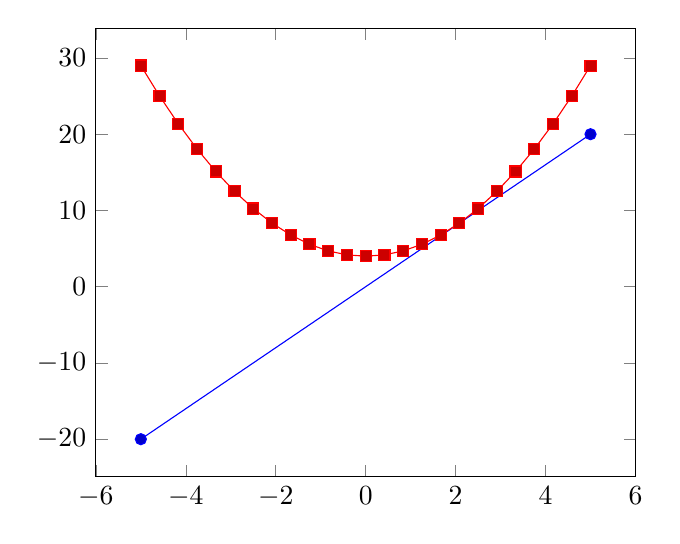
\begin{tikzpicture}
\begin{axis}[
    declare function={
        C=4;
        square(\t)=(\t)^2 + C;
    },
]
    \addplot+ [samples=2] {C*x};

    \addplot {square(x)};
\end{axis}
\end{tikzpicture}
\end{codeexample}
    %
    The definitions as such have the form \meta{function}\meta{argument list} =
    \meta{definition} where the \meta{argument list} contains a
    comma-separated-list of arguments like |\t| or |\t,\a,\b|. The
    \meta{definition} is a math expression which makes use of these arguments.

    Please refer to \cite{tikz} for more details.
\end{key}

\begin{command}{\pgfplotstableread\marg{file}}
    Please refer to the manual of \PGFPlotstable{}, |pgfplotstable.pdf|, which
    is part of the \PGFPlots{} bundle.
\end{command}

\begin{command}{\pgfplotstabletypeset\marg{\textbackslash macro}}
    Please refer to the manual of \PGFPlotstable{}, |pgfplotstable.pdf|, which
    is part of the \PGFPlots{} bundle.
\end{command}

\begin{command}{\pgfplotsiffileexists\marg{filename}\marg{true code}\marg{false code}}
    Invokes \meta{true code} if \meta{filename} exists and \meta{false code} if
    not. Can be used in looping macros, for example to plot every data file
    until there are no more of them.
\end{command}

\begin{command}{\pgfplotsutilifstringequal\marg{first}\marg{second}\marg{true code}\marg{false code}}
    A simple ``strcmp'' tool which invokes \meta{true code} if \meta{first}
    $=$\meta{second} and \meta{false code} otherwise. This does not expand
    macros.
\end{command}

\begin{commandlist}{\pgfkeys,\pgfeov,\pgfkeysvalueof,\pgfkeysgetvalue}
    These commands are part of the \Tikz{} way of specifying options, its
    sub-package |pgfkeys|. The |\pgfplotsset| command is actually nothing but a
    wrapper around |\pgfkeys|.

    A short introduction into |\pgfkeys| can be found in~\cite{keyvalintro}
    whereas the complete reference is, of course, the \Tikz{}
    manual~\cite{tikz}.

    The key |\pgfkeysvalueof|\marg{key name} expands to the value of a key;
    |\pgfkeysgetvalue|\marg{key name}\marg{\textbackslash macro} stores the
    value of \meta{key name} into \meta{\textbackslash macro}. The |\pgfeov|
    macro is used to delimit arguments for code keys in |\pgfkeys|, please
    refer to the references mentioned above.
\end{commandlist}


\section[Commands Inside Of PGFPlots Axes]
        {Commands Inside Of {\normalfont\PGFPlots{}} Axes}

\begin{command}{\autoplotspeclist}
    This command should no longer be used, although it will be kept as
    technical implementation detail. Please use the `|cycle list|' option,
    Section~\ref{sec:cycle:list}.
\end{command}

\begin{command}{\logten}
    Expands to the constant $\log(10)$. Useful for log plots because $\log(10^i)
    = i\log(10)$. This command is only available inside of a \Tikz{} picture.
\end{command}

\begin{command}{\pgfmathprintnumber\marg{number}}
    Generates pretty-printed output\footnote{This method was previously
    \texttt{\textbackslash prettyprintnumber}. Its functionality has been
    included into \PGF{} and the old command is now deprecated.} for
    \meta{number}. This method is used for every tick label.

    The number is printed using the current number printing options, see the
    manual of \PGFPlotstable{} which comes with this package for the different
    number styles, rounding precision and rounding methods.
\end{command}

\begin{command}{\numplots}
    Inside of any of the axis environments, associated style, option or
    command, |\numplots| expands to the total number of plots.
\end{command}

\begin{command}{\numplotsofactualtype}
    Like |\numplots|, this macro returns the total number of plots which have
    the same plot handler. Thus, if you have |sharp plot| active, it returns
    the number of all |sharp plots|. If you have |ybar| active, it returns the
    number of |ybar| plots and so on.
\end{command}

\begin{command}{\plotnum}
    Inside of |\addplot| or any associated style, option or command, |\plotnum|
    expands to the current plot's number, starting with~$0$.
\end{command}

\begin{command}{\plotnumofactualtype}
    Like |\plotnum|, but it returns the number among all plots of the same
    type. The number of all such plots is available using
    |\numplotsofactualtype|.
\end{command}

\begin{command}{\coordindex}
    Inside of an |\addplot| command, this macro expands to the number of the
    actual coordinate (starting with~$0$).

    It is useful together with |x filter| or |y filter| to (de)select
    coordinates.
\end{command}


\section{Path Operations}

\begin{commandlist}{\path,\draw,\fill,\node,\matrix}
    These commands are \Tikz{} drawing commands all of which are documented
    in~\cite{tikz}. They are used to draw or fill paths, generate text nodes or
    aligned text matrices. They are equivalent to
    \pgfmanualpdflabel{/tikz/draw}{}|\path[draw]|,
    \pgfmanualpdflabel{/tikz/fill}{}|\path[fill]|,
    \pgfmanualpdflabel{/tikz/node}{}|\path[node]|,
    \pgfmanualpdflabel{/tikz/matrix}{}|\path[matrix]|,
    respectively.
\end{commandlist}

\begin{pathoperation}{--}{\meta{coordinate}}
    A \Tikz{} path operation which connects the current point (the last one
    before |--|) and \meta{coordinate} with a straight line.
\end{pathoperation}

{\catcode`\|=12
\begin{pathoperation}[noindex]{|-}{\meta{coordinate}}
\pgfmanualpdflabel[\catcode`\|=12 ]{|-}{}%
    A \Tikz{} path operation which connects the current point and
    \meta{coordinate} with \emph{two} straight lines: first vertical, then
    horizontal.
\end{pathoperation}

\begin{pathoperation}[noindex]{-|}{\meta{coordinate}}
\pgfmanualpdflabel[\catcode`\|=12 ]{-|}{}%
    A \Tikz{} path operation which connects the current point and
    \meta{coordinate} with \emph{two} straight lines: first horizontal, then
    vertical.
\end{pathoperation}
}

\begin{keylist}{/tikz/xshift=\marg{dimension},/tikz/yshift=\marg{dimension}}
    These \Tikz{} keys allow to shift something by \meta{dimension} which is
    any \TeX{} size (or expression).
\end{keylist}

\begin{command}{\pgfplotsextra\marg{low-level path commands}}
    A command to execute \meta{low-level path commands} in a \PGFPlots{} axis.
    Since any drawing commands inside of an axis need to be postponed until the
    axis is complete and the scaling has been initialised, it is not possible
    to simply draw any paths. Instead, it is necessary to draw them as soon as
    the axis is finished. This is done automatically for every \Tikz{} path --
    and it is also done manually if you write |\pgfplotsextra|\marg{commands}.
    %
\begin{codeexample}[]
\begin{tikzpicture}
\begin{axis}[xmin=0,xmax=3,ymin=0,ymax=5]
    \pgfplotsextra{
        \pgfpathmoveto{\pgfplotspointaxisxy{1}{2}}
        \pgfpathlineto{\pgfplotspointaxisxy{2}{4}}
        \pgfusepath{stroke}
    }
\end{axis}
\end{tikzpicture}
\end{codeexample}
    %
    The example above initializes an axis and executes the basic level path
    commands as soon as the axis is ready. The execution of multiple |\path|,
    |\addplot| and |\pgfplotsextra| commands is in the same sequence as they
    occur in the environment.\footnote{Except for stacked plots where the
    sequence may be reverse, see the key \texttt{reverse stack plots}.}
\end{command}

\begin{command}{\pgfplotspathaxisoutline}
    Generates a path which resembles the outline of the current axis. This path
    is used for clip paths and the background paths (if any).
\end{command}


\section{Specifying Basic Coordinates}
\label{sec:basic:coordinates}

\begin{commandlist}{%
    \pgfplotspointaxisxy\marg{x coordinate}\marg{y coordinate},
    \pgfplotspointaxisxyz\marg{x coordinate}\marg{y coordinate}\marg{z coordinate}%
}
    Point commands like |\pgfpointxy| which take logical, absolute coordinates
    and return a low-level point. Every transformation from user
    transformations to logarithms is applied.

    Since the transformations are initialized after the axis is complete, this
    command needs to be postponed (see |\pgfplotsextra|).

    This command is the basic level variant of |axis cs:|\meta{x
    coordinate}|,|\meta{y coordinate}|,|\meta{z coordinate}.

    Note that this is also the default coordinate system during the
    visualization phase; in other words: if you write |\draw (1,2) -- (1,4)|,
    \PGFPlots{} will automatically use |(axis cs:1,2) -- (axis cs:1,4)|.
\end{commandlist}

\begin{commandlist}{%
    \pgfplotspointaxisdirectionxy\marg{x coordinate}\marg{y coordinate},
    \pgfplotspointaxisdirectionxyz\marg{x coordinate}\marg{y coordinate}\marg{z coordinate}%
}
    Point commands like |\pgfpointxy| which take logical, \emph{relative}
    coordinates and return a low-level point. Every transformation from user
    transformations to logarithms is applied. The difference to
    |\pgfplotspointaxisxy| is that the shift of the linear transformation is
    skipped here (compare |disabledatascaling|).

    This command is the basic level variant of |axis direction cs:|\meta{x
    coordinate}|,|\meta{y coordinate}|,|\meta{z coordinate}. Please refer to
    the documentation of |axis direction cs| for more details.

    Use this command whenever something of \emph{relative} character like
    directions or lengths need to be supplied. One use case is to draw
    ellipses:
    %
\begin{codeexample}[]
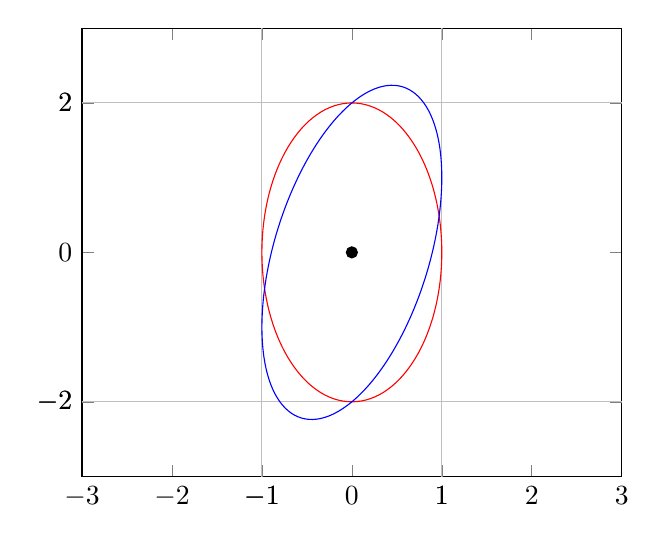
\begin{tikzpicture}
\begin{axis}[
    xmin=-3,   xmax=3,
    ymin=-3,   ymax=3,
    extra x ticks={-1,1},
    extra y ticks={-2,2},
    extra tick style={grid=major},
]
    \draw [red] \pgfextra{
        \pgfpathellipse{\pgfplotspointaxisxy{0}{0}}
            {\pgfplotspointaxisdirectionxy{1}{0}}
            {\pgfplotspointaxisdirectionxy{0}{2}}
    % see also the documentation of
    % 'axis direction cs' which
    % allows a simpler way to draw this ellipse
    };
    \draw [blue] \pgfextra{
        \pgfpathellipse{\pgfplotspointaxisxy{0}{0}}
            {\pgfplotspointaxisdirectionxy{1}{1}}
            {\pgfplotspointaxisdirectionxy{0}{2}}
    };
    \addplot [only marks,mark=*] coordinates
        { (0,0) };
\end{axis}
\end{tikzpicture}
\end{codeexample}

    Since the transformations are initialized after the axis is complete, this
    command needs to be provided either inside of a \tikzname{} |\path| command
    (like |\draw| in the example above) or inside of |\pgfplotsextra|.
\end{commandlist}

\begin{commandlist}{%
    \pgfplotspointrelaxisxy\marg{rel x coordinate}\marg{rel y coordinate},
    \pgfplotspointrelaxisxyz\marg{rel x coordinate}\marg{rel y coordinate}\marg{rel z coordinate}%
}
    Point commands which take \emph{relative} coordinates such that $x=0$ is
    the \emph{lower} $x$-axis limit and $x=1$ the \emph{upper} $x$-axis limit.

    These commands are used for |rel axis cs|.

    Please note that the transformations are only initialised if the axis is
    complete! This means you need to provide |\pgfplotsextra|.
\end{commandlist}

\begin{commandlist}{%
    \pgfplotspointdescriptionxy\marg{$x$ fraction}\marg{$y$ fraction},
    \pgfplotsqpointdescriptionxy\marg{$x$ fraction}\marg{$y$ fraction}%
}
    Point commands such that |{0}{0}| is the lower left corner of the axis'
    bounding box and |{1}{1}| the upper right one; everything else is in
    between. The `|q|' variant is quicker as it doesn't invoke the math parser
    on its arguments.

    They are used for |axis description cs|, see
    Section~\ref{pgfplots:sec:axis:description:cs}.
\end{commandlist}

\begin{commandlist}{\pgfplotspointaxisorigin}
    A point coordinate at the origin, $(0,0,0)$. If the origin is not part of
    the axis limits, the nearest point on the boundary is returned instead.

    This is the same coordinate as returned by the |origin| anchor.
\end{commandlist}

\begin{commandlist}{%
    \pgfplotstransformcoordinatex\marg{x coordinate of an axis},
    \pgfplotstransformcoordinatey\marg{y coordinate of an axis},
    \pgfplotstransformcoordinatez\marg{z coordinate of an axis}%
}
    Defines |\pgfmathresult| to be the low-level \PGF{} coordinate
    corresponding to the input argument.

    The command applies any |[xyz] coord trafo| keys, data scalings and/or
    logarithms or whatever \PGFPlots{} does to map input coordinates to
    internal coordinates.

    The result can be used inside of a |\pgfpointxy| statement (i.e.\@ it still
    needs to be scaled with the respective \PGF{} unit vector).
    %
\begin{codeexample}[]
\begin{tikzpicture}
\pgfplotsset{compat/pgfpoint substitution=1.3}
\begin{axis}[xmin=0,xmax=2,ymin=0,ymax=5]
    \pgfplotsextra{
        \pgfplotstransformcoordinatex{1}
        \let\xcoord=\pgfmathresult
        \pgfplotstransformcoordinatey{1}
        \let\ycoord=\pgfmathresult
        \pgfpathcircle
            {\pgfqpointxy{\xcoord}{\ycoord}}
            {5pt}
        \pgfusepath{fill}
    }
\end{axis}
\end{tikzpicture}
\end{codeexample}
    %
    Note that \PGFPlots{} substitutes |\pgfqpointxy| by |\pgfplotspointaxisxyz|
    by default -- and this command implicitly transforms coordinates anyway. In
    order to see the difference, the preceding example first disables this
    automatic substitution of coordinate systems by means of
    |compat/pgfpoint substitution=1.3|.
    %
    The result of this command is also available as math method
    |transformcoordinatex| (see the documentation for |axis cs|).

    Please note that the transformations are only initialised if the axis is
    complete. This means you need to provide |\pgfplotsextra| as is shown in
    the example above.
\end{commandlist}

\begin{commandlist}{%
    \pgfplotstransformdirectionx\marg{x direction of an axis},
    \pgfplotstransformdirectiony\marg{y direction of an axis},
    \pgfplotstransformdirectionz\marg{z direction of an axis}%
}
    Defines |\pgfmathresult| to be a low-level \PGF{} \emph{direction vector
    component}.

    A direction vector needs to be \emph{added} to some coordinate in order to
    get a coordinate, compare the documentation for
    |\pgfplotspointaxisdirectionxy| and |axis direction cs|.

    The argument \meta{x direction of an axis} is processed in (almost) the
    same way as for the macro which operates on absolute positions,
    |\pgfplotstransformcoordinatex|. The only difference is that
    \emph{directions} need no shifting transformation.

    The result of this command is also available as math method
    |transformdirectionx| (see the documentation for |axis direction cs|).

    See |axis direction cs| for details and examples about this command.
\end{commandlist}

% this command is for internal use only:
%--------------------------------------------------
% \begin{command}{\pgfplotsconvertunittocoordinate\marg{x, y or z}\marg{dimension}}
%     Converts a dimension (with unit!) to a corresponding $x$-, $y$- or $z$-coordinate. The result will be written to |\pgfmathresult| (without units).
%
%     It is possible to use the result as arguments for the |\pgfpointxyz| commands.
%
%     The effect is to multiply \meta{dimension} with the inverse length of the unit vector for the specified axis. These lengths are precomputed in \PGFPlots{} so the operation is fast.
% \begin{codeexample}[code only]
% \pgfplotsconvertunittocoordinate{x}{5pt}
% % now, the command uses exactly 5pt in x direction:
% \pgfqpointxyz{\pgfmathresult}{4}{3}
% \end{codeexample}
% \end{command}
%--------------------------------------------------

\begin{commandlist}{%
    \pgfplotspointunitx,
    \pgfplotspointunity,
    \pgfplotspointunitz%
}
    Low-level point commands which return the canvas $x$, $y$ or $z$ unit
    vectors.

    The |\pgfplotspointunitx| is the \pgfname{} unit vector in $x$ direction.

    These vectors are essentially the same as |\pgfqpointxyz{1}{0}{0}|,
    |\pgfqpointxyz{0}{1}{0}|, and |\pgfqpointxyz{0}{0}{1}|, respectively.

    The unit $z$ vector is only defined for three dimensional axes.
\end{commandlist}

\begin{commandlist}{%
    \pgfplotsunitxlength,
    \pgfplotsunitylength,
    \pgfplotsunitzlength,
    \pgfplotsunitxinvlength,
    \pgfplotsunityinvlength,
    \pgfplotsunitzinvlength%
}
    Macros which expand to the vector length $\lVert x_i \rVert$ of the
    respective unit vector $x_i$ or the inverse vector length, $1/\lVert x_i
    \rVert$. These macros can be used inside of |\pgfmathparse|, for example.

    The $x_i$ are the |\pgfplotspointunitx| variants.
\end{commandlist}

\begin{command}{\pgfplotsqpointoutsideofaxis%
        \marg{three-char-string}\marg{coordinate}\marg{normal distance}%
}
    Provides a point coordinate on one of the available four axes in case of a
    two dimensional figure or on one of the available twelve axes in case of a
    three dimensional figure.

    The desired axis is uniquely identified by a three character string,
    provided as first argument to the command. The first of the three
    characters is `|0|' if the $x$-coordinate of the specified axis passes
    through the lower axis limit. It is `|1|', if the $x$-coordinate of the
    specified axis passes through the upper axis limit. Furthermore, it is
    `|2|' if it passes through the origin. The second character is also either
    |0|, |1| or |2| and it characterizes the position on the $y$-axis. The
    third character is for the third dimension, the $z$-axis. It should be left
    at `|0|' for two dimensional plots. However, \emph{one} of the three
    characters should be `|v|', meaning the axis \underline varies. For
    example, |v01| denotes $\{ (x,y_{\min},z_{\max}) \vert x \in \R \}$.

    The second argument, \meta{coordinate} is the logical coordinate on that
    axis. Since two coordinates of the axis are fixed, \meta{coordinate} refers
    to the \underline varying component of the axis. It must be a number
    without unit; no math expressions are supported here.

    The third argument \meta{normal distance} is a dimension like |10pt|. It
    shifts the coordinate away from the designated axis in direction of the
    outer normal vector. The outer normal vector always points away from the
    axis. It is computed using |\pgfplotspointouternormalvectorofaxis|.

    There are several variants of this command which are documented in the
    source code. One of them is particularly useful:
\end{command}

\begin{command}{\pgfplotsqpointoutsideofaxisrel%
        \marg{three-char-string}\marg{axis fraction}\marg{normal distance}%
}
    This point coordinate is a variant of |\pgfplotsqpointoutsideofaxis| which
    allows to provide an \meta{axis fraction} instead of an absolute
    coordinate. The fraction is a number between $0$ (lower axis limit) and $1$
    (upper axis limit), i.e.\@ it is given in percent of the total axis. It is
    possible to provide negative values or values larger than one.

    The |\pgfplotsqpointoutsideofaxisrel| command is similar in spirit to
    |rel axis cs|.

    There is one speciality in conjunction with reversed axes: if the axis has
    been reversed by |x dir=reverse| and, in addition,
    |allow reversal of rel axis cs| is true, the value $0$ denotes the
    \emph{upper} limit while $1$ denotes the \emph{lower} limit. The effect is
    that coordinates won't change just because of axis reversal.
        \index{allow reversal of rel axis cs}%
\end{command}

\begin{command}{\pgfplotspointouternormalvectorofaxis\marg{three-char-string}}
    A point command which yields the outer normal vector of the respective
    axis. The normal vector has length $1$ (computed with
    |\pgfpointnormalised|). It is the same normal vector used inside of
    |\pgfplotsqpointoutsideofaxis| and its variants.

    The output of this command will be cached and reused during the lifetime
    of an axis.
\end{command}

\begin{command}{\pgfplotsticklabelaxisspec\marg{x, y or z}}
    Expands to the three character identification for the axis containing tick
    labels for the chosen axis, either \meta{x}, \meta{y} or \meta{z}.
\end{command}

\begin{command}{\pgfplotsvalueoflargesttickdimen\marg{x, y or z}}
    Expands to the largest distance of a tick position to its tick label
    bounding box in direction of the outer unit normal vector. It does also
    include the value of the |ticklabel shift| key.

    This value is used for |ticklabel cs|.
\end{command}

\begin{commandlist}{
    \pgfplotsmathfloatviewdepthxyz\marg{x}\marg{y}\marg{z},
    \pgfplotsmathviewdepthxyz\marg{x}\marg{y}\marg{z}%
}
    Both macros define |\pgfmathresult| to be the ``depth'' of a three
    dimensional point $\bar x = (x,y,z)$. The depth is defined to be the scalar
    product of $\bar x$ with $\vec d$, the view direction of the current axis.

    For |\pgfplotsmathfloatviewdepthxyz|, the arguments are parsed as floating
    point numbers and the result is encoded in floating point. A fixed point
    representation can be generated with
    |\pgfmathfloattofixed{\pgfmathresult}|.

    For |\pgfplotsmathviewdepthxyz|, \TeX{} arithmetics is employed for the
    inner product and the result is assigned in fixed point. This is slightly
    faster, but has considerably smaller data range.

    Both commands can only be used \emph{inside} of a three dimensional
    \PGFPlots{} axis (as soon as the axis is initialised, see
    |\pgfplotsextra|).
\end{commandlist}

\begin{texif}{pgfplotsthreedim}
    A \TeX{} |\if| which evaluates the \meta{true code} if the axis is three
    dimensional and the \meta{else code} if not.
\end{texif}


\section{Accessing Axis Limits}

It is also possible to access axis limits during the visualization phase,
i.e.\@ during |\end{axis}|. Please refer to the reference documentation for
|xmin| on page~\pageref{page:access:limits}.


\section{Accessing Point Coordinate Values}

During the visualization phase, \PGFPlots{} provides access to the currently
processed coordinate and its values.

This access requires a call to specific macros. These macros write the
coordinate values to some publicly available key--value pairs. Then, the
current point's $x$, $y$, $z$, and color data can be accessed.

\begin{commandlist}{\pgfplotspointgetcoordinates,\pgfplotspointgetcoordinates\marg{point}}

    After invoking the macro, the following keys will be set:

    \declaretext{/data point/x} will contain the current point's $x$-coordinate.

    \declaretext{/data point/y} will contain the current point's $y$-coordinate.

    \declaretext{/data point/z} will contain the current point's $z$-coordinate
    (if applicable).

    \declaretext{/data point/meta} will contain the current point's
    |point meta| value (if applicable).

    \declaretext{/data point/index} will contain the current point's index in
    the coordinate stream. This is actually the same as |\coordindex|.

    This command actually supports two modes of operation:
    %
    \begin{enumerate}
        \item Without arguments. In this case, it returns values of the point
            which is about to be processed by the current plot handler.
        \item With an argument in curly braces. In this case, it expects a
            coordinate and assigns the keys accordingly. Note that this
            command merely supports two-dimensional axes and assigns only
            |/data point/x| and |/data point/y|.
    \end{enumerate}

    The returned values are the same as they can be read on the axes, they are
    also the same as you would write them into |axis cs|.

    This means that any |x coord inv trafo| has been applied on the value. It
    also means that the exponential function has been called even though the
    internal coordinate was present in log format.

    This function is implicitly called for any |scatter| plot (including
    |nodes near coords|). This allows to access \emph{all} coordinate values at
    once:
    %
\begin{codeexample}[]
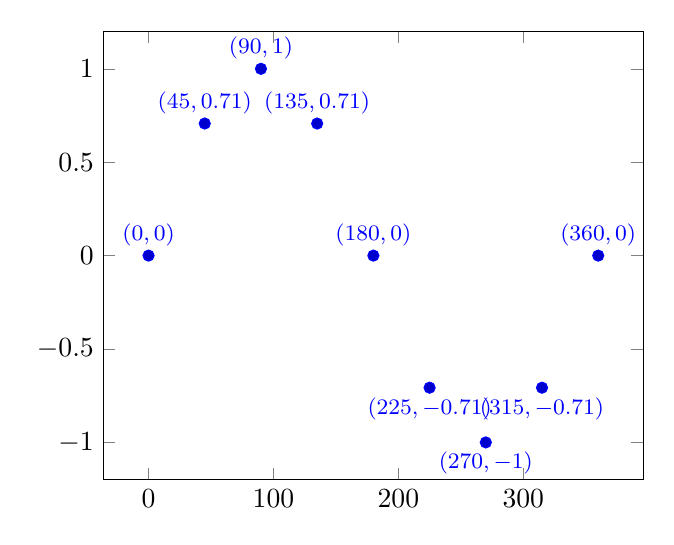
\begin{tikzpicture}
\begin{axis}
    \addplot+ [
        domain=0:360,
        samples=9,
        only marks,
        nodes near coords={%
            \footnotesize
            $(\pgfmathprintnumber
                {\pgfkeysvalueof{/data point/x}},
               \pgfmathprintnumber
                {\pgfkeysvalueof{/data point/y}})$%
        },
    ] {sin(x)};
\end{axis}
\end{tikzpicture}
\end{codeexample}
    %
    The example works because |\pgfplotspointgetcoordinates| is part of the
    standard implementation of |nodes near coords|; the resulting values are
    directly available. Note that the preceding example would have been simpler
    if we would have printed just one value: |nodes near coords| resorts to the
    |point meta|. And that, in turn, contains the $y$-coordinate anyway by
    default.

    A more advanced example would be a |ybar| plot in which nodes shall be
    placed at the lower end of the axis, together with some dotted lines to the
    respective bars:
    %
\begin{codeexample}[]
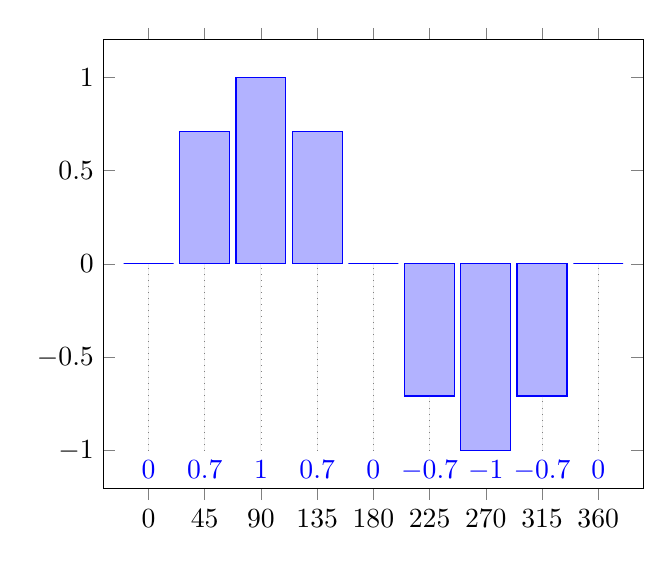
\begin{tikzpicture}
\begin{axis}[
    ybar,
    nodes near coords,
    %
    % we want to provide absolute 'at' values
    % for the nodes:
    scatter/position=absolute,
    every node near coord/.style={
        at={(\pgfkeysvalueof{/data point/x},-1)},
        % pretty printing:
        anchor=north,
        /pgf/number format/fixed,
        /pgf/number format/precision=1,
        % assign a name which can be referenced below:
        name=NNC\pgfkeysvalueof{/data point/index},
    },
    % ... draw a dotted line between
    % the marker and the bar:
    /pgfplots/scatter/@post marker code/.add code={}{
        \draw [dotted,help lines]
            (NNC\pgfkeysvalueof{/data point/index})
            -- (\pgfkeysvalueof{/data point/x},
            {min(0,\pgfkeysvalueof{/data point/y})});
    },
    % assign suitable tick labels:
    xtick=data,
]
    % some dummy data:
    \addplot+ [
        domain=0:360,
        bar width=360/9,
        samples=9,
    ] {sin(x)};
\end{axis}
\end{tikzpicture}
\end{codeexample}
    %
    Again, the command is used implicitly as part of |nodes near coords| and
    does not occur in the example as such.

    \paragraph{See also} the related example online under
    \url{https://tex.stackexchange.com/a/141006}. It demonstrates how to
    place the nodes generated by |nodes near coords| based on the value (either
    inside of a bar or above it).

    The following example uses an argument in curly braces for which we seek
    coordinate values:
    %
\begin{codeexample}[]
% requires \usetikzlibrary{intersections}
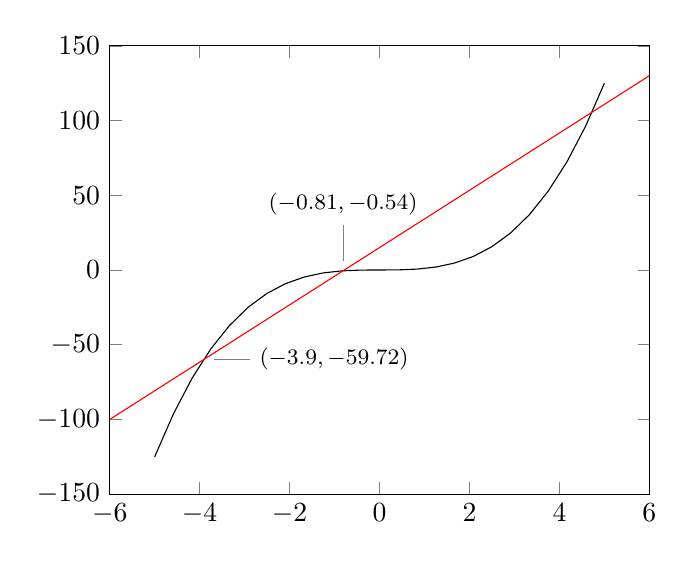
\begin{tikzpicture}
\begin{axis}
    \addplot [name path=A] {x^3};

    \draw [red,name path=HelperLine]
        (axis cs:-6,-100) -- (axis cs:6,130);

    \draw [
        font=\footnotesize,
        name intersections={of=A and HelperLine},
    ]
    node [pin={right:
      \pgfplotspointgetcoordinates{(intersection-1)}
        $(\pgfmathprintnumber[fixed]{
            \pgfkeysvalueof{/data point/x}},
          \pgfmathprintnumber[fixed]{
            \pgfkeysvalueof{/data point/y}})$
      }
    ] at (intersection-1) {}
    node [pin={
      \pgfplotspointgetcoordinates{(intersection-2)}
        $(\pgfmathprintnumber[fixed]{
            \pgfkeysvalueof{/data point/x}},
          \pgfmathprintnumber[fixed]{
            \pgfkeysvalueof{/data point/y}})$
      }
    ] at (intersection-2) {};
\end{axis}
\end{tikzpicture}
\end{codeexample}
    %
    The example computes and names intersections of |A| and |HelperLine|. The
    following code generates pins at the intersections. To this end, it uses
    |\pgfplotspointgetcoordinates|\marg{point} which defines |/data point/x|
    and |/data point/y|. These values are then formatted using
    |\pgfmathprintnumber|.

    In its second mode, |\pgfplotspointgetcoordinates|\marg{point} expects one
    of two things as \meta{point}:
    %
    \begin{enumerate}
        \item a basic-level \PGF{} point like |\pgfpointanchor{A}{center}| or
        \item a \Tikz{} point like |(A.base)| or |(3,5)|.
    \end{enumerate}
\end{commandlist}

\begin{command}{\pgfplotspointgetnormalizedcoordinates}
    A macro which is very similar to |\pgfplotspointgetcoordinates|.
    Consequently, it is also supposed to be called during the visualization phase.

    It assigns the very same output macros, but the values are different. More
    precisely, it defines the macros

    \declaretext{/data point/x} will contain the current point's
    \emph{normalized} $x$-coordinate.

    \declaretext{/data point/y} will contain the current point's
    \emph{normalized} $y$-coordinate.

    \declaretext{/data point/z} will contain the current point's
    \emph{normalized} $z$-coordinate (if applicable).

    \declaretext{/data point/meta} will contain the current point's
    |point meta| value (if applicable).

    \declaretext{/data point/index} will contain the current point's index in
    the coordinate stream. This is actually the same as |\coordindex|.

    The keyword \declaretext{normalized} means that the values are in a
    suitable numerical form which can be consumed by the axis. To be more
    specific: any user |x coord inv trafo| is \emph{ignored}. An important
    example would be |symbolic x coords|: the normalized coordinates would be
    some associated numbers, not the symbols. The results returned by
    |\pgfplotspointgetcoordinates| would be the symbols. For logarithm axes,
    the normalized values are the logs.

    Typically, normalized values are much more useful when you want to apply
    some math operation like averaging or subtraction.

    This function needs to be called explicitly. It is currently used by
    |ybar stacked| to align |nodes near coords|.
\end{command}


\section{Layer Access}

\begin{command}{\pgfplotsonlayer\marg{layer name}}
    A low-level command which will check if the current axis has layer support
    activated and, if so, calls |\pgfonlayer|\marg{layer name}.

    There must be a |\endpgfplotsonlayer| to delimit the environment.
\end{command}

\begin{command}{\endpgfplotsonlayer}
    The end of |\pgfplotsonlayer|.
\end{command}

\begin{command}{\pgfonlayer\marg{layer name}}
    A low-level command of \PGF{} which will collect everything until the
    matching |\endpgfonlayer| into layer \meta{layer name}.

    The \meta{layer name} must be active, i.e.\@ it must be part of the layer
    names of |set layers|.

    The only special case is if you call |\pgfdeclarelayer{discard}| somewhere:
    this special layer has a ``magical name'' which serves as |/dev/null| if it
    is enabled using |\pgfonlayer{discard}|: it does not need to be active and
    everything assigned to this layer will be thrown away if it is not part of
    the layer name configuration.

    There must be a |\endpgfonlayer| to delimit the environment.
\end{command}

\begin{command}{\endpgfonlayer}
    The end of |\pgfonlayer|.
\end{command}


\begin{command}{\pgfsetlayers\marg{layer list}}
    This is a low-level command of \PGF{}. At the time of this writing, it is
    the only way to tell \PGF{} which layers it shall use for the current/next
    picture. It is used implicitly by |set layers|.
\end{command}


\printindex

\bibliographystyle{abbrv} %gerapali} %gerabbrv} %gerunsrt.bst} %gerabbrv}% gerplain}
\nocite{pgfplotstable}
\nocite{programmingnotes}
\bibliography{pgfplots}
\end{document}

% -----------------------------------------------------------------------------
% For Stefan Pinnow as reminder on what to look for when editing the manual
% -----------------------------------------------------------------------------
% There should be no line breaks in the following environments
% - |...|
% - \declareandlabel{...}
% - \verbpdfref{...}
% If "MakeTikzPictures" isn't running through check one of the externalized
% LOG files what is the cause of that.
% -----------------------------------------------------------------------------


%%%%%%%%%%%%%%%%%%%%%%%%%%%%%%%%%%%%%%%%%%%%%%%%%%%%%%%%%%%%%%%%%%%%%%%%%%%%%
%
% Package pgfplots.sty documentation.
%
% Copyright 2007/2008 by Christian Feuersaenger.
%
% This program is free software: you can redistribute it and/or modify
% it under the terms of the GNU General Public License as published by
% the Free Software Foundation, either version 3 of the License, or
% (at your option) any later version.
%
% This program is distributed in the hope that it will be useful,
% but WITHOUT ANY WARRANTY; without even the implied warranty of
% MERCHANTABILITY or FITNESS FOR A PARTICULAR PURPOSE.  See the
% GNU General Public License for more details.
%
% You should have received a copy of the GNU General Public License
% along with this program.  If not, see <http://www.gnu.org/licenses/>.
%
%
%%%%%%%%%%%%%%%%%%%%%%%%%%%%%%%%%%%%%%%%%%%%%%%%%%%%%%%%%%%%%%%%%%%%%%%%%%%%%
% SEE pgfplots-macros.tex as well!
%\pdfminorversion=5 % to allow compression
%\pdfobjcompresslevel=2
\documentclass[a4paper,openany]{book}

\let\bookmaketitle=\maketitle

% -----------------------------------
% this here is from ltxdoc:
\usepackage{doc}[=v2]
\AtBeginDocument{\MakeShortVerb{\|}}
%\setlength{\textwidth}{355pt}
%\addtolength\marginparwidth{30pt}
%\addtolength\oddsidemargin{20pt}
%\addtolength\evensidemargin{20pt}
\def\cmd#1{\cs{\expandafter\cmd@to@cs\string#1}}
\def\cmd@to@cs#1#2{\char\number`#2\relax}
\DeclareRobustCommand\cs[1]{\texttt{\char`\\#1}}
\providecommand\marg[1]{%
  {\ttfamily\char`\{}\meta{#1}{\ttfamily\char`\}}}
\providecommand\oarg[1]{%
  {\ttfamily[}\meta{#1}{\ttfamily]}}
\providecommand\parg[1]{%
  {\ttfamily(}\meta{#1}{\ttfamily)}}
\raggedbottom

% -----------------------------------
\input{pgfplots.preamble.tex}

\makeatletter
% I want a two-column index just as in pgfmanual styles. This here
% was the best way to get one:
\def\index@prologue{\section*{Index}\addcontentsline{toc}{chapter}{Index}
}
\makeatother

%\RequirePackage[german,english,francais]{babel}

\def\matlabcolormaptext{This colormap is similar to one shipped with Matlab$^\text{\textregistered}$ under a similar name.}

\IfFileExists{tikzlibraryspy.code.tex}{%
\usetikzlibrary{spy}
}{%
    \message{ERROR: tikz SPY library NOT available. The manual will only compile partially.^^J}%
}%

\usepackage{xparse}% for colorbrewer manual

\usetikzlibrary{
    decorations.markings,
    decorations.footprints,
    shapes.arrows,
    matrix,
    positioning,
}

\usepgfplotslibrary{
    fillbetween,
    ternary,
    smithchart,
    patchplots,
    polar,
    colormaps,
    colorbrewer,
    colortol,           % docu not ready yet
}
\pgfqkeys{/codeexample}{%
    every codeexample/.append style={
        /pgfplots/every ternary axis/.append style={
            /pgfplots/legend style={fill=graphicbackground},
        }
    },
    tabsize=4,
}

\pgfplotsmanualenableexternalizationofexpensive

%\usetikzlibrary{external}
%\tikzexternalize[prefix=figures/]{pgfplots}

\title{%
    Manual for Package \PGFPlots{}\\
    {\small 2D/3D Plots in \LaTeX{}, Version \pgfplotsversion}\\
    {\small\href{https://github.com/pgf-tikz/pgfplots}{https://github.com/pgf-tikz/pgfplots}}
    %\\{\small Attention: you are using an unstable development version.}
}

\makeatletter
\long\def\abstractsmuggle{%
    \centering
    \textbf{Abstract}\\[0.5cm]

    \begin{minipage}{12cm}
        \PGFPlots{} draws high-quality function plots in normal or logarithmic
        scaling with a user-friendly interface directly in \TeX{}. The user
        supplies axis labels, legend entries and the plot coordinates for one or
        more plots and \PGFPlots{} applies axis scaling, computes any logarithms
        and axis ticks and draws the plots. It supports line plots, scatter
        plots, piecewise constant plots, bar plots, area plots, mesh and surface
        plots, patch plots, contour plots, quiver plots, histogram plots, box
        plots, polar axes, ternary diagrams, smith charts and some more. It is
        based on Till Tantau's package \PGF{}/\Tikz{}.
    \end{minipage}

}%

\expandafter\date\expandafter{\@date\\[2cm]
    \abstractsmuggle
}%
\makeatother

%\includeonly{pgfplots.reference}


\begin{document}

\def\plotcoords{%
\addplot coordinates {
(5,8.312e-02)    (17,2.547e-02)   (49,7.407e-03)
(129,2.102e-03)  (321,5.874e-04)  (769,1.623e-04)
(1793,4.442e-05) (4097,1.207e-05) (9217,3.261e-06)
};

\addplot coordinates{
(7,8.472e-02)    (31,3.044e-02)    (111,1.022e-02)
(351,3.303e-03)  (1023,1.039e-03)  (2815,3.196e-04)
(7423,9.658e-05) (18943,2.873e-05) (47103,8.437e-06)
};

\addplot coordinates{
(9,7.881e-02)     (49,3.243e-02)    (209,1.232e-02)
(769,4.454e-03)   (2561,1.551e-03)  (7937,5.236e-04)
(23297,1.723e-04) (65537,5.545e-05) (178177,1.751e-05)
};

\addplot coordinates{
(11,6.887e-02)    (71,3.177e-02)     (351,1.341e-02)
(1471,5.334e-03)  (5503,2.027e-03)   (18943,7.415e-04)
(61183,2.628e-04) (187903,9.063e-05) (553983,3.053e-05)
};

\addplot coordinates{
(13,5.755e-02)     (97,2.925e-02)     (545,1.351e-02)
(2561,5.842e-03)   (10625,2.397e-03)  (40193,9.414e-04)
(141569,3.564e-04) (471041,1.308e-04)
(1496065,4.670e-05)
};
}%


\bookmaketitle
\tableofcontents

%%%%%%%%%%%%%%%%%%%%%%%%%%%%%%%%%%%%%%%%%%%%%%%%%%%%%%%%%%%%%%%%%%%%%%%%%%%%%
%
% Package pgfplots.sty documentation.
%
% Copyright 2007/2008 by Christian Feuersaenger.
%
% This program is free software: you can redistribute it and/or modify
% it under the terms of the GNU General Public License as published by
% the Free Software Foundation, either version 3 of the License, or
% (at your option) any later version.
%
% This program is distributed in the hope that it will be useful,
% but WITHOUT ANY WARRANTY; without even the implied warranty of
% MERCHANTABILITY or FITNESS FOR A PARTICULAR PURPOSE.  See the
% GNU General Public License for more details.
%
% You should have received a copy of the GNU General Public License
% along with this program.  If not, see <http://www.gnu.org/licenses/>.
%
%
%%%%%%%%%%%%%%%%%%%%%%%%%%%%%%%%%%%%%%%%%%%%%%%%%%%%%%%%%%%%%%%%%%%%%%%%%%%%%
% SEE pgfplots-macros.tex as well!
%\pdfminorversion=5 % to allow compression
%\pdfobjcompresslevel=2
\documentclass[a4paper,openany]{book}

\let\bookmaketitle=\maketitle

% -----------------------------------
% this here is from ltxdoc:
\usepackage{doc}[=v2]
\AtBeginDocument{\MakeShortVerb{\|}}
%\setlength{\textwidth}{355pt}
%\addtolength\marginparwidth{30pt}
%\addtolength\oddsidemargin{20pt}
%\addtolength\evensidemargin{20pt}
\def\cmd#1{\cs{\expandafter\cmd@to@cs\string#1}}
\def\cmd@to@cs#1#2{\char\number`#2\relax}
\DeclareRobustCommand\cs[1]{\texttt{\char`\\#1}}
\providecommand\marg[1]{%
  {\ttfamily\char`\{}\meta{#1}{\ttfamily\char`\}}}
\providecommand\oarg[1]{%
  {\ttfamily[}\meta{#1}{\ttfamily]}}
\providecommand\parg[1]{%
  {\ttfamily(}\meta{#1}{\ttfamily)}}
\raggedbottom

% -----------------------------------
\input{pgfplots.preamble.tex}

\makeatletter
% I want a two-column index just as in pgfmanual styles. This here
% was the best way to get one:
\def\index@prologue{\section*{Index}\addcontentsline{toc}{chapter}{Index}
}
\makeatother

%\RequirePackage[german,english,francais]{babel}

\def\matlabcolormaptext{This colormap is similar to one shipped with Matlab$^\text{\textregistered}$ under a similar name.}

\IfFileExists{tikzlibraryspy.code.tex}{%
\usetikzlibrary{spy}
}{%
    \message{ERROR: tikz SPY library NOT available. The manual will only compile partially.^^J}%
}%

\usepackage{xparse}% for colorbrewer manual

\usetikzlibrary{
    decorations.markings,
    decorations.footprints,
    shapes.arrows,
    matrix,
    positioning,
}

\usepgfplotslibrary{
    fillbetween,
    ternary,
    smithchart,
    patchplots,
    polar,
    colormaps,
    colorbrewer,
    colortol,           % docu not ready yet
}
\pgfqkeys{/codeexample}{%
    every codeexample/.append style={
        /pgfplots/every ternary axis/.append style={
            /pgfplots/legend style={fill=graphicbackground},
        }
    },
    tabsize=4,
}

\pgfplotsmanualenableexternalizationofexpensive

%\usetikzlibrary{external}
%\tikzexternalize[prefix=figures/]{pgfplots}

\title{%
    Manual for Package \PGFPlots{}\\
    {\small 2D/3D Plots in \LaTeX{}, Version \pgfplotsversion}\\
    {\small\href{https://github.com/pgf-tikz/pgfplots}{https://github.com/pgf-tikz/pgfplots}}
    %\\{\small Attention: you are using an unstable development version.}
}

\makeatletter
\long\def\abstractsmuggle{%
    \centering
    \textbf{Abstract}\\[0.5cm]

    \begin{minipage}{12cm}
        \PGFPlots{} draws high-quality function plots in normal or logarithmic
        scaling with a user-friendly interface directly in \TeX{}. The user
        supplies axis labels, legend entries and the plot coordinates for one or
        more plots and \PGFPlots{} applies axis scaling, computes any logarithms
        and axis ticks and draws the plots. It supports line plots, scatter
        plots, piecewise constant plots, bar plots, area plots, mesh and surface
        plots, patch plots, contour plots, quiver plots, histogram plots, box
        plots, polar axes, ternary diagrams, smith charts and some more. It is
        based on Till Tantau's package \PGF{}/\Tikz{}.
    \end{minipage}

}%

\expandafter\date\expandafter{\@date\\[2cm]
    \abstractsmuggle
}%
\makeatother

%\includeonly{pgfplots.reference}


\begin{document}

\def\plotcoords{%
\addplot coordinates {
(5,8.312e-02)    (17,2.547e-02)   (49,7.407e-03)
(129,2.102e-03)  (321,5.874e-04)  (769,1.623e-04)
(1793,4.442e-05) (4097,1.207e-05) (9217,3.261e-06)
};

\addplot coordinates{
(7,8.472e-02)    (31,3.044e-02)    (111,1.022e-02)
(351,3.303e-03)  (1023,1.039e-03)  (2815,3.196e-04)
(7423,9.658e-05) (18943,2.873e-05) (47103,8.437e-06)
};

\addplot coordinates{
(9,7.881e-02)     (49,3.243e-02)    (209,1.232e-02)
(769,4.454e-03)   (2561,1.551e-03)  (7937,5.236e-04)
(23297,1.723e-04) (65537,5.545e-05) (178177,1.751e-05)
};

\addplot coordinates{
(11,6.887e-02)    (71,3.177e-02)     (351,1.341e-02)
(1471,5.334e-03)  (5503,2.027e-03)   (18943,7.415e-04)
(61183,2.628e-04) (187903,9.063e-05) (553983,3.053e-05)
};

\addplot coordinates{
(13,5.755e-02)     (97,2.925e-02)     (545,1.351e-02)
(2561,5.842e-03)   (10625,2.397e-03)  (40193,9.414e-04)
(141569,3.564e-04) (471041,1.308e-04)
(1496065,4.670e-05)
};
}%


\bookmaketitle
\tableofcontents
\include{pgfplots.title_abstract_intro}
\include{pgfplots.preliminaries}
\include{pgfplots.intro}
\include{pgfplots.reference}
\include{pgfplots.libs}
\include{pgfplots.resources}
\include{pgfplots.importexport}
\include{pgfplots.basic.reference}

\printindex

\bibliographystyle{abbrv} %gerapali} %gerabbrv} %gerunsrt.bst} %gerabbrv}% gerplain}
\nocite{pgfplotstable}
\nocite{programmingnotes}
\bibliography{pgfplots}
\end{document}

% -----------------------------------------------------------------------------
% For Stefan Pinnow as reminder on what to look for when editing the manual
% -----------------------------------------------------------------------------
% There should be no line breaks in the following environments
% - |...|
% - \declareandlabel{...}
% - \verbpdfref{...}
% If "MakeTikzPictures" isn't running through check one of the externalized
% LOG files what is the cause of that.
% -----------------------------------------------------------------------------


%%%%%%%%%%%%%%%%%%%%%%%%%%%%%%%%%%%%%%%%%%%%%%%%%%%%%%%%%%%%%%%%%%%%%%%%%%%%%
%
% Package pgfplots.sty documentation.
%
% Copyright 2007/2008 by Christian Feuersaenger.
%
% This program is free software: you can redistribute it and/or modify
% it under the terms of the GNU General Public License as published by
% the Free Software Foundation, either version 3 of the License, or
% (at your option) any later version.
%
% This program is distributed in the hope that it will be useful,
% but WITHOUT ANY WARRANTY; without even the implied warranty of
% MERCHANTABILITY or FITNESS FOR A PARTICULAR PURPOSE.  See the
% GNU General Public License for more details.
%
% You should have received a copy of the GNU General Public License
% along with this program.  If not, see <http://www.gnu.org/licenses/>.
%
%
%%%%%%%%%%%%%%%%%%%%%%%%%%%%%%%%%%%%%%%%%%%%%%%%%%%%%%%%%%%%%%%%%%%%%%%%%%%%%
% SEE pgfplots-macros.tex as well!
%\pdfminorversion=5 % to allow compression
%\pdfobjcompresslevel=2
\documentclass[a4paper,openany]{book}

\let\bookmaketitle=\maketitle

% -----------------------------------
% this here is from ltxdoc:
\usepackage{doc}[=v2]
\AtBeginDocument{\MakeShortVerb{\|}}
%\setlength{\textwidth}{355pt}
%\addtolength\marginparwidth{30pt}
%\addtolength\oddsidemargin{20pt}
%\addtolength\evensidemargin{20pt}
\def\cmd#1{\cs{\expandafter\cmd@to@cs\string#1}}
\def\cmd@to@cs#1#2{\char\number`#2\relax}
\DeclareRobustCommand\cs[1]{\texttt{\char`\\#1}}
\providecommand\marg[1]{%
  {\ttfamily\char`\{}\meta{#1}{\ttfamily\char`\}}}
\providecommand\oarg[1]{%
  {\ttfamily[}\meta{#1}{\ttfamily]}}
\providecommand\parg[1]{%
  {\ttfamily(}\meta{#1}{\ttfamily)}}
\raggedbottom

% -----------------------------------
\input{pgfplots.preamble.tex}

\makeatletter
% I want a two-column index just as in pgfmanual styles. This here
% was the best way to get one:
\def\index@prologue{\section*{Index}\addcontentsline{toc}{chapter}{Index}
}
\makeatother

%\RequirePackage[german,english,francais]{babel}

\def\matlabcolormaptext{This colormap is similar to one shipped with Matlab$^\text{\textregistered}$ under a similar name.}

\IfFileExists{tikzlibraryspy.code.tex}{%
\usetikzlibrary{spy}
}{%
    \message{ERROR: tikz SPY library NOT available. The manual will only compile partially.^^J}%
}%

\usepackage{xparse}% for colorbrewer manual

\usetikzlibrary{
    decorations.markings,
    decorations.footprints,
    shapes.arrows,
    matrix,
    positioning,
}

\usepgfplotslibrary{
    fillbetween,
    ternary,
    smithchart,
    patchplots,
    polar,
    colormaps,
    colorbrewer,
    colortol,           % docu not ready yet
}
\pgfqkeys{/codeexample}{%
    every codeexample/.append style={
        /pgfplots/every ternary axis/.append style={
            /pgfplots/legend style={fill=graphicbackground},
        }
    },
    tabsize=4,
}

\pgfplotsmanualenableexternalizationofexpensive

%\usetikzlibrary{external}
%\tikzexternalize[prefix=figures/]{pgfplots}

\title{%
    Manual for Package \PGFPlots{}\\
    {\small 2D/3D Plots in \LaTeX{}, Version \pgfplotsversion}\\
    {\small\href{https://github.com/pgf-tikz/pgfplots}{https://github.com/pgf-tikz/pgfplots}}
    %\\{\small Attention: you are using an unstable development version.}
}

\makeatletter
\long\def\abstractsmuggle{%
    \centering
    \textbf{Abstract}\\[0.5cm]

    \begin{minipage}{12cm}
        \PGFPlots{} draws high-quality function plots in normal or logarithmic
        scaling with a user-friendly interface directly in \TeX{}. The user
        supplies axis labels, legend entries and the plot coordinates for one or
        more plots and \PGFPlots{} applies axis scaling, computes any logarithms
        and axis ticks and draws the plots. It supports line plots, scatter
        plots, piecewise constant plots, bar plots, area plots, mesh and surface
        plots, patch plots, contour plots, quiver plots, histogram plots, box
        plots, polar axes, ternary diagrams, smith charts and some more. It is
        based on Till Tantau's package \PGF{}/\Tikz{}.
    \end{minipage}

}%

\expandafter\date\expandafter{\@date\\[2cm]
    \abstractsmuggle
}%
\makeatother

%\includeonly{pgfplots.reference}


\begin{document}

\def\plotcoords{%
\addplot coordinates {
(5,8.312e-02)    (17,2.547e-02)   (49,7.407e-03)
(129,2.102e-03)  (321,5.874e-04)  (769,1.623e-04)
(1793,4.442e-05) (4097,1.207e-05) (9217,3.261e-06)
};

\addplot coordinates{
(7,8.472e-02)    (31,3.044e-02)    (111,1.022e-02)
(351,3.303e-03)  (1023,1.039e-03)  (2815,3.196e-04)
(7423,9.658e-05) (18943,2.873e-05) (47103,8.437e-06)
};

\addplot coordinates{
(9,7.881e-02)     (49,3.243e-02)    (209,1.232e-02)
(769,4.454e-03)   (2561,1.551e-03)  (7937,5.236e-04)
(23297,1.723e-04) (65537,5.545e-05) (178177,1.751e-05)
};

\addplot coordinates{
(11,6.887e-02)    (71,3.177e-02)     (351,1.341e-02)
(1471,5.334e-03)  (5503,2.027e-03)   (18943,7.415e-04)
(61183,2.628e-04) (187903,9.063e-05) (553983,3.053e-05)
};

\addplot coordinates{
(13,5.755e-02)     (97,2.925e-02)     (545,1.351e-02)
(2561,5.842e-03)   (10625,2.397e-03)  (40193,9.414e-04)
(141569,3.564e-04) (471041,1.308e-04)
(1496065,4.670e-05)
};
}%


\bookmaketitle
\tableofcontents
\include{pgfplots.title_abstract_intro}
\include{pgfplots.preliminaries}
\include{pgfplots.intro}
\include{pgfplots.reference}
\include{pgfplots.libs}
\include{pgfplots.resources}
\include{pgfplots.importexport}
\include{pgfplots.basic.reference}

\printindex

\bibliographystyle{abbrv} %gerapali} %gerabbrv} %gerunsrt.bst} %gerabbrv}% gerplain}
\nocite{pgfplotstable}
\nocite{programmingnotes}
\bibliography{pgfplots}
\end{document}

% -----------------------------------------------------------------------------
% For Stefan Pinnow as reminder on what to look for when editing the manual
% -----------------------------------------------------------------------------
% There should be no line breaks in the following environments
% - |...|
% - \declareandlabel{...}
% - \verbpdfref{...}
% If "MakeTikzPictures" isn't running through check one of the externalized
% LOG files what is the cause of that.
% -----------------------------------------------------------------------------


%%%%%%%%%%%%%%%%%%%%%%%%%%%%%%%%%%%%%%%%%%%%%%%%%%%%%%%%%%%%%%%%%%%%%%%%%%%%%
%
% Package pgfplots.sty documentation.
%
% Copyright 2007/2008 by Christian Feuersaenger.
%
% This program is free software: you can redistribute it and/or modify
% it under the terms of the GNU General Public License as published by
% the Free Software Foundation, either version 3 of the License, or
% (at your option) any later version.
%
% This program is distributed in the hope that it will be useful,
% but WITHOUT ANY WARRANTY; without even the implied warranty of
% MERCHANTABILITY or FITNESS FOR A PARTICULAR PURPOSE.  See the
% GNU General Public License for more details.
%
% You should have received a copy of the GNU General Public License
% along with this program.  If not, see <http://www.gnu.org/licenses/>.
%
%
%%%%%%%%%%%%%%%%%%%%%%%%%%%%%%%%%%%%%%%%%%%%%%%%%%%%%%%%%%%%%%%%%%%%%%%%%%%%%
% SEE pgfplots-macros.tex as well!
%\pdfminorversion=5 % to allow compression
%\pdfobjcompresslevel=2
\documentclass[a4paper,openany]{book}

\let\bookmaketitle=\maketitle

% -----------------------------------
% this here is from ltxdoc:
\usepackage{doc}[=v2]
\AtBeginDocument{\MakeShortVerb{\|}}
%\setlength{\textwidth}{355pt}
%\addtolength\marginparwidth{30pt}
%\addtolength\oddsidemargin{20pt}
%\addtolength\evensidemargin{20pt}
\def\cmd#1{\cs{\expandafter\cmd@to@cs\string#1}}
\def\cmd@to@cs#1#2{\char\number`#2\relax}
\DeclareRobustCommand\cs[1]{\texttt{\char`\\#1}}
\providecommand\marg[1]{%
  {\ttfamily\char`\{}\meta{#1}{\ttfamily\char`\}}}
\providecommand\oarg[1]{%
  {\ttfamily[}\meta{#1}{\ttfamily]}}
\providecommand\parg[1]{%
  {\ttfamily(}\meta{#1}{\ttfamily)}}
\raggedbottom

% -----------------------------------
\input{pgfplots.preamble.tex}

\makeatletter
% I want a two-column index just as in pgfmanual styles. This here
% was the best way to get one:
\def\index@prologue{\section*{Index}\addcontentsline{toc}{chapter}{Index}
}
\makeatother

%\RequirePackage[german,english,francais]{babel}

\def\matlabcolormaptext{This colormap is similar to one shipped with Matlab$^\text{\textregistered}$ under a similar name.}

\IfFileExists{tikzlibraryspy.code.tex}{%
\usetikzlibrary{spy}
}{%
    \message{ERROR: tikz SPY library NOT available. The manual will only compile partially.^^J}%
}%

\usepackage{xparse}% for colorbrewer manual

\usetikzlibrary{
    decorations.markings,
    decorations.footprints,
    shapes.arrows,
    matrix,
    positioning,
}

\usepgfplotslibrary{
    fillbetween,
    ternary,
    smithchart,
    patchplots,
    polar,
    colormaps,
    colorbrewer,
    colortol,           % docu not ready yet
}
\pgfqkeys{/codeexample}{%
    every codeexample/.append style={
        /pgfplots/every ternary axis/.append style={
            /pgfplots/legend style={fill=graphicbackground},
        }
    },
    tabsize=4,
}

\pgfplotsmanualenableexternalizationofexpensive

%\usetikzlibrary{external}
%\tikzexternalize[prefix=figures/]{pgfplots}

\title{%
    Manual for Package \PGFPlots{}\\
    {\small 2D/3D Plots in \LaTeX{}, Version \pgfplotsversion}\\
    {\small\href{https://github.com/pgf-tikz/pgfplots}{https://github.com/pgf-tikz/pgfplots}}
    %\\{\small Attention: you are using an unstable development version.}
}

\makeatletter
\long\def\abstractsmuggle{%
    \centering
    \textbf{Abstract}\\[0.5cm]

    \begin{minipage}{12cm}
        \PGFPlots{} draws high-quality function plots in normal or logarithmic
        scaling with a user-friendly interface directly in \TeX{}. The user
        supplies axis labels, legend entries and the plot coordinates for one or
        more plots and \PGFPlots{} applies axis scaling, computes any logarithms
        and axis ticks and draws the plots. It supports line plots, scatter
        plots, piecewise constant plots, bar plots, area plots, mesh and surface
        plots, patch plots, contour plots, quiver plots, histogram plots, box
        plots, polar axes, ternary diagrams, smith charts and some more. It is
        based on Till Tantau's package \PGF{}/\Tikz{}.
    \end{minipage}

}%

\expandafter\date\expandafter{\@date\\[2cm]
    \abstractsmuggle
}%
\makeatother

%\includeonly{pgfplots.reference}


\begin{document}

\def\plotcoords{%
\addplot coordinates {
(5,8.312e-02)    (17,2.547e-02)   (49,7.407e-03)
(129,2.102e-03)  (321,5.874e-04)  (769,1.623e-04)
(1793,4.442e-05) (4097,1.207e-05) (9217,3.261e-06)
};

\addplot coordinates{
(7,8.472e-02)    (31,3.044e-02)    (111,1.022e-02)
(351,3.303e-03)  (1023,1.039e-03)  (2815,3.196e-04)
(7423,9.658e-05) (18943,2.873e-05) (47103,8.437e-06)
};

\addplot coordinates{
(9,7.881e-02)     (49,3.243e-02)    (209,1.232e-02)
(769,4.454e-03)   (2561,1.551e-03)  (7937,5.236e-04)
(23297,1.723e-04) (65537,5.545e-05) (178177,1.751e-05)
};

\addplot coordinates{
(11,6.887e-02)    (71,3.177e-02)     (351,1.341e-02)
(1471,5.334e-03)  (5503,2.027e-03)   (18943,7.415e-04)
(61183,2.628e-04) (187903,9.063e-05) (553983,3.053e-05)
};

\addplot coordinates{
(13,5.755e-02)     (97,2.925e-02)     (545,1.351e-02)
(2561,5.842e-03)   (10625,2.397e-03)  (40193,9.414e-04)
(141569,3.564e-04) (471041,1.308e-04)
(1496065,4.670e-05)
};
}%


\bookmaketitle
\tableofcontents
\include{pgfplots.title_abstract_intro}
\include{pgfplots.preliminaries}
\include{pgfplots.intro}
\include{pgfplots.reference}
\include{pgfplots.libs}
\include{pgfplots.resources}
\include{pgfplots.importexport}
\include{pgfplots.basic.reference}

\printindex

\bibliographystyle{abbrv} %gerapali} %gerabbrv} %gerunsrt.bst} %gerabbrv}% gerplain}
\nocite{pgfplotstable}
\nocite{programmingnotes}
\bibliography{pgfplots}
\end{document}

% -----------------------------------------------------------------------------
% For Stefan Pinnow as reminder on what to look for when editing the manual
% -----------------------------------------------------------------------------
% There should be no line breaks in the following environments
% - |...|
% - \declareandlabel{...}
% - \verbpdfref{...}
% If "MakeTikzPictures" isn't running through check one of the externalized
% LOG files what is the cause of that.
% -----------------------------------------------------------------------------


%%%%%%%%%%%%%%%%%%%%%%%%%%%%%%%%%%%%%%%%%%%%%%%%%%%%%%%%%%%%%%%%%%%%%%%%%%%%%
%
% Package pgfplots.sty documentation.
%
% Copyright 2007/2008 by Christian Feuersaenger.
%
% This program is free software: you can redistribute it and/or modify
% it under the terms of the GNU General Public License as published by
% the Free Software Foundation, either version 3 of the License, or
% (at your option) any later version.
%
% This program is distributed in the hope that it will be useful,
% but WITHOUT ANY WARRANTY; without even the implied warranty of
% MERCHANTABILITY or FITNESS FOR A PARTICULAR PURPOSE.  See the
% GNU General Public License for more details.
%
% You should have received a copy of the GNU General Public License
% along with this program.  If not, see <http://www.gnu.org/licenses/>.
%
%
%%%%%%%%%%%%%%%%%%%%%%%%%%%%%%%%%%%%%%%%%%%%%%%%%%%%%%%%%%%%%%%%%%%%%%%%%%%%%
% SEE pgfplots-macros.tex as well!
%\pdfminorversion=5 % to allow compression
%\pdfobjcompresslevel=2
\documentclass[a4paper,openany]{book}

\let\bookmaketitle=\maketitle

% -----------------------------------
% this here is from ltxdoc:
\usepackage{doc}[=v2]
\AtBeginDocument{\MakeShortVerb{\|}}
%\setlength{\textwidth}{355pt}
%\addtolength\marginparwidth{30pt}
%\addtolength\oddsidemargin{20pt}
%\addtolength\evensidemargin{20pt}
\def\cmd#1{\cs{\expandafter\cmd@to@cs\string#1}}
\def\cmd@to@cs#1#2{\char\number`#2\relax}
\DeclareRobustCommand\cs[1]{\texttt{\char`\\#1}}
\providecommand\marg[1]{%
  {\ttfamily\char`\{}\meta{#1}{\ttfamily\char`\}}}
\providecommand\oarg[1]{%
  {\ttfamily[}\meta{#1}{\ttfamily]}}
\providecommand\parg[1]{%
  {\ttfamily(}\meta{#1}{\ttfamily)}}
\raggedbottom

% -----------------------------------
\input{pgfplots.preamble.tex}

\makeatletter
% I want a two-column index just as in pgfmanual styles. This here
% was the best way to get one:
\def\index@prologue{\section*{Index}\addcontentsline{toc}{chapter}{Index}
}
\makeatother

%\RequirePackage[german,english,francais]{babel}

\def\matlabcolormaptext{This colormap is similar to one shipped with Matlab$^\text{\textregistered}$ under a similar name.}

\IfFileExists{tikzlibraryspy.code.tex}{%
\usetikzlibrary{spy}
}{%
    \message{ERROR: tikz SPY library NOT available. The manual will only compile partially.^^J}%
}%

\usepackage{xparse}% for colorbrewer manual

\usetikzlibrary{
    decorations.markings,
    decorations.footprints,
    shapes.arrows,
    matrix,
    positioning,
}

\usepgfplotslibrary{
    fillbetween,
    ternary,
    smithchart,
    patchplots,
    polar,
    colormaps,
    colorbrewer,
    colortol,           % docu not ready yet
}
\pgfqkeys{/codeexample}{%
    every codeexample/.append style={
        /pgfplots/every ternary axis/.append style={
            /pgfplots/legend style={fill=graphicbackground},
        }
    },
    tabsize=4,
}

\pgfplotsmanualenableexternalizationofexpensive

%\usetikzlibrary{external}
%\tikzexternalize[prefix=figures/]{pgfplots}

\title{%
    Manual for Package \PGFPlots{}\\
    {\small 2D/3D Plots in \LaTeX{}, Version \pgfplotsversion}\\
    {\small\href{https://github.com/pgf-tikz/pgfplots}{https://github.com/pgf-tikz/pgfplots}}
    %\\{\small Attention: you are using an unstable development version.}
}

\makeatletter
\long\def\abstractsmuggle{%
    \centering
    \textbf{Abstract}\\[0.5cm]

    \begin{minipage}{12cm}
        \PGFPlots{} draws high-quality function plots in normal or logarithmic
        scaling with a user-friendly interface directly in \TeX{}. The user
        supplies axis labels, legend entries and the plot coordinates for one or
        more plots and \PGFPlots{} applies axis scaling, computes any logarithms
        and axis ticks and draws the plots. It supports line plots, scatter
        plots, piecewise constant plots, bar plots, area plots, mesh and surface
        plots, patch plots, contour plots, quiver plots, histogram plots, box
        plots, polar axes, ternary diagrams, smith charts and some more. It is
        based on Till Tantau's package \PGF{}/\Tikz{}.
    \end{minipage}

}%

\expandafter\date\expandafter{\@date\\[2cm]
    \abstractsmuggle
}%
\makeatother

%\includeonly{pgfplots.reference}


\begin{document}

\def\plotcoords{%
\addplot coordinates {
(5,8.312e-02)    (17,2.547e-02)   (49,7.407e-03)
(129,2.102e-03)  (321,5.874e-04)  (769,1.623e-04)
(1793,4.442e-05) (4097,1.207e-05) (9217,3.261e-06)
};

\addplot coordinates{
(7,8.472e-02)    (31,3.044e-02)    (111,1.022e-02)
(351,3.303e-03)  (1023,1.039e-03)  (2815,3.196e-04)
(7423,9.658e-05) (18943,2.873e-05) (47103,8.437e-06)
};

\addplot coordinates{
(9,7.881e-02)     (49,3.243e-02)    (209,1.232e-02)
(769,4.454e-03)   (2561,1.551e-03)  (7937,5.236e-04)
(23297,1.723e-04) (65537,5.545e-05) (178177,1.751e-05)
};

\addplot coordinates{
(11,6.887e-02)    (71,3.177e-02)     (351,1.341e-02)
(1471,5.334e-03)  (5503,2.027e-03)   (18943,7.415e-04)
(61183,2.628e-04) (187903,9.063e-05) (553983,3.053e-05)
};

\addplot coordinates{
(13,5.755e-02)     (97,2.925e-02)     (545,1.351e-02)
(2561,5.842e-03)   (10625,2.397e-03)  (40193,9.414e-04)
(141569,3.564e-04) (471041,1.308e-04)
(1496065,4.670e-05)
};
}%


\bookmaketitle
\tableofcontents
\include{pgfplots.title_abstract_intro}
\include{pgfplots.preliminaries}
\include{pgfplots.intro}
\include{pgfplots.reference}
\include{pgfplots.libs}
\include{pgfplots.resources}
\include{pgfplots.importexport}
\include{pgfplots.basic.reference}

\printindex

\bibliographystyle{abbrv} %gerapali} %gerabbrv} %gerunsrt.bst} %gerabbrv}% gerplain}
\nocite{pgfplotstable}
\nocite{programmingnotes}
\bibliography{pgfplots}
\end{document}

% -----------------------------------------------------------------------------
% For Stefan Pinnow as reminder on what to look for when editing the manual
% -----------------------------------------------------------------------------
% There should be no line breaks in the following environments
% - |...|
% - \declareandlabel{...}
% - \verbpdfref{...}
% If "MakeTikzPictures" isn't running through check one of the externalized
% LOG files what is the cause of that.
% -----------------------------------------------------------------------------


%%%%%%%%%%%%%%%%%%%%%%%%%%%%%%%%%%%%%%%%%%%%%%%%%%%%%%%%%%%%%%%%%%%%%%%%%%%%%
%
% Package pgfplots.sty documentation.
%
% Copyright 2007/2008 by Christian Feuersaenger.
%
% This program is free software: you can redistribute it and/or modify
% it under the terms of the GNU General Public License as published by
% the Free Software Foundation, either version 3 of the License, or
% (at your option) any later version.
%
% This program is distributed in the hope that it will be useful,
% but WITHOUT ANY WARRANTY; without even the implied warranty of
% MERCHANTABILITY or FITNESS FOR A PARTICULAR PURPOSE.  See the
% GNU General Public License for more details.
%
% You should have received a copy of the GNU General Public License
% along with this program.  If not, see <http://www.gnu.org/licenses/>.
%
%
%%%%%%%%%%%%%%%%%%%%%%%%%%%%%%%%%%%%%%%%%%%%%%%%%%%%%%%%%%%%%%%%%%%%%%%%%%%%%
% SEE pgfplots-macros.tex as well!
%\pdfminorversion=5 % to allow compression
%\pdfobjcompresslevel=2
\documentclass[a4paper,openany]{book}

\let\bookmaketitle=\maketitle

% -----------------------------------
% this here is from ltxdoc:
\usepackage{doc}[=v2]
\AtBeginDocument{\MakeShortVerb{\|}}
%\setlength{\textwidth}{355pt}
%\addtolength\marginparwidth{30pt}
%\addtolength\oddsidemargin{20pt}
%\addtolength\evensidemargin{20pt}
\def\cmd#1{\cs{\expandafter\cmd@to@cs\string#1}}
\def\cmd@to@cs#1#2{\char\number`#2\relax}
\DeclareRobustCommand\cs[1]{\texttt{\char`\\#1}}
\providecommand\marg[1]{%
  {\ttfamily\char`\{}\meta{#1}{\ttfamily\char`\}}}
\providecommand\oarg[1]{%
  {\ttfamily[}\meta{#1}{\ttfamily]}}
\providecommand\parg[1]{%
  {\ttfamily(}\meta{#1}{\ttfamily)}}
\raggedbottom

% -----------------------------------
\input{pgfplots.preamble.tex}

\makeatletter
% I want a two-column index just as in pgfmanual styles. This here
% was the best way to get one:
\def\index@prologue{\section*{Index}\addcontentsline{toc}{chapter}{Index}
}
\makeatother

%\RequirePackage[german,english,francais]{babel}

\def\matlabcolormaptext{This colormap is similar to one shipped with Matlab$^\text{\textregistered}$ under a similar name.}

\IfFileExists{tikzlibraryspy.code.tex}{%
\usetikzlibrary{spy}
}{%
    \message{ERROR: tikz SPY library NOT available. The manual will only compile partially.^^J}%
}%

\usepackage{xparse}% for colorbrewer manual

\usetikzlibrary{
    decorations.markings,
    decorations.footprints,
    shapes.arrows,
    matrix,
    positioning,
}

\usepgfplotslibrary{
    fillbetween,
    ternary,
    smithchart,
    patchplots,
    polar,
    colormaps,
    colorbrewer,
    colortol,           % docu not ready yet
}
\pgfqkeys{/codeexample}{%
    every codeexample/.append style={
        /pgfplots/every ternary axis/.append style={
            /pgfplots/legend style={fill=graphicbackground},
        }
    },
    tabsize=4,
}

\pgfplotsmanualenableexternalizationofexpensive

%\usetikzlibrary{external}
%\tikzexternalize[prefix=figures/]{pgfplots}

\title{%
    Manual for Package \PGFPlots{}\\
    {\small 2D/3D Plots in \LaTeX{}, Version \pgfplotsversion}\\
    {\small\href{https://github.com/pgf-tikz/pgfplots}{https://github.com/pgf-tikz/pgfplots}}
    %\\{\small Attention: you are using an unstable development version.}
}

\makeatletter
\long\def\abstractsmuggle{%
    \centering
    \textbf{Abstract}\\[0.5cm]

    \begin{minipage}{12cm}
        \PGFPlots{} draws high-quality function plots in normal or logarithmic
        scaling with a user-friendly interface directly in \TeX{}. The user
        supplies axis labels, legend entries and the plot coordinates for one or
        more plots and \PGFPlots{} applies axis scaling, computes any logarithms
        and axis ticks and draws the plots. It supports line plots, scatter
        plots, piecewise constant plots, bar plots, area plots, mesh and surface
        plots, patch plots, contour plots, quiver plots, histogram plots, box
        plots, polar axes, ternary diagrams, smith charts and some more. It is
        based on Till Tantau's package \PGF{}/\Tikz{}.
    \end{minipage}

}%

\expandafter\date\expandafter{\@date\\[2cm]
    \abstractsmuggle
}%
\makeatother

%\includeonly{pgfplots.reference}


\begin{document}

\def\plotcoords{%
\addplot coordinates {
(5,8.312e-02)    (17,2.547e-02)   (49,7.407e-03)
(129,2.102e-03)  (321,5.874e-04)  (769,1.623e-04)
(1793,4.442e-05) (4097,1.207e-05) (9217,3.261e-06)
};

\addplot coordinates{
(7,8.472e-02)    (31,3.044e-02)    (111,1.022e-02)
(351,3.303e-03)  (1023,1.039e-03)  (2815,3.196e-04)
(7423,9.658e-05) (18943,2.873e-05) (47103,8.437e-06)
};

\addplot coordinates{
(9,7.881e-02)     (49,3.243e-02)    (209,1.232e-02)
(769,4.454e-03)   (2561,1.551e-03)  (7937,5.236e-04)
(23297,1.723e-04) (65537,5.545e-05) (178177,1.751e-05)
};

\addplot coordinates{
(11,6.887e-02)    (71,3.177e-02)     (351,1.341e-02)
(1471,5.334e-03)  (5503,2.027e-03)   (18943,7.415e-04)
(61183,2.628e-04) (187903,9.063e-05) (553983,3.053e-05)
};

\addplot coordinates{
(13,5.755e-02)     (97,2.925e-02)     (545,1.351e-02)
(2561,5.842e-03)   (10625,2.397e-03)  (40193,9.414e-04)
(141569,3.564e-04) (471041,1.308e-04)
(1496065,4.670e-05)
};
}%


\bookmaketitle
\tableofcontents
\include{pgfplots.title_abstract_intro}
\include{pgfplots.preliminaries}
\include{pgfplots.intro}
\include{pgfplots.reference}
\include{pgfplots.libs}
\include{pgfplots.resources}
\include{pgfplots.importexport}
\include{pgfplots.basic.reference}

\printindex

\bibliographystyle{abbrv} %gerapali} %gerabbrv} %gerunsrt.bst} %gerabbrv}% gerplain}
\nocite{pgfplotstable}
\nocite{programmingnotes}
\bibliography{pgfplots}
\end{document}

% -----------------------------------------------------------------------------
% For Stefan Pinnow as reminder on what to look for when editing the manual
% -----------------------------------------------------------------------------
% There should be no line breaks in the following environments
% - |...|
% - \declareandlabel{...}
% - \verbpdfref{...}
% If "MakeTikzPictures" isn't running through check one of the externalized
% LOG files what is the cause of that.
% -----------------------------------------------------------------------------


%%%%%%%%%%%%%%%%%%%%%%%%%%%%%%%%%%%%%%%%%%%%%%%%%%%%%%%%%%%%%%%%%%%%%%%%%%%%%
%
% Package pgfplots.sty documentation.
%
% Copyright 2007/2008 by Christian Feuersaenger.
%
% This program is free software: you can redistribute it and/or modify
% it under the terms of the GNU General Public License as published by
% the Free Software Foundation, either version 3 of the License, or
% (at your option) any later version.
%
% This program is distributed in the hope that it will be useful,
% but WITHOUT ANY WARRANTY; without even the implied warranty of
% MERCHANTABILITY or FITNESS FOR A PARTICULAR PURPOSE.  See the
% GNU General Public License for more details.
%
% You should have received a copy of the GNU General Public License
% along with this program.  If not, see <http://www.gnu.org/licenses/>.
%
%
%%%%%%%%%%%%%%%%%%%%%%%%%%%%%%%%%%%%%%%%%%%%%%%%%%%%%%%%%%%%%%%%%%%%%%%%%%%%%
% SEE pgfplots-macros.tex as well!
%\pdfminorversion=5 % to allow compression
%\pdfobjcompresslevel=2
\documentclass[a4paper,openany]{book}

\let\bookmaketitle=\maketitle

% -----------------------------------
% this here is from ltxdoc:
\usepackage{doc}[=v2]
\AtBeginDocument{\MakeShortVerb{\|}}
%\setlength{\textwidth}{355pt}
%\addtolength\marginparwidth{30pt}
%\addtolength\oddsidemargin{20pt}
%\addtolength\evensidemargin{20pt}
\def\cmd#1{\cs{\expandafter\cmd@to@cs\string#1}}
\def\cmd@to@cs#1#2{\char\number`#2\relax}
\DeclareRobustCommand\cs[1]{\texttt{\char`\\#1}}
\providecommand\marg[1]{%
  {\ttfamily\char`\{}\meta{#1}{\ttfamily\char`\}}}
\providecommand\oarg[1]{%
  {\ttfamily[}\meta{#1}{\ttfamily]}}
\providecommand\parg[1]{%
  {\ttfamily(}\meta{#1}{\ttfamily)}}
\raggedbottom

% -----------------------------------
\input{pgfplots.preamble.tex}

\makeatletter
% I want a two-column index just as in pgfmanual styles. This here
% was the best way to get one:
\def\index@prologue{\section*{Index}\addcontentsline{toc}{chapter}{Index}
}
\makeatother

%\RequirePackage[german,english,francais]{babel}

\def\matlabcolormaptext{This colormap is similar to one shipped with Matlab$^\text{\textregistered}$ under a similar name.}

\IfFileExists{tikzlibraryspy.code.tex}{%
\usetikzlibrary{spy}
}{%
    \message{ERROR: tikz SPY library NOT available. The manual will only compile partially.^^J}%
}%

\usepackage{xparse}% for colorbrewer manual

\usetikzlibrary{
    decorations.markings,
    decorations.footprints,
    shapes.arrows,
    matrix,
    positioning,
}

\usepgfplotslibrary{
    fillbetween,
    ternary,
    smithchart,
    patchplots,
    polar,
    colormaps,
    colorbrewer,
    colortol,           % docu not ready yet
}
\pgfqkeys{/codeexample}{%
    every codeexample/.append style={
        /pgfplots/every ternary axis/.append style={
            /pgfplots/legend style={fill=graphicbackground},
        }
    },
    tabsize=4,
}

\pgfplotsmanualenableexternalizationofexpensive

%\usetikzlibrary{external}
%\tikzexternalize[prefix=figures/]{pgfplots}

\title{%
    Manual for Package \PGFPlots{}\\
    {\small 2D/3D Plots in \LaTeX{}, Version \pgfplotsversion}\\
    {\small\href{https://github.com/pgf-tikz/pgfplots}{https://github.com/pgf-tikz/pgfplots}}
    %\\{\small Attention: you are using an unstable development version.}
}

\makeatletter
\long\def\abstractsmuggle{%
    \centering
    \textbf{Abstract}\\[0.5cm]

    \begin{minipage}{12cm}
        \PGFPlots{} draws high-quality function plots in normal or logarithmic
        scaling with a user-friendly interface directly in \TeX{}. The user
        supplies axis labels, legend entries and the plot coordinates for one or
        more plots and \PGFPlots{} applies axis scaling, computes any logarithms
        and axis ticks and draws the plots. It supports line plots, scatter
        plots, piecewise constant plots, bar plots, area plots, mesh and surface
        plots, patch plots, contour plots, quiver plots, histogram plots, box
        plots, polar axes, ternary diagrams, smith charts and some more. It is
        based on Till Tantau's package \PGF{}/\Tikz{}.
    \end{minipage}

}%

\expandafter\date\expandafter{\@date\\[2cm]
    \abstractsmuggle
}%
\makeatother

%\includeonly{pgfplots.reference}


\begin{document}

\def\plotcoords{%
\addplot coordinates {
(5,8.312e-02)    (17,2.547e-02)   (49,7.407e-03)
(129,2.102e-03)  (321,5.874e-04)  (769,1.623e-04)
(1793,4.442e-05) (4097,1.207e-05) (9217,3.261e-06)
};

\addplot coordinates{
(7,8.472e-02)    (31,3.044e-02)    (111,1.022e-02)
(351,3.303e-03)  (1023,1.039e-03)  (2815,3.196e-04)
(7423,9.658e-05) (18943,2.873e-05) (47103,8.437e-06)
};

\addplot coordinates{
(9,7.881e-02)     (49,3.243e-02)    (209,1.232e-02)
(769,4.454e-03)   (2561,1.551e-03)  (7937,5.236e-04)
(23297,1.723e-04) (65537,5.545e-05) (178177,1.751e-05)
};

\addplot coordinates{
(11,6.887e-02)    (71,3.177e-02)     (351,1.341e-02)
(1471,5.334e-03)  (5503,2.027e-03)   (18943,7.415e-04)
(61183,2.628e-04) (187903,9.063e-05) (553983,3.053e-05)
};

\addplot coordinates{
(13,5.755e-02)     (97,2.925e-02)     (545,1.351e-02)
(2561,5.842e-03)   (10625,2.397e-03)  (40193,9.414e-04)
(141569,3.564e-04) (471041,1.308e-04)
(1496065,4.670e-05)
};
}%


\bookmaketitle
\tableofcontents
\include{pgfplots.title_abstract_intro}
\include{pgfplots.preliminaries}
\include{pgfplots.intro}
\include{pgfplots.reference}
\include{pgfplots.libs}
\include{pgfplots.resources}
\include{pgfplots.importexport}
\include{pgfplots.basic.reference}

\printindex

\bibliographystyle{abbrv} %gerapali} %gerabbrv} %gerunsrt.bst} %gerabbrv}% gerplain}
\nocite{pgfplotstable}
\nocite{programmingnotes}
\bibliography{pgfplots}
\end{document}

% -----------------------------------------------------------------------------
% For Stefan Pinnow as reminder on what to look for when editing the manual
% -----------------------------------------------------------------------------
% There should be no line breaks in the following environments
% - |...|
% - \declareandlabel{...}
% - \verbpdfref{...}
% If "MakeTikzPictures" isn't running through check one of the externalized
% LOG files what is the cause of that.
% -----------------------------------------------------------------------------


%%%%%%%%%%%%%%%%%%%%%%%%%%%%%%%%%%%%%%%%%%%%%%%%%%%%%%%%%%%%%%%%%%%%%%%%%%%%%
%
% Package pgfplots.sty documentation.
%
% Copyright 2007/2008 by Christian Feuersaenger.
%
% This program is free software: you can redistribute it and/or modify
% it under the terms of the GNU General Public License as published by
% the Free Software Foundation, either version 3 of the License, or
% (at your option) any later version.
%
% This program is distributed in the hope that it will be useful,
% but WITHOUT ANY WARRANTY; without even the implied warranty of
% MERCHANTABILITY or FITNESS FOR A PARTICULAR PURPOSE.  See the
% GNU General Public License for more details.
%
% You should have received a copy of the GNU General Public License
% along with this program.  If not, see <http://www.gnu.org/licenses/>.
%
%
%%%%%%%%%%%%%%%%%%%%%%%%%%%%%%%%%%%%%%%%%%%%%%%%%%%%%%%%%%%%%%%%%%%%%%%%%%%%%
% SEE pgfplots-macros.tex as well!
%\pdfminorversion=5 % to allow compression
%\pdfobjcompresslevel=2
\documentclass[a4paper,openany]{book}

\let\bookmaketitle=\maketitle

% -----------------------------------
% this here is from ltxdoc:
\usepackage{doc}[=v2]
\AtBeginDocument{\MakeShortVerb{\|}}
%\setlength{\textwidth}{355pt}
%\addtolength\marginparwidth{30pt}
%\addtolength\oddsidemargin{20pt}
%\addtolength\evensidemargin{20pt}
\def\cmd#1{\cs{\expandafter\cmd@to@cs\string#1}}
\def\cmd@to@cs#1#2{\char\number`#2\relax}
\DeclareRobustCommand\cs[1]{\texttt{\char`\\#1}}
\providecommand\marg[1]{%
  {\ttfamily\char`\{}\meta{#1}{\ttfamily\char`\}}}
\providecommand\oarg[1]{%
  {\ttfamily[}\meta{#1}{\ttfamily]}}
\providecommand\parg[1]{%
  {\ttfamily(}\meta{#1}{\ttfamily)}}
\raggedbottom

% -----------------------------------
\input{pgfplots.preamble.tex}

\makeatletter
% I want a two-column index just as in pgfmanual styles. This here
% was the best way to get one:
\def\index@prologue{\section*{Index}\addcontentsline{toc}{chapter}{Index}
}
\makeatother

%\RequirePackage[german,english,francais]{babel}

\def\matlabcolormaptext{This colormap is similar to one shipped with Matlab$^\text{\textregistered}$ under a similar name.}

\IfFileExists{tikzlibraryspy.code.tex}{%
\usetikzlibrary{spy}
}{%
    \message{ERROR: tikz SPY library NOT available. The manual will only compile partially.^^J}%
}%

\usepackage{xparse}% for colorbrewer manual

\usetikzlibrary{
    decorations.markings,
    decorations.footprints,
    shapes.arrows,
    matrix,
    positioning,
}

\usepgfplotslibrary{
    fillbetween,
    ternary,
    smithchart,
    patchplots,
    polar,
    colormaps,
    colorbrewer,
    colortol,           % docu not ready yet
}
\pgfqkeys{/codeexample}{%
    every codeexample/.append style={
        /pgfplots/every ternary axis/.append style={
            /pgfplots/legend style={fill=graphicbackground},
        }
    },
    tabsize=4,
}

\pgfplotsmanualenableexternalizationofexpensive

%\usetikzlibrary{external}
%\tikzexternalize[prefix=figures/]{pgfplots}

\title{%
    Manual for Package \PGFPlots{}\\
    {\small 2D/3D Plots in \LaTeX{}, Version \pgfplotsversion}\\
    {\small\href{https://github.com/pgf-tikz/pgfplots}{https://github.com/pgf-tikz/pgfplots}}
    %\\{\small Attention: you are using an unstable development version.}
}

\makeatletter
\long\def\abstractsmuggle{%
    \centering
    \textbf{Abstract}\\[0.5cm]

    \begin{minipage}{12cm}
        \PGFPlots{} draws high-quality function plots in normal or logarithmic
        scaling with a user-friendly interface directly in \TeX{}. The user
        supplies axis labels, legend entries and the plot coordinates for one or
        more plots and \PGFPlots{} applies axis scaling, computes any logarithms
        and axis ticks and draws the plots. It supports line plots, scatter
        plots, piecewise constant plots, bar plots, area plots, mesh and surface
        plots, patch plots, contour plots, quiver plots, histogram plots, box
        plots, polar axes, ternary diagrams, smith charts and some more. It is
        based on Till Tantau's package \PGF{}/\Tikz{}.
    \end{minipage}

}%

\expandafter\date\expandafter{\@date\\[2cm]
    \abstractsmuggle
}%
\makeatother

%\includeonly{pgfplots.reference}


\begin{document}

\def\plotcoords{%
\addplot coordinates {
(5,8.312e-02)    (17,2.547e-02)   (49,7.407e-03)
(129,2.102e-03)  (321,5.874e-04)  (769,1.623e-04)
(1793,4.442e-05) (4097,1.207e-05) (9217,3.261e-06)
};

\addplot coordinates{
(7,8.472e-02)    (31,3.044e-02)    (111,1.022e-02)
(351,3.303e-03)  (1023,1.039e-03)  (2815,3.196e-04)
(7423,9.658e-05) (18943,2.873e-05) (47103,8.437e-06)
};

\addplot coordinates{
(9,7.881e-02)     (49,3.243e-02)    (209,1.232e-02)
(769,4.454e-03)   (2561,1.551e-03)  (7937,5.236e-04)
(23297,1.723e-04) (65537,5.545e-05) (178177,1.751e-05)
};

\addplot coordinates{
(11,6.887e-02)    (71,3.177e-02)     (351,1.341e-02)
(1471,5.334e-03)  (5503,2.027e-03)   (18943,7.415e-04)
(61183,2.628e-04) (187903,9.063e-05) (553983,3.053e-05)
};

\addplot coordinates{
(13,5.755e-02)     (97,2.925e-02)     (545,1.351e-02)
(2561,5.842e-03)   (10625,2.397e-03)  (40193,9.414e-04)
(141569,3.564e-04) (471041,1.308e-04)
(1496065,4.670e-05)
};
}%


\bookmaketitle
\tableofcontents
\include{pgfplots.title_abstract_intro}
\include{pgfplots.preliminaries}
\include{pgfplots.intro}
\include{pgfplots.reference}
\include{pgfplots.libs}
\include{pgfplots.resources}
\include{pgfplots.importexport}
\include{pgfplots.basic.reference}

\printindex

\bibliographystyle{abbrv} %gerapali} %gerabbrv} %gerunsrt.bst} %gerabbrv}% gerplain}
\nocite{pgfplotstable}
\nocite{programmingnotes}
\bibliography{pgfplots}
\end{document}

% -----------------------------------------------------------------------------
% For Stefan Pinnow as reminder on what to look for when editing the manual
% -----------------------------------------------------------------------------
% There should be no line breaks in the following environments
% - |...|
% - \declareandlabel{...}
% - \verbpdfref{...}
% If "MakeTikzPictures" isn't running through check one of the externalized
% LOG files what is the cause of that.
% -----------------------------------------------------------------------------


\chapter{Utilities and Basic Level Commands}
\label{cha:pgfplots:lowlevel}

This chapter documents commands which provide access to more basic elements of
\PGFPlots{}. Most of them are closely related to the basic level of \pgfname{},
especially various point commands which are specific to an axis. Some of them
are general purpose utilities like loops.

However, most elements in this section are only interesting for advanced users
-- and perhaps only for special cases.


\section{Utility Commands}

\begin{command}{\foreach \meta{variables} |in| \meta{list} \marg{commands}}
    A powerful loop command provided by \Tikz{}, see~\cite[Section
    ``Utilities'']{tikz}.
    %
\begin{codeexample}[]
\foreach \x in {1,2,...,4} {Iterating \x. }%
\end{codeexample}

    A \PGFPlots{} related example could be
    %
\begin{codeexample}[code only]
\foreach \i in {1,2,...,10} {\addplot table {datafile\i}; }%
\end{codeexample}
\end{command}

\begin{command}{\pgfplotsforeachungrouped \meta{variable} |in| \meta{list} \marg{command}}
    A specialised variant of |\foreach| which can do two things: it does not
    introduce extra groups while executing \meta{command} and it allows to
    invoke the math parser for (simple!)
    \meta{$x_0$}|,|\meta{$x_1$}|,...,|\meta{$x_n$} expressions.
    %
\begin{codeexample}[]
\def\allcollected{}
\pgfplotsforeachungrouped \x in {1,2,...,4} {Iterating \x. \edef\allcollected{\allcollected, \x}}%
All collected = \allcollected.
\end{codeexample}

    A more useful example might be to work with tables. The following example
    is taken from \PGFPlotstable{}:
    %
\begin{codeexample}[code only]
\pgfplotsforeachungrouped \i in {1,2,...,10} {%
    \pgfplotstablevertcat{\output}{datafile\i} % appends `datafile\i' -> `\output'
}%
% since it was ungrouped, \output is still defined (would not work
% with \foreach)
\end{codeexample}

    \paragraph{Remark:}

    The special syntax
    \meta{list}=\meta{$x_0$}|,|\meta{$x_1$}|,...,|\meta{$x_n$}, i.e.\@ with two
    leading elements, followed by dots and a final element, invokes the math
    parser for the loop. Thus, it allows larger number ranges than any other
    syntax if |/pgf/fpu| is active. In all other cases,
    |\pgfplotsforeachungrouped| invokes |\foreach| and provides the results
    without \TeX{} groups.

    Keep in mind that inside of an axis environment, all loop constructions
    (including custom loops, |\foreach| and |\pgfplotsforeachungrouped|) need
    to be handled with care: loop arguments can only be used in places where
    they are immediately evaluated; but \PGFPlots{} postpones the evaluation of
    many macros. For example, to loop over something and to generate axis
    descriptions of the form |\node at (axis cs:\i,0.5)...|, the loop macro
    |\i| will be evaluated in |\end{axis}| -- but at that time, the loop is
    over and its value is lost. The correct way to handle such an application
    is to \emph{expand} the loop variable \emph{explicitly}. For example:
    %
\begin{codeexample}[code only]
\pgfplotsforeachungrouped \i/\j in {
    1 / a,
    2 / b,
    3 / c
}{
    \edef\temp{\noexpand\node at (axis cs: \i,0.5) {\j};}
    % \show\temp % lets TeX show you what \temp contains
    \temp
}
\end{codeexample}
    %
    The example generates three loop iterations: |\i=1|, |\j=a|; then |\i=2|,
    |j=b|; then |\i=3|, |\j=c|. Inside of the loop body, it expands them and
    assigns the result to a macro using an ``expanded definition'', |\edef|.
    The result no longer contains either |\i| or |\j| (since these have been
    expanded). Then, it invokes the resulting macro. Details about the \TeX{}
    command |\edef| and expansion control can be found in the document
    \href{file:TeX-programming-notes.pdf}{TeX-programming-notes.pdf} which
    comes with \PGFPlots{}.
\end{command}

\begin{command}{\pgfplotsinvokeforeach\marg{list} \marg{command}}
    A variant of |\pgfplotsforeachungrouped| (and such also of |\foreach|)
    which replaces any occurrence of |#1| inside of \meta{command} once for
    every element in \meta{list}. Thus, it actually assumes that \marg{command}
    is like a |\newcommand| body.

    In other words, \meta{command} is invoked for every element of \meta{list}.
    The actual element of \meta{list} is available as |#1|.

    As |\pgfplotsforeachungrouped|, this command does \emph{not} introduce
    extra scopes (i.e.\@ it is ungrouped as well).

    The difference to |\foreach \x in |\meta{list}\marg{command} is subtle: the
    |\x| would \emph{not} be expanded whereas |#1| is.
    %
\begin{codeexample}[]
\pgfkeys{
    otherstyle a/.code={[a]},
    otherstyle b/.code={[b]},
    otherstyle c/.code={[c]},
    otherstyle d/.code={[d]}}
\pgfplotsinvokeforeach{a,b,c,d}
    {\pgfkeys{key #1/.style={otherstyle #1}}}
Invoke them:
\pgfkeys{key a} \pgfkeys{key b}
\pgfkeys{key c} \pgfkeys{key d}
\end{codeexample}
The counter example would use a macro (here |\x|) as loop argument:
\begin{codeexample}[]
\pgfkeys{
    otherstyle a/.code={[a]},
    otherstyle b/.code={[b]},
    otherstyle c/.code={[c]},
    otherstyle d/.code={[d]}}
\pgfplotsforeachungrouped \x in {a,b,c,d}
    {\pgfkeys{key \x/.style={otherstyle \x}}}
Invoke them:
\pgfkeys{key a} \pgfkeys{key b}
\pgfkeys{key c} \pgfkeys{key d}
\end{codeexample}

    \paragraph{Restrictions:}

    you can't nest this command yet (since it does not introduce protection by
    scopes).
\end{command}

\begin{command}{\pgfmathparse\marg{expression}}
    Invokes the \pgfname{} math parser for \meta{expression} and defines
    \declareandlabel{\pgfmathresult} to be the result.
    %
\begin{codeexample}[]
\pgfmathparse{1+41}

The result is `\pgfmathresult'.
\end{codeexample}
    %
    \noindent The math engine in \pgfname{} typically uses \TeX's internal
    arithmetics. That means: it is well suited for numbers in the range
    $[-16384,16384]$ and has a precision of $5$ digits.

    The number range is typically too small for plotting applications.
    \PGFPlots{} improves the number range by means of
    |\pgfkeys{/pgf/fpu}\pgfmathparse{1+41}| to activate the ``floating point
    unit'' (fpu) and to apply all following operations in floating point.

    In \PGFPlots{}, the key |/pgfplots/use fpu| is typically on, which means
    that any coordinate arithmetics are carried out with the |fpu|. However,
    all \pgfname{} related drawing operations still use the standard math
    engine.

    In case you ever need to process numbers of extended precision, you may
    want to use
    %
\begin{codeexample}[]
\pgfkeys{/pgf/fpu}%
\pgfmathparse{1000*1000}

The result is `\pgfmathprintnumber{\pgfmathresult}'.
\end{codeexample}
    %
    Note that results of the |fpu| are typically not in human-readable format,
    so |\pgfmathprintnumber| is the preferred way to typeset such numbers.

    Please refer to \cite{tikz} for more details.
\end{command}

\begin{pgfplotskey}{use fpu=\mchoice{true,false} (initially true)}
    \PGFPlots{} comes with different approaches to compute math expressions and
    |use fpu| is the most powerful. It implements math operations either in the
    |lua backend| or in a pure \TeX{} implementation and comes with a high
    number range and adequate precision.

    However, the values stored in |\pgfmathresult| are cryptic and need to be
    processed by means of special macros. The switch |use fpu| is only useful
    if this number format results in difficulties, i.e.\@ it is a debug switch
    which should never be used in normal operations.
\end{pgfplotskey}

\begin{key}{/pgf/declare function=\meta{function definitions}}
    Allows to define one or more functions.

    The argument \meta {function definitions} can contain one or more
    definitions, and each \emph{must} be terminated by a semicolon:
    %
\begin{codeexample}[]
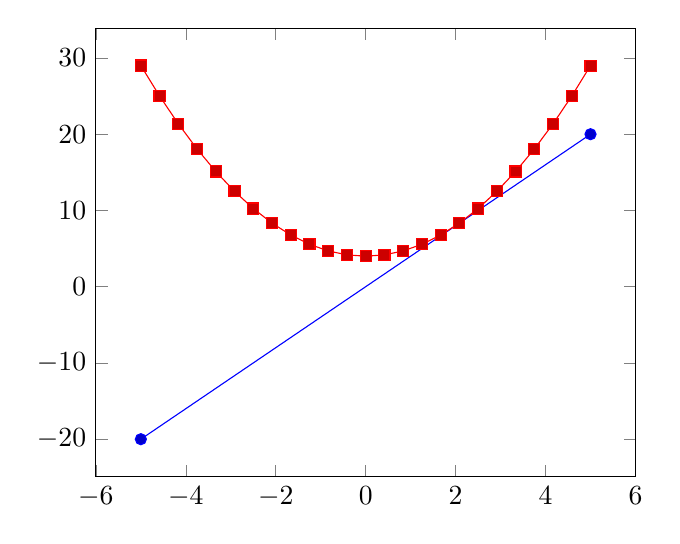
\begin{tikzpicture}
\begin{axis}[
    declare function={
        C=4;
        square(\t)=(\t)^2 + C;
    },
]
    \addplot+ [samples=2] {C*x};

    \addplot {square(x)};
\end{axis}
\end{tikzpicture}
\end{codeexample}
    %
    The definitions as such have the form \meta{function}\meta{argument list} =
    \meta{definition} where the \meta{argument list} contains a
    comma-separated-list of arguments like |\t| or |\t,\a,\b|. The
    \meta{definition} is a math expression which makes use of these arguments.

    Please refer to \cite{tikz} for more details.
\end{key}

\begin{command}{\pgfplotstableread\marg{file}}
    Please refer to the manual of \PGFPlotstable{}, |pgfplotstable.pdf|, which
    is part of the \PGFPlots{} bundle.
\end{command}

\begin{command}{\pgfplotstabletypeset\marg{\textbackslash macro}}
    Please refer to the manual of \PGFPlotstable{}, |pgfplotstable.pdf|, which
    is part of the \PGFPlots{} bundle.
\end{command}

\begin{command}{\pgfplotsiffileexists\marg{filename}\marg{true code}\marg{false code}}
    Invokes \meta{true code} if \meta{filename} exists and \meta{false code} if
    not. Can be used in looping macros, for example to plot every data file
    until there are no more of them.
\end{command}

\begin{command}{\pgfplotsutilifstringequal\marg{first}\marg{second}\marg{true code}\marg{false code}}
    A simple ``strcmp'' tool which invokes \meta{true code} if \meta{first}
    $=$\meta{second} and \meta{false code} otherwise. This does not expand
    macros.
\end{command}

\begin{commandlist}{\pgfkeys,\pgfeov,\pgfkeysvalueof,\pgfkeysgetvalue}
    These commands are part of the \Tikz{} way of specifying options, its
    sub-package |pgfkeys|. The |\pgfplotsset| command is actually nothing but a
    wrapper around |\pgfkeys|.

    A short introduction into |\pgfkeys| can be found in~\cite{keyvalintro}
    whereas the complete reference is, of course, the \Tikz{}
    manual~\cite{tikz}.

    The key |\pgfkeysvalueof|\marg{key name} expands to the value of a key;
    |\pgfkeysgetvalue|\marg{key name}\marg{\textbackslash macro} stores the
    value of \meta{key name} into \meta{\textbackslash macro}. The |\pgfeov|
    macro is used to delimit arguments for code keys in |\pgfkeys|, please
    refer to the references mentioned above.
\end{commandlist}


\section[Commands Inside Of PGFPlots Axes]
        {Commands Inside Of {\normalfont\PGFPlots{}} Axes}

\begin{command}{\autoplotspeclist}
    This command should no longer be used, although it will be kept as
    technical implementation detail. Please use the `|cycle list|' option,
    Section~\ref{sec:cycle:list}.
\end{command}

\begin{command}{\logten}
    Expands to the constant $\log(10)$. Useful for log plots because $\log(10^i)
    = i\log(10)$. This command is only available inside of a \Tikz{} picture.
\end{command}

\begin{command}{\pgfmathprintnumber\marg{number}}
    Generates pretty-printed output\footnote{This method was previously
    \texttt{\textbackslash prettyprintnumber}. Its functionality has been
    included into \PGF{} and the old command is now deprecated.} for
    \meta{number}. This method is used for every tick label.

    The number is printed using the current number printing options, see the
    manual of \PGFPlotstable{} which comes with this package for the different
    number styles, rounding precision and rounding methods.
\end{command}

\begin{command}{\numplots}
    Inside of any of the axis environments, associated style, option or
    command, |\numplots| expands to the total number of plots.
\end{command}

\begin{command}{\numplotsofactualtype}
    Like |\numplots|, this macro returns the total number of plots which have
    the same plot handler. Thus, if you have |sharp plot| active, it returns
    the number of all |sharp plots|. If you have |ybar| active, it returns the
    number of |ybar| plots and so on.
\end{command}

\begin{command}{\plotnum}
    Inside of |\addplot| or any associated style, option or command, |\plotnum|
    expands to the current plot's number, starting with~$0$.
\end{command}

\begin{command}{\plotnumofactualtype}
    Like |\plotnum|, but it returns the number among all plots of the same
    type. The number of all such plots is available using
    |\numplotsofactualtype|.
\end{command}

\begin{command}{\coordindex}
    Inside of an |\addplot| command, this macro expands to the number of the
    actual coordinate (starting with~$0$).

    It is useful together with |x filter| or |y filter| to (de)select
    coordinates.
\end{command}


\section{Path Operations}

\begin{commandlist}{\path,\draw,\fill,\node,\matrix}
    These commands are \Tikz{} drawing commands all of which are documented
    in~\cite{tikz}. They are used to draw or fill paths, generate text nodes or
    aligned text matrices. They are equivalent to
    \pgfmanualpdflabel{/tikz/draw}{}|\path[draw]|,
    \pgfmanualpdflabel{/tikz/fill}{}|\path[fill]|,
    \pgfmanualpdflabel{/tikz/node}{}|\path[node]|,
    \pgfmanualpdflabel{/tikz/matrix}{}|\path[matrix]|,
    respectively.
\end{commandlist}

\begin{pathoperation}{--}{\meta{coordinate}}
    A \Tikz{} path operation which connects the current point (the last one
    before |--|) and \meta{coordinate} with a straight line.
\end{pathoperation}

{\catcode`\|=12
\begin{pathoperation}[noindex]{|-}{\meta{coordinate}}
\pgfmanualpdflabel[\catcode`\|=12 ]{|-}{}%
    A \Tikz{} path operation which connects the current point and
    \meta{coordinate} with \emph{two} straight lines: first vertical, then
    horizontal.
\end{pathoperation}

\begin{pathoperation}[noindex]{-|}{\meta{coordinate}}
\pgfmanualpdflabel[\catcode`\|=12 ]{-|}{}%
    A \Tikz{} path operation which connects the current point and
    \meta{coordinate} with \emph{two} straight lines: first horizontal, then
    vertical.
\end{pathoperation}
}

\begin{keylist}{/tikz/xshift=\marg{dimension},/tikz/yshift=\marg{dimension}}
    These \Tikz{} keys allow to shift something by \meta{dimension} which is
    any \TeX{} size (or expression).
\end{keylist}

\begin{command}{\pgfplotsextra\marg{low-level path commands}}
    A command to execute \meta{low-level path commands} in a \PGFPlots{} axis.
    Since any drawing commands inside of an axis need to be postponed until the
    axis is complete and the scaling has been initialised, it is not possible
    to simply draw any paths. Instead, it is necessary to draw them as soon as
    the axis is finished. This is done automatically for every \Tikz{} path --
    and it is also done manually if you write |\pgfplotsextra|\marg{commands}.
    %
\begin{codeexample}[]
\begin{tikzpicture}
\begin{axis}[xmin=0,xmax=3,ymin=0,ymax=5]
    \pgfplotsextra{
        \pgfpathmoveto{\pgfplotspointaxisxy{1}{2}}
        \pgfpathlineto{\pgfplotspointaxisxy{2}{4}}
        \pgfusepath{stroke}
    }
\end{axis}
\end{tikzpicture}
\end{codeexample}
    %
    The example above initializes an axis and executes the basic level path
    commands as soon as the axis is ready. The execution of multiple |\path|,
    |\addplot| and |\pgfplotsextra| commands is in the same sequence as they
    occur in the environment.\footnote{Except for stacked plots where the
    sequence may be reverse, see the key \texttt{reverse stack plots}.}
\end{command}

\begin{command}{\pgfplotspathaxisoutline}
    Generates a path which resembles the outline of the current axis. This path
    is used for clip paths and the background paths (if any).
\end{command}


\section{Specifying Basic Coordinates}
\label{sec:basic:coordinates}

\begin{commandlist}{%
    \pgfplotspointaxisxy\marg{x coordinate}\marg{y coordinate},
    \pgfplotspointaxisxyz\marg{x coordinate}\marg{y coordinate}\marg{z coordinate}%
}
    Point commands like |\pgfpointxy| which take logical, absolute coordinates
    and return a low-level point. Every transformation from user
    transformations to logarithms is applied.

    Since the transformations are initialized after the axis is complete, this
    command needs to be postponed (see |\pgfplotsextra|).

    This command is the basic level variant of |axis cs:|\meta{x
    coordinate}|,|\meta{y coordinate}|,|\meta{z coordinate}.

    Note that this is also the default coordinate system during the
    visualization phase; in other words: if you write |\draw (1,2) -- (1,4)|,
    \PGFPlots{} will automatically use |(axis cs:1,2) -- (axis cs:1,4)|.
\end{commandlist}

\begin{commandlist}{%
    \pgfplotspointaxisdirectionxy\marg{x coordinate}\marg{y coordinate},
    \pgfplotspointaxisdirectionxyz\marg{x coordinate}\marg{y coordinate}\marg{z coordinate}%
}
    Point commands like |\pgfpointxy| which take logical, \emph{relative}
    coordinates and return a low-level point. Every transformation from user
    transformations to logarithms is applied. The difference to
    |\pgfplotspointaxisxy| is that the shift of the linear transformation is
    skipped here (compare |disabledatascaling|).

    This command is the basic level variant of |axis direction cs:|\meta{x
    coordinate}|,|\meta{y coordinate}|,|\meta{z coordinate}. Please refer to
    the documentation of |axis direction cs| for more details.

    Use this command whenever something of \emph{relative} character like
    directions or lengths need to be supplied. One use case is to draw
    ellipses:
    %
\begin{codeexample}[]
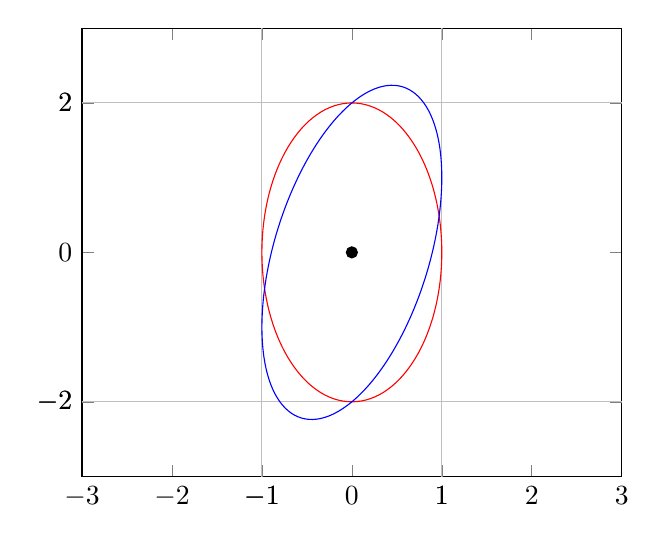
\begin{tikzpicture}
\begin{axis}[
    xmin=-3,   xmax=3,
    ymin=-3,   ymax=3,
    extra x ticks={-1,1},
    extra y ticks={-2,2},
    extra tick style={grid=major},
]
    \draw [red] \pgfextra{
        \pgfpathellipse{\pgfplotspointaxisxy{0}{0}}
            {\pgfplotspointaxisdirectionxy{1}{0}}
            {\pgfplotspointaxisdirectionxy{0}{2}}
    % see also the documentation of
    % 'axis direction cs' which
    % allows a simpler way to draw this ellipse
    };
    \draw [blue] \pgfextra{
        \pgfpathellipse{\pgfplotspointaxisxy{0}{0}}
            {\pgfplotspointaxisdirectionxy{1}{1}}
            {\pgfplotspointaxisdirectionxy{0}{2}}
    };
    \addplot [only marks,mark=*] coordinates
        { (0,0) };
\end{axis}
\end{tikzpicture}
\end{codeexample}

    Since the transformations are initialized after the axis is complete, this
    command needs to be provided either inside of a \tikzname{} |\path| command
    (like |\draw| in the example above) or inside of |\pgfplotsextra|.
\end{commandlist}

\begin{commandlist}{%
    \pgfplotspointrelaxisxy\marg{rel x coordinate}\marg{rel y coordinate},
    \pgfplotspointrelaxisxyz\marg{rel x coordinate}\marg{rel y coordinate}\marg{rel z coordinate}%
}
    Point commands which take \emph{relative} coordinates such that $x=0$ is
    the \emph{lower} $x$-axis limit and $x=1$ the \emph{upper} $x$-axis limit.

    These commands are used for |rel axis cs|.

    Please note that the transformations are only initialised if the axis is
    complete! This means you need to provide |\pgfplotsextra|.
\end{commandlist}

\begin{commandlist}{%
    \pgfplotspointdescriptionxy\marg{$x$ fraction}\marg{$y$ fraction},
    \pgfplotsqpointdescriptionxy\marg{$x$ fraction}\marg{$y$ fraction}%
}
    Point commands such that |{0}{0}| is the lower left corner of the axis'
    bounding box and |{1}{1}| the upper right one; everything else is in
    between. The `|q|' variant is quicker as it doesn't invoke the math parser
    on its arguments.

    They are used for |axis description cs|, see
    Section~\ref{pgfplots:sec:axis:description:cs}.
\end{commandlist}

\begin{commandlist}{\pgfplotspointaxisorigin}
    A point coordinate at the origin, $(0,0,0)$. If the origin is not part of
    the axis limits, the nearest point on the boundary is returned instead.

    This is the same coordinate as returned by the |origin| anchor.
\end{commandlist}

\begin{commandlist}{%
    \pgfplotstransformcoordinatex\marg{x coordinate of an axis},
    \pgfplotstransformcoordinatey\marg{y coordinate of an axis},
    \pgfplotstransformcoordinatez\marg{z coordinate of an axis}%
}
    Defines |\pgfmathresult| to be the low-level \PGF{} coordinate
    corresponding to the input argument.

    The command applies any |[xyz] coord trafo| keys, data scalings and/or
    logarithms or whatever \PGFPlots{} does to map input coordinates to
    internal coordinates.

    The result can be used inside of a |\pgfpointxy| statement (i.e.\@ it still
    needs to be scaled with the respective \PGF{} unit vector).
    %
\begin{codeexample}[]
\begin{tikzpicture}
\pgfplotsset{compat/pgfpoint substitution=1.3}
\begin{axis}[xmin=0,xmax=2,ymin=0,ymax=5]
    \pgfplotsextra{
        \pgfplotstransformcoordinatex{1}
        \let\xcoord=\pgfmathresult
        \pgfplotstransformcoordinatey{1}
        \let\ycoord=\pgfmathresult
        \pgfpathcircle
            {\pgfqpointxy{\xcoord}{\ycoord}}
            {5pt}
        \pgfusepath{fill}
    }
\end{axis}
\end{tikzpicture}
\end{codeexample}
    %
    Note that \PGFPlots{} substitutes |\pgfqpointxy| by |\pgfplotspointaxisxyz|
    by default -- and this command implicitly transforms coordinates anyway. In
    order to see the difference, the preceding example first disables this
    automatic substitution of coordinate systems by means of
    |compat/pgfpoint substitution=1.3|.
    %
    The result of this command is also available as math method
    |transformcoordinatex| (see the documentation for |axis cs|).

    Please note that the transformations are only initialised if the axis is
    complete. This means you need to provide |\pgfplotsextra| as is shown in
    the example above.
\end{commandlist}

\begin{commandlist}{%
    \pgfplotstransformdirectionx\marg{x direction of an axis},
    \pgfplotstransformdirectiony\marg{y direction of an axis},
    \pgfplotstransformdirectionz\marg{z direction of an axis}%
}
    Defines |\pgfmathresult| to be a low-level \PGF{} \emph{direction vector
    component}.

    A direction vector needs to be \emph{added} to some coordinate in order to
    get a coordinate, compare the documentation for
    |\pgfplotspointaxisdirectionxy| and |axis direction cs|.

    The argument \meta{x direction of an axis} is processed in (almost) the
    same way as for the macro which operates on absolute positions,
    |\pgfplotstransformcoordinatex|. The only difference is that
    \emph{directions} need no shifting transformation.

    The result of this command is also available as math method
    |transformdirectionx| (see the documentation for |axis direction cs|).

    See |axis direction cs| for details and examples about this command.
\end{commandlist}

% this command is for internal use only:
%--------------------------------------------------
% \begin{command}{\pgfplotsconvertunittocoordinate\marg{x, y or z}\marg{dimension}}
%     Converts a dimension (with unit!) to a corresponding $x$-, $y$- or $z$-coordinate. The result will be written to |\pgfmathresult| (without units).
%
%     It is possible to use the result as arguments for the |\pgfpointxyz| commands.
%
%     The effect is to multiply \meta{dimension} with the inverse length of the unit vector for the specified axis. These lengths are precomputed in \PGFPlots{} so the operation is fast.
% \begin{codeexample}[code only]
% \pgfplotsconvertunittocoordinate{x}{5pt}
% % now, the command uses exactly 5pt in x direction:
% \pgfqpointxyz{\pgfmathresult}{4}{3}
% \end{codeexample}
% \end{command}
%--------------------------------------------------

\begin{commandlist}{%
    \pgfplotspointunitx,
    \pgfplotspointunity,
    \pgfplotspointunitz%
}
    Low-level point commands which return the canvas $x$, $y$ or $z$ unit
    vectors.

    The |\pgfplotspointunitx| is the \pgfname{} unit vector in $x$ direction.

    These vectors are essentially the same as |\pgfqpointxyz{1}{0}{0}|,
    |\pgfqpointxyz{0}{1}{0}|, and |\pgfqpointxyz{0}{0}{1}|, respectively.

    The unit $z$ vector is only defined for three dimensional axes.
\end{commandlist}

\begin{commandlist}{%
    \pgfplotsunitxlength,
    \pgfplotsunitylength,
    \pgfplotsunitzlength,
    \pgfplotsunitxinvlength,
    \pgfplotsunityinvlength,
    \pgfplotsunitzinvlength%
}
    Macros which expand to the vector length $\lVert x_i \rVert$ of the
    respective unit vector $x_i$ or the inverse vector length, $1/\lVert x_i
    \rVert$. These macros can be used inside of |\pgfmathparse|, for example.

    The $x_i$ are the |\pgfplotspointunitx| variants.
\end{commandlist}

\begin{command}{\pgfplotsqpointoutsideofaxis%
        \marg{three-char-string}\marg{coordinate}\marg{normal distance}%
}
    Provides a point coordinate on one of the available four axes in case of a
    two dimensional figure or on one of the available twelve axes in case of a
    three dimensional figure.

    The desired axis is uniquely identified by a three character string,
    provided as first argument to the command. The first of the three
    characters is `|0|' if the $x$-coordinate of the specified axis passes
    through the lower axis limit. It is `|1|', if the $x$-coordinate of the
    specified axis passes through the upper axis limit. Furthermore, it is
    `|2|' if it passes through the origin. The second character is also either
    |0|, |1| or |2| and it characterizes the position on the $y$-axis. The
    third character is for the third dimension, the $z$-axis. It should be left
    at `|0|' for two dimensional plots. However, \emph{one} of the three
    characters should be `|v|', meaning the axis \underline varies. For
    example, |v01| denotes $\{ (x,y_{\min},z_{\max}) \vert x \in \R \}$.

    The second argument, \meta{coordinate} is the logical coordinate on that
    axis. Since two coordinates of the axis are fixed, \meta{coordinate} refers
    to the \underline varying component of the axis. It must be a number
    without unit; no math expressions are supported here.

    The third argument \meta{normal distance} is a dimension like |10pt|. It
    shifts the coordinate away from the designated axis in direction of the
    outer normal vector. The outer normal vector always points away from the
    axis. It is computed using |\pgfplotspointouternormalvectorofaxis|.

    There are several variants of this command which are documented in the
    source code. One of them is particularly useful:
\end{command}

\begin{command}{\pgfplotsqpointoutsideofaxisrel%
        \marg{three-char-string}\marg{axis fraction}\marg{normal distance}%
}
    This point coordinate is a variant of |\pgfplotsqpointoutsideofaxis| which
    allows to provide an \meta{axis fraction} instead of an absolute
    coordinate. The fraction is a number between $0$ (lower axis limit) and $1$
    (upper axis limit), i.e.\@ it is given in percent of the total axis. It is
    possible to provide negative values or values larger than one.

    The |\pgfplotsqpointoutsideofaxisrel| command is similar in spirit to
    |rel axis cs|.

    There is one speciality in conjunction with reversed axes: if the axis has
    been reversed by |x dir=reverse| and, in addition,
    |allow reversal of rel axis cs| is true, the value $0$ denotes the
    \emph{upper} limit while $1$ denotes the \emph{lower} limit. The effect is
    that coordinates won't change just because of axis reversal.
        \index{allow reversal of rel axis cs}%
\end{command}

\begin{command}{\pgfplotspointouternormalvectorofaxis\marg{three-char-string}}
    A point command which yields the outer normal vector of the respective
    axis. The normal vector has length $1$ (computed with
    |\pgfpointnormalised|). It is the same normal vector used inside of
    |\pgfplotsqpointoutsideofaxis| and its variants.

    The output of this command will be cached and reused during the lifetime
    of an axis.
\end{command}

\begin{command}{\pgfplotsticklabelaxisspec\marg{x, y or z}}
    Expands to the three character identification for the axis containing tick
    labels for the chosen axis, either \meta{x}, \meta{y} or \meta{z}.
\end{command}

\begin{command}{\pgfplotsvalueoflargesttickdimen\marg{x, y or z}}
    Expands to the largest distance of a tick position to its tick label
    bounding box in direction of the outer unit normal vector. It does also
    include the value of the |ticklabel shift| key.

    This value is used for |ticklabel cs|.
\end{command}

\begin{commandlist}{
    \pgfplotsmathfloatviewdepthxyz\marg{x}\marg{y}\marg{z},
    \pgfplotsmathviewdepthxyz\marg{x}\marg{y}\marg{z}%
}
    Both macros define |\pgfmathresult| to be the ``depth'' of a three
    dimensional point $\bar x = (x,y,z)$. The depth is defined to be the scalar
    product of $\bar x$ with $\vec d$, the view direction of the current axis.

    For |\pgfplotsmathfloatviewdepthxyz|, the arguments are parsed as floating
    point numbers and the result is encoded in floating point. A fixed point
    representation can be generated with
    |\pgfmathfloattofixed{\pgfmathresult}|.

    For |\pgfplotsmathviewdepthxyz|, \TeX{} arithmetics is employed for the
    inner product and the result is assigned in fixed point. This is slightly
    faster, but has considerably smaller data range.

    Both commands can only be used \emph{inside} of a three dimensional
    \PGFPlots{} axis (as soon as the axis is initialised, see
    |\pgfplotsextra|).
\end{commandlist}

\begin{texif}{pgfplotsthreedim}
    A \TeX{} |\if| which evaluates the \meta{true code} if the axis is three
    dimensional and the \meta{else code} if not.
\end{texif}


\section{Accessing Axis Limits}

It is also possible to access axis limits during the visualization phase,
i.e.\@ during |\end{axis}|. Please refer to the reference documentation for
|xmin| on page~\pageref{page:access:limits}.


\section{Accessing Point Coordinate Values}

During the visualization phase, \PGFPlots{} provides access to the currently
processed coordinate and its values.

This access requires a call to specific macros. These macros write the
coordinate values to some publicly available key--value pairs. Then, the
current point's $x$, $y$, $z$, and color data can be accessed.

\begin{commandlist}{\pgfplotspointgetcoordinates,\pgfplotspointgetcoordinates\marg{point}}

    After invoking the macro, the following keys will be set:

    \declaretext{/data point/x} will contain the current point's $x$-coordinate.

    \declaretext{/data point/y} will contain the current point's $y$-coordinate.

    \declaretext{/data point/z} will contain the current point's $z$-coordinate
    (if applicable).

    \declaretext{/data point/meta} will contain the current point's
    |point meta| value (if applicable).

    \declaretext{/data point/index} will contain the current point's index in
    the coordinate stream. This is actually the same as |\coordindex|.

    This command actually supports two modes of operation:
    %
    \begin{enumerate}
        \item Without arguments. In this case, it returns values of the point
            which is about to be processed by the current plot handler.
        \item With an argument in curly braces. In this case, it expects a
            coordinate and assigns the keys accordingly. Note that this
            command merely supports two-dimensional axes and assigns only
            |/data point/x| and |/data point/y|.
    \end{enumerate}

    The returned values are the same as they can be read on the axes, they are
    also the same as you would write them into |axis cs|.

    This means that any |x coord inv trafo| has been applied on the value. It
    also means that the exponential function has been called even though the
    internal coordinate was present in log format.

    This function is implicitly called for any |scatter| plot (including
    |nodes near coords|). This allows to access \emph{all} coordinate values at
    once:
    %
\begin{codeexample}[]
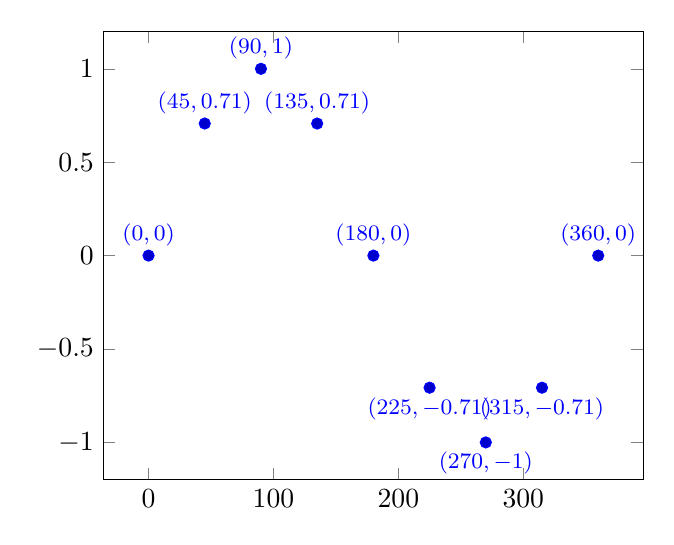
\begin{tikzpicture}
\begin{axis}
    \addplot+ [
        domain=0:360,
        samples=9,
        only marks,
        nodes near coords={%
            \footnotesize
            $(\pgfmathprintnumber
                {\pgfkeysvalueof{/data point/x}},
               \pgfmathprintnumber
                {\pgfkeysvalueof{/data point/y}})$%
        },
    ] {sin(x)};
\end{axis}
\end{tikzpicture}
\end{codeexample}
    %
    The example works because |\pgfplotspointgetcoordinates| is part of the
    standard implementation of |nodes near coords|; the resulting values are
    directly available. Note that the preceding example would have been simpler
    if we would have printed just one value: |nodes near coords| resorts to the
    |point meta|. And that, in turn, contains the $y$-coordinate anyway by
    default.

    A more advanced example would be a |ybar| plot in which nodes shall be
    placed at the lower end of the axis, together with some dotted lines to the
    respective bars:
    %
\begin{codeexample}[]
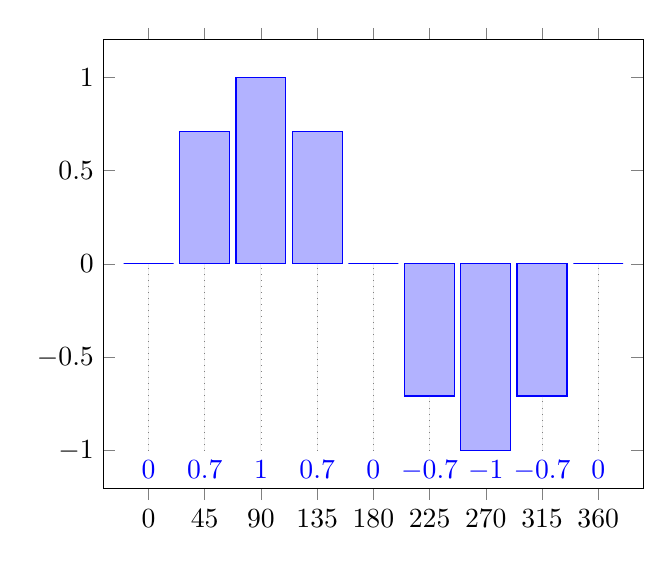
\begin{tikzpicture}
\begin{axis}[
    ybar,
    nodes near coords,
    %
    % we want to provide absolute 'at' values
    % for the nodes:
    scatter/position=absolute,
    every node near coord/.style={
        at={(\pgfkeysvalueof{/data point/x},-1)},
        % pretty printing:
        anchor=north,
        /pgf/number format/fixed,
        /pgf/number format/precision=1,
        % assign a name which can be referenced below:
        name=NNC\pgfkeysvalueof{/data point/index},
    },
    % ... draw a dotted line between
    % the marker and the bar:
    /pgfplots/scatter/@post marker code/.add code={}{
        \draw [dotted,help lines]
            (NNC\pgfkeysvalueof{/data point/index})
            -- (\pgfkeysvalueof{/data point/x},
            {min(0,\pgfkeysvalueof{/data point/y})});
    },
    % assign suitable tick labels:
    xtick=data,
]
    % some dummy data:
    \addplot+ [
        domain=0:360,
        bar width=360/9,
        samples=9,
    ] {sin(x)};
\end{axis}
\end{tikzpicture}
\end{codeexample}
    %
    Again, the command is used implicitly as part of |nodes near coords| and
    does not occur in the example as such.

    \paragraph{See also} the related example online under
    \url{https://tex.stackexchange.com/a/141006}. It demonstrates how to
    place the nodes generated by |nodes near coords| based on the value (either
    inside of a bar or above it).

    The following example uses an argument in curly braces for which we seek
    coordinate values:
    %
\begin{codeexample}[]
% requires \usetikzlibrary{intersections}
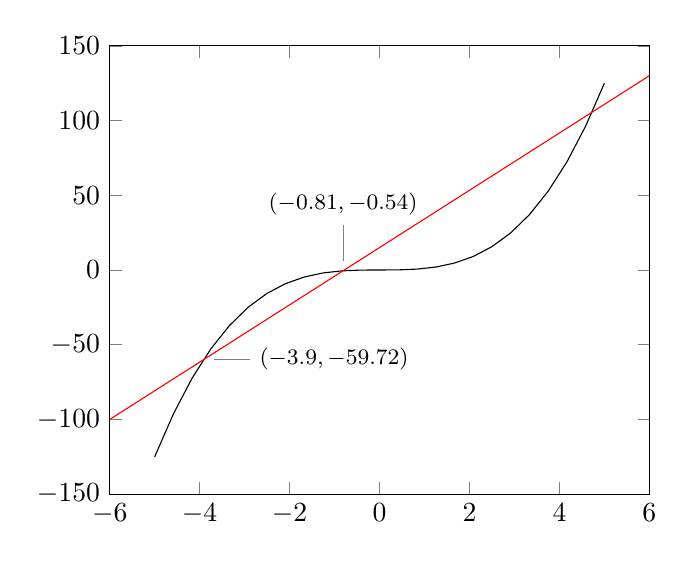
\begin{tikzpicture}
\begin{axis}
    \addplot [name path=A] {x^3};

    \draw [red,name path=HelperLine]
        (axis cs:-6,-100) -- (axis cs:6,130);

    \draw [
        font=\footnotesize,
        name intersections={of=A and HelperLine},
    ]
    node [pin={right:
      \pgfplotspointgetcoordinates{(intersection-1)}
        $(\pgfmathprintnumber[fixed]{
            \pgfkeysvalueof{/data point/x}},
          \pgfmathprintnumber[fixed]{
            \pgfkeysvalueof{/data point/y}})$
      }
    ] at (intersection-1) {}
    node [pin={
      \pgfplotspointgetcoordinates{(intersection-2)}
        $(\pgfmathprintnumber[fixed]{
            \pgfkeysvalueof{/data point/x}},
          \pgfmathprintnumber[fixed]{
            \pgfkeysvalueof{/data point/y}})$
      }
    ] at (intersection-2) {};
\end{axis}
\end{tikzpicture}
\end{codeexample}
    %
    The example computes and names intersections of |A| and |HelperLine|. The
    following code generates pins at the intersections. To this end, it uses
    |\pgfplotspointgetcoordinates|\marg{point} which defines |/data point/x|
    and |/data point/y|. These values are then formatted using
    |\pgfmathprintnumber|.

    In its second mode, |\pgfplotspointgetcoordinates|\marg{point} expects one
    of two things as \meta{point}:
    %
    \begin{enumerate}
        \item a basic-level \PGF{} point like |\pgfpointanchor{A}{center}| or
        \item a \Tikz{} point like |(A.base)| or |(3,5)|.
    \end{enumerate}
\end{commandlist}

\begin{command}{\pgfplotspointgetnormalizedcoordinates}
    A macro which is very similar to |\pgfplotspointgetcoordinates|.
    Consequently, it is also supposed to be called during the visualization phase.

    It assigns the very same output macros, but the values are different. More
    precisely, it defines the macros

    \declaretext{/data point/x} will contain the current point's
    \emph{normalized} $x$-coordinate.

    \declaretext{/data point/y} will contain the current point's
    \emph{normalized} $y$-coordinate.

    \declaretext{/data point/z} will contain the current point's
    \emph{normalized} $z$-coordinate (if applicable).

    \declaretext{/data point/meta} will contain the current point's
    |point meta| value (if applicable).

    \declaretext{/data point/index} will contain the current point's index in
    the coordinate stream. This is actually the same as |\coordindex|.

    The keyword \declaretext{normalized} means that the values are in a
    suitable numerical form which can be consumed by the axis. To be more
    specific: any user |x coord inv trafo| is \emph{ignored}. An important
    example would be |symbolic x coords|: the normalized coordinates would be
    some associated numbers, not the symbols. The results returned by
    |\pgfplotspointgetcoordinates| would be the symbols. For logarithm axes,
    the normalized values are the logs.

    Typically, normalized values are much more useful when you want to apply
    some math operation like averaging or subtraction.

    This function needs to be called explicitly. It is currently used by
    |ybar stacked| to align |nodes near coords|.
\end{command}


\section{Layer Access}

\begin{command}{\pgfplotsonlayer\marg{layer name}}
    A low-level command which will check if the current axis has layer support
    activated and, if so, calls |\pgfonlayer|\marg{layer name}.

    There must be a |\endpgfplotsonlayer| to delimit the environment.
\end{command}

\begin{command}{\endpgfplotsonlayer}
    The end of |\pgfplotsonlayer|.
\end{command}

\begin{command}{\pgfonlayer\marg{layer name}}
    A low-level command of \PGF{} which will collect everything until the
    matching |\endpgfonlayer| into layer \meta{layer name}.

    The \meta{layer name} must be active, i.e.\@ it must be part of the layer
    names of |set layers|.

    The only special case is if you call |\pgfdeclarelayer{discard}| somewhere:
    this special layer has a ``magical name'' which serves as |/dev/null| if it
    is enabled using |\pgfonlayer{discard}|: it does not need to be active and
    everything assigned to this layer will be thrown away if it is not part of
    the layer name configuration.

    There must be a |\endpgfonlayer| to delimit the environment.
\end{command}

\begin{command}{\endpgfonlayer}
    The end of |\pgfonlayer|.
\end{command}


\begin{command}{\pgfsetlayers\marg{layer list}}
    This is a low-level command of \PGF{}. At the time of this writing, it is
    the only way to tell \PGF{} which layers it shall use for the current/next
    picture. It is used implicitly by |set layers|.
\end{command}


\printindex

\bibliographystyle{abbrv} %gerapali} %gerabbrv} %gerunsrt.bst} %gerabbrv}% gerplain}
\nocite{pgfplotstable}
\nocite{programmingnotes}
\bibliography{pgfplots}
\end{document}

% -----------------------------------------------------------------------------
% For Stefan Pinnow as reminder on what to look for when editing the manual
% -----------------------------------------------------------------------------
% There should be no line breaks in the following environments
% - |...|
% - \declareandlabel{...}
% - \verbpdfref{...}
% If "MakeTikzPictures" isn't running through check one of the externalized
% LOG files what is the cause of that.
% -----------------------------------------------------------------------------


%%%%%%%%%%%%%%%%%%%%%%%%%%%%%%%%%%%%%%%%%%%%%%%%%%%%%%%%%%%%%%%%%%%%%%%%%%%%%
%
% Package pgfplots.sty documentation.
%
% Copyright 2007/2008 by Christian Feuersaenger.
%
% This program is free software: you can redistribute it and/or modify
% it under the terms of the GNU General Public License as published by
% the Free Software Foundation, either version 3 of the License, or
% (at your option) any later version.
%
% This program is distributed in the hope that it will be useful,
% but WITHOUT ANY WARRANTY; without even the implied warranty of
% MERCHANTABILITY or FITNESS FOR A PARTICULAR PURPOSE.  See the
% GNU General Public License for more details.
%
% You should have received a copy of the GNU General Public License
% along with this program.  If not, see <http://www.gnu.org/licenses/>.
%
%
%%%%%%%%%%%%%%%%%%%%%%%%%%%%%%%%%%%%%%%%%%%%%%%%%%%%%%%%%%%%%%%%%%%%%%%%%%%%%
% SEE pgfplots-macros.tex as well!
%\pdfminorversion=5 % to allow compression
%\pdfobjcompresslevel=2
\documentclass[a4paper,openany]{book}

\let\bookmaketitle=\maketitle

% -----------------------------------
% this here is from ltxdoc:
\usepackage{doc}[=v2]
\AtBeginDocument{\MakeShortVerb{\|}}
%\setlength{\textwidth}{355pt}
%\addtolength\marginparwidth{30pt}
%\addtolength\oddsidemargin{20pt}
%\addtolength\evensidemargin{20pt}
\def\cmd#1{\cs{\expandafter\cmd@to@cs\string#1}}
\def\cmd@to@cs#1#2{\char\number`#2\relax}
\DeclareRobustCommand\cs[1]{\texttt{\char`\\#1}}
\providecommand\marg[1]{%
  {\ttfamily\char`\{}\meta{#1}{\ttfamily\char`\}}}
\providecommand\oarg[1]{%
  {\ttfamily[}\meta{#1}{\ttfamily]}}
\providecommand\parg[1]{%
  {\ttfamily(}\meta{#1}{\ttfamily)}}
\raggedbottom

% -----------------------------------
\input{pgfplots.preamble.tex}

\makeatletter
% I want a two-column index just as in pgfmanual styles. This here
% was the best way to get one:
\def\index@prologue{\section*{Index}\addcontentsline{toc}{chapter}{Index}
}
\makeatother

%\RequirePackage[german,english,francais]{babel}

\def\matlabcolormaptext{This colormap is similar to one shipped with Matlab$^\text{\textregistered}$ under a similar name.}

\IfFileExists{tikzlibraryspy.code.tex}{%
\usetikzlibrary{spy}
}{%
    \message{ERROR: tikz SPY library NOT available. The manual will only compile partially.^^J}%
}%

\usepackage{xparse}% for colorbrewer manual

\usetikzlibrary{
    decorations.markings,
    decorations.footprints,
    shapes.arrows,
    matrix,
    positioning,
}

\usepgfplotslibrary{
    fillbetween,
    ternary,
    smithchart,
    patchplots,
    polar,
    colormaps,
    colorbrewer,
    colortol,           % docu not ready yet
}
\pgfqkeys{/codeexample}{%
    every codeexample/.append style={
        /pgfplots/every ternary axis/.append style={
            /pgfplots/legend style={fill=graphicbackground},
        }
    },
    tabsize=4,
}

\pgfplotsmanualenableexternalizationofexpensive

%\usetikzlibrary{external}
%\tikzexternalize[prefix=figures/]{pgfplots}

\title{%
    Manual for Package \PGFPlots{}\\
    {\small 2D/3D Plots in \LaTeX{}, Version \pgfplotsversion}\\
    {\small\href{https://github.com/pgf-tikz/pgfplots}{https://github.com/pgf-tikz/pgfplots}}
    %\\{\small Attention: you are using an unstable development version.}
}

\makeatletter
\long\def\abstractsmuggle{%
    \centering
    \textbf{Abstract}\\[0.5cm]

    \begin{minipage}{12cm}
        \PGFPlots{} draws high-quality function plots in normal or logarithmic
        scaling with a user-friendly interface directly in \TeX{}. The user
        supplies axis labels, legend entries and the plot coordinates for one or
        more plots and \PGFPlots{} applies axis scaling, computes any logarithms
        and axis ticks and draws the plots. It supports line plots, scatter
        plots, piecewise constant plots, bar plots, area plots, mesh and surface
        plots, patch plots, contour plots, quiver plots, histogram plots, box
        plots, polar axes, ternary diagrams, smith charts and some more. It is
        based on Till Tantau's package \PGF{}/\Tikz{}.
    \end{minipage}

}%

\expandafter\date\expandafter{\@date\\[2cm]
    \abstractsmuggle
}%
\makeatother

%\includeonly{pgfplots.reference}


\begin{document}

\def\plotcoords{%
\addplot coordinates {
(5,8.312e-02)    (17,2.547e-02)   (49,7.407e-03)
(129,2.102e-03)  (321,5.874e-04)  (769,1.623e-04)
(1793,4.442e-05) (4097,1.207e-05) (9217,3.261e-06)
};

\addplot coordinates{
(7,8.472e-02)    (31,3.044e-02)    (111,1.022e-02)
(351,3.303e-03)  (1023,1.039e-03)  (2815,3.196e-04)
(7423,9.658e-05) (18943,2.873e-05) (47103,8.437e-06)
};

\addplot coordinates{
(9,7.881e-02)     (49,3.243e-02)    (209,1.232e-02)
(769,4.454e-03)   (2561,1.551e-03)  (7937,5.236e-04)
(23297,1.723e-04) (65537,5.545e-05) (178177,1.751e-05)
};

\addplot coordinates{
(11,6.887e-02)    (71,3.177e-02)     (351,1.341e-02)
(1471,5.334e-03)  (5503,2.027e-03)   (18943,7.415e-04)
(61183,2.628e-04) (187903,9.063e-05) (553983,3.053e-05)
};

\addplot coordinates{
(13,5.755e-02)     (97,2.925e-02)     (545,1.351e-02)
(2561,5.842e-03)   (10625,2.397e-03)  (40193,9.414e-04)
(141569,3.564e-04) (471041,1.308e-04)
(1496065,4.670e-05)
};
}%


\bookmaketitle
\tableofcontents

%%%%%%%%%%%%%%%%%%%%%%%%%%%%%%%%%%%%%%%%%%%%%%%%%%%%%%%%%%%%%%%%%%%%%%%%%%%%%
%
% Package pgfplots.sty documentation.
%
% Copyright 2007/2008 by Christian Feuersaenger.
%
% This program is free software: you can redistribute it and/or modify
% it under the terms of the GNU General Public License as published by
% the Free Software Foundation, either version 3 of the License, or
% (at your option) any later version.
%
% This program is distributed in the hope that it will be useful,
% but WITHOUT ANY WARRANTY; without even the implied warranty of
% MERCHANTABILITY or FITNESS FOR A PARTICULAR PURPOSE.  See the
% GNU General Public License for more details.
%
% You should have received a copy of the GNU General Public License
% along with this program.  If not, see <http://www.gnu.org/licenses/>.
%
%
%%%%%%%%%%%%%%%%%%%%%%%%%%%%%%%%%%%%%%%%%%%%%%%%%%%%%%%%%%%%%%%%%%%%%%%%%%%%%
% SEE pgfplots-macros.tex as well!
%\pdfminorversion=5 % to allow compression
%\pdfobjcompresslevel=2
\documentclass[a4paper,openany]{book}

\let\bookmaketitle=\maketitle

% -----------------------------------
% this here is from ltxdoc:
\usepackage{doc}[=v2]
\AtBeginDocument{\MakeShortVerb{\|}}
%\setlength{\textwidth}{355pt}
%\addtolength\marginparwidth{30pt}
%\addtolength\oddsidemargin{20pt}
%\addtolength\evensidemargin{20pt}
\def\cmd#1{\cs{\expandafter\cmd@to@cs\string#1}}
\def\cmd@to@cs#1#2{\char\number`#2\relax}
\DeclareRobustCommand\cs[1]{\texttt{\char`\\#1}}
\providecommand\marg[1]{%
  {\ttfamily\char`\{}\meta{#1}{\ttfamily\char`\}}}
\providecommand\oarg[1]{%
  {\ttfamily[}\meta{#1}{\ttfamily]}}
\providecommand\parg[1]{%
  {\ttfamily(}\meta{#1}{\ttfamily)}}
\raggedbottom

% -----------------------------------
\input{pgfplots.preamble.tex}

\makeatletter
% I want a two-column index just as in pgfmanual styles. This here
% was the best way to get one:
\def\index@prologue{\section*{Index}\addcontentsline{toc}{chapter}{Index}
}
\makeatother

%\RequirePackage[german,english,francais]{babel}

\def\matlabcolormaptext{This colormap is similar to one shipped with Matlab$^\text{\textregistered}$ under a similar name.}

\IfFileExists{tikzlibraryspy.code.tex}{%
\usetikzlibrary{spy}
}{%
    \message{ERROR: tikz SPY library NOT available. The manual will only compile partially.^^J}%
}%

\usepackage{xparse}% for colorbrewer manual

\usetikzlibrary{
    decorations.markings,
    decorations.footprints,
    shapes.arrows,
    matrix,
    positioning,
}

\usepgfplotslibrary{
    fillbetween,
    ternary,
    smithchart,
    patchplots,
    polar,
    colormaps,
    colorbrewer,
    colortol,           % docu not ready yet
}
\pgfqkeys{/codeexample}{%
    every codeexample/.append style={
        /pgfplots/every ternary axis/.append style={
            /pgfplots/legend style={fill=graphicbackground},
        }
    },
    tabsize=4,
}

\pgfplotsmanualenableexternalizationofexpensive

%\usetikzlibrary{external}
%\tikzexternalize[prefix=figures/]{pgfplots}

\title{%
    Manual for Package \PGFPlots{}\\
    {\small 2D/3D Plots in \LaTeX{}, Version \pgfplotsversion}\\
    {\small\href{https://github.com/pgf-tikz/pgfplots}{https://github.com/pgf-tikz/pgfplots}}
    %\\{\small Attention: you are using an unstable development version.}
}

\makeatletter
\long\def\abstractsmuggle{%
    \centering
    \textbf{Abstract}\\[0.5cm]

    \begin{minipage}{12cm}
        \PGFPlots{} draws high-quality function plots in normal or logarithmic
        scaling with a user-friendly interface directly in \TeX{}. The user
        supplies axis labels, legend entries and the plot coordinates for one or
        more plots and \PGFPlots{} applies axis scaling, computes any logarithms
        and axis ticks and draws the plots. It supports line plots, scatter
        plots, piecewise constant plots, bar plots, area plots, mesh and surface
        plots, patch plots, contour plots, quiver plots, histogram plots, box
        plots, polar axes, ternary diagrams, smith charts and some more. It is
        based on Till Tantau's package \PGF{}/\Tikz{}.
    \end{minipage}

}%

\expandafter\date\expandafter{\@date\\[2cm]
    \abstractsmuggle
}%
\makeatother

%\includeonly{pgfplots.reference}


\begin{document}

\def\plotcoords{%
\addplot coordinates {
(5,8.312e-02)    (17,2.547e-02)   (49,7.407e-03)
(129,2.102e-03)  (321,5.874e-04)  (769,1.623e-04)
(1793,4.442e-05) (4097,1.207e-05) (9217,3.261e-06)
};

\addplot coordinates{
(7,8.472e-02)    (31,3.044e-02)    (111,1.022e-02)
(351,3.303e-03)  (1023,1.039e-03)  (2815,3.196e-04)
(7423,9.658e-05) (18943,2.873e-05) (47103,8.437e-06)
};

\addplot coordinates{
(9,7.881e-02)     (49,3.243e-02)    (209,1.232e-02)
(769,4.454e-03)   (2561,1.551e-03)  (7937,5.236e-04)
(23297,1.723e-04) (65537,5.545e-05) (178177,1.751e-05)
};

\addplot coordinates{
(11,6.887e-02)    (71,3.177e-02)     (351,1.341e-02)
(1471,5.334e-03)  (5503,2.027e-03)   (18943,7.415e-04)
(61183,2.628e-04) (187903,9.063e-05) (553983,3.053e-05)
};

\addplot coordinates{
(13,5.755e-02)     (97,2.925e-02)     (545,1.351e-02)
(2561,5.842e-03)   (10625,2.397e-03)  (40193,9.414e-04)
(141569,3.564e-04) (471041,1.308e-04)
(1496065,4.670e-05)
};
}%


\bookmaketitle
\tableofcontents
\include{pgfplots.title_abstract_intro}
\include{pgfplots.preliminaries}
\include{pgfplots.intro}
\include{pgfplots.reference}
\include{pgfplots.libs}
\include{pgfplots.resources}
\include{pgfplots.importexport}
\include{pgfplots.basic.reference}

\printindex

\bibliographystyle{abbrv} %gerapali} %gerabbrv} %gerunsrt.bst} %gerabbrv}% gerplain}
\nocite{pgfplotstable}
\nocite{programmingnotes}
\bibliography{pgfplots}
\end{document}

% -----------------------------------------------------------------------------
% For Stefan Pinnow as reminder on what to look for when editing the manual
% -----------------------------------------------------------------------------
% There should be no line breaks in the following environments
% - |...|
% - \declareandlabel{...}
% - \verbpdfref{...}
% If "MakeTikzPictures" isn't running through check one of the externalized
% LOG files what is the cause of that.
% -----------------------------------------------------------------------------


%%%%%%%%%%%%%%%%%%%%%%%%%%%%%%%%%%%%%%%%%%%%%%%%%%%%%%%%%%%%%%%%%%%%%%%%%%%%%
%
% Package pgfplots.sty documentation.
%
% Copyright 2007/2008 by Christian Feuersaenger.
%
% This program is free software: you can redistribute it and/or modify
% it under the terms of the GNU General Public License as published by
% the Free Software Foundation, either version 3 of the License, or
% (at your option) any later version.
%
% This program is distributed in the hope that it will be useful,
% but WITHOUT ANY WARRANTY; without even the implied warranty of
% MERCHANTABILITY or FITNESS FOR A PARTICULAR PURPOSE.  See the
% GNU General Public License for more details.
%
% You should have received a copy of the GNU General Public License
% along with this program.  If not, see <http://www.gnu.org/licenses/>.
%
%
%%%%%%%%%%%%%%%%%%%%%%%%%%%%%%%%%%%%%%%%%%%%%%%%%%%%%%%%%%%%%%%%%%%%%%%%%%%%%
% SEE pgfplots-macros.tex as well!
%\pdfminorversion=5 % to allow compression
%\pdfobjcompresslevel=2
\documentclass[a4paper,openany]{book}

\let\bookmaketitle=\maketitle

% -----------------------------------
% this here is from ltxdoc:
\usepackage{doc}[=v2]
\AtBeginDocument{\MakeShortVerb{\|}}
%\setlength{\textwidth}{355pt}
%\addtolength\marginparwidth{30pt}
%\addtolength\oddsidemargin{20pt}
%\addtolength\evensidemargin{20pt}
\def\cmd#1{\cs{\expandafter\cmd@to@cs\string#1}}
\def\cmd@to@cs#1#2{\char\number`#2\relax}
\DeclareRobustCommand\cs[1]{\texttt{\char`\\#1}}
\providecommand\marg[1]{%
  {\ttfamily\char`\{}\meta{#1}{\ttfamily\char`\}}}
\providecommand\oarg[1]{%
  {\ttfamily[}\meta{#1}{\ttfamily]}}
\providecommand\parg[1]{%
  {\ttfamily(}\meta{#1}{\ttfamily)}}
\raggedbottom

% -----------------------------------
\input{pgfplots.preamble.tex}

\makeatletter
% I want a two-column index just as in pgfmanual styles. This here
% was the best way to get one:
\def\index@prologue{\section*{Index}\addcontentsline{toc}{chapter}{Index}
}
\makeatother

%\RequirePackage[german,english,francais]{babel}

\def\matlabcolormaptext{This colormap is similar to one shipped with Matlab$^\text{\textregistered}$ under a similar name.}

\IfFileExists{tikzlibraryspy.code.tex}{%
\usetikzlibrary{spy}
}{%
    \message{ERROR: tikz SPY library NOT available. The manual will only compile partially.^^J}%
}%

\usepackage{xparse}% for colorbrewer manual

\usetikzlibrary{
    decorations.markings,
    decorations.footprints,
    shapes.arrows,
    matrix,
    positioning,
}

\usepgfplotslibrary{
    fillbetween,
    ternary,
    smithchart,
    patchplots,
    polar,
    colormaps,
    colorbrewer,
    colortol,           % docu not ready yet
}
\pgfqkeys{/codeexample}{%
    every codeexample/.append style={
        /pgfplots/every ternary axis/.append style={
            /pgfplots/legend style={fill=graphicbackground},
        }
    },
    tabsize=4,
}

\pgfplotsmanualenableexternalizationofexpensive

%\usetikzlibrary{external}
%\tikzexternalize[prefix=figures/]{pgfplots}

\title{%
    Manual for Package \PGFPlots{}\\
    {\small 2D/3D Plots in \LaTeX{}, Version \pgfplotsversion}\\
    {\small\href{https://github.com/pgf-tikz/pgfplots}{https://github.com/pgf-tikz/pgfplots}}
    %\\{\small Attention: you are using an unstable development version.}
}

\makeatletter
\long\def\abstractsmuggle{%
    \centering
    \textbf{Abstract}\\[0.5cm]

    \begin{minipage}{12cm}
        \PGFPlots{} draws high-quality function plots in normal or logarithmic
        scaling with a user-friendly interface directly in \TeX{}. The user
        supplies axis labels, legend entries and the plot coordinates for one or
        more plots and \PGFPlots{} applies axis scaling, computes any logarithms
        and axis ticks and draws the plots. It supports line plots, scatter
        plots, piecewise constant plots, bar plots, area plots, mesh and surface
        plots, patch plots, contour plots, quiver plots, histogram plots, box
        plots, polar axes, ternary diagrams, smith charts and some more. It is
        based on Till Tantau's package \PGF{}/\Tikz{}.
    \end{minipage}

}%

\expandafter\date\expandafter{\@date\\[2cm]
    \abstractsmuggle
}%
\makeatother

%\includeonly{pgfplots.reference}


\begin{document}

\def\plotcoords{%
\addplot coordinates {
(5,8.312e-02)    (17,2.547e-02)   (49,7.407e-03)
(129,2.102e-03)  (321,5.874e-04)  (769,1.623e-04)
(1793,4.442e-05) (4097,1.207e-05) (9217,3.261e-06)
};

\addplot coordinates{
(7,8.472e-02)    (31,3.044e-02)    (111,1.022e-02)
(351,3.303e-03)  (1023,1.039e-03)  (2815,3.196e-04)
(7423,9.658e-05) (18943,2.873e-05) (47103,8.437e-06)
};

\addplot coordinates{
(9,7.881e-02)     (49,3.243e-02)    (209,1.232e-02)
(769,4.454e-03)   (2561,1.551e-03)  (7937,5.236e-04)
(23297,1.723e-04) (65537,5.545e-05) (178177,1.751e-05)
};

\addplot coordinates{
(11,6.887e-02)    (71,3.177e-02)     (351,1.341e-02)
(1471,5.334e-03)  (5503,2.027e-03)   (18943,7.415e-04)
(61183,2.628e-04) (187903,9.063e-05) (553983,3.053e-05)
};

\addplot coordinates{
(13,5.755e-02)     (97,2.925e-02)     (545,1.351e-02)
(2561,5.842e-03)   (10625,2.397e-03)  (40193,9.414e-04)
(141569,3.564e-04) (471041,1.308e-04)
(1496065,4.670e-05)
};
}%


\bookmaketitle
\tableofcontents
\include{pgfplots.title_abstract_intro}
\include{pgfplots.preliminaries}
\include{pgfplots.intro}
\include{pgfplots.reference}
\include{pgfplots.libs}
\include{pgfplots.resources}
\include{pgfplots.importexport}
\include{pgfplots.basic.reference}

\printindex

\bibliographystyle{abbrv} %gerapali} %gerabbrv} %gerunsrt.bst} %gerabbrv}% gerplain}
\nocite{pgfplotstable}
\nocite{programmingnotes}
\bibliography{pgfplots}
\end{document}

% -----------------------------------------------------------------------------
% For Stefan Pinnow as reminder on what to look for when editing the manual
% -----------------------------------------------------------------------------
% There should be no line breaks in the following environments
% - |...|
% - \declareandlabel{...}
% - \verbpdfref{...}
% If "MakeTikzPictures" isn't running through check one of the externalized
% LOG files what is the cause of that.
% -----------------------------------------------------------------------------


%%%%%%%%%%%%%%%%%%%%%%%%%%%%%%%%%%%%%%%%%%%%%%%%%%%%%%%%%%%%%%%%%%%%%%%%%%%%%
%
% Package pgfplots.sty documentation.
%
% Copyright 2007/2008 by Christian Feuersaenger.
%
% This program is free software: you can redistribute it and/or modify
% it under the terms of the GNU General Public License as published by
% the Free Software Foundation, either version 3 of the License, or
% (at your option) any later version.
%
% This program is distributed in the hope that it will be useful,
% but WITHOUT ANY WARRANTY; without even the implied warranty of
% MERCHANTABILITY or FITNESS FOR A PARTICULAR PURPOSE.  See the
% GNU General Public License for more details.
%
% You should have received a copy of the GNU General Public License
% along with this program.  If not, see <http://www.gnu.org/licenses/>.
%
%
%%%%%%%%%%%%%%%%%%%%%%%%%%%%%%%%%%%%%%%%%%%%%%%%%%%%%%%%%%%%%%%%%%%%%%%%%%%%%
% SEE pgfplots-macros.tex as well!
%\pdfminorversion=5 % to allow compression
%\pdfobjcompresslevel=2
\documentclass[a4paper,openany]{book}

\let\bookmaketitle=\maketitle

% -----------------------------------
% this here is from ltxdoc:
\usepackage{doc}[=v2]
\AtBeginDocument{\MakeShortVerb{\|}}
%\setlength{\textwidth}{355pt}
%\addtolength\marginparwidth{30pt}
%\addtolength\oddsidemargin{20pt}
%\addtolength\evensidemargin{20pt}
\def\cmd#1{\cs{\expandafter\cmd@to@cs\string#1}}
\def\cmd@to@cs#1#2{\char\number`#2\relax}
\DeclareRobustCommand\cs[1]{\texttt{\char`\\#1}}
\providecommand\marg[1]{%
  {\ttfamily\char`\{}\meta{#1}{\ttfamily\char`\}}}
\providecommand\oarg[1]{%
  {\ttfamily[}\meta{#1}{\ttfamily]}}
\providecommand\parg[1]{%
  {\ttfamily(}\meta{#1}{\ttfamily)}}
\raggedbottom

% -----------------------------------
\input{pgfplots.preamble.tex}

\makeatletter
% I want a two-column index just as in pgfmanual styles. This here
% was the best way to get one:
\def\index@prologue{\section*{Index}\addcontentsline{toc}{chapter}{Index}
}
\makeatother

%\RequirePackage[german,english,francais]{babel}

\def\matlabcolormaptext{This colormap is similar to one shipped with Matlab$^\text{\textregistered}$ under a similar name.}

\IfFileExists{tikzlibraryspy.code.tex}{%
\usetikzlibrary{spy}
}{%
    \message{ERROR: tikz SPY library NOT available. The manual will only compile partially.^^J}%
}%

\usepackage{xparse}% for colorbrewer manual

\usetikzlibrary{
    decorations.markings,
    decorations.footprints,
    shapes.arrows,
    matrix,
    positioning,
}

\usepgfplotslibrary{
    fillbetween,
    ternary,
    smithchart,
    patchplots,
    polar,
    colormaps,
    colorbrewer,
    colortol,           % docu not ready yet
}
\pgfqkeys{/codeexample}{%
    every codeexample/.append style={
        /pgfplots/every ternary axis/.append style={
            /pgfplots/legend style={fill=graphicbackground},
        }
    },
    tabsize=4,
}

\pgfplotsmanualenableexternalizationofexpensive

%\usetikzlibrary{external}
%\tikzexternalize[prefix=figures/]{pgfplots}

\title{%
    Manual for Package \PGFPlots{}\\
    {\small 2D/3D Plots in \LaTeX{}, Version \pgfplotsversion}\\
    {\small\href{https://github.com/pgf-tikz/pgfplots}{https://github.com/pgf-tikz/pgfplots}}
    %\\{\small Attention: you are using an unstable development version.}
}

\makeatletter
\long\def\abstractsmuggle{%
    \centering
    \textbf{Abstract}\\[0.5cm]

    \begin{minipage}{12cm}
        \PGFPlots{} draws high-quality function plots in normal or logarithmic
        scaling with a user-friendly interface directly in \TeX{}. The user
        supplies axis labels, legend entries and the plot coordinates for one or
        more plots and \PGFPlots{} applies axis scaling, computes any logarithms
        and axis ticks and draws the plots. It supports line plots, scatter
        plots, piecewise constant plots, bar plots, area plots, mesh and surface
        plots, patch plots, contour plots, quiver plots, histogram plots, box
        plots, polar axes, ternary diagrams, smith charts and some more. It is
        based on Till Tantau's package \PGF{}/\Tikz{}.
    \end{minipage}

}%

\expandafter\date\expandafter{\@date\\[2cm]
    \abstractsmuggle
}%
\makeatother

%\includeonly{pgfplots.reference}


\begin{document}

\def\plotcoords{%
\addplot coordinates {
(5,8.312e-02)    (17,2.547e-02)   (49,7.407e-03)
(129,2.102e-03)  (321,5.874e-04)  (769,1.623e-04)
(1793,4.442e-05) (4097,1.207e-05) (9217,3.261e-06)
};

\addplot coordinates{
(7,8.472e-02)    (31,3.044e-02)    (111,1.022e-02)
(351,3.303e-03)  (1023,1.039e-03)  (2815,3.196e-04)
(7423,9.658e-05) (18943,2.873e-05) (47103,8.437e-06)
};

\addplot coordinates{
(9,7.881e-02)     (49,3.243e-02)    (209,1.232e-02)
(769,4.454e-03)   (2561,1.551e-03)  (7937,5.236e-04)
(23297,1.723e-04) (65537,5.545e-05) (178177,1.751e-05)
};

\addplot coordinates{
(11,6.887e-02)    (71,3.177e-02)     (351,1.341e-02)
(1471,5.334e-03)  (5503,2.027e-03)   (18943,7.415e-04)
(61183,2.628e-04) (187903,9.063e-05) (553983,3.053e-05)
};

\addplot coordinates{
(13,5.755e-02)     (97,2.925e-02)     (545,1.351e-02)
(2561,5.842e-03)   (10625,2.397e-03)  (40193,9.414e-04)
(141569,3.564e-04) (471041,1.308e-04)
(1496065,4.670e-05)
};
}%


\bookmaketitle
\tableofcontents
\include{pgfplots.title_abstract_intro}
\include{pgfplots.preliminaries}
\include{pgfplots.intro}
\include{pgfplots.reference}
\include{pgfplots.libs}
\include{pgfplots.resources}
\include{pgfplots.importexport}
\include{pgfplots.basic.reference}

\printindex

\bibliographystyle{abbrv} %gerapali} %gerabbrv} %gerunsrt.bst} %gerabbrv}% gerplain}
\nocite{pgfplotstable}
\nocite{programmingnotes}
\bibliography{pgfplots}
\end{document}

% -----------------------------------------------------------------------------
% For Stefan Pinnow as reminder on what to look for when editing the manual
% -----------------------------------------------------------------------------
% There should be no line breaks in the following environments
% - |...|
% - \declareandlabel{...}
% - \verbpdfref{...}
% If "MakeTikzPictures" isn't running through check one of the externalized
% LOG files what is the cause of that.
% -----------------------------------------------------------------------------


%%%%%%%%%%%%%%%%%%%%%%%%%%%%%%%%%%%%%%%%%%%%%%%%%%%%%%%%%%%%%%%%%%%%%%%%%%%%%
%
% Package pgfplots.sty documentation.
%
% Copyright 2007/2008 by Christian Feuersaenger.
%
% This program is free software: you can redistribute it and/or modify
% it under the terms of the GNU General Public License as published by
% the Free Software Foundation, either version 3 of the License, or
% (at your option) any later version.
%
% This program is distributed in the hope that it will be useful,
% but WITHOUT ANY WARRANTY; without even the implied warranty of
% MERCHANTABILITY or FITNESS FOR A PARTICULAR PURPOSE.  See the
% GNU General Public License for more details.
%
% You should have received a copy of the GNU General Public License
% along with this program.  If not, see <http://www.gnu.org/licenses/>.
%
%
%%%%%%%%%%%%%%%%%%%%%%%%%%%%%%%%%%%%%%%%%%%%%%%%%%%%%%%%%%%%%%%%%%%%%%%%%%%%%
% SEE pgfplots-macros.tex as well!
%\pdfminorversion=5 % to allow compression
%\pdfobjcompresslevel=2
\documentclass[a4paper,openany]{book}

\let\bookmaketitle=\maketitle

% -----------------------------------
% this here is from ltxdoc:
\usepackage{doc}[=v2]
\AtBeginDocument{\MakeShortVerb{\|}}
%\setlength{\textwidth}{355pt}
%\addtolength\marginparwidth{30pt}
%\addtolength\oddsidemargin{20pt}
%\addtolength\evensidemargin{20pt}
\def\cmd#1{\cs{\expandafter\cmd@to@cs\string#1}}
\def\cmd@to@cs#1#2{\char\number`#2\relax}
\DeclareRobustCommand\cs[1]{\texttt{\char`\\#1}}
\providecommand\marg[1]{%
  {\ttfamily\char`\{}\meta{#1}{\ttfamily\char`\}}}
\providecommand\oarg[1]{%
  {\ttfamily[}\meta{#1}{\ttfamily]}}
\providecommand\parg[1]{%
  {\ttfamily(}\meta{#1}{\ttfamily)}}
\raggedbottom

% -----------------------------------
\input{pgfplots.preamble.tex}

\makeatletter
% I want a two-column index just as in pgfmanual styles. This here
% was the best way to get one:
\def\index@prologue{\section*{Index}\addcontentsline{toc}{chapter}{Index}
}
\makeatother

%\RequirePackage[german,english,francais]{babel}

\def\matlabcolormaptext{This colormap is similar to one shipped with Matlab$^\text{\textregistered}$ under a similar name.}

\IfFileExists{tikzlibraryspy.code.tex}{%
\usetikzlibrary{spy}
}{%
    \message{ERROR: tikz SPY library NOT available. The manual will only compile partially.^^J}%
}%

\usepackage{xparse}% for colorbrewer manual

\usetikzlibrary{
    decorations.markings,
    decorations.footprints,
    shapes.arrows,
    matrix,
    positioning,
}

\usepgfplotslibrary{
    fillbetween,
    ternary,
    smithchart,
    patchplots,
    polar,
    colormaps,
    colorbrewer,
    colortol,           % docu not ready yet
}
\pgfqkeys{/codeexample}{%
    every codeexample/.append style={
        /pgfplots/every ternary axis/.append style={
            /pgfplots/legend style={fill=graphicbackground},
        }
    },
    tabsize=4,
}

\pgfplotsmanualenableexternalizationofexpensive

%\usetikzlibrary{external}
%\tikzexternalize[prefix=figures/]{pgfplots}

\title{%
    Manual for Package \PGFPlots{}\\
    {\small 2D/3D Plots in \LaTeX{}, Version \pgfplotsversion}\\
    {\small\href{https://github.com/pgf-tikz/pgfplots}{https://github.com/pgf-tikz/pgfplots}}
    %\\{\small Attention: you are using an unstable development version.}
}

\makeatletter
\long\def\abstractsmuggle{%
    \centering
    \textbf{Abstract}\\[0.5cm]

    \begin{minipage}{12cm}
        \PGFPlots{} draws high-quality function plots in normal or logarithmic
        scaling with a user-friendly interface directly in \TeX{}. The user
        supplies axis labels, legend entries and the plot coordinates for one or
        more plots and \PGFPlots{} applies axis scaling, computes any logarithms
        and axis ticks and draws the plots. It supports line plots, scatter
        plots, piecewise constant plots, bar plots, area plots, mesh and surface
        plots, patch plots, contour plots, quiver plots, histogram plots, box
        plots, polar axes, ternary diagrams, smith charts and some more. It is
        based on Till Tantau's package \PGF{}/\Tikz{}.
    \end{minipage}

}%

\expandafter\date\expandafter{\@date\\[2cm]
    \abstractsmuggle
}%
\makeatother

%\includeonly{pgfplots.reference}


\begin{document}

\def\plotcoords{%
\addplot coordinates {
(5,8.312e-02)    (17,2.547e-02)   (49,7.407e-03)
(129,2.102e-03)  (321,5.874e-04)  (769,1.623e-04)
(1793,4.442e-05) (4097,1.207e-05) (9217,3.261e-06)
};

\addplot coordinates{
(7,8.472e-02)    (31,3.044e-02)    (111,1.022e-02)
(351,3.303e-03)  (1023,1.039e-03)  (2815,3.196e-04)
(7423,9.658e-05) (18943,2.873e-05) (47103,8.437e-06)
};

\addplot coordinates{
(9,7.881e-02)     (49,3.243e-02)    (209,1.232e-02)
(769,4.454e-03)   (2561,1.551e-03)  (7937,5.236e-04)
(23297,1.723e-04) (65537,5.545e-05) (178177,1.751e-05)
};

\addplot coordinates{
(11,6.887e-02)    (71,3.177e-02)     (351,1.341e-02)
(1471,5.334e-03)  (5503,2.027e-03)   (18943,7.415e-04)
(61183,2.628e-04) (187903,9.063e-05) (553983,3.053e-05)
};

\addplot coordinates{
(13,5.755e-02)     (97,2.925e-02)     (545,1.351e-02)
(2561,5.842e-03)   (10625,2.397e-03)  (40193,9.414e-04)
(141569,3.564e-04) (471041,1.308e-04)
(1496065,4.670e-05)
};
}%


\bookmaketitle
\tableofcontents
\include{pgfplots.title_abstract_intro}
\include{pgfplots.preliminaries}
\include{pgfplots.intro}
\include{pgfplots.reference}
\include{pgfplots.libs}
\include{pgfplots.resources}
\include{pgfplots.importexport}
\include{pgfplots.basic.reference}

\printindex

\bibliographystyle{abbrv} %gerapali} %gerabbrv} %gerunsrt.bst} %gerabbrv}% gerplain}
\nocite{pgfplotstable}
\nocite{programmingnotes}
\bibliography{pgfplots}
\end{document}

% -----------------------------------------------------------------------------
% For Stefan Pinnow as reminder on what to look for when editing the manual
% -----------------------------------------------------------------------------
% There should be no line breaks in the following environments
% - |...|
% - \declareandlabel{...}
% - \verbpdfref{...}
% If "MakeTikzPictures" isn't running through check one of the externalized
% LOG files what is the cause of that.
% -----------------------------------------------------------------------------


%%%%%%%%%%%%%%%%%%%%%%%%%%%%%%%%%%%%%%%%%%%%%%%%%%%%%%%%%%%%%%%%%%%%%%%%%%%%%
%
% Package pgfplots.sty documentation.
%
% Copyright 2007/2008 by Christian Feuersaenger.
%
% This program is free software: you can redistribute it and/or modify
% it under the terms of the GNU General Public License as published by
% the Free Software Foundation, either version 3 of the License, or
% (at your option) any later version.
%
% This program is distributed in the hope that it will be useful,
% but WITHOUT ANY WARRANTY; without even the implied warranty of
% MERCHANTABILITY or FITNESS FOR A PARTICULAR PURPOSE.  See the
% GNU General Public License for more details.
%
% You should have received a copy of the GNU General Public License
% along with this program.  If not, see <http://www.gnu.org/licenses/>.
%
%
%%%%%%%%%%%%%%%%%%%%%%%%%%%%%%%%%%%%%%%%%%%%%%%%%%%%%%%%%%%%%%%%%%%%%%%%%%%%%
% SEE pgfplots-macros.tex as well!
%\pdfminorversion=5 % to allow compression
%\pdfobjcompresslevel=2
\documentclass[a4paper,openany]{book}

\let\bookmaketitle=\maketitle

% -----------------------------------
% this here is from ltxdoc:
\usepackage{doc}[=v2]
\AtBeginDocument{\MakeShortVerb{\|}}
%\setlength{\textwidth}{355pt}
%\addtolength\marginparwidth{30pt}
%\addtolength\oddsidemargin{20pt}
%\addtolength\evensidemargin{20pt}
\def\cmd#1{\cs{\expandafter\cmd@to@cs\string#1}}
\def\cmd@to@cs#1#2{\char\number`#2\relax}
\DeclareRobustCommand\cs[1]{\texttt{\char`\\#1}}
\providecommand\marg[1]{%
  {\ttfamily\char`\{}\meta{#1}{\ttfamily\char`\}}}
\providecommand\oarg[1]{%
  {\ttfamily[}\meta{#1}{\ttfamily]}}
\providecommand\parg[1]{%
  {\ttfamily(}\meta{#1}{\ttfamily)}}
\raggedbottom

% -----------------------------------
\input{pgfplots.preamble.tex}

\makeatletter
% I want a two-column index just as in pgfmanual styles. This here
% was the best way to get one:
\def\index@prologue{\section*{Index}\addcontentsline{toc}{chapter}{Index}
}
\makeatother

%\RequirePackage[german,english,francais]{babel}

\def\matlabcolormaptext{This colormap is similar to one shipped with Matlab$^\text{\textregistered}$ under a similar name.}

\IfFileExists{tikzlibraryspy.code.tex}{%
\usetikzlibrary{spy}
}{%
    \message{ERROR: tikz SPY library NOT available. The manual will only compile partially.^^J}%
}%

\usepackage{xparse}% for colorbrewer manual

\usetikzlibrary{
    decorations.markings,
    decorations.footprints,
    shapes.arrows,
    matrix,
    positioning,
}

\usepgfplotslibrary{
    fillbetween,
    ternary,
    smithchart,
    patchplots,
    polar,
    colormaps,
    colorbrewer,
    colortol,           % docu not ready yet
}
\pgfqkeys{/codeexample}{%
    every codeexample/.append style={
        /pgfplots/every ternary axis/.append style={
            /pgfplots/legend style={fill=graphicbackground},
        }
    },
    tabsize=4,
}

\pgfplotsmanualenableexternalizationofexpensive

%\usetikzlibrary{external}
%\tikzexternalize[prefix=figures/]{pgfplots}

\title{%
    Manual for Package \PGFPlots{}\\
    {\small 2D/3D Plots in \LaTeX{}, Version \pgfplotsversion}\\
    {\small\href{https://github.com/pgf-tikz/pgfplots}{https://github.com/pgf-tikz/pgfplots}}
    %\\{\small Attention: you are using an unstable development version.}
}

\makeatletter
\long\def\abstractsmuggle{%
    \centering
    \textbf{Abstract}\\[0.5cm]

    \begin{minipage}{12cm}
        \PGFPlots{} draws high-quality function plots in normal or logarithmic
        scaling with a user-friendly interface directly in \TeX{}. The user
        supplies axis labels, legend entries and the plot coordinates for one or
        more plots and \PGFPlots{} applies axis scaling, computes any logarithms
        and axis ticks and draws the plots. It supports line plots, scatter
        plots, piecewise constant plots, bar plots, area plots, mesh and surface
        plots, patch plots, contour plots, quiver plots, histogram plots, box
        plots, polar axes, ternary diagrams, smith charts and some more. It is
        based on Till Tantau's package \PGF{}/\Tikz{}.
    \end{minipage}

}%

\expandafter\date\expandafter{\@date\\[2cm]
    \abstractsmuggle
}%
\makeatother

%\includeonly{pgfplots.reference}


\begin{document}

\def\plotcoords{%
\addplot coordinates {
(5,8.312e-02)    (17,2.547e-02)   (49,7.407e-03)
(129,2.102e-03)  (321,5.874e-04)  (769,1.623e-04)
(1793,4.442e-05) (4097,1.207e-05) (9217,3.261e-06)
};

\addplot coordinates{
(7,8.472e-02)    (31,3.044e-02)    (111,1.022e-02)
(351,3.303e-03)  (1023,1.039e-03)  (2815,3.196e-04)
(7423,9.658e-05) (18943,2.873e-05) (47103,8.437e-06)
};

\addplot coordinates{
(9,7.881e-02)     (49,3.243e-02)    (209,1.232e-02)
(769,4.454e-03)   (2561,1.551e-03)  (7937,5.236e-04)
(23297,1.723e-04) (65537,5.545e-05) (178177,1.751e-05)
};

\addplot coordinates{
(11,6.887e-02)    (71,3.177e-02)     (351,1.341e-02)
(1471,5.334e-03)  (5503,2.027e-03)   (18943,7.415e-04)
(61183,2.628e-04) (187903,9.063e-05) (553983,3.053e-05)
};

\addplot coordinates{
(13,5.755e-02)     (97,2.925e-02)     (545,1.351e-02)
(2561,5.842e-03)   (10625,2.397e-03)  (40193,9.414e-04)
(141569,3.564e-04) (471041,1.308e-04)
(1496065,4.670e-05)
};
}%


\bookmaketitle
\tableofcontents
\include{pgfplots.title_abstract_intro}
\include{pgfplots.preliminaries}
\include{pgfplots.intro}
\include{pgfplots.reference}
\include{pgfplots.libs}
\include{pgfplots.resources}
\include{pgfplots.importexport}
\include{pgfplots.basic.reference}

\printindex

\bibliographystyle{abbrv} %gerapali} %gerabbrv} %gerunsrt.bst} %gerabbrv}% gerplain}
\nocite{pgfplotstable}
\nocite{programmingnotes}
\bibliography{pgfplots}
\end{document}

% -----------------------------------------------------------------------------
% For Stefan Pinnow as reminder on what to look for when editing the manual
% -----------------------------------------------------------------------------
% There should be no line breaks in the following environments
% - |...|
% - \declareandlabel{...}
% - \verbpdfref{...}
% If "MakeTikzPictures" isn't running through check one of the externalized
% LOG files what is the cause of that.
% -----------------------------------------------------------------------------


%%%%%%%%%%%%%%%%%%%%%%%%%%%%%%%%%%%%%%%%%%%%%%%%%%%%%%%%%%%%%%%%%%%%%%%%%%%%%
%
% Package pgfplots.sty documentation.
%
% Copyright 2007/2008 by Christian Feuersaenger.
%
% This program is free software: you can redistribute it and/or modify
% it under the terms of the GNU General Public License as published by
% the Free Software Foundation, either version 3 of the License, or
% (at your option) any later version.
%
% This program is distributed in the hope that it will be useful,
% but WITHOUT ANY WARRANTY; without even the implied warranty of
% MERCHANTABILITY or FITNESS FOR A PARTICULAR PURPOSE.  See the
% GNU General Public License for more details.
%
% You should have received a copy of the GNU General Public License
% along with this program.  If not, see <http://www.gnu.org/licenses/>.
%
%
%%%%%%%%%%%%%%%%%%%%%%%%%%%%%%%%%%%%%%%%%%%%%%%%%%%%%%%%%%%%%%%%%%%%%%%%%%%%%
% SEE pgfplots-macros.tex as well!
%\pdfminorversion=5 % to allow compression
%\pdfobjcompresslevel=2
\documentclass[a4paper,openany]{book}

\let\bookmaketitle=\maketitle

% -----------------------------------
% this here is from ltxdoc:
\usepackage{doc}[=v2]
\AtBeginDocument{\MakeShortVerb{\|}}
%\setlength{\textwidth}{355pt}
%\addtolength\marginparwidth{30pt}
%\addtolength\oddsidemargin{20pt}
%\addtolength\evensidemargin{20pt}
\def\cmd#1{\cs{\expandafter\cmd@to@cs\string#1}}
\def\cmd@to@cs#1#2{\char\number`#2\relax}
\DeclareRobustCommand\cs[1]{\texttt{\char`\\#1}}
\providecommand\marg[1]{%
  {\ttfamily\char`\{}\meta{#1}{\ttfamily\char`\}}}
\providecommand\oarg[1]{%
  {\ttfamily[}\meta{#1}{\ttfamily]}}
\providecommand\parg[1]{%
  {\ttfamily(}\meta{#1}{\ttfamily)}}
\raggedbottom

% -----------------------------------
\input{pgfplots.preamble.tex}

\makeatletter
% I want a two-column index just as in pgfmanual styles. This here
% was the best way to get one:
\def\index@prologue{\section*{Index}\addcontentsline{toc}{chapter}{Index}
}
\makeatother

%\RequirePackage[german,english,francais]{babel}

\def\matlabcolormaptext{This colormap is similar to one shipped with Matlab$^\text{\textregistered}$ under a similar name.}

\IfFileExists{tikzlibraryspy.code.tex}{%
\usetikzlibrary{spy}
}{%
    \message{ERROR: tikz SPY library NOT available. The manual will only compile partially.^^J}%
}%

\usepackage{xparse}% for colorbrewer manual

\usetikzlibrary{
    decorations.markings,
    decorations.footprints,
    shapes.arrows,
    matrix,
    positioning,
}

\usepgfplotslibrary{
    fillbetween,
    ternary,
    smithchart,
    patchplots,
    polar,
    colormaps,
    colorbrewer,
    colortol,           % docu not ready yet
}
\pgfqkeys{/codeexample}{%
    every codeexample/.append style={
        /pgfplots/every ternary axis/.append style={
            /pgfplots/legend style={fill=graphicbackground},
        }
    },
    tabsize=4,
}

\pgfplotsmanualenableexternalizationofexpensive

%\usetikzlibrary{external}
%\tikzexternalize[prefix=figures/]{pgfplots}

\title{%
    Manual for Package \PGFPlots{}\\
    {\small 2D/3D Plots in \LaTeX{}, Version \pgfplotsversion}\\
    {\small\href{https://github.com/pgf-tikz/pgfplots}{https://github.com/pgf-tikz/pgfplots}}
    %\\{\small Attention: you are using an unstable development version.}
}

\makeatletter
\long\def\abstractsmuggle{%
    \centering
    \textbf{Abstract}\\[0.5cm]

    \begin{minipage}{12cm}
        \PGFPlots{} draws high-quality function plots in normal or logarithmic
        scaling with a user-friendly interface directly in \TeX{}. The user
        supplies axis labels, legend entries and the plot coordinates for one or
        more plots and \PGFPlots{} applies axis scaling, computes any logarithms
        and axis ticks and draws the plots. It supports line plots, scatter
        plots, piecewise constant plots, bar plots, area plots, mesh and surface
        plots, patch plots, contour plots, quiver plots, histogram plots, box
        plots, polar axes, ternary diagrams, smith charts and some more. It is
        based on Till Tantau's package \PGF{}/\Tikz{}.
    \end{minipage}

}%

\expandafter\date\expandafter{\@date\\[2cm]
    \abstractsmuggle
}%
\makeatother

%\includeonly{pgfplots.reference}


\begin{document}

\def\plotcoords{%
\addplot coordinates {
(5,8.312e-02)    (17,2.547e-02)   (49,7.407e-03)
(129,2.102e-03)  (321,5.874e-04)  (769,1.623e-04)
(1793,4.442e-05) (4097,1.207e-05) (9217,3.261e-06)
};

\addplot coordinates{
(7,8.472e-02)    (31,3.044e-02)    (111,1.022e-02)
(351,3.303e-03)  (1023,1.039e-03)  (2815,3.196e-04)
(7423,9.658e-05) (18943,2.873e-05) (47103,8.437e-06)
};

\addplot coordinates{
(9,7.881e-02)     (49,3.243e-02)    (209,1.232e-02)
(769,4.454e-03)   (2561,1.551e-03)  (7937,5.236e-04)
(23297,1.723e-04) (65537,5.545e-05) (178177,1.751e-05)
};

\addplot coordinates{
(11,6.887e-02)    (71,3.177e-02)     (351,1.341e-02)
(1471,5.334e-03)  (5503,2.027e-03)   (18943,7.415e-04)
(61183,2.628e-04) (187903,9.063e-05) (553983,3.053e-05)
};

\addplot coordinates{
(13,5.755e-02)     (97,2.925e-02)     (545,1.351e-02)
(2561,5.842e-03)   (10625,2.397e-03)  (40193,9.414e-04)
(141569,3.564e-04) (471041,1.308e-04)
(1496065,4.670e-05)
};
}%


\bookmaketitle
\tableofcontents
\include{pgfplots.title_abstract_intro}
\include{pgfplots.preliminaries}
\include{pgfplots.intro}
\include{pgfplots.reference}
\include{pgfplots.libs}
\include{pgfplots.resources}
\include{pgfplots.importexport}
\include{pgfplots.basic.reference}

\printindex

\bibliographystyle{abbrv} %gerapali} %gerabbrv} %gerunsrt.bst} %gerabbrv}% gerplain}
\nocite{pgfplotstable}
\nocite{programmingnotes}
\bibliography{pgfplots}
\end{document}

% -----------------------------------------------------------------------------
% For Stefan Pinnow as reminder on what to look for when editing the manual
% -----------------------------------------------------------------------------
% There should be no line breaks in the following environments
% - |...|
% - \declareandlabel{...}
% - \verbpdfref{...}
% If "MakeTikzPictures" isn't running through check one of the externalized
% LOG files what is the cause of that.
% -----------------------------------------------------------------------------


%%%%%%%%%%%%%%%%%%%%%%%%%%%%%%%%%%%%%%%%%%%%%%%%%%%%%%%%%%%%%%%%%%%%%%%%%%%%%
%
% Package pgfplots.sty documentation.
%
% Copyright 2007/2008 by Christian Feuersaenger.
%
% This program is free software: you can redistribute it and/or modify
% it under the terms of the GNU General Public License as published by
% the Free Software Foundation, either version 3 of the License, or
% (at your option) any later version.
%
% This program is distributed in the hope that it will be useful,
% but WITHOUT ANY WARRANTY; without even the implied warranty of
% MERCHANTABILITY or FITNESS FOR A PARTICULAR PURPOSE.  See the
% GNU General Public License for more details.
%
% You should have received a copy of the GNU General Public License
% along with this program.  If not, see <http://www.gnu.org/licenses/>.
%
%
%%%%%%%%%%%%%%%%%%%%%%%%%%%%%%%%%%%%%%%%%%%%%%%%%%%%%%%%%%%%%%%%%%%%%%%%%%%%%
% SEE pgfplots-macros.tex as well!
%\pdfminorversion=5 % to allow compression
%\pdfobjcompresslevel=2
\documentclass[a4paper,openany]{book}

\let\bookmaketitle=\maketitle

% -----------------------------------
% this here is from ltxdoc:
\usepackage{doc}[=v2]
\AtBeginDocument{\MakeShortVerb{\|}}
%\setlength{\textwidth}{355pt}
%\addtolength\marginparwidth{30pt}
%\addtolength\oddsidemargin{20pt}
%\addtolength\evensidemargin{20pt}
\def\cmd#1{\cs{\expandafter\cmd@to@cs\string#1}}
\def\cmd@to@cs#1#2{\char\number`#2\relax}
\DeclareRobustCommand\cs[1]{\texttt{\char`\\#1}}
\providecommand\marg[1]{%
  {\ttfamily\char`\{}\meta{#1}{\ttfamily\char`\}}}
\providecommand\oarg[1]{%
  {\ttfamily[}\meta{#1}{\ttfamily]}}
\providecommand\parg[1]{%
  {\ttfamily(}\meta{#1}{\ttfamily)}}
\raggedbottom

% -----------------------------------
\input{pgfplots.preamble.tex}

\makeatletter
% I want a two-column index just as in pgfmanual styles. This here
% was the best way to get one:
\def\index@prologue{\section*{Index}\addcontentsline{toc}{chapter}{Index}
}
\makeatother

%\RequirePackage[german,english,francais]{babel}

\def\matlabcolormaptext{This colormap is similar to one shipped with Matlab$^\text{\textregistered}$ under a similar name.}

\IfFileExists{tikzlibraryspy.code.tex}{%
\usetikzlibrary{spy}
}{%
    \message{ERROR: tikz SPY library NOT available. The manual will only compile partially.^^J}%
}%

\usepackage{xparse}% for colorbrewer manual

\usetikzlibrary{
    decorations.markings,
    decorations.footprints,
    shapes.arrows,
    matrix,
    positioning,
}

\usepgfplotslibrary{
    fillbetween,
    ternary,
    smithchart,
    patchplots,
    polar,
    colormaps,
    colorbrewer,
    colortol,           % docu not ready yet
}
\pgfqkeys{/codeexample}{%
    every codeexample/.append style={
        /pgfplots/every ternary axis/.append style={
            /pgfplots/legend style={fill=graphicbackground},
        }
    },
    tabsize=4,
}

\pgfplotsmanualenableexternalizationofexpensive

%\usetikzlibrary{external}
%\tikzexternalize[prefix=figures/]{pgfplots}

\title{%
    Manual for Package \PGFPlots{}\\
    {\small 2D/3D Plots in \LaTeX{}, Version \pgfplotsversion}\\
    {\small\href{https://github.com/pgf-tikz/pgfplots}{https://github.com/pgf-tikz/pgfplots}}
    %\\{\small Attention: you are using an unstable development version.}
}

\makeatletter
\long\def\abstractsmuggle{%
    \centering
    \textbf{Abstract}\\[0.5cm]

    \begin{minipage}{12cm}
        \PGFPlots{} draws high-quality function plots in normal or logarithmic
        scaling with a user-friendly interface directly in \TeX{}. The user
        supplies axis labels, legend entries and the plot coordinates for one or
        more plots and \PGFPlots{} applies axis scaling, computes any logarithms
        and axis ticks and draws the plots. It supports line plots, scatter
        plots, piecewise constant plots, bar plots, area plots, mesh and surface
        plots, patch plots, contour plots, quiver plots, histogram plots, box
        plots, polar axes, ternary diagrams, smith charts and some more. It is
        based on Till Tantau's package \PGF{}/\Tikz{}.
    \end{minipage}

}%

\expandafter\date\expandafter{\@date\\[2cm]
    \abstractsmuggle
}%
\makeatother

%\includeonly{pgfplots.reference}


\begin{document}

\def\plotcoords{%
\addplot coordinates {
(5,8.312e-02)    (17,2.547e-02)   (49,7.407e-03)
(129,2.102e-03)  (321,5.874e-04)  (769,1.623e-04)
(1793,4.442e-05) (4097,1.207e-05) (9217,3.261e-06)
};

\addplot coordinates{
(7,8.472e-02)    (31,3.044e-02)    (111,1.022e-02)
(351,3.303e-03)  (1023,1.039e-03)  (2815,3.196e-04)
(7423,9.658e-05) (18943,2.873e-05) (47103,8.437e-06)
};

\addplot coordinates{
(9,7.881e-02)     (49,3.243e-02)    (209,1.232e-02)
(769,4.454e-03)   (2561,1.551e-03)  (7937,5.236e-04)
(23297,1.723e-04) (65537,5.545e-05) (178177,1.751e-05)
};

\addplot coordinates{
(11,6.887e-02)    (71,3.177e-02)     (351,1.341e-02)
(1471,5.334e-03)  (5503,2.027e-03)   (18943,7.415e-04)
(61183,2.628e-04) (187903,9.063e-05) (553983,3.053e-05)
};

\addplot coordinates{
(13,5.755e-02)     (97,2.925e-02)     (545,1.351e-02)
(2561,5.842e-03)   (10625,2.397e-03)  (40193,9.414e-04)
(141569,3.564e-04) (471041,1.308e-04)
(1496065,4.670e-05)
};
}%


\bookmaketitle
\tableofcontents
\include{pgfplots.title_abstract_intro}
\include{pgfplots.preliminaries}
\include{pgfplots.intro}
\include{pgfplots.reference}
\include{pgfplots.libs}
\include{pgfplots.resources}
\include{pgfplots.importexport}
\include{pgfplots.basic.reference}

\printindex

\bibliographystyle{abbrv} %gerapali} %gerabbrv} %gerunsrt.bst} %gerabbrv}% gerplain}
\nocite{pgfplotstable}
\nocite{programmingnotes}
\bibliography{pgfplots}
\end{document}

% -----------------------------------------------------------------------------
% For Stefan Pinnow as reminder on what to look for when editing the manual
% -----------------------------------------------------------------------------
% There should be no line breaks in the following environments
% - |...|
% - \declareandlabel{...}
% - \verbpdfref{...}
% If "MakeTikzPictures" isn't running through check one of the externalized
% LOG files what is the cause of that.
% -----------------------------------------------------------------------------


\chapter{Utilities and Basic Level Commands}
\label{cha:pgfplots:lowlevel}

This chapter documents commands which provide access to more basic elements of
\PGFPlots{}. Most of them are closely related to the basic level of \pgfname{},
especially various point commands which are specific to an axis. Some of them
are general purpose utilities like loops.

However, most elements in this section are only interesting for advanced users
-- and perhaps only for special cases.


\section{Utility Commands}

\begin{command}{\foreach \meta{variables} |in| \meta{list} \marg{commands}}
    A powerful loop command provided by \Tikz{}, see~\cite[Section
    ``Utilities'']{tikz}.
    %
\begin{codeexample}[]
\foreach \x in {1,2,...,4} {Iterating \x. }%
\end{codeexample}

    A \PGFPlots{} related example could be
    %
\begin{codeexample}[code only]
\foreach \i in {1,2,...,10} {\addplot table {datafile\i}; }%
\end{codeexample}
\end{command}

\begin{command}{\pgfplotsforeachungrouped \meta{variable} |in| \meta{list} \marg{command}}
    A specialised variant of |\foreach| which can do two things: it does not
    introduce extra groups while executing \meta{command} and it allows to
    invoke the math parser for (simple!)
    \meta{$x_0$}|,|\meta{$x_1$}|,...,|\meta{$x_n$} expressions.
    %
\begin{codeexample}[]
\def\allcollected{}
\pgfplotsforeachungrouped \x in {1,2,...,4} {Iterating \x. \edef\allcollected{\allcollected, \x}}%
All collected = \allcollected.
\end{codeexample}

    A more useful example might be to work with tables. The following example
    is taken from \PGFPlotstable{}:
    %
\begin{codeexample}[code only]
\pgfplotsforeachungrouped \i in {1,2,...,10} {%
    \pgfplotstablevertcat{\output}{datafile\i} % appends `datafile\i' -> `\output'
}%
% since it was ungrouped, \output is still defined (would not work
% with \foreach)
\end{codeexample}

    \paragraph{Remark:}

    The special syntax
    \meta{list}=\meta{$x_0$}|,|\meta{$x_1$}|,...,|\meta{$x_n$}, i.e.\@ with two
    leading elements, followed by dots and a final element, invokes the math
    parser for the loop. Thus, it allows larger number ranges than any other
    syntax if |/pgf/fpu| is active. In all other cases,
    |\pgfplotsforeachungrouped| invokes |\foreach| and provides the results
    without \TeX{} groups.

    Keep in mind that inside of an axis environment, all loop constructions
    (including custom loops, |\foreach| and |\pgfplotsforeachungrouped|) need
    to be handled with care: loop arguments can only be used in places where
    they are immediately evaluated; but \PGFPlots{} postpones the evaluation of
    many macros. For example, to loop over something and to generate axis
    descriptions of the form |\node at (axis cs:\i,0.5)...|, the loop macro
    |\i| will be evaluated in |\end{axis}| -- but at that time, the loop is
    over and its value is lost. The correct way to handle such an application
    is to \emph{expand} the loop variable \emph{explicitly}. For example:
    %
\begin{codeexample}[code only]
\pgfplotsforeachungrouped \i/\j in {
    1 / a,
    2 / b,
    3 / c
}{
    \edef\temp{\noexpand\node at (axis cs: \i,0.5) {\j};}
    % \show\temp % lets TeX show you what \temp contains
    \temp
}
\end{codeexample}
    %
    The example generates three loop iterations: |\i=1|, |\j=a|; then |\i=2|,
    |j=b|; then |\i=3|, |\j=c|. Inside of the loop body, it expands them and
    assigns the result to a macro using an ``expanded definition'', |\edef|.
    The result no longer contains either |\i| or |\j| (since these have been
    expanded). Then, it invokes the resulting macro. Details about the \TeX{}
    command |\edef| and expansion control can be found in the document
    \href{file:TeX-programming-notes.pdf}{TeX-programming-notes.pdf} which
    comes with \PGFPlots{}.
\end{command}

\begin{command}{\pgfplotsinvokeforeach\marg{list} \marg{command}}
    A variant of |\pgfplotsforeachungrouped| (and such also of |\foreach|)
    which replaces any occurrence of |#1| inside of \meta{command} once for
    every element in \meta{list}. Thus, it actually assumes that \marg{command}
    is like a |\newcommand| body.

    In other words, \meta{command} is invoked for every element of \meta{list}.
    The actual element of \meta{list} is available as |#1|.

    As |\pgfplotsforeachungrouped|, this command does \emph{not} introduce
    extra scopes (i.e.\@ it is ungrouped as well).

    The difference to |\foreach \x in |\meta{list}\marg{command} is subtle: the
    |\x| would \emph{not} be expanded whereas |#1| is.
    %
\begin{codeexample}[]
\pgfkeys{
    otherstyle a/.code={[a]},
    otherstyle b/.code={[b]},
    otherstyle c/.code={[c]},
    otherstyle d/.code={[d]}}
\pgfplotsinvokeforeach{a,b,c,d}
    {\pgfkeys{key #1/.style={otherstyle #1}}}
Invoke them:
\pgfkeys{key a} \pgfkeys{key b}
\pgfkeys{key c} \pgfkeys{key d}
\end{codeexample}
The counter example would use a macro (here |\x|) as loop argument:
\begin{codeexample}[]
\pgfkeys{
    otherstyle a/.code={[a]},
    otherstyle b/.code={[b]},
    otherstyle c/.code={[c]},
    otherstyle d/.code={[d]}}
\pgfplotsforeachungrouped \x in {a,b,c,d}
    {\pgfkeys{key \x/.style={otherstyle \x}}}
Invoke them:
\pgfkeys{key a} \pgfkeys{key b}
\pgfkeys{key c} \pgfkeys{key d}
\end{codeexample}

    \paragraph{Restrictions:}

    you can't nest this command yet (since it does not introduce protection by
    scopes).
\end{command}

\begin{command}{\pgfmathparse\marg{expression}}
    Invokes the \pgfname{} math parser for \meta{expression} and defines
    \declareandlabel{\pgfmathresult} to be the result.
    %
\begin{codeexample}[]
\pgfmathparse{1+41}

The result is `\pgfmathresult'.
\end{codeexample}
    %
    \noindent The math engine in \pgfname{} typically uses \TeX's internal
    arithmetics. That means: it is well suited for numbers in the range
    $[-16384,16384]$ and has a precision of $5$ digits.

    The number range is typically too small for plotting applications.
    \PGFPlots{} improves the number range by means of
    |\pgfkeys{/pgf/fpu}\pgfmathparse{1+41}| to activate the ``floating point
    unit'' (fpu) and to apply all following operations in floating point.

    In \PGFPlots{}, the key |/pgfplots/use fpu| is typically on, which means
    that any coordinate arithmetics are carried out with the |fpu|. However,
    all \pgfname{} related drawing operations still use the standard math
    engine.

    In case you ever need to process numbers of extended precision, you may
    want to use
    %
\begin{codeexample}[]
\pgfkeys{/pgf/fpu}%
\pgfmathparse{1000*1000}

The result is `\pgfmathprintnumber{\pgfmathresult}'.
\end{codeexample}
    %
    Note that results of the |fpu| are typically not in human-readable format,
    so |\pgfmathprintnumber| is the preferred way to typeset such numbers.

    Please refer to \cite{tikz} for more details.
\end{command}

\begin{pgfplotskey}{use fpu=\mchoice{true,false} (initially true)}
    \PGFPlots{} comes with different approaches to compute math expressions and
    |use fpu| is the most powerful. It implements math operations either in the
    |lua backend| or in a pure \TeX{} implementation and comes with a high
    number range and adequate precision.

    However, the values stored in |\pgfmathresult| are cryptic and need to be
    processed by means of special macros. The switch |use fpu| is only useful
    if this number format results in difficulties, i.e.\@ it is a debug switch
    which should never be used in normal operations.
\end{pgfplotskey}

\begin{key}{/pgf/declare function=\meta{function definitions}}
    Allows to define one or more functions.

    The argument \meta {function definitions} can contain one or more
    definitions, and each \emph{must} be terminated by a semicolon:
    %
\begin{codeexample}[]
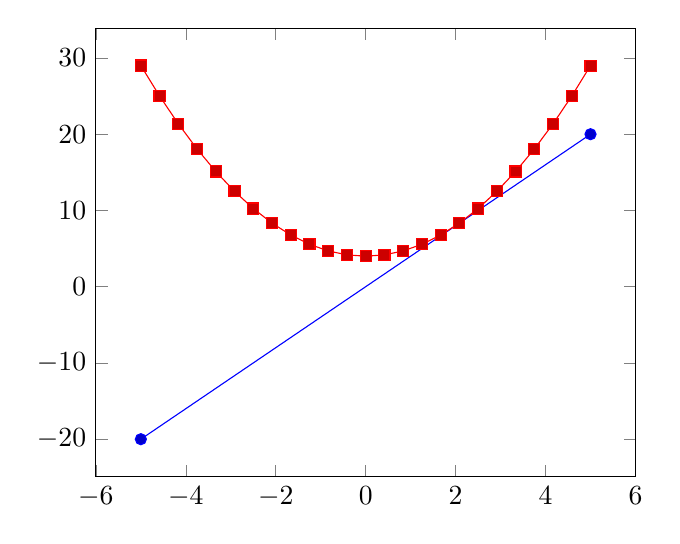
\begin{tikzpicture}
\begin{axis}[
    declare function={
        C=4;
        square(\t)=(\t)^2 + C;
    },
]
    \addplot+ [samples=2] {C*x};

    \addplot {square(x)};
\end{axis}
\end{tikzpicture}
\end{codeexample}
    %
    The definitions as such have the form \meta{function}\meta{argument list} =
    \meta{definition} where the \meta{argument list} contains a
    comma-separated-list of arguments like |\t| or |\t,\a,\b|. The
    \meta{definition} is a math expression which makes use of these arguments.

    Please refer to \cite{tikz} for more details.
\end{key}

\begin{command}{\pgfplotstableread\marg{file}}
    Please refer to the manual of \PGFPlotstable{}, |pgfplotstable.pdf|, which
    is part of the \PGFPlots{} bundle.
\end{command}

\begin{command}{\pgfplotstabletypeset\marg{\textbackslash macro}}
    Please refer to the manual of \PGFPlotstable{}, |pgfplotstable.pdf|, which
    is part of the \PGFPlots{} bundle.
\end{command}

\begin{command}{\pgfplotsiffileexists\marg{filename}\marg{true code}\marg{false code}}
    Invokes \meta{true code} if \meta{filename} exists and \meta{false code} if
    not. Can be used in looping macros, for example to plot every data file
    until there are no more of them.
\end{command}

\begin{command}{\pgfplotsutilifstringequal\marg{first}\marg{second}\marg{true code}\marg{false code}}
    A simple ``strcmp'' tool which invokes \meta{true code} if \meta{first}
    $=$\meta{second} and \meta{false code} otherwise. This does not expand
    macros.
\end{command}

\begin{commandlist}{\pgfkeys,\pgfeov,\pgfkeysvalueof,\pgfkeysgetvalue}
    These commands are part of the \Tikz{} way of specifying options, its
    sub-package |pgfkeys|. The |\pgfplotsset| command is actually nothing but a
    wrapper around |\pgfkeys|.

    A short introduction into |\pgfkeys| can be found in~\cite{keyvalintro}
    whereas the complete reference is, of course, the \Tikz{}
    manual~\cite{tikz}.

    The key |\pgfkeysvalueof|\marg{key name} expands to the value of a key;
    |\pgfkeysgetvalue|\marg{key name}\marg{\textbackslash macro} stores the
    value of \meta{key name} into \meta{\textbackslash macro}. The |\pgfeov|
    macro is used to delimit arguments for code keys in |\pgfkeys|, please
    refer to the references mentioned above.
\end{commandlist}


\section[Commands Inside Of PGFPlots Axes]
        {Commands Inside Of {\normalfont\PGFPlots{}} Axes}

\begin{command}{\autoplotspeclist}
    This command should no longer be used, although it will be kept as
    technical implementation detail. Please use the `|cycle list|' option,
    Section~\ref{sec:cycle:list}.
\end{command}

\begin{command}{\logten}
    Expands to the constant $\log(10)$. Useful for log plots because $\log(10^i)
    = i\log(10)$. This command is only available inside of a \Tikz{} picture.
\end{command}

\begin{command}{\pgfmathprintnumber\marg{number}}
    Generates pretty-printed output\footnote{This method was previously
    \texttt{\textbackslash prettyprintnumber}. Its functionality has been
    included into \PGF{} and the old command is now deprecated.} for
    \meta{number}. This method is used for every tick label.

    The number is printed using the current number printing options, see the
    manual of \PGFPlotstable{} which comes with this package for the different
    number styles, rounding precision and rounding methods.
\end{command}

\begin{command}{\numplots}
    Inside of any of the axis environments, associated style, option or
    command, |\numplots| expands to the total number of plots.
\end{command}

\begin{command}{\numplotsofactualtype}
    Like |\numplots|, this macro returns the total number of plots which have
    the same plot handler. Thus, if you have |sharp plot| active, it returns
    the number of all |sharp plots|. If you have |ybar| active, it returns the
    number of |ybar| plots and so on.
\end{command}

\begin{command}{\plotnum}
    Inside of |\addplot| or any associated style, option or command, |\plotnum|
    expands to the current plot's number, starting with~$0$.
\end{command}

\begin{command}{\plotnumofactualtype}
    Like |\plotnum|, but it returns the number among all plots of the same
    type. The number of all such plots is available using
    |\numplotsofactualtype|.
\end{command}

\begin{command}{\coordindex}
    Inside of an |\addplot| command, this macro expands to the number of the
    actual coordinate (starting with~$0$).

    It is useful together with |x filter| or |y filter| to (de)select
    coordinates.
\end{command}


\section{Path Operations}

\begin{commandlist}{\path,\draw,\fill,\node,\matrix}
    These commands are \Tikz{} drawing commands all of which are documented
    in~\cite{tikz}. They are used to draw or fill paths, generate text nodes or
    aligned text matrices. They are equivalent to
    \pgfmanualpdflabel{/tikz/draw}{}|\path[draw]|,
    \pgfmanualpdflabel{/tikz/fill}{}|\path[fill]|,
    \pgfmanualpdflabel{/tikz/node}{}|\path[node]|,
    \pgfmanualpdflabel{/tikz/matrix}{}|\path[matrix]|,
    respectively.
\end{commandlist}

\begin{pathoperation}{--}{\meta{coordinate}}
    A \Tikz{} path operation which connects the current point (the last one
    before |--|) and \meta{coordinate} with a straight line.
\end{pathoperation}

{\catcode`\|=12
\begin{pathoperation}[noindex]{|-}{\meta{coordinate}}
\pgfmanualpdflabel[\catcode`\|=12 ]{|-}{}%
    A \Tikz{} path operation which connects the current point and
    \meta{coordinate} with \emph{two} straight lines: first vertical, then
    horizontal.
\end{pathoperation}

\begin{pathoperation}[noindex]{-|}{\meta{coordinate}}
\pgfmanualpdflabel[\catcode`\|=12 ]{-|}{}%
    A \Tikz{} path operation which connects the current point and
    \meta{coordinate} with \emph{two} straight lines: first horizontal, then
    vertical.
\end{pathoperation}
}

\begin{keylist}{/tikz/xshift=\marg{dimension},/tikz/yshift=\marg{dimension}}
    These \Tikz{} keys allow to shift something by \meta{dimension} which is
    any \TeX{} size (or expression).
\end{keylist}

\begin{command}{\pgfplotsextra\marg{low-level path commands}}
    A command to execute \meta{low-level path commands} in a \PGFPlots{} axis.
    Since any drawing commands inside of an axis need to be postponed until the
    axis is complete and the scaling has been initialised, it is not possible
    to simply draw any paths. Instead, it is necessary to draw them as soon as
    the axis is finished. This is done automatically for every \Tikz{} path --
    and it is also done manually if you write |\pgfplotsextra|\marg{commands}.
    %
\begin{codeexample}[]
\begin{tikzpicture}
\begin{axis}[xmin=0,xmax=3,ymin=0,ymax=5]
    \pgfplotsextra{
        \pgfpathmoveto{\pgfplotspointaxisxy{1}{2}}
        \pgfpathlineto{\pgfplotspointaxisxy{2}{4}}
        \pgfusepath{stroke}
    }
\end{axis}
\end{tikzpicture}
\end{codeexample}
    %
    The example above initializes an axis and executes the basic level path
    commands as soon as the axis is ready. The execution of multiple |\path|,
    |\addplot| and |\pgfplotsextra| commands is in the same sequence as they
    occur in the environment.\footnote{Except for stacked plots where the
    sequence may be reverse, see the key \texttt{reverse stack plots}.}
\end{command}

\begin{command}{\pgfplotspathaxisoutline}
    Generates a path which resembles the outline of the current axis. This path
    is used for clip paths and the background paths (if any).
\end{command}


\section{Specifying Basic Coordinates}
\label{sec:basic:coordinates}

\begin{commandlist}{%
    \pgfplotspointaxisxy\marg{x coordinate}\marg{y coordinate},
    \pgfplotspointaxisxyz\marg{x coordinate}\marg{y coordinate}\marg{z coordinate}%
}
    Point commands like |\pgfpointxy| which take logical, absolute coordinates
    and return a low-level point. Every transformation from user
    transformations to logarithms is applied.

    Since the transformations are initialized after the axis is complete, this
    command needs to be postponed (see |\pgfplotsextra|).

    This command is the basic level variant of |axis cs:|\meta{x
    coordinate}|,|\meta{y coordinate}|,|\meta{z coordinate}.

    Note that this is also the default coordinate system during the
    visualization phase; in other words: if you write |\draw (1,2) -- (1,4)|,
    \PGFPlots{} will automatically use |(axis cs:1,2) -- (axis cs:1,4)|.
\end{commandlist}

\begin{commandlist}{%
    \pgfplotspointaxisdirectionxy\marg{x coordinate}\marg{y coordinate},
    \pgfplotspointaxisdirectionxyz\marg{x coordinate}\marg{y coordinate}\marg{z coordinate}%
}
    Point commands like |\pgfpointxy| which take logical, \emph{relative}
    coordinates and return a low-level point. Every transformation from user
    transformations to logarithms is applied. The difference to
    |\pgfplotspointaxisxy| is that the shift of the linear transformation is
    skipped here (compare |disabledatascaling|).

    This command is the basic level variant of |axis direction cs:|\meta{x
    coordinate}|,|\meta{y coordinate}|,|\meta{z coordinate}. Please refer to
    the documentation of |axis direction cs| for more details.

    Use this command whenever something of \emph{relative} character like
    directions or lengths need to be supplied. One use case is to draw
    ellipses:
    %
\begin{codeexample}[]
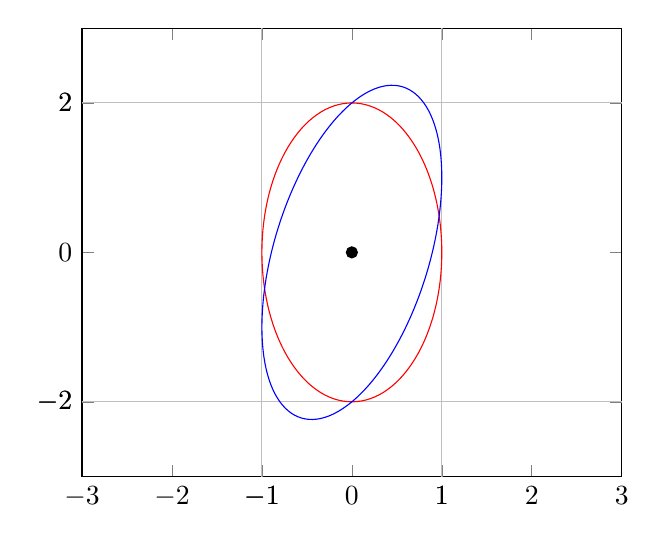
\begin{tikzpicture}
\begin{axis}[
    xmin=-3,   xmax=3,
    ymin=-3,   ymax=3,
    extra x ticks={-1,1},
    extra y ticks={-2,2},
    extra tick style={grid=major},
]
    \draw [red] \pgfextra{
        \pgfpathellipse{\pgfplotspointaxisxy{0}{0}}
            {\pgfplotspointaxisdirectionxy{1}{0}}
            {\pgfplotspointaxisdirectionxy{0}{2}}
    % see also the documentation of
    % 'axis direction cs' which
    % allows a simpler way to draw this ellipse
    };
    \draw [blue] \pgfextra{
        \pgfpathellipse{\pgfplotspointaxisxy{0}{0}}
            {\pgfplotspointaxisdirectionxy{1}{1}}
            {\pgfplotspointaxisdirectionxy{0}{2}}
    };
    \addplot [only marks,mark=*] coordinates
        { (0,0) };
\end{axis}
\end{tikzpicture}
\end{codeexample}

    Since the transformations are initialized after the axis is complete, this
    command needs to be provided either inside of a \tikzname{} |\path| command
    (like |\draw| in the example above) or inside of |\pgfplotsextra|.
\end{commandlist}

\begin{commandlist}{%
    \pgfplotspointrelaxisxy\marg{rel x coordinate}\marg{rel y coordinate},
    \pgfplotspointrelaxisxyz\marg{rel x coordinate}\marg{rel y coordinate}\marg{rel z coordinate}%
}
    Point commands which take \emph{relative} coordinates such that $x=0$ is
    the \emph{lower} $x$-axis limit and $x=1$ the \emph{upper} $x$-axis limit.

    These commands are used for |rel axis cs|.

    Please note that the transformations are only initialised if the axis is
    complete! This means you need to provide |\pgfplotsextra|.
\end{commandlist}

\begin{commandlist}{%
    \pgfplotspointdescriptionxy\marg{$x$ fraction}\marg{$y$ fraction},
    \pgfplotsqpointdescriptionxy\marg{$x$ fraction}\marg{$y$ fraction}%
}
    Point commands such that |{0}{0}| is the lower left corner of the axis'
    bounding box and |{1}{1}| the upper right one; everything else is in
    between. The `|q|' variant is quicker as it doesn't invoke the math parser
    on its arguments.

    They are used for |axis description cs|, see
    Section~\ref{pgfplots:sec:axis:description:cs}.
\end{commandlist}

\begin{commandlist}{\pgfplotspointaxisorigin}
    A point coordinate at the origin, $(0,0,0)$. If the origin is not part of
    the axis limits, the nearest point on the boundary is returned instead.

    This is the same coordinate as returned by the |origin| anchor.
\end{commandlist}

\begin{commandlist}{%
    \pgfplotstransformcoordinatex\marg{x coordinate of an axis},
    \pgfplotstransformcoordinatey\marg{y coordinate of an axis},
    \pgfplotstransformcoordinatez\marg{z coordinate of an axis}%
}
    Defines |\pgfmathresult| to be the low-level \PGF{} coordinate
    corresponding to the input argument.

    The command applies any |[xyz] coord trafo| keys, data scalings and/or
    logarithms or whatever \PGFPlots{} does to map input coordinates to
    internal coordinates.

    The result can be used inside of a |\pgfpointxy| statement (i.e.\@ it still
    needs to be scaled with the respective \PGF{} unit vector).
    %
\begin{codeexample}[]
\begin{tikzpicture}
\pgfplotsset{compat/pgfpoint substitution=1.3}
\begin{axis}[xmin=0,xmax=2,ymin=0,ymax=5]
    \pgfplotsextra{
        \pgfplotstransformcoordinatex{1}
        \let\xcoord=\pgfmathresult
        \pgfplotstransformcoordinatey{1}
        \let\ycoord=\pgfmathresult
        \pgfpathcircle
            {\pgfqpointxy{\xcoord}{\ycoord}}
            {5pt}
        \pgfusepath{fill}
    }
\end{axis}
\end{tikzpicture}
\end{codeexample}
    %
    Note that \PGFPlots{} substitutes |\pgfqpointxy| by |\pgfplotspointaxisxyz|
    by default -- and this command implicitly transforms coordinates anyway. In
    order to see the difference, the preceding example first disables this
    automatic substitution of coordinate systems by means of
    |compat/pgfpoint substitution=1.3|.
    %
    The result of this command is also available as math method
    |transformcoordinatex| (see the documentation for |axis cs|).

    Please note that the transformations are only initialised if the axis is
    complete. This means you need to provide |\pgfplotsextra| as is shown in
    the example above.
\end{commandlist}

\begin{commandlist}{%
    \pgfplotstransformdirectionx\marg{x direction of an axis},
    \pgfplotstransformdirectiony\marg{y direction of an axis},
    \pgfplotstransformdirectionz\marg{z direction of an axis}%
}
    Defines |\pgfmathresult| to be a low-level \PGF{} \emph{direction vector
    component}.

    A direction vector needs to be \emph{added} to some coordinate in order to
    get a coordinate, compare the documentation for
    |\pgfplotspointaxisdirectionxy| and |axis direction cs|.

    The argument \meta{x direction of an axis} is processed in (almost) the
    same way as for the macro which operates on absolute positions,
    |\pgfplotstransformcoordinatex|. The only difference is that
    \emph{directions} need no shifting transformation.

    The result of this command is also available as math method
    |transformdirectionx| (see the documentation for |axis direction cs|).

    See |axis direction cs| for details and examples about this command.
\end{commandlist}

% this command is for internal use only:
%--------------------------------------------------
% \begin{command}{\pgfplotsconvertunittocoordinate\marg{x, y or z}\marg{dimension}}
%     Converts a dimension (with unit!) to a corresponding $x$-, $y$- or $z$-coordinate. The result will be written to |\pgfmathresult| (without units).
%
%     It is possible to use the result as arguments for the |\pgfpointxyz| commands.
%
%     The effect is to multiply \meta{dimension} with the inverse length of the unit vector for the specified axis. These lengths are precomputed in \PGFPlots{} so the operation is fast.
% \begin{codeexample}[code only]
% \pgfplotsconvertunittocoordinate{x}{5pt}
% % now, the command uses exactly 5pt in x direction:
% \pgfqpointxyz{\pgfmathresult}{4}{3}
% \end{codeexample}
% \end{command}
%--------------------------------------------------

\begin{commandlist}{%
    \pgfplotspointunitx,
    \pgfplotspointunity,
    \pgfplotspointunitz%
}
    Low-level point commands which return the canvas $x$, $y$ or $z$ unit
    vectors.

    The |\pgfplotspointunitx| is the \pgfname{} unit vector in $x$ direction.

    These vectors are essentially the same as |\pgfqpointxyz{1}{0}{0}|,
    |\pgfqpointxyz{0}{1}{0}|, and |\pgfqpointxyz{0}{0}{1}|, respectively.

    The unit $z$ vector is only defined for three dimensional axes.
\end{commandlist}

\begin{commandlist}{%
    \pgfplotsunitxlength,
    \pgfplotsunitylength,
    \pgfplotsunitzlength,
    \pgfplotsunitxinvlength,
    \pgfplotsunityinvlength,
    \pgfplotsunitzinvlength%
}
    Macros which expand to the vector length $\lVert x_i \rVert$ of the
    respective unit vector $x_i$ or the inverse vector length, $1/\lVert x_i
    \rVert$. These macros can be used inside of |\pgfmathparse|, for example.

    The $x_i$ are the |\pgfplotspointunitx| variants.
\end{commandlist}

\begin{command}{\pgfplotsqpointoutsideofaxis%
        \marg{three-char-string}\marg{coordinate}\marg{normal distance}%
}
    Provides a point coordinate on one of the available four axes in case of a
    two dimensional figure or on one of the available twelve axes in case of a
    three dimensional figure.

    The desired axis is uniquely identified by a three character string,
    provided as first argument to the command. The first of the three
    characters is `|0|' if the $x$-coordinate of the specified axis passes
    through the lower axis limit. It is `|1|', if the $x$-coordinate of the
    specified axis passes through the upper axis limit. Furthermore, it is
    `|2|' if it passes through the origin. The second character is also either
    |0|, |1| or |2| and it characterizes the position on the $y$-axis. The
    third character is for the third dimension, the $z$-axis. It should be left
    at `|0|' for two dimensional plots. However, \emph{one} of the three
    characters should be `|v|', meaning the axis \underline varies. For
    example, |v01| denotes $\{ (x,y_{\min},z_{\max}) \vert x \in \R \}$.

    The second argument, \meta{coordinate} is the logical coordinate on that
    axis. Since two coordinates of the axis are fixed, \meta{coordinate} refers
    to the \underline varying component of the axis. It must be a number
    without unit; no math expressions are supported here.

    The third argument \meta{normal distance} is a dimension like |10pt|. It
    shifts the coordinate away from the designated axis in direction of the
    outer normal vector. The outer normal vector always points away from the
    axis. It is computed using |\pgfplotspointouternormalvectorofaxis|.

    There are several variants of this command which are documented in the
    source code. One of them is particularly useful:
\end{command}

\begin{command}{\pgfplotsqpointoutsideofaxisrel%
        \marg{three-char-string}\marg{axis fraction}\marg{normal distance}%
}
    This point coordinate is a variant of |\pgfplotsqpointoutsideofaxis| which
    allows to provide an \meta{axis fraction} instead of an absolute
    coordinate. The fraction is a number between $0$ (lower axis limit) and $1$
    (upper axis limit), i.e.\@ it is given in percent of the total axis. It is
    possible to provide negative values or values larger than one.

    The |\pgfplotsqpointoutsideofaxisrel| command is similar in spirit to
    |rel axis cs|.

    There is one speciality in conjunction with reversed axes: if the axis has
    been reversed by |x dir=reverse| and, in addition,
    |allow reversal of rel axis cs| is true, the value $0$ denotes the
    \emph{upper} limit while $1$ denotes the \emph{lower} limit. The effect is
    that coordinates won't change just because of axis reversal.
        \index{allow reversal of rel axis cs}%
\end{command}

\begin{command}{\pgfplotspointouternormalvectorofaxis\marg{three-char-string}}
    A point command which yields the outer normal vector of the respective
    axis. The normal vector has length $1$ (computed with
    |\pgfpointnormalised|). It is the same normal vector used inside of
    |\pgfplotsqpointoutsideofaxis| and its variants.

    The output of this command will be cached and reused during the lifetime
    of an axis.
\end{command}

\begin{command}{\pgfplotsticklabelaxisspec\marg{x, y or z}}
    Expands to the three character identification for the axis containing tick
    labels for the chosen axis, either \meta{x}, \meta{y} or \meta{z}.
\end{command}

\begin{command}{\pgfplotsvalueoflargesttickdimen\marg{x, y or z}}
    Expands to the largest distance of a tick position to its tick label
    bounding box in direction of the outer unit normal vector. It does also
    include the value of the |ticklabel shift| key.

    This value is used for |ticklabel cs|.
\end{command}

\begin{commandlist}{
    \pgfplotsmathfloatviewdepthxyz\marg{x}\marg{y}\marg{z},
    \pgfplotsmathviewdepthxyz\marg{x}\marg{y}\marg{z}%
}
    Both macros define |\pgfmathresult| to be the ``depth'' of a three
    dimensional point $\bar x = (x,y,z)$. The depth is defined to be the scalar
    product of $\bar x$ with $\vec d$, the view direction of the current axis.

    For |\pgfplotsmathfloatviewdepthxyz|, the arguments are parsed as floating
    point numbers and the result is encoded in floating point. A fixed point
    representation can be generated with
    |\pgfmathfloattofixed{\pgfmathresult}|.

    For |\pgfplotsmathviewdepthxyz|, \TeX{} arithmetics is employed for the
    inner product and the result is assigned in fixed point. This is slightly
    faster, but has considerably smaller data range.

    Both commands can only be used \emph{inside} of a three dimensional
    \PGFPlots{} axis (as soon as the axis is initialised, see
    |\pgfplotsextra|).
\end{commandlist}

\begin{texif}{pgfplotsthreedim}
    A \TeX{} |\if| which evaluates the \meta{true code} if the axis is three
    dimensional and the \meta{else code} if not.
\end{texif}


\section{Accessing Axis Limits}

It is also possible to access axis limits during the visualization phase,
i.e.\@ during |\end{axis}|. Please refer to the reference documentation for
|xmin| on page~\pageref{page:access:limits}.


\section{Accessing Point Coordinate Values}

During the visualization phase, \PGFPlots{} provides access to the currently
processed coordinate and its values.

This access requires a call to specific macros. These macros write the
coordinate values to some publicly available key--value pairs. Then, the
current point's $x$, $y$, $z$, and color data can be accessed.

\begin{commandlist}{\pgfplotspointgetcoordinates,\pgfplotspointgetcoordinates\marg{point}}

    After invoking the macro, the following keys will be set:

    \declaretext{/data point/x} will contain the current point's $x$-coordinate.

    \declaretext{/data point/y} will contain the current point's $y$-coordinate.

    \declaretext{/data point/z} will contain the current point's $z$-coordinate
    (if applicable).

    \declaretext{/data point/meta} will contain the current point's
    |point meta| value (if applicable).

    \declaretext{/data point/index} will contain the current point's index in
    the coordinate stream. This is actually the same as |\coordindex|.

    This command actually supports two modes of operation:
    %
    \begin{enumerate}
        \item Without arguments. In this case, it returns values of the point
            which is about to be processed by the current plot handler.
        \item With an argument in curly braces. In this case, it expects a
            coordinate and assigns the keys accordingly. Note that this
            command merely supports two-dimensional axes and assigns only
            |/data point/x| and |/data point/y|.
    \end{enumerate}

    The returned values are the same as they can be read on the axes, they are
    also the same as you would write them into |axis cs|.

    This means that any |x coord inv trafo| has been applied on the value. It
    also means that the exponential function has been called even though the
    internal coordinate was present in log format.

    This function is implicitly called for any |scatter| plot (including
    |nodes near coords|). This allows to access \emph{all} coordinate values at
    once:
    %
\begin{codeexample}[]
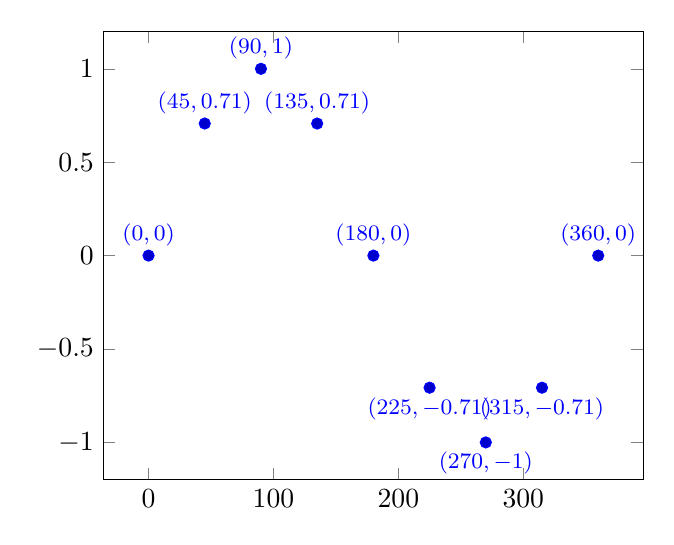
\begin{tikzpicture}
\begin{axis}
    \addplot+ [
        domain=0:360,
        samples=9,
        only marks,
        nodes near coords={%
            \footnotesize
            $(\pgfmathprintnumber
                {\pgfkeysvalueof{/data point/x}},
               \pgfmathprintnumber
                {\pgfkeysvalueof{/data point/y}})$%
        },
    ] {sin(x)};
\end{axis}
\end{tikzpicture}
\end{codeexample}
    %
    The example works because |\pgfplotspointgetcoordinates| is part of the
    standard implementation of |nodes near coords|; the resulting values are
    directly available. Note that the preceding example would have been simpler
    if we would have printed just one value: |nodes near coords| resorts to the
    |point meta|. And that, in turn, contains the $y$-coordinate anyway by
    default.

    A more advanced example would be a |ybar| plot in which nodes shall be
    placed at the lower end of the axis, together with some dotted lines to the
    respective bars:
    %
\begin{codeexample}[]
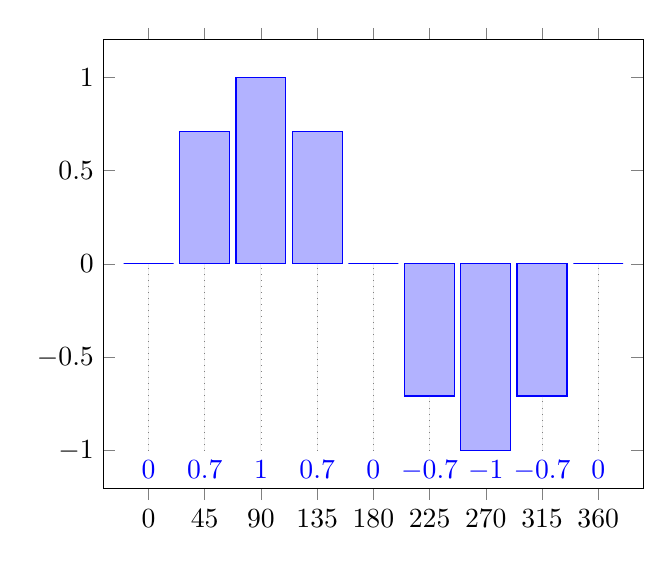
\begin{tikzpicture}
\begin{axis}[
    ybar,
    nodes near coords,
    %
    % we want to provide absolute 'at' values
    % for the nodes:
    scatter/position=absolute,
    every node near coord/.style={
        at={(\pgfkeysvalueof{/data point/x},-1)},
        % pretty printing:
        anchor=north,
        /pgf/number format/fixed,
        /pgf/number format/precision=1,
        % assign a name which can be referenced below:
        name=NNC\pgfkeysvalueof{/data point/index},
    },
    % ... draw a dotted line between
    % the marker and the bar:
    /pgfplots/scatter/@post marker code/.add code={}{
        \draw [dotted,help lines]
            (NNC\pgfkeysvalueof{/data point/index})
            -- (\pgfkeysvalueof{/data point/x},
            {min(0,\pgfkeysvalueof{/data point/y})});
    },
    % assign suitable tick labels:
    xtick=data,
]
    % some dummy data:
    \addplot+ [
        domain=0:360,
        bar width=360/9,
        samples=9,
    ] {sin(x)};
\end{axis}
\end{tikzpicture}
\end{codeexample}
    %
    Again, the command is used implicitly as part of |nodes near coords| and
    does not occur in the example as such.

    \paragraph{See also} the related example online under
    \url{https://tex.stackexchange.com/a/141006}. It demonstrates how to
    place the nodes generated by |nodes near coords| based on the value (either
    inside of a bar or above it).

    The following example uses an argument in curly braces for which we seek
    coordinate values:
    %
\begin{codeexample}[]
% requires \usetikzlibrary{intersections}
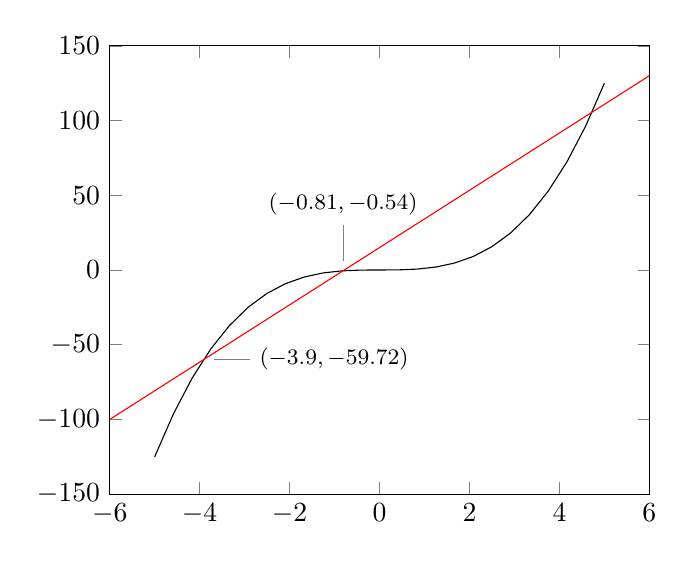
\begin{tikzpicture}
\begin{axis}
    \addplot [name path=A] {x^3};

    \draw [red,name path=HelperLine]
        (axis cs:-6,-100) -- (axis cs:6,130);

    \draw [
        font=\footnotesize,
        name intersections={of=A and HelperLine},
    ]
    node [pin={right:
      \pgfplotspointgetcoordinates{(intersection-1)}
        $(\pgfmathprintnumber[fixed]{
            \pgfkeysvalueof{/data point/x}},
          \pgfmathprintnumber[fixed]{
            \pgfkeysvalueof{/data point/y}})$
      }
    ] at (intersection-1) {}
    node [pin={
      \pgfplotspointgetcoordinates{(intersection-2)}
        $(\pgfmathprintnumber[fixed]{
            \pgfkeysvalueof{/data point/x}},
          \pgfmathprintnumber[fixed]{
            \pgfkeysvalueof{/data point/y}})$
      }
    ] at (intersection-2) {};
\end{axis}
\end{tikzpicture}
\end{codeexample}
    %
    The example computes and names intersections of |A| and |HelperLine|. The
    following code generates pins at the intersections. To this end, it uses
    |\pgfplotspointgetcoordinates|\marg{point} which defines |/data point/x|
    and |/data point/y|. These values are then formatted using
    |\pgfmathprintnumber|.

    In its second mode, |\pgfplotspointgetcoordinates|\marg{point} expects one
    of two things as \meta{point}:
    %
    \begin{enumerate}
        \item a basic-level \PGF{} point like |\pgfpointanchor{A}{center}| or
        \item a \Tikz{} point like |(A.base)| or |(3,5)|.
    \end{enumerate}
\end{commandlist}

\begin{command}{\pgfplotspointgetnormalizedcoordinates}
    A macro which is very similar to |\pgfplotspointgetcoordinates|.
    Consequently, it is also supposed to be called during the visualization phase.

    It assigns the very same output macros, but the values are different. More
    precisely, it defines the macros

    \declaretext{/data point/x} will contain the current point's
    \emph{normalized} $x$-coordinate.

    \declaretext{/data point/y} will contain the current point's
    \emph{normalized} $y$-coordinate.

    \declaretext{/data point/z} will contain the current point's
    \emph{normalized} $z$-coordinate (if applicable).

    \declaretext{/data point/meta} will contain the current point's
    |point meta| value (if applicable).

    \declaretext{/data point/index} will contain the current point's index in
    the coordinate stream. This is actually the same as |\coordindex|.

    The keyword \declaretext{normalized} means that the values are in a
    suitable numerical form which can be consumed by the axis. To be more
    specific: any user |x coord inv trafo| is \emph{ignored}. An important
    example would be |symbolic x coords|: the normalized coordinates would be
    some associated numbers, not the symbols. The results returned by
    |\pgfplotspointgetcoordinates| would be the symbols. For logarithm axes,
    the normalized values are the logs.

    Typically, normalized values are much more useful when you want to apply
    some math operation like averaging or subtraction.

    This function needs to be called explicitly. It is currently used by
    |ybar stacked| to align |nodes near coords|.
\end{command}


\section{Layer Access}

\begin{command}{\pgfplotsonlayer\marg{layer name}}
    A low-level command which will check if the current axis has layer support
    activated and, if so, calls |\pgfonlayer|\marg{layer name}.

    There must be a |\endpgfplotsonlayer| to delimit the environment.
\end{command}

\begin{command}{\endpgfplotsonlayer}
    The end of |\pgfplotsonlayer|.
\end{command}

\begin{command}{\pgfonlayer\marg{layer name}}
    A low-level command of \PGF{} which will collect everything until the
    matching |\endpgfonlayer| into layer \meta{layer name}.

    The \meta{layer name} must be active, i.e.\@ it must be part of the layer
    names of |set layers|.

    The only special case is if you call |\pgfdeclarelayer{discard}| somewhere:
    this special layer has a ``magical name'' which serves as |/dev/null| if it
    is enabled using |\pgfonlayer{discard}|: it does not need to be active and
    everything assigned to this layer will be thrown away if it is not part of
    the layer name configuration.

    There must be a |\endpgfonlayer| to delimit the environment.
\end{command}

\begin{command}{\endpgfonlayer}
    The end of |\pgfonlayer|.
\end{command}


\begin{command}{\pgfsetlayers\marg{layer list}}
    This is a low-level command of \PGF{}. At the time of this writing, it is
    the only way to tell \PGF{} which layers it shall use for the current/next
    picture. It is used implicitly by |set layers|.
\end{command}


\printindex

\bibliographystyle{abbrv} %gerapali} %gerabbrv} %gerunsrt.bst} %gerabbrv}% gerplain}
\nocite{pgfplotstable}
\nocite{programmingnotes}
\bibliography{pgfplots}
\end{document}

% -----------------------------------------------------------------------------
% For Stefan Pinnow as reminder on what to look for when editing the manual
% -----------------------------------------------------------------------------
% There should be no line breaks in the following environments
% - |...|
% - \declareandlabel{...}
% - \verbpdfref{...}
% If "MakeTikzPictures" isn't running through check one of the externalized
% LOG files what is the cause of that.
% -----------------------------------------------------------------------------


%%%%%%%%%%%%%%%%%%%%%%%%%%%%%%%%%%%%%%%%%%%%%%%%%%%%%%%%%%%%%%%%%%%%%%%%%%%%%
%
% Package pgfplots.sty documentation.
%
% Copyright 2007/2008 by Christian Feuersaenger.
%
% This program is free software: you can redistribute it and/or modify
% it under the terms of the GNU General Public License as published by
% the Free Software Foundation, either version 3 of the License, or
% (at your option) any later version.
%
% This program is distributed in the hope that it will be useful,
% but WITHOUT ANY WARRANTY; without even the implied warranty of
% MERCHANTABILITY or FITNESS FOR A PARTICULAR PURPOSE.  See the
% GNU General Public License for more details.
%
% You should have received a copy of the GNU General Public License
% along with this program.  If not, see <http://www.gnu.org/licenses/>.
%
%
%%%%%%%%%%%%%%%%%%%%%%%%%%%%%%%%%%%%%%%%%%%%%%%%%%%%%%%%%%%%%%%%%%%%%%%%%%%%%
% SEE pgfplots-macros.tex as well!
%\pdfminorversion=5 % to allow compression
%\pdfobjcompresslevel=2
\documentclass[a4paper,openany]{book}

\let\bookmaketitle=\maketitle

% -----------------------------------
% this here is from ltxdoc:
\usepackage{doc}[=v2]
\AtBeginDocument{\MakeShortVerb{\|}}
%\setlength{\textwidth}{355pt}
%\addtolength\marginparwidth{30pt}
%\addtolength\oddsidemargin{20pt}
%\addtolength\evensidemargin{20pt}
\def\cmd#1{\cs{\expandafter\cmd@to@cs\string#1}}
\def\cmd@to@cs#1#2{\char\number`#2\relax}
\DeclareRobustCommand\cs[1]{\texttt{\char`\\#1}}
\providecommand\marg[1]{%
  {\ttfamily\char`\{}\meta{#1}{\ttfamily\char`\}}}
\providecommand\oarg[1]{%
  {\ttfamily[}\meta{#1}{\ttfamily]}}
\providecommand\parg[1]{%
  {\ttfamily(}\meta{#1}{\ttfamily)}}
\raggedbottom

% -----------------------------------
\input{pgfplots.preamble.tex}

\makeatletter
% I want a two-column index just as in pgfmanual styles. This here
% was the best way to get one:
\def\index@prologue{\section*{Index}\addcontentsline{toc}{chapter}{Index}
}
\makeatother

%\RequirePackage[german,english,francais]{babel}

\def\matlabcolormaptext{This colormap is similar to one shipped with Matlab$^\text{\textregistered}$ under a similar name.}

\IfFileExists{tikzlibraryspy.code.tex}{%
\usetikzlibrary{spy}
}{%
    \message{ERROR: tikz SPY library NOT available. The manual will only compile partially.^^J}%
}%

\usepackage{xparse}% for colorbrewer manual

\usetikzlibrary{
    decorations.markings,
    decorations.footprints,
    shapes.arrows,
    matrix,
    positioning,
}

\usepgfplotslibrary{
    fillbetween,
    ternary,
    smithchart,
    patchplots,
    polar,
    colormaps,
    colorbrewer,
    colortol,           % docu not ready yet
}
\pgfqkeys{/codeexample}{%
    every codeexample/.append style={
        /pgfplots/every ternary axis/.append style={
            /pgfplots/legend style={fill=graphicbackground},
        }
    },
    tabsize=4,
}

\pgfplotsmanualenableexternalizationofexpensive

%\usetikzlibrary{external}
%\tikzexternalize[prefix=figures/]{pgfplots}

\title{%
    Manual for Package \PGFPlots{}\\
    {\small 2D/3D Plots in \LaTeX{}, Version \pgfplotsversion}\\
    {\small\href{https://github.com/pgf-tikz/pgfplots}{https://github.com/pgf-tikz/pgfplots}}
    %\\{\small Attention: you are using an unstable development version.}
}

\makeatletter
\long\def\abstractsmuggle{%
    \centering
    \textbf{Abstract}\\[0.5cm]

    \begin{minipage}{12cm}
        \PGFPlots{} draws high-quality function plots in normal or logarithmic
        scaling with a user-friendly interface directly in \TeX{}. The user
        supplies axis labels, legend entries and the plot coordinates for one or
        more plots and \PGFPlots{} applies axis scaling, computes any logarithms
        and axis ticks and draws the plots. It supports line plots, scatter
        plots, piecewise constant plots, bar plots, area plots, mesh and surface
        plots, patch plots, contour plots, quiver plots, histogram plots, box
        plots, polar axes, ternary diagrams, smith charts and some more. It is
        based on Till Tantau's package \PGF{}/\Tikz{}.
    \end{minipage}

}%

\expandafter\date\expandafter{\@date\\[2cm]
    \abstractsmuggle
}%
\makeatother

%\includeonly{pgfplots.reference}


\begin{document}

\def\plotcoords{%
\addplot coordinates {
(5,8.312e-02)    (17,2.547e-02)   (49,7.407e-03)
(129,2.102e-03)  (321,5.874e-04)  (769,1.623e-04)
(1793,4.442e-05) (4097,1.207e-05) (9217,3.261e-06)
};

\addplot coordinates{
(7,8.472e-02)    (31,3.044e-02)    (111,1.022e-02)
(351,3.303e-03)  (1023,1.039e-03)  (2815,3.196e-04)
(7423,9.658e-05) (18943,2.873e-05) (47103,8.437e-06)
};

\addplot coordinates{
(9,7.881e-02)     (49,3.243e-02)    (209,1.232e-02)
(769,4.454e-03)   (2561,1.551e-03)  (7937,5.236e-04)
(23297,1.723e-04) (65537,5.545e-05) (178177,1.751e-05)
};

\addplot coordinates{
(11,6.887e-02)    (71,3.177e-02)     (351,1.341e-02)
(1471,5.334e-03)  (5503,2.027e-03)   (18943,7.415e-04)
(61183,2.628e-04) (187903,9.063e-05) (553983,3.053e-05)
};

\addplot coordinates{
(13,5.755e-02)     (97,2.925e-02)     (545,1.351e-02)
(2561,5.842e-03)   (10625,2.397e-03)  (40193,9.414e-04)
(141569,3.564e-04) (471041,1.308e-04)
(1496065,4.670e-05)
};
}%


\bookmaketitle
\tableofcontents

%%%%%%%%%%%%%%%%%%%%%%%%%%%%%%%%%%%%%%%%%%%%%%%%%%%%%%%%%%%%%%%%%%%%%%%%%%%%%
%
% Package pgfplots.sty documentation.
%
% Copyright 2007/2008 by Christian Feuersaenger.
%
% This program is free software: you can redistribute it and/or modify
% it under the terms of the GNU General Public License as published by
% the Free Software Foundation, either version 3 of the License, or
% (at your option) any later version.
%
% This program is distributed in the hope that it will be useful,
% but WITHOUT ANY WARRANTY; without even the implied warranty of
% MERCHANTABILITY or FITNESS FOR A PARTICULAR PURPOSE.  See the
% GNU General Public License for more details.
%
% You should have received a copy of the GNU General Public License
% along with this program.  If not, see <http://www.gnu.org/licenses/>.
%
%
%%%%%%%%%%%%%%%%%%%%%%%%%%%%%%%%%%%%%%%%%%%%%%%%%%%%%%%%%%%%%%%%%%%%%%%%%%%%%
% SEE pgfplots-macros.tex as well!
%\pdfminorversion=5 % to allow compression
%\pdfobjcompresslevel=2
\documentclass[a4paper,openany]{book}

\let\bookmaketitle=\maketitle

% -----------------------------------
% this here is from ltxdoc:
\usepackage{doc}[=v2]
\AtBeginDocument{\MakeShortVerb{\|}}
%\setlength{\textwidth}{355pt}
%\addtolength\marginparwidth{30pt}
%\addtolength\oddsidemargin{20pt}
%\addtolength\evensidemargin{20pt}
\def\cmd#1{\cs{\expandafter\cmd@to@cs\string#1}}
\def\cmd@to@cs#1#2{\char\number`#2\relax}
\DeclareRobustCommand\cs[1]{\texttt{\char`\\#1}}
\providecommand\marg[1]{%
  {\ttfamily\char`\{}\meta{#1}{\ttfamily\char`\}}}
\providecommand\oarg[1]{%
  {\ttfamily[}\meta{#1}{\ttfamily]}}
\providecommand\parg[1]{%
  {\ttfamily(}\meta{#1}{\ttfamily)}}
\raggedbottom

% -----------------------------------
\input{pgfplots.preamble.tex}

\makeatletter
% I want a two-column index just as in pgfmanual styles. This here
% was the best way to get one:
\def\index@prologue{\section*{Index}\addcontentsline{toc}{chapter}{Index}
}
\makeatother

%\RequirePackage[german,english,francais]{babel}

\def\matlabcolormaptext{This colormap is similar to one shipped with Matlab$^\text{\textregistered}$ under a similar name.}

\IfFileExists{tikzlibraryspy.code.tex}{%
\usetikzlibrary{spy}
}{%
    \message{ERROR: tikz SPY library NOT available. The manual will only compile partially.^^J}%
}%

\usepackage{xparse}% for colorbrewer manual

\usetikzlibrary{
    decorations.markings,
    decorations.footprints,
    shapes.arrows,
    matrix,
    positioning,
}

\usepgfplotslibrary{
    fillbetween,
    ternary,
    smithchart,
    patchplots,
    polar,
    colormaps,
    colorbrewer,
    colortol,           % docu not ready yet
}
\pgfqkeys{/codeexample}{%
    every codeexample/.append style={
        /pgfplots/every ternary axis/.append style={
            /pgfplots/legend style={fill=graphicbackground},
        }
    },
    tabsize=4,
}

\pgfplotsmanualenableexternalizationofexpensive

%\usetikzlibrary{external}
%\tikzexternalize[prefix=figures/]{pgfplots}

\title{%
    Manual for Package \PGFPlots{}\\
    {\small 2D/3D Plots in \LaTeX{}, Version \pgfplotsversion}\\
    {\small\href{https://github.com/pgf-tikz/pgfplots}{https://github.com/pgf-tikz/pgfplots}}
    %\\{\small Attention: you are using an unstable development version.}
}

\makeatletter
\long\def\abstractsmuggle{%
    \centering
    \textbf{Abstract}\\[0.5cm]

    \begin{minipage}{12cm}
        \PGFPlots{} draws high-quality function plots in normal or logarithmic
        scaling with a user-friendly interface directly in \TeX{}. The user
        supplies axis labels, legend entries and the plot coordinates for one or
        more plots and \PGFPlots{} applies axis scaling, computes any logarithms
        and axis ticks and draws the plots. It supports line plots, scatter
        plots, piecewise constant plots, bar plots, area plots, mesh and surface
        plots, patch plots, contour plots, quiver plots, histogram plots, box
        plots, polar axes, ternary diagrams, smith charts and some more. It is
        based on Till Tantau's package \PGF{}/\Tikz{}.
    \end{minipage}

}%

\expandafter\date\expandafter{\@date\\[2cm]
    \abstractsmuggle
}%
\makeatother

%\includeonly{pgfplots.reference}


\begin{document}

\def\plotcoords{%
\addplot coordinates {
(5,8.312e-02)    (17,2.547e-02)   (49,7.407e-03)
(129,2.102e-03)  (321,5.874e-04)  (769,1.623e-04)
(1793,4.442e-05) (4097,1.207e-05) (9217,3.261e-06)
};

\addplot coordinates{
(7,8.472e-02)    (31,3.044e-02)    (111,1.022e-02)
(351,3.303e-03)  (1023,1.039e-03)  (2815,3.196e-04)
(7423,9.658e-05) (18943,2.873e-05) (47103,8.437e-06)
};

\addplot coordinates{
(9,7.881e-02)     (49,3.243e-02)    (209,1.232e-02)
(769,4.454e-03)   (2561,1.551e-03)  (7937,5.236e-04)
(23297,1.723e-04) (65537,5.545e-05) (178177,1.751e-05)
};

\addplot coordinates{
(11,6.887e-02)    (71,3.177e-02)     (351,1.341e-02)
(1471,5.334e-03)  (5503,2.027e-03)   (18943,7.415e-04)
(61183,2.628e-04) (187903,9.063e-05) (553983,3.053e-05)
};

\addplot coordinates{
(13,5.755e-02)     (97,2.925e-02)     (545,1.351e-02)
(2561,5.842e-03)   (10625,2.397e-03)  (40193,9.414e-04)
(141569,3.564e-04) (471041,1.308e-04)
(1496065,4.670e-05)
};
}%


\bookmaketitle
\tableofcontents
\include{pgfplots.title_abstract_intro}
\include{pgfplots.preliminaries}
\include{pgfplots.intro}
\include{pgfplots.reference}
\include{pgfplots.libs}
\include{pgfplots.resources}
\include{pgfplots.importexport}
\include{pgfplots.basic.reference}

\printindex

\bibliographystyle{abbrv} %gerapali} %gerabbrv} %gerunsrt.bst} %gerabbrv}% gerplain}
\nocite{pgfplotstable}
\nocite{programmingnotes}
\bibliography{pgfplots}
\end{document}

% -----------------------------------------------------------------------------
% For Stefan Pinnow as reminder on what to look for when editing the manual
% -----------------------------------------------------------------------------
% There should be no line breaks in the following environments
% - |...|
% - \declareandlabel{...}
% - \verbpdfref{...}
% If "MakeTikzPictures" isn't running through check one of the externalized
% LOG files what is the cause of that.
% -----------------------------------------------------------------------------


%%%%%%%%%%%%%%%%%%%%%%%%%%%%%%%%%%%%%%%%%%%%%%%%%%%%%%%%%%%%%%%%%%%%%%%%%%%%%
%
% Package pgfplots.sty documentation.
%
% Copyright 2007/2008 by Christian Feuersaenger.
%
% This program is free software: you can redistribute it and/or modify
% it under the terms of the GNU General Public License as published by
% the Free Software Foundation, either version 3 of the License, or
% (at your option) any later version.
%
% This program is distributed in the hope that it will be useful,
% but WITHOUT ANY WARRANTY; without even the implied warranty of
% MERCHANTABILITY or FITNESS FOR A PARTICULAR PURPOSE.  See the
% GNU General Public License for more details.
%
% You should have received a copy of the GNU General Public License
% along with this program.  If not, see <http://www.gnu.org/licenses/>.
%
%
%%%%%%%%%%%%%%%%%%%%%%%%%%%%%%%%%%%%%%%%%%%%%%%%%%%%%%%%%%%%%%%%%%%%%%%%%%%%%
% SEE pgfplots-macros.tex as well!
%\pdfminorversion=5 % to allow compression
%\pdfobjcompresslevel=2
\documentclass[a4paper,openany]{book}

\let\bookmaketitle=\maketitle

% -----------------------------------
% this here is from ltxdoc:
\usepackage{doc}[=v2]
\AtBeginDocument{\MakeShortVerb{\|}}
%\setlength{\textwidth}{355pt}
%\addtolength\marginparwidth{30pt}
%\addtolength\oddsidemargin{20pt}
%\addtolength\evensidemargin{20pt}
\def\cmd#1{\cs{\expandafter\cmd@to@cs\string#1}}
\def\cmd@to@cs#1#2{\char\number`#2\relax}
\DeclareRobustCommand\cs[1]{\texttt{\char`\\#1}}
\providecommand\marg[1]{%
  {\ttfamily\char`\{}\meta{#1}{\ttfamily\char`\}}}
\providecommand\oarg[1]{%
  {\ttfamily[}\meta{#1}{\ttfamily]}}
\providecommand\parg[1]{%
  {\ttfamily(}\meta{#1}{\ttfamily)}}
\raggedbottom

% -----------------------------------
\input{pgfplots.preamble.tex}

\makeatletter
% I want a two-column index just as in pgfmanual styles. This here
% was the best way to get one:
\def\index@prologue{\section*{Index}\addcontentsline{toc}{chapter}{Index}
}
\makeatother

%\RequirePackage[german,english,francais]{babel}

\def\matlabcolormaptext{This colormap is similar to one shipped with Matlab$^\text{\textregistered}$ under a similar name.}

\IfFileExists{tikzlibraryspy.code.tex}{%
\usetikzlibrary{spy}
}{%
    \message{ERROR: tikz SPY library NOT available. The manual will only compile partially.^^J}%
}%

\usepackage{xparse}% for colorbrewer manual

\usetikzlibrary{
    decorations.markings,
    decorations.footprints,
    shapes.arrows,
    matrix,
    positioning,
}

\usepgfplotslibrary{
    fillbetween,
    ternary,
    smithchart,
    patchplots,
    polar,
    colormaps,
    colorbrewer,
    colortol,           % docu not ready yet
}
\pgfqkeys{/codeexample}{%
    every codeexample/.append style={
        /pgfplots/every ternary axis/.append style={
            /pgfplots/legend style={fill=graphicbackground},
        }
    },
    tabsize=4,
}

\pgfplotsmanualenableexternalizationofexpensive

%\usetikzlibrary{external}
%\tikzexternalize[prefix=figures/]{pgfplots}

\title{%
    Manual for Package \PGFPlots{}\\
    {\small 2D/3D Plots in \LaTeX{}, Version \pgfplotsversion}\\
    {\small\href{https://github.com/pgf-tikz/pgfplots}{https://github.com/pgf-tikz/pgfplots}}
    %\\{\small Attention: you are using an unstable development version.}
}

\makeatletter
\long\def\abstractsmuggle{%
    \centering
    \textbf{Abstract}\\[0.5cm]

    \begin{minipage}{12cm}
        \PGFPlots{} draws high-quality function plots in normal or logarithmic
        scaling with a user-friendly interface directly in \TeX{}. The user
        supplies axis labels, legend entries and the plot coordinates for one or
        more plots and \PGFPlots{} applies axis scaling, computes any logarithms
        and axis ticks and draws the plots. It supports line plots, scatter
        plots, piecewise constant plots, bar plots, area plots, mesh and surface
        plots, patch plots, contour plots, quiver plots, histogram plots, box
        plots, polar axes, ternary diagrams, smith charts and some more. It is
        based on Till Tantau's package \PGF{}/\Tikz{}.
    \end{minipage}

}%

\expandafter\date\expandafter{\@date\\[2cm]
    \abstractsmuggle
}%
\makeatother

%\includeonly{pgfplots.reference}


\begin{document}

\def\plotcoords{%
\addplot coordinates {
(5,8.312e-02)    (17,2.547e-02)   (49,7.407e-03)
(129,2.102e-03)  (321,5.874e-04)  (769,1.623e-04)
(1793,4.442e-05) (4097,1.207e-05) (9217,3.261e-06)
};

\addplot coordinates{
(7,8.472e-02)    (31,3.044e-02)    (111,1.022e-02)
(351,3.303e-03)  (1023,1.039e-03)  (2815,3.196e-04)
(7423,9.658e-05) (18943,2.873e-05) (47103,8.437e-06)
};

\addplot coordinates{
(9,7.881e-02)     (49,3.243e-02)    (209,1.232e-02)
(769,4.454e-03)   (2561,1.551e-03)  (7937,5.236e-04)
(23297,1.723e-04) (65537,5.545e-05) (178177,1.751e-05)
};

\addplot coordinates{
(11,6.887e-02)    (71,3.177e-02)     (351,1.341e-02)
(1471,5.334e-03)  (5503,2.027e-03)   (18943,7.415e-04)
(61183,2.628e-04) (187903,9.063e-05) (553983,3.053e-05)
};

\addplot coordinates{
(13,5.755e-02)     (97,2.925e-02)     (545,1.351e-02)
(2561,5.842e-03)   (10625,2.397e-03)  (40193,9.414e-04)
(141569,3.564e-04) (471041,1.308e-04)
(1496065,4.670e-05)
};
}%


\bookmaketitle
\tableofcontents
\include{pgfplots.title_abstract_intro}
\include{pgfplots.preliminaries}
\include{pgfplots.intro}
\include{pgfplots.reference}
\include{pgfplots.libs}
\include{pgfplots.resources}
\include{pgfplots.importexport}
\include{pgfplots.basic.reference}

\printindex

\bibliographystyle{abbrv} %gerapali} %gerabbrv} %gerunsrt.bst} %gerabbrv}% gerplain}
\nocite{pgfplotstable}
\nocite{programmingnotes}
\bibliography{pgfplots}
\end{document}

% -----------------------------------------------------------------------------
% For Stefan Pinnow as reminder on what to look for when editing the manual
% -----------------------------------------------------------------------------
% There should be no line breaks in the following environments
% - |...|
% - \declareandlabel{...}
% - \verbpdfref{...}
% If "MakeTikzPictures" isn't running through check one of the externalized
% LOG files what is the cause of that.
% -----------------------------------------------------------------------------


%%%%%%%%%%%%%%%%%%%%%%%%%%%%%%%%%%%%%%%%%%%%%%%%%%%%%%%%%%%%%%%%%%%%%%%%%%%%%
%
% Package pgfplots.sty documentation.
%
% Copyright 2007/2008 by Christian Feuersaenger.
%
% This program is free software: you can redistribute it and/or modify
% it under the terms of the GNU General Public License as published by
% the Free Software Foundation, either version 3 of the License, or
% (at your option) any later version.
%
% This program is distributed in the hope that it will be useful,
% but WITHOUT ANY WARRANTY; without even the implied warranty of
% MERCHANTABILITY or FITNESS FOR A PARTICULAR PURPOSE.  See the
% GNU General Public License for more details.
%
% You should have received a copy of the GNU General Public License
% along with this program.  If not, see <http://www.gnu.org/licenses/>.
%
%
%%%%%%%%%%%%%%%%%%%%%%%%%%%%%%%%%%%%%%%%%%%%%%%%%%%%%%%%%%%%%%%%%%%%%%%%%%%%%
% SEE pgfplots-macros.tex as well!
%\pdfminorversion=5 % to allow compression
%\pdfobjcompresslevel=2
\documentclass[a4paper,openany]{book}

\let\bookmaketitle=\maketitle

% -----------------------------------
% this here is from ltxdoc:
\usepackage{doc}[=v2]
\AtBeginDocument{\MakeShortVerb{\|}}
%\setlength{\textwidth}{355pt}
%\addtolength\marginparwidth{30pt}
%\addtolength\oddsidemargin{20pt}
%\addtolength\evensidemargin{20pt}
\def\cmd#1{\cs{\expandafter\cmd@to@cs\string#1}}
\def\cmd@to@cs#1#2{\char\number`#2\relax}
\DeclareRobustCommand\cs[1]{\texttt{\char`\\#1}}
\providecommand\marg[1]{%
  {\ttfamily\char`\{}\meta{#1}{\ttfamily\char`\}}}
\providecommand\oarg[1]{%
  {\ttfamily[}\meta{#1}{\ttfamily]}}
\providecommand\parg[1]{%
  {\ttfamily(}\meta{#1}{\ttfamily)}}
\raggedbottom

% -----------------------------------
\input{pgfplots.preamble.tex}

\makeatletter
% I want a two-column index just as in pgfmanual styles. This here
% was the best way to get one:
\def\index@prologue{\section*{Index}\addcontentsline{toc}{chapter}{Index}
}
\makeatother

%\RequirePackage[german,english,francais]{babel}

\def\matlabcolormaptext{This colormap is similar to one shipped with Matlab$^\text{\textregistered}$ under a similar name.}

\IfFileExists{tikzlibraryspy.code.tex}{%
\usetikzlibrary{spy}
}{%
    \message{ERROR: tikz SPY library NOT available. The manual will only compile partially.^^J}%
}%

\usepackage{xparse}% for colorbrewer manual

\usetikzlibrary{
    decorations.markings,
    decorations.footprints,
    shapes.arrows,
    matrix,
    positioning,
}

\usepgfplotslibrary{
    fillbetween,
    ternary,
    smithchart,
    patchplots,
    polar,
    colormaps,
    colorbrewer,
    colortol,           % docu not ready yet
}
\pgfqkeys{/codeexample}{%
    every codeexample/.append style={
        /pgfplots/every ternary axis/.append style={
            /pgfplots/legend style={fill=graphicbackground},
        }
    },
    tabsize=4,
}

\pgfplotsmanualenableexternalizationofexpensive

%\usetikzlibrary{external}
%\tikzexternalize[prefix=figures/]{pgfplots}

\title{%
    Manual for Package \PGFPlots{}\\
    {\small 2D/3D Plots in \LaTeX{}, Version \pgfplotsversion}\\
    {\small\href{https://github.com/pgf-tikz/pgfplots}{https://github.com/pgf-tikz/pgfplots}}
    %\\{\small Attention: you are using an unstable development version.}
}

\makeatletter
\long\def\abstractsmuggle{%
    \centering
    \textbf{Abstract}\\[0.5cm]

    \begin{minipage}{12cm}
        \PGFPlots{} draws high-quality function plots in normal or logarithmic
        scaling with a user-friendly interface directly in \TeX{}. The user
        supplies axis labels, legend entries and the plot coordinates for one or
        more plots and \PGFPlots{} applies axis scaling, computes any logarithms
        and axis ticks and draws the plots. It supports line plots, scatter
        plots, piecewise constant plots, bar plots, area plots, mesh and surface
        plots, patch plots, contour plots, quiver plots, histogram plots, box
        plots, polar axes, ternary diagrams, smith charts and some more. It is
        based on Till Tantau's package \PGF{}/\Tikz{}.
    \end{minipage}

}%

\expandafter\date\expandafter{\@date\\[2cm]
    \abstractsmuggle
}%
\makeatother

%\includeonly{pgfplots.reference}


\begin{document}

\def\plotcoords{%
\addplot coordinates {
(5,8.312e-02)    (17,2.547e-02)   (49,7.407e-03)
(129,2.102e-03)  (321,5.874e-04)  (769,1.623e-04)
(1793,4.442e-05) (4097,1.207e-05) (9217,3.261e-06)
};

\addplot coordinates{
(7,8.472e-02)    (31,3.044e-02)    (111,1.022e-02)
(351,3.303e-03)  (1023,1.039e-03)  (2815,3.196e-04)
(7423,9.658e-05) (18943,2.873e-05) (47103,8.437e-06)
};

\addplot coordinates{
(9,7.881e-02)     (49,3.243e-02)    (209,1.232e-02)
(769,4.454e-03)   (2561,1.551e-03)  (7937,5.236e-04)
(23297,1.723e-04) (65537,5.545e-05) (178177,1.751e-05)
};

\addplot coordinates{
(11,6.887e-02)    (71,3.177e-02)     (351,1.341e-02)
(1471,5.334e-03)  (5503,2.027e-03)   (18943,7.415e-04)
(61183,2.628e-04) (187903,9.063e-05) (553983,3.053e-05)
};

\addplot coordinates{
(13,5.755e-02)     (97,2.925e-02)     (545,1.351e-02)
(2561,5.842e-03)   (10625,2.397e-03)  (40193,9.414e-04)
(141569,3.564e-04) (471041,1.308e-04)
(1496065,4.670e-05)
};
}%


\bookmaketitle
\tableofcontents
\include{pgfplots.title_abstract_intro}
\include{pgfplots.preliminaries}
\include{pgfplots.intro}
\include{pgfplots.reference}
\include{pgfplots.libs}
\include{pgfplots.resources}
\include{pgfplots.importexport}
\include{pgfplots.basic.reference}

\printindex

\bibliographystyle{abbrv} %gerapali} %gerabbrv} %gerunsrt.bst} %gerabbrv}% gerplain}
\nocite{pgfplotstable}
\nocite{programmingnotes}
\bibliography{pgfplots}
\end{document}

% -----------------------------------------------------------------------------
% For Stefan Pinnow as reminder on what to look for when editing the manual
% -----------------------------------------------------------------------------
% There should be no line breaks in the following environments
% - |...|
% - \declareandlabel{...}
% - \verbpdfref{...}
% If "MakeTikzPictures" isn't running through check one of the externalized
% LOG files what is the cause of that.
% -----------------------------------------------------------------------------


%%%%%%%%%%%%%%%%%%%%%%%%%%%%%%%%%%%%%%%%%%%%%%%%%%%%%%%%%%%%%%%%%%%%%%%%%%%%%
%
% Package pgfplots.sty documentation.
%
% Copyright 2007/2008 by Christian Feuersaenger.
%
% This program is free software: you can redistribute it and/or modify
% it under the terms of the GNU General Public License as published by
% the Free Software Foundation, either version 3 of the License, or
% (at your option) any later version.
%
% This program is distributed in the hope that it will be useful,
% but WITHOUT ANY WARRANTY; without even the implied warranty of
% MERCHANTABILITY or FITNESS FOR A PARTICULAR PURPOSE.  See the
% GNU General Public License for more details.
%
% You should have received a copy of the GNU General Public License
% along with this program.  If not, see <http://www.gnu.org/licenses/>.
%
%
%%%%%%%%%%%%%%%%%%%%%%%%%%%%%%%%%%%%%%%%%%%%%%%%%%%%%%%%%%%%%%%%%%%%%%%%%%%%%
% SEE pgfplots-macros.tex as well!
%\pdfminorversion=5 % to allow compression
%\pdfobjcompresslevel=2
\documentclass[a4paper,openany]{book}

\let\bookmaketitle=\maketitle

% -----------------------------------
% this here is from ltxdoc:
\usepackage{doc}[=v2]
\AtBeginDocument{\MakeShortVerb{\|}}
%\setlength{\textwidth}{355pt}
%\addtolength\marginparwidth{30pt}
%\addtolength\oddsidemargin{20pt}
%\addtolength\evensidemargin{20pt}
\def\cmd#1{\cs{\expandafter\cmd@to@cs\string#1}}
\def\cmd@to@cs#1#2{\char\number`#2\relax}
\DeclareRobustCommand\cs[1]{\texttt{\char`\\#1}}
\providecommand\marg[1]{%
  {\ttfamily\char`\{}\meta{#1}{\ttfamily\char`\}}}
\providecommand\oarg[1]{%
  {\ttfamily[}\meta{#1}{\ttfamily]}}
\providecommand\parg[1]{%
  {\ttfamily(}\meta{#1}{\ttfamily)}}
\raggedbottom

% -----------------------------------
\input{pgfplots.preamble.tex}

\makeatletter
% I want a two-column index just as in pgfmanual styles. This here
% was the best way to get one:
\def\index@prologue{\section*{Index}\addcontentsline{toc}{chapter}{Index}
}
\makeatother

%\RequirePackage[german,english,francais]{babel}

\def\matlabcolormaptext{This colormap is similar to one shipped with Matlab$^\text{\textregistered}$ under a similar name.}

\IfFileExists{tikzlibraryspy.code.tex}{%
\usetikzlibrary{spy}
}{%
    \message{ERROR: tikz SPY library NOT available. The manual will only compile partially.^^J}%
}%

\usepackage{xparse}% for colorbrewer manual

\usetikzlibrary{
    decorations.markings,
    decorations.footprints,
    shapes.arrows,
    matrix,
    positioning,
}

\usepgfplotslibrary{
    fillbetween,
    ternary,
    smithchart,
    patchplots,
    polar,
    colormaps,
    colorbrewer,
    colortol,           % docu not ready yet
}
\pgfqkeys{/codeexample}{%
    every codeexample/.append style={
        /pgfplots/every ternary axis/.append style={
            /pgfplots/legend style={fill=graphicbackground},
        }
    },
    tabsize=4,
}

\pgfplotsmanualenableexternalizationofexpensive

%\usetikzlibrary{external}
%\tikzexternalize[prefix=figures/]{pgfplots}

\title{%
    Manual for Package \PGFPlots{}\\
    {\small 2D/3D Plots in \LaTeX{}, Version \pgfplotsversion}\\
    {\small\href{https://github.com/pgf-tikz/pgfplots}{https://github.com/pgf-tikz/pgfplots}}
    %\\{\small Attention: you are using an unstable development version.}
}

\makeatletter
\long\def\abstractsmuggle{%
    \centering
    \textbf{Abstract}\\[0.5cm]

    \begin{minipage}{12cm}
        \PGFPlots{} draws high-quality function plots in normal or logarithmic
        scaling with a user-friendly interface directly in \TeX{}. The user
        supplies axis labels, legend entries and the plot coordinates for one or
        more plots and \PGFPlots{} applies axis scaling, computes any logarithms
        and axis ticks and draws the plots. It supports line plots, scatter
        plots, piecewise constant plots, bar plots, area plots, mesh and surface
        plots, patch plots, contour plots, quiver plots, histogram plots, box
        plots, polar axes, ternary diagrams, smith charts and some more. It is
        based on Till Tantau's package \PGF{}/\Tikz{}.
    \end{minipage}

}%

\expandafter\date\expandafter{\@date\\[2cm]
    \abstractsmuggle
}%
\makeatother

%\includeonly{pgfplots.reference}


\begin{document}

\def\plotcoords{%
\addplot coordinates {
(5,8.312e-02)    (17,2.547e-02)   (49,7.407e-03)
(129,2.102e-03)  (321,5.874e-04)  (769,1.623e-04)
(1793,4.442e-05) (4097,1.207e-05) (9217,3.261e-06)
};

\addplot coordinates{
(7,8.472e-02)    (31,3.044e-02)    (111,1.022e-02)
(351,3.303e-03)  (1023,1.039e-03)  (2815,3.196e-04)
(7423,9.658e-05) (18943,2.873e-05) (47103,8.437e-06)
};

\addplot coordinates{
(9,7.881e-02)     (49,3.243e-02)    (209,1.232e-02)
(769,4.454e-03)   (2561,1.551e-03)  (7937,5.236e-04)
(23297,1.723e-04) (65537,5.545e-05) (178177,1.751e-05)
};

\addplot coordinates{
(11,6.887e-02)    (71,3.177e-02)     (351,1.341e-02)
(1471,5.334e-03)  (5503,2.027e-03)   (18943,7.415e-04)
(61183,2.628e-04) (187903,9.063e-05) (553983,3.053e-05)
};

\addplot coordinates{
(13,5.755e-02)     (97,2.925e-02)     (545,1.351e-02)
(2561,5.842e-03)   (10625,2.397e-03)  (40193,9.414e-04)
(141569,3.564e-04) (471041,1.308e-04)
(1496065,4.670e-05)
};
}%


\bookmaketitle
\tableofcontents
\include{pgfplots.title_abstract_intro}
\include{pgfplots.preliminaries}
\include{pgfplots.intro}
\include{pgfplots.reference}
\include{pgfplots.libs}
\include{pgfplots.resources}
\include{pgfplots.importexport}
\include{pgfplots.basic.reference}

\printindex

\bibliographystyle{abbrv} %gerapali} %gerabbrv} %gerunsrt.bst} %gerabbrv}% gerplain}
\nocite{pgfplotstable}
\nocite{programmingnotes}
\bibliography{pgfplots}
\end{document}

% -----------------------------------------------------------------------------
% For Stefan Pinnow as reminder on what to look for when editing the manual
% -----------------------------------------------------------------------------
% There should be no line breaks in the following environments
% - |...|
% - \declareandlabel{...}
% - \verbpdfref{...}
% If "MakeTikzPictures" isn't running through check one of the externalized
% LOG files what is the cause of that.
% -----------------------------------------------------------------------------


%%%%%%%%%%%%%%%%%%%%%%%%%%%%%%%%%%%%%%%%%%%%%%%%%%%%%%%%%%%%%%%%%%%%%%%%%%%%%
%
% Package pgfplots.sty documentation.
%
% Copyright 2007/2008 by Christian Feuersaenger.
%
% This program is free software: you can redistribute it and/or modify
% it under the terms of the GNU General Public License as published by
% the Free Software Foundation, either version 3 of the License, or
% (at your option) any later version.
%
% This program is distributed in the hope that it will be useful,
% but WITHOUT ANY WARRANTY; without even the implied warranty of
% MERCHANTABILITY or FITNESS FOR A PARTICULAR PURPOSE.  See the
% GNU General Public License for more details.
%
% You should have received a copy of the GNU General Public License
% along with this program.  If not, see <http://www.gnu.org/licenses/>.
%
%
%%%%%%%%%%%%%%%%%%%%%%%%%%%%%%%%%%%%%%%%%%%%%%%%%%%%%%%%%%%%%%%%%%%%%%%%%%%%%
% SEE pgfplots-macros.tex as well!
%\pdfminorversion=5 % to allow compression
%\pdfobjcompresslevel=2
\documentclass[a4paper,openany]{book}

\let\bookmaketitle=\maketitle

% -----------------------------------
% this here is from ltxdoc:
\usepackage{doc}[=v2]
\AtBeginDocument{\MakeShortVerb{\|}}
%\setlength{\textwidth}{355pt}
%\addtolength\marginparwidth{30pt}
%\addtolength\oddsidemargin{20pt}
%\addtolength\evensidemargin{20pt}
\def\cmd#1{\cs{\expandafter\cmd@to@cs\string#1}}
\def\cmd@to@cs#1#2{\char\number`#2\relax}
\DeclareRobustCommand\cs[1]{\texttt{\char`\\#1}}
\providecommand\marg[1]{%
  {\ttfamily\char`\{}\meta{#1}{\ttfamily\char`\}}}
\providecommand\oarg[1]{%
  {\ttfamily[}\meta{#1}{\ttfamily]}}
\providecommand\parg[1]{%
  {\ttfamily(}\meta{#1}{\ttfamily)}}
\raggedbottom

% -----------------------------------
\input{pgfplots.preamble.tex}

\makeatletter
% I want a two-column index just as in pgfmanual styles. This here
% was the best way to get one:
\def\index@prologue{\section*{Index}\addcontentsline{toc}{chapter}{Index}
}
\makeatother

%\RequirePackage[german,english,francais]{babel}

\def\matlabcolormaptext{This colormap is similar to one shipped with Matlab$^\text{\textregistered}$ under a similar name.}

\IfFileExists{tikzlibraryspy.code.tex}{%
\usetikzlibrary{spy}
}{%
    \message{ERROR: tikz SPY library NOT available. The manual will only compile partially.^^J}%
}%

\usepackage{xparse}% for colorbrewer manual

\usetikzlibrary{
    decorations.markings,
    decorations.footprints,
    shapes.arrows,
    matrix,
    positioning,
}

\usepgfplotslibrary{
    fillbetween,
    ternary,
    smithchart,
    patchplots,
    polar,
    colormaps,
    colorbrewer,
    colortol,           % docu not ready yet
}
\pgfqkeys{/codeexample}{%
    every codeexample/.append style={
        /pgfplots/every ternary axis/.append style={
            /pgfplots/legend style={fill=graphicbackground},
        }
    },
    tabsize=4,
}

\pgfplotsmanualenableexternalizationofexpensive

%\usetikzlibrary{external}
%\tikzexternalize[prefix=figures/]{pgfplots}

\title{%
    Manual for Package \PGFPlots{}\\
    {\small 2D/3D Plots in \LaTeX{}, Version \pgfplotsversion}\\
    {\small\href{https://github.com/pgf-tikz/pgfplots}{https://github.com/pgf-tikz/pgfplots}}
    %\\{\small Attention: you are using an unstable development version.}
}

\makeatletter
\long\def\abstractsmuggle{%
    \centering
    \textbf{Abstract}\\[0.5cm]

    \begin{minipage}{12cm}
        \PGFPlots{} draws high-quality function plots in normal or logarithmic
        scaling with a user-friendly interface directly in \TeX{}. The user
        supplies axis labels, legend entries and the plot coordinates for one or
        more plots and \PGFPlots{} applies axis scaling, computes any logarithms
        and axis ticks and draws the plots. It supports line plots, scatter
        plots, piecewise constant plots, bar plots, area plots, mesh and surface
        plots, patch plots, contour plots, quiver plots, histogram plots, box
        plots, polar axes, ternary diagrams, smith charts and some more. It is
        based on Till Tantau's package \PGF{}/\Tikz{}.
    \end{minipage}

}%

\expandafter\date\expandafter{\@date\\[2cm]
    \abstractsmuggle
}%
\makeatother

%\includeonly{pgfplots.reference}


\begin{document}

\def\plotcoords{%
\addplot coordinates {
(5,8.312e-02)    (17,2.547e-02)   (49,7.407e-03)
(129,2.102e-03)  (321,5.874e-04)  (769,1.623e-04)
(1793,4.442e-05) (4097,1.207e-05) (9217,3.261e-06)
};

\addplot coordinates{
(7,8.472e-02)    (31,3.044e-02)    (111,1.022e-02)
(351,3.303e-03)  (1023,1.039e-03)  (2815,3.196e-04)
(7423,9.658e-05) (18943,2.873e-05) (47103,8.437e-06)
};

\addplot coordinates{
(9,7.881e-02)     (49,3.243e-02)    (209,1.232e-02)
(769,4.454e-03)   (2561,1.551e-03)  (7937,5.236e-04)
(23297,1.723e-04) (65537,5.545e-05) (178177,1.751e-05)
};

\addplot coordinates{
(11,6.887e-02)    (71,3.177e-02)     (351,1.341e-02)
(1471,5.334e-03)  (5503,2.027e-03)   (18943,7.415e-04)
(61183,2.628e-04) (187903,9.063e-05) (553983,3.053e-05)
};

\addplot coordinates{
(13,5.755e-02)     (97,2.925e-02)     (545,1.351e-02)
(2561,5.842e-03)   (10625,2.397e-03)  (40193,9.414e-04)
(141569,3.564e-04) (471041,1.308e-04)
(1496065,4.670e-05)
};
}%


\bookmaketitle
\tableofcontents
\include{pgfplots.title_abstract_intro}
\include{pgfplots.preliminaries}
\include{pgfplots.intro}
\include{pgfplots.reference}
\include{pgfplots.libs}
\include{pgfplots.resources}
\include{pgfplots.importexport}
\include{pgfplots.basic.reference}

\printindex

\bibliographystyle{abbrv} %gerapali} %gerabbrv} %gerunsrt.bst} %gerabbrv}% gerplain}
\nocite{pgfplotstable}
\nocite{programmingnotes}
\bibliography{pgfplots}
\end{document}

% -----------------------------------------------------------------------------
% For Stefan Pinnow as reminder on what to look for when editing the manual
% -----------------------------------------------------------------------------
% There should be no line breaks in the following environments
% - |...|
% - \declareandlabel{...}
% - \verbpdfref{...}
% If "MakeTikzPictures" isn't running through check one of the externalized
% LOG files what is the cause of that.
% -----------------------------------------------------------------------------


%%%%%%%%%%%%%%%%%%%%%%%%%%%%%%%%%%%%%%%%%%%%%%%%%%%%%%%%%%%%%%%%%%%%%%%%%%%%%
%
% Package pgfplots.sty documentation.
%
% Copyright 2007/2008 by Christian Feuersaenger.
%
% This program is free software: you can redistribute it and/or modify
% it under the terms of the GNU General Public License as published by
% the Free Software Foundation, either version 3 of the License, or
% (at your option) any later version.
%
% This program is distributed in the hope that it will be useful,
% but WITHOUT ANY WARRANTY; without even the implied warranty of
% MERCHANTABILITY or FITNESS FOR A PARTICULAR PURPOSE.  See the
% GNU General Public License for more details.
%
% You should have received a copy of the GNU General Public License
% along with this program.  If not, see <http://www.gnu.org/licenses/>.
%
%
%%%%%%%%%%%%%%%%%%%%%%%%%%%%%%%%%%%%%%%%%%%%%%%%%%%%%%%%%%%%%%%%%%%%%%%%%%%%%
% SEE pgfplots-macros.tex as well!
%\pdfminorversion=5 % to allow compression
%\pdfobjcompresslevel=2
\documentclass[a4paper,openany]{book}

\let\bookmaketitle=\maketitle

% -----------------------------------
% this here is from ltxdoc:
\usepackage{doc}[=v2]
\AtBeginDocument{\MakeShortVerb{\|}}
%\setlength{\textwidth}{355pt}
%\addtolength\marginparwidth{30pt}
%\addtolength\oddsidemargin{20pt}
%\addtolength\evensidemargin{20pt}
\def\cmd#1{\cs{\expandafter\cmd@to@cs\string#1}}
\def\cmd@to@cs#1#2{\char\number`#2\relax}
\DeclareRobustCommand\cs[1]{\texttt{\char`\\#1}}
\providecommand\marg[1]{%
  {\ttfamily\char`\{}\meta{#1}{\ttfamily\char`\}}}
\providecommand\oarg[1]{%
  {\ttfamily[}\meta{#1}{\ttfamily]}}
\providecommand\parg[1]{%
  {\ttfamily(}\meta{#1}{\ttfamily)}}
\raggedbottom

% -----------------------------------
\input{pgfplots.preamble.tex}

\makeatletter
% I want a two-column index just as in pgfmanual styles. This here
% was the best way to get one:
\def\index@prologue{\section*{Index}\addcontentsline{toc}{chapter}{Index}
}
\makeatother

%\RequirePackage[german,english,francais]{babel}

\def\matlabcolormaptext{This colormap is similar to one shipped with Matlab$^\text{\textregistered}$ under a similar name.}

\IfFileExists{tikzlibraryspy.code.tex}{%
\usetikzlibrary{spy}
}{%
    \message{ERROR: tikz SPY library NOT available. The manual will only compile partially.^^J}%
}%

\usepackage{xparse}% for colorbrewer manual

\usetikzlibrary{
    decorations.markings,
    decorations.footprints,
    shapes.arrows,
    matrix,
    positioning,
}

\usepgfplotslibrary{
    fillbetween,
    ternary,
    smithchart,
    patchplots,
    polar,
    colormaps,
    colorbrewer,
    colortol,           % docu not ready yet
}
\pgfqkeys{/codeexample}{%
    every codeexample/.append style={
        /pgfplots/every ternary axis/.append style={
            /pgfplots/legend style={fill=graphicbackground},
        }
    },
    tabsize=4,
}

\pgfplotsmanualenableexternalizationofexpensive

%\usetikzlibrary{external}
%\tikzexternalize[prefix=figures/]{pgfplots}

\title{%
    Manual for Package \PGFPlots{}\\
    {\small 2D/3D Plots in \LaTeX{}, Version \pgfplotsversion}\\
    {\small\href{https://github.com/pgf-tikz/pgfplots}{https://github.com/pgf-tikz/pgfplots}}
    %\\{\small Attention: you are using an unstable development version.}
}

\makeatletter
\long\def\abstractsmuggle{%
    \centering
    \textbf{Abstract}\\[0.5cm]

    \begin{minipage}{12cm}
        \PGFPlots{} draws high-quality function plots in normal or logarithmic
        scaling with a user-friendly interface directly in \TeX{}. The user
        supplies axis labels, legend entries and the plot coordinates for one or
        more plots and \PGFPlots{} applies axis scaling, computes any logarithms
        and axis ticks and draws the plots. It supports line plots, scatter
        plots, piecewise constant plots, bar plots, area plots, mesh and surface
        plots, patch plots, contour plots, quiver plots, histogram plots, box
        plots, polar axes, ternary diagrams, smith charts and some more. It is
        based on Till Tantau's package \PGF{}/\Tikz{}.
    \end{minipage}

}%

\expandafter\date\expandafter{\@date\\[2cm]
    \abstractsmuggle
}%
\makeatother

%\includeonly{pgfplots.reference}


\begin{document}

\def\plotcoords{%
\addplot coordinates {
(5,8.312e-02)    (17,2.547e-02)   (49,7.407e-03)
(129,2.102e-03)  (321,5.874e-04)  (769,1.623e-04)
(1793,4.442e-05) (4097,1.207e-05) (9217,3.261e-06)
};

\addplot coordinates{
(7,8.472e-02)    (31,3.044e-02)    (111,1.022e-02)
(351,3.303e-03)  (1023,1.039e-03)  (2815,3.196e-04)
(7423,9.658e-05) (18943,2.873e-05) (47103,8.437e-06)
};

\addplot coordinates{
(9,7.881e-02)     (49,3.243e-02)    (209,1.232e-02)
(769,4.454e-03)   (2561,1.551e-03)  (7937,5.236e-04)
(23297,1.723e-04) (65537,5.545e-05) (178177,1.751e-05)
};

\addplot coordinates{
(11,6.887e-02)    (71,3.177e-02)     (351,1.341e-02)
(1471,5.334e-03)  (5503,2.027e-03)   (18943,7.415e-04)
(61183,2.628e-04) (187903,9.063e-05) (553983,3.053e-05)
};

\addplot coordinates{
(13,5.755e-02)     (97,2.925e-02)     (545,1.351e-02)
(2561,5.842e-03)   (10625,2.397e-03)  (40193,9.414e-04)
(141569,3.564e-04) (471041,1.308e-04)
(1496065,4.670e-05)
};
}%


\bookmaketitle
\tableofcontents
\include{pgfplots.title_abstract_intro}
\include{pgfplots.preliminaries}
\include{pgfplots.intro}
\include{pgfplots.reference}
\include{pgfplots.libs}
\include{pgfplots.resources}
\include{pgfplots.importexport}
\include{pgfplots.basic.reference}

\printindex

\bibliographystyle{abbrv} %gerapali} %gerabbrv} %gerunsrt.bst} %gerabbrv}% gerplain}
\nocite{pgfplotstable}
\nocite{programmingnotes}
\bibliography{pgfplots}
\end{document}

% -----------------------------------------------------------------------------
% For Stefan Pinnow as reminder on what to look for when editing the manual
% -----------------------------------------------------------------------------
% There should be no line breaks in the following environments
% - |...|
% - \declareandlabel{...}
% - \verbpdfref{...}
% If "MakeTikzPictures" isn't running through check one of the externalized
% LOG files what is the cause of that.
% -----------------------------------------------------------------------------


%%%%%%%%%%%%%%%%%%%%%%%%%%%%%%%%%%%%%%%%%%%%%%%%%%%%%%%%%%%%%%%%%%%%%%%%%%%%%
%
% Package pgfplots.sty documentation.
%
% Copyright 2007/2008 by Christian Feuersaenger.
%
% This program is free software: you can redistribute it and/or modify
% it under the terms of the GNU General Public License as published by
% the Free Software Foundation, either version 3 of the License, or
% (at your option) any later version.
%
% This program is distributed in the hope that it will be useful,
% but WITHOUT ANY WARRANTY; without even the implied warranty of
% MERCHANTABILITY or FITNESS FOR A PARTICULAR PURPOSE.  See the
% GNU General Public License for more details.
%
% You should have received a copy of the GNU General Public License
% along with this program.  If not, see <http://www.gnu.org/licenses/>.
%
%
%%%%%%%%%%%%%%%%%%%%%%%%%%%%%%%%%%%%%%%%%%%%%%%%%%%%%%%%%%%%%%%%%%%%%%%%%%%%%
% SEE pgfplots-macros.tex as well!
%\pdfminorversion=5 % to allow compression
%\pdfobjcompresslevel=2
\documentclass[a4paper,openany]{book}

\let\bookmaketitle=\maketitle

% -----------------------------------
% this here is from ltxdoc:
\usepackage{doc}[=v2]
\AtBeginDocument{\MakeShortVerb{\|}}
%\setlength{\textwidth}{355pt}
%\addtolength\marginparwidth{30pt}
%\addtolength\oddsidemargin{20pt}
%\addtolength\evensidemargin{20pt}
\def\cmd#1{\cs{\expandafter\cmd@to@cs\string#1}}
\def\cmd@to@cs#1#2{\char\number`#2\relax}
\DeclareRobustCommand\cs[1]{\texttt{\char`\\#1}}
\providecommand\marg[1]{%
  {\ttfamily\char`\{}\meta{#1}{\ttfamily\char`\}}}
\providecommand\oarg[1]{%
  {\ttfamily[}\meta{#1}{\ttfamily]}}
\providecommand\parg[1]{%
  {\ttfamily(}\meta{#1}{\ttfamily)}}
\raggedbottom

% -----------------------------------
\input{pgfplots.preamble.tex}

\makeatletter
% I want a two-column index just as in pgfmanual styles. This here
% was the best way to get one:
\def\index@prologue{\section*{Index}\addcontentsline{toc}{chapter}{Index}
}
\makeatother

%\RequirePackage[german,english,francais]{babel}

\def\matlabcolormaptext{This colormap is similar to one shipped with Matlab$^\text{\textregistered}$ under a similar name.}

\IfFileExists{tikzlibraryspy.code.tex}{%
\usetikzlibrary{spy}
}{%
    \message{ERROR: tikz SPY library NOT available. The manual will only compile partially.^^J}%
}%

\usepackage{xparse}% for colorbrewer manual

\usetikzlibrary{
    decorations.markings,
    decorations.footprints,
    shapes.arrows,
    matrix,
    positioning,
}

\usepgfplotslibrary{
    fillbetween,
    ternary,
    smithchart,
    patchplots,
    polar,
    colormaps,
    colorbrewer,
    colortol,           % docu not ready yet
}
\pgfqkeys{/codeexample}{%
    every codeexample/.append style={
        /pgfplots/every ternary axis/.append style={
            /pgfplots/legend style={fill=graphicbackground},
        }
    },
    tabsize=4,
}

\pgfplotsmanualenableexternalizationofexpensive

%\usetikzlibrary{external}
%\tikzexternalize[prefix=figures/]{pgfplots}

\title{%
    Manual for Package \PGFPlots{}\\
    {\small 2D/3D Plots in \LaTeX{}, Version \pgfplotsversion}\\
    {\small\href{https://github.com/pgf-tikz/pgfplots}{https://github.com/pgf-tikz/pgfplots}}
    %\\{\small Attention: you are using an unstable development version.}
}

\makeatletter
\long\def\abstractsmuggle{%
    \centering
    \textbf{Abstract}\\[0.5cm]

    \begin{minipage}{12cm}
        \PGFPlots{} draws high-quality function plots in normal or logarithmic
        scaling with a user-friendly interface directly in \TeX{}. The user
        supplies axis labels, legend entries and the plot coordinates for one or
        more plots and \PGFPlots{} applies axis scaling, computes any logarithms
        and axis ticks and draws the plots. It supports line plots, scatter
        plots, piecewise constant plots, bar plots, area plots, mesh and surface
        plots, patch plots, contour plots, quiver plots, histogram plots, box
        plots, polar axes, ternary diagrams, smith charts and some more. It is
        based on Till Tantau's package \PGF{}/\Tikz{}.
    \end{minipage}

}%

\expandafter\date\expandafter{\@date\\[2cm]
    \abstractsmuggle
}%
\makeatother

%\includeonly{pgfplots.reference}


\begin{document}

\def\plotcoords{%
\addplot coordinates {
(5,8.312e-02)    (17,2.547e-02)   (49,7.407e-03)
(129,2.102e-03)  (321,5.874e-04)  (769,1.623e-04)
(1793,4.442e-05) (4097,1.207e-05) (9217,3.261e-06)
};

\addplot coordinates{
(7,8.472e-02)    (31,3.044e-02)    (111,1.022e-02)
(351,3.303e-03)  (1023,1.039e-03)  (2815,3.196e-04)
(7423,9.658e-05) (18943,2.873e-05) (47103,8.437e-06)
};

\addplot coordinates{
(9,7.881e-02)     (49,3.243e-02)    (209,1.232e-02)
(769,4.454e-03)   (2561,1.551e-03)  (7937,5.236e-04)
(23297,1.723e-04) (65537,5.545e-05) (178177,1.751e-05)
};

\addplot coordinates{
(11,6.887e-02)    (71,3.177e-02)     (351,1.341e-02)
(1471,5.334e-03)  (5503,2.027e-03)   (18943,7.415e-04)
(61183,2.628e-04) (187903,9.063e-05) (553983,3.053e-05)
};

\addplot coordinates{
(13,5.755e-02)     (97,2.925e-02)     (545,1.351e-02)
(2561,5.842e-03)   (10625,2.397e-03)  (40193,9.414e-04)
(141569,3.564e-04) (471041,1.308e-04)
(1496065,4.670e-05)
};
}%


\bookmaketitle
\tableofcontents
\include{pgfplots.title_abstract_intro}
\include{pgfplots.preliminaries}
\include{pgfplots.intro}
\include{pgfplots.reference}
\include{pgfplots.libs}
\include{pgfplots.resources}
\include{pgfplots.importexport}
\include{pgfplots.basic.reference}

\printindex

\bibliographystyle{abbrv} %gerapali} %gerabbrv} %gerunsrt.bst} %gerabbrv}% gerplain}
\nocite{pgfplotstable}
\nocite{programmingnotes}
\bibliography{pgfplots}
\end{document}

% -----------------------------------------------------------------------------
% For Stefan Pinnow as reminder on what to look for when editing the manual
% -----------------------------------------------------------------------------
% There should be no line breaks in the following environments
% - |...|
% - \declareandlabel{...}
% - \verbpdfref{...}
% If "MakeTikzPictures" isn't running through check one of the externalized
% LOG files what is the cause of that.
% -----------------------------------------------------------------------------


\chapter{Utilities and Basic Level Commands}
\label{cha:pgfplots:lowlevel}

This chapter documents commands which provide access to more basic elements of
\PGFPlots{}. Most of them are closely related to the basic level of \pgfname{},
especially various point commands which are specific to an axis. Some of them
are general purpose utilities like loops.

However, most elements in this section are only interesting for advanced users
-- and perhaps only for special cases.


\section{Utility Commands}

\begin{command}{\foreach \meta{variables} |in| \meta{list} \marg{commands}}
    A powerful loop command provided by \Tikz{}, see~\cite[Section
    ``Utilities'']{tikz}.
    %
\begin{codeexample}[]
\foreach \x in {1,2,...,4} {Iterating \x. }%
\end{codeexample}

    A \PGFPlots{} related example could be
    %
\begin{codeexample}[code only]
\foreach \i in {1,2,...,10} {\addplot table {datafile\i}; }%
\end{codeexample}
\end{command}

\begin{command}{\pgfplotsforeachungrouped \meta{variable} |in| \meta{list} \marg{command}}
    A specialised variant of |\foreach| which can do two things: it does not
    introduce extra groups while executing \meta{command} and it allows to
    invoke the math parser for (simple!)
    \meta{$x_0$}|,|\meta{$x_1$}|,...,|\meta{$x_n$} expressions.
    %
\begin{codeexample}[]
\def\allcollected{}
\pgfplotsforeachungrouped \x in {1,2,...,4} {Iterating \x. \edef\allcollected{\allcollected, \x}}%
All collected = \allcollected.
\end{codeexample}

    A more useful example might be to work with tables. The following example
    is taken from \PGFPlotstable{}:
    %
\begin{codeexample}[code only]
\pgfplotsforeachungrouped \i in {1,2,...,10} {%
    \pgfplotstablevertcat{\output}{datafile\i} % appends `datafile\i' -> `\output'
}%
% since it was ungrouped, \output is still defined (would not work
% with \foreach)
\end{codeexample}

    \paragraph{Remark:}

    The special syntax
    \meta{list}=\meta{$x_0$}|,|\meta{$x_1$}|,...,|\meta{$x_n$}, i.e.\@ with two
    leading elements, followed by dots and a final element, invokes the math
    parser for the loop. Thus, it allows larger number ranges than any other
    syntax if |/pgf/fpu| is active. In all other cases,
    |\pgfplotsforeachungrouped| invokes |\foreach| and provides the results
    without \TeX{} groups.

    Keep in mind that inside of an axis environment, all loop constructions
    (including custom loops, |\foreach| and |\pgfplotsforeachungrouped|) need
    to be handled with care: loop arguments can only be used in places where
    they are immediately evaluated; but \PGFPlots{} postpones the evaluation of
    many macros. For example, to loop over something and to generate axis
    descriptions of the form |\node at (axis cs:\i,0.5)...|, the loop macro
    |\i| will be evaluated in |\end{axis}| -- but at that time, the loop is
    over and its value is lost. The correct way to handle such an application
    is to \emph{expand} the loop variable \emph{explicitly}. For example:
    %
\begin{codeexample}[code only]
\pgfplotsforeachungrouped \i/\j in {
    1 / a,
    2 / b,
    3 / c
}{
    \edef\temp{\noexpand\node at (axis cs: \i,0.5) {\j};}
    % \show\temp % lets TeX show you what \temp contains
    \temp
}
\end{codeexample}
    %
    The example generates three loop iterations: |\i=1|, |\j=a|; then |\i=2|,
    |j=b|; then |\i=3|, |\j=c|. Inside of the loop body, it expands them and
    assigns the result to a macro using an ``expanded definition'', |\edef|.
    The result no longer contains either |\i| or |\j| (since these have been
    expanded). Then, it invokes the resulting macro. Details about the \TeX{}
    command |\edef| and expansion control can be found in the document
    \href{file:TeX-programming-notes.pdf}{TeX-programming-notes.pdf} which
    comes with \PGFPlots{}.
\end{command}

\begin{command}{\pgfplotsinvokeforeach\marg{list} \marg{command}}
    A variant of |\pgfplotsforeachungrouped| (and such also of |\foreach|)
    which replaces any occurrence of |#1| inside of \meta{command} once for
    every element in \meta{list}. Thus, it actually assumes that \marg{command}
    is like a |\newcommand| body.

    In other words, \meta{command} is invoked for every element of \meta{list}.
    The actual element of \meta{list} is available as |#1|.

    As |\pgfplotsforeachungrouped|, this command does \emph{not} introduce
    extra scopes (i.e.\@ it is ungrouped as well).

    The difference to |\foreach \x in |\meta{list}\marg{command} is subtle: the
    |\x| would \emph{not} be expanded whereas |#1| is.
    %
\begin{codeexample}[]
\pgfkeys{
    otherstyle a/.code={[a]},
    otherstyle b/.code={[b]},
    otherstyle c/.code={[c]},
    otherstyle d/.code={[d]}}
\pgfplotsinvokeforeach{a,b,c,d}
    {\pgfkeys{key #1/.style={otherstyle #1}}}
Invoke them:
\pgfkeys{key a} \pgfkeys{key b}
\pgfkeys{key c} \pgfkeys{key d}
\end{codeexample}
The counter example would use a macro (here |\x|) as loop argument:
\begin{codeexample}[]
\pgfkeys{
    otherstyle a/.code={[a]},
    otherstyle b/.code={[b]},
    otherstyle c/.code={[c]},
    otherstyle d/.code={[d]}}
\pgfplotsforeachungrouped \x in {a,b,c,d}
    {\pgfkeys{key \x/.style={otherstyle \x}}}
Invoke them:
\pgfkeys{key a} \pgfkeys{key b}
\pgfkeys{key c} \pgfkeys{key d}
\end{codeexample}

    \paragraph{Restrictions:}

    you can't nest this command yet (since it does not introduce protection by
    scopes).
\end{command}

\begin{command}{\pgfmathparse\marg{expression}}
    Invokes the \pgfname{} math parser for \meta{expression} and defines
    \declareandlabel{\pgfmathresult} to be the result.
    %
\begin{codeexample}[]
\pgfmathparse{1+41}

The result is `\pgfmathresult'.
\end{codeexample}
    %
    \noindent The math engine in \pgfname{} typically uses \TeX's internal
    arithmetics. That means: it is well suited for numbers in the range
    $[-16384,16384]$ and has a precision of $5$ digits.

    The number range is typically too small for plotting applications.
    \PGFPlots{} improves the number range by means of
    |\pgfkeys{/pgf/fpu}\pgfmathparse{1+41}| to activate the ``floating point
    unit'' (fpu) and to apply all following operations in floating point.

    In \PGFPlots{}, the key |/pgfplots/use fpu| is typically on, which means
    that any coordinate arithmetics are carried out with the |fpu|. However,
    all \pgfname{} related drawing operations still use the standard math
    engine.

    In case you ever need to process numbers of extended precision, you may
    want to use
    %
\begin{codeexample}[]
\pgfkeys{/pgf/fpu}%
\pgfmathparse{1000*1000}

The result is `\pgfmathprintnumber{\pgfmathresult}'.
\end{codeexample}
    %
    Note that results of the |fpu| are typically not in human-readable format,
    so |\pgfmathprintnumber| is the preferred way to typeset such numbers.

    Please refer to \cite{tikz} for more details.
\end{command}

\begin{pgfplotskey}{use fpu=\mchoice{true,false} (initially true)}
    \PGFPlots{} comes with different approaches to compute math expressions and
    |use fpu| is the most powerful. It implements math operations either in the
    |lua backend| or in a pure \TeX{} implementation and comes with a high
    number range and adequate precision.

    However, the values stored in |\pgfmathresult| are cryptic and need to be
    processed by means of special macros. The switch |use fpu| is only useful
    if this number format results in difficulties, i.e.\@ it is a debug switch
    which should never be used in normal operations.
\end{pgfplotskey}

\begin{key}{/pgf/declare function=\meta{function definitions}}
    Allows to define one or more functions.

    The argument \meta {function definitions} can contain one or more
    definitions, and each \emph{must} be terminated by a semicolon:
    %
\begin{codeexample}[]
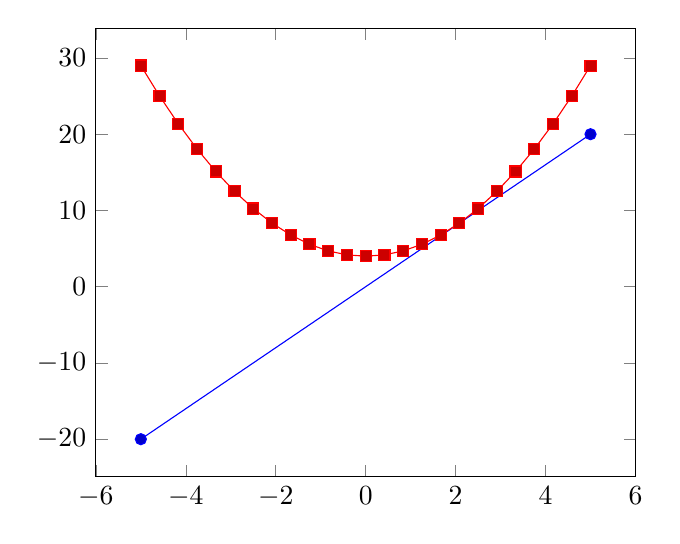
\begin{tikzpicture}
\begin{axis}[
    declare function={
        C=4;
        square(\t)=(\t)^2 + C;
    },
]
    \addplot+ [samples=2] {C*x};

    \addplot {square(x)};
\end{axis}
\end{tikzpicture}
\end{codeexample}
    %
    The definitions as such have the form \meta{function}\meta{argument list} =
    \meta{definition} where the \meta{argument list} contains a
    comma-separated-list of arguments like |\t| or |\t,\a,\b|. The
    \meta{definition} is a math expression which makes use of these arguments.

    Please refer to \cite{tikz} for more details.
\end{key}

\begin{command}{\pgfplotstableread\marg{file}}
    Please refer to the manual of \PGFPlotstable{}, |pgfplotstable.pdf|, which
    is part of the \PGFPlots{} bundle.
\end{command}

\begin{command}{\pgfplotstabletypeset\marg{\textbackslash macro}}
    Please refer to the manual of \PGFPlotstable{}, |pgfplotstable.pdf|, which
    is part of the \PGFPlots{} bundle.
\end{command}

\begin{command}{\pgfplotsiffileexists\marg{filename}\marg{true code}\marg{false code}}
    Invokes \meta{true code} if \meta{filename} exists and \meta{false code} if
    not. Can be used in looping macros, for example to plot every data file
    until there are no more of them.
\end{command}

\begin{command}{\pgfplotsutilifstringequal\marg{first}\marg{second}\marg{true code}\marg{false code}}
    A simple ``strcmp'' tool which invokes \meta{true code} if \meta{first}
    $=$\meta{second} and \meta{false code} otherwise. This does not expand
    macros.
\end{command}

\begin{commandlist}{\pgfkeys,\pgfeov,\pgfkeysvalueof,\pgfkeysgetvalue}
    These commands are part of the \Tikz{} way of specifying options, its
    sub-package |pgfkeys|. The |\pgfplotsset| command is actually nothing but a
    wrapper around |\pgfkeys|.

    A short introduction into |\pgfkeys| can be found in~\cite{keyvalintro}
    whereas the complete reference is, of course, the \Tikz{}
    manual~\cite{tikz}.

    The key |\pgfkeysvalueof|\marg{key name} expands to the value of a key;
    |\pgfkeysgetvalue|\marg{key name}\marg{\textbackslash macro} stores the
    value of \meta{key name} into \meta{\textbackslash macro}. The |\pgfeov|
    macro is used to delimit arguments for code keys in |\pgfkeys|, please
    refer to the references mentioned above.
\end{commandlist}


\section[Commands Inside Of PGFPlots Axes]
        {Commands Inside Of {\normalfont\PGFPlots{}} Axes}

\begin{command}{\autoplotspeclist}
    This command should no longer be used, although it will be kept as
    technical implementation detail. Please use the `|cycle list|' option,
    Section~\ref{sec:cycle:list}.
\end{command}

\begin{command}{\logten}
    Expands to the constant $\log(10)$. Useful for log plots because $\log(10^i)
    = i\log(10)$. This command is only available inside of a \Tikz{} picture.
\end{command}

\begin{command}{\pgfmathprintnumber\marg{number}}
    Generates pretty-printed output\footnote{This method was previously
    \texttt{\textbackslash prettyprintnumber}. Its functionality has been
    included into \PGF{} and the old command is now deprecated.} for
    \meta{number}. This method is used for every tick label.

    The number is printed using the current number printing options, see the
    manual of \PGFPlotstable{} which comes with this package for the different
    number styles, rounding precision and rounding methods.
\end{command}

\begin{command}{\numplots}
    Inside of any of the axis environments, associated style, option or
    command, |\numplots| expands to the total number of plots.
\end{command}

\begin{command}{\numplotsofactualtype}
    Like |\numplots|, this macro returns the total number of plots which have
    the same plot handler. Thus, if you have |sharp plot| active, it returns
    the number of all |sharp plots|. If you have |ybar| active, it returns the
    number of |ybar| plots and so on.
\end{command}

\begin{command}{\plotnum}
    Inside of |\addplot| or any associated style, option or command, |\plotnum|
    expands to the current plot's number, starting with~$0$.
\end{command}

\begin{command}{\plotnumofactualtype}
    Like |\plotnum|, but it returns the number among all plots of the same
    type. The number of all such plots is available using
    |\numplotsofactualtype|.
\end{command}

\begin{command}{\coordindex}
    Inside of an |\addplot| command, this macro expands to the number of the
    actual coordinate (starting with~$0$).

    It is useful together with |x filter| or |y filter| to (de)select
    coordinates.
\end{command}


\section{Path Operations}

\begin{commandlist}{\path,\draw,\fill,\node,\matrix}
    These commands are \Tikz{} drawing commands all of which are documented
    in~\cite{tikz}. They are used to draw or fill paths, generate text nodes or
    aligned text matrices. They are equivalent to
    \pgfmanualpdflabel{/tikz/draw}{}|\path[draw]|,
    \pgfmanualpdflabel{/tikz/fill}{}|\path[fill]|,
    \pgfmanualpdflabel{/tikz/node}{}|\path[node]|,
    \pgfmanualpdflabel{/tikz/matrix}{}|\path[matrix]|,
    respectively.
\end{commandlist}

\begin{pathoperation}{--}{\meta{coordinate}}
    A \Tikz{} path operation which connects the current point (the last one
    before |--|) and \meta{coordinate} with a straight line.
\end{pathoperation}

{\catcode`\|=12
\begin{pathoperation}[noindex]{|-}{\meta{coordinate}}
\pgfmanualpdflabel[\catcode`\|=12 ]{|-}{}%
    A \Tikz{} path operation which connects the current point and
    \meta{coordinate} with \emph{two} straight lines: first vertical, then
    horizontal.
\end{pathoperation}

\begin{pathoperation}[noindex]{-|}{\meta{coordinate}}
\pgfmanualpdflabel[\catcode`\|=12 ]{-|}{}%
    A \Tikz{} path operation which connects the current point and
    \meta{coordinate} with \emph{two} straight lines: first horizontal, then
    vertical.
\end{pathoperation}
}

\begin{keylist}{/tikz/xshift=\marg{dimension},/tikz/yshift=\marg{dimension}}
    These \Tikz{} keys allow to shift something by \meta{dimension} which is
    any \TeX{} size (or expression).
\end{keylist}

\begin{command}{\pgfplotsextra\marg{low-level path commands}}
    A command to execute \meta{low-level path commands} in a \PGFPlots{} axis.
    Since any drawing commands inside of an axis need to be postponed until the
    axis is complete and the scaling has been initialised, it is not possible
    to simply draw any paths. Instead, it is necessary to draw them as soon as
    the axis is finished. This is done automatically for every \Tikz{} path --
    and it is also done manually if you write |\pgfplotsextra|\marg{commands}.
    %
\begin{codeexample}[]
\begin{tikzpicture}
\begin{axis}[xmin=0,xmax=3,ymin=0,ymax=5]
    \pgfplotsextra{
        \pgfpathmoveto{\pgfplotspointaxisxy{1}{2}}
        \pgfpathlineto{\pgfplotspointaxisxy{2}{4}}
        \pgfusepath{stroke}
    }
\end{axis}
\end{tikzpicture}
\end{codeexample}
    %
    The example above initializes an axis and executes the basic level path
    commands as soon as the axis is ready. The execution of multiple |\path|,
    |\addplot| and |\pgfplotsextra| commands is in the same sequence as they
    occur in the environment.\footnote{Except for stacked plots where the
    sequence may be reverse, see the key \texttt{reverse stack plots}.}
\end{command}

\begin{command}{\pgfplotspathaxisoutline}
    Generates a path which resembles the outline of the current axis. This path
    is used for clip paths and the background paths (if any).
\end{command}


\section{Specifying Basic Coordinates}
\label{sec:basic:coordinates}

\begin{commandlist}{%
    \pgfplotspointaxisxy\marg{x coordinate}\marg{y coordinate},
    \pgfplotspointaxisxyz\marg{x coordinate}\marg{y coordinate}\marg{z coordinate}%
}
    Point commands like |\pgfpointxy| which take logical, absolute coordinates
    and return a low-level point. Every transformation from user
    transformations to logarithms is applied.

    Since the transformations are initialized after the axis is complete, this
    command needs to be postponed (see |\pgfplotsextra|).

    This command is the basic level variant of |axis cs:|\meta{x
    coordinate}|,|\meta{y coordinate}|,|\meta{z coordinate}.

    Note that this is also the default coordinate system during the
    visualization phase; in other words: if you write |\draw (1,2) -- (1,4)|,
    \PGFPlots{} will automatically use |(axis cs:1,2) -- (axis cs:1,4)|.
\end{commandlist}

\begin{commandlist}{%
    \pgfplotspointaxisdirectionxy\marg{x coordinate}\marg{y coordinate},
    \pgfplotspointaxisdirectionxyz\marg{x coordinate}\marg{y coordinate}\marg{z coordinate}%
}
    Point commands like |\pgfpointxy| which take logical, \emph{relative}
    coordinates and return a low-level point. Every transformation from user
    transformations to logarithms is applied. The difference to
    |\pgfplotspointaxisxy| is that the shift of the linear transformation is
    skipped here (compare |disabledatascaling|).

    This command is the basic level variant of |axis direction cs:|\meta{x
    coordinate}|,|\meta{y coordinate}|,|\meta{z coordinate}. Please refer to
    the documentation of |axis direction cs| for more details.

    Use this command whenever something of \emph{relative} character like
    directions or lengths need to be supplied. One use case is to draw
    ellipses:
    %
\begin{codeexample}[]
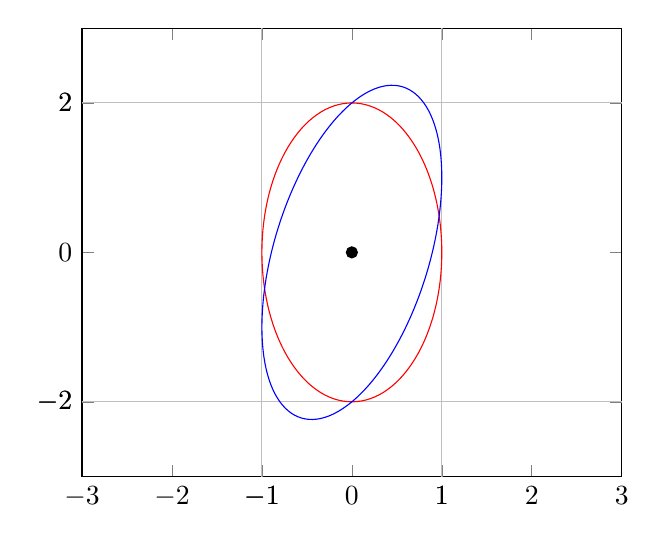
\begin{tikzpicture}
\begin{axis}[
    xmin=-3,   xmax=3,
    ymin=-3,   ymax=3,
    extra x ticks={-1,1},
    extra y ticks={-2,2},
    extra tick style={grid=major},
]
    \draw [red] \pgfextra{
        \pgfpathellipse{\pgfplotspointaxisxy{0}{0}}
            {\pgfplotspointaxisdirectionxy{1}{0}}
            {\pgfplotspointaxisdirectionxy{0}{2}}
    % see also the documentation of
    % 'axis direction cs' which
    % allows a simpler way to draw this ellipse
    };
    \draw [blue] \pgfextra{
        \pgfpathellipse{\pgfplotspointaxisxy{0}{0}}
            {\pgfplotspointaxisdirectionxy{1}{1}}
            {\pgfplotspointaxisdirectionxy{0}{2}}
    };
    \addplot [only marks,mark=*] coordinates
        { (0,0) };
\end{axis}
\end{tikzpicture}
\end{codeexample}

    Since the transformations are initialized after the axis is complete, this
    command needs to be provided either inside of a \tikzname{} |\path| command
    (like |\draw| in the example above) or inside of |\pgfplotsextra|.
\end{commandlist}

\begin{commandlist}{%
    \pgfplotspointrelaxisxy\marg{rel x coordinate}\marg{rel y coordinate},
    \pgfplotspointrelaxisxyz\marg{rel x coordinate}\marg{rel y coordinate}\marg{rel z coordinate}%
}
    Point commands which take \emph{relative} coordinates such that $x=0$ is
    the \emph{lower} $x$-axis limit and $x=1$ the \emph{upper} $x$-axis limit.

    These commands are used for |rel axis cs|.

    Please note that the transformations are only initialised if the axis is
    complete! This means you need to provide |\pgfplotsextra|.
\end{commandlist}

\begin{commandlist}{%
    \pgfplotspointdescriptionxy\marg{$x$ fraction}\marg{$y$ fraction},
    \pgfplotsqpointdescriptionxy\marg{$x$ fraction}\marg{$y$ fraction}%
}
    Point commands such that |{0}{0}| is the lower left corner of the axis'
    bounding box and |{1}{1}| the upper right one; everything else is in
    between. The `|q|' variant is quicker as it doesn't invoke the math parser
    on its arguments.

    They are used for |axis description cs|, see
    Section~\ref{pgfplots:sec:axis:description:cs}.
\end{commandlist}

\begin{commandlist}{\pgfplotspointaxisorigin}
    A point coordinate at the origin, $(0,0,0)$. If the origin is not part of
    the axis limits, the nearest point on the boundary is returned instead.

    This is the same coordinate as returned by the |origin| anchor.
\end{commandlist}

\begin{commandlist}{%
    \pgfplotstransformcoordinatex\marg{x coordinate of an axis},
    \pgfplotstransformcoordinatey\marg{y coordinate of an axis},
    \pgfplotstransformcoordinatez\marg{z coordinate of an axis}%
}
    Defines |\pgfmathresult| to be the low-level \PGF{} coordinate
    corresponding to the input argument.

    The command applies any |[xyz] coord trafo| keys, data scalings and/or
    logarithms or whatever \PGFPlots{} does to map input coordinates to
    internal coordinates.

    The result can be used inside of a |\pgfpointxy| statement (i.e.\@ it still
    needs to be scaled with the respective \PGF{} unit vector).
    %
\begin{codeexample}[]
\begin{tikzpicture}
\pgfplotsset{compat/pgfpoint substitution=1.3}
\begin{axis}[xmin=0,xmax=2,ymin=0,ymax=5]
    \pgfplotsextra{
        \pgfplotstransformcoordinatex{1}
        \let\xcoord=\pgfmathresult
        \pgfplotstransformcoordinatey{1}
        \let\ycoord=\pgfmathresult
        \pgfpathcircle
            {\pgfqpointxy{\xcoord}{\ycoord}}
            {5pt}
        \pgfusepath{fill}
    }
\end{axis}
\end{tikzpicture}
\end{codeexample}
    %
    Note that \PGFPlots{} substitutes |\pgfqpointxy| by |\pgfplotspointaxisxyz|
    by default -- and this command implicitly transforms coordinates anyway. In
    order to see the difference, the preceding example first disables this
    automatic substitution of coordinate systems by means of
    |compat/pgfpoint substitution=1.3|.
    %
    The result of this command is also available as math method
    |transformcoordinatex| (see the documentation for |axis cs|).

    Please note that the transformations are only initialised if the axis is
    complete. This means you need to provide |\pgfplotsextra| as is shown in
    the example above.
\end{commandlist}

\begin{commandlist}{%
    \pgfplotstransformdirectionx\marg{x direction of an axis},
    \pgfplotstransformdirectiony\marg{y direction of an axis},
    \pgfplotstransformdirectionz\marg{z direction of an axis}%
}
    Defines |\pgfmathresult| to be a low-level \PGF{} \emph{direction vector
    component}.

    A direction vector needs to be \emph{added} to some coordinate in order to
    get a coordinate, compare the documentation for
    |\pgfplotspointaxisdirectionxy| and |axis direction cs|.

    The argument \meta{x direction of an axis} is processed in (almost) the
    same way as for the macro which operates on absolute positions,
    |\pgfplotstransformcoordinatex|. The only difference is that
    \emph{directions} need no shifting transformation.

    The result of this command is also available as math method
    |transformdirectionx| (see the documentation for |axis direction cs|).

    See |axis direction cs| for details and examples about this command.
\end{commandlist}

% this command is for internal use only:
%--------------------------------------------------
% \begin{command}{\pgfplotsconvertunittocoordinate\marg{x, y or z}\marg{dimension}}
%     Converts a dimension (with unit!) to a corresponding $x$-, $y$- or $z$-coordinate. The result will be written to |\pgfmathresult| (without units).
%
%     It is possible to use the result as arguments for the |\pgfpointxyz| commands.
%
%     The effect is to multiply \meta{dimension} with the inverse length of the unit vector for the specified axis. These lengths are precomputed in \PGFPlots{} so the operation is fast.
% \begin{codeexample}[code only]
% \pgfplotsconvertunittocoordinate{x}{5pt}
% % now, the command uses exactly 5pt in x direction:
% \pgfqpointxyz{\pgfmathresult}{4}{3}
% \end{codeexample}
% \end{command}
%--------------------------------------------------

\begin{commandlist}{%
    \pgfplotspointunitx,
    \pgfplotspointunity,
    \pgfplotspointunitz%
}
    Low-level point commands which return the canvas $x$, $y$ or $z$ unit
    vectors.

    The |\pgfplotspointunitx| is the \pgfname{} unit vector in $x$ direction.

    These vectors are essentially the same as |\pgfqpointxyz{1}{0}{0}|,
    |\pgfqpointxyz{0}{1}{0}|, and |\pgfqpointxyz{0}{0}{1}|, respectively.

    The unit $z$ vector is only defined for three dimensional axes.
\end{commandlist}

\begin{commandlist}{%
    \pgfplotsunitxlength,
    \pgfplotsunitylength,
    \pgfplotsunitzlength,
    \pgfplotsunitxinvlength,
    \pgfplotsunityinvlength,
    \pgfplotsunitzinvlength%
}
    Macros which expand to the vector length $\lVert x_i \rVert$ of the
    respective unit vector $x_i$ or the inverse vector length, $1/\lVert x_i
    \rVert$. These macros can be used inside of |\pgfmathparse|, for example.

    The $x_i$ are the |\pgfplotspointunitx| variants.
\end{commandlist}

\begin{command}{\pgfplotsqpointoutsideofaxis%
        \marg{three-char-string}\marg{coordinate}\marg{normal distance}%
}
    Provides a point coordinate on one of the available four axes in case of a
    two dimensional figure or on one of the available twelve axes in case of a
    three dimensional figure.

    The desired axis is uniquely identified by a three character string,
    provided as first argument to the command. The first of the three
    characters is `|0|' if the $x$-coordinate of the specified axis passes
    through the lower axis limit. It is `|1|', if the $x$-coordinate of the
    specified axis passes through the upper axis limit. Furthermore, it is
    `|2|' if it passes through the origin. The second character is also either
    |0|, |1| or |2| and it characterizes the position on the $y$-axis. The
    third character is for the third dimension, the $z$-axis. It should be left
    at `|0|' for two dimensional plots. However, \emph{one} of the three
    characters should be `|v|', meaning the axis \underline varies. For
    example, |v01| denotes $\{ (x,y_{\min},z_{\max}) \vert x \in \R \}$.

    The second argument, \meta{coordinate} is the logical coordinate on that
    axis. Since two coordinates of the axis are fixed, \meta{coordinate} refers
    to the \underline varying component of the axis. It must be a number
    without unit; no math expressions are supported here.

    The third argument \meta{normal distance} is a dimension like |10pt|. It
    shifts the coordinate away from the designated axis in direction of the
    outer normal vector. The outer normal vector always points away from the
    axis. It is computed using |\pgfplotspointouternormalvectorofaxis|.

    There are several variants of this command which are documented in the
    source code. One of them is particularly useful:
\end{command}

\begin{command}{\pgfplotsqpointoutsideofaxisrel%
        \marg{three-char-string}\marg{axis fraction}\marg{normal distance}%
}
    This point coordinate is a variant of |\pgfplotsqpointoutsideofaxis| which
    allows to provide an \meta{axis fraction} instead of an absolute
    coordinate. The fraction is a number between $0$ (lower axis limit) and $1$
    (upper axis limit), i.e.\@ it is given in percent of the total axis. It is
    possible to provide negative values or values larger than one.

    The |\pgfplotsqpointoutsideofaxisrel| command is similar in spirit to
    |rel axis cs|.

    There is one speciality in conjunction with reversed axes: if the axis has
    been reversed by |x dir=reverse| and, in addition,
    |allow reversal of rel axis cs| is true, the value $0$ denotes the
    \emph{upper} limit while $1$ denotes the \emph{lower} limit. The effect is
    that coordinates won't change just because of axis reversal.
        \index{allow reversal of rel axis cs}%
\end{command}

\begin{command}{\pgfplotspointouternormalvectorofaxis\marg{three-char-string}}
    A point command which yields the outer normal vector of the respective
    axis. The normal vector has length $1$ (computed with
    |\pgfpointnormalised|). It is the same normal vector used inside of
    |\pgfplotsqpointoutsideofaxis| and its variants.

    The output of this command will be cached and reused during the lifetime
    of an axis.
\end{command}

\begin{command}{\pgfplotsticklabelaxisspec\marg{x, y or z}}
    Expands to the three character identification for the axis containing tick
    labels for the chosen axis, either \meta{x}, \meta{y} or \meta{z}.
\end{command}

\begin{command}{\pgfplotsvalueoflargesttickdimen\marg{x, y or z}}
    Expands to the largest distance of a tick position to its tick label
    bounding box in direction of the outer unit normal vector. It does also
    include the value of the |ticklabel shift| key.

    This value is used for |ticklabel cs|.
\end{command}

\begin{commandlist}{
    \pgfplotsmathfloatviewdepthxyz\marg{x}\marg{y}\marg{z},
    \pgfplotsmathviewdepthxyz\marg{x}\marg{y}\marg{z}%
}
    Both macros define |\pgfmathresult| to be the ``depth'' of a three
    dimensional point $\bar x = (x,y,z)$. The depth is defined to be the scalar
    product of $\bar x$ with $\vec d$, the view direction of the current axis.

    For |\pgfplotsmathfloatviewdepthxyz|, the arguments are parsed as floating
    point numbers and the result is encoded in floating point. A fixed point
    representation can be generated with
    |\pgfmathfloattofixed{\pgfmathresult}|.

    For |\pgfplotsmathviewdepthxyz|, \TeX{} arithmetics is employed for the
    inner product and the result is assigned in fixed point. This is slightly
    faster, but has considerably smaller data range.

    Both commands can only be used \emph{inside} of a three dimensional
    \PGFPlots{} axis (as soon as the axis is initialised, see
    |\pgfplotsextra|).
\end{commandlist}

\begin{texif}{pgfplotsthreedim}
    A \TeX{} |\if| which evaluates the \meta{true code} if the axis is three
    dimensional and the \meta{else code} if not.
\end{texif}


\section{Accessing Axis Limits}

It is also possible to access axis limits during the visualization phase,
i.e.\@ during |\end{axis}|. Please refer to the reference documentation for
|xmin| on page~\pageref{page:access:limits}.


\section{Accessing Point Coordinate Values}

During the visualization phase, \PGFPlots{} provides access to the currently
processed coordinate and its values.

This access requires a call to specific macros. These macros write the
coordinate values to some publicly available key--value pairs. Then, the
current point's $x$, $y$, $z$, and color data can be accessed.

\begin{commandlist}{\pgfplotspointgetcoordinates,\pgfplotspointgetcoordinates\marg{point}}

    After invoking the macro, the following keys will be set:

    \declaretext{/data point/x} will contain the current point's $x$-coordinate.

    \declaretext{/data point/y} will contain the current point's $y$-coordinate.

    \declaretext{/data point/z} will contain the current point's $z$-coordinate
    (if applicable).

    \declaretext{/data point/meta} will contain the current point's
    |point meta| value (if applicable).

    \declaretext{/data point/index} will contain the current point's index in
    the coordinate stream. This is actually the same as |\coordindex|.

    This command actually supports two modes of operation:
    %
    \begin{enumerate}
        \item Without arguments. In this case, it returns values of the point
            which is about to be processed by the current plot handler.
        \item With an argument in curly braces. In this case, it expects a
            coordinate and assigns the keys accordingly. Note that this
            command merely supports two-dimensional axes and assigns only
            |/data point/x| and |/data point/y|.
    \end{enumerate}

    The returned values are the same as they can be read on the axes, they are
    also the same as you would write them into |axis cs|.

    This means that any |x coord inv trafo| has been applied on the value. It
    also means that the exponential function has been called even though the
    internal coordinate was present in log format.

    This function is implicitly called for any |scatter| plot (including
    |nodes near coords|). This allows to access \emph{all} coordinate values at
    once:
    %
\begin{codeexample}[]
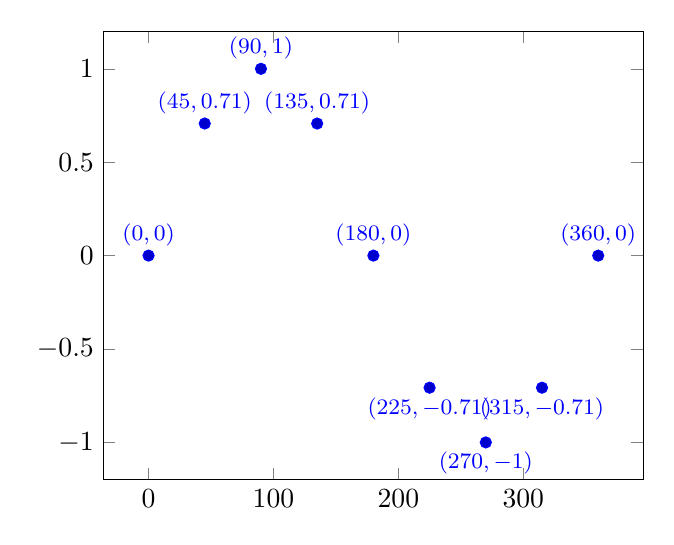
\begin{tikzpicture}
\begin{axis}
    \addplot+ [
        domain=0:360,
        samples=9,
        only marks,
        nodes near coords={%
            \footnotesize
            $(\pgfmathprintnumber
                {\pgfkeysvalueof{/data point/x}},
               \pgfmathprintnumber
                {\pgfkeysvalueof{/data point/y}})$%
        },
    ] {sin(x)};
\end{axis}
\end{tikzpicture}
\end{codeexample}
    %
    The example works because |\pgfplotspointgetcoordinates| is part of the
    standard implementation of |nodes near coords|; the resulting values are
    directly available. Note that the preceding example would have been simpler
    if we would have printed just one value: |nodes near coords| resorts to the
    |point meta|. And that, in turn, contains the $y$-coordinate anyway by
    default.

    A more advanced example would be a |ybar| plot in which nodes shall be
    placed at the lower end of the axis, together with some dotted lines to the
    respective bars:
    %
\begin{codeexample}[]
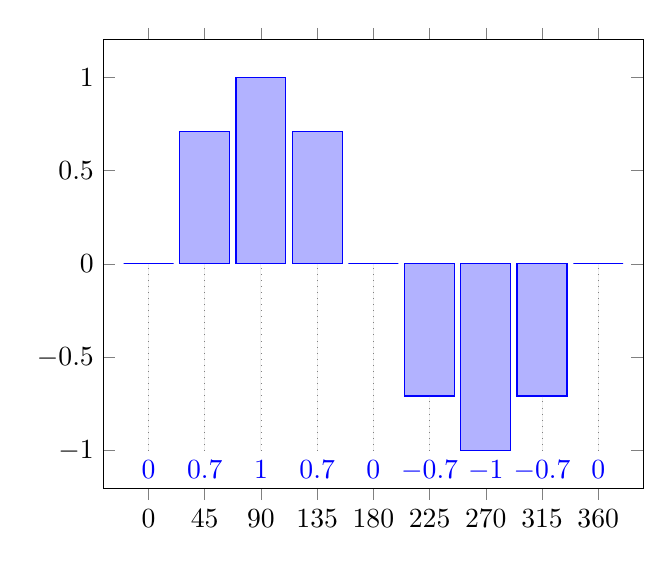
\begin{tikzpicture}
\begin{axis}[
    ybar,
    nodes near coords,
    %
    % we want to provide absolute 'at' values
    % for the nodes:
    scatter/position=absolute,
    every node near coord/.style={
        at={(\pgfkeysvalueof{/data point/x},-1)},
        % pretty printing:
        anchor=north,
        /pgf/number format/fixed,
        /pgf/number format/precision=1,
        % assign a name which can be referenced below:
        name=NNC\pgfkeysvalueof{/data point/index},
    },
    % ... draw a dotted line between
    % the marker and the bar:
    /pgfplots/scatter/@post marker code/.add code={}{
        \draw [dotted,help lines]
            (NNC\pgfkeysvalueof{/data point/index})
            -- (\pgfkeysvalueof{/data point/x},
            {min(0,\pgfkeysvalueof{/data point/y})});
    },
    % assign suitable tick labels:
    xtick=data,
]
    % some dummy data:
    \addplot+ [
        domain=0:360,
        bar width=360/9,
        samples=9,
    ] {sin(x)};
\end{axis}
\end{tikzpicture}
\end{codeexample}
    %
    Again, the command is used implicitly as part of |nodes near coords| and
    does not occur in the example as such.

    \paragraph{See also} the related example online under
    \url{https://tex.stackexchange.com/a/141006}. It demonstrates how to
    place the nodes generated by |nodes near coords| based on the value (either
    inside of a bar or above it).

    The following example uses an argument in curly braces for which we seek
    coordinate values:
    %
\begin{codeexample}[]
% requires \usetikzlibrary{intersections}
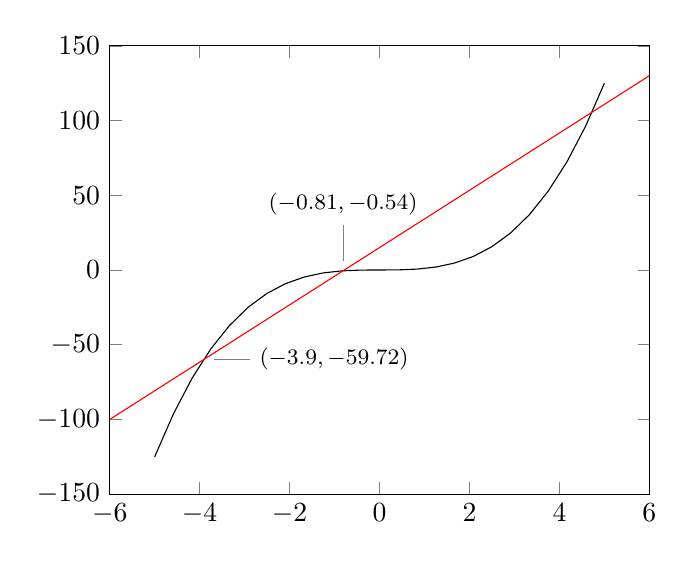
\begin{tikzpicture}
\begin{axis}
    \addplot [name path=A] {x^3};

    \draw [red,name path=HelperLine]
        (axis cs:-6,-100) -- (axis cs:6,130);

    \draw [
        font=\footnotesize,
        name intersections={of=A and HelperLine},
    ]
    node [pin={right:
      \pgfplotspointgetcoordinates{(intersection-1)}
        $(\pgfmathprintnumber[fixed]{
            \pgfkeysvalueof{/data point/x}},
          \pgfmathprintnumber[fixed]{
            \pgfkeysvalueof{/data point/y}})$
      }
    ] at (intersection-1) {}
    node [pin={
      \pgfplotspointgetcoordinates{(intersection-2)}
        $(\pgfmathprintnumber[fixed]{
            \pgfkeysvalueof{/data point/x}},
          \pgfmathprintnumber[fixed]{
            \pgfkeysvalueof{/data point/y}})$
      }
    ] at (intersection-2) {};
\end{axis}
\end{tikzpicture}
\end{codeexample}
    %
    The example computes and names intersections of |A| and |HelperLine|. The
    following code generates pins at the intersections. To this end, it uses
    |\pgfplotspointgetcoordinates|\marg{point} which defines |/data point/x|
    and |/data point/y|. These values are then formatted using
    |\pgfmathprintnumber|.

    In its second mode, |\pgfplotspointgetcoordinates|\marg{point} expects one
    of two things as \meta{point}:
    %
    \begin{enumerate}
        \item a basic-level \PGF{} point like |\pgfpointanchor{A}{center}| or
        \item a \Tikz{} point like |(A.base)| or |(3,5)|.
    \end{enumerate}
\end{commandlist}

\begin{command}{\pgfplotspointgetnormalizedcoordinates}
    A macro which is very similar to |\pgfplotspointgetcoordinates|.
    Consequently, it is also supposed to be called during the visualization phase.

    It assigns the very same output macros, but the values are different. More
    precisely, it defines the macros

    \declaretext{/data point/x} will contain the current point's
    \emph{normalized} $x$-coordinate.

    \declaretext{/data point/y} will contain the current point's
    \emph{normalized} $y$-coordinate.

    \declaretext{/data point/z} will contain the current point's
    \emph{normalized} $z$-coordinate (if applicable).

    \declaretext{/data point/meta} will contain the current point's
    |point meta| value (if applicable).

    \declaretext{/data point/index} will contain the current point's index in
    the coordinate stream. This is actually the same as |\coordindex|.

    The keyword \declaretext{normalized} means that the values are in a
    suitable numerical form which can be consumed by the axis. To be more
    specific: any user |x coord inv trafo| is \emph{ignored}. An important
    example would be |symbolic x coords|: the normalized coordinates would be
    some associated numbers, not the symbols. The results returned by
    |\pgfplotspointgetcoordinates| would be the symbols. For logarithm axes,
    the normalized values are the logs.

    Typically, normalized values are much more useful when you want to apply
    some math operation like averaging or subtraction.

    This function needs to be called explicitly. It is currently used by
    |ybar stacked| to align |nodes near coords|.
\end{command}


\section{Layer Access}

\begin{command}{\pgfplotsonlayer\marg{layer name}}
    A low-level command which will check if the current axis has layer support
    activated and, if so, calls |\pgfonlayer|\marg{layer name}.

    There must be a |\endpgfplotsonlayer| to delimit the environment.
\end{command}

\begin{command}{\endpgfplotsonlayer}
    The end of |\pgfplotsonlayer|.
\end{command}

\begin{command}{\pgfonlayer\marg{layer name}}
    A low-level command of \PGF{} which will collect everything until the
    matching |\endpgfonlayer| into layer \meta{layer name}.

    The \meta{layer name} must be active, i.e.\@ it must be part of the layer
    names of |set layers|.

    The only special case is if you call |\pgfdeclarelayer{discard}| somewhere:
    this special layer has a ``magical name'' which serves as |/dev/null| if it
    is enabled using |\pgfonlayer{discard}|: it does not need to be active and
    everything assigned to this layer will be thrown away if it is not part of
    the layer name configuration.

    There must be a |\endpgfonlayer| to delimit the environment.
\end{command}

\begin{command}{\endpgfonlayer}
    The end of |\pgfonlayer|.
\end{command}


\begin{command}{\pgfsetlayers\marg{layer list}}
    This is a low-level command of \PGF{}. At the time of this writing, it is
    the only way to tell \PGF{} which layers it shall use for the current/next
    picture. It is used implicitly by |set layers|.
\end{command}


\printindex

\bibliographystyle{abbrv} %gerapali} %gerabbrv} %gerunsrt.bst} %gerabbrv}% gerplain}
\nocite{pgfplotstable}
\nocite{programmingnotes}
\bibliography{pgfplots}
\end{document}

% -----------------------------------------------------------------------------
% For Stefan Pinnow as reminder on what to look for when editing the manual
% -----------------------------------------------------------------------------
% There should be no line breaks in the following environments
% - |...|
% - \declareandlabel{...}
% - \verbpdfref{...}
% If "MakeTikzPictures" isn't running through check one of the externalized
% LOG files what is the cause of that.
% -----------------------------------------------------------------------------


%%%%%%%%%%%%%%%%%%%%%%%%%%%%%%%%%%%%%%%%%%%%%%%%%%%%%%%%%%%%%%%%%%%%%%%%%%%%%
%
% Package pgfplots.sty documentation.
%
% Copyright 2007/2008 by Christian Feuersaenger.
%
% This program is free software: you can redistribute it and/or modify
% it under the terms of the GNU General Public License as published by
% the Free Software Foundation, either version 3 of the License, or
% (at your option) any later version.
%
% This program is distributed in the hope that it will be useful,
% but WITHOUT ANY WARRANTY; without even the implied warranty of
% MERCHANTABILITY or FITNESS FOR A PARTICULAR PURPOSE.  See the
% GNU General Public License for more details.
%
% You should have received a copy of the GNU General Public License
% along with this program.  If not, see <http://www.gnu.org/licenses/>.
%
%
%%%%%%%%%%%%%%%%%%%%%%%%%%%%%%%%%%%%%%%%%%%%%%%%%%%%%%%%%%%%%%%%%%%%%%%%%%%%%
% SEE pgfplots-macros.tex as well!
%\pdfminorversion=5 % to allow compression
%\pdfobjcompresslevel=2
\documentclass[a4paper,openany]{book}

\let\bookmaketitle=\maketitle

% -----------------------------------
% this here is from ltxdoc:
\usepackage{doc}[=v2]
\AtBeginDocument{\MakeShortVerb{\|}}
%\setlength{\textwidth}{355pt}
%\addtolength\marginparwidth{30pt}
%\addtolength\oddsidemargin{20pt}
%\addtolength\evensidemargin{20pt}
\def\cmd#1{\cs{\expandafter\cmd@to@cs\string#1}}
\def\cmd@to@cs#1#2{\char\number`#2\relax}
\DeclareRobustCommand\cs[1]{\texttt{\char`\\#1}}
\providecommand\marg[1]{%
  {\ttfamily\char`\{}\meta{#1}{\ttfamily\char`\}}}
\providecommand\oarg[1]{%
  {\ttfamily[}\meta{#1}{\ttfamily]}}
\providecommand\parg[1]{%
  {\ttfamily(}\meta{#1}{\ttfamily)}}
\raggedbottom

% -----------------------------------
\input{pgfplots.preamble.tex}

\makeatletter
% I want a two-column index just as in pgfmanual styles. This here
% was the best way to get one:
\def\index@prologue{\section*{Index}\addcontentsline{toc}{chapter}{Index}
}
\makeatother

%\RequirePackage[german,english,francais]{babel}

\def\matlabcolormaptext{This colormap is similar to one shipped with Matlab$^\text{\textregistered}$ under a similar name.}

\IfFileExists{tikzlibraryspy.code.tex}{%
\usetikzlibrary{spy}
}{%
    \message{ERROR: tikz SPY library NOT available. The manual will only compile partially.^^J}%
}%

\usepackage{xparse}% for colorbrewer manual

\usetikzlibrary{
    decorations.markings,
    decorations.footprints,
    shapes.arrows,
    matrix,
    positioning,
}

\usepgfplotslibrary{
    fillbetween,
    ternary,
    smithchart,
    patchplots,
    polar,
    colormaps,
    colorbrewer,
    colortol,           % docu not ready yet
}
\pgfqkeys{/codeexample}{%
    every codeexample/.append style={
        /pgfplots/every ternary axis/.append style={
            /pgfplots/legend style={fill=graphicbackground},
        }
    },
    tabsize=4,
}

\pgfplotsmanualenableexternalizationofexpensive

%\usetikzlibrary{external}
%\tikzexternalize[prefix=figures/]{pgfplots}

\title{%
    Manual for Package \PGFPlots{}\\
    {\small 2D/3D Plots in \LaTeX{}, Version \pgfplotsversion}\\
    {\small\href{https://github.com/pgf-tikz/pgfplots}{https://github.com/pgf-tikz/pgfplots}}
    %\\{\small Attention: you are using an unstable development version.}
}

\makeatletter
\long\def\abstractsmuggle{%
    \centering
    \textbf{Abstract}\\[0.5cm]

    \begin{minipage}{12cm}
        \PGFPlots{} draws high-quality function plots in normal or logarithmic
        scaling with a user-friendly interface directly in \TeX{}. The user
        supplies axis labels, legend entries and the plot coordinates for one or
        more plots and \PGFPlots{} applies axis scaling, computes any logarithms
        and axis ticks and draws the plots. It supports line plots, scatter
        plots, piecewise constant plots, bar plots, area plots, mesh and surface
        plots, patch plots, contour plots, quiver plots, histogram plots, box
        plots, polar axes, ternary diagrams, smith charts and some more. It is
        based on Till Tantau's package \PGF{}/\Tikz{}.
    \end{minipage}

}%

\expandafter\date\expandafter{\@date\\[2cm]
    \abstractsmuggle
}%
\makeatother

%\includeonly{pgfplots.reference}


\begin{document}

\def\plotcoords{%
\addplot coordinates {
(5,8.312e-02)    (17,2.547e-02)   (49,7.407e-03)
(129,2.102e-03)  (321,5.874e-04)  (769,1.623e-04)
(1793,4.442e-05) (4097,1.207e-05) (9217,3.261e-06)
};

\addplot coordinates{
(7,8.472e-02)    (31,3.044e-02)    (111,1.022e-02)
(351,3.303e-03)  (1023,1.039e-03)  (2815,3.196e-04)
(7423,9.658e-05) (18943,2.873e-05) (47103,8.437e-06)
};

\addplot coordinates{
(9,7.881e-02)     (49,3.243e-02)    (209,1.232e-02)
(769,4.454e-03)   (2561,1.551e-03)  (7937,5.236e-04)
(23297,1.723e-04) (65537,5.545e-05) (178177,1.751e-05)
};

\addplot coordinates{
(11,6.887e-02)    (71,3.177e-02)     (351,1.341e-02)
(1471,5.334e-03)  (5503,2.027e-03)   (18943,7.415e-04)
(61183,2.628e-04) (187903,9.063e-05) (553983,3.053e-05)
};

\addplot coordinates{
(13,5.755e-02)     (97,2.925e-02)     (545,1.351e-02)
(2561,5.842e-03)   (10625,2.397e-03)  (40193,9.414e-04)
(141569,3.564e-04) (471041,1.308e-04)
(1496065,4.670e-05)
};
}%


\bookmaketitle
\tableofcontents

%%%%%%%%%%%%%%%%%%%%%%%%%%%%%%%%%%%%%%%%%%%%%%%%%%%%%%%%%%%%%%%%%%%%%%%%%%%%%
%
% Package pgfplots.sty documentation.
%
% Copyright 2007/2008 by Christian Feuersaenger.
%
% This program is free software: you can redistribute it and/or modify
% it under the terms of the GNU General Public License as published by
% the Free Software Foundation, either version 3 of the License, or
% (at your option) any later version.
%
% This program is distributed in the hope that it will be useful,
% but WITHOUT ANY WARRANTY; without even the implied warranty of
% MERCHANTABILITY or FITNESS FOR A PARTICULAR PURPOSE.  See the
% GNU General Public License for more details.
%
% You should have received a copy of the GNU General Public License
% along with this program.  If not, see <http://www.gnu.org/licenses/>.
%
%
%%%%%%%%%%%%%%%%%%%%%%%%%%%%%%%%%%%%%%%%%%%%%%%%%%%%%%%%%%%%%%%%%%%%%%%%%%%%%
% SEE pgfplots-macros.tex as well!
%\pdfminorversion=5 % to allow compression
%\pdfobjcompresslevel=2
\documentclass[a4paper,openany]{book}

\let\bookmaketitle=\maketitle

% -----------------------------------
% this here is from ltxdoc:
\usepackage{doc}[=v2]
\AtBeginDocument{\MakeShortVerb{\|}}
%\setlength{\textwidth}{355pt}
%\addtolength\marginparwidth{30pt}
%\addtolength\oddsidemargin{20pt}
%\addtolength\evensidemargin{20pt}
\def\cmd#1{\cs{\expandafter\cmd@to@cs\string#1}}
\def\cmd@to@cs#1#2{\char\number`#2\relax}
\DeclareRobustCommand\cs[1]{\texttt{\char`\\#1}}
\providecommand\marg[1]{%
  {\ttfamily\char`\{}\meta{#1}{\ttfamily\char`\}}}
\providecommand\oarg[1]{%
  {\ttfamily[}\meta{#1}{\ttfamily]}}
\providecommand\parg[1]{%
  {\ttfamily(}\meta{#1}{\ttfamily)}}
\raggedbottom

% -----------------------------------
\input{pgfplots.preamble.tex}

\makeatletter
% I want a two-column index just as in pgfmanual styles. This here
% was the best way to get one:
\def\index@prologue{\section*{Index}\addcontentsline{toc}{chapter}{Index}
}
\makeatother

%\RequirePackage[german,english,francais]{babel}

\def\matlabcolormaptext{This colormap is similar to one shipped with Matlab$^\text{\textregistered}$ under a similar name.}

\IfFileExists{tikzlibraryspy.code.tex}{%
\usetikzlibrary{spy}
}{%
    \message{ERROR: tikz SPY library NOT available. The manual will only compile partially.^^J}%
}%

\usepackage{xparse}% for colorbrewer manual

\usetikzlibrary{
    decorations.markings,
    decorations.footprints,
    shapes.arrows,
    matrix,
    positioning,
}

\usepgfplotslibrary{
    fillbetween,
    ternary,
    smithchart,
    patchplots,
    polar,
    colormaps,
    colorbrewer,
    colortol,           % docu not ready yet
}
\pgfqkeys{/codeexample}{%
    every codeexample/.append style={
        /pgfplots/every ternary axis/.append style={
            /pgfplots/legend style={fill=graphicbackground},
        }
    },
    tabsize=4,
}

\pgfplotsmanualenableexternalizationofexpensive

%\usetikzlibrary{external}
%\tikzexternalize[prefix=figures/]{pgfplots}

\title{%
    Manual for Package \PGFPlots{}\\
    {\small 2D/3D Plots in \LaTeX{}, Version \pgfplotsversion}\\
    {\small\href{https://github.com/pgf-tikz/pgfplots}{https://github.com/pgf-tikz/pgfplots}}
    %\\{\small Attention: you are using an unstable development version.}
}

\makeatletter
\long\def\abstractsmuggle{%
    \centering
    \textbf{Abstract}\\[0.5cm]

    \begin{minipage}{12cm}
        \PGFPlots{} draws high-quality function plots in normal or logarithmic
        scaling with a user-friendly interface directly in \TeX{}. The user
        supplies axis labels, legend entries and the plot coordinates for one or
        more plots and \PGFPlots{} applies axis scaling, computes any logarithms
        and axis ticks and draws the plots. It supports line plots, scatter
        plots, piecewise constant plots, bar plots, area plots, mesh and surface
        plots, patch plots, contour plots, quiver plots, histogram plots, box
        plots, polar axes, ternary diagrams, smith charts and some more. It is
        based on Till Tantau's package \PGF{}/\Tikz{}.
    \end{minipage}

}%

\expandafter\date\expandafter{\@date\\[2cm]
    \abstractsmuggle
}%
\makeatother

%\includeonly{pgfplots.reference}


\begin{document}

\def\plotcoords{%
\addplot coordinates {
(5,8.312e-02)    (17,2.547e-02)   (49,7.407e-03)
(129,2.102e-03)  (321,5.874e-04)  (769,1.623e-04)
(1793,4.442e-05) (4097,1.207e-05) (9217,3.261e-06)
};

\addplot coordinates{
(7,8.472e-02)    (31,3.044e-02)    (111,1.022e-02)
(351,3.303e-03)  (1023,1.039e-03)  (2815,3.196e-04)
(7423,9.658e-05) (18943,2.873e-05) (47103,8.437e-06)
};

\addplot coordinates{
(9,7.881e-02)     (49,3.243e-02)    (209,1.232e-02)
(769,4.454e-03)   (2561,1.551e-03)  (7937,5.236e-04)
(23297,1.723e-04) (65537,5.545e-05) (178177,1.751e-05)
};

\addplot coordinates{
(11,6.887e-02)    (71,3.177e-02)     (351,1.341e-02)
(1471,5.334e-03)  (5503,2.027e-03)   (18943,7.415e-04)
(61183,2.628e-04) (187903,9.063e-05) (553983,3.053e-05)
};

\addplot coordinates{
(13,5.755e-02)     (97,2.925e-02)     (545,1.351e-02)
(2561,5.842e-03)   (10625,2.397e-03)  (40193,9.414e-04)
(141569,3.564e-04) (471041,1.308e-04)
(1496065,4.670e-05)
};
}%


\bookmaketitle
\tableofcontents
\include{pgfplots.title_abstract_intro}
\include{pgfplots.preliminaries}
\include{pgfplots.intro}
\include{pgfplots.reference}
\include{pgfplots.libs}
\include{pgfplots.resources}
\include{pgfplots.importexport}
\include{pgfplots.basic.reference}

\printindex

\bibliographystyle{abbrv} %gerapali} %gerabbrv} %gerunsrt.bst} %gerabbrv}% gerplain}
\nocite{pgfplotstable}
\nocite{programmingnotes}
\bibliography{pgfplots}
\end{document}

% -----------------------------------------------------------------------------
% For Stefan Pinnow as reminder on what to look for when editing the manual
% -----------------------------------------------------------------------------
% There should be no line breaks in the following environments
% - |...|
% - \declareandlabel{...}
% - \verbpdfref{...}
% If "MakeTikzPictures" isn't running through check one of the externalized
% LOG files what is the cause of that.
% -----------------------------------------------------------------------------


%%%%%%%%%%%%%%%%%%%%%%%%%%%%%%%%%%%%%%%%%%%%%%%%%%%%%%%%%%%%%%%%%%%%%%%%%%%%%
%
% Package pgfplots.sty documentation.
%
% Copyright 2007/2008 by Christian Feuersaenger.
%
% This program is free software: you can redistribute it and/or modify
% it under the terms of the GNU General Public License as published by
% the Free Software Foundation, either version 3 of the License, or
% (at your option) any later version.
%
% This program is distributed in the hope that it will be useful,
% but WITHOUT ANY WARRANTY; without even the implied warranty of
% MERCHANTABILITY or FITNESS FOR A PARTICULAR PURPOSE.  See the
% GNU General Public License for more details.
%
% You should have received a copy of the GNU General Public License
% along with this program.  If not, see <http://www.gnu.org/licenses/>.
%
%
%%%%%%%%%%%%%%%%%%%%%%%%%%%%%%%%%%%%%%%%%%%%%%%%%%%%%%%%%%%%%%%%%%%%%%%%%%%%%
% SEE pgfplots-macros.tex as well!
%\pdfminorversion=5 % to allow compression
%\pdfobjcompresslevel=2
\documentclass[a4paper,openany]{book}

\let\bookmaketitle=\maketitle

% -----------------------------------
% this here is from ltxdoc:
\usepackage{doc}[=v2]
\AtBeginDocument{\MakeShortVerb{\|}}
%\setlength{\textwidth}{355pt}
%\addtolength\marginparwidth{30pt}
%\addtolength\oddsidemargin{20pt}
%\addtolength\evensidemargin{20pt}
\def\cmd#1{\cs{\expandafter\cmd@to@cs\string#1}}
\def\cmd@to@cs#1#2{\char\number`#2\relax}
\DeclareRobustCommand\cs[1]{\texttt{\char`\\#1}}
\providecommand\marg[1]{%
  {\ttfamily\char`\{}\meta{#1}{\ttfamily\char`\}}}
\providecommand\oarg[1]{%
  {\ttfamily[}\meta{#1}{\ttfamily]}}
\providecommand\parg[1]{%
  {\ttfamily(}\meta{#1}{\ttfamily)}}
\raggedbottom

% -----------------------------------
\input{pgfplots.preamble.tex}

\makeatletter
% I want a two-column index just as in pgfmanual styles. This here
% was the best way to get one:
\def\index@prologue{\section*{Index}\addcontentsline{toc}{chapter}{Index}
}
\makeatother

%\RequirePackage[german,english,francais]{babel}

\def\matlabcolormaptext{This colormap is similar to one shipped with Matlab$^\text{\textregistered}$ under a similar name.}

\IfFileExists{tikzlibraryspy.code.tex}{%
\usetikzlibrary{spy}
}{%
    \message{ERROR: tikz SPY library NOT available. The manual will only compile partially.^^J}%
}%

\usepackage{xparse}% for colorbrewer manual

\usetikzlibrary{
    decorations.markings,
    decorations.footprints,
    shapes.arrows,
    matrix,
    positioning,
}

\usepgfplotslibrary{
    fillbetween,
    ternary,
    smithchart,
    patchplots,
    polar,
    colormaps,
    colorbrewer,
    colortol,           % docu not ready yet
}
\pgfqkeys{/codeexample}{%
    every codeexample/.append style={
        /pgfplots/every ternary axis/.append style={
            /pgfplots/legend style={fill=graphicbackground},
        }
    },
    tabsize=4,
}

\pgfplotsmanualenableexternalizationofexpensive

%\usetikzlibrary{external}
%\tikzexternalize[prefix=figures/]{pgfplots}

\title{%
    Manual for Package \PGFPlots{}\\
    {\small 2D/3D Plots in \LaTeX{}, Version \pgfplotsversion}\\
    {\small\href{https://github.com/pgf-tikz/pgfplots}{https://github.com/pgf-tikz/pgfplots}}
    %\\{\small Attention: you are using an unstable development version.}
}

\makeatletter
\long\def\abstractsmuggle{%
    \centering
    \textbf{Abstract}\\[0.5cm]

    \begin{minipage}{12cm}
        \PGFPlots{} draws high-quality function plots in normal or logarithmic
        scaling with a user-friendly interface directly in \TeX{}. The user
        supplies axis labels, legend entries and the plot coordinates for one or
        more plots and \PGFPlots{} applies axis scaling, computes any logarithms
        and axis ticks and draws the plots. It supports line plots, scatter
        plots, piecewise constant plots, bar plots, area plots, mesh and surface
        plots, patch plots, contour plots, quiver plots, histogram plots, box
        plots, polar axes, ternary diagrams, smith charts and some more. It is
        based on Till Tantau's package \PGF{}/\Tikz{}.
    \end{minipage}

}%

\expandafter\date\expandafter{\@date\\[2cm]
    \abstractsmuggle
}%
\makeatother

%\includeonly{pgfplots.reference}


\begin{document}

\def\plotcoords{%
\addplot coordinates {
(5,8.312e-02)    (17,2.547e-02)   (49,7.407e-03)
(129,2.102e-03)  (321,5.874e-04)  (769,1.623e-04)
(1793,4.442e-05) (4097,1.207e-05) (9217,3.261e-06)
};

\addplot coordinates{
(7,8.472e-02)    (31,3.044e-02)    (111,1.022e-02)
(351,3.303e-03)  (1023,1.039e-03)  (2815,3.196e-04)
(7423,9.658e-05) (18943,2.873e-05) (47103,8.437e-06)
};

\addplot coordinates{
(9,7.881e-02)     (49,3.243e-02)    (209,1.232e-02)
(769,4.454e-03)   (2561,1.551e-03)  (7937,5.236e-04)
(23297,1.723e-04) (65537,5.545e-05) (178177,1.751e-05)
};

\addplot coordinates{
(11,6.887e-02)    (71,3.177e-02)     (351,1.341e-02)
(1471,5.334e-03)  (5503,2.027e-03)   (18943,7.415e-04)
(61183,2.628e-04) (187903,9.063e-05) (553983,3.053e-05)
};

\addplot coordinates{
(13,5.755e-02)     (97,2.925e-02)     (545,1.351e-02)
(2561,5.842e-03)   (10625,2.397e-03)  (40193,9.414e-04)
(141569,3.564e-04) (471041,1.308e-04)
(1496065,4.670e-05)
};
}%


\bookmaketitle
\tableofcontents
\include{pgfplots.title_abstract_intro}
\include{pgfplots.preliminaries}
\include{pgfplots.intro}
\include{pgfplots.reference}
\include{pgfplots.libs}
\include{pgfplots.resources}
\include{pgfplots.importexport}
\include{pgfplots.basic.reference}

\printindex

\bibliographystyle{abbrv} %gerapali} %gerabbrv} %gerunsrt.bst} %gerabbrv}% gerplain}
\nocite{pgfplotstable}
\nocite{programmingnotes}
\bibliography{pgfplots}
\end{document}

% -----------------------------------------------------------------------------
% For Stefan Pinnow as reminder on what to look for when editing the manual
% -----------------------------------------------------------------------------
% There should be no line breaks in the following environments
% - |...|
% - \declareandlabel{...}
% - \verbpdfref{...}
% If "MakeTikzPictures" isn't running through check one of the externalized
% LOG files what is the cause of that.
% -----------------------------------------------------------------------------


%%%%%%%%%%%%%%%%%%%%%%%%%%%%%%%%%%%%%%%%%%%%%%%%%%%%%%%%%%%%%%%%%%%%%%%%%%%%%
%
% Package pgfplots.sty documentation.
%
% Copyright 2007/2008 by Christian Feuersaenger.
%
% This program is free software: you can redistribute it and/or modify
% it under the terms of the GNU General Public License as published by
% the Free Software Foundation, either version 3 of the License, or
% (at your option) any later version.
%
% This program is distributed in the hope that it will be useful,
% but WITHOUT ANY WARRANTY; without even the implied warranty of
% MERCHANTABILITY or FITNESS FOR A PARTICULAR PURPOSE.  See the
% GNU General Public License for more details.
%
% You should have received a copy of the GNU General Public License
% along with this program.  If not, see <http://www.gnu.org/licenses/>.
%
%
%%%%%%%%%%%%%%%%%%%%%%%%%%%%%%%%%%%%%%%%%%%%%%%%%%%%%%%%%%%%%%%%%%%%%%%%%%%%%
% SEE pgfplots-macros.tex as well!
%\pdfminorversion=5 % to allow compression
%\pdfobjcompresslevel=2
\documentclass[a4paper,openany]{book}

\let\bookmaketitle=\maketitle

% -----------------------------------
% this here is from ltxdoc:
\usepackage{doc}[=v2]
\AtBeginDocument{\MakeShortVerb{\|}}
%\setlength{\textwidth}{355pt}
%\addtolength\marginparwidth{30pt}
%\addtolength\oddsidemargin{20pt}
%\addtolength\evensidemargin{20pt}
\def\cmd#1{\cs{\expandafter\cmd@to@cs\string#1}}
\def\cmd@to@cs#1#2{\char\number`#2\relax}
\DeclareRobustCommand\cs[1]{\texttt{\char`\\#1}}
\providecommand\marg[1]{%
  {\ttfamily\char`\{}\meta{#1}{\ttfamily\char`\}}}
\providecommand\oarg[1]{%
  {\ttfamily[}\meta{#1}{\ttfamily]}}
\providecommand\parg[1]{%
  {\ttfamily(}\meta{#1}{\ttfamily)}}
\raggedbottom

% -----------------------------------
\input{pgfplots.preamble.tex}

\makeatletter
% I want a two-column index just as in pgfmanual styles. This here
% was the best way to get one:
\def\index@prologue{\section*{Index}\addcontentsline{toc}{chapter}{Index}
}
\makeatother

%\RequirePackage[german,english,francais]{babel}

\def\matlabcolormaptext{This colormap is similar to one shipped with Matlab$^\text{\textregistered}$ under a similar name.}

\IfFileExists{tikzlibraryspy.code.tex}{%
\usetikzlibrary{spy}
}{%
    \message{ERROR: tikz SPY library NOT available. The manual will only compile partially.^^J}%
}%

\usepackage{xparse}% for colorbrewer manual

\usetikzlibrary{
    decorations.markings,
    decorations.footprints,
    shapes.arrows,
    matrix,
    positioning,
}

\usepgfplotslibrary{
    fillbetween,
    ternary,
    smithchart,
    patchplots,
    polar,
    colormaps,
    colorbrewer,
    colortol,           % docu not ready yet
}
\pgfqkeys{/codeexample}{%
    every codeexample/.append style={
        /pgfplots/every ternary axis/.append style={
            /pgfplots/legend style={fill=graphicbackground},
        }
    },
    tabsize=4,
}

\pgfplotsmanualenableexternalizationofexpensive

%\usetikzlibrary{external}
%\tikzexternalize[prefix=figures/]{pgfplots}

\title{%
    Manual for Package \PGFPlots{}\\
    {\small 2D/3D Plots in \LaTeX{}, Version \pgfplotsversion}\\
    {\small\href{https://github.com/pgf-tikz/pgfplots}{https://github.com/pgf-tikz/pgfplots}}
    %\\{\small Attention: you are using an unstable development version.}
}

\makeatletter
\long\def\abstractsmuggle{%
    \centering
    \textbf{Abstract}\\[0.5cm]

    \begin{minipage}{12cm}
        \PGFPlots{} draws high-quality function plots in normal or logarithmic
        scaling with a user-friendly interface directly in \TeX{}. The user
        supplies axis labels, legend entries and the plot coordinates for one or
        more plots and \PGFPlots{} applies axis scaling, computes any logarithms
        and axis ticks and draws the plots. It supports line plots, scatter
        plots, piecewise constant plots, bar plots, area plots, mesh and surface
        plots, patch plots, contour plots, quiver plots, histogram plots, box
        plots, polar axes, ternary diagrams, smith charts and some more. It is
        based on Till Tantau's package \PGF{}/\Tikz{}.
    \end{minipage}

}%

\expandafter\date\expandafter{\@date\\[2cm]
    \abstractsmuggle
}%
\makeatother

%\includeonly{pgfplots.reference}


\begin{document}

\def\plotcoords{%
\addplot coordinates {
(5,8.312e-02)    (17,2.547e-02)   (49,7.407e-03)
(129,2.102e-03)  (321,5.874e-04)  (769,1.623e-04)
(1793,4.442e-05) (4097,1.207e-05) (9217,3.261e-06)
};

\addplot coordinates{
(7,8.472e-02)    (31,3.044e-02)    (111,1.022e-02)
(351,3.303e-03)  (1023,1.039e-03)  (2815,3.196e-04)
(7423,9.658e-05) (18943,2.873e-05) (47103,8.437e-06)
};

\addplot coordinates{
(9,7.881e-02)     (49,3.243e-02)    (209,1.232e-02)
(769,4.454e-03)   (2561,1.551e-03)  (7937,5.236e-04)
(23297,1.723e-04) (65537,5.545e-05) (178177,1.751e-05)
};

\addplot coordinates{
(11,6.887e-02)    (71,3.177e-02)     (351,1.341e-02)
(1471,5.334e-03)  (5503,2.027e-03)   (18943,7.415e-04)
(61183,2.628e-04) (187903,9.063e-05) (553983,3.053e-05)
};

\addplot coordinates{
(13,5.755e-02)     (97,2.925e-02)     (545,1.351e-02)
(2561,5.842e-03)   (10625,2.397e-03)  (40193,9.414e-04)
(141569,3.564e-04) (471041,1.308e-04)
(1496065,4.670e-05)
};
}%


\bookmaketitle
\tableofcontents
\include{pgfplots.title_abstract_intro}
\include{pgfplots.preliminaries}
\include{pgfplots.intro}
\include{pgfplots.reference}
\include{pgfplots.libs}
\include{pgfplots.resources}
\include{pgfplots.importexport}
\include{pgfplots.basic.reference}

\printindex

\bibliographystyle{abbrv} %gerapali} %gerabbrv} %gerunsrt.bst} %gerabbrv}% gerplain}
\nocite{pgfplotstable}
\nocite{programmingnotes}
\bibliography{pgfplots}
\end{document}

% -----------------------------------------------------------------------------
% For Stefan Pinnow as reminder on what to look for when editing the manual
% -----------------------------------------------------------------------------
% There should be no line breaks in the following environments
% - |...|
% - \declareandlabel{...}
% - \verbpdfref{...}
% If "MakeTikzPictures" isn't running through check one of the externalized
% LOG files what is the cause of that.
% -----------------------------------------------------------------------------


%%%%%%%%%%%%%%%%%%%%%%%%%%%%%%%%%%%%%%%%%%%%%%%%%%%%%%%%%%%%%%%%%%%%%%%%%%%%%
%
% Package pgfplots.sty documentation.
%
% Copyright 2007/2008 by Christian Feuersaenger.
%
% This program is free software: you can redistribute it and/or modify
% it under the terms of the GNU General Public License as published by
% the Free Software Foundation, either version 3 of the License, or
% (at your option) any later version.
%
% This program is distributed in the hope that it will be useful,
% but WITHOUT ANY WARRANTY; without even the implied warranty of
% MERCHANTABILITY or FITNESS FOR A PARTICULAR PURPOSE.  See the
% GNU General Public License for more details.
%
% You should have received a copy of the GNU General Public License
% along with this program.  If not, see <http://www.gnu.org/licenses/>.
%
%
%%%%%%%%%%%%%%%%%%%%%%%%%%%%%%%%%%%%%%%%%%%%%%%%%%%%%%%%%%%%%%%%%%%%%%%%%%%%%
% SEE pgfplots-macros.tex as well!
%\pdfminorversion=5 % to allow compression
%\pdfobjcompresslevel=2
\documentclass[a4paper,openany]{book}

\let\bookmaketitle=\maketitle

% -----------------------------------
% this here is from ltxdoc:
\usepackage{doc}[=v2]
\AtBeginDocument{\MakeShortVerb{\|}}
%\setlength{\textwidth}{355pt}
%\addtolength\marginparwidth{30pt}
%\addtolength\oddsidemargin{20pt}
%\addtolength\evensidemargin{20pt}
\def\cmd#1{\cs{\expandafter\cmd@to@cs\string#1}}
\def\cmd@to@cs#1#2{\char\number`#2\relax}
\DeclareRobustCommand\cs[1]{\texttt{\char`\\#1}}
\providecommand\marg[1]{%
  {\ttfamily\char`\{}\meta{#1}{\ttfamily\char`\}}}
\providecommand\oarg[1]{%
  {\ttfamily[}\meta{#1}{\ttfamily]}}
\providecommand\parg[1]{%
  {\ttfamily(}\meta{#1}{\ttfamily)}}
\raggedbottom

% -----------------------------------
\input{pgfplots.preamble.tex}

\makeatletter
% I want a two-column index just as in pgfmanual styles. This here
% was the best way to get one:
\def\index@prologue{\section*{Index}\addcontentsline{toc}{chapter}{Index}
}
\makeatother

%\RequirePackage[german,english,francais]{babel}

\def\matlabcolormaptext{This colormap is similar to one shipped with Matlab$^\text{\textregistered}$ under a similar name.}

\IfFileExists{tikzlibraryspy.code.tex}{%
\usetikzlibrary{spy}
}{%
    \message{ERROR: tikz SPY library NOT available. The manual will only compile partially.^^J}%
}%

\usepackage{xparse}% for colorbrewer manual

\usetikzlibrary{
    decorations.markings,
    decorations.footprints,
    shapes.arrows,
    matrix,
    positioning,
}

\usepgfplotslibrary{
    fillbetween,
    ternary,
    smithchart,
    patchplots,
    polar,
    colormaps,
    colorbrewer,
    colortol,           % docu not ready yet
}
\pgfqkeys{/codeexample}{%
    every codeexample/.append style={
        /pgfplots/every ternary axis/.append style={
            /pgfplots/legend style={fill=graphicbackground},
        }
    },
    tabsize=4,
}

\pgfplotsmanualenableexternalizationofexpensive

%\usetikzlibrary{external}
%\tikzexternalize[prefix=figures/]{pgfplots}

\title{%
    Manual for Package \PGFPlots{}\\
    {\small 2D/3D Plots in \LaTeX{}, Version \pgfplotsversion}\\
    {\small\href{https://github.com/pgf-tikz/pgfplots}{https://github.com/pgf-tikz/pgfplots}}
    %\\{\small Attention: you are using an unstable development version.}
}

\makeatletter
\long\def\abstractsmuggle{%
    \centering
    \textbf{Abstract}\\[0.5cm]

    \begin{minipage}{12cm}
        \PGFPlots{} draws high-quality function plots in normal or logarithmic
        scaling with a user-friendly interface directly in \TeX{}. The user
        supplies axis labels, legend entries and the plot coordinates for one or
        more plots and \PGFPlots{} applies axis scaling, computes any logarithms
        and axis ticks and draws the plots. It supports line plots, scatter
        plots, piecewise constant plots, bar plots, area plots, mesh and surface
        plots, patch plots, contour plots, quiver plots, histogram plots, box
        plots, polar axes, ternary diagrams, smith charts and some more. It is
        based on Till Tantau's package \PGF{}/\Tikz{}.
    \end{minipage}

}%

\expandafter\date\expandafter{\@date\\[2cm]
    \abstractsmuggle
}%
\makeatother

%\includeonly{pgfplots.reference}


\begin{document}

\def\plotcoords{%
\addplot coordinates {
(5,8.312e-02)    (17,2.547e-02)   (49,7.407e-03)
(129,2.102e-03)  (321,5.874e-04)  (769,1.623e-04)
(1793,4.442e-05) (4097,1.207e-05) (9217,3.261e-06)
};

\addplot coordinates{
(7,8.472e-02)    (31,3.044e-02)    (111,1.022e-02)
(351,3.303e-03)  (1023,1.039e-03)  (2815,3.196e-04)
(7423,9.658e-05) (18943,2.873e-05) (47103,8.437e-06)
};

\addplot coordinates{
(9,7.881e-02)     (49,3.243e-02)    (209,1.232e-02)
(769,4.454e-03)   (2561,1.551e-03)  (7937,5.236e-04)
(23297,1.723e-04) (65537,5.545e-05) (178177,1.751e-05)
};

\addplot coordinates{
(11,6.887e-02)    (71,3.177e-02)     (351,1.341e-02)
(1471,5.334e-03)  (5503,2.027e-03)   (18943,7.415e-04)
(61183,2.628e-04) (187903,9.063e-05) (553983,3.053e-05)
};

\addplot coordinates{
(13,5.755e-02)     (97,2.925e-02)     (545,1.351e-02)
(2561,5.842e-03)   (10625,2.397e-03)  (40193,9.414e-04)
(141569,3.564e-04) (471041,1.308e-04)
(1496065,4.670e-05)
};
}%


\bookmaketitle
\tableofcontents
\include{pgfplots.title_abstract_intro}
\include{pgfplots.preliminaries}
\include{pgfplots.intro}
\include{pgfplots.reference}
\include{pgfplots.libs}
\include{pgfplots.resources}
\include{pgfplots.importexport}
\include{pgfplots.basic.reference}

\printindex

\bibliographystyle{abbrv} %gerapali} %gerabbrv} %gerunsrt.bst} %gerabbrv}% gerplain}
\nocite{pgfplotstable}
\nocite{programmingnotes}
\bibliography{pgfplots}
\end{document}

% -----------------------------------------------------------------------------
% For Stefan Pinnow as reminder on what to look for when editing the manual
% -----------------------------------------------------------------------------
% There should be no line breaks in the following environments
% - |...|
% - \declareandlabel{...}
% - \verbpdfref{...}
% If "MakeTikzPictures" isn't running through check one of the externalized
% LOG files what is the cause of that.
% -----------------------------------------------------------------------------


%%%%%%%%%%%%%%%%%%%%%%%%%%%%%%%%%%%%%%%%%%%%%%%%%%%%%%%%%%%%%%%%%%%%%%%%%%%%%
%
% Package pgfplots.sty documentation.
%
% Copyright 2007/2008 by Christian Feuersaenger.
%
% This program is free software: you can redistribute it and/or modify
% it under the terms of the GNU General Public License as published by
% the Free Software Foundation, either version 3 of the License, or
% (at your option) any later version.
%
% This program is distributed in the hope that it will be useful,
% but WITHOUT ANY WARRANTY; without even the implied warranty of
% MERCHANTABILITY or FITNESS FOR A PARTICULAR PURPOSE.  See the
% GNU General Public License for more details.
%
% You should have received a copy of the GNU General Public License
% along with this program.  If not, see <http://www.gnu.org/licenses/>.
%
%
%%%%%%%%%%%%%%%%%%%%%%%%%%%%%%%%%%%%%%%%%%%%%%%%%%%%%%%%%%%%%%%%%%%%%%%%%%%%%
% SEE pgfplots-macros.tex as well!
%\pdfminorversion=5 % to allow compression
%\pdfobjcompresslevel=2
\documentclass[a4paper,openany]{book}

\let\bookmaketitle=\maketitle

% -----------------------------------
% this here is from ltxdoc:
\usepackage{doc}[=v2]
\AtBeginDocument{\MakeShortVerb{\|}}
%\setlength{\textwidth}{355pt}
%\addtolength\marginparwidth{30pt}
%\addtolength\oddsidemargin{20pt}
%\addtolength\evensidemargin{20pt}
\def\cmd#1{\cs{\expandafter\cmd@to@cs\string#1}}
\def\cmd@to@cs#1#2{\char\number`#2\relax}
\DeclareRobustCommand\cs[1]{\texttt{\char`\\#1}}
\providecommand\marg[1]{%
  {\ttfamily\char`\{}\meta{#1}{\ttfamily\char`\}}}
\providecommand\oarg[1]{%
  {\ttfamily[}\meta{#1}{\ttfamily]}}
\providecommand\parg[1]{%
  {\ttfamily(}\meta{#1}{\ttfamily)}}
\raggedbottom

% -----------------------------------
\input{pgfplots.preamble.tex}

\makeatletter
% I want a two-column index just as in pgfmanual styles. This here
% was the best way to get one:
\def\index@prologue{\section*{Index}\addcontentsline{toc}{chapter}{Index}
}
\makeatother

%\RequirePackage[german,english,francais]{babel}

\def\matlabcolormaptext{This colormap is similar to one shipped with Matlab$^\text{\textregistered}$ under a similar name.}

\IfFileExists{tikzlibraryspy.code.tex}{%
\usetikzlibrary{spy}
}{%
    \message{ERROR: tikz SPY library NOT available. The manual will only compile partially.^^J}%
}%

\usepackage{xparse}% for colorbrewer manual

\usetikzlibrary{
    decorations.markings,
    decorations.footprints,
    shapes.arrows,
    matrix,
    positioning,
}

\usepgfplotslibrary{
    fillbetween,
    ternary,
    smithchart,
    patchplots,
    polar,
    colormaps,
    colorbrewer,
    colortol,           % docu not ready yet
}
\pgfqkeys{/codeexample}{%
    every codeexample/.append style={
        /pgfplots/every ternary axis/.append style={
            /pgfplots/legend style={fill=graphicbackground},
        }
    },
    tabsize=4,
}

\pgfplotsmanualenableexternalizationofexpensive

%\usetikzlibrary{external}
%\tikzexternalize[prefix=figures/]{pgfplots}

\title{%
    Manual for Package \PGFPlots{}\\
    {\small 2D/3D Plots in \LaTeX{}, Version \pgfplotsversion}\\
    {\small\href{https://github.com/pgf-tikz/pgfplots}{https://github.com/pgf-tikz/pgfplots}}
    %\\{\small Attention: you are using an unstable development version.}
}

\makeatletter
\long\def\abstractsmuggle{%
    \centering
    \textbf{Abstract}\\[0.5cm]

    \begin{minipage}{12cm}
        \PGFPlots{} draws high-quality function plots in normal or logarithmic
        scaling with a user-friendly interface directly in \TeX{}. The user
        supplies axis labels, legend entries and the plot coordinates for one or
        more plots and \PGFPlots{} applies axis scaling, computes any logarithms
        and axis ticks and draws the plots. It supports line plots, scatter
        plots, piecewise constant plots, bar plots, area plots, mesh and surface
        plots, patch plots, contour plots, quiver plots, histogram plots, box
        plots, polar axes, ternary diagrams, smith charts and some more. It is
        based on Till Tantau's package \PGF{}/\Tikz{}.
    \end{minipage}

}%

\expandafter\date\expandafter{\@date\\[2cm]
    \abstractsmuggle
}%
\makeatother

%\includeonly{pgfplots.reference}


\begin{document}

\def\plotcoords{%
\addplot coordinates {
(5,8.312e-02)    (17,2.547e-02)   (49,7.407e-03)
(129,2.102e-03)  (321,5.874e-04)  (769,1.623e-04)
(1793,4.442e-05) (4097,1.207e-05) (9217,3.261e-06)
};

\addplot coordinates{
(7,8.472e-02)    (31,3.044e-02)    (111,1.022e-02)
(351,3.303e-03)  (1023,1.039e-03)  (2815,3.196e-04)
(7423,9.658e-05) (18943,2.873e-05) (47103,8.437e-06)
};

\addplot coordinates{
(9,7.881e-02)     (49,3.243e-02)    (209,1.232e-02)
(769,4.454e-03)   (2561,1.551e-03)  (7937,5.236e-04)
(23297,1.723e-04) (65537,5.545e-05) (178177,1.751e-05)
};

\addplot coordinates{
(11,6.887e-02)    (71,3.177e-02)     (351,1.341e-02)
(1471,5.334e-03)  (5503,2.027e-03)   (18943,7.415e-04)
(61183,2.628e-04) (187903,9.063e-05) (553983,3.053e-05)
};

\addplot coordinates{
(13,5.755e-02)     (97,2.925e-02)     (545,1.351e-02)
(2561,5.842e-03)   (10625,2.397e-03)  (40193,9.414e-04)
(141569,3.564e-04) (471041,1.308e-04)
(1496065,4.670e-05)
};
}%


\bookmaketitle
\tableofcontents
\include{pgfplots.title_abstract_intro}
\include{pgfplots.preliminaries}
\include{pgfplots.intro}
\include{pgfplots.reference}
\include{pgfplots.libs}
\include{pgfplots.resources}
\include{pgfplots.importexport}
\include{pgfplots.basic.reference}

\printindex

\bibliographystyle{abbrv} %gerapali} %gerabbrv} %gerunsrt.bst} %gerabbrv}% gerplain}
\nocite{pgfplotstable}
\nocite{programmingnotes}
\bibliography{pgfplots}
\end{document}

% -----------------------------------------------------------------------------
% For Stefan Pinnow as reminder on what to look for when editing the manual
% -----------------------------------------------------------------------------
% There should be no line breaks in the following environments
% - |...|
% - \declareandlabel{...}
% - \verbpdfref{...}
% If "MakeTikzPictures" isn't running through check one of the externalized
% LOG files what is the cause of that.
% -----------------------------------------------------------------------------


%%%%%%%%%%%%%%%%%%%%%%%%%%%%%%%%%%%%%%%%%%%%%%%%%%%%%%%%%%%%%%%%%%%%%%%%%%%%%
%
% Package pgfplots.sty documentation.
%
% Copyright 2007/2008 by Christian Feuersaenger.
%
% This program is free software: you can redistribute it and/or modify
% it under the terms of the GNU General Public License as published by
% the Free Software Foundation, either version 3 of the License, or
% (at your option) any later version.
%
% This program is distributed in the hope that it will be useful,
% but WITHOUT ANY WARRANTY; without even the implied warranty of
% MERCHANTABILITY or FITNESS FOR A PARTICULAR PURPOSE.  See the
% GNU General Public License for more details.
%
% You should have received a copy of the GNU General Public License
% along with this program.  If not, see <http://www.gnu.org/licenses/>.
%
%
%%%%%%%%%%%%%%%%%%%%%%%%%%%%%%%%%%%%%%%%%%%%%%%%%%%%%%%%%%%%%%%%%%%%%%%%%%%%%
% SEE pgfplots-macros.tex as well!
%\pdfminorversion=5 % to allow compression
%\pdfobjcompresslevel=2
\documentclass[a4paper,openany]{book}

\let\bookmaketitle=\maketitle

% -----------------------------------
% this here is from ltxdoc:
\usepackage{doc}[=v2]
\AtBeginDocument{\MakeShortVerb{\|}}
%\setlength{\textwidth}{355pt}
%\addtolength\marginparwidth{30pt}
%\addtolength\oddsidemargin{20pt}
%\addtolength\evensidemargin{20pt}
\def\cmd#1{\cs{\expandafter\cmd@to@cs\string#1}}
\def\cmd@to@cs#1#2{\char\number`#2\relax}
\DeclareRobustCommand\cs[1]{\texttt{\char`\\#1}}
\providecommand\marg[1]{%
  {\ttfamily\char`\{}\meta{#1}{\ttfamily\char`\}}}
\providecommand\oarg[1]{%
  {\ttfamily[}\meta{#1}{\ttfamily]}}
\providecommand\parg[1]{%
  {\ttfamily(}\meta{#1}{\ttfamily)}}
\raggedbottom

% -----------------------------------
\input{pgfplots.preamble.tex}

\makeatletter
% I want a two-column index just as in pgfmanual styles. This here
% was the best way to get one:
\def\index@prologue{\section*{Index}\addcontentsline{toc}{chapter}{Index}
}
\makeatother

%\RequirePackage[german,english,francais]{babel}

\def\matlabcolormaptext{This colormap is similar to one shipped with Matlab$^\text{\textregistered}$ under a similar name.}

\IfFileExists{tikzlibraryspy.code.tex}{%
\usetikzlibrary{spy}
}{%
    \message{ERROR: tikz SPY library NOT available. The manual will only compile partially.^^J}%
}%

\usepackage{xparse}% for colorbrewer manual

\usetikzlibrary{
    decorations.markings,
    decorations.footprints,
    shapes.arrows,
    matrix,
    positioning,
}

\usepgfplotslibrary{
    fillbetween,
    ternary,
    smithchart,
    patchplots,
    polar,
    colormaps,
    colorbrewer,
    colortol,           % docu not ready yet
}
\pgfqkeys{/codeexample}{%
    every codeexample/.append style={
        /pgfplots/every ternary axis/.append style={
            /pgfplots/legend style={fill=graphicbackground},
        }
    },
    tabsize=4,
}

\pgfplotsmanualenableexternalizationofexpensive

%\usetikzlibrary{external}
%\tikzexternalize[prefix=figures/]{pgfplots}

\title{%
    Manual for Package \PGFPlots{}\\
    {\small 2D/3D Plots in \LaTeX{}, Version \pgfplotsversion}\\
    {\small\href{https://github.com/pgf-tikz/pgfplots}{https://github.com/pgf-tikz/pgfplots}}
    %\\{\small Attention: you are using an unstable development version.}
}

\makeatletter
\long\def\abstractsmuggle{%
    \centering
    \textbf{Abstract}\\[0.5cm]

    \begin{minipage}{12cm}
        \PGFPlots{} draws high-quality function plots in normal or logarithmic
        scaling with a user-friendly interface directly in \TeX{}. The user
        supplies axis labels, legend entries and the plot coordinates for one or
        more plots and \PGFPlots{} applies axis scaling, computes any logarithms
        and axis ticks and draws the plots. It supports line plots, scatter
        plots, piecewise constant plots, bar plots, area plots, mesh and surface
        plots, patch plots, contour plots, quiver plots, histogram plots, box
        plots, polar axes, ternary diagrams, smith charts and some more. It is
        based on Till Tantau's package \PGF{}/\Tikz{}.
    \end{minipage}

}%

\expandafter\date\expandafter{\@date\\[2cm]
    \abstractsmuggle
}%
\makeatother

%\includeonly{pgfplots.reference}


\begin{document}

\def\plotcoords{%
\addplot coordinates {
(5,8.312e-02)    (17,2.547e-02)   (49,7.407e-03)
(129,2.102e-03)  (321,5.874e-04)  (769,1.623e-04)
(1793,4.442e-05) (4097,1.207e-05) (9217,3.261e-06)
};

\addplot coordinates{
(7,8.472e-02)    (31,3.044e-02)    (111,1.022e-02)
(351,3.303e-03)  (1023,1.039e-03)  (2815,3.196e-04)
(7423,9.658e-05) (18943,2.873e-05) (47103,8.437e-06)
};

\addplot coordinates{
(9,7.881e-02)     (49,3.243e-02)    (209,1.232e-02)
(769,4.454e-03)   (2561,1.551e-03)  (7937,5.236e-04)
(23297,1.723e-04) (65537,5.545e-05) (178177,1.751e-05)
};

\addplot coordinates{
(11,6.887e-02)    (71,3.177e-02)     (351,1.341e-02)
(1471,5.334e-03)  (5503,2.027e-03)   (18943,7.415e-04)
(61183,2.628e-04) (187903,9.063e-05) (553983,3.053e-05)
};

\addplot coordinates{
(13,5.755e-02)     (97,2.925e-02)     (545,1.351e-02)
(2561,5.842e-03)   (10625,2.397e-03)  (40193,9.414e-04)
(141569,3.564e-04) (471041,1.308e-04)
(1496065,4.670e-05)
};
}%


\bookmaketitle
\tableofcontents
\include{pgfplots.title_abstract_intro}
\include{pgfplots.preliminaries}
\include{pgfplots.intro}
\include{pgfplots.reference}
\include{pgfplots.libs}
\include{pgfplots.resources}
\include{pgfplots.importexport}
\include{pgfplots.basic.reference}

\printindex

\bibliographystyle{abbrv} %gerapali} %gerabbrv} %gerunsrt.bst} %gerabbrv}% gerplain}
\nocite{pgfplotstable}
\nocite{programmingnotes}
\bibliography{pgfplots}
\end{document}

% -----------------------------------------------------------------------------
% For Stefan Pinnow as reminder on what to look for when editing the manual
% -----------------------------------------------------------------------------
% There should be no line breaks in the following environments
% - |...|
% - \declareandlabel{...}
% - \verbpdfref{...}
% If "MakeTikzPictures" isn't running through check one of the externalized
% LOG files what is the cause of that.
% -----------------------------------------------------------------------------


%%%%%%%%%%%%%%%%%%%%%%%%%%%%%%%%%%%%%%%%%%%%%%%%%%%%%%%%%%%%%%%%%%%%%%%%%%%%%
%
% Package pgfplots.sty documentation.
%
% Copyright 2007/2008 by Christian Feuersaenger.
%
% This program is free software: you can redistribute it and/or modify
% it under the terms of the GNU General Public License as published by
% the Free Software Foundation, either version 3 of the License, or
% (at your option) any later version.
%
% This program is distributed in the hope that it will be useful,
% but WITHOUT ANY WARRANTY; without even the implied warranty of
% MERCHANTABILITY or FITNESS FOR A PARTICULAR PURPOSE.  See the
% GNU General Public License for more details.
%
% You should have received a copy of the GNU General Public License
% along with this program.  If not, see <http://www.gnu.org/licenses/>.
%
%
%%%%%%%%%%%%%%%%%%%%%%%%%%%%%%%%%%%%%%%%%%%%%%%%%%%%%%%%%%%%%%%%%%%%%%%%%%%%%
% SEE pgfplots-macros.tex as well!
%\pdfminorversion=5 % to allow compression
%\pdfobjcompresslevel=2
\documentclass[a4paper,openany]{book}

\let\bookmaketitle=\maketitle

% -----------------------------------
% this here is from ltxdoc:
\usepackage{doc}[=v2]
\AtBeginDocument{\MakeShortVerb{\|}}
%\setlength{\textwidth}{355pt}
%\addtolength\marginparwidth{30pt}
%\addtolength\oddsidemargin{20pt}
%\addtolength\evensidemargin{20pt}
\def\cmd#1{\cs{\expandafter\cmd@to@cs\string#1}}
\def\cmd@to@cs#1#2{\char\number`#2\relax}
\DeclareRobustCommand\cs[1]{\texttt{\char`\\#1}}
\providecommand\marg[1]{%
  {\ttfamily\char`\{}\meta{#1}{\ttfamily\char`\}}}
\providecommand\oarg[1]{%
  {\ttfamily[}\meta{#1}{\ttfamily]}}
\providecommand\parg[1]{%
  {\ttfamily(}\meta{#1}{\ttfamily)}}
\raggedbottom

% -----------------------------------
\input{pgfplots.preamble.tex}

\makeatletter
% I want a two-column index just as in pgfmanual styles. This here
% was the best way to get one:
\def\index@prologue{\section*{Index}\addcontentsline{toc}{chapter}{Index}
}
\makeatother

%\RequirePackage[german,english,francais]{babel}

\def\matlabcolormaptext{This colormap is similar to one shipped with Matlab$^\text{\textregistered}$ under a similar name.}

\IfFileExists{tikzlibraryspy.code.tex}{%
\usetikzlibrary{spy}
}{%
    \message{ERROR: tikz SPY library NOT available. The manual will only compile partially.^^J}%
}%

\usepackage{xparse}% for colorbrewer manual

\usetikzlibrary{
    decorations.markings,
    decorations.footprints,
    shapes.arrows,
    matrix,
    positioning,
}

\usepgfplotslibrary{
    fillbetween,
    ternary,
    smithchart,
    patchplots,
    polar,
    colormaps,
    colorbrewer,
    colortol,           % docu not ready yet
}
\pgfqkeys{/codeexample}{%
    every codeexample/.append style={
        /pgfplots/every ternary axis/.append style={
            /pgfplots/legend style={fill=graphicbackground},
        }
    },
    tabsize=4,
}

\pgfplotsmanualenableexternalizationofexpensive

%\usetikzlibrary{external}
%\tikzexternalize[prefix=figures/]{pgfplots}

\title{%
    Manual for Package \PGFPlots{}\\
    {\small 2D/3D Plots in \LaTeX{}, Version \pgfplotsversion}\\
    {\small\href{https://github.com/pgf-tikz/pgfplots}{https://github.com/pgf-tikz/pgfplots}}
    %\\{\small Attention: you are using an unstable development version.}
}

\makeatletter
\long\def\abstractsmuggle{%
    \centering
    \textbf{Abstract}\\[0.5cm]

    \begin{minipage}{12cm}
        \PGFPlots{} draws high-quality function plots in normal or logarithmic
        scaling with a user-friendly interface directly in \TeX{}. The user
        supplies axis labels, legend entries and the plot coordinates for one or
        more plots and \PGFPlots{} applies axis scaling, computes any logarithms
        and axis ticks and draws the plots. It supports line plots, scatter
        plots, piecewise constant plots, bar plots, area plots, mesh and surface
        plots, patch plots, contour plots, quiver plots, histogram plots, box
        plots, polar axes, ternary diagrams, smith charts and some more. It is
        based on Till Tantau's package \PGF{}/\Tikz{}.
    \end{minipage}

}%

\expandafter\date\expandafter{\@date\\[2cm]
    \abstractsmuggle
}%
\makeatother

%\includeonly{pgfplots.reference}


\begin{document}

\def\plotcoords{%
\addplot coordinates {
(5,8.312e-02)    (17,2.547e-02)   (49,7.407e-03)
(129,2.102e-03)  (321,5.874e-04)  (769,1.623e-04)
(1793,4.442e-05) (4097,1.207e-05) (9217,3.261e-06)
};

\addplot coordinates{
(7,8.472e-02)    (31,3.044e-02)    (111,1.022e-02)
(351,3.303e-03)  (1023,1.039e-03)  (2815,3.196e-04)
(7423,9.658e-05) (18943,2.873e-05) (47103,8.437e-06)
};

\addplot coordinates{
(9,7.881e-02)     (49,3.243e-02)    (209,1.232e-02)
(769,4.454e-03)   (2561,1.551e-03)  (7937,5.236e-04)
(23297,1.723e-04) (65537,5.545e-05) (178177,1.751e-05)
};

\addplot coordinates{
(11,6.887e-02)    (71,3.177e-02)     (351,1.341e-02)
(1471,5.334e-03)  (5503,2.027e-03)   (18943,7.415e-04)
(61183,2.628e-04) (187903,9.063e-05) (553983,3.053e-05)
};

\addplot coordinates{
(13,5.755e-02)     (97,2.925e-02)     (545,1.351e-02)
(2561,5.842e-03)   (10625,2.397e-03)  (40193,9.414e-04)
(141569,3.564e-04) (471041,1.308e-04)
(1496065,4.670e-05)
};
}%


\bookmaketitle
\tableofcontents
\include{pgfplots.title_abstract_intro}
\include{pgfplots.preliminaries}
\include{pgfplots.intro}
\include{pgfplots.reference}
\include{pgfplots.libs}
\include{pgfplots.resources}
\include{pgfplots.importexport}
\include{pgfplots.basic.reference}

\printindex

\bibliographystyle{abbrv} %gerapali} %gerabbrv} %gerunsrt.bst} %gerabbrv}% gerplain}
\nocite{pgfplotstable}
\nocite{programmingnotes}
\bibliography{pgfplots}
\end{document}

% -----------------------------------------------------------------------------
% For Stefan Pinnow as reminder on what to look for when editing the manual
% -----------------------------------------------------------------------------
% There should be no line breaks in the following environments
% - |...|
% - \declareandlabel{...}
% - \verbpdfref{...}
% If "MakeTikzPictures" isn't running through check one of the externalized
% LOG files what is the cause of that.
% -----------------------------------------------------------------------------


\chapter{Utilities and Basic Level Commands}
\label{cha:pgfplots:lowlevel}

This chapter documents commands which provide access to more basic elements of
\PGFPlots{}. Most of them are closely related to the basic level of \pgfname{},
especially various point commands which are specific to an axis. Some of them
are general purpose utilities like loops.

However, most elements in this section are only interesting for advanced users
-- and perhaps only for special cases.


\section{Utility Commands}

\begin{command}{\foreach \meta{variables} |in| \meta{list} \marg{commands}}
    A powerful loop command provided by \Tikz{}, see~\cite[Section
    ``Utilities'']{tikz}.
    %
\begin{codeexample}[]
\foreach \x in {1,2,...,4} {Iterating \x. }%
\end{codeexample}

    A \PGFPlots{} related example could be
    %
\begin{codeexample}[code only]
\foreach \i in {1,2,...,10} {\addplot table {datafile\i}; }%
\end{codeexample}
\end{command}

\begin{command}{\pgfplotsforeachungrouped \meta{variable} |in| \meta{list} \marg{command}}
    A specialised variant of |\foreach| which can do two things: it does not
    introduce extra groups while executing \meta{command} and it allows to
    invoke the math parser for (simple!)
    \meta{$x_0$}|,|\meta{$x_1$}|,...,|\meta{$x_n$} expressions.
    %
\begin{codeexample}[]
\def\allcollected{}
\pgfplotsforeachungrouped \x in {1,2,...,4} {Iterating \x. \edef\allcollected{\allcollected, \x}}%
All collected = \allcollected.
\end{codeexample}

    A more useful example might be to work with tables. The following example
    is taken from \PGFPlotstable{}:
    %
\begin{codeexample}[code only]
\pgfplotsforeachungrouped \i in {1,2,...,10} {%
    \pgfplotstablevertcat{\output}{datafile\i} % appends `datafile\i' -> `\output'
}%
% since it was ungrouped, \output is still defined (would not work
% with \foreach)
\end{codeexample}

    \paragraph{Remark:}

    The special syntax
    \meta{list}=\meta{$x_0$}|,|\meta{$x_1$}|,...,|\meta{$x_n$}, i.e.\@ with two
    leading elements, followed by dots and a final element, invokes the math
    parser for the loop. Thus, it allows larger number ranges than any other
    syntax if |/pgf/fpu| is active. In all other cases,
    |\pgfplotsforeachungrouped| invokes |\foreach| and provides the results
    without \TeX{} groups.

    Keep in mind that inside of an axis environment, all loop constructions
    (including custom loops, |\foreach| and |\pgfplotsforeachungrouped|) need
    to be handled with care: loop arguments can only be used in places where
    they are immediately evaluated; but \PGFPlots{} postpones the evaluation of
    many macros. For example, to loop over something and to generate axis
    descriptions of the form |\node at (axis cs:\i,0.5)...|, the loop macro
    |\i| will be evaluated in |\end{axis}| -- but at that time, the loop is
    over and its value is lost. The correct way to handle such an application
    is to \emph{expand} the loop variable \emph{explicitly}. For example:
    %
\begin{codeexample}[code only]
\pgfplotsforeachungrouped \i/\j in {
    1 / a,
    2 / b,
    3 / c
}{
    \edef\temp{\noexpand\node at (axis cs: \i,0.5) {\j};}
    % \show\temp % lets TeX show you what \temp contains
    \temp
}
\end{codeexample}
    %
    The example generates three loop iterations: |\i=1|, |\j=a|; then |\i=2|,
    |j=b|; then |\i=3|, |\j=c|. Inside of the loop body, it expands them and
    assigns the result to a macro using an ``expanded definition'', |\edef|.
    The result no longer contains either |\i| or |\j| (since these have been
    expanded). Then, it invokes the resulting macro. Details about the \TeX{}
    command |\edef| and expansion control can be found in the document
    \href{file:TeX-programming-notes.pdf}{TeX-programming-notes.pdf} which
    comes with \PGFPlots{}.
\end{command}

\begin{command}{\pgfplotsinvokeforeach\marg{list} \marg{command}}
    A variant of |\pgfplotsforeachungrouped| (and such also of |\foreach|)
    which replaces any occurrence of |#1| inside of \meta{command} once for
    every element in \meta{list}. Thus, it actually assumes that \marg{command}
    is like a |\newcommand| body.

    In other words, \meta{command} is invoked for every element of \meta{list}.
    The actual element of \meta{list} is available as |#1|.

    As |\pgfplotsforeachungrouped|, this command does \emph{not} introduce
    extra scopes (i.e.\@ it is ungrouped as well).

    The difference to |\foreach \x in |\meta{list}\marg{command} is subtle: the
    |\x| would \emph{not} be expanded whereas |#1| is.
    %
\begin{codeexample}[]
\pgfkeys{
    otherstyle a/.code={[a]},
    otherstyle b/.code={[b]},
    otherstyle c/.code={[c]},
    otherstyle d/.code={[d]}}
\pgfplotsinvokeforeach{a,b,c,d}
    {\pgfkeys{key #1/.style={otherstyle #1}}}
Invoke them:
\pgfkeys{key a} \pgfkeys{key b}
\pgfkeys{key c} \pgfkeys{key d}
\end{codeexample}
The counter example would use a macro (here |\x|) as loop argument:
\begin{codeexample}[]
\pgfkeys{
    otherstyle a/.code={[a]},
    otherstyle b/.code={[b]},
    otherstyle c/.code={[c]},
    otherstyle d/.code={[d]}}
\pgfplotsforeachungrouped \x in {a,b,c,d}
    {\pgfkeys{key \x/.style={otherstyle \x}}}
Invoke them:
\pgfkeys{key a} \pgfkeys{key b}
\pgfkeys{key c} \pgfkeys{key d}
\end{codeexample}

    \paragraph{Restrictions:}

    you can't nest this command yet (since it does not introduce protection by
    scopes).
\end{command}

\begin{command}{\pgfmathparse\marg{expression}}
    Invokes the \pgfname{} math parser for \meta{expression} and defines
    \declareandlabel{\pgfmathresult} to be the result.
    %
\begin{codeexample}[]
\pgfmathparse{1+41}

The result is `\pgfmathresult'.
\end{codeexample}
    %
    \noindent The math engine in \pgfname{} typically uses \TeX's internal
    arithmetics. That means: it is well suited for numbers in the range
    $[-16384,16384]$ and has a precision of $5$ digits.

    The number range is typically too small for plotting applications.
    \PGFPlots{} improves the number range by means of
    |\pgfkeys{/pgf/fpu}\pgfmathparse{1+41}| to activate the ``floating point
    unit'' (fpu) and to apply all following operations in floating point.

    In \PGFPlots{}, the key |/pgfplots/use fpu| is typically on, which means
    that any coordinate arithmetics are carried out with the |fpu|. However,
    all \pgfname{} related drawing operations still use the standard math
    engine.

    In case you ever need to process numbers of extended precision, you may
    want to use
    %
\begin{codeexample}[]
\pgfkeys{/pgf/fpu}%
\pgfmathparse{1000*1000}

The result is `\pgfmathprintnumber{\pgfmathresult}'.
\end{codeexample}
    %
    Note that results of the |fpu| are typically not in human-readable format,
    so |\pgfmathprintnumber| is the preferred way to typeset such numbers.

    Please refer to \cite{tikz} for more details.
\end{command}

\begin{pgfplotskey}{use fpu=\mchoice{true,false} (initially true)}
    \PGFPlots{} comes with different approaches to compute math expressions and
    |use fpu| is the most powerful. It implements math operations either in the
    |lua backend| or in a pure \TeX{} implementation and comes with a high
    number range and adequate precision.

    However, the values stored in |\pgfmathresult| are cryptic and need to be
    processed by means of special macros. The switch |use fpu| is only useful
    if this number format results in difficulties, i.e.\@ it is a debug switch
    which should never be used in normal operations.
\end{pgfplotskey}

\begin{key}{/pgf/declare function=\meta{function definitions}}
    Allows to define one or more functions.

    The argument \meta {function definitions} can contain one or more
    definitions, and each \emph{must} be terminated by a semicolon:
    %
\begin{codeexample}[]
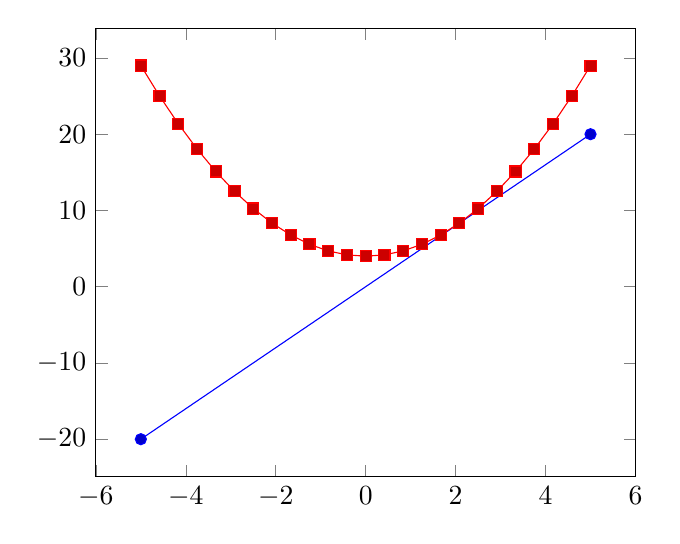
\begin{tikzpicture}
\begin{axis}[
    declare function={
        C=4;
        square(\t)=(\t)^2 + C;
    },
]
    \addplot+ [samples=2] {C*x};

    \addplot {square(x)};
\end{axis}
\end{tikzpicture}
\end{codeexample}
    %
    The definitions as such have the form \meta{function}\meta{argument list} =
    \meta{definition} where the \meta{argument list} contains a
    comma-separated-list of arguments like |\t| or |\t,\a,\b|. The
    \meta{definition} is a math expression which makes use of these arguments.

    Please refer to \cite{tikz} for more details.
\end{key}

\begin{command}{\pgfplotstableread\marg{file}}
    Please refer to the manual of \PGFPlotstable{}, |pgfplotstable.pdf|, which
    is part of the \PGFPlots{} bundle.
\end{command}

\begin{command}{\pgfplotstabletypeset\marg{\textbackslash macro}}
    Please refer to the manual of \PGFPlotstable{}, |pgfplotstable.pdf|, which
    is part of the \PGFPlots{} bundle.
\end{command}

\begin{command}{\pgfplotsiffileexists\marg{filename}\marg{true code}\marg{false code}}
    Invokes \meta{true code} if \meta{filename} exists and \meta{false code} if
    not. Can be used in looping macros, for example to plot every data file
    until there are no more of them.
\end{command}

\begin{command}{\pgfplotsutilifstringequal\marg{first}\marg{second}\marg{true code}\marg{false code}}
    A simple ``strcmp'' tool which invokes \meta{true code} if \meta{first}
    $=$\meta{second} and \meta{false code} otherwise. This does not expand
    macros.
\end{command}

\begin{commandlist}{\pgfkeys,\pgfeov,\pgfkeysvalueof,\pgfkeysgetvalue}
    These commands are part of the \Tikz{} way of specifying options, its
    sub-package |pgfkeys|. The |\pgfplotsset| command is actually nothing but a
    wrapper around |\pgfkeys|.

    A short introduction into |\pgfkeys| can be found in~\cite{keyvalintro}
    whereas the complete reference is, of course, the \Tikz{}
    manual~\cite{tikz}.

    The key |\pgfkeysvalueof|\marg{key name} expands to the value of a key;
    |\pgfkeysgetvalue|\marg{key name}\marg{\textbackslash macro} stores the
    value of \meta{key name} into \meta{\textbackslash macro}. The |\pgfeov|
    macro is used to delimit arguments for code keys in |\pgfkeys|, please
    refer to the references mentioned above.
\end{commandlist}


\section[Commands Inside Of PGFPlots Axes]
        {Commands Inside Of {\normalfont\PGFPlots{}} Axes}

\begin{command}{\autoplotspeclist}
    This command should no longer be used, although it will be kept as
    technical implementation detail. Please use the `|cycle list|' option,
    Section~\ref{sec:cycle:list}.
\end{command}

\begin{command}{\logten}
    Expands to the constant $\log(10)$. Useful for log plots because $\log(10^i)
    = i\log(10)$. This command is only available inside of a \Tikz{} picture.
\end{command}

\begin{command}{\pgfmathprintnumber\marg{number}}
    Generates pretty-printed output\footnote{This method was previously
    \texttt{\textbackslash prettyprintnumber}. Its functionality has been
    included into \PGF{} and the old command is now deprecated.} for
    \meta{number}. This method is used for every tick label.

    The number is printed using the current number printing options, see the
    manual of \PGFPlotstable{} which comes with this package for the different
    number styles, rounding precision and rounding methods.
\end{command}

\begin{command}{\numplots}
    Inside of any of the axis environments, associated style, option or
    command, |\numplots| expands to the total number of plots.
\end{command}

\begin{command}{\numplotsofactualtype}
    Like |\numplots|, this macro returns the total number of plots which have
    the same plot handler. Thus, if you have |sharp plot| active, it returns
    the number of all |sharp plots|. If you have |ybar| active, it returns the
    number of |ybar| plots and so on.
\end{command}

\begin{command}{\plotnum}
    Inside of |\addplot| or any associated style, option or command, |\plotnum|
    expands to the current plot's number, starting with~$0$.
\end{command}

\begin{command}{\plotnumofactualtype}
    Like |\plotnum|, but it returns the number among all plots of the same
    type. The number of all such plots is available using
    |\numplotsofactualtype|.
\end{command}

\begin{command}{\coordindex}
    Inside of an |\addplot| command, this macro expands to the number of the
    actual coordinate (starting with~$0$).

    It is useful together with |x filter| or |y filter| to (de)select
    coordinates.
\end{command}


\section{Path Operations}

\begin{commandlist}{\path,\draw,\fill,\node,\matrix}
    These commands are \Tikz{} drawing commands all of which are documented
    in~\cite{tikz}. They are used to draw or fill paths, generate text nodes or
    aligned text matrices. They are equivalent to
    \pgfmanualpdflabel{/tikz/draw}{}|\path[draw]|,
    \pgfmanualpdflabel{/tikz/fill}{}|\path[fill]|,
    \pgfmanualpdflabel{/tikz/node}{}|\path[node]|,
    \pgfmanualpdflabel{/tikz/matrix}{}|\path[matrix]|,
    respectively.
\end{commandlist}

\begin{pathoperation}{--}{\meta{coordinate}}
    A \Tikz{} path operation which connects the current point (the last one
    before |--|) and \meta{coordinate} with a straight line.
\end{pathoperation}

{\catcode`\|=12
\begin{pathoperation}[noindex]{|-}{\meta{coordinate}}
\pgfmanualpdflabel[\catcode`\|=12 ]{|-}{}%
    A \Tikz{} path operation which connects the current point and
    \meta{coordinate} with \emph{two} straight lines: first vertical, then
    horizontal.
\end{pathoperation}

\begin{pathoperation}[noindex]{-|}{\meta{coordinate}}
\pgfmanualpdflabel[\catcode`\|=12 ]{-|}{}%
    A \Tikz{} path operation which connects the current point and
    \meta{coordinate} with \emph{two} straight lines: first horizontal, then
    vertical.
\end{pathoperation}
}

\begin{keylist}{/tikz/xshift=\marg{dimension},/tikz/yshift=\marg{dimension}}
    These \Tikz{} keys allow to shift something by \meta{dimension} which is
    any \TeX{} size (or expression).
\end{keylist}

\begin{command}{\pgfplotsextra\marg{low-level path commands}}
    A command to execute \meta{low-level path commands} in a \PGFPlots{} axis.
    Since any drawing commands inside of an axis need to be postponed until the
    axis is complete and the scaling has been initialised, it is not possible
    to simply draw any paths. Instead, it is necessary to draw them as soon as
    the axis is finished. This is done automatically for every \Tikz{} path --
    and it is also done manually if you write |\pgfplotsextra|\marg{commands}.
    %
\begin{codeexample}[]
\begin{tikzpicture}
\begin{axis}[xmin=0,xmax=3,ymin=0,ymax=5]
    \pgfplotsextra{
        \pgfpathmoveto{\pgfplotspointaxisxy{1}{2}}
        \pgfpathlineto{\pgfplotspointaxisxy{2}{4}}
        \pgfusepath{stroke}
    }
\end{axis}
\end{tikzpicture}
\end{codeexample}
    %
    The example above initializes an axis and executes the basic level path
    commands as soon as the axis is ready. The execution of multiple |\path|,
    |\addplot| and |\pgfplotsextra| commands is in the same sequence as they
    occur in the environment.\footnote{Except for stacked plots where the
    sequence may be reverse, see the key \texttt{reverse stack plots}.}
\end{command}

\begin{command}{\pgfplotspathaxisoutline}
    Generates a path which resembles the outline of the current axis. This path
    is used for clip paths and the background paths (if any).
\end{command}


\section{Specifying Basic Coordinates}
\label{sec:basic:coordinates}

\begin{commandlist}{%
    \pgfplotspointaxisxy\marg{x coordinate}\marg{y coordinate},
    \pgfplotspointaxisxyz\marg{x coordinate}\marg{y coordinate}\marg{z coordinate}%
}
    Point commands like |\pgfpointxy| which take logical, absolute coordinates
    and return a low-level point. Every transformation from user
    transformations to logarithms is applied.

    Since the transformations are initialized after the axis is complete, this
    command needs to be postponed (see |\pgfplotsextra|).

    This command is the basic level variant of |axis cs:|\meta{x
    coordinate}|,|\meta{y coordinate}|,|\meta{z coordinate}.

    Note that this is also the default coordinate system during the
    visualization phase; in other words: if you write |\draw (1,2) -- (1,4)|,
    \PGFPlots{} will automatically use |(axis cs:1,2) -- (axis cs:1,4)|.
\end{commandlist}

\begin{commandlist}{%
    \pgfplotspointaxisdirectionxy\marg{x coordinate}\marg{y coordinate},
    \pgfplotspointaxisdirectionxyz\marg{x coordinate}\marg{y coordinate}\marg{z coordinate}%
}
    Point commands like |\pgfpointxy| which take logical, \emph{relative}
    coordinates and return a low-level point. Every transformation from user
    transformations to logarithms is applied. The difference to
    |\pgfplotspointaxisxy| is that the shift of the linear transformation is
    skipped here (compare |disabledatascaling|).

    This command is the basic level variant of |axis direction cs:|\meta{x
    coordinate}|,|\meta{y coordinate}|,|\meta{z coordinate}. Please refer to
    the documentation of |axis direction cs| for more details.

    Use this command whenever something of \emph{relative} character like
    directions or lengths need to be supplied. One use case is to draw
    ellipses:
    %
\begin{codeexample}[]
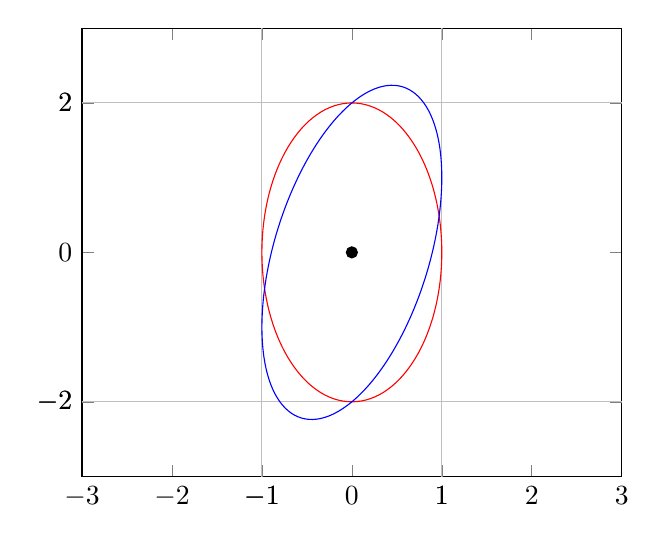
\begin{tikzpicture}
\begin{axis}[
    xmin=-3,   xmax=3,
    ymin=-3,   ymax=3,
    extra x ticks={-1,1},
    extra y ticks={-2,2},
    extra tick style={grid=major},
]
    \draw [red] \pgfextra{
        \pgfpathellipse{\pgfplotspointaxisxy{0}{0}}
            {\pgfplotspointaxisdirectionxy{1}{0}}
            {\pgfplotspointaxisdirectionxy{0}{2}}
    % see also the documentation of
    % 'axis direction cs' which
    % allows a simpler way to draw this ellipse
    };
    \draw [blue] \pgfextra{
        \pgfpathellipse{\pgfplotspointaxisxy{0}{0}}
            {\pgfplotspointaxisdirectionxy{1}{1}}
            {\pgfplotspointaxisdirectionxy{0}{2}}
    };
    \addplot [only marks,mark=*] coordinates
        { (0,0) };
\end{axis}
\end{tikzpicture}
\end{codeexample}

    Since the transformations are initialized after the axis is complete, this
    command needs to be provided either inside of a \tikzname{} |\path| command
    (like |\draw| in the example above) or inside of |\pgfplotsextra|.
\end{commandlist}

\begin{commandlist}{%
    \pgfplotspointrelaxisxy\marg{rel x coordinate}\marg{rel y coordinate},
    \pgfplotspointrelaxisxyz\marg{rel x coordinate}\marg{rel y coordinate}\marg{rel z coordinate}%
}
    Point commands which take \emph{relative} coordinates such that $x=0$ is
    the \emph{lower} $x$-axis limit and $x=1$ the \emph{upper} $x$-axis limit.

    These commands are used for |rel axis cs|.

    Please note that the transformations are only initialised if the axis is
    complete! This means you need to provide |\pgfplotsextra|.
\end{commandlist}

\begin{commandlist}{%
    \pgfplotspointdescriptionxy\marg{$x$ fraction}\marg{$y$ fraction},
    \pgfplotsqpointdescriptionxy\marg{$x$ fraction}\marg{$y$ fraction}%
}
    Point commands such that |{0}{0}| is the lower left corner of the axis'
    bounding box and |{1}{1}| the upper right one; everything else is in
    between. The `|q|' variant is quicker as it doesn't invoke the math parser
    on its arguments.

    They are used for |axis description cs|, see
    Section~\ref{pgfplots:sec:axis:description:cs}.
\end{commandlist}

\begin{commandlist}{\pgfplotspointaxisorigin}
    A point coordinate at the origin, $(0,0,0)$. If the origin is not part of
    the axis limits, the nearest point on the boundary is returned instead.

    This is the same coordinate as returned by the |origin| anchor.
\end{commandlist}

\begin{commandlist}{%
    \pgfplotstransformcoordinatex\marg{x coordinate of an axis},
    \pgfplotstransformcoordinatey\marg{y coordinate of an axis},
    \pgfplotstransformcoordinatez\marg{z coordinate of an axis}%
}
    Defines |\pgfmathresult| to be the low-level \PGF{} coordinate
    corresponding to the input argument.

    The command applies any |[xyz] coord trafo| keys, data scalings and/or
    logarithms or whatever \PGFPlots{} does to map input coordinates to
    internal coordinates.

    The result can be used inside of a |\pgfpointxy| statement (i.e.\@ it still
    needs to be scaled with the respective \PGF{} unit vector).
    %
\begin{codeexample}[]
\begin{tikzpicture}
\pgfplotsset{compat/pgfpoint substitution=1.3}
\begin{axis}[xmin=0,xmax=2,ymin=0,ymax=5]
    \pgfplotsextra{
        \pgfplotstransformcoordinatex{1}
        \let\xcoord=\pgfmathresult
        \pgfplotstransformcoordinatey{1}
        \let\ycoord=\pgfmathresult
        \pgfpathcircle
            {\pgfqpointxy{\xcoord}{\ycoord}}
            {5pt}
        \pgfusepath{fill}
    }
\end{axis}
\end{tikzpicture}
\end{codeexample}
    %
    Note that \PGFPlots{} substitutes |\pgfqpointxy| by |\pgfplotspointaxisxyz|
    by default -- and this command implicitly transforms coordinates anyway. In
    order to see the difference, the preceding example first disables this
    automatic substitution of coordinate systems by means of
    |compat/pgfpoint substitution=1.3|.
    %
    The result of this command is also available as math method
    |transformcoordinatex| (see the documentation for |axis cs|).

    Please note that the transformations are only initialised if the axis is
    complete. This means you need to provide |\pgfplotsextra| as is shown in
    the example above.
\end{commandlist}

\begin{commandlist}{%
    \pgfplotstransformdirectionx\marg{x direction of an axis},
    \pgfplotstransformdirectiony\marg{y direction of an axis},
    \pgfplotstransformdirectionz\marg{z direction of an axis}%
}
    Defines |\pgfmathresult| to be a low-level \PGF{} \emph{direction vector
    component}.

    A direction vector needs to be \emph{added} to some coordinate in order to
    get a coordinate, compare the documentation for
    |\pgfplotspointaxisdirectionxy| and |axis direction cs|.

    The argument \meta{x direction of an axis} is processed in (almost) the
    same way as for the macro which operates on absolute positions,
    |\pgfplotstransformcoordinatex|. The only difference is that
    \emph{directions} need no shifting transformation.

    The result of this command is also available as math method
    |transformdirectionx| (see the documentation for |axis direction cs|).

    See |axis direction cs| for details and examples about this command.
\end{commandlist}

% this command is for internal use only:
%--------------------------------------------------
% \begin{command}{\pgfplotsconvertunittocoordinate\marg{x, y or z}\marg{dimension}}
%     Converts a dimension (with unit!) to a corresponding $x$-, $y$- or $z$-coordinate. The result will be written to |\pgfmathresult| (without units).
%
%     It is possible to use the result as arguments for the |\pgfpointxyz| commands.
%
%     The effect is to multiply \meta{dimension} with the inverse length of the unit vector for the specified axis. These lengths are precomputed in \PGFPlots{} so the operation is fast.
% \begin{codeexample}[code only]
% \pgfplotsconvertunittocoordinate{x}{5pt}
% % now, the command uses exactly 5pt in x direction:
% \pgfqpointxyz{\pgfmathresult}{4}{3}
% \end{codeexample}
% \end{command}
%--------------------------------------------------

\begin{commandlist}{%
    \pgfplotspointunitx,
    \pgfplotspointunity,
    \pgfplotspointunitz%
}
    Low-level point commands which return the canvas $x$, $y$ or $z$ unit
    vectors.

    The |\pgfplotspointunitx| is the \pgfname{} unit vector in $x$ direction.

    These vectors are essentially the same as |\pgfqpointxyz{1}{0}{0}|,
    |\pgfqpointxyz{0}{1}{0}|, and |\pgfqpointxyz{0}{0}{1}|, respectively.

    The unit $z$ vector is only defined for three dimensional axes.
\end{commandlist}

\begin{commandlist}{%
    \pgfplotsunitxlength,
    \pgfplotsunitylength,
    \pgfplotsunitzlength,
    \pgfplotsunitxinvlength,
    \pgfplotsunityinvlength,
    \pgfplotsunitzinvlength%
}
    Macros which expand to the vector length $\lVert x_i \rVert$ of the
    respective unit vector $x_i$ or the inverse vector length, $1/\lVert x_i
    \rVert$. These macros can be used inside of |\pgfmathparse|, for example.

    The $x_i$ are the |\pgfplotspointunitx| variants.
\end{commandlist}

\begin{command}{\pgfplotsqpointoutsideofaxis%
        \marg{three-char-string}\marg{coordinate}\marg{normal distance}%
}
    Provides a point coordinate on one of the available four axes in case of a
    two dimensional figure or on one of the available twelve axes in case of a
    three dimensional figure.

    The desired axis is uniquely identified by a three character string,
    provided as first argument to the command. The first of the three
    characters is `|0|' if the $x$-coordinate of the specified axis passes
    through the lower axis limit. It is `|1|', if the $x$-coordinate of the
    specified axis passes through the upper axis limit. Furthermore, it is
    `|2|' if it passes through the origin. The second character is also either
    |0|, |1| or |2| and it characterizes the position on the $y$-axis. The
    third character is for the third dimension, the $z$-axis. It should be left
    at `|0|' for two dimensional plots. However, \emph{one} of the three
    characters should be `|v|', meaning the axis \underline varies. For
    example, |v01| denotes $\{ (x,y_{\min},z_{\max}) \vert x \in \R \}$.

    The second argument, \meta{coordinate} is the logical coordinate on that
    axis. Since two coordinates of the axis are fixed, \meta{coordinate} refers
    to the \underline varying component of the axis. It must be a number
    without unit; no math expressions are supported here.

    The third argument \meta{normal distance} is a dimension like |10pt|. It
    shifts the coordinate away from the designated axis in direction of the
    outer normal vector. The outer normal vector always points away from the
    axis. It is computed using |\pgfplotspointouternormalvectorofaxis|.

    There are several variants of this command which are documented in the
    source code. One of them is particularly useful:
\end{command}

\begin{command}{\pgfplotsqpointoutsideofaxisrel%
        \marg{three-char-string}\marg{axis fraction}\marg{normal distance}%
}
    This point coordinate is a variant of |\pgfplotsqpointoutsideofaxis| which
    allows to provide an \meta{axis fraction} instead of an absolute
    coordinate. The fraction is a number between $0$ (lower axis limit) and $1$
    (upper axis limit), i.e.\@ it is given in percent of the total axis. It is
    possible to provide negative values or values larger than one.

    The |\pgfplotsqpointoutsideofaxisrel| command is similar in spirit to
    |rel axis cs|.

    There is one speciality in conjunction with reversed axes: if the axis has
    been reversed by |x dir=reverse| and, in addition,
    |allow reversal of rel axis cs| is true, the value $0$ denotes the
    \emph{upper} limit while $1$ denotes the \emph{lower} limit. The effect is
    that coordinates won't change just because of axis reversal.
        \index{allow reversal of rel axis cs}%
\end{command}

\begin{command}{\pgfplotspointouternormalvectorofaxis\marg{three-char-string}}
    A point command which yields the outer normal vector of the respective
    axis. The normal vector has length $1$ (computed with
    |\pgfpointnormalised|). It is the same normal vector used inside of
    |\pgfplotsqpointoutsideofaxis| and its variants.

    The output of this command will be cached and reused during the lifetime
    of an axis.
\end{command}

\begin{command}{\pgfplotsticklabelaxisspec\marg{x, y or z}}
    Expands to the three character identification for the axis containing tick
    labels for the chosen axis, either \meta{x}, \meta{y} or \meta{z}.
\end{command}

\begin{command}{\pgfplotsvalueoflargesttickdimen\marg{x, y or z}}
    Expands to the largest distance of a tick position to its tick label
    bounding box in direction of the outer unit normal vector. It does also
    include the value of the |ticklabel shift| key.

    This value is used for |ticklabel cs|.
\end{command}

\begin{commandlist}{
    \pgfplotsmathfloatviewdepthxyz\marg{x}\marg{y}\marg{z},
    \pgfplotsmathviewdepthxyz\marg{x}\marg{y}\marg{z}%
}
    Both macros define |\pgfmathresult| to be the ``depth'' of a three
    dimensional point $\bar x = (x,y,z)$. The depth is defined to be the scalar
    product of $\bar x$ with $\vec d$, the view direction of the current axis.

    For |\pgfplotsmathfloatviewdepthxyz|, the arguments are parsed as floating
    point numbers and the result is encoded in floating point. A fixed point
    representation can be generated with
    |\pgfmathfloattofixed{\pgfmathresult}|.

    For |\pgfplotsmathviewdepthxyz|, \TeX{} arithmetics is employed for the
    inner product and the result is assigned in fixed point. This is slightly
    faster, but has considerably smaller data range.

    Both commands can only be used \emph{inside} of a three dimensional
    \PGFPlots{} axis (as soon as the axis is initialised, see
    |\pgfplotsextra|).
\end{commandlist}

\begin{texif}{pgfplotsthreedim}
    A \TeX{} |\if| which evaluates the \meta{true code} if the axis is three
    dimensional and the \meta{else code} if not.
\end{texif}


\section{Accessing Axis Limits}

It is also possible to access axis limits during the visualization phase,
i.e.\@ during |\end{axis}|. Please refer to the reference documentation for
|xmin| on page~\pageref{page:access:limits}.


\section{Accessing Point Coordinate Values}

During the visualization phase, \PGFPlots{} provides access to the currently
processed coordinate and its values.

This access requires a call to specific macros. These macros write the
coordinate values to some publicly available key--value pairs. Then, the
current point's $x$, $y$, $z$, and color data can be accessed.

\begin{commandlist}{\pgfplotspointgetcoordinates,\pgfplotspointgetcoordinates\marg{point}}

    After invoking the macro, the following keys will be set:

    \declaretext{/data point/x} will contain the current point's $x$-coordinate.

    \declaretext{/data point/y} will contain the current point's $y$-coordinate.

    \declaretext{/data point/z} will contain the current point's $z$-coordinate
    (if applicable).

    \declaretext{/data point/meta} will contain the current point's
    |point meta| value (if applicable).

    \declaretext{/data point/index} will contain the current point's index in
    the coordinate stream. This is actually the same as |\coordindex|.

    This command actually supports two modes of operation:
    %
    \begin{enumerate}
        \item Without arguments. In this case, it returns values of the point
            which is about to be processed by the current plot handler.
        \item With an argument in curly braces. In this case, it expects a
            coordinate and assigns the keys accordingly. Note that this
            command merely supports two-dimensional axes and assigns only
            |/data point/x| and |/data point/y|.
    \end{enumerate}

    The returned values are the same as they can be read on the axes, they are
    also the same as you would write them into |axis cs|.

    This means that any |x coord inv trafo| has been applied on the value. It
    also means that the exponential function has been called even though the
    internal coordinate was present in log format.

    This function is implicitly called for any |scatter| plot (including
    |nodes near coords|). This allows to access \emph{all} coordinate values at
    once:
    %
\begin{codeexample}[]
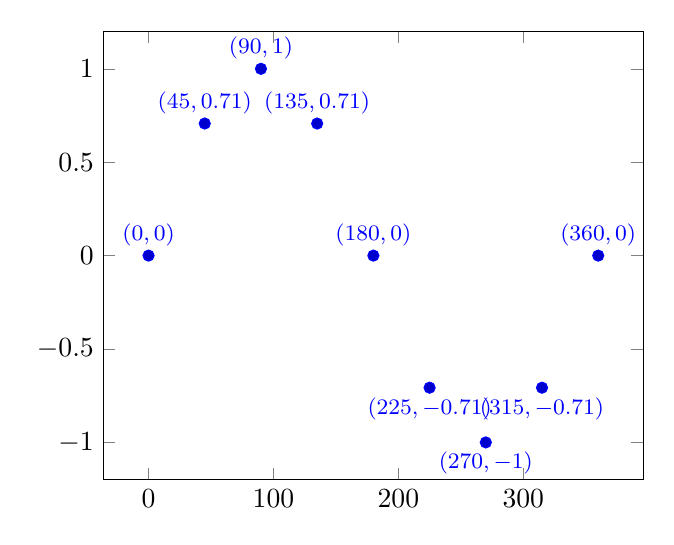
\begin{tikzpicture}
\begin{axis}
    \addplot+ [
        domain=0:360,
        samples=9,
        only marks,
        nodes near coords={%
            \footnotesize
            $(\pgfmathprintnumber
                {\pgfkeysvalueof{/data point/x}},
               \pgfmathprintnumber
                {\pgfkeysvalueof{/data point/y}})$%
        },
    ] {sin(x)};
\end{axis}
\end{tikzpicture}
\end{codeexample}
    %
    The example works because |\pgfplotspointgetcoordinates| is part of the
    standard implementation of |nodes near coords|; the resulting values are
    directly available. Note that the preceding example would have been simpler
    if we would have printed just one value: |nodes near coords| resorts to the
    |point meta|. And that, in turn, contains the $y$-coordinate anyway by
    default.

    A more advanced example would be a |ybar| plot in which nodes shall be
    placed at the lower end of the axis, together with some dotted lines to the
    respective bars:
    %
\begin{codeexample}[]
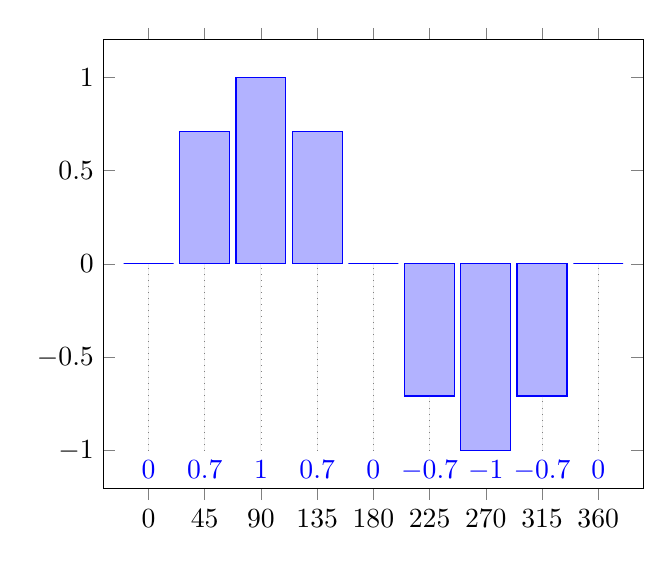
\begin{tikzpicture}
\begin{axis}[
    ybar,
    nodes near coords,
    %
    % we want to provide absolute 'at' values
    % for the nodes:
    scatter/position=absolute,
    every node near coord/.style={
        at={(\pgfkeysvalueof{/data point/x},-1)},
        % pretty printing:
        anchor=north,
        /pgf/number format/fixed,
        /pgf/number format/precision=1,
        % assign a name which can be referenced below:
        name=NNC\pgfkeysvalueof{/data point/index},
    },
    % ... draw a dotted line between
    % the marker and the bar:
    /pgfplots/scatter/@post marker code/.add code={}{
        \draw [dotted,help lines]
            (NNC\pgfkeysvalueof{/data point/index})
            -- (\pgfkeysvalueof{/data point/x},
            {min(0,\pgfkeysvalueof{/data point/y})});
    },
    % assign suitable tick labels:
    xtick=data,
]
    % some dummy data:
    \addplot+ [
        domain=0:360,
        bar width=360/9,
        samples=9,
    ] {sin(x)};
\end{axis}
\end{tikzpicture}
\end{codeexample}
    %
    Again, the command is used implicitly as part of |nodes near coords| and
    does not occur in the example as such.

    \paragraph{See also} the related example online under
    \url{https://tex.stackexchange.com/a/141006}. It demonstrates how to
    place the nodes generated by |nodes near coords| based on the value (either
    inside of a bar or above it).

    The following example uses an argument in curly braces for which we seek
    coordinate values:
    %
\begin{codeexample}[]
% requires \usetikzlibrary{intersections}
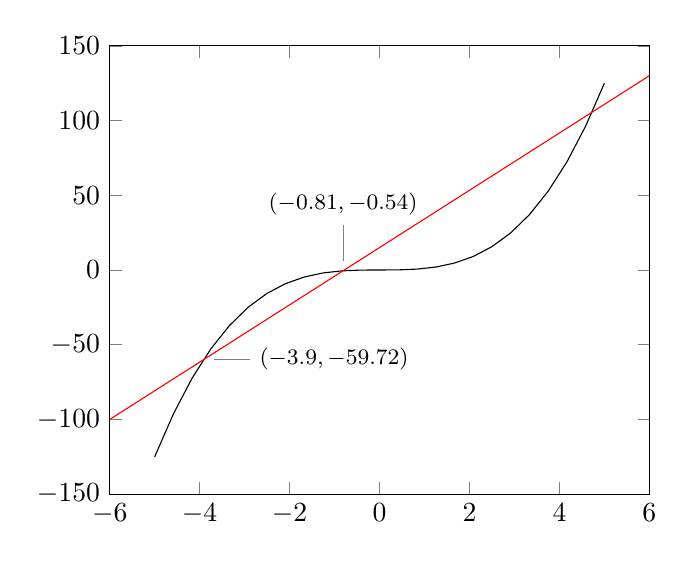
\begin{tikzpicture}
\begin{axis}
    \addplot [name path=A] {x^3};

    \draw [red,name path=HelperLine]
        (axis cs:-6,-100) -- (axis cs:6,130);

    \draw [
        font=\footnotesize,
        name intersections={of=A and HelperLine},
    ]
    node [pin={right:
      \pgfplotspointgetcoordinates{(intersection-1)}
        $(\pgfmathprintnumber[fixed]{
            \pgfkeysvalueof{/data point/x}},
          \pgfmathprintnumber[fixed]{
            \pgfkeysvalueof{/data point/y}})$
      }
    ] at (intersection-1) {}
    node [pin={
      \pgfplotspointgetcoordinates{(intersection-2)}
        $(\pgfmathprintnumber[fixed]{
            \pgfkeysvalueof{/data point/x}},
          \pgfmathprintnumber[fixed]{
            \pgfkeysvalueof{/data point/y}})$
      }
    ] at (intersection-2) {};
\end{axis}
\end{tikzpicture}
\end{codeexample}
    %
    The example computes and names intersections of |A| and |HelperLine|. The
    following code generates pins at the intersections. To this end, it uses
    |\pgfplotspointgetcoordinates|\marg{point} which defines |/data point/x|
    and |/data point/y|. These values are then formatted using
    |\pgfmathprintnumber|.

    In its second mode, |\pgfplotspointgetcoordinates|\marg{point} expects one
    of two things as \meta{point}:
    %
    \begin{enumerate}
        \item a basic-level \PGF{} point like |\pgfpointanchor{A}{center}| or
        \item a \Tikz{} point like |(A.base)| or |(3,5)|.
    \end{enumerate}
\end{commandlist}

\begin{command}{\pgfplotspointgetnormalizedcoordinates}
    A macro which is very similar to |\pgfplotspointgetcoordinates|.
    Consequently, it is also supposed to be called during the visualization phase.

    It assigns the very same output macros, but the values are different. More
    precisely, it defines the macros

    \declaretext{/data point/x} will contain the current point's
    \emph{normalized} $x$-coordinate.

    \declaretext{/data point/y} will contain the current point's
    \emph{normalized} $y$-coordinate.

    \declaretext{/data point/z} will contain the current point's
    \emph{normalized} $z$-coordinate (if applicable).

    \declaretext{/data point/meta} will contain the current point's
    |point meta| value (if applicable).

    \declaretext{/data point/index} will contain the current point's index in
    the coordinate stream. This is actually the same as |\coordindex|.

    The keyword \declaretext{normalized} means that the values are in a
    suitable numerical form which can be consumed by the axis. To be more
    specific: any user |x coord inv trafo| is \emph{ignored}. An important
    example would be |symbolic x coords|: the normalized coordinates would be
    some associated numbers, not the symbols. The results returned by
    |\pgfplotspointgetcoordinates| would be the symbols. For logarithm axes,
    the normalized values are the logs.

    Typically, normalized values are much more useful when you want to apply
    some math operation like averaging or subtraction.

    This function needs to be called explicitly. It is currently used by
    |ybar stacked| to align |nodes near coords|.
\end{command}


\section{Layer Access}

\begin{command}{\pgfplotsonlayer\marg{layer name}}
    A low-level command which will check if the current axis has layer support
    activated and, if so, calls |\pgfonlayer|\marg{layer name}.

    There must be a |\endpgfplotsonlayer| to delimit the environment.
\end{command}

\begin{command}{\endpgfplotsonlayer}
    The end of |\pgfplotsonlayer|.
\end{command}

\begin{command}{\pgfonlayer\marg{layer name}}
    A low-level command of \PGF{} which will collect everything until the
    matching |\endpgfonlayer| into layer \meta{layer name}.

    The \meta{layer name} must be active, i.e.\@ it must be part of the layer
    names of |set layers|.

    The only special case is if you call |\pgfdeclarelayer{discard}| somewhere:
    this special layer has a ``magical name'' which serves as |/dev/null| if it
    is enabled using |\pgfonlayer{discard}|: it does not need to be active and
    everything assigned to this layer will be thrown away if it is not part of
    the layer name configuration.

    There must be a |\endpgfonlayer| to delimit the environment.
\end{command}

\begin{command}{\endpgfonlayer}
    The end of |\pgfonlayer|.
\end{command}


\begin{command}{\pgfsetlayers\marg{layer list}}
    This is a low-level command of \PGF{}. At the time of this writing, it is
    the only way to tell \PGF{} which layers it shall use for the current/next
    picture. It is used implicitly by |set layers|.
\end{command}


\printindex

\bibliographystyle{abbrv} %gerapali} %gerabbrv} %gerunsrt.bst} %gerabbrv}% gerplain}
\nocite{pgfplotstable}
\nocite{programmingnotes}
\bibliography{pgfplots}
\end{document}

% -----------------------------------------------------------------------------
% For Stefan Pinnow as reminder on what to look for when editing the manual
% -----------------------------------------------------------------------------
% There should be no line breaks in the following environments
% - |...|
% - \declareandlabel{...}
% - \verbpdfref{...}
% If "MakeTikzPictures" isn't running through check one of the externalized
% LOG files what is the cause of that.
% -----------------------------------------------------------------------------


%%%%%%%%%%%%%%%%%%%%%%%%%%%%%%%%%%%%%%%%%%%%%%%%%%%%%%%%%%%%%%%%%%%%%%%%%%%%%
%
% Package pgfplots.sty documentation.
%
% Copyright 2007/2008 by Christian Feuersaenger.
%
% This program is free software: you can redistribute it and/or modify
% it under the terms of the GNU General Public License as published by
% the Free Software Foundation, either version 3 of the License, or
% (at your option) any later version.
%
% This program is distributed in the hope that it will be useful,
% but WITHOUT ANY WARRANTY; without even the implied warranty of
% MERCHANTABILITY or FITNESS FOR A PARTICULAR PURPOSE.  See the
% GNU General Public License for more details.
%
% You should have received a copy of the GNU General Public License
% along with this program.  If not, see <http://www.gnu.org/licenses/>.
%
%
%%%%%%%%%%%%%%%%%%%%%%%%%%%%%%%%%%%%%%%%%%%%%%%%%%%%%%%%%%%%%%%%%%%%%%%%%%%%%
% SEE pgfplots-macros.tex as well!
%\pdfminorversion=5 % to allow compression
%\pdfobjcompresslevel=2
\documentclass[a4paper,openany]{book}

\let\bookmaketitle=\maketitle

% -----------------------------------
% this here is from ltxdoc:
\usepackage{doc}[=v2]
\AtBeginDocument{\MakeShortVerb{\|}}
%\setlength{\textwidth}{355pt}
%\addtolength\marginparwidth{30pt}
%\addtolength\oddsidemargin{20pt}
%\addtolength\evensidemargin{20pt}
\def\cmd#1{\cs{\expandafter\cmd@to@cs\string#1}}
\def\cmd@to@cs#1#2{\char\number`#2\relax}
\DeclareRobustCommand\cs[1]{\texttt{\char`\\#1}}
\providecommand\marg[1]{%
  {\ttfamily\char`\{}\meta{#1}{\ttfamily\char`\}}}
\providecommand\oarg[1]{%
  {\ttfamily[}\meta{#1}{\ttfamily]}}
\providecommand\parg[1]{%
  {\ttfamily(}\meta{#1}{\ttfamily)}}
\raggedbottom

% -----------------------------------
\input{pgfplots.preamble.tex}

\makeatletter
% I want a two-column index just as in pgfmanual styles. This here
% was the best way to get one:
\def\index@prologue{\section*{Index}\addcontentsline{toc}{chapter}{Index}
}
\makeatother

%\RequirePackage[german,english,francais]{babel}

\def\matlabcolormaptext{This colormap is similar to one shipped with Matlab$^\text{\textregistered}$ under a similar name.}

\IfFileExists{tikzlibraryspy.code.tex}{%
\usetikzlibrary{spy}
}{%
    \message{ERROR: tikz SPY library NOT available. The manual will only compile partially.^^J}%
}%

\usepackage{xparse}% for colorbrewer manual

\usetikzlibrary{
    decorations.markings,
    decorations.footprints,
    shapes.arrows,
    matrix,
    positioning,
}

\usepgfplotslibrary{
    fillbetween,
    ternary,
    smithchart,
    patchplots,
    polar,
    colormaps,
    colorbrewer,
    colortol,           % docu not ready yet
}
\pgfqkeys{/codeexample}{%
    every codeexample/.append style={
        /pgfplots/every ternary axis/.append style={
            /pgfplots/legend style={fill=graphicbackground},
        }
    },
    tabsize=4,
}

\pgfplotsmanualenableexternalizationofexpensive

%\usetikzlibrary{external}
%\tikzexternalize[prefix=figures/]{pgfplots}

\title{%
    Manual for Package \PGFPlots{}\\
    {\small 2D/3D Plots in \LaTeX{}, Version \pgfplotsversion}\\
    {\small\href{https://github.com/pgf-tikz/pgfplots}{https://github.com/pgf-tikz/pgfplots}}
    %\\{\small Attention: you are using an unstable development version.}
}

\makeatletter
\long\def\abstractsmuggle{%
    \centering
    \textbf{Abstract}\\[0.5cm]

    \begin{minipage}{12cm}
        \PGFPlots{} draws high-quality function plots in normal or logarithmic
        scaling with a user-friendly interface directly in \TeX{}. The user
        supplies axis labels, legend entries and the plot coordinates for one or
        more plots and \PGFPlots{} applies axis scaling, computes any logarithms
        and axis ticks and draws the plots. It supports line plots, scatter
        plots, piecewise constant plots, bar plots, area plots, mesh and surface
        plots, patch plots, contour plots, quiver plots, histogram plots, box
        plots, polar axes, ternary diagrams, smith charts and some more. It is
        based on Till Tantau's package \PGF{}/\Tikz{}.
    \end{minipage}

}%

\expandafter\date\expandafter{\@date\\[2cm]
    \abstractsmuggle
}%
\makeatother

%\includeonly{pgfplots.reference}


\begin{document}

\def\plotcoords{%
\addplot coordinates {
(5,8.312e-02)    (17,2.547e-02)   (49,7.407e-03)
(129,2.102e-03)  (321,5.874e-04)  (769,1.623e-04)
(1793,4.442e-05) (4097,1.207e-05) (9217,3.261e-06)
};

\addplot coordinates{
(7,8.472e-02)    (31,3.044e-02)    (111,1.022e-02)
(351,3.303e-03)  (1023,1.039e-03)  (2815,3.196e-04)
(7423,9.658e-05) (18943,2.873e-05) (47103,8.437e-06)
};

\addplot coordinates{
(9,7.881e-02)     (49,3.243e-02)    (209,1.232e-02)
(769,4.454e-03)   (2561,1.551e-03)  (7937,5.236e-04)
(23297,1.723e-04) (65537,5.545e-05) (178177,1.751e-05)
};

\addplot coordinates{
(11,6.887e-02)    (71,3.177e-02)     (351,1.341e-02)
(1471,5.334e-03)  (5503,2.027e-03)   (18943,7.415e-04)
(61183,2.628e-04) (187903,9.063e-05) (553983,3.053e-05)
};

\addplot coordinates{
(13,5.755e-02)     (97,2.925e-02)     (545,1.351e-02)
(2561,5.842e-03)   (10625,2.397e-03)  (40193,9.414e-04)
(141569,3.564e-04) (471041,1.308e-04)
(1496065,4.670e-05)
};
}%


\bookmaketitle
\tableofcontents

%%%%%%%%%%%%%%%%%%%%%%%%%%%%%%%%%%%%%%%%%%%%%%%%%%%%%%%%%%%%%%%%%%%%%%%%%%%%%
%
% Package pgfplots.sty documentation.
%
% Copyright 2007/2008 by Christian Feuersaenger.
%
% This program is free software: you can redistribute it and/or modify
% it under the terms of the GNU General Public License as published by
% the Free Software Foundation, either version 3 of the License, or
% (at your option) any later version.
%
% This program is distributed in the hope that it will be useful,
% but WITHOUT ANY WARRANTY; without even the implied warranty of
% MERCHANTABILITY or FITNESS FOR A PARTICULAR PURPOSE.  See the
% GNU General Public License for more details.
%
% You should have received a copy of the GNU General Public License
% along with this program.  If not, see <http://www.gnu.org/licenses/>.
%
%
%%%%%%%%%%%%%%%%%%%%%%%%%%%%%%%%%%%%%%%%%%%%%%%%%%%%%%%%%%%%%%%%%%%%%%%%%%%%%
% SEE pgfplots-macros.tex as well!
%\pdfminorversion=5 % to allow compression
%\pdfobjcompresslevel=2
\documentclass[a4paper,openany]{book}

\let\bookmaketitle=\maketitle

% -----------------------------------
% this here is from ltxdoc:
\usepackage{doc}[=v2]
\AtBeginDocument{\MakeShortVerb{\|}}
%\setlength{\textwidth}{355pt}
%\addtolength\marginparwidth{30pt}
%\addtolength\oddsidemargin{20pt}
%\addtolength\evensidemargin{20pt}
\def\cmd#1{\cs{\expandafter\cmd@to@cs\string#1}}
\def\cmd@to@cs#1#2{\char\number`#2\relax}
\DeclareRobustCommand\cs[1]{\texttt{\char`\\#1}}
\providecommand\marg[1]{%
  {\ttfamily\char`\{}\meta{#1}{\ttfamily\char`\}}}
\providecommand\oarg[1]{%
  {\ttfamily[}\meta{#1}{\ttfamily]}}
\providecommand\parg[1]{%
  {\ttfamily(}\meta{#1}{\ttfamily)}}
\raggedbottom

% -----------------------------------
\input{pgfplots.preamble.tex}

\makeatletter
% I want a two-column index just as in pgfmanual styles. This here
% was the best way to get one:
\def\index@prologue{\section*{Index}\addcontentsline{toc}{chapter}{Index}
}
\makeatother

%\RequirePackage[german,english,francais]{babel}

\def\matlabcolormaptext{This colormap is similar to one shipped with Matlab$^\text{\textregistered}$ under a similar name.}

\IfFileExists{tikzlibraryspy.code.tex}{%
\usetikzlibrary{spy}
}{%
    \message{ERROR: tikz SPY library NOT available. The manual will only compile partially.^^J}%
}%

\usepackage{xparse}% for colorbrewer manual

\usetikzlibrary{
    decorations.markings,
    decorations.footprints,
    shapes.arrows,
    matrix,
    positioning,
}

\usepgfplotslibrary{
    fillbetween,
    ternary,
    smithchart,
    patchplots,
    polar,
    colormaps,
    colorbrewer,
    colortol,           % docu not ready yet
}
\pgfqkeys{/codeexample}{%
    every codeexample/.append style={
        /pgfplots/every ternary axis/.append style={
            /pgfplots/legend style={fill=graphicbackground},
        }
    },
    tabsize=4,
}

\pgfplotsmanualenableexternalizationofexpensive

%\usetikzlibrary{external}
%\tikzexternalize[prefix=figures/]{pgfplots}

\title{%
    Manual for Package \PGFPlots{}\\
    {\small 2D/3D Plots in \LaTeX{}, Version \pgfplotsversion}\\
    {\small\href{https://github.com/pgf-tikz/pgfplots}{https://github.com/pgf-tikz/pgfplots}}
    %\\{\small Attention: you are using an unstable development version.}
}

\makeatletter
\long\def\abstractsmuggle{%
    \centering
    \textbf{Abstract}\\[0.5cm]

    \begin{minipage}{12cm}
        \PGFPlots{} draws high-quality function plots in normal or logarithmic
        scaling with a user-friendly interface directly in \TeX{}. The user
        supplies axis labels, legend entries and the plot coordinates for one or
        more plots and \PGFPlots{} applies axis scaling, computes any logarithms
        and axis ticks and draws the plots. It supports line plots, scatter
        plots, piecewise constant plots, bar plots, area plots, mesh and surface
        plots, patch plots, contour plots, quiver plots, histogram plots, box
        plots, polar axes, ternary diagrams, smith charts and some more. It is
        based on Till Tantau's package \PGF{}/\Tikz{}.
    \end{minipage}

}%

\expandafter\date\expandafter{\@date\\[2cm]
    \abstractsmuggle
}%
\makeatother

%\includeonly{pgfplots.reference}


\begin{document}

\def\plotcoords{%
\addplot coordinates {
(5,8.312e-02)    (17,2.547e-02)   (49,7.407e-03)
(129,2.102e-03)  (321,5.874e-04)  (769,1.623e-04)
(1793,4.442e-05) (4097,1.207e-05) (9217,3.261e-06)
};

\addplot coordinates{
(7,8.472e-02)    (31,3.044e-02)    (111,1.022e-02)
(351,3.303e-03)  (1023,1.039e-03)  (2815,3.196e-04)
(7423,9.658e-05) (18943,2.873e-05) (47103,8.437e-06)
};

\addplot coordinates{
(9,7.881e-02)     (49,3.243e-02)    (209,1.232e-02)
(769,4.454e-03)   (2561,1.551e-03)  (7937,5.236e-04)
(23297,1.723e-04) (65537,5.545e-05) (178177,1.751e-05)
};

\addplot coordinates{
(11,6.887e-02)    (71,3.177e-02)     (351,1.341e-02)
(1471,5.334e-03)  (5503,2.027e-03)   (18943,7.415e-04)
(61183,2.628e-04) (187903,9.063e-05) (553983,3.053e-05)
};

\addplot coordinates{
(13,5.755e-02)     (97,2.925e-02)     (545,1.351e-02)
(2561,5.842e-03)   (10625,2.397e-03)  (40193,9.414e-04)
(141569,3.564e-04) (471041,1.308e-04)
(1496065,4.670e-05)
};
}%


\bookmaketitle
\tableofcontents
\include{pgfplots.title_abstract_intro}
\include{pgfplots.preliminaries}
\include{pgfplots.intro}
\include{pgfplots.reference}
\include{pgfplots.libs}
\include{pgfplots.resources}
\include{pgfplots.importexport}
\include{pgfplots.basic.reference}

\printindex

\bibliographystyle{abbrv} %gerapali} %gerabbrv} %gerunsrt.bst} %gerabbrv}% gerplain}
\nocite{pgfplotstable}
\nocite{programmingnotes}
\bibliography{pgfplots}
\end{document}

% -----------------------------------------------------------------------------
% For Stefan Pinnow as reminder on what to look for when editing the manual
% -----------------------------------------------------------------------------
% There should be no line breaks in the following environments
% - |...|
% - \declareandlabel{...}
% - \verbpdfref{...}
% If "MakeTikzPictures" isn't running through check one of the externalized
% LOG files what is the cause of that.
% -----------------------------------------------------------------------------


%%%%%%%%%%%%%%%%%%%%%%%%%%%%%%%%%%%%%%%%%%%%%%%%%%%%%%%%%%%%%%%%%%%%%%%%%%%%%
%
% Package pgfplots.sty documentation.
%
% Copyright 2007/2008 by Christian Feuersaenger.
%
% This program is free software: you can redistribute it and/or modify
% it under the terms of the GNU General Public License as published by
% the Free Software Foundation, either version 3 of the License, or
% (at your option) any later version.
%
% This program is distributed in the hope that it will be useful,
% but WITHOUT ANY WARRANTY; without even the implied warranty of
% MERCHANTABILITY or FITNESS FOR A PARTICULAR PURPOSE.  See the
% GNU General Public License for more details.
%
% You should have received a copy of the GNU General Public License
% along with this program.  If not, see <http://www.gnu.org/licenses/>.
%
%
%%%%%%%%%%%%%%%%%%%%%%%%%%%%%%%%%%%%%%%%%%%%%%%%%%%%%%%%%%%%%%%%%%%%%%%%%%%%%
% SEE pgfplots-macros.tex as well!
%\pdfminorversion=5 % to allow compression
%\pdfobjcompresslevel=2
\documentclass[a4paper,openany]{book}

\let\bookmaketitle=\maketitle

% -----------------------------------
% this here is from ltxdoc:
\usepackage{doc}[=v2]
\AtBeginDocument{\MakeShortVerb{\|}}
%\setlength{\textwidth}{355pt}
%\addtolength\marginparwidth{30pt}
%\addtolength\oddsidemargin{20pt}
%\addtolength\evensidemargin{20pt}
\def\cmd#1{\cs{\expandafter\cmd@to@cs\string#1}}
\def\cmd@to@cs#1#2{\char\number`#2\relax}
\DeclareRobustCommand\cs[1]{\texttt{\char`\\#1}}
\providecommand\marg[1]{%
  {\ttfamily\char`\{}\meta{#1}{\ttfamily\char`\}}}
\providecommand\oarg[1]{%
  {\ttfamily[}\meta{#1}{\ttfamily]}}
\providecommand\parg[1]{%
  {\ttfamily(}\meta{#1}{\ttfamily)}}
\raggedbottom

% -----------------------------------
\input{pgfplots.preamble.tex}

\makeatletter
% I want a two-column index just as in pgfmanual styles. This here
% was the best way to get one:
\def\index@prologue{\section*{Index}\addcontentsline{toc}{chapter}{Index}
}
\makeatother

%\RequirePackage[german,english,francais]{babel}

\def\matlabcolormaptext{This colormap is similar to one shipped with Matlab$^\text{\textregistered}$ under a similar name.}

\IfFileExists{tikzlibraryspy.code.tex}{%
\usetikzlibrary{spy}
}{%
    \message{ERROR: tikz SPY library NOT available. The manual will only compile partially.^^J}%
}%

\usepackage{xparse}% for colorbrewer manual

\usetikzlibrary{
    decorations.markings,
    decorations.footprints,
    shapes.arrows,
    matrix,
    positioning,
}

\usepgfplotslibrary{
    fillbetween,
    ternary,
    smithchart,
    patchplots,
    polar,
    colormaps,
    colorbrewer,
    colortol,           % docu not ready yet
}
\pgfqkeys{/codeexample}{%
    every codeexample/.append style={
        /pgfplots/every ternary axis/.append style={
            /pgfplots/legend style={fill=graphicbackground},
        }
    },
    tabsize=4,
}

\pgfplotsmanualenableexternalizationofexpensive

%\usetikzlibrary{external}
%\tikzexternalize[prefix=figures/]{pgfplots}

\title{%
    Manual for Package \PGFPlots{}\\
    {\small 2D/3D Plots in \LaTeX{}, Version \pgfplotsversion}\\
    {\small\href{https://github.com/pgf-tikz/pgfplots}{https://github.com/pgf-tikz/pgfplots}}
    %\\{\small Attention: you are using an unstable development version.}
}

\makeatletter
\long\def\abstractsmuggle{%
    \centering
    \textbf{Abstract}\\[0.5cm]

    \begin{minipage}{12cm}
        \PGFPlots{} draws high-quality function plots in normal or logarithmic
        scaling with a user-friendly interface directly in \TeX{}. The user
        supplies axis labels, legend entries and the plot coordinates for one or
        more plots and \PGFPlots{} applies axis scaling, computes any logarithms
        and axis ticks and draws the plots. It supports line plots, scatter
        plots, piecewise constant plots, bar plots, area plots, mesh and surface
        plots, patch plots, contour plots, quiver plots, histogram plots, box
        plots, polar axes, ternary diagrams, smith charts and some more. It is
        based on Till Tantau's package \PGF{}/\Tikz{}.
    \end{minipage}

}%

\expandafter\date\expandafter{\@date\\[2cm]
    \abstractsmuggle
}%
\makeatother

%\includeonly{pgfplots.reference}


\begin{document}

\def\plotcoords{%
\addplot coordinates {
(5,8.312e-02)    (17,2.547e-02)   (49,7.407e-03)
(129,2.102e-03)  (321,5.874e-04)  (769,1.623e-04)
(1793,4.442e-05) (4097,1.207e-05) (9217,3.261e-06)
};

\addplot coordinates{
(7,8.472e-02)    (31,3.044e-02)    (111,1.022e-02)
(351,3.303e-03)  (1023,1.039e-03)  (2815,3.196e-04)
(7423,9.658e-05) (18943,2.873e-05) (47103,8.437e-06)
};

\addplot coordinates{
(9,7.881e-02)     (49,3.243e-02)    (209,1.232e-02)
(769,4.454e-03)   (2561,1.551e-03)  (7937,5.236e-04)
(23297,1.723e-04) (65537,5.545e-05) (178177,1.751e-05)
};

\addplot coordinates{
(11,6.887e-02)    (71,3.177e-02)     (351,1.341e-02)
(1471,5.334e-03)  (5503,2.027e-03)   (18943,7.415e-04)
(61183,2.628e-04) (187903,9.063e-05) (553983,3.053e-05)
};

\addplot coordinates{
(13,5.755e-02)     (97,2.925e-02)     (545,1.351e-02)
(2561,5.842e-03)   (10625,2.397e-03)  (40193,9.414e-04)
(141569,3.564e-04) (471041,1.308e-04)
(1496065,4.670e-05)
};
}%


\bookmaketitle
\tableofcontents
\include{pgfplots.title_abstract_intro}
\include{pgfplots.preliminaries}
\include{pgfplots.intro}
\include{pgfplots.reference}
\include{pgfplots.libs}
\include{pgfplots.resources}
\include{pgfplots.importexport}
\include{pgfplots.basic.reference}

\printindex

\bibliographystyle{abbrv} %gerapali} %gerabbrv} %gerunsrt.bst} %gerabbrv}% gerplain}
\nocite{pgfplotstable}
\nocite{programmingnotes}
\bibliography{pgfplots}
\end{document}

% -----------------------------------------------------------------------------
% For Stefan Pinnow as reminder on what to look for when editing the manual
% -----------------------------------------------------------------------------
% There should be no line breaks in the following environments
% - |...|
% - \declareandlabel{...}
% - \verbpdfref{...}
% If "MakeTikzPictures" isn't running through check one of the externalized
% LOG files what is the cause of that.
% -----------------------------------------------------------------------------


%%%%%%%%%%%%%%%%%%%%%%%%%%%%%%%%%%%%%%%%%%%%%%%%%%%%%%%%%%%%%%%%%%%%%%%%%%%%%
%
% Package pgfplots.sty documentation.
%
% Copyright 2007/2008 by Christian Feuersaenger.
%
% This program is free software: you can redistribute it and/or modify
% it under the terms of the GNU General Public License as published by
% the Free Software Foundation, either version 3 of the License, or
% (at your option) any later version.
%
% This program is distributed in the hope that it will be useful,
% but WITHOUT ANY WARRANTY; without even the implied warranty of
% MERCHANTABILITY or FITNESS FOR A PARTICULAR PURPOSE.  See the
% GNU General Public License for more details.
%
% You should have received a copy of the GNU General Public License
% along with this program.  If not, see <http://www.gnu.org/licenses/>.
%
%
%%%%%%%%%%%%%%%%%%%%%%%%%%%%%%%%%%%%%%%%%%%%%%%%%%%%%%%%%%%%%%%%%%%%%%%%%%%%%
% SEE pgfplots-macros.tex as well!
%\pdfminorversion=5 % to allow compression
%\pdfobjcompresslevel=2
\documentclass[a4paper,openany]{book}

\let\bookmaketitle=\maketitle

% -----------------------------------
% this here is from ltxdoc:
\usepackage{doc}[=v2]
\AtBeginDocument{\MakeShortVerb{\|}}
%\setlength{\textwidth}{355pt}
%\addtolength\marginparwidth{30pt}
%\addtolength\oddsidemargin{20pt}
%\addtolength\evensidemargin{20pt}
\def\cmd#1{\cs{\expandafter\cmd@to@cs\string#1}}
\def\cmd@to@cs#1#2{\char\number`#2\relax}
\DeclareRobustCommand\cs[1]{\texttt{\char`\\#1}}
\providecommand\marg[1]{%
  {\ttfamily\char`\{}\meta{#1}{\ttfamily\char`\}}}
\providecommand\oarg[1]{%
  {\ttfamily[}\meta{#1}{\ttfamily]}}
\providecommand\parg[1]{%
  {\ttfamily(}\meta{#1}{\ttfamily)}}
\raggedbottom

% -----------------------------------
\input{pgfplots.preamble.tex}

\makeatletter
% I want a two-column index just as in pgfmanual styles. This here
% was the best way to get one:
\def\index@prologue{\section*{Index}\addcontentsline{toc}{chapter}{Index}
}
\makeatother

%\RequirePackage[german,english,francais]{babel}

\def\matlabcolormaptext{This colormap is similar to one shipped with Matlab$^\text{\textregistered}$ under a similar name.}

\IfFileExists{tikzlibraryspy.code.tex}{%
\usetikzlibrary{spy}
}{%
    \message{ERROR: tikz SPY library NOT available. The manual will only compile partially.^^J}%
}%

\usepackage{xparse}% for colorbrewer manual

\usetikzlibrary{
    decorations.markings,
    decorations.footprints,
    shapes.arrows,
    matrix,
    positioning,
}

\usepgfplotslibrary{
    fillbetween,
    ternary,
    smithchart,
    patchplots,
    polar,
    colormaps,
    colorbrewer,
    colortol,           % docu not ready yet
}
\pgfqkeys{/codeexample}{%
    every codeexample/.append style={
        /pgfplots/every ternary axis/.append style={
            /pgfplots/legend style={fill=graphicbackground},
        }
    },
    tabsize=4,
}

\pgfplotsmanualenableexternalizationofexpensive

%\usetikzlibrary{external}
%\tikzexternalize[prefix=figures/]{pgfplots}

\title{%
    Manual for Package \PGFPlots{}\\
    {\small 2D/3D Plots in \LaTeX{}, Version \pgfplotsversion}\\
    {\small\href{https://github.com/pgf-tikz/pgfplots}{https://github.com/pgf-tikz/pgfplots}}
    %\\{\small Attention: you are using an unstable development version.}
}

\makeatletter
\long\def\abstractsmuggle{%
    \centering
    \textbf{Abstract}\\[0.5cm]

    \begin{minipage}{12cm}
        \PGFPlots{} draws high-quality function plots in normal or logarithmic
        scaling with a user-friendly interface directly in \TeX{}. The user
        supplies axis labels, legend entries and the plot coordinates for one or
        more plots and \PGFPlots{} applies axis scaling, computes any logarithms
        and axis ticks and draws the plots. It supports line plots, scatter
        plots, piecewise constant plots, bar plots, area plots, mesh and surface
        plots, patch plots, contour plots, quiver plots, histogram plots, box
        plots, polar axes, ternary diagrams, smith charts and some more. It is
        based on Till Tantau's package \PGF{}/\Tikz{}.
    \end{minipage}

}%

\expandafter\date\expandafter{\@date\\[2cm]
    \abstractsmuggle
}%
\makeatother

%\includeonly{pgfplots.reference}


\begin{document}

\def\plotcoords{%
\addplot coordinates {
(5,8.312e-02)    (17,2.547e-02)   (49,7.407e-03)
(129,2.102e-03)  (321,5.874e-04)  (769,1.623e-04)
(1793,4.442e-05) (4097,1.207e-05) (9217,3.261e-06)
};

\addplot coordinates{
(7,8.472e-02)    (31,3.044e-02)    (111,1.022e-02)
(351,3.303e-03)  (1023,1.039e-03)  (2815,3.196e-04)
(7423,9.658e-05) (18943,2.873e-05) (47103,8.437e-06)
};

\addplot coordinates{
(9,7.881e-02)     (49,3.243e-02)    (209,1.232e-02)
(769,4.454e-03)   (2561,1.551e-03)  (7937,5.236e-04)
(23297,1.723e-04) (65537,5.545e-05) (178177,1.751e-05)
};

\addplot coordinates{
(11,6.887e-02)    (71,3.177e-02)     (351,1.341e-02)
(1471,5.334e-03)  (5503,2.027e-03)   (18943,7.415e-04)
(61183,2.628e-04) (187903,9.063e-05) (553983,3.053e-05)
};

\addplot coordinates{
(13,5.755e-02)     (97,2.925e-02)     (545,1.351e-02)
(2561,5.842e-03)   (10625,2.397e-03)  (40193,9.414e-04)
(141569,3.564e-04) (471041,1.308e-04)
(1496065,4.670e-05)
};
}%


\bookmaketitle
\tableofcontents
\include{pgfplots.title_abstract_intro}
\include{pgfplots.preliminaries}
\include{pgfplots.intro}
\include{pgfplots.reference}
\include{pgfplots.libs}
\include{pgfplots.resources}
\include{pgfplots.importexport}
\include{pgfplots.basic.reference}

\printindex

\bibliographystyle{abbrv} %gerapali} %gerabbrv} %gerunsrt.bst} %gerabbrv}% gerplain}
\nocite{pgfplotstable}
\nocite{programmingnotes}
\bibliography{pgfplots}
\end{document}

% -----------------------------------------------------------------------------
% For Stefan Pinnow as reminder on what to look for when editing the manual
% -----------------------------------------------------------------------------
% There should be no line breaks in the following environments
% - |...|
% - \declareandlabel{...}
% - \verbpdfref{...}
% If "MakeTikzPictures" isn't running through check one of the externalized
% LOG files what is the cause of that.
% -----------------------------------------------------------------------------


%%%%%%%%%%%%%%%%%%%%%%%%%%%%%%%%%%%%%%%%%%%%%%%%%%%%%%%%%%%%%%%%%%%%%%%%%%%%%
%
% Package pgfplots.sty documentation.
%
% Copyright 2007/2008 by Christian Feuersaenger.
%
% This program is free software: you can redistribute it and/or modify
% it under the terms of the GNU General Public License as published by
% the Free Software Foundation, either version 3 of the License, or
% (at your option) any later version.
%
% This program is distributed in the hope that it will be useful,
% but WITHOUT ANY WARRANTY; without even the implied warranty of
% MERCHANTABILITY or FITNESS FOR A PARTICULAR PURPOSE.  See the
% GNU General Public License for more details.
%
% You should have received a copy of the GNU General Public License
% along with this program.  If not, see <http://www.gnu.org/licenses/>.
%
%
%%%%%%%%%%%%%%%%%%%%%%%%%%%%%%%%%%%%%%%%%%%%%%%%%%%%%%%%%%%%%%%%%%%%%%%%%%%%%
% SEE pgfplots-macros.tex as well!
%\pdfminorversion=5 % to allow compression
%\pdfobjcompresslevel=2
\documentclass[a4paper,openany]{book}

\let\bookmaketitle=\maketitle

% -----------------------------------
% this here is from ltxdoc:
\usepackage{doc}[=v2]
\AtBeginDocument{\MakeShortVerb{\|}}
%\setlength{\textwidth}{355pt}
%\addtolength\marginparwidth{30pt}
%\addtolength\oddsidemargin{20pt}
%\addtolength\evensidemargin{20pt}
\def\cmd#1{\cs{\expandafter\cmd@to@cs\string#1}}
\def\cmd@to@cs#1#2{\char\number`#2\relax}
\DeclareRobustCommand\cs[1]{\texttt{\char`\\#1}}
\providecommand\marg[1]{%
  {\ttfamily\char`\{}\meta{#1}{\ttfamily\char`\}}}
\providecommand\oarg[1]{%
  {\ttfamily[}\meta{#1}{\ttfamily]}}
\providecommand\parg[1]{%
  {\ttfamily(}\meta{#1}{\ttfamily)}}
\raggedbottom

% -----------------------------------
\input{pgfplots.preamble.tex}

\makeatletter
% I want a two-column index just as in pgfmanual styles. This here
% was the best way to get one:
\def\index@prologue{\section*{Index}\addcontentsline{toc}{chapter}{Index}
}
\makeatother

%\RequirePackage[german,english,francais]{babel}

\def\matlabcolormaptext{This colormap is similar to one shipped with Matlab$^\text{\textregistered}$ under a similar name.}

\IfFileExists{tikzlibraryspy.code.tex}{%
\usetikzlibrary{spy}
}{%
    \message{ERROR: tikz SPY library NOT available. The manual will only compile partially.^^J}%
}%

\usepackage{xparse}% for colorbrewer manual

\usetikzlibrary{
    decorations.markings,
    decorations.footprints,
    shapes.arrows,
    matrix,
    positioning,
}

\usepgfplotslibrary{
    fillbetween,
    ternary,
    smithchart,
    patchplots,
    polar,
    colormaps,
    colorbrewer,
    colortol,           % docu not ready yet
}
\pgfqkeys{/codeexample}{%
    every codeexample/.append style={
        /pgfplots/every ternary axis/.append style={
            /pgfplots/legend style={fill=graphicbackground},
        }
    },
    tabsize=4,
}

\pgfplotsmanualenableexternalizationofexpensive

%\usetikzlibrary{external}
%\tikzexternalize[prefix=figures/]{pgfplots}

\title{%
    Manual for Package \PGFPlots{}\\
    {\small 2D/3D Plots in \LaTeX{}, Version \pgfplotsversion}\\
    {\small\href{https://github.com/pgf-tikz/pgfplots}{https://github.com/pgf-tikz/pgfplots}}
    %\\{\small Attention: you are using an unstable development version.}
}

\makeatletter
\long\def\abstractsmuggle{%
    \centering
    \textbf{Abstract}\\[0.5cm]

    \begin{minipage}{12cm}
        \PGFPlots{} draws high-quality function plots in normal or logarithmic
        scaling with a user-friendly interface directly in \TeX{}. The user
        supplies axis labels, legend entries and the plot coordinates for one or
        more plots and \PGFPlots{} applies axis scaling, computes any logarithms
        and axis ticks and draws the plots. It supports line plots, scatter
        plots, piecewise constant plots, bar plots, area plots, mesh and surface
        plots, patch plots, contour plots, quiver plots, histogram plots, box
        plots, polar axes, ternary diagrams, smith charts and some more. It is
        based on Till Tantau's package \PGF{}/\Tikz{}.
    \end{minipage}

}%

\expandafter\date\expandafter{\@date\\[2cm]
    \abstractsmuggle
}%
\makeatother

%\includeonly{pgfplots.reference}


\begin{document}

\def\plotcoords{%
\addplot coordinates {
(5,8.312e-02)    (17,2.547e-02)   (49,7.407e-03)
(129,2.102e-03)  (321,5.874e-04)  (769,1.623e-04)
(1793,4.442e-05) (4097,1.207e-05) (9217,3.261e-06)
};

\addplot coordinates{
(7,8.472e-02)    (31,3.044e-02)    (111,1.022e-02)
(351,3.303e-03)  (1023,1.039e-03)  (2815,3.196e-04)
(7423,9.658e-05) (18943,2.873e-05) (47103,8.437e-06)
};

\addplot coordinates{
(9,7.881e-02)     (49,3.243e-02)    (209,1.232e-02)
(769,4.454e-03)   (2561,1.551e-03)  (7937,5.236e-04)
(23297,1.723e-04) (65537,5.545e-05) (178177,1.751e-05)
};

\addplot coordinates{
(11,6.887e-02)    (71,3.177e-02)     (351,1.341e-02)
(1471,5.334e-03)  (5503,2.027e-03)   (18943,7.415e-04)
(61183,2.628e-04) (187903,9.063e-05) (553983,3.053e-05)
};

\addplot coordinates{
(13,5.755e-02)     (97,2.925e-02)     (545,1.351e-02)
(2561,5.842e-03)   (10625,2.397e-03)  (40193,9.414e-04)
(141569,3.564e-04) (471041,1.308e-04)
(1496065,4.670e-05)
};
}%


\bookmaketitle
\tableofcontents
\include{pgfplots.title_abstract_intro}
\include{pgfplots.preliminaries}
\include{pgfplots.intro}
\include{pgfplots.reference}
\include{pgfplots.libs}
\include{pgfplots.resources}
\include{pgfplots.importexport}
\include{pgfplots.basic.reference}

\printindex

\bibliographystyle{abbrv} %gerapali} %gerabbrv} %gerunsrt.bst} %gerabbrv}% gerplain}
\nocite{pgfplotstable}
\nocite{programmingnotes}
\bibliography{pgfplots}
\end{document}

% -----------------------------------------------------------------------------
% For Stefan Pinnow as reminder on what to look for when editing the manual
% -----------------------------------------------------------------------------
% There should be no line breaks in the following environments
% - |...|
% - \declareandlabel{...}
% - \verbpdfref{...}
% If "MakeTikzPictures" isn't running through check one of the externalized
% LOG files what is the cause of that.
% -----------------------------------------------------------------------------


%%%%%%%%%%%%%%%%%%%%%%%%%%%%%%%%%%%%%%%%%%%%%%%%%%%%%%%%%%%%%%%%%%%%%%%%%%%%%
%
% Package pgfplots.sty documentation.
%
% Copyright 2007/2008 by Christian Feuersaenger.
%
% This program is free software: you can redistribute it and/or modify
% it under the terms of the GNU General Public License as published by
% the Free Software Foundation, either version 3 of the License, or
% (at your option) any later version.
%
% This program is distributed in the hope that it will be useful,
% but WITHOUT ANY WARRANTY; without even the implied warranty of
% MERCHANTABILITY or FITNESS FOR A PARTICULAR PURPOSE.  See the
% GNU General Public License for more details.
%
% You should have received a copy of the GNU General Public License
% along with this program.  If not, see <http://www.gnu.org/licenses/>.
%
%
%%%%%%%%%%%%%%%%%%%%%%%%%%%%%%%%%%%%%%%%%%%%%%%%%%%%%%%%%%%%%%%%%%%%%%%%%%%%%
% SEE pgfplots-macros.tex as well!
%\pdfminorversion=5 % to allow compression
%\pdfobjcompresslevel=2
\documentclass[a4paper,openany]{book}

\let\bookmaketitle=\maketitle

% -----------------------------------
% this here is from ltxdoc:
\usepackage{doc}[=v2]
\AtBeginDocument{\MakeShortVerb{\|}}
%\setlength{\textwidth}{355pt}
%\addtolength\marginparwidth{30pt}
%\addtolength\oddsidemargin{20pt}
%\addtolength\evensidemargin{20pt}
\def\cmd#1{\cs{\expandafter\cmd@to@cs\string#1}}
\def\cmd@to@cs#1#2{\char\number`#2\relax}
\DeclareRobustCommand\cs[1]{\texttt{\char`\\#1}}
\providecommand\marg[1]{%
  {\ttfamily\char`\{}\meta{#1}{\ttfamily\char`\}}}
\providecommand\oarg[1]{%
  {\ttfamily[}\meta{#1}{\ttfamily]}}
\providecommand\parg[1]{%
  {\ttfamily(}\meta{#1}{\ttfamily)}}
\raggedbottom

% -----------------------------------
\input{pgfplots.preamble.tex}

\makeatletter
% I want a two-column index just as in pgfmanual styles. This here
% was the best way to get one:
\def\index@prologue{\section*{Index}\addcontentsline{toc}{chapter}{Index}
}
\makeatother

%\RequirePackage[german,english,francais]{babel}

\def\matlabcolormaptext{This colormap is similar to one shipped with Matlab$^\text{\textregistered}$ under a similar name.}

\IfFileExists{tikzlibraryspy.code.tex}{%
\usetikzlibrary{spy}
}{%
    \message{ERROR: tikz SPY library NOT available. The manual will only compile partially.^^J}%
}%

\usepackage{xparse}% for colorbrewer manual

\usetikzlibrary{
    decorations.markings,
    decorations.footprints,
    shapes.arrows,
    matrix,
    positioning,
}

\usepgfplotslibrary{
    fillbetween,
    ternary,
    smithchart,
    patchplots,
    polar,
    colormaps,
    colorbrewer,
    colortol,           % docu not ready yet
}
\pgfqkeys{/codeexample}{%
    every codeexample/.append style={
        /pgfplots/every ternary axis/.append style={
            /pgfplots/legend style={fill=graphicbackground},
        }
    },
    tabsize=4,
}

\pgfplotsmanualenableexternalizationofexpensive

%\usetikzlibrary{external}
%\tikzexternalize[prefix=figures/]{pgfplots}

\title{%
    Manual for Package \PGFPlots{}\\
    {\small 2D/3D Plots in \LaTeX{}, Version \pgfplotsversion}\\
    {\small\href{https://github.com/pgf-tikz/pgfplots}{https://github.com/pgf-tikz/pgfplots}}
    %\\{\small Attention: you are using an unstable development version.}
}

\makeatletter
\long\def\abstractsmuggle{%
    \centering
    \textbf{Abstract}\\[0.5cm]

    \begin{minipage}{12cm}
        \PGFPlots{} draws high-quality function plots in normal or logarithmic
        scaling with a user-friendly interface directly in \TeX{}. The user
        supplies axis labels, legend entries and the plot coordinates for one or
        more plots and \PGFPlots{} applies axis scaling, computes any logarithms
        and axis ticks and draws the plots. It supports line plots, scatter
        plots, piecewise constant plots, bar plots, area plots, mesh and surface
        plots, patch plots, contour plots, quiver plots, histogram plots, box
        plots, polar axes, ternary diagrams, smith charts and some more. It is
        based on Till Tantau's package \PGF{}/\Tikz{}.
    \end{minipage}

}%

\expandafter\date\expandafter{\@date\\[2cm]
    \abstractsmuggle
}%
\makeatother

%\includeonly{pgfplots.reference}


\begin{document}

\def\plotcoords{%
\addplot coordinates {
(5,8.312e-02)    (17,2.547e-02)   (49,7.407e-03)
(129,2.102e-03)  (321,5.874e-04)  (769,1.623e-04)
(1793,4.442e-05) (4097,1.207e-05) (9217,3.261e-06)
};

\addplot coordinates{
(7,8.472e-02)    (31,3.044e-02)    (111,1.022e-02)
(351,3.303e-03)  (1023,1.039e-03)  (2815,3.196e-04)
(7423,9.658e-05) (18943,2.873e-05) (47103,8.437e-06)
};

\addplot coordinates{
(9,7.881e-02)     (49,3.243e-02)    (209,1.232e-02)
(769,4.454e-03)   (2561,1.551e-03)  (7937,5.236e-04)
(23297,1.723e-04) (65537,5.545e-05) (178177,1.751e-05)
};

\addplot coordinates{
(11,6.887e-02)    (71,3.177e-02)     (351,1.341e-02)
(1471,5.334e-03)  (5503,2.027e-03)   (18943,7.415e-04)
(61183,2.628e-04) (187903,9.063e-05) (553983,3.053e-05)
};

\addplot coordinates{
(13,5.755e-02)     (97,2.925e-02)     (545,1.351e-02)
(2561,5.842e-03)   (10625,2.397e-03)  (40193,9.414e-04)
(141569,3.564e-04) (471041,1.308e-04)
(1496065,4.670e-05)
};
}%


\bookmaketitle
\tableofcontents
\include{pgfplots.title_abstract_intro}
\include{pgfplots.preliminaries}
\include{pgfplots.intro}
\include{pgfplots.reference}
\include{pgfplots.libs}
\include{pgfplots.resources}
\include{pgfplots.importexport}
\include{pgfplots.basic.reference}

\printindex

\bibliographystyle{abbrv} %gerapali} %gerabbrv} %gerunsrt.bst} %gerabbrv}% gerplain}
\nocite{pgfplotstable}
\nocite{programmingnotes}
\bibliography{pgfplots}
\end{document}

% -----------------------------------------------------------------------------
% For Stefan Pinnow as reminder on what to look for when editing the manual
% -----------------------------------------------------------------------------
% There should be no line breaks in the following environments
% - |...|
% - \declareandlabel{...}
% - \verbpdfref{...}
% If "MakeTikzPictures" isn't running through check one of the externalized
% LOG files what is the cause of that.
% -----------------------------------------------------------------------------


%%%%%%%%%%%%%%%%%%%%%%%%%%%%%%%%%%%%%%%%%%%%%%%%%%%%%%%%%%%%%%%%%%%%%%%%%%%%%
%
% Package pgfplots.sty documentation.
%
% Copyright 2007/2008 by Christian Feuersaenger.
%
% This program is free software: you can redistribute it and/or modify
% it under the terms of the GNU General Public License as published by
% the Free Software Foundation, either version 3 of the License, or
% (at your option) any later version.
%
% This program is distributed in the hope that it will be useful,
% but WITHOUT ANY WARRANTY; without even the implied warranty of
% MERCHANTABILITY or FITNESS FOR A PARTICULAR PURPOSE.  See the
% GNU General Public License for more details.
%
% You should have received a copy of the GNU General Public License
% along with this program.  If not, see <http://www.gnu.org/licenses/>.
%
%
%%%%%%%%%%%%%%%%%%%%%%%%%%%%%%%%%%%%%%%%%%%%%%%%%%%%%%%%%%%%%%%%%%%%%%%%%%%%%
% SEE pgfplots-macros.tex as well!
%\pdfminorversion=5 % to allow compression
%\pdfobjcompresslevel=2
\documentclass[a4paper,openany]{book}

\let\bookmaketitle=\maketitle

% -----------------------------------
% this here is from ltxdoc:
\usepackage{doc}[=v2]
\AtBeginDocument{\MakeShortVerb{\|}}
%\setlength{\textwidth}{355pt}
%\addtolength\marginparwidth{30pt}
%\addtolength\oddsidemargin{20pt}
%\addtolength\evensidemargin{20pt}
\def\cmd#1{\cs{\expandafter\cmd@to@cs\string#1}}
\def\cmd@to@cs#1#2{\char\number`#2\relax}
\DeclareRobustCommand\cs[1]{\texttt{\char`\\#1}}
\providecommand\marg[1]{%
  {\ttfamily\char`\{}\meta{#1}{\ttfamily\char`\}}}
\providecommand\oarg[1]{%
  {\ttfamily[}\meta{#1}{\ttfamily]}}
\providecommand\parg[1]{%
  {\ttfamily(}\meta{#1}{\ttfamily)}}
\raggedbottom

% -----------------------------------
\input{pgfplots.preamble.tex}

\makeatletter
% I want a two-column index just as in pgfmanual styles. This here
% was the best way to get one:
\def\index@prologue{\section*{Index}\addcontentsline{toc}{chapter}{Index}
}
\makeatother

%\RequirePackage[german,english,francais]{babel}

\def\matlabcolormaptext{This colormap is similar to one shipped with Matlab$^\text{\textregistered}$ under a similar name.}

\IfFileExists{tikzlibraryspy.code.tex}{%
\usetikzlibrary{spy}
}{%
    \message{ERROR: tikz SPY library NOT available. The manual will only compile partially.^^J}%
}%

\usepackage{xparse}% for colorbrewer manual

\usetikzlibrary{
    decorations.markings,
    decorations.footprints,
    shapes.arrows,
    matrix,
    positioning,
}

\usepgfplotslibrary{
    fillbetween,
    ternary,
    smithchart,
    patchplots,
    polar,
    colormaps,
    colorbrewer,
    colortol,           % docu not ready yet
}
\pgfqkeys{/codeexample}{%
    every codeexample/.append style={
        /pgfplots/every ternary axis/.append style={
            /pgfplots/legend style={fill=graphicbackground},
        }
    },
    tabsize=4,
}

\pgfplotsmanualenableexternalizationofexpensive

%\usetikzlibrary{external}
%\tikzexternalize[prefix=figures/]{pgfplots}

\title{%
    Manual for Package \PGFPlots{}\\
    {\small 2D/3D Plots in \LaTeX{}, Version \pgfplotsversion}\\
    {\small\href{https://github.com/pgf-tikz/pgfplots}{https://github.com/pgf-tikz/pgfplots}}
    %\\{\small Attention: you are using an unstable development version.}
}

\makeatletter
\long\def\abstractsmuggle{%
    \centering
    \textbf{Abstract}\\[0.5cm]

    \begin{minipage}{12cm}
        \PGFPlots{} draws high-quality function plots in normal or logarithmic
        scaling with a user-friendly interface directly in \TeX{}. The user
        supplies axis labels, legend entries and the plot coordinates for one or
        more plots and \PGFPlots{} applies axis scaling, computes any logarithms
        and axis ticks and draws the plots. It supports line plots, scatter
        plots, piecewise constant plots, bar plots, area plots, mesh and surface
        plots, patch plots, contour plots, quiver plots, histogram plots, box
        plots, polar axes, ternary diagrams, smith charts and some more. It is
        based on Till Tantau's package \PGF{}/\Tikz{}.
    \end{minipage}

}%

\expandafter\date\expandafter{\@date\\[2cm]
    \abstractsmuggle
}%
\makeatother

%\includeonly{pgfplots.reference}


\begin{document}

\def\plotcoords{%
\addplot coordinates {
(5,8.312e-02)    (17,2.547e-02)   (49,7.407e-03)
(129,2.102e-03)  (321,5.874e-04)  (769,1.623e-04)
(1793,4.442e-05) (4097,1.207e-05) (9217,3.261e-06)
};

\addplot coordinates{
(7,8.472e-02)    (31,3.044e-02)    (111,1.022e-02)
(351,3.303e-03)  (1023,1.039e-03)  (2815,3.196e-04)
(7423,9.658e-05) (18943,2.873e-05) (47103,8.437e-06)
};

\addplot coordinates{
(9,7.881e-02)     (49,3.243e-02)    (209,1.232e-02)
(769,4.454e-03)   (2561,1.551e-03)  (7937,5.236e-04)
(23297,1.723e-04) (65537,5.545e-05) (178177,1.751e-05)
};

\addplot coordinates{
(11,6.887e-02)    (71,3.177e-02)     (351,1.341e-02)
(1471,5.334e-03)  (5503,2.027e-03)   (18943,7.415e-04)
(61183,2.628e-04) (187903,9.063e-05) (553983,3.053e-05)
};

\addplot coordinates{
(13,5.755e-02)     (97,2.925e-02)     (545,1.351e-02)
(2561,5.842e-03)   (10625,2.397e-03)  (40193,9.414e-04)
(141569,3.564e-04) (471041,1.308e-04)
(1496065,4.670e-05)
};
}%


\bookmaketitle
\tableofcontents
\include{pgfplots.title_abstract_intro}
\include{pgfplots.preliminaries}
\include{pgfplots.intro}
\include{pgfplots.reference}
\include{pgfplots.libs}
\include{pgfplots.resources}
\include{pgfplots.importexport}
\include{pgfplots.basic.reference}

\printindex

\bibliographystyle{abbrv} %gerapali} %gerabbrv} %gerunsrt.bst} %gerabbrv}% gerplain}
\nocite{pgfplotstable}
\nocite{programmingnotes}
\bibliography{pgfplots}
\end{document}

% -----------------------------------------------------------------------------
% For Stefan Pinnow as reminder on what to look for when editing the manual
% -----------------------------------------------------------------------------
% There should be no line breaks in the following environments
% - |...|
% - \declareandlabel{...}
% - \verbpdfref{...}
% If "MakeTikzPictures" isn't running through check one of the externalized
% LOG files what is the cause of that.
% -----------------------------------------------------------------------------


%%%%%%%%%%%%%%%%%%%%%%%%%%%%%%%%%%%%%%%%%%%%%%%%%%%%%%%%%%%%%%%%%%%%%%%%%%%%%
%
% Package pgfplots.sty documentation.
%
% Copyright 2007/2008 by Christian Feuersaenger.
%
% This program is free software: you can redistribute it and/or modify
% it under the terms of the GNU General Public License as published by
% the Free Software Foundation, either version 3 of the License, or
% (at your option) any later version.
%
% This program is distributed in the hope that it will be useful,
% but WITHOUT ANY WARRANTY; without even the implied warranty of
% MERCHANTABILITY or FITNESS FOR A PARTICULAR PURPOSE.  See the
% GNU General Public License for more details.
%
% You should have received a copy of the GNU General Public License
% along with this program.  If not, see <http://www.gnu.org/licenses/>.
%
%
%%%%%%%%%%%%%%%%%%%%%%%%%%%%%%%%%%%%%%%%%%%%%%%%%%%%%%%%%%%%%%%%%%%%%%%%%%%%%
% SEE pgfplots-macros.tex as well!
%\pdfminorversion=5 % to allow compression
%\pdfobjcompresslevel=2
\documentclass[a4paper,openany]{book}

\let\bookmaketitle=\maketitle

% -----------------------------------
% this here is from ltxdoc:
\usepackage{doc}[=v2]
\AtBeginDocument{\MakeShortVerb{\|}}
%\setlength{\textwidth}{355pt}
%\addtolength\marginparwidth{30pt}
%\addtolength\oddsidemargin{20pt}
%\addtolength\evensidemargin{20pt}
\def\cmd#1{\cs{\expandafter\cmd@to@cs\string#1}}
\def\cmd@to@cs#1#2{\char\number`#2\relax}
\DeclareRobustCommand\cs[1]{\texttt{\char`\\#1}}
\providecommand\marg[1]{%
  {\ttfamily\char`\{}\meta{#1}{\ttfamily\char`\}}}
\providecommand\oarg[1]{%
  {\ttfamily[}\meta{#1}{\ttfamily]}}
\providecommand\parg[1]{%
  {\ttfamily(}\meta{#1}{\ttfamily)}}
\raggedbottom

% -----------------------------------
\input{pgfplots.preamble.tex}

\makeatletter
% I want a two-column index just as in pgfmanual styles. This here
% was the best way to get one:
\def\index@prologue{\section*{Index}\addcontentsline{toc}{chapter}{Index}
}
\makeatother

%\RequirePackage[german,english,francais]{babel}

\def\matlabcolormaptext{This colormap is similar to one shipped with Matlab$^\text{\textregistered}$ under a similar name.}

\IfFileExists{tikzlibraryspy.code.tex}{%
\usetikzlibrary{spy}
}{%
    \message{ERROR: tikz SPY library NOT available. The manual will only compile partially.^^J}%
}%

\usepackage{xparse}% for colorbrewer manual

\usetikzlibrary{
    decorations.markings,
    decorations.footprints,
    shapes.arrows,
    matrix,
    positioning,
}

\usepgfplotslibrary{
    fillbetween,
    ternary,
    smithchart,
    patchplots,
    polar,
    colormaps,
    colorbrewer,
    colortol,           % docu not ready yet
}
\pgfqkeys{/codeexample}{%
    every codeexample/.append style={
        /pgfplots/every ternary axis/.append style={
            /pgfplots/legend style={fill=graphicbackground},
        }
    },
    tabsize=4,
}

\pgfplotsmanualenableexternalizationofexpensive

%\usetikzlibrary{external}
%\tikzexternalize[prefix=figures/]{pgfplots}

\title{%
    Manual for Package \PGFPlots{}\\
    {\small 2D/3D Plots in \LaTeX{}, Version \pgfplotsversion}\\
    {\small\href{https://github.com/pgf-tikz/pgfplots}{https://github.com/pgf-tikz/pgfplots}}
    %\\{\small Attention: you are using an unstable development version.}
}

\makeatletter
\long\def\abstractsmuggle{%
    \centering
    \textbf{Abstract}\\[0.5cm]

    \begin{minipage}{12cm}
        \PGFPlots{} draws high-quality function plots in normal or logarithmic
        scaling with a user-friendly interface directly in \TeX{}. The user
        supplies axis labels, legend entries and the plot coordinates for one or
        more plots and \PGFPlots{} applies axis scaling, computes any logarithms
        and axis ticks and draws the plots. It supports line plots, scatter
        plots, piecewise constant plots, bar plots, area plots, mesh and surface
        plots, patch plots, contour plots, quiver plots, histogram plots, box
        plots, polar axes, ternary diagrams, smith charts and some more. It is
        based on Till Tantau's package \PGF{}/\Tikz{}.
    \end{minipage}

}%

\expandafter\date\expandafter{\@date\\[2cm]
    \abstractsmuggle
}%
\makeatother

%\includeonly{pgfplots.reference}


\begin{document}

\def\plotcoords{%
\addplot coordinates {
(5,8.312e-02)    (17,2.547e-02)   (49,7.407e-03)
(129,2.102e-03)  (321,5.874e-04)  (769,1.623e-04)
(1793,4.442e-05) (4097,1.207e-05) (9217,3.261e-06)
};

\addplot coordinates{
(7,8.472e-02)    (31,3.044e-02)    (111,1.022e-02)
(351,3.303e-03)  (1023,1.039e-03)  (2815,3.196e-04)
(7423,9.658e-05) (18943,2.873e-05) (47103,8.437e-06)
};

\addplot coordinates{
(9,7.881e-02)     (49,3.243e-02)    (209,1.232e-02)
(769,4.454e-03)   (2561,1.551e-03)  (7937,5.236e-04)
(23297,1.723e-04) (65537,5.545e-05) (178177,1.751e-05)
};

\addplot coordinates{
(11,6.887e-02)    (71,3.177e-02)     (351,1.341e-02)
(1471,5.334e-03)  (5503,2.027e-03)   (18943,7.415e-04)
(61183,2.628e-04) (187903,9.063e-05) (553983,3.053e-05)
};

\addplot coordinates{
(13,5.755e-02)     (97,2.925e-02)     (545,1.351e-02)
(2561,5.842e-03)   (10625,2.397e-03)  (40193,9.414e-04)
(141569,3.564e-04) (471041,1.308e-04)
(1496065,4.670e-05)
};
}%


\bookmaketitle
\tableofcontents
\include{pgfplots.title_abstract_intro}
\include{pgfplots.preliminaries}
\include{pgfplots.intro}
\include{pgfplots.reference}
\include{pgfplots.libs}
\include{pgfplots.resources}
\include{pgfplots.importexport}
\include{pgfplots.basic.reference}

\printindex

\bibliographystyle{abbrv} %gerapali} %gerabbrv} %gerunsrt.bst} %gerabbrv}% gerplain}
\nocite{pgfplotstable}
\nocite{programmingnotes}
\bibliography{pgfplots}
\end{document}

% -----------------------------------------------------------------------------
% For Stefan Pinnow as reminder on what to look for when editing the manual
% -----------------------------------------------------------------------------
% There should be no line breaks in the following environments
% - |...|
% - \declareandlabel{...}
% - \verbpdfref{...}
% If "MakeTikzPictures" isn't running through check one of the externalized
% LOG files what is the cause of that.
% -----------------------------------------------------------------------------


\chapter{Utilities and Basic Level Commands}
\label{cha:pgfplots:lowlevel}

This chapter documents commands which provide access to more basic elements of
\PGFPlots{}. Most of them are closely related to the basic level of \pgfname{},
especially various point commands which are specific to an axis. Some of them
are general purpose utilities like loops.

However, most elements in this section are only interesting for advanced users
-- and perhaps only for special cases.


\section{Utility Commands}

\begin{command}{\foreach \meta{variables} |in| \meta{list} \marg{commands}}
    A powerful loop command provided by \Tikz{}, see~\cite[Section
    ``Utilities'']{tikz}.
    %
\begin{codeexample}[]
\foreach \x in {1,2,...,4} {Iterating \x. }%
\end{codeexample}

    A \PGFPlots{} related example could be
    %
\begin{codeexample}[code only]
\foreach \i in {1,2,...,10} {\addplot table {datafile\i}; }%
\end{codeexample}
\end{command}

\begin{command}{\pgfplotsforeachungrouped \meta{variable} |in| \meta{list} \marg{command}}
    A specialised variant of |\foreach| which can do two things: it does not
    introduce extra groups while executing \meta{command} and it allows to
    invoke the math parser for (simple!)
    \meta{$x_0$}|,|\meta{$x_1$}|,...,|\meta{$x_n$} expressions.
    %
\begin{codeexample}[]
\def\allcollected{}
\pgfplotsforeachungrouped \x in {1,2,...,4} {Iterating \x. \edef\allcollected{\allcollected, \x}}%
All collected = \allcollected.
\end{codeexample}

    A more useful example might be to work with tables. The following example
    is taken from \PGFPlotstable{}:
    %
\begin{codeexample}[code only]
\pgfplotsforeachungrouped \i in {1,2,...,10} {%
    \pgfplotstablevertcat{\output}{datafile\i} % appends `datafile\i' -> `\output'
}%
% since it was ungrouped, \output is still defined (would not work
% with \foreach)
\end{codeexample}

    \paragraph{Remark:}

    The special syntax
    \meta{list}=\meta{$x_0$}|,|\meta{$x_1$}|,...,|\meta{$x_n$}, i.e.\@ with two
    leading elements, followed by dots and a final element, invokes the math
    parser for the loop. Thus, it allows larger number ranges than any other
    syntax if |/pgf/fpu| is active. In all other cases,
    |\pgfplotsforeachungrouped| invokes |\foreach| and provides the results
    without \TeX{} groups.

    Keep in mind that inside of an axis environment, all loop constructions
    (including custom loops, |\foreach| and |\pgfplotsforeachungrouped|) need
    to be handled with care: loop arguments can only be used in places where
    they are immediately evaluated; but \PGFPlots{} postpones the evaluation of
    many macros. For example, to loop over something and to generate axis
    descriptions of the form |\node at (axis cs:\i,0.5)...|, the loop macro
    |\i| will be evaluated in |\end{axis}| -- but at that time, the loop is
    over and its value is lost. The correct way to handle such an application
    is to \emph{expand} the loop variable \emph{explicitly}. For example:
    %
\begin{codeexample}[code only]
\pgfplotsforeachungrouped \i/\j in {
    1 / a,
    2 / b,
    3 / c
}{
    \edef\temp{\noexpand\node at (axis cs: \i,0.5) {\j};}
    % \show\temp % lets TeX show you what \temp contains
    \temp
}
\end{codeexample}
    %
    The example generates three loop iterations: |\i=1|, |\j=a|; then |\i=2|,
    |j=b|; then |\i=3|, |\j=c|. Inside of the loop body, it expands them and
    assigns the result to a macro using an ``expanded definition'', |\edef|.
    The result no longer contains either |\i| or |\j| (since these have been
    expanded). Then, it invokes the resulting macro. Details about the \TeX{}
    command |\edef| and expansion control can be found in the document
    \href{file:TeX-programming-notes.pdf}{TeX-programming-notes.pdf} which
    comes with \PGFPlots{}.
\end{command}

\begin{command}{\pgfplotsinvokeforeach\marg{list} \marg{command}}
    A variant of |\pgfplotsforeachungrouped| (and such also of |\foreach|)
    which replaces any occurrence of |#1| inside of \meta{command} once for
    every element in \meta{list}. Thus, it actually assumes that \marg{command}
    is like a |\newcommand| body.

    In other words, \meta{command} is invoked for every element of \meta{list}.
    The actual element of \meta{list} is available as |#1|.

    As |\pgfplotsforeachungrouped|, this command does \emph{not} introduce
    extra scopes (i.e.\@ it is ungrouped as well).

    The difference to |\foreach \x in |\meta{list}\marg{command} is subtle: the
    |\x| would \emph{not} be expanded whereas |#1| is.
    %
\begin{codeexample}[]
\pgfkeys{
    otherstyle a/.code={[a]},
    otherstyle b/.code={[b]},
    otherstyle c/.code={[c]},
    otherstyle d/.code={[d]}}
\pgfplotsinvokeforeach{a,b,c,d}
    {\pgfkeys{key #1/.style={otherstyle #1}}}
Invoke them:
\pgfkeys{key a} \pgfkeys{key b}
\pgfkeys{key c} \pgfkeys{key d}
\end{codeexample}
The counter example would use a macro (here |\x|) as loop argument:
\begin{codeexample}[]
\pgfkeys{
    otherstyle a/.code={[a]},
    otherstyle b/.code={[b]},
    otherstyle c/.code={[c]},
    otherstyle d/.code={[d]}}
\pgfplotsforeachungrouped \x in {a,b,c,d}
    {\pgfkeys{key \x/.style={otherstyle \x}}}
Invoke them:
\pgfkeys{key a} \pgfkeys{key b}
\pgfkeys{key c} \pgfkeys{key d}
\end{codeexample}

    \paragraph{Restrictions:}

    you can't nest this command yet (since it does not introduce protection by
    scopes).
\end{command}

\begin{command}{\pgfmathparse\marg{expression}}
    Invokes the \pgfname{} math parser for \meta{expression} and defines
    \declareandlabel{\pgfmathresult} to be the result.
    %
\begin{codeexample}[]
\pgfmathparse{1+41}

The result is `\pgfmathresult'.
\end{codeexample}
    %
    \noindent The math engine in \pgfname{} typically uses \TeX's internal
    arithmetics. That means: it is well suited for numbers in the range
    $[-16384,16384]$ and has a precision of $5$ digits.

    The number range is typically too small for plotting applications.
    \PGFPlots{} improves the number range by means of
    |\pgfkeys{/pgf/fpu}\pgfmathparse{1+41}| to activate the ``floating point
    unit'' (fpu) and to apply all following operations in floating point.

    In \PGFPlots{}, the key |/pgfplots/use fpu| is typically on, which means
    that any coordinate arithmetics are carried out with the |fpu|. However,
    all \pgfname{} related drawing operations still use the standard math
    engine.

    In case you ever need to process numbers of extended precision, you may
    want to use
    %
\begin{codeexample}[]
\pgfkeys{/pgf/fpu}%
\pgfmathparse{1000*1000}

The result is `\pgfmathprintnumber{\pgfmathresult}'.
\end{codeexample}
    %
    Note that results of the |fpu| are typically not in human-readable format,
    so |\pgfmathprintnumber| is the preferred way to typeset such numbers.

    Please refer to \cite{tikz} for more details.
\end{command}

\begin{pgfplotskey}{use fpu=\mchoice{true,false} (initially true)}
    \PGFPlots{} comes with different approaches to compute math expressions and
    |use fpu| is the most powerful. It implements math operations either in the
    |lua backend| or in a pure \TeX{} implementation and comes with a high
    number range and adequate precision.

    However, the values stored in |\pgfmathresult| are cryptic and need to be
    processed by means of special macros. The switch |use fpu| is only useful
    if this number format results in difficulties, i.e.\@ it is a debug switch
    which should never be used in normal operations.
\end{pgfplotskey}

\begin{key}{/pgf/declare function=\meta{function definitions}}
    Allows to define one or more functions.

    The argument \meta {function definitions} can contain one or more
    definitions, and each \emph{must} be terminated by a semicolon:
    %
\begin{codeexample}[]
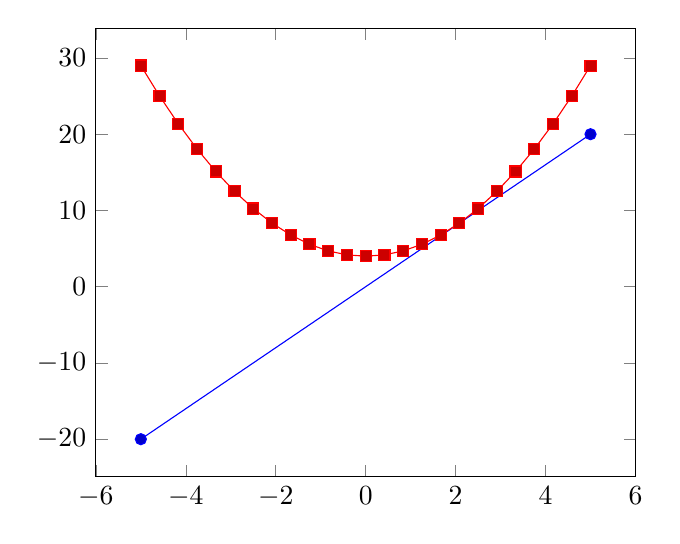
\begin{tikzpicture}
\begin{axis}[
    declare function={
        C=4;
        square(\t)=(\t)^2 + C;
    },
]
    \addplot+ [samples=2] {C*x};

    \addplot {square(x)};
\end{axis}
\end{tikzpicture}
\end{codeexample}
    %
    The definitions as such have the form \meta{function}\meta{argument list} =
    \meta{definition} where the \meta{argument list} contains a
    comma-separated-list of arguments like |\t| or |\t,\a,\b|. The
    \meta{definition} is a math expression which makes use of these arguments.

    Please refer to \cite{tikz} for more details.
\end{key}

\begin{command}{\pgfplotstableread\marg{file}}
    Please refer to the manual of \PGFPlotstable{}, |pgfplotstable.pdf|, which
    is part of the \PGFPlots{} bundle.
\end{command}

\begin{command}{\pgfplotstabletypeset\marg{\textbackslash macro}}
    Please refer to the manual of \PGFPlotstable{}, |pgfplotstable.pdf|, which
    is part of the \PGFPlots{} bundle.
\end{command}

\begin{command}{\pgfplotsiffileexists\marg{filename}\marg{true code}\marg{false code}}
    Invokes \meta{true code} if \meta{filename} exists and \meta{false code} if
    not. Can be used in looping macros, for example to plot every data file
    until there are no more of them.
\end{command}

\begin{command}{\pgfplotsutilifstringequal\marg{first}\marg{second}\marg{true code}\marg{false code}}
    A simple ``strcmp'' tool which invokes \meta{true code} if \meta{first}
    $=$\meta{second} and \meta{false code} otherwise. This does not expand
    macros.
\end{command}

\begin{commandlist}{\pgfkeys,\pgfeov,\pgfkeysvalueof,\pgfkeysgetvalue}
    These commands are part of the \Tikz{} way of specifying options, its
    sub-package |pgfkeys|. The |\pgfplotsset| command is actually nothing but a
    wrapper around |\pgfkeys|.

    A short introduction into |\pgfkeys| can be found in~\cite{keyvalintro}
    whereas the complete reference is, of course, the \Tikz{}
    manual~\cite{tikz}.

    The key |\pgfkeysvalueof|\marg{key name} expands to the value of a key;
    |\pgfkeysgetvalue|\marg{key name}\marg{\textbackslash macro} stores the
    value of \meta{key name} into \meta{\textbackslash macro}. The |\pgfeov|
    macro is used to delimit arguments for code keys in |\pgfkeys|, please
    refer to the references mentioned above.
\end{commandlist}


\section[Commands Inside Of PGFPlots Axes]
        {Commands Inside Of {\normalfont\PGFPlots{}} Axes}

\begin{command}{\autoplotspeclist}
    This command should no longer be used, although it will be kept as
    technical implementation detail. Please use the `|cycle list|' option,
    Section~\ref{sec:cycle:list}.
\end{command}

\begin{command}{\logten}
    Expands to the constant $\log(10)$. Useful for log plots because $\log(10^i)
    = i\log(10)$. This command is only available inside of a \Tikz{} picture.
\end{command}

\begin{command}{\pgfmathprintnumber\marg{number}}
    Generates pretty-printed output\footnote{This method was previously
    \texttt{\textbackslash prettyprintnumber}. Its functionality has been
    included into \PGF{} and the old command is now deprecated.} for
    \meta{number}. This method is used for every tick label.

    The number is printed using the current number printing options, see the
    manual of \PGFPlotstable{} which comes with this package for the different
    number styles, rounding precision and rounding methods.
\end{command}

\begin{command}{\numplots}
    Inside of any of the axis environments, associated style, option or
    command, |\numplots| expands to the total number of plots.
\end{command}

\begin{command}{\numplotsofactualtype}
    Like |\numplots|, this macro returns the total number of plots which have
    the same plot handler. Thus, if you have |sharp plot| active, it returns
    the number of all |sharp plots|. If you have |ybar| active, it returns the
    number of |ybar| plots and so on.
\end{command}

\begin{command}{\plotnum}
    Inside of |\addplot| or any associated style, option or command, |\plotnum|
    expands to the current plot's number, starting with~$0$.
\end{command}

\begin{command}{\plotnumofactualtype}
    Like |\plotnum|, but it returns the number among all plots of the same
    type. The number of all such plots is available using
    |\numplotsofactualtype|.
\end{command}

\begin{command}{\coordindex}
    Inside of an |\addplot| command, this macro expands to the number of the
    actual coordinate (starting with~$0$).

    It is useful together with |x filter| or |y filter| to (de)select
    coordinates.
\end{command}


\section{Path Operations}

\begin{commandlist}{\path,\draw,\fill,\node,\matrix}
    These commands are \Tikz{} drawing commands all of which are documented
    in~\cite{tikz}. They are used to draw or fill paths, generate text nodes or
    aligned text matrices. They are equivalent to
    \pgfmanualpdflabel{/tikz/draw}{}|\path[draw]|,
    \pgfmanualpdflabel{/tikz/fill}{}|\path[fill]|,
    \pgfmanualpdflabel{/tikz/node}{}|\path[node]|,
    \pgfmanualpdflabel{/tikz/matrix}{}|\path[matrix]|,
    respectively.
\end{commandlist}

\begin{pathoperation}{--}{\meta{coordinate}}
    A \Tikz{} path operation which connects the current point (the last one
    before |--|) and \meta{coordinate} with a straight line.
\end{pathoperation}

{\catcode`\|=12
\begin{pathoperation}[noindex]{|-}{\meta{coordinate}}
\pgfmanualpdflabel[\catcode`\|=12 ]{|-}{}%
    A \Tikz{} path operation which connects the current point and
    \meta{coordinate} with \emph{two} straight lines: first vertical, then
    horizontal.
\end{pathoperation}

\begin{pathoperation}[noindex]{-|}{\meta{coordinate}}
\pgfmanualpdflabel[\catcode`\|=12 ]{-|}{}%
    A \Tikz{} path operation which connects the current point and
    \meta{coordinate} with \emph{two} straight lines: first horizontal, then
    vertical.
\end{pathoperation}
}

\begin{keylist}{/tikz/xshift=\marg{dimension},/tikz/yshift=\marg{dimension}}
    These \Tikz{} keys allow to shift something by \meta{dimension} which is
    any \TeX{} size (or expression).
\end{keylist}

\begin{command}{\pgfplotsextra\marg{low-level path commands}}
    A command to execute \meta{low-level path commands} in a \PGFPlots{} axis.
    Since any drawing commands inside of an axis need to be postponed until the
    axis is complete and the scaling has been initialised, it is not possible
    to simply draw any paths. Instead, it is necessary to draw them as soon as
    the axis is finished. This is done automatically for every \Tikz{} path --
    and it is also done manually if you write |\pgfplotsextra|\marg{commands}.
    %
\begin{codeexample}[]
\begin{tikzpicture}
\begin{axis}[xmin=0,xmax=3,ymin=0,ymax=5]
    \pgfplotsextra{
        \pgfpathmoveto{\pgfplotspointaxisxy{1}{2}}
        \pgfpathlineto{\pgfplotspointaxisxy{2}{4}}
        \pgfusepath{stroke}
    }
\end{axis}
\end{tikzpicture}
\end{codeexample}
    %
    The example above initializes an axis and executes the basic level path
    commands as soon as the axis is ready. The execution of multiple |\path|,
    |\addplot| and |\pgfplotsextra| commands is in the same sequence as they
    occur in the environment.\footnote{Except for stacked plots where the
    sequence may be reverse, see the key \texttt{reverse stack plots}.}
\end{command}

\begin{command}{\pgfplotspathaxisoutline}
    Generates a path which resembles the outline of the current axis. This path
    is used for clip paths and the background paths (if any).
\end{command}


\section{Specifying Basic Coordinates}
\label{sec:basic:coordinates}

\begin{commandlist}{%
    \pgfplotspointaxisxy\marg{x coordinate}\marg{y coordinate},
    \pgfplotspointaxisxyz\marg{x coordinate}\marg{y coordinate}\marg{z coordinate}%
}
    Point commands like |\pgfpointxy| which take logical, absolute coordinates
    and return a low-level point. Every transformation from user
    transformations to logarithms is applied.

    Since the transformations are initialized after the axis is complete, this
    command needs to be postponed (see |\pgfplotsextra|).

    This command is the basic level variant of |axis cs:|\meta{x
    coordinate}|,|\meta{y coordinate}|,|\meta{z coordinate}.

    Note that this is also the default coordinate system during the
    visualization phase; in other words: if you write |\draw (1,2) -- (1,4)|,
    \PGFPlots{} will automatically use |(axis cs:1,2) -- (axis cs:1,4)|.
\end{commandlist}

\begin{commandlist}{%
    \pgfplotspointaxisdirectionxy\marg{x coordinate}\marg{y coordinate},
    \pgfplotspointaxisdirectionxyz\marg{x coordinate}\marg{y coordinate}\marg{z coordinate}%
}
    Point commands like |\pgfpointxy| which take logical, \emph{relative}
    coordinates and return a low-level point. Every transformation from user
    transformations to logarithms is applied. The difference to
    |\pgfplotspointaxisxy| is that the shift of the linear transformation is
    skipped here (compare |disabledatascaling|).

    This command is the basic level variant of |axis direction cs:|\meta{x
    coordinate}|,|\meta{y coordinate}|,|\meta{z coordinate}. Please refer to
    the documentation of |axis direction cs| for more details.

    Use this command whenever something of \emph{relative} character like
    directions or lengths need to be supplied. One use case is to draw
    ellipses:
    %
\begin{codeexample}[]
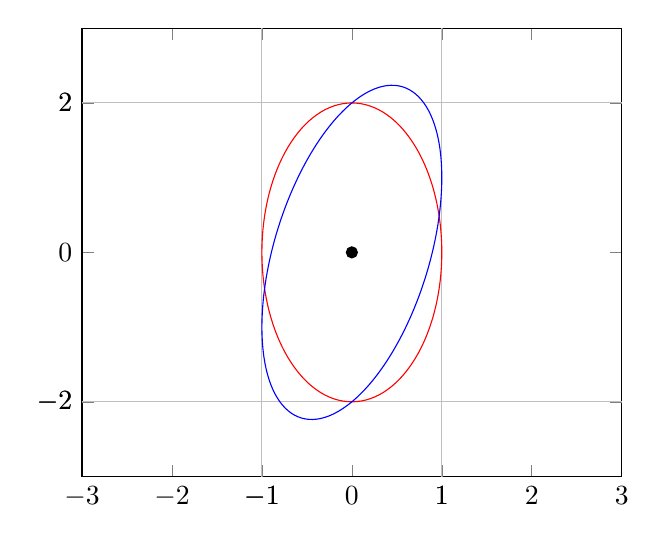
\begin{tikzpicture}
\begin{axis}[
    xmin=-3,   xmax=3,
    ymin=-3,   ymax=3,
    extra x ticks={-1,1},
    extra y ticks={-2,2},
    extra tick style={grid=major},
]
    \draw [red] \pgfextra{
        \pgfpathellipse{\pgfplotspointaxisxy{0}{0}}
            {\pgfplotspointaxisdirectionxy{1}{0}}
            {\pgfplotspointaxisdirectionxy{0}{2}}
    % see also the documentation of
    % 'axis direction cs' which
    % allows a simpler way to draw this ellipse
    };
    \draw [blue] \pgfextra{
        \pgfpathellipse{\pgfplotspointaxisxy{0}{0}}
            {\pgfplotspointaxisdirectionxy{1}{1}}
            {\pgfplotspointaxisdirectionxy{0}{2}}
    };
    \addplot [only marks,mark=*] coordinates
        { (0,0) };
\end{axis}
\end{tikzpicture}
\end{codeexample}

    Since the transformations are initialized after the axis is complete, this
    command needs to be provided either inside of a \tikzname{} |\path| command
    (like |\draw| in the example above) or inside of |\pgfplotsextra|.
\end{commandlist}

\begin{commandlist}{%
    \pgfplotspointrelaxisxy\marg{rel x coordinate}\marg{rel y coordinate},
    \pgfplotspointrelaxisxyz\marg{rel x coordinate}\marg{rel y coordinate}\marg{rel z coordinate}%
}
    Point commands which take \emph{relative} coordinates such that $x=0$ is
    the \emph{lower} $x$-axis limit and $x=1$ the \emph{upper} $x$-axis limit.

    These commands are used for |rel axis cs|.

    Please note that the transformations are only initialised if the axis is
    complete! This means you need to provide |\pgfplotsextra|.
\end{commandlist}

\begin{commandlist}{%
    \pgfplotspointdescriptionxy\marg{$x$ fraction}\marg{$y$ fraction},
    \pgfplotsqpointdescriptionxy\marg{$x$ fraction}\marg{$y$ fraction}%
}
    Point commands such that |{0}{0}| is the lower left corner of the axis'
    bounding box and |{1}{1}| the upper right one; everything else is in
    between. The `|q|' variant is quicker as it doesn't invoke the math parser
    on its arguments.

    They are used for |axis description cs|, see
    Section~\ref{pgfplots:sec:axis:description:cs}.
\end{commandlist}

\begin{commandlist}{\pgfplotspointaxisorigin}
    A point coordinate at the origin, $(0,0,0)$. If the origin is not part of
    the axis limits, the nearest point on the boundary is returned instead.

    This is the same coordinate as returned by the |origin| anchor.
\end{commandlist}

\begin{commandlist}{%
    \pgfplotstransformcoordinatex\marg{x coordinate of an axis},
    \pgfplotstransformcoordinatey\marg{y coordinate of an axis},
    \pgfplotstransformcoordinatez\marg{z coordinate of an axis}%
}
    Defines |\pgfmathresult| to be the low-level \PGF{} coordinate
    corresponding to the input argument.

    The command applies any |[xyz] coord trafo| keys, data scalings and/or
    logarithms or whatever \PGFPlots{} does to map input coordinates to
    internal coordinates.

    The result can be used inside of a |\pgfpointxy| statement (i.e.\@ it still
    needs to be scaled with the respective \PGF{} unit vector).
    %
\begin{codeexample}[]
\begin{tikzpicture}
\pgfplotsset{compat/pgfpoint substitution=1.3}
\begin{axis}[xmin=0,xmax=2,ymin=0,ymax=5]
    \pgfplotsextra{
        \pgfplotstransformcoordinatex{1}
        \let\xcoord=\pgfmathresult
        \pgfplotstransformcoordinatey{1}
        \let\ycoord=\pgfmathresult
        \pgfpathcircle
            {\pgfqpointxy{\xcoord}{\ycoord}}
            {5pt}
        \pgfusepath{fill}
    }
\end{axis}
\end{tikzpicture}
\end{codeexample}
    %
    Note that \PGFPlots{} substitutes |\pgfqpointxy| by |\pgfplotspointaxisxyz|
    by default -- and this command implicitly transforms coordinates anyway. In
    order to see the difference, the preceding example first disables this
    automatic substitution of coordinate systems by means of
    |compat/pgfpoint substitution=1.3|.
    %
    The result of this command is also available as math method
    |transformcoordinatex| (see the documentation for |axis cs|).

    Please note that the transformations are only initialised if the axis is
    complete. This means you need to provide |\pgfplotsextra| as is shown in
    the example above.
\end{commandlist}

\begin{commandlist}{%
    \pgfplotstransformdirectionx\marg{x direction of an axis},
    \pgfplotstransformdirectiony\marg{y direction of an axis},
    \pgfplotstransformdirectionz\marg{z direction of an axis}%
}
    Defines |\pgfmathresult| to be a low-level \PGF{} \emph{direction vector
    component}.

    A direction vector needs to be \emph{added} to some coordinate in order to
    get a coordinate, compare the documentation for
    |\pgfplotspointaxisdirectionxy| and |axis direction cs|.

    The argument \meta{x direction of an axis} is processed in (almost) the
    same way as for the macro which operates on absolute positions,
    |\pgfplotstransformcoordinatex|. The only difference is that
    \emph{directions} need no shifting transformation.

    The result of this command is also available as math method
    |transformdirectionx| (see the documentation for |axis direction cs|).

    See |axis direction cs| for details and examples about this command.
\end{commandlist}

% this command is for internal use only:
%--------------------------------------------------
% \begin{command}{\pgfplotsconvertunittocoordinate\marg{x, y or z}\marg{dimension}}
%     Converts a dimension (with unit!) to a corresponding $x$-, $y$- or $z$-coordinate. The result will be written to |\pgfmathresult| (without units).
%
%     It is possible to use the result as arguments for the |\pgfpointxyz| commands.
%
%     The effect is to multiply \meta{dimension} with the inverse length of the unit vector for the specified axis. These lengths are precomputed in \PGFPlots{} so the operation is fast.
% \begin{codeexample}[code only]
% \pgfplotsconvertunittocoordinate{x}{5pt}
% % now, the command uses exactly 5pt in x direction:
% \pgfqpointxyz{\pgfmathresult}{4}{3}
% \end{codeexample}
% \end{command}
%--------------------------------------------------

\begin{commandlist}{%
    \pgfplotspointunitx,
    \pgfplotspointunity,
    \pgfplotspointunitz%
}
    Low-level point commands which return the canvas $x$, $y$ or $z$ unit
    vectors.

    The |\pgfplotspointunitx| is the \pgfname{} unit vector in $x$ direction.

    These vectors are essentially the same as |\pgfqpointxyz{1}{0}{0}|,
    |\pgfqpointxyz{0}{1}{0}|, and |\pgfqpointxyz{0}{0}{1}|, respectively.

    The unit $z$ vector is only defined for three dimensional axes.
\end{commandlist}

\begin{commandlist}{%
    \pgfplotsunitxlength,
    \pgfplotsunitylength,
    \pgfplotsunitzlength,
    \pgfplotsunitxinvlength,
    \pgfplotsunityinvlength,
    \pgfplotsunitzinvlength%
}
    Macros which expand to the vector length $\lVert x_i \rVert$ of the
    respective unit vector $x_i$ or the inverse vector length, $1/\lVert x_i
    \rVert$. These macros can be used inside of |\pgfmathparse|, for example.

    The $x_i$ are the |\pgfplotspointunitx| variants.
\end{commandlist}

\begin{command}{\pgfplotsqpointoutsideofaxis%
        \marg{three-char-string}\marg{coordinate}\marg{normal distance}%
}
    Provides a point coordinate on one of the available four axes in case of a
    two dimensional figure or on one of the available twelve axes in case of a
    three dimensional figure.

    The desired axis is uniquely identified by a three character string,
    provided as first argument to the command. The first of the three
    characters is `|0|' if the $x$-coordinate of the specified axis passes
    through the lower axis limit. It is `|1|', if the $x$-coordinate of the
    specified axis passes through the upper axis limit. Furthermore, it is
    `|2|' if it passes through the origin. The second character is also either
    |0|, |1| or |2| and it characterizes the position on the $y$-axis. The
    third character is for the third dimension, the $z$-axis. It should be left
    at `|0|' for two dimensional plots. However, \emph{one} of the three
    characters should be `|v|', meaning the axis \underline varies. For
    example, |v01| denotes $\{ (x,y_{\min},z_{\max}) \vert x \in \R \}$.

    The second argument, \meta{coordinate} is the logical coordinate on that
    axis. Since two coordinates of the axis are fixed, \meta{coordinate} refers
    to the \underline varying component of the axis. It must be a number
    without unit; no math expressions are supported here.

    The third argument \meta{normal distance} is a dimension like |10pt|. It
    shifts the coordinate away from the designated axis in direction of the
    outer normal vector. The outer normal vector always points away from the
    axis. It is computed using |\pgfplotspointouternormalvectorofaxis|.

    There are several variants of this command which are documented in the
    source code. One of them is particularly useful:
\end{command}

\begin{command}{\pgfplotsqpointoutsideofaxisrel%
        \marg{three-char-string}\marg{axis fraction}\marg{normal distance}%
}
    This point coordinate is a variant of |\pgfplotsqpointoutsideofaxis| which
    allows to provide an \meta{axis fraction} instead of an absolute
    coordinate. The fraction is a number between $0$ (lower axis limit) and $1$
    (upper axis limit), i.e.\@ it is given in percent of the total axis. It is
    possible to provide negative values or values larger than one.

    The |\pgfplotsqpointoutsideofaxisrel| command is similar in spirit to
    |rel axis cs|.

    There is one speciality in conjunction with reversed axes: if the axis has
    been reversed by |x dir=reverse| and, in addition,
    |allow reversal of rel axis cs| is true, the value $0$ denotes the
    \emph{upper} limit while $1$ denotes the \emph{lower} limit. The effect is
    that coordinates won't change just because of axis reversal.
        \index{allow reversal of rel axis cs}%
\end{command}

\begin{command}{\pgfplotspointouternormalvectorofaxis\marg{three-char-string}}
    A point command which yields the outer normal vector of the respective
    axis. The normal vector has length $1$ (computed with
    |\pgfpointnormalised|). It is the same normal vector used inside of
    |\pgfplotsqpointoutsideofaxis| and its variants.

    The output of this command will be cached and reused during the lifetime
    of an axis.
\end{command}

\begin{command}{\pgfplotsticklabelaxisspec\marg{x, y or z}}
    Expands to the three character identification for the axis containing tick
    labels for the chosen axis, either \meta{x}, \meta{y} or \meta{z}.
\end{command}

\begin{command}{\pgfplotsvalueoflargesttickdimen\marg{x, y or z}}
    Expands to the largest distance of a tick position to its tick label
    bounding box in direction of the outer unit normal vector. It does also
    include the value of the |ticklabel shift| key.

    This value is used for |ticklabel cs|.
\end{command}

\begin{commandlist}{
    \pgfplotsmathfloatviewdepthxyz\marg{x}\marg{y}\marg{z},
    \pgfplotsmathviewdepthxyz\marg{x}\marg{y}\marg{z}%
}
    Both macros define |\pgfmathresult| to be the ``depth'' of a three
    dimensional point $\bar x = (x,y,z)$. The depth is defined to be the scalar
    product of $\bar x$ with $\vec d$, the view direction of the current axis.

    For |\pgfplotsmathfloatviewdepthxyz|, the arguments are parsed as floating
    point numbers and the result is encoded in floating point. A fixed point
    representation can be generated with
    |\pgfmathfloattofixed{\pgfmathresult}|.

    For |\pgfplotsmathviewdepthxyz|, \TeX{} arithmetics is employed for the
    inner product and the result is assigned in fixed point. This is slightly
    faster, but has considerably smaller data range.

    Both commands can only be used \emph{inside} of a three dimensional
    \PGFPlots{} axis (as soon as the axis is initialised, see
    |\pgfplotsextra|).
\end{commandlist}

\begin{texif}{pgfplotsthreedim}
    A \TeX{} |\if| which evaluates the \meta{true code} if the axis is three
    dimensional and the \meta{else code} if not.
\end{texif}


\section{Accessing Axis Limits}

It is also possible to access axis limits during the visualization phase,
i.e.\@ during |\end{axis}|. Please refer to the reference documentation for
|xmin| on page~\pageref{page:access:limits}.


\section{Accessing Point Coordinate Values}

During the visualization phase, \PGFPlots{} provides access to the currently
processed coordinate and its values.

This access requires a call to specific macros. These macros write the
coordinate values to some publicly available key--value pairs. Then, the
current point's $x$, $y$, $z$, and color data can be accessed.

\begin{commandlist}{\pgfplotspointgetcoordinates,\pgfplotspointgetcoordinates\marg{point}}

    After invoking the macro, the following keys will be set:

    \declaretext{/data point/x} will contain the current point's $x$-coordinate.

    \declaretext{/data point/y} will contain the current point's $y$-coordinate.

    \declaretext{/data point/z} will contain the current point's $z$-coordinate
    (if applicable).

    \declaretext{/data point/meta} will contain the current point's
    |point meta| value (if applicable).

    \declaretext{/data point/index} will contain the current point's index in
    the coordinate stream. This is actually the same as |\coordindex|.

    This command actually supports two modes of operation:
    %
    \begin{enumerate}
        \item Without arguments. In this case, it returns values of the point
            which is about to be processed by the current plot handler.
        \item With an argument in curly braces. In this case, it expects a
            coordinate and assigns the keys accordingly. Note that this
            command merely supports two-dimensional axes and assigns only
            |/data point/x| and |/data point/y|.
    \end{enumerate}

    The returned values are the same as they can be read on the axes, they are
    also the same as you would write them into |axis cs|.

    This means that any |x coord inv trafo| has been applied on the value. It
    also means that the exponential function has been called even though the
    internal coordinate was present in log format.

    This function is implicitly called for any |scatter| plot (including
    |nodes near coords|). This allows to access \emph{all} coordinate values at
    once:
    %
\begin{codeexample}[]
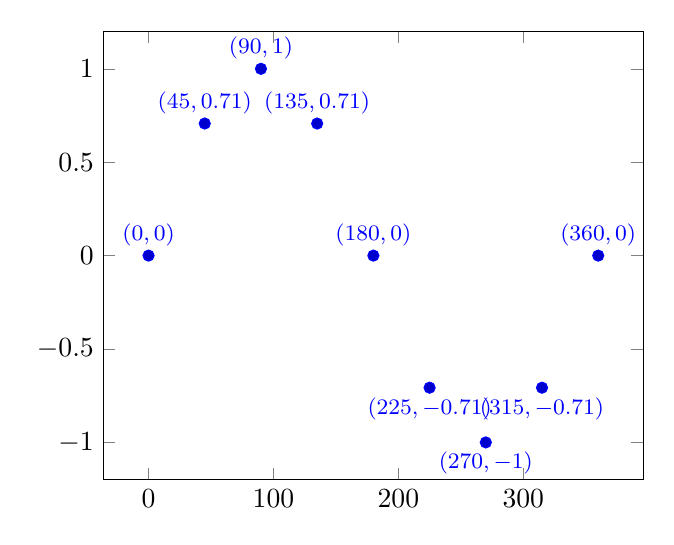
\begin{tikzpicture}
\begin{axis}
    \addplot+ [
        domain=0:360,
        samples=9,
        only marks,
        nodes near coords={%
            \footnotesize
            $(\pgfmathprintnumber
                {\pgfkeysvalueof{/data point/x}},
               \pgfmathprintnumber
                {\pgfkeysvalueof{/data point/y}})$%
        },
    ] {sin(x)};
\end{axis}
\end{tikzpicture}
\end{codeexample}
    %
    The example works because |\pgfplotspointgetcoordinates| is part of the
    standard implementation of |nodes near coords|; the resulting values are
    directly available. Note that the preceding example would have been simpler
    if we would have printed just one value: |nodes near coords| resorts to the
    |point meta|. And that, in turn, contains the $y$-coordinate anyway by
    default.

    A more advanced example would be a |ybar| plot in which nodes shall be
    placed at the lower end of the axis, together with some dotted lines to the
    respective bars:
    %
\begin{codeexample}[]
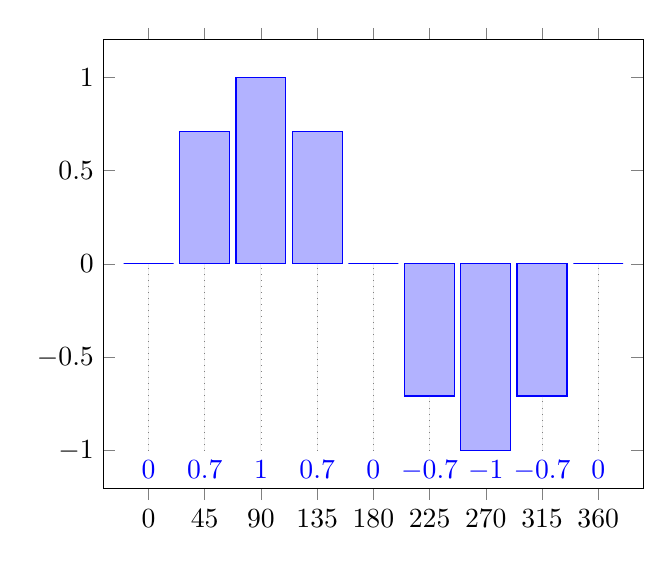
\begin{tikzpicture}
\begin{axis}[
    ybar,
    nodes near coords,
    %
    % we want to provide absolute 'at' values
    % for the nodes:
    scatter/position=absolute,
    every node near coord/.style={
        at={(\pgfkeysvalueof{/data point/x},-1)},
        % pretty printing:
        anchor=north,
        /pgf/number format/fixed,
        /pgf/number format/precision=1,
        % assign a name which can be referenced below:
        name=NNC\pgfkeysvalueof{/data point/index},
    },
    % ... draw a dotted line between
    % the marker and the bar:
    /pgfplots/scatter/@post marker code/.add code={}{
        \draw [dotted,help lines]
            (NNC\pgfkeysvalueof{/data point/index})
            -- (\pgfkeysvalueof{/data point/x},
            {min(0,\pgfkeysvalueof{/data point/y})});
    },
    % assign suitable tick labels:
    xtick=data,
]
    % some dummy data:
    \addplot+ [
        domain=0:360,
        bar width=360/9,
        samples=9,
    ] {sin(x)};
\end{axis}
\end{tikzpicture}
\end{codeexample}
    %
    Again, the command is used implicitly as part of |nodes near coords| and
    does not occur in the example as such.

    \paragraph{See also} the related example online under
    \url{https://tex.stackexchange.com/a/141006}. It demonstrates how to
    place the nodes generated by |nodes near coords| based on the value (either
    inside of a bar or above it).

    The following example uses an argument in curly braces for which we seek
    coordinate values:
    %
\begin{codeexample}[]
% requires \usetikzlibrary{intersections}
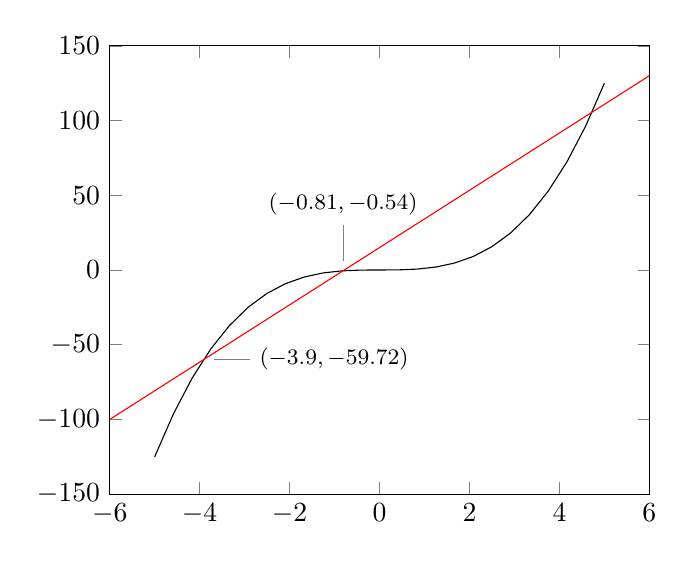
\begin{tikzpicture}
\begin{axis}
    \addplot [name path=A] {x^3};

    \draw [red,name path=HelperLine]
        (axis cs:-6,-100) -- (axis cs:6,130);

    \draw [
        font=\footnotesize,
        name intersections={of=A and HelperLine},
    ]
    node [pin={right:
      \pgfplotspointgetcoordinates{(intersection-1)}
        $(\pgfmathprintnumber[fixed]{
            \pgfkeysvalueof{/data point/x}},
          \pgfmathprintnumber[fixed]{
            \pgfkeysvalueof{/data point/y}})$
      }
    ] at (intersection-1) {}
    node [pin={
      \pgfplotspointgetcoordinates{(intersection-2)}
        $(\pgfmathprintnumber[fixed]{
            \pgfkeysvalueof{/data point/x}},
          \pgfmathprintnumber[fixed]{
            \pgfkeysvalueof{/data point/y}})$
      }
    ] at (intersection-2) {};
\end{axis}
\end{tikzpicture}
\end{codeexample}
    %
    The example computes and names intersections of |A| and |HelperLine|. The
    following code generates pins at the intersections. To this end, it uses
    |\pgfplotspointgetcoordinates|\marg{point} which defines |/data point/x|
    and |/data point/y|. These values are then formatted using
    |\pgfmathprintnumber|.

    In its second mode, |\pgfplotspointgetcoordinates|\marg{point} expects one
    of two things as \meta{point}:
    %
    \begin{enumerate}
        \item a basic-level \PGF{} point like |\pgfpointanchor{A}{center}| or
        \item a \Tikz{} point like |(A.base)| or |(3,5)|.
    \end{enumerate}
\end{commandlist}

\begin{command}{\pgfplotspointgetnormalizedcoordinates}
    A macro which is very similar to |\pgfplotspointgetcoordinates|.
    Consequently, it is also supposed to be called during the visualization phase.

    It assigns the very same output macros, but the values are different. More
    precisely, it defines the macros

    \declaretext{/data point/x} will contain the current point's
    \emph{normalized} $x$-coordinate.

    \declaretext{/data point/y} will contain the current point's
    \emph{normalized} $y$-coordinate.

    \declaretext{/data point/z} will contain the current point's
    \emph{normalized} $z$-coordinate (if applicable).

    \declaretext{/data point/meta} will contain the current point's
    |point meta| value (if applicable).

    \declaretext{/data point/index} will contain the current point's index in
    the coordinate stream. This is actually the same as |\coordindex|.

    The keyword \declaretext{normalized} means that the values are in a
    suitable numerical form which can be consumed by the axis. To be more
    specific: any user |x coord inv trafo| is \emph{ignored}. An important
    example would be |symbolic x coords|: the normalized coordinates would be
    some associated numbers, not the symbols. The results returned by
    |\pgfplotspointgetcoordinates| would be the symbols. For logarithm axes,
    the normalized values are the logs.

    Typically, normalized values are much more useful when you want to apply
    some math operation like averaging or subtraction.

    This function needs to be called explicitly. It is currently used by
    |ybar stacked| to align |nodes near coords|.
\end{command}


\section{Layer Access}

\begin{command}{\pgfplotsonlayer\marg{layer name}}
    A low-level command which will check if the current axis has layer support
    activated and, if so, calls |\pgfonlayer|\marg{layer name}.

    There must be a |\endpgfplotsonlayer| to delimit the environment.
\end{command}

\begin{command}{\endpgfplotsonlayer}
    The end of |\pgfplotsonlayer|.
\end{command}

\begin{command}{\pgfonlayer\marg{layer name}}
    A low-level command of \PGF{} which will collect everything until the
    matching |\endpgfonlayer| into layer \meta{layer name}.

    The \meta{layer name} must be active, i.e.\@ it must be part of the layer
    names of |set layers|.

    The only special case is if you call |\pgfdeclarelayer{discard}| somewhere:
    this special layer has a ``magical name'' which serves as |/dev/null| if it
    is enabled using |\pgfonlayer{discard}|: it does not need to be active and
    everything assigned to this layer will be thrown away if it is not part of
    the layer name configuration.

    There must be a |\endpgfonlayer| to delimit the environment.
\end{command}

\begin{command}{\endpgfonlayer}
    The end of |\pgfonlayer|.
\end{command}


\begin{command}{\pgfsetlayers\marg{layer list}}
    This is a low-level command of \PGF{}. At the time of this writing, it is
    the only way to tell \PGF{} which layers it shall use for the current/next
    picture. It is used implicitly by |set layers|.
\end{command}


\printindex

\bibliographystyle{abbrv} %gerapali} %gerabbrv} %gerunsrt.bst} %gerabbrv}% gerplain}
\nocite{pgfplotstable}
\nocite{programmingnotes}
\bibliography{pgfplots}
\end{document}

% -----------------------------------------------------------------------------
% For Stefan Pinnow as reminder on what to look for when editing the manual
% -----------------------------------------------------------------------------
% There should be no line breaks in the following environments
% - |...|
% - \declareandlabel{...}
% - \verbpdfref{...}
% If "MakeTikzPictures" isn't running through check one of the externalized
% LOG files what is the cause of that.
% -----------------------------------------------------------------------------


%%%%%%%%%%%%%%%%%%%%%%%%%%%%%%%%%%%%%%%%%%%%%%%%%%%%%%%%%%%%%%%%%%%%%%%%%%%%%
%
% Package pgfplots.sty documentation.
%
% Copyright 2007/2008 by Christian Feuersaenger.
%
% This program is free software: you can redistribute it and/or modify
% it under the terms of the GNU General Public License as published by
% the Free Software Foundation, either version 3 of the License, or
% (at your option) any later version.
%
% This program is distributed in the hope that it will be useful,
% but WITHOUT ANY WARRANTY; without even the implied warranty of
% MERCHANTABILITY or FITNESS FOR A PARTICULAR PURPOSE.  See the
% GNU General Public License for more details.
%
% You should have received a copy of the GNU General Public License
% along with this program.  If not, see <http://www.gnu.org/licenses/>.
%
%
%%%%%%%%%%%%%%%%%%%%%%%%%%%%%%%%%%%%%%%%%%%%%%%%%%%%%%%%%%%%%%%%%%%%%%%%%%%%%
% SEE pgfplots-macros.tex as well!
%\pdfminorversion=5 % to allow compression
%\pdfobjcompresslevel=2
\documentclass[a4paper,openany]{book}

\let\bookmaketitle=\maketitle

% -----------------------------------
% this here is from ltxdoc:
\usepackage{doc}[=v2]
\AtBeginDocument{\MakeShortVerb{\|}}
%\setlength{\textwidth}{355pt}
%\addtolength\marginparwidth{30pt}
%\addtolength\oddsidemargin{20pt}
%\addtolength\evensidemargin{20pt}
\def\cmd#1{\cs{\expandafter\cmd@to@cs\string#1}}
\def\cmd@to@cs#1#2{\char\number`#2\relax}
\DeclareRobustCommand\cs[1]{\texttt{\char`\\#1}}
\providecommand\marg[1]{%
  {\ttfamily\char`\{}\meta{#1}{\ttfamily\char`\}}}
\providecommand\oarg[1]{%
  {\ttfamily[}\meta{#1}{\ttfamily]}}
\providecommand\parg[1]{%
  {\ttfamily(}\meta{#1}{\ttfamily)}}
\raggedbottom

% -----------------------------------
\input{pgfplots.preamble.tex}

\makeatletter
% I want a two-column index just as in pgfmanual styles. This here
% was the best way to get one:
\def\index@prologue{\section*{Index}\addcontentsline{toc}{chapter}{Index}
}
\makeatother

%\RequirePackage[german,english,francais]{babel}

\def\matlabcolormaptext{This colormap is similar to one shipped with Matlab$^\text{\textregistered}$ under a similar name.}

\IfFileExists{tikzlibraryspy.code.tex}{%
\usetikzlibrary{spy}
}{%
    \message{ERROR: tikz SPY library NOT available. The manual will only compile partially.^^J}%
}%

\usepackage{xparse}% for colorbrewer manual

\usetikzlibrary{
    decorations.markings,
    decorations.footprints,
    shapes.arrows,
    matrix,
    positioning,
}

\usepgfplotslibrary{
    fillbetween,
    ternary,
    smithchart,
    patchplots,
    polar,
    colormaps,
    colorbrewer,
    colortol,           % docu not ready yet
}
\pgfqkeys{/codeexample}{%
    every codeexample/.append style={
        /pgfplots/every ternary axis/.append style={
            /pgfplots/legend style={fill=graphicbackground},
        }
    },
    tabsize=4,
}

\pgfplotsmanualenableexternalizationofexpensive

%\usetikzlibrary{external}
%\tikzexternalize[prefix=figures/]{pgfplots}

\title{%
    Manual for Package \PGFPlots{}\\
    {\small 2D/3D Plots in \LaTeX{}, Version \pgfplotsversion}\\
    {\small\href{https://github.com/pgf-tikz/pgfplots}{https://github.com/pgf-tikz/pgfplots}}
    %\\{\small Attention: you are using an unstable development version.}
}

\makeatletter
\long\def\abstractsmuggle{%
    \centering
    \textbf{Abstract}\\[0.5cm]

    \begin{minipage}{12cm}
        \PGFPlots{} draws high-quality function plots in normal or logarithmic
        scaling with a user-friendly interface directly in \TeX{}. The user
        supplies axis labels, legend entries and the plot coordinates for one or
        more plots and \PGFPlots{} applies axis scaling, computes any logarithms
        and axis ticks and draws the plots. It supports line plots, scatter
        plots, piecewise constant plots, bar plots, area plots, mesh and surface
        plots, patch plots, contour plots, quiver plots, histogram plots, box
        plots, polar axes, ternary diagrams, smith charts and some more. It is
        based on Till Tantau's package \PGF{}/\Tikz{}.
    \end{minipage}

}%

\expandafter\date\expandafter{\@date\\[2cm]
    \abstractsmuggle
}%
\makeatother

%\includeonly{pgfplots.reference}


\begin{document}

\def\plotcoords{%
\addplot coordinates {
(5,8.312e-02)    (17,2.547e-02)   (49,7.407e-03)
(129,2.102e-03)  (321,5.874e-04)  (769,1.623e-04)
(1793,4.442e-05) (4097,1.207e-05) (9217,3.261e-06)
};

\addplot coordinates{
(7,8.472e-02)    (31,3.044e-02)    (111,1.022e-02)
(351,3.303e-03)  (1023,1.039e-03)  (2815,3.196e-04)
(7423,9.658e-05) (18943,2.873e-05) (47103,8.437e-06)
};

\addplot coordinates{
(9,7.881e-02)     (49,3.243e-02)    (209,1.232e-02)
(769,4.454e-03)   (2561,1.551e-03)  (7937,5.236e-04)
(23297,1.723e-04) (65537,5.545e-05) (178177,1.751e-05)
};

\addplot coordinates{
(11,6.887e-02)    (71,3.177e-02)     (351,1.341e-02)
(1471,5.334e-03)  (5503,2.027e-03)   (18943,7.415e-04)
(61183,2.628e-04) (187903,9.063e-05) (553983,3.053e-05)
};

\addplot coordinates{
(13,5.755e-02)     (97,2.925e-02)     (545,1.351e-02)
(2561,5.842e-03)   (10625,2.397e-03)  (40193,9.414e-04)
(141569,3.564e-04) (471041,1.308e-04)
(1496065,4.670e-05)
};
}%


\bookmaketitle
\tableofcontents

%%%%%%%%%%%%%%%%%%%%%%%%%%%%%%%%%%%%%%%%%%%%%%%%%%%%%%%%%%%%%%%%%%%%%%%%%%%%%
%
% Package pgfplots.sty documentation.
%
% Copyright 2007/2008 by Christian Feuersaenger.
%
% This program is free software: you can redistribute it and/or modify
% it under the terms of the GNU General Public License as published by
% the Free Software Foundation, either version 3 of the License, or
% (at your option) any later version.
%
% This program is distributed in the hope that it will be useful,
% but WITHOUT ANY WARRANTY; without even the implied warranty of
% MERCHANTABILITY or FITNESS FOR A PARTICULAR PURPOSE.  See the
% GNU General Public License for more details.
%
% You should have received a copy of the GNU General Public License
% along with this program.  If not, see <http://www.gnu.org/licenses/>.
%
%
%%%%%%%%%%%%%%%%%%%%%%%%%%%%%%%%%%%%%%%%%%%%%%%%%%%%%%%%%%%%%%%%%%%%%%%%%%%%%
% SEE pgfplots-macros.tex as well!
%\pdfminorversion=5 % to allow compression
%\pdfobjcompresslevel=2
\documentclass[a4paper,openany]{book}

\let\bookmaketitle=\maketitle

% -----------------------------------
% this here is from ltxdoc:
\usepackage{doc}[=v2]
\AtBeginDocument{\MakeShortVerb{\|}}
%\setlength{\textwidth}{355pt}
%\addtolength\marginparwidth{30pt}
%\addtolength\oddsidemargin{20pt}
%\addtolength\evensidemargin{20pt}
\def\cmd#1{\cs{\expandafter\cmd@to@cs\string#1}}
\def\cmd@to@cs#1#2{\char\number`#2\relax}
\DeclareRobustCommand\cs[1]{\texttt{\char`\\#1}}
\providecommand\marg[1]{%
  {\ttfamily\char`\{}\meta{#1}{\ttfamily\char`\}}}
\providecommand\oarg[1]{%
  {\ttfamily[}\meta{#1}{\ttfamily]}}
\providecommand\parg[1]{%
  {\ttfamily(}\meta{#1}{\ttfamily)}}
\raggedbottom

% -----------------------------------
\input{pgfplots.preamble.tex}

\makeatletter
% I want a two-column index just as in pgfmanual styles. This here
% was the best way to get one:
\def\index@prologue{\section*{Index}\addcontentsline{toc}{chapter}{Index}
}
\makeatother

%\RequirePackage[german,english,francais]{babel}

\def\matlabcolormaptext{This colormap is similar to one shipped with Matlab$^\text{\textregistered}$ under a similar name.}

\IfFileExists{tikzlibraryspy.code.tex}{%
\usetikzlibrary{spy}
}{%
    \message{ERROR: tikz SPY library NOT available. The manual will only compile partially.^^J}%
}%

\usepackage{xparse}% for colorbrewer manual

\usetikzlibrary{
    decorations.markings,
    decorations.footprints,
    shapes.arrows,
    matrix,
    positioning,
}

\usepgfplotslibrary{
    fillbetween,
    ternary,
    smithchart,
    patchplots,
    polar,
    colormaps,
    colorbrewer,
    colortol,           % docu not ready yet
}
\pgfqkeys{/codeexample}{%
    every codeexample/.append style={
        /pgfplots/every ternary axis/.append style={
            /pgfplots/legend style={fill=graphicbackground},
        }
    },
    tabsize=4,
}

\pgfplotsmanualenableexternalizationofexpensive

%\usetikzlibrary{external}
%\tikzexternalize[prefix=figures/]{pgfplots}

\title{%
    Manual for Package \PGFPlots{}\\
    {\small 2D/3D Plots in \LaTeX{}, Version \pgfplotsversion}\\
    {\small\href{https://github.com/pgf-tikz/pgfplots}{https://github.com/pgf-tikz/pgfplots}}
    %\\{\small Attention: you are using an unstable development version.}
}

\makeatletter
\long\def\abstractsmuggle{%
    \centering
    \textbf{Abstract}\\[0.5cm]

    \begin{minipage}{12cm}
        \PGFPlots{} draws high-quality function plots in normal or logarithmic
        scaling with a user-friendly interface directly in \TeX{}. The user
        supplies axis labels, legend entries and the plot coordinates for one or
        more plots and \PGFPlots{} applies axis scaling, computes any logarithms
        and axis ticks and draws the plots. It supports line plots, scatter
        plots, piecewise constant plots, bar plots, area plots, mesh and surface
        plots, patch plots, contour plots, quiver plots, histogram plots, box
        plots, polar axes, ternary diagrams, smith charts and some more. It is
        based on Till Tantau's package \PGF{}/\Tikz{}.
    \end{minipage}

}%

\expandafter\date\expandafter{\@date\\[2cm]
    \abstractsmuggle
}%
\makeatother

%\includeonly{pgfplots.reference}


\begin{document}

\def\plotcoords{%
\addplot coordinates {
(5,8.312e-02)    (17,2.547e-02)   (49,7.407e-03)
(129,2.102e-03)  (321,5.874e-04)  (769,1.623e-04)
(1793,4.442e-05) (4097,1.207e-05) (9217,3.261e-06)
};

\addplot coordinates{
(7,8.472e-02)    (31,3.044e-02)    (111,1.022e-02)
(351,3.303e-03)  (1023,1.039e-03)  (2815,3.196e-04)
(7423,9.658e-05) (18943,2.873e-05) (47103,8.437e-06)
};

\addplot coordinates{
(9,7.881e-02)     (49,3.243e-02)    (209,1.232e-02)
(769,4.454e-03)   (2561,1.551e-03)  (7937,5.236e-04)
(23297,1.723e-04) (65537,5.545e-05) (178177,1.751e-05)
};

\addplot coordinates{
(11,6.887e-02)    (71,3.177e-02)     (351,1.341e-02)
(1471,5.334e-03)  (5503,2.027e-03)   (18943,7.415e-04)
(61183,2.628e-04) (187903,9.063e-05) (553983,3.053e-05)
};

\addplot coordinates{
(13,5.755e-02)     (97,2.925e-02)     (545,1.351e-02)
(2561,5.842e-03)   (10625,2.397e-03)  (40193,9.414e-04)
(141569,3.564e-04) (471041,1.308e-04)
(1496065,4.670e-05)
};
}%


\bookmaketitle
\tableofcontents
\include{pgfplots.title_abstract_intro}
\include{pgfplots.preliminaries}
\include{pgfplots.intro}
\include{pgfplots.reference}
\include{pgfplots.libs}
\include{pgfplots.resources}
\include{pgfplots.importexport}
\include{pgfplots.basic.reference}

\printindex

\bibliographystyle{abbrv} %gerapali} %gerabbrv} %gerunsrt.bst} %gerabbrv}% gerplain}
\nocite{pgfplotstable}
\nocite{programmingnotes}
\bibliography{pgfplots}
\end{document}

% -----------------------------------------------------------------------------
% For Stefan Pinnow as reminder on what to look for when editing the manual
% -----------------------------------------------------------------------------
% There should be no line breaks in the following environments
% - |...|
% - \declareandlabel{...}
% - \verbpdfref{...}
% If "MakeTikzPictures" isn't running through check one of the externalized
% LOG files what is the cause of that.
% -----------------------------------------------------------------------------


%%%%%%%%%%%%%%%%%%%%%%%%%%%%%%%%%%%%%%%%%%%%%%%%%%%%%%%%%%%%%%%%%%%%%%%%%%%%%
%
% Package pgfplots.sty documentation.
%
% Copyright 2007/2008 by Christian Feuersaenger.
%
% This program is free software: you can redistribute it and/or modify
% it under the terms of the GNU General Public License as published by
% the Free Software Foundation, either version 3 of the License, or
% (at your option) any later version.
%
% This program is distributed in the hope that it will be useful,
% but WITHOUT ANY WARRANTY; without even the implied warranty of
% MERCHANTABILITY or FITNESS FOR A PARTICULAR PURPOSE.  See the
% GNU General Public License for more details.
%
% You should have received a copy of the GNU General Public License
% along with this program.  If not, see <http://www.gnu.org/licenses/>.
%
%
%%%%%%%%%%%%%%%%%%%%%%%%%%%%%%%%%%%%%%%%%%%%%%%%%%%%%%%%%%%%%%%%%%%%%%%%%%%%%
% SEE pgfplots-macros.tex as well!
%\pdfminorversion=5 % to allow compression
%\pdfobjcompresslevel=2
\documentclass[a4paper,openany]{book}

\let\bookmaketitle=\maketitle

% -----------------------------------
% this here is from ltxdoc:
\usepackage{doc}[=v2]
\AtBeginDocument{\MakeShortVerb{\|}}
%\setlength{\textwidth}{355pt}
%\addtolength\marginparwidth{30pt}
%\addtolength\oddsidemargin{20pt}
%\addtolength\evensidemargin{20pt}
\def\cmd#1{\cs{\expandafter\cmd@to@cs\string#1}}
\def\cmd@to@cs#1#2{\char\number`#2\relax}
\DeclareRobustCommand\cs[1]{\texttt{\char`\\#1}}
\providecommand\marg[1]{%
  {\ttfamily\char`\{}\meta{#1}{\ttfamily\char`\}}}
\providecommand\oarg[1]{%
  {\ttfamily[}\meta{#1}{\ttfamily]}}
\providecommand\parg[1]{%
  {\ttfamily(}\meta{#1}{\ttfamily)}}
\raggedbottom

% -----------------------------------
\input{pgfplots.preamble.tex}

\makeatletter
% I want a two-column index just as in pgfmanual styles. This here
% was the best way to get one:
\def\index@prologue{\section*{Index}\addcontentsline{toc}{chapter}{Index}
}
\makeatother

%\RequirePackage[german,english,francais]{babel}

\def\matlabcolormaptext{This colormap is similar to one shipped with Matlab$^\text{\textregistered}$ under a similar name.}

\IfFileExists{tikzlibraryspy.code.tex}{%
\usetikzlibrary{spy}
}{%
    \message{ERROR: tikz SPY library NOT available. The manual will only compile partially.^^J}%
}%

\usepackage{xparse}% for colorbrewer manual

\usetikzlibrary{
    decorations.markings,
    decorations.footprints,
    shapes.arrows,
    matrix,
    positioning,
}

\usepgfplotslibrary{
    fillbetween,
    ternary,
    smithchart,
    patchplots,
    polar,
    colormaps,
    colorbrewer,
    colortol,           % docu not ready yet
}
\pgfqkeys{/codeexample}{%
    every codeexample/.append style={
        /pgfplots/every ternary axis/.append style={
            /pgfplots/legend style={fill=graphicbackground},
        }
    },
    tabsize=4,
}

\pgfplotsmanualenableexternalizationofexpensive

%\usetikzlibrary{external}
%\tikzexternalize[prefix=figures/]{pgfplots}

\title{%
    Manual for Package \PGFPlots{}\\
    {\small 2D/3D Plots in \LaTeX{}, Version \pgfplotsversion}\\
    {\small\href{https://github.com/pgf-tikz/pgfplots}{https://github.com/pgf-tikz/pgfplots}}
    %\\{\small Attention: you are using an unstable development version.}
}

\makeatletter
\long\def\abstractsmuggle{%
    \centering
    \textbf{Abstract}\\[0.5cm]

    \begin{minipage}{12cm}
        \PGFPlots{} draws high-quality function plots in normal or logarithmic
        scaling with a user-friendly interface directly in \TeX{}. The user
        supplies axis labels, legend entries and the plot coordinates for one or
        more plots and \PGFPlots{} applies axis scaling, computes any logarithms
        and axis ticks and draws the plots. It supports line plots, scatter
        plots, piecewise constant plots, bar plots, area plots, mesh and surface
        plots, patch plots, contour plots, quiver plots, histogram plots, box
        plots, polar axes, ternary diagrams, smith charts and some more. It is
        based on Till Tantau's package \PGF{}/\Tikz{}.
    \end{minipage}

}%

\expandafter\date\expandafter{\@date\\[2cm]
    \abstractsmuggle
}%
\makeatother

%\includeonly{pgfplots.reference}


\begin{document}

\def\plotcoords{%
\addplot coordinates {
(5,8.312e-02)    (17,2.547e-02)   (49,7.407e-03)
(129,2.102e-03)  (321,5.874e-04)  (769,1.623e-04)
(1793,4.442e-05) (4097,1.207e-05) (9217,3.261e-06)
};

\addplot coordinates{
(7,8.472e-02)    (31,3.044e-02)    (111,1.022e-02)
(351,3.303e-03)  (1023,1.039e-03)  (2815,3.196e-04)
(7423,9.658e-05) (18943,2.873e-05) (47103,8.437e-06)
};

\addplot coordinates{
(9,7.881e-02)     (49,3.243e-02)    (209,1.232e-02)
(769,4.454e-03)   (2561,1.551e-03)  (7937,5.236e-04)
(23297,1.723e-04) (65537,5.545e-05) (178177,1.751e-05)
};

\addplot coordinates{
(11,6.887e-02)    (71,3.177e-02)     (351,1.341e-02)
(1471,5.334e-03)  (5503,2.027e-03)   (18943,7.415e-04)
(61183,2.628e-04) (187903,9.063e-05) (553983,3.053e-05)
};

\addplot coordinates{
(13,5.755e-02)     (97,2.925e-02)     (545,1.351e-02)
(2561,5.842e-03)   (10625,2.397e-03)  (40193,9.414e-04)
(141569,3.564e-04) (471041,1.308e-04)
(1496065,4.670e-05)
};
}%


\bookmaketitle
\tableofcontents
\include{pgfplots.title_abstract_intro}
\include{pgfplots.preliminaries}
\include{pgfplots.intro}
\include{pgfplots.reference}
\include{pgfplots.libs}
\include{pgfplots.resources}
\include{pgfplots.importexport}
\include{pgfplots.basic.reference}

\printindex

\bibliographystyle{abbrv} %gerapali} %gerabbrv} %gerunsrt.bst} %gerabbrv}% gerplain}
\nocite{pgfplotstable}
\nocite{programmingnotes}
\bibliography{pgfplots}
\end{document}

% -----------------------------------------------------------------------------
% For Stefan Pinnow as reminder on what to look for when editing the manual
% -----------------------------------------------------------------------------
% There should be no line breaks in the following environments
% - |...|
% - \declareandlabel{...}
% - \verbpdfref{...}
% If "MakeTikzPictures" isn't running through check one of the externalized
% LOG files what is the cause of that.
% -----------------------------------------------------------------------------


%%%%%%%%%%%%%%%%%%%%%%%%%%%%%%%%%%%%%%%%%%%%%%%%%%%%%%%%%%%%%%%%%%%%%%%%%%%%%
%
% Package pgfplots.sty documentation.
%
% Copyright 2007/2008 by Christian Feuersaenger.
%
% This program is free software: you can redistribute it and/or modify
% it under the terms of the GNU General Public License as published by
% the Free Software Foundation, either version 3 of the License, or
% (at your option) any later version.
%
% This program is distributed in the hope that it will be useful,
% but WITHOUT ANY WARRANTY; without even the implied warranty of
% MERCHANTABILITY or FITNESS FOR A PARTICULAR PURPOSE.  See the
% GNU General Public License for more details.
%
% You should have received a copy of the GNU General Public License
% along with this program.  If not, see <http://www.gnu.org/licenses/>.
%
%
%%%%%%%%%%%%%%%%%%%%%%%%%%%%%%%%%%%%%%%%%%%%%%%%%%%%%%%%%%%%%%%%%%%%%%%%%%%%%
% SEE pgfplots-macros.tex as well!
%\pdfminorversion=5 % to allow compression
%\pdfobjcompresslevel=2
\documentclass[a4paper,openany]{book}

\let\bookmaketitle=\maketitle

% -----------------------------------
% this here is from ltxdoc:
\usepackage{doc}[=v2]
\AtBeginDocument{\MakeShortVerb{\|}}
%\setlength{\textwidth}{355pt}
%\addtolength\marginparwidth{30pt}
%\addtolength\oddsidemargin{20pt}
%\addtolength\evensidemargin{20pt}
\def\cmd#1{\cs{\expandafter\cmd@to@cs\string#1}}
\def\cmd@to@cs#1#2{\char\number`#2\relax}
\DeclareRobustCommand\cs[1]{\texttt{\char`\\#1}}
\providecommand\marg[1]{%
  {\ttfamily\char`\{}\meta{#1}{\ttfamily\char`\}}}
\providecommand\oarg[1]{%
  {\ttfamily[}\meta{#1}{\ttfamily]}}
\providecommand\parg[1]{%
  {\ttfamily(}\meta{#1}{\ttfamily)}}
\raggedbottom

% -----------------------------------
\input{pgfplots.preamble.tex}

\makeatletter
% I want a two-column index just as in pgfmanual styles. This here
% was the best way to get one:
\def\index@prologue{\section*{Index}\addcontentsline{toc}{chapter}{Index}
}
\makeatother

%\RequirePackage[german,english,francais]{babel}

\def\matlabcolormaptext{This colormap is similar to one shipped with Matlab$^\text{\textregistered}$ under a similar name.}

\IfFileExists{tikzlibraryspy.code.tex}{%
\usetikzlibrary{spy}
}{%
    \message{ERROR: tikz SPY library NOT available. The manual will only compile partially.^^J}%
}%

\usepackage{xparse}% for colorbrewer manual

\usetikzlibrary{
    decorations.markings,
    decorations.footprints,
    shapes.arrows,
    matrix,
    positioning,
}

\usepgfplotslibrary{
    fillbetween,
    ternary,
    smithchart,
    patchplots,
    polar,
    colormaps,
    colorbrewer,
    colortol,           % docu not ready yet
}
\pgfqkeys{/codeexample}{%
    every codeexample/.append style={
        /pgfplots/every ternary axis/.append style={
            /pgfplots/legend style={fill=graphicbackground},
        }
    },
    tabsize=4,
}

\pgfplotsmanualenableexternalizationofexpensive

%\usetikzlibrary{external}
%\tikzexternalize[prefix=figures/]{pgfplots}

\title{%
    Manual for Package \PGFPlots{}\\
    {\small 2D/3D Plots in \LaTeX{}, Version \pgfplotsversion}\\
    {\small\href{https://github.com/pgf-tikz/pgfplots}{https://github.com/pgf-tikz/pgfplots}}
    %\\{\small Attention: you are using an unstable development version.}
}

\makeatletter
\long\def\abstractsmuggle{%
    \centering
    \textbf{Abstract}\\[0.5cm]

    \begin{minipage}{12cm}
        \PGFPlots{} draws high-quality function plots in normal or logarithmic
        scaling with a user-friendly interface directly in \TeX{}. The user
        supplies axis labels, legend entries and the plot coordinates for one or
        more plots and \PGFPlots{} applies axis scaling, computes any logarithms
        and axis ticks and draws the plots. It supports line plots, scatter
        plots, piecewise constant plots, bar plots, area plots, mesh and surface
        plots, patch plots, contour plots, quiver plots, histogram plots, box
        plots, polar axes, ternary diagrams, smith charts and some more. It is
        based on Till Tantau's package \PGF{}/\Tikz{}.
    \end{minipage}

}%

\expandafter\date\expandafter{\@date\\[2cm]
    \abstractsmuggle
}%
\makeatother

%\includeonly{pgfplots.reference}


\begin{document}

\def\plotcoords{%
\addplot coordinates {
(5,8.312e-02)    (17,2.547e-02)   (49,7.407e-03)
(129,2.102e-03)  (321,5.874e-04)  (769,1.623e-04)
(1793,4.442e-05) (4097,1.207e-05) (9217,3.261e-06)
};

\addplot coordinates{
(7,8.472e-02)    (31,3.044e-02)    (111,1.022e-02)
(351,3.303e-03)  (1023,1.039e-03)  (2815,3.196e-04)
(7423,9.658e-05) (18943,2.873e-05) (47103,8.437e-06)
};

\addplot coordinates{
(9,7.881e-02)     (49,3.243e-02)    (209,1.232e-02)
(769,4.454e-03)   (2561,1.551e-03)  (7937,5.236e-04)
(23297,1.723e-04) (65537,5.545e-05) (178177,1.751e-05)
};

\addplot coordinates{
(11,6.887e-02)    (71,3.177e-02)     (351,1.341e-02)
(1471,5.334e-03)  (5503,2.027e-03)   (18943,7.415e-04)
(61183,2.628e-04) (187903,9.063e-05) (553983,3.053e-05)
};

\addplot coordinates{
(13,5.755e-02)     (97,2.925e-02)     (545,1.351e-02)
(2561,5.842e-03)   (10625,2.397e-03)  (40193,9.414e-04)
(141569,3.564e-04) (471041,1.308e-04)
(1496065,4.670e-05)
};
}%


\bookmaketitle
\tableofcontents
\include{pgfplots.title_abstract_intro}
\include{pgfplots.preliminaries}
\include{pgfplots.intro}
\include{pgfplots.reference}
\include{pgfplots.libs}
\include{pgfplots.resources}
\include{pgfplots.importexport}
\include{pgfplots.basic.reference}

\printindex

\bibliographystyle{abbrv} %gerapali} %gerabbrv} %gerunsrt.bst} %gerabbrv}% gerplain}
\nocite{pgfplotstable}
\nocite{programmingnotes}
\bibliography{pgfplots}
\end{document}

% -----------------------------------------------------------------------------
% For Stefan Pinnow as reminder on what to look for when editing the manual
% -----------------------------------------------------------------------------
% There should be no line breaks in the following environments
% - |...|
% - \declareandlabel{...}
% - \verbpdfref{...}
% If "MakeTikzPictures" isn't running through check one of the externalized
% LOG files what is the cause of that.
% -----------------------------------------------------------------------------


%%%%%%%%%%%%%%%%%%%%%%%%%%%%%%%%%%%%%%%%%%%%%%%%%%%%%%%%%%%%%%%%%%%%%%%%%%%%%
%
% Package pgfplots.sty documentation.
%
% Copyright 2007/2008 by Christian Feuersaenger.
%
% This program is free software: you can redistribute it and/or modify
% it under the terms of the GNU General Public License as published by
% the Free Software Foundation, either version 3 of the License, or
% (at your option) any later version.
%
% This program is distributed in the hope that it will be useful,
% but WITHOUT ANY WARRANTY; without even the implied warranty of
% MERCHANTABILITY or FITNESS FOR A PARTICULAR PURPOSE.  See the
% GNU General Public License for more details.
%
% You should have received a copy of the GNU General Public License
% along with this program.  If not, see <http://www.gnu.org/licenses/>.
%
%
%%%%%%%%%%%%%%%%%%%%%%%%%%%%%%%%%%%%%%%%%%%%%%%%%%%%%%%%%%%%%%%%%%%%%%%%%%%%%
% SEE pgfplots-macros.tex as well!
%\pdfminorversion=5 % to allow compression
%\pdfobjcompresslevel=2
\documentclass[a4paper,openany]{book}

\let\bookmaketitle=\maketitle

% -----------------------------------
% this here is from ltxdoc:
\usepackage{doc}[=v2]
\AtBeginDocument{\MakeShortVerb{\|}}
%\setlength{\textwidth}{355pt}
%\addtolength\marginparwidth{30pt}
%\addtolength\oddsidemargin{20pt}
%\addtolength\evensidemargin{20pt}
\def\cmd#1{\cs{\expandafter\cmd@to@cs\string#1}}
\def\cmd@to@cs#1#2{\char\number`#2\relax}
\DeclareRobustCommand\cs[1]{\texttt{\char`\\#1}}
\providecommand\marg[1]{%
  {\ttfamily\char`\{}\meta{#1}{\ttfamily\char`\}}}
\providecommand\oarg[1]{%
  {\ttfamily[}\meta{#1}{\ttfamily]}}
\providecommand\parg[1]{%
  {\ttfamily(}\meta{#1}{\ttfamily)}}
\raggedbottom

% -----------------------------------
\input{pgfplots.preamble.tex}

\makeatletter
% I want a two-column index just as in pgfmanual styles. This here
% was the best way to get one:
\def\index@prologue{\section*{Index}\addcontentsline{toc}{chapter}{Index}
}
\makeatother

%\RequirePackage[german,english,francais]{babel}

\def\matlabcolormaptext{This colormap is similar to one shipped with Matlab$^\text{\textregistered}$ under a similar name.}

\IfFileExists{tikzlibraryspy.code.tex}{%
\usetikzlibrary{spy}
}{%
    \message{ERROR: tikz SPY library NOT available. The manual will only compile partially.^^J}%
}%

\usepackage{xparse}% for colorbrewer manual

\usetikzlibrary{
    decorations.markings,
    decorations.footprints,
    shapes.arrows,
    matrix,
    positioning,
}

\usepgfplotslibrary{
    fillbetween,
    ternary,
    smithchart,
    patchplots,
    polar,
    colormaps,
    colorbrewer,
    colortol,           % docu not ready yet
}
\pgfqkeys{/codeexample}{%
    every codeexample/.append style={
        /pgfplots/every ternary axis/.append style={
            /pgfplots/legend style={fill=graphicbackground},
        }
    },
    tabsize=4,
}

\pgfplotsmanualenableexternalizationofexpensive

%\usetikzlibrary{external}
%\tikzexternalize[prefix=figures/]{pgfplots}

\title{%
    Manual for Package \PGFPlots{}\\
    {\small 2D/3D Plots in \LaTeX{}, Version \pgfplotsversion}\\
    {\small\href{https://github.com/pgf-tikz/pgfplots}{https://github.com/pgf-tikz/pgfplots}}
    %\\{\small Attention: you are using an unstable development version.}
}

\makeatletter
\long\def\abstractsmuggle{%
    \centering
    \textbf{Abstract}\\[0.5cm]

    \begin{minipage}{12cm}
        \PGFPlots{} draws high-quality function plots in normal or logarithmic
        scaling with a user-friendly interface directly in \TeX{}. The user
        supplies axis labels, legend entries and the plot coordinates for one or
        more plots and \PGFPlots{} applies axis scaling, computes any logarithms
        and axis ticks and draws the plots. It supports line plots, scatter
        plots, piecewise constant plots, bar plots, area plots, mesh and surface
        plots, patch plots, contour plots, quiver plots, histogram plots, box
        plots, polar axes, ternary diagrams, smith charts and some more. It is
        based on Till Tantau's package \PGF{}/\Tikz{}.
    \end{minipage}

}%

\expandafter\date\expandafter{\@date\\[2cm]
    \abstractsmuggle
}%
\makeatother

%\includeonly{pgfplots.reference}


\begin{document}

\def\plotcoords{%
\addplot coordinates {
(5,8.312e-02)    (17,2.547e-02)   (49,7.407e-03)
(129,2.102e-03)  (321,5.874e-04)  (769,1.623e-04)
(1793,4.442e-05) (4097,1.207e-05) (9217,3.261e-06)
};

\addplot coordinates{
(7,8.472e-02)    (31,3.044e-02)    (111,1.022e-02)
(351,3.303e-03)  (1023,1.039e-03)  (2815,3.196e-04)
(7423,9.658e-05) (18943,2.873e-05) (47103,8.437e-06)
};

\addplot coordinates{
(9,7.881e-02)     (49,3.243e-02)    (209,1.232e-02)
(769,4.454e-03)   (2561,1.551e-03)  (7937,5.236e-04)
(23297,1.723e-04) (65537,5.545e-05) (178177,1.751e-05)
};

\addplot coordinates{
(11,6.887e-02)    (71,3.177e-02)     (351,1.341e-02)
(1471,5.334e-03)  (5503,2.027e-03)   (18943,7.415e-04)
(61183,2.628e-04) (187903,9.063e-05) (553983,3.053e-05)
};

\addplot coordinates{
(13,5.755e-02)     (97,2.925e-02)     (545,1.351e-02)
(2561,5.842e-03)   (10625,2.397e-03)  (40193,9.414e-04)
(141569,3.564e-04) (471041,1.308e-04)
(1496065,4.670e-05)
};
}%


\bookmaketitle
\tableofcontents
\include{pgfplots.title_abstract_intro}
\include{pgfplots.preliminaries}
\include{pgfplots.intro}
\include{pgfplots.reference}
\include{pgfplots.libs}
\include{pgfplots.resources}
\include{pgfplots.importexport}
\include{pgfplots.basic.reference}

\printindex

\bibliographystyle{abbrv} %gerapali} %gerabbrv} %gerunsrt.bst} %gerabbrv}% gerplain}
\nocite{pgfplotstable}
\nocite{programmingnotes}
\bibliography{pgfplots}
\end{document}

% -----------------------------------------------------------------------------
% For Stefan Pinnow as reminder on what to look for when editing the manual
% -----------------------------------------------------------------------------
% There should be no line breaks in the following environments
% - |...|
% - \declareandlabel{...}
% - \verbpdfref{...}
% If "MakeTikzPictures" isn't running through check one of the externalized
% LOG files what is the cause of that.
% -----------------------------------------------------------------------------


%%%%%%%%%%%%%%%%%%%%%%%%%%%%%%%%%%%%%%%%%%%%%%%%%%%%%%%%%%%%%%%%%%%%%%%%%%%%%
%
% Package pgfplots.sty documentation.
%
% Copyright 2007/2008 by Christian Feuersaenger.
%
% This program is free software: you can redistribute it and/or modify
% it under the terms of the GNU General Public License as published by
% the Free Software Foundation, either version 3 of the License, or
% (at your option) any later version.
%
% This program is distributed in the hope that it will be useful,
% but WITHOUT ANY WARRANTY; without even the implied warranty of
% MERCHANTABILITY or FITNESS FOR A PARTICULAR PURPOSE.  See the
% GNU General Public License for more details.
%
% You should have received a copy of the GNU General Public License
% along with this program.  If not, see <http://www.gnu.org/licenses/>.
%
%
%%%%%%%%%%%%%%%%%%%%%%%%%%%%%%%%%%%%%%%%%%%%%%%%%%%%%%%%%%%%%%%%%%%%%%%%%%%%%
% SEE pgfplots-macros.tex as well!
%\pdfminorversion=5 % to allow compression
%\pdfobjcompresslevel=2
\documentclass[a4paper,openany]{book}

\let\bookmaketitle=\maketitle

% -----------------------------------
% this here is from ltxdoc:
\usepackage{doc}[=v2]
\AtBeginDocument{\MakeShortVerb{\|}}
%\setlength{\textwidth}{355pt}
%\addtolength\marginparwidth{30pt}
%\addtolength\oddsidemargin{20pt}
%\addtolength\evensidemargin{20pt}
\def\cmd#1{\cs{\expandafter\cmd@to@cs\string#1}}
\def\cmd@to@cs#1#2{\char\number`#2\relax}
\DeclareRobustCommand\cs[1]{\texttt{\char`\\#1}}
\providecommand\marg[1]{%
  {\ttfamily\char`\{}\meta{#1}{\ttfamily\char`\}}}
\providecommand\oarg[1]{%
  {\ttfamily[}\meta{#1}{\ttfamily]}}
\providecommand\parg[1]{%
  {\ttfamily(}\meta{#1}{\ttfamily)}}
\raggedbottom

% -----------------------------------
\input{pgfplots.preamble.tex}

\makeatletter
% I want a two-column index just as in pgfmanual styles. This here
% was the best way to get one:
\def\index@prologue{\section*{Index}\addcontentsline{toc}{chapter}{Index}
}
\makeatother

%\RequirePackage[german,english,francais]{babel}

\def\matlabcolormaptext{This colormap is similar to one shipped with Matlab$^\text{\textregistered}$ under a similar name.}

\IfFileExists{tikzlibraryspy.code.tex}{%
\usetikzlibrary{spy}
}{%
    \message{ERROR: tikz SPY library NOT available. The manual will only compile partially.^^J}%
}%

\usepackage{xparse}% for colorbrewer manual

\usetikzlibrary{
    decorations.markings,
    decorations.footprints,
    shapes.arrows,
    matrix,
    positioning,
}

\usepgfplotslibrary{
    fillbetween,
    ternary,
    smithchart,
    patchplots,
    polar,
    colormaps,
    colorbrewer,
    colortol,           % docu not ready yet
}
\pgfqkeys{/codeexample}{%
    every codeexample/.append style={
        /pgfplots/every ternary axis/.append style={
            /pgfplots/legend style={fill=graphicbackground},
        }
    },
    tabsize=4,
}

\pgfplotsmanualenableexternalizationofexpensive

%\usetikzlibrary{external}
%\tikzexternalize[prefix=figures/]{pgfplots}

\title{%
    Manual for Package \PGFPlots{}\\
    {\small 2D/3D Plots in \LaTeX{}, Version \pgfplotsversion}\\
    {\small\href{https://github.com/pgf-tikz/pgfplots}{https://github.com/pgf-tikz/pgfplots}}
    %\\{\small Attention: you are using an unstable development version.}
}

\makeatletter
\long\def\abstractsmuggle{%
    \centering
    \textbf{Abstract}\\[0.5cm]

    \begin{minipage}{12cm}
        \PGFPlots{} draws high-quality function plots in normal or logarithmic
        scaling with a user-friendly interface directly in \TeX{}. The user
        supplies axis labels, legend entries and the plot coordinates for one or
        more plots and \PGFPlots{} applies axis scaling, computes any logarithms
        and axis ticks and draws the plots. It supports line plots, scatter
        plots, piecewise constant plots, bar plots, area plots, mesh and surface
        plots, patch plots, contour plots, quiver plots, histogram plots, box
        plots, polar axes, ternary diagrams, smith charts and some more. It is
        based on Till Tantau's package \PGF{}/\Tikz{}.
    \end{minipage}

}%

\expandafter\date\expandafter{\@date\\[2cm]
    \abstractsmuggle
}%
\makeatother

%\includeonly{pgfplots.reference}


\begin{document}

\def\plotcoords{%
\addplot coordinates {
(5,8.312e-02)    (17,2.547e-02)   (49,7.407e-03)
(129,2.102e-03)  (321,5.874e-04)  (769,1.623e-04)
(1793,4.442e-05) (4097,1.207e-05) (9217,3.261e-06)
};

\addplot coordinates{
(7,8.472e-02)    (31,3.044e-02)    (111,1.022e-02)
(351,3.303e-03)  (1023,1.039e-03)  (2815,3.196e-04)
(7423,9.658e-05) (18943,2.873e-05) (47103,8.437e-06)
};

\addplot coordinates{
(9,7.881e-02)     (49,3.243e-02)    (209,1.232e-02)
(769,4.454e-03)   (2561,1.551e-03)  (7937,5.236e-04)
(23297,1.723e-04) (65537,5.545e-05) (178177,1.751e-05)
};

\addplot coordinates{
(11,6.887e-02)    (71,3.177e-02)     (351,1.341e-02)
(1471,5.334e-03)  (5503,2.027e-03)   (18943,7.415e-04)
(61183,2.628e-04) (187903,9.063e-05) (553983,3.053e-05)
};

\addplot coordinates{
(13,5.755e-02)     (97,2.925e-02)     (545,1.351e-02)
(2561,5.842e-03)   (10625,2.397e-03)  (40193,9.414e-04)
(141569,3.564e-04) (471041,1.308e-04)
(1496065,4.670e-05)
};
}%


\bookmaketitle
\tableofcontents
\include{pgfplots.title_abstract_intro}
\include{pgfplots.preliminaries}
\include{pgfplots.intro}
\include{pgfplots.reference}
\include{pgfplots.libs}
\include{pgfplots.resources}
\include{pgfplots.importexport}
\include{pgfplots.basic.reference}

\printindex

\bibliographystyle{abbrv} %gerapali} %gerabbrv} %gerunsrt.bst} %gerabbrv}% gerplain}
\nocite{pgfplotstable}
\nocite{programmingnotes}
\bibliography{pgfplots}
\end{document}

% -----------------------------------------------------------------------------
% For Stefan Pinnow as reminder on what to look for when editing the manual
% -----------------------------------------------------------------------------
% There should be no line breaks in the following environments
% - |...|
% - \declareandlabel{...}
% - \verbpdfref{...}
% If "MakeTikzPictures" isn't running through check one of the externalized
% LOG files what is the cause of that.
% -----------------------------------------------------------------------------


%%%%%%%%%%%%%%%%%%%%%%%%%%%%%%%%%%%%%%%%%%%%%%%%%%%%%%%%%%%%%%%%%%%%%%%%%%%%%
%
% Package pgfplots.sty documentation.
%
% Copyright 2007/2008 by Christian Feuersaenger.
%
% This program is free software: you can redistribute it and/or modify
% it under the terms of the GNU General Public License as published by
% the Free Software Foundation, either version 3 of the License, or
% (at your option) any later version.
%
% This program is distributed in the hope that it will be useful,
% but WITHOUT ANY WARRANTY; without even the implied warranty of
% MERCHANTABILITY or FITNESS FOR A PARTICULAR PURPOSE.  See the
% GNU General Public License for more details.
%
% You should have received a copy of the GNU General Public License
% along with this program.  If not, see <http://www.gnu.org/licenses/>.
%
%
%%%%%%%%%%%%%%%%%%%%%%%%%%%%%%%%%%%%%%%%%%%%%%%%%%%%%%%%%%%%%%%%%%%%%%%%%%%%%
% SEE pgfplots-macros.tex as well!
%\pdfminorversion=5 % to allow compression
%\pdfobjcompresslevel=2
\documentclass[a4paper,openany]{book}

\let\bookmaketitle=\maketitle

% -----------------------------------
% this here is from ltxdoc:
\usepackage{doc}[=v2]
\AtBeginDocument{\MakeShortVerb{\|}}
%\setlength{\textwidth}{355pt}
%\addtolength\marginparwidth{30pt}
%\addtolength\oddsidemargin{20pt}
%\addtolength\evensidemargin{20pt}
\def\cmd#1{\cs{\expandafter\cmd@to@cs\string#1}}
\def\cmd@to@cs#1#2{\char\number`#2\relax}
\DeclareRobustCommand\cs[1]{\texttt{\char`\\#1}}
\providecommand\marg[1]{%
  {\ttfamily\char`\{}\meta{#1}{\ttfamily\char`\}}}
\providecommand\oarg[1]{%
  {\ttfamily[}\meta{#1}{\ttfamily]}}
\providecommand\parg[1]{%
  {\ttfamily(}\meta{#1}{\ttfamily)}}
\raggedbottom

% -----------------------------------
\input{pgfplots.preamble.tex}

\makeatletter
% I want a two-column index just as in pgfmanual styles. This here
% was the best way to get one:
\def\index@prologue{\section*{Index}\addcontentsline{toc}{chapter}{Index}
}
\makeatother

%\RequirePackage[german,english,francais]{babel}

\def\matlabcolormaptext{This colormap is similar to one shipped with Matlab$^\text{\textregistered}$ under a similar name.}

\IfFileExists{tikzlibraryspy.code.tex}{%
\usetikzlibrary{spy}
}{%
    \message{ERROR: tikz SPY library NOT available. The manual will only compile partially.^^J}%
}%

\usepackage{xparse}% for colorbrewer manual

\usetikzlibrary{
    decorations.markings,
    decorations.footprints,
    shapes.arrows,
    matrix,
    positioning,
}

\usepgfplotslibrary{
    fillbetween,
    ternary,
    smithchart,
    patchplots,
    polar,
    colormaps,
    colorbrewer,
    colortol,           % docu not ready yet
}
\pgfqkeys{/codeexample}{%
    every codeexample/.append style={
        /pgfplots/every ternary axis/.append style={
            /pgfplots/legend style={fill=graphicbackground},
        }
    },
    tabsize=4,
}

\pgfplotsmanualenableexternalizationofexpensive

%\usetikzlibrary{external}
%\tikzexternalize[prefix=figures/]{pgfplots}

\title{%
    Manual for Package \PGFPlots{}\\
    {\small 2D/3D Plots in \LaTeX{}, Version \pgfplotsversion}\\
    {\small\href{https://github.com/pgf-tikz/pgfplots}{https://github.com/pgf-tikz/pgfplots}}
    %\\{\small Attention: you are using an unstable development version.}
}

\makeatletter
\long\def\abstractsmuggle{%
    \centering
    \textbf{Abstract}\\[0.5cm]

    \begin{minipage}{12cm}
        \PGFPlots{} draws high-quality function plots in normal or logarithmic
        scaling with a user-friendly interface directly in \TeX{}. The user
        supplies axis labels, legend entries and the plot coordinates for one or
        more plots and \PGFPlots{} applies axis scaling, computes any logarithms
        and axis ticks and draws the plots. It supports line plots, scatter
        plots, piecewise constant plots, bar plots, area plots, mesh and surface
        plots, patch plots, contour plots, quiver plots, histogram plots, box
        plots, polar axes, ternary diagrams, smith charts and some more. It is
        based on Till Tantau's package \PGF{}/\Tikz{}.
    \end{minipage}

}%

\expandafter\date\expandafter{\@date\\[2cm]
    \abstractsmuggle
}%
\makeatother

%\includeonly{pgfplots.reference}


\begin{document}

\def\plotcoords{%
\addplot coordinates {
(5,8.312e-02)    (17,2.547e-02)   (49,7.407e-03)
(129,2.102e-03)  (321,5.874e-04)  (769,1.623e-04)
(1793,4.442e-05) (4097,1.207e-05) (9217,3.261e-06)
};

\addplot coordinates{
(7,8.472e-02)    (31,3.044e-02)    (111,1.022e-02)
(351,3.303e-03)  (1023,1.039e-03)  (2815,3.196e-04)
(7423,9.658e-05) (18943,2.873e-05) (47103,8.437e-06)
};

\addplot coordinates{
(9,7.881e-02)     (49,3.243e-02)    (209,1.232e-02)
(769,4.454e-03)   (2561,1.551e-03)  (7937,5.236e-04)
(23297,1.723e-04) (65537,5.545e-05) (178177,1.751e-05)
};

\addplot coordinates{
(11,6.887e-02)    (71,3.177e-02)     (351,1.341e-02)
(1471,5.334e-03)  (5503,2.027e-03)   (18943,7.415e-04)
(61183,2.628e-04) (187903,9.063e-05) (553983,3.053e-05)
};

\addplot coordinates{
(13,5.755e-02)     (97,2.925e-02)     (545,1.351e-02)
(2561,5.842e-03)   (10625,2.397e-03)  (40193,9.414e-04)
(141569,3.564e-04) (471041,1.308e-04)
(1496065,4.670e-05)
};
}%


\bookmaketitle
\tableofcontents
\include{pgfplots.title_abstract_intro}
\include{pgfplots.preliminaries}
\include{pgfplots.intro}
\include{pgfplots.reference}
\include{pgfplots.libs}
\include{pgfplots.resources}
\include{pgfplots.importexport}
\include{pgfplots.basic.reference}

\printindex

\bibliographystyle{abbrv} %gerapali} %gerabbrv} %gerunsrt.bst} %gerabbrv}% gerplain}
\nocite{pgfplotstable}
\nocite{programmingnotes}
\bibliography{pgfplots}
\end{document}

% -----------------------------------------------------------------------------
% For Stefan Pinnow as reminder on what to look for when editing the manual
% -----------------------------------------------------------------------------
% There should be no line breaks in the following environments
% - |...|
% - \declareandlabel{...}
% - \verbpdfref{...}
% If "MakeTikzPictures" isn't running through check one of the externalized
% LOG files what is the cause of that.
% -----------------------------------------------------------------------------


%%%%%%%%%%%%%%%%%%%%%%%%%%%%%%%%%%%%%%%%%%%%%%%%%%%%%%%%%%%%%%%%%%%%%%%%%%%%%
%
% Package pgfplots.sty documentation.
%
% Copyright 2007/2008 by Christian Feuersaenger.
%
% This program is free software: you can redistribute it and/or modify
% it under the terms of the GNU General Public License as published by
% the Free Software Foundation, either version 3 of the License, or
% (at your option) any later version.
%
% This program is distributed in the hope that it will be useful,
% but WITHOUT ANY WARRANTY; without even the implied warranty of
% MERCHANTABILITY or FITNESS FOR A PARTICULAR PURPOSE.  See the
% GNU General Public License for more details.
%
% You should have received a copy of the GNU General Public License
% along with this program.  If not, see <http://www.gnu.org/licenses/>.
%
%
%%%%%%%%%%%%%%%%%%%%%%%%%%%%%%%%%%%%%%%%%%%%%%%%%%%%%%%%%%%%%%%%%%%%%%%%%%%%%
% SEE pgfplots-macros.tex as well!
%\pdfminorversion=5 % to allow compression
%\pdfobjcompresslevel=2
\documentclass[a4paper,openany]{book}

\let\bookmaketitle=\maketitle

% -----------------------------------
% this here is from ltxdoc:
\usepackage{doc}[=v2]
\AtBeginDocument{\MakeShortVerb{\|}}
%\setlength{\textwidth}{355pt}
%\addtolength\marginparwidth{30pt}
%\addtolength\oddsidemargin{20pt}
%\addtolength\evensidemargin{20pt}
\def\cmd#1{\cs{\expandafter\cmd@to@cs\string#1}}
\def\cmd@to@cs#1#2{\char\number`#2\relax}
\DeclareRobustCommand\cs[1]{\texttt{\char`\\#1}}
\providecommand\marg[1]{%
  {\ttfamily\char`\{}\meta{#1}{\ttfamily\char`\}}}
\providecommand\oarg[1]{%
  {\ttfamily[}\meta{#1}{\ttfamily]}}
\providecommand\parg[1]{%
  {\ttfamily(}\meta{#1}{\ttfamily)}}
\raggedbottom

% -----------------------------------
\input{pgfplots.preamble.tex}

\makeatletter
% I want a two-column index just as in pgfmanual styles. This here
% was the best way to get one:
\def\index@prologue{\section*{Index}\addcontentsline{toc}{chapter}{Index}
}
\makeatother

%\RequirePackage[german,english,francais]{babel}

\def\matlabcolormaptext{This colormap is similar to one shipped with Matlab$^\text{\textregistered}$ under a similar name.}

\IfFileExists{tikzlibraryspy.code.tex}{%
\usetikzlibrary{spy}
}{%
    \message{ERROR: tikz SPY library NOT available. The manual will only compile partially.^^J}%
}%

\usepackage{xparse}% for colorbrewer manual

\usetikzlibrary{
    decorations.markings,
    decorations.footprints,
    shapes.arrows,
    matrix,
    positioning,
}

\usepgfplotslibrary{
    fillbetween,
    ternary,
    smithchart,
    patchplots,
    polar,
    colormaps,
    colorbrewer,
    colortol,           % docu not ready yet
}
\pgfqkeys{/codeexample}{%
    every codeexample/.append style={
        /pgfplots/every ternary axis/.append style={
            /pgfplots/legend style={fill=graphicbackground},
        }
    },
    tabsize=4,
}

\pgfplotsmanualenableexternalizationofexpensive

%\usetikzlibrary{external}
%\tikzexternalize[prefix=figures/]{pgfplots}

\title{%
    Manual for Package \PGFPlots{}\\
    {\small 2D/3D Plots in \LaTeX{}, Version \pgfplotsversion}\\
    {\small\href{https://github.com/pgf-tikz/pgfplots}{https://github.com/pgf-tikz/pgfplots}}
    %\\{\small Attention: you are using an unstable development version.}
}

\makeatletter
\long\def\abstractsmuggle{%
    \centering
    \textbf{Abstract}\\[0.5cm]

    \begin{minipage}{12cm}
        \PGFPlots{} draws high-quality function plots in normal or logarithmic
        scaling with a user-friendly interface directly in \TeX{}. The user
        supplies axis labels, legend entries and the plot coordinates for one or
        more plots and \PGFPlots{} applies axis scaling, computes any logarithms
        and axis ticks and draws the plots. It supports line plots, scatter
        plots, piecewise constant plots, bar plots, area plots, mesh and surface
        plots, patch plots, contour plots, quiver plots, histogram plots, box
        plots, polar axes, ternary diagrams, smith charts and some more. It is
        based on Till Tantau's package \PGF{}/\Tikz{}.
    \end{minipage}

}%

\expandafter\date\expandafter{\@date\\[2cm]
    \abstractsmuggle
}%
\makeatother

%\includeonly{pgfplots.reference}


\begin{document}

\def\plotcoords{%
\addplot coordinates {
(5,8.312e-02)    (17,2.547e-02)   (49,7.407e-03)
(129,2.102e-03)  (321,5.874e-04)  (769,1.623e-04)
(1793,4.442e-05) (4097,1.207e-05) (9217,3.261e-06)
};

\addplot coordinates{
(7,8.472e-02)    (31,3.044e-02)    (111,1.022e-02)
(351,3.303e-03)  (1023,1.039e-03)  (2815,3.196e-04)
(7423,9.658e-05) (18943,2.873e-05) (47103,8.437e-06)
};

\addplot coordinates{
(9,7.881e-02)     (49,3.243e-02)    (209,1.232e-02)
(769,4.454e-03)   (2561,1.551e-03)  (7937,5.236e-04)
(23297,1.723e-04) (65537,5.545e-05) (178177,1.751e-05)
};

\addplot coordinates{
(11,6.887e-02)    (71,3.177e-02)     (351,1.341e-02)
(1471,5.334e-03)  (5503,2.027e-03)   (18943,7.415e-04)
(61183,2.628e-04) (187903,9.063e-05) (553983,3.053e-05)
};

\addplot coordinates{
(13,5.755e-02)     (97,2.925e-02)     (545,1.351e-02)
(2561,5.842e-03)   (10625,2.397e-03)  (40193,9.414e-04)
(141569,3.564e-04) (471041,1.308e-04)
(1496065,4.670e-05)
};
}%


\bookmaketitle
\tableofcontents
\include{pgfplots.title_abstract_intro}
\include{pgfplots.preliminaries}
\include{pgfplots.intro}
\include{pgfplots.reference}
\include{pgfplots.libs}
\include{pgfplots.resources}
\include{pgfplots.importexport}
\include{pgfplots.basic.reference}

\printindex

\bibliographystyle{abbrv} %gerapali} %gerabbrv} %gerunsrt.bst} %gerabbrv}% gerplain}
\nocite{pgfplotstable}
\nocite{programmingnotes}
\bibliography{pgfplots}
\end{document}

% -----------------------------------------------------------------------------
% For Stefan Pinnow as reminder on what to look for when editing the manual
% -----------------------------------------------------------------------------
% There should be no line breaks in the following environments
% - |...|
% - \declareandlabel{...}
% - \verbpdfref{...}
% If "MakeTikzPictures" isn't running through check one of the externalized
% LOG files what is the cause of that.
% -----------------------------------------------------------------------------


\chapter{Utilities and Basic Level Commands}
\label{cha:pgfplots:lowlevel}

This chapter documents commands which provide access to more basic elements of
\PGFPlots{}. Most of them are closely related to the basic level of \pgfname{},
especially various point commands which are specific to an axis. Some of them
are general purpose utilities like loops.

However, most elements in this section are only interesting for advanced users
-- and perhaps only for special cases.


\section{Utility Commands}

\begin{command}{\foreach \meta{variables} |in| \meta{list} \marg{commands}}
    A powerful loop command provided by \Tikz{}, see~\cite[Section
    ``Utilities'']{tikz}.
    %
\begin{codeexample}[]
\foreach \x in {1,2,...,4} {Iterating \x. }%
\end{codeexample}

    A \PGFPlots{} related example could be
    %
\begin{codeexample}[code only]
\foreach \i in {1,2,...,10} {\addplot table {datafile\i}; }%
\end{codeexample}
\end{command}

\begin{command}{\pgfplotsforeachungrouped \meta{variable} |in| \meta{list} \marg{command}}
    A specialised variant of |\foreach| which can do two things: it does not
    introduce extra groups while executing \meta{command} and it allows to
    invoke the math parser for (simple!)
    \meta{$x_0$}|,|\meta{$x_1$}|,...,|\meta{$x_n$} expressions.
    %
\begin{codeexample}[]
\def\allcollected{}
\pgfplotsforeachungrouped \x in {1,2,...,4} {Iterating \x. \edef\allcollected{\allcollected, \x}}%
All collected = \allcollected.
\end{codeexample}

    A more useful example might be to work with tables. The following example
    is taken from \PGFPlotstable{}:
    %
\begin{codeexample}[code only]
\pgfplotsforeachungrouped \i in {1,2,...,10} {%
    \pgfplotstablevertcat{\output}{datafile\i} % appends `datafile\i' -> `\output'
}%
% since it was ungrouped, \output is still defined (would not work
% with \foreach)
\end{codeexample}

    \paragraph{Remark:}

    The special syntax
    \meta{list}=\meta{$x_0$}|,|\meta{$x_1$}|,...,|\meta{$x_n$}, i.e.\@ with two
    leading elements, followed by dots and a final element, invokes the math
    parser for the loop. Thus, it allows larger number ranges than any other
    syntax if |/pgf/fpu| is active. In all other cases,
    |\pgfplotsforeachungrouped| invokes |\foreach| and provides the results
    without \TeX{} groups.

    Keep in mind that inside of an axis environment, all loop constructions
    (including custom loops, |\foreach| and |\pgfplotsforeachungrouped|) need
    to be handled with care: loop arguments can only be used in places where
    they are immediately evaluated; but \PGFPlots{} postpones the evaluation of
    many macros. For example, to loop over something and to generate axis
    descriptions of the form |\node at (axis cs:\i,0.5)...|, the loop macro
    |\i| will be evaluated in |\end{axis}| -- but at that time, the loop is
    over and its value is lost. The correct way to handle such an application
    is to \emph{expand} the loop variable \emph{explicitly}. For example:
    %
\begin{codeexample}[code only]
\pgfplotsforeachungrouped \i/\j in {
    1 / a,
    2 / b,
    3 / c
}{
    \edef\temp{\noexpand\node at (axis cs: \i,0.5) {\j};}
    % \show\temp % lets TeX show you what \temp contains
    \temp
}
\end{codeexample}
    %
    The example generates three loop iterations: |\i=1|, |\j=a|; then |\i=2|,
    |j=b|; then |\i=3|, |\j=c|. Inside of the loop body, it expands them and
    assigns the result to a macro using an ``expanded definition'', |\edef|.
    The result no longer contains either |\i| or |\j| (since these have been
    expanded). Then, it invokes the resulting macro. Details about the \TeX{}
    command |\edef| and expansion control can be found in the document
    \href{file:TeX-programming-notes.pdf}{TeX-programming-notes.pdf} which
    comes with \PGFPlots{}.
\end{command}

\begin{command}{\pgfplotsinvokeforeach\marg{list} \marg{command}}
    A variant of |\pgfplotsforeachungrouped| (and such also of |\foreach|)
    which replaces any occurrence of |#1| inside of \meta{command} once for
    every element in \meta{list}. Thus, it actually assumes that \marg{command}
    is like a |\newcommand| body.

    In other words, \meta{command} is invoked for every element of \meta{list}.
    The actual element of \meta{list} is available as |#1|.

    As |\pgfplotsforeachungrouped|, this command does \emph{not} introduce
    extra scopes (i.e.\@ it is ungrouped as well).

    The difference to |\foreach \x in |\meta{list}\marg{command} is subtle: the
    |\x| would \emph{not} be expanded whereas |#1| is.
    %
\begin{codeexample}[]
\pgfkeys{
    otherstyle a/.code={[a]},
    otherstyle b/.code={[b]},
    otherstyle c/.code={[c]},
    otherstyle d/.code={[d]}}
\pgfplotsinvokeforeach{a,b,c,d}
    {\pgfkeys{key #1/.style={otherstyle #1}}}
Invoke them:
\pgfkeys{key a} \pgfkeys{key b}
\pgfkeys{key c} \pgfkeys{key d}
\end{codeexample}
The counter example would use a macro (here |\x|) as loop argument:
\begin{codeexample}[]
\pgfkeys{
    otherstyle a/.code={[a]},
    otherstyle b/.code={[b]},
    otherstyle c/.code={[c]},
    otherstyle d/.code={[d]}}
\pgfplotsforeachungrouped \x in {a,b,c,d}
    {\pgfkeys{key \x/.style={otherstyle \x}}}
Invoke them:
\pgfkeys{key a} \pgfkeys{key b}
\pgfkeys{key c} \pgfkeys{key d}
\end{codeexample}

    \paragraph{Restrictions:}

    you can't nest this command yet (since it does not introduce protection by
    scopes).
\end{command}

\begin{command}{\pgfmathparse\marg{expression}}
    Invokes the \pgfname{} math parser for \meta{expression} and defines
    \declareandlabel{\pgfmathresult} to be the result.
    %
\begin{codeexample}[]
\pgfmathparse{1+41}

The result is `\pgfmathresult'.
\end{codeexample}
    %
    \noindent The math engine in \pgfname{} typically uses \TeX's internal
    arithmetics. That means: it is well suited for numbers in the range
    $[-16384,16384]$ and has a precision of $5$ digits.

    The number range is typically too small for plotting applications.
    \PGFPlots{} improves the number range by means of
    |\pgfkeys{/pgf/fpu}\pgfmathparse{1+41}| to activate the ``floating point
    unit'' (fpu) and to apply all following operations in floating point.

    In \PGFPlots{}, the key |/pgfplots/use fpu| is typically on, which means
    that any coordinate arithmetics are carried out with the |fpu|. However,
    all \pgfname{} related drawing operations still use the standard math
    engine.

    In case you ever need to process numbers of extended precision, you may
    want to use
    %
\begin{codeexample}[]
\pgfkeys{/pgf/fpu}%
\pgfmathparse{1000*1000}

The result is `\pgfmathprintnumber{\pgfmathresult}'.
\end{codeexample}
    %
    Note that results of the |fpu| are typically not in human-readable format,
    so |\pgfmathprintnumber| is the preferred way to typeset such numbers.

    Please refer to \cite{tikz} for more details.
\end{command}

\begin{pgfplotskey}{use fpu=\mchoice{true,false} (initially true)}
    \PGFPlots{} comes with different approaches to compute math expressions and
    |use fpu| is the most powerful. It implements math operations either in the
    |lua backend| or in a pure \TeX{} implementation and comes with a high
    number range and adequate precision.

    However, the values stored in |\pgfmathresult| are cryptic and need to be
    processed by means of special macros. The switch |use fpu| is only useful
    if this number format results in difficulties, i.e.\@ it is a debug switch
    which should never be used in normal operations.
\end{pgfplotskey}

\begin{key}{/pgf/declare function=\meta{function definitions}}
    Allows to define one or more functions.

    The argument \meta {function definitions} can contain one or more
    definitions, and each \emph{must} be terminated by a semicolon:
    %
\begin{codeexample}[]
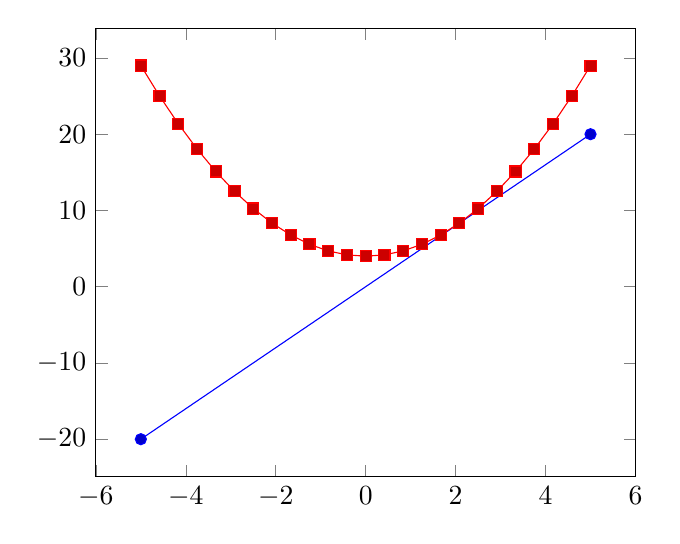
\begin{tikzpicture}
\begin{axis}[
    declare function={
        C=4;
        square(\t)=(\t)^2 + C;
    },
]
    \addplot+ [samples=2] {C*x};

    \addplot {square(x)};
\end{axis}
\end{tikzpicture}
\end{codeexample}
    %
    The definitions as such have the form \meta{function}\meta{argument list} =
    \meta{definition} where the \meta{argument list} contains a
    comma-separated-list of arguments like |\t| or |\t,\a,\b|. The
    \meta{definition} is a math expression which makes use of these arguments.

    Please refer to \cite{tikz} for more details.
\end{key}

\begin{command}{\pgfplotstableread\marg{file}}
    Please refer to the manual of \PGFPlotstable{}, |pgfplotstable.pdf|, which
    is part of the \PGFPlots{} bundle.
\end{command}

\begin{command}{\pgfplotstabletypeset\marg{\textbackslash macro}}
    Please refer to the manual of \PGFPlotstable{}, |pgfplotstable.pdf|, which
    is part of the \PGFPlots{} bundle.
\end{command}

\begin{command}{\pgfplotsiffileexists\marg{filename}\marg{true code}\marg{false code}}
    Invokes \meta{true code} if \meta{filename} exists and \meta{false code} if
    not. Can be used in looping macros, for example to plot every data file
    until there are no more of them.
\end{command}

\begin{command}{\pgfplotsutilifstringequal\marg{first}\marg{second}\marg{true code}\marg{false code}}
    A simple ``strcmp'' tool which invokes \meta{true code} if \meta{first}
    $=$\meta{second} and \meta{false code} otherwise. This does not expand
    macros.
\end{command}

\begin{commandlist}{\pgfkeys,\pgfeov,\pgfkeysvalueof,\pgfkeysgetvalue}
    These commands are part of the \Tikz{} way of specifying options, its
    sub-package |pgfkeys|. The |\pgfplotsset| command is actually nothing but a
    wrapper around |\pgfkeys|.

    A short introduction into |\pgfkeys| can be found in~\cite{keyvalintro}
    whereas the complete reference is, of course, the \Tikz{}
    manual~\cite{tikz}.

    The key |\pgfkeysvalueof|\marg{key name} expands to the value of a key;
    |\pgfkeysgetvalue|\marg{key name}\marg{\textbackslash macro} stores the
    value of \meta{key name} into \meta{\textbackslash macro}. The |\pgfeov|
    macro is used to delimit arguments for code keys in |\pgfkeys|, please
    refer to the references mentioned above.
\end{commandlist}


\section[Commands Inside Of PGFPlots Axes]
        {Commands Inside Of {\normalfont\PGFPlots{}} Axes}

\begin{command}{\autoplotspeclist}
    This command should no longer be used, although it will be kept as
    technical implementation detail. Please use the `|cycle list|' option,
    Section~\ref{sec:cycle:list}.
\end{command}

\begin{command}{\logten}
    Expands to the constant $\log(10)$. Useful for log plots because $\log(10^i)
    = i\log(10)$. This command is only available inside of a \Tikz{} picture.
\end{command}

\begin{command}{\pgfmathprintnumber\marg{number}}
    Generates pretty-printed output\footnote{This method was previously
    \texttt{\textbackslash prettyprintnumber}. Its functionality has been
    included into \PGF{} and the old command is now deprecated.} for
    \meta{number}. This method is used for every tick label.

    The number is printed using the current number printing options, see the
    manual of \PGFPlotstable{} which comes with this package for the different
    number styles, rounding precision and rounding methods.
\end{command}

\begin{command}{\numplots}
    Inside of any of the axis environments, associated style, option or
    command, |\numplots| expands to the total number of plots.
\end{command}

\begin{command}{\numplotsofactualtype}
    Like |\numplots|, this macro returns the total number of plots which have
    the same plot handler. Thus, if you have |sharp plot| active, it returns
    the number of all |sharp plots|. If you have |ybar| active, it returns the
    number of |ybar| plots and so on.
\end{command}

\begin{command}{\plotnum}
    Inside of |\addplot| or any associated style, option or command, |\plotnum|
    expands to the current plot's number, starting with~$0$.
\end{command}

\begin{command}{\plotnumofactualtype}
    Like |\plotnum|, but it returns the number among all plots of the same
    type. The number of all such plots is available using
    |\numplotsofactualtype|.
\end{command}

\begin{command}{\coordindex}
    Inside of an |\addplot| command, this macro expands to the number of the
    actual coordinate (starting with~$0$).

    It is useful together with |x filter| or |y filter| to (de)select
    coordinates.
\end{command}


\section{Path Operations}

\begin{commandlist}{\path,\draw,\fill,\node,\matrix}
    These commands are \Tikz{} drawing commands all of which are documented
    in~\cite{tikz}. They are used to draw or fill paths, generate text nodes or
    aligned text matrices. They are equivalent to
    \pgfmanualpdflabel{/tikz/draw}{}|\path[draw]|,
    \pgfmanualpdflabel{/tikz/fill}{}|\path[fill]|,
    \pgfmanualpdflabel{/tikz/node}{}|\path[node]|,
    \pgfmanualpdflabel{/tikz/matrix}{}|\path[matrix]|,
    respectively.
\end{commandlist}

\begin{pathoperation}{--}{\meta{coordinate}}
    A \Tikz{} path operation which connects the current point (the last one
    before |--|) and \meta{coordinate} with a straight line.
\end{pathoperation}

{\catcode`\|=12
\begin{pathoperation}[noindex]{|-}{\meta{coordinate}}
\pgfmanualpdflabel[\catcode`\|=12 ]{|-}{}%
    A \Tikz{} path operation which connects the current point and
    \meta{coordinate} with \emph{two} straight lines: first vertical, then
    horizontal.
\end{pathoperation}

\begin{pathoperation}[noindex]{-|}{\meta{coordinate}}
\pgfmanualpdflabel[\catcode`\|=12 ]{-|}{}%
    A \Tikz{} path operation which connects the current point and
    \meta{coordinate} with \emph{two} straight lines: first horizontal, then
    vertical.
\end{pathoperation}
}

\begin{keylist}{/tikz/xshift=\marg{dimension},/tikz/yshift=\marg{dimension}}
    These \Tikz{} keys allow to shift something by \meta{dimension} which is
    any \TeX{} size (or expression).
\end{keylist}

\begin{command}{\pgfplotsextra\marg{low-level path commands}}
    A command to execute \meta{low-level path commands} in a \PGFPlots{} axis.
    Since any drawing commands inside of an axis need to be postponed until the
    axis is complete and the scaling has been initialised, it is not possible
    to simply draw any paths. Instead, it is necessary to draw them as soon as
    the axis is finished. This is done automatically for every \Tikz{} path --
    and it is also done manually if you write |\pgfplotsextra|\marg{commands}.
    %
\begin{codeexample}[]
\begin{tikzpicture}
\begin{axis}[xmin=0,xmax=3,ymin=0,ymax=5]
    \pgfplotsextra{
        \pgfpathmoveto{\pgfplotspointaxisxy{1}{2}}
        \pgfpathlineto{\pgfplotspointaxisxy{2}{4}}
        \pgfusepath{stroke}
    }
\end{axis}
\end{tikzpicture}
\end{codeexample}
    %
    The example above initializes an axis and executes the basic level path
    commands as soon as the axis is ready. The execution of multiple |\path|,
    |\addplot| and |\pgfplotsextra| commands is in the same sequence as they
    occur in the environment.\footnote{Except for stacked plots where the
    sequence may be reverse, see the key \texttt{reverse stack plots}.}
\end{command}

\begin{command}{\pgfplotspathaxisoutline}
    Generates a path which resembles the outline of the current axis. This path
    is used for clip paths and the background paths (if any).
\end{command}


\section{Specifying Basic Coordinates}
\label{sec:basic:coordinates}

\begin{commandlist}{%
    \pgfplotspointaxisxy\marg{x coordinate}\marg{y coordinate},
    \pgfplotspointaxisxyz\marg{x coordinate}\marg{y coordinate}\marg{z coordinate}%
}
    Point commands like |\pgfpointxy| which take logical, absolute coordinates
    and return a low-level point. Every transformation from user
    transformations to logarithms is applied.

    Since the transformations are initialized after the axis is complete, this
    command needs to be postponed (see |\pgfplotsextra|).

    This command is the basic level variant of |axis cs:|\meta{x
    coordinate}|,|\meta{y coordinate}|,|\meta{z coordinate}.

    Note that this is also the default coordinate system during the
    visualization phase; in other words: if you write |\draw (1,2) -- (1,4)|,
    \PGFPlots{} will automatically use |(axis cs:1,2) -- (axis cs:1,4)|.
\end{commandlist}

\begin{commandlist}{%
    \pgfplotspointaxisdirectionxy\marg{x coordinate}\marg{y coordinate},
    \pgfplotspointaxisdirectionxyz\marg{x coordinate}\marg{y coordinate}\marg{z coordinate}%
}
    Point commands like |\pgfpointxy| which take logical, \emph{relative}
    coordinates and return a low-level point. Every transformation from user
    transformations to logarithms is applied. The difference to
    |\pgfplotspointaxisxy| is that the shift of the linear transformation is
    skipped here (compare |disabledatascaling|).

    This command is the basic level variant of |axis direction cs:|\meta{x
    coordinate}|,|\meta{y coordinate}|,|\meta{z coordinate}. Please refer to
    the documentation of |axis direction cs| for more details.

    Use this command whenever something of \emph{relative} character like
    directions or lengths need to be supplied. One use case is to draw
    ellipses:
    %
\begin{codeexample}[]
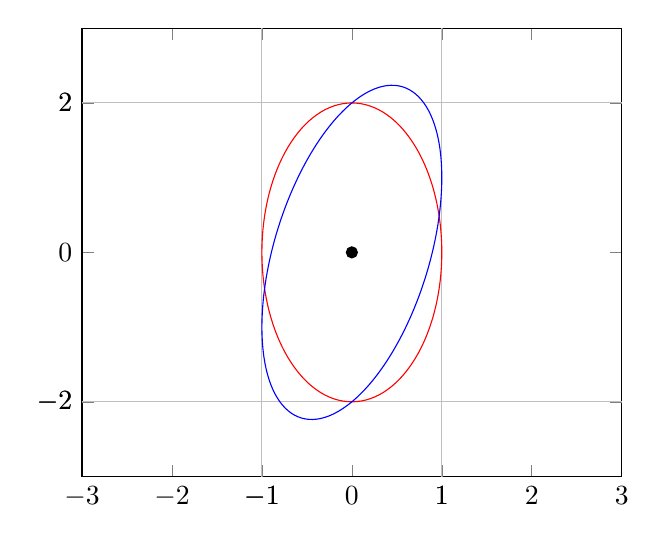
\begin{tikzpicture}
\begin{axis}[
    xmin=-3,   xmax=3,
    ymin=-3,   ymax=3,
    extra x ticks={-1,1},
    extra y ticks={-2,2},
    extra tick style={grid=major},
]
    \draw [red] \pgfextra{
        \pgfpathellipse{\pgfplotspointaxisxy{0}{0}}
            {\pgfplotspointaxisdirectionxy{1}{0}}
            {\pgfplotspointaxisdirectionxy{0}{2}}
    % see also the documentation of
    % 'axis direction cs' which
    % allows a simpler way to draw this ellipse
    };
    \draw [blue] \pgfextra{
        \pgfpathellipse{\pgfplotspointaxisxy{0}{0}}
            {\pgfplotspointaxisdirectionxy{1}{1}}
            {\pgfplotspointaxisdirectionxy{0}{2}}
    };
    \addplot [only marks,mark=*] coordinates
        { (0,0) };
\end{axis}
\end{tikzpicture}
\end{codeexample}

    Since the transformations are initialized after the axis is complete, this
    command needs to be provided either inside of a \tikzname{} |\path| command
    (like |\draw| in the example above) or inside of |\pgfplotsextra|.
\end{commandlist}

\begin{commandlist}{%
    \pgfplotspointrelaxisxy\marg{rel x coordinate}\marg{rel y coordinate},
    \pgfplotspointrelaxisxyz\marg{rel x coordinate}\marg{rel y coordinate}\marg{rel z coordinate}%
}
    Point commands which take \emph{relative} coordinates such that $x=0$ is
    the \emph{lower} $x$-axis limit and $x=1$ the \emph{upper} $x$-axis limit.

    These commands are used for |rel axis cs|.

    Please note that the transformations are only initialised if the axis is
    complete! This means you need to provide |\pgfplotsextra|.
\end{commandlist}

\begin{commandlist}{%
    \pgfplotspointdescriptionxy\marg{$x$ fraction}\marg{$y$ fraction},
    \pgfplotsqpointdescriptionxy\marg{$x$ fraction}\marg{$y$ fraction}%
}
    Point commands such that |{0}{0}| is the lower left corner of the axis'
    bounding box and |{1}{1}| the upper right one; everything else is in
    between. The `|q|' variant is quicker as it doesn't invoke the math parser
    on its arguments.

    They are used for |axis description cs|, see
    Section~\ref{pgfplots:sec:axis:description:cs}.
\end{commandlist}

\begin{commandlist}{\pgfplotspointaxisorigin}
    A point coordinate at the origin, $(0,0,0)$. If the origin is not part of
    the axis limits, the nearest point on the boundary is returned instead.

    This is the same coordinate as returned by the |origin| anchor.
\end{commandlist}

\begin{commandlist}{%
    \pgfplotstransformcoordinatex\marg{x coordinate of an axis},
    \pgfplotstransformcoordinatey\marg{y coordinate of an axis},
    \pgfplotstransformcoordinatez\marg{z coordinate of an axis}%
}
    Defines |\pgfmathresult| to be the low-level \PGF{} coordinate
    corresponding to the input argument.

    The command applies any |[xyz] coord trafo| keys, data scalings and/or
    logarithms or whatever \PGFPlots{} does to map input coordinates to
    internal coordinates.

    The result can be used inside of a |\pgfpointxy| statement (i.e.\@ it still
    needs to be scaled with the respective \PGF{} unit vector).
    %
\begin{codeexample}[]
\begin{tikzpicture}
\pgfplotsset{compat/pgfpoint substitution=1.3}
\begin{axis}[xmin=0,xmax=2,ymin=0,ymax=5]
    \pgfplotsextra{
        \pgfplotstransformcoordinatex{1}
        \let\xcoord=\pgfmathresult
        \pgfplotstransformcoordinatey{1}
        \let\ycoord=\pgfmathresult
        \pgfpathcircle
            {\pgfqpointxy{\xcoord}{\ycoord}}
            {5pt}
        \pgfusepath{fill}
    }
\end{axis}
\end{tikzpicture}
\end{codeexample}
    %
    Note that \PGFPlots{} substitutes |\pgfqpointxy| by |\pgfplotspointaxisxyz|
    by default -- and this command implicitly transforms coordinates anyway. In
    order to see the difference, the preceding example first disables this
    automatic substitution of coordinate systems by means of
    |compat/pgfpoint substitution=1.3|.
    %
    The result of this command is also available as math method
    |transformcoordinatex| (see the documentation for |axis cs|).

    Please note that the transformations are only initialised if the axis is
    complete. This means you need to provide |\pgfplotsextra| as is shown in
    the example above.
\end{commandlist}

\begin{commandlist}{%
    \pgfplotstransformdirectionx\marg{x direction of an axis},
    \pgfplotstransformdirectiony\marg{y direction of an axis},
    \pgfplotstransformdirectionz\marg{z direction of an axis}%
}
    Defines |\pgfmathresult| to be a low-level \PGF{} \emph{direction vector
    component}.

    A direction vector needs to be \emph{added} to some coordinate in order to
    get a coordinate, compare the documentation for
    |\pgfplotspointaxisdirectionxy| and |axis direction cs|.

    The argument \meta{x direction of an axis} is processed in (almost) the
    same way as for the macro which operates on absolute positions,
    |\pgfplotstransformcoordinatex|. The only difference is that
    \emph{directions} need no shifting transformation.

    The result of this command is also available as math method
    |transformdirectionx| (see the documentation for |axis direction cs|).

    See |axis direction cs| for details and examples about this command.
\end{commandlist}

% this command is for internal use only:
%--------------------------------------------------
% \begin{command}{\pgfplotsconvertunittocoordinate\marg{x, y or z}\marg{dimension}}
%     Converts a dimension (with unit!) to a corresponding $x$-, $y$- or $z$-coordinate. The result will be written to |\pgfmathresult| (without units).
%
%     It is possible to use the result as arguments for the |\pgfpointxyz| commands.
%
%     The effect is to multiply \meta{dimension} with the inverse length of the unit vector for the specified axis. These lengths are precomputed in \PGFPlots{} so the operation is fast.
% \begin{codeexample}[code only]
% \pgfplotsconvertunittocoordinate{x}{5pt}
% % now, the command uses exactly 5pt in x direction:
% \pgfqpointxyz{\pgfmathresult}{4}{3}
% \end{codeexample}
% \end{command}
%--------------------------------------------------

\begin{commandlist}{%
    \pgfplotspointunitx,
    \pgfplotspointunity,
    \pgfplotspointunitz%
}
    Low-level point commands which return the canvas $x$, $y$ or $z$ unit
    vectors.

    The |\pgfplotspointunitx| is the \pgfname{} unit vector in $x$ direction.

    These vectors are essentially the same as |\pgfqpointxyz{1}{0}{0}|,
    |\pgfqpointxyz{0}{1}{0}|, and |\pgfqpointxyz{0}{0}{1}|, respectively.

    The unit $z$ vector is only defined for three dimensional axes.
\end{commandlist}

\begin{commandlist}{%
    \pgfplotsunitxlength,
    \pgfplotsunitylength,
    \pgfplotsunitzlength,
    \pgfplotsunitxinvlength,
    \pgfplotsunityinvlength,
    \pgfplotsunitzinvlength%
}
    Macros which expand to the vector length $\lVert x_i \rVert$ of the
    respective unit vector $x_i$ or the inverse vector length, $1/\lVert x_i
    \rVert$. These macros can be used inside of |\pgfmathparse|, for example.

    The $x_i$ are the |\pgfplotspointunitx| variants.
\end{commandlist}

\begin{command}{\pgfplotsqpointoutsideofaxis%
        \marg{three-char-string}\marg{coordinate}\marg{normal distance}%
}
    Provides a point coordinate on one of the available four axes in case of a
    two dimensional figure or on one of the available twelve axes in case of a
    three dimensional figure.

    The desired axis is uniquely identified by a three character string,
    provided as first argument to the command. The first of the three
    characters is `|0|' if the $x$-coordinate of the specified axis passes
    through the lower axis limit. It is `|1|', if the $x$-coordinate of the
    specified axis passes through the upper axis limit. Furthermore, it is
    `|2|' if it passes through the origin. The second character is also either
    |0|, |1| or |2| and it characterizes the position on the $y$-axis. The
    third character is for the third dimension, the $z$-axis. It should be left
    at `|0|' for two dimensional plots. However, \emph{one} of the three
    characters should be `|v|', meaning the axis \underline varies. For
    example, |v01| denotes $\{ (x,y_{\min},z_{\max}) \vert x \in \R \}$.

    The second argument, \meta{coordinate} is the logical coordinate on that
    axis. Since two coordinates of the axis are fixed, \meta{coordinate} refers
    to the \underline varying component of the axis. It must be a number
    without unit; no math expressions are supported here.

    The third argument \meta{normal distance} is a dimension like |10pt|. It
    shifts the coordinate away from the designated axis in direction of the
    outer normal vector. The outer normal vector always points away from the
    axis. It is computed using |\pgfplotspointouternormalvectorofaxis|.

    There are several variants of this command which are documented in the
    source code. One of them is particularly useful:
\end{command}

\begin{command}{\pgfplotsqpointoutsideofaxisrel%
        \marg{three-char-string}\marg{axis fraction}\marg{normal distance}%
}
    This point coordinate is a variant of |\pgfplotsqpointoutsideofaxis| which
    allows to provide an \meta{axis fraction} instead of an absolute
    coordinate. The fraction is a number between $0$ (lower axis limit) and $1$
    (upper axis limit), i.e.\@ it is given in percent of the total axis. It is
    possible to provide negative values or values larger than one.

    The |\pgfplotsqpointoutsideofaxisrel| command is similar in spirit to
    |rel axis cs|.

    There is one speciality in conjunction with reversed axes: if the axis has
    been reversed by |x dir=reverse| and, in addition,
    |allow reversal of rel axis cs| is true, the value $0$ denotes the
    \emph{upper} limit while $1$ denotes the \emph{lower} limit. The effect is
    that coordinates won't change just because of axis reversal.
        \index{allow reversal of rel axis cs}%
\end{command}

\begin{command}{\pgfplotspointouternormalvectorofaxis\marg{three-char-string}}
    A point command which yields the outer normal vector of the respective
    axis. The normal vector has length $1$ (computed with
    |\pgfpointnormalised|). It is the same normal vector used inside of
    |\pgfplotsqpointoutsideofaxis| and its variants.

    The output of this command will be cached and reused during the lifetime
    of an axis.
\end{command}

\begin{command}{\pgfplotsticklabelaxisspec\marg{x, y or z}}
    Expands to the three character identification for the axis containing tick
    labels for the chosen axis, either \meta{x}, \meta{y} or \meta{z}.
\end{command}

\begin{command}{\pgfplotsvalueoflargesttickdimen\marg{x, y or z}}
    Expands to the largest distance of a tick position to its tick label
    bounding box in direction of the outer unit normal vector. It does also
    include the value of the |ticklabel shift| key.

    This value is used for |ticklabel cs|.
\end{command}

\begin{commandlist}{
    \pgfplotsmathfloatviewdepthxyz\marg{x}\marg{y}\marg{z},
    \pgfplotsmathviewdepthxyz\marg{x}\marg{y}\marg{z}%
}
    Both macros define |\pgfmathresult| to be the ``depth'' of a three
    dimensional point $\bar x = (x,y,z)$. The depth is defined to be the scalar
    product of $\bar x$ with $\vec d$, the view direction of the current axis.

    For |\pgfplotsmathfloatviewdepthxyz|, the arguments are parsed as floating
    point numbers and the result is encoded in floating point. A fixed point
    representation can be generated with
    |\pgfmathfloattofixed{\pgfmathresult}|.

    For |\pgfplotsmathviewdepthxyz|, \TeX{} arithmetics is employed for the
    inner product and the result is assigned in fixed point. This is slightly
    faster, but has considerably smaller data range.

    Both commands can only be used \emph{inside} of a three dimensional
    \PGFPlots{} axis (as soon as the axis is initialised, see
    |\pgfplotsextra|).
\end{commandlist}

\begin{texif}{pgfplotsthreedim}
    A \TeX{} |\if| which evaluates the \meta{true code} if the axis is three
    dimensional and the \meta{else code} if not.
\end{texif}


\section{Accessing Axis Limits}

It is also possible to access axis limits during the visualization phase,
i.e.\@ during |\end{axis}|. Please refer to the reference documentation for
|xmin| on page~\pageref{page:access:limits}.


\section{Accessing Point Coordinate Values}

During the visualization phase, \PGFPlots{} provides access to the currently
processed coordinate and its values.

This access requires a call to specific macros. These macros write the
coordinate values to some publicly available key--value pairs. Then, the
current point's $x$, $y$, $z$, and color data can be accessed.

\begin{commandlist}{\pgfplotspointgetcoordinates,\pgfplotspointgetcoordinates\marg{point}}

    After invoking the macro, the following keys will be set:

    \declaretext{/data point/x} will contain the current point's $x$-coordinate.

    \declaretext{/data point/y} will contain the current point's $y$-coordinate.

    \declaretext{/data point/z} will contain the current point's $z$-coordinate
    (if applicable).

    \declaretext{/data point/meta} will contain the current point's
    |point meta| value (if applicable).

    \declaretext{/data point/index} will contain the current point's index in
    the coordinate stream. This is actually the same as |\coordindex|.

    This command actually supports two modes of operation:
    %
    \begin{enumerate}
        \item Without arguments. In this case, it returns values of the point
            which is about to be processed by the current plot handler.
        \item With an argument in curly braces. In this case, it expects a
            coordinate and assigns the keys accordingly. Note that this
            command merely supports two-dimensional axes and assigns only
            |/data point/x| and |/data point/y|.
    \end{enumerate}

    The returned values are the same as they can be read on the axes, they are
    also the same as you would write them into |axis cs|.

    This means that any |x coord inv trafo| has been applied on the value. It
    also means that the exponential function has been called even though the
    internal coordinate was present in log format.

    This function is implicitly called for any |scatter| plot (including
    |nodes near coords|). This allows to access \emph{all} coordinate values at
    once:
    %
\begin{codeexample}[]
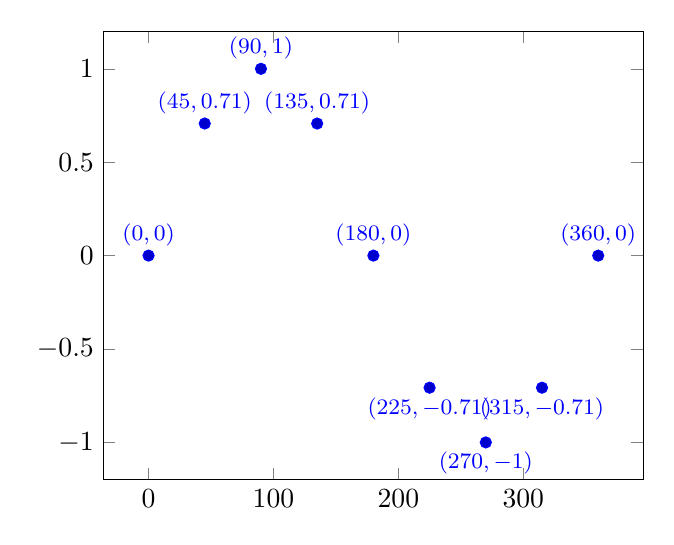
\begin{tikzpicture}
\begin{axis}
    \addplot+ [
        domain=0:360,
        samples=9,
        only marks,
        nodes near coords={%
            \footnotesize
            $(\pgfmathprintnumber
                {\pgfkeysvalueof{/data point/x}},
               \pgfmathprintnumber
                {\pgfkeysvalueof{/data point/y}})$%
        },
    ] {sin(x)};
\end{axis}
\end{tikzpicture}
\end{codeexample}
    %
    The example works because |\pgfplotspointgetcoordinates| is part of the
    standard implementation of |nodes near coords|; the resulting values are
    directly available. Note that the preceding example would have been simpler
    if we would have printed just one value: |nodes near coords| resorts to the
    |point meta|. And that, in turn, contains the $y$-coordinate anyway by
    default.

    A more advanced example would be a |ybar| plot in which nodes shall be
    placed at the lower end of the axis, together with some dotted lines to the
    respective bars:
    %
\begin{codeexample}[]
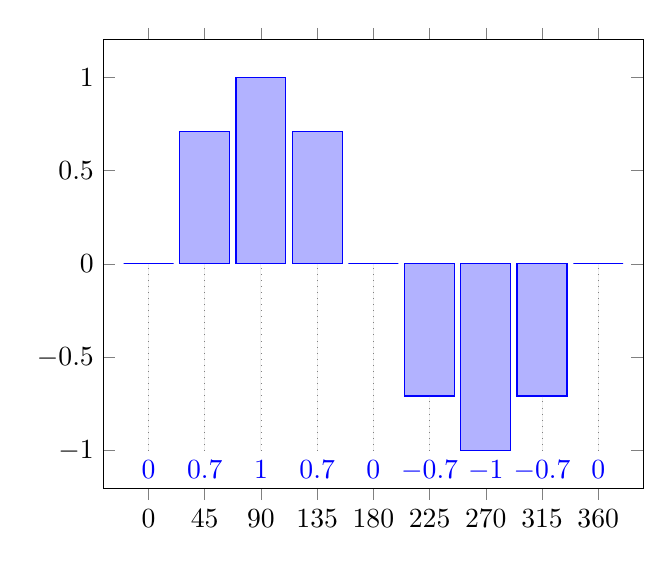
\begin{tikzpicture}
\begin{axis}[
    ybar,
    nodes near coords,
    %
    % we want to provide absolute 'at' values
    % for the nodes:
    scatter/position=absolute,
    every node near coord/.style={
        at={(\pgfkeysvalueof{/data point/x},-1)},
        % pretty printing:
        anchor=north,
        /pgf/number format/fixed,
        /pgf/number format/precision=1,
        % assign a name which can be referenced below:
        name=NNC\pgfkeysvalueof{/data point/index},
    },
    % ... draw a dotted line between
    % the marker and the bar:
    /pgfplots/scatter/@post marker code/.add code={}{
        \draw [dotted,help lines]
            (NNC\pgfkeysvalueof{/data point/index})
            -- (\pgfkeysvalueof{/data point/x},
            {min(0,\pgfkeysvalueof{/data point/y})});
    },
    % assign suitable tick labels:
    xtick=data,
]
    % some dummy data:
    \addplot+ [
        domain=0:360,
        bar width=360/9,
        samples=9,
    ] {sin(x)};
\end{axis}
\end{tikzpicture}
\end{codeexample}
    %
    Again, the command is used implicitly as part of |nodes near coords| and
    does not occur in the example as such.

    \paragraph{See also} the related example online under
    \url{https://tex.stackexchange.com/a/141006}. It demonstrates how to
    place the nodes generated by |nodes near coords| based on the value (either
    inside of a bar or above it).

    The following example uses an argument in curly braces for which we seek
    coordinate values:
    %
\begin{codeexample}[]
% requires \usetikzlibrary{intersections}
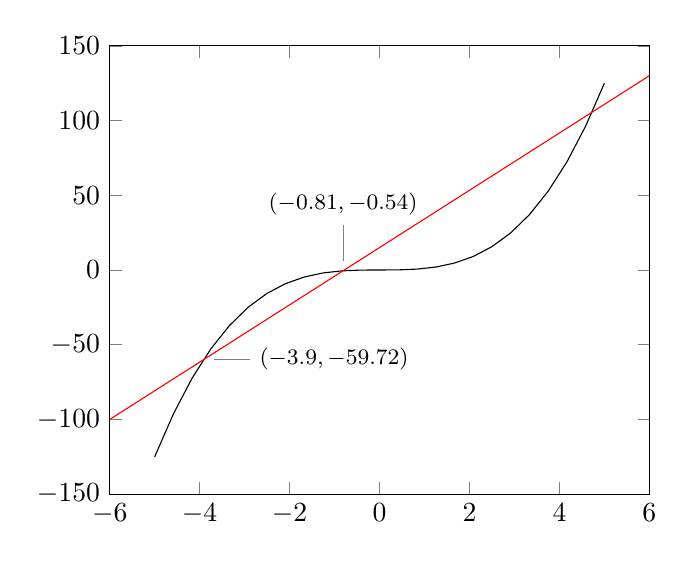
\begin{tikzpicture}
\begin{axis}
    \addplot [name path=A] {x^3};

    \draw [red,name path=HelperLine]
        (axis cs:-6,-100) -- (axis cs:6,130);

    \draw [
        font=\footnotesize,
        name intersections={of=A and HelperLine},
    ]
    node [pin={right:
      \pgfplotspointgetcoordinates{(intersection-1)}
        $(\pgfmathprintnumber[fixed]{
            \pgfkeysvalueof{/data point/x}},
          \pgfmathprintnumber[fixed]{
            \pgfkeysvalueof{/data point/y}})$
      }
    ] at (intersection-1) {}
    node [pin={
      \pgfplotspointgetcoordinates{(intersection-2)}
        $(\pgfmathprintnumber[fixed]{
            \pgfkeysvalueof{/data point/x}},
          \pgfmathprintnumber[fixed]{
            \pgfkeysvalueof{/data point/y}})$
      }
    ] at (intersection-2) {};
\end{axis}
\end{tikzpicture}
\end{codeexample}
    %
    The example computes and names intersections of |A| and |HelperLine|. The
    following code generates pins at the intersections. To this end, it uses
    |\pgfplotspointgetcoordinates|\marg{point} which defines |/data point/x|
    and |/data point/y|. These values are then formatted using
    |\pgfmathprintnumber|.

    In its second mode, |\pgfplotspointgetcoordinates|\marg{point} expects one
    of two things as \meta{point}:
    %
    \begin{enumerate}
        \item a basic-level \PGF{} point like |\pgfpointanchor{A}{center}| or
        \item a \Tikz{} point like |(A.base)| or |(3,5)|.
    \end{enumerate}
\end{commandlist}

\begin{command}{\pgfplotspointgetnormalizedcoordinates}
    A macro which is very similar to |\pgfplotspointgetcoordinates|.
    Consequently, it is also supposed to be called during the visualization phase.

    It assigns the very same output macros, but the values are different. More
    precisely, it defines the macros

    \declaretext{/data point/x} will contain the current point's
    \emph{normalized} $x$-coordinate.

    \declaretext{/data point/y} will contain the current point's
    \emph{normalized} $y$-coordinate.

    \declaretext{/data point/z} will contain the current point's
    \emph{normalized} $z$-coordinate (if applicable).

    \declaretext{/data point/meta} will contain the current point's
    |point meta| value (if applicable).

    \declaretext{/data point/index} will contain the current point's index in
    the coordinate stream. This is actually the same as |\coordindex|.

    The keyword \declaretext{normalized} means that the values are in a
    suitable numerical form which can be consumed by the axis. To be more
    specific: any user |x coord inv trafo| is \emph{ignored}. An important
    example would be |symbolic x coords|: the normalized coordinates would be
    some associated numbers, not the symbols. The results returned by
    |\pgfplotspointgetcoordinates| would be the symbols. For logarithm axes,
    the normalized values are the logs.

    Typically, normalized values are much more useful when you want to apply
    some math operation like averaging or subtraction.

    This function needs to be called explicitly. It is currently used by
    |ybar stacked| to align |nodes near coords|.
\end{command}


\section{Layer Access}

\begin{command}{\pgfplotsonlayer\marg{layer name}}
    A low-level command which will check if the current axis has layer support
    activated and, if so, calls |\pgfonlayer|\marg{layer name}.

    There must be a |\endpgfplotsonlayer| to delimit the environment.
\end{command}

\begin{command}{\endpgfplotsonlayer}
    The end of |\pgfplotsonlayer|.
\end{command}

\begin{command}{\pgfonlayer\marg{layer name}}
    A low-level command of \PGF{} which will collect everything until the
    matching |\endpgfonlayer| into layer \meta{layer name}.

    The \meta{layer name} must be active, i.e.\@ it must be part of the layer
    names of |set layers|.

    The only special case is if you call |\pgfdeclarelayer{discard}| somewhere:
    this special layer has a ``magical name'' which serves as |/dev/null| if it
    is enabled using |\pgfonlayer{discard}|: it does not need to be active and
    everything assigned to this layer will be thrown away if it is not part of
    the layer name configuration.

    There must be a |\endpgfonlayer| to delimit the environment.
\end{command}

\begin{command}{\endpgfonlayer}
    The end of |\pgfonlayer|.
\end{command}


\begin{command}{\pgfsetlayers\marg{layer list}}
    This is a low-level command of \PGF{}. At the time of this writing, it is
    the only way to tell \PGF{} which layers it shall use for the current/next
    picture. It is used implicitly by |set layers|.
\end{command}


\printindex

\bibliographystyle{abbrv} %gerapali} %gerabbrv} %gerunsrt.bst} %gerabbrv}% gerplain}
\nocite{pgfplotstable}
\nocite{programmingnotes}
\bibliography{pgfplots}
\end{document}

% -----------------------------------------------------------------------------
% For Stefan Pinnow as reminder on what to look for when editing the manual
% -----------------------------------------------------------------------------
% There should be no line breaks in the following environments
% - |...|
% - \declareandlabel{...}
% - \verbpdfref{...}
% If "MakeTikzPictures" isn't running through check one of the externalized
% LOG files what is the cause of that.
% -----------------------------------------------------------------------------


\chapter{Utilities and Basic Level Commands}
\label{cha:pgfplots:lowlevel}

This chapter documents commands which provide access to more basic elements of
\PGFPlots{}. Most of them are closely related to the basic level of \pgfname{},
especially various point commands which are specific to an axis. Some of them
are general purpose utilities like loops.

However, most elements in this section are only interesting for advanced users
-- and perhaps only for special cases.


\section{Utility Commands}

\begin{command}{\foreach \meta{variables} |in| \meta{list} \marg{commands}}
    A powerful loop command provided by \Tikz{}, see~\cite[Section
    ``Utilities'']{tikz}.
    %
\begin{codeexample}[]
\foreach \x in {1,2,...,4} {Iterating \x. }%
\end{codeexample}

    A \PGFPlots{} related example could be
    %
\begin{codeexample}[code only]
\foreach \i in {1,2,...,10} {\addplot table {datafile\i}; }%
\end{codeexample}
\end{command}

\begin{command}{\pgfplotsforeachungrouped \meta{variable} |in| \meta{list} \marg{command}}
    A specialised variant of |\foreach| which can do two things: it does not
    introduce extra groups while executing \meta{command} and it allows to
    invoke the math parser for (simple!)
    \meta{$x_0$}|,|\meta{$x_1$}|,...,|\meta{$x_n$} expressions.
    %
\begin{codeexample}[]
\def\allcollected{}
\pgfplotsforeachungrouped \x in {1,2,...,4} {Iterating \x. \edef\allcollected{\allcollected, \x}}%
All collected = \allcollected.
\end{codeexample}

    A more useful example might be to work with tables. The following example
    is taken from \PGFPlotstable{}:
    %
\begin{codeexample}[code only]
\pgfplotsforeachungrouped \i in {1,2,...,10} {%
    \pgfplotstablevertcat{\output}{datafile\i} % appends `datafile\i' -> `\output'
}%
% since it was ungrouped, \output is still defined (would not work
% with \foreach)
\end{codeexample}

    \paragraph{Remark:}

    The special syntax
    \meta{list}=\meta{$x_0$}|,|\meta{$x_1$}|,...,|\meta{$x_n$}, i.e.\@ with two
    leading elements, followed by dots and a final element, invokes the math
    parser for the loop. Thus, it allows larger number ranges than any other
    syntax if |/pgf/fpu| is active. In all other cases,
    |\pgfplotsforeachungrouped| invokes |\foreach| and provides the results
    without \TeX{} groups.

    Keep in mind that inside of an axis environment, all loop constructions
    (including custom loops, |\foreach| and |\pgfplotsforeachungrouped|) need
    to be handled with care: loop arguments can only be used in places where
    they are immediately evaluated; but \PGFPlots{} postpones the evaluation of
    many macros. For example, to loop over something and to generate axis
    descriptions of the form |\node at (axis cs:\i,0.5)...|, the loop macro
    |\i| will be evaluated in |\end{axis}| -- but at that time, the loop is
    over and its value is lost. The correct way to handle such an application
    is to \emph{expand} the loop variable \emph{explicitly}. For example:
    %
\begin{codeexample}[code only]
\pgfplotsforeachungrouped \i/\j in {
    1 / a,
    2 / b,
    3 / c
}{
    \edef\temp{\noexpand\node at (axis cs: \i,0.5) {\j};}
    % \show\temp % lets TeX show you what \temp contains
    \temp
}
\end{codeexample}
    %
    The example generates three loop iterations: |\i=1|, |\j=a|; then |\i=2|,
    |j=b|; then |\i=3|, |\j=c|. Inside of the loop body, it expands them and
    assigns the result to a macro using an ``expanded definition'', |\edef|.
    The result no longer contains either |\i| or |\j| (since these have been
    expanded). Then, it invokes the resulting macro. Details about the \TeX{}
    command |\edef| and expansion control can be found in the document
    \href{file:TeX-programming-notes.pdf}{TeX-programming-notes.pdf} which
    comes with \PGFPlots{}.
\end{command}

\begin{command}{\pgfplotsinvokeforeach\marg{list} \marg{command}}
    A variant of |\pgfplotsforeachungrouped| (and such also of |\foreach|)
    which replaces any occurrence of |#1| inside of \meta{command} once for
    every element in \meta{list}. Thus, it actually assumes that \marg{command}
    is like a |\newcommand| body.

    In other words, \meta{command} is invoked for every element of \meta{list}.
    The actual element of \meta{list} is available as |#1|.

    As |\pgfplotsforeachungrouped|, this command does \emph{not} introduce
    extra scopes (i.e.\@ it is ungrouped as well).

    The difference to |\foreach \x in |\meta{list}\marg{command} is subtle: the
    |\x| would \emph{not} be expanded whereas |#1| is.
    %
\begin{codeexample}[]
\pgfkeys{
    otherstyle a/.code={[a]},
    otherstyle b/.code={[b]},
    otherstyle c/.code={[c]},
    otherstyle d/.code={[d]}}
\pgfplotsinvokeforeach{a,b,c,d}
    {\pgfkeys{key #1/.style={otherstyle #1}}}
Invoke them:
\pgfkeys{key a} \pgfkeys{key b}
\pgfkeys{key c} \pgfkeys{key d}
\end{codeexample}
The counter example would use a macro (here |\x|) as loop argument:
\begin{codeexample}[]
\pgfkeys{
    otherstyle a/.code={[a]},
    otherstyle b/.code={[b]},
    otherstyle c/.code={[c]},
    otherstyle d/.code={[d]}}
\pgfplotsforeachungrouped \x in {a,b,c,d}
    {\pgfkeys{key \x/.style={otherstyle \x}}}
Invoke them:
\pgfkeys{key a} \pgfkeys{key b}
\pgfkeys{key c} \pgfkeys{key d}
\end{codeexample}

    \paragraph{Restrictions:}

    you can't nest this command yet (since it does not introduce protection by
    scopes).
\end{command}

\begin{command}{\pgfmathparse\marg{expression}}
    Invokes the \pgfname{} math parser for \meta{expression} and defines
    \declareandlabel{\pgfmathresult} to be the result.
    %
\begin{codeexample}[]
\pgfmathparse{1+41}

The result is `\pgfmathresult'.
\end{codeexample}
    %
    \noindent The math engine in \pgfname{} typically uses \TeX's internal
    arithmetics. That means: it is well suited for numbers in the range
    $[-16384,16384]$ and has a precision of $5$ digits.

    The number range is typically too small for plotting applications.
    \PGFPlots{} improves the number range by means of
    |\pgfkeys{/pgf/fpu}\pgfmathparse{1+41}| to activate the ``floating point
    unit'' (fpu) and to apply all following operations in floating point.

    In \PGFPlots{}, the key |/pgfplots/use fpu| is typically on, which means
    that any coordinate arithmetics are carried out with the |fpu|. However,
    all \pgfname{} related drawing operations still use the standard math
    engine.

    In case you ever need to process numbers of extended precision, you may
    want to use
    %
\begin{codeexample}[]
\pgfkeys{/pgf/fpu}%
\pgfmathparse{1000*1000}

The result is `\pgfmathprintnumber{\pgfmathresult}'.
\end{codeexample}
    %
    Note that results of the |fpu| are typically not in human-readable format,
    so |\pgfmathprintnumber| is the preferred way to typeset such numbers.

    Please refer to \cite{tikz} for more details.
\end{command}

\begin{pgfplotskey}{use fpu=\mchoice{true,false} (initially true)}
    \PGFPlots{} comes with different approaches to compute math expressions and
    |use fpu| is the most powerful. It implements math operations either in the
    |lua backend| or in a pure \TeX{} implementation and comes with a high
    number range and adequate precision.

    However, the values stored in |\pgfmathresult| are cryptic and need to be
    processed by means of special macros. The switch |use fpu| is only useful
    if this number format results in difficulties, i.e.\@ it is a debug switch
    which should never be used in normal operations.
\end{pgfplotskey}

\begin{key}{/pgf/declare function=\meta{function definitions}}
    Allows to define one or more functions.

    The argument \meta {function definitions} can contain one or more
    definitions, and each \emph{must} be terminated by a semicolon:
    %
\begin{codeexample}[]
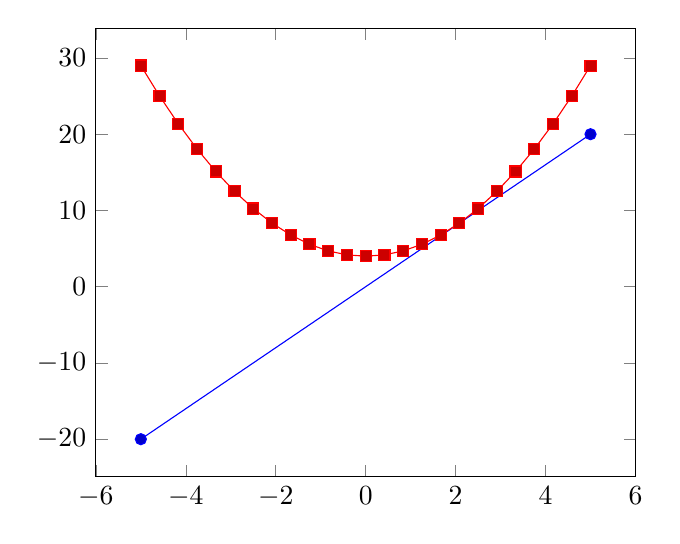
\begin{tikzpicture}
\begin{axis}[
    declare function={
        C=4;
        square(\t)=(\t)^2 + C;
    },
]
    \addplot+ [samples=2] {C*x};

    \addplot {square(x)};
\end{axis}
\end{tikzpicture}
\end{codeexample}
    %
    The definitions as such have the form \meta{function}\meta{argument list} =
    \meta{definition} where the \meta{argument list} contains a
    comma-separated-list of arguments like |\t| or |\t,\a,\b|. The
    \meta{definition} is a math expression which makes use of these arguments.

    Please refer to \cite{tikz} for more details.
\end{key}

\begin{command}{\pgfplotstableread\marg{file}}
    Please refer to the manual of \PGFPlotstable{}, |pgfplotstable.pdf|, which
    is part of the \PGFPlots{} bundle.
\end{command}

\begin{command}{\pgfplotstabletypeset\marg{\textbackslash macro}}
    Please refer to the manual of \PGFPlotstable{}, |pgfplotstable.pdf|, which
    is part of the \PGFPlots{} bundle.
\end{command}

\begin{command}{\pgfplotsiffileexists\marg{filename}\marg{true code}\marg{false code}}
    Invokes \meta{true code} if \meta{filename} exists and \meta{false code} if
    not. Can be used in looping macros, for example to plot every data file
    until there are no more of them.
\end{command}

\begin{command}{\pgfplotsutilifstringequal\marg{first}\marg{second}\marg{true code}\marg{false code}}
    A simple ``strcmp'' tool which invokes \meta{true code} if \meta{first}
    $=$\meta{second} and \meta{false code} otherwise. This does not expand
    macros.
\end{command}

\begin{commandlist}{\pgfkeys,\pgfeov,\pgfkeysvalueof,\pgfkeysgetvalue}
    These commands are part of the \Tikz{} way of specifying options, its
    sub-package |pgfkeys|. The |\pgfplotsset| command is actually nothing but a
    wrapper around |\pgfkeys|.

    A short introduction into |\pgfkeys| can be found in~\cite{keyvalintro}
    whereas the complete reference is, of course, the \Tikz{}
    manual~\cite{tikz}.

    The key |\pgfkeysvalueof|\marg{key name} expands to the value of a key;
    |\pgfkeysgetvalue|\marg{key name}\marg{\textbackslash macro} stores the
    value of \meta{key name} into \meta{\textbackslash macro}. The |\pgfeov|
    macro is used to delimit arguments for code keys in |\pgfkeys|, please
    refer to the references mentioned above.
\end{commandlist}


\section[Commands Inside Of PGFPlots Axes]
        {Commands Inside Of {\normalfont\PGFPlots{}} Axes}

\begin{command}{\autoplotspeclist}
    This command should no longer be used, although it will be kept as
    technical implementation detail. Please use the `|cycle list|' option,
    Section~\ref{sec:cycle:list}.
\end{command}

\begin{command}{\logten}
    Expands to the constant $\log(10)$. Useful for log plots because $\log(10^i)
    = i\log(10)$. This command is only available inside of a \Tikz{} picture.
\end{command}

\begin{command}{\pgfmathprintnumber\marg{number}}
    Generates pretty-printed output\footnote{This method was previously
    \texttt{\textbackslash prettyprintnumber}. Its functionality has been
    included into \PGF{} and the old command is now deprecated.} for
    \meta{number}. This method is used for every tick label.

    The number is printed using the current number printing options, see the
    manual of \PGFPlotstable{} which comes with this package for the different
    number styles, rounding precision and rounding methods.
\end{command}

\begin{command}{\numplots}
    Inside of any of the axis environments, associated style, option or
    command, |\numplots| expands to the total number of plots.
\end{command}

\begin{command}{\numplotsofactualtype}
    Like |\numplots|, this macro returns the total number of plots which have
    the same plot handler. Thus, if you have |sharp plot| active, it returns
    the number of all |sharp plots|. If you have |ybar| active, it returns the
    number of |ybar| plots and so on.
\end{command}

\begin{command}{\plotnum}
    Inside of |\addplot| or any associated style, option or command, |\plotnum|
    expands to the current plot's number, starting with~$0$.
\end{command}

\begin{command}{\plotnumofactualtype}
    Like |\plotnum|, but it returns the number among all plots of the same
    type. The number of all such plots is available using
    |\numplotsofactualtype|.
\end{command}

\begin{command}{\coordindex}
    Inside of an |\addplot| command, this macro expands to the number of the
    actual coordinate (starting with~$0$).

    It is useful together with |x filter| or |y filter| to (de)select
    coordinates.
\end{command}


\section{Path Operations}

\begin{commandlist}{\path,\draw,\fill,\node,\matrix}
    These commands are \Tikz{} drawing commands all of which are documented
    in~\cite{tikz}. They are used to draw or fill paths, generate text nodes or
    aligned text matrices. They are equivalent to
    \pgfmanualpdflabel{/tikz/draw}{}|\path[draw]|,
    \pgfmanualpdflabel{/tikz/fill}{}|\path[fill]|,
    \pgfmanualpdflabel{/tikz/node}{}|\path[node]|,
    \pgfmanualpdflabel{/tikz/matrix}{}|\path[matrix]|,
    respectively.
\end{commandlist}

\begin{pathoperation}{--}{\meta{coordinate}}
    A \Tikz{} path operation which connects the current point (the last one
    before |--|) and \meta{coordinate} with a straight line.
\end{pathoperation}

{\catcode`\|=12
\begin{pathoperation}[noindex]{|-}{\meta{coordinate}}
\pgfmanualpdflabel[\catcode`\|=12 ]{|-}{}%
    A \Tikz{} path operation which connects the current point and
    \meta{coordinate} with \emph{two} straight lines: first vertical, then
    horizontal.
\end{pathoperation}

\begin{pathoperation}[noindex]{-|}{\meta{coordinate}}
\pgfmanualpdflabel[\catcode`\|=12 ]{-|}{}%
    A \Tikz{} path operation which connects the current point and
    \meta{coordinate} with \emph{two} straight lines: first horizontal, then
    vertical.
\end{pathoperation}
}

\begin{keylist}{/tikz/xshift=\marg{dimension},/tikz/yshift=\marg{dimension}}
    These \Tikz{} keys allow to shift something by \meta{dimension} which is
    any \TeX{} size (or expression).
\end{keylist}

\begin{command}{\pgfplotsextra\marg{low-level path commands}}
    A command to execute \meta{low-level path commands} in a \PGFPlots{} axis.
    Since any drawing commands inside of an axis need to be postponed until the
    axis is complete and the scaling has been initialised, it is not possible
    to simply draw any paths. Instead, it is necessary to draw them as soon as
    the axis is finished. This is done automatically for every \Tikz{} path --
    and it is also done manually if you write |\pgfplotsextra|\marg{commands}.
    %
\begin{codeexample}[]
\begin{tikzpicture}
\begin{axis}[xmin=0,xmax=3,ymin=0,ymax=5]
    \pgfplotsextra{
        \pgfpathmoveto{\pgfplotspointaxisxy{1}{2}}
        \pgfpathlineto{\pgfplotspointaxisxy{2}{4}}
        \pgfusepath{stroke}
    }
\end{axis}
\end{tikzpicture}
\end{codeexample}
    %
    The example above initializes an axis and executes the basic level path
    commands as soon as the axis is ready. The execution of multiple |\path|,
    |\addplot| and |\pgfplotsextra| commands is in the same sequence as they
    occur in the environment.\footnote{Except for stacked plots where the
    sequence may be reverse, see the key \texttt{reverse stack plots}.}
\end{command}

\begin{command}{\pgfplotspathaxisoutline}
    Generates a path which resembles the outline of the current axis. This path
    is used for clip paths and the background paths (if any).
\end{command}


\section{Specifying Basic Coordinates}
\label{sec:basic:coordinates}

\begin{commandlist}{%
    \pgfplotspointaxisxy\marg{x coordinate}\marg{y coordinate},
    \pgfplotspointaxisxyz\marg{x coordinate}\marg{y coordinate}\marg{z coordinate}%
}
    Point commands like |\pgfpointxy| which take logical, absolute coordinates
    and return a low-level point. Every transformation from user
    transformations to logarithms is applied.

    Since the transformations are initialized after the axis is complete, this
    command needs to be postponed (see |\pgfplotsextra|).

    This command is the basic level variant of |axis cs:|\meta{x
    coordinate}|,|\meta{y coordinate}|,|\meta{z coordinate}.

    Note that this is also the default coordinate system during the
    visualization phase; in other words: if you write |\draw (1,2) -- (1,4)|,
    \PGFPlots{} will automatically use |(axis cs:1,2) -- (axis cs:1,4)|.
\end{commandlist}

\begin{commandlist}{%
    \pgfplotspointaxisdirectionxy\marg{x coordinate}\marg{y coordinate},
    \pgfplotspointaxisdirectionxyz\marg{x coordinate}\marg{y coordinate}\marg{z coordinate}%
}
    Point commands like |\pgfpointxy| which take logical, \emph{relative}
    coordinates and return a low-level point. Every transformation from user
    transformations to logarithms is applied. The difference to
    |\pgfplotspointaxisxy| is that the shift of the linear transformation is
    skipped here (compare |disabledatascaling|).

    This command is the basic level variant of |axis direction cs:|\meta{x
    coordinate}|,|\meta{y coordinate}|,|\meta{z coordinate}. Please refer to
    the documentation of |axis direction cs| for more details.

    Use this command whenever something of \emph{relative} character like
    directions or lengths need to be supplied. One use case is to draw
    ellipses:
    %
\begin{codeexample}[]
\begin{tikzpicture}
\begin{axis}[
    xmin=-3,   xmax=3,
    ymin=-3,   ymax=3,
    extra x ticks={-1,1},
    extra y ticks={-2,2},
    extra tick style={grid=major},
]
    \draw [red] \pgfextra{
        \pgfpathellipse{\pgfplotspointaxisxy{0}{0}}
            {\pgfplotspointaxisdirectionxy{1}{0}}
            {\pgfplotspointaxisdirectionxy{0}{2}}
    % see also the documentation of
    % 'axis direction cs' which
    % allows a simpler way to draw this ellipse
    };
    \draw [blue] \pgfextra{
        \pgfpathellipse{\pgfplotspointaxisxy{0}{0}}
            {\pgfplotspointaxisdirectionxy{1}{1}}
            {\pgfplotspointaxisdirectionxy{0}{2}}
    };
    \addplot [only marks,mark=*] coordinates
        { (0,0) };
\end{axis}
\end{tikzpicture}
\end{codeexample}

    Since the transformations are initialized after the axis is complete, this
    command needs to be provided either inside of a \tikzname{} |\path| command
    (like |\draw| in the example above) or inside of |\pgfplotsextra|.
\end{commandlist}

\begin{commandlist}{%
    \pgfplotspointrelaxisxy\marg{rel x coordinate}\marg{rel y coordinate},
    \pgfplotspointrelaxisxyz\marg{rel x coordinate}\marg{rel y coordinate}\marg{rel z coordinate}%
}
    Point commands which take \emph{relative} coordinates such that $x=0$ is
    the \emph{lower} $x$-axis limit and $x=1$ the \emph{upper} $x$-axis limit.

    These commands are used for |rel axis cs|.

    Please note that the transformations are only initialised if the axis is
    complete! This means you need to provide |\pgfplotsextra|.
\end{commandlist}

\begin{commandlist}{%
    \pgfplotspointdescriptionxy\marg{$x$ fraction}\marg{$y$ fraction},
    \pgfplotsqpointdescriptionxy\marg{$x$ fraction}\marg{$y$ fraction}%
}
    Point commands such that |{0}{0}| is the lower left corner of the axis'
    bounding box and |{1}{1}| the upper right one; everything else is in
    between. The `|q|' variant is quicker as it doesn't invoke the math parser
    on its arguments.

    They are used for |axis description cs|, see
    Section~\ref{pgfplots:sec:axis:description:cs}.
\end{commandlist}

\begin{commandlist}{\pgfplotspointaxisorigin}
    A point coordinate at the origin, $(0,0,0)$. If the origin is not part of
    the axis limits, the nearest point on the boundary is returned instead.

    This is the same coordinate as returned by the |origin| anchor.
\end{commandlist}

\begin{commandlist}{%
    \pgfplotstransformcoordinatex\marg{x coordinate of an axis},
    \pgfplotstransformcoordinatey\marg{y coordinate of an axis},
    \pgfplotstransformcoordinatez\marg{z coordinate of an axis}%
}
    Defines |\pgfmathresult| to be the low-level \PGF{} coordinate
    corresponding to the input argument.

    The command applies any |[xyz] coord trafo| keys, data scalings and/or
    logarithms or whatever \PGFPlots{} does to map input coordinates to
    internal coordinates.

    The result can be used inside of a |\pgfpointxy| statement (i.e.\@ it still
    needs to be scaled with the respective \PGF{} unit vector).
    %
\begin{codeexample}[]
\begin{tikzpicture}
\pgfplotsset{compat/pgfpoint substitution=1.3}
\begin{axis}[xmin=0,xmax=2,ymin=0,ymax=5]
    \pgfplotsextra{
        \pgfplotstransformcoordinatex{1}
        \let\xcoord=\pgfmathresult
        \pgfplotstransformcoordinatey{1}
        \let\ycoord=\pgfmathresult
        \pgfpathcircle
            {\pgfqpointxy{\xcoord}{\ycoord}}
            {5pt}
        \pgfusepath{fill}
    }
\end{axis}
\end{tikzpicture}
\end{codeexample}
    %
    Note that \PGFPlots{} substitutes |\pgfqpointxy| by |\pgfplotspointaxisxyz|
    by default -- and this command implicitly transforms coordinates anyway. In
    order to see the difference, the preceding example first disables this
    automatic substitution of coordinate systems by means of
    |compat/pgfpoint substitution=1.3|.
    %
    The result of this command is also available as math method
    |transformcoordinatex| (see the documentation for |axis cs|).

    Please note that the transformations are only initialised if the axis is
    complete. This means you need to provide |\pgfplotsextra| as is shown in
    the example above.
\end{commandlist}

\begin{commandlist}{%
    \pgfplotstransformdirectionx\marg{x direction of an axis},
    \pgfplotstransformdirectiony\marg{y direction of an axis},
    \pgfplotstransformdirectionz\marg{z direction of an axis}%
}
    Defines |\pgfmathresult| to be a low-level \PGF{} \emph{direction vector
    component}.

    A direction vector needs to be \emph{added} to some coordinate in order to
    get a coordinate, compare the documentation for
    |\pgfplotspointaxisdirectionxy| and |axis direction cs|.

    The argument \meta{x direction of an axis} is processed in (almost) the
    same way as for the macro which operates on absolute positions,
    |\pgfplotstransformcoordinatex|. The only difference is that
    \emph{directions} need no shifting transformation.

    The result of this command is also available as math method
    |transformdirectionx| (see the documentation for |axis direction cs|).

    See |axis direction cs| for details and examples about this command.
\end{commandlist}

% this command is for internal use only:
%--------------------------------------------------
% \begin{command}{\pgfplotsconvertunittocoordinate\marg{x, y or z}\marg{dimension}}
%     Converts a dimension (with unit!) to a corresponding $x$-, $y$- or $z$-coordinate. The result will be written to |\pgfmathresult| (without units).
%
%     It is possible to use the result as arguments for the |\pgfpointxyz| commands.
%
%     The effect is to multiply \meta{dimension} with the inverse length of the unit vector for the specified axis. These lengths are precomputed in \PGFPlots{} so the operation is fast.
% \begin{codeexample}[code only]
% \pgfplotsconvertunittocoordinate{x}{5pt}
% % now, the command uses exactly 5pt in x direction:
% \pgfqpointxyz{\pgfmathresult}{4}{3}
% \end{codeexample}
% \end{command}
%--------------------------------------------------

\begin{commandlist}{%
    \pgfplotspointunitx,
    \pgfplotspointunity,
    \pgfplotspointunitz%
}
    Low-level point commands which return the canvas $x$, $y$ or $z$ unit
    vectors.

    The |\pgfplotspointunitx| is the \pgfname{} unit vector in $x$ direction.

    These vectors are essentially the same as |\pgfqpointxyz{1}{0}{0}|,
    |\pgfqpointxyz{0}{1}{0}|, and |\pgfqpointxyz{0}{0}{1}|, respectively.

    The unit $z$ vector is only defined for three dimensional axes.
\end{commandlist}

\begin{commandlist}{%
    \pgfplotsunitxlength,
    \pgfplotsunitylength,
    \pgfplotsunitzlength,
    \pgfplotsunitxinvlength,
    \pgfplotsunityinvlength,
    \pgfplotsunitzinvlength%
}
    Macros which expand to the vector length $\lVert x_i \rVert$ of the
    respective unit vector $x_i$ or the inverse vector length, $1/\lVert x_i
    \rVert$. These macros can be used inside of |\pgfmathparse|, for example.

    The $x_i$ are the |\pgfplotspointunitx| variants.
\end{commandlist}

\begin{command}{\pgfplotsqpointoutsideofaxis%
        \marg{three-char-string}\marg{coordinate}\marg{normal distance}%
}
    Provides a point coordinate on one of the available four axes in case of a
    two dimensional figure or on one of the available twelve axes in case of a
    three dimensional figure.

    The desired axis is uniquely identified by a three character string,
    provided as first argument to the command. The first of the three
    characters is `|0|' if the $x$-coordinate of the specified axis passes
    through the lower axis limit. It is `|1|', if the $x$-coordinate of the
    specified axis passes through the upper axis limit. Furthermore, it is
    `|2|' if it passes through the origin. The second character is also either
    |0|, |1| or |2| and it characterizes the position on the $y$-axis. The
    third character is for the third dimension, the $z$-axis. It should be left
    at `|0|' for two dimensional plots. However, \emph{one} of the three
    characters should be `|v|', meaning the axis \underline varies. For
    example, |v01| denotes $\{ (x,y_{\min},z_{\max}) \vert x \in \R \}$.

    The second argument, \meta{coordinate} is the logical coordinate on that
    axis. Since two coordinates of the axis are fixed, \meta{coordinate} refers
    to the \underline varying component of the axis. It must be a number
    without unit; no math expressions are supported here.

    The third argument \meta{normal distance} is a dimension like |10pt|. It
    shifts the coordinate away from the designated axis in direction of the
    outer normal vector. The outer normal vector always points away from the
    axis. It is computed using |\pgfplotspointouternormalvectorofaxis|.

    There are several variants of this command which are documented in the
    source code. One of them is particularly useful:
\end{command}

\begin{command}{\pgfplotsqpointoutsideofaxisrel%
        \marg{three-char-string}\marg{axis fraction}\marg{normal distance}%
}
    This point coordinate is a variant of |\pgfplotsqpointoutsideofaxis| which
    allows to provide an \meta{axis fraction} instead of an absolute
    coordinate. The fraction is a number between $0$ (lower axis limit) and $1$
    (upper axis limit), i.e.\@ it is given in percent of the total axis. It is
    possible to provide negative values or values larger than one.

    The |\pgfplotsqpointoutsideofaxisrel| command is similar in spirit to
    |rel axis cs|.

    There is one speciality in conjunction with reversed axes: if the axis has
    been reversed by |x dir=reverse| and, in addition,
    |allow reversal of rel axis cs| is true, the value $0$ denotes the
    \emph{upper} limit while $1$ denotes the \emph{lower} limit. The effect is
    that coordinates won't change just because of axis reversal.
        \index{allow reversal of rel axis cs}%
\end{command}

\begin{command}{\pgfplotspointouternormalvectorofaxis\marg{three-char-string}}
    A point command which yields the outer normal vector of the respective
    axis. The normal vector has length $1$ (computed with
    |\pgfpointnormalised|). It is the same normal vector used inside of
    |\pgfplotsqpointoutsideofaxis| and its variants.

    The output of this command will be cached and reused during the lifetime
    of an axis.
\end{command}

\begin{command}{\pgfplotsticklabelaxisspec\marg{x, y or z}}
    Expands to the three character identification for the axis containing tick
    labels for the chosen axis, either \meta{x}, \meta{y} or \meta{z}.
\end{command}

\begin{command}{\pgfplotsvalueoflargesttickdimen\marg{x, y or z}}
    Expands to the largest distance of a tick position to its tick label
    bounding box in direction of the outer unit normal vector. It does also
    include the value of the |ticklabel shift| key.

    This value is used for |ticklabel cs|.
\end{command}

\begin{commandlist}{
    \pgfplotsmathfloatviewdepthxyz\marg{x}\marg{y}\marg{z},
    \pgfplotsmathviewdepthxyz\marg{x}\marg{y}\marg{z}%
}
    Both macros define |\pgfmathresult| to be the ``depth'' of a three
    dimensional point $\bar x = (x,y,z)$. The depth is defined to be the scalar
    product of $\bar x$ with $\vec d$, the view direction of the current axis.

    For |\pgfplotsmathfloatviewdepthxyz|, the arguments are parsed as floating
    point numbers and the result is encoded in floating point. A fixed point
    representation can be generated with
    |\pgfmathfloattofixed{\pgfmathresult}|.

    For |\pgfplotsmathviewdepthxyz|, \TeX{} arithmetics is employed for the
    inner product and the result is assigned in fixed point. This is slightly
    faster, but has considerably smaller data range.

    Both commands can only be used \emph{inside} of a three dimensional
    \PGFPlots{} axis (as soon as the axis is initialised, see
    |\pgfplotsextra|).
\end{commandlist}

\begin{texif}{pgfplotsthreedim}
    A \TeX{} |\if| which evaluates the \meta{true code} if the axis is three
    dimensional and the \meta{else code} if not.
\end{texif}


\section{Accessing Axis Limits}

It is also possible to access axis limits during the visualization phase,
i.e.\@ during |\end{axis}|. Please refer to the reference documentation for
|xmin| on page~\pageref{page:access:limits}.


\section{Accessing Point Coordinate Values}

During the visualization phase, \PGFPlots{} provides access to the currently
processed coordinate and its values.

This access requires a call to specific macros. These macros write the
coordinate values to some publicly available key--value pairs. Then, the
current point's $x$, $y$, $z$, and color data can be accessed.

\begin{commandlist}{\pgfplotspointgetcoordinates,\pgfplotspointgetcoordinates\marg{point}}

    After invoking the macro, the following keys will be set:

    \declaretext{/data point/x} will contain the current point's $x$-coordinate.

    \declaretext{/data point/y} will contain the current point's $y$-coordinate.

    \declaretext{/data point/z} will contain the current point's $z$-coordinate
    (if applicable).

    \declaretext{/data point/meta} will contain the current point's
    |point meta| value (if applicable).

    \declaretext{/data point/index} will contain the current point's index in
    the coordinate stream. This is actually the same as |\coordindex|.

    This command actually supports two modes of operation:
    %
    \begin{enumerate}
        \item Without arguments. In this case, it returns values of the point
            which is about to be processed by the current plot handler.
        \item With an argument in curly braces. In this case, it expects a
            coordinate and assigns the keys accordingly. Note that this
            command merely supports two-dimensional axes and assigns only
            |/data point/x| and |/data point/y|.
    \end{enumerate}

    The returned values are the same as they can be read on the axes, they are
    also the same as you would write them into |axis cs|.

    This means that any |x coord inv trafo| has been applied on the value. It
    also means that the exponential function has been called even though the
    internal coordinate was present in log format.

    This function is implicitly called for any |scatter| plot (including
    |nodes near coords|). This allows to access \emph{all} coordinate values at
    once:
    %
\begin{codeexample}[]
\begin{tikzpicture}
\begin{axis}
    \addplot+ [
        domain=0:360,
        samples=9,
        only marks,
        nodes near coords={%
            \footnotesize
            $(\pgfmathprintnumber
                {\pgfkeysvalueof{/data point/x}},
               \pgfmathprintnumber
                {\pgfkeysvalueof{/data point/y}})$%
        },
    ] {sin(x)};
\end{axis}
\end{tikzpicture}
\end{codeexample}
    %
    The example works because |\pgfplotspointgetcoordinates| is part of the
    standard implementation of |nodes near coords|; the resulting values are
    directly available. Note that the preceding example would have been simpler
    if we would have printed just one value: |nodes near coords| resorts to the
    |point meta|. And that, in turn, contains the $y$-coordinate anyway by
    default.

    A more advanced example would be a |ybar| plot in which nodes shall be
    placed at the lower end of the axis, together with some dotted lines to the
    respective bars:
    %
\begin{codeexample}[]
\begin{tikzpicture}
\begin{axis}[
    ybar,
    nodes near coords,
    %
    % we want to provide absolute 'at' values
    % for the nodes:
    scatter/position=absolute,
    every node near coord/.style={
        at={(\pgfkeysvalueof{/data point/x},-1)},
        % pretty printing:
        anchor=north,
        /pgf/number format/fixed,
        /pgf/number format/precision=1,
        % assign a name which can be referenced below:
        name=NNC\pgfkeysvalueof{/data point/index},
    },
    % ... draw a dotted line between
    % the marker and the bar:
    /pgfplots/scatter/@post marker code/.add code={}{
        \draw [dotted,help lines]
            (NNC\pgfkeysvalueof{/data point/index})
            -- (\pgfkeysvalueof{/data point/x},
            {min(0,\pgfkeysvalueof{/data point/y})});
    },
    % assign suitable tick labels:
    xtick=data,
]
    % some dummy data:
    \addplot+ [
        domain=0:360,
        bar width=360/9,
        samples=9,
    ] {sin(x)};
\end{axis}
\end{tikzpicture}
\end{codeexample}
    %
    Again, the command is used implicitly as part of |nodes near coords| and
    does not occur in the example as such.

    \paragraph{See also} the related example online under
    \url{https://tex.stackexchange.com/a/141006}. It demonstrates how to
    place the nodes generated by |nodes near coords| based on the value (either
    inside of a bar or above it).

    The following example uses an argument in curly braces for which we seek
    coordinate values:
    %
\begin{codeexample}[]
% requires \usetikzlibrary{intersections}
\begin{tikzpicture}
\begin{axis}
    \addplot [name path=A] {x^3};

    \draw [red,name path=HelperLine]
        (axis cs:-6,-100) -- (axis cs:6,130);

    \draw [
        font=\footnotesize,
        name intersections={of=A and HelperLine},
    ]
    node [pin={right:
      \pgfplotspointgetcoordinates{(intersection-1)}
        $(\pgfmathprintnumber[fixed]{
            \pgfkeysvalueof{/data point/x}},
          \pgfmathprintnumber[fixed]{
            \pgfkeysvalueof{/data point/y}})$
      }
    ] at (intersection-1) {}
    node [pin={
      \pgfplotspointgetcoordinates{(intersection-2)}
        $(\pgfmathprintnumber[fixed]{
            \pgfkeysvalueof{/data point/x}},
          \pgfmathprintnumber[fixed]{
            \pgfkeysvalueof{/data point/y}})$
      }
    ] at (intersection-2) {};
\end{axis}
\end{tikzpicture}
\end{codeexample}
    %
    The example computes and names intersections of |A| and |HelperLine|. The
    following code generates pins at the intersections. To this end, it uses
    |\pgfplotspointgetcoordinates|\marg{point} which defines |/data point/x|
    and |/data point/y|. These values are then formatted using
    |\pgfmathprintnumber|.

    In its second mode, |\pgfplotspointgetcoordinates|\marg{point} expects one
    of two things as \meta{point}:
    %
    \begin{enumerate}
        \item a basic-level \PGF{} point like |\pgfpointanchor{A}{center}| or
        \item a \Tikz{} point like |(A.base)| or |(3,5)|.
    \end{enumerate}
\end{commandlist}

\begin{command}{\pgfplotspointgetnormalizedcoordinates}
    A macro which is very similar to |\pgfplotspointgetcoordinates|.
    Consequently, it is also supposed to be called during the visualization phase.

    It assigns the very same output macros, but the values are different. More
    precisely, it defines the macros

    \declaretext{/data point/x} will contain the current point's
    \emph{normalized} $x$-coordinate.

    \declaretext{/data point/y} will contain the current point's
    \emph{normalized} $y$-coordinate.

    \declaretext{/data point/z} will contain the current point's
    \emph{normalized} $z$-coordinate (if applicable).

    \declaretext{/data point/meta} will contain the current point's
    |point meta| value (if applicable).

    \declaretext{/data point/index} will contain the current point's index in
    the coordinate stream. This is actually the same as |\coordindex|.

    The keyword \declaretext{normalized} means that the values are in a
    suitable numerical form which can be consumed by the axis. To be more
    specific: any user |x coord inv trafo| is \emph{ignored}. An important
    example would be |symbolic x coords|: the normalized coordinates would be
    some associated numbers, not the symbols. The results returned by
    |\pgfplotspointgetcoordinates| would be the symbols. For logarithm axes,
    the normalized values are the logs.

    Typically, normalized values are much more useful when you want to apply
    some math operation like averaging or subtraction.

    This function needs to be called explicitly. It is currently used by
    |ybar stacked| to align |nodes near coords|.
\end{command}


\section{Layer Access}

\begin{command}{\pgfplotsonlayer\marg{layer name}}
    A low-level command which will check if the current axis has layer support
    activated and, if so, calls |\pgfonlayer|\marg{layer name}.

    There must be a |\endpgfplotsonlayer| to delimit the environment.
\end{command}

\begin{command}{\endpgfplotsonlayer}
    The end of |\pgfplotsonlayer|.
\end{command}

\begin{command}{\pgfonlayer\marg{layer name}}
    A low-level command of \PGF{} which will collect everything until the
    matching |\endpgfonlayer| into layer \meta{layer name}.

    The \meta{layer name} must be active, i.e.\@ it must be part of the layer
    names of |set layers|.

    The only special case is if you call |\pgfdeclarelayer{discard}| somewhere:
    this special layer has a ``magical name'' which serves as |/dev/null| if it
    is enabled using |\pgfonlayer{discard}|: it does not need to be active and
    everything assigned to this layer will be thrown away if it is not part of
    the layer name configuration.

    There must be a |\endpgfonlayer| to delimit the environment.
\end{command}

\begin{command}{\endpgfonlayer}
    The end of |\pgfonlayer|.
\end{command}


\begin{command}{\pgfsetlayers\marg{layer list}}
    This is a low-level command of \PGF{}. At the time of this writing, it is
    the only way to tell \PGF{} which layers it shall use for the current/next
    picture. It is used implicitly by |set layers|.
\end{command}


\printindex

\bibliographystyle{abbrv} %gerapali} %gerabbrv} %gerunsrt.bst} %gerabbrv}% gerplain}
\nocite{pgfplotstable}
\nocite{programmingnotes}
\bibliography{pgfplots}
\end{document}

% -----------------------------------------------------------------------------
% For Stefan Pinnow as reminder on what to look for when editing the manual
% -----------------------------------------------------------------------------
% There should be no line breaks in the following environments
% - |...|
% - \declareandlabel{...}
% - \verbpdfref{...}
% If "MakeTikzPictures" isn't running through check one of the externalized
% LOG files what is the cause of that.
% -----------------------------------------------------------------------------


%%%%%%%%%%%%%%%%%%%%%%%%%%%%%%%%%%%%%%%%%%%%%%%%%%%%%%%%%%%%%%%%%%%%%%%%%%%%%
%
% Package pgfplots.sty documentation.
%
% Copyright 2007/2008 by Christian Feuersaenger.
%
% This program is free software: you can redistribute it and/or modify
% it under the terms of the GNU General Public License as published by
% the Free Software Foundation, either version 3 of the License, or
% (at your option) any later version.
%
% This program is distributed in the hope that it will be useful,
% but WITHOUT ANY WARRANTY; without even the implied warranty of
% MERCHANTABILITY or FITNESS FOR A PARTICULAR PURPOSE.  See the
% GNU General Public License for more details.
%
% You should have received a copy of the GNU General Public License
% along with this program.  If not, see <http://www.gnu.org/licenses/>.
%
%
%%%%%%%%%%%%%%%%%%%%%%%%%%%%%%%%%%%%%%%%%%%%%%%%%%%%%%%%%%%%%%%%%%%%%%%%%%%%%
% SEE pgfplots-macros.tex as well!
%\pdfminorversion=5 % to allow compression
%\pdfobjcompresslevel=2
\documentclass[a4paper,openany]{book}

\let\bookmaketitle=\maketitle

% -----------------------------------
% this here is from ltxdoc:
\usepackage{doc}[=v2]
\AtBeginDocument{\MakeShortVerb{\|}}
%\setlength{\textwidth}{355pt}
%\addtolength\marginparwidth{30pt}
%\addtolength\oddsidemargin{20pt}
%\addtolength\evensidemargin{20pt}
\def\cmd#1{\cs{\expandafter\cmd@to@cs\string#1}}
\def\cmd@to@cs#1#2{\char\number`#2\relax}
\DeclareRobustCommand\cs[1]{\texttt{\char`\\#1}}
\providecommand\marg[1]{%
  {\ttfamily\char`\{}\meta{#1}{\ttfamily\char`\}}}
\providecommand\oarg[1]{%
  {\ttfamily[}\meta{#1}{\ttfamily]}}
\providecommand\parg[1]{%
  {\ttfamily(}\meta{#1}{\ttfamily)}}
\raggedbottom

% -----------------------------------
\input{pgfplots.preamble.tex}

\makeatletter
% I want a two-column index just as in pgfmanual styles. This here
% was the best way to get one:
\def\index@prologue{\section*{Index}\addcontentsline{toc}{chapter}{Index}
}
\makeatother

%\RequirePackage[german,english,francais]{babel}

\def\matlabcolormaptext{This colormap is similar to one shipped with Matlab$^\text{\textregistered}$ under a similar name.}

\IfFileExists{tikzlibraryspy.code.tex}{%
\usetikzlibrary{spy}
}{%
    \message{ERROR: tikz SPY library NOT available. The manual will only compile partially.^^J}%
}%

\usepackage{xparse}% for colorbrewer manual

\usetikzlibrary{
    decorations.markings,
    decorations.footprints,
    shapes.arrows,
    matrix,
    positioning,
}

\usepgfplotslibrary{
    fillbetween,
    ternary,
    smithchart,
    patchplots,
    polar,
    colormaps,
    colorbrewer,
    colortol,           % docu not ready yet
}
\pgfqkeys{/codeexample}{%
    every codeexample/.append style={
        /pgfplots/every ternary axis/.append style={
            /pgfplots/legend style={fill=graphicbackground},
        }
    },
    tabsize=4,
}

\pgfplotsmanualenableexternalizationofexpensive

%\usetikzlibrary{external}
%\tikzexternalize[prefix=figures/]{pgfplots}

\title{%
    Manual for Package \PGFPlots{}\\
    {\small 2D/3D Plots in \LaTeX{}, Version \pgfplotsversion}\\
    {\small\href{https://github.com/pgf-tikz/pgfplots}{https://github.com/pgf-tikz/pgfplots}}
    %\\{\small Attention: you are using an unstable development version.}
}

\makeatletter
\long\def\abstractsmuggle{%
    \centering
    \textbf{Abstract}\\[0.5cm]

    \begin{minipage}{12cm}
        \PGFPlots{} draws high-quality function plots in normal or logarithmic
        scaling with a user-friendly interface directly in \TeX{}. The user
        supplies axis labels, legend entries and the plot coordinates for one or
        more plots and \PGFPlots{} applies axis scaling, computes any logarithms
        and axis ticks and draws the plots. It supports line plots, scatter
        plots, piecewise constant plots, bar plots, area plots, mesh and surface
        plots, patch plots, contour plots, quiver plots, histogram plots, box
        plots, polar axes, ternary diagrams, smith charts and some more. It is
        based on Till Tantau's package \PGF{}/\Tikz{}.
    \end{minipage}

}%

\expandafter\date\expandafter{\@date\\[2cm]
    \abstractsmuggle
}%
\makeatother

%\includeonly{pgfplots.reference}


\begin{document}

\def\plotcoords{%
\addplot coordinates {
(5,8.312e-02)    (17,2.547e-02)   (49,7.407e-03)
(129,2.102e-03)  (321,5.874e-04)  (769,1.623e-04)
(1793,4.442e-05) (4097,1.207e-05) (9217,3.261e-06)
};

\addplot coordinates{
(7,8.472e-02)    (31,3.044e-02)    (111,1.022e-02)
(351,3.303e-03)  (1023,1.039e-03)  (2815,3.196e-04)
(7423,9.658e-05) (18943,2.873e-05) (47103,8.437e-06)
};

\addplot coordinates{
(9,7.881e-02)     (49,3.243e-02)    (209,1.232e-02)
(769,4.454e-03)   (2561,1.551e-03)  (7937,5.236e-04)
(23297,1.723e-04) (65537,5.545e-05) (178177,1.751e-05)
};

\addplot coordinates{
(11,6.887e-02)    (71,3.177e-02)     (351,1.341e-02)
(1471,5.334e-03)  (5503,2.027e-03)   (18943,7.415e-04)
(61183,2.628e-04) (187903,9.063e-05) (553983,3.053e-05)
};

\addplot coordinates{
(13,5.755e-02)     (97,2.925e-02)     (545,1.351e-02)
(2561,5.842e-03)   (10625,2.397e-03)  (40193,9.414e-04)
(141569,3.564e-04) (471041,1.308e-04)
(1496065,4.670e-05)
};
}%


\bookmaketitle
\tableofcontents

%%%%%%%%%%%%%%%%%%%%%%%%%%%%%%%%%%%%%%%%%%%%%%%%%%%%%%%%%%%%%%%%%%%%%%%%%%%%%
%
% Package pgfplots.sty documentation.
%
% Copyright 2007/2008 by Christian Feuersaenger.
%
% This program is free software: you can redistribute it and/or modify
% it under the terms of the GNU General Public License as published by
% the Free Software Foundation, either version 3 of the License, or
% (at your option) any later version.
%
% This program is distributed in the hope that it will be useful,
% but WITHOUT ANY WARRANTY; without even the implied warranty of
% MERCHANTABILITY or FITNESS FOR A PARTICULAR PURPOSE.  See the
% GNU General Public License for more details.
%
% You should have received a copy of the GNU General Public License
% along with this program.  If not, see <http://www.gnu.org/licenses/>.
%
%
%%%%%%%%%%%%%%%%%%%%%%%%%%%%%%%%%%%%%%%%%%%%%%%%%%%%%%%%%%%%%%%%%%%%%%%%%%%%%
% SEE pgfplots-macros.tex as well!
%\pdfminorversion=5 % to allow compression
%\pdfobjcompresslevel=2
\documentclass[a4paper,openany]{book}

\let\bookmaketitle=\maketitle

% -----------------------------------
% this here is from ltxdoc:
\usepackage{doc}[=v2]
\AtBeginDocument{\MakeShortVerb{\|}}
%\setlength{\textwidth}{355pt}
%\addtolength\marginparwidth{30pt}
%\addtolength\oddsidemargin{20pt}
%\addtolength\evensidemargin{20pt}
\def\cmd#1{\cs{\expandafter\cmd@to@cs\string#1}}
\def\cmd@to@cs#1#2{\char\number`#2\relax}
\DeclareRobustCommand\cs[1]{\texttt{\char`\\#1}}
\providecommand\marg[1]{%
  {\ttfamily\char`\{}\meta{#1}{\ttfamily\char`\}}}
\providecommand\oarg[1]{%
  {\ttfamily[}\meta{#1}{\ttfamily]}}
\providecommand\parg[1]{%
  {\ttfamily(}\meta{#1}{\ttfamily)}}
\raggedbottom

% -----------------------------------
\input{pgfplots.preamble.tex}

\makeatletter
% I want a two-column index just as in pgfmanual styles. This here
% was the best way to get one:
\def\index@prologue{\section*{Index}\addcontentsline{toc}{chapter}{Index}
}
\makeatother

%\RequirePackage[german,english,francais]{babel}

\def\matlabcolormaptext{This colormap is similar to one shipped with Matlab$^\text{\textregistered}$ under a similar name.}

\IfFileExists{tikzlibraryspy.code.tex}{%
\usetikzlibrary{spy}
}{%
    \message{ERROR: tikz SPY library NOT available. The manual will only compile partially.^^J}%
}%

\usepackage{xparse}% for colorbrewer manual

\usetikzlibrary{
    decorations.markings,
    decorations.footprints,
    shapes.arrows,
    matrix,
    positioning,
}

\usepgfplotslibrary{
    fillbetween,
    ternary,
    smithchart,
    patchplots,
    polar,
    colormaps,
    colorbrewer,
    colortol,           % docu not ready yet
}
\pgfqkeys{/codeexample}{%
    every codeexample/.append style={
        /pgfplots/every ternary axis/.append style={
            /pgfplots/legend style={fill=graphicbackground},
        }
    },
    tabsize=4,
}

\pgfplotsmanualenableexternalizationofexpensive

%\usetikzlibrary{external}
%\tikzexternalize[prefix=figures/]{pgfplots}

\title{%
    Manual for Package \PGFPlots{}\\
    {\small 2D/3D Plots in \LaTeX{}, Version \pgfplotsversion}\\
    {\small\href{https://github.com/pgf-tikz/pgfplots}{https://github.com/pgf-tikz/pgfplots}}
    %\\{\small Attention: you are using an unstable development version.}
}

\makeatletter
\long\def\abstractsmuggle{%
    \centering
    \textbf{Abstract}\\[0.5cm]

    \begin{minipage}{12cm}
        \PGFPlots{} draws high-quality function plots in normal or logarithmic
        scaling with a user-friendly interface directly in \TeX{}. The user
        supplies axis labels, legend entries and the plot coordinates for one or
        more plots and \PGFPlots{} applies axis scaling, computes any logarithms
        and axis ticks and draws the plots. It supports line plots, scatter
        plots, piecewise constant plots, bar plots, area plots, mesh and surface
        plots, patch plots, contour plots, quiver plots, histogram plots, box
        plots, polar axes, ternary diagrams, smith charts and some more. It is
        based on Till Tantau's package \PGF{}/\Tikz{}.
    \end{minipage}

}%

\expandafter\date\expandafter{\@date\\[2cm]
    \abstractsmuggle
}%
\makeatother

%\includeonly{pgfplots.reference}


\begin{document}

\def\plotcoords{%
\addplot coordinates {
(5,8.312e-02)    (17,2.547e-02)   (49,7.407e-03)
(129,2.102e-03)  (321,5.874e-04)  (769,1.623e-04)
(1793,4.442e-05) (4097,1.207e-05) (9217,3.261e-06)
};

\addplot coordinates{
(7,8.472e-02)    (31,3.044e-02)    (111,1.022e-02)
(351,3.303e-03)  (1023,1.039e-03)  (2815,3.196e-04)
(7423,9.658e-05) (18943,2.873e-05) (47103,8.437e-06)
};

\addplot coordinates{
(9,7.881e-02)     (49,3.243e-02)    (209,1.232e-02)
(769,4.454e-03)   (2561,1.551e-03)  (7937,5.236e-04)
(23297,1.723e-04) (65537,5.545e-05) (178177,1.751e-05)
};

\addplot coordinates{
(11,6.887e-02)    (71,3.177e-02)     (351,1.341e-02)
(1471,5.334e-03)  (5503,2.027e-03)   (18943,7.415e-04)
(61183,2.628e-04) (187903,9.063e-05) (553983,3.053e-05)
};

\addplot coordinates{
(13,5.755e-02)     (97,2.925e-02)     (545,1.351e-02)
(2561,5.842e-03)   (10625,2.397e-03)  (40193,9.414e-04)
(141569,3.564e-04) (471041,1.308e-04)
(1496065,4.670e-05)
};
}%


\bookmaketitle
\tableofcontents

%%%%%%%%%%%%%%%%%%%%%%%%%%%%%%%%%%%%%%%%%%%%%%%%%%%%%%%%%%%%%%%%%%%%%%%%%%%%%
%
% Package pgfplots.sty documentation.
%
% Copyright 2007/2008 by Christian Feuersaenger.
%
% This program is free software: you can redistribute it and/or modify
% it under the terms of the GNU General Public License as published by
% the Free Software Foundation, either version 3 of the License, or
% (at your option) any later version.
%
% This program is distributed in the hope that it will be useful,
% but WITHOUT ANY WARRANTY; without even the implied warranty of
% MERCHANTABILITY or FITNESS FOR A PARTICULAR PURPOSE.  See the
% GNU General Public License for more details.
%
% You should have received a copy of the GNU General Public License
% along with this program.  If not, see <http://www.gnu.org/licenses/>.
%
%
%%%%%%%%%%%%%%%%%%%%%%%%%%%%%%%%%%%%%%%%%%%%%%%%%%%%%%%%%%%%%%%%%%%%%%%%%%%%%
% SEE pgfplots-macros.tex as well!
%\pdfminorversion=5 % to allow compression
%\pdfobjcompresslevel=2
\documentclass[a4paper,openany]{book}

\let\bookmaketitle=\maketitle

% -----------------------------------
% this here is from ltxdoc:
\usepackage{doc}[=v2]
\AtBeginDocument{\MakeShortVerb{\|}}
%\setlength{\textwidth}{355pt}
%\addtolength\marginparwidth{30pt}
%\addtolength\oddsidemargin{20pt}
%\addtolength\evensidemargin{20pt}
\def\cmd#1{\cs{\expandafter\cmd@to@cs\string#1}}
\def\cmd@to@cs#1#2{\char\number`#2\relax}
\DeclareRobustCommand\cs[1]{\texttt{\char`\\#1}}
\providecommand\marg[1]{%
  {\ttfamily\char`\{}\meta{#1}{\ttfamily\char`\}}}
\providecommand\oarg[1]{%
  {\ttfamily[}\meta{#1}{\ttfamily]}}
\providecommand\parg[1]{%
  {\ttfamily(}\meta{#1}{\ttfamily)}}
\raggedbottom

% -----------------------------------
\input{pgfplots.preamble.tex}

\makeatletter
% I want a two-column index just as in pgfmanual styles. This here
% was the best way to get one:
\def\index@prologue{\section*{Index}\addcontentsline{toc}{chapter}{Index}
}
\makeatother

%\RequirePackage[german,english,francais]{babel}

\def\matlabcolormaptext{This colormap is similar to one shipped with Matlab$^\text{\textregistered}$ under a similar name.}

\IfFileExists{tikzlibraryspy.code.tex}{%
\usetikzlibrary{spy}
}{%
    \message{ERROR: tikz SPY library NOT available. The manual will only compile partially.^^J}%
}%

\usepackage{xparse}% for colorbrewer manual

\usetikzlibrary{
    decorations.markings,
    decorations.footprints,
    shapes.arrows,
    matrix,
    positioning,
}

\usepgfplotslibrary{
    fillbetween,
    ternary,
    smithchart,
    patchplots,
    polar,
    colormaps,
    colorbrewer,
    colortol,           % docu not ready yet
}
\pgfqkeys{/codeexample}{%
    every codeexample/.append style={
        /pgfplots/every ternary axis/.append style={
            /pgfplots/legend style={fill=graphicbackground},
        }
    },
    tabsize=4,
}

\pgfplotsmanualenableexternalizationofexpensive

%\usetikzlibrary{external}
%\tikzexternalize[prefix=figures/]{pgfplots}

\title{%
    Manual for Package \PGFPlots{}\\
    {\small 2D/3D Plots in \LaTeX{}, Version \pgfplotsversion}\\
    {\small\href{https://github.com/pgf-tikz/pgfplots}{https://github.com/pgf-tikz/pgfplots}}
    %\\{\small Attention: you are using an unstable development version.}
}

\makeatletter
\long\def\abstractsmuggle{%
    \centering
    \textbf{Abstract}\\[0.5cm]

    \begin{minipage}{12cm}
        \PGFPlots{} draws high-quality function plots in normal or logarithmic
        scaling with a user-friendly interface directly in \TeX{}. The user
        supplies axis labels, legend entries and the plot coordinates for one or
        more plots and \PGFPlots{} applies axis scaling, computes any logarithms
        and axis ticks and draws the plots. It supports line plots, scatter
        plots, piecewise constant plots, bar plots, area plots, mesh and surface
        plots, patch plots, contour plots, quiver plots, histogram plots, box
        plots, polar axes, ternary diagrams, smith charts and some more. It is
        based on Till Tantau's package \PGF{}/\Tikz{}.
    \end{minipage}

}%

\expandafter\date\expandafter{\@date\\[2cm]
    \abstractsmuggle
}%
\makeatother

%\includeonly{pgfplots.reference}


\begin{document}

\def\plotcoords{%
\addplot coordinates {
(5,8.312e-02)    (17,2.547e-02)   (49,7.407e-03)
(129,2.102e-03)  (321,5.874e-04)  (769,1.623e-04)
(1793,4.442e-05) (4097,1.207e-05) (9217,3.261e-06)
};

\addplot coordinates{
(7,8.472e-02)    (31,3.044e-02)    (111,1.022e-02)
(351,3.303e-03)  (1023,1.039e-03)  (2815,3.196e-04)
(7423,9.658e-05) (18943,2.873e-05) (47103,8.437e-06)
};

\addplot coordinates{
(9,7.881e-02)     (49,3.243e-02)    (209,1.232e-02)
(769,4.454e-03)   (2561,1.551e-03)  (7937,5.236e-04)
(23297,1.723e-04) (65537,5.545e-05) (178177,1.751e-05)
};

\addplot coordinates{
(11,6.887e-02)    (71,3.177e-02)     (351,1.341e-02)
(1471,5.334e-03)  (5503,2.027e-03)   (18943,7.415e-04)
(61183,2.628e-04) (187903,9.063e-05) (553983,3.053e-05)
};

\addplot coordinates{
(13,5.755e-02)     (97,2.925e-02)     (545,1.351e-02)
(2561,5.842e-03)   (10625,2.397e-03)  (40193,9.414e-04)
(141569,3.564e-04) (471041,1.308e-04)
(1496065,4.670e-05)
};
}%


\bookmaketitle
\tableofcontents
\include{pgfplots.title_abstract_intro}
\include{pgfplots.preliminaries}
\include{pgfplots.intro}
\include{pgfplots.reference}
\include{pgfplots.libs}
\include{pgfplots.resources}
\include{pgfplots.importexport}
\include{pgfplots.basic.reference}

\printindex

\bibliographystyle{abbrv} %gerapali} %gerabbrv} %gerunsrt.bst} %gerabbrv}% gerplain}
\nocite{pgfplotstable}
\nocite{programmingnotes}
\bibliography{pgfplots}
\end{document}

% -----------------------------------------------------------------------------
% For Stefan Pinnow as reminder on what to look for when editing the manual
% -----------------------------------------------------------------------------
% There should be no line breaks in the following environments
% - |...|
% - \declareandlabel{...}
% - \verbpdfref{...}
% If "MakeTikzPictures" isn't running through check one of the externalized
% LOG files what is the cause of that.
% -----------------------------------------------------------------------------


%%%%%%%%%%%%%%%%%%%%%%%%%%%%%%%%%%%%%%%%%%%%%%%%%%%%%%%%%%%%%%%%%%%%%%%%%%%%%
%
% Package pgfplots.sty documentation.
%
% Copyright 2007/2008 by Christian Feuersaenger.
%
% This program is free software: you can redistribute it and/or modify
% it under the terms of the GNU General Public License as published by
% the Free Software Foundation, either version 3 of the License, or
% (at your option) any later version.
%
% This program is distributed in the hope that it will be useful,
% but WITHOUT ANY WARRANTY; without even the implied warranty of
% MERCHANTABILITY or FITNESS FOR A PARTICULAR PURPOSE.  See the
% GNU General Public License for more details.
%
% You should have received a copy of the GNU General Public License
% along with this program.  If not, see <http://www.gnu.org/licenses/>.
%
%
%%%%%%%%%%%%%%%%%%%%%%%%%%%%%%%%%%%%%%%%%%%%%%%%%%%%%%%%%%%%%%%%%%%%%%%%%%%%%
% SEE pgfplots-macros.tex as well!
%\pdfminorversion=5 % to allow compression
%\pdfobjcompresslevel=2
\documentclass[a4paper,openany]{book}

\let\bookmaketitle=\maketitle

% -----------------------------------
% this here is from ltxdoc:
\usepackage{doc}[=v2]
\AtBeginDocument{\MakeShortVerb{\|}}
%\setlength{\textwidth}{355pt}
%\addtolength\marginparwidth{30pt}
%\addtolength\oddsidemargin{20pt}
%\addtolength\evensidemargin{20pt}
\def\cmd#1{\cs{\expandafter\cmd@to@cs\string#1}}
\def\cmd@to@cs#1#2{\char\number`#2\relax}
\DeclareRobustCommand\cs[1]{\texttt{\char`\\#1}}
\providecommand\marg[1]{%
  {\ttfamily\char`\{}\meta{#1}{\ttfamily\char`\}}}
\providecommand\oarg[1]{%
  {\ttfamily[}\meta{#1}{\ttfamily]}}
\providecommand\parg[1]{%
  {\ttfamily(}\meta{#1}{\ttfamily)}}
\raggedbottom

% -----------------------------------
\input{pgfplots.preamble.tex}

\makeatletter
% I want a two-column index just as in pgfmanual styles. This here
% was the best way to get one:
\def\index@prologue{\section*{Index}\addcontentsline{toc}{chapter}{Index}
}
\makeatother

%\RequirePackage[german,english,francais]{babel}

\def\matlabcolormaptext{This colormap is similar to one shipped with Matlab$^\text{\textregistered}$ under a similar name.}

\IfFileExists{tikzlibraryspy.code.tex}{%
\usetikzlibrary{spy}
}{%
    \message{ERROR: tikz SPY library NOT available. The manual will only compile partially.^^J}%
}%

\usepackage{xparse}% for colorbrewer manual

\usetikzlibrary{
    decorations.markings,
    decorations.footprints,
    shapes.arrows,
    matrix,
    positioning,
}

\usepgfplotslibrary{
    fillbetween,
    ternary,
    smithchart,
    patchplots,
    polar,
    colormaps,
    colorbrewer,
    colortol,           % docu not ready yet
}
\pgfqkeys{/codeexample}{%
    every codeexample/.append style={
        /pgfplots/every ternary axis/.append style={
            /pgfplots/legend style={fill=graphicbackground},
        }
    },
    tabsize=4,
}

\pgfplotsmanualenableexternalizationofexpensive

%\usetikzlibrary{external}
%\tikzexternalize[prefix=figures/]{pgfplots}

\title{%
    Manual for Package \PGFPlots{}\\
    {\small 2D/3D Plots in \LaTeX{}, Version \pgfplotsversion}\\
    {\small\href{https://github.com/pgf-tikz/pgfplots}{https://github.com/pgf-tikz/pgfplots}}
    %\\{\small Attention: you are using an unstable development version.}
}

\makeatletter
\long\def\abstractsmuggle{%
    \centering
    \textbf{Abstract}\\[0.5cm]

    \begin{minipage}{12cm}
        \PGFPlots{} draws high-quality function plots in normal or logarithmic
        scaling with a user-friendly interface directly in \TeX{}. The user
        supplies axis labels, legend entries and the plot coordinates for one or
        more plots and \PGFPlots{} applies axis scaling, computes any logarithms
        and axis ticks and draws the plots. It supports line plots, scatter
        plots, piecewise constant plots, bar plots, area plots, mesh and surface
        plots, patch plots, contour plots, quiver plots, histogram plots, box
        plots, polar axes, ternary diagrams, smith charts and some more. It is
        based on Till Tantau's package \PGF{}/\Tikz{}.
    \end{minipage}

}%

\expandafter\date\expandafter{\@date\\[2cm]
    \abstractsmuggle
}%
\makeatother

%\includeonly{pgfplots.reference}


\begin{document}

\def\plotcoords{%
\addplot coordinates {
(5,8.312e-02)    (17,2.547e-02)   (49,7.407e-03)
(129,2.102e-03)  (321,5.874e-04)  (769,1.623e-04)
(1793,4.442e-05) (4097,1.207e-05) (9217,3.261e-06)
};

\addplot coordinates{
(7,8.472e-02)    (31,3.044e-02)    (111,1.022e-02)
(351,3.303e-03)  (1023,1.039e-03)  (2815,3.196e-04)
(7423,9.658e-05) (18943,2.873e-05) (47103,8.437e-06)
};

\addplot coordinates{
(9,7.881e-02)     (49,3.243e-02)    (209,1.232e-02)
(769,4.454e-03)   (2561,1.551e-03)  (7937,5.236e-04)
(23297,1.723e-04) (65537,5.545e-05) (178177,1.751e-05)
};

\addplot coordinates{
(11,6.887e-02)    (71,3.177e-02)     (351,1.341e-02)
(1471,5.334e-03)  (5503,2.027e-03)   (18943,7.415e-04)
(61183,2.628e-04) (187903,9.063e-05) (553983,3.053e-05)
};

\addplot coordinates{
(13,5.755e-02)     (97,2.925e-02)     (545,1.351e-02)
(2561,5.842e-03)   (10625,2.397e-03)  (40193,9.414e-04)
(141569,3.564e-04) (471041,1.308e-04)
(1496065,4.670e-05)
};
}%


\bookmaketitle
\tableofcontents
\include{pgfplots.title_abstract_intro}
\include{pgfplots.preliminaries}
\include{pgfplots.intro}
\include{pgfplots.reference}
\include{pgfplots.libs}
\include{pgfplots.resources}
\include{pgfplots.importexport}
\include{pgfplots.basic.reference}

\printindex

\bibliographystyle{abbrv} %gerapali} %gerabbrv} %gerunsrt.bst} %gerabbrv}% gerplain}
\nocite{pgfplotstable}
\nocite{programmingnotes}
\bibliography{pgfplots}
\end{document}

% -----------------------------------------------------------------------------
% For Stefan Pinnow as reminder on what to look for when editing the manual
% -----------------------------------------------------------------------------
% There should be no line breaks in the following environments
% - |...|
% - \declareandlabel{...}
% - \verbpdfref{...}
% If "MakeTikzPictures" isn't running through check one of the externalized
% LOG files what is the cause of that.
% -----------------------------------------------------------------------------


%%%%%%%%%%%%%%%%%%%%%%%%%%%%%%%%%%%%%%%%%%%%%%%%%%%%%%%%%%%%%%%%%%%%%%%%%%%%%
%
% Package pgfplots.sty documentation.
%
% Copyright 2007/2008 by Christian Feuersaenger.
%
% This program is free software: you can redistribute it and/or modify
% it under the terms of the GNU General Public License as published by
% the Free Software Foundation, either version 3 of the License, or
% (at your option) any later version.
%
% This program is distributed in the hope that it will be useful,
% but WITHOUT ANY WARRANTY; without even the implied warranty of
% MERCHANTABILITY or FITNESS FOR A PARTICULAR PURPOSE.  See the
% GNU General Public License for more details.
%
% You should have received a copy of the GNU General Public License
% along with this program.  If not, see <http://www.gnu.org/licenses/>.
%
%
%%%%%%%%%%%%%%%%%%%%%%%%%%%%%%%%%%%%%%%%%%%%%%%%%%%%%%%%%%%%%%%%%%%%%%%%%%%%%
% SEE pgfplots-macros.tex as well!
%\pdfminorversion=5 % to allow compression
%\pdfobjcompresslevel=2
\documentclass[a4paper,openany]{book}

\let\bookmaketitle=\maketitle

% -----------------------------------
% this here is from ltxdoc:
\usepackage{doc}[=v2]
\AtBeginDocument{\MakeShortVerb{\|}}
%\setlength{\textwidth}{355pt}
%\addtolength\marginparwidth{30pt}
%\addtolength\oddsidemargin{20pt}
%\addtolength\evensidemargin{20pt}
\def\cmd#1{\cs{\expandafter\cmd@to@cs\string#1}}
\def\cmd@to@cs#1#2{\char\number`#2\relax}
\DeclareRobustCommand\cs[1]{\texttt{\char`\\#1}}
\providecommand\marg[1]{%
  {\ttfamily\char`\{}\meta{#1}{\ttfamily\char`\}}}
\providecommand\oarg[1]{%
  {\ttfamily[}\meta{#1}{\ttfamily]}}
\providecommand\parg[1]{%
  {\ttfamily(}\meta{#1}{\ttfamily)}}
\raggedbottom

% -----------------------------------
\input{pgfplots.preamble.tex}

\makeatletter
% I want a two-column index just as in pgfmanual styles. This here
% was the best way to get one:
\def\index@prologue{\section*{Index}\addcontentsline{toc}{chapter}{Index}
}
\makeatother

%\RequirePackage[german,english,francais]{babel}

\def\matlabcolormaptext{This colormap is similar to one shipped with Matlab$^\text{\textregistered}$ under a similar name.}

\IfFileExists{tikzlibraryspy.code.tex}{%
\usetikzlibrary{spy}
}{%
    \message{ERROR: tikz SPY library NOT available. The manual will only compile partially.^^J}%
}%

\usepackage{xparse}% for colorbrewer manual

\usetikzlibrary{
    decorations.markings,
    decorations.footprints,
    shapes.arrows,
    matrix,
    positioning,
}

\usepgfplotslibrary{
    fillbetween,
    ternary,
    smithchart,
    patchplots,
    polar,
    colormaps,
    colorbrewer,
    colortol,           % docu not ready yet
}
\pgfqkeys{/codeexample}{%
    every codeexample/.append style={
        /pgfplots/every ternary axis/.append style={
            /pgfplots/legend style={fill=graphicbackground},
        }
    },
    tabsize=4,
}

\pgfplotsmanualenableexternalizationofexpensive

%\usetikzlibrary{external}
%\tikzexternalize[prefix=figures/]{pgfplots}

\title{%
    Manual for Package \PGFPlots{}\\
    {\small 2D/3D Plots in \LaTeX{}, Version \pgfplotsversion}\\
    {\small\href{https://github.com/pgf-tikz/pgfplots}{https://github.com/pgf-tikz/pgfplots}}
    %\\{\small Attention: you are using an unstable development version.}
}

\makeatletter
\long\def\abstractsmuggle{%
    \centering
    \textbf{Abstract}\\[0.5cm]

    \begin{minipage}{12cm}
        \PGFPlots{} draws high-quality function plots in normal or logarithmic
        scaling with a user-friendly interface directly in \TeX{}. The user
        supplies axis labels, legend entries and the plot coordinates for one or
        more plots and \PGFPlots{} applies axis scaling, computes any logarithms
        and axis ticks and draws the plots. It supports line plots, scatter
        plots, piecewise constant plots, bar plots, area plots, mesh and surface
        plots, patch plots, contour plots, quiver plots, histogram plots, box
        plots, polar axes, ternary diagrams, smith charts and some more. It is
        based on Till Tantau's package \PGF{}/\Tikz{}.
    \end{minipage}

}%

\expandafter\date\expandafter{\@date\\[2cm]
    \abstractsmuggle
}%
\makeatother

%\includeonly{pgfplots.reference}


\begin{document}

\def\plotcoords{%
\addplot coordinates {
(5,8.312e-02)    (17,2.547e-02)   (49,7.407e-03)
(129,2.102e-03)  (321,5.874e-04)  (769,1.623e-04)
(1793,4.442e-05) (4097,1.207e-05) (9217,3.261e-06)
};

\addplot coordinates{
(7,8.472e-02)    (31,3.044e-02)    (111,1.022e-02)
(351,3.303e-03)  (1023,1.039e-03)  (2815,3.196e-04)
(7423,9.658e-05) (18943,2.873e-05) (47103,8.437e-06)
};

\addplot coordinates{
(9,7.881e-02)     (49,3.243e-02)    (209,1.232e-02)
(769,4.454e-03)   (2561,1.551e-03)  (7937,5.236e-04)
(23297,1.723e-04) (65537,5.545e-05) (178177,1.751e-05)
};

\addplot coordinates{
(11,6.887e-02)    (71,3.177e-02)     (351,1.341e-02)
(1471,5.334e-03)  (5503,2.027e-03)   (18943,7.415e-04)
(61183,2.628e-04) (187903,9.063e-05) (553983,3.053e-05)
};

\addplot coordinates{
(13,5.755e-02)     (97,2.925e-02)     (545,1.351e-02)
(2561,5.842e-03)   (10625,2.397e-03)  (40193,9.414e-04)
(141569,3.564e-04) (471041,1.308e-04)
(1496065,4.670e-05)
};
}%


\bookmaketitle
\tableofcontents
\include{pgfplots.title_abstract_intro}
\include{pgfplots.preliminaries}
\include{pgfplots.intro}
\include{pgfplots.reference}
\include{pgfplots.libs}
\include{pgfplots.resources}
\include{pgfplots.importexport}
\include{pgfplots.basic.reference}

\printindex

\bibliographystyle{abbrv} %gerapali} %gerabbrv} %gerunsrt.bst} %gerabbrv}% gerplain}
\nocite{pgfplotstable}
\nocite{programmingnotes}
\bibliography{pgfplots}
\end{document}

% -----------------------------------------------------------------------------
% For Stefan Pinnow as reminder on what to look for when editing the manual
% -----------------------------------------------------------------------------
% There should be no line breaks in the following environments
% - |...|
% - \declareandlabel{...}
% - \verbpdfref{...}
% If "MakeTikzPictures" isn't running through check one of the externalized
% LOG files what is the cause of that.
% -----------------------------------------------------------------------------


%%%%%%%%%%%%%%%%%%%%%%%%%%%%%%%%%%%%%%%%%%%%%%%%%%%%%%%%%%%%%%%%%%%%%%%%%%%%%
%
% Package pgfplots.sty documentation.
%
% Copyright 2007/2008 by Christian Feuersaenger.
%
% This program is free software: you can redistribute it and/or modify
% it under the terms of the GNU General Public License as published by
% the Free Software Foundation, either version 3 of the License, or
% (at your option) any later version.
%
% This program is distributed in the hope that it will be useful,
% but WITHOUT ANY WARRANTY; without even the implied warranty of
% MERCHANTABILITY or FITNESS FOR A PARTICULAR PURPOSE.  See the
% GNU General Public License for more details.
%
% You should have received a copy of the GNU General Public License
% along with this program.  If not, see <http://www.gnu.org/licenses/>.
%
%
%%%%%%%%%%%%%%%%%%%%%%%%%%%%%%%%%%%%%%%%%%%%%%%%%%%%%%%%%%%%%%%%%%%%%%%%%%%%%
% SEE pgfplots-macros.tex as well!
%\pdfminorversion=5 % to allow compression
%\pdfobjcompresslevel=2
\documentclass[a4paper,openany]{book}

\let\bookmaketitle=\maketitle

% -----------------------------------
% this here is from ltxdoc:
\usepackage{doc}[=v2]
\AtBeginDocument{\MakeShortVerb{\|}}
%\setlength{\textwidth}{355pt}
%\addtolength\marginparwidth{30pt}
%\addtolength\oddsidemargin{20pt}
%\addtolength\evensidemargin{20pt}
\def\cmd#1{\cs{\expandafter\cmd@to@cs\string#1}}
\def\cmd@to@cs#1#2{\char\number`#2\relax}
\DeclareRobustCommand\cs[1]{\texttt{\char`\\#1}}
\providecommand\marg[1]{%
  {\ttfamily\char`\{}\meta{#1}{\ttfamily\char`\}}}
\providecommand\oarg[1]{%
  {\ttfamily[}\meta{#1}{\ttfamily]}}
\providecommand\parg[1]{%
  {\ttfamily(}\meta{#1}{\ttfamily)}}
\raggedbottom

% -----------------------------------
\input{pgfplots.preamble.tex}

\makeatletter
% I want a two-column index just as in pgfmanual styles. This here
% was the best way to get one:
\def\index@prologue{\section*{Index}\addcontentsline{toc}{chapter}{Index}
}
\makeatother

%\RequirePackage[german,english,francais]{babel}

\def\matlabcolormaptext{This colormap is similar to one shipped with Matlab$^\text{\textregistered}$ under a similar name.}

\IfFileExists{tikzlibraryspy.code.tex}{%
\usetikzlibrary{spy}
}{%
    \message{ERROR: tikz SPY library NOT available. The manual will only compile partially.^^J}%
}%

\usepackage{xparse}% for colorbrewer manual

\usetikzlibrary{
    decorations.markings,
    decorations.footprints,
    shapes.arrows,
    matrix,
    positioning,
}

\usepgfplotslibrary{
    fillbetween,
    ternary,
    smithchart,
    patchplots,
    polar,
    colormaps,
    colorbrewer,
    colortol,           % docu not ready yet
}
\pgfqkeys{/codeexample}{%
    every codeexample/.append style={
        /pgfplots/every ternary axis/.append style={
            /pgfplots/legend style={fill=graphicbackground},
        }
    },
    tabsize=4,
}

\pgfplotsmanualenableexternalizationofexpensive

%\usetikzlibrary{external}
%\tikzexternalize[prefix=figures/]{pgfplots}

\title{%
    Manual for Package \PGFPlots{}\\
    {\small 2D/3D Plots in \LaTeX{}, Version \pgfplotsversion}\\
    {\small\href{https://github.com/pgf-tikz/pgfplots}{https://github.com/pgf-tikz/pgfplots}}
    %\\{\small Attention: you are using an unstable development version.}
}

\makeatletter
\long\def\abstractsmuggle{%
    \centering
    \textbf{Abstract}\\[0.5cm]

    \begin{minipage}{12cm}
        \PGFPlots{} draws high-quality function plots in normal or logarithmic
        scaling with a user-friendly interface directly in \TeX{}. The user
        supplies axis labels, legend entries and the plot coordinates for one or
        more plots and \PGFPlots{} applies axis scaling, computes any logarithms
        and axis ticks and draws the plots. It supports line plots, scatter
        plots, piecewise constant plots, bar plots, area plots, mesh and surface
        plots, patch plots, contour plots, quiver plots, histogram plots, box
        plots, polar axes, ternary diagrams, smith charts and some more. It is
        based on Till Tantau's package \PGF{}/\Tikz{}.
    \end{minipage}

}%

\expandafter\date\expandafter{\@date\\[2cm]
    \abstractsmuggle
}%
\makeatother

%\includeonly{pgfplots.reference}


\begin{document}

\def\plotcoords{%
\addplot coordinates {
(5,8.312e-02)    (17,2.547e-02)   (49,7.407e-03)
(129,2.102e-03)  (321,5.874e-04)  (769,1.623e-04)
(1793,4.442e-05) (4097,1.207e-05) (9217,3.261e-06)
};

\addplot coordinates{
(7,8.472e-02)    (31,3.044e-02)    (111,1.022e-02)
(351,3.303e-03)  (1023,1.039e-03)  (2815,3.196e-04)
(7423,9.658e-05) (18943,2.873e-05) (47103,8.437e-06)
};

\addplot coordinates{
(9,7.881e-02)     (49,3.243e-02)    (209,1.232e-02)
(769,4.454e-03)   (2561,1.551e-03)  (7937,5.236e-04)
(23297,1.723e-04) (65537,5.545e-05) (178177,1.751e-05)
};

\addplot coordinates{
(11,6.887e-02)    (71,3.177e-02)     (351,1.341e-02)
(1471,5.334e-03)  (5503,2.027e-03)   (18943,7.415e-04)
(61183,2.628e-04) (187903,9.063e-05) (553983,3.053e-05)
};

\addplot coordinates{
(13,5.755e-02)     (97,2.925e-02)     (545,1.351e-02)
(2561,5.842e-03)   (10625,2.397e-03)  (40193,9.414e-04)
(141569,3.564e-04) (471041,1.308e-04)
(1496065,4.670e-05)
};
}%


\bookmaketitle
\tableofcontents
\include{pgfplots.title_abstract_intro}
\include{pgfplots.preliminaries}
\include{pgfplots.intro}
\include{pgfplots.reference}
\include{pgfplots.libs}
\include{pgfplots.resources}
\include{pgfplots.importexport}
\include{pgfplots.basic.reference}

\printindex

\bibliographystyle{abbrv} %gerapali} %gerabbrv} %gerunsrt.bst} %gerabbrv}% gerplain}
\nocite{pgfplotstable}
\nocite{programmingnotes}
\bibliography{pgfplots}
\end{document}

% -----------------------------------------------------------------------------
% For Stefan Pinnow as reminder on what to look for when editing the manual
% -----------------------------------------------------------------------------
% There should be no line breaks in the following environments
% - |...|
% - \declareandlabel{...}
% - \verbpdfref{...}
% If "MakeTikzPictures" isn't running through check one of the externalized
% LOG files what is the cause of that.
% -----------------------------------------------------------------------------


%%%%%%%%%%%%%%%%%%%%%%%%%%%%%%%%%%%%%%%%%%%%%%%%%%%%%%%%%%%%%%%%%%%%%%%%%%%%%
%
% Package pgfplots.sty documentation.
%
% Copyright 2007/2008 by Christian Feuersaenger.
%
% This program is free software: you can redistribute it and/or modify
% it under the terms of the GNU General Public License as published by
% the Free Software Foundation, either version 3 of the License, or
% (at your option) any later version.
%
% This program is distributed in the hope that it will be useful,
% but WITHOUT ANY WARRANTY; without even the implied warranty of
% MERCHANTABILITY or FITNESS FOR A PARTICULAR PURPOSE.  See the
% GNU General Public License for more details.
%
% You should have received a copy of the GNU General Public License
% along with this program.  If not, see <http://www.gnu.org/licenses/>.
%
%
%%%%%%%%%%%%%%%%%%%%%%%%%%%%%%%%%%%%%%%%%%%%%%%%%%%%%%%%%%%%%%%%%%%%%%%%%%%%%
% SEE pgfplots-macros.tex as well!
%\pdfminorversion=5 % to allow compression
%\pdfobjcompresslevel=2
\documentclass[a4paper,openany]{book}

\let\bookmaketitle=\maketitle

% -----------------------------------
% this here is from ltxdoc:
\usepackage{doc}[=v2]
\AtBeginDocument{\MakeShortVerb{\|}}
%\setlength{\textwidth}{355pt}
%\addtolength\marginparwidth{30pt}
%\addtolength\oddsidemargin{20pt}
%\addtolength\evensidemargin{20pt}
\def\cmd#1{\cs{\expandafter\cmd@to@cs\string#1}}
\def\cmd@to@cs#1#2{\char\number`#2\relax}
\DeclareRobustCommand\cs[1]{\texttt{\char`\\#1}}
\providecommand\marg[1]{%
  {\ttfamily\char`\{}\meta{#1}{\ttfamily\char`\}}}
\providecommand\oarg[1]{%
  {\ttfamily[}\meta{#1}{\ttfamily]}}
\providecommand\parg[1]{%
  {\ttfamily(}\meta{#1}{\ttfamily)}}
\raggedbottom

% -----------------------------------
\input{pgfplots.preamble.tex}

\makeatletter
% I want a two-column index just as in pgfmanual styles. This here
% was the best way to get one:
\def\index@prologue{\section*{Index}\addcontentsline{toc}{chapter}{Index}
}
\makeatother

%\RequirePackage[german,english,francais]{babel}

\def\matlabcolormaptext{This colormap is similar to one shipped with Matlab$^\text{\textregistered}$ under a similar name.}

\IfFileExists{tikzlibraryspy.code.tex}{%
\usetikzlibrary{spy}
}{%
    \message{ERROR: tikz SPY library NOT available. The manual will only compile partially.^^J}%
}%

\usepackage{xparse}% for colorbrewer manual

\usetikzlibrary{
    decorations.markings,
    decorations.footprints,
    shapes.arrows,
    matrix,
    positioning,
}

\usepgfplotslibrary{
    fillbetween,
    ternary,
    smithchart,
    patchplots,
    polar,
    colormaps,
    colorbrewer,
    colortol,           % docu not ready yet
}
\pgfqkeys{/codeexample}{%
    every codeexample/.append style={
        /pgfplots/every ternary axis/.append style={
            /pgfplots/legend style={fill=graphicbackground},
        }
    },
    tabsize=4,
}

\pgfplotsmanualenableexternalizationofexpensive

%\usetikzlibrary{external}
%\tikzexternalize[prefix=figures/]{pgfplots}

\title{%
    Manual for Package \PGFPlots{}\\
    {\small 2D/3D Plots in \LaTeX{}, Version \pgfplotsversion}\\
    {\small\href{https://github.com/pgf-tikz/pgfplots}{https://github.com/pgf-tikz/pgfplots}}
    %\\{\small Attention: you are using an unstable development version.}
}

\makeatletter
\long\def\abstractsmuggle{%
    \centering
    \textbf{Abstract}\\[0.5cm]

    \begin{minipage}{12cm}
        \PGFPlots{} draws high-quality function plots in normal or logarithmic
        scaling with a user-friendly interface directly in \TeX{}. The user
        supplies axis labels, legend entries and the plot coordinates for one or
        more plots and \PGFPlots{} applies axis scaling, computes any logarithms
        and axis ticks and draws the plots. It supports line plots, scatter
        plots, piecewise constant plots, bar plots, area plots, mesh and surface
        plots, patch plots, contour plots, quiver plots, histogram plots, box
        plots, polar axes, ternary diagrams, smith charts and some more. It is
        based on Till Tantau's package \PGF{}/\Tikz{}.
    \end{minipage}

}%

\expandafter\date\expandafter{\@date\\[2cm]
    \abstractsmuggle
}%
\makeatother

%\includeonly{pgfplots.reference}


\begin{document}

\def\plotcoords{%
\addplot coordinates {
(5,8.312e-02)    (17,2.547e-02)   (49,7.407e-03)
(129,2.102e-03)  (321,5.874e-04)  (769,1.623e-04)
(1793,4.442e-05) (4097,1.207e-05) (9217,3.261e-06)
};

\addplot coordinates{
(7,8.472e-02)    (31,3.044e-02)    (111,1.022e-02)
(351,3.303e-03)  (1023,1.039e-03)  (2815,3.196e-04)
(7423,9.658e-05) (18943,2.873e-05) (47103,8.437e-06)
};

\addplot coordinates{
(9,7.881e-02)     (49,3.243e-02)    (209,1.232e-02)
(769,4.454e-03)   (2561,1.551e-03)  (7937,5.236e-04)
(23297,1.723e-04) (65537,5.545e-05) (178177,1.751e-05)
};

\addplot coordinates{
(11,6.887e-02)    (71,3.177e-02)     (351,1.341e-02)
(1471,5.334e-03)  (5503,2.027e-03)   (18943,7.415e-04)
(61183,2.628e-04) (187903,9.063e-05) (553983,3.053e-05)
};

\addplot coordinates{
(13,5.755e-02)     (97,2.925e-02)     (545,1.351e-02)
(2561,5.842e-03)   (10625,2.397e-03)  (40193,9.414e-04)
(141569,3.564e-04) (471041,1.308e-04)
(1496065,4.670e-05)
};
}%


\bookmaketitle
\tableofcontents
\include{pgfplots.title_abstract_intro}
\include{pgfplots.preliminaries}
\include{pgfplots.intro}
\include{pgfplots.reference}
\include{pgfplots.libs}
\include{pgfplots.resources}
\include{pgfplots.importexport}
\include{pgfplots.basic.reference}

\printindex

\bibliographystyle{abbrv} %gerapali} %gerabbrv} %gerunsrt.bst} %gerabbrv}% gerplain}
\nocite{pgfplotstable}
\nocite{programmingnotes}
\bibliography{pgfplots}
\end{document}

% -----------------------------------------------------------------------------
% For Stefan Pinnow as reminder on what to look for when editing the manual
% -----------------------------------------------------------------------------
% There should be no line breaks in the following environments
% - |...|
% - \declareandlabel{...}
% - \verbpdfref{...}
% If "MakeTikzPictures" isn't running through check one of the externalized
% LOG files what is the cause of that.
% -----------------------------------------------------------------------------


%%%%%%%%%%%%%%%%%%%%%%%%%%%%%%%%%%%%%%%%%%%%%%%%%%%%%%%%%%%%%%%%%%%%%%%%%%%%%
%
% Package pgfplots.sty documentation.
%
% Copyright 2007/2008 by Christian Feuersaenger.
%
% This program is free software: you can redistribute it and/or modify
% it under the terms of the GNU General Public License as published by
% the Free Software Foundation, either version 3 of the License, or
% (at your option) any later version.
%
% This program is distributed in the hope that it will be useful,
% but WITHOUT ANY WARRANTY; without even the implied warranty of
% MERCHANTABILITY or FITNESS FOR A PARTICULAR PURPOSE.  See the
% GNU General Public License for more details.
%
% You should have received a copy of the GNU General Public License
% along with this program.  If not, see <http://www.gnu.org/licenses/>.
%
%
%%%%%%%%%%%%%%%%%%%%%%%%%%%%%%%%%%%%%%%%%%%%%%%%%%%%%%%%%%%%%%%%%%%%%%%%%%%%%
% SEE pgfplots-macros.tex as well!
%\pdfminorversion=5 % to allow compression
%\pdfobjcompresslevel=2
\documentclass[a4paper,openany]{book}

\let\bookmaketitle=\maketitle

% -----------------------------------
% this here is from ltxdoc:
\usepackage{doc}[=v2]
\AtBeginDocument{\MakeShortVerb{\|}}
%\setlength{\textwidth}{355pt}
%\addtolength\marginparwidth{30pt}
%\addtolength\oddsidemargin{20pt}
%\addtolength\evensidemargin{20pt}
\def\cmd#1{\cs{\expandafter\cmd@to@cs\string#1}}
\def\cmd@to@cs#1#2{\char\number`#2\relax}
\DeclareRobustCommand\cs[1]{\texttt{\char`\\#1}}
\providecommand\marg[1]{%
  {\ttfamily\char`\{}\meta{#1}{\ttfamily\char`\}}}
\providecommand\oarg[1]{%
  {\ttfamily[}\meta{#1}{\ttfamily]}}
\providecommand\parg[1]{%
  {\ttfamily(}\meta{#1}{\ttfamily)}}
\raggedbottom

% -----------------------------------
\input{pgfplots.preamble.tex}

\makeatletter
% I want a two-column index just as in pgfmanual styles. This here
% was the best way to get one:
\def\index@prologue{\section*{Index}\addcontentsline{toc}{chapter}{Index}
}
\makeatother

%\RequirePackage[german,english,francais]{babel}

\def\matlabcolormaptext{This colormap is similar to one shipped with Matlab$^\text{\textregistered}$ under a similar name.}

\IfFileExists{tikzlibraryspy.code.tex}{%
\usetikzlibrary{spy}
}{%
    \message{ERROR: tikz SPY library NOT available. The manual will only compile partially.^^J}%
}%

\usepackage{xparse}% for colorbrewer manual

\usetikzlibrary{
    decorations.markings,
    decorations.footprints,
    shapes.arrows,
    matrix,
    positioning,
}

\usepgfplotslibrary{
    fillbetween,
    ternary,
    smithchart,
    patchplots,
    polar,
    colormaps,
    colorbrewer,
    colortol,           % docu not ready yet
}
\pgfqkeys{/codeexample}{%
    every codeexample/.append style={
        /pgfplots/every ternary axis/.append style={
            /pgfplots/legend style={fill=graphicbackground},
        }
    },
    tabsize=4,
}

\pgfplotsmanualenableexternalizationofexpensive

%\usetikzlibrary{external}
%\tikzexternalize[prefix=figures/]{pgfplots}

\title{%
    Manual for Package \PGFPlots{}\\
    {\small 2D/3D Plots in \LaTeX{}, Version \pgfplotsversion}\\
    {\small\href{https://github.com/pgf-tikz/pgfplots}{https://github.com/pgf-tikz/pgfplots}}
    %\\{\small Attention: you are using an unstable development version.}
}

\makeatletter
\long\def\abstractsmuggle{%
    \centering
    \textbf{Abstract}\\[0.5cm]

    \begin{minipage}{12cm}
        \PGFPlots{} draws high-quality function plots in normal or logarithmic
        scaling with a user-friendly interface directly in \TeX{}. The user
        supplies axis labels, legend entries and the plot coordinates for one or
        more plots and \PGFPlots{} applies axis scaling, computes any logarithms
        and axis ticks and draws the plots. It supports line plots, scatter
        plots, piecewise constant plots, bar plots, area plots, mesh and surface
        plots, patch plots, contour plots, quiver plots, histogram plots, box
        plots, polar axes, ternary diagrams, smith charts and some more. It is
        based on Till Tantau's package \PGF{}/\Tikz{}.
    \end{minipage}

}%

\expandafter\date\expandafter{\@date\\[2cm]
    \abstractsmuggle
}%
\makeatother

%\includeonly{pgfplots.reference}


\begin{document}

\def\plotcoords{%
\addplot coordinates {
(5,8.312e-02)    (17,2.547e-02)   (49,7.407e-03)
(129,2.102e-03)  (321,5.874e-04)  (769,1.623e-04)
(1793,4.442e-05) (4097,1.207e-05) (9217,3.261e-06)
};

\addplot coordinates{
(7,8.472e-02)    (31,3.044e-02)    (111,1.022e-02)
(351,3.303e-03)  (1023,1.039e-03)  (2815,3.196e-04)
(7423,9.658e-05) (18943,2.873e-05) (47103,8.437e-06)
};

\addplot coordinates{
(9,7.881e-02)     (49,3.243e-02)    (209,1.232e-02)
(769,4.454e-03)   (2561,1.551e-03)  (7937,5.236e-04)
(23297,1.723e-04) (65537,5.545e-05) (178177,1.751e-05)
};

\addplot coordinates{
(11,6.887e-02)    (71,3.177e-02)     (351,1.341e-02)
(1471,5.334e-03)  (5503,2.027e-03)   (18943,7.415e-04)
(61183,2.628e-04) (187903,9.063e-05) (553983,3.053e-05)
};

\addplot coordinates{
(13,5.755e-02)     (97,2.925e-02)     (545,1.351e-02)
(2561,5.842e-03)   (10625,2.397e-03)  (40193,9.414e-04)
(141569,3.564e-04) (471041,1.308e-04)
(1496065,4.670e-05)
};
}%


\bookmaketitle
\tableofcontents
\include{pgfplots.title_abstract_intro}
\include{pgfplots.preliminaries}
\include{pgfplots.intro}
\include{pgfplots.reference}
\include{pgfplots.libs}
\include{pgfplots.resources}
\include{pgfplots.importexport}
\include{pgfplots.basic.reference}

\printindex

\bibliographystyle{abbrv} %gerapali} %gerabbrv} %gerunsrt.bst} %gerabbrv}% gerplain}
\nocite{pgfplotstable}
\nocite{programmingnotes}
\bibliography{pgfplots}
\end{document}

% -----------------------------------------------------------------------------
% For Stefan Pinnow as reminder on what to look for when editing the manual
% -----------------------------------------------------------------------------
% There should be no line breaks in the following environments
% - |...|
% - \declareandlabel{...}
% - \verbpdfref{...}
% If "MakeTikzPictures" isn't running through check one of the externalized
% LOG files what is the cause of that.
% -----------------------------------------------------------------------------


%%%%%%%%%%%%%%%%%%%%%%%%%%%%%%%%%%%%%%%%%%%%%%%%%%%%%%%%%%%%%%%%%%%%%%%%%%%%%
%
% Package pgfplots.sty documentation.
%
% Copyright 2007/2008 by Christian Feuersaenger.
%
% This program is free software: you can redistribute it and/or modify
% it under the terms of the GNU General Public License as published by
% the Free Software Foundation, either version 3 of the License, or
% (at your option) any later version.
%
% This program is distributed in the hope that it will be useful,
% but WITHOUT ANY WARRANTY; without even the implied warranty of
% MERCHANTABILITY or FITNESS FOR A PARTICULAR PURPOSE.  See the
% GNU General Public License for more details.
%
% You should have received a copy of the GNU General Public License
% along with this program.  If not, see <http://www.gnu.org/licenses/>.
%
%
%%%%%%%%%%%%%%%%%%%%%%%%%%%%%%%%%%%%%%%%%%%%%%%%%%%%%%%%%%%%%%%%%%%%%%%%%%%%%
% SEE pgfplots-macros.tex as well!
%\pdfminorversion=5 % to allow compression
%\pdfobjcompresslevel=2
\documentclass[a4paper,openany]{book}

\let\bookmaketitle=\maketitle

% -----------------------------------
% this here is from ltxdoc:
\usepackage{doc}[=v2]
\AtBeginDocument{\MakeShortVerb{\|}}
%\setlength{\textwidth}{355pt}
%\addtolength\marginparwidth{30pt}
%\addtolength\oddsidemargin{20pt}
%\addtolength\evensidemargin{20pt}
\def\cmd#1{\cs{\expandafter\cmd@to@cs\string#1}}
\def\cmd@to@cs#1#2{\char\number`#2\relax}
\DeclareRobustCommand\cs[1]{\texttt{\char`\\#1}}
\providecommand\marg[1]{%
  {\ttfamily\char`\{}\meta{#1}{\ttfamily\char`\}}}
\providecommand\oarg[1]{%
  {\ttfamily[}\meta{#1}{\ttfamily]}}
\providecommand\parg[1]{%
  {\ttfamily(}\meta{#1}{\ttfamily)}}
\raggedbottom

% -----------------------------------
\input{pgfplots.preamble.tex}

\makeatletter
% I want a two-column index just as in pgfmanual styles. This here
% was the best way to get one:
\def\index@prologue{\section*{Index}\addcontentsline{toc}{chapter}{Index}
}
\makeatother

%\RequirePackage[german,english,francais]{babel}

\def\matlabcolormaptext{This colormap is similar to one shipped with Matlab$^\text{\textregistered}$ under a similar name.}

\IfFileExists{tikzlibraryspy.code.tex}{%
\usetikzlibrary{spy}
}{%
    \message{ERROR: tikz SPY library NOT available. The manual will only compile partially.^^J}%
}%

\usepackage{xparse}% for colorbrewer manual

\usetikzlibrary{
    decorations.markings,
    decorations.footprints,
    shapes.arrows,
    matrix,
    positioning,
}

\usepgfplotslibrary{
    fillbetween,
    ternary,
    smithchart,
    patchplots,
    polar,
    colormaps,
    colorbrewer,
    colortol,           % docu not ready yet
}
\pgfqkeys{/codeexample}{%
    every codeexample/.append style={
        /pgfplots/every ternary axis/.append style={
            /pgfplots/legend style={fill=graphicbackground},
        }
    },
    tabsize=4,
}

\pgfplotsmanualenableexternalizationofexpensive

%\usetikzlibrary{external}
%\tikzexternalize[prefix=figures/]{pgfplots}

\title{%
    Manual for Package \PGFPlots{}\\
    {\small 2D/3D Plots in \LaTeX{}, Version \pgfplotsversion}\\
    {\small\href{https://github.com/pgf-tikz/pgfplots}{https://github.com/pgf-tikz/pgfplots}}
    %\\{\small Attention: you are using an unstable development version.}
}

\makeatletter
\long\def\abstractsmuggle{%
    \centering
    \textbf{Abstract}\\[0.5cm]

    \begin{minipage}{12cm}
        \PGFPlots{} draws high-quality function plots in normal or logarithmic
        scaling with a user-friendly interface directly in \TeX{}. The user
        supplies axis labels, legend entries and the plot coordinates for one or
        more plots and \PGFPlots{} applies axis scaling, computes any logarithms
        and axis ticks and draws the plots. It supports line plots, scatter
        plots, piecewise constant plots, bar plots, area plots, mesh and surface
        plots, patch plots, contour plots, quiver plots, histogram plots, box
        plots, polar axes, ternary diagrams, smith charts and some more. It is
        based on Till Tantau's package \PGF{}/\Tikz{}.
    \end{minipage}

}%

\expandafter\date\expandafter{\@date\\[2cm]
    \abstractsmuggle
}%
\makeatother

%\includeonly{pgfplots.reference}


\begin{document}

\def\plotcoords{%
\addplot coordinates {
(5,8.312e-02)    (17,2.547e-02)   (49,7.407e-03)
(129,2.102e-03)  (321,5.874e-04)  (769,1.623e-04)
(1793,4.442e-05) (4097,1.207e-05) (9217,3.261e-06)
};

\addplot coordinates{
(7,8.472e-02)    (31,3.044e-02)    (111,1.022e-02)
(351,3.303e-03)  (1023,1.039e-03)  (2815,3.196e-04)
(7423,9.658e-05) (18943,2.873e-05) (47103,8.437e-06)
};

\addplot coordinates{
(9,7.881e-02)     (49,3.243e-02)    (209,1.232e-02)
(769,4.454e-03)   (2561,1.551e-03)  (7937,5.236e-04)
(23297,1.723e-04) (65537,5.545e-05) (178177,1.751e-05)
};

\addplot coordinates{
(11,6.887e-02)    (71,3.177e-02)     (351,1.341e-02)
(1471,5.334e-03)  (5503,2.027e-03)   (18943,7.415e-04)
(61183,2.628e-04) (187903,9.063e-05) (553983,3.053e-05)
};

\addplot coordinates{
(13,5.755e-02)     (97,2.925e-02)     (545,1.351e-02)
(2561,5.842e-03)   (10625,2.397e-03)  (40193,9.414e-04)
(141569,3.564e-04) (471041,1.308e-04)
(1496065,4.670e-05)
};
}%


\bookmaketitle
\tableofcontents
\include{pgfplots.title_abstract_intro}
\include{pgfplots.preliminaries}
\include{pgfplots.intro}
\include{pgfplots.reference}
\include{pgfplots.libs}
\include{pgfplots.resources}
\include{pgfplots.importexport}
\include{pgfplots.basic.reference}

\printindex

\bibliographystyle{abbrv} %gerapali} %gerabbrv} %gerunsrt.bst} %gerabbrv}% gerplain}
\nocite{pgfplotstable}
\nocite{programmingnotes}
\bibliography{pgfplots}
\end{document}

% -----------------------------------------------------------------------------
% For Stefan Pinnow as reminder on what to look for when editing the manual
% -----------------------------------------------------------------------------
% There should be no line breaks in the following environments
% - |...|
% - \declareandlabel{...}
% - \verbpdfref{...}
% If "MakeTikzPictures" isn't running through check one of the externalized
% LOG files what is the cause of that.
% -----------------------------------------------------------------------------


\chapter{Utilities and Basic Level Commands}
\label{cha:pgfplots:lowlevel}

This chapter documents commands which provide access to more basic elements of
\PGFPlots{}. Most of them are closely related to the basic level of \pgfname{},
especially various point commands which are specific to an axis. Some of them
are general purpose utilities like loops.

However, most elements in this section are only interesting for advanced users
-- and perhaps only for special cases.


\section{Utility Commands}

\begin{command}{\foreach \meta{variables} |in| \meta{list} \marg{commands}}
    A powerful loop command provided by \Tikz{}, see~\cite[Section
    ``Utilities'']{tikz}.
    %
\begin{codeexample}[]
\foreach \x in {1,2,...,4} {Iterating \x. }%
\end{codeexample}

    A \PGFPlots{} related example could be
    %
\begin{codeexample}[code only]
\foreach \i in {1,2,...,10} {\addplot table {datafile\i}; }%
\end{codeexample}
\end{command}

\begin{command}{\pgfplotsforeachungrouped \meta{variable} |in| \meta{list} \marg{command}}
    A specialised variant of |\foreach| which can do two things: it does not
    introduce extra groups while executing \meta{command} and it allows to
    invoke the math parser for (simple!)
    \meta{$x_0$}|,|\meta{$x_1$}|,...,|\meta{$x_n$} expressions.
    %
\begin{codeexample}[]
\def\allcollected{}
\pgfplotsforeachungrouped \x in {1,2,...,4} {Iterating \x. \edef\allcollected{\allcollected, \x}}%
All collected = \allcollected.
\end{codeexample}

    A more useful example might be to work with tables. The following example
    is taken from \PGFPlotstable{}:
    %
\begin{codeexample}[code only]
\pgfplotsforeachungrouped \i in {1,2,...,10} {%
    \pgfplotstablevertcat{\output}{datafile\i} % appends `datafile\i' -> `\output'
}%
% since it was ungrouped, \output is still defined (would not work
% with \foreach)
\end{codeexample}

    \paragraph{Remark:}

    The special syntax
    \meta{list}=\meta{$x_0$}|,|\meta{$x_1$}|,...,|\meta{$x_n$}, i.e.\@ with two
    leading elements, followed by dots and a final element, invokes the math
    parser for the loop. Thus, it allows larger number ranges than any other
    syntax if |/pgf/fpu| is active. In all other cases,
    |\pgfplotsforeachungrouped| invokes |\foreach| and provides the results
    without \TeX{} groups.

    Keep in mind that inside of an axis environment, all loop constructions
    (including custom loops, |\foreach| and |\pgfplotsforeachungrouped|) need
    to be handled with care: loop arguments can only be used in places where
    they are immediately evaluated; but \PGFPlots{} postpones the evaluation of
    many macros. For example, to loop over something and to generate axis
    descriptions of the form |\node at (axis cs:\i,0.5)...|, the loop macro
    |\i| will be evaluated in |\end{axis}| -- but at that time, the loop is
    over and its value is lost. The correct way to handle such an application
    is to \emph{expand} the loop variable \emph{explicitly}. For example:
    %
\begin{codeexample}[code only]
\pgfplotsforeachungrouped \i/\j in {
    1 / a,
    2 / b,
    3 / c
}{
    \edef\temp{\noexpand\node at (axis cs: \i,0.5) {\j};}
    % \show\temp % lets TeX show you what \temp contains
    \temp
}
\end{codeexample}
    %
    The example generates three loop iterations: |\i=1|, |\j=a|; then |\i=2|,
    |j=b|; then |\i=3|, |\j=c|. Inside of the loop body, it expands them and
    assigns the result to a macro using an ``expanded definition'', |\edef|.
    The result no longer contains either |\i| or |\j| (since these have been
    expanded). Then, it invokes the resulting macro. Details about the \TeX{}
    command |\edef| and expansion control can be found in the document
    \href{file:TeX-programming-notes.pdf}{TeX-programming-notes.pdf} which
    comes with \PGFPlots{}.
\end{command}

\begin{command}{\pgfplotsinvokeforeach\marg{list} \marg{command}}
    A variant of |\pgfplotsforeachungrouped| (and such also of |\foreach|)
    which replaces any occurrence of |#1| inside of \meta{command} once for
    every element in \meta{list}. Thus, it actually assumes that \marg{command}
    is like a |\newcommand| body.

    In other words, \meta{command} is invoked for every element of \meta{list}.
    The actual element of \meta{list} is available as |#1|.

    As |\pgfplotsforeachungrouped|, this command does \emph{not} introduce
    extra scopes (i.e.\@ it is ungrouped as well).

    The difference to |\foreach \x in |\meta{list}\marg{command} is subtle: the
    |\x| would \emph{not} be expanded whereas |#1| is.
    %
\begin{codeexample}[]
\pgfkeys{
    otherstyle a/.code={[a]},
    otherstyle b/.code={[b]},
    otherstyle c/.code={[c]},
    otherstyle d/.code={[d]}}
\pgfplotsinvokeforeach{a,b,c,d}
    {\pgfkeys{key #1/.style={otherstyle #1}}}
Invoke them:
\pgfkeys{key a} \pgfkeys{key b}
\pgfkeys{key c} \pgfkeys{key d}
\end{codeexample}
The counter example would use a macro (here |\x|) as loop argument:
\begin{codeexample}[]
\pgfkeys{
    otherstyle a/.code={[a]},
    otherstyle b/.code={[b]},
    otherstyle c/.code={[c]},
    otherstyle d/.code={[d]}}
\pgfplotsforeachungrouped \x in {a,b,c,d}
    {\pgfkeys{key \x/.style={otherstyle \x}}}
Invoke them:
\pgfkeys{key a} \pgfkeys{key b}
\pgfkeys{key c} \pgfkeys{key d}
\end{codeexample}

    \paragraph{Restrictions:}

    you can't nest this command yet (since it does not introduce protection by
    scopes).
\end{command}

\begin{command}{\pgfmathparse\marg{expression}}
    Invokes the \pgfname{} math parser for \meta{expression} and defines
    \declareandlabel{\pgfmathresult} to be the result.
    %
\begin{codeexample}[]
\pgfmathparse{1+41}

The result is `\pgfmathresult'.
\end{codeexample}
    %
    \noindent The math engine in \pgfname{} typically uses \TeX's internal
    arithmetics. That means: it is well suited for numbers in the range
    $[-16384,16384]$ and has a precision of $5$ digits.

    The number range is typically too small for plotting applications.
    \PGFPlots{} improves the number range by means of
    |\pgfkeys{/pgf/fpu}\pgfmathparse{1+41}| to activate the ``floating point
    unit'' (fpu) and to apply all following operations in floating point.

    In \PGFPlots{}, the key |/pgfplots/use fpu| is typically on, which means
    that any coordinate arithmetics are carried out with the |fpu|. However,
    all \pgfname{} related drawing operations still use the standard math
    engine.

    In case you ever need to process numbers of extended precision, you may
    want to use
    %
\begin{codeexample}[]
\pgfkeys{/pgf/fpu}%
\pgfmathparse{1000*1000}

The result is `\pgfmathprintnumber{\pgfmathresult}'.
\end{codeexample}
    %
    Note that results of the |fpu| are typically not in human-readable format,
    so |\pgfmathprintnumber| is the preferred way to typeset such numbers.

    Please refer to \cite{tikz} for more details.
\end{command}

\begin{pgfplotskey}{use fpu=\mchoice{true,false} (initially true)}
    \PGFPlots{} comes with different approaches to compute math expressions and
    |use fpu| is the most powerful. It implements math operations either in the
    |lua backend| or in a pure \TeX{} implementation and comes with a high
    number range and adequate precision.

    However, the values stored in |\pgfmathresult| are cryptic and need to be
    processed by means of special macros. The switch |use fpu| is only useful
    if this number format results in difficulties, i.e.\@ it is a debug switch
    which should never be used in normal operations.
\end{pgfplotskey}

\begin{key}{/pgf/declare function=\meta{function definitions}}
    Allows to define one or more functions.

    The argument \meta {function definitions} can contain one or more
    definitions, and each \emph{must} be terminated by a semicolon:
    %
\begin{codeexample}[]
\begin{tikzpicture}
\begin{axis}[
    declare function={
        C=4;
        square(\t)=(\t)^2 + C;
    },
]
    \addplot+ [samples=2] {C*x};

    \addplot {square(x)};
\end{axis}
\end{tikzpicture}
\end{codeexample}
    %
    The definitions as such have the form \meta{function}\meta{argument list} =
    \meta{definition} where the \meta{argument list} contains a
    comma-separated-list of arguments like |\t| or |\t,\a,\b|. The
    \meta{definition} is a math expression which makes use of these arguments.

    Please refer to \cite{tikz} for more details.
\end{key}

\begin{command}{\pgfplotstableread\marg{file}}
    Please refer to the manual of \PGFPlotstable{}, |pgfplotstable.pdf|, which
    is part of the \PGFPlots{} bundle.
\end{command}

\begin{command}{\pgfplotstabletypeset\marg{\textbackslash macro}}
    Please refer to the manual of \PGFPlotstable{}, |pgfplotstable.pdf|, which
    is part of the \PGFPlots{} bundle.
\end{command}

\begin{command}{\pgfplotsiffileexists\marg{filename}\marg{true code}\marg{false code}}
    Invokes \meta{true code} if \meta{filename} exists and \meta{false code} if
    not. Can be used in looping macros, for example to plot every data file
    until there are no more of them.
\end{command}

\begin{command}{\pgfplotsutilifstringequal\marg{first}\marg{second}\marg{true code}\marg{false code}}
    A simple ``strcmp'' tool which invokes \meta{true code} if \meta{first}
    $=$\meta{second} and \meta{false code} otherwise. This does not expand
    macros.
\end{command}

\begin{commandlist}{\pgfkeys,\pgfeov,\pgfkeysvalueof,\pgfkeysgetvalue}
    These commands are part of the \Tikz{} way of specifying options, its
    sub-package |pgfkeys|. The |\pgfplotsset| command is actually nothing but a
    wrapper around |\pgfkeys|.

    A short introduction into |\pgfkeys| can be found in~\cite{keyvalintro}
    whereas the complete reference is, of course, the \Tikz{}
    manual~\cite{tikz}.

    The key |\pgfkeysvalueof|\marg{key name} expands to the value of a key;
    |\pgfkeysgetvalue|\marg{key name}\marg{\textbackslash macro} stores the
    value of \meta{key name} into \meta{\textbackslash macro}. The |\pgfeov|
    macro is used to delimit arguments for code keys in |\pgfkeys|, please
    refer to the references mentioned above.
\end{commandlist}


\section[Commands Inside Of PGFPlots Axes]
        {Commands Inside Of {\normalfont\PGFPlots{}} Axes}

\begin{command}{\autoplotspeclist}
    This command should no longer be used, although it will be kept as
    technical implementation detail. Please use the `|cycle list|' option,
    Section~\ref{sec:cycle:list}.
\end{command}

\begin{command}{\logten}
    Expands to the constant $\log(10)$. Useful for log plots because $\log(10^i)
    = i\log(10)$. This command is only available inside of a \Tikz{} picture.
\end{command}

\begin{command}{\pgfmathprintnumber\marg{number}}
    Generates pretty-printed output\footnote{This method was previously
    \texttt{\textbackslash prettyprintnumber}. Its functionality has been
    included into \PGF{} and the old command is now deprecated.} for
    \meta{number}. This method is used for every tick label.

    The number is printed using the current number printing options, see the
    manual of \PGFPlotstable{} which comes with this package for the different
    number styles, rounding precision and rounding methods.
\end{command}

\begin{command}{\numplots}
    Inside of any of the axis environments, associated style, option or
    command, |\numplots| expands to the total number of plots.
\end{command}

\begin{command}{\numplotsofactualtype}
    Like |\numplots|, this macro returns the total number of plots which have
    the same plot handler. Thus, if you have |sharp plot| active, it returns
    the number of all |sharp plots|. If you have |ybar| active, it returns the
    number of |ybar| plots and so on.
\end{command}

\begin{command}{\plotnum}
    Inside of |\addplot| or any associated style, option or command, |\plotnum|
    expands to the current plot's number, starting with~$0$.
\end{command}

\begin{command}{\plotnumofactualtype}
    Like |\plotnum|, but it returns the number among all plots of the same
    type. The number of all such plots is available using
    |\numplotsofactualtype|.
\end{command}

\begin{command}{\coordindex}
    Inside of an |\addplot| command, this macro expands to the number of the
    actual coordinate (starting with~$0$).

    It is useful together with |x filter| or |y filter| to (de)select
    coordinates.
\end{command}


\section{Path Operations}

\begin{commandlist}{\path,\draw,\fill,\node,\matrix}
    These commands are \Tikz{} drawing commands all of which are documented
    in~\cite{tikz}. They are used to draw or fill paths, generate text nodes or
    aligned text matrices. They are equivalent to
    \pgfmanualpdflabel{/tikz/draw}{}|\path[draw]|,
    \pgfmanualpdflabel{/tikz/fill}{}|\path[fill]|,
    \pgfmanualpdflabel{/tikz/node}{}|\path[node]|,
    \pgfmanualpdflabel{/tikz/matrix}{}|\path[matrix]|,
    respectively.
\end{commandlist}

\begin{pathoperation}{--}{\meta{coordinate}}
    A \Tikz{} path operation which connects the current point (the last one
    before |--|) and \meta{coordinate} with a straight line.
\end{pathoperation}

{\catcode`\|=12
\begin{pathoperation}[noindex]{|-}{\meta{coordinate}}
\pgfmanualpdflabel[\catcode`\|=12 ]{|-}{}%
    A \Tikz{} path operation which connects the current point and
    \meta{coordinate} with \emph{two} straight lines: first vertical, then
    horizontal.
\end{pathoperation}

\begin{pathoperation}[noindex]{-|}{\meta{coordinate}}
\pgfmanualpdflabel[\catcode`\|=12 ]{-|}{}%
    A \Tikz{} path operation which connects the current point and
    \meta{coordinate} with \emph{two} straight lines: first horizontal, then
    vertical.
\end{pathoperation}
}

\begin{keylist}{/tikz/xshift=\marg{dimension},/tikz/yshift=\marg{dimension}}
    These \Tikz{} keys allow to shift something by \meta{dimension} which is
    any \TeX{} size (or expression).
\end{keylist}

\begin{command}{\pgfplotsextra\marg{low-level path commands}}
    A command to execute \meta{low-level path commands} in a \PGFPlots{} axis.
    Since any drawing commands inside of an axis need to be postponed until the
    axis is complete and the scaling has been initialised, it is not possible
    to simply draw any paths. Instead, it is necessary to draw them as soon as
    the axis is finished. This is done automatically for every \Tikz{} path --
    and it is also done manually if you write |\pgfplotsextra|\marg{commands}.
    %
\begin{codeexample}[]
\begin{tikzpicture}
\begin{axis}[xmin=0,xmax=3,ymin=0,ymax=5]
    \pgfplotsextra{
        \pgfpathmoveto{\pgfplotspointaxisxy{1}{2}}
        \pgfpathlineto{\pgfplotspointaxisxy{2}{4}}
        \pgfusepath{stroke}
    }
\end{axis}
\end{tikzpicture}
\end{codeexample}
    %
    The example above initializes an axis and executes the basic level path
    commands as soon as the axis is ready. The execution of multiple |\path|,
    |\addplot| and |\pgfplotsextra| commands is in the same sequence as they
    occur in the environment.\footnote{Except for stacked plots where the
    sequence may be reverse, see the key \texttt{reverse stack plots}.}
\end{command}

\begin{command}{\pgfplotspathaxisoutline}
    Generates a path which resembles the outline of the current axis. This path
    is used for clip paths and the background paths (if any).
\end{command}


\section{Specifying Basic Coordinates}
\label{sec:basic:coordinates}

\begin{commandlist}{%
    \pgfplotspointaxisxy\marg{x coordinate}\marg{y coordinate},
    \pgfplotspointaxisxyz\marg{x coordinate}\marg{y coordinate}\marg{z coordinate}%
}
    Point commands like |\pgfpointxy| which take logical, absolute coordinates
    and return a low-level point. Every transformation from user
    transformations to logarithms is applied.

    Since the transformations are initialized after the axis is complete, this
    command needs to be postponed (see |\pgfplotsextra|).

    This command is the basic level variant of |axis cs:|\meta{x
    coordinate}|,|\meta{y coordinate}|,|\meta{z coordinate}.

    Note that this is also the default coordinate system during the
    visualization phase; in other words: if you write |\draw (1,2) -- (1,4)|,
    \PGFPlots{} will automatically use |(axis cs:1,2) -- (axis cs:1,4)|.
\end{commandlist}

\begin{commandlist}{%
    \pgfplotspointaxisdirectionxy\marg{x coordinate}\marg{y coordinate},
    \pgfplotspointaxisdirectionxyz\marg{x coordinate}\marg{y coordinate}\marg{z coordinate}%
}
    Point commands like |\pgfpointxy| which take logical, \emph{relative}
    coordinates and return a low-level point. Every transformation from user
    transformations to logarithms is applied. The difference to
    |\pgfplotspointaxisxy| is that the shift of the linear transformation is
    skipped here (compare |disabledatascaling|).

    This command is the basic level variant of |axis direction cs:|\meta{x
    coordinate}|,|\meta{y coordinate}|,|\meta{z coordinate}. Please refer to
    the documentation of |axis direction cs| for more details.

    Use this command whenever something of \emph{relative} character like
    directions or lengths need to be supplied. One use case is to draw
    ellipses:
    %
\begin{codeexample}[]
\begin{tikzpicture}
\begin{axis}[
    xmin=-3,   xmax=3,
    ymin=-3,   ymax=3,
    extra x ticks={-1,1},
    extra y ticks={-2,2},
    extra tick style={grid=major},
]
    \draw [red] \pgfextra{
        \pgfpathellipse{\pgfplotspointaxisxy{0}{0}}
            {\pgfplotspointaxisdirectionxy{1}{0}}
            {\pgfplotspointaxisdirectionxy{0}{2}}
    % see also the documentation of
    % 'axis direction cs' which
    % allows a simpler way to draw this ellipse
    };
    \draw [blue] \pgfextra{
        \pgfpathellipse{\pgfplotspointaxisxy{0}{0}}
            {\pgfplotspointaxisdirectionxy{1}{1}}
            {\pgfplotspointaxisdirectionxy{0}{2}}
    };
    \addplot [only marks,mark=*] coordinates
        { (0,0) };
\end{axis}
\end{tikzpicture}
\end{codeexample}

    Since the transformations are initialized after the axis is complete, this
    command needs to be provided either inside of a \tikzname{} |\path| command
    (like |\draw| in the example above) or inside of |\pgfplotsextra|.
\end{commandlist}

\begin{commandlist}{%
    \pgfplotspointrelaxisxy\marg{rel x coordinate}\marg{rel y coordinate},
    \pgfplotspointrelaxisxyz\marg{rel x coordinate}\marg{rel y coordinate}\marg{rel z coordinate}%
}
    Point commands which take \emph{relative} coordinates such that $x=0$ is
    the \emph{lower} $x$-axis limit and $x=1$ the \emph{upper} $x$-axis limit.

    These commands are used for |rel axis cs|.

    Please note that the transformations are only initialised if the axis is
    complete! This means you need to provide |\pgfplotsextra|.
\end{commandlist}

\begin{commandlist}{%
    \pgfplotspointdescriptionxy\marg{$x$ fraction}\marg{$y$ fraction},
    \pgfplotsqpointdescriptionxy\marg{$x$ fraction}\marg{$y$ fraction}%
}
    Point commands such that |{0}{0}| is the lower left corner of the axis'
    bounding box and |{1}{1}| the upper right one; everything else is in
    between. The `|q|' variant is quicker as it doesn't invoke the math parser
    on its arguments.

    They are used for |axis description cs|, see
    Section~\ref{pgfplots:sec:axis:description:cs}.
\end{commandlist}

\begin{commandlist}{\pgfplotspointaxisorigin}
    A point coordinate at the origin, $(0,0,0)$. If the origin is not part of
    the axis limits, the nearest point on the boundary is returned instead.

    This is the same coordinate as returned by the |origin| anchor.
\end{commandlist}

\begin{commandlist}{%
    \pgfplotstransformcoordinatex\marg{x coordinate of an axis},
    \pgfplotstransformcoordinatey\marg{y coordinate of an axis},
    \pgfplotstransformcoordinatez\marg{z coordinate of an axis}%
}
    Defines |\pgfmathresult| to be the low-level \PGF{} coordinate
    corresponding to the input argument.

    The command applies any |[xyz] coord trafo| keys, data scalings and/or
    logarithms or whatever \PGFPlots{} does to map input coordinates to
    internal coordinates.

    The result can be used inside of a |\pgfpointxy| statement (i.e.\@ it still
    needs to be scaled with the respective \PGF{} unit vector).
    %
\begin{codeexample}[]
\begin{tikzpicture}
\pgfplotsset{compat/pgfpoint substitution=1.3}
\begin{axis}[xmin=0,xmax=2,ymin=0,ymax=5]
    \pgfplotsextra{
        \pgfplotstransformcoordinatex{1}
        \let\xcoord=\pgfmathresult
        \pgfplotstransformcoordinatey{1}
        \let\ycoord=\pgfmathresult
        \pgfpathcircle
            {\pgfqpointxy{\xcoord}{\ycoord}}
            {5pt}
        \pgfusepath{fill}
    }
\end{axis}
\end{tikzpicture}
\end{codeexample}
    %
    Note that \PGFPlots{} substitutes |\pgfqpointxy| by |\pgfplotspointaxisxyz|
    by default -- and this command implicitly transforms coordinates anyway. In
    order to see the difference, the preceding example first disables this
    automatic substitution of coordinate systems by means of
    |compat/pgfpoint substitution=1.3|.
    %
    The result of this command is also available as math method
    |transformcoordinatex| (see the documentation for |axis cs|).

    Please note that the transformations are only initialised if the axis is
    complete. This means you need to provide |\pgfplotsextra| as is shown in
    the example above.
\end{commandlist}

\begin{commandlist}{%
    \pgfplotstransformdirectionx\marg{x direction of an axis},
    \pgfplotstransformdirectiony\marg{y direction of an axis},
    \pgfplotstransformdirectionz\marg{z direction of an axis}%
}
    Defines |\pgfmathresult| to be a low-level \PGF{} \emph{direction vector
    component}.

    A direction vector needs to be \emph{added} to some coordinate in order to
    get a coordinate, compare the documentation for
    |\pgfplotspointaxisdirectionxy| and |axis direction cs|.

    The argument \meta{x direction of an axis} is processed in (almost) the
    same way as for the macro which operates on absolute positions,
    |\pgfplotstransformcoordinatex|. The only difference is that
    \emph{directions} need no shifting transformation.

    The result of this command is also available as math method
    |transformdirectionx| (see the documentation for |axis direction cs|).

    See |axis direction cs| for details and examples about this command.
\end{commandlist}

% this command is for internal use only:
%--------------------------------------------------
% \begin{command}{\pgfplotsconvertunittocoordinate\marg{x, y or z}\marg{dimension}}
%     Converts a dimension (with unit!) to a corresponding $x$-, $y$- or $z$-coordinate. The result will be written to |\pgfmathresult| (without units).
%
%     It is possible to use the result as arguments for the |\pgfpointxyz| commands.
%
%     The effect is to multiply \meta{dimension} with the inverse length of the unit vector for the specified axis. These lengths are precomputed in \PGFPlots{} so the operation is fast.
% \begin{codeexample}[code only]
% \pgfplotsconvertunittocoordinate{x}{5pt}
% % now, the command uses exactly 5pt in x direction:
% \pgfqpointxyz{\pgfmathresult}{4}{3}
% \end{codeexample}
% \end{command}
%--------------------------------------------------

\begin{commandlist}{%
    \pgfplotspointunitx,
    \pgfplotspointunity,
    \pgfplotspointunitz%
}
    Low-level point commands which return the canvas $x$, $y$ or $z$ unit
    vectors.

    The |\pgfplotspointunitx| is the \pgfname{} unit vector in $x$ direction.

    These vectors are essentially the same as |\pgfqpointxyz{1}{0}{0}|,
    |\pgfqpointxyz{0}{1}{0}|, and |\pgfqpointxyz{0}{0}{1}|, respectively.

    The unit $z$ vector is only defined for three dimensional axes.
\end{commandlist}

\begin{commandlist}{%
    \pgfplotsunitxlength,
    \pgfplotsunitylength,
    \pgfplotsunitzlength,
    \pgfplotsunitxinvlength,
    \pgfplotsunityinvlength,
    \pgfplotsunitzinvlength%
}
    Macros which expand to the vector length $\lVert x_i \rVert$ of the
    respective unit vector $x_i$ or the inverse vector length, $1/\lVert x_i
    \rVert$. These macros can be used inside of |\pgfmathparse|, for example.

    The $x_i$ are the |\pgfplotspointunitx| variants.
\end{commandlist}

\begin{command}{\pgfplotsqpointoutsideofaxis%
        \marg{three-char-string}\marg{coordinate}\marg{normal distance}%
}
    Provides a point coordinate on one of the available four axes in case of a
    two dimensional figure or on one of the available twelve axes in case of a
    three dimensional figure.

    The desired axis is uniquely identified by a three character string,
    provided as first argument to the command. The first of the three
    characters is `|0|' if the $x$-coordinate of the specified axis passes
    through the lower axis limit. It is `|1|', if the $x$-coordinate of the
    specified axis passes through the upper axis limit. Furthermore, it is
    `|2|' if it passes through the origin. The second character is also either
    |0|, |1| or |2| and it characterizes the position on the $y$-axis. The
    third character is for the third dimension, the $z$-axis. It should be left
    at `|0|' for two dimensional plots. However, \emph{one} of the three
    characters should be `|v|', meaning the axis \underline varies. For
    example, |v01| denotes $\{ (x,y_{\min},z_{\max}) \vert x \in \R \}$.

    The second argument, \meta{coordinate} is the logical coordinate on that
    axis. Since two coordinates of the axis are fixed, \meta{coordinate} refers
    to the \underline varying component of the axis. It must be a number
    without unit; no math expressions are supported here.

    The third argument \meta{normal distance} is a dimension like |10pt|. It
    shifts the coordinate away from the designated axis in direction of the
    outer normal vector. The outer normal vector always points away from the
    axis. It is computed using |\pgfplotspointouternormalvectorofaxis|.

    There are several variants of this command which are documented in the
    source code. One of them is particularly useful:
\end{command}

\begin{command}{\pgfplotsqpointoutsideofaxisrel%
        \marg{three-char-string}\marg{axis fraction}\marg{normal distance}%
}
    This point coordinate is a variant of |\pgfplotsqpointoutsideofaxis| which
    allows to provide an \meta{axis fraction} instead of an absolute
    coordinate. The fraction is a number between $0$ (lower axis limit) and $1$
    (upper axis limit), i.e.\@ it is given in percent of the total axis. It is
    possible to provide negative values or values larger than one.

    The |\pgfplotsqpointoutsideofaxisrel| command is similar in spirit to
    |rel axis cs|.

    There is one speciality in conjunction with reversed axes: if the axis has
    been reversed by |x dir=reverse| and, in addition,
    |allow reversal of rel axis cs| is true, the value $0$ denotes the
    \emph{upper} limit while $1$ denotes the \emph{lower} limit. The effect is
    that coordinates won't change just because of axis reversal.
        \index{allow reversal of rel axis cs}%
\end{command}

\begin{command}{\pgfplotspointouternormalvectorofaxis\marg{three-char-string}}
    A point command which yields the outer normal vector of the respective
    axis. The normal vector has length $1$ (computed with
    |\pgfpointnormalised|). It is the same normal vector used inside of
    |\pgfplotsqpointoutsideofaxis| and its variants.

    The output of this command will be cached and reused during the lifetime
    of an axis.
\end{command}

\begin{command}{\pgfplotsticklabelaxisspec\marg{x, y or z}}
    Expands to the three character identification for the axis containing tick
    labels for the chosen axis, either \meta{x}, \meta{y} or \meta{z}.
\end{command}

\begin{command}{\pgfplotsvalueoflargesttickdimen\marg{x, y or z}}
    Expands to the largest distance of a tick position to its tick label
    bounding box in direction of the outer unit normal vector. It does also
    include the value of the |ticklabel shift| key.

    This value is used for |ticklabel cs|.
\end{command}

\begin{commandlist}{
    \pgfplotsmathfloatviewdepthxyz\marg{x}\marg{y}\marg{z},
    \pgfplotsmathviewdepthxyz\marg{x}\marg{y}\marg{z}%
}
    Both macros define |\pgfmathresult| to be the ``depth'' of a three
    dimensional point $\bar x = (x,y,z)$. The depth is defined to be the scalar
    product of $\bar x$ with $\vec d$, the view direction of the current axis.

    For |\pgfplotsmathfloatviewdepthxyz|, the arguments are parsed as floating
    point numbers and the result is encoded in floating point. A fixed point
    representation can be generated with
    |\pgfmathfloattofixed{\pgfmathresult}|.

    For |\pgfplotsmathviewdepthxyz|, \TeX{} arithmetics is employed for the
    inner product and the result is assigned in fixed point. This is slightly
    faster, but has considerably smaller data range.

    Both commands can only be used \emph{inside} of a three dimensional
    \PGFPlots{} axis (as soon as the axis is initialised, see
    |\pgfplotsextra|).
\end{commandlist}

\begin{texif}{pgfplotsthreedim}
    A \TeX{} |\if| which evaluates the \meta{true code} if the axis is three
    dimensional and the \meta{else code} if not.
\end{texif}


\section{Accessing Axis Limits}

It is also possible to access axis limits during the visualization phase,
i.e.\@ during |\end{axis}|. Please refer to the reference documentation for
|xmin| on page~\pageref{page:access:limits}.


\section{Accessing Point Coordinate Values}

During the visualization phase, \PGFPlots{} provides access to the currently
processed coordinate and its values.

This access requires a call to specific macros. These macros write the
coordinate values to some publicly available key--value pairs. Then, the
current point's $x$, $y$, $z$, and color data can be accessed.

\begin{commandlist}{\pgfplotspointgetcoordinates,\pgfplotspointgetcoordinates\marg{point}}

    After invoking the macro, the following keys will be set:

    \declaretext{/data point/x} will contain the current point's $x$-coordinate.

    \declaretext{/data point/y} will contain the current point's $y$-coordinate.

    \declaretext{/data point/z} will contain the current point's $z$-coordinate
    (if applicable).

    \declaretext{/data point/meta} will contain the current point's
    |point meta| value (if applicable).

    \declaretext{/data point/index} will contain the current point's index in
    the coordinate stream. This is actually the same as |\coordindex|.

    This command actually supports two modes of operation:
    %
    \begin{enumerate}
        \item Without arguments. In this case, it returns values of the point
            which is about to be processed by the current plot handler.
        \item With an argument in curly braces. In this case, it expects a
            coordinate and assigns the keys accordingly. Note that this
            command merely supports two-dimensional axes and assigns only
            |/data point/x| and |/data point/y|.
    \end{enumerate}

    The returned values are the same as they can be read on the axes, they are
    also the same as you would write them into |axis cs|.

    This means that any |x coord inv trafo| has been applied on the value. It
    also means that the exponential function has been called even though the
    internal coordinate was present in log format.

    This function is implicitly called for any |scatter| plot (including
    |nodes near coords|). This allows to access \emph{all} coordinate values at
    once:
    %
\begin{codeexample}[]
\begin{tikzpicture}
\begin{axis}
    \addplot+ [
        domain=0:360,
        samples=9,
        only marks,
        nodes near coords={%
            \footnotesize
            $(\pgfmathprintnumber
                {\pgfkeysvalueof{/data point/x}},
               \pgfmathprintnumber
                {\pgfkeysvalueof{/data point/y}})$%
        },
    ] {sin(x)};
\end{axis}
\end{tikzpicture}
\end{codeexample}
    %
    The example works because |\pgfplotspointgetcoordinates| is part of the
    standard implementation of |nodes near coords|; the resulting values are
    directly available. Note that the preceding example would have been simpler
    if we would have printed just one value: |nodes near coords| resorts to the
    |point meta|. And that, in turn, contains the $y$-coordinate anyway by
    default.

    A more advanced example would be a |ybar| plot in which nodes shall be
    placed at the lower end of the axis, together with some dotted lines to the
    respective bars:
    %
\begin{codeexample}[]
\begin{tikzpicture}
\begin{axis}[
    ybar,
    nodes near coords,
    %
    % we want to provide absolute 'at' values
    % for the nodes:
    scatter/position=absolute,
    every node near coord/.style={
        at={(\pgfkeysvalueof{/data point/x},-1)},
        % pretty printing:
        anchor=north,
        /pgf/number format/fixed,
        /pgf/number format/precision=1,
        % assign a name which can be referenced below:
        name=NNC\pgfkeysvalueof{/data point/index},
    },
    % ... draw a dotted line between
    % the marker and the bar:
    /pgfplots/scatter/@post marker code/.add code={}{
        \draw [dotted,help lines]
            (NNC\pgfkeysvalueof{/data point/index})
            -- (\pgfkeysvalueof{/data point/x},
            {min(0,\pgfkeysvalueof{/data point/y})});
    },
    % assign suitable tick labels:
    xtick=data,
]
    % some dummy data:
    \addplot+ [
        domain=0:360,
        bar width=360/9,
        samples=9,
    ] {sin(x)};
\end{axis}
\end{tikzpicture}
\end{codeexample}
    %
    Again, the command is used implicitly as part of |nodes near coords| and
    does not occur in the example as such.

    \paragraph{See also} the related example online under
    \url{https://tex.stackexchange.com/a/141006}. It demonstrates how to
    place the nodes generated by |nodes near coords| based on the value (either
    inside of a bar or above it).

    The following example uses an argument in curly braces for which we seek
    coordinate values:
    %
\begin{codeexample}[]
% requires \usetikzlibrary{intersections}
\begin{tikzpicture}
\begin{axis}
    \addplot [name path=A] {x^3};

    \draw [red,name path=HelperLine]
        (axis cs:-6,-100) -- (axis cs:6,130);

    \draw [
        font=\footnotesize,
        name intersections={of=A and HelperLine},
    ]
    node [pin={right:
      \pgfplotspointgetcoordinates{(intersection-1)}
        $(\pgfmathprintnumber[fixed]{
            \pgfkeysvalueof{/data point/x}},
          \pgfmathprintnumber[fixed]{
            \pgfkeysvalueof{/data point/y}})$
      }
    ] at (intersection-1) {}
    node [pin={
      \pgfplotspointgetcoordinates{(intersection-2)}
        $(\pgfmathprintnumber[fixed]{
            \pgfkeysvalueof{/data point/x}},
          \pgfmathprintnumber[fixed]{
            \pgfkeysvalueof{/data point/y}})$
      }
    ] at (intersection-2) {};
\end{axis}
\end{tikzpicture}
\end{codeexample}
    %
    The example computes and names intersections of |A| and |HelperLine|. The
    following code generates pins at the intersections. To this end, it uses
    |\pgfplotspointgetcoordinates|\marg{point} which defines |/data point/x|
    and |/data point/y|. These values are then formatted using
    |\pgfmathprintnumber|.

    In its second mode, |\pgfplotspointgetcoordinates|\marg{point} expects one
    of two things as \meta{point}:
    %
    \begin{enumerate}
        \item a basic-level \PGF{} point like |\pgfpointanchor{A}{center}| or
        \item a \Tikz{} point like |(A.base)| or |(3,5)|.
    \end{enumerate}
\end{commandlist}

\begin{command}{\pgfplotspointgetnormalizedcoordinates}
    A macro which is very similar to |\pgfplotspointgetcoordinates|.
    Consequently, it is also supposed to be called during the visualization phase.

    It assigns the very same output macros, but the values are different. More
    precisely, it defines the macros

    \declaretext{/data point/x} will contain the current point's
    \emph{normalized} $x$-coordinate.

    \declaretext{/data point/y} will contain the current point's
    \emph{normalized} $y$-coordinate.

    \declaretext{/data point/z} will contain the current point's
    \emph{normalized} $z$-coordinate (if applicable).

    \declaretext{/data point/meta} will contain the current point's
    |point meta| value (if applicable).

    \declaretext{/data point/index} will contain the current point's index in
    the coordinate stream. This is actually the same as |\coordindex|.

    The keyword \declaretext{normalized} means that the values are in a
    suitable numerical form which can be consumed by the axis. To be more
    specific: any user |x coord inv trafo| is \emph{ignored}. An important
    example would be |symbolic x coords|: the normalized coordinates would be
    some associated numbers, not the symbols. The results returned by
    |\pgfplotspointgetcoordinates| would be the symbols. For logarithm axes,
    the normalized values are the logs.

    Typically, normalized values are much more useful when you want to apply
    some math operation like averaging or subtraction.

    This function needs to be called explicitly. It is currently used by
    |ybar stacked| to align |nodes near coords|.
\end{command}


\section{Layer Access}

\begin{command}{\pgfplotsonlayer\marg{layer name}}
    A low-level command which will check if the current axis has layer support
    activated and, if so, calls |\pgfonlayer|\marg{layer name}.

    There must be a |\endpgfplotsonlayer| to delimit the environment.
\end{command}

\begin{command}{\endpgfplotsonlayer}
    The end of |\pgfplotsonlayer|.
\end{command}

\begin{command}{\pgfonlayer\marg{layer name}}
    A low-level command of \PGF{} which will collect everything until the
    matching |\endpgfonlayer| into layer \meta{layer name}.

    The \meta{layer name} must be active, i.e.\@ it must be part of the layer
    names of |set layers|.

    The only special case is if you call |\pgfdeclarelayer{discard}| somewhere:
    this special layer has a ``magical name'' which serves as |/dev/null| if it
    is enabled using |\pgfonlayer{discard}|: it does not need to be active and
    everything assigned to this layer will be thrown away if it is not part of
    the layer name configuration.

    There must be a |\endpgfonlayer| to delimit the environment.
\end{command}

\begin{command}{\endpgfonlayer}
    The end of |\pgfonlayer|.
\end{command}


\begin{command}{\pgfsetlayers\marg{layer list}}
    This is a low-level command of \PGF{}. At the time of this writing, it is
    the only way to tell \PGF{} which layers it shall use for the current/next
    picture. It is used implicitly by |set layers|.
\end{command}


\printindex

\bibliographystyle{abbrv} %gerapali} %gerabbrv} %gerunsrt.bst} %gerabbrv}% gerplain}
\nocite{pgfplotstable}
\nocite{programmingnotes}
\bibliography{pgfplots}
\end{document}

% -----------------------------------------------------------------------------
% For Stefan Pinnow as reminder on what to look for when editing the manual
% -----------------------------------------------------------------------------
% There should be no line breaks in the following environments
% - |...|
% - \declareandlabel{...}
% - \verbpdfref{...}
% If "MakeTikzPictures" isn't running through check one of the externalized
% LOG files what is the cause of that.
% -----------------------------------------------------------------------------


%%%%%%%%%%%%%%%%%%%%%%%%%%%%%%%%%%%%%%%%%%%%%%%%%%%%%%%%%%%%%%%%%%%%%%%%%%%%%
%
% Package pgfplots.sty documentation.
%
% Copyright 2007/2008 by Christian Feuersaenger.
%
% This program is free software: you can redistribute it and/or modify
% it under the terms of the GNU General Public License as published by
% the Free Software Foundation, either version 3 of the License, or
% (at your option) any later version.
%
% This program is distributed in the hope that it will be useful,
% but WITHOUT ANY WARRANTY; without even the implied warranty of
% MERCHANTABILITY or FITNESS FOR A PARTICULAR PURPOSE.  See the
% GNU General Public License for more details.
%
% You should have received a copy of the GNU General Public License
% along with this program.  If not, see <http://www.gnu.org/licenses/>.
%
%
%%%%%%%%%%%%%%%%%%%%%%%%%%%%%%%%%%%%%%%%%%%%%%%%%%%%%%%%%%%%%%%%%%%%%%%%%%%%%
% SEE pgfplots-macros.tex as well!
%\pdfminorversion=5 % to allow compression
%\pdfobjcompresslevel=2
\documentclass[a4paper,openany]{book}

\let\bookmaketitle=\maketitle

% -----------------------------------
% this here is from ltxdoc:
\usepackage{doc}[=v2]
\AtBeginDocument{\MakeShortVerb{\|}}
%\setlength{\textwidth}{355pt}
%\addtolength\marginparwidth{30pt}
%\addtolength\oddsidemargin{20pt}
%\addtolength\evensidemargin{20pt}
\def\cmd#1{\cs{\expandafter\cmd@to@cs\string#1}}
\def\cmd@to@cs#1#2{\char\number`#2\relax}
\DeclareRobustCommand\cs[1]{\texttt{\char`\\#1}}
\providecommand\marg[1]{%
  {\ttfamily\char`\{}\meta{#1}{\ttfamily\char`\}}}
\providecommand\oarg[1]{%
  {\ttfamily[}\meta{#1}{\ttfamily]}}
\providecommand\parg[1]{%
  {\ttfamily(}\meta{#1}{\ttfamily)}}
\raggedbottom

% -----------------------------------
\input{pgfplots.preamble.tex}

\makeatletter
% I want a two-column index just as in pgfmanual styles. This here
% was the best way to get one:
\def\index@prologue{\section*{Index}\addcontentsline{toc}{chapter}{Index}
}
\makeatother

%\RequirePackage[german,english,francais]{babel}

\def\matlabcolormaptext{This colormap is similar to one shipped with Matlab$^\text{\textregistered}$ under a similar name.}

\IfFileExists{tikzlibraryspy.code.tex}{%
\usetikzlibrary{spy}
}{%
    \message{ERROR: tikz SPY library NOT available. The manual will only compile partially.^^J}%
}%

\usepackage{xparse}% for colorbrewer manual

\usetikzlibrary{
    decorations.markings,
    decorations.footprints,
    shapes.arrows,
    matrix,
    positioning,
}

\usepgfplotslibrary{
    fillbetween,
    ternary,
    smithchart,
    patchplots,
    polar,
    colormaps,
    colorbrewer,
    colortol,           % docu not ready yet
}
\pgfqkeys{/codeexample}{%
    every codeexample/.append style={
        /pgfplots/every ternary axis/.append style={
            /pgfplots/legend style={fill=graphicbackground},
        }
    },
    tabsize=4,
}

\pgfplotsmanualenableexternalizationofexpensive

%\usetikzlibrary{external}
%\tikzexternalize[prefix=figures/]{pgfplots}

\title{%
    Manual for Package \PGFPlots{}\\
    {\small 2D/3D Plots in \LaTeX{}, Version \pgfplotsversion}\\
    {\small\href{https://github.com/pgf-tikz/pgfplots}{https://github.com/pgf-tikz/pgfplots}}
    %\\{\small Attention: you are using an unstable development version.}
}

\makeatletter
\long\def\abstractsmuggle{%
    \centering
    \textbf{Abstract}\\[0.5cm]

    \begin{minipage}{12cm}
        \PGFPlots{} draws high-quality function plots in normal or logarithmic
        scaling with a user-friendly interface directly in \TeX{}. The user
        supplies axis labels, legend entries and the plot coordinates for one or
        more plots and \PGFPlots{} applies axis scaling, computes any logarithms
        and axis ticks and draws the plots. It supports line plots, scatter
        plots, piecewise constant plots, bar plots, area plots, mesh and surface
        plots, patch plots, contour plots, quiver plots, histogram plots, box
        plots, polar axes, ternary diagrams, smith charts and some more. It is
        based on Till Tantau's package \PGF{}/\Tikz{}.
    \end{minipage}

}%

\expandafter\date\expandafter{\@date\\[2cm]
    \abstractsmuggle
}%
\makeatother

%\includeonly{pgfplots.reference}


\begin{document}

\def\plotcoords{%
\addplot coordinates {
(5,8.312e-02)    (17,2.547e-02)   (49,7.407e-03)
(129,2.102e-03)  (321,5.874e-04)  (769,1.623e-04)
(1793,4.442e-05) (4097,1.207e-05) (9217,3.261e-06)
};

\addplot coordinates{
(7,8.472e-02)    (31,3.044e-02)    (111,1.022e-02)
(351,3.303e-03)  (1023,1.039e-03)  (2815,3.196e-04)
(7423,9.658e-05) (18943,2.873e-05) (47103,8.437e-06)
};

\addplot coordinates{
(9,7.881e-02)     (49,3.243e-02)    (209,1.232e-02)
(769,4.454e-03)   (2561,1.551e-03)  (7937,5.236e-04)
(23297,1.723e-04) (65537,5.545e-05) (178177,1.751e-05)
};

\addplot coordinates{
(11,6.887e-02)    (71,3.177e-02)     (351,1.341e-02)
(1471,5.334e-03)  (5503,2.027e-03)   (18943,7.415e-04)
(61183,2.628e-04) (187903,9.063e-05) (553983,3.053e-05)
};

\addplot coordinates{
(13,5.755e-02)     (97,2.925e-02)     (545,1.351e-02)
(2561,5.842e-03)   (10625,2.397e-03)  (40193,9.414e-04)
(141569,3.564e-04) (471041,1.308e-04)
(1496065,4.670e-05)
};
}%


\bookmaketitle
\tableofcontents

%%%%%%%%%%%%%%%%%%%%%%%%%%%%%%%%%%%%%%%%%%%%%%%%%%%%%%%%%%%%%%%%%%%%%%%%%%%%%
%
% Package pgfplots.sty documentation.
%
% Copyright 2007/2008 by Christian Feuersaenger.
%
% This program is free software: you can redistribute it and/or modify
% it under the terms of the GNU General Public License as published by
% the Free Software Foundation, either version 3 of the License, or
% (at your option) any later version.
%
% This program is distributed in the hope that it will be useful,
% but WITHOUT ANY WARRANTY; without even the implied warranty of
% MERCHANTABILITY or FITNESS FOR A PARTICULAR PURPOSE.  See the
% GNU General Public License for more details.
%
% You should have received a copy of the GNU General Public License
% along with this program.  If not, see <http://www.gnu.org/licenses/>.
%
%
%%%%%%%%%%%%%%%%%%%%%%%%%%%%%%%%%%%%%%%%%%%%%%%%%%%%%%%%%%%%%%%%%%%%%%%%%%%%%
% SEE pgfplots-macros.tex as well!
%\pdfminorversion=5 % to allow compression
%\pdfobjcompresslevel=2
\documentclass[a4paper,openany]{book}

\let\bookmaketitle=\maketitle

% -----------------------------------
% this here is from ltxdoc:
\usepackage{doc}[=v2]
\AtBeginDocument{\MakeShortVerb{\|}}
%\setlength{\textwidth}{355pt}
%\addtolength\marginparwidth{30pt}
%\addtolength\oddsidemargin{20pt}
%\addtolength\evensidemargin{20pt}
\def\cmd#1{\cs{\expandafter\cmd@to@cs\string#1}}
\def\cmd@to@cs#1#2{\char\number`#2\relax}
\DeclareRobustCommand\cs[1]{\texttt{\char`\\#1}}
\providecommand\marg[1]{%
  {\ttfamily\char`\{}\meta{#1}{\ttfamily\char`\}}}
\providecommand\oarg[1]{%
  {\ttfamily[}\meta{#1}{\ttfamily]}}
\providecommand\parg[1]{%
  {\ttfamily(}\meta{#1}{\ttfamily)}}
\raggedbottom

% -----------------------------------
\input{pgfplots.preamble.tex}

\makeatletter
% I want a two-column index just as in pgfmanual styles. This here
% was the best way to get one:
\def\index@prologue{\section*{Index}\addcontentsline{toc}{chapter}{Index}
}
\makeatother

%\RequirePackage[german,english,francais]{babel}

\def\matlabcolormaptext{This colormap is similar to one shipped with Matlab$^\text{\textregistered}$ under a similar name.}

\IfFileExists{tikzlibraryspy.code.tex}{%
\usetikzlibrary{spy}
}{%
    \message{ERROR: tikz SPY library NOT available. The manual will only compile partially.^^J}%
}%

\usepackage{xparse}% for colorbrewer manual

\usetikzlibrary{
    decorations.markings,
    decorations.footprints,
    shapes.arrows,
    matrix,
    positioning,
}

\usepgfplotslibrary{
    fillbetween,
    ternary,
    smithchart,
    patchplots,
    polar,
    colormaps,
    colorbrewer,
    colortol,           % docu not ready yet
}
\pgfqkeys{/codeexample}{%
    every codeexample/.append style={
        /pgfplots/every ternary axis/.append style={
            /pgfplots/legend style={fill=graphicbackground},
        }
    },
    tabsize=4,
}

\pgfplotsmanualenableexternalizationofexpensive

%\usetikzlibrary{external}
%\tikzexternalize[prefix=figures/]{pgfplots}

\title{%
    Manual for Package \PGFPlots{}\\
    {\small 2D/3D Plots in \LaTeX{}, Version \pgfplotsversion}\\
    {\small\href{https://github.com/pgf-tikz/pgfplots}{https://github.com/pgf-tikz/pgfplots}}
    %\\{\small Attention: you are using an unstable development version.}
}

\makeatletter
\long\def\abstractsmuggle{%
    \centering
    \textbf{Abstract}\\[0.5cm]

    \begin{minipage}{12cm}
        \PGFPlots{} draws high-quality function plots in normal or logarithmic
        scaling with a user-friendly interface directly in \TeX{}. The user
        supplies axis labels, legend entries and the plot coordinates for one or
        more plots and \PGFPlots{} applies axis scaling, computes any logarithms
        and axis ticks and draws the plots. It supports line plots, scatter
        plots, piecewise constant plots, bar plots, area plots, mesh and surface
        plots, patch plots, contour plots, quiver plots, histogram plots, box
        plots, polar axes, ternary diagrams, smith charts and some more. It is
        based on Till Tantau's package \PGF{}/\Tikz{}.
    \end{minipage}

}%

\expandafter\date\expandafter{\@date\\[2cm]
    \abstractsmuggle
}%
\makeatother

%\includeonly{pgfplots.reference}


\begin{document}

\def\plotcoords{%
\addplot coordinates {
(5,8.312e-02)    (17,2.547e-02)   (49,7.407e-03)
(129,2.102e-03)  (321,5.874e-04)  (769,1.623e-04)
(1793,4.442e-05) (4097,1.207e-05) (9217,3.261e-06)
};

\addplot coordinates{
(7,8.472e-02)    (31,3.044e-02)    (111,1.022e-02)
(351,3.303e-03)  (1023,1.039e-03)  (2815,3.196e-04)
(7423,9.658e-05) (18943,2.873e-05) (47103,8.437e-06)
};

\addplot coordinates{
(9,7.881e-02)     (49,3.243e-02)    (209,1.232e-02)
(769,4.454e-03)   (2561,1.551e-03)  (7937,5.236e-04)
(23297,1.723e-04) (65537,5.545e-05) (178177,1.751e-05)
};

\addplot coordinates{
(11,6.887e-02)    (71,3.177e-02)     (351,1.341e-02)
(1471,5.334e-03)  (5503,2.027e-03)   (18943,7.415e-04)
(61183,2.628e-04) (187903,9.063e-05) (553983,3.053e-05)
};

\addplot coordinates{
(13,5.755e-02)     (97,2.925e-02)     (545,1.351e-02)
(2561,5.842e-03)   (10625,2.397e-03)  (40193,9.414e-04)
(141569,3.564e-04) (471041,1.308e-04)
(1496065,4.670e-05)
};
}%


\bookmaketitle
\tableofcontents
\include{pgfplots.title_abstract_intro}
\include{pgfplots.preliminaries}
\include{pgfplots.intro}
\include{pgfplots.reference}
\include{pgfplots.libs}
\include{pgfplots.resources}
\include{pgfplots.importexport}
\include{pgfplots.basic.reference}

\printindex

\bibliographystyle{abbrv} %gerapali} %gerabbrv} %gerunsrt.bst} %gerabbrv}% gerplain}
\nocite{pgfplotstable}
\nocite{programmingnotes}
\bibliography{pgfplots}
\end{document}

% -----------------------------------------------------------------------------
% For Stefan Pinnow as reminder on what to look for when editing the manual
% -----------------------------------------------------------------------------
% There should be no line breaks in the following environments
% - |...|
% - \declareandlabel{...}
% - \verbpdfref{...}
% If "MakeTikzPictures" isn't running through check one of the externalized
% LOG files what is the cause of that.
% -----------------------------------------------------------------------------


%%%%%%%%%%%%%%%%%%%%%%%%%%%%%%%%%%%%%%%%%%%%%%%%%%%%%%%%%%%%%%%%%%%%%%%%%%%%%
%
% Package pgfplots.sty documentation.
%
% Copyright 2007/2008 by Christian Feuersaenger.
%
% This program is free software: you can redistribute it and/or modify
% it under the terms of the GNU General Public License as published by
% the Free Software Foundation, either version 3 of the License, or
% (at your option) any later version.
%
% This program is distributed in the hope that it will be useful,
% but WITHOUT ANY WARRANTY; without even the implied warranty of
% MERCHANTABILITY or FITNESS FOR A PARTICULAR PURPOSE.  See the
% GNU General Public License for more details.
%
% You should have received a copy of the GNU General Public License
% along with this program.  If not, see <http://www.gnu.org/licenses/>.
%
%
%%%%%%%%%%%%%%%%%%%%%%%%%%%%%%%%%%%%%%%%%%%%%%%%%%%%%%%%%%%%%%%%%%%%%%%%%%%%%
% SEE pgfplots-macros.tex as well!
%\pdfminorversion=5 % to allow compression
%\pdfobjcompresslevel=2
\documentclass[a4paper,openany]{book}

\let\bookmaketitle=\maketitle

% -----------------------------------
% this here is from ltxdoc:
\usepackage{doc}[=v2]
\AtBeginDocument{\MakeShortVerb{\|}}
%\setlength{\textwidth}{355pt}
%\addtolength\marginparwidth{30pt}
%\addtolength\oddsidemargin{20pt}
%\addtolength\evensidemargin{20pt}
\def\cmd#1{\cs{\expandafter\cmd@to@cs\string#1}}
\def\cmd@to@cs#1#2{\char\number`#2\relax}
\DeclareRobustCommand\cs[1]{\texttt{\char`\\#1}}
\providecommand\marg[1]{%
  {\ttfamily\char`\{}\meta{#1}{\ttfamily\char`\}}}
\providecommand\oarg[1]{%
  {\ttfamily[}\meta{#1}{\ttfamily]}}
\providecommand\parg[1]{%
  {\ttfamily(}\meta{#1}{\ttfamily)}}
\raggedbottom

% -----------------------------------
\input{pgfplots.preamble.tex}

\makeatletter
% I want a two-column index just as in pgfmanual styles. This here
% was the best way to get one:
\def\index@prologue{\section*{Index}\addcontentsline{toc}{chapter}{Index}
}
\makeatother

%\RequirePackage[german,english,francais]{babel}

\def\matlabcolormaptext{This colormap is similar to one shipped with Matlab$^\text{\textregistered}$ under a similar name.}

\IfFileExists{tikzlibraryspy.code.tex}{%
\usetikzlibrary{spy}
}{%
    \message{ERROR: tikz SPY library NOT available. The manual will only compile partially.^^J}%
}%

\usepackage{xparse}% for colorbrewer manual

\usetikzlibrary{
    decorations.markings,
    decorations.footprints,
    shapes.arrows,
    matrix,
    positioning,
}

\usepgfplotslibrary{
    fillbetween,
    ternary,
    smithchart,
    patchplots,
    polar,
    colormaps,
    colorbrewer,
    colortol,           % docu not ready yet
}
\pgfqkeys{/codeexample}{%
    every codeexample/.append style={
        /pgfplots/every ternary axis/.append style={
            /pgfplots/legend style={fill=graphicbackground},
        }
    },
    tabsize=4,
}

\pgfplotsmanualenableexternalizationofexpensive

%\usetikzlibrary{external}
%\tikzexternalize[prefix=figures/]{pgfplots}

\title{%
    Manual for Package \PGFPlots{}\\
    {\small 2D/3D Plots in \LaTeX{}, Version \pgfplotsversion}\\
    {\small\href{https://github.com/pgf-tikz/pgfplots}{https://github.com/pgf-tikz/pgfplots}}
    %\\{\small Attention: you are using an unstable development version.}
}

\makeatletter
\long\def\abstractsmuggle{%
    \centering
    \textbf{Abstract}\\[0.5cm]

    \begin{minipage}{12cm}
        \PGFPlots{} draws high-quality function plots in normal or logarithmic
        scaling with a user-friendly interface directly in \TeX{}. The user
        supplies axis labels, legend entries and the plot coordinates for one or
        more plots and \PGFPlots{} applies axis scaling, computes any logarithms
        and axis ticks and draws the plots. It supports line plots, scatter
        plots, piecewise constant plots, bar plots, area plots, mesh and surface
        plots, patch plots, contour plots, quiver plots, histogram plots, box
        plots, polar axes, ternary diagrams, smith charts and some more. It is
        based on Till Tantau's package \PGF{}/\Tikz{}.
    \end{minipage}

}%

\expandafter\date\expandafter{\@date\\[2cm]
    \abstractsmuggle
}%
\makeatother

%\includeonly{pgfplots.reference}


\begin{document}

\def\plotcoords{%
\addplot coordinates {
(5,8.312e-02)    (17,2.547e-02)   (49,7.407e-03)
(129,2.102e-03)  (321,5.874e-04)  (769,1.623e-04)
(1793,4.442e-05) (4097,1.207e-05) (9217,3.261e-06)
};

\addplot coordinates{
(7,8.472e-02)    (31,3.044e-02)    (111,1.022e-02)
(351,3.303e-03)  (1023,1.039e-03)  (2815,3.196e-04)
(7423,9.658e-05) (18943,2.873e-05) (47103,8.437e-06)
};

\addplot coordinates{
(9,7.881e-02)     (49,3.243e-02)    (209,1.232e-02)
(769,4.454e-03)   (2561,1.551e-03)  (7937,5.236e-04)
(23297,1.723e-04) (65537,5.545e-05) (178177,1.751e-05)
};

\addplot coordinates{
(11,6.887e-02)    (71,3.177e-02)     (351,1.341e-02)
(1471,5.334e-03)  (5503,2.027e-03)   (18943,7.415e-04)
(61183,2.628e-04) (187903,9.063e-05) (553983,3.053e-05)
};

\addplot coordinates{
(13,5.755e-02)     (97,2.925e-02)     (545,1.351e-02)
(2561,5.842e-03)   (10625,2.397e-03)  (40193,9.414e-04)
(141569,3.564e-04) (471041,1.308e-04)
(1496065,4.670e-05)
};
}%


\bookmaketitle
\tableofcontents
\include{pgfplots.title_abstract_intro}
\include{pgfplots.preliminaries}
\include{pgfplots.intro}
\include{pgfplots.reference}
\include{pgfplots.libs}
\include{pgfplots.resources}
\include{pgfplots.importexport}
\include{pgfplots.basic.reference}

\printindex

\bibliographystyle{abbrv} %gerapali} %gerabbrv} %gerunsrt.bst} %gerabbrv}% gerplain}
\nocite{pgfplotstable}
\nocite{programmingnotes}
\bibliography{pgfplots}
\end{document}

% -----------------------------------------------------------------------------
% For Stefan Pinnow as reminder on what to look for when editing the manual
% -----------------------------------------------------------------------------
% There should be no line breaks in the following environments
% - |...|
% - \declareandlabel{...}
% - \verbpdfref{...}
% If "MakeTikzPictures" isn't running through check one of the externalized
% LOG files what is the cause of that.
% -----------------------------------------------------------------------------


%%%%%%%%%%%%%%%%%%%%%%%%%%%%%%%%%%%%%%%%%%%%%%%%%%%%%%%%%%%%%%%%%%%%%%%%%%%%%
%
% Package pgfplots.sty documentation.
%
% Copyright 2007/2008 by Christian Feuersaenger.
%
% This program is free software: you can redistribute it and/or modify
% it under the terms of the GNU General Public License as published by
% the Free Software Foundation, either version 3 of the License, or
% (at your option) any later version.
%
% This program is distributed in the hope that it will be useful,
% but WITHOUT ANY WARRANTY; without even the implied warranty of
% MERCHANTABILITY or FITNESS FOR A PARTICULAR PURPOSE.  See the
% GNU General Public License for more details.
%
% You should have received a copy of the GNU General Public License
% along with this program.  If not, see <http://www.gnu.org/licenses/>.
%
%
%%%%%%%%%%%%%%%%%%%%%%%%%%%%%%%%%%%%%%%%%%%%%%%%%%%%%%%%%%%%%%%%%%%%%%%%%%%%%
% SEE pgfplots-macros.tex as well!
%\pdfminorversion=5 % to allow compression
%\pdfobjcompresslevel=2
\documentclass[a4paper,openany]{book}

\let\bookmaketitle=\maketitle

% -----------------------------------
% this here is from ltxdoc:
\usepackage{doc}[=v2]
\AtBeginDocument{\MakeShortVerb{\|}}
%\setlength{\textwidth}{355pt}
%\addtolength\marginparwidth{30pt}
%\addtolength\oddsidemargin{20pt}
%\addtolength\evensidemargin{20pt}
\def\cmd#1{\cs{\expandafter\cmd@to@cs\string#1}}
\def\cmd@to@cs#1#2{\char\number`#2\relax}
\DeclareRobustCommand\cs[1]{\texttt{\char`\\#1}}
\providecommand\marg[1]{%
  {\ttfamily\char`\{}\meta{#1}{\ttfamily\char`\}}}
\providecommand\oarg[1]{%
  {\ttfamily[}\meta{#1}{\ttfamily]}}
\providecommand\parg[1]{%
  {\ttfamily(}\meta{#1}{\ttfamily)}}
\raggedbottom

% -----------------------------------
\input{pgfplots.preamble.tex}

\makeatletter
% I want a two-column index just as in pgfmanual styles. This here
% was the best way to get one:
\def\index@prologue{\section*{Index}\addcontentsline{toc}{chapter}{Index}
}
\makeatother

%\RequirePackage[german,english,francais]{babel}

\def\matlabcolormaptext{This colormap is similar to one shipped with Matlab$^\text{\textregistered}$ under a similar name.}

\IfFileExists{tikzlibraryspy.code.tex}{%
\usetikzlibrary{spy}
}{%
    \message{ERROR: tikz SPY library NOT available. The manual will only compile partially.^^J}%
}%

\usepackage{xparse}% for colorbrewer manual

\usetikzlibrary{
    decorations.markings,
    decorations.footprints,
    shapes.arrows,
    matrix,
    positioning,
}

\usepgfplotslibrary{
    fillbetween,
    ternary,
    smithchart,
    patchplots,
    polar,
    colormaps,
    colorbrewer,
    colortol,           % docu not ready yet
}
\pgfqkeys{/codeexample}{%
    every codeexample/.append style={
        /pgfplots/every ternary axis/.append style={
            /pgfplots/legend style={fill=graphicbackground},
        }
    },
    tabsize=4,
}

\pgfplotsmanualenableexternalizationofexpensive

%\usetikzlibrary{external}
%\tikzexternalize[prefix=figures/]{pgfplots}

\title{%
    Manual for Package \PGFPlots{}\\
    {\small 2D/3D Plots in \LaTeX{}, Version \pgfplotsversion}\\
    {\small\href{https://github.com/pgf-tikz/pgfplots}{https://github.com/pgf-tikz/pgfplots}}
    %\\{\small Attention: you are using an unstable development version.}
}

\makeatletter
\long\def\abstractsmuggle{%
    \centering
    \textbf{Abstract}\\[0.5cm]

    \begin{minipage}{12cm}
        \PGFPlots{} draws high-quality function plots in normal or logarithmic
        scaling with a user-friendly interface directly in \TeX{}. The user
        supplies axis labels, legend entries and the plot coordinates for one or
        more plots and \PGFPlots{} applies axis scaling, computes any logarithms
        and axis ticks and draws the plots. It supports line plots, scatter
        plots, piecewise constant plots, bar plots, area plots, mesh and surface
        plots, patch plots, contour plots, quiver plots, histogram plots, box
        plots, polar axes, ternary diagrams, smith charts and some more. It is
        based on Till Tantau's package \PGF{}/\Tikz{}.
    \end{minipage}

}%

\expandafter\date\expandafter{\@date\\[2cm]
    \abstractsmuggle
}%
\makeatother

%\includeonly{pgfplots.reference}


\begin{document}

\def\plotcoords{%
\addplot coordinates {
(5,8.312e-02)    (17,2.547e-02)   (49,7.407e-03)
(129,2.102e-03)  (321,5.874e-04)  (769,1.623e-04)
(1793,4.442e-05) (4097,1.207e-05) (9217,3.261e-06)
};

\addplot coordinates{
(7,8.472e-02)    (31,3.044e-02)    (111,1.022e-02)
(351,3.303e-03)  (1023,1.039e-03)  (2815,3.196e-04)
(7423,9.658e-05) (18943,2.873e-05) (47103,8.437e-06)
};

\addplot coordinates{
(9,7.881e-02)     (49,3.243e-02)    (209,1.232e-02)
(769,4.454e-03)   (2561,1.551e-03)  (7937,5.236e-04)
(23297,1.723e-04) (65537,5.545e-05) (178177,1.751e-05)
};

\addplot coordinates{
(11,6.887e-02)    (71,3.177e-02)     (351,1.341e-02)
(1471,5.334e-03)  (5503,2.027e-03)   (18943,7.415e-04)
(61183,2.628e-04) (187903,9.063e-05) (553983,3.053e-05)
};

\addplot coordinates{
(13,5.755e-02)     (97,2.925e-02)     (545,1.351e-02)
(2561,5.842e-03)   (10625,2.397e-03)  (40193,9.414e-04)
(141569,3.564e-04) (471041,1.308e-04)
(1496065,4.670e-05)
};
}%


\bookmaketitle
\tableofcontents
\include{pgfplots.title_abstract_intro}
\include{pgfplots.preliminaries}
\include{pgfplots.intro}
\include{pgfplots.reference}
\include{pgfplots.libs}
\include{pgfplots.resources}
\include{pgfplots.importexport}
\include{pgfplots.basic.reference}

\printindex

\bibliographystyle{abbrv} %gerapali} %gerabbrv} %gerunsrt.bst} %gerabbrv}% gerplain}
\nocite{pgfplotstable}
\nocite{programmingnotes}
\bibliography{pgfplots}
\end{document}

% -----------------------------------------------------------------------------
% For Stefan Pinnow as reminder on what to look for when editing the manual
% -----------------------------------------------------------------------------
% There should be no line breaks in the following environments
% - |...|
% - \declareandlabel{...}
% - \verbpdfref{...}
% If "MakeTikzPictures" isn't running through check one of the externalized
% LOG files what is the cause of that.
% -----------------------------------------------------------------------------


%%%%%%%%%%%%%%%%%%%%%%%%%%%%%%%%%%%%%%%%%%%%%%%%%%%%%%%%%%%%%%%%%%%%%%%%%%%%%
%
% Package pgfplots.sty documentation.
%
% Copyright 2007/2008 by Christian Feuersaenger.
%
% This program is free software: you can redistribute it and/or modify
% it under the terms of the GNU General Public License as published by
% the Free Software Foundation, either version 3 of the License, or
% (at your option) any later version.
%
% This program is distributed in the hope that it will be useful,
% but WITHOUT ANY WARRANTY; without even the implied warranty of
% MERCHANTABILITY or FITNESS FOR A PARTICULAR PURPOSE.  See the
% GNU General Public License for more details.
%
% You should have received a copy of the GNU General Public License
% along with this program.  If not, see <http://www.gnu.org/licenses/>.
%
%
%%%%%%%%%%%%%%%%%%%%%%%%%%%%%%%%%%%%%%%%%%%%%%%%%%%%%%%%%%%%%%%%%%%%%%%%%%%%%
% SEE pgfplots-macros.tex as well!
%\pdfminorversion=5 % to allow compression
%\pdfobjcompresslevel=2
\documentclass[a4paper,openany]{book}

\let\bookmaketitle=\maketitle

% -----------------------------------
% this here is from ltxdoc:
\usepackage{doc}[=v2]
\AtBeginDocument{\MakeShortVerb{\|}}
%\setlength{\textwidth}{355pt}
%\addtolength\marginparwidth{30pt}
%\addtolength\oddsidemargin{20pt}
%\addtolength\evensidemargin{20pt}
\def\cmd#1{\cs{\expandafter\cmd@to@cs\string#1}}
\def\cmd@to@cs#1#2{\char\number`#2\relax}
\DeclareRobustCommand\cs[1]{\texttt{\char`\\#1}}
\providecommand\marg[1]{%
  {\ttfamily\char`\{}\meta{#1}{\ttfamily\char`\}}}
\providecommand\oarg[1]{%
  {\ttfamily[}\meta{#1}{\ttfamily]}}
\providecommand\parg[1]{%
  {\ttfamily(}\meta{#1}{\ttfamily)}}
\raggedbottom

% -----------------------------------
\input{pgfplots.preamble.tex}

\makeatletter
% I want a two-column index just as in pgfmanual styles. This here
% was the best way to get one:
\def\index@prologue{\section*{Index}\addcontentsline{toc}{chapter}{Index}
}
\makeatother

%\RequirePackage[german,english,francais]{babel}

\def\matlabcolormaptext{This colormap is similar to one shipped with Matlab$^\text{\textregistered}$ under a similar name.}

\IfFileExists{tikzlibraryspy.code.tex}{%
\usetikzlibrary{spy}
}{%
    \message{ERROR: tikz SPY library NOT available. The manual will only compile partially.^^J}%
}%

\usepackage{xparse}% for colorbrewer manual

\usetikzlibrary{
    decorations.markings,
    decorations.footprints,
    shapes.arrows,
    matrix,
    positioning,
}

\usepgfplotslibrary{
    fillbetween,
    ternary,
    smithchart,
    patchplots,
    polar,
    colormaps,
    colorbrewer,
    colortol,           % docu not ready yet
}
\pgfqkeys{/codeexample}{%
    every codeexample/.append style={
        /pgfplots/every ternary axis/.append style={
            /pgfplots/legend style={fill=graphicbackground},
        }
    },
    tabsize=4,
}

\pgfplotsmanualenableexternalizationofexpensive

%\usetikzlibrary{external}
%\tikzexternalize[prefix=figures/]{pgfplots}

\title{%
    Manual for Package \PGFPlots{}\\
    {\small 2D/3D Plots in \LaTeX{}, Version \pgfplotsversion}\\
    {\small\href{https://github.com/pgf-tikz/pgfplots}{https://github.com/pgf-tikz/pgfplots}}
    %\\{\small Attention: you are using an unstable development version.}
}

\makeatletter
\long\def\abstractsmuggle{%
    \centering
    \textbf{Abstract}\\[0.5cm]

    \begin{minipage}{12cm}
        \PGFPlots{} draws high-quality function plots in normal or logarithmic
        scaling with a user-friendly interface directly in \TeX{}. The user
        supplies axis labels, legend entries and the plot coordinates for one or
        more plots and \PGFPlots{} applies axis scaling, computes any logarithms
        and axis ticks and draws the plots. It supports line plots, scatter
        plots, piecewise constant plots, bar plots, area plots, mesh and surface
        plots, patch plots, contour plots, quiver plots, histogram plots, box
        plots, polar axes, ternary diagrams, smith charts and some more. It is
        based on Till Tantau's package \PGF{}/\Tikz{}.
    \end{minipage}

}%

\expandafter\date\expandafter{\@date\\[2cm]
    \abstractsmuggle
}%
\makeatother

%\includeonly{pgfplots.reference}


\begin{document}

\def\plotcoords{%
\addplot coordinates {
(5,8.312e-02)    (17,2.547e-02)   (49,7.407e-03)
(129,2.102e-03)  (321,5.874e-04)  (769,1.623e-04)
(1793,4.442e-05) (4097,1.207e-05) (9217,3.261e-06)
};

\addplot coordinates{
(7,8.472e-02)    (31,3.044e-02)    (111,1.022e-02)
(351,3.303e-03)  (1023,1.039e-03)  (2815,3.196e-04)
(7423,9.658e-05) (18943,2.873e-05) (47103,8.437e-06)
};

\addplot coordinates{
(9,7.881e-02)     (49,3.243e-02)    (209,1.232e-02)
(769,4.454e-03)   (2561,1.551e-03)  (7937,5.236e-04)
(23297,1.723e-04) (65537,5.545e-05) (178177,1.751e-05)
};

\addplot coordinates{
(11,6.887e-02)    (71,3.177e-02)     (351,1.341e-02)
(1471,5.334e-03)  (5503,2.027e-03)   (18943,7.415e-04)
(61183,2.628e-04) (187903,9.063e-05) (553983,3.053e-05)
};

\addplot coordinates{
(13,5.755e-02)     (97,2.925e-02)     (545,1.351e-02)
(2561,5.842e-03)   (10625,2.397e-03)  (40193,9.414e-04)
(141569,3.564e-04) (471041,1.308e-04)
(1496065,4.670e-05)
};
}%


\bookmaketitle
\tableofcontents
\include{pgfplots.title_abstract_intro}
\include{pgfplots.preliminaries}
\include{pgfplots.intro}
\include{pgfplots.reference}
\include{pgfplots.libs}
\include{pgfplots.resources}
\include{pgfplots.importexport}
\include{pgfplots.basic.reference}

\printindex

\bibliographystyle{abbrv} %gerapali} %gerabbrv} %gerunsrt.bst} %gerabbrv}% gerplain}
\nocite{pgfplotstable}
\nocite{programmingnotes}
\bibliography{pgfplots}
\end{document}

% -----------------------------------------------------------------------------
% For Stefan Pinnow as reminder on what to look for when editing the manual
% -----------------------------------------------------------------------------
% There should be no line breaks in the following environments
% - |...|
% - \declareandlabel{...}
% - \verbpdfref{...}
% If "MakeTikzPictures" isn't running through check one of the externalized
% LOG files what is the cause of that.
% -----------------------------------------------------------------------------


%%%%%%%%%%%%%%%%%%%%%%%%%%%%%%%%%%%%%%%%%%%%%%%%%%%%%%%%%%%%%%%%%%%%%%%%%%%%%
%
% Package pgfplots.sty documentation.
%
% Copyright 2007/2008 by Christian Feuersaenger.
%
% This program is free software: you can redistribute it and/or modify
% it under the terms of the GNU General Public License as published by
% the Free Software Foundation, either version 3 of the License, or
% (at your option) any later version.
%
% This program is distributed in the hope that it will be useful,
% but WITHOUT ANY WARRANTY; without even the implied warranty of
% MERCHANTABILITY or FITNESS FOR A PARTICULAR PURPOSE.  See the
% GNU General Public License for more details.
%
% You should have received a copy of the GNU General Public License
% along with this program.  If not, see <http://www.gnu.org/licenses/>.
%
%
%%%%%%%%%%%%%%%%%%%%%%%%%%%%%%%%%%%%%%%%%%%%%%%%%%%%%%%%%%%%%%%%%%%%%%%%%%%%%
% SEE pgfplots-macros.tex as well!
%\pdfminorversion=5 % to allow compression
%\pdfobjcompresslevel=2
\documentclass[a4paper,openany]{book}

\let\bookmaketitle=\maketitle

% -----------------------------------
% this here is from ltxdoc:
\usepackage{doc}[=v2]
\AtBeginDocument{\MakeShortVerb{\|}}
%\setlength{\textwidth}{355pt}
%\addtolength\marginparwidth{30pt}
%\addtolength\oddsidemargin{20pt}
%\addtolength\evensidemargin{20pt}
\def\cmd#1{\cs{\expandafter\cmd@to@cs\string#1}}
\def\cmd@to@cs#1#2{\char\number`#2\relax}
\DeclareRobustCommand\cs[1]{\texttt{\char`\\#1}}
\providecommand\marg[1]{%
  {\ttfamily\char`\{}\meta{#1}{\ttfamily\char`\}}}
\providecommand\oarg[1]{%
  {\ttfamily[}\meta{#1}{\ttfamily]}}
\providecommand\parg[1]{%
  {\ttfamily(}\meta{#1}{\ttfamily)}}
\raggedbottom

% -----------------------------------
\input{pgfplots.preamble.tex}

\makeatletter
% I want a two-column index just as in pgfmanual styles. This here
% was the best way to get one:
\def\index@prologue{\section*{Index}\addcontentsline{toc}{chapter}{Index}
}
\makeatother

%\RequirePackage[german,english,francais]{babel}

\def\matlabcolormaptext{This colormap is similar to one shipped with Matlab$^\text{\textregistered}$ under a similar name.}

\IfFileExists{tikzlibraryspy.code.tex}{%
\usetikzlibrary{spy}
}{%
    \message{ERROR: tikz SPY library NOT available. The manual will only compile partially.^^J}%
}%

\usepackage{xparse}% for colorbrewer manual

\usetikzlibrary{
    decorations.markings,
    decorations.footprints,
    shapes.arrows,
    matrix,
    positioning,
}

\usepgfplotslibrary{
    fillbetween,
    ternary,
    smithchart,
    patchplots,
    polar,
    colormaps,
    colorbrewer,
    colortol,           % docu not ready yet
}
\pgfqkeys{/codeexample}{%
    every codeexample/.append style={
        /pgfplots/every ternary axis/.append style={
            /pgfplots/legend style={fill=graphicbackground},
        }
    },
    tabsize=4,
}

\pgfplotsmanualenableexternalizationofexpensive

%\usetikzlibrary{external}
%\tikzexternalize[prefix=figures/]{pgfplots}

\title{%
    Manual for Package \PGFPlots{}\\
    {\small 2D/3D Plots in \LaTeX{}, Version \pgfplotsversion}\\
    {\small\href{https://github.com/pgf-tikz/pgfplots}{https://github.com/pgf-tikz/pgfplots}}
    %\\{\small Attention: you are using an unstable development version.}
}

\makeatletter
\long\def\abstractsmuggle{%
    \centering
    \textbf{Abstract}\\[0.5cm]

    \begin{minipage}{12cm}
        \PGFPlots{} draws high-quality function plots in normal or logarithmic
        scaling with a user-friendly interface directly in \TeX{}. The user
        supplies axis labels, legend entries and the plot coordinates for one or
        more plots and \PGFPlots{} applies axis scaling, computes any logarithms
        and axis ticks and draws the plots. It supports line plots, scatter
        plots, piecewise constant plots, bar plots, area plots, mesh and surface
        plots, patch plots, contour plots, quiver plots, histogram plots, box
        plots, polar axes, ternary diagrams, smith charts and some more. It is
        based on Till Tantau's package \PGF{}/\Tikz{}.
    \end{minipage}

}%

\expandafter\date\expandafter{\@date\\[2cm]
    \abstractsmuggle
}%
\makeatother

%\includeonly{pgfplots.reference}


\begin{document}

\def\plotcoords{%
\addplot coordinates {
(5,8.312e-02)    (17,2.547e-02)   (49,7.407e-03)
(129,2.102e-03)  (321,5.874e-04)  (769,1.623e-04)
(1793,4.442e-05) (4097,1.207e-05) (9217,3.261e-06)
};

\addplot coordinates{
(7,8.472e-02)    (31,3.044e-02)    (111,1.022e-02)
(351,3.303e-03)  (1023,1.039e-03)  (2815,3.196e-04)
(7423,9.658e-05) (18943,2.873e-05) (47103,8.437e-06)
};

\addplot coordinates{
(9,7.881e-02)     (49,3.243e-02)    (209,1.232e-02)
(769,4.454e-03)   (2561,1.551e-03)  (7937,5.236e-04)
(23297,1.723e-04) (65537,5.545e-05) (178177,1.751e-05)
};

\addplot coordinates{
(11,6.887e-02)    (71,3.177e-02)     (351,1.341e-02)
(1471,5.334e-03)  (5503,2.027e-03)   (18943,7.415e-04)
(61183,2.628e-04) (187903,9.063e-05) (553983,3.053e-05)
};

\addplot coordinates{
(13,5.755e-02)     (97,2.925e-02)     (545,1.351e-02)
(2561,5.842e-03)   (10625,2.397e-03)  (40193,9.414e-04)
(141569,3.564e-04) (471041,1.308e-04)
(1496065,4.670e-05)
};
}%


\bookmaketitle
\tableofcontents
\include{pgfplots.title_abstract_intro}
\include{pgfplots.preliminaries}
\include{pgfplots.intro}
\include{pgfplots.reference}
\include{pgfplots.libs}
\include{pgfplots.resources}
\include{pgfplots.importexport}
\include{pgfplots.basic.reference}

\printindex

\bibliographystyle{abbrv} %gerapali} %gerabbrv} %gerunsrt.bst} %gerabbrv}% gerplain}
\nocite{pgfplotstable}
\nocite{programmingnotes}
\bibliography{pgfplots}
\end{document}

% -----------------------------------------------------------------------------
% For Stefan Pinnow as reminder on what to look for when editing the manual
% -----------------------------------------------------------------------------
% There should be no line breaks in the following environments
% - |...|
% - \declareandlabel{...}
% - \verbpdfref{...}
% If "MakeTikzPictures" isn't running through check one of the externalized
% LOG files what is the cause of that.
% -----------------------------------------------------------------------------


%%%%%%%%%%%%%%%%%%%%%%%%%%%%%%%%%%%%%%%%%%%%%%%%%%%%%%%%%%%%%%%%%%%%%%%%%%%%%
%
% Package pgfplots.sty documentation.
%
% Copyright 2007/2008 by Christian Feuersaenger.
%
% This program is free software: you can redistribute it and/or modify
% it under the terms of the GNU General Public License as published by
% the Free Software Foundation, either version 3 of the License, or
% (at your option) any later version.
%
% This program is distributed in the hope that it will be useful,
% but WITHOUT ANY WARRANTY; without even the implied warranty of
% MERCHANTABILITY or FITNESS FOR A PARTICULAR PURPOSE.  See the
% GNU General Public License for more details.
%
% You should have received a copy of the GNU General Public License
% along with this program.  If not, see <http://www.gnu.org/licenses/>.
%
%
%%%%%%%%%%%%%%%%%%%%%%%%%%%%%%%%%%%%%%%%%%%%%%%%%%%%%%%%%%%%%%%%%%%%%%%%%%%%%
% SEE pgfplots-macros.tex as well!
%\pdfminorversion=5 % to allow compression
%\pdfobjcompresslevel=2
\documentclass[a4paper,openany]{book}

\let\bookmaketitle=\maketitle

% -----------------------------------
% this here is from ltxdoc:
\usepackage{doc}[=v2]
\AtBeginDocument{\MakeShortVerb{\|}}
%\setlength{\textwidth}{355pt}
%\addtolength\marginparwidth{30pt}
%\addtolength\oddsidemargin{20pt}
%\addtolength\evensidemargin{20pt}
\def\cmd#1{\cs{\expandafter\cmd@to@cs\string#1}}
\def\cmd@to@cs#1#2{\char\number`#2\relax}
\DeclareRobustCommand\cs[1]{\texttt{\char`\\#1}}
\providecommand\marg[1]{%
  {\ttfamily\char`\{}\meta{#1}{\ttfamily\char`\}}}
\providecommand\oarg[1]{%
  {\ttfamily[}\meta{#1}{\ttfamily]}}
\providecommand\parg[1]{%
  {\ttfamily(}\meta{#1}{\ttfamily)}}
\raggedbottom

% -----------------------------------
\input{pgfplots.preamble.tex}

\makeatletter
% I want a two-column index just as in pgfmanual styles. This here
% was the best way to get one:
\def\index@prologue{\section*{Index}\addcontentsline{toc}{chapter}{Index}
}
\makeatother

%\RequirePackage[german,english,francais]{babel}

\def\matlabcolormaptext{This colormap is similar to one shipped with Matlab$^\text{\textregistered}$ under a similar name.}

\IfFileExists{tikzlibraryspy.code.tex}{%
\usetikzlibrary{spy}
}{%
    \message{ERROR: tikz SPY library NOT available. The manual will only compile partially.^^J}%
}%

\usepackage{xparse}% for colorbrewer manual

\usetikzlibrary{
    decorations.markings,
    decorations.footprints,
    shapes.arrows,
    matrix,
    positioning,
}

\usepgfplotslibrary{
    fillbetween,
    ternary,
    smithchart,
    patchplots,
    polar,
    colormaps,
    colorbrewer,
    colortol,           % docu not ready yet
}
\pgfqkeys{/codeexample}{%
    every codeexample/.append style={
        /pgfplots/every ternary axis/.append style={
            /pgfplots/legend style={fill=graphicbackground},
        }
    },
    tabsize=4,
}

\pgfplotsmanualenableexternalizationofexpensive

%\usetikzlibrary{external}
%\tikzexternalize[prefix=figures/]{pgfplots}

\title{%
    Manual for Package \PGFPlots{}\\
    {\small 2D/3D Plots in \LaTeX{}, Version \pgfplotsversion}\\
    {\small\href{https://github.com/pgf-tikz/pgfplots}{https://github.com/pgf-tikz/pgfplots}}
    %\\{\small Attention: you are using an unstable development version.}
}

\makeatletter
\long\def\abstractsmuggle{%
    \centering
    \textbf{Abstract}\\[0.5cm]

    \begin{minipage}{12cm}
        \PGFPlots{} draws high-quality function plots in normal or logarithmic
        scaling with a user-friendly interface directly in \TeX{}. The user
        supplies axis labels, legend entries and the plot coordinates for one or
        more plots and \PGFPlots{} applies axis scaling, computes any logarithms
        and axis ticks and draws the plots. It supports line plots, scatter
        plots, piecewise constant plots, bar plots, area plots, mesh and surface
        plots, patch plots, contour plots, quiver plots, histogram plots, box
        plots, polar axes, ternary diagrams, smith charts and some more. It is
        based on Till Tantau's package \PGF{}/\Tikz{}.
    \end{minipage}

}%

\expandafter\date\expandafter{\@date\\[2cm]
    \abstractsmuggle
}%
\makeatother

%\includeonly{pgfplots.reference}


\begin{document}

\def\plotcoords{%
\addplot coordinates {
(5,8.312e-02)    (17,2.547e-02)   (49,7.407e-03)
(129,2.102e-03)  (321,5.874e-04)  (769,1.623e-04)
(1793,4.442e-05) (4097,1.207e-05) (9217,3.261e-06)
};

\addplot coordinates{
(7,8.472e-02)    (31,3.044e-02)    (111,1.022e-02)
(351,3.303e-03)  (1023,1.039e-03)  (2815,3.196e-04)
(7423,9.658e-05) (18943,2.873e-05) (47103,8.437e-06)
};

\addplot coordinates{
(9,7.881e-02)     (49,3.243e-02)    (209,1.232e-02)
(769,4.454e-03)   (2561,1.551e-03)  (7937,5.236e-04)
(23297,1.723e-04) (65537,5.545e-05) (178177,1.751e-05)
};

\addplot coordinates{
(11,6.887e-02)    (71,3.177e-02)     (351,1.341e-02)
(1471,5.334e-03)  (5503,2.027e-03)   (18943,7.415e-04)
(61183,2.628e-04) (187903,9.063e-05) (553983,3.053e-05)
};

\addplot coordinates{
(13,5.755e-02)     (97,2.925e-02)     (545,1.351e-02)
(2561,5.842e-03)   (10625,2.397e-03)  (40193,9.414e-04)
(141569,3.564e-04) (471041,1.308e-04)
(1496065,4.670e-05)
};
}%


\bookmaketitle
\tableofcontents
\include{pgfplots.title_abstract_intro}
\include{pgfplots.preliminaries}
\include{pgfplots.intro}
\include{pgfplots.reference}
\include{pgfplots.libs}
\include{pgfplots.resources}
\include{pgfplots.importexport}
\include{pgfplots.basic.reference}

\printindex

\bibliographystyle{abbrv} %gerapali} %gerabbrv} %gerunsrt.bst} %gerabbrv}% gerplain}
\nocite{pgfplotstable}
\nocite{programmingnotes}
\bibliography{pgfplots}
\end{document}

% -----------------------------------------------------------------------------
% For Stefan Pinnow as reminder on what to look for when editing the manual
% -----------------------------------------------------------------------------
% There should be no line breaks in the following environments
% - |...|
% - \declareandlabel{...}
% - \verbpdfref{...}
% If "MakeTikzPictures" isn't running through check one of the externalized
% LOG files what is the cause of that.
% -----------------------------------------------------------------------------


%%%%%%%%%%%%%%%%%%%%%%%%%%%%%%%%%%%%%%%%%%%%%%%%%%%%%%%%%%%%%%%%%%%%%%%%%%%%%
%
% Package pgfplots.sty documentation.
%
% Copyright 2007/2008 by Christian Feuersaenger.
%
% This program is free software: you can redistribute it and/or modify
% it under the terms of the GNU General Public License as published by
% the Free Software Foundation, either version 3 of the License, or
% (at your option) any later version.
%
% This program is distributed in the hope that it will be useful,
% but WITHOUT ANY WARRANTY; without even the implied warranty of
% MERCHANTABILITY or FITNESS FOR A PARTICULAR PURPOSE.  See the
% GNU General Public License for more details.
%
% You should have received a copy of the GNU General Public License
% along with this program.  If not, see <http://www.gnu.org/licenses/>.
%
%
%%%%%%%%%%%%%%%%%%%%%%%%%%%%%%%%%%%%%%%%%%%%%%%%%%%%%%%%%%%%%%%%%%%%%%%%%%%%%
% SEE pgfplots-macros.tex as well!
%\pdfminorversion=5 % to allow compression
%\pdfobjcompresslevel=2
\documentclass[a4paper,openany]{book}

\let\bookmaketitle=\maketitle

% -----------------------------------
% this here is from ltxdoc:
\usepackage{doc}[=v2]
\AtBeginDocument{\MakeShortVerb{\|}}
%\setlength{\textwidth}{355pt}
%\addtolength\marginparwidth{30pt}
%\addtolength\oddsidemargin{20pt}
%\addtolength\evensidemargin{20pt}
\def\cmd#1{\cs{\expandafter\cmd@to@cs\string#1}}
\def\cmd@to@cs#1#2{\char\number`#2\relax}
\DeclareRobustCommand\cs[1]{\texttt{\char`\\#1}}
\providecommand\marg[1]{%
  {\ttfamily\char`\{}\meta{#1}{\ttfamily\char`\}}}
\providecommand\oarg[1]{%
  {\ttfamily[}\meta{#1}{\ttfamily]}}
\providecommand\parg[1]{%
  {\ttfamily(}\meta{#1}{\ttfamily)}}
\raggedbottom

% -----------------------------------
\input{pgfplots.preamble.tex}

\makeatletter
% I want a two-column index just as in pgfmanual styles. This here
% was the best way to get one:
\def\index@prologue{\section*{Index}\addcontentsline{toc}{chapter}{Index}
}
\makeatother

%\RequirePackage[german,english,francais]{babel}

\def\matlabcolormaptext{This colormap is similar to one shipped with Matlab$^\text{\textregistered}$ under a similar name.}

\IfFileExists{tikzlibraryspy.code.tex}{%
\usetikzlibrary{spy}
}{%
    \message{ERROR: tikz SPY library NOT available. The manual will only compile partially.^^J}%
}%

\usepackage{xparse}% for colorbrewer manual

\usetikzlibrary{
    decorations.markings,
    decorations.footprints,
    shapes.arrows,
    matrix,
    positioning,
}

\usepgfplotslibrary{
    fillbetween,
    ternary,
    smithchart,
    patchplots,
    polar,
    colormaps,
    colorbrewer,
    colortol,           % docu not ready yet
}
\pgfqkeys{/codeexample}{%
    every codeexample/.append style={
        /pgfplots/every ternary axis/.append style={
            /pgfplots/legend style={fill=graphicbackground},
        }
    },
    tabsize=4,
}

\pgfplotsmanualenableexternalizationofexpensive

%\usetikzlibrary{external}
%\tikzexternalize[prefix=figures/]{pgfplots}

\title{%
    Manual for Package \PGFPlots{}\\
    {\small 2D/3D Plots in \LaTeX{}, Version \pgfplotsversion}\\
    {\small\href{https://github.com/pgf-tikz/pgfplots}{https://github.com/pgf-tikz/pgfplots}}
    %\\{\small Attention: you are using an unstable development version.}
}

\makeatletter
\long\def\abstractsmuggle{%
    \centering
    \textbf{Abstract}\\[0.5cm]

    \begin{minipage}{12cm}
        \PGFPlots{} draws high-quality function plots in normal or logarithmic
        scaling with a user-friendly interface directly in \TeX{}. The user
        supplies axis labels, legend entries and the plot coordinates for one or
        more plots and \PGFPlots{} applies axis scaling, computes any logarithms
        and axis ticks and draws the plots. It supports line plots, scatter
        plots, piecewise constant plots, bar plots, area plots, mesh and surface
        plots, patch plots, contour plots, quiver plots, histogram plots, box
        plots, polar axes, ternary diagrams, smith charts and some more. It is
        based on Till Tantau's package \PGF{}/\Tikz{}.
    \end{minipage}

}%

\expandafter\date\expandafter{\@date\\[2cm]
    \abstractsmuggle
}%
\makeatother

%\includeonly{pgfplots.reference}


\begin{document}

\def\plotcoords{%
\addplot coordinates {
(5,8.312e-02)    (17,2.547e-02)   (49,7.407e-03)
(129,2.102e-03)  (321,5.874e-04)  (769,1.623e-04)
(1793,4.442e-05) (4097,1.207e-05) (9217,3.261e-06)
};

\addplot coordinates{
(7,8.472e-02)    (31,3.044e-02)    (111,1.022e-02)
(351,3.303e-03)  (1023,1.039e-03)  (2815,3.196e-04)
(7423,9.658e-05) (18943,2.873e-05) (47103,8.437e-06)
};

\addplot coordinates{
(9,7.881e-02)     (49,3.243e-02)    (209,1.232e-02)
(769,4.454e-03)   (2561,1.551e-03)  (7937,5.236e-04)
(23297,1.723e-04) (65537,5.545e-05) (178177,1.751e-05)
};

\addplot coordinates{
(11,6.887e-02)    (71,3.177e-02)     (351,1.341e-02)
(1471,5.334e-03)  (5503,2.027e-03)   (18943,7.415e-04)
(61183,2.628e-04) (187903,9.063e-05) (553983,3.053e-05)
};

\addplot coordinates{
(13,5.755e-02)     (97,2.925e-02)     (545,1.351e-02)
(2561,5.842e-03)   (10625,2.397e-03)  (40193,9.414e-04)
(141569,3.564e-04) (471041,1.308e-04)
(1496065,4.670e-05)
};
}%


\bookmaketitle
\tableofcontents
\include{pgfplots.title_abstract_intro}
\include{pgfplots.preliminaries}
\include{pgfplots.intro}
\include{pgfplots.reference}
\include{pgfplots.libs}
\include{pgfplots.resources}
\include{pgfplots.importexport}
\include{pgfplots.basic.reference}

\printindex

\bibliographystyle{abbrv} %gerapali} %gerabbrv} %gerunsrt.bst} %gerabbrv}% gerplain}
\nocite{pgfplotstable}
\nocite{programmingnotes}
\bibliography{pgfplots}
\end{document}

% -----------------------------------------------------------------------------
% For Stefan Pinnow as reminder on what to look for when editing the manual
% -----------------------------------------------------------------------------
% There should be no line breaks in the following environments
% - |...|
% - \declareandlabel{...}
% - \verbpdfref{...}
% If "MakeTikzPictures" isn't running through check one of the externalized
% LOG files what is the cause of that.
% -----------------------------------------------------------------------------


\chapter{Utilities and Basic Level Commands}
\label{cha:pgfplots:lowlevel}

This chapter documents commands which provide access to more basic elements of
\PGFPlots{}. Most of them are closely related to the basic level of \pgfname{},
especially various point commands which are specific to an axis. Some of them
are general purpose utilities like loops.

However, most elements in this section are only interesting for advanced users
-- and perhaps only for special cases.


\section{Utility Commands}

\begin{command}{\foreach \meta{variables} |in| \meta{list} \marg{commands}}
    A powerful loop command provided by \Tikz{}, see~\cite[Section
    ``Utilities'']{tikz}.
    %
\begin{codeexample}[]
\foreach \x in {1,2,...,4} {Iterating \x. }%
\end{codeexample}

    A \PGFPlots{} related example could be
    %
\begin{codeexample}[code only]
\foreach \i in {1,2,...,10} {\addplot table {datafile\i}; }%
\end{codeexample}
\end{command}

\begin{command}{\pgfplotsforeachungrouped \meta{variable} |in| \meta{list} \marg{command}}
    A specialised variant of |\foreach| which can do two things: it does not
    introduce extra groups while executing \meta{command} and it allows to
    invoke the math parser for (simple!)
    \meta{$x_0$}|,|\meta{$x_1$}|,...,|\meta{$x_n$} expressions.
    %
\begin{codeexample}[]
\def\allcollected{}
\pgfplotsforeachungrouped \x in {1,2,...,4} {Iterating \x. \edef\allcollected{\allcollected, \x}}%
All collected = \allcollected.
\end{codeexample}

    A more useful example might be to work with tables. The following example
    is taken from \PGFPlotstable{}:
    %
\begin{codeexample}[code only]
\pgfplotsforeachungrouped \i in {1,2,...,10} {%
    \pgfplotstablevertcat{\output}{datafile\i} % appends `datafile\i' -> `\output'
}%
% since it was ungrouped, \output is still defined (would not work
% with \foreach)
\end{codeexample}

    \paragraph{Remark:}

    The special syntax
    \meta{list}=\meta{$x_0$}|,|\meta{$x_1$}|,...,|\meta{$x_n$}, i.e.\@ with two
    leading elements, followed by dots and a final element, invokes the math
    parser for the loop. Thus, it allows larger number ranges than any other
    syntax if |/pgf/fpu| is active. In all other cases,
    |\pgfplotsforeachungrouped| invokes |\foreach| and provides the results
    without \TeX{} groups.

    Keep in mind that inside of an axis environment, all loop constructions
    (including custom loops, |\foreach| and |\pgfplotsforeachungrouped|) need
    to be handled with care: loop arguments can only be used in places where
    they are immediately evaluated; but \PGFPlots{} postpones the evaluation of
    many macros. For example, to loop over something and to generate axis
    descriptions of the form |\node at (axis cs:\i,0.5)...|, the loop macro
    |\i| will be evaluated in |\end{axis}| -- but at that time, the loop is
    over and its value is lost. The correct way to handle such an application
    is to \emph{expand} the loop variable \emph{explicitly}. For example:
    %
\begin{codeexample}[code only]
\pgfplotsforeachungrouped \i/\j in {
    1 / a,
    2 / b,
    3 / c
}{
    \edef\temp{\noexpand\node at (axis cs: \i,0.5) {\j};}
    % \show\temp % lets TeX show you what \temp contains
    \temp
}
\end{codeexample}
    %
    The example generates three loop iterations: |\i=1|, |\j=a|; then |\i=2|,
    |j=b|; then |\i=3|, |\j=c|. Inside of the loop body, it expands them and
    assigns the result to a macro using an ``expanded definition'', |\edef|.
    The result no longer contains either |\i| or |\j| (since these have been
    expanded). Then, it invokes the resulting macro. Details about the \TeX{}
    command |\edef| and expansion control can be found in the document
    \href{file:TeX-programming-notes.pdf}{TeX-programming-notes.pdf} which
    comes with \PGFPlots{}.
\end{command}

\begin{command}{\pgfplotsinvokeforeach\marg{list} \marg{command}}
    A variant of |\pgfplotsforeachungrouped| (and such also of |\foreach|)
    which replaces any occurrence of |#1| inside of \meta{command} once for
    every element in \meta{list}. Thus, it actually assumes that \marg{command}
    is like a |\newcommand| body.

    In other words, \meta{command} is invoked for every element of \meta{list}.
    The actual element of \meta{list} is available as |#1|.

    As |\pgfplotsforeachungrouped|, this command does \emph{not} introduce
    extra scopes (i.e.\@ it is ungrouped as well).

    The difference to |\foreach \x in |\meta{list}\marg{command} is subtle: the
    |\x| would \emph{not} be expanded whereas |#1| is.
    %
\begin{codeexample}[]
\pgfkeys{
    otherstyle a/.code={[a]},
    otherstyle b/.code={[b]},
    otherstyle c/.code={[c]},
    otherstyle d/.code={[d]}}
\pgfplotsinvokeforeach{a,b,c,d}
    {\pgfkeys{key #1/.style={otherstyle #1}}}
Invoke them:
\pgfkeys{key a} \pgfkeys{key b}
\pgfkeys{key c} \pgfkeys{key d}
\end{codeexample}
The counter example would use a macro (here |\x|) as loop argument:
\begin{codeexample}[]
\pgfkeys{
    otherstyle a/.code={[a]},
    otherstyle b/.code={[b]},
    otherstyle c/.code={[c]},
    otherstyle d/.code={[d]}}
\pgfplotsforeachungrouped \x in {a,b,c,d}
    {\pgfkeys{key \x/.style={otherstyle \x}}}
Invoke them:
\pgfkeys{key a} \pgfkeys{key b}
\pgfkeys{key c} \pgfkeys{key d}
\end{codeexample}

    \paragraph{Restrictions:}

    you can't nest this command yet (since it does not introduce protection by
    scopes).
\end{command}

\begin{command}{\pgfmathparse\marg{expression}}
    Invokes the \pgfname{} math parser for \meta{expression} and defines
    \declareandlabel{\pgfmathresult} to be the result.
    %
\begin{codeexample}[]
\pgfmathparse{1+41}

The result is `\pgfmathresult'.
\end{codeexample}
    %
    \noindent The math engine in \pgfname{} typically uses \TeX's internal
    arithmetics. That means: it is well suited for numbers in the range
    $[-16384,16384]$ and has a precision of $5$ digits.

    The number range is typically too small for plotting applications.
    \PGFPlots{} improves the number range by means of
    |\pgfkeys{/pgf/fpu}\pgfmathparse{1+41}| to activate the ``floating point
    unit'' (fpu) and to apply all following operations in floating point.

    In \PGFPlots{}, the key |/pgfplots/use fpu| is typically on, which means
    that any coordinate arithmetics are carried out with the |fpu|. However,
    all \pgfname{} related drawing operations still use the standard math
    engine.

    In case you ever need to process numbers of extended precision, you may
    want to use
    %
\begin{codeexample}[]
\pgfkeys{/pgf/fpu}%
\pgfmathparse{1000*1000}

The result is `\pgfmathprintnumber{\pgfmathresult}'.
\end{codeexample}
    %
    Note that results of the |fpu| are typically not in human-readable format,
    so |\pgfmathprintnumber| is the preferred way to typeset such numbers.

    Please refer to \cite{tikz} for more details.
\end{command}

\begin{pgfplotskey}{use fpu=\mchoice{true,false} (initially true)}
    \PGFPlots{} comes with different approaches to compute math expressions and
    |use fpu| is the most powerful. It implements math operations either in the
    |lua backend| or in a pure \TeX{} implementation and comes with a high
    number range and adequate precision.

    However, the values stored in |\pgfmathresult| are cryptic and need to be
    processed by means of special macros. The switch |use fpu| is only useful
    if this number format results in difficulties, i.e.\@ it is a debug switch
    which should never be used in normal operations.
\end{pgfplotskey}

\begin{key}{/pgf/declare function=\meta{function definitions}}
    Allows to define one or more functions.

    The argument \meta {function definitions} can contain one or more
    definitions, and each \emph{must} be terminated by a semicolon:
    %
\begin{codeexample}[]
\begin{tikzpicture}
\begin{axis}[
    declare function={
        C=4;
        square(\t)=(\t)^2 + C;
    },
]
    \addplot+ [samples=2] {C*x};

    \addplot {square(x)};
\end{axis}
\end{tikzpicture}
\end{codeexample}
    %
    The definitions as such have the form \meta{function}\meta{argument list} =
    \meta{definition} where the \meta{argument list} contains a
    comma-separated-list of arguments like |\t| or |\t,\a,\b|. The
    \meta{definition} is a math expression which makes use of these arguments.

    Please refer to \cite{tikz} for more details.
\end{key}

\begin{command}{\pgfplotstableread\marg{file}}
    Please refer to the manual of \PGFPlotstable{}, |pgfplotstable.pdf|, which
    is part of the \PGFPlots{} bundle.
\end{command}

\begin{command}{\pgfplotstabletypeset\marg{\textbackslash macro}}
    Please refer to the manual of \PGFPlotstable{}, |pgfplotstable.pdf|, which
    is part of the \PGFPlots{} bundle.
\end{command}

\begin{command}{\pgfplotsiffileexists\marg{filename}\marg{true code}\marg{false code}}
    Invokes \meta{true code} if \meta{filename} exists and \meta{false code} if
    not. Can be used in looping macros, for example to plot every data file
    until there are no more of them.
\end{command}

\begin{command}{\pgfplotsutilifstringequal\marg{first}\marg{second}\marg{true code}\marg{false code}}
    A simple ``strcmp'' tool which invokes \meta{true code} if \meta{first}
    $=$\meta{second} and \meta{false code} otherwise. This does not expand
    macros.
\end{command}

\begin{commandlist}{\pgfkeys,\pgfeov,\pgfkeysvalueof,\pgfkeysgetvalue}
    These commands are part of the \Tikz{} way of specifying options, its
    sub-package |pgfkeys|. The |\pgfplotsset| command is actually nothing but a
    wrapper around |\pgfkeys|.

    A short introduction into |\pgfkeys| can be found in~\cite{keyvalintro}
    whereas the complete reference is, of course, the \Tikz{}
    manual~\cite{tikz}.

    The key |\pgfkeysvalueof|\marg{key name} expands to the value of a key;
    |\pgfkeysgetvalue|\marg{key name}\marg{\textbackslash macro} stores the
    value of \meta{key name} into \meta{\textbackslash macro}. The |\pgfeov|
    macro is used to delimit arguments for code keys in |\pgfkeys|, please
    refer to the references mentioned above.
\end{commandlist}


\section[Commands Inside Of PGFPlots Axes]
        {Commands Inside Of {\normalfont\PGFPlots{}} Axes}

\begin{command}{\autoplotspeclist}
    This command should no longer be used, although it will be kept as
    technical implementation detail. Please use the `|cycle list|' option,
    Section~\ref{sec:cycle:list}.
\end{command}

\begin{command}{\logten}
    Expands to the constant $\log(10)$. Useful for log plots because $\log(10^i)
    = i\log(10)$. This command is only available inside of a \Tikz{} picture.
\end{command}

\begin{command}{\pgfmathprintnumber\marg{number}}
    Generates pretty-printed output\footnote{This method was previously
    \texttt{\textbackslash prettyprintnumber}. Its functionality has been
    included into \PGF{} and the old command is now deprecated.} for
    \meta{number}. This method is used for every tick label.

    The number is printed using the current number printing options, see the
    manual of \PGFPlotstable{} which comes with this package for the different
    number styles, rounding precision and rounding methods.
\end{command}

\begin{command}{\numplots}
    Inside of any of the axis environments, associated style, option or
    command, |\numplots| expands to the total number of plots.
\end{command}

\begin{command}{\numplotsofactualtype}
    Like |\numplots|, this macro returns the total number of plots which have
    the same plot handler. Thus, if you have |sharp plot| active, it returns
    the number of all |sharp plots|. If you have |ybar| active, it returns the
    number of |ybar| plots and so on.
\end{command}

\begin{command}{\plotnum}
    Inside of |\addplot| or any associated style, option or command, |\plotnum|
    expands to the current plot's number, starting with~$0$.
\end{command}

\begin{command}{\plotnumofactualtype}
    Like |\plotnum|, but it returns the number among all plots of the same
    type. The number of all such plots is available using
    |\numplotsofactualtype|.
\end{command}

\begin{command}{\coordindex}
    Inside of an |\addplot| command, this macro expands to the number of the
    actual coordinate (starting with~$0$).

    It is useful together with |x filter| or |y filter| to (de)select
    coordinates.
\end{command}


\section{Path Operations}

\begin{commandlist}{\path,\draw,\fill,\node,\matrix}
    These commands are \Tikz{} drawing commands all of which are documented
    in~\cite{tikz}. They are used to draw or fill paths, generate text nodes or
    aligned text matrices. They are equivalent to
    \pgfmanualpdflabel{/tikz/draw}{}|\path[draw]|,
    \pgfmanualpdflabel{/tikz/fill}{}|\path[fill]|,
    \pgfmanualpdflabel{/tikz/node}{}|\path[node]|,
    \pgfmanualpdflabel{/tikz/matrix}{}|\path[matrix]|,
    respectively.
\end{commandlist}

\begin{pathoperation}{--}{\meta{coordinate}}
    A \Tikz{} path operation which connects the current point (the last one
    before |--|) and \meta{coordinate} with a straight line.
\end{pathoperation}

{\catcode`\|=12
\begin{pathoperation}[noindex]{|-}{\meta{coordinate}}
\pgfmanualpdflabel[\catcode`\|=12 ]{|-}{}%
    A \Tikz{} path operation which connects the current point and
    \meta{coordinate} with \emph{two} straight lines: first vertical, then
    horizontal.
\end{pathoperation}

\begin{pathoperation}[noindex]{-|}{\meta{coordinate}}
\pgfmanualpdflabel[\catcode`\|=12 ]{-|}{}%
    A \Tikz{} path operation which connects the current point and
    \meta{coordinate} with \emph{two} straight lines: first horizontal, then
    vertical.
\end{pathoperation}
}

\begin{keylist}{/tikz/xshift=\marg{dimension},/tikz/yshift=\marg{dimension}}
    These \Tikz{} keys allow to shift something by \meta{dimension} which is
    any \TeX{} size (or expression).
\end{keylist}

\begin{command}{\pgfplotsextra\marg{low-level path commands}}
    A command to execute \meta{low-level path commands} in a \PGFPlots{} axis.
    Since any drawing commands inside of an axis need to be postponed until the
    axis is complete and the scaling has been initialised, it is not possible
    to simply draw any paths. Instead, it is necessary to draw them as soon as
    the axis is finished. This is done automatically for every \Tikz{} path --
    and it is also done manually if you write |\pgfplotsextra|\marg{commands}.
    %
\begin{codeexample}[]
\begin{tikzpicture}
\begin{axis}[xmin=0,xmax=3,ymin=0,ymax=5]
    \pgfplotsextra{
        \pgfpathmoveto{\pgfplotspointaxisxy{1}{2}}
        \pgfpathlineto{\pgfplotspointaxisxy{2}{4}}
        \pgfusepath{stroke}
    }
\end{axis}
\end{tikzpicture}
\end{codeexample}
    %
    The example above initializes an axis and executes the basic level path
    commands as soon as the axis is ready. The execution of multiple |\path|,
    |\addplot| and |\pgfplotsextra| commands is in the same sequence as they
    occur in the environment.\footnote{Except for stacked plots where the
    sequence may be reverse, see the key \texttt{reverse stack plots}.}
\end{command}

\begin{command}{\pgfplotspathaxisoutline}
    Generates a path which resembles the outline of the current axis. This path
    is used for clip paths and the background paths (if any).
\end{command}


\section{Specifying Basic Coordinates}
\label{sec:basic:coordinates}

\begin{commandlist}{%
    \pgfplotspointaxisxy\marg{x coordinate}\marg{y coordinate},
    \pgfplotspointaxisxyz\marg{x coordinate}\marg{y coordinate}\marg{z coordinate}%
}
    Point commands like |\pgfpointxy| which take logical, absolute coordinates
    and return a low-level point. Every transformation from user
    transformations to logarithms is applied.

    Since the transformations are initialized after the axis is complete, this
    command needs to be postponed (see |\pgfplotsextra|).

    This command is the basic level variant of |axis cs:|\meta{x
    coordinate}|,|\meta{y coordinate}|,|\meta{z coordinate}.

    Note that this is also the default coordinate system during the
    visualization phase; in other words: if you write |\draw (1,2) -- (1,4)|,
    \PGFPlots{} will automatically use |(axis cs:1,2) -- (axis cs:1,4)|.
\end{commandlist}

\begin{commandlist}{%
    \pgfplotspointaxisdirectionxy\marg{x coordinate}\marg{y coordinate},
    \pgfplotspointaxisdirectionxyz\marg{x coordinate}\marg{y coordinate}\marg{z coordinate}%
}
    Point commands like |\pgfpointxy| which take logical, \emph{relative}
    coordinates and return a low-level point. Every transformation from user
    transformations to logarithms is applied. The difference to
    |\pgfplotspointaxisxy| is that the shift of the linear transformation is
    skipped here (compare |disabledatascaling|).

    This command is the basic level variant of |axis direction cs:|\meta{x
    coordinate}|,|\meta{y coordinate}|,|\meta{z coordinate}. Please refer to
    the documentation of |axis direction cs| for more details.

    Use this command whenever something of \emph{relative} character like
    directions or lengths need to be supplied. One use case is to draw
    ellipses:
    %
\begin{codeexample}[]
\begin{tikzpicture}
\begin{axis}[
    xmin=-3,   xmax=3,
    ymin=-3,   ymax=3,
    extra x ticks={-1,1},
    extra y ticks={-2,2},
    extra tick style={grid=major},
]
    \draw [red] \pgfextra{
        \pgfpathellipse{\pgfplotspointaxisxy{0}{0}}
            {\pgfplotspointaxisdirectionxy{1}{0}}
            {\pgfplotspointaxisdirectionxy{0}{2}}
    % see also the documentation of
    % 'axis direction cs' which
    % allows a simpler way to draw this ellipse
    };
    \draw [blue] \pgfextra{
        \pgfpathellipse{\pgfplotspointaxisxy{0}{0}}
            {\pgfplotspointaxisdirectionxy{1}{1}}
            {\pgfplotspointaxisdirectionxy{0}{2}}
    };
    \addplot [only marks,mark=*] coordinates
        { (0,0) };
\end{axis}
\end{tikzpicture}
\end{codeexample}

    Since the transformations are initialized after the axis is complete, this
    command needs to be provided either inside of a \tikzname{} |\path| command
    (like |\draw| in the example above) or inside of |\pgfplotsextra|.
\end{commandlist}

\begin{commandlist}{%
    \pgfplotspointrelaxisxy\marg{rel x coordinate}\marg{rel y coordinate},
    \pgfplotspointrelaxisxyz\marg{rel x coordinate}\marg{rel y coordinate}\marg{rel z coordinate}%
}
    Point commands which take \emph{relative} coordinates such that $x=0$ is
    the \emph{lower} $x$-axis limit and $x=1$ the \emph{upper} $x$-axis limit.

    These commands are used for |rel axis cs|.

    Please note that the transformations are only initialised if the axis is
    complete! This means you need to provide |\pgfplotsextra|.
\end{commandlist}

\begin{commandlist}{%
    \pgfplotspointdescriptionxy\marg{$x$ fraction}\marg{$y$ fraction},
    \pgfplotsqpointdescriptionxy\marg{$x$ fraction}\marg{$y$ fraction}%
}
    Point commands such that |{0}{0}| is the lower left corner of the axis'
    bounding box and |{1}{1}| the upper right one; everything else is in
    between. The `|q|' variant is quicker as it doesn't invoke the math parser
    on its arguments.

    They are used for |axis description cs|, see
    Section~\ref{pgfplots:sec:axis:description:cs}.
\end{commandlist}

\begin{commandlist}{\pgfplotspointaxisorigin}
    A point coordinate at the origin, $(0,0,0)$. If the origin is not part of
    the axis limits, the nearest point on the boundary is returned instead.

    This is the same coordinate as returned by the |origin| anchor.
\end{commandlist}

\begin{commandlist}{%
    \pgfplotstransformcoordinatex\marg{x coordinate of an axis},
    \pgfplotstransformcoordinatey\marg{y coordinate of an axis},
    \pgfplotstransformcoordinatez\marg{z coordinate of an axis}%
}
    Defines |\pgfmathresult| to be the low-level \PGF{} coordinate
    corresponding to the input argument.

    The command applies any |[xyz] coord trafo| keys, data scalings and/or
    logarithms or whatever \PGFPlots{} does to map input coordinates to
    internal coordinates.

    The result can be used inside of a |\pgfpointxy| statement (i.e.\@ it still
    needs to be scaled with the respective \PGF{} unit vector).
    %
\begin{codeexample}[]
\begin{tikzpicture}
\pgfplotsset{compat/pgfpoint substitution=1.3}
\begin{axis}[xmin=0,xmax=2,ymin=0,ymax=5]
    \pgfplotsextra{
        \pgfplotstransformcoordinatex{1}
        \let\xcoord=\pgfmathresult
        \pgfplotstransformcoordinatey{1}
        \let\ycoord=\pgfmathresult
        \pgfpathcircle
            {\pgfqpointxy{\xcoord}{\ycoord}}
            {5pt}
        \pgfusepath{fill}
    }
\end{axis}
\end{tikzpicture}
\end{codeexample}
    %
    Note that \PGFPlots{} substitutes |\pgfqpointxy| by |\pgfplotspointaxisxyz|
    by default -- and this command implicitly transforms coordinates anyway. In
    order to see the difference, the preceding example first disables this
    automatic substitution of coordinate systems by means of
    |compat/pgfpoint substitution=1.3|.
    %
    The result of this command is also available as math method
    |transformcoordinatex| (see the documentation for |axis cs|).

    Please note that the transformations are only initialised if the axis is
    complete. This means you need to provide |\pgfplotsextra| as is shown in
    the example above.
\end{commandlist}

\begin{commandlist}{%
    \pgfplotstransformdirectionx\marg{x direction of an axis},
    \pgfplotstransformdirectiony\marg{y direction of an axis},
    \pgfplotstransformdirectionz\marg{z direction of an axis}%
}
    Defines |\pgfmathresult| to be a low-level \PGF{} \emph{direction vector
    component}.

    A direction vector needs to be \emph{added} to some coordinate in order to
    get a coordinate, compare the documentation for
    |\pgfplotspointaxisdirectionxy| and |axis direction cs|.

    The argument \meta{x direction of an axis} is processed in (almost) the
    same way as for the macro which operates on absolute positions,
    |\pgfplotstransformcoordinatex|. The only difference is that
    \emph{directions} need no shifting transformation.

    The result of this command is also available as math method
    |transformdirectionx| (see the documentation for |axis direction cs|).

    See |axis direction cs| for details and examples about this command.
\end{commandlist}

% this command is for internal use only:
%--------------------------------------------------
% \begin{command}{\pgfplotsconvertunittocoordinate\marg{x, y or z}\marg{dimension}}
%     Converts a dimension (with unit!) to a corresponding $x$-, $y$- or $z$-coordinate. The result will be written to |\pgfmathresult| (without units).
%
%     It is possible to use the result as arguments for the |\pgfpointxyz| commands.
%
%     The effect is to multiply \meta{dimension} with the inverse length of the unit vector for the specified axis. These lengths are precomputed in \PGFPlots{} so the operation is fast.
% \begin{codeexample}[code only]
% \pgfplotsconvertunittocoordinate{x}{5pt}
% % now, the command uses exactly 5pt in x direction:
% \pgfqpointxyz{\pgfmathresult}{4}{3}
% \end{codeexample}
% \end{command}
%--------------------------------------------------

\begin{commandlist}{%
    \pgfplotspointunitx,
    \pgfplotspointunity,
    \pgfplotspointunitz%
}
    Low-level point commands which return the canvas $x$, $y$ or $z$ unit
    vectors.

    The |\pgfplotspointunitx| is the \pgfname{} unit vector in $x$ direction.

    These vectors are essentially the same as |\pgfqpointxyz{1}{0}{0}|,
    |\pgfqpointxyz{0}{1}{0}|, and |\pgfqpointxyz{0}{0}{1}|, respectively.

    The unit $z$ vector is only defined for three dimensional axes.
\end{commandlist}

\begin{commandlist}{%
    \pgfplotsunitxlength,
    \pgfplotsunitylength,
    \pgfplotsunitzlength,
    \pgfplotsunitxinvlength,
    \pgfplotsunityinvlength,
    \pgfplotsunitzinvlength%
}
    Macros which expand to the vector length $\lVert x_i \rVert$ of the
    respective unit vector $x_i$ or the inverse vector length, $1/\lVert x_i
    \rVert$. These macros can be used inside of |\pgfmathparse|, for example.

    The $x_i$ are the |\pgfplotspointunitx| variants.
\end{commandlist}

\begin{command}{\pgfplotsqpointoutsideofaxis%
        \marg{three-char-string}\marg{coordinate}\marg{normal distance}%
}
    Provides a point coordinate on one of the available four axes in case of a
    two dimensional figure or on one of the available twelve axes in case of a
    three dimensional figure.

    The desired axis is uniquely identified by a three character string,
    provided as first argument to the command. The first of the three
    characters is `|0|' if the $x$-coordinate of the specified axis passes
    through the lower axis limit. It is `|1|', if the $x$-coordinate of the
    specified axis passes through the upper axis limit. Furthermore, it is
    `|2|' if it passes through the origin. The second character is also either
    |0|, |1| or |2| and it characterizes the position on the $y$-axis. The
    third character is for the third dimension, the $z$-axis. It should be left
    at `|0|' for two dimensional plots. However, \emph{one} of the three
    characters should be `|v|', meaning the axis \underline varies. For
    example, |v01| denotes $\{ (x,y_{\min},z_{\max}) \vert x \in \R \}$.

    The second argument, \meta{coordinate} is the logical coordinate on that
    axis. Since two coordinates of the axis are fixed, \meta{coordinate} refers
    to the \underline varying component of the axis. It must be a number
    without unit; no math expressions are supported here.

    The third argument \meta{normal distance} is a dimension like |10pt|. It
    shifts the coordinate away from the designated axis in direction of the
    outer normal vector. The outer normal vector always points away from the
    axis. It is computed using |\pgfplotspointouternormalvectorofaxis|.

    There are several variants of this command which are documented in the
    source code. One of them is particularly useful:
\end{command}

\begin{command}{\pgfplotsqpointoutsideofaxisrel%
        \marg{three-char-string}\marg{axis fraction}\marg{normal distance}%
}
    This point coordinate is a variant of |\pgfplotsqpointoutsideofaxis| which
    allows to provide an \meta{axis fraction} instead of an absolute
    coordinate. The fraction is a number between $0$ (lower axis limit) and $1$
    (upper axis limit), i.e.\@ it is given in percent of the total axis. It is
    possible to provide negative values or values larger than one.

    The |\pgfplotsqpointoutsideofaxisrel| command is similar in spirit to
    |rel axis cs|.

    There is one speciality in conjunction with reversed axes: if the axis has
    been reversed by |x dir=reverse| and, in addition,
    |allow reversal of rel axis cs| is true, the value $0$ denotes the
    \emph{upper} limit while $1$ denotes the \emph{lower} limit. The effect is
    that coordinates won't change just because of axis reversal.
        \index{allow reversal of rel axis cs}%
\end{command}

\begin{command}{\pgfplotspointouternormalvectorofaxis\marg{three-char-string}}
    A point command which yields the outer normal vector of the respective
    axis. The normal vector has length $1$ (computed with
    |\pgfpointnormalised|). It is the same normal vector used inside of
    |\pgfplotsqpointoutsideofaxis| and its variants.

    The output of this command will be cached and reused during the lifetime
    of an axis.
\end{command}

\begin{command}{\pgfplotsticklabelaxisspec\marg{x, y or z}}
    Expands to the three character identification for the axis containing tick
    labels for the chosen axis, either \meta{x}, \meta{y} or \meta{z}.
\end{command}

\begin{command}{\pgfplotsvalueoflargesttickdimen\marg{x, y or z}}
    Expands to the largest distance of a tick position to its tick label
    bounding box in direction of the outer unit normal vector. It does also
    include the value of the |ticklabel shift| key.

    This value is used for |ticklabel cs|.
\end{command}

\begin{commandlist}{
    \pgfplotsmathfloatviewdepthxyz\marg{x}\marg{y}\marg{z},
    \pgfplotsmathviewdepthxyz\marg{x}\marg{y}\marg{z}%
}
    Both macros define |\pgfmathresult| to be the ``depth'' of a three
    dimensional point $\bar x = (x,y,z)$. The depth is defined to be the scalar
    product of $\bar x$ with $\vec d$, the view direction of the current axis.

    For |\pgfplotsmathfloatviewdepthxyz|, the arguments are parsed as floating
    point numbers and the result is encoded in floating point. A fixed point
    representation can be generated with
    |\pgfmathfloattofixed{\pgfmathresult}|.

    For |\pgfplotsmathviewdepthxyz|, \TeX{} arithmetics is employed for the
    inner product and the result is assigned in fixed point. This is slightly
    faster, but has considerably smaller data range.

    Both commands can only be used \emph{inside} of a three dimensional
    \PGFPlots{} axis (as soon as the axis is initialised, see
    |\pgfplotsextra|).
\end{commandlist}

\begin{texif}{pgfplotsthreedim}
    A \TeX{} |\if| which evaluates the \meta{true code} if the axis is three
    dimensional and the \meta{else code} if not.
\end{texif}


\section{Accessing Axis Limits}

It is also possible to access axis limits during the visualization phase,
i.e.\@ during |\end{axis}|. Please refer to the reference documentation for
|xmin| on page~\pageref{page:access:limits}.


\section{Accessing Point Coordinate Values}

During the visualization phase, \PGFPlots{} provides access to the currently
processed coordinate and its values.

This access requires a call to specific macros. These macros write the
coordinate values to some publicly available key--value pairs. Then, the
current point's $x$, $y$, $z$, and color data can be accessed.

\begin{commandlist}{\pgfplotspointgetcoordinates,\pgfplotspointgetcoordinates\marg{point}}

    After invoking the macro, the following keys will be set:

    \declaretext{/data point/x} will contain the current point's $x$-coordinate.

    \declaretext{/data point/y} will contain the current point's $y$-coordinate.

    \declaretext{/data point/z} will contain the current point's $z$-coordinate
    (if applicable).

    \declaretext{/data point/meta} will contain the current point's
    |point meta| value (if applicable).

    \declaretext{/data point/index} will contain the current point's index in
    the coordinate stream. This is actually the same as |\coordindex|.

    This command actually supports two modes of operation:
    %
    \begin{enumerate}
        \item Without arguments. In this case, it returns values of the point
            which is about to be processed by the current plot handler.
        \item With an argument in curly braces. In this case, it expects a
            coordinate and assigns the keys accordingly. Note that this
            command merely supports two-dimensional axes and assigns only
            |/data point/x| and |/data point/y|.
    \end{enumerate}

    The returned values are the same as they can be read on the axes, they are
    also the same as you would write them into |axis cs|.

    This means that any |x coord inv trafo| has been applied on the value. It
    also means that the exponential function has been called even though the
    internal coordinate was present in log format.

    This function is implicitly called for any |scatter| plot (including
    |nodes near coords|). This allows to access \emph{all} coordinate values at
    once:
    %
\begin{codeexample}[]
\begin{tikzpicture}
\begin{axis}
    \addplot+ [
        domain=0:360,
        samples=9,
        only marks,
        nodes near coords={%
            \footnotesize
            $(\pgfmathprintnumber
                {\pgfkeysvalueof{/data point/x}},
               \pgfmathprintnumber
                {\pgfkeysvalueof{/data point/y}})$%
        },
    ] {sin(x)};
\end{axis}
\end{tikzpicture}
\end{codeexample}
    %
    The example works because |\pgfplotspointgetcoordinates| is part of the
    standard implementation of |nodes near coords|; the resulting values are
    directly available. Note that the preceding example would have been simpler
    if we would have printed just one value: |nodes near coords| resorts to the
    |point meta|. And that, in turn, contains the $y$-coordinate anyway by
    default.

    A more advanced example would be a |ybar| plot in which nodes shall be
    placed at the lower end of the axis, together with some dotted lines to the
    respective bars:
    %
\begin{codeexample}[]
\begin{tikzpicture}
\begin{axis}[
    ybar,
    nodes near coords,
    %
    % we want to provide absolute 'at' values
    % for the nodes:
    scatter/position=absolute,
    every node near coord/.style={
        at={(\pgfkeysvalueof{/data point/x},-1)},
        % pretty printing:
        anchor=north,
        /pgf/number format/fixed,
        /pgf/number format/precision=1,
        % assign a name which can be referenced below:
        name=NNC\pgfkeysvalueof{/data point/index},
    },
    % ... draw a dotted line between
    % the marker and the bar:
    /pgfplots/scatter/@post marker code/.add code={}{
        \draw [dotted,help lines]
            (NNC\pgfkeysvalueof{/data point/index})
            -- (\pgfkeysvalueof{/data point/x},
            {min(0,\pgfkeysvalueof{/data point/y})});
    },
    % assign suitable tick labels:
    xtick=data,
]
    % some dummy data:
    \addplot+ [
        domain=0:360,
        bar width=360/9,
        samples=9,
    ] {sin(x)};
\end{axis}
\end{tikzpicture}
\end{codeexample}
    %
    Again, the command is used implicitly as part of |nodes near coords| and
    does not occur in the example as such.

    \paragraph{See also} the related example online under
    \url{https://tex.stackexchange.com/a/141006}. It demonstrates how to
    place the nodes generated by |nodes near coords| based on the value (either
    inside of a bar or above it).

    The following example uses an argument in curly braces for which we seek
    coordinate values:
    %
\begin{codeexample}[]
% requires \usetikzlibrary{intersections}
\begin{tikzpicture}
\begin{axis}
    \addplot [name path=A] {x^3};

    \draw [red,name path=HelperLine]
        (axis cs:-6,-100) -- (axis cs:6,130);

    \draw [
        font=\footnotesize,
        name intersections={of=A and HelperLine},
    ]
    node [pin={right:
      \pgfplotspointgetcoordinates{(intersection-1)}
        $(\pgfmathprintnumber[fixed]{
            \pgfkeysvalueof{/data point/x}},
          \pgfmathprintnumber[fixed]{
            \pgfkeysvalueof{/data point/y}})$
      }
    ] at (intersection-1) {}
    node [pin={
      \pgfplotspointgetcoordinates{(intersection-2)}
        $(\pgfmathprintnumber[fixed]{
            \pgfkeysvalueof{/data point/x}},
          \pgfmathprintnumber[fixed]{
            \pgfkeysvalueof{/data point/y}})$
      }
    ] at (intersection-2) {};
\end{axis}
\end{tikzpicture}
\end{codeexample}
    %
    The example computes and names intersections of |A| and |HelperLine|. The
    following code generates pins at the intersections. To this end, it uses
    |\pgfplotspointgetcoordinates|\marg{point} which defines |/data point/x|
    and |/data point/y|. These values are then formatted using
    |\pgfmathprintnumber|.

    In its second mode, |\pgfplotspointgetcoordinates|\marg{point} expects one
    of two things as \meta{point}:
    %
    \begin{enumerate}
        \item a basic-level \PGF{} point like |\pgfpointanchor{A}{center}| or
        \item a \Tikz{} point like |(A.base)| or |(3,5)|.
    \end{enumerate}
\end{commandlist}

\begin{command}{\pgfplotspointgetnormalizedcoordinates}
    A macro which is very similar to |\pgfplotspointgetcoordinates|.
    Consequently, it is also supposed to be called during the visualization phase.

    It assigns the very same output macros, but the values are different. More
    precisely, it defines the macros

    \declaretext{/data point/x} will contain the current point's
    \emph{normalized} $x$-coordinate.

    \declaretext{/data point/y} will contain the current point's
    \emph{normalized} $y$-coordinate.

    \declaretext{/data point/z} will contain the current point's
    \emph{normalized} $z$-coordinate (if applicable).

    \declaretext{/data point/meta} will contain the current point's
    |point meta| value (if applicable).

    \declaretext{/data point/index} will contain the current point's index in
    the coordinate stream. This is actually the same as |\coordindex|.

    The keyword \declaretext{normalized} means that the values are in a
    suitable numerical form which can be consumed by the axis. To be more
    specific: any user |x coord inv trafo| is \emph{ignored}. An important
    example would be |symbolic x coords|: the normalized coordinates would be
    some associated numbers, not the symbols. The results returned by
    |\pgfplotspointgetcoordinates| would be the symbols. For logarithm axes,
    the normalized values are the logs.

    Typically, normalized values are much more useful when you want to apply
    some math operation like averaging or subtraction.

    This function needs to be called explicitly. It is currently used by
    |ybar stacked| to align |nodes near coords|.
\end{command}


\section{Layer Access}

\begin{command}{\pgfplotsonlayer\marg{layer name}}
    A low-level command which will check if the current axis has layer support
    activated and, if so, calls |\pgfonlayer|\marg{layer name}.

    There must be a |\endpgfplotsonlayer| to delimit the environment.
\end{command}

\begin{command}{\endpgfplotsonlayer}
    The end of |\pgfplotsonlayer|.
\end{command}

\begin{command}{\pgfonlayer\marg{layer name}}
    A low-level command of \PGF{} which will collect everything until the
    matching |\endpgfonlayer| into layer \meta{layer name}.

    The \meta{layer name} must be active, i.e.\@ it must be part of the layer
    names of |set layers|.

    The only special case is if you call |\pgfdeclarelayer{discard}| somewhere:
    this special layer has a ``magical name'' which serves as |/dev/null| if it
    is enabled using |\pgfonlayer{discard}|: it does not need to be active and
    everything assigned to this layer will be thrown away if it is not part of
    the layer name configuration.

    There must be a |\endpgfonlayer| to delimit the environment.
\end{command}

\begin{command}{\endpgfonlayer}
    The end of |\pgfonlayer|.
\end{command}


\begin{command}{\pgfsetlayers\marg{layer list}}
    This is a low-level command of \PGF{}. At the time of this writing, it is
    the only way to tell \PGF{} which layers it shall use for the current/next
    picture. It is used implicitly by |set layers|.
\end{command}


\printindex

\bibliographystyle{abbrv} %gerapali} %gerabbrv} %gerunsrt.bst} %gerabbrv}% gerplain}
\nocite{pgfplotstable}
\nocite{programmingnotes}
\bibliography{pgfplots}
\end{document}

% -----------------------------------------------------------------------------
% For Stefan Pinnow as reminder on what to look for when editing the manual
% -----------------------------------------------------------------------------
% There should be no line breaks in the following environments
% - |...|
% - \declareandlabel{...}
% - \verbpdfref{...}
% If "MakeTikzPictures" isn't running through check one of the externalized
% LOG files what is the cause of that.
% -----------------------------------------------------------------------------


%%%%%%%%%%%%%%%%%%%%%%%%%%%%%%%%%%%%%%%%%%%%%%%%%%%%%%%%%%%%%%%%%%%%%%%%%%%%%
%
% Package pgfplots.sty documentation.
%
% Copyright 2007/2008 by Christian Feuersaenger.
%
% This program is free software: you can redistribute it and/or modify
% it under the terms of the GNU General Public License as published by
% the Free Software Foundation, either version 3 of the License, or
% (at your option) any later version.
%
% This program is distributed in the hope that it will be useful,
% but WITHOUT ANY WARRANTY; without even the implied warranty of
% MERCHANTABILITY or FITNESS FOR A PARTICULAR PURPOSE.  See the
% GNU General Public License for more details.
%
% You should have received a copy of the GNU General Public License
% along with this program.  If not, see <http://www.gnu.org/licenses/>.
%
%
%%%%%%%%%%%%%%%%%%%%%%%%%%%%%%%%%%%%%%%%%%%%%%%%%%%%%%%%%%%%%%%%%%%%%%%%%%%%%
% SEE pgfplots-macros.tex as well!
%\pdfminorversion=5 % to allow compression
%\pdfobjcompresslevel=2
\documentclass[a4paper,openany]{book}

\let\bookmaketitle=\maketitle

% -----------------------------------
% this here is from ltxdoc:
\usepackage{doc}[=v2]
\AtBeginDocument{\MakeShortVerb{\|}}
%\setlength{\textwidth}{355pt}
%\addtolength\marginparwidth{30pt}
%\addtolength\oddsidemargin{20pt}
%\addtolength\evensidemargin{20pt}
\def\cmd#1{\cs{\expandafter\cmd@to@cs\string#1}}
\def\cmd@to@cs#1#2{\char\number`#2\relax}
\DeclareRobustCommand\cs[1]{\texttt{\char`\\#1}}
\providecommand\marg[1]{%
  {\ttfamily\char`\{}\meta{#1}{\ttfamily\char`\}}}
\providecommand\oarg[1]{%
  {\ttfamily[}\meta{#1}{\ttfamily]}}
\providecommand\parg[1]{%
  {\ttfamily(}\meta{#1}{\ttfamily)}}
\raggedbottom

% -----------------------------------
\input{pgfplots.preamble.tex}

\makeatletter
% I want a two-column index just as in pgfmanual styles. This here
% was the best way to get one:
\def\index@prologue{\section*{Index}\addcontentsline{toc}{chapter}{Index}
}
\makeatother

%\RequirePackage[german,english,francais]{babel}

\def\matlabcolormaptext{This colormap is similar to one shipped with Matlab$^\text{\textregistered}$ under a similar name.}

\IfFileExists{tikzlibraryspy.code.tex}{%
\usetikzlibrary{spy}
}{%
    \message{ERROR: tikz SPY library NOT available. The manual will only compile partially.^^J}%
}%

\usepackage{xparse}% for colorbrewer manual

\usetikzlibrary{
    decorations.markings,
    decorations.footprints,
    shapes.arrows,
    matrix,
    positioning,
}

\usepgfplotslibrary{
    fillbetween,
    ternary,
    smithchart,
    patchplots,
    polar,
    colormaps,
    colorbrewer,
    colortol,           % docu not ready yet
}
\pgfqkeys{/codeexample}{%
    every codeexample/.append style={
        /pgfplots/every ternary axis/.append style={
            /pgfplots/legend style={fill=graphicbackground},
        }
    },
    tabsize=4,
}

\pgfplotsmanualenableexternalizationofexpensive

%\usetikzlibrary{external}
%\tikzexternalize[prefix=figures/]{pgfplots}

\title{%
    Manual for Package \PGFPlots{}\\
    {\small 2D/3D Plots in \LaTeX{}, Version \pgfplotsversion}\\
    {\small\href{https://github.com/pgf-tikz/pgfplots}{https://github.com/pgf-tikz/pgfplots}}
    %\\{\small Attention: you are using an unstable development version.}
}

\makeatletter
\long\def\abstractsmuggle{%
    \centering
    \textbf{Abstract}\\[0.5cm]

    \begin{minipage}{12cm}
        \PGFPlots{} draws high-quality function plots in normal or logarithmic
        scaling with a user-friendly interface directly in \TeX{}. The user
        supplies axis labels, legend entries and the plot coordinates for one or
        more plots and \PGFPlots{} applies axis scaling, computes any logarithms
        and axis ticks and draws the plots. It supports line plots, scatter
        plots, piecewise constant plots, bar plots, area plots, mesh and surface
        plots, patch plots, contour plots, quiver plots, histogram plots, box
        plots, polar axes, ternary diagrams, smith charts and some more. It is
        based on Till Tantau's package \PGF{}/\Tikz{}.
    \end{minipage}

}%

\expandafter\date\expandafter{\@date\\[2cm]
    \abstractsmuggle
}%
\makeatother

%\includeonly{pgfplots.reference}


\begin{document}

\def\plotcoords{%
\addplot coordinates {
(5,8.312e-02)    (17,2.547e-02)   (49,7.407e-03)
(129,2.102e-03)  (321,5.874e-04)  (769,1.623e-04)
(1793,4.442e-05) (4097,1.207e-05) (9217,3.261e-06)
};

\addplot coordinates{
(7,8.472e-02)    (31,3.044e-02)    (111,1.022e-02)
(351,3.303e-03)  (1023,1.039e-03)  (2815,3.196e-04)
(7423,9.658e-05) (18943,2.873e-05) (47103,8.437e-06)
};

\addplot coordinates{
(9,7.881e-02)     (49,3.243e-02)    (209,1.232e-02)
(769,4.454e-03)   (2561,1.551e-03)  (7937,5.236e-04)
(23297,1.723e-04) (65537,5.545e-05) (178177,1.751e-05)
};

\addplot coordinates{
(11,6.887e-02)    (71,3.177e-02)     (351,1.341e-02)
(1471,5.334e-03)  (5503,2.027e-03)   (18943,7.415e-04)
(61183,2.628e-04) (187903,9.063e-05) (553983,3.053e-05)
};

\addplot coordinates{
(13,5.755e-02)     (97,2.925e-02)     (545,1.351e-02)
(2561,5.842e-03)   (10625,2.397e-03)  (40193,9.414e-04)
(141569,3.564e-04) (471041,1.308e-04)
(1496065,4.670e-05)
};
}%


\bookmaketitle
\tableofcontents

%%%%%%%%%%%%%%%%%%%%%%%%%%%%%%%%%%%%%%%%%%%%%%%%%%%%%%%%%%%%%%%%%%%%%%%%%%%%%
%
% Package pgfplots.sty documentation.
%
% Copyright 2007/2008 by Christian Feuersaenger.
%
% This program is free software: you can redistribute it and/or modify
% it under the terms of the GNU General Public License as published by
% the Free Software Foundation, either version 3 of the License, or
% (at your option) any later version.
%
% This program is distributed in the hope that it will be useful,
% but WITHOUT ANY WARRANTY; without even the implied warranty of
% MERCHANTABILITY or FITNESS FOR A PARTICULAR PURPOSE.  See the
% GNU General Public License for more details.
%
% You should have received a copy of the GNU General Public License
% along with this program.  If not, see <http://www.gnu.org/licenses/>.
%
%
%%%%%%%%%%%%%%%%%%%%%%%%%%%%%%%%%%%%%%%%%%%%%%%%%%%%%%%%%%%%%%%%%%%%%%%%%%%%%
% SEE pgfplots-macros.tex as well!
%\pdfminorversion=5 % to allow compression
%\pdfobjcompresslevel=2
\documentclass[a4paper,openany]{book}

\let\bookmaketitle=\maketitle

% -----------------------------------
% this here is from ltxdoc:
\usepackage{doc}[=v2]
\AtBeginDocument{\MakeShortVerb{\|}}
%\setlength{\textwidth}{355pt}
%\addtolength\marginparwidth{30pt}
%\addtolength\oddsidemargin{20pt}
%\addtolength\evensidemargin{20pt}
\def\cmd#1{\cs{\expandafter\cmd@to@cs\string#1}}
\def\cmd@to@cs#1#2{\char\number`#2\relax}
\DeclareRobustCommand\cs[1]{\texttt{\char`\\#1}}
\providecommand\marg[1]{%
  {\ttfamily\char`\{}\meta{#1}{\ttfamily\char`\}}}
\providecommand\oarg[1]{%
  {\ttfamily[}\meta{#1}{\ttfamily]}}
\providecommand\parg[1]{%
  {\ttfamily(}\meta{#1}{\ttfamily)}}
\raggedbottom

% -----------------------------------
\input{pgfplots.preamble.tex}

\makeatletter
% I want a two-column index just as in pgfmanual styles. This here
% was the best way to get one:
\def\index@prologue{\section*{Index}\addcontentsline{toc}{chapter}{Index}
}
\makeatother

%\RequirePackage[german,english,francais]{babel}

\def\matlabcolormaptext{This colormap is similar to one shipped with Matlab$^\text{\textregistered}$ under a similar name.}

\IfFileExists{tikzlibraryspy.code.tex}{%
\usetikzlibrary{spy}
}{%
    \message{ERROR: tikz SPY library NOT available. The manual will only compile partially.^^J}%
}%

\usepackage{xparse}% for colorbrewer manual

\usetikzlibrary{
    decorations.markings,
    decorations.footprints,
    shapes.arrows,
    matrix,
    positioning,
}

\usepgfplotslibrary{
    fillbetween,
    ternary,
    smithchart,
    patchplots,
    polar,
    colormaps,
    colorbrewer,
    colortol,           % docu not ready yet
}
\pgfqkeys{/codeexample}{%
    every codeexample/.append style={
        /pgfplots/every ternary axis/.append style={
            /pgfplots/legend style={fill=graphicbackground},
        }
    },
    tabsize=4,
}

\pgfplotsmanualenableexternalizationofexpensive

%\usetikzlibrary{external}
%\tikzexternalize[prefix=figures/]{pgfplots}

\title{%
    Manual for Package \PGFPlots{}\\
    {\small 2D/3D Plots in \LaTeX{}, Version \pgfplotsversion}\\
    {\small\href{https://github.com/pgf-tikz/pgfplots}{https://github.com/pgf-tikz/pgfplots}}
    %\\{\small Attention: you are using an unstable development version.}
}

\makeatletter
\long\def\abstractsmuggle{%
    \centering
    \textbf{Abstract}\\[0.5cm]

    \begin{minipage}{12cm}
        \PGFPlots{} draws high-quality function plots in normal or logarithmic
        scaling with a user-friendly interface directly in \TeX{}. The user
        supplies axis labels, legend entries and the plot coordinates for one or
        more plots and \PGFPlots{} applies axis scaling, computes any logarithms
        and axis ticks and draws the plots. It supports line plots, scatter
        plots, piecewise constant plots, bar plots, area plots, mesh and surface
        plots, patch plots, contour plots, quiver plots, histogram plots, box
        plots, polar axes, ternary diagrams, smith charts and some more. It is
        based on Till Tantau's package \PGF{}/\Tikz{}.
    \end{minipage}

}%

\expandafter\date\expandafter{\@date\\[2cm]
    \abstractsmuggle
}%
\makeatother

%\includeonly{pgfplots.reference}


\begin{document}

\def\plotcoords{%
\addplot coordinates {
(5,8.312e-02)    (17,2.547e-02)   (49,7.407e-03)
(129,2.102e-03)  (321,5.874e-04)  (769,1.623e-04)
(1793,4.442e-05) (4097,1.207e-05) (9217,3.261e-06)
};

\addplot coordinates{
(7,8.472e-02)    (31,3.044e-02)    (111,1.022e-02)
(351,3.303e-03)  (1023,1.039e-03)  (2815,3.196e-04)
(7423,9.658e-05) (18943,2.873e-05) (47103,8.437e-06)
};

\addplot coordinates{
(9,7.881e-02)     (49,3.243e-02)    (209,1.232e-02)
(769,4.454e-03)   (2561,1.551e-03)  (7937,5.236e-04)
(23297,1.723e-04) (65537,5.545e-05) (178177,1.751e-05)
};

\addplot coordinates{
(11,6.887e-02)    (71,3.177e-02)     (351,1.341e-02)
(1471,5.334e-03)  (5503,2.027e-03)   (18943,7.415e-04)
(61183,2.628e-04) (187903,9.063e-05) (553983,3.053e-05)
};

\addplot coordinates{
(13,5.755e-02)     (97,2.925e-02)     (545,1.351e-02)
(2561,5.842e-03)   (10625,2.397e-03)  (40193,9.414e-04)
(141569,3.564e-04) (471041,1.308e-04)
(1496065,4.670e-05)
};
}%


\bookmaketitle
\tableofcontents
\include{pgfplots.title_abstract_intro}
\include{pgfplots.preliminaries}
\include{pgfplots.intro}
\include{pgfplots.reference}
\include{pgfplots.libs}
\include{pgfplots.resources}
\include{pgfplots.importexport}
\include{pgfplots.basic.reference}

\printindex

\bibliographystyle{abbrv} %gerapali} %gerabbrv} %gerunsrt.bst} %gerabbrv}% gerplain}
\nocite{pgfplotstable}
\nocite{programmingnotes}
\bibliography{pgfplots}
\end{document}

% -----------------------------------------------------------------------------
% For Stefan Pinnow as reminder on what to look for when editing the manual
% -----------------------------------------------------------------------------
% There should be no line breaks in the following environments
% - |...|
% - \declareandlabel{...}
% - \verbpdfref{...}
% If "MakeTikzPictures" isn't running through check one of the externalized
% LOG files what is the cause of that.
% -----------------------------------------------------------------------------


%%%%%%%%%%%%%%%%%%%%%%%%%%%%%%%%%%%%%%%%%%%%%%%%%%%%%%%%%%%%%%%%%%%%%%%%%%%%%
%
% Package pgfplots.sty documentation.
%
% Copyright 2007/2008 by Christian Feuersaenger.
%
% This program is free software: you can redistribute it and/or modify
% it under the terms of the GNU General Public License as published by
% the Free Software Foundation, either version 3 of the License, or
% (at your option) any later version.
%
% This program is distributed in the hope that it will be useful,
% but WITHOUT ANY WARRANTY; without even the implied warranty of
% MERCHANTABILITY or FITNESS FOR A PARTICULAR PURPOSE.  See the
% GNU General Public License for more details.
%
% You should have received a copy of the GNU General Public License
% along with this program.  If not, see <http://www.gnu.org/licenses/>.
%
%
%%%%%%%%%%%%%%%%%%%%%%%%%%%%%%%%%%%%%%%%%%%%%%%%%%%%%%%%%%%%%%%%%%%%%%%%%%%%%
% SEE pgfplots-macros.tex as well!
%\pdfminorversion=5 % to allow compression
%\pdfobjcompresslevel=2
\documentclass[a4paper,openany]{book}

\let\bookmaketitle=\maketitle

% -----------------------------------
% this here is from ltxdoc:
\usepackage{doc}[=v2]
\AtBeginDocument{\MakeShortVerb{\|}}
%\setlength{\textwidth}{355pt}
%\addtolength\marginparwidth{30pt}
%\addtolength\oddsidemargin{20pt}
%\addtolength\evensidemargin{20pt}
\def\cmd#1{\cs{\expandafter\cmd@to@cs\string#1}}
\def\cmd@to@cs#1#2{\char\number`#2\relax}
\DeclareRobustCommand\cs[1]{\texttt{\char`\\#1}}
\providecommand\marg[1]{%
  {\ttfamily\char`\{}\meta{#1}{\ttfamily\char`\}}}
\providecommand\oarg[1]{%
  {\ttfamily[}\meta{#1}{\ttfamily]}}
\providecommand\parg[1]{%
  {\ttfamily(}\meta{#1}{\ttfamily)}}
\raggedbottom

% -----------------------------------
\input{pgfplots.preamble.tex}

\makeatletter
% I want a two-column index just as in pgfmanual styles. This here
% was the best way to get one:
\def\index@prologue{\section*{Index}\addcontentsline{toc}{chapter}{Index}
}
\makeatother

%\RequirePackage[german,english,francais]{babel}

\def\matlabcolormaptext{This colormap is similar to one shipped with Matlab$^\text{\textregistered}$ under a similar name.}

\IfFileExists{tikzlibraryspy.code.tex}{%
\usetikzlibrary{spy}
}{%
    \message{ERROR: tikz SPY library NOT available. The manual will only compile partially.^^J}%
}%

\usepackage{xparse}% for colorbrewer manual

\usetikzlibrary{
    decorations.markings,
    decorations.footprints,
    shapes.arrows,
    matrix,
    positioning,
}

\usepgfplotslibrary{
    fillbetween,
    ternary,
    smithchart,
    patchplots,
    polar,
    colormaps,
    colorbrewer,
    colortol,           % docu not ready yet
}
\pgfqkeys{/codeexample}{%
    every codeexample/.append style={
        /pgfplots/every ternary axis/.append style={
            /pgfplots/legend style={fill=graphicbackground},
        }
    },
    tabsize=4,
}

\pgfplotsmanualenableexternalizationofexpensive

%\usetikzlibrary{external}
%\tikzexternalize[prefix=figures/]{pgfplots}

\title{%
    Manual for Package \PGFPlots{}\\
    {\small 2D/3D Plots in \LaTeX{}, Version \pgfplotsversion}\\
    {\small\href{https://github.com/pgf-tikz/pgfplots}{https://github.com/pgf-tikz/pgfplots}}
    %\\{\small Attention: you are using an unstable development version.}
}

\makeatletter
\long\def\abstractsmuggle{%
    \centering
    \textbf{Abstract}\\[0.5cm]

    \begin{minipage}{12cm}
        \PGFPlots{} draws high-quality function plots in normal or logarithmic
        scaling with a user-friendly interface directly in \TeX{}. The user
        supplies axis labels, legend entries and the plot coordinates for one or
        more plots and \PGFPlots{} applies axis scaling, computes any logarithms
        and axis ticks and draws the plots. It supports line plots, scatter
        plots, piecewise constant plots, bar plots, area plots, mesh and surface
        plots, patch plots, contour plots, quiver plots, histogram plots, box
        plots, polar axes, ternary diagrams, smith charts and some more. It is
        based on Till Tantau's package \PGF{}/\Tikz{}.
    \end{minipage}

}%

\expandafter\date\expandafter{\@date\\[2cm]
    \abstractsmuggle
}%
\makeatother

%\includeonly{pgfplots.reference}


\begin{document}

\def\plotcoords{%
\addplot coordinates {
(5,8.312e-02)    (17,2.547e-02)   (49,7.407e-03)
(129,2.102e-03)  (321,5.874e-04)  (769,1.623e-04)
(1793,4.442e-05) (4097,1.207e-05) (9217,3.261e-06)
};

\addplot coordinates{
(7,8.472e-02)    (31,3.044e-02)    (111,1.022e-02)
(351,3.303e-03)  (1023,1.039e-03)  (2815,3.196e-04)
(7423,9.658e-05) (18943,2.873e-05) (47103,8.437e-06)
};

\addplot coordinates{
(9,7.881e-02)     (49,3.243e-02)    (209,1.232e-02)
(769,4.454e-03)   (2561,1.551e-03)  (7937,5.236e-04)
(23297,1.723e-04) (65537,5.545e-05) (178177,1.751e-05)
};

\addplot coordinates{
(11,6.887e-02)    (71,3.177e-02)     (351,1.341e-02)
(1471,5.334e-03)  (5503,2.027e-03)   (18943,7.415e-04)
(61183,2.628e-04) (187903,9.063e-05) (553983,3.053e-05)
};

\addplot coordinates{
(13,5.755e-02)     (97,2.925e-02)     (545,1.351e-02)
(2561,5.842e-03)   (10625,2.397e-03)  (40193,9.414e-04)
(141569,3.564e-04) (471041,1.308e-04)
(1496065,4.670e-05)
};
}%


\bookmaketitle
\tableofcontents
\include{pgfplots.title_abstract_intro}
\include{pgfplots.preliminaries}
\include{pgfplots.intro}
\include{pgfplots.reference}
\include{pgfplots.libs}
\include{pgfplots.resources}
\include{pgfplots.importexport}
\include{pgfplots.basic.reference}

\printindex

\bibliographystyle{abbrv} %gerapali} %gerabbrv} %gerunsrt.bst} %gerabbrv}% gerplain}
\nocite{pgfplotstable}
\nocite{programmingnotes}
\bibliography{pgfplots}
\end{document}

% -----------------------------------------------------------------------------
% For Stefan Pinnow as reminder on what to look for when editing the manual
% -----------------------------------------------------------------------------
% There should be no line breaks in the following environments
% - |...|
% - \declareandlabel{...}
% - \verbpdfref{...}
% If "MakeTikzPictures" isn't running through check one of the externalized
% LOG files what is the cause of that.
% -----------------------------------------------------------------------------


%%%%%%%%%%%%%%%%%%%%%%%%%%%%%%%%%%%%%%%%%%%%%%%%%%%%%%%%%%%%%%%%%%%%%%%%%%%%%
%
% Package pgfplots.sty documentation.
%
% Copyright 2007/2008 by Christian Feuersaenger.
%
% This program is free software: you can redistribute it and/or modify
% it under the terms of the GNU General Public License as published by
% the Free Software Foundation, either version 3 of the License, or
% (at your option) any later version.
%
% This program is distributed in the hope that it will be useful,
% but WITHOUT ANY WARRANTY; without even the implied warranty of
% MERCHANTABILITY or FITNESS FOR A PARTICULAR PURPOSE.  See the
% GNU General Public License for more details.
%
% You should have received a copy of the GNU General Public License
% along with this program.  If not, see <http://www.gnu.org/licenses/>.
%
%
%%%%%%%%%%%%%%%%%%%%%%%%%%%%%%%%%%%%%%%%%%%%%%%%%%%%%%%%%%%%%%%%%%%%%%%%%%%%%
% SEE pgfplots-macros.tex as well!
%\pdfminorversion=5 % to allow compression
%\pdfobjcompresslevel=2
\documentclass[a4paper,openany]{book}

\let\bookmaketitle=\maketitle

% -----------------------------------
% this here is from ltxdoc:
\usepackage{doc}[=v2]
\AtBeginDocument{\MakeShortVerb{\|}}
%\setlength{\textwidth}{355pt}
%\addtolength\marginparwidth{30pt}
%\addtolength\oddsidemargin{20pt}
%\addtolength\evensidemargin{20pt}
\def\cmd#1{\cs{\expandafter\cmd@to@cs\string#1}}
\def\cmd@to@cs#1#2{\char\number`#2\relax}
\DeclareRobustCommand\cs[1]{\texttt{\char`\\#1}}
\providecommand\marg[1]{%
  {\ttfamily\char`\{}\meta{#1}{\ttfamily\char`\}}}
\providecommand\oarg[1]{%
  {\ttfamily[}\meta{#1}{\ttfamily]}}
\providecommand\parg[1]{%
  {\ttfamily(}\meta{#1}{\ttfamily)}}
\raggedbottom

% -----------------------------------
\input{pgfplots.preamble.tex}

\makeatletter
% I want a two-column index just as in pgfmanual styles. This here
% was the best way to get one:
\def\index@prologue{\section*{Index}\addcontentsline{toc}{chapter}{Index}
}
\makeatother

%\RequirePackage[german,english,francais]{babel}

\def\matlabcolormaptext{This colormap is similar to one shipped with Matlab$^\text{\textregistered}$ under a similar name.}

\IfFileExists{tikzlibraryspy.code.tex}{%
\usetikzlibrary{spy}
}{%
    \message{ERROR: tikz SPY library NOT available. The manual will only compile partially.^^J}%
}%

\usepackage{xparse}% for colorbrewer manual

\usetikzlibrary{
    decorations.markings,
    decorations.footprints,
    shapes.arrows,
    matrix,
    positioning,
}

\usepgfplotslibrary{
    fillbetween,
    ternary,
    smithchart,
    patchplots,
    polar,
    colormaps,
    colorbrewer,
    colortol,           % docu not ready yet
}
\pgfqkeys{/codeexample}{%
    every codeexample/.append style={
        /pgfplots/every ternary axis/.append style={
            /pgfplots/legend style={fill=graphicbackground},
        }
    },
    tabsize=4,
}

\pgfplotsmanualenableexternalizationofexpensive

%\usetikzlibrary{external}
%\tikzexternalize[prefix=figures/]{pgfplots}

\title{%
    Manual for Package \PGFPlots{}\\
    {\small 2D/3D Plots in \LaTeX{}, Version \pgfplotsversion}\\
    {\small\href{https://github.com/pgf-tikz/pgfplots}{https://github.com/pgf-tikz/pgfplots}}
    %\\{\small Attention: you are using an unstable development version.}
}

\makeatletter
\long\def\abstractsmuggle{%
    \centering
    \textbf{Abstract}\\[0.5cm]

    \begin{minipage}{12cm}
        \PGFPlots{} draws high-quality function plots in normal or logarithmic
        scaling with a user-friendly interface directly in \TeX{}. The user
        supplies axis labels, legend entries and the plot coordinates for one or
        more plots and \PGFPlots{} applies axis scaling, computes any logarithms
        and axis ticks and draws the plots. It supports line plots, scatter
        plots, piecewise constant plots, bar plots, area plots, mesh and surface
        plots, patch plots, contour plots, quiver plots, histogram plots, box
        plots, polar axes, ternary diagrams, smith charts and some more. It is
        based on Till Tantau's package \PGF{}/\Tikz{}.
    \end{minipage}

}%

\expandafter\date\expandafter{\@date\\[2cm]
    \abstractsmuggle
}%
\makeatother

%\includeonly{pgfplots.reference}


\begin{document}

\def\plotcoords{%
\addplot coordinates {
(5,8.312e-02)    (17,2.547e-02)   (49,7.407e-03)
(129,2.102e-03)  (321,5.874e-04)  (769,1.623e-04)
(1793,4.442e-05) (4097,1.207e-05) (9217,3.261e-06)
};

\addplot coordinates{
(7,8.472e-02)    (31,3.044e-02)    (111,1.022e-02)
(351,3.303e-03)  (1023,1.039e-03)  (2815,3.196e-04)
(7423,9.658e-05) (18943,2.873e-05) (47103,8.437e-06)
};

\addplot coordinates{
(9,7.881e-02)     (49,3.243e-02)    (209,1.232e-02)
(769,4.454e-03)   (2561,1.551e-03)  (7937,5.236e-04)
(23297,1.723e-04) (65537,5.545e-05) (178177,1.751e-05)
};

\addplot coordinates{
(11,6.887e-02)    (71,3.177e-02)     (351,1.341e-02)
(1471,5.334e-03)  (5503,2.027e-03)   (18943,7.415e-04)
(61183,2.628e-04) (187903,9.063e-05) (553983,3.053e-05)
};

\addplot coordinates{
(13,5.755e-02)     (97,2.925e-02)     (545,1.351e-02)
(2561,5.842e-03)   (10625,2.397e-03)  (40193,9.414e-04)
(141569,3.564e-04) (471041,1.308e-04)
(1496065,4.670e-05)
};
}%


\bookmaketitle
\tableofcontents
\include{pgfplots.title_abstract_intro}
\include{pgfplots.preliminaries}
\include{pgfplots.intro}
\include{pgfplots.reference}
\include{pgfplots.libs}
\include{pgfplots.resources}
\include{pgfplots.importexport}
\include{pgfplots.basic.reference}

\printindex

\bibliographystyle{abbrv} %gerapali} %gerabbrv} %gerunsrt.bst} %gerabbrv}% gerplain}
\nocite{pgfplotstable}
\nocite{programmingnotes}
\bibliography{pgfplots}
\end{document}

% -----------------------------------------------------------------------------
% For Stefan Pinnow as reminder on what to look for when editing the manual
% -----------------------------------------------------------------------------
% There should be no line breaks in the following environments
% - |...|
% - \declareandlabel{...}
% - \verbpdfref{...}
% If "MakeTikzPictures" isn't running through check one of the externalized
% LOG files what is the cause of that.
% -----------------------------------------------------------------------------


%%%%%%%%%%%%%%%%%%%%%%%%%%%%%%%%%%%%%%%%%%%%%%%%%%%%%%%%%%%%%%%%%%%%%%%%%%%%%
%
% Package pgfplots.sty documentation.
%
% Copyright 2007/2008 by Christian Feuersaenger.
%
% This program is free software: you can redistribute it and/or modify
% it under the terms of the GNU General Public License as published by
% the Free Software Foundation, either version 3 of the License, or
% (at your option) any later version.
%
% This program is distributed in the hope that it will be useful,
% but WITHOUT ANY WARRANTY; without even the implied warranty of
% MERCHANTABILITY or FITNESS FOR A PARTICULAR PURPOSE.  See the
% GNU General Public License for more details.
%
% You should have received a copy of the GNU General Public License
% along with this program.  If not, see <http://www.gnu.org/licenses/>.
%
%
%%%%%%%%%%%%%%%%%%%%%%%%%%%%%%%%%%%%%%%%%%%%%%%%%%%%%%%%%%%%%%%%%%%%%%%%%%%%%
% SEE pgfplots-macros.tex as well!
%\pdfminorversion=5 % to allow compression
%\pdfobjcompresslevel=2
\documentclass[a4paper,openany]{book}

\let\bookmaketitle=\maketitle

% -----------------------------------
% this here is from ltxdoc:
\usepackage{doc}[=v2]
\AtBeginDocument{\MakeShortVerb{\|}}
%\setlength{\textwidth}{355pt}
%\addtolength\marginparwidth{30pt}
%\addtolength\oddsidemargin{20pt}
%\addtolength\evensidemargin{20pt}
\def\cmd#1{\cs{\expandafter\cmd@to@cs\string#1}}
\def\cmd@to@cs#1#2{\char\number`#2\relax}
\DeclareRobustCommand\cs[1]{\texttt{\char`\\#1}}
\providecommand\marg[1]{%
  {\ttfamily\char`\{}\meta{#1}{\ttfamily\char`\}}}
\providecommand\oarg[1]{%
  {\ttfamily[}\meta{#1}{\ttfamily]}}
\providecommand\parg[1]{%
  {\ttfamily(}\meta{#1}{\ttfamily)}}
\raggedbottom

% -----------------------------------
\input{pgfplots.preamble.tex}

\makeatletter
% I want a two-column index just as in pgfmanual styles. This here
% was the best way to get one:
\def\index@prologue{\section*{Index}\addcontentsline{toc}{chapter}{Index}
}
\makeatother

%\RequirePackage[german,english,francais]{babel}

\def\matlabcolormaptext{This colormap is similar to one shipped with Matlab$^\text{\textregistered}$ under a similar name.}

\IfFileExists{tikzlibraryspy.code.tex}{%
\usetikzlibrary{spy}
}{%
    \message{ERROR: tikz SPY library NOT available. The manual will only compile partially.^^J}%
}%

\usepackage{xparse}% for colorbrewer manual

\usetikzlibrary{
    decorations.markings,
    decorations.footprints,
    shapes.arrows,
    matrix,
    positioning,
}

\usepgfplotslibrary{
    fillbetween,
    ternary,
    smithchart,
    patchplots,
    polar,
    colormaps,
    colorbrewer,
    colortol,           % docu not ready yet
}
\pgfqkeys{/codeexample}{%
    every codeexample/.append style={
        /pgfplots/every ternary axis/.append style={
            /pgfplots/legend style={fill=graphicbackground},
        }
    },
    tabsize=4,
}

\pgfplotsmanualenableexternalizationofexpensive

%\usetikzlibrary{external}
%\tikzexternalize[prefix=figures/]{pgfplots}

\title{%
    Manual for Package \PGFPlots{}\\
    {\small 2D/3D Plots in \LaTeX{}, Version \pgfplotsversion}\\
    {\small\href{https://github.com/pgf-tikz/pgfplots}{https://github.com/pgf-tikz/pgfplots}}
    %\\{\small Attention: you are using an unstable development version.}
}

\makeatletter
\long\def\abstractsmuggle{%
    \centering
    \textbf{Abstract}\\[0.5cm]

    \begin{minipage}{12cm}
        \PGFPlots{} draws high-quality function plots in normal or logarithmic
        scaling with a user-friendly interface directly in \TeX{}. The user
        supplies axis labels, legend entries and the plot coordinates for one or
        more plots and \PGFPlots{} applies axis scaling, computes any logarithms
        and axis ticks and draws the plots. It supports line plots, scatter
        plots, piecewise constant plots, bar plots, area plots, mesh and surface
        plots, patch plots, contour plots, quiver plots, histogram plots, box
        plots, polar axes, ternary diagrams, smith charts and some more. It is
        based on Till Tantau's package \PGF{}/\Tikz{}.
    \end{minipage}

}%

\expandafter\date\expandafter{\@date\\[2cm]
    \abstractsmuggle
}%
\makeatother

%\includeonly{pgfplots.reference}


\begin{document}

\def\plotcoords{%
\addplot coordinates {
(5,8.312e-02)    (17,2.547e-02)   (49,7.407e-03)
(129,2.102e-03)  (321,5.874e-04)  (769,1.623e-04)
(1793,4.442e-05) (4097,1.207e-05) (9217,3.261e-06)
};

\addplot coordinates{
(7,8.472e-02)    (31,3.044e-02)    (111,1.022e-02)
(351,3.303e-03)  (1023,1.039e-03)  (2815,3.196e-04)
(7423,9.658e-05) (18943,2.873e-05) (47103,8.437e-06)
};

\addplot coordinates{
(9,7.881e-02)     (49,3.243e-02)    (209,1.232e-02)
(769,4.454e-03)   (2561,1.551e-03)  (7937,5.236e-04)
(23297,1.723e-04) (65537,5.545e-05) (178177,1.751e-05)
};

\addplot coordinates{
(11,6.887e-02)    (71,3.177e-02)     (351,1.341e-02)
(1471,5.334e-03)  (5503,2.027e-03)   (18943,7.415e-04)
(61183,2.628e-04) (187903,9.063e-05) (553983,3.053e-05)
};

\addplot coordinates{
(13,5.755e-02)     (97,2.925e-02)     (545,1.351e-02)
(2561,5.842e-03)   (10625,2.397e-03)  (40193,9.414e-04)
(141569,3.564e-04) (471041,1.308e-04)
(1496065,4.670e-05)
};
}%


\bookmaketitle
\tableofcontents
\include{pgfplots.title_abstract_intro}
\include{pgfplots.preliminaries}
\include{pgfplots.intro}
\include{pgfplots.reference}
\include{pgfplots.libs}
\include{pgfplots.resources}
\include{pgfplots.importexport}
\include{pgfplots.basic.reference}

\printindex

\bibliographystyle{abbrv} %gerapali} %gerabbrv} %gerunsrt.bst} %gerabbrv}% gerplain}
\nocite{pgfplotstable}
\nocite{programmingnotes}
\bibliography{pgfplots}
\end{document}

% -----------------------------------------------------------------------------
% For Stefan Pinnow as reminder on what to look for when editing the manual
% -----------------------------------------------------------------------------
% There should be no line breaks in the following environments
% - |...|
% - \declareandlabel{...}
% - \verbpdfref{...}
% If "MakeTikzPictures" isn't running through check one of the externalized
% LOG files what is the cause of that.
% -----------------------------------------------------------------------------


%%%%%%%%%%%%%%%%%%%%%%%%%%%%%%%%%%%%%%%%%%%%%%%%%%%%%%%%%%%%%%%%%%%%%%%%%%%%%
%
% Package pgfplots.sty documentation.
%
% Copyright 2007/2008 by Christian Feuersaenger.
%
% This program is free software: you can redistribute it and/or modify
% it under the terms of the GNU General Public License as published by
% the Free Software Foundation, either version 3 of the License, or
% (at your option) any later version.
%
% This program is distributed in the hope that it will be useful,
% but WITHOUT ANY WARRANTY; without even the implied warranty of
% MERCHANTABILITY or FITNESS FOR A PARTICULAR PURPOSE.  See the
% GNU General Public License for more details.
%
% You should have received a copy of the GNU General Public License
% along with this program.  If not, see <http://www.gnu.org/licenses/>.
%
%
%%%%%%%%%%%%%%%%%%%%%%%%%%%%%%%%%%%%%%%%%%%%%%%%%%%%%%%%%%%%%%%%%%%%%%%%%%%%%
% SEE pgfplots-macros.tex as well!
%\pdfminorversion=5 % to allow compression
%\pdfobjcompresslevel=2
\documentclass[a4paper,openany]{book}

\let\bookmaketitle=\maketitle

% -----------------------------------
% this here is from ltxdoc:
\usepackage{doc}[=v2]
\AtBeginDocument{\MakeShortVerb{\|}}
%\setlength{\textwidth}{355pt}
%\addtolength\marginparwidth{30pt}
%\addtolength\oddsidemargin{20pt}
%\addtolength\evensidemargin{20pt}
\def\cmd#1{\cs{\expandafter\cmd@to@cs\string#1}}
\def\cmd@to@cs#1#2{\char\number`#2\relax}
\DeclareRobustCommand\cs[1]{\texttt{\char`\\#1}}
\providecommand\marg[1]{%
  {\ttfamily\char`\{}\meta{#1}{\ttfamily\char`\}}}
\providecommand\oarg[1]{%
  {\ttfamily[}\meta{#1}{\ttfamily]}}
\providecommand\parg[1]{%
  {\ttfamily(}\meta{#1}{\ttfamily)}}
\raggedbottom

% -----------------------------------
\input{pgfplots.preamble.tex}

\makeatletter
% I want a two-column index just as in pgfmanual styles. This here
% was the best way to get one:
\def\index@prologue{\section*{Index}\addcontentsline{toc}{chapter}{Index}
}
\makeatother

%\RequirePackage[german,english,francais]{babel}

\def\matlabcolormaptext{This colormap is similar to one shipped with Matlab$^\text{\textregistered}$ under a similar name.}

\IfFileExists{tikzlibraryspy.code.tex}{%
\usetikzlibrary{spy}
}{%
    \message{ERROR: tikz SPY library NOT available. The manual will only compile partially.^^J}%
}%

\usepackage{xparse}% for colorbrewer manual

\usetikzlibrary{
    decorations.markings,
    decorations.footprints,
    shapes.arrows,
    matrix,
    positioning,
}

\usepgfplotslibrary{
    fillbetween,
    ternary,
    smithchart,
    patchplots,
    polar,
    colormaps,
    colorbrewer,
    colortol,           % docu not ready yet
}
\pgfqkeys{/codeexample}{%
    every codeexample/.append style={
        /pgfplots/every ternary axis/.append style={
            /pgfplots/legend style={fill=graphicbackground},
        }
    },
    tabsize=4,
}

\pgfplotsmanualenableexternalizationofexpensive

%\usetikzlibrary{external}
%\tikzexternalize[prefix=figures/]{pgfplots}

\title{%
    Manual for Package \PGFPlots{}\\
    {\small 2D/3D Plots in \LaTeX{}, Version \pgfplotsversion}\\
    {\small\href{https://github.com/pgf-tikz/pgfplots}{https://github.com/pgf-tikz/pgfplots}}
    %\\{\small Attention: you are using an unstable development version.}
}

\makeatletter
\long\def\abstractsmuggle{%
    \centering
    \textbf{Abstract}\\[0.5cm]

    \begin{minipage}{12cm}
        \PGFPlots{} draws high-quality function plots in normal or logarithmic
        scaling with a user-friendly interface directly in \TeX{}. The user
        supplies axis labels, legend entries and the plot coordinates for one or
        more plots and \PGFPlots{} applies axis scaling, computes any logarithms
        and axis ticks and draws the plots. It supports line plots, scatter
        plots, piecewise constant plots, bar plots, area plots, mesh and surface
        plots, patch plots, contour plots, quiver plots, histogram plots, box
        plots, polar axes, ternary diagrams, smith charts and some more. It is
        based on Till Tantau's package \PGF{}/\Tikz{}.
    \end{minipage}

}%

\expandafter\date\expandafter{\@date\\[2cm]
    \abstractsmuggle
}%
\makeatother

%\includeonly{pgfplots.reference}


\begin{document}

\def\plotcoords{%
\addplot coordinates {
(5,8.312e-02)    (17,2.547e-02)   (49,7.407e-03)
(129,2.102e-03)  (321,5.874e-04)  (769,1.623e-04)
(1793,4.442e-05) (4097,1.207e-05) (9217,3.261e-06)
};

\addplot coordinates{
(7,8.472e-02)    (31,3.044e-02)    (111,1.022e-02)
(351,3.303e-03)  (1023,1.039e-03)  (2815,3.196e-04)
(7423,9.658e-05) (18943,2.873e-05) (47103,8.437e-06)
};

\addplot coordinates{
(9,7.881e-02)     (49,3.243e-02)    (209,1.232e-02)
(769,4.454e-03)   (2561,1.551e-03)  (7937,5.236e-04)
(23297,1.723e-04) (65537,5.545e-05) (178177,1.751e-05)
};

\addplot coordinates{
(11,6.887e-02)    (71,3.177e-02)     (351,1.341e-02)
(1471,5.334e-03)  (5503,2.027e-03)   (18943,7.415e-04)
(61183,2.628e-04) (187903,9.063e-05) (553983,3.053e-05)
};

\addplot coordinates{
(13,5.755e-02)     (97,2.925e-02)     (545,1.351e-02)
(2561,5.842e-03)   (10625,2.397e-03)  (40193,9.414e-04)
(141569,3.564e-04) (471041,1.308e-04)
(1496065,4.670e-05)
};
}%


\bookmaketitle
\tableofcontents
\include{pgfplots.title_abstract_intro}
\include{pgfplots.preliminaries}
\include{pgfplots.intro}
\include{pgfplots.reference}
\include{pgfplots.libs}
\include{pgfplots.resources}
\include{pgfplots.importexport}
\include{pgfplots.basic.reference}

\printindex

\bibliographystyle{abbrv} %gerapali} %gerabbrv} %gerunsrt.bst} %gerabbrv}% gerplain}
\nocite{pgfplotstable}
\nocite{programmingnotes}
\bibliography{pgfplots}
\end{document}

% -----------------------------------------------------------------------------
% For Stefan Pinnow as reminder on what to look for when editing the manual
% -----------------------------------------------------------------------------
% There should be no line breaks in the following environments
% - |...|
% - \declareandlabel{...}
% - \verbpdfref{...}
% If "MakeTikzPictures" isn't running through check one of the externalized
% LOG files what is the cause of that.
% -----------------------------------------------------------------------------


%%%%%%%%%%%%%%%%%%%%%%%%%%%%%%%%%%%%%%%%%%%%%%%%%%%%%%%%%%%%%%%%%%%%%%%%%%%%%
%
% Package pgfplots.sty documentation.
%
% Copyright 2007/2008 by Christian Feuersaenger.
%
% This program is free software: you can redistribute it and/or modify
% it under the terms of the GNU General Public License as published by
% the Free Software Foundation, either version 3 of the License, or
% (at your option) any later version.
%
% This program is distributed in the hope that it will be useful,
% but WITHOUT ANY WARRANTY; without even the implied warranty of
% MERCHANTABILITY or FITNESS FOR A PARTICULAR PURPOSE.  See the
% GNU General Public License for more details.
%
% You should have received a copy of the GNU General Public License
% along with this program.  If not, see <http://www.gnu.org/licenses/>.
%
%
%%%%%%%%%%%%%%%%%%%%%%%%%%%%%%%%%%%%%%%%%%%%%%%%%%%%%%%%%%%%%%%%%%%%%%%%%%%%%
% SEE pgfplots-macros.tex as well!
%\pdfminorversion=5 % to allow compression
%\pdfobjcompresslevel=2
\documentclass[a4paper,openany]{book}

\let\bookmaketitle=\maketitle

% -----------------------------------
% this here is from ltxdoc:
\usepackage{doc}[=v2]
\AtBeginDocument{\MakeShortVerb{\|}}
%\setlength{\textwidth}{355pt}
%\addtolength\marginparwidth{30pt}
%\addtolength\oddsidemargin{20pt}
%\addtolength\evensidemargin{20pt}
\def\cmd#1{\cs{\expandafter\cmd@to@cs\string#1}}
\def\cmd@to@cs#1#2{\char\number`#2\relax}
\DeclareRobustCommand\cs[1]{\texttt{\char`\\#1}}
\providecommand\marg[1]{%
  {\ttfamily\char`\{}\meta{#1}{\ttfamily\char`\}}}
\providecommand\oarg[1]{%
  {\ttfamily[}\meta{#1}{\ttfamily]}}
\providecommand\parg[1]{%
  {\ttfamily(}\meta{#1}{\ttfamily)}}
\raggedbottom

% -----------------------------------
\input{pgfplots.preamble.tex}

\makeatletter
% I want a two-column index just as in pgfmanual styles. This here
% was the best way to get one:
\def\index@prologue{\section*{Index}\addcontentsline{toc}{chapter}{Index}
}
\makeatother

%\RequirePackage[german,english,francais]{babel}

\def\matlabcolormaptext{This colormap is similar to one shipped with Matlab$^\text{\textregistered}$ under a similar name.}

\IfFileExists{tikzlibraryspy.code.tex}{%
\usetikzlibrary{spy}
}{%
    \message{ERROR: tikz SPY library NOT available. The manual will only compile partially.^^J}%
}%

\usepackage{xparse}% for colorbrewer manual

\usetikzlibrary{
    decorations.markings,
    decorations.footprints,
    shapes.arrows,
    matrix,
    positioning,
}

\usepgfplotslibrary{
    fillbetween,
    ternary,
    smithchart,
    patchplots,
    polar,
    colormaps,
    colorbrewer,
    colortol,           % docu not ready yet
}
\pgfqkeys{/codeexample}{%
    every codeexample/.append style={
        /pgfplots/every ternary axis/.append style={
            /pgfplots/legend style={fill=graphicbackground},
        }
    },
    tabsize=4,
}

\pgfplotsmanualenableexternalizationofexpensive

%\usetikzlibrary{external}
%\tikzexternalize[prefix=figures/]{pgfplots}

\title{%
    Manual for Package \PGFPlots{}\\
    {\small 2D/3D Plots in \LaTeX{}, Version \pgfplotsversion}\\
    {\small\href{https://github.com/pgf-tikz/pgfplots}{https://github.com/pgf-tikz/pgfplots}}
    %\\{\small Attention: you are using an unstable development version.}
}

\makeatletter
\long\def\abstractsmuggle{%
    \centering
    \textbf{Abstract}\\[0.5cm]

    \begin{minipage}{12cm}
        \PGFPlots{} draws high-quality function plots in normal or logarithmic
        scaling with a user-friendly interface directly in \TeX{}. The user
        supplies axis labels, legend entries and the plot coordinates for one or
        more plots and \PGFPlots{} applies axis scaling, computes any logarithms
        and axis ticks and draws the plots. It supports line plots, scatter
        plots, piecewise constant plots, bar plots, area plots, mesh and surface
        plots, patch plots, contour plots, quiver plots, histogram plots, box
        plots, polar axes, ternary diagrams, smith charts and some more. It is
        based on Till Tantau's package \PGF{}/\Tikz{}.
    \end{minipage}

}%

\expandafter\date\expandafter{\@date\\[2cm]
    \abstractsmuggle
}%
\makeatother

%\includeonly{pgfplots.reference}


\begin{document}

\def\plotcoords{%
\addplot coordinates {
(5,8.312e-02)    (17,2.547e-02)   (49,7.407e-03)
(129,2.102e-03)  (321,5.874e-04)  (769,1.623e-04)
(1793,4.442e-05) (4097,1.207e-05) (9217,3.261e-06)
};

\addplot coordinates{
(7,8.472e-02)    (31,3.044e-02)    (111,1.022e-02)
(351,3.303e-03)  (1023,1.039e-03)  (2815,3.196e-04)
(7423,9.658e-05) (18943,2.873e-05) (47103,8.437e-06)
};

\addplot coordinates{
(9,7.881e-02)     (49,3.243e-02)    (209,1.232e-02)
(769,4.454e-03)   (2561,1.551e-03)  (7937,5.236e-04)
(23297,1.723e-04) (65537,5.545e-05) (178177,1.751e-05)
};

\addplot coordinates{
(11,6.887e-02)    (71,3.177e-02)     (351,1.341e-02)
(1471,5.334e-03)  (5503,2.027e-03)   (18943,7.415e-04)
(61183,2.628e-04) (187903,9.063e-05) (553983,3.053e-05)
};

\addplot coordinates{
(13,5.755e-02)     (97,2.925e-02)     (545,1.351e-02)
(2561,5.842e-03)   (10625,2.397e-03)  (40193,9.414e-04)
(141569,3.564e-04) (471041,1.308e-04)
(1496065,4.670e-05)
};
}%


\bookmaketitle
\tableofcontents
\include{pgfplots.title_abstract_intro}
\include{pgfplots.preliminaries}
\include{pgfplots.intro}
\include{pgfplots.reference}
\include{pgfplots.libs}
\include{pgfplots.resources}
\include{pgfplots.importexport}
\include{pgfplots.basic.reference}

\printindex

\bibliographystyle{abbrv} %gerapali} %gerabbrv} %gerunsrt.bst} %gerabbrv}% gerplain}
\nocite{pgfplotstable}
\nocite{programmingnotes}
\bibliography{pgfplots}
\end{document}

% -----------------------------------------------------------------------------
% For Stefan Pinnow as reminder on what to look for when editing the manual
% -----------------------------------------------------------------------------
% There should be no line breaks in the following environments
% - |...|
% - \declareandlabel{...}
% - \verbpdfref{...}
% If "MakeTikzPictures" isn't running through check one of the externalized
% LOG files what is the cause of that.
% -----------------------------------------------------------------------------


%%%%%%%%%%%%%%%%%%%%%%%%%%%%%%%%%%%%%%%%%%%%%%%%%%%%%%%%%%%%%%%%%%%%%%%%%%%%%
%
% Package pgfplots.sty documentation.
%
% Copyright 2007/2008 by Christian Feuersaenger.
%
% This program is free software: you can redistribute it and/or modify
% it under the terms of the GNU General Public License as published by
% the Free Software Foundation, either version 3 of the License, or
% (at your option) any later version.
%
% This program is distributed in the hope that it will be useful,
% but WITHOUT ANY WARRANTY; without even the implied warranty of
% MERCHANTABILITY or FITNESS FOR A PARTICULAR PURPOSE.  See the
% GNU General Public License for more details.
%
% You should have received a copy of the GNU General Public License
% along with this program.  If not, see <http://www.gnu.org/licenses/>.
%
%
%%%%%%%%%%%%%%%%%%%%%%%%%%%%%%%%%%%%%%%%%%%%%%%%%%%%%%%%%%%%%%%%%%%%%%%%%%%%%
% SEE pgfplots-macros.tex as well!
%\pdfminorversion=5 % to allow compression
%\pdfobjcompresslevel=2
\documentclass[a4paper,openany]{book}

\let\bookmaketitle=\maketitle

% -----------------------------------
% this here is from ltxdoc:
\usepackage{doc}[=v2]
\AtBeginDocument{\MakeShortVerb{\|}}
%\setlength{\textwidth}{355pt}
%\addtolength\marginparwidth{30pt}
%\addtolength\oddsidemargin{20pt}
%\addtolength\evensidemargin{20pt}
\def\cmd#1{\cs{\expandafter\cmd@to@cs\string#1}}
\def\cmd@to@cs#1#2{\char\number`#2\relax}
\DeclareRobustCommand\cs[1]{\texttt{\char`\\#1}}
\providecommand\marg[1]{%
  {\ttfamily\char`\{}\meta{#1}{\ttfamily\char`\}}}
\providecommand\oarg[1]{%
  {\ttfamily[}\meta{#1}{\ttfamily]}}
\providecommand\parg[1]{%
  {\ttfamily(}\meta{#1}{\ttfamily)}}
\raggedbottom

% -----------------------------------
\input{pgfplots.preamble.tex}

\makeatletter
% I want a two-column index just as in pgfmanual styles. This here
% was the best way to get one:
\def\index@prologue{\section*{Index}\addcontentsline{toc}{chapter}{Index}
}
\makeatother

%\RequirePackage[german,english,francais]{babel}

\def\matlabcolormaptext{This colormap is similar to one shipped with Matlab$^\text{\textregistered}$ under a similar name.}

\IfFileExists{tikzlibraryspy.code.tex}{%
\usetikzlibrary{spy}
}{%
    \message{ERROR: tikz SPY library NOT available. The manual will only compile partially.^^J}%
}%

\usepackage{xparse}% for colorbrewer manual

\usetikzlibrary{
    decorations.markings,
    decorations.footprints,
    shapes.arrows,
    matrix,
    positioning,
}

\usepgfplotslibrary{
    fillbetween,
    ternary,
    smithchart,
    patchplots,
    polar,
    colormaps,
    colorbrewer,
    colortol,           % docu not ready yet
}
\pgfqkeys{/codeexample}{%
    every codeexample/.append style={
        /pgfplots/every ternary axis/.append style={
            /pgfplots/legend style={fill=graphicbackground},
        }
    },
    tabsize=4,
}

\pgfplotsmanualenableexternalizationofexpensive

%\usetikzlibrary{external}
%\tikzexternalize[prefix=figures/]{pgfplots}

\title{%
    Manual for Package \PGFPlots{}\\
    {\small 2D/3D Plots in \LaTeX{}, Version \pgfplotsversion}\\
    {\small\href{https://github.com/pgf-tikz/pgfplots}{https://github.com/pgf-tikz/pgfplots}}
    %\\{\small Attention: you are using an unstable development version.}
}

\makeatletter
\long\def\abstractsmuggle{%
    \centering
    \textbf{Abstract}\\[0.5cm]

    \begin{minipage}{12cm}
        \PGFPlots{} draws high-quality function plots in normal or logarithmic
        scaling with a user-friendly interface directly in \TeX{}. The user
        supplies axis labels, legend entries and the plot coordinates for one or
        more plots and \PGFPlots{} applies axis scaling, computes any logarithms
        and axis ticks and draws the plots. It supports line plots, scatter
        plots, piecewise constant plots, bar plots, area plots, mesh and surface
        plots, patch plots, contour plots, quiver plots, histogram plots, box
        plots, polar axes, ternary diagrams, smith charts and some more. It is
        based on Till Tantau's package \PGF{}/\Tikz{}.
    \end{minipage}

}%

\expandafter\date\expandafter{\@date\\[2cm]
    \abstractsmuggle
}%
\makeatother

%\includeonly{pgfplots.reference}


\begin{document}

\def\plotcoords{%
\addplot coordinates {
(5,8.312e-02)    (17,2.547e-02)   (49,7.407e-03)
(129,2.102e-03)  (321,5.874e-04)  (769,1.623e-04)
(1793,4.442e-05) (4097,1.207e-05) (9217,3.261e-06)
};

\addplot coordinates{
(7,8.472e-02)    (31,3.044e-02)    (111,1.022e-02)
(351,3.303e-03)  (1023,1.039e-03)  (2815,3.196e-04)
(7423,9.658e-05) (18943,2.873e-05) (47103,8.437e-06)
};

\addplot coordinates{
(9,7.881e-02)     (49,3.243e-02)    (209,1.232e-02)
(769,4.454e-03)   (2561,1.551e-03)  (7937,5.236e-04)
(23297,1.723e-04) (65537,5.545e-05) (178177,1.751e-05)
};

\addplot coordinates{
(11,6.887e-02)    (71,3.177e-02)     (351,1.341e-02)
(1471,5.334e-03)  (5503,2.027e-03)   (18943,7.415e-04)
(61183,2.628e-04) (187903,9.063e-05) (553983,3.053e-05)
};

\addplot coordinates{
(13,5.755e-02)     (97,2.925e-02)     (545,1.351e-02)
(2561,5.842e-03)   (10625,2.397e-03)  (40193,9.414e-04)
(141569,3.564e-04) (471041,1.308e-04)
(1496065,4.670e-05)
};
}%


\bookmaketitle
\tableofcontents
\include{pgfplots.title_abstract_intro}
\include{pgfplots.preliminaries}
\include{pgfplots.intro}
\include{pgfplots.reference}
\include{pgfplots.libs}
\include{pgfplots.resources}
\include{pgfplots.importexport}
\include{pgfplots.basic.reference}

\printindex

\bibliographystyle{abbrv} %gerapali} %gerabbrv} %gerunsrt.bst} %gerabbrv}% gerplain}
\nocite{pgfplotstable}
\nocite{programmingnotes}
\bibliography{pgfplots}
\end{document}

% -----------------------------------------------------------------------------
% For Stefan Pinnow as reminder on what to look for when editing the manual
% -----------------------------------------------------------------------------
% There should be no line breaks in the following environments
% - |...|
% - \declareandlabel{...}
% - \verbpdfref{...}
% If "MakeTikzPictures" isn't running through check one of the externalized
% LOG files what is the cause of that.
% -----------------------------------------------------------------------------


\chapter{Utilities and Basic Level Commands}
\label{cha:pgfplots:lowlevel}

This chapter documents commands which provide access to more basic elements of
\PGFPlots{}. Most of them are closely related to the basic level of \pgfname{},
especially various point commands which are specific to an axis. Some of them
are general purpose utilities like loops.

However, most elements in this section are only interesting for advanced users
-- and perhaps only for special cases.


\section{Utility Commands}

\begin{command}{\foreach \meta{variables} |in| \meta{list} \marg{commands}}
    A powerful loop command provided by \Tikz{}, see~\cite[Section
    ``Utilities'']{tikz}.
    %
\begin{codeexample}[]
\foreach \x in {1,2,...,4} {Iterating \x. }%
\end{codeexample}

    A \PGFPlots{} related example could be
    %
\begin{codeexample}[code only]
\foreach \i in {1,2,...,10} {\addplot table {datafile\i}; }%
\end{codeexample}
\end{command}

\begin{command}{\pgfplotsforeachungrouped \meta{variable} |in| \meta{list} \marg{command}}
    A specialised variant of |\foreach| which can do two things: it does not
    introduce extra groups while executing \meta{command} and it allows to
    invoke the math parser for (simple!)
    \meta{$x_0$}|,|\meta{$x_1$}|,...,|\meta{$x_n$} expressions.
    %
\begin{codeexample}[]
\def\allcollected{}
\pgfplotsforeachungrouped \x in {1,2,...,4} {Iterating \x. \edef\allcollected{\allcollected, \x}}%
All collected = \allcollected.
\end{codeexample}

    A more useful example might be to work with tables. The following example
    is taken from \PGFPlotstable{}:
    %
\begin{codeexample}[code only]
\pgfplotsforeachungrouped \i in {1,2,...,10} {%
    \pgfplotstablevertcat{\output}{datafile\i} % appends `datafile\i' -> `\output'
}%
% since it was ungrouped, \output is still defined (would not work
% with \foreach)
\end{codeexample}

    \paragraph{Remark:}

    The special syntax
    \meta{list}=\meta{$x_0$}|,|\meta{$x_1$}|,...,|\meta{$x_n$}, i.e.\@ with two
    leading elements, followed by dots and a final element, invokes the math
    parser for the loop. Thus, it allows larger number ranges than any other
    syntax if |/pgf/fpu| is active. In all other cases,
    |\pgfplotsforeachungrouped| invokes |\foreach| and provides the results
    without \TeX{} groups.

    Keep in mind that inside of an axis environment, all loop constructions
    (including custom loops, |\foreach| and |\pgfplotsforeachungrouped|) need
    to be handled with care: loop arguments can only be used in places where
    they are immediately evaluated; but \PGFPlots{} postpones the evaluation of
    many macros. For example, to loop over something and to generate axis
    descriptions of the form |\node at (axis cs:\i,0.5)...|, the loop macro
    |\i| will be evaluated in |\end{axis}| -- but at that time, the loop is
    over and its value is lost. The correct way to handle such an application
    is to \emph{expand} the loop variable \emph{explicitly}. For example:
    %
\begin{codeexample}[code only]
\pgfplotsforeachungrouped \i/\j in {
    1 / a,
    2 / b,
    3 / c
}{
    \edef\temp{\noexpand\node at (axis cs: \i,0.5) {\j};}
    % \show\temp % lets TeX show you what \temp contains
    \temp
}
\end{codeexample}
    %
    The example generates three loop iterations: |\i=1|, |\j=a|; then |\i=2|,
    |j=b|; then |\i=3|, |\j=c|. Inside of the loop body, it expands them and
    assigns the result to a macro using an ``expanded definition'', |\edef|.
    The result no longer contains either |\i| or |\j| (since these have been
    expanded). Then, it invokes the resulting macro. Details about the \TeX{}
    command |\edef| and expansion control can be found in the document
    \href{file:TeX-programming-notes.pdf}{TeX-programming-notes.pdf} which
    comes with \PGFPlots{}.
\end{command}

\begin{command}{\pgfplotsinvokeforeach\marg{list} \marg{command}}
    A variant of |\pgfplotsforeachungrouped| (and such also of |\foreach|)
    which replaces any occurrence of |#1| inside of \meta{command} once for
    every element in \meta{list}. Thus, it actually assumes that \marg{command}
    is like a |\newcommand| body.

    In other words, \meta{command} is invoked for every element of \meta{list}.
    The actual element of \meta{list} is available as |#1|.

    As |\pgfplotsforeachungrouped|, this command does \emph{not} introduce
    extra scopes (i.e.\@ it is ungrouped as well).

    The difference to |\foreach \x in |\meta{list}\marg{command} is subtle: the
    |\x| would \emph{not} be expanded whereas |#1| is.
    %
\begin{codeexample}[]
\pgfkeys{
    otherstyle a/.code={[a]},
    otherstyle b/.code={[b]},
    otherstyle c/.code={[c]},
    otherstyle d/.code={[d]}}
\pgfplotsinvokeforeach{a,b,c,d}
    {\pgfkeys{key #1/.style={otherstyle #1}}}
Invoke them:
\pgfkeys{key a} \pgfkeys{key b}
\pgfkeys{key c} \pgfkeys{key d}
\end{codeexample}
The counter example would use a macro (here |\x|) as loop argument:
\begin{codeexample}[]
\pgfkeys{
    otherstyle a/.code={[a]},
    otherstyle b/.code={[b]},
    otherstyle c/.code={[c]},
    otherstyle d/.code={[d]}}
\pgfplotsforeachungrouped \x in {a,b,c,d}
    {\pgfkeys{key \x/.style={otherstyle \x}}}
Invoke them:
\pgfkeys{key a} \pgfkeys{key b}
\pgfkeys{key c} \pgfkeys{key d}
\end{codeexample}

    \paragraph{Restrictions:}

    you can't nest this command yet (since it does not introduce protection by
    scopes).
\end{command}

\begin{command}{\pgfmathparse\marg{expression}}
    Invokes the \pgfname{} math parser for \meta{expression} and defines
    \declareandlabel{\pgfmathresult} to be the result.
    %
\begin{codeexample}[]
\pgfmathparse{1+41}

The result is `\pgfmathresult'.
\end{codeexample}
    %
    \noindent The math engine in \pgfname{} typically uses \TeX's internal
    arithmetics. That means: it is well suited for numbers in the range
    $[-16384,16384]$ and has a precision of $5$ digits.

    The number range is typically too small for plotting applications.
    \PGFPlots{} improves the number range by means of
    |\pgfkeys{/pgf/fpu}\pgfmathparse{1+41}| to activate the ``floating point
    unit'' (fpu) and to apply all following operations in floating point.

    In \PGFPlots{}, the key |/pgfplots/use fpu| is typically on, which means
    that any coordinate arithmetics are carried out with the |fpu|. However,
    all \pgfname{} related drawing operations still use the standard math
    engine.

    In case you ever need to process numbers of extended precision, you may
    want to use
    %
\begin{codeexample}[]
\pgfkeys{/pgf/fpu}%
\pgfmathparse{1000*1000}

The result is `\pgfmathprintnumber{\pgfmathresult}'.
\end{codeexample}
    %
    Note that results of the |fpu| are typically not in human-readable format,
    so |\pgfmathprintnumber| is the preferred way to typeset such numbers.

    Please refer to \cite{tikz} for more details.
\end{command}

\begin{pgfplotskey}{use fpu=\mchoice{true,false} (initially true)}
    \PGFPlots{} comes with different approaches to compute math expressions and
    |use fpu| is the most powerful. It implements math operations either in the
    |lua backend| or in a pure \TeX{} implementation and comes with a high
    number range and adequate precision.

    However, the values stored in |\pgfmathresult| are cryptic and need to be
    processed by means of special macros. The switch |use fpu| is only useful
    if this number format results in difficulties, i.e.\@ it is a debug switch
    which should never be used in normal operations.
\end{pgfplotskey}

\begin{key}{/pgf/declare function=\meta{function definitions}}
    Allows to define one or more functions.

    The argument \meta {function definitions} can contain one or more
    definitions, and each \emph{must} be terminated by a semicolon:
    %
\begin{codeexample}[]
\begin{tikzpicture}
\begin{axis}[
    declare function={
        C=4;
        square(\t)=(\t)^2 + C;
    },
]
    \addplot+ [samples=2] {C*x};

    \addplot {square(x)};
\end{axis}
\end{tikzpicture}
\end{codeexample}
    %
    The definitions as such have the form \meta{function}\meta{argument list} =
    \meta{definition} where the \meta{argument list} contains a
    comma-separated-list of arguments like |\t| or |\t,\a,\b|. The
    \meta{definition} is a math expression which makes use of these arguments.

    Please refer to \cite{tikz} for more details.
\end{key}

\begin{command}{\pgfplotstableread\marg{file}}
    Please refer to the manual of \PGFPlotstable{}, |pgfplotstable.pdf|, which
    is part of the \PGFPlots{} bundle.
\end{command}

\begin{command}{\pgfplotstabletypeset\marg{\textbackslash macro}}
    Please refer to the manual of \PGFPlotstable{}, |pgfplotstable.pdf|, which
    is part of the \PGFPlots{} bundle.
\end{command}

\begin{command}{\pgfplotsiffileexists\marg{filename}\marg{true code}\marg{false code}}
    Invokes \meta{true code} if \meta{filename} exists and \meta{false code} if
    not. Can be used in looping macros, for example to plot every data file
    until there are no more of them.
\end{command}

\begin{command}{\pgfplotsutilifstringequal\marg{first}\marg{second}\marg{true code}\marg{false code}}
    A simple ``strcmp'' tool which invokes \meta{true code} if \meta{first}
    $=$\meta{second} and \meta{false code} otherwise. This does not expand
    macros.
\end{command}

\begin{commandlist}{\pgfkeys,\pgfeov,\pgfkeysvalueof,\pgfkeysgetvalue}
    These commands are part of the \Tikz{} way of specifying options, its
    sub-package |pgfkeys|. The |\pgfplotsset| command is actually nothing but a
    wrapper around |\pgfkeys|.

    A short introduction into |\pgfkeys| can be found in~\cite{keyvalintro}
    whereas the complete reference is, of course, the \Tikz{}
    manual~\cite{tikz}.

    The key |\pgfkeysvalueof|\marg{key name} expands to the value of a key;
    |\pgfkeysgetvalue|\marg{key name}\marg{\textbackslash macro} stores the
    value of \meta{key name} into \meta{\textbackslash macro}. The |\pgfeov|
    macro is used to delimit arguments for code keys in |\pgfkeys|, please
    refer to the references mentioned above.
\end{commandlist}


\section[Commands Inside Of PGFPlots Axes]
        {Commands Inside Of {\normalfont\PGFPlots{}} Axes}

\begin{command}{\autoplotspeclist}
    This command should no longer be used, although it will be kept as
    technical implementation detail. Please use the `|cycle list|' option,
    Section~\ref{sec:cycle:list}.
\end{command}

\begin{command}{\logten}
    Expands to the constant $\log(10)$. Useful for log plots because $\log(10^i)
    = i\log(10)$. This command is only available inside of a \Tikz{} picture.
\end{command}

\begin{command}{\pgfmathprintnumber\marg{number}}
    Generates pretty-printed output\footnote{This method was previously
    \texttt{\textbackslash prettyprintnumber}. Its functionality has been
    included into \PGF{} and the old command is now deprecated.} for
    \meta{number}. This method is used for every tick label.

    The number is printed using the current number printing options, see the
    manual of \PGFPlotstable{} which comes with this package for the different
    number styles, rounding precision and rounding methods.
\end{command}

\begin{command}{\numplots}
    Inside of any of the axis environments, associated style, option or
    command, |\numplots| expands to the total number of plots.
\end{command}

\begin{command}{\numplotsofactualtype}
    Like |\numplots|, this macro returns the total number of plots which have
    the same plot handler. Thus, if you have |sharp plot| active, it returns
    the number of all |sharp plots|. If you have |ybar| active, it returns the
    number of |ybar| plots and so on.
\end{command}

\begin{command}{\plotnum}
    Inside of |\addplot| or any associated style, option or command, |\plotnum|
    expands to the current plot's number, starting with~$0$.
\end{command}

\begin{command}{\plotnumofactualtype}
    Like |\plotnum|, but it returns the number among all plots of the same
    type. The number of all such plots is available using
    |\numplotsofactualtype|.
\end{command}

\begin{command}{\coordindex}
    Inside of an |\addplot| command, this macro expands to the number of the
    actual coordinate (starting with~$0$).

    It is useful together with |x filter| or |y filter| to (de)select
    coordinates.
\end{command}


\section{Path Operations}

\begin{commandlist}{\path,\draw,\fill,\node,\matrix}
    These commands are \Tikz{} drawing commands all of which are documented
    in~\cite{tikz}. They are used to draw or fill paths, generate text nodes or
    aligned text matrices. They are equivalent to
    \pgfmanualpdflabel{/tikz/draw}{}|\path[draw]|,
    \pgfmanualpdflabel{/tikz/fill}{}|\path[fill]|,
    \pgfmanualpdflabel{/tikz/node}{}|\path[node]|,
    \pgfmanualpdflabel{/tikz/matrix}{}|\path[matrix]|,
    respectively.
\end{commandlist}

\begin{pathoperation}{--}{\meta{coordinate}}
    A \Tikz{} path operation which connects the current point (the last one
    before |--|) and \meta{coordinate} with a straight line.
\end{pathoperation}

{\catcode`\|=12
\begin{pathoperation}[noindex]{|-}{\meta{coordinate}}
\pgfmanualpdflabel[\catcode`\|=12 ]{|-}{}%
    A \Tikz{} path operation which connects the current point and
    \meta{coordinate} with \emph{two} straight lines: first vertical, then
    horizontal.
\end{pathoperation}

\begin{pathoperation}[noindex]{-|}{\meta{coordinate}}
\pgfmanualpdflabel[\catcode`\|=12 ]{-|}{}%
    A \Tikz{} path operation which connects the current point and
    \meta{coordinate} with \emph{two} straight lines: first horizontal, then
    vertical.
\end{pathoperation}
}

\begin{keylist}{/tikz/xshift=\marg{dimension},/tikz/yshift=\marg{dimension}}
    These \Tikz{} keys allow to shift something by \meta{dimension} which is
    any \TeX{} size (or expression).
\end{keylist}

\begin{command}{\pgfplotsextra\marg{low-level path commands}}
    A command to execute \meta{low-level path commands} in a \PGFPlots{} axis.
    Since any drawing commands inside of an axis need to be postponed until the
    axis is complete and the scaling has been initialised, it is not possible
    to simply draw any paths. Instead, it is necessary to draw them as soon as
    the axis is finished. This is done automatically for every \Tikz{} path --
    and it is also done manually if you write |\pgfplotsextra|\marg{commands}.
    %
\begin{codeexample}[]
\begin{tikzpicture}
\begin{axis}[xmin=0,xmax=3,ymin=0,ymax=5]
    \pgfplotsextra{
        \pgfpathmoveto{\pgfplotspointaxisxy{1}{2}}
        \pgfpathlineto{\pgfplotspointaxisxy{2}{4}}
        \pgfusepath{stroke}
    }
\end{axis}
\end{tikzpicture}
\end{codeexample}
    %
    The example above initializes an axis and executes the basic level path
    commands as soon as the axis is ready. The execution of multiple |\path|,
    |\addplot| and |\pgfplotsextra| commands is in the same sequence as they
    occur in the environment.\footnote{Except for stacked plots where the
    sequence may be reverse, see the key \texttt{reverse stack plots}.}
\end{command}

\begin{command}{\pgfplotspathaxisoutline}
    Generates a path which resembles the outline of the current axis. This path
    is used for clip paths and the background paths (if any).
\end{command}


\section{Specifying Basic Coordinates}
\label{sec:basic:coordinates}

\begin{commandlist}{%
    \pgfplotspointaxisxy\marg{x coordinate}\marg{y coordinate},
    \pgfplotspointaxisxyz\marg{x coordinate}\marg{y coordinate}\marg{z coordinate}%
}
    Point commands like |\pgfpointxy| which take logical, absolute coordinates
    and return a low-level point. Every transformation from user
    transformations to logarithms is applied.

    Since the transformations are initialized after the axis is complete, this
    command needs to be postponed (see |\pgfplotsextra|).

    This command is the basic level variant of |axis cs:|\meta{x
    coordinate}|,|\meta{y coordinate}|,|\meta{z coordinate}.

    Note that this is also the default coordinate system during the
    visualization phase; in other words: if you write |\draw (1,2) -- (1,4)|,
    \PGFPlots{} will automatically use |(axis cs:1,2) -- (axis cs:1,4)|.
\end{commandlist}

\begin{commandlist}{%
    \pgfplotspointaxisdirectionxy\marg{x coordinate}\marg{y coordinate},
    \pgfplotspointaxisdirectionxyz\marg{x coordinate}\marg{y coordinate}\marg{z coordinate}%
}
    Point commands like |\pgfpointxy| which take logical, \emph{relative}
    coordinates and return a low-level point. Every transformation from user
    transformations to logarithms is applied. The difference to
    |\pgfplotspointaxisxy| is that the shift of the linear transformation is
    skipped here (compare |disabledatascaling|).

    This command is the basic level variant of |axis direction cs:|\meta{x
    coordinate}|,|\meta{y coordinate}|,|\meta{z coordinate}. Please refer to
    the documentation of |axis direction cs| for more details.

    Use this command whenever something of \emph{relative} character like
    directions or lengths need to be supplied. One use case is to draw
    ellipses:
    %
\begin{codeexample}[]
\begin{tikzpicture}
\begin{axis}[
    xmin=-3,   xmax=3,
    ymin=-3,   ymax=3,
    extra x ticks={-1,1},
    extra y ticks={-2,2},
    extra tick style={grid=major},
]
    \draw [red] \pgfextra{
        \pgfpathellipse{\pgfplotspointaxisxy{0}{0}}
            {\pgfplotspointaxisdirectionxy{1}{0}}
            {\pgfplotspointaxisdirectionxy{0}{2}}
    % see also the documentation of
    % 'axis direction cs' which
    % allows a simpler way to draw this ellipse
    };
    \draw [blue] \pgfextra{
        \pgfpathellipse{\pgfplotspointaxisxy{0}{0}}
            {\pgfplotspointaxisdirectionxy{1}{1}}
            {\pgfplotspointaxisdirectionxy{0}{2}}
    };
    \addplot [only marks,mark=*] coordinates
        { (0,0) };
\end{axis}
\end{tikzpicture}
\end{codeexample}

    Since the transformations are initialized after the axis is complete, this
    command needs to be provided either inside of a \tikzname{} |\path| command
    (like |\draw| in the example above) or inside of |\pgfplotsextra|.
\end{commandlist}

\begin{commandlist}{%
    \pgfplotspointrelaxisxy\marg{rel x coordinate}\marg{rel y coordinate},
    \pgfplotspointrelaxisxyz\marg{rel x coordinate}\marg{rel y coordinate}\marg{rel z coordinate}%
}
    Point commands which take \emph{relative} coordinates such that $x=0$ is
    the \emph{lower} $x$-axis limit and $x=1$ the \emph{upper} $x$-axis limit.

    These commands are used for |rel axis cs|.

    Please note that the transformations are only initialised if the axis is
    complete! This means you need to provide |\pgfplotsextra|.
\end{commandlist}

\begin{commandlist}{%
    \pgfplotspointdescriptionxy\marg{$x$ fraction}\marg{$y$ fraction},
    \pgfplotsqpointdescriptionxy\marg{$x$ fraction}\marg{$y$ fraction}%
}
    Point commands such that |{0}{0}| is the lower left corner of the axis'
    bounding box and |{1}{1}| the upper right one; everything else is in
    between. The `|q|' variant is quicker as it doesn't invoke the math parser
    on its arguments.

    They are used for |axis description cs|, see
    Section~\ref{pgfplots:sec:axis:description:cs}.
\end{commandlist}

\begin{commandlist}{\pgfplotspointaxisorigin}
    A point coordinate at the origin, $(0,0,0)$. If the origin is not part of
    the axis limits, the nearest point on the boundary is returned instead.

    This is the same coordinate as returned by the |origin| anchor.
\end{commandlist}

\begin{commandlist}{%
    \pgfplotstransformcoordinatex\marg{x coordinate of an axis},
    \pgfplotstransformcoordinatey\marg{y coordinate of an axis},
    \pgfplotstransformcoordinatez\marg{z coordinate of an axis}%
}
    Defines |\pgfmathresult| to be the low-level \PGF{} coordinate
    corresponding to the input argument.

    The command applies any |[xyz] coord trafo| keys, data scalings and/or
    logarithms or whatever \PGFPlots{} does to map input coordinates to
    internal coordinates.

    The result can be used inside of a |\pgfpointxy| statement (i.e.\@ it still
    needs to be scaled with the respective \PGF{} unit vector).
    %
\begin{codeexample}[]
\begin{tikzpicture}
\pgfplotsset{compat/pgfpoint substitution=1.3}
\begin{axis}[xmin=0,xmax=2,ymin=0,ymax=5]
    \pgfplotsextra{
        \pgfplotstransformcoordinatex{1}
        \let\xcoord=\pgfmathresult
        \pgfplotstransformcoordinatey{1}
        \let\ycoord=\pgfmathresult
        \pgfpathcircle
            {\pgfqpointxy{\xcoord}{\ycoord}}
            {5pt}
        \pgfusepath{fill}
    }
\end{axis}
\end{tikzpicture}
\end{codeexample}
    %
    Note that \PGFPlots{} substitutes |\pgfqpointxy| by |\pgfplotspointaxisxyz|
    by default -- and this command implicitly transforms coordinates anyway. In
    order to see the difference, the preceding example first disables this
    automatic substitution of coordinate systems by means of
    |compat/pgfpoint substitution=1.3|.
    %
    The result of this command is also available as math method
    |transformcoordinatex| (see the documentation for |axis cs|).

    Please note that the transformations are only initialised if the axis is
    complete. This means you need to provide |\pgfplotsextra| as is shown in
    the example above.
\end{commandlist}

\begin{commandlist}{%
    \pgfplotstransformdirectionx\marg{x direction of an axis},
    \pgfplotstransformdirectiony\marg{y direction of an axis},
    \pgfplotstransformdirectionz\marg{z direction of an axis}%
}
    Defines |\pgfmathresult| to be a low-level \PGF{} \emph{direction vector
    component}.

    A direction vector needs to be \emph{added} to some coordinate in order to
    get a coordinate, compare the documentation for
    |\pgfplotspointaxisdirectionxy| and |axis direction cs|.

    The argument \meta{x direction of an axis} is processed in (almost) the
    same way as for the macro which operates on absolute positions,
    |\pgfplotstransformcoordinatex|. The only difference is that
    \emph{directions} need no shifting transformation.

    The result of this command is also available as math method
    |transformdirectionx| (see the documentation for |axis direction cs|).

    See |axis direction cs| for details and examples about this command.
\end{commandlist}

% this command is for internal use only:
%--------------------------------------------------
% \begin{command}{\pgfplotsconvertunittocoordinate\marg{x, y or z}\marg{dimension}}
%     Converts a dimension (with unit!) to a corresponding $x$-, $y$- or $z$-coordinate. The result will be written to |\pgfmathresult| (without units).
%
%     It is possible to use the result as arguments for the |\pgfpointxyz| commands.
%
%     The effect is to multiply \meta{dimension} with the inverse length of the unit vector for the specified axis. These lengths are precomputed in \PGFPlots{} so the operation is fast.
% \begin{codeexample}[code only]
% \pgfplotsconvertunittocoordinate{x}{5pt}
% % now, the command uses exactly 5pt in x direction:
% \pgfqpointxyz{\pgfmathresult}{4}{3}
% \end{codeexample}
% \end{command}
%--------------------------------------------------

\begin{commandlist}{%
    \pgfplotspointunitx,
    \pgfplotspointunity,
    \pgfplotspointunitz%
}
    Low-level point commands which return the canvas $x$, $y$ or $z$ unit
    vectors.

    The |\pgfplotspointunitx| is the \pgfname{} unit vector in $x$ direction.

    These vectors are essentially the same as |\pgfqpointxyz{1}{0}{0}|,
    |\pgfqpointxyz{0}{1}{0}|, and |\pgfqpointxyz{0}{0}{1}|, respectively.

    The unit $z$ vector is only defined for three dimensional axes.
\end{commandlist}

\begin{commandlist}{%
    \pgfplotsunitxlength,
    \pgfplotsunitylength,
    \pgfplotsunitzlength,
    \pgfplotsunitxinvlength,
    \pgfplotsunityinvlength,
    \pgfplotsunitzinvlength%
}
    Macros which expand to the vector length $\lVert x_i \rVert$ of the
    respective unit vector $x_i$ or the inverse vector length, $1/\lVert x_i
    \rVert$. These macros can be used inside of |\pgfmathparse|, for example.

    The $x_i$ are the |\pgfplotspointunitx| variants.
\end{commandlist}

\begin{command}{\pgfplotsqpointoutsideofaxis%
        \marg{three-char-string}\marg{coordinate}\marg{normal distance}%
}
    Provides a point coordinate on one of the available four axes in case of a
    two dimensional figure or on one of the available twelve axes in case of a
    three dimensional figure.

    The desired axis is uniquely identified by a three character string,
    provided as first argument to the command. The first of the three
    characters is `|0|' if the $x$-coordinate of the specified axis passes
    through the lower axis limit. It is `|1|', if the $x$-coordinate of the
    specified axis passes through the upper axis limit. Furthermore, it is
    `|2|' if it passes through the origin. The second character is also either
    |0|, |1| or |2| and it characterizes the position on the $y$-axis. The
    third character is for the third dimension, the $z$-axis. It should be left
    at `|0|' for two dimensional plots. However, \emph{one} of the three
    characters should be `|v|', meaning the axis \underline varies. For
    example, |v01| denotes $\{ (x,y_{\min},z_{\max}) \vert x \in \R \}$.

    The second argument, \meta{coordinate} is the logical coordinate on that
    axis. Since two coordinates of the axis are fixed, \meta{coordinate} refers
    to the \underline varying component of the axis. It must be a number
    without unit; no math expressions are supported here.

    The third argument \meta{normal distance} is a dimension like |10pt|. It
    shifts the coordinate away from the designated axis in direction of the
    outer normal vector. The outer normal vector always points away from the
    axis. It is computed using |\pgfplotspointouternormalvectorofaxis|.

    There are several variants of this command which are documented in the
    source code. One of them is particularly useful:
\end{command}

\begin{command}{\pgfplotsqpointoutsideofaxisrel%
        \marg{three-char-string}\marg{axis fraction}\marg{normal distance}%
}
    This point coordinate is a variant of |\pgfplotsqpointoutsideofaxis| which
    allows to provide an \meta{axis fraction} instead of an absolute
    coordinate. The fraction is a number between $0$ (lower axis limit) and $1$
    (upper axis limit), i.e.\@ it is given in percent of the total axis. It is
    possible to provide negative values or values larger than one.

    The |\pgfplotsqpointoutsideofaxisrel| command is similar in spirit to
    |rel axis cs|.

    There is one speciality in conjunction with reversed axes: if the axis has
    been reversed by |x dir=reverse| and, in addition,
    |allow reversal of rel axis cs| is true, the value $0$ denotes the
    \emph{upper} limit while $1$ denotes the \emph{lower} limit. The effect is
    that coordinates won't change just because of axis reversal.
        \index{allow reversal of rel axis cs}%
\end{command}

\begin{command}{\pgfplotspointouternormalvectorofaxis\marg{three-char-string}}
    A point command which yields the outer normal vector of the respective
    axis. The normal vector has length $1$ (computed with
    |\pgfpointnormalised|). It is the same normal vector used inside of
    |\pgfplotsqpointoutsideofaxis| and its variants.

    The output of this command will be cached and reused during the lifetime
    of an axis.
\end{command}

\begin{command}{\pgfplotsticklabelaxisspec\marg{x, y or z}}
    Expands to the three character identification for the axis containing tick
    labels for the chosen axis, either \meta{x}, \meta{y} or \meta{z}.
\end{command}

\begin{command}{\pgfplotsvalueoflargesttickdimen\marg{x, y or z}}
    Expands to the largest distance of a tick position to its tick label
    bounding box in direction of the outer unit normal vector. It does also
    include the value of the |ticklabel shift| key.

    This value is used for |ticklabel cs|.
\end{command}

\begin{commandlist}{
    \pgfplotsmathfloatviewdepthxyz\marg{x}\marg{y}\marg{z},
    \pgfplotsmathviewdepthxyz\marg{x}\marg{y}\marg{z}%
}
    Both macros define |\pgfmathresult| to be the ``depth'' of a three
    dimensional point $\bar x = (x,y,z)$. The depth is defined to be the scalar
    product of $\bar x$ with $\vec d$, the view direction of the current axis.

    For |\pgfplotsmathfloatviewdepthxyz|, the arguments are parsed as floating
    point numbers and the result is encoded in floating point. A fixed point
    representation can be generated with
    |\pgfmathfloattofixed{\pgfmathresult}|.

    For |\pgfplotsmathviewdepthxyz|, \TeX{} arithmetics is employed for the
    inner product and the result is assigned in fixed point. This is slightly
    faster, but has considerably smaller data range.

    Both commands can only be used \emph{inside} of a three dimensional
    \PGFPlots{} axis (as soon as the axis is initialised, see
    |\pgfplotsextra|).
\end{commandlist}

\begin{texif}{pgfplotsthreedim}
    A \TeX{} |\if| which evaluates the \meta{true code} if the axis is three
    dimensional and the \meta{else code} if not.
\end{texif}


\section{Accessing Axis Limits}

It is also possible to access axis limits during the visualization phase,
i.e.\@ during |\end{axis}|. Please refer to the reference documentation for
|xmin| on page~\pageref{page:access:limits}.


\section{Accessing Point Coordinate Values}

During the visualization phase, \PGFPlots{} provides access to the currently
processed coordinate and its values.

This access requires a call to specific macros. These macros write the
coordinate values to some publicly available key--value pairs. Then, the
current point's $x$, $y$, $z$, and color data can be accessed.

\begin{commandlist}{\pgfplotspointgetcoordinates,\pgfplotspointgetcoordinates\marg{point}}

    After invoking the macro, the following keys will be set:

    \declaretext{/data point/x} will contain the current point's $x$-coordinate.

    \declaretext{/data point/y} will contain the current point's $y$-coordinate.

    \declaretext{/data point/z} will contain the current point's $z$-coordinate
    (if applicable).

    \declaretext{/data point/meta} will contain the current point's
    |point meta| value (if applicable).

    \declaretext{/data point/index} will contain the current point's index in
    the coordinate stream. This is actually the same as |\coordindex|.

    This command actually supports two modes of operation:
    %
    \begin{enumerate}
        \item Without arguments. In this case, it returns values of the point
            which is about to be processed by the current plot handler.
        \item With an argument in curly braces. In this case, it expects a
            coordinate and assigns the keys accordingly. Note that this
            command merely supports two-dimensional axes and assigns only
            |/data point/x| and |/data point/y|.
    \end{enumerate}

    The returned values are the same as they can be read on the axes, they are
    also the same as you would write them into |axis cs|.

    This means that any |x coord inv trafo| has been applied on the value. It
    also means that the exponential function has been called even though the
    internal coordinate was present in log format.

    This function is implicitly called for any |scatter| plot (including
    |nodes near coords|). This allows to access \emph{all} coordinate values at
    once:
    %
\begin{codeexample}[]
\begin{tikzpicture}
\begin{axis}
    \addplot+ [
        domain=0:360,
        samples=9,
        only marks,
        nodes near coords={%
            \footnotesize
            $(\pgfmathprintnumber
                {\pgfkeysvalueof{/data point/x}},
               \pgfmathprintnumber
                {\pgfkeysvalueof{/data point/y}})$%
        },
    ] {sin(x)};
\end{axis}
\end{tikzpicture}
\end{codeexample}
    %
    The example works because |\pgfplotspointgetcoordinates| is part of the
    standard implementation of |nodes near coords|; the resulting values are
    directly available. Note that the preceding example would have been simpler
    if we would have printed just one value: |nodes near coords| resorts to the
    |point meta|. And that, in turn, contains the $y$-coordinate anyway by
    default.

    A more advanced example would be a |ybar| plot in which nodes shall be
    placed at the lower end of the axis, together with some dotted lines to the
    respective bars:
    %
\begin{codeexample}[]
\begin{tikzpicture}
\begin{axis}[
    ybar,
    nodes near coords,
    %
    % we want to provide absolute 'at' values
    % for the nodes:
    scatter/position=absolute,
    every node near coord/.style={
        at={(\pgfkeysvalueof{/data point/x},-1)},
        % pretty printing:
        anchor=north,
        /pgf/number format/fixed,
        /pgf/number format/precision=1,
        % assign a name which can be referenced below:
        name=NNC\pgfkeysvalueof{/data point/index},
    },
    % ... draw a dotted line between
    % the marker and the bar:
    /pgfplots/scatter/@post marker code/.add code={}{
        \draw [dotted,help lines]
            (NNC\pgfkeysvalueof{/data point/index})
            -- (\pgfkeysvalueof{/data point/x},
            {min(0,\pgfkeysvalueof{/data point/y})});
    },
    % assign suitable tick labels:
    xtick=data,
]
    % some dummy data:
    \addplot+ [
        domain=0:360,
        bar width=360/9,
        samples=9,
    ] {sin(x)};
\end{axis}
\end{tikzpicture}
\end{codeexample}
    %
    Again, the command is used implicitly as part of |nodes near coords| and
    does not occur in the example as such.

    \paragraph{See also} the related example online under
    \url{https://tex.stackexchange.com/a/141006}. It demonstrates how to
    place the nodes generated by |nodes near coords| based on the value (either
    inside of a bar or above it).

    The following example uses an argument in curly braces for which we seek
    coordinate values:
    %
\begin{codeexample}[]
% requires \usetikzlibrary{intersections}
\begin{tikzpicture}
\begin{axis}
    \addplot [name path=A] {x^3};

    \draw [red,name path=HelperLine]
        (axis cs:-6,-100) -- (axis cs:6,130);

    \draw [
        font=\footnotesize,
        name intersections={of=A and HelperLine},
    ]
    node [pin={right:
      \pgfplotspointgetcoordinates{(intersection-1)}
        $(\pgfmathprintnumber[fixed]{
            \pgfkeysvalueof{/data point/x}},
          \pgfmathprintnumber[fixed]{
            \pgfkeysvalueof{/data point/y}})$
      }
    ] at (intersection-1) {}
    node [pin={
      \pgfplotspointgetcoordinates{(intersection-2)}
        $(\pgfmathprintnumber[fixed]{
            \pgfkeysvalueof{/data point/x}},
          \pgfmathprintnumber[fixed]{
            \pgfkeysvalueof{/data point/y}})$
      }
    ] at (intersection-2) {};
\end{axis}
\end{tikzpicture}
\end{codeexample}
    %
    The example computes and names intersections of |A| and |HelperLine|. The
    following code generates pins at the intersections. To this end, it uses
    |\pgfplotspointgetcoordinates|\marg{point} which defines |/data point/x|
    and |/data point/y|. These values are then formatted using
    |\pgfmathprintnumber|.

    In its second mode, |\pgfplotspointgetcoordinates|\marg{point} expects one
    of two things as \meta{point}:
    %
    \begin{enumerate}
        \item a basic-level \PGF{} point like |\pgfpointanchor{A}{center}| or
        \item a \Tikz{} point like |(A.base)| or |(3,5)|.
    \end{enumerate}
\end{commandlist}

\begin{command}{\pgfplotspointgetnormalizedcoordinates}
    A macro which is very similar to |\pgfplotspointgetcoordinates|.
    Consequently, it is also supposed to be called during the visualization phase.

    It assigns the very same output macros, but the values are different. More
    precisely, it defines the macros

    \declaretext{/data point/x} will contain the current point's
    \emph{normalized} $x$-coordinate.

    \declaretext{/data point/y} will contain the current point's
    \emph{normalized} $y$-coordinate.

    \declaretext{/data point/z} will contain the current point's
    \emph{normalized} $z$-coordinate (if applicable).

    \declaretext{/data point/meta} will contain the current point's
    |point meta| value (if applicable).

    \declaretext{/data point/index} will contain the current point's index in
    the coordinate stream. This is actually the same as |\coordindex|.

    The keyword \declaretext{normalized} means that the values are in a
    suitable numerical form which can be consumed by the axis. To be more
    specific: any user |x coord inv trafo| is \emph{ignored}. An important
    example would be |symbolic x coords|: the normalized coordinates would be
    some associated numbers, not the symbols. The results returned by
    |\pgfplotspointgetcoordinates| would be the symbols. For logarithm axes,
    the normalized values are the logs.

    Typically, normalized values are much more useful when you want to apply
    some math operation like averaging or subtraction.

    This function needs to be called explicitly. It is currently used by
    |ybar stacked| to align |nodes near coords|.
\end{command}


\section{Layer Access}

\begin{command}{\pgfplotsonlayer\marg{layer name}}
    A low-level command which will check if the current axis has layer support
    activated and, if so, calls |\pgfonlayer|\marg{layer name}.

    There must be a |\endpgfplotsonlayer| to delimit the environment.
\end{command}

\begin{command}{\endpgfplotsonlayer}
    The end of |\pgfplotsonlayer|.
\end{command}

\begin{command}{\pgfonlayer\marg{layer name}}
    A low-level command of \PGF{} which will collect everything until the
    matching |\endpgfonlayer| into layer \meta{layer name}.

    The \meta{layer name} must be active, i.e.\@ it must be part of the layer
    names of |set layers|.

    The only special case is if you call |\pgfdeclarelayer{discard}| somewhere:
    this special layer has a ``magical name'' which serves as |/dev/null| if it
    is enabled using |\pgfonlayer{discard}|: it does not need to be active and
    everything assigned to this layer will be thrown away if it is not part of
    the layer name configuration.

    There must be a |\endpgfonlayer| to delimit the environment.
\end{command}

\begin{command}{\endpgfonlayer}
    The end of |\pgfonlayer|.
\end{command}


\begin{command}{\pgfsetlayers\marg{layer list}}
    This is a low-level command of \PGF{}. At the time of this writing, it is
    the only way to tell \PGF{} which layers it shall use for the current/next
    picture. It is used implicitly by |set layers|.
\end{command}


\printindex

\bibliographystyle{abbrv} %gerapali} %gerabbrv} %gerunsrt.bst} %gerabbrv}% gerplain}
\nocite{pgfplotstable}
\nocite{programmingnotes}
\bibliography{pgfplots}
\end{document}

% -----------------------------------------------------------------------------
% For Stefan Pinnow as reminder on what to look for when editing the manual
% -----------------------------------------------------------------------------
% There should be no line breaks in the following environments
% - |...|
% - \declareandlabel{...}
% - \verbpdfref{...}
% If "MakeTikzPictures" isn't running through check one of the externalized
% LOG files what is the cause of that.
% -----------------------------------------------------------------------------


%%%%%%%%%%%%%%%%%%%%%%%%%%%%%%%%%%%%%%%%%%%%%%%%%%%%%%%%%%%%%%%%%%%%%%%%%%%%%
%
% Package pgfplots.sty documentation.
%
% Copyright 2007/2008 by Christian Feuersaenger.
%
% This program is free software: you can redistribute it and/or modify
% it under the terms of the GNU General Public License as published by
% the Free Software Foundation, either version 3 of the License, or
% (at your option) any later version.
%
% This program is distributed in the hope that it will be useful,
% but WITHOUT ANY WARRANTY; without even the implied warranty of
% MERCHANTABILITY or FITNESS FOR A PARTICULAR PURPOSE.  See the
% GNU General Public License for more details.
%
% You should have received a copy of the GNU General Public License
% along with this program.  If not, see <http://www.gnu.org/licenses/>.
%
%
%%%%%%%%%%%%%%%%%%%%%%%%%%%%%%%%%%%%%%%%%%%%%%%%%%%%%%%%%%%%%%%%%%%%%%%%%%%%%
% SEE pgfplots-macros.tex as well!
%\pdfminorversion=5 % to allow compression
%\pdfobjcompresslevel=2
\documentclass[a4paper,openany]{book}

\let\bookmaketitle=\maketitle

% -----------------------------------
% this here is from ltxdoc:
\usepackage{doc}[=v2]
\AtBeginDocument{\MakeShortVerb{\|}}
%\setlength{\textwidth}{355pt}
%\addtolength\marginparwidth{30pt}
%\addtolength\oddsidemargin{20pt}
%\addtolength\evensidemargin{20pt}
\def\cmd#1{\cs{\expandafter\cmd@to@cs\string#1}}
\def\cmd@to@cs#1#2{\char\number`#2\relax}
\DeclareRobustCommand\cs[1]{\texttt{\char`\\#1}}
\providecommand\marg[1]{%
  {\ttfamily\char`\{}\meta{#1}{\ttfamily\char`\}}}
\providecommand\oarg[1]{%
  {\ttfamily[}\meta{#1}{\ttfamily]}}
\providecommand\parg[1]{%
  {\ttfamily(}\meta{#1}{\ttfamily)}}
\raggedbottom

% -----------------------------------
\input{pgfplots.preamble.tex}

\makeatletter
% I want a two-column index just as in pgfmanual styles. This here
% was the best way to get one:
\def\index@prologue{\section*{Index}\addcontentsline{toc}{chapter}{Index}
}
\makeatother

%\RequirePackage[german,english,francais]{babel}

\def\matlabcolormaptext{This colormap is similar to one shipped with Matlab$^\text{\textregistered}$ under a similar name.}

\IfFileExists{tikzlibraryspy.code.tex}{%
\usetikzlibrary{spy}
}{%
    \message{ERROR: tikz SPY library NOT available. The manual will only compile partially.^^J}%
}%

\usepackage{xparse}% for colorbrewer manual

\usetikzlibrary{
    decorations.markings,
    decorations.footprints,
    shapes.arrows,
    matrix,
    positioning,
}

\usepgfplotslibrary{
    fillbetween,
    ternary,
    smithchart,
    patchplots,
    polar,
    colormaps,
    colorbrewer,
    colortol,           % docu not ready yet
}
\pgfqkeys{/codeexample}{%
    every codeexample/.append style={
        /pgfplots/every ternary axis/.append style={
            /pgfplots/legend style={fill=graphicbackground},
        }
    },
    tabsize=4,
}

\pgfplotsmanualenableexternalizationofexpensive

%\usetikzlibrary{external}
%\tikzexternalize[prefix=figures/]{pgfplots}

\title{%
    Manual for Package \PGFPlots{}\\
    {\small 2D/3D Plots in \LaTeX{}, Version \pgfplotsversion}\\
    {\small\href{https://github.com/pgf-tikz/pgfplots}{https://github.com/pgf-tikz/pgfplots}}
    %\\{\small Attention: you are using an unstable development version.}
}

\makeatletter
\long\def\abstractsmuggle{%
    \centering
    \textbf{Abstract}\\[0.5cm]

    \begin{minipage}{12cm}
        \PGFPlots{} draws high-quality function plots in normal or logarithmic
        scaling with a user-friendly interface directly in \TeX{}. The user
        supplies axis labels, legend entries and the plot coordinates for one or
        more plots and \PGFPlots{} applies axis scaling, computes any logarithms
        and axis ticks and draws the plots. It supports line plots, scatter
        plots, piecewise constant plots, bar plots, area plots, mesh and surface
        plots, patch plots, contour plots, quiver plots, histogram plots, box
        plots, polar axes, ternary diagrams, smith charts and some more. It is
        based on Till Tantau's package \PGF{}/\Tikz{}.
    \end{minipage}

}%

\expandafter\date\expandafter{\@date\\[2cm]
    \abstractsmuggle
}%
\makeatother

%\includeonly{pgfplots.reference}


\begin{document}

\def\plotcoords{%
\addplot coordinates {
(5,8.312e-02)    (17,2.547e-02)   (49,7.407e-03)
(129,2.102e-03)  (321,5.874e-04)  (769,1.623e-04)
(1793,4.442e-05) (4097,1.207e-05) (9217,3.261e-06)
};

\addplot coordinates{
(7,8.472e-02)    (31,3.044e-02)    (111,1.022e-02)
(351,3.303e-03)  (1023,1.039e-03)  (2815,3.196e-04)
(7423,9.658e-05) (18943,2.873e-05) (47103,8.437e-06)
};

\addplot coordinates{
(9,7.881e-02)     (49,3.243e-02)    (209,1.232e-02)
(769,4.454e-03)   (2561,1.551e-03)  (7937,5.236e-04)
(23297,1.723e-04) (65537,5.545e-05) (178177,1.751e-05)
};

\addplot coordinates{
(11,6.887e-02)    (71,3.177e-02)     (351,1.341e-02)
(1471,5.334e-03)  (5503,2.027e-03)   (18943,7.415e-04)
(61183,2.628e-04) (187903,9.063e-05) (553983,3.053e-05)
};

\addplot coordinates{
(13,5.755e-02)     (97,2.925e-02)     (545,1.351e-02)
(2561,5.842e-03)   (10625,2.397e-03)  (40193,9.414e-04)
(141569,3.564e-04) (471041,1.308e-04)
(1496065,4.670e-05)
};
}%


\bookmaketitle
\tableofcontents

%%%%%%%%%%%%%%%%%%%%%%%%%%%%%%%%%%%%%%%%%%%%%%%%%%%%%%%%%%%%%%%%%%%%%%%%%%%%%
%
% Package pgfplots.sty documentation.
%
% Copyright 2007/2008 by Christian Feuersaenger.
%
% This program is free software: you can redistribute it and/or modify
% it under the terms of the GNU General Public License as published by
% the Free Software Foundation, either version 3 of the License, or
% (at your option) any later version.
%
% This program is distributed in the hope that it will be useful,
% but WITHOUT ANY WARRANTY; without even the implied warranty of
% MERCHANTABILITY or FITNESS FOR A PARTICULAR PURPOSE.  See the
% GNU General Public License for more details.
%
% You should have received a copy of the GNU General Public License
% along with this program.  If not, see <http://www.gnu.org/licenses/>.
%
%
%%%%%%%%%%%%%%%%%%%%%%%%%%%%%%%%%%%%%%%%%%%%%%%%%%%%%%%%%%%%%%%%%%%%%%%%%%%%%
% SEE pgfplots-macros.tex as well!
%\pdfminorversion=5 % to allow compression
%\pdfobjcompresslevel=2
\documentclass[a4paper,openany]{book}

\let\bookmaketitle=\maketitle

% -----------------------------------
% this here is from ltxdoc:
\usepackage{doc}[=v2]
\AtBeginDocument{\MakeShortVerb{\|}}
%\setlength{\textwidth}{355pt}
%\addtolength\marginparwidth{30pt}
%\addtolength\oddsidemargin{20pt}
%\addtolength\evensidemargin{20pt}
\def\cmd#1{\cs{\expandafter\cmd@to@cs\string#1}}
\def\cmd@to@cs#1#2{\char\number`#2\relax}
\DeclareRobustCommand\cs[1]{\texttt{\char`\\#1}}
\providecommand\marg[1]{%
  {\ttfamily\char`\{}\meta{#1}{\ttfamily\char`\}}}
\providecommand\oarg[1]{%
  {\ttfamily[}\meta{#1}{\ttfamily]}}
\providecommand\parg[1]{%
  {\ttfamily(}\meta{#1}{\ttfamily)}}
\raggedbottom

% -----------------------------------
\input{pgfplots.preamble.tex}

\makeatletter
% I want a two-column index just as in pgfmanual styles. This here
% was the best way to get one:
\def\index@prologue{\section*{Index}\addcontentsline{toc}{chapter}{Index}
}
\makeatother

%\RequirePackage[german,english,francais]{babel}

\def\matlabcolormaptext{This colormap is similar to one shipped with Matlab$^\text{\textregistered}$ under a similar name.}

\IfFileExists{tikzlibraryspy.code.tex}{%
\usetikzlibrary{spy}
}{%
    \message{ERROR: tikz SPY library NOT available. The manual will only compile partially.^^J}%
}%

\usepackage{xparse}% for colorbrewer manual

\usetikzlibrary{
    decorations.markings,
    decorations.footprints,
    shapes.arrows,
    matrix,
    positioning,
}

\usepgfplotslibrary{
    fillbetween,
    ternary,
    smithchart,
    patchplots,
    polar,
    colormaps,
    colorbrewer,
    colortol,           % docu not ready yet
}
\pgfqkeys{/codeexample}{%
    every codeexample/.append style={
        /pgfplots/every ternary axis/.append style={
            /pgfplots/legend style={fill=graphicbackground},
        }
    },
    tabsize=4,
}

\pgfplotsmanualenableexternalizationofexpensive

%\usetikzlibrary{external}
%\tikzexternalize[prefix=figures/]{pgfplots}

\title{%
    Manual for Package \PGFPlots{}\\
    {\small 2D/3D Plots in \LaTeX{}, Version \pgfplotsversion}\\
    {\small\href{https://github.com/pgf-tikz/pgfplots}{https://github.com/pgf-tikz/pgfplots}}
    %\\{\small Attention: you are using an unstable development version.}
}

\makeatletter
\long\def\abstractsmuggle{%
    \centering
    \textbf{Abstract}\\[0.5cm]

    \begin{minipage}{12cm}
        \PGFPlots{} draws high-quality function plots in normal or logarithmic
        scaling with a user-friendly interface directly in \TeX{}. The user
        supplies axis labels, legend entries and the plot coordinates for one or
        more plots and \PGFPlots{} applies axis scaling, computes any logarithms
        and axis ticks and draws the plots. It supports line plots, scatter
        plots, piecewise constant plots, bar plots, area plots, mesh and surface
        plots, patch plots, contour plots, quiver plots, histogram plots, box
        plots, polar axes, ternary diagrams, smith charts and some more. It is
        based on Till Tantau's package \PGF{}/\Tikz{}.
    \end{minipage}

}%

\expandafter\date\expandafter{\@date\\[2cm]
    \abstractsmuggle
}%
\makeatother

%\includeonly{pgfplots.reference}


\begin{document}

\def\plotcoords{%
\addplot coordinates {
(5,8.312e-02)    (17,2.547e-02)   (49,7.407e-03)
(129,2.102e-03)  (321,5.874e-04)  (769,1.623e-04)
(1793,4.442e-05) (4097,1.207e-05) (9217,3.261e-06)
};

\addplot coordinates{
(7,8.472e-02)    (31,3.044e-02)    (111,1.022e-02)
(351,3.303e-03)  (1023,1.039e-03)  (2815,3.196e-04)
(7423,9.658e-05) (18943,2.873e-05) (47103,8.437e-06)
};

\addplot coordinates{
(9,7.881e-02)     (49,3.243e-02)    (209,1.232e-02)
(769,4.454e-03)   (2561,1.551e-03)  (7937,5.236e-04)
(23297,1.723e-04) (65537,5.545e-05) (178177,1.751e-05)
};

\addplot coordinates{
(11,6.887e-02)    (71,3.177e-02)     (351,1.341e-02)
(1471,5.334e-03)  (5503,2.027e-03)   (18943,7.415e-04)
(61183,2.628e-04) (187903,9.063e-05) (553983,3.053e-05)
};

\addplot coordinates{
(13,5.755e-02)     (97,2.925e-02)     (545,1.351e-02)
(2561,5.842e-03)   (10625,2.397e-03)  (40193,9.414e-04)
(141569,3.564e-04) (471041,1.308e-04)
(1496065,4.670e-05)
};
}%


\bookmaketitle
\tableofcontents
\include{pgfplots.title_abstract_intro}
\include{pgfplots.preliminaries}
\include{pgfplots.intro}
\include{pgfplots.reference}
\include{pgfplots.libs}
\include{pgfplots.resources}
\include{pgfplots.importexport}
\include{pgfplots.basic.reference}

\printindex

\bibliographystyle{abbrv} %gerapali} %gerabbrv} %gerunsrt.bst} %gerabbrv}% gerplain}
\nocite{pgfplotstable}
\nocite{programmingnotes}
\bibliography{pgfplots}
\end{document}

% -----------------------------------------------------------------------------
% For Stefan Pinnow as reminder on what to look for when editing the manual
% -----------------------------------------------------------------------------
% There should be no line breaks in the following environments
% - |...|
% - \declareandlabel{...}
% - \verbpdfref{...}
% If "MakeTikzPictures" isn't running through check one of the externalized
% LOG files what is the cause of that.
% -----------------------------------------------------------------------------


%%%%%%%%%%%%%%%%%%%%%%%%%%%%%%%%%%%%%%%%%%%%%%%%%%%%%%%%%%%%%%%%%%%%%%%%%%%%%
%
% Package pgfplots.sty documentation.
%
% Copyright 2007/2008 by Christian Feuersaenger.
%
% This program is free software: you can redistribute it and/or modify
% it under the terms of the GNU General Public License as published by
% the Free Software Foundation, either version 3 of the License, or
% (at your option) any later version.
%
% This program is distributed in the hope that it will be useful,
% but WITHOUT ANY WARRANTY; without even the implied warranty of
% MERCHANTABILITY or FITNESS FOR A PARTICULAR PURPOSE.  See the
% GNU General Public License for more details.
%
% You should have received a copy of the GNU General Public License
% along with this program.  If not, see <http://www.gnu.org/licenses/>.
%
%
%%%%%%%%%%%%%%%%%%%%%%%%%%%%%%%%%%%%%%%%%%%%%%%%%%%%%%%%%%%%%%%%%%%%%%%%%%%%%
% SEE pgfplots-macros.tex as well!
%\pdfminorversion=5 % to allow compression
%\pdfobjcompresslevel=2
\documentclass[a4paper,openany]{book}

\let\bookmaketitle=\maketitle

% -----------------------------------
% this here is from ltxdoc:
\usepackage{doc}[=v2]
\AtBeginDocument{\MakeShortVerb{\|}}
%\setlength{\textwidth}{355pt}
%\addtolength\marginparwidth{30pt}
%\addtolength\oddsidemargin{20pt}
%\addtolength\evensidemargin{20pt}
\def\cmd#1{\cs{\expandafter\cmd@to@cs\string#1}}
\def\cmd@to@cs#1#2{\char\number`#2\relax}
\DeclareRobustCommand\cs[1]{\texttt{\char`\\#1}}
\providecommand\marg[1]{%
  {\ttfamily\char`\{}\meta{#1}{\ttfamily\char`\}}}
\providecommand\oarg[1]{%
  {\ttfamily[}\meta{#1}{\ttfamily]}}
\providecommand\parg[1]{%
  {\ttfamily(}\meta{#1}{\ttfamily)}}
\raggedbottom

% -----------------------------------
\input{pgfplots.preamble.tex}

\makeatletter
% I want a two-column index just as in pgfmanual styles. This here
% was the best way to get one:
\def\index@prologue{\section*{Index}\addcontentsline{toc}{chapter}{Index}
}
\makeatother

%\RequirePackage[german,english,francais]{babel}

\def\matlabcolormaptext{This colormap is similar to one shipped with Matlab$^\text{\textregistered}$ under a similar name.}

\IfFileExists{tikzlibraryspy.code.tex}{%
\usetikzlibrary{spy}
}{%
    \message{ERROR: tikz SPY library NOT available. The manual will only compile partially.^^J}%
}%

\usepackage{xparse}% for colorbrewer manual

\usetikzlibrary{
    decorations.markings,
    decorations.footprints,
    shapes.arrows,
    matrix,
    positioning,
}

\usepgfplotslibrary{
    fillbetween,
    ternary,
    smithchart,
    patchplots,
    polar,
    colormaps,
    colorbrewer,
    colortol,           % docu not ready yet
}
\pgfqkeys{/codeexample}{%
    every codeexample/.append style={
        /pgfplots/every ternary axis/.append style={
            /pgfplots/legend style={fill=graphicbackground},
        }
    },
    tabsize=4,
}

\pgfplotsmanualenableexternalizationofexpensive

%\usetikzlibrary{external}
%\tikzexternalize[prefix=figures/]{pgfplots}

\title{%
    Manual for Package \PGFPlots{}\\
    {\small 2D/3D Plots in \LaTeX{}, Version \pgfplotsversion}\\
    {\small\href{https://github.com/pgf-tikz/pgfplots}{https://github.com/pgf-tikz/pgfplots}}
    %\\{\small Attention: you are using an unstable development version.}
}

\makeatletter
\long\def\abstractsmuggle{%
    \centering
    \textbf{Abstract}\\[0.5cm]

    \begin{minipage}{12cm}
        \PGFPlots{} draws high-quality function plots in normal or logarithmic
        scaling with a user-friendly interface directly in \TeX{}. The user
        supplies axis labels, legend entries and the plot coordinates for one or
        more plots and \PGFPlots{} applies axis scaling, computes any logarithms
        and axis ticks and draws the plots. It supports line plots, scatter
        plots, piecewise constant plots, bar plots, area plots, mesh and surface
        plots, patch plots, contour plots, quiver plots, histogram plots, box
        plots, polar axes, ternary diagrams, smith charts and some more. It is
        based on Till Tantau's package \PGF{}/\Tikz{}.
    \end{minipage}

}%

\expandafter\date\expandafter{\@date\\[2cm]
    \abstractsmuggle
}%
\makeatother

%\includeonly{pgfplots.reference}


\begin{document}

\def\plotcoords{%
\addplot coordinates {
(5,8.312e-02)    (17,2.547e-02)   (49,7.407e-03)
(129,2.102e-03)  (321,5.874e-04)  (769,1.623e-04)
(1793,4.442e-05) (4097,1.207e-05) (9217,3.261e-06)
};

\addplot coordinates{
(7,8.472e-02)    (31,3.044e-02)    (111,1.022e-02)
(351,3.303e-03)  (1023,1.039e-03)  (2815,3.196e-04)
(7423,9.658e-05) (18943,2.873e-05) (47103,8.437e-06)
};

\addplot coordinates{
(9,7.881e-02)     (49,3.243e-02)    (209,1.232e-02)
(769,4.454e-03)   (2561,1.551e-03)  (7937,5.236e-04)
(23297,1.723e-04) (65537,5.545e-05) (178177,1.751e-05)
};

\addplot coordinates{
(11,6.887e-02)    (71,3.177e-02)     (351,1.341e-02)
(1471,5.334e-03)  (5503,2.027e-03)   (18943,7.415e-04)
(61183,2.628e-04) (187903,9.063e-05) (553983,3.053e-05)
};

\addplot coordinates{
(13,5.755e-02)     (97,2.925e-02)     (545,1.351e-02)
(2561,5.842e-03)   (10625,2.397e-03)  (40193,9.414e-04)
(141569,3.564e-04) (471041,1.308e-04)
(1496065,4.670e-05)
};
}%


\bookmaketitle
\tableofcontents
\include{pgfplots.title_abstract_intro}
\include{pgfplots.preliminaries}
\include{pgfplots.intro}
\include{pgfplots.reference}
\include{pgfplots.libs}
\include{pgfplots.resources}
\include{pgfplots.importexport}
\include{pgfplots.basic.reference}

\printindex

\bibliographystyle{abbrv} %gerapali} %gerabbrv} %gerunsrt.bst} %gerabbrv}% gerplain}
\nocite{pgfplotstable}
\nocite{programmingnotes}
\bibliography{pgfplots}
\end{document}

% -----------------------------------------------------------------------------
% For Stefan Pinnow as reminder on what to look for when editing the manual
% -----------------------------------------------------------------------------
% There should be no line breaks in the following environments
% - |...|
% - \declareandlabel{...}
% - \verbpdfref{...}
% If "MakeTikzPictures" isn't running through check one of the externalized
% LOG files what is the cause of that.
% -----------------------------------------------------------------------------


%%%%%%%%%%%%%%%%%%%%%%%%%%%%%%%%%%%%%%%%%%%%%%%%%%%%%%%%%%%%%%%%%%%%%%%%%%%%%
%
% Package pgfplots.sty documentation.
%
% Copyright 2007/2008 by Christian Feuersaenger.
%
% This program is free software: you can redistribute it and/or modify
% it under the terms of the GNU General Public License as published by
% the Free Software Foundation, either version 3 of the License, or
% (at your option) any later version.
%
% This program is distributed in the hope that it will be useful,
% but WITHOUT ANY WARRANTY; without even the implied warranty of
% MERCHANTABILITY or FITNESS FOR A PARTICULAR PURPOSE.  See the
% GNU General Public License for more details.
%
% You should have received a copy of the GNU General Public License
% along with this program.  If not, see <http://www.gnu.org/licenses/>.
%
%
%%%%%%%%%%%%%%%%%%%%%%%%%%%%%%%%%%%%%%%%%%%%%%%%%%%%%%%%%%%%%%%%%%%%%%%%%%%%%
% SEE pgfplots-macros.tex as well!
%\pdfminorversion=5 % to allow compression
%\pdfobjcompresslevel=2
\documentclass[a4paper,openany]{book}

\let\bookmaketitle=\maketitle

% -----------------------------------
% this here is from ltxdoc:
\usepackage{doc}[=v2]
\AtBeginDocument{\MakeShortVerb{\|}}
%\setlength{\textwidth}{355pt}
%\addtolength\marginparwidth{30pt}
%\addtolength\oddsidemargin{20pt}
%\addtolength\evensidemargin{20pt}
\def\cmd#1{\cs{\expandafter\cmd@to@cs\string#1}}
\def\cmd@to@cs#1#2{\char\number`#2\relax}
\DeclareRobustCommand\cs[1]{\texttt{\char`\\#1}}
\providecommand\marg[1]{%
  {\ttfamily\char`\{}\meta{#1}{\ttfamily\char`\}}}
\providecommand\oarg[1]{%
  {\ttfamily[}\meta{#1}{\ttfamily]}}
\providecommand\parg[1]{%
  {\ttfamily(}\meta{#1}{\ttfamily)}}
\raggedbottom

% -----------------------------------
\input{pgfplots.preamble.tex}

\makeatletter
% I want a two-column index just as in pgfmanual styles. This here
% was the best way to get one:
\def\index@prologue{\section*{Index}\addcontentsline{toc}{chapter}{Index}
}
\makeatother

%\RequirePackage[german,english,francais]{babel}

\def\matlabcolormaptext{This colormap is similar to one shipped with Matlab$^\text{\textregistered}$ under a similar name.}

\IfFileExists{tikzlibraryspy.code.tex}{%
\usetikzlibrary{spy}
}{%
    \message{ERROR: tikz SPY library NOT available. The manual will only compile partially.^^J}%
}%

\usepackage{xparse}% for colorbrewer manual

\usetikzlibrary{
    decorations.markings,
    decorations.footprints,
    shapes.arrows,
    matrix,
    positioning,
}

\usepgfplotslibrary{
    fillbetween,
    ternary,
    smithchart,
    patchplots,
    polar,
    colormaps,
    colorbrewer,
    colortol,           % docu not ready yet
}
\pgfqkeys{/codeexample}{%
    every codeexample/.append style={
        /pgfplots/every ternary axis/.append style={
            /pgfplots/legend style={fill=graphicbackground},
        }
    },
    tabsize=4,
}

\pgfplotsmanualenableexternalizationofexpensive

%\usetikzlibrary{external}
%\tikzexternalize[prefix=figures/]{pgfplots}

\title{%
    Manual for Package \PGFPlots{}\\
    {\small 2D/3D Plots in \LaTeX{}, Version \pgfplotsversion}\\
    {\small\href{https://github.com/pgf-tikz/pgfplots}{https://github.com/pgf-tikz/pgfplots}}
    %\\{\small Attention: you are using an unstable development version.}
}

\makeatletter
\long\def\abstractsmuggle{%
    \centering
    \textbf{Abstract}\\[0.5cm]

    \begin{minipage}{12cm}
        \PGFPlots{} draws high-quality function plots in normal or logarithmic
        scaling with a user-friendly interface directly in \TeX{}. The user
        supplies axis labels, legend entries and the plot coordinates for one or
        more plots and \PGFPlots{} applies axis scaling, computes any logarithms
        and axis ticks and draws the plots. It supports line plots, scatter
        plots, piecewise constant plots, bar plots, area plots, mesh and surface
        plots, patch plots, contour plots, quiver plots, histogram plots, box
        plots, polar axes, ternary diagrams, smith charts and some more. It is
        based on Till Tantau's package \PGF{}/\Tikz{}.
    \end{minipage}

}%

\expandafter\date\expandafter{\@date\\[2cm]
    \abstractsmuggle
}%
\makeatother

%\includeonly{pgfplots.reference}


\begin{document}

\def\plotcoords{%
\addplot coordinates {
(5,8.312e-02)    (17,2.547e-02)   (49,7.407e-03)
(129,2.102e-03)  (321,5.874e-04)  (769,1.623e-04)
(1793,4.442e-05) (4097,1.207e-05) (9217,3.261e-06)
};

\addplot coordinates{
(7,8.472e-02)    (31,3.044e-02)    (111,1.022e-02)
(351,3.303e-03)  (1023,1.039e-03)  (2815,3.196e-04)
(7423,9.658e-05) (18943,2.873e-05) (47103,8.437e-06)
};

\addplot coordinates{
(9,7.881e-02)     (49,3.243e-02)    (209,1.232e-02)
(769,4.454e-03)   (2561,1.551e-03)  (7937,5.236e-04)
(23297,1.723e-04) (65537,5.545e-05) (178177,1.751e-05)
};

\addplot coordinates{
(11,6.887e-02)    (71,3.177e-02)     (351,1.341e-02)
(1471,5.334e-03)  (5503,2.027e-03)   (18943,7.415e-04)
(61183,2.628e-04) (187903,9.063e-05) (553983,3.053e-05)
};

\addplot coordinates{
(13,5.755e-02)     (97,2.925e-02)     (545,1.351e-02)
(2561,5.842e-03)   (10625,2.397e-03)  (40193,9.414e-04)
(141569,3.564e-04) (471041,1.308e-04)
(1496065,4.670e-05)
};
}%


\bookmaketitle
\tableofcontents
\include{pgfplots.title_abstract_intro}
\include{pgfplots.preliminaries}
\include{pgfplots.intro}
\include{pgfplots.reference}
\include{pgfplots.libs}
\include{pgfplots.resources}
\include{pgfplots.importexport}
\include{pgfplots.basic.reference}

\printindex

\bibliographystyle{abbrv} %gerapali} %gerabbrv} %gerunsrt.bst} %gerabbrv}% gerplain}
\nocite{pgfplotstable}
\nocite{programmingnotes}
\bibliography{pgfplots}
\end{document}

% -----------------------------------------------------------------------------
% For Stefan Pinnow as reminder on what to look for when editing the manual
% -----------------------------------------------------------------------------
% There should be no line breaks in the following environments
% - |...|
% - \declareandlabel{...}
% - \verbpdfref{...}
% If "MakeTikzPictures" isn't running through check one of the externalized
% LOG files what is the cause of that.
% -----------------------------------------------------------------------------


%%%%%%%%%%%%%%%%%%%%%%%%%%%%%%%%%%%%%%%%%%%%%%%%%%%%%%%%%%%%%%%%%%%%%%%%%%%%%
%
% Package pgfplots.sty documentation.
%
% Copyright 2007/2008 by Christian Feuersaenger.
%
% This program is free software: you can redistribute it and/or modify
% it under the terms of the GNU General Public License as published by
% the Free Software Foundation, either version 3 of the License, or
% (at your option) any later version.
%
% This program is distributed in the hope that it will be useful,
% but WITHOUT ANY WARRANTY; without even the implied warranty of
% MERCHANTABILITY or FITNESS FOR A PARTICULAR PURPOSE.  See the
% GNU General Public License for more details.
%
% You should have received a copy of the GNU General Public License
% along with this program.  If not, see <http://www.gnu.org/licenses/>.
%
%
%%%%%%%%%%%%%%%%%%%%%%%%%%%%%%%%%%%%%%%%%%%%%%%%%%%%%%%%%%%%%%%%%%%%%%%%%%%%%
% SEE pgfplots-macros.tex as well!
%\pdfminorversion=5 % to allow compression
%\pdfobjcompresslevel=2
\documentclass[a4paper,openany]{book}

\let\bookmaketitle=\maketitle

% -----------------------------------
% this here is from ltxdoc:
\usepackage{doc}[=v2]
\AtBeginDocument{\MakeShortVerb{\|}}
%\setlength{\textwidth}{355pt}
%\addtolength\marginparwidth{30pt}
%\addtolength\oddsidemargin{20pt}
%\addtolength\evensidemargin{20pt}
\def\cmd#1{\cs{\expandafter\cmd@to@cs\string#1}}
\def\cmd@to@cs#1#2{\char\number`#2\relax}
\DeclareRobustCommand\cs[1]{\texttt{\char`\\#1}}
\providecommand\marg[1]{%
  {\ttfamily\char`\{}\meta{#1}{\ttfamily\char`\}}}
\providecommand\oarg[1]{%
  {\ttfamily[}\meta{#1}{\ttfamily]}}
\providecommand\parg[1]{%
  {\ttfamily(}\meta{#1}{\ttfamily)}}
\raggedbottom

% -----------------------------------
\input{pgfplots.preamble.tex}

\makeatletter
% I want a two-column index just as in pgfmanual styles. This here
% was the best way to get one:
\def\index@prologue{\section*{Index}\addcontentsline{toc}{chapter}{Index}
}
\makeatother

%\RequirePackage[german,english,francais]{babel}

\def\matlabcolormaptext{This colormap is similar to one shipped with Matlab$^\text{\textregistered}$ under a similar name.}

\IfFileExists{tikzlibraryspy.code.tex}{%
\usetikzlibrary{spy}
}{%
    \message{ERROR: tikz SPY library NOT available. The manual will only compile partially.^^J}%
}%

\usepackage{xparse}% for colorbrewer manual

\usetikzlibrary{
    decorations.markings,
    decorations.footprints,
    shapes.arrows,
    matrix,
    positioning,
}

\usepgfplotslibrary{
    fillbetween,
    ternary,
    smithchart,
    patchplots,
    polar,
    colormaps,
    colorbrewer,
    colortol,           % docu not ready yet
}
\pgfqkeys{/codeexample}{%
    every codeexample/.append style={
        /pgfplots/every ternary axis/.append style={
            /pgfplots/legend style={fill=graphicbackground},
        }
    },
    tabsize=4,
}

\pgfplotsmanualenableexternalizationofexpensive

%\usetikzlibrary{external}
%\tikzexternalize[prefix=figures/]{pgfplots}

\title{%
    Manual for Package \PGFPlots{}\\
    {\small 2D/3D Plots in \LaTeX{}, Version \pgfplotsversion}\\
    {\small\href{https://github.com/pgf-tikz/pgfplots}{https://github.com/pgf-tikz/pgfplots}}
    %\\{\small Attention: you are using an unstable development version.}
}

\makeatletter
\long\def\abstractsmuggle{%
    \centering
    \textbf{Abstract}\\[0.5cm]

    \begin{minipage}{12cm}
        \PGFPlots{} draws high-quality function plots in normal or logarithmic
        scaling with a user-friendly interface directly in \TeX{}. The user
        supplies axis labels, legend entries and the plot coordinates for one or
        more plots and \PGFPlots{} applies axis scaling, computes any logarithms
        and axis ticks and draws the plots. It supports line plots, scatter
        plots, piecewise constant plots, bar plots, area plots, mesh and surface
        plots, patch plots, contour plots, quiver plots, histogram plots, box
        plots, polar axes, ternary diagrams, smith charts and some more. It is
        based on Till Tantau's package \PGF{}/\Tikz{}.
    \end{minipage}

}%

\expandafter\date\expandafter{\@date\\[2cm]
    \abstractsmuggle
}%
\makeatother

%\includeonly{pgfplots.reference}


\begin{document}

\def\plotcoords{%
\addplot coordinates {
(5,8.312e-02)    (17,2.547e-02)   (49,7.407e-03)
(129,2.102e-03)  (321,5.874e-04)  (769,1.623e-04)
(1793,4.442e-05) (4097,1.207e-05) (9217,3.261e-06)
};

\addplot coordinates{
(7,8.472e-02)    (31,3.044e-02)    (111,1.022e-02)
(351,3.303e-03)  (1023,1.039e-03)  (2815,3.196e-04)
(7423,9.658e-05) (18943,2.873e-05) (47103,8.437e-06)
};

\addplot coordinates{
(9,7.881e-02)     (49,3.243e-02)    (209,1.232e-02)
(769,4.454e-03)   (2561,1.551e-03)  (7937,5.236e-04)
(23297,1.723e-04) (65537,5.545e-05) (178177,1.751e-05)
};

\addplot coordinates{
(11,6.887e-02)    (71,3.177e-02)     (351,1.341e-02)
(1471,5.334e-03)  (5503,2.027e-03)   (18943,7.415e-04)
(61183,2.628e-04) (187903,9.063e-05) (553983,3.053e-05)
};

\addplot coordinates{
(13,5.755e-02)     (97,2.925e-02)     (545,1.351e-02)
(2561,5.842e-03)   (10625,2.397e-03)  (40193,9.414e-04)
(141569,3.564e-04) (471041,1.308e-04)
(1496065,4.670e-05)
};
}%


\bookmaketitle
\tableofcontents
\include{pgfplots.title_abstract_intro}
\include{pgfplots.preliminaries}
\include{pgfplots.intro}
\include{pgfplots.reference}
\include{pgfplots.libs}
\include{pgfplots.resources}
\include{pgfplots.importexport}
\include{pgfplots.basic.reference}

\printindex

\bibliographystyle{abbrv} %gerapali} %gerabbrv} %gerunsrt.bst} %gerabbrv}% gerplain}
\nocite{pgfplotstable}
\nocite{programmingnotes}
\bibliography{pgfplots}
\end{document}

% -----------------------------------------------------------------------------
% For Stefan Pinnow as reminder on what to look for when editing the manual
% -----------------------------------------------------------------------------
% There should be no line breaks in the following environments
% - |...|
% - \declareandlabel{...}
% - \verbpdfref{...}
% If "MakeTikzPictures" isn't running through check one of the externalized
% LOG files what is the cause of that.
% -----------------------------------------------------------------------------


%%%%%%%%%%%%%%%%%%%%%%%%%%%%%%%%%%%%%%%%%%%%%%%%%%%%%%%%%%%%%%%%%%%%%%%%%%%%%
%
% Package pgfplots.sty documentation.
%
% Copyright 2007/2008 by Christian Feuersaenger.
%
% This program is free software: you can redistribute it and/or modify
% it under the terms of the GNU General Public License as published by
% the Free Software Foundation, either version 3 of the License, or
% (at your option) any later version.
%
% This program is distributed in the hope that it will be useful,
% but WITHOUT ANY WARRANTY; without even the implied warranty of
% MERCHANTABILITY or FITNESS FOR A PARTICULAR PURPOSE.  See the
% GNU General Public License for more details.
%
% You should have received a copy of the GNU General Public License
% along with this program.  If not, see <http://www.gnu.org/licenses/>.
%
%
%%%%%%%%%%%%%%%%%%%%%%%%%%%%%%%%%%%%%%%%%%%%%%%%%%%%%%%%%%%%%%%%%%%%%%%%%%%%%
% SEE pgfplots-macros.tex as well!
%\pdfminorversion=5 % to allow compression
%\pdfobjcompresslevel=2
\documentclass[a4paper,openany]{book}

\let\bookmaketitle=\maketitle

% -----------------------------------
% this here is from ltxdoc:
\usepackage{doc}[=v2]
\AtBeginDocument{\MakeShortVerb{\|}}
%\setlength{\textwidth}{355pt}
%\addtolength\marginparwidth{30pt}
%\addtolength\oddsidemargin{20pt}
%\addtolength\evensidemargin{20pt}
\def\cmd#1{\cs{\expandafter\cmd@to@cs\string#1}}
\def\cmd@to@cs#1#2{\char\number`#2\relax}
\DeclareRobustCommand\cs[1]{\texttt{\char`\\#1}}
\providecommand\marg[1]{%
  {\ttfamily\char`\{}\meta{#1}{\ttfamily\char`\}}}
\providecommand\oarg[1]{%
  {\ttfamily[}\meta{#1}{\ttfamily]}}
\providecommand\parg[1]{%
  {\ttfamily(}\meta{#1}{\ttfamily)}}
\raggedbottom

% -----------------------------------
\input{pgfplots.preamble.tex}

\makeatletter
% I want a two-column index just as in pgfmanual styles. This here
% was the best way to get one:
\def\index@prologue{\section*{Index}\addcontentsline{toc}{chapter}{Index}
}
\makeatother

%\RequirePackage[german,english,francais]{babel}

\def\matlabcolormaptext{This colormap is similar to one shipped with Matlab$^\text{\textregistered}$ under a similar name.}

\IfFileExists{tikzlibraryspy.code.tex}{%
\usetikzlibrary{spy}
}{%
    \message{ERROR: tikz SPY library NOT available. The manual will only compile partially.^^J}%
}%

\usepackage{xparse}% for colorbrewer manual

\usetikzlibrary{
    decorations.markings,
    decorations.footprints,
    shapes.arrows,
    matrix,
    positioning,
}

\usepgfplotslibrary{
    fillbetween,
    ternary,
    smithchart,
    patchplots,
    polar,
    colormaps,
    colorbrewer,
    colortol,           % docu not ready yet
}
\pgfqkeys{/codeexample}{%
    every codeexample/.append style={
        /pgfplots/every ternary axis/.append style={
            /pgfplots/legend style={fill=graphicbackground},
        }
    },
    tabsize=4,
}

\pgfplotsmanualenableexternalizationofexpensive

%\usetikzlibrary{external}
%\tikzexternalize[prefix=figures/]{pgfplots}

\title{%
    Manual for Package \PGFPlots{}\\
    {\small 2D/3D Plots in \LaTeX{}, Version \pgfplotsversion}\\
    {\small\href{https://github.com/pgf-tikz/pgfplots}{https://github.com/pgf-tikz/pgfplots}}
    %\\{\small Attention: you are using an unstable development version.}
}

\makeatletter
\long\def\abstractsmuggle{%
    \centering
    \textbf{Abstract}\\[0.5cm]

    \begin{minipage}{12cm}
        \PGFPlots{} draws high-quality function plots in normal or logarithmic
        scaling with a user-friendly interface directly in \TeX{}. The user
        supplies axis labels, legend entries and the plot coordinates for one or
        more plots and \PGFPlots{} applies axis scaling, computes any logarithms
        and axis ticks and draws the plots. It supports line plots, scatter
        plots, piecewise constant plots, bar plots, area plots, mesh and surface
        plots, patch plots, contour plots, quiver plots, histogram plots, box
        plots, polar axes, ternary diagrams, smith charts and some more. It is
        based on Till Tantau's package \PGF{}/\Tikz{}.
    \end{minipage}

}%

\expandafter\date\expandafter{\@date\\[2cm]
    \abstractsmuggle
}%
\makeatother

%\includeonly{pgfplots.reference}


\begin{document}

\def\plotcoords{%
\addplot coordinates {
(5,8.312e-02)    (17,2.547e-02)   (49,7.407e-03)
(129,2.102e-03)  (321,5.874e-04)  (769,1.623e-04)
(1793,4.442e-05) (4097,1.207e-05) (9217,3.261e-06)
};

\addplot coordinates{
(7,8.472e-02)    (31,3.044e-02)    (111,1.022e-02)
(351,3.303e-03)  (1023,1.039e-03)  (2815,3.196e-04)
(7423,9.658e-05) (18943,2.873e-05) (47103,8.437e-06)
};

\addplot coordinates{
(9,7.881e-02)     (49,3.243e-02)    (209,1.232e-02)
(769,4.454e-03)   (2561,1.551e-03)  (7937,5.236e-04)
(23297,1.723e-04) (65537,5.545e-05) (178177,1.751e-05)
};

\addplot coordinates{
(11,6.887e-02)    (71,3.177e-02)     (351,1.341e-02)
(1471,5.334e-03)  (5503,2.027e-03)   (18943,7.415e-04)
(61183,2.628e-04) (187903,9.063e-05) (553983,3.053e-05)
};

\addplot coordinates{
(13,5.755e-02)     (97,2.925e-02)     (545,1.351e-02)
(2561,5.842e-03)   (10625,2.397e-03)  (40193,9.414e-04)
(141569,3.564e-04) (471041,1.308e-04)
(1496065,4.670e-05)
};
}%


\bookmaketitle
\tableofcontents
\include{pgfplots.title_abstract_intro}
\include{pgfplots.preliminaries}
\include{pgfplots.intro}
\include{pgfplots.reference}
\include{pgfplots.libs}
\include{pgfplots.resources}
\include{pgfplots.importexport}
\include{pgfplots.basic.reference}

\printindex

\bibliographystyle{abbrv} %gerapali} %gerabbrv} %gerunsrt.bst} %gerabbrv}% gerplain}
\nocite{pgfplotstable}
\nocite{programmingnotes}
\bibliography{pgfplots}
\end{document}

% -----------------------------------------------------------------------------
% For Stefan Pinnow as reminder on what to look for when editing the manual
% -----------------------------------------------------------------------------
% There should be no line breaks in the following environments
% - |...|
% - \declareandlabel{...}
% - \verbpdfref{...}
% If "MakeTikzPictures" isn't running through check one of the externalized
% LOG files what is the cause of that.
% -----------------------------------------------------------------------------


%%%%%%%%%%%%%%%%%%%%%%%%%%%%%%%%%%%%%%%%%%%%%%%%%%%%%%%%%%%%%%%%%%%%%%%%%%%%%
%
% Package pgfplots.sty documentation.
%
% Copyright 2007/2008 by Christian Feuersaenger.
%
% This program is free software: you can redistribute it and/or modify
% it under the terms of the GNU General Public License as published by
% the Free Software Foundation, either version 3 of the License, or
% (at your option) any later version.
%
% This program is distributed in the hope that it will be useful,
% but WITHOUT ANY WARRANTY; without even the implied warranty of
% MERCHANTABILITY or FITNESS FOR A PARTICULAR PURPOSE.  See the
% GNU General Public License for more details.
%
% You should have received a copy of the GNU General Public License
% along with this program.  If not, see <http://www.gnu.org/licenses/>.
%
%
%%%%%%%%%%%%%%%%%%%%%%%%%%%%%%%%%%%%%%%%%%%%%%%%%%%%%%%%%%%%%%%%%%%%%%%%%%%%%
% SEE pgfplots-macros.tex as well!
%\pdfminorversion=5 % to allow compression
%\pdfobjcompresslevel=2
\documentclass[a4paper,openany]{book}

\let\bookmaketitle=\maketitle

% -----------------------------------
% this here is from ltxdoc:
\usepackage{doc}[=v2]
\AtBeginDocument{\MakeShortVerb{\|}}
%\setlength{\textwidth}{355pt}
%\addtolength\marginparwidth{30pt}
%\addtolength\oddsidemargin{20pt}
%\addtolength\evensidemargin{20pt}
\def\cmd#1{\cs{\expandafter\cmd@to@cs\string#1}}
\def\cmd@to@cs#1#2{\char\number`#2\relax}
\DeclareRobustCommand\cs[1]{\texttt{\char`\\#1}}
\providecommand\marg[1]{%
  {\ttfamily\char`\{}\meta{#1}{\ttfamily\char`\}}}
\providecommand\oarg[1]{%
  {\ttfamily[}\meta{#1}{\ttfamily]}}
\providecommand\parg[1]{%
  {\ttfamily(}\meta{#1}{\ttfamily)}}
\raggedbottom

% -----------------------------------
\input{pgfplots.preamble.tex}

\makeatletter
% I want a two-column index just as in pgfmanual styles. This here
% was the best way to get one:
\def\index@prologue{\section*{Index}\addcontentsline{toc}{chapter}{Index}
}
\makeatother

%\RequirePackage[german,english,francais]{babel}

\def\matlabcolormaptext{This colormap is similar to one shipped with Matlab$^\text{\textregistered}$ under a similar name.}

\IfFileExists{tikzlibraryspy.code.tex}{%
\usetikzlibrary{spy}
}{%
    \message{ERROR: tikz SPY library NOT available. The manual will only compile partially.^^J}%
}%

\usepackage{xparse}% for colorbrewer manual

\usetikzlibrary{
    decorations.markings,
    decorations.footprints,
    shapes.arrows,
    matrix,
    positioning,
}

\usepgfplotslibrary{
    fillbetween,
    ternary,
    smithchart,
    patchplots,
    polar,
    colormaps,
    colorbrewer,
    colortol,           % docu not ready yet
}
\pgfqkeys{/codeexample}{%
    every codeexample/.append style={
        /pgfplots/every ternary axis/.append style={
            /pgfplots/legend style={fill=graphicbackground},
        }
    },
    tabsize=4,
}

\pgfplotsmanualenableexternalizationofexpensive

%\usetikzlibrary{external}
%\tikzexternalize[prefix=figures/]{pgfplots}

\title{%
    Manual for Package \PGFPlots{}\\
    {\small 2D/3D Plots in \LaTeX{}, Version \pgfplotsversion}\\
    {\small\href{https://github.com/pgf-tikz/pgfplots}{https://github.com/pgf-tikz/pgfplots}}
    %\\{\small Attention: you are using an unstable development version.}
}

\makeatletter
\long\def\abstractsmuggle{%
    \centering
    \textbf{Abstract}\\[0.5cm]

    \begin{minipage}{12cm}
        \PGFPlots{} draws high-quality function plots in normal or logarithmic
        scaling with a user-friendly interface directly in \TeX{}. The user
        supplies axis labels, legend entries and the plot coordinates for one or
        more plots and \PGFPlots{} applies axis scaling, computes any logarithms
        and axis ticks and draws the plots. It supports line plots, scatter
        plots, piecewise constant plots, bar plots, area plots, mesh and surface
        plots, patch plots, contour plots, quiver plots, histogram plots, box
        plots, polar axes, ternary diagrams, smith charts and some more. It is
        based on Till Tantau's package \PGF{}/\Tikz{}.
    \end{minipage}

}%

\expandafter\date\expandafter{\@date\\[2cm]
    \abstractsmuggle
}%
\makeatother

%\includeonly{pgfplots.reference}


\begin{document}

\def\plotcoords{%
\addplot coordinates {
(5,8.312e-02)    (17,2.547e-02)   (49,7.407e-03)
(129,2.102e-03)  (321,5.874e-04)  (769,1.623e-04)
(1793,4.442e-05) (4097,1.207e-05) (9217,3.261e-06)
};

\addplot coordinates{
(7,8.472e-02)    (31,3.044e-02)    (111,1.022e-02)
(351,3.303e-03)  (1023,1.039e-03)  (2815,3.196e-04)
(7423,9.658e-05) (18943,2.873e-05) (47103,8.437e-06)
};

\addplot coordinates{
(9,7.881e-02)     (49,3.243e-02)    (209,1.232e-02)
(769,4.454e-03)   (2561,1.551e-03)  (7937,5.236e-04)
(23297,1.723e-04) (65537,5.545e-05) (178177,1.751e-05)
};

\addplot coordinates{
(11,6.887e-02)    (71,3.177e-02)     (351,1.341e-02)
(1471,5.334e-03)  (5503,2.027e-03)   (18943,7.415e-04)
(61183,2.628e-04) (187903,9.063e-05) (553983,3.053e-05)
};

\addplot coordinates{
(13,5.755e-02)     (97,2.925e-02)     (545,1.351e-02)
(2561,5.842e-03)   (10625,2.397e-03)  (40193,9.414e-04)
(141569,3.564e-04) (471041,1.308e-04)
(1496065,4.670e-05)
};
}%


\bookmaketitle
\tableofcontents
\include{pgfplots.title_abstract_intro}
\include{pgfplots.preliminaries}
\include{pgfplots.intro}
\include{pgfplots.reference}
\include{pgfplots.libs}
\include{pgfplots.resources}
\include{pgfplots.importexport}
\include{pgfplots.basic.reference}

\printindex

\bibliographystyle{abbrv} %gerapali} %gerabbrv} %gerunsrt.bst} %gerabbrv}% gerplain}
\nocite{pgfplotstable}
\nocite{programmingnotes}
\bibliography{pgfplots}
\end{document}

% -----------------------------------------------------------------------------
% For Stefan Pinnow as reminder on what to look for when editing the manual
% -----------------------------------------------------------------------------
% There should be no line breaks in the following environments
% - |...|
% - \declareandlabel{...}
% - \verbpdfref{...}
% If "MakeTikzPictures" isn't running through check one of the externalized
% LOG files what is the cause of that.
% -----------------------------------------------------------------------------


%%%%%%%%%%%%%%%%%%%%%%%%%%%%%%%%%%%%%%%%%%%%%%%%%%%%%%%%%%%%%%%%%%%%%%%%%%%%%
%
% Package pgfplots.sty documentation.
%
% Copyright 2007/2008 by Christian Feuersaenger.
%
% This program is free software: you can redistribute it and/or modify
% it under the terms of the GNU General Public License as published by
% the Free Software Foundation, either version 3 of the License, or
% (at your option) any later version.
%
% This program is distributed in the hope that it will be useful,
% but WITHOUT ANY WARRANTY; without even the implied warranty of
% MERCHANTABILITY or FITNESS FOR A PARTICULAR PURPOSE.  See the
% GNU General Public License for more details.
%
% You should have received a copy of the GNU General Public License
% along with this program.  If not, see <http://www.gnu.org/licenses/>.
%
%
%%%%%%%%%%%%%%%%%%%%%%%%%%%%%%%%%%%%%%%%%%%%%%%%%%%%%%%%%%%%%%%%%%%%%%%%%%%%%
% SEE pgfplots-macros.tex as well!
%\pdfminorversion=5 % to allow compression
%\pdfobjcompresslevel=2
\documentclass[a4paper,openany]{book}

\let\bookmaketitle=\maketitle

% -----------------------------------
% this here is from ltxdoc:
\usepackage{doc}[=v2]
\AtBeginDocument{\MakeShortVerb{\|}}
%\setlength{\textwidth}{355pt}
%\addtolength\marginparwidth{30pt}
%\addtolength\oddsidemargin{20pt}
%\addtolength\evensidemargin{20pt}
\def\cmd#1{\cs{\expandafter\cmd@to@cs\string#1}}
\def\cmd@to@cs#1#2{\char\number`#2\relax}
\DeclareRobustCommand\cs[1]{\texttt{\char`\\#1}}
\providecommand\marg[1]{%
  {\ttfamily\char`\{}\meta{#1}{\ttfamily\char`\}}}
\providecommand\oarg[1]{%
  {\ttfamily[}\meta{#1}{\ttfamily]}}
\providecommand\parg[1]{%
  {\ttfamily(}\meta{#1}{\ttfamily)}}
\raggedbottom

% -----------------------------------
\input{pgfplots.preamble.tex}

\makeatletter
% I want a two-column index just as in pgfmanual styles. This here
% was the best way to get one:
\def\index@prologue{\section*{Index}\addcontentsline{toc}{chapter}{Index}
}
\makeatother

%\RequirePackage[german,english,francais]{babel}

\def\matlabcolormaptext{This colormap is similar to one shipped with Matlab$^\text{\textregistered}$ under a similar name.}

\IfFileExists{tikzlibraryspy.code.tex}{%
\usetikzlibrary{spy}
}{%
    \message{ERROR: tikz SPY library NOT available. The manual will only compile partially.^^J}%
}%

\usepackage{xparse}% for colorbrewer manual

\usetikzlibrary{
    decorations.markings,
    decorations.footprints,
    shapes.arrows,
    matrix,
    positioning,
}

\usepgfplotslibrary{
    fillbetween,
    ternary,
    smithchart,
    patchplots,
    polar,
    colormaps,
    colorbrewer,
    colortol,           % docu not ready yet
}
\pgfqkeys{/codeexample}{%
    every codeexample/.append style={
        /pgfplots/every ternary axis/.append style={
            /pgfplots/legend style={fill=graphicbackground},
        }
    },
    tabsize=4,
}

\pgfplotsmanualenableexternalizationofexpensive

%\usetikzlibrary{external}
%\tikzexternalize[prefix=figures/]{pgfplots}

\title{%
    Manual for Package \PGFPlots{}\\
    {\small 2D/3D Plots in \LaTeX{}, Version \pgfplotsversion}\\
    {\small\href{https://github.com/pgf-tikz/pgfplots}{https://github.com/pgf-tikz/pgfplots}}
    %\\{\small Attention: you are using an unstable development version.}
}

\makeatletter
\long\def\abstractsmuggle{%
    \centering
    \textbf{Abstract}\\[0.5cm]

    \begin{minipage}{12cm}
        \PGFPlots{} draws high-quality function plots in normal or logarithmic
        scaling with a user-friendly interface directly in \TeX{}. The user
        supplies axis labels, legend entries and the plot coordinates for one or
        more plots and \PGFPlots{} applies axis scaling, computes any logarithms
        and axis ticks and draws the plots. It supports line plots, scatter
        plots, piecewise constant plots, bar plots, area plots, mesh and surface
        plots, patch plots, contour plots, quiver plots, histogram plots, box
        plots, polar axes, ternary diagrams, smith charts and some more. It is
        based on Till Tantau's package \PGF{}/\Tikz{}.
    \end{minipage}

}%

\expandafter\date\expandafter{\@date\\[2cm]
    \abstractsmuggle
}%
\makeatother

%\includeonly{pgfplots.reference}


\begin{document}

\def\plotcoords{%
\addplot coordinates {
(5,8.312e-02)    (17,2.547e-02)   (49,7.407e-03)
(129,2.102e-03)  (321,5.874e-04)  (769,1.623e-04)
(1793,4.442e-05) (4097,1.207e-05) (9217,3.261e-06)
};

\addplot coordinates{
(7,8.472e-02)    (31,3.044e-02)    (111,1.022e-02)
(351,3.303e-03)  (1023,1.039e-03)  (2815,3.196e-04)
(7423,9.658e-05) (18943,2.873e-05) (47103,8.437e-06)
};

\addplot coordinates{
(9,7.881e-02)     (49,3.243e-02)    (209,1.232e-02)
(769,4.454e-03)   (2561,1.551e-03)  (7937,5.236e-04)
(23297,1.723e-04) (65537,5.545e-05) (178177,1.751e-05)
};

\addplot coordinates{
(11,6.887e-02)    (71,3.177e-02)     (351,1.341e-02)
(1471,5.334e-03)  (5503,2.027e-03)   (18943,7.415e-04)
(61183,2.628e-04) (187903,9.063e-05) (553983,3.053e-05)
};

\addplot coordinates{
(13,5.755e-02)     (97,2.925e-02)     (545,1.351e-02)
(2561,5.842e-03)   (10625,2.397e-03)  (40193,9.414e-04)
(141569,3.564e-04) (471041,1.308e-04)
(1496065,4.670e-05)
};
}%


\bookmaketitle
\tableofcontents
\include{pgfplots.title_abstract_intro}
\include{pgfplots.preliminaries}
\include{pgfplots.intro}
\include{pgfplots.reference}
\include{pgfplots.libs}
\include{pgfplots.resources}
\include{pgfplots.importexport}
\include{pgfplots.basic.reference}

\printindex

\bibliographystyle{abbrv} %gerapali} %gerabbrv} %gerunsrt.bst} %gerabbrv}% gerplain}
\nocite{pgfplotstable}
\nocite{programmingnotes}
\bibliography{pgfplots}
\end{document}

% -----------------------------------------------------------------------------
% For Stefan Pinnow as reminder on what to look for when editing the manual
% -----------------------------------------------------------------------------
% There should be no line breaks in the following environments
% - |...|
% - \declareandlabel{...}
% - \verbpdfref{...}
% If "MakeTikzPictures" isn't running through check one of the externalized
% LOG files what is the cause of that.
% -----------------------------------------------------------------------------


\chapter{Utilities and Basic Level Commands}
\label{cha:pgfplots:lowlevel}

This chapter documents commands which provide access to more basic elements of
\PGFPlots{}. Most of them are closely related to the basic level of \pgfname{},
especially various point commands which are specific to an axis. Some of them
are general purpose utilities like loops.

However, most elements in this section are only interesting for advanced users
-- and perhaps only for special cases.


\section{Utility Commands}

\begin{command}{\foreach \meta{variables} |in| \meta{list} \marg{commands}}
    A powerful loop command provided by \Tikz{}, see~\cite[Section
    ``Utilities'']{tikz}.
    %
\begin{codeexample}[]
\foreach \x in {1,2,...,4} {Iterating \x. }%
\end{codeexample}

    A \PGFPlots{} related example could be
    %
\begin{codeexample}[code only]
\foreach \i in {1,2,...,10} {\addplot table {datafile\i}; }%
\end{codeexample}
\end{command}

\begin{command}{\pgfplotsforeachungrouped \meta{variable} |in| \meta{list} \marg{command}}
    A specialised variant of |\foreach| which can do two things: it does not
    introduce extra groups while executing \meta{command} and it allows to
    invoke the math parser for (simple!)
    \meta{$x_0$}|,|\meta{$x_1$}|,...,|\meta{$x_n$} expressions.
    %
\begin{codeexample}[]
\def\allcollected{}
\pgfplotsforeachungrouped \x in {1,2,...,4} {Iterating \x. \edef\allcollected{\allcollected, \x}}%
All collected = \allcollected.
\end{codeexample}

    A more useful example might be to work with tables. The following example
    is taken from \PGFPlotstable{}:
    %
\begin{codeexample}[code only]
\pgfplotsforeachungrouped \i in {1,2,...,10} {%
    \pgfplotstablevertcat{\output}{datafile\i} % appends `datafile\i' -> `\output'
}%
% since it was ungrouped, \output is still defined (would not work
% with \foreach)
\end{codeexample}

    \paragraph{Remark:}

    The special syntax
    \meta{list}=\meta{$x_0$}|,|\meta{$x_1$}|,...,|\meta{$x_n$}, i.e.\@ with two
    leading elements, followed by dots and a final element, invokes the math
    parser for the loop. Thus, it allows larger number ranges than any other
    syntax if |/pgf/fpu| is active. In all other cases,
    |\pgfplotsforeachungrouped| invokes |\foreach| and provides the results
    without \TeX{} groups.

    Keep in mind that inside of an axis environment, all loop constructions
    (including custom loops, |\foreach| and |\pgfplotsforeachungrouped|) need
    to be handled with care: loop arguments can only be used in places where
    they are immediately evaluated; but \PGFPlots{} postpones the evaluation of
    many macros. For example, to loop over something and to generate axis
    descriptions of the form |\node at (axis cs:\i,0.5)...|, the loop macro
    |\i| will be evaluated in |\end{axis}| -- but at that time, the loop is
    over and its value is lost. The correct way to handle such an application
    is to \emph{expand} the loop variable \emph{explicitly}. For example:
    %
\begin{codeexample}[code only]
\pgfplotsforeachungrouped \i/\j in {
    1 / a,
    2 / b,
    3 / c
}{
    \edef\temp{\noexpand\node at (axis cs: \i,0.5) {\j};}
    % \show\temp % lets TeX show you what \temp contains
    \temp
}
\end{codeexample}
    %
    The example generates three loop iterations: |\i=1|, |\j=a|; then |\i=2|,
    |j=b|; then |\i=3|, |\j=c|. Inside of the loop body, it expands them and
    assigns the result to a macro using an ``expanded definition'', |\edef|.
    The result no longer contains either |\i| or |\j| (since these have been
    expanded). Then, it invokes the resulting macro. Details about the \TeX{}
    command |\edef| and expansion control can be found in the document
    \href{file:TeX-programming-notes.pdf}{TeX-programming-notes.pdf} which
    comes with \PGFPlots{}.
\end{command}

\begin{command}{\pgfplotsinvokeforeach\marg{list} \marg{command}}
    A variant of |\pgfplotsforeachungrouped| (and such also of |\foreach|)
    which replaces any occurrence of |#1| inside of \meta{command} once for
    every element in \meta{list}. Thus, it actually assumes that \marg{command}
    is like a |\newcommand| body.

    In other words, \meta{command} is invoked for every element of \meta{list}.
    The actual element of \meta{list} is available as |#1|.

    As |\pgfplotsforeachungrouped|, this command does \emph{not} introduce
    extra scopes (i.e.\@ it is ungrouped as well).

    The difference to |\foreach \x in |\meta{list}\marg{command} is subtle: the
    |\x| would \emph{not} be expanded whereas |#1| is.
    %
\begin{codeexample}[]
\pgfkeys{
    otherstyle a/.code={[a]},
    otherstyle b/.code={[b]},
    otherstyle c/.code={[c]},
    otherstyle d/.code={[d]}}
\pgfplotsinvokeforeach{a,b,c,d}
    {\pgfkeys{key #1/.style={otherstyle #1}}}
Invoke them:
\pgfkeys{key a} \pgfkeys{key b}
\pgfkeys{key c} \pgfkeys{key d}
\end{codeexample}
The counter example would use a macro (here |\x|) as loop argument:
\begin{codeexample}[]
\pgfkeys{
    otherstyle a/.code={[a]},
    otherstyle b/.code={[b]},
    otherstyle c/.code={[c]},
    otherstyle d/.code={[d]}}
\pgfplotsforeachungrouped \x in {a,b,c,d}
    {\pgfkeys{key \x/.style={otherstyle \x}}}
Invoke them:
\pgfkeys{key a} \pgfkeys{key b}
\pgfkeys{key c} \pgfkeys{key d}
\end{codeexample}

    \paragraph{Restrictions:}

    you can't nest this command yet (since it does not introduce protection by
    scopes).
\end{command}

\begin{command}{\pgfmathparse\marg{expression}}
    Invokes the \pgfname{} math parser for \meta{expression} and defines
    \declareandlabel{\pgfmathresult} to be the result.
    %
\begin{codeexample}[]
\pgfmathparse{1+41}

The result is `\pgfmathresult'.
\end{codeexample}
    %
    \noindent The math engine in \pgfname{} typically uses \TeX's internal
    arithmetics. That means: it is well suited for numbers in the range
    $[-16384,16384]$ and has a precision of $5$ digits.

    The number range is typically too small for plotting applications.
    \PGFPlots{} improves the number range by means of
    |\pgfkeys{/pgf/fpu}\pgfmathparse{1+41}| to activate the ``floating point
    unit'' (fpu) and to apply all following operations in floating point.

    In \PGFPlots{}, the key |/pgfplots/use fpu| is typically on, which means
    that any coordinate arithmetics are carried out with the |fpu|. However,
    all \pgfname{} related drawing operations still use the standard math
    engine.

    In case you ever need to process numbers of extended precision, you may
    want to use
    %
\begin{codeexample}[]
\pgfkeys{/pgf/fpu}%
\pgfmathparse{1000*1000}

The result is `\pgfmathprintnumber{\pgfmathresult}'.
\end{codeexample}
    %
    Note that results of the |fpu| are typically not in human-readable format,
    so |\pgfmathprintnumber| is the preferred way to typeset such numbers.

    Please refer to \cite{tikz} for more details.
\end{command}

\begin{pgfplotskey}{use fpu=\mchoice{true,false} (initially true)}
    \PGFPlots{} comes with different approaches to compute math expressions and
    |use fpu| is the most powerful. It implements math operations either in the
    |lua backend| or in a pure \TeX{} implementation and comes with a high
    number range and adequate precision.

    However, the values stored in |\pgfmathresult| are cryptic and need to be
    processed by means of special macros. The switch |use fpu| is only useful
    if this number format results in difficulties, i.e.\@ it is a debug switch
    which should never be used in normal operations.
\end{pgfplotskey}

\begin{key}{/pgf/declare function=\meta{function definitions}}
    Allows to define one or more functions.

    The argument \meta {function definitions} can contain one or more
    definitions, and each \emph{must} be terminated by a semicolon:
    %
\begin{codeexample}[]
\begin{tikzpicture}
\begin{axis}[
    declare function={
        C=4;
        square(\t)=(\t)^2 + C;
    },
]
    \addplot+ [samples=2] {C*x};

    \addplot {square(x)};
\end{axis}
\end{tikzpicture}
\end{codeexample}
    %
    The definitions as such have the form \meta{function}\meta{argument list} =
    \meta{definition} where the \meta{argument list} contains a
    comma-separated-list of arguments like |\t| or |\t,\a,\b|. The
    \meta{definition} is a math expression which makes use of these arguments.

    Please refer to \cite{tikz} for more details.
\end{key}

\begin{command}{\pgfplotstableread\marg{file}}
    Please refer to the manual of \PGFPlotstable{}, |pgfplotstable.pdf|, which
    is part of the \PGFPlots{} bundle.
\end{command}

\begin{command}{\pgfplotstabletypeset\marg{\textbackslash macro}}
    Please refer to the manual of \PGFPlotstable{}, |pgfplotstable.pdf|, which
    is part of the \PGFPlots{} bundle.
\end{command}

\begin{command}{\pgfplotsiffileexists\marg{filename}\marg{true code}\marg{false code}}
    Invokes \meta{true code} if \meta{filename} exists and \meta{false code} if
    not. Can be used in looping macros, for example to plot every data file
    until there are no more of them.
\end{command}

\begin{command}{\pgfplotsutilifstringequal\marg{first}\marg{second}\marg{true code}\marg{false code}}
    A simple ``strcmp'' tool which invokes \meta{true code} if \meta{first}
    $=$\meta{second} and \meta{false code} otherwise. This does not expand
    macros.
\end{command}

\begin{commandlist}{\pgfkeys,\pgfeov,\pgfkeysvalueof,\pgfkeysgetvalue}
    These commands are part of the \Tikz{} way of specifying options, its
    sub-package |pgfkeys|. The |\pgfplotsset| command is actually nothing but a
    wrapper around |\pgfkeys|.

    A short introduction into |\pgfkeys| can be found in~\cite{keyvalintro}
    whereas the complete reference is, of course, the \Tikz{}
    manual~\cite{tikz}.

    The key |\pgfkeysvalueof|\marg{key name} expands to the value of a key;
    |\pgfkeysgetvalue|\marg{key name}\marg{\textbackslash macro} stores the
    value of \meta{key name} into \meta{\textbackslash macro}. The |\pgfeov|
    macro is used to delimit arguments for code keys in |\pgfkeys|, please
    refer to the references mentioned above.
\end{commandlist}


\section[Commands Inside Of PGFPlots Axes]
        {Commands Inside Of {\normalfont\PGFPlots{}} Axes}

\begin{command}{\autoplotspeclist}
    This command should no longer be used, although it will be kept as
    technical implementation detail. Please use the `|cycle list|' option,
    Section~\ref{sec:cycle:list}.
\end{command}

\begin{command}{\logten}
    Expands to the constant $\log(10)$. Useful for log plots because $\log(10^i)
    = i\log(10)$. This command is only available inside of a \Tikz{} picture.
\end{command}

\begin{command}{\pgfmathprintnumber\marg{number}}
    Generates pretty-printed output\footnote{This method was previously
    \texttt{\textbackslash prettyprintnumber}. Its functionality has been
    included into \PGF{} and the old command is now deprecated.} for
    \meta{number}. This method is used for every tick label.

    The number is printed using the current number printing options, see the
    manual of \PGFPlotstable{} which comes with this package for the different
    number styles, rounding precision and rounding methods.
\end{command}

\begin{command}{\numplots}
    Inside of any of the axis environments, associated style, option or
    command, |\numplots| expands to the total number of plots.
\end{command}

\begin{command}{\numplotsofactualtype}
    Like |\numplots|, this macro returns the total number of plots which have
    the same plot handler. Thus, if you have |sharp plot| active, it returns
    the number of all |sharp plots|. If you have |ybar| active, it returns the
    number of |ybar| plots and so on.
\end{command}

\begin{command}{\plotnum}
    Inside of |\addplot| or any associated style, option or command, |\plotnum|
    expands to the current plot's number, starting with~$0$.
\end{command}

\begin{command}{\plotnumofactualtype}
    Like |\plotnum|, but it returns the number among all plots of the same
    type. The number of all such plots is available using
    |\numplotsofactualtype|.
\end{command}

\begin{command}{\coordindex}
    Inside of an |\addplot| command, this macro expands to the number of the
    actual coordinate (starting with~$0$).

    It is useful together with |x filter| or |y filter| to (de)select
    coordinates.
\end{command}


\section{Path Operations}

\begin{commandlist}{\path,\draw,\fill,\node,\matrix}
    These commands are \Tikz{} drawing commands all of which are documented
    in~\cite{tikz}. They are used to draw or fill paths, generate text nodes or
    aligned text matrices. They are equivalent to
    \pgfmanualpdflabel{/tikz/draw}{}|\path[draw]|,
    \pgfmanualpdflabel{/tikz/fill}{}|\path[fill]|,
    \pgfmanualpdflabel{/tikz/node}{}|\path[node]|,
    \pgfmanualpdflabel{/tikz/matrix}{}|\path[matrix]|,
    respectively.
\end{commandlist}

\begin{pathoperation}{--}{\meta{coordinate}}
    A \Tikz{} path operation which connects the current point (the last one
    before |--|) and \meta{coordinate} with a straight line.
\end{pathoperation}

{\catcode`\|=12
\begin{pathoperation}[noindex]{|-}{\meta{coordinate}}
\pgfmanualpdflabel[\catcode`\|=12 ]{|-}{}%
    A \Tikz{} path operation which connects the current point and
    \meta{coordinate} with \emph{two} straight lines: first vertical, then
    horizontal.
\end{pathoperation}

\begin{pathoperation}[noindex]{-|}{\meta{coordinate}}
\pgfmanualpdflabel[\catcode`\|=12 ]{-|}{}%
    A \Tikz{} path operation which connects the current point and
    \meta{coordinate} with \emph{two} straight lines: first horizontal, then
    vertical.
\end{pathoperation}
}

\begin{keylist}{/tikz/xshift=\marg{dimension},/tikz/yshift=\marg{dimension}}
    These \Tikz{} keys allow to shift something by \meta{dimension} which is
    any \TeX{} size (or expression).
\end{keylist}

\begin{command}{\pgfplotsextra\marg{low-level path commands}}
    A command to execute \meta{low-level path commands} in a \PGFPlots{} axis.
    Since any drawing commands inside of an axis need to be postponed until the
    axis is complete and the scaling has been initialised, it is not possible
    to simply draw any paths. Instead, it is necessary to draw them as soon as
    the axis is finished. This is done automatically for every \Tikz{} path --
    and it is also done manually if you write |\pgfplotsextra|\marg{commands}.
    %
\begin{codeexample}[]
\begin{tikzpicture}
\begin{axis}[xmin=0,xmax=3,ymin=0,ymax=5]
    \pgfplotsextra{
        \pgfpathmoveto{\pgfplotspointaxisxy{1}{2}}
        \pgfpathlineto{\pgfplotspointaxisxy{2}{4}}
        \pgfusepath{stroke}
    }
\end{axis}
\end{tikzpicture}
\end{codeexample}
    %
    The example above initializes an axis and executes the basic level path
    commands as soon as the axis is ready. The execution of multiple |\path|,
    |\addplot| and |\pgfplotsextra| commands is in the same sequence as they
    occur in the environment.\footnote{Except for stacked plots where the
    sequence may be reverse, see the key \texttt{reverse stack plots}.}
\end{command}

\begin{command}{\pgfplotspathaxisoutline}
    Generates a path which resembles the outline of the current axis. This path
    is used for clip paths and the background paths (if any).
\end{command}


\section{Specifying Basic Coordinates}
\label{sec:basic:coordinates}

\begin{commandlist}{%
    \pgfplotspointaxisxy\marg{x coordinate}\marg{y coordinate},
    \pgfplotspointaxisxyz\marg{x coordinate}\marg{y coordinate}\marg{z coordinate}%
}
    Point commands like |\pgfpointxy| which take logical, absolute coordinates
    and return a low-level point. Every transformation from user
    transformations to logarithms is applied.

    Since the transformations are initialized after the axis is complete, this
    command needs to be postponed (see |\pgfplotsextra|).

    This command is the basic level variant of |axis cs:|\meta{x
    coordinate}|,|\meta{y coordinate}|,|\meta{z coordinate}.

    Note that this is also the default coordinate system during the
    visualization phase; in other words: if you write |\draw (1,2) -- (1,4)|,
    \PGFPlots{} will automatically use |(axis cs:1,2) -- (axis cs:1,4)|.
\end{commandlist}

\begin{commandlist}{%
    \pgfplotspointaxisdirectionxy\marg{x coordinate}\marg{y coordinate},
    \pgfplotspointaxisdirectionxyz\marg{x coordinate}\marg{y coordinate}\marg{z coordinate}%
}
    Point commands like |\pgfpointxy| which take logical, \emph{relative}
    coordinates and return a low-level point. Every transformation from user
    transformations to logarithms is applied. The difference to
    |\pgfplotspointaxisxy| is that the shift of the linear transformation is
    skipped here (compare |disabledatascaling|).

    This command is the basic level variant of |axis direction cs:|\meta{x
    coordinate}|,|\meta{y coordinate}|,|\meta{z coordinate}. Please refer to
    the documentation of |axis direction cs| for more details.

    Use this command whenever something of \emph{relative} character like
    directions or lengths need to be supplied. One use case is to draw
    ellipses:
    %
\begin{codeexample}[]
\begin{tikzpicture}
\begin{axis}[
    xmin=-3,   xmax=3,
    ymin=-3,   ymax=3,
    extra x ticks={-1,1},
    extra y ticks={-2,2},
    extra tick style={grid=major},
]
    \draw [red] \pgfextra{
        \pgfpathellipse{\pgfplotspointaxisxy{0}{0}}
            {\pgfplotspointaxisdirectionxy{1}{0}}
            {\pgfplotspointaxisdirectionxy{0}{2}}
    % see also the documentation of
    % 'axis direction cs' which
    % allows a simpler way to draw this ellipse
    };
    \draw [blue] \pgfextra{
        \pgfpathellipse{\pgfplotspointaxisxy{0}{0}}
            {\pgfplotspointaxisdirectionxy{1}{1}}
            {\pgfplotspointaxisdirectionxy{0}{2}}
    };
    \addplot [only marks,mark=*] coordinates
        { (0,0) };
\end{axis}
\end{tikzpicture}
\end{codeexample}

    Since the transformations are initialized after the axis is complete, this
    command needs to be provided either inside of a \tikzname{} |\path| command
    (like |\draw| in the example above) or inside of |\pgfplotsextra|.
\end{commandlist}

\begin{commandlist}{%
    \pgfplotspointrelaxisxy\marg{rel x coordinate}\marg{rel y coordinate},
    \pgfplotspointrelaxisxyz\marg{rel x coordinate}\marg{rel y coordinate}\marg{rel z coordinate}%
}
    Point commands which take \emph{relative} coordinates such that $x=0$ is
    the \emph{lower} $x$-axis limit and $x=1$ the \emph{upper} $x$-axis limit.

    These commands are used for |rel axis cs|.

    Please note that the transformations are only initialised if the axis is
    complete! This means you need to provide |\pgfplotsextra|.
\end{commandlist}

\begin{commandlist}{%
    \pgfplotspointdescriptionxy\marg{$x$ fraction}\marg{$y$ fraction},
    \pgfplotsqpointdescriptionxy\marg{$x$ fraction}\marg{$y$ fraction}%
}
    Point commands such that |{0}{0}| is the lower left corner of the axis'
    bounding box and |{1}{1}| the upper right one; everything else is in
    between. The `|q|' variant is quicker as it doesn't invoke the math parser
    on its arguments.

    They are used for |axis description cs|, see
    Section~\ref{pgfplots:sec:axis:description:cs}.
\end{commandlist}

\begin{commandlist}{\pgfplotspointaxisorigin}
    A point coordinate at the origin, $(0,0,0)$. If the origin is not part of
    the axis limits, the nearest point on the boundary is returned instead.

    This is the same coordinate as returned by the |origin| anchor.
\end{commandlist}

\begin{commandlist}{%
    \pgfplotstransformcoordinatex\marg{x coordinate of an axis},
    \pgfplotstransformcoordinatey\marg{y coordinate of an axis},
    \pgfplotstransformcoordinatez\marg{z coordinate of an axis}%
}
    Defines |\pgfmathresult| to be the low-level \PGF{} coordinate
    corresponding to the input argument.

    The command applies any |[xyz] coord trafo| keys, data scalings and/or
    logarithms or whatever \PGFPlots{} does to map input coordinates to
    internal coordinates.

    The result can be used inside of a |\pgfpointxy| statement (i.e.\@ it still
    needs to be scaled with the respective \PGF{} unit vector).
    %
\begin{codeexample}[]
\begin{tikzpicture}
\pgfplotsset{compat/pgfpoint substitution=1.3}
\begin{axis}[xmin=0,xmax=2,ymin=0,ymax=5]
    \pgfplotsextra{
        \pgfplotstransformcoordinatex{1}
        \let\xcoord=\pgfmathresult
        \pgfplotstransformcoordinatey{1}
        \let\ycoord=\pgfmathresult
        \pgfpathcircle
            {\pgfqpointxy{\xcoord}{\ycoord}}
            {5pt}
        \pgfusepath{fill}
    }
\end{axis}
\end{tikzpicture}
\end{codeexample}
    %
    Note that \PGFPlots{} substitutes |\pgfqpointxy| by |\pgfplotspointaxisxyz|
    by default -- and this command implicitly transforms coordinates anyway. In
    order to see the difference, the preceding example first disables this
    automatic substitution of coordinate systems by means of
    |compat/pgfpoint substitution=1.3|.
    %
    The result of this command is also available as math method
    |transformcoordinatex| (see the documentation for |axis cs|).

    Please note that the transformations are only initialised if the axis is
    complete. This means you need to provide |\pgfplotsextra| as is shown in
    the example above.
\end{commandlist}

\begin{commandlist}{%
    \pgfplotstransformdirectionx\marg{x direction of an axis},
    \pgfplotstransformdirectiony\marg{y direction of an axis},
    \pgfplotstransformdirectionz\marg{z direction of an axis}%
}
    Defines |\pgfmathresult| to be a low-level \PGF{} \emph{direction vector
    component}.

    A direction vector needs to be \emph{added} to some coordinate in order to
    get a coordinate, compare the documentation for
    |\pgfplotspointaxisdirectionxy| and |axis direction cs|.

    The argument \meta{x direction of an axis} is processed in (almost) the
    same way as for the macro which operates on absolute positions,
    |\pgfplotstransformcoordinatex|. The only difference is that
    \emph{directions} need no shifting transformation.

    The result of this command is also available as math method
    |transformdirectionx| (see the documentation for |axis direction cs|).

    See |axis direction cs| for details and examples about this command.
\end{commandlist}

% this command is for internal use only:
%--------------------------------------------------
% \begin{command}{\pgfplotsconvertunittocoordinate\marg{x, y or z}\marg{dimension}}
%     Converts a dimension (with unit!) to a corresponding $x$-, $y$- or $z$-coordinate. The result will be written to |\pgfmathresult| (without units).
%
%     It is possible to use the result as arguments for the |\pgfpointxyz| commands.
%
%     The effect is to multiply \meta{dimension} with the inverse length of the unit vector for the specified axis. These lengths are precomputed in \PGFPlots{} so the operation is fast.
% \begin{codeexample}[code only]
% \pgfplotsconvertunittocoordinate{x}{5pt}
% % now, the command uses exactly 5pt in x direction:
% \pgfqpointxyz{\pgfmathresult}{4}{3}
% \end{codeexample}
% \end{command}
%--------------------------------------------------

\begin{commandlist}{%
    \pgfplotspointunitx,
    \pgfplotspointunity,
    \pgfplotspointunitz%
}
    Low-level point commands which return the canvas $x$, $y$ or $z$ unit
    vectors.

    The |\pgfplotspointunitx| is the \pgfname{} unit vector in $x$ direction.

    These vectors are essentially the same as |\pgfqpointxyz{1}{0}{0}|,
    |\pgfqpointxyz{0}{1}{0}|, and |\pgfqpointxyz{0}{0}{1}|, respectively.

    The unit $z$ vector is only defined for three dimensional axes.
\end{commandlist}

\begin{commandlist}{%
    \pgfplotsunitxlength,
    \pgfplotsunitylength,
    \pgfplotsunitzlength,
    \pgfplotsunitxinvlength,
    \pgfplotsunityinvlength,
    \pgfplotsunitzinvlength%
}
    Macros which expand to the vector length $\lVert x_i \rVert$ of the
    respective unit vector $x_i$ or the inverse vector length, $1/\lVert x_i
    \rVert$. These macros can be used inside of |\pgfmathparse|, for example.

    The $x_i$ are the |\pgfplotspointunitx| variants.
\end{commandlist}

\begin{command}{\pgfplotsqpointoutsideofaxis%
        \marg{three-char-string}\marg{coordinate}\marg{normal distance}%
}
    Provides a point coordinate on one of the available four axes in case of a
    two dimensional figure or on one of the available twelve axes in case of a
    three dimensional figure.

    The desired axis is uniquely identified by a three character string,
    provided as first argument to the command. The first of the three
    characters is `|0|' if the $x$-coordinate of the specified axis passes
    through the lower axis limit. It is `|1|', if the $x$-coordinate of the
    specified axis passes through the upper axis limit. Furthermore, it is
    `|2|' if it passes through the origin. The second character is also either
    |0|, |1| or |2| and it characterizes the position on the $y$-axis. The
    third character is for the third dimension, the $z$-axis. It should be left
    at `|0|' for two dimensional plots. However, \emph{one} of the three
    characters should be `|v|', meaning the axis \underline varies. For
    example, |v01| denotes $\{ (x,y_{\min},z_{\max}) \vert x \in \R \}$.

    The second argument, \meta{coordinate} is the logical coordinate on that
    axis. Since two coordinates of the axis are fixed, \meta{coordinate} refers
    to the \underline varying component of the axis. It must be a number
    without unit; no math expressions are supported here.

    The third argument \meta{normal distance} is a dimension like |10pt|. It
    shifts the coordinate away from the designated axis in direction of the
    outer normal vector. The outer normal vector always points away from the
    axis. It is computed using |\pgfplotspointouternormalvectorofaxis|.

    There are several variants of this command which are documented in the
    source code. One of them is particularly useful:
\end{command}

\begin{command}{\pgfplotsqpointoutsideofaxisrel%
        \marg{three-char-string}\marg{axis fraction}\marg{normal distance}%
}
    This point coordinate is a variant of |\pgfplotsqpointoutsideofaxis| which
    allows to provide an \meta{axis fraction} instead of an absolute
    coordinate. The fraction is a number between $0$ (lower axis limit) and $1$
    (upper axis limit), i.e.\@ it is given in percent of the total axis. It is
    possible to provide negative values or values larger than one.

    The |\pgfplotsqpointoutsideofaxisrel| command is similar in spirit to
    |rel axis cs|.

    There is one speciality in conjunction with reversed axes: if the axis has
    been reversed by |x dir=reverse| and, in addition,
    |allow reversal of rel axis cs| is true, the value $0$ denotes the
    \emph{upper} limit while $1$ denotes the \emph{lower} limit. The effect is
    that coordinates won't change just because of axis reversal.
        \index{allow reversal of rel axis cs}%
\end{command}

\begin{command}{\pgfplotspointouternormalvectorofaxis\marg{three-char-string}}
    A point command which yields the outer normal vector of the respective
    axis. The normal vector has length $1$ (computed with
    |\pgfpointnormalised|). It is the same normal vector used inside of
    |\pgfplotsqpointoutsideofaxis| and its variants.

    The output of this command will be cached and reused during the lifetime
    of an axis.
\end{command}

\begin{command}{\pgfplotsticklabelaxisspec\marg{x, y or z}}
    Expands to the three character identification for the axis containing tick
    labels for the chosen axis, either \meta{x}, \meta{y} or \meta{z}.
\end{command}

\begin{command}{\pgfplotsvalueoflargesttickdimen\marg{x, y or z}}
    Expands to the largest distance of a tick position to its tick label
    bounding box in direction of the outer unit normal vector. It does also
    include the value of the |ticklabel shift| key.

    This value is used for |ticklabel cs|.
\end{command}

\begin{commandlist}{
    \pgfplotsmathfloatviewdepthxyz\marg{x}\marg{y}\marg{z},
    \pgfplotsmathviewdepthxyz\marg{x}\marg{y}\marg{z}%
}
    Both macros define |\pgfmathresult| to be the ``depth'' of a three
    dimensional point $\bar x = (x,y,z)$. The depth is defined to be the scalar
    product of $\bar x$ with $\vec d$, the view direction of the current axis.

    For |\pgfplotsmathfloatviewdepthxyz|, the arguments are parsed as floating
    point numbers and the result is encoded in floating point. A fixed point
    representation can be generated with
    |\pgfmathfloattofixed{\pgfmathresult}|.

    For |\pgfplotsmathviewdepthxyz|, \TeX{} arithmetics is employed for the
    inner product and the result is assigned in fixed point. This is slightly
    faster, but has considerably smaller data range.

    Both commands can only be used \emph{inside} of a three dimensional
    \PGFPlots{} axis (as soon as the axis is initialised, see
    |\pgfplotsextra|).
\end{commandlist}

\begin{texif}{pgfplotsthreedim}
    A \TeX{} |\if| which evaluates the \meta{true code} if the axis is three
    dimensional and the \meta{else code} if not.
\end{texif}


\section{Accessing Axis Limits}

It is also possible to access axis limits during the visualization phase,
i.e.\@ during |\end{axis}|. Please refer to the reference documentation for
|xmin| on page~\pageref{page:access:limits}.


\section{Accessing Point Coordinate Values}

During the visualization phase, \PGFPlots{} provides access to the currently
processed coordinate and its values.

This access requires a call to specific macros. These macros write the
coordinate values to some publicly available key--value pairs. Then, the
current point's $x$, $y$, $z$, and color data can be accessed.

\begin{commandlist}{\pgfplotspointgetcoordinates,\pgfplotspointgetcoordinates\marg{point}}

    After invoking the macro, the following keys will be set:

    \declaretext{/data point/x} will contain the current point's $x$-coordinate.

    \declaretext{/data point/y} will contain the current point's $y$-coordinate.

    \declaretext{/data point/z} will contain the current point's $z$-coordinate
    (if applicable).

    \declaretext{/data point/meta} will contain the current point's
    |point meta| value (if applicable).

    \declaretext{/data point/index} will contain the current point's index in
    the coordinate stream. This is actually the same as |\coordindex|.

    This command actually supports two modes of operation:
    %
    \begin{enumerate}
        \item Without arguments. In this case, it returns values of the point
            which is about to be processed by the current plot handler.
        \item With an argument in curly braces. In this case, it expects a
            coordinate and assigns the keys accordingly. Note that this
            command merely supports two-dimensional axes and assigns only
            |/data point/x| and |/data point/y|.
    \end{enumerate}

    The returned values are the same as they can be read on the axes, they are
    also the same as you would write them into |axis cs|.

    This means that any |x coord inv trafo| has been applied on the value. It
    also means that the exponential function has been called even though the
    internal coordinate was present in log format.

    This function is implicitly called for any |scatter| plot (including
    |nodes near coords|). This allows to access \emph{all} coordinate values at
    once:
    %
\begin{codeexample}[]
\begin{tikzpicture}
\begin{axis}
    \addplot+ [
        domain=0:360,
        samples=9,
        only marks,
        nodes near coords={%
            \footnotesize
            $(\pgfmathprintnumber
                {\pgfkeysvalueof{/data point/x}},
               \pgfmathprintnumber
                {\pgfkeysvalueof{/data point/y}})$%
        },
    ] {sin(x)};
\end{axis}
\end{tikzpicture}
\end{codeexample}
    %
    The example works because |\pgfplotspointgetcoordinates| is part of the
    standard implementation of |nodes near coords|; the resulting values are
    directly available. Note that the preceding example would have been simpler
    if we would have printed just one value: |nodes near coords| resorts to the
    |point meta|. And that, in turn, contains the $y$-coordinate anyway by
    default.

    A more advanced example would be a |ybar| plot in which nodes shall be
    placed at the lower end of the axis, together with some dotted lines to the
    respective bars:
    %
\begin{codeexample}[]
\begin{tikzpicture}
\begin{axis}[
    ybar,
    nodes near coords,
    %
    % we want to provide absolute 'at' values
    % for the nodes:
    scatter/position=absolute,
    every node near coord/.style={
        at={(\pgfkeysvalueof{/data point/x},-1)},
        % pretty printing:
        anchor=north,
        /pgf/number format/fixed,
        /pgf/number format/precision=1,
        % assign a name which can be referenced below:
        name=NNC\pgfkeysvalueof{/data point/index},
    },
    % ... draw a dotted line between
    % the marker and the bar:
    /pgfplots/scatter/@post marker code/.add code={}{
        \draw [dotted,help lines]
            (NNC\pgfkeysvalueof{/data point/index})
            -- (\pgfkeysvalueof{/data point/x},
            {min(0,\pgfkeysvalueof{/data point/y})});
    },
    % assign suitable tick labels:
    xtick=data,
]
    % some dummy data:
    \addplot+ [
        domain=0:360,
        bar width=360/9,
        samples=9,
    ] {sin(x)};
\end{axis}
\end{tikzpicture}
\end{codeexample}
    %
    Again, the command is used implicitly as part of |nodes near coords| and
    does not occur in the example as such.

    \paragraph{See also} the related example online under
    \url{https://tex.stackexchange.com/a/141006}. It demonstrates how to
    place the nodes generated by |nodes near coords| based on the value (either
    inside of a bar or above it).

    The following example uses an argument in curly braces for which we seek
    coordinate values:
    %
\begin{codeexample}[]
% requires \usetikzlibrary{intersections}
\begin{tikzpicture}
\begin{axis}
    \addplot [name path=A] {x^3};

    \draw [red,name path=HelperLine]
        (axis cs:-6,-100) -- (axis cs:6,130);

    \draw [
        font=\footnotesize,
        name intersections={of=A and HelperLine},
    ]
    node [pin={right:
      \pgfplotspointgetcoordinates{(intersection-1)}
        $(\pgfmathprintnumber[fixed]{
            \pgfkeysvalueof{/data point/x}},
          \pgfmathprintnumber[fixed]{
            \pgfkeysvalueof{/data point/y}})$
      }
    ] at (intersection-1) {}
    node [pin={
      \pgfplotspointgetcoordinates{(intersection-2)}
        $(\pgfmathprintnumber[fixed]{
            \pgfkeysvalueof{/data point/x}},
          \pgfmathprintnumber[fixed]{
            \pgfkeysvalueof{/data point/y}})$
      }
    ] at (intersection-2) {};
\end{axis}
\end{tikzpicture}
\end{codeexample}
    %
    The example computes and names intersections of |A| and |HelperLine|. The
    following code generates pins at the intersections. To this end, it uses
    |\pgfplotspointgetcoordinates|\marg{point} which defines |/data point/x|
    and |/data point/y|. These values are then formatted using
    |\pgfmathprintnumber|.

    In its second mode, |\pgfplotspointgetcoordinates|\marg{point} expects one
    of two things as \meta{point}:
    %
    \begin{enumerate}
        \item a basic-level \PGF{} point like |\pgfpointanchor{A}{center}| or
        \item a \Tikz{} point like |(A.base)| or |(3,5)|.
    \end{enumerate}
\end{commandlist}

\begin{command}{\pgfplotspointgetnormalizedcoordinates}
    A macro which is very similar to |\pgfplotspointgetcoordinates|.
    Consequently, it is also supposed to be called during the visualization phase.

    It assigns the very same output macros, but the values are different. More
    precisely, it defines the macros

    \declaretext{/data point/x} will contain the current point's
    \emph{normalized} $x$-coordinate.

    \declaretext{/data point/y} will contain the current point's
    \emph{normalized} $y$-coordinate.

    \declaretext{/data point/z} will contain the current point's
    \emph{normalized} $z$-coordinate (if applicable).

    \declaretext{/data point/meta} will contain the current point's
    |point meta| value (if applicable).

    \declaretext{/data point/index} will contain the current point's index in
    the coordinate stream. This is actually the same as |\coordindex|.

    The keyword \declaretext{normalized} means that the values are in a
    suitable numerical form which can be consumed by the axis. To be more
    specific: any user |x coord inv trafo| is \emph{ignored}. An important
    example would be |symbolic x coords|: the normalized coordinates would be
    some associated numbers, not the symbols. The results returned by
    |\pgfplotspointgetcoordinates| would be the symbols. For logarithm axes,
    the normalized values are the logs.

    Typically, normalized values are much more useful when you want to apply
    some math operation like averaging or subtraction.

    This function needs to be called explicitly. It is currently used by
    |ybar stacked| to align |nodes near coords|.
\end{command}


\section{Layer Access}

\begin{command}{\pgfplotsonlayer\marg{layer name}}
    A low-level command which will check if the current axis has layer support
    activated and, if so, calls |\pgfonlayer|\marg{layer name}.

    There must be a |\endpgfplotsonlayer| to delimit the environment.
\end{command}

\begin{command}{\endpgfplotsonlayer}
    The end of |\pgfplotsonlayer|.
\end{command}

\begin{command}{\pgfonlayer\marg{layer name}}
    A low-level command of \PGF{} which will collect everything until the
    matching |\endpgfonlayer| into layer \meta{layer name}.

    The \meta{layer name} must be active, i.e.\@ it must be part of the layer
    names of |set layers|.

    The only special case is if you call |\pgfdeclarelayer{discard}| somewhere:
    this special layer has a ``magical name'' which serves as |/dev/null| if it
    is enabled using |\pgfonlayer{discard}|: it does not need to be active and
    everything assigned to this layer will be thrown away if it is not part of
    the layer name configuration.

    There must be a |\endpgfonlayer| to delimit the environment.
\end{command}

\begin{command}{\endpgfonlayer}
    The end of |\pgfonlayer|.
\end{command}


\begin{command}{\pgfsetlayers\marg{layer list}}
    This is a low-level command of \PGF{}. At the time of this writing, it is
    the only way to tell \PGF{} which layers it shall use for the current/next
    picture. It is used implicitly by |set layers|.
\end{command}


\printindex

\bibliographystyle{abbrv} %gerapali} %gerabbrv} %gerunsrt.bst} %gerabbrv}% gerplain}
\nocite{pgfplotstable}
\nocite{programmingnotes}
\bibliography{pgfplots}
\end{document}

% -----------------------------------------------------------------------------
% For Stefan Pinnow as reminder on what to look for when editing the manual
% -----------------------------------------------------------------------------
% There should be no line breaks in the following environments
% - |...|
% - \declareandlabel{...}
% - \verbpdfref{...}
% If "MakeTikzPictures" isn't running through check one of the externalized
% LOG files what is the cause of that.
% -----------------------------------------------------------------------------


%%%%%%%%%%%%%%%%%%%%%%%%%%%%%%%%%%%%%%%%%%%%%%%%%%%%%%%%%%%%%%%%%%%%%%%%%%%%%
%
% Package pgfplots.sty documentation.
%
% Copyright 2007/2008 by Christian Feuersaenger.
%
% This program is free software: you can redistribute it and/or modify
% it under the terms of the GNU General Public License as published by
% the Free Software Foundation, either version 3 of the License, or
% (at your option) any later version.
%
% This program is distributed in the hope that it will be useful,
% but WITHOUT ANY WARRANTY; without even the implied warranty of
% MERCHANTABILITY or FITNESS FOR A PARTICULAR PURPOSE.  See the
% GNU General Public License for more details.
%
% You should have received a copy of the GNU General Public License
% along with this program.  If not, see <http://www.gnu.org/licenses/>.
%
%
%%%%%%%%%%%%%%%%%%%%%%%%%%%%%%%%%%%%%%%%%%%%%%%%%%%%%%%%%%%%%%%%%%%%%%%%%%%%%
% SEE pgfplots-macros.tex as well!
%\pdfminorversion=5 % to allow compression
%\pdfobjcompresslevel=2
\documentclass[a4paper,openany]{book}

\let\bookmaketitle=\maketitle

% -----------------------------------
% this here is from ltxdoc:
\usepackage{doc}[=v2]
\AtBeginDocument{\MakeShortVerb{\|}}
%\setlength{\textwidth}{355pt}
%\addtolength\marginparwidth{30pt}
%\addtolength\oddsidemargin{20pt}
%\addtolength\evensidemargin{20pt}
\def\cmd#1{\cs{\expandafter\cmd@to@cs\string#1}}
\def\cmd@to@cs#1#2{\char\number`#2\relax}
\DeclareRobustCommand\cs[1]{\texttt{\char`\\#1}}
\providecommand\marg[1]{%
  {\ttfamily\char`\{}\meta{#1}{\ttfamily\char`\}}}
\providecommand\oarg[1]{%
  {\ttfamily[}\meta{#1}{\ttfamily]}}
\providecommand\parg[1]{%
  {\ttfamily(}\meta{#1}{\ttfamily)}}
\raggedbottom

% -----------------------------------
\input{pgfplots.preamble.tex}

\makeatletter
% I want a two-column index just as in pgfmanual styles. This here
% was the best way to get one:
\def\index@prologue{\section*{Index}\addcontentsline{toc}{chapter}{Index}
}
\makeatother

%\RequirePackage[german,english,francais]{babel}

\def\matlabcolormaptext{This colormap is similar to one shipped with Matlab$^\text{\textregistered}$ under a similar name.}

\IfFileExists{tikzlibraryspy.code.tex}{%
\usetikzlibrary{spy}
}{%
    \message{ERROR: tikz SPY library NOT available. The manual will only compile partially.^^J}%
}%

\usepackage{xparse}% for colorbrewer manual

\usetikzlibrary{
    decorations.markings,
    decorations.footprints,
    shapes.arrows,
    matrix,
    positioning,
}

\usepgfplotslibrary{
    fillbetween,
    ternary,
    smithchart,
    patchplots,
    polar,
    colormaps,
    colorbrewer,
    colortol,           % docu not ready yet
}
\pgfqkeys{/codeexample}{%
    every codeexample/.append style={
        /pgfplots/every ternary axis/.append style={
            /pgfplots/legend style={fill=graphicbackground},
        }
    },
    tabsize=4,
}

\pgfplotsmanualenableexternalizationofexpensive

%\usetikzlibrary{external}
%\tikzexternalize[prefix=figures/]{pgfplots}

\title{%
    Manual for Package \PGFPlots{}\\
    {\small 2D/3D Plots in \LaTeX{}, Version \pgfplotsversion}\\
    {\small\href{https://github.com/pgf-tikz/pgfplots}{https://github.com/pgf-tikz/pgfplots}}
    %\\{\small Attention: you are using an unstable development version.}
}

\makeatletter
\long\def\abstractsmuggle{%
    \centering
    \textbf{Abstract}\\[0.5cm]

    \begin{minipage}{12cm}
        \PGFPlots{} draws high-quality function plots in normal or logarithmic
        scaling with a user-friendly interface directly in \TeX{}. The user
        supplies axis labels, legend entries and the plot coordinates for one or
        more plots and \PGFPlots{} applies axis scaling, computes any logarithms
        and axis ticks and draws the plots. It supports line plots, scatter
        plots, piecewise constant plots, bar plots, area plots, mesh and surface
        plots, patch plots, contour plots, quiver plots, histogram plots, box
        plots, polar axes, ternary diagrams, smith charts and some more. It is
        based on Till Tantau's package \PGF{}/\Tikz{}.
    \end{minipage}

}%

\expandafter\date\expandafter{\@date\\[2cm]
    \abstractsmuggle
}%
\makeatother

%\includeonly{pgfplots.reference}


\begin{document}

\def\plotcoords{%
\addplot coordinates {
(5,8.312e-02)    (17,2.547e-02)   (49,7.407e-03)
(129,2.102e-03)  (321,5.874e-04)  (769,1.623e-04)
(1793,4.442e-05) (4097,1.207e-05) (9217,3.261e-06)
};

\addplot coordinates{
(7,8.472e-02)    (31,3.044e-02)    (111,1.022e-02)
(351,3.303e-03)  (1023,1.039e-03)  (2815,3.196e-04)
(7423,9.658e-05) (18943,2.873e-05) (47103,8.437e-06)
};

\addplot coordinates{
(9,7.881e-02)     (49,3.243e-02)    (209,1.232e-02)
(769,4.454e-03)   (2561,1.551e-03)  (7937,5.236e-04)
(23297,1.723e-04) (65537,5.545e-05) (178177,1.751e-05)
};

\addplot coordinates{
(11,6.887e-02)    (71,3.177e-02)     (351,1.341e-02)
(1471,5.334e-03)  (5503,2.027e-03)   (18943,7.415e-04)
(61183,2.628e-04) (187903,9.063e-05) (553983,3.053e-05)
};

\addplot coordinates{
(13,5.755e-02)     (97,2.925e-02)     (545,1.351e-02)
(2561,5.842e-03)   (10625,2.397e-03)  (40193,9.414e-04)
(141569,3.564e-04) (471041,1.308e-04)
(1496065,4.670e-05)
};
}%


\bookmaketitle
\tableofcontents

%%%%%%%%%%%%%%%%%%%%%%%%%%%%%%%%%%%%%%%%%%%%%%%%%%%%%%%%%%%%%%%%%%%%%%%%%%%%%
%
% Package pgfplots.sty documentation.
%
% Copyright 2007/2008 by Christian Feuersaenger.
%
% This program is free software: you can redistribute it and/or modify
% it under the terms of the GNU General Public License as published by
% the Free Software Foundation, either version 3 of the License, or
% (at your option) any later version.
%
% This program is distributed in the hope that it will be useful,
% but WITHOUT ANY WARRANTY; without even the implied warranty of
% MERCHANTABILITY or FITNESS FOR A PARTICULAR PURPOSE.  See the
% GNU General Public License for more details.
%
% You should have received a copy of the GNU General Public License
% along with this program.  If not, see <http://www.gnu.org/licenses/>.
%
%
%%%%%%%%%%%%%%%%%%%%%%%%%%%%%%%%%%%%%%%%%%%%%%%%%%%%%%%%%%%%%%%%%%%%%%%%%%%%%
% SEE pgfplots-macros.tex as well!
%\pdfminorversion=5 % to allow compression
%\pdfobjcompresslevel=2
\documentclass[a4paper,openany]{book}

\let\bookmaketitle=\maketitle

% -----------------------------------
% this here is from ltxdoc:
\usepackage{doc}[=v2]
\AtBeginDocument{\MakeShortVerb{\|}}
%\setlength{\textwidth}{355pt}
%\addtolength\marginparwidth{30pt}
%\addtolength\oddsidemargin{20pt}
%\addtolength\evensidemargin{20pt}
\def\cmd#1{\cs{\expandafter\cmd@to@cs\string#1}}
\def\cmd@to@cs#1#2{\char\number`#2\relax}
\DeclareRobustCommand\cs[1]{\texttt{\char`\\#1}}
\providecommand\marg[1]{%
  {\ttfamily\char`\{}\meta{#1}{\ttfamily\char`\}}}
\providecommand\oarg[1]{%
  {\ttfamily[}\meta{#1}{\ttfamily]}}
\providecommand\parg[1]{%
  {\ttfamily(}\meta{#1}{\ttfamily)}}
\raggedbottom

% -----------------------------------
\input{pgfplots.preamble.tex}

\makeatletter
% I want a two-column index just as in pgfmanual styles. This here
% was the best way to get one:
\def\index@prologue{\section*{Index}\addcontentsline{toc}{chapter}{Index}
}
\makeatother

%\RequirePackage[german,english,francais]{babel}

\def\matlabcolormaptext{This colormap is similar to one shipped with Matlab$^\text{\textregistered}$ under a similar name.}

\IfFileExists{tikzlibraryspy.code.tex}{%
\usetikzlibrary{spy}
}{%
    \message{ERROR: tikz SPY library NOT available. The manual will only compile partially.^^J}%
}%

\usepackage{xparse}% for colorbrewer manual

\usetikzlibrary{
    decorations.markings,
    decorations.footprints,
    shapes.arrows,
    matrix,
    positioning,
}

\usepgfplotslibrary{
    fillbetween,
    ternary,
    smithchart,
    patchplots,
    polar,
    colormaps,
    colorbrewer,
    colortol,           % docu not ready yet
}
\pgfqkeys{/codeexample}{%
    every codeexample/.append style={
        /pgfplots/every ternary axis/.append style={
            /pgfplots/legend style={fill=graphicbackground},
        }
    },
    tabsize=4,
}

\pgfplotsmanualenableexternalizationofexpensive

%\usetikzlibrary{external}
%\tikzexternalize[prefix=figures/]{pgfplots}

\title{%
    Manual for Package \PGFPlots{}\\
    {\small 2D/3D Plots in \LaTeX{}, Version \pgfplotsversion}\\
    {\small\href{https://github.com/pgf-tikz/pgfplots}{https://github.com/pgf-tikz/pgfplots}}
    %\\{\small Attention: you are using an unstable development version.}
}

\makeatletter
\long\def\abstractsmuggle{%
    \centering
    \textbf{Abstract}\\[0.5cm]

    \begin{minipage}{12cm}
        \PGFPlots{} draws high-quality function plots in normal or logarithmic
        scaling with a user-friendly interface directly in \TeX{}. The user
        supplies axis labels, legend entries and the plot coordinates for one or
        more plots and \PGFPlots{} applies axis scaling, computes any logarithms
        and axis ticks and draws the plots. It supports line plots, scatter
        plots, piecewise constant plots, bar plots, area plots, mesh and surface
        plots, patch plots, contour plots, quiver plots, histogram plots, box
        plots, polar axes, ternary diagrams, smith charts and some more. It is
        based on Till Tantau's package \PGF{}/\Tikz{}.
    \end{minipage}

}%

\expandafter\date\expandafter{\@date\\[2cm]
    \abstractsmuggle
}%
\makeatother

%\includeonly{pgfplots.reference}


\begin{document}

\def\plotcoords{%
\addplot coordinates {
(5,8.312e-02)    (17,2.547e-02)   (49,7.407e-03)
(129,2.102e-03)  (321,5.874e-04)  (769,1.623e-04)
(1793,4.442e-05) (4097,1.207e-05) (9217,3.261e-06)
};

\addplot coordinates{
(7,8.472e-02)    (31,3.044e-02)    (111,1.022e-02)
(351,3.303e-03)  (1023,1.039e-03)  (2815,3.196e-04)
(7423,9.658e-05) (18943,2.873e-05) (47103,8.437e-06)
};

\addplot coordinates{
(9,7.881e-02)     (49,3.243e-02)    (209,1.232e-02)
(769,4.454e-03)   (2561,1.551e-03)  (7937,5.236e-04)
(23297,1.723e-04) (65537,5.545e-05) (178177,1.751e-05)
};

\addplot coordinates{
(11,6.887e-02)    (71,3.177e-02)     (351,1.341e-02)
(1471,5.334e-03)  (5503,2.027e-03)   (18943,7.415e-04)
(61183,2.628e-04) (187903,9.063e-05) (553983,3.053e-05)
};

\addplot coordinates{
(13,5.755e-02)     (97,2.925e-02)     (545,1.351e-02)
(2561,5.842e-03)   (10625,2.397e-03)  (40193,9.414e-04)
(141569,3.564e-04) (471041,1.308e-04)
(1496065,4.670e-05)
};
}%


\bookmaketitle
\tableofcontents
\include{pgfplots.title_abstract_intro}
\include{pgfplots.preliminaries}
\include{pgfplots.intro}
\include{pgfplots.reference}
\include{pgfplots.libs}
\include{pgfplots.resources}
\include{pgfplots.importexport}
\include{pgfplots.basic.reference}

\printindex

\bibliographystyle{abbrv} %gerapali} %gerabbrv} %gerunsrt.bst} %gerabbrv}% gerplain}
\nocite{pgfplotstable}
\nocite{programmingnotes}
\bibliography{pgfplots}
\end{document}

% -----------------------------------------------------------------------------
% For Stefan Pinnow as reminder on what to look for when editing the manual
% -----------------------------------------------------------------------------
% There should be no line breaks in the following environments
% - |...|
% - \declareandlabel{...}
% - \verbpdfref{...}
% If "MakeTikzPictures" isn't running through check one of the externalized
% LOG files what is the cause of that.
% -----------------------------------------------------------------------------


%%%%%%%%%%%%%%%%%%%%%%%%%%%%%%%%%%%%%%%%%%%%%%%%%%%%%%%%%%%%%%%%%%%%%%%%%%%%%
%
% Package pgfplots.sty documentation.
%
% Copyright 2007/2008 by Christian Feuersaenger.
%
% This program is free software: you can redistribute it and/or modify
% it under the terms of the GNU General Public License as published by
% the Free Software Foundation, either version 3 of the License, or
% (at your option) any later version.
%
% This program is distributed in the hope that it will be useful,
% but WITHOUT ANY WARRANTY; without even the implied warranty of
% MERCHANTABILITY or FITNESS FOR A PARTICULAR PURPOSE.  See the
% GNU General Public License for more details.
%
% You should have received a copy of the GNU General Public License
% along with this program.  If not, see <http://www.gnu.org/licenses/>.
%
%
%%%%%%%%%%%%%%%%%%%%%%%%%%%%%%%%%%%%%%%%%%%%%%%%%%%%%%%%%%%%%%%%%%%%%%%%%%%%%
% SEE pgfplots-macros.tex as well!
%\pdfminorversion=5 % to allow compression
%\pdfobjcompresslevel=2
\documentclass[a4paper,openany]{book}

\let\bookmaketitle=\maketitle

% -----------------------------------
% this here is from ltxdoc:
\usepackage{doc}[=v2]
\AtBeginDocument{\MakeShortVerb{\|}}
%\setlength{\textwidth}{355pt}
%\addtolength\marginparwidth{30pt}
%\addtolength\oddsidemargin{20pt}
%\addtolength\evensidemargin{20pt}
\def\cmd#1{\cs{\expandafter\cmd@to@cs\string#1}}
\def\cmd@to@cs#1#2{\char\number`#2\relax}
\DeclareRobustCommand\cs[1]{\texttt{\char`\\#1}}
\providecommand\marg[1]{%
  {\ttfamily\char`\{}\meta{#1}{\ttfamily\char`\}}}
\providecommand\oarg[1]{%
  {\ttfamily[}\meta{#1}{\ttfamily]}}
\providecommand\parg[1]{%
  {\ttfamily(}\meta{#1}{\ttfamily)}}
\raggedbottom

% -----------------------------------
\input{pgfplots.preamble.tex}

\makeatletter
% I want a two-column index just as in pgfmanual styles. This here
% was the best way to get one:
\def\index@prologue{\section*{Index}\addcontentsline{toc}{chapter}{Index}
}
\makeatother

%\RequirePackage[german,english,francais]{babel}

\def\matlabcolormaptext{This colormap is similar to one shipped with Matlab$^\text{\textregistered}$ under a similar name.}

\IfFileExists{tikzlibraryspy.code.tex}{%
\usetikzlibrary{spy}
}{%
    \message{ERROR: tikz SPY library NOT available. The manual will only compile partially.^^J}%
}%

\usepackage{xparse}% for colorbrewer manual

\usetikzlibrary{
    decorations.markings,
    decorations.footprints,
    shapes.arrows,
    matrix,
    positioning,
}

\usepgfplotslibrary{
    fillbetween,
    ternary,
    smithchart,
    patchplots,
    polar,
    colormaps,
    colorbrewer,
    colortol,           % docu not ready yet
}
\pgfqkeys{/codeexample}{%
    every codeexample/.append style={
        /pgfplots/every ternary axis/.append style={
            /pgfplots/legend style={fill=graphicbackground},
        }
    },
    tabsize=4,
}

\pgfplotsmanualenableexternalizationofexpensive

%\usetikzlibrary{external}
%\tikzexternalize[prefix=figures/]{pgfplots}

\title{%
    Manual for Package \PGFPlots{}\\
    {\small 2D/3D Plots in \LaTeX{}, Version \pgfplotsversion}\\
    {\small\href{https://github.com/pgf-tikz/pgfplots}{https://github.com/pgf-tikz/pgfplots}}
    %\\{\small Attention: you are using an unstable development version.}
}

\makeatletter
\long\def\abstractsmuggle{%
    \centering
    \textbf{Abstract}\\[0.5cm]

    \begin{minipage}{12cm}
        \PGFPlots{} draws high-quality function plots in normal or logarithmic
        scaling with a user-friendly interface directly in \TeX{}. The user
        supplies axis labels, legend entries and the plot coordinates for one or
        more plots and \PGFPlots{} applies axis scaling, computes any logarithms
        and axis ticks and draws the plots. It supports line plots, scatter
        plots, piecewise constant plots, bar plots, area plots, mesh and surface
        plots, patch plots, contour plots, quiver plots, histogram plots, box
        plots, polar axes, ternary diagrams, smith charts and some more. It is
        based on Till Tantau's package \PGF{}/\Tikz{}.
    \end{minipage}

}%

\expandafter\date\expandafter{\@date\\[2cm]
    \abstractsmuggle
}%
\makeatother

%\includeonly{pgfplots.reference}


\begin{document}

\def\plotcoords{%
\addplot coordinates {
(5,8.312e-02)    (17,2.547e-02)   (49,7.407e-03)
(129,2.102e-03)  (321,5.874e-04)  (769,1.623e-04)
(1793,4.442e-05) (4097,1.207e-05) (9217,3.261e-06)
};

\addplot coordinates{
(7,8.472e-02)    (31,3.044e-02)    (111,1.022e-02)
(351,3.303e-03)  (1023,1.039e-03)  (2815,3.196e-04)
(7423,9.658e-05) (18943,2.873e-05) (47103,8.437e-06)
};

\addplot coordinates{
(9,7.881e-02)     (49,3.243e-02)    (209,1.232e-02)
(769,4.454e-03)   (2561,1.551e-03)  (7937,5.236e-04)
(23297,1.723e-04) (65537,5.545e-05) (178177,1.751e-05)
};

\addplot coordinates{
(11,6.887e-02)    (71,3.177e-02)     (351,1.341e-02)
(1471,5.334e-03)  (5503,2.027e-03)   (18943,7.415e-04)
(61183,2.628e-04) (187903,9.063e-05) (553983,3.053e-05)
};

\addplot coordinates{
(13,5.755e-02)     (97,2.925e-02)     (545,1.351e-02)
(2561,5.842e-03)   (10625,2.397e-03)  (40193,9.414e-04)
(141569,3.564e-04) (471041,1.308e-04)
(1496065,4.670e-05)
};
}%


\bookmaketitle
\tableofcontents
\include{pgfplots.title_abstract_intro}
\include{pgfplots.preliminaries}
\include{pgfplots.intro}
\include{pgfplots.reference}
\include{pgfplots.libs}
\include{pgfplots.resources}
\include{pgfplots.importexport}
\include{pgfplots.basic.reference}

\printindex

\bibliographystyle{abbrv} %gerapali} %gerabbrv} %gerunsrt.bst} %gerabbrv}% gerplain}
\nocite{pgfplotstable}
\nocite{programmingnotes}
\bibliography{pgfplots}
\end{document}

% -----------------------------------------------------------------------------
% For Stefan Pinnow as reminder on what to look for when editing the manual
% -----------------------------------------------------------------------------
% There should be no line breaks in the following environments
% - |...|
% - \declareandlabel{...}
% - \verbpdfref{...}
% If "MakeTikzPictures" isn't running through check one of the externalized
% LOG files what is the cause of that.
% -----------------------------------------------------------------------------


%%%%%%%%%%%%%%%%%%%%%%%%%%%%%%%%%%%%%%%%%%%%%%%%%%%%%%%%%%%%%%%%%%%%%%%%%%%%%
%
% Package pgfplots.sty documentation.
%
% Copyright 2007/2008 by Christian Feuersaenger.
%
% This program is free software: you can redistribute it and/or modify
% it under the terms of the GNU General Public License as published by
% the Free Software Foundation, either version 3 of the License, or
% (at your option) any later version.
%
% This program is distributed in the hope that it will be useful,
% but WITHOUT ANY WARRANTY; without even the implied warranty of
% MERCHANTABILITY or FITNESS FOR A PARTICULAR PURPOSE.  See the
% GNU General Public License for more details.
%
% You should have received a copy of the GNU General Public License
% along with this program.  If not, see <http://www.gnu.org/licenses/>.
%
%
%%%%%%%%%%%%%%%%%%%%%%%%%%%%%%%%%%%%%%%%%%%%%%%%%%%%%%%%%%%%%%%%%%%%%%%%%%%%%
% SEE pgfplots-macros.tex as well!
%\pdfminorversion=5 % to allow compression
%\pdfobjcompresslevel=2
\documentclass[a4paper,openany]{book}

\let\bookmaketitle=\maketitle

% -----------------------------------
% this here is from ltxdoc:
\usepackage{doc}[=v2]
\AtBeginDocument{\MakeShortVerb{\|}}
%\setlength{\textwidth}{355pt}
%\addtolength\marginparwidth{30pt}
%\addtolength\oddsidemargin{20pt}
%\addtolength\evensidemargin{20pt}
\def\cmd#1{\cs{\expandafter\cmd@to@cs\string#1}}
\def\cmd@to@cs#1#2{\char\number`#2\relax}
\DeclareRobustCommand\cs[1]{\texttt{\char`\\#1}}
\providecommand\marg[1]{%
  {\ttfamily\char`\{}\meta{#1}{\ttfamily\char`\}}}
\providecommand\oarg[1]{%
  {\ttfamily[}\meta{#1}{\ttfamily]}}
\providecommand\parg[1]{%
  {\ttfamily(}\meta{#1}{\ttfamily)}}
\raggedbottom

% -----------------------------------
\input{pgfplots.preamble.tex}

\makeatletter
% I want a two-column index just as in pgfmanual styles. This here
% was the best way to get one:
\def\index@prologue{\section*{Index}\addcontentsline{toc}{chapter}{Index}
}
\makeatother

%\RequirePackage[german,english,francais]{babel}

\def\matlabcolormaptext{This colormap is similar to one shipped with Matlab$^\text{\textregistered}$ under a similar name.}

\IfFileExists{tikzlibraryspy.code.tex}{%
\usetikzlibrary{spy}
}{%
    \message{ERROR: tikz SPY library NOT available. The manual will only compile partially.^^J}%
}%

\usepackage{xparse}% for colorbrewer manual

\usetikzlibrary{
    decorations.markings,
    decorations.footprints,
    shapes.arrows,
    matrix,
    positioning,
}

\usepgfplotslibrary{
    fillbetween,
    ternary,
    smithchart,
    patchplots,
    polar,
    colormaps,
    colorbrewer,
    colortol,           % docu not ready yet
}
\pgfqkeys{/codeexample}{%
    every codeexample/.append style={
        /pgfplots/every ternary axis/.append style={
            /pgfplots/legend style={fill=graphicbackground},
        }
    },
    tabsize=4,
}

\pgfplotsmanualenableexternalizationofexpensive

%\usetikzlibrary{external}
%\tikzexternalize[prefix=figures/]{pgfplots}

\title{%
    Manual for Package \PGFPlots{}\\
    {\small 2D/3D Plots in \LaTeX{}, Version \pgfplotsversion}\\
    {\small\href{https://github.com/pgf-tikz/pgfplots}{https://github.com/pgf-tikz/pgfplots}}
    %\\{\small Attention: you are using an unstable development version.}
}

\makeatletter
\long\def\abstractsmuggle{%
    \centering
    \textbf{Abstract}\\[0.5cm]

    \begin{minipage}{12cm}
        \PGFPlots{} draws high-quality function plots in normal or logarithmic
        scaling with a user-friendly interface directly in \TeX{}. The user
        supplies axis labels, legend entries and the plot coordinates for one or
        more plots and \PGFPlots{} applies axis scaling, computes any logarithms
        and axis ticks and draws the plots. It supports line plots, scatter
        plots, piecewise constant plots, bar plots, area plots, mesh and surface
        plots, patch plots, contour plots, quiver plots, histogram plots, box
        plots, polar axes, ternary diagrams, smith charts and some more. It is
        based on Till Tantau's package \PGF{}/\Tikz{}.
    \end{minipage}

}%

\expandafter\date\expandafter{\@date\\[2cm]
    \abstractsmuggle
}%
\makeatother

%\includeonly{pgfplots.reference}


\begin{document}

\def\plotcoords{%
\addplot coordinates {
(5,8.312e-02)    (17,2.547e-02)   (49,7.407e-03)
(129,2.102e-03)  (321,5.874e-04)  (769,1.623e-04)
(1793,4.442e-05) (4097,1.207e-05) (9217,3.261e-06)
};

\addplot coordinates{
(7,8.472e-02)    (31,3.044e-02)    (111,1.022e-02)
(351,3.303e-03)  (1023,1.039e-03)  (2815,3.196e-04)
(7423,9.658e-05) (18943,2.873e-05) (47103,8.437e-06)
};

\addplot coordinates{
(9,7.881e-02)     (49,3.243e-02)    (209,1.232e-02)
(769,4.454e-03)   (2561,1.551e-03)  (7937,5.236e-04)
(23297,1.723e-04) (65537,5.545e-05) (178177,1.751e-05)
};

\addplot coordinates{
(11,6.887e-02)    (71,3.177e-02)     (351,1.341e-02)
(1471,5.334e-03)  (5503,2.027e-03)   (18943,7.415e-04)
(61183,2.628e-04) (187903,9.063e-05) (553983,3.053e-05)
};

\addplot coordinates{
(13,5.755e-02)     (97,2.925e-02)     (545,1.351e-02)
(2561,5.842e-03)   (10625,2.397e-03)  (40193,9.414e-04)
(141569,3.564e-04) (471041,1.308e-04)
(1496065,4.670e-05)
};
}%


\bookmaketitle
\tableofcontents
\include{pgfplots.title_abstract_intro}
\include{pgfplots.preliminaries}
\include{pgfplots.intro}
\include{pgfplots.reference}
\include{pgfplots.libs}
\include{pgfplots.resources}
\include{pgfplots.importexport}
\include{pgfplots.basic.reference}

\printindex

\bibliographystyle{abbrv} %gerapali} %gerabbrv} %gerunsrt.bst} %gerabbrv}% gerplain}
\nocite{pgfplotstable}
\nocite{programmingnotes}
\bibliography{pgfplots}
\end{document}

% -----------------------------------------------------------------------------
% For Stefan Pinnow as reminder on what to look for when editing the manual
% -----------------------------------------------------------------------------
% There should be no line breaks in the following environments
% - |...|
% - \declareandlabel{...}
% - \verbpdfref{...}
% If "MakeTikzPictures" isn't running through check one of the externalized
% LOG files what is the cause of that.
% -----------------------------------------------------------------------------


%%%%%%%%%%%%%%%%%%%%%%%%%%%%%%%%%%%%%%%%%%%%%%%%%%%%%%%%%%%%%%%%%%%%%%%%%%%%%
%
% Package pgfplots.sty documentation.
%
% Copyright 2007/2008 by Christian Feuersaenger.
%
% This program is free software: you can redistribute it and/or modify
% it under the terms of the GNU General Public License as published by
% the Free Software Foundation, either version 3 of the License, or
% (at your option) any later version.
%
% This program is distributed in the hope that it will be useful,
% but WITHOUT ANY WARRANTY; without even the implied warranty of
% MERCHANTABILITY or FITNESS FOR A PARTICULAR PURPOSE.  See the
% GNU General Public License for more details.
%
% You should have received a copy of the GNU General Public License
% along with this program.  If not, see <http://www.gnu.org/licenses/>.
%
%
%%%%%%%%%%%%%%%%%%%%%%%%%%%%%%%%%%%%%%%%%%%%%%%%%%%%%%%%%%%%%%%%%%%%%%%%%%%%%
% SEE pgfplots-macros.tex as well!
%\pdfminorversion=5 % to allow compression
%\pdfobjcompresslevel=2
\documentclass[a4paper,openany]{book}

\let\bookmaketitle=\maketitle

% -----------------------------------
% this here is from ltxdoc:
\usepackage{doc}[=v2]
\AtBeginDocument{\MakeShortVerb{\|}}
%\setlength{\textwidth}{355pt}
%\addtolength\marginparwidth{30pt}
%\addtolength\oddsidemargin{20pt}
%\addtolength\evensidemargin{20pt}
\def\cmd#1{\cs{\expandafter\cmd@to@cs\string#1}}
\def\cmd@to@cs#1#2{\char\number`#2\relax}
\DeclareRobustCommand\cs[1]{\texttt{\char`\\#1}}
\providecommand\marg[1]{%
  {\ttfamily\char`\{}\meta{#1}{\ttfamily\char`\}}}
\providecommand\oarg[1]{%
  {\ttfamily[}\meta{#1}{\ttfamily]}}
\providecommand\parg[1]{%
  {\ttfamily(}\meta{#1}{\ttfamily)}}
\raggedbottom

% -----------------------------------
\input{pgfplots.preamble.tex}

\makeatletter
% I want a two-column index just as in pgfmanual styles. This here
% was the best way to get one:
\def\index@prologue{\section*{Index}\addcontentsline{toc}{chapter}{Index}
}
\makeatother

%\RequirePackage[german,english,francais]{babel}

\def\matlabcolormaptext{This colormap is similar to one shipped with Matlab$^\text{\textregistered}$ under a similar name.}

\IfFileExists{tikzlibraryspy.code.tex}{%
\usetikzlibrary{spy}
}{%
    \message{ERROR: tikz SPY library NOT available. The manual will only compile partially.^^J}%
}%

\usepackage{xparse}% for colorbrewer manual

\usetikzlibrary{
    decorations.markings,
    decorations.footprints,
    shapes.arrows,
    matrix,
    positioning,
}

\usepgfplotslibrary{
    fillbetween,
    ternary,
    smithchart,
    patchplots,
    polar,
    colormaps,
    colorbrewer,
    colortol,           % docu not ready yet
}
\pgfqkeys{/codeexample}{%
    every codeexample/.append style={
        /pgfplots/every ternary axis/.append style={
            /pgfplots/legend style={fill=graphicbackground},
        }
    },
    tabsize=4,
}

\pgfplotsmanualenableexternalizationofexpensive

%\usetikzlibrary{external}
%\tikzexternalize[prefix=figures/]{pgfplots}

\title{%
    Manual for Package \PGFPlots{}\\
    {\small 2D/3D Plots in \LaTeX{}, Version \pgfplotsversion}\\
    {\small\href{https://github.com/pgf-tikz/pgfplots}{https://github.com/pgf-tikz/pgfplots}}
    %\\{\small Attention: you are using an unstable development version.}
}

\makeatletter
\long\def\abstractsmuggle{%
    \centering
    \textbf{Abstract}\\[0.5cm]

    \begin{minipage}{12cm}
        \PGFPlots{} draws high-quality function plots in normal or logarithmic
        scaling with a user-friendly interface directly in \TeX{}. The user
        supplies axis labels, legend entries and the plot coordinates for one or
        more plots and \PGFPlots{} applies axis scaling, computes any logarithms
        and axis ticks and draws the plots. It supports line plots, scatter
        plots, piecewise constant plots, bar plots, area plots, mesh and surface
        plots, patch plots, contour plots, quiver plots, histogram plots, box
        plots, polar axes, ternary diagrams, smith charts and some more. It is
        based on Till Tantau's package \PGF{}/\Tikz{}.
    \end{minipage}

}%

\expandafter\date\expandafter{\@date\\[2cm]
    \abstractsmuggle
}%
\makeatother

%\includeonly{pgfplots.reference}


\begin{document}

\def\plotcoords{%
\addplot coordinates {
(5,8.312e-02)    (17,2.547e-02)   (49,7.407e-03)
(129,2.102e-03)  (321,5.874e-04)  (769,1.623e-04)
(1793,4.442e-05) (4097,1.207e-05) (9217,3.261e-06)
};

\addplot coordinates{
(7,8.472e-02)    (31,3.044e-02)    (111,1.022e-02)
(351,3.303e-03)  (1023,1.039e-03)  (2815,3.196e-04)
(7423,9.658e-05) (18943,2.873e-05) (47103,8.437e-06)
};

\addplot coordinates{
(9,7.881e-02)     (49,3.243e-02)    (209,1.232e-02)
(769,4.454e-03)   (2561,1.551e-03)  (7937,5.236e-04)
(23297,1.723e-04) (65537,5.545e-05) (178177,1.751e-05)
};

\addplot coordinates{
(11,6.887e-02)    (71,3.177e-02)     (351,1.341e-02)
(1471,5.334e-03)  (5503,2.027e-03)   (18943,7.415e-04)
(61183,2.628e-04) (187903,9.063e-05) (553983,3.053e-05)
};

\addplot coordinates{
(13,5.755e-02)     (97,2.925e-02)     (545,1.351e-02)
(2561,5.842e-03)   (10625,2.397e-03)  (40193,9.414e-04)
(141569,3.564e-04) (471041,1.308e-04)
(1496065,4.670e-05)
};
}%


\bookmaketitle
\tableofcontents
\include{pgfplots.title_abstract_intro}
\include{pgfplots.preliminaries}
\include{pgfplots.intro}
\include{pgfplots.reference}
\include{pgfplots.libs}
\include{pgfplots.resources}
\include{pgfplots.importexport}
\include{pgfplots.basic.reference}

\printindex

\bibliographystyle{abbrv} %gerapali} %gerabbrv} %gerunsrt.bst} %gerabbrv}% gerplain}
\nocite{pgfplotstable}
\nocite{programmingnotes}
\bibliography{pgfplots}
\end{document}

% -----------------------------------------------------------------------------
% For Stefan Pinnow as reminder on what to look for when editing the manual
% -----------------------------------------------------------------------------
% There should be no line breaks in the following environments
% - |...|
% - \declareandlabel{...}
% - \verbpdfref{...}
% If "MakeTikzPictures" isn't running through check one of the externalized
% LOG files what is the cause of that.
% -----------------------------------------------------------------------------


%%%%%%%%%%%%%%%%%%%%%%%%%%%%%%%%%%%%%%%%%%%%%%%%%%%%%%%%%%%%%%%%%%%%%%%%%%%%%
%
% Package pgfplots.sty documentation.
%
% Copyright 2007/2008 by Christian Feuersaenger.
%
% This program is free software: you can redistribute it and/or modify
% it under the terms of the GNU General Public License as published by
% the Free Software Foundation, either version 3 of the License, or
% (at your option) any later version.
%
% This program is distributed in the hope that it will be useful,
% but WITHOUT ANY WARRANTY; without even the implied warranty of
% MERCHANTABILITY or FITNESS FOR A PARTICULAR PURPOSE.  See the
% GNU General Public License for more details.
%
% You should have received a copy of the GNU General Public License
% along with this program.  If not, see <http://www.gnu.org/licenses/>.
%
%
%%%%%%%%%%%%%%%%%%%%%%%%%%%%%%%%%%%%%%%%%%%%%%%%%%%%%%%%%%%%%%%%%%%%%%%%%%%%%
% SEE pgfplots-macros.tex as well!
%\pdfminorversion=5 % to allow compression
%\pdfobjcompresslevel=2
\documentclass[a4paper,openany]{book}

\let\bookmaketitle=\maketitle

% -----------------------------------
% this here is from ltxdoc:
\usepackage{doc}[=v2]
\AtBeginDocument{\MakeShortVerb{\|}}
%\setlength{\textwidth}{355pt}
%\addtolength\marginparwidth{30pt}
%\addtolength\oddsidemargin{20pt}
%\addtolength\evensidemargin{20pt}
\def\cmd#1{\cs{\expandafter\cmd@to@cs\string#1}}
\def\cmd@to@cs#1#2{\char\number`#2\relax}
\DeclareRobustCommand\cs[1]{\texttt{\char`\\#1}}
\providecommand\marg[1]{%
  {\ttfamily\char`\{}\meta{#1}{\ttfamily\char`\}}}
\providecommand\oarg[1]{%
  {\ttfamily[}\meta{#1}{\ttfamily]}}
\providecommand\parg[1]{%
  {\ttfamily(}\meta{#1}{\ttfamily)}}
\raggedbottom

% -----------------------------------
\input{pgfplots.preamble.tex}

\makeatletter
% I want a two-column index just as in pgfmanual styles. This here
% was the best way to get one:
\def\index@prologue{\section*{Index}\addcontentsline{toc}{chapter}{Index}
}
\makeatother

%\RequirePackage[german,english,francais]{babel}

\def\matlabcolormaptext{This colormap is similar to one shipped with Matlab$^\text{\textregistered}$ under a similar name.}

\IfFileExists{tikzlibraryspy.code.tex}{%
\usetikzlibrary{spy}
}{%
    \message{ERROR: tikz SPY library NOT available. The manual will only compile partially.^^J}%
}%

\usepackage{xparse}% for colorbrewer manual

\usetikzlibrary{
    decorations.markings,
    decorations.footprints,
    shapes.arrows,
    matrix,
    positioning,
}

\usepgfplotslibrary{
    fillbetween,
    ternary,
    smithchart,
    patchplots,
    polar,
    colormaps,
    colorbrewer,
    colortol,           % docu not ready yet
}
\pgfqkeys{/codeexample}{%
    every codeexample/.append style={
        /pgfplots/every ternary axis/.append style={
            /pgfplots/legend style={fill=graphicbackground},
        }
    },
    tabsize=4,
}

\pgfplotsmanualenableexternalizationofexpensive

%\usetikzlibrary{external}
%\tikzexternalize[prefix=figures/]{pgfplots}

\title{%
    Manual for Package \PGFPlots{}\\
    {\small 2D/3D Plots in \LaTeX{}, Version \pgfplotsversion}\\
    {\small\href{https://github.com/pgf-tikz/pgfplots}{https://github.com/pgf-tikz/pgfplots}}
    %\\{\small Attention: you are using an unstable development version.}
}

\makeatletter
\long\def\abstractsmuggle{%
    \centering
    \textbf{Abstract}\\[0.5cm]

    \begin{minipage}{12cm}
        \PGFPlots{} draws high-quality function plots in normal or logarithmic
        scaling with a user-friendly interface directly in \TeX{}. The user
        supplies axis labels, legend entries and the plot coordinates for one or
        more plots and \PGFPlots{} applies axis scaling, computes any logarithms
        and axis ticks and draws the plots. It supports line plots, scatter
        plots, piecewise constant plots, bar plots, area plots, mesh and surface
        plots, patch plots, contour plots, quiver plots, histogram plots, box
        plots, polar axes, ternary diagrams, smith charts and some more. It is
        based on Till Tantau's package \PGF{}/\Tikz{}.
    \end{minipage}

}%

\expandafter\date\expandafter{\@date\\[2cm]
    \abstractsmuggle
}%
\makeatother

%\includeonly{pgfplots.reference}


\begin{document}

\def\plotcoords{%
\addplot coordinates {
(5,8.312e-02)    (17,2.547e-02)   (49,7.407e-03)
(129,2.102e-03)  (321,5.874e-04)  (769,1.623e-04)
(1793,4.442e-05) (4097,1.207e-05) (9217,3.261e-06)
};

\addplot coordinates{
(7,8.472e-02)    (31,3.044e-02)    (111,1.022e-02)
(351,3.303e-03)  (1023,1.039e-03)  (2815,3.196e-04)
(7423,9.658e-05) (18943,2.873e-05) (47103,8.437e-06)
};

\addplot coordinates{
(9,7.881e-02)     (49,3.243e-02)    (209,1.232e-02)
(769,4.454e-03)   (2561,1.551e-03)  (7937,5.236e-04)
(23297,1.723e-04) (65537,5.545e-05) (178177,1.751e-05)
};

\addplot coordinates{
(11,6.887e-02)    (71,3.177e-02)     (351,1.341e-02)
(1471,5.334e-03)  (5503,2.027e-03)   (18943,7.415e-04)
(61183,2.628e-04) (187903,9.063e-05) (553983,3.053e-05)
};

\addplot coordinates{
(13,5.755e-02)     (97,2.925e-02)     (545,1.351e-02)
(2561,5.842e-03)   (10625,2.397e-03)  (40193,9.414e-04)
(141569,3.564e-04) (471041,1.308e-04)
(1496065,4.670e-05)
};
}%


\bookmaketitle
\tableofcontents
\include{pgfplots.title_abstract_intro}
\include{pgfplots.preliminaries}
\include{pgfplots.intro}
\include{pgfplots.reference}
\include{pgfplots.libs}
\include{pgfplots.resources}
\include{pgfplots.importexport}
\include{pgfplots.basic.reference}

\printindex

\bibliographystyle{abbrv} %gerapali} %gerabbrv} %gerunsrt.bst} %gerabbrv}% gerplain}
\nocite{pgfplotstable}
\nocite{programmingnotes}
\bibliography{pgfplots}
\end{document}

% -----------------------------------------------------------------------------
% For Stefan Pinnow as reminder on what to look for when editing the manual
% -----------------------------------------------------------------------------
% There should be no line breaks in the following environments
% - |...|
% - \declareandlabel{...}
% - \verbpdfref{...}
% If "MakeTikzPictures" isn't running through check one of the externalized
% LOG files what is the cause of that.
% -----------------------------------------------------------------------------


%%%%%%%%%%%%%%%%%%%%%%%%%%%%%%%%%%%%%%%%%%%%%%%%%%%%%%%%%%%%%%%%%%%%%%%%%%%%%
%
% Package pgfplots.sty documentation.
%
% Copyright 2007/2008 by Christian Feuersaenger.
%
% This program is free software: you can redistribute it and/or modify
% it under the terms of the GNU General Public License as published by
% the Free Software Foundation, either version 3 of the License, or
% (at your option) any later version.
%
% This program is distributed in the hope that it will be useful,
% but WITHOUT ANY WARRANTY; without even the implied warranty of
% MERCHANTABILITY or FITNESS FOR A PARTICULAR PURPOSE.  See the
% GNU General Public License for more details.
%
% You should have received a copy of the GNU General Public License
% along with this program.  If not, see <http://www.gnu.org/licenses/>.
%
%
%%%%%%%%%%%%%%%%%%%%%%%%%%%%%%%%%%%%%%%%%%%%%%%%%%%%%%%%%%%%%%%%%%%%%%%%%%%%%
% SEE pgfplots-macros.tex as well!
%\pdfminorversion=5 % to allow compression
%\pdfobjcompresslevel=2
\documentclass[a4paper,openany]{book}

\let\bookmaketitle=\maketitle

% -----------------------------------
% this here is from ltxdoc:
\usepackage{doc}[=v2]
\AtBeginDocument{\MakeShortVerb{\|}}
%\setlength{\textwidth}{355pt}
%\addtolength\marginparwidth{30pt}
%\addtolength\oddsidemargin{20pt}
%\addtolength\evensidemargin{20pt}
\def\cmd#1{\cs{\expandafter\cmd@to@cs\string#1}}
\def\cmd@to@cs#1#2{\char\number`#2\relax}
\DeclareRobustCommand\cs[1]{\texttt{\char`\\#1}}
\providecommand\marg[1]{%
  {\ttfamily\char`\{}\meta{#1}{\ttfamily\char`\}}}
\providecommand\oarg[1]{%
  {\ttfamily[}\meta{#1}{\ttfamily]}}
\providecommand\parg[1]{%
  {\ttfamily(}\meta{#1}{\ttfamily)}}
\raggedbottom

% -----------------------------------
\input{pgfplots.preamble.tex}

\makeatletter
% I want a two-column index just as in pgfmanual styles. This here
% was the best way to get one:
\def\index@prologue{\section*{Index}\addcontentsline{toc}{chapter}{Index}
}
\makeatother

%\RequirePackage[german,english,francais]{babel}

\def\matlabcolormaptext{This colormap is similar to one shipped with Matlab$^\text{\textregistered}$ under a similar name.}

\IfFileExists{tikzlibraryspy.code.tex}{%
\usetikzlibrary{spy}
}{%
    \message{ERROR: tikz SPY library NOT available. The manual will only compile partially.^^J}%
}%

\usepackage{xparse}% for colorbrewer manual

\usetikzlibrary{
    decorations.markings,
    decorations.footprints,
    shapes.arrows,
    matrix,
    positioning,
}

\usepgfplotslibrary{
    fillbetween,
    ternary,
    smithchart,
    patchplots,
    polar,
    colormaps,
    colorbrewer,
    colortol,           % docu not ready yet
}
\pgfqkeys{/codeexample}{%
    every codeexample/.append style={
        /pgfplots/every ternary axis/.append style={
            /pgfplots/legend style={fill=graphicbackground},
        }
    },
    tabsize=4,
}

\pgfplotsmanualenableexternalizationofexpensive

%\usetikzlibrary{external}
%\tikzexternalize[prefix=figures/]{pgfplots}

\title{%
    Manual for Package \PGFPlots{}\\
    {\small 2D/3D Plots in \LaTeX{}, Version \pgfplotsversion}\\
    {\small\href{https://github.com/pgf-tikz/pgfplots}{https://github.com/pgf-tikz/pgfplots}}
    %\\{\small Attention: you are using an unstable development version.}
}

\makeatletter
\long\def\abstractsmuggle{%
    \centering
    \textbf{Abstract}\\[0.5cm]

    \begin{minipage}{12cm}
        \PGFPlots{} draws high-quality function plots in normal or logarithmic
        scaling with a user-friendly interface directly in \TeX{}. The user
        supplies axis labels, legend entries and the plot coordinates for one or
        more plots and \PGFPlots{} applies axis scaling, computes any logarithms
        and axis ticks and draws the plots. It supports line plots, scatter
        plots, piecewise constant plots, bar plots, area plots, mesh and surface
        plots, patch plots, contour plots, quiver plots, histogram plots, box
        plots, polar axes, ternary diagrams, smith charts and some more. It is
        based on Till Tantau's package \PGF{}/\Tikz{}.
    \end{minipage}

}%

\expandafter\date\expandafter{\@date\\[2cm]
    \abstractsmuggle
}%
\makeatother

%\includeonly{pgfplots.reference}


\begin{document}

\def\plotcoords{%
\addplot coordinates {
(5,8.312e-02)    (17,2.547e-02)   (49,7.407e-03)
(129,2.102e-03)  (321,5.874e-04)  (769,1.623e-04)
(1793,4.442e-05) (4097,1.207e-05) (9217,3.261e-06)
};

\addplot coordinates{
(7,8.472e-02)    (31,3.044e-02)    (111,1.022e-02)
(351,3.303e-03)  (1023,1.039e-03)  (2815,3.196e-04)
(7423,9.658e-05) (18943,2.873e-05) (47103,8.437e-06)
};

\addplot coordinates{
(9,7.881e-02)     (49,3.243e-02)    (209,1.232e-02)
(769,4.454e-03)   (2561,1.551e-03)  (7937,5.236e-04)
(23297,1.723e-04) (65537,5.545e-05) (178177,1.751e-05)
};

\addplot coordinates{
(11,6.887e-02)    (71,3.177e-02)     (351,1.341e-02)
(1471,5.334e-03)  (5503,2.027e-03)   (18943,7.415e-04)
(61183,2.628e-04) (187903,9.063e-05) (553983,3.053e-05)
};

\addplot coordinates{
(13,5.755e-02)     (97,2.925e-02)     (545,1.351e-02)
(2561,5.842e-03)   (10625,2.397e-03)  (40193,9.414e-04)
(141569,3.564e-04) (471041,1.308e-04)
(1496065,4.670e-05)
};
}%


\bookmaketitle
\tableofcontents
\include{pgfplots.title_abstract_intro}
\include{pgfplots.preliminaries}
\include{pgfplots.intro}
\include{pgfplots.reference}
\include{pgfplots.libs}
\include{pgfplots.resources}
\include{pgfplots.importexport}
\include{pgfplots.basic.reference}

\printindex

\bibliographystyle{abbrv} %gerapali} %gerabbrv} %gerunsrt.bst} %gerabbrv}% gerplain}
\nocite{pgfplotstable}
\nocite{programmingnotes}
\bibliography{pgfplots}
\end{document}

% -----------------------------------------------------------------------------
% For Stefan Pinnow as reminder on what to look for when editing the manual
% -----------------------------------------------------------------------------
% There should be no line breaks in the following environments
% - |...|
% - \declareandlabel{...}
% - \verbpdfref{...}
% If "MakeTikzPictures" isn't running through check one of the externalized
% LOG files what is the cause of that.
% -----------------------------------------------------------------------------


%%%%%%%%%%%%%%%%%%%%%%%%%%%%%%%%%%%%%%%%%%%%%%%%%%%%%%%%%%%%%%%%%%%%%%%%%%%%%
%
% Package pgfplots.sty documentation.
%
% Copyright 2007/2008 by Christian Feuersaenger.
%
% This program is free software: you can redistribute it and/or modify
% it under the terms of the GNU General Public License as published by
% the Free Software Foundation, either version 3 of the License, or
% (at your option) any later version.
%
% This program is distributed in the hope that it will be useful,
% but WITHOUT ANY WARRANTY; without even the implied warranty of
% MERCHANTABILITY or FITNESS FOR A PARTICULAR PURPOSE.  See the
% GNU General Public License for more details.
%
% You should have received a copy of the GNU General Public License
% along with this program.  If not, see <http://www.gnu.org/licenses/>.
%
%
%%%%%%%%%%%%%%%%%%%%%%%%%%%%%%%%%%%%%%%%%%%%%%%%%%%%%%%%%%%%%%%%%%%%%%%%%%%%%
% SEE pgfplots-macros.tex as well!
%\pdfminorversion=5 % to allow compression
%\pdfobjcompresslevel=2
\documentclass[a4paper,openany]{book}

\let\bookmaketitle=\maketitle

% -----------------------------------
% this here is from ltxdoc:
\usepackage{doc}[=v2]
\AtBeginDocument{\MakeShortVerb{\|}}
%\setlength{\textwidth}{355pt}
%\addtolength\marginparwidth{30pt}
%\addtolength\oddsidemargin{20pt}
%\addtolength\evensidemargin{20pt}
\def\cmd#1{\cs{\expandafter\cmd@to@cs\string#1}}
\def\cmd@to@cs#1#2{\char\number`#2\relax}
\DeclareRobustCommand\cs[1]{\texttt{\char`\\#1}}
\providecommand\marg[1]{%
  {\ttfamily\char`\{}\meta{#1}{\ttfamily\char`\}}}
\providecommand\oarg[1]{%
  {\ttfamily[}\meta{#1}{\ttfamily]}}
\providecommand\parg[1]{%
  {\ttfamily(}\meta{#1}{\ttfamily)}}
\raggedbottom

% -----------------------------------
\input{pgfplots.preamble.tex}

\makeatletter
% I want a two-column index just as in pgfmanual styles. This here
% was the best way to get one:
\def\index@prologue{\section*{Index}\addcontentsline{toc}{chapter}{Index}
}
\makeatother

%\RequirePackage[german,english,francais]{babel}

\def\matlabcolormaptext{This colormap is similar to one shipped with Matlab$^\text{\textregistered}$ under a similar name.}

\IfFileExists{tikzlibraryspy.code.tex}{%
\usetikzlibrary{spy}
}{%
    \message{ERROR: tikz SPY library NOT available. The manual will only compile partially.^^J}%
}%

\usepackage{xparse}% for colorbrewer manual

\usetikzlibrary{
    decorations.markings,
    decorations.footprints,
    shapes.arrows,
    matrix,
    positioning,
}

\usepgfplotslibrary{
    fillbetween,
    ternary,
    smithchart,
    patchplots,
    polar,
    colormaps,
    colorbrewer,
    colortol,           % docu not ready yet
}
\pgfqkeys{/codeexample}{%
    every codeexample/.append style={
        /pgfplots/every ternary axis/.append style={
            /pgfplots/legend style={fill=graphicbackground},
        }
    },
    tabsize=4,
}

\pgfplotsmanualenableexternalizationofexpensive

%\usetikzlibrary{external}
%\tikzexternalize[prefix=figures/]{pgfplots}

\title{%
    Manual for Package \PGFPlots{}\\
    {\small 2D/3D Plots in \LaTeX{}, Version \pgfplotsversion}\\
    {\small\href{https://github.com/pgf-tikz/pgfplots}{https://github.com/pgf-tikz/pgfplots}}
    %\\{\small Attention: you are using an unstable development version.}
}

\makeatletter
\long\def\abstractsmuggle{%
    \centering
    \textbf{Abstract}\\[0.5cm]

    \begin{minipage}{12cm}
        \PGFPlots{} draws high-quality function plots in normal or logarithmic
        scaling with a user-friendly interface directly in \TeX{}. The user
        supplies axis labels, legend entries and the plot coordinates for one or
        more plots and \PGFPlots{} applies axis scaling, computes any logarithms
        and axis ticks and draws the plots. It supports line plots, scatter
        plots, piecewise constant plots, bar plots, area plots, mesh and surface
        plots, patch plots, contour plots, quiver plots, histogram plots, box
        plots, polar axes, ternary diagrams, smith charts and some more. It is
        based on Till Tantau's package \PGF{}/\Tikz{}.
    \end{minipage}

}%

\expandafter\date\expandafter{\@date\\[2cm]
    \abstractsmuggle
}%
\makeatother

%\includeonly{pgfplots.reference}


\begin{document}

\def\plotcoords{%
\addplot coordinates {
(5,8.312e-02)    (17,2.547e-02)   (49,7.407e-03)
(129,2.102e-03)  (321,5.874e-04)  (769,1.623e-04)
(1793,4.442e-05) (4097,1.207e-05) (9217,3.261e-06)
};

\addplot coordinates{
(7,8.472e-02)    (31,3.044e-02)    (111,1.022e-02)
(351,3.303e-03)  (1023,1.039e-03)  (2815,3.196e-04)
(7423,9.658e-05) (18943,2.873e-05) (47103,8.437e-06)
};

\addplot coordinates{
(9,7.881e-02)     (49,3.243e-02)    (209,1.232e-02)
(769,4.454e-03)   (2561,1.551e-03)  (7937,5.236e-04)
(23297,1.723e-04) (65537,5.545e-05) (178177,1.751e-05)
};

\addplot coordinates{
(11,6.887e-02)    (71,3.177e-02)     (351,1.341e-02)
(1471,5.334e-03)  (5503,2.027e-03)   (18943,7.415e-04)
(61183,2.628e-04) (187903,9.063e-05) (553983,3.053e-05)
};

\addplot coordinates{
(13,5.755e-02)     (97,2.925e-02)     (545,1.351e-02)
(2561,5.842e-03)   (10625,2.397e-03)  (40193,9.414e-04)
(141569,3.564e-04) (471041,1.308e-04)
(1496065,4.670e-05)
};
}%


\bookmaketitle
\tableofcontents
\include{pgfplots.title_abstract_intro}
\include{pgfplots.preliminaries}
\include{pgfplots.intro}
\include{pgfplots.reference}
\include{pgfplots.libs}
\include{pgfplots.resources}
\include{pgfplots.importexport}
\include{pgfplots.basic.reference}

\printindex

\bibliographystyle{abbrv} %gerapali} %gerabbrv} %gerunsrt.bst} %gerabbrv}% gerplain}
\nocite{pgfplotstable}
\nocite{programmingnotes}
\bibliography{pgfplots}
\end{document}

% -----------------------------------------------------------------------------
% For Stefan Pinnow as reminder on what to look for when editing the manual
% -----------------------------------------------------------------------------
% There should be no line breaks in the following environments
% - |...|
% - \declareandlabel{...}
% - \verbpdfref{...}
% If "MakeTikzPictures" isn't running through check one of the externalized
% LOG files what is the cause of that.
% -----------------------------------------------------------------------------


\chapter{Utilities and Basic Level Commands}
\label{cha:pgfplots:lowlevel}

This chapter documents commands which provide access to more basic elements of
\PGFPlots{}. Most of them are closely related to the basic level of \pgfname{},
especially various point commands which are specific to an axis. Some of them
are general purpose utilities like loops.

However, most elements in this section are only interesting for advanced users
-- and perhaps only for special cases.


\section{Utility Commands}

\begin{command}{\foreach \meta{variables} |in| \meta{list} \marg{commands}}
    A powerful loop command provided by \Tikz{}, see~\cite[Section
    ``Utilities'']{tikz}.
    %
\begin{codeexample}[]
\foreach \x in {1,2,...,4} {Iterating \x. }%
\end{codeexample}

    A \PGFPlots{} related example could be
    %
\begin{codeexample}[code only]
\foreach \i in {1,2,...,10} {\addplot table {datafile\i}; }%
\end{codeexample}
\end{command}

\begin{command}{\pgfplotsforeachungrouped \meta{variable} |in| \meta{list} \marg{command}}
    A specialised variant of |\foreach| which can do two things: it does not
    introduce extra groups while executing \meta{command} and it allows to
    invoke the math parser for (simple!)
    \meta{$x_0$}|,|\meta{$x_1$}|,...,|\meta{$x_n$} expressions.
    %
\begin{codeexample}[]
\def\allcollected{}
\pgfplotsforeachungrouped \x in {1,2,...,4} {Iterating \x. \edef\allcollected{\allcollected, \x}}%
All collected = \allcollected.
\end{codeexample}

    A more useful example might be to work with tables. The following example
    is taken from \PGFPlotstable{}:
    %
\begin{codeexample}[code only]
\pgfplotsforeachungrouped \i in {1,2,...,10} {%
    \pgfplotstablevertcat{\output}{datafile\i} % appends `datafile\i' -> `\output'
}%
% since it was ungrouped, \output is still defined (would not work
% with \foreach)
\end{codeexample}

    \paragraph{Remark:}

    The special syntax
    \meta{list}=\meta{$x_0$}|,|\meta{$x_1$}|,...,|\meta{$x_n$}, i.e.\@ with two
    leading elements, followed by dots and a final element, invokes the math
    parser for the loop. Thus, it allows larger number ranges than any other
    syntax if |/pgf/fpu| is active. In all other cases,
    |\pgfplotsforeachungrouped| invokes |\foreach| and provides the results
    without \TeX{} groups.

    Keep in mind that inside of an axis environment, all loop constructions
    (including custom loops, |\foreach| and |\pgfplotsforeachungrouped|) need
    to be handled with care: loop arguments can only be used in places where
    they are immediately evaluated; but \PGFPlots{} postpones the evaluation of
    many macros. For example, to loop over something and to generate axis
    descriptions of the form |\node at (axis cs:\i,0.5)...|, the loop macro
    |\i| will be evaluated in |\end{axis}| -- but at that time, the loop is
    over and its value is lost. The correct way to handle such an application
    is to \emph{expand} the loop variable \emph{explicitly}. For example:
    %
\begin{codeexample}[code only]
\pgfplotsforeachungrouped \i/\j in {
    1 / a,
    2 / b,
    3 / c
}{
    \edef\temp{\noexpand\node at (axis cs: \i,0.5) {\j};}
    % \show\temp % lets TeX show you what \temp contains
    \temp
}
\end{codeexample}
    %
    The example generates three loop iterations: |\i=1|, |\j=a|; then |\i=2|,
    |j=b|; then |\i=3|, |\j=c|. Inside of the loop body, it expands them and
    assigns the result to a macro using an ``expanded definition'', |\edef|.
    The result no longer contains either |\i| or |\j| (since these have been
    expanded). Then, it invokes the resulting macro. Details about the \TeX{}
    command |\edef| and expansion control can be found in the document
    \href{file:TeX-programming-notes.pdf}{TeX-programming-notes.pdf} which
    comes with \PGFPlots{}.
\end{command}

\begin{command}{\pgfplotsinvokeforeach\marg{list} \marg{command}}
    A variant of |\pgfplotsforeachungrouped| (and such also of |\foreach|)
    which replaces any occurrence of |#1| inside of \meta{command} once for
    every element in \meta{list}. Thus, it actually assumes that \marg{command}
    is like a |\newcommand| body.

    In other words, \meta{command} is invoked for every element of \meta{list}.
    The actual element of \meta{list} is available as |#1|.

    As |\pgfplotsforeachungrouped|, this command does \emph{not} introduce
    extra scopes (i.e.\@ it is ungrouped as well).

    The difference to |\foreach \x in |\meta{list}\marg{command} is subtle: the
    |\x| would \emph{not} be expanded whereas |#1| is.
    %
\begin{codeexample}[]
\pgfkeys{
    otherstyle a/.code={[a]},
    otherstyle b/.code={[b]},
    otherstyle c/.code={[c]},
    otherstyle d/.code={[d]}}
\pgfplotsinvokeforeach{a,b,c,d}
    {\pgfkeys{key #1/.style={otherstyle #1}}}
Invoke them:
\pgfkeys{key a} \pgfkeys{key b}
\pgfkeys{key c} \pgfkeys{key d}
\end{codeexample}
The counter example would use a macro (here |\x|) as loop argument:
\begin{codeexample}[]
\pgfkeys{
    otherstyle a/.code={[a]},
    otherstyle b/.code={[b]},
    otherstyle c/.code={[c]},
    otherstyle d/.code={[d]}}
\pgfplotsforeachungrouped \x in {a,b,c,d}
    {\pgfkeys{key \x/.style={otherstyle \x}}}
Invoke them:
\pgfkeys{key a} \pgfkeys{key b}
\pgfkeys{key c} \pgfkeys{key d}
\end{codeexample}

    \paragraph{Restrictions:}

    you can't nest this command yet (since it does not introduce protection by
    scopes).
\end{command}

\begin{command}{\pgfmathparse\marg{expression}}
    Invokes the \pgfname{} math parser for \meta{expression} and defines
    \declareandlabel{\pgfmathresult} to be the result.
    %
\begin{codeexample}[]
\pgfmathparse{1+41}

The result is `\pgfmathresult'.
\end{codeexample}
    %
    \noindent The math engine in \pgfname{} typically uses \TeX's internal
    arithmetics. That means: it is well suited for numbers in the range
    $[-16384,16384]$ and has a precision of $5$ digits.

    The number range is typically too small for plotting applications.
    \PGFPlots{} improves the number range by means of
    |\pgfkeys{/pgf/fpu}\pgfmathparse{1+41}| to activate the ``floating point
    unit'' (fpu) and to apply all following operations in floating point.

    In \PGFPlots{}, the key |/pgfplots/use fpu| is typically on, which means
    that any coordinate arithmetics are carried out with the |fpu|. However,
    all \pgfname{} related drawing operations still use the standard math
    engine.

    In case you ever need to process numbers of extended precision, you may
    want to use
    %
\begin{codeexample}[]
\pgfkeys{/pgf/fpu}%
\pgfmathparse{1000*1000}

The result is `\pgfmathprintnumber{\pgfmathresult}'.
\end{codeexample}
    %
    Note that results of the |fpu| are typically not in human-readable format,
    so |\pgfmathprintnumber| is the preferred way to typeset such numbers.

    Please refer to \cite{tikz} for more details.
\end{command}

\begin{pgfplotskey}{use fpu=\mchoice{true,false} (initially true)}
    \PGFPlots{} comes with different approaches to compute math expressions and
    |use fpu| is the most powerful. It implements math operations either in the
    |lua backend| or in a pure \TeX{} implementation and comes with a high
    number range and adequate precision.

    However, the values stored in |\pgfmathresult| are cryptic and need to be
    processed by means of special macros. The switch |use fpu| is only useful
    if this number format results in difficulties, i.e.\@ it is a debug switch
    which should never be used in normal operations.
\end{pgfplotskey}

\begin{key}{/pgf/declare function=\meta{function definitions}}
    Allows to define one or more functions.

    The argument \meta {function definitions} can contain one or more
    definitions, and each \emph{must} be terminated by a semicolon:
    %
\begin{codeexample}[]
\begin{tikzpicture}
\begin{axis}[
    declare function={
        C=4;
        square(\t)=(\t)^2 + C;
    },
]
    \addplot+ [samples=2] {C*x};

    \addplot {square(x)};
\end{axis}
\end{tikzpicture}
\end{codeexample}
    %
    The definitions as such have the form \meta{function}\meta{argument list} =
    \meta{definition} where the \meta{argument list} contains a
    comma-separated-list of arguments like |\t| or |\t,\a,\b|. The
    \meta{definition} is a math expression which makes use of these arguments.

    Please refer to \cite{tikz} for more details.
\end{key}

\begin{command}{\pgfplotstableread\marg{file}}
    Please refer to the manual of \PGFPlotstable{}, |pgfplotstable.pdf|, which
    is part of the \PGFPlots{} bundle.
\end{command}

\begin{command}{\pgfplotstabletypeset\marg{\textbackslash macro}}
    Please refer to the manual of \PGFPlotstable{}, |pgfplotstable.pdf|, which
    is part of the \PGFPlots{} bundle.
\end{command}

\begin{command}{\pgfplotsiffileexists\marg{filename}\marg{true code}\marg{false code}}
    Invokes \meta{true code} if \meta{filename} exists and \meta{false code} if
    not. Can be used in looping macros, for example to plot every data file
    until there are no more of them.
\end{command}

\begin{command}{\pgfplotsutilifstringequal\marg{first}\marg{second}\marg{true code}\marg{false code}}
    A simple ``strcmp'' tool which invokes \meta{true code} if \meta{first}
    $=$\meta{second} and \meta{false code} otherwise. This does not expand
    macros.
\end{command}

\begin{commandlist}{\pgfkeys,\pgfeov,\pgfkeysvalueof,\pgfkeysgetvalue}
    These commands are part of the \Tikz{} way of specifying options, its
    sub-package |pgfkeys|. The |\pgfplotsset| command is actually nothing but a
    wrapper around |\pgfkeys|.

    A short introduction into |\pgfkeys| can be found in~\cite{keyvalintro}
    whereas the complete reference is, of course, the \Tikz{}
    manual~\cite{tikz}.

    The key |\pgfkeysvalueof|\marg{key name} expands to the value of a key;
    |\pgfkeysgetvalue|\marg{key name}\marg{\textbackslash macro} stores the
    value of \meta{key name} into \meta{\textbackslash macro}. The |\pgfeov|
    macro is used to delimit arguments for code keys in |\pgfkeys|, please
    refer to the references mentioned above.
\end{commandlist}


\section[Commands Inside Of PGFPlots Axes]
        {Commands Inside Of {\normalfont\PGFPlots{}} Axes}

\begin{command}{\autoplotspeclist}
    This command should no longer be used, although it will be kept as
    technical implementation detail. Please use the `|cycle list|' option,
    Section~\ref{sec:cycle:list}.
\end{command}

\begin{command}{\logten}
    Expands to the constant $\log(10)$. Useful for log plots because $\log(10^i)
    = i\log(10)$. This command is only available inside of a \Tikz{} picture.
\end{command}

\begin{command}{\pgfmathprintnumber\marg{number}}
    Generates pretty-printed output\footnote{This method was previously
    \texttt{\textbackslash prettyprintnumber}. Its functionality has been
    included into \PGF{} and the old command is now deprecated.} for
    \meta{number}. This method is used for every tick label.

    The number is printed using the current number printing options, see the
    manual of \PGFPlotstable{} which comes with this package for the different
    number styles, rounding precision and rounding methods.
\end{command}

\begin{command}{\numplots}
    Inside of any of the axis environments, associated style, option or
    command, |\numplots| expands to the total number of plots.
\end{command}

\begin{command}{\numplotsofactualtype}
    Like |\numplots|, this macro returns the total number of plots which have
    the same plot handler. Thus, if you have |sharp plot| active, it returns
    the number of all |sharp plots|. If you have |ybar| active, it returns the
    number of |ybar| plots and so on.
\end{command}

\begin{command}{\plotnum}
    Inside of |\addplot| or any associated style, option or command, |\plotnum|
    expands to the current plot's number, starting with~$0$.
\end{command}

\begin{command}{\plotnumofactualtype}
    Like |\plotnum|, but it returns the number among all plots of the same
    type. The number of all such plots is available using
    |\numplotsofactualtype|.
\end{command}

\begin{command}{\coordindex}
    Inside of an |\addplot| command, this macro expands to the number of the
    actual coordinate (starting with~$0$).

    It is useful together with |x filter| or |y filter| to (de)select
    coordinates.
\end{command}


\section{Path Operations}

\begin{commandlist}{\path,\draw,\fill,\node,\matrix}
    These commands are \Tikz{} drawing commands all of which are documented
    in~\cite{tikz}. They are used to draw or fill paths, generate text nodes or
    aligned text matrices. They are equivalent to
    \pgfmanualpdflabel{/tikz/draw}{}|\path[draw]|,
    \pgfmanualpdflabel{/tikz/fill}{}|\path[fill]|,
    \pgfmanualpdflabel{/tikz/node}{}|\path[node]|,
    \pgfmanualpdflabel{/tikz/matrix}{}|\path[matrix]|,
    respectively.
\end{commandlist}

\begin{pathoperation}{--}{\meta{coordinate}}
    A \Tikz{} path operation which connects the current point (the last one
    before |--|) and \meta{coordinate} with a straight line.
\end{pathoperation}

{\catcode`\|=12
\begin{pathoperation}[noindex]{|-}{\meta{coordinate}}
\pgfmanualpdflabel[\catcode`\|=12 ]{|-}{}%
    A \Tikz{} path operation which connects the current point and
    \meta{coordinate} with \emph{two} straight lines: first vertical, then
    horizontal.
\end{pathoperation}

\begin{pathoperation}[noindex]{-|}{\meta{coordinate}}
\pgfmanualpdflabel[\catcode`\|=12 ]{-|}{}%
    A \Tikz{} path operation which connects the current point and
    \meta{coordinate} with \emph{two} straight lines: first horizontal, then
    vertical.
\end{pathoperation}
}

\begin{keylist}{/tikz/xshift=\marg{dimension},/tikz/yshift=\marg{dimension}}
    These \Tikz{} keys allow to shift something by \meta{dimension} which is
    any \TeX{} size (or expression).
\end{keylist}

\begin{command}{\pgfplotsextra\marg{low-level path commands}}
    A command to execute \meta{low-level path commands} in a \PGFPlots{} axis.
    Since any drawing commands inside of an axis need to be postponed until the
    axis is complete and the scaling has been initialised, it is not possible
    to simply draw any paths. Instead, it is necessary to draw them as soon as
    the axis is finished. This is done automatically for every \Tikz{} path --
    and it is also done manually if you write |\pgfplotsextra|\marg{commands}.
    %
\begin{codeexample}[]
\begin{tikzpicture}
\begin{axis}[xmin=0,xmax=3,ymin=0,ymax=5]
    \pgfplotsextra{
        \pgfpathmoveto{\pgfplotspointaxisxy{1}{2}}
        \pgfpathlineto{\pgfplotspointaxisxy{2}{4}}
        \pgfusepath{stroke}
    }
\end{axis}
\end{tikzpicture}
\end{codeexample}
    %
    The example above initializes an axis and executes the basic level path
    commands as soon as the axis is ready. The execution of multiple |\path|,
    |\addplot| and |\pgfplotsextra| commands is in the same sequence as they
    occur in the environment.\footnote{Except for stacked plots where the
    sequence may be reverse, see the key \texttt{reverse stack plots}.}
\end{command}

\begin{command}{\pgfplotspathaxisoutline}
    Generates a path which resembles the outline of the current axis. This path
    is used for clip paths and the background paths (if any).
\end{command}


\section{Specifying Basic Coordinates}
\label{sec:basic:coordinates}

\begin{commandlist}{%
    \pgfplotspointaxisxy\marg{x coordinate}\marg{y coordinate},
    \pgfplotspointaxisxyz\marg{x coordinate}\marg{y coordinate}\marg{z coordinate}%
}
    Point commands like |\pgfpointxy| which take logical, absolute coordinates
    and return a low-level point. Every transformation from user
    transformations to logarithms is applied.

    Since the transformations are initialized after the axis is complete, this
    command needs to be postponed (see |\pgfplotsextra|).

    This command is the basic level variant of |axis cs:|\meta{x
    coordinate}|,|\meta{y coordinate}|,|\meta{z coordinate}.

    Note that this is also the default coordinate system during the
    visualization phase; in other words: if you write |\draw (1,2) -- (1,4)|,
    \PGFPlots{} will automatically use |(axis cs:1,2) -- (axis cs:1,4)|.
\end{commandlist}

\begin{commandlist}{%
    \pgfplotspointaxisdirectionxy\marg{x coordinate}\marg{y coordinate},
    \pgfplotspointaxisdirectionxyz\marg{x coordinate}\marg{y coordinate}\marg{z coordinate}%
}
    Point commands like |\pgfpointxy| which take logical, \emph{relative}
    coordinates and return a low-level point. Every transformation from user
    transformations to logarithms is applied. The difference to
    |\pgfplotspointaxisxy| is that the shift of the linear transformation is
    skipped here (compare |disabledatascaling|).

    This command is the basic level variant of |axis direction cs:|\meta{x
    coordinate}|,|\meta{y coordinate}|,|\meta{z coordinate}. Please refer to
    the documentation of |axis direction cs| for more details.

    Use this command whenever something of \emph{relative} character like
    directions or lengths need to be supplied. One use case is to draw
    ellipses:
    %
\begin{codeexample}[]
\begin{tikzpicture}
\begin{axis}[
    xmin=-3,   xmax=3,
    ymin=-3,   ymax=3,
    extra x ticks={-1,1},
    extra y ticks={-2,2},
    extra tick style={grid=major},
]
    \draw [red] \pgfextra{
        \pgfpathellipse{\pgfplotspointaxisxy{0}{0}}
            {\pgfplotspointaxisdirectionxy{1}{0}}
            {\pgfplotspointaxisdirectionxy{0}{2}}
    % see also the documentation of
    % 'axis direction cs' which
    % allows a simpler way to draw this ellipse
    };
    \draw [blue] \pgfextra{
        \pgfpathellipse{\pgfplotspointaxisxy{0}{0}}
            {\pgfplotspointaxisdirectionxy{1}{1}}
            {\pgfplotspointaxisdirectionxy{0}{2}}
    };
    \addplot [only marks,mark=*] coordinates
        { (0,0) };
\end{axis}
\end{tikzpicture}
\end{codeexample}

    Since the transformations are initialized after the axis is complete, this
    command needs to be provided either inside of a \tikzname{} |\path| command
    (like |\draw| in the example above) or inside of |\pgfplotsextra|.
\end{commandlist}

\begin{commandlist}{%
    \pgfplotspointrelaxisxy\marg{rel x coordinate}\marg{rel y coordinate},
    \pgfplotspointrelaxisxyz\marg{rel x coordinate}\marg{rel y coordinate}\marg{rel z coordinate}%
}
    Point commands which take \emph{relative} coordinates such that $x=0$ is
    the \emph{lower} $x$-axis limit and $x=1$ the \emph{upper} $x$-axis limit.

    These commands are used for |rel axis cs|.

    Please note that the transformations are only initialised if the axis is
    complete! This means you need to provide |\pgfplotsextra|.
\end{commandlist}

\begin{commandlist}{%
    \pgfplotspointdescriptionxy\marg{$x$ fraction}\marg{$y$ fraction},
    \pgfplotsqpointdescriptionxy\marg{$x$ fraction}\marg{$y$ fraction}%
}
    Point commands such that |{0}{0}| is the lower left corner of the axis'
    bounding box and |{1}{1}| the upper right one; everything else is in
    between. The `|q|' variant is quicker as it doesn't invoke the math parser
    on its arguments.

    They are used for |axis description cs|, see
    Section~\ref{pgfplots:sec:axis:description:cs}.
\end{commandlist}

\begin{commandlist}{\pgfplotspointaxisorigin}
    A point coordinate at the origin, $(0,0,0)$. If the origin is not part of
    the axis limits, the nearest point on the boundary is returned instead.

    This is the same coordinate as returned by the |origin| anchor.
\end{commandlist}

\begin{commandlist}{%
    \pgfplotstransformcoordinatex\marg{x coordinate of an axis},
    \pgfplotstransformcoordinatey\marg{y coordinate of an axis},
    \pgfplotstransformcoordinatez\marg{z coordinate of an axis}%
}
    Defines |\pgfmathresult| to be the low-level \PGF{} coordinate
    corresponding to the input argument.

    The command applies any |[xyz] coord trafo| keys, data scalings and/or
    logarithms or whatever \PGFPlots{} does to map input coordinates to
    internal coordinates.

    The result can be used inside of a |\pgfpointxy| statement (i.e.\@ it still
    needs to be scaled with the respective \PGF{} unit vector).
    %
\begin{codeexample}[]
\begin{tikzpicture}
\pgfplotsset{compat/pgfpoint substitution=1.3}
\begin{axis}[xmin=0,xmax=2,ymin=0,ymax=5]
    \pgfplotsextra{
        \pgfplotstransformcoordinatex{1}
        \let\xcoord=\pgfmathresult
        \pgfplotstransformcoordinatey{1}
        \let\ycoord=\pgfmathresult
        \pgfpathcircle
            {\pgfqpointxy{\xcoord}{\ycoord}}
            {5pt}
        \pgfusepath{fill}
    }
\end{axis}
\end{tikzpicture}
\end{codeexample}
    %
    Note that \PGFPlots{} substitutes |\pgfqpointxy| by |\pgfplotspointaxisxyz|
    by default -- and this command implicitly transforms coordinates anyway. In
    order to see the difference, the preceding example first disables this
    automatic substitution of coordinate systems by means of
    |compat/pgfpoint substitution=1.3|.
    %
    The result of this command is also available as math method
    |transformcoordinatex| (see the documentation for |axis cs|).

    Please note that the transformations are only initialised if the axis is
    complete. This means you need to provide |\pgfplotsextra| as is shown in
    the example above.
\end{commandlist}

\begin{commandlist}{%
    \pgfplotstransformdirectionx\marg{x direction of an axis},
    \pgfplotstransformdirectiony\marg{y direction of an axis},
    \pgfplotstransformdirectionz\marg{z direction of an axis}%
}
    Defines |\pgfmathresult| to be a low-level \PGF{} \emph{direction vector
    component}.

    A direction vector needs to be \emph{added} to some coordinate in order to
    get a coordinate, compare the documentation for
    |\pgfplotspointaxisdirectionxy| and |axis direction cs|.

    The argument \meta{x direction of an axis} is processed in (almost) the
    same way as for the macro which operates on absolute positions,
    |\pgfplotstransformcoordinatex|. The only difference is that
    \emph{directions} need no shifting transformation.

    The result of this command is also available as math method
    |transformdirectionx| (see the documentation for |axis direction cs|).

    See |axis direction cs| for details and examples about this command.
\end{commandlist}

% this command is for internal use only:
%--------------------------------------------------
% \begin{command}{\pgfplotsconvertunittocoordinate\marg{x, y or z}\marg{dimension}}
%     Converts a dimension (with unit!) to a corresponding $x$-, $y$- or $z$-coordinate. The result will be written to |\pgfmathresult| (without units).
%
%     It is possible to use the result as arguments for the |\pgfpointxyz| commands.
%
%     The effect is to multiply \meta{dimension} with the inverse length of the unit vector for the specified axis. These lengths are precomputed in \PGFPlots{} so the operation is fast.
% \begin{codeexample}[code only]
% \pgfplotsconvertunittocoordinate{x}{5pt}
% % now, the command uses exactly 5pt in x direction:
% \pgfqpointxyz{\pgfmathresult}{4}{3}
% \end{codeexample}
% \end{command}
%--------------------------------------------------

\begin{commandlist}{%
    \pgfplotspointunitx,
    \pgfplotspointunity,
    \pgfplotspointunitz%
}
    Low-level point commands which return the canvas $x$, $y$ or $z$ unit
    vectors.

    The |\pgfplotspointunitx| is the \pgfname{} unit vector in $x$ direction.

    These vectors are essentially the same as |\pgfqpointxyz{1}{0}{0}|,
    |\pgfqpointxyz{0}{1}{0}|, and |\pgfqpointxyz{0}{0}{1}|, respectively.

    The unit $z$ vector is only defined for three dimensional axes.
\end{commandlist}

\begin{commandlist}{%
    \pgfplotsunitxlength,
    \pgfplotsunitylength,
    \pgfplotsunitzlength,
    \pgfplotsunitxinvlength,
    \pgfplotsunityinvlength,
    \pgfplotsunitzinvlength%
}
    Macros which expand to the vector length $\lVert x_i \rVert$ of the
    respective unit vector $x_i$ or the inverse vector length, $1/\lVert x_i
    \rVert$. These macros can be used inside of |\pgfmathparse|, for example.

    The $x_i$ are the |\pgfplotspointunitx| variants.
\end{commandlist}

\begin{command}{\pgfplotsqpointoutsideofaxis%
        \marg{three-char-string}\marg{coordinate}\marg{normal distance}%
}
    Provides a point coordinate on one of the available four axes in case of a
    two dimensional figure or on one of the available twelve axes in case of a
    three dimensional figure.

    The desired axis is uniquely identified by a three character string,
    provided as first argument to the command. The first of the three
    characters is `|0|' if the $x$-coordinate of the specified axis passes
    through the lower axis limit. It is `|1|', if the $x$-coordinate of the
    specified axis passes through the upper axis limit. Furthermore, it is
    `|2|' if it passes through the origin. The second character is also either
    |0|, |1| or |2| and it characterizes the position on the $y$-axis. The
    third character is for the third dimension, the $z$-axis. It should be left
    at `|0|' for two dimensional plots. However, \emph{one} of the three
    characters should be `|v|', meaning the axis \underline varies. For
    example, |v01| denotes $\{ (x,y_{\min},z_{\max}) \vert x \in \R \}$.

    The second argument, \meta{coordinate} is the logical coordinate on that
    axis. Since two coordinates of the axis are fixed, \meta{coordinate} refers
    to the \underline varying component of the axis. It must be a number
    without unit; no math expressions are supported here.

    The third argument \meta{normal distance} is a dimension like |10pt|. It
    shifts the coordinate away from the designated axis in direction of the
    outer normal vector. The outer normal vector always points away from the
    axis. It is computed using |\pgfplotspointouternormalvectorofaxis|.

    There are several variants of this command which are documented in the
    source code. One of them is particularly useful:
\end{command}

\begin{command}{\pgfplotsqpointoutsideofaxisrel%
        \marg{three-char-string}\marg{axis fraction}\marg{normal distance}%
}
    This point coordinate is a variant of |\pgfplotsqpointoutsideofaxis| which
    allows to provide an \meta{axis fraction} instead of an absolute
    coordinate. The fraction is a number between $0$ (lower axis limit) and $1$
    (upper axis limit), i.e.\@ it is given in percent of the total axis. It is
    possible to provide negative values or values larger than one.

    The |\pgfplotsqpointoutsideofaxisrel| command is similar in spirit to
    |rel axis cs|.

    There is one speciality in conjunction with reversed axes: if the axis has
    been reversed by |x dir=reverse| and, in addition,
    |allow reversal of rel axis cs| is true, the value $0$ denotes the
    \emph{upper} limit while $1$ denotes the \emph{lower} limit. The effect is
    that coordinates won't change just because of axis reversal.
        \index{allow reversal of rel axis cs}%
\end{command}

\begin{command}{\pgfplotspointouternormalvectorofaxis\marg{three-char-string}}
    A point command which yields the outer normal vector of the respective
    axis. The normal vector has length $1$ (computed with
    |\pgfpointnormalised|). It is the same normal vector used inside of
    |\pgfplotsqpointoutsideofaxis| and its variants.

    The output of this command will be cached and reused during the lifetime
    of an axis.
\end{command}

\begin{command}{\pgfplotsticklabelaxisspec\marg{x, y or z}}
    Expands to the three character identification for the axis containing tick
    labels for the chosen axis, either \meta{x}, \meta{y} or \meta{z}.
\end{command}

\begin{command}{\pgfplotsvalueoflargesttickdimen\marg{x, y or z}}
    Expands to the largest distance of a tick position to its tick label
    bounding box in direction of the outer unit normal vector. It does also
    include the value of the |ticklabel shift| key.

    This value is used for |ticklabel cs|.
\end{command}

\begin{commandlist}{
    \pgfplotsmathfloatviewdepthxyz\marg{x}\marg{y}\marg{z},
    \pgfplotsmathviewdepthxyz\marg{x}\marg{y}\marg{z}%
}
    Both macros define |\pgfmathresult| to be the ``depth'' of a three
    dimensional point $\bar x = (x,y,z)$. The depth is defined to be the scalar
    product of $\bar x$ with $\vec d$, the view direction of the current axis.

    For |\pgfplotsmathfloatviewdepthxyz|, the arguments are parsed as floating
    point numbers and the result is encoded in floating point. A fixed point
    representation can be generated with
    |\pgfmathfloattofixed{\pgfmathresult}|.

    For |\pgfplotsmathviewdepthxyz|, \TeX{} arithmetics is employed for the
    inner product and the result is assigned in fixed point. This is slightly
    faster, but has considerably smaller data range.

    Both commands can only be used \emph{inside} of a three dimensional
    \PGFPlots{} axis (as soon as the axis is initialised, see
    |\pgfplotsextra|).
\end{commandlist}

\begin{texif}{pgfplotsthreedim}
    A \TeX{} |\if| which evaluates the \meta{true code} if the axis is three
    dimensional and the \meta{else code} if not.
\end{texif}


\section{Accessing Axis Limits}

It is also possible to access axis limits during the visualization phase,
i.e.\@ during |\end{axis}|. Please refer to the reference documentation for
|xmin| on page~\pageref{page:access:limits}.


\section{Accessing Point Coordinate Values}

During the visualization phase, \PGFPlots{} provides access to the currently
processed coordinate and its values.

This access requires a call to specific macros. These macros write the
coordinate values to some publicly available key--value pairs. Then, the
current point's $x$, $y$, $z$, and color data can be accessed.

\begin{commandlist}{\pgfplotspointgetcoordinates,\pgfplotspointgetcoordinates\marg{point}}

    After invoking the macro, the following keys will be set:

    \declaretext{/data point/x} will contain the current point's $x$-coordinate.

    \declaretext{/data point/y} will contain the current point's $y$-coordinate.

    \declaretext{/data point/z} will contain the current point's $z$-coordinate
    (if applicable).

    \declaretext{/data point/meta} will contain the current point's
    |point meta| value (if applicable).

    \declaretext{/data point/index} will contain the current point's index in
    the coordinate stream. This is actually the same as |\coordindex|.

    This command actually supports two modes of operation:
    %
    \begin{enumerate}
        \item Without arguments. In this case, it returns values of the point
            which is about to be processed by the current plot handler.
        \item With an argument in curly braces. In this case, it expects a
            coordinate and assigns the keys accordingly. Note that this
            command merely supports two-dimensional axes and assigns only
            |/data point/x| and |/data point/y|.
    \end{enumerate}

    The returned values are the same as they can be read on the axes, they are
    also the same as you would write them into |axis cs|.

    This means that any |x coord inv trafo| has been applied on the value. It
    also means that the exponential function has been called even though the
    internal coordinate was present in log format.

    This function is implicitly called for any |scatter| plot (including
    |nodes near coords|). This allows to access \emph{all} coordinate values at
    once:
    %
\begin{codeexample}[]
\begin{tikzpicture}
\begin{axis}
    \addplot+ [
        domain=0:360,
        samples=9,
        only marks,
        nodes near coords={%
            \footnotesize
            $(\pgfmathprintnumber
                {\pgfkeysvalueof{/data point/x}},
               \pgfmathprintnumber
                {\pgfkeysvalueof{/data point/y}})$%
        },
    ] {sin(x)};
\end{axis}
\end{tikzpicture}
\end{codeexample}
    %
    The example works because |\pgfplotspointgetcoordinates| is part of the
    standard implementation of |nodes near coords|; the resulting values are
    directly available. Note that the preceding example would have been simpler
    if we would have printed just one value: |nodes near coords| resorts to the
    |point meta|. And that, in turn, contains the $y$-coordinate anyway by
    default.

    A more advanced example would be a |ybar| plot in which nodes shall be
    placed at the lower end of the axis, together with some dotted lines to the
    respective bars:
    %
\begin{codeexample}[]
\begin{tikzpicture}
\begin{axis}[
    ybar,
    nodes near coords,
    %
    % we want to provide absolute 'at' values
    % for the nodes:
    scatter/position=absolute,
    every node near coord/.style={
        at={(\pgfkeysvalueof{/data point/x},-1)},
        % pretty printing:
        anchor=north,
        /pgf/number format/fixed,
        /pgf/number format/precision=1,
        % assign a name which can be referenced below:
        name=NNC\pgfkeysvalueof{/data point/index},
    },
    % ... draw a dotted line between
    % the marker and the bar:
    /pgfplots/scatter/@post marker code/.add code={}{
        \draw [dotted,help lines]
            (NNC\pgfkeysvalueof{/data point/index})
            -- (\pgfkeysvalueof{/data point/x},
            {min(0,\pgfkeysvalueof{/data point/y})});
    },
    % assign suitable tick labels:
    xtick=data,
]
    % some dummy data:
    \addplot+ [
        domain=0:360,
        bar width=360/9,
        samples=9,
    ] {sin(x)};
\end{axis}
\end{tikzpicture}
\end{codeexample}
    %
    Again, the command is used implicitly as part of |nodes near coords| and
    does not occur in the example as such.

    \paragraph{See also} the related example online under
    \url{https://tex.stackexchange.com/a/141006}. It demonstrates how to
    place the nodes generated by |nodes near coords| based on the value (either
    inside of a bar or above it).

    The following example uses an argument in curly braces for which we seek
    coordinate values:
    %
\begin{codeexample}[]
% requires \usetikzlibrary{intersections}
\begin{tikzpicture}
\begin{axis}
    \addplot [name path=A] {x^3};

    \draw [red,name path=HelperLine]
        (axis cs:-6,-100) -- (axis cs:6,130);

    \draw [
        font=\footnotesize,
        name intersections={of=A and HelperLine},
    ]
    node [pin={right:
      \pgfplotspointgetcoordinates{(intersection-1)}
        $(\pgfmathprintnumber[fixed]{
            \pgfkeysvalueof{/data point/x}},
          \pgfmathprintnumber[fixed]{
            \pgfkeysvalueof{/data point/y}})$
      }
    ] at (intersection-1) {}
    node [pin={
      \pgfplotspointgetcoordinates{(intersection-2)}
        $(\pgfmathprintnumber[fixed]{
            \pgfkeysvalueof{/data point/x}},
          \pgfmathprintnumber[fixed]{
            \pgfkeysvalueof{/data point/y}})$
      }
    ] at (intersection-2) {};
\end{axis}
\end{tikzpicture}
\end{codeexample}
    %
    The example computes and names intersections of |A| and |HelperLine|. The
    following code generates pins at the intersections. To this end, it uses
    |\pgfplotspointgetcoordinates|\marg{point} which defines |/data point/x|
    and |/data point/y|. These values are then formatted using
    |\pgfmathprintnumber|.

    In its second mode, |\pgfplotspointgetcoordinates|\marg{point} expects one
    of two things as \meta{point}:
    %
    \begin{enumerate}
        \item a basic-level \PGF{} point like |\pgfpointanchor{A}{center}| or
        \item a \Tikz{} point like |(A.base)| or |(3,5)|.
    \end{enumerate}
\end{commandlist}

\begin{command}{\pgfplotspointgetnormalizedcoordinates}
    A macro which is very similar to |\pgfplotspointgetcoordinates|.
    Consequently, it is also supposed to be called during the visualization phase.

    It assigns the very same output macros, but the values are different. More
    precisely, it defines the macros

    \declaretext{/data point/x} will contain the current point's
    \emph{normalized} $x$-coordinate.

    \declaretext{/data point/y} will contain the current point's
    \emph{normalized} $y$-coordinate.

    \declaretext{/data point/z} will contain the current point's
    \emph{normalized} $z$-coordinate (if applicable).

    \declaretext{/data point/meta} will contain the current point's
    |point meta| value (if applicable).

    \declaretext{/data point/index} will contain the current point's index in
    the coordinate stream. This is actually the same as |\coordindex|.

    The keyword \declaretext{normalized} means that the values are in a
    suitable numerical form which can be consumed by the axis. To be more
    specific: any user |x coord inv trafo| is \emph{ignored}. An important
    example would be |symbolic x coords|: the normalized coordinates would be
    some associated numbers, not the symbols. The results returned by
    |\pgfplotspointgetcoordinates| would be the symbols. For logarithm axes,
    the normalized values are the logs.

    Typically, normalized values are much more useful when you want to apply
    some math operation like averaging or subtraction.

    This function needs to be called explicitly. It is currently used by
    |ybar stacked| to align |nodes near coords|.
\end{command}


\section{Layer Access}

\begin{command}{\pgfplotsonlayer\marg{layer name}}
    A low-level command which will check if the current axis has layer support
    activated and, if so, calls |\pgfonlayer|\marg{layer name}.

    There must be a |\endpgfplotsonlayer| to delimit the environment.
\end{command}

\begin{command}{\endpgfplotsonlayer}
    The end of |\pgfplotsonlayer|.
\end{command}

\begin{command}{\pgfonlayer\marg{layer name}}
    A low-level command of \PGF{} which will collect everything until the
    matching |\endpgfonlayer| into layer \meta{layer name}.

    The \meta{layer name} must be active, i.e.\@ it must be part of the layer
    names of |set layers|.

    The only special case is if you call |\pgfdeclarelayer{discard}| somewhere:
    this special layer has a ``magical name'' which serves as |/dev/null| if it
    is enabled using |\pgfonlayer{discard}|: it does not need to be active and
    everything assigned to this layer will be thrown away if it is not part of
    the layer name configuration.

    There must be a |\endpgfonlayer| to delimit the environment.
\end{command}

\begin{command}{\endpgfonlayer}
    The end of |\pgfonlayer|.
\end{command}


\begin{command}{\pgfsetlayers\marg{layer list}}
    This is a low-level command of \PGF{}. At the time of this writing, it is
    the only way to tell \PGF{} which layers it shall use for the current/next
    picture. It is used implicitly by |set layers|.
\end{command}


\printindex

\bibliographystyle{abbrv} %gerapali} %gerabbrv} %gerunsrt.bst} %gerabbrv}% gerplain}
\nocite{pgfplotstable}
\nocite{programmingnotes}
\bibliography{pgfplots}
\end{document}

% -----------------------------------------------------------------------------
% For Stefan Pinnow as reminder on what to look for when editing the manual
% -----------------------------------------------------------------------------
% There should be no line breaks in the following environments
% - |...|
% - \declareandlabel{...}
% - \verbpdfref{...}
% If "MakeTikzPictures" isn't running through check one of the externalized
% LOG files what is the cause of that.
% -----------------------------------------------------------------------------


%%%%%%%%%%%%%%%%%%%%%%%%%%%%%%%%%%%%%%%%%%%%%%%%%%%%%%%%%%%%%%%%%%%%%%%%%%%%%
%
% Package pgfplots.sty documentation.
%
% Copyright 2007/2008 by Christian Feuersaenger.
%
% This program is free software: you can redistribute it and/or modify
% it under the terms of the GNU General Public License as published by
% the Free Software Foundation, either version 3 of the License, or
% (at your option) any later version.
%
% This program is distributed in the hope that it will be useful,
% but WITHOUT ANY WARRANTY; without even the implied warranty of
% MERCHANTABILITY or FITNESS FOR A PARTICULAR PURPOSE.  See the
% GNU General Public License for more details.
%
% You should have received a copy of the GNU General Public License
% along with this program.  If not, see <http://www.gnu.org/licenses/>.
%
%
%%%%%%%%%%%%%%%%%%%%%%%%%%%%%%%%%%%%%%%%%%%%%%%%%%%%%%%%%%%%%%%%%%%%%%%%%%%%%
% SEE pgfplots-macros.tex as well!
%\pdfminorversion=5 % to allow compression
%\pdfobjcompresslevel=2
\documentclass[a4paper,openany]{book}

\let\bookmaketitle=\maketitle

% -----------------------------------
% this here is from ltxdoc:
\usepackage{doc}[=v2]
\AtBeginDocument{\MakeShortVerb{\|}}
%\setlength{\textwidth}{355pt}
%\addtolength\marginparwidth{30pt}
%\addtolength\oddsidemargin{20pt}
%\addtolength\evensidemargin{20pt}
\def\cmd#1{\cs{\expandafter\cmd@to@cs\string#1}}
\def\cmd@to@cs#1#2{\char\number`#2\relax}
\DeclareRobustCommand\cs[1]{\texttt{\char`\\#1}}
\providecommand\marg[1]{%
  {\ttfamily\char`\{}\meta{#1}{\ttfamily\char`\}}}
\providecommand\oarg[1]{%
  {\ttfamily[}\meta{#1}{\ttfamily]}}
\providecommand\parg[1]{%
  {\ttfamily(}\meta{#1}{\ttfamily)}}
\raggedbottom

% -----------------------------------
\input{pgfplots.preamble.tex}

\makeatletter
% I want a two-column index just as in pgfmanual styles. This here
% was the best way to get one:
\def\index@prologue{\section*{Index}\addcontentsline{toc}{chapter}{Index}
}
\makeatother

%\RequirePackage[german,english,francais]{babel}

\def\matlabcolormaptext{This colormap is similar to one shipped with Matlab$^\text{\textregistered}$ under a similar name.}

\IfFileExists{tikzlibraryspy.code.tex}{%
\usetikzlibrary{spy}
}{%
    \message{ERROR: tikz SPY library NOT available. The manual will only compile partially.^^J}%
}%

\usepackage{xparse}% for colorbrewer manual

\usetikzlibrary{
    decorations.markings,
    decorations.footprints,
    shapes.arrows,
    matrix,
    positioning,
}

\usepgfplotslibrary{
    fillbetween,
    ternary,
    smithchart,
    patchplots,
    polar,
    colormaps,
    colorbrewer,
    colortol,           % docu not ready yet
}
\pgfqkeys{/codeexample}{%
    every codeexample/.append style={
        /pgfplots/every ternary axis/.append style={
            /pgfplots/legend style={fill=graphicbackground},
        }
    },
    tabsize=4,
}

\pgfplotsmanualenableexternalizationofexpensive

%\usetikzlibrary{external}
%\tikzexternalize[prefix=figures/]{pgfplots}

\title{%
    Manual for Package \PGFPlots{}\\
    {\small 2D/3D Plots in \LaTeX{}, Version \pgfplotsversion}\\
    {\small\href{https://github.com/pgf-tikz/pgfplots}{https://github.com/pgf-tikz/pgfplots}}
    %\\{\small Attention: you are using an unstable development version.}
}

\makeatletter
\long\def\abstractsmuggle{%
    \centering
    \textbf{Abstract}\\[0.5cm]

    \begin{minipage}{12cm}
        \PGFPlots{} draws high-quality function plots in normal or logarithmic
        scaling with a user-friendly interface directly in \TeX{}. The user
        supplies axis labels, legend entries and the plot coordinates for one or
        more plots and \PGFPlots{} applies axis scaling, computes any logarithms
        and axis ticks and draws the plots. It supports line plots, scatter
        plots, piecewise constant plots, bar plots, area plots, mesh and surface
        plots, patch plots, contour plots, quiver plots, histogram plots, box
        plots, polar axes, ternary diagrams, smith charts and some more. It is
        based on Till Tantau's package \PGF{}/\Tikz{}.
    \end{minipage}

}%

\expandafter\date\expandafter{\@date\\[2cm]
    \abstractsmuggle
}%
\makeatother

%\includeonly{pgfplots.reference}


\begin{document}

\def\plotcoords{%
\addplot coordinates {
(5,8.312e-02)    (17,2.547e-02)   (49,7.407e-03)
(129,2.102e-03)  (321,5.874e-04)  (769,1.623e-04)
(1793,4.442e-05) (4097,1.207e-05) (9217,3.261e-06)
};

\addplot coordinates{
(7,8.472e-02)    (31,3.044e-02)    (111,1.022e-02)
(351,3.303e-03)  (1023,1.039e-03)  (2815,3.196e-04)
(7423,9.658e-05) (18943,2.873e-05) (47103,8.437e-06)
};

\addplot coordinates{
(9,7.881e-02)     (49,3.243e-02)    (209,1.232e-02)
(769,4.454e-03)   (2561,1.551e-03)  (7937,5.236e-04)
(23297,1.723e-04) (65537,5.545e-05) (178177,1.751e-05)
};

\addplot coordinates{
(11,6.887e-02)    (71,3.177e-02)     (351,1.341e-02)
(1471,5.334e-03)  (5503,2.027e-03)   (18943,7.415e-04)
(61183,2.628e-04) (187903,9.063e-05) (553983,3.053e-05)
};

\addplot coordinates{
(13,5.755e-02)     (97,2.925e-02)     (545,1.351e-02)
(2561,5.842e-03)   (10625,2.397e-03)  (40193,9.414e-04)
(141569,3.564e-04) (471041,1.308e-04)
(1496065,4.670e-05)
};
}%


\bookmaketitle
\tableofcontents

%%%%%%%%%%%%%%%%%%%%%%%%%%%%%%%%%%%%%%%%%%%%%%%%%%%%%%%%%%%%%%%%%%%%%%%%%%%%%
%
% Package pgfplots.sty documentation.
%
% Copyright 2007/2008 by Christian Feuersaenger.
%
% This program is free software: you can redistribute it and/or modify
% it under the terms of the GNU General Public License as published by
% the Free Software Foundation, either version 3 of the License, or
% (at your option) any later version.
%
% This program is distributed in the hope that it will be useful,
% but WITHOUT ANY WARRANTY; without even the implied warranty of
% MERCHANTABILITY or FITNESS FOR A PARTICULAR PURPOSE.  See the
% GNU General Public License for more details.
%
% You should have received a copy of the GNU General Public License
% along with this program.  If not, see <http://www.gnu.org/licenses/>.
%
%
%%%%%%%%%%%%%%%%%%%%%%%%%%%%%%%%%%%%%%%%%%%%%%%%%%%%%%%%%%%%%%%%%%%%%%%%%%%%%
% SEE pgfplots-macros.tex as well!
%\pdfminorversion=5 % to allow compression
%\pdfobjcompresslevel=2
\documentclass[a4paper,openany]{book}

\let\bookmaketitle=\maketitle

% -----------------------------------
% this here is from ltxdoc:
\usepackage{doc}[=v2]
\AtBeginDocument{\MakeShortVerb{\|}}
%\setlength{\textwidth}{355pt}
%\addtolength\marginparwidth{30pt}
%\addtolength\oddsidemargin{20pt}
%\addtolength\evensidemargin{20pt}
\def\cmd#1{\cs{\expandafter\cmd@to@cs\string#1}}
\def\cmd@to@cs#1#2{\char\number`#2\relax}
\DeclareRobustCommand\cs[1]{\texttt{\char`\\#1}}
\providecommand\marg[1]{%
  {\ttfamily\char`\{}\meta{#1}{\ttfamily\char`\}}}
\providecommand\oarg[1]{%
  {\ttfamily[}\meta{#1}{\ttfamily]}}
\providecommand\parg[1]{%
  {\ttfamily(}\meta{#1}{\ttfamily)}}
\raggedbottom

% -----------------------------------
\input{pgfplots.preamble.tex}

\makeatletter
% I want a two-column index just as in pgfmanual styles. This here
% was the best way to get one:
\def\index@prologue{\section*{Index}\addcontentsline{toc}{chapter}{Index}
}
\makeatother

%\RequirePackage[german,english,francais]{babel}

\def\matlabcolormaptext{This colormap is similar to one shipped with Matlab$^\text{\textregistered}$ under a similar name.}

\IfFileExists{tikzlibraryspy.code.tex}{%
\usetikzlibrary{spy}
}{%
    \message{ERROR: tikz SPY library NOT available. The manual will only compile partially.^^J}%
}%

\usepackage{xparse}% for colorbrewer manual

\usetikzlibrary{
    decorations.markings,
    decorations.footprints,
    shapes.arrows,
    matrix,
    positioning,
}

\usepgfplotslibrary{
    fillbetween,
    ternary,
    smithchart,
    patchplots,
    polar,
    colormaps,
    colorbrewer,
    colortol,           % docu not ready yet
}
\pgfqkeys{/codeexample}{%
    every codeexample/.append style={
        /pgfplots/every ternary axis/.append style={
            /pgfplots/legend style={fill=graphicbackground},
        }
    },
    tabsize=4,
}

\pgfplotsmanualenableexternalizationofexpensive

%\usetikzlibrary{external}
%\tikzexternalize[prefix=figures/]{pgfplots}

\title{%
    Manual for Package \PGFPlots{}\\
    {\small 2D/3D Plots in \LaTeX{}, Version \pgfplotsversion}\\
    {\small\href{https://github.com/pgf-tikz/pgfplots}{https://github.com/pgf-tikz/pgfplots}}
    %\\{\small Attention: you are using an unstable development version.}
}

\makeatletter
\long\def\abstractsmuggle{%
    \centering
    \textbf{Abstract}\\[0.5cm]

    \begin{minipage}{12cm}
        \PGFPlots{} draws high-quality function plots in normal or logarithmic
        scaling with a user-friendly interface directly in \TeX{}. The user
        supplies axis labels, legend entries and the plot coordinates for one or
        more plots and \PGFPlots{} applies axis scaling, computes any logarithms
        and axis ticks and draws the plots. It supports line plots, scatter
        plots, piecewise constant plots, bar plots, area plots, mesh and surface
        plots, patch plots, contour plots, quiver plots, histogram plots, box
        plots, polar axes, ternary diagrams, smith charts and some more. It is
        based on Till Tantau's package \PGF{}/\Tikz{}.
    \end{minipage}

}%

\expandafter\date\expandafter{\@date\\[2cm]
    \abstractsmuggle
}%
\makeatother

%\includeonly{pgfplots.reference}


\begin{document}

\def\plotcoords{%
\addplot coordinates {
(5,8.312e-02)    (17,2.547e-02)   (49,7.407e-03)
(129,2.102e-03)  (321,5.874e-04)  (769,1.623e-04)
(1793,4.442e-05) (4097,1.207e-05) (9217,3.261e-06)
};

\addplot coordinates{
(7,8.472e-02)    (31,3.044e-02)    (111,1.022e-02)
(351,3.303e-03)  (1023,1.039e-03)  (2815,3.196e-04)
(7423,9.658e-05) (18943,2.873e-05) (47103,8.437e-06)
};

\addplot coordinates{
(9,7.881e-02)     (49,3.243e-02)    (209,1.232e-02)
(769,4.454e-03)   (2561,1.551e-03)  (7937,5.236e-04)
(23297,1.723e-04) (65537,5.545e-05) (178177,1.751e-05)
};

\addplot coordinates{
(11,6.887e-02)    (71,3.177e-02)     (351,1.341e-02)
(1471,5.334e-03)  (5503,2.027e-03)   (18943,7.415e-04)
(61183,2.628e-04) (187903,9.063e-05) (553983,3.053e-05)
};

\addplot coordinates{
(13,5.755e-02)     (97,2.925e-02)     (545,1.351e-02)
(2561,5.842e-03)   (10625,2.397e-03)  (40193,9.414e-04)
(141569,3.564e-04) (471041,1.308e-04)
(1496065,4.670e-05)
};
}%


\bookmaketitle
\tableofcontents
\include{pgfplots.title_abstract_intro}
\include{pgfplots.preliminaries}
\include{pgfplots.intro}
\include{pgfplots.reference}
\include{pgfplots.libs}
\include{pgfplots.resources}
\include{pgfplots.importexport}
\include{pgfplots.basic.reference}

\printindex

\bibliographystyle{abbrv} %gerapali} %gerabbrv} %gerunsrt.bst} %gerabbrv}% gerplain}
\nocite{pgfplotstable}
\nocite{programmingnotes}
\bibliography{pgfplots}
\end{document}

% -----------------------------------------------------------------------------
% For Stefan Pinnow as reminder on what to look for when editing the manual
% -----------------------------------------------------------------------------
% There should be no line breaks in the following environments
% - |...|
% - \declareandlabel{...}
% - \verbpdfref{...}
% If "MakeTikzPictures" isn't running through check one of the externalized
% LOG files what is the cause of that.
% -----------------------------------------------------------------------------


%%%%%%%%%%%%%%%%%%%%%%%%%%%%%%%%%%%%%%%%%%%%%%%%%%%%%%%%%%%%%%%%%%%%%%%%%%%%%
%
% Package pgfplots.sty documentation.
%
% Copyright 2007/2008 by Christian Feuersaenger.
%
% This program is free software: you can redistribute it and/or modify
% it under the terms of the GNU General Public License as published by
% the Free Software Foundation, either version 3 of the License, or
% (at your option) any later version.
%
% This program is distributed in the hope that it will be useful,
% but WITHOUT ANY WARRANTY; without even the implied warranty of
% MERCHANTABILITY or FITNESS FOR A PARTICULAR PURPOSE.  See the
% GNU General Public License for more details.
%
% You should have received a copy of the GNU General Public License
% along with this program.  If not, see <http://www.gnu.org/licenses/>.
%
%
%%%%%%%%%%%%%%%%%%%%%%%%%%%%%%%%%%%%%%%%%%%%%%%%%%%%%%%%%%%%%%%%%%%%%%%%%%%%%
% SEE pgfplots-macros.tex as well!
%\pdfminorversion=5 % to allow compression
%\pdfobjcompresslevel=2
\documentclass[a4paper,openany]{book}

\let\bookmaketitle=\maketitle

% -----------------------------------
% this here is from ltxdoc:
\usepackage{doc}[=v2]
\AtBeginDocument{\MakeShortVerb{\|}}
%\setlength{\textwidth}{355pt}
%\addtolength\marginparwidth{30pt}
%\addtolength\oddsidemargin{20pt}
%\addtolength\evensidemargin{20pt}
\def\cmd#1{\cs{\expandafter\cmd@to@cs\string#1}}
\def\cmd@to@cs#1#2{\char\number`#2\relax}
\DeclareRobustCommand\cs[1]{\texttt{\char`\\#1}}
\providecommand\marg[1]{%
  {\ttfamily\char`\{}\meta{#1}{\ttfamily\char`\}}}
\providecommand\oarg[1]{%
  {\ttfamily[}\meta{#1}{\ttfamily]}}
\providecommand\parg[1]{%
  {\ttfamily(}\meta{#1}{\ttfamily)}}
\raggedbottom

% -----------------------------------
\input{pgfplots.preamble.tex}

\makeatletter
% I want a two-column index just as in pgfmanual styles. This here
% was the best way to get one:
\def\index@prologue{\section*{Index}\addcontentsline{toc}{chapter}{Index}
}
\makeatother

%\RequirePackage[german,english,francais]{babel}

\def\matlabcolormaptext{This colormap is similar to one shipped with Matlab$^\text{\textregistered}$ under a similar name.}

\IfFileExists{tikzlibraryspy.code.tex}{%
\usetikzlibrary{spy}
}{%
    \message{ERROR: tikz SPY library NOT available. The manual will only compile partially.^^J}%
}%

\usepackage{xparse}% for colorbrewer manual

\usetikzlibrary{
    decorations.markings,
    decorations.footprints,
    shapes.arrows,
    matrix,
    positioning,
}

\usepgfplotslibrary{
    fillbetween,
    ternary,
    smithchart,
    patchplots,
    polar,
    colormaps,
    colorbrewer,
    colortol,           % docu not ready yet
}
\pgfqkeys{/codeexample}{%
    every codeexample/.append style={
        /pgfplots/every ternary axis/.append style={
            /pgfplots/legend style={fill=graphicbackground},
        }
    },
    tabsize=4,
}

\pgfplotsmanualenableexternalizationofexpensive

%\usetikzlibrary{external}
%\tikzexternalize[prefix=figures/]{pgfplots}

\title{%
    Manual for Package \PGFPlots{}\\
    {\small 2D/3D Plots in \LaTeX{}, Version \pgfplotsversion}\\
    {\small\href{https://github.com/pgf-tikz/pgfplots}{https://github.com/pgf-tikz/pgfplots}}
    %\\{\small Attention: you are using an unstable development version.}
}

\makeatletter
\long\def\abstractsmuggle{%
    \centering
    \textbf{Abstract}\\[0.5cm]

    \begin{minipage}{12cm}
        \PGFPlots{} draws high-quality function plots in normal or logarithmic
        scaling with a user-friendly interface directly in \TeX{}. The user
        supplies axis labels, legend entries and the plot coordinates for one or
        more plots and \PGFPlots{} applies axis scaling, computes any logarithms
        and axis ticks and draws the plots. It supports line plots, scatter
        plots, piecewise constant plots, bar plots, area plots, mesh and surface
        plots, patch plots, contour plots, quiver plots, histogram plots, box
        plots, polar axes, ternary diagrams, smith charts and some more. It is
        based on Till Tantau's package \PGF{}/\Tikz{}.
    \end{minipage}

}%

\expandafter\date\expandafter{\@date\\[2cm]
    \abstractsmuggle
}%
\makeatother

%\includeonly{pgfplots.reference}


\begin{document}

\def\plotcoords{%
\addplot coordinates {
(5,8.312e-02)    (17,2.547e-02)   (49,7.407e-03)
(129,2.102e-03)  (321,5.874e-04)  (769,1.623e-04)
(1793,4.442e-05) (4097,1.207e-05) (9217,3.261e-06)
};

\addplot coordinates{
(7,8.472e-02)    (31,3.044e-02)    (111,1.022e-02)
(351,3.303e-03)  (1023,1.039e-03)  (2815,3.196e-04)
(7423,9.658e-05) (18943,2.873e-05) (47103,8.437e-06)
};

\addplot coordinates{
(9,7.881e-02)     (49,3.243e-02)    (209,1.232e-02)
(769,4.454e-03)   (2561,1.551e-03)  (7937,5.236e-04)
(23297,1.723e-04) (65537,5.545e-05) (178177,1.751e-05)
};

\addplot coordinates{
(11,6.887e-02)    (71,3.177e-02)     (351,1.341e-02)
(1471,5.334e-03)  (5503,2.027e-03)   (18943,7.415e-04)
(61183,2.628e-04) (187903,9.063e-05) (553983,3.053e-05)
};

\addplot coordinates{
(13,5.755e-02)     (97,2.925e-02)     (545,1.351e-02)
(2561,5.842e-03)   (10625,2.397e-03)  (40193,9.414e-04)
(141569,3.564e-04) (471041,1.308e-04)
(1496065,4.670e-05)
};
}%


\bookmaketitle
\tableofcontents
\include{pgfplots.title_abstract_intro}
\include{pgfplots.preliminaries}
\include{pgfplots.intro}
\include{pgfplots.reference}
\include{pgfplots.libs}
\include{pgfplots.resources}
\include{pgfplots.importexport}
\include{pgfplots.basic.reference}

\printindex

\bibliographystyle{abbrv} %gerapali} %gerabbrv} %gerunsrt.bst} %gerabbrv}% gerplain}
\nocite{pgfplotstable}
\nocite{programmingnotes}
\bibliography{pgfplots}
\end{document}

% -----------------------------------------------------------------------------
% For Stefan Pinnow as reminder on what to look for when editing the manual
% -----------------------------------------------------------------------------
% There should be no line breaks in the following environments
% - |...|
% - \declareandlabel{...}
% - \verbpdfref{...}
% If "MakeTikzPictures" isn't running through check one of the externalized
% LOG files what is the cause of that.
% -----------------------------------------------------------------------------


%%%%%%%%%%%%%%%%%%%%%%%%%%%%%%%%%%%%%%%%%%%%%%%%%%%%%%%%%%%%%%%%%%%%%%%%%%%%%
%
% Package pgfplots.sty documentation.
%
% Copyright 2007/2008 by Christian Feuersaenger.
%
% This program is free software: you can redistribute it and/or modify
% it under the terms of the GNU General Public License as published by
% the Free Software Foundation, either version 3 of the License, or
% (at your option) any later version.
%
% This program is distributed in the hope that it will be useful,
% but WITHOUT ANY WARRANTY; without even the implied warranty of
% MERCHANTABILITY or FITNESS FOR A PARTICULAR PURPOSE.  See the
% GNU General Public License for more details.
%
% You should have received a copy of the GNU General Public License
% along with this program.  If not, see <http://www.gnu.org/licenses/>.
%
%
%%%%%%%%%%%%%%%%%%%%%%%%%%%%%%%%%%%%%%%%%%%%%%%%%%%%%%%%%%%%%%%%%%%%%%%%%%%%%
% SEE pgfplots-macros.tex as well!
%\pdfminorversion=5 % to allow compression
%\pdfobjcompresslevel=2
\documentclass[a4paper,openany]{book}

\let\bookmaketitle=\maketitle

% -----------------------------------
% this here is from ltxdoc:
\usepackage{doc}[=v2]
\AtBeginDocument{\MakeShortVerb{\|}}
%\setlength{\textwidth}{355pt}
%\addtolength\marginparwidth{30pt}
%\addtolength\oddsidemargin{20pt}
%\addtolength\evensidemargin{20pt}
\def\cmd#1{\cs{\expandafter\cmd@to@cs\string#1}}
\def\cmd@to@cs#1#2{\char\number`#2\relax}
\DeclareRobustCommand\cs[1]{\texttt{\char`\\#1}}
\providecommand\marg[1]{%
  {\ttfamily\char`\{}\meta{#1}{\ttfamily\char`\}}}
\providecommand\oarg[1]{%
  {\ttfamily[}\meta{#1}{\ttfamily]}}
\providecommand\parg[1]{%
  {\ttfamily(}\meta{#1}{\ttfamily)}}
\raggedbottom

% -----------------------------------
\input{pgfplots.preamble.tex}

\makeatletter
% I want a two-column index just as in pgfmanual styles. This here
% was the best way to get one:
\def\index@prologue{\section*{Index}\addcontentsline{toc}{chapter}{Index}
}
\makeatother

%\RequirePackage[german,english,francais]{babel}

\def\matlabcolormaptext{This colormap is similar to one shipped with Matlab$^\text{\textregistered}$ under a similar name.}

\IfFileExists{tikzlibraryspy.code.tex}{%
\usetikzlibrary{spy}
}{%
    \message{ERROR: tikz SPY library NOT available. The manual will only compile partially.^^J}%
}%

\usepackage{xparse}% for colorbrewer manual

\usetikzlibrary{
    decorations.markings,
    decorations.footprints,
    shapes.arrows,
    matrix,
    positioning,
}

\usepgfplotslibrary{
    fillbetween,
    ternary,
    smithchart,
    patchplots,
    polar,
    colormaps,
    colorbrewer,
    colortol,           % docu not ready yet
}
\pgfqkeys{/codeexample}{%
    every codeexample/.append style={
        /pgfplots/every ternary axis/.append style={
            /pgfplots/legend style={fill=graphicbackground},
        }
    },
    tabsize=4,
}

\pgfplotsmanualenableexternalizationofexpensive

%\usetikzlibrary{external}
%\tikzexternalize[prefix=figures/]{pgfplots}

\title{%
    Manual for Package \PGFPlots{}\\
    {\small 2D/3D Plots in \LaTeX{}, Version \pgfplotsversion}\\
    {\small\href{https://github.com/pgf-tikz/pgfplots}{https://github.com/pgf-tikz/pgfplots}}
    %\\{\small Attention: you are using an unstable development version.}
}

\makeatletter
\long\def\abstractsmuggle{%
    \centering
    \textbf{Abstract}\\[0.5cm]

    \begin{minipage}{12cm}
        \PGFPlots{} draws high-quality function plots in normal or logarithmic
        scaling with a user-friendly interface directly in \TeX{}. The user
        supplies axis labels, legend entries and the plot coordinates for one or
        more plots and \PGFPlots{} applies axis scaling, computes any logarithms
        and axis ticks and draws the plots. It supports line plots, scatter
        plots, piecewise constant plots, bar plots, area plots, mesh and surface
        plots, patch plots, contour plots, quiver plots, histogram plots, box
        plots, polar axes, ternary diagrams, smith charts and some more. It is
        based on Till Tantau's package \PGF{}/\Tikz{}.
    \end{minipage}

}%

\expandafter\date\expandafter{\@date\\[2cm]
    \abstractsmuggle
}%
\makeatother

%\includeonly{pgfplots.reference}


\begin{document}

\def\plotcoords{%
\addplot coordinates {
(5,8.312e-02)    (17,2.547e-02)   (49,7.407e-03)
(129,2.102e-03)  (321,5.874e-04)  (769,1.623e-04)
(1793,4.442e-05) (4097,1.207e-05) (9217,3.261e-06)
};

\addplot coordinates{
(7,8.472e-02)    (31,3.044e-02)    (111,1.022e-02)
(351,3.303e-03)  (1023,1.039e-03)  (2815,3.196e-04)
(7423,9.658e-05) (18943,2.873e-05) (47103,8.437e-06)
};

\addplot coordinates{
(9,7.881e-02)     (49,3.243e-02)    (209,1.232e-02)
(769,4.454e-03)   (2561,1.551e-03)  (7937,5.236e-04)
(23297,1.723e-04) (65537,5.545e-05) (178177,1.751e-05)
};

\addplot coordinates{
(11,6.887e-02)    (71,3.177e-02)     (351,1.341e-02)
(1471,5.334e-03)  (5503,2.027e-03)   (18943,7.415e-04)
(61183,2.628e-04) (187903,9.063e-05) (553983,3.053e-05)
};

\addplot coordinates{
(13,5.755e-02)     (97,2.925e-02)     (545,1.351e-02)
(2561,5.842e-03)   (10625,2.397e-03)  (40193,9.414e-04)
(141569,3.564e-04) (471041,1.308e-04)
(1496065,4.670e-05)
};
}%


\bookmaketitle
\tableofcontents
\include{pgfplots.title_abstract_intro}
\include{pgfplots.preliminaries}
\include{pgfplots.intro}
\include{pgfplots.reference}
\include{pgfplots.libs}
\include{pgfplots.resources}
\include{pgfplots.importexport}
\include{pgfplots.basic.reference}

\printindex

\bibliographystyle{abbrv} %gerapali} %gerabbrv} %gerunsrt.bst} %gerabbrv}% gerplain}
\nocite{pgfplotstable}
\nocite{programmingnotes}
\bibliography{pgfplots}
\end{document}

% -----------------------------------------------------------------------------
% For Stefan Pinnow as reminder on what to look for when editing the manual
% -----------------------------------------------------------------------------
% There should be no line breaks in the following environments
% - |...|
% - \declareandlabel{...}
% - \verbpdfref{...}
% If "MakeTikzPictures" isn't running through check one of the externalized
% LOG files what is the cause of that.
% -----------------------------------------------------------------------------


%%%%%%%%%%%%%%%%%%%%%%%%%%%%%%%%%%%%%%%%%%%%%%%%%%%%%%%%%%%%%%%%%%%%%%%%%%%%%
%
% Package pgfplots.sty documentation.
%
% Copyright 2007/2008 by Christian Feuersaenger.
%
% This program is free software: you can redistribute it and/or modify
% it under the terms of the GNU General Public License as published by
% the Free Software Foundation, either version 3 of the License, or
% (at your option) any later version.
%
% This program is distributed in the hope that it will be useful,
% but WITHOUT ANY WARRANTY; without even the implied warranty of
% MERCHANTABILITY or FITNESS FOR A PARTICULAR PURPOSE.  See the
% GNU General Public License for more details.
%
% You should have received a copy of the GNU General Public License
% along with this program.  If not, see <http://www.gnu.org/licenses/>.
%
%
%%%%%%%%%%%%%%%%%%%%%%%%%%%%%%%%%%%%%%%%%%%%%%%%%%%%%%%%%%%%%%%%%%%%%%%%%%%%%
% SEE pgfplots-macros.tex as well!
%\pdfminorversion=5 % to allow compression
%\pdfobjcompresslevel=2
\documentclass[a4paper,openany]{book}

\let\bookmaketitle=\maketitle

% -----------------------------------
% this here is from ltxdoc:
\usepackage{doc}[=v2]
\AtBeginDocument{\MakeShortVerb{\|}}
%\setlength{\textwidth}{355pt}
%\addtolength\marginparwidth{30pt}
%\addtolength\oddsidemargin{20pt}
%\addtolength\evensidemargin{20pt}
\def\cmd#1{\cs{\expandafter\cmd@to@cs\string#1}}
\def\cmd@to@cs#1#2{\char\number`#2\relax}
\DeclareRobustCommand\cs[1]{\texttt{\char`\\#1}}
\providecommand\marg[1]{%
  {\ttfamily\char`\{}\meta{#1}{\ttfamily\char`\}}}
\providecommand\oarg[1]{%
  {\ttfamily[}\meta{#1}{\ttfamily]}}
\providecommand\parg[1]{%
  {\ttfamily(}\meta{#1}{\ttfamily)}}
\raggedbottom

% -----------------------------------
\input{pgfplots.preamble.tex}

\makeatletter
% I want a two-column index just as in pgfmanual styles. This here
% was the best way to get one:
\def\index@prologue{\section*{Index}\addcontentsline{toc}{chapter}{Index}
}
\makeatother

%\RequirePackage[german,english,francais]{babel}

\def\matlabcolormaptext{This colormap is similar to one shipped with Matlab$^\text{\textregistered}$ under a similar name.}

\IfFileExists{tikzlibraryspy.code.tex}{%
\usetikzlibrary{spy}
}{%
    \message{ERROR: tikz SPY library NOT available. The manual will only compile partially.^^J}%
}%

\usepackage{xparse}% for colorbrewer manual

\usetikzlibrary{
    decorations.markings,
    decorations.footprints,
    shapes.arrows,
    matrix,
    positioning,
}

\usepgfplotslibrary{
    fillbetween,
    ternary,
    smithchart,
    patchplots,
    polar,
    colormaps,
    colorbrewer,
    colortol,           % docu not ready yet
}
\pgfqkeys{/codeexample}{%
    every codeexample/.append style={
        /pgfplots/every ternary axis/.append style={
            /pgfplots/legend style={fill=graphicbackground},
        }
    },
    tabsize=4,
}

\pgfplotsmanualenableexternalizationofexpensive

%\usetikzlibrary{external}
%\tikzexternalize[prefix=figures/]{pgfplots}

\title{%
    Manual for Package \PGFPlots{}\\
    {\small 2D/3D Plots in \LaTeX{}, Version \pgfplotsversion}\\
    {\small\href{https://github.com/pgf-tikz/pgfplots}{https://github.com/pgf-tikz/pgfplots}}
    %\\{\small Attention: you are using an unstable development version.}
}

\makeatletter
\long\def\abstractsmuggle{%
    \centering
    \textbf{Abstract}\\[0.5cm]

    \begin{minipage}{12cm}
        \PGFPlots{} draws high-quality function plots in normal or logarithmic
        scaling with a user-friendly interface directly in \TeX{}. The user
        supplies axis labels, legend entries and the plot coordinates for one or
        more plots and \PGFPlots{} applies axis scaling, computes any logarithms
        and axis ticks and draws the plots. It supports line plots, scatter
        plots, piecewise constant plots, bar plots, area plots, mesh and surface
        plots, patch plots, contour plots, quiver plots, histogram plots, box
        plots, polar axes, ternary diagrams, smith charts and some more. It is
        based on Till Tantau's package \PGF{}/\Tikz{}.
    \end{minipage}

}%

\expandafter\date\expandafter{\@date\\[2cm]
    \abstractsmuggle
}%
\makeatother

%\includeonly{pgfplots.reference}


\begin{document}

\def\plotcoords{%
\addplot coordinates {
(5,8.312e-02)    (17,2.547e-02)   (49,7.407e-03)
(129,2.102e-03)  (321,5.874e-04)  (769,1.623e-04)
(1793,4.442e-05) (4097,1.207e-05) (9217,3.261e-06)
};

\addplot coordinates{
(7,8.472e-02)    (31,3.044e-02)    (111,1.022e-02)
(351,3.303e-03)  (1023,1.039e-03)  (2815,3.196e-04)
(7423,9.658e-05) (18943,2.873e-05) (47103,8.437e-06)
};

\addplot coordinates{
(9,7.881e-02)     (49,3.243e-02)    (209,1.232e-02)
(769,4.454e-03)   (2561,1.551e-03)  (7937,5.236e-04)
(23297,1.723e-04) (65537,5.545e-05) (178177,1.751e-05)
};

\addplot coordinates{
(11,6.887e-02)    (71,3.177e-02)     (351,1.341e-02)
(1471,5.334e-03)  (5503,2.027e-03)   (18943,7.415e-04)
(61183,2.628e-04) (187903,9.063e-05) (553983,3.053e-05)
};

\addplot coordinates{
(13,5.755e-02)     (97,2.925e-02)     (545,1.351e-02)
(2561,5.842e-03)   (10625,2.397e-03)  (40193,9.414e-04)
(141569,3.564e-04) (471041,1.308e-04)
(1496065,4.670e-05)
};
}%


\bookmaketitle
\tableofcontents
\include{pgfplots.title_abstract_intro}
\include{pgfplots.preliminaries}
\include{pgfplots.intro}
\include{pgfplots.reference}
\include{pgfplots.libs}
\include{pgfplots.resources}
\include{pgfplots.importexport}
\include{pgfplots.basic.reference}

\printindex

\bibliographystyle{abbrv} %gerapali} %gerabbrv} %gerunsrt.bst} %gerabbrv}% gerplain}
\nocite{pgfplotstable}
\nocite{programmingnotes}
\bibliography{pgfplots}
\end{document}

% -----------------------------------------------------------------------------
% For Stefan Pinnow as reminder on what to look for when editing the manual
% -----------------------------------------------------------------------------
% There should be no line breaks in the following environments
% - |...|
% - \declareandlabel{...}
% - \verbpdfref{...}
% If "MakeTikzPictures" isn't running through check one of the externalized
% LOG files what is the cause of that.
% -----------------------------------------------------------------------------


%%%%%%%%%%%%%%%%%%%%%%%%%%%%%%%%%%%%%%%%%%%%%%%%%%%%%%%%%%%%%%%%%%%%%%%%%%%%%
%
% Package pgfplots.sty documentation.
%
% Copyright 2007/2008 by Christian Feuersaenger.
%
% This program is free software: you can redistribute it and/or modify
% it under the terms of the GNU General Public License as published by
% the Free Software Foundation, either version 3 of the License, or
% (at your option) any later version.
%
% This program is distributed in the hope that it will be useful,
% but WITHOUT ANY WARRANTY; without even the implied warranty of
% MERCHANTABILITY or FITNESS FOR A PARTICULAR PURPOSE.  See the
% GNU General Public License for more details.
%
% You should have received a copy of the GNU General Public License
% along with this program.  If not, see <http://www.gnu.org/licenses/>.
%
%
%%%%%%%%%%%%%%%%%%%%%%%%%%%%%%%%%%%%%%%%%%%%%%%%%%%%%%%%%%%%%%%%%%%%%%%%%%%%%
% SEE pgfplots-macros.tex as well!
%\pdfminorversion=5 % to allow compression
%\pdfobjcompresslevel=2
\documentclass[a4paper,openany]{book}

\let\bookmaketitle=\maketitle

% -----------------------------------
% this here is from ltxdoc:
\usepackage{doc}[=v2]
\AtBeginDocument{\MakeShortVerb{\|}}
%\setlength{\textwidth}{355pt}
%\addtolength\marginparwidth{30pt}
%\addtolength\oddsidemargin{20pt}
%\addtolength\evensidemargin{20pt}
\def\cmd#1{\cs{\expandafter\cmd@to@cs\string#1}}
\def\cmd@to@cs#1#2{\char\number`#2\relax}
\DeclareRobustCommand\cs[1]{\texttt{\char`\\#1}}
\providecommand\marg[1]{%
  {\ttfamily\char`\{}\meta{#1}{\ttfamily\char`\}}}
\providecommand\oarg[1]{%
  {\ttfamily[}\meta{#1}{\ttfamily]}}
\providecommand\parg[1]{%
  {\ttfamily(}\meta{#1}{\ttfamily)}}
\raggedbottom

% -----------------------------------
\input{pgfplots.preamble.tex}

\makeatletter
% I want a two-column index just as in pgfmanual styles. This here
% was the best way to get one:
\def\index@prologue{\section*{Index}\addcontentsline{toc}{chapter}{Index}
}
\makeatother

%\RequirePackage[german,english,francais]{babel}

\def\matlabcolormaptext{This colormap is similar to one shipped with Matlab$^\text{\textregistered}$ under a similar name.}

\IfFileExists{tikzlibraryspy.code.tex}{%
\usetikzlibrary{spy}
}{%
    \message{ERROR: tikz SPY library NOT available. The manual will only compile partially.^^J}%
}%

\usepackage{xparse}% for colorbrewer manual

\usetikzlibrary{
    decorations.markings,
    decorations.footprints,
    shapes.arrows,
    matrix,
    positioning,
}

\usepgfplotslibrary{
    fillbetween,
    ternary,
    smithchart,
    patchplots,
    polar,
    colormaps,
    colorbrewer,
    colortol,           % docu not ready yet
}
\pgfqkeys{/codeexample}{%
    every codeexample/.append style={
        /pgfplots/every ternary axis/.append style={
            /pgfplots/legend style={fill=graphicbackground},
        }
    },
    tabsize=4,
}

\pgfplotsmanualenableexternalizationofexpensive

%\usetikzlibrary{external}
%\tikzexternalize[prefix=figures/]{pgfplots}

\title{%
    Manual for Package \PGFPlots{}\\
    {\small 2D/3D Plots in \LaTeX{}, Version \pgfplotsversion}\\
    {\small\href{https://github.com/pgf-tikz/pgfplots}{https://github.com/pgf-tikz/pgfplots}}
    %\\{\small Attention: you are using an unstable development version.}
}

\makeatletter
\long\def\abstractsmuggle{%
    \centering
    \textbf{Abstract}\\[0.5cm]

    \begin{minipage}{12cm}
        \PGFPlots{} draws high-quality function plots in normal or logarithmic
        scaling with a user-friendly interface directly in \TeX{}. The user
        supplies axis labels, legend entries and the plot coordinates for one or
        more plots and \PGFPlots{} applies axis scaling, computes any logarithms
        and axis ticks and draws the plots. It supports line plots, scatter
        plots, piecewise constant plots, bar plots, area plots, mesh and surface
        plots, patch plots, contour plots, quiver plots, histogram plots, box
        plots, polar axes, ternary diagrams, smith charts and some more. It is
        based on Till Tantau's package \PGF{}/\Tikz{}.
    \end{minipage}

}%

\expandafter\date\expandafter{\@date\\[2cm]
    \abstractsmuggle
}%
\makeatother

%\includeonly{pgfplots.reference}


\begin{document}

\def\plotcoords{%
\addplot coordinates {
(5,8.312e-02)    (17,2.547e-02)   (49,7.407e-03)
(129,2.102e-03)  (321,5.874e-04)  (769,1.623e-04)
(1793,4.442e-05) (4097,1.207e-05) (9217,3.261e-06)
};

\addplot coordinates{
(7,8.472e-02)    (31,3.044e-02)    (111,1.022e-02)
(351,3.303e-03)  (1023,1.039e-03)  (2815,3.196e-04)
(7423,9.658e-05) (18943,2.873e-05) (47103,8.437e-06)
};

\addplot coordinates{
(9,7.881e-02)     (49,3.243e-02)    (209,1.232e-02)
(769,4.454e-03)   (2561,1.551e-03)  (7937,5.236e-04)
(23297,1.723e-04) (65537,5.545e-05) (178177,1.751e-05)
};

\addplot coordinates{
(11,6.887e-02)    (71,3.177e-02)     (351,1.341e-02)
(1471,5.334e-03)  (5503,2.027e-03)   (18943,7.415e-04)
(61183,2.628e-04) (187903,9.063e-05) (553983,3.053e-05)
};

\addplot coordinates{
(13,5.755e-02)     (97,2.925e-02)     (545,1.351e-02)
(2561,5.842e-03)   (10625,2.397e-03)  (40193,9.414e-04)
(141569,3.564e-04) (471041,1.308e-04)
(1496065,4.670e-05)
};
}%


\bookmaketitle
\tableofcontents
\include{pgfplots.title_abstract_intro}
\include{pgfplots.preliminaries}
\include{pgfplots.intro}
\include{pgfplots.reference}
\include{pgfplots.libs}
\include{pgfplots.resources}
\include{pgfplots.importexport}
\include{pgfplots.basic.reference}

\printindex

\bibliographystyle{abbrv} %gerapali} %gerabbrv} %gerunsrt.bst} %gerabbrv}% gerplain}
\nocite{pgfplotstable}
\nocite{programmingnotes}
\bibliography{pgfplots}
\end{document}

% -----------------------------------------------------------------------------
% For Stefan Pinnow as reminder on what to look for when editing the manual
% -----------------------------------------------------------------------------
% There should be no line breaks in the following environments
% - |...|
% - \declareandlabel{...}
% - \verbpdfref{...}
% If "MakeTikzPictures" isn't running through check one of the externalized
% LOG files what is the cause of that.
% -----------------------------------------------------------------------------


%%%%%%%%%%%%%%%%%%%%%%%%%%%%%%%%%%%%%%%%%%%%%%%%%%%%%%%%%%%%%%%%%%%%%%%%%%%%%
%
% Package pgfplots.sty documentation.
%
% Copyright 2007/2008 by Christian Feuersaenger.
%
% This program is free software: you can redistribute it and/or modify
% it under the terms of the GNU General Public License as published by
% the Free Software Foundation, either version 3 of the License, or
% (at your option) any later version.
%
% This program is distributed in the hope that it will be useful,
% but WITHOUT ANY WARRANTY; without even the implied warranty of
% MERCHANTABILITY or FITNESS FOR A PARTICULAR PURPOSE.  See the
% GNU General Public License for more details.
%
% You should have received a copy of the GNU General Public License
% along with this program.  If not, see <http://www.gnu.org/licenses/>.
%
%
%%%%%%%%%%%%%%%%%%%%%%%%%%%%%%%%%%%%%%%%%%%%%%%%%%%%%%%%%%%%%%%%%%%%%%%%%%%%%
% SEE pgfplots-macros.tex as well!
%\pdfminorversion=5 % to allow compression
%\pdfobjcompresslevel=2
\documentclass[a4paper,openany]{book}

\let\bookmaketitle=\maketitle

% -----------------------------------
% this here is from ltxdoc:
\usepackage{doc}[=v2]
\AtBeginDocument{\MakeShortVerb{\|}}
%\setlength{\textwidth}{355pt}
%\addtolength\marginparwidth{30pt}
%\addtolength\oddsidemargin{20pt}
%\addtolength\evensidemargin{20pt}
\def\cmd#1{\cs{\expandafter\cmd@to@cs\string#1}}
\def\cmd@to@cs#1#2{\char\number`#2\relax}
\DeclareRobustCommand\cs[1]{\texttt{\char`\\#1}}
\providecommand\marg[1]{%
  {\ttfamily\char`\{}\meta{#1}{\ttfamily\char`\}}}
\providecommand\oarg[1]{%
  {\ttfamily[}\meta{#1}{\ttfamily]}}
\providecommand\parg[1]{%
  {\ttfamily(}\meta{#1}{\ttfamily)}}
\raggedbottom

% -----------------------------------
\input{pgfplots.preamble.tex}

\makeatletter
% I want a two-column index just as in pgfmanual styles. This here
% was the best way to get one:
\def\index@prologue{\section*{Index}\addcontentsline{toc}{chapter}{Index}
}
\makeatother

%\RequirePackage[german,english,francais]{babel}

\def\matlabcolormaptext{This colormap is similar to one shipped with Matlab$^\text{\textregistered}$ under a similar name.}

\IfFileExists{tikzlibraryspy.code.tex}{%
\usetikzlibrary{spy}
}{%
    \message{ERROR: tikz SPY library NOT available. The manual will only compile partially.^^J}%
}%

\usepackage{xparse}% for colorbrewer manual

\usetikzlibrary{
    decorations.markings,
    decorations.footprints,
    shapes.arrows,
    matrix,
    positioning,
}

\usepgfplotslibrary{
    fillbetween,
    ternary,
    smithchart,
    patchplots,
    polar,
    colormaps,
    colorbrewer,
    colortol,           % docu not ready yet
}
\pgfqkeys{/codeexample}{%
    every codeexample/.append style={
        /pgfplots/every ternary axis/.append style={
            /pgfplots/legend style={fill=graphicbackground},
        }
    },
    tabsize=4,
}

\pgfplotsmanualenableexternalizationofexpensive

%\usetikzlibrary{external}
%\tikzexternalize[prefix=figures/]{pgfplots}

\title{%
    Manual for Package \PGFPlots{}\\
    {\small 2D/3D Plots in \LaTeX{}, Version \pgfplotsversion}\\
    {\small\href{https://github.com/pgf-tikz/pgfplots}{https://github.com/pgf-tikz/pgfplots}}
    %\\{\small Attention: you are using an unstable development version.}
}

\makeatletter
\long\def\abstractsmuggle{%
    \centering
    \textbf{Abstract}\\[0.5cm]

    \begin{minipage}{12cm}
        \PGFPlots{} draws high-quality function plots in normal or logarithmic
        scaling with a user-friendly interface directly in \TeX{}. The user
        supplies axis labels, legend entries and the plot coordinates for one or
        more plots and \PGFPlots{} applies axis scaling, computes any logarithms
        and axis ticks and draws the plots. It supports line plots, scatter
        plots, piecewise constant plots, bar plots, area plots, mesh and surface
        plots, patch plots, contour plots, quiver plots, histogram plots, box
        plots, polar axes, ternary diagrams, smith charts and some more. It is
        based on Till Tantau's package \PGF{}/\Tikz{}.
    \end{minipage}

}%

\expandafter\date\expandafter{\@date\\[2cm]
    \abstractsmuggle
}%
\makeatother

%\includeonly{pgfplots.reference}


\begin{document}

\def\plotcoords{%
\addplot coordinates {
(5,8.312e-02)    (17,2.547e-02)   (49,7.407e-03)
(129,2.102e-03)  (321,5.874e-04)  (769,1.623e-04)
(1793,4.442e-05) (4097,1.207e-05) (9217,3.261e-06)
};

\addplot coordinates{
(7,8.472e-02)    (31,3.044e-02)    (111,1.022e-02)
(351,3.303e-03)  (1023,1.039e-03)  (2815,3.196e-04)
(7423,9.658e-05) (18943,2.873e-05) (47103,8.437e-06)
};

\addplot coordinates{
(9,7.881e-02)     (49,3.243e-02)    (209,1.232e-02)
(769,4.454e-03)   (2561,1.551e-03)  (7937,5.236e-04)
(23297,1.723e-04) (65537,5.545e-05) (178177,1.751e-05)
};

\addplot coordinates{
(11,6.887e-02)    (71,3.177e-02)     (351,1.341e-02)
(1471,5.334e-03)  (5503,2.027e-03)   (18943,7.415e-04)
(61183,2.628e-04) (187903,9.063e-05) (553983,3.053e-05)
};

\addplot coordinates{
(13,5.755e-02)     (97,2.925e-02)     (545,1.351e-02)
(2561,5.842e-03)   (10625,2.397e-03)  (40193,9.414e-04)
(141569,3.564e-04) (471041,1.308e-04)
(1496065,4.670e-05)
};
}%


\bookmaketitle
\tableofcontents
\include{pgfplots.title_abstract_intro}
\include{pgfplots.preliminaries}
\include{pgfplots.intro}
\include{pgfplots.reference}
\include{pgfplots.libs}
\include{pgfplots.resources}
\include{pgfplots.importexport}
\include{pgfplots.basic.reference}

\printindex

\bibliographystyle{abbrv} %gerapali} %gerabbrv} %gerunsrt.bst} %gerabbrv}% gerplain}
\nocite{pgfplotstable}
\nocite{programmingnotes}
\bibliography{pgfplots}
\end{document}

% -----------------------------------------------------------------------------
% For Stefan Pinnow as reminder on what to look for when editing the manual
% -----------------------------------------------------------------------------
% There should be no line breaks in the following environments
% - |...|
% - \declareandlabel{...}
% - \verbpdfref{...}
% If "MakeTikzPictures" isn't running through check one of the externalized
% LOG files what is the cause of that.
% -----------------------------------------------------------------------------


%%%%%%%%%%%%%%%%%%%%%%%%%%%%%%%%%%%%%%%%%%%%%%%%%%%%%%%%%%%%%%%%%%%%%%%%%%%%%
%
% Package pgfplots.sty documentation.
%
% Copyright 2007/2008 by Christian Feuersaenger.
%
% This program is free software: you can redistribute it and/or modify
% it under the terms of the GNU General Public License as published by
% the Free Software Foundation, either version 3 of the License, or
% (at your option) any later version.
%
% This program is distributed in the hope that it will be useful,
% but WITHOUT ANY WARRANTY; without even the implied warranty of
% MERCHANTABILITY or FITNESS FOR A PARTICULAR PURPOSE.  See the
% GNU General Public License for more details.
%
% You should have received a copy of the GNU General Public License
% along with this program.  If not, see <http://www.gnu.org/licenses/>.
%
%
%%%%%%%%%%%%%%%%%%%%%%%%%%%%%%%%%%%%%%%%%%%%%%%%%%%%%%%%%%%%%%%%%%%%%%%%%%%%%
% SEE pgfplots-macros.tex as well!
%\pdfminorversion=5 % to allow compression
%\pdfobjcompresslevel=2
\documentclass[a4paper,openany]{book}

\let\bookmaketitle=\maketitle

% -----------------------------------
% this here is from ltxdoc:
\usepackage{doc}[=v2]
\AtBeginDocument{\MakeShortVerb{\|}}
%\setlength{\textwidth}{355pt}
%\addtolength\marginparwidth{30pt}
%\addtolength\oddsidemargin{20pt}
%\addtolength\evensidemargin{20pt}
\def\cmd#1{\cs{\expandafter\cmd@to@cs\string#1}}
\def\cmd@to@cs#1#2{\char\number`#2\relax}
\DeclareRobustCommand\cs[1]{\texttt{\char`\\#1}}
\providecommand\marg[1]{%
  {\ttfamily\char`\{}\meta{#1}{\ttfamily\char`\}}}
\providecommand\oarg[1]{%
  {\ttfamily[}\meta{#1}{\ttfamily]}}
\providecommand\parg[1]{%
  {\ttfamily(}\meta{#1}{\ttfamily)}}
\raggedbottom

% -----------------------------------
\input{pgfplots.preamble.tex}

\makeatletter
% I want a two-column index just as in pgfmanual styles. This here
% was the best way to get one:
\def\index@prologue{\section*{Index}\addcontentsline{toc}{chapter}{Index}
}
\makeatother

%\RequirePackage[german,english,francais]{babel}

\def\matlabcolormaptext{This colormap is similar to one shipped with Matlab$^\text{\textregistered}$ under a similar name.}

\IfFileExists{tikzlibraryspy.code.tex}{%
\usetikzlibrary{spy}
}{%
    \message{ERROR: tikz SPY library NOT available. The manual will only compile partially.^^J}%
}%

\usepackage{xparse}% for colorbrewer manual

\usetikzlibrary{
    decorations.markings,
    decorations.footprints,
    shapes.arrows,
    matrix,
    positioning,
}

\usepgfplotslibrary{
    fillbetween,
    ternary,
    smithchart,
    patchplots,
    polar,
    colormaps,
    colorbrewer,
    colortol,           % docu not ready yet
}
\pgfqkeys{/codeexample}{%
    every codeexample/.append style={
        /pgfplots/every ternary axis/.append style={
            /pgfplots/legend style={fill=graphicbackground},
        }
    },
    tabsize=4,
}

\pgfplotsmanualenableexternalizationofexpensive

%\usetikzlibrary{external}
%\tikzexternalize[prefix=figures/]{pgfplots}

\title{%
    Manual for Package \PGFPlots{}\\
    {\small 2D/3D Plots in \LaTeX{}, Version \pgfplotsversion}\\
    {\small\href{https://github.com/pgf-tikz/pgfplots}{https://github.com/pgf-tikz/pgfplots}}
    %\\{\small Attention: you are using an unstable development version.}
}

\makeatletter
\long\def\abstractsmuggle{%
    \centering
    \textbf{Abstract}\\[0.5cm]

    \begin{minipage}{12cm}
        \PGFPlots{} draws high-quality function plots in normal or logarithmic
        scaling with a user-friendly interface directly in \TeX{}. The user
        supplies axis labels, legend entries and the plot coordinates for one or
        more plots and \PGFPlots{} applies axis scaling, computes any logarithms
        and axis ticks and draws the plots. It supports line plots, scatter
        plots, piecewise constant plots, bar plots, area plots, mesh and surface
        plots, patch plots, contour plots, quiver plots, histogram plots, box
        plots, polar axes, ternary diagrams, smith charts and some more. It is
        based on Till Tantau's package \PGF{}/\Tikz{}.
    \end{minipage}

}%

\expandafter\date\expandafter{\@date\\[2cm]
    \abstractsmuggle
}%
\makeatother

%\includeonly{pgfplots.reference}


\begin{document}

\def\plotcoords{%
\addplot coordinates {
(5,8.312e-02)    (17,2.547e-02)   (49,7.407e-03)
(129,2.102e-03)  (321,5.874e-04)  (769,1.623e-04)
(1793,4.442e-05) (4097,1.207e-05) (9217,3.261e-06)
};

\addplot coordinates{
(7,8.472e-02)    (31,3.044e-02)    (111,1.022e-02)
(351,3.303e-03)  (1023,1.039e-03)  (2815,3.196e-04)
(7423,9.658e-05) (18943,2.873e-05) (47103,8.437e-06)
};

\addplot coordinates{
(9,7.881e-02)     (49,3.243e-02)    (209,1.232e-02)
(769,4.454e-03)   (2561,1.551e-03)  (7937,5.236e-04)
(23297,1.723e-04) (65537,5.545e-05) (178177,1.751e-05)
};

\addplot coordinates{
(11,6.887e-02)    (71,3.177e-02)     (351,1.341e-02)
(1471,5.334e-03)  (5503,2.027e-03)   (18943,7.415e-04)
(61183,2.628e-04) (187903,9.063e-05) (553983,3.053e-05)
};

\addplot coordinates{
(13,5.755e-02)     (97,2.925e-02)     (545,1.351e-02)
(2561,5.842e-03)   (10625,2.397e-03)  (40193,9.414e-04)
(141569,3.564e-04) (471041,1.308e-04)
(1496065,4.670e-05)
};
}%


\bookmaketitle
\tableofcontents
\include{pgfplots.title_abstract_intro}
\include{pgfplots.preliminaries}
\include{pgfplots.intro}
\include{pgfplots.reference}
\include{pgfplots.libs}
\include{pgfplots.resources}
\include{pgfplots.importexport}
\include{pgfplots.basic.reference}

\printindex

\bibliographystyle{abbrv} %gerapali} %gerabbrv} %gerunsrt.bst} %gerabbrv}% gerplain}
\nocite{pgfplotstable}
\nocite{programmingnotes}
\bibliography{pgfplots}
\end{document}

% -----------------------------------------------------------------------------
% For Stefan Pinnow as reminder on what to look for when editing the manual
% -----------------------------------------------------------------------------
% There should be no line breaks in the following environments
% - |...|
% - \declareandlabel{...}
% - \verbpdfref{...}
% If "MakeTikzPictures" isn't running through check one of the externalized
% LOG files what is the cause of that.
% -----------------------------------------------------------------------------


\chapter{Utilities and Basic Level Commands}
\label{cha:pgfplots:lowlevel}

This chapter documents commands which provide access to more basic elements of
\PGFPlots{}. Most of them are closely related to the basic level of \pgfname{},
especially various point commands which are specific to an axis. Some of them
are general purpose utilities like loops.

However, most elements in this section are only interesting for advanced users
-- and perhaps only for special cases.


\section{Utility Commands}

\begin{command}{\foreach \meta{variables} |in| \meta{list} \marg{commands}}
    A powerful loop command provided by \Tikz{}, see~\cite[Section
    ``Utilities'']{tikz}.
    %
\begin{codeexample}[]
\foreach \x in {1,2,...,4} {Iterating \x. }%
\end{codeexample}

    A \PGFPlots{} related example could be
    %
\begin{codeexample}[code only]
\foreach \i in {1,2,...,10} {\addplot table {datafile\i}; }%
\end{codeexample}
\end{command}

\begin{command}{\pgfplotsforeachungrouped \meta{variable} |in| \meta{list} \marg{command}}
    A specialised variant of |\foreach| which can do two things: it does not
    introduce extra groups while executing \meta{command} and it allows to
    invoke the math parser for (simple!)
    \meta{$x_0$}|,|\meta{$x_1$}|,...,|\meta{$x_n$} expressions.
    %
\begin{codeexample}[]
\def\allcollected{}
\pgfplotsforeachungrouped \x in {1,2,...,4} {Iterating \x. \edef\allcollected{\allcollected, \x}}%
All collected = \allcollected.
\end{codeexample}

    A more useful example might be to work with tables. The following example
    is taken from \PGFPlotstable{}:
    %
\begin{codeexample}[code only]
\pgfplotsforeachungrouped \i in {1,2,...,10} {%
    \pgfplotstablevertcat{\output}{datafile\i} % appends `datafile\i' -> `\output'
}%
% since it was ungrouped, \output is still defined (would not work
% with \foreach)
\end{codeexample}

    \paragraph{Remark:}

    The special syntax
    \meta{list}=\meta{$x_0$}|,|\meta{$x_1$}|,...,|\meta{$x_n$}, i.e.\@ with two
    leading elements, followed by dots and a final element, invokes the math
    parser for the loop. Thus, it allows larger number ranges than any other
    syntax if |/pgf/fpu| is active. In all other cases,
    |\pgfplotsforeachungrouped| invokes |\foreach| and provides the results
    without \TeX{} groups.

    Keep in mind that inside of an axis environment, all loop constructions
    (including custom loops, |\foreach| and |\pgfplotsforeachungrouped|) need
    to be handled with care: loop arguments can only be used in places where
    they are immediately evaluated; but \PGFPlots{} postpones the evaluation of
    many macros. For example, to loop over something and to generate axis
    descriptions of the form |\node at (axis cs:\i,0.5)...|, the loop macro
    |\i| will be evaluated in |\end{axis}| -- but at that time, the loop is
    over and its value is lost. The correct way to handle such an application
    is to \emph{expand} the loop variable \emph{explicitly}. For example:
    %
\begin{codeexample}[code only]
\pgfplotsforeachungrouped \i/\j in {
    1 / a,
    2 / b,
    3 / c
}{
    \edef\temp{\noexpand\node at (axis cs: \i,0.5) {\j};}
    % \show\temp % lets TeX show you what \temp contains
    \temp
}
\end{codeexample}
    %
    The example generates three loop iterations: |\i=1|, |\j=a|; then |\i=2|,
    |j=b|; then |\i=3|, |\j=c|. Inside of the loop body, it expands them and
    assigns the result to a macro using an ``expanded definition'', |\edef|.
    The result no longer contains either |\i| or |\j| (since these have been
    expanded). Then, it invokes the resulting macro. Details about the \TeX{}
    command |\edef| and expansion control can be found in the document
    \href{file:TeX-programming-notes.pdf}{TeX-programming-notes.pdf} which
    comes with \PGFPlots{}.
\end{command}

\begin{command}{\pgfplotsinvokeforeach\marg{list} \marg{command}}
    A variant of |\pgfplotsforeachungrouped| (and such also of |\foreach|)
    which replaces any occurrence of |#1| inside of \meta{command} once for
    every element in \meta{list}. Thus, it actually assumes that \marg{command}
    is like a |\newcommand| body.

    In other words, \meta{command} is invoked for every element of \meta{list}.
    The actual element of \meta{list} is available as |#1|.

    As |\pgfplotsforeachungrouped|, this command does \emph{not} introduce
    extra scopes (i.e.\@ it is ungrouped as well).

    The difference to |\foreach \x in |\meta{list}\marg{command} is subtle: the
    |\x| would \emph{not} be expanded whereas |#1| is.
    %
\begin{codeexample}[]
\pgfkeys{
    otherstyle a/.code={[a]},
    otherstyle b/.code={[b]},
    otherstyle c/.code={[c]},
    otherstyle d/.code={[d]}}
\pgfplotsinvokeforeach{a,b,c,d}
    {\pgfkeys{key #1/.style={otherstyle #1}}}
Invoke them:
\pgfkeys{key a} \pgfkeys{key b}
\pgfkeys{key c} \pgfkeys{key d}
\end{codeexample}
The counter example would use a macro (here |\x|) as loop argument:
\begin{codeexample}[]
\pgfkeys{
    otherstyle a/.code={[a]},
    otherstyle b/.code={[b]},
    otherstyle c/.code={[c]},
    otherstyle d/.code={[d]}}
\pgfplotsforeachungrouped \x in {a,b,c,d}
    {\pgfkeys{key \x/.style={otherstyle \x}}}
Invoke them:
\pgfkeys{key a} \pgfkeys{key b}
\pgfkeys{key c} \pgfkeys{key d}
\end{codeexample}

    \paragraph{Restrictions:}

    you can't nest this command yet (since it does not introduce protection by
    scopes).
\end{command}

\begin{command}{\pgfmathparse\marg{expression}}
    Invokes the \pgfname{} math parser for \meta{expression} and defines
    \declareandlabel{\pgfmathresult} to be the result.
    %
\begin{codeexample}[]
\pgfmathparse{1+41}

The result is `\pgfmathresult'.
\end{codeexample}
    %
    \noindent The math engine in \pgfname{} typically uses \TeX's internal
    arithmetics. That means: it is well suited for numbers in the range
    $[-16384,16384]$ and has a precision of $5$ digits.

    The number range is typically too small for plotting applications.
    \PGFPlots{} improves the number range by means of
    |\pgfkeys{/pgf/fpu}\pgfmathparse{1+41}| to activate the ``floating point
    unit'' (fpu) and to apply all following operations in floating point.

    In \PGFPlots{}, the key |/pgfplots/use fpu| is typically on, which means
    that any coordinate arithmetics are carried out with the |fpu|. However,
    all \pgfname{} related drawing operations still use the standard math
    engine.

    In case you ever need to process numbers of extended precision, you may
    want to use
    %
\begin{codeexample}[]
\pgfkeys{/pgf/fpu}%
\pgfmathparse{1000*1000}

The result is `\pgfmathprintnumber{\pgfmathresult}'.
\end{codeexample}
    %
    Note that results of the |fpu| are typically not in human-readable format,
    so |\pgfmathprintnumber| is the preferred way to typeset such numbers.

    Please refer to \cite{tikz} for more details.
\end{command}

\begin{pgfplotskey}{use fpu=\mchoice{true,false} (initially true)}
    \PGFPlots{} comes with different approaches to compute math expressions and
    |use fpu| is the most powerful. It implements math operations either in the
    |lua backend| or in a pure \TeX{} implementation and comes with a high
    number range and adequate precision.

    However, the values stored in |\pgfmathresult| are cryptic and need to be
    processed by means of special macros. The switch |use fpu| is only useful
    if this number format results in difficulties, i.e.\@ it is a debug switch
    which should never be used in normal operations.
\end{pgfplotskey}

\begin{key}{/pgf/declare function=\meta{function definitions}}
    Allows to define one or more functions.

    The argument \meta {function definitions} can contain one or more
    definitions, and each \emph{must} be terminated by a semicolon:
    %
\begin{codeexample}[]
\begin{tikzpicture}
\begin{axis}[
    declare function={
        C=4;
        square(\t)=(\t)^2 + C;
    },
]
    \addplot+ [samples=2] {C*x};

    \addplot {square(x)};
\end{axis}
\end{tikzpicture}
\end{codeexample}
    %
    The definitions as such have the form \meta{function}\meta{argument list} =
    \meta{definition} where the \meta{argument list} contains a
    comma-separated-list of arguments like |\t| or |\t,\a,\b|. The
    \meta{definition} is a math expression which makes use of these arguments.

    Please refer to \cite{tikz} for more details.
\end{key}

\begin{command}{\pgfplotstableread\marg{file}}
    Please refer to the manual of \PGFPlotstable{}, |pgfplotstable.pdf|, which
    is part of the \PGFPlots{} bundle.
\end{command}

\begin{command}{\pgfplotstabletypeset\marg{\textbackslash macro}}
    Please refer to the manual of \PGFPlotstable{}, |pgfplotstable.pdf|, which
    is part of the \PGFPlots{} bundle.
\end{command}

\begin{command}{\pgfplotsiffileexists\marg{filename}\marg{true code}\marg{false code}}
    Invokes \meta{true code} if \meta{filename} exists and \meta{false code} if
    not. Can be used in looping macros, for example to plot every data file
    until there are no more of them.
\end{command}

\begin{command}{\pgfplotsutilifstringequal\marg{first}\marg{second}\marg{true code}\marg{false code}}
    A simple ``strcmp'' tool which invokes \meta{true code} if \meta{first}
    $=$\meta{second} and \meta{false code} otherwise. This does not expand
    macros.
\end{command}

\begin{commandlist}{\pgfkeys,\pgfeov,\pgfkeysvalueof,\pgfkeysgetvalue}
    These commands are part of the \Tikz{} way of specifying options, its
    sub-package |pgfkeys|. The |\pgfplotsset| command is actually nothing but a
    wrapper around |\pgfkeys|.

    A short introduction into |\pgfkeys| can be found in~\cite{keyvalintro}
    whereas the complete reference is, of course, the \Tikz{}
    manual~\cite{tikz}.

    The key |\pgfkeysvalueof|\marg{key name} expands to the value of a key;
    |\pgfkeysgetvalue|\marg{key name}\marg{\textbackslash macro} stores the
    value of \meta{key name} into \meta{\textbackslash macro}. The |\pgfeov|
    macro is used to delimit arguments for code keys in |\pgfkeys|, please
    refer to the references mentioned above.
\end{commandlist}


\section[Commands Inside Of PGFPlots Axes]
        {Commands Inside Of {\normalfont\PGFPlots{}} Axes}

\begin{command}{\autoplotspeclist}
    This command should no longer be used, although it will be kept as
    technical implementation detail. Please use the `|cycle list|' option,
    Section~\ref{sec:cycle:list}.
\end{command}

\begin{command}{\logten}
    Expands to the constant $\log(10)$. Useful for log plots because $\log(10^i)
    = i\log(10)$. This command is only available inside of a \Tikz{} picture.
\end{command}

\begin{command}{\pgfmathprintnumber\marg{number}}
    Generates pretty-printed output\footnote{This method was previously
    \texttt{\textbackslash prettyprintnumber}. Its functionality has been
    included into \PGF{} and the old command is now deprecated.} for
    \meta{number}. This method is used for every tick label.

    The number is printed using the current number printing options, see the
    manual of \PGFPlotstable{} which comes with this package for the different
    number styles, rounding precision and rounding methods.
\end{command}

\begin{command}{\numplots}
    Inside of any of the axis environments, associated style, option or
    command, |\numplots| expands to the total number of plots.
\end{command}

\begin{command}{\numplotsofactualtype}
    Like |\numplots|, this macro returns the total number of plots which have
    the same plot handler. Thus, if you have |sharp plot| active, it returns
    the number of all |sharp plots|. If you have |ybar| active, it returns the
    number of |ybar| plots and so on.
\end{command}

\begin{command}{\plotnum}
    Inside of |\addplot| or any associated style, option or command, |\plotnum|
    expands to the current plot's number, starting with~$0$.
\end{command}

\begin{command}{\plotnumofactualtype}
    Like |\plotnum|, but it returns the number among all plots of the same
    type. The number of all such plots is available using
    |\numplotsofactualtype|.
\end{command}

\begin{command}{\coordindex}
    Inside of an |\addplot| command, this macro expands to the number of the
    actual coordinate (starting with~$0$).

    It is useful together with |x filter| or |y filter| to (de)select
    coordinates.
\end{command}


\section{Path Operations}

\begin{commandlist}{\path,\draw,\fill,\node,\matrix}
    These commands are \Tikz{} drawing commands all of which are documented
    in~\cite{tikz}. They are used to draw or fill paths, generate text nodes or
    aligned text matrices. They are equivalent to
    \pgfmanualpdflabel{/tikz/draw}{}|\path[draw]|,
    \pgfmanualpdflabel{/tikz/fill}{}|\path[fill]|,
    \pgfmanualpdflabel{/tikz/node}{}|\path[node]|,
    \pgfmanualpdflabel{/tikz/matrix}{}|\path[matrix]|,
    respectively.
\end{commandlist}

\begin{pathoperation}{--}{\meta{coordinate}}
    A \Tikz{} path operation which connects the current point (the last one
    before |--|) and \meta{coordinate} with a straight line.
\end{pathoperation}

{\catcode`\|=12
\begin{pathoperation}[noindex]{|-}{\meta{coordinate}}
\pgfmanualpdflabel[\catcode`\|=12 ]{|-}{}%
    A \Tikz{} path operation which connects the current point and
    \meta{coordinate} with \emph{two} straight lines: first vertical, then
    horizontal.
\end{pathoperation}

\begin{pathoperation}[noindex]{-|}{\meta{coordinate}}
\pgfmanualpdflabel[\catcode`\|=12 ]{-|}{}%
    A \Tikz{} path operation which connects the current point and
    \meta{coordinate} with \emph{two} straight lines: first horizontal, then
    vertical.
\end{pathoperation}
}

\begin{keylist}{/tikz/xshift=\marg{dimension},/tikz/yshift=\marg{dimension}}
    These \Tikz{} keys allow to shift something by \meta{dimension} which is
    any \TeX{} size (or expression).
\end{keylist}

\begin{command}{\pgfplotsextra\marg{low-level path commands}}
    A command to execute \meta{low-level path commands} in a \PGFPlots{} axis.
    Since any drawing commands inside of an axis need to be postponed until the
    axis is complete and the scaling has been initialised, it is not possible
    to simply draw any paths. Instead, it is necessary to draw them as soon as
    the axis is finished. This is done automatically for every \Tikz{} path --
    and it is also done manually if you write |\pgfplotsextra|\marg{commands}.
    %
\begin{codeexample}[]
\begin{tikzpicture}
\begin{axis}[xmin=0,xmax=3,ymin=0,ymax=5]
    \pgfplotsextra{
        \pgfpathmoveto{\pgfplotspointaxisxy{1}{2}}
        \pgfpathlineto{\pgfplotspointaxisxy{2}{4}}
        \pgfusepath{stroke}
    }
\end{axis}
\end{tikzpicture}
\end{codeexample}
    %
    The example above initializes an axis and executes the basic level path
    commands as soon as the axis is ready. The execution of multiple |\path|,
    |\addplot| and |\pgfplotsextra| commands is in the same sequence as they
    occur in the environment.\footnote{Except for stacked plots where the
    sequence may be reverse, see the key \texttt{reverse stack plots}.}
\end{command}

\begin{command}{\pgfplotspathaxisoutline}
    Generates a path which resembles the outline of the current axis. This path
    is used for clip paths and the background paths (if any).
\end{command}


\section{Specifying Basic Coordinates}
\label{sec:basic:coordinates}

\begin{commandlist}{%
    \pgfplotspointaxisxy\marg{x coordinate}\marg{y coordinate},
    \pgfplotspointaxisxyz\marg{x coordinate}\marg{y coordinate}\marg{z coordinate}%
}
    Point commands like |\pgfpointxy| which take logical, absolute coordinates
    and return a low-level point. Every transformation from user
    transformations to logarithms is applied.

    Since the transformations are initialized after the axis is complete, this
    command needs to be postponed (see |\pgfplotsextra|).

    This command is the basic level variant of |axis cs:|\meta{x
    coordinate}|,|\meta{y coordinate}|,|\meta{z coordinate}.

    Note that this is also the default coordinate system during the
    visualization phase; in other words: if you write |\draw (1,2) -- (1,4)|,
    \PGFPlots{} will automatically use |(axis cs:1,2) -- (axis cs:1,4)|.
\end{commandlist}

\begin{commandlist}{%
    \pgfplotspointaxisdirectionxy\marg{x coordinate}\marg{y coordinate},
    \pgfplotspointaxisdirectionxyz\marg{x coordinate}\marg{y coordinate}\marg{z coordinate}%
}
    Point commands like |\pgfpointxy| which take logical, \emph{relative}
    coordinates and return a low-level point. Every transformation from user
    transformations to logarithms is applied. The difference to
    |\pgfplotspointaxisxy| is that the shift of the linear transformation is
    skipped here (compare |disabledatascaling|).

    This command is the basic level variant of |axis direction cs:|\meta{x
    coordinate}|,|\meta{y coordinate}|,|\meta{z coordinate}. Please refer to
    the documentation of |axis direction cs| for more details.

    Use this command whenever something of \emph{relative} character like
    directions or lengths need to be supplied. One use case is to draw
    ellipses:
    %
\begin{codeexample}[]
\begin{tikzpicture}
\begin{axis}[
    xmin=-3,   xmax=3,
    ymin=-3,   ymax=3,
    extra x ticks={-1,1},
    extra y ticks={-2,2},
    extra tick style={grid=major},
]
    \draw [red] \pgfextra{
        \pgfpathellipse{\pgfplotspointaxisxy{0}{0}}
            {\pgfplotspointaxisdirectionxy{1}{0}}
            {\pgfplotspointaxisdirectionxy{0}{2}}
    % see also the documentation of
    % 'axis direction cs' which
    % allows a simpler way to draw this ellipse
    };
    \draw [blue] \pgfextra{
        \pgfpathellipse{\pgfplotspointaxisxy{0}{0}}
            {\pgfplotspointaxisdirectionxy{1}{1}}
            {\pgfplotspointaxisdirectionxy{0}{2}}
    };
    \addplot [only marks,mark=*] coordinates
        { (0,0) };
\end{axis}
\end{tikzpicture}
\end{codeexample}

    Since the transformations are initialized after the axis is complete, this
    command needs to be provided either inside of a \tikzname{} |\path| command
    (like |\draw| in the example above) or inside of |\pgfplotsextra|.
\end{commandlist}

\begin{commandlist}{%
    \pgfplotspointrelaxisxy\marg{rel x coordinate}\marg{rel y coordinate},
    \pgfplotspointrelaxisxyz\marg{rel x coordinate}\marg{rel y coordinate}\marg{rel z coordinate}%
}
    Point commands which take \emph{relative} coordinates such that $x=0$ is
    the \emph{lower} $x$-axis limit and $x=1$ the \emph{upper} $x$-axis limit.

    These commands are used for |rel axis cs|.

    Please note that the transformations are only initialised if the axis is
    complete! This means you need to provide |\pgfplotsextra|.
\end{commandlist}

\begin{commandlist}{%
    \pgfplotspointdescriptionxy\marg{$x$ fraction}\marg{$y$ fraction},
    \pgfplotsqpointdescriptionxy\marg{$x$ fraction}\marg{$y$ fraction}%
}
    Point commands such that |{0}{0}| is the lower left corner of the axis'
    bounding box and |{1}{1}| the upper right one; everything else is in
    between. The `|q|' variant is quicker as it doesn't invoke the math parser
    on its arguments.

    They are used for |axis description cs|, see
    Section~\ref{pgfplots:sec:axis:description:cs}.
\end{commandlist}

\begin{commandlist}{\pgfplotspointaxisorigin}
    A point coordinate at the origin, $(0,0,0)$. If the origin is not part of
    the axis limits, the nearest point on the boundary is returned instead.

    This is the same coordinate as returned by the |origin| anchor.
\end{commandlist}

\begin{commandlist}{%
    \pgfplotstransformcoordinatex\marg{x coordinate of an axis},
    \pgfplotstransformcoordinatey\marg{y coordinate of an axis},
    \pgfplotstransformcoordinatez\marg{z coordinate of an axis}%
}
    Defines |\pgfmathresult| to be the low-level \PGF{} coordinate
    corresponding to the input argument.

    The command applies any |[xyz] coord trafo| keys, data scalings and/or
    logarithms or whatever \PGFPlots{} does to map input coordinates to
    internal coordinates.

    The result can be used inside of a |\pgfpointxy| statement (i.e.\@ it still
    needs to be scaled with the respective \PGF{} unit vector).
    %
\begin{codeexample}[]
\begin{tikzpicture}
\pgfplotsset{compat/pgfpoint substitution=1.3}
\begin{axis}[xmin=0,xmax=2,ymin=0,ymax=5]
    \pgfplotsextra{
        \pgfplotstransformcoordinatex{1}
        \let\xcoord=\pgfmathresult
        \pgfplotstransformcoordinatey{1}
        \let\ycoord=\pgfmathresult
        \pgfpathcircle
            {\pgfqpointxy{\xcoord}{\ycoord}}
            {5pt}
        \pgfusepath{fill}
    }
\end{axis}
\end{tikzpicture}
\end{codeexample}
    %
    Note that \PGFPlots{} substitutes |\pgfqpointxy| by |\pgfplotspointaxisxyz|
    by default -- and this command implicitly transforms coordinates anyway. In
    order to see the difference, the preceding example first disables this
    automatic substitution of coordinate systems by means of
    |compat/pgfpoint substitution=1.3|.
    %
    The result of this command is also available as math method
    |transformcoordinatex| (see the documentation for |axis cs|).

    Please note that the transformations are only initialised if the axis is
    complete. This means you need to provide |\pgfplotsextra| as is shown in
    the example above.
\end{commandlist}

\begin{commandlist}{%
    \pgfplotstransformdirectionx\marg{x direction of an axis},
    \pgfplotstransformdirectiony\marg{y direction of an axis},
    \pgfplotstransformdirectionz\marg{z direction of an axis}%
}
    Defines |\pgfmathresult| to be a low-level \PGF{} \emph{direction vector
    component}.

    A direction vector needs to be \emph{added} to some coordinate in order to
    get a coordinate, compare the documentation for
    |\pgfplotspointaxisdirectionxy| and |axis direction cs|.

    The argument \meta{x direction of an axis} is processed in (almost) the
    same way as for the macro which operates on absolute positions,
    |\pgfplotstransformcoordinatex|. The only difference is that
    \emph{directions} need no shifting transformation.

    The result of this command is also available as math method
    |transformdirectionx| (see the documentation for |axis direction cs|).

    See |axis direction cs| for details and examples about this command.
\end{commandlist}

% this command is for internal use only:
%--------------------------------------------------
% \begin{command}{\pgfplotsconvertunittocoordinate\marg{x, y or z}\marg{dimension}}
%     Converts a dimension (with unit!) to a corresponding $x$-, $y$- or $z$-coordinate. The result will be written to |\pgfmathresult| (without units).
%
%     It is possible to use the result as arguments for the |\pgfpointxyz| commands.
%
%     The effect is to multiply \meta{dimension} with the inverse length of the unit vector for the specified axis. These lengths are precomputed in \PGFPlots{} so the operation is fast.
% \begin{codeexample}[code only]
% \pgfplotsconvertunittocoordinate{x}{5pt}
% % now, the command uses exactly 5pt in x direction:
% \pgfqpointxyz{\pgfmathresult}{4}{3}
% \end{codeexample}
% \end{command}
%--------------------------------------------------

\begin{commandlist}{%
    \pgfplotspointunitx,
    \pgfplotspointunity,
    \pgfplotspointunitz%
}
    Low-level point commands which return the canvas $x$, $y$ or $z$ unit
    vectors.

    The |\pgfplotspointunitx| is the \pgfname{} unit vector in $x$ direction.

    These vectors are essentially the same as |\pgfqpointxyz{1}{0}{0}|,
    |\pgfqpointxyz{0}{1}{0}|, and |\pgfqpointxyz{0}{0}{1}|, respectively.

    The unit $z$ vector is only defined for three dimensional axes.
\end{commandlist}

\begin{commandlist}{%
    \pgfplotsunitxlength,
    \pgfplotsunitylength,
    \pgfplotsunitzlength,
    \pgfplotsunitxinvlength,
    \pgfplotsunityinvlength,
    \pgfplotsunitzinvlength%
}
    Macros which expand to the vector length $\lVert x_i \rVert$ of the
    respective unit vector $x_i$ or the inverse vector length, $1/\lVert x_i
    \rVert$. These macros can be used inside of |\pgfmathparse|, for example.

    The $x_i$ are the |\pgfplotspointunitx| variants.
\end{commandlist}

\begin{command}{\pgfplotsqpointoutsideofaxis%
        \marg{three-char-string}\marg{coordinate}\marg{normal distance}%
}
    Provides a point coordinate on one of the available four axes in case of a
    two dimensional figure or on one of the available twelve axes in case of a
    three dimensional figure.

    The desired axis is uniquely identified by a three character string,
    provided as first argument to the command. The first of the three
    characters is `|0|' if the $x$-coordinate of the specified axis passes
    through the lower axis limit. It is `|1|', if the $x$-coordinate of the
    specified axis passes through the upper axis limit. Furthermore, it is
    `|2|' if it passes through the origin. The second character is also either
    |0|, |1| or |2| and it characterizes the position on the $y$-axis. The
    third character is for the third dimension, the $z$-axis. It should be left
    at `|0|' for two dimensional plots. However, \emph{one} of the three
    characters should be `|v|', meaning the axis \underline varies. For
    example, |v01| denotes $\{ (x,y_{\min},z_{\max}) \vert x \in \R \}$.

    The second argument, \meta{coordinate} is the logical coordinate on that
    axis. Since two coordinates of the axis are fixed, \meta{coordinate} refers
    to the \underline varying component of the axis. It must be a number
    without unit; no math expressions are supported here.

    The third argument \meta{normal distance} is a dimension like |10pt|. It
    shifts the coordinate away from the designated axis in direction of the
    outer normal vector. The outer normal vector always points away from the
    axis. It is computed using |\pgfplotspointouternormalvectorofaxis|.

    There are several variants of this command which are documented in the
    source code. One of them is particularly useful:
\end{command}

\begin{command}{\pgfplotsqpointoutsideofaxisrel%
        \marg{three-char-string}\marg{axis fraction}\marg{normal distance}%
}
    This point coordinate is a variant of |\pgfplotsqpointoutsideofaxis| which
    allows to provide an \meta{axis fraction} instead of an absolute
    coordinate. The fraction is a number between $0$ (lower axis limit) and $1$
    (upper axis limit), i.e.\@ it is given in percent of the total axis. It is
    possible to provide negative values or values larger than one.

    The |\pgfplotsqpointoutsideofaxisrel| command is similar in spirit to
    |rel axis cs|.

    There is one speciality in conjunction with reversed axes: if the axis has
    been reversed by |x dir=reverse| and, in addition,
    |allow reversal of rel axis cs| is true, the value $0$ denotes the
    \emph{upper} limit while $1$ denotes the \emph{lower} limit. The effect is
    that coordinates won't change just because of axis reversal.
        \index{allow reversal of rel axis cs}%
\end{command}

\begin{command}{\pgfplotspointouternormalvectorofaxis\marg{three-char-string}}
    A point command which yields the outer normal vector of the respective
    axis. The normal vector has length $1$ (computed with
    |\pgfpointnormalised|). It is the same normal vector used inside of
    |\pgfplotsqpointoutsideofaxis| and its variants.

    The output of this command will be cached and reused during the lifetime
    of an axis.
\end{command}

\begin{command}{\pgfplotsticklabelaxisspec\marg{x, y or z}}
    Expands to the three character identification for the axis containing tick
    labels for the chosen axis, either \meta{x}, \meta{y} or \meta{z}.
\end{command}

\begin{command}{\pgfplotsvalueoflargesttickdimen\marg{x, y or z}}
    Expands to the largest distance of a tick position to its tick label
    bounding box in direction of the outer unit normal vector. It does also
    include the value of the |ticklabel shift| key.

    This value is used for |ticklabel cs|.
\end{command}

\begin{commandlist}{
    \pgfplotsmathfloatviewdepthxyz\marg{x}\marg{y}\marg{z},
    \pgfplotsmathviewdepthxyz\marg{x}\marg{y}\marg{z}%
}
    Both macros define |\pgfmathresult| to be the ``depth'' of a three
    dimensional point $\bar x = (x,y,z)$. The depth is defined to be the scalar
    product of $\bar x$ with $\vec d$, the view direction of the current axis.

    For |\pgfplotsmathfloatviewdepthxyz|, the arguments are parsed as floating
    point numbers and the result is encoded in floating point. A fixed point
    representation can be generated with
    |\pgfmathfloattofixed{\pgfmathresult}|.

    For |\pgfplotsmathviewdepthxyz|, \TeX{} arithmetics is employed for the
    inner product and the result is assigned in fixed point. This is slightly
    faster, but has considerably smaller data range.

    Both commands can only be used \emph{inside} of a three dimensional
    \PGFPlots{} axis (as soon as the axis is initialised, see
    |\pgfplotsextra|).
\end{commandlist}

\begin{texif}{pgfplotsthreedim}
    A \TeX{} |\if| which evaluates the \meta{true code} if the axis is three
    dimensional and the \meta{else code} if not.
\end{texif}


\section{Accessing Axis Limits}

It is also possible to access axis limits during the visualization phase,
i.e.\@ during |\end{axis}|. Please refer to the reference documentation for
|xmin| on page~\pageref{page:access:limits}.


\section{Accessing Point Coordinate Values}

During the visualization phase, \PGFPlots{} provides access to the currently
processed coordinate and its values.

This access requires a call to specific macros. These macros write the
coordinate values to some publicly available key--value pairs. Then, the
current point's $x$, $y$, $z$, and color data can be accessed.

\begin{commandlist}{\pgfplotspointgetcoordinates,\pgfplotspointgetcoordinates\marg{point}}

    After invoking the macro, the following keys will be set:

    \declaretext{/data point/x} will contain the current point's $x$-coordinate.

    \declaretext{/data point/y} will contain the current point's $y$-coordinate.

    \declaretext{/data point/z} will contain the current point's $z$-coordinate
    (if applicable).

    \declaretext{/data point/meta} will contain the current point's
    |point meta| value (if applicable).

    \declaretext{/data point/index} will contain the current point's index in
    the coordinate stream. This is actually the same as |\coordindex|.

    This command actually supports two modes of operation:
    %
    \begin{enumerate}
        \item Without arguments. In this case, it returns values of the point
            which is about to be processed by the current plot handler.
        \item With an argument in curly braces. In this case, it expects a
            coordinate and assigns the keys accordingly. Note that this
            command merely supports two-dimensional axes and assigns only
            |/data point/x| and |/data point/y|.
    \end{enumerate}

    The returned values are the same as they can be read on the axes, they are
    also the same as you would write them into |axis cs|.

    This means that any |x coord inv trafo| has been applied on the value. It
    also means that the exponential function has been called even though the
    internal coordinate was present in log format.

    This function is implicitly called for any |scatter| plot (including
    |nodes near coords|). This allows to access \emph{all} coordinate values at
    once:
    %
\begin{codeexample}[]
\begin{tikzpicture}
\begin{axis}
    \addplot+ [
        domain=0:360,
        samples=9,
        only marks,
        nodes near coords={%
            \footnotesize
            $(\pgfmathprintnumber
                {\pgfkeysvalueof{/data point/x}},
               \pgfmathprintnumber
                {\pgfkeysvalueof{/data point/y}})$%
        },
    ] {sin(x)};
\end{axis}
\end{tikzpicture}
\end{codeexample}
    %
    The example works because |\pgfplotspointgetcoordinates| is part of the
    standard implementation of |nodes near coords|; the resulting values are
    directly available. Note that the preceding example would have been simpler
    if we would have printed just one value: |nodes near coords| resorts to the
    |point meta|. And that, in turn, contains the $y$-coordinate anyway by
    default.

    A more advanced example would be a |ybar| plot in which nodes shall be
    placed at the lower end of the axis, together with some dotted lines to the
    respective bars:
    %
\begin{codeexample}[]
\begin{tikzpicture}
\begin{axis}[
    ybar,
    nodes near coords,
    %
    % we want to provide absolute 'at' values
    % for the nodes:
    scatter/position=absolute,
    every node near coord/.style={
        at={(\pgfkeysvalueof{/data point/x},-1)},
        % pretty printing:
        anchor=north,
        /pgf/number format/fixed,
        /pgf/number format/precision=1,
        % assign a name which can be referenced below:
        name=NNC\pgfkeysvalueof{/data point/index},
    },
    % ... draw a dotted line between
    % the marker and the bar:
    /pgfplots/scatter/@post marker code/.add code={}{
        \draw [dotted,help lines]
            (NNC\pgfkeysvalueof{/data point/index})
            -- (\pgfkeysvalueof{/data point/x},
            {min(0,\pgfkeysvalueof{/data point/y})});
    },
    % assign suitable tick labels:
    xtick=data,
]
    % some dummy data:
    \addplot+ [
        domain=0:360,
        bar width=360/9,
        samples=9,
    ] {sin(x)};
\end{axis}
\end{tikzpicture}
\end{codeexample}
    %
    Again, the command is used implicitly as part of |nodes near coords| and
    does not occur in the example as such.

    \paragraph{See also} the related example online under
    \url{https://tex.stackexchange.com/a/141006}. It demonstrates how to
    place the nodes generated by |nodes near coords| based on the value (either
    inside of a bar or above it).

    The following example uses an argument in curly braces for which we seek
    coordinate values:
    %
\begin{codeexample}[]
% requires \usetikzlibrary{intersections}
\begin{tikzpicture}
\begin{axis}
    \addplot [name path=A] {x^3};

    \draw [red,name path=HelperLine]
        (axis cs:-6,-100) -- (axis cs:6,130);

    \draw [
        font=\footnotesize,
        name intersections={of=A and HelperLine},
    ]
    node [pin={right:
      \pgfplotspointgetcoordinates{(intersection-1)}
        $(\pgfmathprintnumber[fixed]{
            \pgfkeysvalueof{/data point/x}},
          \pgfmathprintnumber[fixed]{
            \pgfkeysvalueof{/data point/y}})$
      }
    ] at (intersection-1) {}
    node [pin={
      \pgfplotspointgetcoordinates{(intersection-2)}
        $(\pgfmathprintnumber[fixed]{
            \pgfkeysvalueof{/data point/x}},
          \pgfmathprintnumber[fixed]{
            \pgfkeysvalueof{/data point/y}})$
      }
    ] at (intersection-2) {};
\end{axis}
\end{tikzpicture}
\end{codeexample}
    %
    The example computes and names intersections of |A| and |HelperLine|. The
    following code generates pins at the intersections. To this end, it uses
    |\pgfplotspointgetcoordinates|\marg{point} which defines |/data point/x|
    and |/data point/y|. These values are then formatted using
    |\pgfmathprintnumber|.

    In its second mode, |\pgfplotspointgetcoordinates|\marg{point} expects one
    of two things as \meta{point}:
    %
    \begin{enumerate}
        \item a basic-level \PGF{} point like |\pgfpointanchor{A}{center}| or
        \item a \Tikz{} point like |(A.base)| or |(3,5)|.
    \end{enumerate}
\end{commandlist}

\begin{command}{\pgfplotspointgetnormalizedcoordinates}
    A macro which is very similar to |\pgfplotspointgetcoordinates|.
    Consequently, it is also supposed to be called during the visualization phase.

    It assigns the very same output macros, but the values are different. More
    precisely, it defines the macros

    \declaretext{/data point/x} will contain the current point's
    \emph{normalized} $x$-coordinate.

    \declaretext{/data point/y} will contain the current point's
    \emph{normalized} $y$-coordinate.

    \declaretext{/data point/z} will contain the current point's
    \emph{normalized} $z$-coordinate (if applicable).

    \declaretext{/data point/meta} will contain the current point's
    |point meta| value (if applicable).

    \declaretext{/data point/index} will contain the current point's index in
    the coordinate stream. This is actually the same as |\coordindex|.

    The keyword \declaretext{normalized} means that the values are in a
    suitable numerical form which can be consumed by the axis. To be more
    specific: any user |x coord inv trafo| is \emph{ignored}. An important
    example would be |symbolic x coords|: the normalized coordinates would be
    some associated numbers, not the symbols. The results returned by
    |\pgfplotspointgetcoordinates| would be the symbols. For logarithm axes,
    the normalized values are the logs.

    Typically, normalized values are much more useful when you want to apply
    some math operation like averaging or subtraction.

    This function needs to be called explicitly. It is currently used by
    |ybar stacked| to align |nodes near coords|.
\end{command}


\section{Layer Access}

\begin{command}{\pgfplotsonlayer\marg{layer name}}
    A low-level command which will check if the current axis has layer support
    activated and, if so, calls |\pgfonlayer|\marg{layer name}.

    There must be a |\endpgfplotsonlayer| to delimit the environment.
\end{command}

\begin{command}{\endpgfplotsonlayer}
    The end of |\pgfplotsonlayer|.
\end{command}

\begin{command}{\pgfonlayer\marg{layer name}}
    A low-level command of \PGF{} which will collect everything until the
    matching |\endpgfonlayer| into layer \meta{layer name}.

    The \meta{layer name} must be active, i.e.\@ it must be part of the layer
    names of |set layers|.

    The only special case is if you call |\pgfdeclarelayer{discard}| somewhere:
    this special layer has a ``magical name'' which serves as |/dev/null| if it
    is enabled using |\pgfonlayer{discard}|: it does not need to be active and
    everything assigned to this layer will be thrown away if it is not part of
    the layer name configuration.

    There must be a |\endpgfonlayer| to delimit the environment.
\end{command}

\begin{command}{\endpgfonlayer}
    The end of |\pgfonlayer|.
\end{command}


\begin{command}{\pgfsetlayers\marg{layer list}}
    This is a low-level command of \PGF{}. At the time of this writing, it is
    the only way to tell \PGF{} which layers it shall use for the current/next
    picture. It is used implicitly by |set layers|.
\end{command}


\printindex

\bibliographystyle{abbrv} %gerapali} %gerabbrv} %gerunsrt.bst} %gerabbrv}% gerplain}
\nocite{pgfplotstable}
\nocite{programmingnotes}
\bibliography{pgfplots}
\end{document}

% -----------------------------------------------------------------------------
% For Stefan Pinnow as reminder on what to look for when editing the manual
% -----------------------------------------------------------------------------
% There should be no line breaks in the following environments
% - |...|
% - \declareandlabel{...}
% - \verbpdfref{...}
% If "MakeTikzPictures" isn't running through check one of the externalized
% LOG files what is the cause of that.
% -----------------------------------------------------------------------------


%%%%%%%%%%%%%%%%%%%%%%%%%%%%%%%%%%%%%%%%%%%%%%%%%%%%%%%%%%%%%%%%%%%%%%%%%%%%%
%
% Package pgfplots.sty documentation.
%
% Copyright 2007/2008 by Christian Feuersaenger.
%
% This program is free software: you can redistribute it and/or modify
% it under the terms of the GNU General Public License as published by
% the Free Software Foundation, either version 3 of the License, or
% (at your option) any later version.
%
% This program is distributed in the hope that it will be useful,
% but WITHOUT ANY WARRANTY; without even the implied warranty of
% MERCHANTABILITY or FITNESS FOR A PARTICULAR PURPOSE.  See the
% GNU General Public License for more details.
%
% You should have received a copy of the GNU General Public License
% along with this program.  If not, see <http://www.gnu.org/licenses/>.
%
%
%%%%%%%%%%%%%%%%%%%%%%%%%%%%%%%%%%%%%%%%%%%%%%%%%%%%%%%%%%%%%%%%%%%%%%%%%%%%%
% SEE pgfplots-macros.tex as well!
%\pdfminorversion=5 % to allow compression
%\pdfobjcompresslevel=2
\documentclass[a4paper,openany]{book}

\let\bookmaketitle=\maketitle

% -----------------------------------
% this here is from ltxdoc:
\usepackage{doc}[=v2]
\AtBeginDocument{\MakeShortVerb{\|}}
%\setlength{\textwidth}{355pt}
%\addtolength\marginparwidth{30pt}
%\addtolength\oddsidemargin{20pt}
%\addtolength\evensidemargin{20pt}
\def\cmd#1{\cs{\expandafter\cmd@to@cs\string#1}}
\def\cmd@to@cs#1#2{\char\number`#2\relax}
\DeclareRobustCommand\cs[1]{\texttt{\char`\\#1}}
\providecommand\marg[1]{%
  {\ttfamily\char`\{}\meta{#1}{\ttfamily\char`\}}}
\providecommand\oarg[1]{%
  {\ttfamily[}\meta{#1}{\ttfamily]}}
\providecommand\parg[1]{%
  {\ttfamily(}\meta{#1}{\ttfamily)}}
\raggedbottom

% -----------------------------------
\input{pgfplots.preamble.tex}

\makeatletter
% I want a two-column index just as in pgfmanual styles. This here
% was the best way to get one:
\def\index@prologue{\section*{Index}\addcontentsline{toc}{chapter}{Index}
}
\makeatother

%\RequirePackage[german,english,francais]{babel}

\def\matlabcolormaptext{This colormap is similar to one shipped with Matlab$^\text{\textregistered}$ under a similar name.}

\IfFileExists{tikzlibraryspy.code.tex}{%
\usetikzlibrary{spy}
}{%
    \message{ERROR: tikz SPY library NOT available. The manual will only compile partially.^^J}%
}%

\usepackage{xparse}% for colorbrewer manual

\usetikzlibrary{
    decorations.markings,
    decorations.footprints,
    shapes.arrows,
    matrix,
    positioning,
}

\usepgfplotslibrary{
    fillbetween,
    ternary,
    smithchart,
    patchplots,
    polar,
    colormaps,
    colorbrewer,
    colortol,           % docu not ready yet
}
\pgfqkeys{/codeexample}{%
    every codeexample/.append style={
        /pgfplots/every ternary axis/.append style={
            /pgfplots/legend style={fill=graphicbackground},
        }
    },
    tabsize=4,
}

\pgfplotsmanualenableexternalizationofexpensive

%\usetikzlibrary{external}
%\tikzexternalize[prefix=figures/]{pgfplots}

\title{%
    Manual for Package \PGFPlots{}\\
    {\small 2D/3D Plots in \LaTeX{}, Version \pgfplotsversion}\\
    {\small\href{https://github.com/pgf-tikz/pgfplots}{https://github.com/pgf-tikz/pgfplots}}
    %\\{\small Attention: you are using an unstable development version.}
}

\makeatletter
\long\def\abstractsmuggle{%
    \centering
    \textbf{Abstract}\\[0.5cm]

    \begin{minipage}{12cm}
        \PGFPlots{} draws high-quality function plots in normal or logarithmic
        scaling with a user-friendly interface directly in \TeX{}. The user
        supplies axis labels, legend entries and the plot coordinates for one or
        more plots and \PGFPlots{} applies axis scaling, computes any logarithms
        and axis ticks and draws the plots. It supports line plots, scatter
        plots, piecewise constant plots, bar plots, area plots, mesh and surface
        plots, patch plots, contour plots, quiver plots, histogram plots, box
        plots, polar axes, ternary diagrams, smith charts and some more. It is
        based on Till Tantau's package \PGF{}/\Tikz{}.
    \end{minipage}

}%

\expandafter\date\expandafter{\@date\\[2cm]
    \abstractsmuggle
}%
\makeatother

%\includeonly{pgfplots.reference}


\begin{document}

\def\plotcoords{%
\addplot coordinates {
(5,8.312e-02)    (17,2.547e-02)   (49,7.407e-03)
(129,2.102e-03)  (321,5.874e-04)  (769,1.623e-04)
(1793,4.442e-05) (4097,1.207e-05) (9217,3.261e-06)
};

\addplot coordinates{
(7,8.472e-02)    (31,3.044e-02)    (111,1.022e-02)
(351,3.303e-03)  (1023,1.039e-03)  (2815,3.196e-04)
(7423,9.658e-05) (18943,2.873e-05) (47103,8.437e-06)
};

\addplot coordinates{
(9,7.881e-02)     (49,3.243e-02)    (209,1.232e-02)
(769,4.454e-03)   (2561,1.551e-03)  (7937,5.236e-04)
(23297,1.723e-04) (65537,5.545e-05) (178177,1.751e-05)
};

\addplot coordinates{
(11,6.887e-02)    (71,3.177e-02)     (351,1.341e-02)
(1471,5.334e-03)  (5503,2.027e-03)   (18943,7.415e-04)
(61183,2.628e-04) (187903,9.063e-05) (553983,3.053e-05)
};

\addplot coordinates{
(13,5.755e-02)     (97,2.925e-02)     (545,1.351e-02)
(2561,5.842e-03)   (10625,2.397e-03)  (40193,9.414e-04)
(141569,3.564e-04) (471041,1.308e-04)
(1496065,4.670e-05)
};
}%


\bookmaketitle
\tableofcontents

%%%%%%%%%%%%%%%%%%%%%%%%%%%%%%%%%%%%%%%%%%%%%%%%%%%%%%%%%%%%%%%%%%%%%%%%%%%%%
%
% Package pgfplots.sty documentation.
%
% Copyright 2007/2008 by Christian Feuersaenger.
%
% This program is free software: you can redistribute it and/or modify
% it under the terms of the GNU General Public License as published by
% the Free Software Foundation, either version 3 of the License, or
% (at your option) any later version.
%
% This program is distributed in the hope that it will be useful,
% but WITHOUT ANY WARRANTY; without even the implied warranty of
% MERCHANTABILITY or FITNESS FOR A PARTICULAR PURPOSE.  See the
% GNU General Public License for more details.
%
% You should have received a copy of the GNU General Public License
% along with this program.  If not, see <http://www.gnu.org/licenses/>.
%
%
%%%%%%%%%%%%%%%%%%%%%%%%%%%%%%%%%%%%%%%%%%%%%%%%%%%%%%%%%%%%%%%%%%%%%%%%%%%%%
% SEE pgfplots-macros.tex as well!
%\pdfminorversion=5 % to allow compression
%\pdfobjcompresslevel=2
\documentclass[a4paper,openany]{book}

\let\bookmaketitle=\maketitle

% -----------------------------------
% this here is from ltxdoc:
\usepackage{doc}[=v2]
\AtBeginDocument{\MakeShortVerb{\|}}
%\setlength{\textwidth}{355pt}
%\addtolength\marginparwidth{30pt}
%\addtolength\oddsidemargin{20pt}
%\addtolength\evensidemargin{20pt}
\def\cmd#1{\cs{\expandafter\cmd@to@cs\string#1}}
\def\cmd@to@cs#1#2{\char\number`#2\relax}
\DeclareRobustCommand\cs[1]{\texttt{\char`\\#1}}
\providecommand\marg[1]{%
  {\ttfamily\char`\{}\meta{#1}{\ttfamily\char`\}}}
\providecommand\oarg[1]{%
  {\ttfamily[}\meta{#1}{\ttfamily]}}
\providecommand\parg[1]{%
  {\ttfamily(}\meta{#1}{\ttfamily)}}
\raggedbottom

% -----------------------------------
\input{pgfplots.preamble.tex}

\makeatletter
% I want a two-column index just as in pgfmanual styles. This here
% was the best way to get one:
\def\index@prologue{\section*{Index}\addcontentsline{toc}{chapter}{Index}
}
\makeatother

%\RequirePackage[german,english,francais]{babel}

\def\matlabcolormaptext{This colormap is similar to one shipped with Matlab$^\text{\textregistered}$ under a similar name.}

\IfFileExists{tikzlibraryspy.code.tex}{%
\usetikzlibrary{spy}
}{%
    \message{ERROR: tikz SPY library NOT available. The manual will only compile partially.^^J}%
}%

\usepackage{xparse}% for colorbrewer manual

\usetikzlibrary{
    decorations.markings,
    decorations.footprints,
    shapes.arrows,
    matrix,
    positioning,
}

\usepgfplotslibrary{
    fillbetween,
    ternary,
    smithchart,
    patchplots,
    polar,
    colormaps,
    colorbrewer,
    colortol,           % docu not ready yet
}
\pgfqkeys{/codeexample}{%
    every codeexample/.append style={
        /pgfplots/every ternary axis/.append style={
            /pgfplots/legend style={fill=graphicbackground},
        }
    },
    tabsize=4,
}

\pgfplotsmanualenableexternalizationofexpensive

%\usetikzlibrary{external}
%\tikzexternalize[prefix=figures/]{pgfplots}

\title{%
    Manual for Package \PGFPlots{}\\
    {\small 2D/3D Plots in \LaTeX{}, Version \pgfplotsversion}\\
    {\small\href{https://github.com/pgf-tikz/pgfplots}{https://github.com/pgf-tikz/pgfplots}}
    %\\{\small Attention: you are using an unstable development version.}
}

\makeatletter
\long\def\abstractsmuggle{%
    \centering
    \textbf{Abstract}\\[0.5cm]

    \begin{minipage}{12cm}
        \PGFPlots{} draws high-quality function plots in normal or logarithmic
        scaling with a user-friendly interface directly in \TeX{}. The user
        supplies axis labels, legend entries and the plot coordinates for one or
        more plots and \PGFPlots{} applies axis scaling, computes any logarithms
        and axis ticks and draws the plots. It supports line plots, scatter
        plots, piecewise constant plots, bar plots, area plots, mesh and surface
        plots, patch plots, contour plots, quiver plots, histogram plots, box
        plots, polar axes, ternary diagrams, smith charts and some more. It is
        based on Till Tantau's package \PGF{}/\Tikz{}.
    \end{minipage}

}%

\expandafter\date\expandafter{\@date\\[2cm]
    \abstractsmuggle
}%
\makeatother

%\includeonly{pgfplots.reference}


\begin{document}

\def\plotcoords{%
\addplot coordinates {
(5,8.312e-02)    (17,2.547e-02)   (49,7.407e-03)
(129,2.102e-03)  (321,5.874e-04)  (769,1.623e-04)
(1793,4.442e-05) (4097,1.207e-05) (9217,3.261e-06)
};

\addplot coordinates{
(7,8.472e-02)    (31,3.044e-02)    (111,1.022e-02)
(351,3.303e-03)  (1023,1.039e-03)  (2815,3.196e-04)
(7423,9.658e-05) (18943,2.873e-05) (47103,8.437e-06)
};

\addplot coordinates{
(9,7.881e-02)     (49,3.243e-02)    (209,1.232e-02)
(769,4.454e-03)   (2561,1.551e-03)  (7937,5.236e-04)
(23297,1.723e-04) (65537,5.545e-05) (178177,1.751e-05)
};

\addplot coordinates{
(11,6.887e-02)    (71,3.177e-02)     (351,1.341e-02)
(1471,5.334e-03)  (5503,2.027e-03)   (18943,7.415e-04)
(61183,2.628e-04) (187903,9.063e-05) (553983,3.053e-05)
};

\addplot coordinates{
(13,5.755e-02)     (97,2.925e-02)     (545,1.351e-02)
(2561,5.842e-03)   (10625,2.397e-03)  (40193,9.414e-04)
(141569,3.564e-04) (471041,1.308e-04)
(1496065,4.670e-05)
};
}%


\bookmaketitle
\tableofcontents
\include{pgfplots.title_abstract_intro}
\include{pgfplots.preliminaries}
\include{pgfplots.intro}
\include{pgfplots.reference}
\include{pgfplots.libs}
\include{pgfplots.resources}
\include{pgfplots.importexport}
\include{pgfplots.basic.reference}

\printindex

\bibliographystyle{abbrv} %gerapali} %gerabbrv} %gerunsrt.bst} %gerabbrv}% gerplain}
\nocite{pgfplotstable}
\nocite{programmingnotes}
\bibliography{pgfplots}
\end{document}

% -----------------------------------------------------------------------------
% For Stefan Pinnow as reminder on what to look for when editing the manual
% -----------------------------------------------------------------------------
% There should be no line breaks in the following environments
% - |...|
% - \declareandlabel{...}
% - \verbpdfref{...}
% If "MakeTikzPictures" isn't running through check one of the externalized
% LOG files what is the cause of that.
% -----------------------------------------------------------------------------


%%%%%%%%%%%%%%%%%%%%%%%%%%%%%%%%%%%%%%%%%%%%%%%%%%%%%%%%%%%%%%%%%%%%%%%%%%%%%
%
% Package pgfplots.sty documentation.
%
% Copyright 2007/2008 by Christian Feuersaenger.
%
% This program is free software: you can redistribute it and/or modify
% it under the terms of the GNU General Public License as published by
% the Free Software Foundation, either version 3 of the License, or
% (at your option) any later version.
%
% This program is distributed in the hope that it will be useful,
% but WITHOUT ANY WARRANTY; without even the implied warranty of
% MERCHANTABILITY or FITNESS FOR A PARTICULAR PURPOSE.  See the
% GNU General Public License for more details.
%
% You should have received a copy of the GNU General Public License
% along with this program.  If not, see <http://www.gnu.org/licenses/>.
%
%
%%%%%%%%%%%%%%%%%%%%%%%%%%%%%%%%%%%%%%%%%%%%%%%%%%%%%%%%%%%%%%%%%%%%%%%%%%%%%
% SEE pgfplots-macros.tex as well!
%\pdfminorversion=5 % to allow compression
%\pdfobjcompresslevel=2
\documentclass[a4paper,openany]{book}

\let\bookmaketitle=\maketitle

% -----------------------------------
% this here is from ltxdoc:
\usepackage{doc}[=v2]
\AtBeginDocument{\MakeShortVerb{\|}}
%\setlength{\textwidth}{355pt}
%\addtolength\marginparwidth{30pt}
%\addtolength\oddsidemargin{20pt}
%\addtolength\evensidemargin{20pt}
\def\cmd#1{\cs{\expandafter\cmd@to@cs\string#1}}
\def\cmd@to@cs#1#2{\char\number`#2\relax}
\DeclareRobustCommand\cs[1]{\texttt{\char`\\#1}}
\providecommand\marg[1]{%
  {\ttfamily\char`\{}\meta{#1}{\ttfamily\char`\}}}
\providecommand\oarg[1]{%
  {\ttfamily[}\meta{#1}{\ttfamily]}}
\providecommand\parg[1]{%
  {\ttfamily(}\meta{#1}{\ttfamily)}}
\raggedbottom

% -----------------------------------
\input{pgfplots.preamble.tex}

\makeatletter
% I want a two-column index just as in pgfmanual styles. This here
% was the best way to get one:
\def\index@prologue{\section*{Index}\addcontentsline{toc}{chapter}{Index}
}
\makeatother

%\RequirePackage[german,english,francais]{babel}

\def\matlabcolormaptext{This colormap is similar to one shipped with Matlab$^\text{\textregistered}$ under a similar name.}

\IfFileExists{tikzlibraryspy.code.tex}{%
\usetikzlibrary{spy}
}{%
    \message{ERROR: tikz SPY library NOT available. The manual will only compile partially.^^J}%
}%

\usepackage{xparse}% for colorbrewer manual

\usetikzlibrary{
    decorations.markings,
    decorations.footprints,
    shapes.arrows,
    matrix,
    positioning,
}

\usepgfplotslibrary{
    fillbetween,
    ternary,
    smithchart,
    patchplots,
    polar,
    colormaps,
    colorbrewer,
    colortol,           % docu not ready yet
}
\pgfqkeys{/codeexample}{%
    every codeexample/.append style={
        /pgfplots/every ternary axis/.append style={
            /pgfplots/legend style={fill=graphicbackground},
        }
    },
    tabsize=4,
}

\pgfplotsmanualenableexternalizationofexpensive

%\usetikzlibrary{external}
%\tikzexternalize[prefix=figures/]{pgfplots}

\title{%
    Manual for Package \PGFPlots{}\\
    {\small 2D/3D Plots in \LaTeX{}, Version \pgfplotsversion}\\
    {\small\href{https://github.com/pgf-tikz/pgfplots}{https://github.com/pgf-tikz/pgfplots}}
    %\\{\small Attention: you are using an unstable development version.}
}

\makeatletter
\long\def\abstractsmuggle{%
    \centering
    \textbf{Abstract}\\[0.5cm]

    \begin{minipage}{12cm}
        \PGFPlots{} draws high-quality function plots in normal or logarithmic
        scaling with a user-friendly interface directly in \TeX{}. The user
        supplies axis labels, legend entries and the plot coordinates for one or
        more plots and \PGFPlots{} applies axis scaling, computes any logarithms
        and axis ticks and draws the plots. It supports line plots, scatter
        plots, piecewise constant plots, bar plots, area plots, mesh and surface
        plots, patch plots, contour plots, quiver plots, histogram plots, box
        plots, polar axes, ternary diagrams, smith charts and some more. It is
        based on Till Tantau's package \PGF{}/\Tikz{}.
    \end{minipage}

}%

\expandafter\date\expandafter{\@date\\[2cm]
    \abstractsmuggle
}%
\makeatother

%\includeonly{pgfplots.reference}


\begin{document}

\def\plotcoords{%
\addplot coordinates {
(5,8.312e-02)    (17,2.547e-02)   (49,7.407e-03)
(129,2.102e-03)  (321,5.874e-04)  (769,1.623e-04)
(1793,4.442e-05) (4097,1.207e-05) (9217,3.261e-06)
};

\addplot coordinates{
(7,8.472e-02)    (31,3.044e-02)    (111,1.022e-02)
(351,3.303e-03)  (1023,1.039e-03)  (2815,3.196e-04)
(7423,9.658e-05) (18943,2.873e-05) (47103,8.437e-06)
};

\addplot coordinates{
(9,7.881e-02)     (49,3.243e-02)    (209,1.232e-02)
(769,4.454e-03)   (2561,1.551e-03)  (7937,5.236e-04)
(23297,1.723e-04) (65537,5.545e-05) (178177,1.751e-05)
};

\addplot coordinates{
(11,6.887e-02)    (71,3.177e-02)     (351,1.341e-02)
(1471,5.334e-03)  (5503,2.027e-03)   (18943,7.415e-04)
(61183,2.628e-04) (187903,9.063e-05) (553983,3.053e-05)
};

\addplot coordinates{
(13,5.755e-02)     (97,2.925e-02)     (545,1.351e-02)
(2561,5.842e-03)   (10625,2.397e-03)  (40193,9.414e-04)
(141569,3.564e-04) (471041,1.308e-04)
(1496065,4.670e-05)
};
}%


\bookmaketitle
\tableofcontents
\include{pgfplots.title_abstract_intro}
\include{pgfplots.preliminaries}
\include{pgfplots.intro}
\include{pgfplots.reference}
\include{pgfplots.libs}
\include{pgfplots.resources}
\include{pgfplots.importexport}
\include{pgfplots.basic.reference}

\printindex

\bibliographystyle{abbrv} %gerapali} %gerabbrv} %gerunsrt.bst} %gerabbrv}% gerplain}
\nocite{pgfplotstable}
\nocite{programmingnotes}
\bibliography{pgfplots}
\end{document}

% -----------------------------------------------------------------------------
% For Stefan Pinnow as reminder on what to look for when editing the manual
% -----------------------------------------------------------------------------
% There should be no line breaks in the following environments
% - |...|
% - \declareandlabel{...}
% - \verbpdfref{...}
% If "MakeTikzPictures" isn't running through check one of the externalized
% LOG files what is the cause of that.
% -----------------------------------------------------------------------------


%%%%%%%%%%%%%%%%%%%%%%%%%%%%%%%%%%%%%%%%%%%%%%%%%%%%%%%%%%%%%%%%%%%%%%%%%%%%%
%
% Package pgfplots.sty documentation.
%
% Copyright 2007/2008 by Christian Feuersaenger.
%
% This program is free software: you can redistribute it and/or modify
% it under the terms of the GNU General Public License as published by
% the Free Software Foundation, either version 3 of the License, or
% (at your option) any later version.
%
% This program is distributed in the hope that it will be useful,
% but WITHOUT ANY WARRANTY; without even the implied warranty of
% MERCHANTABILITY or FITNESS FOR A PARTICULAR PURPOSE.  See the
% GNU General Public License for more details.
%
% You should have received a copy of the GNU General Public License
% along with this program.  If not, see <http://www.gnu.org/licenses/>.
%
%
%%%%%%%%%%%%%%%%%%%%%%%%%%%%%%%%%%%%%%%%%%%%%%%%%%%%%%%%%%%%%%%%%%%%%%%%%%%%%
% SEE pgfplots-macros.tex as well!
%\pdfminorversion=5 % to allow compression
%\pdfobjcompresslevel=2
\documentclass[a4paper,openany]{book}

\let\bookmaketitle=\maketitle

% -----------------------------------
% this here is from ltxdoc:
\usepackage{doc}[=v2]
\AtBeginDocument{\MakeShortVerb{\|}}
%\setlength{\textwidth}{355pt}
%\addtolength\marginparwidth{30pt}
%\addtolength\oddsidemargin{20pt}
%\addtolength\evensidemargin{20pt}
\def\cmd#1{\cs{\expandafter\cmd@to@cs\string#1}}
\def\cmd@to@cs#1#2{\char\number`#2\relax}
\DeclareRobustCommand\cs[1]{\texttt{\char`\\#1}}
\providecommand\marg[1]{%
  {\ttfamily\char`\{}\meta{#1}{\ttfamily\char`\}}}
\providecommand\oarg[1]{%
  {\ttfamily[}\meta{#1}{\ttfamily]}}
\providecommand\parg[1]{%
  {\ttfamily(}\meta{#1}{\ttfamily)}}
\raggedbottom

% -----------------------------------
\input{pgfplots.preamble.tex}

\makeatletter
% I want a two-column index just as in pgfmanual styles. This here
% was the best way to get one:
\def\index@prologue{\section*{Index}\addcontentsline{toc}{chapter}{Index}
}
\makeatother

%\RequirePackage[german,english,francais]{babel}

\def\matlabcolormaptext{This colormap is similar to one shipped with Matlab$^\text{\textregistered}$ under a similar name.}

\IfFileExists{tikzlibraryspy.code.tex}{%
\usetikzlibrary{spy}
}{%
    \message{ERROR: tikz SPY library NOT available. The manual will only compile partially.^^J}%
}%

\usepackage{xparse}% for colorbrewer manual

\usetikzlibrary{
    decorations.markings,
    decorations.footprints,
    shapes.arrows,
    matrix,
    positioning,
}

\usepgfplotslibrary{
    fillbetween,
    ternary,
    smithchart,
    patchplots,
    polar,
    colormaps,
    colorbrewer,
    colortol,           % docu not ready yet
}
\pgfqkeys{/codeexample}{%
    every codeexample/.append style={
        /pgfplots/every ternary axis/.append style={
            /pgfplots/legend style={fill=graphicbackground},
        }
    },
    tabsize=4,
}

\pgfplotsmanualenableexternalizationofexpensive

%\usetikzlibrary{external}
%\tikzexternalize[prefix=figures/]{pgfplots}

\title{%
    Manual for Package \PGFPlots{}\\
    {\small 2D/3D Plots in \LaTeX{}, Version \pgfplotsversion}\\
    {\small\href{https://github.com/pgf-tikz/pgfplots}{https://github.com/pgf-tikz/pgfplots}}
    %\\{\small Attention: you are using an unstable development version.}
}

\makeatletter
\long\def\abstractsmuggle{%
    \centering
    \textbf{Abstract}\\[0.5cm]

    \begin{minipage}{12cm}
        \PGFPlots{} draws high-quality function plots in normal or logarithmic
        scaling with a user-friendly interface directly in \TeX{}. The user
        supplies axis labels, legend entries and the plot coordinates for one or
        more plots and \PGFPlots{} applies axis scaling, computes any logarithms
        and axis ticks and draws the plots. It supports line plots, scatter
        plots, piecewise constant plots, bar plots, area plots, mesh and surface
        plots, patch plots, contour plots, quiver plots, histogram plots, box
        plots, polar axes, ternary diagrams, smith charts and some more. It is
        based on Till Tantau's package \PGF{}/\Tikz{}.
    \end{minipage}

}%

\expandafter\date\expandafter{\@date\\[2cm]
    \abstractsmuggle
}%
\makeatother

%\includeonly{pgfplots.reference}


\begin{document}

\def\plotcoords{%
\addplot coordinates {
(5,8.312e-02)    (17,2.547e-02)   (49,7.407e-03)
(129,2.102e-03)  (321,5.874e-04)  (769,1.623e-04)
(1793,4.442e-05) (4097,1.207e-05) (9217,3.261e-06)
};

\addplot coordinates{
(7,8.472e-02)    (31,3.044e-02)    (111,1.022e-02)
(351,3.303e-03)  (1023,1.039e-03)  (2815,3.196e-04)
(7423,9.658e-05) (18943,2.873e-05) (47103,8.437e-06)
};

\addplot coordinates{
(9,7.881e-02)     (49,3.243e-02)    (209,1.232e-02)
(769,4.454e-03)   (2561,1.551e-03)  (7937,5.236e-04)
(23297,1.723e-04) (65537,5.545e-05) (178177,1.751e-05)
};

\addplot coordinates{
(11,6.887e-02)    (71,3.177e-02)     (351,1.341e-02)
(1471,5.334e-03)  (5503,2.027e-03)   (18943,7.415e-04)
(61183,2.628e-04) (187903,9.063e-05) (553983,3.053e-05)
};

\addplot coordinates{
(13,5.755e-02)     (97,2.925e-02)     (545,1.351e-02)
(2561,5.842e-03)   (10625,2.397e-03)  (40193,9.414e-04)
(141569,3.564e-04) (471041,1.308e-04)
(1496065,4.670e-05)
};
}%


\bookmaketitle
\tableofcontents
\include{pgfplots.title_abstract_intro}
\include{pgfplots.preliminaries}
\include{pgfplots.intro}
\include{pgfplots.reference}
\include{pgfplots.libs}
\include{pgfplots.resources}
\include{pgfplots.importexport}
\include{pgfplots.basic.reference}

\printindex

\bibliographystyle{abbrv} %gerapali} %gerabbrv} %gerunsrt.bst} %gerabbrv}% gerplain}
\nocite{pgfplotstable}
\nocite{programmingnotes}
\bibliography{pgfplots}
\end{document}

% -----------------------------------------------------------------------------
% For Stefan Pinnow as reminder on what to look for when editing the manual
% -----------------------------------------------------------------------------
% There should be no line breaks in the following environments
% - |...|
% - \declareandlabel{...}
% - \verbpdfref{...}
% If "MakeTikzPictures" isn't running through check one of the externalized
% LOG files what is the cause of that.
% -----------------------------------------------------------------------------


%%%%%%%%%%%%%%%%%%%%%%%%%%%%%%%%%%%%%%%%%%%%%%%%%%%%%%%%%%%%%%%%%%%%%%%%%%%%%
%
% Package pgfplots.sty documentation.
%
% Copyright 2007/2008 by Christian Feuersaenger.
%
% This program is free software: you can redistribute it and/or modify
% it under the terms of the GNU General Public License as published by
% the Free Software Foundation, either version 3 of the License, or
% (at your option) any later version.
%
% This program is distributed in the hope that it will be useful,
% but WITHOUT ANY WARRANTY; without even the implied warranty of
% MERCHANTABILITY or FITNESS FOR A PARTICULAR PURPOSE.  See the
% GNU General Public License for more details.
%
% You should have received a copy of the GNU General Public License
% along with this program.  If not, see <http://www.gnu.org/licenses/>.
%
%
%%%%%%%%%%%%%%%%%%%%%%%%%%%%%%%%%%%%%%%%%%%%%%%%%%%%%%%%%%%%%%%%%%%%%%%%%%%%%
% SEE pgfplots-macros.tex as well!
%\pdfminorversion=5 % to allow compression
%\pdfobjcompresslevel=2
\documentclass[a4paper,openany]{book}

\let\bookmaketitle=\maketitle

% -----------------------------------
% this here is from ltxdoc:
\usepackage{doc}[=v2]
\AtBeginDocument{\MakeShortVerb{\|}}
%\setlength{\textwidth}{355pt}
%\addtolength\marginparwidth{30pt}
%\addtolength\oddsidemargin{20pt}
%\addtolength\evensidemargin{20pt}
\def\cmd#1{\cs{\expandafter\cmd@to@cs\string#1}}
\def\cmd@to@cs#1#2{\char\number`#2\relax}
\DeclareRobustCommand\cs[1]{\texttt{\char`\\#1}}
\providecommand\marg[1]{%
  {\ttfamily\char`\{}\meta{#1}{\ttfamily\char`\}}}
\providecommand\oarg[1]{%
  {\ttfamily[}\meta{#1}{\ttfamily]}}
\providecommand\parg[1]{%
  {\ttfamily(}\meta{#1}{\ttfamily)}}
\raggedbottom

% -----------------------------------
\input{pgfplots.preamble.tex}

\makeatletter
% I want a two-column index just as in pgfmanual styles. This here
% was the best way to get one:
\def\index@prologue{\section*{Index}\addcontentsline{toc}{chapter}{Index}
}
\makeatother

%\RequirePackage[german,english,francais]{babel}

\def\matlabcolormaptext{This colormap is similar to one shipped with Matlab$^\text{\textregistered}$ under a similar name.}

\IfFileExists{tikzlibraryspy.code.tex}{%
\usetikzlibrary{spy}
}{%
    \message{ERROR: tikz SPY library NOT available. The manual will only compile partially.^^J}%
}%

\usepackage{xparse}% for colorbrewer manual

\usetikzlibrary{
    decorations.markings,
    decorations.footprints,
    shapes.arrows,
    matrix,
    positioning,
}

\usepgfplotslibrary{
    fillbetween,
    ternary,
    smithchart,
    patchplots,
    polar,
    colormaps,
    colorbrewer,
    colortol,           % docu not ready yet
}
\pgfqkeys{/codeexample}{%
    every codeexample/.append style={
        /pgfplots/every ternary axis/.append style={
            /pgfplots/legend style={fill=graphicbackground},
        }
    },
    tabsize=4,
}

\pgfplotsmanualenableexternalizationofexpensive

%\usetikzlibrary{external}
%\tikzexternalize[prefix=figures/]{pgfplots}

\title{%
    Manual for Package \PGFPlots{}\\
    {\small 2D/3D Plots in \LaTeX{}, Version \pgfplotsversion}\\
    {\small\href{https://github.com/pgf-tikz/pgfplots}{https://github.com/pgf-tikz/pgfplots}}
    %\\{\small Attention: you are using an unstable development version.}
}

\makeatletter
\long\def\abstractsmuggle{%
    \centering
    \textbf{Abstract}\\[0.5cm]

    \begin{minipage}{12cm}
        \PGFPlots{} draws high-quality function plots in normal or logarithmic
        scaling with a user-friendly interface directly in \TeX{}. The user
        supplies axis labels, legend entries and the plot coordinates for one or
        more plots and \PGFPlots{} applies axis scaling, computes any logarithms
        and axis ticks and draws the plots. It supports line plots, scatter
        plots, piecewise constant plots, bar plots, area plots, mesh and surface
        plots, patch plots, contour plots, quiver plots, histogram plots, box
        plots, polar axes, ternary diagrams, smith charts and some more. It is
        based on Till Tantau's package \PGF{}/\Tikz{}.
    \end{minipage}

}%

\expandafter\date\expandafter{\@date\\[2cm]
    \abstractsmuggle
}%
\makeatother

%\includeonly{pgfplots.reference}


\begin{document}

\def\plotcoords{%
\addplot coordinates {
(5,8.312e-02)    (17,2.547e-02)   (49,7.407e-03)
(129,2.102e-03)  (321,5.874e-04)  (769,1.623e-04)
(1793,4.442e-05) (4097,1.207e-05) (9217,3.261e-06)
};

\addplot coordinates{
(7,8.472e-02)    (31,3.044e-02)    (111,1.022e-02)
(351,3.303e-03)  (1023,1.039e-03)  (2815,3.196e-04)
(7423,9.658e-05) (18943,2.873e-05) (47103,8.437e-06)
};

\addplot coordinates{
(9,7.881e-02)     (49,3.243e-02)    (209,1.232e-02)
(769,4.454e-03)   (2561,1.551e-03)  (7937,5.236e-04)
(23297,1.723e-04) (65537,5.545e-05) (178177,1.751e-05)
};

\addplot coordinates{
(11,6.887e-02)    (71,3.177e-02)     (351,1.341e-02)
(1471,5.334e-03)  (5503,2.027e-03)   (18943,7.415e-04)
(61183,2.628e-04) (187903,9.063e-05) (553983,3.053e-05)
};

\addplot coordinates{
(13,5.755e-02)     (97,2.925e-02)     (545,1.351e-02)
(2561,5.842e-03)   (10625,2.397e-03)  (40193,9.414e-04)
(141569,3.564e-04) (471041,1.308e-04)
(1496065,4.670e-05)
};
}%


\bookmaketitle
\tableofcontents
\include{pgfplots.title_abstract_intro}
\include{pgfplots.preliminaries}
\include{pgfplots.intro}
\include{pgfplots.reference}
\include{pgfplots.libs}
\include{pgfplots.resources}
\include{pgfplots.importexport}
\include{pgfplots.basic.reference}

\printindex

\bibliographystyle{abbrv} %gerapali} %gerabbrv} %gerunsrt.bst} %gerabbrv}% gerplain}
\nocite{pgfplotstable}
\nocite{programmingnotes}
\bibliography{pgfplots}
\end{document}

% -----------------------------------------------------------------------------
% For Stefan Pinnow as reminder on what to look for when editing the manual
% -----------------------------------------------------------------------------
% There should be no line breaks in the following environments
% - |...|
% - \declareandlabel{...}
% - \verbpdfref{...}
% If "MakeTikzPictures" isn't running through check one of the externalized
% LOG files what is the cause of that.
% -----------------------------------------------------------------------------


%%%%%%%%%%%%%%%%%%%%%%%%%%%%%%%%%%%%%%%%%%%%%%%%%%%%%%%%%%%%%%%%%%%%%%%%%%%%%
%
% Package pgfplots.sty documentation.
%
% Copyright 2007/2008 by Christian Feuersaenger.
%
% This program is free software: you can redistribute it and/or modify
% it under the terms of the GNU General Public License as published by
% the Free Software Foundation, either version 3 of the License, or
% (at your option) any later version.
%
% This program is distributed in the hope that it will be useful,
% but WITHOUT ANY WARRANTY; without even the implied warranty of
% MERCHANTABILITY or FITNESS FOR A PARTICULAR PURPOSE.  See the
% GNU General Public License for more details.
%
% You should have received a copy of the GNU General Public License
% along with this program.  If not, see <http://www.gnu.org/licenses/>.
%
%
%%%%%%%%%%%%%%%%%%%%%%%%%%%%%%%%%%%%%%%%%%%%%%%%%%%%%%%%%%%%%%%%%%%%%%%%%%%%%
% SEE pgfplots-macros.tex as well!
%\pdfminorversion=5 % to allow compression
%\pdfobjcompresslevel=2
\documentclass[a4paper,openany]{book}

\let\bookmaketitle=\maketitle

% -----------------------------------
% this here is from ltxdoc:
\usepackage{doc}[=v2]
\AtBeginDocument{\MakeShortVerb{\|}}
%\setlength{\textwidth}{355pt}
%\addtolength\marginparwidth{30pt}
%\addtolength\oddsidemargin{20pt}
%\addtolength\evensidemargin{20pt}
\def\cmd#1{\cs{\expandafter\cmd@to@cs\string#1}}
\def\cmd@to@cs#1#2{\char\number`#2\relax}
\DeclareRobustCommand\cs[1]{\texttt{\char`\\#1}}
\providecommand\marg[1]{%
  {\ttfamily\char`\{}\meta{#1}{\ttfamily\char`\}}}
\providecommand\oarg[1]{%
  {\ttfamily[}\meta{#1}{\ttfamily]}}
\providecommand\parg[1]{%
  {\ttfamily(}\meta{#1}{\ttfamily)}}
\raggedbottom

% -----------------------------------
\input{pgfplots.preamble.tex}

\makeatletter
% I want a two-column index just as in pgfmanual styles. This here
% was the best way to get one:
\def\index@prologue{\section*{Index}\addcontentsline{toc}{chapter}{Index}
}
\makeatother

%\RequirePackage[german,english,francais]{babel}

\def\matlabcolormaptext{This colormap is similar to one shipped with Matlab$^\text{\textregistered}$ under a similar name.}

\IfFileExists{tikzlibraryspy.code.tex}{%
\usetikzlibrary{spy}
}{%
    \message{ERROR: tikz SPY library NOT available. The manual will only compile partially.^^J}%
}%

\usepackage{xparse}% for colorbrewer manual

\usetikzlibrary{
    decorations.markings,
    decorations.footprints,
    shapes.arrows,
    matrix,
    positioning,
}

\usepgfplotslibrary{
    fillbetween,
    ternary,
    smithchart,
    patchplots,
    polar,
    colormaps,
    colorbrewer,
    colortol,           % docu not ready yet
}
\pgfqkeys{/codeexample}{%
    every codeexample/.append style={
        /pgfplots/every ternary axis/.append style={
            /pgfplots/legend style={fill=graphicbackground},
        }
    },
    tabsize=4,
}

\pgfplotsmanualenableexternalizationofexpensive

%\usetikzlibrary{external}
%\tikzexternalize[prefix=figures/]{pgfplots}

\title{%
    Manual for Package \PGFPlots{}\\
    {\small 2D/3D Plots in \LaTeX{}, Version \pgfplotsversion}\\
    {\small\href{https://github.com/pgf-tikz/pgfplots}{https://github.com/pgf-tikz/pgfplots}}
    %\\{\small Attention: you are using an unstable development version.}
}

\makeatletter
\long\def\abstractsmuggle{%
    \centering
    \textbf{Abstract}\\[0.5cm]

    \begin{minipage}{12cm}
        \PGFPlots{} draws high-quality function plots in normal or logarithmic
        scaling with a user-friendly interface directly in \TeX{}. The user
        supplies axis labels, legend entries and the plot coordinates for one or
        more plots and \PGFPlots{} applies axis scaling, computes any logarithms
        and axis ticks and draws the plots. It supports line plots, scatter
        plots, piecewise constant plots, bar plots, area plots, mesh and surface
        plots, patch plots, contour plots, quiver plots, histogram plots, box
        plots, polar axes, ternary diagrams, smith charts and some more. It is
        based on Till Tantau's package \PGF{}/\Tikz{}.
    \end{minipage}

}%

\expandafter\date\expandafter{\@date\\[2cm]
    \abstractsmuggle
}%
\makeatother

%\includeonly{pgfplots.reference}


\begin{document}

\def\plotcoords{%
\addplot coordinates {
(5,8.312e-02)    (17,2.547e-02)   (49,7.407e-03)
(129,2.102e-03)  (321,5.874e-04)  (769,1.623e-04)
(1793,4.442e-05) (4097,1.207e-05) (9217,3.261e-06)
};

\addplot coordinates{
(7,8.472e-02)    (31,3.044e-02)    (111,1.022e-02)
(351,3.303e-03)  (1023,1.039e-03)  (2815,3.196e-04)
(7423,9.658e-05) (18943,2.873e-05) (47103,8.437e-06)
};

\addplot coordinates{
(9,7.881e-02)     (49,3.243e-02)    (209,1.232e-02)
(769,4.454e-03)   (2561,1.551e-03)  (7937,5.236e-04)
(23297,1.723e-04) (65537,5.545e-05) (178177,1.751e-05)
};

\addplot coordinates{
(11,6.887e-02)    (71,3.177e-02)     (351,1.341e-02)
(1471,5.334e-03)  (5503,2.027e-03)   (18943,7.415e-04)
(61183,2.628e-04) (187903,9.063e-05) (553983,3.053e-05)
};

\addplot coordinates{
(13,5.755e-02)     (97,2.925e-02)     (545,1.351e-02)
(2561,5.842e-03)   (10625,2.397e-03)  (40193,9.414e-04)
(141569,3.564e-04) (471041,1.308e-04)
(1496065,4.670e-05)
};
}%


\bookmaketitle
\tableofcontents
\include{pgfplots.title_abstract_intro}
\include{pgfplots.preliminaries}
\include{pgfplots.intro}
\include{pgfplots.reference}
\include{pgfplots.libs}
\include{pgfplots.resources}
\include{pgfplots.importexport}
\include{pgfplots.basic.reference}

\printindex

\bibliographystyle{abbrv} %gerapali} %gerabbrv} %gerunsrt.bst} %gerabbrv}% gerplain}
\nocite{pgfplotstable}
\nocite{programmingnotes}
\bibliography{pgfplots}
\end{document}

% -----------------------------------------------------------------------------
% For Stefan Pinnow as reminder on what to look for when editing the manual
% -----------------------------------------------------------------------------
% There should be no line breaks in the following environments
% - |...|
% - \declareandlabel{...}
% - \verbpdfref{...}
% If "MakeTikzPictures" isn't running through check one of the externalized
% LOG files what is the cause of that.
% -----------------------------------------------------------------------------


%%%%%%%%%%%%%%%%%%%%%%%%%%%%%%%%%%%%%%%%%%%%%%%%%%%%%%%%%%%%%%%%%%%%%%%%%%%%%
%
% Package pgfplots.sty documentation.
%
% Copyright 2007/2008 by Christian Feuersaenger.
%
% This program is free software: you can redistribute it and/or modify
% it under the terms of the GNU General Public License as published by
% the Free Software Foundation, either version 3 of the License, or
% (at your option) any later version.
%
% This program is distributed in the hope that it will be useful,
% but WITHOUT ANY WARRANTY; without even the implied warranty of
% MERCHANTABILITY or FITNESS FOR A PARTICULAR PURPOSE.  See the
% GNU General Public License for more details.
%
% You should have received a copy of the GNU General Public License
% along with this program.  If not, see <http://www.gnu.org/licenses/>.
%
%
%%%%%%%%%%%%%%%%%%%%%%%%%%%%%%%%%%%%%%%%%%%%%%%%%%%%%%%%%%%%%%%%%%%%%%%%%%%%%
% SEE pgfplots-macros.tex as well!
%\pdfminorversion=5 % to allow compression
%\pdfobjcompresslevel=2
\documentclass[a4paper,openany]{book}

\let\bookmaketitle=\maketitle

% -----------------------------------
% this here is from ltxdoc:
\usepackage{doc}[=v2]
\AtBeginDocument{\MakeShortVerb{\|}}
%\setlength{\textwidth}{355pt}
%\addtolength\marginparwidth{30pt}
%\addtolength\oddsidemargin{20pt}
%\addtolength\evensidemargin{20pt}
\def\cmd#1{\cs{\expandafter\cmd@to@cs\string#1}}
\def\cmd@to@cs#1#2{\char\number`#2\relax}
\DeclareRobustCommand\cs[1]{\texttt{\char`\\#1}}
\providecommand\marg[1]{%
  {\ttfamily\char`\{}\meta{#1}{\ttfamily\char`\}}}
\providecommand\oarg[1]{%
  {\ttfamily[}\meta{#1}{\ttfamily]}}
\providecommand\parg[1]{%
  {\ttfamily(}\meta{#1}{\ttfamily)}}
\raggedbottom

% -----------------------------------
\input{pgfplots.preamble.tex}

\makeatletter
% I want a two-column index just as in pgfmanual styles. This here
% was the best way to get one:
\def\index@prologue{\section*{Index}\addcontentsline{toc}{chapter}{Index}
}
\makeatother

%\RequirePackage[german,english,francais]{babel}

\def\matlabcolormaptext{This colormap is similar to one shipped with Matlab$^\text{\textregistered}$ under a similar name.}

\IfFileExists{tikzlibraryspy.code.tex}{%
\usetikzlibrary{spy}
}{%
    \message{ERROR: tikz SPY library NOT available. The manual will only compile partially.^^J}%
}%

\usepackage{xparse}% for colorbrewer manual

\usetikzlibrary{
    decorations.markings,
    decorations.footprints,
    shapes.arrows,
    matrix,
    positioning,
}

\usepgfplotslibrary{
    fillbetween,
    ternary,
    smithchart,
    patchplots,
    polar,
    colormaps,
    colorbrewer,
    colortol,           % docu not ready yet
}
\pgfqkeys{/codeexample}{%
    every codeexample/.append style={
        /pgfplots/every ternary axis/.append style={
            /pgfplots/legend style={fill=graphicbackground},
        }
    },
    tabsize=4,
}

\pgfplotsmanualenableexternalizationofexpensive

%\usetikzlibrary{external}
%\tikzexternalize[prefix=figures/]{pgfplots}

\title{%
    Manual for Package \PGFPlots{}\\
    {\small 2D/3D Plots in \LaTeX{}, Version \pgfplotsversion}\\
    {\small\href{https://github.com/pgf-tikz/pgfplots}{https://github.com/pgf-tikz/pgfplots}}
    %\\{\small Attention: you are using an unstable development version.}
}

\makeatletter
\long\def\abstractsmuggle{%
    \centering
    \textbf{Abstract}\\[0.5cm]

    \begin{minipage}{12cm}
        \PGFPlots{} draws high-quality function plots in normal or logarithmic
        scaling with a user-friendly interface directly in \TeX{}. The user
        supplies axis labels, legend entries and the plot coordinates for one or
        more plots and \PGFPlots{} applies axis scaling, computes any logarithms
        and axis ticks and draws the plots. It supports line plots, scatter
        plots, piecewise constant plots, bar plots, area plots, mesh and surface
        plots, patch plots, contour plots, quiver plots, histogram plots, box
        plots, polar axes, ternary diagrams, smith charts and some more. It is
        based on Till Tantau's package \PGF{}/\Tikz{}.
    \end{minipage}

}%

\expandafter\date\expandafter{\@date\\[2cm]
    \abstractsmuggle
}%
\makeatother

%\includeonly{pgfplots.reference}


\begin{document}

\def\plotcoords{%
\addplot coordinates {
(5,8.312e-02)    (17,2.547e-02)   (49,7.407e-03)
(129,2.102e-03)  (321,5.874e-04)  (769,1.623e-04)
(1793,4.442e-05) (4097,1.207e-05) (9217,3.261e-06)
};

\addplot coordinates{
(7,8.472e-02)    (31,3.044e-02)    (111,1.022e-02)
(351,3.303e-03)  (1023,1.039e-03)  (2815,3.196e-04)
(7423,9.658e-05) (18943,2.873e-05) (47103,8.437e-06)
};

\addplot coordinates{
(9,7.881e-02)     (49,3.243e-02)    (209,1.232e-02)
(769,4.454e-03)   (2561,1.551e-03)  (7937,5.236e-04)
(23297,1.723e-04) (65537,5.545e-05) (178177,1.751e-05)
};

\addplot coordinates{
(11,6.887e-02)    (71,3.177e-02)     (351,1.341e-02)
(1471,5.334e-03)  (5503,2.027e-03)   (18943,7.415e-04)
(61183,2.628e-04) (187903,9.063e-05) (553983,3.053e-05)
};

\addplot coordinates{
(13,5.755e-02)     (97,2.925e-02)     (545,1.351e-02)
(2561,5.842e-03)   (10625,2.397e-03)  (40193,9.414e-04)
(141569,3.564e-04) (471041,1.308e-04)
(1496065,4.670e-05)
};
}%


\bookmaketitle
\tableofcontents
\include{pgfplots.title_abstract_intro}
\include{pgfplots.preliminaries}
\include{pgfplots.intro}
\include{pgfplots.reference}
\include{pgfplots.libs}
\include{pgfplots.resources}
\include{pgfplots.importexport}
\include{pgfplots.basic.reference}

\printindex

\bibliographystyle{abbrv} %gerapali} %gerabbrv} %gerunsrt.bst} %gerabbrv}% gerplain}
\nocite{pgfplotstable}
\nocite{programmingnotes}
\bibliography{pgfplots}
\end{document}

% -----------------------------------------------------------------------------
% For Stefan Pinnow as reminder on what to look for when editing the manual
% -----------------------------------------------------------------------------
% There should be no line breaks in the following environments
% - |...|
% - \declareandlabel{...}
% - \verbpdfref{...}
% If "MakeTikzPictures" isn't running through check one of the externalized
% LOG files what is the cause of that.
% -----------------------------------------------------------------------------


%%%%%%%%%%%%%%%%%%%%%%%%%%%%%%%%%%%%%%%%%%%%%%%%%%%%%%%%%%%%%%%%%%%%%%%%%%%%%
%
% Package pgfplots.sty documentation.
%
% Copyright 2007/2008 by Christian Feuersaenger.
%
% This program is free software: you can redistribute it and/or modify
% it under the terms of the GNU General Public License as published by
% the Free Software Foundation, either version 3 of the License, or
% (at your option) any later version.
%
% This program is distributed in the hope that it will be useful,
% but WITHOUT ANY WARRANTY; without even the implied warranty of
% MERCHANTABILITY or FITNESS FOR A PARTICULAR PURPOSE.  See the
% GNU General Public License for more details.
%
% You should have received a copy of the GNU General Public License
% along with this program.  If not, see <http://www.gnu.org/licenses/>.
%
%
%%%%%%%%%%%%%%%%%%%%%%%%%%%%%%%%%%%%%%%%%%%%%%%%%%%%%%%%%%%%%%%%%%%%%%%%%%%%%
% SEE pgfplots-macros.tex as well!
%\pdfminorversion=5 % to allow compression
%\pdfobjcompresslevel=2
\documentclass[a4paper,openany]{book}

\let\bookmaketitle=\maketitle

% -----------------------------------
% this here is from ltxdoc:
\usepackage{doc}[=v2]
\AtBeginDocument{\MakeShortVerb{\|}}
%\setlength{\textwidth}{355pt}
%\addtolength\marginparwidth{30pt}
%\addtolength\oddsidemargin{20pt}
%\addtolength\evensidemargin{20pt}
\def\cmd#1{\cs{\expandafter\cmd@to@cs\string#1}}
\def\cmd@to@cs#1#2{\char\number`#2\relax}
\DeclareRobustCommand\cs[1]{\texttt{\char`\\#1}}
\providecommand\marg[1]{%
  {\ttfamily\char`\{}\meta{#1}{\ttfamily\char`\}}}
\providecommand\oarg[1]{%
  {\ttfamily[}\meta{#1}{\ttfamily]}}
\providecommand\parg[1]{%
  {\ttfamily(}\meta{#1}{\ttfamily)}}
\raggedbottom

% -----------------------------------
\input{pgfplots.preamble.tex}

\makeatletter
% I want a two-column index just as in pgfmanual styles. This here
% was the best way to get one:
\def\index@prologue{\section*{Index}\addcontentsline{toc}{chapter}{Index}
}
\makeatother

%\RequirePackage[german,english,francais]{babel}

\def\matlabcolormaptext{This colormap is similar to one shipped with Matlab$^\text{\textregistered}$ under a similar name.}

\IfFileExists{tikzlibraryspy.code.tex}{%
\usetikzlibrary{spy}
}{%
    \message{ERROR: tikz SPY library NOT available. The manual will only compile partially.^^J}%
}%

\usepackage{xparse}% for colorbrewer manual

\usetikzlibrary{
    decorations.markings,
    decorations.footprints,
    shapes.arrows,
    matrix,
    positioning,
}

\usepgfplotslibrary{
    fillbetween,
    ternary,
    smithchart,
    patchplots,
    polar,
    colormaps,
    colorbrewer,
    colortol,           % docu not ready yet
}
\pgfqkeys{/codeexample}{%
    every codeexample/.append style={
        /pgfplots/every ternary axis/.append style={
            /pgfplots/legend style={fill=graphicbackground},
        }
    },
    tabsize=4,
}

\pgfplotsmanualenableexternalizationofexpensive

%\usetikzlibrary{external}
%\tikzexternalize[prefix=figures/]{pgfplots}

\title{%
    Manual for Package \PGFPlots{}\\
    {\small 2D/3D Plots in \LaTeX{}, Version \pgfplotsversion}\\
    {\small\href{https://github.com/pgf-tikz/pgfplots}{https://github.com/pgf-tikz/pgfplots}}
    %\\{\small Attention: you are using an unstable development version.}
}

\makeatletter
\long\def\abstractsmuggle{%
    \centering
    \textbf{Abstract}\\[0.5cm]

    \begin{minipage}{12cm}
        \PGFPlots{} draws high-quality function plots in normal or logarithmic
        scaling with a user-friendly interface directly in \TeX{}. The user
        supplies axis labels, legend entries and the plot coordinates for one or
        more plots and \PGFPlots{} applies axis scaling, computes any logarithms
        and axis ticks and draws the plots. It supports line plots, scatter
        plots, piecewise constant plots, bar plots, area plots, mesh and surface
        plots, patch plots, contour plots, quiver plots, histogram plots, box
        plots, polar axes, ternary diagrams, smith charts and some more. It is
        based on Till Tantau's package \PGF{}/\Tikz{}.
    \end{minipage}

}%

\expandafter\date\expandafter{\@date\\[2cm]
    \abstractsmuggle
}%
\makeatother

%\includeonly{pgfplots.reference}


\begin{document}

\def\plotcoords{%
\addplot coordinates {
(5,8.312e-02)    (17,2.547e-02)   (49,7.407e-03)
(129,2.102e-03)  (321,5.874e-04)  (769,1.623e-04)
(1793,4.442e-05) (4097,1.207e-05) (9217,3.261e-06)
};

\addplot coordinates{
(7,8.472e-02)    (31,3.044e-02)    (111,1.022e-02)
(351,3.303e-03)  (1023,1.039e-03)  (2815,3.196e-04)
(7423,9.658e-05) (18943,2.873e-05) (47103,8.437e-06)
};

\addplot coordinates{
(9,7.881e-02)     (49,3.243e-02)    (209,1.232e-02)
(769,4.454e-03)   (2561,1.551e-03)  (7937,5.236e-04)
(23297,1.723e-04) (65537,5.545e-05) (178177,1.751e-05)
};

\addplot coordinates{
(11,6.887e-02)    (71,3.177e-02)     (351,1.341e-02)
(1471,5.334e-03)  (5503,2.027e-03)   (18943,7.415e-04)
(61183,2.628e-04) (187903,9.063e-05) (553983,3.053e-05)
};

\addplot coordinates{
(13,5.755e-02)     (97,2.925e-02)     (545,1.351e-02)
(2561,5.842e-03)   (10625,2.397e-03)  (40193,9.414e-04)
(141569,3.564e-04) (471041,1.308e-04)
(1496065,4.670e-05)
};
}%


\bookmaketitle
\tableofcontents
\include{pgfplots.title_abstract_intro}
\include{pgfplots.preliminaries}
\include{pgfplots.intro}
\include{pgfplots.reference}
\include{pgfplots.libs}
\include{pgfplots.resources}
\include{pgfplots.importexport}
\include{pgfplots.basic.reference}

\printindex

\bibliographystyle{abbrv} %gerapali} %gerabbrv} %gerunsrt.bst} %gerabbrv}% gerplain}
\nocite{pgfplotstable}
\nocite{programmingnotes}
\bibliography{pgfplots}
\end{document}

% -----------------------------------------------------------------------------
% For Stefan Pinnow as reminder on what to look for when editing the manual
% -----------------------------------------------------------------------------
% There should be no line breaks in the following environments
% - |...|
% - \declareandlabel{...}
% - \verbpdfref{...}
% If "MakeTikzPictures" isn't running through check one of the externalized
% LOG files what is the cause of that.
% -----------------------------------------------------------------------------


\chapter{Utilities and Basic Level Commands}
\label{cha:pgfplots:lowlevel}

This chapter documents commands which provide access to more basic elements of
\PGFPlots{}. Most of them are closely related to the basic level of \pgfname{},
especially various point commands which are specific to an axis. Some of them
are general purpose utilities like loops.

However, most elements in this section are only interesting for advanced users
-- and perhaps only for special cases.


\section{Utility Commands}

\begin{command}{\foreach \meta{variables} |in| \meta{list} \marg{commands}}
    A powerful loop command provided by \Tikz{}, see~\cite[Section
    ``Utilities'']{tikz}.
    %
\begin{codeexample}[]
\foreach \x in {1,2,...,4} {Iterating \x. }%
\end{codeexample}

    A \PGFPlots{} related example could be
    %
\begin{codeexample}[code only]
\foreach \i in {1,2,...,10} {\addplot table {datafile\i}; }%
\end{codeexample}
\end{command}

\begin{command}{\pgfplotsforeachungrouped \meta{variable} |in| \meta{list} \marg{command}}
    A specialised variant of |\foreach| which can do two things: it does not
    introduce extra groups while executing \meta{command} and it allows to
    invoke the math parser for (simple!)
    \meta{$x_0$}|,|\meta{$x_1$}|,...,|\meta{$x_n$} expressions.
    %
\begin{codeexample}[]
\def\allcollected{}
\pgfplotsforeachungrouped \x in {1,2,...,4} {Iterating \x. \edef\allcollected{\allcollected, \x}}%
All collected = \allcollected.
\end{codeexample}

    A more useful example might be to work with tables. The following example
    is taken from \PGFPlotstable{}:
    %
\begin{codeexample}[code only]
\pgfplotsforeachungrouped \i in {1,2,...,10} {%
    \pgfplotstablevertcat{\output}{datafile\i} % appends `datafile\i' -> `\output'
}%
% since it was ungrouped, \output is still defined (would not work
% with \foreach)
\end{codeexample}

    \paragraph{Remark:}

    The special syntax
    \meta{list}=\meta{$x_0$}|,|\meta{$x_1$}|,...,|\meta{$x_n$}, i.e.\@ with two
    leading elements, followed by dots and a final element, invokes the math
    parser for the loop. Thus, it allows larger number ranges than any other
    syntax if |/pgf/fpu| is active. In all other cases,
    |\pgfplotsforeachungrouped| invokes |\foreach| and provides the results
    without \TeX{} groups.

    Keep in mind that inside of an axis environment, all loop constructions
    (including custom loops, |\foreach| and |\pgfplotsforeachungrouped|) need
    to be handled with care: loop arguments can only be used in places where
    they are immediately evaluated; but \PGFPlots{} postpones the evaluation of
    many macros. For example, to loop over something and to generate axis
    descriptions of the form |\node at (axis cs:\i,0.5)...|, the loop macro
    |\i| will be evaluated in |\end{axis}| -- but at that time, the loop is
    over and its value is lost. The correct way to handle such an application
    is to \emph{expand} the loop variable \emph{explicitly}. For example:
    %
\begin{codeexample}[code only]
\pgfplotsforeachungrouped \i/\j in {
    1 / a,
    2 / b,
    3 / c
}{
    \edef\temp{\noexpand\node at (axis cs: \i,0.5) {\j};}
    % \show\temp % lets TeX show you what \temp contains
    \temp
}
\end{codeexample}
    %
    The example generates three loop iterations: |\i=1|, |\j=a|; then |\i=2|,
    |j=b|; then |\i=3|, |\j=c|. Inside of the loop body, it expands them and
    assigns the result to a macro using an ``expanded definition'', |\edef|.
    The result no longer contains either |\i| or |\j| (since these have been
    expanded). Then, it invokes the resulting macro. Details about the \TeX{}
    command |\edef| and expansion control can be found in the document
    \href{file:TeX-programming-notes.pdf}{TeX-programming-notes.pdf} which
    comes with \PGFPlots{}.
\end{command}

\begin{command}{\pgfplotsinvokeforeach\marg{list} \marg{command}}
    A variant of |\pgfplotsforeachungrouped| (and such also of |\foreach|)
    which replaces any occurrence of |#1| inside of \meta{command} once for
    every element in \meta{list}. Thus, it actually assumes that \marg{command}
    is like a |\newcommand| body.

    In other words, \meta{command} is invoked for every element of \meta{list}.
    The actual element of \meta{list} is available as |#1|.

    As |\pgfplotsforeachungrouped|, this command does \emph{not} introduce
    extra scopes (i.e.\@ it is ungrouped as well).

    The difference to |\foreach \x in |\meta{list}\marg{command} is subtle: the
    |\x| would \emph{not} be expanded whereas |#1| is.
    %
\begin{codeexample}[]
\pgfkeys{
    otherstyle a/.code={[a]},
    otherstyle b/.code={[b]},
    otherstyle c/.code={[c]},
    otherstyle d/.code={[d]}}
\pgfplotsinvokeforeach{a,b,c,d}
    {\pgfkeys{key #1/.style={otherstyle #1}}}
Invoke them:
\pgfkeys{key a} \pgfkeys{key b}
\pgfkeys{key c} \pgfkeys{key d}
\end{codeexample}
The counter example would use a macro (here |\x|) as loop argument:
\begin{codeexample}[]
\pgfkeys{
    otherstyle a/.code={[a]},
    otherstyle b/.code={[b]},
    otherstyle c/.code={[c]},
    otherstyle d/.code={[d]}}
\pgfplotsforeachungrouped \x in {a,b,c,d}
    {\pgfkeys{key \x/.style={otherstyle \x}}}
Invoke them:
\pgfkeys{key a} \pgfkeys{key b}
\pgfkeys{key c} \pgfkeys{key d}
\end{codeexample}

    \paragraph{Restrictions:}

    you can't nest this command yet (since it does not introduce protection by
    scopes).
\end{command}

\begin{command}{\pgfmathparse\marg{expression}}
    Invokes the \pgfname{} math parser for \meta{expression} and defines
    \declareandlabel{\pgfmathresult} to be the result.
    %
\begin{codeexample}[]
\pgfmathparse{1+41}

The result is `\pgfmathresult'.
\end{codeexample}
    %
    \noindent The math engine in \pgfname{} typically uses \TeX's internal
    arithmetics. That means: it is well suited for numbers in the range
    $[-16384,16384]$ and has a precision of $5$ digits.

    The number range is typically too small for plotting applications.
    \PGFPlots{} improves the number range by means of
    |\pgfkeys{/pgf/fpu}\pgfmathparse{1+41}| to activate the ``floating point
    unit'' (fpu) and to apply all following operations in floating point.

    In \PGFPlots{}, the key |/pgfplots/use fpu| is typically on, which means
    that any coordinate arithmetics are carried out with the |fpu|. However,
    all \pgfname{} related drawing operations still use the standard math
    engine.

    In case you ever need to process numbers of extended precision, you may
    want to use
    %
\begin{codeexample}[]
\pgfkeys{/pgf/fpu}%
\pgfmathparse{1000*1000}

The result is `\pgfmathprintnumber{\pgfmathresult}'.
\end{codeexample}
    %
    Note that results of the |fpu| are typically not in human-readable format,
    so |\pgfmathprintnumber| is the preferred way to typeset such numbers.

    Please refer to \cite{tikz} for more details.
\end{command}

\begin{pgfplotskey}{use fpu=\mchoice{true,false} (initially true)}
    \PGFPlots{} comes with different approaches to compute math expressions and
    |use fpu| is the most powerful. It implements math operations either in the
    |lua backend| or in a pure \TeX{} implementation and comes with a high
    number range and adequate precision.

    However, the values stored in |\pgfmathresult| are cryptic and need to be
    processed by means of special macros. The switch |use fpu| is only useful
    if this number format results in difficulties, i.e.\@ it is a debug switch
    which should never be used in normal operations.
\end{pgfplotskey}

\begin{key}{/pgf/declare function=\meta{function definitions}}
    Allows to define one or more functions.

    The argument \meta {function definitions} can contain one or more
    definitions, and each \emph{must} be terminated by a semicolon:
    %
\begin{codeexample}[]
\begin{tikzpicture}
\begin{axis}[
    declare function={
        C=4;
        square(\t)=(\t)^2 + C;
    },
]
    \addplot+ [samples=2] {C*x};

    \addplot {square(x)};
\end{axis}
\end{tikzpicture}
\end{codeexample}
    %
    The definitions as such have the form \meta{function}\meta{argument list} =
    \meta{definition} where the \meta{argument list} contains a
    comma-separated-list of arguments like |\t| or |\t,\a,\b|. The
    \meta{definition} is a math expression which makes use of these arguments.

    Please refer to \cite{tikz} for more details.
\end{key}

\begin{command}{\pgfplotstableread\marg{file}}
    Please refer to the manual of \PGFPlotstable{}, |pgfplotstable.pdf|, which
    is part of the \PGFPlots{} bundle.
\end{command}

\begin{command}{\pgfplotstabletypeset\marg{\textbackslash macro}}
    Please refer to the manual of \PGFPlotstable{}, |pgfplotstable.pdf|, which
    is part of the \PGFPlots{} bundle.
\end{command}

\begin{command}{\pgfplotsiffileexists\marg{filename}\marg{true code}\marg{false code}}
    Invokes \meta{true code} if \meta{filename} exists and \meta{false code} if
    not. Can be used in looping macros, for example to plot every data file
    until there are no more of them.
\end{command}

\begin{command}{\pgfplotsutilifstringequal\marg{first}\marg{second}\marg{true code}\marg{false code}}
    A simple ``strcmp'' tool which invokes \meta{true code} if \meta{first}
    $=$\meta{second} and \meta{false code} otherwise. This does not expand
    macros.
\end{command}

\begin{commandlist}{\pgfkeys,\pgfeov,\pgfkeysvalueof,\pgfkeysgetvalue}
    These commands are part of the \Tikz{} way of specifying options, its
    sub-package |pgfkeys|. The |\pgfplotsset| command is actually nothing but a
    wrapper around |\pgfkeys|.

    A short introduction into |\pgfkeys| can be found in~\cite{keyvalintro}
    whereas the complete reference is, of course, the \Tikz{}
    manual~\cite{tikz}.

    The key |\pgfkeysvalueof|\marg{key name} expands to the value of a key;
    |\pgfkeysgetvalue|\marg{key name}\marg{\textbackslash macro} stores the
    value of \meta{key name} into \meta{\textbackslash macro}. The |\pgfeov|
    macro is used to delimit arguments for code keys in |\pgfkeys|, please
    refer to the references mentioned above.
\end{commandlist}


\section[Commands Inside Of PGFPlots Axes]
        {Commands Inside Of {\normalfont\PGFPlots{}} Axes}

\begin{command}{\autoplotspeclist}
    This command should no longer be used, although it will be kept as
    technical implementation detail. Please use the `|cycle list|' option,
    Section~\ref{sec:cycle:list}.
\end{command}

\begin{command}{\logten}
    Expands to the constant $\log(10)$. Useful for log plots because $\log(10^i)
    = i\log(10)$. This command is only available inside of a \Tikz{} picture.
\end{command}

\begin{command}{\pgfmathprintnumber\marg{number}}
    Generates pretty-printed output\footnote{This method was previously
    \texttt{\textbackslash prettyprintnumber}. Its functionality has been
    included into \PGF{} and the old command is now deprecated.} for
    \meta{number}. This method is used for every tick label.

    The number is printed using the current number printing options, see the
    manual of \PGFPlotstable{} which comes with this package for the different
    number styles, rounding precision and rounding methods.
\end{command}

\begin{command}{\numplots}
    Inside of any of the axis environments, associated style, option or
    command, |\numplots| expands to the total number of plots.
\end{command}

\begin{command}{\numplotsofactualtype}
    Like |\numplots|, this macro returns the total number of plots which have
    the same plot handler. Thus, if you have |sharp plot| active, it returns
    the number of all |sharp plots|. If you have |ybar| active, it returns the
    number of |ybar| plots and so on.
\end{command}

\begin{command}{\plotnum}
    Inside of |\addplot| or any associated style, option or command, |\plotnum|
    expands to the current plot's number, starting with~$0$.
\end{command}

\begin{command}{\plotnumofactualtype}
    Like |\plotnum|, but it returns the number among all plots of the same
    type. The number of all such plots is available using
    |\numplotsofactualtype|.
\end{command}

\begin{command}{\coordindex}
    Inside of an |\addplot| command, this macro expands to the number of the
    actual coordinate (starting with~$0$).

    It is useful together with |x filter| or |y filter| to (de)select
    coordinates.
\end{command}


\section{Path Operations}

\begin{commandlist}{\path,\draw,\fill,\node,\matrix}
    These commands are \Tikz{} drawing commands all of which are documented
    in~\cite{tikz}. They are used to draw or fill paths, generate text nodes or
    aligned text matrices. They are equivalent to
    \pgfmanualpdflabel{/tikz/draw}{}|\path[draw]|,
    \pgfmanualpdflabel{/tikz/fill}{}|\path[fill]|,
    \pgfmanualpdflabel{/tikz/node}{}|\path[node]|,
    \pgfmanualpdflabel{/tikz/matrix}{}|\path[matrix]|,
    respectively.
\end{commandlist}

\begin{pathoperation}{--}{\meta{coordinate}}
    A \Tikz{} path operation which connects the current point (the last one
    before |--|) and \meta{coordinate} with a straight line.
\end{pathoperation}

{\catcode`\|=12
\begin{pathoperation}[noindex]{|-}{\meta{coordinate}}
\pgfmanualpdflabel[\catcode`\|=12 ]{|-}{}%
    A \Tikz{} path operation which connects the current point and
    \meta{coordinate} with \emph{two} straight lines: first vertical, then
    horizontal.
\end{pathoperation}

\begin{pathoperation}[noindex]{-|}{\meta{coordinate}}
\pgfmanualpdflabel[\catcode`\|=12 ]{-|}{}%
    A \Tikz{} path operation which connects the current point and
    \meta{coordinate} with \emph{two} straight lines: first horizontal, then
    vertical.
\end{pathoperation}
}

\begin{keylist}{/tikz/xshift=\marg{dimension},/tikz/yshift=\marg{dimension}}
    These \Tikz{} keys allow to shift something by \meta{dimension} which is
    any \TeX{} size (or expression).
\end{keylist}

\begin{command}{\pgfplotsextra\marg{low-level path commands}}
    A command to execute \meta{low-level path commands} in a \PGFPlots{} axis.
    Since any drawing commands inside of an axis need to be postponed until the
    axis is complete and the scaling has been initialised, it is not possible
    to simply draw any paths. Instead, it is necessary to draw them as soon as
    the axis is finished. This is done automatically for every \Tikz{} path --
    and it is also done manually if you write |\pgfplotsextra|\marg{commands}.
    %
\begin{codeexample}[]
\begin{tikzpicture}
\begin{axis}[xmin=0,xmax=3,ymin=0,ymax=5]
    \pgfplotsextra{
        \pgfpathmoveto{\pgfplotspointaxisxy{1}{2}}
        \pgfpathlineto{\pgfplotspointaxisxy{2}{4}}
        \pgfusepath{stroke}
    }
\end{axis}
\end{tikzpicture}
\end{codeexample}
    %
    The example above initializes an axis and executes the basic level path
    commands as soon as the axis is ready. The execution of multiple |\path|,
    |\addplot| and |\pgfplotsextra| commands is in the same sequence as they
    occur in the environment.\footnote{Except for stacked plots where the
    sequence may be reverse, see the key \texttt{reverse stack plots}.}
\end{command}

\begin{command}{\pgfplotspathaxisoutline}
    Generates a path which resembles the outline of the current axis. This path
    is used for clip paths and the background paths (if any).
\end{command}


\section{Specifying Basic Coordinates}
\label{sec:basic:coordinates}

\begin{commandlist}{%
    \pgfplotspointaxisxy\marg{x coordinate}\marg{y coordinate},
    \pgfplotspointaxisxyz\marg{x coordinate}\marg{y coordinate}\marg{z coordinate}%
}
    Point commands like |\pgfpointxy| which take logical, absolute coordinates
    and return a low-level point. Every transformation from user
    transformations to logarithms is applied.

    Since the transformations are initialized after the axis is complete, this
    command needs to be postponed (see |\pgfplotsextra|).

    This command is the basic level variant of |axis cs:|\meta{x
    coordinate}|,|\meta{y coordinate}|,|\meta{z coordinate}.

    Note that this is also the default coordinate system during the
    visualization phase; in other words: if you write |\draw (1,2) -- (1,4)|,
    \PGFPlots{} will automatically use |(axis cs:1,2) -- (axis cs:1,4)|.
\end{commandlist}

\begin{commandlist}{%
    \pgfplotspointaxisdirectionxy\marg{x coordinate}\marg{y coordinate},
    \pgfplotspointaxisdirectionxyz\marg{x coordinate}\marg{y coordinate}\marg{z coordinate}%
}
    Point commands like |\pgfpointxy| which take logical, \emph{relative}
    coordinates and return a low-level point. Every transformation from user
    transformations to logarithms is applied. The difference to
    |\pgfplotspointaxisxy| is that the shift of the linear transformation is
    skipped here (compare |disabledatascaling|).

    This command is the basic level variant of |axis direction cs:|\meta{x
    coordinate}|,|\meta{y coordinate}|,|\meta{z coordinate}. Please refer to
    the documentation of |axis direction cs| for more details.

    Use this command whenever something of \emph{relative} character like
    directions or lengths need to be supplied. One use case is to draw
    ellipses:
    %
\begin{codeexample}[]
\begin{tikzpicture}
\begin{axis}[
    xmin=-3,   xmax=3,
    ymin=-3,   ymax=3,
    extra x ticks={-1,1},
    extra y ticks={-2,2},
    extra tick style={grid=major},
]
    \draw [red] \pgfextra{
        \pgfpathellipse{\pgfplotspointaxisxy{0}{0}}
            {\pgfplotspointaxisdirectionxy{1}{0}}
            {\pgfplotspointaxisdirectionxy{0}{2}}
    % see also the documentation of
    % 'axis direction cs' which
    % allows a simpler way to draw this ellipse
    };
    \draw [blue] \pgfextra{
        \pgfpathellipse{\pgfplotspointaxisxy{0}{0}}
            {\pgfplotspointaxisdirectionxy{1}{1}}
            {\pgfplotspointaxisdirectionxy{0}{2}}
    };
    \addplot [only marks,mark=*] coordinates
        { (0,0) };
\end{axis}
\end{tikzpicture}
\end{codeexample}

    Since the transformations are initialized after the axis is complete, this
    command needs to be provided either inside of a \tikzname{} |\path| command
    (like |\draw| in the example above) or inside of |\pgfplotsextra|.
\end{commandlist}

\begin{commandlist}{%
    \pgfplotspointrelaxisxy\marg{rel x coordinate}\marg{rel y coordinate},
    \pgfplotspointrelaxisxyz\marg{rel x coordinate}\marg{rel y coordinate}\marg{rel z coordinate}%
}
    Point commands which take \emph{relative} coordinates such that $x=0$ is
    the \emph{lower} $x$-axis limit and $x=1$ the \emph{upper} $x$-axis limit.

    These commands are used for |rel axis cs|.

    Please note that the transformations are only initialised if the axis is
    complete! This means you need to provide |\pgfplotsextra|.
\end{commandlist}

\begin{commandlist}{%
    \pgfplotspointdescriptionxy\marg{$x$ fraction}\marg{$y$ fraction},
    \pgfplotsqpointdescriptionxy\marg{$x$ fraction}\marg{$y$ fraction}%
}
    Point commands such that |{0}{0}| is the lower left corner of the axis'
    bounding box and |{1}{1}| the upper right one; everything else is in
    between. The `|q|' variant is quicker as it doesn't invoke the math parser
    on its arguments.

    They are used for |axis description cs|, see
    Section~\ref{pgfplots:sec:axis:description:cs}.
\end{commandlist}

\begin{commandlist}{\pgfplotspointaxisorigin}
    A point coordinate at the origin, $(0,0,0)$. If the origin is not part of
    the axis limits, the nearest point on the boundary is returned instead.

    This is the same coordinate as returned by the |origin| anchor.
\end{commandlist}

\begin{commandlist}{%
    \pgfplotstransformcoordinatex\marg{x coordinate of an axis},
    \pgfplotstransformcoordinatey\marg{y coordinate of an axis},
    \pgfplotstransformcoordinatez\marg{z coordinate of an axis}%
}
    Defines |\pgfmathresult| to be the low-level \PGF{} coordinate
    corresponding to the input argument.

    The command applies any |[xyz] coord trafo| keys, data scalings and/or
    logarithms or whatever \PGFPlots{} does to map input coordinates to
    internal coordinates.

    The result can be used inside of a |\pgfpointxy| statement (i.e.\@ it still
    needs to be scaled with the respective \PGF{} unit vector).
    %
\begin{codeexample}[]
\begin{tikzpicture}
\pgfplotsset{compat/pgfpoint substitution=1.3}
\begin{axis}[xmin=0,xmax=2,ymin=0,ymax=5]
    \pgfplotsextra{
        \pgfplotstransformcoordinatex{1}
        \let\xcoord=\pgfmathresult
        \pgfplotstransformcoordinatey{1}
        \let\ycoord=\pgfmathresult
        \pgfpathcircle
            {\pgfqpointxy{\xcoord}{\ycoord}}
            {5pt}
        \pgfusepath{fill}
    }
\end{axis}
\end{tikzpicture}
\end{codeexample}
    %
    Note that \PGFPlots{} substitutes |\pgfqpointxy| by |\pgfplotspointaxisxyz|
    by default -- and this command implicitly transforms coordinates anyway. In
    order to see the difference, the preceding example first disables this
    automatic substitution of coordinate systems by means of
    |compat/pgfpoint substitution=1.3|.
    %
    The result of this command is also available as math method
    |transformcoordinatex| (see the documentation for |axis cs|).

    Please note that the transformations are only initialised if the axis is
    complete. This means you need to provide |\pgfplotsextra| as is shown in
    the example above.
\end{commandlist}

\begin{commandlist}{%
    \pgfplotstransformdirectionx\marg{x direction of an axis},
    \pgfplotstransformdirectiony\marg{y direction of an axis},
    \pgfplotstransformdirectionz\marg{z direction of an axis}%
}
    Defines |\pgfmathresult| to be a low-level \PGF{} \emph{direction vector
    component}.

    A direction vector needs to be \emph{added} to some coordinate in order to
    get a coordinate, compare the documentation for
    |\pgfplotspointaxisdirectionxy| and |axis direction cs|.

    The argument \meta{x direction of an axis} is processed in (almost) the
    same way as for the macro which operates on absolute positions,
    |\pgfplotstransformcoordinatex|. The only difference is that
    \emph{directions} need no shifting transformation.

    The result of this command is also available as math method
    |transformdirectionx| (see the documentation for |axis direction cs|).

    See |axis direction cs| for details and examples about this command.
\end{commandlist}

% this command is for internal use only:
%--------------------------------------------------
% \begin{command}{\pgfplotsconvertunittocoordinate\marg{x, y or z}\marg{dimension}}
%     Converts a dimension (with unit!) to a corresponding $x$-, $y$- or $z$-coordinate. The result will be written to |\pgfmathresult| (without units).
%
%     It is possible to use the result as arguments for the |\pgfpointxyz| commands.
%
%     The effect is to multiply \meta{dimension} with the inverse length of the unit vector for the specified axis. These lengths are precomputed in \PGFPlots{} so the operation is fast.
% \begin{codeexample}[code only]
% \pgfplotsconvertunittocoordinate{x}{5pt}
% % now, the command uses exactly 5pt in x direction:
% \pgfqpointxyz{\pgfmathresult}{4}{3}
% \end{codeexample}
% \end{command}
%--------------------------------------------------

\begin{commandlist}{%
    \pgfplotspointunitx,
    \pgfplotspointunity,
    \pgfplotspointunitz%
}
    Low-level point commands which return the canvas $x$, $y$ or $z$ unit
    vectors.

    The |\pgfplotspointunitx| is the \pgfname{} unit vector in $x$ direction.

    These vectors are essentially the same as |\pgfqpointxyz{1}{0}{0}|,
    |\pgfqpointxyz{0}{1}{0}|, and |\pgfqpointxyz{0}{0}{1}|, respectively.

    The unit $z$ vector is only defined for three dimensional axes.
\end{commandlist}

\begin{commandlist}{%
    \pgfplotsunitxlength,
    \pgfplotsunitylength,
    \pgfplotsunitzlength,
    \pgfplotsunitxinvlength,
    \pgfplotsunityinvlength,
    \pgfplotsunitzinvlength%
}
    Macros which expand to the vector length $\lVert x_i \rVert$ of the
    respective unit vector $x_i$ or the inverse vector length, $1/\lVert x_i
    \rVert$. These macros can be used inside of |\pgfmathparse|, for example.

    The $x_i$ are the |\pgfplotspointunitx| variants.
\end{commandlist}

\begin{command}{\pgfplotsqpointoutsideofaxis%
        \marg{three-char-string}\marg{coordinate}\marg{normal distance}%
}
    Provides a point coordinate on one of the available four axes in case of a
    two dimensional figure or on one of the available twelve axes in case of a
    three dimensional figure.

    The desired axis is uniquely identified by a three character string,
    provided as first argument to the command. The first of the three
    characters is `|0|' if the $x$-coordinate of the specified axis passes
    through the lower axis limit. It is `|1|', if the $x$-coordinate of the
    specified axis passes through the upper axis limit. Furthermore, it is
    `|2|' if it passes through the origin. The second character is also either
    |0|, |1| or |2| and it characterizes the position on the $y$-axis. The
    third character is for the third dimension, the $z$-axis. It should be left
    at `|0|' for two dimensional plots. However, \emph{one} of the three
    characters should be `|v|', meaning the axis \underline varies. For
    example, |v01| denotes $\{ (x,y_{\min},z_{\max}) \vert x \in \R \}$.

    The second argument, \meta{coordinate} is the logical coordinate on that
    axis. Since two coordinates of the axis are fixed, \meta{coordinate} refers
    to the \underline varying component of the axis. It must be a number
    without unit; no math expressions are supported here.

    The third argument \meta{normal distance} is a dimension like |10pt|. It
    shifts the coordinate away from the designated axis in direction of the
    outer normal vector. The outer normal vector always points away from the
    axis. It is computed using |\pgfplotspointouternormalvectorofaxis|.

    There are several variants of this command which are documented in the
    source code. One of them is particularly useful:
\end{command}

\begin{command}{\pgfplotsqpointoutsideofaxisrel%
        \marg{three-char-string}\marg{axis fraction}\marg{normal distance}%
}
    This point coordinate is a variant of |\pgfplotsqpointoutsideofaxis| which
    allows to provide an \meta{axis fraction} instead of an absolute
    coordinate. The fraction is a number between $0$ (lower axis limit) and $1$
    (upper axis limit), i.e.\@ it is given in percent of the total axis. It is
    possible to provide negative values or values larger than one.

    The |\pgfplotsqpointoutsideofaxisrel| command is similar in spirit to
    |rel axis cs|.

    There is one speciality in conjunction with reversed axes: if the axis has
    been reversed by |x dir=reverse| and, in addition,
    |allow reversal of rel axis cs| is true, the value $0$ denotes the
    \emph{upper} limit while $1$ denotes the \emph{lower} limit. The effect is
    that coordinates won't change just because of axis reversal.
        \index{allow reversal of rel axis cs}%
\end{command}

\begin{command}{\pgfplotspointouternormalvectorofaxis\marg{three-char-string}}
    A point command which yields the outer normal vector of the respective
    axis. The normal vector has length $1$ (computed with
    |\pgfpointnormalised|). It is the same normal vector used inside of
    |\pgfplotsqpointoutsideofaxis| and its variants.

    The output of this command will be cached and reused during the lifetime
    of an axis.
\end{command}

\begin{command}{\pgfplotsticklabelaxisspec\marg{x, y or z}}
    Expands to the three character identification for the axis containing tick
    labels for the chosen axis, either \meta{x}, \meta{y} or \meta{z}.
\end{command}

\begin{command}{\pgfplotsvalueoflargesttickdimen\marg{x, y or z}}
    Expands to the largest distance of a tick position to its tick label
    bounding box in direction of the outer unit normal vector. It does also
    include the value of the |ticklabel shift| key.

    This value is used for |ticklabel cs|.
\end{command}

\begin{commandlist}{
    \pgfplotsmathfloatviewdepthxyz\marg{x}\marg{y}\marg{z},
    \pgfplotsmathviewdepthxyz\marg{x}\marg{y}\marg{z}%
}
    Both macros define |\pgfmathresult| to be the ``depth'' of a three
    dimensional point $\bar x = (x,y,z)$. The depth is defined to be the scalar
    product of $\bar x$ with $\vec d$, the view direction of the current axis.

    For |\pgfplotsmathfloatviewdepthxyz|, the arguments are parsed as floating
    point numbers and the result is encoded in floating point. A fixed point
    representation can be generated with
    |\pgfmathfloattofixed{\pgfmathresult}|.

    For |\pgfplotsmathviewdepthxyz|, \TeX{} arithmetics is employed for the
    inner product and the result is assigned in fixed point. This is slightly
    faster, but has considerably smaller data range.

    Both commands can only be used \emph{inside} of a three dimensional
    \PGFPlots{} axis (as soon as the axis is initialised, see
    |\pgfplotsextra|).
\end{commandlist}

\begin{texif}{pgfplotsthreedim}
    A \TeX{} |\if| which evaluates the \meta{true code} if the axis is three
    dimensional and the \meta{else code} if not.
\end{texif}


\section{Accessing Axis Limits}

It is also possible to access axis limits during the visualization phase,
i.e.\@ during |\end{axis}|. Please refer to the reference documentation for
|xmin| on page~\pageref{page:access:limits}.


\section{Accessing Point Coordinate Values}

During the visualization phase, \PGFPlots{} provides access to the currently
processed coordinate and its values.

This access requires a call to specific macros. These macros write the
coordinate values to some publicly available key--value pairs. Then, the
current point's $x$, $y$, $z$, and color data can be accessed.

\begin{commandlist}{\pgfplotspointgetcoordinates,\pgfplotspointgetcoordinates\marg{point}}

    After invoking the macro, the following keys will be set:

    \declaretext{/data point/x} will contain the current point's $x$-coordinate.

    \declaretext{/data point/y} will contain the current point's $y$-coordinate.

    \declaretext{/data point/z} will contain the current point's $z$-coordinate
    (if applicable).

    \declaretext{/data point/meta} will contain the current point's
    |point meta| value (if applicable).

    \declaretext{/data point/index} will contain the current point's index in
    the coordinate stream. This is actually the same as |\coordindex|.

    This command actually supports two modes of operation:
    %
    \begin{enumerate}
        \item Without arguments. In this case, it returns values of the point
            which is about to be processed by the current plot handler.
        \item With an argument in curly braces. In this case, it expects a
            coordinate and assigns the keys accordingly. Note that this
            command merely supports two-dimensional axes and assigns only
            |/data point/x| and |/data point/y|.
    \end{enumerate}

    The returned values are the same as they can be read on the axes, they are
    also the same as you would write them into |axis cs|.

    This means that any |x coord inv trafo| has been applied on the value. It
    also means that the exponential function has been called even though the
    internal coordinate was present in log format.

    This function is implicitly called for any |scatter| plot (including
    |nodes near coords|). This allows to access \emph{all} coordinate values at
    once:
    %
\begin{codeexample}[]
\begin{tikzpicture}
\begin{axis}
    \addplot+ [
        domain=0:360,
        samples=9,
        only marks,
        nodes near coords={%
            \footnotesize
            $(\pgfmathprintnumber
                {\pgfkeysvalueof{/data point/x}},
               \pgfmathprintnumber
                {\pgfkeysvalueof{/data point/y}})$%
        },
    ] {sin(x)};
\end{axis}
\end{tikzpicture}
\end{codeexample}
    %
    The example works because |\pgfplotspointgetcoordinates| is part of the
    standard implementation of |nodes near coords|; the resulting values are
    directly available. Note that the preceding example would have been simpler
    if we would have printed just one value: |nodes near coords| resorts to the
    |point meta|. And that, in turn, contains the $y$-coordinate anyway by
    default.

    A more advanced example would be a |ybar| plot in which nodes shall be
    placed at the lower end of the axis, together with some dotted lines to the
    respective bars:
    %
\begin{codeexample}[]
\begin{tikzpicture}
\begin{axis}[
    ybar,
    nodes near coords,
    %
    % we want to provide absolute 'at' values
    % for the nodes:
    scatter/position=absolute,
    every node near coord/.style={
        at={(\pgfkeysvalueof{/data point/x},-1)},
        % pretty printing:
        anchor=north,
        /pgf/number format/fixed,
        /pgf/number format/precision=1,
        % assign a name which can be referenced below:
        name=NNC\pgfkeysvalueof{/data point/index},
    },
    % ... draw a dotted line between
    % the marker and the bar:
    /pgfplots/scatter/@post marker code/.add code={}{
        \draw [dotted,help lines]
            (NNC\pgfkeysvalueof{/data point/index})
            -- (\pgfkeysvalueof{/data point/x},
            {min(0,\pgfkeysvalueof{/data point/y})});
    },
    % assign suitable tick labels:
    xtick=data,
]
    % some dummy data:
    \addplot+ [
        domain=0:360,
        bar width=360/9,
        samples=9,
    ] {sin(x)};
\end{axis}
\end{tikzpicture}
\end{codeexample}
    %
    Again, the command is used implicitly as part of |nodes near coords| and
    does not occur in the example as such.

    \paragraph{See also} the related example online under
    \url{https://tex.stackexchange.com/a/141006}. It demonstrates how to
    place the nodes generated by |nodes near coords| based on the value (either
    inside of a bar or above it).

    The following example uses an argument in curly braces for which we seek
    coordinate values:
    %
\begin{codeexample}[]
% requires \usetikzlibrary{intersections}
\begin{tikzpicture}
\begin{axis}
    \addplot [name path=A] {x^3};

    \draw [red,name path=HelperLine]
        (axis cs:-6,-100) -- (axis cs:6,130);

    \draw [
        font=\footnotesize,
        name intersections={of=A and HelperLine},
    ]
    node [pin={right:
      \pgfplotspointgetcoordinates{(intersection-1)}
        $(\pgfmathprintnumber[fixed]{
            \pgfkeysvalueof{/data point/x}},
          \pgfmathprintnumber[fixed]{
            \pgfkeysvalueof{/data point/y}})$
      }
    ] at (intersection-1) {}
    node [pin={
      \pgfplotspointgetcoordinates{(intersection-2)}
        $(\pgfmathprintnumber[fixed]{
            \pgfkeysvalueof{/data point/x}},
          \pgfmathprintnumber[fixed]{
            \pgfkeysvalueof{/data point/y}})$
      }
    ] at (intersection-2) {};
\end{axis}
\end{tikzpicture}
\end{codeexample}
    %
    The example computes and names intersections of |A| and |HelperLine|. The
    following code generates pins at the intersections. To this end, it uses
    |\pgfplotspointgetcoordinates|\marg{point} which defines |/data point/x|
    and |/data point/y|. These values are then formatted using
    |\pgfmathprintnumber|.

    In its second mode, |\pgfplotspointgetcoordinates|\marg{point} expects one
    of two things as \meta{point}:
    %
    \begin{enumerate}
        \item a basic-level \PGF{} point like |\pgfpointanchor{A}{center}| or
        \item a \Tikz{} point like |(A.base)| or |(3,5)|.
    \end{enumerate}
\end{commandlist}

\begin{command}{\pgfplotspointgetnormalizedcoordinates}
    A macro which is very similar to |\pgfplotspointgetcoordinates|.
    Consequently, it is also supposed to be called during the visualization phase.

    It assigns the very same output macros, but the values are different. More
    precisely, it defines the macros

    \declaretext{/data point/x} will contain the current point's
    \emph{normalized} $x$-coordinate.

    \declaretext{/data point/y} will contain the current point's
    \emph{normalized} $y$-coordinate.

    \declaretext{/data point/z} will contain the current point's
    \emph{normalized} $z$-coordinate (if applicable).

    \declaretext{/data point/meta} will contain the current point's
    |point meta| value (if applicable).

    \declaretext{/data point/index} will contain the current point's index in
    the coordinate stream. This is actually the same as |\coordindex|.

    The keyword \declaretext{normalized} means that the values are in a
    suitable numerical form which can be consumed by the axis. To be more
    specific: any user |x coord inv trafo| is \emph{ignored}. An important
    example would be |symbolic x coords|: the normalized coordinates would be
    some associated numbers, not the symbols. The results returned by
    |\pgfplotspointgetcoordinates| would be the symbols. For logarithm axes,
    the normalized values are the logs.

    Typically, normalized values are much more useful when you want to apply
    some math operation like averaging or subtraction.

    This function needs to be called explicitly. It is currently used by
    |ybar stacked| to align |nodes near coords|.
\end{command}


\section{Layer Access}

\begin{command}{\pgfplotsonlayer\marg{layer name}}
    A low-level command which will check if the current axis has layer support
    activated and, if so, calls |\pgfonlayer|\marg{layer name}.

    There must be a |\endpgfplotsonlayer| to delimit the environment.
\end{command}

\begin{command}{\endpgfplotsonlayer}
    The end of |\pgfplotsonlayer|.
\end{command}

\begin{command}{\pgfonlayer\marg{layer name}}
    A low-level command of \PGF{} which will collect everything until the
    matching |\endpgfonlayer| into layer \meta{layer name}.

    The \meta{layer name} must be active, i.e.\@ it must be part of the layer
    names of |set layers|.

    The only special case is if you call |\pgfdeclarelayer{discard}| somewhere:
    this special layer has a ``magical name'' which serves as |/dev/null| if it
    is enabled using |\pgfonlayer{discard}|: it does not need to be active and
    everything assigned to this layer will be thrown away if it is not part of
    the layer name configuration.

    There must be a |\endpgfonlayer| to delimit the environment.
\end{command}

\begin{command}{\endpgfonlayer}
    The end of |\pgfonlayer|.
\end{command}


\begin{command}{\pgfsetlayers\marg{layer list}}
    This is a low-level command of \PGF{}. At the time of this writing, it is
    the only way to tell \PGF{} which layers it shall use for the current/next
    picture. It is used implicitly by |set layers|.
\end{command}


\printindex

\bibliographystyle{abbrv} %gerapali} %gerabbrv} %gerunsrt.bst} %gerabbrv}% gerplain}
\nocite{pgfplotstable}
\nocite{programmingnotes}
\bibliography{pgfplots}
\end{document}

% -----------------------------------------------------------------------------
% For Stefan Pinnow as reminder on what to look for when editing the manual
% -----------------------------------------------------------------------------
% There should be no line breaks in the following environments
% - |...|
% - \declareandlabel{...}
% - \verbpdfref{...}
% If "MakeTikzPictures" isn't running through check one of the externalized
% LOG files what is the cause of that.
% -----------------------------------------------------------------------------


\chapter{Utilities and Basic Level Commands}
\label{cha:pgfplots:lowlevel}

This chapter documents commands which provide access to more basic elements of
\PGFPlots{}. Most of them are closely related to the basic level of \pgfname{},
especially various point commands which are specific to an axis. Some of them
are general purpose utilities like loops.

However, most elements in this section are only interesting for advanced users
-- and perhaps only for special cases.


\section{Utility Commands}

\begin{command}{\foreach \meta{variables} |in| \meta{list} \marg{commands}}
    A powerful loop command provided by \Tikz{}, see~\cite[Section
    ``Utilities'']{tikz}.
    %
\begin{codeexample}[]
\foreach \x in {1,2,...,4} {Iterating \x. }%
\end{codeexample}

    A \PGFPlots{} related example could be
    %
\begin{codeexample}[code only]
\foreach \i in {1,2,...,10} {\addplot table {datafile\i}; }%
\end{codeexample}
\end{command}

\begin{command}{\pgfplotsforeachungrouped \meta{variable} |in| \meta{list} \marg{command}}
    A specialised variant of |\foreach| which can do two things: it does not
    introduce extra groups while executing \meta{command} and it allows to
    invoke the math parser for (simple!)
    \meta{$x_0$}|,|\meta{$x_1$}|,...,|\meta{$x_n$} expressions.
    %
\begin{codeexample}[]
\def\allcollected{}
\pgfplotsforeachungrouped \x in {1,2,...,4} {Iterating \x. \edef\allcollected{\allcollected, \x}}%
All collected = \allcollected.
\end{codeexample}

    A more useful example might be to work with tables. The following example
    is taken from \PGFPlotstable{}:
    %
\begin{codeexample}[code only]
\pgfplotsforeachungrouped \i in {1,2,...,10} {%
    \pgfplotstablevertcat{\output}{datafile\i} % appends `datafile\i' -> `\output'
}%
% since it was ungrouped, \output is still defined (would not work
% with \foreach)
\end{codeexample}

    \paragraph{Remark:}

    The special syntax
    \meta{list}=\meta{$x_0$}|,|\meta{$x_1$}|,...,|\meta{$x_n$}, i.e.\@ with two
    leading elements, followed by dots and a final element, invokes the math
    parser for the loop. Thus, it allows larger number ranges than any other
    syntax if |/pgf/fpu| is active. In all other cases,
    |\pgfplotsforeachungrouped| invokes |\foreach| and provides the results
    without \TeX{} groups.

    Keep in mind that inside of an axis environment, all loop constructions
    (including custom loops, |\foreach| and |\pgfplotsforeachungrouped|) need
    to be handled with care: loop arguments can only be used in places where
    they are immediately evaluated; but \PGFPlots{} postpones the evaluation of
    many macros. For example, to loop over something and to generate axis
    descriptions of the form |\node at (axis cs:\i,0.5)...|, the loop macro
    |\i| will be evaluated in |\end{axis}| -- but at that time, the loop is
    over and its value is lost. The correct way to handle such an application
    is to \emph{expand} the loop variable \emph{explicitly}. For example:
    %
\begin{codeexample}[code only]
\pgfplotsforeachungrouped \i/\j in {
    1 / a,
    2 / b,
    3 / c
}{
    \edef\temp{\noexpand\node at (axis cs: \i,0.5) {\j};}
    % \show\temp % lets TeX show you what \temp contains
    \temp
}
\end{codeexample}
    %
    The example generates three loop iterations: |\i=1|, |\j=a|; then |\i=2|,
    |j=b|; then |\i=3|, |\j=c|. Inside of the loop body, it expands them and
    assigns the result to a macro using an ``expanded definition'', |\edef|.
    The result no longer contains either |\i| or |\j| (since these have been
    expanded). Then, it invokes the resulting macro. Details about the \TeX{}
    command |\edef| and expansion control can be found in the document
    \href{file:TeX-programming-notes.pdf}{TeX-programming-notes.pdf} which
    comes with \PGFPlots{}.
\end{command}

\begin{command}{\pgfplotsinvokeforeach\marg{list} \marg{command}}
    A variant of |\pgfplotsforeachungrouped| (and such also of |\foreach|)
    which replaces any occurrence of |#1| inside of \meta{command} once for
    every element in \meta{list}. Thus, it actually assumes that \marg{command}
    is like a |\newcommand| body.

    In other words, \meta{command} is invoked for every element of \meta{list}.
    The actual element of \meta{list} is available as |#1|.

    As |\pgfplotsforeachungrouped|, this command does \emph{not} introduce
    extra scopes (i.e.\@ it is ungrouped as well).

    The difference to |\foreach \x in |\meta{list}\marg{command} is subtle: the
    |\x| would \emph{not} be expanded whereas |#1| is.
    %
\begin{codeexample}[]
\pgfkeys{
    otherstyle a/.code={[a]},
    otherstyle b/.code={[b]},
    otherstyle c/.code={[c]},
    otherstyle d/.code={[d]}}
\pgfplotsinvokeforeach{a,b,c,d}
    {\pgfkeys{key #1/.style={otherstyle #1}}}
Invoke them:
\pgfkeys{key a} \pgfkeys{key b}
\pgfkeys{key c} \pgfkeys{key d}
\end{codeexample}
The counter example would use a macro (here |\x|) as loop argument:
\begin{codeexample}[]
\pgfkeys{
    otherstyle a/.code={[a]},
    otherstyle b/.code={[b]},
    otherstyle c/.code={[c]},
    otherstyle d/.code={[d]}}
\pgfplotsforeachungrouped \x in {a,b,c,d}
    {\pgfkeys{key \x/.style={otherstyle \x}}}
Invoke them:
\pgfkeys{key a} \pgfkeys{key b}
\pgfkeys{key c} \pgfkeys{key d}
\end{codeexample}

    \paragraph{Restrictions:}

    you can't nest this command yet (since it does not introduce protection by
    scopes).
\end{command}

\begin{command}{\pgfmathparse\marg{expression}}
    Invokes the \pgfname{} math parser for \meta{expression} and defines
    \declareandlabel{\pgfmathresult} to be the result.
    %
\begin{codeexample}[]
\pgfmathparse{1+41}

The result is `\pgfmathresult'.
\end{codeexample}
    %
    \noindent The math engine in \pgfname{} typically uses \TeX's internal
    arithmetics. That means: it is well suited for numbers in the range
    $[-16384,16384]$ and has a precision of $5$ digits.

    The number range is typically too small for plotting applications.
    \PGFPlots{} improves the number range by means of
    |\pgfkeys{/pgf/fpu}\pgfmathparse{1+41}| to activate the ``floating point
    unit'' (fpu) and to apply all following operations in floating point.

    In \PGFPlots{}, the key |/pgfplots/use fpu| is typically on, which means
    that any coordinate arithmetics are carried out with the |fpu|. However,
    all \pgfname{} related drawing operations still use the standard math
    engine.

    In case you ever need to process numbers of extended precision, you may
    want to use
    %
\begin{codeexample}[]
\pgfkeys{/pgf/fpu}%
\pgfmathparse{1000*1000}

The result is `\pgfmathprintnumber{\pgfmathresult}'.
\end{codeexample}
    %
    Note that results of the |fpu| are typically not in human-readable format,
    so |\pgfmathprintnumber| is the preferred way to typeset such numbers.

    Please refer to \cite{tikz} for more details.
\end{command}

\begin{pgfplotskey}{use fpu=\mchoice{true,false} (initially true)}
    \PGFPlots{} comes with different approaches to compute math expressions and
    |use fpu| is the most powerful. It implements math operations either in the
    |lua backend| or in a pure \TeX{} implementation and comes with a high
    number range and adequate precision.

    However, the values stored in |\pgfmathresult| are cryptic and need to be
    processed by means of special macros. The switch |use fpu| is only useful
    if this number format results in difficulties, i.e.\@ it is a debug switch
    which should never be used in normal operations.
\end{pgfplotskey}

\begin{key}{/pgf/declare function=\meta{function definitions}}
    Allows to define one or more functions.

    The argument \meta {function definitions} can contain one or more
    definitions, and each \emph{must} be terminated by a semicolon:
    %
\begin{codeexample}[]
\begin{tikzpicture}
\begin{axis}[
    declare function={
        C=4;
        square(\t)=(\t)^2 + C;
    },
]
    \addplot+ [samples=2] {C*x};

    \addplot {square(x)};
\end{axis}
\end{tikzpicture}
\end{codeexample}
    %
    The definitions as such have the form \meta{function}\meta{argument list} =
    \meta{definition} where the \meta{argument list} contains a
    comma-separated-list of arguments like |\t| or |\t,\a,\b|. The
    \meta{definition} is a math expression which makes use of these arguments.

    Please refer to \cite{tikz} for more details.
\end{key}

\begin{command}{\pgfplotstableread\marg{file}}
    Please refer to the manual of \PGFPlotstable{}, |pgfplotstable.pdf|, which
    is part of the \PGFPlots{} bundle.
\end{command}

\begin{command}{\pgfplotstabletypeset\marg{\textbackslash macro}}
    Please refer to the manual of \PGFPlotstable{}, |pgfplotstable.pdf|, which
    is part of the \PGFPlots{} bundle.
\end{command}

\begin{command}{\pgfplotsiffileexists\marg{filename}\marg{true code}\marg{false code}}
    Invokes \meta{true code} if \meta{filename} exists and \meta{false code} if
    not. Can be used in looping macros, for example to plot every data file
    until there are no more of them.
\end{command}

\begin{command}{\pgfplotsutilifstringequal\marg{first}\marg{second}\marg{true code}\marg{false code}}
    A simple ``strcmp'' tool which invokes \meta{true code} if \meta{first}
    $=$\meta{second} and \meta{false code} otherwise. This does not expand
    macros.
\end{command}

\begin{commandlist}{\pgfkeys,\pgfeov,\pgfkeysvalueof,\pgfkeysgetvalue}
    These commands are part of the \Tikz{} way of specifying options, its
    sub-package |pgfkeys|. The |\pgfplotsset| command is actually nothing but a
    wrapper around |\pgfkeys|.

    A short introduction into |\pgfkeys| can be found in~\cite{keyvalintro}
    whereas the complete reference is, of course, the \Tikz{}
    manual~\cite{tikz}.

    The key |\pgfkeysvalueof|\marg{key name} expands to the value of a key;
    |\pgfkeysgetvalue|\marg{key name}\marg{\textbackslash macro} stores the
    value of \meta{key name} into \meta{\textbackslash macro}. The |\pgfeov|
    macro is used to delimit arguments for code keys in |\pgfkeys|, please
    refer to the references mentioned above.
\end{commandlist}


\section[Commands Inside Of PGFPlots Axes]
        {Commands Inside Of {\normalfont\PGFPlots{}} Axes}

\begin{command}{\autoplotspeclist}
    This command should no longer be used, although it will be kept as
    technical implementation detail. Please use the `|cycle list|' option,
    Section~\ref{sec:cycle:list}.
\end{command}

\begin{command}{\logten}
    Expands to the constant $\log(10)$. Useful for log plots because $\log(10^i)
    = i\log(10)$. This command is only available inside of a \Tikz{} picture.
\end{command}

\begin{command}{\pgfmathprintnumber\marg{number}}
    Generates pretty-printed output\footnote{This method was previously
    \texttt{\textbackslash prettyprintnumber}. Its functionality has been
    included into \PGF{} and the old command is now deprecated.} for
    \meta{number}. This method is used for every tick label.

    The number is printed using the current number printing options, see the
    manual of \PGFPlotstable{} which comes with this package for the different
    number styles, rounding precision and rounding methods.
\end{command}

\begin{command}{\numplots}
    Inside of any of the axis environments, associated style, option or
    command, |\numplots| expands to the total number of plots.
\end{command}

\begin{command}{\numplotsofactualtype}
    Like |\numplots|, this macro returns the total number of plots which have
    the same plot handler. Thus, if you have |sharp plot| active, it returns
    the number of all |sharp plots|. If you have |ybar| active, it returns the
    number of |ybar| plots and so on.
\end{command}

\begin{command}{\plotnum}
    Inside of |\addplot| or any associated style, option or command, |\plotnum|
    expands to the current plot's number, starting with~$0$.
\end{command}

\begin{command}{\plotnumofactualtype}
    Like |\plotnum|, but it returns the number among all plots of the same
    type. The number of all such plots is available using
    |\numplotsofactualtype|.
\end{command}

\begin{command}{\coordindex}
    Inside of an |\addplot| command, this macro expands to the number of the
    actual coordinate (starting with~$0$).

    It is useful together with |x filter| or |y filter| to (de)select
    coordinates.
\end{command}


\section{Path Operations}

\begin{commandlist}{\path,\draw,\fill,\node,\matrix}
    These commands are \Tikz{} drawing commands all of which are documented
    in~\cite{tikz}. They are used to draw or fill paths, generate text nodes or
    aligned text matrices. They are equivalent to
    \pgfmanualpdflabel{/tikz/draw}{}|\path[draw]|,
    \pgfmanualpdflabel{/tikz/fill}{}|\path[fill]|,
    \pgfmanualpdflabel{/tikz/node}{}|\path[node]|,
    \pgfmanualpdflabel{/tikz/matrix}{}|\path[matrix]|,
    respectively.
\end{commandlist}

\begin{pathoperation}{--}{\meta{coordinate}}
    A \Tikz{} path operation which connects the current point (the last one
    before |--|) and \meta{coordinate} with a straight line.
\end{pathoperation}

{\catcode`\|=12
\begin{pathoperation}[noindex]{|-}{\meta{coordinate}}
\pgfmanualpdflabel[\catcode`\|=12 ]{|-}{}%
    A \Tikz{} path operation which connects the current point and
    \meta{coordinate} with \emph{two} straight lines: first vertical, then
    horizontal.
\end{pathoperation}

\begin{pathoperation}[noindex]{-|}{\meta{coordinate}}
\pgfmanualpdflabel[\catcode`\|=12 ]{-|}{}%
    A \Tikz{} path operation which connects the current point and
    \meta{coordinate} with \emph{two} straight lines: first horizontal, then
    vertical.
\end{pathoperation}
}

\begin{keylist}{/tikz/xshift=\marg{dimension},/tikz/yshift=\marg{dimension}}
    These \Tikz{} keys allow to shift something by \meta{dimension} which is
    any \TeX{} size (or expression).
\end{keylist}

\begin{command}{\pgfplotsextra\marg{low-level path commands}}
    A command to execute \meta{low-level path commands} in a \PGFPlots{} axis.
    Since any drawing commands inside of an axis need to be postponed until the
    axis is complete and the scaling has been initialised, it is not possible
    to simply draw any paths. Instead, it is necessary to draw them as soon as
    the axis is finished. This is done automatically for every \Tikz{} path --
    and it is also done manually if you write |\pgfplotsextra|\marg{commands}.
    %
\begin{codeexample}[]
\begin{tikzpicture}
\begin{axis}[xmin=0,xmax=3,ymin=0,ymax=5]
    \pgfplotsextra{
        \pgfpathmoveto{\pgfplotspointaxisxy{1}{2}}
        \pgfpathlineto{\pgfplotspointaxisxy{2}{4}}
        \pgfusepath{stroke}
    }
\end{axis}
\end{tikzpicture}
\end{codeexample}
    %
    The example above initializes an axis and executes the basic level path
    commands as soon as the axis is ready. The execution of multiple |\path|,
    |\addplot| and |\pgfplotsextra| commands is in the same sequence as they
    occur in the environment.\footnote{Except for stacked plots where the
    sequence may be reverse, see the key \texttt{reverse stack plots}.}
\end{command}

\begin{command}{\pgfplotspathaxisoutline}
    Generates a path which resembles the outline of the current axis. This path
    is used for clip paths and the background paths (if any).
\end{command}


\section{Specifying Basic Coordinates}
\label{sec:basic:coordinates}

\begin{commandlist}{%
    \pgfplotspointaxisxy\marg{x coordinate}\marg{y coordinate},
    \pgfplotspointaxisxyz\marg{x coordinate}\marg{y coordinate}\marg{z coordinate}%
}
    Point commands like |\pgfpointxy| which take logical, absolute coordinates
    and return a low-level point. Every transformation from user
    transformations to logarithms is applied.

    Since the transformations are initialized after the axis is complete, this
    command needs to be postponed (see |\pgfplotsextra|).

    This command is the basic level variant of |axis cs:|\meta{x
    coordinate}|,|\meta{y coordinate}|,|\meta{z coordinate}.

    Note that this is also the default coordinate system during the
    visualization phase; in other words: if you write |\draw (1,2) -- (1,4)|,
    \PGFPlots{} will automatically use |(axis cs:1,2) -- (axis cs:1,4)|.
\end{commandlist}

\begin{commandlist}{%
    \pgfplotspointaxisdirectionxy\marg{x coordinate}\marg{y coordinate},
    \pgfplotspointaxisdirectionxyz\marg{x coordinate}\marg{y coordinate}\marg{z coordinate}%
}
    Point commands like |\pgfpointxy| which take logical, \emph{relative}
    coordinates and return a low-level point. Every transformation from user
    transformations to logarithms is applied. The difference to
    |\pgfplotspointaxisxy| is that the shift of the linear transformation is
    skipped here (compare |disabledatascaling|).

    This command is the basic level variant of |axis direction cs:|\meta{x
    coordinate}|,|\meta{y coordinate}|,|\meta{z coordinate}. Please refer to
    the documentation of |axis direction cs| for more details.

    Use this command whenever something of \emph{relative} character like
    directions or lengths need to be supplied. One use case is to draw
    ellipses:
    %
\begin{codeexample}[]
\begin{tikzpicture}
\begin{axis}[
    xmin=-3,   xmax=3,
    ymin=-3,   ymax=3,
    extra x ticks={-1,1},
    extra y ticks={-2,2},
    extra tick style={grid=major},
]
    \draw [red] \pgfextra{
        \pgfpathellipse{\pgfplotspointaxisxy{0}{0}}
            {\pgfplotspointaxisdirectionxy{1}{0}}
            {\pgfplotspointaxisdirectionxy{0}{2}}
    % see also the documentation of
    % 'axis direction cs' which
    % allows a simpler way to draw this ellipse
    };
    \draw [blue] \pgfextra{
        \pgfpathellipse{\pgfplotspointaxisxy{0}{0}}
            {\pgfplotspointaxisdirectionxy{1}{1}}
            {\pgfplotspointaxisdirectionxy{0}{2}}
    };
    \addplot [only marks,mark=*] coordinates
        { (0,0) };
\end{axis}
\end{tikzpicture}
\end{codeexample}

    Since the transformations are initialized after the axis is complete, this
    command needs to be provided either inside of a \tikzname{} |\path| command
    (like |\draw| in the example above) or inside of |\pgfplotsextra|.
\end{commandlist}

\begin{commandlist}{%
    \pgfplotspointrelaxisxy\marg{rel x coordinate}\marg{rel y coordinate},
    \pgfplotspointrelaxisxyz\marg{rel x coordinate}\marg{rel y coordinate}\marg{rel z coordinate}%
}
    Point commands which take \emph{relative} coordinates such that $x=0$ is
    the \emph{lower} $x$-axis limit and $x=1$ the \emph{upper} $x$-axis limit.

    These commands are used for |rel axis cs|.

    Please note that the transformations are only initialised if the axis is
    complete! This means you need to provide |\pgfplotsextra|.
\end{commandlist}

\begin{commandlist}{%
    \pgfplotspointdescriptionxy\marg{$x$ fraction}\marg{$y$ fraction},
    \pgfplotsqpointdescriptionxy\marg{$x$ fraction}\marg{$y$ fraction}%
}
    Point commands such that |{0}{0}| is the lower left corner of the axis'
    bounding box and |{1}{1}| the upper right one; everything else is in
    between. The `|q|' variant is quicker as it doesn't invoke the math parser
    on its arguments.

    They are used for |axis description cs|, see
    Section~\ref{pgfplots:sec:axis:description:cs}.
\end{commandlist}

\begin{commandlist}{\pgfplotspointaxisorigin}
    A point coordinate at the origin, $(0,0,0)$. If the origin is not part of
    the axis limits, the nearest point on the boundary is returned instead.

    This is the same coordinate as returned by the |origin| anchor.
\end{commandlist}

\begin{commandlist}{%
    \pgfplotstransformcoordinatex\marg{x coordinate of an axis},
    \pgfplotstransformcoordinatey\marg{y coordinate of an axis},
    \pgfplotstransformcoordinatez\marg{z coordinate of an axis}%
}
    Defines |\pgfmathresult| to be the low-level \PGF{} coordinate
    corresponding to the input argument.

    The command applies any |[xyz] coord trafo| keys, data scalings and/or
    logarithms or whatever \PGFPlots{} does to map input coordinates to
    internal coordinates.

    The result can be used inside of a |\pgfpointxy| statement (i.e.\@ it still
    needs to be scaled with the respective \PGF{} unit vector).
    %
\begin{codeexample}[]
\begin{tikzpicture}
\pgfplotsset{compat/pgfpoint substitution=1.3}
\begin{axis}[xmin=0,xmax=2,ymin=0,ymax=5]
    \pgfplotsextra{
        \pgfplotstransformcoordinatex{1}
        \let\xcoord=\pgfmathresult
        \pgfplotstransformcoordinatey{1}
        \let\ycoord=\pgfmathresult
        \pgfpathcircle
            {\pgfqpointxy{\xcoord}{\ycoord}}
            {5pt}
        \pgfusepath{fill}
    }
\end{axis}
\end{tikzpicture}
\end{codeexample}
    %
    Note that \PGFPlots{} substitutes |\pgfqpointxy| by |\pgfplotspointaxisxyz|
    by default -- and this command implicitly transforms coordinates anyway. In
    order to see the difference, the preceding example first disables this
    automatic substitution of coordinate systems by means of
    |compat/pgfpoint substitution=1.3|.
    %
    The result of this command is also available as math method
    |transformcoordinatex| (see the documentation for |axis cs|).

    Please note that the transformations are only initialised if the axis is
    complete. This means you need to provide |\pgfplotsextra| as is shown in
    the example above.
\end{commandlist}

\begin{commandlist}{%
    \pgfplotstransformdirectionx\marg{x direction of an axis},
    \pgfplotstransformdirectiony\marg{y direction of an axis},
    \pgfplotstransformdirectionz\marg{z direction of an axis}%
}
    Defines |\pgfmathresult| to be a low-level \PGF{} \emph{direction vector
    component}.

    A direction vector needs to be \emph{added} to some coordinate in order to
    get a coordinate, compare the documentation for
    |\pgfplotspointaxisdirectionxy| and |axis direction cs|.

    The argument \meta{x direction of an axis} is processed in (almost) the
    same way as for the macro which operates on absolute positions,
    |\pgfplotstransformcoordinatex|. The only difference is that
    \emph{directions} need no shifting transformation.

    The result of this command is also available as math method
    |transformdirectionx| (see the documentation for |axis direction cs|).

    See |axis direction cs| for details and examples about this command.
\end{commandlist}

% this command is for internal use only:
%--------------------------------------------------
% \begin{command}{\pgfplotsconvertunittocoordinate\marg{x, y or z}\marg{dimension}}
%     Converts a dimension (with unit!) to a corresponding $x$-, $y$- or $z$-coordinate. The result will be written to |\pgfmathresult| (without units).
%
%     It is possible to use the result as arguments for the |\pgfpointxyz| commands.
%
%     The effect is to multiply \meta{dimension} with the inverse length of the unit vector for the specified axis. These lengths are precomputed in \PGFPlots{} so the operation is fast.
% \begin{codeexample}[code only]
% \pgfplotsconvertunittocoordinate{x}{5pt}
% % now, the command uses exactly 5pt in x direction:
% \pgfqpointxyz{\pgfmathresult}{4}{3}
% \end{codeexample}
% \end{command}
%--------------------------------------------------

\begin{commandlist}{%
    \pgfplotspointunitx,
    \pgfplotspointunity,
    \pgfplotspointunitz%
}
    Low-level point commands which return the canvas $x$, $y$ or $z$ unit
    vectors.

    The |\pgfplotspointunitx| is the \pgfname{} unit vector in $x$ direction.

    These vectors are essentially the same as |\pgfqpointxyz{1}{0}{0}|,
    |\pgfqpointxyz{0}{1}{0}|, and |\pgfqpointxyz{0}{0}{1}|, respectively.

    The unit $z$ vector is only defined for three dimensional axes.
\end{commandlist}

\begin{commandlist}{%
    \pgfplotsunitxlength,
    \pgfplotsunitylength,
    \pgfplotsunitzlength,
    \pgfplotsunitxinvlength,
    \pgfplotsunityinvlength,
    \pgfplotsunitzinvlength%
}
    Macros which expand to the vector length $\lVert x_i \rVert$ of the
    respective unit vector $x_i$ or the inverse vector length, $1/\lVert x_i
    \rVert$. These macros can be used inside of |\pgfmathparse|, for example.

    The $x_i$ are the |\pgfplotspointunitx| variants.
\end{commandlist}

\begin{command}{\pgfplotsqpointoutsideofaxis%
        \marg{three-char-string}\marg{coordinate}\marg{normal distance}%
}
    Provides a point coordinate on one of the available four axes in case of a
    two dimensional figure or on one of the available twelve axes in case of a
    three dimensional figure.

    The desired axis is uniquely identified by a three character string,
    provided as first argument to the command. The first of the three
    characters is `|0|' if the $x$-coordinate of the specified axis passes
    through the lower axis limit. It is `|1|', if the $x$-coordinate of the
    specified axis passes through the upper axis limit. Furthermore, it is
    `|2|' if it passes through the origin. The second character is also either
    |0|, |1| or |2| and it characterizes the position on the $y$-axis. The
    third character is for the third dimension, the $z$-axis. It should be left
    at `|0|' for two dimensional plots. However, \emph{one} of the three
    characters should be `|v|', meaning the axis \underline varies. For
    example, |v01| denotes $\{ (x,y_{\min},z_{\max}) \vert x \in \R \}$.

    The second argument, \meta{coordinate} is the logical coordinate on that
    axis. Since two coordinates of the axis are fixed, \meta{coordinate} refers
    to the \underline varying component of the axis. It must be a number
    without unit; no math expressions are supported here.

    The third argument \meta{normal distance} is a dimension like |10pt|. It
    shifts the coordinate away from the designated axis in direction of the
    outer normal vector. The outer normal vector always points away from the
    axis. It is computed using |\pgfplotspointouternormalvectorofaxis|.

    There are several variants of this command which are documented in the
    source code. One of them is particularly useful:
\end{command}

\begin{command}{\pgfplotsqpointoutsideofaxisrel%
        \marg{three-char-string}\marg{axis fraction}\marg{normal distance}%
}
    This point coordinate is a variant of |\pgfplotsqpointoutsideofaxis| which
    allows to provide an \meta{axis fraction} instead of an absolute
    coordinate. The fraction is a number between $0$ (lower axis limit) and $1$
    (upper axis limit), i.e.\@ it is given in percent of the total axis. It is
    possible to provide negative values or values larger than one.

    The |\pgfplotsqpointoutsideofaxisrel| command is similar in spirit to
    |rel axis cs|.

    There is one speciality in conjunction with reversed axes: if the axis has
    been reversed by |x dir=reverse| and, in addition,
    |allow reversal of rel axis cs| is true, the value $0$ denotes the
    \emph{upper} limit while $1$ denotes the \emph{lower} limit. The effect is
    that coordinates won't change just because of axis reversal.
        \index{allow reversal of rel axis cs}%
\end{command}

\begin{command}{\pgfplotspointouternormalvectorofaxis\marg{three-char-string}}
    A point command which yields the outer normal vector of the respective
    axis. The normal vector has length $1$ (computed with
    |\pgfpointnormalised|). It is the same normal vector used inside of
    |\pgfplotsqpointoutsideofaxis| and its variants.

    The output of this command will be cached and reused during the lifetime
    of an axis.
\end{command}

\begin{command}{\pgfplotsticklabelaxisspec\marg{x, y or z}}
    Expands to the three character identification for the axis containing tick
    labels for the chosen axis, either \meta{x}, \meta{y} or \meta{z}.
\end{command}

\begin{command}{\pgfplotsvalueoflargesttickdimen\marg{x, y or z}}
    Expands to the largest distance of a tick position to its tick label
    bounding box in direction of the outer unit normal vector. It does also
    include the value of the |ticklabel shift| key.

    This value is used for |ticklabel cs|.
\end{command}

\begin{commandlist}{
    \pgfplotsmathfloatviewdepthxyz\marg{x}\marg{y}\marg{z},
    \pgfplotsmathviewdepthxyz\marg{x}\marg{y}\marg{z}%
}
    Both macros define |\pgfmathresult| to be the ``depth'' of a three
    dimensional point $\bar x = (x,y,z)$. The depth is defined to be the scalar
    product of $\bar x$ with $\vec d$, the view direction of the current axis.

    For |\pgfplotsmathfloatviewdepthxyz|, the arguments are parsed as floating
    point numbers and the result is encoded in floating point. A fixed point
    representation can be generated with
    |\pgfmathfloattofixed{\pgfmathresult}|.

    For |\pgfplotsmathviewdepthxyz|, \TeX{} arithmetics is employed for the
    inner product and the result is assigned in fixed point. This is slightly
    faster, but has considerably smaller data range.

    Both commands can only be used \emph{inside} of a three dimensional
    \PGFPlots{} axis (as soon as the axis is initialised, see
    |\pgfplotsextra|).
\end{commandlist}

\begin{texif}{pgfplotsthreedim}
    A \TeX{} |\if| which evaluates the \meta{true code} if the axis is three
    dimensional and the \meta{else code} if not.
\end{texif}


\section{Accessing Axis Limits}

It is also possible to access axis limits during the visualization phase,
i.e.\@ during |\end{axis}|. Please refer to the reference documentation for
|xmin| on page~\pageref{page:access:limits}.


\section{Accessing Point Coordinate Values}

During the visualization phase, \PGFPlots{} provides access to the currently
processed coordinate and its values.

This access requires a call to specific macros. These macros write the
coordinate values to some publicly available key--value pairs. Then, the
current point's $x$, $y$, $z$, and color data can be accessed.

\begin{commandlist}{\pgfplotspointgetcoordinates,\pgfplotspointgetcoordinates\marg{point}}

    After invoking the macro, the following keys will be set:

    \declaretext{/data point/x} will contain the current point's $x$-coordinate.

    \declaretext{/data point/y} will contain the current point's $y$-coordinate.

    \declaretext{/data point/z} will contain the current point's $z$-coordinate
    (if applicable).

    \declaretext{/data point/meta} will contain the current point's
    |point meta| value (if applicable).

    \declaretext{/data point/index} will contain the current point's index in
    the coordinate stream. This is actually the same as |\coordindex|.

    This command actually supports two modes of operation:
    %
    \begin{enumerate}
        \item Without arguments. In this case, it returns values of the point
            which is about to be processed by the current plot handler.
        \item With an argument in curly braces. In this case, it expects a
            coordinate and assigns the keys accordingly. Note that this
            command merely supports two-dimensional axes and assigns only
            |/data point/x| and |/data point/y|.
    \end{enumerate}

    The returned values are the same as they can be read on the axes, they are
    also the same as you would write them into |axis cs|.

    This means that any |x coord inv trafo| has been applied on the value. It
    also means that the exponential function has been called even though the
    internal coordinate was present in log format.

    This function is implicitly called for any |scatter| plot (including
    |nodes near coords|). This allows to access \emph{all} coordinate values at
    once:
    %
\begin{codeexample}[]
\begin{tikzpicture}
\begin{axis}
    \addplot+ [
        domain=0:360,
        samples=9,
        only marks,
        nodes near coords={%
            \footnotesize
            $(\pgfmathprintnumber
                {\pgfkeysvalueof{/data point/x}},
               \pgfmathprintnumber
                {\pgfkeysvalueof{/data point/y}})$%
        },
    ] {sin(x)};
\end{axis}
\end{tikzpicture}
\end{codeexample}
    %
    The example works because |\pgfplotspointgetcoordinates| is part of the
    standard implementation of |nodes near coords|; the resulting values are
    directly available. Note that the preceding example would have been simpler
    if we would have printed just one value: |nodes near coords| resorts to the
    |point meta|. And that, in turn, contains the $y$-coordinate anyway by
    default.

    A more advanced example would be a |ybar| plot in which nodes shall be
    placed at the lower end of the axis, together with some dotted lines to the
    respective bars:
    %
\begin{codeexample}[]
\begin{tikzpicture}
\begin{axis}[
    ybar,
    nodes near coords,
    %
    % we want to provide absolute 'at' values
    % for the nodes:
    scatter/position=absolute,
    every node near coord/.style={
        at={(\pgfkeysvalueof{/data point/x},-1)},
        % pretty printing:
        anchor=north,
        /pgf/number format/fixed,
        /pgf/number format/precision=1,
        % assign a name which can be referenced below:
        name=NNC\pgfkeysvalueof{/data point/index},
    },
    % ... draw a dotted line between
    % the marker and the bar:
    /pgfplots/scatter/@post marker code/.add code={}{
        \draw [dotted,help lines]
            (NNC\pgfkeysvalueof{/data point/index})
            -- (\pgfkeysvalueof{/data point/x},
            {min(0,\pgfkeysvalueof{/data point/y})});
    },
    % assign suitable tick labels:
    xtick=data,
]
    % some dummy data:
    \addplot+ [
        domain=0:360,
        bar width=360/9,
        samples=9,
    ] {sin(x)};
\end{axis}
\end{tikzpicture}
\end{codeexample}
    %
    Again, the command is used implicitly as part of |nodes near coords| and
    does not occur in the example as such.

    \paragraph{See also} the related example online under
    \url{https://tex.stackexchange.com/a/141006}. It demonstrates how to
    place the nodes generated by |nodes near coords| based on the value (either
    inside of a bar or above it).

    The following example uses an argument in curly braces for which we seek
    coordinate values:
    %
\begin{codeexample}[]
% requires \usetikzlibrary{intersections}
\begin{tikzpicture}
\begin{axis}
    \addplot [name path=A] {x^3};

    \draw [red,name path=HelperLine]
        (axis cs:-6,-100) -- (axis cs:6,130);

    \draw [
        font=\footnotesize,
        name intersections={of=A and HelperLine},
    ]
    node [pin={right:
      \pgfplotspointgetcoordinates{(intersection-1)}
        $(\pgfmathprintnumber[fixed]{
            \pgfkeysvalueof{/data point/x}},
          \pgfmathprintnumber[fixed]{
            \pgfkeysvalueof{/data point/y}})$
      }
    ] at (intersection-1) {}
    node [pin={
      \pgfplotspointgetcoordinates{(intersection-2)}
        $(\pgfmathprintnumber[fixed]{
            \pgfkeysvalueof{/data point/x}},
          \pgfmathprintnumber[fixed]{
            \pgfkeysvalueof{/data point/y}})$
      }
    ] at (intersection-2) {};
\end{axis}
\end{tikzpicture}
\end{codeexample}
    %
    The example computes and names intersections of |A| and |HelperLine|. The
    following code generates pins at the intersections. To this end, it uses
    |\pgfplotspointgetcoordinates|\marg{point} which defines |/data point/x|
    and |/data point/y|. These values are then formatted using
    |\pgfmathprintnumber|.

    In its second mode, |\pgfplotspointgetcoordinates|\marg{point} expects one
    of two things as \meta{point}:
    %
    \begin{enumerate}
        \item a basic-level \PGF{} point like |\pgfpointanchor{A}{center}| or
        \item a \Tikz{} point like |(A.base)| or |(3,5)|.
    \end{enumerate}
\end{commandlist}

\begin{command}{\pgfplotspointgetnormalizedcoordinates}
    A macro which is very similar to |\pgfplotspointgetcoordinates|.
    Consequently, it is also supposed to be called during the visualization phase.

    It assigns the very same output macros, but the values are different. More
    precisely, it defines the macros

    \declaretext{/data point/x} will contain the current point's
    \emph{normalized} $x$-coordinate.

    \declaretext{/data point/y} will contain the current point's
    \emph{normalized} $y$-coordinate.

    \declaretext{/data point/z} will contain the current point's
    \emph{normalized} $z$-coordinate (if applicable).

    \declaretext{/data point/meta} will contain the current point's
    |point meta| value (if applicable).

    \declaretext{/data point/index} will contain the current point's index in
    the coordinate stream. This is actually the same as |\coordindex|.

    The keyword \declaretext{normalized} means that the values are in a
    suitable numerical form which can be consumed by the axis. To be more
    specific: any user |x coord inv trafo| is \emph{ignored}. An important
    example would be |symbolic x coords|: the normalized coordinates would be
    some associated numbers, not the symbols. The results returned by
    |\pgfplotspointgetcoordinates| would be the symbols. For logarithm axes,
    the normalized values are the logs.

    Typically, normalized values are much more useful when you want to apply
    some math operation like averaging or subtraction.

    This function needs to be called explicitly. It is currently used by
    |ybar stacked| to align |nodes near coords|.
\end{command}


\section{Layer Access}

\begin{command}{\pgfplotsonlayer\marg{layer name}}
    A low-level command which will check if the current axis has layer support
    activated and, if so, calls |\pgfonlayer|\marg{layer name}.

    There must be a |\endpgfplotsonlayer| to delimit the environment.
\end{command}

\begin{command}{\endpgfplotsonlayer}
    The end of |\pgfplotsonlayer|.
\end{command}

\begin{command}{\pgfonlayer\marg{layer name}}
    A low-level command of \PGF{} which will collect everything until the
    matching |\endpgfonlayer| into layer \meta{layer name}.

    The \meta{layer name} must be active, i.e.\@ it must be part of the layer
    names of |set layers|.

    The only special case is if you call |\pgfdeclarelayer{discard}| somewhere:
    this special layer has a ``magical name'' which serves as |/dev/null| if it
    is enabled using |\pgfonlayer{discard}|: it does not need to be active and
    everything assigned to this layer will be thrown away if it is not part of
    the layer name configuration.

    There must be a |\endpgfonlayer| to delimit the environment.
\end{command}

\begin{command}{\endpgfonlayer}
    The end of |\pgfonlayer|.
\end{command}


\begin{command}{\pgfsetlayers\marg{layer list}}
    This is a low-level command of \PGF{}. At the time of this writing, it is
    the only way to tell \PGF{} which layers it shall use for the current/next
    picture. It is used implicitly by |set layers|.
\end{command}


\printindex

\bibliographystyle{abbrv} %gerapali} %gerabbrv} %gerunsrt.bst} %gerabbrv}% gerplain}
\nocite{pgfplotstable}
\nocite{programmingnotes}
\bibliography{pgfplots}
\end{document}

% -----------------------------------------------------------------------------
% For Stefan Pinnow as reminder on what to look for when editing the manual
% -----------------------------------------------------------------------------
% There should be no line breaks in the following environments
% - |...|
% - \declareandlabel{...}
% - \verbpdfref{...}
% If "MakeTikzPictures" isn't running through check one of the externalized
% LOG files what is the cause of that.
% -----------------------------------------------------------------------------


%%%%%%%%%%%%%%%%%%%%%%%%%%%%%%%%%%%%%%%%%%%%%%%%%%%%%%%%%%%%%%%%%%%%%%%%%%%%%
%
% Package pgfplots.sty documentation.
%
% Copyright 2007/2008 by Christian Feuersaenger.
%
% This program is free software: you can redistribute it and/or modify
% it under the terms of the GNU General Public License as published by
% the Free Software Foundation, either version 3 of the License, or
% (at your option) any later version.
%
% This program is distributed in the hope that it will be useful,
% but WITHOUT ANY WARRANTY; without even the implied warranty of
% MERCHANTABILITY or FITNESS FOR A PARTICULAR PURPOSE.  See the
% GNU General Public License for more details.
%
% You should have received a copy of the GNU General Public License
% along with this program.  If not, see <http://www.gnu.org/licenses/>.
%
%
%%%%%%%%%%%%%%%%%%%%%%%%%%%%%%%%%%%%%%%%%%%%%%%%%%%%%%%%%%%%%%%%%%%%%%%%%%%%%
% SEE pgfplots-macros.tex as well!
%\pdfminorversion=5 % to allow compression
%\pdfobjcompresslevel=2
\documentclass[a4paper,openany]{book}

\let\bookmaketitle=\maketitle

% -----------------------------------
% this here is from ltxdoc:
\usepackage{doc}[=v2]
\AtBeginDocument{\MakeShortVerb{\|}}
%\setlength{\textwidth}{355pt}
%\addtolength\marginparwidth{30pt}
%\addtolength\oddsidemargin{20pt}
%\addtolength\evensidemargin{20pt}
\def\cmd#1{\cs{\expandafter\cmd@to@cs\string#1}}
\def\cmd@to@cs#1#2{\char\number`#2\relax}
\DeclareRobustCommand\cs[1]{\texttt{\char`\\#1}}
\providecommand\marg[1]{%
  {\ttfamily\char`\{}\meta{#1}{\ttfamily\char`\}}}
\providecommand\oarg[1]{%
  {\ttfamily[}\meta{#1}{\ttfamily]}}
\providecommand\parg[1]{%
  {\ttfamily(}\meta{#1}{\ttfamily)}}
\raggedbottom

% -----------------------------------
\input{pgfplots.preamble.tex}

\makeatletter
% I want a two-column index just as in pgfmanual styles. This here
% was the best way to get one:
\def\index@prologue{\section*{Index}\addcontentsline{toc}{chapter}{Index}
}
\makeatother

%\RequirePackage[german,english,francais]{babel}

\def\matlabcolormaptext{This colormap is similar to one shipped with Matlab$^\text{\textregistered}$ under a similar name.}

\IfFileExists{tikzlibraryspy.code.tex}{%
\usetikzlibrary{spy}
}{%
    \message{ERROR: tikz SPY library NOT available. The manual will only compile partially.^^J}%
}%

\usepackage{xparse}% for colorbrewer manual

\usetikzlibrary{
    decorations.markings,
    decorations.footprints,
    shapes.arrows,
    matrix,
    positioning,
}

\usepgfplotslibrary{
    fillbetween,
    ternary,
    smithchart,
    patchplots,
    polar,
    colormaps,
    colorbrewer,
    colortol,           % docu not ready yet
}
\pgfqkeys{/codeexample}{%
    every codeexample/.append style={
        /pgfplots/every ternary axis/.append style={
            /pgfplots/legend style={fill=graphicbackground},
        }
    },
    tabsize=4,
}

\pgfplotsmanualenableexternalizationofexpensive

%\usetikzlibrary{external}
%\tikzexternalize[prefix=figures/]{pgfplots}

\title{%
    Manual for Package \PGFPlots{}\\
    {\small 2D/3D Plots in \LaTeX{}, Version \pgfplotsversion}\\
    {\small\href{https://github.com/pgf-tikz/pgfplots}{https://github.com/pgf-tikz/pgfplots}}
    %\\{\small Attention: you are using an unstable development version.}
}

\makeatletter
\long\def\abstractsmuggle{%
    \centering
    \textbf{Abstract}\\[0.5cm]

    \begin{minipage}{12cm}
        \PGFPlots{} draws high-quality function plots in normal or logarithmic
        scaling with a user-friendly interface directly in \TeX{}. The user
        supplies axis labels, legend entries and the plot coordinates for one or
        more plots and \PGFPlots{} applies axis scaling, computes any logarithms
        and axis ticks and draws the plots. It supports line plots, scatter
        plots, piecewise constant plots, bar plots, area plots, mesh and surface
        plots, patch plots, contour plots, quiver plots, histogram plots, box
        plots, polar axes, ternary diagrams, smith charts and some more. It is
        based on Till Tantau's package \PGF{}/\Tikz{}.
    \end{minipage}

}%

\expandafter\date\expandafter{\@date\\[2cm]
    \abstractsmuggle
}%
\makeatother

%\includeonly{pgfplots.reference}


\begin{document}

\def\plotcoords{%
\addplot coordinates {
(5,8.312e-02)    (17,2.547e-02)   (49,7.407e-03)
(129,2.102e-03)  (321,5.874e-04)  (769,1.623e-04)
(1793,4.442e-05) (4097,1.207e-05) (9217,3.261e-06)
};

\addplot coordinates{
(7,8.472e-02)    (31,3.044e-02)    (111,1.022e-02)
(351,3.303e-03)  (1023,1.039e-03)  (2815,3.196e-04)
(7423,9.658e-05) (18943,2.873e-05) (47103,8.437e-06)
};

\addplot coordinates{
(9,7.881e-02)     (49,3.243e-02)    (209,1.232e-02)
(769,4.454e-03)   (2561,1.551e-03)  (7937,5.236e-04)
(23297,1.723e-04) (65537,5.545e-05) (178177,1.751e-05)
};

\addplot coordinates{
(11,6.887e-02)    (71,3.177e-02)     (351,1.341e-02)
(1471,5.334e-03)  (5503,2.027e-03)   (18943,7.415e-04)
(61183,2.628e-04) (187903,9.063e-05) (553983,3.053e-05)
};

\addplot coordinates{
(13,5.755e-02)     (97,2.925e-02)     (545,1.351e-02)
(2561,5.842e-03)   (10625,2.397e-03)  (40193,9.414e-04)
(141569,3.564e-04) (471041,1.308e-04)
(1496065,4.670e-05)
};
}%


\bookmaketitle
\tableofcontents

%%%%%%%%%%%%%%%%%%%%%%%%%%%%%%%%%%%%%%%%%%%%%%%%%%%%%%%%%%%%%%%%%%%%%%%%%%%%%
%
% Package pgfplots.sty documentation.
%
% Copyright 2007/2008 by Christian Feuersaenger.
%
% This program is free software: you can redistribute it and/or modify
% it under the terms of the GNU General Public License as published by
% the Free Software Foundation, either version 3 of the License, or
% (at your option) any later version.
%
% This program is distributed in the hope that it will be useful,
% but WITHOUT ANY WARRANTY; without even the implied warranty of
% MERCHANTABILITY or FITNESS FOR A PARTICULAR PURPOSE.  See the
% GNU General Public License for more details.
%
% You should have received a copy of the GNU General Public License
% along with this program.  If not, see <http://www.gnu.org/licenses/>.
%
%
%%%%%%%%%%%%%%%%%%%%%%%%%%%%%%%%%%%%%%%%%%%%%%%%%%%%%%%%%%%%%%%%%%%%%%%%%%%%%
% SEE pgfplots-macros.tex as well!
%\pdfminorversion=5 % to allow compression
%\pdfobjcompresslevel=2
\documentclass[a4paper,openany]{book}

\let\bookmaketitle=\maketitle

% -----------------------------------
% this here is from ltxdoc:
\usepackage{doc}[=v2]
\AtBeginDocument{\MakeShortVerb{\|}}
%\setlength{\textwidth}{355pt}
%\addtolength\marginparwidth{30pt}
%\addtolength\oddsidemargin{20pt}
%\addtolength\evensidemargin{20pt}
\def\cmd#1{\cs{\expandafter\cmd@to@cs\string#1}}
\def\cmd@to@cs#1#2{\char\number`#2\relax}
\DeclareRobustCommand\cs[1]{\texttt{\char`\\#1}}
\providecommand\marg[1]{%
  {\ttfamily\char`\{}\meta{#1}{\ttfamily\char`\}}}
\providecommand\oarg[1]{%
  {\ttfamily[}\meta{#1}{\ttfamily]}}
\providecommand\parg[1]{%
  {\ttfamily(}\meta{#1}{\ttfamily)}}
\raggedbottom

% -----------------------------------
\input{pgfplots.preamble.tex}

\makeatletter
% I want a two-column index just as in pgfmanual styles. This here
% was the best way to get one:
\def\index@prologue{\section*{Index}\addcontentsline{toc}{chapter}{Index}
}
\makeatother

%\RequirePackage[german,english,francais]{babel}

\def\matlabcolormaptext{This colormap is similar to one shipped with Matlab$^\text{\textregistered}$ under a similar name.}

\IfFileExists{tikzlibraryspy.code.tex}{%
\usetikzlibrary{spy}
}{%
    \message{ERROR: tikz SPY library NOT available. The manual will only compile partially.^^J}%
}%

\usepackage{xparse}% for colorbrewer manual

\usetikzlibrary{
    decorations.markings,
    decorations.footprints,
    shapes.arrows,
    matrix,
    positioning,
}

\usepgfplotslibrary{
    fillbetween,
    ternary,
    smithchart,
    patchplots,
    polar,
    colormaps,
    colorbrewer,
    colortol,           % docu not ready yet
}
\pgfqkeys{/codeexample}{%
    every codeexample/.append style={
        /pgfplots/every ternary axis/.append style={
            /pgfplots/legend style={fill=graphicbackground},
        }
    },
    tabsize=4,
}

\pgfplotsmanualenableexternalizationofexpensive

%\usetikzlibrary{external}
%\tikzexternalize[prefix=figures/]{pgfplots}

\title{%
    Manual for Package \PGFPlots{}\\
    {\small 2D/3D Plots in \LaTeX{}, Version \pgfplotsversion}\\
    {\small\href{https://github.com/pgf-tikz/pgfplots}{https://github.com/pgf-tikz/pgfplots}}
    %\\{\small Attention: you are using an unstable development version.}
}

\makeatletter
\long\def\abstractsmuggle{%
    \centering
    \textbf{Abstract}\\[0.5cm]

    \begin{minipage}{12cm}
        \PGFPlots{} draws high-quality function plots in normal or logarithmic
        scaling with a user-friendly interface directly in \TeX{}. The user
        supplies axis labels, legend entries and the plot coordinates for one or
        more plots and \PGFPlots{} applies axis scaling, computes any logarithms
        and axis ticks and draws the plots. It supports line plots, scatter
        plots, piecewise constant plots, bar plots, area plots, mesh and surface
        plots, patch plots, contour plots, quiver plots, histogram plots, box
        plots, polar axes, ternary diagrams, smith charts and some more. It is
        based on Till Tantau's package \PGF{}/\Tikz{}.
    \end{minipage}

}%

\expandafter\date\expandafter{\@date\\[2cm]
    \abstractsmuggle
}%
\makeatother

%\includeonly{pgfplots.reference}


\begin{document}

\def\plotcoords{%
\addplot coordinates {
(5,8.312e-02)    (17,2.547e-02)   (49,7.407e-03)
(129,2.102e-03)  (321,5.874e-04)  (769,1.623e-04)
(1793,4.442e-05) (4097,1.207e-05) (9217,3.261e-06)
};

\addplot coordinates{
(7,8.472e-02)    (31,3.044e-02)    (111,1.022e-02)
(351,3.303e-03)  (1023,1.039e-03)  (2815,3.196e-04)
(7423,9.658e-05) (18943,2.873e-05) (47103,8.437e-06)
};

\addplot coordinates{
(9,7.881e-02)     (49,3.243e-02)    (209,1.232e-02)
(769,4.454e-03)   (2561,1.551e-03)  (7937,5.236e-04)
(23297,1.723e-04) (65537,5.545e-05) (178177,1.751e-05)
};

\addplot coordinates{
(11,6.887e-02)    (71,3.177e-02)     (351,1.341e-02)
(1471,5.334e-03)  (5503,2.027e-03)   (18943,7.415e-04)
(61183,2.628e-04) (187903,9.063e-05) (553983,3.053e-05)
};

\addplot coordinates{
(13,5.755e-02)     (97,2.925e-02)     (545,1.351e-02)
(2561,5.842e-03)   (10625,2.397e-03)  (40193,9.414e-04)
(141569,3.564e-04) (471041,1.308e-04)
(1496065,4.670e-05)
};
}%


\bookmaketitle
\tableofcontents

%%%%%%%%%%%%%%%%%%%%%%%%%%%%%%%%%%%%%%%%%%%%%%%%%%%%%%%%%%%%%%%%%%%%%%%%%%%%%
%
% Package pgfplots.sty documentation.
%
% Copyright 2007/2008 by Christian Feuersaenger.
%
% This program is free software: you can redistribute it and/or modify
% it under the terms of the GNU General Public License as published by
% the Free Software Foundation, either version 3 of the License, or
% (at your option) any later version.
%
% This program is distributed in the hope that it will be useful,
% but WITHOUT ANY WARRANTY; without even the implied warranty of
% MERCHANTABILITY or FITNESS FOR A PARTICULAR PURPOSE.  See the
% GNU General Public License for more details.
%
% You should have received a copy of the GNU General Public License
% along with this program.  If not, see <http://www.gnu.org/licenses/>.
%
%
%%%%%%%%%%%%%%%%%%%%%%%%%%%%%%%%%%%%%%%%%%%%%%%%%%%%%%%%%%%%%%%%%%%%%%%%%%%%%
% SEE pgfplots-macros.tex as well!
%\pdfminorversion=5 % to allow compression
%\pdfobjcompresslevel=2
\documentclass[a4paper,openany]{book}

\let\bookmaketitle=\maketitle

% -----------------------------------
% this here is from ltxdoc:
\usepackage{doc}[=v2]
\AtBeginDocument{\MakeShortVerb{\|}}
%\setlength{\textwidth}{355pt}
%\addtolength\marginparwidth{30pt}
%\addtolength\oddsidemargin{20pt}
%\addtolength\evensidemargin{20pt}
\def\cmd#1{\cs{\expandafter\cmd@to@cs\string#1}}
\def\cmd@to@cs#1#2{\char\number`#2\relax}
\DeclareRobustCommand\cs[1]{\texttt{\char`\\#1}}
\providecommand\marg[1]{%
  {\ttfamily\char`\{}\meta{#1}{\ttfamily\char`\}}}
\providecommand\oarg[1]{%
  {\ttfamily[}\meta{#1}{\ttfamily]}}
\providecommand\parg[1]{%
  {\ttfamily(}\meta{#1}{\ttfamily)}}
\raggedbottom

% -----------------------------------
\input{pgfplots.preamble.tex}

\makeatletter
% I want a two-column index just as in pgfmanual styles. This here
% was the best way to get one:
\def\index@prologue{\section*{Index}\addcontentsline{toc}{chapter}{Index}
}
\makeatother

%\RequirePackage[german,english,francais]{babel}

\def\matlabcolormaptext{This colormap is similar to one shipped with Matlab$^\text{\textregistered}$ under a similar name.}

\IfFileExists{tikzlibraryspy.code.tex}{%
\usetikzlibrary{spy}
}{%
    \message{ERROR: tikz SPY library NOT available. The manual will only compile partially.^^J}%
}%

\usepackage{xparse}% for colorbrewer manual

\usetikzlibrary{
    decorations.markings,
    decorations.footprints,
    shapes.arrows,
    matrix,
    positioning,
}

\usepgfplotslibrary{
    fillbetween,
    ternary,
    smithchart,
    patchplots,
    polar,
    colormaps,
    colorbrewer,
    colortol,           % docu not ready yet
}
\pgfqkeys{/codeexample}{%
    every codeexample/.append style={
        /pgfplots/every ternary axis/.append style={
            /pgfplots/legend style={fill=graphicbackground},
        }
    },
    tabsize=4,
}

\pgfplotsmanualenableexternalizationofexpensive

%\usetikzlibrary{external}
%\tikzexternalize[prefix=figures/]{pgfplots}

\title{%
    Manual for Package \PGFPlots{}\\
    {\small 2D/3D Plots in \LaTeX{}, Version \pgfplotsversion}\\
    {\small\href{https://github.com/pgf-tikz/pgfplots}{https://github.com/pgf-tikz/pgfplots}}
    %\\{\small Attention: you are using an unstable development version.}
}

\makeatletter
\long\def\abstractsmuggle{%
    \centering
    \textbf{Abstract}\\[0.5cm]

    \begin{minipage}{12cm}
        \PGFPlots{} draws high-quality function plots in normal or logarithmic
        scaling with a user-friendly interface directly in \TeX{}. The user
        supplies axis labels, legend entries and the plot coordinates for one or
        more plots and \PGFPlots{} applies axis scaling, computes any logarithms
        and axis ticks and draws the plots. It supports line plots, scatter
        plots, piecewise constant plots, bar plots, area plots, mesh and surface
        plots, patch plots, contour plots, quiver plots, histogram plots, box
        plots, polar axes, ternary diagrams, smith charts and some more. It is
        based on Till Tantau's package \PGF{}/\Tikz{}.
    \end{minipage}

}%

\expandafter\date\expandafter{\@date\\[2cm]
    \abstractsmuggle
}%
\makeatother

%\includeonly{pgfplots.reference}


\begin{document}

\def\plotcoords{%
\addplot coordinates {
(5,8.312e-02)    (17,2.547e-02)   (49,7.407e-03)
(129,2.102e-03)  (321,5.874e-04)  (769,1.623e-04)
(1793,4.442e-05) (4097,1.207e-05) (9217,3.261e-06)
};

\addplot coordinates{
(7,8.472e-02)    (31,3.044e-02)    (111,1.022e-02)
(351,3.303e-03)  (1023,1.039e-03)  (2815,3.196e-04)
(7423,9.658e-05) (18943,2.873e-05) (47103,8.437e-06)
};

\addplot coordinates{
(9,7.881e-02)     (49,3.243e-02)    (209,1.232e-02)
(769,4.454e-03)   (2561,1.551e-03)  (7937,5.236e-04)
(23297,1.723e-04) (65537,5.545e-05) (178177,1.751e-05)
};

\addplot coordinates{
(11,6.887e-02)    (71,3.177e-02)     (351,1.341e-02)
(1471,5.334e-03)  (5503,2.027e-03)   (18943,7.415e-04)
(61183,2.628e-04) (187903,9.063e-05) (553983,3.053e-05)
};

\addplot coordinates{
(13,5.755e-02)     (97,2.925e-02)     (545,1.351e-02)
(2561,5.842e-03)   (10625,2.397e-03)  (40193,9.414e-04)
(141569,3.564e-04) (471041,1.308e-04)
(1496065,4.670e-05)
};
}%


\bookmaketitle
\tableofcontents
\include{pgfplots.title_abstract_intro}
\include{pgfplots.preliminaries}
\include{pgfplots.intro}
\include{pgfplots.reference}
\include{pgfplots.libs}
\include{pgfplots.resources}
\include{pgfplots.importexport}
\include{pgfplots.basic.reference}

\printindex

\bibliographystyle{abbrv} %gerapali} %gerabbrv} %gerunsrt.bst} %gerabbrv}% gerplain}
\nocite{pgfplotstable}
\nocite{programmingnotes}
\bibliography{pgfplots}
\end{document}

% -----------------------------------------------------------------------------
% For Stefan Pinnow as reminder on what to look for when editing the manual
% -----------------------------------------------------------------------------
% There should be no line breaks in the following environments
% - |...|
% - \declareandlabel{...}
% - \verbpdfref{...}
% If "MakeTikzPictures" isn't running through check one of the externalized
% LOG files what is the cause of that.
% -----------------------------------------------------------------------------


%%%%%%%%%%%%%%%%%%%%%%%%%%%%%%%%%%%%%%%%%%%%%%%%%%%%%%%%%%%%%%%%%%%%%%%%%%%%%
%
% Package pgfplots.sty documentation.
%
% Copyright 2007/2008 by Christian Feuersaenger.
%
% This program is free software: you can redistribute it and/or modify
% it under the terms of the GNU General Public License as published by
% the Free Software Foundation, either version 3 of the License, or
% (at your option) any later version.
%
% This program is distributed in the hope that it will be useful,
% but WITHOUT ANY WARRANTY; without even the implied warranty of
% MERCHANTABILITY or FITNESS FOR A PARTICULAR PURPOSE.  See the
% GNU General Public License for more details.
%
% You should have received a copy of the GNU General Public License
% along with this program.  If not, see <http://www.gnu.org/licenses/>.
%
%
%%%%%%%%%%%%%%%%%%%%%%%%%%%%%%%%%%%%%%%%%%%%%%%%%%%%%%%%%%%%%%%%%%%%%%%%%%%%%
% SEE pgfplots-macros.tex as well!
%\pdfminorversion=5 % to allow compression
%\pdfobjcompresslevel=2
\documentclass[a4paper,openany]{book}

\let\bookmaketitle=\maketitle

% -----------------------------------
% this here is from ltxdoc:
\usepackage{doc}[=v2]
\AtBeginDocument{\MakeShortVerb{\|}}
%\setlength{\textwidth}{355pt}
%\addtolength\marginparwidth{30pt}
%\addtolength\oddsidemargin{20pt}
%\addtolength\evensidemargin{20pt}
\def\cmd#1{\cs{\expandafter\cmd@to@cs\string#1}}
\def\cmd@to@cs#1#2{\char\number`#2\relax}
\DeclareRobustCommand\cs[1]{\texttt{\char`\\#1}}
\providecommand\marg[1]{%
  {\ttfamily\char`\{}\meta{#1}{\ttfamily\char`\}}}
\providecommand\oarg[1]{%
  {\ttfamily[}\meta{#1}{\ttfamily]}}
\providecommand\parg[1]{%
  {\ttfamily(}\meta{#1}{\ttfamily)}}
\raggedbottom

% -----------------------------------
\input{pgfplots.preamble.tex}

\makeatletter
% I want a two-column index just as in pgfmanual styles. This here
% was the best way to get one:
\def\index@prologue{\section*{Index}\addcontentsline{toc}{chapter}{Index}
}
\makeatother

%\RequirePackage[german,english,francais]{babel}

\def\matlabcolormaptext{This colormap is similar to one shipped with Matlab$^\text{\textregistered}$ under a similar name.}

\IfFileExists{tikzlibraryspy.code.tex}{%
\usetikzlibrary{spy}
}{%
    \message{ERROR: tikz SPY library NOT available. The manual will only compile partially.^^J}%
}%

\usepackage{xparse}% for colorbrewer manual

\usetikzlibrary{
    decorations.markings,
    decorations.footprints,
    shapes.arrows,
    matrix,
    positioning,
}

\usepgfplotslibrary{
    fillbetween,
    ternary,
    smithchart,
    patchplots,
    polar,
    colormaps,
    colorbrewer,
    colortol,           % docu not ready yet
}
\pgfqkeys{/codeexample}{%
    every codeexample/.append style={
        /pgfplots/every ternary axis/.append style={
            /pgfplots/legend style={fill=graphicbackground},
        }
    },
    tabsize=4,
}

\pgfplotsmanualenableexternalizationofexpensive

%\usetikzlibrary{external}
%\tikzexternalize[prefix=figures/]{pgfplots}

\title{%
    Manual for Package \PGFPlots{}\\
    {\small 2D/3D Plots in \LaTeX{}, Version \pgfplotsversion}\\
    {\small\href{https://github.com/pgf-tikz/pgfplots}{https://github.com/pgf-tikz/pgfplots}}
    %\\{\small Attention: you are using an unstable development version.}
}

\makeatletter
\long\def\abstractsmuggle{%
    \centering
    \textbf{Abstract}\\[0.5cm]

    \begin{minipage}{12cm}
        \PGFPlots{} draws high-quality function plots in normal or logarithmic
        scaling with a user-friendly interface directly in \TeX{}. The user
        supplies axis labels, legend entries and the plot coordinates for one or
        more plots and \PGFPlots{} applies axis scaling, computes any logarithms
        and axis ticks and draws the plots. It supports line plots, scatter
        plots, piecewise constant plots, bar plots, area plots, mesh and surface
        plots, patch plots, contour plots, quiver plots, histogram plots, box
        plots, polar axes, ternary diagrams, smith charts and some more. It is
        based on Till Tantau's package \PGF{}/\Tikz{}.
    \end{minipage}

}%

\expandafter\date\expandafter{\@date\\[2cm]
    \abstractsmuggle
}%
\makeatother

%\includeonly{pgfplots.reference}


\begin{document}

\def\plotcoords{%
\addplot coordinates {
(5,8.312e-02)    (17,2.547e-02)   (49,7.407e-03)
(129,2.102e-03)  (321,5.874e-04)  (769,1.623e-04)
(1793,4.442e-05) (4097,1.207e-05) (9217,3.261e-06)
};

\addplot coordinates{
(7,8.472e-02)    (31,3.044e-02)    (111,1.022e-02)
(351,3.303e-03)  (1023,1.039e-03)  (2815,3.196e-04)
(7423,9.658e-05) (18943,2.873e-05) (47103,8.437e-06)
};

\addplot coordinates{
(9,7.881e-02)     (49,3.243e-02)    (209,1.232e-02)
(769,4.454e-03)   (2561,1.551e-03)  (7937,5.236e-04)
(23297,1.723e-04) (65537,5.545e-05) (178177,1.751e-05)
};

\addplot coordinates{
(11,6.887e-02)    (71,3.177e-02)     (351,1.341e-02)
(1471,5.334e-03)  (5503,2.027e-03)   (18943,7.415e-04)
(61183,2.628e-04) (187903,9.063e-05) (553983,3.053e-05)
};

\addplot coordinates{
(13,5.755e-02)     (97,2.925e-02)     (545,1.351e-02)
(2561,5.842e-03)   (10625,2.397e-03)  (40193,9.414e-04)
(141569,3.564e-04) (471041,1.308e-04)
(1496065,4.670e-05)
};
}%


\bookmaketitle
\tableofcontents
\include{pgfplots.title_abstract_intro}
\include{pgfplots.preliminaries}
\include{pgfplots.intro}
\include{pgfplots.reference}
\include{pgfplots.libs}
\include{pgfplots.resources}
\include{pgfplots.importexport}
\include{pgfplots.basic.reference}

\printindex

\bibliographystyle{abbrv} %gerapali} %gerabbrv} %gerunsrt.bst} %gerabbrv}% gerplain}
\nocite{pgfplotstable}
\nocite{programmingnotes}
\bibliography{pgfplots}
\end{document}

% -----------------------------------------------------------------------------
% For Stefan Pinnow as reminder on what to look for when editing the manual
% -----------------------------------------------------------------------------
% There should be no line breaks in the following environments
% - |...|
% - \declareandlabel{...}
% - \verbpdfref{...}
% If "MakeTikzPictures" isn't running through check one of the externalized
% LOG files what is the cause of that.
% -----------------------------------------------------------------------------


%%%%%%%%%%%%%%%%%%%%%%%%%%%%%%%%%%%%%%%%%%%%%%%%%%%%%%%%%%%%%%%%%%%%%%%%%%%%%
%
% Package pgfplots.sty documentation.
%
% Copyright 2007/2008 by Christian Feuersaenger.
%
% This program is free software: you can redistribute it and/or modify
% it under the terms of the GNU General Public License as published by
% the Free Software Foundation, either version 3 of the License, or
% (at your option) any later version.
%
% This program is distributed in the hope that it will be useful,
% but WITHOUT ANY WARRANTY; without even the implied warranty of
% MERCHANTABILITY or FITNESS FOR A PARTICULAR PURPOSE.  See the
% GNU General Public License for more details.
%
% You should have received a copy of the GNU General Public License
% along with this program.  If not, see <http://www.gnu.org/licenses/>.
%
%
%%%%%%%%%%%%%%%%%%%%%%%%%%%%%%%%%%%%%%%%%%%%%%%%%%%%%%%%%%%%%%%%%%%%%%%%%%%%%
% SEE pgfplots-macros.tex as well!
%\pdfminorversion=5 % to allow compression
%\pdfobjcompresslevel=2
\documentclass[a4paper,openany]{book}

\let\bookmaketitle=\maketitle

% -----------------------------------
% this here is from ltxdoc:
\usepackage{doc}[=v2]
\AtBeginDocument{\MakeShortVerb{\|}}
%\setlength{\textwidth}{355pt}
%\addtolength\marginparwidth{30pt}
%\addtolength\oddsidemargin{20pt}
%\addtolength\evensidemargin{20pt}
\def\cmd#1{\cs{\expandafter\cmd@to@cs\string#1}}
\def\cmd@to@cs#1#2{\char\number`#2\relax}
\DeclareRobustCommand\cs[1]{\texttt{\char`\\#1}}
\providecommand\marg[1]{%
  {\ttfamily\char`\{}\meta{#1}{\ttfamily\char`\}}}
\providecommand\oarg[1]{%
  {\ttfamily[}\meta{#1}{\ttfamily]}}
\providecommand\parg[1]{%
  {\ttfamily(}\meta{#1}{\ttfamily)}}
\raggedbottom

% -----------------------------------
\input{pgfplots.preamble.tex}

\makeatletter
% I want a two-column index just as in pgfmanual styles. This here
% was the best way to get one:
\def\index@prologue{\section*{Index}\addcontentsline{toc}{chapter}{Index}
}
\makeatother

%\RequirePackage[german,english,francais]{babel}

\def\matlabcolormaptext{This colormap is similar to one shipped with Matlab$^\text{\textregistered}$ under a similar name.}

\IfFileExists{tikzlibraryspy.code.tex}{%
\usetikzlibrary{spy}
}{%
    \message{ERROR: tikz SPY library NOT available. The manual will only compile partially.^^J}%
}%

\usepackage{xparse}% for colorbrewer manual

\usetikzlibrary{
    decorations.markings,
    decorations.footprints,
    shapes.arrows,
    matrix,
    positioning,
}

\usepgfplotslibrary{
    fillbetween,
    ternary,
    smithchart,
    patchplots,
    polar,
    colormaps,
    colorbrewer,
    colortol,           % docu not ready yet
}
\pgfqkeys{/codeexample}{%
    every codeexample/.append style={
        /pgfplots/every ternary axis/.append style={
            /pgfplots/legend style={fill=graphicbackground},
        }
    },
    tabsize=4,
}

\pgfplotsmanualenableexternalizationofexpensive

%\usetikzlibrary{external}
%\tikzexternalize[prefix=figures/]{pgfplots}

\title{%
    Manual for Package \PGFPlots{}\\
    {\small 2D/3D Plots in \LaTeX{}, Version \pgfplotsversion}\\
    {\small\href{https://github.com/pgf-tikz/pgfplots}{https://github.com/pgf-tikz/pgfplots}}
    %\\{\small Attention: you are using an unstable development version.}
}

\makeatletter
\long\def\abstractsmuggle{%
    \centering
    \textbf{Abstract}\\[0.5cm]

    \begin{minipage}{12cm}
        \PGFPlots{} draws high-quality function plots in normal or logarithmic
        scaling with a user-friendly interface directly in \TeX{}. The user
        supplies axis labels, legend entries and the plot coordinates for one or
        more plots and \PGFPlots{} applies axis scaling, computes any logarithms
        and axis ticks and draws the plots. It supports line plots, scatter
        plots, piecewise constant plots, bar plots, area plots, mesh and surface
        plots, patch plots, contour plots, quiver plots, histogram plots, box
        plots, polar axes, ternary diagrams, smith charts and some more. It is
        based on Till Tantau's package \PGF{}/\Tikz{}.
    \end{minipage}

}%

\expandafter\date\expandafter{\@date\\[2cm]
    \abstractsmuggle
}%
\makeatother

%\includeonly{pgfplots.reference}


\begin{document}

\def\plotcoords{%
\addplot coordinates {
(5,8.312e-02)    (17,2.547e-02)   (49,7.407e-03)
(129,2.102e-03)  (321,5.874e-04)  (769,1.623e-04)
(1793,4.442e-05) (4097,1.207e-05) (9217,3.261e-06)
};

\addplot coordinates{
(7,8.472e-02)    (31,3.044e-02)    (111,1.022e-02)
(351,3.303e-03)  (1023,1.039e-03)  (2815,3.196e-04)
(7423,9.658e-05) (18943,2.873e-05) (47103,8.437e-06)
};

\addplot coordinates{
(9,7.881e-02)     (49,3.243e-02)    (209,1.232e-02)
(769,4.454e-03)   (2561,1.551e-03)  (7937,5.236e-04)
(23297,1.723e-04) (65537,5.545e-05) (178177,1.751e-05)
};

\addplot coordinates{
(11,6.887e-02)    (71,3.177e-02)     (351,1.341e-02)
(1471,5.334e-03)  (5503,2.027e-03)   (18943,7.415e-04)
(61183,2.628e-04) (187903,9.063e-05) (553983,3.053e-05)
};

\addplot coordinates{
(13,5.755e-02)     (97,2.925e-02)     (545,1.351e-02)
(2561,5.842e-03)   (10625,2.397e-03)  (40193,9.414e-04)
(141569,3.564e-04) (471041,1.308e-04)
(1496065,4.670e-05)
};
}%


\bookmaketitle
\tableofcontents
\include{pgfplots.title_abstract_intro}
\include{pgfplots.preliminaries}
\include{pgfplots.intro}
\include{pgfplots.reference}
\include{pgfplots.libs}
\include{pgfplots.resources}
\include{pgfplots.importexport}
\include{pgfplots.basic.reference}

\printindex

\bibliographystyle{abbrv} %gerapali} %gerabbrv} %gerunsrt.bst} %gerabbrv}% gerplain}
\nocite{pgfplotstable}
\nocite{programmingnotes}
\bibliography{pgfplots}
\end{document}

% -----------------------------------------------------------------------------
% For Stefan Pinnow as reminder on what to look for when editing the manual
% -----------------------------------------------------------------------------
% There should be no line breaks in the following environments
% - |...|
% - \declareandlabel{...}
% - \verbpdfref{...}
% If "MakeTikzPictures" isn't running through check one of the externalized
% LOG files what is the cause of that.
% -----------------------------------------------------------------------------


%%%%%%%%%%%%%%%%%%%%%%%%%%%%%%%%%%%%%%%%%%%%%%%%%%%%%%%%%%%%%%%%%%%%%%%%%%%%%
%
% Package pgfplots.sty documentation.
%
% Copyright 2007/2008 by Christian Feuersaenger.
%
% This program is free software: you can redistribute it and/or modify
% it under the terms of the GNU General Public License as published by
% the Free Software Foundation, either version 3 of the License, or
% (at your option) any later version.
%
% This program is distributed in the hope that it will be useful,
% but WITHOUT ANY WARRANTY; without even the implied warranty of
% MERCHANTABILITY or FITNESS FOR A PARTICULAR PURPOSE.  See the
% GNU General Public License for more details.
%
% You should have received a copy of the GNU General Public License
% along with this program.  If not, see <http://www.gnu.org/licenses/>.
%
%
%%%%%%%%%%%%%%%%%%%%%%%%%%%%%%%%%%%%%%%%%%%%%%%%%%%%%%%%%%%%%%%%%%%%%%%%%%%%%
% SEE pgfplots-macros.tex as well!
%\pdfminorversion=5 % to allow compression
%\pdfobjcompresslevel=2
\documentclass[a4paper,openany]{book}

\let\bookmaketitle=\maketitle

% -----------------------------------
% this here is from ltxdoc:
\usepackage{doc}[=v2]
\AtBeginDocument{\MakeShortVerb{\|}}
%\setlength{\textwidth}{355pt}
%\addtolength\marginparwidth{30pt}
%\addtolength\oddsidemargin{20pt}
%\addtolength\evensidemargin{20pt}
\def\cmd#1{\cs{\expandafter\cmd@to@cs\string#1}}
\def\cmd@to@cs#1#2{\char\number`#2\relax}
\DeclareRobustCommand\cs[1]{\texttt{\char`\\#1}}
\providecommand\marg[1]{%
  {\ttfamily\char`\{}\meta{#1}{\ttfamily\char`\}}}
\providecommand\oarg[1]{%
  {\ttfamily[}\meta{#1}{\ttfamily]}}
\providecommand\parg[1]{%
  {\ttfamily(}\meta{#1}{\ttfamily)}}
\raggedbottom

% -----------------------------------
\input{pgfplots.preamble.tex}

\makeatletter
% I want a two-column index just as in pgfmanual styles. This here
% was the best way to get one:
\def\index@prologue{\section*{Index}\addcontentsline{toc}{chapter}{Index}
}
\makeatother

%\RequirePackage[german,english,francais]{babel}

\def\matlabcolormaptext{This colormap is similar to one shipped with Matlab$^\text{\textregistered}$ under a similar name.}

\IfFileExists{tikzlibraryspy.code.tex}{%
\usetikzlibrary{spy}
}{%
    \message{ERROR: tikz SPY library NOT available. The manual will only compile partially.^^J}%
}%

\usepackage{xparse}% for colorbrewer manual

\usetikzlibrary{
    decorations.markings,
    decorations.footprints,
    shapes.arrows,
    matrix,
    positioning,
}

\usepgfplotslibrary{
    fillbetween,
    ternary,
    smithchart,
    patchplots,
    polar,
    colormaps,
    colorbrewer,
    colortol,           % docu not ready yet
}
\pgfqkeys{/codeexample}{%
    every codeexample/.append style={
        /pgfplots/every ternary axis/.append style={
            /pgfplots/legend style={fill=graphicbackground},
        }
    },
    tabsize=4,
}

\pgfplotsmanualenableexternalizationofexpensive

%\usetikzlibrary{external}
%\tikzexternalize[prefix=figures/]{pgfplots}

\title{%
    Manual for Package \PGFPlots{}\\
    {\small 2D/3D Plots in \LaTeX{}, Version \pgfplotsversion}\\
    {\small\href{https://github.com/pgf-tikz/pgfplots}{https://github.com/pgf-tikz/pgfplots}}
    %\\{\small Attention: you are using an unstable development version.}
}

\makeatletter
\long\def\abstractsmuggle{%
    \centering
    \textbf{Abstract}\\[0.5cm]

    \begin{minipage}{12cm}
        \PGFPlots{} draws high-quality function plots in normal or logarithmic
        scaling with a user-friendly interface directly in \TeX{}. The user
        supplies axis labels, legend entries and the plot coordinates for one or
        more plots and \PGFPlots{} applies axis scaling, computes any logarithms
        and axis ticks and draws the plots. It supports line plots, scatter
        plots, piecewise constant plots, bar plots, area plots, mesh and surface
        plots, patch plots, contour plots, quiver plots, histogram plots, box
        plots, polar axes, ternary diagrams, smith charts and some more. It is
        based on Till Tantau's package \PGF{}/\Tikz{}.
    \end{minipage}

}%

\expandafter\date\expandafter{\@date\\[2cm]
    \abstractsmuggle
}%
\makeatother

%\includeonly{pgfplots.reference}


\begin{document}

\def\plotcoords{%
\addplot coordinates {
(5,8.312e-02)    (17,2.547e-02)   (49,7.407e-03)
(129,2.102e-03)  (321,5.874e-04)  (769,1.623e-04)
(1793,4.442e-05) (4097,1.207e-05) (9217,3.261e-06)
};

\addplot coordinates{
(7,8.472e-02)    (31,3.044e-02)    (111,1.022e-02)
(351,3.303e-03)  (1023,1.039e-03)  (2815,3.196e-04)
(7423,9.658e-05) (18943,2.873e-05) (47103,8.437e-06)
};

\addplot coordinates{
(9,7.881e-02)     (49,3.243e-02)    (209,1.232e-02)
(769,4.454e-03)   (2561,1.551e-03)  (7937,5.236e-04)
(23297,1.723e-04) (65537,5.545e-05) (178177,1.751e-05)
};

\addplot coordinates{
(11,6.887e-02)    (71,3.177e-02)     (351,1.341e-02)
(1471,5.334e-03)  (5503,2.027e-03)   (18943,7.415e-04)
(61183,2.628e-04) (187903,9.063e-05) (553983,3.053e-05)
};

\addplot coordinates{
(13,5.755e-02)     (97,2.925e-02)     (545,1.351e-02)
(2561,5.842e-03)   (10625,2.397e-03)  (40193,9.414e-04)
(141569,3.564e-04) (471041,1.308e-04)
(1496065,4.670e-05)
};
}%


\bookmaketitle
\tableofcontents
\include{pgfplots.title_abstract_intro}
\include{pgfplots.preliminaries}
\include{pgfplots.intro}
\include{pgfplots.reference}
\include{pgfplots.libs}
\include{pgfplots.resources}
\include{pgfplots.importexport}
\include{pgfplots.basic.reference}

\printindex

\bibliographystyle{abbrv} %gerapali} %gerabbrv} %gerunsrt.bst} %gerabbrv}% gerplain}
\nocite{pgfplotstable}
\nocite{programmingnotes}
\bibliography{pgfplots}
\end{document}

% -----------------------------------------------------------------------------
% For Stefan Pinnow as reminder on what to look for when editing the manual
% -----------------------------------------------------------------------------
% There should be no line breaks in the following environments
% - |...|
% - \declareandlabel{...}
% - \verbpdfref{...}
% If "MakeTikzPictures" isn't running through check one of the externalized
% LOG files what is the cause of that.
% -----------------------------------------------------------------------------


%%%%%%%%%%%%%%%%%%%%%%%%%%%%%%%%%%%%%%%%%%%%%%%%%%%%%%%%%%%%%%%%%%%%%%%%%%%%%
%
% Package pgfplots.sty documentation.
%
% Copyright 2007/2008 by Christian Feuersaenger.
%
% This program is free software: you can redistribute it and/or modify
% it under the terms of the GNU General Public License as published by
% the Free Software Foundation, either version 3 of the License, or
% (at your option) any later version.
%
% This program is distributed in the hope that it will be useful,
% but WITHOUT ANY WARRANTY; without even the implied warranty of
% MERCHANTABILITY or FITNESS FOR A PARTICULAR PURPOSE.  See the
% GNU General Public License for more details.
%
% You should have received a copy of the GNU General Public License
% along with this program.  If not, see <http://www.gnu.org/licenses/>.
%
%
%%%%%%%%%%%%%%%%%%%%%%%%%%%%%%%%%%%%%%%%%%%%%%%%%%%%%%%%%%%%%%%%%%%%%%%%%%%%%
% SEE pgfplots-macros.tex as well!
%\pdfminorversion=5 % to allow compression
%\pdfobjcompresslevel=2
\documentclass[a4paper,openany]{book}

\let\bookmaketitle=\maketitle

% -----------------------------------
% this here is from ltxdoc:
\usepackage{doc}[=v2]
\AtBeginDocument{\MakeShortVerb{\|}}
%\setlength{\textwidth}{355pt}
%\addtolength\marginparwidth{30pt}
%\addtolength\oddsidemargin{20pt}
%\addtolength\evensidemargin{20pt}
\def\cmd#1{\cs{\expandafter\cmd@to@cs\string#1}}
\def\cmd@to@cs#1#2{\char\number`#2\relax}
\DeclareRobustCommand\cs[1]{\texttt{\char`\\#1}}
\providecommand\marg[1]{%
  {\ttfamily\char`\{}\meta{#1}{\ttfamily\char`\}}}
\providecommand\oarg[1]{%
  {\ttfamily[}\meta{#1}{\ttfamily]}}
\providecommand\parg[1]{%
  {\ttfamily(}\meta{#1}{\ttfamily)}}
\raggedbottom

% -----------------------------------
\input{pgfplots.preamble.tex}

\makeatletter
% I want a two-column index just as in pgfmanual styles. This here
% was the best way to get one:
\def\index@prologue{\section*{Index}\addcontentsline{toc}{chapter}{Index}
}
\makeatother

%\RequirePackage[german,english,francais]{babel}

\def\matlabcolormaptext{This colormap is similar to one shipped with Matlab$^\text{\textregistered}$ under a similar name.}

\IfFileExists{tikzlibraryspy.code.tex}{%
\usetikzlibrary{spy}
}{%
    \message{ERROR: tikz SPY library NOT available. The manual will only compile partially.^^J}%
}%

\usepackage{xparse}% for colorbrewer manual

\usetikzlibrary{
    decorations.markings,
    decorations.footprints,
    shapes.arrows,
    matrix,
    positioning,
}

\usepgfplotslibrary{
    fillbetween,
    ternary,
    smithchart,
    patchplots,
    polar,
    colormaps,
    colorbrewer,
    colortol,           % docu not ready yet
}
\pgfqkeys{/codeexample}{%
    every codeexample/.append style={
        /pgfplots/every ternary axis/.append style={
            /pgfplots/legend style={fill=graphicbackground},
        }
    },
    tabsize=4,
}

\pgfplotsmanualenableexternalizationofexpensive

%\usetikzlibrary{external}
%\tikzexternalize[prefix=figures/]{pgfplots}

\title{%
    Manual for Package \PGFPlots{}\\
    {\small 2D/3D Plots in \LaTeX{}, Version \pgfplotsversion}\\
    {\small\href{https://github.com/pgf-tikz/pgfplots}{https://github.com/pgf-tikz/pgfplots}}
    %\\{\small Attention: you are using an unstable development version.}
}

\makeatletter
\long\def\abstractsmuggle{%
    \centering
    \textbf{Abstract}\\[0.5cm]

    \begin{minipage}{12cm}
        \PGFPlots{} draws high-quality function plots in normal or logarithmic
        scaling with a user-friendly interface directly in \TeX{}. The user
        supplies axis labels, legend entries and the plot coordinates for one or
        more plots and \PGFPlots{} applies axis scaling, computes any logarithms
        and axis ticks and draws the plots. It supports line plots, scatter
        plots, piecewise constant plots, bar plots, area plots, mesh and surface
        plots, patch plots, contour plots, quiver plots, histogram plots, box
        plots, polar axes, ternary diagrams, smith charts and some more. It is
        based on Till Tantau's package \PGF{}/\Tikz{}.
    \end{minipage}

}%

\expandafter\date\expandafter{\@date\\[2cm]
    \abstractsmuggle
}%
\makeatother

%\includeonly{pgfplots.reference}


\begin{document}

\def\plotcoords{%
\addplot coordinates {
(5,8.312e-02)    (17,2.547e-02)   (49,7.407e-03)
(129,2.102e-03)  (321,5.874e-04)  (769,1.623e-04)
(1793,4.442e-05) (4097,1.207e-05) (9217,3.261e-06)
};

\addplot coordinates{
(7,8.472e-02)    (31,3.044e-02)    (111,1.022e-02)
(351,3.303e-03)  (1023,1.039e-03)  (2815,3.196e-04)
(7423,9.658e-05) (18943,2.873e-05) (47103,8.437e-06)
};

\addplot coordinates{
(9,7.881e-02)     (49,3.243e-02)    (209,1.232e-02)
(769,4.454e-03)   (2561,1.551e-03)  (7937,5.236e-04)
(23297,1.723e-04) (65537,5.545e-05) (178177,1.751e-05)
};

\addplot coordinates{
(11,6.887e-02)    (71,3.177e-02)     (351,1.341e-02)
(1471,5.334e-03)  (5503,2.027e-03)   (18943,7.415e-04)
(61183,2.628e-04) (187903,9.063e-05) (553983,3.053e-05)
};

\addplot coordinates{
(13,5.755e-02)     (97,2.925e-02)     (545,1.351e-02)
(2561,5.842e-03)   (10625,2.397e-03)  (40193,9.414e-04)
(141569,3.564e-04) (471041,1.308e-04)
(1496065,4.670e-05)
};
}%


\bookmaketitle
\tableofcontents
\include{pgfplots.title_abstract_intro}
\include{pgfplots.preliminaries}
\include{pgfplots.intro}
\include{pgfplots.reference}
\include{pgfplots.libs}
\include{pgfplots.resources}
\include{pgfplots.importexport}
\include{pgfplots.basic.reference}

\printindex

\bibliographystyle{abbrv} %gerapali} %gerabbrv} %gerunsrt.bst} %gerabbrv}% gerplain}
\nocite{pgfplotstable}
\nocite{programmingnotes}
\bibliography{pgfplots}
\end{document}

% -----------------------------------------------------------------------------
% For Stefan Pinnow as reminder on what to look for when editing the manual
% -----------------------------------------------------------------------------
% There should be no line breaks in the following environments
% - |...|
% - \declareandlabel{...}
% - \verbpdfref{...}
% If "MakeTikzPictures" isn't running through check one of the externalized
% LOG files what is the cause of that.
% -----------------------------------------------------------------------------


%%%%%%%%%%%%%%%%%%%%%%%%%%%%%%%%%%%%%%%%%%%%%%%%%%%%%%%%%%%%%%%%%%%%%%%%%%%%%
%
% Package pgfplots.sty documentation.
%
% Copyright 2007/2008 by Christian Feuersaenger.
%
% This program is free software: you can redistribute it and/or modify
% it under the terms of the GNU General Public License as published by
% the Free Software Foundation, either version 3 of the License, or
% (at your option) any later version.
%
% This program is distributed in the hope that it will be useful,
% but WITHOUT ANY WARRANTY; without even the implied warranty of
% MERCHANTABILITY or FITNESS FOR A PARTICULAR PURPOSE.  See the
% GNU General Public License for more details.
%
% You should have received a copy of the GNU General Public License
% along with this program.  If not, see <http://www.gnu.org/licenses/>.
%
%
%%%%%%%%%%%%%%%%%%%%%%%%%%%%%%%%%%%%%%%%%%%%%%%%%%%%%%%%%%%%%%%%%%%%%%%%%%%%%
% SEE pgfplots-macros.tex as well!
%\pdfminorversion=5 % to allow compression
%\pdfobjcompresslevel=2
\documentclass[a4paper,openany]{book}

\let\bookmaketitle=\maketitle

% -----------------------------------
% this here is from ltxdoc:
\usepackage{doc}[=v2]
\AtBeginDocument{\MakeShortVerb{\|}}
%\setlength{\textwidth}{355pt}
%\addtolength\marginparwidth{30pt}
%\addtolength\oddsidemargin{20pt}
%\addtolength\evensidemargin{20pt}
\def\cmd#1{\cs{\expandafter\cmd@to@cs\string#1}}
\def\cmd@to@cs#1#2{\char\number`#2\relax}
\DeclareRobustCommand\cs[1]{\texttt{\char`\\#1}}
\providecommand\marg[1]{%
  {\ttfamily\char`\{}\meta{#1}{\ttfamily\char`\}}}
\providecommand\oarg[1]{%
  {\ttfamily[}\meta{#1}{\ttfamily]}}
\providecommand\parg[1]{%
  {\ttfamily(}\meta{#1}{\ttfamily)}}
\raggedbottom

% -----------------------------------
\input{pgfplots.preamble.tex}

\makeatletter
% I want a two-column index just as in pgfmanual styles. This here
% was the best way to get one:
\def\index@prologue{\section*{Index}\addcontentsline{toc}{chapter}{Index}
}
\makeatother

%\RequirePackage[german,english,francais]{babel}

\def\matlabcolormaptext{This colormap is similar to one shipped with Matlab$^\text{\textregistered}$ under a similar name.}

\IfFileExists{tikzlibraryspy.code.tex}{%
\usetikzlibrary{spy}
}{%
    \message{ERROR: tikz SPY library NOT available. The manual will only compile partially.^^J}%
}%

\usepackage{xparse}% for colorbrewer manual

\usetikzlibrary{
    decorations.markings,
    decorations.footprints,
    shapes.arrows,
    matrix,
    positioning,
}

\usepgfplotslibrary{
    fillbetween,
    ternary,
    smithchart,
    patchplots,
    polar,
    colormaps,
    colorbrewer,
    colortol,           % docu not ready yet
}
\pgfqkeys{/codeexample}{%
    every codeexample/.append style={
        /pgfplots/every ternary axis/.append style={
            /pgfplots/legend style={fill=graphicbackground},
        }
    },
    tabsize=4,
}

\pgfplotsmanualenableexternalizationofexpensive

%\usetikzlibrary{external}
%\tikzexternalize[prefix=figures/]{pgfplots}

\title{%
    Manual for Package \PGFPlots{}\\
    {\small 2D/3D Plots in \LaTeX{}, Version \pgfplotsversion}\\
    {\small\href{https://github.com/pgf-tikz/pgfplots}{https://github.com/pgf-tikz/pgfplots}}
    %\\{\small Attention: you are using an unstable development version.}
}

\makeatletter
\long\def\abstractsmuggle{%
    \centering
    \textbf{Abstract}\\[0.5cm]

    \begin{minipage}{12cm}
        \PGFPlots{} draws high-quality function plots in normal or logarithmic
        scaling with a user-friendly interface directly in \TeX{}. The user
        supplies axis labels, legend entries and the plot coordinates for one or
        more plots and \PGFPlots{} applies axis scaling, computes any logarithms
        and axis ticks and draws the plots. It supports line plots, scatter
        plots, piecewise constant plots, bar plots, area plots, mesh and surface
        plots, patch plots, contour plots, quiver plots, histogram plots, box
        plots, polar axes, ternary diagrams, smith charts and some more. It is
        based on Till Tantau's package \PGF{}/\Tikz{}.
    \end{minipage}

}%

\expandafter\date\expandafter{\@date\\[2cm]
    \abstractsmuggle
}%
\makeatother

%\includeonly{pgfplots.reference}


\begin{document}

\def\plotcoords{%
\addplot coordinates {
(5,8.312e-02)    (17,2.547e-02)   (49,7.407e-03)
(129,2.102e-03)  (321,5.874e-04)  (769,1.623e-04)
(1793,4.442e-05) (4097,1.207e-05) (9217,3.261e-06)
};

\addplot coordinates{
(7,8.472e-02)    (31,3.044e-02)    (111,1.022e-02)
(351,3.303e-03)  (1023,1.039e-03)  (2815,3.196e-04)
(7423,9.658e-05) (18943,2.873e-05) (47103,8.437e-06)
};

\addplot coordinates{
(9,7.881e-02)     (49,3.243e-02)    (209,1.232e-02)
(769,4.454e-03)   (2561,1.551e-03)  (7937,5.236e-04)
(23297,1.723e-04) (65537,5.545e-05) (178177,1.751e-05)
};

\addplot coordinates{
(11,6.887e-02)    (71,3.177e-02)     (351,1.341e-02)
(1471,5.334e-03)  (5503,2.027e-03)   (18943,7.415e-04)
(61183,2.628e-04) (187903,9.063e-05) (553983,3.053e-05)
};

\addplot coordinates{
(13,5.755e-02)     (97,2.925e-02)     (545,1.351e-02)
(2561,5.842e-03)   (10625,2.397e-03)  (40193,9.414e-04)
(141569,3.564e-04) (471041,1.308e-04)
(1496065,4.670e-05)
};
}%


\bookmaketitle
\tableofcontents
\include{pgfplots.title_abstract_intro}
\include{pgfplots.preliminaries}
\include{pgfplots.intro}
\include{pgfplots.reference}
\include{pgfplots.libs}
\include{pgfplots.resources}
\include{pgfplots.importexport}
\include{pgfplots.basic.reference}

\printindex

\bibliographystyle{abbrv} %gerapali} %gerabbrv} %gerunsrt.bst} %gerabbrv}% gerplain}
\nocite{pgfplotstable}
\nocite{programmingnotes}
\bibliography{pgfplots}
\end{document}

% -----------------------------------------------------------------------------
% For Stefan Pinnow as reminder on what to look for when editing the manual
% -----------------------------------------------------------------------------
% There should be no line breaks in the following environments
% - |...|
% - \declareandlabel{...}
% - \verbpdfref{...}
% If "MakeTikzPictures" isn't running through check one of the externalized
% LOG files what is the cause of that.
% -----------------------------------------------------------------------------


%%%%%%%%%%%%%%%%%%%%%%%%%%%%%%%%%%%%%%%%%%%%%%%%%%%%%%%%%%%%%%%%%%%%%%%%%%%%%
%
% Package pgfplots.sty documentation.
%
% Copyright 2007/2008 by Christian Feuersaenger.
%
% This program is free software: you can redistribute it and/or modify
% it under the terms of the GNU General Public License as published by
% the Free Software Foundation, either version 3 of the License, or
% (at your option) any later version.
%
% This program is distributed in the hope that it will be useful,
% but WITHOUT ANY WARRANTY; without even the implied warranty of
% MERCHANTABILITY or FITNESS FOR A PARTICULAR PURPOSE.  See the
% GNU General Public License for more details.
%
% You should have received a copy of the GNU General Public License
% along with this program.  If not, see <http://www.gnu.org/licenses/>.
%
%
%%%%%%%%%%%%%%%%%%%%%%%%%%%%%%%%%%%%%%%%%%%%%%%%%%%%%%%%%%%%%%%%%%%%%%%%%%%%%
% SEE pgfplots-macros.tex as well!
%\pdfminorversion=5 % to allow compression
%\pdfobjcompresslevel=2
\documentclass[a4paper,openany]{book}

\let\bookmaketitle=\maketitle

% -----------------------------------
% this here is from ltxdoc:
\usepackage{doc}[=v2]
\AtBeginDocument{\MakeShortVerb{\|}}
%\setlength{\textwidth}{355pt}
%\addtolength\marginparwidth{30pt}
%\addtolength\oddsidemargin{20pt}
%\addtolength\evensidemargin{20pt}
\def\cmd#1{\cs{\expandafter\cmd@to@cs\string#1}}
\def\cmd@to@cs#1#2{\char\number`#2\relax}
\DeclareRobustCommand\cs[1]{\texttt{\char`\\#1}}
\providecommand\marg[1]{%
  {\ttfamily\char`\{}\meta{#1}{\ttfamily\char`\}}}
\providecommand\oarg[1]{%
  {\ttfamily[}\meta{#1}{\ttfamily]}}
\providecommand\parg[1]{%
  {\ttfamily(}\meta{#1}{\ttfamily)}}
\raggedbottom

% -----------------------------------
\input{pgfplots.preamble.tex}

\makeatletter
% I want a two-column index just as in pgfmanual styles. This here
% was the best way to get one:
\def\index@prologue{\section*{Index}\addcontentsline{toc}{chapter}{Index}
}
\makeatother

%\RequirePackage[german,english,francais]{babel}

\def\matlabcolormaptext{This colormap is similar to one shipped with Matlab$^\text{\textregistered}$ under a similar name.}

\IfFileExists{tikzlibraryspy.code.tex}{%
\usetikzlibrary{spy}
}{%
    \message{ERROR: tikz SPY library NOT available. The manual will only compile partially.^^J}%
}%

\usepackage{xparse}% for colorbrewer manual

\usetikzlibrary{
    decorations.markings,
    decorations.footprints,
    shapes.arrows,
    matrix,
    positioning,
}

\usepgfplotslibrary{
    fillbetween,
    ternary,
    smithchart,
    patchplots,
    polar,
    colormaps,
    colorbrewer,
    colortol,           % docu not ready yet
}
\pgfqkeys{/codeexample}{%
    every codeexample/.append style={
        /pgfplots/every ternary axis/.append style={
            /pgfplots/legend style={fill=graphicbackground},
        }
    },
    tabsize=4,
}

\pgfplotsmanualenableexternalizationofexpensive

%\usetikzlibrary{external}
%\tikzexternalize[prefix=figures/]{pgfplots}

\title{%
    Manual for Package \PGFPlots{}\\
    {\small 2D/3D Plots in \LaTeX{}, Version \pgfplotsversion}\\
    {\small\href{https://github.com/pgf-tikz/pgfplots}{https://github.com/pgf-tikz/pgfplots}}
    %\\{\small Attention: you are using an unstable development version.}
}

\makeatletter
\long\def\abstractsmuggle{%
    \centering
    \textbf{Abstract}\\[0.5cm]

    \begin{minipage}{12cm}
        \PGFPlots{} draws high-quality function plots in normal or logarithmic
        scaling with a user-friendly interface directly in \TeX{}. The user
        supplies axis labels, legend entries and the plot coordinates for one or
        more plots and \PGFPlots{} applies axis scaling, computes any logarithms
        and axis ticks and draws the plots. It supports line plots, scatter
        plots, piecewise constant plots, bar plots, area plots, mesh and surface
        plots, patch plots, contour plots, quiver plots, histogram plots, box
        plots, polar axes, ternary diagrams, smith charts and some more. It is
        based on Till Tantau's package \PGF{}/\Tikz{}.
    \end{minipage}

}%

\expandafter\date\expandafter{\@date\\[2cm]
    \abstractsmuggle
}%
\makeatother

%\includeonly{pgfplots.reference}


\begin{document}

\def\plotcoords{%
\addplot coordinates {
(5,8.312e-02)    (17,2.547e-02)   (49,7.407e-03)
(129,2.102e-03)  (321,5.874e-04)  (769,1.623e-04)
(1793,4.442e-05) (4097,1.207e-05) (9217,3.261e-06)
};

\addplot coordinates{
(7,8.472e-02)    (31,3.044e-02)    (111,1.022e-02)
(351,3.303e-03)  (1023,1.039e-03)  (2815,3.196e-04)
(7423,9.658e-05) (18943,2.873e-05) (47103,8.437e-06)
};

\addplot coordinates{
(9,7.881e-02)     (49,3.243e-02)    (209,1.232e-02)
(769,4.454e-03)   (2561,1.551e-03)  (7937,5.236e-04)
(23297,1.723e-04) (65537,5.545e-05) (178177,1.751e-05)
};

\addplot coordinates{
(11,6.887e-02)    (71,3.177e-02)     (351,1.341e-02)
(1471,5.334e-03)  (5503,2.027e-03)   (18943,7.415e-04)
(61183,2.628e-04) (187903,9.063e-05) (553983,3.053e-05)
};

\addplot coordinates{
(13,5.755e-02)     (97,2.925e-02)     (545,1.351e-02)
(2561,5.842e-03)   (10625,2.397e-03)  (40193,9.414e-04)
(141569,3.564e-04) (471041,1.308e-04)
(1496065,4.670e-05)
};
}%


\bookmaketitle
\tableofcontents
\include{pgfplots.title_abstract_intro}
\include{pgfplots.preliminaries}
\include{pgfplots.intro}
\include{pgfplots.reference}
\include{pgfplots.libs}
\include{pgfplots.resources}
\include{pgfplots.importexport}
\include{pgfplots.basic.reference}

\printindex

\bibliographystyle{abbrv} %gerapali} %gerabbrv} %gerunsrt.bst} %gerabbrv}% gerplain}
\nocite{pgfplotstable}
\nocite{programmingnotes}
\bibliography{pgfplots}
\end{document}

% -----------------------------------------------------------------------------
% For Stefan Pinnow as reminder on what to look for when editing the manual
% -----------------------------------------------------------------------------
% There should be no line breaks in the following environments
% - |...|
% - \declareandlabel{...}
% - \verbpdfref{...}
% If "MakeTikzPictures" isn't running through check one of the externalized
% LOG files what is the cause of that.
% -----------------------------------------------------------------------------


\chapter{Utilities and Basic Level Commands}
\label{cha:pgfplots:lowlevel}

This chapter documents commands which provide access to more basic elements of
\PGFPlots{}. Most of them are closely related to the basic level of \pgfname{},
especially various point commands which are specific to an axis. Some of them
are general purpose utilities like loops.

However, most elements in this section are only interesting for advanced users
-- and perhaps only for special cases.


\section{Utility Commands}

\begin{command}{\foreach \meta{variables} |in| \meta{list} \marg{commands}}
    A powerful loop command provided by \Tikz{}, see~\cite[Section
    ``Utilities'']{tikz}.
    %
\begin{codeexample}[]
\foreach \x in {1,2,...,4} {Iterating \x. }%
\end{codeexample}

    A \PGFPlots{} related example could be
    %
\begin{codeexample}[code only]
\foreach \i in {1,2,...,10} {\addplot table {datafile\i}; }%
\end{codeexample}
\end{command}

\begin{command}{\pgfplotsforeachungrouped \meta{variable} |in| \meta{list} \marg{command}}
    A specialised variant of |\foreach| which can do two things: it does not
    introduce extra groups while executing \meta{command} and it allows to
    invoke the math parser for (simple!)
    \meta{$x_0$}|,|\meta{$x_1$}|,...,|\meta{$x_n$} expressions.
    %
\begin{codeexample}[]
\def\allcollected{}
\pgfplotsforeachungrouped \x in {1,2,...,4} {Iterating \x. \edef\allcollected{\allcollected, \x}}%
All collected = \allcollected.
\end{codeexample}

    A more useful example might be to work with tables. The following example
    is taken from \PGFPlotstable{}:
    %
\begin{codeexample}[code only]
\pgfplotsforeachungrouped \i in {1,2,...,10} {%
    \pgfplotstablevertcat{\output}{datafile\i} % appends `datafile\i' -> `\output'
}%
% since it was ungrouped, \output is still defined (would not work
% with \foreach)
\end{codeexample}

    \paragraph{Remark:}

    The special syntax
    \meta{list}=\meta{$x_0$}|,|\meta{$x_1$}|,...,|\meta{$x_n$}, i.e.\@ with two
    leading elements, followed by dots and a final element, invokes the math
    parser for the loop. Thus, it allows larger number ranges than any other
    syntax if |/pgf/fpu| is active. In all other cases,
    |\pgfplotsforeachungrouped| invokes |\foreach| and provides the results
    without \TeX{} groups.

    Keep in mind that inside of an axis environment, all loop constructions
    (including custom loops, |\foreach| and |\pgfplotsforeachungrouped|) need
    to be handled with care: loop arguments can only be used in places where
    they are immediately evaluated; but \PGFPlots{} postpones the evaluation of
    many macros. For example, to loop over something and to generate axis
    descriptions of the form |\node at (axis cs:\i,0.5)...|, the loop macro
    |\i| will be evaluated in |\end{axis}| -- but at that time, the loop is
    over and its value is lost. The correct way to handle such an application
    is to \emph{expand} the loop variable \emph{explicitly}. For example:
    %
\begin{codeexample}[code only]
\pgfplotsforeachungrouped \i/\j in {
    1 / a,
    2 / b,
    3 / c
}{
    \edef\temp{\noexpand\node at (axis cs: \i,0.5) {\j};}
    % \show\temp % lets TeX show you what \temp contains
    \temp
}
\end{codeexample}
    %
    The example generates three loop iterations: |\i=1|, |\j=a|; then |\i=2|,
    |j=b|; then |\i=3|, |\j=c|. Inside of the loop body, it expands them and
    assigns the result to a macro using an ``expanded definition'', |\edef|.
    The result no longer contains either |\i| or |\j| (since these have been
    expanded). Then, it invokes the resulting macro. Details about the \TeX{}
    command |\edef| and expansion control can be found in the document
    \href{file:TeX-programming-notes.pdf}{TeX-programming-notes.pdf} which
    comes with \PGFPlots{}.
\end{command}

\begin{command}{\pgfplotsinvokeforeach\marg{list} \marg{command}}
    A variant of |\pgfplotsforeachungrouped| (and such also of |\foreach|)
    which replaces any occurrence of |#1| inside of \meta{command} once for
    every element in \meta{list}. Thus, it actually assumes that \marg{command}
    is like a |\newcommand| body.

    In other words, \meta{command} is invoked for every element of \meta{list}.
    The actual element of \meta{list} is available as |#1|.

    As |\pgfplotsforeachungrouped|, this command does \emph{not} introduce
    extra scopes (i.e.\@ it is ungrouped as well).

    The difference to |\foreach \x in |\meta{list}\marg{command} is subtle: the
    |\x| would \emph{not} be expanded whereas |#1| is.
    %
\begin{codeexample}[]
\pgfkeys{
    otherstyle a/.code={[a]},
    otherstyle b/.code={[b]},
    otherstyle c/.code={[c]},
    otherstyle d/.code={[d]}}
\pgfplotsinvokeforeach{a,b,c,d}
    {\pgfkeys{key #1/.style={otherstyle #1}}}
Invoke them:
\pgfkeys{key a} \pgfkeys{key b}
\pgfkeys{key c} \pgfkeys{key d}
\end{codeexample}
The counter example would use a macro (here |\x|) as loop argument:
\begin{codeexample}[]
\pgfkeys{
    otherstyle a/.code={[a]},
    otherstyle b/.code={[b]},
    otherstyle c/.code={[c]},
    otherstyle d/.code={[d]}}
\pgfplotsforeachungrouped \x in {a,b,c,d}
    {\pgfkeys{key \x/.style={otherstyle \x}}}
Invoke them:
\pgfkeys{key a} \pgfkeys{key b}
\pgfkeys{key c} \pgfkeys{key d}
\end{codeexample}

    \paragraph{Restrictions:}

    you can't nest this command yet (since it does not introduce protection by
    scopes).
\end{command}

\begin{command}{\pgfmathparse\marg{expression}}
    Invokes the \pgfname{} math parser for \meta{expression} and defines
    \declareandlabel{\pgfmathresult} to be the result.
    %
\begin{codeexample}[]
\pgfmathparse{1+41}

The result is `\pgfmathresult'.
\end{codeexample}
    %
    \noindent The math engine in \pgfname{} typically uses \TeX's internal
    arithmetics. That means: it is well suited for numbers in the range
    $[-16384,16384]$ and has a precision of $5$ digits.

    The number range is typically too small for plotting applications.
    \PGFPlots{} improves the number range by means of
    |\pgfkeys{/pgf/fpu}\pgfmathparse{1+41}| to activate the ``floating point
    unit'' (fpu) and to apply all following operations in floating point.

    In \PGFPlots{}, the key |/pgfplots/use fpu| is typically on, which means
    that any coordinate arithmetics are carried out with the |fpu|. However,
    all \pgfname{} related drawing operations still use the standard math
    engine.

    In case you ever need to process numbers of extended precision, you may
    want to use
    %
\begin{codeexample}[]
\pgfkeys{/pgf/fpu}%
\pgfmathparse{1000*1000}

The result is `\pgfmathprintnumber{\pgfmathresult}'.
\end{codeexample}
    %
    Note that results of the |fpu| are typically not in human-readable format,
    so |\pgfmathprintnumber| is the preferred way to typeset such numbers.

    Please refer to \cite{tikz} for more details.
\end{command}

\begin{pgfplotskey}{use fpu=\mchoice{true,false} (initially true)}
    \PGFPlots{} comes with different approaches to compute math expressions and
    |use fpu| is the most powerful. It implements math operations either in the
    |lua backend| or in a pure \TeX{} implementation and comes with a high
    number range and adequate precision.

    However, the values stored in |\pgfmathresult| are cryptic and need to be
    processed by means of special macros. The switch |use fpu| is only useful
    if this number format results in difficulties, i.e.\@ it is a debug switch
    which should never be used in normal operations.
\end{pgfplotskey}

\begin{key}{/pgf/declare function=\meta{function definitions}}
    Allows to define one or more functions.

    The argument \meta {function definitions} can contain one or more
    definitions, and each \emph{must} be terminated by a semicolon:
    %
\begin{codeexample}[]
\begin{tikzpicture}
\begin{axis}[
    declare function={
        C=4;
        square(\t)=(\t)^2 + C;
    },
]
    \addplot+ [samples=2] {C*x};

    \addplot {square(x)};
\end{axis}
\end{tikzpicture}
\end{codeexample}
    %
    The definitions as such have the form \meta{function}\meta{argument list} =
    \meta{definition} where the \meta{argument list} contains a
    comma-separated-list of arguments like |\t| or |\t,\a,\b|. The
    \meta{definition} is a math expression which makes use of these arguments.

    Please refer to \cite{tikz} for more details.
\end{key}

\begin{command}{\pgfplotstableread\marg{file}}
    Please refer to the manual of \PGFPlotstable{}, |pgfplotstable.pdf|, which
    is part of the \PGFPlots{} bundle.
\end{command}

\begin{command}{\pgfplotstabletypeset\marg{\textbackslash macro}}
    Please refer to the manual of \PGFPlotstable{}, |pgfplotstable.pdf|, which
    is part of the \PGFPlots{} bundle.
\end{command}

\begin{command}{\pgfplotsiffileexists\marg{filename}\marg{true code}\marg{false code}}
    Invokes \meta{true code} if \meta{filename} exists and \meta{false code} if
    not. Can be used in looping macros, for example to plot every data file
    until there are no more of them.
\end{command}

\begin{command}{\pgfplotsutilifstringequal\marg{first}\marg{second}\marg{true code}\marg{false code}}
    A simple ``strcmp'' tool which invokes \meta{true code} if \meta{first}
    $=$\meta{second} and \meta{false code} otherwise. This does not expand
    macros.
\end{command}

\begin{commandlist}{\pgfkeys,\pgfeov,\pgfkeysvalueof,\pgfkeysgetvalue}
    These commands are part of the \Tikz{} way of specifying options, its
    sub-package |pgfkeys|. The |\pgfplotsset| command is actually nothing but a
    wrapper around |\pgfkeys|.

    A short introduction into |\pgfkeys| can be found in~\cite{keyvalintro}
    whereas the complete reference is, of course, the \Tikz{}
    manual~\cite{tikz}.

    The key |\pgfkeysvalueof|\marg{key name} expands to the value of a key;
    |\pgfkeysgetvalue|\marg{key name}\marg{\textbackslash macro} stores the
    value of \meta{key name} into \meta{\textbackslash macro}. The |\pgfeov|
    macro is used to delimit arguments for code keys in |\pgfkeys|, please
    refer to the references mentioned above.
\end{commandlist}


\section[Commands Inside Of PGFPlots Axes]
        {Commands Inside Of {\normalfont\PGFPlots{}} Axes}

\begin{command}{\autoplotspeclist}
    This command should no longer be used, although it will be kept as
    technical implementation detail. Please use the `|cycle list|' option,
    Section~\ref{sec:cycle:list}.
\end{command}

\begin{command}{\logten}
    Expands to the constant $\log(10)$. Useful for log plots because $\log(10^i)
    = i\log(10)$. This command is only available inside of a \Tikz{} picture.
\end{command}

\begin{command}{\pgfmathprintnumber\marg{number}}
    Generates pretty-printed output\footnote{This method was previously
    \texttt{\textbackslash prettyprintnumber}. Its functionality has been
    included into \PGF{} and the old command is now deprecated.} for
    \meta{number}. This method is used for every tick label.

    The number is printed using the current number printing options, see the
    manual of \PGFPlotstable{} which comes with this package for the different
    number styles, rounding precision and rounding methods.
\end{command}

\begin{command}{\numplots}
    Inside of any of the axis environments, associated style, option or
    command, |\numplots| expands to the total number of plots.
\end{command}

\begin{command}{\numplotsofactualtype}
    Like |\numplots|, this macro returns the total number of plots which have
    the same plot handler. Thus, if you have |sharp plot| active, it returns
    the number of all |sharp plots|. If you have |ybar| active, it returns the
    number of |ybar| plots and so on.
\end{command}

\begin{command}{\plotnum}
    Inside of |\addplot| or any associated style, option or command, |\plotnum|
    expands to the current plot's number, starting with~$0$.
\end{command}

\begin{command}{\plotnumofactualtype}
    Like |\plotnum|, but it returns the number among all plots of the same
    type. The number of all such plots is available using
    |\numplotsofactualtype|.
\end{command}

\begin{command}{\coordindex}
    Inside of an |\addplot| command, this macro expands to the number of the
    actual coordinate (starting with~$0$).

    It is useful together with |x filter| or |y filter| to (de)select
    coordinates.
\end{command}


\section{Path Operations}

\begin{commandlist}{\path,\draw,\fill,\node,\matrix}
    These commands are \Tikz{} drawing commands all of which are documented
    in~\cite{tikz}. They are used to draw or fill paths, generate text nodes or
    aligned text matrices. They are equivalent to
    \pgfmanualpdflabel{/tikz/draw}{}|\path[draw]|,
    \pgfmanualpdflabel{/tikz/fill}{}|\path[fill]|,
    \pgfmanualpdflabel{/tikz/node}{}|\path[node]|,
    \pgfmanualpdflabel{/tikz/matrix}{}|\path[matrix]|,
    respectively.
\end{commandlist}

\begin{pathoperation}{--}{\meta{coordinate}}
    A \Tikz{} path operation which connects the current point (the last one
    before |--|) and \meta{coordinate} with a straight line.
\end{pathoperation}

{\catcode`\|=12
\begin{pathoperation}[noindex]{|-}{\meta{coordinate}}
\pgfmanualpdflabel[\catcode`\|=12 ]{|-}{}%
    A \Tikz{} path operation which connects the current point and
    \meta{coordinate} with \emph{two} straight lines: first vertical, then
    horizontal.
\end{pathoperation}

\begin{pathoperation}[noindex]{-|}{\meta{coordinate}}
\pgfmanualpdflabel[\catcode`\|=12 ]{-|}{}%
    A \Tikz{} path operation which connects the current point and
    \meta{coordinate} with \emph{two} straight lines: first horizontal, then
    vertical.
\end{pathoperation}
}

\begin{keylist}{/tikz/xshift=\marg{dimension},/tikz/yshift=\marg{dimension}}
    These \Tikz{} keys allow to shift something by \meta{dimension} which is
    any \TeX{} size (or expression).
\end{keylist}

\begin{command}{\pgfplotsextra\marg{low-level path commands}}
    A command to execute \meta{low-level path commands} in a \PGFPlots{} axis.
    Since any drawing commands inside of an axis need to be postponed until the
    axis is complete and the scaling has been initialised, it is not possible
    to simply draw any paths. Instead, it is necessary to draw them as soon as
    the axis is finished. This is done automatically for every \Tikz{} path --
    and it is also done manually if you write |\pgfplotsextra|\marg{commands}.
    %
\begin{codeexample}[]
\begin{tikzpicture}
\begin{axis}[xmin=0,xmax=3,ymin=0,ymax=5]
    \pgfplotsextra{
        \pgfpathmoveto{\pgfplotspointaxisxy{1}{2}}
        \pgfpathlineto{\pgfplotspointaxisxy{2}{4}}
        \pgfusepath{stroke}
    }
\end{axis}
\end{tikzpicture}
\end{codeexample}
    %
    The example above initializes an axis and executes the basic level path
    commands as soon as the axis is ready. The execution of multiple |\path|,
    |\addplot| and |\pgfplotsextra| commands is in the same sequence as they
    occur in the environment.\footnote{Except for stacked plots where the
    sequence may be reverse, see the key \texttt{reverse stack plots}.}
\end{command}

\begin{command}{\pgfplotspathaxisoutline}
    Generates a path which resembles the outline of the current axis. This path
    is used for clip paths and the background paths (if any).
\end{command}


\section{Specifying Basic Coordinates}
\label{sec:basic:coordinates}

\begin{commandlist}{%
    \pgfplotspointaxisxy\marg{x coordinate}\marg{y coordinate},
    \pgfplotspointaxisxyz\marg{x coordinate}\marg{y coordinate}\marg{z coordinate}%
}
    Point commands like |\pgfpointxy| which take logical, absolute coordinates
    and return a low-level point. Every transformation from user
    transformations to logarithms is applied.

    Since the transformations are initialized after the axis is complete, this
    command needs to be postponed (see |\pgfplotsextra|).

    This command is the basic level variant of |axis cs:|\meta{x
    coordinate}|,|\meta{y coordinate}|,|\meta{z coordinate}.

    Note that this is also the default coordinate system during the
    visualization phase; in other words: if you write |\draw (1,2) -- (1,4)|,
    \PGFPlots{} will automatically use |(axis cs:1,2) -- (axis cs:1,4)|.
\end{commandlist}

\begin{commandlist}{%
    \pgfplotspointaxisdirectionxy\marg{x coordinate}\marg{y coordinate},
    \pgfplotspointaxisdirectionxyz\marg{x coordinate}\marg{y coordinate}\marg{z coordinate}%
}
    Point commands like |\pgfpointxy| which take logical, \emph{relative}
    coordinates and return a low-level point. Every transformation from user
    transformations to logarithms is applied. The difference to
    |\pgfplotspointaxisxy| is that the shift of the linear transformation is
    skipped here (compare |disabledatascaling|).

    This command is the basic level variant of |axis direction cs:|\meta{x
    coordinate}|,|\meta{y coordinate}|,|\meta{z coordinate}. Please refer to
    the documentation of |axis direction cs| for more details.

    Use this command whenever something of \emph{relative} character like
    directions or lengths need to be supplied. One use case is to draw
    ellipses:
    %
\begin{codeexample}[]
\begin{tikzpicture}
\begin{axis}[
    xmin=-3,   xmax=3,
    ymin=-3,   ymax=3,
    extra x ticks={-1,1},
    extra y ticks={-2,2},
    extra tick style={grid=major},
]
    \draw [red] \pgfextra{
        \pgfpathellipse{\pgfplotspointaxisxy{0}{0}}
            {\pgfplotspointaxisdirectionxy{1}{0}}
            {\pgfplotspointaxisdirectionxy{0}{2}}
    % see also the documentation of
    % 'axis direction cs' which
    % allows a simpler way to draw this ellipse
    };
    \draw [blue] \pgfextra{
        \pgfpathellipse{\pgfplotspointaxisxy{0}{0}}
            {\pgfplotspointaxisdirectionxy{1}{1}}
            {\pgfplotspointaxisdirectionxy{0}{2}}
    };
    \addplot [only marks,mark=*] coordinates
        { (0,0) };
\end{axis}
\end{tikzpicture}
\end{codeexample}

    Since the transformations are initialized after the axis is complete, this
    command needs to be provided either inside of a \tikzname{} |\path| command
    (like |\draw| in the example above) or inside of |\pgfplotsextra|.
\end{commandlist}

\begin{commandlist}{%
    \pgfplotspointrelaxisxy\marg{rel x coordinate}\marg{rel y coordinate},
    \pgfplotspointrelaxisxyz\marg{rel x coordinate}\marg{rel y coordinate}\marg{rel z coordinate}%
}
    Point commands which take \emph{relative} coordinates such that $x=0$ is
    the \emph{lower} $x$-axis limit and $x=1$ the \emph{upper} $x$-axis limit.

    These commands are used for |rel axis cs|.

    Please note that the transformations are only initialised if the axis is
    complete! This means you need to provide |\pgfplotsextra|.
\end{commandlist}

\begin{commandlist}{%
    \pgfplotspointdescriptionxy\marg{$x$ fraction}\marg{$y$ fraction},
    \pgfplotsqpointdescriptionxy\marg{$x$ fraction}\marg{$y$ fraction}%
}
    Point commands such that |{0}{0}| is the lower left corner of the axis'
    bounding box and |{1}{1}| the upper right one; everything else is in
    between. The `|q|' variant is quicker as it doesn't invoke the math parser
    on its arguments.

    They are used for |axis description cs|, see
    Section~\ref{pgfplots:sec:axis:description:cs}.
\end{commandlist}

\begin{commandlist}{\pgfplotspointaxisorigin}
    A point coordinate at the origin, $(0,0,0)$. If the origin is not part of
    the axis limits, the nearest point on the boundary is returned instead.

    This is the same coordinate as returned by the |origin| anchor.
\end{commandlist}

\begin{commandlist}{%
    \pgfplotstransformcoordinatex\marg{x coordinate of an axis},
    \pgfplotstransformcoordinatey\marg{y coordinate of an axis},
    \pgfplotstransformcoordinatez\marg{z coordinate of an axis}%
}
    Defines |\pgfmathresult| to be the low-level \PGF{} coordinate
    corresponding to the input argument.

    The command applies any |[xyz] coord trafo| keys, data scalings and/or
    logarithms or whatever \PGFPlots{} does to map input coordinates to
    internal coordinates.

    The result can be used inside of a |\pgfpointxy| statement (i.e.\@ it still
    needs to be scaled with the respective \PGF{} unit vector).
    %
\begin{codeexample}[]
\begin{tikzpicture}
\pgfplotsset{compat/pgfpoint substitution=1.3}
\begin{axis}[xmin=0,xmax=2,ymin=0,ymax=5]
    \pgfplotsextra{
        \pgfplotstransformcoordinatex{1}
        \let\xcoord=\pgfmathresult
        \pgfplotstransformcoordinatey{1}
        \let\ycoord=\pgfmathresult
        \pgfpathcircle
            {\pgfqpointxy{\xcoord}{\ycoord}}
            {5pt}
        \pgfusepath{fill}
    }
\end{axis}
\end{tikzpicture}
\end{codeexample}
    %
    Note that \PGFPlots{} substitutes |\pgfqpointxy| by |\pgfplotspointaxisxyz|
    by default -- and this command implicitly transforms coordinates anyway. In
    order to see the difference, the preceding example first disables this
    automatic substitution of coordinate systems by means of
    |compat/pgfpoint substitution=1.3|.
    %
    The result of this command is also available as math method
    |transformcoordinatex| (see the documentation for |axis cs|).

    Please note that the transformations are only initialised if the axis is
    complete. This means you need to provide |\pgfplotsextra| as is shown in
    the example above.
\end{commandlist}

\begin{commandlist}{%
    \pgfplotstransformdirectionx\marg{x direction of an axis},
    \pgfplotstransformdirectiony\marg{y direction of an axis},
    \pgfplotstransformdirectionz\marg{z direction of an axis}%
}
    Defines |\pgfmathresult| to be a low-level \PGF{} \emph{direction vector
    component}.

    A direction vector needs to be \emph{added} to some coordinate in order to
    get a coordinate, compare the documentation for
    |\pgfplotspointaxisdirectionxy| and |axis direction cs|.

    The argument \meta{x direction of an axis} is processed in (almost) the
    same way as for the macro which operates on absolute positions,
    |\pgfplotstransformcoordinatex|. The only difference is that
    \emph{directions} need no shifting transformation.

    The result of this command is also available as math method
    |transformdirectionx| (see the documentation for |axis direction cs|).

    See |axis direction cs| for details and examples about this command.
\end{commandlist}

% this command is for internal use only:
%--------------------------------------------------
% \begin{command}{\pgfplotsconvertunittocoordinate\marg{x, y or z}\marg{dimension}}
%     Converts a dimension (with unit!) to a corresponding $x$-, $y$- or $z$-coordinate. The result will be written to |\pgfmathresult| (without units).
%
%     It is possible to use the result as arguments for the |\pgfpointxyz| commands.
%
%     The effect is to multiply \meta{dimension} with the inverse length of the unit vector for the specified axis. These lengths are precomputed in \PGFPlots{} so the operation is fast.
% \begin{codeexample}[code only]
% \pgfplotsconvertunittocoordinate{x}{5pt}
% % now, the command uses exactly 5pt in x direction:
% \pgfqpointxyz{\pgfmathresult}{4}{3}
% \end{codeexample}
% \end{command}
%--------------------------------------------------

\begin{commandlist}{%
    \pgfplotspointunitx,
    \pgfplotspointunity,
    \pgfplotspointunitz%
}
    Low-level point commands which return the canvas $x$, $y$ or $z$ unit
    vectors.

    The |\pgfplotspointunitx| is the \pgfname{} unit vector in $x$ direction.

    These vectors are essentially the same as |\pgfqpointxyz{1}{0}{0}|,
    |\pgfqpointxyz{0}{1}{0}|, and |\pgfqpointxyz{0}{0}{1}|, respectively.

    The unit $z$ vector is only defined for three dimensional axes.
\end{commandlist}

\begin{commandlist}{%
    \pgfplotsunitxlength,
    \pgfplotsunitylength,
    \pgfplotsunitzlength,
    \pgfplotsunitxinvlength,
    \pgfplotsunityinvlength,
    \pgfplotsunitzinvlength%
}
    Macros which expand to the vector length $\lVert x_i \rVert$ of the
    respective unit vector $x_i$ or the inverse vector length, $1/\lVert x_i
    \rVert$. These macros can be used inside of |\pgfmathparse|, for example.

    The $x_i$ are the |\pgfplotspointunitx| variants.
\end{commandlist}

\begin{command}{\pgfplotsqpointoutsideofaxis%
        \marg{three-char-string}\marg{coordinate}\marg{normal distance}%
}
    Provides a point coordinate on one of the available four axes in case of a
    two dimensional figure or on one of the available twelve axes in case of a
    three dimensional figure.

    The desired axis is uniquely identified by a three character string,
    provided as first argument to the command. The first of the three
    characters is `|0|' if the $x$-coordinate of the specified axis passes
    through the lower axis limit. It is `|1|', if the $x$-coordinate of the
    specified axis passes through the upper axis limit. Furthermore, it is
    `|2|' if it passes through the origin. The second character is also either
    |0|, |1| or |2| and it characterizes the position on the $y$-axis. The
    third character is for the third dimension, the $z$-axis. It should be left
    at `|0|' for two dimensional plots. However, \emph{one} of the three
    characters should be `|v|', meaning the axis \underline varies. For
    example, |v01| denotes $\{ (x,y_{\min},z_{\max}) \vert x \in \R \}$.

    The second argument, \meta{coordinate} is the logical coordinate on that
    axis. Since two coordinates of the axis are fixed, \meta{coordinate} refers
    to the \underline varying component of the axis. It must be a number
    without unit; no math expressions are supported here.

    The third argument \meta{normal distance} is a dimension like |10pt|. It
    shifts the coordinate away from the designated axis in direction of the
    outer normal vector. The outer normal vector always points away from the
    axis. It is computed using |\pgfplotspointouternormalvectorofaxis|.

    There are several variants of this command which are documented in the
    source code. One of them is particularly useful:
\end{command}

\begin{command}{\pgfplotsqpointoutsideofaxisrel%
        \marg{three-char-string}\marg{axis fraction}\marg{normal distance}%
}
    This point coordinate is a variant of |\pgfplotsqpointoutsideofaxis| which
    allows to provide an \meta{axis fraction} instead of an absolute
    coordinate. The fraction is a number between $0$ (lower axis limit) and $1$
    (upper axis limit), i.e.\@ it is given in percent of the total axis. It is
    possible to provide negative values or values larger than one.

    The |\pgfplotsqpointoutsideofaxisrel| command is similar in spirit to
    |rel axis cs|.

    There is one speciality in conjunction with reversed axes: if the axis has
    been reversed by |x dir=reverse| and, in addition,
    |allow reversal of rel axis cs| is true, the value $0$ denotes the
    \emph{upper} limit while $1$ denotes the \emph{lower} limit. The effect is
    that coordinates won't change just because of axis reversal.
        \index{allow reversal of rel axis cs}%
\end{command}

\begin{command}{\pgfplotspointouternormalvectorofaxis\marg{three-char-string}}
    A point command which yields the outer normal vector of the respective
    axis. The normal vector has length $1$ (computed with
    |\pgfpointnormalised|). It is the same normal vector used inside of
    |\pgfplotsqpointoutsideofaxis| and its variants.

    The output of this command will be cached and reused during the lifetime
    of an axis.
\end{command}

\begin{command}{\pgfplotsticklabelaxisspec\marg{x, y or z}}
    Expands to the three character identification for the axis containing tick
    labels for the chosen axis, either \meta{x}, \meta{y} or \meta{z}.
\end{command}

\begin{command}{\pgfplotsvalueoflargesttickdimen\marg{x, y or z}}
    Expands to the largest distance of a tick position to its tick label
    bounding box in direction of the outer unit normal vector. It does also
    include the value of the |ticklabel shift| key.

    This value is used for |ticklabel cs|.
\end{command}

\begin{commandlist}{
    \pgfplotsmathfloatviewdepthxyz\marg{x}\marg{y}\marg{z},
    \pgfplotsmathviewdepthxyz\marg{x}\marg{y}\marg{z}%
}
    Both macros define |\pgfmathresult| to be the ``depth'' of a three
    dimensional point $\bar x = (x,y,z)$. The depth is defined to be the scalar
    product of $\bar x$ with $\vec d$, the view direction of the current axis.

    For |\pgfplotsmathfloatviewdepthxyz|, the arguments are parsed as floating
    point numbers and the result is encoded in floating point. A fixed point
    representation can be generated with
    |\pgfmathfloattofixed{\pgfmathresult}|.

    For |\pgfplotsmathviewdepthxyz|, \TeX{} arithmetics is employed for the
    inner product and the result is assigned in fixed point. This is slightly
    faster, but has considerably smaller data range.

    Both commands can only be used \emph{inside} of a three dimensional
    \PGFPlots{} axis (as soon as the axis is initialised, see
    |\pgfplotsextra|).
\end{commandlist}

\begin{texif}{pgfplotsthreedim}
    A \TeX{} |\if| which evaluates the \meta{true code} if the axis is three
    dimensional and the \meta{else code} if not.
\end{texif}


\section{Accessing Axis Limits}

It is also possible to access axis limits during the visualization phase,
i.e.\@ during |\end{axis}|. Please refer to the reference documentation for
|xmin| on page~\pageref{page:access:limits}.


\section{Accessing Point Coordinate Values}

During the visualization phase, \PGFPlots{} provides access to the currently
processed coordinate and its values.

This access requires a call to specific macros. These macros write the
coordinate values to some publicly available key--value pairs. Then, the
current point's $x$, $y$, $z$, and color data can be accessed.

\begin{commandlist}{\pgfplotspointgetcoordinates,\pgfplotspointgetcoordinates\marg{point}}

    After invoking the macro, the following keys will be set:

    \declaretext{/data point/x} will contain the current point's $x$-coordinate.

    \declaretext{/data point/y} will contain the current point's $y$-coordinate.

    \declaretext{/data point/z} will contain the current point's $z$-coordinate
    (if applicable).

    \declaretext{/data point/meta} will contain the current point's
    |point meta| value (if applicable).

    \declaretext{/data point/index} will contain the current point's index in
    the coordinate stream. This is actually the same as |\coordindex|.

    This command actually supports two modes of operation:
    %
    \begin{enumerate}
        \item Without arguments. In this case, it returns values of the point
            which is about to be processed by the current plot handler.
        \item With an argument in curly braces. In this case, it expects a
            coordinate and assigns the keys accordingly. Note that this
            command merely supports two-dimensional axes and assigns only
            |/data point/x| and |/data point/y|.
    \end{enumerate}

    The returned values are the same as they can be read on the axes, they are
    also the same as you would write them into |axis cs|.

    This means that any |x coord inv trafo| has been applied on the value. It
    also means that the exponential function has been called even though the
    internal coordinate was present in log format.

    This function is implicitly called for any |scatter| plot (including
    |nodes near coords|). This allows to access \emph{all} coordinate values at
    once:
    %
\begin{codeexample}[]
\begin{tikzpicture}
\begin{axis}
    \addplot+ [
        domain=0:360,
        samples=9,
        only marks,
        nodes near coords={%
            \footnotesize
            $(\pgfmathprintnumber
                {\pgfkeysvalueof{/data point/x}},
               \pgfmathprintnumber
                {\pgfkeysvalueof{/data point/y}})$%
        },
    ] {sin(x)};
\end{axis}
\end{tikzpicture}
\end{codeexample}
    %
    The example works because |\pgfplotspointgetcoordinates| is part of the
    standard implementation of |nodes near coords|; the resulting values are
    directly available. Note that the preceding example would have been simpler
    if we would have printed just one value: |nodes near coords| resorts to the
    |point meta|. And that, in turn, contains the $y$-coordinate anyway by
    default.

    A more advanced example would be a |ybar| plot in which nodes shall be
    placed at the lower end of the axis, together with some dotted lines to the
    respective bars:
    %
\begin{codeexample}[]
\begin{tikzpicture}
\begin{axis}[
    ybar,
    nodes near coords,
    %
    % we want to provide absolute 'at' values
    % for the nodes:
    scatter/position=absolute,
    every node near coord/.style={
        at={(\pgfkeysvalueof{/data point/x},-1)},
        % pretty printing:
        anchor=north,
        /pgf/number format/fixed,
        /pgf/number format/precision=1,
        % assign a name which can be referenced below:
        name=NNC\pgfkeysvalueof{/data point/index},
    },
    % ... draw a dotted line between
    % the marker and the bar:
    /pgfplots/scatter/@post marker code/.add code={}{
        \draw [dotted,help lines]
            (NNC\pgfkeysvalueof{/data point/index})
            -- (\pgfkeysvalueof{/data point/x},
            {min(0,\pgfkeysvalueof{/data point/y})});
    },
    % assign suitable tick labels:
    xtick=data,
]
    % some dummy data:
    \addplot+ [
        domain=0:360,
        bar width=360/9,
        samples=9,
    ] {sin(x)};
\end{axis}
\end{tikzpicture}
\end{codeexample}
    %
    Again, the command is used implicitly as part of |nodes near coords| and
    does not occur in the example as such.

    \paragraph{See also} the related example online under
    \url{https://tex.stackexchange.com/a/141006}. It demonstrates how to
    place the nodes generated by |nodes near coords| based on the value (either
    inside of a bar or above it).

    The following example uses an argument in curly braces for which we seek
    coordinate values:
    %
\begin{codeexample}[]
% requires \usetikzlibrary{intersections}
\begin{tikzpicture}
\begin{axis}
    \addplot [name path=A] {x^3};

    \draw [red,name path=HelperLine]
        (axis cs:-6,-100) -- (axis cs:6,130);

    \draw [
        font=\footnotesize,
        name intersections={of=A and HelperLine},
    ]
    node [pin={right:
      \pgfplotspointgetcoordinates{(intersection-1)}
        $(\pgfmathprintnumber[fixed]{
            \pgfkeysvalueof{/data point/x}},
          \pgfmathprintnumber[fixed]{
            \pgfkeysvalueof{/data point/y}})$
      }
    ] at (intersection-1) {}
    node [pin={
      \pgfplotspointgetcoordinates{(intersection-2)}
        $(\pgfmathprintnumber[fixed]{
            \pgfkeysvalueof{/data point/x}},
          \pgfmathprintnumber[fixed]{
            \pgfkeysvalueof{/data point/y}})$
      }
    ] at (intersection-2) {};
\end{axis}
\end{tikzpicture}
\end{codeexample}
    %
    The example computes and names intersections of |A| and |HelperLine|. The
    following code generates pins at the intersections. To this end, it uses
    |\pgfplotspointgetcoordinates|\marg{point} which defines |/data point/x|
    and |/data point/y|. These values are then formatted using
    |\pgfmathprintnumber|.

    In its second mode, |\pgfplotspointgetcoordinates|\marg{point} expects one
    of two things as \meta{point}:
    %
    \begin{enumerate}
        \item a basic-level \PGF{} point like |\pgfpointanchor{A}{center}| or
        \item a \Tikz{} point like |(A.base)| or |(3,5)|.
    \end{enumerate}
\end{commandlist}

\begin{command}{\pgfplotspointgetnormalizedcoordinates}
    A macro which is very similar to |\pgfplotspointgetcoordinates|.
    Consequently, it is also supposed to be called during the visualization phase.

    It assigns the very same output macros, but the values are different. More
    precisely, it defines the macros

    \declaretext{/data point/x} will contain the current point's
    \emph{normalized} $x$-coordinate.

    \declaretext{/data point/y} will contain the current point's
    \emph{normalized} $y$-coordinate.

    \declaretext{/data point/z} will contain the current point's
    \emph{normalized} $z$-coordinate (if applicable).

    \declaretext{/data point/meta} will contain the current point's
    |point meta| value (if applicable).

    \declaretext{/data point/index} will contain the current point's index in
    the coordinate stream. This is actually the same as |\coordindex|.

    The keyword \declaretext{normalized} means that the values are in a
    suitable numerical form which can be consumed by the axis. To be more
    specific: any user |x coord inv trafo| is \emph{ignored}. An important
    example would be |symbolic x coords|: the normalized coordinates would be
    some associated numbers, not the symbols. The results returned by
    |\pgfplotspointgetcoordinates| would be the symbols. For logarithm axes,
    the normalized values are the logs.

    Typically, normalized values are much more useful when you want to apply
    some math operation like averaging or subtraction.

    This function needs to be called explicitly. It is currently used by
    |ybar stacked| to align |nodes near coords|.
\end{command}


\section{Layer Access}

\begin{command}{\pgfplotsonlayer\marg{layer name}}
    A low-level command which will check if the current axis has layer support
    activated and, if so, calls |\pgfonlayer|\marg{layer name}.

    There must be a |\endpgfplotsonlayer| to delimit the environment.
\end{command}

\begin{command}{\endpgfplotsonlayer}
    The end of |\pgfplotsonlayer|.
\end{command}

\begin{command}{\pgfonlayer\marg{layer name}}
    A low-level command of \PGF{} which will collect everything until the
    matching |\endpgfonlayer| into layer \meta{layer name}.

    The \meta{layer name} must be active, i.e.\@ it must be part of the layer
    names of |set layers|.

    The only special case is if you call |\pgfdeclarelayer{discard}| somewhere:
    this special layer has a ``magical name'' which serves as |/dev/null| if it
    is enabled using |\pgfonlayer{discard}|: it does not need to be active and
    everything assigned to this layer will be thrown away if it is not part of
    the layer name configuration.

    There must be a |\endpgfonlayer| to delimit the environment.
\end{command}

\begin{command}{\endpgfonlayer}
    The end of |\pgfonlayer|.
\end{command}


\begin{command}{\pgfsetlayers\marg{layer list}}
    This is a low-level command of \PGF{}. At the time of this writing, it is
    the only way to tell \PGF{} which layers it shall use for the current/next
    picture. It is used implicitly by |set layers|.
\end{command}


\printindex

\bibliographystyle{abbrv} %gerapali} %gerabbrv} %gerunsrt.bst} %gerabbrv}% gerplain}
\nocite{pgfplotstable}
\nocite{programmingnotes}
\bibliography{pgfplots}
\end{document}

% -----------------------------------------------------------------------------
% For Stefan Pinnow as reminder on what to look for when editing the manual
% -----------------------------------------------------------------------------
% There should be no line breaks in the following environments
% - |...|
% - \declareandlabel{...}
% - \verbpdfref{...}
% If "MakeTikzPictures" isn't running through check one of the externalized
% LOG files what is the cause of that.
% -----------------------------------------------------------------------------


%%%%%%%%%%%%%%%%%%%%%%%%%%%%%%%%%%%%%%%%%%%%%%%%%%%%%%%%%%%%%%%%%%%%%%%%%%%%%
%
% Package pgfplots.sty documentation.
%
% Copyright 2007/2008 by Christian Feuersaenger.
%
% This program is free software: you can redistribute it and/or modify
% it under the terms of the GNU General Public License as published by
% the Free Software Foundation, either version 3 of the License, or
% (at your option) any later version.
%
% This program is distributed in the hope that it will be useful,
% but WITHOUT ANY WARRANTY; without even the implied warranty of
% MERCHANTABILITY or FITNESS FOR A PARTICULAR PURPOSE.  See the
% GNU General Public License for more details.
%
% You should have received a copy of the GNU General Public License
% along with this program.  If not, see <http://www.gnu.org/licenses/>.
%
%
%%%%%%%%%%%%%%%%%%%%%%%%%%%%%%%%%%%%%%%%%%%%%%%%%%%%%%%%%%%%%%%%%%%%%%%%%%%%%
% SEE pgfplots-macros.tex as well!
%\pdfminorversion=5 % to allow compression
%\pdfobjcompresslevel=2
\documentclass[a4paper,openany]{book}

\let\bookmaketitle=\maketitle

% -----------------------------------
% this here is from ltxdoc:
\usepackage{doc}[=v2]
\AtBeginDocument{\MakeShortVerb{\|}}
%\setlength{\textwidth}{355pt}
%\addtolength\marginparwidth{30pt}
%\addtolength\oddsidemargin{20pt}
%\addtolength\evensidemargin{20pt}
\def\cmd#1{\cs{\expandafter\cmd@to@cs\string#1}}
\def\cmd@to@cs#1#2{\char\number`#2\relax}
\DeclareRobustCommand\cs[1]{\texttt{\char`\\#1}}
\providecommand\marg[1]{%
  {\ttfamily\char`\{}\meta{#1}{\ttfamily\char`\}}}
\providecommand\oarg[1]{%
  {\ttfamily[}\meta{#1}{\ttfamily]}}
\providecommand\parg[1]{%
  {\ttfamily(}\meta{#1}{\ttfamily)}}
\raggedbottom

% -----------------------------------
\input{pgfplots.preamble.tex}

\makeatletter
% I want a two-column index just as in pgfmanual styles. This here
% was the best way to get one:
\def\index@prologue{\section*{Index}\addcontentsline{toc}{chapter}{Index}
}
\makeatother

%\RequirePackage[german,english,francais]{babel}

\def\matlabcolormaptext{This colormap is similar to one shipped with Matlab$^\text{\textregistered}$ under a similar name.}

\IfFileExists{tikzlibraryspy.code.tex}{%
\usetikzlibrary{spy}
}{%
    \message{ERROR: tikz SPY library NOT available. The manual will only compile partially.^^J}%
}%

\usepackage{xparse}% for colorbrewer manual

\usetikzlibrary{
    decorations.markings,
    decorations.footprints,
    shapes.arrows,
    matrix,
    positioning,
}

\usepgfplotslibrary{
    fillbetween,
    ternary,
    smithchart,
    patchplots,
    polar,
    colormaps,
    colorbrewer,
    colortol,           % docu not ready yet
}
\pgfqkeys{/codeexample}{%
    every codeexample/.append style={
        /pgfplots/every ternary axis/.append style={
            /pgfplots/legend style={fill=graphicbackground},
        }
    },
    tabsize=4,
}

\pgfplotsmanualenableexternalizationofexpensive

%\usetikzlibrary{external}
%\tikzexternalize[prefix=figures/]{pgfplots}

\title{%
    Manual for Package \PGFPlots{}\\
    {\small 2D/3D Plots in \LaTeX{}, Version \pgfplotsversion}\\
    {\small\href{https://github.com/pgf-tikz/pgfplots}{https://github.com/pgf-tikz/pgfplots}}
    %\\{\small Attention: you are using an unstable development version.}
}

\makeatletter
\long\def\abstractsmuggle{%
    \centering
    \textbf{Abstract}\\[0.5cm]

    \begin{minipage}{12cm}
        \PGFPlots{} draws high-quality function plots in normal or logarithmic
        scaling with a user-friendly interface directly in \TeX{}. The user
        supplies axis labels, legend entries and the plot coordinates for one or
        more plots and \PGFPlots{} applies axis scaling, computes any logarithms
        and axis ticks and draws the plots. It supports line plots, scatter
        plots, piecewise constant plots, bar plots, area plots, mesh and surface
        plots, patch plots, contour plots, quiver plots, histogram plots, box
        plots, polar axes, ternary diagrams, smith charts and some more. It is
        based on Till Tantau's package \PGF{}/\Tikz{}.
    \end{minipage}

}%

\expandafter\date\expandafter{\@date\\[2cm]
    \abstractsmuggle
}%
\makeatother

%\includeonly{pgfplots.reference}


\begin{document}

\def\plotcoords{%
\addplot coordinates {
(5,8.312e-02)    (17,2.547e-02)   (49,7.407e-03)
(129,2.102e-03)  (321,5.874e-04)  (769,1.623e-04)
(1793,4.442e-05) (4097,1.207e-05) (9217,3.261e-06)
};

\addplot coordinates{
(7,8.472e-02)    (31,3.044e-02)    (111,1.022e-02)
(351,3.303e-03)  (1023,1.039e-03)  (2815,3.196e-04)
(7423,9.658e-05) (18943,2.873e-05) (47103,8.437e-06)
};

\addplot coordinates{
(9,7.881e-02)     (49,3.243e-02)    (209,1.232e-02)
(769,4.454e-03)   (2561,1.551e-03)  (7937,5.236e-04)
(23297,1.723e-04) (65537,5.545e-05) (178177,1.751e-05)
};

\addplot coordinates{
(11,6.887e-02)    (71,3.177e-02)     (351,1.341e-02)
(1471,5.334e-03)  (5503,2.027e-03)   (18943,7.415e-04)
(61183,2.628e-04) (187903,9.063e-05) (553983,3.053e-05)
};

\addplot coordinates{
(13,5.755e-02)     (97,2.925e-02)     (545,1.351e-02)
(2561,5.842e-03)   (10625,2.397e-03)  (40193,9.414e-04)
(141569,3.564e-04) (471041,1.308e-04)
(1496065,4.670e-05)
};
}%


\bookmaketitle
\tableofcontents

%%%%%%%%%%%%%%%%%%%%%%%%%%%%%%%%%%%%%%%%%%%%%%%%%%%%%%%%%%%%%%%%%%%%%%%%%%%%%
%
% Package pgfplots.sty documentation.
%
% Copyright 2007/2008 by Christian Feuersaenger.
%
% This program is free software: you can redistribute it and/or modify
% it under the terms of the GNU General Public License as published by
% the Free Software Foundation, either version 3 of the License, or
% (at your option) any later version.
%
% This program is distributed in the hope that it will be useful,
% but WITHOUT ANY WARRANTY; without even the implied warranty of
% MERCHANTABILITY or FITNESS FOR A PARTICULAR PURPOSE.  See the
% GNU General Public License for more details.
%
% You should have received a copy of the GNU General Public License
% along with this program.  If not, see <http://www.gnu.org/licenses/>.
%
%
%%%%%%%%%%%%%%%%%%%%%%%%%%%%%%%%%%%%%%%%%%%%%%%%%%%%%%%%%%%%%%%%%%%%%%%%%%%%%
% SEE pgfplots-macros.tex as well!
%\pdfminorversion=5 % to allow compression
%\pdfobjcompresslevel=2
\documentclass[a4paper,openany]{book}

\let\bookmaketitle=\maketitle

% -----------------------------------
% this here is from ltxdoc:
\usepackage{doc}[=v2]
\AtBeginDocument{\MakeShortVerb{\|}}
%\setlength{\textwidth}{355pt}
%\addtolength\marginparwidth{30pt}
%\addtolength\oddsidemargin{20pt}
%\addtolength\evensidemargin{20pt}
\def\cmd#1{\cs{\expandafter\cmd@to@cs\string#1}}
\def\cmd@to@cs#1#2{\char\number`#2\relax}
\DeclareRobustCommand\cs[1]{\texttt{\char`\\#1}}
\providecommand\marg[1]{%
  {\ttfamily\char`\{}\meta{#1}{\ttfamily\char`\}}}
\providecommand\oarg[1]{%
  {\ttfamily[}\meta{#1}{\ttfamily]}}
\providecommand\parg[1]{%
  {\ttfamily(}\meta{#1}{\ttfamily)}}
\raggedbottom

% -----------------------------------
\input{pgfplots.preamble.tex}

\makeatletter
% I want a two-column index just as in pgfmanual styles. This here
% was the best way to get one:
\def\index@prologue{\section*{Index}\addcontentsline{toc}{chapter}{Index}
}
\makeatother

%\RequirePackage[german,english,francais]{babel}

\def\matlabcolormaptext{This colormap is similar to one shipped with Matlab$^\text{\textregistered}$ under a similar name.}

\IfFileExists{tikzlibraryspy.code.tex}{%
\usetikzlibrary{spy}
}{%
    \message{ERROR: tikz SPY library NOT available. The manual will only compile partially.^^J}%
}%

\usepackage{xparse}% for colorbrewer manual

\usetikzlibrary{
    decorations.markings,
    decorations.footprints,
    shapes.arrows,
    matrix,
    positioning,
}

\usepgfplotslibrary{
    fillbetween,
    ternary,
    smithchart,
    patchplots,
    polar,
    colormaps,
    colorbrewer,
    colortol,           % docu not ready yet
}
\pgfqkeys{/codeexample}{%
    every codeexample/.append style={
        /pgfplots/every ternary axis/.append style={
            /pgfplots/legend style={fill=graphicbackground},
        }
    },
    tabsize=4,
}

\pgfplotsmanualenableexternalizationofexpensive

%\usetikzlibrary{external}
%\tikzexternalize[prefix=figures/]{pgfplots}

\title{%
    Manual for Package \PGFPlots{}\\
    {\small 2D/3D Plots in \LaTeX{}, Version \pgfplotsversion}\\
    {\small\href{https://github.com/pgf-tikz/pgfplots}{https://github.com/pgf-tikz/pgfplots}}
    %\\{\small Attention: you are using an unstable development version.}
}

\makeatletter
\long\def\abstractsmuggle{%
    \centering
    \textbf{Abstract}\\[0.5cm]

    \begin{minipage}{12cm}
        \PGFPlots{} draws high-quality function plots in normal or logarithmic
        scaling with a user-friendly interface directly in \TeX{}. The user
        supplies axis labels, legend entries and the plot coordinates for one or
        more plots and \PGFPlots{} applies axis scaling, computes any logarithms
        and axis ticks and draws the plots. It supports line plots, scatter
        plots, piecewise constant plots, bar plots, area plots, mesh and surface
        plots, patch plots, contour plots, quiver plots, histogram plots, box
        plots, polar axes, ternary diagrams, smith charts and some more. It is
        based on Till Tantau's package \PGF{}/\Tikz{}.
    \end{minipage}

}%

\expandafter\date\expandafter{\@date\\[2cm]
    \abstractsmuggle
}%
\makeatother

%\includeonly{pgfplots.reference}


\begin{document}

\def\plotcoords{%
\addplot coordinates {
(5,8.312e-02)    (17,2.547e-02)   (49,7.407e-03)
(129,2.102e-03)  (321,5.874e-04)  (769,1.623e-04)
(1793,4.442e-05) (4097,1.207e-05) (9217,3.261e-06)
};

\addplot coordinates{
(7,8.472e-02)    (31,3.044e-02)    (111,1.022e-02)
(351,3.303e-03)  (1023,1.039e-03)  (2815,3.196e-04)
(7423,9.658e-05) (18943,2.873e-05) (47103,8.437e-06)
};

\addplot coordinates{
(9,7.881e-02)     (49,3.243e-02)    (209,1.232e-02)
(769,4.454e-03)   (2561,1.551e-03)  (7937,5.236e-04)
(23297,1.723e-04) (65537,5.545e-05) (178177,1.751e-05)
};

\addplot coordinates{
(11,6.887e-02)    (71,3.177e-02)     (351,1.341e-02)
(1471,5.334e-03)  (5503,2.027e-03)   (18943,7.415e-04)
(61183,2.628e-04) (187903,9.063e-05) (553983,3.053e-05)
};

\addplot coordinates{
(13,5.755e-02)     (97,2.925e-02)     (545,1.351e-02)
(2561,5.842e-03)   (10625,2.397e-03)  (40193,9.414e-04)
(141569,3.564e-04) (471041,1.308e-04)
(1496065,4.670e-05)
};
}%


\bookmaketitle
\tableofcontents
\include{pgfplots.title_abstract_intro}
\include{pgfplots.preliminaries}
\include{pgfplots.intro}
\include{pgfplots.reference}
\include{pgfplots.libs}
\include{pgfplots.resources}
\include{pgfplots.importexport}
\include{pgfplots.basic.reference}

\printindex

\bibliographystyle{abbrv} %gerapali} %gerabbrv} %gerunsrt.bst} %gerabbrv}% gerplain}
\nocite{pgfplotstable}
\nocite{programmingnotes}
\bibliography{pgfplots}
\end{document}

% -----------------------------------------------------------------------------
% For Stefan Pinnow as reminder on what to look for when editing the manual
% -----------------------------------------------------------------------------
% There should be no line breaks in the following environments
% - |...|
% - \declareandlabel{...}
% - \verbpdfref{...}
% If "MakeTikzPictures" isn't running through check one of the externalized
% LOG files what is the cause of that.
% -----------------------------------------------------------------------------


%%%%%%%%%%%%%%%%%%%%%%%%%%%%%%%%%%%%%%%%%%%%%%%%%%%%%%%%%%%%%%%%%%%%%%%%%%%%%
%
% Package pgfplots.sty documentation.
%
% Copyright 2007/2008 by Christian Feuersaenger.
%
% This program is free software: you can redistribute it and/or modify
% it under the terms of the GNU General Public License as published by
% the Free Software Foundation, either version 3 of the License, or
% (at your option) any later version.
%
% This program is distributed in the hope that it will be useful,
% but WITHOUT ANY WARRANTY; without even the implied warranty of
% MERCHANTABILITY or FITNESS FOR A PARTICULAR PURPOSE.  See the
% GNU General Public License for more details.
%
% You should have received a copy of the GNU General Public License
% along with this program.  If not, see <http://www.gnu.org/licenses/>.
%
%
%%%%%%%%%%%%%%%%%%%%%%%%%%%%%%%%%%%%%%%%%%%%%%%%%%%%%%%%%%%%%%%%%%%%%%%%%%%%%
% SEE pgfplots-macros.tex as well!
%\pdfminorversion=5 % to allow compression
%\pdfobjcompresslevel=2
\documentclass[a4paper,openany]{book}

\let\bookmaketitle=\maketitle

% -----------------------------------
% this here is from ltxdoc:
\usepackage{doc}[=v2]
\AtBeginDocument{\MakeShortVerb{\|}}
%\setlength{\textwidth}{355pt}
%\addtolength\marginparwidth{30pt}
%\addtolength\oddsidemargin{20pt}
%\addtolength\evensidemargin{20pt}
\def\cmd#1{\cs{\expandafter\cmd@to@cs\string#1}}
\def\cmd@to@cs#1#2{\char\number`#2\relax}
\DeclareRobustCommand\cs[1]{\texttt{\char`\\#1}}
\providecommand\marg[1]{%
  {\ttfamily\char`\{}\meta{#1}{\ttfamily\char`\}}}
\providecommand\oarg[1]{%
  {\ttfamily[}\meta{#1}{\ttfamily]}}
\providecommand\parg[1]{%
  {\ttfamily(}\meta{#1}{\ttfamily)}}
\raggedbottom

% -----------------------------------
\input{pgfplots.preamble.tex}

\makeatletter
% I want a two-column index just as in pgfmanual styles. This here
% was the best way to get one:
\def\index@prologue{\section*{Index}\addcontentsline{toc}{chapter}{Index}
}
\makeatother

%\RequirePackage[german,english,francais]{babel}

\def\matlabcolormaptext{This colormap is similar to one shipped with Matlab$^\text{\textregistered}$ under a similar name.}

\IfFileExists{tikzlibraryspy.code.tex}{%
\usetikzlibrary{spy}
}{%
    \message{ERROR: tikz SPY library NOT available. The manual will only compile partially.^^J}%
}%

\usepackage{xparse}% for colorbrewer manual

\usetikzlibrary{
    decorations.markings,
    decorations.footprints,
    shapes.arrows,
    matrix,
    positioning,
}

\usepgfplotslibrary{
    fillbetween,
    ternary,
    smithchart,
    patchplots,
    polar,
    colormaps,
    colorbrewer,
    colortol,           % docu not ready yet
}
\pgfqkeys{/codeexample}{%
    every codeexample/.append style={
        /pgfplots/every ternary axis/.append style={
            /pgfplots/legend style={fill=graphicbackground},
        }
    },
    tabsize=4,
}

\pgfplotsmanualenableexternalizationofexpensive

%\usetikzlibrary{external}
%\tikzexternalize[prefix=figures/]{pgfplots}

\title{%
    Manual for Package \PGFPlots{}\\
    {\small 2D/3D Plots in \LaTeX{}, Version \pgfplotsversion}\\
    {\small\href{https://github.com/pgf-tikz/pgfplots}{https://github.com/pgf-tikz/pgfplots}}
    %\\{\small Attention: you are using an unstable development version.}
}

\makeatletter
\long\def\abstractsmuggle{%
    \centering
    \textbf{Abstract}\\[0.5cm]

    \begin{minipage}{12cm}
        \PGFPlots{} draws high-quality function plots in normal or logarithmic
        scaling with a user-friendly interface directly in \TeX{}. The user
        supplies axis labels, legend entries and the plot coordinates for one or
        more plots and \PGFPlots{} applies axis scaling, computes any logarithms
        and axis ticks and draws the plots. It supports line plots, scatter
        plots, piecewise constant plots, bar plots, area plots, mesh and surface
        plots, patch plots, contour plots, quiver plots, histogram plots, box
        plots, polar axes, ternary diagrams, smith charts and some more. It is
        based on Till Tantau's package \PGF{}/\Tikz{}.
    \end{minipage}

}%

\expandafter\date\expandafter{\@date\\[2cm]
    \abstractsmuggle
}%
\makeatother

%\includeonly{pgfplots.reference}


\begin{document}

\def\plotcoords{%
\addplot coordinates {
(5,8.312e-02)    (17,2.547e-02)   (49,7.407e-03)
(129,2.102e-03)  (321,5.874e-04)  (769,1.623e-04)
(1793,4.442e-05) (4097,1.207e-05) (9217,3.261e-06)
};

\addplot coordinates{
(7,8.472e-02)    (31,3.044e-02)    (111,1.022e-02)
(351,3.303e-03)  (1023,1.039e-03)  (2815,3.196e-04)
(7423,9.658e-05) (18943,2.873e-05) (47103,8.437e-06)
};

\addplot coordinates{
(9,7.881e-02)     (49,3.243e-02)    (209,1.232e-02)
(769,4.454e-03)   (2561,1.551e-03)  (7937,5.236e-04)
(23297,1.723e-04) (65537,5.545e-05) (178177,1.751e-05)
};

\addplot coordinates{
(11,6.887e-02)    (71,3.177e-02)     (351,1.341e-02)
(1471,5.334e-03)  (5503,2.027e-03)   (18943,7.415e-04)
(61183,2.628e-04) (187903,9.063e-05) (553983,3.053e-05)
};

\addplot coordinates{
(13,5.755e-02)     (97,2.925e-02)     (545,1.351e-02)
(2561,5.842e-03)   (10625,2.397e-03)  (40193,9.414e-04)
(141569,3.564e-04) (471041,1.308e-04)
(1496065,4.670e-05)
};
}%


\bookmaketitle
\tableofcontents
\include{pgfplots.title_abstract_intro}
\include{pgfplots.preliminaries}
\include{pgfplots.intro}
\include{pgfplots.reference}
\include{pgfplots.libs}
\include{pgfplots.resources}
\include{pgfplots.importexport}
\include{pgfplots.basic.reference}

\printindex

\bibliographystyle{abbrv} %gerapali} %gerabbrv} %gerunsrt.bst} %gerabbrv}% gerplain}
\nocite{pgfplotstable}
\nocite{programmingnotes}
\bibliography{pgfplots}
\end{document}

% -----------------------------------------------------------------------------
% For Stefan Pinnow as reminder on what to look for when editing the manual
% -----------------------------------------------------------------------------
% There should be no line breaks in the following environments
% - |...|
% - \declareandlabel{...}
% - \verbpdfref{...}
% If "MakeTikzPictures" isn't running through check one of the externalized
% LOG files what is the cause of that.
% -----------------------------------------------------------------------------


%%%%%%%%%%%%%%%%%%%%%%%%%%%%%%%%%%%%%%%%%%%%%%%%%%%%%%%%%%%%%%%%%%%%%%%%%%%%%
%
% Package pgfplots.sty documentation.
%
% Copyright 2007/2008 by Christian Feuersaenger.
%
% This program is free software: you can redistribute it and/or modify
% it under the terms of the GNU General Public License as published by
% the Free Software Foundation, either version 3 of the License, or
% (at your option) any later version.
%
% This program is distributed in the hope that it will be useful,
% but WITHOUT ANY WARRANTY; without even the implied warranty of
% MERCHANTABILITY or FITNESS FOR A PARTICULAR PURPOSE.  See the
% GNU General Public License for more details.
%
% You should have received a copy of the GNU General Public License
% along with this program.  If not, see <http://www.gnu.org/licenses/>.
%
%
%%%%%%%%%%%%%%%%%%%%%%%%%%%%%%%%%%%%%%%%%%%%%%%%%%%%%%%%%%%%%%%%%%%%%%%%%%%%%
% SEE pgfplots-macros.tex as well!
%\pdfminorversion=5 % to allow compression
%\pdfobjcompresslevel=2
\documentclass[a4paper,openany]{book}

\let\bookmaketitle=\maketitle

% -----------------------------------
% this here is from ltxdoc:
\usepackage{doc}[=v2]
\AtBeginDocument{\MakeShortVerb{\|}}
%\setlength{\textwidth}{355pt}
%\addtolength\marginparwidth{30pt}
%\addtolength\oddsidemargin{20pt}
%\addtolength\evensidemargin{20pt}
\def\cmd#1{\cs{\expandafter\cmd@to@cs\string#1}}
\def\cmd@to@cs#1#2{\char\number`#2\relax}
\DeclareRobustCommand\cs[1]{\texttt{\char`\\#1}}
\providecommand\marg[1]{%
  {\ttfamily\char`\{}\meta{#1}{\ttfamily\char`\}}}
\providecommand\oarg[1]{%
  {\ttfamily[}\meta{#1}{\ttfamily]}}
\providecommand\parg[1]{%
  {\ttfamily(}\meta{#1}{\ttfamily)}}
\raggedbottom

% -----------------------------------
\input{pgfplots.preamble.tex}

\makeatletter
% I want a two-column index just as in pgfmanual styles. This here
% was the best way to get one:
\def\index@prologue{\section*{Index}\addcontentsline{toc}{chapter}{Index}
}
\makeatother

%\RequirePackage[german,english,francais]{babel}

\def\matlabcolormaptext{This colormap is similar to one shipped with Matlab$^\text{\textregistered}$ under a similar name.}

\IfFileExists{tikzlibraryspy.code.tex}{%
\usetikzlibrary{spy}
}{%
    \message{ERROR: tikz SPY library NOT available. The manual will only compile partially.^^J}%
}%

\usepackage{xparse}% for colorbrewer manual

\usetikzlibrary{
    decorations.markings,
    decorations.footprints,
    shapes.arrows,
    matrix,
    positioning,
}

\usepgfplotslibrary{
    fillbetween,
    ternary,
    smithchart,
    patchplots,
    polar,
    colormaps,
    colorbrewer,
    colortol,           % docu not ready yet
}
\pgfqkeys{/codeexample}{%
    every codeexample/.append style={
        /pgfplots/every ternary axis/.append style={
            /pgfplots/legend style={fill=graphicbackground},
        }
    },
    tabsize=4,
}

\pgfplotsmanualenableexternalizationofexpensive

%\usetikzlibrary{external}
%\tikzexternalize[prefix=figures/]{pgfplots}

\title{%
    Manual for Package \PGFPlots{}\\
    {\small 2D/3D Plots in \LaTeX{}, Version \pgfplotsversion}\\
    {\small\href{https://github.com/pgf-tikz/pgfplots}{https://github.com/pgf-tikz/pgfplots}}
    %\\{\small Attention: you are using an unstable development version.}
}

\makeatletter
\long\def\abstractsmuggle{%
    \centering
    \textbf{Abstract}\\[0.5cm]

    \begin{minipage}{12cm}
        \PGFPlots{} draws high-quality function plots in normal or logarithmic
        scaling with a user-friendly interface directly in \TeX{}. The user
        supplies axis labels, legend entries and the plot coordinates for one or
        more plots and \PGFPlots{} applies axis scaling, computes any logarithms
        and axis ticks and draws the plots. It supports line plots, scatter
        plots, piecewise constant plots, bar plots, area plots, mesh and surface
        plots, patch plots, contour plots, quiver plots, histogram plots, box
        plots, polar axes, ternary diagrams, smith charts and some more. It is
        based on Till Tantau's package \PGF{}/\Tikz{}.
    \end{minipage}

}%

\expandafter\date\expandafter{\@date\\[2cm]
    \abstractsmuggle
}%
\makeatother

%\includeonly{pgfplots.reference}


\begin{document}

\def\plotcoords{%
\addplot coordinates {
(5,8.312e-02)    (17,2.547e-02)   (49,7.407e-03)
(129,2.102e-03)  (321,5.874e-04)  (769,1.623e-04)
(1793,4.442e-05) (4097,1.207e-05) (9217,3.261e-06)
};

\addplot coordinates{
(7,8.472e-02)    (31,3.044e-02)    (111,1.022e-02)
(351,3.303e-03)  (1023,1.039e-03)  (2815,3.196e-04)
(7423,9.658e-05) (18943,2.873e-05) (47103,8.437e-06)
};

\addplot coordinates{
(9,7.881e-02)     (49,3.243e-02)    (209,1.232e-02)
(769,4.454e-03)   (2561,1.551e-03)  (7937,5.236e-04)
(23297,1.723e-04) (65537,5.545e-05) (178177,1.751e-05)
};

\addplot coordinates{
(11,6.887e-02)    (71,3.177e-02)     (351,1.341e-02)
(1471,5.334e-03)  (5503,2.027e-03)   (18943,7.415e-04)
(61183,2.628e-04) (187903,9.063e-05) (553983,3.053e-05)
};

\addplot coordinates{
(13,5.755e-02)     (97,2.925e-02)     (545,1.351e-02)
(2561,5.842e-03)   (10625,2.397e-03)  (40193,9.414e-04)
(141569,3.564e-04) (471041,1.308e-04)
(1496065,4.670e-05)
};
}%


\bookmaketitle
\tableofcontents
\include{pgfplots.title_abstract_intro}
\include{pgfplots.preliminaries}
\include{pgfplots.intro}
\include{pgfplots.reference}
\include{pgfplots.libs}
\include{pgfplots.resources}
\include{pgfplots.importexport}
\include{pgfplots.basic.reference}

\printindex

\bibliographystyle{abbrv} %gerapali} %gerabbrv} %gerunsrt.bst} %gerabbrv}% gerplain}
\nocite{pgfplotstable}
\nocite{programmingnotes}
\bibliography{pgfplots}
\end{document}

% -----------------------------------------------------------------------------
% For Stefan Pinnow as reminder on what to look for when editing the manual
% -----------------------------------------------------------------------------
% There should be no line breaks in the following environments
% - |...|
% - \declareandlabel{...}
% - \verbpdfref{...}
% If "MakeTikzPictures" isn't running through check one of the externalized
% LOG files what is the cause of that.
% -----------------------------------------------------------------------------


%%%%%%%%%%%%%%%%%%%%%%%%%%%%%%%%%%%%%%%%%%%%%%%%%%%%%%%%%%%%%%%%%%%%%%%%%%%%%
%
% Package pgfplots.sty documentation.
%
% Copyright 2007/2008 by Christian Feuersaenger.
%
% This program is free software: you can redistribute it and/or modify
% it under the terms of the GNU General Public License as published by
% the Free Software Foundation, either version 3 of the License, or
% (at your option) any later version.
%
% This program is distributed in the hope that it will be useful,
% but WITHOUT ANY WARRANTY; without even the implied warranty of
% MERCHANTABILITY or FITNESS FOR A PARTICULAR PURPOSE.  See the
% GNU General Public License for more details.
%
% You should have received a copy of the GNU General Public License
% along with this program.  If not, see <http://www.gnu.org/licenses/>.
%
%
%%%%%%%%%%%%%%%%%%%%%%%%%%%%%%%%%%%%%%%%%%%%%%%%%%%%%%%%%%%%%%%%%%%%%%%%%%%%%
% SEE pgfplots-macros.tex as well!
%\pdfminorversion=5 % to allow compression
%\pdfobjcompresslevel=2
\documentclass[a4paper,openany]{book}

\let\bookmaketitle=\maketitle

% -----------------------------------
% this here is from ltxdoc:
\usepackage{doc}[=v2]
\AtBeginDocument{\MakeShortVerb{\|}}
%\setlength{\textwidth}{355pt}
%\addtolength\marginparwidth{30pt}
%\addtolength\oddsidemargin{20pt}
%\addtolength\evensidemargin{20pt}
\def\cmd#1{\cs{\expandafter\cmd@to@cs\string#1}}
\def\cmd@to@cs#1#2{\char\number`#2\relax}
\DeclareRobustCommand\cs[1]{\texttt{\char`\\#1}}
\providecommand\marg[1]{%
  {\ttfamily\char`\{}\meta{#1}{\ttfamily\char`\}}}
\providecommand\oarg[1]{%
  {\ttfamily[}\meta{#1}{\ttfamily]}}
\providecommand\parg[1]{%
  {\ttfamily(}\meta{#1}{\ttfamily)}}
\raggedbottom

% -----------------------------------
\input{pgfplots.preamble.tex}

\makeatletter
% I want a two-column index just as in pgfmanual styles. This here
% was the best way to get one:
\def\index@prologue{\section*{Index}\addcontentsline{toc}{chapter}{Index}
}
\makeatother

%\RequirePackage[german,english,francais]{babel}

\def\matlabcolormaptext{This colormap is similar to one shipped with Matlab$^\text{\textregistered}$ under a similar name.}

\IfFileExists{tikzlibraryspy.code.tex}{%
\usetikzlibrary{spy}
}{%
    \message{ERROR: tikz SPY library NOT available. The manual will only compile partially.^^J}%
}%

\usepackage{xparse}% for colorbrewer manual

\usetikzlibrary{
    decorations.markings,
    decorations.footprints,
    shapes.arrows,
    matrix,
    positioning,
}

\usepgfplotslibrary{
    fillbetween,
    ternary,
    smithchart,
    patchplots,
    polar,
    colormaps,
    colorbrewer,
    colortol,           % docu not ready yet
}
\pgfqkeys{/codeexample}{%
    every codeexample/.append style={
        /pgfplots/every ternary axis/.append style={
            /pgfplots/legend style={fill=graphicbackground},
        }
    },
    tabsize=4,
}

\pgfplotsmanualenableexternalizationofexpensive

%\usetikzlibrary{external}
%\tikzexternalize[prefix=figures/]{pgfplots}

\title{%
    Manual for Package \PGFPlots{}\\
    {\small 2D/3D Plots in \LaTeX{}, Version \pgfplotsversion}\\
    {\small\href{https://github.com/pgf-tikz/pgfplots}{https://github.com/pgf-tikz/pgfplots}}
    %\\{\small Attention: you are using an unstable development version.}
}

\makeatletter
\long\def\abstractsmuggle{%
    \centering
    \textbf{Abstract}\\[0.5cm]

    \begin{minipage}{12cm}
        \PGFPlots{} draws high-quality function plots in normal or logarithmic
        scaling with a user-friendly interface directly in \TeX{}. The user
        supplies axis labels, legend entries and the plot coordinates for one or
        more plots and \PGFPlots{} applies axis scaling, computes any logarithms
        and axis ticks and draws the plots. It supports line plots, scatter
        plots, piecewise constant plots, bar plots, area plots, mesh and surface
        plots, patch plots, contour plots, quiver plots, histogram plots, box
        plots, polar axes, ternary diagrams, smith charts and some more. It is
        based on Till Tantau's package \PGF{}/\Tikz{}.
    \end{minipage}

}%

\expandafter\date\expandafter{\@date\\[2cm]
    \abstractsmuggle
}%
\makeatother

%\includeonly{pgfplots.reference}


\begin{document}

\def\plotcoords{%
\addplot coordinates {
(5,8.312e-02)    (17,2.547e-02)   (49,7.407e-03)
(129,2.102e-03)  (321,5.874e-04)  (769,1.623e-04)
(1793,4.442e-05) (4097,1.207e-05) (9217,3.261e-06)
};

\addplot coordinates{
(7,8.472e-02)    (31,3.044e-02)    (111,1.022e-02)
(351,3.303e-03)  (1023,1.039e-03)  (2815,3.196e-04)
(7423,9.658e-05) (18943,2.873e-05) (47103,8.437e-06)
};

\addplot coordinates{
(9,7.881e-02)     (49,3.243e-02)    (209,1.232e-02)
(769,4.454e-03)   (2561,1.551e-03)  (7937,5.236e-04)
(23297,1.723e-04) (65537,5.545e-05) (178177,1.751e-05)
};

\addplot coordinates{
(11,6.887e-02)    (71,3.177e-02)     (351,1.341e-02)
(1471,5.334e-03)  (5503,2.027e-03)   (18943,7.415e-04)
(61183,2.628e-04) (187903,9.063e-05) (553983,3.053e-05)
};

\addplot coordinates{
(13,5.755e-02)     (97,2.925e-02)     (545,1.351e-02)
(2561,5.842e-03)   (10625,2.397e-03)  (40193,9.414e-04)
(141569,3.564e-04) (471041,1.308e-04)
(1496065,4.670e-05)
};
}%


\bookmaketitle
\tableofcontents
\include{pgfplots.title_abstract_intro}
\include{pgfplots.preliminaries}
\include{pgfplots.intro}
\include{pgfplots.reference}
\include{pgfplots.libs}
\include{pgfplots.resources}
\include{pgfplots.importexport}
\include{pgfplots.basic.reference}

\printindex

\bibliographystyle{abbrv} %gerapali} %gerabbrv} %gerunsrt.bst} %gerabbrv}% gerplain}
\nocite{pgfplotstable}
\nocite{programmingnotes}
\bibliography{pgfplots}
\end{document}

% -----------------------------------------------------------------------------
% For Stefan Pinnow as reminder on what to look for when editing the manual
% -----------------------------------------------------------------------------
% There should be no line breaks in the following environments
% - |...|
% - \declareandlabel{...}
% - \verbpdfref{...}
% If "MakeTikzPictures" isn't running through check one of the externalized
% LOG files what is the cause of that.
% -----------------------------------------------------------------------------


%%%%%%%%%%%%%%%%%%%%%%%%%%%%%%%%%%%%%%%%%%%%%%%%%%%%%%%%%%%%%%%%%%%%%%%%%%%%%
%
% Package pgfplots.sty documentation.
%
% Copyright 2007/2008 by Christian Feuersaenger.
%
% This program is free software: you can redistribute it and/or modify
% it under the terms of the GNU General Public License as published by
% the Free Software Foundation, either version 3 of the License, or
% (at your option) any later version.
%
% This program is distributed in the hope that it will be useful,
% but WITHOUT ANY WARRANTY; without even the implied warranty of
% MERCHANTABILITY or FITNESS FOR A PARTICULAR PURPOSE.  See the
% GNU General Public License for more details.
%
% You should have received a copy of the GNU General Public License
% along with this program.  If not, see <http://www.gnu.org/licenses/>.
%
%
%%%%%%%%%%%%%%%%%%%%%%%%%%%%%%%%%%%%%%%%%%%%%%%%%%%%%%%%%%%%%%%%%%%%%%%%%%%%%
% SEE pgfplots-macros.tex as well!
%\pdfminorversion=5 % to allow compression
%\pdfobjcompresslevel=2
\documentclass[a4paper,openany]{book}

\let\bookmaketitle=\maketitle

% -----------------------------------
% this here is from ltxdoc:
\usepackage{doc}[=v2]
\AtBeginDocument{\MakeShortVerb{\|}}
%\setlength{\textwidth}{355pt}
%\addtolength\marginparwidth{30pt}
%\addtolength\oddsidemargin{20pt}
%\addtolength\evensidemargin{20pt}
\def\cmd#1{\cs{\expandafter\cmd@to@cs\string#1}}
\def\cmd@to@cs#1#2{\char\number`#2\relax}
\DeclareRobustCommand\cs[1]{\texttt{\char`\\#1}}
\providecommand\marg[1]{%
  {\ttfamily\char`\{}\meta{#1}{\ttfamily\char`\}}}
\providecommand\oarg[1]{%
  {\ttfamily[}\meta{#1}{\ttfamily]}}
\providecommand\parg[1]{%
  {\ttfamily(}\meta{#1}{\ttfamily)}}
\raggedbottom

% -----------------------------------
\input{pgfplots.preamble.tex}

\makeatletter
% I want a two-column index just as in pgfmanual styles. This here
% was the best way to get one:
\def\index@prologue{\section*{Index}\addcontentsline{toc}{chapter}{Index}
}
\makeatother

%\RequirePackage[german,english,francais]{babel}

\def\matlabcolormaptext{This colormap is similar to one shipped with Matlab$^\text{\textregistered}$ under a similar name.}

\IfFileExists{tikzlibraryspy.code.tex}{%
\usetikzlibrary{spy}
}{%
    \message{ERROR: tikz SPY library NOT available. The manual will only compile partially.^^J}%
}%

\usepackage{xparse}% for colorbrewer manual

\usetikzlibrary{
    decorations.markings,
    decorations.footprints,
    shapes.arrows,
    matrix,
    positioning,
}

\usepgfplotslibrary{
    fillbetween,
    ternary,
    smithchart,
    patchplots,
    polar,
    colormaps,
    colorbrewer,
    colortol,           % docu not ready yet
}
\pgfqkeys{/codeexample}{%
    every codeexample/.append style={
        /pgfplots/every ternary axis/.append style={
            /pgfplots/legend style={fill=graphicbackground},
        }
    },
    tabsize=4,
}

\pgfplotsmanualenableexternalizationofexpensive

%\usetikzlibrary{external}
%\tikzexternalize[prefix=figures/]{pgfplots}

\title{%
    Manual for Package \PGFPlots{}\\
    {\small 2D/3D Plots in \LaTeX{}, Version \pgfplotsversion}\\
    {\small\href{https://github.com/pgf-tikz/pgfplots}{https://github.com/pgf-tikz/pgfplots}}
    %\\{\small Attention: you are using an unstable development version.}
}

\makeatletter
\long\def\abstractsmuggle{%
    \centering
    \textbf{Abstract}\\[0.5cm]

    \begin{minipage}{12cm}
        \PGFPlots{} draws high-quality function plots in normal or logarithmic
        scaling with a user-friendly interface directly in \TeX{}. The user
        supplies axis labels, legend entries and the plot coordinates for one or
        more plots and \PGFPlots{} applies axis scaling, computes any logarithms
        and axis ticks and draws the plots. It supports line plots, scatter
        plots, piecewise constant plots, bar plots, area plots, mesh and surface
        plots, patch plots, contour plots, quiver plots, histogram plots, box
        plots, polar axes, ternary diagrams, smith charts and some more. It is
        based on Till Tantau's package \PGF{}/\Tikz{}.
    \end{minipage}

}%

\expandafter\date\expandafter{\@date\\[2cm]
    \abstractsmuggle
}%
\makeatother

%\includeonly{pgfplots.reference}


\begin{document}

\def\plotcoords{%
\addplot coordinates {
(5,8.312e-02)    (17,2.547e-02)   (49,7.407e-03)
(129,2.102e-03)  (321,5.874e-04)  (769,1.623e-04)
(1793,4.442e-05) (4097,1.207e-05) (9217,3.261e-06)
};

\addplot coordinates{
(7,8.472e-02)    (31,3.044e-02)    (111,1.022e-02)
(351,3.303e-03)  (1023,1.039e-03)  (2815,3.196e-04)
(7423,9.658e-05) (18943,2.873e-05) (47103,8.437e-06)
};

\addplot coordinates{
(9,7.881e-02)     (49,3.243e-02)    (209,1.232e-02)
(769,4.454e-03)   (2561,1.551e-03)  (7937,5.236e-04)
(23297,1.723e-04) (65537,5.545e-05) (178177,1.751e-05)
};

\addplot coordinates{
(11,6.887e-02)    (71,3.177e-02)     (351,1.341e-02)
(1471,5.334e-03)  (5503,2.027e-03)   (18943,7.415e-04)
(61183,2.628e-04) (187903,9.063e-05) (553983,3.053e-05)
};

\addplot coordinates{
(13,5.755e-02)     (97,2.925e-02)     (545,1.351e-02)
(2561,5.842e-03)   (10625,2.397e-03)  (40193,9.414e-04)
(141569,3.564e-04) (471041,1.308e-04)
(1496065,4.670e-05)
};
}%


\bookmaketitle
\tableofcontents
\include{pgfplots.title_abstract_intro}
\include{pgfplots.preliminaries}
\include{pgfplots.intro}
\include{pgfplots.reference}
\include{pgfplots.libs}
\include{pgfplots.resources}
\include{pgfplots.importexport}
\include{pgfplots.basic.reference}

\printindex

\bibliographystyle{abbrv} %gerapali} %gerabbrv} %gerunsrt.bst} %gerabbrv}% gerplain}
\nocite{pgfplotstable}
\nocite{programmingnotes}
\bibliography{pgfplots}
\end{document}

% -----------------------------------------------------------------------------
% For Stefan Pinnow as reminder on what to look for when editing the manual
% -----------------------------------------------------------------------------
% There should be no line breaks in the following environments
% - |...|
% - \declareandlabel{...}
% - \verbpdfref{...}
% If "MakeTikzPictures" isn't running through check one of the externalized
% LOG files what is the cause of that.
% -----------------------------------------------------------------------------


%%%%%%%%%%%%%%%%%%%%%%%%%%%%%%%%%%%%%%%%%%%%%%%%%%%%%%%%%%%%%%%%%%%%%%%%%%%%%
%
% Package pgfplots.sty documentation.
%
% Copyright 2007/2008 by Christian Feuersaenger.
%
% This program is free software: you can redistribute it and/or modify
% it under the terms of the GNU General Public License as published by
% the Free Software Foundation, either version 3 of the License, or
% (at your option) any later version.
%
% This program is distributed in the hope that it will be useful,
% but WITHOUT ANY WARRANTY; without even the implied warranty of
% MERCHANTABILITY or FITNESS FOR A PARTICULAR PURPOSE.  See the
% GNU General Public License for more details.
%
% You should have received a copy of the GNU General Public License
% along with this program.  If not, see <http://www.gnu.org/licenses/>.
%
%
%%%%%%%%%%%%%%%%%%%%%%%%%%%%%%%%%%%%%%%%%%%%%%%%%%%%%%%%%%%%%%%%%%%%%%%%%%%%%
% SEE pgfplots-macros.tex as well!
%\pdfminorversion=5 % to allow compression
%\pdfobjcompresslevel=2
\documentclass[a4paper,openany]{book}

\let\bookmaketitle=\maketitle

% -----------------------------------
% this here is from ltxdoc:
\usepackage{doc}[=v2]
\AtBeginDocument{\MakeShortVerb{\|}}
%\setlength{\textwidth}{355pt}
%\addtolength\marginparwidth{30pt}
%\addtolength\oddsidemargin{20pt}
%\addtolength\evensidemargin{20pt}
\def\cmd#1{\cs{\expandafter\cmd@to@cs\string#1}}
\def\cmd@to@cs#1#2{\char\number`#2\relax}
\DeclareRobustCommand\cs[1]{\texttt{\char`\\#1}}
\providecommand\marg[1]{%
  {\ttfamily\char`\{}\meta{#1}{\ttfamily\char`\}}}
\providecommand\oarg[1]{%
  {\ttfamily[}\meta{#1}{\ttfamily]}}
\providecommand\parg[1]{%
  {\ttfamily(}\meta{#1}{\ttfamily)}}
\raggedbottom

% -----------------------------------
\input{pgfplots.preamble.tex}

\makeatletter
% I want a two-column index just as in pgfmanual styles. This here
% was the best way to get one:
\def\index@prologue{\section*{Index}\addcontentsline{toc}{chapter}{Index}
}
\makeatother

%\RequirePackage[german,english,francais]{babel}

\def\matlabcolormaptext{This colormap is similar to one shipped with Matlab$^\text{\textregistered}$ under a similar name.}

\IfFileExists{tikzlibraryspy.code.tex}{%
\usetikzlibrary{spy}
}{%
    \message{ERROR: tikz SPY library NOT available. The manual will only compile partially.^^J}%
}%

\usepackage{xparse}% for colorbrewer manual

\usetikzlibrary{
    decorations.markings,
    decorations.footprints,
    shapes.arrows,
    matrix,
    positioning,
}

\usepgfplotslibrary{
    fillbetween,
    ternary,
    smithchart,
    patchplots,
    polar,
    colormaps,
    colorbrewer,
    colortol,           % docu not ready yet
}
\pgfqkeys{/codeexample}{%
    every codeexample/.append style={
        /pgfplots/every ternary axis/.append style={
            /pgfplots/legend style={fill=graphicbackground},
        }
    },
    tabsize=4,
}

\pgfplotsmanualenableexternalizationofexpensive

%\usetikzlibrary{external}
%\tikzexternalize[prefix=figures/]{pgfplots}

\title{%
    Manual for Package \PGFPlots{}\\
    {\small 2D/3D Plots in \LaTeX{}, Version \pgfplotsversion}\\
    {\small\href{https://github.com/pgf-tikz/pgfplots}{https://github.com/pgf-tikz/pgfplots}}
    %\\{\small Attention: you are using an unstable development version.}
}

\makeatletter
\long\def\abstractsmuggle{%
    \centering
    \textbf{Abstract}\\[0.5cm]

    \begin{minipage}{12cm}
        \PGFPlots{} draws high-quality function plots in normal or logarithmic
        scaling with a user-friendly interface directly in \TeX{}. The user
        supplies axis labels, legend entries and the plot coordinates for one or
        more plots and \PGFPlots{} applies axis scaling, computes any logarithms
        and axis ticks and draws the plots. It supports line plots, scatter
        plots, piecewise constant plots, bar plots, area plots, mesh and surface
        plots, patch plots, contour plots, quiver plots, histogram plots, box
        plots, polar axes, ternary diagrams, smith charts and some more. It is
        based on Till Tantau's package \PGF{}/\Tikz{}.
    \end{minipage}

}%

\expandafter\date\expandafter{\@date\\[2cm]
    \abstractsmuggle
}%
\makeatother

%\includeonly{pgfplots.reference}


\begin{document}

\def\plotcoords{%
\addplot coordinates {
(5,8.312e-02)    (17,2.547e-02)   (49,7.407e-03)
(129,2.102e-03)  (321,5.874e-04)  (769,1.623e-04)
(1793,4.442e-05) (4097,1.207e-05) (9217,3.261e-06)
};

\addplot coordinates{
(7,8.472e-02)    (31,3.044e-02)    (111,1.022e-02)
(351,3.303e-03)  (1023,1.039e-03)  (2815,3.196e-04)
(7423,9.658e-05) (18943,2.873e-05) (47103,8.437e-06)
};

\addplot coordinates{
(9,7.881e-02)     (49,3.243e-02)    (209,1.232e-02)
(769,4.454e-03)   (2561,1.551e-03)  (7937,5.236e-04)
(23297,1.723e-04) (65537,5.545e-05) (178177,1.751e-05)
};

\addplot coordinates{
(11,6.887e-02)    (71,3.177e-02)     (351,1.341e-02)
(1471,5.334e-03)  (5503,2.027e-03)   (18943,7.415e-04)
(61183,2.628e-04) (187903,9.063e-05) (553983,3.053e-05)
};

\addplot coordinates{
(13,5.755e-02)     (97,2.925e-02)     (545,1.351e-02)
(2561,5.842e-03)   (10625,2.397e-03)  (40193,9.414e-04)
(141569,3.564e-04) (471041,1.308e-04)
(1496065,4.670e-05)
};
}%


\bookmaketitle
\tableofcontents
\include{pgfplots.title_abstract_intro}
\include{pgfplots.preliminaries}
\include{pgfplots.intro}
\include{pgfplots.reference}
\include{pgfplots.libs}
\include{pgfplots.resources}
\include{pgfplots.importexport}
\include{pgfplots.basic.reference}

\printindex

\bibliographystyle{abbrv} %gerapali} %gerabbrv} %gerunsrt.bst} %gerabbrv}% gerplain}
\nocite{pgfplotstable}
\nocite{programmingnotes}
\bibliography{pgfplots}
\end{document}

% -----------------------------------------------------------------------------
% For Stefan Pinnow as reminder on what to look for when editing the manual
% -----------------------------------------------------------------------------
% There should be no line breaks in the following environments
% - |...|
% - \declareandlabel{...}
% - \verbpdfref{...}
% If "MakeTikzPictures" isn't running through check one of the externalized
% LOG files what is the cause of that.
% -----------------------------------------------------------------------------


%%%%%%%%%%%%%%%%%%%%%%%%%%%%%%%%%%%%%%%%%%%%%%%%%%%%%%%%%%%%%%%%%%%%%%%%%%%%%
%
% Package pgfplots.sty documentation.
%
% Copyright 2007/2008 by Christian Feuersaenger.
%
% This program is free software: you can redistribute it and/or modify
% it under the terms of the GNU General Public License as published by
% the Free Software Foundation, either version 3 of the License, or
% (at your option) any later version.
%
% This program is distributed in the hope that it will be useful,
% but WITHOUT ANY WARRANTY; without even the implied warranty of
% MERCHANTABILITY or FITNESS FOR A PARTICULAR PURPOSE.  See the
% GNU General Public License for more details.
%
% You should have received a copy of the GNU General Public License
% along with this program.  If not, see <http://www.gnu.org/licenses/>.
%
%
%%%%%%%%%%%%%%%%%%%%%%%%%%%%%%%%%%%%%%%%%%%%%%%%%%%%%%%%%%%%%%%%%%%%%%%%%%%%%
% SEE pgfplots-macros.tex as well!
%\pdfminorversion=5 % to allow compression
%\pdfobjcompresslevel=2
\documentclass[a4paper,openany]{book}

\let\bookmaketitle=\maketitle

% -----------------------------------
% this here is from ltxdoc:
\usepackage{doc}[=v2]
\AtBeginDocument{\MakeShortVerb{\|}}
%\setlength{\textwidth}{355pt}
%\addtolength\marginparwidth{30pt}
%\addtolength\oddsidemargin{20pt}
%\addtolength\evensidemargin{20pt}
\def\cmd#1{\cs{\expandafter\cmd@to@cs\string#1}}
\def\cmd@to@cs#1#2{\char\number`#2\relax}
\DeclareRobustCommand\cs[1]{\texttt{\char`\\#1}}
\providecommand\marg[1]{%
  {\ttfamily\char`\{}\meta{#1}{\ttfamily\char`\}}}
\providecommand\oarg[1]{%
  {\ttfamily[}\meta{#1}{\ttfamily]}}
\providecommand\parg[1]{%
  {\ttfamily(}\meta{#1}{\ttfamily)}}
\raggedbottom

% -----------------------------------
\input{pgfplots.preamble.tex}

\makeatletter
% I want a two-column index just as in pgfmanual styles. This here
% was the best way to get one:
\def\index@prologue{\section*{Index}\addcontentsline{toc}{chapter}{Index}
}
\makeatother

%\RequirePackage[german,english,francais]{babel}

\def\matlabcolormaptext{This colormap is similar to one shipped with Matlab$^\text{\textregistered}$ under a similar name.}

\IfFileExists{tikzlibraryspy.code.tex}{%
\usetikzlibrary{spy}
}{%
    \message{ERROR: tikz SPY library NOT available. The manual will only compile partially.^^J}%
}%

\usepackage{xparse}% for colorbrewer manual

\usetikzlibrary{
    decorations.markings,
    decorations.footprints,
    shapes.arrows,
    matrix,
    positioning,
}

\usepgfplotslibrary{
    fillbetween,
    ternary,
    smithchart,
    patchplots,
    polar,
    colormaps,
    colorbrewer,
    colortol,           % docu not ready yet
}
\pgfqkeys{/codeexample}{%
    every codeexample/.append style={
        /pgfplots/every ternary axis/.append style={
            /pgfplots/legend style={fill=graphicbackground},
        }
    },
    tabsize=4,
}

\pgfplotsmanualenableexternalizationofexpensive

%\usetikzlibrary{external}
%\tikzexternalize[prefix=figures/]{pgfplots}

\title{%
    Manual for Package \PGFPlots{}\\
    {\small 2D/3D Plots in \LaTeX{}, Version \pgfplotsversion}\\
    {\small\href{https://github.com/pgf-tikz/pgfplots}{https://github.com/pgf-tikz/pgfplots}}
    %\\{\small Attention: you are using an unstable development version.}
}

\makeatletter
\long\def\abstractsmuggle{%
    \centering
    \textbf{Abstract}\\[0.5cm]

    \begin{minipage}{12cm}
        \PGFPlots{} draws high-quality function plots in normal or logarithmic
        scaling with a user-friendly interface directly in \TeX{}. The user
        supplies axis labels, legend entries and the plot coordinates for one or
        more plots and \PGFPlots{} applies axis scaling, computes any logarithms
        and axis ticks and draws the plots. It supports line plots, scatter
        plots, piecewise constant plots, bar plots, area plots, mesh and surface
        plots, patch plots, contour plots, quiver plots, histogram plots, box
        plots, polar axes, ternary diagrams, smith charts and some more. It is
        based on Till Tantau's package \PGF{}/\Tikz{}.
    \end{minipage}

}%

\expandafter\date\expandafter{\@date\\[2cm]
    \abstractsmuggle
}%
\makeatother

%\includeonly{pgfplots.reference}


\begin{document}

\def\plotcoords{%
\addplot coordinates {
(5,8.312e-02)    (17,2.547e-02)   (49,7.407e-03)
(129,2.102e-03)  (321,5.874e-04)  (769,1.623e-04)
(1793,4.442e-05) (4097,1.207e-05) (9217,3.261e-06)
};

\addplot coordinates{
(7,8.472e-02)    (31,3.044e-02)    (111,1.022e-02)
(351,3.303e-03)  (1023,1.039e-03)  (2815,3.196e-04)
(7423,9.658e-05) (18943,2.873e-05) (47103,8.437e-06)
};

\addplot coordinates{
(9,7.881e-02)     (49,3.243e-02)    (209,1.232e-02)
(769,4.454e-03)   (2561,1.551e-03)  (7937,5.236e-04)
(23297,1.723e-04) (65537,5.545e-05) (178177,1.751e-05)
};

\addplot coordinates{
(11,6.887e-02)    (71,3.177e-02)     (351,1.341e-02)
(1471,5.334e-03)  (5503,2.027e-03)   (18943,7.415e-04)
(61183,2.628e-04) (187903,9.063e-05) (553983,3.053e-05)
};

\addplot coordinates{
(13,5.755e-02)     (97,2.925e-02)     (545,1.351e-02)
(2561,5.842e-03)   (10625,2.397e-03)  (40193,9.414e-04)
(141569,3.564e-04) (471041,1.308e-04)
(1496065,4.670e-05)
};
}%


\bookmaketitle
\tableofcontents
\include{pgfplots.title_abstract_intro}
\include{pgfplots.preliminaries}
\include{pgfplots.intro}
\include{pgfplots.reference}
\include{pgfplots.libs}
\include{pgfplots.resources}
\include{pgfplots.importexport}
\include{pgfplots.basic.reference}

\printindex

\bibliographystyle{abbrv} %gerapali} %gerabbrv} %gerunsrt.bst} %gerabbrv}% gerplain}
\nocite{pgfplotstable}
\nocite{programmingnotes}
\bibliography{pgfplots}
\end{document}

% -----------------------------------------------------------------------------
% For Stefan Pinnow as reminder on what to look for when editing the manual
% -----------------------------------------------------------------------------
% There should be no line breaks in the following environments
% - |...|
% - \declareandlabel{...}
% - \verbpdfref{...}
% If "MakeTikzPictures" isn't running through check one of the externalized
% LOG files what is the cause of that.
% -----------------------------------------------------------------------------


\chapter{Utilities and Basic Level Commands}
\label{cha:pgfplots:lowlevel}

This chapter documents commands which provide access to more basic elements of
\PGFPlots{}. Most of them are closely related to the basic level of \pgfname{},
especially various point commands which are specific to an axis. Some of them
are general purpose utilities like loops.

However, most elements in this section are only interesting for advanced users
-- and perhaps only for special cases.


\section{Utility Commands}

\begin{command}{\foreach \meta{variables} |in| \meta{list} \marg{commands}}
    A powerful loop command provided by \Tikz{}, see~\cite[Section
    ``Utilities'']{tikz}.
    %
\begin{codeexample}[]
\foreach \x in {1,2,...,4} {Iterating \x. }%
\end{codeexample}

    A \PGFPlots{} related example could be
    %
\begin{codeexample}[code only]
\foreach \i in {1,2,...,10} {\addplot table {datafile\i}; }%
\end{codeexample}
\end{command}

\begin{command}{\pgfplotsforeachungrouped \meta{variable} |in| \meta{list} \marg{command}}
    A specialised variant of |\foreach| which can do two things: it does not
    introduce extra groups while executing \meta{command} and it allows to
    invoke the math parser for (simple!)
    \meta{$x_0$}|,|\meta{$x_1$}|,...,|\meta{$x_n$} expressions.
    %
\begin{codeexample}[]
\def\allcollected{}
\pgfplotsforeachungrouped \x in {1,2,...,4} {Iterating \x. \edef\allcollected{\allcollected, \x}}%
All collected = \allcollected.
\end{codeexample}

    A more useful example might be to work with tables. The following example
    is taken from \PGFPlotstable{}:
    %
\begin{codeexample}[code only]
\pgfplotsforeachungrouped \i in {1,2,...,10} {%
    \pgfplotstablevertcat{\output}{datafile\i} % appends `datafile\i' -> `\output'
}%
% since it was ungrouped, \output is still defined (would not work
% with \foreach)
\end{codeexample}

    \paragraph{Remark:}

    The special syntax
    \meta{list}=\meta{$x_0$}|,|\meta{$x_1$}|,...,|\meta{$x_n$}, i.e.\@ with two
    leading elements, followed by dots and a final element, invokes the math
    parser for the loop. Thus, it allows larger number ranges than any other
    syntax if |/pgf/fpu| is active. In all other cases,
    |\pgfplotsforeachungrouped| invokes |\foreach| and provides the results
    without \TeX{} groups.

    Keep in mind that inside of an axis environment, all loop constructions
    (including custom loops, |\foreach| and |\pgfplotsforeachungrouped|) need
    to be handled with care: loop arguments can only be used in places where
    they are immediately evaluated; but \PGFPlots{} postpones the evaluation of
    many macros. For example, to loop over something and to generate axis
    descriptions of the form |\node at (axis cs:\i,0.5)...|, the loop macro
    |\i| will be evaluated in |\end{axis}| -- but at that time, the loop is
    over and its value is lost. The correct way to handle such an application
    is to \emph{expand} the loop variable \emph{explicitly}. For example:
    %
\begin{codeexample}[code only]
\pgfplotsforeachungrouped \i/\j in {
    1 / a,
    2 / b,
    3 / c
}{
    \edef\temp{\noexpand\node at (axis cs: \i,0.5) {\j};}
    % \show\temp % lets TeX show you what \temp contains
    \temp
}
\end{codeexample}
    %
    The example generates three loop iterations: |\i=1|, |\j=a|; then |\i=2|,
    |j=b|; then |\i=3|, |\j=c|. Inside of the loop body, it expands them and
    assigns the result to a macro using an ``expanded definition'', |\edef|.
    The result no longer contains either |\i| or |\j| (since these have been
    expanded). Then, it invokes the resulting macro. Details about the \TeX{}
    command |\edef| and expansion control can be found in the document
    \href{file:TeX-programming-notes.pdf}{TeX-programming-notes.pdf} which
    comes with \PGFPlots{}.
\end{command}

\begin{command}{\pgfplotsinvokeforeach\marg{list} \marg{command}}
    A variant of |\pgfplotsforeachungrouped| (and such also of |\foreach|)
    which replaces any occurrence of |#1| inside of \meta{command} once for
    every element in \meta{list}. Thus, it actually assumes that \marg{command}
    is like a |\newcommand| body.

    In other words, \meta{command} is invoked for every element of \meta{list}.
    The actual element of \meta{list} is available as |#1|.

    As |\pgfplotsforeachungrouped|, this command does \emph{not} introduce
    extra scopes (i.e.\@ it is ungrouped as well).

    The difference to |\foreach \x in |\meta{list}\marg{command} is subtle: the
    |\x| would \emph{not} be expanded whereas |#1| is.
    %
\begin{codeexample}[]
\pgfkeys{
    otherstyle a/.code={[a]},
    otherstyle b/.code={[b]},
    otherstyle c/.code={[c]},
    otherstyle d/.code={[d]}}
\pgfplotsinvokeforeach{a,b,c,d}
    {\pgfkeys{key #1/.style={otherstyle #1}}}
Invoke them:
\pgfkeys{key a} \pgfkeys{key b}
\pgfkeys{key c} \pgfkeys{key d}
\end{codeexample}
The counter example would use a macro (here |\x|) as loop argument:
\begin{codeexample}[]
\pgfkeys{
    otherstyle a/.code={[a]},
    otherstyle b/.code={[b]},
    otherstyle c/.code={[c]},
    otherstyle d/.code={[d]}}
\pgfplotsforeachungrouped \x in {a,b,c,d}
    {\pgfkeys{key \x/.style={otherstyle \x}}}
Invoke them:
\pgfkeys{key a} \pgfkeys{key b}
\pgfkeys{key c} \pgfkeys{key d}
\end{codeexample}

    \paragraph{Restrictions:}

    you can't nest this command yet (since it does not introduce protection by
    scopes).
\end{command}

\begin{command}{\pgfmathparse\marg{expression}}
    Invokes the \pgfname{} math parser for \meta{expression} and defines
    \declareandlabel{\pgfmathresult} to be the result.
    %
\begin{codeexample}[]
\pgfmathparse{1+41}

The result is `\pgfmathresult'.
\end{codeexample}
    %
    \noindent The math engine in \pgfname{} typically uses \TeX's internal
    arithmetics. That means: it is well suited for numbers in the range
    $[-16384,16384]$ and has a precision of $5$ digits.

    The number range is typically too small for plotting applications.
    \PGFPlots{} improves the number range by means of
    |\pgfkeys{/pgf/fpu}\pgfmathparse{1+41}| to activate the ``floating point
    unit'' (fpu) and to apply all following operations in floating point.

    In \PGFPlots{}, the key |/pgfplots/use fpu| is typically on, which means
    that any coordinate arithmetics are carried out with the |fpu|. However,
    all \pgfname{} related drawing operations still use the standard math
    engine.

    In case you ever need to process numbers of extended precision, you may
    want to use
    %
\begin{codeexample}[]
\pgfkeys{/pgf/fpu}%
\pgfmathparse{1000*1000}

The result is `\pgfmathprintnumber{\pgfmathresult}'.
\end{codeexample}
    %
    Note that results of the |fpu| are typically not in human-readable format,
    so |\pgfmathprintnumber| is the preferred way to typeset such numbers.

    Please refer to \cite{tikz} for more details.
\end{command}

\begin{pgfplotskey}{use fpu=\mchoice{true,false} (initially true)}
    \PGFPlots{} comes with different approaches to compute math expressions and
    |use fpu| is the most powerful. It implements math operations either in the
    |lua backend| or in a pure \TeX{} implementation and comes with a high
    number range and adequate precision.

    However, the values stored in |\pgfmathresult| are cryptic and need to be
    processed by means of special macros. The switch |use fpu| is only useful
    if this number format results in difficulties, i.e.\@ it is a debug switch
    which should never be used in normal operations.
\end{pgfplotskey}

\begin{key}{/pgf/declare function=\meta{function definitions}}
    Allows to define one or more functions.

    The argument \meta {function definitions} can contain one or more
    definitions, and each \emph{must} be terminated by a semicolon:
    %
\begin{codeexample}[]
\begin{tikzpicture}
\begin{axis}[
    declare function={
        C=4;
        square(\t)=(\t)^2 + C;
    },
]
    \addplot+ [samples=2] {C*x};

    \addplot {square(x)};
\end{axis}
\end{tikzpicture}
\end{codeexample}
    %
    The definitions as such have the form \meta{function}\meta{argument list} =
    \meta{definition} where the \meta{argument list} contains a
    comma-separated-list of arguments like |\t| or |\t,\a,\b|. The
    \meta{definition} is a math expression which makes use of these arguments.

    Please refer to \cite{tikz} for more details.
\end{key}

\begin{command}{\pgfplotstableread\marg{file}}
    Please refer to the manual of \PGFPlotstable{}, |pgfplotstable.pdf|, which
    is part of the \PGFPlots{} bundle.
\end{command}

\begin{command}{\pgfplotstabletypeset\marg{\textbackslash macro}}
    Please refer to the manual of \PGFPlotstable{}, |pgfplotstable.pdf|, which
    is part of the \PGFPlots{} bundle.
\end{command}

\begin{command}{\pgfplotsiffileexists\marg{filename}\marg{true code}\marg{false code}}
    Invokes \meta{true code} if \meta{filename} exists and \meta{false code} if
    not. Can be used in looping macros, for example to plot every data file
    until there are no more of them.
\end{command}

\begin{command}{\pgfplotsutilifstringequal\marg{first}\marg{second}\marg{true code}\marg{false code}}
    A simple ``strcmp'' tool which invokes \meta{true code} if \meta{first}
    $=$\meta{second} and \meta{false code} otherwise. This does not expand
    macros.
\end{command}

\begin{commandlist}{\pgfkeys,\pgfeov,\pgfkeysvalueof,\pgfkeysgetvalue}
    These commands are part of the \Tikz{} way of specifying options, its
    sub-package |pgfkeys|. The |\pgfplotsset| command is actually nothing but a
    wrapper around |\pgfkeys|.

    A short introduction into |\pgfkeys| can be found in~\cite{keyvalintro}
    whereas the complete reference is, of course, the \Tikz{}
    manual~\cite{tikz}.

    The key |\pgfkeysvalueof|\marg{key name} expands to the value of a key;
    |\pgfkeysgetvalue|\marg{key name}\marg{\textbackslash macro} stores the
    value of \meta{key name} into \meta{\textbackslash macro}. The |\pgfeov|
    macro is used to delimit arguments for code keys in |\pgfkeys|, please
    refer to the references mentioned above.
\end{commandlist}


\section[Commands Inside Of PGFPlots Axes]
        {Commands Inside Of {\normalfont\PGFPlots{}} Axes}

\begin{command}{\autoplotspeclist}
    This command should no longer be used, although it will be kept as
    technical implementation detail. Please use the `|cycle list|' option,
    Section~\ref{sec:cycle:list}.
\end{command}

\begin{command}{\logten}
    Expands to the constant $\log(10)$. Useful for log plots because $\log(10^i)
    = i\log(10)$. This command is only available inside of a \Tikz{} picture.
\end{command}

\begin{command}{\pgfmathprintnumber\marg{number}}
    Generates pretty-printed output\footnote{This method was previously
    \texttt{\textbackslash prettyprintnumber}. Its functionality has been
    included into \PGF{} and the old command is now deprecated.} for
    \meta{number}. This method is used for every tick label.

    The number is printed using the current number printing options, see the
    manual of \PGFPlotstable{} which comes with this package for the different
    number styles, rounding precision and rounding methods.
\end{command}

\begin{command}{\numplots}
    Inside of any of the axis environments, associated style, option or
    command, |\numplots| expands to the total number of plots.
\end{command}

\begin{command}{\numplotsofactualtype}
    Like |\numplots|, this macro returns the total number of plots which have
    the same plot handler. Thus, if you have |sharp plot| active, it returns
    the number of all |sharp plots|. If you have |ybar| active, it returns the
    number of |ybar| plots and so on.
\end{command}

\begin{command}{\plotnum}
    Inside of |\addplot| or any associated style, option or command, |\plotnum|
    expands to the current plot's number, starting with~$0$.
\end{command}

\begin{command}{\plotnumofactualtype}
    Like |\plotnum|, but it returns the number among all plots of the same
    type. The number of all such plots is available using
    |\numplotsofactualtype|.
\end{command}

\begin{command}{\coordindex}
    Inside of an |\addplot| command, this macro expands to the number of the
    actual coordinate (starting with~$0$).

    It is useful together with |x filter| or |y filter| to (de)select
    coordinates.
\end{command}


\section{Path Operations}

\begin{commandlist}{\path,\draw,\fill,\node,\matrix}
    These commands are \Tikz{} drawing commands all of which are documented
    in~\cite{tikz}. They are used to draw or fill paths, generate text nodes or
    aligned text matrices. They are equivalent to
    \pgfmanualpdflabel{/tikz/draw}{}|\path[draw]|,
    \pgfmanualpdflabel{/tikz/fill}{}|\path[fill]|,
    \pgfmanualpdflabel{/tikz/node}{}|\path[node]|,
    \pgfmanualpdflabel{/tikz/matrix}{}|\path[matrix]|,
    respectively.
\end{commandlist}

\begin{pathoperation}{--}{\meta{coordinate}}
    A \Tikz{} path operation which connects the current point (the last one
    before |--|) and \meta{coordinate} with a straight line.
\end{pathoperation}

{\catcode`\|=12
\begin{pathoperation}[noindex]{|-}{\meta{coordinate}}
\pgfmanualpdflabel[\catcode`\|=12 ]{|-}{}%
    A \Tikz{} path operation which connects the current point and
    \meta{coordinate} with \emph{two} straight lines: first vertical, then
    horizontal.
\end{pathoperation}

\begin{pathoperation}[noindex]{-|}{\meta{coordinate}}
\pgfmanualpdflabel[\catcode`\|=12 ]{-|}{}%
    A \Tikz{} path operation which connects the current point and
    \meta{coordinate} with \emph{two} straight lines: first horizontal, then
    vertical.
\end{pathoperation}
}

\begin{keylist}{/tikz/xshift=\marg{dimension},/tikz/yshift=\marg{dimension}}
    These \Tikz{} keys allow to shift something by \meta{dimension} which is
    any \TeX{} size (or expression).
\end{keylist}

\begin{command}{\pgfplotsextra\marg{low-level path commands}}
    A command to execute \meta{low-level path commands} in a \PGFPlots{} axis.
    Since any drawing commands inside of an axis need to be postponed until the
    axis is complete and the scaling has been initialised, it is not possible
    to simply draw any paths. Instead, it is necessary to draw them as soon as
    the axis is finished. This is done automatically for every \Tikz{} path --
    and it is also done manually if you write |\pgfplotsextra|\marg{commands}.
    %
\begin{codeexample}[]
\begin{tikzpicture}
\begin{axis}[xmin=0,xmax=3,ymin=0,ymax=5]
    \pgfplotsextra{
        \pgfpathmoveto{\pgfplotspointaxisxy{1}{2}}
        \pgfpathlineto{\pgfplotspointaxisxy{2}{4}}
        \pgfusepath{stroke}
    }
\end{axis}
\end{tikzpicture}
\end{codeexample}
    %
    The example above initializes an axis and executes the basic level path
    commands as soon as the axis is ready. The execution of multiple |\path|,
    |\addplot| and |\pgfplotsextra| commands is in the same sequence as they
    occur in the environment.\footnote{Except for stacked plots where the
    sequence may be reverse, see the key \texttt{reverse stack plots}.}
\end{command}

\begin{command}{\pgfplotspathaxisoutline}
    Generates a path which resembles the outline of the current axis. This path
    is used for clip paths and the background paths (if any).
\end{command}


\section{Specifying Basic Coordinates}
\label{sec:basic:coordinates}

\begin{commandlist}{%
    \pgfplotspointaxisxy\marg{x coordinate}\marg{y coordinate},
    \pgfplotspointaxisxyz\marg{x coordinate}\marg{y coordinate}\marg{z coordinate}%
}
    Point commands like |\pgfpointxy| which take logical, absolute coordinates
    and return a low-level point. Every transformation from user
    transformations to logarithms is applied.

    Since the transformations are initialized after the axis is complete, this
    command needs to be postponed (see |\pgfplotsextra|).

    This command is the basic level variant of |axis cs:|\meta{x
    coordinate}|,|\meta{y coordinate}|,|\meta{z coordinate}.

    Note that this is also the default coordinate system during the
    visualization phase; in other words: if you write |\draw (1,2) -- (1,4)|,
    \PGFPlots{} will automatically use |(axis cs:1,2) -- (axis cs:1,4)|.
\end{commandlist}

\begin{commandlist}{%
    \pgfplotspointaxisdirectionxy\marg{x coordinate}\marg{y coordinate},
    \pgfplotspointaxisdirectionxyz\marg{x coordinate}\marg{y coordinate}\marg{z coordinate}%
}
    Point commands like |\pgfpointxy| which take logical, \emph{relative}
    coordinates and return a low-level point. Every transformation from user
    transformations to logarithms is applied. The difference to
    |\pgfplotspointaxisxy| is that the shift of the linear transformation is
    skipped here (compare |disabledatascaling|).

    This command is the basic level variant of |axis direction cs:|\meta{x
    coordinate}|,|\meta{y coordinate}|,|\meta{z coordinate}. Please refer to
    the documentation of |axis direction cs| for more details.

    Use this command whenever something of \emph{relative} character like
    directions or lengths need to be supplied. One use case is to draw
    ellipses:
    %
\begin{codeexample}[]
\begin{tikzpicture}
\begin{axis}[
    xmin=-3,   xmax=3,
    ymin=-3,   ymax=3,
    extra x ticks={-1,1},
    extra y ticks={-2,2},
    extra tick style={grid=major},
]
    \draw [red] \pgfextra{
        \pgfpathellipse{\pgfplotspointaxisxy{0}{0}}
            {\pgfplotspointaxisdirectionxy{1}{0}}
            {\pgfplotspointaxisdirectionxy{0}{2}}
    % see also the documentation of
    % 'axis direction cs' which
    % allows a simpler way to draw this ellipse
    };
    \draw [blue] \pgfextra{
        \pgfpathellipse{\pgfplotspointaxisxy{0}{0}}
            {\pgfplotspointaxisdirectionxy{1}{1}}
            {\pgfplotspointaxisdirectionxy{0}{2}}
    };
    \addplot [only marks,mark=*] coordinates
        { (0,0) };
\end{axis}
\end{tikzpicture}
\end{codeexample}

    Since the transformations are initialized after the axis is complete, this
    command needs to be provided either inside of a \tikzname{} |\path| command
    (like |\draw| in the example above) or inside of |\pgfplotsextra|.
\end{commandlist}

\begin{commandlist}{%
    \pgfplotspointrelaxisxy\marg{rel x coordinate}\marg{rel y coordinate},
    \pgfplotspointrelaxisxyz\marg{rel x coordinate}\marg{rel y coordinate}\marg{rel z coordinate}%
}
    Point commands which take \emph{relative} coordinates such that $x=0$ is
    the \emph{lower} $x$-axis limit and $x=1$ the \emph{upper} $x$-axis limit.

    These commands are used for |rel axis cs|.

    Please note that the transformations are only initialised if the axis is
    complete! This means you need to provide |\pgfplotsextra|.
\end{commandlist}

\begin{commandlist}{%
    \pgfplotspointdescriptionxy\marg{$x$ fraction}\marg{$y$ fraction},
    \pgfplotsqpointdescriptionxy\marg{$x$ fraction}\marg{$y$ fraction}%
}
    Point commands such that |{0}{0}| is the lower left corner of the axis'
    bounding box and |{1}{1}| the upper right one; everything else is in
    between. The `|q|' variant is quicker as it doesn't invoke the math parser
    on its arguments.

    They are used for |axis description cs|, see
    Section~\ref{pgfplots:sec:axis:description:cs}.
\end{commandlist}

\begin{commandlist}{\pgfplotspointaxisorigin}
    A point coordinate at the origin, $(0,0,0)$. If the origin is not part of
    the axis limits, the nearest point on the boundary is returned instead.

    This is the same coordinate as returned by the |origin| anchor.
\end{commandlist}

\begin{commandlist}{%
    \pgfplotstransformcoordinatex\marg{x coordinate of an axis},
    \pgfplotstransformcoordinatey\marg{y coordinate of an axis},
    \pgfplotstransformcoordinatez\marg{z coordinate of an axis}%
}
    Defines |\pgfmathresult| to be the low-level \PGF{} coordinate
    corresponding to the input argument.

    The command applies any |[xyz] coord trafo| keys, data scalings and/or
    logarithms or whatever \PGFPlots{} does to map input coordinates to
    internal coordinates.

    The result can be used inside of a |\pgfpointxy| statement (i.e.\@ it still
    needs to be scaled with the respective \PGF{} unit vector).
    %
\begin{codeexample}[]
\begin{tikzpicture}
\pgfplotsset{compat/pgfpoint substitution=1.3}
\begin{axis}[xmin=0,xmax=2,ymin=0,ymax=5]
    \pgfplotsextra{
        \pgfplotstransformcoordinatex{1}
        \let\xcoord=\pgfmathresult
        \pgfplotstransformcoordinatey{1}
        \let\ycoord=\pgfmathresult
        \pgfpathcircle
            {\pgfqpointxy{\xcoord}{\ycoord}}
            {5pt}
        \pgfusepath{fill}
    }
\end{axis}
\end{tikzpicture}
\end{codeexample}
    %
    Note that \PGFPlots{} substitutes |\pgfqpointxy| by |\pgfplotspointaxisxyz|
    by default -- and this command implicitly transforms coordinates anyway. In
    order to see the difference, the preceding example first disables this
    automatic substitution of coordinate systems by means of
    |compat/pgfpoint substitution=1.3|.
    %
    The result of this command is also available as math method
    |transformcoordinatex| (see the documentation for |axis cs|).

    Please note that the transformations are only initialised if the axis is
    complete. This means you need to provide |\pgfplotsextra| as is shown in
    the example above.
\end{commandlist}

\begin{commandlist}{%
    \pgfplotstransformdirectionx\marg{x direction of an axis},
    \pgfplotstransformdirectiony\marg{y direction of an axis},
    \pgfplotstransformdirectionz\marg{z direction of an axis}%
}
    Defines |\pgfmathresult| to be a low-level \PGF{} \emph{direction vector
    component}.

    A direction vector needs to be \emph{added} to some coordinate in order to
    get a coordinate, compare the documentation for
    |\pgfplotspointaxisdirectionxy| and |axis direction cs|.

    The argument \meta{x direction of an axis} is processed in (almost) the
    same way as for the macro which operates on absolute positions,
    |\pgfplotstransformcoordinatex|. The only difference is that
    \emph{directions} need no shifting transformation.

    The result of this command is also available as math method
    |transformdirectionx| (see the documentation for |axis direction cs|).

    See |axis direction cs| for details and examples about this command.
\end{commandlist}

% this command is for internal use only:
%--------------------------------------------------
% \begin{command}{\pgfplotsconvertunittocoordinate\marg{x, y or z}\marg{dimension}}
%     Converts a dimension (with unit!) to a corresponding $x$-, $y$- or $z$-coordinate. The result will be written to |\pgfmathresult| (without units).
%
%     It is possible to use the result as arguments for the |\pgfpointxyz| commands.
%
%     The effect is to multiply \meta{dimension} with the inverse length of the unit vector for the specified axis. These lengths are precomputed in \PGFPlots{} so the operation is fast.
% \begin{codeexample}[code only]
% \pgfplotsconvertunittocoordinate{x}{5pt}
% % now, the command uses exactly 5pt in x direction:
% \pgfqpointxyz{\pgfmathresult}{4}{3}
% \end{codeexample}
% \end{command}
%--------------------------------------------------

\begin{commandlist}{%
    \pgfplotspointunitx,
    \pgfplotspointunity,
    \pgfplotspointunitz%
}
    Low-level point commands which return the canvas $x$, $y$ or $z$ unit
    vectors.

    The |\pgfplotspointunitx| is the \pgfname{} unit vector in $x$ direction.

    These vectors are essentially the same as |\pgfqpointxyz{1}{0}{0}|,
    |\pgfqpointxyz{0}{1}{0}|, and |\pgfqpointxyz{0}{0}{1}|, respectively.

    The unit $z$ vector is only defined for three dimensional axes.
\end{commandlist}

\begin{commandlist}{%
    \pgfplotsunitxlength,
    \pgfplotsunitylength,
    \pgfplotsunitzlength,
    \pgfplotsunitxinvlength,
    \pgfplotsunityinvlength,
    \pgfplotsunitzinvlength%
}
    Macros which expand to the vector length $\lVert x_i \rVert$ of the
    respective unit vector $x_i$ or the inverse vector length, $1/\lVert x_i
    \rVert$. These macros can be used inside of |\pgfmathparse|, for example.

    The $x_i$ are the |\pgfplotspointunitx| variants.
\end{commandlist}

\begin{command}{\pgfplotsqpointoutsideofaxis%
        \marg{three-char-string}\marg{coordinate}\marg{normal distance}%
}
    Provides a point coordinate on one of the available four axes in case of a
    two dimensional figure or on one of the available twelve axes in case of a
    three dimensional figure.

    The desired axis is uniquely identified by a three character string,
    provided as first argument to the command. The first of the three
    characters is `|0|' if the $x$-coordinate of the specified axis passes
    through the lower axis limit. It is `|1|', if the $x$-coordinate of the
    specified axis passes through the upper axis limit. Furthermore, it is
    `|2|' if it passes through the origin. The second character is also either
    |0|, |1| or |2| and it characterizes the position on the $y$-axis. The
    third character is for the third dimension, the $z$-axis. It should be left
    at `|0|' for two dimensional plots. However, \emph{one} of the three
    characters should be `|v|', meaning the axis \underline varies. For
    example, |v01| denotes $\{ (x,y_{\min},z_{\max}) \vert x \in \R \}$.

    The second argument, \meta{coordinate} is the logical coordinate on that
    axis. Since two coordinates of the axis are fixed, \meta{coordinate} refers
    to the \underline varying component of the axis. It must be a number
    without unit; no math expressions are supported here.

    The third argument \meta{normal distance} is a dimension like |10pt|. It
    shifts the coordinate away from the designated axis in direction of the
    outer normal vector. The outer normal vector always points away from the
    axis. It is computed using |\pgfplotspointouternormalvectorofaxis|.

    There are several variants of this command which are documented in the
    source code. One of them is particularly useful:
\end{command}

\begin{command}{\pgfplotsqpointoutsideofaxisrel%
        \marg{three-char-string}\marg{axis fraction}\marg{normal distance}%
}
    This point coordinate is a variant of |\pgfplotsqpointoutsideofaxis| which
    allows to provide an \meta{axis fraction} instead of an absolute
    coordinate. The fraction is a number between $0$ (lower axis limit) and $1$
    (upper axis limit), i.e.\@ it is given in percent of the total axis. It is
    possible to provide negative values or values larger than one.

    The |\pgfplotsqpointoutsideofaxisrel| command is similar in spirit to
    |rel axis cs|.

    There is one speciality in conjunction with reversed axes: if the axis has
    been reversed by |x dir=reverse| and, in addition,
    |allow reversal of rel axis cs| is true, the value $0$ denotes the
    \emph{upper} limit while $1$ denotes the \emph{lower} limit. The effect is
    that coordinates won't change just because of axis reversal.
        \index{allow reversal of rel axis cs}%
\end{command}

\begin{command}{\pgfplotspointouternormalvectorofaxis\marg{three-char-string}}
    A point command which yields the outer normal vector of the respective
    axis. The normal vector has length $1$ (computed with
    |\pgfpointnormalised|). It is the same normal vector used inside of
    |\pgfplotsqpointoutsideofaxis| and its variants.

    The output of this command will be cached and reused during the lifetime
    of an axis.
\end{command}

\begin{command}{\pgfplotsticklabelaxisspec\marg{x, y or z}}
    Expands to the three character identification for the axis containing tick
    labels for the chosen axis, either \meta{x}, \meta{y} or \meta{z}.
\end{command}

\begin{command}{\pgfplotsvalueoflargesttickdimen\marg{x, y or z}}
    Expands to the largest distance of a tick position to its tick label
    bounding box in direction of the outer unit normal vector. It does also
    include the value of the |ticklabel shift| key.

    This value is used for |ticklabel cs|.
\end{command}

\begin{commandlist}{
    \pgfplotsmathfloatviewdepthxyz\marg{x}\marg{y}\marg{z},
    \pgfplotsmathviewdepthxyz\marg{x}\marg{y}\marg{z}%
}
    Both macros define |\pgfmathresult| to be the ``depth'' of a three
    dimensional point $\bar x = (x,y,z)$. The depth is defined to be the scalar
    product of $\bar x$ with $\vec d$, the view direction of the current axis.

    For |\pgfplotsmathfloatviewdepthxyz|, the arguments are parsed as floating
    point numbers and the result is encoded in floating point. A fixed point
    representation can be generated with
    |\pgfmathfloattofixed{\pgfmathresult}|.

    For |\pgfplotsmathviewdepthxyz|, \TeX{} arithmetics is employed for the
    inner product and the result is assigned in fixed point. This is slightly
    faster, but has considerably smaller data range.

    Both commands can only be used \emph{inside} of a three dimensional
    \PGFPlots{} axis (as soon as the axis is initialised, see
    |\pgfplotsextra|).
\end{commandlist}

\begin{texif}{pgfplotsthreedim}
    A \TeX{} |\if| which evaluates the \meta{true code} if the axis is three
    dimensional and the \meta{else code} if not.
\end{texif}


\section{Accessing Axis Limits}

It is also possible to access axis limits during the visualization phase,
i.e.\@ during |\end{axis}|. Please refer to the reference documentation for
|xmin| on page~\pageref{page:access:limits}.


\section{Accessing Point Coordinate Values}

During the visualization phase, \PGFPlots{} provides access to the currently
processed coordinate and its values.

This access requires a call to specific macros. These macros write the
coordinate values to some publicly available key--value pairs. Then, the
current point's $x$, $y$, $z$, and color data can be accessed.

\begin{commandlist}{\pgfplotspointgetcoordinates,\pgfplotspointgetcoordinates\marg{point}}

    After invoking the macro, the following keys will be set:

    \declaretext{/data point/x} will contain the current point's $x$-coordinate.

    \declaretext{/data point/y} will contain the current point's $y$-coordinate.

    \declaretext{/data point/z} will contain the current point's $z$-coordinate
    (if applicable).

    \declaretext{/data point/meta} will contain the current point's
    |point meta| value (if applicable).

    \declaretext{/data point/index} will contain the current point's index in
    the coordinate stream. This is actually the same as |\coordindex|.

    This command actually supports two modes of operation:
    %
    \begin{enumerate}
        \item Without arguments. In this case, it returns values of the point
            which is about to be processed by the current plot handler.
        \item With an argument in curly braces. In this case, it expects a
            coordinate and assigns the keys accordingly. Note that this
            command merely supports two-dimensional axes and assigns only
            |/data point/x| and |/data point/y|.
    \end{enumerate}

    The returned values are the same as they can be read on the axes, they are
    also the same as you would write them into |axis cs|.

    This means that any |x coord inv trafo| has been applied on the value. It
    also means that the exponential function has been called even though the
    internal coordinate was present in log format.

    This function is implicitly called for any |scatter| plot (including
    |nodes near coords|). This allows to access \emph{all} coordinate values at
    once:
    %
\begin{codeexample}[]
\begin{tikzpicture}
\begin{axis}
    \addplot+ [
        domain=0:360,
        samples=9,
        only marks,
        nodes near coords={%
            \footnotesize
            $(\pgfmathprintnumber
                {\pgfkeysvalueof{/data point/x}},
               \pgfmathprintnumber
                {\pgfkeysvalueof{/data point/y}})$%
        },
    ] {sin(x)};
\end{axis}
\end{tikzpicture}
\end{codeexample}
    %
    The example works because |\pgfplotspointgetcoordinates| is part of the
    standard implementation of |nodes near coords|; the resulting values are
    directly available. Note that the preceding example would have been simpler
    if we would have printed just one value: |nodes near coords| resorts to the
    |point meta|. And that, in turn, contains the $y$-coordinate anyway by
    default.

    A more advanced example would be a |ybar| plot in which nodes shall be
    placed at the lower end of the axis, together with some dotted lines to the
    respective bars:
    %
\begin{codeexample}[]
\begin{tikzpicture}
\begin{axis}[
    ybar,
    nodes near coords,
    %
    % we want to provide absolute 'at' values
    % for the nodes:
    scatter/position=absolute,
    every node near coord/.style={
        at={(\pgfkeysvalueof{/data point/x},-1)},
        % pretty printing:
        anchor=north,
        /pgf/number format/fixed,
        /pgf/number format/precision=1,
        % assign a name which can be referenced below:
        name=NNC\pgfkeysvalueof{/data point/index},
    },
    % ... draw a dotted line between
    % the marker and the bar:
    /pgfplots/scatter/@post marker code/.add code={}{
        \draw [dotted,help lines]
            (NNC\pgfkeysvalueof{/data point/index})
            -- (\pgfkeysvalueof{/data point/x},
            {min(0,\pgfkeysvalueof{/data point/y})});
    },
    % assign suitable tick labels:
    xtick=data,
]
    % some dummy data:
    \addplot+ [
        domain=0:360,
        bar width=360/9,
        samples=9,
    ] {sin(x)};
\end{axis}
\end{tikzpicture}
\end{codeexample}
    %
    Again, the command is used implicitly as part of |nodes near coords| and
    does not occur in the example as such.

    \paragraph{See also} the related example online under
    \url{https://tex.stackexchange.com/a/141006}. It demonstrates how to
    place the nodes generated by |nodes near coords| based on the value (either
    inside of a bar or above it).

    The following example uses an argument in curly braces for which we seek
    coordinate values:
    %
\begin{codeexample}[]
% requires \usetikzlibrary{intersections}
\begin{tikzpicture}
\begin{axis}
    \addplot [name path=A] {x^3};

    \draw [red,name path=HelperLine]
        (axis cs:-6,-100) -- (axis cs:6,130);

    \draw [
        font=\footnotesize,
        name intersections={of=A and HelperLine},
    ]
    node [pin={right:
      \pgfplotspointgetcoordinates{(intersection-1)}
        $(\pgfmathprintnumber[fixed]{
            \pgfkeysvalueof{/data point/x}},
          \pgfmathprintnumber[fixed]{
            \pgfkeysvalueof{/data point/y}})$
      }
    ] at (intersection-1) {}
    node [pin={
      \pgfplotspointgetcoordinates{(intersection-2)}
        $(\pgfmathprintnumber[fixed]{
            \pgfkeysvalueof{/data point/x}},
          \pgfmathprintnumber[fixed]{
            \pgfkeysvalueof{/data point/y}})$
      }
    ] at (intersection-2) {};
\end{axis}
\end{tikzpicture}
\end{codeexample}
    %
    The example computes and names intersections of |A| and |HelperLine|. The
    following code generates pins at the intersections. To this end, it uses
    |\pgfplotspointgetcoordinates|\marg{point} which defines |/data point/x|
    and |/data point/y|. These values are then formatted using
    |\pgfmathprintnumber|.

    In its second mode, |\pgfplotspointgetcoordinates|\marg{point} expects one
    of two things as \meta{point}:
    %
    \begin{enumerate}
        \item a basic-level \PGF{} point like |\pgfpointanchor{A}{center}| or
        \item a \Tikz{} point like |(A.base)| or |(3,5)|.
    \end{enumerate}
\end{commandlist}

\begin{command}{\pgfplotspointgetnormalizedcoordinates}
    A macro which is very similar to |\pgfplotspointgetcoordinates|.
    Consequently, it is also supposed to be called during the visualization phase.

    It assigns the very same output macros, but the values are different. More
    precisely, it defines the macros

    \declaretext{/data point/x} will contain the current point's
    \emph{normalized} $x$-coordinate.

    \declaretext{/data point/y} will contain the current point's
    \emph{normalized} $y$-coordinate.

    \declaretext{/data point/z} will contain the current point's
    \emph{normalized} $z$-coordinate (if applicable).

    \declaretext{/data point/meta} will contain the current point's
    |point meta| value (if applicable).

    \declaretext{/data point/index} will contain the current point's index in
    the coordinate stream. This is actually the same as |\coordindex|.

    The keyword \declaretext{normalized} means that the values are in a
    suitable numerical form which can be consumed by the axis. To be more
    specific: any user |x coord inv trafo| is \emph{ignored}. An important
    example would be |symbolic x coords|: the normalized coordinates would be
    some associated numbers, not the symbols. The results returned by
    |\pgfplotspointgetcoordinates| would be the symbols. For logarithm axes,
    the normalized values are the logs.

    Typically, normalized values are much more useful when you want to apply
    some math operation like averaging or subtraction.

    This function needs to be called explicitly. It is currently used by
    |ybar stacked| to align |nodes near coords|.
\end{command}


\section{Layer Access}

\begin{command}{\pgfplotsonlayer\marg{layer name}}
    A low-level command which will check if the current axis has layer support
    activated and, if so, calls |\pgfonlayer|\marg{layer name}.

    There must be a |\endpgfplotsonlayer| to delimit the environment.
\end{command}

\begin{command}{\endpgfplotsonlayer}
    The end of |\pgfplotsonlayer|.
\end{command}

\begin{command}{\pgfonlayer\marg{layer name}}
    A low-level command of \PGF{} which will collect everything until the
    matching |\endpgfonlayer| into layer \meta{layer name}.

    The \meta{layer name} must be active, i.e.\@ it must be part of the layer
    names of |set layers|.

    The only special case is if you call |\pgfdeclarelayer{discard}| somewhere:
    this special layer has a ``magical name'' which serves as |/dev/null| if it
    is enabled using |\pgfonlayer{discard}|: it does not need to be active and
    everything assigned to this layer will be thrown away if it is not part of
    the layer name configuration.

    There must be a |\endpgfonlayer| to delimit the environment.
\end{command}

\begin{command}{\endpgfonlayer}
    The end of |\pgfonlayer|.
\end{command}


\begin{command}{\pgfsetlayers\marg{layer list}}
    This is a low-level command of \PGF{}. At the time of this writing, it is
    the only way to tell \PGF{} which layers it shall use for the current/next
    picture. It is used implicitly by |set layers|.
\end{command}


\printindex

\bibliographystyle{abbrv} %gerapali} %gerabbrv} %gerunsrt.bst} %gerabbrv}% gerplain}
\nocite{pgfplotstable}
\nocite{programmingnotes}
\bibliography{pgfplots}
\end{document}

% -----------------------------------------------------------------------------
% For Stefan Pinnow as reminder on what to look for when editing the manual
% -----------------------------------------------------------------------------
% There should be no line breaks in the following environments
% - |...|
% - \declareandlabel{...}
% - \verbpdfref{...}
% If "MakeTikzPictures" isn't running through check one of the externalized
% LOG files what is the cause of that.
% -----------------------------------------------------------------------------


%%%%%%%%%%%%%%%%%%%%%%%%%%%%%%%%%%%%%%%%%%%%%%%%%%%%%%%%%%%%%%%%%%%%%%%%%%%%%
%
% Package pgfplots.sty documentation.
%
% Copyright 2007/2008 by Christian Feuersaenger.
%
% This program is free software: you can redistribute it and/or modify
% it under the terms of the GNU General Public License as published by
% the Free Software Foundation, either version 3 of the License, or
% (at your option) any later version.
%
% This program is distributed in the hope that it will be useful,
% but WITHOUT ANY WARRANTY; without even the implied warranty of
% MERCHANTABILITY or FITNESS FOR A PARTICULAR PURPOSE.  See the
% GNU General Public License for more details.
%
% You should have received a copy of the GNU General Public License
% along with this program.  If not, see <http://www.gnu.org/licenses/>.
%
%
%%%%%%%%%%%%%%%%%%%%%%%%%%%%%%%%%%%%%%%%%%%%%%%%%%%%%%%%%%%%%%%%%%%%%%%%%%%%%
% SEE pgfplots-macros.tex as well!
%\pdfminorversion=5 % to allow compression
%\pdfobjcompresslevel=2
\documentclass[a4paper,openany]{book}

\let\bookmaketitle=\maketitle

% -----------------------------------
% this here is from ltxdoc:
\usepackage{doc}[=v2]
\AtBeginDocument{\MakeShortVerb{\|}}
%\setlength{\textwidth}{355pt}
%\addtolength\marginparwidth{30pt}
%\addtolength\oddsidemargin{20pt}
%\addtolength\evensidemargin{20pt}
\def\cmd#1{\cs{\expandafter\cmd@to@cs\string#1}}
\def\cmd@to@cs#1#2{\char\number`#2\relax}
\DeclareRobustCommand\cs[1]{\texttt{\char`\\#1}}
\providecommand\marg[1]{%
  {\ttfamily\char`\{}\meta{#1}{\ttfamily\char`\}}}
\providecommand\oarg[1]{%
  {\ttfamily[}\meta{#1}{\ttfamily]}}
\providecommand\parg[1]{%
  {\ttfamily(}\meta{#1}{\ttfamily)}}
\raggedbottom

% -----------------------------------
\input{pgfplots.preamble.tex}

\makeatletter
% I want a two-column index just as in pgfmanual styles. This here
% was the best way to get one:
\def\index@prologue{\section*{Index}\addcontentsline{toc}{chapter}{Index}
}
\makeatother

%\RequirePackage[german,english,francais]{babel}

\def\matlabcolormaptext{This colormap is similar to one shipped with Matlab$^\text{\textregistered}$ under a similar name.}

\IfFileExists{tikzlibraryspy.code.tex}{%
\usetikzlibrary{spy}
}{%
    \message{ERROR: tikz SPY library NOT available. The manual will only compile partially.^^J}%
}%

\usepackage{xparse}% for colorbrewer manual

\usetikzlibrary{
    decorations.markings,
    decorations.footprints,
    shapes.arrows,
    matrix,
    positioning,
}

\usepgfplotslibrary{
    fillbetween,
    ternary,
    smithchart,
    patchplots,
    polar,
    colormaps,
    colorbrewer,
    colortol,           % docu not ready yet
}
\pgfqkeys{/codeexample}{%
    every codeexample/.append style={
        /pgfplots/every ternary axis/.append style={
            /pgfplots/legend style={fill=graphicbackground},
        }
    },
    tabsize=4,
}

\pgfplotsmanualenableexternalizationofexpensive

%\usetikzlibrary{external}
%\tikzexternalize[prefix=figures/]{pgfplots}

\title{%
    Manual for Package \PGFPlots{}\\
    {\small 2D/3D Plots in \LaTeX{}, Version \pgfplotsversion}\\
    {\small\href{https://github.com/pgf-tikz/pgfplots}{https://github.com/pgf-tikz/pgfplots}}
    %\\{\small Attention: you are using an unstable development version.}
}

\makeatletter
\long\def\abstractsmuggle{%
    \centering
    \textbf{Abstract}\\[0.5cm]

    \begin{minipage}{12cm}
        \PGFPlots{} draws high-quality function plots in normal or logarithmic
        scaling with a user-friendly interface directly in \TeX{}. The user
        supplies axis labels, legend entries and the plot coordinates for one or
        more plots and \PGFPlots{} applies axis scaling, computes any logarithms
        and axis ticks and draws the plots. It supports line plots, scatter
        plots, piecewise constant plots, bar plots, area plots, mesh and surface
        plots, patch plots, contour plots, quiver plots, histogram plots, box
        plots, polar axes, ternary diagrams, smith charts and some more. It is
        based on Till Tantau's package \PGF{}/\Tikz{}.
    \end{minipage}

}%

\expandafter\date\expandafter{\@date\\[2cm]
    \abstractsmuggle
}%
\makeatother

%\includeonly{pgfplots.reference}


\begin{document}

\def\plotcoords{%
\addplot coordinates {
(5,8.312e-02)    (17,2.547e-02)   (49,7.407e-03)
(129,2.102e-03)  (321,5.874e-04)  (769,1.623e-04)
(1793,4.442e-05) (4097,1.207e-05) (9217,3.261e-06)
};

\addplot coordinates{
(7,8.472e-02)    (31,3.044e-02)    (111,1.022e-02)
(351,3.303e-03)  (1023,1.039e-03)  (2815,3.196e-04)
(7423,9.658e-05) (18943,2.873e-05) (47103,8.437e-06)
};

\addplot coordinates{
(9,7.881e-02)     (49,3.243e-02)    (209,1.232e-02)
(769,4.454e-03)   (2561,1.551e-03)  (7937,5.236e-04)
(23297,1.723e-04) (65537,5.545e-05) (178177,1.751e-05)
};

\addplot coordinates{
(11,6.887e-02)    (71,3.177e-02)     (351,1.341e-02)
(1471,5.334e-03)  (5503,2.027e-03)   (18943,7.415e-04)
(61183,2.628e-04) (187903,9.063e-05) (553983,3.053e-05)
};

\addplot coordinates{
(13,5.755e-02)     (97,2.925e-02)     (545,1.351e-02)
(2561,5.842e-03)   (10625,2.397e-03)  (40193,9.414e-04)
(141569,3.564e-04) (471041,1.308e-04)
(1496065,4.670e-05)
};
}%


\bookmaketitle
\tableofcontents

%%%%%%%%%%%%%%%%%%%%%%%%%%%%%%%%%%%%%%%%%%%%%%%%%%%%%%%%%%%%%%%%%%%%%%%%%%%%%
%
% Package pgfplots.sty documentation.
%
% Copyright 2007/2008 by Christian Feuersaenger.
%
% This program is free software: you can redistribute it and/or modify
% it under the terms of the GNU General Public License as published by
% the Free Software Foundation, either version 3 of the License, or
% (at your option) any later version.
%
% This program is distributed in the hope that it will be useful,
% but WITHOUT ANY WARRANTY; without even the implied warranty of
% MERCHANTABILITY or FITNESS FOR A PARTICULAR PURPOSE.  See the
% GNU General Public License for more details.
%
% You should have received a copy of the GNU General Public License
% along with this program.  If not, see <http://www.gnu.org/licenses/>.
%
%
%%%%%%%%%%%%%%%%%%%%%%%%%%%%%%%%%%%%%%%%%%%%%%%%%%%%%%%%%%%%%%%%%%%%%%%%%%%%%
% SEE pgfplots-macros.tex as well!
%\pdfminorversion=5 % to allow compression
%\pdfobjcompresslevel=2
\documentclass[a4paper,openany]{book}

\let\bookmaketitle=\maketitle

% -----------------------------------
% this here is from ltxdoc:
\usepackage{doc}[=v2]
\AtBeginDocument{\MakeShortVerb{\|}}
%\setlength{\textwidth}{355pt}
%\addtolength\marginparwidth{30pt}
%\addtolength\oddsidemargin{20pt}
%\addtolength\evensidemargin{20pt}
\def\cmd#1{\cs{\expandafter\cmd@to@cs\string#1}}
\def\cmd@to@cs#1#2{\char\number`#2\relax}
\DeclareRobustCommand\cs[1]{\texttt{\char`\\#1}}
\providecommand\marg[1]{%
  {\ttfamily\char`\{}\meta{#1}{\ttfamily\char`\}}}
\providecommand\oarg[1]{%
  {\ttfamily[}\meta{#1}{\ttfamily]}}
\providecommand\parg[1]{%
  {\ttfamily(}\meta{#1}{\ttfamily)}}
\raggedbottom

% -----------------------------------
\input{pgfplots.preamble.tex}

\makeatletter
% I want a two-column index just as in pgfmanual styles. This here
% was the best way to get one:
\def\index@prologue{\section*{Index}\addcontentsline{toc}{chapter}{Index}
}
\makeatother

%\RequirePackage[german,english,francais]{babel}

\def\matlabcolormaptext{This colormap is similar to one shipped with Matlab$^\text{\textregistered}$ under a similar name.}

\IfFileExists{tikzlibraryspy.code.tex}{%
\usetikzlibrary{spy}
}{%
    \message{ERROR: tikz SPY library NOT available. The manual will only compile partially.^^J}%
}%

\usepackage{xparse}% for colorbrewer manual

\usetikzlibrary{
    decorations.markings,
    decorations.footprints,
    shapes.arrows,
    matrix,
    positioning,
}

\usepgfplotslibrary{
    fillbetween,
    ternary,
    smithchart,
    patchplots,
    polar,
    colormaps,
    colorbrewer,
    colortol,           % docu not ready yet
}
\pgfqkeys{/codeexample}{%
    every codeexample/.append style={
        /pgfplots/every ternary axis/.append style={
            /pgfplots/legend style={fill=graphicbackground},
        }
    },
    tabsize=4,
}

\pgfplotsmanualenableexternalizationofexpensive

%\usetikzlibrary{external}
%\tikzexternalize[prefix=figures/]{pgfplots}

\title{%
    Manual for Package \PGFPlots{}\\
    {\small 2D/3D Plots in \LaTeX{}, Version \pgfplotsversion}\\
    {\small\href{https://github.com/pgf-tikz/pgfplots}{https://github.com/pgf-tikz/pgfplots}}
    %\\{\small Attention: you are using an unstable development version.}
}

\makeatletter
\long\def\abstractsmuggle{%
    \centering
    \textbf{Abstract}\\[0.5cm]

    \begin{minipage}{12cm}
        \PGFPlots{} draws high-quality function plots in normal or logarithmic
        scaling with a user-friendly interface directly in \TeX{}. The user
        supplies axis labels, legend entries and the plot coordinates for one or
        more plots and \PGFPlots{} applies axis scaling, computes any logarithms
        and axis ticks and draws the plots. It supports line plots, scatter
        plots, piecewise constant plots, bar plots, area plots, mesh and surface
        plots, patch plots, contour plots, quiver plots, histogram plots, box
        plots, polar axes, ternary diagrams, smith charts and some more. It is
        based on Till Tantau's package \PGF{}/\Tikz{}.
    \end{minipage}

}%

\expandafter\date\expandafter{\@date\\[2cm]
    \abstractsmuggle
}%
\makeatother

%\includeonly{pgfplots.reference}


\begin{document}

\def\plotcoords{%
\addplot coordinates {
(5,8.312e-02)    (17,2.547e-02)   (49,7.407e-03)
(129,2.102e-03)  (321,5.874e-04)  (769,1.623e-04)
(1793,4.442e-05) (4097,1.207e-05) (9217,3.261e-06)
};

\addplot coordinates{
(7,8.472e-02)    (31,3.044e-02)    (111,1.022e-02)
(351,3.303e-03)  (1023,1.039e-03)  (2815,3.196e-04)
(7423,9.658e-05) (18943,2.873e-05) (47103,8.437e-06)
};

\addplot coordinates{
(9,7.881e-02)     (49,3.243e-02)    (209,1.232e-02)
(769,4.454e-03)   (2561,1.551e-03)  (7937,5.236e-04)
(23297,1.723e-04) (65537,5.545e-05) (178177,1.751e-05)
};

\addplot coordinates{
(11,6.887e-02)    (71,3.177e-02)     (351,1.341e-02)
(1471,5.334e-03)  (5503,2.027e-03)   (18943,7.415e-04)
(61183,2.628e-04) (187903,9.063e-05) (553983,3.053e-05)
};

\addplot coordinates{
(13,5.755e-02)     (97,2.925e-02)     (545,1.351e-02)
(2561,5.842e-03)   (10625,2.397e-03)  (40193,9.414e-04)
(141569,3.564e-04) (471041,1.308e-04)
(1496065,4.670e-05)
};
}%


\bookmaketitle
\tableofcontents
\include{pgfplots.title_abstract_intro}
\include{pgfplots.preliminaries}
\include{pgfplots.intro}
\include{pgfplots.reference}
\include{pgfplots.libs}
\include{pgfplots.resources}
\include{pgfplots.importexport}
\include{pgfplots.basic.reference}

\printindex

\bibliographystyle{abbrv} %gerapali} %gerabbrv} %gerunsrt.bst} %gerabbrv}% gerplain}
\nocite{pgfplotstable}
\nocite{programmingnotes}
\bibliography{pgfplots}
\end{document}

% -----------------------------------------------------------------------------
% For Stefan Pinnow as reminder on what to look for when editing the manual
% -----------------------------------------------------------------------------
% There should be no line breaks in the following environments
% - |...|
% - \declareandlabel{...}
% - \verbpdfref{...}
% If "MakeTikzPictures" isn't running through check one of the externalized
% LOG files what is the cause of that.
% -----------------------------------------------------------------------------


%%%%%%%%%%%%%%%%%%%%%%%%%%%%%%%%%%%%%%%%%%%%%%%%%%%%%%%%%%%%%%%%%%%%%%%%%%%%%
%
% Package pgfplots.sty documentation.
%
% Copyright 2007/2008 by Christian Feuersaenger.
%
% This program is free software: you can redistribute it and/or modify
% it under the terms of the GNU General Public License as published by
% the Free Software Foundation, either version 3 of the License, or
% (at your option) any later version.
%
% This program is distributed in the hope that it will be useful,
% but WITHOUT ANY WARRANTY; without even the implied warranty of
% MERCHANTABILITY or FITNESS FOR A PARTICULAR PURPOSE.  See the
% GNU General Public License for more details.
%
% You should have received a copy of the GNU General Public License
% along with this program.  If not, see <http://www.gnu.org/licenses/>.
%
%
%%%%%%%%%%%%%%%%%%%%%%%%%%%%%%%%%%%%%%%%%%%%%%%%%%%%%%%%%%%%%%%%%%%%%%%%%%%%%
% SEE pgfplots-macros.tex as well!
%\pdfminorversion=5 % to allow compression
%\pdfobjcompresslevel=2
\documentclass[a4paper,openany]{book}

\let\bookmaketitle=\maketitle

% -----------------------------------
% this here is from ltxdoc:
\usepackage{doc}[=v2]
\AtBeginDocument{\MakeShortVerb{\|}}
%\setlength{\textwidth}{355pt}
%\addtolength\marginparwidth{30pt}
%\addtolength\oddsidemargin{20pt}
%\addtolength\evensidemargin{20pt}
\def\cmd#1{\cs{\expandafter\cmd@to@cs\string#1}}
\def\cmd@to@cs#1#2{\char\number`#2\relax}
\DeclareRobustCommand\cs[1]{\texttt{\char`\\#1}}
\providecommand\marg[1]{%
  {\ttfamily\char`\{}\meta{#1}{\ttfamily\char`\}}}
\providecommand\oarg[1]{%
  {\ttfamily[}\meta{#1}{\ttfamily]}}
\providecommand\parg[1]{%
  {\ttfamily(}\meta{#1}{\ttfamily)}}
\raggedbottom

% -----------------------------------
\input{pgfplots.preamble.tex}

\makeatletter
% I want a two-column index just as in pgfmanual styles. This here
% was the best way to get one:
\def\index@prologue{\section*{Index}\addcontentsline{toc}{chapter}{Index}
}
\makeatother

%\RequirePackage[german,english,francais]{babel}

\def\matlabcolormaptext{This colormap is similar to one shipped with Matlab$^\text{\textregistered}$ under a similar name.}

\IfFileExists{tikzlibraryspy.code.tex}{%
\usetikzlibrary{spy}
}{%
    \message{ERROR: tikz SPY library NOT available. The manual will only compile partially.^^J}%
}%

\usepackage{xparse}% for colorbrewer manual

\usetikzlibrary{
    decorations.markings,
    decorations.footprints,
    shapes.arrows,
    matrix,
    positioning,
}

\usepgfplotslibrary{
    fillbetween,
    ternary,
    smithchart,
    patchplots,
    polar,
    colormaps,
    colorbrewer,
    colortol,           % docu not ready yet
}
\pgfqkeys{/codeexample}{%
    every codeexample/.append style={
        /pgfplots/every ternary axis/.append style={
            /pgfplots/legend style={fill=graphicbackground},
        }
    },
    tabsize=4,
}

\pgfplotsmanualenableexternalizationofexpensive

%\usetikzlibrary{external}
%\tikzexternalize[prefix=figures/]{pgfplots}

\title{%
    Manual for Package \PGFPlots{}\\
    {\small 2D/3D Plots in \LaTeX{}, Version \pgfplotsversion}\\
    {\small\href{https://github.com/pgf-tikz/pgfplots}{https://github.com/pgf-tikz/pgfplots}}
    %\\{\small Attention: you are using an unstable development version.}
}

\makeatletter
\long\def\abstractsmuggle{%
    \centering
    \textbf{Abstract}\\[0.5cm]

    \begin{minipage}{12cm}
        \PGFPlots{} draws high-quality function plots in normal or logarithmic
        scaling with a user-friendly interface directly in \TeX{}. The user
        supplies axis labels, legend entries and the plot coordinates for one or
        more plots and \PGFPlots{} applies axis scaling, computes any logarithms
        and axis ticks and draws the plots. It supports line plots, scatter
        plots, piecewise constant plots, bar plots, area plots, mesh and surface
        plots, patch plots, contour plots, quiver plots, histogram plots, box
        plots, polar axes, ternary diagrams, smith charts and some more. It is
        based on Till Tantau's package \PGF{}/\Tikz{}.
    \end{minipage}

}%

\expandafter\date\expandafter{\@date\\[2cm]
    \abstractsmuggle
}%
\makeatother

%\includeonly{pgfplots.reference}


\begin{document}

\def\plotcoords{%
\addplot coordinates {
(5,8.312e-02)    (17,2.547e-02)   (49,7.407e-03)
(129,2.102e-03)  (321,5.874e-04)  (769,1.623e-04)
(1793,4.442e-05) (4097,1.207e-05) (9217,3.261e-06)
};

\addplot coordinates{
(7,8.472e-02)    (31,3.044e-02)    (111,1.022e-02)
(351,3.303e-03)  (1023,1.039e-03)  (2815,3.196e-04)
(7423,9.658e-05) (18943,2.873e-05) (47103,8.437e-06)
};

\addplot coordinates{
(9,7.881e-02)     (49,3.243e-02)    (209,1.232e-02)
(769,4.454e-03)   (2561,1.551e-03)  (7937,5.236e-04)
(23297,1.723e-04) (65537,5.545e-05) (178177,1.751e-05)
};

\addplot coordinates{
(11,6.887e-02)    (71,3.177e-02)     (351,1.341e-02)
(1471,5.334e-03)  (5503,2.027e-03)   (18943,7.415e-04)
(61183,2.628e-04) (187903,9.063e-05) (553983,3.053e-05)
};

\addplot coordinates{
(13,5.755e-02)     (97,2.925e-02)     (545,1.351e-02)
(2561,5.842e-03)   (10625,2.397e-03)  (40193,9.414e-04)
(141569,3.564e-04) (471041,1.308e-04)
(1496065,4.670e-05)
};
}%


\bookmaketitle
\tableofcontents
\include{pgfplots.title_abstract_intro}
\include{pgfplots.preliminaries}
\include{pgfplots.intro}
\include{pgfplots.reference}
\include{pgfplots.libs}
\include{pgfplots.resources}
\include{pgfplots.importexport}
\include{pgfplots.basic.reference}

\printindex

\bibliographystyle{abbrv} %gerapali} %gerabbrv} %gerunsrt.bst} %gerabbrv}% gerplain}
\nocite{pgfplotstable}
\nocite{programmingnotes}
\bibliography{pgfplots}
\end{document}

% -----------------------------------------------------------------------------
% For Stefan Pinnow as reminder on what to look for when editing the manual
% -----------------------------------------------------------------------------
% There should be no line breaks in the following environments
% - |...|
% - \declareandlabel{...}
% - \verbpdfref{...}
% If "MakeTikzPictures" isn't running through check one of the externalized
% LOG files what is the cause of that.
% -----------------------------------------------------------------------------


%%%%%%%%%%%%%%%%%%%%%%%%%%%%%%%%%%%%%%%%%%%%%%%%%%%%%%%%%%%%%%%%%%%%%%%%%%%%%
%
% Package pgfplots.sty documentation.
%
% Copyright 2007/2008 by Christian Feuersaenger.
%
% This program is free software: you can redistribute it and/or modify
% it under the terms of the GNU General Public License as published by
% the Free Software Foundation, either version 3 of the License, or
% (at your option) any later version.
%
% This program is distributed in the hope that it will be useful,
% but WITHOUT ANY WARRANTY; without even the implied warranty of
% MERCHANTABILITY or FITNESS FOR A PARTICULAR PURPOSE.  See the
% GNU General Public License for more details.
%
% You should have received a copy of the GNU General Public License
% along with this program.  If not, see <http://www.gnu.org/licenses/>.
%
%
%%%%%%%%%%%%%%%%%%%%%%%%%%%%%%%%%%%%%%%%%%%%%%%%%%%%%%%%%%%%%%%%%%%%%%%%%%%%%
% SEE pgfplots-macros.tex as well!
%\pdfminorversion=5 % to allow compression
%\pdfobjcompresslevel=2
\documentclass[a4paper,openany]{book}

\let\bookmaketitle=\maketitle

% -----------------------------------
% this here is from ltxdoc:
\usepackage{doc}[=v2]
\AtBeginDocument{\MakeShortVerb{\|}}
%\setlength{\textwidth}{355pt}
%\addtolength\marginparwidth{30pt}
%\addtolength\oddsidemargin{20pt}
%\addtolength\evensidemargin{20pt}
\def\cmd#1{\cs{\expandafter\cmd@to@cs\string#1}}
\def\cmd@to@cs#1#2{\char\number`#2\relax}
\DeclareRobustCommand\cs[1]{\texttt{\char`\\#1}}
\providecommand\marg[1]{%
  {\ttfamily\char`\{}\meta{#1}{\ttfamily\char`\}}}
\providecommand\oarg[1]{%
  {\ttfamily[}\meta{#1}{\ttfamily]}}
\providecommand\parg[1]{%
  {\ttfamily(}\meta{#1}{\ttfamily)}}
\raggedbottom

% -----------------------------------
\input{pgfplots.preamble.tex}

\makeatletter
% I want a two-column index just as in pgfmanual styles. This here
% was the best way to get one:
\def\index@prologue{\section*{Index}\addcontentsline{toc}{chapter}{Index}
}
\makeatother

%\RequirePackage[german,english,francais]{babel}

\def\matlabcolormaptext{This colormap is similar to one shipped with Matlab$^\text{\textregistered}$ under a similar name.}

\IfFileExists{tikzlibraryspy.code.tex}{%
\usetikzlibrary{spy}
}{%
    \message{ERROR: tikz SPY library NOT available. The manual will only compile partially.^^J}%
}%

\usepackage{xparse}% for colorbrewer manual

\usetikzlibrary{
    decorations.markings,
    decorations.footprints,
    shapes.arrows,
    matrix,
    positioning,
}

\usepgfplotslibrary{
    fillbetween,
    ternary,
    smithchart,
    patchplots,
    polar,
    colormaps,
    colorbrewer,
    colortol,           % docu not ready yet
}
\pgfqkeys{/codeexample}{%
    every codeexample/.append style={
        /pgfplots/every ternary axis/.append style={
            /pgfplots/legend style={fill=graphicbackground},
        }
    },
    tabsize=4,
}

\pgfplotsmanualenableexternalizationofexpensive

%\usetikzlibrary{external}
%\tikzexternalize[prefix=figures/]{pgfplots}

\title{%
    Manual for Package \PGFPlots{}\\
    {\small 2D/3D Plots in \LaTeX{}, Version \pgfplotsversion}\\
    {\small\href{https://github.com/pgf-tikz/pgfplots}{https://github.com/pgf-tikz/pgfplots}}
    %\\{\small Attention: you are using an unstable development version.}
}

\makeatletter
\long\def\abstractsmuggle{%
    \centering
    \textbf{Abstract}\\[0.5cm]

    \begin{minipage}{12cm}
        \PGFPlots{} draws high-quality function plots in normal or logarithmic
        scaling with a user-friendly interface directly in \TeX{}. The user
        supplies axis labels, legend entries and the plot coordinates for one or
        more plots and \PGFPlots{} applies axis scaling, computes any logarithms
        and axis ticks and draws the plots. It supports line plots, scatter
        plots, piecewise constant plots, bar plots, area plots, mesh and surface
        plots, patch plots, contour plots, quiver plots, histogram plots, box
        plots, polar axes, ternary diagrams, smith charts and some more. It is
        based on Till Tantau's package \PGF{}/\Tikz{}.
    \end{minipage}

}%

\expandafter\date\expandafter{\@date\\[2cm]
    \abstractsmuggle
}%
\makeatother

%\includeonly{pgfplots.reference}


\begin{document}

\def\plotcoords{%
\addplot coordinates {
(5,8.312e-02)    (17,2.547e-02)   (49,7.407e-03)
(129,2.102e-03)  (321,5.874e-04)  (769,1.623e-04)
(1793,4.442e-05) (4097,1.207e-05) (9217,3.261e-06)
};

\addplot coordinates{
(7,8.472e-02)    (31,3.044e-02)    (111,1.022e-02)
(351,3.303e-03)  (1023,1.039e-03)  (2815,3.196e-04)
(7423,9.658e-05) (18943,2.873e-05) (47103,8.437e-06)
};

\addplot coordinates{
(9,7.881e-02)     (49,3.243e-02)    (209,1.232e-02)
(769,4.454e-03)   (2561,1.551e-03)  (7937,5.236e-04)
(23297,1.723e-04) (65537,5.545e-05) (178177,1.751e-05)
};

\addplot coordinates{
(11,6.887e-02)    (71,3.177e-02)     (351,1.341e-02)
(1471,5.334e-03)  (5503,2.027e-03)   (18943,7.415e-04)
(61183,2.628e-04) (187903,9.063e-05) (553983,3.053e-05)
};

\addplot coordinates{
(13,5.755e-02)     (97,2.925e-02)     (545,1.351e-02)
(2561,5.842e-03)   (10625,2.397e-03)  (40193,9.414e-04)
(141569,3.564e-04) (471041,1.308e-04)
(1496065,4.670e-05)
};
}%


\bookmaketitle
\tableofcontents
\include{pgfplots.title_abstract_intro}
\include{pgfplots.preliminaries}
\include{pgfplots.intro}
\include{pgfplots.reference}
\include{pgfplots.libs}
\include{pgfplots.resources}
\include{pgfplots.importexport}
\include{pgfplots.basic.reference}

\printindex

\bibliographystyle{abbrv} %gerapali} %gerabbrv} %gerunsrt.bst} %gerabbrv}% gerplain}
\nocite{pgfplotstable}
\nocite{programmingnotes}
\bibliography{pgfplots}
\end{document}

% -----------------------------------------------------------------------------
% For Stefan Pinnow as reminder on what to look for when editing the manual
% -----------------------------------------------------------------------------
% There should be no line breaks in the following environments
% - |...|
% - \declareandlabel{...}
% - \verbpdfref{...}
% If "MakeTikzPictures" isn't running through check one of the externalized
% LOG files what is the cause of that.
% -----------------------------------------------------------------------------


%%%%%%%%%%%%%%%%%%%%%%%%%%%%%%%%%%%%%%%%%%%%%%%%%%%%%%%%%%%%%%%%%%%%%%%%%%%%%
%
% Package pgfplots.sty documentation.
%
% Copyright 2007/2008 by Christian Feuersaenger.
%
% This program is free software: you can redistribute it and/or modify
% it under the terms of the GNU General Public License as published by
% the Free Software Foundation, either version 3 of the License, or
% (at your option) any later version.
%
% This program is distributed in the hope that it will be useful,
% but WITHOUT ANY WARRANTY; without even the implied warranty of
% MERCHANTABILITY or FITNESS FOR A PARTICULAR PURPOSE.  See the
% GNU General Public License for more details.
%
% You should have received a copy of the GNU General Public License
% along with this program.  If not, see <http://www.gnu.org/licenses/>.
%
%
%%%%%%%%%%%%%%%%%%%%%%%%%%%%%%%%%%%%%%%%%%%%%%%%%%%%%%%%%%%%%%%%%%%%%%%%%%%%%
% SEE pgfplots-macros.tex as well!
%\pdfminorversion=5 % to allow compression
%\pdfobjcompresslevel=2
\documentclass[a4paper,openany]{book}

\let\bookmaketitle=\maketitle

% -----------------------------------
% this here is from ltxdoc:
\usepackage{doc}[=v2]
\AtBeginDocument{\MakeShortVerb{\|}}
%\setlength{\textwidth}{355pt}
%\addtolength\marginparwidth{30pt}
%\addtolength\oddsidemargin{20pt}
%\addtolength\evensidemargin{20pt}
\def\cmd#1{\cs{\expandafter\cmd@to@cs\string#1}}
\def\cmd@to@cs#1#2{\char\number`#2\relax}
\DeclareRobustCommand\cs[1]{\texttt{\char`\\#1}}
\providecommand\marg[1]{%
  {\ttfamily\char`\{}\meta{#1}{\ttfamily\char`\}}}
\providecommand\oarg[1]{%
  {\ttfamily[}\meta{#1}{\ttfamily]}}
\providecommand\parg[1]{%
  {\ttfamily(}\meta{#1}{\ttfamily)}}
\raggedbottom

% -----------------------------------
\input{pgfplots.preamble.tex}

\makeatletter
% I want a two-column index just as in pgfmanual styles. This here
% was the best way to get one:
\def\index@prologue{\section*{Index}\addcontentsline{toc}{chapter}{Index}
}
\makeatother

%\RequirePackage[german,english,francais]{babel}

\def\matlabcolormaptext{This colormap is similar to one shipped with Matlab$^\text{\textregistered}$ under a similar name.}

\IfFileExists{tikzlibraryspy.code.tex}{%
\usetikzlibrary{spy}
}{%
    \message{ERROR: tikz SPY library NOT available. The manual will only compile partially.^^J}%
}%

\usepackage{xparse}% for colorbrewer manual

\usetikzlibrary{
    decorations.markings,
    decorations.footprints,
    shapes.arrows,
    matrix,
    positioning,
}

\usepgfplotslibrary{
    fillbetween,
    ternary,
    smithchart,
    patchplots,
    polar,
    colormaps,
    colorbrewer,
    colortol,           % docu not ready yet
}
\pgfqkeys{/codeexample}{%
    every codeexample/.append style={
        /pgfplots/every ternary axis/.append style={
            /pgfplots/legend style={fill=graphicbackground},
        }
    },
    tabsize=4,
}

\pgfplotsmanualenableexternalizationofexpensive

%\usetikzlibrary{external}
%\tikzexternalize[prefix=figures/]{pgfplots}

\title{%
    Manual for Package \PGFPlots{}\\
    {\small 2D/3D Plots in \LaTeX{}, Version \pgfplotsversion}\\
    {\small\href{https://github.com/pgf-tikz/pgfplots}{https://github.com/pgf-tikz/pgfplots}}
    %\\{\small Attention: you are using an unstable development version.}
}

\makeatletter
\long\def\abstractsmuggle{%
    \centering
    \textbf{Abstract}\\[0.5cm]

    \begin{minipage}{12cm}
        \PGFPlots{} draws high-quality function plots in normal or logarithmic
        scaling with a user-friendly interface directly in \TeX{}. The user
        supplies axis labels, legend entries and the plot coordinates for one or
        more plots and \PGFPlots{} applies axis scaling, computes any logarithms
        and axis ticks and draws the plots. It supports line plots, scatter
        plots, piecewise constant plots, bar plots, area plots, mesh and surface
        plots, patch plots, contour plots, quiver plots, histogram plots, box
        plots, polar axes, ternary diagrams, smith charts and some more. It is
        based on Till Tantau's package \PGF{}/\Tikz{}.
    \end{minipage}

}%

\expandafter\date\expandafter{\@date\\[2cm]
    \abstractsmuggle
}%
\makeatother

%\includeonly{pgfplots.reference}


\begin{document}

\def\plotcoords{%
\addplot coordinates {
(5,8.312e-02)    (17,2.547e-02)   (49,7.407e-03)
(129,2.102e-03)  (321,5.874e-04)  (769,1.623e-04)
(1793,4.442e-05) (4097,1.207e-05) (9217,3.261e-06)
};

\addplot coordinates{
(7,8.472e-02)    (31,3.044e-02)    (111,1.022e-02)
(351,3.303e-03)  (1023,1.039e-03)  (2815,3.196e-04)
(7423,9.658e-05) (18943,2.873e-05) (47103,8.437e-06)
};

\addplot coordinates{
(9,7.881e-02)     (49,3.243e-02)    (209,1.232e-02)
(769,4.454e-03)   (2561,1.551e-03)  (7937,5.236e-04)
(23297,1.723e-04) (65537,5.545e-05) (178177,1.751e-05)
};

\addplot coordinates{
(11,6.887e-02)    (71,3.177e-02)     (351,1.341e-02)
(1471,5.334e-03)  (5503,2.027e-03)   (18943,7.415e-04)
(61183,2.628e-04) (187903,9.063e-05) (553983,3.053e-05)
};

\addplot coordinates{
(13,5.755e-02)     (97,2.925e-02)     (545,1.351e-02)
(2561,5.842e-03)   (10625,2.397e-03)  (40193,9.414e-04)
(141569,3.564e-04) (471041,1.308e-04)
(1496065,4.670e-05)
};
}%


\bookmaketitle
\tableofcontents
\include{pgfplots.title_abstract_intro}
\include{pgfplots.preliminaries}
\include{pgfplots.intro}
\include{pgfplots.reference}
\include{pgfplots.libs}
\include{pgfplots.resources}
\include{pgfplots.importexport}
\include{pgfplots.basic.reference}

\printindex

\bibliographystyle{abbrv} %gerapali} %gerabbrv} %gerunsrt.bst} %gerabbrv}% gerplain}
\nocite{pgfplotstable}
\nocite{programmingnotes}
\bibliography{pgfplots}
\end{document}

% -----------------------------------------------------------------------------
% For Stefan Pinnow as reminder on what to look for when editing the manual
% -----------------------------------------------------------------------------
% There should be no line breaks in the following environments
% - |...|
% - \declareandlabel{...}
% - \verbpdfref{...}
% If "MakeTikzPictures" isn't running through check one of the externalized
% LOG files what is the cause of that.
% -----------------------------------------------------------------------------


%%%%%%%%%%%%%%%%%%%%%%%%%%%%%%%%%%%%%%%%%%%%%%%%%%%%%%%%%%%%%%%%%%%%%%%%%%%%%
%
% Package pgfplots.sty documentation.
%
% Copyright 2007/2008 by Christian Feuersaenger.
%
% This program is free software: you can redistribute it and/or modify
% it under the terms of the GNU General Public License as published by
% the Free Software Foundation, either version 3 of the License, or
% (at your option) any later version.
%
% This program is distributed in the hope that it will be useful,
% but WITHOUT ANY WARRANTY; without even the implied warranty of
% MERCHANTABILITY or FITNESS FOR A PARTICULAR PURPOSE.  See the
% GNU General Public License for more details.
%
% You should have received a copy of the GNU General Public License
% along with this program.  If not, see <http://www.gnu.org/licenses/>.
%
%
%%%%%%%%%%%%%%%%%%%%%%%%%%%%%%%%%%%%%%%%%%%%%%%%%%%%%%%%%%%%%%%%%%%%%%%%%%%%%
% SEE pgfplots-macros.tex as well!
%\pdfminorversion=5 % to allow compression
%\pdfobjcompresslevel=2
\documentclass[a4paper,openany]{book}

\let\bookmaketitle=\maketitle

% -----------------------------------
% this here is from ltxdoc:
\usepackage{doc}[=v2]
\AtBeginDocument{\MakeShortVerb{\|}}
%\setlength{\textwidth}{355pt}
%\addtolength\marginparwidth{30pt}
%\addtolength\oddsidemargin{20pt}
%\addtolength\evensidemargin{20pt}
\def\cmd#1{\cs{\expandafter\cmd@to@cs\string#1}}
\def\cmd@to@cs#1#2{\char\number`#2\relax}
\DeclareRobustCommand\cs[1]{\texttt{\char`\\#1}}
\providecommand\marg[1]{%
  {\ttfamily\char`\{}\meta{#1}{\ttfamily\char`\}}}
\providecommand\oarg[1]{%
  {\ttfamily[}\meta{#1}{\ttfamily]}}
\providecommand\parg[1]{%
  {\ttfamily(}\meta{#1}{\ttfamily)}}
\raggedbottom

% -----------------------------------
\input{pgfplots.preamble.tex}

\makeatletter
% I want a two-column index just as in pgfmanual styles. This here
% was the best way to get one:
\def\index@prologue{\section*{Index}\addcontentsline{toc}{chapter}{Index}
}
\makeatother

%\RequirePackage[german,english,francais]{babel}

\def\matlabcolormaptext{This colormap is similar to one shipped with Matlab$^\text{\textregistered}$ under a similar name.}

\IfFileExists{tikzlibraryspy.code.tex}{%
\usetikzlibrary{spy}
}{%
    \message{ERROR: tikz SPY library NOT available. The manual will only compile partially.^^J}%
}%

\usepackage{xparse}% for colorbrewer manual

\usetikzlibrary{
    decorations.markings,
    decorations.footprints,
    shapes.arrows,
    matrix,
    positioning,
}

\usepgfplotslibrary{
    fillbetween,
    ternary,
    smithchart,
    patchplots,
    polar,
    colormaps,
    colorbrewer,
    colortol,           % docu not ready yet
}
\pgfqkeys{/codeexample}{%
    every codeexample/.append style={
        /pgfplots/every ternary axis/.append style={
            /pgfplots/legend style={fill=graphicbackground},
        }
    },
    tabsize=4,
}

\pgfplotsmanualenableexternalizationofexpensive

%\usetikzlibrary{external}
%\tikzexternalize[prefix=figures/]{pgfplots}

\title{%
    Manual for Package \PGFPlots{}\\
    {\small 2D/3D Plots in \LaTeX{}, Version \pgfplotsversion}\\
    {\small\href{https://github.com/pgf-tikz/pgfplots}{https://github.com/pgf-tikz/pgfplots}}
    %\\{\small Attention: you are using an unstable development version.}
}

\makeatletter
\long\def\abstractsmuggle{%
    \centering
    \textbf{Abstract}\\[0.5cm]

    \begin{minipage}{12cm}
        \PGFPlots{} draws high-quality function plots in normal or logarithmic
        scaling with a user-friendly interface directly in \TeX{}. The user
        supplies axis labels, legend entries and the plot coordinates for one or
        more plots and \PGFPlots{} applies axis scaling, computes any logarithms
        and axis ticks and draws the plots. It supports line plots, scatter
        plots, piecewise constant plots, bar plots, area plots, mesh and surface
        plots, patch plots, contour plots, quiver plots, histogram plots, box
        plots, polar axes, ternary diagrams, smith charts and some more. It is
        based on Till Tantau's package \PGF{}/\Tikz{}.
    \end{minipage}

}%

\expandafter\date\expandafter{\@date\\[2cm]
    \abstractsmuggle
}%
\makeatother

%\includeonly{pgfplots.reference}


\begin{document}

\def\plotcoords{%
\addplot coordinates {
(5,8.312e-02)    (17,2.547e-02)   (49,7.407e-03)
(129,2.102e-03)  (321,5.874e-04)  (769,1.623e-04)
(1793,4.442e-05) (4097,1.207e-05) (9217,3.261e-06)
};

\addplot coordinates{
(7,8.472e-02)    (31,3.044e-02)    (111,1.022e-02)
(351,3.303e-03)  (1023,1.039e-03)  (2815,3.196e-04)
(7423,9.658e-05) (18943,2.873e-05) (47103,8.437e-06)
};

\addplot coordinates{
(9,7.881e-02)     (49,3.243e-02)    (209,1.232e-02)
(769,4.454e-03)   (2561,1.551e-03)  (7937,5.236e-04)
(23297,1.723e-04) (65537,5.545e-05) (178177,1.751e-05)
};

\addplot coordinates{
(11,6.887e-02)    (71,3.177e-02)     (351,1.341e-02)
(1471,5.334e-03)  (5503,2.027e-03)   (18943,7.415e-04)
(61183,2.628e-04) (187903,9.063e-05) (553983,3.053e-05)
};

\addplot coordinates{
(13,5.755e-02)     (97,2.925e-02)     (545,1.351e-02)
(2561,5.842e-03)   (10625,2.397e-03)  (40193,9.414e-04)
(141569,3.564e-04) (471041,1.308e-04)
(1496065,4.670e-05)
};
}%


\bookmaketitle
\tableofcontents
\include{pgfplots.title_abstract_intro}
\include{pgfplots.preliminaries}
\include{pgfplots.intro}
\include{pgfplots.reference}
\include{pgfplots.libs}
\include{pgfplots.resources}
\include{pgfplots.importexport}
\include{pgfplots.basic.reference}

\printindex

\bibliographystyle{abbrv} %gerapali} %gerabbrv} %gerunsrt.bst} %gerabbrv}% gerplain}
\nocite{pgfplotstable}
\nocite{programmingnotes}
\bibliography{pgfplots}
\end{document}

% -----------------------------------------------------------------------------
% For Stefan Pinnow as reminder on what to look for when editing the manual
% -----------------------------------------------------------------------------
% There should be no line breaks in the following environments
% - |...|
% - \declareandlabel{...}
% - \verbpdfref{...}
% If "MakeTikzPictures" isn't running through check one of the externalized
% LOG files what is the cause of that.
% -----------------------------------------------------------------------------


%%%%%%%%%%%%%%%%%%%%%%%%%%%%%%%%%%%%%%%%%%%%%%%%%%%%%%%%%%%%%%%%%%%%%%%%%%%%%
%
% Package pgfplots.sty documentation.
%
% Copyright 2007/2008 by Christian Feuersaenger.
%
% This program is free software: you can redistribute it and/or modify
% it under the terms of the GNU General Public License as published by
% the Free Software Foundation, either version 3 of the License, or
% (at your option) any later version.
%
% This program is distributed in the hope that it will be useful,
% but WITHOUT ANY WARRANTY; without even the implied warranty of
% MERCHANTABILITY or FITNESS FOR A PARTICULAR PURPOSE.  See the
% GNU General Public License for more details.
%
% You should have received a copy of the GNU General Public License
% along with this program.  If not, see <http://www.gnu.org/licenses/>.
%
%
%%%%%%%%%%%%%%%%%%%%%%%%%%%%%%%%%%%%%%%%%%%%%%%%%%%%%%%%%%%%%%%%%%%%%%%%%%%%%
% SEE pgfplots-macros.tex as well!
%\pdfminorversion=5 % to allow compression
%\pdfobjcompresslevel=2
\documentclass[a4paper,openany]{book}

\let\bookmaketitle=\maketitle

% -----------------------------------
% this here is from ltxdoc:
\usepackage{doc}[=v2]
\AtBeginDocument{\MakeShortVerb{\|}}
%\setlength{\textwidth}{355pt}
%\addtolength\marginparwidth{30pt}
%\addtolength\oddsidemargin{20pt}
%\addtolength\evensidemargin{20pt}
\def\cmd#1{\cs{\expandafter\cmd@to@cs\string#1}}
\def\cmd@to@cs#1#2{\char\number`#2\relax}
\DeclareRobustCommand\cs[1]{\texttt{\char`\\#1}}
\providecommand\marg[1]{%
  {\ttfamily\char`\{}\meta{#1}{\ttfamily\char`\}}}
\providecommand\oarg[1]{%
  {\ttfamily[}\meta{#1}{\ttfamily]}}
\providecommand\parg[1]{%
  {\ttfamily(}\meta{#1}{\ttfamily)}}
\raggedbottom

% -----------------------------------
\input{pgfplots.preamble.tex}

\makeatletter
% I want a two-column index just as in pgfmanual styles. This here
% was the best way to get one:
\def\index@prologue{\section*{Index}\addcontentsline{toc}{chapter}{Index}
}
\makeatother

%\RequirePackage[german,english,francais]{babel}

\def\matlabcolormaptext{This colormap is similar to one shipped with Matlab$^\text{\textregistered}$ under a similar name.}

\IfFileExists{tikzlibraryspy.code.tex}{%
\usetikzlibrary{spy}
}{%
    \message{ERROR: tikz SPY library NOT available. The manual will only compile partially.^^J}%
}%

\usepackage{xparse}% for colorbrewer manual

\usetikzlibrary{
    decorations.markings,
    decorations.footprints,
    shapes.arrows,
    matrix,
    positioning,
}

\usepgfplotslibrary{
    fillbetween,
    ternary,
    smithchart,
    patchplots,
    polar,
    colormaps,
    colorbrewer,
    colortol,           % docu not ready yet
}
\pgfqkeys{/codeexample}{%
    every codeexample/.append style={
        /pgfplots/every ternary axis/.append style={
            /pgfplots/legend style={fill=graphicbackground},
        }
    },
    tabsize=4,
}

\pgfplotsmanualenableexternalizationofexpensive

%\usetikzlibrary{external}
%\tikzexternalize[prefix=figures/]{pgfplots}

\title{%
    Manual for Package \PGFPlots{}\\
    {\small 2D/3D Plots in \LaTeX{}, Version \pgfplotsversion}\\
    {\small\href{https://github.com/pgf-tikz/pgfplots}{https://github.com/pgf-tikz/pgfplots}}
    %\\{\small Attention: you are using an unstable development version.}
}

\makeatletter
\long\def\abstractsmuggle{%
    \centering
    \textbf{Abstract}\\[0.5cm]

    \begin{minipage}{12cm}
        \PGFPlots{} draws high-quality function plots in normal or logarithmic
        scaling with a user-friendly interface directly in \TeX{}. The user
        supplies axis labels, legend entries and the plot coordinates for one or
        more plots and \PGFPlots{} applies axis scaling, computes any logarithms
        and axis ticks and draws the plots. It supports line plots, scatter
        plots, piecewise constant plots, bar plots, area plots, mesh and surface
        plots, patch plots, contour plots, quiver plots, histogram plots, box
        plots, polar axes, ternary diagrams, smith charts and some more. It is
        based on Till Tantau's package \PGF{}/\Tikz{}.
    \end{minipage}

}%

\expandafter\date\expandafter{\@date\\[2cm]
    \abstractsmuggle
}%
\makeatother

%\includeonly{pgfplots.reference}


\begin{document}

\def\plotcoords{%
\addplot coordinates {
(5,8.312e-02)    (17,2.547e-02)   (49,7.407e-03)
(129,2.102e-03)  (321,5.874e-04)  (769,1.623e-04)
(1793,4.442e-05) (4097,1.207e-05) (9217,3.261e-06)
};

\addplot coordinates{
(7,8.472e-02)    (31,3.044e-02)    (111,1.022e-02)
(351,3.303e-03)  (1023,1.039e-03)  (2815,3.196e-04)
(7423,9.658e-05) (18943,2.873e-05) (47103,8.437e-06)
};

\addplot coordinates{
(9,7.881e-02)     (49,3.243e-02)    (209,1.232e-02)
(769,4.454e-03)   (2561,1.551e-03)  (7937,5.236e-04)
(23297,1.723e-04) (65537,5.545e-05) (178177,1.751e-05)
};

\addplot coordinates{
(11,6.887e-02)    (71,3.177e-02)     (351,1.341e-02)
(1471,5.334e-03)  (5503,2.027e-03)   (18943,7.415e-04)
(61183,2.628e-04) (187903,9.063e-05) (553983,3.053e-05)
};

\addplot coordinates{
(13,5.755e-02)     (97,2.925e-02)     (545,1.351e-02)
(2561,5.842e-03)   (10625,2.397e-03)  (40193,9.414e-04)
(141569,3.564e-04) (471041,1.308e-04)
(1496065,4.670e-05)
};
}%


\bookmaketitle
\tableofcontents
\include{pgfplots.title_abstract_intro}
\include{pgfplots.preliminaries}
\include{pgfplots.intro}
\include{pgfplots.reference}
\include{pgfplots.libs}
\include{pgfplots.resources}
\include{pgfplots.importexport}
\include{pgfplots.basic.reference}

\printindex

\bibliographystyle{abbrv} %gerapali} %gerabbrv} %gerunsrt.bst} %gerabbrv}% gerplain}
\nocite{pgfplotstable}
\nocite{programmingnotes}
\bibliography{pgfplots}
\end{document}

% -----------------------------------------------------------------------------
% For Stefan Pinnow as reminder on what to look for when editing the manual
% -----------------------------------------------------------------------------
% There should be no line breaks in the following environments
% - |...|
% - \declareandlabel{...}
% - \verbpdfref{...}
% If "MakeTikzPictures" isn't running through check one of the externalized
% LOG files what is the cause of that.
% -----------------------------------------------------------------------------


%%%%%%%%%%%%%%%%%%%%%%%%%%%%%%%%%%%%%%%%%%%%%%%%%%%%%%%%%%%%%%%%%%%%%%%%%%%%%
%
% Package pgfplots.sty documentation.
%
% Copyright 2007/2008 by Christian Feuersaenger.
%
% This program is free software: you can redistribute it and/or modify
% it under the terms of the GNU General Public License as published by
% the Free Software Foundation, either version 3 of the License, or
% (at your option) any later version.
%
% This program is distributed in the hope that it will be useful,
% but WITHOUT ANY WARRANTY; without even the implied warranty of
% MERCHANTABILITY or FITNESS FOR A PARTICULAR PURPOSE.  See the
% GNU General Public License for more details.
%
% You should have received a copy of the GNU General Public License
% along with this program.  If not, see <http://www.gnu.org/licenses/>.
%
%
%%%%%%%%%%%%%%%%%%%%%%%%%%%%%%%%%%%%%%%%%%%%%%%%%%%%%%%%%%%%%%%%%%%%%%%%%%%%%
% SEE pgfplots-macros.tex as well!
%\pdfminorversion=5 % to allow compression
%\pdfobjcompresslevel=2
\documentclass[a4paper,openany]{book}

\let\bookmaketitle=\maketitle

% -----------------------------------
% this here is from ltxdoc:
\usepackage{doc}[=v2]
\AtBeginDocument{\MakeShortVerb{\|}}
%\setlength{\textwidth}{355pt}
%\addtolength\marginparwidth{30pt}
%\addtolength\oddsidemargin{20pt}
%\addtolength\evensidemargin{20pt}
\def\cmd#1{\cs{\expandafter\cmd@to@cs\string#1}}
\def\cmd@to@cs#1#2{\char\number`#2\relax}
\DeclareRobustCommand\cs[1]{\texttt{\char`\\#1}}
\providecommand\marg[1]{%
  {\ttfamily\char`\{}\meta{#1}{\ttfamily\char`\}}}
\providecommand\oarg[1]{%
  {\ttfamily[}\meta{#1}{\ttfamily]}}
\providecommand\parg[1]{%
  {\ttfamily(}\meta{#1}{\ttfamily)}}
\raggedbottom

% -----------------------------------
\input{pgfplots.preamble.tex}

\makeatletter
% I want a two-column index just as in pgfmanual styles. This here
% was the best way to get one:
\def\index@prologue{\section*{Index}\addcontentsline{toc}{chapter}{Index}
}
\makeatother

%\RequirePackage[german,english,francais]{babel}

\def\matlabcolormaptext{This colormap is similar to one shipped with Matlab$^\text{\textregistered}$ under a similar name.}

\IfFileExists{tikzlibraryspy.code.tex}{%
\usetikzlibrary{spy}
}{%
    \message{ERROR: tikz SPY library NOT available. The manual will only compile partially.^^J}%
}%

\usepackage{xparse}% for colorbrewer manual

\usetikzlibrary{
    decorations.markings,
    decorations.footprints,
    shapes.arrows,
    matrix,
    positioning,
}

\usepgfplotslibrary{
    fillbetween,
    ternary,
    smithchart,
    patchplots,
    polar,
    colormaps,
    colorbrewer,
    colortol,           % docu not ready yet
}
\pgfqkeys{/codeexample}{%
    every codeexample/.append style={
        /pgfplots/every ternary axis/.append style={
            /pgfplots/legend style={fill=graphicbackground},
        }
    },
    tabsize=4,
}

\pgfplotsmanualenableexternalizationofexpensive

%\usetikzlibrary{external}
%\tikzexternalize[prefix=figures/]{pgfplots}

\title{%
    Manual for Package \PGFPlots{}\\
    {\small 2D/3D Plots in \LaTeX{}, Version \pgfplotsversion}\\
    {\small\href{https://github.com/pgf-tikz/pgfplots}{https://github.com/pgf-tikz/pgfplots}}
    %\\{\small Attention: you are using an unstable development version.}
}

\makeatletter
\long\def\abstractsmuggle{%
    \centering
    \textbf{Abstract}\\[0.5cm]

    \begin{minipage}{12cm}
        \PGFPlots{} draws high-quality function plots in normal or logarithmic
        scaling with a user-friendly interface directly in \TeX{}. The user
        supplies axis labels, legend entries and the plot coordinates for one or
        more plots and \PGFPlots{} applies axis scaling, computes any logarithms
        and axis ticks and draws the plots. It supports line plots, scatter
        plots, piecewise constant plots, bar plots, area plots, mesh and surface
        plots, patch plots, contour plots, quiver plots, histogram plots, box
        plots, polar axes, ternary diagrams, smith charts and some more. It is
        based on Till Tantau's package \PGF{}/\Tikz{}.
    \end{minipage}

}%

\expandafter\date\expandafter{\@date\\[2cm]
    \abstractsmuggle
}%
\makeatother

%\includeonly{pgfplots.reference}


\begin{document}

\def\plotcoords{%
\addplot coordinates {
(5,8.312e-02)    (17,2.547e-02)   (49,7.407e-03)
(129,2.102e-03)  (321,5.874e-04)  (769,1.623e-04)
(1793,4.442e-05) (4097,1.207e-05) (9217,3.261e-06)
};

\addplot coordinates{
(7,8.472e-02)    (31,3.044e-02)    (111,1.022e-02)
(351,3.303e-03)  (1023,1.039e-03)  (2815,3.196e-04)
(7423,9.658e-05) (18943,2.873e-05) (47103,8.437e-06)
};

\addplot coordinates{
(9,7.881e-02)     (49,3.243e-02)    (209,1.232e-02)
(769,4.454e-03)   (2561,1.551e-03)  (7937,5.236e-04)
(23297,1.723e-04) (65537,5.545e-05) (178177,1.751e-05)
};

\addplot coordinates{
(11,6.887e-02)    (71,3.177e-02)     (351,1.341e-02)
(1471,5.334e-03)  (5503,2.027e-03)   (18943,7.415e-04)
(61183,2.628e-04) (187903,9.063e-05) (553983,3.053e-05)
};

\addplot coordinates{
(13,5.755e-02)     (97,2.925e-02)     (545,1.351e-02)
(2561,5.842e-03)   (10625,2.397e-03)  (40193,9.414e-04)
(141569,3.564e-04) (471041,1.308e-04)
(1496065,4.670e-05)
};
}%


\bookmaketitle
\tableofcontents
\include{pgfplots.title_abstract_intro}
\include{pgfplots.preliminaries}
\include{pgfplots.intro}
\include{pgfplots.reference}
\include{pgfplots.libs}
\include{pgfplots.resources}
\include{pgfplots.importexport}
\include{pgfplots.basic.reference}

\printindex

\bibliographystyle{abbrv} %gerapali} %gerabbrv} %gerunsrt.bst} %gerabbrv}% gerplain}
\nocite{pgfplotstable}
\nocite{programmingnotes}
\bibliography{pgfplots}
\end{document}

% -----------------------------------------------------------------------------
% For Stefan Pinnow as reminder on what to look for when editing the manual
% -----------------------------------------------------------------------------
% There should be no line breaks in the following environments
% - |...|
% - \declareandlabel{...}
% - \verbpdfref{...}
% If "MakeTikzPictures" isn't running through check one of the externalized
% LOG files what is the cause of that.
% -----------------------------------------------------------------------------


\chapter{Utilities and Basic Level Commands}
\label{cha:pgfplots:lowlevel}

This chapter documents commands which provide access to more basic elements of
\PGFPlots{}. Most of them are closely related to the basic level of \pgfname{},
especially various point commands which are specific to an axis. Some of them
are general purpose utilities like loops.

However, most elements in this section are only interesting for advanced users
-- and perhaps only for special cases.


\section{Utility Commands}

\begin{command}{\foreach \meta{variables} |in| \meta{list} \marg{commands}}
    A powerful loop command provided by \Tikz{}, see~\cite[Section
    ``Utilities'']{tikz}.
    %
\begin{codeexample}[]
\foreach \x in {1,2,...,4} {Iterating \x. }%
\end{codeexample}

    A \PGFPlots{} related example could be
    %
\begin{codeexample}[code only]
\foreach \i in {1,2,...,10} {\addplot table {datafile\i}; }%
\end{codeexample}
\end{command}

\begin{command}{\pgfplotsforeachungrouped \meta{variable} |in| \meta{list} \marg{command}}
    A specialised variant of |\foreach| which can do two things: it does not
    introduce extra groups while executing \meta{command} and it allows to
    invoke the math parser for (simple!)
    \meta{$x_0$}|,|\meta{$x_1$}|,...,|\meta{$x_n$} expressions.
    %
\begin{codeexample}[]
\def\allcollected{}
\pgfplotsforeachungrouped \x in {1,2,...,4} {Iterating \x. \edef\allcollected{\allcollected, \x}}%
All collected = \allcollected.
\end{codeexample}

    A more useful example might be to work with tables. The following example
    is taken from \PGFPlotstable{}:
    %
\begin{codeexample}[code only]
\pgfplotsforeachungrouped \i in {1,2,...,10} {%
    \pgfplotstablevertcat{\output}{datafile\i} % appends `datafile\i' -> `\output'
}%
% since it was ungrouped, \output is still defined (would not work
% with \foreach)
\end{codeexample}

    \paragraph{Remark:}

    The special syntax
    \meta{list}=\meta{$x_0$}|,|\meta{$x_1$}|,...,|\meta{$x_n$}, i.e.\@ with two
    leading elements, followed by dots and a final element, invokes the math
    parser for the loop. Thus, it allows larger number ranges than any other
    syntax if |/pgf/fpu| is active. In all other cases,
    |\pgfplotsforeachungrouped| invokes |\foreach| and provides the results
    without \TeX{} groups.

    Keep in mind that inside of an axis environment, all loop constructions
    (including custom loops, |\foreach| and |\pgfplotsforeachungrouped|) need
    to be handled with care: loop arguments can only be used in places where
    they are immediately evaluated; but \PGFPlots{} postpones the evaluation of
    many macros. For example, to loop over something and to generate axis
    descriptions of the form |\node at (axis cs:\i,0.5)...|, the loop macro
    |\i| will be evaluated in |\end{axis}| -- but at that time, the loop is
    over and its value is lost. The correct way to handle such an application
    is to \emph{expand} the loop variable \emph{explicitly}. For example:
    %
\begin{codeexample}[code only]
\pgfplotsforeachungrouped \i/\j in {
    1 / a,
    2 / b,
    3 / c
}{
    \edef\temp{\noexpand\node at (axis cs: \i,0.5) {\j};}
    % \show\temp % lets TeX show you what \temp contains
    \temp
}
\end{codeexample}
    %
    The example generates three loop iterations: |\i=1|, |\j=a|; then |\i=2|,
    |j=b|; then |\i=3|, |\j=c|. Inside of the loop body, it expands them and
    assigns the result to a macro using an ``expanded definition'', |\edef|.
    The result no longer contains either |\i| or |\j| (since these have been
    expanded). Then, it invokes the resulting macro. Details about the \TeX{}
    command |\edef| and expansion control can be found in the document
    \href{file:TeX-programming-notes.pdf}{TeX-programming-notes.pdf} which
    comes with \PGFPlots{}.
\end{command}

\begin{command}{\pgfplotsinvokeforeach\marg{list} \marg{command}}
    A variant of |\pgfplotsforeachungrouped| (and such also of |\foreach|)
    which replaces any occurrence of |#1| inside of \meta{command} once for
    every element in \meta{list}. Thus, it actually assumes that \marg{command}
    is like a |\newcommand| body.

    In other words, \meta{command} is invoked for every element of \meta{list}.
    The actual element of \meta{list} is available as |#1|.

    As |\pgfplotsforeachungrouped|, this command does \emph{not} introduce
    extra scopes (i.e.\@ it is ungrouped as well).

    The difference to |\foreach \x in |\meta{list}\marg{command} is subtle: the
    |\x| would \emph{not} be expanded whereas |#1| is.
    %
\begin{codeexample}[]
\pgfkeys{
    otherstyle a/.code={[a]},
    otherstyle b/.code={[b]},
    otherstyle c/.code={[c]},
    otherstyle d/.code={[d]}}
\pgfplotsinvokeforeach{a,b,c,d}
    {\pgfkeys{key #1/.style={otherstyle #1}}}
Invoke them:
\pgfkeys{key a} \pgfkeys{key b}
\pgfkeys{key c} \pgfkeys{key d}
\end{codeexample}
The counter example would use a macro (here |\x|) as loop argument:
\begin{codeexample}[]
\pgfkeys{
    otherstyle a/.code={[a]},
    otherstyle b/.code={[b]},
    otherstyle c/.code={[c]},
    otherstyle d/.code={[d]}}
\pgfplotsforeachungrouped \x in {a,b,c,d}
    {\pgfkeys{key \x/.style={otherstyle \x}}}
Invoke them:
\pgfkeys{key a} \pgfkeys{key b}
\pgfkeys{key c} \pgfkeys{key d}
\end{codeexample}

    \paragraph{Restrictions:}

    you can't nest this command yet (since it does not introduce protection by
    scopes).
\end{command}

\begin{command}{\pgfmathparse\marg{expression}}
    Invokes the \pgfname{} math parser for \meta{expression} and defines
    \declareandlabel{\pgfmathresult} to be the result.
    %
\begin{codeexample}[]
\pgfmathparse{1+41}

The result is `\pgfmathresult'.
\end{codeexample}
    %
    \noindent The math engine in \pgfname{} typically uses \TeX's internal
    arithmetics. That means: it is well suited for numbers in the range
    $[-16384,16384]$ and has a precision of $5$ digits.

    The number range is typically too small for plotting applications.
    \PGFPlots{} improves the number range by means of
    |\pgfkeys{/pgf/fpu}\pgfmathparse{1+41}| to activate the ``floating point
    unit'' (fpu) and to apply all following operations in floating point.

    In \PGFPlots{}, the key |/pgfplots/use fpu| is typically on, which means
    that any coordinate arithmetics are carried out with the |fpu|. However,
    all \pgfname{} related drawing operations still use the standard math
    engine.

    In case you ever need to process numbers of extended precision, you may
    want to use
    %
\begin{codeexample}[]
\pgfkeys{/pgf/fpu}%
\pgfmathparse{1000*1000}

The result is `\pgfmathprintnumber{\pgfmathresult}'.
\end{codeexample}
    %
    Note that results of the |fpu| are typically not in human-readable format,
    so |\pgfmathprintnumber| is the preferred way to typeset such numbers.

    Please refer to \cite{tikz} for more details.
\end{command}

\begin{pgfplotskey}{use fpu=\mchoice{true,false} (initially true)}
    \PGFPlots{} comes with different approaches to compute math expressions and
    |use fpu| is the most powerful. It implements math operations either in the
    |lua backend| or in a pure \TeX{} implementation and comes with a high
    number range and adequate precision.

    However, the values stored in |\pgfmathresult| are cryptic and need to be
    processed by means of special macros. The switch |use fpu| is only useful
    if this number format results in difficulties, i.e.\@ it is a debug switch
    which should never be used in normal operations.
\end{pgfplotskey}

\begin{key}{/pgf/declare function=\meta{function definitions}}
    Allows to define one or more functions.

    The argument \meta {function definitions} can contain one or more
    definitions, and each \emph{must} be terminated by a semicolon:
    %
\begin{codeexample}[]
\begin{tikzpicture}
\begin{axis}[
    declare function={
        C=4;
        square(\t)=(\t)^2 + C;
    },
]
    \addplot+ [samples=2] {C*x};

    \addplot {square(x)};
\end{axis}
\end{tikzpicture}
\end{codeexample}
    %
    The definitions as such have the form \meta{function}\meta{argument list} =
    \meta{definition} where the \meta{argument list} contains a
    comma-separated-list of arguments like |\t| or |\t,\a,\b|. The
    \meta{definition} is a math expression which makes use of these arguments.

    Please refer to \cite{tikz} for more details.
\end{key}

\begin{command}{\pgfplotstableread\marg{file}}
    Please refer to the manual of \PGFPlotstable{}, |pgfplotstable.pdf|, which
    is part of the \PGFPlots{} bundle.
\end{command}

\begin{command}{\pgfplotstabletypeset\marg{\textbackslash macro}}
    Please refer to the manual of \PGFPlotstable{}, |pgfplotstable.pdf|, which
    is part of the \PGFPlots{} bundle.
\end{command}

\begin{command}{\pgfplotsiffileexists\marg{filename}\marg{true code}\marg{false code}}
    Invokes \meta{true code} if \meta{filename} exists and \meta{false code} if
    not. Can be used in looping macros, for example to plot every data file
    until there are no more of them.
\end{command}

\begin{command}{\pgfplotsutilifstringequal\marg{first}\marg{second}\marg{true code}\marg{false code}}
    A simple ``strcmp'' tool which invokes \meta{true code} if \meta{first}
    $=$\meta{second} and \meta{false code} otherwise. This does not expand
    macros.
\end{command}

\begin{commandlist}{\pgfkeys,\pgfeov,\pgfkeysvalueof,\pgfkeysgetvalue}
    These commands are part of the \Tikz{} way of specifying options, its
    sub-package |pgfkeys|. The |\pgfplotsset| command is actually nothing but a
    wrapper around |\pgfkeys|.

    A short introduction into |\pgfkeys| can be found in~\cite{keyvalintro}
    whereas the complete reference is, of course, the \Tikz{}
    manual~\cite{tikz}.

    The key |\pgfkeysvalueof|\marg{key name} expands to the value of a key;
    |\pgfkeysgetvalue|\marg{key name}\marg{\textbackslash macro} stores the
    value of \meta{key name} into \meta{\textbackslash macro}. The |\pgfeov|
    macro is used to delimit arguments for code keys in |\pgfkeys|, please
    refer to the references mentioned above.
\end{commandlist}


\section[Commands Inside Of PGFPlots Axes]
        {Commands Inside Of {\normalfont\PGFPlots{}} Axes}

\begin{command}{\autoplotspeclist}
    This command should no longer be used, although it will be kept as
    technical implementation detail. Please use the `|cycle list|' option,
    Section~\ref{sec:cycle:list}.
\end{command}

\begin{command}{\logten}
    Expands to the constant $\log(10)$. Useful for log plots because $\log(10^i)
    = i\log(10)$. This command is only available inside of a \Tikz{} picture.
\end{command}

\begin{command}{\pgfmathprintnumber\marg{number}}
    Generates pretty-printed output\footnote{This method was previously
    \texttt{\textbackslash prettyprintnumber}. Its functionality has been
    included into \PGF{} and the old command is now deprecated.} for
    \meta{number}. This method is used for every tick label.

    The number is printed using the current number printing options, see the
    manual of \PGFPlotstable{} which comes with this package for the different
    number styles, rounding precision and rounding methods.
\end{command}

\begin{command}{\numplots}
    Inside of any of the axis environments, associated style, option or
    command, |\numplots| expands to the total number of plots.
\end{command}

\begin{command}{\numplotsofactualtype}
    Like |\numplots|, this macro returns the total number of plots which have
    the same plot handler. Thus, if you have |sharp plot| active, it returns
    the number of all |sharp plots|. If you have |ybar| active, it returns the
    number of |ybar| plots and so on.
\end{command}

\begin{command}{\plotnum}
    Inside of |\addplot| or any associated style, option or command, |\plotnum|
    expands to the current plot's number, starting with~$0$.
\end{command}

\begin{command}{\plotnumofactualtype}
    Like |\plotnum|, but it returns the number among all plots of the same
    type. The number of all such plots is available using
    |\numplotsofactualtype|.
\end{command}

\begin{command}{\coordindex}
    Inside of an |\addplot| command, this macro expands to the number of the
    actual coordinate (starting with~$0$).

    It is useful together with |x filter| or |y filter| to (de)select
    coordinates.
\end{command}


\section{Path Operations}

\begin{commandlist}{\path,\draw,\fill,\node,\matrix}
    These commands are \Tikz{} drawing commands all of which are documented
    in~\cite{tikz}. They are used to draw or fill paths, generate text nodes or
    aligned text matrices. They are equivalent to
    \pgfmanualpdflabel{/tikz/draw}{}|\path[draw]|,
    \pgfmanualpdflabel{/tikz/fill}{}|\path[fill]|,
    \pgfmanualpdflabel{/tikz/node}{}|\path[node]|,
    \pgfmanualpdflabel{/tikz/matrix}{}|\path[matrix]|,
    respectively.
\end{commandlist}

\begin{pathoperation}{--}{\meta{coordinate}}
    A \Tikz{} path operation which connects the current point (the last one
    before |--|) and \meta{coordinate} with a straight line.
\end{pathoperation}

{\catcode`\|=12
\begin{pathoperation}[noindex]{|-}{\meta{coordinate}}
\pgfmanualpdflabel[\catcode`\|=12 ]{|-}{}%
    A \Tikz{} path operation which connects the current point and
    \meta{coordinate} with \emph{two} straight lines: first vertical, then
    horizontal.
\end{pathoperation}

\begin{pathoperation}[noindex]{-|}{\meta{coordinate}}
\pgfmanualpdflabel[\catcode`\|=12 ]{-|}{}%
    A \Tikz{} path operation which connects the current point and
    \meta{coordinate} with \emph{two} straight lines: first horizontal, then
    vertical.
\end{pathoperation}
}

\begin{keylist}{/tikz/xshift=\marg{dimension},/tikz/yshift=\marg{dimension}}
    These \Tikz{} keys allow to shift something by \meta{dimension} which is
    any \TeX{} size (or expression).
\end{keylist}

\begin{command}{\pgfplotsextra\marg{low-level path commands}}
    A command to execute \meta{low-level path commands} in a \PGFPlots{} axis.
    Since any drawing commands inside of an axis need to be postponed until the
    axis is complete and the scaling has been initialised, it is not possible
    to simply draw any paths. Instead, it is necessary to draw them as soon as
    the axis is finished. This is done automatically for every \Tikz{} path --
    and it is also done manually if you write |\pgfplotsextra|\marg{commands}.
    %
\begin{codeexample}[]
\begin{tikzpicture}
\begin{axis}[xmin=0,xmax=3,ymin=0,ymax=5]
    \pgfplotsextra{
        \pgfpathmoveto{\pgfplotspointaxisxy{1}{2}}
        \pgfpathlineto{\pgfplotspointaxisxy{2}{4}}
        \pgfusepath{stroke}
    }
\end{axis}
\end{tikzpicture}
\end{codeexample}
    %
    The example above initializes an axis and executes the basic level path
    commands as soon as the axis is ready. The execution of multiple |\path|,
    |\addplot| and |\pgfplotsextra| commands is in the same sequence as they
    occur in the environment.\footnote{Except for stacked plots where the
    sequence may be reverse, see the key \texttt{reverse stack plots}.}
\end{command}

\begin{command}{\pgfplotspathaxisoutline}
    Generates a path which resembles the outline of the current axis. This path
    is used for clip paths and the background paths (if any).
\end{command}


\section{Specifying Basic Coordinates}
\label{sec:basic:coordinates}

\begin{commandlist}{%
    \pgfplotspointaxisxy\marg{x coordinate}\marg{y coordinate},
    \pgfplotspointaxisxyz\marg{x coordinate}\marg{y coordinate}\marg{z coordinate}%
}
    Point commands like |\pgfpointxy| which take logical, absolute coordinates
    and return a low-level point. Every transformation from user
    transformations to logarithms is applied.

    Since the transformations are initialized after the axis is complete, this
    command needs to be postponed (see |\pgfplotsextra|).

    This command is the basic level variant of |axis cs:|\meta{x
    coordinate}|,|\meta{y coordinate}|,|\meta{z coordinate}.

    Note that this is also the default coordinate system during the
    visualization phase; in other words: if you write |\draw (1,2) -- (1,4)|,
    \PGFPlots{} will automatically use |(axis cs:1,2) -- (axis cs:1,4)|.
\end{commandlist}

\begin{commandlist}{%
    \pgfplotspointaxisdirectionxy\marg{x coordinate}\marg{y coordinate},
    \pgfplotspointaxisdirectionxyz\marg{x coordinate}\marg{y coordinate}\marg{z coordinate}%
}
    Point commands like |\pgfpointxy| which take logical, \emph{relative}
    coordinates and return a low-level point. Every transformation from user
    transformations to logarithms is applied. The difference to
    |\pgfplotspointaxisxy| is that the shift of the linear transformation is
    skipped here (compare |disabledatascaling|).

    This command is the basic level variant of |axis direction cs:|\meta{x
    coordinate}|,|\meta{y coordinate}|,|\meta{z coordinate}. Please refer to
    the documentation of |axis direction cs| for more details.

    Use this command whenever something of \emph{relative} character like
    directions or lengths need to be supplied. One use case is to draw
    ellipses:
    %
\begin{codeexample}[]
\begin{tikzpicture}
\begin{axis}[
    xmin=-3,   xmax=3,
    ymin=-3,   ymax=3,
    extra x ticks={-1,1},
    extra y ticks={-2,2},
    extra tick style={grid=major},
]
    \draw [red] \pgfextra{
        \pgfpathellipse{\pgfplotspointaxisxy{0}{0}}
            {\pgfplotspointaxisdirectionxy{1}{0}}
            {\pgfplotspointaxisdirectionxy{0}{2}}
    % see also the documentation of
    % 'axis direction cs' which
    % allows a simpler way to draw this ellipse
    };
    \draw [blue] \pgfextra{
        \pgfpathellipse{\pgfplotspointaxisxy{0}{0}}
            {\pgfplotspointaxisdirectionxy{1}{1}}
            {\pgfplotspointaxisdirectionxy{0}{2}}
    };
    \addplot [only marks,mark=*] coordinates
        { (0,0) };
\end{axis}
\end{tikzpicture}
\end{codeexample}

    Since the transformations are initialized after the axis is complete, this
    command needs to be provided either inside of a \tikzname{} |\path| command
    (like |\draw| in the example above) or inside of |\pgfplotsextra|.
\end{commandlist}

\begin{commandlist}{%
    \pgfplotspointrelaxisxy\marg{rel x coordinate}\marg{rel y coordinate},
    \pgfplotspointrelaxisxyz\marg{rel x coordinate}\marg{rel y coordinate}\marg{rel z coordinate}%
}
    Point commands which take \emph{relative} coordinates such that $x=0$ is
    the \emph{lower} $x$-axis limit and $x=1$ the \emph{upper} $x$-axis limit.

    These commands are used for |rel axis cs|.

    Please note that the transformations are only initialised if the axis is
    complete! This means you need to provide |\pgfplotsextra|.
\end{commandlist}

\begin{commandlist}{%
    \pgfplotspointdescriptionxy\marg{$x$ fraction}\marg{$y$ fraction},
    \pgfplotsqpointdescriptionxy\marg{$x$ fraction}\marg{$y$ fraction}%
}
    Point commands such that |{0}{0}| is the lower left corner of the axis'
    bounding box and |{1}{1}| the upper right one; everything else is in
    between. The `|q|' variant is quicker as it doesn't invoke the math parser
    on its arguments.

    They are used for |axis description cs|, see
    Section~\ref{pgfplots:sec:axis:description:cs}.
\end{commandlist}

\begin{commandlist}{\pgfplotspointaxisorigin}
    A point coordinate at the origin, $(0,0,0)$. If the origin is not part of
    the axis limits, the nearest point on the boundary is returned instead.

    This is the same coordinate as returned by the |origin| anchor.
\end{commandlist}

\begin{commandlist}{%
    \pgfplotstransformcoordinatex\marg{x coordinate of an axis},
    \pgfplotstransformcoordinatey\marg{y coordinate of an axis},
    \pgfplotstransformcoordinatez\marg{z coordinate of an axis}%
}
    Defines |\pgfmathresult| to be the low-level \PGF{} coordinate
    corresponding to the input argument.

    The command applies any |[xyz] coord trafo| keys, data scalings and/or
    logarithms or whatever \PGFPlots{} does to map input coordinates to
    internal coordinates.

    The result can be used inside of a |\pgfpointxy| statement (i.e.\@ it still
    needs to be scaled with the respective \PGF{} unit vector).
    %
\begin{codeexample}[]
\begin{tikzpicture}
\pgfplotsset{compat/pgfpoint substitution=1.3}
\begin{axis}[xmin=0,xmax=2,ymin=0,ymax=5]
    \pgfplotsextra{
        \pgfplotstransformcoordinatex{1}
        \let\xcoord=\pgfmathresult
        \pgfplotstransformcoordinatey{1}
        \let\ycoord=\pgfmathresult
        \pgfpathcircle
            {\pgfqpointxy{\xcoord}{\ycoord}}
            {5pt}
        \pgfusepath{fill}
    }
\end{axis}
\end{tikzpicture}
\end{codeexample}
    %
    Note that \PGFPlots{} substitutes |\pgfqpointxy| by |\pgfplotspointaxisxyz|
    by default -- and this command implicitly transforms coordinates anyway. In
    order to see the difference, the preceding example first disables this
    automatic substitution of coordinate systems by means of
    |compat/pgfpoint substitution=1.3|.
    %
    The result of this command is also available as math method
    |transformcoordinatex| (see the documentation for |axis cs|).

    Please note that the transformations are only initialised if the axis is
    complete. This means you need to provide |\pgfplotsextra| as is shown in
    the example above.
\end{commandlist}

\begin{commandlist}{%
    \pgfplotstransformdirectionx\marg{x direction of an axis},
    \pgfplotstransformdirectiony\marg{y direction of an axis},
    \pgfplotstransformdirectionz\marg{z direction of an axis}%
}
    Defines |\pgfmathresult| to be a low-level \PGF{} \emph{direction vector
    component}.

    A direction vector needs to be \emph{added} to some coordinate in order to
    get a coordinate, compare the documentation for
    |\pgfplotspointaxisdirectionxy| and |axis direction cs|.

    The argument \meta{x direction of an axis} is processed in (almost) the
    same way as for the macro which operates on absolute positions,
    |\pgfplotstransformcoordinatex|. The only difference is that
    \emph{directions} need no shifting transformation.

    The result of this command is also available as math method
    |transformdirectionx| (see the documentation for |axis direction cs|).

    See |axis direction cs| for details and examples about this command.
\end{commandlist}

% this command is for internal use only:
%--------------------------------------------------
% \begin{command}{\pgfplotsconvertunittocoordinate\marg{x, y or z}\marg{dimension}}
%     Converts a dimension (with unit!) to a corresponding $x$-, $y$- or $z$-coordinate. The result will be written to |\pgfmathresult| (without units).
%
%     It is possible to use the result as arguments for the |\pgfpointxyz| commands.
%
%     The effect is to multiply \meta{dimension} with the inverse length of the unit vector for the specified axis. These lengths are precomputed in \PGFPlots{} so the operation is fast.
% \begin{codeexample}[code only]
% \pgfplotsconvertunittocoordinate{x}{5pt}
% % now, the command uses exactly 5pt in x direction:
% \pgfqpointxyz{\pgfmathresult}{4}{3}
% \end{codeexample}
% \end{command}
%--------------------------------------------------

\begin{commandlist}{%
    \pgfplotspointunitx,
    \pgfplotspointunity,
    \pgfplotspointunitz%
}
    Low-level point commands which return the canvas $x$, $y$ or $z$ unit
    vectors.

    The |\pgfplotspointunitx| is the \pgfname{} unit vector in $x$ direction.

    These vectors are essentially the same as |\pgfqpointxyz{1}{0}{0}|,
    |\pgfqpointxyz{0}{1}{0}|, and |\pgfqpointxyz{0}{0}{1}|, respectively.

    The unit $z$ vector is only defined for three dimensional axes.
\end{commandlist}

\begin{commandlist}{%
    \pgfplotsunitxlength,
    \pgfplotsunitylength,
    \pgfplotsunitzlength,
    \pgfplotsunitxinvlength,
    \pgfplotsunityinvlength,
    \pgfplotsunitzinvlength%
}
    Macros which expand to the vector length $\lVert x_i \rVert$ of the
    respective unit vector $x_i$ or the inverse vector length, $1/\lVert x_i
    \rVert$. These macros can be used inside of |\pgfmathparse|, for example.

    The $x_i$ are the |\pgfplotspointunitx| variants.
\end{commandlist}

\begin{command}{\pgfplotsqpointoutsideofaxis%
        \marg{three-char-string}\marg{coordinate}\marg{normal distance}%
}
    Provides a point coordinate on one of the available four axes in case of a
    two dimensional figure or on one of the available twelve axes in case of a
    three dimensional figure.

    The desired axis is uniquely identified by a three character string,
    provided as first argument to the command. The first of the three
    characters is `|0|' if the $x$-coordinate of the specified axis passes
    through the lower axis limit. It is `|1|', if the $x$-coordinate of the
    specified axis passes through the upper axis limit. Furthermore, it is
    `|2|' if it passes through the origin. The second character is also either
    |0|, |1| or |2| and it characterizes the position on the $y$-axis. The
    third character is for the third dimension, the $z$-axis. It should be left
    at `|0|' for two dimensional plots. However, \emph{one} of the three
    characters should be `|v|', meaning the axis \underline varies. For
    example, |v01| denotes $\{ (x,y_{\min},z_{\max}) \vert x \in \R \}$.

    The second argument, \meta{coordinate} is the logical coordinate on that
    axis. Since two coordinates of the axis are fixed, \meta{coordinate} refers
    to the \underline varying component of the axis. It must be a number
    without unit; no math expressions are supported here.

    The third argument \meta{normal distance} is a dimension like |10pt|. It
    shifts the coordinate away from the designated axis in direction of the
    outer normal vector. The outer normal vector always points away from the
    axis. It is computed using |\pgfplotspointouternormalvectorofaxis|.

    There are several variants of this command which are documented in the
    source code. One of them is particularly useful:
\end{command}

\begin{command}{\pgfplotsqpointoutsideofaxisrel%
        \marg{three-char-string}\marg{axis fraction}\marg{normal distance}%
}
    This point coordinate is a variant of |\pgfplotsqpointoutsideofaxis| which
    allows to provide an \meta{axis fraction} instead of an absolute
    coordinate. The fraction is a number between $0$ (lower axis limit) and $1$
    (upper axis limit), i.e.\@ it is given in percent of the total axis. It is
    possible to provide negative values or values larger than one.

    The |\pgfplotsqpointoutsideofaxisrel| command is similar in spirit to
    |rel axis cs|.

    There is one speciality in conjunction with reversed axes: if the axis has
    been reversed by |x dir=reverse| and, in addition,
    |allow reversal of rel axis cs| is true, the value $0$ denotes the
    \emph{upper} limit while $1$ denotes the \emph{lower} limit. The effect is
    that coordinates won't change just because of axis reversal.
        \index{allow reversal of rel axis cs}%
\end{command}

\begin{command}{\pgfplotspointouternormalvectorofaxis\marg{three-char-string}}
    A point command which yields the outer normal vector of the respective
    axis. The normal vector has length $1$ (computed with
    |\pgfpointnormalised|). It is the same normal vector used inside of
    |\pgfplotsqpointoutsideofaxis| and its variants.

    The output of this command will be cached and reused during the lifetime
    of an axis.
\end{command}

\begin{command}{\pgfplotsticklabelaxisspec\marg{x, y or z}}
    Expands to the three character identification for the axis containing tick
    labels for the chosen axis, either \meta{x}, \meta{y} or \meta{z}.
\end{command}

\begin{command}{\pgfplotsvalueoflargesttickdimen\marg{x, y or z}}
    Expands to the largest distance of a tick position to its tick label
    bounding box in direction of the outer unit normal vector. It does also
    include the value of the |ticklabel shift| key.

    This value is used for |ticklabel cs|.
\end{command}

\begin{commandlist}{
    \pgfplotsmathfloatviewdepthxyz\marg{x}\marg{y}\marg{z},
    \pgfplotsmathviewdepthxyz\marg{x}\marg{y}\marg{z}%
}
    Both macros define |\pgfmathresult| to be the ``depth'' of a three
    dimensional point $\bar x = (x,y,z)$. The depth is defined to be the scalar
    product of $\bar x$ with $\vec d$, the view direction of the current axis.

    For |\pgfplotsmathfloatviewdepthxyz|, the arguments are parsed as floating
    point numbers and the result is encoded in floating point. A fixed point
    representation can be generated with
    |\pgfmathfloattofixed{\pgfmathresult}|.

    For |\pgfplotsmathviewdepthxyz|, \TeX{} arithmetics is employed for the
    inner product and the result is assigned in fixed point. This is slightly
    faster, but has considerably smaller data range.

    Both commands can only be used \emph{inside} of a three dimensional
    \PGFPlots{} axis (as soon as the axis is initialised, see
    |\pgfplotsextra|).
\end{commandlist}

\begin{texif}{pgfplotsthreedim}
    A \TeX{} |\if| which evaluates the \meta{true code} if the axis is three
    dimensional and the \meta{else code} if not.
\end{texif}


\section{Accessing Axis Limits}

It is also possible to access axis limits during the visualization phase,
i.e.\@ during |\end{axis}|. Please refer to the reference documentation for
|xmin| on page~\pageref{page:access:limits}.


\section{Accessing Point Coordinate Values}

During the visualization phase, \PGFPlots{} provides access to the currently
processed coordinate and its values.

This access requires a call to specific macros. These macros write the
coordinate values to some publicly available key--value pairs. Then, the
current point's $x$, $y$, $z$, and color data can be accessed.

\begin{commandlist}{\pgfplotspointgetcoordinates,\pgfplotspointgetcoordinates\marg{point}}

    After invoking the macro, the following keys will be set:

    \declaretext{/data point/x} will contain the current point's $x$-coordinate.

    \declaretext{/data point/y} will contain the current point's $y$-coordinate.

    \declaretext{/data point/z} will contain the current point's $z$-coordinate
    (if applicable).

    \declaretext{/data point/meta} will contain the current point's
    |point meta| value (if applicable).

    \declaretext{/data point/index} will contain the current point's index in
    the coordinate stream. This is actually the same as |\coordindex|.

    This command actually supports two modes of operation:
    %
    \begin{enumerate}
        \item Without arguments. In this case, it returns values of the point
            which is about to be processed by the current plot handler.
        \item With an argument in curly braces. In this case, it expects a
            coordinate and assigns the keys accordingly. Note that this
            command merely supports two-dimensional axes and assigns only
            |/data point/x| and |/data point/y|.
    \end{enumerate}

    The returned values are the same as they can be read on the axes, they are
    also the same as you would write them into |axis cs|.

    This means that any |x coord inv trafo| has been applied on the value. It
    also means that the exponential function has been called even though the
    internal coordinate was present in log format.

    This function is implicitly called for any |scatter| plot (including
    |nodes near coords|). This allows to access \emph{all} coordinate values at
    once:
    %
\begin{codeexample}[]
\begin{tikzpicture}
\begin{axis}
    \addplot+ [
        domain=0:360,
        samples=9,
        only marks,
        nodes near coords={%
            \footnotesize
            $(\pgfmathprintnumber
                {\pgfkeysvalueof{/data point/x}},
               \pgfmathprintnumber
                {\pgfkeysvalueof{/data point/y}})$%
        },
    ] {sin(x)};
\end{axis}
\end{tikzpicture}
\end{codeexample}
    %
    The example works because |\pgfplotspointgetcoordinates| is part of the
    standard implementation of |nodes near coords|; the resulting values are
    directly available. Note that the preceding example would have been simpler
    if we would have printed just one value: |nodes near coords| resorts to the
    |point meta|. And that, in turn, contains the $y$-coordinate anyway by
    default.

    A more advanced example would be a |ybar| plot in which nodes shall be
    placed at the lower end of the axis, together with some dotted lines to the
    respective bars:
    %
\begin{codeexample}[]
\begin{tikzpicture}
\begin{axis}[
    ybar,
    nodes near coords,
    %
    % we want to provide absolute 'at' values
    % for the nodes:
    scatter/position=absolute,
    every node near coord/.style={
        at={(\pgfkeysvalueof{/data point/x},-1)},
        % pretty printing:
        anchor=north,
        /pgf/number format/fixed,
        /pgf/number format/precision=1,
        % assign a name which can be referenced below:
        name=NNC\pgfkeysvalueof{/data point/index},
    },
    % ... draw a dotted line between
    % the marker and the bar:
    /pgfplots/scatter/@post marker code/.add code={}{
        \draw [dotted,help lines]
            (NNC\pgfkeysvalueof{/data point/index})
            -- (\pgfkeysvalueof{/data point/x},
            {min(0,\pgfkeysvalueof{/data point/y})});
    },
    % assign suitable tick labels:
    xtick=data,
]
    % some dummy data:
    \addplot+ [
        domain=0:360,
        bar width=360/9,
        samples=9,
    ] {sin(x)};
\end{axis}
\end{tikzpicture}
\end{codeexample}
    %
    Again, the command is used implicitly as part of |nodes near coords| and
    does not occur in the example as such.

    \paragraph{See also} the related example online under
    \url{https://tex.stackexchange.com/a/141006}. It demonstrates how to
    place the nodes generated by |nodes near coords| based on the value (either
    inside of a bar or above it).

    The following example uses an argument in curly braces for which we seek
    coordinate values:
    %
\begin{codeexample}[]
% requires \usetikzlibrary{intersections}
\begin{tikzpicture}
\begin{axis}
    \addplot [name path=A] {x^3};

    \draw [red,name path=HelperLine]
        (axis cs:-6,-100) -- (axis cs:6,130);

    \draw [
        font=\footnotesize,
        name intersections={of=A and HelperLine},
    ]
    node [pin={right:
      \pgfplotspointgetcoordinates{(intersection-1)}
        $(\pgfmathprintnumber[fixed]{
            \pgfkeysvalueof{/data point/x}},
          \pgfmathprintnumber[fixed]{
            \pgfkeysvalueof{/data point/y}})$
      }
    ] at (intersection-1) {}
    node [pin={
      \pgfplotspointgetcoordinates{(intersection-2)}
        $(\pgfmathprintnumber[fixed]{
            \pgfkeysvalueof{/data point/x}},
          \pgfmathprintnumber[fixed]{
            \pgfkeysvalueof{/data point/y}})$
      }
    ] at (intersection-2) {};
\end{axis}
\end{tikzpicture}
\end{codeexample}
    %
    The example computes and names intersections of |A| and |HelperLine|. The
    following code generates pins at the intersections. To this end, it uses
    |\pgfplotspointgetcoordinates|\marg{point} which defines |/data point/x|
    and |/data point/y|. These values are then formatted using
    |\pgfmathprintnumber|.

    In its second mode, |\pgfplotspointgetcoordinates|\marg{point} expects one
    of two things as \meta{point}:
    %
    \begin{enumerate}
        \item a basic-level \PGF{} point like |\pgfpointanchor{A}{center}| or
        \item a \Tikz{} point like |(A.base)| or |(3,5)|.
    \end{enumerate}
\end{commandlist}

\begin{command}{\pgfplotspointgetnormalizedcoordinates}
    A macro which is very similar to |\pgfplotspointgetcoordinates|.
    Consequently, it is also supposed to be called during the visualization phase.

    It assigns the very same output macros, but the values are different. More
    precisely, it defines the macros

    \declaretext{/data point/x} will contain the current point's
    \emph{normalized} $x$-coordinate.

    \declaretext{/data point/y} will contain the current point's
    \emph{normalized} $y$-coordinate.

    \declaretext{/data point/z} will contain the current point's
    \emph{normalized} $z$-coordinate (if applicable).

    \declaretext{/data point/meta} will contain the current point's
    |point meta| value (if applicable).

    \declaretext{/data point/index} will contain the current point's index in
    the coordinate stream. This is actually the same as |\coordindex|.

    The keyword \declaretext{normalized} means that the values are in a
    suitable numerical form which can be consumed by the axis. To be more
    specific: any user |x coord inv trafo| is \emph{ignored}. An important
    example would be |symbolic x coords|: the normalized coordinates would be
    some associated numbers, not the symbols. The results returned by
    |\pgfplotspointgetcoordinates| would be the symbols. For logarithm axes,
    the normalized values are the logs.

    Typically, normalized values are much more useful when you want to apply
    some math operation like averaging or subtraction.

    This function needs to be called explicitly. It is currently used by
    |ybar stacked| to align |nodes near coords|.
\end{command}


\section{Layer Access}

\begin{command}{\pgfplotsonlayer\marg{layer name}}
    A low-level command which will check if the current axis has layer support
    activated and, if so, calls |\pgfonlayer|\marg{layer name}.

    There must be a |\endpgfplotsonlayer| to delimit the environment.
\end{command}

\begin{command}{\endpgfplotsonlayer}
    The end of |\pgfplotsonlayer|.
\end{command}

\begin{command}{\pgfonlayer\marg{layer name}}
    A low-level command of \PGF{} which will collect everything until the
    matching |\endpgfonlayer| into layer \meta{layer name}.

    The \meta{layer name} must be active, i.e.\@ it must be part of the layer
    names of |set layers|.

    The only special case is if you call |\pgfdeclarelayer{discard}| somewhere:
    this special layer has a ``magical name'' which serves as |/dev/null| if it
    is enabled using |\pgfonlayer{discard}|: it does not need to be active and
    everything assigned to this layer will be thrown away if it is not part of
    the layer name configuration.

    There must be a |\endpgfonlayer| to delimit the environment.
\end{command}

\begin{command}{\endpgfonlayer}
    The end of |\pgfonlayer|.
\end{command}


\begin{command}{\pgfsetlayers\marg{layer list}}
    This is a low-level command of \PGF{}. At the time of this writing, it is
    the only way to tell \PGF{} which layers it shall use for the current/next
    picture. It is used implicitly by |set layers|.
\end{command}


\printindex

\bibliographystyle{abbrv} %gerapali} %gerabbrv} %gerunsrt.bst} %gerabbrv}% gerplain}
\nocite{pgfplotstable}
\nocite{programmingnotes}
\bibliography{pgfplots}
\end{document}

% -----------------------------------------------------------------------------
% For Stefan Pinnow as reminder on what to look for when editing the manual
% -----------------------------------------------------------------------------
% There should be no line breaks in the following environments
% - |...|
% - \declareandlabel{...}
% - \verbpdfref{...}
% If "MakeTikzPictures" isn't running through check one of the externalized
% LOG files what is the cause of that.
% -----------------------------------------------------------------------------


%%%%%%%%%%%%%%%%%%%%%%%%%%%%%%%%%%%%%%%%%%%%%%%%%%%%%%%%%%%%%%%%%%%%%%%%%%%%%
%
% Package pgfplots.sty documentation.
%
% Copyright 2007/2008 by Christian Feuersaenger.
%
% This program is free software: you can redistribute it and/or modify
% it under the terms of the GNU General Public License as published by
% the Free Software Foundation, either version 3 of the License, or
% (at your option) any later version.
%
% This program is distributed in the hope that it will be useful,
% but WITHOUT ANY WARRANTY; without even the implied warranty of
% MERCHANTABILITY or FITNESS FOR A PARTICULAR PURPOSE.  See the
% GNU General Public License for more details.
%
% You should have received a copy of the GNU General Public License
% along with this program.  If not, see <http://www.gnu.org/licenses/>.
%
%
%%%%%%%%%%%%%%%%%%%%%%%%%%%%%%%%%%%%%%%%%%%%%%%%%%%%%%%%%%%%%%%%%%%%%%%%%%%%%
% SEE pgfplots-macros.tex as well!
%\pdfminorversion=5 % to allow compression
%\pdfobjcompresslevel=2
\documentclass[a4paper,openany]{book}

\let\bookmaketitle=\maketitle

% -----------------------------------
% this here is from ltxdoc:
\usepackage{doc}[=v2]
\AtBeginDocument{\MakeShortVerb{\|}}
%\setlength{\textwidth}{355pt}
%\addtolength\marginparwidth{30pt}
%\addtolength\oddsidemargin{20pt}
%\addtolength\evensidemargin{20pt}
\def\cmd#1{\cs{\expandafter\cmd@to@cs\string#1}}
\def\cmd@to@cs#1#2{\char\number`#2\relax}
\DeclareRobustCommand\cs[1]{\texttt{\char`\\#1}}
\providecommand\marg[1]{%
  {\ttfamily\char`\{}\meta{#1}{\ttfamily\char`\}}}
\providecommand\oarg[1]{%
  {\ttfamily[}\meta{#1}{\ttfamily]}}
\providecommand\parg[1]{%
  {\ttfamily(}\meta{#1}{\ttfamily)}}
\raggedbottom

% -----------------------------------
\input{pgfplots.preamble.tex}

\makeatletter
% I want a two-column index just as in pgfmanual styles. This here
% was the best way to get one:
\def\index@prologue{\section*{Index}\addcontentsline{toc}{chapter}{Index}
}
\makeatother

%\RequirePackage[german,english,francais]{babel}

\def\matlabcolormaptext{This colormap is similar to one shipped with Matlab$^\text{\textregistered}$ under a similar name.}

\IfFileExists{tikzlibraryspy.code.tex}{%
\usetikzlibrary{spy}
}{%
    \message{ERROR: tikz SPY library NOT available. The manual will only compile partially.^^J}%
}%

\usepackage{xparse}% for colorbrewer manual

\usetikzlibrary{
    decorations.markings,
    decorations.footprints,
    shapes.arrows,
    matrix,
    positioning,
}

\usepgfplotslibrary{
    fillbetween,
    ternary,
    smithchart,
    patchplots,
    polar,
    colormaps,
    colorbrewer,
    colortol,           % docu not ready yet
}
\pgfqkeys{/codeexample}{%
    every codeexample/.append style={
        /pgfplots/every ternary axis/.append style={
            /pgfplots/legend style={fill=graphicbackground},
        }
    },
    tabsize=4,
}

\pgfplotsmanualenableexternalizationofexpensive

%\usetikzlibrary{external}
%\tikzexternalize[prefix=figures/]{pgfplots}

\title{%
    Manual for Package \PGFPlots{}\\
    {\small 2D/3D Plots in \LaTeX{}, Version \pgfplotsversion}\\
    {\small\href{https://github.com/pgf-tikz/pgfplots}{https://github.com/pgf-tikz/pgfplots}}
    %\\{\small Attention: you are using an unstable development version.}
}

\makeatletter
\long\def\abstractsmuggle{%
    \centering
    \textbf{Abstract}\\[0.5cm]

    \begin{minipage}{12cm}
        \PGFPlots{} draws high-quality function plots in normal or logarithmic
        scaling with a user-friendly interface directly in \TeX{}. The user
        supplies axis labels, legend entries and the plot coordinates for one or
        more plots and \PGFPlots{} applies axis scaling, computes any logarithms
        and axis ticks and draws the plots. It supports line plots, scatter
        plots, piecewise constant plots, bar plots, area plots, mesh and surface
        plots, patch plots, contour plots, quiver plots, histogram plots, box
        plots, polar axes, ternary diagrams, smith charts and some more. It is
        based on Till Tantau's package \PGF{}/\Tikz{}.
    \end{minipage}

}%

\expandafter\date\expandafter{\@date\\[2cm]
    \abstractsmuggle
}%
\makeatother

%\includeonly{pgfplots.reference}


\begin{document}

\def\plotcoords{%
\addplot coordinates {
(5,8.312e-02)    (17,2.547e-02)   (49,7.407e-03)
(129,2.102e-03)  (321,5.874e-04)  (769,1.623e-04)
(1793,4.442e-05) (4097,1.207e-05) (9217,3.261e-06)
};

\addplot coordinates{
(7,8.472e-02)    (31,3.044e-02)    (111,1.022e-02)
(351,3.303e-03)  (1023,1.039e-03)  (2815,3.196e-04)
(7423,9.658e-05) (18943,2.873e-05) (47103,8.437e-06)
};

\addplot coordinates{
(9,7.881e-02)     (49,3.243e-02)    (209,1.232e-02)
(769,4.454e-03)   (2561,1.551e-03)  (7937,5.236e-04)
(23297,1.723e-04) (65537,5.545e-05) (178177,1.751e-05)
};

\addplot coordinates{
(11,6.887e-02)    (71,3.177e-02)     (351,1.341e-02)
(1471,5.334e-03)  (5503,2.027e-03)   (18943,7.415e-04)
(61183,2.628e-04) (187903,9.063e-05) (553983,3.053e-05)
};

\addplot coordinates{
(13,5.755e-02)     (97,2.925e-02)     (545,1.351e-02)
(2561,5.842e-03)   (10625,2.397e-03)  (40193,9.414e-04)
(141569,3.564e-04) (471041,1.308e-04)
(1496065,4.670e-05)
};
}%


\bookmaketitle
\tableofcontents

%%%%%%%%%%%%%%%%%%%%%%%%%%%%%%%%%%%%%%%%%%%%%%%%%%%%%%%%%%%%%%%%%%%%%%%%%%%%%
%
% Package pgfplots.sty documentation.
%
% Copyright 2007/2008 by Christian Feuersaenger.
%
% This program is free software: you can redistribute it and/or modify
% it under the terms of the GNU General Public License as published by
% the Free Software Foundation, either version 3 of the License, or
% (at your option) any later version.
%
% This program is distributed in the hope that it will be useful,
% but WITHOUT ANY WARRANTY; without even the implied warranty of
% MERCHANTABILITY or FITNESS FOR A PARTICULAR PURPOSE.  See the
% GNU General Public License for more details.
%
% You should have received a copy of the GNU General Public License
% along with this program.  If not, see <http://www.gnu.org/licenses/>.
%
%
%%%%%%%%%%%%%%%%%%%%%%%%%%%%%%%%%%%%%%%%%%%%%%%%%%%%%%%%%%%%%%%%%%%%%%%%%%%%%
% SEE pgfplots-macros.tex as well!
%\pdfminorversion=5 % to allow compression
%\pdfobjcompresslevel=2
\documentclass[a4paper,openany]{book}

\let\bookmaketitle=\maketitle

% -----------------------------------
% this here is from ltxdoc:
\usepackage{doc}[=v2]
\AtBeginDocument{\MakeShortVerb{\|}}
%\setlength{\textwidth}{355pt}
%\addtolength\marginparwidth{30pt}
%\addtolength\oddsidemargin{20pt}
%\addtolength\evensidemargin{20pt}
\def\cmd#1{\cs{\expandafter\cmd@to@cs\string#1}}
\def\cmd@to@cs#1#2{\char\number`#2\relax}
\DeclareRobustCommand\cs[1]{\texttt{\char`\\#1}}
\providecommand\marg[1]{%
  {\ttfamily\char`\{}\meta{#1}{\ttfamily\char`\}}}
\providecommand\oarg[1]{%
  {\ttfamily[}\meta{#1}{\ttfamily]}}
\providecommand\parg[1]{%
  {\ttfamily(}\meta{#1}{\ttfamily)}}
\raggedbottom

% -----------------------------------
\input{pgfplots.preamble.tex}

\makeatletter
% I want a two-column index just as in pgfmanual styles. This here
% was the best way to get one:
\def\index@prologue{\section*{Index}\addcontentsline{toc}{chapter}{Index}
}
\makeatother

%\RequirePackage[german,english,francais]{babel}

\def\matlabcolormaptext{This colormap is similar to one shipped with Matlab$^\text{\textregistered}$ under a similar name.}

\IfFileExists{tikzlibraryspy.code.tex}{%
\usetikzlibrary{spy}
}{%
    \message{ERROR: tikz SPY library NOT available. The manual will only compile partially.^^J}%
}%

\usepackage{xparse}% for colorbrewer manual

\usetikzlibrary{
    decorations.markings,
    decorations.footprints,
    shapes.arrows,
    matrix,
    positioning,
}

\usepgfplotslibrary{
    fillbetween,
    ternary,
    smithchart,
    patchplots,
    polar,
    colormaps,
    colorbrewer,
    colortol,           % docu not ready yet
}
\pgfqkeys{/codeexample}{%
    every codeexample/.append style={
        /pgfplots/every ternary axis/.append style={
            /pgfplots/legend style={fill=graphicbackground},
        }
    },
    tabsize=4,
}

\pgfplotsmanualenableexternalizationofexpensive

%\usetikzlibrary{external}
%\tikzexternalize[prefix=figures/]{pgfplots}

\title{%
    Manual for Package \PGFPlots{}\\
    {\small 2D/3D Plots in \LaTeX{}, Version \pgfplotsversion}\\
    {\small\href{https://github.com/pgf-tikz/pgfplots}{https://github.com/pgf-tikz/pgfplots}}
    %\\{\small Attention: you are using an unstable development version.}
}

\makeatletter
\long\def\abstractsmuggle{%
    \centering
    \textbf{Abstract}\\[0.5cm]

    \begin{minipage}{12cm}
        \PGFPlots{} draws high-quality function plots in normal or logarithmic
        scaling with a user-friendly interface directly in \TeX{}. The user
        supplies axis labels, legend entries and the plot coordinates for one or
        more plots and \PGFPlots{} applies axis scaling, computes any logarithms
        and axis ticks and draws the plots. It supports line plots, scatter
        plots, piecewise constant plots, bar plots, area plots, mesh and surface
        plots, patch plots, contour plots, quiver plots, histogram plots, box
        plots, polar axes, ternary diagrams, smith charts and some more. It is
        based on Till Tantau's package \PGF{}/\Tikz{}.
    \end{minipage}

}%

\expandafter\date\expandafter{\@date\\[2cm]
    \abstractsmuggle
}%
\makeatother

%\includeonly{pgfplots.reference}


\begin{document}

\def\plotcoords{%
\addplot coordinates {
(5,8.312e-02)    (17,2.547e-02)   (49,7.407e-03)
(129,2.102e-03)  (321,5.874e-04)  (769,1.623e-04)
(1793,4.442e-05) (4097,1.207e-05) (9217,3.261e-06)
};

\addplot coordinates{
(7,8.472e-02)    (31,3.044e-02)    (111,1.022e-02)
(351,3.303e-03)  (1023,1.039e-03)  (2815,3.196e-04)
(7423,9.658e-05) (18943,2.873e-05) (47103,8.437e-06)
};

\addplot coordinates{
(9,7.881e-02)     (49,3.243e-02)    (209,1.232e-02)
(769,4.454e-03)   (2561,1.551e-03)  (7937,5.236e-04)
(23297,1.723e-04) (65537,5.545e-05) (178177,1.751e-05)
};

\addplot coordinates{
(11,6.887e-02)    (71,3.177e-02)     (351,1.341e-02)
(1471,5.334e-03)  (5503,2.027e-03)   (18943,7.415e-04)
(61183,2.628e-04) (187903,9.063e-05) (553983,3.053e-05)
};

\addplot coordinates{
(13,5.755e-02)     (97,2.925e-02)     (545,1.351e-02)
(2561,5.842e-03)   (10625,2.397e-03)  (40193,9.414e-04)
(141569,3.564e-04) (471041,1.308e-04)
(1496065,4.670e-05)
};
}%


\bookmaketitle
\tableofcontents
\include{pgfplots.title_abstract_intro}
\include{pgfplots.preliminaries}
\include{pgfplots.intro}
\include{pgfplots.reference}
\include{pgfplots.libs}
\include{pgfplots.resources}
\include{pgfplots.importexport}
\include{pgfplots.basic.reference}

\printindex

\bibliographystyle{abbrv} %gerapali} %gerabbrv} %gerunsrt.bst} %gerabbrv}% gerplain}
\nocite{pgfplotstable}
\nocite{programmingnotes}
\bibliography{pgfplots}
\end{document}

% -----------------------------------------------------------------------------
% For Stefan Pinnow as reminder on what to look for when editing the manual
% -----------------------------------------------------------------------------
% There should be no line breaks in the following environments
% - |...|
% - \declareandlabel{...}
% - \verbpdfref{...}
% If "MakeTikzPictures" isn't running through check one of the externalized
% LOG files what is the cause of that.
% -----------------------------------------------------------------------------


%%%%%%%%%%%%%%%%%%%%%%%%%%%%%%%%%%%%%%%%%%%%%%%%%%%%%%%%%%%%%%%%%%%%%%%%%%%%%
%
% Package pgfplots.sty documentation.
%
% Copyright 2007/2008 by Christian Feuersaenger.
%
% This program is free software: you can redistribute it and/or modify
% it under the terms of the GNU General Public License as published by
% the Free Software Foundation, either version 3 of the License, or
% (at your option) any later version.
%
% This program is distributed in the hope that it will be useful,
% but WITHOUT ANY WARRANTY; without even the implied warranty of
% MERCHANTABILITY or FITNESS FOR A PARTICULAR PURPOSE.  See the
% GNU General Public License for more details.
%
% You should have received a copy of the GNU General Public License
% along with this program.  If not, see <http://www.gnu.org/licenses/>.
%
%
%%%%%%%%%%%%%%%%%%%%%%%%%%%%%%%%%%%%%%%%%%%%%%%%%%%%%%%%%%%%%%%%%%%%%%%%%%%%%
% SEE pgfplots-macros.tex as well!
%\pdfminorversion=5 % to allow compression
%\pdfobjcompresslevel=2
\documentclass[a4paper,openany]{book}

\let\bookmaketitle=\maketitle

% -----------------------------------
% this here is from ltxdoc:
\usepackage{doc}[=v2]
\AtBeginDocument{\MakeShortVerb{\|}}
%\setlength{\textwidth}{355pt}
%\addtolength\marginparwidth{30pt}
%\addtolength\oddsidemargin{20pt}
%\addtolength\evensidemargin{20pt}
\def\cmd#1{\cs{\expandafter\cmd@to@cs\string#1}}
\def\cmd@to@cs#1#2{\char\number`#2\relax}
\DeclareRobustCommand\cs[1]{\texttt{\char`\\#1}}
\providecommand\marg[1]{%
  {\ttfamily\char`\{}\meta{#1}{\ttfamily\char`\}}}
\providecommand\oarg[1]{%
  {\ttfamily[}\meta{#1}{\ttfamily]}}
\providecommand\parg[1]{%
  {\ttfamily(}\meta{#1}{\ttfamily)}}
\raggedbottom

% -----------------------------------
\input{pgfplots.preamble.tex}

\makeatletter
% I want a two-column index just as in pgfmanual styles. This here
% was the best way to get one:
\def\index@prologue{\section*{Index}\addcontentsline{toc}{chapter}{Index}
}
\makeatother

%\RequirePackage[german,english,francais]{babel}

\def\matlabcolormaptext{This colormap is similar to one shipped with Matlab$^\text{\textregistered}$ under a similar name.}

\IfFileExists{tikzlibraryspy.code.tex}{%
\usetikzlibrary{spy}
}{%
    \message{ERROR: tikz SPY library NOT available. The manual will only compile partially.^^J}%
}%

\usepackage{xparse}% for colorbrewer manual

\usetikzlibrary{
    decorations.markings,
    decorations.footprints,
    shapes.arrows,
    matrix,
    positioning,
}

\usepgfplotslibrary{
    fillbetween,
    ternary,
    smithchart,
    patchplots,
    polar,
    colormaps,
    colorbrewer,
    colortol,           % docu not ready yet
}
\pgfqkeys{/codeexample}{%
    every codeexample/.append style={
        /pgfplots/every ternary axis/.append style={
            /pgfplots/legend style={fill=graphicbackground},
        }
    },
    tabsize=4,
}

\pgfplotsmanualenableexternalizationofexpensive

%\usetikzlibrary{external}
%\tikzexternalize[prefix=figures/]{pgfplots}

\title{%
    Manual for Package \PGFPlots{}\\
    {\small 2D/3D Plots in \LaTeX{}, Version \pgfplotsversion}\\
    {\small\href{https://github.com/pgf-tikz/pgfplots}{https://github.com/pgf-tikz/pgfplots}}
    %\\{\small Attention: you are using an unstable development version.}
}

\makeatletter
\long\def\abstractsmuggle{%
    \centering
    \textbf{Abstract}\\[0.5cm]

    \begin{minipage}{12cm}
        \PGFPlots{} draws high-quality function plots in normal or logarithmic
        scaling with a user-friendly interface directly in \TeX{}. The user
        supplies axis labels, legend entries and the plot coordinates for one or
        more plots and \PGFPlots{} applies axis scaling, computes any logarithms
        and axis ticks and draws the plots. It supports line plots, scatter
        plots, piecewise constant plots, bar plots, area plots, mesh and surface
        plots, patch plots, contour plots, quiver plots, histogram plots, box
        plots, polar axes, ternary diagrams, smith charts and some more. It is
        based on Till Tantau's package \PGF{}/\Tikz{}.
    \end{minipage}

}%

\expandafter\date\expandafter{\@date\\[2cm]
    \abstractsmuggle
}%
\makeatother

%\includeonly{pgfplots.reference}


\begin{document}

\def\plotcoords{%
\addplot coordinates {
(5,8.312e-02)    (17,2.547e-02)   (49,7.407e-03)
(129,2.102e-03)  (321,5.874e-04)  (769,1.623e-04)
(1793,4.442e-05) (4097,1.207e-05) (9217,3.261e-06)
};

\addplot coordinates{
(7,8.472e-02)    (31,3.044e-02)    (111,1.022e-02)
(351,3.303e-03)  (1023,1.039e-03)  (2815,3.196e-04)
(7423,9.658e-05) (18943,2.873e-05) (47103,8.437e-06)
};

\addplot coordinates{
(9,7.881e-02)     (49,3.243e-02)    (209,1.232e-02)
(769,4.454e-03)   (2561,1.551e-03)  (7937,5.236e-04)
(23297,1.723e-04) (65537,5.545e-05) (178177,1.751e-05)
};

\addplot coordinates{
(11,6.887e-02)    (71,3.177e-02)     (351,1.341e-02)
(1471,5.334e-03)  (5503,2.027e-03)   (18943,7.415e-04)
(61183,2.628e-04) (187903,9.063e-05) (553983,3.053e-05)
};

\addplot coordinates{
(13,5.755e-02)     (97,2.925e-02)     (545,1.351e-02)
(2561,5.842e-03)   (10625,2.397e-03)  (40193,9.414e-04)
(141569,3.564e-04) (471041,1.308e-04)
(1496065,4.670e-05)
};
}%


\bookmaketitle
\tableofcontents
\include{pgfplots.title_abstract_intro}
\include{pgfplots.preliminaries}
\include{pgfplots.intro}
\include{pgfplots.reference}
\include{pgfplots.libs}
\include{pgfplots.resources}
\include{pgfplots.importexport}
\include{pgfplots.basic.reference}

\printindex

\bibliographystyle{abbrv} %gerapali} %gerabbrv} %gerunsrt.bst} %gerabbrv}% gerplain}
\nocite{pgfplotstable}
\nocite{programmingnotes}
\bibliography{pgfplots}
\end{document}

% -----------------------------------------------------------------------------
% For Stefan Pinnow as reminder on what to look for when editing the manual
% -----------------------------------------------------------------------------
% There should be no line breaks in the following environments
% - |...|
% - \declareandlabel{...}
% - \verbpdfref{...}
% If "MakeTikzPictures" isn't running through check one of the externalized
% LOG files what is the cause of that.
% -----------------------------------------------------------------------------


%%%%%%%%%%%%%%%%%%%%%%%%%%%%%%%%%%%%%%%%%%%%%%%%%%%%%%%%%%%%%%%%%%%%%%%%%%%%%
%
% Package pgfplots.sty documentation.
%
% Copyright 2007/2008 by Christian Feuersaenger.
%
% This program is free software: you can redistribute it and/or modify
% it under the terms of the GNU General Public License as published by
% the Free Software Foundation, either version 3 of the License, or
% (at your option) any later version.
%
% This program is distributed in the hope that it will be useful,
% but WITHOUT ANY WARRANTY; without even the implied warranty of
% MERCHANTABILITY or FITNESS FOR A PARTICULAR PURPOSE.  See the
% GNU General Public License for more details.
%
% You should have received a copy of the GNU General Public License
% along with this program.  If not, see <http://www.gnu.org/licenses/>.
%
%
%%%%%%%%%%%%%%%%%%%%%%%%%%%%%%%%%%%%%%%%%%%%%%%%%%%%%%%%%%%%%%%%%%%%%%%%%%%%%
% SEE pgfplots-macros.tex as well!
%\pdfminorversion=5 % to allow compression
%\pdfobjcompresslevel=2
\documentclass[a4paper,openany]{book}

\let\bookmaketitle=\maketitle

% -----------------------------------
% this here is from ltxdoc:
\usepackage{doc}[=v2]
\AtBeginDocument{\MakeShortVerb{\|}}
%\setlength{\textwidth}{355pt}
%\addtolength\marginparwidth{30pt}
%\addtolength\oddsidemargin{20pt}
%\addtolength\evensidemargin{20pt}
\def\cmd#1{\cs{\expandafter\cmd@to@cs\string#1}}
\def\cmd@to@cs#1#2{\char\number`#2\relax}
\DeclareRobustCommand\cs[1]{\texttt{\char`\\#1}}
\providecommand\marg[1]{%
  {\ttfamily\char`\{}\meta{#1}{\ttfamily\char`\}}}
\providecommand\oarg[1]{%
  {\ttfamily[}\meta{#1}{\ttfamily]}}
\providecommand\parg[1]{%
  {\ttfamily(}\meta{#1}{\ttfamily)}}
\raggedbottom

% -----------------------------------
\input{pgfplots.preamble.tex}

\makeatletter
% I want a two-column index just as in pgfmanual styles. This here
% was the best way to get one:
\def\index@prologue{\section*{Index}\addcontentsline{toc}{chapter}{Index}
}
\makeatother

%\RequirePackage[german,english,francais]{babel}

\def\matlabcolormaptext{This colormap is similar to one shipped with Matlab$^\text{\textregistered}$ under a similar name.}

\IfFileExists{tikzlibraryspy.code.tex}{%
\usetikzlibrary{spy}
}{%
    \message{ERROR: tikz SPY library NOT available. The manual will only compile partially.^^J}%
}%

\usepackage{xparse}% for colorbrewer manual

\usetikzlibrary{
    decorations.markings,
    decorations.footprints,
    shapes.arrows,
    matrix,
    positioning,
}

\usepgfplotslibrary{
    fillbetween,
    ternary,
    smithchart,
    patchplots,
    polar,
    colormaps,
    colorbrewer,
    colortol,           % docu not ready yet
}
\pgfqkeys{/codeexample}{%
    every codeexample/.append style={
        /pgfplots/every ternary axis/.append style={
            /pgfplots/legend style={fill=graphicbackground},
        }
    },
    tabsize=4,
}

\pgfplotsmanualenableexternalizationofexpensive

%\usetikzlibrary{external}
%\tikzexternalize[prefix=figures/]{pgfplots}

\title{%
    Manual for Package \PGFPlots{}\\
    {\small 2D/3D Plots in \LaTeX{}, Version \pgfplotsversion}\\
    {\small\href{https://github.com/pgf-tikz/pgfplots}{https://github.com/pgf-tikz/pgfplots}}
    %\\{\small Attention: you are using an unstable development version.}
}

\makeatletter
\long\def\abstractsmuggle{%
    \centering
    \textbf{Abstract}\\[0.5cm]

    \begin{minipage}{12cm}
        \PGFPlots{} draws high-quality function plots in normal or logarithmic
        scaling with a user-friendly interface directly in \TeX{}. The user
        supplies axis labels, legend entries and the plot coordinates for one or
        more plots and \PGFPlots{} applies axis scaling, computes any logarithms
        and axis ticks and draws the plots. It supports line plots, scatter
        plots, piecewise constant plots, bar plots, area plots, mesh and surface
        plots, patch plots, contour plots, quiver plots, histogram plots, box
        plots, polar axes, ternary diagrams, smith charts and some more. It is
        based on Till Tantau's package \PGF{}/\Tikz{}.
    \end{minipage}

}%

\expandafter\date\expandafter{\@date\\[2cm]
    \abstractsmuggle
}%
\makeatother

%\includeonly{pgfplots.reference}


\begin{document}

\def\plotcoords{%
\addplot coordinates {
(5,8.312e-02)    (17,2.547e-02)   (49,7.407e-03)
(129,2.102e-03)  (321,5.874e-04)  (769,1.623e-04)
(1793,4.442e-05) (4097,1.207e-05) (9217,3.261e-06)
};

\addplot coordinates{
(7,8.472e-02)    (31,3.044e-02)    (111,1.022e-02)
(351,3.303e-03)  (1023,1.039e-03)  (2815,3.196e-04)
(7423,9.658e-05) (18943,2.873e-05) (47103,8.437e-06)
};

\addplot coordinates{
(9,7.881e-02)     (49,3.243e-02)    (209,1.232e-02)
(769,4.454e-03)   (2561,1.551e-03)  (7937,5.236e-04)
(23297,1.723e-04) (65537,5.545e-05) (178177,1.751e-05)
};

\addplot coordinates{
(11,6.887e-02)    (71,3.177e-02)     (351,1.341e-02)
(1471,5.334e-03)  (5503,2.027e-03)   (18943,7.415e-04)
(61183,2.628e-04) (187903,9.063e-05) (553983,3.053e-05)
};

\addplot coordinates{
(13,5.755e-02)     (97,2.925e-02)     (545,1.351e-02)
(2561,5.842e-03)   (10625,2.397e-03)  (40193,9.414e-04)
(141569,3.564e-04) (471041,1.308e-04)
(1496065,4.670e-05)
};
}%


\bookmaketitle
\tableofcontents
\include{pgfplots.title_abstract_intro}
\include{pgfplots.preliminaries}
\include{pgfplots.intro}
\include{pgfplots.reference}
\include{pgfplots.libs}
\include{pgfplots.resources}
\include{pgfplots.importexport}
\include{pgfplots.basic.reference}

\printindex

\bibliographystyle{abbrv} %gerapali} %gerabbrv} %gerunsrt.bst} %gerabbrv}% gerplain}
\nocite{pgfplotstable}
\nocite{programmingnotes}
\bibliography{pgfplots}
\end{document}

% -----------------------------------------------------------------------------
% For Stefan Pinnow as reminder on what to look for when editing the manual
% -----------------------------------------------------------------------------
% There should be no line breaks in the following environments
% - |...|
% - \declareandlabel{...}
% - \verbpdfref{...}
% If "MakeTikzPictures" isn't running through check one of the externalized
% LOG files what is the cause of that.
% -----------------------------------------------------------------------------


%%%%%%%%%%%%%%%%%%%%%%%%%%%%%%%%%%%%%%%%%%%%%%%%%%%%%%%%%%%%%%%%%%%%%%%%%%%%%
%
% Package pgfplots.sty documentation.
%
% Copyright 2007/2008 by Christian Feuersaenger.
%
% This program is free software: you can redistribute it and/or modify
% it under the terms of the GNU General Public License as published by
% the Free Software Foundation, either version 3 of the License, or
% (at your option) any later version.
%
% This program is distributed in the hope that it will be useful,
% but WITHOUT ANY WARRANTY; without even the implied warranty of
% MERCHANTABILITY or FITNESS FOR A PARTICULAR PURPOSE.  See the
% GNU General Public License for more details.
%
% You should have received a copy of the GNU General Public License
% along with this program.  If not, see <http://www.gnu.org/licenses/>.
%
%
%%%%%%%%%%%%%%%%%%%%%%%%%%%%%%%%%%%%%%%%%%%%%%%%%%%%%%%%%%%%%%%%%%%%%%%%%%%%%
% SEE pgfplots-macros.tex as well!
%\pdfminorversion=5 % to allow compression
%\pdfobjcompresslevel=2
\documentclass[a4paper,openany]{book}

\let\bookmaketitle=\maketitle

% -----------------------------------
% this here is from ltxdoc:
\usepackage{doc}[=v2]
\AtBeginDocument{\MakeShortVerb{\|}}
%\setlength{\textwidth}{355pt}
%\addtolength\marginparwidth{30pt}
%\addtolength\oddsidemargin{20pt}
%\addtolength\evensidemargin{20pt}
\def\cmd#1{\cs{\expandafter\cmd@to@cs\string#1}}
\def\cmd@to@cs#1#2{\char\number`#2\relax}
\DeclareRobustCommand\cs[1]{\texttt{\char`\\#1}}
\providecommand\marg[1]{%
  {\ttfamily\char`\{}\meta{#1}{\ttfamily\char`\}}}
\providecommand\oarg[1]{%
  {\ttfamily[}\meta{#1}{\ttfamily]}}
\providecommand\parg[1]{%
  {\ttfamily(}\meta{#1}{\ttfamily)}}
\raggedbottom

% -----------------------------------
\input{pgfplots.preamble.tex}

\makeatletter
% I want a two-column index just as in pgfmanual styles. This here
% was the best way to get one:
\def\index@prologue{\section*{Index}\addcontentsline{toc}{chapter}{Index}
}
\makeatother

%\RequirePackage[german,english,francais]{babel}

\def\matlabcolormaptext{This colormap is similar to one shipped with Matlab$^\text{\textregistered}$ under a similar name.}

\IfFileExists{tikzlibraryspy.code.tex}{%
\usetikzlibrary{spy}
}{%
    \message{ERROR: tikz SPY library NOT available. The manual will only compile partially.^^J}%
}%

\usepackage{xparse}% for colorbrewer manual

\usetikzlibrary{
    decorations.markings,
    decorations.footprints,
    shapes.arrows,
    matrix,
    positioning,
}

\usepgfplotslibrary{
    fillbetween,
    ternary,
    smithchart,
    patchplots,
    polar,
    colormaps,
    colorbrewer,
    colortol,           % docu not ready yet
}
\pgfqkeys{/codeexample}{%
    every codeexample/.append style={
        /pgfplots/every ternary axis/.append style={
            /pgfplots/legend style={fill=graphicbackground},
        }
    },
    tabsize=4,
}

\pgfplotsmanualenableexternalizationofexpensive

%\usetikzlibrary{external}
%\tikzexternalize[prefix=figures/]{pgfplots}

\title{%
    Manual for Package \PGFPlots{}\\
    {\small 2D/3D Plots in \LaTeX{}, Version \pgfplotsversion}\\
    {\small\href{https://github.com/pgf-tikz/pgfplots}{https://github.com/pgf-tikz/pgfplots}}
    %\\{\small Attention: you are using an unstable development version.}
}

\makeatletter
\long\def\abstractsmuggle{%
    \centering
    \textbf{Abstract}\\[0.5cm]

    \begin{minipage}{12cm}
        \PGFPlots{} draws high-quality function plots in normal or logarithmic
        scaling with a user-friendly interface directly in \TeX{}. The user
        supplies axis labels, legend entries and the plot coordinates for one or
        more plots and \PGFPlots{} applies axis scaling, computes any logarithms
        and axis ticks and draws the plots. It supports line plots, scatter
        plots, piecewise constant plots, bar plots, area plots, mesh and surface
        plots, patch plots, contour plots, quiver plots, histogram plots, box
        plots, polar axes, ternary diagrams, smith charts and some more. It is
        based on Till Tantau's package \PGF{}/\Tikz{}.
    \end{minipage}

}%

\expandafter\date\expandafter{\@date\\[2cm]
    \abstractsmuggle
}%
\makeatother

%\includeonly{pgfplots.reference}


\begin{document}

\def\plotcoords{%
\addplot coordinates {
(5,8.312e-02)    (17,2.547e-02)   (49,7.407e-03)
(129,2.102e-03)  (321,5.874e-04)  (769,1.623e-04)
(1793,4.442e-05) (4097,1.207e-05) (9217,3.261e-06)
};

\addplot coordinates{
(7,8.472e-02)    (31,3.044e-02)    (111,1.022e-02)
(351,3.303e-03)  (1023,1.039e-03)  (2815,3.196e-04)
(7423,9.658e-05) (18943,2.873e-05) (47103,8.437e-06)
};

\addplot coordinates{
(9,7.881e-02)     (49,3.243e-02)    (209,1.232e-02)
(769,4.454e-03)   (2561,1.551e-03)  (7937,5.236e-04)
(23297,1.723e-04) (65537,5.545e-05) (178177,1.751e-05)
};

\addplot coordinates{
(11,6.887e-02)    (71,3.177e-02)     (351,1.341e-02)
(1471,5.334e-03)  (5503,2.027e-03)   (18943,7.415e-04)
(61183,2.628e-04) (187903,9.063e-05) (553983,3.053e-05)
};

\addplot coordinates{
(13,5.755e-02)     (97,2.925e-02)     (545,1.351e-02)
(2561,5.842e-03)   (10625,2.397e-03)  (40193,9.414e-04)
(141569,3.564e-04) (471041,1.308e-04)
(1496065,4.670e-05)
};
}%


\bookmaketitle
\tableofcontents
\include{pgfplots.title_abstract_intro}
\include{pgfplots.preliminaries}
\include{pgfplots.intro}
\include{pgfplots.reference}
\include{pgfplots.libs}
\include{pgfplots.resources}
\include{pgfplots.importexport}
\include{pgfplots.basic.reference}

\printindex

\bibliographystyle{abbrv} %gerapali} %gerabbrv} %gerunsrt.bst} %gerabbrv}% gerplain}
\nocite{pgfplotstable}
\nocite{programmingnotes}
\bibliography{pgfplots}
\end{document}

% -----------------------------------------------------------------------------
% For Stefan Pinnow as reminder on what to look for when editing the manual
% -----------------------------------------------------------------------------
% There should be no line breaks in the following environments
% - |...|
% - \declareandlabel{...}
% - \verbpdfref{...}
% If "MakeTikzPictures" isn't running through check one of the externalized
% LOG files what is the cause of that.
% -----------------------------------------------------------------------------


%%%%%%%%%%%%%%%%%%%%%%%%%%%%%%%%%%%%%%%%%%%%%%%%%%%%%%%%%%%%%%%%%%%%%%%%%%%%%
%
% Package pgfplots.sty documentation.
%
% Copyright 2007/2008 by Christian Feuersaenger.
%
% This program is free software: you can redistribute it and/or modify
% it under the terms of the GNU General Public License as published by
% the Free Software Foundation, either version 3 of the License, or
% (at your option) any later version.
%
% This program is distributed in the hope that it will be useful,
% but WITHOUT ANY WARRANTY; without even the implied warranty of
% MERCHANTABILITY or FITNESS FOR A PARTICULAR PURPOSE.  See the
% GNU General Public License for more details.
%
% You should have received a copy of the GNU General Public License
% along with this program.  If not, see <http://www.gnu.org/licenses/>.
%
%
%%%%%%%%%%%%%%%%%%%%%%%%%%%%%%%%%%%%%%%%%%%%%%%%%%%%%%%%%%%%%%%%%%%%%%%%%%%%%
% SEE pgfplots-macros.tex as well!
%\pdfminorversion=5 % to allow compression
%\pdfobjcompresslevel=2
\documentclass[a4paper,openany]{book}

\let\bookmaketitle=\maketitle

% -----------------------------------
% this here is from ltxdoc:
\usepackage{doc}[=v2]
\AtBeginDocument{\MakeShortVerb{\|}}
%\setlength{\textwidth}{355pt}
%\addtolength\marginparwidth{30pt}
%\addtolength\oddsidemargin{20pt}
%\addtolength\evensidemargin{20pt}
\def\cmd#1{\cs{\expandafter\cmd@to@cs\string#1}}
\def\cmd@to@cs#1#2{\char\number`#2\relax}
\DeclareRobustCommand\cs[1]{\texttt{\char`\\#1}}
\providecommand\marg[1]{%
  {\ttfamily\char`\{}\meta{#1}{\ttfamily\char`\}}}
\providecommand\oarg[1]{%
  {\ttfamily[}\meta{#1}{\ttfamily]}}
\providecommand\parg[1]{%
  {\ttfamily(}\meta{#1}{\ttfamily)}}
\raggedbottom

% -----------------------------------
\input{pgfplots.preamble.tex}

\makeatletter
% I want a two-column index just as in pgfmanual styles. This here
% was the best way to get one:
\def\index@prologue{\section*{Index}\addcontentsline{toc}{chapter}{Index}
}
\makeatother

%\RequirePackage[german,english,francais]{babel}

\def\matlabcolormaptext{This colormap is similar to one shipped with Matlab$^\text{\textregistered}$ under a similar name.}

\IfFileExists{tikzlibraryspy.code.tex}{%
\usetikzlibrary{spy}
}{%
    \message{ERROR: tikz SPY library NOT available. The manual will only compile partially.^^J}%
}%

\usepackage{xparse}% for colorbrewer manual

\usetikzlibrary{
    decorations.markings,
    decorations.footprints,
    shapes.arrows,
    matrix,
    positioning,
}

\usepgfplotslibrary{
    fillbetween,
    ternary,
    smithchart,
    patchplots,
    polar,
    colormaps,
    colorbrewer,
    colortol,           % docu not ready yet
}
\pgfqkeys{/codeexample}{%
    every codeexample/.append style={
        /pgfplots/every ternary axis/.append style={
            /pgfplots/legend style={fill=graphicbackground},
        }
    },
    tabsize=4,
}

\pgfplotsmanualenableexternalizationofexpensive

%\usetikzlibrary{external}
%\tikzexternalize[prefix=figures/]{pgfplots}

\title{%
    Manual for Package \PGFPlots{}\\
    {\small 2D/3D Plots in \LaTeX{}, Version \pgfplotsversion}\\
    {\small\href{https://github.com/pgf-tikz/pgfplots}{https://github.com/pgf-tikz/pgfplots}}
    %\\{\small Attention: you are using an unstable development version.}
}

\makeatletter
\long\def\abstractsmuggle{%
    \centering
    \textbf{Abstract}\\[0.5cm]

    \begin{minipage}{12cm}
        \PGFPlots{} draws high-quality function plots in normal or logarithmic
        scaling with a user-friendly interface directly in \TeX{}. The user
        supplies axis labels, legend entries and the plot coordinates for one or
        more plots and \PGFPlots{} applies axis scaling, computes any logarithms
        and axis ticks and draws the plots. It supports line plots, scatter
        plots, piecewise constant plots, bar plots, area plots, mesh and surface
        plots, patch plots, contour plots, quiver plots, histogram plots, box
        plots, polar axes, ternary diagrams, smith charts and some more. It is
        based on Till Tantau's package \PGF{}/\Tikz{}.
    \end{minipage}

}%

\expandafter\date\expandafter{\@date\\[2cm]
    \abstractsmuggle
}%
\makeatother

%\includeonly{pgfplots.reference}


\begin{document}

\def\plotcoords{%
\addplot coordinates {
(5,8.312e-02)    (17,2.547e-02)   (49,7.407e-03)
(129,2.102e-03)  (321,5.874e-04)  (769,1.623e-04)
(1793,4.442e-05) (4097,1.207e-05) (9217,3.261e-06)
};

\addplot coordinates{
(7,8.472e-02)    (31,3.044e-02)    (111,1.022e-02)
(351,3.303e-03)  (1023,1.039e-03)  (2815,3.196e-04)
(7423,9.658e-05) (18943,2.873e-05) (47103,8.437e-06)
};

\addplot coordinates{
(9,7.881e-02)     (49,3.243e-02)    (209,1.232e-02)
(769,4.454e-03)   (2561,1.551e-03)  (7937,5.236e-04)
(23297,1.723e-04) (65537,5.545e-05) (178177,1.751e-05)
};

\addplot coordinates{
(11,6.887e-02)    (71,3.177e-02)     (351,1.341e-02)
(1471,5.334e-03)  (5503,2.027e-03)   (18943,7.415e-04)
(61183,2.628e-04) (187903,9.063e-05) (553983,3.053e-05)
};

\addplot coordinates{
(13,5.755e-02)     (97,2.925e-02)     (545,1.351e-02)
(2561,5.842e-03)   (10625,2.397e-03)  (40193,9.414e-04)
(141569,3.564e-04) (471041,1.308e-04)
(1496065,4.670e-05)
};
}%


\bookmaketitle
\tableofcontents
\include{pgfplots.title_abstract_intro}
\include{pgfplots.preliminaries}
\include{pgfplots.intro}
\include{pgfplots.reference}
\include{pgfplots.libs}
\include{pgfplots.resources}
\include{pgfplots.importexport}
\include{pgfplots.basic.reference}

\printindex

\bibliographystyle{abbrv} %gerapali} %gerabbrv} %gerunsrt.bst} %gerabbrv}% gerplain}
\nocite{pgfplotstable}
\nocite{programmingnotes}
\bibliography{pgfplots}
\end{document}

% -----------------------------------------------------------------------------
% For Stefan Pinnow as reminder on what to look for when editing the manual
% -----------------------------------------------------------------------------
% There should be no line breaks in the following environments
% - |...|
% - \declareandlabel{...}
% - \verbpdfref{...}
% If "MakeTikzPictures" isn't running through check one of the externalized
% LOG files what is the cause of that.
% -----------------------------------------------------------------------------


%%%%%%%%%%%%%%%%%%%%%%%%%%%%%%%%%%%%%%%%%%%%%%%%%%%%%%%%%%%%%%%%%%%%%%%%%%%%%
%
% Package pgfplots.sty documentation.
%
% Copyright 2007/2008 by Christian Feuersaenger.
%
% This program is free software: you can redistribute it and/or modify
% it under the terms of the GNU General Public License as published by
% the Free Software Foundation, either version 3 of the License, or
% (at your option) any later version.
%
% This program is distributed in the hope that it will be useful,
% but WITHOUT ANY WARRANTY; without even the implied warranty of
% MERCHANTABILITY or FITNESS FOR A PARTICULAR PURPOSE.  See the
% GNU General Public License for more details.
%
% You should have received a copy of the GNU General Public License
% along with this program.  If not, see <http://www.gnu.org/licenses/>.
%
%
%%%%%%%%%%%%%%%%%%%%%%%%%%%%%%%%%%%%%%%%%%%%%%%%%%%%%%%%%%%%%%%%%%%%%%%%%%%%%
% SEE pgfplots-macros.tex as well!
%\pdfminorversion=5 % to allow compression
%\pdfobjcompresslevel=2
\documentclass[a4paper,openany]{book}

\let\bookmaketitle=\maketitle

% -----------------------------------
% this here is from ltxdoc:
\usepackage{doc}[=v2]
\AtBeginDocument{\MakeShortVerb{\|}}
%\setlength{\textwidth}{355pt}
%\addtolength\marginparwidth{30pt}
%\addtolength\oddsidemargin{20pt}
%\addtolength\evensidemargin{20pt}
\def\cmd#1{\cs{\expandafter\cmd@to@cs\string#1}}
\def\cmd@to@cs#1#2{\char\number`#2\relax}
\DeclareRobustCommand\cs[1]{\texttt{\char`\\#1}}
\providecommand\marg[1]{%
  {\ttfamily\char`\{}\meta{#1}{\ttfamily\char`\}}}
\providecommand\oarg[1]{%
  {\ttfamily[}\meta{#1}{\ttfamily]}}
\providecommand\parg[1]{%
  {\ttfamily(}\meta{#1}{\ttfamily)}}
\raggedbottom

% -----------------------------------
\input{pgfplots.preamble.tex}

\makeatletter
% I want a two-column index just as in pgfmanual styles. This here
% was the best way to get one:
\def\index@prologue{\section*{Index}\addcontentsline{toc}{chapter}{Index}
}
\makeatother

%\RequirePackage[german,english,francais]{babel}

\def\matlabcolormaptext{This colormap is similar to one shipped with Matlab$^\text{\textregistered}$ under a similar name.}

\IfFileExists{tikzlibraryspy.code.tex}{%
\usetikzlibrary{spy}
}{%
    \message{ERROR: tikz SPY library NOT available. The manual will only compile partially.^^J}%
}%

\usepackage{xparse}% for colorbrewer manual

\usetikzlibrary{
    decorations.markings,
    decorations.footprints,
    shapes.arrows,
    matrix,
    positioning,
}

\usepgfplotslibrary{
    fillbetween,
    ternary,
    smithchart,
    patchplots,
    polar,
    colormaps,
    colorbrewer,
    colortol,           % docu not ready yet
}
\pgfqkeys{/codeexample}{%
    every codeexample/.append style={
        /pgfplots/every ternary axis/.append style={
            /pgfplots/legend style={fill=graphicbackground},
        }
    },
    tabsize=4,
}

\pgfplotsmanualenableexternalizationofexpensive

%\usetikzlibrary{external}
%\tikzexternalize[prefix=figures/]{pgfplots}

\title{%
    Manual for Package \PGFPlots{}\\
    {\small 2D/3D Plots in \LaTeX{}, Version \pgfplotsversion}\\
    {\small\href{https://github.com/pgf-tikz/pgfplots}{https://github.com/pgf-tikz/pgfplots}}
    %\\{\small Attention: you are using an unstable development version.}
}

\makeatletter
\long\def\abstractsmuggle{%
    \centering
    \textbf{Abstract}\\[0.5cm]

    \begin{minipage}{12cm}
        \PGFPlots{} draws high-quality function plots in normal or logarithmic
        scaling with a user-friendly interface directly in \TeX{}. The user
        supplies axis labels, legend entries and the plot coordinates for one or
        more plots and \PGFPlots{} applies axis scaling, computes any logarithms
        and axis ticks and draws the plots. It supports line plots, scatter
        plots, piecewise constant plots, bar plots, area plots, mesh and surface
        plots, patch plots, contour plots, quiver plots, histogram plots, box
        plots, polar axes, ternary diagrams, smith charts and some more. It is
        based on Till Tantau's package \PGF{}/\Tikz{}.
    \end{minipage}

}%

\expandafter\date\expandafter{\@date\\[2cm]
    \abstractsmuggle
}%
\makeatother

%\includeonly{pgfplots.reference}


\begin{document}

\def\plotcoords{%
\addplot coordinates {
(5,8.312e-02)    (17,2.547e-02)   (49,7.407e-03)
(129,2.102e-03)  (321,5.874e-04)  (769,1.623e-04)
(1793,4.442e-05) (4097,1.207e-05) (9217,3.261e-06)
};

\addplot coordinates{
(7,8.472e-02)    (31,3.044e-02)    (111,1.022e-02)
(351,3.303e-03)  (1023,1.039e-03)  (2815,3.196e-04)
(7423,9.658e-05) (18943,2.873e-05) (47103,8.437e-06)
};

\addplot coordinates{
(9,7.881e-02)     (49,3.243e-02)    (209,1.232e-02)
(769,4.454e-03)   (2561,1.551e-03)  (7937,5.236e-04)
(23297,1.723e-04) (65537,5.545e-05) (178177,1.751e-05)
};

\addplot coordinates{
(11,6.887e-02)    (71,3.177e-02)     (351,1.341e-02)
(1471,5.334e-03)  (5503,2.027e-03)   (18943,7.415e-04)
(61183,2.628e-04) (187903,9.063e-05) (553983,3.053e-05)
};

\addplot coordinates{
(13,5.755e-02)     (97,2.925e-02)     (545,1.351e-02)
(2561,5.842e-03)   (10625,2.397e-03)  (40193,9.414e-04)
(141569,3.564e-04) (471041,1.308e-04)
(1496065,4.670e-05)
};
}%


\bookmaketitle
\tableofcontents
\include{pgfplots.title_abstract_intro}
\include{pgfplots.preliminaries}
\include{pgfplots.intro}
\include{pgfplots.reference}
\include{pgfplots.libs}
\include{pgfplots.resources}
\include{pgfplots.importexport}
\include{pgfplots.basic.reference}

\printindex

\bibliographystyle{abbrv} %gerapali} %gerabbrv} %gerunsrt.bst} %gerabbrv}% gerplain}
\nocite{pgfplotstable}
\nocite{programmingnotes}
\bibliography{pgfplots}
\end{document}

% -----------------------------------------------------------------------------
% For Stefan Pinnow as reminder on what to look for when editing the manual
% -----------------------------------------------------------------------------
% There should be no line breaks in the following environments
% - |...|
% - \declareandlabel{...}
% - \verbpdfref{...}
% If "MakeTikzPictures" isn't running through check one of the externalized
% LOG files what is the cause of that.
% -----------------------------------------------------------------------------


%%%%%%%%%%%%%%%%%%%%%%%%%%%%%%%%%%%%%%%%%%%%%%%%%%%%%%%%%%%%%%%%%%%%%%%%%%%%%
%
% Package pgfplots.sty documentation.
%
% Copyright 2007/2008 by Christian Feuersaenger.
%
% This program is free software: you can redistribute it and/or modify
% it under the terms of the GNU General Public License as published by
% the Free Software Foundation, either version 3 of the License, or
% (at your option) any later version.
%
% This program is distributed in the hope that it will be useful,
% but WITHOUT ANY WARRANTY; without even the implied warranty of
% MERCHANTABILITY or FITNESS FOR A PARTICULAR PURPOSE.  See the
% GNU General Public License for more details.
%
% You should have received a copy of the GNU General Public License
% along with this program.  If not, see <http://www.gnu.org/licenses/>.
%
%
%%%%%%%%%%%%%%%%%%%%%%%%%%%%%%%%%%%%%%%%%%%%%%%%%%%%%%%%%%%%%%%%%%%%%%%%%%%%%
% SEE pgfplots-macros.tex as well!
%\pdfminorversion=5 % to allow compression
%\pdfobjcompresslevel=2
\documentclass[a4paper,openany]{book}

\let\bookmaketitle=\maketitle

% -----------------------------------
% this here is from ltxdoc:
\usepackage{doc}[=v2]
\AtBeginDocument{\MakeShortVerb{\|}}
%\setlength{\textwidth}{355pt}
%\addtolength\marginparwidth{30pt}
%\addtolength\oddsidemargin{20pt}
%\addtolength\evensidemargin{20pt}
\def\cmd#1{\cs{\expandafter\cmd@to@cs\string#1}}
\def\cmd@to@cs#1#2{\char\number`#2\relax}
\DeclareRobustCommand\cs[1]{\texttt{\char`\\#1}}
\providecommand\marg[1]{%
  {\ttfamily\char`\{}\meta{#1}{\ttfamily\char`\}}}
\providecommand\oarg[1]{%
  {\ttfamily[}\meta{#1}{\ttfamily]}}
\providecommand\parg[1]{%
  {\ttfamily(}\meta{#1}{\ttfamily)}}
\raggedbottom

% -----------------------------------
\input{pgfplots.preamble.tex}

\makeatletter
% I want a two-column index just as in pgfmanual styles. This here
% was the best way to get one:
\def\index@prologue{\section*{Index}\addcontentsline{toc}{chapter}{Index}
}
\makeatother

%\RequirePackage[german,english,francais]{babel}

\def\matlabcolormaptext{This colormap is similar to one shipped with Matlab$^\text{\textregistered}$ under a similar name.}

\IfFileExists{tikzlibraryspy.code.tex}{%
\usetikzlibrary{spy}
}{%
    \message{ERROR: tikz SPY library NOT available. The manual will only compile partially.^^J}%
}%

\usepackage{xparse}% for colorbrewer manual

\usetikzlibrary{
    decorations.markings,
    decorations.footprints,
    shapes.arrows,
    matrix,
    positioning,
}

\usepgfplotslibrary{
    fillbetween,
    ternary,
    smithchart,
    patchplots,
    polar,
    colormaps,
    colorbrewer,
    colortol,           % docu not ready yet
}
\pgfqkeys{/codeexample}{%
    every codeexample/.append style={
        /pgfplots/every ternary axis/.append style={
            /pgfplots/legend style={fill=graphicbackground},
        }
    },
    tabsize=4,
}

\pgfplotsmanualenableexternalizationofexpensive

%\usetikzlibrary{external}
%\tikzexternalize[prefix=figures/]{pgfplots}

\title{%
    Manual for Package \PGFPlots{}\\
    {\small 2D/3D Plots in \LaTeX{}, Version \pgfplotsversion}\\
    {\small\href{https://github.com/pgf-tikz/pgfplots}{https://github.com/pgf-tikz/pgfplots}}
    %\\{\small Attention: you are using an unstable development version.}
}

\makeatletter
\long\def\abstractsmuggle{%
    \centering
    \textbf{Abstract}\\[0.5cm]

    \begin{minipage}{12cm}
        \PGFPlots{} draws high-quality function plots in normal or logarithmic
        scaling with a user-friendly interface directly in \TeX{}. The user
        supplies axis labels, legend entries and the plot coordinates for one or
        more plots and \PGFPlots{} applies axis scaling, computes any logarithms
        and axis ticks and draws the plots. It supports line plots, scatter
        plots, piecewise constant plots, bar plots, area plots, mesh and surface
        plots, patch plots, contour plots, quiver plots, histogram plots, box
        plots, polar axes, ternary diagrams, smith charts and some more. It is
        based on Till Tantau's package \PGF{}/\Tikz{}.
    \end{minipage}

}%

\expandafter\date\expandafter{\@date\\[2cm]
    \abstractsmuggle
}%
\makeatother

%\includeonly{pgfplots.reference}


\begin{document}

\def\plotcoords{%
\addplot coordinates {
(5,8.312e-02)    (17,2.547e-02)   (49,7.407e-03)
(129,2.102e-03)  (321,5.874e-04)  (769,1.623e-04)
(1793,4.442e-05) (4097,1.207e-05) (9217,3.261e-06)
};

\addplot coordinates{
(7,8.472e-02)    (31,3.044e-02)    (111,1.022e-02)
(351,3.303e-03)  (1023,1.039e-03)  (2815,3.196e-04)
(7423,9.658e-05) (18943,2.873e-05) (47103,8.437e-06)
};

\addplot coordinates{
(9,7.881e-02)     (49,3.243e-02)    (209,1.232e-02)
(769,4.454e-03)   (2561,1.551e-03)  (7937,5.236e-04)
(23297,1.723e-04) (65537,5.545e-05) (178177,1.751e-05)
};

\addplot coordinates{
(11,6.887e-02)    (71,3.177e-02)     (351,1.341e-02)
(1471,5.334e-03)  (5503,2.027e-03)   (18943,7.415e-04)
(61183,2.628e-04) (187903,9.063e-05) (553983,3.053e-05)
};

\addplot coordinates{
(13,5.755e-02)     (97,2.925e-02)     (545,1.351e-02)
(2561,5.842e-03)   (10625,2.397e-03)  (40193,9.414e-04)
(141569,3.564e-04) (471041,1.308e-04)
(1496065,4.670e-05)
};
}%


\bookmaketitle
\tableofcontents
\include{pgfplots.title_abstract_intro}
\include{pgfplots.preliminaries}
\include{pgfplots.intro}
\include{pgfplots.reference}
\include{pgfplots.libs}
\include{pgfplots.resources}
\include{pgfplots.importexport}
\include{pgfplots.basic.reference}

\printindex

\bibliographystyle{abbrv} %gerapali} %gerabbrv} %gerunsrt.bst} %gerabbrv}% gerplain}
\nocite{pgfplotstable}
\nocite{programmingnotes}
\bibliography{pgfplots}
\end{document}

% -----------------------------------------------------------------------------
% For Stefan Pinnow as reminder on what to look for when editing the manual
% -----------------------------------------------------------------------------
% There should be no line breaks in the following environments
% - |...|
% - \declareandlabel{...}
% - \verbpdfref{...}
% If "MakeTikzPictures" isn't running through check one of the externalized
% LOG files what is the cause of that.
% -----------------------------------------------------------------------------


\chapter{Utilities and Basic Level Commands}
\label{cha:pgfplots:lowlevel}

This chapter documents commands which provide access to more basic elements of
\PGFPlots{}. Most of them are closely related to the basic level of \pgfname{},
especially various point commands which are specific to an axis. Some of them
are general purpose utilities like loops.

However, most elements in this section are only interesting for advanced users
-- and perhaps only for special cases.


\section{Utility Commands}

\begin{command}{\foreach \meta{variables} |in| \meta{list} \marg{commands}}
    A powerful loop command provided by \Tikz{}, see~\cite[Section
    ``Utilities'']{tikz}.
    %
\begin{codeexample}[]
\foreach \x in {1,2,...,4} {Iterating \x. }%
\end{codeexample}

    A \PGFPlots{} related example could be
    %
\begin{codeexample}[code only]
\foreach \i in {1,2,...,10} {\addplot table {datafile\i}; }%
\end{codeexample}
\end{command}

\begin{command}{\pgfplotsforeachungrouped \meta{variable} |in| \meta{list} \marg{command}}
    A specialised variant of |\foreach| which can do two things: it does not
    introduce extra groups while executing \meta{command} and it allows to
    invoke the math parser for (simple!)
    \meta{$x_0$}|,|\meta{$x_1$}|,...,|\meta{$x_n$} expressions.
    %
\begin{codeexample}[]
\def\allcollected{}
\pgfplotsforeachungrouped \x in {1,2,...,4} {Iterating \x. \edef\allcollected{\allcollected, \x}}%
All collected = \allcollected.
\end{codeexample}

    A more useful example might be to work with tables. The following example
    is taken from \PGFPlotstable{}:
    %
\begin{codeexample}[code only]
\pgfplotsforeachungrouped \i in {1,2,...,10} {%
    \pgfplotstablevertcat{\output}{datafile\i} % appends `datafile\i' -> `\output'
}%
% since it was ungrouped, \output is still defined (would not work
% with \foreach)
\end{codeexample}

    \paragraph{Remark:}

    The special syntax
    \meta{list}=\meta{$x_0$}|,|\meta{$x_1$}|,...,|\meta{$x_n$}, i.e.\@ with two
    leading elements, followed by dots and a final element, invokes the math
    parser for the loop. Thus, it allows larger number ranges than any other
    syntax if |/pgf/fpu| is active. In all other cases,
    |\pgfplotsforeachungrouped| invokes |\foreach| and provides the results
    without \TeX{} groups.

    Keep in mind that inside of an axis environment, all loop constructions
    (including custom loops, |\foreach| and |\pgfplotsforeachungrouped|) need
    to be handled with care: loop arguments can only be used in places where
    they are immediately evaluated; but \PGFPlots{} postpones the evaluation of
    many macros. For example, to loop over something and to generate axis
    descriptions of the form |\node at (axis cs:\i,0.5)...|, the loop macro
    |\i| will be evaluated in |\end{axis}| -- but at that time, the loop is
    over and its value is lost. The correct way to handle such an application
    is to \emph{expand} the loop variable \emph{explicitly}. For example:
    %
\begin{codeexample}[code only]
\pgfplotsforeachungrouped \i/\j in {
    1 / a,
    2 / b,
    3 / c
}{
    \edef\temp{\noexpand\node at (axis cs: \i,0.5) {\j};}
    % \show\temp % lets TeX show you what \temp contains
    \temp
}
\end{codeexample}
    %
    The example generates three loop iterations: |\i=1|, |\j=a|; then |\i=2|,
    |j=b|; then |\i=3|, |\j=c|. Inside of the loop body, it expands them and
    assigns the result to a macro using an ``expanded definition'', |\edef|.
    The result no longer contains either |\i| or |\j| (since these have been
    expanded). Then, it invokes the resulting macro. Details about the \TeX{}
    command |\edef| and expansion control can be found in the document
    \href{file:TeX-programming-notes.pdf}{TeX-programming-notes.pdf} which
    comes with \PGFPlots{}.
\end{command}

\begin{command}{\pgfplotsinvokeforeach\marg{list} \marg{command}}
    A variant of |\pgfplotsforeachungrouped| (and such also of |\foreach|)
    which replaces any occurrence of |#1| inside of \meta{command} once for
    every element in \meta{list}. Thus, it actually assumes that \marg{command}
    is like a |\newcommand| body.

    In other words, \meta{command} is invoked for every element of \meta{list}.
    The actual element of \meta{list} is available as |#1|.

    As |\pgfplotsforeachungrouped|, this command does \emph{not} introduce
    extra scopes (i.e.\@ it is ungrouped as well).

    The difference to |\foreach \x in |\meta{list}\marg{command} is subtle: the
    |\x| would \emph{not} be expanded whereas |#1| is.
    %
\begin{codeexample}[]
\pgfkeys{
    otherstyle a/.code={[a]},
    otherstyle b/.code={[b]},
    otherstyle c/.code={[c]},
    otherstyle d/.code={[d]}}
\pgfplotsinvokeforeach{a,b,c,d}
    {\pgfkeys{key #1/.style={otherstyle #1}}}
Invoke them:
\pgfkeys{key a} \pgfkeys{key b}
\pgfkeys{key c} \pgfkeys{key d}
\end{codeexample}
The counter example would use a macro (here |\x|) as loop argument:
\begin{codeexample}[]
\pgfkeys{
    otherstyle a/.code={[a]},
    otherstyle b/.code={[b]},
    otherstyle c/.code={[c]},
    otherstyle d/.code={[d]}}
\pgfplotsforeachungrouped \x in {a,b,c,d}
    {\pgfkeys{key \x/.style={otherstyle \x}}}
Invoke them:
\pgfkeys{key a} \pgfkeys{key b}
\pgfkeys{key c} \pgfkeys{key d}
\end{codeexample}

    \paragraph{Restrictions:}

    you can't nest this command yet (since it does not introduce protection by
    scopes).
\end{command}

\begin{command}{\pgfmathparse\marg{expression}}
    Invokes the \pgfname{} math parser for \meta{expression} and defines
    \declareandlabel{\pgfmathresult} to be the result.
    %
\begin{codeexample}[]
\pgfmathparse{1+41}

The result is `\pgfmathresult'.
\end{codeexample}
    %
    \noindent The math engine in \pgfname{} typically uses \TeX's internal
    arithmetics. That means: it is well suited for numbers in the range
    $[-16384,16384]$ and has a precision of $5$ digits.

    The number range is typically too small for plotting applications.
    \PGFPlots{} improves the number range by means of
    |\pgfkeys{/pgf/fpu}\pgfmathparse{1+41}| to activate the ``floating point
    unit'' (fpu) and to apply all following operations in floating point.

    In \PGFPlots{}, the key |/pgfplots/use fpu| is typically on, which means
    that any coordinate arithmetics are carried out with the |fpu|. However,
    all \pgfname{} related drawing operations still use the standard math
    engine.

    In case you ever need to process numbers of extended precision, you may
    want to use
    %
\begin{codeexample}[]
\pgfkeys{/pgf/fpu}%
\pgfmathparse{1000*1000}

The result is `\pgfmathprintnumber{\pgfmathresult}'.
\end{codeexample}
    %
    Note that results of the |fpu| are typically not in human-readable format,
    so |\pgfmathprintnumber| is the preferred way to typeset such numbers.

    Please refer to \cite{tikz} for more details.
\end{command}

\begin{pgfplotskey}{use fpu=\mchoice{true,false} (initially true)}
    \PGFPlots{} comes with different approaches to compute math expressions and
    |use fpu| is the most powerful. It implements math operations either in the
    |lua backend| or in a pure \TeX{} implementation and comes with a high
    number range and adequate precision.

    However, the values stored in |\pgfmathresult| are cryptic and need to be
    processed by means of special macros. The switch |use fpu| is only useful
    if this number format results in difficulties, i.e.\@ it is a debug switch
    which should never be used in normal operations.
\end{pgfplotskey}

\begin{key}{/pgf/declare function=\meta{function definitions}}
    Allows to define one or more functions.

    The argument \meta {function definitions} can contain one or more
    definitions, and each \emph{must} be terminated by a semicolon:
    %
\begin{codeexample}[]
\begin{tikzpicture}
\begin{axis}[
    declare function={
        C=4;
        square(\t)=(\t)^2 + C;
    },
]
    \addplot+ [samples=2] {C*x};

    \addplot {square(x)};
\end{axis}
\end{tikzpicture}
\end{codeexample}
    %
    The definitions as such have the form \meta{function}\meta{argument list} =
    \meta{definition} where the \meta{argument list} contains a
    comma-separated-list of arguments like |\t| or |\t,\a,\b|. The
    \meta{definition} is a math expression which makes use of these arguments.

    Please refer to \cite{tikz} for more details.
\end{key}

\begin{command}{\pgfplotstableread\marg{file}}
    Please refer to the manual of \PGFPlotstable{}, |pgfplotstable.pdf|, which
    is part of the \PGFPlots{} bundle.
\end{command}

\begin{command}{\pgfplotstabletypeset\marg{\textbackslash macro}}
    Please refer to the manual of \PGFPlotstable{}, |pgfplotstable.pdf|, which
    is part of the \PGFPlots{} bundle.
\end{command}

\begin{command}{\pgfplotsiffileexists\marg{filename}\marg{true code}\marg{false code}}
    Invokes \meta{true code} if \meta{filename} exists and \meta{false code} if
    not. Can be used in looping macros, for example to plot every data file
    until there are no more of them.
\end{command}

\begin{command}{\pgfplotsutilifstringequal\marg{first}\marg{second}\marg{true code}\marg{false code}}
    A simple ``strcmp'' tool which invokes \meta{true code} if \meta{first}
    $=$\meta{second} and \meta{false code} otherwise. This does not expand
    macros.
\end{command}

\begin{commandlist}{\pgfkeys,\pgfeov,\pgfkeysvalueof,\pgfkeysgetvalue}
    These commands are part of the \Tikz{} way of specifying options, its
    sub-package |pgfkeys|. The |\pgfplotsset| command is actually nothing but a
    wrapper around |\pgfkeys|.

    A short introduction into |\pgfkeys| can be found in~\cite{keyvalintro}
    whereas the complete reference is, of course, the \Tikz{}
    manual~\cite{tikz}.

    The key |\pgfkeysvalueof|\marg{key name} expands to the value of a key;
    |\pgfkeysgetvalue|\marg{key name}\marg{\textbackslash macro} stores the
    value of \meta{key name} into \meta{\textbackslash macro}. The |\pgfeov|
    macro is used to delimit arguments for code keys in |\pgfkeys|, please
    refer to the references mentioned above.
\end{commandlist}


\section[Commands Inside Of PGFPlots Axes]
        {Commands Inside Of {\normalfont\PGFPlots{}} Axes}

\begin{command}{\autoplotspeclist}
    This command should no longer be used, although it will be kept as
    technical implementation detail. Please use the `|cycle list|' option,
    Section~\ref{sec:cycle:list}.
\end{command}

\begin{command}{\logten}
    Expands to the constant $\log(10)$. Useful for log plots because $\log(10^i)
    = i\log(10)$. This command is only available inside of a \Tikz{} picture.
\end{command}

\begin{command}{\pgfmathprintnumber\marg{number}}
    Generates pretty-printed output\footnote{This method was previously
    \texttt{\textbackslash prettyprintnumber}. Its functionality has been
    included into \PGF{} and the old command is now deprecated.} for
    \meta{number}. This method is used for every tick label.

    The number is printed using the current number printing options, see the
    manual of \PGFPlotstable{} which comes with this package for the different
    number styles, rounding precision and rounding methods.
\end{command}

\begin{command}{\numplots}
    Inside of any of the axis environments, associated style, option or
    command, |\numplots| expands to the total number of plots.
\end{command}

\begin{command}{\numplotsofactualtype}
    Like |\numplots|, this macro returns the total number of plots which have
    the same plot handler. Thus, if you have |sharp plot| active, it returns
    the number of all |sharp plots|. If you have |ybar| active, it returns the
    number of |ybar| plots and so on.
\end{command}

\begin{command}{\plotnum}
    Inside of |\addplot| or any associated style, option or command, |\plotnum|
    expands to the current plot's number, starting with~$0$.
\end{command}

\begin{command}{\plotnumofactualtype}
    Like |\plotnum|, but it returns the number among all plots of the same
    type. The number of all such plots is available using
    |\numplotsofactualtype|.
\end{command}

\begin{command}{\coordindex}
    Inside of an |\addplot| command, this macro expands to the number of the
    actual coordinate (starting with~$0$).

    It is useful together with |x filter| or |y filter| to (de)select
    coordinates.
\end{command}


\section{Path Operations}

\begin{commandlist}{\path,\draw,\fill,\node,\matrix}
    These commands are \Tikz{} drawing commands all of which are documented
    in~\cite{tikz}. They are used to draw or fill paths, generate text nodes or
    aligned text matrices. They are equivalent to
    \pgfmanualpdflabel{/tikz/draw}{}|\path[draw]|,
    \pgfmanualpdflabel{/tikz/fill}{}|\path[fill]|,
    \pgfmanualpdflabel{/tikz/node}{}|\path[node]|,
    \pgfmanualpdflabel{/tikz/matrix}{}|\path[matrix]|,
    respectively.
\end{commandlist}

\begin{pathoperation}{--}{\meta{coordinate}}
    A \Tikz{} path operation which connects the current point (the last one
    before |--|) and \meta{coordinate} with a straight line.
\end{pathoperation}

{\catcode`\|=12
\begin{pathoperation}[noindex]{|-}{\meta{coordinate}}
\pgfmanualpdflabel[\catcode`\|=12 ]{|-}{}%
    A \Tikz{} path operation which connects the current point and
    \meta{coordinate} with \emph{two} straight lines: first vertical, then
    horizontal.
\end{pathoperation}

\begin{pathoperation}[noindex]{-|}{\meta{coordinate}}
\pgfmanualpdflabel[\catcode`\|=12 ]{-|}{}%
    A \Tikz{} path operation which connects the current point and
    \meta{coordinate} with \emph{two} straight lines: first horizontal, then
    vertical.
\end{pathoperation}
}

\begin{keylist}{/tikz/xshift=\marg{dimension},/tikz/yshift=\marg{dimension}}
    These \Tikz{} keys allow to shift something by \meta{dimension} which is
    any \TeX{} size (or expression).
\end{keylist}

\begin{command}{\pgfplotsextra\marg{low-level path commands}}
    A command to execute \meta{low-level path commands} in a \PGFPlots{} axis.
    Since any drawing commands inside of an axis need to be postponed until the
    axis is complete and the scaling has been initialised, it is not possible
    to simply draw any paths. Instead, it is necessary to draw them as soon as
    the axis is finished. This is done automatically for every \Tikz{} path --
    and it is also done manually if you write |\pgfplotsextra|\marg{commands}.
    %
\begin{codeexample}[]
\begin{tikzpicture}
\begin{axis}[xmin=0,xmax=3,ymin=0,ymax=5]
    \pgfplotsextra{
        \pgfpathmoveto{\pgfplotspointaxisxy{1}{2}}
        \pgfpathlineto{\pgfplotspointaxisxy{2}{4}}
        \pgfusepath{stroke}
    }
\end{axis}
\end{tikzpicture}
\end{codeexample}
    %
    The example above initializes an axis and executes the basic level path
    commands as soon as the axis is ready. The execution of multiple |\path|,
    |\addplot| and |\pgfplotsextra| commands is in the same sequence as they
    occur in the environment.\footnote{Except for stacked plots where the
    sequence may be reverse, see the key \texttt{reverse stack plots}.}
\end{command}

\begin{command}{\pgfplotspathaxisoutline}
    Generates a path which resembles the outline of the current axis. This path
    is used for clip paths and the background paths (if any).
\end{command}


\section{Specifying Basic Coordinates}
\label{sec:basic:coordinates}

\begin{commandlist}{%
    \pgfplotspointaxisxy\marg{x coordinate}\marg{y coordinate},
    \pgfplotspointaxisxyz\marg{x coordinate}\marg{y coordinate}\marg{z coordinate}%
}
    Point commands like |\pgfpointxy| which take logical, absolute coordinates
    and return a low-level point. Every transformation from user
    transformations to logarithms is applied.

    Since the transformations are initialized after the axis is complete, this
    command needs to be postponed (see |\pgfplotsextra|).

    This command is the basic level variant of |axis cs:|\meta{x
    coordinate}|,|\meta{y coordinate}|,|\meta{z coordinate}.

    Note that this is also the default coordinate system during the
    visualization phase; in other words: if you write |\draw (1,2) -- (1,4)|,
    \PGFPlots{} will automatically use |(axis cs:1,2) -- (axis cs:1,4)|.
\end{commandlist}

\begin{commandlist}{%
    \pgfplotspointaxisdirectionxy\marg{x coordinate}\marg{y coordinate},
    \pgfplotspointaxisdirectionxyz\marg{x coordinate}\marg{y coordinate}\marg{z coordinate}%
}
    Point commands like |\pgfpointxy| which take logical, \emph{relative}
    coordinates and return a low-level point. Every transformation from user
    transformations to logarithms is applied. The difference to
    |\pgfplotspointaxisxy| is that the shift of the linear transformation is
    skipped here (compare |disabledatascaling|).

    This command is the basic level variant of |axis direction cs:|\meta{x
    coordinate}|,|\meta{y coordinate}|,|\meta{z coordinate}. Please refer to
    the documentation of |axis direction cs| for more details.

    Use this command whenever something of \emph{relative} character like
    directions or lengths need to be supplied. One use case is to draw
    ellipses:
    %
\begin{codeexample}[]
\begin{tikzpicture}
\begin{axis}[
    xmin=-3,   xmax=3,
    ymin=-3,   ymax=3,
    extra x ticks={-1,1},
    extra y ticks={-2,2},
    extra tick style={grid=major},
]
    \draw [red] \pgfextra{
        \pgfpathellipse{\pgfplotspointaxisxy{0}{0}}
            {\pgfplotspointaxisdirectionxy{1}{0}}
            {\pgfplotspointaxisdirectionxy{0}{2}}
    % see also the documentation of
    % 'axis direction cs' which
    % allows a simpler way to draw this ellipse
    };
    \draw [blue] \pgfextra{
        \pgfpathellipse{\pgfplotspointaxisxy{0}{0}}
            {\pgfplotspointaxisdirectionxy{1}{1}}
            {\pgfplotspointaxisdirectionxy{0}{2}}
    };
    \addplot [only marks,mark=*] coordinates
        { (0,0) };
\end{axis}
\end{tikzpicture}
\end{codeexample}

    Since the transformations are initialized after the axis is complete, this
    command needs to be provided either inside of a \tikzname{} |\path| command
    (like |\draw| in the example above) or inside of |\pgfplotsextra|.
\end{commandlist}

\begin{commandlist}{%
    \pgfplotspointrelaxisxy\marg{rel x coordinate}\marg{rel y coordinate},
    \pgfplotspointrelaxisxyz\marg{rel x coordinate}\marg{rel y coordinate}\marg{rel z coordinate}%
}
    Point commands which take \emph{relative} coordinates such that $x=0$ is
    the \emph{lower} $x$-axis limit and $x=1$ the \emph{upper} $x$-axis limit.

    These commands are used for |rel axis cs|.

    Please note that the transformations are only initialised if the axis is
    complete! This means you need to provide |\pgfplotsextra|.
\end{commandlist}

\begin{commandlist}{%
    \pgfplotspointdescriptionxy\marg{$x$ fraction}\marg{$y$ fraction},
    \pgfplotsqpointdescriptionxy\marg{$x$ fraction}\marg{$y$ fraction}%
}
    Point commands such that |{0}{0}| is the lower left corner of the axis'
    bounding box and |{1}{1}| the upper right one; everything else is in
    between. The `|q|' variant is quicker as it doesn't invoke the math parser
    on its arguments.

    They are used for |axis description cs|, see
    Section~\ref{pgfplots:sec:axis:description:cs}.
\end{commandlist}

\begin{commandlist}{\pgfplotspointaxisorigin}
    A point coordinate at the origin, $(0,0,0)$. If the origin is not part of
    the axis limits, the nearest point on the boundary is returned instead.

    This is the same coordinate as returned by the |origin| anchor.
\end{commandlist}

\begin{commandlist}{%
    \pgfplotstransformcoordinatex\marg{x coordinate of an axis},
    \pgfplotstransformcoordinatey\marg{y coordinate of an axis},
    \pgfplotstransformcoordinatez\marg{z coordinate of an axis}%
}
    Defines |\pgfmathresult| to be the low-level \PGF{} coordinate
    corresponding to the input argument.

    The command applies any |[xyz] coord trafo| keys, data scalings and/or
    logarithms or whatever \PGFPlots{} does to map input coordinates to
    internal coordinates.

    The result can be used inside of a |\pgfpointxy| statement (i.e.\@ it still
    needs to be scaled with the respective \PGF{} unit vector).
    %
\begin{codeexample}[]
\begin{tikzpicture}
\pgfplotsset{compat/pgfpoint substitution=1.3}
\begin{axis}[xmin=0,xmax=2,ymin=0,ymax=5]
    \pgfplotsextra{
        \pgfplotstransformcoordinatex{1}
        \let\xcoord=\pgfmathresult
        \pgfplotstransformcoordinatey{1}
        \let\ycoord=\pgfmathresult
        \pgfpathcircle
            {\pgfqpointxy{\xcoord}{\ycoord}}
            {5pt}
        \pgfusepath{fill}
    }
\end{axis}
\end{tikzpicture}
\end{codeexample}
    %
    Note that \PGFPlots{} substitutes |\pgfqpointxy| by |\pgfplotspointaxisxyz|
    by default -- and this command implicitly transforms coordinates anyway. In
    order to see the difference, the preceding example first disables this
    automatic substitution of coordinate systems by means of
    |compat/pgfpoint substitution=1.3|.
    %
    The result of this command is also available as math method
    |transformcoordinatex| (see the documentation for |axis cs|).

    Please note that the transformations are only initialised if the axis is
    complete. This means you need to provide |\pgfplotsextra| as is shown in
    the example above.
\end{commandlist}

\begin{commandlist}{%
    \pgfplotstransformdirectionx\marg{x direction of an axis},
    \pgfplotstransformdirectiony\marg{y direction of an axis},
    \pgfplotstransformdirectionz\marg{z direction of an axis}%
}
    Defines |\pgfmathresult| to be a low-level \PGF{} \emph{direction vector
    component}.

    A direction vector needs to be \emph{added} to some coordinate in order to
    get a coordinate, compare the documentation for
    |\pgfplotspointaxisdirectionxy| and |axis direction cs|.

    The argument \meta{x direction of an axis} is processed in (almost) the
    same way as for the macro which operates on absolute positions,
    |\pgfplotstransformcoordinatex|. The only difference is that
    \emph{directions} need no shifting transformation.

    The result of this command is also available as math method
    |transformdirectionx| (see the documentation for |axis direction cs|).

    See |axis direction cs| for details and examples about this command.
\end{commandlist}

% this command is for internal use only:
%--------------------------------------------------
% \begin{command}{\pgfplotsconvertunittocoordinate\marg{x, y or z}\marg{dimension}}
%     Converts a dimension (with unit!) to a corresponding $x$-, $y$- or $z$-coordinate. The result will be written to |\pgfmathresult| (without units).
%
%     It is possible to use the result as arguments for the |\pgfpointxyz| commands.
%
%     The effect is to multiply \meta{dimension} with the inverse length of the unit vector for the specified axis. These lengths are precomputed in \PGFPlots{} so the operation is fast.
% \begin{codeexample}[code only]
% \pgfplotsconvertunittocoordinate{x}{5pt}
% % now, the command uses exactly 5pt in x direction:
% \pgfqpointxyz{\pgfmathresult}{4}{3}
% \end{codeexample}
% \end{command}
%--------------------------------------------------

\begin{commandlist}{%
    \pgfplotspointunitx,
    \pgfplotspointunity,
    \pgfplotspointunitz%
}
    Low-level point commands which return the canvas $x$, $y$ or $z$ unit
    vectors.

    The |\pgfplotspointunitx| is the \pgfname{} unit vector in $x$ direction.

    These vectors are essentially the same as |\pgfqpointxyz{1}{0}{0}|,
    |\pgfqpointxyz{0}{1}{0}|, and |\pgfqpointxyz{0}{0}{1}|, respectively.

    The unit $z$ vector is only defined for three dimensional axes.
\end{commandlist}

\begin{commandlist}{%
    \pgfplotsunitxlength,
    \pgfplotsunitylength,
    \pgfplotsunitzlength,
    \pgfplotsunitxinvlength,
    \pgfplotsunityinvlength,
    \pgfplotsunitzinvlength%
}
    Macros which expand to the vector length $\lVert x_i \rVert$ of the
    respective unit vector $x_i$ or the inverse vector length, $1/\lVert x_i
    \rVert$. These macros can be used inside of |\pgfmathparse|, for example.

    The $x_i$ are the |\pgfplotspointunitx| variants.
\end{commandlist}

\begin{command}{\pgfplotsqpointoutsideofaxis%
        \marg{three-char-string}\marg{coordinate}\marg{normal distance}%
}
    Provides a point coordinate on one of the available four axes in case of a
    two dimensional figure or on one of the available twelve axes in case of a
    three dimensional figure.

    The desired axis is uniquely identified by a three character string,
    provided as first argument to the command. The first of the three
    characters is `|0|' if the $x$-coordinate of the specified axis passes
    through the lower axis limit. It is `|1|', if the $x$-coordinate of the
    specified axis passes through the upper axis limit. Furthermore, it is
    `|2|' if it passes through the origin. The second character is also either
    |0|, |1| or |2| and it characterizes the position on the $y$-axis. The
    third character is for the third dimension, the $z$-axis. It should be left
    at `|0|' for two dimensional plots. However, \emph{one} of the three
    characters should be `|v|', meaning the axis \underline varies. For
    example, |v01| denotes $\{ (x,y_{\min},z_{\max}) \vert x \in \R \}$.

    The second argument, \meta{coordinate} is the logical coordinate on that
    axis. Since two coordinates of the axis are fixed, \meta{coordinate} refers
    to the \underline varying component of the axis. It must be a number
    without unit; no math expressions are supported here.

    The third argument \meta{normal distance} is a dimension like |10pt|. It
    shifts the coordinate away from the designated axis in direction of the
    outer normal vector. The outer normal vector always points away from the
    axis. It is computed using |\pgfplotspointouternormalvectorofaxis|.

    There are several variants of this command which are documented in the
    source code. One of them is particularly useful:
\end{command}

\begin{command}{\pgfplotsqpointoutsideofaxisrel%
        \marg{three-char-string}\marg{axis fraction}\marg{normal distance}%
}
    This point coordinate is a variant of |\pgfplotsqpointoutsideofaxis| which
    allows to provide an \meta{axis fraction} instead of an absolute
    coordinate. The fraction is a number between $0$ (lower axis limit) and $1$
    (upper axis limit), i.e.\@ it is given in percent of the total axis. It is
    possible to provide negative values or values larger than one.

    The |\pgfplotsqpointoutsideofaxisrel| command is similar in spirit to
    |rel axis cs|.

    There is one speciality in conjunction with reversed axes: if the axis has
    been reversed by |x dir=reverse| and, in addition,
    |allow reversal of rel axis cs| is true, the value $0$ denotes the
    \emph{upper} limit while $1$ denotes the \emph{lower} limit. The effect is
    that coordinates won't change just because of axis reversal.
        \index{allow reversal of rel axis cs}%
\end{command}

\begin{command}{\pgfplotspointouternormalvectorofaxis\marg{three-char-string}}
    A point command which yields the outer normal vector of the respective
    axis. The normal vector has length $1$ (computed with
    |\pgfpointnormalised|). It is the same normal vector used inside of
    |\pgfplotsqpointoutsideofaxis| and its variants.

    The output of this command will be cached and reused during the lifetime
    of an axis.
\end{command}

\begin{command}{\pgfplotsticklabelaxisspec\marg{x, y or z}}
    Expands to the three character identification for the axis containing tick
    labels for the chosen axis, either \meta{x}, \meta{y} or \meta{z}.
\end{command}

\begin{command}{\pgfplotsvalueoflargesttickdimen\marg{x, y or z}}
    Expands to the largest distance of a tick position to its tick label
    bounding box in direction of the outer unit normal vector. It does also
    include the value of the |ticklabel shift| key.

    This value is used for |ticklabel cs|.
\end{command}

\begin{commandlist}{
    \pgfplotsmathfloatviewdepthxyz\marg{x}\marg{y}\marg{z},
    \pgfplotsmathviewdepthxyz\marg{x}\marg{y}\marg{z}%
}
    Both macros define |\pgfmathresult| to be the ``depth'' of a three
    dimensional point $\bar x = (x,y,z)$. The depth is defined to be the scalar
    product of $\bar x$ with $\vec d$, the view direction of the current axis.

    For |\pgfplotsmathfloatviewdepthxyz|, the arguments are parsed as floating
    point numbers and the result is encoded in floating point. A fixed point
    representation can be generated with
    |\pgfmathfloattofixed{\pgfmathresult}|.

    For |\pgfplotsmathviewdepthxyz|, \TeX{} arithmetics is employed for the
    inner product and the result is assigned in fixed point. This is slightly
    faster, but has considerably smaller data range.

    Both commands can only be used \emph{inside} of a three dimensional
    \PGFPlots{} axis (as soon as the axis is initialised, see
    |\pgfplotsextra|).
\end{commandlist}

\begin{texif}{pgfplotsthreedim}
    A \TeX{} |\if| which evaluates the \meta{true code} if the axis is three
    dimensional and the \meta{else code} if not.
\end{texif}


\section{Accessing Axis Limits}

It is also possible to access axis limits during the visualization phase,
i.e.\@ during |\end{axis}|. Please refer to the reference documentation for
|xmin| on page~\pageref{page:access:limits}.


\section{Accessing Point Coordinate Values}

During the visualization phase, \PGFPlots{} provides access to the currently
processed coordinate and its values.

This access requires a call to specific macros. These macros write the
coordinate values to some publicly available key--value pairs. Then, the
current point's $x$, $y$, $z$, and color data can be accessed.

\begin{commandlist}{\pgfplotspointgetcoordinates,\pgfplotspointgetcoordinates\marg{point}}

    After invoking the macro, the following keys will be set:

    \declaretext{/data point/x} will contain the current point's $x$-coordinate.

    \declaretext{/data point/y} will contain the current point's $y$-coordinate.

    \declaretext{/data point/z} will contain the current point's $z$-coordinate
    (if applicable).

    \declaretext{/data point/meta} will contain the current point's
    |point meta| value (if applicable).

    \declaretext{/data point/index} will contain the current point's index in
    the coordinate stream. This is actually the same as |\coordindex|.

    This command actually supports two modes of operation:
    %
    \begin{enumerate}
        \item Without arguments. In this case, it returns values of the point
            which is about to be processed by the current plot handler.
        \item With an argument in curly braces. In this case, it expects a
            coordinate and assigns the keys accordingly. Note that this
            command merely supports two-dimensional axes and assigns only
            |/data point/x| and |/data point/y|.
    \end{enumerate}

    The returned values are the same as they can be read on the axes, they are
    also the same as you would write them into |axis cs|.

    This means that any |x coord inv trafo| has been applied on the value. It
    also means that the exponential function has been called even though the
    internal coordinate was present in log format.

    This function is implicitly called for any |scatter| plot (including
    |nodes near coords|). This allows to access \emph{all} coordinate values at
    once:
    %
\begin{codeexample}[]
\begin{tikzpicture}
\begin{axis}
    \addplot+ [
        domain=0:360,
        samples=9,
        only marks,
        nodes near coords={%
            \footnotesize
            $(\pgfmathprintnumber
                {\pgfkeysvalueof{/data point/x}},
               \pgfmathprintnumber
                {\pgfkeysvalueof{/data point/y}})$%
        },
    ] {sin(x)};
\end{axis}
\end{tikzpicture}
\end{codeexample}
    %
    The example works because |\pgfplotspointgetcoordinates| is part of the
    standard implementation of |nodes near coords|; the resulting values are
    directly available. Note that the preceding example would have been simpler
    if we would have printed just one value: |nodes near coords| resorts to the
    |point meta|. And that, in turn, contains the $y$-coordinate anyway by
    default.

    A more advanced example would be a |ybar| plot in which nodes shall be
    placed at the lower end of the axis, together with some dotted lines to the
    respective bars:
    %
\begin{codeexample}[]
\begin{tikzpicture}
\begin{axis}[
    ybar,
    nodes near coords,
    %
    % we want to provide absolute 'at' values
    % for the nodes:
    scatter/position=absolute,
    every node near coord/.style={
        at={(\pgfkeysvalueof{/data point/x},-1)},
        % pretty printing:
        anchor=north,
        /pgf/number format/fixed,
        /pgf/number format/precision=1,
        % assign a name which can be referenced below:
        name=NNC\pgfkeysvalueof{/data point/index},
    },
    % ... draw a dotted line between
    % the marker and the bar:
    /pgfplots/scatter/@post marker code/.add code={}{
        \draw [dotted,help lines]
            (NNC\pgfkeysvalueof{/data point/index})
            -- (\pgfkeysvalueof{/data point/x},
            {min(0,\pgfkeysvalueof{/data point/y})});
    },
    % assign suitable tick labels:
    xtick=data,
]
    % some dummy data:
    \addplot+ [
        domain=0:360,
        bar width=360/9,
        samples=9,
    ] {sin(x)};
\end{axis}
\end{tikzpicture}
\end{codeexample}
    %
    Again, the command is used implicitly as part of |nodes near coords| and
    does not occur in the example as such.

    \paragraph{See also} the related example online under
    \url{https://tex.stackexchange.com/a/141006}. It demonstrates how to
    place the nodes generated by |nodes near coords| based on the value (either
    inside of a bar or above it).

    The following example uses an argument in curly braces for which we seek
    coordinate values:
    %
\begin{codeexample}[]
% requires \usetikzlibrary{intersections}
\begin{tikzpicture}
\begin{axis}
    \addplot [name path=A] {x^3};

    \draw [red,name path=HelperLine]
        (axis cs:-6,-100) -- (axis cs:6,130);

    \draw [
        font=\footnotesize,
        name intersections={of=A and HelperLine},
    ]
    node [pin={right:
      \pgfplotspointgetcoordinates{(intersection-1)}
        $(\pgfmathprintnumber[fixed]{
            \pgfkeysvalueof{/data point/x}},
          \pgfmathprintnumber[fixed]{
            \pgfkeysvalueof{/data point/y}})$
      }
    ] at (intersection-1) {}
    node [pin={
      \pgfplotspointgetcoordinates{(intersection-2)}
        $(\pgfmathprintnumber[fixed]{
            \pgfkeysvalueof{/data point/x}},
          \pgfmathprintnumber[fixed]{
            \pgfkeysvalueof{/data point/y}})$
      }
    ] at (intersection-2) {};
\end{axis}
\end{tikzpicture}
\end{codeexample}
    %
    The example computes and names intersections of |A| and |HelperLine|. The
    following code generates pins at the intersections. To this end, it uses
    |\pgfplotspointgetcoordinates|\marg{point} which defines |/data point/x|
    and |/data point/y|. These values are then formatted using
    |\pgfmathprintnumber|.

    In its second mode, |\pgfplotspointgetcoordinates|\marg{point} expects one
    of two things as \meta{point}:
    %
    \begin{enumerate}
        \item a basic-level \PGF{} point like |\pgfpointanchor{A}{center}| or
        \item a \Tikz{} point like |(A.base)| or |(3,5)|.
    \end{enumerate}
\end{commandlist}

\begin{command}{\pgfplotspointgetnormalizedcoordinates}
    A macro which is very similar to |\pgfplotspointgetcoordinates|.
    Consequently, it is also supposed to be called during the visualization phase.

    It assigns the very same output macros, but the values are different. More
    precisely, it defines the macros

    \declaretext{/data point/x} will contain the current point's
    \emph{normalized} $x$-coordinate.

    \declaretext{/data point/y} will contain the current point's
    \emph{normalized} $y$-coordinate.

    \declaretext{/data point/z} will contain the current point's
    \emph{normalized} $z$-coordinate (if applicable).

    \declaretext{/data point/meta} will contain the current point's
    |point meta| value (if applicable).

    \declaretext{/data point/index} will contain the current point's index in
    the coordinate stream. This is actually the same as |\coordindex|.

    The keyword \declaretext{normalized} means that the values are in a
    suitable numerical form which can be consumed by the axis. To be more
    specific: any user |x coord inv trafo| is \emph{ignored}. An important
    example would be |symbolic x coords|: the normalized coordinates would be
    some associated numbers, not the symbols. The results returned by
    |\pgfplotspointgetcoordinates| would be the symbols. For logarithm axes,
    the normalized values are the logs.

    Typically, normalized values are much more useful when you want to apply
    some math operation like averaging or subtraction.

    This function needs to be called explicitly. It is currently used by
    |ybar stacked| to align |nodes near coords|.
\end{command}


\section{Layer Access}

\begin{command}{\pgfplotsonlayer\marg{layer name}}
    A low-level command which will check if the current axis has layer support
    activated and, if so, calls |\pgfonlayer|\marg{layer name}.

    There must be a |\endpgfplotsonlayer| to delimit the environment.
\end{command}

\begin{command}{\endpgfplotsonlayer}
    The end of |\pgfplotsonlayer|.
\end{command}

\begin{command}{\pgfonlayer\marg{layer name}}
    A low-level command of \PGF{} which will collect everything until the
    matching |\endpgfonlayer| into layer \meta{layer name}.

    The \meta{layer name} must be active, i.e.\@ it must be part of the layer
    names of |set layers|.

    The only special case is if you call |\pgfdeclarelayer{discard}| somewhere:
    this special layer has a ``magical name'' which serves as |/dev/null| if it
    is enabled using |\pgfonlayer{discard}|: it does not need to be active and
    everything assigned to this layer will be thrown away if it is not part of
    the layer name configuration.

    There must be a |\endpgfonlayer| to delimit the environment.
\end{command}

\begin{command}{\endpgfonlayer}
    The end of |\pgfonlayer|.
\end{command}


\begin{command}{\pgfsetlayers\marg{layer list}}
    This is a low-level command of \PGF{}. At the time of this writing, it is
    the only way to tell \PGF{} which layers it shall use for the current/next
    picture. It is used implicitly by |set layers|.
\end{command}


\printindex

\bibliographystyle{abbrv} %gerapali} %gerabbrv} %gerunsrt.bst} %gerabbrv}% gerplain}
\nocite{pgfplotstable}
\nocite{programmingnotes}
\bibliography{pgfplots}
\end{document}

% -----------------------------------------------------------------------------
% For Stefan Pinnow as reminder on what to look for when editing the manual
% -----------------------------------------------------------------------------
% There should be no line breaks in the following environments
% - |...|
% - \declareandlabel{...}
% - \verbpdfref{...}
% If "MakeTikzPictures" isn't running through check one of the externalized
% LOG files what is the cause of that.
% -----------------------------------------------------------------------------


%%%%%%%%%%%%%%%%%%%%%%%%%%%%%%%%%%%%%%%%%%%%%%%%%%%%%%%%%%%%%%%%%%%%%%%%%%%%%
%
% Package pgfplots.sty documentation.
%
% Copyright 2007/2008 by Christian Feuersaenger.
%
% This program is free software: you can redistribute it and/or modify
% it under the terms of the GNU General Public License as published by
% the Free Software Foundation, either version 3 of the License, or
% (at your option) any later version.
%
% This program is distributed in the hope that it will be useful,
% but WITHOUT ANY WARRANTY; without even the implied warranty of
% MERCHANTABILITY or FITNESS FOR A PARTICULAR PURPOSE.  See the
% GNU General Public License for more details.
%
% You should have received a copy of the GNU General Public License
% along with this program.  If not, see <http://www.gnu.org/licenses/>.
%
%
%%%%%%%%%%%%%%%%%%%%%%%%%%%%%%%%%%%%%%%%%%%%%%%%%%%%%%%%%%%%%%%%%%%%%%%%%%%%%
% SEE pgfplots-macros.tex as well!
%\pdfminorversion=5 % to allow compression
%\pdfobjcompresslevel=2
\documentclass[a4paper,openany]{book}

\let\bookmaketitle=\maketitle

% -----------------------------------
% this here is from ltxdoc:
\usepackage{doc}[=v2]
\AtBeginDocument{\MakeShortVerb{\|}}
%\setlength{\textwidth}{355pt}
%\addtolength\marginparwidth{30pt}
%\addtolength\oddsidemargin{20pt}
%\addtolength\evensidemargin{20pt}
\def\cmd#1{\cs{\expandafter\cmd@to@cs\string#1}}
\def\cmd@to@cs#1#2{\char\number`#2\relax}
\DeclareRobustCommand\cs[1]{\texttt{\char`\\#1}}
\providecommand\marg[1]{%
  {\ttfamily\char`\{}\meta{#1}{\ttfamily\char`\}}}
\providecommand\oarg[1]{%
  {\ttfamily[}\meta{#1}{\ttfamily]}}
\providecommand\parg[1]{%
  {\ttfamily(}\meta{#1}{\ttfamily)}}
\raggedbottom

% -----------------------------------
\input{pgfplots.preamble.tex}

\makeatletter
% I want a two-column index just as in pgfmanual styles. This here
% was the best way to get one:
\def\index@prologue{\section*{Index}\addcontentsline{toc}{chapter}{Index}
}
\makeatother

%\RequirePackage[german,english,francais]{babel}

\def\matlabcolormaptext{This colormap is similar to one shipped with Matlab$^\text{\textregistered}$ under a similar name.}

\IfFileExists{tikzlibraryspy.code.tex}{%
\usetikzlibrary{spy}
}{%
    \message{ERROR: tikz SPY library NOT available. The manual will only compile partially.^^J}%
}%

\usepackage{xparse}% for colorbrewer manual

\usetikzlibrary{
    decorations.markings,
    decorations.footprints,
    shapes.arrows,
    matrix,
    positioning,
}

\usepgfplotslibrary{
    fillbetween,
    ternary,
    smithchart,
    patchplots,
    polar,
    colormaps,
    colorbrewer,
    colortol,           % docu not ready yet
}
\pgfqkeys{/codeexample}{%
    every codeexample/.append style={
        /pgfplots/every ternary axis/.append style={
            /pgfplots/legend style={fill=graphicbackground},
        }
    },
    tabsize=4,
}

\pgfplotsmanualenableexternalizationofexpensive

%\usetikzlibrary{external}
%\tikzexternalize[prefix=figures/]{pgfplots}

\title{%
    Manual for Package \PGFPlots{}\\
    {\small 2D/3D Plots in \LaTeX{}, Version \pgfplotsversion}\\
    {\small\href{https://github.com/pgf-tikz/pgfplots}{https://github.com/pgf-tikz/pgfplots}}
    %\\{\small Attention: you are using an unstable development version.}
}

\makeatletter
\long\def\abstractsmuggle{%
    \centering
    \textbf{Abstract}\\[0.5cm]

    \begin{minipage}{12cm}
        \PGFPlots{} draws high-quality function plots in normal or logarithmic
        scaling with a user-friendly interface directly in \TeX{}. The user
        supplies axis labels, legend entries and the plot coordinates for one or
        more plots and \PGFPlots{} applies axis scaling, computes any logarithms
        and axis ticks and draws the plots. It supports line plots, scatter
        plots, piecewise constant plots, bar plots, area plots, mesh and surface
        plots, patch plots, contour plots, quiver plots, histogram plots, box
        plots, polar axes, ternary diagrams, smith charts and some more. It is
        based on Till Tantau's package \PGF{}/\Tikz{}.
    \end{minipage}

}%

\expandafter\date\expandafter{\@date\\[2cm]
    \abstractsmuggle
}%
\makeatother

%\includeonly{pgfplots.reference}


\begin{document}

\def\plotcoords{%
\addplot coordinates {
(5,8.312e-02)    (17,2.547e-02)   (49,7.407e-03)
(129,2.102e-03)  (321,5.874e-04)  (769,1.623e-04)
(1793,4.442e-05) (4097,1.207e-05) (9217,3.261e-06)
};

\addplot coordinates{
(7,8.472e-02)    (31,3.044e-02)    (111,1.022e-02)
(351,3.303e-03)  (1023,1.039e-03)  (2815,3.196e-04)
(7423,9.658e-05) (18943,2.873e-05) (47103,8.437e-06)
};

\addplot coordinates{
(9,7.881e-02)     (49,3.243e-02)    (209,1.232e-02)
(769,4.454e-03)   (2561,1.551e-03)  (7937,5.236e-04)
(23297,1.723e-04) (65537,5.545e-05) (178177,1.751e-05)
};

\addplot coordinates{
(11,6.887e-02)    (71,3.177e-02)     (351,1.341e-02)
(1471,5.334e-03)  (5503,2.027e-03)   (18943,7.415e-04)
(61183,2.628e-04) (187903,9.063e-05) (553983,3.053e-05)
};

\addplot coordinates{
(13,5.755e-02)     (97,2.925e-02)     (545,1.351e-02)
(2561,5.842e-03)   (10625,2.397e-03)  (40193,9.414e-04)
(141569,3.564e-04) (471041,1.308e-04)
(1496065,4.670e-05)
};
}%


\bookmaketitle
\tableofcontents

%%%%%%%%%%%%%%%%%%%%%%%%%%%%%%%%%%%%%%%%%%%%%%%%%%%%%%%%%%%%%%%%%%%%%%%%%%%%%
%
% Package pgfplots.sty documentation.
%
% Copyright 2007/2008 by Christian Feuersaenger.
%
% This program is free software: you can redistribute it and/or modify
% it under the terms of the GNU General Public License as published by
% the Free Software Foundation, either version 3 of the License, or
% (at your option) any later version.
%
% This program is distributed in the hope that it will be useful,
% but WITHOUT ANY WARRANTY; without even the implied warranty of
% MERCHANTABILITY or FITNESS FOR A PARTICULAR PURPOSE.  See the
% GNU General Public License for more details.
%
% You should have received a copy of the GNU General Public License
% along with this program.  If not, see <http://www.gnu.org/licenses/>.
%
%
%%%%%%%%%%%%%%%%%%%%%%%%%%%%%%%%%%%%%%%%%%%%%%%%%%%%%%%%%%%%%%%%%%%%%%%%%%%%%
% SEE pgfplots-macros.tex as well!
%\pdfminorversion=5 % to allow compression
%\pdfobjcompresslevel=2
\documentclass[a4paper,openany]{book}

\let\bookmaketitle=\maketitle

% -----------------------------------
% this here is from ltxdoc:
\usepackage{doc}[=v2]
\AtBeginDocument{\MakeShortVerb{\|}}
%\setlength{\textwidth}{355pt}
%\addtolength\marginparwidth{30pt}
%\addtolength\oddsidemargin{20pt}
%\addtolength\evensidemargin{20pt}
\def\cmd#1{\cs{\expandafter\cmd@to@cs\string#1}}
\def\cmd@to@cs#1#2{\char\number`#2\relax}
\DeclareRobustCommand\cs[1]{\texttt{\char`\\#1}}
\providecommand\marg[1]{%
  {\ttfamily\char`\{}\meta{#1}{\ttfamily\char`\}}}
\providecommand\oarg[1]{%
  {\ttfamily[}\meta{#1}{\ttfamily]}}
\providecommand\parg[1]{%
  {\ttfamily(}\meta{#1}{\ttfamily)}}
\raggedbottom

% -----------------------------------
\input{pgfplots.preamble.tex}

\makeatletter
% I want a two-column index just as in pgfmanual styles. This here
% was the best way to get one:
\def\index@prologue{\section*{Index}\addcontentsline{toc}{chapter}{Index}
}
\makeatother

%\RequirePackage[german,english,francais]{babel}

\def\matlabcolormaptext{This colormap is similar to one shipped with Matlab$^\text{\textregistered}$ under a similar name.}

\IfFileExists{tikzlibraryspy.code.tex}{%
\usetikzlibrary{spy}
}{%
    \message{ERROR: tikz SPY library NOT available. The manual will only compile partially.^^J}%
}%

\usepackage{xparse}% for colorbrewer manual

\usetikzlibrary{
    decorations.markings,
    decorations.footprints,
    shapes.arrows,
    matrix,
    positioning,
}

\usepgfplotslibrary{
    fillbetween,
    ternary,
    smithchart,
    patchplots,
    polar,
    colormaps,
    colorbrewer,
    colortol,           % docu not ready yet
}
\pgfqkeys{/codeexample}{%
    every codeexample/.append style={
        /pgfplots/every ternary axis/.append style={
            /pgfplots/legend style={fill=graphicbackground},
        }
    },
    tabsize=4,
}

\pgfplotsmanualenableexternalizationofexpensive

%\usetikzlibrary{external}
%\tikzexternalize[prefix=figures/]{pgfplots}

\title{%
    Manual for Package \PGFPlots{}\\
    {\small 2D/3D Plots in \LaTeX{}, Version \pgfplotsversion}\\
    {\small\href{https://github.com/pgf-tikz/pgfplots}{https://github.com/pgf-tikz/pgfplots}}
    %\\{\small Attention: you are using an unstable development version.}
}

\makeatletter
\long\def\abstractsmuggle{%
    \centering
    \textbf{Abstract}\\[0.5cm]

    \begin{minipage}{12cm}
        \PGFPlots{} draws high-quality function plots in normal or logarithmic
        scaling with a user-friendly interface directly in \TeX{}. The user
        supplies axis labels, legend entries and the plot coordinates for one or
        more plots and \PGFPlots{} applies axis scaling, computes any logarithms
        and axis ticks and draws the plots. It supports line plots, scatter
        plots, piecewise constant plots, bar plots, area plots, mesh and surface
        plots, patch plots, contour plots, quiver plots, histogram plots, box
        plots, polar axes, ternary diagrams, smith charts and some more. It is
        based on Till Tantau's package \PGF{}/\Tikz{}.
    \end{minipage}

}%

\expandafter\date\expandafter{\@date\\[2cm]
    \abstractsmuggle
}%
\makeatother

%\includeonly{pgfplots.reference}


\begin{document}

\def\plotcoords{%
\addplot coordinates {
(5,8.312e-02)    (17,2.547e-02)   (49,7.407e-03)
(129,2.102e-03)  (321,5.874e-04)  (769,1.623e-04)
(1793,4.442e-05) (4097,1.207e-05) (9217,3.261e-06)
};

\addplot coordinates{
(7,8.472e-02)    (31,3.044e-02)    (111,1.022e-02)
(351,3.303e-03)  (1023,1.039e-03)  (2815,3.196e-04)
(7423,9.658e-05) (18943,2.873e-05) (47103,8.437e-06)
};

\addplot coordinates{
(9,7.881e-02)     (49,3.243e-02)    (209,1.232e-02)
(769,4.454e-03)   (2561,1.551e-03)  (7937,5.236e-04)
(23297,1.723e-04) (65537,5.545e-05) (178177,1.751e-05)
};

\addplot coordinates{
(11,6.887e-02)    (71,3.177e-02)     (351,1.341e-02)
(1471,5.334e-03)  (5503,2.027e-03)   (18943,7.415e-04)
(61183,2.628e-04) (187903,9.063e-05) (553983,3.053e-05)
};

\addplot coordinates{
(13,5.755e-02)     (97,2.925e-02)     (545,1.351e-02)
(2561,5.842e-03)   (10625,2.397e-03)  (40193,9.414e-04)
(141569,3.564e-04) (471041,1.308e-04)
(1496065,4.670e-05)
};
}%


\bookmaketitle
\tableofcontents
\include{pgfplots.title_abstract_intro}
\include{pgfplots.preliminaries}
\include{pgfplots.intro}
\include{pgfplots.reference}
\include{pgfplots.libs}
\include{pgfplots.resources}
\include{pgfplots.importexport}
\include{pgfplots.basic.reference}

\printindex

\bibliographystyle{abbrv} %gerapali} %gerabbrv} %gerunsrt.bst} %gerabbrv}% gerplain}
\nocite{pgfplotstable}
\nocite{programmingnotes}
\bibliography{pgfplots}
\end{document}

% -----------------------------------------------------------------------------
% For Stefan Pinnow as reminder on what to look for when editing the manual
% -----------------------------------------------------------------------------
% There should be no line breaks in the following environments
% - |...|
% - \declareandlabel{...}
% - \verbpdfref{...}
% If "MakeTikzPictures" isn't running through check one of the externalized
% LOG files what is the cause of that.
% -----------------------------------------------------------------------------


%%%%%%%%%%%%%%%%%%%%%%%%%%%%%%%%%%%%%%%%%%%%%%%%%%%%%%%%%%%%%%%%%%%%%%%%%%%%%
%
% Package pgfplots.sty documentation.
%
% Copyright 2007/2008 by Christian Feuersaenger.
%
% This program is free software: you can redistribute it and/or modify
% it under the terms of the GNU General Public License as published by
% the Free Software Foundation, either version 3 of the License, or
% (at your option) any later version.
%
% This program is distributed in the hope that it will be useful,
% but WITHOUT ANY WARRANTY; without even the implied warranty of
% MERCHANTABILITY or FITNESS FOR A PARTICULAR PURPOSE.  See the
% GNU General Public License for more details.
%
% You should have received a copy of the GNU General Public License
% along with this program.  If not, see <http://www.gnu.org/licenses/>.
%
%
%%%%%%%%%%%%%%%%%%%%%%%%%%%%%%%%%%%%%%%%%%%%%%%%%%%%%%%%%%%%%%%%%%%%%%%%%%%%%
% SEE pgfplots-macros.tex as well!
%\pdfminorversion=5 % to allow compression
%\pdfobjcompresslevel=2
\documentclass[a4paper,openany]{book}

\let\bookmaketitle=\maketitle

% -----------------------------------
% this here is from ltxdoc:
\usepackage{doc}[=v2]
\AtBeginDocument{\MakeShortVerb{\|}}
%\setlength{\textwidth}{355pt}
%\addtolength\marginparwidth{30pt}
%\addtolength\oddsidemargin{20pt}
%\addtolength\evensidemargin{20pt}
\def\cmd#1{\cs{\expandafter\cmd@to@cs\string#1}}
\def\cmd@to@cs#1#2{\char\number`#2\relax}
\DeclareRobustCommand\cs[1]{\texttt{\char`\\#1}}
\providecommand\marg[1]{%
  {\ttfamily\char`\{}\meta{#1}{\ttfamily\char`\}}}
\providecommand\oarg[1]{%
  {\ttfamily[}\meta{#1}{\ttfamily]}}
\providecommand\parg[1]{%
  {\ttfamily(}\meta{#1}{\ttfamily)}}
\raggedbottom

% -----------------------------------
\input{pgfplots.preamble.tex}

\makeatletter
% I want a two-column index just as in pgfmanual styles. This here
% was the best way to get one:
\def\index@prologue{\section*{Index}\addcontentsline{toc}{chapter}{Index}
}
\makeatother

%\RequirePackage[german,english,francais]{babel}

\def\matlabcolormaptext{This colormap is similar to one shipped with Matlab$^\text{\textregistered}$ under a similar name.}

\IfFileExists{tikzlibraryspy.code.tex}{%
\usetikzlibrary{spy}
}{%
    \message{ERROR: tikz SPY library NOT available. The manual will only compile partially.^^J}%
}%

\usepackage{xparse}% for colorbrewer manual

\usetikzlibrary{
    decorations.markings,
    decorations.footprints,
    shapes.arrows,
    matrix,
    positioning,
}

\usepgfplotslibrary{
    fillbetween,
    ternary,
    smithchart,
    patchplots,
    polar,
    colormaps,
    colorbrewer,
    colortol,           % docu not ready yet
}
\pgfqkeys{/codeexample}{%
    every codeexample/.append style={
        /pgfplots/every ternary axis/.append style={
            /pgfplots/legend style={fill=graphicbackground},
        }
    },
    tabsize=4,
}

\pgfplotsmanualenableexternalizationofexpensive

%\usetikzlibrary{external}
%\tikzexternalize[prefix=figures/]{pgfplots}

\title{%
    Manual for Package \PGFPlots{}\\
    {\small 2D/3D Plots in \LaTeX{}, Version \pgfplotsversion}\\
    {\small\href{https://github.com/pgf-tikz/pgfplots}{https://github.com/pgf-tikz/pgfplots}}
    %\\{\small Attention: you are using an unstable development version.}
}

\makeatletter
\long\def\abstractsmuggle{%
    \centering
    \textbf{Abstract}\\[0.5cm]

    \begin{minipage}{12cm}
        \PGFPlots{} draws high-quality function plots in normal or logarithmic
        scaling with a user-friendly interface directly in \TeX{}. The user
        supplies axis labels, legend entries and the plot coordinates for one or
        more plots and \PGFPlots{} applies axis scaling, computes any logarithms
        and axis ticks and draws the plots. It supports line plots, scatter
        plots, piecewise constant plots, bar plots, area plots, mesh and surface
        plots, patch plots, contour plots, quiver plots, histogram plots, box
        plots, polar axes, ternary diagrams, smith charts and some more. It is
        based on Till Tantau's package \PGF{}/\Tikz{}.
    \end{minipage}

}%

\expandafter\date\expandafter{\@date\\[2cm]
    \abstractsmuggle
}%
\makeatother

%\includeonly{pgfplots.reference}


\begin{document}

\def\plotcoords{%
\addplot coordinates {
(5,8.312e-02)    (17,2.547e-02)   (49,7.407e-03)
(129,2.102e-03)  (321,5.874e-04)  (769,1.623e-04)
(1793,4.442e-05) (4097,1.207e-05) (9217,3.261e-06)
};

\addplot coordinates{
(7,8.472e-02)    (31,3.044e-02)    (111,1.022e-02)
(351,3.303e-03)  (1023,1.039e-03)  (2815,3.196e-04)
(7423,9.658e-05) (18943,2.873e-05) (47103,8.437e-06)
};

\addplot coordinates{
(9,7.881e-02)     (49,3.243e-02)    (209,1.232e-02)
(769,4.454e-03)   (2561,1.551e-03)  (7937,5.236e-04)
(23297,1.723e-04) (65537,5.545e-05) (178177,1.751e-05)
};

\addplot coordinates{
(11,6.887e-02)    (71,3.177e-02)     (351,1.341e-02)
(1471,5.334e-03)  (5503,2.027e-03)   (18943,7.415e-04)
(61183,2.628e-04) (187903,9.063e-05) (553983,3.053e-05)
};

\addplot coordinates{
(13,5.755e-02)     (97,2.925e-02)     (545,1.351e-02)
(2561,5.842e-03)   (10625,2.397e-03)  (40193,9.414e-04)
(141569,3.564e-04) (471041,1.308e-04)
(1496065,4.670e-05)
};
}%


\bookmaketitle
\tableofcontents
\include{pgfplots.title_abstract_intro}
\include{pgfplots.preliminaries}
\include{pgfplots.intro}
\include{pgfplots.reference}
\include{pgfplots.libs}
\include{pgfplots.resources}
\include{pgfplots.importexport}
\include{pgfplots.basic.reference}

\printindex

\bibliographystyle{abbrv} %gerapali} %gerabbrv} %gerunsrt.bst} %gerabbrv}% gerplain}
\nocite{pgfplotstable}
\nocite{programmingnotes}
\bibliography{pgfplots}
\end{document}

% -----------------------------------------------------------------------------
% For Stefan Pinnow as reminder on what to look for when editing the manual
% -----------------------------------------------------------------------------
% There should be no line breaks in the following environments
% - |...|
% - \declareandlabel{...}
% - \verbpdfref{...}
% If "MakeTikzPictures" isn't running through check one of the externalized
% LOG files what is the cause of that.
% -----------------------------------------------------------------------------


%%%%%%%%%%%%%%%%%%%%%%%%%%%%%%%%%%%%%%%%%%%%%%%%%%%%%%%%%%%%%%%%%%%%%%%%%%%%%
%
% Package pgfplots.sty documentation.
%
% Copyright 2007/2008 by Christian Feuersaenger.
%
% This program is free software: you can redistribute it and/or modify
% it under the terms of the GNU General Public License as published by
% the Free Software Foundation, either version 3 of the License, or
% (at your option) any later version.
%
% This program is distributed in the hope that it will be useful,
% but WITHOUT ANY WARRANTY; without even the implied warranty of
% MERCHANTABILITY or FITNESS FOR A PARTICULAR PURPOSE.  See the
% GNU General Public License for more details.
%
% You should have received a copy of the GNU General Public License
% along with this program.  If not, see <http://www.gnu.org/licenses/>.
%
%
%%%%%%%%%%%%%%%%%%%%%%%%%%%%%%%%%%%%%%%%%%%%%%%%%%%%%%%%%%%%%%%%%%%%%%%%%%%%%
% SEE pgfplots-macros.tex as well!
%\pdfminorversion=5 % to allow compression
%\pdfobjcompresslevel=2
\documentclass[a4paper,openany]{book}

\let\bookmaketitle=\maketitle

% -----------------------------------
% this here is from ltxdoc:
\usepackage{doc}[=v2]
\AtBeginDocument{\MakeShortVerb{\|}}
%\setlength{\textwidth}{355pt}
%\addtolength\marginparwidth{30pt}
%\addtolength\oddsidemargin{20pt}
%\addtolength\evensidemargin{20pt}
\def\cmd#1{\cs{\expandafter\cmd@to@cs\string#1}}
\def\cmd@to@cs#1#2{\char\number`#2\relax}
\DeclareRobustCommand\cs[1]{\texttt{\char`\\#1}}
\providecommand\marg[1]{%
  {\ttfamily\char`\{}\meta{#1}{\ttfamily\char`\}}}
\providecommand\oarg[1]{%
  {\ttfamily[}\meta{#1}{\ttfamily]}}
\providecommand\parg[1]{%
  {\ttfamily(}\meta{#1}{\ttfamily)}}
\raggedbottom

% -----------------------------------
\input{pgfplots.preamble.tex}

\makeatletter
% I want a two-column index just as in pgfmanual styles. This here
% was the best way to get one:
\def\index@prologue{\section*{Index}\addcontentsline{toc}{chapter}{Index}
}
\makeatother

%\RequirePackage[german,english,francais]{babel}

\def\matlabcolormaptext{This colormap is similar to one shipped with Matlab$^\text{\textregistered}$ under a similar name.}

\IfFileExists{tikzlibraryspy.code.tex}{%
\usetikzlibrary{spy}
}{%
    \message{ERROR: tikz SPY library NOT available. The manual will only compile partially.^^J}%
}%

\usepackage{xparse}% for colorbrewer manual

\usetikzlibrary{
    decorations.markings,
    decorations.footprints,
    shapes.arrows,
    matrix,
    positioning,
}

\usepgfplotslibrary{
    fillbetween,
    ternary,
    smithchart,
    patchplots,
    polar,
    colormaps,
    colorbrewer,
    colortol,           % docu not ready yet
}
\pgfqkeys{/codeexample}{%
    every codeexample/.append style={
        /pgfplots/every ternary axis/.append style={
            /pgfplots/legend style={fill=graphicbackground},
        }
    },
    tabsize=4,
}

\pgfplotsmanualenableexternalizationofexpensive

%\usetikzlibrary{external}
%\tikzexternalize[prefix=figures/]{pgfplots}

\title{%
    Manual for Package \PGFPlots{}\\
    {\small 2D/3D Plots in \LaTeX{}, Version \pgfplotsversion}\\
    {\small\href{https://github.com/pgf-tikz/pgfplots}{https://github.com/pgf-tikz/pgfplots}}
    %\\{\small Attention: you are using an unstable development version.}
}

\makeatletter
\long\def\abstractsmuggle{%
    \centering
    \textbf{Abstract}\\[0.5cm]

    \begin{minipage}{12cm}
        \PGFPlots{} draws high-quality function plots in normal or logarithmic
        scaling with a user-friendly interface directly in \TeX{}. The user
        supplies axis labels, legend entries and the plot coordinates for one or
        more plots and \PGFPlots{} applies axis scaling, computes any logarithms
        and axis ticks and draws the plots. It supports line plots, scatter
        plots, piecewise constant plots, bar plots, area plots, mesh and surface
        plots, patch plots, contour plots, quiver plots, histogram plots, box
        plots, polar axes, ternary diagrams, smith charts and some more. It is
        based on Till Tantau's package \PGF{}/\Tikz{}.
    \end{minipage}

}%

\expandafter\date\expandafter{\@date\\[2cm]
    \abstractsmuggle
}%
\makeatother

%\includeonly{pgfplots.reference}


\begin{document}

\def\plotcoords{%
\addplot coordinates {
(5,8.312e-02)    (17,2.547e-02)   (49,7.407e-03)
(129,2.102e-03)  (321,5.874e-04)  (769,1.623e-04)
(1793,4.442e-05) (4097,1.207e-05) (9217,3.261e-06)
};

\addplot coordinates{
(7,8.472e-02)    (31,3.044e-02)    (111,1.022e-02)
(351,3.303e-03)  (1023,1.039e-03)  (2815,3.196e-04)
(7423,9.658e-05) (18943,2.873e-05) (47103,8.437e-06)
};

\addplot coordinates{
(9,7.881e-02)     (49,3.243e-02)    (209,1.232e-02)
(769,4.454e-03)   (2561,1.551e-03)  (7937,5.236e-04)
(23297,1.723e-04) (65537,5.545e-05) (178177,1.751e-05)
};

\addplot coordinates{
(11,6.887e-02)    (71,3.177e-02)     (351,1.341e-02)
(1471,5.334e-03)  (5503,2.027e-03)   (18943,7.415e-04)
(61183,2.628e-04) (187903,9.063e-05) (553983,3.053e-05)
};

\addplot coordinates{
(13,5.755e-02)     (97,2.925e-02)     (545,1.351e-02)
(2561,5.842e-03)   (10625,2.397e-03)  (40193,9.414e-04)
(141569,3.564e-04) (471041,1.308e-04)
(1496065,4.670e-05)
};
}%


\bookmaketitle
\tableofcontents
\include{pgfplots.title_abstract_intro}
\include{pgfplots.preliminaries}
\include{pgfplots.intro}
\include{pgfplots.reference}
\include{pgfplots.libs}
\include{pgfplots.resources}
\include{pgfplots.importexport}
\include{pgfplots.basic.reference}

\printindex

\bibliographystyle{abbrv} %gerapali} %gerabbrv} %gerunsrt.bst} %gerabbrv}% gerplain}
\nocite{pgfplotstable}
\nocite{programmingnotes}
\bibliography{pgfplots}
\end{document}

% -----------------------------------------------------------------------------
% For Stefan Pinnow as reminder on what to look for when editing the manual
% -----------------------------------------------------------------------------
% There should be no line breaks in the following environments
% - |...|
% - \declareandlabel{...}
% - \verbpdfref{...}
% If "MakeTikzPictures" isn't running through check one of the externalized
% LOG files what is the cause of that.
% -----------------------------------------------------------------------------


%%%%%%%%%%%%%%%%%%%%%%%%%%%%%%%%%%%%%%%%%%%%%%%%%%%%%%%%%%%%%%%%%%%%%%%%%%%%%
%
% Package pgfplots.sty documentation.
%
% Copyright 2007/2008 by Christian Feuersaenger.
%
% This program is free software: you can redistribute it and/or modify
% it under the terms of the GNU General Public License as published by
% the Free Software Foundation, either version 3 of the License, or
% (at your option) any later version.
%
% This program is distributed in the hope that it will be useful,
% but WITHOUT ANY WARRANTY; without even the implied warranty of
% MERCHANTABILITY or FITNESS FOR A PARTICULAR PURPOSE.  See the
% GNU General Public License for more details.
%
% You should have received a copy of the GNU General Public License
% along with this program.  If not, see <http://www.gnu.org/licenses/>.
%
%
%%%%%%%%%%%%%%%%%%%%%%%%%%%%%%%%%%%%%%%%%%%%%%%%%%%%%%%%%%%%%%%%%%%%%%%%%%%%%
% SEE pgfplots-macros.tex as well!
%\pdfminorversion=5 % to allow compression
%\pdfobjcompresslevel=2
\documentclass[a4paper,openany]{book}

\let\bookmaketitle=\maketitle

% -----------------------------------
% this here is from ltxdoc:
\usepackage{doc}[=v2]
\AtBeginDocument{\MakeShortVerb{\|}}
%\setlength{\textwidth}{355pt}
%\addtolength\marginparwidth{30pt}
%\addtolength\oddsidemargin{20pt}
%\addtolength\evensidemargin{20pt}
\def\cmd#1{\cs{\expandafter\cmd@to@cs\string#1}}
\def\cmd@to@cs#1#2{\char\number`#2\relax}
\DeclareRobustCommand\cs[1]{\texttt{\char`\\#1}}
\providecommand\marg[1]{%
  {\ttfamily\char`\{}\meta{#1}{\ttfamily\char`\}}}
\providecommand\oarg[1]{%
  {\ttfamily[}\meta{#1}{\ttfamily]}}
\providecommand\parg[1]{%
  {\ttfamily(}\meta{#1}{\ttfamily)}}
\raggedbottom

% -----------------------------------
\input{pgfplots.preamble.tex}

\makeatletter
% I want a two-column index just as in pgfmanual styles. This here
% was the best way to get one:
\def\index@prologue{\section*{Index}\addcontentsline{toc}{chapter}{Index}
}
\makeatother

%\RequirePackage[german,english,francais]{babel}

\def\matlabcolormaptext{This colormap is similar to one shipped with Matlab$^\text{\textregistered}$ under a similar name.}

\IfFileExists{tikzlibraryspy.code.tex}{%
\usetikzlibrary{spy}
}{%
    \message{ERROR: tikz SPY library NOT available. The manual will only compile partially.^^J}%
}%

\usepackage{xparse}% for colorbrewer manual

\usetikzlibrary{
    decorations.markings,
    decorations.footprints,
    shapes.arrows,
    matrix,
    positioning,
}

\usepgfplotslibrary{
    fillbetween,
    ternary,
    smithchart,
    patchplots,
    polar,
    colormaps,
    colorbrewer,
    colortol,           % docu not ready yet
}
\pgfqkeys{/codeexample}{%
    every codeexample/.append style={
        /pgfplots/every ternary axis/.append style={
            /pgfplots/legend style={fill=graphicbackground},
        }
    },
    tabsize=4,
}

\pgfplotsmanualenableexternalizationofexpensive

%\usetikzlibrary{external}
%\tikzexternalize[prefix=figures/]{pgfplots}

\title{%
    Manual for Package \PGFPlots{}\\
    {\small 2D/3D Plots in \LaTeX{}, Version \pgfplotsversion}\\
    {\small\href{https://github.com/pgf-tikz/pgfplots}{https://github.com/pgf-tikz/pgfplots}}
    %\\{\small Attention: you are using an unstable development version.}
}

\makeatletter
\long\def\abstractsmuggle{%
    \centering
    \textbf{Abstract}\\[0.5cm]

    \begin{minipage}{12cm}
        \PGFPlots{} draws high-quality function plots in normal or logarithmic
        scaling with a user-friendly interface directly in \TeX{}. The user
        supplies axis labels, legend entries and the plot coordinates for one or
        more plots and \PGFPlots{} applies axis scaling, computes any logarithms
        and axis ticks and draws the plots. It supports line plots, scatter
        plots, piecewise constant plots, bar plots, area plots, mesh and surface
        plots, patch plots, contour plots, quiver plots, histogram plots, box
        plots, polar axes, ternary diagrams, smith charts and some more. It is
        based on Till Tantau's package \PGF{}/\Tikz{}.
    \end{minipage}

}%

\expandafter\date\expandafter{\@date\\[2cm]
    \abstractsmuggle
}%
\makeatother

%\includeonly{pgfplots.reference}


\begin{document}

\def\plotcoords{%
\addplot coordinates {
(5,8.312e-02)    (17,2.547e-02)   (49,7.407e-03)
(129,2.102e-03)  (321,5.874e-04)  (769,1.623e-04)
(1793,4.442e-05) (4097,1.207e-05) (9217,3.261e-06)
};

\addplot coordinates{
(7,8.472e-02)    (31,3.044e-02)    (111,1.022e-02)
(351,3.303e-03)  (1023,1.039e-03)  (2815,3.196e-04)
(7423,9.658e-05) (18943,2.873e-05) (47103,8.437e-06)
};

\addplot coordinates{
(9,7.881e-02)     (49,3.243e-02)    (209,1.232e-02)
(769,4.454e-03)   (2561,1.551e-03)  (7937,5.236e-04)
(23297,1.723e-04) (65537,5.545e-05) (178177,1.751e-05)
};

\addplot coordinates{
(11,6.887e-02)    (71,3.177e-02)     (351,1.341e-02)
(1471,5.334e-03)  (5503,2.027e-03)   (18943,7.415e-04)
(61183,2.628e-04) (187903,9.063e-05) (553983,3.053e-05)
};

\addplot coordinates{
(13,5.755e-02)     (97,2.925e-02)     (545,1.351e-02)
(2561,5.842e-03)   (10625,2.397e-03)  (40193,9.414e-04)
(141569,3.564e-04) (471041,1.308e-04)
(1496065,4.670e-05)
};
}%


\bookmaketitle
\tableofcontents
\include{pgfplots.title_abstract_intro}
\include{pgfplots.preliminaries}
\include{pgfplots.intro}
\include{pgfplots.reference}
\include{pgfplots.libs}
\include{pgfplots.resources}
\include{pgfplots.importexport}
\include{pgfplots.basic.reference}

\printindex

\bibliographystyle{abbrv} %gerapali} %gerabbrv} %gerunsrt.bst} %gerabbrv}% gerplain}
\nocite{pgfplotstable}
\nocite{programmingnotes}
\bibliography{pgfplots}
\end{document}

% -----------------------------------------------------------------------------
% For Stefan Pinnow as reminder on what to look for when editing the manual
% -----------------------------------------------------------------------------
% There should be no line breaks in the following environments
% - |...|
% - \declareandlabel{...}
% - \verbpdfref{...}
% If "MakeTikzPictures" isn't running through check one of the externalized
% LOG files what is the cause of that.
% -----------------------------------------------------------------------------


%%%%%%%%%%%%%%%%%%%%%%%%%%%%%%%%%%%%%%%%%%%%%%%%%%%%%%%%%%%%%%%%%%%%%%%%%%%%%
%
% Package pgfplots.sty documentation.
%
% Copyright 2007/2008 by Christian Feuersaenger.
%
% This program is free software: you can redistribute it and/or modify
% it under the terms of the GNU General Public License as published by
% the Free Software Foundation, either version 3 of the License, or
% (at your option) any later version.
%
% This program is distributed in the hope that it will be useful,
% but WITHOUT ANY WARRANTY; without even the implied warranty of
% MERCHANTABILITY or FITNESS FOR A PARTICULAR PURPOSE.  See the
% GNU General Public License for more details.
%
% You should have received a copy of the GNU General Public License
% along with this program.  If not, see <http://www.gnu.org/licenses/>.
%
%
%%%%%%%%%%%%%%%%%%%%%%%%%%%%%%%%%%%%%%%%%%%%%%%%%%%%%%%%%%%%%%%%%%%%%%%%%%%%%
% SEE pgfplots-macros.tex as well!
%\pdfminorversion=5 % to allow compression
%\pdfobjcompresslevel=2
\documentclass[a4paper,openany]{book}

\let\bookmaketitle=\maketitle

% -----------------------------------
% this here is from ltxdoc:
\usepackage{doc}[=v2]
\AtBeginDocument{\MakeShortVerb{\|}}
%\setlength{\textwidth}{355pt}
%\addtolength\marginparwidth{30pt}
%\addtolength\oddsidemargin{20pt}
%\addtolength\evensidemargin{20pt}
\def\cmd#1{\cs{\expandafter\cmd@to@cs\string#1}}
\def\cmd@to@cs#1#2{\char\number`#2\relax}
\DeclareRobustCommand\cs[1]{\texttt{\char`\\#1}}
\providecommand\marg[1]{%
  {\ttfamily\char`\{}\meta{#1}{\ttfamily\char`\}}}
\providecommand\oarg[1]{%
  {\ttfamily[}\meta{#1}{\ttfamily]}}
\providecommand\parg[1]{%
  {\ttfamily(}\meta{#1}{\ttfamily)}}
\raggedbottom

% -----------------------------------
\input{pgfplots.preamble.tex}

\makeatletter
% I want a two-column index just as in pgfmanual styles. This here
% was the best way to get one:
\def\index@prologue{\section*{Index}\addcontentsline{toc}{chapter}{Index}
}
\makeatother

%\RequirePackage[german,english,francais]{babel}

\def\matlabcolormaptext{This colormap is similar to one shipped with Matlab$^\text{\textregistered}$ under a similar name.}

\IfFileExists{tikzlibraryspy.code.tex}{%
\usetikzlibrary{spy}
}{%
    \message{ERROR: tikz SPY library NOT available. The manual will only compile partially.^^J}%
}%

\usepackage{xparse}% for colorbrewer manual

\usetikzlibrary{
    decorations.markings,
    decorations.footprints,
    shapes.arrows,
    matrix,
    positioning,
}

\usepgfplotslibrary{
    fillbetween,
    ternary,
    smithchart,
    patchplots,
    polar,
    colormaps,
    colorbrewer,
    colortol,           % docu not ready yet
}
\pgfqkeys{/codeexample}{%
    every codeexample/.append style={
        /pgfplots/every ternary axis/.append style={
            /pgfplots/legend style={fill=graphicbackground},
        }
    },
    tabsize=4,
}

\pgfplotsmanualenableexternalizationofexpensive

%\usetikzlibrary{external}
%\tikzexternalize[prefix=figures/]{pgfplots}

\title{%
    Manual for Package \PGFPlots{}\\
    {\small 2D/3D Plots in \LaTeX{}, Version \pgfplotsversion}\\
    {\small\href{https://github.com/pgf-tikz/pgfplots}{https://github.com/pgf-tikz/pgfplots}}
    %\\{\small Attention: you are using an unstable development version.}
}

\makeatletter
\long\def\abstractsmuggle{%
    \centering
    \textbf{Abstract}\\[0.5cm]

    \begin{minipage}{12cm}
        \PGFPlots{} draws high-quality function plots in normal or logarithmic
        scaling with a user-friendly interface directly in \TeX{}. The user
        supplies axis labels, legend entries and the plot coordinates for one or
        more plots and \PGFPlots{} applies axis scaling, computes any logarithms
        and axis ticks and draws the plots. It supports line plots, scatter
        plots, piecewise constant plots, bar plots, area plots, mesh and surface
        plots, patch plots, contour plots, quiver plots, histogram plots, box
        plots, polar axes, ternary diagrams, smith charts and some more. It is
        based on Till Tantau's package \PGF{}/\Tikz{}.
    \end{minipage}

}%

\expandafter\date\expandafter{\@date\\[2cm]
    \abstractsmuggle
}%
\makeatother

%\includeonly{pgfplots.reference}


\begin{document}

\def\plotcoords{%
\addplot coordinates {
(5,8.312e-02)    (17,2.547e-02)   (49,7.407e-03)
(129,2.102e-03)  (321,5.874e-04)  (769,1.623e-04)
(1793,4.442e-05) (4097,1.207e-05) (9217,3.261e-06)
};

\addplot coordinates{
(7,8.472e-02)    (31,3.044e-02)    (111,1.022e-02)
(351,3.303e-03)  (1023,1.039e-03)  (2815,3.196e-04)
(7423,9.658e-05) (18943,2.873e-05) (47103,8.437e-06)
};

\addplot coordinates{
(9,7.881e-02)     (49,3.243e-02)    (209,1.232e-02)
(769,4.454e-03)   (2561,1.551e-03)  (7937,5.236e-04)
(23297,1.723e-04) (65537,5.545e-05) (178177,1.751e-05)
};

\addplot coordinates{
(11,6.887e-02)    (71,3.177e-02)     (351,1.341e-02)
(1471,5.334e-03)  (5503,2.027e-03)   (18943,7.415e-04)
(61183,2.628e-04) (187903,9.063e-05) (553983,3.053e-05)
};

\addplot coordinates{
(13,5.755e-02)     (97,2.925e-02)     (545,1.351e-02)
(2561,5.842e-03)   (10625,2.397e-03)  (40193,9.414e-04)
(141569,3.564e-04) (471041,1.308e-04)
(1496065,4.670e-05)
};
}%


\bookmaketitle
\tableofcontents
\include{pgfplots.title_abstract_intro}
\include{pgfplots.preliminaries}
\include{pgfplots.intro}
\include{pgfplots.reference}
\include{pgfplots.libs}
\include{pgfplots.resources}
\include{pgfplots.importexport}
\include{pgfplots.basic.reference}

\printindex

\bibliographystyle{abbrv} %gerapali} %gerabbrv} %gerunsrt.bst} %gerabbrv}% gerplain}
\nocite{pgfplotstable}
\nocite{programmingnotes}
\bibliography{pgfplots}
\end{document}

% -----------------------------------------------------------------------------
% For Stefan Pinnow as reminder on what to look for when editing the manual
% -----------------------------------------------------------------------------
% There should be no line breaks in the following environments
% - |...|
% - \declareandlabel{...}
% - \verbpdfref{...}
% If "MakeTikzPictures" isn't running through check one of the externalized
% LOG files what is the cause of that.
% -----------------------------------------------------------------------------


%%%%%%%%%%%%%%%%%%%%%%%%%%%%%%%%%%%%%%%%%%%%%%%%%%%%%%%%%%%%%%%%%%%%%%%%%%%%%
%
% Package pgfplots.sty documentation.
%
% Copyright 2007/2008 by Christian Feuersaenger.
%
% This program is free software: you can redistribute it and/or modify
% it under the terms of the GNU General Public License as published by
% the Free Software Foundation, either version 3 of the License, or
% (at your option) any later version.
%
% This program is distributed in the hope that it will be useful,
% but WITHOUT ANY WARRANTY; without even the implied warranty of
% MERCHANTABILITY or FITNESS FOR A PARTICULAR PURPOSE.  See the
% GNU General Public License for more details.
%
% You should have received a copy of the GNU General Public License
% along with this program.  If not, see <http://www.gnu.org/licenses/>.
%
%
%%%%%%%%%%%%%%%%%%%%%%%%%%%%%%%%%%%%%%%%%%%%%%%%%%%%%%%%%%%%%%%%%%%%%%%%%%%%%
% SEE pgfplots-macros.tex as well!
%\pdfminorversion=5 % to allow compression
%\pdfobjcompresslevel=2
\documentclass[a4paper,openany]{book}

\let\bookmaketitle=\maketitle

% -----------------------------------
% this here is from ltxdoc:
\usepackage{doc}[=v2]
\AtBeginDocument{\MakeShortVerb{\|}}
%\setlength{\textwidth}{355pt}
%\addtolength\marginparwidth{30pt}
%\addtolength\oddsidemargin{20pt}
%\addtolength\evensidemargin{20pt}
\def\cmd#1{\cs{\expandafter\cmd@to@cs\string#1}}
\def\cmd@to@cs#1#2{\char\number`#2\relax}
\DeclareRobustCommand\cs[1]{\texttt{\char`\\#1}}
\providecommand\marg[1]{%
  {\ttfamily\char`\{}\meta{#1}{\ttfamily\char`\}}}
\providecommand\oarg[1]{%
  {\ttfamily[}\meta{#1}{\ttfamily]}}
\providecommand\parg[1]{%
  {\ttfamily(}\meta{#1}{\ttfamily)}}
\raggedbottom

% -----------------------------------
\input{pgfplots.preamble.tex}

\makeatletter
% I want a two-column index just as in pgfmanual styles. This here
% was the best way to get one:
\def\index@prologue{\section*{Index}\addcontentsline{toc}{chapter}{Index}
}
\makeatother

%\RequirePackage[german,english,francais]{babel}

\def\matlabcolormaptext{This colormap is similar to one shipped with Matlab$^\text{\textregistered}$ under a similar name.}

\IfFileExists{tikzlibraryspy.code.tex}{%
\usetikzlibrary{spy}
}{%
    \message{ERROR: tikz SPY library NOT available. The manual will only compile partially.^^J}%
}%

\usepackage{xparse}% for colorbrewer manual

\usetikzlibrary{
    decorations.markings,
    decorations.footprints,
    shapes.arrows,
    matrix,
    positioning,
}

\usepgfplotslibrary{
    fillbetween,
    ternary,
    smithchart,
    patchplots,
    polar,
    colormaps,
    colorbrewer,
    colortol,           % docu not ready yet
}
\pgfqkeys{/codeexample}{%
    every codeexample/.append style={
        /pgfplots/every ternary axis/.append style={
            /pgfplots/legend style={fill=graphicbackground},
        }
    },
    tabsize=4,
}

\pgfplotsmanualenableexternalizationofexpensive

%\usetikzlibrary{external}
%\tikzexternalize[prefix=figures/]{pgfplots}

\title{%
    Manual for Package \PGFPlots{}\\
    {\small 2D/3D Plots in \LaTeX{}, Version \pgfplotsversion}\\
    {\small\href{https://github.com/pgf-tikz/pgfplots}{https://github.com/pgf-tikz/pgfplots}}
    %\\{\small Attention: you are using an unstable development version.}
}

\makeatletter
\long\def\abstractsmuggle{%
    \centering
    \textbf{Abstract}\\[0.5cm]

    \begin{minipage}{12cm}
        \PGFPlots{} draws high-quality function plots in normal or logarithmic
        scaling with a user-friendly interface directly in \TeX{}. The user
        supplies axis labels, legend entries and the plot coordinates for one or
        more plots and \PGFPlots{} applies axis scaling, computes any logarithms
        and axis ticks and draws the plots. It supports line plots, scatter
        plots, piecewise constant plots, bar plots, area plots, mesh and surface
        plots, patch plots, contour plots, quiver plots, histogram plots, box
        plots, polar axes, ternary diagrams, smith charts and some more. It is
        based on Till Tantau's package \PGF{}/\Tikz{}.
    \end{minipage}

}%

\expandafter\date\expandafter{\@date\\[2cm]
    \abstractsmuggle
}%
\makeatother

%\includeonly{pgfplots.reference}


\begin{document}

\def\plotcoords{%
\addplot coordinates {
(5,8.312e-02)    (17,2.547e-02)   (49,7.407e-03)
(129,2.102e-03)  (321,5.874e-04)  (769,1.623e-04)
(1793,4.442e-05) (4097,1.207e-05) (9217,3.261e-06)
};

\addplot coordinates{
(7,8.472e-02)    (31,3.044e-02)    (111,1.022e-02)
(351,3.303e-03)  (1023,1.039e-03)  (2815,3.196e-04)
(7423,9.658e-05) (18943,2.873e-05) (47103,8.437e-06)
};

\addplot coordinates{
(9,7.881e-02)     (49,3.243e-02)    (209,1.232e-02)
(769,4.454e-03)   (2561,1.551e-03)  (7937,5.236e-04)
(23297,1.723e-04) (65537,5.545e-05) (178177,1.751e-05)
};

\addplot coordinates{
(11,6.887e-02)    (71,3.177e-02)     (351,1.341e-02)
(1471,5.334e-03)  (5503,2.027e-03)   (18943,7.415e-04)
(61183,2.628e-04) (187903,9.063e-05) (553983,3.053e-05)
};

\addplot coordinates{
(13,5.755e-02)     (97,2.925e-02)     (545,1.351e-02)
(2561,5.842e-03)   (10625,2.397e-03)  (40193,9.414e-04)
(141569,3.564e-04) (471041,1.308e-04)
(1496065,4.670e-05)
};
}%


\bookmaketitle
\tableofcontents
\include{pgfplots.title_abstract_intro}
\include{pgfplots.preliminaries}
\include{pgfplots.intro}
\include{pgfplots.reference}
\include{pgfplots.libs}
\include{pgfplots.resources}
\include{pgfplots.importexport}
\include{pgfplots.basic.reference}

\printindex

\bibliographystyle{abbrv} %gerapali} %gerabbrv} %gerunsrt.bst} %gerabbrv}% gerplain}
\nocite{pgfplotstable}
\nocite{programmingnotes}
\bibliography{pgfplots}
\end{document}

% -----------------------------------------------------------------------------
% For Stefan Pinnow as reminder on what to look for when editing the manual
% -----------------------------------------------------------------------------
% There should be no line breaks in the following environments
% - |...|
% - \declareandlabel{...}
% - \verbpdfref{...}
% If "MakeTikzPictures" isn't running through check one of the externalized
% LOG files what is the cause of that.
% -----------------------------------------------------------------------------


%%%%%%%%%%%%%%%%%%%%%%%%%%%%%%%%%%%%%%%%%%%%%%%%%%%%%%%%%%%%%%%%%%%%%%%%%%%%%
%
% Package pgfplots.sty documentation.
%
% Copyright 2007/2008 by Christian Feuersaenger.
%
% This program is free software: you can redistribute it and/or modify
% it under the terms of the GNU General Public License as published by
% the Free Software Foundation, either version 3 of the License, or
% (at your option) any later version.
%
% This program is distributed in the hope that it will be useful,
% but WITHOUT ANY WARRANTY; without even the implied warranty of
% MERCHANTABILITY or FITNESS FOR A PARTICULAR PURPOSE.  See the
% GNU General Public License for more details.
%
% You should have received a copy of the GNU General Public License
% along with this program.  If not, see <http://www.gnu.org/licenses/>.
%
%
%%%%%%%%%%%%%%%%%%%%%%%%%%%%%%%%%%%%%%%%%%%%%%%%%%%%%%%%%%%%%%%%%%%%%%%%%%%%%
% SEE pgfplots-macros.tex as well!
%\pdfminorversion=5 % to allow compression
%\pdfobjcompresslevel=2
\documentclass[a4paper,openany]{book}

\let\bookmaketitle=\maketitle

% -----------------------------------
% this here is from ltxdoc:
\usepackage{doc}[=v2]
\AtBeginDocument{\MakeShortVerb{\|}}
%\setlength{\textwidth}{355pt}
%\addtolength\marginparwidth{30pt}
%\addtolength\oddsidemargin{20pt}
%\addtolength\evensidemargin{20pt}
\def\cmd#1{\cs{\expandafter\cmd@to@cs\string#1}}
\def\cmd@to@cs#1#2{\char\number`#2\relax}
\DeclareRobustCommand\cs[1]{\texttt{\char`\\#1}}
\providecommand\marg[1]{%
  {\ttfamily\char`\{}\meta{#1}{\ttfamily\char`\}}}
\providecommand\oarg[1]{%
  {\ttfamily[}\meta{#1}{\ttfamily]}}
\providecommand\parg[1]{%
  {\ttfamily(}\meta{#1}{\ttfamily)}}
\raggedbottom

% -----------------------------------
\input{pgfplots.preamble.tex}

\makeatletter
% I want a two-column index just as in pgfmanual styles. This here
% was the best way to get one:
\def\index@prologue{\section*{Index}\addcontentsline{toc}{chapter}{Index}
}
\makeatother

%\RequirePackage[german,english,francais]{babel}

\def\matlabcolormaptext{This colormap is similar to one shipped with Matlab$^\text{\textregistered}$ under a similar name.}

\IfFileExists{tikzlibraryspy.code.tex}{%
\usetikzlibrary{spy}
}{%
    \message{ERROR: tikz SPY library NOT available. The manual will only compile partially.^^J}%
}%

\usepackage{xparse}% for colorbrewer manual

\usetikzlibrary{
    decorations.markings,
    decorations.footprints,
    shapes.arrows,
    matrix,
    positioning,
}

\usepgfplotslibrary{
    fillbetween,
    ternary,
    smithchart,
    patchplots,
    polar,
    colormaps,
    colorbrewer,
    colortol,           % docu not ready yet
}
\pgfqkeys{/codeexample}{%
    every codeexample/.append style={
        /pgfplots/every ternary axis/.append style={
            /pgfplots/legend style={fill=graphicbackground},
        }
    },
    tabsize=4,
}

\pgfplotsmanualenableexternalizationofexpensive

%\usetikzlibrary{external}
%\tikzexternalize[prefix=figures/]{pgfplots}

\title{%
    Manual for Package \PGFPlots{}\\
    {\small 2D/3D Plots in \LaTeX{}, Version \pgfplotsversion}\\
    {\small\href{https://github.com/pgf-tikz/pgfplots}{https://github.com/pgf-tikz/pgfplots}}
    %\\{\small Attention: you are using an unstable development version.}
}

\makeatletter
\long\def\abstractsmuggle{%
    \centering
    \textbf{Abstract}\\[0.5cm]

    \begin{minipage}{12cm}
        \PGFPlots{} draws high-quality function plots in normal or logarithmic
        scaling with a user-friendly interface directly in \TeX{}. The user
        supplies axis labels, legend entries and the plot coordinates for one or
        more plots and \PGFPlots{} applies axis scaling, computes any logarithms
        and axis ticks and draws the plots. It supports line plots, scatter
        plots, piecewise constant plots, bar plots, area plots, mesh and surface
        plots, patch plots, contour plots, quiver plots, histogram plots, box
        plots, polar axes, ternary diagrams, smith charts and some more. It is
        based on Till Tantau's package \PGF{}/\Tikz{}.
    \end{minipage}

}%

\expandafter\date\expandafter{\@date\\[2cm]
    \abstractsmuggle
}%
\makeatother

%\includeonly{pgfplots.reference}


\begin{document}

\def\plotcoords{%
\addplot coordinates {
(5,8.312e-02)    (17,2.547e-02)   (49,7.407e-03)
(129,2.102e-03)  (321,5.874e-04)  (769,1.623e-04)
(1793,4.442e-05) (4097,1.207e-05) (9217,3.261e-06)
};

\addplot coordinates{
(7,8.472e-02)    (31,3.044e-02)    (111,1.022e-02)
(351,3.303e-03)  (1023,1.039e-03)  (2815,3.196e-04)
(7423,9.658e-05) (18943,2.873e-05) (47103,8.437e-06)
};

\addplot coordinates{
(9,7.881e-02)     (49,3.243e-02)    (209,1.232e-02)
(769,4.454e-03)   (2561,1.551e-03)  (7937,5.236e-04)
(23297,1.723e-04) (65537,5.545e-05) (178177,1.751e-05)
};

\addplot coordinates{
(11,6.887e-02)    (71,3.177e-02)     (351,1.341e-02)
(1471,5.334e-03)  (5503,2.027e-03)   (18943,7.415e-04)
(61183,2.628e-04) (187903,9.063e-05) (553983,3.053e-05)
};

\addplot coordinates{
(13,5.755e-02)     (97,2.925e-02)     (545,1.351e-02)
(2561,5.842e-03)   (10625,2.397e-03)  (40193,9.414e-04)
(141569,3.564e-04) (471041,1.308e-04)
(1496065,4.670e-05)
};
}%


\bookmaketitle
\tableofcontents
\include{pgfplots.title_abstract_intro}
\include{pgfplots.preliminaries}
\include{pgfplots.intro}
\include{pgfplots.reference}
\include{pgfplots.libs}
\include{pgfplots.resources}
\include{pgfplots.importexport}
\include{pgfplots.basic.reference}

\printindex

\bibliographystyle{abbrv} %gerapali} %gerabbrv} %gerunsrt.bst} %gerabbrv}% gerplain}
\nocite{pgfplotstable}
\nocite{programmingnotes}
\bibliography{pgfplots}
\end{document}

% -----------------------------------------------------------------------------
% For Stefan Pinnow as reminder on what to look for when editing the manual
% -----------------------------------------------------------------------------
% There should be no line breaks in the following environments
% - |...|
% - \declareandlabel{...}
% - \verbpdfref{...}
% If "MakeTikzPictures" isn't running through check one of the externalized
% LOG files what is the cause of that.
% -----------------------------------------------------------------------------


\chapter{Utilities and Basic Level Commands}
\label{cha:pgfplots:lowlevel}

This chapter documents commands which provide access to more basic elements of
\PGFPlots{}. Most of them are closely related to the basic level of \pgfname{},
especially various point commands which are specific to an axis. Some of them
are general purpose utilities like loops.

However, most elements in this section are only interesting for advanced users
-- and perhaps only for special cases.


\section{Utility Commands}

\begin{command}{\foreach \meta{variables} |in| \meta{list} \marg{commands}}
    A powerful loop command provided by \Tikz{}, see~\cite[Section
    ``Utilities'']{tikz}.
    %
\begin{codeexample}[]
\foreach \x in {1,2,...,4} {Iterating \x. }%
\end{codeexample}

    A \PGFPlots{} related example could be
    %
\begin{codeexample}[code only]
\foreach \i in {1,2,...,10} {\addplot table {datafile\i}; }%
\end{codeexample}
\end{command}

\begin{command}{\pgfplotsforeachungrouped \meta{variable} |in| \meta{list} \marg{command}}
    A specialised variant of |\foreach| which can do two things: it does not
    introduce extra groups while executing \meta{command} and it allows to
    invoke the math parser for (simple!)
    \meta{$x_0$}|,|\meta{$x_1$}|,...,|\meta{$x_n$} expressions.
    %
\begin{codeexample}[]
\def\allcollected{}
\pgfplotsforeachungrouped \x in {1,2,...,4} {Iterating \x. \edef\allcollected{\allcollected, \x}}%
All collected = \allcollected.
\end{codeexample}

    A more useful example might be to work with tables. The following example
    is taken from \PGFPlotstable{}:
    %
\begin{codeexample}[code only]
\pgfplotsforeachungrouped \i in {1,2,...,10} {%
    \pgfplotstablevertcat{\output}{datafile\i} % appends `datafile\i' -> `\output'
}%
% since it was ungrouped, \output is still defined (would not work
% with \foreach)
\end{codeexample}

    \paragraph{Remark:}

    The special syntax
    \meta{list}=\meta{$x_0$}|,|\meta{$x_1$}|,...,|\meta{$x_n$}, i.e.\@ with two
    leading elements, followed by dots and a final element, invokes the math
    parser for the loop. Thus, it allows larger number ranges than any other
    syntax if |/pgf/fpu| is active. In all other cases,
    |\pgfplotsforeachungrouped| invokes |\foreach| and provides the results
    without \TeX{} groups.

    Keep in mind that inside of an axis environment, all loop constructions
    (including custom loops, |\foreach| and |\pgfplotsforeachungrouped|) need
    to be handled with care: loop arguments can only be used in places where
    they are immediately evaluated; but \PGFPlots{} postpones the evaluation of
    many macros. For example, to loop over something and to generate axis
    descriptions of the form |\node at (axis cs:\i,0.5)...|, the loop macro
    |\i| will be evaluated in |\end{axis}| -- but at that time, the loop is
    over and its value is lost. The correct way to handle such an application
    is to \emph{expand} the loop variable \emph{explicitly}. For example:
    %
\begin{codeexample}[code only]
\pgfplotsforeachungrouped \i/\j in {
    1 / a,
    2 / b,
    3 / c
}{
    \edef\temp{\noexpand\node at (axis cs: \i,0.5) {\j};}
    % \show\temp % lets TeX show you what \temp contains
    \temp
}
\end{codeexample}
    %
    The example generates three loop iterations: |\i=1|, |\j=a|; then |\i=2|,
    |j=b|; then |\i=3|, |\j=c|. Inside of the loop body, it expands them and
    assigns the result to a macro using an ``expanded definition'', |\edef|.
    The result no longer contains either |\i| or |\j| (since these have been
    expanded). Then, it invokes the resulting macro. Details about the \TeX{}
    command |\edef| and expansion control can be found in the document
    \href{file:TeX-programming-notes.pdf}{TeX-programming-notes.pdf} which
    comes with \PGFPlots{}.
\end{command}

\begin{command}{\pgfplotsinvokeforeach\marg{list} \marg{command}}
    A variant of |\pgfplotsforeachungrouped| (and such also of |\foreach|)
    which replaces any occurrence of |#1| inside of \meta{command} once for
    every element in \meta{list}. Thus, it actually assumes that \marg{command}
    is like a |\newcommand| body.

    In other words, \meta{command} is invoked for every element of \meta{list}.
    The actual element of \meta{list} is available as |#1|.

    As |\pgfplotsforeachungrouped|, this command does \emph{not} introduce
    extra scopes (i.e.\@ it is ungrouped as well).

    The difference to |\foreach \x in |\meta{list}\marg{command} is subtle: the
    |\x| would \emph{not} be expanded whereas |#1| is.
    %
\begin{codeexample}[]
\pgfkeys{
    otherstyle a/.code={[a]},
    otherstyle b/.code={[b]},
    otherstyle c/.code={[c]},
    otherstyle d/.code={[d]}}
\pgfplotsinvokeforeach{a,b,c,d}
    {\pgfkeys{key #1/.style={otherstyle #1}}}
Invoke them:
\pgfkeys{key a} \pgfkeys{key b}
\pgfkeys{key c} \pgfkeys{key d}
\end{codeexample}
The counter example would use a macro (here |\x|) as loop argument:
\begin{codeexample}[]
\pgfkeys{
    otherstyle a/.code={[a]},
    otherstyle b/.code={[b]},
    otherstyle c/.code={[c]},
    otherstyle d/.code={[d]}}
\pgfplotsforeachungrouped \x in {a,b,c,d}
    {\pgfkeys{key \x/.style={otherstyle \x}}}
Invoke them:
\pgfkeys{key a} \pgfkeys{key b}
\pgfkeys{key c} \pgfkeys{key d}
\end{codeexample}

    \paragraph{Restrictions:}

    you can't nest this command yet (since it does not introduce protection by
    scopes).
\end{command}

\begin{command}{\pgfmathparse\marg{expression}}
    Invokes the \pgfname{} math parser for \meta{expression} and defines
    \declareandlabel{\pgfmathresult} to be the result.
    %
\begin{codeexample}[]
\pgfmathparse{1+41}

The result is `\pgfmathresult'.
\end{codeexample}
    %
    \noindent The math engine in \pgfname{} typically uses \TeX's internal
    arithmetics. That means: it is well suited for numbers in the range
    $[-16384,16384]$ and has a precision of $5$ digits.

    The number range is typically too small for plotting applications.
    \PGFPlots{} improves the number range by means of
    |\pgfkeys{/pgf/fpu}\pgfmathparse{1+41}| to activate the ``floating point
    unit'' (fpu) and to apply all following operations in floating point.

    In \PGFPlots{}, the key |/pgfplots/use fpu| is typically on, which means
    that any coordinate arithmetics are carried out with the |fpu|. However,
    all \pgfname{} related drawing operations still use the standard math
    engine.

    In case you ever need to process numbers of extended precision, you may
    want to use
    %
\begin{codeexample}[]
\pgfkeys{/pgf/fpu}%
\pgfmathparse{1000*1000}

The result is `\pgfmathprintnumber{\pgfmathresult}'.
\end{codeexample}
    %
    Note that results of the |fpu| are typically not in human-readable format,
    so |\pgfmathprintnumber| is the preferred way to typeset such numbers.

    Please refer to \cite{tikz} for more details.
\end{command}

\begin{pgfplotskey}{use fpu=\mchoice{true,false} (initially true)}
    \PGFPlots{} comes with different approaches to compute math expressions and
    |use fpu| is the most powerful. It implements math operations either in the
    |lua backend| or in a pure \TeX{} implementation and comes with a high
    number range and adequate precision.

    However, the values stored in |\pgfmathresult| are cryptic and need to be
    processed by means of special macros. The switch |use fpu| is only useful
    if this number format results in difficulties, i.e.\@ it is a debug switch
    which should never be used in normal operations.
\end{pgfplotskey}

\begin{key}{/pgf/declare function=\meta{function definitions}}
    Allows to define one or more functions.

    The argument \meta {function definitions} can contain one or more
    definitions, and each \emph{must} be terminated by a semicolon:
    %
\begin{codeexample}[]
\begin{tikzpicture}
\begin{axis}[
    declare function={
        C=4;
        square(\t)=(\t)^2 + C;
    },
]
    \addplot+ [samples=2] {C*x};

    \addplot {square(x)};
\end{axis}
\end{tikzpicture}
\end{codeexample}
    %
    The definitions as such have the form \meta{function}\meta{argument list} =
    \meta{definition} where the \meta{argument list} contains a
    comma-separated-list of arguments like |\t| or |\t,\a,\b|. The
    \meta{definition} is a math expression which makes use of these arguments.

    Please refer to \cite{tikz} for more details.
\end{key}

\begin{command}{\pgfplotstableread\marg{file}}
    Please refer to the manual of \PGFPlotstable{}, |pgfplotstable.pdf|, which
    is part of the \PGFPlots{} bundle.
\end{command}

\begin{command}{\pgfplotstabletypeset\marg{\textbackslash macro}}
    Please refer to the manual of \PGFPlotstable{}, |pgfplotstable.pdf|, which
    is part of the \PGFPlots{} bundle.
\end{command}

\begin{command}{\pgfplotsiffileexists\marg{filename}\marg{true code}\marg{false code}}
    Invokes \meta{true code} if \meta{filename} exists and \meta{false code} if
    not. Can be used in looping macros, for example to plot every data file
    until there are no more of them.
\end{command}

\begin{command}{\pgfplotsutilifstringequal\marg{first}\marg{second}\marg{true code}\marg{false code}}
    A simple ``strcmp'' tool which invokes \meta{true code} if \meta{first}
    $=$\meta{second} and \meta{false code} otherwise. This does not expand
    macros.
\end{command}

\begin{commandlist}{\pgfkeys,\pgfeov,\pgfkeysvalueof,\pgfkeysgetvalue}
    These commands are part of the \Tikz{} way of specifying options, its
    sub-package |pgfkeys|. The |\pgfplotsset| command is actually nothing but a
    wrapper around |\pgfkeys|.

    A short introduction into |\pgfkeys| can be found in~\cite{keyvalintro}
    whereas the complete reference is, of course, the \Tikz{}
    manual~\cite{tikz}.

    The key |\pgfkeysvalueof|\marg{key name} expands to the value of a key;
    |\pgfkeysgetvalue|\marg{key name}\marg{\textbackslash macro} stores the
    value of \meta{key name} into \meta{\textbackslash macro}. The |\pgfeov|
    macro is used to delimit arguments for code keys in |\pgfkeys|, please
    refer to the references mentioned above.
\end{commandlist}


\section[Commands Inside Of PGFPlots Axes]
        {Commands Inside Of {\normalfont\PGFPlots{}} Axes}

\begin{command}{\autoplotspeclist}
    This command should no longer be used, although it will be kept as
    technical implementation detail. Please use the `|cycle list|' option,
    Section~\ref{sec:cycle:list}.
\end{command}

\begin{command}{\logten}
    Expands to the constant $\log(10)$. Useful for log plots because $\log(10^i)
    = i\log(10)$. This command is only available inside of a \Tikz{} picture.
\end{command}

\begin{command}{\pgfmathprintnumber\marg{number}}
    Generates pretty-printed output\footnote{This method was previously
    \texttt{\textbackslash prettyprintnumber}. Its functionality has been
    included into \PGF{} and the old command is now deprecated.} for
    \meta{number}. This method is used for every tick label.

    The number is printed using the current number printing options, see the
    manual of \PGFPlotstable{} which comes with this package for the different
    number styles, rounding precision and rounding methods.
\end{command}

\begin{command}{\numplots}
    Inside of any of the axis environments, associated style, option or
    command, |\numplots| expands to the total number of plots.
\end{command}

\begin{command}{\numplotsofactualtype}
    Like |\numplots|, this macro returns the total number of plots which have
    the same plot handler. Thus, if you have |sharp plot| active, it returns
    the number of all |sharp plots|. If you have |ybar| active, it returns the
    number of |ybar| plots and so on.
\end{command}

\begin{command}{\plotnum}
    Inside of |\addplot| or any associated style, option or command, |\plotnum|
    expands to the current plot's number, starting with~$0$.
\end{command}

\begin{command}{\plotnumofactualtype}
    Like |\plotnum|, but it returns the number among all plots of the same
    type. The number of all such plots is available using
    |\numplotsofactualtype|.
\end{command}

\begin{command}{\coordindex}
    Inside of an |\addplot| command, this macro expands to the number of the
    actual coordinate (starting with~$0$).

    It is useful together with |x filter| or |y filter| to (de)select
    coordinates.
\end{command}


\section{Path Operations}

\begin{commandlist}{\path,\draw,\fill,\node,\matrix}
    These commands are \Tikz{} drawing commands all of which are documented
    in~\cite{tikz}. They are used to draw or fill paths, generate text nodes or
    aligned text matrices. They are equivalent to
    \pgfmanualpdflabel{/tikz/draw}{}|\path[draw]|,
    \pgfmanualpdflabel{/tikz/fill}{}|\path[fill]|,
    \pgfmanualpdflabel{/tikz/node}{}|\path[node]|,
    \pgfmanualpdflabel{/tikz/matrix}{}|\path[matrix]|,
    respectively.
\end{commandlist}

\begin{pathoperation}{--}{\meta{coordinate}}
    A \Tikz{} path operation which connects the current point (the last one
    before |--|) and \meta{coordinate} with a straight line.
\end{pathoperation}

{\catcode`\|=12
\begin{pathoperation}[noindex]{|-}{\meta{coordinate}}
\pgfmanualpdflabel[\catcode`\|=12 ]{|-}{}%
    A \Tikz{} path operation which connects the current point and
    \meta{coordinate} with \emph{two} straight lines: first vertical, then
    horizontal.
\end{pathoperation}

\begin{pathoperation}[noindex]{-|}{\meta{coordinate}}
\pgfmanualpdflabel[\catcode`\|=12 ]{-|}{}%
    A \Tikz{} path operation which connects the current point and
    \meta{coordinate} with \emph{two} straight lines: first horizontal, then
    vertical.
\end{pathoperation}
}

\begin{keylist}{/tikz/xshift=\marg{dimension},/tikz/yshift=\marg{dimension}}
    These \Tikz{} keys allow to shift something by \meta{dimension} which is
    any \TeX{} size (or expression).
\end{keylist}

\begin{command}{\pgfplotsextra\marg{low-level path commands}}
    A command to execute \meta{low-level path commands} in a \PGFPlots{} axis.
    Since any drawing commands inside of an axis need to be postponed until the
    axis is complete and the scaling has been initialised, it is not possible
    to simply draw any paths. Instead, it is necessary to draw them as soon as
    the axis is finished. This is done automatically for every \Tikz{} path --
    and it is also done manually if you write |\pgfplotsextra|\marg{commands}.
    %
\begin{codeexample}[]
\begin{tikzpicture}
\begin{axis}[xmin=0,xmax=3,ymin=0,ymax=5]
    \pgfplotsextra{
        \pgfpathmoveto{\pgfplotspointaxisxy{1}{2}}
        \pgfpathlineto{\pgfplotspointaxisxy{2}{4}}
        \pgfusepath{stroke}
    }
\end{axis}
\end{tikzpicture}
\end{codeexample}
    %
    The example above initializes an axis and executes the basic level path
    commands as soon as the axis is ready. The execution of multiple |\path|,
    |\addplot| and |\pgfplotsextra| commands is in the same sequence as they
    occur in the environment.\footnote{Except for stacked plots where the
    sequence may be reverse, see the key \texttt{reverse stack plots}.}
\end{command}

\begin{command}{\pgfplotspathaxisoutline}
    Generates a path which resembles the outline of the current axis. This path
    is used for clip paths and the background paths (if any).
\end{command}


\section{Specifying Basic Coordinates}
\label{sec:basic:coordinates}

\begin{commandlist}{%
    \pgfplotspointaxisxy\marg{x coordinate}\marg{y coordinate},
    \pgfplotspointaxisxyz\marg{x coordinate}\marg{y coordinate}\marg{z coordinate}%
}
    Point commands like |\pgfpointxy| which take logical, absolute coordinates
    and return a low-level point. Every transformation from user
    transformations to logarithms is applied.

    Since the transformations are initialized after the axis is complete, this
    command needs to be postponed (see |\pgfplotsextra|).

    This command is the basic level variant of |axis cs:|\meta{x
    coordinate}|,|\meta{y coordinate}|,|\meta{z coordinate}.

    Note that this is also the default coordinate system during the
    visualization phase; in other words: if you write |\draw (1,2) -- (1,4)|,
    \PGFPlots{} will automatically use |(axis cs:1,2) -- (axis cs:1,4)|.
\end{commandlist}

\begin{commandlist}{%
    \pgfplotspointaxisdirectionxy\marg{x coordinate}\marg{y coordinate},
    \pgfplotspointaxisdirectionxyz\marg{x coordinate}\marg{y coordinate}\marg{z coordinate}%
}
    Point commands like |\pgfpointxy| which take logical, \emph{relative}
    coordinates and return a low-level point. Every transformation from user
    transformations to logarithms is applied. The difference to
    |\pgfplotspointaxisxy| is that the shift of the linear transformation is
    skipped here (compare |disabledatascaling|).

    This command is the basic level variant of |axis direction cs:|\meta{x
    coordinate}|,|\meta{y coordinate}|,|\meta{z coordinate}. Please refer to
    the documentation of |axis direction cs| for more details.

    Use this command whenever something of \emph{relative} character like
    directions or lengths need to be supplied. One use case is to draw
    ellipses:
    %
\begin{codeexample}[]
\begin{tikzpicture}
\begin{axis}[
    xmin=-3,   xmax=3,
    ymin=-3,   ymax=3,
    extra x ticks={-1,1},
    extra y ticks={-2,2},
    extra tick style={grid=major},
]
    \draw [red] \pgfextra{
        \pgfpathellipse{\pgfplotspointaxisxy{0}{0}}
            {\pgfplotspointaxisdirectionxy{1}{0}}
            {\pgfplotspointaxisdirectionxy{0}{2}}
    % see also the documentation of
    % 'axis direction cs' which
    % allows a simpler way to draw this ellipse
    };
    \draw [blue] \pgfextra{
        \pgfpathellipse{\pgfplotspointaxisxy{0}{0}}
            {\pgfplotspointaxisdirectionxy{1}{1}}
            {\pgfplotspointaxisdirectionxy{0}{2}}
    };
    \addplot [only marks,mark=*] coordinates
        { (0,0) };
\end{axis}
\end{tikzpicture}
\end{codeexample}

    Since the transformations are initialized after the axis is complete, this
    command needs to be provided either inside of a \tikzname{} |\path| command
    (like |\draw| in the example above) or inside of |\pgfplotsextra|.
\end{commandlist}

\begin{commandlist}{%
    \pgfplotspointrelaxisxy\marg{rel x coordinate}\marg{rel y coordinate},
    \pgfplotspointrelaxisxyz\marg{rel x coordinate}\marg{rel y coordinate}\marg{rel z coordinate}%
}
    Point commands which take \emph{relative} coordinates such that $x=0$ is
    the \emph{lower} $x$-axis limit and $x=1$ the \emph{upper} $x$-axis limit.

    These commands are used for |rel axis cs|.

    Please note that the transformations are only initialised if the axis is
    complete! This means you need to provide |\pgfplotsextra|.
\end{commandlist}

\begin{commandlist}{%
    \pgfplotspointdescriptionxy\marg{$x$ fraction}\marg{$y$ fraction},
    \pgfplotsqpointdescriptionxy\marg{$x$ fraction}\marg{$y$ fraction}%
}
    Point commands such that |{0}{0}| is the lower left corner of the axis'
    bounding box and |{1}{1}| the upper right one; everything else is in
    between. The `|q|' variant is quicker as it doesn't invoke the math parser
    on its arguments.

    They are used for |axis description cs|, see
    Section~\ref{pgfplots:sec:axis:description:cs}.
\end{commandlist}

\begin{commandlist}{\pgfplotspointaxisorigin}
    A point coordinate at the origin, $(0,0,0)$. If the origin is not part of
    the axis limits, the nearest point on the boundary is returned instead.

    This is the same coordinate as returned by the |origin| anchor.
\end{commandlist}

\begin{commandlist}{%
    \pgfplotstransformcoordinatex\marg{x coordinate of an axis},
    \pgfplotstransformcoordinatey\marg{y coordinate of an axis},
    \pgfplotstransformcoordinatez\marg{z coordinate of an axis}%
}
    Defines |\pgfmathresult| to be the low-level \PGF{} coordinate
    corresponding to the input argument.

    The command applies any |[xyz] coord trafo| keys, data scalings and/or
    logarithms or whatever \PGFPlots{} does to map input coordinates to
    internal coordinates.

    The result can be used inside of a |\pgfpointxy| statement (i.e.\@ it still
    needs to be scaled with the respective \PGF{} unit vector).
    %
\begin{codeexample}[]
\begin{tikzpicture}
\pgfplotsset{compat/pgfpoint substitution=1.3}
\begin{axis}[xmin=0,xmax=2,ymin=0,ymax=5]
    \pgfplotsextra{
        \pgfplotstransformcoordinatex{1}
        \let\xcoord=\pgfmathresult
        \pgfplotstransformcoordinatey{1}
        \let\ycoord=\pgfmathresult
        \pgfpathcircle
            {\pgfqpointxy{\xcoord}{\ycoord}}
            {5pt}
        \pgfusepath{fill}
    }
\end{axis}
\end{tikzpicture}
\end{codeexample}
    %
    Note that \PGFPlots{} substitutes |\pgfqpointxy| by |\pgfplotspointaxisxyz|
    by default -- and this command implicitly transforms coordinates anyway. In
    order to see the difference, the preceding example first disables this
    automatic substitution of coordinate systems by means of
    |compat/pgfpoint substitution=1.3|.
    %
    The result of this command is also available as math method
    |transformcoordinatex| (see the documentation for |axis cs|).

    Please note that the transformations are only initialised if the axis is
    complete. This means you need to provide |\pgfplotsextra| as is shown in
    the example above.
\end{commandlist}

\begin{commandlist}{%
    \pgfplotstransformdirectionx\marg{x direction of an axis},
    \pgfplotstransformdirectiony\marg{y direction of an axis},
    \pgfplotstransformdirectionz\marg{z direction of an axis}%
}
    Defines |\pgfmathresult| to be a low-level \PGF{} \emph{direction vector
    component}.

    A direction vector needs to be \emph{added} to some coordinate in order to
    get a coordinate, compare the documentation for
    |\pgfplotspointaxisdirectionxy| and |axis direction cs|.

    The argument \meta{x direction of an axis} is processed in (almost) the
    same way as for the macro which operates on absolute positions,
    |\pgfplotstransformcoordinatex|. The only difference is that
    \emph{directions} need no shifting transformation.

    The result of this command is also available as math method
    |transformdirectionx| (see the documentation for |axis direction cs|).

    See |axis direction cs| for details and examples about this command.
\end{commandlist}

% this command is for internal use only:
%--------------------------------------------------
% \begin{command}{\pgfplotsconvertunittocoordinate\marg{x, y or z}\marg{dimension}}
%     Converts a dimension (with unit!) to a corresponding $x$-, $y$- or $z$-coordinate. The result will be written to |\pgfmathresult| (without units).
%
%     It is possible to use the result as arguments for the |\pgfpointxyz| commands.
%
%     The effect is to multiply \meta{dimension} with the inverse length of the unit vector for the specified axis. These lengths are precomputed in \PGFPlots{} so the operation is fast.
% \begin{codeexample}[code only]
% \pgfplotsconvertunittocoordinate{x}{5pt}
% % now, the command uses exactly 5pt in x direction:
% \pgfqpointxyz{\pgfmathresult}{4}{3}
% \end{codeexample}
% \end{command}
%--------------------------------------------------

\begin{commandlist}{%
    \pgfplotspointunitx,
    \pgfplotspointunity,
    \pgfplotspointunitz%
}
    Low-level point commands which return the canvas $x$, $y$ or $z$ unit
    vectors.

    The |\pgfplotspointunitx| is the \pgfname{} unit vector in $x$ direction.

    These vectors are essentially the same as |\pgfqpointxyz{1}{0}{0}|,
    |\pgfqpointxyz{0}{1}{0}|, and |\pgfqpointxyz{0}{0}{1}|, respectively.

    The unit $z$ vector is only defined for three dimensional axes.
\end{commandlist}

\begin{commandlist}{%
    \pgfplotsunitxlength,
    \pgfplotsunitylength,
    \pgfplotsunitzlength,
    \pgfplotsunitxinvlength,
    \pgfplotsunityinvlength,
    \pgfplotsunitzinvlength%
}
    Macros which expand to the vector length $\lVert x_i \rVert$ of the
    respective unit vector $x_i$ or the inverse vector length, $1/\lVert x_i
    \rVert$. These macros can be used inside of |\pgfmathparse|, for example.

    The $x_i$ are the |\pgfplotspointunitx| variants.
\end{commandlist}

\begin{command}{\pgfplotsqpointoutsideofaxis%
        \marg{three-char-string}\marg{coordinate}\marg{normal distance}%
}
    Provides a point coordinate on one of the available four axes in case of a
    two dimensional figure or on one of the available twelve axes in case of a
    three dimensional figure.

    The desired axis is uniquely identified by a three character string,
    provided as first argument to the command. The first of the three
    characters is `|0|' if the $x$-coordinate of the specified axis passes
    through the lower axis limit. It is `|1|', if the $x$-coordinate of the
    specified axis passes through the upper axis limit. Furthermore, it is
    `|2|' if it passes through the origin. The second character is also either
    |0|, |1| or |2| and it characterizes the position on the $y$-axis. The
    third character is for the third dimension, the $z$-axis. It should be left
    at `|0|' for two dimensional plots. However, \emph{one} of the three
    characters should be `|v|', meaning the axis \underline varies. For
    example, |v01| denotes $\{ (x,y_{\min},z_{\max}) \vert x \in \R \}$.

    The second argument, \meta{coordinate} is the logical coordinate on that
    axis. Since two coordinates of the axis are fixed, \meta{coordinate} refers
    to the \underline varying component of the axis. It must be a number
    without unit; no math expressions are supported here.

    The third argument \meta{normal distance} is a dimension like |10pt|. It
    shifts the coordinate away from the designated axis in direction of the
    outer normal vector. The outer normal vector always points away from the
    axis. It is computed using |\pgfplotspointouternormalvectorofaxis|.

    There are several variants of this command which are documented in the
    source code. One of them is particularly useful:
\end{command}

\begin{command}{\pgfplotsqpointoutsideofaxisrel%
        \marg{three-char-string}\marg{axis fraction}\marg{normal distance}%
}
    This point coordinate is a variant of |\pgfplotsqpointoutsideofaxis| which
    allows to provide an \meta{axis fraction} instead of an absolute
    coordinate. The fraction is a number between $0$ (lower axis limit) and $1$
    (upper axis limit), i.e.\@ it is given in percent of the total axis. It is
    possible to provide negative values or values larger than one.

    The |\pgfplotsqpointoutsideofaxisrel| command is similar in spirit to
    |rel axis cs|.

    There is one speciality in conjunction with reversed axes: if the axis has
    been reversed by |x dir=reverse| and, in addition,
    |allow reversal of rel axis cs| is true, the value $0$ denotes the
    \emph{upper} limit while $1$ denotes the \emph{lower} limit. The effect is
    that coordinates won't change just because of axis reversal.
        \index{allow reversal of rel axis cs}%
\end{command}

\begin{command}{\pgfplotspointouternormalvectorofaxis\marg{three-char-string}}
    A point command which yields the outer normal vector of the respective
    axis. The normal vector has length $1$ (computed with
    |\pgfpointnormalised|). It is the same normal vector used inside of
    |\pgfplotsqpointoutsideofaxis| and its variants.

    The output of this command will be cached and reused during the lifetime
    of an axis.
\end{command}

\begin{command}{\pgfplotsticklabelaxisspec\marg{x, y or z}}
    Expands to the three character identification for the axis containing tick
    labels for the chosen axis, either \meta{x}, \meta{y} or \meta{z}.
\end{command}

\begin{command}{\pgfplotsvalueoflargesttickdimen\marg{x, y or z}}
    Expands to the largest distance of a tick position to its tick label
    bounding box in direction of the outer unit normal vector. It does also
    include the value of the |ticklabel shift| key.

    This value is used for |ticklabel cs|.
\end{command}

\begin{commandlist}{
    \pgfplotsmathfloatviewdepthxyz\marg{x}\marg{y}\marg{z},
    \pgfplotsmathviewdepthxyz\marg{x}\marg{y}\marg{z}%
}
    Both macros define |\pgfmathresult| to be the ``depth'' of a three
    dimensional point $\bar x = (x,y,z)$. The depth is defined to be the scalar
    product of $\bar x$ with $\vec d$, the view direction of the current axis.

    For |\pgfplotsmathfloatviewdepthxyz|, the arguments are parsed as floating
    point numbers and the result is encoded in floating point. A fixed point
    representation can be generated with
    |\pgfmathfloattofixed{\pgfmathresult}|.

    For |\pgfplotsmathviewdepthxyz|, \TeX{} arithmetics is employed for the
    inner product and the result is assigned in fixed point. This is slightly
    faster, but has considerably smaller data range.

    Both commands can only be used \emph{inside} of a three dimensional
    \PGFPlots{} axis (as soon as the axis is initialised, see
    |\pgfplotsextra|).
\end{commandlist}

\begin{texif}{pgfplotsthreedim}
    A \TeX{} |\if| which evaluates the \meta{true code} if the axis is three
    dimensional and the \meta{else code} if not.
\end{texif}


\section{Accessing Axis Limits}

It is also possible to access axis limits during the visualization phase,
i.e.\@ during |\end{axis}|. Please refer to the reference documentation for
|xmin| on page~\pageref{page:access:limits}.


\section{Accessing Point Coordinate Values}

During the visualization phase, \PGFPlots{} provides access to the currently
processed coordinate and its values.

This access requires a call to specific macros. These macros write the
coordinate values to some publicly available key--value pairs. Then, the
current point's $x$, $y$, $z$, and color data can be accessed.

\begin{commandlist}{\pgfplotspointgetcoordinates,\pgfplotspointgetcoordinates\marg{point}}

    After invoking the macro, the following keys will be set:

    \declaretext{/data point/x} will contain the current point's $x$-coordinate.

    \declaretext{/data point/y} will contain the current point's $y$-coordinate.

    \declaretext{/data point/z} will contain the current point's $z$-coordinate
    (if applicable).

    \declaretext{/data point/meta} will contain the current point's
    |point meta| value (if applicable).

    \declaretext{/data point/index} will contain the current point's index in
    the coordinate stream. This is actually the same as |\coordindex|.

    This command actually supports two modes of operation:
    %
    \begin{enumerate}
        \item Without arguments. In this case, it returns values of the point
            which is about to be processed by the current plot handler.
        \item With an argument in curly braces. In this case, it expects a
            coordinate and assigns the keys accordingly. Note that this
            command merely supports two-dimensional axes and assigns only
            |/data point/x| and |/data point/y|.
    \end{enumerate}

    The returned values are the same as they can be read on the axes, they are
    also the same as you would write them into |axis cs|.

    This means that any |x coord inv trafo| has been applied on the value. It
    also means that the exponential function has been called even though the
    internal coordinate was present in log format.

    This function is implicitly called for any |scatter| plot (including
    |nodes near coords|). This allows to access \emph{all} coordinate values at
    once:
    %
\begin{codeexample}[]
\begin{tikzpicture}
\begin{axis}
    \addplot+ [
        domain=0:360,
        samples=9,
        only marks,
        nodes near coords={%
            \footnotesize
            $(\pgfmathprintnumber
                {\pgfkeysvalueof{/data point/x}},
               \pgfmathprintnumber
                {\pgfkeysvalueof{/data point/y}})$%
        },
    ] {sin(x)};
\end{axis}
\end{tikzpicture}
\end{codeexample}
    %
    The example works because |\pgfplotspointgetcoordinates| is part of the
    standard implementation of |nodes near coords|; the resulting values are
    directly available. Note that the preceding example would have been simpler
    if we would have printed just one value: |nodes near coords| resorts to the
    |point meta|. And that, in turn, contains the $y$-coordinate anyway by
    default.

    A more advanced example would be a |ybar| plot in which nodes shall be
    placed at the lower end of the axis, together with some dotted lines to the
    respective bars:
    %
\begin{codeexample}[]
\begin{tikzpicture}
\begin{axis}[
    ybar,
    nodes near coords,
    %
    % we want to provide absolute 'at' values
    % for the nodes:
    scatter/position=absolute,
    every node near coord/.style={
        at={(\pgfkeysvalueof{/data point/x},-1)},
        % pretty printing:
        anchor=north,
        /pgf/number format/fixed,
        /pgf/number format/precision=1,
        % assign a name which can be referenced below:
        name=NNC\pgfkeysvalueof{/data point/index},
    },
    % ... draw a dotted line between
    % the marker and the bar:
    /pgfplots/scatter/@post marker code/.add code={}{
        \draw [dotted,help lines]
            (NNC\pgfkeysvalueof{/data point/index})
            -- (\pgfkeysvalueof{/data point/x},
            {min(0,\pgfkeysvalueof{/data point/y})});
    },
    % assign suitable tick labels:
    xtick=data,
]
    % some dummy data:
    \addplot+ [
        domain=0:360,
        bar width=360/9,
        samples=9,
    ] {sin(x)};
\end{axis}
\end{tikzpicture}
\end{codeexample}
    %
    Again, the command is used implicitly as part of |nodes near coords| and
    does not occur in the example as such.

    \paragraph{See also} the related example online under
    \url{https://tex.stackexchange.com/a/141006}. It demonstrates how to
    place the nodes generated by |nodes near coords| based on the value (either
    inside of a bar or above it).

    The following example uses an argument in curly braces for which we seek
    coordinate values:
    %
\begin{codeexample}[]
% requires \usetikzlibrary{intersections}
\begin{tikzpicture}
\begin{axis}
    \addplot [name path=A] {x^3};

    \draw [red,name path=HelperLine]
        (axis cs:-6,-100) -- (axis cs:6,130);

    \draw [
        font=\footnotesize,
        name intersections={of=A and HelperLine},
    ]
    node [pin={right:
      \pgfplotspointgetcoordinates{(intersection-1)}
        $(\pgfmathprintnumber[fixed]{
            \pgfkeysvalueof{/data point/x}},
          \pgfmathprintnumber[fixed]{
            \pgfkeysvalueof{/data point/y}})$
      }
    ] at (intersection-1) {}
    node [pin={
      \pgfplotspointgetcoordinates{(intersection-2)}
        $(\pgfmathprintnumber[fixed]{
            \pgfkeysvalueof{/data point/x}},
          \pgfmathprintnumber[fixed]{
            \pgfkeysvalueof{/data point/y}})$
      }
    ] at (intersection-2) {};
\end{axis}
\end{tikzpicture}
\end{codeexample}
    %
    The example computes and names intersections of |A| and |HelperLine|. The
    following code generates pins at the intersections. To this end, it uses
    |\pgfplotspointgetcoordinates|\marg{point} which defines |/data point/x|
    and |/data point/y|. These values are then formatted using
    |\pgfmathprintnumber|.

    In its second mode, |\pgfplotspointgetcoordinates|\marg{point} expects one
    of two things as \meta{point}:
    %
    \begin{enumerate}
        \item a basic-level \PGF{} point like |\pgfpointanchor{A}{center}| or
        \item a \Tikz{} point like |(A.base)| or |(3,5)|.
    \end{enumerate}
\end{commandlist}

\begin{command}{\pgfplotspointgetnormalizedcoordinates}
    A macro which is very similar to |\pgfplotspointgetcoordinates|.
    Consequently, it is also supposed to be called during the visualization phase.

    It assigns the very same output macros, but the values are different. More
    precisely, it defines the macros

    \declaretext{/data point/x} will contain the current point's
    \emph{normalized} $x$-coordinate.

    \declaretext{/data point/y} will contain the current point's
    \emph{normalized} $y$-coordinate.

    \declaretext{/data point/z} will contain the current point's
    \emph{normalized} $z$-coordinate (if applicable).

    \declaretext{/data point/meta} will contain the current point's
    |point meta| value (if applicable).

    \declaretext{/data point/index} will contain the current point's index in
    the coordinate stream. This is actually the same as |\coordindex|.

    The keyword \declaretext{normalized} means that the values are in a
    suitable numerical form which can be consumed by the axis. To be more
    specific: any user |x coord inv trafo| is \emph{ignored}. An important
    example would be |symbolic x coords|: the normalized coordinates would be
    some associated numbers, not the symbols. The results returned by
    |\pgfplotspointgetcoordinates| would be the symbols. For logarithm axes,
    the normalized values are the logs.

    Typically, normalized values are much more useful when you want to apply
    some math operation like averaging or subtraction.

    This function needs to be called explicitly. It is currently used by
    |ybar stacked| to align |nodes near coords|.
\end{command}


\section{Layer Access}

\begin{command}{\pgfplotsonlayer\marg{layer name}}
    A low-level command which will check if the current axis has layer support
    activated and, if so, calls |\pgfonlayer|\marg{layer name}.

    There must be a |\endpgfplotsonlayer| to delimit the environment.
\end{command}

\begin{command}{\endpgfplotsonlayer}
    The end of |\pgfplotsonlayer|.
\end{command}

\begin{command}{\pgfonlayer\marg{layer name}}
    A low-level command of \PGF{} which will collect everything until the
    matching |\endpgfonlayer| into layer \meta{layer name}.

    The \meta{layer name} must be active, i.e.\@ it must be part of the layer
    names of |set layers|.

    The only special case is if you call |\pgfdeclarelayer{discard}| somewhere:
    this special layer has a ``magical name'' which serves as |/dev/null| if it
    is enabled using |\pgfonlayer{discard}|: it does not need to be active and
    everything assigned to this layer will be thrown away if it is not part of
    the layer name configuration.

    There must be a |\endpgfonlayer| to delimit the environment.
\end{command}

\begin{command}{\endpgfonlayer}
    The end of |\pgfonlayer|.
\end{command}


\begin{command}{\pgfsetlayers\marg{layer list}}
    This is a low-level command of \PGF{}. At the time of this writing, it is
    the only way to tell \PGF{} which layers it shall use for the current/next
    picture. It is used implicitly by |set layers|.
\end{command}


\printindex

\bibliographystyle{abbrv} %gerapali} %gerabbrv} %gerunsrt.bst} %gerabbrv}% gerplain}
\nocite{pgfplotstable}
\nocite{programmingnotes}
\bibliography{pgfplots}
\end{document}

% -----------------------------------------------------------------------------
% For Stefan Pinnow as reminder on what to look for when editing the manual
% -----------------------------------------------------------------------------
% There should be no line breaks in the following environments
% - |...|
% - \declareandlabel{...}
% - \verbpdfref{...}
% If "MakeTikzPictures" isn't running through check one of the externalized
% LOG files what is the cause of that.
% -----------------------------------------------------------------------------


%%%%%%%%%%%%%%%%%%%%%%%%%%%%%%%%%%%%%%%%%%%%%%%%%%%%%%%%%%%%%%%%%%%%%%%%%%%%%
%
% Package pgfplots.sty documentation.
%
% Copyright 2007/2008 by Christian Feuersaenger.
%
% This program is free software: you can redistribute it and/or modify
% it under the terms of the GNU General Public License as published by
% the Free Software Foundation, either version 3 of the License, or
% (at your option) any later version.
%
% This program is distributed in the hope that it will be useful,
% but WITHOUT ANY WARRANTY; without even the implied warranty of
% MERCHANTABILITY or FITNESS FOR A PARTICULAR PURPOSE.  See the
% GNU General Public License for more details.
%
% You should have received a copy of the GNU General Public License
% along with this program.  If not, see <http://www.gnu.org/licenses/>.
%
%
%%%%%%%%%%%%%%%%%%%%%%%%%%%%%%%%%%%%%%%%%%%%%%%%%%%%%%%%%%%%%%%%%%%%%%%%%%%%%
% SEE pgfplots-macros.tex as well!
%\pdfminorversion=5 % to allow compression
%\pdfobjcompresslevel=2
\documentclass[a4paper,openany]{book}

\let\bookmaketitle=\maketitle

% -----------------------------------
% this here is from ltxdoc:
\usepackage{doc}[=v2]
\AtBeginDocument{\MakeShortVerb{\|}}
%\setlength{\textwidth}{355pt}
%\addtolength\marginparwidth{30pt}
%\addtolength\oddsidemargin{20pt}
%\addtolength\evensidemargin{20pt}
\def\cmd#1{\cs{\expandafter\cmd@to@cs\string#1}}
\def\cmd@to@cs#1#2{\char\number`#2\relax}
\DeclareRobustCommand\cs[1]{\texttt{\char`\\#1}}
\providecommand\marg[1]{%
  {\ttfamily\char`\{}\meta{#1}{\ttfamily\char`\}}}
\providecommand\oarg[1]{%
  {\ttfamily[}\meta{#1}{\ttfamily]}}
\providecommand\parg[1]{%
  {\ttfamily(}\meta{#1}{\ttfamily)}}
\raggedbottom

% -----------------------------------
\input{pgfplots.preamble.tex}

\makeatletter
% I want a two-column index just as in pgfmanual styles. This here
% was the best way to get one:
\def\index@prologue{\section*{Index}\addcontentsline{toc}{chapter}{Index}
}
\makeatother

%\RequirePackage[german,english,francais]{babel}

\def\matlabcolormaptext{This colormap is similar to one shipped with Matlab$^\text{\textregistered}$ under a similar name.}

\IfFileExists{tikzlibraryspy.code.tex}{%
\usetikzlibrary{spy}
}{%
    \message{ERROR: tikz SPY library NOT available. The manual will only compile partially.^^J}%
}%

\usepackage{xparse}% for colorbrewer manual

\usetikzlibrary{
    decorations.markings,
    decorations.footprints,
    shapes.arrows,
    matrix,
    positioning,
}

\usepgfplotslibrary{
    fillbetween,
    ternary,
    smithchart,
    patchplots,
    polar,
    colormaps,
    colorbrewer,
    colortol,           % docu not ready yet
}
\pgfqkeys{/codeexample}{%
    every codeexample/.append style={
        /pgfplots/every ternary axis/.append style={
            /pgfplots/legend style={fill=graphicbackground},
        }
    },
    tabsize=4,
}

\pgfplotsmanualenableexternalizationofexpensive

%\usetikzlibrary{external}
%\tikzexternalize[prefix=figures/]{pgfplots}

\title{%
    Manual for Package \PGFPlots{}\\
    {\small 2D/3D Plots in \LaTeX{}, Version \pgfplotsversion}\\
    {\small\href{https://github.com/pgf-tikz/pgfplots}{https://github.com/pgf-tikz/pgfplots}}
    %\\{\small Attention: you are using an unstable development version.}
}

\makeatletter
\long\def\abstractsmuggle{%
    \centering
    \textbf{Abstract}\\[0.5cm]

    \begin{minipage}{12cm}
        \PGFPlots{} draws high-quality function plots in normal or logarithmic
        scaling with a user-friendly interface directly in \TeX{}. The user
        supplies axis labels, legend entries and the plot coordinates for one or
        more plots and \PGFPlots{} applies axis scaling, computes any logarithms
        and axis ticks and draws the plots. It supports line plots, scatter
        plots, piecewise constant plots, bar plots, area plots, mesh and surface
        plots, patch plots, contour plots, quiver plots, histogram plots, box
        plots, polar axes, ternary diagrams, smith charts and some more. It is
        based on Till Tantau's package \PGF{}/\Tikz{}.
    \end{minipage}

}%

\expandafter\date\expandafter{\@date\\[2cm]
    \abstractsmuggle
}%
\makeatother

%\includeonly{pgfplots.reference}


\begin{document}

\def\plotcoords{%
\addplot coordinates {
(5,8.312e-02)    (17,2.547e-02)   (49,7.407e-03)
(129,2.102e-03)  (321,5.874e-04)  (769,1.623e-04)
(1793,4.442e-05) (4097,1.207e-05) (9217,3.261e-06)
};

\addplot coordinates{
(7,8.472e-02)    (31,3.044e-02)    (111,1.022e-02)
(351,3.303e-03)  (1023,1.039e-03)  (2815,3.196e-04)
(7423,9.658e-05) (18943,2.873e-05) (47103,8.437e-06)
};

\addplot coordinates{
(9,7.881e-02)     (49,3.243e-02)    (209,1.232e-02)
(769,4.454e-03)   (2561,1.551e-03)  (7937,5.236e-04)
(23297,1.723e-04) (65537,5.545e-05) (178177,1.751e-05)
};

\addplot coordinates{
(11,6.887e-02)    (71,3.177e-02)     (351,1.341e-02)
(1471,5.334e-03)  (5503,2.027e-03)   (18943,7.415e-04)
(61183,2.628e-04) (187903,9.063e-05) (553983,3.053e-05)
};

\addplot coordinates{
(13,5.755e-02)     (97,2.925e-02)     (545,1.351e-02)
(2561,5.842e-03)   (10625,2.397e-03)  (40193,9.414e-04)
(141569,3.564e-04) (471041,1.308e-04)
(1496065,4.670e-05)
};
}%


\bookmaketitle
\tableofcontents

%%%%%%%%%%%%%%%%%%%%%%%%%%%%%%%%%%%%%%%%%%%%%%%%%%%%%%%%%%%%%%%%%%%%%%%%%%%%%
%
% Package pgfplots.sty documentation.
%
% Copyright 2007/2008 by Christian Feuersaenger.
%
% This program is free software: you can redistribute it and/or modify
% it under the terms of the GNU General Public License as published by
% the Free Software Foundation, either version 3 of the License, or
% (at your option) any later version.
%
% This program is distributed in the hope that it will be useful,
% but WITHOUT ANY WARRANTY; without even the implied warranty of
% MERCHANTABILITY or FITNESS FOR A PARTICULAR PURPOSE.  See the
% GNU General Public License for more details.
%
% You should have received a copy of the GNU General Public License
% along with this program.  If not, see <http://www.gnu.org/licenses/>.
%
%
%%%%%%%%%%%%%%%%%%%%%%%%%%%%%%%%%%%%%%%%%%%%%%%%%%%%%%%%%%%%%%%%%%%%%%%%%%%%%
% SEE pgfplots-macros.tex as well!
%\pdfminorversion=5 % to allow compression
%\pdfobjcompresslevel=2
\documentclass[a4paper,openany]{book}

\let\bookmaketitle=\maketitle

% -----------------------------------
% this here is from ltxdoc:
\usepackage{doc}[=v2]
\AtBeginDocument{\MakeShortVerb{\|}}
%\setlength{\textwidth}{355pt}
%\addtolength\marginparwidth{30pt}
%\addtolength\oddsidemargin{20pt}
%\addtolength\evensidemargin{20pt}
\def\cmd#1{\cs{\expandafter\cmd@to@cs\string#1}}
\def\cmd@to@cs#1#2{\char\number`#2\relax}
\DeclareRobustCommand\cs[1]{\texttt{\char`\\#1}}
\providecommand\marg[1]{%
  {\ttfamily\char`\{}\meta{#1}{\ttfamily\char`\}}}
\providecommand\oarg[1]{%
  {\ttfamily[}\meta{#1}{\ttfamily]}}
\providecommand\parg[1]{%
  {\ttfamily(}\meta{#1}{\ttfamily)}}
\raggedbottom

% -----------------------------------
\input{pgfplots.preamble.tex}

\makeatletter
% I want a two-column index just as in pgfmanual styles. This here
% was the best way to get one:
\def\index@prologue{\section*{Index}\addcontentsline{toc}{chapter}{Index}
}
\makeatother

%\RequirePackage[german,english,francais]{babel}

\def\matlabcolormaptext{This colormap is similar to one shipped with Matlab$^\text{\textregistered}$ under a similar name.}

\IfFileExists{tikzlibraryspy.code.tex}{%
\usetikzlibrary{spy}
}{%
    \message{ERROR: tikz SPY library NOT available. The manual will only compile partially.^^J}%
}%

\usepackage{xparse}% for colorbrewer manual

\usetikzlibrary{
    decorations.markings,
    decorations.footprints,
    shapes.arrows,
    matrix,
    positioning,
}

\usepgfplotslibrary{
    fillbetween,
    ternary,
    smithchart,
    patchplots,
    polar,
    colormaps,
    colorbrewer,
    colortol,           % docu not ready yet
}
\pgfqkeys{/codeexample}{%
    every codeexample/.append style={
        /pgfplots/every ternary axis/.append style={
            /pgfplots/legend style={fill=graphicbackground},
        }
    },
    tabsize=4,
}

\pgfplotsmanualenableexternalizationofexpensive

%\usetikzlibrary{external}
%\tikzexternalize[prefix=figures/]{pgfplots}

\title{%
    Manual for Package \PGFPlots{}\\
    {\small 2D/3D Plots in \LaTeX{}, Version \pgfplotsversion}\\
    {\small\href{https://github.com/pgf-tikz/pgfplots}{https://github.com/pgf-tikz/pgfplots}}
    %\\{\small Attention: you are using an unstable development version.}
}

\makeatletter
\long\def\abstractsmuggle{%
    \centering
    \textbf{Abstract}\\[0.5cm]

    \begin{minipage}{12cm}
        \PGFPlots{} draws high-quality function plots in normal or logarithmic
        scaling with a user-friendly interface directly in \TeX{}. The user
        supplies axis labels, legend entries and the plot coordinates for one or
        more plots and \PGFPlots{} applies axis scaling, computes any logarithms
        and axis ticks and draws the plots. It supports line plots, scatter
        plots, piecewise constant plots, bar plots, area plots, mesh and surface
        plots, patch plots, contour plots, quiver plots, histogram plots, box
        plots, polar axes, ternary diagrams, smith charts and some more. It is
        based on Till Tantau's package \PGF{}/\Tikz{}.
    \end{minipage}

}%

\expandafter\date\expandafter{\@date\\[2cm]
    \abstractsmuggle
}%
\makeatother

%\includeonly{pgfplots.reference}


\begin{document}

\def\plotcoords{%
\addplot coordinates {
(5,8.312e-02)    (17,2.547e-02)   (49,7.407e-03)
(129,2.102e-03)  (321,5.874e-04)  (769,1.623e-04)
(1793,4.442e-05) (4097,1.207e-05) (9217,3.261e-06)
};

\addplot coordinates{
(7,8.472e-02)    (31,3.044e-02)    (111,1.022e-02)
(351,3.303e-03)  (1023,1.039e-03)  (2815,3.196e-04)
(7423,9.658e-05) (18943,2.873e-05) (47103,8.437e-06)
};

\addplot coordinates{
(9,7.881e-02)     (49,3.243e-02)    (209,1.232e-02)
(769,4.454e-03)   (2561,1.551e-03)  (7937,5.236e-04)
(23297,1.723e-04) (65537,5.545e-05) (178177,1.751e-05)
};

\addplot coordinates{
(11,6.887e-02)    (71,3.177e-02)     (351,1.341e-02)
(1471,5.334e-03)  (5503,2.027e-03)   (18943,7.415e-04)
(61183,2.628e-04) (187903,9.063e-05) (553983,3.053e-05)
};

\addplot coordinates{
(13,5.755e-02)     (97,2.925e-02)     (545,1.351e-02)
(2561,5.842e-03)   (10625,2.397e-03)  (40193,9.414e-04)
(141569,3.564e-04) (471041,1.308e-04)
(1496065,4.670e-05)
};
}%


\bookmaketitle
\tableofcontents
\include{pgfplots.title_abstract_intro}
\include{pgfplots.preliminaries}
\include{pgfplots.intro}
\include{pgfplots.reference}
\include{pgfplots.libs}
\include{pgfplots.resources}
\include{pgfplots.importexport}
\include{pgfplots.basic.reference}

\printindex

\bibliographystyle{abbrv} %gerapali} %gerabbrv} %gerunsrt.bst} %gerabbrv}% gerplain}
\nocite{pgfplotstable}
\nocite{programmingnotes}
\bibliography{pgfplots}
\end{document}

% -----------------------------------------------------------------------------
% For Stefan Pinnow as reminder on what to look for when editing the manual
% -----------------------------------------------------------------------------
% There should be no line breaks in the following environments
% - |...|
% - \declareandlabel{...}
% - \verbpdfref{...}
% If "MakeTikzPictures" isn't running through check one of the externalized
% LOG files what is the cause of that.
% -----------------------------------------------------------------------------


%%%%%%%%%%%%%%%%%%%%%%%%%%%%%%%%%%%%%%%%%%%%%%%%%%%%%%%%%%%%%%%%%%%%%%%%%%%%%
%
% Package pgfplots.sty documentation.
%
% Copyright 2007/2008 by Christian Feuersaenger.
%
% This program is free software: you can redistribute it and/or modify
% it under the terms of the GNU General Public License as published by
% the Free Software Foundation, either version 3 of the License, or
% (at your option) any later version.
%
% This program is distributed in the hope that it will be useful,
% but WITHOUT ANY WARRANTY; without even the implied warranty of
% MERCHANTABILITY or FITNESS FOR A PARTICULAR PURPOSE.  See the
% GNU General Public License for more details.
%
% You should have received a copy of the GNU General Public License
% along with this program.  If not, see <http://www.gnu.org/licenses/>.
%
%
%%%%%%%%%%%%%%%%%%%%%%%%%%%%%%%%%%%%%%%%%%%%%%%%%%%%%%%%%%%%%%%%%%%%%%%%%%%%%
% SEE pgfplots-macros.tex as well!
%\pdfminorversion=5 % to allow compression
%\pdfobjcompresslevel=2
\documentclass[a4paper,openany]{book}

\let\bookmaketitle=\maketitle

% -----------------------------------
% this here is from ltxdoc:
\usepackage{doc}[=v2]
\AtBeginDocument{\MakeShortVerb{\|}}
%\setlength{\textwidth}{355pt}
%\addtolength\marginparwidth{30pt}
%\addtolength\oddsidemargin{20pt}
%\addtolength\evensidemargin{20pt}
\def\cmd#1{\cs{\expandafter\cmd@to@cs\string#1}}
\def\cmd@to@cs#1#2{\char\number`#2\relax}
\DeclareRobustCommand\cs[1]{\texttt{\char`\\#1}}
\providecommand\marg[1]{%
  {\ttfamily\char`\{}\meta{#1}{\ttfamily\char`\}}}
\providecommand\oarg[1]{%
  {\ttfamily[}\meta{#1}{\ttfamily]}}
\providecommand\parg[1]{%
  {\ttfamily(}\meta{#1}{\ttfamily)}}
\raggedbottom

% -----------------------------------
\input{pgfplots.preamble.tex}

\makeatletter
% I want a two-column index just as in pgfmanual styles. This here
% was the best way to get one:
\def\index@prologue{\section*{Index}\addcontentsline{toc}{chapter}{Index}
}
\makeatother

%\RequirePackage[german,english,francais]{babel}

\def\matlabcolormaptext{This colormap is similar to one shipped with Matlab$^\text{\textregistered}$ under a similar name.}

\IfFileExists{tikzlibraryspy.code.tex}{%
\usetikzlibrary{spy}
}{%
    \message{ERROR: tikz SPY library NOT available. The manual will only compile partially.^^J}%
}%

\usepackage{xparse}% for colorbrewer manual

\usetikzlibrary{
    decorations.markings,
    decorations.footprints,
    shapes.arrows,
    matrix,
    positioning,
}

\usepgfplotslibrary{
    fillbetween,
    ternary,
    smithchart,
    patchplots,
    polar,
    colormaps,
    colorbrewer,
    colortol,           % docu not ready yet
}
\pgfqkeys{/codeexample}{%
    every codeexample/.append style={
        /pgfplots/every ternary axis/.append style={
            /pgfplots/legend style={fill=graphicbackground},
        }
    },
    tabsize=4,
}

\pgfplotsmanualenableexternalizationofexpensive

%\usetikzlibrary{external}
%\tikzexternalize[prefix=figures/]{pgfplots}

\title{%
    Manual for Package \PGFPlots{}\\
    {\small 2D/3D Plots in \LaTeX{}, Version \pgfplotsversion}\\
    {\small\href{https://github.com/pgf-tikz/pgfplots}{https://github.com/pgf-tikz/pgfplots}}
    %\\{\small Attention: you are using an unstable development version.}
}

\makeatletter
\long\def\abstractsmuggle{%
    \centering
    \textbf{Abstract}\\[0.5cm]

    \begin{minipage}{12cm}
        \PGFPlots{} draws high-quality function plots in normal or logarithmic
        scaling with a user-friendly interface directly in \TeX{}. The user
        supplies axis labels, legend entries and the plot coordinates for one or
        more plots and \PGFPlots{} applies axis scaling, computes any logarithms
        and axis ticks and draws the plots. It supports line plots, scatter
        plots, piecewise constant plots, bar plots, area plots, mesh and surface
        plots, patch plots, contour plots, quiver plots, histogram plots, box
        plots, polar axes, ternary diagrams, smith charts and some more. It is
        based on Till Tantau's package \PGF{}/\Tikz{}.
    \end{minipage}

}%

\expandafter\date\expandafter{\@date\\[2cm]
    \abstractsmuggle
}%
\makeatother

%\includeonly{pgfplots.reference}


\begin{document}

\def\plotcoords{%
\addplot coordinates {
(5,8.312e-02)    (17,2.547e-02)   (49,7.407e-03)
(129,2.102e-03)  (321,5.874e-04)  (769,1.623e-04)
(1793,4.442e-05) (4097,1.207e-05) (9217,3.261e-06)
};

\addplot coordinates{
(7,8.472e-02)    (31,3.044e-02)    (111,1.022e-02)
(351,3.303e-03)  (1023,1.039e-03)  (2815,3.196e-04)
(7423,9.658e-05) (18943,2.873e-05) (47103,8.437e-06)
};

\addplot coordinates{
(9,7.881e-02)     (49,3.243e-02)    (209,1.232e-02)
(769,4.454e-03)   (2561,1.551e-03)  (7937,5.236e-04)
(23297,1.723e-04) (65537,5.545e-05) (178177,1.751e-05)
};

\addplot coordinates{
(11,6.887e-02)    (71,3.177e-02)     (351,1.341e-02)
(1471,5.334e-03)  (5503,2.027e-03)   (18943,7.415e-04)
(61183,2.628e-04) (187903,9.063e-05) (553983,3.053e-05)
};

\addplot coordinates{
(13,5.755e-02)     (97,2.925e-02)     (545,1.351e-02)
(2561,5.842e-03)   (10625,2.397e-03)  (40193,9.414e-04)
(141569,3.564e-04) (471041,1.308e-04)
(1496065,4.670e-05)
};
}%


\bookmaketitle
\tableofcontents
\include{pgfplots.title_abstract_intro}
\include{pgfplots.preliminaries}
\include{pgfplots.intro}
\include{pgfplots.reference}
\include{pgfplots.libs}
\include{pgfplots.resources}
\include{pgfplots.importexport}
\include{pgfplots.basic.reference}

\printindex

\bibliographystyle{abbrv} %gerapali} %gerabbrv} %gerunsrt.bst} %gerabbrv}% gerplain}
\nocite{pgfplotstable}
\nocite{programmingnotes}
\bibliography{pgfplots}
\end{document}

% -----------------------------------------------------------------------------
% For Stefan Pinnow as reminder on what to look for when editing the manual
% -----------------------------------------------------------------------------
% There should be no line breaks in the following environments
% - |...|
% - \declareandlabel{...}
% - \verbpdfref{...}
% If "MakeTikzPictures" isn't running through check one of the externalized
% LOG files what is the cause of that.
% -----------------------------------------------------------------------------


%%%%%%%%%%%%%%%%%%%%%%%%%%%%%%%%%%%%%%%%%%%%%%%%%%%%%%%%%%%%%%%%%%%%%%%%%%%%%
%
% Package pgfplots.sty documentation.
%
% Copyright 2007/2008 by Christian Feuersaenger.
%
% This program is free software: you can redistribute it and/or modify
% it under the terms of the GNU General Public License as published by
% the Free Software Foundation, either version 3 of the License, or
% (at your option) any later version.
%
% This program is distributed in the hope that it will be useful,
% but WITHOUT ANY WARRANTY; without even the implied warranty of
% MERCHANTABILITY or FITNESS FOR A PARTICULAR PURPOSE.  See the
% GNU General Public License for more details.
%
% You should have received a copy of the GNU General Public License
% along with this program.  If not, see <http://www.gnu.org/licenses/>.
%
%
%%%%%%%%%%%%%%%%%%%%%%%%%%%%%%%%%%%%%%%%%%%%%%%%%%%%%%%%%%%%%%%%%%%%%%%%%%%%%
% SEE pgfplots-macros.tex as well!
%\pdfminorversion=5 % to allow compression
%\pdfobjcompresslevel=2
\documentclass[a4paper,openany]{book}

\let\bookmaketitle=\maketitle

% -----------------------------------
% this here is from ltxdoc:
\usepackage{doc}[=v2]
\AtBeginDocument{\MakeShortVerb{\|}}
%\setlength{\textwidth}{355pt}
%\addtolength\marginparwidth{30pt}
%\addtolength\oddsidemargin{20pt}
%\addtolength\evensidemargin{20pt}
\def\cmd#1{\cs{\expandafter\cmd@to@cs\string#1}}
\def\cmd@to@cs#1#2{\char\number`#2\relax}
\DeclareRobustCommand\cs[1]{\texttt{\char`\\#1}}
\providecommand\marg[1]{%
  {\ttfamily\char`\{}\meta{#1}{\ttfamily\char`\}}}
\providecommand\oarg[1]{%
  {\ttfamily[}\meta{#1}{\ttfamily]}}
\providecommand\parg[1]{%
  {\ttfamily(}\meta{#1}{\ttfamily)}}
\raggedbottom

% -----------------------------------
\input{pgfplots.preamble.tex}

\makeatletter
% I want a two-column index just as in pgfmanual styles. This here
% was the best way to get one:
\def\index@prologue{\section*{Index}\addcontentsline{toc}{chapter}{Index}
}
\makeatother

%\RequirePackage[german,english,francais]{babel}

\def\matlabcolormaptext{This colormap is similar to one shipped with Matlab$^\text{\textregistered}$ under a similar name.}

\IfFileExists{tikzlibraryspy.code.tex}{%
\usetikzlibrary{spy}
}{%
    \message{ERROR: tikz SPY library NOT available. The manual will only compile partially.^^J}%
}%

\usepackage{xparse}% for colorbrewer manual

\usetikzlibrary{
    decorations.markings,
    decorations.footprints,
    shapes.arrows,
    matrix,
    positioning,
}

\usepgfplotslibrary{
    fillbetween,
    ternary,
    smithchart,
    patchplots,
    polar,
    colormaps,
    colorbrewer,
    colortol,           % docu not ready yet
}
\pgfqkeys{/codeexample}{%
    every codeexample/.append style={
        /pgfplots/every ternary axis/.append style={
            /pgfplots/legend style={fill=graphicbackground},
        }
    },
    tabsize=4,
}

\pgfplotsmanualenableexternalizationofexpensive

%\usetikzlibrary{external}
%\tikzexternalize[prefix=figures/]{pgfplots}

\title{%
    Manual for Package \PGFPlots{}\\
    {\small 2D/3D Plots in \LaTeX{}, Version \pgfplotsversion}\\
    {\small\href{https://github.com/pgf-tikz/pgfplots}{https://github.com/pgf-tikz/pgfplots}}
    %\\{\small Attention: you are using an unstable development version.}
}

\makeatletter
\long\def\abstractsmuggle{%
    \centering
    \textbf{Abstract}\\[0.5cm]

    \begin{minipage}{12cm}
        \PGFPlots{} draws high-quality function plots in normal or logarithmic
        scaling with a user-friendly interface directly in \TeX{}. The user
        supplies axis labels, legend entries and the plot coordinates for one or
        more plots and \PGFPlots{} applies axis scaling, computes any logarithms
        and axis ticks and draws the plots. It supports line plots, scatter
        plots, piecewise constant plots, bar plots, area plots, mesh and surface
        plots, patch plots, contour plots, quiver plots, histogram plots, box
        plots, polar axes, ternary diagrams, smith charts and some more. It is
        based on Till Tantau's package \PGF{}/\Tikz{}.
    \end{minipage}

}%

\expandafter\date\expandafter{\@date\\[2cm]
    \abstractsmuggle
}%
\makeatother

%\includeonly{pgfplots.reference}


\begin{document}

\def\plotcoords{%
\addplot coordinates {
(5,8.312e-02)    (17,2.547e-02)   (49,7.407e-03)
(129,2.102e-03)  (321,5.874e-04)  (769,1.623e-04)
(1793,4.442e-05) (4097,1.207e-05) (9217,3.261e-06)
};

\addplot coordinates{
(7,8.472e-02)    (31,3.044e-02)    (111,1.022e-02)
(351,3.303e-03)  (1023,1.039e-03)  (2815,3.196e-04)
(7423,9.658e-05) (18943,2.873e-05) (47103,8.437e-06)
};

\addplot coordinates{
(9,7.881e-02)     (49,3.243e-02)    (209,1.232e-02)
(769,4.454e-03)   (2561,1.551e-03)  (7937,5.236e-04)
(23297,1.723e-04) (65537,5.545e-05) (178177,1.751e-05)
};

\addplot coordinates{
(11,6.887e-02)    (71,3.177e-02)     (351,1.341e-02)
(1471,5.334e-03)  (5503,2.027e-03)   (18943,7.415e-04)
(61183,2.628e-04) (187903,9.063e-05) (553983,3.053e-05)
};

\addplot coordinates{
(13,5.755e-02)     (97,2.925e-02)     (545,1.351e-02)
(2561,5.842e-03)   (10625,2.397e-03)  (40193,9.414e-04)
(141569,3.564e-04) (471041,1.308e-04)
(1496065,4.670e-05)
};
}%


\bookmaketitle
\tableofcontents
\include{pgfplots.title_abstract_intro}
\include{pgfplots.preliminaries}
\include{pgfplots.intro}
\include{pgfplots.reference}
\include{pgfplots.libs}
\include{pgfplots.resources}
\include{pgfplots.importexport}
\include{pgfplots.basic.reference}

\printindex

\bibliographystyle{abbrv} %gerapali} %gerabbrv} %gerunsrt.bst} %gerabbrv}% gerplain}
\nocite{pgfplotstable}
\nocite{programmingnotes}
\bibliography{pgfplots}
\end{document}

% -----------------------------------------------------------------------------
% For Stefan Pinnow as reminder on what to look for when editing the manual
% -----------------------------------------------------------------------------
% There should be no line breaks in the following environments
% - |...|
% - \declareandlabel{...}
% - \verbpdfref{...}
% If "MakeTikzPictures" isn't running through check one of the externalized
% LOG files what is the cause of that.
% -----------------------------------------------------------------------------


%%%%%%%%%%%%%%%%%%%%%%%%%%%%%%%%%%%%%%%%%%%%%%%%%%%%%%%%%%%%%%%%%%%%%%%%%%%%%
%
% Package pgfplots.sty documentation.
%
% Copyright 2007/2008 by Christian Feuersaenger.
%
% This program is free software: you can redistribute it and/or modify
% it under the terms of the GNU General Public License as published by
% the Free Software Foundation, either version 3 of the License, or
% (at your option) any later version.
%
% This program is distributed in the hope that it will be useful,
% but WITHOUT ANY WARRANTY; without even the implied warranty of
% MERCHANTABILITY or FITNESS FOR A PARTICULAR PURPOSE.  See the
% GNU General Public License for more details.
%
% You should have received a copy of the GNU General Public License
% along with this program.  If not, see <http://www.gnu.org/licenses/>.
%
%
%%%%%%%%%%%%%%%%%%%%%%%%%%%%%%%%%%%%%%%%%%%%%%%%%%%%%%%%%%%%%%%%%%%%%%%%%%%%%
% SEE pgfplots-macros.tex as well!
%\pdfminorversion=5 % to allow compression
%\pdfobjcompresslevel=2
\documentclass[a4paper,openany]{book}

\let\bookmaketitle=\maketitle

% -----------------------------------
% this here is from ltxdoc:
\usepackage{doc}[=v2]
\AtBeginDocument{\MakeShortVerb{\|}}
%\setlength{\textwidth}{355pt}
%\addtolength\marginparwidth{30pt}
%\addtolength\oddsidemargin{20pt}
%\addtolength\evensidemargin{20pt}
\def\cmd#1{\cs{\expandafter\cmd@to@cs\string#1}}
\def\cmd@to@cs#1#2{\char\number`#2\relax}
\DeclareRobustCommand\cs[1]{\texttt{\char`\\#1}}
\providecommand\marg[1]{%
  {\ttfamily\char`\{}\meta{#1}{\ttfamily\char`\}}}
\providecommand\oarg[1]{%
  {\ttfamily[}\meta{#1}{\ttfamily]}}
\providecommand\parg[1]{%
  {\ttfamily(}\meta{#1}{\ttfamily)}}
\raggedbottom

% -----------------------------------
\input{pgfplots.preamble.tex}

\makeatletter
% I want a two-column index just as in pgfmanual styles. This here
% was the best way to get one:
\def\index@prologue{\section*{Index}\addcontentsline{toc}{chapter}{Index}
}
\makeatother

%\RequirePackage[german,english,francais]{babel}

\def\matlabcolormaptext{This colormap is similar to one shipped with Matlab$^\text{\textregistered}$ under a similar name.}

\IfFileExists{tikzlibraryspy.code.tex}{%
\usetikzlibrary{spy}
}{%
    \message{ERROR: tikz SPY library NOT available. The manual will only compile partially.^^J}%
}%

\usepackage{xparse}% for colorbrewer manual

\usetikzlibrary{
    decorations.markings,
    decorations.footprints,
    shapes.arrows,
    matrix,
    positioning,
}

\usepgfplotslibrary{
    fillbetween,
    ternary,
    smithchart,
    patchplots,
    polar,
    colormaps,
    colorbrewer,
    colortol,           % docu not ready yet
}
\pgfqkeys{/codeexample}{%
    every codeexample/.append style={
        /pgfplots/every ternary axis/.append style={
            /pgfplots/legend style={fill=graphicbackground},
        }
    },
    tabsize=4,
}

\pgfplotsmanualenableexternalizationofexpensive

%\usetikzlibrary{external}
%\tikzexternalize[prefix=figures/]{pgfplots}

\title{%
    Manual for Package \PGFPlots{}\\
    {\small 2D/3D Plots in \LaTeX{}, Version \pgfplotsversion}\\
    {\small\href{https://github.com/pgf-tikz/pgfplots}{https://github.com/pgf-tikz/pgfplots}}
    %\\{\small Attention: you are using an unstable development version.}
}

\makeatletter
\long\def\abstractsmuggle{%
    \centering
    \textbf{Abstract}\\[0.5cm]

    \begin{minipage}{12cm}
        \PGFPlots{} draws high-quality function plots in normal or logarithmic
        scaling with a user-friendly interface directly in \TeX{}. The user
        supplies axis labels, legend entries and the plot coordinates for one or
        more plots and \PGFPlots{} applies axis scaling, computes any logarithms
        and axis ticks and draws the plots. It supports line plots, scatter
        plots, piecewise constant plots, bar plots, area plots, mesh and surface
        plots, patch plots, contour plots, quiver plots, histogram plots, box
        plots, polar axes, ternary diagrams, smith charts and some more. It is
        based on Till Tantau's package \PGF{}/\Tikz{}.
    \end{minipage}

}%

\expandafter\date\expandafter{\@date\\[2cm]
    \abstractsmuggle
}%
\makeatother

%\includeonly{pgfplots.reference}


\begin{document}

\def\plotcoords{%
\addplot coordinates {
(5,8.312e-02)    (17,2.547e-02)   (49,7.407e-03)
(129,2.102e-03)  (321,5.874e-04)  (769,1.623e-04)
(1793,4.442e-05) (4097,1.207e-05) (9217,3.261e-06)
};

\addplot coordinates{
(7,8.472e-02)    (31,3.044e-02)    (111,1.022e-02)
(351,3.303e-03)  (1023,1.039e-03)  (2815,3.196e-04)
(7423,9.658e-05) (18943,2.873e-05) (47103,8.437e-06)
};

\addplot coordinates{
(9,7.881e-02)     (49,3.243e-02)    (209,1.232e-02)
(769,4.454e-03)   (2561,1.551e-03)  (7937,5.236e-04)
(23297,1.723e-04) (65537,5.545e-05) (178177,1.751e-05)
};

\addplot coordinates{
(11,6.887e-02)    (71,3.177e-02)     (351,1.341e-02)
(1471,5.334e-03)  (5503,2.027e-03)   (18943,7.415e-04)
(61183,2.628e-04) (187903,9.063e-05) (553983,3.053e-05)
};

\addplot coordinates{
(13,5.755e-02)     (97,2.925e-02)     (545,1.351e-02)
(2561,5.842e-03)   (10625,2.397e-03)  (40193,9.414e-04)
(141569,3.564e-04) (471041,1.308e-04)
(1496065,4.670e-05)
};
}%


\bookmaketitle
\tableofcontents
\include{pgfplots.title_abstract_intro}
\include{pgfplots.preliminaries}
\include{pgfplots.intro}
\include{pgfplots.reference}
\include{pgfplots.libs}
\include{pgfplots.resources}
\include{pgfplots.importexport}
\include{pgfplots.basic.reference}

\printindex

\bibliographystyle{abbrv} %gerapali} %gerabbrv} %gerunsrt.bst} %gerabbrv}% gerplain}
\nocite{pgfplotstable}
\nocite{programmingnotes}
\bibliography{pgfplots}
\end{document}

% -----------------------------------------------------------------------------
% For Stefan Pinnow as reminder on what to look for when editing the manual
% -----------------------------------------------------------------------------
% There should be no line breaks in the following environments
% - |...|
% - \declareandlabel{...}
% - \verbpdfref{...}
% If "MakeTikzPictures" isn't running through check one of the externalized
% LOG files what is the cause of that.
% -----------------------------------------------------------------------------


%%%%%%%%%%%%%%%%%%%%%%%%%%%%%%%%%%%%%%%%%%%%%%%%%%%%%%%%%%%%%%%%%%%%%%%%%%%%%
%
% Package pgfplots.sty documentation.
%
% Copyright 2007/2008 by Christian Feuersaenger.
%
% This program is free software: you can redistribute it and/or modify
% it under the terms of the GNU General Public License as published by
% the Free Software Foundation, either version 3 of the License, or
% (at your option) any later version.
%
% This program is distributed in the hope that it will be useful,
% but WITHOUT ANY WARRANTY; without even the implied warranty of
% MERCHANTABILITY or FITNESS FOR A PARTICULAR PURPOSE.  See the
% GNU General Public License for more details.
%
% You should have received a copy of the GNU General Public License
% along with this program.  If not, see <http://www.gnu.org/licenses/>.
%
%
%%%%%%%%%%%%%%%%%%%%%%%%%%%%%%%%%%%%%%%%%%%%%%%%%%%%%%%%%%%%%%%%%%%%%%%%%%%%%
% SEE pgfplots-macros.tex as well!
%\pdfminorversion=5 % to allow compression
%\pdfobjcompresslevel=2
\documentclass[a4paper,openany]{book}

\let\bookmaketitle=\maketitle

% -----------------------------------
% this here is from ltxdoc:
\usepackage{doc}[=v2]
\AtBeginDocument{\MakeShortVerb{\|}}
%\setlength{\textwidth}{355pt}
%\addtolength\marginparwidth{30pt}
%\addtolength\oddsidemargin{20pt}
%\addtolength\evensidemargin{20pt}
\def\cmd#1{\cs{\expandafter\cmd@to@cs\string#1}}
\def\cmd@to@cs#1#2{\char\number`#2\relax}
\DeclareRobustCommand\cs[1]{\texttt{\char`\\#1}}
\providecommand\marg[1]{%
  {\ttfamily\char`\{}\meta{#1}{\ttfamily\char`\}}}
\providecommand\oarg[1]{%
  {\ttfamily[}\meta{#1}{\ttfamily]}}
\providecommand\parg[1]{%
  {\ttfamily(}\meta{#1}{\ttfamily)}}
\raggedbottom

% -----------------------------------
\input{pgfplots.preamble.tex}

\makeatletter
% I want a two-column index just as in pgfmanual styles. This here
% was the best way to get one:
\def\index@prologue{\section*{Index}\addcontentsline{toc}{chapter}{Index}
}
\makeatother

%\RequirePackage[german,english,francais]{babel}

\def\matlabcolormaptext{This colormap is similar to one shipped with Matlab$^\text{\textregistered}$ under a similar name.}

\IfFileExists{tikzlibraryspy.code.tex}{%
\usetikzlibrary{spy}
}{%
    \message{ERROR: tikz SPY library NOT available. The manual will only compile partially.^^J}%
}%

\usepackage{xparse}% for colorbrewer manual

\usetikzlibrary{
    decorations.markings,
    decorations.footprints,
    shapes.arrows,
    matrix,
    positioning,
}

\usepgfplotslibrary{
    fillbetween,
    ternary,
    smithchart,
    patchplots,
    polar,
    colormaps,
    colorbrewer,
    colortol,           % docu not ready yet
}
\pgfqkeys{/codeexample}{%
    every codeexample/.append style={
        /pgfplots/every ternary axis/.append style={
            /pgfplots/legend style={fill=graphicbackground},
        }
    },
    tabsize=4,
}

\pgfplotsmanualenableexternalizationofexpensive

%\usetikzlibrary{external}
%\tikzexternalize[prefix=figures/]{pgfplots}

\title{%
    Manual for Package \PGFPlots{}\\
    {\small 2D/3D Plots in \LaTeX{}, Version \pgfplotsversion}\\
    {\small\href{https://github.com/pgf-tikz/pgfplots}{https://github.com/pgf-tikz/pgfplots}}
    %\\{\small Attention: you are using an unstable development version.}
}

\makeatletter
\long\def\abstractsmuggle{%
    \centering
    \textbf{Abstract}\\[0.5cm]

    \begin{minipage}{12cm}
        \PGFPlots{} draws high-quality function plots in normal or logarithmic
        scaling with a user-friendly interface directly in \TeX{}. The user
        supplies axis labels, legend entries and the plot coordinates for one or
        more plots and \PGFPlots{} applies axis scaling, computes any logarithms
        and axis ticks and draws the plots. It supports line plots, scatter
        plots, piecewise constant plots, bar plots, area plots, mesh and surface
        plots, patch plots, contour plots, quiver plots, histogram plots, box
        plots, polar axes, ternary diagrams, smith charts and some more. It is
        based on Till Tantau's package \PGF{}/\Tikz{}.
    \end{minipage}

}%

\expandafter\date\expandafter{\@date\\[2cm]
    \abstractsmuggle
}%
\makeatother

%\includeonly{pgfplots.reference}


\begin{document}

\def\plotcoords{%
\addplot coordinates {
(5,8.312e-02)    (17,2.547e-02)   (49,7.407e-03)
(129,2.102e-03)  (321,5.874e-04)  (769,1.623e-04)
(1793,4.442e-05) (4097,1.207e-05) (9217,3.261e-06)
};

\addplot coordinates{
(7,8.472e-02)    (31,3.044e-02)    (111,1.022e-02)
(351,3.303e-03)  (1023,1.039e-03)  (2815,3.196e-04)
(7423,9.658e-05) (18943,2.873e-05) (47103,8.437e-06)
};

\addplot coordinates{
(9,7.881e-02)     (49,3.243e-02)    (209,1.232e-02)
(769,4.454e-03)   (2561,1.551e-03)  (7937,5.236e-04)
(23297,1.723e-04) (65537,5.545e-05) (178177,1.751e-05)
};

\addplot coordinates{
(11,6.887e-02)    (71,3.177e-02)     (351,1.341e-02)
(1471,5.334e-03)  (5503,2.027e-03)   (18943,7.415e-04)
(61183,2.628e-04) (187903,9.063e-05) (553983,3.053e-05)
};

\addplot coordinates{
(13,5.755e-02)     (97,2.925e-02)     (545,1.351e-02)
(2561,5.842e-03)   (10625,2.397e-03)  (40193,9.414e-04)
(141569,3.564e-04) (471041,1.308e-04)
(1496065,4.670e-05)
};
}%


\bookmaketitle
\tableofcontents
\include{pgfplots.title_abstract_intro}
\include{pgfplots.preliminaries}
\include{pgfplots.intro}
\include{pgfplots.reference}
\include{pgfplots.libs}
\include{pgfplots.resources}
\include{pgfplots.importexport}
\include{pgfplots.basic.reference}

\printindex

\bibliographystyle{abbrv} %gerapali} %gerabbrv} %gerunsrt.bst} %gerabbrv}% gerplain}
\nocite{pgfplotstable}
\nocite{programmingnotes}
\bibliography{pgfplots}
\end{document}

% -----------------------------------------------------------------------------
% For Stefan Pinnow as reminder on what to look for when editing the manual
% -----------------------------------------------------------------------------
% There should be no line breaks in the following environments
% - |...|
% - \declareandlabel{...}
% - \verbpdfref{...}
% If "MakeTikzPictures" isn't running through check one of the externalized
% LOG files what is the cause of that.
% -----------------------------------------------------------------------------


%%%%%%%%%%%%%%%%%%%%%%%%%%%%%%%%%%%%%%%%%%%%%%%%%%%%%%%%%%%%%%%%%%%%%%%%%%%%%
%
% Package pgfplots.sty documentation.
%
% Copyright 2007/2008 by Christian Feuersaenger.
%
% This program is free software: you can redistribute it and/or modify
% it under the terms of the GNU General Public License as published by
% the Free Software Foundation, either version 3 of the License, or
% (at your option) any later version.
%
% This program is distributed in the hope that it will be useful,
% but WITHOUT ANY WARRANTY; without even the implied warranty of
% MERCHANTABILITY or FITNESS FOR A PARTICULAR PURPOSE.  See the
% GNU General Public License for more details.
%
% You should have received a copy of the GNU General Public License
% along with this program.  If not, see <http://www.gnu.org/licenses/>.
%
%
%%%%%%%%%%%%%%%%%%%%%%%%%%%%%%%%%%%%%%%%%%%%%%%%%%%%%%%%%%%%%%%%%%%%%%%%%%%%%
% SEE pgfplots-macros.tex as well!
%\pdfminorversion=5 % to allow compression
%\pdfobjcompresslevel=2
\documentclass[a4paper,openany]{book}

\let\bookmaketitle=\maketitle

% -----------------------------------
% this here is from ltxdoc:
\usepackage{doc}[=v2]
\AtBeginDocument{\MakeShortVerb{\|}}
%\setlength{\textwidth}{355pt}
%\addtolength\marginparwidth{30pt}
%\addtolength\oddsidemargin{20pt}
%\addtolength\evensidemargin{20pt}
\def\cmd#1{\cs{\expandafter\cmd@to@cs\string#1}}
\def\cmd@to@cs#1#2{\char\number`#2\relax}
\DeclareRobustCommand\cs[1]{\texttt{\char`\\#1}}
\providecommand\marg[1]{%
  {\ttfamily\char`\{}\meta{#1}{\ttfamily\char`\}}}
\providecommand\oarg[1]{%
  {\ttfamily[}\meta{#1}{\ttfamily]}}
\providecommand\parg[1]{%
  {\ttfamily(}\meta{#1}{\ttfamily)}}
\raggedbottom

% -----------------------------------
\input{pgfplots.preamble.tex}

\makeatletter
% I want a two-column index just as in pgfmanual styles. This here
% was the best way to get one:
\def\index@prologue{\section*{Index}\addcontentsline{toc}{chapter}{Index}
}
\makeatother

%\RequirePackage[german,english,francais]{babel}

\def\matlabcolormaptext{This colormap is similar to one shipped with Matlab$^\text{\textregistered}$ under a similar name.}

\IfFileExists{tikzlibraryspy.code.tex}{%
\usetikzlibrary{spy}
}{%
    \message{ERROR: tikz SPY library NOT available. The manual will only compile partially.^^J}%
}%

\usepackage{xparse}% for colorbrewer manual

\usetikzlibrary{
    decorations.markings,
    decorations.footprints,
    shapes.arrows,
    matrix,
    positioning,
}

\usepgfplotslibrary{
    fillbetween,
    ternary,
    smithchart,
    patchplots,
    polar,
    colormaps,
    colorbrewer,
    colortol,           % docu not ready yet
}
\pgfqkeys{/codeexample}{%
    every codeexample/.append style={
        /pgfplots/every ternary axis/.append style={
            /pgfplots/legend style={fill=graphicbackground},
        }
    },
    tabsize=4,
}

\pgfplotsmanualenableexternalizationofexpensive

%\usetikzlibrary{external}
%\tikzexternalize[prefix=figures/]{pgfplots}

\title{%
    Manual for Package \PGFPlots{}\\
    {\small 2D/3D Plots in \LaTeX{}, Version \pgfplotsversion}\\
    {\small\href{https://github.com/pgf-tikz/pgfplots}{https://github.com/pgf-tikz/pgfplots}}
    %\\{\small Attention: you are using an unstable development version.}
}

\makeatletter
\long\def\abstractsmuggle{%
    \centering
    \textbf{Abstract}\\[0.5cm]

    \begin{minipage}{12cm}
        \PGFPlots{} draws high-quality function plots in normal or logarithmic
        scaling with a user-friendly interface directly in \TeX{}. The user
        supplies axis labels, legend entries and the plot coordinates for one or
        more plots and \PGFPlots{} applies axis scaling, computes any logarithms
        and axis ticks and draws the plots. It supports line plots, scatter
        plots, piecewise constant plots, bar plots, area plots, mesh and surface
        plots, patch plots, contour plots, quiver plots, histogram plots, box
        plots, polar axes, ternary diagrams, smith charts and some more. It is
        based on Till Tantau's package \PGF{}/\Tikz{}.
    \end{minipage}

}%

\expandafter\date\expandafter{\@date\\[2cm]
    \abstractsmuggle
}%
\makeatother

%\includeonly{pgfplots.reference}


\begin{document}

\def\plotcoords{%
\addplot coordinates {
(5,8.312e-02)    (17,2.547e-02)   (49,7.407e-03)
(129,2.102e-03)  (321,5.874e-04)  (769,1.623e-04)
(1793,4.442e-05) (4097,1.207e-05) (9217,3.261e-06)
};

\addplot coordinates{
(7,8.472e-02)    (31,3.044e-02)    (111,1.022e-02)
(351,3.303e-03)  (1023,1.039e-03)  (2815,3.196e-04)
(7423,9.658e-05) (18943,2.873e-05) (47103,8.437e-06)
};

\addplot coordinates{
(9,7.881e-02)     (49,3.243e-02)    (209,1.232e-02)
(769,4.454e-03)   (2561,1.551e-03)  (7937,5.236e-04)
(23297,1.723e-04) (65537,5.545e-05) (178177,1.751e-05)
};

\addplot coordinates{
(11,6.887e-02)    (71,3.177e-02)     (351,1.341e-02)
(1471,5.334e-03)  (5503,2.027e-03)   (18943,7.415e-04)
(61183,2.628e-04) (187903,9.063e-05) (553983,3.053e-05)
};

\addplot coordinates{
(13,5.755e-02)     (97,2.925e-02)     (545,1.351e-02)
(2561,5.842e-03)   (10625,2.397e-03)  (40193,9.414e-04)
(141569,3.564e-04) (471041,1.308e-04)
(1496065,4.670e-05)
};
}%


\bookmaketitle
\tableofcontents
\include{pgfplots.title_abstract_intro}
\include{pgfplots.preliminaries}
\include{pgfplots.intro}
\include{pgfplots.reference}
\include{pgfplots.libs}
\include{pgfplots.resources}
\include{pgfplots.importexport}
\include{pgfplots.basic.reference}

\printindex

\bibliographystyle{abbrv} %gerapali} %gerabbrv} %gerunsrt.bst} %gerabbrv}% gerplain}
\nocite{pgfplotstable}
\nocite{programmingnotes}
\bibliography{pgfplots}
\end{document}

% -----------------------------------------------------------------------------
% For Stefan Pinnow as reminder on what to look for when editing the manual
% -----------------------------------------------------------------------------
% There should be no line breaks in the following environments
% - |...|
% - \declareandlabel{...}
% - \verbpdfref{...}
% If "MakeTikzPictures" isn't running through check one of the externalized
% LOG files what is the cause of that.
% -----------------------------------------------------------------------------


%%%%%%%%%%%%%%%%%%%%%%%%%%%%%%%%%%%%%%%%%%%%%%%%%%%%%%%%%%%%%%%%%%%%%%%%%%%%%
%
% Package pgfplots.sty documentation.
%
% Copyright 2007/2008 by Christian Feuersaenger.
%
% This program is free software: you can redistribute it and/or modify
% it under the terms of the GNU General Public License as published by
% the Free Software Foundation, either version 3 of the License, or
% (at your option) any later version.
%
% This program is distributed in the hope that it will be useful,
% but WITHOUT ANY WARRANTY; without even the implied warranty of
% MERCHANTABILITY or FITNESS FOR A PARTICULAR PURPOSE.  See the
% GNU General Public License for more details.
%
% You should have received a copy of the GNU General Public License
% along with this program.  If not, see <http://www.gnu.org/licenses/>.
%
%
%%%%%%%%%%%%%%%%%%%%%%%%%%%%%%%%%%%%%%%%%%%%%%%%%%%%%%%%%%%%%%%%%%%%%%%%%%%%%
% SEE pgfplots-macros.tex as well!
%\pdfminorversion=5 % to allow compression
%\pdfobjcompresslevel=2
\documentclass[a4paper,openany]{book}

\let\bookmaketitle=\maketitle

% -----------------------------------
% this here is from ltxdoc:
\usepackage{doc}[=v2]
\AtBeginDocument{\MakeShortVerb{\|}}
%\setlength{\textwidth}{355pt}
%\addtolength\marginparwidth{30pt}
%\addtolength\oddsidemargin{20pt}
%\addtolength\evensidemargin{20pt}
\def\cmd#1{\cs{\expandafter\cmd@to@cs\string#1}}
\def\cmd@to@cs#1#2{\char\number`#2\relax}
\DeclareRobustCommand\cs[1]{\texttt{\char`\\#1}}
\providecommand\marg[1]{%
  {\ttfamily\char`\{}\meta{#1}{\ttfamily\char`\}}}
\providecommand\oarg[1]{%
  {\ttfamily[}\meta{#1}{\ttfamily]}}
\providecommand\parg[1]{%
  {\ttfamily(}\meta{#1}{\ttfamily)}}
\raggedbottom

% -----------------------------------
\input{pgfplots.preamble.tex}

\makeatletter
% I want a two-column index just as in pgfmanual styles. This here
% was the best way to get one:
\def\index@prologue{\section*{Index}\addcontentsline{toc}{chapter}{Index}
}
\makeatother

%\RequirePackage[german,english,francais]{babel}

\def\matlabcolormaptext{This colormap is similar to one shipped with Matlab$^\text{\textregistered}$ under a similar name.}

\IfFileExists{tikzlibraryspy.code.tex}{%
\usetikzlibrary{spy}
}{%
    \message{ERROR: tikz SPY library NOT available. The manual will only compile partially.^^J}%
}%

\usepackage{xparse}% for colorbrewer manual

\usetikzlibrary{
    decorations.markings,
    decorations.footprints,
    shapes.arrows,
    matrix,
    positioning,
}

\usepgfplotslibrary{
    fillbetween,
    ternary,
    smithchart,
    patchplots,
    polar,
    colormaps,
    colorbrewer,
    colortol,           % docu not ready yet
}
\pgfqkeys{/codeexample}{%
    every codeexample/.append style={
        /pgfplots/every ternary axis/.append style={
            /pgfplots/legend style={fill=graphicbackground},
        }
    },
    tabsize=4,
}

\pgfplotsmanualenableexternalizationofexpensive

%\usetikzlibrary{external}
%\tikzexternalize[prefix=figures/]{pgfplots}

\title{%
    Manual for Package \PGFPlots{}\\
    {\small 2D/3D Plots in \LaTeX{}, Version \pgfplotsversion}\\
    {\small\href{https://github.com/pgf-tikz/pgfplots}{https://github.com/pgf-tikz/pgfplots}}
    %\\{\small Attention: you are using an unstable development version.}
}

\makeatletter
\long\def\abstractsmuggle{%
    \centering
    \textbf{Abstract}\\[0.5cm]

    \begin{minipage}{12cm}
        \PGFPlots{} draws high-quality function plots in normal or logarithmic
        scaling with a user-friendly interface directly in \TeX{}. The user
        supplies axis labels, legend entries and the plot coordinates for one or
        more plots and \PGFPlots{} applies axis scaling, computes any logarithms
        and axis ticks and draws the plots. It supports line plots, scatter
        plots, piecewise constant plots, bar plots, area plots, mesh and surface
        plots, patch plots, contour plots, quiver plots, histogram plots, box
        plots, polar axes, ternary diagrams, smith charts and some more. It is
        based on Till Tantau's package \PGF{}/\Tikz{}.
    \end{minipage}

}%

\expandafter\date\expandafter{\@date\\[2cm]
    \abstractsmuggle
}%
\makeatother

%\includeonly{pgfplots.reference}


\begin{document}

\def\plotcoords{%
\addplot coordinates {
(5,8.312e-02)    (17,2.547e-02)   (49,7.407e-03)
(129,2.102e-03)  (321,5.874e-04)  (769,1.623e-04)
(1793,4.442e-05) (4097,1.207e-05) (9217,3.261e-06)
};

\addplot coordinates{
(7,8.472e-02)    (31,3.044e-02)    (111,1.022e-02)
(351,3.303e-03)  (1023,1.039e-03)  (2815,3.196e-04)
(7423,9.658e-05) (18943,2.873e-05) (47103,8.437e-06)
};

\addplot coordinates{
(9,7.881e-02)     (49,3.243e-02)    (209,1.232e-02)
(769,4.454e-03)   (2561,1.551e-03)  (7937,5.236e-04)
(23297,1.723e-04) (65537,5.545e-05) (178177,1.751e-05)
};

\addplot coordinates{
(11,6.887e-02)    (71,3.177e-02)     (351,1.341e-02)
(1471,5.334e-03)  (5503,2.027e-03)   (18943,7.415e-04)
(61183,2.628e-04) (187903,9.063e-05) (553983,3.053e-05)
};

\addplot coordinates{
(13,5.755e-02)     (97,2.925e-02)     (545,1.351e-02)
(2561,5.842e-03)   (10625,2.397e-03)  (40193,9.414e-04)
(141569,3.564e-04) (471041,1.308e-04)
(1496065,4.670e-05)
};
}%


\bookmaketitle
\tableofcontents
\include{pgfplots.title_abstract_intro}
\include{pgfplots.preliminaries}
\include{pgfplots.intro}
\include{pgfplots.reference}
\include{pgfplots.libs}
\include{pgfplots.resources}
\include{pgfplots.importexport}
\include{pgfplots.basic.reference}

\printindex

\bibliographystyle{abbrv} %gerapali} %gerabbrv} %gerunsrt.bst} %gerabbrv}% gerplain}
\nocite{pgfplotstable}
\nocite{programmingnotes}
\bibliography{pgfplots}
\end{document}

% -----------------------------------------------------------------------------
% For Stefan Pinnow as reminder on what to look for when editing the manual
% -----------------------------------------------------------------------------
% There should be no line breaks in the following environments
% - |...|
% - \declareandlabel{...}
% - \verbpdfref{...}
% If "MakeTikzPictures" isn't running through check one of the externalized
% LOG files what is the cause of that.
% -----------------------------------------------------------------------------


\chapter{Utilities and Basic Level Commands}
\label{cha:pgfplots:lowlevel}

This chapter documents commands which provide access to more basic elements of
\PGFPlots{}. Most of them are closely related to the basic level of \pgfname{},
especially various point commands which are specific to an axis. Some of them
are general purpose utilities like loops.

However, most elements in this section are only interesting for advanced users
-- and perhaps only for special cases.


\section{Utility Commands}

\begin{command}{\foreach \meta{variables} |in| \meta{list} \marg{commands}}
    A powerful loop command provided by \Tikz{}, see~\cite[Section
    ``Utilities'']{tikz}.
    %
\begin{codeexample}[]
\foreach \x in {1,2,...,4} {Iterating \x. }%
\end{codeexample}

    A \PGFPlots{} related example could be
    %
\begin{codeexample}[code only]
\foreach \i in {1,2,...,10} {\addplot table {datafile\i}; }%
\end{codeexample}
\end{command}

\begin{command}{\pgfplotsforeachungrouped \meta{variable} |in| \meta{list} \marg{command}}
    A specialised variant of |\foreach| which can do two things: it does not
    introduce extra groups while executing \meta{command} and it allows to
    invoke the math parser for (simple!)
    \meta{$x_0$}|,|\meta{$x_1$}|,...,|\meta{$x_n$} expressions.
    %
\begin{codeexample}[]
\def\allcollected{}
\pgfplotsforeachungrouped \x in {1,2,...,4} {Iterating \x. \edef\allcollected{\allcollected, \x}}%
All collected = \allcollected.
\end{codeexample}

    A more useful example might be to work with tables. The following example
    is taken from \PGFPlotstable{}:
    %
\begin{codeexample}[code only]
\pgfplotsforeachungrouped \i in {1,2,...,10} {%
    \pgfplotstablevertcat{\output}{datafile\i} % appends `datafile\i' -> `\output'
}%
% since it was ungrouped, \output is still defined (would not work
% with \foreach)
\end{codeexample}

    \paragraph{Remark:}

    The special syntax
    \meta{list}=\meta{$x_0$}|,|\meta{$x_1$}|,...,|\meta{$x_n$}, i.e.\@ with two
    leading elements, followed by dots and a final element, invokes the math
    parser for the loop. Thus, it allows larger number ranges than any other
    syntax if |/pgf/fpu| is active. In all other cases,
    |\pgfplotsforeachungrouped| invokes |\foreach| and provides the results
    without \TeX{} groups.

    Keep in mind that inside of an axis environment, all loop constructions
    (including custom loops, |\foreach| and |\pgfplotsforeachungrouped|) need
    to be handled with care: loop arguments can only be used in places where
    they are immediately evaluated; but \PGFPlots{} postpones the evaluation of
    many macros. For example, to loop over something and to generate axis
    descriptions of the form |\node at (axis cs:\i,0.5)...|, the loop macro
    |\i| will be evaluated in |\end{axis}| -- but at that time, the loop is
    over and its value is lost. The correct way to handle such an application
    is to \emph{expand} the loop variable \emph{explicitly}. For example:
    %
\begin{codeexample}[code only]
\pgfplotsforeachungrouped \i/\j in {
    1 / a,
    2 / b,
    3 / c
}{
    \edef\temp{\noexpand\node at (axis cs: \i,0.5) {\j};}
    % \show\temp % lets TeX show you what \temp contains
    \temp
}
\end{codeexample}
    %
    The example generates three loop iterations: |\i=1|, |\j=a|; then |\i=2|,
    |j=b|; then |\i=3|, |\j=c|. Inside of the loop body, it expands them and
    assigns the result to a macro using an ``expanded definition'', |\edef|.
    The result no longer contains either |\i| or |\j| (since these have been
    expanded). Then, it invokes the resulting macro. Details about the \TeX{}
    command |\edef| and expansion control can be found in the document
    \href{file:TeX-programming-notes.pdf}{TeX-programming-notes.pdf} which
    comes with \PGFPlots{}.
\end{command}

\begin{command}{\pgfplotsinvokeforeach\marg{list} \marg{command}}
    A variant of |\pgfplotsforeachungrouped| (and such also of |\foreach|)
    which replaces any occurrence of |#1| inside of \meta{command} once for
    every element in \meta{list}. Thus, it actually assumes that \marg{command}
    is like a |\newcommand| body.

    In other words, \meta{command} is invoked for every element of \meta{list}.
    The actual element of \meta{list} is available as |#1|.

    As |\pgfplotsforeachungrouped|, this command does \emph{not} introduce
    extra scopes (i.e.\@ it is ungrouped as well).

    The difference to |\foreach \x in |\meta{list}\marg{command} is subtle: the
    |\x| would \emph{not} be expanded whereas |#1| is.
    %
\begin{codeexample}[]
\pgfkeys{
    otherstyle a/.code={[a]},
    otherstyle b/.code={[b]},
    otherstyle c/.code={[c]},
    otherstyle d/.code={[d]}}
\pgfplotsinvokeforeach{a,b,c,d}
    {\pgfkeys{key #1/.style={otherstyle #1}}}
Invoke them:
\pgfkeys{key a} \pgfkeys{key b}
\pgfkeys{key c} \pgfkeys{key d}
\end{codeexample}
The counter example would use a macro (here |\x|) as loop argument:
\begin{codeexample}[]
\pgfkeys{
    otherstyle a/.code={[a]},
    otherstyle b/.code={[b]},
    otherstyle c/.code={[c]},
    otherstyle d/.code={[d]}}
\pgfplotsforeachungrouped \x in {a,b,c,d}
    {\pgfkeys{key \x/.style={otherstyle \x}}}
Invoke them:
\pgfkeys{key a} \pgfkeys{key b}
\pgfkeys{key c} \pgfkeys{key d}
\end{codeexample}

    \paragraph{Restrictions:}

    you can't nest this command yet (since it does not introduce protection by
    scopes).
\end{command}

\begin{command}{\pgfmathparse\marg{expression}}
    Invokes the \pgfname{} math parser for \meta{expression} and defines
    \declareandlabel{\pgfmathresult} to be the result.
    %
\begin{codeexample}[]
\pgfmathparse{1+41}

The result is `\pgfmathresult'.
\end{codeexample}
    %
    \noindent The math engine in \pgfname{} typically uses \TeX's internal
    arithmetics. That means: it is well suited for numbers in the range
    $[-16384,16384]$ and has a precision of $5$ digits.

    The number range is typically too small for plotting applications.
    \PGFPlots{} improves the number range by means of
    |\pgfkeys{/pgf/fpu}\pgfmathparse{1+41}| to activate the ``floating point
    unit'' (fpu) and to apply all following operations in floating point.

    In \PGFPlots{}, the key |/pgfplots/use fpu| is typically on, which means
    that any coordinate arithmetics are carried out with the |fpu|. However,
    all \pgfname{} related drawing operations still use the standard math
    engine.

    In case you ever need to process numbers of extended precision, you may
    want to use
    %
\begin{codeexample}[]
\pgfkeys{/pgf/fpu}%
\pgfmathparse{1000*1000}

The result is `\pgfmathprintnumber{\pgfmathresult}'.
\end{codeexample}
    %
    Note that results of the |fpu| are typically not in human-readable format,
    so |\pgfmathprintnumber| is the preferred way to typeset such numbers.

    Please refer to \cite{tikz} for more details.
\end{command}

\begin{pgfplotskey}{use fpu=\mchoice{true,false} (initially true)}
    \PGFPlots{} comes with different approaches to compute math expressions and
    |use fpu| is the most powerful. It implements math operations either in the
    |lua backend| or in a pure \TeX{} implementation and comes with a high
    number range and adequate precision.

    However, the values stored in |\pgfmathresult| are cryptic and need to be
    processed by means of special macros. The switch |use fpu| is only useful
    if this number format results in difficulties, i.e.\@ it is a debug switch
    which should never be used in normal operations.
\end{pgfplotskey}

\begin{key}{/pgf/declare function=\meta{function definitions}}
    Allows to define one or more functions.

    The argument \meta {function definitions} can contain one or more
    definitions, and each \emph{must} be terminated by a semicolon:
    %
\begin{codeexample}[]
\begin{tikzpicture}
\begin{axis}[
    declare function={
        C=4;
        square(\t)=(\t)^2 + C;
    },
]
    \addplot+ [samples=2] {C*x};

    \addplot {square(x)};
\end{axis}
\end{tikzpicture}
\end{codeexample}
    %
    The definitions as such have the form \meta{function}\meta{argument list} =
    \meta{definition} where the \meta{argument list} contains a
    comma-separated-list of arguments like |\t| or |\t,\a,\b|. The
    \meta{definition} is a math expression which makes use of these arguments.

    Please refer to \cite{tikz} for more details.
\end{key}

\begin{command}{\pgfplotstableread\marg{file}}
    Please refer to the manual of \PGFPlotstable{}, |pgfplotstable.pdf|, which
    is part of the \PGFPlots{} bundle.
\end{command}

\begin{command}{\pgfplotstabletypeset\marg{\textbackslash macro}}
    Please refer to the manual of \PGFPlotstable{}, |pgfplotstable.pdf|, which
    is part of the \PGFPlots{} bundle.
\end{command}

\begin{command}{\pgfplotsiffileexists\marg{filename}\marg{true code}\marg{false code}}
    Invokes \meta{true code} if \meta{filename} exists and \meta{false code} if
    not. Can be used in looping macros, for example to plot every data file
    until there are no more of them.
\end{command}

\begin{command}{\pgfplotsutilifstringequal\marg{first}\marg{second}\marg{true code}\marg{false code}}
    A simple ``strcmp'' tool which invokes \meta{true code} if \meta{first}
    $=$\meta{second} and \meta{false code} otherwise. This does not expand
    macros.
\end{command}

\begin{commandlist}{\pgfkeys,\pgfeov,\pgfkeysvalueof,\pgfkeysgetvalue}
    These commands are part of the \Tikz{} way of specifying options, its
    sub-package |pgfkeys|. The |\pgfplotsset| command is actually nothing but a
    wrapper around |\pgfkeys|.

    A short introduction into |\pgfkeys| can be found in~\cite{keyvalintro}
    whereas the complete reference is, of course, the \Tikz{}
    manual~\cite{tikz}.

    The key |\pgfkeysvalueof|\marg{key name} expands to the value of a key;
    |\pgfkeysgetvalue|\marg{key name}\marg{\textbackslash macro} stores the
    value of \meta{key name} into \meta{\textbackslash macro}. The |\pgfeov|
    macro is used to delimit arguments for code keys in |\pgfkeys|, please
    refer to the references mentioned above.
\end{commandlist}


\section[Commands Inside Of PGFPlots Axes]
        {Commands Inside Of {\normalfont\PGFPlots{}} Axes}

\begin{command}{\autoplotspeclist}
    This command should no longer be used, although it will be kept as
    technical implementation detail. Please use the `|cycle list|' option,
    Section~\ref{sec:cycle:list}.
\end{command}

\begin{command}{\logten}
    Expands to the constant $\log(10)$. Useful for log plots because $\log(10^i)
    = i\log(10)$. This command is only available inside of a \Tikz{} picture.
\end{command}

\begin{command}{\pgfmathprintnumber\marg{number}}
    Generates pretty-printed output\footnote{This method was previously
    \texttt{\textbackslash prettyprintnumber}. Its functionality has been
    included into \PGF{} and the old command is now deprecated.} for
    \meta{number}. This method is used for every tick label.

    The number is printed using the current number printing options, see the
    manual of \PGFPlotstable{} which comes with this package for the different
    number styles, rounding precision and rounding methods.
\end{command}

\begin{command}{\numplots}
    Inside of any of the axis environments, associated style, option or
    command, |\numplots| expands to the total number of plots.
\end{command}

\begin{command}{\numplotsofactualtype}
    Like |\numplots|, this macro returns the total number of plots which have
    the same plot handler. Thus, if you have |sharp plot| active, it returns
    the number of all |sharp plots|. If you have |ybar| active, it returns the
    number of |ybar| plots and so on.
\end{command}

\begin{command}{\plotnum}
    Inside of |\addplot| or any associated style, option or command, |\plotnum|
    expands to the current plot's number, starting with~$0$.
\end{command}

\begin{command}{\plotnumofactualtype}
    Like |\plotnum|, but it returns the number among all plots of the same
    type. The number of all such plots is available using
    |\numplotsofactualtype|.
\end{command}

\begin{command}{\coordindex}
    Inside of an |\addplot| command, this macro expands to the number of the
    actual coordinate (starting with~$0$).

    It is useful together with |x filter| or |y filter| to (de)select
    coordinates.
\end{command}


\section{Path Operations}

\begin{commandlist}{\path,\draw,\fill,\node,\matrix}
    These commands are \Tikz{} drawing commands all of which are documented
    in~\cite{tikz}. They are used to draw or fill paths, generate text nodes or
    aligned text matrices. They are equivalent to
    \pgfmanualpdflabel{/tikz/draw}{}|\path[draw]|,
    \pgfmanualpdflabel{/tikz/fill}{}|\path[fill]|,
    \pgfmanualpdflabel{/tikz/node}{}|\path[node]|,
    \pgfmanualpdflabel{/tikz/matrix}{}|\path[matrix]|,
    respectively.
\end{commandlist}

\begin{pathoperation}{--}{\meta{coordinate}}
    A \Tikz{} path operation which connects the current point (the last one
    before |--|) and \meta{coordinate} with a straight line.
\end{pathoperation}

{\catcode`\|=12
\begin{pathoperation}[noindex]{|-}{\meta{coordinate}}
\pgfmanualpdflabel[\catcode`\|=12 ]{|-}{}%
    A \Tikz{} path operation which connects the current point and
    \meta{coordinate} with \emph{two} straight lines: first vertical, then
    horizontal.
\end{pathoperation}

\begin{pathoperation}[noindex]{-|}{\meta{coordinate}}
\pgfmanualpdflabel[\catcode`\|=12 ]{-|}{}%
    A \Tikz{} path operation which connects the current point and
    \meta{coordinate} with \emph{two} straight lines: first horizontal, then
    vertical.
\end{pathoperation}
}

\begin{keylist}{/tikz/xshift=\marg{dimension},/tikz/yshift=\marg{dimension}}
    These \Tikz{} keys allow to shift something by \meta{dimension} which is
    any \TeX{} size (or expression).
\end{keylist}

\begin{command}{\pgfplotsextra\marg{low-level path commands}}
    A command to execute \meta{low-level path commands} in a \PGFPlots{} axis.
    Since any drawing commands inside of an axis need to be postponed until the
    axis is complete and the scaling has been initialised, it is not possible
    to simply draw any paths. Instead, it is necessary to draw them as soon as
    the axis is finished. This is done automatically for every \Tikz{} path --
    and it is also done manually if you write |\pgfplotsextra|\marg{commands}.
    %
\begin{codeexample}[]
\begin{tikzpicture}
\begin{axis}[xmin=0,xmax=3,ymin=0,ymax=5]
    \pgfplotsextra{
        \pgfpathmoveto{\pgfplotspointaxisxy{1}{2}}
        \pgfpathlineto{\pgfplotspointaxisxy{2}{4}}
        \pgfusepath{stroke}
    }
\end{axis}
\end{tikzpicture}
\end{codeexample}
    %
    The example above initializes an axis and executes the basic level path
    commands as soon as the axis is ready. The execution of multiple |\path|,
    |\addplot| and |\pgfplotsextra| commands is in the same sequence as they
    occur in the environment.\footnote{Except for stacked plots where the
    sequence may be reverse, see the key \texttt{reverse stack plots}.}
\end{command}

\begin{command}{\pgfplotspathaxisoutline}
    Generates a path which resembles the outline of the current axis. This path
    is used for clip paths and the background paths (if any).
\end{command}


\section{Specifying Basic Coordinates}
\label{sec:basic:coordinates}

\begin{commandlist}{%
    \pgfplotspointaxisxy\marg{x coordinate}\marg{y coordinate},
    \pgfplotspointaxisxyz\marg{x coordinate}\marg{y coordinate}\marg{z coordinate}%
}
    Point commands like |\pgfpointxy| which take logical, absolute coordinates
    and return a low-level point. Every transformation from user
    transformations to logarithms is applied.

    Since the transformations are initialized after the axis is complete, this
    command needs to be postponed (see |\pgfplotsextra|).

    This command is the basic level variant of |axis cs:|\meta{x
    coordinate}|,|\meta{y coordinate}|,|\meta{z coordinate}.

    Note that this is also the default coordinate system during the
    visualization phase; in other words: if you write |\draw (1,2) -- (1,4)|,
    \PGFPlots{} will automatically use |(axis cs:1,2) -- (axis cs:1,4)|.
\end{commandlist}

\begin{commandlist}{%
    \pgfplotspointaxisdirectionxy\marg{x coordinate}\marg{y coordinate},
    \pgfplotspointaxisdirectionxyz\marg{x coordinate}\marg{y coordinate}\marg{z coordinate}%
}
    Point commands like |\pgfpointxy| which take logical, \emph{relative}
    coordinates and return a low-level point. Every transformation from user
    transformations to logarithms is applied. The difference to
    |\pgfplotspointaxisxy| is that the shift of the linear transformation is
    skipped here (compare |disabledatascaling|).

    This command is the basic level variant of |axis direction cs:|\meta{x
    coordinate}|,|\meta{y coordinate}|,|\meta{z coordinate}. Please refer to
    the documentation of |axis direction cs| for more details.

    Use this command whenever something of \emph{relative} character like
    directions or lengths need to be supplied. One use case is to draw
    ellipses:
    %
\begin{codeexample}[]
\begin{tikzpicture}
\begin{axis}[
    xmin=-3,   xmax=3,
    ymin=-3,   ymax=3,
    extra x ticks={-1,1},
    extra y ticks={-2,2},
    extra tick style={grid=major},
]
    \draw [red] \pgfextra{
        \pgfpathellipse{\pgfplotspointaxisxy{0}{0}}
            {\pgfplotspointaxisdirectionxy{1}{0}}
            {\pgfplotspointaxisdirectionxy{0}{2}}
    % see also the documentation of
    % 'axis direction cs' which
    % allows a simpler way to draw this ellipse
    };
    \draw [blue] \pgfextra{
        \pgfpathellipse{\pgfplotspointaxisxy{0}{0}}
            {\pgfplotspointaxisdirectionxy{1}{1}}
            {\pgfplotspointaxisdirectionxy{0}{2}}
    };
    \addplot [only marks,mark=*] coordinates
        { (0,0) };
\end{axis}
\end{tikzpicture}
\end{codeexample}

    Since the transformations are initialized after the axis is complete, this
    command needs to be provided either inside of a \tikzname{} |\path| command
    (like |\draw| in the example above) or inside of |\pgfplotsextra|.
\end{commandlist}

\begin{commandlist}{%
    \pgfplotspointrelaxisxy\marg{rel x coordinate}\marg{rel y coordinate},
    \pgfplotspointrelaxisxyz\marg{rel x coordinate}\marg{rel y coordinate}\marg{rel z coordinate}%
}
    Point commands which take \emph{relative} coordinates such that $x=0$ is
    the \emph{lower} $x$-axis limit and $x=1$ the \emph{upper} $x$-axis limit.

    These commands are used for |rel axis cs|.

    Please note that the transformations are only initialised if the axis is
    complete! This means you need to provide |\pgfplotsextra|.
\end{commandlist}

\begin{commandlist}{%
    \pgfplotspointdescriptionxy\marg{$x$ fraction}\marg{$y$ fraction},
    \pgfplotsqpointdescriptionxy\marg{$x$ fraction}\marg{$y$ fraction}%
}
    Point commands such that |{0}{0}| is the lower left corner of the axis'
    bounding box and |{1}{1}| the upper right one; everything else is in
    between. The `|q|' variant is quicker as it doesn't invoke the math parser
    on its arguments.

    They are used for |axis description cs|, see
    Section~\ref{pgfplots:sec:axis:description:cs}.
\end{commandlist}

\begin{commandlist}{\pgfplotspointaxisorigin}
    A point coordinate at the origin, $(0,0,0)$. If the origin is not part of
    the axis limits, the nearest point on the boundary is returned instead.

    This is the same coordinate as returned by the |origin| anchor.
\end{commandlist}

\begin{commandlist}{%
    \pgfplotstransformcoordinatex\marg{x coordinate of an axis},
    \pgfplotstransformcoordinatey\marg{y coordinate of an axis},
    \pgfplotstransformcoordinatez\marg{z coordinate of an axis}%
}
    Defines |\pgfmathresult| to be the low-level \PGF{} coordinate
    corresponding to the input argument.

    The command applies any |[xyz] coord trafo| keys, data scalings and/or
    logarithms or whatever \PGFPlots{} does to map input coordinates to
    internal coordinates.

    The result can be used inside of a |\pgfpointxy| statement (i.e.\@ it still
    needs to be scaled with the respective \PGF{} unit vector).
    %
\begin{codeexample}[]
\begin{tikzpicture}
\pgfplotsset{compat/pgfpoint substitution=1.3}
\begin{axis}[xmin=0,xmax=2,ymin=0,ymax=5]
    \pgfplotsextra{
        \pgfplotstransformcoordinatex{1}
        \let\xcoord=\pgfmathresult
        \pgfplotstransformcoordinatey{1}
        \let\ycoord=\pgfmathresult
        \pgfpathcircle
            {\pgfqpointxy{\xcoord}{\ycoord}}
            {5pt}
        \pgfusepath{fill}
    }
\end{axis}
\end{tikzpicture}
\end{codeexample}
    %
    Note that \PGFPlots{} substitutes |\pgfqpointxy| by |\pgfplotspointaxisxyz|
    by default -- and this command implicitly transforms coordinates anyway. In
    order to see the difference, the preceding example first disables this
    automatic substitution of coordinate systems by means of
    |compat/pgfpoint substitution=1.3|.
    %
    The result of this command is also available as math method
    |transformcoordinatex| (see the documentation for |axis cs|).

    Please note that the transformations are only initialised if the axis is
    complete. This means you need to provide |\pgfplotsextra| as is shown in
    the example above.
\end{commandlist}

\begin{commandlist}{%
    \pgfplotstransformdirectionx\marg{x direction of an axis},
    \pgfplotstransformdirectiony\marg{y direction of an axis},
    \pgfplotstransformdirectionz\marg{z direction of an axis}%
}
    Defines |\pgfmathresult| to be a low-level \PGF{} \emph{direction vector
    component}.

    A direction vector needs to be \emph{added} to some coordinate in order to
    get a coordinate, compare the documentation for
    |\pgfplotspointaxisdirectionxy| and |axis direction cs|.

    The argument \meta{x direction of an axis} is processed in (almost) the
    same way as for the macro which operates on absolute positions,
    |\pgfplotstransformcoordinatex|. The only difference is that
    \emph{directions} need no shifting transformation.

    The result of this command is also available as math method
    |transformdirectionx| (see the documentation for |axis direction cs|).

    See |axis direction cs| for details and examples about this command.
\end{commandlist}

% this command is for internal use only:
%--------------------------------------------------
% \begin{command}{\pgfplotsconvertunittocoordinate\marg{x, y or z}\marg{dimension}}
%     Converts a dimension (with unit!) to a corresponding $x$-, $y$- or $z$-coordinate. The result will be written to |\pgfmathresult| (without units).
%
%     It is possible to use the result as arguments for the |\pgfpointxyz| commands.
%
%     The effect is to multiply \meta{dimension} with the inverse length of the unit vector for the specified axis. These lengths are precomputed in \PGFPlots{} so the operation is fast.
% \begin{codeexample}[code only]
% \pgfplotsconvertunittocoordinate{x}{5pt}
% % now, the command uses exactly 5pt in x direction:
% \pgfqpointxyz{\pgfmathresult}{4}{3}
% \end{codeexample}
% \end{command}
%--------------------------------------------------

\begin{commandlist}{%
    \pgfplotspointunitx,
    \pgfplotspointunity,
    \pgfplotspointunitz%
}
    Low-level point commands which return the canvas $x$, $y$ or $z$ unit
    vectors.

    The |\pgfplotspointunitx| is the \pgfname{} unit vector in $x$ direction.

    These vectors are essentially the same as |\pgfqpointxyz{1}{0}{0}|,
    |\pgfqpointxyz{0}{1}{0}|, and |\pgfqpointxyz{0}{0}{1}|, respectively.

    The unit $z$ vector is only defined for three dimensional axes.
\end{commandlist}

\begin{commandlist}{%
    \pgfplotsunitxlength,
    \pgfplotsunitylength,
    \pgfplotsunitzlength,
    \pgfplotsunitxinvlength,
    \pgfplotsunityinvlength,
    \pgfplotsunitzinvlength%
}
    Macros which expand to the vector length $\lVert x_i \rVert$ of the
    respective unit vector $x_i$ or the inverse vector length, $1/\lVert x_i
    \rVert$. These macros can be used inside of |\pgfmathparse|, for example.

    The $x_i$ are the |\pgfplotspointunitx| variants.
\end{commandlist}

\begin{command}{\pgfplotsqpointoutsideofaxis%
        \marg{three-char-string}\marg{coordinate}\marg{normal distance}%
}
    Provides a point coordinate on one of the available four axes in case of a
    two dimensional figure or on one of the available twelve axes in case of a
    three dimensional figure.

    The desired axis is uniquely identified by a three character string,
    provided as first argument to the command. The first of the three
    characters is `|0|' if the $x$-coordinate of the specified axis passes
    through the lower axis limit. It is `|1|', if the $x$-coordinate of the
    specified axis passes through the upper axis limit. Furthermore, it is
    `|2|' if it passes through the origin. The second character is also either
    |0|, |1| or |2| and it characterizes the position on the $y$-axis. The
    third character is for the third dimension, the $z$-axis. It should be left
    at `|0|' for two dimensional plots. However, \emph{one} of the three
    characters should be `|v|', meaning the axis \underline varies. For
    example, |v01| denotes $\{ (x,y_{\min},z_{\max}) \vert x \in \R \}$.

    The second argument, \meta{coordinate} is the logical coordinate on that
    axis. Since two coordinates of the axis are fixed, \meta{coordinate} refers
    to the \underline varying component of the axis. It must be a number
    without unit; no math expressions are supported here.

    The third argument \meta{normal distance} is a dimension like |10pt|. It
    shifts the coordinate away from the designated axis in direction of the
    outer normal vector. The outer normal vector always points away from the
    axis. It is computed using |\pgfplotspointouternormalvectorofaxis|.

    There are several variants of this command which are documented in the
    source code. One of them is particularly useful:
\end{command}

\begin{command}{\pgfplotsqpointoutsideofaxisrel%
        \marg{three-char-string}\marg{axis fraction}\marg{normal distance}%
}
    This point coordinate is a variant of |\pgfplotsqpointoutsideofaxis| which
    allows to provide an \meta{axis fraction} instead of an absolute
    coordinate. The fraction is a number between $0$ (lower axis limit) and $1$
    (upper axis limit), i.e.\@ it is given in percent of the total axis. It is
    possible to provide negative values or values larger than one.

    The |\pgfplotsqpointoutsideofaxisrel| command is similar in spirit to
    |rel axis cs|.

    There is one speciality in conjunction with reversed axes: if the axis has
    been reversed by |x dir=reverse| and, in addition,
    |allow reversal of rel axis cs| is true, the value $0$ denotes the
    \emph{upper} limit while $1$ denotes the \emph{lower} limit. The effect is
    that coordinates won't change just because of axis reversal.
        \index{allow reversal of rel axis cs}%
\end{command}

\begin{command}{\pgfplotspointouternormalvectorofaxis\marg{three-char-string}}
    A point command which yields the outer normal vector of the respective
    axis. The normal vector has length $1$ (computed with
    |\pgfpointnormalised|). It is the same normal vector used inside of
    |\pgfplotsqpointoutsideofaxis| and its variants.

    The output of this command will be cached and reused during the lifetime
    of an axis.
\end{command}

\begin{command}{\pgfplotsticklabelaxisspec\marg{x, y or z}}
    Expands to the three character identification for the axis containing tick
    labels for the chosen axis, either \meta{x}, \meta{y} or \meta{z}.
\end{command}

\begin{command}{\pgfplotsvalueoflargesttickdimen\marg{x, y or z}}
    Expands to the largest distance of a tick position to its tick label
    bounding box in direction of the outer unit normal vector. It does also
    include the value of the |ticklabel shift| key.

    This value is used for |ticklabel cs|.
\end{command}

\begin{commandlist}{
    \pgfplotsmathfloatviewdepthxyz\marg{x}\marg{y}\marg{z},
    \pgfplotsmathviewdepthxyz\marg{x}\marg{y}\marg{z}%
}
    Both macros define |\pgfmathresult| to be the ``depth'' of a three
    dimensional point $\bar x = (x,y,z)$. The depth is defined to be the scalar
    product of $\bar x$ with $\vec d$, the view direction of the current axis.

    For |\pgfplotsmathfloatviewdepthxyz|, the arguments are parsed as floating
    point numbers and the result is encoded in floating point. A fixed point
    representation can be generated with
    |\pgfmathfloattofixed{\pgfmathresult}|.

    For |\pgfplotsmathviewdepthxyz|, \TeX{} arithmetics is employed for the
    inner product and the result is assigned in fixed point. This is slightly
    faster, but has considerably smaller data range.

    Both commands can only be used \emph{inside} of a three dimensional
    \PGFPlots{} axis (as soon as the axis is initialised, see
    |\pgfplotsextra|).
\end{commandlist}

\begin{texif}{pgfplotsthreedim}
    A \TeX{} |\if| which evaluates the \meta{true code} if the axis is three
    dimensional and the \meta{else code} if not.
\end{texif}


\section{Accessing Axis Limits}

It is also possible to access axis limits during the visualization phase,
i.e.\@ during |\end{axis}|. Please refer to the reference documentation for
|xmin| on page~\pageref{page:access:limits}.


\section{Accessing Point Coordinate Values}

During the visualization phase, \PGFPlots{} provides access to the currently
processed coordinate and its values.

This access requires a call to specific macros. These macros write the
coordinate values to some publicly available key--value pairs. Then, the
current point's $x$, $y$, $z$, and color data can be accessed.

\begin{commandlist}{\pgfplotspointgetcoordinates,\pgfplotspointgetcoordinates\marg{point}}

    After invoking the macro, the following keys will be set:

    \declaretext{/data point/x} will contain the current point's $x$-coordinate.

    \declaretext{/data point/y} will contain the current point's $y$-coordinate.

    \declaretext{/data point/z} will contain the current point's $z$-coordinate
    (if applicable).

    \declaretext{/data point/meta} will contain the current point's
    |point meta| value (if applicable).

    \declaretext{/data point/index} will contain the current point's index in
    the coordinate stream. This is actually the same as |\coordindex|.

    This command actually supports two modes of operation:
    %
    \begin{enumerate}
        \item Without arguments. In this case, it returns values of the point
            which is about to be processed by the current plot handler.
        \item With an argument in curly braces. In this case, it expects a
            coordinate and assigns the keys accordingly. Note that this
            command merely supports two-dimensional axes and assigns only
            |/data point/x| and |/data point/y|.
    \end{enumerate}

    The returned values are the same as they can be read on the axes, they are
    also the same as you would write them into |axis cs|.

    This means that any |x coord inv trafo| has been applied on the value. It
    also means that the exponential function has been called even though the
    internal coordinate was present in log format.

    This function is implicitly called for any |scatter| plot (including
    |nodes near coords|). This allows to access \emph{all} coordinate values at
    once:
    %
\begin{codeexample}[]
\begin{tikzpicture}
\begin{axis}
    \addplot+ [
        domain=0:360,
        samples=9,
        only marks,
        nodes near coords={%
            \footnotesize
            $(\pgfmathprintnumber
                {\pgfkeysvalueof{/data point/x}},
               \pgfmathprintnumber
                {\pgfkeysvalueof{/data point/y}})$%
        },
    ] {sin(x)};
\end{axis}
\end{tikzpicture}
\end{codeexample}
    %
    The example works because |\pgfplotspointgetcoordinates| is part of the
    standard implementation of |nodes near coords|; the resulting values are
    directly available. Note that the preceding example would have been simpler
    if we would have printed just one value: |nodes near coords| resorts to the
    |point meta|. And that, in turn, contains the $y$-coordinate anyway by
    default.

    A more advanced example would be a |ybar| plot in which nodes shall be
    placed at the lower end of the axis, together with some dotted lines to the
    respective bars:
    %
\begin{codeexample}[]
\begin{tikzpicture}
\begin{axis}[
    ybar,
    nodes near coords,
    %
    % we want to provide absolute 'at' values
    % for the nodes:
    scatter/position=absolute,
    every node near coord/.style={
        at={(\pgfkeysvalueof{/data point/x},-1)},
        % pretty printing:
        anchor=north,
        /pgf/number format/fixed,
        /pgf/number format/precision=1,
        % assign a name which can be referenced below:
        name=NNC\pgfkeysvalueof{/data point/index},
    },
    % ... draw a dotted line between
    % the marker and the bar:
    /pgfplots/scatter/@post marker code/.add code={}{
        \draw [dotted,help lines]
            (NNC\pgfkeysvalueof{/data point/index})
            -- (\pgfkeysvalueof{/data point/x},
            {min(0,\pgfkeysvalueof{/data point/y})});
    },
    % assign suitable tick labels:
    xtick=data,
]
    % some dummy data:
    \addplot+ [
        domain=0:360,
        bar width=360/9,
        samples=9,
    ] {sin(x)};
\end{axis}
\end{tikzpicture}
\end{codeexample}
    %
    Again, the command is used implicitly as part of |nodes near coords| and
    does not occur in the example as such.

    \paragraph{See also} the related example online under
    \url{https://tex.stackexchange.com/a/141006}. It demonstrates how to
    place the nodes generated by |nodes near coords| based on the value (either
    inside of a bar or above it).

    The following example uses an argument in curly braces for which we seek
    coordinate values:
    %
\begin{codeexample}[]
% requires \usetikzlibrary{intersections}
\begin{tikzpicture}
\begin{axis}
    \addplot [name path=A] {x^3};

    \draw [red,name path=HelperLine]
        (axis cs:-6,-100) -- (axis cs:6,130);

    \draw [
        font=\footnotesize,
        name intersections={of=A and HelperLine},
    ]
    node [pin={right:
      \pgfplotspointgetcoordinates{(intersection-1)}
        $(\pgfmathprintnumber[fixed]{
            \pgfkeysvalueof{/data point/x}},
          \pgfmathprintnumber[fixed]{
            \pgfkeysvalueof{/data point/y}})$
      }
    ] at (intersection-1) {}
    node [pin={
      \pgfplotspointgetcoordinates{(intersection-2)}
        $(\pgfmathprintnumber[fixed]{
            \pgfkeysvalueof{/data point/x}},
          \pgfmathprintnumber[fixed]{
            \pgfkeysvalueof{/data point/y}})$
      }
    ] at (intersection-2) {};
\end{axis}
\end{tikzpicture}
\end{codeexample}
    %
    The example computes and names intersections of |A| and |HelperLine|. The
    following code generates pins at the intersections. To this end, it uses
    |\pgfplotspointgetcoordinates|\marg{point} which defines |/data point/x|
    and |/data point/y|. These values are then formatted using
    |\pgfmathprintnumber|.

    In its second mode, |\pgfplotspointgetcoordinates|\marg{point} expects one
    of two things as \meta{point}:
    %
    \begin{enumerate}
        \item a basic-level \PGF{} point like |\pgfpointanchor{A}{center}| or
        \item a \Tikz{} point like |(A.base)| or |(3,5)|.
    \end{enumerate}
\end{commandlist}

\begin{command}{\pgfplotspointgetnormalizedcoordinates}
    A macro which is very similar to |\pgfplotspointgetcoordinates|.
    Consequently, it is also supposed to be called during the visualization phase.

    It assigns the very same output macros, but the values are different. More
    precisely, it defines the macros

    \declaretext{/data point/x} will contain the current point's
    \emph{normalized} $x$-coordinate.

    \declaretext{/data point/y} will contain the current point's
    \emph{normalized} $y$-coordinate.

    \declaretext{/data point/z} will contain the current point's
    \emph{normalized} $z$-coordinate (if applicable).

    \declaretext{/data point/meta} will contain the current point's
    |point meta| value (if applicable).

    \declaretext{/data point/index} will contain the current point's index in
    the coordinate stream. This is actually the same as |\coordindex|.

    The keyword \declaretext{normalized} means that the values are in a
    suitable numerical form which can be consumed by the axis. To be more
    specific: any user |x coord inv trafo| is \emph{ignored}. An important
    example would be |symbolic x coords|: the normalized coordinates would be
    some associated numbers, not the symbols. The results returned by
    |\pgfplotspointgetcoordinates| would be the symbols. For logarithm axes,
    the normalized values are the logs.

    Typically, normalized values are much more useful when you want to apply
    some math operation like averaging or subtraction.

    This function needs to be called explicitly. It is currently used by
    |ybar stacked| to align |nodes near coords|.
\end{command}


\section{Layer Access}

\begin{command}{\pgfplotsonlayer\marg{layer name}}
    A low-level command which will check if the current axis has layer support
    activated and, if so, calls |\pgfonlayer|\marg{layer name}.

    There must be a |\endpgfplotsonlayer| to delimit the environment.
\end{command}

\begin{command}{\endpgfplotsonlayer}
    The end of |\pgfplotsonlayer|.
\end{command}

\begin{command}{\pgfonlayer\marg{layer name}}
    A low-level command of \PGF{} which will collect everything until the
    matching |\endpgfonlayer| into layer \meta{layer name}.

    The \meta{layer name} must be active, i.e.\@ it must be part of the layer
    names of |set layers|.

    The only special case is if you call |\pgfdeclarelayer{discard}| somewhere:
    this special layer has a ``magical name'' which serves as |/dev/null| if it
    is enabled using |\pgfonlayer{discard}|: it does not need to be active and
    everything assigned to this layer will be thrown away if it is not part of
    the layer name configuration.

    There must be a |\endpgfonlayer| to delimit the environment.
\end{command}

\begin{command}{\endpgfonlayer}
    The end of |\pgfonlayer|.
\end{command}


\begin{command}{\pgfsetlayers\marg{layer list}}
    This is a low-level command of \PGF{}. At the time of this writing, it is
    the only way to tell \PGF{} which layers it shall use for the current/next
    picture. It is used implicitly by |set layers|.
\end{command}


\printindex

\bibliographystyle{abbrv} %gerapali} %gerabbrv} %gerunsrt.bst} %gerabbrv}% gerplain}
\nocite{pgfplotstable}
\nocite{programmingnotes}
\bibliography{pgfplots}
\end{document}

% -----------------------------------------------------------------------------
% For Stefan Pinnow as reminder on what to look for when editing the manual
% -----------------------------------------------------------------------------
% There should be no line breaks in the following environments
% - |...|
% - \declareandlabel{...}
% - \verbpdfref{...}
% If "MakeTikzPictures" isn't running through check one of the externalized
% LOG files what is the cause of that.
% -----------------------------------------------------------------------------


%%%%%%%%%%%%%%%%%%%%%%%%%%%%%%%%%%%%%%%%%%%%%%%%%%%%%%%%%%%%%%%%%%%%%%%%%%%%%
%
% Package pgfplots.sty documentation.
%
% Copyright 2007/2008 by Christian Feuersaenger.
%
% This program is free software: you can redistribute it and/or modify
% it under the terms of the GNU General Public License as published by
% the Free Software Foundation, either version 3 of the License, or
% (at your option) any later version.
%
% This program is distributed in the hope that it will be useful,
% but WITHOUT ANY WARRANTY; without even the implied warranty of
% MERCHANTABILITY or FITNESS FOR A PARTICULAR PURPOSE.  See the
% GNU General Public License for more details.
%
% You should have received a copy of the GNU General Public License
% along with this program.  If not, see <http://www.gnu.org/licenses/>.
%
%
%%%%%%%%%%%%%%%%%%%%%%%%%%%%%%%%%%%%%%%%%%%%%%%%%%%%%%%%%%%%%%%%%%%%%%%%%%%%%
% SEE pgfplots-macros.tex as well!
%\pdfminorversion=5 % to allow compression
%\pdfobjcompresslevel=2
\documentclass[a4paper,openany]{book}

\let\bookmaketitle=\maketitle

% -----------------------------------
% this here is from ltxdoc:
\usepackage{doc}[=v2]
\AtBeginDocument{\MakeShortVerb{\|}}
%\setlength{\textwidth}{355pt}
%\addtolength\marginparwidth{30pt}
%\addtolength\oddsidemargin{20pt}
%\addtolength\evensidemargin{20pt}
\def\cmd#1{\cs{\expandafter\cmd@to@cs\string#1}}
\def\cmd@to@cs#1#2{\char\number`#2\relax}
\DeclareRobustCommand\cs[1]{\texttt{\char`\\#1}}
\providecommand\marg[1]{%
  {\ttfamily\char`\{}\meta{#1}{\ttfamily\char`\}}}
\providecommand\oarg[1]{%
  {\ttfamily[}\meta{#1}{\ttfamily]}}
\providecommand\parg[1]{%
  {\ttfamily(}\meta{#1}{\ttfamily)}}
\raggedbottom

% -----------------------------------
\input{pgfplots.preamble.tex}

\makeatletter
% I want a two-column index just as in pgfmanual styles. This here
% was the best way to get one:
\def\index@prologue{\section*{Index}\addcontentsline{toc}{chapter}{Index}
}
\makeatother

%\RequirePackage[german,english,francais]{babel}

\def\matlabcolormaptext{This colormap is similar to one shipped with Matlab$^\text{\textregistered}$ under a similar name.}

\IfFileExists{tikzlibraryspy.code.tex}{%
\usetikzlibrary{spy}
}{%
    \message{ERROR: tikz SPY library NOT available. The manual will only compile partially.^^J}%
}%

\usepackage{xparse}% for colorbrewer manual

\usetikzlibrary{
    decorations.markings,
    decorations.footprints,
    shapes.arrows,
    matrix,
    positioning,
}

\usepgfplotslibrary{
    fillbetween,
    ternary,
    smithchart,
    patchplots,
    polar,
    colormaps,
    colorbrewer,
    colortol,           % docu not ready yet
}
\pgfqkeys{/codeexample}{%
    every codeexample/.append style={
        /pgfplots/every ternary axis/.append style={
            /pgfplots/legend style={fill=graphicbackground},
        }
    },
    tabsize=4,
}

\pgfplotsmanualenableexternalizationofexpensive

%\usetikzlibrary{external}
%\tikzexternalize[prefix=figures/]{pgfplots}

\title{%
    Manual for Package \PGFPlots{}\\
    {\small 2D/3D Plots in \LaTeX{}, Version \pgfplotsversion}\\
    {\small\href{https://github.com/pgf-tikz/pgfplots}{https://github.com/pgf-tikz/pgfplots}}
    %\\{\small Attention: you are using an unstable development version.}
}

\makeatletter
\long\def\abstractsmuggle{%
    \centering
    \textbf{Abstract}\\[0.5cm]

    \begin{minipage}{12cm}
        \PGFPlots{} draws high-quality function plots in normal or logarithmic
        scaling with a user-friendly interface directly in \TeX{}. The user
        supplies axis labels, legend entries and the plot coordinates for one or
        more plots and \PGFPlots{} applies axis scaling, computes any logarithms
        and axis ticks and draws the plots. It supports line plots, scatter
        plots, piecewise constant plots, bar plots, area plots, mesh and surface
        plots, patch plots, contour plots, quiver plots, histogram plots, box
        plots, polar axes, ternary diagrams, smith charts and some more. It is
        based on Till Tantau's package \PGF{}/\Tikz{}.
    \end{minipage}

}%

\expandafter\date\expandafter{\@date\\[2cm]
    \abstractsmuggle
}%
\makeatother

%\includeonly{pgfplots.reference}


\begin{document}

\def\plotcoords{%
\addplot coordinates {
(5,8.312e-02)    (17,2.547e-02)   (49,7.407e-03)
(129,2.102e-03)  (321,5.874e-04)  (769,1.623e-04)
(1793,4.442e-05) (4097,1.207e-05) (9217,3.261e-06)
};

\addplot coordinates{
(7,8.472e-02)    (31,3.044e-02)    (111,1.022e-02)
(351,3.303e-03)  (1023,1.039e-03)  (2815,3.196e-04)
(7423,9.658e-05) (18943,2.873e-05) (47103,8.437e-06)
};

\addplot coordinates{
(9,7.881e-02)     (49,3.243e-02)    (209,1.232e-02)
(769,4.454e-03)   (2561,1.551e-03)  (7937,5.236e-04)
(23297,1.723e-04) (65537,5.545e-05) (178177,1.751e-05)
};

\addplot coordinates{
(11,6.887e-02)    (71,3.177e-02)     (351,1.341e-02)
(1471,5.334e-03)  (5503,2.027e-03)   (18943,7.415e-04)
(61183,2.628e-04) (187903,9.063e-05) (553983,3.053e-05)
};

\addplot coordinates{
(13,5.755e-02)     (97,2.925e-02)     (545,1.351e-02)
(2561,5.842e-03)   (10625,2.397e-03)  (40193,9.414e-04)
(141569,3.564e-04) (471041,1.308e-04)
(1496065,4.670e-05)
};
}%


\bookmaketitle
\tableofcontents

%%%%%%%%%%%%%%%%%%%%%%%%%%%%%%%%%%%%%%%%%%%%%%%%%%%%%%%%%%%%%%%%%%%%%%%%%%%%%
%
% Package pgfplots.sty documentation.
%
% Copyright 2007/2008 by Christian Feuersaenger.
%
% This program is free software: you can redistribute it and/or modify
% it under the terms of the GNU General Public License as published by
% the Free Software Foundation, either version 3 of the License, or
% (at your option) any later version.
%
% This program is distributed in the hope that it will be useful,
% but WITHOUT ANY WARRANTY; without even the implied warranty of
% MERCHANTABILITY or FITNESS FOR A PARTICULAR PURPOSE.  See the
% GNU General Public License for more details.
%
% You should have received a copy of the GNU General Public License
% along with this program.  If not, see <http://www.gnu.org/licenses/>.
%
%
%%%%%%%%%%%%%%%%%%%%%%%%%%%%%%%%%%%%%%%%%%%%%%%%%%%%%%%%%%%%%%%%%%%%%%%%%%%%%
% SEE pgfplots-macros.tex as well!
%\pdfminorversion=5 % to allow compression
%\pdfobjcompresslevel=2
\documentclass[a4paper,openany]{book}

\let\bookmaketitle=\maketitle

% -----------------------------------
% this here is from ltxdoc:
\usepackage{doc}[=v2]
\AtBeginDocument{\MakeShortVerb{\|}}
%\setlength{\textwidth}{355pt}
%\addtolength\marginparwidth{30pt}
%\addtolength\oddsidemargin{20pt}
%\addtolength\evensidemargin{20pt}
\def\cmd#1{\cs{\expandafter\cmd@to@cs\string#1}}
\def\cmd@to@cs#1#2{\char\number`#2\relax}
\DeclareRobustCommand\cs[1]{\texttt{\char`\\#1}}
\providecommand\marg[1]{%
  {\ttfamily\char`\{}\meta{#1}{\ttfamily\char`\}}}
\providecommand\oarg[1]{%
  {\ttfamily[}\meta{#1}{\ttfamily]}}
\providecommand\parg[1]{%
  {\ttfamily(}\meta{#1}{\ttfamily)}}
\raggedbottom

% -----------------------------------
\input{pgfplots.preamble.tex}

\makeatletter
% I want a two-column index just as in pgfmanual styles. This here
% was the best way to get one:
\def\index@prologue{\section*{Index}\addcontentsline{toc}{chapter}{Index}
}
\makeatother

%\RequirePackage[german,english,francais]{babel}

\def\matlabcolormaptext{This colormap is similar to one shipped with Matlab$^\text{\textregistered}$ under a similar name.}

\IfFileExists{tikzlibraryspy.code.tex}{%
\usetikzlibrary{spy}
}{%
    \message{ERROR: tikz SPY library NOT available. The manual will only compile partially.^^J}%
}%

\usepackage{xparse}% for colorbrewer manual

\usetikzlibrary{
    decorations.markings,
    decorations.footprints,
    shapes.arrows,
    matrix,
    positioning,
}

\usepgfplotslibrary{
    fillbetween,
    ternary,
    smithchart,
    patchplots,
    polar,
    colormaps,
    colorbrewer,
    colortol,           % docu not ready yet
}
\pgfqkeys{/codeexample}{%
    every codeexample/.append style={
        /pgfplots/every ternary axis/.append style={
            /pgfplots/legend style={fill=graphicbackground},
        }
    },
    tabsize=4,
}

\pgfplotsmanualenableexternalizationofexpensive

%\usetikzlibrary{external}
%\tikzexternalize[prefix=figures/]{pgfplots}

\title{%
    Manual for Package \PGFPlots{}\\
    {\small 2D/3D Plots in \LaTeX{}, Version \pgfplotsversion}\\
    {\small\href{https://github.com/pgf-tikz/pgfplots}{https://github.com/pgf-tikz/pgfplots}}
    %\\{\small Attention: you are using an unstable development version.}
}

\makeatletter
\long\def\abstractsmuggle{%
    \centering
    \textbf{Abstract}\\[0.5cm]

    \begin{minipage}{12cm}
        \PGFPlots{} draws high-quality function plots in normal or logarithmic
        scaling with a user-friendly interface directly in \TeX{}. The user
        supplies axis labels, legend entries and the plot coordinates for one or
        more plots and \PGFPlots{} applies axis scaling, computes any logarithms
        and axis ticks and draws the plots. It supports line plots, scatter
        plots, piecewise constant plots, bar plots, area plots, mesh and surface
        plots, patch plots, contour plots, quiver plots, histogram plots, box
        plots, polar axes, ternary diagrams, smith charts and some more. It is
        based on Till Tantau's package \PGF{}/\Tikz{}.
    \end{minipage}

}%

\expandafter\date\expandafter{\@date\\[2cm]
    \abstractsmuggle
}%
\makeatother

%\includeonly{pgfplots.reference}


\begin{document}

\def\plotcoords{%
\addplot coordinates {
(5,8.312e-02)    (17,2.547e-02)   (49,7.407e-03)
(129,2.102e-03)  (321,5.874e-04)  (769,1.623e-04)
(1793,4.442e-05) (4097,1.207e-05) (9217,3.261e-06)
};

\addplot coordinates{
(7,8.472e-02)    (31,3.044e-02)    (111,1.022e-02)
(351,3.303e-03)  (1023,1.039e-03)  (2815,3.196e-04)
(7423,9.658e-05) (18943,2.873e-05) (47103,8.437e-06)
};

\addplot coordinates{
(9,7.881e-02)     (49,3.243e-02)    (209,1.232e-02)
(769,4.454e-03)   (2561,1.551e-03)  (7937,5.236e-04)
(23297,1.723e-04) (65537,5.545e-05) (178177,1.751e-05)
};

\addplot coordinates{
(11,6.887e-02)    (71,3.177e-02)     (351,1.341e-02)
(1471,5.334e-03)  (5503,2.027e-03)   (18943,7.415e-04)
(61183,2.628e-04) (187903,9.063e-05) (553983,3.053e-05)
};

\addplot coordinates{
(13,5.755e-02)     (97,2.925e-02)     (545,1.351e-02)
(2561,5.842e-03)   (10625,2.397e-03)  (40193,9.414e-04)
(141569,3.564e-04) (471041,1.308e-04)
(1496065,4.670e-05)
};
}%


\bookmaketitle
\tableofcontents
\include{pgfplots.title_abstract_intro}
\include{pgfplots.preliminaries}
\include{pgfplots.intro}
\include{pgfplots.reference}
\include{pgfplots.libs}
\include{pgfplots.resources}
\include{pgfplots.importexport}
\include{pgfplots.basic.reference}

\printindex

\bibliographystyle{abbrv} %gerapali} %gerabbrv} %gerunsrt.bst} %gerabbrv}% gerplain}
\nocite{pgfplotstable}
\nocite{programmingnotes}
\bibliography{pgfplots}
\end{document}

% -----------------------------------------------------------------------------
% For Stefan Pinnow as reminder on what to look for when editing the manual
% -----------------------------------------------------------------------------
% There should be no line breaks in the following environments
% - |...|
% - \declareandlabel{...}
% - \verbpdfref{...}
% If "MakeTikzPictures" isn't running through check one of the externalized
% LOG files what is the cause of that.
% -----------------------------------------------------------------------------


%%%%%%%%%%%%%%%%%%%%%%%%%%%%%%%%%%%%%%%%%%%%%%%%%%%%%%%%%%%%%%%%%%%%%%%%%%%%%
%
% Package pgfplots.sty documentation.
%
% Copyright 2007/2008 by Christian Feuersaenger.
%
% This program is free software: you can redistribute it and/or modify
% it under the terms of the GNU General Public License as published by
% the Free Software Foundation, either version 3 of the License, or
% (at your option) any later version.
%
% This program is distributed in the hope that it will be useful,
% but WITHOUT ANY WARRANTY; without even the implied warranty of
% MERCHANTABILITY or FITNESS FOR A PARTICULAR PURPOSE.  See the
% GNU General Public License for more details.
%
% You should have received a copy of the GNU General Public License
% along with this program.  If not, see <http://www.gnu.org/licenses/>.
%
%
%%%%%%%%%%%%%%%%%%%%%%%%%%%%%%%%%%%%%%%%%%%%%%%%%%%%%%%%%%%%%%%%%%%%%%%%%%%%%
% SEE pgfplots-macros.tex as well!
%\pdfminorversion=5 % to allow compression
%\pdfobjcompresslevel=2
\documentclass[a4paper,openany]{book}

\let\bookmaketitle=\maketitle

% -----------------------------------
% this here is from ltxdoc:
\usepackage{doc}[=v2]
\AtBeginDocument{\MakeShortVerb{\|}}
%\setlength{\textwidth}{355pt}
%\addtolength\marginparwidth{30pt}
%\addtolength\oddsidemargin{20pt}
%\addtolength\evensidemargin{20pt}
\def\cmd#1{\cs{\expandafter\cmd@to@cs\string#1}}
\def\cmd@to@cs#1#2{\char\number`#2\relax}
\DeclareRobustCommand\cs[1]{\texttt{\char`\\#1}}
\providecommand\marg[1]{%
  {\ttfamily\char`\{}\meta{#1}{\ttfamily\char`\}}}
\providecommand\oarg[1]{%
  {\ttfamily[}\meta{#1}{\ttfamily]}}
\providecommand\parg[1]{%
  {\ttfamily(}\meta{#1}{\ttfamily)}}
\raggedbottom

% -----------------------------------
\input{pgfplots.preamble.tex}

\makeatletter
% I want a two-column index just as in pgfmanual styles. This here
% was the best way to get one:
\def\index@prologue{\section*{Index}\addcontentsline{toc}{chapter}{Index}
}
\makeatother

%\RequirePackage[german,english,francais]{babel}

\def\matlabcolormaptext{This colormap is similar to one shipped with Matlab$^\text{\textregistered}$ under a similar name.}

\IfFileExists{tikzlibraryspy.code.tex}{%
\usetikzlibrary{spy}
}{%
    \message{ERROR: tikz SPY library NOT available. The manual will only compile partially.^^J}%
}%

\usepackage{xparse}% for colorbrewer manual

\usetikzlibrary{
    decorations.markings,
    decorations.footprints,
    shapes.arrows,
    matrix,
    positioning,
}

\usepgfplotslibrary{
    fillbetween,
    ternary,
    smithchart,
    patchplots,
    polar,
    colormaps,
    colorbrewer,
    colortol,           % docu not ready yet
}
\pgfqkeys{/codeexample}{%
    every codeexample/.append style={
        /pgfplots/every ternary axis/.append style={
            /pgfplots/legend style={fill=graphicbackground},
        }
    },
    tabsize=4,
}

\pgfplotsmanualenableexternalizationofexpensive

%\usetikzlibrary{external}
%\tikzexternalize[prefix=figures/]{pgfplots}

\title{%
    Manual for Package \PGFPlots{}\\
    {\small 2D/3D Plots in \LaTeX{}, Version \pgfplotsversion}\\
    {\small\href{https://github.com/pgf-tikz/pgfplots}{https://github.com/pgf-tikz/pgfplots}}
    %\\{\small Attention: you are using an unstable development version.}
}

\makeatletter
\long\def\abstractsmuggle{%
    \centering
    \textbf{Abstract}\\[0.5cm]

    \begin{minipage}{12cm}
        \PGFPlots{} draws high-quality function plots in normal or logarithmic
        scaling with a user-friendly interface directly in \TeX{}. The user
        supplies axis labels, legend entries and the plot coordinates for one or
        more plots and \PGFPlots{} applies axis scaling, computes any logarithms
        and axis ticks and draws the plots. It supports line plots, scatter
        plots, piecewise constant plots, bar plots, area plots, mesh and surface
        plots, patch plots, contour plots, quiver plots, histogram plots, box
        plots, polar axes, ternary diagrams, smith charts and some more. It is
        based on Till Tantau's package \PGF{}/\Tikz{}.
    \end{minipage}

}%

\expandafter\date\expandafter{\@date\\[2cm]
    \abstractsmuggle
}%
\makeatother

%\includeonly{pgfplots.reference}


\begin{document}

\def\plotcoords{%
\addplot coordinates {
(5,8.312e-02)    (17,2.547e-02)   (49,7.407e-03)
(129,2.102e-03)  (321,5.874e-04)  (769,1.623e-04)
(1793,4.442e-05) (4097,1.207e-05) (9217,3.261e-06)
};

\addplot coordinates{
(7,8.472e-02)    (31,3.044e-02)    (111,1.022e-02)
(351,3.303e-03)  (1023,1.039e-03)  (2815,3.196e-04)
(7423,9.658e-05) (18943,2.873e-05) (47103,8.437e-06)
};

\addplot coordinates{
(9,7.881e-02)     (49,3.243e-02)    (209,1.232e-02)
(769,4.454e-03)   (2561,1.551e-03)  (7937,5.236e-04)
(23297,1.723e-04) (65537,5.545e-05) (178177,1.751e-05)
};

\addplot coordinates{
(11,6.887e-02)    (71,3.177e-02)     (351,1.341e-02)
(1471,5.334e-03)  (5503,2.027e-03)   (18943,7.415e-04)
(61183,2.628e-04) (187903,9.063e-05) (553983,3.053e-05)
};

\addplot coordinates{
(13,5.755e-02)     (97,2.925e-02)     (545,1.351e-02)
(2561,5.842e-03)   (10625,2.397e-03)  (40193,9.414e-04)
(141569,3.564e-04) (471041,1.308e-04)
(1496065,4.670e-05)
};
}%


\bookmaketitle
\tableofcontents
\include{pgfplots.title_abstract_intro}
\include{pgfplots.preliminaries}
\include{pgfplots.intro}
\include{pgfplots.reference}
\include{pgfplots.libs}
\include{pgfplots.resources}
\include{pgfplots.importexport}
\include{pgfplots.basic.reference}

\printindex

\bibliographystyle{abbrv} %gerapali} %gerabbrv} %gerunsrt.bst} %gerabbrv}% gerplain}
\nocite{pgfplotstable}
\nocite{programmingnotes}
\bibliography{pgfplots}
\end{document}

% -----------------------------------------------------------------------------
% For Stefan Pinnow as reminder on what to look for when editing the manual
% -----------------------------------------------------------------------------
% There should be no line breaks in the following environments
% - |...|
% - \declareandlabel{...}
% - \verbpdfref{...}
% If "MakeTikzPictures" isn't running through check one of the externalized
% LOG files what is the cause of that.
% -----------------------------------------------------------------------------


%%%%%%%%%%%%%%%%%%%%%%%%%%%%%%%%%%%%%%%%%%%%%%%%%%%%%%%%%%%%%%%%%%%%%%%%%%%%%
%
% Package pgfplots.sty documentation.
%
% Copyright 2007/2008 by Christian Feuersaenger.
%
% This program is free software: you can redistribute it and/or modify
% it under the terms of the GNU General Public License as published by
% the Free Software Foundation, either version 3 of the License, or
% (at your option) any later version.
%
% This program is distributed in the hope that it will be useful,
% but WITHOUT ANY WARRANTY; without even the implied warranty of
% MERCHANTABILITY or FITNESS FOR A PARTICULAR PURPOSE.  See the
% GNU General Public License for more details.
%
% You should have received a copy of the GNU General Public License
% along with this program.  If not, see <http://www.gnu.org/licenses/>.
%
%
%%%%%%%%%%%%%%%%%%%%%%%%%%%%%%%%%%%%%%%%%%%%%%%%%%%%%%%%%%%%%%%%%%%%%%%%%%%%%
% SEE pgfplots-macros.tex as well!
%\pdfminorversion=5 % to allow compression
%\pdfobjcompresslevel=2
\documentclass[a4paper,openany]{book}

\let\bookmaketitle=\maketitle

% -----------------------------------
% this here is from ltxdoc:
\usepackage{doc}[=v2]
\AtBeginDocument{\MakeShortVerb{\|}}
%\setlength{\textwidth}{355pt}
%\addtolength\marginparwidth{30pt}
%\addtolength\oddsidemargin{20pt}
%\addtolength\evensidemargin{20pt}
\def\cmd#1{\cs{\expandafter\cmd@to@cs\string#1}}
\def\cmd@to@cs#1#2{\char\number`#2\relax}
\DeclareRobustCommand\cs[1]{\texttt{\char`\\#1}}
\providecommand\marg[1]{%
  {\ttfamily\char`\{}\meta{#1}{\ttfamily\char`\}}}
\providecommand\oarg[1]{%
  {\ttfamily[}\meta{#1}{\ttfamily]}}
\providecommand\parg[1]{%
  {\ttfamily(}\meta{#1}{\ttfamily)}}
\raggedbottom

% -----------------------------------
\input{pgfplots.preamble.tex}

\makeatletter
% I want a two-column index just as in pgfmanual styles. This here
% was the best way to get one:
\def\index@prologue{\section*{Index}\addcontentsline{toc}{chapter}{Index}
}
\makeatother

%\RequirePackage[german,english,francais]{babel}

\def\matlabcolormaptext{This colormap is similar to one shipped with Matlab$^\text{\textregistered}$ under a similar name.}

\IfFileExists{tikzlibraryspy.code.tex}{%
\usetikzlibrary{spy}
}{%
    \message{ERROR: tikz SPY library NOT available. The manual will only compile partially.^^J}%
}%

\usepackage{xparse}% for colorbrewer manual

\usetikzlibrary{
    decorations.markings,
    decorations.footprints,
    shapes.arrows,
    matrix,
    positioning,
}

\usepgfplotslibrary{
    fillbetween,
    ternary,
    smithchart,
    patchplots,
    polar,
    colormaps,
    colorbrewer,
    colortol,           % docu not ready yet
}
\pgfqkeys{/codeexample}{%
    every codeexample/.append style={
        /pgfplots/every ternary axis/.append style={
            /pgfplots/legend style={fill=graphicbackground},
        }
    },
    tabsize=4,
}

\pgfplotsmanualenableexternalizationofexpensive

%\usetikzlibrary{external}
%\tikzexternalize[prefix=figures/]{pgfplots}

\title{%
    Manual for Package \PGFPlots{}\\
    {\small 2D/3D Plots in \LaTeX{}, Version \pgfplotsversion}\\
    {\small\href{https://github.com/pgf-tikz/pgfplots}{https://github.com/pgf-tikz/pgfplots}}
    %\\{\small Attention: you are using an unstable development version.}
}

\makeatletter
\long\def\abstractsmuggle{%
    \centering
    \textbf{Abstract}\\[0.5cm]

    \begin{minipage}{12cm}
        \PGFPlots{} draws high-quality function plots in normal or logarithmic
        scaling with a user-friendly interface directly in \TeX{}. The user
        supplies axis labels, legend entries and the plot coordinates for one or
        more plots and \PGFPlots{} applies axis scaling, computes any logarithms
        and axis ticks and draws the plots. It supports line plots, scatter
        plots, piecewise constant plots, bar plots, area plots, mesh and surface
        plots, patch plots, contour plots, quiver plots, histogram plots, box
        plots, polar axes, ternary diagrams, smith charts and some more. It is
        based on Till Tantau's package \PGF{}/\Tikz{}.
    \end{minipage}

}%

\expandafter\date\expandafter{\@date\\[2cm]
    \abstractsmuggle
}%
\makeatother

%\includeonly{pgfplots.reference}


\begin{document}

\def\plotcoords{%
\addplot coordinates {
(5,8.312e-02)    (17,2.547e-02)   (49,7.407e-03)
(129,2.102e-03)  (321,5.874e-04)  (769,1.623e-04)
(1793,4.442e-05) (4097,1.207e-05) (9217,3.261e-06)
};

\addplot coordinates{
(7,8.472e-02)    (31,3.044e-02)    (111,1.022e-02)
(351,3.303e-03)  (1023,1.039e-03)  (2815,3.196e-04)
(7423,9.658e-05) (18943,2.873e-05) (47103,8.437e-06)
};

\addplot coordinates{
(9,7.881e-02)     (49,3.243e-02)    (209,1.232e-02)
(769,4.454e-03)   (2561,1.551e-03)  (7937,5.236e-04)
(23297,1.723e-04) (65537,5.545e-05) (178177,1.751e-05)
};

\addplot coordinates{
(11,6.887e-02)    (71,3.177e-02)     (351,1.341e-02)
(1471,5.334e-03)  (5503,2.027e-03)   (18943,7.415e-04)
(61183,2.628e-04) (187903,9.063e-05) (553983,3.053e-05)
};

\addplot coordinates{
(13,5.755e-02)     (97,2.925e-02)     (545,1.351e-02)
(2561,5.842e-03)   (10625,2.397e-03)  (40193,9.414e-04)
(141569,3.564e-04) (471041,1.308e-04)
(1496065,4.670e-05)
};
}%


\bookmaketitle
\tableofcontents
\include{pgfplots.title_abstract_intro}
\include{pgfplots.preliminaries}
\include{pgfplots.intro}
\include{pgfplots.reference}
\include{pgfplots.libs}
\include{pgfplots.resources}
\include{pgfplots.importexport}
\include{pgfplots.basic.reference}

\printindex

\bibliographystyle{abbrv} %gerapali} %gerabbrv} %gerunsrt.bst} %gerabbrv}% gerplain}
\nocite{pgfplotstable}
\nocite{programmingnotes}
\bibliography{pgfplots}
\end{document}

% -----------------------------------------------------------------------------
% For Stefan Pinnow as reminder on what to look for when editing the manual
% -----------------------------------------------------------------------------
% There should be no line breaks in the following environments
% - |...|
% - \declareandlabel{...}
% - \verbpdfref{...}
% If "MakeTikzPictures" isn't running through check one of the externalized
% LOG files what is the cause of that.
% -----------------------------------------------------------------------------


%%%%%%%%%%%%%%%%%%%%%%%%%%%%%%%%%%%%%%%%%%%%%%%%%%%%%%%%%%%%%%%%%%%%%%%%%%%%%
%
% Package pgfplots.sty documentation.
%
% Copyright 2007/2008 by Christian Feuersaenger.
%
% This program is free software: you can redistribute it and/or modify
% it under the terms of the GNU General Public License as published by
% the Free Software Foundation, either version 3 of the License, or
% (at your option) any later version.
%
% This program is distributed in the hope that it will be useful,
% but WITHOUT ANY WARRANTY; without even the implied warranty of
% MERCHANTABILITY or FITNESS FOR A PARTICULAR PURPOSE.  See the
% GNU General Public License for more details.
%
% You should have received a copy of the GNU General Public License
% along with this program.  If not, see <http://www.gnu.org/licenses/>.
%
%
%%%%%%%%%%%%%%%%%%%%%%%%%%%%%%%%%%%%%%%%%%%%%%%%%%%%%%%%%%%%%%%%%%%%%%%%%%%%%
% SEE pgfplots-macros.tex as well!
%\pdfminorversion=5 % to allow compression
%\pdfobjcompresslevel=2
\documentclass[a4paper,openany]{book}

\let\bookmaketitle=\maketitle

% -----------------------------------
% this here is from ltxdoc:
\usepackage{doc}[=v2]
\AtBeginDocument{\MakeShortVerb{\|}}
%\setlength{\textwidth}{355pt}
%\addtolength\marginparwidth{30pt}
%\addtolength\oddsidemargin{20pt}
%\addtolength\evensidemargin{20pt}
\def\cmd#1{\cs{\expandafter\cmd@to@cs\string#1}}
\def\cmd@to@cs#1#2{\char\number`#2\relax}
\DeclareRobustCommand\cs[1]{\texttt{\char`\\#1}}
\providecommand\marg[1]{%
  {\ttfamily\char`\{}\meta{#1}{\ttfamily\char`\}}}
\providecommand\oarg[1]{%
  {\ttfamily[}\meta{#1}{\ttfamily]}}
\providecommand\parg[1]{%
  {\ttfamily(}\meta{#1}{\ttfamily)}}
\raggedbottom

% -----------------------------------
\input{pgfplots.preamble.tex}

\makeatletter
% I want a two-column index just as in pgfmanual styles. This here
% was the best way to get one:
\def\index@prologue{\section*{Index}\addcontentsline{toc}{chapter}{Index}
}
\makeatother

%\RequirePackage[german,english,francais]{babel}

\def\matlabcolormaptext{This colormap is similar to one shipped with Matlab$^\text{\textregistered}$ under a similar name.}

\IfFileExists{tikzlibraryspy.code.tex}{%
\usetikzlibrary{spy}
}{%
    \message{ERROR: tikz SPY library NOT available. The manual will only compile partially.^^J}%
}%

\usepackage{xparse}% for colorbrewer manual

\usetikzlibrary{
    decorations.markings,
    decorations.footprints,
    shapes.arrows,
    matrix,
    positioning,
}

\usepgfplotslibrary{
    fillbetween,
    ternary,
    smithchart,
    patchplots,
    polar,
    colormaps,
    colorbrewer,
    colortol,           % docu not ready yet
}
\pgfqkeys{/codeexample}{%
    every codeexample/.append style={
        /pgfplots/every ternary axis/.append style={
            /pgfplots/legend style={fill=graphicbackground},
        }
    },
    tabsize=4,
}

\pgfplotsmanualenableexternalizationofexpensive

%\usetikzlibrary{external}
%\tikzexternalize[prefix=figures/]{pgfplots}

\title{%
    Manual for Package \PGFPlots{}\\
    {\small 2D/3D Plots in \LaTeX{}, Version \pgfplotsversion}\\
    {\small\href{https://github.com/pgf-tikz/pgfplots}{https://github.com/pgf-tikz/pgfplots}}
    %\\{\small Attention: you are using an unstable development version.}
}

\makeatletter
\long\def\abstractsmuggle{%
    \centering
    \textbf{Abstract}\\[0.5cm]

    \begin{minipage}{12cm}
        \PGFPlots{} draws high-quality function plots in normal or logarithmic
        scaling with a user-friendly interface directly in \TeX{}. The user
        supplies axis labels, legend entries and the plot coordinates for one or
        more plots and \PGFPlots{} applies axis scaling, computes any logarithms
        and axis ticks and draws the plots. It supports line plots, scatter
        plots, piecewise constant plots, bar plots, area plots, mesh and surface
        plots, patch plots, contour plots, quiver plots, histogram plots, box
        plots, polar axes, ternary diagrams, smith charts and some more. It is
        based on Till Tantau's package \PGF{}/\Tikz{}.
    \end{minipage}

}%

\expandafter\date\expandafter{\@date\\[2cm]
    \abstractsmuggle
}%
\makeatother

%\includeonly{pgfplots.reference}


\begin{document}

\def\plotcoords{%
\addplot coordinates {
(5,8.312e-02)    (17,2.547e-02)   (49,7.407e-03)
(129,2.102e-03)  (321,5.874e-04)  (769,1.623e-04)
(1793,4.442e-05) (4097,1.207e-05) (9217,3.261e-06)
};

\addplot coordinates{
(7,8.472e-02)    (31,3.044e-02)    (111,1.022e-02)
(351,3.303e-03)  (1023,1.039e-03)  (2815,3.196e-04)
(7423,9.658e-05) (18943,2.873e-05) (47103,8.437e-06)
};

\addplot coordinates{
(9,7.881e-02)     (49,3.243e-02)    (209,1.232e-02)
(769,4.454e-03)   (2561,1.551e-03)  (7937,5.236e-04)
(23297,1.723e-04) (65537,5.545e-05) (178177,1.751e-05)
};

\addplot coordinates{
(11,6.887e-02)    (71,3.177e-02)     (351,1.341e-02)
(1471,5.334e-03)  (5503,2.027e-03)   (18943,7.415e-04)
(61183,2.628e-04) (187903,9.063e-05) (553983,3.053e-05)
};

\addplot coordinates{
(13,5.755e-02)     (97,2.925e-02)     (545,1.351e-02)
(2561,5.842e-03)   (10625,2.397e-03)  (40193,9.414e-04)
(141569,3.564e-04) (471041,1.308e-04)
(1496065,4.670e-05)
};
}%


\bookmaketitle
\tableofcontents
\include{pgfplots.title_abstract_intro}
\include{pgfplots.preliminaries}
\include{pgfplots.intro}
\include{pgfplots.reference}
\include{pgfplots.libs}
\include{pgfplots.resources}
\include{pgfplots.importexport}
\include{pgfplots.basic.reference}

\printindex

\bibliographystyle{abbrv} %gerapali} %gerabbrv} %gerunsrt.bst} %gerabbrv}% gerplain}
\nocite{pgfplotstable}
\nocite{programmingnotes}
\bibliography{pgfplots}
\end{document}

% -----------------------------------------------------------------------------
% For Stefan Pinnow as reminder on what to look for when editing the manual
% -----------------------------------------------------------------------------
% There should be no line breaks in the following environments
% - |...|
% - \declareandlabel{...}
% - \verbpdfref{...}
% If "MakeTikzPictures" isn't running through check one of the externalized
% LOG files what is the cause of that.
% -----------------------------------------------------------------------------


%%%%%%%%%%%%%%%%%%%%%%%%%%%%%%%%%%%%%%%%%%%%%%%%%%%%%%%%%%%%%%%%%%%%%%%%%%%%%
%
% Package pgfplots.sty documentation.
%
% Copyright 2007/2008 by Christian Feuersaenger.
%
% This program is free software: you can redistribute it and/or modify
% it under the terms of the GNU General Public License as published by
% the Free Software Foundation, either version 3 of the License, or
% (at your option) any later version.
%
% This program is distributed in the hope that it will be useful,
% but WITHOUT ANY WARRANTY; without even the implied warranty of
% MERCHANTABILITY or FITNESS FOR A PARTICULAR PURPOSE.  See the
% GNU General Public License for more details.
%
% You should have received a copy of the GNU General Public License
% along with this program.  If not, see <http://www.gnu.org/licenses/>.
%
%
%%%%%%%%%%%%%%%%%%%%%%%%%%%%%%%%%%%%%%%%%%%%%%%%%%%%%%%%%%%%%%%%%%%%%%%%%%%%%
% SEE pgfplots-macros.tex as well!
%\pdfminorversion=5 % to allow compression
%\pdfobjcompresslevel=2
\documentclass[a4paper,openany]{book}

\let\bookmaketitle=\maketitle

% -----------------------------------
% this here is from ltxdoc:
\usepackage{doc}[=v2]
\AtBeginDocument{\MakeShortVerb{\|}}
%\setlength{\textwidth}{355pt}
%\addtolength\marginparwidth{30pt}
%\addtolength\oddsidemargin{20pt}
%\addtolength\evensidemargin{20pt}
\def\cmd#1{\cs{\expandafter\cmd@to@cs\string#1}}
\def\cmd@to@cs#1#2{\char\number`#2\relax}
\DeclareRobustCommand\cs[1]{\texttt{\char`\\#1}}
\providecommand\marg[1]{%
  {\ttfamily\char`\{}\meta{#1}{\ttfamily\char`\}}}
\providecommand\oarg[1]{%
  {\ttfamily[}\meta{#1}{\ttfamily]}}
\providecommand\parg[1]{%
  {\ttfamily(}\meta{#1}{\ttfamily)}}
\raggedbottom

% -----------------------------------
\input{pgfplots.preamble.tex}

\makeatletter
% I want a two-column index just as in pgfmanual styles. This here
% was the best way to get one:
\def\index@prologue{\section*{Index}\addcontentsline{toc}{chapter}{Index}
}
\makeatother

%\RequirePackage[german,english,francais]{babel}

\def\matlabcolormaptext{This colormap is similar to one shipped with Matlab$^\text{\textregistered}$ under a similar name.}

\IfFileExists{tikzlibraryspy.code.tex}{%
\usetikzlibrary{spy}
}{%
    \message{ERROR: tikz SPY library NOT available. The manual will only compile partially.^^J}%
}%

\usepackage{xparse}% for colorbrewer manual

\usetikzlibrary{
    decorations.markings,
    decorations.footprints,
    shapes.arrows,
    matrix,
    positioning,
}

\usepgfplotslibrary{
    fillbetween,
    ternary,
    smithchart,
    patchplots,
    polar,
    colormaps,
    colorbrewer,
    colortol,           % docu not ready yet
}
\pgfqkeys{/codeexample}{%
    every codeexample/.append style={
        /pgfplots/every ternary axis/.append style={
            /pgfplots/legend style={fill=graphicbackground},
        }
    },
    tabsize=4,
}

\pgfplotsmanualenableexternalizationofexpensive

%\usetikzlibrary{external}
%\tikzexternalize[prefix=figures/]{pgfplots}

\title{%
    Manual for Package \PGFPlots{}\\
    {\small 2D/3D Plots in \LaTeX{}, Version \pgfplotsversion}\\
    {\small\href{https://github.com/pgf-tikz/pgfplots}{https://github.com/pgf-tikz/pgfplots}}
    %\\{\small Attention: you are using an unstable development version.}
}

\makeatletter
\long\def\abstractsmuggle{%
    \centering
    \textbf{Abstract}\\[0.5cm]

    \begin{minipage}{12cm}
        \PGFPlots{} draws high-quality function plots in normal or logarithmic
        scaling with a user-friendly interface directly in \TeX{}. The user
        supplies axis labels, legend entries and the plot coordinates for one or
        more plots and \PGFPlots{} applies axis scaling, computes any logarithms
        and axis ticks and draws the plots. It supports line plots, scatter
        plots, piecewise constant plots, bar plots, area plots, mesh and surface
        plots, patch plots, contour plots, quiver plots, histogram plots, box
        plots, polar axes, ternary diagrams, smith charts and some more. It is
        based on Till Tantau's package \PGF{}/\Tikz{}.
    \end{minipage}

}%

\expandafter\date\expandafter{\@date\\[2cm]
    \abstractsmuggle
}%
\makeatother

%\includeonly{pgfplots.reference}


\begin{document}

\def\plotcoords{%
\addplot coordinates {
(5,8.312e-02)    (17,2.547e-02)   (49,7.407e-03)
(129,2.102e-03)  (321,5.874e-04)  (769,1.623e-04)
(1793,4.442e-05) (4097,1.207e-05) (9217,3.261e-06)
};

\addplot coordinates{
(7,8.472e-02)    (31,3.044e-02)    (111,1.022e-02)
(351,3.303e-03)  (1023,1.039e-03)  (2815,3.196e-04)
(7423,9.658e-05) (18943,2.873e-05) (47103,8.437e-06)
};

\addplot coordinates{
(9,7.881e-02)     (49,3.243e-02)    (209,1.232e-02)
(769,4.454e-03)   (2561,1.551e-03)  (7937,5.236e-04)
(23297,1.723e-04) (65537,5.545e-05) (178177,1.751e-05)
};

\addplot coordinates{
(11,6.887e-02)    (71,3.177e-02)     (351,1.341e-02)
(1471,5.334e-03)  (5503,2.027e-03)   (18943,7.415e-04)
(61183,2.628e-04) (187903,9.063e-05) (553983,3.053e-05)
};

\addplot coordinates{
(13,5.755e-02)     (97,2.925e-02)     (545,1.351e-02)
(2561,5.842e-03)   (10625,2.397e-03)  (40193,9.414e-04)
(141569,3.564e-04) (471041,1.308e-04)
(1496065,4.670e-05)
};
}%


\bookmaketitle
\tableofcontents
\include{pgfplots.title_abstract_intro}
\include{pgfplots.preliminaries}
\include{pgfplots.intro}
\include{pgfplots.reference}
\include{pgfplots.libs}
\include{pgfplots.resources}
\include{pgfplots.importexport}
\include{pgfplots.basic.reference}

\printindex

\bibliographystyle{abbrv} %gerapali} %gerabbrv} %gerunsrt.bst} %gerabbrv}% gerplain}
\nocite{pgfplotstable}
\nocite{programmingnotes}
\bibliography{pgfplots}
\end{document}

% -----------------------------------------------------------------------------
% For Stefan Pinnow as reminder on what to look for when editing the manual
% -----------------------------------------------------------------------------
% There should be no line breaks in the following environments
% - |...|
% - \declareandlabel{...}
% - \verbpdfref{...}
% If "MakeTikzPictures" isn't running through check one of the externalized
% LOG files what is the cause of that.
% -----------------------------------------------------------------------------


%%%%%%%%%%%%%%%%%%%%%%%%%%%%%%%%%%%%%%%%%%%%%%%%%%%%%%%%%%%%%%%%%%%%%%%%%%%%%
%
% Package pgfplots.sty documentation.
%
% Copyright 2007/2008 by Christian Feuersaenger.
%
% This program is free software: you can redistribute it and/or modify
% it under the terms of the GNU General Public License as published by
% the Free Software Foundation, either version 3 of the License, or
% (at your option) any later version.
%
% This program is distributed in the hope that it will be useful,
% but WITHOUT ANY WARRANTY; without even the implied warranty of
% MERCHANTABILITY or FITNESS FOR A PARTICULAR PURPOSE.  See the
% GNU General Public License for more details.
%
% You should have received a copy of the GNU General Public License
% along with this program.  If not, see <http://www.gnu.org/licenses/>.
%
%
%%%%%%%%%%%%%%%%%%%%%%%%%%%%%%%%%%%%%%%%%%%%%%%%%%%%%%%%%%%%%%%%%%%%%%%%%%%%%
% SEE pgfplots-macros.tex as well!
%\pdfminorversion=5 % to allow compression
%\pdfobjcompresslevel=2
\documentclass[a4paper,openany]{book}

\let\bookmaketitle=\maketitle

% -----------------------------------
% this here is from ltxdoc:
\usepackage{doc}[=v2]
\AtBeginDocument{\MakeShortVerb{\|}}
%\setlength{\textwidth}{355pt}
%\addtolength\marginparwidth{30pt}
%\addtolength\oddsidemargin{20pt}
%\addtolength\evensidemargin{20pt}
\def\cmd#1{\cs{\expandafter\cmd@to@cs\string#1}}
\def\cmd@to@cs#1#2{\char\number`#2\relax}
\DeclareRobustCommand\cs[1]{\texttt{\char`\\#1}}
\providecommand\marg[1]{%
  {\ttfamily\char`\{}\meta{#1}{\ttfamily\char`\}}}
\providecommand\oarg[1]{%
  {\ttfamily[}\meta{#1}{\ttfamily]}}
\providecommand\parg[1]{%
  {\ttfamily(}\meta{#1}{\ttfamily)}}
\raggedbottom

% -----------------------------------
\input{pgfplots.preamble.tex}

\makeatletter
% I want a two-column index just as in pgfmanual styles. This here
% was the best way to get one:
\def\index@prologue{\section*{Index}\addcontentsline{toc}{chapter}{Index}
}
\makeatother

%\RequirePackage[german,english,francais]{babel}

\def\matlabcolormaptext{This colormap is similar to one shipped with Matlab$^\text{\textregistered}$ under a similar name.}

\IfFileExists{tikzlibraryspy.code.tex}{%
\usetikzlibrary{spy}
}{%
    \message{ERROR: tikz SPY library NOT available. The manual will only compile partially.^^J}%
}%

\usepackage{xparse}% for colorbrewer manual

\usetikzlibrary{
    decorations.markings,
    decorations.footprints,
    shapes.arrows,
    matrix,
    positioning,
}

\usepgfplotslibrary{
    fillbetween,
    ternary,
    smithchart,
    patchplots,
    polar,
    colormaps,
    colorbrewer,
    colortol,           % docu not ready yet
}
\pgfqkeys{/codeexample}{%
    every codeexample/.append style={
        /pgfplots/every ternary axis/.append style={
            /pgfplots/legend style={fill=graphicbackground},
        }
    },
    tabsize=4,
}

\pgfplotsmanualenableexternalizationofexpensive

%\usetikzlibrary{external}
%\tikzexternalize[prefix=figures/]{pgfplots}

\title{%
    Manual for Package \PGFPlots{}\\
    {\small 2D/3D Plots in \LaTeX{}, Version \pgfplotsversion}\\
    {\small\href{https://github.com/pgf-tikz/pgfplots}{https://github.com/pgf-tikz/pgfplots}}
    %\\{\small Attention: you are using an unstable development version.}
}

\makeatletter
\long\def\abstractsmuggle{%
    \centering
    \textbf{Abstract}\\[0.5cm]

    \begin{minipage}{12cm}
        \PGFPlots{} draws high-quality function plots in normal or logarithmic
        scaling with a user-friendly interface directly in \TeX{}. The user
        supplies axis labels, legend entries and the plot coordinates for one or
        more plots and \PGFPlots{} applies axis scaling, computes any logarithms
        and axis ticks and draws the plots. It supports line plots, scatter
        plots, piecewise constant plots, bar plots, area plots, mesh and surface
        plots, patch plots, contour plots, quiver plots, histogram plots, box
        plots, polar axes, ternary diagrams, smith charts and some more. It is
        based on Till Tantau's package \PGF{}/\Tikz{}.
    \end{minipage}

}%

\expandafter\date\expandafter{\@date\\[2cm]
    \abstractsmuggle
}%
\makeatother

%\includeonly{pgfplots.reference}


\begin{document}

\def\plotcoords{%
\addplot coordinates {
(5,8.312e-02)    (17,2.547e-02)   (49,7.407e-03)
(129,2.102e-03)  (321,5.874e-04)  (769,1.623e-04)
(1793,4.442e-05) (4097,1.207e-05) (9217,3.261e-06)
};

\addplot coordinates{
(7,8.472e-02)    (31,3.044e-02)    (111,1.022e-02)
(351,3.303e-03)  (1023,1.039e-03)  (2815,3.196e-04)
(7423,9.658e-05) (18943,2.873e-05) (47103,8.437e-06)
};

\addplot coordinates{
(9,7.881e-02)     (49,3.243e-02)    (209,1.232e-02)
(769,4.454e-03)   (2561,1.551e-03)  (7937,5.236e-04)
(23297,1.723e-04) (65537,5.545e-05) (178177,1.751e-05)
};

\addplot coordinates{
(11,6.887e-02)    (71,3.177e-02)     (351,1.341e-02)
(1471,5.334e-03)  (5503,2.027e-03)   (18943,7.415e-04)
(61183,2.628e-04) (187903,9.063e-05) (553983,3.053e-05)
};

\addplot coordinates{
(13,5.755e-02)     (97,2.925e-02)     (545,1.351e-02)
(2561,5.842e-03)   (10625,2.397e-03)  (40193,9.414e-04)
(141569,3.564e-04) (471041,1.308e-04)
(1496065,4.670e-05)
};
}%


\bookmaketitle
\tableofcontents
\include{pgfplots.title_abstract_intro}
\include{pgfplots.preliminaries}
\include{pgfplots.intro}
\include{pgfplots.reference}
\include{pgfplots.libs}
\include{pgfplots.resources}
\include{pgfplots.importexport}
\include{pgfplots.basic.reference}

\printindex

\bibliographystyle{abbrv} %gerapali} %gerabbrv} %gerunsrt.bst} %gerabbrv}% gerplain}
\nocite{pgfplotstable}
\nocite{programmingnotes}
\bibliography{pgfplots}
\end{document}

% -----------------------------------------------------------------------------
% For Stefan Pinnow as reminder on what to look for when editing the manual
% -----------------------------------------------------------------------------
% There should be no line breaks in the following environments
% - |...|
% - \declareandlabel{...}
% - \verbpdfref{...}
% If "MakeTikzPictures" isn't running through check one of the externalized
% LOG files what is the cause of that.
% -----------------------------------------------------------------------------


%%%%%%%%%%%%%%%%%%%%%%%%%%%%%%%%%%%%%%%%%%%%%%%%%%%%%%%%%%%%%%%%%%%%%%%%%%%%%
%
% Package pgfplots.sty documentation.
%
% Copyright 2007/2008 by Christian Feuersaenger.
%
% This program is free software: you can redistribute it and/or modify
% it under the terms of the GNU General Public License as published by
% the Free Software Foundation, either version 3 of the License, or
% (at your option) any later version.
%
% This program is distributed in the hope that it will be useful,
% but WITHOUT ANY WARRANTY; without even the implied warranty of
% MERCHANTABILITY or FITNESS FOR A PARTICULAR PURPOSE.  See the
% GNU General Public License for more details.
%
% You should have received a copy of the GNU General Public License
% along with this program.  If not, see <http://www.gnu.org/licenses/>.
%
%
%%%%%%%%%%%%%%%%%%%%%%%%%%%%%%%%%%%%%%%%%%%%%%%%%%%%%%%%%%%%%%%%%%%%%%%%%%%%%
% SEE pgfplots-macros.tex as well!
%\pdfminorversion=5 % to allow compression
%\pdfobjcompresslevel=2
\documentclass[a4paper,openany]{book}

\let\bookmaketitle=\maketitle

% -----------------------------------
% this here is from ltxdoc:
\usepackage{doc}[=v2]
\AtBeginDocument{\MakeShortVerb{\|}}
%\setlength{\textwidth}{355pt}
%\addtolength\marginparwidth{30pt}
%\addtolength\oddsidemargin{20pt}
%\addtolength\evensidemargin{20pt}
\def\cmd#1{\cs{\expandafter\cmd@to@cs\string#1}}
\def\cmd@to@cs#1#2{\char\number`#2\relax}
\DeclareRobustCommand\cs[1]{\texttt{\char`\\#1}}
\providecommand\marg[1]{%
  {\ttfamily\char`\{}\meta{#1}{\ttfamily\char`\}}}
\providecommand\oarg[1]{%
  {\ttfamily[}\meta{#1}{\ttfamily]}}
\providecommand\parg[1]{%
  {\ttfamily(}\meta{#1}{\ttfamily)}}
\raggedbottom

% -----------------------------------
\input{pgfplots.preamble.tex}

\makeatletter
% I want a two-column index just as in pgfmanual styles. This here
% was the best way to get one:
\def\index@prologue{\section*{Index}\addcontentsline{toc}{chapter}{Index}
}
\makeatother

%\RequirePackage[german,english,francais]{babel}

\def\matlabcolormaptext{This colormap is similar to one shipped with Matlab$^\text{\textregistered}$ under a similar name.}

\IfFileExists{tikzlibraryspy.code.tex}{%
\usetikzlibrary{spy}
}{%
    \message{ERROR: tikz SPY library NOT available. The manual will only compile partially.^^J}%
}%

\usepackage{xparse}% for colorbrewer manual

\usetikzlibrary{
    decorations.markings,
    decorations.footprints,
    shapes.arrows,
    matrix,
    positioning,
}

\usepgfplotslibrary{
    fillbetween,
    ternary,
    smithchart,
    patchplots,
    polar,
    colormaps,
    colorbrewer,
    colortol,           % docu not ready yet
}
\pgfqkeys{/codeexample}{%
    every codeexample/.append style={
        /pgfplots/every ternary axis/.append style={
            /pgfplots/legend style={fill=graphicbackground},
        }
    },
    tabsize=4,
}

\pgfplotsmanualenableexternalizationofexpensive

%\usetikzlibrary{external}
%\tikzexternalize[prefix=figures/]{pgfplots}

\title{%
    Manual for Package \PGFPlots{}\\
    {\small 2D/3D Plots in \LaTeX{}, Version \pgfplotsversion}\\
    {\small\href{https://github.com/pgf-tikz/pgfplots}{https://github.com/pgf-tikz/pgfplots}}
    %\\{\small Attention: you are using an unstable development version.}
}

\makeatletter
\long\def\abstractsmuggle{%
    \centering
    \textbf{Abstract}\\[0.5cm]

    \begin{minipage}{12cm}
        \PGFPlots{} draws high-quality function plots in normal or logarithmic
        scaling with a user-friendly interface directly in \TeX{}. The user
        supplies axis labels, legend entries and the plot coordinates for one or
        more plots and \PGFPlots{} applies axis scaling, computes any logarithms
        and axis ticks and draws the plots. It supports line plots, scatter
        plots, piecewise constant plots, bar plots, area plots, mesh and surface
        plots, patch plots, contour plots, quiver plots, histogram plots, box
        plots, polar axes, ternary diagrams, smith charts and some more. It is
        based on Till Tantau's package \PGF{}/\Tikz{}.
    \end{minipage}

}%

\expandafter\date\expandafter{\@date\\[2cm]
    \abstractsmuggle
}%
\makeatother

%\includeonly{pgfplots.reference}


\begin{document}

\def\plotcoords{%
\addplot coordinates {
(5,8.312e-02)    (17,2.547e-02)   (49,7.407e-03)
(129,2.102e-03)  (321,5.874e-04)  (769,1.623e-04)
(1793,4.442e-05) (4097,1.207e-05) (9217,3.261e-06)
};

\addplot coordinates{
(7,8.472e-02)    (31,3.044e-02)    (111,1.022e-02)
(351,3.303e-03)  (1023,1.039e-03)  (2815,3.196e-04)
(7423,9.658e-05) (18943,2.873e-05) (47103,8.437e-06)
};

\addplot coordinates{
(9,7.881e-02)     (49,3.243e-02)    (209,1.232e-02)
(769,4.454e-03)   (2561,1.551e-03)  (7937,5.236e-04)
(23297,1.723e-04) (65537,5.545e-05) (178177,1.751e-05)
};

\addplot coordinates{
(11,6.887e-02)    (71,3.177e-02)     (351,1.341e-02)
(1471,5.334e-03)  (5503,2.027e-03)   (18943,7.415e-04)
(61183,2.628e-04) (187903,9.063e-05) (553983,3.053e-05)
};

\addplot coordinates{
(13,5.755e-02)     (97,2.925e-02)     (545,1.351e-02)
(2561,5.842e-03)   (10625,2.397e-03)  (40193,9.414e-04)
(141569,3.564e-04) (471041,1.308e-04)
(1496065,4.670e-05)
};
}%


\bookmaketitle
\tableofcontents
\include{pgfplots.title_abstract_intro}
\include{pgfplots.preliminaries}
\include{pgfplots.intro}
\include{pgfplots.reference}
\include{pgfplots.libs}
\include{pgfplots.resources}
\include{pgfplots.importexport}
\include{pgfplots.basic.reference}

\printindex

\bibliographystyle{abbrv} %gerapali} %gerabbrv} %gerunsrt.bst} %gerabbrv}% gerplain}
\nocite{pgfplotstable}
\nocite{programmingnotes}
\bibliography{pgfplots}
\end{document}

% -----------------------------------------------------------------------------
% For Stefan Pinnow as reminder on what to look for when editing the manual
% -----------------------------------------------------------------------------
% There should be no line breaks in the following environments
% - |...|
% - \declareandlabel{...}
% - \verbpdfref{...}
% If "MakeTikzPictures" isn't running through check one of the externalized
% LOG files what is the cause of that.
% -----------------------------------------------------------------------------


\chapter{Utilities and Basic Level Commands}
\label{cha:pgfplots:lowlevel}

This chapter documents commands which provide access to more basic elements of
\PGFPlots{}. Most of them are closely related to the basic level of \pgfname{},
especially various point commands which are specific to an axis. Some of them
are general purpose utilities like loops.

However, most elements in this section are only interesting for advanced users
-- and perhaps only for special cases.


\section{Utility Commands}

\begin{command}{\foreach \meta{variables} |in| \meta{list} \marg{commands}}
    A powerful loop command provided by \Tikz{}, see~\cite[Section
    ``Utilities'']{tikz}.
    %
\begin{codeexample}[]
\foreach \x in {1,2,...,4} {Iterating \x. }%
\end{codeexample}

    A \PGFPlots{} related example could be
    %
\begin{codeexample}[code only]
\foreach \i in {1,2,...,10} {\addplot table {datafile\i}; }%
\end{codeexample}
\end{command}

\begin{command}{\pgfplotsforeachungrouped \meta{variable} |in| \meta{list} \marg{command}}
    A specialised variant of |\foreach| which can do two things: it does not
    introduce extra groups while executing \meta{command} and it allows to
    invoke the math parser for (simple!)
    \meta{$x_0$}|,|\meta{$x_1$}|,...,|\meta{$x_n$} expressions.
    %
\begin{codeexample}[]
\def\allcollected{}
\pgfplotsforeachungrouped \x in {1,2,...,4} {Iterating \x. \edef\allcollected{\allcollected, \x}}%
All collected = \allcollected.
\end{codeexample}

    A more useful example might be to work with tables. The following example
    is taken from \PGFPlotstable{}:
    %
\begin{codeexample}[code only]
\pgfplotsforeachungrouped \i in {1,2,...,10} {%
    \pgfplotstablevertcat{\output}{datafile\i} % appends `datafile\i' -> `\output'
}%
% since it was ungrouped, \output is still defined (would not work
% with \foreach)
\end{codeexample}

    \paragraph{Remark:}

    The special syntax
    \meta{list}=\meta{$x_0$}|,|\meta{$x_1$}|,...,|\meta{$x_n$}, i.e.\@ with two
    leading elements, followed by dots and a final element, invokes the math
    parser for the loop. Thus, it allows larger number ranges than any other
    syntax if |/pgf/fpu| is active. In all other cases,
    |\pgfplotsforeachungrouped| invokes |\foreach| and provides the results
    without \TeX{} groups.

    Keep in mind that inside of an axis environment, all loop constructions
    (including custom loops, |\foreach| and |\pgfplotsforeachungrouped|) need
    to be handled with care: loop arguments can only be used in places where
    they are immediately evaluated; but \PGFPlots{} postpones the evaluation of
    many macros. For example, to loop over something and to generate axis
    descriptions of the form |\node at (axis cs:\i,0.5)...|, the loop macro
    |\i| will be evaluated in |\end{axis}| -- but at that time, the loop is
    over and its value is lost. The correct way to handle such an application
    is to \emph{expand} the loop variable \emph{explicitly}. For example:
    %
\begin{codeexample}[code only]
\pgfplotsforeachungrouped \i/\j in {
    1 / a,
    2 / b,
    3 / c
}{
    \edef\temp{\noexpand\node at (axis cs: \i,0.5) {\j};}
    % \show\temp % lets TeX show you what \temp contains
    \temp
}
\end{codeexample}
    %
    The example generates three loop iterations: |\i=1|, |\j=a|; then |\i=2|,
    |j=b|; then |\i=3|, |\j=c|. Inside of the loop body, it expands them and
    assigns the result to a macro using an ``expanded definition'', |\edef|.
    The result no longer contains either |\i| or |\j| (since these have been
    expanded). Then, it invokes the resulting macro. Details about the \TeX{}
    command |\edef| and expansion control can be found in the document
    \href{file:TeX-programming-notes.pdf}{TeX-programming-notes.pdf} which
    comes with \PGFPlots{}.
\end{command}

\begin{command}{\pgfplotsinvokeforeach\marg{list} \marg{command}}
    A variant of |\pgfplotsforeachungrouped| (and such also of |\foreach|)
    which replaces any occurrence of |#1| inside of \meta{command} once for
    every element in \meta{list}. Thus, it actually assumes that \marg{command}
    is like a |\newcommand| body.

    In other words, \meta{command} is invoked for every element of \meta{list}.
    The actual element of \meta{list} is available as |#1|.

    As |\pgfplotsforeachungrouped|, this command does \emph{not} introduce
    extra scopes (i.e.\@ it is ungrouped as well).

    The difference to |\foreach \x in |\meta{list}\marg{command} is subtle: the
    |\x| would \emph{not} be expanded whereas |#1| is.
    %
\begin{codeexample}[]
\pgfkeys{
    otherstyle a/.code={[a]},
    otherstyle b/.code={[b]},
    otherstyle c/.code={[c]},
    otherstyle d/.code={[d]}}
\pgfplotsinvokeforeach{a,b,c,d}
    {\pgfkeys{key #1/.style={otherstyle #1}}}
Invoke them:
\pgfkeys{key a} \pgfkeys{key b}
\pgfkeys{key c} \pgfkeys{key d}
\end{codeexample}
The counter example would use a macro (here |\x|) as loop argument:
\begin{codeexample}[]
\pgfkeys{
    otherstyle a/.code={[a]},
    otherstyle b/.code={[b]},
    otherstyle c/.code={[c]},
    otherstyle d/.code={[d]}}
\pgfplotsforeachungrouped \x in {a,b,c,d}
    {\pgfkeys{key \x/.style={otherstyle \x}}}
Invoke them:
\pgfkeys{key a} \pgfkeys{key b}
\pgfkeys{key c} \pgfkeys{key d}
\end{codeexample}

    \paragraph{Restrictions:}

    you can't nest this command yet (since it does not introduce protection by
    scopes).
\end{command}

\begin{command}{\pgfmathparse\marg{expression}}
    Invokes the \pgfname{} math parser for \meta{expression} and defines
    \declareandlabel{\pgfmathresult} to be the result.
    %
\begin{codeexample}[]
\pgfmathparse{1+41}

The result is `\pgfmathresult'.
\end{codeexample}
    %
    \noindent The math engine in \pgfname{} typically uses \TeX's internal
    arithmetics. That means: it is well suited for numbers in the range
    $[-16384,16384]$ and has a precision of $5$ digits.

    The number range is typically too small for plotting applications.
    \PGFPlots{} improves the number range by means of
    |\pgfkeys{/pgf/fpu}\pgfmathparse{1+41}| to activate the ``floating point
    unit'' (fpu) and to apply all following operations in floating point.

    In \PGFPlots{}, the key |/pgfplots/use fpu| is typically on, which means
    that any coordinate arithmetics are carried out with the |fpu|. However,
    all \pgfname{} related drawing operations still use the standard math
    engine.

    In case you ever need to process numbers of extended precision, you may
    want to use
    %
\begin{codeexample}[]
\pgfkeys{/pgf/fpu}%
\pgfmathparse{1000*1000}

The result is `\pgfmathprintnumber{\pgfmathresult}'.
\end{codeexample}
    %
    Note that results of the |fpu| are typically not in human-readable format,
    so |\pgfmathprintnumber| is the preferred way to typeset such numbers.

    Please refer to \cite{tikz} for more details.
\end{command}

\begin{pgfplotskey}{use fpu=\mchoice{true,false} (initially true)}
    \PGFPlots{} comes with different approaches to compute math expressions and
    |use fpu| is the most powerful. It implements math operations either in the
    |lua backend| or in a pure \TeX{} implementation and comes with a high
    number range and adequate precision.

    However, the values stored in |\pgfmathresult| are cryptic and need to be
    processed by means of special macros. The switch |use fpu| is only useful
    if this number format results in difficulties, i.e.\@ it is a debug switch
    which should never be used in normal operations.
\end{pgfplotskey}

\begin{key}{/pgf/declare function=\meta{function definitions}}
    Allows to define one or more functions.

    The argument \meta {function definitions} can contain one or more
    definitions, and each \emph{must} be terminated by a semicolon:
    %
\begin{codeexample}[]
\begin{tikzpicture}
\begin{axis}[
    declare function={
        C=4;
        square(\t)=(\t)^2 + C;
    },
]
    \addplot+ [samples=2] {C*x};

    \addplot {square(x)};
\end{axis}
\end{tikzpicture}
\end{codeexample}
    %
    The definitions as such have the form \meta{function}\meta{argument list} =
    \meta{definition} where the \meta{argument list} contains a
    comma-separated-list of arguments like |\t| or |\t,\a,\b|. The
    \meta{definition} is a math expression which makes use of these arguments.

    Please refer to \cite{tikz} for more details.
\end{key}

\begin{command}{\pgfplotstableread\marg{file}}
    Please refer to the manual of \PGFPlotstable{}, |pgfplotstable.pdf|, which
    is part of the \PGFPlots{} bundle.
\end{command}

\begin{command}{\pgfplotstabletypeset\marg{\textbackslash macro}}
    Please refer to the manual of \PGFPlotstable{}, |pgfplotstable.pdf|, which
    is part of the \PGFPlots{} bundle.
\end{command}

\begin{command}{\pgfplotsiffileexists\marg{filename}\marg{true code}\marg{false code}}
    Invokes \meta{true code} if \meta{filename} exists and \meta{false code} if
    not. Can be used in looping macros, for example to plot every data file
    until there are no more of them.
\end{command}

\begin{command}{\pgfplotsutilifstringequal\marg{first}\marg{second}\marg{true code}\marg{false code}}
    A simple ``strcmp'' tool which invokes \meta{true code} if \meta{first}
    $=$\meta{second} and \meta{false code} otherwise. This does not expand
    macros.
\end{command}

\begin{commandlist}{\pgfkeys,\pgfeov,\pgfkeysvalueof,\pgfkeysgetvalue}
    These commands are part of the \Tikz{} way of specifying options, its
    sub-package |pgfkeys|. The |\pgfplotsset| command is actually nothing but a
    wrapper around |\pgfkeys|.

    A short introduction into |\pgfkeys| can be found in~\cite{keyvalintro}
    whereas the complete reference is, of course, the \Tikz{}
    manual~\cite{tikz}.

    The key |\pgfkeysvalueof|\marg{key name} expands to the value of a key;
    |\pgfkeysgetvalue|\marg{key name}\marg{\textbackslash macro} stores the
    value of \meta{key name} into \meta{\textbackslash macro}. The |\pgfeov|
    macro is used to delimit arguments for code keys in |\pgfkeys|, please
    refer to the references mentioned above.
\end{commandlist}


\section[Commands Inside Of PGFPlots Axes]
        {Commands Inside Of {\normalfont\PGFPlots{}} Axes}

\begin{command}{\autoplotspeclist}
    This command should no longer be used, although it will be kept as
    technical implementation detail. Please use the `|cycle list|' option,
    Section~\ref{sec:cycle:list}.
\end{command}

\begin{command}{\logten}
    Expands to the constant $\log(10)$. Useful for log plots because $\log(10^i)
    = i\log(10)$. This command is only available inside of a \Tikz{} picture.
\end{command}

\begin{command}{\pgfmathprintnumber\marg{number}}
    Generates pretty-printed output\footnote{This method was previously
    \texttt{\textbackslash prettyprintnumber}. Its functionality has been
    included into \PGF{} and the old command is now deprecated.} for
    \meta{number}. This method is used for every tick label.

    The number is printed using the current number printing options, see the
    manual of \PGFPlotstable{} which comes with this package for the different
    number styles, rounding precision and rounding methods.
\end{command}

\begin{command}{\numplots}
    Inside of any of the axis environments, associated style, option or
    command, |\numplots| expands to the total number of plots.
\end{command}

\begin{command}{\numplotsofactualtype}
    Like |\numplots|, this macro returns the total number of plots which have
    the same plot handler. Thus, if you have |sharp plot| active, it returns
    the number of all |sharp plots|. If you have |ybar| active, it returns the
    number of |ybar| plots and so on.
\end{command}

\begin{command}{\plotnum}
    Inside of |\addplot| or any associated style, option or command, |\plotnum|
    expands to the current plot's number, starting with~$0$.
\end{command}

\begin{command}{\plotnumofactualtype}
    Like |\plotnum|, but it returns the number among all plots of the same
    type. The number of all such plots is available using
    |\numplotsofactualtype|.
\end{command}

\begin{command}{\coordindex}
    Inside of an |\addplot| command, this macro expands to the number of the
    actual coordinate (starting with~$0$).

    It is useful together with |x filter| or |y filter| to (de)select
    coordinates.
\end{command}


\section{Path Operations}

\begin{commandlist}{\path,\draw,\fill,\node,\matrix}
    These commands are \Tikz{} drawing commands all of which are documented
    in~\cite{tikz}. They are used to draw or fill paths, generate text nodes or
    aligned text matrices. They are equivalent to
    \pgfmanualpdflabel{/tikz/draw}{}|\path[draw]|,
    \pgfmanualpdflabel{/tikz/fill}{}|\path[fill]|,
    \pgfmanualpdflabel{/tikz/node}{}|\path[node]|,
    \pgfmanualpdflabel{/tikz/matrix}{}|\path[matrix]|,
    respectively.
\end{commandlist}

\begin{pathoperation}{--}{\meta{coordinate}}
    A \Tikz{} path operation which connects the current point (the last one
    before |--|) and \meta{coordinate} with a straight line.
\end{pathoperation}

{\catcode`\|=12
\begin{pathoperation}[noindex]{|-}{\meta{coordinate}}
\pgfmanualpdflabel[\catcode`\|=12 ]{|-}{}%
    A \Tikz{} path operation which connects the current point and
    \meta{coordinate} with \emph{two} straight lines: first vertical, then
    horizontal.
\end{pathoperation}

\begin{pathoperation}[noindex]{-|}{\meta{coordinate}}
\pgfmanualpdflabel[\catcode`\|=12 ]{-|}{}%
    A \Tikz{} path operation which connects the current point and
    \meta{coordinate} with \emph{two} straight lines: first horizontal, then
    vertical.
\end{pathoperation}
}

\begin{keylist}{/tikz/xshift=\marg{dimension},/tikz/yshift=\marg{dimension}}
    These \Tikz{} keys allow to shift something by \meta{dimension} which is
    any \TeX{} size (or expression).
\end{keylist}

\begin{command}{\pgfplotsextra\marg{low-level path commands}}
    A command to execute \meta{low-level path commands} in a \PGFPlots{} axis.
    Since any drawing commands inside of an axis need to be postponed until the
    axis is complete and the scaling has been initialised, it is not possible
    to simply draw any paths. Instead, it is necessary to draw them as soon as
    the axis is finished. This is done automatically for every \Tikz{} path --
    and it is also done manually if you write |\pgfplotsextra|\marg{commands}.
    %
\begin{codeexample}[]
\begin{tikzpicture}
\begin{axis}[xmin=0,xmax=3,ymin=0,ymax=5]
    \pgfplotsextra{
        \pgfpathmoveto{\pgfplotspointaxisxy{1}{2}}
        \pgfpathlineto{\pgfplotspointaxisxy{2}{4}}
        \pgfusepath{stroke}
    }
\end{axis}
\end{tikzpicture}
\end{codeexample}
    %
    The example above initializes an axis and executes the basic level path
    commands as soon as the axis is ready. The execution of multiple |\path|,
    |\addplot| and |\pgfplotsextra| commands is in the same sequence as they
    occur in the environment.\footnote{Except for stacked plots where the
    sequence may be reverse, see the key \texttt{reverse stack plots}.}
\end{command}

\begin{command}{\pgfplotspathaxisoutline}
    Generates a path which resembles the outline of the current axis. This path
    is used for clip paths and the background paths (if any).
\end{command}


\section{Specifying Basic Coordinates}
\label{sec:basic:coordinates}

\begin{commandlist}{%
    \pgfplotspointaxisxy\marg{x coordinate}\marg{y coordinate},
    \pgfplotspointaxisxyz\marg{x coordinate}\marg{y coordinate}\marg{z coordinate}%
}
    Point commands like |\pgfpointxy| which take logical, absolute coordinates
    and return a low-level point. Every transformation from user
    transformations to logarithms is applied.

    Since the transformations are initialized after the axis is complete, this
    command needs to be postponed (see |\pgfplotsextra|).

    This command is the basic level variant of |axis cs:|\meta{x
    coordinate}|,|\meta{y coordinate}|,|\meta{z coordinate}.

    Note that this is also the default coordinate system during the
    visualization phase; in other words: if you write |\draw (1,2) -- (1,4)|,
    \PGFPlots{} will automatically use |(axis cs:1,2) -- (axis cs:1,4)|.
\end{commandlist}

\begin{commandlist}{%
    \pgfplotspointaxisdirectionxy\marg{x coordinate}\marg{y coordinate},
    \pgfplotspointaxisdirectionxyz\marg{x coordinate}\marg{y coordinate}\marg{z coordinate}%
}
    Point commands like |\pgfpointxy| which take logical, \emph{relative}
    coordinates and return a low-level point. Every transformation from user
    transformations to logarithms is applied. The difference to
    |\pgfplotspointaxisxy| is that the shift of the linear transformation is
    skipped here (compare |disabledatascaling|).

    This command is the basic level variant of |axis direction cs:|\meta{x
    coordinate}|,|\meta{y coordinate}|,|\meta{z coordinate}. Please refer to
    the documentation of |axis direction cs| for more details.

    Use this command whenever something of \emph{relative} character like
    directions or lengths need to be supplied. One use case is to draw
    ellipses:
    %
\begin{codeexample}[]
\begin{tikzpicture}
\begin{axis}[
    xmin=-3,   xmax=3,
    ymin=-3,   ymax=3,
    extra x ticks={-1,1},
    extra y ticks={-2,2},
    extra tick style={grid=major},
]
    \draw [red] \pgfextra{
        \pgfpathellipse{\pgfplotspointaxisxy{0}{0}}
            {\pgfplotspointaxisdirectionxy{1}{0}}
            {\pgfplotspointaxisdirectionxy{0}{2}}
    % see also the documentation of
    % 'axis direction cs' which
    % allows a simpler way to draw this ellipse
    };
    \draw [blue] \pgfextra{
        \pgfpathellipse{\pgfplotspointaxisxy{0}{0}}
            {\pgfplotspointaxisdirectionxy{1}{1}}
            {\pgfplotspointaxisdirectionxy{0}{2}}
    };
    \addplot [only marks,mark=*] coordinates
        { (0,0) };
\end{axis}
\end{tikzpicture}
\end{codeexample}

    Since the transformations are initialized after the axis is complete, this
    command needs to be provided either inside of a \tikzname{} |\path| command
    (like |\draw| in the example above) or inside of |\pgfplotsextra|.
\end{commandlist}

\begin{commandlist}{%
    \pgfplotspointrelaxisxy\marg{rel x coordinate}\marg{rel y coordinate},
    \pgfplotspointrelaxisxyz\marg{rel x coordinate}\marg{rel y coordinate}\marg{rel z coordinate}%
}
    Point commands which take \emph{relative} coordinates such that $x=0$ is
    the \emph{lower} $x$-axis limit and $x=1$ the \emph{upper} $x$-axis limit.

    These commands are used for |rel axis cs|.

    Please note that the transformations are only initialised if the axis is
    complete! This means you need to provide |\pgfplotsextra|.
\end{commandlist}

\begin{commandlist}{%
    \pgfplotspointdescriptionxy\marg{$x$ fraction}\marg{$y$ fraction},
    \pgfplotsqpointdescriptionxy\marg{$x$ fraction}\marg{$y$ fraction}%
}
    Point commands such that |{0}{0}| is the lower left corner of the axis'
    bounding box and |{1}{1}| the upper right one; everything else is in
    between. The `|q|' variant is quicker as it doesn't invoke the math parser
    on its arguments.

    They are used for |axis description cs|, see
    Section~\ref{pgfplots:sec:axis:description:cs}.
\end{commandlist}

\begin{commandlist}{\pgfplotspointaxisorigin}
    A point coordinate at the origin, $(0,0,0)$. If the origin is not part of
    the axis limits, the nearest point on the boundary is returned instead.

    This is the same coordinate as returned by the |origin| anchor.
\end{commandlist}

\begin{commandlist}{%
    \pgfplotstransformcoordinatex\marg{x coordinate of an axis},
    \pgfplotstransformcoordinatey\marg{y coordinate of an axis},
    \pgfplotstransformcoordinatez\marg{z coordinate of an axis}%
}
    Defines |\pgfmathresult| to be the low-level \PGF{} coordinate
    corresponding to the input argument.

    The command applies any |[xyz] coord trafo| keys, data scalings and/or
    logarithms or whatever \PGFPlots{} does to map input coordinates to
    internal coordinates.

    The result can be used inside of a |\pgfpointxy| statement (i.e.\@ it still
    needs to be scaled with the respective \PGF{} unit vector).
    %
\begin{codeexample}[]
\begin{tikzpicture}
\pgfplotsset{compat/pgfpoint substitution=1.3}
\begin{axis}[xmin=0,xmax=2,ymin=0,ymax=5]
    \pgfplotsextra{
        \pgfplotstransformcoordinatex{1}
        \let\xcoord=\pgfmathresult
        \pgfplotstransformcoordinatey{1}
        \let\ycoord=\pgfmathresult
        \pgfpathcircle
            {\pgfqpointxy{\xcoord}{\ycoord}}
            {5pt}
        \pgfusepath{fill}
    }
\end{axis}
\end{tikzpicture}
\end{codeexample}
    %
    Note that \PGFPlots{} substitutes |\pgfqpointxy| by |\pgfplotspointaxisxyz|
    by default -- and this command implicitly transforms coordinates anyway. In
    order to see the difference, the preceding example first disables this
    automatic substitution of coordinate systems by means of
    |compat/pgfpoint substitution=1.3|.
    %
    The result of this command is also available as math method
    |transformcoordinatex| (see the documentation for |axis cs|).

    Please note that the transformations are only initialised if the axis is
    complete. This means you need to provide |\pgfplotsextra| as is shown in
    the example above.
\end{commandlist}

\begin{commandlist}{%
    \pgfplotstransformdirectionx\marg{x direction of an axis},
    \pgfplotstransformdirectiony\marg{y direction of an axis},
    \pgfplotstransformdirectionz\marg{z direction of an axis}%
}
    Defines |\pgfmathresult| to be a low-level \PGF{} \emph{direction vector
    component}.

    A direction vector needs to be \emph{added} to some coordinate in order to
    get a coordinate, compare the documentation for
    |\pgfplotspointaxisdirectionxy| and |axis direction cs|.

    The argument \meta{x direction of an axis} is processed in (almost) the
    same way as for the macro which operates on absolute positions,
    |\pgfplotstransformcoordinatex|. The only difference is that
    \emph{directions} need no shifting transformation.

    The result of this command is also available as math method
    |transformdirectionx| (see the documentation for |axis direction cs|).

    See |axis direction cs| for details and examples about this command.
\end{commandlist}

% this command is for internal use only:
%--------------------------------------------------
% \begin{command}{\pgfplotsconvertunittocoordinate\marg{x, y or z}\marg{dimension}}
%     Converts a dimension (with unit!) to a corresponding $x$-, $y$- or $z$-coordinate. The result will be written to |\pgfmathresult| (without units).
%
%     It is possible to use the result as arguments for the |\pgfpointxyz| commands.
%
%     The effect is to multiply \meta{dimension} with the inverse length of the unit vector for the specified axis. These lengths are precomputed in \PGFPlots{} so the operation is fast.
% \begin{codeexample}[code only]
% \pgfplotsconvertunittocoordinate{x}{5pt}
% % now, the command uses exactly 5pt in x direction:
% \pgfqpointxyz{\pgfmathresult}{4}{3}
% \end{codeexample}
% \end{command}
%--------------------------------------------------

\begin{commandlist}{%
    \pgfplotspointunitx,
    \pgfplotspointunity,
    \pgfplotspointunitz%
}
    Low-level point commands which return the canvas $x$, $y$ or $z$ unit
    vectors.

    The |\pgfplotspointunitx| is the \pgfname{} unit vector in $x$ direction.

    These vectors are essentially the same as |\pgfqpointxyz{1}{0}{0}|,
    |\pgfqpointxyz{0}{1}{0}|, and |\pgfqpointxyz{0}{0}{1}|, respectively.

    The unit $z$ vector is only defined for three dimensional axes.
\end{commandlist}

\begin{commandlist}{%
    \pgfplotsunitxlength,
    \pgfplotsunitylength,
    \pgfplotsunitzlength,
    \pgfplotsunitxinvlength,
    \pgfplotsunityinvlength,
    \pgfplotsunitzinvlength%
}
    Macros which expand to the vector length $\lVert x_i \rVert$ of the
    respective unit vector $x_i$ or the inverse vector length, $1/\lVert x_i
    \rVert$. These macros can be used inside of |\pgfmathparse|, for example.

    The $x_i$ are the |\pgfplotspointunitx| variants.
\end{commandlist}

\begin{command}{\pgfplotsqpointoutsideofaxis%
        \marg{three-char-string}\marg{coordinate}\marg{normal distance}%
}
    Provides a point coordinate on one of the available four axes in case of a
    two dimensional figure or on one of the available twelve axes in case of a
    three dimensional figure.

    The desired axis is uniquely identified by a three character string,
    provided as first argument to the command. The first of the three
    characters is `|0|' if the $x$-coordinate of the specified axis passes
    through the lower axis limit. It is `|1|', if the $x$-coordinate of the
    specified axis passes through the upper axis limit. Furthermore, it is
    `|2|' if it passes through the origin. The second character is also either
    |0|, |1| or |2| and it characterizes the position on the $y$-axis. The
    third character is for the third dimension, the $z$-axis. It should be left
    at `|0|' for two dimensional plots. However, \emph{one} of the three
    characters should be `|v|', meaning the axis \underline varies. For
    example, |v01| denotes $\{ (x,y_{\min},z_{\max}) \vert x \in \R \}$.

    The second argument, \meta{coordinate} is the logical coordinate on that
    axis. Since two coordinates of the axis are fixed, \meta{coordinate} refers
    to the \underline varying component of the axis. It must be a number
    without unit; no math expressions are supported here.

    The third argument \meta{normal distance} is a dimension like |10pt|. It
    shifts the coordinate away from the designated axis in direction of the
    outer normal vector. The outer normal vector always points away from the
    axis. It is computed using |\pgfplotspointouternormalvectorofaxis|.

    There are several variants of this command which are documented in the
    source code. One of them is particularly useful:
\end{command}

\begin{command}{\pgfplotsqpointoutsideofaxisrel%
        \marg{three-char-string}\marg{axis fraction}\marg{normal distance}%
}
    This point coordinate is a variant of |\pgfplotsqpointoutsideofaxis| which
    allows to provide an \meta{axis fraction} instead of an absolute
    coordinate. The fraction is a number between $0$ (lower axis limit) and $1$
    (upper axis limit), i.e.\@ it is given in percent of the total axis. It is
    possible to provide negative values or values larger than one.

    The |\pgfplotsqpointoutsideofaxisrel| command is similar in spirit to
    |rel axis cs|.

    There is one speciality in conjunction with reversed axes: if the axis has
    been reversed by |x dir=reverse| and, in addition,
    |allow reversal of rel axis cs| is true, the value $0$ denotes the
    \emph{upper} limit while $1$ denotes the \emph{lower} limit. The effect is
    that coordinates won't change just because of axis reversal.
        \index{allow reversal of rel axis cs}%
\end{command}

\begin{command}{\pgfplotspointouternormalvectorofaxis\marg{three-char-string}}
    A point command which yields the outer normal vector of the respective
    axis. The normal vector has length $1$ (computed with
    |\pgfpointnormalised|). It is the same normal vector used inside of
    |\pgfplotsqpointoutsideofaxis| and its variants.

    The output of this command will be cached and reused during the lifetime
    of an axis.
\end{command}

\begin{command}{\pgfplotsticklabelaxisspec\marg{x, y or z}}
    Expands to the three character identification for the axis containing tick
    labels for the chosen axis, either \meta{x}, \meta{y} or \meta{z}.
\end{command}

\begin{command}{\pgfplotsvalueoflargesttickdimen\marg{x, y or z}}
    Expands to the largest distance of a tick position to its tick label
    bounding box in direction of the outer unit normal vector. It does also
    include the value of the |ticklabel shift| key.

    This value is used for |ticklabel cs|.
\end{command}

\begin{commandlist}{
    \pgfplotsmathfloatviewdepthxyz\marg{x}\marg{y}\marg{z},
    \pgfplotsmathviewdepthxyz\marg{x}\marg{y}\marg{z}%
}
    Both macros define |\pgfmathresult| to be the ``depth'' of a three
    dimensional point $\bar x = (x,y,z)$. The depth is defined to be the scalar
    product of $\bar x$ with $\vec d$, the view direction of the current axis.

    For |\pgfplotsmathfloatviewdepthxyz|, the arguments are parsed as floating
    point numbers and the result is encoded in floating point. A fixed point
    representation can be generated with
    |\pgfmathfloattofixed{\pgfmathresult}|.

    For |\pgfplotsmathviewdepthxyz|, \TeX{} arithmetics is employed for the
    inner product and the result is assigned in fixed point. This is slightly
    faster, but has considerably smaller data range.

    Both commands can only be used \emph{inside} of a three dimensional
    \PGFPlots{} axis (as soon as the axis is initialised, see
    |\pgfplotsextra|).
\end{commandlist}

\begin{texif}{pgfplotsthreedim}
    A \TeX{} |\if| which evaluates the \meta{true code} if the axis is three
    dimensional and the \meta{else code} if not.
\end{texif}


\section{Accessing Axis Limits}

It is also possible to access axis limits during the visualization phase,
i.e.\@ during |\end{axis}|. Please refer to the reference documentation for
|xmin| on page~\pageref{page:access:limits}.


\section{Accessing Point Coordinate Values}

During the visualization phase, \PGFPlots{} provides access to the currently
processed coordinate and its values.

This access requires a call to specific macros. These macros write the
coordinate values to some publicly available key--value pairs. Then, the
current point's $x$, $y$, $z$, and color data can be accessed.

\begin{commandlist}{\pgfplotspointgetcoordinates,\pgfplotspointgetcoordinates\marg{point}}

    After invoking the macro, the following keys will be set:

    \declaretext{/data point/x} will contain the current point's $x$-coordinate.

    \declaretext{/data point/y} will contain the current point's $y$-coordinate.

    \declaretext{/data point/z} will contain the current point's $z$-coordinate
    (if applicable).

    \declaretext{/data point/meta} will contain the current point's
    |point meta| value (if applicable).

    \declaretext{/data point/index} will contain the current point's index in
    the coordinate stream. This is actually the same as |\coordindex|.

    This command actually supports two modes of operation:
    %
    \begin{enumerate}
        \item Without arguments. In this case, it returns values of the point
            which is about to be processed by the current plot handler.
        \item With an argument in curly braces. In this case, it expects a
            coordinate and assigns the keys accordingly. Note that this
            command merely supports two-dimensional axes and assigns only
            |/data point/x| and |/data point/y|.
    \end{enumerate}

    The returned values are the same as they can be read on the axes, they are
    also the same as you would write them into |axis cs|.

    This means that any |x coord inv trafo| has been applied on the value. It
    also means that the exponential function has been called even though the
    internal coordinate was present in log format.

    This function is implicitly called for any |scatter| plot (including
    |nodes near coords|). This allows to access \emph{all} coordinate values at
    once:
    %
\begin{codeexample}[]
\begin{tikzpicture}
\begin{axis}
    \addplot+ [
        domain=0:360,
        samples=9,
        only marks,
        nodes near coords={%
            \footnotesize
            $(\pgfmathprintnumber
                {\pgfkeysvalueof{/data point/x}},
               \pgfmathprintnumber
                {\pgfkeysvalueof{/data point/y}})$%
        },
    ] {sin(x)};
\end{axis}
\end{tikzpicture}
\end{codeexample}
    %
    The example works because |\pgfplotspointgetcoordinates| is part of the
    standard implementation of |nodes near coords|; the resulting values are
    directly available. Note that the preceding example would have been simpler
    if we would have printed just one value: |nodes near coords| resorts to the
    |point meta|. And that, in turn, contains the $y$-coordinate anyway by
    default.

    A more advanced example would be a |ybar| plot in which nodes shall be
    placed at the lower end of the axis, together with some dotted lines to the
    respective bars:
    %
\begin{codeexample}[]
\begin{tikzpicture}
\begin{axis}[
    ybar,
    nodes near coords,
    %
    % we want to provide absolute 'at' values
    % for the nodes:
    scatter/position=absolute,
    every node near coord/.style={
        at={(\pgfkeysvalueof{/data point/x},-1)},
        % pretty printing:
        anchor=north,
        /pgf/number format/fixed,
        /pgf/number format/precision=1,
        % assign a name which can be referenced below:
        name=NNC\pgfkeysvalueof{/data point/index},
    },
    % ... draw a dotted line between
    % the marker and the bar:
    /pgfplots/scatter/@post marker code/.add code={}{
        \draw [dotted,help lines]
            (NNC\pgfkeysvalueof{/data point/index})
            -- (\pgfkeysvalueof{/data point/x},
            {min(0,\pgfkeysvalueof{/data point/y})});
    },
    % assign suitable tick labels:
    xtick=data,
]
    % some dummy data:
    \addplot+ [
        domain=0:360,
        bar width=360/9,
        samples=9,
    ] {sin(x)};
\end{axis}
\end{tikzpicture}
\end{codeexample}
    %
    Again, the command is used implicitly as part of |nodes near coords| and
    does not occur in the example as such.

    \paragraph{See also} the related example online under
    \url{https://tex.stackexchange.com/a/141006}. It demonstrates how to
    place the nodes generated by |nodes near coords| based on the value (either
    inside of a bar or above it).

    The following example uses an argument in curly braces for which we seek
    coordinate values:
    %
\begin{codeexample}[]
% requires \usetikzlibrary{intersections}
\begin{tikzpicture}
\begin{axis}
    \addplot [name path=A] {x^3};

    \draw [red,name path=HelperLine]
        (axis cs:-6,-100) -- (axis cs:6,130);

    \draw [
        font=\footnotesize,
        name intersections={of=A and HelperLine},
    ]
    node [pin={right:
      \pgfplotspointgetcoordinates{(intersection-1)}
        $(\pgfmathprintnumber[fixed]{
            \pgfkeysvalueof{/data point/x}},
          \pgfmathprintnumber[fixed]{
            \pgfkeysvalueof{/data point/y}})$
      }
    ] at (intersection-1) {}
    node [pin={
      \pgfplotspointgetcoordinates{(intersection-2)}
        $(\pgfmathprintnumber[fixed]{
            \pgfkeysvalueof{/data point/x}},
          \pgfmathprintnumber[fixed]{
            \pgfkeysvalueof{/data point/y}})$
      }
    ] at (intersection-2) {};
\end{axis}
\end{tikzpicture}
\end{codeexample}
    %
    The example computes and names intersections of |A| and |HelperLine|. The
    following code generates pins at the intersections. To this end, it uses
    |\pgfplotspointgetcoordinates|\marg{point} which defines |/data point/x|
    and |/data point/y|. These values are then formatted using
    |\pgfmathprintnumber|.

    In its second mode, |\pgfplotspointgetcoordinates|\marg{point} expects one
    of two things as \meta{point}:
    %
    \begin{enumerate}
        \item a basic-level \PGF{} point like |\pgfpointanchor{A}{center}| or
        \item a \Tikz{} point like |(A.base)| or |(3,5)|.
    \end{enumerate}
\end{commandlist}

\begin{command}{\pgfplotspointgetnormalizedcoordinates}
    A macro which is very similar to |\pgfplotspointgetcoordinates|.
    Consequently, it is also supposed to be called during the visualization phase.

    It assigns the very same output macros, but the values are different. More
    precisely, it defines the macros

    \declaretext{/data point/x} will contain the current point's
    \emph{normalized} $x$-coordinate.

    \declaretext{/data point/y} will contain the current point's
    \emph{normalized} $y$-coordinate.

    \declaretext{/data point/z} will contain the current point's
    \emph{normalized} $z$-coordinate (if applicable).

    \declaretext{/data point/meta} will contain the current point's
    |point meta| value (if applicable).

    \declaretext{/data point/index} will contain the current point's index in
    the coordinate stream. This is actually the same as |\coordindex|.

    The keyword \declaretext{normalized} means that the values are in a
    suitable numerical form which can be consumed by the axis. To be more
    specific: any user |x coord inv trafo| is \emph{ignored}. An important
    example would be |symbolic x coords|: the normalized coordinates would be
    some associated numbers, not the symbols. The results returned by
    |\pgfplotspointgetcoordinates| would be the symbols. For logarithm axes,
    the normalized values are the logs.

    Typically, normalized values are much more useful when you want to apply
    some math operation like averaging or subtraction.

    This function needs to be called explicitly. It is currently used by
    |ybar stacked| to align |nodes near coords|.
\end{command}


\section{Layer Access}

\begin{command}{\pgfplotsonlayer\marg{layer name}}
    A low-level command which will check if the current axis has layer support
    activated and, if so, calls |\pgfonlayer|\marg{layer name}.

    There must be a |\endpgfplotsonlayer| to delimit the environment.
\end{command}

\begin{command}{\endpgfplotsonlayer}
    The end of |\pgfplotsonlayer|.
\end{command}

\begin{command}{\pgfonlayer\marg{layer name}}
    A low-level command of \PGF{} which will collect everything until the
    matching |\endpgfonlayer| into layer \meta{layer name}.

    The \meta{layer name} must be active, i.e.\@ it must be part of the layer
    names of |set layers|.

    The only special case is if you call |\pgfdeclarelayer{discard}| somewhere:
    this special layer has a ``magical name'' which serves as |/dev/null| if it
    is enabled using |\pgfonlayer{discard}|: it does not need to be active and
    everything assigned to this layer will be thrown away if it is not part of
    the layer name configuration.

    There must be a |\endpgfonlayer| to delimit the environment.
\end{command}

\begin{command}{\endpgfonlayer}
    The end of |\pgfonlayer|.
\end{command}


\begin{command}{\pgfsetlayers\marg{layer list}}
    This is a low-level command of \PGF{}. At the time of this writing, it is
    the only way to tell \PGF{} which layers it shall use for the current/next
    picture. It is used implicitly by |set layers|.
\end{command}


\printindex

\bibliographystyle{abbrv} %gerapali} %gerabbrv} %gerunsrt.bst} %gerabbrv}% gerplain}
\nocite{pgfplotstable}
\nocite{programmingnotes}
\bibliography{pgfplots}
\end{document}

% -----------------------------------------------------------------------------
% For Stefan Pinnow as reminder on what to look for when editing the manual
% -----------------------------------------------------------------------------
% There should be no line breaks in the following environments
% - |...|
% - \declareandlabel{...}
% - \verbpdfref{...}
% If "MakeTikzPictures" isn't running through check one of the externalized
% LOG files what is the cause of that.
% -----------------------------------------------------------------------------


\chapter{Utilities and Basic Level Commands}
\label{cha:pgfplots:lowlevel}

This chapter documents commands which provide access to more basic elements of
\PGFPlots{}. Most of them are closely related to the basic level of \pgfname{},
especially various point commands which are specific to an axis. Some of them
are general purpose utilities like loops.

However, most elements in this section are only interesting for advanced users
-- and perhaps only for special cases.


\section{Utility Commands}

\begin{command}{\foreach \meta{variables} |in| \meta{list} \marg{commands}}
    A powerful loop command provided by \Tikz{}, see~\cite[Section
    ``Utilities'']{tikz}.
    %
\begin{codeexample}[]
\foreach \x in {1,2,...,4} {Iterating \x. }%
\end{codeexample}

    A \PGFPlots{} related example could be
    %
\begin{codeexample}[code only]
\foreach \i in {1,2,...,10} {\addplot table {datafile\i}; }%
\end{codeexample}
\end{command}

\begin{command}{\pgfplotsforeachungrouped \meta{variable} |in| \meta{list} \marg{command}}
    A specialised variant of |\foreach| which can do two things: it does not
    introduce extra groups while executing \meta{command} and it allows to
    invoke the math parser for (simple!)
    \meta{$x_0$}|,|\meta{$x_1$}|,...,|\meta{$x_n$} expressions.
    %
\begin{codeexample}[]
\def\allcollected{}
\pgfplotsforeachungrouped \x in {1,2,...,4} {Iterating \x. \edef\allcollected{\allcollected, \x}}%
All collected = \allcollected.
\end{codeexample}

    A more useful example might be to work with tables. The following example
    is taken from \PGFPlotstable{}:
    %
\begin{codeexample}[code only]
\pgfplotsforeachungrouped \i in {1,2,...,10} {%
    \pgfplotstablevertcat{\output}{datafile\i} % appends `datafile\i' -> `\output'
}%
% since it was ungrouped, \output is still defined (would not work
% with \foreach)
\end{codeexample}

    \paragraph{Remark:}

    The special syntax
    \meta{list}=\meta{$x_0$}|,|\meta{$x_1$}|,...,|\meta{$x_n$}, i.e.\@ with two
    leading elements, followed by dots and a final element, invokes the math
    parser for the loop. Thus, it allows larger number ranges than any other
    syntax if |/pgf/fpu| is active. In all other cases,
    |\pgfplotsforeachungrouped| invokes |\foreach| and provides the results
    without \TeX{} groups.

    Keep in mind that inside of an axis environment, all loop constructions
    (including custom loops, |\foreach| and |\pgfplotsforeachungrouped|) need
    to be handled with care: loop arguments can only be used in places where
    they are immediately evaluated; but \PGFPlots{} postpones the evaluation of
    many macros. For example, to loop over something and to generate axis
    descriptions of the form |\node at (axis cs:\i,0.5)...|, the loop macro
    |\i| will be evaluated in |\end{axis}| -- but at that time, the loop is
    over and its value is lost. The correct way to handle such an application
    is to \emph{expand} the loop variable \emph{explicitly}. For example:
    %
\begin{codeexample}[code only]
\pgfplotsforeachungrouped \i/\j in {
    1 / a,
    2 / b,
    3 / c
}{
    \edef\temp{\noexpand\node at (axis cs: \i,0.5) {\j};}
    % \show\temp % lets TeX show you what \temp contains
    \temp
}
\end{codeexample}
    %
    The example generates three loop iterations: |\i=1|, |\j=a|; then |\i=2|,
    |j=b|; then |\i=3|, |\j=c|. Inside of the loop body, it expands them and
    assigns the result to a macro using an ``expanded definition'', |\edef|.
    The result no longer contains either |\i| or |\j| (since these have been
    expanded). Then, it invokes the resulting macro. Details about the \TeX{}
    command |\edef| and expansion control can be found in the document
    \href{file:TeX-programming-notes.pdf}{TeX-programming-notes.pdf} which
    comes with \PGFPlots{}.
\end{command}

\begin{command}{\pgfplotsinvokeforeach\marg{list} \marg{command}}
    A variant of |\pgfplotsforeachungrouped| (and such also of |\foreach|)
    which replaces any occurrence of |#1| inside of \meta{command} once for
    every element in \meta{list}. Thus, it actually assumes that \marg{command}
    is like a |\newcommand| body.

    In other words, \meta{command} is invoked for every element of \meta{list}.
    The actual element of \meta{list} is available as |#1|.

    As |\pgfplotsforeachungrouped|, this command does \emph{not} introduce
    extra scopes (i.e.\@ it is ungrouped as well).

    The difference to |\foreach \x in |\meta{list}\marg{command} is subtle: the
    |\x| would \emph{not} be expanded whereas |#1| is.
    %
\begin{codeexample}[]
\pgfkeys{
    otherstyle a/.code={[a]},
    otherstyle b/.code={[b]},
    otherstyle c/.code={[c]},
    otherstyle d/.code={[d]}}
\pgfplotsinvokeforeach{a,b,c,d}
    {\pgfkeys{key #1/.style={otherstyle #1}}}
Invoke them:
\pgfkeys{key a} \pgfkeys{key b}
\pgfkeys{key c} \pgfkeys{key d}
\end{codeexample}
The counter example would use a macro (here |\x|) as loop argument:
\begin{codeexample}[]
\pgfkeys{
    otherstyle a/.code={[a]},
    otherstyle b/.code={[b]},
    otherstyle c/.code={[c]},
    otherstyle d/.code={[d]}}
\pgfplotsforeachungrouped \x in {a,b,c,d}
    {\pgfkeys{key \x/.style={otherstyle \x}}}
Invoke them:
\pgfkeys{key a} \pgfkeys{key b}
\pgfkeys{key c} \pgfkeys{key d}
\end{codeexample}

    \paragraph{Restrictions:}

    you can't nest this command yet (since it does not introduce protection by
    scopes).
\end{command}

\begin{command}{\pgfmathparse\marg{expression}}
    Invokes the \pgfname{} math parser for \meta{expression} and defines
    \declareandlabel{\pgfmathresult} to be the result.
    %
\begin{codeexample}[]
\pgfmathparse{1+41}

The result is `\pgfmathresult'.
\end{codeexample}
    %
    \noindent The math engine in \pgfname{} typically uses \TeX's internal
    arithmetics. That means: it is well suited for numbers in the range
    $[-16384,16384]$ and has a precision of $5$ digits.

    The number range is typically too small for plotting applications.
    \PGFPlots{} improves the number range by means of
    |\pgfkeys{/pgf/fpu}\pgfmathparse{1+41}| to activate the ``floating point
    unit'' (fpu) and to apply all following operations in floating point.

    In \PGFPlots{}, the key |/pgfplots/use fpu| is typically on, which means
    that any coordinate arithmetics are carried out with the |fpu|. However,
    all \pgfname{} related drawing operations still use the standard math
    engine.

    In case you ever need to process numbers of extended precision, you may
    want to use
    %
\begin{codeexample}[]
\pgfkeys{/pgf/fpu}%
\pgfmathparse{1000*1000}

The result is `\pgfmathprintnumber{\pgfmathresult}'.
\end{codeexample}
    %
    Note that results of the |fpu| are typically not in human-readable format,
    so |\pgfmathprintnumber| is the preferred way to typeset such numbers.

    Please refer to \cite{tikz} for more details.
\end{command}

\begin{pgfplotskey}{use fpu=\mchoice{true,false} (initially true)}
    \PGFPlots{} comes with different approaches to compute math expressions and
    |use fpu| is the most powerful. It implements math operations either in the
    |lua backend| or in a pure \TeX{} implementation and comes with a high
    number range and adequate precision.

    However, the values stored in |\pgfmathresult| are cryptic and need to be
    processed by means of special macros. The switch |use fpu| is only useful
    if this number format results in difficulties, i.e.\@ it is a debug switch
    which should never be used in normal operations.
\end{pgfplotskey}

\begin{key}{/pgf/declare function=\meta{function definitions}}
    Allows to define one or more functions.

    The argument \meta {function definitions} can contain one or more
    definitions, and each \emph{must} be terminated by a semicolon:
    %
\begin{codeexample}[]
\begin{tikzpicture}
\begin{axis}[
    declare function={
        C=4;
        square(\t)=(\t)^2 + C;
    },
]
    \addplot+ [samples=2] {C*x};

    \addplot {square(x)};
\end{axis}
\end{tikzpicture}
\end{codeexample}
    %
    The definitions as such have the form \meta{function}\meta{argument list} =
    \meta{definition} where the \meta{argument list} contains a
    comma-separated-list of arguments like |\t| or |\t,\a,\b|. The
    \meta{definition} is a math expression which makes use of these arguments.

    Please refer to \cite{tikz} for more details.
\end{key}

\begin{command}{\pgfplotstableread\marg{file}}
    Please refer to the manual of \PGFPlotstable{}, |pgfplotstable.pdf|, which
    is part of the \PGFPlots{} bundle.
\end{command}

\begin{command}{\pgfplotstabletypeset\marg{\textbackslash macro}}
    Please refer to the manual of \PGFPlotstable{}, |pgfplotstable.pdf|, which
    is part of the \PGFPlots{} bundle.
\end{command}

\begin{command}{\pgfplotsiffileexists\marg{filename}\marg{true code}\marg{false code}}
    Invokes \meta{true code} if \meta{filename} exists and \meta{false code} if
    not. Can be used in looping macros, for example to plot every data file
    until there are no more of them.
\end{command}

\begin{command}{\pgfplotsutilifstringequal\marg{first}\marg{second}\marg{true code}\marg{false code}}
    A simple ``strcmp'' tool which invokes \meta{true code} if \meta{first}
    $=$\meta{second} and \meta{false code} otherwise. This does not expand
    macros.
\end{command}

\begin{commandlist}{\pgfkeys,\pgfeov,\pgfkeysvalueof,\pgfkeysgetvalue}
    These commands are part of the \Tikz{} way of specifying options, its
    sub-package |pgfkeys|. The |\pgfplotsset| command is actually nothing but a
    wrapper around |\pgfkeys|.

    A short introduction into |\pgfkeys| can be found in~\cite{keyvalintro}
    whereas the complete reference is, of course, the \Tikz{}
    manual~\cite{tikz}.

    The key |\pgfkeysvalueof|\marg{key name} expands to the value of a key;
    |\pgfkeysgetvalue|\marg{key name}\marg{\textbackslash macro} stores the
    value of \meta{key name} into \meta{\textbackslash macro}. The |\pgfeov|
    macro is used to delimit arguments for code keys in |\pgfkeys|, please
    refer to the references mentioned above.
\end{commandlist}


\section[Commands Inside Of PGFPlots Axes]
        {Commands Inside Of {\normalfont\PGFPlots{}} Axes}

\begin{command}{\autoplotspeclist}
    This command should no longer be used, although it will be kept as
    technical implementation detail. Please use the `|cycle list|' option,
    Section~\ref{sec:cycle:list}.
\end{command}

\begin{command}{\logten}
    Expands to the constant $\log(10)$. Useful for log plots because $\log(10^i)
    = i\log(10)$. This command is only available inside of a \Tikz{} picture.
\end{command}

\begin{command}{\pgfmathprintnumber\marg{number}}
    Generates pretty-printed output\footnote{This method was previously
    \texttt{\textbackslash prettyprintnumber}. Its functionality has been
    included into \PGF{} and the old command is now deprecated.} for
    \meta{number}. This method is used for every tick label.

    The number is printed using the current number printing options, see the
    manual of \PGFPlotstable{} which comes with this package for the different
    number styles, rounding precision and rounding methods.
\end{command}

\begin{command}{\numplots}
    Inside of any of the axis environments, associated style, option or
    command, |\numplots| expands to the total number of plots.
\end{command}

\begin{command}{\numplotsofactualtype}
    Like |\numplots|, this macro returns the total number of plots which have
    the same plot handler. Thus, if you have |sharp plot| active, it returns
    the number of all |sharp plots|. If you have |ybar| active, it returns the
    number of |ybar| plots and so on.
\end{command}

\begin{command}{\plotnum}
    Inside of |\addplot| or any associated style, option or command, |\plotnum|
    expands to the current plot's number, starting with~$0$.
\end{command}

\begin{command}{\plotnumofactualtype}
    Like |\plotnum|, but it returns the number among all plots of the same
    type. The number of all such plots is available using
    |\numplotsofactualtype|.
\end{command}

\begin{command}{\coordindex}
    Inside of an |\addplot| command, this macro expands to the number of the
    actual coordinate (starting with~$0$).

    It is useful together with |x filter| or |y filter| to (de)select
    coordinates.
\end{command}


\section{Path Operations}

\begin{commandlist}{\path,\draw,\fill,\node,\matrix}
    These commands are \Tikz{} drawing commands all of which are documented
    in~\cite{tikz}. They are used to draw or fill paths, generate text nodes or
    aligned text matrices. They are equivalent to
    \pgfmanualpdflabel{/tikz/draw}{}|\path[draw]|,
    \pgfmanualpdflabel{/tikz/fill}{}|\path[fill]|,
    \pgfmanualpdflabel{/tikz/node}{}|\path[node]|,
    \pgfmanualpdflabel{/tikz/matrix}{}|\path[matrix]|,
    respectively.
\end{commandlist}

\begin{pathoperation}{--}{\meta{coordinate}}
    A \Tikz{} path operation which connects the current point (the last one
    before |--|) and \meta{coordinate} with a straight line.
\end{pathoperation}

{\catcode`\|=12
\begin{pathoperation}[noindex]{|-}{\meta{coordinate}}
\pgfmanualpdflabel[\catcode`\|=12 ]{|-}{}%
    A \Tikz{} path operation which connects the current point and
    \meta{coordinate} with \emph{two} straight lines: first vertical, then
    horizontal.
\end{pathoperation}

\begin{pathoperation}[noindex]{-|}{\meta{coordinate}}
\pgfmanualpdflabel[\catcode`\|=12 ]{-|}{}%
    A \Tikz{} path operation which connects the current point and
    \meta{coordinate} with \emph{two} straight lines: first horizontal, then
    vertical.
\end{pathoperation}
}

\begin{keylist}{/tikz/xshift=\marg{dimension},/tikz/yshift=\marg{dimension}}
    These \Tikz{} keys allow to shift something by \meta{dimension} which is
    any \TeX{} size (or expression).
\end{keylist}

\begin{command}{\pgfplotsextra\marg{low-level path commands}}
    A command to execute \meta{low-level path commands} in a \PGFPlots{} axis.
    Since any drawing commands inside of an axis need to be postponed until the
    axis is complete and the scaling has been initialised, it is not possible
    to simply draw any paths. Instead, it is necessary to draw them as soon as
    the axis is finished. This is done automatically for every \Tikz{} path --
    and it is also done manually if you write |\pgfplotsextra|\marg{commands}.
    %
\begin{codeexample}[]
\begin{tikzpicture}
\begin{axis}[xmin=0,xmax=3,ymin=0,ymax=5]
    \pgfplotsextra{
        \pgfpathmoveto{\pgfplotspointaxisxy{1}{2}}
        \pgfpathlineto{\pgfplotspointaxisxy{2}{4}}
        \pgfusepath{stroke}
    }
\end{axis}
\end{tikzpicture}
\end{codeexample}
    %
    The example above initializes an axis and executes the basic level path
    commands as soon as the axis is ready. The execution of multiple |\path|,
    |\addplot| and |\pgfplotsextra| commands is in the same sequence as they
    occur in the environment.\footnote{Except for stacked plots where the
    sequence may be reverse, see the key \texttt{reverse stack plots}.}
\end{command}

\begin{command}{\pgfplotspathaxisoutline}
    Generates a path which resembles the outline of the current axis. This path
    is used for clip paths and the background paths (if any).
\end{command}


\section{Specifying Basic Coordinates}
\label{sec:basic:coordinates}

\begin{commandlist}{%
    \pgfplotspointaxisxy\marg{x coordinate}\marg{y coordinate},
    \pgfplotspointaxisxyz\marg{x coordinate}\marg{y coordinate}\marg{z coordinate}%
}
    Point commands like |\pgfpointxy| which take logical, absolute coordinates
    and return a low-level point. Every transformation from user
    transformations to logarithms is applied.

    Since the transformations are initialized after the axis is complete, this
    command needs to be postponed (see |\pgfplotsextra|).

    This command is the basic level variant of |axis cs:|\meta{x
    coordinate}|,|\meta{y coordinate}|,|\meta{z coordinate}.

    Note that this is also the default coordinate system during the
    visualization phase; in other words: if you write |\draw (1,2) -- (1,4)|,
    \PGFPlots{} will automatically use |(axis cs:1,2) -- (axis cs:1,4)|.
\end{commandlist}

\begin{commandlist}{%
    \pgfplotspointaxisdirectionxy\marg{x coordinate}\marg{y coordinate},
    \pgfplotspointaxisdirectionxyz\marg{x coordinate}\marg{y coordinate}\marg{z coordinate}%
}
    Point commands like |\pgfpointxy| which take logical, \emph{relative}
    coordinates and return a low-level point. Every transformation from user
    transformations to logarithms is applied. The difference to
    |\pgfplotspointaxisxy| is that the shift of the linear transformation is
    skipped here (compare |disabledatascaling|).

    This command is the basic level variant of |axis direction cs:|\meta{x
    coordinate}|,|\meta{y coordinate}|,|\meta{z coordinate}. Please refer to
    the documentation of |axis direction cs| for more details.

    Use this command whenever something of \emph{relative} character like
    directions or lengths need to be supplied. One use case is to draw
    ellipses:
    %
\begin{codeexample}[]
\begin{tikzpicture}
\begin{axis}[
    xmin=-3,   xmax=3,
    ymin=-3,   ymax=3,
    extra x ticks={-1,1},
    extra y ticks={-2,2},
    extra tick style={grid=major},
]
    \draw [red] \pgfextra{
        \pgfpathellipse{\pgfplotspointaxisxy{0}{0}}
            {\pgfplotspointaxisdirectionxy{1}{0}}
            {\pgfplotspointaxisdirectionxy{0}{2}}
    % see also the documentation of
    % 'axis direction cs' which
    % allows a simpler way to draw this ellipse
    };
    \draw [blue] \pgfextra{
        \pgfpathellipse{\pgfplotspointaxisxy{0}{0}}
            {\pgfplotspointaxisdirectionxy{1}{1}}
            {\pgfplotspointaxisdirectionxy{0}{2}}
    };
    \addplot [only marks,mark=*] coordinates
        { (0,0) };
\end{axis}
\end{tikzpicture}
\end{codeexample}

    Since the transformations are initialized after the axis is complete, this
    command needs to be provided either inside of a \tikzname{} |\path| command
    (like |\draw| in the example above) or inside of |\pgfplotsextra|.
\end{commandlist}

\begin{commandlist}{%
    \pgfplotspointrelaxisxy\marg{rel x coordinate}\marg{rel y coordinate},
    \pgfplotspointrelaxisxyz\marg{rel x coordinate}\marg{rel y coordinate}\marg{rel z coordinate}%
}
    Point commands which take \emph{relative} coordinates such that $x=0$ is
    the \emph{lower} $x$-axis limit and $x=1$ the \emph{upper} $x$-axis limit.

    These commands are used for |rel axis cs|.

    Please note that the transformations are only initialised if the axis is
    complete! This means you need to provide |\pgfplotsextra|.
\end{commandlist}

\begin{commandlist}{%
    \pgfplotspointdescriptionxy\marg{$x$ fraction}\marg{$y$ fraction},
    \pgfplotsqpointdescriptionxy\marg{$x$ fraction}\marg{$y$ fraction}%
}
    Point commands such that |{0}{0}| is the lower left corner of the axis'
    bounding box and |{1}{1}| the upper right one; everything else is in
    between. The `|q|' variant is quicker as it doesn't invoke the math parser
    on its arguments.

    They are used for |axis description cs|, see
    Section~\ref{pgfplots:sec:axis:description:cs}.
\end{commandlist}

\begin{commandlist}{\pgfplotspointaxisorigin}
    A point coordinate at the origin, $(0,0,0)$. If the origin is not part of
    the axis limits, the nearest point on the boundary is returned instead.

    This is the same coordinate as returned by the |origin| anchor.
\end{commandlist}

\begin{commandlist}{%
    \pgfplotstransformcoordinatex\marg{x coordinate of an axis},
    \pgfplotstransformcoordinatey\marg{y coordinate of an axis},
    \pgfplotstransformcoordinatez\marg{z coordinate of an axis}%
}
    Defines |\pgfmathresult| to be the low-level \PGF{} coordinate
    corresponding to the input argument.

    The command applies any |[xyz] coord trafo| keys, data scalings and/or
    logarithms or whatever \PGFPlots{} does to map input coordinates to
    internal coordinates.

    The result can be used inside of a |\pgfpointxy| statement (i.e.\@ it still
    needs to be scaled with the respective \PGF{} unit vector).
    %
\begin{codeexample}[]
\begin{tikzpicture}
\pgfplotsset{compat/pgfpoint substitution=1.3}
\begin{axis}[xmin=0,xmax=2,ymin=0,ymax=5]
    \pgfplotsextra{
        \pgfplotstransformcoordinatex{1}
        \let\xcoord=\pgfmathresult
        \pgfplotstransformcoordinatey{1}
        \let\ycoord=\pgfmathresult
        \pgfpathcircle
            {\pgfqpointxy{\xcoord}{\ycoord}}
            {5pt}
        \pgfusepath{fill}
    }
\end{axis}
\end{tikzpicture}
\end{codeexample}
    %
    Note that \PGFPlots{} substitutes |\pgfqpointxy| by |\pgfplotspointaxisxyz|
    by default -- and this command implicitly transforms coordinates anyway. In
    order to see the difference, the preceding example first disables this
    automatic substitution of coordinate systems by means of
    |compat/pgfpoint substitution=1.3|.
    %
    The result of this command is also available as math method
    |transformcoordinatex| (see the documentation for |axis cs|).

    Please note that the transformations are only initialised if the axis is
    complete. This means you need to provide |\pgfplotsextra| as is shown in
    the example above.
\end{commandlist}

\begin{commandlist}{%
    \pgfplotstransformdirectionx\marg{x direction of an axis},
    \pgfplotstransformdirectiony\marg{y direction of an axis},
    \pgfplotstransformdirectionz\marg{z direction of an axis}%
}
    Defines |\pgfmathresult| to be a low-level \PGF{} \emph{direction vector
    component}.

    A direction vector needs to be \emph{added} to some coordinate in order to
    get a coordinate, compare the documentation for
    |\pgfplotspointaxisdirectionxy| and |axis direction cs|.

    The argument \meta{x direction of an axis} is processed in (almost) the
    same way as for the macro which operates on absolute positions,
    |\pgfplotstransformcoordinatex|. The only difference is that
    \emph{directions} need no shifting transformation.

    The result of this command is also available as math method
    |transformdirectionx| (see the documentation for |axis direction cs|).

    See |axis direction cs| for details and examples about this command.
\end{commandlist}

% this command is for internal use only:
%--------------------------------------------------
% \begin{command}{\pgfplotsconvertunittocoordinate\marg{x, y or z}\marg{dimension}}
%     Converts a dimension (with unit!) to a corresponding $x$-, $y$- or $z$-coordinate. The result will be written to |\pgfmathresult| (without units).
%
%     It is possible to use the result as arguments for the |\pgfpointxyz| commands.
%
%     The effect is to multiply \meta{dimension} with the inverse length of the unit vector for the specified axis. These lengths are precomputed in \PGFPlots{} so the operation is fast.
% \begin{codeexample}[code only]
% \pgfplotsconvertunittocoordinate{x}{5pt}
% % now, the command uses exactly 5pt in x direction:
% \pgfqpointxyz{\pgfmathresult}{4}{3}
% \end{codeexample}
% \end{command}
%--------------------------------------------------

\begin{commandlist}{%
    \pgfplotspointunitx,
    \pgfplotspointunity,
    \pgfplotspointunitz%
}
    Low-level point commands which return the canvas $x$, $y$ or $z$ unit
    vectors.

    The |\pgfplotspointunitx| is the \pgfname{} unit vector in $x$ direction.

    These vectors are essentially the same as |\pgfqpointxyz{1}{0}{0}|,
    |\pgfqpointxyz{0}{1}{0}|, and |\pgfqpointxyz{0}{0}{1}|, respectively.

    The unit $z$ vector is only defined for three dimensional axes.
\end{commandlist}

\begin{commandlist}{%
    \pgfplotsunitxlength,
    \pgfplotsunitylength,
    \pgfplotsunitzlength,
    \pgfplotsunitxinvlength,
    \pgfplotsunityinvlength,
    \pgfplotsunitzinvlength%
}
    Macros which expand to the vector length $\lVert x_i \rVert$ of the
    respective unit vector $x_i$ or the inverse vector length, $1/\lVert x_i
    \rVert$. These macros can be used inside of |\pgfmathparse|, for example.

    The $x_i$ are the |\pgfplotspointunitx| variants.
\end{commandlist}

\begin{command}{\pgfplotsqpointoutsideofaxis%
        \marg{three-char-string}\marg{coordinate}\marg{normal distance}%
}
    Provides a point coordinate on one of the available four axes in case of a
    two dimensional figure or on one of the available twelve axes in case of a
    three dimensional figure.

    The desired axis is uniquely identified by a three character string,
    provided as first argument to the command. The first of the three
    characters is `|0|' if the $x$-coordinate of the specified axis passes
    through the lower axis limit. It is `|1|', if the $x$-coordinate of the
    specified axis passes through the upper axis limit. Furthermore, it is
    `|2|' if it passes through the origin. The second character is also either
    |0|, |1| or |2| and it characterizes the position on the $y$-axis. The
    third character is for the third dimension, the $z$-axis. It should be left
    at `|0|' for two dimensional plots. However, \emph{one} of the three
    characters should be `|v|', meaning the axis \underline varies. For
    example, |v01| denotes $\{ (x,y_{\min},z_{\max}) \vert x \in \R \}$.

    The second argument, \meta{coordinate} is the logical coordinate on that
    axis. Since two coordinates of the axis are fixed, \meta{coordinate} refers
    to the \underline varying component of the axis. It must be a number
    without unit; no math expressions are supported here.

    The third argument \meta{normal distance} is a dimension like |10pt|. It
    shifts the coordinate away from the designated axis in direction of the
    outer normal vector. The outer normal vector always points away from the
    axis. It is computed using |\pgfplotspointouternormalvectorofaxis|.

    There are several variants of this command which are documented in the
    source code. One of them is particularly useful:
\end{command}

\begin{command}{\pgfplotsqpointoutsideofaxisrel%
        \marg{three-char-string}\marg{axis fraction}\marg{normal distance}%
}
    This point coordinate is a variant of |\pgfplotsqpointoutsideofaxis| which
    allows to provide an \meta{axis fraction} instead of an absolute
    coordinate. The fraction is a number between $0$ (lower axis limit) and $1$
    (upper axis limit), i.e.\@ it is given in percent of the total axis. It is
    possible to provide negative values or values larger than one.

    The |\pgfplotsqpointoutsideofaxisrel| command is similar in spirit to
    |rel axis cs|.

    There is one speciality in conjunction with reversed axes: if the axis has
    been reversed by |x dir=reverse| and, in addition,
    |allow reversal of rel axis cs| is true, the value $0$ denotes the
    \emph{upper} limit while $1$ denotes the \emph{lower} limit. The effect is
    that coordinates won't change just because of axis reversal.
        \index{allow reversal of rel axis cs}%
\end{command}

\begin{command}{\pgfplotspointouternormalvectorofaxis\marg{three-char-string}}
    A point command which yields the outer normal vector of the respective
    axis. The normal vector has length $1$ (computed with
    |\pgfpointnormalised|). It is the same normal vector used inside of
    |\pgfplotsqpointoutsideofaxis| and its variants.

    The output of this command will be cached and reused during the lifetime
    of an axis.
\end{command}

\begin{command}{\pgfplotsticklabelaxisspec\marg{x, y or z}}
    Expands to the three character identification for the axis containing tick
    labels for the chosen axis, either \meta{x}, \meta{y} or \meta{z}.
\end{command}

\begin{command}{\pgfplotsvalueoflargesttickdimen\marg{x, y or z}}
    Expands to the largest distance of a tick position to its tick label
    bounding box in direction of the outer unit normal vector. It does also
    include the value of the |ticklabel shift| key.

    This value is used for |ticklabel cs|.
\end{command}

\begin{commandlist}{
    \pgfplotsmathfloatviewdepthxyz\marg{x}\marg{y}\marg{z},
    \pgfplotsmathviewdepthxyz\marg{x}\marg{y}\marg{z}%
}
    Both macros define |\pgfmathresult| to be the ``depth'' of a three
    dimensional point $\bar x = (x,y,z)$. The depth is defined to be the scalar
    product of $\bar x$ with $\vec d$, the view direction of the current axis.

    For |\pgfplotsmathfloatviewdepthxyz|, the arguments are parsed as floating
    point numbers and the result is encoded in floating point. A fixed point
    representation can be generated with
    |\pgfmathfloattofixed{\pgfmathresult}|.

    For |\pgfplotsmathviewdepthxyz|, \TeX{} arithmetics is employed for the
    inner product and the result is assigned in fixed point. This is slightly
    faster, but has considerably smaller data range.

    Both commands can only be used \emph{inside} of a three dimensional
    \PGFPlots{} axis (as soon as the axis is initialised, see
    |\pgfplotsextra|).
\end{commandlist}

\begin{texif}{pgfplotsthreedim}
    A \TeX{} |\if| which evaluates the \meta{true code} if the axis is three
    dimensional and the \meta{else code} if not.
\end{texif}


\section{Accessing Axis Limits}

It is also possible to access axis limits during the visualization phase,
i.e.\@ during |\end{axis}|. Please refer to the reference documentation for
|xmin| on page~\pageref{page:access:limits}.


\section{Accessing Point Coordinate Values}

During the visualization phase, \PGFPlots{} provides access to the currently
processed coordinate and its values.

This access requires a call to specific macros. These macros write the
coordinate values to some publicly available key--value pairs. Then, the
current point's $x$, $y$, $z$, and color data can be accessed.

\begin{commandlist}{\pgfplotspointgetcoordinates,\pgfplotspointgetcoordinates\marg{point}}

    After invoking the macro, the following keys will be set:

    \declaretext{/data point/x} will contain the current point's $x$-coordinate.

    \declaretext{/data point/y} will contain the current point's $y$-coordinate.

    \declaretext{/data point/z} will contain the current point's $z$-coordinate
    (if applicable).

    \declaretext{/data point/meta} will contain the current point's
    |point meta| value (if applicable).

    \declaretext{/data point/index} will contain the current point's index in
    the coordinate stream. This is actually the same as |\coordindex|.

    This command actually supports two modes of operation:
    %
    \begin{enumerate}
        \item Without arguments. In this case, it returns values of the point
            which is about to be processed by the current plot handler.
        \item With an argument in curly braces. In this case, it expects a
            coordinate and assigns the keys accordingly. Note that this
            command merely supports two-dimensional axes and assigns only
            |/data point/x| and |/data point/y|.
    \end{enumerate}

    The returned values are the same as they can be read on the axes, they are
    also the same as you would write them into |axis cs|.

    This means that any |x coord inv trafo| has been applied on the value. It
    also means that the exponential function has been called even though the
    internal coordinate was present in log format.

    This function is implicitly called for any |scatter| plot (including
    |nodes near coords|). This allows to access \emph{all} coordinate values at
    once:
    %
\begin{codeexample}[]
\begin{tikzpicture}
\begin{axis}
    \addplot+ [
        domain=0:360,
        samples=9,
        only marks,
        nodes near coords={%
            \footnotesize
            $(\pgfmathprintnumber
                {\pgfkeysvalueof{/data point/x}},
               \pgfmathprintnumber
                {\pgfkeysvalueof{/data point/y}})$%
        },
    ] {sin(x)};
\end{axis}
\end{tikzpicture}
\end{codeexample}
    %
    The example works because |\pgfplotspointgetcoordinates| is part of the
    standard implementation of |nodes near coords|; the resulting values are
    directly available. Note that the preceding example would have been simpler
    if we would have printed just one value: |nodes near coords| resorts to the
    |point meta|. And that, in turn, contains the $y$-coordinate anyway by
    default.

    A more advanced example would be a |ybar| plot in which nodes shall be
    placed at the lower end of the axis, together with some dotted lines to the
    respective bars:
    %
\begin{codeexample}[]
\begin{tikzpicture}
\begin{axis}[
    ybar,
    nodes near coords,
    %
    % we want to provide absolute 'at' values
    % for the nodes:
    scatter/position=absolute,
    every node near coord/.style={
        at={(\pgfkeysvalueof{/data point/x},-1)},
        % pretty printing:
        anchor=north,
        /pgf/number format/fixed,
        /pgf/number format/precision=1,
        % assign a name which can be referenced below:
        name=NNC\pgfkeysvalueof{/data point/index},
    },
    % ... draw a dotted line between
    % the marker and the bar:
    /pgfplots/scatter/@post marker code/.add code={}{
        \draw [dotted,help lines]
            (NNC\pgfkeysvalueof{/data point/index})
            -- (\pgfkeysvalueof{/data point/x},
            {min(0,\pgfkeysvalueof{/data point/y})});
    },
    % assign suitable tick labels:
    xtick=data,
]
    % some dummy data:
    \addplot+ [
        domain=0:360,
        bar width=360/9,
        samples=9,
    ] {sin(x)};
\end{axis}
\end{tikzpicture}
\end{codeexample}
    %
    Again, the command is used implicitly as part of |nodes near coords| and
    does not occur in the example as such.

    \paragraph{See also} the related example online under
    \url{https://tex.stackexchange.com/a/141006}. It demonstrates how to
    place the nodes generated by |nodes near coords| based on the value (either
    inside of a bar or above it).

    The following example uses an argument in curly braces for which we seek
    coordinate values:
    %
\begin{codeexample}[]
% requires \usetikzlibrary{intersections}
\begin{tikzpicture}
\begin{axis}
    \addplot [name path=A] {x^3};

    \draw [red,name path=HelperLine]
        (axis cs:-6,-100) -- (axis cs:6,130);

    \draw [
        font=\footnotesize,
        name intersections={of=A and HelperLine},
    ]
    node [pin={right:
      \pgfplotspointgetcoordinates{(intersection-1)}
        $(\pgfmathprintnumber[fixed]{
            \pgfkeysvalueof{/data point/x}},
          \pgfmathprintnumber[fixed]{
            \pgfkeysvalueof{/data point/y}})$
      }
    ] at (intersection-1) {}
    node [pin={
      \pgfplotspointgetcoordinates{(intersection-2)}
        $(\pgfmathprintnumber[fixed]{
            \pgfkeysvalueof{/data point/x}},
          \pgfmathprintnumber[fixed]{
            \pgfkeysvalueof{/data point/y}})$
      }
    ] at (intersection-2) {};
\end{axis}
\end{tikzpicture}
\end{codeexample}
    %
    The example computes and names intersections of |A| and |HelperLine|. The
    following code generates pins at the intersections. To this end, it uses
    |\pgfplotspointgetcoordinates|\marg{point} which defines |/data point/x|
    and |/data point/y|. These values are then formatted using
    |\pgfmathprintnumber|.

    In its second mode, |\pgfplotspointgetcoordinates|\marg{point} expects one
    of two things as \meta{point}:
    %
    \begin{enumerate}
        \item a basic-level \PGF{} point like |\pgfpointanchor{A}{center}| or
        \item a \Tikz{} point like |(A.base)| or |(3,5)|.
    \end{enumerate}
\end{commandlist}

\begin{command}{\pgfplotspointgetnormalizedcoordinates}
    A macro which is very similar to |\pgfplotspointgetcoordinates|.
    Consequently, it is also supposed to be called during the visualization phase.

    It assigns the very same output macros, but the values are different. More
    precisely, it defines the macros

    \declaretext{/data point/x} will contain the current point's
    \emph{normalized} $x$-coordinate.

    \declaretext{/data point/y} will contain the current point's
    \emph{normalized} $y$-coordinate.

    \declaretext{/data point/z} will contain the current point's
    \emph{normalized} $z$-coordinate (if applicable).

    \declaretext{/data point/meta} will contain the current point's
    |point meta| value (if applicable).

    \declaretext{/data point/index} will contain the current point's index in
    the coordinate stream. This is actually the same as |\coordindex|.

    The keyword \declaretext{normalized} means that the values are in a
    suitable numerical form which can be consumed by the axis. To be more
    specific: any user |x coord inv trafo| is \emph{ignored}. An important
    example would be |symbolic x coords|: the normalized coordinates would be
    some associated numbers, not the symbols. The results returned by
    |\pgfplotspointgetcoordinates| would be the symbols. For logarithm axes,
    the normalized values are the logs.

    Typically, normalized values are much more useful when you want to apply
    some math operation like averaging or subtraction.

    This function needs to be called explicitly. It is currently used by
    |ybar stacked| to align |nodes near coords|.
\end{command}


\section{Layer Access}

\begin{command}{\pgfplotsonlayer\marg{layer name}}
    A low-level command which will check if the current axis has layer support
    activated and, if so, calls |\pgfonlayer|\marg{layer name}.

    There must be a |\endpgfplotsonlayer| to delimit the environment.
\end{command}

\begin{command}{\endpgfplotsonlayer}
    The end of |\pgfplotsonlayer|.
\end{command}

\begin{command}{\pgfonlayer\marg{layer name}}
    A low-level command of \PGF{} which will collect everything until the
    matching |\endpgfonlayer| into layer \meta{layer name}.

    The \meta{layer name} must be active, i.e.\@ it must be part of the layer
    names of |set layers|.

    The only special case is if you call |\pgfdeclarelayer{discard}| somewhere:
    this special layer has a ``magical name'' which serves as |/dev/null| if it
    is enabled using |\pgfonlayer{discard}|: it does not need to be active and
    everything assigned to this layer will be thrown away if it is not part of
    the layer name configuration.

    There must be a |\endpgfonlayer| to delimit the environment.
\end{command}

\begin{command}{\endpgfonlayer}
    The end of |\pgfonlayer|.
\end{command}


\begin{command}{\pgfsetlayers\marg{layer list}}
    This is a low-level command of \PGF{}. At the time of this writing, it is
    the only way to tell \PGF{} which layers it shall use for the current/next
    picture. It is used implicitly by |set layers|.
\end{command}


\printindex

\bibliographystyle{abbrv} %gerapali} %gerabbrv} %gerunsrt.bst} %gerabbrv}% gerplain}
\nocite{pgfplotstable}
\nocite{programmingnotes}
\bibliography{pgfplots}
\end{document}

% -----------------------------------------------------------------------------
% For Stefan Pinnow as reminder on what to look for when editing the manual
% -----------------------------------------------------------------------------
% There should be no line breaks in the following environments
% - |...|
% - \declareandlabel{...}
% - \verbpdfref{...}
% If "MakeTikzPictures" isn't running through check one of the externalized
% LOG files what is the cause of that.
% -----------------------------------------------------------------------------


%%%%%%%%%%%%%%%%%%%%%%%%%%%%%%%%%%%%%%%%%%%%%%%%%%%%%%%%%%%%%%%%%%%%%%%%%%%%%
%
% Package pgfplots.sty documentation.
%
% Copyright 2007/2008 by Christian Feuersaenger.
%
% This program is free software: you can redistribute it and/or modify
% it under the terms of the GNU General Public License as published by
% the Free Software Foundation, either version 3 of the License, or
% (at your option) any later version.
%
% This program is distributed in the hope that it will be useful,
% but WITHOUT ANY WARRANTY; without even the implied warranty of
% MERCHANTABILITY or FITNESS FOR A PARTICULAR PURPOSE.  See the
% GNU General Public License for more details.
%
% You should have received a copy of the GNU General Public License
% along with this program.  If not, see <http://www.gnu.org/licenses/>.
%
%
%%%%%%%%%%%%%%%%%%%%%%%%%%%%%%%%%%%%%%%%%%%%%%%%%%%%%%%%%%%%%%%%%%%%%%%%%%%%%
% SEE pgfplots-macros.tex as well!
%\pdfminorversion=5 % to allow compression
%\pdfobjcompresslevel=2
\documentclass[a4paper,openany]{book}

\let\bookmaketitle=\maketitle

% -----------------------------------
% this here is from ltxdoc:
\usepackage{doc}[=v2]
\AtBeginDocument{\MakeShortVerb{\|}}
%\setlength{\textwidth}{355pt}
%\addtolength\marginparwidth{30pt}
%\addtolength\oddsidemargin{20pt}
%\addtolength\evensidemargin{20pt}
\def\cmd#1{\cs{\expandafter\cmd@to@cs\string#1}}
\def\cmd@to@cs#1#2{\char\number`#2\relax}
\DeclareRobustCommand\cs[1]{\texttt{\char`\\#1}}
\providecommand\marg[1]{%
  {\ttfamily\char`\{}\meta{#1}{\ttfamily\char`\}}}
\providecommand\oarg[1]{%
  {\ttfamily[}\meta{#1}{\ttfamily]}}
\providecommand\parg[1]{%
  {\ttfamily(}\meta{#1}{\ttfamily)}}
\raggedbottom

% -----------------------------------
\input{pgfplots.preamble.tex}

\makeatletter
% I want a two-column index just as in pgfmanual styles. This here
% was the best way to get one:
\def\index@prologue{\section*{Index}\addcontentsline{toc}{chapter}{Index}
}
\makeatother

%\RequirePackage[german,english,francais]{babel}

\def\matlabcolormaptext{This colormap is similar to one shipped with Matlab$^\text{\textregistered}$ under a similar name.}

\IfFileExists{tikzlibraryspy.code.tex}{%
\usetikzlibrary{spy}
}{%
    \message{ERROR: tikz SPY library NOT available. The manual will only compile partially.^^J}%
}%

\usepackage{xparse}% for colorbrewer manual

\usetikzlibrary{
    decorations.markings,
    decorations.footprints,
    shapes.arrows,
    matrix,
    positioning,
}

\usepgfplotslibrary{
    fillbetween,
    ternary,
    smithchart,
    patchplots,
    polar,
    colormaps,
    colorbrewer,
    colortol,           % docu not ready yet
}
\pgfqkeys{/codeexample}{%
    every codeexample/.append style={
        /pgfplots/every ternary axis/.append style={
            /pgfplots/legend style={fill=graphicbackground},
        }
    },
    tabsize=4,
}

\pgfplotsmanualenableexternalizationofexpensive

%\usetikzlibrary{external}
%\tikzexternalize[prefix=figures/]{pgfplots}

\title{%
    Manual for Package \PGFPlots{}\\
    {\small 2D/3D Plots in \LaTeX{}, Version \pgfplotsversion}\\
    {\small\href{https://github.com/pgf-tikz/pgfplots}{https://github.com/pgf-tikz/pgfplots}}
    %\\{\small Attention: you are using an unstable development version.}
}

\makeatletter
\long\def\abstractsmuggle{%
    \centering
    \textbf{Abstract}\\[0.5cm]

    \begin{minipage}{12cm}
        \PGFPlots{} draws high-quality function plots in normal or logarithmic
        scaling with a user-friendly interface directly in \TeX{}. The user
        supplies axis labels, legend entries and the plot coordinates for one or
        more plots and \PGFPlots{} applies axis scaling, computes any logarithms
        and axis ticks and draws the plots. It supports line plots, scatter
        plots, piecewise constant plots, bar plots, area plots, mesh and surface
        plots, patch plots, contour plots, quiver plots, histogram plots, box
        plots, polar axes, ternary diagrams, smith charts and some more. It is
        based on Till Tantau's package \PGF{}/\Tikz{}.
    \end{minipage}

}%

\expandafter\date\expandafter{\@date\\[2cm]
    \abstractsmuggle
}%
\makeatother

%\includeonly{pgfplots.reference}


\begin{document}

\def\plotcoords{%
\addplot coordinates {
(5,8.312e-02)    (17,2.547e-02)   (49,7.407e-03)
(129,2.102e-03)  (321,5.874e-04)  (769,1.623e-04)
(1793,4.442e-05) (4097,1.207e-05) (9217,3.261e-06)
};

\addplot coordinates{
(7,8.472e-02)    (31,3.044e-02)    (111,1.022e-02)
(351,3.303e-03)  (1023,1.039e-03)  (2815,3.196e-04)
(7423,9.658e-05) (18943,2.873e-05) (47103,8.437e-06)
};

\addplot coordinates{
(9,7.881e-02)     (49,3.243e-02)    (209,1.232e-02)
(769,4.454e-03)   (2561,1.551e-03)  (7937,5.236e-04)
(23297,1.723e-04) (65537,5.545e-05) (178177,1.751e-05)
};

\addplot coordinates{
(11,6.887e-02)    (71,3.177e-02)     (351,1.341e-02)
(1471,5.334e-03)  (5503,2.027e-03)   (18943,7.415e-04)
(61183,2.628e-04) (187903,9.063e-05) (553983,3.053e-05)
};

\addplot coordinates{
(13,5.755e-02)     (97,2.925e-02)     (545,1.351e-02)
(2561,5.842e-03)   (10625,2.397e-03)  (40193,9.414e-04)
(141569,3.564e-04) (471041,1.308e-04)
(1496065,4.670e-05)
};
}%


\bookmaketitle
\tableofcontents

%%%%%%%%%%%%%%%%%%%%%%%%%%%%%%%%%%%%%%%%%%%%%%%%%%%%%%%%%%%%%%%%%%%%%%%%%%%%%
%
% Package pgfplots.sty documentation.
%
% Copyright 2007/2008 by Christian Feuersaenger.
%
% This program is free software: you can redistribute it and/or modify
% it under the terms of the GNU General Public License as published by
% the Free Software Foundation, either version 3 of the License, or
% (at your option) any later version.
%
% This program is distributed in the hope that it will be useful,
% but WITHOUT ANY WARRANTY; without even the implied warranty of
% MERCHANTABILITY or FITNESS FOR A PARTICULAR PURPOSE.  See the
% GNU General Public License for more details.
%
% You should have received a copy of the GNU General Public License
% along with this program.  If not, see <http://www.gnu.org/licenses/>.
%
%
%%%%%%%%%%%%%%%%%%%%%%%%%%%%%%%%%%%%%%%%%%%%%%%%%%%%%%%%%%%%%%%%%%%%%%%%%%%%%
% SEE pgfplots-macros.tex as well!
%\pdfminorversion=5 % to allow compression
%\pdfobjcompresslevel=2
\documentclass[a4paper,openany]{book}

\let\bookmaketitle=\maketitle

% -----------------------------------
% this here is from ltxdoc:
\usepackage{doc}[=v2]
\AtBeginDocument{\MakeShortVerb{\|}}
%\setlength{\textwidth}{355pt}
%\addtolength\marginparwidth{30pt}
%\addtolength\oddsidemargin{20pt}
%\addtolength\evensidemargin{20pt}
\def\cmd#1{\cs{\expandafter\cmd@to@cs\string#1}}
\def\cmd@to@cs#1#2{\char\number`#2\relax}
\DeclareRobustCommand\cs[1]{\texttt{\char`\\#1}}
\providecommand\marg[1]{%
  {\ttfamily\char`\{}\meta{#1}{\ttfamily\char`\}}}
\providecommand\oarg[1]{%
  {\ttfamily[}\meta{#1}{\ttfamily]}}
\providecommand\parg[1]{%
  {\ttfamily(}\meta{#1}{\ttfamily)}}
\raggedbottom

% -----------------------------------
\input{pgfplots.preamble.tex}

\makeatletter
% I want a two-column index just as in pgfmanual styles. This here
% was the best way to get one:
\def\index@prologue{\section*{Index}\addcontentsline{toc}{chapter}{Index}
}
\makeatother

%\RequirePackage[german,english,francais]{babel}

\def\matlabcolormaptext{This colormap is similar to one shipped with Matlab$^\text{\textregistered}$ under a similar name.}

\IfFileExists{tikzlibraryspy.code.tex}{%
\usetikzlibrary{spy}
}{%
    \message{ERROR: tikz SPY library NOT available. The manual will only compile partially.^^J}%
}%

\usepackage{xparse}% for colorbrewer manual

\usetikzlibrary{
    decorations.markings,
    decorations.footprints,
    shapes.arrows,
    matrix,
    positioning,
}

\usepgfplotslibrary{
    fillbetween,
    ternary,
    smithchart,
    patchplots,
    polar,
    colormaps,
    colorbrewer,
    colortol,           % docu not ready yet
}
\pgfqkeys{/codeexample}{%
    every codeexample/.append style={
        /pgfplots/every ternary axis/.append style={
            /pgfplots/legend style={fill=graphicbackground},
        }
    },
    tabsize=4,
}

\pgfplotsmanualenableexternalizationofexpensive

%\usetikzlibrary{external}
%\tikzexternalize[prefix=figures/]{pgfplots}

\title{%
    Manual for Package \PGFPlots{}\\
    {\small 2D/3D Plots in \LaTeX{}, Version \pgfplotsversion}\\
    {\small\href{https://github.com/pgf-tikz/pgfplots}{https://github.com/pgf-tikz/pgfplots}}
    %\\{\small Attention: you are using an unstable development version.}
}

\makeatletter
\long\def\abstractsmuggle{%
    \centering
    \textbf{Abstract}\\[0.5cm]

    \begin{minipage}{12cm}
        \PGFPlots{} draws high-quality function plots in normal or logarithmic
        scaling with a user-friendly interface directly in \TeX{}. The user
        supplies axis labels, legend entries and the plot coordinates for one or
        more plots and \PGFPlots{} applies axis scaling, computes any logarithms
        and axis ticks and draws the plots. It supports line plots, scatter
        plots, piecewise constant plots, bar plots, area plots, mesh and surface
        plots, patch plots, contour plots, quiver plots, histogram plots, box
        plots, polar axes, ternary diagrams, smith charts and some more. It is
        based on Till Tantau's package \PGF{}/\Tikz{}.
    \end{minipage}

}%

\expandafter\date\expandafter{\@date\\[2cm]
    \abstractsmuggle
}%
\makeatother

%\includeonly{pgfplots.reference}


\begin{document}

\def\plotcoords{%
\addplot coordinates {
(5,8.312e-02)    (17,2.547e-02)   (49,7.407e-03)
(129,2.102e-03)  (321,5.874e-04)  (769,1.623e-04)
(1793,4.442e-05) (4097,1.207e-05) (9217,3.261e-06)
};

\addplot coordinates{
(7,8.472e-02)    (31,3.044e-02)    (111,1.022e-02)
(351,3.303e-03)  (1023,1.039e-03)  (2815,3.196e-04)
(7423,9.658e-05) (18943,2.873e-05) (47103,8.437e-06)
};

\addplot coordinates{
(9,7.881e-02)     (49,3.243e-02)    (209,1.232e-02)
(769,4.454e-03)   (2561,1.551e-03)  (7937,5.236e-04)
(23297,1.723e-04) (65537,5.545e-05) (178177,1.751e-05)
};

\addplot coordinates{
(11,6.887e-02)    (71,3.177e-02)     (351,1.341e-02)
(1471,5.334e-03)  (5503,2.027e-03)   (18943,7.415e-04)
(61183,2.628e-04) (187903,9.063e-05) (553983,3.053e-05)
};

\addplot coordinates{
(13,5.755e-02)     (97,2.925e-02)     (545,1.351e-02)
(2561,5.842e-03)   (10625,2.397e-03)  (40193,9.414e-04)
(141569,3.564e-04) (471041,1.308e-04)
(1496065,4.670e-05)
};
}%


\bookmaketitle
\tableofcontents

%%%%%%%%%%%%%%%%%%%%%%%%%%%%%%%%%%%%%%%%%%%%%%%%%%%%%%%%%%%%%%%%%%%%%%%%%%%%%
%
% Package pgfplots.sty documentation.
%
% Copyright 2007/2008 by Christian Feuersaenger.
%
% This program is free software: you can redistribute it and/or modify
% it under the terms of the GNU General Public License as published by
% the Free Software Foundation, either version 3 of the License, or
% (at your option) any later version.
%
% This program is distributed in the hope that it will be useful,
% but WITHOUT ANY WARRANTY; without even the implied warranty of
% MERCHANTABILITY or FITNESS FOR A PARTICULAR PURPOSE.  See the
% GNU General Public License for more details.
%
% You should have received a copy of the GNU General Public License
% along with this program.  If not, see <http://www.gnu.org/licenses/>.
%
%
%%%%%%%%%%%%%%%%%%%%%%%%%%%%%%%%%%%%%%%%%%%%%%%%%%%%%%%%%%%%%%%%%%%%%%%%%%%%%
% SEE pgfplots-macros.tex as well!
%\pdfminorversion=5 % to allow compression
%\pdfobjcompresslevel=2
\documentclass[a4paper,openany]{book}

\let\bookmaketitle=\maketitle

% -----------------------------------
% this here is from ltxdoc:
\usepackage{doc}[=v2]
\AtBeginDocument{\MakeShortVerb{\|}}
%\setlength{\textwidth}{355pt}
%\addtolength\marginparwidth{30pt}
%\addtolength\oddsidemargin{20pt}
%\addtolength\evensidemargin{20pt}
\def\cmd#1{\cs{\expandafter\cmd@to@cs\string#1}}
\def\cmd@to@cs#1#2{\char\number`#2\relax}
\DeclareRobustCommand\cs[1]{\texttt{\char`\\#1}}
\providecommand\marg[1]{%
  {\ttfamily\char`\{}\meta{#1}{\ttfamily\char`\}}}
\providecommand\oarg[1]{%
  {\ttfamily[}\meta{#1}{\ttfamily]}}
\providecommand\parg[1]{%
  {\ttfamily(}\meta{#1}{\ttfamily)}}
\raggedbottom

% -----------------------------------
\input{pgfplots.preamble.tex}

\makeatletter
% I want a two-column index just as in pgfmanual styles. This here
% was the best way to get one:
\def\index@prologue{\section*{Index}\addcontentsline{toc}{chapter}{Index}
}
\makeatother

%\RequirePackage[german,english,francais]{babel}

\def\matlabcolormaptext{This colormap is similar to one shipped with Matlab$^\text{\textregistered}$ under a similar name.}

\IfFileExists{tikzlibraryspy.code.tex}{%
\usetikzlibrary{spy}
}{%
    \message{ERROR: tikz SPY library NOT available. The manual will only compile partially.^^J}%
}%

\usepackage{xparse}% for colorbrewer manual

\usetikzlibrary{
    decorations.markings,
    decorations.footprints,
    shapes.arrows,
    matrix,
    positioning,
}

\usepgfplotslibrary{
    fillbetween,
    ternary,
    smithchart,
    patchplots,
    polar,
    colormaps,
    colorbrewer,
    colortol,           % docu not ready yet
}
\pgfqkeys{/codeexample}{%
    every codeexample/.append style={
        /pgfplots/every ternary axis/.append style={
            /pgfplots/legend style={fill=graphicbackground},
        }
    },
    tabsize=4,
}

\pgfplotsmanualenableexternalizationofexpensive

%\usetikzlibrary{external}
%\tikzexternalize[prefix=figures/]{pgfplots}

\title{%
    Manual for Package \PGFPlots{}\\
    {\small 2D/3D Plots in \LaTeX{}, Version \pgfplotsversion}\\
    {\small\href{https://github.com/pgf-tikz/pgfplots}{https://github.com/pgf-tikz/pgfplots}}
    %\\{\small Attention: you are using an unstable development version.}
}

\makeatletter
\long\def\abstractsmuggle{%
    \centering
    \textbf{Abstract}\\[0.5cm]

    \begin{minipage}{12cm}
        \PGFPlots{} draws high-quality function plots in normal or logarithmic
        scaling with a user-friendly interface directly in \TeX{}. The user
        supplies axis labels, legend entries and the plot coordinates for one or
        more plots and \PGFPlots{} applies axis scaling, computes any logarithms
        and axis ticks and draws the plots. It supports line plots, scatter
        plots, piecewise constant plots, bar plots, area plots, mesh and surface
        plots, patch plots, contour plots, quiver plots, histogram plots, box
        plots, polar axes, ternary diagrams, smith charts and some more. It is
        based on Till Tantau's package \PGF{}/\Tikz{}.
    \end{minipage}

}%

\expandafter\date\expandafter{\@date\\[2cm]
    \abstractsmuggle
}%
\makeatother

%\includeonly{pgfplots.reference}


\begin{document}

\def\plotcoords{%
\addplot coordinates {
(5,8.312e-02)    (17,2.547e-02)   (49,7.407e-03)
(129,2.102e-03)  (321,5.874e-04)  (769,1.623e-04)
(1793,4.442e-05) (4097,1.207e-05) (9217,3.261e-06)
};

\addplot coordinates{
(7,8.472e-02)    (31,3.044e-02)    (111,1.022e-02)
(351,3.303e-03)  (1023,1.039e-03)  (2815,3.196e-04)
(7423,9.658e-05) (18943,2.873e-05) (47103,8.437e-06)
};

\addplot coordinates{
(9,7.881e-02)     (49,3.243e-02)    (209,1.232e-02)
(769,4.454e-03)   (2561,1.551e-03)  (7937,5.236e-04)
(23297,1.723e-04) (65537,5.545e-05) (178177,1.751e-05)
};

\addplot coordinates{
(11,6.887e-02)    (71,3.177e-02)     (351,1.341e-02)
(1471,5.334e-03)  (5503,2.027e-03)   (18943,7.415e-04)
(61183,2.628e-04) (187903,9.063e-05) (553983,3.053e-05)
};

\addplot coordinates{
(13,5.755e-02)     (97,2.925e-02)     (545,1.351e-02)
(2561,5.842e-03)   (10625,2.397e-03)  (40193,9.414e-04)
(141569,3.564e-04) (471041,1.308e-04)
(1496065,4.670e-05)
};
}%


\bookmaketitle
\tableofcontents
\include{pgfplots.title_abstract_intro}
\include{pgfplots.preliminaries}
\include{pgfplots.intro}
\include{pgfplots.reference}
\include{pgfplots.libs}
\include{pgfplots.resources}
\include{pgfplots.importexport}
\include{pgfplots.basic.reference}

\printindex

\bibliographystyle{abbrv} %gerapali} %gerabbrv} %gerunsrt.bst} %gerabbrv}% gerplain}
\nocite{pgfplotstable}
\nocite{programmingnotes}
\bibliography{pgfplots}
\end{document}

% -----------------------------------------------------------------------------
% For Stefan Pinnow as reminder on what to look for when editing the manual
% -----------------------------------------------------------------------------
% There should be no line breaks in the following environments
% - |...|
% - \declareandlabel{...}
% - \verbpdfref{...}
% If "MakeTikzPictures" isn't running through check one of the externalized
% LOG files what is the cause of that.
% -----------------------------------------------------------------------------


%%%%%%%%%%%%%%%%%%%%%%%%%%%%%%%%%%%%%%%%%%%%%%%%%%%%%%%%%%%%%%%%%%%%%%%%%%%%%
%
% Package pgfplots.sty documentation.
%
% Copyright 2007/2008 by Christian Feuersaenger.
%
% This program is free software: you can redistribute it and/or modify
% it under the terms of the GNU General Public License as published by
% the Free Software Foundation, either version 3 of the License, or
% (at your option) any later version.
%
% This program is distributed in the hope that it will be useful,
% but WITHOUT ANY WARRANTY; without even the implied warranty of
% MERCHANTABILITY or FITNESS FOR A PARTICULAR PURPOSE.  See the
% GNU General Public License for more details.
%
% You should have received a copy of the GNU General Public License
% along with this program.  If not, see <http://www.gnu.org/licenses/>.
%
%
%%%%%%%%%%%%%%%%%%%%%%%%%%%%%%%%%%%%%%%%%%%%%%%%%%%%%%%%%%%%%%%%%%%%%%%%%%%%%
% SEE pgfplots-macros.tex as well!
%\pdfminorversion=5 % to allow compression
%\pdfobjcompresslevel=2
\documentclass[a4paper,openany]{book}

\let\bookmaketitle=\maketitle

% -----------------------------------
% this here is from ltxdoc:
\usepackage{doc}[=v2]
\AtBeginDocument{\MakeShortVerb{\|}}
%\setlength{\textwidth}{355pt}
%\addtolength\marginparwidth{30pt}
%\addtolength\oddsidemargin{20pt}
%\addtolength\evensidemargin{20pt}
\def\cmd#1{\cs{\expandafter\cmd@to@cs\string#1}}
\def\cmd@to@cs#1#2{\char\number`#2\relax}
\DeclareRobustCommand\cs[1]{\texttt{\char`\\#1}}
\providecommand\marg[1]{%
  {\ttfamily\char`\{}\meta{#1}{\ttfamily\char`\}}}
\providecommand\oarg[1]{%
  {\ttfamily[}\meta{#1}{\ttfamily]}}
\providecommand\parg[1]{%
  {\ttfamily(}\meta{#1}{\ttfamily)}}
\raggedbottom

% -----------------------------------
\input{pgfplots.preamble.tex}

\makeatletter
% I want a two-column index just as in pgfmanual styles. This here
% was the best way to get one:
\def\index@prologue{\section*{Index}\addcontentsline{toc}{chapter}{Index}
}
\makeatother

%\RequirePackage[german,english,francais]{babel}

\def\matlabcolormaptext{This colormap is similar to one shipped with Matlab$^\text{\textregistered}$ under a similar name.}

\IfFileExists{tikzlibraryspy.code.tex}{%
\usetikzlibrary{spy}
}{%
    \message{ERROR: tikz SPY library NOT available. The manual will only compile partially.^^J}%
}%

\usepackage{xparse}% for colorbrewer manual

\usetikzlibrary{
    decorations.markings,
    decorations.footprints,
    shapes.arrows,
    matrix,
    positioning,
}

\usepgfplotslibrary{
    fillbetween,
    ternary,
    smithchart,
    patchplots,
    polar,
    colormaps,
    colorbrewer,
    colortol,           % docu not ready yet
}
\pgfqkeys{/codeexample}{%
    every codeexample/.append style={
        /pgfplots/every ternary axis/.append style={
            /pgfplots/legend style={fill=graphicbackground},
        }
    },
    tabsize=4,
}

\pgfplotsmanualenableexternalizationofexpensive

%\usetikzlibrary{external}
%\tikzexternalize[prefix=figures/]{pgfplots}

\title{%
    Manual for Package \PGFPlots{}\\
    {\small 2D/3D Plots in \LaTeX{}, Version \pgfplotsversion}\\
    {\small\href{https://github.com/pgf-tikz/pgfplots}{https://github.com/pgf-tikz/pgfplots}}
    %\\{\small Attention: you are using an unstable development version.}
}

\makeatletter
\long\def\abstractsmuggle{%
    \centering
    \textbf{Abstract}\\[0.5cm]

    \begin{minipage}{12cm}
        \PGFPlots{} draws high-quality function plots in normal or logarithmic
        scaling with a user-friendly interface directly in \TeX{}. The user
        supplies axis labels, legend entries and the plot coordinates for one or
        more plots and \PGFPlots{} applies axis scaling, computes any logarithms
        and axis ticks and draws the plots. It supports line plots, scatter
        plots, piecewise constant plots, bar plots, area plots, mesh and surface
        plots, patch plots, contour plots, quiver plots, histogram plots, box
        plots, polar axes, ternary diagrams, smith charts and some more. It is
        based on Till Tantau's package \PGF{}/\Tikz{}.
    \end{minipage}

}%

\expandafter\date\expandafter{\@date\\[2cm]
    \abstractsmuggle
}%
\makeatother

%\includeonly{pgfplots.reference}


\begin{document}

\def\plotcoords{%
\addplot coordinates {
(5,8.312e-02)    (17,2.547e-02)   (49,7.407e-03)
(129,2.102e-03)  (321,5.874e-04)  (769,1.623e-04)
(1793,4.442e-05) (4097,1.207e-05) (9217,3.261e-06)
};

\addplot coordinates{
(7,8.472e-02)    (31,3.044e-02)    (111,1.022e-02)
(351,3.303e-03)  (1023,1.039e-03)  (2815,3.196e-04)
(7423,9.658e-05) (18943,2.873e-05) (47103,8.437e-06)
};

\addplot coordinates{
(9,7.881e-02)     (49,3.243e-02)    (209,1.232e-02)
(769,4.454e-03)   (2561,1.551e-03)  (7937,5.236e-04)
(23297,1.723e-04) (65537,5.545e-05) (178177,1.751e-05)
};

\addplot coordinates{
(11,6.887e-02)    (71,3.177e-02)     (351,1.341e-02)
(1471,5.334e-03)  (5503,2.027e-03)   (18943,7.415e-04)
(61183,2.628e-04) (187903,9.063e-05) (553983,3.053e-05)
};

\addplot coordinates{
(13,5.755e-02)     (97,2.925e-02)     (545,1.351e-02)
(2561,5.842e-03)   (10625,2.397e-03)  (40193,9.414e-04)
(141569,3.564e-04) (471041,1.308e-04)
(1496065,4.670e-05)
};
}%


\bookmaketitle
\tableofcontents
\include{pgfplots.title_abstract_intro}
\include{pgfplots.preliminaries}
\include{pgfplots.intro}
\include{pgfplots.reference}
\include{pgfplots.libs}
\include{pgfplots.resources}
\include{pgfplots.importexport}
\include{pgfplots.basic.reference}

\printindex

\bibliographystyle{abbrv} %gerapali} %gerabbrv} %gerunsrt.bst} %gerabbrv}% gerplain}
\nocite{pgfplotstable}
\nocite{programmingnotes}
\bibliography{pgfplots}
\end{document}

% -----------------------------------------------------------------------------
% For Stefan Pinnow as reminder on what to look for when editing the manual
% -----------------------------------------------------------------------------
% There should be no line breaks in the following environments
% - |...|
% - \declareandlabel{...}
% - \verbpdfref{...}
% If "MakeTikzPictures" isn't running through check one of the externalized
% LOG files what is the cause of that.
% -----------------------------------------------------------------------------


%%%%%%%%%%%%%%%%%%%%%%%%%%%%%%%%%%%%%%%%%%%%%%%%%%%%%%%%%%%%%%%%%%%%%%%%%%%%%
%
% Package pgfplots.sty documentation.
%
% Copyright 2007/2008 by Christian Feuersaenger.
%
% This program is free software: you can redistribute it and/or modify
% it under the terms of the GNU General Public License as published by
% the Free Software Foundation, either version 3 of the License, or
% (at your option) any later version.
%
% This program is distributed in the hope that it will be useful,
% but WITHOUT ANY WARRANTY; without even the implied warranty of
% MERCHANTABILITY or FITNESS FOR A PARTICULAR PURPOSE.  See the
% GNU General Public License for more details.
%
% You should have received a copy of the GNU General Public License
% along with this program.  If not, see <http://www.gnu.org/licenses/>.
%
%
%%%%%%%%%%%%%%%%%%%%%%%%%%%%%%%%%%%%%%%%%%%%%%%%%%%%%%%%%%%%%%%%%%%%%%%%%%%%%
% SEE pgfplots-macros.tex as well!
%\pdfminorversion=5 % to allow compression
%\pdfobjcompresslevel=2
\documentclass[a4paper,openany]{book}

\let\bookmaketitle=\maketitle

% -----------------------------------
% this here is from ltxdoc:
\usepackage{doc}[=v2]
\AtBeginDocument{\MakeShortVerb{\|}}
%\setlength{\textwidth}{355pt}
%\addtolength\marginparwidth{30pt}
%\addtolength\oddsidemargin{20pt}
%\addtolength\evensidemargin{20pt}
\def\cmd#1{\cs{\expandafter\cmd@to@cs\string#1}}
\def\cmd@to@cs#1#2{\char\number`#2\relax}
\DeclareRobustCommand\cs[1]{\texttt{\char`\\#1}}
\providecommand\marg[1]{%
  {\ttfamily\char`\{}\meta{#1}{\ttfamily\char`\}}}
\providecommand\oarg[1]{%
  {\ttfamily[}\meta{#1}{\ttfamily]}}
\providecommand\parg[1]{%
  {\ttfamily(}\meta{#1}{\ttfamily)}}
\raggedbottom

% -----------------------------------
\input{pgfplots.preamble.tex}

\makeatletter
% I want a two-column index just as in pgfmanual styles. This here
% was the best way to get one:
\def\index@prologue{\section*{Index}\addcontentsline{toc}{chapter}{Index}
}
\makeatother

%\RequirePackage[german,english,francais]{babel}

\def\matlabcolormaptext{This colormap is similar to one shipped with Matlab$^\text{\textregistered}$ under a similar name.}

\IfFileExists{tikzlibraryspy.code.tex}{%
\usetikzlibrary{spy}
}{%
    \message{ERROR: tikz SPY library NOT available. The manual will only compile partially.^^J}%
}%

\usepackage{xparse}% for colorbrewer manual

\usetikzlibrary{
    decorations.markings,
    decorations.footprints,
    shapes.arrows,
    matrix,
    positioning,
}

\usepgfplotslibrary{
    fillbetween,
    ternary,
    smithchart,
    patchplots,
    polar,
    colormaps,
    colorbrewer,
    colortol,           % docu not ready yet
}
\pgfqkeys{/codeexample}{%
    every codeexample/.append style={
        /pgfplots/every ternary axis/.append style={
            /pgfplots/legend style={fill=graphicbackground},
        }
    },
    tabsize=4,
}

\pgfplotsmanualenableexternalizationofexpensive

%\usetikzlibrary{external}
%\tikzexternalize[prefix=figures/]{pgfplots}

\title{%
    Manual for Package \PGFPlots{}\\
    {\small 2D/3D Plots in \LaTeX{}, Version \pgfplotsversion}\\
    {\small\href{https://github.com/pgf-tikz/pgfplots}{https://github.com/pgf-tikz/pgfplots}}
    %\\{\small Attention: you are using an unstable development version.}
}

\makeatletter
\long\def\abstractsmuggle{%
    \centering
    \textbf{Abstract}\\[0.5cm]

    \begin{minipage}{12cm}
        \PGFPlots{} draws high-quality function plots in normal or logarithmic
        scaling with a user-friendly interface directly in \TeX{}. The user
        supplies axis labels, legend entries and the plot coordinates for one or
        more plots and \PGFPlots{} applies axis scaling, computes any logarithms
        and axis ticks and draws the plots. It supports line plots, scatter
        plots, piecewise constant plots, bar plots, area plots, mesh and surface
        plots, patch plots, contour plots, quiver plots, histogram plots, box
        plots, polar axes, ternary diagrams, smith charts and some more. It is
        based on Till Tantau's package \PGF{}/\Tikz{}.
    \end{minipage}

}%

\expandafter\date\expandafter{\@date\\[2cm]
    \abstractsmuggle
}%
\makeatother

%\includeonly{pgfplots.reference}


\begin{document}

\def\plotcoords{%
\addplot coordinates {
(5,8.312e-02)    (17,2.547e-02)   (49,7.407e-03)
(129,2.102e-03)  (321,5.874e-04)  (769,1.623e-04)
(1793,4.442e-05) (4097,1.207e-05) (9217,3.261e-06)
};

\addplot coordinates{
(7,8.472e-02)    (31,3.044e-02)    (111,1.022e-02)
(351,3.303e-03)  (1023,1.039e-03)  (2815,3.196e-04)
(7423,9.658e-05) (18943,2.873e-05) (47103,8.437e-06)
};

\addplot coordinates{
(9,7.881e-02)     (49,3.243e-02)    (209,1.232e-02)
(769,4.454e-03)   (2561,1.551e-03)  (7937,5.236e-04)
(23297,1.723e-04) (65537,5.545e-05) (178177,1.751e-05)
};

\addplot coordinates{
(11,6.887e-02)    (71,3.177e-02)     (351,1.341e-02)
(1471,5.334e-03)  (5503,2.027e-03)   (18943,7.415e-04)
(61183,2.628e-04) (187903,9.063e-05) (553983,3.053e-05)
};

\addplot coordinates{
(13,5.755e-02)     (97,2.925e-02)     (545,1.351e-02)
(2561,5.842e-03)   (10625,2.397e-03)  (40193,9.414e-04)
(141569,3.564e-04) (471041,1.308e-04)
(1496065,4.670e-05)
};
}%


\bookmaketitle
\tableofcontents
\include{pgfplots.title_abstract_intro}
\include{pgfplots.preliminaries}
\include{pgfplots.intro}
\include{pgfplots.reference}
\include{pgfplots.libs}
\include{pgfplots.resources}
\include{pgfplots.importexport}
\include{pgfplots.basic.reference}

\printindex

\bibliographystyle{abbrv} %gerapali} %gerabbrv} %gerunsrt.bst} %gerabbrv}% gerplain}
\nocite{pgfplotstable}
\nocite{programmingnotes}
\bibliography{pgfplots}
\end{document}

% -----------------------------------------------------------------------------
% For Stefan Pinnow as reminder on what to look for when editing the manual
% -----------------------------------------------------------------------------
% There should be no line breaks in the following environments
% - |...|
% - \declareandlabel{...}
% - \verbpdfref{...}
% If "MakeTikzPictures" isn't running through check one of the externalized
% LOG files what is the cause of that.
% -----------------------------------------------------------------------------


%%%%%%%%%%%%%%%%%%%%%%%%%%%%%%%%%%%%%%%%%%%%%%%%%%%%%%%%%%%%%%%%%%%%%%%%%%%%%
%
% Package pgfplots.sty documentation.
%
% Copyright 2007/2008 by Christian Feuersaenger.
%
% This program is free software: you can redistribute it and/or modify
% it under the terms of the GNU General Public License as published by
% the Free Software Foundation, either version 3 of the License, or
% (at your option) any later version.
%
% This program is distributed in the hope that it will be useful,
% but WITHOUT ANY WARRANTY; without even the implied warranty of
% MERCHANTABILITY or FITNESS FOR A PARTICULAR PURPOSE.  See the
% GNU General Public License for more details.
%
% You should have received a copy of the GNU General Public License
% along with this program.  If not, see <http://www.gnu.org/licenses/>.
%
%
%%%%%%%%%%%%%%%%%%%%%%%%%%%%%%%%%%%%%%%%%%%%%%%%%%%%%%%%%%%%%%%%%%%%%%%%%%%%%
% SEE pgfplots-macros.tex as well!
%\pdfminorversion=5 % to allow compression
%\pdfobjcompresslevel=2
\documentclass[a4paper,openany]{book}

\let\bookmaketitle=\maketitle

% -----------------------------------
% this here is from ltxdoc:
\usepackage{doc}[=v2]
\AtBeginDocument{\MakeShortVerb{\|}}
%\setlength{\textwidth}{355pt}
%\addtolength\marginparwidth{30pt}
%\addtolength\oddsidemargin{20pt}
%\addtolength\evensidemargin{20pt}
\def\cmd#1{\cs{\expandafter\cmd@to@cs\string#1}}
\def\cmd@to@cs#1#2{\char\number`#2\relax}
\DeclareRobustCommand\cs[1]{\texttt{\char`\\#1}}
\providecommand\marg[1]{%
  {\ttfamily\char`\{}\meta{#1}{\ttfamily\char`\}}}
\providecommand\oarg[1]{%
  {\ttfamily[}\meta{#1}{\ttfamily]}}
\providecommand\parg[1]{%
  {\ttfamily(}\meta{#1}{\ttfamily)}}
\raggedbottom

% -----------------------------------
\input{pgfplots.preamble.tex}

\makeatletter
% I want a two-column index just as in pgfmanual styles. This here
% was the best way to get one:
\def\index@prologue{\section*{Index}\addcontentsline{toc}{chapter}{Index}
}
\makeatother

%\RequirePackage[german,english,francais]{babel}

\def\matlabcolormaptext{This colormap is similar to one shipped with Matlab$^\text{\textregistered}$ under a similar name.}

\IfFileExists{tikzlibraryspy.code.tex}{%
\usetikzlibrary{spy}
}{%
    \message{ERROR: tikz SPY library NOT available. The manual will only compile partially.^^J}%
}%

\usepackage{xparse}% for colorbrewer manual

\usetikzlibrary{
    decorations.markings,
    decorations.footprints,
    shapes.arrows,
    matrix,
    positioning,
}

\usepgfplotslibrary{
    fillbetween,
    ternary,
    smithchart,
    patchplots,
    polar,
    colormaps,
    colorbrewer,
    colortol,           % docu not ready yet
}
\pgfqkeys{/codeexample}{%
    every codeexample/.append style={
        /pgfplots/every ternary axis/.append style={
            /pgfplots/legend style={fill=graphicbackground},
        }
    },
    tabsize=4,
}

\pgfplotsmanualenableexternalizationofexpensive

%\usetikzlibrary{external}
%\tikzexternalize[prefix=figures/]{pgfplots}

\title{%
    Manual for Package \PGFPlots{}\\
    {\small 2D/3D Plots in \LaTeX{}, Version \pgfplotsversion}\\
    {\small\href{https://github.com/pgf-tikz/pgfplots}{https://github.com/pgf-tikz/pgfplots}}
    %\\{\small Attention: you are using an unstable development version.}
}

\makeatletter
\long\def\abstractsmuggle{%
    \centering
    \textbf{Abstract}\\[0.5cm]

    \begin{minipage}{12cm}
        \PGFPlots{} draws high-quality function plots in normal or logarithmic
        scaling with a user-friendly interface directly in \TeX{}. The user
        supplies axis labels, legend entries and the plot coordinates for one or
        more plots and \PGFPlots{} applies axis scaling, computes any logarithms
        and axis ticks and draws the plots. It supports line plots, scatter
        plots, piecewise constant plots, bar plots, area plots, mesh and surface
        plots, patch plots, contour plots, quiver plots, histogram plots, box
        plots, polar axes, ternary diagrams, smith charts and some more. It is
        based on Till Tantau's package \PGF{}/\Tikz{}.
    \end{minipage}

}%

\expandafter\date\expandafter{\@date\\[2cm]
    \abstractsmuggle
}%
\makeatother

%\includeonly{pgfplots.reference}


\begin{document}

\def\plotcoords{%
\addplot coordinates {
(5,8.312e-02)    (17,2.547e-02)   (49,7.407e-03)
(129,2.102e-03)  (321,5.874e-04)  (769,1.623e-04)
(1793,4.442e-05) (4097,1.207e-05) (9217,3.261e-06)
};

\addplot coordinates{
(7,8.472e-02)    (31,3.044e-02)    (111,1.022e-02)
(351,3.303e-03)  (1023,1.039e-03)  (2815,3.196e-04)
(7423,9.658e-05) (18943,2.873e-05) (47103,8.437e-06)
};

\addplot coordinates{
(9,7.881e-02)     (49,3.243e-02)    (209,1.232e-02)
(769,4.454e-03)   (2561,1.551e-03)  (7937,5.236e-04)
(23297,1.723e-04) (65537,5.545e-05) (178177,1.751e-05)
};

\addplot coordinates{
(11,6.887e-02)    (71,3.177e-02)     (351,1.341e-02)
(1471,5.334e-03)  (5503,2.027e-03)   (18943,7.415e-04)
(61183,2.628e-04) (187903,9.063e-05) (553983,3.053e-05)
};

\addplot coordinates{
(13,5.755e-02)     (97,2.925e-02)     (545,1.351e-02)
(2561,5.842e-03)   (10625,2.397e-03)  (40193,9.414e-04)
(141569,3.564e-04) (471041,1.308e-04)
(1496065,4.670e-05)
};
}%


\bookmaketitle
\tableofcontents
\include{pgfplots.title_abstract_intro}
\include{pgfplots.preliminaries}
\include{pgfplots.intro}
\include{pgfplots.reference}
\include{pgfplots.libs}
\include{pgfplots.resources}
\include{pgfplots.importexport}
\include{pgfplots.basic.reference}

\printindex

\bibliographystyle{abbrv} %gerapali} %gerabbrv} %gerunsrt.bst} %gerabbrv}% gerplain}
\nocite{pgfplotstable}
\nocite{programmingnotes}
\bibliography{pgfplots}
\end{document}

% -----------------------------------------------------------------------------
% For Stefan Pinnow as reminder on what to look for when editing the manual
% -----------------------------------------------------------------------------
% There should be no line breaks in the following environments
% - |...|
% - \declareandlabel{...}
% - \verbpdfref{...}
% If "MakeTikzPictures" isn't running through check one of the externalized
% LOG files what is the cause of that.
% -----------------------------------------------------------------------------


%%%%%%%%%%%%%%%%%%%%%%%%%%%%%%%%%%%%%%%%%%%%%%%%%%%%%%%%%%%%%%%%%%%%%%%%%%%%%
%
% Package pgfplots.sty documentation.
%
% Copyright 2007/2008 by Christian Feuersaenger.
%
% This program is free software: you can redistribute it and/or modify
% it under the terms of the GNU General Public License as published by
% the Free Software Foundation, either version 3 of the License, or
% (at your option) any later version.
%
% This program is distributed in the hope that it will be useful,
% but WITHOUT ANY WARRANTY; without even the implied warranty of
% MERCHANTABILITY or FITNESS FOR A PARTICULAR PURPOSE.  See the
% GNU General Public License for more details.
%
% You should have received a copy of the GNU General Public License
% along with this program.  If not, see <http://www.gnu.org/licenses/>.
%
%
%%%%%%%%%%%%%%%%%%%%%%%%%%%%%%%%%%%%%%%%%%%%%%%%%%%%%%%%%%%%%%%%%%%%%%%%%%%%%
% SEE pgfplots-macros.tex as well!
%\pdfminorversion=5 % to allow compression
%\pdfobjcompresslevel=2
\documentclass[a4paper,openany]{book}

\let\bookmaketitle=\maketitle

% -----------------------------------
% this here is from ltxdoc:
\usepackage{doc}[=v2]
\AtBeginDocument{\MakeShortVerb{\|}}
%\setlength{\textwidth}{355pt}
%\addtolength\marginparwidth{30pt}
%\addtolength\oddsidemargin{20pt}
%\addtolength\evensidemargin{20pt}
\def\cmd#1{\cs{\expandafter\cmd@to@cs\string#1}}
\def\cmd@to@cs#1#2{\char\number`#2\relax}
\DeclareRobustCommand\cs[1]{\texttt{\char`\\#1}}
\providecommand\marg[1]{%
  {\ttfamily\char`\{}\meta{#1}{\ttfamily\char`\}}}
\providecommand\oarg[1]{%
  {\ttfamily[}\meta{#1}{\ttfamily]}}
\providecommand\parg[1]{%
  {\ttfamily(}\meta{#1}{\ttfamily)}}
\raggedbottom

% -----------------------------------
\input{pgfplots.preamble.tex}

\makeatletter
% I want a two-column index just as in pgfmanual styles. This here
% was the best way to get one:
\def\index@prologue{\section*{Index}\addcontentsline{toc}{chapter}{Index}
}
\makeatother

%\RequirePackage[german,english,francais]{babel}

\def\matlabcolormaptext{This colormap is similar to one shipped with Matlab$^\text{\textregistered}$ under a similar name.}

\IfFileExists{tikzlibraryspy.code.tex}{%
\usetikzlibrary{spy}
}{%
    \message{ERROR: tikz SPY library NOT available. The manual will only compile partially.^^J}%
}%

\usepackage{xparse}% for colorbrewer manual

\usetikzlibrary{
    decorations.markings,
    decorations.footprints,
    shapes.arrows,
    matrix,
    positioning,
}

\usepgfplotslibrary{
    fillbetween,
    ternary,
    smithchart,
    patchplots,
    polar,
    colormaps,
    colorbrewer,
    colortol,           % docu not ready yet
}
\pgfqkeys{/codeexample}{%
    every codeexample/.append style={
        /pgfplots/every ternary axis/.append style={
            /pgfplots/legend style={fill=graphicbackground},
        }
    },
    tabsize=4,
}

\pgfplotsmanualenableexternalizationofexpensive

%\usetikzlibrary{external}
%\tikzexternalize[prefix=figures/]{pgfplots}

\title{%
    Manual for Package \PGFPlots{}\\
    {\small 2D/3D Plots in \LaTeX{}, Version \pgfplotsversion}\\
    {\small\href{https://github.com/pgf-tikz/pgfplots}{https://github.com/pgf-tikz/pgfplots}}
    %\\{\small Attention: you are using an unstable development version.}
}

\makeatletter
\long\def\abstractsmuggle{%
    \centering
    \textbf{Abstract}\\[0.5cm]

    \begin{minipage}{12cm}
        \PGFPlots{} draws high-quality function plots in normal or logarithmic
        scaling with a user-friendly interface directly in \TeX{}. The user
        supplies axis labels, legend entries and the plot coordinates for one or
        more plots and \PGFPlots{} applies axis scaling, computes any logarithms
        and axis ticks and draws the plots. It supports line plots, scatter
        plots, piecewise constant plots, bar plots, area plots, mesh and surface
        plots, patch plots, contour plots, quiver plots, histogram plots, box
        plots, polar axes, ternary diagrams, smith charts and some more. It is
        based on Till Tantau's package \PGF{}/\Tikz{}.
    \end{minipage}

}%

\expandafter\date\expandafter{\@date\\[2cm]
    \abstractsmuggle
}%
\makeatother

%\includeonly{pgfplots.reference}


\begin{document}

\def\plotcoords{%
\addplot coordinates {
(5,8.312e-02)    (17,2.547e-02)   (49,7.407e-03)
(129,2.102e-03)  (321,5.874e-04)  (769,1.623e-04)
(1793,4.442e-05) (4097,1.207e-05) (9217,3.261e-06)
};

\addplot coordinates{
(7,8.472e-02)    (31,3.044e-02)    (111,1.022e-02)
(351,3.303e-03)  (1023,1.039e-03)  (2815,3.196e-04)
(7423,9.658e-05) (18943,2.873e-05) (47103,8.437e-06)
};

\addplot coordinates{
(9,7.881e-02)     (49,3.243e-02)    (209,1.232e-02)
(769,4.454e-03)   (2561,1.551e-03)  (7937,5.236e-04)
(23297,1.723e-04) (65537,5.545e-05) (178177,1.751e-05)
};

\addplot coordinates{
(11,6.887e-02)    (71,3.177e-02)     (351,1.341e-02)
(1471,5.334e-03)  (5503,2.027e-03)   (18943,7.415e-04)
(61183,2.628e-04) (187903,9.063e-05) (553983,3.053e-05)
};

\addplot coordinates{
(13,5.755e-02)     (97,2.925e-02)     (545,1.351e-02)
(2561,5.842e-03)   (10625,2.397e-03)  (40193,9.414e-04)
(141569,3.564e-04) (471041,1.308e-04)
(1496065,4.670e-05)
};
}%


\bookmaketitle
\tableofcontents
\include{pgfplots.title_abstract_intro}
\include{pgfplots.preliminaries}
\include{pgfplots.intro}
\include{pgfplots.reference}
\include{pgfplots.libs}
\include{pgfplots.resources}
\include{pgfplots.importexport}
\include{pgfplots.basic.reference}

\printindex

\bibliographystyle{abbrv} %gerapali} %gerabbrv} %gerunsrt.bst} %gerabbrv}% gerplain}
\nocite{pgfplotstable}
\nocite{programmingnotes}
\bibliography{pgfplots}
\end{document}

% -----------------------------------------------------------------------------
% For Stefan Pinnow as reminder on what to look for when editing the manual
% -----------------------------------------------------------------------------
% There should be no line breaks in the following environments
% - |...|
% - \declareandlabel{...}
% - \verbpdfref{...}
% If "MakeTikzPictures" isn't running through check one of the externalized
% LOG files what is the cause of that.
% -----------------------------------------------------------------------------


%%%%%%%%%%%%%%%%%%%%%%%%%%%%%%%%%%%%%%%%%%%%%%%%%%%%%%%%%%%%%%%%%%%%%%%%%%%%%
%
% Package pgfplots.sty documentation.
%
% Copyright 2007/2008 by Christian Feuersaenger.
%
% This program is free software: you can redistribute it and/or modify
% it under the terms of the GNU General Public License as published by
% the Free Software Foundation, either version 3 of the License, or
% (at your option) any later version.
%
% This program is distributed in the hope that it will be useful,
% but WITHOUT ANY WARRANTY; without even the implied warranty of
% MERCHANTABILITY or FITNESS FOR A PARTICULAR PURPOSE.  See the
% GNU General Public License for more details.
%
% You should have received a copy of the GNU General Public License
% along with this program.  If not, see <http://www.gnu.org/licenses/>.
%
%
%%%%%%%%%%%%%%%%%%%%%%%%%%%%%%%%%%%%%%%%%%%%%%%%%%%%%%%%%%%%%%%%%%%%%%%%%%%%%
% SEE pgfplots-macros.tex as well!
%\pdfminorversion=5 % to allow compression
%\pdfobjcompresslevel=2
\documentclass[a4paper,openany]{book}

\let\bookmaketitle=\maketitle

% -----------------------------------
% this here is from ltxdoc:
\usepackage{doc}[=v2]
\AtBeginDocument{\MakeShortVerb{\|}}
%\setlength{\textwidth}{355pt}
%\addtolength\marginparwidth{30pt}
%\addtolength\oddsidemargin{20pt}
%\addtolength\evensidemargin{20pt}
\def\cmd#1{\cs{\expandafter\cmd@to@cs\string#1}}
\def\cmd@to@cs#1#2{\char\number`#2\relax}
\DeclareRobustCommand\cs[1]{\texttt{\char`\\#1}}
\providecommand\marg[1]{%
  {\ttfamily\char`\{}\meta{#1}{\ttfamily\char`\}}}
\providecommand\oarg[1]{%
  {\ttfamily[}\meta{#1}{\ttfamily]}}
\providecommand\parg[1]{%
  {\ttfamily(}\meta{#1}{\ttfamily)}}
\raggedbottom

% -----------------------------------
\input{pgfplots.preamble.tex}

\makeatletter
% I want a two-column index just as in pgfmanual styles. This here
% was the best way to get one:
\def\index@prologue{\section*{Index}\addcontentsline{toc}{chapter}{Index}
}
\makeatother

%\RequirePackage[german,english,francais]{babel}

\def\matlabcolormaptext{This colormap is similar to one shipped with Matlab$^\text{\textregistered}$ under a similar name.}

\IfFileExists{tikzlibraryspy.code.tex}{%
\usetikzlibrary{spy}
}{%
    \message{ERROR: tikz SPY library NOT available. The manual will only compile partially.^^J}%
}%

\usepackage{xparse}% for colorbrewer manual

\usetikzlibrary{
    decorations.markings,
    decorations.footprints,
    shapes.arrows,
    matrix,
    positioning,
}

\usepgfplotslibrary{
    fillbetween,
    ternary,
    smithchart,
    patchplots,
    polar,
    colormaps,
    colorbrewer,
    colortol,           % docu not ready yet
}
\pgfqkeys{/codeexample}{%
    every codeexample/.append style={
        /pgfplots/every ternary axis/.append style={
            /pgfplots/legend style={fill=graphicbackground},
        }
    },
    tabsize=4,
}

\pgfplotsmanualenableexternalizationofexpensive

%\usetikzlibrary{external}
%\tikzexternalize[prefix=figures/]{pgfplots}

\title{%
    Manual for Package \PGFPlots{}\\
    {\small 2D/3D Plots in \LaTeX{}, Version \pgfplotsversion}\\
    {\small\href{https://github.com/pgf-tikz/pgfplots}{https://github.com/pgf-tikz/pgfplots}}
    %\\{\small Attention: you are using an unstable development version.}
}

\makeatletter
\long\def\abstractsmuggle{%
    \centering
    \textbf{Abstract}\\[0.5cm]

    \begin{minipage}{12cm}
        \PGFPlots{} draws high-quality function plots in normal or logarithmic
        scaling with a user-friendly interface directly in \TeX{}. The user
        supplies axis labels, legend entries and the plot coordinates for one or
        more plots and \PGFPlots{} applies axis scaling, computes any logarithms
        and axis ticks and draws the plots. It supports line plots, scatter
        plots, piecewise constant plots, bar plots, area plots, mesh and surface
        plots, patch plots, contour plots, quiver plots, histogram plots, box
        plots, polar axes, ternary diagrams, smith charts and some more. It is
        based on Till Tantau's package \PGF{}/\Tikz{}.
    \end{minipage}

}%

\expandafter\date\expandafter{\@date\\[2cm]
    \abstractsmuggle
}%
\makeatother

%\includeonly{pgfplots.reference}


\begin{document}

\def\plotcoords{%
\addplot coordinates {
(5,8.312e-02)    (17,2.547e-02)   (49,7.407e-03)
(129,2.102e-03)  (321,5.874e-04)  (769,1.623e-04)
(1793,4.442e-05) (4097,1.207e-05) (9217,3.261e-06)
};

\addplot coordinates{
(7,8.472e-02)    (31,3.044e-02)    (111,1.022e-02)
(351,3.303e-03)  (1023,1.039e-03)  (2815,3.196e-04)
(7423,9.658e-05) (18943,2.873e-05) (47103,8.437e-06)
};

\addplot coordinates{
(9,7.881e-02)     (49,3.243e-02)    (209,1.232e-02)
(769,4.454e-03)   (2561,1.551e-03)  (7937,5.236e-04)
(23297,1.723e-04) (65537,5.545e-05) (178177,1.751e-05)
};

\addplot coordinates{
(11,6.887e-02)    (71,3.177e-02)     (351,1.341e-02)
(1471,5.334e-03)  (5503,2.027e-03)   (18943,7.415e-04)
(61183,2.628e-04) (187903,9.063e-05) (553983,3.053e-05)
};

\addplot coordinates{
(13,5.755e-02)     (97,2.925e-02)     (545,1.351e-02)
(2561,5.842e-03)   (10625,2.397e-03)  (40193,9.414e-04)
(141569,3.564e-04) (471041,1.308e-04)
(1496065,4.670e-05)
};
}%


\bookmaketitle
\tableofcontents
\include{pgfplots.title_abstract_intro}
\include{pgfplots.preliminaries}
\include{pgfplots.intro}
\include{pgfplots.reference}
\include{pgfplots.libs}
\include{pgfplots.resources}
\include{pgfplots.importexport}
\include{pgfplots.basic.reference}

\printindex

\bibliographystyle{abbrv} %gerapali} %gerabbrv} %gerunsrt.bst} %gerabbrv}% gerplain}
\nocite{pgfplotstable}
\nocite{programmingnotes}
\bibliography{pgfplots}
\end{document}

% -----------------------------------------------------------------------------
% For Stefan Pinnow as reminder on what to look for when editing the manual
% -----------------------------------------------------------------------------
% There should be no line breaks in the following environments
% - |...|
% - \declareandlabel{...}
% - \verbpdfref{...}
% If "MakeTikzPictures" isn't running through check one of the externalized
% LOG files what is the cause of that.
% -----------------------------------------------------------------------------


%%%%%%%%%%%%%%%%%%%%%%%%%%%%%%%%%%%%%%%%%%%%%%%%%%%%%%%%%%%%%%%%%%%%%%%%%%%%%
%
% Package pgfplots.sty documentation.
%
% Copyright 2007/2008 by Christian Feuersaenger.
%
% This program is free software: you can redistribute it and/or modify
% it under the terms of the GNU General Public License as published by
% the Free Software Foundation, either version 3 of the License, or
% (at your option) any later version.
%
% This program is distributed in the hope that it will be useful,
% but WITHOUT ANY WARRANTY; without even the implied warranty of
% MERCHANTABILITY or FITNESS FOR A PARTICULAR PURPOSE.  See the
% GNU General Public License for more details.
%
% You should have received a copy of the GNU General Public License
% along with this program.  If not, see <http://www.gnu.org/licenses/>.
%
%
%%%%%%%%%%%%%%%%%%%%%%%%%%%%%%%%%%%%%%%%%%%%%%%%%%%%%%%%%%%%%%%%%%%%%%%%%%%%%
% SEE pgfplots-macros.tex as well!
%\pdfminorversion=5 % to allow compression
%\pdfobjcompresslevel=2
\documentclass[a4paper,openany]{book}

\let\bookmaketitle=\maketitle

% -----------------------------------
% this here is from ltxdoc:
\usepackage{doc}[=v2]
\AtBeginDocument{\MakeShortVerb{\|}}
%\setlength{\textwidth}{355pt}
%\addtolength\marginparwidth{30pt}
%\addtolength\oddsidemargin{20pt}
%\addtolength\evensidemargin{20pt}
\def\cmd#1{\cs{\expandafter\cmd@to@cs\string#1}}
\def\cmd@to@cs#1#2{\char\number`#2\relax}
\DeclareRobustCommand\cs[1]{\texttt{\char`\\#1}}
\providecommand\marg[1]{%
  {\ttfamily\char`\{}\meta{#1}{\ttfamily\char`\}}}
\providecommand\oarg[1]{%
  {\ttfamily[}\meta{#1}{\ttfamily]}}
\providecommand\parg[1]{%
  {\ttfamily(}\meta{#1}{\ttfamily)}}
\raggedbottom

% -----------------------------------
\input{pgfplots.preamble.tex}

\makeatletter
% I want a two-column index just as in pgfmanual styles. This here
% was the best way to get one:
\def\index@prologue{\section*{Index}\addcontentsline{toc}{chapter}{Index}
}
\makeatother

%\RequirePackage[german,english,francais]{babel}

\def\matlabcolormaptext{This colormap is similar to one shipped with Matlab$^\text{\textregistered}$ under a similar name.}

\IfFileExists{tikzlibraryspy.code.tex}{%
\usetikzlibrary{spy}
}{%
    \message{ERROR: tikz SPY library NOT available. The manual will only compile partially.^^J}%
}%

\usepackage{xparse}% for colorbrewer manual

\usetikzlibrary{
    decorations.markings,
    decorations.footprints,
    shapes.arrows,
    matrix,
    positioning,
}

\usepgfplotslibrary{
    fillbetween,
    ternary,
    smithchart,
    patchplots,
    polar,
    colormaps,
    colorbrewer,
    colortol,           % docu not ready yet
}
\pgfqkeys{/codeexample}{%
    every codeexample/.append style={
        /pgfplots/every ternary axis/.append style={
            /pgfplots/legend style={fill=graphicbackground},
        }
    },
    tabsize=4,
}

\pgfplotsmanualenableexternalizationofexpensive

%\usetikzlibrary{external}
%\tikzexternalize[prefix=figures/]{pgfplots}

\title{%
    Manual for Package \PGFPlots{}\\
    {\small 2D/3D Plots in \LaTeX{}, Version \pgfplotsversion}\\
    {\small\href{https://github.com/pgf-tikz/pgfplots}{https://github.com/pgf-tikz/pgfplots}}
    %\\{\small Attention: you are using an unstable development version.}
}

\makeatletter
\long\def\abstractsmuggle{%
    \centering
    \textbf{Abstract}\\[0.5cm]

    \begin{minipage}{12cm}
        \PGFPlots{} draws high-quality function plots in normal or logarithmic
        scaling with a user-friendly interface directly in \TeX{}. The user
        supplies axis labels, legend entries and the plot coordinates for one or
        more plots and \PGFPlots{} applies axis scaling, computes any logarithms
        and axis ticks and draws the plots. It supports line plots, scatter
        plots, piecewise constant plots, bar plots, area plots, mesh and surface
        plots, patch plots, contour plots, quiver plots, histogram plots, box
        plots, polar axes, ternary diagrams, smith charts and some more. It is
        based on Till Tantau's package \PGF{}/\Tikz{}.
    \end{minipage}

}%

\expandafter\date\expandafter{\@date\\[2cm]
    \abstractsmuggle
}%
\makeatother

%\includeonly{pgfplots.reference}


\begin{document}

\def\plotcoords{%
\addplot coordinates {
(5,8.312e-02)    (17,2.547e-02)   (49,7.407e-03)
(129,2.102e-03)  (321,5.874e-04)  (769,1.623e-04)
(1793,4.442e-05) (4097,1.207e-05) (9217,3.261e-06)
};

\addplot coordinates{
(7,8.472e-02)    (31,3.044e-02)    (111,1.022e-02)
(351,3.303e-03)  (1023,1.039e-03)  (2815,3.196e-04)
(7423,9.658e-05) (18943,2.873e-05) (47103,8.437e-06)
};

\addplot coordinates{
(9,7.881e-02)     (49,3.243e-02)    (209,1.232e-02)
(769,4.454e-03)   (2561,1.551e-03)  (7937,5.236e-04)
(23297,1.723e-04) (65537,5.545e-05) (178177,1.751e-05)
};

\addplot coordinates{
(11,6.887e-02)    (71,3.177e-02)     (351,1.341e-02)
(1471,5.334e-03)  (5503,2.027e-03)   (18943,7.415e-04)
(61183,2.628e-04) (187903,9.063e-05) (553983,3.053e-05)
};

\addplot coordinates{
(13,5.755e-02)     (97,2.925e-02)     (545,1.351e-02)
(2561,5.842e-03)   (10625,2.397e-03)  (40193,9.414e-04)
(141569,3.564e-04) (471041,1.308e-04)
(1496065,4.670e-05)
};
}%


\bookmaketitle
\tableofcontents
\include{pgfplots.title_abstract_intro}
\include{pgfplots.preliminaries}
\include{pgfplots.intro}
\include{pgfplots.reference}
\include{pgfplots.libs}
\include{pgfplots.resources}
\include{pgfplots.importexport}
\include{pgfplots.basic.reference}

\printindex

\bibliographystyle{abbrv} %gerapali} %gerabbrv} %gerunsrt.bst} %gerabbrv}% gerplain}
\nocite{pgfplotstable}
\nocite{programmingnotes}
\bibliography{pgfplots}
\end{document}

% -----------------------------------------------------------------------------
% For Stefan Pinnow as reminder on what to look for when editing the manual
% -----------------------------------------------------------------------------
% There should be no line breaks in the following environments
% - |...|
% - \declareandlabel{...}
% - \verbpdfref{...}
% If "MakeTikzPictures" isn't running through check one of the externalized
% LOG files what is the cause of that.
% -----------------------------------------------------------------------------


\chapter{Utilities and Basic Level Commands}
\label{cha:pgfplots:lowlevel}

This chapter documents commands which provide access to more basic elements of
\PGFPlots{}. Most of them are closely related to the basic level of \pgfname{},
especially various point commands which are specific to an axis. Some of them
are general purpose utilities like loops.

However, most elements in this section are only interesting for advanced users
-- and perhaps only for special cases.


\section{Utility Commands}

\begin{command}{\foreach \meta{variables} |in| \meta{list} \marg{commands}}
    A powerful loop command provided by \Tikz{}, see~\cite[Section
    ``Utilities'']{tikz}.
    %
\begin{codeexample}[]
\foreach \x in {1,2,...,4} {Iterating \x. }%
\end{codeexample}

    A \PGFPlots{} related example could be
    %
\begin{codeexample}[code only]
\foreach \i in {1,2,...,10} {\addplot table {datafile\i}; }%
\end{codeexample}
\end{command}

\begin{command}{\pgfplotsforeachungrouped \meta{variable} |in| \meta{list} \marg{command}}
    A specialised variant of |\foreach| which can do two things: it does not
    introduce extra groups while executing \meta{command} and it allows to
    invoke the math parser for (simple!)
    \meta{$x_0$}|,|\meta{$x_1$}|,...,|\meta{$x_n$} expressions.
    %
\begin{codeexample}[]
\def\allcollected{}
\pgfplotsforeachungrouped \x in {1,2,...,4} {Iterating \x. \edef\allcollected{\allcollected, \x}}%
All collected = \allcollected.
\end{codeexample}

    A more useful example might be to work with tables. The following example
    is taken from \PGFPlotstable{}:
    %
\begin{codeexample}[code only]
\pgfplotsforeachungrouped \i in {1,2,...,10} {%
    \pgfplotstablevertcat{\output}{datafile\i} % appends `datafile\i' -> `\output'
}%
% since it was ungrouped, \output is still defined (would not work
% with \foreach)
\end{codeexample}

    \paragraph{Remark:}

    The special syntax
    \meta{list}=\meta{$x_0$}|,|\meta{$x_1$}|,...,|\meta{$x_n$}, i.e.\@ with two
    leading elements, followed by dots and a final element, invokes the math
    parser for the loop. Thus, it allows larger number ranges than any other
    syntax if |/pgf/fpu| is active. In all other cases,
    |\pgfplotsforeachungrouped| invokes |\foreach| and provides the results
    without \TeX{} groups.

    Keep in mind that inside of an axis environment, all loop constructions
    (including custom loops, |\foreach| and |\pgfplotsforeachungrouped|) need
    to be handled with care: loop arguments can only be used in places where
    they are immediately evaluated; but \PGFPlots{} postpones the evaluation of
    many macros. For example, to loop over something and to generate axis
    descriptions of the form |\node at (axis cs:\i,0.5)...|, the loop macro
    |\i| will be evaluated in |\end{axis}| -- but at that time, the loop is
    over and its value is lost. The correct way to handle such an application
    is to \emph{expand} the loop variable \emph{explicitly}. For example:
    %
\begin{codeexample}[code only]
\pgfplotsforeachungrouped \i/\j in {
    1 / a,
    2 / b,
    3 / c
}{
    \edef\temp{\noexpand\node at (axis cs: \i,0.5) {\j};}
    % \show\temp % lets TeX show you what \temp contains
    \temp
}
\end{codeexample}
    %
    The example generates three loop iterations: |\i=1|, |\j=a|; then |\i=2|,
    |j=b|; then |\i=3|, |\j=c|. Inside of the loop body, it expands them and
    assigns the result to a macro using an ``expanded definition'', |\edef|.
    The result no longer contains either |\i| or |\j| (since these have been
    expanded). Then, it invokes the resulting macro. Details about the \TeX{}
    command |\edef| and expansion control can be found in the document
    \href{file:TeX-programming-notes.pdf}{TeX-programming-notes.pdf} which
    comes with \PGFPlots{}.
\end{command}

\begin{command}{\pgfplotsinvokeforeach\marg{list} \marg{command}}
    A variant of |\pgfplotsforeachungrouped| (and such also of |\foreach|)
    which replaces any occurrence of |#1| inside of \meta{command} once for
    every element in \meta{list}. Thus, it actually assumes that \marg{command}
    is like a |\newcommand| body.

    In other words, \meta{command} is invoked for every element of \meta{list}.
    The actual element of \meta{list} is available as |#1|.

    As |\pgfplotsforeachungrouped|, this command does \emph{not} introduce
    extra scopes (i.e.\@ it is ungrouped as well).

    The difference to |\foreach \x in |\meta{list}\marg{command} is subtle: the
    |\x| would \emph{not} be expanded whereas |#1| is.
    %
\begin{codeexample}[]
\pgfkeys{
    otherstyle a/.code={[a]},
    otherstyle b/.code={[b]},
    otherstyle c/.code={[c]},
    otherstyle d/.code={[d]}}
\pgfplotsinvokeforeach{a,b,c,d}
    {\pgfkeys{key #1/.style={otherstyle #1}}}
Invoke them:
\pgfkeys{key a} \pgfkeys{key b}
\pgfkeys{key c} \pgfkeys{key d}
\end{codeexample}
The counter example would use a macro (here |\x|) as loop argument:
\begin{codeexample}[]
\pgfkeys{
    otherstyle a/.code={[a]},
    otherstyle b/.code={[b]},
    otherstyle c/.code={[c]},
    otherstyle d/.code={[d]}}
\pgfplotsforeachungrouped \x in {a,b,c,d}
    {\pgfkeys{key \x/.style={otherstyle \x}}}
Invoke them:
\pgfkeys{key a} \pgfkeys{key b}
\pgfkeys{key c} \pgfkeys{key d}
\end{codeexample}

    \paragraph{Restrictions:}

    you can't nest this command yet (since it does not introduce protection by
    scopes).
\end{command}

\begin{command}{\pgfmathparse\marg{expression}}
    Invokes the \pgfname{} math parser for \meta{expression} and defines
    \declareandlabel{\pgfmathresult} to be the result.
    %
\begin{codeexample}[]
\pgfmathparse{1+41}

The result is `\pgfmathresult'.
\end{codeexample}
    %
    \noindent The math engine in \pgfname{} typically uses \TeX's internal
    arithmetics. That means: it is well suited for numbers in the range
    $[-16384,16384]$ and has a precision of $5$ digits.

    The number range is typically too small for plotting applications.
    \PGFPlots{} improves the number range by means of
    |\pgfkeys{/pgf/fpu}\pgfmathparse{1+41}| to activate the ``floating point
    unit'' (fpu) and to apply all following operations in floating point.

    In \PGFPlots{}, the key |/pgfplots/use fpu| is typically on, which means
    that any coordinate arithmetics are carried out with the |fpu|. However,
    all \pgfname{} related drawing operations still use the standard math
    engine.

    In case you ever need to process numbers of extended precision, you may
    want to use
    %
\begin{codeexample}[]
\pgfkeys{/pgf/fpu}%
\pgfmathparse{1000*1000}

The result is `\pgfmathprintnumber{\pgfmathresult}'.
\end{codeexample}
    %
    Note that results of the |fpu| are typically not in human-readable format,
    so |\pgfmathprintnumber| is the preferred way to typeset such numbers.

    Please refer to \cite{tikz} for more details.
\end{command}

\begin{pgfplotskey}{use fpu=\mchoice{true,false} (initially true)}
    \PGFPlots{} comes with different approaches to compute math expressions and
    |use fpu| is the most powerful. It implements math operations either in the
    |lua backend| or in a pure \TeX{} implementation and comes with a high
    number range and adequate precision.

    However, the values stored in |\pgfmathresult| are cryptic and need to be
    processed by means of special macros. The switch |use fpu| is only useful
    if this number format results in difficulties, i.e.\@ it is a debug switch
    which should never be used in normal operations.
\end{pgfplotskey}

\begin{key}{/pgf/declare function=\meta{function definitions}}
    Allows to define one or more functions.

    The argument \meta {function definitions} can contain one or more
    definitions, and each \emph{must} be terminated by a semicolon:
    %
\begin{codeexample}[]
\begin{tikzpicture}
\begin{axis}[
    declare function={
        C=4;
        square(\t)=(\t)^2 + C;
    },
]
    \addplot+ [samples=2] {C*x};

    \addplot {square(x)};
\end{axis}
\end{tikzpicture}
\end{codeexample}
    %
    The definitions as such have the form \meta{function}\meta{argument list} =
    \meta{definition} where the \meta{argument list} contains a
    comma-separated-list of arguments like |\t| or |\t,\a,\b|. The
    \meta{definition} is a math expression which makes use of these arguments.

    Please refer to \cite{tikz} for more details.
\end{key}

\begin{command}{\pgfplotstableread\marg{file}}
    Please refer to the manual of \PGFPlotstable{}, |pgfplotstable.pdf|, which
    is part of the \PGFPlots{} bundle.
\end{command}

\begin{command}{\pgfplotstabletypeset\marg{\textbackslash macro}}
    Please refer to the manual of \PGFPlotstable{}, |pgfplotstable.pdf|, which
    is part of the \PGFPlots{} bundle.
\end{command}

\begin{command}{\pgfplotsiffileexists\marg{filename}\marg{true code}\marg{false code}}
    Invokes \meta{true code} if \meta{filename} exists and \meta{false code} if
    not. Can be used in looping macros, for example to plot every data file
    until there are no more of them.
\end{command}

\begin{command}{\pgfplotsutilifstringequal\marg{first}\marg{second}\marg{true code}\marg{false code}}
    A simple ``strcmp'' tool which invokes \meta{true code} if \meta{first}
    $=$\meta{second} and \meta{false code} otherwise. This does not expand
    macros.
\end{command}

\begin{commandlist}{\pgfkeys,\pgfeov,\pgfkeysvalueof,\pgfkeysgetvalue}
    These commands are part of the \Tikz{} way of specifying options, its
    sub-package |pgfkeys|. The |\pgfplotsset| command is actually nothing but a
    wrapper around |\pgfkeys|.

    A short introduction into |\pgfkeys| can be found in~\cite{keyvalintro}
    whereas the complete reference is, of course, the \Tikz{}
    manual~\cite{tikz}.

    The key |\pgfkeysvalueof|\marg{key name} expands to the value of a key;
    |\pgfkeysgetvalue|\marg{key name}\marg{\textbackslash macro} stores the
    value of \meta{key name} into \meta{\textbackslash macro}. The |\pgfeov|
    macro is used to delimit arguments for code keys in |\pgfkeys|, please
    refer to the references mentioned above.
\end{commandlist}


\section[Commands Inside Of PGFPlots Axes]
        {Commands Inside Of {\normalfont\PGFPlots{}} Axes}

\begin{command}{\autoplotspeclist}
    This command should no longer be used, although it will be kept as
    technical implementation detail. Please use the `|cycle list|' option,
    Section~\ref{sec:cycle:list}.
\end{command}

\begin{command}{\logten}
    Expands to the constant $\log(10)$. Useful for log plots because $\log(10^i)
    = i\log(10)$. This command is only available inside of a \Tikz{} picture.
\end{command}

\begin{command}{\pgfmathprintnumber\marg{number}}
    Generates pretty-printed output\footnote{This method was previously
    \texttt{\textbackslash prettyprintnumber}. Its functionality has been
    included into \PGF{} and the old command is now deprecated.} for
    \meta{number}. This method is used for every tick label.

    The number is printed using the current number printing options, see the
    manual of \PGFPlotstable{} which comes with this package for the different
    number styles, rounding precision and rounding methods.
\end{command}

\begin{command}{\numplots}
    Inside of any of the axis environments, associated style, option or
    command, |\numplots| expands to the total number of plots.
\end{command}

\begin{command}{\numplotsofactualtype}
    Like |\numplots|, this macro returns the total number of plots which have
    the same plot handler. Thus, if you have |sharp plot| active, it returns
    the number of all |sharp plots|. If you have |ybar| active, it returns the
    number of |ybar| plots and so on.
\end{command}

\begin{command}{\plotnum}
    Inside of |\addplot| or any associated style, option or command, |\plotnum|
    expands to the current plot's number, starting with~$0$.
\end{command}

\begin{command}{\plotnumofactualtype}
    Like |\plotnum|, but it returns the number among all plots of the same
    type. The number of all such plots is available using
    |\numplotsofactualtype|.
\end{command}

\begin{command}{\coordindex}
    Inside of an |\addplot| command, this macro expands to the number of the
    actual coordinate (starting with~$0$).

    It is useful together with |x filter| or |y filter| to (de)select
    coordinates.
\end{command}


\section{Path Operations}

\begin{commandlist}{\path,\draw,\fill,\node,\matrix}
    These commands are \Tikz{} drawing commands all of which are documented
    in~\cite{tikz}. They are used to draw or fill paths, generate text nodes or
    aligned text matrices. They are equivalent to
    \pgfmanualpdflabel{/tikz/draw}{}|\path[draw]|,
    \pgfmanualpdflabel{/tikz/fill}{}|\path[fill]|,
    \pgfmanualpdflabel{/tikz/node}{}|\path[node]|,
    \pgfmanualpdflabel{/tikz/matrix}{}|\path[matrix]|,
    respectively.
\end{commandlist}

\begin{pathoperation}{--}{\meta{coordinate}}
    A \Tikz{} path operation which connects the current point (the last one
    before |--|) and \meta{coordinate} with a straight line.
\end{pathoperation}

{\catcode`\|=12
\begin{pathoperation}[noindex]{|-}{\meta{coordinate}}
\pgfmanualpdflabel[\catcode`\|=12 ]{|-}{}%
    A \Tikz{} path operation which connects the current point and
    \meta{coordinate} with \emph{two} straight lines: first vertical, then
    horizontal.
\end{pathoperation}

\begin{pathoperation}[noindex]{-|}{\meta{coordinate}}
\pgfmanualpdflabel[\catcode`\|=12 ]{-|}{}%
    A \Tikz{} path operation which connects the current point and
    \meta{coordinate} with \emph{two} straight lines: first horizontal, then
    vertical.
\end{pathoperation}
}

\begin{keylist}{/tikz/xshift=\marg{dimension},/tikz/yshift=\marg{dimension}}
    These \Tikz{} keys allow to shift something by \meta{dimension} which is
    any \TeX{} size (or expression).
\end{keylist}

\begin{command}{\pgfplotsextra\marg{low-level path commands}}
    A command to execute \meta{low-level path commands} in a \PGFPlots{} axis.
    Since any drawing commands inside of an axis need to be postponed until the
    axis is complete and the scaling has been initialised, it is not possible
    to simply draw any paths. Instead, it is necessary to draw them as soon as
    the axis is finished. This is done automatically for every \Tikz{} path --
    and it is also done manually if you write |\pgfplotsextra|\marg{commands}.
    %
\begin{codeexample}[]
\begin{tikzpicture}
\begin{axis}[xmin=0,xmax=3,ymin=0,ymax=5]
    \pgfplotsextra{
        \pgfpathmoveto{\pgfplotspointaxisxy{1}{2}}
        \pgfpathlineto{\pgfplotspointaxisxy{2}{4}}
        \pgfusepath{stroke}
    }
\end{axis}
\end{tikzpicture}
\end{codeexample}
    %
    The example above initializes an axis and executes the basic level path
    commands as soon as the axis is ready. The execution of multiple |\path|,
    |\addplot| and |\pgfplotsextra| commands is in the same sequence as they
    occur in the environment.\footnote{Except for stacked plots where the
    sequence may be reverse, see the key \texttt{reverse stack plots}.}
\end{command}

\begin{command}{\pgfplotspathaxisoutline}
    Generates a path which resembles the outline of the current axis. This path
    is used for clip paths and the background paths (if any).
\end{command}


\section{Specifying Basic Coordinates}
\label{sec:basic:coordinates}

\begin{commandlist}{%
    \pgfplotspointaxisxy\marg{x coordinate}\marg{y coordinate},
    \pgfplotspointaxisxyz\marg{x coordinate}\marg{y coordinate}\marg{z coordinate}%
}
    Point commands like |\pgfpointxy| which take logical, absolute coordinates
    and return a low-level point. Every transformation from user
    transformations to logarithms is applied.

    Since the transformations are initialized after the axis is complete, this
    command needs to be postponed (see |\pgfplotsextra|).

    This command is the basic level variant of |axis cs:|\meta{x
    coordinate}|,|\meta{y coordinate}|,|\meta{z coordinate}.

    Note that this is also the default coordinate system during the
    visualization phase; in other words: if you write |\draw (1,2) -- (1,4)|,
    \PGFPlots{} will automatically use |(axis cs:1,2) -- (axis cs:1,4)|.
\end{commandlist}

\begin{commandlist}{%
    \pgfplotspointaxisdirectionxy\marg{x coordinate}\marg{y coordinate},
    \pgfplotspointaxisdirectionxyz\marg{x coordinate}\marg{y coordinate}\marg{z coordinate}%
}
    Point commands like |\pgfpointxy| which take logical, \emph{relative}
    coordinates and return a low-level point. Every transformation from user
    transformations to logarithms is applied. The difference to
    |\pgfplotspointaxisxy| is that the shift of the linear transformation is
    skipped here (compare |disabledatascaling|).

    This command is the basic level variant of |axis direction cs:|\meta{x
    coordinate}|,|\meta{y coordinate}|,|\meta{z coordinate}. Please refer to
    the documentation of |axis direction cs| for more details.

    Use this command whenever something of \emph{relative} character like
    directions or lengths need to be supplied. One use case is to draw
    ellipses:
    %
\begin{codeexample}[]
\begin{tikzpicture}
\begin{axis}[
    xmin=-3,   xmax=3,
    ymin=-3,   ymax=3,
    extra x ticks={-1,1},
    extra y ticks={-2,2},
    extra tick style={grid=major},
]
    \draw [red] \pgfextra{
        \pgfpathellipse{\pgfplotspointaxisxy{0}{0}}
            {\pgfplotspointaxisdirectionxy{1}{0}}
            {\pgfplotspointaxisdirectionxy{0}{2}}
    % see also the documentation of
    % 'axis direction cs' which
    % allows a simpler way to draw this ellipse
    };
    \draw [blue] \pgfextra{
        \pgfpathellipse{\pgfplotspointaxisxy{0}{0}}
            {\pgfplotspointaxisdirectionxy{1}{1}}
            {\pgfplotspointaxisdirectionxy{0}{2}}
    };
    \addplot [only marks,mark=*] coordinates
        { (0,0) };
\end{axis}
\end{tikzpicture}
\end{codeexample}

    Since the transformations are initialized after the axis is complete, this
    command needs to be provided either inside of a \tikzname{} |\path| command
    (like |\draw| in the example above) or inside of |\pgfplotsextra|.
\end{commandlist}

\begin{commandlist}{%
    \pgfplotspointrelaxisxy\marg{rel x coordinate}\marg{rel y coordinate},
    \pgfplotspointrelaxisxyz\marg{rel x coordinate}\marg{rel y coordinate}\marg{rel z coordinate}%
}
    Point commands which take \emph{relative} coordinates such that $x=0$ is
    the \emph{lower} $x$-axis limit and $x=1$ the \emph{upper} $x$-axis limit.

    These commands are used for |rel axis cs|.

    Please note that the transformations are only initialised if the axis is
    complete! This means you need to provide |\pgfplotsextra|.
\end{commandlist}

\begin{commandlist}{%
    \pgfplotspointdescriptionxy\marg{$x$ fraction}\marg{$y$ fraction},
    \pgfplotsqpointdescriptionxy\marg{$x$ fraction}\marg{$y$ fraction}%
}
    Point commands such that |{0}{0}| is the lower left corner of the axis'
    bounding box and |{1}{1}| the upper right one; everything else is in
    between. The `|q|' variant is quicker as it doesn't invoke the math parser
    on its arguments.

    They are used for |axis description cs|, see
    Section~\ref{pgfplots:sec:axis:description:cs}.
\end{commandlist}

\begin{commandlist}{\pgfplotspointaxisorigin}
    A point coordinate at the origin, $(0,0,0)$. If the origin is not part of
    the axis limits, the nearest point on the boundary is returned instead.

    This is the same coordinate as returned by the |origin| anchor.
\end{commandlist}

\begin{commandlist}{%
    \pgfplotstransformcoordinatex\marg{x coordinate of an axis},
    \pgfplotstransformcoordinatey\marg{y coordinate of an axis},
    \pgfplotstransformcoordinatez\marg{z coordinate of an axis}%
}
    Defines |\pgfmathresult| to be the low-level \PGF{} coordinate
    corresponding to the input argument.

    The command applies any |[xyz] coord trafo| keys, data scalings and/or
    logarithms or whatever \PGFPlots{} does to map input coordinates to
    internal coordinates.

    The result can be used inside of a |\pgfpointxy| statement (i.e.\@ it still
    needs to be scaled with the respective \PGF{} unit vector).
    %
\begin{codeexample}[]
\begin{tikzpicture}
\pgfplotsset{compat/pgfpoint substitution=1.3}
\begin{axis}[xmin=0,xmax=2,ymin=0,ymax=5]
    \pgfplotsextra{
        \pgfplotstransformcoordinatex{1}
        \let\xcoord=\pgfmathresult
        \pgfplotstransformcoordinatey{1}
        \let\ycoord=\pgfmathresult
        \pgfpathcircle
            {\pgfqpointxy{\xcoord}{\ycoord}}
            {5pt}
        \pgfusepath{fill}
    }
\end{axis}
\end{tikzpicture}
\end{codeexample}
    %
    Note that \PGFPlots{} substitutes |\pgfqpointxy| by |\pgfplotspointaxisxyz|
    by default -- and this command implicitly transforms coordinates anyway. In
    order to see the difference, the preceding example first disables this
    automatic substitution of coordinate systems by means of
    |compat/pgfpoint substitution=1.3|.
    %
    The result of this command is also available as math method
    |transformcoordinatex| (see the documentation for |axis cs|).

    Please note that the transformations are only initialised if the axis is
    complete. This means you need to provide |\pgfplotsextra| as is shown in
    the example above.
\end{commandlist}

\begin{commandlist}{%
    \pgfplotstransformdirectionx\marg{x direction of an axis},
    \pgfplotstransformdirectiony\marg{y direction of an axis},
    \pgfplotstransformdirectionz\marg{z direction of an axis}%
}
    Defines |\pgfmathresult| to be a low-level \PGF{} \emph{direction vector
    component}.

    A direction vector needs to be \emph{added} to some coordinate in order to
    get a coordinate, compare the documentation for
    |\pgfplotspointaxisdirectionxy| and |axis direction cs|.

    The argument \meta{x direction of an axis} is processed in (almost) the
    same way as for the macro which operates on absolute positions,
    |\pgfplotstransformcoordinatex|. The only difference is that
    \emph{directions} need no shifting transformation.

    The result of this command is also available as math method
    |transformdirectionx| (see the documentation for |axis direction cs|).

    See |axis direction cs| for details and examples about this command.
\end{commandlist}

% this command is for internal use only:
%--------------------------------------------------
% \begin{command}{\pgfplotsconvertunittocoordinate\marg{x, y or z}\marg{dimension}}
%     Converts a dimension (with unit!) to a corresponding $x$-, $y$- or $z$-coordinate. The result will be written to |\pgfmathresult| (without units).
%
%     It is possible to use the result as arguments for the |\pgfpointxyz| commands.
%
%     The effect is to multiply \meta{dimension} with the inverse length of the unit vector for the specified axis. These lengths are precomputed in \PGFPlots{} so the operation is fast.
% \begin{codeexample}[code only]
% \pgfplotsconvertunittocoordinate{x}{5pt}
% % now, the command uses exactly 5pt in x direction:
% \pgfqpointxyz{\pgfmathresult}{4}{3}
% \end{codeexample}
% \end{command}
%--------------------------------------------------

\begin{commandlist}{%
    \pgfplotspointunitx,
    \pgfplotspointunity,
    \pgfplotspointunitz%
}
    Low-level point commands which return the canvas $x$, $y$ or $z$ unit
    vectors.

    The |\pgfplotspointunitx| is the \pgfname{} unit vector in $x$ direction.

    These vectors are essentially the same as |\pgfqpointxyz{1}{0}{0}|,
    |\pgfqpointxyz{0}{1}{0}|, and |\pgfqpointxyz{0}{0}{1}|, respectively.

    The unit $z$ vector is only defined for three dimensional axes.
\end{commandlist}

\begin{commandlist}{%
    \pgfplotsunitxlength,
    \pgfplotsunitylength,
    \pgfplotsunitzlength,
    \pgfplotsunitxinvlength,
    \pgfplotsunityinvlength,
    \pgfplotsunitzinvlength%
}
    Macros which expand to the vector length $\lVert x_i \rVert$ of the
    respective unit vector $x_i$ or the inverse vector length, $1/\lVert x_i
    \rVert$. These macros can be used inside of |\pgfmathparse|, for example.

    The $x_i$ are the |\pgfplotspointunitx| variants.
\end{commandlist}

\begin{command}{\pgfplotsqpointoutsideofaxis%
        \marg{three-char-string}\marg{coordinate}\marg{normal distance}%
}
    Provides a point coordinate on one of the available four axes in case of a
    two dimensional figure or on one of the available twelve axes in case of a
    three dimensional figure.

    The desired axis is uniquely identified by a three character string,
    provided as first argument to the command. The first of the three
    characters is `|0|' if the $x$-coordinate of the specified axis passes
    through the lower axis limit. It is `|1|', if the $x$-coordinate of the
    specified axis passes through the upper axis limit. Furthermore, it is
    `|2|' if it passes through the origin. The second character is also either
    |0|, |1| or |2| and it characterizes the position on the $y$-axis. The
    third character is for the third dimension, the $z$-axis. It should be left
    at `|0|' for two dimensional plots. However, \emph{one} of the three
    characters should be `|v|', meaning the axis \underline varies. For
    example, |v01| denotes $\{ (x,y_{\min},z_{\max}) \vert x \in \R \}$.

    The second argument, \meta{coordinate} is the logical coordinate on that
    axis. Since two coordinates of the axis are fixed, \meta{coordinate} refers
    to the \underline varying component of the axis. It must be a number
    without unit; no math expressions are supported here.

    The third argument \meta{normal distance} is a dimension like |10pt|. It
    shifts the coordinate away from the designated axis in direction of the
    outer normal vector. The outer normal vector always points away from the
    axis. It is computed using |\pgfplotspointouternormalvectorofaxis|.

    There are several variants of this command which are documented in the
    source code. One of them is particularly useful:
\end{command}

\begin{command}{\pgfplotsqpointoutsideofaxisrel%
        \marg{three-char-string}\marg{axis fraction}\marg{normal distance}%
}
    This point coordinate is a variant of |\pgfplotsqpointoutsideofaxis| which
    allows to provide an \meta{axis fraction} instead of an absolute
    coordinate. The fraction is a number between $0$ (lower axis limit) and $1$
    (upper axis limit), i.e.\@ it is given in percent of the total axis. It is
    possible to provide negative values or values larger than one.

    The |\pgfplotsqpointoutsideofaxisrel| command is similar in spirit to
    |rel axis cs|.

    There is one speciality in conjunction with reversed axes: if the axis has
    been reversed by |x dir=reverse| and, in addition,
    |allow reversal of rel axis cs| is true, the value $0$ denotes the
    \emph{upper} limit while $1$ denotes the \emph{lower} limit. The effect is
    that coordinates won't change just because of axis reversal.
        \index{allow reversal of rel axis cs}%
\end{command}

\begin{command}{\pgfplotspointouternormalvectorofaxis\marg{three-char-string}}
    A point command which yields the outer normal vector of the respective
    axis. The normal vector has length $1$ (computed with
    |\pgfpointnormalised|). It is the same normal vector used inside of
    |\pgfplotsqpointoutsideofaxis| and its variants.

    The output of this command will be cached and reused during the lifetime
    of an axis.
\end{command}

\begin{command}{\pgfplotsticklabelaxisspec\marg{x, y or z}}
    Expands to the three character identification for the axis containing tick
    labels for the chosen axis, either \meta{x}, \meta{y} or \meta{z}.
\end{command}

\begin{command}{\pgfplotsvalueoflargesttickdimen\marg{x, y or z}}
    Expands to the largest distance of a tick position to its tick label
    bounding box in direction of the outer unit normal vector. It does also
    include the value of the |ticklabel shift| key.

    This value is used for |ticklabel cs|.
\end{command}

\begin{commandlist}{
    \pgfplotsmathfloatviewdepthxyz\marg{x}\marg{y}\marg{z},
    \pgfplotsmathviewdepthxyz\marg{x}\marg{y}\marg{z}%
}
    Both macros define |\pgfmathresult| to be the ``depth'' of a three
    dimensional point $\bar x = (x,y,z)$. The depth is defined to be the scalar
    product of $\bar x$ with $\vec d$, the view direction of the current axis.

    For |\pgfplotsmathfloatviewdepthxyz|, the arguments are parsed as floating
    point numbers and the result is encoded in floating point. A fixed point
    representation can be generated with
    |\pgfmathfloattofixed{\pgfmathresult}|.

    For |\pgfplotsmathviewdepthxyz|, \TeX{} arithmetics is employed for the
    inner product and the result is assigned in fixed point. This is slightly
    faster, but has considerably smaller data range.

    Both commands can only be used \emph{inside} of a three dimensional
    \PGFPlots{} axis (as soon as the axis is initialised, see
    |\pgfplotsextra|).
\end{commandlist}

\begin{texif}{pgfplotsthreedim}
    A \TeX{} |\if| which evaluates the \meta{true code} if the axis is three
    dimensional and the \meta{else code} if not.
\end{texif}


\section{Accessing Axis Limits}

It is also possible to access axis limits during the visualization phase,
i.e.\@ during |\end{axis}|. Please refer to the reference documentation for
|xmin| on page~\pageref{page:access:limits}.


\section{Accessing Point Coordinate Values}

During the visualization phase, \PGFPlots{} provides access to the currently
processed coordinate and its values.

This access requires a call to specific macros. These macros write the
coordinate values to some publicly available key--value pairs. Then, the
current point's $x$, $y$, $z$, and color data can be accessed.

\begin{commandlist}{\pgfplotspointgetcoordinates,\pgfplotspointgetcoordinates\marg{point}}

    After invoking the macro, the following keys will be set:

    \declaretext{/data point/x} will contain the current point's $x$-coordinate.

    \declaretext{/data point/y} will contain the current point's $y$-coordinate.

    \declaretext{/data point/z} will contain the current point's $z$-coordinate
    (if applicable).

    \declaretext{/data point/meta} will contain the current point's
    |point meta| value (if applicable).

    \declaretext{/data point/index} will contain the current point's index in
    the coordinate stream. This is actually the same as |\coordindex|.

    This command actually supports two modes of operation:
    %
    \begin{enumerate}
        \item Without arguments. In this case, it returns values of the point
            which is about to be processed by the current plot handler.
        \item With an argument in curly braces. In this case, it expects a
            coordinate and assigns the keys accordingly. Note that this
            command merely supports two-dimensional axes and assigns only
            |/data point/x| and |/data point/y|.
    \end{enumerate}

    The returned values are the same as they can be read on the axes, they are
    also the same as you would write them into |axis cs|.

    This means that any |x coord inv trafo| has been applied on the value. It
    also means that the exponential function has been called even though the
    internal coordinate was present in log format.

    This function is implicitly called for any |scatter| plot (including
    |nodes near coords|). This allows to access \emph{all} coordinate values at
    once:
    %
\begin{codeexample}[]
\begin{tikzpicture}
\begin{axis}
    \addplot+ [
        domain=0:360,
        samples=9,
        only marks,
        nodes near coords={%
            \footnotesize
            $(\pgfmathprintnumber
                {\pgfkeysvalueof{/data point/x}},
               \pgfmathprintnumber
                {\pgfkeysvalueof{/data point/y}})$%
        },
    ] {sin(x)};
\end{axis}
\end{tikzpicture}
\end{codeexample}
    %
    The example works because |\pgfplotspointgetcoordinates| is part of the
    standard implementation of |nodes near coords|; the resulting values are
    directly available. Note that the preceding example would have been simpler
    if we would have printed just one value: |nodes near coords| resorts to the
    |point meta|. And that, in turn, contains the $y$-coordinate anyway by
    default.

    A more advanced example would be a |ybar| plot in which nodes shall be
    placed at the lower end of the axis, together with some dotted lines to the
    respective bars:
    %
\begin{codeexample}[]
\begin{tikzpicture}
\begin{axis}[
    ybar,
    nodes near coords,
    %
    % we want to provide absolute 'at' values
    % for the nodes:
    scatter/position=absolute,
    every node near coord/.style={
        at={(\pgfkeysvalueof{/data point/x},-1)},
        % pretty printing:
        anchor=north,
        /pgf/number format/fixed,
        /pgf/number format/precision=1,
        % assign a name which can be referenced below:
        name=NNC\pgfkeysvalueof{/data point/index},
    },
    % ... draw a dotted line between
    % the marker and the bar:
    /pgfplots/scatter/@post marker code/.add code={}{
        \draw [dotted,help lines]
            (NNC\pgfkeysvalueof{/data point/index})
            -- (\pgfkeysvalueof{/data point/x},
            {min(0,\pgfkeysvalueof{/data point/y})});
    },
    % assign suitable tick labels:
    xtick=data,
]
    % some dummy data:
    \addplot+ [
        domain=0:360,
        bar width=360/9,
        samples=9,
    ] {sin(x)};
\end{axis}
\end{tikzpicture}
\end{codeexample}
    %
    Again, the command is used implicitly as part of |nodes near coords| and
    does not occur in the example as such.

    \paragraph{See also} the related example online under
    \url{https://tex.stackexchange.com/a/141006}. It demonstrates how to
    place the nodes generated by |nodes near coords| based on the value (either
    inside of a bar or above it).

    The following example uses an argument in curly braces for which we seek
    coordinate values:
    %
\begin{codeexample}[]
% requires \usetikzlibrary{intersections}
\begin{tikzpicture}
\begin{axis}
    \addplot [name path=A] {x^3};

    \draw [red,name path=HelperLine]
        (axis cs:-6,-100) -- (axis cs:6,130);

    \draw [
        font=\footnotesize,
        name intersections={of=A and HelperLine},
    ]
    node [pin={right:
      \pgfplotspointgetcoordinates{(intersection-1)}
        $(\pgfmathprintnumber[fixed]{
            \pgfkeysvalueof{/data point/x}},
          \pgfmathprintnumber[fixed]{
            \pgfkeysvalueof{/data point/y}})$
      }
    ] at (intersection-1) {}
    node [pin={
      \pgfplotspointgetcoordinates{(intersection-2)}
        $(\pgfmathprintnumber[fixed]{
            \pgfkeysvalueof{/data point/x}},
          \pgfmathprintnumber[fixed]{
            \pgfkeysvalueof{/data point/y}})$
      }
    ] at (intersection-2) {};
\end{axis}
\end{tikzpicture}
\end{codeexample}
    %
    The example computes and names intersections of |A| and |HelperLine|. The
    following code generates pins at the intersections. To this end, it uses
    |\pgfplotspointgetcoordinates|\marg{point} which defines |/data point/x|
    and |/data point/y|. These values are then formatted using
    |\pgfmathprintnumber|.

    In its second mode, |\pgfplotspointgetcoordinates|\marg{point} expects one
    of two things as \meta{point}:
    %
    \begin{enumerate}
        \item a basic-level \PGF{} point like |\pgfpointanchor{A}{center}| or
        \item a \Tikz{} point like |(A.base)| or |(3,5)|.
    \end{enumerate}
\end{commandlist}

\begin{command}{\pgfplotspointgetnormalizedcoordinates}
    A macro which is very similar to |\pgfplotspointgetcoordinates|.
    Consequently, it is also supposed to be called during the visualization phase.

    It assigns the very same output macros, but the values are different. More
    precisely, it defines the macros

    \declaretext{/data point/x} will contain the current point's
    \emph{normalized} $x$-coordinate.

    \declaretext{/data point/y} will contain the current point's
    \emph{normalized} $y$-coordinate.

    \declaretext{/data point/z} will contain the current point's
    \emph{normalized} $z$-coordinate (if applicable).

    \declaretext{/data point/meta} will contain the current point's
    |point meta| value (if applicable).

    \declaretext{/data point/index} will contain the current point's index in
    the coordinate stream. This is actually the same as |\coordindex|.

    The keyword \declaretext{normalized} means that the values are in a
    suitable numerical form which can be consumed by the axis. To be more
    specific: any user |x coord inv trafo| is \emph{ignored}. An important
    example would be |symbolic x coords|: the normalized coordinates would be
    some associated numbers, not the symbols. The results returned by
    |\pgfplotspointgetcoordinates| would be the symbols. For logarithm axes,
    the normalized values are the logs.

    Typically, normalized values are much more useful when you want to apply
    some math operation like averaging or subtraction.

    This function needs to be called explicitly. It is currently used by
    |ybar stacked| to align |nodes near coords|.
\end{command}


\section{Layer Access}

\begin{command}{\pgfplotsonlayer\marg{layer name}}
    A low-level command which will check if the current axis has layer support
    activated and, if so, calls |\pgfonlayer|\marg{layer name}.

    There must be a |\endpgfplotsonlayer| to delimit the environment.
\end{command}

\begin{command}{\endpgfplotsonlayer}
    The end of |\pgfplotsonlayer|.
\end{command}

\begin{command}{\pgfonlayer\marg{layer name}}
    A low-level command of \PGF{} which will collect everything until the
    matching |\endpgfonlayer| into layer \meta{layer name}.

    The \meta{layer name} must be active, i.e.\@ it must be part of the layer
    names of |set layers|.

    The only special case is if you call |\pgfdeclarelayer{discard}| somewhere:
    this special layer has a ``magical name'' which serves as |/dev/null| if it
    is enabled using |\pgfonlayer{discard}|: it does not need to be active and
    everything assigned to this layer will be thrown away if it is not part of
    the layer name configuration.

    There must be a |\endpgfonlayer| to delimit the environment.
\end{command}

\begin{command}{\endpgfonlayer}
    The end of |\pgfonlayer|.
\end{command}


\begin{command}{\pgfsetlayers\marg{layer list}}
    This is a low-level command of \PGF{}. At the time of this writing, it is
    the only way to tell \PGF{} which layers it shall use for the current/next
    picture. It is used implicitly by |set layers|.
\end{command}


\printindex

\bibliographystyle{abbrv} %gerapali} %gerabbrv} %gerunsrt.bst} %gerabbrv}% gerplain}
\nocite{pgfplotstable}
\nocite{programmingnotes}
\bibliography{pgfplots}
\end{document}

% -----------------------------------------------------------------------------
% For Stefan Pinnow as reminder on what to look for when editing the manual
% -----------------------------------------------------------------------------
% There should be no line breaks in the following environments
% - |...|
% - \declareandlabel{...}
% - \verbpdfref{...}
% If "MakeTikzPictures" isn't running through check one of the externalized
% LOG files what is the cause of that.
% -----------------------------------------------------------------------------


%%%%%%%%%%%%%%%%%%%%%%%%%%%%%%%%%%%%%%%%%%%%%%%%%%%%%%%%%%%%%%%%%%%%%%%%%%%%%
%
% Package pgfplots.sty documentation.
%
% Copyright 2007/2008 by Christian Feuersaenger.
%
% This program is free software: you can redistribute it and/or modify
% it under the terms of the GNU General Public License as published by
% the Free Software Foundation, either version 3 of the License, or
% (at your option) any later version.
%
% This program is distributed in the hope that it will be useful,
% but WITHOUT ANY WARRANTY; without even the implied warranty of
% MERCHANTABILITY or FITNESS FOR A PARTICULAR PURPOSE.  See the
% GNU General Public License for more details.
%
% You should have received a copy of the GNU General Public License
% along with this program.  If not, see <http://www.gnu.org/licenses/>.
%
%
%%%%%%%%%%%%%%%%%%%%%%%%%%%%%%%%%%%%%%%%%%%%%%%%%%%%%%%%%%%%%%%%%%%%%%%%%%%%%
% SEE pgfplots-macros.tex as well!
%\pdfminorversion=5 % to allow compression
%\pdfobjcompresslevel=2
\documentclass[a4paper,openany]{book}

\let\bookmaketitle=\maketitle

% -----------------------------------
% this here is from ltxdoc:
\usepackage{doc}[=v2]
\AtBeginDocument{\MakeShortVerb{\|}}
%\setlength{\textwidth}{355pt}
%\addtolength\marginparwidth{30pt}
%\addtolength\oddsidemargin{20pt}
%\addtolength\evensidemargin{20pt}
\def\cmd#1{\cs{\expandafter\cmd@to@cs\string#1}}
\def\cmd@to@cs#1#2{\char\number`#2\relax}
\DeclareRobustCommand\cs[1]{\texttt{\char`\\#1}}
\providecommand\marg[1]{%
  {\ttfamily\char`\{}\meta{#1}{\ttfamily\char`\}}}
\providecommand\oarg[1]{%
  {\ttfamily[}\meta{#1}{\ttfamily]}}
\providecommand\parg[1]{%
  {\ttfamily(}\meta{#1}{\ttfamily)}}
\raggedbottom

% -----------------------------------
\input{pgfplots.preamble.tex}

\makeatletter
% I want a two-column index just as in pgfmanual styles. This here
% was the best way to get one:
\def\index@prologue{\section*{Index}\addcontentsline{toc}{chapter}{Index}
}
\makeatother

%\RequirePackage[german,english,francais]{babel}

\def\matlabcolormaptext{This colormap is similar to one shipped with Matlab$^\text{\textregistered}$ under a similar name.}

\IfFileExists{tikzlibraryspy.code.tex}{%
\usetikzlibrary{spy}
}{%
    \message{ERROR: tikz SPY library NOT available. The manual will only compile partially.^^J}%
}%

\usepackage{xparse}% for colorbrewer manual

\usetikzlibrary{
    decorations.markings,
    decorations.footprints,
    shapes.arrows,
    matrix,
    positioning,
}

\usepgfplotslibrary{
    fillbetween,
    ternary,
    smithchart,
    patchplots,
    polar,
    colormaps,
    colorbrewer,
    colortol,           % docu not ready yet
}
\pgfqkeys{/codeexample}{%
    every codeexample/.append style={
        /pgfplots/every ternary axis/.append style={
            /pgfplots/legend style={fill=graphicbackground},
        }
    },
    tabsize=4,
}

\pgfplotsmanualenableexternalizationofexpensive

%\usetikzlibrary{external}
%\tikzexternalize[prefix=figures/]{pgfplots}

\title{%
    Manual for Package \PGFPlots{}\\
    {\small 2D/3D Plots in \LaTeX{}, Version \pgfplotsversion}\\
    {\small\href{https://github.com/pgf-tikz/pgfplots}{https://github.com/pgf-tikz/pgfplots}}
    %\\{\small Attention: you are using an unstable development version.}
}

\makeatletter
\long\def\abstractsmuggle{%
    \centering
    \textbf{Abstract}\\[0.5cm]

    \begin{minipage}{12cm}
        \PGFPlots{} draws high-quality function plots in normal or logarithmic
        scaling with a user-friendly interface directly in \TeX{}. The user
        supplies axis labels, legend entries and the plot coordinates for one or
        more plots and \PGFPlots{} applies axis scaling, computes any logarithms
        and axis ticks and draws the plots. It supports line plots, scatter
        plots, piecewise constant plots, bar plots, area plots, mesh and surface
        plots, patch plots, contour plots, quiver plots, histogram plots, box
        plots, polar axes, ternary diagrams, smith charts and some more. It is
        based on Till Tantau's package \PGF{}/\Tikz{}.
    \end{minipage}

}%

\expandafter\date\expandafter{\@date\\[2cm]
    \abstractsmuggle
}%
\makeatother

%\includeonly{pgfplots.reference}


\begin{document}

\def\plotcoords{%
\addplot coordinates {
(5,8.312e-02)    (17,2.547e-02)   (49,7.407e-03)
(129,2.102e-03)  (321,5.874e-04)  (769,1.623e-04)
(1793,4.442e-05) (4097,1.207e-05) (9217,3.261e-06)
};

\addplot coordinates{
(7,8.472e-02)    (31,3.044e-02)    (111,1.022e-02)
(351,3.303e-03)  (1023,1.039e-03)  (2815,3.196e-04)
(7423,9.658e-05) (18943,2.873e-05) (47103,8.437e-06)
};

\addplot coordinates{
(9,7.881e-02)     (49,3.243e-02)    (209,1.232e-02)
(769,4.454e-03)   (2561,1.551e-03)  (7937,5.236e-04)
(23297,1.723e-04) (65537,5.545e-05) (178177,1.751e-05)
};

\addplot coordinates{
(11,6.887e-02)    (71,3.177e-02)     (351,1.341e-02)
(1471,5.334e-03)  (5503,2.027e-03)   (18943,7.415e-04)
(61183,2.628e-04) (187903,9.063e-05) (553983,3.053e-05)
};

\addplot coordinates{
(13,5.755e-02)     (97,2.925e-02)     (545,1.351e-02)
(2561,5.842e-03)   (10625,2.397e-03)  (40193,9.414e-04)
(141569,3.564e-04) (471041,1.308e-04)
(1496065,4.670e-05)
};
}%


\bookmaketitle
\tableofcontents

%%%%%%%%%%%%%%%%%%%%%%%%%%%%%%%%%%%%%%%%%%%%%%%%%%%%%%%%%%%%%%%%%%%%%%%%%%%%%
%
% Package pgfplots.sty documentation.
%
% Copyright 2007/2008 by Christian Feuersaenger.
%
% This program is free software: you can redistribute it and/or modify
% it under the terms of the GNU General Public License as published by
% the Free Software Foundation, either version 3 of the License, or
% (at your option) any later version.
%
% This program is distributed in the hope that it will be useful,
% but WITHOUT ANY WARRANTY; without even the implied warranty of
% MERCHANTABILITY or FITNESS FOR A PARTICULAR PURPOSE.  See the
% GNU General Public License for more details.
%
% You should have received a copy of the GNU General Public License
% along with this program.  If not, see <http://www.gnu.org/licenses/>.
%
%
%%%%%%%%%%%%%%%%%%%%%%%%%%%%%%%%%%%%%%%%%%%%%%%%%%%%%%%%%%%%%%%%%%%%%%%%%%%%%
% SEE pgfplots-macros.tex as well!
%\pdfminorversion=5 % to allow compression
%\pdfobjcompresslevel=2
\documentclass[a4paper,openany]{book}

\let\bookmaketitle=\maketitle

% -----------------------------------
% this here is from ltxdoc:
\usepackage{doc}[=v2]
\AtBeginDocument{\MakeShortVerb{\|}}
%\setlength{\textwidth}{355pt}
%\addtolength\marginparwidth{30pt}
%\addtolength\oddsidemargin{20pt}
%\addtolength\evensidemargin{20pt}
\def\cmd#1{\cs{\expandafter\cmd@to@cs\string#1}}
\def\cmd@to@cs#1#2{\char\number`#2\relax}
\DeclareRobustCommand\cs[1]{\texttt{\char`\\#1}}
\providecommand\marg[1]{%
  {\ttfamily\char`\{}\meta{#1}{\ttfamily\char`\}}}
\providecommand\oarg[1]{%
  {\ttfamily[}\meta{#1}{\ttfamily]}}
\providecommand\parg[1]{%
  {\ttfamily(}\meta{#1}{\ttfamily)}}
\raggedbottom

% -----------------------------------
\input{pgfplots.preamble.tex}

\makeatletter
% I want a two-column index just as in pgfmanual styles. This here
% was the best way to get one:
\def\index@prologue{\section*{Index}\addcontentsline{toc}{chapter}{Index}
}
\makeatother

%\RequirePackage[german,english,francais]{babel}

\def\matlabcolormaptext{This colormap is similar to one shipped with Matlab$^\text{\textregistered}$ under a similar name.}

\IfFileExists{tikzlibraryspy.code.tex}{%
\usetikzlibrary{spy}
}{%
    \message{ERROR: tikz SPY library NOT available. The manual will only compile partially.^^J}%
}%

\usepackage{xparse}% for colorbrewer manual

\usetikzlibrary{
    decorations.markings,
    decorations.footprints,
    shapes.arrows,
    matrix,
    positioning,
}

\usepgfplotslibrary{
    fillbetween,
    ternary,
    smithchart,
    patchplots,
    polar,
    colormaps,
    colorbrewer,
    colortol,           % docu not ready yet
}
\pgfqkeys{/codeexample}{%
    every codeexample/.append style={
        /pgfplots/every ternary axis/.append style={
            /pgfplots/legend style={fill=graphicbackground},
        }
    },
    tabsize=4,
}

\pgfplotsmanualenableexternalizationofexpensive

%\usetikzlibrary{external}
%\tikzexternalize[prefix=figures/]{pgfplots}

\title{%
    Manual for Package \PGFPlots{}\\
    {\small 2D/3D Plots in \LaTeX{}, Version \pgfplotsversion}\\
    {\small\href{https://github.com/pgf-tikz/pgfplots}{https://github.com/pgf-tikz/pgfplots}}
    %\\{\small Attention: you are using an unstable development version.}
}

\makeatletter
\long\def\abstractsmuggle{%
    \centering
    \textbf{Abstract}\\[0.5cm]

    \begin{minipage}{12cm}
        \PGFPlots{} draws high-quality function plots in normal or logarithmic
        scaling with a user-friendly interface directly in \TeX{}. The user
        supplies axis labels, legend entries and the plot coordinates for one or
        more plots and \PGFPlots{} applies axis scaling, computes any logarithms
        and axis ticks and draws the plots. It supports line plots, scatter
        plots, piecewise constant plots, bar plots, area plots, mesh and surface
        plots, patch plots, contour plots, quiver plots, histogram plots, box
        plots, polar axes, ternary diagrams, smith charts and some more. It is
        based on Till Tantau's package \PGF{}/\Tikz{}.
    \end{minipage}

}%

\expandafter\date\expandafter{\@date\\[2cm]
    \abstractsmuggle
}%
\makeatother

%\includeonly{pgfplots.reference}


\begin{document}

\def\plotcoords{%
\addplot coordinates {
(5,8.312e-02)    (17,2.547e-02)   (49,7.407e-03)
(129,2.102e-03)  (321,5.874e-04)  (769,1.623e-04)
(1793,4.442e-05) (4097,1.207e-05) (9217,3.261e-06)
};

\addplot coordinates{
(7,8.472e-02)    (31,3.044e-02)    (111,1.022e-02)
(351,3.303e-03)  (1023,1.039e-03)  (2815,3.196e-04)
(7423,9.658e-05) (18943,2.873e-05) (47103,8.437e-06)
};

\addplot coordinates{
(9,7.881e-02)     (49,3.243e-02)    (209,1.232e-02)
(769,4.454e-03)   (2561,1.551e-03)  (7937,5.236e-04)
(23297,1.723e-04) (65537,5.545e-05) (178177,1.751e-05)
};

\addplot coordinates{
(11,6.887e-02)    (71,3.177e-02)     (351,1.341e-02)
(1471,5.334e-03)  (5503,2.027e-03)   (18943,7.415e-04)
(61183,2.628e-04) (187903,9.063e-05) (553983,3.053e-05)
};

\addplot coordinates{
(13,5.755e-02)     (97,2.925e-02)     (545,1.351e-02)
(2561,5.842e-03)   (10625,2.397e-03)  (40193,9.414e-04)
(141569,3.564e-04) (471041,1.308e-04)
(1496065,4.670e-05)
};
}%


\bookmaketitle
\tableofcontents
\include{pgfplots.title_abstract_intro}
\include{pgfplots.preliminaries}
\include{pgfplots.intro}
\include{pgfplots.reference}
\include{pgfplots.libs}
\include{pgfplots.resources}
\include{pgfplots.importexport}
\include{pgfplots.basic.reference}

\printindex

\bibliographystyle{abbrv} %gerapali} %gerabbrv} %gerunsrt.bst} %gerabbrv}% gerplain}
\nocite{pgfplotstable}
\nocite{programmingnotes}
\bibliography{pgfplots}
\end{document}

% -----------------------------------------------------------------------------
% For Stefan Pinnow as reminder on what to look for when editing the manual
% -----------------------------------------------------------------------------
% There should be no line breaks in the following environments
% - |...|
% - \declareandlabel{...}
% - \verbpdfref{...}
% If "MakeTikzPictures" isn't running through check one of the externalized
% LOG files what is the cause of that.
% -----------------------------------------------------------------------------


%%%%%%%%%%%%%%%%%%%%%%%%%%%%%%%%%%%%%%%%%%%%%%%%%%%%%%%%%%%%%%%%%%%%%%%%%%%%%
%
% Package pgfplots.sty documentation.
%
% Copyright 2007/2008 by Christian Feuersaenger.
%
% This program is free software: you can redistribute it and/or modify
% it under the terms of the GNU General Public License as published by
% the Free Software Foundation, either version 3 of the License, or
% (at your option) any later version.
%
% This program is distributed in the hope that it will be useful,
% but WITHOUT ANY WARRANTY; without even the implied warranty of
% MERCHANTABILITY or FITNESS FOR A PARTICULAR PURPOSE.  See the
% GNU General Public License for more details.
%
% You should have received a copy of the GNU General Public License
% along with this program.  If not, see <http://www.gnu.org/licenses/>.
%
%
%%%%%%%%%%%%%%%%%%%%%%%%%%%%%%%%%%%%%%%%%%%%%%%%%%%%%%%%%%%%%%%%%%%%%%%%%%%%%
% SEE pgfplots-macros.tex as well!
%\pdfminorversion=5 % to allow compression
%\pdfobjcompresslevel=2
\documentclass[a4paper,openany]{book}

\let\bookmaketitle=\maketitle

% -----------------------------------
% this here is from ltxdoc:
\usepackage{doc}[=v2]
\AtBeginDocument{\MakeShortVerb{\|}}
%\setlength{\textwidth}{355pt}
%\addtolength\marginparwidth{30pt}
%\addtolength\oddsidemargin{20pt}
%\addtolength\evensidemargin{20pt}
\def\cmd#1{\cs{\expandafter\cmd@to@cs\string#1}}
\def\cmd@to@cs#1#2{\char\number`#2\relax}
\DeclareRobustCommand\cs[1]{\texttt{\char`\\#1}}
\providecommand\marg[1]{%
  {\ttfamily\char`\{}\meta{#1}{\ttfamily\char`\}}}
\providecommand\oarg[1]{%
  {\ttfamily[}\meta{#1}{\ttfamily]}}
\providecommand\parg[1]{%
  {\ttfamily(}\meta{#1}{\ttfamily)}}
\raggedbottom

% -----------------------------------
\input{pgfplots.preamble.tex}

\makeatletter
% I want a two-column index just as in pgfmanual styles. This here
% was the best way to get one:
\def\index@prologue{\section*{Index}\addcontentsline{toc}{chapter}{Index}
}
\makeatother

%\RequirePackage[german,english,francais]{babel}

\def\matlabcolormaptext{This colormap is similar to one shipped with Matlab$^\text{\textregistered}$ under a similar name.}

\IfFileExists{tikzlibraryspy.code.tex}{%
\usetikzlibrary{spy}
}{%
    \message{ERROR: tikz SPY library NOT available. The manual will only compile partially.^^J}%
}%

\usepackage{xparse}% for colorbrewer manual

\usetikzlibrary{
    decorations.markings,
    decorations.footprints,
    shapes.arrows,
    matrix,
    positioning,
}

\usepgfplotslibrary{
    fillbetween,
    ternary,
    smithchart,
    patchplots,
    polar,
    colormaps,
    colorbrewer,
    colortol,           % docu not ready yet
}
\pgfqkeys{/codeexample}{%
    every codeexample/.append style={
        /pgfplots/every ternary axis/.append style={
            /pgfplots/legend style={fill=graphicbackground},
        }
    },
    tabsize=4,
}

\pgfplotsmanualenableexternalizationofexpensive

%\usetikzlibrary{external}
%\tikzexternalize[prefix=figures/]{pgfplots}

\title{%
    Manual for Package \PGFPlots{}\\
    {\small 2D/3D Plots in \LaTeX{}, Version \pgfplotsversion}\\
    {\small\href{https://github.com/pgf-tikz/pgfplots}{https://github.com/pgf-tikz/pgfplots}}
    %\\{\small Attention: you are using an unstable development version.}
}

\makeatletter
\long\def\abstractsmuggle{%
    \centering
    \textbf{Abstract}\\[0.5cm]

    \begin{minipage}{12cm}
        \PGFPlots{} draws high-quality function plots in normal or logarithmic
        scaling with a user-friendly interface directly in \TeX{}. The user
        supplies axis labels, legend entries and the plot coordinates for one or
        more plots and \PGFPlots{} applies axis scaling, computes any logarithms
        and axis ticks and draws the plots. It supports line plots, scatter
        plots, piecewise constant plots, bar plots, area plots, mesh and surface
        plots, patch plots, contour plots, quiver plots, histogram plots, box
        plots, polar axes, ternary diagrams, smith charts and some more. It is
        based on Till Tantau's package \PGF{}/\Tikz{}.
    \end{minipage}

}%

\expandafter\date\expandafter{\@date\\[2cm]
    \abstractsmuggle
}%
\makeatother

%\includeonly{pgfplots.reference}


\begin{document}

\def\plotcoords{%
\addplot coordinates {
(5,8.312e-02)    (17,2.547e-02)   (49,7.407e-03)
(129,2.102e-03)  (321,5.874e-04)  (769,1.623e-04)
(1793,4.442e-05) (4097,1.207e-05) (9217,3.261e-06)
};

\addplot coordinates{
(7,8.472e-02)    (31,3.044e-02)    (111,1.022e-02)
(351,3.303e-03)  (1023,1.039e-03)  (2815,3.196e-04)
(7423,9.658e-05) (18943,2.873e-05) (47103,8.437e-06)
};

\addplot coordinates{
(9,7.881e-02)     (49,3.243e-02)    (209,1.232e-02)
(769,4.454e-03)   (2561,1.551e-03)  (7937,5.236e-04)
(23297,1.723e-04) (65537,5.545e-05) (178177,1.751e-05)
};

\addplot coordinates{
(11,6.887e-02)    (71,3.177e-02)     (351,1.341e-02)
(1471,5.334e-03)  (5503,2.027e-03)   (18943,7.415e-04)
(61183,2.628e-04) (187903,9.063e-05) (553983,3.053e-05)
};

\addplot coordinates{
(13,5.755e-02)     (97,2.925e-02)     (545,1.351e-02)
(2561,5.842e-03)   (10625,2.397e-03)  (40193,9.414e-04)
(141569,3.564e-04) (471041,1.308e-04)
(1496065,4.670e-05)
};
}%


\bookmaketitle
\tableofcontents
\include{pgfplots.title_abstract_intro}
\include{pgfplots.preliminaries}
\include{pgfplots.intro}
\include{pgfplots.reference}
\include{pgfplots.libs}
\include{pgfplots.resources}
\include{pgfplots.importexport}
\include{pgfplots.basic.reference}

\printindex

\bibliographystyle{abbrv} %gerapali} %gerabbrv} %gerunsrt.bst} %gerabbrv}% gerplain}
\nocite{pgfplotstable}
\nocite{programmingnotes}
\bibliography{pgfplots}
\end{document}

% -----------------------------------------------------------------------------
% For Stefan Pinnow as reminder on what to look for when editing the manual
% -----------------------------------------------------------------------------
% There should be no line breaks in the following environments
% - |...|
% - \declareandlabel{...}
% - \verbpdfref{...}
% If "MakeTikzPictures" isn't running through check one of the externalized
% LOG files what is the cause of that.
% -----------------------------------------------------------------------------


%%%%%%%%%%%%%%%%%%%%%%%%%%%%%%%%%%%%%%%%%%%%%%%%%%%%%%%%%%%%%%%%%%%%%%%%%%%%%
%
% Package pgfplots.sty documentation.
%
% Copyright 2007/2008 by Christian Feuersaenger.
%
% This program is free software: you can redistribute it and/or modify
% it under the terms of the GNU General Public License as published by
% the Free Software Foundation, either version 3 of the License, or
% (at your option) any later version.
%
% This program is distributed in the hope that it will be useful,
% but WITHOUT ANY WARRANTY; without even the implied warranty of
% MERCHANTABILITY or FITNESS FOR A PARTICULAR PURPOSE.  See the
% GNU General Public License for more details.
%
% You should have received a copy of the GNU General Public License
% along with this program.  If not, see <http://www.gnu.org/licenses/>.
%
%
%%%%%%%%%%%%%%%%%%%%%%%%%%%%%%%%%%%%%%%%%%%%%%%%%%%%%%%%%%%%%%%%%%%%%%%%%%%%%
% SEE pgfplots-macros.tex as well!
%\pdfminorversion=5 % to allow compression
%\pdfobjcompresslevel=2
\documentclass[a4paper,openany]{book}

\let\bookmaketitle=\maketitle

% -----------------------------------
% this here is from ltxdoc:
\usepackage{doc}[=v2]
\AtBeginDocument{\MakeShortVerb{\|}}
%\setlength{\textwidth}{355pt}
%\addtolength\marginparwidth{30pt}
%\addtolength\oddsidemargin{20pt}
%\addtolength\evensidemargin{20pt}
\def\cmd#1{\cs{\expandafter\cmd@to@cs\string#1}}
\def\cmd@to@cs#1#2{\char\number`#2\relax}
\DeclareRobustCommand\cs[1]{\texttt{\char`\\#1}}
\providecommand\marg[1]{%
  {\ttfamily\char`\{}\meta{#1}{\ttfamily\char`\}}}
\providecommand\oarg[1]{%
  {\ttfamily[}\meta{#1}{\ttfamily]}}
\providecommand\parg[1]{%
  {\ttfamily(}\meta{#1}{\ttfamily)}}
\raggedbottom

% -----------------------------------
\input{pgfplots.preamble.tex}

\makeatletter
% I want a two-column index just as in pgfmanual styles. This here
% was the best way to get one:
\def\index@prologue{\section*{Index}\addcontentsline{toc}{chapter}{Index}
}
\makeatother

%\RequirePackage[german,english,francais]{babel}

\def\matlabcolormaptext{This colormap is similar to one shipped with Matlab$^\text{\textregistered}$ under a similar name.}

\IfFileExists{tikzlibraryspy.code.tex}{%
\usetikzlibrary{spy}
}{%
    \message{ERROR: tikz SPY library NOT available. The manual will only compile partially.^^J}%
}%

\usepackage{xparse}% for colorbrewer manual

\usetikzlibrary{
    decorations.markings,
    decorations.footprints,
    shapes.arrows,
    matrix,
    positioning,
}

\usepgfplotslibrary{
    fillbetween,
    ternary,
    smithchart,
    patchplots,
    polar,
    colormaps,
    colorbrewer,
    colortol,           % docu not ready yet
}
\pgfqkeys{/codeexample}{%
    every codeexample/.append style={
        /pgfplots/every ternary axis/.append style={
            /pgfplots/legend style={fill=graphicbackground},
        }
    },
    tabsize=4,
}

\pgfplotsmanualenableexternalizationofexpensive

%\usetikzlibrary{external}
%\tikzexternalize[prefix=figures/]{pgfplots}

\title{%
    Manual for Package \PGFPlots{}\\
    {\small 2D/3D Plots in \LaTeX{}, Version \pgfplotsversion}\\
    {\small\href{https://github.com/pgf-tikz/pgfplots}{https://github.com/pgf-tikz/pgfplots}}
    %\\{\small Attention: you are using an unstable development version.}
}

\makeatletter
\long\def\abstractsmuggle{%
    \centering
    \textbf{Abstract}\\[0.5cm]

    \begin{minipage}{12cm}
        \PGFPlots{} draws high-quality function plots in normal or logarithmic
        scaling with a user-friendly interface directly in \TeX{}. The user
        supplies axis labels, legend entries and the plot coordinates for one or
        more plots and \PGFPlots{} applies axis scaling, computes any logarithms
        and axis ticks and draws the plots. It supports line plots, scatter
        plots, piecewise constant plots, bar plots, area plots, mesh and surface
        plots, patch plots, contour plots, quiver plots, histogram plots, box
        plots, polar axes, ternary diagrams, smith charts and some more. It is
        based on Till Tantau's package \PGF{}/\Tikz{}.
    \end{minipage}

}%

\expandafter\date\expandafter{\@date\\[2cm]
    \abstractsmuggle
}%
\makeatother

%\includeonly{pgfplots.reference}


\begin{document}

\def\plotcoords{%
\addplot coordinates {
(5,8.312e-02)    (17,2.547e-02)   (49,7.407e-03)
(129,2.102e-03)  (321,5.874e-04)  (769,1.623e-04)
(1793,4.442e-05) (4097,1.207e-05) (9217,3.261e-06)
};

\addplot coordinates{
(7,8.472e-02)    (31,3.044e-02)    (111,1.022e-02)
(351,3.303e-03)  (1023,1.039e-03)  (2815,3.196e-04)
(7423,9.658e-05) (18943,2.873e-05) (47103,8.437e-06)
};

\addplot coordinates{
(9,7.881e-02)     (49,3.243e-02)    (209,1.232e-02)
(769,4.454e-03)   (2561,1.551e-03)  (7937,5.236e-04)
(23297,1.723e-04) (65537,5.545e-05) (178177,1.751e-05)
};

\addplot coordinates{
(11,6.887e-02)    (71,3.177e-02)     (351,1.341e-02)
(1471,5.334e-03)  (5503,2.027e-03)   (18943,7.415e-04)
(61183,2.628e-04) (187903,9.063e-05) (553983,3.053e-05)
};

\addplot coordinates{
(13,5.755e-02)     (97,2.925e-02)     (545,1.351e-02)
(2561,5.842e-03)   (10625,2.397e-03)  (40193,9.414e-04)
(141569,3.564e-04) (471041,1.308e-04)
(1496065,4.670e-05)
};
}%


\bookmaketitle
\tableofcontents
\include{pgfplots.title_abstract_intro}
\include{pgfplots.preliminaries}
\include{pgfplots.intro}
\include{pgfplots.reference}
\include{pgfplots.libs}
\include{pgfplots.resources}
\include{pgfplots.importexport}
\include{pgfplots.basic.reference}

\printindex

\bibliographystyle{abbrv} %gerapali} %gerabbrv} %gerunsrt.bst} %gerabbrv}% gerplain}
\nocite{pgfplotstable}
\nocite{programmingnotes}
\bibliography{pgfplots}
\end{document}

% -----------------------------------------------------------------------------
% For Stefan Pinnow as reminder on what to look for when editing the manual
% -----------------------------------------------------------------------------
% There should be no line breaks in the following environments
% - |...|
% - \declareandlabel{...}
% - \verbpdfref{...}
% If "MakeTikzPictures" isn't running through check one of the externalized
% LOG files what is the cause of that.
% -----------------------------------------------------------------------------


%%%%%%%%%%%%%%%%%%%%%%%%%%%%%%%%%%%%%%%%%%%%%%%%%%%%%%%%%%%%%%%%%%%%%%%%%%%%%
%
% Package pgfplots.sty documentation.
%
% Copyright 2007/2008 by Christian Feuersaenger.
%
% This program is free software: you can redistribute it and/or modify
% it under the terms of the GNU General Public License as published by
% the Free Software Foundation, either version 3 of the License, or
% (at your option) any later version.
%
% This program is distributed in the hope that it will be useful,
% but WITHOUT ANY WARRANTY; without even the implied warranty of
% MERCHANTABILITY or FITNESS FOR A PARTICULAR PURPOSE.  See the
% GNU General Public License for more details.
%
% You should have received a copy of the GNU General Public License
% along with this program.  If not, see <http://www.gnu.org/licenses/>.
%
%
%%%%%%%%%%%%%%%%%%%%%%%%%%%%%%%%%%%%%%%%%%%%%%%%%%%%%%%%%%%%%%%%%%%%%%%%%%%%%
% SEE pgfplots-macros.tex as well!
%\pdfminorversion=5 % to allow compression
%\pdfobjcompresslevel=2
\documentclass[a4paper,openany]{book}

\let\bookmaketitle=\maketitle

% -----------------------------------
% this here is from ltxdoc:
\usepackage{doc}[=v2]
\AtBeginDocument{\MakeShortVerb{\|}}
%\setlength{\textwidth}{355pt}
%\addtolength\marginparwidth{30pt}
%\addtolength\oddsidemargin{20pt}
%\addtolength\evensidemargin{20pt}
\def\cmd#1{\cs{\expandafter\cmd@to@cs\string#1}}
\def\cmd@to@cs#1#2{\char\number`#2\relax}
\DeclareRobustCommand\cs[1]{\texttt{\char`\\#1}}
\providecommand\marg[1]{%
  {\ttfamily\char`\{}\meta{#1}{\ttfamily\char`\}}}
\providecommand\oarg[1]{%
  {\ttfamily[}\meta{#1}{\ttfamily]}}
\providecommand\parg[1]{%
  {\ttfamily(}\meta{#1}{\ttfamily)}}
\raggedbottom

% -----------------------------------
\input{pgfplots.preamble.tex}

\makeatletter
% I want a two-column index just as in pgfmanual styles. This here
% was the best way to get one:
\def\index@prologue{\section*{Index}\addcontentsline{toc}{chapter}{Index}
}
\makeatother

%\RequirePackage[german,english,francais]{babel}

\def\matlabcolormaptext{This colormap is similar to one shipped with Matlab$^\text{\textregistered}$ under a similar name.}

\IfFileExists{tikzlibraryspy.code.tex}{%
\usetikzlibrary{spy}
}{%
    \message{ERROR: tikz SPY library NOT available. The manual will only compile partially.^^J}%
}%

\usepackage{xparse}% for colorbrewer manual

\usetikzlibrary{
    decorations.markings,
    decorations.footprints,
    shapes.arrows,
    matrix,
    positioning,
}

\usepgfplotslibrary{
    fillbetween,
    ternary,
    smithchart,
    patchplots,
    polar,
    colormaps,
    colorbrewer,
    colortol,           % docu not ready yet
}
\pgfqkeys{/codeexample}{%
    every codeexample/.append style={
        /pgfplots/every ternary axis/.append style={
            /pgfplots/legend style={fill=graphicbackground},
        }
    },
    tabsize=4,
}

\pgfplotsmanualenableexternalizationofexpensive

%\usetikzlibrary{external}
%\tikzexternalize[prefix=figures/]{pgfplots}

\title{%
    Manual for Package \PGFPlots{}\\
    {\small 2D/3D Plots in \LaTeX{}, Version \pgfplotsversion}\\
    {\small\href{https://github.com/pgf-tikz/pgfplots}{https://github.com/pgf-tikz/pgfplots}}
    %\\{\small Attention: you are using an unstable development version.}
}

\makeatletter
\long\def\abstractsmuggle{%
    \centering
    \textbf{Abstract}\\[0.5cm]

    \begin{minipage}{12cm}
        \PGFPlots{} draws high-quality function plots in normal or logarithmic
        scaling with a user-friendly interface directly in \TeX{}. The user
        supplies axis labels, legend entries and the plot coordinates for one or
        more plots and \PGFPlots{} applies axis scaling, computes any logarithms
        and axis ticks and draws the plots. It supports line plots, scatter
        plots, piecewise constant plots, bar plots, area plots, mesh and surface
        plots, patch plots, contour plots, quiver plots, histogram plots, box
        plots, polar axes, ternary diagrams, smith charts and some more. It is
        based on Till Tantau's package \PGF{}/\Tikz{}.
    \end{minipage}

}%

\expandafter\date\expandafter{\@date\\[2cm]
    \abstractsmuggle
}%
\makeatother

%\includeonly{pgfplots.reference}


\begin{document}

\def\plotcoords{%
\addplot coordinates {
(5,8.312e-02)    (17,2.547e-02)   (49,7.407e-03)
(129,2.102e-03)  (321,5.874e-04)  (769,1.623e-04)
(1793,4.442e-05) (4097,1.207e-05) (9217,3.261e-06)
};

\addplot coordinates{
(7,8.472e-02)    (31,3.044e-02)    (111,1.022e-02)
(351,3.303e-03)  (1023,1.039e-03)  (2815,3.196e-04)
(7423,9.658e-05) (18943,2.873e-05) (47103,8.437e-06)
};

\addplot coordinates{
(9,7.881e-02)     (49,3.243e-02)    (209,1.232e-02)
(769,4.454e-03)   (2561,1.551e-03)  (7937,5.236e-04)
(23297,1.723e-04) (65537,5.545e-05) (178177,1.751e-05)
};

\addplot coordinates{
(11,6.887e-02)    (71,3.177e-02)     (351,1.341e-02)
(1471,5.334e-03)  (5503,2.027e-03)   (18943,7.415e-04)
(61183,2.628e-04) (187903,9.063e-05) (553983,3.053e-05)
};

\addplot coordinates{
(13,5.755e-02)     (97,2.925e-02)     (545,1.351e-02)
(2561,5.842e-03)   (10625,2.397e-03)  (40193,9.414e-04)
(141569,3.564e-04) (471041,1.308e-04)
(1496065,4.670e-05)
};
}%


\bookmaketitle
\tableofcontents
\include{pgfplots.title_abstract_intro}
\include{pgfplots.preliminaries}
\include{pgfplots.intro}
\include{pgfplots.reference}
\include{pgfplots.libs}
\include{pgfplots.resources}
\include{pgfplots.importexport}
\include{pgfplots.basic.reference}

\printindex

\bibliographystyle{abbrv} %gerapali} %gerabbrv} %gerunsrt.bst} %gerabbrv}% gerplain}
\nocite{pgfplotstable}
\nocite{programmingnotes}
\bibliography{pgfplots}
\end{document}

% -----------------------------------------------------------------------------
% For Stefan Pinnow as reminder on what to look for when editing the manual
% -----------------------------------------------------------------------------
% There should be no line breaks in the following environments
% - |...|
% - \declareandlabel{...}
% - \verbpdfref{...}
% If "MakeTikzPictures" isn't running through check one of the externalized
% LOG files what is the cause of that.
% -----------------------------------------------------------------------------


%%%%%%%%%%%%%%%%%%%%%%%%%%%%%%%%%%%%%%%%%%%%%%%%%%%%%%%%%%%%%%%%%%%%%%%%%%%%%
%
% Package pgfplots.sty documentation.
%
% Copyright 2007/2008 by Christian Feuersaenger.
%
% This program is free software: you can redistribute it and/or modify
% it under the terms of the GNU General Public License as published by
% the Free Software Foundation, either version 3 of the License, or
% (at your option) any later version.
%
% This program is distributed in the hope that it will be useful,
% but WITHOUT ANY WARRANTY; without even the implied warranty of
% MERCHANTABILITY or FITNESS FOR A PARTICULAR PURPOSE.  See the
% GNU General Public License for more details.
%
% You should have received a copy of the GNU General Public License
% along with this program.  If not, see <http://www.gnu.org/licenses/>.
%
%
%%%%%%%%%%%%%%%%%%%%%%%%%%%%%%%%%%%%%%%%%%%%%%%%%%%%%%%%%%%%%%%%%%%%%%%%%%%%%
% SEE pgfplots-macros.tex as well!
%\pdfminorversion=5 % to allow compression
%\pdfobjcompresslevel=2
\documentclass[a4paper,openany]{book}

\let\bookmaketitle=\maketitle

% -----------------------------------
% this here is from ltxdoc:
\usepackage{doc}[=v2]
\AtBeginDocument{\MakeShortVerb{\|}}
%\setlength{\textwidth}{355pt}
%\addtolength\marginparwidth{30pt}
%\addtolength\oddsidemargin{20pt}
%\addtolength\evensidemargin{20pt}
\def\cmd#1{\cs{\expandafter\cmd@to@cs\string#1}}
\def\cmd@to@cs#1#2{\char\number`#2\relax}
\DeclareRobustCommand\cs[1]{\texttt{\char`\\#1}}
\providecommand\marg[1]{%
  {\ttfamily\char`\{}\meta{#1}{\ttfamily\char`\}}}
\providecommand\oarg[1]{%
  {\ttfamily[}\meta{#1}{\ttfamily]}}
\providecommand\parg[1]{%
  {\ttfamily(}\meta{#1}{\ttfamily)}}
\raggedbottom

% -----------------------------------
\input{pgfplots.preamble.tex}

\makeatletter
% I want a two-column index just as in pgfmanual styles. This here
% was the best way to get one:
\def\index@prologue{\section*{Index}\addcontentsline{toc}{chapter}{Index}
}
\makeatother

%\RequirePackage[german,english,francais]{babel}

\def\matlabcolormaptext{This colormap is similar to one shipped with Matlab$^\text{\textregistered}$ under a similar name.}

\IfFileExists{tikzlibraryspy.code.tex}{%
\usetikzlibrary{spy}
}{%
    \message{ERROR: tikz SPY library NOT available. The manual will only compile partially.^^J}%
}%

\usepackage{xparse}% for colorbrewer manual

\usetikzlibrary{
    decorations.markings,
    decorations.footprints,
    shapes.arrows,
    matrix,
    positioning,
}

\usepgfplotslibrary{
    fillbetween,
    ternary,
    smithchart,
    patchplots,
    polar,
    colormaps,
    colorbrewer,
    colortol,           % docu not ready yet
}
\pgfqkeys{/codeexample}{%
    every codeexample/.append style={
        /pgfplots/every ternary axis/.append style={
            /pgfplots/legend style={fill=graphicbackground},
        }
    },
    tabsize=4,
}

\pgfplotsmanualenableexternalizationofexpensive

%\usetikzlibrary{external}
%\tikzexternalize[prefix=figures/]{pgfplots}

\title{%
    Manual for Package \PGFPlots{}\\
    {\small 2D/3D Plots in \LaTeX{}, Version \pgfplotsversion}\\
    {\small\href{https://github.com/pgf-tikz/pgfplots}{https://github.com/pgf-tikz/pgfplots}}
    %\\{\small Attention: you are using an unstable development version.}
}

\makeatletter
\long\def\abstractsmuggle{%
    \centering
    \textbf{Abstract}\\[0.5cm]

    \begin{minipage}{12cm}
        \PGFPlots{} draws high-quality function plots in normal or logarithmic
        scaling with a user-friendly interface directly in \TeX{}. The user
        supplies axis labels, legend entries and the plot coordinates for one or
        more plots and \PGFPlots{} applies axis scaling, computes any logarithms
        and axis ticks and draws the plots. It supports line plots, scatter
        plots, piecewise constant plots, bar plots, area plots, mesh and surface
        plots, patch plots, contour plots, quiver plots, histogram plots, box
        plots, polar axes, ternary diagrams, smith charts and some more. It is
        based on Till Tantau's package \PGF{}/\Tikz{}.
    \end{minipage}

}%

\expandafter\date\expandafter{\@date\\[2cm]
    \abstractsmuggle
}%
\makeatother

%\includeonly{pgfplots.reference}


\begin{document}

\def\plotcoords{%
\addplot coordinates {
(5,8.312e-02)    (17,2.547e-02)   (49,7.407e-03)
(129,2.102e-03)  (321,5.874e-04)  (769,1.623e-04)
(1793,4.442e-05) (4097,1.207e-05) (9217,3.261e-06)
};

\addplot coordinates{
(7,8.472e-02)    (31,3.044e-02)    (111,1.022e-02)
(351,3.303e-03)  (1023,1.039e-03)  (2815,3.196e-04)
(7423,9.658e-05) (18943,2.873e-05) (47103,8.437e-06)
};

\addplot coordinates{
(9,7.881e-02)     (49,3.243e-02)    (209,1.232e-02)
(769,4.454e-03)   (2561,1.551e-03)  (7937,5.236e-04)
(23297,1.723e-04) (65537,5.545e-05) (178177,1.751e-05)
};

\addplot coordinates{
(11,6.887e-02)    (71,3.177e-02)     (351,1.341e-02)
(1471,5.334e-03)  (5503,2.027e-03)   (18943,7.415e-04)
(61183,2.628e-04) (187903,9.063e-05) (553983,3.053e-05)
};

\addplot coordinates{
(13,5.755e-02)     (97,2.925e-02)     (545,1.351e-02)
(2561,5.842e-03)   (10625,2.397e-03)  (40193,9.414e-04)
(141569,3.564e-04) (471041,1.308e-04)
(1496065,4.670e-05)
};
}%


\bookmaketitle
\tableofcontents
\include{pgfplots.title_abstract_intro}
\include{pgfplots.preliminaries}
\include{pgfplots.intro}
\include{pgfplots.reference}
\include{pgfplots.libs}
\include{pgfplots.resources}
\include{pgfplots.importexport}
\include{pgfplots.basic.reference}

\printindex

\bibliographystyle{abbrv} %gerapali} %gerabbrv} %gerunsrt.bst} %gerabbrv}% gerplain}
\nocite{pgfplotstable}
\nocite{programmingnotes}
\bibliography{pgfplots}
\end{document}

% -----------------------------------------------------------------------------
% For Stefan Pinnow as reminder on what to look for when editing the manual
% -----------------------------------------------------------------------------
% There should be no line breaks in the following environments
% - |...|
% - \declareandlabel{...}
% - \verbpdfref{...}
% If "MakeTikzPictures" isn't running through check one of the externalized
% LOG files what is the cause of that.
% -----------------------------------------------------------------------------


%%%%%%%%%%%%%%%%%%%%%%%%%%%%%%%%%%%%%%%%%%%%%%%%%%%%%%%%%%%%%%%%%%%%%%%%%%%%%
%
% Package pgfplots.sty documentation.
%
% Copyright 2007/2008 by Christian Feuersaenger.
%
% This program is free software: you can redistribute it and/or modify
% it under the terms of the GNU General Public License as published by
% the Free Software Foundation, either version 3 of the License, or
% (at your option) any later version.
%
% This program is distributed in the hope that it will be useful,
% but WITHOUT ANY WARRANTY; without even the implied warranty of
% MERCHANTABILITY or FITNESS FOR A PARTICULAR PURPOSE.  See the
% GNU General Public License for more details.
%
% You should have received a copy of the GNU General Public License
% along with this program.  If not, see <http://www.gnu.org/licenses/>.
%
%
%%%%%%%%%%%%%%%%%%%%%%%%%%%%%%%%%%%%%%%%%%%%%%%%%%%%%%%%%%%%%%%%%%%%%%%%%%%%%
% SEE pgfplots-macros.tex as well!
%\pdfminorversion=5 % to allow compression
%\pdfobjcompresslevel=2
\documentclass[a4paper,openany]{book}

\let\bookmaketitle=\maketitle

% -----------------------------------
% this here is from ltxdoc:
\usepackage{doc}[=v2]
\AtBeginDocument{\MakeShortVerb{\|}}
%\setlength{\textwidth}{355pt}
%\addtolength\marginparwidth{30pt}
%\addtolength\oddsidemargin{20pt}
%\addtolength\evensidemargin{20pt}
\def\cmd#1{\cs{\expandafter\cmd@to@cs\string#1}}
\def\cmd@to@cs#1#2{\char\number`#2\relax}
\DeclareRobustCommand\cs[1]{\texttt{\char`\\#1}}
\providecommand\marg[1]{%
  {\ttfamily\char`\{}\meta{#1}{\ttfamily\char`\}}}
\providecommand\oarg[1]{%
  {\ttfamily[}\meta{#1}{\ttfamily]}}
\providecommand\parg[1]{%
  {\ttfamily(}\meta{#1}{\ttfamily)}}
\raggedbottom

% -----------------------------------
\input{pgfplots.preamble.tex}

\makeatletter
% I want a two-column index just as in pgfmanual styles. This here
% was the best way to get one:
\def\index@prologue{\section*{Index}\addcontentsline{toc}{chapter}{Index}
}
\makeatother

%\RequirePackage[german,english,francais]{babel}

\def\matlabcolormaptext{This colormap is similar to one shipped with Matlab$^\text{\textregistered}$ under a similar name.}

\IfFileExists{tikzlibraryspy.code.tex}{%
\usetikzlibrary{spy}
}{%
    \message{ERROR: tikz SPY library NOT available. The manual will only compile partially.^^J}%
}%

\usepackage{xparse}% for colorbrewer manual

\usetikzlibrary{
    decorations.markings,
    decorations.footprints,
    shapes.arrows,
    matrix,
    positioning,
}

\usepgfplotslibrary{
    fillbetween,
    ternary,
    smithchart,
    patchplots,
    polar,
    colormaps,
    colorbrewer,
    colortol,           % docu not ready yet
}
\pgfqkeys{/codeexample}{%
    every codeexample/.append style={
        /pgfplots/every ternary axis/.append style={
            /pgfplots/legend style={fill=graphicbackground},
        }
    },
    tabsize=4,
}

\pgfplotsmanualenableexternalizationofexpensive

%\usetikzlibrary{external}
%\tikzexternalize[prefix=figures/]{pgfplots}

\title{%
    Manual for Package \PGFPlots{}\\
    {\small 2D/3D Plots in \LaTeX{}, Version \pgfplotsversion}\\
    {\small\href{https://github.com/pgf-tikz/pgfplots}{https://github.com/pgf-tikz/pgfplots}}
    %\\{\small Attention: you are using an unstable development version.}
}

\makeatletter
\long\def\abstractsmuggle{%
    \centering
    \textbf{Abstract}\\[0.5cm]

    \begin{minipage}{12cm}
        \PGFPlots{} draws high-quality function plots in normal or logarithmic
        scaling with a user-friendly interface directly in \TeX{}. The user
        supplies axis labels, legend entries and the plot coordinates for one or
        more plots and \PGFPlots{} applies axis scaling, computes any logarithms
        and axis ticks and draws the plots. It supports line plots, scatter
        plots, piecewise constant plots, bar plots, area plots, mesh and surface
        plots, patch plots, contour plots, quiver plots, histogram plots, box
        plots, polar axes, ternary diagrams, smith charts and some more. It is
        based on Till Tantau's package \PGF{}/\Tikz{}.
    \end{minipage}

}%

\expandafter\date\expandafter{\@date\\[2cm]
    \abstractsmuggle
}%
\makeatother

%\includeonly{pgfplots.reference}


\begin{document}

\def\plotcoords{%
\addplot coordinates {
(5,8.312e-02)    (17,2.547e-02)   (49,7.407e-03)
(129,2.102e-03)  (321,5.874e-04)  (769,1.623e-04)
(1793,4.442e-05) (4097,1.207e-05) (9217,3.261e-06)
};

\addplot coordinates{
(7,8.472e-02)    (31,3.044e-02)    (111,1.022e-02)
(351,3.303e-03)  (1023,1.039e-03)  (2815,3.196e-04)
(7423,9.658e-05) (18943,2.873e-05) (47103,8.437e-06)
};

\addplot coordinates{
(9,7.881e-02)     (49,3.243e-02)    (209,1.232e-02)
(769,4.454e-03)   (2561,1.551e-03)  (7937,5.236e-04)
(23297,1.723e-04) (65537,5.545e-05) (178177,1.751e-05)
};

\addplot coordinates{
(11,6.887e-02)    (71,3.177e-02)     (351,1.341e-02)
(1471,5.334e-03)  (5503,2.027e-03)   (18943,7.415e-04)
(61183,2.628e-04) (187903,9.063e-05) (553983,3.053e-05)
};

\addplot coordinates{
(13,5.755e-02)     (97,2.925e-02)     (545,1.351e-02)
(2561,5.842e-03)   (10625,2.397e-03)  (40193,9.414e-04)
(141569,3.564e-04) (471041,1.308e-04)
(1496065,4.670e-05)
};
}%


\bookmaketitle
\tableofcontents
\include{pgfplots.title_abstract_intro}
\include{pgfplots.preliminaries}
\include{pgfplots.intro}
\include{pgfplots.reference}
\include{pgfplots.libs}
\include{pgfplots.resources}
\include{pgfplots.importexport}
\include{pgfplots.basic.reference}

\printindex

\bibliographystyle{abbrv} %gerapali} %gerabbrv} %gerunsrt.bst} %gerabbrv}% gerplain}
\nocite{pgfplotstable}
\nocite{programmingnotes}
\bibliography{pgfplots}
\end{document}

% -----------------------------------------------------------------------------
% For Stefan Pinnow as reminder on what to look for when editing the manual
% -----------------------------------------------------------------------------
% There should be no line breaks in the following environments
% - |...|
% - \declareandlabel{...}
% - \verbpdfref{...}
% If "MakeTikzPictures" isn't running through check one of the externalized
% LOG files what is the cause of that.
% -----------------------------------------------------------------------------


%%%%%%%%%%%%%%%%%%%%%%%%%%%%%%%%%%%%%%%%%%%%%%%%%%%%%%%%%%%%%%%%%%%%%%%%%%%%%
%
% Package pgfplots.sty documentation.
%
% Copyright 2007/2008 by Christian Feuersaenger.
%
% This program is free software: you can redistribute it and/or modify
% it under the terms of the GNU General Public License as published by
% the Free Software Foundation, either version 3 of the License, or
% (at your option) any later version.
%
% This program is distributed in the hope that it will be useful,
% but WITHOUT ANY WARRANTY; without even the implied warranty of
% MERCHANTABILITY or FITNESS FOR A PARTICULAR PURPOSE.  See the
% GNU General Public License for more details.
%
% You should have received a copy of the GNU General Public License
% along with this program.  If not, see <http://www.gnu.org/licenses/>.
%
%
%%%%%%%%%%%%%%%%%%%%%%%%%%%%%%%%%%%%%%%%%%%%%%%%%%%%%%%%%%%%%%%%%%%%%%%%%%%%%
% SEE pgfplots-macros.tex as well!
%\pdfminorversion=5 % to allow compression
%\pdfobjcompresslevel=2
\documentclass[a4paper,openany]{book}

\let\bookmaketitle=\maketitle

% -----------------------------------
% this here is from ltxdoc:
\usepackage{doc}[=v2]
\AtBeginDocument{\MakeShortVerb{\|}}
%\setlength{\textwidth}{355pt}
%\addtolength\marginparwidth{30pt}
%\addtolength\oddsidemargin{20pt}
%\addtolength\evensidemargin{20pt}
\def\cmd#1{\cs{\expandafter\cmd@to@cs\string#1}}
\def\cmd@to@cs#1#2{\char\number`#2\relax}
\DeclareRobustCommand\cs[1]{\texttt{\char`\\#1}}
\providecommand\marg[1]{%
  {\ttfamily\char`\{}\meta{#1}{\ttfamily\char`\}}}
\providecommand\oarg[1]{%
  {\ttfamily[}\meta{#1}{\ttfamily]}}
\providecommand\parg[1]{%
  {\ttfamily(}\meta{#1}{\ttfamily)}}
\raggedbottom

% -----------------------------------
\input{pgfplots.preamble.tex}

\makeatletter
% I want a two-column index just as in pgfmanual styles. This here
% was the best way to get one:
\def\index@prologue{\section*{Index}\addcontentsline{toc}{chapter}{Index}
}
\makeatother

%\RequirePackage[german,english,francais]{babel}

\def\matlabcolormaptext{This colormap is similar to one shipped with Matlab$^\text{\textregistered}$ under a similar name.}

\IfFileExists{tikzlibraryspy.code.tex}{%
\usetikzlibrary{spy}
}{%
    \message{ERROR: tikz SPY library NOT available. The manual will only compile partially.^^J}%
}%

\usepackage{xparse}% for colorbrewer manual

\usetikzlibrary{
    decorations.markings,
    decorations.footprints,
    shapes.arrows,
    matrix,
    positioning,
}

\usepgfplotslibrary{
    fillbetween,
    ternary,
    smithchart,
    patchplots,
    polar,
    colormaps,
    colorbrewer,
    colortol,           % docu not ready yet
}
\pgfqkeys{/codeexample}{%
    every codeexample/.append style={
        /pgfplots/every ternary axis/.append style={
            /pgfplots/legend style={fill=graphicbackground},
        }
    },
    tabsize=4,
}

\pgfplotsmanualenableexternalizationofexpensive

%\usetikzlibrary{external}
%\tikzexternalize[prefix=figures/]{pgfplots}

\title{%
    Manual for Package \PGFPlots{}\\
    {\small 2D/3D Plots in \LaTeX{}, Version \pgfplotsversion}\\
    {\small\href{https://github.com/pgf-tikz/pgfplots}{https://github.com/pgf-tikz/pgfplots}}
    %\\{\small Attention: you are using an unstable development version.}
}

\makeatletter
\long\def\abstractsmuggle{%
    \centering
    \textbf{Abstract}\\[0.5cm]

    \begin{minipage}{12cm}
        \PGFPlots{} draws high-quality function plots in normal or logarithmic
        scaling with a user-friendly interface directly in \TeX{}. The user
        supplies axis labels, legend entries and the plot coordinates for one or
        more plots and \PGFPlots{} applies axis scaling, computes any logarithms
        and axis ticks and draws the plots. It supports line plots, scatter
        plots, piecewise constant plots, bar plots, area plots, mesh and surface
        plots, patch plots, contour plots, quiver plots, histogram plots, box
        plots, polar axes, ternary diagrams, smith charts and some more. It is
        based on Till Tantau's package \PGF{}/\Tikz{}.
    \end{minipage}

}%

\expandafter\date\expandafter{\@date\\[2cm]
    \abstractsmuggle
}%
\makeatother

%\includeonly{pgfplots.reference}


\begin{document}

\def\plotcoords{%
\addplot coordinates {
(5,8.312e-02)    (17,2.547e-02)   (49,7.407e-03)
(129,2.102e-03)  (321,5.874e-04)  (769,1.623e-04)
(1793,4.442e-05) (4097,1.207e-05) (9217,3.261e-06)
};

\addplot coordinates{
(7,8.472e-02)    (31,3.044e-02)    (111,1.022e-02)
(351,3.303e-03)  (1023,1.039e-03)  (2815,3.196e-04)
(7423,9.658e-05) (18943,2.873e-05) (47103,8.437e-06)
};

\addplot coordinates{
(9,7.881e-02)     (49,3.243e-02)    (209,1.232e-02)
(769,4.454e-03)   (2561,1.551e-03)  (7937,5.236e-04)
(23297,1.723e-04) (65537,5.545e-05) (178177,1.751e-05)
};

\addplot coordinates{
(11,6.887e-02)    (71,3.177e-02)     (351,1.341e-02)
(1471,5.334e-03)  (5503,2.027e-03)   (18943,7.415e-04)
(61183,2.628e-04) (187903,9.063e-05) (553983,3.053e-05)
};

\addplot coordinates{
(13,5.755e-02)     (97,2.925e-02)     (545,1.351e-02)
(2561,5.842e-03)   (10625,2.397e-03)  (40193,9.414e-04)
(141569,3.564e-04) (471041,1.308e-04)
(1496065,4.670e-05)
};
}%


\bookmaketitle
\tableofcontents
\include{pgfplots.title_abstract_intro}
\include{pgfplots.preliminaries}
\include{pgfplots.intro}
\include{pgfplots.reference}
\include{pgfplots.libs}
\include{pgfplots.resources}
\include{pgfplots.importexport}
\include{pgfplots.basic.reference}

\printindex

\bibliographystyle{abbrv} %gerapali} %gerabbrv} %gerunsrt.bst} %gerabbrv}% gerplain}
\nocite{pgfplotstable}
\nocite{programmingnotes}
\bibliography{pgfplots}
\end{document}

% -----------------------------------------------------------------------------
% For Stefan Pinnow as reminder on what to look for when editing the manual
% -----------------------------------------------------------------------------
% There should be no line breaks in the following environments
% - |...|
% - \declareandlabel{...}
% - \verbpdfref{...}
% If "MakeTikzPictures" isn't running through check one of the externalized
% LOG files what is the cause of that.
% -----------------------------------------------------------------------------


\chapter{Utilities and Basic Level Commands}
\label{cha:pgfplots:lowlevel}

This chapter documents commands which provide access to more basic elements of
\PGFPlots{}. Most of them are closely related to the basic level of \pgfname{},
especially various point commands which are specific to an axis. Some of them
are general purpose utilities like loops.

However, most elements in this section are only interesting for advanced users
-- and perhaps only for special cases.


\section{Utility Commands}

\begin{command}{\foreach \meta{variables} |in| \meta{list} \marg{commands}}
    A powerful loop command provided by \Tikz{}, see~\cite[Section
    ``Utilities'']{tikz}.
    %
\begin{codeexample}[]
\foreach \x in {1,2,...,4} {Iterating \x. }%
\end{codeexample}

    A \PGFPlots{} related example could be
    %
\begin{codeexample}[code only]
\foreach \i in {1,2,...,10} {\addplot table {datafile\i}; }%
\end{codeexample}
\end{command}

\begin{command}{\pgfplotsforeachungrouped \meta{variable} |in| \meta{list} \marg{command}}
    A specialised variant of |\foreach| which can do two things: it does not
    introduce extra groups while executing \meta{command} and it allows to
    invoke the math parser for (simple!)
    \meta{$x_0$}|,|\meta{$x_1$}|,...,|\meta{$x_n$} expressions.
    %
\begin{codeexample}[]
\def\allcollected{}
\pgfplotsforeachungrouped \x in {1,2,...,4} {Iterating \x. \edef\allcollected{\allcollected, \x}}%
All collected = \allcollected.
\end{codeexample}

    A more useful example might be to work with tables. The following example
    is taken from \PGFPlotstable{}:
    %
\begin{codeexample}[code only]
\pgfplotsforeachungrouped \i in {1,2,...,10} {%
    \pgfplotstablevertcat{\output}{datafile\i} % appends `datafile\i' -> `\output'
}%
% since it was ungrouped, \output is still defined (would not work
% with \foreach)
\end{codeexample}

    \paragraph{Remark:}

    The special syntax
    \meta{list}=\meta{$x_0$}|,|\meta{$x_1$}|,...,|\meta{$x_n$}, i.e.\@ with two
    leading elements, followed by dots and a final element, invokes the math
    parser for the loop. Thus, it allows larger number ranges than any other
    syntax if |/pgf/fpu| is active. In all other cases,
    |\pgfplotsforeachungrouped| invokes |\foreach| and provides the results
    without \TeX{} groups.

    Keep in mind that inside of an axis environment, all loop constructions
    (including custom loops, |\foreach| and |\pgfplotsforeachungrouped|) need
    to be handled with care: loop arguments can only be used in places where
    they are immediately evaluated; but \PGFPlots{} postpones the evaluation of
    many macros. For example, to loop over something and to generate axis
    descriptions of the form |\node at (axis cs:\i,0.5)...|, the loop macro
    |\i| will be evaluated in |\end{axis}| -- but at that time, the loop is
    over and its value is lost. The correct way to handle such an application
    is to \emph{expand} the loop variable \emph{explicitly}. For example:
    %
\begin{codeexample}[code only]
\pgfplotsforeachungrouped \i/\j in {
    1 / a,
    2 / b,
    3 / c
}{
    \edef\temp{\noexpand\node at (axis cs: \i,0.5) {\j};}
    % \show\temp % lets TeX show you what \temp contains
    \temp
}
\end{codeexample}
    %
    The example generates three loop iterations: |\i=1|, |\j=a|; then |\i=2|,
    |j=b|; then |\i=3|, |\j=c|. Inside of the loop body, it expands them and
    assigns the result to a macro using an ``expanded definition'', |\edef|.
    The result no longer contains either |\i| or |\j| (since these have been
    expanded). Then, it invokes the resulting macro. Details about the \TeX{}
    command |\edef| and expansion control can be found in the document
    \href{file:TeX-programming-notes.pdf}{TeX-programming-notes.pdf} which
    comes with \PGFPlots{}.
\end{command}

\begin{command}{\pgfplotsinvokeforeach\marg{list} \marg{command}}
    A variant of |\pgfplotsforeachungrouped| (and such also of |\foreach|)
    which replaces any occurrence of |#1| inside of \meta{command} once for
    every element in \meta{list}. Thus, it actually assumes that \marg{command}
    is like a |\newcommand| body.

    In other words, \meta{command} is invoked for every element of \meta{list}.
    The actual element of \meta{list} is available as |#1|.

    As |\pgfplotsforeachungrouped|, this command does \emph{not} introduce
    extra scopes (i.e.\@ it is ungrouped as well).

    The difference to |\foreach \x in |\meta{list}\marg{command} is subtle: the
    |\x| would \emph{not} be expanded whereas |#1| is.
    %
\begin{codeexample}[]
\pgfkeys{
    otherstyle a/.code={[a]},
    otherstyle b/.code={[b]},
    otherstyle c/.code={[c]},
    otherstyle d/.code={[d]}}
\pgfplotsinvokeforeach{a,b,c,d}
    {\pgfkeys{key #1/.style={otherstyle #1}}}
Invoke them:
\pgfkeys{key a} \pgfkeys{key b}
\pgfkeys{key c} \pgfkeys{key d}
\end{codeexample}
The counter example would use a macro (here |\x|) as loop argument:
\begin{codeexample}[]
\pgfkeys{
    otherstyle a/.code={[a]},
    otherstyle b/.code={[b]},
    otherstyle c/.code={[c]},
    otherstyle d/.code={[d]}}
\pgfplotsforeachungrouped \x in {a,b,c,d}
    {\pgfkeys{key \x/.style={otherstyle \x}}}
Invoke them:
\pgfkeys{key a} \pgfkeys{key b}
\pgfkeys{key c} \pgfkeys{key d}
\end{codeexample}

    \paragraph{Restrictions:}

    you can't nest this command yet (since it does not introduce protection by
    scopes).
\end{command}

\begin{command}{\pgfmathparse\marg{expression}}
    Invokes the \pgfname{} math parser for \meta{expression} and defines
    \declareandlabel{\pgfmathresult} to be the result.
    %
\begin{codeexample}[]
\pgfmathparse{1+41}

The result is `\pgfmathresult'.
\end{codeexample}
    %
    \noindent The math engine in \pgfname{} typically uses \TeX's internal
    arithmetics. That means: it is well suited for numbers in the range
    $[-16384,16384]$ and has a precision of $5$ digits.

    The number range is typically too small for plotting applications.
    \PGFPlots{} improves the number range by means of
    |\pgfkeys{/pgf/fpu}\pgfmathparse{1+41}| to activate the ``floating point
    unit'' (fpu) and to apply all following operations in floating point.

    In \PGFPlots{}, the key |/pgfplots/use fpu| is typically on, which means
    that any coordinate arithmetics are carried out with the |fpu|. However,
    all \pgfname{} related drawing operations still use the standard math
    engine.

    In case you ever need to process numbers of extended precision, you may
    want to use
    %
\begin{codeexample}[]
\pgfkeys{/pgf/fpu}%
\pgfmathparse{1000*1000}

The result is `\pgfmathprintnumber{\pgfmathresult}'.
\end{codeexample}
    %
    Note that results of the |fpu| are typically not in human-readable format,
    so |\pgfmathprintnumber| is the preferred way to typeset such numbers.

    Please refer to \cite{tikz} for more details.
\end{command}

\begin{pgfplotskey}{use fpu=\mchoice{true,false} (initially true)}
    \PGFPlots{} comes with different approaches to compute math expressions and
    |use fpu| is the most powerful. It implements math operations either in the
    |lua backend| or in a pure \TeX{} implementation and comes with a high
    number range and adequate precision.

    However, the values stored in |\pgfmathresult| are cryptic and need to be
    processed by means of special macros. The switch |use fpu| is only useful
    if this number format results in difficulties, i.e.\@ it is a debug switch
    which should never be used in normal operations.
\end{pgfplotskey}

\begin{key}{/pgf/declare function=\meta{function definitions}}
    Allows to define one or more functions.

    The argument \meta {function definitions} can contain one or more
    definitions, and each \emph{must} be terminated by a semicolon:
    %
\begin{codeexample}[]
\begin{tikzpicture}
\begin{axis}[
    declare function={
        C=4;
        square(\t)=(\t)^2 + C;
    },
]
    \addplot+ [samples=2] {C*x};

    \addplot {square(x)};
\end{axis}
\end{tikzpicture}
\end{codeexample}
    %
    The definitions as such have the form \meta{function}\meta{argument list} =
    \meta{definition} where the \meta{argument list} contains a
    comma-separated-list of arguments like |\t| or |\t,\a,\b|. The
    \meta{definition} is a math expression which makes use of these arguments.

    Please refer to \cite{tikz} for more details.
\end{key}

\begin{command}{\pgfplotstableread\marg{file}}
    Please refer to the manual of \PGFPlotstable{}, |pgfplotstable.pdf|, which
    is part of the \PGFPlots{} bundle.
\end{command}

\begin{command}{\pgfplotstabletypeset\marg{\textbackslash macro}}
    Please refer to the manual of \PGFPlotstable{}, |pgfplotstable.pdf|, which
    is part of the \PGFPlots{} bundle.
\end{command}

\begin{command}{\pgfplotsiffileexists\marg{filename}\marg{true code}\marg{false code}}
    Invokes \meta{true code} if \meta{filename} exists and \meta{false code} if
    not. Can be used in looping macros, for example to plot every data file
    until there are no more of them.
\end{command}

\begin{command}{\pgfplotsutilifstringequal\marg{first}\marg{second}\marg{true code}\marg{false code}}
    A simple ``strcmp'' tool which invokes \meta{true code} if \meta{first}
    $=$\meta{second} and \meta{false code} otherwise. This does not expand
    macros.
\end{command}

\begin{commandlist}{\pgfkeys,\pgfeov,\pgfkeysvalueof,\pgfkeysgetvalue}
    These commands are part of the \Tikz{} way of specifying options, its
    sub-package |pgfkeys|. The |\pgfplotsset| command is actually nothing but a
    wrapper around |\pgfkeys|.

    A short introduction into |\pgfkeys| can be found in~\cite{keyvalintro}
    whereas the complete reference is, of course, the \Tikz{}
    manual~\cite{tikz}.

    The key |\pgfkeysvalueof|\marg{key name} expands to the value of a key;
    |\pgfkeysgetvalue|\marg{key name}\marg{\textbackslash macro} stores the
    value of \meta{key name} into \meta{\textbackslash macro}. The |\pgfeov|
    macro is used to delimit arguments for code keys in |\pgfkeys|, please
    refer to the references mentioned above.
\end{commandlist}


\section[Commands Inside Of PGFPlots Axes]
        {Commands Inside Of {\normalfont\PGFPlots{}} Axes}

\begin{command}{\autoplotspeclist}
    This command should no longer be used, although it will be kept as
    technical implementation detail. Please use the `|cycle list|' option,
    Section~\ref{sec:cycle:list}.
\end{command}

\begin{command}{\logten}
    Expands to the constant $\log(10)$. Useful for log plots because $\log(10^i)
    = i\log(10)$. This command is only available inside of a \Tikz{} picture.
\end{command}

\begin{command}{\pgfmathprintnumber\marg{number}}
    Generates pretty-printed output\footnote{This method was previously
    \texttt{\textbackslash prettyprintnumber}. Its functionality has been
    included into \PGF{} and the old command is now deprecated.} for
    \meta{number}. This method is used for every tick label.

    The number is printed using the current number printing options, see the
    manual of \PGFPlotstable{} which comes with this package for the different
    number styles, rounding precision and rounding methods.
\end{command}

\begin{command}{\numplots}
    Inside of any of the axis environments, associated style, option or
    command, |\numplots| expands to the total number of plots.
\end{command}

\begin{command}{\numplotsofactualtype}
    Like |\numplots|, this macro returns the total number of plots which have
    the same plot handler. Thus, if you have |sharp plot| active, it returns
    the number of all |sharp plots|. If you have |ybar| active, it returns the
    number of |ybar| plots and so on.
\end{command}

\begin{command}{\plotnum}
    Inside of |\addplot| or any associated style, option or command, |\plotnum|
    expands to the current plot's number, starting with~$0$.
\end{command}

\begin{command}{\plotnumofactualtype}
    Like |\plotnum|, but it returns the number among all plots of the same
    type. The number of all such plots is available using
    |\numplotsofactualtype|.
\end{command}

\begin{command}{\coordindex}
    Inside of an |\addplot| command, this macro expands to the number of the
    actual coordinate (starting with~$0$).

    It is useful together with |x filter| or |y filter| to (de)select
    coordinates.
\end{command}


\section{Path Operations}

\begin{commandlist}{\path,\draw,\fill,\node,\matrix}
    These commands are \Tikz{} drawing commands all of which are documented
    in~\cite{tikz}. They are used to draw or fill paths, generate text nodes or
    aligned text matrices. They are equivalent to
    \pgfmanualpdflabel{/tikz/draw}{}|\path[draw]|,
    \pgfmanualpdflabel{/tikz/fill}{}|\path[fill]|,
    \pgfmanualpdflabel{/tikz/node}{}|\path[node]|,
    \pgfmanualpdflabel{/tikz/matrix}{}|\path[matrix]|,
    respectively.
\end{commandlist}

\begin{pathoperation}{--}{\meta{coordinate}}
    A \Tikz{} path operation which connects the current point (the last one
    before |--|) and \meta{coordinate} with a straight line.
\end{pathoperation}

{\catcode`\|=12
\begin{pathoperation}[noindex]{|-}{\meta{coordinate}}
\pgfmanualpdflabel[\catcode`\|=12 ]{|-}{}%
    A \Tikz{} path operation which connects the current point and
    \meta{coordinate} with \emph{two} straight lines: first vertical, then
    horizontal.
\end{pathoperation}

\begin{pathoperation}[noindex]{-|}{\meta{coordinate}}
\pgfmanualpdflabel[\catcode`\|=12 ]{-|}{}%
    A \Tikz{} path operation which connects the current point and
    \meta{coordinate} with \emph{two} straight lines: first horizontal, then
    vertical.
\end{pathoperation}
}

\begin{keylist}{/tikz/xshift=\marg{dimension},/tikz/yshift=\marg{dimension}}
    These \Tikz{} keys allow to shift something by \meta{dimension} which is
    any \TeX{} size (or expression).
\end{keylist}

\begin{command}{\pgfplotsextra\marg{low-level path commands}}
    A command to execute \meta{low-level path commands} in a \PGFPlots{} axis.
    Since any drawing commands inside of an axis need to be postponed until the
    axis is complete and the scaling has been initialised, it is not possible
    to simply draw any paths. Instead, it is necessary to draw them as soon as
    the axis is finished. This is done automatically for every \Tikz{} path --
    and it is also done manually if you write |\pgfplotsextra|\marg{commands}.
    %
\begin{codeexample}[]
\begin{tikzpicture}
\begin{axis}[xmin=0,xmax=3,ymin=0,ymax=5]
    \pgfplotsextra{
        \pgfpathmoveto{\pgfplotspointaxisxy{1}{2}}
        \pgfpathlineto{\pgfplotspointaxisxy{2}{4}}
        \pgfusepath{stroke}
    }
\end{axis}
\end{tikzpicture}
\end{codeexample}
    %
    The example above initializes an axis and executes the basic level path
    commands as soon as the axis is ready. The execution of multiple |\path|,
    |\addplot| and |\pgfplotsextra| commands is in the same sequence as they
    occur in the environment.\footnote{Except for stacked plots where the
    sequence may be reverse, see the key \texttt{reverse stack plots}.}
\end{command}

\begin{command}{\pgfplotspathaxisoutline}
    Generates a path which resembles the outline of the current axis. This path
    is used for clip paths and the background paths (if any).
\end{command}


\section{Specifying Basic Coordinates}
\label{sec:basic:coordinates}

\begin{commandlist}{%
    \pgfplotspointaxisxy\marg{x coordinate}\marg{y coordinate},
    \pgfplotspointaxisxyz\marg{x coordinate}\marg{y coordinate}\marg{z coordinate}%
}
    Point commands like |\pgfpointxy| which take logical, absolute coordinates
    and return a low-level point. Every transformation from user
    transformations to logarithms is applied.

    Since the transformations are initialized after the axis is complete, this
    command needs to be postponed (see |\pgfplotsextra|).

    This command is the basic level variant of |axis cs:|\meta{x
    coordinate}|,|\meta{y coordinate}|,|\meta{z coordinate}.

    Note that this is also the default coordinate system during the
    visualization phase; in other words: if you write |\draw (1,2) -- (1,4)|,
    \PGFPlots{} will automatically use |(axis cs:1,2) -- (axis cs:1,4)|.
\end{commandlist}

\begin{commandlist}{%
    \pgfplotspointaxisdirectionxy\marg{x coordinate}\marg{y coordinate},
    \pgfplotspointaxisdirectionxyz\marg{x coordinate}\marg{y coordinate}\marg{z coordinate}%
}
    Point commands like |\pgfpointxy| which take logical, \emph{relative}
    coordinates and return a low-level point. Every transformation from user
    transformations to logarithms is applied. The difference to
    |\pgfplotspointaxisxy| is that the shift of the linear transformation is
    skipped here (compare |disabledatascaling|).

    This command is the basic level variant of |axis direction cs:|\meta{x
    coordinate}|,|\meta{y coordinate}|,|\meta{z coordinate}. Please refer to
    the documentation of |axis direction cs| for more details.

    Use this command whenever something of \emph{relative} character like
    directions or lengths need to be supplied. One use case is to draw
    ellipses:
    %
\begin{codeexample}[]
\begin{tikzpicture}
\begin{axis}[
    xmin=-3,   xmax=3,
    ymin=-3,   ymax=3,
    extra x ticks={-1,1},
    extra y ticks={-2,2},
    extra tick style={grid=major},
]
    \draw [red] \pgfextra{
        \pgfpathellipse{\pgfplotspointaxisxy{0}{0}}
            {\pgfplotspointaxisdirectionxy{1}{0}}
            {\pgfplotspointaxisdirectionxy{0}{2}}
    % see also the documentation of
    % 'axis direction cs' which
    % allows a simpler way to draw this ellipse
    };
    \draw [blue] \pgfextra{
        \pgfpathellipse{\pgfplotspointaxisxy{0}{0}}
            {\pgfplotspointaxisdirectionxy{1}{1}}
            {\pgfplotspointaxisdirectionxy{0}{2}}
    };
    \addplot [only marks,mark=*] coordinates
        { (0,0) };
\end{axis}
\end{tikzpicture}
\end{codeexample}

    Since the transformations are initialized after the axis is complete, this
    command needs to be provided either inside of a \tikzname{} |\path| command
    (like |\draw| in the example above) or inside of |\pgfplotsextra|.
\end{commandlist}

\begin{commandlist}{%
    \pgfplotspointrelaxisxy\marg{rel x coordinate}\marg{rel y coordinate},
    \pgfplotspointrelaxisxyz\marg{rel x coordinate}\marg{rel y coordinate}\marg{rel z coordinate}%
}
    Point commands which take \emph{relative} coordinates such that $x=0$ is
    the \emph{lower} $x$-axis limit and $x=1$ the \emph{upper} $x$-axis limit.

    These commands are used for |rel axis cs|.

    Please note that the transformations are only initialised if the axis is
    complete! This means you need to provide |\pgfplotsextra|.
\end{commandlist}

\begin{commandlist}{%
    \pgfplotspointdescriptionxy\marg{$x$ fraction}\marg{$y$ fraction},
    \pgfplotsqpointdescriptionxy\marg{$x$ fraction}\marg{$y$ fraction}%
}
    Point commands such that |{0}{0}| is the lower left corner of the axis'
    bounding box and |{1}{1}| the upper right one; everything else is in
    between. The `|q|' variant is quicker as it doesn't invoke the math parser
    on its arguments.

    They are used for |axis description cs|, see
    Section~\ref{pgfplots:sec:axis:description:cs}.
\end{commandlist}

\begin{commandlist}{\pgfplotspointaxisorigin}
    A point coordinate at the origin, $(0,0,0)$. If the origin is not part of
    the axis limits, the nearest point on the boundary is returned instead.

    This is the same coordinate as returned by the |origin| anchor.
\end{commandlist}

\begin{commandlist}{%
    \pgfplotstransformcoordinatex\marg{x coordinate of an axis},
    \pgfplotstransformcoordinatey\marg{y coordinate of an axis},
    \pgfplotstransformcoordinatez\marg{z coordinate of an axis}%
}
    Defines |\pgfmathresult| to be the low-level \PGF{} coordinate
    corresponding to the input argument.

    The command applies any |[xyz] coord trafo| keys, data scalings and/or
    logarithms or whatever \PGFPlots{} does to map input coordinates to
    internal coordinates.

    The result can be used inside of a |\pgfpointxy| statement (i.e.\@ it still
    needs to be scaled with the respective \PGF{} unit vector).
    %
\begin{codeexample}[]
\begin{tikzpicture}
\pgfplotsset{compat/pgfpoint substitution=1.3}
\begin{axis}[xmin=0,xmax=2,ymin=0,ymax=5]
    \pgfplotsextra{
        \pgfplotstransformcoordinatex{1}
        \let\xcoord=\pgfmathresult
        \pgfplotstransformcoordinatey{1}
        \let\ycoord=\pgfmathresult
        \pgfpathcircle
            {\pgfqpointxy{\xcoord}{\ycoord}}
            {5pt}
        \pgfusepath{fill}
    }
\end{axis}
\end{tikzpicture}
\end{codeexample}
    %
    Note that \PGFPlots{} substitutes |\pgfqpointxy| by |\pgfplotspointaxisxyz|
    by default -- and this command implicitly transforms coordinates anyway. In
    order to see the difference, the preceding example first disables this
    automatic substitution of coordinate systems by means of
    |compat/pgfpoint substitution=1.3|.
    %
    The result of this command is also available as math method
    |transformcoordinatex| (see the documentation for |axis cs|).

    Please note that the transformations are only initialised if the axis is
    complete. This means you need to provide |\pgfplotsextra| as is shown in
    the example above.
\end{commandlist}

\begin{commandlist}{%
    \pgfplotstransformdirectionx\marg{x direction of an axis},
    \pgfplotstransformdirectiony\marg{y direction of an axis},
    \pgfplotstransformdirectionz\marg{z direction of an axis}%
}
    Defines |\pgfmathresult| to be a low-level \PGF{} \emph{direction vector
    component}.

    A direction vector needs to be \emph{added} to some coordinate in order to
    get a coordinate, compare the documentation for
    |\pgfplotspointaxisdirectionxy| and |axis direction cs|.

    The argument \meta{x direction of an axis} is processed in (almost) the
    same way as for the macro which operates on absolute positions,
    |\pgfplotstransformcoordinatex|. The only difference is that
    \emph{directions} need no shifting transformation.

    The result of this command is also available as math method
    |transformdirectionx| (see the documentation for |axis direction cs|).

    See |axis direction cs| for details and examples about this command.
\end{commandlist}

% this command is for internal use only:
%--------------------------------------------------
% \begin{command}{\pgfplotsconvertunittocoordinate\marg{x, y or z}\marg{dimension}}
%     Converts a dimension (with unit!) to a corresponding $x$-, $y$- or $z$-coordinate. The result will be written to |\pgfmathresult| (without units).
%
%     It is possible to use the result as arguments for the |\pgfpointxyz| commands.
%
%     The effect is to multiply \meta{dimension} with the inverse length of the unit vector for the specified axis. These lengths are precomputed in \PGFPlots{} so the operation is fast.
% \begin{codeexample}[code only]
% \pgfplotsconvertunittocoordinate{x}{5pt}
% % now, the command uses exactly 5pt in x direction:
% \pgfqpointxyz{\pgfmathresult}{4}{3}
% \end{codeexample}
% \end{command}
%--------------------------------------------------

\begin{commandlist}{%
    \pgfplotspointunitx,
    \pgfplotspointunity,
    \pgfplotspointunitz%
}
    Low-level point commands which return the canvas $x$, $y$ or $z$ unit
    vectors.

    The |\pgfplotspointunitx| is the \pgfname{} unit vector in $x$ direction.

    These vectors are essentially the same as |\pgfqpointxyz{1}{0}{0}|,
    |\pgfqpointxyz{0}{1}{0}|, and |\pgfqpointxyz{0}{0}{1}|, respectively.

    The unit $z$ vector is only defined for three dimensional axes.
\end{commandlist}

\begin{commandlist}{%
    \pgfplotsunitxlength,
    \pgfplotsunitylength,
    \pgfplotsunitzlength,
    \pgfplotsunitxinvlength,
    \pgfplotsunityinvlength,
    \pgfplotsunitzinvlength%
}
    Macros which expand to the vector length $\lVert x_i \rVert$ of the
    respective unit vector $x_i$ or the inverse vector length, $1/\lVert x_i
    \rVert$. These macros can be used inside of |\pgfmathparse|, for example.

    The $x_i$ are the |\pgfplotspointunitx| variants.
\end{commandlist}

\begin{command}{\pgfplotsqpointoutsideofaxis%
        \marg{three-char-string}\marg{coordinate}\marg{normal distance}%
}
    Provides a point coordinate on one of the available four axes in case of a
    two dimensional figure or on one of the available twelve axes in case of a
    three dimensional figure.

    The desired axis is uniquely identified by a three character string,
    provided as first argument to the command. The first of the three
    characters is `|0|' if the $x$-coordinate of the specified axis passes
    through the lower axis limit. It is `|1|', if the $x$-coordinate of the
    specified axis passes through the upper axis limit. Furthermore, it is
    `|2|' if it passes through the origin. The second character is also either
    |0|, |1| or |2| and it characterizes the position on the $y$-axis. The
    third character is for the third dimension, the $z$-axis. It should be left
    at `|0|' for two dimensional plots. However, \emph{one} of the three
    characters should be `|v|', meaning the axis \underline varies. For
    example, |v01| denotes $\{ (x,y_{\min},z_{\max}) \vert x \in \R \}$.

    The second argument, \meta{coordinate} is the logical coordinate on that
    axis. Since two coordinates of the axis are fixed, \meta{coordinate} refers
    to the \underline varying component of the axis. It must be a number
    without unit; no math expressions are supported here.

    The third argument \meta{normal distance} is a dimension like |10pt|. It
    shifts the coordinate away from the designated axis in direction of the
    outer normal vector. The outer normal vector always points away from the
    axis. It is computed using |\pgfplotspointouternormalvectorofaxis|.

    There are several variants of this command which are documented in the
    source code. One of them is particularly useful:
\end{command}

\begin{command}{\pgfplotsqpointoutsideofaxisrel%
        \marg{three-char-string}\marg{axis fraction}\marg{normal distance}%
}
    This point coordinate is a variant of |\pgfplotsqpointoutsideofaxis| which
    allows to provide an \meta{axis fraction} instead of an absolute
    coordinate. The fraction is a number between $0$ (lower axis limit) and $1$
    (upper axis limit), i.e.\@ it is given in percent of the total axis. It is
    possible to provide negative values or values larger than one.

    The |\pgfplotsqpointoutsideofaxisrel| command is similar in spirit to
    |rel axis cs|.

    There is one speciality in conjunction with reversed axes: if the axis has
    been reversed by |x dir=reverse| and, in addition,
    |allow reversal of rel axis cs| is true, the value $0$ denotes the
    \emph{upper} limit while $1$ denotes the \emph{lower} limit. The effect is
    that coordinates won't change just because of axis reversal.
        \index{allow reversal of rel axis cs}%
\end{command}

\begin{command}{\pgfplotspointouternormalvectorofaxis\marg{three-char-string}}
    A point command which yields the outer normal vector of the respective
    axis. The normal vector has length $1$ (computed with
    |\pgfpointnormalised|). It is the same normal vector used inside of
    |\pgfplotsqpointoutsideofaxis| and its variants.

    The output of this command will be cached and reused during the lifetime
    of an axis.
\end{command}

\begin{command}{\pgfplotsticklabelaxisspec\marg{x, y or z}}
    Expands to the three character identification for the axis containing tick
    labels for the chosen axis, either \meta{x}, \meta{y} or \meta{z}.
\end{command}

\begin{command}{\pgfplotsvalueoflargesttickdimen\marg{x, y or z}}
    Expands to the largest distance of a tick position to its tick label
    bounding box in direction of the outer unit normal vector. It does also
    include the value of the |ticklabel shift| key.

    This value is used for |ticklabel cs|.
\end{command}

\begin{commandlist}{
    \pgfplotsmathfloatviewdepthxyz\marg{x}\marg{y}\marg{z},
    \pgfplotsmathviewdepthxyz\marg{x}\marg{y}\marg{z}%
}
    Both macros define |\pgfmathresult| to be the ``depth'' of a three
    dimensional point $\bar x = (x,y,z)$. The depth is defined to be the scalar
    product of $\bar x$ with $\vec d$, the view direction of the current axis.

    For |\pgfplotsmathfloatviewdepthxyz|, the arguments are parsed as floating
    point numbers and the result is encoded in floating point. A fixed point
    representation can be generated with
    |\pgfmathfloattofixed{\pgfmathresult}|.

    For |\pgfplotsmathviewdepthxyz|, \TeX{} arithmetics is employed for the
    inner product and the result is assigned in fixed point. This is slightly
    faster, but has considerably smaller data range.

    Both commands can only be used \emph{inside} of a three dimensional
    \PGFPlots{} axis (as soon as the axis is initialised, see
    |\pgfplotsextra|).
\end{commandlist}

\begin{texif}{pgfplotsthreedim}
    A \TeX{} |\if| which evaluates the \meta{true code} if the axis is three
    dimensional and the \meta{else code} if not.
\end{texif}


\section{Accessing Axis Limits}

It is also possible to access axis limits during the visualization phase,
i.e.\@ during |\end{axis}|. Please refer to the reference documentation for
|xmin| on page~\pageref{page:access:limits}.


\section{Accessing Point Coordinate Values}

During the visualization phase, \PGFPlots{} provides access to the currently
processed coordinate and its values.

This access requires a call to specific macros. These macros write the
coordinate values to some publicly available key--value pairs. Then, the
current point's $x$, $y$, $z$, and color data can be accessed.

\begin{commandlist}{\pgfplotspointgetcoordinates,\pgfplotspointgetcoordinates\marg{point}}

    After invoking the macro, the following keys will be set:

    \declaretext{/data point/x} will contain the current point's $x$-coordinate.

    \declaretext{/data point/y} will contain the current point's $y$-coordinate.

    \declaretext{/data point/z} will contain the current point's $z$-coordinate
    (if applicable).

    \declaretext{/data point/meta} will contain the current point's
    |point meta| value (if applicable).

    \declaretext{/data point/index} will contain the current point's index in
    the coordinate stream. This is actually the same as |\coordindex|.

    This command actually supports two modes of operation:
    %
    \begin{enumerate}
        \item Without arguments. In this case, it returns values of the point
            which is about to be processed by the current plot handler.
        \item With an argument in curly braces. In this case, it expects a
            coordinate and assigns the keys accordingly. Note that this
            command merely supports two-dimensional axes and assigns only
            |/data point/x| and |/data point/y|.
    \end{enumerate}

    The returned values are the same as they can be read on the axes, they are
    also the same as you would write them into |axis cs|.

    This means that any |x coord inv trafo| has been applied on the value. It
    also means that the exponential function has been called even though the
    internal coordinate was present in log format.

    This function is implicitly called for any |scatter| plot (including
    |nodes near coords|). This allows to access \emph{all} coordinate values at
    once:
    %
\begin{codeexample}[]
\begin{tikzpicture}
\begin{axis}
    \addplot+ [
        domain=0:360,
        samples=9,
        only marks,
        nodes near coords={%
            \footnotesize
            $(\pgfmathprintnumber
                {\pgfkeysvalueof{/data point/x}},
               \pgfmathprintnumber
                {\pgfkeysvalueof{/data point/y}})$%
        },
    ] {sin(x)};
\end{axis}
\end{tikzpicture}
\end{codeexample}
    %
    The example works because |\pgfplotspointgetcoordinates| is part of the
    standard implementation of |nodes near coords|; the resulting values are
    directly available. Note that the preceding example would have been simpler
    if we would have printed just one value: |nodes near coords| resorts to the
    |point meta|. And that, in turn, contains the $y$-coordinate anyway by
    default.

    A more advanced example would be a |ybar| plot in which nodes shall be
    placed at the lower end of the axis, together with some dotted lines to the
    respective bars:
    %
\begin{codeexample}[]
\begin{tikzpicture}
\begin{axis}[
    ybar,
    nodes near coords,
    %
    % we want to provide absolute 'at' values
    % for the nodes:
    scatter/position=absolute,
    every node near coord/.style={
        at={(\pgfkeysvalueof{/data point/x},-1)},
        % pretty printing:
        anchor=north,
        /pgf/number format/fixed,
        /pgf/number format/precision=1,
        % assign a name which can be referenced below:
        name=NNC\pgfkeysvalueof{/data point/index},
    },
    % ... draw a dotted line between
    % the marker and the bar:
    /pgfplots/scatter/@post marker code/.add code={}{
        \draw [dotted,help lines]
            (NNC\pgfkeysvalueof{/data point/index})
            -- (\pgfkeysvalueof{/data point/x},
            {min(0,\pgfkeysvalueof{/data point/y})});
    },
    % assign suitable tick labels:
    xtick=data,
]
    % some dummy data:
    \addplot+ [
        domain=0:360,
        bar width=360/9,
        samples=9,
    ] {sin(x)};
\end{axis}
\end{tikzpicture}
\end{codeexample}
    %
    Again, the command is used implicitly as part of |nodes near coords| and
    does not occur in the example as such.

    \paragraph{See also} the related example online under
    \url{https://tex.stackexchange.com/a/141006}. It demonstrates how to
    place the nodes generated by |nodes near coords| based on the value (either
    inside of a bar or above it).

    The following example uses an argument in curly braces for which we seek
    coordinate values:
    %
\begin{codeexample}[]
% requires \usetikzlibrary{intersections}
\begin{tikzpicture}
\begin{axis}
    \addplot [name path=A] {x^3};

    \draw [red,name path=HelperLine]
        (axis cs:-6,-100) -- (axis cs:6,130);

    \draw [
        font=\footnotesize,
        name intersections={of=A and HelperLine},
    ]
    node [pin={right:
      \pgfplotspointgetcoordinates{(intersection-1)}
        $(\pgfmathprintnumber[fixed]{
            \pgfkeysvalueof{/data point/x}},
          \pgfmathprintnumber[fixed]{
            \pgfkeysvalueof{/data point/y}})$
      }
    ] at (intersection-1) {}
    node [pin={
      \pgfplotspointgetcoordinates{(intersection-2)}
        $(\pgfmathprintnumber[fixed]{
            \pgfkeysvalueof{/data point/x}},
          \pgfmathprintnumber[fixed]{
            \pgfkeysvalueof{/data point/y}})$
      }
    ] at (intersection-2) {};
\end{axis}
\end{tikzpicture}
\end{codeexample}
    %
    The example computes and names intersections of |A| and |HelperLine|. The
    following code generates pins at the intersections. To this end, it uses
    |\pgfplotspointgetcoordinates|\marg{point} which defines |/data point/x|
    and |/data point/y|. These values are then formatted using
    |\pgfmathprintnumber|.

    In its second mode, |\pgfplotspointgetcoordinates|\marg{point} expects one
    of two things as \meta{point}:
    %
    \begin{enumerate}
        \item a basic-level \PGF{} point like |\pgfpointanchor{A}{center}| or
        \item a \Tikz{} point like |(A.base)| or |(3,5)|.
    \end{enumerate}
\end{commandlist}

\begin{command}{\pgfplotspointgetnormalizedcoordinates}
    A macro which is very similar to |\pgfplotspointgetcoordinates|.
    Consequently, it is also supposed to be called during the visualization phase.

    It assigns the very same output macros, but the values are different. More
    precisely, it defines the macros

    \declaretext{/data point/x} will contain the current point's
    \emph{normalized} $x$-coordinate.

    \declaretext{/data point/y} will contain the current point's
    \emph{normalized} $y$-coordinate.

    \declaretext{/data point/z} will contain the current point's
    \emph{normalized} $z$-coordinate (if applicable).

    \declaretext{/data point/meta} will contain the current point's
    |point meta| value (if applicable).

    \declaretext{/data point/index} will contain the current point's index in
    the coordinate stream. This is actually the same as |\coordindex|.

    The keyword \declaretext{normalized} means that the values are in a
    suitable numerical form which can be consumed by the axis. To be more
    specific: any user |x coord inv trafo| is \emph{ignored}. An important
    example would be |symbolic x coords|: the normalized coordinates would be
    some associated numbers, not the symbols. The results returned by
    |\pgfplotspointgetcoordinates| would be the symbols. For logarithm axes,
    the normalized values are the logs.

    Typically, normalized values are much more useful when you want to apply
    some math operation like averaging or subtraction.

    This function needs to be called explicitly. It is currently used by
    |ybar stacked| to align |nodes near coords|.
\end{command}


\section{Layer Access}

\begin{command}{\pgfplotsonlayer\marg{layer name}}
    A low-level command which will check if the current axis has layer support
    activated and, if so, calls |\pgfonlayer|\marg{layer name}.

    There must be a |\endpgfplotsonlayer| to delimit the environment.
\end{command}

\begin{command}{\endpgfplotsonlayer}
    The end of |\pgfplotsonlayer|.
\end{command}

\begin{command}{\pgfonlayer\marg{layer name}}
    A low-level command of \PGF{} which will collect everything until the
    matching |\endpgfonlayer| into layer \meta{layer name}.

    The \meta{layer name} must be active, i.e.\@ it must be part of the layer
    names of |set layers|.

    The only special case is if you call |\pgfdeclarelayer{discard}| somewhere:
    this special layer has a ``magical name'' which serves as |/dev/null| if it
    is enabled using |\pgfonlayer{discard}|: it does not need to be active and
    everything assigned to this layer will be thrown away if it is not part of
    the layer name configuration.

    There must be a |\endpgfonlayer| to delimit the environment.
\end{command}

\begin{command}{\endpgfonlayer}
    The end of |\pgfonlayer|.
\end{command}


\begin{command}{\pgfsetlayers\marg{layer list}}
    This is a low-level command of \PGF{}. At the time of this writing, it is
    the only way to tell \PGF{} which layers it shall use for the current/next
    picture. It is used implicitly by |set layers|.
\end{command}


\printindex

\bibliographystyle{abbrv} %gerapali} %gerabbrv} %gerunsrt.bst} %gerabbrv}% gerplain}
\nocite{pgfplotstable}
\nocite{programmingnotes}
\bibliography{pgfplots}
\end{document}

% -----------------------------------------------------------------------------
% For Stefan Pinnow as reminder on what to look for when editing the manual
% -----------------------------------------------------------------------------
% There should be no line breaks in the following environments
% - |...|
% - \declareandlabel{...}
% - \verbpdfref{...}
% If "MakeTikzPictures" isn't running through check one of the externalized
% LOG files what is the cause of that.
% -----------------------------------------------------------------------------


%%%%%%%%%%%%%%%%%%%%%%%%%%%%%%%%%%%%%%%%%%%%%%%%%%%%%%%%%%%%%%%%%%%%%%%%%%%%%
%
% Package pgfplots.sty documentation.
%
% Copyright 2007/2008 by Christian Feuersaenger.
%
% This program is free software: you can redistribute it and/or modify
% it under the terms of the GNU General Public License as published by
% the Free Software Foundation, either version 3 of the License, or
% (at your option) any later version.
%
% This program is distributed in the hope that it will be useful,
% but WITHOUT ANY WARRANTY; without even the implied warranty of
% MERCHANTABILITY or FITNESS FOR A PARTICULAR PURPOSE.  See the
% GNU General Public License for more details.
%
% You should have received a copy of the GNU General Public License
% along with this program.  If not, see <http://www.gnu.org/licenses/>.
%
%
%%%%%%%%%%%%%%%%%%%%%%%%%%%%%%%%%%%%%%%%%%%%%%%%%%%%%%%%%%%%%%%%%%%%%%%%%%%%%
% SEE pgfplots-macros.tex as well!
%\pdfminorversion=5 % to allow compression
%\pdfobjcompresslevel=2
\documentclass[a4paper,openany]{book}

\let\bookmaketitle=\maketitle

% -----------------------------------
% this here is from ltxdoc:
\usepackage{doc}[=v2]
\AtBeginDocument{\MakeShortVerb{\|}}
%\setlength{\textwidth}{355pt}
%\addtolength\marginparwidth{30pt}
%\addtolength\oddsidemargin{20pt}
%\addtolength\evensidemargin{20pt}
\def\cmd#1{\cs{\expandafter\cmd@to@cs\string#1}}
\def\cmd@to@cs#1#2{\char\number`#2\relax}
\DeclareRobustCommand\cs[1]{\texttt{\char`\\#1}}
\providecommand\marg[1]{%
  {\ttfamily\char`\{}\meta{#1}{\ttfamily\char`\}}}
\providecommand\oarg[1]{%
  {\ttfamily[}\meta{#1}{\ttfamily]}}
\providecommand\parg[1]{%
  {\ttfamily(}\meta{#1}{\ttfamily)}}
\raggedbottom

% -----------------------------------
\input{pgfplots.preamble.tex}

\makeatletter
% I want a two-column index just as in pgfmanual styles. This here
% was the best way to get one:
\def\index@prologue{\section*{Index}\addcontentsline{toc}{chapter}{Index}
}
\makeatother

%\RequirePackage[german,english,francais]{babel}

\def\matlabcolormaptext{This colormap is similar to one shipped with Matlab$^\text{\textregistered}$ under a similar name.}

\IfFileExists{tikzlibraryspy.code.tex}{%
\usetikzlibrary{spy}
}{%
    \message{ERROR: tikz SPY library NOT available. The manual will only compile partially.^^J}%
}%

\usepackage{xparse}% for colorbrewer manual

\usetikzlibrary{
    decorations.markings,
    decorations.footprints,
    shapes.arrows,
    matrix,
    positioning,
}

\usepgfplotslibrary{
    fillbetween,
    ternary,
    smithchart,
    patchplots,
    polar,
    colormaps,
    colorbrewer,
    colortol,           % docu not ready yet
}
\pgfqkeys{/codeexample}{%
    every codeexample/.append style={
        /pgfplots/every ternary axis/.append style={
            /pgfplots/legend style={fill=graphicbackground},
        }
    },
    tabsize=4,
}

\pgfplotsmanualenableexternalizationofexpensive

%\usetikzlibrary{external}
%\tikzexternalize[prefix=figures/]{pgfplots}

\title{%
    Manual for Package \PGFPlots{}\\
    {\small 2D/3D Plots in \LaTeX{}, Version \pgfplotsversion}\\
    {\small\href{https://github.com/pgf-tikz/pgfplots}{https://github.com/pgf-tikz/pgfplots}}
    %\\{\small Attention: you are using an unstable development version.}
}

\makeatletter
\long\def\abstractsmuggle{%
    \centering
    \textbf{Abstract}\\[0.5cm]

    \begin{minipage}{12cm}
        \PGFPlots{} draws high-quality function plots in normal or logarithmic
        scaling with a user-friendly interface directly in \TeX{}. The user
        supplies axis labels, legend entries and the plot coordinates for one or
        more plots and \PGFPlots{} applies axis scaling, computes any logarithms
        and axis ticks and draws the plots. It supports line plots, scatter
        plots, piecewise constant plots, bar plots, area plots, mesh and surface
        plots, patch plots, contour plots, quiver plots, histogram plots, box
        plots, polar axes, ternary diagrams, smith charts and some more. It is
        based on Till Tantau's package \PGF{}/\Tikz{}.
    \end{minipage}

}%

\expandafter\date\expandafter{\@date\\[2cm]
    \abstractsmuggle
}%
\makeatother

%\includeonly{pgfplots.reference}


\begin{document}

\def\plotcoords{%
\addplot coordinates {
(5,8.312e-02)    (17,2.547e-02)   (49,7.407e-03)
(129,2.102e-03)  (321,5.874e-04)  (769,1.623e-04)
(1793,4.442e-05) (4097,1.207e-05) (9217,3.261e-06)
};

\addplot coordinates{
(7,8.472e-02)    (31,3.044e-02)    (111,1.022e-02)
(351,3.303e-03)  (1023,1.039e-03)  (2815,3.196e-04)
(7423,9.658e-05) (18943,2.873e-05) (47103,8.437e-06)
};

\addplot coordinates{
(9,7.881e-02)     (49,3.243e-02)    (209,1.232e-02)
(769,4.454e-03)   (2561,1.551e-03)  (7937,5.236e-04)
(23297,1.723e-04) (65537,5.545e-05) (178177,1.751e-05)
};

\addplot coordinates{
(11,6.887e-02)    (71,3.177e-02)     (351,1.341e-02)
(1471,5.334e-03)  (5503,2.027e-03)   (18943,7.415e-04)
(61183,2.628e-04) (187903,9.063e-05) (553983,3.053e-05)
};

\addplot coordinates{
(13,5.755e-02)     (97,2.925e-02)     (545,1.351e-02)
(2561,5.842e-03)   (10625,2.397e-03)  (40193,9.414e-04)
(141569,3.564e-04) (471041,1.308e-04)
(1496065,4.670e-05)
};
}%


\bookmaketitle
\tableofcontents

%%%%%%%%%%%%%%%%%%%%%%%%%%%%%%%%%%%%%%%%%%%%%%%%%%%%%%%%%%%%%%%%%%%%%%%%%%%%%
%
% Package pgfplots.sty documentation.
%
% Copyright 2007/2008 by Christian Feuersaenger.
%
% This program is free software: you can redistribute it and/or modify
% it under the terms of the GNU General Public License as published by
% the Free Software Foundation, either version 3 of the License, or
% (at your option) any later version.
%
% This program is distributed in the hope that it will be useful,
% but WITHOUT ANY WARRANTY; without even the implied warranty of
% MERCHANTABILITY or FITNESS FOR A PARTICULAR PURPOSE.  See the
% GNU General Public License for more details.
%
% You should have received a copy of the GNU General Public License
% along with this program.  If not, see <http://www.gnu.org/licenses/>.
%
%
%%%%%%%%%%%%%%%%%%%%%%%%%%%%%%%%%%%%%%%%%%%%%%%%%%%%%%%%%%%%%%%%%%%%%%%%%%%%%
% SEE pgfplots-macros.tex as well!
%\pdfminorversion=5 % to allow compression
%\pdfobjcompresslevel=2
\documentclass[a4paper,openany]{book}

\let\bookmaketitle=\maketitle

% -----------------------------------
% this here is from ltxdoc:
\usepackage{doc}[=v2]
\AtBeginDocument{\MakeShortVerb{\|}}
%\setlength{\textwidth}{355pt}
%\addtolength\marginparwidth{30pt}
%\addtolength\oddsidemargin{20pt}
%\addtolength\evensidemargin{20pt}
\def\cmd#1{\cs{\expandafter\cmd@to@cs\string#1}}
\def\cmd@to@cs#1#2{\char\number`#2\relax}
\DeclareRobustCommand\cs[1]{\texttt{\char`\\#1}}
\providecommand\marg[1]{%
  {\ttfamily\char`\{}\meta{#1}{\ttfamily\char`\}}}
\providecommand\oarg[1]{%
  {\ttfamily[}\meta{#1}{\ttfamily]}}
\providecommand\parg[1]{%
  {\ttfamily(}\meta{#1}{\ttfamily)}}
\raggedbottom

% -----------------------------------
\input{pgfplots.preamble.tex}

\makeatletter
% I want a two-column index just as in pgfmanual styles. This here
% was the best way to get one:
\def\index@prologue{\section*{Index}\addcontentsline{toc}{chapter}{Index}
}
\makeatother

%\RequirePackage[german,english,francais]{babel}

\def\matlabcolormaptext{This colormap is similar to one shipped with Matlab$^\text{\textregistered}$ under a similar name.}

\IfFileExists{tikzlibraryspy.code.tex}{%
\usetikzlibrary{spy}
}{%
    \message{ERROR: tikz SPY library NOT available. The manual will only compile partially.^^J}%
}%

\usepackage{xparse}% for colorbrewer manual

\usetikzlibrary{
    decorations.markings,
    decorations.footprints,
    shapes.arrows,
    matrix,
    positioning,
}

\usepgfplotslibrary{
    fillbetween,
    ternary,
    smithchart,
    patchplots,
    polar,
    colormaps,
    colorbrewer,
    colortol,           % docu not ready yet
}
\pgfqkeys{/codeexample}{%
    every codeexample/.append style={
        /pgfplots/every ternary axis/.append style={
            /pgfplots/legend style={fill=graphicbackground},
        }
    },
    tabsize=4,
}

\pgfplotsmanualenableexternalizationofexpensive

%\usetikzlibrary{external}
%\tikzexternalize[prefix=figures/]{pgfplots}

\title{%
    Manual for Package \PGFPlots{}\\
    {\small 2D/3D Plots in \LaTeX{}, Version \pgfplotsversion}\\
    {\small\href{https://github.com/pgf-tikz/pgfplots}{https://github.com/pgf-tikz/pgfplots}}
    %\\{\small Attention: you are using an unstable development version.}
}

\makeatletter
\long\def\abstractsmuggle{%
    \centering
    \textbf{Abstract}\\[0.5cm]

    \begin{minipage}{12cm}
        \PGFPlots{} draws high-quality function plots in normal or logarithmic
        scaling with a user-friendly interface directly in \TeX{}. The user
        supplies axis labels, legend entries and the plot coordinates for one or
        more plots and \PGFPlots{} applies axis scaling, computes any logarithms
        and axis ticks and draws the plots. It supports line plots, scatter
        plots, piecewise constant plots, bar plots, area plots, mesh and surface
        plots, patch plots, contour plots, quiver plots, histogram plots, box
        plots, polar axes, ternary diagrams, smith charts and some more. It is
        based on Till Tantau's package \PGF{}/\Tikz{}.
    \end{minipage}

}%

\expandafter\date\expandafter{\@date\\[2cm]
    \abstractsmuggle
}%
\makeatother

%\includeonly{pgfplots.reference}


\begin{document}

\def\plotcoords{%
\addplot coordinates {
(5,8.312e-02)    (17,2.547e-02)   (49,7.407e-03)
(129,2.102e-03)  (321,5.874e-04)  (769,1.623e-04)
(1793,4.442e-05) (4097,1.207e-05) (9217,3.261e-06)
};

\addplot coordinates{
(7,8.472e-02)    (31,3.044e-02)    (111,1.022e-02)
(351,3.303e-03)  (1023,1.039e-03)  (2815,3.196e-04)
(7423,9.658e-05) (18943,2.873e-05) (47103,8.437e-06)
};

\addplot coordinates{
(9,7.881e-02)     (49,3.243e-02)    (209,1.232e-02)
(769,4.454e-03)   (2561,1.551e-03)  (7937,5.236e-04)
(23297,1.723e-04) (65537,5.545e-05) (178177,1.751e-05)
};

\addplot coordinates{
(11,6.887e-02)    (71,3.177e-02)     (351,1.341e-02)
(1471,5.334e-03)  (5503,2.027e-03)   (18943,7.415e-04)
(61183,2.628e-04) (187903,9.063e-05) (553983,3.053e-05)
};

\addplot coordinates{
(13,5.755e-02)     (97,2.925e-02)     (545,1.351e-02)
(2561,5.842e-03)   (10625,2.397e-03)  (40193,9.414e-04)
(141569,3.564e-04) (471041,1.308e-04)
(1496065,4.670e-05)
};
}%


\bookmaketitle
\tableofcontents
\include{pgfplots.title_abstract_intro}
\include{pgfplots.preliminaries}
\include{pgfplots.intro}
\include{pgfplots.reference}
\include{pgfplots.libs}
\include{pgfplots.resources}
\include{pgfplots.importexport}
\include{pgfplots.basic.reference}

\printindex

\bibliographystyle{abbrv} %gerapali} %gerabbrv} %gerunsrt.bst} %gerabbrv}% gerplain}
\nocite{pgfplotstable}
\nocite{programmingnotes}
\bibliography{pgfplots}
\end{document}

% -----------------------------------------------------------------------------
% For Stefan Pinnow as reminder on what to look for when editing the manual
% -----------------------------------------------------------------------------
% There should be no line breaks in the following environments
% - |...|
% - \declareandlabel{...}
% - \verbpdfref{...}
% If "MakeTikzPictures" isn't running through check one of the externalized
% LOG files what is the cause of that.
% -----------------------------------------------------------------------------


%%%%%%%%%%%%%%%%%%%%%%%%%%%%%%%%%%%%%%%%%%%%%%%%%%%%%%%%%%%%%%%%%%%%%%%%%%%%%
%
% Package pgfplots.sty documentation.
%
% Copyright 2007/2008 by Christian Feuersaenger.
%
% This program is free software: you can redistribute it and/or modify
% it under the terms of the GNU General Public License as published by
% the Free Software Foundation, either version 3 of the License, or
% (at your option) any later version.
%
% This program is distributed in the hope that it will be useful,
% but WITHOUT ANY WARRANTY; without even the implied warranty of
% MERCHANTABILITY or FITNESS FOR A PARTICULAR PURPOSE.  See the
% GNU General Public License for more details.
%
% You should have received a copy of the GNU General Public License
% along with this program.  If not, see <http://www.gnu.org/licenses/>.
%
%
%%%%%%%%%%%%%%%%%%%%%%%%%%%%%%%%%%%%%%%%%%%%%%%%%%%%%%%%%%%%%%%%%%%%%%%%%%%%%
% SEE pgfplots-macros.tex as well!
%\pdfminorversion=5 % to allow compression
%\pdfobjcompresslevel=2
\documentclass[a4paper,openany]{book}

\let\bookmaketitle=\maketitle

% -----------------------------------
% this here is from ltxdoc:
\usepackage{doc}[=v2]
\AtBeginDocument{\MakeShortVerb{\|}}
%\setlength{\textwidth}{355pt}
%\addtolength\marginparwidth{30pt}
%\addtolength\oddsidemargin{20pt}
%\addtolength\evensidemargin{20pt}
\def\cmd#1{\cs{\expandafter\cmd@to@cs\string#1}}
\def\cmd@to@cs#1#2{\char\number`#2\relax}
\DeclareRobustCommand\cs[1]{\texttt{\char`\\#1}}
\providecommand\marg[1]{%
  {\ttfamily\char`\{}\meta{#1}{\ttfamily\char`\}}}
\providecommand\oarg[1]{%
  {\ttfamily[}\meta{#1}{\ttfamily]}}
\providecommand\parg[1]{%
  {\ttfamily(}\meta{#1}{\ttfamily)}}
\raggedbottom

% -----------------------------------
\input{pgfplots.preamble.tex}

\makeatletter
% I want a two-column index just as in pgfmanual styles. This here
% was the best way to get one:
\def\index@prologue{\section*{Index}\addcontentsline{toc}{chapter}{Index}
}
\makeatother

%\RequirePackage[german,english,francais]{babel}

\def\matlabcolormaptext{This colormap is similar to one shipped with Matlab$^\text{\textregistered}$ under a similar name.}

\IfFileExists{tikzlibraryspy.code.tex}{%
\usetikzlibrary{spy}
}{%
    \message{ERROR: tikz SPY library NOT available. The manual will only compile partially.^^J}%
}%

\usepackage{xparse}% for colorbrewer manual

\usetikzlibrary{
    decorations.markings,
    decorations.footprints,
    shapes.arrows,
    matrix,
    positioning,
}

\usepgfplotslibrary{
    fillbetween,
    ternary,
    smithchart,
    patchplots,
    polar,
    colormaps,
    colorbrewer,
    colortol,           % docu not ready yet
}
\pgfqkeys{/codeexample}{%
    every codeexample/.append style={
        /pgfplots/every ternary axis/.append style={
            /pgfplots/legend style={fill=graphicbackground},
        }
    },
    tabsize=4,
}

\pgfplotsmanualenableexternalizationofexpensive

%\usetikzlibrary{external}
%\tikzexternalize[prefix=figures/]{pgfplots}

\title{%
    Manual for Package \PGFPlots{}\\
    {\small 2D/3D Plots in \LaTeX{}, Version \pgfplotsversion}\\
    {\small\href{https://github.com/pgf-tikz/pgfplots}{https://github.com/pgf-tikz/pgfplots}}
    %\\{\small Attention: you are using an unstable development version.}
}

\makeatletter
\long\def\abstractsmuggle{%
    \centering
    \textbf{Abstract}\\[0.5cm]

    \begin{minipage}{12cm}
        \PGFPlots{} draws high-quality function plots in normal or logarithmic
        scaling with a user-friendly interface directly in \TeX{}. The user
        supplies axis labels, legend entries and the plot coordinates for one or
        more plots and \PGFPlots{} applies axis scaling, computes any logarithms
        and axis ticks and draws the plots. It supports line plots, scatter
        plots, piecewise constant plots, bar plots, area plots, mesh and surface
        plots, patch plots, contour plots, quiver plots, histogram plots, box
        plots, polar axes, ternary diagrams, smith charts and some more. It is
        based on Till Tantau's package \PGF{}/\Tikz{}.
    \end{minipage}

}%

\expandafter\date\expandafter{\@date\\[2cm]
    \abstractsmuggle
}%
\makeatother

%\includeonly{pgfplots.reference}


\begin{document}

\def\plotcoords{%
\addplot coordinates {
(5,8.312e-02)    (17,2.547e-02)   (49,7.407e-03)
(129,2.102e-03)  (321,5.874e-04)  (769,1.623e-04)
(1793,4.442e-05) (4097,1.207e-05) (9217,3.261e-06)
};

\addplot coordinates{
(7,8.472e-02)    (31,3.044e-02)    (111,1.022e-02)
(351,3.303e-03)  (1023,1.039e-03)  (2815,3.196e-04)
(7423,9.658e-05) (18943,2.873e-05) (47103,8.437e-06)
};

\addplot coordinates{
(9,7.881e-02)     (49,3.243e-02)    (209,1.232e-02)
(769,4.454e-03)   (2561,1.551e-03)  (7937,5.236e-04)
(23297,1.723e-04) (65537,5.545e-05) (178177,1.751e-05)
};

\addplot coordinates{
(11,6.887e-02)    (71,3.177e-02)     (351,1.341e-02)
(1471,5.334e-03)  (5503,2.027e-03)   (18943,7.415e-04)
(61183,2.628e-04) (187903,9.063e-05) (553983,3.053e-05)
};

\addplot coordinates{
(13,5.755e-02)     (97,2.925e-02)     (545,1.351e-02)
(2561,5.842e-03)   (10625,2.397e-03)  (40193,9.414e-04)
(141569,3.564e-04) (471041,1.308e-04)
(1496065,4.670e-05)
};
}%


\bookmaketitle
\tableofcontents
\include{pgfplots.title_abstract_intro}
\include{pgfplots.preliminaries}
\include{pgfplots.intro}
\include{pgfplots.reference}
\include{pgfplots.libs}
\include{pgfplots.resources}
\include{pgfplots.importexport}
\include{pgfplots.basic.reference}

\printindex

\bibliographystyle{abbrv} %gerapali} %gerabbrv} %gerunsrt.bst} %gerabbrv}% gerplain}
\nocite{pgfplotstable}
\nocite{programmingnotes}
\bibliography{pgfplots}
\end{document}

% -----------------------------------------------------------------------------
% For Stefan Pinnow as reminder on what to look for when editing the manual
% -----------------------------------------------------------------------------
% There should be no line breaks in the following environments
% - |...|
% - \declareandlabel{...}
% - \verbpdfref{...}
% If "MakeTikzPictures" isn't running through check one of the externalized
% LOG files what is the cause of that.
% -----------------------------------------------------------------------------


%%%%%%%%%%%%%%%%%%%%%%%%%%%%%%%%%%%%%%%%%%%%%%%%%%%%%%%%%%%%%%%%%%%%%%%%%%%%%
%
% Package pgfplots.sty documentation.
%
% Copyright 2007/2008 by Christian Feuersaenger.
%
% This program is free software: you can redistribute it and/or modify
% it under the terms of the GNU General Public License as published by
% the Free Software Foundation, either version 3 of the License, or
% (at your option) any later version.
%
% This program is distributed in the hope that it will be useful,
% but WITHOUT ANY WARRANTY; without even the implied warranty of
% MERCHANTABILITY or FITNESS FOR A PARTICULAR PURPOSE.  See the
% GNU General Public License for more details.
%
% You should have received a copy of the GNU General Public License
% along with this program.  If not, see <http://www.gnu.org/licenses/>.
%
%
%%%%%%%%%%%%%%%%%%%%%%%%%%%%%%%%%%%%%%%%%%%%%%%%%%%%%%%%%%%%%%%%%%%%%%%%%%%%%
% SEE pgfplots-macros.tex as well!
%\pdfminorversion=5 % to allow compression
%\pdfobjcompresslevel=2
\documentclass[a4paper,openany]{book}

\let\bookmaketitle=\maketitle

% -----------------------------------
% this here is from ltxdoc:
\usepackage{doc}[=v2]
\AtBeginDocument{\MakeShortVerb{\|}}
%\setlength{\textwidth}{355pt}
%\addtolength\marginparwidth{30pt}
%\addtolength\oddsidemargin{20pt}
%\addtolength\evensidemargin{20pt}
\def\cmd#1{\cs{\expandafter\cmd@to@cs\string#1}}
\def\cmd@to@cs#1#2{\char\number`#2\relax}
\DeclareRobustCommand\cs[1]{\texttt{\char`\\#1}}
\providecommand\marg[1]{%
  {\ttfamily\char`\{}\meta{#1}{\ttfamily\char`\}}}
\providecommand\oarg[1]{%
  {\ttfamily[}\meta{#1}{\ttfamily]}}
\providecommand\parg[1]{%
  {\ttfamily(}\meta{#1}{\ttfamily)}}
\raggedbottom

% -----------------------------------
\input{pgfplots.preamble.tex}

\makeatletter
% I want a two-column index just as in pgfmanual styles. This here
% was the best way to get one:
\def\index@prologue{\section*{Index}\addcontentsline{toc}{chapter}{Index}
}
\makeatother

%\RequirePackage[german,english,francais]{babel}

\def\matlabcolormaptext{This colormap is similar to one shipped with Matlab$^\text{\textregistered}$ under a similar name.}

\IfFileExists{tikzlibraryspy.code.tex}{%
\usetikzlibrary{spy}
}{%
    \message{ERROR: tikz SPY library NOT available. The manual will only compile partially.^^J}%
}%

\usepackage{xparse}% for colorbrewer manual

\usetikzlibrary{
    decorations.markings,
    decorations.footprints,
    shapes.arrows,
    matrix,
    positioning,
}

\usepgfplotslibrary{
    fillbetween,
    ternary,
    smithchart,
    patchplots,
    polar,
    colormaps,
    colorbrewer,
    colortol,           % docu not ready yet
}
\pgfqkeys{/codeexample}{%
    every codeexample/.append style={
        /pgfplots/every ternary axis/.append style={
            /pgfplots/legend style={fill=graphicbackground},
        }
    },
    tabsize=4,
}

\pgfplotsmanualenableexternalizationofexpensive

%\usetikzlibrary{external}
%\tikzexternalize[prefix=figures/]{pgfplots}

\title{%
    Manual for Package \PGFPlots{}\\
    {\small 2D/3D Plots in \LaTeX{}, Version \pgfplotsversion}\\
    {\small\href{https://github.com/pgf-tikz/pgfplots}{https://github.com/pgf-tikz/pgfplots}}
    %\\{\small Attention: you are using an unstable development version.}
}

\makeatletter
\long\def\abstractsmuggle{%
    \centering
    \textbf{Abstract}\\[0.5cm]

    \begin{minipage}{12cm}
        \PGFPlots{} draws high-quality function plots in normal or logarithmic
        scaling with a user-friendly interface directly in \TeX{}. The user
        supplies axis labels, legend entries and the plot coordinates for one or
        more plots and \PGFPlots{} applies axis scaling, computes any logarithms
        and axis ticks and draws the plots. It supports line plots, scatter
        plots, piecewise constant plots, bar plots, area plots, mesh and surface
        plots, patch plots, contour plots, quiver plots, histogram plots, box
        plots, polar axes, ternary diagrams, smith charts and some more. It is
        based on Till Tantau's package \PGF{}/\Tikz{}.
    \end{minipage}

}%

\expandafter\date\expandafter{\@date\\[2cm]
    \abstractsmuggle
}%
\makeatother

%\includeonly{pgfplots.reference}


\begin{document}

\def\plotcoords{%
\addplot coordinates {
(5,8.312e-02)    (17,2.547e-02)   (49,7.407e-03)
(129,2.102e-03)  (321,5.874e-04)  (769,1.623e-04)
(1793,4.442e-05) (4097,1.207e-05) (9217,3.261e-06)
};

\addplot coordinates{
(7,8.472e-02)    (31,3.044e-02)    (111,1.022e-02)
(351,3.303e-03)  (1023,1.039e-03)  (2815,3.196e-04)
(7423,9.658e-05) (18943,2.873e-05) (47103,8.437e-06)
};

\addplot coordinates{
(9,7.881e-02)     (49,3.243e-02)    (209,1.232e-02)
(769,4.454e-03)   (2561,1.551e-03)  (7937,5.236e-04)
(23297,1.723e-04) (65537,5.545e-05) (178177,1.751e-05)
};

\addplot coordinates{
(11,6.887e-02)    (71,3.177e-02)     (351,1.341e-02)
(1471,5.334e-03)  (5503,2.027e-03)   (18943,7.415e-04)
(61183,2.628e-04) (187903,9.063e-05) (553983,3.053e-05)
};

\addplot coordinates{
(13,5.755e-02)     (97,2.925e-02)     (545,1.351e-02)
(2561,5.842e-03)   (10625,2.397e-03)  (40193,9.414e-04)
(141569,3.564e-04) (471041,1.308e-04)
(1496065,4.670e-05)
};
}%


\bookmaketitle
\tableofcontents
\include{pgfplots.title_abstract_intro}
\include{pgfplots.preliminaries}
\include{pgfplots.intro}
\include{pgfplots.reference}
\include{pgfplots.libs}
\include{pgfplots.resources}
\include{pgfplots.importexport}
\include{pgfplots.basic.reference}

\printindex

\bibliographystyle{abbrv} %gerapali} %gerabbrv} %gerunsrt.bst} %gerabbrv}% gerplain}
\nocite{pgfplotstable}
\nocite{programmingnotes}
\bibliography{pgfplots}
\end{document}

% -----------------------------------------------------------------------------
% For Stefan Pinnow as reminder on what to look for when editing the manual
% -----------------------------------------------------------------------------
% There should be no line breaks in the following environments
% - |...|
% - \declareandlabel{...}
% - \verbpdfref{...}
% If "MakeTikzPictures" isn't running through check one of the externalized
% LOG files what is the cause of that.
% -----------------------------------------------------------------------------


%%%%%%%%%%%%%%%%%%%%%%%%%%%%%%%%%%%%%%%%%%%%%%%%%%%%%%%%%%%%%%%%%%%%%%%%%%%%%
%
% Package pgfplots.sty documentation.
%
% Copyright 2007/2008 by Christian Feuersaenger.
%
% This program is free software: you can redistribute it and/or modify
% it under the terms of the GNU General Public License as published by
% the Free Software Foundation, either version 3 of the License, or
% (at your option) any later version.
%
% This program is distributed in the hope that it will be useful,
% but WITHOUT ANY WARRANTY; without even the implied warranty of
% MERCHANTABILITY or FITNESS FOR A PARTICULAR PURPOSE.  See the
% GNU General Public License for more details.
%
% You should have received a copy of the GNU General Public License
% along with this program.  If not, see <http://www.gnu.org/licenses/>.
%
%
%%%%%%%%%%%%%%%%%%%%%%%%%%%%%%%%%%%%%%%%%%%%%%%%%%%%%%%%%%%%%%%%%%%%%%%%%%%%%
% SEE pgfplots-macros.tex as well!
%\pdfminorversion=5 % to allow compression
%\pdfobjcompresslevel=2
\documentclass[a4paper,openany]{book}

\let\bookmaketitle=\maketitle

% -----------------------------------
% this here is from ltxdoc:
\usepackage{doc}[=v2]
\AtBeginDocument{\MakeShortVerb{\|}}
%\setlength{\textwidth}{355pt}
%\addtolength\marginparwidth{30pt}
%\addtolength\oddsidemargin{20pt}
%\addtolength\evensidemargin{20pt}
\def\cmd#1{\cs{\expandafter\cmd@to@cs\string#1}}
\def\cmd@to@cs#1#2{\char\number`#2\relax}
\DeclareRobustCommand\cs[1]{\texttt{\char`\\#1}}
\providecommand\marg[1]{%
  {\ttfamily\char`\{}\meta{#1}{\ttfamily\char`\}}}
\providecommand\oarg[1]{%
  {\ttfamily[}\meta{#1}{\ttfamily]}}
\providecommand\parg[1]{%
  {\ttfamily(}\meta{#1}{\ttfamily)}}
\raggedbottom

% -----------------------------------
\input{pgfplots.preamble.tex}

\makeatletter
% I want a two-column index just as in pgfmanual styles. This here
% was the best way to get one:
\def\index@prologue{\section*{Index}\addcontentsline{toc}{chapter}{Index}
}
\makeatother

%\RequirePackage[german,english,francais]{babel}

\def\matlabcolormaptext{This colormap is similar to one shipped with Matlab$^\text{\textregistered}$ under a similar name.}

\IfFileExists{tikzlibraryspy.code.tex}{%
\usetikzlibrary{spy}
}{%
    \message{ERROR: tikz SPY library NOT available. The manual will only compile partially.^^J}%
}%

\usepackage{xparse}% for colorbrewer manual

\usetikzlibrary{
    decorations.markings,
    decorations.footprints,
    shapes.arrows,
    matrix,
    positioning,
}

\usepgfplotslibrary{
    fillbetween,
    ternary,
    smithchart,
    patchplots,
    polar,
    colormaps,
    colorbrewer,
    colortol,           % docu not ready yet
}
\pgfqkeys{/codeexample}{%
    every codeexample/.append style={
        /pgfplots/every ternary axis/.append style={
            /pgfplots/legend style={fill=graphicbackground},
        }
    },
    tabsize=4,
}

\pgfplotsmanualenableexternalizationofexpensive

%\usetikzlibrary{external}
%\tikzexternalize[prefix=figures/]{pgfplots}

\title{%
    Manual for Package \PGFPlots{}\\
    {\small 2D/3D Plots in \LaTeX{}, Version \pgfplotsversion}\\
    {\small\href{https://github.com/pgf-tikz/pgfplots}{https://github.com/pgf-tikz/pgfplots}}
    %\\{\small Attention: you are using an unstable development version.}
}

\makeatletter
\long\def\abstractsmuggle{%
    \centering
    \textbf{Abstract}\\[0.5cm]

    \begin{minipage}{12cm}
        \PGFPlots{} draws high-quality function plots in normal or logarithmic
        scaling with a user-friendly interface directly in \TeX{}. The user
        supplies axis labels, legend entries and the plot coordinates for one or
        more plots and \PGFPlots{} applies axis scaling, computes any logarithms
        and axis ticks and draws the plots. It supports line plots, scatter
        plots, piecewise constant plots, bar plots, area plots, mesh and surface
        plots, patch plots, contour plots, quiver plots, histogram plots, box
        plots, polar axes, ternary diagrams, smith charts and some more. It is
        based on Till Tantau's package \PGF{}/\Tikz{}.
    \end{minipage}

}%

\expandafter\date\expandafter{\@date\\[2cm]
    \abstractsmuggle
}%
\makeatother

%\includeonly{pgfplots.reference}


\begin{document}

\def\plotcoords{%
\addplot coordinates {
(5,8.312e-02)    (17,2.547e-02)   (49,7.407e-03)
(129,2.102e-03)  (321,5.874e-04)  (769,1.623e-04)
(1793,4.442e-05) (4097,1.207e-05) (9217,3.261e-06)
};

\addplot coordinates{
(7,8.472e-02)    (31,3.044e-02)    (111,1.022e-02)
(351,3.303e-03)  (1023,1.039e-03)  (2815,3.196e-04)
(7423,9.658e-05) (18943,2.873e-05) (47103,8.437e-06)
};

\addplot coordinates{
(9,7.881e-02)     (49,3.243e-02)    (209,1.232e-02)
(769,4.454e-03)   (2561,1.551e-03)  (7937,5.236e-04)
(23297,1.723e-04) (65537,5.545e-05) (178177,1.751e-05)
};

\addplot coordinates{
(11,6.887e-02)    (71,3.177e-02)     (351,1.341e-02)
(1471,5.334e-03)  (5503,2.027e-03)   (18943,7.415e-04)
(61183,2.628e-04) (187903,9.063e-05) (553983,3.053e-05)
};

\addplot coordinates{
(13,5.755e-02)     (97,2.925e-02)     (545,1.351e-02)
(2561,5.842e-03)   (10625,2.397e-03)  (40193,9.414e-04)
(141569,3.564e-04) (471041,1.308e-04)
(1496065,4.670e-05)
};
}%


\bookmaketitle
\tableofcontents
\include{pgfplots.title_abstract_intro}
\include{pgfplots.preliminaries}
\include{pgfplots.intro}
\include{pgfplots.reference}
\include{pgfplots.libs}
\include{pgfplots.resources}
\include{pgfplots.importexport}
\include{pgfplots.basic.reference}

\printindex

\bibliographystyle{abbrv} %gerapali} %gerabbrv} %gerunsrt.bst} %gerabbrv}% gerplain}
\nocite{pgfplotstable}
\nocite{programmingnotes}
\bibliography{pgfplots}
\end{document}

% -----------------------------------------------------------------------------
% For Stefan Pinnow as reminder on what to look for when editing the manual
% -----------------------------------------------------------------------------
% There should be no line breaks in the following environments
% - |...|
% - \declareandlabel{...}
% - \verbpdfref{...}
% If "MakeTikzPictures" isn't running through check one of the externalized
% LOG files what is the cause of that.
% -----------------------------------------------------------------------------


%%%%%%%%%%%%%%%%%%%%%%%%%%%%%%%%%%%%%%%%%%%%%%%%%%%%%%%%%%%%%%%%%%%%%%%%%%%%%
%
% Package pgfplots.sty documentation.
%
% Copyright 2007/2008 by Christian Feuersaenger.
%
% This program is free software: you can redistribute it and/or modify
% it under the terms of the GNU General Public License as published by
% the Free Software Foundation, either version 3 of the License, or
% (at your option) any later version.
%
% This program is distributed in the hope that it will be useful,
% but WITHOUT ANY WARRANTY; without even the implied warranty of
% MERCHANTABILITY or FITNESS FOR A PARTICULAR PURPOSE.  See the
% GNU General Public License for more details.
%
% You should have received a copy of the GNU General Public License
% along with this program.  If not, see <http://www.gnu.org/licenses/>.
%
%
%%%%%%%%%%%%%%%%%%%%%%%%%%%%%%%%%%%%%%%%%%%%%%%%%%%%%%%%%%%%%%%%%%%%%%%%%%%%%
% SEE pgfplots-macros.tex as well!
%\pdfminorversion=5 % to allow compression
%\pdfobjcompresslevel=2
\documentclass[a4paper,openany]{book}

\let\bookmaketitle=\maketitle

% -----------------------------------
% this here is from ltxdoc:
\usepackage{doc}[=v2]
\AtBeginDocument{\MakeShortVerb{\|}}
%\setlength{\textwidth}{355pt}
%\addtolength\marginparwidth{30pt}
%\addtolength\oddsidemargin{20pt}
%\addtolength\evensidemargin{20pt}
\def\cmd#1{\cs{\expandafter\cmd@to@cs\string#1}}
\def\cmd@to@cs#1#2{\char\number`#2\relax}
\DeclareRobustCommand\cs[1]{\texttt{\char`\\#1}}
\providecommand\marg[1]{%
  {\ttfamily\char`\{}\meta{#1}{\ttfamily\char`\}}}
\providecommand\oarg[1]{%
  {\ttfamily[}\meta{#1}{\ttfamily]}}
\providecommand\parg[1]{%
  {\ttfamily(}\meta{#1}{\ttfamily)}}
\raggedbottom

% -----------------------------------
\input{pgfplots.preamble.tex}

\makeatletter
% I want a two-column index just as in pgfmanual styles. This here
% was the best way to get one:
\def\index@prologue{\section*{Index}\addcontentsline{toc}{chapter}{Index}
}
\makeatother

%\RequirePackage[german,english,francais]{babel}

\def\matlabcolormaptext{This colormap is similar to one shipped with Matlab$^\text{\textregistered}$ under a similar name.}

\IfFileExists{tikzlibraryspy.code.tex}{%
\usetikzlibrary{spy}
}{%
    \message{ERROR: tikz SPY library NOT available. The manual will only compile partially.^^J}%
}%

\usepackage{xparse}% for colorbrewer manual

\usetikzlibrary{
    decorations.markings,
    decorations.footprints,
    shapes.arrows,
    matrix,
    positioning,
}

\usepgfplotslibrary{
    fillbetween,
    ternary,
    smithchart,
    patchplots,
    polar,
    colormaps,
    colorbrewer,
    colortol,           % docu not ready yet
}
\pgfqkeys{/codeexample}{%
    every codeexample/.append style={
        /pgfplots/every ternary axis/.append style={
            /pgfplots/legend style={fill=graphicbackground},
        }
    },
    tabsize=4,
}

\pgfplotsmanualenableexternalizationofexpensive

%\usetikzlibrary{external}
%\tikzexternalize[prefix=figures/]{pgfplots}

\title{%
    Manual for Package \PGFPlots{}\\
    {\small 2D/3D Plots in \LaTeX{}, Version \pgfplotsversion}\\
    {\small\href{https://github.com/pgf-tikz/pgfplots}{https://github.com/pgf-tikz/pgfplots}}
    %\\{\small Attention: you are using an unstable development version.}
}

\makeatletter
\long\def\abstractsmuggle{%
    \centering
    \textbf{Abstract}\\[0.5cm]

    \begin{minipage}{12cm}
        \PGFPlots{} draws high-quality function plots in normal or logarithmic
        scaling with a user-friendly interface directly in \TeX{}. The user
        supplies axis labels, legend entries and the plot coordinates for one or
        more plots and \PGFPlots{} applies axis scaling, computes any logarithms
        and axis ticks and draws the plots. It supports line plots, scatter
        plots, piecewise constant plots, bar plots, area plots, mesh and surface
        plots, patch plots, contour plots, quiver plots, histogram plots, box
        plots, polar axes, ternary diagrams, smith charts and some more. It is
        based on Till Tantau's package \PGF{}/\Tikz{}.
    \end{minipage}

}%

\expandafter\date\expandafter{\@date\\[2cm]
    \abstractsmuggle
}%
\makeatother

%\includeonly{pgfplots.reference}


\begin{document}

\def\plotcoords{%
\addplot coordinates {
(5,8.312e-02)    (17,2.547e-02)   (49,7.407e-03)
(129,2.102e-03)  (321,5.874e-04)  (769,1.623e-04)
(1793,4.442e-05) (4097,1.207e-05) (9217,3.261e-06)
};

\addplot coordinates{
(7,8.472e-02)    (31,3.044e-02)    (111,1.022e-02)
(351,3.303e-03)  (1023,1.039e-03)  (2815,3.196e-04)
(7423,9.658e-05) (18943,2.873e-05) (47103,8.437e-06)
};

\addplot coordinates{
(9,7.881e-02)     (49,3.243e-02)    (209,1.232e-02)
(769,4.454e-03)   (2561,1.551e-03)  (7937,5.236e-04)
(23297,1.723e-04) (65537,5.545e-05) (178177,1.751e-05)
};

\addplot coordinates{
(11,6.887e-02)    (71,3.177e-02)     (351,1.341e-02)
(1471,5.334e-03)  (5503,2.027e-03)   (18943,7.415e-04)
(61183,2.628e-04) (187903,9.063e-05) (553983,3.053e-05)
};

\addplot coordinates{
(13,5.755e-02)     (97,2.925e-02)     (545,1.351e-02)
(2561,5.842e-03)   (10625,2.397e-03)  (40193,9.414e-04)
(141569,3.564e-04) (471041,1.308e-04)
(1496065,4.670e-05)
};
}%


\bookmaketitle
\tableofcontents
\include{pgfplots.title_abstract_intro}
\include{pgfplots.preliminaries}
\include{pgfplots.intro}
\include{pgfplots.reference}
\include{pgfplots.libs}
\include{pgfplots.resources}
\include{pgfplots.importexport}
\include{pgfplots.basic.reference}

\printindex

\bibliographystyle{abbrv} %gerapali} %gerabbrv} %gerunsrt.bst} %gerabbrv}% gerplain}
\nocite{pgfplotstable}
\nocite{programmingnotes}
\bibliography{pgfplots}
\end{document}

% -----------------------------------------------------------------------------
% For Stefan Pinnow as reminder on what to look for when editing the manual
% -----------------------------------------------------------------------------
% There should be no line breaks in the following environments
% - |...|
% - \declareandlabel{...}
% - \verbpdfref{...}
% If "MakeTikzPictures" isn't running through check one of the externalized
% LOG files what is the cause of that.
% -----------------------------------------------------------------------------


%%%%%%%%%%%%%%%%%%%%%%%%%%%%%%%%%%%%%%%%%%%%%%%%%%%%%%%%%%%%%%%%%%%%%%%%%%%%%
%
% Package pgfplots.sty documentation.
%
% Copyright 2007/2008 by Christian Feuersaenger.
%
% This program is free software: you can redistribute it and/or modify
% it under the terms of the GNU General Public License as published by
% the Free Software Foundation, either version 3 of the License, or
% (at your option) any later version.
%
% This program is distributed in the hope that it will be useful,
% but WITHOUT ANY WARRANTY; without even the implied warranty of
% MERCHANTABILITY or FITNESS FOR A PARTICULAR PURPOSE.  See the
% GNU General Public License for more details.
%
% You should have received a copy of the GNU General Public License
% along with this program.  If not, see <http://www.gnu.org/licenses/>.
%
%
%%%%%%%%%%%%%%%%%%%%%%%%%%%%%%%%%%%%%%%%%%%%%%%%%%%%%%%%%%%%%%%%%%%%%%%%%%%%%
% SEE pgfplots-macros.tex as well!
%\pdfminorversion=5 % to allow compression
%\pdfobjcompresslevel=2
\documentclass[a4paper,openany]{book}

\let\bookmaketitle=\maketitle

% -----------------------------------
% this here is from ltxdoc:
\usepackage{doc}[=v2]
\AtBeginDocument{\MakeShortVerb{\|}}
%\setlength{\textwidth}{355pt}
%\addtolength\marginparwidth{30pt}
%\addtolength\oddsidemargin{20pt}
%\addtolength\evensidemargin{20pt}
\def\cmd#1{\cs{\expandafter\cmd@to@cs\string#1}}
\def\cmd@to@cs#1#2{\char\number`#2\relax}
\DeclareRobustCommand\cs[1]{\texttt{\char`\\#1}}
\providecommand\marg[1]{%
  {\ttfamily\char`\{}\meta{#1}{\ttfamily\char`\}}}
\providecommand\oarg[1]{%
  {\ttfamily[}\meta{#1}{\ttfamily]}}
\providecommand\parg[1]{%
  {\ttfamily(}\meta{#1}{\ttfamily)}}
\raggedbottom

% -----------------------------------
\input{pgfplots.preamble.tex}

\makeatletter
% I want a two-column index just as in pgfmanual styles. This here
% was the best way to get one:
\def\index@prologue{\section*{Index}\addcontentsline{toc}{chapter}{Index}
}
\makeatother

%\RequirePackage[german,english,francais]{babel}

\def\matlabcolormaptext{This colormap is similar to one shipped with Matlab$^\text{\textregistered}$ under a similar name.}

\IfFileExists{tikzlibraryspy.code.tex}{%
\usetikzlibrary{spy}
}{%
    \message{ERROR: tikz SPY library NOT available. The manual will only compile partially.^^J}%
}%

\usepackage{xparse}% for colorbrewer manual

\usetikzlibrary{
    decorations.markings,
    decorations.footprints,
    shapes.arrows,
    matrix,
    positioning,
}

\usepgfplotslibrary{
    fillbetween,
    ternary,
    smithchart,
    patchplots,
    polar,
    colormaps,
    colorbrewer,
    colortol,           % docu not ready yet
}
\pgfqkeys{/codeexample}{%
    every codeexample/.append style={
        /pgfplots/every ternary axis/.append style={
            /pgfplots/legend style={fill=graphicbackground},
        }
    },
    tabsize=4,
}

\pgfplotsmanualenableexternalizationofexpensive

%\usetikzlibrary{external}
%\tikzexternalize[prefix=figures/]{pgfplots}

\title{%
    Manual for Package \PGFPlots{}\\
    {\small 2D/3D Plots in \LaTeX{}, Version \pgfplotsversion}\\
    {\small\href{https://github.com/pgf-tikz/pgfplots}{https://github.com/pgf-tikz/pgfplots}}
    %\\{\small Attention: you are using an unstable development version.}
}

\makeatletter
\long\def\abstractsmuggle{%
    \centering
    \textbf{Abstract}\\[0.5cm]

    \begin{minipage}{12cm}
        \PGFPlots{} draws high-quality function plots in normal or logarithmic
        scaling with a user-friendly interface directly in \TeX{}. The user
        supplies axis labels, legend entries and the plot coordinates for one or
        more plots and \PGFPlots{} applies axis scaling, computes any logarithms
        and axis ticks and draws the plots. It supports line plots, scatter
        plots, piecewise constant plots, bar plots, area plots, mesh and surface
        plots, patch plots, contour plots, quiver plots, histogram plots, box
        plots, polar axes, ternary diagrams, smith charts and some more. It is
        based on Till Tantau's package \PGF{}/\Tikz{}.
    \end{minipage}

}%

\expandafter\date\expandafter{\@date\\[2cm]
    \abstractsmuggle
}%
\makeatother

%\includeonly{pgfplots.reference}


\begin{document}

\def\plotcoords{%
\addplot coordinates {
(5,8.312e-02)    (17,2.547e-02)   (49,7.407e-03)
(129,2.102e-03)  (321,5.874e-04)  (769,1.623e-04)
(1793,4.442e-05) (4097,1.207e-05) (9217,3.261e-06)
};

\addplot coordinates{
(7,8.472e-02)    (31,3.044e-02)    (111,1.022e-02)
(351,3.303e-03)  (1023,1.039e-03)  (2815,3.196e-04)
(7423,9.658e-05) (18943,2.873e-05) (47103,8.437e-06)
};

\addplot coordinates{
(9,7.881e-02)     (49,3.243e-02)    (209,1.232e-02)
(769,4.454e-03)   (2561,1.551e-03)  (7937,5.236e-04)
(23297,1.723e-04) (65537,5.545e-05) (178177,1.751e-05)
};

\addplot coordinates{
(11,6.887e-02)    (71,3.177e-02)     (351,1.341e-02)
(1471,5.334e-03)  (5503,2.027e-03)   (18943,7.415e-04)
(61183,2.628e-04) (187903,9.063e-05) (553983,3.053e-05)
};

\addplot coordinates{
(13,5.755e-02)     (97,2.925e-02)     (545,1.351e-02)
(2561,5.842e-03)   (10625,2.397e-03)  (40193,9.414e-04)
(141569,3.564e-04) (471041,1.308e-04)
(1496065,4.670e-05)
};
}%


\bookmaketitle
\tableofcontents
\include{pgfplots.title_abstract_intro}
\include{pgfplots.preliminaries}
\include{pgfplots.intro}
\include{pgfplots.reference}
\include{pgfplots.libs}
\include{pgfplots.resources}
\include{pgfplots.importexport}
\include{pgfplots.basic.reference}

\printindex

\bibliographystyle{abbrv} %gerapali} %gerabbrv} %gerunsrt.bst} %gerabbrv}% gerplain}
\nocite{pgfplotstable}
\nocite{programmingnotes}
\bibliography{pgfplots}
\end{document}

% -----------------------------------------------------------------------------
% For Stefan Pinnow as reminder on what to look for when editing the manual
% -----------------------------------------------------------------------------
% There should be no line breaks in the following environments
% - |...|
% - \declareandlabel{...}
% - \verbpdfref{...}
% If "MakeTikzPictures" isn't running through check one of the externalized
% LOG files what is the cause of that.
% -----------------------------------------------------------------------------


%%%%%%%%%%%%%%%%%%%%%%%%%%%%%%%%%%%%%%%%%%%%%%%%%%%%%%%%%%%%%%%%%%%%%%%%%%%%%
%
% Package pgfplots.sty documentation.
%
% Copyright 2007/2008 by Christian Feuersaenger.
%
% This program is free software: you can redistribute it and/or modify
% it under the terms of the GNU General Public License as published by
% the Free Software Foundation, either version 3 of the License, or
% (at your option) any later version.
%
% This program is distributed in the hope that it will be useful,
% but WITHOUT ANY WARRANTY; without even the implied warranty of
% MERCHANTABILITY or FITNESS FOR A PARTICULAR PURPOSE.  See the
% GNU General Public License for more details.
%
% You should have received a copy of the GNU General Public License
% along with this program.  If not, see <http://www.gnu.org/licenses/>.
%
%
%%%%%%%%%%%%%%%%%%%%%%%%%%%%%%%%%%%%%%%%%%%%%%%%%%%%%%%%%%%%%%%%%%%%%%%%%%%%%
% SEE pgfplots-macros.tex as well!
%\pdfminorversion=5 % to allow compression
%\pdfobjcompresslevel=2
\documentclass[a4paper,openany]{book}

\let\bookmaketitle=\maketitle

% -----------------------------------
% this here is from ltxdoc:
\usepackage{doc}[=v2]
\AtBeginDocument{\MakeShortVerb{\|}}
%\setlength{\textwidth}{355pt}
%\addtolength\marginparwidth{30pt}
%\addtolength\oddsidemargin{20pt}
%\addtolength\evensidemargin{20pt}
\def\cmd#1{\cs{\expandafter\cmd@to@cs\string#1}}
\def\cmd@to@cs#1#2{\char\number`#2\relax}
\DeclareRobustCommand\cs[1]{\texttt{\char`\\#1}}
\providecommand\marg[1]{%
  {\ttfamily\char`\{}\meta{#1}{\ttfamily\char`\}}}
\providecommand\oarg[1]{%
  {\ttfamily[}\meta{#1}{\ttfamily]}}
\providecommand\parg[1]{%
  {\ttfamily(}\meta{#1}{\ttfamily)}}
\raggedbottom

% -----------------------------------
\input{pgfplots.preamble.tex}

\makeatletter
% I want a two-column index just as in pgfmanual styles. This here
% was the best way to get one:
\def\index@prologue{\section*{Index}\addcontentsline{toc}{chapter}{Index}
}
\makeatother

%\RequirePackage[german,english,francais]{babel}

\def\matlabcolormaptext{This colormap is similar to one shipped with Matlab$^\text{\textregistered}$ under a similar name.}

\IfFileExists{tikzlibraryspy.code.tex}{%
\usetikzlibrary{spy}
}{%
    \message{ERROR: tikz SPY library NOT available. The manual will only compile partially.^^J}%
}%

\usepackage{xparse}% for colorbrewer manual

\usetikzlibrary{
    decorations.markings,
    decorations.footprints,
    shapes.arrows,
    matrix,
    positioning,
}

\usepgfplotslibrary{
    fillbetween,
    ternary,
    smithchart,
    patchplots,
    polar,
    colormaps,
    colorbrewer,
    colortol,           % docu not ready yet
}
\pgfqkeys{/codeexample}{%
    every codeexample/.append style={
        /pgfplots/every ternary axis/.append style={
            /pgfplots/legend style={fill=graphicbackground},
        }
    },
    tabsize=4,
}

\pgfplotsmanualenableexternalizationofexpensive

%\usetikzlibrary{external}
%\tikzexternalize[prefix=figures/]{pgfplots}

\title{%
    Manual for Package \PGFPlots{}\\
    {\small 2D/3D Plots in \LaTeX{}, Version \pgfplotsversion}\\
    {\small\href{https://github.com/pgf-tikz/pgfplots}{https://github.com/pgf-tikz/pgfplots}}
    %\\{\small Attention: you are using an unstable development version.}
}

\makeatletter
\long\def\abstractsmuggle{%
    \centering
    \textbf{Abstract}\\[0.5cm]

    \begin{minipage}{12cm}
        \PGFPlots{} draws high-quality function plots in normal or logarithmic
        scaling with a user-friendly interface directly in \TeX{}. The user
        supplies axis labels, legend entries and the plot coordinates for one or
        more plots and \PGFPlots{} applies axis scaling, computes any logarithms
        and axis ticks and draws the plots. It supports line plots, scatter
        plots, piecewise constant plots, bar plots, area plots, mesh and surface
        plots, patch plots, contour plots, quiver plots, histogram plots, box
        plots, polar axes, ternary diagrams, smith charts and some more. It is
        based on Till Tantau's package \PGF{}/\Tikz{}.
    \end{minipage}

}%

\expandafter\date\expandafter{\@date\\[2cm]
    \abstractsmuggle
}%
\makeatother

%\includeonly{pgfplots.reference}


\begin{document}

\def\plotcoords{%
\addplot coordinates {
(5,8.312e-02)    (17,2.547e-02)   (49,7.407e-03)
(129,2.102e-03)  (321,5.874e-04)  (769,1.623e-04)
(1793,4.442e-05) (4097,1.207e-05) (9217,3.261e-06)
};

\addplot coordinates{
(7,8.472e-02)    (31,3.044e-02)    (111,1.022e-02)
(351,3.303e-03)  (1023,1.039e-03)  (2815,3.196e-04)
(7423,9.658e-05) (18943,2.873e-05) (47103,8.437e-06)
};

\addplot coordinates{
(9,7.881e-02)     (49,3.243e-02)    (209,1.232e-02)
(769,4.454e-03)   (2561,1.551e-03)  (7937,5.236e-04)
(23297,1.723e-04) (65537,5.545e-05) (178177,1.751e-05)
};

\addplot coordinates{
(11,6.887e-02)    (71,3.177e-02)     (351,1.341e-02)
(1471,5.334e-03)  (5503,2.027e-03)   (18943,7.415e-04)
(61183,2.628e-04) (187903,9.063e-05) (553983,3.053e-05)
};

\addplot coordinates{
(13,5.755e-02)     (97,2.925e-02)     (545,1.351e-02)
(2561,5.842e-03)   (10625,2.397e-03)  (40193,9.414e-04)
(141569,3.564e-04) (471041,1.308e-04)
(1496065,4.670e-05)
};
}%


\bookmaketitle
\tableofcontents
\include{pgfplots.title_abstract_intro}
\include{pgfplots.preliminaries}
\include{pgfplots.intro}
\include{pgfplots.reference}
\include{pgfplots.libs}
\include{pgfplots.resources}
\include{pgfplots.importexport}
\include{pgfplots.basic.reference}

\printindex

\bibliographystyle{abbrv} %gerapali} %gerabbrv} %gerunsrt.bst} %gerabbrv}% gerplain}
\nocite{pgfplotstable}
\nocite{programmingnotes}
\bibliography{pgfplots}
\end{document}

% -----------------------------------------------------------------------------
% For Stefan Pinnow as reminder on what to look for when editing the manual
% -----------------------------------------------------------------------------
% There should be no line breaks in the following environments
% - |...|
% - \declareandlabel{...}
% - \verbpdfref{...}
% If "MakeTikzPictures" isn't running through check one of the externalized
% LOG files what is the cause of that.
% -----------------------------------------------------------------------------


\chapter{Utilities and Basic Level Commands}
\label{cha:pgfplots:lowlevel}

This chapter documents commands which provide access to more basic elements of
\PGFPlots{}. Most of them are closely related to the basic level of \pgfname{},
especially various point commands which are specific to an axis. Some of them
are general purpose utilities like loops.

However, most elements in this section are only interesting for advanced users
-- and perhaps only for special cases.


\section{Utility Commands}

\begin{command}{\foreach \meta{variables} |in| \meta{list} \marg{commands}}
    A powerful loop command provided by \Tikz{}, see~\cite[Section
    ``Utilities'']{tikz}.
    %
\begin{codeexample}[]
\foreach \x in {1,2,...,4} {Iterating \x. }%
\end{codeexample}

    A \PGFPlots{} related example could be
    %
\begin{codeexample}[code only]
\foreach \i in {1,2,...,10} {\addplot table {datafile\i}; }%
\end{codeexample}
\end{command}

\begin{command}{\pgfplotsforeachungrouped \meta{variable} |in| \meta{list} \marg{command}}
    A specialised variant of |\foreach| which can do two things: it does not
    introduce extra groups while executing \meta{command} and it allows to
    invoke the math parser for (simple!)
    \meta{$x_0$}|,|\meta{$x_1$}|,...,|\meta{$x_n$} expressions.
    %
\begin{codeexample}[]
\def\allcollected{}
\pgfplotsforeachungrouped \x in {1,2,...,4} {Iterating \x. \edef\allcollected{\allcollected, \x}}%
All collected = \allcollected.
\end{codeexample}

    A more useful example might be to work with tables. The following example
    is taken from \PGFPlotstable{}:
    %
\begin{codeexample}[code only]
\pgfplotsforeachungrouped \i in {1,2,...,10} {%
    \pgfplotstablevertcat{\output}{datafile\i} % appends `datafile\i' -> `\output'
}%
% since it was ungrouped, \output is still defined (would not work
% with \foreach)
\end{codeexample}

    \paragraph{Remark:}

    The special syntax
    \meta{list}=\meta{$x_0$}|,|\meta{$x_1$}|,...,|\meta{$x_n$}, i.e.\@ with two
    leading elements, followed by dots and a final element, invokes the math
    parser for the loop. Thus, it allows larger number ranges than any other
    syntax if |/pgf/fpu| is active. In all other cases,
    |\pgfplotsforeachungrouped| invokes |\foreach| and provides the results
    without \TeX{} groups.

    Keep in mind that inside of an axis environment, all loop constructions
    (including custom loops, |\foreach| and |\pgfplotsforeachungrouped|) need
    to be handled with care: loop arguments can only be used in places where
    they are immediately evaluated; but \PGFPlots{} postpones the evaluation of
    many macros. For example, to loop over something and to generate axis
    descriptions of the form |\node at (axis cs:\i,0.5)...|, the loop macro
    |\i| will be evaluated in |\end{axis}| -- but at that time, the loop is
    over and its value is lost. The correct way to handle such an application
    is to \emph{expand} the loop variable \emph{explicitly}. For example:
    %
\begin{codeexample}[code only]
\pgfplotsforeachungrouped \i/\j in {
    1 / a,
    2 / b,
    3 / c
}{
    \edef\temp{\noexpand\node at (axis cs: \i,0.5) {\j};}
    % \show\temp % lets TeX show you what \temp contains
    \temp
}
\end{codeexample}
    %
    The example generates three loop iterations: |\i=1|, |\j=a|; then |\i=2|,
    |j=b|; then |\i=3|, |\j=c|. Inside of the loop body, it expands them and
    assigns the result to a macro using an ``expanded definition'', |\edef|.
    The result no longer contains either |\i| or |\j| (since these have been
    expanded). Then, it invokes the resulting macro. Details about the \TeX{}
    command |\edef| and expansion control can be found in the document
    \href{file:TeX-programming-notes.pdf}{TeX-programming-notes.pdf} which
    comes with \PGFPlots{}.
\end{command}

\begin{command}{\pgfplotsinvokeforeach\marg{list} \marg{command}}
    A variant of |\pgfplotsforeachungrouped| (and such also of |\foreach|)
    which replaces any occurrence of |#1| inside of \meta{command} once for
    every element in \meta{list}. Thus, it actually assumes that \marg{command}
    is like a |\newcommand| body.

    In other words, \meta{command} is invoked for every element of \meta{list}.
    The actual element of \meta{list} is available as |#1|.

    As |\pgfplotsforeachungrouped|, this command does \emph{not} introduce
    extra scopes (i.e.\@ it is ungrouped as well).

    The difference to |\foreach \x in |\meta{list}\marg{command} is subtle: the
    |\x| would \emph{not} be expanded whereas |#1| is.
    %
\begin{codeexample}[]
\pgfkeys{
    otherstyle a/.code={[a]},
    otherstyle b/.code={[b]},
    otherstyle c/.code={[c]},
    otherstyle d/.code={[d]}}
\pgfplotsinvokeforeach{a,b,c,d}
    {\pgfkeys{key #1/.style={otherstyle #1}}}
Invoke them:
\pgfkeys{key a} \pgfkeys{key b}
\pgfkeys{key c} \pgfkeys{key d}
\end{codeexample}
The counter example would use a macro (here |\x|) as loop argument:
\begin{codeexample}[]
\pgfkeys{
    otherstyle a/.code={[a]},
    otherstyle b/.code={[b]},
    otherstyle c/.code={[c]},
    otherstyle d/.code={[d]}}
\pgfplotsforeachungrouped \x in {a,b,c,d}
    {\pgfkeys{key \x/.style={otherstyle \x}}}
Invoke them:
\pgfkeys{key a} \pgfkeys{key b}
\pgfkeys{key c} \pgfkeys{key d}
\end{codeexample}

    \paragraph{Restrictions:}

    you can't nest this command yet (since it does not introduce protection by
    scopes).
\end{command}

\begin{command}{\pgfmathparse\marg{expression}}
    Invokes the \pgfname{} math parser for \meta{expression} and defines
    \declareandlabel{\pgfmathresult} to be the result.
    %
\begin{codeexample}[]
\pgfmathparse{1+41}

The result is `\pgfmathresult'.
\end{codeexample}
    %
    \noindent The math engine in \pgfname{} typically uses \TeX's internal
    arithmetics. That means: it is well suited for numbers in the range
    $[-16384,16384]$ and has a precision of $5$ digits.

    The number range is typically too small for plotting applications.
    \PGFPlots{} improves the number range by means of
    |\pgfkeys{/pgf/fpu}\pgfmathparse{1+41}| to activate the ``floating point
    unit'' (fpu) and to apply all following operations in floating point.

    In \PGFPlots{}, the key |/pgfplots/use fpu| is typically on, which means
    that any coordinate arithmetics are carried out with the |fpu|. However,
    all \pgfname{} related drawing operations still use the standard math
    engine.

    In case you ever need to process numbers of extended precision, you may
    want to use
    %
\begin{codeexample}[]
\pgfkeys{/pgf/fpu}%
\pgfmathparse{1000*1000}

The result is `\pgfmathprintnumber{\pgfmathresult}'.
\end{codeexample}
    %
    Note that results of the |fpu| are typically not in human-readable format,
    so |\pgfmathprintnumber| is the preferred way to typeset such numbers.

    Please refer to \cite{tikz} for more details.
\end{command}

\begin{pgfplotskey}{use fpu=\mchoice{true,false} (initially true)}
    \PGFPlots{} comes with different approaches to compute math expressions and
    |use fpu| is the most powerful. It implements math operations either in the
    |lua backend| or in a pure \TeX{} implementation and comes with a high
    number range and adequate precision.

    However, the values stored in |\pgfmathresult| are cryptic and need to be
    processed by means of special macros. The switch |use fpu| is only useful
    if this number format results in difficulties, i.e.\@ it is a debug switch
    which should never be used in normal operations.
\end{pgfplotskey}

\begin{key}{/pgf/declare function=\meta{function definitions}}
    Allows to define one or more functions.

    The argument \meta {function definitions} can contain one or more
    definitions, and each \emph{must} be terminated by a semicolon:
    %
\begin{codeexample}[]
\begin{tikzpicture}
\begin{axis}[
    declare function={
        C=4;
        square(\t)=(\t)^2 + C;
    },
]
    \addplot+ [samples=2] {C*x};

    \addplot {square(x)};
\end{axis}
\end{tikzpicture}
\end{codeexample}
    %
    The definitions as such have the form \meta{function}\meta{argument list} =
    \meta{definition} where the \meta{argument list} contains a
    comma-separated-list of arguments like |\t| or |\t,\a,\b|. The
    \meta{definition} is a math expression which makes use of these arguments.

    Please refer to \cite{tikz} for more details.
\end{key}

\begin{command}{\pgfplotstableread\marg{file}}
    Please refer to the manual of \PGFPlotstable{}, |pgfplotstable.pdf|, which
    is part of the \PGFPlots{} bundle.
\end{command}

\begin{command}{\pgfplotstabletypeset\marg{\textbackslash macro}}
    Please refer to the manual of \PGFPlotstable{}, |pgfplotstable.pdf|, which
    is part of the \PGFPlots{} bundle.
\end{command}

\begin{command}{\pgfplotsiffileexists\marg{filename}\marg{true code}\marg{false code}}
    Invokes \meta{true code} if \meta{filename} exists and \meta{false code} if
    not. Can be used in looping macros, for example to plot every data file
    until there are no more of them.
\end{command}

\begin{command}{\pgfplotsutilifstringequal\marg{first}\marg{second}\marg{true code}\marg{false code}}
    A simple ``strcmp'' tool which invokes \meta{true code} if \meta{first}
    $=$\meta{second} and \meta{false code} otherwise. This does not expand
    macros.
\end{command}

\begin{commandlist}{\pgfkeys,\pgfeov,\pgfkeysvalueof,\pgfkeysgetvalue}
    These commands are part of the \Tikz{} way of specifying options, its
    sub-package |pgfkeys|. The |\pgfplotsset| command is actually nothing but a
    wrapper around |\pgfkeys|.

    A short introduction into |\pgfkeys| can be found in~\cite{keyvalintro}
    whereas the complete reference is, of course, the \Tikz{}
    manual~\cite{tikz}.

    The key |\pgfkeysvalueof|\marg{key name} expands to the value of a key;
    |\pgfkeysgetvalue|\marg{key name}\marg{\textbackslash macro} stores the
    value of \meta{key name} into \meta{\textbackslash macro}. The |\pgfeov|
    macro is used to delimit arguments for code keys in |\pgfkeys|, please
    refer to the references mentioned above.
\end{commandlist}


\section[Commands Inside Of PGFPlots Axes]
        {Commands Inside Of {\normalfont\PGFPlots{}} Axes}

\begin{command}{\autoplotspeclist}
    This command should no longer be used, although it will be kept as
    technical implementation detail. Please use the `|cycle list|' option,
    Section~\ref{sec:cycle:list}.
\end{command}

\begin{command}{\logten}
    Expands to the constant $\log(10)$. Useful for log plots because $\log(10^i)
    = i\log(10)$. This command is only available inside of a \Tikz{} picture.
\end{command}

\begin{command}{\pgfmathprintnumber\marg{number}}
    Generates pretty-printed output\footnote{This method was previously
    \texttt{\textbackslash prettyprintnumber}. Its functionality has been
    included into \PGF{} and the old command is now deprecated.} for
    \meta{number}. This method is used for every tick label.

    The number is printed using the current number printing options, see the
    manual of \PGFPlotstable{} which comes with this package for the different
    number styles, rounding precision and rounding methods.
\end{command}

\begin{command}{\numplots}
    Inside of any of the axis environments, associated style, option or
    command, |\numplots| expands to the total number of plots.
\end{command}

\begin{command}{\numplotsofactualtype}
    Like |\numplots|, this macro returns the total number of plots which have
    the same plot handler. Thus, if you have |sharp plot| active, it returns
    the number of all |sharp plots|. If you have |ybar| active, it returns the
    number of |ybar| plots and so on.
\end{command}

\begin{command}{\plotnum}
    Inside of |\addplot| or any associated style, option or command, |\plotnum|
    expands to the current plot's number, starting with~$0$.
\end{command}

\begin{command}{\plotnumofactualtype}
    Like |\plotnum|, but it returns the number among all plots of the same
    type. The number of all such plots is available using
    |\numplotsofactualtype|.
\end{command}

\begin{command}{\coordindex}
    Inside of an |\addplot| command, this macro expands to the number of the
    actual coordinate (starting with~$0$).

    It is useful together with |x filter| or |y filter| to (de)select
    coordinates.
\end{command}


\section{Path Operations}

\begin{commandlist}{\path,\draw,\fill,\node,\matrix}
    These commands are \Tikz{} drawing commands all of which are documented
    in~\cite{tikz}. They are used to draw or fill paths, generate text nodes or
    aligned text matrices. They are equivalent to
    \pgfmanualpdflabel{/tikz/draw}{}|\path[draw]|,
    \pgfmanualpdflabel{/tikz/fill}{}|\path[fill]|,
    \pgfmanualpdflabel{/tikz/node}{}|\path[node]|,
    \pgfmanualpdflabel{/tikz/matrix}{}|\path[matrix]|,
    respectively.
\end{commandlist}

\begin{pathoperation}{--}{\meta{coordinate}}
    A \Tikz{} path operation which connects the current point (the last one
    before |--|) and \meta{coordinate} with a straight line.
\end{pathoperation}

{\catcode`\|=12
\begin{pathoperation}[noindex]{|-}{\meta{coordinate}}
\pgfmanualpdflabel[\catcode`\|=12 ]{|-}{}%
    A \Tikz{} path operation which connects the current point and
    \meta{coordinate} with \emph{two} straight lines: first vertical, then
    horizontal.
\end{pathoperation}

\begin{pathoperation}[noindex]{-|}{\meta{coordinate}}
\pgfmanualpdflabel[\catcode`\|=12 ]{-|}{}%
    A \Tikz{} path operation which connects the current point and
    \meta{coordinate} with \emph{two} straight lines: first horizontal, then
    vertical.
\end{pathoperation}
}

\begin{keylist}{/tikz/xshift=\marg{dimension},/tikz/yshift=\marg{dimension}}
    These \Tikz{} keys allow to shift something by \meta{dimension} which is
    any \TeX{} size (or expression).
\end{keylist}

\begin{command}{\pgfplotsextra\marg{low-level path commands}}
    A command to execute \meta{low-level path commands} in a \PGFPlots{} axis.
    Since any drawing commands inside of an axis need to be postponed until the
    axis is complete and the scaling has been initialised, it is not possible
    to simply draw any paths. Instead, it is necessary to draw them as soon as
    the axis is finished. This is done automatically for every \Tikz{} path --
    and it is also done manually if you write |\pgfplotsextra|\marg{commands}.
    %
\begin{codeexample}[]
\begin{tikzpicture}
\begin{axis}[xmin=0,xmax=3,ymin=0,ymax=5]
    \pgfplotsextra{
        \pgfpathmoveto{\pgfplotspointaxisxy{1}{2}}
        \pgfpathlineto{\pgfplotspointaxisxy{2}{4}}
        \pgfusepath{stroke}
    }
\end{axis}
\end{tikzpicture}
\end{codeexample}
    %
    The example above initializes an axis and executes the basic level path
    commands as soon as the axis is ready. The execution of multiple |\path|,
    |\addplot| and |\pgfplotsextra| commands is in the same sequence as they
    occur in the environment.\footnote{Except for stacked plots where the
    sequence may be reverse, see the key \texttt{reverse stack plots}.}
\end{command}

\begin{command}{\pgfplotspathaxisoutline}
    Generates a path which resembles the outline of the current axis. This path
    is used for clip paths and the background paths (if any).
\end{command}


\section{Specifying Basic Coordinates}
\label{sec:basic:coordinates}

\begin{commandlist}{%
    \pgfplotspointaxisxy\marg{x coordinate}\marg{y coordinate},
    \pgfplotspointaxisxyz\marg{x coordinate}\marg{y coordinate}\marg{z coordinate}%
}
    Point commands like |\pgfpointxy| which take logical, absolute coordinates
    and return a low-level point. Every transformation from user
    transformations to logarithms is applied.

    Since the transformations are initialized after the axis is complete, this
    command needs to be postponed (see |\pgfplotsextra|).

    This command is the basic level variant of |axis cs:|\meta{x
    coordinate}|,|\meta{y coordinate}|,|\meta{z coordinate}.

    Note that this is also the default coordinate system during the
    visualization phase; in other words: if you write |\draw (1,2) -- (1,4)|,
    \PGFPlots{} will automatically use |(axis cs:1,2) -- (axis cs:1,4)|.
\end{commandlist}

\begin{commandlist}{%
    \pgfplotspointaxisdirectionxy\marg{x coordinate}\marg{y coordinate},
    \pgfplotspointaxisdirectionxyz\marg{x coordinate}\marg{y coordinate}\marg{z coordinate}%
}
    Point commands like |\pgfpointxy| which take logical, \emph{relative}
    coordinates and return a low-level point. Every transformation from user
    transformations to logarithms is applied. The difference to
    |\pgfplotspointaxisxy| is that the shift of the linear transformation is
    skipped here (compare |disabledatascaling|).

    This command is the basic level variant of |axis direction cs:|\meta{x
    coordinate}|,|\meta{y coordinate}|,|\meta{z coordinate}. Please refer to
    the documentation of |axis direction cs| for more details.

    Use this command whenever something of \emph{relative} character like
    directions or lengths need to be supplied. One use case is to draw
    ellipses:
    %
\begin{codeexample}[]
\begin{tikzpicture}
\begin{axis}[
    xmin=-3,   xmax=3,
    ymin=-3,   ymax=3,
    extra x ticks={-1,1},
    extra y ticks={-2,2},
    extra tick style={grid=major},
]
    \draw [red] \pgfextra{
        \pgfpathellipse{\pgfplotspointaxisxy{0}{0}}
            {\pgfplotspointaxisdirectionxy{1}{0}}
            {\pgfplotspointaxisdirectionxy{0}{2}}
    % see also the documentation of
    % 'axis direction cs' which
    % allows a simpler way to draw this ellipse
    };
    \draw [blue] \pgfextra{
        \pgfpathellipse{\pgfplotspointaxisxy{0}{0}}
            {\pgfplotspointaxisdirectionxy{1}{1}}
            {\pgfplotspointaxisdirectionxy{0}{2}}
    };
    \addplot [only marks,mark=*] coordinates
        { (0,0) };
\end{axis}
\end{tikzpicture}
\end{codeexample}

    Since the transformations are initialized after the axis is complete, this
    command needs to be provided either inside of a \tikzname{} |\path| command
    (like |\draw| in the example above) or inside of |\pgfplotsextra|.
\end{commandlist}

\begin{commandlist}{%
    \pgfplotspointrelaxisxy\marg{rel x coordinate}\marg{rel y coordinate},
    \pgfplotspointrelaxisxyz\marg{rel x coordinate}\marg{rel y coordinate}\marg{rel z coordinate}%
}
    Point commands which take \emph{relative} coordinates such that $x=0$ is
    the \emph{lower} $x$-axis limit and $x=1$ the \emph{upper} $x$-axis limit.

    These commands are used for |rel axis cs|.

    Please note that the transformations are only initialised if the axis is
    complete! This means you need to provide |\pgfplotsextra|.
\end{commandlist}

\begin{commandlist}{%
    \pgfplotspointdescriptionxy\marg{$x$ fraction}\marg{$y$ fraction},
    \pgfplotsqpointdescriptionxy\marg{$x$ fraction}\marg{$y$ fraction}%
}
    Point commands such that |{0}{0}| is the lower left corner of the axis'
    bounding box and |{1}{1}| the upper right one; everything else is in
    between. The `|q|' variant is quicker as it doesn't invoke the math parser
    on its arguments.

    They are used for |axis description cs|, see
    Section~\ref{pgfplots:sec:axis:description:cs}.
\end{commandlist}

\begin{commandlist}{\pgfplotspointaxisorigin}
    A point coordinate at the origin, $(0,0,0)$. If the origin is not part of
    the axis limits, the nearest point on the boundary is returned instead.

    This is the same coordinate as returned by the |origin| anchor.
\end{commandlist}

\begin{commandlist}{%
    \pgfplotstransformcoordinatex\marg{x coordinate of an axis},
    \pgfplotstransformcoordinatey\marg{y coordinate of an axis},
    \pgfplotstransformcoordinatez\marg{z coordinate of an axis}%
}
    Defines |\pgfmathresult| to be the low-level \PGF{} coordinate
    corresponding to the input argument.

    The command applies any |[xyz] coord trafo| keys, data scalings and/or
    logarithms or whatever \PGFPlots{} does to map input coordinates to
    internal coordinates.

    The result can be used inside of a |\pgfpointxy| statement (i.e.\@ it still
    needs to be scaled with the respective \PGF{} unit vector).
    %
\begin{codeexample}[]
\begin{tikzpicture}
\pgfplotsset{compat/pgfpoint substitution=1.3}
\begin{axis}[xmin=0,xmax=2,ymin=0,ymax=5]
    \pgfplotsextra{
        \pgfplotstransformcoordinatex{1}
        \let\xcoord=\pgfmathresult
        \pgfplotstransformcoordinatey{1}
        \let\ycoord=\pgfmathresult
        \pgfpathcircle
            {\pgfqpointxy{\xcoord}{\ycoord}}
            {5pt}
        \pgfusepath{fill}
    }
\end{axis}
\end{tikzpicture}
\end{codeexample}
    %
    Note that \PGFPlots{} substitutes |\pgfqpointxy| by |\pgfplotspointaxisxyz|
    by default -- and this command implicitly transforms coordinates anyway. In
    order to see the difference, the preceding example first disables this
    automatic substitution of coordinate systems by means of
    |compat/pgfpoint substitution=1.3|.
    %
    The result of this command is also available as math method
    |transformcoordinatex| (see the documentation for |axis cs|).

    Please note that the transformations are only initialised if the axis is
    complete. This means you need to provide |\pgfplotsextra| as is shown in
    the example above.
\end{commandlist}

\begin{commandlist}{%
    \pgfplotstransformdirectionx\marg{x direction of an axis},
    \pgfplotstransformdirectiony\marg{y direction of an axis},
    \pgfplotstransformdirectionz\marg{z direction of an axis}%
}
    Defines |\pgfmathresult| to be a low-level \PGF{} \emph{direction vector
    component}.

    A direction vector needs to be \emph{added} to some coordinate in order to
    get a coordinate, compare the documentation for
    |\pgfplotspointaxisdirectionxy| and |axis direction cs|.

    The argument \meta{x direction of an axis} is processed in (almost) the
    same way as for the macro which operates on absolute positions,
    |\pgfplotstransformcoordinatex|. The only difference is that
    \emph{directions} need no shifting transformation.

    The result of this command is also available as math method
    |transformdirectionx| (see the documentation for |axis direction cs|).

    See |axis direction cs| for details and examples about this command.
\end{commandlist}

% this command is for internal use only:
%--------------------------------------------------
% \begin{command}{\pgfplotsconvertunittocoordinate\marg{x, y or z}\marg{dimension}}
%     Converts a dimension (with unit!) to a corresponding $x$-, $y$- or $z$-coordinate. The result will be written to |\pgfmathresult| (without units).
%
%     It is possible to use the result as arguments for the |\pgfpointxyz| commands.
%
%     The effect is to multiply \meta{dimension} with the inverse length of the unit vector for the specified axis. These lengths are precomputed in \PGFPlots{} so the operation is fast.
% \begin{codeexample}[code only]
% \pgfplotsconvertunittocoordinate{x}{5pt}
% % now, the command uses exactly 5pt in x direction:
% \pgfqpointxyz{\pgfmathresult}{4}{3}
% \end{codeexample}
% \end{command}
%--------------------------------------------------

\begin{commandlist}{%
    \pgfplotspointunitx,
    \pgfplotspointunity,
    \pgfplotspointunitz%
}
    Low-level point commands which return the canvas $x$, $y$ or $z$ unit
    vectors.

    The |\pgfplotspointunitx| is the \pgfname{} unit vector in $x$ direction.

    These vectors are essentially the same as |\pgfqpointxyz{1}{0}{0}|,
    |\pgfqpointxyz{0}{1}{0}|, and |\pgfqpointxyz{0}{0}{1}|, respectively.

    The unit $z$ vector is only defined for three dimensional axes.
\end{commandlist}

\begin{commandlist}{%
    \pgfplotsunitxlength,
    \pgfplotsunitylength,
    \pgfplotsunitzlength,
    \pgfplotsunitxinvlength,
    \pgfplotsunityinvlength,
    \pgfplotsunitzinvlength%
}
    Macros which expand to the vector length $\lVert x_i \rVert$ of the
    respective unit vector $x_i$ or the inverse vector length, $1/\lVert x_i
    \rVert$. These macros can be used inside of |\pgfmathparse|, for example.

    The $x_i$ are the |\pgfplotspointunitx| variants.
\end{commandlist}

\begin{command}{\pgfplotsqpointoutsideofaxis%
        \marg{three-char-string}\marg{coordinate}\marg{normal distance}%
}
    Provides a point coordinate on one of the available four axes in case of a
    two dimensional figure or on one of the available twelve axes in case of a
    three dimensional figure.

    The desired axis is uniquely identified by a three character string,
    provided as first argument to the command. The first of the three
    characters is `|0|' if the $x$-coordinate of the specified axis passes
    through the lower axis limit. It is `|1|', if the $x$-coordinate of the
    specified axis passes through the upper axis limit. Furthermore, it is
    `|2|' if it passes through the origin. The second character is also either
    |0|, |1| or |2| and it characterizes the position on the $y$-axis. The
    third character is for the third dimension, the $z$-axis. It should be left
    at `|0|' for two dimensional plots. However, \emph{one} of the three
    characters should be `|v|', meaning the axis \underline varies. For
    example, |v01| denotes $\{ (x,y_{\min},z_{\max}) \vert x \in \R \}$.

    The second argument, \meta{coordinate} is the logical coordinate on that
    axis. Since two coordinates of the axis are fixed, \meta{coordinate} refers
    to the \underline varying component of the axis. It must be a number
    without unit; no math expressions are supported here.

    The third argument \meta{normal distance} is a dimension like |10pt|. It
    shifts the coordinate away from the designated axis in direction of the
    outer normal vector. The outer normal vector always points away from the
    axis. It is computed using |\pgfplotspointouternormalvectorofaxis|.

    There are several variants of this command which are documented in the
    source code. One of them is particularly useful:
\end{command}

\begin{command}{\pgfplotsqpointoutsideofaxisrel%
        \marg{three-char-string}\marg{axis fraction}\marg{normal distance}%
}
    This point coordinate is a variant of |\pgfplotsqpointoutsideofaxis| which
    allows to provide an \meta{axis fraction} instead of an absolute
    coordinate. The fraction is a number between $0$ (lower axis limit) and $1$
    (upper axis limit), i.e.\@ it is given in percent of the total axis. It is
    possible to provide negative values or values larger than one.

    The |\pgfplotsqpointoutsideofaxisrel| command is similar in spirit to
    |rel axis cs|.

    There is one speciality in conjunction with reversed axes: if the axis has
    been reversed by |x dir=reverse| and, in addition,
    |allow reversal of rel axis cs| is true, the value $0$ denotes the
    \emph{upper} limit while $1$ denotes the \emph{lower} limit. The effect is
    that coordinates won't change just because of axis reversal.
        \index{allow reversal of rel axis cs}%
\end{command}

\begin{command}{\pgfplotspointouternormalvectorofaxis\marg{three-char-string}}
    A point command which yields the outer normal vector of the respective
    axis. The normal vector has length $1$ (computed with
    |\pgfpointnormalised|). It is the same normal vector used inside of
    |\pgfplotsqpointoutsideofaxis| and its variants.

    The output of this command will be cached and reused during the lifetime
    of an axis.
\end{command}

\begin{command}{\pgfplotsticklabelaxisspec\marg{x, y or z}}
    Expands to the three character identification for the axis containing tick
    labels for the chosen axis, either \meta{x}, \meta{y} or \meta{z}.
\end{command}

\begin{command}{\pgfplotsvalueoflargesttickdimen\marg{x, y or z}}
    Expands to the largest distance of a tick position to its tick label
    bounding box in direction of the outer unit normal vector. It does also
    include the value of the |ticklabel shift| key.

    This value is used for |ticklabel cs|.
\end{command}

\begin{commandlist}{
    \pgfplotsmathfloatviewdepthxyz\marg{x}\marg{y}\marg{z},
    \pgfplotsmathviewdepthxyz\marg{x}\marg{y}\marg{z}%
}
    Both macros define |\pgfmathresult| to be the ``depth'' of a three
    dimensional point $\bar x = (x,y,z)$. The depth is defined to be the scalar
    product of $\bar x$ with $\vec d$, the view direction of the current axis.

    For |\pgfplotsmathfloatviewdepthxyz|, the arguments are parsed as floating
    point numbers and the result is encoded in floating point. A fixed point
    representation can be generated with
    |\pgfmathfloattofixed{\pgfmathresult}|.

    For |\pgfplotsmathviewdepthxyz|, \TeX{} arithmetics is employed for the
    inner product and the result is assigned in fixed point. This is slightly
    faster, but has considerably smaller data range.

    Both commands can only be used \emph{inside} of a three dimensional
    \PGFPlots{} axis (as soon as the axis is initialised, see
    |\pgfplotsextra|).
\end{commandlist}

\begin{texif}{pgfplotsthreedim}
    A \TeX{} |\if| which evaluates the \meta{true code} if the axis is three
    dimensional and the \meta{else code} if not.
\end{texif}


\section{Accessing Axis Limits}

It is also possible to access axis limits during the visualization phase,
i.e.\@ during |\end{axis}|. Please refer to the reference documentation for
|xmin| on page~\pageref{page:access:limits}.


\section{Accessing Point Coordinate Values}

During the visualization phase, \PGFPlots{} provides access to the currently
processed coordinate and its values.

This access requires a call to specific macros. These macros write the
coordinate values to some publicly available key--value pairs. Then, the
current point's $x$, $y$, $z$, and color data can be accessed.

\begin{commandlist}{\pgfplotspointgetcoordinates,\pgfplotspointgetcoordinates\marg{point}}

    After invoking the macro, the following keys will be set:

    \declaretext{/data point/x} will contain the current point's $x$-coordinate.

    \declaretext{/data point/y} will contain the current point's $y$-coordinate.

    \declaretext{/data point/z} will contain the current point's $z$-coordinate
    (if applicable).

    \declaretext{/data point/meta} will contain the current point's
    |point meta| value (if applicable).

    \declaretext{/data point/index} will contain the current point's index in
    the coordinate stream. This is actually the same as |\coordindex|.

    This command actually supports two modes of operation:
    %
    \begin{enumerate}
        \item Without arguments. In this case, it returns values of the point
            which is about to be processed by the current plot handler.
        \item With an argument in curly braces. In this case, it expects a
            coordinate and assigns the keys accordingly. Note that this
            command merely supports two-dimensional axes and assigns only
            |/data point/x| and |/data point/y|.
    \end{enumerate}

    The returned values are the same as they can be read on the axes, they are
    also the same as you would write them into |axis cs|.

    This means that any |x coord inv trafo| has been applied on the value. It
    also means that the exponential function has been called even though the
    internal coordinate was present in log format.

    This function is implicitly called for any |scatter| plot (including
    |nodes near coords|). This allows to access \emph{all} coordinate values at
    once:
    %
\begin{codeexample}[]
\begin{tikzpicture}
\begin{axis}
    \addplot+ [
        domain=0:360,
        samples=9,
        only marks,
        nodes near coords={%
            \footnotesize
            $(\pgfmathprintnumber
                {\pgfkeysvalueof{/data point/x}},
               \pgfmathprintnumber
                {\pgfkeysvalueof{/data point/y}})$%
        },
    ] {sin(x)};
\end{axis}
\end{tikzpicture}
\end{codeexample}
    %
    The example works because |\pgfplotspointgetcoordinates| is part of the
    standard implementation of |nodes near coords|; the resulting values are
    directly available. Note that the preceding example would have been simpler
    if we would have printed just one value: |nodes near coords| resorts to the
    |point meta|. And that, in turn, contains the $y$-coordinate anyway by
    default.

    A more advanced example would be a |ybar| plot in which nodes shall be
    placed at the lower end of the axis, together with some dotted lines to the
    respective bars:
    %
\begin{codeexample}[]
\begin{tikzpicture}
\begin{axis}[
    ybar,
    nodes near coords,
    %
    % we want to provide absolute 'at' values
    % for the nodes:
    scatter/position=absolute,
    every node near coord/.style={
        at={(\pgfkeysvalueof{/data point/x},-1)},
        % pretty printing:
        anchor=north,
        /pgf/number format/fixed,
        /pgf/number format/precision=1,
        % assign a name which can be referenced below:
        name=NNC\pgfkeysvalueof{/data point/index},
    },
    % ... draw a dotted line between
    % the marker and the bar:
    /pgfplots/scatter/@post marker code/.add code={}{
        \draw [dotted,help lines]
            (NNC\pgfkeysvalueof{/data point/index})
            -- (\pgfkeysvalueof{/data point/x},
            {min(0,\pgfkeysvalueof{/data point/y})});
    },
    % assign suitable tick labels:
    xtick=data,
]
    % some dummy data:
    \addplot+ [
        domain=0:360,
        bar width=360/9,
        samples=9,
    ] {sin(x)};
\end{axis}
\end{tikzpicture}
\end{codeexample}
    %
    Again, the command is used implicitly as part of |nodes near coords| and
    does not occur in the example as such.

    \paragraph{See also} the related example online under
    \url{https://tex.stackexchange.com/a/141006}. It demonstrates how to
    place the nodes generated by |nodes near coords| based on the value (either
    inside of a bar or above it).

    The following example uses an argument in curly braces for which we seek
    coordinate values:
    %
\begin{codeexample}[]
% requires \usetikzlibrary{intersections}
\begin{tikzpicture}
\begin{axis}
    \addplot [name path=A] {x^3};

    \draw [red,name path=HelperLine]
        (axis cs:-6,-100) -- (axis cs:6,130);

    \draw [
        font=\footnotesize,
        name intersections={of=A and HelperLine},
    ]
    node [pin={right:
      \pgfplotspointgetcoordinates{(intersection-1)}
        $(\pgfmathprintnumber[fixed]{
            \pgfkeysvalueof{/data point/x}},
          \pgfmathprintnumber[fixed]{
            \pgfkeysvalueof{/data point/y}})$
      }
    ] at (intersection-1) {}
    node [pin={
      \pgfplotspointgetcoordinates{(intersection-2)}
        $(\pgfmathprintnumber[fixed]{
            \pgfkeysvalueof{/data point/x}},
          \pgfmathprintnumber[fixed]{
            \pgfkeysvalueof{/data point/y}})$
      }
    ] at (intersection-2) {};
\end{axis}
\end{tikzpicture}
\end{codeexample}
    %
    The example computes and names intersections of |A| and |HelperLine|. The
    following code generates pins at the intersections. To this end, it uses
    |\pgfplotspointgetcoordinates|\marg{point} which defines |/data point/x|
    and |/data point/y|. These values are then formatted using
    |\pgfmathprintnumber|.

    In its second mode, |\pgfplotspointgetcoordinates|\marg{point} expects one
    of two things as \meta{point}:
    %
    \begin{enumerate}
        \item a basic-level \PGF{} point like |\pgfpointanchor{A}{center}| or
        \item a \Tikz{} point like |(A.base)| or |(3,5)|.
    \end{enumerate}
\end{commandlist}

\begin{command}{\pgfplotspointgetnormalizedcoordinates}
    A macro which is very similar to |\pgfplotspointgetcoordinates|.
    Consequently, it is also supposed to be called during the visualization phase.

    It assigns the very same output macros, but the values are different. More
    precisely, it defines the macros

    \declaretext{/data point/x} will contain the current point's
    \emph{normalized} $x$-coordinate.

    \declaretext{/data point/y} will contain the current point's
    \emph{normalized} $y$-coordinate.

    \declaretext{/data point/z} will contain the current point's
    \emph{normalized} $z$-coordinate (if applicable).

    \declaretext{/data point/meta} will contain the current point's
    |point meta| value (if applicable).

    \declaretext{/data point/index} will contain the current point's index in
    the coordinate stream. This is actually the same as |\coordindex|.

    The keyword \declaretext{normalized} means that the values are in a
    suitable numerical form which can be consumed by the axis. To be more
    specific: any user |x coord inv trafo| is \emph{ignored}. An important
    example would be |symbolic x coords|: the normalized coordinates would be
    some associated numbers, not the symbols. The results returned by
    |\pgfplotspointgetcoordinates| would be the symbols. For logarithm axes,
    the normalized values are the logs.

    Typically, normalized values are much more useful when you want to apply
    some math operation like averaging or subtraction.

    This function needs to be called explicitly. It is currently used by
    |ybar stacked| to align |nodes near coords|.
\end{command}


\section{Layer Access}

\begin{command}{\pgfplotsonlayer\marg{layer name}}
    A low-level command which will check if the current axis has layer support
    activated and, if so, calls |\pgfonlayer|\marg{layer name}.

    There must be a |\endpgfplotsonlayer| to delimit the environment.
\end{command}

\begin{command}{\endpgfplotsonlayer}
    The end of |\pgfplotsonlayer|.
\end{command}

\begin{command}{\pgfonlayer\marg{layer name}}
    A low-level command of \PGF{} which will collect everything until the
    matching |\endpgfonlayer| into layer \meta{layer name}.

    The \meta{layer name} must be active, i.e.\@ it must be part of the layer
    names of |set layers|.

    The only special case is if you call |\pgfdeclarelayer{discard}| somewhere:
    this special layer has a ``magical name'' which serves as |/dev/null| if it
    is enabled using |\pgfonlayer{discard}|: it does not need to be active and
    everything assigned to this layer will be thrown away if it is not part of
    the layer name configuration.

    There must be a |\endpgfonlayer| to delimit the environment.
\end{command}

\begin{command}{\endpgfonlayer}
    The end of |\pgfonlayer|.
\end{command}


\begin{command}{\pgfsetlayers\marg{layer list}}
    This is a low-level command of \PGF{}. At the time of this writing, it is
    the only way to tell \PGF{} which layers it shall use for the current/next
    picture. It is used implicitly by |set layers|.
\end{command}


\printindex

\bibliographystyle{abbrv} %gerapali} %gerabbrv} %gerunsrt.bst} %gerabbrv}% gerplain}
\nocite{pgfplotstable}
\nocite{programmingnotes}
\bibliography{pgfplots}
\end{document}

% -----------------------------------------------------------------------------
% For Stefan Pinnow as reminder on what to look for when editing the manual
% -----------------------------------------------------------------------------
% There should be no line breaks in the following environments
% - |...|
% - \declareandlabel{...}
% - \verbpdfref{...}
% If "MakeTikzPictures" isn't running through check one of the externalized
% LOG files what is the cause of that.
% -----------------------------------------------------------------------------


%%%%%%%%%%%%%%%%%%%%%%%%%%%%%%%%%%%%%%%%%%%%%%%%%%%%%%%%%%%%%%%%%%%%%%%%%%%%%
%
% Package pgfplots.sty documentation.
%
% Copyright 2007/2008 by Christian Feuersaenger.
%
% This program is free software: you can redistribute it and/or modify
% it under the terms of the GNU General Public License as published by
% the Free Software Foundation, either version 3 of the License, or
% (at your option) any later version.
%
% This program is distributed in the hope that it will be useful,
% but WITHOUT ANY WARRANTY; without even the implied warranty of
% MERCHANTABILITY or FITNESS FOR A PARTICULAR PURPOSE.  See the
% GNU General Public License for more details.
%
% You should have received a copy of the GNU General Public License
% along with this program.  If not, see <http://www.gnu.org/licenses/>.
%
%
%%%%%%%%%%%%%%%%%%%%%%%%%%%%%%%%%%%%%%%%%%%%%%%%%%%%%%%%%%%%%%%%%%%%%%%%%%%%%
% SEE pgfplots-macros.tex as well!
%\pdfminorversion=5 % to allow compression
%\pdfobjcompresslevel=2
\documentclass[a4paper,openany]{book}

\let\bookmaketitle=\maketitle

% -----------------------------------
% this here is from ltxdoc:
\usepackage{doc}[=v2]
\AtBeginDocument{\MakeShortVerb{\|}}
%\setlength{\textwidth}{355pt}
%\addtolength\marginparwidth{30pt}
%\addtolength\oddsidemargin{20pt}
%\addtolength\evensidemargin{20pt}
\def\cmd#1{\cs{\expandafter\cmd@to@cs\string#1}}
\def\cmd@to@cs#1#2{\char\number`#2\relax}
\DeclareRobustCommand\cs[1]{\texttt{\char`\\#1}}
\providecommand\marg[1]{%
  {\ttfamily\char`\{}\meta{#1}{\ttfamily\char`\}}}
\providecommand\oarg[1]{%
  {\ttfamily[}\meta{#1}{\ttfamily]}}
\providecommand\parg[1]{%
  {\ttfamily(}\meta{#1}{\ttfamily)}}
\raggedbottom

% -----------------------------------
\input{pgfplots.preamble.tex}

\makeatletter
% I want a two-column index just as in pgfmanual styles. This here
% was the best way to get one:
\def\index@prologue{\section*{Index}\addcontentsline{toc}{chapter}{Index}
}
\makeatother

%\RequirePackage[german,english,francais]{babel}

\def\matlabcolormaptext{This colormap is similar to one shipped with Matlab$^\text{\textregistered}$ under a similar name.}

\IfFileExists{tikzlibraryspy.code.tex}{%
\usetikzlibrary{spy}
}{%
    \message{ERROR: tikz SPY library NOT available. The manual will only compile partially.^^J}%
}%

\usepackage{xparse}% for colorbrewer manual

\usetikzlibrary{
    decorations.markings,
    decorations.footprints,
    shapes.arrows,
    matrix,
    positioning,
}

\usepgfplotslibrary{
    fillbetween,
    ternary,
    smithchart,
    patchplots,
    polar,
    colormaps,
    colorbrewer,
    colortol,           % docu not ready yet
}
\pgfqkeys{/codeexample}{%
    every codeexample/.append style={
        /pgfplots/every ternary axis/.append style={
            /pgfplots/legend style={fill=graphicbackground},
        }
    },
    tabsize=4,
}

\pgfplotsmanualenableexternalizationofexpensive

%\usetikzlibrary{external}
%\tikzexternalize[prefix=figures/]{pgfplots}

\title{%
    Manual for Package \PGFPlots{}\\
    {\small 2D/3D Plots in \LaTeX{}, Version \pgfplotsversion}\\
    {\small\href{https://github.com/pgf-tikz/pgfplots}{https://github.com/pgf-tikz/pgfplots}}
    %\\{\small Attention: you are using an unstable development version.}
}

\makeatletter
\long\def\abstractsmuggle{%
    \centering
    \textbf{Abstract}\\[0.5cm]

    \begin{minipage}{12cm}
        \PGFPlots{} draws high-quality function plots in normal or logarithmic
        scaling with a user-friendly interface directly in \TeX{}. The user
        supplies axis labels, legend entries and the plot coordinates for one or
        more plots and \PGFPlots{} applies axis scaling, computes any logarithms
        and axis ticks and draws the plots. It supports line plots, scatter
        plots, piecewise constant plots, bar plots, area plots, mesh and surface
        plots, patch plots, contour plots, quiver plots, histogram plots, box
        plots, polar axes, ternary diagrams, smith charts and some more. It is
        based on Till Tantau's package \PGF{}/\Tikz{}.
    \end{minipage}

}%

\expandafter\date\expandafter{\@date\\[2cm]
    \abstractsmuggle
}%
\makeatother

%\includeonly{pgfplots.reference}


\begin{document}

\def\plotcoords{%
\addplot coordinates {
(5,8.312e-02)    (17,2.547e-02)   (49,7.407e-03)
(129,2.102e-03)  (321,5.874e-04)  (769,1.623e-04)
(1793,4.442e-05) (4097,1.207e-05) (9217,3.261e-06)
};

\addplot coordinates{
(7,8.472e-02)    (31,3.044e-02)    (111,1.022e-02)
(351,3.303e-03)  (1023,1.039e-03)  (2815,3.196e-04)
(7423,9.658e-05) (18943,2.873e-05) (47103,8.437e-06)
};

\addplot coordinates{
(9,7.881e-02)     (49,3.243e-02)    (209,1.232e-02)
(769,4.454e-03)   (2561,1.551e-03)  (7937,5.236e-04)
(23297,1.723e-04) (65537,5.545e-05) (178177,1.751e-05)
};

\addplot coordinates{
(11,6.887e-02)    (71,3.177e-02)     (351,1.341e-02)
(1471,5.334e-03)  (5503,2.027e-03)   (18943,7.415e-04)
(61183,2.628e-04) (187903,9.063e-05) (553983,3.053e-05)
};

\addplot coordinates{
(13,5.755e-02)     (97,2.925e-02)     (545,1.351e-02)
(2561,5.842e-03)   (10625,2.397e-03)  (40193,9.414e-04)
(141569,3.564e-04) (471041,1.308e-04)
(1496065,4.670e-05)
};
}%


\bookmaketitle
\tableofcontents

%%%%%%%%%%%%%%%%%%%%%%%%%%%%%%%%%%%%%%%%%%%%%%%%%%%%%%%%%%%%%%%%%%%%%%%%%%%%%
%
% Package pgfplots.sty documentation.
%
% Copyright 2007/2008 by Christian Feuersaenger.
%
% This program is free software: you can redistribute it and/or modify
% it under the terms of the GNU General Public License as published by
% the Free Software Foundation, either version 3 of the License, or
% (at your option) any later version.
%
% This program is distributed in the hope that it will be useful,
% but WITHOUT ANY WARRANTY; without even the implied warranty of
% MERCHANTABILITY or FITNESS FOR A PARTICULAR PURPOSE.  See the
% GNU General Public License for more details.
%
% You should have received a copy of the GNU General Public License
% along with this program.  If not, see <http://www.gnu.org/licenses/>.
%
%
%%%%%%%%%%%%%%%%%%%%%%%%%%%%%%%%%%%%%%%%%%%%%%%%%%%%%%%%%%%%%%%%%%%%%%%%%%%%%
% SEE pgfplots-macros.tex as well!
%\pdfminorversion=5 % to allow compression
%\pdfobjcompresslevel=2
\documentclass[a4paper,openany]{book}

\let\bookmaketitle=\maketitle

% -----------------------------------
% this here is from ltxdoc:
\usepackage{doc}[=v2]
\AtBeginDocument{\MakeShortVerb{\|}}
%\setlength{\textwidth}{355pt}
%\addtolength\marginparwidth{30pt}
%\addtolength\oddsidemargin{20pt}
%\addtolength\evensidemargin{20pt}
\def\cmd#1{\cs{\expandafter\cmd@to@cs\string#1}}
\def\cmd@to@cs#1#2{\char\number`#2\relax}
\DeclareRobustCommand\cs[1]{\texttt{\char`\\#1}}
\providecommand\marg[1]{%
  {\ttfamily\char`\{}\meta{#1}{\ttfamily\char`\}}}
\providecommand\oarg[1]{%
  {\ttfamily[}\meta{#1}{\ttfamily]}}
\providecommand\parg[1]{%
  {\ttfamily(}\meta{#1}{\ttfamily)}}
\raggedbottom

% -----------------------------------
\input{pgfplots.preamble.tex}

\makeatletter
% I want a two-column index just as in pgfmanual styles. This here
% was the best way to get one:
\def\index@prologue{\section*{Index}\addcontentsline{toc}{chapter}{Index}
}
\makeatother

%\RequirePackage[german,english,francais]{babel}

\def\matlabcolormaptext{This colormap is similar to one shipped with Matlab$^\text{\textregistered}$ under a similar name.}

\IfFileExists{tikzlibraryspy.code.tex}{%
\usetikzlibrary{spy}
}{%
    \message{ERROR: tikz SPY library NOT available. The manual will only compile partially.^^J}%
}%

\usepackage{xparse}% for colorbrewer manual

\usetikzlibrary{
    decorations.markings,
    decorations.footprints,
    shapes.arrows,
    matrix,
    positioning,
}

\usepgfplotslibrary{
    fillbetween,
    ternary,
    smithchart,
    patchplots,
    polar,
    colormaps,
    colorbrewer,
    colortol,           % docu not ready yet
}
\pgfqkeys{/codeexample}{%
    every codeexample/.append style={
        /pgfplots/every ternary axis/.append style={
            /pgfplots/legend style={fill=graphicbackground},
        }
    },
    tabsize=4,
}

\pgfplotsmanualenableexternalizationofexpensive

%\usetikzlibrary{external}
%\tikzexternalize[prefix=figures/]{pgfplots}

\title{%
    Manual for Package \PGFPlots{}\\
    {\small 2D/3D Plots in \LaTeX{}, Version \pgfplotsversion}\\
    {\small\href{https://github.com/pgf-tikz/pgfplots}{https://github.com/pgf-tikz/pgfplots}}
    %\\{\small Attention: you are using an unstable development version.}
}

\makeatletter
\long\def\abstractsmuggle{%
    \centering
    \textbf{Abstract}\\[0.5cm]

    \begin{minipage}{12cm}
        \PGFPlots{} draws high-quality function plots in normal or logarithmic
        scaling with a user-friendly interface directly in \TeX{}. The user
        supplies axis labels, legend entries and the plot coordinates for one or
        more plots and \PGFPlots{} applies axis scaling, computes any logarithms
        and axis ticks and draws the plots. It supports line plots, scatter
        plots, piecewise constant plots, bar plots, area plots, mesh and surface
        plots, patch plots, contour plots, quiver plots, histogram plots, box
        plots, polar axes, ternary diagrams, smith charts and some more. It is
        based on Till Tantau's package \PGF{}/\Tikz{}.
    \end{minipage}

}%

\expandafter\date\expandafter{\@date\\[2cm]
    \abstractsmuggle
}%
\makeatother

%\includeonly{pgfplots.reference}


\begin{document}

\def\plotcoords{%
\addplot coordinates {
(5,8.312e-02)    (17,2.547e-02)   (49,7.407e-03)
(129,2.102e-03)  (321,5.874e-04)  (769,1.623e-04)
(1793,4.442e-05) (4097,1.207e-05) (9217,3.261e-06)
};

\addplot coordinates{
(7,8.472e-02)    (31,3.044e-02)    (111,1.022e-02)
(351,3.303e-03)  (1023,1.039e-03)  (2815,3.196e-04)
(7423,9.658e-05) (18943,2.873e-05) (47103,8.437e-06)
};

\addplot coordinates{
(9,7.881e-02)     (49,3.243e-02)    (209,1.232e-02)
(769,4.454e-03)   (2561,1.551e-03)  (7937,5.236e-04)
(23297,1.723e-04) (65537,5.545e-05) (178177,1.751e-05)
};

\addplot coordinates{
(11,6.887e-02)    (71,3.177e-02)     (351,1.341e-02)
(1471,5.334e-03)  (5503,2.027e-03)   (18943,7.415e-04)
(61183,2.628e-04) (187903,9.063e-05) (553983,3.053e-05)
};

\addplot coordinates{
(13,5.755e-02)     (97,2.925e-02)     (545,1.351e-02)
(2561,5.842e-03)   (10625,2.397e-03)  (40193,9.414e-04)
(141569,3.564e-04) (471041,1.308e-04)
(1496065,4.670e-05)
};
}%


\bookmaketitle
\tableofcontents
\include{pgfplots.title_abstract_intro}
\include{pgfplots.preliminaries}
\include{pgfplots.intro}
\include{pgfplots.reference}
\include{pgfplots.libs}
\include{pgfplots.resources}
\include{pgfplots.importexport}
\include{pgfplots.basic.reference}

\printindex

\bibliographystyle{abbrv} %gerapali} %gerabbrv} %gerunsrt.bst} %gerabbrv}% gerplain}
\nocite{pgfplotstable}
\nocite{programmingnotes}
\bibliography{pgfplots}
\end{document}

% -----------------------------------------------------------------------------
% For Stefan Pinnow as reminder on what to look for when editing the manual
% -----------------------------------------------------------------------------
% There should be no line breaks in the following environments
% - |...|
% - \declareandlabel{...}
% - \verbpdfref{...}
% If "MakeTikzPictures" isn't running through check one of the externalized
% LOG files what is the cause of that.
% -----------------------------------------------------------------------------


%%%%%%%%%%%%%%%%%%%%%%%%%%%%%%%%%%%%%%%%%%%%%%%%%%%%%%%%%%%%%%%%%%%%%%%%%%%%%
%
% Package pgfplots.sty documentation.
%
% Copyright 2007/2008 by Christian Feuersaenger.
%
% This program is free software: you can redistribute it and/or modify
% it under the terms of the GNU General Public License as published by
% the Free Software Foundation, either version 3 of the License, or
% (at your option) any later version.
%
% This program is distributed in the hope that it will be useful,
% but WITHOUT ANY WARRANTY; without even the implied warranty of
% MERCHANTABILITY or FITNESS FOR A PARTICULAR PURPOSE.  See the
% GNU General Public License for more details.
%
% You should have received a copy of the GNU General Public License
% along with this program.  If not, see <http://www.gnu.org/licenses/>.
%
%
%%%%%%%%%%%%%%%%%%%%%%%%%%%%%%%%%%%%%%%%%%%%%%%%%%%%%%%%%%%%%%%%%%%%%%%%%%%%%
% SEE pgfplots-macros.tex as well!
%\pdfminorversion=5 % to allow compression
%\pdfobjcompresslevel=2
\documentclass[a4paper,openany]{book}

\let\bookmaketitle=\maketitle

% -----------------------------------
% this here is from ltxdoc:
\usepackage{doc}[=v2]
\AtBeginDocument{\MakeShortVerb{\|}}
%\setlength{\textwidth}{355pt}
%\addtolength\marginparwidth{30pt}
%\addtolength\oddsidemargin{20pt}
%\addtolength\evensidemargin{20pt}
\def\cmd#1{\cs{\expandafter\cmd@to@cs\string#1}}
\def\cmd@to@cs#1#2{\char\number`#2\relax}
\DeclareRobustCommand\cs[1]{\texttt{\char`\\#1}}
\providecommand\marg[1]{%
  {\ttfamily\char`\{}\meta{#1}{\ttfamily\char`\}}}
\providecommand\oarg[1]{%
  {\ttfamily[}\meta{#1}{\ttfamily]}}
\providecommand\parg[1]{%
  {\ttfamily(}\meta{#1}{\ttfamily)}}
\raggedbottom

% -----------------------------------
\input{pgfplots.preamble.tex}

\makeatletter
% I want a two-column index just as in pgfmanual styles. This here
% was the best way to get one:
\def\index@prologue{\section*{Index}\addcontentsline{toc}{chapter}{Index}
}
\makeatother

%\RequirePackage[german,english,francais]{babel}

\def\matlabcolormaptext{This colormap is similar to one shipped with Matlab$^\text{\textregistered}$ under a similar name.}

\IfFileExists{tikzlibraryspy.code.tex}{%
\usetikzlibrary{spy}
}{%
    \message{ERROR: tikz SPY library NOT available. The manual will only compile partially.^^J}%
}%

\usepackage{xparse}% for colorbrewer manual

\usetikzlibrary{
    decorations.markings,
    decorations.footprints,
    shapes.arrows,
    matrix,
    positioning,
}

\usepgfplotslibrary{
    fillbetween,
    ternary,
    smithchart,
    patchplots,
    polar,
    colormaps,
    colorbrewer,
    colortol,           % docu not ready yet
}
\pgfqkeys{/codeexample}{%
    every codeexample/.append style={
        /pgfplots/every ternary axis/.append style={
            /pgfplots/legend style={fill=graphicbackground},
        }
    },
    tabsize=4,
}

\pgfplotsmanualenableexternalizationofexpensive

%\usetikzlibrary{external}
%\tikzexternalize[prefix=figures/]{pgfplots}

\title{%
    Manual for Package \PGFPlots{}\\
    {\small 2D/3D Plots in \LaTeX{}, Version \pgfplotsversion}\\
    {\small\href{https://github.com/pgf-tikz/pgfplots}{https://github.com/pgf-tikz/pgfplots}}
    %\\{\small Attention: you are using an unstable development version.}
}

\makeatletter
\long\def\abstractsmuggle{%
    \centering
    \textbf{Abstract}\\[0.5cm]

    \begin{minipage}{12cm}
        \PGFPlots{} draws high-quality function plots in normal or logarithmic
        scaling with a user-friendly interface directly in \TeX{}. The user
        supplies axis labels, legend entries and the plot coordinates for one or
        more plots and \PGFPlots{} applies axis scaling, computes any logarithms
        and axis ticks and draws the plots. It supports line plots, scatter
        plots, piecewise constant plots, bar plots, area plots, mesh and surface
        plots, patch plots, contour plots, quiver plots, histogram plots, box
        plots, polar axes, ternary diagrams, smith charts and some more. It is
        based on Till Tantau's package \PGF{}/\Tikz{}.
    \end{minipage}

}%

\expandafter\date\expandafter{\@date\\[2cm]
    \abstractsmuggle
}%
\makeatother

%\includeonly{pgfplots.reference}


\begin{document}

\def\plotcoords{%
\addplot coordinates {
(5,8.312e-02)    (17,2.547e-02)   (49,7.407e-03)
(129,2.102e-03)  (321,5.874e-04)  (769,1.623e-04)
(1793,4.442e-05) (4097,1.207e-05) (9217,3.261e-06)
};

\addplot coordinates{
(7,8.472e-02)    (31,3.044e-02)    (111,1.022e-02)
(351,3.303e-03)  (1023,1.039e-03)  (2815,3.196e-04)
(7423,9.658e-05) (18943,2.873e-05) (47103,8.437e-06)
};

\addplot coordinates{
(9,7.881e-02)     (49,3.243e-02)    (209,1.232e-02)
(769,4.454e-03)   (2561,1.551e-03)  (7937,5.236e-04)
(23297,1.723e-04) (65537,5.545e-05) (178177,1.751e-05)
};

\addplot coordinates{
(11,6.887e-02)    (71,3.177e-02)     (351,1.341e-02)
(1471,5.334e-03)  (5503,2.027e-03)   (18943,7.415e-04)
(61183,2.628e-04) (187903,9.063e-05) (553983,3.053e-05)
};

\addplot coordinates{
(13,5.755e-02)     (97,2.925e-02)     (545,1.351e-02)
(2561,5.842e-03)   (10625,2.397e-03)  (40193,9.414e-04)
(141569,3.564e-04) (471041,1.308e-04)
(1496065,4.670e-05)
};
}%


\bookmaketitle
\tableofcontents
\include{pgfplots.title_abstract_intro}
\include{pgfplots.preliminaries}
\include{pgfplots.intro}
\include{pgfplots.reference}
\include{pgfplots.libs}
\include{pgfplots.resources}
\include{pgfplots.importexport}
\include{pgfplots.basic.reference}

\printindex

\bibliographystyle{abbrv} %gerapali} %gerabbrv} %gerunsrt.bst} %gerabbrv}% gerplain}
\nocite{pgfplotstable}
\nocite{programmingnotes}
\bibliography{pgfplots}
\end{document}

% -----------------------------------------------------------------------------
% For Stefan Pinnow as reminder on what to look for when editing the manual
% -----------------------------------------------------------------------------
% There should be no line breaks in the following environments
% - |...|
% - \declareandlabel{...}
% - \verbpdfref{...}
% If "MakeTikzPictures" isn't running through check one of the externalized
% LOG files what is the cause of that.
% -----------------------------------------------------------------------------


%%%%%%%%%%%%%%%%%%%%%%%%%%%%%%%%%%%%%%%%%%%%%%%%%%%%%%%%%%%%%%%%%%%%%%%%%%%%%
%
% Package pgfplots.sty documentation.
%
% Copyright 2007/2008 by Christian Feuersaenger.
%
% This program is free software: you can redistribute it and/or modify
% it under the terms of the GNU General Public License as published by
% the Free Software Foundation, either version 3 of the License, or
% (at your option) any later version.
%
% This program is distributed in the hope that it will be useful,
% but WITHOUT ANY WARRANTY; without even the implied warranty of
% MERCHANTABILITY or FITNESS FOR A PARTICULAR PURPOSE.  See the
% GNU General Public License for more details.
%
% You should have received a copy of the GNU General Public License
% along with this program.  If not, see <http://www.gnu.org/licenses/>.
%
%
%%%%%%%%%%%%%%%%%%%%%%%%%%%%%%%%%%%%%%%%%%%%%%%%%%%%%%%%%%%%%%%%%%%%%%%%%%%%%
% SEE pgfplots-macros.tex as well!
%\pdfminorversion=5 % to allow compression
%\pdfobjcompresslevel=2
\documentclass[a4paper,openany]{book}

\let\bookmaketitle=\maketitle

% -----------------------------------
% this here is from ltxdoc:
\usepackage{doc}[=v2]
\AtBeginDocument{\MakeShortVerb{\|}}
%\setlength{\textwidth}{355pt}
%\addtolength\marginparwidth{30pt}
%\addtolength\oddsidemargin{20pt}
%\addtolength\evensidemargin{20pt}
\def\cmd#1{\cs{\expandafter\cmd@to@cs\string#1}}
\def\cmd@to@cs#1#2{\char\number`#2\relax}
\DeclareRobustCommand\cs[1]{\texttt{\char`\\#1}}
\providecommand\marg[1]{%
  {\ttfamily\char`\{}\meta{#1}{\ttfamily\char`\}}}
\providecommand\oarg[1]{%
  {\ttfamily[}\meta{#1}{\ttfamily]}}
\providecommand\parg[1]{%
  {\ttfamily(}\meta{#1}{\ttfamily)}}
\raggedbottom

% -----------------------------------
\input{pgfplots.preamble.tex}

\makeatletter
% I want a two-column index just as in pgfmanual styles. This here
% was the best way to get one:
\def\index@prologue{\section*{Index}\addcontentsline{toc}{chapter}{Index}
}
\makeatother

%\RequirePackage[german,english,francais]{babel}

\def\matlabcolormaptext{This colormap is similar to one shipped with Matlab$^\text{\textregistered}$ under a similar name.}

\IfFileExists{tikzlibraryspy.code.tex}{%
\usetikzlibrary{spy}
}{%
    \message{ERROR: tikz SPY library NOT available. The manual will only compile partially.^^J}%
}%

\usepackage{xparse}% for colorbrewer manual

\usetikzlibrary{
    decorations.markings,
    decorations.footprints,
    shapes.arrows,
    matrix,
    positioning,
}

\usepgfplotslibrary{
    fillbetween,
    ternary,
    smithchart,
    patchplots,
    polar,
    colormaps,
    colorbrewer,
    colortol,           % docu not ready yet
}
\pgfqkeys{/codeexample}{%
    every codeexample/.append style={
        /pgfplots/every ternary axis/.append style={
            /pgfplots/legend style={fill=graphicbackground},
        }
    },
    tabsize=4,
}

\pgfplotsmanualenableexternalizationofexpensive

%\usetikzlibrary{external}
%\tikzexternalize[prefix=figures/]{pgfplots}

\title{%
    Manual for Package \PGFPlots{}\\
    {\small 2D/3D Plots in \LaTeX{}, Version \pgfplotsversion}\\
    {\small\href{https://github.com/pgf-tikz/pgfplots}{https://github.com/pgf-tikz/pgfplots}}
    %\\{\small Attention: you are using an unstable development version.}
}

\makeatletter
\long\def\abstractsmuggle{%
    \centering
    \textbf{Abstract}\\[0.5cm]

    \begin{minipage}{12cm}
        \PGFPlots{} draws high-quality function plots in normal or logarithmic
        scaling with a user-friendly interface directly in \TeX{}. The user
        supplies axis labels, legend entries and the plot coordinates for one or
        more plots and \PGFPlots{} applies axis scaling, computes any logarithms
        and axis ticks and draws the plots. It supports line plots, scatter
        plots, piecewise constant plots, bar plots, area plots, mesh and surface
        plots, patch plots, contour plots, quiver plots, histogram plots, box
        plots, polar axes, ternary diagrams, smith charts and some more. It is
        based on Till Tantau's package \PGF{}/\Tikz{}.
    \end{minipage}

}%

\expandafter\date\expandafter{\@date\\[2cm]
    \abstractsmuggle
}%
\makeatother

%\includeonly{pgfplots.reference}


\begin{document}

\def\plotcoords{%
\addplot coordinates {
(5,8.312e-02)    (17,2.547e-02)   (49,7.407e-03)
(129,2.102e-03)  (321,5.874e-04)  (769,1.623e-04)
(1793,4.442e-05) (4097,1.207e-05) (9217,3.261e-06)
};

\addplot coordinates{
(7,8.472e-02)    (31,3.044e-02)    (111,1.022e-02)
(351,3.303e-03)  (1023,1.039e-03)  (2815,3.196e-04)
(7423,9.658e-05) (18943,2.873e-05) (47103,8.437e-06)
};

\addplot coordinates{
(9,7.881e-02)     (49,3.243e-02)    (209,1.232e-02)
(769,4.454e-03)   (2561,1.551e-03)  (7937,5.236e-04)
(23297,1.723e-04) (65537,5.545e-05) (178177,1.751e-05)
};

\addplot coordinates{
(11,6.887e-02)    (71,3.177e-02)     (351,1.341e-02)
(1471,5.334e-03)  (5503,2.027e-03)   (18943,7.415e-04)
(61183,2.628e-04) (187903,9.063e-05) (553983,3.053e-05)
};

\addplot coordinates{
(13,5.755e-02)     (97,2.925e-02)     (545,1.351e-02)
(2561,5.842e-03)   (10625,2.397e-03)  (40193,9.414e-04)
(141569,3.564e-04) (471041,1.308e-04)
(1496065,4.670e-05)
};
}%


\bookmaketitle
\tableofcontents
\include{pgfplots.title_abstract_intro}
\include{pgfplots.preliminaries}
\include{pgfplots.intro}
\include{pgfplots.reference}
\include{pgfplots.libs}
\include{pgfplots.resources}
\include{pgfplots.importexport}
\include{pgfplots.basic.reference}

\printindex

\bibliographystyle{abbrv} %gerapali} %gerabbrv} %gerunsrt.bst} %gerabbrv}% gerplain}
\nocite{pgfplotstable}
\nocite{programmingnotes}
\bibliography{pgfplots}
\end{document}

% -----------------------------------------------------------------------------
% For Stefan Pinnow as reminder on what to look for when editing the manual
% -----------------------------------------------------------------------------
% There should be no line breaks in the following environments
% - |...|
% - \declareandlabel{...}
% - \verbpdfref{...}
% If "MakeTikzPictures" isn't running through check one of the externalized
% LOG files what is the cause of that.
% -----------------------------------------------------------------------------


%%%%%%%%%%%%%%%%%%%%%%%%%%%%%%%%%%%%%%%%%%%%%%%%%%%%%%%%%%%%%%%%%%%%%%%%%%%%%
%
% Package pgfplots.sty documentation.
%
% Copyright 2007/2008 by Christian Feuersaenger.
%
% This program is free software: you can redistribute it and/or modify
% it under the terms of the GNU General Public License as published by
% the Free Software Foundation, either version 3 of the License, or
% (at your option) any later version.
%
% This program is distributed in the hope that it will be useful,
% but WITHOUT ANY WARRANTY; without even the implied warranty of
% MERCHANTABILITY or FITNESS FOR A PARTICULAR PURPOSE.  See the
% GNU General Public License for more details.
%
% You should have received a copy of the GNU General Public License
% along with this program.  If not, see <http://www.gnu.org/licenses/>.
%
%
%%%%%%%%%%%%%%%%%%%%%%%%%%%%%%%%%%%%%%%%%%%%%%%%%%%%%%%%%%%%%%%%%%%%%%%%%%%%%
% SEE pgfplots-macros.tex as well!
%\pdfminorversion=5 % to allow compression
%\pdfobjcompresslevel=2
\documentclass[a4paper,openany]{book}

\let\bookmaketitle=\maketitle

% -----------------------------------
% this here is from ltxdoc:
\usepackage{doc}[=v2]
\AtBeginDocument{\MakeShortVerb{\|}}
%\setlength{\textwidth}{355pt}
%\addtolength\marginparwidth{30pt}
%\addtolength\oddsidemargin{20pt}
%\addtolength\evensidemargin{20pt}
\def\cmd#1{\cs{\expandafter\cmd@to@cs\string#1}}
\def\cmd@to@cs#1#2{\char\number`#2\relax}
\DeclareRobustCommand\cs[1]{\texttt{\char`\\#1}}
\providecommand\marg[1]{%
  {\ttfamily\char`\{}\meta{#1}{\ttfamily\char`\}}}
\providecommand\oarg[1]{%
  {\ttfamily[}\meta{#1}{\ttfamily]}}
\providecommand\parg[1]{%
  {\ttfamily(}\meta{#1}{\ttfamily)}}
\raggedbottom

% -----------------------------------
\input{pgfplots.preamble.tex}

\makeatletter
% I want a two-column index just as in pgfmanual styles. This here
% was the best way to get one:
\def\index@prologue{\section*{Index}\addcontentsline{toc}{chapter}{Index}
}
\makeatother

%\RequirePackage[german,english,francais]{babel}

\def\matlabcolormaptext{This colormap is similar to one shipped with Matlab$^\text{\textregistered}$ under a similar name.}

\IfFileExists{tikzlibraryspy.code.tex}{%
\usetikzlibrary{spy}
}{%
    \message{ERROR: tikz SPY library NOT available. The manual will only compile partially.^^J}%
}%

\usepackage{xparse}% for colorbrewer manual

\usetikzlibrary{
    decorations.markings,
    decorations.footprints,
    shapes.arrows,
    matrix,
    positioning,
}

\usepgfplotslibrary{
    fillbetween,
    ternary,
    smithchart,
    patchplots,
    polar,
    colormaps,
    colorbrewer,
    colortol,           % docu not ready yet
}
\pgfqkeys{/codeexample}{%
    every codeexample/.append style={
        /pgfplots/every ternary axis/.append style={
            /pgfplots/legend style={fill=graphicbackground},
        }
    },
    tabsize=4,
}

\pgfplotsmanualenableexternalizationofexpensive

%\usetikzlibrary{external}
%\tikzexternalize[prefix=figures/]{pgfplots}

\title{%
    Manual for Package \PGFPlots{}\\
    {\small 2D/3D Plots in \LaTeX{}, Version \pgfplotsversion}\\
    {\small\href{https://github.com/pgf-tikz/pgfplots}{https://github.com/pgf-tikz/pgfplots}}
    %\\{\small Attention: you are using an unstable development version.}
}

\makeatletter
\long\def\abstractsmuggle{%
    \centering
    \textbf{Abstract}\\[0.5cm]

    \begin{minipage}{12cm}
        \PGFPlots{} draws high-quality function plots in normal or logarithmic
        scaling with a user-friendly interface directly in \TeX{}. The user
        supplies axis labels, legend entries and the plot coordinates for one or
        more plots and \PGFPlots{} applies axis scaling, computes any logarithms
        and axis ticks and draws the plots. It supports line plots, scatter
        plots, piecewise constant plots, bar plots, area plots, mesh and surface
        plots, patch plots, contour plots, quiver plots, histogram plots, box
        plots, polar axes, ternary diagrams, smith charts and some more. It is
        based on Till Tantau's package \PGF{}/\Tikz{}.
    \end{minipage}

}%

\expandafter\date\expandafter{\@date\\[2cm]
    \abstractsmuggle
}%
\makeatother

%\includeonly{pgfplots.reference}


\begin{document}

\def\plotcoords{%
\addplot coordinates {
(5,8.312e-02)    (17,2.547e-02)   (49,7.407e-03)
(129,2.102e-03)  (321,5.874e-04)  (769,1.623e-04)
(1793,4.442e-05) (4097,1.207e-05) (9217,3.261e-06)
};

\addplot coordinates{
(7,8.472e-02)    (31,3.044e-02)    (111,1.022e-02)
(351,3.303e-03)  (1023,1.039e-03)  (2815,3.196e-04)
(7423,9.658e-05) (18943,2.873e-05) (47103,8.437e-06)
};

\addplot coordinates{
(9,7.881e-02)     (49,3.243e-02)    (209,1.232e-02)
(769,4.454e-03)   (2561,1.551e-03)  (7937,5.236e-04)
(23297,1.723e-04) (65537,5.545e-05) (178177,1.751e-05)
};

\addplot coordinates{
(11,6.887e-02)    (71,3.177e-02)     (351,1.341e-02)
(1471,5.334e-03)  (5503,2.027e-03)   (18943,7.415e-04)
(61183,2.628e-04) (187903,9.063e-05) (553983,3.053e-05)
};

\addplot coordinates{
(13,5.755e-02)     (97,2.925e-02)     (545,1.351e-02)
(2561,5.842e-03)   (10625,2.397e-03)  (40193,9.414e-04)
(141569,3.564e-04) (471041,1.308e-04)
(1496065,4.670e-05)
};
}%


\bookmaketitle
\tableofcontents
\include{pgfplots.title_abstract_intro}
\include{pgfplots.preliminaries}
\include{pgfplots.intro}
\include{pgfplots.reference}
\include{pgfplots.libs}
\include{pgfplots.resources}
\include{pgfplots.importexport}
\include{pgfplots.basic.reference}

\printindex

\bibliographystyle{abbrv} %gerapali} %gerabbrv} %gerunsrt.bst} %gerabbrv}% gerplain}
\nocite{pgfplotstable}
\nocite{programmingnotes}
\bibliography{pgfplots}
\end{document}

% -----------------------------------------------------------------------------
% For Stefan Pinnow as reminder on what to look for when editing the manual
% -----------------------------------------------------------------------------
% There should be no line breaks in the following environments
% - |...|
% - \declareandlabel{...}
% - \verbpdfref{...}
% If "MakeTikzPictures" isn't running through check one of the externalized
% LOG files what is the cause of that.
% -----------------------------------------------------------------------------


%%%%%%%%%%%%%%%%%%%%%%%%%%%%%%%%%%%%%%%%%%%%%%%%%%%%%%%%%%%%%%%%%%%%%%%%%%%%%
%
% Package pgfplots.sty documentation.
%
% Copyright 2007/2008 by Christian Feuersaenger.
%
% This program is free software: you can redistribute it and/or modify
% it under the terms of the GNU General Public License as published by
% the Free Software Foundation, either version 3 of the License, or
% (at your option) any later version.
%
% This program is distributed in the hope that it will be useful,
% but WITHOUT ANY WARRANTY; without even the implied warranty of
% MERCHANTABILITY or FITNESS FOR A PARTICULAR PURPOSE.  See the
% GNU General Public License for more details.
%
% You should have received a copy of the GNU General Public License
% along with this program.  If not, see <http://www.gnu.org/licenses/>.
%
%
%%%%%%%%%%%%%%%%%%%%%%%%%%%%%%%%%%%%%%%%%%%%%%%%%%%%%%%%%%%%%%%%%%%%%%%%%%%%%
% SEE pgfplots-macros.tex as well!
%\pdfminorversion=5 % to allow compression
%\pdfobjcompresslevel=2
\documentclass[a4paper,openany]{book}

\let\bookmaketitle=\maketitle

% -----------------------------------
% this here is from ltxdoc:
\usepackage{doc}[=v2]
\AtBeginDocument{\MakeShortVerb{\|}}
%\setlength{\textwidth}{355pt}
%\addtolength\marginparwidth{30pt}
%\addtolength\oddsidemargin{20pt}
%\addtolength\evensidemargin{20pt}
\def\cmd#1{\cs{\expandafter\cmd@to@cs\string#1}}
\def\cmd@to@cs#1#2{\char\number`#2\relax}
\DeclareRobustCommand\cs[1]{\texttt{\char`\\#1}}
\providecommand\marg[1]{%
  {\ttfamily\char`\{}\meta{#1}{\ttfamily\char`\}}}
\providecommand\oarg[1]{%
  {\ttfamily[}\meta{#1}{\ttfamily]}}
\providecommand\parg[1]{%
  {\ttfamily(}\meta{#1}{\ttfamily)}}
\raggedbottom

% -----------------------------------
\input{pgfplots.preamble.tex}

\makeatletter
% I want a two-column index just as in pgfmanual styles. This here
% was the best way to get one:
\def\index@prologue{\section*{Index}\addcontentsline{toc}{chapter}{Index}
}
\makeatother

%\RequirePackage[german,english,francais]{babel}

\def\matlabcolormaptext{This colormap is similar to one shipped with Matlab$^\text{\textregistered}$ under a similar name.}

\IfFileExists{tikzlibraryspy.code.tex}{%
\usetikzlibrary{spy}
}{%
    \message{ERROR: tikz SPY library NOT available. The manual will only compile partially.^^J}%
}%

\usepackage{xparse}% for colorbrewer manual

\usetikzlibrary{
    decorations.markings,
    decorations.footprints,
    shapes.arrows,
    matrix,
    positioning,
}

\usepgfplotslibrary{
    fillbetween,
    ternary,
    smithchart,
    patchplots,
    polar,
    colormaps,
    colorbrewer,
    colortol,           % docu not ready yet
}
\pgfqkeys{/codeexample}{%
    every codeexample/.append style={
        /pgfplots/every ternary axis/.append style={
            /pgfplots/legend style={fill=graphicbackground},
        }
    },
    tabsize=4,
}

\pgfplotsmanualenableexternalizationofexpensive

%\usetikzlibrary{external}
%\tikzexternalize[prefix=figures/]{pgfplots}

\title{%
    Manual for Package \PGFPlots{}\\
    {\small 2D/3D Plots in \LaTeX{}, Version \pgfplotsversion}\\
    {\small\href{https://github.com/pgf-tikz/pgfplots}{https://github.com/pgf-tikz/pgfplots}}
    %\\{\small Attention: you are using an unstable development version.}
}

\makeatletter
\long\def\abstractsmuggle{%
    \centering
    \textbf{Abstract}\\[0.5cm]

    \begin{minipage}{12cm}
        \PGFPlots{} draws high-quality function plots in normal or logarithmic
        scaling with a user-friendly interface directly in \TeX{}. The user
        supplies axis labels, legend entries and the plot coordinates for one or
        more plots and \PGFPlots{} applies axis scaling, computes any logarithms
        and axis ticks and draws the plots. It supports line plots, scatter
        plots, piecewise constant plots, bar plots, area plots, mesh and surface
        plots, patch plots, contour plots, quiver plots, histogram plots, box
        plots, polar axes, ternary diagrams, smith charts and some more. It is
        based on Till Tantau's package \PGF{}/\Tikz{}.
    \end{minipage}

}%

\expandafter\date\expandafter{\@date\\[2cm]
    \abstractsmuggle
}%
\makeatother

%\includeonly{pgfplots.reference}


\begin{document}

\def\plotcoords{%
\addplot coordinates {
(5,8.312e-02)    (17,2.547e-02)   (49,7.407e-03)
(129,2.102e-03)  (321,5.874e-04)  (769,1.623e-04)
(1793,4.442e-05) (4097,1.207e-05) (9217,3.261e-06)
};

\addplot coordinates{
(7,8.472e-02)    (31,3.044e-02)    (111,1.022e-02)
(351,3.303e-03)  (1023,1.039e-03)  (2815,3.196e-04)
(7423,9.658e-05) (18943,2.873e-05) (47103,8.437e-06)
};

\addplot coordinates{
(9,7.881e-02)     (49,3.243e-02)    (209,1.232e-02)
(769,4.454e-03)   (2561,1.551e-03)  (7937,5.236e-04)
(23297,1.723e-04) (65537,5.545e-05) (178177,1.751e-05)
};

\addplot coordinates{
(11,6.887e-02)    (71,3.177e-02)     (351,1.341e-02)
(1471,5.334e-03)  (5503,2.027e-03)   (18943,7.415e-04)
(61183,2.628e-04) (187903,9.063e-05) (553983,3.053e-05)
};

\addplot coordinates{
(13,5.755e-02)     (97,2.925e-02)     (545,1.351e-02)
(2561,5.842e-03)   (10625,2.397e-03)  (40193,9.414e-04)
(141569,3.564e-04) (471041,1.308e-04)
(1496065,4.670e-05)
};
}%


\bookmaketitle
\tableofcontents
\include{pgfplots.title_abstract_intro}
\include{pgfplots.preliminaries}
\include{pgfplots.intro}
\include{pgfplots.reference}
\include{pgfplots.libs}
\include{pgfplots.resources}
\include{pgfplots.importexport}
\include{pgfplots.basic.reference}

\printindex

\bibliographystyle{abbrv} %gerapali} %gerabbrv} %gerunsrt.bst} %gerabbrv}% gerplain}
\nocite{pgfplotstable}
\nocite{programmingnotes}
\bibliography{pgfplots}
\end{document}

% -----------------------------------------------------------------------------
% For Stefan Pinnow as reminder on what to look for when editing the manual
% -----------------------------------------------------------------------------
% There should be no line breaks in the following environments
% - |...|
% - \declareandlabel{...}
% - \verbpdfref{...}
% If "MakeTikzPictures" isn't running through check one of the externalized
% LOG files what is the cause of that.
% -----------------------------------------------------------------------------


%%%%%%%%%%%%%%%%%%%%%%%%%%%%%%%%%%%%%%%%%%%%%%%%%%%%%%%%%%%%%%%%%%%%%%%%%%%%%
%
% Package pgfplots.sty documentation.
%
% Copyright 2007/2008 by Christian Feuersaenger.
%
% This program is free software: you can redistribute it and/or modify
% it under the terms of the GNU General Public License as published by
% the Free Software Foundation, either version 3 of the License, or
% (at your option) any later version.
%
% This program is distributed in the hope that it will be useful,
% but WITHOUT ANY WARRANTY; without even the implied warranty of
% MERCHANTABILITY or FITNESS FOR A PARTICULAR PURPOSE.  See the
% GNU General Public License for more details.
%
% You should have received a copy of the GNU General Public License
% along with this program.  If not, see <http://www.gnu.org/licenses/>.
%
%
%%%%%%%%%%%%%%%%%%%%%%%%%%%%%%%%%%%%%%%%%%%%%%%%%%%%%%%%%%%%%%%%%%%%%%%%%%%%%
% SEE pgfplots-macros.tex as well!
%\pdfminorversion=5 % to allow compression
%\pdfobjcompresslevel=2
\documentclass[a4paper,openany]{book}

\let\bookmaketitle=\maketitle

% -----------------------------------
% this here is from ltxdoc:
\usepackage{doc}[=v2]
\AtBeginDocument{\MakeShortVerb{\|}}
%\setlength{\textwidth}{355pt}
%\addtolength\marginparwidth{30pt}
%\addtolength\oddsidemargin{20pt}
%\addtolength\evensidemargin{20pt}
\def\cmd#1{\cs{\expandafter\cmd@to@cs\string#1}}
\def\cmd@to@cs#1#2{\char\number`#2\relax}
\DeclareRobustCommand\cs[1]{\texttt{\char`\\#1}}
\providecommand\marg[1]{%
  {\ttfamily\char`\{}\meta{#1}{\ttfamily\char`\}}}
\providecommand\oarg[1]{%
  {\ttfamily[}\meta{#1}{\ttfamily]}}
\providecommand\parg[1]{%
  {\ttfamily(}\meta{#1}{\ttfamily)}}
\raggedbottom

% -----------------------------------
\input{pgfplots.preamble.tex}

\makeatletter
% I want a two-column index just as in pgfmanual styles. This here
% was the best way to get one:
\def\index@prologue{\section*{Index}\addcontentsline{toc}{chapter}{Index}
}
\makeatother

%\RequirePackage[german,english,francais]{babel}

\def\matlabcolormaptext{This colormap is similar to one shipped with Matlab$^\text{\textregistered}$ under a similar name.}

\IfFileExists{tikzlibraryspy.code.tex}{%
\usetikzlibrary{spy}
}{%
    \message{ERROR: tikz SPY library NOT available. The manual will only compile partially.^^J}%
}%

\usepackage{xparse}% for colorbrewer manual

\usetikzlibrary{
    decorations.markings,
    decorations.footprints,
    shapes.arrows,
    matrix,
    positioning,
}

\usepgfplotslibrary{
    fillbetween,
    ternary,
    smithchart,
    patchplots,
    polar,
    colormaps,
    colorbrewer,
    colortol,           % docu not ready yet
}
\pgfqkeys{/codeexample}{%
    every codeexample/.append style={
        /pgfplots/every ternary axis/.append style={
            /pgfplots/legend style={fill=graphicbackground},
        }
    },
    tabsize=4,
}

\pgfplotsmanualenableexternalizationofexpensive

%\usetikzlibrary{external}
%\tikzexternalize[prefix=figures/]{pgfplots}

\title{%
    Manual for Package \PGFPlots{}\\
    {\small 2D/3D Plots in \LaTeX{}, Version \pgfplotsversion}\\
    {\small\href{https://github.com/pgf-tikz/pgfplots}{https://github.com/pgf-tikz/pgfplots}}
    %\\{\small Attention: you are using an unstable development version.}
}

\makeatletter
\long\def\abstractsmuggle{%
    \centering
    \textbf{Abstract}\\[0.5cm]

    \begin{minipage}{12cm}
        \PGFPlots{} draws high-quality function plots in normal or logarithmic
        scaling with a user-friendly interface directly in \TeX{}. The user
        supplies axis labels, legend entries and the plot coordinates for one or
        more plots and \PGFPlots{} applies axis scaling, computes any logarithms
        and axis ticks and draws the plots. It supports line plots, scatter
        plots, piecewise constant plots, bar plots, area plots, mesh and surface
        plots, patch plots, contour plots, quiver plots, histogram plots, box
        plots, polar axes, ternary diagrams, smith charts and some more. It is
        based on Till Tantau's package \PGF{}/\Tikz{}.
    \end{minipage}

}%

\expandafter\date\expandafter{\@date\\[2cm]
    \abstractsmuggle
}%
\makeatother

%\includeonly{pgfplots.reference}


\begin{document}

\def\plotcoords{%
\addplot coordinates {
(5,8.312e-02)    (17,2.547e-02)   (49,7.407e-03)
(129,2.102e-03)  (321,5.874e-04)  (769,1.623e-04)
(1793,4.442e-05) (4097,1.207e-05) (9217,3.261e-06)
};

\addplot coordinates{
(7,8.472e-02)    (31,3.044e-02)    (111,1.022e-02)
(351,3.303e-03)  (1023,1.039e-03)  (2815,3.196e-04)
(7423,9.658e-05) (18943,2.873e-05) (47103,8.437e-06)
};

\addplot coordinates{
(9,7.881e-02)     (49,3.243e-02)    (209,1.232e-02)
(769,4.454e-03)   (2561,1.551e-03)  (7937,5.236e-04)
(23297,1.723e-04) (65537,5.545e-05) (178177,1.751e-05)
};

\addplot coordinates{
(11,6.887e-02)    (71,3.177e-02)     (351,1.341e-02)
(1471,5.334e-03)  (5503,2.027e-03)   (18943,7.415e-04)
(61183,2.628e-04) (187903,9.063e-05) (553983,3.053e-05)
};

\addplot coordinates{
(13,5.755e-02)     (97,2.925e-02)     (545,1.351e-02)
(2561,5.842e-03)   (10625,2.397e-03)  (40193,9.414e-04)
(141569,3.564e-04) (471041,1.308e-04)
(1496065,4.670e-05)
};
}%


\bookmaketitle
\tableofcontents
\include{pgfplots.title_abstract_intro}
\include{pgfplots.preliminaries}
\include{pgfplots.intro}
\include{pgfplots.reference}
\include{pgfplots.libs}
\include{pgfplots.resources}
\include{pgfplots.importexport}
\include{pgfplots.basic.reference}

\printindex

\bibliographystyle{abbrv} %gerapali} %gerabbrv} %gerunsrt.bst} %gerabbrv}% gerplain}
\nocite{pgfplotstable}
\nocite{programmingnotes}
\bibliography{pgfplots}
\end{document}

% -----------------------------------------------------------------------------
% For Stefan Pinnow as reminder on what to look for when editing the manual
% -----------------------------------------------------------------------------
% There should be no line breaks in the following environments
% - |...|
% - \declareandlabel{...}
% - \verbpdfref{...}
% If "MakeTikzPictures" isn't running through check one of the externalized
% LOG files what is the cause of that.
% -----------------------------------------------------------------------------


%%%%%%%%%%%%%%%%%%%%%%%%%%%%%%%%%%%%%%%%%%%%%%%%%%%%%%%%%%%%%%%%%%%%%%%%%%%%%
%
% Package pgfplots.sty documentation.
%
% Copyright 2007/2008 by Christian Feuersaenger.
%
% This program is free software: you can redistribute it and/or modify
% it under the terms of the GNU General Public License as published by
% the Free Software Foundation, either version 3 of the License, or
% (at your option) any later version.
%
% This program is distributed in the hope that it will be useful,
% but WITHOUT ANY WARRANTY; without even the implied warranty of
% MERCHANTABILITY or FITNESS FOR A PARTICULAR PURPOSE.  See the
% GNU General Public License for more details.
%
% You should have received a copy of the GNU General Public License
% along with this program.  If not, see <http://www.gnu.org/licenses/>.
%
%
%%%%%%%%%%%%%%%%%%%%%%%%%%%%%%%%%%%%%%%%%%%%%%%%%%%%%%%%%%%%%%%%%%%%%%%%%%%%%
% SEE pgfplots-macros.tex as well!
%\pdfminorversion=5 % to allow compression
%\pdfobjcompresslevel=2
\documentclass[a4paper,openany]{book}

\let\bookmaketitle=\maketitle

% -----------------------------------
% this here is from ltxdoc:
\usepackage{doc}[=v2]
\AtBeginDocument{\MakeShortVerb{\|}}
%\setlength{\textwidth}{355pt}
%\addtolength\marginparwidth{30pt}
%\addtolength\oddsidemargin{20pt}
%\addtolength\evensidemargin{20pt}
\def\cmd#1{\cs{\expandafter\cmd@to@cs\string#1}}
\def\cmd@to@cs#1#2{\char\number`#2\relax}
\DeclareRobustCommand\cs[1]{\texttt{\char`\\#1}}
\providecommand\marg[1]{%
  {\ttfamily\char`\{}\meta{#1}{\ttfamily\char`\}}}
\providecommand\oarg[1]{%
  {\ttfamily[}\meta{#1}{\ttfamily]}}
\providecommand\parg[1]{%
  {\ttfamily(}\meta{#1}{\ttfamily)}}
\raggedbottom

% -----------------------------------
\input{pgfplots.preamble.tex}

\makeatletter
% I want a two-column index just as in pgfmanual styles. This here
% was the best way to get one:
\def\index@prologue{\section*{Index}\addcontentsline{toc}{chapter}{Index}
}
\makeatother

%\RequirePackage[german,english,francais]{babel}

\def\matlabcolormaptext{This colormap is similar to one shipped with Matlab$^\text{\textregistered}$ under a similar name.}

\IfFileExists{tikzlibraryspy.code.tex}{%
\usetikzlibrary{spy}
}{%
    \message{ERROR: tikz SPY library NOT available. The manual will only compile partially.^^J}%
}%

\usepackage{xparse}% for colorbrewer manual

\usetikzlibrary{
    decorations.markings,
    decorations.footprints,
    shapes.arrows,
    matrix,
    positioning,
}

\usepgfplotslibrary{
    fillbetween,
    ternary,
    smithchart,
    patchplots,
    polar,
    colormaps,
    colorbrewer,
    colortol,           % docu not ready yet
}
\pgfqkeys{/codeexample}{%
    every codeexample/.append style={
        /pgfplots/every ternary axis/.append style={
            /pgfplots/legend style={fill=graphicbackground},
        }
    },
    tabsize=4,
}

\pgfplotsmanualenableexternalizationofexpensive

%\usetikzlibrary{external}
%\tikzexternalize[prefix=figures/]{pgfplots}

\title{%
    Manual for Package \PGFPlots{}\\
    {\small 2D/3D Plots in \LaTeX{}, Version \pgfplotsversion}\\
    {\small\href{https://github.com/pgf-tikz/pgfplots}{https://github.com/pgf-tikz/pgfplots}}
    %\\{\small Attention: you are using an unstable development version.}
}

\makeatletter
\long\def\abstractsmuggle{%
    \centering
    \textbf{Abstract}\\[0.5cm]

    \begin{minipage}{12cm}
        \PGFPlots{} draws high-quality function plots in normal or logarithmic
        scaling with a user-friendly interface directly in \TeX{}. The user
        supplies axis labels, legend entries and the plot coordinates for one or
        more plots and \PGFPlots{} applies axis scaling, computes any logarithms
        and axis ticks and draws the plots. It supports line plots, scatter
        plots, piecewise constant plots, bar plots, area plots, mesh and surface
        plots, patch plots, contour plots, quiver plots, histogram plots, box
        plots, polar axes, ternary diagrams, smith charts and some more. It is
        based on Till Tantau's package \PGF{}/\Tikz{}.
    \end{minipage}

}%

\expandafter\date\expandafter{\@date\\[2cm]
    \abstractsmuggle
}%
\makeatother

%\includeonly{pgfplots.reference}


\begin{document}

\def\plotcoords{%
\addplot coordinates {
(5,8.312e-02)    (17,2.547e-02)   (49,7.407e-03)
(129,2.102e-03)  (321,5.874e-04)  (769,1.623e-04)
(1793,4.442e-05) (4097,1.207e-05) (9217,3.261e-06)
};

\addplot coordinates{
(7,8.472e-02)    (31,3.044e-02)    (111,1.022e-02)
(351,3.303e-03)  (1023,1.039e-03)  (2815,3.196e-04)
(7423,9.658e-05) (18943,2.873e-05) (47103,8.437e-06)
};

\addplot coordinates{
(9,7.881e-02)     (49,3.243e-02)    (209,1.232e-02)
(769,4.454e-03)   (2561,1.551e-03)  (7937,5.236e-04)
(23297,1.723e-04) (65537,5.545e-05) (178177,1.751e-05)
};

\addplot coordinates{
(11,6.887e-02)    (71,3.177e-02)     (351,1.341e-02)
(1471,5.334e-03)  (5503,2.027e-03)   (18943,7.415e-04)
(61183,2.628e-04) (187903,9.063e-05) (553983,3.053e-05)
};

\addplot coordinates{
(13,5.755e-02)     (97,2.925e-02)     (545,1.351e-02)
(2561,5.842e-03)   (10625,2.397e-03)  (40193,9.414e-04)
(141569,3.564e-04) (471041,1.308e-04)
(1496065,4.670e-05)
};
}%


\bookmaketitle
\tableofcontents
\include{pgfplots.title_abstract_intro}
\include{pgfplots.preliminaries}
\include{pgfplots.intro}
\include{pgfplots.reference}
\include{pgfplots.libs}
\include{pgfplots.resources}
\include{pgfplots.importexport}
\include{pgfplots.basic.reference}

\printindex

\bibliographystyle{abbrv} %gerapali} %gerabbrv} %gerunsrt.bst} %gerabbrv}% gerplain}
\nocite{pgfplotstable}
\nocite{programmingnotes}
\bibliography{pgfplots}
\end{document}

% -----------------------------------------------------------------------------
% For Stefan Pinnow as reminder on what to look for when editing the manual
% -----------------------------------------------------------------------------
% There should be no line breaks in the following environments
% - |...|
% - \declareandlabel{...}
% - \verbpdfref{...}
% If "MakeTikzPictures" isn't running through check one of the externalized
% LOG files what is the cause of that.
% -----------------------------------------------------------------------------


\chapter{Utilities and Basic Level Commands}
\label{cha:pgfplots:lowlevel}

This chapter documents commands which provide access to more basic elements of
\PGFPlots{}. Most of them are closely related to the basic level of \pgfname{},
especially various point commands which are specific to an axis. Some of them
are general purpose utilities like loops.

However, most elements in this section are only interesting for advanced users
-- and perhaps only for special cases.


\section{Utility Commands}

\begin{command}{\foreach \meta{variables} |in| \meta{list} \marg{commands}}
    A powerful loop command provided by \Tikz{}, see~\cite[Section
    ``Utilities'']{tikz}.
    %
\begin{codeexample}[]
\foreach \x in {1,2,...,4} {Iterating \x. }%
\end{codeexample}

    A \PGFPlots{} related example could be
    %
\begin{codeexample}[code only]
\foreach \i in {1,2,...,10} {\addplot table {datafile\i}; }%
\end{codeexample}
\end{command}

\begin{command}{\pgfplotsforeachungrouped \meta{variable} |in| \meta{list} \marg{command}}
    A specialised variant of |\foreach| which can do two things: it does not
    introduce extra groups while executing \meta{command} and it allows to
    invoke the math parser for (simple!)
    \meta{$x_0$}|,|\meta{$x_1$}|,...,|\meta{$x_n$} expressions.
    %
\begin{codeexample}[]
\def\allcollected{}
\pgfplotsforeachungrouped \x in {1,2,...,4} {Iterating \x. \edef\allcollected{\allcollected, \x}}%
All collected = \allcollected.
\end{codeexample}

    A more useful example might be to work with tables. The following example
    is taken from \PGFPlotstable{}:
    %
\begin{codeexample}[code only]
\pgfplotsforeachungrouped \i in {1,2,...,10} {%
    \pgfplotstablevertcat{\output}{datafile\i} % appends `datafile\i' -> `\output'
}%
% since it was ungrouped, \output is still defined (would not work
% with \foreach)
\end{codeexample}

    \paragraph{Remark:}

    The special syntax
    \meta{list}=\meta{$x_0$}|,|\meta{$x_1$}|,...,|\meta{$x_n$}, i.e.\@ with two
    leading elements, followed by dots and a final element, invokes the math
    parser for the loop. Thus, it allows larger number ranges than any other
    syntax if |/pgf/fpu| is active. In all other cases,
    |\pgfplotsforeachungrouped| invokes |\foreach| and provides the results
    without \TeX{} groups.

    Keep in mind that inside of an axis environment, all loop constructions
    (including custom loops, |\foreach| and |\pgfplotsforeachungrouped|) need
    to be handled with care: loop arguments can only be used in places where
    they are immediately evaluated; but \PGFPlots{} postpones the evaluation of
    many macros. For example, to loop over something and to generate axis
    descriptions of the form |\node at (axis cs:\i,0.5)...|, the loop macro
    |\i| will be evaluated in |\end{axis}| -- but at that time, the loop is
    over and its value is lost. The correct way to handle such an application
    is to \emph{expand} the loop variable \emph{explicitly}. For example:
    %
\begin{codeexample}[code only]
\pgfplotsforeachungrouped \i/\j in {
    1 / a,
    2 / b,
    3 / c
}{
    \edef\temp{\noexpand\node at (axis cs: \i,0.5) {\j};}
    % \show\temp % lets TeX show you what \temp contains
    \temp
}
\end{codeexample}
    %
    The example generates three loop iterations: |\i=1|, |\j=a|; then |\i=2|,
    |j=b|; then |\i=3|, |\j=c|. Inside of the loop body, it expands them and
    assigns the result to a macro using an ``expanded definition'', |\edef|.
    The result no longer contains either |\i| or |\j| (since these have been
    expanded). Then, it invokes the resulting macro. Details about the \TeX{}
    command |\edef| and expansion control can be found in the document
    \href{file:TeX-programming-notes.pdf}{TeX-programming-notes.pdf} which
    comes with \PGFPlots{}.
\end{command}

\begin{command}{\pgfplotsinvokeforeach\marg{list} \marg{command}}
    A variant of |\pgfplotsforeachungrouped| (and such also of |\foreach|)
    which replaces any occurrence of |#1| inside of \meta{command} once for
    every element in \meta{list}. Thus, it actually assumes that \marg{command}
    is like a |\newcommand| body.

    In other words, \meta{command} is invoked for every element of \meta{list}.
    The actual element of \meta{list} is available as |#1|.

    As |\pgfplotsforeachungrouped|, this command does \emph{not} introduce
    extra scopes (i.e.\@ it is ungrouped as well).

    The difference to |\foreach \x in |\meta{list}\marg{command} is subtle: the
    |\x| would \emph{not} be expanded whereas |#1| is.
    %
\begin{codeexample}[]
\pgfkeys{
    otherstyle a/.code={[a]},
    otherstyle b/.code={[b]},
    otherstyle c/.code={[c]},
    otherstyle d/.code={[d]}}
\pgfplotsinvokeforeach{a,b,c,d}
    {\pgfkeys{key #1/.style={otherstyle #1}}}
Invoke them:
\pgfkeys{key a} \pgfkeys{key b}
\pgfkeys{key c} \pgfkeys{key d}
\end{codeexample}
The counter example would use a macro (here |\x|) as loop argument:
\begin{codeexample}[]
\pgfkeys{
    otherstyle a/.code={[a]},
    otherstyle b/.code={[b]},
    otherstyle c/.code={[c]},
    otherstyle d/.code={[d]}}
\pgfplotsforeachungrouped \x in {a,b,c,d}
    {\pgfkeys{key \x/.style={otherstyle \x}}}
Invoke them:
\pgfkeys{key a} \pgfkeys{key b}
\pgfkeys{key c} \pgfkeys{key d}
\end{codeexample}

    \paragraph{Restrictions:}

    you can't nest this command yet (since it does not introduce protection by
    scopes).
\end{command}

\begin{command}{\pgfmathparse\marg{expression}}
    Invokes the \pgfname{} math parser for \meta{expression} and defines
    \declareandlabel{\pgfmathresult} to be the result.
    %
\begin{codeexample}[]
\pgfmathparse{1+41}

The result is `\pgfmathresult'.
\end{codeexample}
    %
    \noindent The math engine in \pgfname{} typically uses \TeX's internal
    arithmetics. That means: it is well suited for numbers in the range
    $[-16384,16384]$ and has a precision of $5$ digits.

    The number range is typically too small for plotting applications.
    \PGFPlots{} improves the number range by means of
    |\pgfkeys{/pgf/fpu}\pgfmathparse{1+41}| to activate the ``floating point
    unit'' (fpu) and to apply all following operations in floating point.

    In \PGFPlots{}, the key |/pgfplots/use fpu| is typically on, which means
    that any coordinate arithmetics are carried out with the |fpu|. However,
    all \pgfname{} related drawing operations still use the standard math
    engine.

    In case you ever need to process numbers of extended precision, you may
    want to use
    %
\begin{codeexample}[]
\pgfkeys{/pgf/fpu}%
\pgfmathparse{1000*1000}

The result is `\pgfmathprintnumber{\pgfmathresult}'.
\end{codeexample}
    %
    Note that results of the |fpu| are typically not in human-readable format,
    so |\pgfmathprintnumber| is the preferred way to typeset such numbers.

    Please refer to \cite{tikz} for more details.
\end{command}

\begin{pgfplotskey}{use fpu=\mchoice{true,false} (initially true)}
    \PGFPlots{} comes with different approaches to compute math expressions and
    |use fpu| is the most powerful. It implements math operations either in the
    |lua backend| or in a pure \TeX{} implementation and comes with a high
    number range and adequate precision.

    However, the values stored in |\pgfmathresult| are cryptic and need to be
    processed by means of special macros. The switch |use fpu| is only useful
    if this number format results in difficulties, i.e.\@ it is a debug switch
    which should never be used in normal operations.
\end{pgfplotskey}

\begin{key}{/pgf/declare function=\meta{function definitions}}
    Allows to define one or more functions.

    The argument \meta {function definitions} can contain one or more
    definitions, and each \emph{must} be terminated by a semicolon:
    %
\begin{codeexample}[]
\begin{tikzpicture}
\begin{axis}[
    declare function={
        C=4;
        square(\t)=(\t)^2 + C;
    },
]
    \addplot+ [samples=2] {C*x};

    \addplot {square(x)};
\end{axis}
\end{tikzpicture}
\end{codeexample}
    %
    The definitions as such have the form \meta{function}\meta{argument list} =
    \meta{definition} where the \meta{argument list} contains a
    comma-separated-list of arguments like |\t| or |\t,\a,\b|. The
    \meta{definition} is a math expression which makes use of these arguments.

    Please refer to \cite{tikz} for more details.
\end{key}

\begin{command}{\pgfplotstableread\marg{file}}
    Please refer to the manual of \PGFPlotstable{}, |pgfplotstable.pdf|, which
    is part of the \PGFPlots{} bundle.
\end{command}

\begin{command}{\pgfplotstabletypeset\marg{\textbackslash macro}}
    Please refer to the manual of \PGFPlotstable{}, |pgfplotstable.pdf|, which
    is part of the \PGFPlots{} bundle.
\end{command}

\begin{command}{\pgfplotsiffileexists\marg{filename}\marg{true code}\marg{false code}}
    Invokes \meta{true code} if \meta{filename} exists and \meta{false code} if
    not. Can be used in looping macros, for example to plot every data file
    until there are no more of them.
\end{command}

\begin{command}{\pgfplotsutilifstringequal\marg{first}\marg{second}\marg{true code}\marg{false code}}
    A simple ``strcmp'' tool which invokes \meta{true code} if \meta{first}
    $=$\meta{second} and \meta{false code} otherwise. This does not expand
    macros.
\end{command}

\begin{commandlist}{\pgfkeys,\pgfeov,\pgfkeysvalueof,\pgfkeysgetvalue}
    These commands are part of the \Tikz{} way of specifying options, its
    sub-package |pgfkeys|. The |\pgfplotsset| command is actually nothing but a
    wrapper around |\pgfkeys|.

    A short introduction into |\pgfkeys| can be found in~\cite{keyvalintro}
    whereas the complete reference is, of course, the \Tikz{}
    manual~\cite{tikz}.

    The key |\pgfkeysvalueof|\marg{key name} expands to the value of a key;
    |\pgfkeysgetvalue|\marg{key name}\marg{\textbackslash macro} stores the
    value of \meta{key name} into \meta{\textbackslash macro}. The |\pgfeov|
    macro is used to delimit arguments for code keys in |\pgfkeys|, please
    refer to the references mentioned above.
\end{commandlist}


\section[Commands Inside Of PGFPlots Axes]
        {Commands Inside Of {\normalfont\PGFPlots{}} Axes}

\begin{command}{\autoplotspeclist}
    This command should no longer be used, although it will be kept as
    technical implementation detail. Please use the `|cycle list|' option,
    Section~\ref{sec:cycle:list}.
\end{command}

\begin{command}{\logten}
    Expands to the constant $\log(10)$. Useful for log plots because $\log(10^i)
    = i\log(10)$. This command is only available inside of a \Tikz{} picture.
\end{command}

\begin{command}{\pgfmathprintnumber\marg{number}}
    Generates pretty-printed output\footnote{This method was previously
    \texttt{\textbackslash prettyprintnumber}. Its functionality has been
    included into \PGF{} and the old command is now deprecated.} for
    \meta{number}. This method is used for every tick label.

    The number is printed using the current number printing options, see the
    manual of \PGFPlotstable{} which comes with this package for the different
    number styles, rounding precision and rounding methods.
\end{command}

\begin{command}{\numplots}
    Inside of any of the axis environments, associated style, option or
    command, |\numplots| expands to the total number of plots.
\end{command}

\begin{command}{\numplotsofactualtype}
    Like |\numplots|, this macro returns the total number of plots which have
    the same plot handler. Thus, if you have |sharp plot| active, it returns
    the number of all |sharp plots|. If you have |ybar| active, it returns the
    number of |ybar| plots and so on.
\end{command}

\begin{command}{\plotnum}
    Inside of |\addplot| or any associated style, option or command, |\plotnum|
    expands to the current plot's number, starting with~$0$.
\end{command}

\begin{command}{\plotnumofactualtype}
    Like |\plotnum|, but it returns the number among all plots of the same
    type. The number of all such plots is available using
    |\numplotsofactualtype|.
\end{command}

\begin{command}{\coordindex}
    Inside of an |\addplot| command, this macro expands to the number of the
    actual coordinate (starting with~$0$).

    It is useful together with |x filter| or |y filter| to (de)select
    coordinates.
\end{command}


\section{Path Operations}

\begin{commandlist}{\path,\draw,\fill,\node,\matrix}
    These commands are \Tikz{} drawing commands all of which are documented
    in~\cite{tikz}. They are used to draw or fill paths, generate text nodes or
    aligned text matrices. They are equivalent to
    \pgfmanualpdflabel{/tikz/draw}{}|\path[draw]|,
    \pgfmanualpdflabel{/tikz/fill}{}|\path[fill]|,
    \pgfmanualpdflabel{/tikz/node}{}|\path[node]|,
    \pgfmanualpdflabel{/tikz/matrix}{}|\path[matrix]|,
    respectively.
\end{commandlist}

\begin{pathoperation}{--}{\meta{coordinate}}
    A \Tikz{} path operation which connects the current point (the last one
    before |--|) and \meta{coordinate} with a straight line.
\end{pathoperation}

{\catcode`\|=12
\begin{pathoperation}[noindex]{|-}{\meta{coordinate}}
\pgfmanualpdflabel[\catcode`\|=12 ]{|-}{}%
    A \Tikz{} path operation which connects the current point and
    \meta{coordinate} with \emph{two} straight lines: first vertical, then
    horizontal.
\end{pathoperation}

\begin{pathoperation}[noindex]{-|}{\meta{coordinate}}
\pgfmanualpdflabel[\catcode`\|=12 ]{-|}{}%
    A \Tikz{} path operation which connects the current point and
    \meta{coordinate} with \emph{two} straight lines: first horizontal, then
    vertical.
\end{pathoperation}
}

\begin{keylist}{/tikz/xshift=\marg{dimension},/tikz/yshift=\marg{dimension}}
    These \Tikz{} keys allow to shift something by \meta{dimension} which is
    any \TeX{} size (or expression).
\end{keylist}

\begin{command}{\pgfplotsextra\marg{low-level path commands}}
    A command to execute \meta{low-level path commands} in a \PGFPlots{} axis.
    Since any drawing commands inside of an axis need to be postponed until the
    axis is complete and the scaling has been initialised, it is not possible
    to simply draw any paths. Instead, it is necessary to draw them as soon as
    the axis is finished. This is done automatically for every \Tikz{} path --
    and it is also done manually if you write |\pgfplotsextra|\marg{commands}.
    %
\begin{codeexample}[]
\begin{tikzpicture}
\begin{axis}[xmin=0,xmax=3,ymin=0,ymax=5]
    \pgfplotsextra{
        \pgfpathmoveto{\pgfplotspointaxisxy{1}{2}}
        \pgfpathlineto{\pgfplotspointaxisxy{2}{4}}
        \pgfusepath{stroke}
    }
\end{axis}
\end{tikzpicture}
\end{codeexample}
    %
    The example above initializes an axis and executes the basic level path
    commands as soon as the axis is ready. The execution of multiple |\path|,
    |\addplot| and |\pgfplotsextra| commands is in the same sequence as they
    occur in the environment.\footnote{Except for stacked plots where the
    sequence may be reverse, see the key \texttt{reverse stack plots}.}
\end{command}

\begin{command}{\pgfplotspathaxisoutline}
    Generates a path which resembles the outline of the current axis. This path
    is used for clip paths and the background paths (if any).
\end{command}


\section{Specifying Basic Coordinates}
\label{sec:basic:coordinates}

\begin{commandlist}{%
    \pgfplotspointaxisxy\marg{x coordinate}\marg{y coordinate},
    \pgfplotspointaxisxyz\marg{x coordinate}\marg{y coordinate}\marg{z coordinate}%
}
    Point commands like |\pgfpointxy| which take logical, absolute coordinates
    and return a low-level point. Every transformation from user
    transformations to logarithms is applied.

    Since the transformations are initialized after the axis is complete, this
    command needs to be postponed (see |\pgfplotsextra|).

    This command is the basic level variant of |axis cs:|\meta{x
    coordinate}|,|\meta{y coordinate}|,|\meta{z coordinate}.

    Note that this is also the default coordinate system during the
    visualization phase; in other words: if you write |\draw (1,2) -- (1,4)|,
    \PGFPlots{} will automatically use |(axis cs:1,2) -- (axis cs:1,4)|.
\end{commandlist}

\begin{commandlist}{%
    \pgfplotspointaxisdirectionxy\marg{x coordinate}\marg{y coordinate},
    \pgfplotspointaxisdirectionxyz\marg{x coordinate}\marg{y coordinate}\marg{z coordinate}%
}
    Point commands like |\pgfpointxy| which take logical, \emph{relative}
    coordinates and return a low-level point. Every transformation from user
    transformations to logarithms is applied. The difference to
    |\pgfplotspointaxisxy| is that the shift of the linear transformation is
    skipped here (compare |disabledatascaling|).

    This command is the basic level variant of |axis direction cs:|\meta{x
    coordinate}|,|\meta{y coordinate}|,|\meta{z coordinate}. Please refer to
    the documentation of |axis direction cs| for more details.

    Use this command whenever something of \emph{relative} character like
    directions or lengths need to be supplied. One use case is to draw
    ellipses:
    %
\begin{codeexample}[]
\begin{tikzpicture}
\begin{axis}[
    xmin=-3,   xmax=3,
    ymin=-3,   ymax=3,
    extra x ticks={-1,1},
    extra y ticks={-2,2},
    extra tick style={grid=major},
]
    \draw [red] \pgfextra{
        \pgfpathellipse{\pgfplotspointaxisxy{0}{0}}
            {\pgfplotspointaxisdirectionxy{1}{0}}
            {\pgfplotspointaxisdirectionxy{0}{2}}
    % see also the documentation of
    % 'axis direction cs' which
    % allows a simpler way to draw this ellipse
    };
    \draw [blue] \pgfextra{
        \pgfpathellipse{\pgfplotspointaxisxy{0}{0}}
            {\pgfplotspointaxisdirectionxy{1}{1}}
            {\pgfplotspointaxisdirectionxy{0}{2}}
    };
    \addplot [only marks,mark=*] coordinates
        { (0,0) };
\end{axis}
\end{tikzpicture}
\end{codeexample}

    Since the transformations are initialized after the axis is complete, this
    command needs to be provided either inside of a \tikzname{} |\path| command
    (like |\draw| in the example above) or inside of |\pgfplotsextra|.
\end{commandlist}

\begin{commandlist}{%
    \pgfplotspointrelaxisxy\marg{rel x coordinate}\marg{rel y coordinate},
    \pgfplotspointrelaxisxyz\marg{rel x coordinate}\marg{rel y coordinate}\marg{rel z coordinate}%
}
    Point commands which take \emph{relative} coordinates such that $x=0$ is
    the \emph{lower} $x$-axis limit and $x=1$ the \emph{upper} $x$-axis limit.

    These commands are used for |rel axis cs|.

    Please note that the transformations are only initialised if the axis is
    complete! This means you need to provide |\pgfplotsextra|.
\end{commandlist}

\begin{commandlist}{%
    \pgfplotspointdescriptionxy\marg{$x$ fraction}\marg{$y$ fraction},
    \pgfplotsqpointdescriptionxy\marg{$x$ fraction}\marg{$y$ fraction}%
}
    Point commands such that |{0}{0}| is the lower left corner of the axis'
    bounding box and |{1}{1}| the upper right one; everything else is in
    between. The `|q|' variant is quicker as it doesn't invoke the math parser
    on its arguments.

    They are used for |axis description cs|, see
    Section~\ref{pgfplots:sec:axis:description:cs}.
\end{commandlist}

\begin{commandlist}{\pgfplotspointaxisorigin}
    A point coordinate at the origin, $(0,0,0)$. If the origin is not part of
    the axis limits, the nearest point on the boundary is returned instead.

    This is the same coordinate as returned by the |origin| anchor.
\end{commandlist}

\begin{commandlist}{%
    \pgfplotstransformcoordinatex\marg{x coordinate of an axis},
    \pgfplotstransformcoordinatey\marg{y coordinate of an axis},
    \pgfplotstransformcoordinatez\marg{z coordinate of an axis}%
}
    Defines |\pgfmathresult| to be the low-level \PGF{} coordinate
    corresponding to the input argument.

    The command applies any |[xyz] coord trafo| keys, data scalings and/or
    logarithms or whatever \PGFPlots{} does to map input coordinates to
    internal coordinates.

    The result can be used inside of a |\pgfpointxy| statement (i.e.\@ it still
    needs to be scaled with the respective \PGF{} unit vector).
    %
\begin{codeexample}[]
\begin{tikzpicture}
\pgfplotsset{compat/pgfpoint substitution=1.3}
\begin{axis}[xmin=0,xmax=2,ymin=0,ymax=5]
    \pgfplotsextra{
        \pgfplotstransformcoordinatex{1}
        \let\xcoord=\pgfmathresult
        \pgfplotstransformcoordinatey{1}
        \let\ycoord=\pgfmathresult
        \pgfpathcircle
            {\pgfqpointxy{\xcoord}{\ycoord}}
            {5pt}
        \pgfusepath{fill}
    }
\end{axis}
\end{tikzpicture}
\end{codeexample}
    %
    Note that \PGFPlots{} substitutes |\pgfqpointxy| by |\pgfplotspointaxisxyz|
    by default -- and this command implicitly transforms coordinates anyway. In
    order to see the difference, the preceding example first disables this
    automatic substitution of coordinate systems by means of
    |compat/pgfpoint substitution=1.3|.
    %
    The result of this command is also available as math method
    |transformcoordinatex| (see the documentation for |axis cs|).

    Please note that the transformations are only initialised if the axis is
    complete. This means you need to provide |\pgfplotsextra| as is shown in
    the example above.
\end{commandlist}

\begin{commandlist}{%
    \pgfplotstransformdirectionx\marg{x direction of an axis},
    \pgfplotstransformdirectiony\marg{y direction of an axis},
    \pgfplotstransformdirectionz\marg{z direction of an axis}%
}
    Defines |\pgfmathresult| to be a low-level \PGF{} \emph{direction vector
    component}.

    A direction vector needs to be \emph{added} to some coordinate in order to
    get a coordinate, compare the documentation for
    |\pgfplotspointaxisdirectionxy| and |axis direction cs|.

    The argument \meta{x direction of an axis} is processed in (almost) the
    same way as for the macro which operates on absolute positions,
    |\pgfplotstransformcoordinatex|. The only difference is that
    \emph{directions} need no shifting transformation.

    The result of this command is also available as math method
    |transformdirectionx| (see the documentation for |axis direction cs|).

    See |axis direction cs| for details and examples about this command.
\end{commandlist}

% this command is for internal use only:
%--------------------------------------------------
% \begin{command}{\pgfplotsconvertunittocoordinate\marg{x, y or z}\marg{dimension}}
%     Converts a dimension (with unit!) to a corresponding $x$-, $y$- or $z$-coordinate. The result will be written to |\pgfmathresult| (without units).
%
%     It is possible to use the result as arguments for the |\pgfpointxyz| commands.
%
%     The effect is to multiply \meta{dimension} with the inverse length of the unit vector for the specified axis. These lengths are precomputed in \PGFPlots{} so the operation is fast.
% \begin{codeexample}[code only]
% \pgfplotsconvertunittocoordinate{x}{5pt}
% % now, the command uses exactly 5pt in x direction:
% \pgfqpointxyz{\pgfmathresult}{4}{3}
% \end{codeexample}
% \end{command}
%--------------------------------------------------

\begin{commandlist}{%
    \pgfplotspointunitx,
    \pgfplotspointunity,
    \pgfplotspointunitz%
}
    Low-level point commands which return the canvas $x$, $y$ or $z$ unit
    vectors.

    The |\pgfplotspointunitx| is the \pgfname{} unit vector in $x$ direction.

    These vectors are essentially the same as |\pgfqpointxyz{1}{0}{0}|,
    |\pgfqpointxyz{0}{1}{0}|, and |\pgfqpointxyz{0}{0}{1}|, respectively.

    The unit $z$ vector is only defined for three dimensional axes.
\end{commandlist}

\begin{commandlist}{%
    \pgfplotsunitxlength,
    \pgfplotsunitylength,
    \pgfplotsunitzlength,
    \pgfplotsunitxinvlength,
    \pgfplotsunityinvlength,
    \pgfplotsunitzinvlength%
}
    Macros which expand to the vector length $\lVert x_i \rVert$ of the
    respective unit vector $x_i$ or the inverse vector length, $1/\lVert x_i
    \rVert$. These macros can be used inside of |\pgfmathparse|, for example.

    The $x_i$ are the |\pgfplotspointunitx| variants.
\end{commandlist}

\begin{command}{\pgfplotsqpointoutsideofaxis%
        \marg{three-char-string}\marg{coordinate}\marg{normal distance}%
}
    Provides a point coordinate on one of the available four axes in case of a
    two dimensional figure or on one of the available twelve axes in case of a
    three dimensional figure.

    The desired axis is uniquely identified by a three character string,
    provided as first argument to the command. The first of the three
    characters is `|0|' if the $x$-coordinate of the specified axis passes
    through the lower axis limit. It is `|1|', if the $x$-coordinate of the
    specified axis passes through the upper axis limit. Furthermore, it is
    `|2|' if it passes through the origin. The second character is also either
    |0|, |1| or |2| and it characterizes the position on the $y$-axis. The
    third character is for the third dimension, the $z$-axis. It should be left
    at `|0|' for two dimensional plots. However, \emph{one} of the three
    characters should be `|v|', meaning the axis \underline varies. For
    example, |v01| denotes $\{ (x,y_{\min},z_{\max}) \vert x \in \R \}$.

    The second argument, \meta{coordinate} is the logical coordinate on that
    axis. Since two coordinates of the axis are fixed, \meta{coordinate} refers
    to the \underline varying component of the axis. It must be a number
    without unit; no math expressions are supported here.

    The third argument \meta{normal distance} is a dimension like |10pt|. It
    shifts the coordinate away from the designated axis in direction of the
    outer normal vector. The outer normal vector always points away from the
    axis. It is computed using |\pgfplotspointouternormalvectorofaxis|.

    There are several variants of this command which are documented in the
    source code. One of them is particularly useful:
\end{command}

\begin{command}{\pgfplotsqpointoutsideofaxisrel%
        \marg{three-char-string}\marg{axis fraction}\marg{normal distance}%
}
    This point coordinate is a variant of |\pgfplotsqpointoutsideofaxis| which
    allows to provide an \meta{axis fraction} instead of an absolute
    coordinate. The fraction is a number between $0$ (lower axis limit) and $1$
    (upper axis limit), i.e.\@ it is given in percent of the total axis. It is
    possible to provide negative values or values larger than one.

    The |\pgfplotsqpointoutsideofaxisrel| command is similar in spirit to
    |rel axis cs|.

    There is one speciality in conjunction with reversed axes: if the axis has
    been reversed by |x dir=reverse| and, in addition,
    |allow reversal of rel axis cs| is true, the value $0$ denotes the
    \emph{upper} limit while $1$ denotes the \emph{lower} limit. The effect is
    that coordinates won't change just because of axis reversal.
        \index{allow reversal of rel axis cs}%
\end{command}

\begin{command}{\pgfplotspointouternormalvectorofaxis\marg{three-char-string}}
    A point command which yields the outer normal vector of the respective
    axis. The normal vector has length $1$ (computed with
    |\pgfpointnormalised|). It is the same normal vector used inside of
    |\pgfplotsqpointoutsideofaxis| and its variants.

    The output of this command will be cached and reused during the lifetime
    of an axis.
\end{command}

\begin{command}{\pgfplotsticklabelaxisspec\marg{x, y or z}}
    Expands to the three character identification for the axis containing tick
    labels for the chosen axis, either \meta{x}, \meta{y} or \meta{z}.
\end{command}

\begin{command}{\pgfplotsvalueoflargesttickdimen\marg{x, y or z}}
    Expands to the largest distance of a tick position to its tick label
    bounding box in direction of the outer unit normal vector. It does also
    include the value of the |ticklabel shift| key.

    This value is used for |ticklabel cs|.
\end{command}

\begin{commandlist}{
    \pgfplotsmathfloatviewdepthxyz\marg{x}\marg{y}\marg{z},
    \pgfplotsmathviewdepthxyz\marg{x}\marg{y}\marg{z}%
}
    Both macros define |\pgfmathresult| to be the ``depth'' of a three
    dimensional point $\bar x = (x,y,z)$. The depth is defined to be the scalar
    product of $\bar x$ with $\vec d$, the view direction of the current axis.

    For |\pgfplotsmathfloatviewdepthxyz|, the arguments are parsed as floating
    point numbers and the result is encoded in floating point. A fixed point
    representation can be generated with
    |\pgfmathfloattofixed{\pgfmathresult}|.

    For |\pgfplotsmathviewdepthxyz|, \TeX{} arithmetics is employed for the
    inner product and the result is assigned in fixed point. This is slightly
    faster, but has considerably smaller data range.

    Both commands can only be used \emph{inside} of a three dimensional
    \PGFPlots{} axis (as soon as the axis is initialised, see
    |\pgfplotsextra|).
\end{commandlist}

\begin{texif}{pgfplotsthreedim}
    A \TeX{} |\if| which evaluates the \meta{true code} if the axis is three
    dimensional and the \meta{else code} if not.
\end{texif}


\section{Accessing Axis Limits}

It is also possible to access axis limits during the visualization phase,
i.e.\@ during |\end{axis}|. Please refer to the reference documentation for
|xmin| on page~\pageref{page:access:limits}.


\section{Accessing Point Coordinate Values}

During the visualization phase, \PGFPlots{} provides access to the currently
processed coordinate and its values.

This access requires a call to specific macros. These macros write the
coordinate values to some publicly available key--value pairs. Then, the
current point's $x$, $y$, $z$, and color data can be accessed.

\begin{commandlist}{\pgfplotspointgetcoordinates,\pgfplotspointgetcoordinates\marg{point}}

    After invoking the macro, the following keys will be set:

    \declaretext{/data point/x} will contain the current point's $x$-coordinate.

    \declaretext{/data point/y} will contain the current point's $y$-coordinate.

    \declaretext{/data point/z} will contain the current point's $z$-coordinate
    (if applicable).

    \declaretext{/data point/meta} will contain the current point's
    |point meta| value (if applicable).

    \declaretext{/data point/index} will contain the current point's index in
    the coordinate stream. This is actually the same as |\coordindex|.

    This command actually supports two modes of operation:
    %
    \begin{enumerate}
        \item Without arguments. In this case, it returns values of the point
            which is about to be processed by the current plot handler.
        \item With an argument in curly braces. In this case, it expects a
            coordinate and assigns the keys accordingly. Note that this
            command merely supports two-dimensional axes and assigns only
            |/data point/x| and |/data point/y|.
    \end{enumerate}

    The returned values are the same as they can be read on the axes, they are
    also the same as you would write them into |axis cs|.

    This means that any |x coord inv trafo| has been applied on the value. It
    also means that the exponential function has been called even though the
    internal coordinate was present in log format.

    This function is implicitly called for any |scatter| plot (including
    |nodes near coords|). This allows to access \emph{all} coordinate values at
    once:
    %
\begin{codeexample}[]
\begin{tikzpicture}
\begin{axis}
    \addplot+ [
        domain=0:360,
        samples=9,
        only marks,
        nodes near coords={%
            \footnotesize
            $(\pgfmathprintnumber
                {\pgfkeysvalueof{/data point/x}},
               \pgfmathprintnumber
                {\pgfkeysvalueof{/data point/y}})$%
        },
    ] {sin(x)};
\end{axis}
\end{tikzpicture}
\end{codeexample}
    %
    The example works because |\pgfplotspointgetcoordinates| is part of the
    standard implementation of |nodes near coords|; the resulting values are
    directly available. Note that the preceding example would have been simpler
    if we would have printed just one value: |nodes near coords| resorts to the
    |point meta|. And that, in turn, contains the $y$-coordinate anyway by
    default.

    A more advanced example would be a |ybar| plot in which nodes shall be
    placed at the lower end of the axis, together with some dotted lines to the
    respective bars:
    %
\begin{codeexample}[]
\begin{tikzpicture}
\begin{axis}[
    ybar,
    nodes near coords,
    %
    % we want to provide absolute 'at' values
    % for the nodes:
    scatter/position=absolute,
    every node near coord/.style={
        at={(\pgfkeysvalueof{/data point/x},-1)},
        % pretty printing:
        anchor=north,
        /pgf/number format/fixed,
        /pgf/number format/precision=1,
        % assign a name which can be referenced below:
        name=NNC\pgfkeysvalueof{/data point/index},
    },
    % ... draw a dotted line between
    % the marker and the bar:
    /pgfplots/scatter/@post marker code/.add code={}{
        \draw [dotted,help lines]
            (NNC\pgfkeysvalueof{/data point/index})
            -- (\pgfkeysvalueof{/data point/x},
            {min(0,\pgfkeysvalueof{/data point/y})});
    },
    % assign suitable tick labels:
    xtick=data,
]
    % some dummy data:
    \addplot+ [
        domain=0:360,
        bar width=360/9,
        samples=9,
    ] {sin(x)};
\end{axis}
\end{tikzpicture}
\end{codeexample}
    %
    Again, the command is used implicitly as part of |nodes near coords| and
    does not occur in the example as such.

    \paragraph{See also} the related example online under
    \url{https://tex.stackexchange.com/a/141006}. It demonstrates how to
    place the nodes generated by |nodes near coords| based on the value (either
    inside of a bar or above it).

    The following example uses an argument in curly braces for which we seek
    coordinate values:
    %
\begin{codeexample}[]
% requires \usetikzlibrary{intersections}
\begin{tikzpicture}
\begin{axis}
    \addplot [name path=A] {x^3};

    \draw [red,name path=HelperLine]
        (axis cs:-6,-100) -- (axis cs:6,130);

    \draw [
        font=\footnotesize,
        name intersections={of=A and HelperLine},
    ]
    node [pin={right:
      \pgfplotspointgetcoordinates{(intersection-1)}
        $(\pgfmathprintnumber[fixed]{
            \pgfkeysvalueof{/data point/x}},
          \pgfmathprintnumber[fixed]{
            \pgfkeysvalueof{/data point/y}})$
      }
    ] at (intersection-1) {}
    node [pin={
      \pgfplotspointgetcoordinates{(intersection-2)}
        $(\pgfmathprintnumber[fixed]{
            \pgfkeysvalueof{/data point/x}},
          \pgfmathprintnumber[fixed]{
            \pgfkeysvalueof{/data point/y}})$
      }
    ] at (intersection-2) {};
\end{axis}
\end{tikzpicture}
\end{codeexample}
    %
    The example computes and names intersections of |A| and |HelperLine|. The
    following code generates pins at the intersections. To this end, it uses
    |\pgfplotspointgetcoordinates|\marg{point} which defines |/data point/x|
    and |/data point/y|. These values are then formatted using
    |\pgfmathprintnumber|.

    In its second mode, |\pgfplotspointgetcoordinates|\marg{point} expects one
    of two things as \meta{point}:
    %
    \begin{enumerate}
        \item a basic-level \PGF{} point like |\pgfpointanchor{A}{center}| or
        \item a \Tikz{} point like |(A.base)| or |(3,5)|.
    \end{enumerate}
\end{commandlist}

\begin{command}{\pgfplotspointgetnormalizedcoordinates}
    A macro which is very similar to |\pgfplotspointgetcoordinates|.
    Consequently, it is also supposed to be called during the visualization phase.

    It assigns the very same output macros, but the values are different. More
    precisely, it defines the macros

    \declaretext{/data point/x} will contain the current point's
    \emph{normalized} $x$-coordinate.

    \declaretext{/data point/y} will contain the current point's
    \emph{normalized} $y$-coordinate.

    \declaretext{/data point/z} will contain the current point's
    \emph{normalized} $z$-coordinate (if applicable).

    \declaretext{/data point/meta} will contain the current point's
    |point meta| value (if applicable).

    \declaretext{/data point/index} will contain the current point's index in
    the coordinate stream. This is actually the same as |\coordindex|.

    The keyword \declaretext{normalized} means that the values are in a
    suitable numerical form which can be consumed by the axis. To be more
    specific: any user |x coord inv trafo| is \emph{ignored}. An important
    example would be |symbolic x coords|: the normalized coordinates would be
    some associated numbers, not the symbols. The results returned by
    |\pgfplotspointgetcoordinates| would be the symbols. For logarithm axes,
    the normalized values are the logs.

    Typically, normalized values are much more useful when you want to apply
    some math operation like averaging or subtraction.

    This function needs to be called explicitly. It is currently used by
    |ybar stacked| to align |nodes near coords|.
\end{command}


\section{Layer Access}

\begin{command}{\pgfplotsonlayer\marg{layer name}}
    A low-level command which will check if the current axis has layer support
    activated and, if so, calls |\pgfonlayer|\marg{layer name}.

    There must be a |\endpgfplotsonlayer| to delimit the environment.
\end{command}

\begin{command}{\endpgfplotsonlayer}
    The end of |\pgfplotsonlayer|.
\end{command}

\begin{command}{\pgfonlayer\marg{layer name}}
    A low-level command of \PGF{} which will collect everything until the
    matching |\endpgfonlayer| into layer \meta{layer name}.

    The \meta{layer name} must be active, i.e.\@ it must be part of the layer
    names of |set layers|.

    The only special case is if you call |\pgfdeclarelayer{discard}| somewhere:
    this special layer has a ``magical name'' which serves as |/dev/null| if it
    is enabled using |\pgfonlayer{discard}|: it does not need to be active and
    everything assigned to this layer will be thrown away if it is not part of
    the layer name configuration.

    There must be a |\endpgfonlayer| to delimit the environment.
\end{command}

\begin{command}{\endpgfonlayer}
    The end of |\pgfonlayer|.
\end{command}


\begin{command}{\pgfsetlayers\marg{layer list}}
    This is a low-level command of \PGF{}. At the time of this writing, it is
    the only way to tell \PGF{} which layers it shall use for the current/next
    picture. It is used implicitly by |set layers|.
\end{command}


\printindex

\bibliographystyle{abbrv} %gerapali} %gerabbrv} %gerunsrt.bst} %gerabbrv}% gerplain}
\nocite{pgfplotstable}
\nocite{programmingnotes}
\bibliography{pgfplots}
\end{document}

% -----------------------------------------------------------------------------
% For Stefan Pinnow as reminder on what to look for when editing the manual
% -----------------------------------------------------------------------------
% There should be no line breaks in the following environments
% - |...|
% - \declareandlabel{...}
% - \verbpdfref{...}
% If "MakeTikzPictures" isn't running through check one of the externalized
% LOG files what is the cause of that.
% -----------------------------------------------------------------------------


%%%%%%%%%%%%%%%%%%%%%%%%%%%%%%%%%%%%%%%%%%%%%%%%%%%%%%%%%%%%%%%%%%%%%%%%%%%%%
%
% Package pgfplots.sty documentation.
%
% Copyright 2007/2008 by Christian Feuersaenger.
%
% This program is free software: you can redistribute it and/or modify
% it under the terms of the GNU General Public License as published by
% the Free Software Foundation, either version 3 of the License, or
% (at your option) any later version.
%
% This program is distributed in the hope that it will be useful,
% but WITHOUT ANY WARRANTY; without even the implied warranty of
% MERCHANTABILITY or FITNESS FOR A PARTICULAR PURPOSE.  See the
% GNU General Public License for more details.
%
% You should have received a copy of the GNU General Public License
% along with this program.  If not, see <http://www.gnu.org/licenses/>.
%
%
%%%%%%%%%%%%%%%%%%%%%%%%%%%%%%%%%%%%%%%%%%%%%%%%%%%%%%%%%%%%%%%%%%%%%%%%%%%%%
% SEE pgfplots-macros.tex as well!
%\pdfminorversion=5 % to allow compression
%\pdfobjcompresslevel=2
\documentclass[a4paper,openany]{book}

\let\bookmaketitle=\maketitle

% -----------------------------------
% this here is from ltxdoc:
\usepackage{doc}[=v2]
\AtBeginDocument{\MakeShortVerb{\|}}
%\setlength{\textwidth}{355pt}
%\addtolength\marginparwidth{30pt}
%\addtolength\oddsidemargin{20pt}
%\addtolength\evensidemargin{20pt}
\def\cmd#1{\cs{\expandafter\cmd@to@cs\string#1}}
\def\cmd@to@cs#1#2{\char\number`#2\relax}
\DeclareRobustCommand\cs[1]{\texttt{\char`\\#1}}
\providecommand\marg[1]{%
  {\ttfamily\char`\{}\meta{#1}{\ttfamily\char`\}}}
\providecommand\oarg[1]{%
  {\ttfamily[}\meta{#1}{\ttfamily]}}
\providecommand\parg[1]{%
  {\ttfamily(}\meta{#1}{\ttfamily)}}
\raggedbottom

% -----------------------------------
\input{pgfplots.preamble.tex}

\makeatletter
% I want a two-column index just as in pgfmanual styles. This here
% was the best way to get one:
\def\index@prologue{\section*{Index}\addcontentsline{toc}{chapter}{Index}
}
\makeatother

%\RequirePackage[german,english,francais]{babel}

\def\matlabcolormaptext{This colormap is similar to one shipped with Matlab$^\text{\textregistered}$ under a similar name.}

\IfFileExists{tikzlibraryspy.code.tex}{%
\usetikzlibrary{spy}
}{%
    \message{ERROR: tikz SPY library NOT available. The manual will only compile partially.^^J}%
}%

\usepackage{xparse}% for colorbrewer manual

\usetikzlibrary{
    decorations.markings,
    decorations.footprints,
    shapes.arrows,
    matrix,
    positioning,
}

\usepgfplotslibrary{
    fillbetween,
    ternary,
    smithchart,
    patchplots,
    polar,
    colormaps,
    colorbrewer,
    colortol,           % docu not ready yet
}
\pgfqkeys{/codeexample}{%
    every codeexample/.append style={
        /pgfplots/every ternary axis/.append style={
            /pgfplots/legend style={fill=graphicbackground},
        }
    },
    tabsize=4,
}

\pgfplotsmanualenableexternalizationofexpensive

%\usetikzlibrary{external}
%\tikzexternalize[prefix=figures/]{pgfplots}

\title{%
    Manual for Package \PGFPlots{}\\
    {\small 2D/3D Plots in \LaTeX{}, Version \pgfplotsversion}\\
    {\small\href{https://github.com/pgf-tikz/pgfplots}{https://github.com/pgf-tikz/pgfplots}}
    %\\{\small Attention: you are using an unstable development version.}
}

\makeatletter
\long\def\abstractsmuggle{%
    \centering
    \textbf{Abstract}\\[0.5cm]

    \begin{minipage}{12cm}
        \PGFPlots{} draws high-quality function plots in normal or logarithmic
        scaling with a user-friendly interface directly in \TeX{}. The user
        supplies axis labels, legend entries and the plot coordinates for one or
        more plots and \PGFPlots{} applies axis scaling, computes any logarithms
        and axis ticks and draws the plots. It supports line plots, scatter
        plots, piecewise constant plots, bar plots, area plots, mesh and surface
        plots, patch plots, contour plots, quiver plots, histogram plots, box
        plots, polar axes, ternary diagrams, smith charts and some more. It is
        based on Till Tantau's package \PGF{}/\Tikz{}.
    \end{minipage}

}%

\expandafter\date\expandafter{\@date\\[2cm]
    \abstractsmuggle
}%
\makeatother

%\includeonly{pgfplots.reference}


\begin{document}

\def\plotcoords{%
\addplot coordinates {
(5,8.312e-02)    (17,2.547e-02)   (49,7.407e-03)
(129,2.102e-03)  (321,5.874e-04)  (769,1.623e-04)
(1793,4.442e-05) (4097,1.207e-05) (9217,3.261e-06)
};

\addplot coordinates{
(7,8.472e-02)    (31,3.044e-02)    (111,1.022e-02)
(351,3.303e-03)  (1023,1.039e-03)  (2815,3.196e-04)
(7423,9.658e-05) (18943,2.873e-05) (47103,8.437e-06)
};

\addplot coordinates{
(9,7.881e-02)     (49,3.243e-02)    (209,1.232e-02)
(769,4.454e-03)   (2561,1.551e-03)  (7937,5.236e-04)
(23297,1.723e-04) (65537,5.545e-05) (178177,1.751e-05)
};

\addplot coordinates{
(11,6.887e-02)    (71,3.177e-02)     (351,1.341e-02)
(1471,5.334e-03)  (5503,2.027e-03)   (18943,7.415e-04)
(61183,2.628e-04) (187903,9.063e-05) (553983,3.053e-05)
};

\addplot coordinates{
(13,5.755e-02)     (97,2.925e-02)     (545,1.351e-02)
(2561,5.842e-03)   (10625,2.397e-03)  (40193,9.414e-04)
(141569,3.564e-04) (471041,1.308e-04)
(1496065,4.670e-05)
};
}%


\bookmaketitle
\tableofcontents

%%%%%%%%%%%%%%%%%%%%%%%%%%%%%%%%%%%%%%%%%%%%%%%%%%%%%%%%%%%%%%%%%%%%%%%%%%%%%
%
% Package pgfplots.sty documentation.
%
% Copyright 2007/2008 by Christian Feuersaenger.
%
% This program is free software: you can redistribute it and/or modify
% it under the terms of the GNU General Public License as published by
% the Free Software Foundation, either version 3 of the License, or
% (at your option) any later version.
%
% This program is distributed in the hope that it will be useful,
% but WITHOUT ANY WARRANTY; without even the implied warranty of
% MERCHANTABILITY or FITNESS FOR A PARTICULAR PURPOSE.  See the
% GNU General Public License for more details.
%
% You should have received a copy of the GNU General Public License
% along with this program.  If not, see <http://www.gnu.org/licenses/>.
%
%
%%%%%%%%%%%%%%%%%%%%%%%%%%%%%%%%%%%%%%%%%%%%%%%%%%%%%%%%%%%%%%%%%%%%%%%%%%%%%
% SEE pgfplots-macros.tex as well!
%\pdfminorversion=5 % to allow compression
%\pdfobjcompresslevel=2
\documentclass[a4paper,openany]{book}

\let\bookmaketitle=\maketitle

% -----------------------------------
% this here is from ltxdoc:
\usepackage{doc}[=v2]
\AtBeginDocument{\MakeShortVerb{\|}}
%\setlength{\textwidth}{355pt}
%\addtolength\marginparwidth{30pt}
%\addtolength\oddsidemargin{20pt}
%\addtolength\evensidemargin{20pt}
\def\cmd#1{\cs{\expandafter\cmd@to@cs\string#1}}
\def\cmd@to@cs#1#2{\char\number`#2\relax}
\DeclareRobustCommand\cs[1]{\texttt{\char`\\#1}}
\providecommand\marg[1]{%
  {\ttfamily\char`\{}\meta{#1}{\ttfamily\char`\}}}
\providecommand\oarg[1]{%
  {\ttfamily[}\meta{#1}{\ttfamily]}}
\providecommand\parg[1]{%
  {\ttfamily(}\meta{#1}{\ttfamily)}}
\raggedbottom

% -----------------------------------
\input{pgfplots.preamble.tex}

\makeatletter
% I want a two-column index just as in pgfmanual styles. This here
% was the best way to get one:
\def\index@prologue{\section*{Index}\addcontentsline{toc}{chapter}{Index}
}
\makeatother

%\RequirePackage[german,english,francais]{babel}

\def\matlabcolormaptext{This colormap is similar to one shipped with Matlab$^\text{\textregistered}$ under a similar name.}

\IfFileExists{tikzlibraryspy.code.tex}{%
\usetikzlibrary{spy}
}{%
    \message{ERROR: tikz SPY library NOT available. The manual will only compile partially.^^J}%
}%

\usepackage{xparse}% for colorbrewer manual

\usetikzlibrary{
    decorations.markings,
    decorations.footprints,
    shapes.arrows,
    matrix,
    positioning,
}

\usepgfplotslibrary{
    fillbetween,
    ternary,
    smithchart,
    patchplots,
    polar,
    colormaps,
    colorbrewer,
    colortol,           % docu not ready yet
}
\pgfqkeys{/codeexample}{%
    every codeexample/.append style={
        /pgfplots/every ternary axis/.append style={
            /pgfplots/legend style={fill=graphicbackground},
        }
    },
    tabsize=4,
}

\pgfplotsmanualenableexternalizationofexpensive

%\usetikzlibrary{external}
%\tikzexternalize[prefix=figures/]{pgfplots}

\title{%
    Manual for Package \PGFPlots{}\\
    {\small 2D/3D Plots in \LaTeX{}, Version \pgfplotsversion}\\
    {\small\href{https://github.com/pgf-tikz/pgfplots}{https://github.com/pgf-tikz/pgfplots}}
    %\\{\small Attention: you are using an unstable development version.}
}

\makeatletter
\long\def\abstractsmuggle{%
    \centering
    \textbf{Abstract}\\[0.5cm]

    \begin{minipage}{12cm}
        \PGFPlots{} draws high-quality function plots in normal or logarithmic
        scaling with a user-friendly interface directly in \TeX{}. The user
        supplies axis labels, legend entries and the plot coordinates for one or
        more plots and \PGFPlots{} applies axis scaling, computes any logarithms
        and axis ticks and draws the plots. It supports line plots, scatter
        plots, piecewise constant plots, bar plots, area plots, mesh and surface
        plots, patch plots, contour plots, quiver plots, histogram plots, box
        plots, polar axes, ternary diagrams, smith charts and some more. It is
        based on Till Tantau's package \PGF{}/\Tikz{}.
    \end{minipage}

}%

\expandafter\date\expandafter{\@date\\[2cm]
    \abstractsmuggle
}%
\makeatother

%\includeonly{pgfplots.reference}


\begin{document}

\def\plotcoords{%
\addplot coordinates {
(5,8.312e-02)    (17,2.547e-02)   (49,7.407e-03)
(129,2.102e-03)  (321,5.874e-04)  (769,1.623e-04)
(1793,4.442e-05) (4097,1.207e-05) (9217,3.261e-06)
};

\addplot coordinates{
(7,8.472e-02)    (31,3.044e-02)    (111,1.022e-02)
(351,3.303e-03)  (1023,1.039e-03)  (2815,3.196e-04)
(7423,9.658e-05) (18943,2.873e-05) (47103,8.437e-06)
};

\addplot coordinates{
(9,7.881e-02)     (49,3.243e-02)    (209,1.232e-02)
(769,4.454e-03)   (2561,1.551e-03)  (7937,5.236e-04)
(23297,1.723e-04) (65537,5.545e-05) (178177,1.751e-05)
};

\addplot coordinates{
(11,6.887e-02)    (71,3.177e-02)     (351,1.341e-02)
(1471,5.334e-03)  (5503,2.027e-03)   (18943,7.415e-04)
(61183,2.628e-04) (187903,9.063e-05) (553983,3.053e-05)
};

\addplot coordinates{
(13,5.755e-02)     (97,2.925e-02)     (545,1.351e-02)
(2561,5.842e-03)   (10625,2.397e-03)  (40193,9.414e-04)
(141569,3.564e-04) (471041,1.308e-04)
(1496065,4.670e-05)
};
}%


\bookmaketitle
\tableofcontents
\include{pgfplots.title_abstract_intro}
\include{pgfplots.preliminaries}
\include{pgfplots.intro}
\include{pgfplots.reference}
\include{pgfplots.libs}
\include{pgfplots.resources}
\include{pgfplots.importexport}
\include{pgfplots.basic.reference}

\printindex

\bibliographystyle{abbrv} %gerapali} %gerabbrv} %gerunsrt.bst} %gerabbrv}% gerplain}
\nocite{pgfplotstable}
\nocite{programmingnotes}
\bibliography{pgfplots}
\end{document}

% -----------------------------------------------------------------------------
% For Stefan Pinnow as reminder on what to look for when editing the manual
% -----------------------------------------------------------------------------
% There should be no line breaks in the following environments
% - |...|
% - \declareandlabel{...}
% - \verbpdfref{...}
% If "MakeTikzPictures" isn't running through check one of the externalized
% LOG files what is the cause of that.
% -----------------------------------------------------------------------------


%%%%%%%%%%%%%%%%%%%%%%%%%%%%%%%%%%%%%%%%%%%%%%%%%%%%%%%%%%%%%%%%%%%%%%%%%%%%%
%
% Package pgfplots.sty documentation.
%
% Copyright 2007/2008 by Christian Feuersaenger.
%
% This program is free software: you can redistribute it and/or modify
% it under the terms of the GNU General Public License as published by
% the Free Software Foundation, either version 3 of the License, or
% (at your option) any later version.
%
% This program is distributed in the hope that it will be useful,
% but WITHOUT ANY WARRANTY; without even the implied warranty of
% MERCHANTABILITY or FITNESS FOR A PARTICULAR PURPOSE.  See the
% GNU General Public License for more details.
%
% You should have received a copy of the GNU General Public License
% along with this program.  If not, see <http://www.gnu.org/licenses/>.
%
%
%%%%%%%%%%%%%%%%%%%%%%%%%%%%%%%%%%%%%%%%%%%%%%%%%%%%%%%%%%%%%%%%%%%%%%%%%%%%%
% SEE pgfplots-macros.tex as well!
%\pdfminorversion=5 % to allow compression
%\pdfobjcompresslevel=2
\documentclass[a4paper,openany]{book}

\let\bookmaketitle=\maketitle

% -----------------------------------
% this here is from ltxdoc:
\usepackage{doc}[=v2]
\AtBeginDocument{\MakeShortVerb{\|}}
%\setlength{\textwidth}{355pt}
%\addtolength\marginparwidth{30pt}
%\addtolength\oddsidemargin{20pt}
%\addtolength\evensidemargin{20pt}
\def\cmd#1{\cs{\expandafter\cmd@to@cs\string#1}}
\def\cmd@to@cs#1#2{\char\number`#2\relax}
\DeclareRobustCommand\cs[1]{\texttt{\char`\\#1}}
\providecommand\marg[1]{%
  {\ttfamily\char`\{}\meta{#1}{\ttfamily\char`\}}}
\providecommand\oarg[1]{%
  {\ttfamily[}\meta{#1}{\ttfamily]}}
\providecommand\parg[1]{%
  {\ttfamily(}\meta{#1}{\ttfamily)}}
\raggedbottom

% -----------------------------------
\input{pgfplots.preamble.tex}

\makeatletter
% I want a two-column index just as in pgfmanual styles. This here
% was the best way to get one:
\def\index@prologue{\section*{Index}\addcontentsline{toc}{chapter}{Index}
}
\makeatother

%\RequirePackage[german,english,francais]{babel}

\def\matlabcolormaptext{This colormap is similar to one shipped with Matlab$^\text{\textregistered}$ under a similar name.}

\IfFileExists{tikzlibraryspy.code.tex}{%
\usetikzlibrary{spy}
}{%
    \message{ERROR: tikz SPY library NOT available. The manual will only compile partially.^^J}%
}%

\usepackage{xparse}% for colorbrewer manual

\usetikzlibrary{
    decorations.markings,
    decorations.footprints,
    shapes.arrows,
    matrix,
    positioning,
}

\usepgfplotslibrary{
    fillbetween,
    ternary,
    smithchart,
    patchplots,
    polar,
    colormaps,
    colorbrewer,
    colortol,           % docu not ready yet
}
\pgfqkeys{/codeexample}{%
    every codeexample/.append style={
        /pgfplots/every ternary axis/.append style={
            /pgfplots/legend style={fill=graphicbackground},
        }
    },
    tabsize=4,
}

\pgfplotsmanualenableexternalizationofexpensive

%\usetikzlibrary{external}
%\tikzexternalize[prefix=figures/]{pgfplots}

\title{%
    Manual for Package \PGFPlots{}\\
    {\small 2D/3D Plots in \LaTeX{}, Version \pgfplotsversion}\\
    {\small\href{https://github.com/pgf-tikz/pgfplots}{https://github.com/pgf-tikz/pgfplots}}
    %\\{\small Attention: you are using an unstable development version.}
}

\makeatletter
\long\def\abstractsmuggle{%
    \centering
    \textbf{Abstract}\\[0.5cm]

    \begin{minipage}{12cm}
        \PGFPlots{} draws high-quality function plots in normal or logarithmic
        scaling with a user-friendly interface directly in \TeX{}. The user
        supplies axis labels, legend entries and the plot coordinates for one or
        more plots and \PGFPlots{} applies axis scaling, computes any logarithms
        and axis ticks and draws the plots. It supports line plots, scatter
        plots, piecewise constant plots, bar plots, area plots, mesh and surface
        plots, patch plots, contour plots, quiver plots, histogram plots, box
        plots, polar axes, ternary diagrams, smith charts and some more. It is
        based on Till Tantau's package \PGF{}/\Tikz{}.
    \end{minipage}

}%

\expandafter\date\expandafter{\@date\\[2cm]
    \abstractsmuggle
}%
\makeatother

%\includeonly{pgfplots.reference}


\begin{document}

\def\plotcoords{%
\addplot coordinates {
(5,8.312e-02)    (17,2.547e-02)   (49,7.407e-03)
(129,2.102e-03)  (321,5.874e-04)  (769,1.623e-04)
(1793,4.442e-05) (4097,1.207e-05) (9217,3.261e-06)
};

\addplot coordinates{
(7,8.472e-02)    (31,3.044e-02)    (111,1.022e-02)
(351,3.303e-03)  (1023,1.039e-03)  (2815,3.196e-04)
(7423,9.658e-05) (18943,2.873e-05) (47103,8.437e-06)
};

\addplot coordinates{
(9,7.881e-02)     (49,3.243e-02)    (209,1.232e-02)
(769,4.454e-03)   (2561,1.551e-03)  (7937,5.236e-04)
(23297,1.723e-04) (65537,5.545e-05) (178177,1.751e-05)
};

\addplot coordinates{
(11,6.887e-02)    (71,3.177e-02)     (351,1.341e-02)
(1471,5.334e-03)  (5503,2.027e-03)   (18943,7.415e-04)
(61183,2.628e-04) (187903,9.063e-05) (553983,3.053e-05)
};

\addplot coordinates{
(13,5.755e-02)     (97,2.925e-02)     (545,1.351e-02)
(2561,5.842e-03)   (10625,2.397e-03)  (40193,9.414e-04)
(141569,3.564e-04) (471041,1.308e-04)
(1496065,4.670e-05)
};
}%


\bookmaketitle
\tableofcontents
\include{pgfplots.title_abstract_intro}
\include{pgfplots.preliminaries}
\include{pgfplots.intro}
\include{pgfplots.reference}
\include{pgfplots.libs}
\include{pgfplots.resources}
\include{pgfplots.importexport}
\include{pgfplots.basic.reference}

\printindex

\bibliographystyle{abbrv} %gerapali} %gerabbrv} %gerunsrt.bst} %gerabbrv}% gerplain}
\nocite{pgfplotstable}
\nocite{programmingnotes}
\bibliography{pgfplots}
\end{document}

% -----------------------------------------------------------------------------
% For Stefan Pinnow as reminder on what to look for when editing the manual
% -----------------------------------------------------------------------------
% There should be no line breaks in the following environments
% - |...|
% - \declareandlabel{...}
% - \verbpdfref{...}
% If "MakeTikzPictures" isn't running through check one of the externalized
% LOG files what is the cause of that.
% -----------------------------------------------------------------------------


%%%%%%%%%%%%%%%%%%%%%%%%%%%%%%%%%%%%%%%%%%%%%%%%%%%%%%%%%%%%%%%%%%%%%%%%%%%%%
%
% Package pgfplots.sty documentation.
%
% Copyright 2007/2008 by Christian Feuersaenger.
%
% This program is free software: you can redistribute it and/or modify
% it under the terms of the GNU General Public License as published by
% the Free Software Foundation, either version 3 of the License, or
% (at your option) any later version.
%
% This program is distributed in the hope that it will be useful,
% but WITHOUT ANY WARRANTY; without even the implied warranty of
% MERCHANTABILITY or FITNESS FOR A PARTICULAR PURPOSE.  See the
% GNU General Public License for more details.
%
% You should have received a copy of the GNU General Public License
% along with this program.  If not, see <http://www.gnu.org/licenses/>.
%
%
%%%%%%%%%%%%%%%%%%%%%%%%%%%%%%%%%%%%%%%%%%%%%%%%%%%%%%%%%%%%%%%%%%%%%%%%%%%%%
% SEE pgfplots-macros.tex as well!
%\pdfminorversion=5 % to allow compression
%\pdfobjcompresslevel=2
\documentclass[a4paper,openany]{book}

\let\bookmaketitle=\maketitle

% -----------------------------------
% this here is from ltxdoc:
\usepackage{doc}[=v2]
\AtBeginDocument{\MakeShortVerb{\|}}
%\setlength{\textwidth}{355pt}
%\addtolength\marginparwidth{30pt}
%\addtolength\oddsidemargin{20pt}
%\addtolength\evensidemargin{20pt}
\def\cmd#1{\cs{\expandafter\cmd@to@cs\string#1}}
\def\cmd@to@cs#1#2{\char\number`#2\relax}
\DeclareRobustCommand\cs[1]{\texttt{\char`\\#1}}
\providecommand\marg[1]{%
  {\ttfamily\char`\{}\meta{#1}{\ttfamily\char`\}}}
\providecommand\oarg[1]{%
  {\ttfamily[}\meta{#1}{\ttfamily]}}
\providecommand\parg[1]{%
  {\ttfamily(}\meta{#1}{\ttfamily)}}
\raggedbottom

% -----------------------------------
\input{pgfplots.preamble.tex}

\makeatletter
% I want a two-column index just as in pgfmanual styles. This here
% was the best way to get one:
\def\index@prologue{\section*{Index}\addcontentsline{toc}{chapter}{Index}
}
\makeatother

%\RequirePackage[german,english,francais]{babel}

\def\matlabcolormaptext{This colormap is similar to one shipped with Matlab$^\text{\textregistered}$ under a similar name.}

\IfFileExists{tikzlibraryspy.code.tex}{%
\usetikzlibrary{spy}
}{%
    \message{ERROR: tikz SPY library NOT available. The manual will only compile partially.^^J}%
}%

\usepackage{xparse}% for colorbrewer manual

\usetikzlibrary{
    decorations.markings,
    decorations.footprints,
    shapes.arrows,
    matrix,
    positioning,
}

\usepgfplotslibrary{
    fillbetween,
    ternary,
    smithchart,
    patchplots,
    polar,
    colormaps,
    colorbrewer,
    colortol,           % docu not ready yet
}
\pgfqkeys{/codeexample}{%
    every codeexample/.append style={
        /pgfplots/every ternary axis/.append style={
            /pgfplots/legend style={fill=graphicbackground},
        }
    },
    tabsize=4,
}

\pgfplotsmanualenableexternalizationofexpensive

%\usetikzlibrary{external}
%\tikzexternalize[prefix=figures/]{pgfplots}

\title{%
    Manual for Package \PGFPlots{}\\
    {\small 2D/3D Plots in \LaTeX{}, Version \pgfplotsversion}\\
    {\small\href{https://github.com/pgf-tikz/pgfplots}{https://github.com/pgf-tikz/pgfplots}}
    %\\{\small Attention: you are using an unstable development version.}
}

\makeatletter
\long\def\abstractsmuggle{%
    \centering
    \textbf{Abstract}\\[0.5cm]

    \begin{minipage}{12cm}
        \PGFPlots{} draws high-quality function plots in normal or logarithmic
        scaling with a user-friendly interface directly in \TeX{}. The user
        supplies axis labels, legend entries and the plot coordinates for one or
        more plots and \PGFPlots{} applies axis scaling, computes any logarithms
        and axis ticks and draws the plots. It supports line plots, scatter
        plots, piecewise constant plots, bar plots, area plots, mesh and surface
        plots, patch plots, contour plots, quiver plots, histogram plots, box
        plots, polar axes, ternary diagrams, smith charts and some more. It is
        based on Till Tantau's package \PGF{}/\Tikz{}.
    \end{minipage}

}%

\expandafter\date\expandafter{\@date\\[2cm]
    \abstractsmuggle
}%
\makeatother

%\includeonly{pgfplots.reference}


\begin{document}

\def\plotcoords{%
\addplot coordinates {
(5,8.312e-02)    (17,2.547e-02)   (49,7.407e-03)
(129,2.102e-03)  (321,5.874e-04)  (769,1.623e-04)
(1793,4.442e-05) (4097,1.207e-05) (9217,3.261e-06)
};

\addplot coordinates{
(7,8.472e-02)    (31,3.044e-02)    (111,1.022e-02)
(351,3.303e-03)  (1023,1.039e-03)  (2815,3.196e-04)
(7423,9.658e-05) (18943,2.873e-05) (47103,8.437e-06)
};

\addplot coordinates{
(9,7.881e-02)     (49,3.243e-02)    (209,1.232e-02)
(769,4.454e-03)   (2561,1.551e-03)  (7937,5.236e-04)
(23297,1.723e-04) (65537,5.545e-05) (178177,1.751e-05)
};

\addplot coordinates{
(11,6.887e-02)    (71,3.177e-02)     (351,1.341e-02)
(1471,5.334e-03)  (5503,2.027e-03)   (18943,7.415e-04)
(61183,2.628e-04) (187903,9.063e-05) (553983,3.053e-05)
};

\addplot coordinates{
(13,5.755e-02)     (97,2.925e-02)     (545,1.351e-02)
(2561,5.842e-03)   (10625,2.397e-03)  (40193,9.414e-04)
(141569,3.564e-04) (471041,1.308e-04)
(1496065,4.670e-05)
};
}%


\bookmaketitle
\tableofcontents
\include{pgfplots.title_abstract_intro}
\include{pgfplots.preliminaries}
\include{pgfplots.intro}
\include{pgfplots.reference}
\include{pgfplots.libs}
\include{pgfplots.resources}
\include{pgfplots.importexport}
\include{pgfplots.basic.reference}

\printindex

\bibliographystyle{abbrv} %gerapali} %gerabbrv} %gerunsrt.bst} %gerabbrv}% gerplain}
\nocite{pgfplotstable}
\nocite{programmingnotes}
\bibliography{pgfplots}
\end{document}

% -----------------------------------------------------------------------------
% For Stefan Pinnow as reminder on what to look for when editing the manual
% -----------------------------------------------------------------------------
% There should be no line breaks in the following environments
% - |...|
% - \declareandlabel{...}
% - \verbpdfref{...}
% If "MakeTikzPictures" isn't running through check one of the externalized
% LOG files what is the cause of that.
% -----------------------------------------------------------------------------


%%%%%%%%%%%%%%%%%%%%%%%%%%%%%%%%%%%%%%%%%%%%%%%%%%%%%%%%%%%%%%%%%%%%%%%%%%%%%
%
% Package pgfplots.sty documentation.
%
% Copyright 2007/2008 by Christian Feuersaenger.
%
% This program is free software: you can redistribute it and/or modify
% it under the terms of the GNU General Public License as published by
% the Free Software Foundation, either version 3 of the License, or
% (at your option) any later version.
%
% This program is distributed in the hope that it will be useful,
% but WITHOUT ANY WARRANTY; without even the implied warranty of
% MERCHANTABILITY or FITNESS FOR A PARTICULAR PURPOSE.  See the
% GNU General Public License for more details.
%
% You should have received a copy of the GNU General Public License
% along with this program.  If not, see <http://www.gnu.org/licenses/>.
%
%
%%%%%%%%%%%%%%%%%%%%%%%%%%%%%%%%%%%%%%%%%%%%%%%%%%%%%%%%%%%%%%%%%%%%%%%%%%%%%
% SEE pgfplots-macros.tex as well!
%\pdfminorversion=5 % to allow compression
%\pdfobjcompresslevel=2
\documentclass[a4paper,openany]{book}

\let\bookmaketitle=\maketitle

% -----------------------------------
% this here is from ltxdoc:
\usepackage{doc}[=v2]
\AtBeginDocument{\MakeShortVerb{\|}}
%\setlength{\textwidth}{355pt}
%\addtolength\marginparwidth{30pt}
%\addtolength\oddsidemargin{20pt}
%\addtolength\evensidemargin{20pt}
\def\cmd#1{\cs{\expandafter\cmd@to@cs\string#1}}
\def\cmd@to@cs#1#2{\char\number`#2\relax}
\DeclareRobustCommand\cs[1]{\texttt{\char`\\#1}}
\providecommand\marg[1]{%
  {\ttfamily\char`\{}\meta{#1}{\ttfamily\char`\}}}
\providecommand\oarg[1]{%
  {\ttfamily[}\meta{#1}{\ttfamily]}}
\providecommand\parg[1]{%
  {\ttfamily(}\meta{#1}{\ttfamily)}}
\raggedbottom

% -----------------------------------
\input{pgfplots.preamble.tex}

\makeatletter
% I want a two-column index just as in pgfmanual styles. This here
% was the best way to get one:
\def\index@prologue{\section*{Index}\addcontentsline{toc}{chapter}{Index}
}
\makeatother

%\RequirePackage[german,english,francais]{babel}

\def\matlabcolormaptext{This colormap is similar to one shipped with Matlab$^\text{\textregistered}$ under a similar name.}

\IfFileExists{tikzlibraryspy.code.tex}{%
\usetikzlibrary{spy}
}{%
    \message{ERROR: tikz SPY library NOT available. The manual will only compile partially.^^J}%
}%

\usepackage{xparse}% for colorbrewer manual

\usetikzlibrary{
    decorations.markings,
    decorations.footprints,
    shapes.arrows,
    matrix,
    positioning,
}

\usepgfplotslibrary{
    fillbetween,
    ternary,
    smithchart,
    patchplots,
    polar,
    colormaps,
    colorbrewer,
    colortol,           % docu not ready yet
}
\pgfqkeys{/codeexample}{%
    every codeexample/.append style={
        /pgfplots/every ternary axis/.append style={
            /pgfplots/legend style={fill=graphicbackground},
        }
    },
    tabsize=4,
}

\pgfplotsmanualenableexternalizationofexpensive

%\usetikzlibrary{external}
%\tikzexternalize[prefix=figures/]{pgfplots}

\title{%
    Manual for Package \PGFPlots{}\\
    {\small 2D/3D Plots in \LaTeX{}, Version \pgfplotsversion}\\
    {\small\href{https://github.com/pgf-tikz/pgfplots}{https://github.com/pgf-tikz/pgfplots}}
    %\\{\small Attention: you are using an unstable development version.}
}

\makeatletter
\long\def\abstractsmuggle{%
    \centering
    \textbf{Abstract}\\[0.5cm]

    \begin{minipage}{12cm}
        \PGFPlots{} draws high-quality function plots in normal or logarithmic
        scaling with a user-friendly interface directly in \TeX{}. The user
        supplies axis labels, legend entries and the plot coordinates for one or
        more plots and \PGFPlots{} applies axis scaling, computes any logarithms
        and axis ticks and draws the plots. It supports line plots, scatter
        plots, piecewise constant plots, bar plots, area plots, mesh and surface
        plots, patch plots, contour plots, quiver plots, histogram plots, box
        plots, polar axes, ternary diagrams, smith charts and some more. It is
        based on Till Tantau's package \PGF{}/\Tikz{}.
    \end{minipage}

}%

\expandafter\date\expandafter{\@date\\[2cm]
    \abstractsmuggle
}%
\makeatother

%\includeonly{pgfplots.reference}


\begin{document}

\def\plotcoords{%
\addplot coordinates {
(5,8.312e-02)    (17,2.547e-02)   (49,7.407e-03)
(129,2.102e-03)  (321,5.874e-04)  (769,1.623e-04)
(1793,4.442e-05) (4097,1.207e-05) (9217,3.261e-06)
};

\addplot coordinates{
(7,8.472e-02)    (31,3.044e-02)    (111,1.022e-02)
(351,3.303e-03)  (1023,1.039e-03)  (2815,3.196e-04)
(7423,9.658e-05) (18943,2.873e-05) (47103,8.437e-06)
};

\addplot coordinates{
(9,7.881e-02)     (49,3.243e-02)    (209,1.232e-02)
(769,4.454e-03)   (2561,1.551e-03)  (7937,5.236e-04)
(23297,1.723e-04) (65537,5.545e-05) (178177,1.751e-05)
};

\addplot coordinates{
(11,6.887e-02)    (71,3.177e-02)     (351,1.341e-02)
(1471,5.334e-03)  (5503,2.027e-03)   (18943,7.415e-04)
(61183,2.628e-04) (187903,9.063e-05) (553983,3.053e-05)
};

\addplot coordinates{
(13,5.755e-02)     (97,2.925e-02)     (545,1.351e-02)
(2561,5.842e-03)   (10625,2.397e-03)  (40193,9.414e-04)
(141569,3.564e-04) (471041,1.308e-04)
(1496065,4.670e-05)
};
}%


\bookmaketitle
\tableofcontents
\include{pgfplots.title_abstract_intro}
\include{pgfplots.preliminaries}
\include{pgfplots.intro}
\include{pgfplots.reference}
\include{pgfplots.libs}
\include{pgfplots.resources}
\include{pgfplots.importexport}
\include{pgfplots.basic.reference}

\printindex

\bibliographystyle{abbrv} %gerapali} %gerabbrv} %gerunsrt.bst} %gerabbrv}% gerplain}
\nocite{pgfplotstable}
\nocite{programmingnotes}
\bibliography{pgfplots}
\end{document}

% -----------------------------------------------------------------------------
% For Stefan Pinnow as reminder on what to look for when editing the manual
% -----------------------------------------------------------------------------
% There should be no line breaks in the following environments
% - |...|
% - \declareandlabel{...}
% - \verbpdfref{...}
% If "MakeTikzPictures" isn't running through check one of the externalized
% LOG files what is the cause of that.
% -----------------------------------------------------------------------------


%%%%%%%%%%%%%%%%%%%%%%%%%%%%%%%%%%%%%%%%%%%%%%%%%%%%%%%%%%%%%%%%%%%%%%%%%%%%%
%
% Package pgfplots.sty documentation.
%
% Copyright 2007/2008 by Christian Feuersaenger.
%
% This program is free software: you can redistribute it and/or modify
% it under the terms of the GNU General Public License as published by
% the Free Software Foundation, either version 3 of the License, or
% (at your option) any later version.
%
% This program is distributed in the hope that it will be useful,
% but WITHOUT ANY WARRANTY; without even the implied warranty of
% MERCHANTABILITY or FITNESS FOR A PARTICULAR PURPOSE.  See the
% GNU General Public License for more details.
%
% You should have received a copy of the GNU General Public License
% along with this program.  If not, see <http://www.gnu.org/licenses/>.
%
%
%%%%%%%%%%%%%%%%%%%%%%%%%%%%%%%%%%%%%%%%%%%%%%%%%%%%%%%%%%%%%%%%%%%%%%%%%%%%%
% SEE pgfplots-macros.tex as well!
%\pdfminorversion=5 % to allow compression
%\pdfobjcompresslevel=2
\documentclass[a4paper,openany]{book}

\let\bookmaketitle=\maketitle

% -----------------------------------
% this here is from ltxdoc:
\usepackage{doc}[=v2]
\AtBeginDocument{\MakeShortVerb{\|}}
%\setlength{\textwidth}{355pt}
%\addtolength\marginparwidth{30pt}
%\addtolength\oddsidemargin{20pt}
%\addtolength\evensidemargin{20pt}
\def\cmd#1{\cs{\expandafter\cmd@to@cs\string#1}}
\def\cmd@to@cs#1#2{\char\number`#2\relax}
\DeclareRobustCommand\cs[1]{\texttt{\char`\\#1}}
\providecommand\marg[1]{%
  {\ttfamily\char`\{}\meta{#1}{\ttfamily\char`\}}}
\providecommand\oarg[1]{%
  {\ttfamily[}\meta{#1}{\ttfamily]}}
\providecommand\parg[1]{%
  {\ttfamily(}\meta{#1}{\ttfamily)}}
\raggedbottom

% -----------------------------------
\input{pgfplots.preamble.tex}

\makeatletter
% I want a two-column index just as in pgfmanual styles. This here
% was the best way to get one:
\def\index@prologue{\section*{Index}\addcontentsline{toc}{chapter}{Index}
}
\makeatother

%\RequirePackage[german,english,francais]{babel}

\def\matlabcolormaptext{This colormap is similar to one shipped with Matlab$^\text{\textregistered}$ under a similar name.}

\IfFileExists{tikzlibraryspy.code.tex}{%
\usetikzlibrary{spy}
}{%
    \message{ERROR: tikz SPY library NOT available. The manual will only compile partially.^^J}%
}%

\usepackage{xparse}% for colorbrewer manual

\usetikzlibrary{
    decorations.markings,
    decorations.footprints,
    shapes.arrows,
    matrix,
    positioning,
}

\usepgfplotslibrary{
    fillbetween,
    ternary,
    smithchart,
    patchplots,
    polar,
    colormaps,
    colorbrewer,
    colortol,           % docu not ready yet
}
\pgfqkeys{/codeexample}{%
    every codeexample/.append style={
        /pgfplots/every ternary axis/.append style={
            /pgfplots/legend style={fill=graphicbackground},
        }
    },
    tabsize=4,
}

\pgfplotsmanualenableexternalizationofexpensive

%\usetikzlibrary{external}
%\tikzexternalize[prefix=figures/]{pgfplots}

\title{%
    Manual for Package \PGFPlots{}\\
    {\small 2D/3D Plots in \LaTeX{}, Version \pgfplotsversion}\\
    {\small\href{https://github.com/pgf-tikz/pgfplots}{https://github.com/pgf-tikz/pgfplots}}
    %\\{\small Attention: you are using an unstable development version.}
}

\makeatletter
\long\def\abstractsmuggle{%
    \centering
    \textbf{Abstract}\\[0.5cm]

    \begin{minipage}{12cm}
        \PGFPlots{} draws high-quality function plots in normal or logarithmic
        scaling with a user-friendly interface directly in \TeX{}. The user
        supplies axis labels, legend entries and the plot coordinates for one or
        more plots and \PGFPlots{} applies axis scaling, computes any logarithms
        and axis ticks and draws the plots. It supports line plots, scatter
        plots, piecewise constant plots, bar plots, area plots, mesh and surface
        plots, patch plots, contour plots, quiver plots, histogram plots, box
        plots, polar axes, ternary diagrams, smith charts and some more. It is
        based on Till Tantau's package \PGF{}/\Tikz{}.
    \end{minipage}

}%

\expandafter\date\expandafter{\@date\\[2cm]
    \abstractsmuggle
}%
\makeatother

%\includeonly{pgfplots.reference}


\begin{document}

\def\plotcoords{%
\addplot coordinates {
(5,8.312e-02)    (17,2.547e-02)   (49,7.407e-03)
(129,2.102e-03)  (321,5.874e-04)  (769,1.623e-04)
(1793,4.442e-05) (4097,1.207e-05) (9217,3.261e-06)
};

\addplot coordinates{
(7,8.472e-02)    (31,3.044e-02)    (111,1.022e-02)
(351,3.303e-03)  (1023,1.039e-03)  (2815,3.196e-04)
(7423,9.658e-05) (18943,2.873e-05) (47103,8.437e-06)
};

\addplot coordinates{
(9,7.881e-02)     (49,3.243e-02)    (209,1.232e-02)
(769,4.454e-03)   (2561,1.551e-03)  (7937,5.236e-04)
(23297,1.723e-04) (65537,5.545e-05) (178177,1.751e-05)
};

\addplot coordinates{
(11,6.887e-02)    (71,3.177e-02)     (351,1.341e-02)
(1471,5.334e-03)  (5503,2.027e-03)   (18943,7.415e-04)
(61183,2.628e-04) (187903,9.063e-05) (553983,3.053e-05)
};

\addplot coordinates{
(13,5.755e-02)     (97,2.925e-02)     (545,1.351e-02)
(2561,5.842e-03)   (10625,2.397e-03)  (40193,9.414e-04)
(141569,3.564e-04) (471041,1.308e-04)
(1496065,4.670e-05)
};
}%


\bookmaketitle
\tableofcontents
\include{pgfplots.title_abstract_intro}
\include{pgfplots.preliminaries}
\include{pgfplots.intro}
\include{pgfplots.reference}
\include{pgfplots.libs}
\include{pgfplots.resources}
\include{pgfplots.importexport}
\include{pgfplots.basic.reference}

\printindex

\bibliographystyle{abbrv} %gerapali} %gerabbrv} %gerunsrt.bst} %gerabbrv}% gerplain}
\nocite{pgfplotstable}
\nocite{programmingnotes}
\bibliography{pgfplots}
\end{document}

% -----------------------------------------------------------------------------
% For Stefan Pinnow as reminder on what to look for when editing the manual
% -----------------------------------------------------------------------------
% There should be no line breaks in the following environments
% - |...|
% - \declareandlabel{...}
% - \verbpdfref{...}
% If "MakeTikzPictures" isn't running through check one of the externalized
% LOG files what is the cause of that.
% -----------------------------------------------------------------------------


%%%%%%%%%%%%%%%%%%%%%%%%%%%%%%%%%%%%%%%%%%%%%%%%%%%%%%%%%%%%%%%%%%%%%%%%%%%%%
%
% Package pgfplots.sty documentation.
%
% Copyright 2007/2008 by Christian Feuersaenger.
%
% This program is free software: you can redistribute it and/or modify
% it under the terms of the GNU General Public License as published by
% the Free Software Foundation, either version 3 of the License, or
% (at your option) any later version.
%
% This program is distributed in the hope that it will be useful,
% but WITHOUT ANY WARRANTY; without even the implied warranty of
% MERCHANTABILITY or FITNESS FOR A PARTICULAR PURPOSE.  See the
% GNU General Public License for more details.
%
% You should have received a copy of the GNU General Public License
% along with this program.  If not, see <http://www.gnu.org/licenses/>.
%
%
%%%%%%%%%%%%%%%%%%%%%%%%%%%%%%%%%%%%%%%%%%%%%%%%%%%%%%%%%%%%%%%%%%%%%%%%%%%%%
% SEE pgfplots-macros.tex as well!
%\pdfminorversion=5 % to allow compression
%\pdfobjcompresslevel=2
\documentclass[a4paper,openany]{book}

\let\bookmaketitle=\maketitle

% -----------------------------------
% this here is from ltxdoc:
\usepackage{doc}[=v2]
\AtBeginDocument{\MakeShortVerb{\|}}
%\setlength{\textwidth}{355pt}
%\addtolength\marginparwidth{30pt}
%\addtolength\oddsidemargin{20pt}
%\addtolength\evensidemargin{20pt}
\def\cmd#1{\cs{\expandafter\cmd@to@cs\string#1}}
\def\cmd@to@cs#1#2{\char\number`#2\relax}
\DeclareRobustCommand\cs[1]{\texttt{\char`\\#1}}
\providecommand\marg[1]{%
  {\ttfamily\char`\{}\meta{#1}{\ttfamily\char`\}}}
\providecommand\oarg[1]{%
  {\ttfamily[}\meta{#1}{\ttfamily]}}
\providecommand\parg[1]{%
  {\ttfamily(}\meta{#1}{\ttfamily)}}
\raggedbottom

% -----------------------------------
\input{pgfplots.preamble.tex}

\makeatletter
% I want a two-column index just as in pgfmanual styles. This here
% was the best way to get one:
\def\index@prologue{\section*{Index}\addcontentsline{toc}{chapter}{Index}
}
\makeatother

%\RequirePackage[german,english,francais]{babel}

\def\matlabcolormaptext{This colormap is similar to one shipped with Matlab$^\text{\textregistered}$ under a similar name.}

\IfFileExists{tikzlibraryspy.code.tex}{%
\usetikzlibrary{spy}
}{%
    \message{ERROR: tikz SPY library NOT available. The manual will only compile partially.^^J}%
}%

\usepackage{xparse}% for colorbrewer manual

\usetikzlibrary{
    decorations.markings,
    decorations.footprints,
    shapes.arrows,
    matrix,
    positioning,
}

\usepgfplotslibrary{
    fillbetween,
    ternary,
    smithchart,
    patchplots,
    polar,
    colormaps,
    colorbrewer,
    colortol,           % docu not ready yet
}
\pgfqkeys{/codeexample}{%
    every codeexample/.append style={
        /pgfplots/every ternary axis/.append style={
            /pgfplots/legend style={fill=graphicbackground},
        }
    },
    tabsize=4,
}

\pgfplotsmanualenableexternalizationofexpensive

%\usetikzlibrary{external}
%\tikzexternalize[prefix=figures/]{pgfplots}

\title{%
    Manual for Package \PGFPlots{}\\
    {\small 2D/3D Plots in \LaTeX{}, Version \pgfplotsversion}\\
    {\small\href{https://github.com/pgf-tikz/pgfplots}{https://github.com/pgf-tikz/pgfplots}}
    %\\{\small Attention: you are using an unstable development version.}
}

\makeatletter
\long\def\abstractsmuggle{%
    \centering
    \textbf{Abstract}\\[0.5cm]

    \begin{minipage}{12cm}
        \PGFPlots{} draws high-quality function plots in normal or logarithmic
        scaling with a user-friendly interface directly in \TeX{}. The user
        supplies axis labels, legend entries and the plot coordinates for one or
        more plots and \PGFPlots{} applies axis scaling, computes any logarithms
        and axis ticks and draws the plots. It supports line plots, scatter
        plots, piecewise constant plots, bar plots, area plots, mesh and surface
        plots, patch plots, contour plots, quiver plots, histogram plots, box
        plots, polar axes, ternary diagrams, smith charts and some more. It is
        based on Till Tantau's package \PGF{}/\Tikz{}.
    \end{minipage}

}%

\expandafter\date\expandafter{\@date\\[2cm]
    \abstractsmuggle
}%
\makeatother

%\includeonly{pgfplots.reference}


\begin{document}

\def\plotcoords{%
\addplot coordinates {
(5,8.312e-02)    (17,2.547e-02)   (49,7.407e-03)
(129,2.102e-03)  (321,5.874e-04)  (769,1.623e-04)
(1793,4.442e-05) (4097,1.207e-05) (9217,3.261e-06)
};

\addplot coordinates{
(7,8.472e-02)    (31,3.044e-02)    (111,1.022e-02)
(351,3.303e-03)  (1023,1.039e-03)  (2815,3.196e-04)
(7423,9.658e-05) (18943,2.873e-05) (47103,8.437e-06)
};

\addplot coordinates{
(9,7.881e-02)     (49,3.243e-02)    (209,1.232e-02)
(769,4.454e-03)   (2561,1.551e-03)  (7937,5.236e-04)
(23297,1.723e-04) (65537,5.545e-05) (178177,1.751e-05)
};

\addplot coordinates{
(11,6.887e-02)    (71,3.177e-02)     (351,1.341e-02)
(1471,5.334e-03)  (5503,2.027e-03)   (18943,7.415e-04)
(61183,2.628e-04) (187903,9.063e-05) (553983,3.053e-05)
};

\addplot coordinates{
(13,5.755e-02)     (97,2.925e-02)     (545,1.351e-02)
(2561,5.842e-03)   (10625,2.397e-03)  (40193,9.414e-04)
(141569,3.564e-04) (471041,1.308e-04)
(1496065,4.670e-05)
};
}%


\bookmaketitle
\tableofcontents
\include{pgfplots.title_abstract_intro}
\include{pgfplots.preliminaries}
\include{pgfplots.intro}
\include{pgfplots.reference}
\include{pgfplots.libs}
\include{pgfplots.resources}
\include{pgfplots.importexport}
\include{pgfplots.basic.reference}

\printindex

\bibliographystyle{abbrv} %gerapali} %gerabbrv} %gerunsrt.bst} %gerabbrv}% gerplain}
\nocite{pgfplotstable}
\nocite{programmingnotes}
\bibliography{pgfplots}
\end{document}

% -----------------------------------------------------------------------------
% For Stefan Pinnow as reminder on what to look for when editing the manual
% -----------------------------------------------------------------------------
% There should be no line breaks in the following environments
% - |...|
% - \declareandlabel{...}
% - \verbpdfref{...}
% If "MakeTikzPictures" isn't running through check one of the externalized
% LOG files what is the cause of that.
% -----------------------------------------------------------------------------


%%%%%%%%%%%%%%%%%%%%%%%%%%%%%%%%%%%%%%%%%%%%%%%%%%%%%%%%%%%%%%%%%%%%%%%%%%%%%
%
% Package pgfplots.sty documentation.
%
% Copyright 2007/2008 by Christian Feuersaenger.
%
% This program is free software: you can redistribute it and/or modify
% it under the terms of the GNU General Public License as published by
% the Free Software Foundation, either version 3 of the License, or
% (at your option) any later version.
%
% This program is distributed in the hope that it will be useful,
% but WITHOUT ANY WARRANTY; without even the implied warranty of
% MERCHANTABILITY or FITNESS FOR A PARTICULAR PURPOSE.  See the
% GNU General Public License for more details.
%
% You should have received a copy of the GNU General Public License
% along with this program.  If not, see <http://www.gnu.org/licenses/>.
%
%
%%%%%%%%%%%%%%%%%%%%%%%%%%%%%%%%%%%%%%%%%%%%%%%%%%%%%%%%%%%%%%%%%%%%%%%%%%%%%
% SEE pgfplots-macros.tex as well!
%\pdfminorversion=5 % to allow compression
%\pdfobjcompresslevel=2
\documentclass[a4paper,openany]{book}

\let\bookmaketitle=\maketitle

% -----------------------------------
% this here is from ltxdoc:
\usepackage{doc}[=v2]
\AtBeginDocument{\MakeShortVerb{\|}}
%\setlength{\textwidth}{355pt}
%\addtolength\marginparwidth{30pt}
%\addtolength\oddsidemargin{20pt}
%\addtolength\evensidemargin{20pt}
\def\cmd#1{\cs{\expandafter\cmd@to@cs\string#1}}
\def\cmd@to@cs#1#2{\char\number`#2\relax}
\DeclareRobustCommand\cs[1]{\texttt{\char`\\#1}}
\providecommand\marg[1]{%
  {\ttfamily\char`\{}\meta{#1}{\ttfamily\char`\}}}
\providecommand\oarg[1]{%
  {\ttfamily[}\meta{#1}{\ttfamily]}}
\providecommand\parg[1]{%
  {\ttfamily(}\meta{#1}{\ttfamily)}}
\raggedbottom

% -----------------------------------
\input{pgfplots.preamble.tex}

\makeatletter
% I want a two-column index just as in pgfmanual styles. This here
% was the best way to get one:
\def\index@prologue{\section*{Index}\addcontentsline{toc}{chapter}{Index}
}
\makeatother

%\RequirePackage[german,english,francais]{babel}

\def\matlabcolormaptext{This colormap is similar to one shipped with Matlab$^\text{\textregistered}$ under a similar name.}

\IfFileExists{tikzlibraryspy.code.tex}{%
\usetikzlibrary{spy}
}{%
    \message{ERROR: tikz SPY library NOT available. The manual will only compile partially.^^J}%
}%

\usepackage{xparse}% for colorbrewer manual

\usetikzlibrary{
    decorations.markings,
    decorations.footprints,
    shapes.arrows,
    matrix,
    positioning,
}

\usepgfplotslibrary{
    fillbetween,
    ternary,
    smithchart,
    patchplots,
    polar,
    colormaps,
    colorbrewer,
    colortol,           % docu not ready yet
}
\pgfqkeys{/codeexample}{%
    every codeexample/.append style={
        /pgfplots/every ternary axis/.append style={
            /pgfplots/legend style={fill=graphicbackground},
        }
    },
    tabsize=4,
}

\pgfplotsmanualenableexternalizationofexpensive

%\usetikzlibrary{external}
%\tikzexternalize[prefix=figures/]{pgfplots}

\title{%
    Manual for Package \PGFPlots{}\\
    {\small 2D/3D Plots in \LaTeX{}, Version \pgfplotsversion}\\
    {\small\href{https://github.com/pgf-tikz/pgfplots}{https://github.com/pgf-tikz/pgfplots}}
    %\\{\small Attention: you are using an unstable development version.}
}

\makeatletter
\long\def\abstractsmuggle{%
    \centering
    \textbf{Abstract}\\[0.5cm]

    \begin{minipage}{12cm}
        \PGFPlots{} draws high-quality function plots in normal or logarithmic
        scaling with a user-friendly interface directly in \TeX{}. The user
        supplies axis labels, legend entries and the plot coordinates for one or
        more plots and \PGFPlots{} applies axis scaling, computes any logarithms
        and axis ticks and draws the plots. It supports line plots, scatter
        plots, piecewise constant plots, bar plots, area plots, mesh and surface
        plots, patch plots, contour plots, quiver plots, histogram plots, box
        plots, polar axes, ternary diagrams, smith charts and some more. It is
        based on Till Tantau's package \PGF{}/\Tikz{}.
    \end{minipage}

}%

\expandafter\date\expandafter{\@date\\[2cm]
    \abstractsmuggle
}%
\makeatother

%\includeonly{pgfplots.reference}


\begin{document}

\def\plotcoords{%
\addplot coordinates {
(5,8.312e-02)    (17,2.547e-02)   (49,7.407e-03)
(129,2.102e-03)  (321,5.874e-04)  (769,1.623e-04)
(1793,4.442e-05) (4097,1.207e-05) (9217,3.261e-06)
};

\addplot coordinates{
(7,8.472e-02)    (31,3.044e-02)    (111,1.022e-02)
(351,3.303e-03)  (1023,1.039e-03)  (2815,3.196e-04)
(7423,9.658e-05) (18943,2.873e-05) (47103,8.437e-06)
};

\addplot coordinates{
(9,7.881e-02)     (49,3.243e-02)    (209,1.232e-02)
(769,4.454e-03)   (2561,1.551e-03)  (7937,5.236e-04)
(23297,1.723e-04) (65537,5.545e-05) (178177,1.751e-05)
};

\addplot coordinates{
(11,6.887e-02)    (71,3.177e-02)     (351,1.341e-02)
(1471,5.334e-03)  (5503,2.027e-03)   (18943,7.415e-04)
(61183,2.628e-04) (187903,9.063e-05) (553983,3.053e-05)
};

\addplot coordinates{
(13,5.755e-02)     (97,2.925e-02)     (545,1.351e-02)
(2561,5.842e-03)   (10625,2.397e-03)  (40193,9.414e-04)
(141569,3.564e-04) (471041,1.308e-04)
(1496065,4.670e-05)
};
}%


\bookmaketitle
\tableofcontents
\include{pgfplots.title_abstract_intro}
\include{pgfplots.preliminaries}
\include{pgfplots.intro}
\include{pgfplots.reference}
\include{pgfplots.libs}
\include{pgfplots.resources}
\include{pgfplots.importexport}
\include{pgfplots.basic.reference}

\printindex

\bibliographystyle{abbrv} %gerapali} %gerabbrv} %gerunsrt.bst} %gerabbrv}% gerplain}
\nocite{pgfplotstable}
\nocite{programmingnotes}
\bibliography{pgfplots}
\end{document}

% -----------------------------------------------------------------------------
% For Stefan Pinnow as reminder on what to look for when editing the manual
% -----------------------------------------------------------------------------
% There should be no line breaks in the following environments
% - |...|
% - \declareandlabel{...}
% - \verbpdfref{...}
% If "MakeTikzPictures" isn't running through check one of the externalized
% LOG files what is the cause of that.
% -----------------------------------------------------------------------------


\chapter{Utilities and Basic Level Commands}
\label{cha:pgfplots:lowlevel}

This chapter documents commands which provide access to more basic elements of
\PGFPlots{}. Most of them are closely related to the basic level of \pgfname{},
especially various point commands which are specific to an axis. Some of them
are general purpose utilities like loops.

However, most elements in this section are only interesting for advanced users
-- and perhaps only for special cases.


\section{Utility Commands}

\begin{command}{\foreach \meta{variables} |in| \meta{list} \marg{commands}}
    A powerful loop command provided by \Tikz{}, see~\cite[Section
    ``Utilities'']{tikz}.
    %
\begin{codeexample}[]
\foreach \x in {1,2,...,4} {Iterating \x. }%
\end{codeexample}

    A \PGFPlots{} related example could be
    %
\begin{codeexample}[code only]
\foreach \i in {1,2,...,10} {\addplot table {datafile\i}; }%
\end{codeexample}
\end{command}

\begin{command}{\pgfplotsforeachungrouped \meta{variable} |in| \meta{list} \marg{command}}
    A specialised variant of |\foreach| which can do two things: it does not
    introduce extra groups while executing \meta{command} and it allows to
    invoke the math parser for (simple!)
    \meta{$x_0$}|,|\meta{$x_1$}|,...,|\meta{$x_n$} expressions.
    %
\begin{codeexample}[]
\def\allcollected{}
\pgfplotsforeachungrouped \x in {1,2,...,4} {Iterating \x. \edef\allcollected{\allcollected, \x}}%
All collected = \allcollected.
\end{codeexample}

    A more useful example might be to work with tables. The following example
    is taken from \PGFPlotstable{}:
    %
\begin{codeexample}[code only]
\pgfplotsforeachungrouped \i in {1,2,...,10} {%
    \pgfplotstablevertcat{\output}{datafile\i} % appends `datafile\i' -> `\output'
}%
% since it was ungrouped, \output is still defined (would not work
% with \foreach)
\end{codeexample}

    \paragraph{Remark:}

    The special syntax
    \meta{list}=\meta{$x_0$}|,|\meta{$x_1$}|,...,|\meta{$x_n$}, i.e.\@ with two
    leading elements, followed by dots and a final element, invokes the math
    parser for the loop. Thus, it allows larger number ranges than any other
    syntax if |/pgf/fpu| is active. In all other cases,
    |\pgfplotsforeachungrouped| invokes |\foreach| and provides the results
    without \TeX{} groups.

    Keep in mind that inside of an axis environment, all loop constructions
    (including custom loops, |\foreach| and |\pgfplotsforeachungrouped|) need
    to be handled with care: loop arguments can only be used in places where
    they are immediately evaluated; but \PGFPlots{} postpones the evaluation of
    many macros. For example, to loop over something and to generate axis
    descriptions of the form |\node at (axis cs:\i,0.5)...|, the loop macro
    |\i| will be evaluated in |\end{axis}| -- but at that time, the loop is
    over and its value is lost. The correct way to handle such an application
    is to \emph{expand} the loop variable \emph{explicitly}. For example:
    %
\begin{codeexample}[code only]
\pgfplotsforeachungrouped \i/\j in {
    1 / a,
    2 / b,
    3 / c
}{
    \edef\temp{\noexpand\node at (axis cs: \i,0.5) {\j};}
    % \show\temp % lets TeX show you what \temp contains
    \temp
}
\end{codeexample}
    %
    The example generates three loop iterations: |\i=1|, |\j=a|; then |\i=2|,
    |j=b|; then |\i=3|, |\j=c|. Inside of the loop body, it expands them and
    assigns the result to a macro using an ``expanded definition'', |\edef|.
    The result no longer contains either |\i| or |\j| (since these have been
    expanded). Then, it invokes the resulting macro. Details about the \TeX{}
    command |\edef| and expansion control can be found in the document
    \href{file:TeX-programming-notes.pdf}{TeX-programming-notes.pdf} which
    comes with \PGFPlots{}.
\end{command}

\begin{command}{\pgfplotsinvokeforeach\marg{list} \marg{command}}
    A variant of |\pgfplotsforeachungrouped| (and such also of |\foreach|)
    which replaces any occurrence of |#1| inside of \meta{command} once for
    every element in \meta{list}. Thus, it actually assumes that \marg{command}
    is like a |\newcommand| body.

    In other words, \meta{command} is invoked for every element of \meta{list}.
    The actual element of \meta{list} is available as |#1|.

    As |\pgfplotsforeachungrouped|, this command does \emph{not} introduce
    extra scopes (i.e.\@ it is ungrouped as well).

    The difference to |\foreach \x in |\meta{list}\marg{command} is subtle: the
    |\x| would \emph{not} be expanded whereas |#1| is.
    %
\begin{codeexample}[]
\pgfkeys{
    otherstyle a/.code={[a]},
    otherstyle b/.code={[b]},
    otherstyle c/.code={[c]},
    otherstyle d/.code={[d]}}
\pgfplotsinvokeforeach{a,b,c,d}
    {\pgfkeys{key #1/.style={otherstyle #1}}}
Invoke them:
\pgfkeys{key a} \pgfkeys{key b}
\pgfkeys{key c} \pgfkeys{key d}
\end{codeexample}
The counter example would use a macro (here |\x|) as loop argument:
\begin{codeexample}[]
\pgfkeys{
    otherstyle a/.code={[a]},
    otherstyle b/.code={[b]},
    otherstyle c/.code={[c]},
    otherstyle d/.code={[d]}}
\pgfplotsforeachungrouped \x in {a,b,c,d}
    {\pgfkeys{key \x/.style={otherstyle \x}}}
Invoke them:
\pgfkeys{key a} \pgfkeys{key b}
\pgfkeys{key c} \pgfkeys{key d}
\end{codeexample}

    \paragraph{Restrictions:}

    you can't nest this command yet (since it does not introduce protection by
    scopes).
\end{command}

\begin{command}{\pgfmathparse\marg{expression}}
    Invokes the \pgfname{} math parser for \meta{expression} and defines
    \declareandlabel{\pgfmathresult} to be the result.
    %
\begin{codeexample}[]
\pgfmathparse{1+41}

The result is `\pgfmathresult'.
\end{codeexample}
    %
    \noindent The math engine in \pgfname{} typically uses \TeX's internal
    arithmetics. That means: it is well suited for numbers in the range
    $[-16384,16384]$ and has a precision of $5$ digits.

    The number range is typically too small for plotting applications.
    \PGFPlots{} improves the number range by means of
    |\pgfkeys{/pgf/fpu}\pgfmathparse{1+41}| to activate the ``floating point
    unit'' (fpu) and to apply all following operations in floating point.

    In \PGFPlots{}, the key |/pgfplots/use fpu| is typically on, which means
    that any coordinate arithmetics are carried out with the |fpu|. However,
    all \pgfname{} related drawing operations still use the standard math
    engine.

    In case you ever need to process numbers of extended precision, you may
    want to use
    %
\begin{codeexample}[]
\pgfkeys{/pgf/fpu}%
\pgfmathparse{1000*1000}

The result is `\pgfmathprintnumber{\pgfmathresult}'.
\end{codeexample}
    %
    Note that results of the |fpu| are typically not in human-readable format,
    so |\pgfmathprintnumber| is the preferred way to typeset such numbers.

    Please refer to \cite{tikz} for more details.
\end{command}

\begin{pgfplotskey}{use fpu=\mchoice{true,false} (initially true)}
    \PGFPlots{} comes with different approaches to compute math expressions and
    |use fpu| is the most powerful. It implements math operations either in the
    |lua backend| or in a pure \TeX{} implementation and comes with a high
    number range and adequate precision.

    However, the values stored in |\pgfmathresult| are cryptic and need to be
    processed by means of special macros. The switch |use fpu| is only useful
    if this number format results in difficulties, i.e.\@ it is a debug switch
    which should never be used in normal operations.
\end{pgfplotskey}

\begin{key}{/pgf/declare function=\meta{function definitions}}
    Allows to define one or more functions.

    The argument \meta {function definitions} can contain one or more
    definitions, and each \emph{must} be terminated by a semicolon:
    %
\begin{codeexample}[]
\begin{tikzpicture}
\begin{axis}[
    declare function={
        C=4;
        square(\t)=(\t)^2 + C;
    },
]
    \addplot+ [samples=2] {C*x};

    \addplot {square(x)};
\end{axis}
\end{tikzpicture}
\end{codeexample}
    %
    The definitions as such have the form \meta{function}\meta{argument list} =
    \meta{definition} where the \meta{argument list} contains a
    comma-separated-list of arguments like |\t| or |\t,\a,\b|. The
    \meta{definition} is a math expression which makes use of these arguments.

    Please refer to \cite{tikz} for more details.
\end{key}

\begin{command}{\pgfplotstableread\marg{file}}
    Please refer to the manual of \PGFPlotstable{}, |pgfplotstable.pdf|, which
    is part of the \PGFPlots{} bundle.
\end{command}

\begin{command}{\pgfplotstabletypeset\marg{\textbackslash macro}}
    Please refer to the manual of \PGFPlotstable{}, |pgfplotstable.pdf|, which
    is part of the \PGFPlots{} bundle.
\end{command}

\begin{command}{\pgfplotsiffileexists\marg{filename}\marg{true code}\marg{false code}}
    Invokes \meta{true code} if \meta{filename} exists and \meta{false code} if
    not. Can be used in looping macros, for example to plot every data file
    until there are no more of them.
\end{command}

\begin{command}{\pgfplotsutilifstringequal\marg{first}\marg{second}\marg{true code}\marg{false code}}
    A simple ``strcmp'' tool which invokes \meta{true code} if \meta{first}
    $=$\meta{second} and \meta{false code} otherwise. This does not expand
    macros.
\end{command}

\begin{commandlist}{\pgfkeys,\pgfeov,\pgfkeysvalueof,\pgfkeysgetvalue}
    These commands are part of the \Tikz{} way of specifying options, its
    sub-package |pgfkeys|. The |\pgfplotsset| command is actually nothing but a
    wrapper around |\pgfkeys|.

    A short introduction into |\pgfkeys| can be found in~\cite{keyvalintro}
    whereas the complete reference is, of course, the \Tikz{}
    manual~\cite{tikz}.

    The key |\pgfkeysvalueof|\marg{key name} expands to the value of a key;
    |\pgfkeysgetvalue|\marg{key name}\marg{\textbackslash macro} stores the
    value of \meta{key name} into \meta{\textbackslash macro}. The |\pgfeov|
    macro is used to delimit arguments for code keys in |\pgfkeys|, please
    refer to the references mentioned above.
\end{commandlist}


\section[Commands Inside Of PGFPlots Axes]
        {Commands Inside Of {\normalfont\PGFPlots{}} Axes}

\begin{command}{\autoplotspeclist}
    This command should no longer be used, although it will be kept as
    technical implementation detail. Please use the `|cycle list|' option,
    Section~\ref{sec:cycle:list}.
\end{command}

\begin{command}{\logten}
    Expands to the constant $\log(10)$. Useful for log plots because $\log(10^i)
    = i\log(10)$. This command is only available inside of a \Tikz{} picture.
\end{command}

\begin{command}{\pgfmathprintnumber\marg{number}}
    Generates pretty-printed output\footnote{This method was previously
    \texttt{\textbackslash prettyprintnumber}. Its functionality has been
    included into \PGF{} and the old command is now deprecated.} for
    \meta{number}. This method is used for every tick label.

    The number is printed using the current number printing options, see the
    manual of \PGFPlotstable{} which comes with this package for the different
    number styles, rounding precision and rounding methods.
\end{command}

\begin{command}{\numplots}
    Inside of any of the axis environments, associated style, option or
    command, |\numplots| expands to the total number of plots.
\end{command}

\begin{command}{\numplotsofactualtype}
    Like |\numplots|, this macro returns the total number of plots which have
    the same plot handler. Thus, if you have |sharp plot| active, it returns
    the number of all |sharp plots|. If you have |ybar| active, it returns the
    number of |ybar| plots and so on.
\end{command}

\begin{command}{\plotnum}
    Inside of |\addplot| or any associated style, option or command, |\plotnum|
    expands to the current plot's number, starting with~$0$.
\end{command}

\begin{command}{\plotnumofactualtype}
    Like |\plotnum|, but it returns the number among all plots of the same
    type. The number of all such plots is available using
    |\numplotsofactualtype|.
\end{command}

\begin{command}{\coordindex}
    Inside of an |\addplot| command, this macro expands to the number of the
    actual coordinate (starting with~$0$).

    It is useful together with |x filter| or |y filter| to (de)select
    coordinates.
\end{command}


\section{Path Operations}

\begin{commandlist}{\path,\draw,\fill,\node,\matrix}
    These commands are \Tikz{} drawing commands all of which are documented
    in~\cite{tikz}. They are used to draw or fill paths, generate text nodes or
    aligned text matrices. They are equivalent to
    \pgfmanualpdflabel{/tikz/draw}{}|\path[draw]|,
    \pgfmanualpdflabel{/tikz/fill}{}|\path[fill]|,
    \pgfmanualpdflabel{/tikz/node}{}|\path[node]|,
    \pgfmanualpdflabel{/tikz/matrix}{}|\path[matrix]|,
    respectively.
\end{commandlist}

\begin{pathoperation}{--}{\meta{coordinate}}
    A \Tikz{} path operation which connects the current point (the last one
    before |--|) and \meta{coordinate} with a straight line.
\end{pathoperation}

{\catcode`\|=12
\begin{pathoperation}[noindex]{|-}{\meta{coordinate}}
\pgfmanualpdflabel[\catcode`\|=12 ]{|-}{}%
    A \Tikz{} path operation which connects the current point and
    \meta{coordinate} with \emph{two} straight lines: first vertical, then
    horizontal.
\end{pathoperation}

\begin{pathoperation}[noindex]{-|}{\meta{coordinate}}
\pgfmanualpdflabel[\catcode`\|=12 ]{-|}{}%
    A \Tikz{} path operation which connects the current point and
    \meta{coordinate} with \emph{two} straight lines: first horizontal, then
    vertical.
\end{pathoperation}
}

\begin{keylist}{/tikz/xshift=\marg{dimension},/tikz/yshift=\marg{dimension}}
    These \Tikz{} keys allow to shift something by \meta{dimension} which is
    any \TeX{} size (or expression).
\end{keylist}

\begin{command}{\pgfplotsextra\marg{low-level path commands}}
    A command to execute \meta{low-level path commands} in a \PGFPlots{} axis.
    Since any drawing commands inside of an axis need to be postponed until the
    axis is complete and the scaling has been initialised, it is not possible
    to simply draw any paths. Instead, it is necessary to draw them as soon as
    the axis is finished. This is done automatically for every \Tikz{} path --
    and it is also done manually if you write |\pgfplotsextra|\marg{commands}.
    %
\begin{codeexample}[]
\begin{tikzpicture}
\begin{axis}[xmin=0,xmax=3,ymin=0,ymax=5]
    \pgfplotsextra{
        \pgfpathmoveto{\pgfplotspointaxisxy{1}{2}}
        \pgfpathlineto{\pgfplotspointaxisxy{2}{4}}
        \pgfusepath{stroke}
    }
\end{axis}
\end{tikzpicture}
\end{codeexample}
    %
    The example above initializes an axis and executes the basic level path
    commands as soon as the axis is ready. The execution of multiple |\path|,
    |\addplot| and |\pgfplotsextra| commands is in the same sequence as they
    occur in the environment.\footnote{Except for stacked plots where the
    sequence may be reverse, see the key \texttt{reverse stack plots}.}
\end{command}

\begin{command}{\pgfplotspathaxisoutline}
    Generates a path which resembles the outline of the current axis. This path
    is used for clip paths and the background paths (if any).
\end{command}


\section{Specifying Basic Coordinates}
\label{sec:basic:coordinates}

\begin{commandlist}{%
    \pgfplotspointaxisxy\marg{x coordinate}\marg{y coordinate},
    \pgfplotspointaxisxyz\marg{x coordinate}\marg{y coordinate}\marg{z coordinate}%
}
    Point commands like |\pgfpointxy| which take logical, absolute coordinates
    and return a low-level point. Every transformation from user
    transformations to logarithms is applied.

    Since the transformations are initialized after the axis is complete, this
    command needs to be postponed (see |\pgfplotsextra|).

    This command is the basic level variant of |axis cs:|\meta{x
    coordinate}|,|\meta{y coordinate}|,|\meta{z coordinate}.

    Note that this is also the default coordinate system during the
    visualization phase; in other words: if you write |\draw (1,2) -- (1,4)|,
    \PGFPlots{} will automatically use |(axis cs:1,2) -- (axis cs:1,4)|.
\end{commandlist}

\begin{commandlist}{%
    \pgfplotspointaxisdirectionxy\marg{x coordinate}\marg{y coordinate},
    \pgfplotspointaxisdirectionxyz\marg{x coordinate}\marg{y coordinate}\marg{z coordinate}%
}
    Point commands like |\pgfpointxy| which take logical, \emph{relative}
    coordinates and return a low-level point. Every transformation from user
    transformations to logarithms is applied. The difference to
    |\pgfplotspointaxisxy| is that the shift of the linear transformation is
    skipped here (compare |disabledatascaling|).

    This command is the basic level variant of |axis direction cs:|\meta{x
    coordinate}|,|\meta{y coordinate}|,|\meta{z coordinate}. Please refer to
    the documentation of |axis direction cs| for more details.

    Use this command whenever something of \emph{relative} character like
    directions or lengths need to be supplied. One use case is to draw
    ellipses:
    %
\begin{codeexample}[]
\begin{tikzpicture}
\begin{axis}[
    xmin=-3,   xmax=3,
    ymin=-3,   ymax=3,
    extra x ticks={-1,1},
    extra y ticks={-2,2},
    extra tick style={grid=major},
]
    \draw [red] \pgfextra{
        \pgfpathellipse{\pgfplotspointaxisxy{0}{0}}
            {\pgfplotspointaxisdirectionxy{1}{0}}
            {\pgfplotspointaxisdirectionxy{0}{2}}
    % see also the documentation of
    % 'axis direction cs' which
    % allows a simpler way to draw this ellipse
    };
    \draw [blue] \pgfextra{
        \pgfpathellipse{\pgfplotspointaxisxy{0}{0}}
            {\pgfplotspointaxisdirectionxy{1}{1}}
            {\pgfplotspointaxisdirectionxy{0}{2}}
    };
    \addplot [only marks,mark=*] coordinates
        { (0,0) };
\end{axis}
\end{tikzpicture}
\end{codeexample}

    Since the transformations are initialized after the axis is complete, this
    command needs to be provided either inside of a \tikzname{} |\path| command
    (like |\draw| in the example above) or inside of |\pgfplotsextra|.
\end{commandlist}

\begin{commandlist}{%
    \pgfplotspointrelaxisxy\marg{rel x coordinate}\marg{rel y coordinate},
    \pgfplotspointrelaxisxyz\marg{rel x coordinate}\marg{rel y coordinate}\marg{rel z coordinate}%
}
    Point commands which take \emph{relative} coordinates such that $x=0$ is
    the \emph{lower} $x$-axis limit and $x=1$ the \emph{upper} $x$-axis limit.

    These commands are used for |rel axis cs|.

    Please note that the transformations are only initialised if the axis is
    complete! This means you need to provide |\pgfplotsextra|.
\end{commandlist}

\begin{commandlist}{%
    \pgfplotspointdescriptionxy\marg{$x$ fraction}\marg{$y$ fraction},
    \pgfplotsqpointdescriptionxy\marg{$x$ fraction}\marg{$y$ fraction}%
}
    Point commands such that |{0}{0}| is the lower left corner of the axis'
    bounding box and |{1}{1}| the upper right one; everything else is in
    between. The `|q|' variant is quicker as it doesn't invoke the math parser
    on its arguments.

    They are used for |axis description cs|, see
    Section~\ref{pgfplots:sec:axis:description:cs}.
\end{commandlist}

\begin{commandlist}{\pgfplotspointaxisorigin}
    A point coordinate at the origin, $(0,0,0)$. If the origin is not part of
    the axis limits, the nearest point on the boundary is returned instead.

    This is the same coordinate as returned by the |origin| anchor.
\end{commandlist}

\begin{commandlist}{%
    \pgfplotstransformcoordinatex\marg{x coordinate of an axis},
    \pgfplotstransformcoordinatey\marg{y coordinate of an axis},
    \pgfplotstransformcoordinatez\marg{z coordinate of an axis}%
}
    Defines |\pgfmathresult| to be the low-level \PGF{} coordinate
    corresponding to the input argument.

    The command applies any |[xyz] coord trafo| keys, data scalings and/or
    logarithms or whatever \PGFPlots{} does to map input coordinates to
    internal coordinates.

    The result can be used inside of a |\pgfpointxy| statement (i.e.\@ it still
    needs to be scaled with the respective \PGF{} unit vector).
    %
\begin{codeexample}[]
\begin{tikzpicture}
\pgfplotsset{compat/pgfpoint substitution=1.3}
\begin{axis}[xmin=0,xmax=2,ymin=0,ymax=5]
    \pgfplotsextra{
        \pgfplotstransformcoordinatex{1}
        \let\xcoord=\pgfmathresult
        \pgfplotstransformcoordinatey{1}
        \let\ycoord=\pgfmathresult
        \pgfpathcircle
            {\pgfqpointxy{\xcoord}{\ycoord}}
            {5pt}
        \pgfusepath{fill}
    }
\end{axis}
\end{tikzpicture}
\end{codeexample}
    %
    Note that \PGFPlots{} substitutes |\pgfqpointxy| by |\pgfplotspointaxisxyz|
    by default -- and this command implicitly transforms coordinates anyway. In
    order to see the difference, the preceding example first disables this
    automatic substitution of coordinate systems by means of
    |compat/pgfpoint substitution=1.3|.
    %
    The result of this command is also available as math method
    |transformcoordinatex| (see the documentation for |axis cs|).

    Please note that the transformations are only initialised if the axis is
    complete. This means you need to provide |\pgfplotsextra| as is shown in
    the example above.
\end{commandlist}

\begin{commandlist}{%
    \pgfplotstransformdirectionx\marg{x direction of an axis},
    \pgfplotstransformdirectiony\marg{y direction of an axis},
    \pgfplotstransformdirectionz\marg{z direction of an axis}%
}
    Defines |\pgfmathresult| to be a low-level \PGF{} \emph{direction vector
    component}.

    A direction vector needs to be \emph{added} to some coordinate in order to
    get a coordinate, compare the documentation for
    |\pgfplotspointaxisdirectionxy| and |axis direction cs|.

    The argument \meta{x direction of an axis} is processed in (almost) the
    same way as for the macro which operates on absolute positions,
    |\pgfplotstransformcoordinatex|. The only difference is that
    \emph{directions} need no shifting transformation.

    The result of this command is also available as math method
    |transformdirectionx| (see the documentation for |axis direction cs|).

    See |axis direction cs| for details and examples about this command.
\end{commandlist}

% this command is for internal use only:
%--------------------------------------------------
% \begin{command}{\pgfplotsconvertunittocoordinate\marg{x, y or z}\marg{dimension}}
%     Converts a dimension (with unit!) to a corresponding $x$-, $y$- or $z$-coordinate. The result will be written to |\pgfmathresult| (without units).
%
%     It is possible to use the result as arguments for the |\pgfpointxyz| commands.
%
%     The effect is to multiply \meta{dimension} with the inverse length of the unit vector for the specified axis. These lengths are precomputed in \PGFPlots{} so the operation is fast.
% \begin{codeexample}[code only]
% \pgfplotsconvertunittocoordinate{x}{5pt}
% % now, the command uses exactly 5pt in x direction:
% \pgfqpointxyz{\pgfmathresult}{4}{3}
% \end{codeexample}
% \end{command}
%--------------------------------------------------

\begin{commandlist}{%
    \pgfplotspointunitx,
    \pgfplotspointunity,
    \pgfplotspointunitz%
}
    Low-level point commands which return the canvas $x$, $y$ or $z$ unit
    vectors.

    The |\pgfplotspointunitx| is the \pgfname{} unit vector in $x$ direction.

    These vectors are essentially the same as |\pgfqpointxyz{1}{0}{0}|,
    |\pgfqpointxyz{0}{1}{0}|, and |\pgfqpointxyz{0}{0}{1}|, respectively.

    The unit $z$ vector is only defined for three dimensional axes.
\end{commandlist}

\begin{commandlist}{%
    \pgfplotsunitxlength,
    \pgfplotsunitylength,
    \pgfplotsunitzlength,
    \pgfplotsunitxinvlength,
    \pgfplotsunityinvlength,
    \pgfplotsunitzinvlength%
}
    Macros which expand to the vector length $\lVert x_i \rVert$ of the
    respective unit vector $x_i$ or the inverse vector length, $1/\lVert x_i
    \rVert$. These macros can be used inside of |\pgfmathparse|, for example.

    The $x_i$ are the |\pgfplotspointunitx| variants.
\end{commandlist}

\begin{command}{\pgfplotsqpointoutsideofaxis%
        \marg{three-char-string}\marg{coordinate}\marg{normal distance}%
}
    Provides a point coordinate on one of the available four axes in case of a
    two dimensional figure or on one of the available twelve axes in case of a
    three dimensional figure.

    The desired axis is uniquely identified by a three character string,
    provided as first argument to the command. The first of the three
    characters is `|0|' if the $x$-coordinate of the specified axis passes
    through the lower axis limit. It is `|1|', if the $x$-coordinate of the
    specified axis passes through the upper axis limit. Furthermore, it is
    `|2|' if it passes through the origin. The second character is also either
    |0|, |1| or |2| and it characterizes the position on the $y$-axis. The
    third character is for the third dimension, the $z$-axis. It should be left
    at `|0|' for two dimensional plots. However, \emph{one} of the three
    characters should be `|v|', meaning the axis \underline varies. For
    example, |v01| denotes $\{ (x,y_{\min},z_{\max}) \vert x \in \R \}$.

    The second argument, \meta{coordinate} is the logical coordinate on that
    axis. Since two coordinates of the axis are fixed, \meta{coordinate} refers
    to the \underline varying component of the axis. It must be a number
    without unit; no math expressions are supported here.

    The third argument \meta{normal distance} is a dimension like |10pt|. It
    shifts the coordinate away from the designated axis in direction of the
    outer normal vector. The outer normal vector always points away from the
    axis. It is computed using |\pgfplotspointouternormalvectorofaxis|.

    There are several variants of this command which are documented in the
    source code. One of them is particularly useful:
\end{command}

\begin{command}{\pgfplotsqpointoutsideofaxisrel%
        \marg{three-char-string}\marg{axis fraction}\marg{normal distance}%
}
    This point coordinate is a variant of |\pgfplotsqpointoutsideofaxis| which
    allows to provide an \meta{axis fraction} instead of an absolute
    coordinate. The fraction is a number between $0$ (lower axis limit) and $1$
    (upper axis limit), i.e.\@ it is given in percent of the total axis. It is
    possible to provide negative values or values larger than one.

    The |\pgfplotsqpointoutsideofaxisrel| command is similar in spirit to
    |rel axis cs|.

    There is one speciality in conjunction with reversed axes: if the axis has
    been reversed by |x dir=reverse| and, in addition,
    |allow reversal of rel axis cs| is true, the value $0$ denotes the
    \emph{upper} limit while $1$ denotes the \emph{lower} limit. The effect is
    that coordinates won't change just because of axis reversal.
        \index{allow reversal of rel axis cs}%
\end{command}

\begin{command}{\pgfplotspointouternormalvectorofaxis\marg{three-char-string}}
    A point command which yields the outer normal vector of the respective
    axis. The normal vector has length $1$ (computed with
    |\pgfpointnormalised|). It is the same normal vector used inside of
    |\pgfplotsqpointoutsideofaxis| and its variants.

    The output of this command will be cached and reused during the lifetime
    of an axis.
\end{command}

\begin{command}{\pgfplotsticklabelaxisspec\marg{x, y or z}}
    Expands to the three character identification for the axis containing tick
    labels for the chosen axis, either \meta{x}, \meta{y} or \meta{z}.
\end{command}

\begin{command}{\pgfplotsvalueoflargesttickdimen\marg{x, y or z}}
    Expands to the largest distance of a tick position to its tick label
    bounding box in direction of the outer unit normal vector. It does also
    include the value of the |ticklabel shift| key.

    This value is used for |ticklabel cs|.
\end{command}

\begin{commandlist}{
    \pgfplotsmathfloatviewdepthxyz\marg{x}\marg{y}\marg{z},
    \pgfplotsmathviewdepthxyz\marg{x}\marg{y}\marg{z}%
}
    Both macros define |\pgfmathresult| to be the ``depth'' of a three
    dimensional point $\bar x = (x,y,z)$. The depth is defined to be the scalar
    product of $\bar x$ with $\vec d$, the view direction of the current axis.

    For |\pgfplotsmathfloatviewdepthxyz|, the arguments are parsed as floating
    point numbers and the result is encoded in floating point. A fixed point
    representation can be generated with
    |\pgfmathfloattofixed{\pgfmathresult}|.

    For |\pgfplotsmathviewdepthxyz|, \TeX{} arithmetics is employed for the
    inner product and the result is assigned in fixed point. This is slightly
    faster, but has considerably smaller data range.

    Both commands can only be used \emph{inside} of a three dimensional
    \PGFPlots{} axis (as soon as the axis is initialised, see
    |\pgfplotsextra|).
\end{commandlist}

\begin{texif}{pgfplotsthreedim}
    A \TeX{} |\if| which evaluates the \meta{true code} if the axis is three
    dimensional and the \meta{else code} if not.
\end{texif}


\section{Accessing Axis Limits}

It is also possible to access axis limits during the visualization phase,
i.e.\@ during |\end{axis}|. Please refer to the reference documentation for
|xmin| on page~\pageref{page:access:limits}.


\section{Accessing Point Coordinate Values}

During the visualization phase, \PGFPlots{} provides access to the currently
processed coordinate and its values.

This access requires a call to specific macros. These macros write the
coordinate values to some publicly available key--value pairs. Then, the
current point's $x$, $y$, $z$, and color data can be accessed.

\begin{commandlist}{\pgfplotspointgetcoordinates,\pgfplotspointgetcoordinates\marg{point}}

    After invoking the macro, the following keys will be set:

    \declaretext{/data point/x} will contain the current point's $x$-coordinate.

    \declaretext{/data point/y} will contain the current point's $y$-coordinate.

    \declaretext{/data point/z} will contain the current point's $z$-coordinate
    (if applicable).

    \declaretext{/data point/meta} will contain the current point's
    |point meta| value (if applicable).

    \declaretext{/data point/index} will contain the current point's index in
    the coordinate stream. This is actually the same as |\coordindex|.

    This command actually supports two modes of operation:
    %
    \begin{enumerate}
        \item Without arguments. In this case, it returns values of the point
            which is about to be processed by the current plot handler.
        \item With an argument in curly braces. In this case, it expects a
            coordinate and assigns the keys accordingly. Note that this
            command merely supports two-dimensional axes and assigns only
            |/data point/x| and |/data point/y|.
    \end{enumerate}

    The returned values are the same as they can be read on the axes, they are
    also the same as you would write them into |axis cs|.

    This means that any |x coord inv trafo| has been applied on the value. It
    also means that the exponential function has been called even though the
    internal coordinate was present in log format.

    This function is implicitly called for any |scatter| plot (including
    |nodes near coords|). This allows to access \emph{all} coordinate values at
    once:
    %
\begin{codeexample}[]
\begin{tikzpicture}
\begin{axis}
    \addplot+ [
        domain=0:360,
        samples=9,
        only marks,
        nodes near coords={%
            \footnotesize
            $(\pgfmathprintnumber
                {\pgfkeysvalueof{/data point/x}},
               \pgfmathprintnumber
                {\pgfkeysvalueof{/data point/y}})$%
        },
    ] {sin(x)};
\end{axis}
\end{tikzpicture}
\end{codeexample}
    %
    The example works because |\pgfplotspointgetcoordinates| is part of the
    standard implementation of |nodes near coords|; the resulting values are
    directly available. Note that the preceding example would have been simpler
    if we would have printed just one value: |nodes near coords| resorts to the
    |point meta|. And that, in turn, contains the $y$-coordinate anyway by
    default.

    A more advanced example would be a |ybar| plot in which nodes shall be
    placed at the lower end of the axis, together with some dotted lines to the
    respective bars:
    %
\begin{codeexample}[]
\begin{tikzpicture}
\begin{axis}[
    ybar,
    nodes near coords,
    %
    % we want to provide absolute 'at' values
    % for the nodes:
    scatter/position=absolute,
    every node near coord/.style={
        at={(\pgfkeysvalueof{/data point/x},-1)},
        % pretty printing:
        anchor=north,
        /pgf/number format/fixed,
        /pgf/number format/precision=1,
        % assign a name which can be referenced below:
        name=NNC\pgfkeysvalueof{/data point/index},
    },
    % ... draw a dotted line between
    % the marker and the bar:
    /pgfplots/scatter/@post marker code/.add code={}{
        \draw [dotted,help lines]
            (NNC\pgfkeysvalueof{/data point/index})
            -- (\pgfkeysvalueof{/data point/x},
            {min(0,\pgfkeysvalueof{/data point/y})});
    },
    % assign suitable tick labels:
    xtick=data,
]
    % some dummy data:
    \addplot+ [
        domain=0:360,
        bar width=360/9,
        samples=9,
    ] {sin(x)};
\end{axis}
\end{tikzpicture}
\end{codeexample}
    %
    Again, the command is used implicitly as part of |nodes near coords| and
    does not occur in the example as such.

    \paragraph{See also} the related example online under
    \url{https://tex.stackexchange.com/a/141006}. It demonstrates how to
    place the nodes generated by |nodes near coords| based on the value (either
    inside of a bar or above it).

    The following example uses an argument in curly braces for which we seek
    coordinate values:
    %
\begin{codeexample}[]
% requires \usetikzlibrary{intersections}
\begin{tikzpicture}
\begin{axis}
    \addplot [name path=A] {x^3};

    \draw [red,name path=HelperLine]
        (axis cs:-6,-100) -- (axis cs:6,130);

    \draw [
        font=\footnotesize,
        name intersections={of=A and HelperLine},
    ]
    node [pin={right:
      \pgfplotspointgetcoordinates{(intersection-1)}
        $(\pgfmathprintnumber[fixed]{
            \pgfkeysvalueof{/data point/x}},
          \pgfmathprintnumber[fixed]{
            \pgfkeysvalueof{/data point/y}})$
      }
    ] at (intersection-1) {}
    node [pin={
      \pgfplotspointgetcoordinates{(intersection-2)}
        $(\pgfmathprintnumber[fixed]{
            \pgfkeysvalueof{/data point/x}},
          \pgfmathprintnumber[fixed]{
            \pgfkeysvalueof{/data point/y}})$
      }
    ] at (intersection-2) {};
\end{axis}
\end{tikzpicture}
\end{codeexample}
    %
    The example computes and names intersections of |A| and |HelperLine|. The
    following code generates pins at the intersections. To this end, it uses
    |\pgfplotspointgetcoordinates|\marg{point} which defines |/data point/x|
    and |/data point/y|. These values are then formatted using
    |\pgfmathprintnumber|.

    In its second mode, |\pgfplotspointgetcoordinates|\marg{point} expects one
    of two things as \meta{point}:
    %
    \begin{enumerate}
        \item a basic-level \PGF{} point like |\pgfpointanchor{A}{center}| or
        \item a \Tikz{} point like |(A.base)| or |(3,5)|.
    \end{enumerate}
\end{commandlist}

\begin{command}{\pgfplotspointgetnormalizedcoordinates}
    A macro which is very similar to |\pgfplotspointgetcoordinates|.
    Consequently, it is also supposed to be called during the visualization phase.

    It assigns the very same output macros, but the values are different. More
    precisely, it defines the macros

    \declaretext{/data point/x} will contain the current point's
    \emph{normalized} $x$-coordinate.

    \declaretext{/data point/y} will contain the current point's
    \emph{normalized} $y$-coordinate.

    \declaretext{/data point/z} will contain the current point's
    \emph{normalized} $z$-coordinate (if applicable).

    \declaretext{/data point/meta} will contain the current point's
    |point meta| value (if applicable).

    \declaretext{/data point/index} will contain the current point's index in
    the coordinate stream. This is actually the same as |\coordindex|.

    The keyword \declaretext{normalized} means that the values are in a
    suitable numerical form which can be consumed by the axis. To be more
    specific: any user |x coord inv trafo| is \emph{ignored}. An important
    example would be |symbolic x coords|: the normalized coordinates would be
    some associated numbers, not the symbols. The results returned by
    |\pgfplotspointgetcoordinates| would be the symbols. For logarithm axes,
    the normalized values are the logs.

    Typically, normalized values are much more useful when you want to apply
    some math operation like averaging or subtraction.

    This function needs to be called explicitly. It is currently used by
    |ybar stacked| to align |nodes near coords|.
\end{command}


\section{Layer Access}

\begin{command}{\pgfplotsonlayer\marg{layer name}}
    A low-level command which will check if the current axis has layer support
    activated and, if so, calls |\pgfonlayer|\marg{layer name}.

    There must be a |\endpgfplotsonlayer| to delimit the environment.
\end{command}

\begin{command}{\endpgfplotsonlayer}
    The end of |\pgfplotsonlayer|.
\end{command}

\begin{command}{\pgfonlayer\marg{layer name}}
    A low-level command of \PGF{} which will collect everything until the
    matching |\endpgfonlayer| into layer \meta{layer name}.

    The \meta{layer name} must be active, i.e.\@ it must be part of the layer
    names of |set layers|.

    The only special case is if you call |\pgfdeclarelayer{discard}| somewhere:
    this special layer has a ``magical name'' which serves as |/dev/null| if it
    is enabled using |\pgfonlayer{discard}|: it does not need to be active and
    everything assigned to this layer will be thrown away if it is not part of
    the layer name configuration.

    There must be a |\endpgfonlayer| to delimit the environment.
\end{command}

\begin{command}{\endpgfonlayer}
    The end of |\pgfonlayer|.
\end{command}


\begin{command}{\pgfsetlayers\marg{layer list}}
    This is a low-level command of \PGF{}. At the time of this writing, it is
    the only way to tell \PGF{} which layers it shall use for the current/next
    picture. It is used implicitly by |set layers|.
\end{command}


\printindex

\bibliographystyle{abbrv} %gerapali} %gerabbrv} %gerunsrt.bst} %gerabbrv}% gerplain}
\nocite{pgfplotstable}
\nocite{programmingnotes}
\bibliography{pgfplots}
\end{document}

% -----------------------------------------------------------------------------
% For Stefan Pinnow as reminder on what to look for when editing the manual
% -----------------------------------------------------------------------------
% There should be no line breaks in the following environments
% - |...|
% - \declareandlabel{...}
% - \verbpdfref{...}
% If "MakeTikzPictures" isn't running through check one of the externalized
% LOG files what is the cause of that.
% -----------------------------------------------------------------------------


%%%%%%%%%%%%%%%%%%%%%%%%%%%%%%%%%%%%%%%%%%%%%%%%%%%%%%%%%%%%%%%%%%%%%%%%%%%%%
%
% Package pgfplots.sty documentation.
%
% Copyright 2007/2008 by Christian Feuersaenger.
%
% This program is free software: you can redistribute it and/or modify
% it under the terms of the GNU General Public License as published by
% the Free Software Foundation, either version 3 of the License, or
% (at your option) any later version.
%
% This program is distributed in the hope that it will be useful,
% but WITHOUT ANY WARRANTY; without even the implied warranty of
% MERCHANTABILITY or FITNESS FOR A PARTICULAR PURPOSE.  See the
% GNU General Public License for more details.
%
% You should have received a copy of the GNU General Public License
% along with this program.  If not, see <http://www.gnu.org/licenses/>.
%
%
%%%%%%%%%%%%%%%%%%%%%%%%%%%%%%%%%%%%%%%%%%%%%%%%%%%%%%%%%%%%%%%%%%%%%%%%%%%%%
% SEE pgfplots-macros.tex as well!
%\pdfminorversion=5 % to allow compression
%\pdfobjcompresslevel=2
\documentclass[a4paper,openany]{book}

\let\bookmaketitle=\maketitle

% -----------------------------------
% this here is from ltxdoc:
\usepackage{doc}[=v2]
\AtBeginDocument{\MakeShortVerb{\|}}
%\setlength{\textwidth}{355pt}
%\addtolength\marginparwidth{30pt}
%\addtolength\oddsidemargin{20pt}
%\addtolength\evensidemargin{20pt}
\def\cmd#1{\cs{\expandafter\cmd@to@cs\string#1}}
\def\cmd@to@cs#1#2{\char\number`#2\relax}
\DeclareRobustCommand\cs[1]{\texttt{\char`\\#1}}
\providecommand\marg[1]{%
  {\ttfamily\char`\{}\meta{#1}{\ttfamily\char`\}}}
\providecommand\oarg[1]{%
  {\ttfamily[}\meta{#1}{\ttfamily]}}
\providecommand\parg[1]{%
  {\ttfamily(}\meta{#1}{\ttfamily)}}
\raggedbottom

% -----------------------------------
\input{pgfplots.preamble.tex}

\makeatletter
% I want a two-column index just as in pgfmanual styles. This here
% was the best way to get one:
\def\index@prologue{\section*{Index}\addcontentsline{toc}{chapter}{Index}
}
\makeatother

%\RequirePackage[german,english,francais]{babel}

\def\matlabcolormaptext{This colormap is similar to one shipped with Matlab$^\text{\textregistered}$ under a similar name.}

\IfFileExists{tikzlibraryspy.code.tex}{%
\usetikzlibrary{spy}
}{%
    \message{ERROR: tikz SPY library NOT available. The manual will only compile partially.^^J}%
}%

\usepackage{xparse}% for colorbrewer manual

\usetikzlibrary{
    decorations.markings,
    decorations.footprints,
    shapes.arrows,
    matrix,
    positioning,
}

\usepgfplotslibrary{
    fillbetween,
    ternary,
    smithchart,
    patchplots,
    polar,
    colormaps,
    colorbrewer,
    colortol,           % docu not ready yet
}
\pgfqkeys{/codeexample}{%
    every codeexample/.append style={
        /pgfplots/every ternary axis/.append style={
            /pgfplots/legend style={fill=graphicbackground},
        }
    },
    tabsize=4,
}

\pgfplotsmanualenableexternalizationofexpensive

%\usetikzlibrary{external}
%\tikzexternalize[prefix=figures/]{pgfplots}

\title{%
    Manual for Package \PGFPlots{}\\
    {\small 2D/3D Plots in \LaTeX{}, Version \pgfplotsversion}\\
    {\small\href{https://github.com/pgf-tikz/pgfplots}{https://github.com/pgf-tikz/pgfplots}}
    %\\{\small Attention: you are using an unstable development version.}
}

\makeatletter
\long\def\abstractsmuggle{%
    \centering
    \textbf{Abstract}\\[0.5cm]

    \begin{minipage}{12cm}
        \PGFPlots{} draws high-quality function plots in normal or logarithmic
        scaling with a user-friendly interface directly in \TeX{}. The user
        supplies axis labels, legend entries and the plot coordinates for one or
        more plots and \PGFPlots{} applies axis scaling, computes any logarithms
        and axis ticks and draws the plots. It supports line plots, scatter
        plots, piecewise constant plots, bar plots, area plots, mesh and surface
        plots, patch plots, contour plots, quiver plots, histogram plots, box
        plots, polar axes, ternary diagrams, smith charts and some more. It is
        based on Till Tantau's package \PGF{}/\Tikz{}.
    \end{minipage}

}%

\expandafter\date\expandafter{\@date\\[2cm]
    \abstractsmuggle
}%
\makeatother

%\includeonly{pgfplots.reference}


\begin{document}

\def\plotcoords{%
\addplot coordinates {
(5,8.312e-02)    (17,2.547e-02)   (49,7.407e-03)
(129,2.102e-03)  (321,5.874e-04)  (769,1.623e-04)
(1793,4.442e-05) (4097,1.207e-05) (9217,3.261e-06)
};

\addplot coordinates{
(7,8.472e-02)    (31,3.044e-02)    (111,1.022e-02)
(351,3.303e-03)  (1023,1.039e-03)  (2815,3.196e-04)
(7423,9.658e-05) (18943,2.873e-05) (47103,8.437e-06)
};

\addplot coordinates{
(9,7.881e-02)     (49,3.243e-02)    (209,1.232e-02)
(769,4.454e-03)   (2561,1.551e-03)  (7937,5.236e-04)
(23297,1.723e-04) (65537,5.545e-05) (178177,1.751e-05)
};

\addplot coordinates{
(11,6.887e-02)    (71,3.177e-02)     (351,1.341e-02)
(1471,5.334e-03)  (5503,2.027e-03)   (18943,7.415e-04)
(61183,2.628e-04) (187903,9.063e-05) (553983,3.053e-05)
};

\addplot coordinates{
(13,5.755e-02)     (97,2.925e-02)     (545,1.351e-02)
(2561,5.842e-03)   (10625,2.397e-03)  (40193,9.414e-04)
(141569,3.564e-04) (471041,1.308e-04)
(1496065,4.670e-05)
};
}%


\bookmaketitle
\tableofcontents

%%%%%%%%%%%%%%%%%%%%%%%%%%%%%%%%%%%%%%%%%%%%%%%%%%%%%%%%%%%%%%%%%%%%%%%%%%%%%
%
% Package pgfplots.sty documentation.
%
% Copyright 2007/2008 by Christian Feuersaenger.
%
% This program is free software: you can redistribute it and/or modify
% it under the terms of the GNU General Public License as published by
% the Free Software Foundation, either version 3 of the License, or
% (at your option) any later version.
%
% This program is distributed in the hope that it will be useful,
% but WITHOUT ANY WARRANTY; without even the implied warranty of
% MERCHANTABILITY or FITNESS FOR A PARTICULAR PURPOSE.  See the
% GNU General Public License for more details.
%
% You should have received a copy of the GNU General Public License
% along with this program.  If not, see <http://www.gnu.org/licenses/>.
%
%
%%%%%%%%%%%%%%%%%%%%%%%%%%%%%%%%%%%%%%%%%%%%%%%%%%%%%%%%%%%%%%%%%%%%%%%%%%%%%
% SEE pgfplots-macros.tex as well!
%\pdfminorversion=5 % to allow compression
%\pdfobjcompresslevel=2
\documentclass[a4paper,openany]{book}

\let\bookmaketitle=\maketitle

% -----------------------------------
% this here is from ltxdoc:
\usepackage{doc}[=v2]
\AtBeginDocument{\MakeShortVerb{\|}}
%\setlength{\textwidth}{355pt}
%\addtolength\marginparwidth{30pt}
%\addtolength\oddsidemargin{20pt}
%\addtolength\evensidemargin{20pt}
\def\cmd#1{\cs{\expandafter\cmd@to@cs\string#1}}
\def\cmd@to@cs#1#2{\char\number`#2\relax}
\DeclareRobustCommand\cs[1]{\texttt{\char`\\#1}}
\providecommand\marg[1]{%
  {\ttfamily\char`\{}\meta{#1}{\ttfamily\char`\}}}
\providecommand\oarg[1]{%
  {\ttfamily[}\meta{#1}{\ttfamily]}}
\providecommand\parg[1]{%
  {\ttfamily(}\meta{#1}{\ttfamily)}}
\raggedbottom

% -----------------------------------
\input{pgfplots.preamble.tex}

\makeatletter
% I want a two-column index just as in pgfmanual styles. This here
% was the best way to get one:
\def\index@prologue{\section*{Index}\addcontentsline{toc}{chapter}{Index}
}
\makeatother

%\RequirePackage[german,english,francais]{babel}

\def\matlabcolormaptext{This colormap is similar to one shipped with Matlab$^\text{\textregistered}$ under a similar name.}

\IfFileExists{tikzlibraryspy.code.tex}{%
\usetikzlibrary{spy}
}{%
    \message{ERROR: tikz SPY library NOT available. The manual will only compile partially.^^J}%
}%

\usepackage{xparse}% for colorbrewer manual

\usetikzlibrary{
    decorations.markings,
    decorations.footprints,
    shapes.arrows,
    matrix,
    positioning,
}

\usepgfplotslibrary{
    fillbetween,
    ternary,
    smithchart,
    patchplots,
    polar,
    colormaps,
    colorbrewer,
    colortol,           % docu not ready yet
}
\pgfqkeys{/codeexample}{%
    every codeexample/.append style={
        /pgfplots/every ternary axis/.append style={
            /pgfplots/legend style={fill=graphicbackground},
        }
    },
    tabsize=4,
}

\pgfplotsmanualenableexternalizationofexpensive

%\usetikzlibrary{external}
%\tikzexternalize[prefix=figures/]{pgfplots}

\title{%
    Manual for Package \PGFPlots{}\\
    {\small 2D/3D Plots in \LaTeX{}, Version \pgfplotsversion}\\
    {\small\href{https://github.com/pgf-tikz/pgfplots}{https://github.com/pgf-tikz/pgfplots}}
    %\\{\small Attention: you are using an unstable development version.}
}

\makeatletter
\long\def\abstractsmuggle{%
    \centering
    \textbf{Abstract}\\[0.5cm]

    \begin{minipage}{12cm}
        \PGFPlots{} draws high-quality function plots in normal or logarithmic
        scaling with a user-friendly interface directly in \TeX{}. The user
        supplies axis labels, legend entries and the plot coordinates for one or
        more plots and \PGFPlots{} applies axis scaling, computes any logarithms
        and axis ticks and draws the plots. It supports line plots, scatter
        plots, piecewise constant plots, bar plots, area plots, mesh and surface
        plots, patch plots, contour plots, quiver plots, histogram plots, box
        plots, polar axes, ternary diagrams, smith charts and some more. It is
        based on Till Tantau's package \PGF{}/\Tikz{}.
    \end{minipage}

}%

\expandafter\date\expandafter{\@date\\[2cm]
    \abstractsmuggle
}%
\makeatother

%\includeonly{pgfplots.reference}


\begin{document}

\def\plotcoords{%
\addplot coordinates {
(5,8.312e-02)    (17,2.547e-02)   (49,7.407e-03)
(129,2.102e-03)  (321,5.874e-04)  (769,1.623e-04)
(1793,4.442e-05) (4097,1.207e-05) (9217,3.261e-06)
};

\addplot coordinates{
(7,8.472e-02)    (31,3.044e-02)    (111,1.022e-02)
(351,3.303e-03)  (1023,1.039e-03)  (2815,3.196e-04)
(7423,9.658e-05) (18943,2.873e-05) (47103,8.437e-06)
};

\addplot coordinates{
(9,7.881e-02)     (49,3.243e-02)    (209,1.232e-02)
(769,4.454e-03)   (2561,1.551e-03)  (7937,5.236e-04)
(23297,1.723e-04) (65537,5.545e-05) (178177,1.751e-05)
};

\addplot coordinates{
(11,6.887e-02)    (71,3.177e-02)     (351,1.341e-02)
(1471,5.334e-03)  (5503,2.027e-03)   (18943,7.415e-04)
(61183,2.628e-04) (187903,9.063e-05) (553983,3.053e-05)
};

\addplot coordinates{
(13,5.755e-02)     (97,2.925e-02)     (545,1.351e-02)
(2561,5.842e-03)   (10625,2.397e-03)  (40193,9.414e-04)
(141569,3.564e-04) (471041,1.308e-04)
(1496065,4.670e-05)
};
}%


\bookmaketitle
\tableofcontents
\include{pgfplots.title_abstract_intro}
\include{pgfplots.preliminaries}
\include{pgfplots.intro}
\include{pgfplots.reference}
\include{pgfplots.libs}
\include{pgfplots.resources}
\include{pgfplots.importexport}
\include{pgfplots.basic.reference}

\printindex

\bibliographystyle{abbrv} %gerapali} %gerabbrv} %gerunsrt.bst} %gerabbrv}% gerplain}
\nocite{pgfplotstable}
\nocite{programmingnotes}
\bibliography{pgfplots}
\end{document}

% -----------------------------------------------------------------------------
% For Stefan Pinnow as reminder on what to look for when editing the manual
% -----------------------------------------------------------------------------
% There should be no line breaks in the following environments
% - |...|
% - \declareandlabel{...}
% - \verbpdfref{...}
% If "MakeTikzPictures" isn't running through check one of the externalized
% LOG files what is the cause of that.
% -----------------------------------------------------------------------------


%%%%%%%%%%%%%%%%%%%%%%%%%%%%%%%%%%%%%%%%%%%%%%%%%%%%%%%%%%%%%%%%%%%%%%%%%%%%%
%
% Package pgfplots.sty documentation.
%
% Copyright 2007/2008 by Christian Feuersaenger.
%
% This program is free software: you can redistribute it and/or modify
% it under the terms of the GNU General Public License as published by
% the Free Software Foundation, either version 3 of the License, or
% (at your option) any later version.
%
% This program is distributed in the hope that it will be useful,
% but WITHOUT ANY WARRANTY; without even the implied warranty of
% MERCHANTABILITY or FITNESS FOR A PARTICULAR PURPOSE.  See the
% GNU General Public License for more details.
%
% You should have received a copy of the GNU General Public License
% along with this program.  If not, see <http://www.gnu.org/licenses/>.
%
%
%%%%%%%%%%%%%%%%%%%%%%%%%%%%%%%%%%%%%%%%%%%%%%%%%%%%%%%%%%%%%%%%%%%%%%%%%%%%%
% SEE pgfplots-macros.tex as well!
%\pdfminorversion=5 % to allow compression
%\pdfobjcompresslevel=2
\documentclass[a4paper,openany]{book}

\let\bookmaketitle=\maketitle

% -----------------------------------
% this here is from ltxdoc:
\usepackage{doc}[=v2]
\AtBeginDocument{\MakeShortVerb{\|}}
%\setlength{\textwidth}{355pt}
%\addtolength\marginparwidth{30pt}
%\addtolength\oddsidemargin{20pt}
%\addtolength\evensidemargin{20pt}
\def\cmd#1{\cs{\expandafter\cmd@to@cs\string#1}}
\def\cmd@to@cs#1#2{\char\number`#2\relax}
\DeclareRobustCommand\cs[1]{\texttt{\char`\\#1}}
\providecommand\marg[1]{%
  {\ttfamily\char`\{}\meta{#1}{\ttfamily\char`\}}}
\providecommand\oarg[1]{%
  {\ttfamily[}\meta{#1}{\ttfamily]}}
\providecommand\parg[1]{%
  {\ttfamily(}\meta{#1}{\ttfamily)}}
\raggedbottom

% -----------------------------------
\input{pgfplots.preamble.tex}

\makeatletter
% I want a two-column index just as in pgfmanual styles. This here
% was the best way to get one:
\def\index@prologue{\section*{Index}\addcontentsline{toc}{chapter}{Index}
}
\makeatother

%\RequirePackage[german,english,francais]{babel}

\def\matlabcolormaptext{This colormap is similar to one shipped with Matlab$^\text{\textregistered}$ under a similar name.}

\IfFileExists{tikzlibraryspy.code.tex}{%
\usetikzlibrary{spy}
}{%
    \message{ERROR: tikz SPY library NOT available. The manual will only compile partially.^^J}%
}%

\usepackage{xparse}% for colorbrewer manual

\usetikzlibrary{
    decorations.markings,
    decorations.footprints,
    shapes.arrows,
    matrix,
    positioning,
}

\usepgfplotslibrary{
    fillbetween,
    ternary,
    smithchart,
    patchplots,
    polar,
    colormaps,
    colorbrewer,
    colortol,           % docu not ready yet
}
\pgfqkeys{/codeexample}{%
    every codeexample/.append style={
        /pgfplots/every ternary axis/.append style={
            /pgfplots/legend style={fill=graphicbackground},
        }
    },
    tabsize=4,
}

\pgfplotsmanualenableexternalizationofexpensive

%\usetikzlibrary{external}
%\tikzexternalize[prefix=figures/]{pgfplots}

\title{%
    Manual for Package \PGFPlots{}\\
    {\small 2D/3D Plots in \LaTeX{}, Version \pgfplotsversion}\\
    {\small\href{https://github.com/pgf-tikz/pgfplots}{https://github.com/pgf-tikz/pgfplots}}
    %\\{\small Attention: you are using an unstable development version.}
}

\makeatletter
\long\def\abstractsmuggle{%
    \centering
    \textbf{Abstract}\\[0.5cm]

    \begin{minipage}{12cm}
        \PGFPlots{} draws high-quality function plots in normal or logarithmic
        scaling with a user-friendly interface directly in \TeX{}. The user
        supplies axis labels, legend entries and the plot coordinates for one or
        more plots and \PGFPlots{} applies axis scaling, computes any logarithms
        and axis ticks and draws the plots. It supports line plots, scatter
        plots, piecewise constant plots, bar plots, area plots, mesh and surface
        plots, patch plots, contour plots, quiver plots, histogram plots, box
        plots, polar axes, ternary diagrams, smith charts and some more. It is
        based on Till Tantau's package \PGF{}/\Tikz{}.
    \end{minipage}

}%

\expandafter\date\expandafter{\@date\\[2cm]
    \abstractsmuggle
}%
\makeatother

%\includeonly{pgfplots.reference}


\begin{document}

\def\plotcoords{%
\addplot coordinates {
(5,8.312e-02)    (17,2.547e-02)   (49,7.407e-03)
(129,2.102e-03)  (321,5.874e-04)  (769,1.623e-04)
(1793,4.442e-05) (4097,1.207e-05) (9217,3.261e-06)
};

\addplot coordinates{
(7,8.472e-02)    (31,3.044e-02)    (111,1.022e-02)
(351,3.303e-03)  (1023,1.039e-03)  (2815,3.196e-04)
(7423,9.658e-05) (18943,2.873e-05) (47103,8.437e-06)
};

\addplot coordinates{
(9,7.881e-02)     (49,3.243e-02)    (209,1.232e-02)
(769,4.454e-03)   (2561,1.551e-03)  (7937,5.236e-04)
(23297,1.723e-04) (65537,5.545e-05) (178177,1.751e-05)
};

\addplot coordinates{
(11,6.887e-02)    (71,3.177e-02)     (351,1.341e-02)
(1471,5.334e-03)  (5503,2.027e-03)   (18943,7.415e-04)
(61183,2.628e-04) (187903,9.063e-05) (553983,3.053e-05)
};

\addplot coordinates{
(13,5.755e-02)     (97,2.925e-02)     (545,1.351e-02)
(2561,5.842e-03)   (10625,2.397e-03)  (40193,9.414e-04)
(141569,3.564e-04) (471041,1.308e-04)
(1496065,4.670e-05)
};
}%


\bookmaketitle
\tableofcontents
\include{pgfplots.title_abstract_intro}
\include{pgfplots.preliminaries}
\include{pgfplots.intro}
\include{pgfplots.reference}
\include{pgfplots.libs}
\include{pgfplots.resources}
\include{pgfplots.importexport}
\include{pgfplots.basic.reference}

\printindex

\bibliographystyle{abbrv} %gerapali} %gerabbrv} %gerunsrt.bst} %gerabbrv}% gerplain}
\nocite{pgfplotstable}
\nocite{programmingnotes}
\bibliography{pgfplots}
\end{document}

% -----------------------------------------------------------------------------
% For Stefan Pinnow as reminder on what to look for when editing the manual
% -----------------------------------------------------------------------------
% There should be no line breaks in the following environments
% - |...|
% - \declareandlabel{...}
% - \verbpdfref{...}
% If "MakeTikzPictures" isn't running through check one of the externalized
% LOG files what is the cause of that.
% -----------------------------------------------------------------------------


%%%%%%%%%%%%%%%%%%%%%%%%%%%%%%%%%%%%%%%%%%%%%%%%%%%%%%%%%%%%%%%%%%%%%%%%%%%%%
%
% Package pgfplots.sty documentation.
%
% Copyright 2007/2008 by Christian Feuersaenger.
%
% This program is free software: you can redistribute it and/or modify
% it under the terms of the GNU General Public License as published by
% the Free Software Foundation, either version 3 of the License, or
% (at your option) any later version.
%
% This program is distributed in the hope that it will be useful,
% but WITHOUT ANY WARRANTY; without even the implied warranty of
% MERCHANTABILITY or FITNESS FOR A PARTICULAR PURPOSE.  See the
% GNU General Public License for more details.
%
% You should have received a copy of the GNU General Public License
% along with this program.  If not, see <http://www.gnu.org/licenses/>.
%
%
%%%%%%%%%%%%%%%%%%%%%%%%%%%%%%%%%%%%%%%%%%%%%%%%%%%%%%%%%%%%%%%%%%%%%%%%%%%%%
% SEE pgfplots-macros.tex as well!
%\pdfminorversion=5 % to allow compression
%\pdfobjcompresslevel=2
\documentclass[a4paper,openany]{book}

\let\bookmaketitle=\maketitle

% -----------------------------------
% this here is from ltxdoc:
\usepackage{doc}[=v2]
\AtBeginDocument{\MakeShortVerb{\|}}
%\setlength{\textwidth}{355pt}
%\addtolength\marginparwidth{30pt}
%\addtolength\oddsidemargin{20pt}
%\addtolength\evensidemargin{20pt}
\def\cmd#1{\cs{\expandafter\cmd@to@cs\string#1}}
\def\cmd@to@cs#1#2{\char\number`#2\relax}
\DeclareRobustCommand\cs[1]{\texttt{\char`\\#1}}
\providecommand\marg[1]{%
  {\ttfamily\char`\{}\meta{#1}{\ttfamily\char`\}}}
\providecommand\oarg[1]{%
  {\ttfamily[}\meta{#1}{\ttfamily]}}
\providecommand\parg[1]{%
  {\ttfamily(}\meta{#1}{\ttfamily)}}
\raggedbottom

% -----------------------------------
\input{pgfplots.preamble.tex}

\makeatletter
% I want a two-column index just as in pgfmanual styles. This here
% was the best way to get one:
\def\index@prologue{\section*{Index}\addcontentsline{toc}{chapter}{Index}
}
\makeatother

%\RequirePackage[german,english,francais]{babel}

\def\matlabcolormaptext{This colormap is similar to one shipped with Matlab$^\text{\textregistered}$ under a similar name.}

\IfFileExists{tikzlibraryspy.code.tex}{%
\usetikzlibrary{spy}
}{%
    \message{ERROR: tikz SPY library NOT available. The manual will only compile partially.^^J}%
}%

\usepackage{xparse}% for colorbrewer manual

\usetikzlibrary{
    decorations.markings,
    decorations.footprints,
    shapes.arrows,
    matrix,
    positioning,
}

\usepgfplotslibrary{
    fillbetween,
    ternary,
    smithchart,
    patchplots,
    polar,
    colormaps,
    colorbrewer,
    colortol,           % docu not ready yet
}
\pgfqkeys{/codeexample}{%
    every codeexample/.append style={
        /pgfplots/every ternary axis/.append style={
            /pgfplots/legend style={fill=graphicbackground},
        }
    },
    tabsize=4,
}

\pgfplotsmanualenableexternalizationofexpensive

%\usetikzlibrary{external}
%\tikzexternalize[prefix=figures/]{pgfplots}

\title{%
    Manual for Package \PGFPlots{}\\
    {\small 2D/3D Plots in \LaTeX{}, Version \pgfplotsversion}\\
    {\small\href{https://github.com/pgf-tikz/pgfplots}{https://github.com/pgf-tikz/pgfplots}}
    %\\{\small Attention: you are using an unstable development version.}
}

\makeatletter
\long\def\abstractsmuggle{%
    \centering
    \textbf{Abstract}\\[0.5cm]

    \begin{minipage}{12cm}
        \PGFPlots{} draws high-quality function plots in normal or logarithmic
        scaling with a user-friendly interface directly in \TeX{}. The user
        supplies axis labels, legend entries and the plot coordinates for one or
        more plots and \PGFPlots{} applies axis scaling, computes any logarithms
        and axis ticks and draws the plots. It supports line plots, scatter
        plots, piecewise constant plots, bar plots, area plots, mesh and surface
        plots, patch plots, contour plots, quiver plots, histogram plots, box
        plots, polar axes, ternary diagrams, smith charts and some more. It is
        based on Till Tantau's package \PGF{}/\Tikz{}.
    \end{minipage}

}%

\expandafter\date\expandafter{\@date\\[2cm]
    \abstractsmuggle
}%
\makeatother

%\includeonly{pgfplots.reference}


\begin{document}

\def\plotcoords{%
\addplot coordinates {
(5,8.312e-02)    (17,2.547e-02)   (49,7.407e-03)
(129,2.102e-03)  (321,5.874e-04)  (769,1.623e-04)
(1793,4.442e-05) (4097,1.207e-05) (9217,3.261e-06)
};

\addplot coordinates{
(7,8.472e-02)    (31,3.044e-02)    (111,1.022e-02)
(351,3.303e-03)  (1023,1.039e-03)  (2815,3.196e-04)
(7423,9.658e-05) (18943,2.873e-05) (47103,8.437e-06)
};

\addplot coordinates{
(9,7.881e-02)     (49,3.243e-02)    (209,1.232e-02)
(769,4.454e-03)   (2561,1.551e-03)  (7937,5.236e-04)
(23297,1.723e-04) (65537,5.545e-05) (178177,1.751e-05)
};

\addplot coordinates{
(11,6.887e-02)    (71,3.177e-02)     (351,1.341e-02)
(1471,5.334e-03)  (5503,2.027e-03)   (18943,7.415e-04)
(61183,2.628e-04) (187903,9.063e-05) (553983,3.053e-05)
};

\addplot coordinates{
(13,5.755e-02)     (97,2.925e-02)     (545,1.351e-02)
(2561,5.842e-03)   (10625,2.397e-03)  (40193,9.414e-04)
(141569,3.564e-04) (471041,1.308e-04)
(1496065,4.670e-05)
};
}%


\bookmaketitle
\tableofcontents
\include{pgfplots.title_abstract_intro}
\include{pgfplots.preliminaries}
\include{pgfplots.intro}
\include{pgfplots.reference}
\include{pgfplots.libs}
\include{pgfplots.resources}
\include{pgfplots.importexport}
\include{pgfplots.basic.reference}

\printindex

\bibliographystyle{abbrv} %gerapali} %gerabbrv} %gerunsrt.bst} %gerabbrv}% gerplain}
\nocite{pgfplotstable}
\nocite{programmingnotes}
\bibliography{pgfplots}
\end{document}

% -----------------------------------------------------------------------------
% For Stefan Pinnow as reminder on what to look for when editing the manual
% -----------------------------------------------------------------------------
% There should be no line breaks in the following environments
% - |...|
% - \declareandlabel{...}
% - \verbpdfref{...}
% If "MakeTikzPictures" isn't running through check one of the externalized
% LOG files what is the cause of that.
% -----------------------------------------------------------------------------


%%%%%%%%%%%%%%%%%%%%%%%%%%%%%%%%%%%%%%%%%%%%%%%%%%%%%%%%%%%%%%%%%%%%%%%%%%%%%
%
% Package pgfplots.sty documentation.
%
% Copyright 2007/2008 by Christian Feuersaenger.
%
% This program is free software: you can redistribute it and/or modify
% it under the terms of the GNU General Public License as published by
% the Free Software Foundation, either version 3 of the License, or
% (at your option) any later version.
%
% This program is distributed in the hope that it will be useful,
% but WITHOUT ANY WARRANTY; without even the implied warranty of
% MERCHANTABILITY or FITNESS FOR A PARTICULAR PURPOSE.  See the
% GNU General Public License for more details.
%
% You should have received a copy of the GNU General Public License
% along with this program.  If not, see <http://www.gnu.org/licenses/>.
%
%
%%%%%%%%%%%%%%%%%%%%%%%%%%%%%%%%%%%%%%%%%%%%%%%%%%%%%%%%%%%%%%%%%%%%%%%%%%%%%
% SEE pgfplots-macros.tex as well!
%\pdfminorversion=5 % to allow compression
%\pdfobjcompresslevel=2
\documentclass[a4paper,openany]{book}

\let\bookmaketitle=\maketitle

% -----------------------------------
% this here is from ltxdoc:
\usepackage{doc}[=v2]
\AtBeginDocument{\MakeShortVerb{\|}}
%\setlength{\textwidth}{355pt}
%\addtolength\marginparwidth{30pt}
%\addtolength\oddsidemargin{20pt}
%\addtolength\evensidemargin{20pt}
\def\cmd#1{\cs{\expandafter\cmd@to@cs\string#1}}
\def\cmd@to@cs#1#2{\char\number`#2\relax}
\DeclareRobustCommand\cs[1]{\texttt{\char`\\#1}}
\providecommand\marg[1]{%
  {\ttfamily\char`\{}\meta{#1}{\ttfamily\char`\}}}
\providecommand\oarg[1]{%
  {\ttfamily[}\meta{#1}{\ttfamily]}}
\providecommand\parg[1]{%
  {\ttfamily(}\meta{#1}{\ttfamily)}}
\raggedbottom

% -----------------------------------
\input{pgfplots.preamble.tex}

\makeatletter
% I want a two-column index just as in pgfmanual styles. This here
% was the best way to get one:
\def\index@prologue{\section*{Index}\addcontentsline{toc}{chapter}{Index}
}
\makeatother

%\RequirePackage[german,english,francais]{babel}

\def\matlabcolormaptext{This colormap is similar to one shipped with Matlab$^\text{\textregistered}$ under a similar name.}

\IfFileExists{tikzlibraryspy.code.tex}{%
\usetikzlibrary{spy}
}{%
    \message{ERROR: tikz SPY library NOT available. The manual will only compile partially.^^J}%
}%

\usepackage{xparse}% for colorbrewer manual

\usetikzlibrary{
    decorations.markings,
    decorations.footprints,
    shapes.arrows,
    matrix,
    positioning,
}

\usepgfplotslibrary{
    fillbetween,
    ternary,
    smithchart,
    patchplots,
    polar,
    colormaps,
    colorbrewer,
    colortol,           % docu not ready yet
}
\pgfqkeys{/codeexample}{%
    every codeexample/.append style={
        /pgfplots/every ternary axis/.append style={
            /pgfplots/legend style={fill=graphicbackground},
        }
    },
    tabsize=4,
}

\pgfplotsmanualenableexternalizationofexpensive

%\usetikzlibrary{external}
%\tikzexternalize[prefix=figures/]{pgfplots}

\title{%
    Manual for Package \PGFPlots{}\\
    {\small 2D/3D Plots in \LaTeX{}, Version \pgfplotsversion}\\
    {\small\href{https://github.com/pgf-tikz/pgfplots}{https://github.com/pgf-tikz/pgfplots}}
    %\\{\small Attention: you are using an unstable development version.}
}

\makeatletter
\long\def\abstractsmuggle{%
    \centering
    \textbf{Abstract}\\[0.5cm]

    \begin{minipage}{12cm}
        \PGFPlots{} draws high-quality function plots in normal or logarithmic
        scaling with a user-friendly interface directly in \TeX{}. The user
        supplies axis labels, legend entries and the plot coordinates for one or
        more plots and \PGFPlots{} applies axis scaling, computes any logarithms
        and axis ticks and draws the plots. It supports line plots, scatter
        plots, piecewise constant plots, bar plots, area plots, mesh and surface
        plots, patch plots, contour plots, quiver plots, histogram plots, box
        plots, polar axes, ternary diagrams, smith charts and some more. It is
        based on Till Tantau's package \PGF{}/\Tikz{}.
    \end{minipage}

}%

\expandafter\date\expandafter{\@date\\[2cm]
    \abstractsmuggle
}%
\makeatother

%\includeonly{pgfplots.reference}


\begin{document}

\def\plotcoords{%
\addplot coordinates {
(5,8.312e-02)    (17,2.547e-02)   (49,7.407e-03)
(129,2.102e-03)  (321,5.874e-04)  (769,1.623e-04)
(1793,4.442e-05) (4097,1.207e-05) (9217,3.261e-06)
};

\addplot coordinates{
(7,8.472e-02)    (31,3.044e-02)    (111,1.022e-02)
(351,3.303e-03)  (1023,1.039e-03)  (2815,3.196e-04)
(7423,9.658e-05) (18943,2.873e-05) (47103,8.437e-06)
};

\addplot coordinates{
(9,7.881e-02)     (49,3.243e-02)    (209,1.232e-02)
(769,4.454e-03)   (2561,1.551e-03)  (7937,5.236e-04)
(23297,1.723e-04) (65537,5.545e-05) (178177,1.751e-05)
};

\addplot coordinates{
(11,6.887e-02)    (71,3.177e-02)     (351,1.341e-02)
(1471,5.334e-03)  (5503,2.027e-03)   (18943,7.415e-04)
(61183,2.628e-04) (187903,9.063e-05) (553983,3.053e-05)
};

\addplot coordinates{
(13,5.755e-02)     (97,2.925e-02)     (545,1.351e-02)
(2561,5.842e-03)   (10625,2.397e-03)  (40193,9.414e-04)
(141569,3.564e-04) (471041,1.308e-04)
(1496065,4.670e-05)
};
}%


\bookmaketitle
\tableofcontents
\include{pgfplots.title_abstract_intro}
\include{pgfplots.preliminaries}
\include{pgfplots.intro}
\include{pgfplots.reference}
\include{pgfplots.libs}
\include{pgfplots.resources}
\include{pgfplots.importexport}
\include{pgfplots.basic.reference}

\printindex

\bibliographystyle{abbrv} %gerapali} %gerabbrv} %gerunsrt.bst} %gerabbrv}% gerplain}
\nocite{pgfplotstable}
\nocite{programmingnotes}
\bibliography{pgfplots}
\end{document}

% -----------------------------------------------------------------------------
% For Stefan Pinnow as reminder on what to look for when editing the manual
% -----------------------------------------------------------------------------
% There should be no line breaks in the following environments
% - |...|
% - \declareandlabel{...}
% - \verbpdfref{...}
% If "MakeTikzPictures" isn't running through check one of the externalized
% LOG files what is the cause of that.
% -----------------------------------------------------------------------------


%%%%%%%%%%%%%%%%%%%%%%%%%%%%%%%%%%%%%%%%%%%%%%%%%%%%%%%%%%%%%%%%%%%%%%%%%%%%%
%
% Package pgfplots.sty documentation.
%
% Copyright 2007/2008 by Christian Feuersaenger.
%
% This program is free software: you can redistribute it and/or modify
% it under the terms of the GNU General Public License as published by
% the Free Software Foundation, either version 3 of the License, or
% (at your option) any later version.
%
% This program is distributed in the hope that it will be useful,
% but WITHOUT ANY WARRANTY; without even the implied warranty of
% MERCHANTABILITY or FITNESS FOR A PARTICULAR PURPOSE.  See the
% GNU General Public License for more details.
%
% You should have received a copy of the GNU General Public License
% along with this program.  If not, see <http://www.gnu.org/licenses/>.
%
%
%%%%%%%%%%%%%%%%%%%%%%%%%%%%%%%%%%%%%%%%%%%%%%%%%%%%%%%%%%%%%%%%%%%%%%%%%%%%%
% SEE pgfplots-macros.tex as well!
%\pdfminorversion=5 % to allow compression
%\pdfobjcompresslevel=2
\documentclass[a4paper,openany]{book}

\let\bookmaketitle=\maketitle

% -----------------------------------
% this here is from ltxdoc:
\usepackage{doc}[=v2]
\AtBeginDocument{\MakeShortVerb{\|}}
%\setlength{\textwidth}{355pt}
%\addtolength\marginparwidth{30pt}
%\addtolength\oddsidemargin{20pt}
%\addtolength\evensidemargin{20pt}
\def\cmd#1{\cs{\expandafter\cmd@to@cs\string#1}}
\def\cmd@to@cs#1#2{\char\number`#2\relax}
\DeclareRobustCommand\cs[1]{\texttt{\char`\\#1}}
\providecommand\marg[1]{%
  {\ttfamily\char`\{}\meta{#1}{\ttfamily\char`\}}}
\providecommand\oarg[1]{%
  {\ttfamily[}\meta{#1}{\ttfamily]}}
\providecommand\parg[1]{%
  {\ttfamily(}\meta{#1}{\ttfamily)}}
\raggedbottom

% -----------------------------------
\input{pgfplots.preamble.tex}

\makeatletter
% I want a two-column index just as in pgfmanual styles. This here
% was the best way to get one:
\def\index@prologue{\section*{Index}\addcontentsline{toc}{chapter}{Index}
}
\makeatother

%\RequirePackage[german,english,francais]{babel}

\def\matlabcolormaptext{This colormap is similar to one shipped with Matlab$^\text{\textregistered}$ under a similar name.}

\IfFileExists{tikzlibraryspy.code.tex}{%
\usetikzlibrary{spy}
}{%
    \message{ERROR: tikz SPY library NOT available. The manual will only compile partially.^^J}%
}%

\usepackage{xparse}% for colorbrewer manual

\usetikzlibrary{
    decorations.markings,
    decorations.footprints,
    shapes.arrows,
    matrix,
    positioning,
}

\usepgfplotslibrary{
    fillbetween,
    ternary,
    smithchart,
    patchplots,
    polar,
    colormaps,
    colorbrewer,
    colortol,           % docu not ready yet
}
\pgfqkeys{/codeexample}{%
    every codeexample/.append style={
        /pgfplots/every ternary axis/.append style={
            /pgfplots/legend style={fill=graphicbackground},
        }
    },
    tabsize=4,
}

\pgfplotsmanualenableexternalizationofexpensive

%\usetikzlibrary{external}
%\tikzexternalize[prefix=figures/]{pgfplots}

\title{%
    Manual for Package \PGFPlots{}\\
    {\small 2D/3D Plots in \LaTeX{}, Version \pgfplotsversion}\\
    {\small\href{https://github.com/pgf-tikz/pgfplots}{https://github.com/pgf-tikz/pgfplots}}
    %\\{\small Attention: you are using an unstable development version.}
}

\makeatletter
\long\def\abstractsmuggle{%
    \centering
    \textbf{Abstract}\\[0.5cm]

    \begin{minipage}{12cm}
        \PGFPlots{} draws high-quality function plots in normal or logarithmic
        scaling with a user-friendly interface directly in \TeX{}. The user
        supplies axis labels, legend entries and the plot coordinates for one or
        more plots and \PGFPlots{} applies axis scaling, computes any logarithms
        and axis ticks and draws the plots. It supports line plots, scatter
        plots, piecewise constant plots, bar plots, area plots, mesh and surface
        plots, patch plots, contour plots, quiver plots, histogram plots, box
        plots, polar axes, ternary diagrams, smith charts and some more. It is
        based on Till Tantau's package \PGF{}/\Tikz{}.
    \end{minipage}

}%

\expandafter\date\expandafter{\@date\\[2cm]
    \abstractsmuggle
}%
\makeatother

%\includeonly{pgfplots.reference}


\begin{document}

\def\plotcoords{%
\addplot coordinates {
(5,8.312e-02)    (17,2.547e-02)   (49,7.407e-03)
(129,2.102e-03)  (321,5.874e-04)  (769,1.623e-04)
(1793,4.442e-05) (4097,1.207e-05) (9217,3.261e-06)
};

\addplot coordinates{
(7,8.472e-02)    (31,3.044e-02)    (111,1.022e-02)
(351,3.303e-03)  (1023,1.039e-03)  (2815,3.196e-04)
(7423,9.658e-05) (18943,2.873e-05) (47103,8.437e-06)
};

\addplot coordinates{
(9,7.881e-02)     (49,3.243e-02)    (209,1.232e-02)
(769,4.454e-03)   (2561,1.551e-03)  (7937,5.236e-04)
(23297,1.723e-04) (65537,5.545e-05) (178177,1.751e-05)
};

\addplot coordinates{
(11,6.887e-02)    (71,3.177e-02)     (351,1.341e-02)
(1471,5.334e-03)  (5503,2.027e-03)   (18943,7.415e-04)
(61183,2.628e-04) (187903,9.063e-05) (553983,3.053e-05)
};

\addplot coordinates{
(13,5.755e-02)     (97,2.925e-02)     (545,1.351e-02)
(2561,5.842e-03)   (10625,2.397e-03)  (40193,9.414e-04)
(141569,3.564e-04) (471041,1.308e-04)
(1496065,4.670e-05)
};
}%


\bookmaketitle
\tableofcontents
\include{pgfplots.title_abstract_intro}
\include{pgfplots.preliminaries}
\include{pgfplots.intro}
\include{pgfplots.reference}
\include{pgfplots.libs}
\include{pgfplots.resources}
\include{pgfplots.importexport}
\include{pgfplots.basic.reference}

\printindex

\bibliographystyle{abbrv} %gerapali} %gerabbrv} %gerunsrt.bst} %gerabbrv}% gerplain}
\nocite{pgfplotstable}
\nocite{programmingnotes}
\bibliography{pgfplots}
\end{document}

% -----------------------------------------------------------------------------
% For Stefan Pinnow as reminder on what to look for when editing the manual
% -----------------------------------------------------------------------------
% There should be no line breaks in the following environments
% - |...|
% - \declareandlabel{...}
% - \verbpdfref{...}
% If "MakeTikzPictures" isn't running through check one of the externalized
% LOG files what is the cause of that.
% -----------------------------------------------------------------------------


%%%%%%%%%%%%%%%%%%%%%%%%%%%%%%%%%%%%%%%%%%%%%%%%%%%%%%%%%%%%%%%%%%%%%%%%%%%%%
%
% Package pgfplots.sty documentation.
%
% Copyright 2007/2008 by Christian Feuersaenger.
%
% This program is free software: you can redistribute it and/or modify
% it under the terms of the GNU General Public License as published by
% the Free Software Foundation, either version 3 of the License, or
% (at your option) any later version.
%
% This program is distributed in the hope that it will be useful,
% but WITHOUT ANY WARRANTY; without even the implied warranty of
% MERCHANTABILITY or FITNESS FOR A PARTICULAR PURPOSE.  See the
% GNU General Public License for more details.
%
% You should have received a copy of the GNU General Public License
% along with this program.  If not, see <http://www.gnu.org/licenses/>.
%
%
%%%%%%%%%%%%%%%%%%%%%%%%%%%%%%%%%%%%%%%%%%%%%%%%%%%%%%%%%%%%%%%%%%%%%%%%%%%%%
% SEE pgfplots-macros.tex as well!
%\pdfminorversion=5 % to allow compression
%\pdfobjcompresslevel=2
\documentclass[a4paper,openany]{book}

\let\bookmaketitle=\maketitle

% -----------------------------------
% this here is from ltxdoc:
\usepackage{doc}[=v2]
\AtBeginDocument{\MakeShortVerb{\|}}
%\setlength{\textwidth}{355pt}
%\addtolength\marginparwidth{30pt}
%\addtolength\oddsidemargin{20pt}
%\addtolength\evensidemargin{20pt}
\def\cmd#1{\cs{\expandafter\cmd@to@cs\string#1}}
\def\cmd@to@cs#1#2{\char\number`#2\relax}
\DeclareRobustCommand\cs[1]{\texttt{\char`\\#1}}
\providecommand\marg[1]{%
  {\ttfamily\char`\{}\meta{#1}{\ttfamily\char`\}}}
\providecommand\oarg[1]{%
  {\ttfamily[}\meta{#1}{\ttfamily]}}
\providecommand\parg[1]{%
  {\ttfamily(}\meta{#1}{\ttfamily)}}
\raggedbottom

% -----------------------------------
\input{pgfplots.preamble.tex}

\makeatletter
% I want a two-column index just as in pgfmanual styles. This here
% was the best way to get one:
\def\index@prologue{\section*{Index}\addcontentsline{toc}{chapter}{Index}
}
\makeatother

%\RequirePackage[german,english,francais]{babel}

\def\matlabcolormaptext{This colormap is similar to one shipped with Matlab$^\text{\textregistered}$ under a similar name.}

\IfFileExists{tikzlibraryspy.code.tex}{%
\usetikzlibrary{spy}
}{%
    \message{ERROR: tikz SPY library NOT available. The manual will only compile partially.^^J}%
}%

\usepackage{xparse}% for colorbrewer manual

\usetikzlibrary{
    decorations.markings,
    decorations.footprints,
    shapes.arrows,
    matrix,
    positioning,
}

\usepgfplotslibrary{
    fillbetween,
    ternary,
    smithchart,
    patchplots,
    polar,
    colormaps,
    colorbrewer,
    colortol,           % docu not ready yet
}
\pgfqkeys{/codeexample}{%
    every codeexample/.append style={
        /pgfplots/every ternary axis/.append style={
            /pgfplots/legend style={fill=graphicbackground},
        }
    },
    tabsize=4,
}

\pgfplotsmanualenableexternalizationofexpensive

%\usetikzlibrary{external}
%\tikzexternalize[prefix=figures/]{pgfplots}

\title{%
    Manual for Package \PGFPlots{}\\
    {\small 2D/3D Plots in \LaTeX{}, Version \pgfplotsversion}\\
    {\small\href{https://github.com/pgf-tikz/pgfplots}{https://github.com/pgf-tikz/pgfplots}}
    %\\{\small Attention: you are using an unstable development version.}
}

\makeatletter
\long\def\abstractsmuggle{%
    \centering
    \textbf{Abstract}\\[0.5cm]

    \begin{minipage}{12cm}
        \PGFPlots{} draws high-quality function plots in normal or logarithmic
        scaling with a user-friendly interface directly in \TeX{}. The user
        supplies axis labels, legend entries and the plot coordinates for one or
        more plots and \PGFPlots{} applies axis scaling, computes any logarithms
        and axis ticks and draws the plots. It supports line plots, scatter
        plots, piecewise constant plots, bar plots, area plots, mesh and surface
        plots, patch plots, contour plots, quiver plots, histogram plots, box
        plots, polar axes, ternary diagrams, smith charts and some more. It is
        based on Till Tantau's package \PGF{}/\Tikz{}.
    \end{minipage}

}%

\expandafter\date\expandafter{\@date\\[2cm]
    \abstractsmuggle
}%
\makeatother

%\includeonly{pgfplots.reference}


\begin{document}

\def\plotcoords{%
\addplot coordinates {
(5,8.312e-02)    (17,2.547e-02)   (49,7.407e-03)
(129,2.102e-03)  (321,5.874e-04)  (769,1.623e-04)
(1793,4.442e-05) (4097,1.207e-05) (9217,3.261e-06)
};

\addplot coordinates{
(7,8.472e-02)    (31,3.044e-02)    (111,1.022e-02)
(351,3.303e-03)  (1023,1.039e-03)  (2815,3.196e-04)
(7423,9.658e-05) (18943,2.873e-05) (47103,8.437e-06)
};

\addplot coordinates{
(9,7.881e-02)     (49,3.243e-02)    (209,1.232e-02)
(769,4.454e-03)   (2561,1.551e-03)  (7937,5.236e-04)
(23297,1.723e-04) (65537,5.545e-05) (178177,1.751e-05)
};

\addplot coordinates{
(11,6.887e-02)    (71,3.177e-02)     (351,1.341e-02)
(1471,5.334e-03)  (5503,2.027e-03)   (18943,7.415e-04)
(61183,2.628e-04) (187903,9.063e-05) (553983,3.053e-05)
};

\addplot coordinates{
(13,5.755e-02)     (97,2.925e-02)     (545,1.351e-02)
(2561,5.842e-03)   (10625,2.397e-03)  (40193,9.414e-04)
(141569,3.564e-04) (471041,1.308e-04)
(1496065,4.670e-05)
};
}%


\bookmaketitle
\tableofcontents
\include{pgfplots.title_abstract_intro}
\include{pgfplots.preliminaries}
\include{pgfplots.intro}
\include{pgfplots.reference}
\include{pgfplots.libs}
\include{pgfplots.resources}
\include{pgfplots.importexport}
\include{pgfplots.basic.reference}

\printindex

\bibliographystyle{abbrv} %gerapali} %gerabbrv} %gerunsrt.bst} %gerabbrv}% gerplain}
\nocite{pgfplotstable}
\nocite{programmingnotes}
\bibliography{pgfplots}
\end{document}

% -----------------------------------------------------------------------------
% For Stefan Pinnow as reminder on what to look for when editing the manual
% -----------------------------------------------------------------------------
% There should be no line breaks in the following environments
% - |...|
% - \declareandlabel{...}
% - \verbpdfref{...}
% If "MakeTikzPictures" isn't running through check one of the externalized
% LOG files what is the cause of that.
% -----------------------------------------------------------------------------


%%%%%%%%%%%%%%%%%%%%%%%%%%%%%%%%%%%%%%%%%%%%%%%%%%%%%%%%%%%%%%%%%%%%%%%%%%%%%
%
% Package pgfplots.sty documentation.
%
% Copyright 2007/2008 by Christian Feuersaenger.
%
% This program is free software: you can redistribute it and/or modify
% it under the terms of the GNU General Public License as published by
% the Free Software Foundation, either version 3 of the License, or
% (at your option) any later version.
%
% This program is distributed in the hope that it will be useful,
% but WITHOUT ANY WARRANTY; without even the implied warranty of
% MERCHANTABILITY or FITNESS FOR A PARTICULAR PURPOSE.  See the
% GNU General Public License for more details.
%
% You should have received a copy of the GNU General Public License
% along with this program.  If not, see <http://www.gnu.org/licenses/>.
%
%
%%%%%%%%%%%%%%%%%%%%%%%%%%%%%%%%%%%%%%%%%%%%%%%%%%%%%%%%%%%%%%%%%%%%%%%%%%%%%
% SEE pgfplots-macros.tex as well!
%\pdfminorversion=5 % to allow compression
%\pdfobjcompresslevel=2
\documentclass[a4paper,openany]{book}

\let\bookmaketitle=\maketitle

% -----------------------------------
% this here is from ltxdoc:
\usepackage{doc}[=v2]
\AtBeginDocument{\MakeShortVerb{\|}}
%\setlength{\textwidth}{355pt}
%\addtolength\marginparwidth{30pt}
%\addtolength\oddsidemargin{20pt}
%\addtolength\evensidemargin{20pt}
\def\cmd#1{\cs{\expandafter\cmd@to@cs\string#1}}
\def\cmd@to@cs#1#2{\char\number`#2\relax}
\DeclareRobustCommand\cs[1]{\texttt{\char`\\#1}}
\providecommand\marg[1]{%
  {\ttfamily\char`\{}\meta{#1}{\ttfamily\char`\}}}
\providecommand\oarg[1]{%
  {\ttfamily[}\meta{#1}{\ttfamily]}}
\providecommand\parg[1]{%
  {\ttfamily(}\meta{#1}{\ttfamily)}}
\raggedbottom

% -----------------------------------
\input{pgfplots.preamble.tex}

\makeatletter
% I want a two-column index just as in pgfmanual styles. This here
% was the best way to get one:
\def\index@prologue{\section*{Index}\addcontentsline{toc}{chapter}{Index}
}
\makeatother

%\RequirePackage[german,english,francais]{babel}

\def\matlabcolormaptext{This colormap is similar to one shipped with Matlab$^\text{\textregistered}$ under a similar name.}

\IfFileExists{tikzlibraryspy.code.tex}{%
\usetikzlibrary{spy}
}{%
    \message{ERROR: tikz SPY library NOT available. The manual will only compile partially.^^J}%
}%

\usepackage{xparse}% for colorbrewer manual

\usetikzlibrary{
    decorations.markings,
    decorations.footprints,
    shapes.arrows,
    matrix,
    positioning,
}

\usepgfplotslibrary{
    fillbetween,
    ternary,
    smithchart,
    patchplots,
    polar,
    colormaps,
    colorbrewer,
    colortol,           % docu not ready yet
}
\pgfqkeys{/codeexample}{%
    every codeexample/.append style={
        /pgfplots/every ternary axis/.append style={
            /pgfplots/legend style={fill=graphicbackground},
        }
    },
    tabsize=4,
}

\pgfplotsmanualenableexternalizationofexpensive

%\usetikzlibrary{external}
%\tikzexternalize[prefix=figures/]{pgfplots}

\title{%
    Manual for Package \PGFPlots{}\\
    {\small 2D/3D Plots in \LaTeX{}, Version \pgfplotsversion}\\
    {\small\href{https://github.com/pgf-tikz/pgfplots}{https://github.com/pgf-tikz/pgfplots}}
    %\\{\small Attention: you are using an unstable development version.}
}

\makeatletter
\long\def\abstractsmuggle{%
    \centering
    \textbf{Abstract}\\[0.5cm]

    \begin{minipage}{12cm}
        \PGFPlots{} draws high-quality function plots in normal or logarithmic
        scaling with a user-friendly interface directly in \TeX{}. The user
        supplies axis labels, legend entries and the plot coordinates for one or
        more plots and \PGFPlots{} applies axis scaling, computes any logarithms
        and axis ticks and draws the plots. It supports line plots, scatter
        plots, piecewise constant plots, bar plots, area plots, mesh and surface
        plots, patch plots, contour plots, quiver plots, histogram plots, box
        plots, polar axes, ternary diagrams, smith charts and some more. It is
        based on Till Tantau's package \PGF{}/\Tikz{}.
    \end{minipage}

}%

\expandafter\date\expandafter{\@date\\[2cm]
    \abstractsmuggle
}%
\makeatother

%\includeonly{pgfplots.reference}


\begin{document}

\def\plotcoords{%
\addplot coordinates {
(5,8.312e-02)    (17,2.547e-02)   (49,7.407e-03)
(129,2.102e-03)  (321,5.874e-04)  (769,1.623e-04)
(1793,4.442e-05) (4097,1.207e-05) (9217,3.261e-06)
};

\addplot coordinates{
(7,8.472e-02)    (31,3.044e-02)    (111,1.022e-02)
(351,3.303e-03)  (1023,1.039e-03)  (2815,3.196e-04)
(7423,9.658e-05) (18943,2.873e-05) (47103,8.437e-06)
};

\addplot coordinates{
(9,7.881e-02)     (49,3.243e-02)    (209,1.232e-02)
(769,4.454e-03)   (2561,1.551e-03)  (7937,5.236e-04)
(23297,1.723e-04) (65537,5.545e-05) (178177,1.751e-05)
};

\addplot coordinates{
(11,6.887e-02)    (71,3.177e-02)     (351,1.341e-02)
(1471,5.334e-03)  (5503,2.027e-03)   (18943,7.415e-04)
(61183,2.628e-04) (187903,9.063e-05) (553983,3.053e-05)
};

\addplot coordinates{
(13,5.755e-02)     (97,2.925e-02)     (545,1.351e-02)
(2561,5.842e-03)   (10625,2.397e-03)  (40193,9.414e-04)
(141569,3.564e-04) (471041,1.308e-04)
(1496065,4.670e-05)
};
}%


\bookmaketitle
\tableofcontents
\include{pgfplots.title_abstract_intro}
\include{pgfplots.preliminaries}
\include{pgfplots.intro}
\include{pgfplots.reference}
\include{pgfplots.libs}
\include{pgfplots.resources}
\include{pgfplots.importexport}
\include{pgfplots.basic.reference}

\printindex

\bibliographystyle{abbrv} %gerapali} %gerabbrv} %gerunsrt.bst} %gerabbrv}% gerplain}
\nocite{pgfplotstable}
\nocite{programmingnotes}
\bibliography{pgfplots}
\end{document}

% -----------------------------------------------------------------------------
% For Stefan Pinnow as reminder on what to look for when editing the manual
% -----------------------------------------------------------------------------
% There should be no line breaks in the following environments
% - |...|
% - \declareandlabel{...}
% - \verbpdfref{...}
% If "MakeTikzPictures" isn't running through check one of the externalized
% LOG files what is the cause of that.
% -----------------------------------------------------------------------------


\chapter{Utilities and Basic Level Commands}
\label{cha:pgfplots:lowlevel}

This chapter documents commands which provide access to more basic elements of
\PGFPlots{}. Most of them are closely related to the basic level of \pgfname{},
especially various point commands which are specific to an axis. Some of them
are general purpose utilities like loops.

However, most elements in this section are only interesting for advanced users
-- and perhaps only for special cases.


\section{Utility Commands}

\begin{command}{\foreach \meta{variables} |in| \meta{list} \marg{commands}}
    A powerful loop command provided by \Tikz{}, see~\cite[Section
    ``Utilities'']{tikz}.
    %
\begin{codeexample}[]
\foreach \x in {1,2,...,4} {Iterating \x. }%
\end{codeexample}

    A \PGFPlots{} related example could be
    %
\begin{codeexample}[code only]
\foreach \i in {1,2,...,10} {\addplot table {datafile\i}; }%
\end{codeexample}
\end{command}

\begin{command}{\pgfplotsforeachungrouped \meta{variable} |in| \meta{list} \marg{command}}
    A specialised variant of |\foreach| which can do two things: it does not
    introduce extra groups while executing \meta{command} and it allows to
    invoke the math parser for (simple!)
    \meta{$x_0$}|,|\meta{$x_1$}|,...,|\meta{$x_n$} expressions.
    %
\begin{codeexample}[]
\def\allcollected{}
\pgfplotsforeachungrouped \x in {1,2,...,4} {Iterating \x. \edef\allcollected{\allcollected, \x}}%
All collected = \allcollected.
\end{codeexample}

    A more useful example might be to work with tables. The following example
    is taken from \PGFPlotstable{}:
    %
\begin{codeexample}[code only]
\pgfplotsforeachungrouped \i in {1,2,...,10} {%
    \pgfplotstablevertcat{\output}{datafile\i} % appends `datafile\i' -> `\output'
}%
% since it was ungrouped, \output is still defined (would not work
% with \foreach)
\end{codeexample}

    \paragraph{Remark:}

    The special syntax
    \meta{list}=\meta{$x_0$}|,|\meta{$x_1$}|,...,|\meta{$x_n$}, i.e.\@ with two
    leading elements, followed by dots and a final element, invokes the math
    parser for the loop. Thus, it allows larger number ranges than any other
    syntax if |/pgf/fpu| is active. In all other cases,
    |\pgfplotsforeachungrouped| invokes |\foreach| and provides the results
    without \TeX{} groups.

    Keep in mind that inside of an axis environment, all loop constructions
    (including custom loops, |\foreach| and |\pgfplotsforeachungrouped|) need
    to be handled with care: loop arguments can only be used in places where
    they are immediately evaluated; but \PGFPlots{} postpones the evaluation of
    many macros. For example, to loop over something and to generate axis
    descriptions of the form |\node at (axis cs:\i,0.5)...|, the loop macro
    |\i| will be evaluated in |\end{axis}| -- but at that time, the loop is
    over and its value is lost. The correct way to handle such an application
    is to \emph{expand} the loop variable \emph{explicitly}. For example:
    %
\begin{codeexample}[code only]
\pgfplotsforeachungrouped \i/\j in {
    1 / a,
    2 / b,
    3 / c
}{
    \edef\temp{\noexpand\node at (axis cs: \i,0.5) {\j};}
    % \show\temp % lets TeX show you what \temp contains
    \temp
}
\end{codeexample}
    %
    The example generates three loop iterations: |\i=1|, |\j=a|; then |\i=2|,
    |j=b|; then |\i=3|, |\j=c|. Inside of the loop body, it expands them and
    assigns the result to a macro using an ``expanded definition'', |\edef|.
    The result no longer contains either |\i| or |\j| (since these have been
    expanded). Then, it invokes the resulting macro. Details about the \TeX{}
    command |\edef| and expansion control can be found in the document
    \href{file:TeX-programming-notes.pdf}{TeX-programming-notes.pdf} which
    comes with \PGFPlots{}.
\end{command}

\begin{command}{\pgfplotsinvokeforeach\marg{list} \marg{command}}
    A variant of |\pgfplotsforeachungrouped| (and such also of |\foreach|)
    which replaces any occurrence of |#1| inside of \meta{command} once for
    every element in \meta{list}. Thus, it actually assumes that \marg{command}
    is like a |\newcommand| body.

    In other words, \meta{command} is invoked for every element of \meta{list}.
    The actual element of \meta{list} is available as |#1|.

    As |\pgfplotsforeachungrouped|, this command does \emph{not} introduce
    extra scopes (i.e.\@ it is ungrouped as well).

    The difference to |\foreach \x in |\meta{list}\marg{command} is subtle: the
    |\x| would \emph{not} be expanded whereas |#1| is.
    %
\begin{codeexample}[]
\pgfkeys{
    otherstyle a/.code={[a]},
    otherstyle b/.code={[b]},
    otherstyle c/.code={[c]},
    otherstyle d/.code={[d]}}
\pgfplotsinvokeforeach{a,b,c,d}
    {\pgfkeys{key #1/.style={otherstyle #1}}}
Invoke them:
\pgfkeys{key a} \pgfkeys{key b}
\pgfkeys{key c} \pgfkeys{key d}
\end{codeexample}
The counter example would use a macro (here |\x|) as loop argument:
\begin{codeexample}[]
\pgfkeys{
    otherstyle a/.code={[a]},
    otherstyle b/.code={[b]},
    otherstyle c/.code={[c]},
    otherstyle d/.code={[d]}}
\pgfplotsforeachungrouped \x in {a,b,c,d}
    {\pgfkeys{key \x/.style={otherstyle \x}}}
Invoke them:
\pgfkeys{key a} \pgfkeys{key b}
\pgfkeys{key c} \pgfkeys{key d}
\end{codeexample}

    \paragraph{Restrictions:}

    you can't nest this command yet (since it does not introduce protection by
    scopes).
\end{command}

\begin{command}{\pgfmathparse\marg{expression}}
    Invokes the \pgfname{} math parser for \meta{expression} and defines
    \declareandlabel{\pgfmathresult} to be the result.
    %
\begin{codeexample}[]
\pgfmathparse{1+41}

The result is `\pgfmathresult'.
\end{codeexample}
    %
    \noindent The math engine in \pgfname{} typically uses \TeX's internal
    arithmetics. That means: it is well suited for numbers in the range
    $[-16384,16384]$ and has a precision of $5$ digits.

    The number range is typically too small for plotting applications.
    \PGFPlots{} improves the number range by means of
    |\pgfkeys{/pgf/fpu}\pgfmathparse{1+41}| to activate the ``floating point
    unit'' (fpu) and to apply all following operations in floating point.

    In \PGFPlots{}, the key |/pgfplots/use fpu| is typically on, which means
    that any coordinate arithmetics are carried out with the |fpu|. However,
    all \pgfname{} related drawing operations still use the standard math
    engine.

    In case you ever need to process numbers of extended precision, you may
    want to use
    %
\begin{codeexample}[]
\pgfkeys{/pgf/fpu}%
\pgfmathparse{1000*1000}

The result is `\pgfmathprintnumber{\pgfmathresult}'.
\end{codeexample}
    %
    Note that results of the |fpu| are typically not in human-readable format,
    so |\pgfmathprintnumber| is the preferred way to typeset such numbers.

    Please refer to \cite{tikz} for more details.
\end{command}

\begin{pgfplotskey}{use fpu=\mchoice{true,false} (initially true)}
    \PGFPlots{} comes with different approaches to compute math expressions and
    |use fpu| is the most powerful. It implements math operations either in the
    |lua backend| or in a pure \TeX{} implementation and comes with a high
    number range and adequate precision.

    However, the values stored in |\pgfmathresult| are cryptic and need to be
    processed by means of special macros. The switch |use fpu| is only useful
    if this number format results in difficulties, i.e.\@ it is a debug switch
    which should never be used in normal operations.
\end{pgfplotskey}

\begin{key}{/pgf/declare function=\meta{function definitions}}
    Allows to define one or more functions.

    The argument \meta {function definitions} can contain one or more
    definitions, and each \emph{must} be terminated by a semicolon:
    %
\begin{codeexample}[]
\begin{tikzpicture}
\begin{axis}[
    declare function={
        C=4;
        square(\t)=(\t)^2 + C;
    },
]
    \addplot+ [samples=2] {C*x};

    \addplot {square(x)};
\end{axis}
\end{tikzpicture}
\end{codeexample}
    %
    The definitions as such have the form \meta{function}\meta{argument list} =
    \meta{definition} where the \meta{argument list} contains a
    comma-separated-list of arguments like |\t| or |\t,\a,\b|. The
    \meta{definition} is a math expression which makes use of these arguments.

    Please refer to \cite{tikz} for more details.
\end{key}

\begin{command}{\pgfplotstableread\marg{file}}
    Please refer to the manual of \PGFPlotstable{}, |pgfplotstable.pdf|, which
    is part of the \PGFPlots{} bundle.
\end{command}

\begin{command}{\pgfplotstabletypeset\marg{\textbackslash macro}}
    Please refer to the manual of \PGFPlotstable{}, |pgfplotstable.pdf|, which
    is part of the \PGFPlots{} bundle.
\end{command}

\begin{command}{\pgfplotsiffileexists\marg{filename}\marg{true code}\marg{false code}}
    Invokes \meta{true code} if \meta{filename} exists and \meta{false code} if
    not. Can be used in looping macros, for example to plot every data file
    until there are no more of them.
\end{command}

\begin{command}{\pgfplotsutilifstringequal\marg{first}\marg{second}\marg{true code}\marg{false code}}
    A simple ``strcmp'' tool which invokes \meta{true code} if \meta{first}
    $=$\meta{second} and \meta{false code} otherwise. This does not expand
    macros.
\end{command}

\begin{commandlist}{\pgfkeys,\pgfeov,\pgfkeysvalueof,\pgfkeysgetvalue}
    These commands are part of the \Tikz{} way of specifying options, its
    sub-package |pgfkeys|. The |\pgfplotsset| command is actually nothing but a
    wrapper around |\pgfkeys|.

    A short introduction into |\pgfkeys| can be found in~\cite{keyvalintro}
    whereas the complete reference is, of course, the \Tikz{}
    manual~\cite{tikz}.

    The key |\pgfkeysvalueof|\marg{key name} expands to the value of a key;
    |\pgfkeysgetvalue|\marg{key name}\marg{\textbackslash macro} stores the
    value of \meta{key name} into \meta{\textbackslash macro}. The |\pgfeov|
    macro is used to delimit arguments for code keys in |\pgfkeys|, please
    refer to the references mentioned above.
\end{commandlist}


\section[Commands Inside Of PGFPlots Axes]
        {Commands Inside Of {\normalfont\PGFPlots{}} Axes}

\begin{command}{\autoplotspeclist}
    This command should no longer be used, although it will be kept as
    technical implementation detail. Please use the `|cycle list|' option,
    Section~\ref{sec:cycle:list}.
\end{command}

\begin{command}{\logten}
    Expands to the constant $\log(10)$. Useful for log plots because $\log(10^i)
    = i\log(10)$. This command is only available inside of a \Tikz{} picture.
\end{command}

\begin{command}{\pgfmathprintnumber\marg{number}}
    Generates pretty-printed output\footnote{This method was previously
    \texttt{\textbackslash prettyprintnumber}. Its functionality has been
    included into \PGF{} and the old command is now deprecated.} for
    \meta{number}. This method is used for every tick label.

    The number is printed using the current number printing options, see the
    manual of \PGFPlotstable{} which comes with this package for the different
    number styles, rounding precision and rounding methods.
\end{command}

\begin{command}{\numplots}
    Inside of any of the axis environments, associated style, option or
    command, |\numplots| expands to the total number of plots.
\end{command}

\begin{command}{\numplotsofactualtype}
    Like |\numplots|, this macro returns the total number of plots which have
    the same plot handler. Thus, if you have |sharp plot| active, it returns
    the number of all |sharp plots|. If you have |ybar| active, it returns the
    number of |ybar| plots and so on.
\end{command}

\begin{command}{\plotnum}
    Inside of |\addplot| or any associated style, option or command, |\plotnum|
    expands to the current plot's number, starting with~$0$.
\end{command}

\begin{command}{\plotnumofactualtype}
    Like |\plotnum|, but it returns the number among all plots of the same
    type. The number of all such plots is available using
    |\numplotsofactualtype|.
\end{command}

\begin{command}{\coordindex}
    Inside of an |\addplot| command, this macro expands to the number of the
    actual coordinate (starting with~$0$).

    It is useful together with |x filter| or |y filter| to (de)select
    coordinates.
\end{command}


\section{Path Operations}

\begin{commandlist}{\path,\draw,\fill,\node,\matrix}
    These commands are \Tikz{} drawing commands all of which are documented
    in~\cite{tikz}. They are used to draw or fill paths, generate text nodes or
    aligned text matrices. They are equivalent to
    \pgfmanualpdflabel{/tikz/draw}{}|\path[draw]|,
    \pgfmanualpdflabel{/tikz/fill}{}|\path[fill]|,
    \pgfmanualpdflabel{/tikz/node}{}|\path[node]|,
    \pgfmanualpdflabel{/tikz/matrix}{}|\path[matrix]|,
    respectively.
\end{commandlist}

\begin{pathoperation}{--}{\meta{coordinate}}
    A \Tikz{} path operation which connects the current point (the last one
    before |--|) and \meta{coordinate} with a straight line.
\end{pathoperation}

{\catcode`\|=12
\begin{pathoperation}[noindex]{|-}{\meta{coordinate}}
\pgfmanualpdflabel[\catcode`\|=12 ]{|-}{}%
    A \Tikz{} path operation which connects the current point and
    \meta{coordinate} with \emph{two} straight lines: first vertical, then
    horizontal.
\end{pathoperation}

\begin{pathoperation}[noindex]{-|}{\meta{coordinate}}
\pgfmanualpdflabel[\catcode`\|=12 ]{-|}{}%
    A \Tikz{} path operation which connects the current point and
    \meta{coordinate} with \emph{two} straight lines: first horizontal, then
    vertical.
\end{pathoperation}
}

\begin{keylist}{/tikz/xshift=\marg{dimension},/tikz/yshift=\marg{dimension}}
    These \Tikz{} keys allow to shift something by \meta{dimension} which is
    any \TeX{} size (or expression).
\end{keylist}

\begin{command}{\pgfplotsextra\marg{low-level path commands}}
    A command to execute \meta{low-level path commands} in a \PGFPlots{} axis.
    Since any drawing commands inside of an axis need to be postponed until the
    axis is complete and the scaling has been initialised, it is not possible
    to simply draw any paths. Instead, it is necessary to draw them as soon as
    the axis is finished. This is done automatically for every \Tikz{} path --
    and it is also done manually if you write |\pgfplotsextra|\marg{commands}.
    %
\begin{codeexample}[]
\begin{tikzpicture}
\begin{axis}[xmin=0,xmax=3,ymin=0,ymax=5]
    \pgfplotsextra{
        \pgfpathmoveto{\pgfplotspointaxisxy{1}{2}}
        \pgfpathlineto{\pgfplotspointaxisxy{2}{4}}
        \pgfusepath{stroke}
    }
\end{axis}
\end{tikzpicture}
\end{codeexample}
    %
    The example above initializes an axis and executes the basic level path
    commands as soon as the axis is ready. The execution of multiple |\path|,
    |\addplot| and |\pgfplotsextra| commands is in the same sequence as they
    occur in the environment.\footnote{Except for stacked plots where the
    sequence may be reverse, see the key \texttt{reverse stack plots}.}
\end{command}

\begin{command}{\pgfplotspathaxisoutline}
    Generates a path which resembles the outline of the current axis. This path
    is used for clip paths and the background paths (if any).
\end{command}


\section{Specifying Basic Coordinates}
\label{sec:basic:coordinates}

\begin{commandlist}{%
    \pgfplotspointaxisxy\marg{x coordinate}\marg{y coordinate},
    \pgfplotspointaxisxyz\marg{x coordinate}\marg{y coordinate}\marg{z coordinate}%
}
    Point commands like |\pgfpointxy| which take logical, absolute coordinates
    and return a low-level point. Every transformation from user
    transformations to logarithms is applied.

    Since the transformations are initialized after the axis is complete, this
    command needs to be postponed (see |\pgfplotsextra|).

    This command is the basic level variant of |axis cs:|\meta{x
    coordinate}|,|\meta{y coordinate}|,|\meta{z coordinate}.

    Note that this is also the default coordinate system during the
    visualization phase; in other words: if you write |\draw (1,2) -- (1,4)|,
    \PGFPlots{} will automatically use |(axis cs:1,2) -- (axis cs:1,4)|.
\end{commandlist}

\begin{commandlist}{%
    \pgfplotspointaxisdirectionxy\marg{x coordinate}\marg{y coordinate},
    \pgfplotspointaxisdirectionxyz\marg{x coordinate}\marg{y coordinate}\marg{z coordinate}%
}
    Point commands like |\pgfpointxy| which take logical, \emph{relative}
    coordinates and return a low-level point. Every transformation from user
    transformations to logarithms is applied. The difference to
    |\pgfplotspointaxisxy| is that the shift of the linear transformation is
    skipped here (compare |disabledatascaling|).

    This command is the basic level variant of |axis direction cs:|\meta{x
    coordinate}|,|\meta{y coordinate}|,|\meta{z coordinate}. Please refer to
    the documentation of |axis direction cs| for more details.

    Use this command whenever something of \emph{relative} character like
    directions or lengths need to be supplied. One use case is to draw
    ellipses:
    %
\begin{codeexample}[]
\begin{tikzpicture}
\begin{axis}[
    xmin=-3,   xmax=3,
    ymin=-3,   ymax=3,
    extra x ticks={-1,1},
    extra y ticks={-2,2},
    extra tick style={grid=major},
]
    \draw [red] \pgfextra{
        \pgfpathellipse{\pgfplotspointaxisxy{0}{0}}
            {\pgfplotspointaxisdirectionxy{1}{0}}
            {\pgfplotspointaxisdirectionxy{0}{2}}
    % see also the documentation of
    % 'axis direction cs' which
    % allows a simpler way to draw this ellipse
    };
    \draw [blue] \pgfextra{
        \pgfpathellipse{\pgfplotspointaxisxy{0}{0}}
            {\pgfplotspointaxisdirectionxy{1}{1}}
            {\pgfplotspointaxisdirectionxy{0}{2}}
    };
    \addplot [only marks,mark=*] coordinates
        { (0,0) };
\end{axis}
\end{tikzpicture}
\end{codeexample}

    Since the transformations are initialized after the axis is complete, this
    command needs to be provided either inside of a \tikzname{} |\path| command
    (like |\draw| in the example above) or inside of |\pgfplotsextra|.
\end{commandlist}

\begin{commandlist}{%
    \pgfplotspointrelaxisxy\marg{rel x coordinate}\marg{rel y coordinate},
    \pgfplotspointrelaxisxyz\marg{rel x coordinate}\marg{rel y coordinate}\marg{rel z coordinate}%
}
    Point commands which take \emph{relative} coordinates such that $x=0$ is
    the \emph{lower} $x$-axis limit and $x=1$ the \emph{upper} $x$-axis limit.

    These commands are used for |rel axis cs|.

    Please note that the transformations are only initialised if the axis is
    complete! This means you need to provide |\pgfplotsextra|.
\end{commandlist}

\begin{commandlist}{%
    \pgfplotspointdescriptionxy\marg{$x$ fraction}\marg{$y$ fraction},
    \pgfplotsqpointdescriptionxy\marg{$x$ fraction}\marg{$y$ fraction}%
}
    Point commands such that |{0}{0}| is the lower left corner of the axis'
    bounding box and |{1}{1}| the upper right one; everything else is in
    between. The `|q|' variant is quicker as it doesn't invoke the math parser
    on its arguments.

    They are used for |axis description cs|, see
    Section~\ref{pgfplots:sec:axis:description:cs}.
\end{commandlist}

\begin{commandlist}{\pgfplotspointaxisorigin}
    A point coordinate at the origin, $(0,0,0)$. If the origin is not part of
    the axis limits, the nearest point on the boundary is returned instead.

    This is the same coordinate as returned by the |origin| anchor.
\end{commandlist}

\begin{commandlist}{%
    \pgfplotstransformcoordinatex\marg{x coordinate of an axis},
    \pgfplotstransformcoordinatey\marg{y coordinate of an axis},
    \pgfplotstransformcoordinatez\marg{z coordinate of an axis}%
}
    Defines |\pgfmathresult| to be the low-level \PGF{} coordinate
    corresponding to the input argument.

    The command applies any |[xyz] coord trafo| keys, data scalings and/or
    logarithms or whatever \PGFPlots{} does to map input coordinates to
    internal coordinates.

    The result can be used inside of a |\pgfpointxy| statement (i.e.\@ it still
    needs to be scaled with the respective \PGF{} unit vector).
    %
\begin{codeexample}[]
\begin{tikzpicture}
\pgfplotsset{compat/pgfpoint substitution=1.3}
\begin{axis}[xmin=0,xmax=2,ymin=0,ymax=5]
    \pgfplotsextra{
        \pgfplotstransformcoordinatex{1}
        \let\xcoord=\pgfmathresult
        \pgfplotstransformcoordinatey{1}
        \let\ycoord=\pgfmathresult
        \pgfpathcircle
            {\pgfqpointxy{\xcoord}{\ycoord}}
            {5pt}
        \pgfusepath{fill}
    }
\end{axis}
\end{tikzpicture}
\end{codeexample}
    %
    Note that \PGFPlots{} substitutes |\pgfqpointxy| by |\pgfplotspointaxisxyz|
    by default -- and this command implicitly transforms coordinates anyway. In
    order to see the difference, the preceding example first disables this
    automatic substitution of coordinate systems by means of
    |compat/pgfpoint substitution=1.3|.
    %
    The result of this command is also available as math method
    |transformcoordinatex| (see the documentation for |axis cs|).

    Please note that the transformations are only initialised if the axis is
    complete. This means you need to provide |\pgfplotsextra| as is shown in
    the example above.
\end{commandlist}

\begin{commandlist}{%
    \pgfplotstransformdirectionx\marg{x direction of an axis},
    \pgfplotstransformdirectiony\marg{y direction of an axis},
    \pgfplotstransformdirectionz\marg{z direction of an axis}%
}
    Defines |\pgfmathresult| to be a low-level \PGF{} \emph{direction vector
    component}.

    A direction vector needs to be \emph{added} to some coordinate in order to
    get a coordinate, compare the documentation for
    |\pgfplotspointaxisdirectionxy| and |axis direction cs|.

    The argument \meta{x direction of an axis} is processed in (almost) the
    same way as for the macro which operates on absolute positions,
    |\pgfplotstransformcoordinatex|. The only difference is that
    \emph{directions} need no shifting transformation.

    The result of this command is also available as math method
    |transformdirectionx| (see the documentation for |axis direction cs|).

    See |axis direction cs| for details and examples about this command.
\end{commandlist}

% this command is for internal use only:
%--------------------------------------------------
% \begin{command}{\pgfplotsconvertunittocoordinate\marg{x, y or z}\marg{dimension}}
%     Converts a dimension (with unit!) to a corresponding $x$-, $y$- or $z$-coordinate. The result will be written to |\pgfmathresult| (without units).
%
%     It is possible to use the result as arguments for the |\pgfpointxyz| commands.
%
%     The effect is to multiply \meta{dimension} with the inverse length of the unit vector for the specified axis. These lengths are precomputed in \PGFPlots{} so the operation is fast.
% \begin{codeexample}[code only]
% \pgfplotsconvertunittocoordinate{x}{5pt}
% % now, the command uses exactly 5pt in x direction:
% \pgfqpointxyz{\pgfmathresult}{4}{3}
% \end{codeexample}
% \end{command}
%--------------------------------------------------

\begin{commandlist}{%
    \pgfplotspointunitx,
    \pgfplotspointunity,
    \pgfplotspointunitz%
}
    Low-level point commands which return the canvas $x$, $y$ or $z$ unit
    vectors.

    The |\pgfplotspointunitx| is the \pgfname{} unit vector in $x$ direction.

    These vectors are essentially the same as |\pgfqpointxyz{1}{0}{0}|,
    |\pgfqpointxyz{0}{1}{0}|, and |\pgfqpointxyz{0}{0}{1}|, respectively.

    The unit $z$ vector is only defined for three dimensional axes.
\end{commandlist}

\begin{commandlist}{%
    \pgfplotsunitxlength,
    \pgfplotsunitylength,
    \pgfplotsunitzlength,
    \pgfplotsunitxinvlength,
    \pgfplotsunityinvlength,
    \pgfplotsunitzinvlength%
}
    Macros which expand to the vector length $\lVert x_i \rVert$ of the
    respective unit vector $x_i$ or the inverse vector length, $1/\lVert x_i
    \rVert$. These macros can be used inside of |\pgfmathparse|, for example.

    The $x_i$ are the |\pgfplotspointunitx| variants.
\end{commandlist}

\begin{command}{\pgfplotsqpointoutsideofaxis%
        \marg{three-char-string}\marg{coordinate}\marg{normal distance}%
}
    Provides a point coordinate on one of the available four axes in case of a
    two dimensional figure or on one of the available twelve axes in case of a
    three dimensional figure.

    The desired axis is uniquely identified by a three character string,
    provided as first argument to the command. The first of the three
    characters is `|0|' if the $x$-coordinate of the specified axis passes
    through the lower axis limit. It is `|1|', if the $x$-coordinate of the
    specified axis passes through the upper axis limit. Furthermore, it is
    `|2|' if it passes through the origin. The second character is also either
    |0|, |1| or |2| and it characterizes the position on the $y$-axis. The
    third character is for the third dimension, the $z$-axis. It should be left
    at `|0|' for two dimensional plots. However, \emph{one} of the three
    characters should be `|v|', meaning the axis \underline varies. For
    example, |v01| denotes $\{ (x,y_{\min},z_{\max}) \vert x \in \R \}$.

    The second argument, \meta{coordinate} is the logical coordinate on that
    axis. Since two coordinates of the axis are fixed, \meta{coordinate} refers
    to the \underline varying component of the axis. It must be a number
    without unit; no math expressions are supported here.

    The third argument \meta{normal distance} is a dimension like |10pt|. It
    shifts the coordinate away from the designated axis in direction of the
    outer normal vector. The outer normal vector always points away from the
    axis. It is computed using |\pgfplotspointouternormalvectorofaxis|.

    There are several variants of this command which are documented in the
    source code. One of them is particularly useful:
\end{command}

\begin{command}{\pgfplotsqpointoutsideofaxisrel%
        \marg{three-char-string}\marg{axis fraction}\marg{normal distance}%
}
    This point coordinate is a variant of |\pgfplotsqpointoutsideofaxis| which
    allows to provide an \meta{axis fraction} instead of an absolute
    coordinate. The fraction is a number between $0$ (lower axis limit) and $1$
    (upper axis limit), i.e.\@ it is given in percent of the total axis. It is
    possible to provide negative values or values larger than one.

    The |\pgfplotsqpointoutsideofaxisrel| command is similar in spirit to
    |rel axis cs|.

    There is one speciality in conjunction with reversed axes: if the axis has
    been reversed by |x dir=reverse| and, in addition,
    |allow reversal of rel axis cs| is true, the value $0$ denotes the
    \emph{upper} limit while $1$ denotes the \emph{lower} limit. The effect is
    that coordinates won't change just because of axis reversal.
        \index{allow reversal of rel axis cs}%
\end{command}

\begin{command}{\pgfplotspointouternormalvectorofaxis\marg{three-char-string}}
    A point command which yields the outer normal vector of the respective
    axis. The normal vector has length $1$ (computed with
    |\pgfpointnormalised|). It is the same normal vector used inside of
    |\pgfplotsqpointoutsideofaxis| and its variants.

    The output of this command will be cached and reused during the lifetime
    of an axis.
\end{command}

\begin{command}{\pgfplotsticklabelaxisspec\marg{x, y or z}}
    Expands to the three character identification for the axis containing tick
    labels for the chosen axis, either \meta{x}, \meta{y} or \meta{z}.
\end{command}

\begin{command}{\pgfplotsvalueoflargesttickdimen\marg{x, y or z}}
    Expands to the largest distance of a tick position to its tick label
    bounding box in direction of the outer unit normal vector. It does also
    include the value of the |ticklabel shift| key.

    This value is used for |ticklabel cs|.
\end{command}

\begin{commandlist}{
    \pgfplotsmathfloatviewdepthxyz\marg{x}\marg{y}\marg{z},
    \pgfplotsmathviewdepthxyz\marg{x}\marg{y}\marg{z}%
}
    Both macros define |\pgfmathresult| to be the ``depth'' of a three
    dimensional point $\bar x = (x,y,z)$. The depth is defined to be the scalar
    product of $\bar x$ with $\vec d$, the view direction of the current axis.

    For |\pgfplotsmathfloatviewdepthxyz|, the arguments are parsed as floating
    point numbers and the result is encoded in floating point. A fixed point
    representation can be generated with
    |\pgfmathfloattofixed{\pgfmathresult}|.

    For |\pgfplotsmathviewdepthxyz|, \TeX{} arithmetics is employed for the
    inner product and the result is assigned in fixed point. This is slightly
    faster, but has considerably smaller data range.

    Both commands can only be used \emph{inside} of a three dimensional
    \PGFPlots{} axis (as soon as the axis is initialised, see
    |\pgfplotsextra|).
\end{commandlist}

\begin{texif}{pgfplotsthreedim}
    A \TeX{} |\if| which evaluates the \meta{true code} if the axis is three
    dimensional and the \meta{else code} if not.
\end{texif}


\section{Accessing Axis Limits}

It is also possible to access axis limits during the visualization phase,
i.e.\@ during |\end{axis}|. Please refer to the reference documentation for
|xmin| on page~\pageref{page:access:limits}.


\section{Accessing Point Coordinate Values}

During the visualization phase, \PGFPlots{} provides access to the currently
processed coordinate and its values.

This access requires a call to specific macros. These macros write the
coordinate values to some publicly available key--value pairs. Then, the
current point's $x$, $y$, $z$, and color data can be accessed.

\begin{commandlist}{\pgfplotspointgetcoordinates,\pgfplotspointgetcoordinates\marg{point}}

    After invoking the macro, the following keys will be set:

    \declaretext{/data point/x} will contain the current point's $x$-coordinate.

    \declaretext{/data point/y} will contain the current point's $y$-coordinate.

    \declaretext{/data point/z} will contain the current point's $z$-coordinate
    (if applicable).

    \declaretext{/data point/meta} will contain the current point's
    |point meta| value (if applicable).

    \declaretext{/data point/index} will contain the current point's index in
    the coordinate stream. This is actually the same as |\coordindex|.

    This command actually supports two modes of operation:
    %
    \begin{enumerate}
        \item Without arguments. In this case, it returns values of the point
            which is about to be processed by the current plot handler.
        \item With an argument in curly braces. In this case, it expects a
            coordinate and assigns the keys accordingly. Note that this
            command merely supports two-dimensional axes and assigns only
            |/data point/x| and |/data point/y|.
    \end{enumerate}

    The returned values are the same as they can be read on the axes, they are
    also the same as you would write them into |axis cs|.

    This means that any |x coord inv trafo| has been applied on the value. It
    also means that the exponential function has been called even though the
    internal coordinate was present in log format.

    This function is implicitly called for any |scatter| plot (including
    |nodes near coords|). This allows to access \emph{all} coordinate values at
    once:
    %
\begin{codeexample}[]
\begin{tikzpicture}
\begin{axis}
    \addplot+ [
        domain=0:360,
        samples=9,
        only marks,
        nodes near coords={%
            \footnotesize
            $(\pgfmathprintnumber
                {\pgfkeysvalueof{/data point/x}},
               \pgfmathprintnumber
                {\pgfkeysvalueof{/data point/y}})$%
        },
    ] {sin(x)};
\end{axis}
\end{tikzpicture}
\end{codeexample}
    %
    The example works because |\pgfplotspointgetcoordinates| is part of the
    standard implementation of |nodes near coords|; the resulting values are
    directly available. Note that the preceding example would have been simpler
    if we would have printed just one value: |nodes near coords| resorts to the
    |point meta|. And that, in turn, contains the $y$-coordinate anyway by
    default.

    A more advanced example would be a |ybar| plot in which nodes shall be
    placed at the lower end of the axis, together with some dotted lines to the
    respective bars:
    %
\begin{codeexample}[]
\begin{tikzpicture}
\begin{axis}[
    ybar,
    nodes near coords,
    %
    % we want to provide absolute 'at' values
    % for the nodes:
    scatter/position=absolute,
    every node near coord/.style={
        at={(\pgfkeysvalueof{/data point/x},-1)},
        % pretty printing:
        anchor=north,
        /pgf/number format/fixed,
        /pgf/number format/precision=1,
        % assign a name which can be referenced below:
        name=NNC\pgfkeysvalueof{/data point/index},
    },
    % ... draw a dotted line between
    % the marker and the bar:
    /pgfplots/scatter/@post marker code/.add code={}{
        \draw [dotted,help lines]
            (NNC\pgfkeysvalueof{/data point/index})
            -- (\pgfkeysvalueof{/data point/x},
            {min(0,\pgfkeysvalueof{/data point/y})});
    },
    % assign suitable tick labels:
    xtick=data,
]
    % some dummy data:
    \addplot+ [
        domain=0:360,
        bar width=360/9,
        samples=9,
    ] {sin(x)};
\end{axis}
\end{tikzpicture}
\end{codeexample}
    %
    Again, the command is used implicitly as part of |nodes near coords| and
    does not occur in the example as such.

    \paragraph{See also} the related example online under
    \url{https://tex.stackexchange.com/a/141006}. It demonstrates how to
    place the nodes generated by |nodes near coords| based on the value (either
    inside of a bar or above it).

    The following example uses an argument in curly braces for which we seek
    coordinate values:
    %
\begin{codeexample}[]
% requires \usetikzlibrary{intersections}
\begin{tikzpicture}
\begin{axis}
    \addplot [name path=A] {x^3};

    \draw [red,name path=HelperLine]
        (axis cs:-6,-100) -- (axis cs:6,130);

    \draw [
        font=\footnotesize,
        name intersections={of=A and HelperLine},
    ]
    node [pin={right:
      \pgfplotspointgetcoordinates{(intersection-1)}
        $(\pgfmathprintnumber[fixed]{
            \pgfkeysvalueof{/data point/x}},
          \pgfmathprintnumber[fixed]{
            \pgfkeysvalueof{/data point/y}})$
      }
    ] at (intersection-1) {}
    node [pin={
      \pgfplotspointgetcoordinates{(intersection-2)}
        $(\pgfmathprintnumber[fixed]{
            \pgfkeysvalueof{/data point/x}},
          \pgfmathprintnumber[fixed]{
            \pgfkeysvalueof{/data point/y}})$
      }
    ] at (intersection-2) {};
\end{axis}
\end{tikzpicture}
\end{codeexample}
    %
    The example computes and names intersections of |A| and |HelperLine|. The
    following code generates pins at the intersections. To this end, it uses
    |\pgfplotspointgetcoordinates|\marg{point} which defines |/data point/x|
    and |/data point/y|. These values are then formatted using
    |\pgfmathprintnumber|.

    In its second mode, |\pgfplotspointgetcoordinates|\marg{point} expects one
    of two things as \meta{point}:
    %
    \begin{enumerate}
        \item a basic-level \PGF{} point like |\pgfpointanchor{A}{center}| or
        \item a \Tikz{} point like |(A.base)| or |(3,5)|.
    \end{enumerate}
\end{commandlist}

\begin{command}{\pgfplotspointgetnormalizedcoordinates}
    A macro which is very similar to |\pgfplotspointgetcoordinates|.
    Consequently, it is also supposed to be called during the visualization phase.

    It assigns the very same output macros, but the values are different. More
    precisely, it defines the macros

    \declaretext{/data point/x} will contain the current point's
    \emph{normalized} $x$-coordinate.

    \declaretext{/data point/y} will contain the current point's
    \emph{normalized} $y$-coordinate.

    \declaretext{/data point/z} will contain the current point's
    \emph{normalized} $z$-coordinate (if applicable).

    \declaretext{/data point/meta} will contain the current point's
    |point meta| value (if applicable).

    \declaretext{/data point/index} will contain the current point's index in
    the coordinate stream. This is actually the same as |\coordindex|.

    The keyword \declaretext{normalized} means that the values are in a
    suitable numerical form which can be consumed by the axis. To be more
    specific: any user |x coord inv trafo| is \emph{ignored}. An important
    example would be |symbolic x coords|: the normalized coordinates would be
    some associated numbers, not the symbols. The results returned by
    |\pgfplotspointgetcoordinates| would be the symbols. For logarithm axes,
    the normalized values are the logs.

    Typically, normalized values are much more useful when you want to apply
    some math operation like averaging or subtraction.

    This function needs to be called explicitly. It is currently used by
    |ybar stacked| to align |nodes near coords|.
\end{command}


\section{Layer Access}

\begin{command}{\pgfplotsonlayer\marg{layer name}}
    A low-level command which will check if the current axis has layer support
    activated and, if so, calls |\pgfonlayer|\marg{layer name}.

    There must be a |\endpgfplotsonlayer| to delimit the environment.
\end{command}

\begin{command}{\endpgfplotsonlayer}
    The end of |\pgfplotsonlayer|.
\end{command}

\begin{command}{\pgfonlayer\marg{layer name}}
    A low-level command of \PGF{} which will collect everything until the
    matching |\endpgfonlayer| into layer \meta{layer name}.

    The \meta{layer name} must be active, i.e.\@ it must be part of the layer
    names of |set layers|.

    The only special case is if you call |\pgfdeclarelayer{discard}| somewhere:
    this special layer has a ``magical name'' which serves as |/dev/null| if it
    is enabled using |\pgfonlayer{discard}|: it does not need to be active and
    everything assigned to this layer will be thrown away if it is not part of
    the layer name configuration.

    There must be a |\endpgfonlayer| to delimit the environment.
\end{command}

\begin{command}{\endpgfonlayer}
    The end of |\pgfonlayer|.
\end{command}


\begin{command}{\pgfsetlayers\marg{layer list}}
    This is a low-level command of \PGF{}. At the time of this writing, it is
    the only way to tell \PGF{} which layers it shall use for the current/next
    picture. It is used implicitly by |set layers|.
\end{command}


\printindex

\bibliographystyle{abbrv} %gerapali} %gerabbrv} %gerunsrt.bst} %gerabbrv}% gerplain}
\nocite{pgfplotstable}
\nocite{programmingnotes}
\bibliography{pgfplots}
\end{document}

% -----------------------------------------------------------------------------
% For Stefan Pinnow as reminder on what to look for when editing the manual
% -----------------------------------------------------------------------------
% There should be no line breaks in the following environments
% - |...|
% - \declareandlabel{...}
% - \verbpdfref{...}
% If "MakeTikzPictures" isn't running through check one of the externalized
% LOG files what is the cause of that.
% -----------------------------------------------------------------------------


%%%%%%%%%%%%%%%%%%%%%%%%%%%%%%%%%%%%%%%%%%%%%%%%%%%%%%%%%%%%%%%%%%%%%%%%%%%%%
%
% Package pgfplots.sty documentation.
%
% Copyright 2007/2008 by Christian Feuersaenger.
%
% This program is free software: you can redistribute it and/or modify
% it under the terms of the GNU General Public License as published by
% the Free Software Foundation, either version 3 of the License, or
% (at your option) any later version.
%
% This program is distributed in the hope that it will be useful,
% but WITHOUT ANY WARRANTY; without even the implied warranty of
% MERCHANTABILITY or FITNESS FOR A PARTICULAR PURPOSE.  See the
% GNU General Public License for more details.
%
% You should have received a copy of the GNU General Public License
% along with this program.  If not, see <http://www.gnu.org/licenses/>.
%
%
%%%%%%%%%%%%%%%%%%%%%%%%%%%%%%%%%%%%%%%%%%%%%%%%%%%%%%%%%%%%%%%%%%%%%%%%%%%%%
% SEE pgfplots-macros.tex as well!
%\pdfminorversion=5 % to allow compression
%\pdfobjcompresslevel=2
\documentclass[a4paper,openany]{book}

\let\bookmaketitle=\maketitle

% -----------------------------------
% this here is from ltxdoc:
\usepackage{doc}[=v2]
\AtBeginDocument{\MakeShortVerb{\|}}
%\setlength{\textwidth}{355pt}
%\addtolength\marginparwidth{30pt}
%\addtolength\oddsidemargin{20pt}
%\addtolength\evensidemargin{20pt}
\def\cmd#1{\cs{\expandafter\cmd@to@cs\string#1}}
\def\cmd@to@cs#1#2{\char\number`#2\relax}
\DeclareRobustCommand\cs[1]{\texttt{\char`\\#1}}
\providecommand\marg[1]{%
  {\ttfamily\char`\{}\meta{#1}{\ttfamily\char`\}}}
\providecommand\oarg[1]{%
  {\ttfamily[}\meta{#1}{\ttfamily]}}
\providecommand\parg[1]{%
  {\ttfamily(}\meta{#1}{\ttfamily)}}
\raggedbottom

% -----------------------------------
\input{pgfplots.preamble.tex}

\makeatletter
% I want a two-column index just as in pgfmanual styles. This here
% was the best way to get one:
\def\index@prologue{\section*{Index}\addcontentsline{toc}{chapter}{Index}
}
\makeatother

%\RequirePackage[german,english,francais]{babel}

\def\matlabcolormaptext{This colormap is similar to one shipped with Matlab$^\text{\textregistered}$ under a similar name.}

\IfFileExists{tikzlibraryspy.code.tex}{%
\usetikzlibrary{spy}
}{%
    \message{ERROR: tikz SPY library NOT available. The manual will only compile partially.^^J}%
}%

\usepackage{xparse}% for colorbrewer manual

\usetikzlibrary{
    decorations.markings,
    decorations.footprints,
    shapes.arrows,
    matrix,
    positioning,
}

\usepgfplotslibrary{
    fillbetween,
    ternary,
    smithchart,
    patchplots,
    polar,
    colormaps,
    colorbrewer,
    colortol,           % docu not ready yet
}
\pgfqkeys{/codeexample}{%
    every codeexample/.append style={
        /pgfplots/every ternary axis/.append style={
            /pgfplots/legend style={fill=graphicbackground},
        }
    },
    tabsize=4,
}

\pgfplotsmanualenableexternalizationofexpensive

%\usetikzlibrary{external}
%\tikzexternalize[prefix=figures/]{pgfplots}

\title{%
    Manual for Package \PGFPlots{}\\
    {\small 2D/3D Plots in \LaTeX{}, Version \pgfplotsversion}\\
    {\small\href{https://github.com/pgf-tikz/pgfplots}{https://github.com/pgf-tikz/pgfplots}}
    %\\{\small Attention: you are using an unstable development version.}
}

\makeatletter
\long\def\abstractsmuggle{%
    \centering
    \textbf{Abstract}\\[0.5cm]

    \begin{minipage}{12cm}
        \PGFPlots{} draws high-quality function plots in normal or logarithmic
        scaling with a user-friendly interface directly in \TeX{}. The user
        supplies axis labels, legend entries and the plot coordinates for one or
        more plots and \PGFPlots{} applies axis scaling, computes any logarithms
        and axis ticks and draws the plots. It supports line plots, scatter
        plots, piecewise constant plots, bar plots, area plots, mesh and surface
        plots, patch plots, contour plots, quiver plots, histogram plots, box
        plots, polar axes, ternary diagrams, smith charts and some more. It is
        based on Till Tantau's package \PGF{}/\Tikz{}.
    \end{minipage}

}%

\expandafter\date\expandafter{\@date\\[2cm]
    \abstractsmuggle
}%
\makeatother

%\includeonly{pgfplots.reference}


\begin{document}

\def\plotcoords{%
\addplot coordinates {
(5,8.312e-02)    (17,2.547e-02)   (49,7.407e-03)
(129,2.102e-03)  (321,5.874e-04)  (769,1.623e-04)
(1793,4.442e-05) (4097,1.207e-05) (9217,3.261e-06)
};

\addplot coordinates{
(7,8.472e-02)    (31,3.044e-02)    (111,1.022e-02)
(351,3.303e-03)  (1023,1.039e-03)  (2815,3.196e-04)
(7423,9.658e-05) (18943,2.873e-05) (47103,8.437e-06)
};

\addplot coordinates{
(9,7.881e-02)     (49,3.243e-02)    (209,1.232e-02)
(769,4.454e-03)   (2561,1.551e-03)  (7937,5.236e-04)
(23297,1.723e-04) (65537,5.545e-05) (178177,1.751e-05)
};

\addplot coordinates{
(11,6.887e-02)    (71,3.177e-02)     (351,1.341e-02)
(1471,5.334e-03)  (5503,2.027e-03)   (18943,7.415e-04)
(61183,2.628e-04) (187903,9.063e-05) (553983,3.053e-05)
};

\addplot coordinates{
(13,5.755e-02)     (97,2.925e-02)     (545,1.351e-02)
(2561,5.842e-03)   (10625,2.397e-03)  (40193,9.414e-04)
(141569,3.564e-04) (471041,1.308e-04)
(1496065,4.670e-05)
};
}%


\bookmaketitle
\tableofcontents

%%%%%%%%%%%%%%%%%%%%%%%%%%%%%%%%%%%%%%%%%%%%%%%%%%%%%%%%%%%%%%%%%%%%%%%%%%%%%
%
% Package pgfplots.sty documentation.
%
% Copyright 2007/2008 by Christian Feuersaenger.
%
% This program is free software: you can redistribute it and/or modify
% it under the terms of the GNU General Public License as published by
% the Free Software Foundation, either version 3 of the License, or
% (at your option) any later version.
%
% This program is distributed in the hope that it will be useful,
% but WITHOUT ANY WARRANTY; without even the implied warranty of
% MERCHANTABILITY or FITNESS FOR A PARTICULAR PURPOSE.  See the
% GNU General Public License for more details.
%
% You should have received a copy of the GNU General Public License
% along with this program.  If not, see <http://www.gnu.org/licenses/>.
%
%
%%%%%%%%%%%%%%%%%%%%%%%%%%%%%%%%%%%%%%%%%%%%%%%%%%%%%%%%%%%%%%%%%%%%%%%%%%%%%
% SEE pgfplots-macros.tex as well!
%\pdfminorversion=5 % to allow compression
%\pdfobjcompresslevel=2
\documentclass[a4paper,openany]{book}

\let\bookmaketitle=\maketitle

% -----------------------------------
% this here is from ltxdoc:
\usepackage{doc}[=v2]
\AtBeginDocument{\MakeShortVerb{\|}}
%\setlength{\textwidth}{355pt}
%\addtolength\marginparwidth{30pt}
%\addtolength\oddsidemargin{20pt}
%\addtolength\evensidemargin{20pt}
\def\cmd#1{\cs{\expandafter\cmd@to@cs\string#1}}
\def\cmd@to@cs#1#2{\char\number`#2\relax}
\DeclareRobustCommand\cs[1]{\texttt{\char`\\#1}}
\providecommand\marg[1]{%
  {\ttfamily\char`\{}\meta{#1}{\ttfamily\char`\}}}
\providecommand\oarg[1]{%
  {\ttfamily[}\meta{#1}{\ttfamily]}}
\providecommand\parg[1]{%
  {\ttfamily(}\meta{#1}{\ttfamily)}}
\raggedbottom

% -----------------------------------
\input{pgfplots.preamble.tex}

\makeatletter
% I want a two-column index just as in pgfmanual styles. This here
% was the best way to get one:
\def\index@prologue{\section*{Index}\addcontentsline{toc}{chapter}{Index}
}
\makeatother

%\RequirePackage[german,english,francais]{babel}

\def\matlabcolormaptext{This colormap is similar to one shipped with Matlab$^\text{\textregistered}$ under a similar name.}

\IfFileExists{tikzlibraryspy.code.tex}{%
\usetikzlibrary{spy}
}{%
    \message{ERROR: tikz SPY library NOT available. The manual will only compile partially.^^J}%
}%

\usepackage{xparse}% for colorbrewer manual

\usetikzlibrary{
    decorations.markings,
    decorations.footprints,
    shapes.arrows,
    matrix,
    positioning,
}

\usepgfplotslibrary{
    fillbetween,
    ternary,
    smithchart,
    patchplots,
    polar,
    colormaps,
    colorbrewer,
    colortol,           % docu not ready yet
}
\pgfqkeys{/codeexample}{%
    every codeexample/.append style={
        /pgfplots/every ternary axis/.append style={
            /pgfplots/legend style={fill=graphicbackground},
        }
    },
    tabsize=4,
}

\pgfplotsmanualenableexternalizationofexpensive

%\usetikzlibrary{external}
%\tikzexternalize[prefix=figures/]{pgfplots}

\title{%
    Manual for Package \PGFPlots{}\\
    {\small 2D/3D Plots in \LaTeX{}, Version \pgfplotsversion}\\
    {\small\href{https://github.com/pgf-tikz/pgfplots}{https://github.com/pgf-tikz/pgfplots}}
    %\\{\small Attention: you are using an unstable development version.}
}

\makeatletter
\long\def\abstractsmuggle{%
    \centering
    \textbf{Abstract}\\[0.5cm]

    \begin{minipage}{12cm}
        \PGFPlots{} draws high-quality function plots in normal or logarithmic
        scaling with a user-friendly interface directly in \TeX{}. The user
        supplies axis labels, legend entries and the plot coordinates for one or
        more plots and \PGFPlots{} applies axis scaling, computes any logarithms
        and axis ticks and draws the plots. It supports line plots, scatter
        plots, piecewise constant plots, bar plots, area plots, mesh and surface
        plots, patch plots, contour plots, quiver plots, histogram plots, box
        plots, polar axes, ternary diagrams, smith charts and some more. It is
        based on Till Tantau's package \PGF{}/\Tikz{}.
    \end{minipage}

}%

\expandafter\date\expandafter{\@date\\[2cm]
    \abstractsmuggle
}%
\makeatother

%\includeonly{pgfplots.reference}


\begin{document}

\def\plotcoords{%
\addplot coordinates {
(5,8.312e-02)    (17,2.547e-02)   (49,7.407e-03)
(129,2.102e-03)  (321,5.874e-04)  (769,1.623e-04)
(1793,4.442e-05) (4097,1.207e-05) (9217,3.261e-06)
};

\addplot coordinates{
(7,8.472e-02)    (31,3.044e-02)    (111,1.022e-02)
(351,3.303e-03)  (1023,1.039e-03)  (2815,3.196e-04)
(7423,9.658e-05) (18943,2.873e-05) (47103,8.437e-06)
};

\addplot coordinates{
(9,7.881e-02)     (49,3.243e-02)    (209,1.232e-02)
(769,4.454e-03)   (2561,1.551e-03)  (7937,5.236e-04)
(23297,1.723e-04) (65537,5.545e-05) (178177,1.751e-05)
};

\addplot coordinates{
(11,6.887e-02)    (71,3.177e-02)     (351,1.341e-02)
(1471,5.334e-03)  (5503,2.027e-03)   (18943,7.415e-04)
(61183,2.628e-04) (187903,9.063e-05) (553983,3.053e-05)
};

\addplot coordinates{
(13,5.755e-02)     (97,2.925e-02)     (545,1.351e-02)
(2561,5.842e-03)   (10625,2.397e-03)  (40193,9.414e-04)
(141569,3.564e-04) (471041,1.308e-04)
(1496065,4.670e-05)
};
}%


\bookmaketitle
\tableofcontents
\include{pgfplots.title_abstract_intro}
\include{pgfplots.preliminaries}
\include{pgfplots.intro}
\include{pgfplots.reference}
\include{pgfplots.libs}
\include{pgfplots.resources}
\include{pgfplots.importexport}
\include{pgfplots.basic.reference}

\printindex

\bibliographystyle{abbrv} %gerapali} %gerabbrv} %gerunsrt.bst} %gerabbrv}% gerplain}
\nocite{pgfplotstable}
\nocite{programmingnotes}
\bibliography{pgfplots}
\end{document}

% -----------------------------------------------------------------------------
% For Stefan Pinnow as reminder on what to look for when editing the manual
% -----------------------------------------------------------------------------
% There should be no line breaks in the following environments
% - |...|
% - \declareandlabel{...}
% - \verbpdfref{...}
% If "MakeTikzPictures" isn't running through check one of the externalized
% LOG files what is the cause of that.
% -----------------------------------------------------------------------------


%%%%%%%%%%%%%%%%%%%%%%%%%%%%%%%%%%%%%%%%%%%%%%%%%%%%%%%%%%%%%%%%%%%%%%%%%%%%%
%
% Package pgfplots.sty documentation.
%
% Copyright 2007/2008 by Christian Feuersaenger.
%
% This program is free software: you can redistribute it and/or modify
% it under the terms of the GNU General Public License as published by
% the Free Software Foundation, either version 3 of the License, or
% (at your option) any later version.
%
% This program is distributed in the hope that it will be useful,
% but WITHOUT ANY WARRANTY; without even the implied warranty of
% MERCHANTABILITY or FITNESS FOR A PARTICULAR PURPOSE.  See the
% GNU General Public License for more details.
%
% You should have received a copy of the GNU General Public License
% along with this program.  If not, see <http://www.gnu.org/licenses/>.
%
%
%%%%%%%%%%%%%%%%%%%%%%%%%%%%%%%%%%%%%%%%%%%%%%%%%%%%%%%%%%%%%%%%%%%%%%%%%%%%%
% SEE pgfplots-macros.tex as well!
%\pdfminorversion=5 % to allow compression
%\pdfobjcompresslevel=2
\documentclass[a4paper,openany]{book}

\let\bookmaketitle=\maketitle

% -----------------------------------
% this here is from ltxdoc:
\usepackage{doc}[=v2]
\AtBeginDocument{\MakeShortVerb{\|}}
%\setlength{\textwidth}{355pt}
%\addtolength\marginparwidth{30pt}
%\addtolength\oddsidemargin{20pt}
%\addtolength\evensidemargin{20pt}
\def\cmd#1{\cs{\expandafter\cmd@to@cs\string#1}}
\def\cmd@to@cs#1#2{\char\number`#2\relax}
\DeclareRobustCommand\cs[1]{\texttt{\char`\\#1}}
\providecommand\marg[1]{%
  {\ttfamily\char`\{}\meta{#1}{\ttfamily\char`\}}}
\providecommand\oarg[1]{%
  {\ttfamily[}\meta{#1}{\ttfamily]}}
\providecommand\parg[1]{%
  {\ttfamily(}\meta{#1}{\ttfamily)}}
\raggedbottom

% -----------------------------------
\input{pgfplots.preamble.tex}

\makeatletter
% I want a two-column index just as in pgfmanual styles. This here
% was the best way to get one:
\def\index@prologue{\section*{Index}\addcontentsline{toc}{chapter}{Index}
}
\makeatother

%\RequirePackage[german,english,francais]{babel}

\def\matlabcolormaptext{This colormap is similar to one shipped with Matlab$^\text{\textregistered}$ under a similar name.}

\IfFileExists{tikzlibraryspy.code.tex}{%
\usetikzlibrary{spy}
}{%
    \message{ERROR: tikz SPY library NOT available. The manual will only compile partially.^^J}%
}%

\usepackage{xparse}% for colorbrewer manual

\usetikzlibrary{
    decorations.markings,
    decorations.footprints,
    shapes.arrows,
    matrix,
    positioning,
}

\usepgfplotslibrary{
    fillbetween,
    ternary,
    smithchart,
    patchplots,
    polar,
    colormaps,
    colorbrewer,
    colortol,           % docu not ready yet
}
\pgfqkeys{/codeexample}{%
    every codeexample/.append style={
        /pgfplots/every ternary axis/.append style={
            /pgfplots/legend style={fill=graphicbackground},
        }
    },
    tabsize=4,
}

\pgfplotsmanualenableexternalizationofexpensive

%\usetikzlibrary{external}
%\tikzexternalize[prefix=figures/]{pgfplots}

\title{%
    Manual for Package \PGFPlots{}\\
    {\small 2D/3D Plots in \LaTeX{}, Version \pgfplotsversion}\\
    {\small\href{https://github.com/pgf-tikz/pgfplots}{https://github.com/pgf-tikz/pgfplots}}
    %\\{\small Attention: you are using an unstable development version.}
}

\makeatletter
\long\def\abstractsmuggle{%
    \centering
    \textbf{Abstract}\\[0.5cm]

    \begin{minipage}{12cm}
        \PGFPlots{} draws high-quality function plots in normal or logarithmic
        scaling with a user-friendly interface directly in \TeX{}. The user
        supplies axis labels, legend entries and the plot coordinates for one or
        more plots and \PGFPlots{} applies axis scaling, computes any logarithms
        and axis ticks and draws the plots. It supports line plots, scatter
        plots, piecewise constant plots, bar plots, area plots, mesh and surface
        plots, patch plots, contour plots, quiver plots, histogram plots, box
        plots, polar axes, ternary diagrams, smith charts and some more. It is
        based on Till Tantau's package \PGF{}/\Tikz{}.
    \end{minipage}

}%

\expandafter\date\expandafter{\@date\\[2cm]
    \abstractsmuggle
}%
\makeatother

%\includeonly{pgfplots.reference}


\begin{document}

\def\plotcoords{%
\addplot coordinates {
(5,8.312e-02)    (17,2.547e-02)   (49,7.407e-03)
(129,2.102e-03)  (321,5.874e-04)  (769,1.623e-04)
(1793,4.442e-05) (4097,1.207e-05) (9217,3.261e-06)
};

\addplot coordinates{
(7,8.472e-02)    (31,3.044e-02)    (111,1.022e-02)
(351,3.303e-03)  (1023,1.039e-03)  (2815,3.196e-04)
(7423,9.658e-05) (18943,2.873e-05) (47103,8.437e-06)
};

\addplot coordinates{
(9,7.881e-02)     (49,3.243e-02)    (209,1.232e-02)
(769,4.454e-03)   (2561,1.551e-03)  (7937,5.236e-04)
(23297,1.723e-04) (65537,5.545e-05) (178177,1.751e-05)
};

\addplot coordinates{
(11,6.887e-02)    (71,3.177e-02)     (351,1.341e-02)
(1471,5.334e-03)  (5503,2.027e-03)   (18943,7.415e-04)
(61183,2.628e-04) (187903,9.063e-05) (553983,3.053e-05)
};

\addplot coordinates{
(13,5.755e-02)     (97,2.925e-02)     (545,1.351e-02)
(2561,5.842e-03)   (10625,2.397e-03)  (40193,9.414e-04)
(141569,3.564e-04) (471041,1.308e-04)
(1496065,4.670e-05)
};
}%


\bookmaketitle
\tableofcontents
\include{pgfplots.title_abstract_intro}
\include{pgfplots.preliminaries}
\include{pgfplots.intro}
\include{pgfplots.reference}
\include{pgfplots.libs}
\include{pgfplots.resources}
\include{pgfplots.importexport}
\include{pgfplots.basic.reference}

\printindex

\bibliographystyle{abbrv} %gerapali} %gerabbrv} %gerunsrt.bst} %gerabbrv}% gerplain}
\nocite{pgfplotstable}
\nocite{programmingnotes}
\bibliography{pgfplots}
\end{document}

% -----------------------------------------------------------------------------
% For Stefan Pinnow as reminder on what to look for when editing the manual
% -----------------------------------------------------------------------------
% There should be no line breaks in the following environments
% - |...|
% - \declareandlabel{...}
% - \verbpdfref{...}
% If "MakeTikzPictures" isn't running through check one of the externalized
% LOG files what is the cause of that.
% -----------------------------------------------------------------------------


%%%%%%%%%%%%%%%%%%%%%%%%%%%%%%%%%%%%%%%%%%%%%%%%%%%%%%%%%%%%%%%%%%%%%%%%%%%%%
%
% Package pgfplots.sty documentation.
%
% Copyright 2007/2008 by Christian Feuersaenger.
%
% This program is free software: you can redistribute it and/or modify
% it under the terms of the GNU General Public License as published by
% the Free Software Foundation, either version 3 of the License, or
% (at your option) any later version.
%
% This program is distributed in the hope that it will be useful,
% but WITHOUT ANY WARRANTY; without even the implied warranty of
% MERCHANTABILITY or FITNESS FOR A PARTICULAR PURPOSE.  See the
% GNU General Public License for more details.
%
% You should have received a copy of the GNU General Public License
% along with this program.  If not, see <http://www.gnu.org/licenses/>.
%
%
%%%%%%%%%%%%%%%%%%%%%%%%%%%%%%%%%%%%%%%%%%%%%%%%%%%%%%%%%%%%%%%%%%%%%%%%%%%%%
% SEE pgfplots-macros.tex as well!
%\pdfminorversion=5 % to allow compression
%\pdfobjcompresslevel=2
\documentclass[a4paper,openany]{book}

\let\bookmaketitle=\maketitle

% -----------------------------------
% this here is from ltxdoc:
\usepackage{doc}[=v2]
\AtBeginDocument{\MakeShortVerb{\|}}
%\setlength{\textwidth}{355pt}
%\addtolength\marginparwidth{30pt}
%\addtolength\oddsidemargin{20pt}
%\addtolength\evensidemargin{20pt}
\def\cmd#1{\cs{\expandafter\cmd@to@cs\string#1}}
\def\cmd@to@cs#1#2{\char\number`#2\relax}
\DeclareRobustCommand\cs[1]{\texttt{\char`\\#1}}
\providecommand\marg[1]{%
  {\ttfamily\char`\{}\meta{#1}{\ttfamily\char`\}}}
\providecommand\oarg[1]{%
  {\ttfamily[}\meta{#1}{\ttfamily]}}
\providecommand\parg[1]{%
  {\ttfamily(}\meta{#1}{\ttfamily)}}
\raggedbottom

% -----------------------------------
\input{pgfplots.preamble.tex}

\makeatletter
% I want a two-column index just as in pgfmanual styles. This here
% was the best way to get one:
\def\index@prologue{\section*{Index}\addcontentsline{toc}{chapter}{Index}
}
\makeatother

%\RequirePackage[german,english,francais]{babel}

\def\matlabcolormaptext{This colormap is similar to one shipped with Matlab$^\text{\textregistered}$ under a similar name.}

\IfFileExists{tikzlibraryspy.code.tex}{%
\usetikzlibrary{spy}
}{%
    \message{ERROR: tikz SPY library NOT available. The manual will only compile partially.^^J}%
}%

\usepackage{xparse}% for colorbrewer manual

\usetikzlibrary{
    decorations.markings,
    decorations.footprints,
    shapes.arrows,
    matrix,
    positioning,
}

\usepgfplotslibrary{
    fillbetween,
    ternary,
    smithchart,
    patchplots,
    polar,
    colormaps,
    colorbrewer,
    colortol,           % docu not ready yet
}
\pgfqkeys{/codeexample}{%
    every codeexample/.append style={
        /pgfplots/every ternary axis/.append style={
            /pgfplots/legend style={fill=graphicbackground},
        }
    },
    tabsize=4,
}

\pgfplotsmanualenableexternalizationofexpensive

%\usetikzlibrary{external}
%\tikzexternalize[prefix=figures/]{pgfplots}

\title{%
    Manual for Package \PGFPlots{}\\
    {\small 2D/3D Plots in \LaTeX{}, Version \pgfplotsversion}\\
    {\small\href{https://github.com/pgf-tikz/pgfplots}{https://github.com/pgf-tikz/pgfplots}}
    %\\{\small Attention: you are using an unstable development version.}
}

\makeatletter
\long\def\abstractsmuggle{%
    \centering
    \textbf{Abstract}\\[0.5cm]

    \begin{minipage}{12cm}
        \PGFPlots{} draws high-quality function plots in normal or logarithmic
        scaling with a user-friendly interface directly in \TeX{}. The user
        supplies axis labels, legend entries and the plot coordinates for one or
        more plots and \PGFPlots{} applies axis scaling, computes any logarithms
        and axis ticks and draws the plots. It supports line plots, scatter
        plots, piecewise constant plots, bar plots, area plots, mesh and surface
        plots, patch plots, contour plots, quiver plots, histogram plots, box
        plots, polar axes, ternary diagrams, smith charts and some more. It is
        based on Till Tantau's package \PGF{}/\Tikz{}.
    \end{minipage}

}%

\expandafter\date\expandafter{\@date\\[2cm]
    \abstractsmuggle
}%
\makeatother

%\includeonly{pgfplots.reference}


\begin{document}

\def\plotcoords{%
\addplot coordinates {
(5,8.312e-02)    (17,2.547e-02)   (49,7.407e-03)
(129,2.102e-03)  (321,5.874e-04)  (769,1.623e-04)
(1793,4.442e-05) (4097,1.207e-05) (9217,3.261e-06)
};

\addplot coordinates{
(7,8.472e-02)    (31,3.044e-02)    (111,1.022e-02)
(351,3.303e-03)  (1023,1.039e-03)  (2815,3.196e-04)
(7423,9.658e-05) (18943,2.873e-05) (47103,8.437e-06)
};

\addplot coordinates{
(9,7.881e-02)     (49,3.243e-02)    (209,1.232e-02)
(769,4.454e-03)   (2561,1.551e-03)  (7937,5.236e-04)
(23297,1.723e-04) (65537,5.545e-05) (178177,1.751e-05)
};

\addplot coordinates{
(11,6.887e-02)    (71,3.177e-02)     (351,1.341e-02)
(1471,5.334e-03)  (5503,2.027e-03)   (18943,7.415e-04)
(61183,2.628e-04) (187903,9.063e-05) (553983,3.053e-05)
};

\addplot coordinates{
(13,5.755e-02)     (97,2.925e-02)     (545,1.351e-02)
(2561,5.842e-03)   (10625,2.397e-03)  (40193,9.414e-04)
(141569,3.564e-04) (471041,1.308e-04)
(1496065,4.670e-05)
};
}%


\bookmaketitle
\tableofcontents
\include{pgfplots.title_abstract_intro}
\include{pgfplots.preliminaries}
\include{pgfplots.intro}
\include{pgfplots.reference}
\include{pgfplots.libs}
\include{pgfplots.resources}
\include{pgfplots.importexport}
\include{pgfplots.basic.reference}

\printindex

\bibliographystyle{abbrv} %gerapali} %gerabbrv} %gerunsrt.bst} %gerabbrv}% gerplain}
\nocite{pgfplotstable}
\nocite{programmingnotes}
\bibliography{pgfplots}
\end{document}

% -----------------------------------------------------------------------------
% For Stefan Pinnow as reminder on what to look for when editing the manual
% -----------------------------------------------------------------------------
% There should be no line breaks in the following environments
% - |...|
% - \declareandlabel{...}
% - \verbpdfref{...}
% If "MakeTikzPictures" isn't running through check one of the externalized
% LOG files what is the cause of that.
% -----------------------------------------------------------------------------


%%%%%%%%%%%%%%%%%%%%%%%%%%%%%%%%%%%%%%%%%%%%%%%%%%%%%%%%%%%%%%%%%%%%%%%%%%%%%
%
% Package pgfplots.sty documentation.
%
% Copyright 2007/2008 by Christian Feuersaenger.
%
% This program is free software: you can redistribute it and/or modify
% it under the terms of the GNU General Public License as published by
% the Free Software Foundation, either version 3 of the License, or
% (at your option) any later version.
%
% This program is distributed in the hope that it will be useful,
% but WITHOUT ANY WARRANTY; without even the implied warranty of
% MERCHANTABILITY or FITNESS FOR A PARTICULAR PURPOSE.  See the
% GNU General Public License for more details.
%
% You should have received a copy of the GNU General Public License
% along with this program.  If not, see <http://www.gnu.org/licenses/>.
%
%
%%%%%%%%%%%%%%%%%%%%%%%%%%%%%%%%%%%%%%%%%%%%%%%%%%%%%%%%%%%%%%%%%%%%%%%%%%%%%
% SEE pgfplots-macros.tex as well!
%\pdfminorversion=5 % to allow compression
%\pdfobjcompresslevel=2
\documentclass[a4paper,openany]{book}

\let\bookmaketitle=\maketitle

% -----------------------------------
% this here is from ltxdoc:
\usepackage{doc}[=v2]
\AtBeginDocument{\MakeShortVerb{\|}}
%\setlength{\textwidth}{355pt}
%\addtolength\marginparwidth{30pt}
%\addtolength\oddsidemargin{20pt}
%\addtolength\evensidemargin{20pt}
\def\cmd#1{\cs{\expandafter\cmd@to@cs\string#1}}
\def\cmd@to@cs#1#2{\char\number`#2\relax}
\DeclareRobustCommand\cs[1]{\texttt{\char`\\#1}}
\providecommand\marg[1]{%
  {\ttfamily\char`\{}\meta{#1}{\ttfamily\char`\}}}
\providecommand\oarg[1]{%
  {\ttfamily[}\meta{#1}{\ttfamily]}}
\providecommand\parg[1]{%
  {\ttfamily(}\meta{#1}{\ttfamily)}}
\raggedbottom

% -----------------------------------
\input{pgfplots.preamble.tex}

\makeatletter
% I want a two-column index just as in pgfmanual styles. This here
% was the best way to get one:
\def\index@prologue{\section*{Index}\addcontentsline{toc}{chapter}{Index}
}
\makeatother

%\RequirePackage[german,english,francais]{babel}

\def\matlabcolormaptext{This colormap is similar to one shipped with Matlab$^\text{\textregistered}$ under a similar name.}

\IfFileExists{tikzlibraryspy.code.tex}{%
\usetikzlibrary{spy}
}{%
    \message{ERROR: tikz SPY library NOT available. The manual will only compile partially.^^J}%
}%

\usepackage{xparse}% for colorbrewer manual

\usetikzlibrary{
    decorations.markings,
    decorations.footprints,
    shapes.arrows,
    matrix,
    positioning,
}

\usepgfplotslibrary{
    fillbetween,
    ternary,
    smithchart,
    patchplots,
    polar,
    colormaps,
    colorbrewer,
    colortol,           % docu not ready yet
}
\pgfqkeys{/codeexample}{%
    every codeexample/.append style={
        /pgfplots/every ternary axis/.append style={
            /pgfplots/legend style={fill=graphicbackground},
        }
    },
    tabsize=4,
}

\pgfplotsmanualenableexternalizationofexpensive

%\usetikzlibrary{external}
%\tikzexternalize[prefix=figures/]{pgfplots}

\title{%
    Manual for Package \PGFPlots{}\\
    {\small 2D/3D Plots in \LaTeX{}, Version \pgfplotsversion}\\
    {\small\href{https://github.com/pgf-tikz/pgfplots}{https://github.com/pgf-tikz/pgfplots}}
    %\\{\small Attention: you are using an unstable development version.}
}

\makeatletter
\long\def\abstractsmuggle{%
    \centering
    \textbf{Abstract}\\[0.5cm]

    \begin{minipage}{12cm}
        \PGFPlots{} draws high-quality function plots in normal or logarithmic
        scaling with a user-friendly interface directly in \TeX{}. The user
        supplies axis labels, legend entries and the plot coordinates for one or
        more plots and \PGFPlots{} applies axis scaling, computes any logarithms
        and axis ticks and draws the plots. It supports line plots, scatter
        plots, piecewise constant plots, bar plots, area plots, mesh and surface
        plots, patch plots, contour plots, quiver plots, histogram plots, box
        plots, polar axes, ternary diagrams, smith charts and some more. It is
        based on Till Tantau's package \PGF{}/\Tikz{}.
    \end{minipage}

}%

\expandafter\date\expandafter{\@date\\[2cm]
    \abstractsmuggle
}%
\makeatother

%\includeonly{pgfplots.reference}


\begin{document}

\def\plotcoords{%
\addplot coordinates {
(5,8.312e-02)    (17,2.547e-02)   (49,7.407e-03)
(129,2.102e-03)  (321,5.874e-04)  (769,1.623e-04)
(1793,4.442e-05) (4097,1.207e-05) (9217,3.261e-06)
};

\addplot coordinates{
(7,8.472e-02)    (31,3.044e-02)    (111,1.022e-02)
(351,3.303e-03)  (1023,1.039e-03)  (2815,3.196e-04)
(7423,9.658e-05) (18943,2.873e-05) (47103,8.437e-06)
};

\addplot coordinates{
(9,7.881e-02)     (49,3.243e-02)    (209,1.232e-02)
(769,4.454e-03)   (2561,1.551e-03)  (7937,5.236e-04)
(23297,1.723e-04) (65537,5.545e-05) (178177,1.751e-05)
};

\addplot coordinates{
(11,6.887e-02)    (71,3.177e-02)     (351,1.341e-02)
(1471,5.334e-03)  (5503,2.027e-03)   (18943,7.415e-04)
(61183,2.628e-04) (187903,9.063e-05) (553983,3.053e-05)
};

\addplot coordinates{
(13,5.755e-02)     (97,2.925e-02)     (545,1.351e-02)
(2561,5.842e-03)   (10625,2.397e-03)  (40193,9.414e-04)
(141569,3.564e-04) (471041,1.308e-04)
(1496065,4.670e-05)
};
}%


\bookmaketitle
\tableofcontents
\include{pgfplots.title_abstract_intro}
\include{pgfplots.preliminaries}
\include{pgfplots.intro}
\include{pgfplots.reference}
\include{pgfplots.libs}
\include{pgfplots.resources}
\include{pgfplots.importexport}
\include{pgfplots.basic.reference}

\printindex

\bibliographystyle{abbrv} %gerapali} %gerabbrv} %gerunsrt.bst} %gerabbrv}% gerplain}
\nocite{pgfplotstable}
\nocite{programmingnotes}
\bibliography{pgfplots}
\end{document}

% -----------------------------------------------------------------------------
% For Stefan Pinnow as reminder on what to look for when editing the manual
% -----------------------------------------------------------------------------
% There should be no line breaks in the following environments
% - |...|
% - \declareandlabel{...}
% - \verbpdfref{...}
% If "MakeTikzPictures" isn't running through check one of the externalized
% LOG files what is the cause of that.
% -----------------------------------------------------------------------------


%%%%%%%%%%%%%%%%%%%%%%%%%%%%%%%%%%%%%%%%%%%%%%%%%%%%%%%%%%%%%%%%%%%%%%%%%%%%%
%
% Package pgfplots.sty documentation.
%
% Copyright 2007/2008 by Christian Feuersaenger.
%
% This program is free software: you can redistribute it and/or modify
% it under the terms of the GNU General Public License as published by
% the Free Software Foundation, either version 3 of the License, or
% (at your option) any later version.
%
% This program is distributed in the hope that it will be useful,
% but WITHOUT ANY WARRANTY; without even the implied warranty of
% MERCHANTABILITY or FITNESS FOR A PARTICULAR PURPOSE.  See the
% GNU General Public License for more details.
%
% You should have received a copy of the GNU General Public License
% along with this program.  If not, see <http://www.gnu.org/licenses/>.
%
%
%%%%%%%%%%%%%%%%%%%%%%%%%%%%%%%%%%%%%%%%%%%%%%%%%%%%%%%%%%%%%%%%%%%%%%%%%%%%%
% SEE pgfplots-macros.tex as well!
%\pdfminorversion=5 % to allow compression
%\pdfobjcompresslevel=2
\documentclass[a4paper,openany]{book}

\let\bookmaketitle=\maketitle

% -----------------------------------
% this here is from ltxdoc:
\usepackage{doc}[=v2]
\AtBeginDocument{\MakeShortVerb{\|}}
%\setlength{\textwidth}{355pt}
%\addtolength\marginparwidth{30pt}
%\addtolength\oddsidemargin{20pt}
%\addtolength\evensidemargin{20pt}
\def\cmd#1{\cs{\expandafter\cmd@to@cs\string#1}}
\def\cmd@to@cs#1#2{\char\number`#2\relax}
\DeclareRobustCommand\cs[1]{\texttt{\char`\\#1}}
\providecommand\marg[1]{%
  {\ttfamily\char`\{}\meta{#1}{\ttfamily\char`\}}}
\providecommand\oarg[1]{%
  {\ttfamily[}\meta{#1}{\ttfamily]}}
\providecommand\parg[1]{%
  {\ttfamily(}\meta{#1}{\ttfamily)}}
\raggedbottom

% -----------------------------------
\input{pgfplots.preamble.tex}

\makeatletter
% I want a two-column index just as in pgfmanual styles. This here
% was the best way to get one:
\def\index@prologue{\section*{Index}\addcontentsline{toc}{chapter}{Index}
}
\makeatother

%\RequirePackage[german,english,francais]{babel}

\def\matlabcolormaptext{This colormap is similar to one shipped with Matlab$^\text{\textregistered}$ under a similar name.}

\IfFileExists{tikzlibraryspy.code.tex}{%
\usetikzlibrary{spy}
}{%
    \message{ERROR: tikz SPY library NOT available. The manual will only compile partially.^^J}%
}%

\usepackage{xparse}% for colorbrewer manual

\usetikzlibrary{
    decorations.markings,
    decorations.footprints,
    shapes.arrows,
    matrix,
    positioning,
}

\usepgfplotslibrary{
    fillbetween,
    ternary,
    smithchart,
    patchplots,
    polar,
    colormaps,
    colorbrewer,
    colortol,           % docu not ready yet
}
\pgfqkeys{/codeexample}{%
    every codeexample/.append style={
        /pgfplots/every ternary axis/.append style={
            /pgfplots/legend style={fill=graphicbackground},
        }
    },
    tabsize=4,
}

\pgfplotsmanualenableexternalizationofexpensive

%\usetikzlibrary{external}
%\tikzexternalize[prefix=figures/]{pgfplots}

\title{%
    Manual for Package \PGFPlots{}\\
    {\small 2D/3D Plots in \LaTeX{}, Version \pgfplotsversion}\\
    {\small\href{https://github.com/pgf-tikz/pgfplots}{https://github.com/pgf-tikz/pgfplots}}
    %\\{\small Attention: you are using an unstable development version.}
}

\makeatletter
\long\def\abstractsmuggle{%
    \centering
    \textbf{Abstract}\\[0.5cm]

    \begin{minipage}{12cm}
        \PGFPlots{} draws high-quality function plots in normal or logarithmic
        scaling with a user-friendly interface directly in \TeX{}. The user
        supplies axis labels, legend entries and the plot coordinates for one or
        more plots and \PGFPlots{} applies axis scaling, computes any logarithms
        and axis ticks and draws the plots. It supports line plots, scatter
        plots, piecewise constant plots, bar plots, area plots, mesh and surface
        plots, patch plots, contour plots, quiver plots, histogram plots, box
        plots, polar axes, ternary diagrams, smith charts and some more. It is
        based on Till Tantau's package \PGF{}/\Tikz{}.
    \end{minipage}

}%

\expandafter\date\expandafter{\@date\\[2cm]
    \abstractsmuggle
}%
\makeatother

%\includeonly{pgfplots.reference}


\begin{document}

\def\plotcoords{%
\addplot coordinates {
(5,8.312e-02)    (17,2.547e-02)   (49,7.407e-03)
(129,2.102e-03)  (321,5.874e-04)  (769,1.623e-04)
(1793,4.442e-05) (4097,1.207e-05) (9217,3.261e-06)
};

\addplot coordinates{
(7,8.472e-02)    (31,3.044e-02)    (111,1.022e-02)
(351,3.303e-03)  (1023,1.039e-03)  (2815,3.196e-04)
(7423,9.658e-05) (18943,2.873e-05) (47103,8.437e-06)
};

\addplot coordinates{
(9,7.881e-02)     (49,3.243e-02)    (209,1.232e-02)
(769,4.454e-03)   (2561,1.551e-03)  (7937,5.236e-04)
(23297,1.723e-04) (65537,5.545e-05) (178177,1.751e-05)
};

\addplot coordinates{
(11,6.887e-02)    (71,3.177e-02)     (351,1.341e-02)
(1471,5.334e-03)  (5503,2.027e-03)   (18943,7.415e-04)
(61183,2.628e-04) (187903,9.063e-05) (553983,3.053e-05)
};

\addplot coordinates{
(13,5.755e-02)     (97,2.925e-02)     (545,1.351e-02)
(2561,5.842e-03)   (10625,2.397e-03)  (40193,9.414e-04)
(141569,3.564e-04) (471041,1.308e-04)
(1496065,4.670e-05)
};
}%


\bookmaketitle
\tableofcontents
\include{pgfplots.title_abstract_intro}
\include{pgfplots.preliminaries}
\include{pgfplots.intro}
\include{pgfplots.reference}
\include{pgfplots.libs}
\include{pgfplots.resources}
\include{pgfplots.importexport}
\include{pgfplots.basic.reference}

\printindex

\bibliographystyle{abbrv} %gerapali} %gerabbrv} %gerunsrt.bst} %gerabbrv}% gerplain}
\nocite{pgfplotstable}
\nocite{programmingnotes}
\bibliography{pgfplots}
\end{document}

% -----------------------------------------------------------------------------
% For Stefan Pinnow as reminder on what to look for when editing the manual
% -----------------------------------------------------------------------------
% There should be no line breaks in the following environments
% - |...|
% - \declareandlabel{...}
% - \verbpdfref{...}
% If "MakeTikzPictures" isn't running through check one of the externalized
% LOG files what is the cause of that.
% -----------------------------------------------------------------------------


%%%%%%%%%%%%%%%%%%%%%%%%%%%%%%%%%%%%%%%%%%%%%%%%%%%%%%%%%%%%%%%%%%%%%%%%%%%%%
%
% Package pgfplots.sty documentation.
%
% Copyright 2007/2008 by Christian Feuersaenger.
%
% This program is free software: you can redistribute it and/or modify
% it under the terms of the GNU General Public License as published by
% the Free Software Foundation, either version 3 of the License, or
% (at your option) any later version.
%
% This program is distributed in the hope that it will be useful,
% but WITHOUT ANY WARRANTY; without even the implied warranty of
% MERCHANTABILITY or FITNESS FOR A PARTICULAR PURPOSE.  See the
% GNU General Public License for more details.
%
% You should have received a copy of the GNU General Public License
% along with this program.  If not, see <http://www.gnu.org/licenses/>.
%
%
%%%%%%%%%%%%%%%%%%%%%%%%%%%%%%%%%%%%%%%%%%%%%%%%%%%%%%%%%%%%%%%%%%%%%%%%%%%%%
% SEE pgfplots-macros.tex as well!
%\pdfminorversion=5 % to allow compression
%\pdfobjcompresslevel=2
\documentclass[a4paper,openany]{book}

\let\bookmaketitle=\maketitle

% -----------------------------------
% this here is from ltxdoc:
\usepackage{doc}[=v2]
\AtBeginDocument{\MakeShortVerb{\|}}
%\setlength{\textwidth}{355pt}
%\addtolength\marginparwidth{30pt}
%\addtolength\oddsidemargin{20pt}
%\addtolength\evensidemargin{20pt}
\def\cmd#1{\cs{\expandafter\cmd@to@cs\string#1}}
\def\cmd@to@cs#1#2{\char\number`#2\relax}
\DeclareRobustCommand\cs[1]{\texttt{\char`\\#1}}
\providecommand\marg[1]{%
  {\ttfamily\char`\{}\meta{#1}{\ttfamily\char`\}}}
\providecommand\oarg[1]{%
  {\ttfamily[}\meta{#1}{\ttfamily]}}
\providecommand\parg[1]{%
  {\ttfamily(}\meta{#1}{\ttfamily)}}
\raggedbottom

% -----------------------------------
\input{pgfplots.preamble.tex}

\makeatletter
% I want a two-column index just as in pgfmanual styles. This here
% was the best way to get one:
\def\index@prologue{\section*{Index}\addcontentsline{toc}{chapter}{Index}
}
\makeatother

%\RequirePackage[german,english,francais]{babel}

\def\matlabcolormaptext{This colormap is similar to one shipped with Matlab$^\text{\textregistered}$ under a similar name.}

\IfFileExists{tikzlibraryspy.code.tex}{%
\usetikzlibrary{spy}
}{%
    \message{ERROR: tikz SPY library NOT available. The manual will only compile partially.^^J}%
}%

\usepackage{xparse}% for colorbrewer manual

\usetikzlibrary{
    decorations.markings,
    decorations.footprints,
    shapes.arrows,
    matrix,
    positioning,
}

\usepgfplotslibrary{
    fillbetween,
    ternary,
    smithchart,
    patchplots,
    polar,
    colormaps,
    colorbrewer,
    colortol,           % docu not ready yet
}
\pgfqkeys{/codeexample}{%
    every codeexample/.append style={
        /pgfplots/every ternary axis/.append style={
            /pgfplots/legend style={fill=graphicbackground},
        }
    },
    tabsize=4,
}

\pgfplotsmanualenableexternalizationofexpensive

%\usetikzlibrary{external}
%\tikzexternalize[prefix=figures/]{pgfplots}

\title{%
    Manual for Package \PGFPlots{}\\
    {\small 2D/3D Plots in \LaTeX{}, Version \pgfplotsversion}\\
    {\small\href{https://github.com/pgf-tikz/pgfplots}{https://github.com/pgf-tikz/pgfplots}}
    %\\{\small Attention: you are using an unstable development version.}
}

\makeatletter
\long\def\abstractsmuggle{%
    \centering
    \textbf{Abstract}\\[0.5cm]

    \begin{minipage}{12cm}
        \PGFPlots{} draws high-quality function plots in normal or logarithmic
        scaling with a user-friendly interface directly in \TeX{}. The user
        supplies axis labels, legend entries and the plot coordinates for one or
        more plots and \PGFPlots{} applies axis scaling, computes any logarithms
        and axis ticks and draws the plots. It supports line plots, scatter
        plots, piecewise constant plots, bar plots, area plots, mesh and surface
        plots, patch plots, contour plots, quiver plots, histogram plots, box
        plots, polar axes, ternary diagrams, smith charts and some more. It is
        based on Till Tantau's package \PGF{}/\Tikz{}.
    \end{minipage}

}%

\expandafter\date\expandafter{\@date\\[2cm]
    \abstractsmuggle
}%
\makeatother

%\includeonly{pgfplots.reference}


\begin{document}

\def\plotcoords{%
\addplot coordinates {
(5,8.312e-02)    (17,2.547e-02)   (49,7.407e-03)
(129,2.102e-03)  (321,5.874e-04)  (769,1.623e-04)
(1793,4.442e-05) (4097,1.207e-05) (9217,3.261e-06)
};

\addplot coordinates{
(7,8.472e-02)    (31,3.044e-02)    (111,1.022e-02)
(351,3.303e-03)  (1023,1.039e-03)  (2815,3.196e-04)
(7423,9.658e-05) (18943,2.873e-05) (47103,8.437e-06)
};

\addplot coordinates{
(9,7.881e-02)     (49,3.243e-02)    (209,1.232e-02)
(769,4.454e-03)   (2561,1.551e-03)  (7937,5.236e-04)
(23297,1.723e-04) (65537,5.545e-05) (178177,1.751e-05)
};

\addplot coordinates{
(11,6.887e-02)    (71,3.177e-02)     (351,1.341e-02)
(1471,5.334e-03)  (5503,2.027e-03)   (18943,7.415e-04)
(61183,2.628e-04) (187903,9.063e-05) (553983,3.053e-05)
};

\addplot coordinates{
(13,5.755e-02)     (97,2.925e-02)     (545,1.351e-02)
(2561,5.842e-03)   (10625,2.397e-03)  (40193,9.414e-04)
(141569,3.564e-04) (471041,1.308e-04)
(1496065,4.670e-05)
};
}%


\bookmaketitle
\tableofcontents
\include{pgfplots.title_abstract_intro}
\include{pgfplots.preliminaries}
\include{pgfplots.intro}
\include{pgfplots.reference}
\include{pgfplots.libs}
\include{pgfplots.resources}
\include{pgfplots.importexport}
\include{pgfplots.basic.reference}

\printindex

\bibliographystyle{abbrv} %gerapali} %gerabbrv} %gerunsrt.bst} %gerabbrv}% gerplain}
\nocite{pgfplotstable}
\nocite{programmingnotes}
\bibliography{pgfplots}
\end{document}

% -----------------------------------------------------------------------------
% For Stefan Pinnow as reminder on what to look for when editing the manual
% -----------------------------------------------------------------------------
% There should be no line breaks in the following environments
% - |...|
% - \declareandlabel{...}
% - \verbpdfref{...}
% If "MakeTikzPictures" isn't running through check one of the externalized
% LOG files what is the cause of that.
% -----------------------------------------------------------------------------


%%%%%%%%%%%%%%%%%%%%%%%%%%%%%%%%%%%%%%%%%%%%%%%%%%%%%%%%%%%%%%%%%%%%%%%%%%%%%
%
% Package pgfplots.sty documentation.
%
% Copyright 2007/2008 by Christian Feuersaenger.
%
% This program is free software: you can redistribute it and/or modify
% it under the terms of the GNU General Public License as published by
% the Free Software Foundation, either version 3 of the License, or
% (at your option) any later version.
%
% This program is distributed in the hope that it will be useful,
% but WITHOUT ANY WARRANTY; without even the implied warranty of
% MERCHANTABILITY or FITNESS FOR A PARTICULAR PURPOSE.  See the
% GNU General Public License for more details.
%
% You should have received a copy of the GNU General Public License
% along with this program.  If not, see <http://www.gnu.org/licenses/>.
%
%
%%%%%%%%%%%%%%%%%%%%%%%%%%%%%%%%%%%%%%%%%%%%%%%%%%%%%%%%%%%%%%%%%%%%%%%%%%%%%
% SEE pgfplots-macros.tex as well!
%\pdfminorversion=5 % to allow compression
%\pdfobjcompresslevel=2
\documentclass[a4paper,openany]{book}

\let\bookmaketitle=\maketitle

% -----------------------------------
% this here is from ltxdoc:
\usepackage{doc}[=v2]
\AtBeginDocument{\MakeShortVerb{\|}}
%\setlength{\textwidth}{355pt}
%\addtolength\marginparwidth{30pt}
%\addtolength\oddsidemargin{20pt}
%\addtolength\evensidemargin{20pt}
\def\cmd#1{\cs{\expandafter\cmd@to@cs\string#1}}
\def\cmd@to@cs#1#2{\char\number`#2\relax}
\DeclareRobustCommand\cs[1]{\texttt{\char`\\#1}}
\providecommand\marg[1]{%
  {\ttfamily\char`\{}\meta{#1}{\ttfamily\char`\}}}
\providecommand\oarg[1]{%
  {\ttfamily[}\meta{#1}{\ttfamily]}}
\providecommand\parg[1]{%
  {\ttfamily(}\meta{#1}{\ttfamily)}}
\raggedbottom

% -----------------------------------
\input{pgfplots.preamble.tex}

\makeatletter
% I want a two-column index just as in pgfmanual styles. This here
% was the best way to get one:
\def\index@prologue{\section*{Index}\addcontentsline{toc}{chapter}{Index}
}
\makeatother

%\RequirePackage[german,english,francais]{babel}

\def\matlabcolormaptext{This colormap is similar to one shipped with Matlab$^\text{\textregistered}$ under a similar name.}

\IfFileExists{tikzlibraryspy.code.tex}{%
\usetikzlibrary{spy}
}{%
    \message{ERROR: tikz SPY library NOT available. The manual will only compile partially.^^J}%
}%

\usepackage{xparse}% for colorbrewer manual

\usetikzlibrary{
    decorations.markings,
    decorations.footprints,
    shapes.arrows,
    matrix,
    positioning,
}

\usepgfplotslibrary{
    fillbetween,
    ternary,
    smithchart,
    patchplots,
    polar,
    colormaps,
    colorbrewer,
    colortol,           % docu not ready yet
}
\pgfqkeys{/codeexample}{%
    every codeexample/.append style={
        /pgfplots/every ternary axis/.append style={
            /pgfplots/legend style={fill=graphicbackground},
        }
    },
    tabsize=4,
}

\pgfplotsmanualenableexternalizationofexpensive

%\usetikzlibrary{external}
%\tikzexternalize[prefix=figures/]{pgfplots}

\title{%
    Manual for Package \PGFPlots{}\\
    {\small 2D/3D Plots in \LaTeX{}, Version \pgfplotsversion}\\
    {\small\href{https://github.com/pgf-tikz/pgfplots}{https://github.com/pgf-tikz/pgfplots}}
    %\\{\small Attention: you are using an unstable development version.}
}

\makeatletter
\long\def\abstractsmuggle{%
    \centering
    \textbf{Abstract}\\[0.5cm]

    \begin{minipage}{12cm}
        \PGFPlots{} draws high-quality function plots in normal or logarithmic
        scaling with a user-friendly interface directly in \TeX{}. The user
        supplies axis labels, legend entries and the plot coordinates for one or
        more plots and \PGFPlots{} applies axis scaling, computes any logarithms
        and axis ticks and draws the plots. It supports line plots, scatter
        plots, piecewise constant plots, bar plots, area plots, mesh and surface
        plots, patch plots, contour plots, quiver plots, histogram plots, box
        plots, polar axes, ternary diagrams, smith charts and some more. It is
        based on Till Tantau's package \PGF{}/\Tikz{}.
    \end{minipage}

}%

\expandafter\date\expandafter{\@date\\[2cm]
    \abstractsmuggle
}%
\makeatother

%\includeonly{pgfplots.reference}


\begin{document}

\def\plotcoords{%
\addplot coordinates {
(5,8.312e-02)    (17,2.547e-02)   (49,7.407e-03)
(129,2.102e-03)  (321,5.874e-04)  (769,1.623e-04)
(1793,4.442e-05) (4097,1.207e-05) (9217,3.261e-06)
};

\addplot coordinates{
(7,8.472e-02)    (31,3.044e-02)    (111,1.022e-02)
(351,3.303e-03)  (1023,1.039e-03)  (2815,3.196e-04)
(7423,9.658e-05) (18943,2.873e-05) (47103,8.437e-06)
};

\addplot coordinates{
(9,7.881e-02)     (49,3.243e-02)    (209,1.232e-02)
(769,4.454e-03)   (2561,1.551e-03)  (7937,5.236e-04)
(23297,1.723e-04) (65537,5.545e-05) (178177,1.751e-05)
};

\addplot coordinates{
(11,6.887e-02)    (71,3.177e-02)     (351,1.341e-02)
(1471,5.334e-03)  (5503,2.027e-03)   (18943,7.415e-04)
(61183,2.628e-04) (187903,9.063e-05) (553983,3.053e-05)
};

\addplot coordinates{
(13,5.755e-02)     (97,2.925e-02)     (545,1.351e-02)
(2561,5.842e-03)   (10625,2.397e-03)  (40193,9.414e-04)
(141569,3.564e-04) (471041,1.308e-04)
(1496065,4.670e-05)
};
}%


\bookmaketitle
\tableofcontents
\include{pgfplots.title_abstract_intro}
\include{pgfplots.preliminaries}
\include{pgfplots.intro}
\include{pgfplots.reference}
\include{pgfplots.libs}
\include{pgfplots.resources}
\include{pgfplots.importexport}
\include{pgfplots.basic.reference}

\printindex

\bibliographystyle{abbrv} %gerapali} %gerabbrv} %gerunsrt.bst} %gerabbrv}% gerplain}
\nocite{pgfplotstable}
\nocite{programmingnotes}
\bibliography{pgfplots}
\end{document}

% -----------------------------------------------------------------------------
% For Stefan Pinnow as reminder on what to look for when editing the manual
% -----------------------------------------------------------------------------
% There should be no line breaks in the following environments
% - |...|
% - \declareandlabel{...}
% - \verbpdfref{...}
% If "MakeTikzPictures" isn't running through check one of the externalized
% LOG files what is the cause of that.
% -----------------------------------------------------------------------------


\chapter{Utilities and Basic Level Commands}
\label{cha:pgfplots:lowlevel}

This chapter documents commands which provide access to more basic elements of
\PGFPlots{}. Most of them are closely related to the basic level of \pgfname{},
especially various point commands which are specific to an axis. Some of them
are general purpose utilities like loops.

However, most elements in this section are only interesting for advanced users
-- and perhaps only for special cases.


\section{Utility Commands}

\begin{command}{\foreach \meta{variables} |in| \meta{list} \marg{commands}}
    A powerful loop command provided by \Tikz{}, see~\cite[Section
    ``Utilities'']{tikz}.
    %
\begin{codeexample}[]
\foreach \x in {1,2,...,4} {Iterating \x. }%
\end{codeexample}

    A \PGFPlots{} related example could be
    %
\begin{codeexample}[code only]
\foreach \i in {1,2,...,10} {\addplot table {datafile\i}; }%
\end{codeexample}
\end{command}

\begin{command}{\pgfplotsforeachungrouped \meta{variable} |in| \meta{list} \marg{command}}
    A specialised variant of |\foreach| which can do two things: it does not
    introduce extra groups while executing \meta{command} and it allows to
    invoke the math parser for (simple!)
    \meta{$x_0$}|,|\meta{$x_1$}|,...,|\meta{$x_n$} expressions.
    %
\begin{codeexample}[]
\def\allcollected{}
\pgfplotsforeachungrouped \x in {1,2,...,4} {Iterating \x. \edef\allcollected{\allcollected, \x}}%
All collected = \allcollected.
\end{codeexample}

    A more useful example might be to work with tables. The following example
    is taken from \PGFPlotstable{}:
    %
\begin{codeexample}[code only]
\pgfplotsforeachungrouped \i in {1,2,...,10} {%
    \pgfplotstablevertcat{\output}{datafile\i} % appends `datafile\i' -> `\output'
}%
% since it was ungrouped, \output is still defined (would not work
% with \foreach)
\end{codeexample}

    \paragraph{Remark:}

    The special syntax
    \meta{list}=\meta{$x_0$}|,|\meta{$x_1$}|,...,|\meta{$x_n$}, i.e.\@ with two
    leading elements, followed by dots and a final element, invokes the math
    parser for the loop. Thus, it allows larger number ranges than any other
    syntax if |/pgf/fpu| is active. In all other cases,
    |\pgfplotsforeachungrouped| invokes |\foreach| and provides the results
    without \TeX{} groups.

    Keep in mind that inside of an axis environment, all loop constructions
    (including custom loops, |\foreach| and |\pgfplotsforeachungrouped|) need
    to be handled with care: loop arguments can only be used in places where
    they are immediately evaluated; but \PGFPlots{} postpones the evaluation of
    many macros. For example, to loop over something and to generate axis
    descriptions of the form |\node at (axis cs:\i,0.5)...|, the loop macro
    |\i| will be evaluated in |\end{axis}| -- but at that time, the loop is
    over and its value is lost. The correct way to handle such an application
    is to \emph{expand} the loop variable \emph{explicitly}. For example:
    %
\begin{codeexample}[code only]
\pgfplotsforeachungrouped \i/\j in {
    1 / a,
    2 / b,
    3 / c
}{
    \edef\temp{\noexpand\node at (axis cs: \i,0.5) {\j};}
    % \show\temp % lets TeX show you what \temp contains
    \temp
}
\end{codeexample}
    %
    The example generates three loop iterations: |\i=1|, |\j=a|; then |\i=2|,
    |j=b|; then |\i=3|, |\j=c|. Inside of the loop body, it expands them and
    assigns the result to a macro using an ``expanded definition'', |\edef|.
    The result no longer contains either |\i| or |\j| (since these have been
    expanded). Then, it invokes the resulting macro. Details about the \TeX{}
    command |\edef| and expansion control can be found in the document
    \href{file:TeX-programming-notes.pdf}{TeX-programming-notes.pdf} which
    comes with \PGFPlots{}.
\end{command}

\begin{command}{\pgfplotsinvokeforeach\marg{list} \marg{command}}
    A variant of |\pgfplotsforeachungrouped| (and such also of |\foreach|)
    which replaces any occurrence of |#1| inside of \meta{command} once for
    every element in \meta{list}. Thus, it actually assumes that \marg{command}
    is like a |\newcommand| body.

    In other words, \meta{command} is invoked for every element of \meta{list}.
    The actual element of \meta{list} is available as |#1|.

    As |\pgfplotsforeachungrouped|, this command does \emph{not} introduce
    extra scopes (i.e.\@ it is ungrouped as well).

    The difference to |\foreach \x in |\meta{list}\marg{command} is subtle: the
    |\x| would \emph{not} be expanded whereas |#1| is.
    %
\begin{codeexample}[]
\pgfkeys{
    otherstyle a/.code={[a]},
    otherstyle b/.code={[b]},
    otherstyle c/.code={[c]},
    otherstyle d/.code={[d]}}
\pgfplotsinvokeforeach{a,b,c,d}
    {\pgfkeys{key #1/.style={otherstyle #1}}}
Invoke them:
\pgfkeys{key a} \pgfkeys{key b}
\pgfkeys{key c} \pgfkeys{key d}
\end{codeexample}
The counter example would use a macro (here |\x|) as loop argument:
\begin{codeexample}[]
\pgfkeys{
    otherstyle a/.code={[a]},
    otherstyle b/.code={[b]},
    otherstyle c/.code={[c]},
    otherstyle d/.code={[d]}}
\pgfplotsforeachungrouped \x in {a,b,c,d}
    {\pgfkeys{key \x/.style={otherstyle \x}}}
Invoke them:
\pgfkeys{key a} \pgfkeys{key b}
\pgfkeys{key c} \pgfkeys{key d}
\end{codeexample}

    \paragraph{Restrictions:}

    you can't nest this command yet (since it does not introduce protection by
    scopes).
\end{command}

\begin{command}{\pgfmathparse\marg{expression}}
    Invokes the \pgfname{} math parser for \meta{expression} and defines
    \declareandlabel{\pgfmathresult} to be the result.
    %
\begin{codeexample}[]
\pgfmathparse{1+41}

The result is `\pgfmathresult'.
\end{codeexample}
    %
    \noindent The math engine in \pgfname{} typically uses \TeX's internal
    arithmetics. That means: it is well suited for numbers in the range
    $[-16384,16384]$ and has a precision of $5$ digits.

    The number range is typically too small for plotting applications.
    \PGFPlots{} improves the number range by means of
    |\pgfkeys{/pgf/fpu}\pgfmathparse{1+41}| to activate the ``floating point
    unit'' (fpu) and to apply all following operations in floating point.

    In \PGFPlots{}, the key |/pgfplots/use fpu| is typically on, which means
    that any coordinate arithmetics are carried out with the |fpu|. However,
    all \pgfname{} related drawing operations still use the standard math
    engine.

    In case you ever need to process numbers of extended precision, you may
    want to use
    %
\begin{codeexample}[]
\pgfkeys{/pgf/fpu}%
\pgfmathparse{1000*1000}

The result is `\pgfmathprintnumber{\pgfmathresult}'.
\end{codeexample}
    %
    Note that results of the |fpu| are typically not in human-readable format,
    so |\pgfmathprintnumber| is the preferred way to typeset such numbers.

    Please refer to \cite{tikz} for more details.
\end{command}

\begin{pgfplotskey}{use fpu=\mchoice{true,false} (initially true)}
    \PGFPlots{} comes with different approaches to compute math expressions and
    |use fpu| is the most powerful. It implements math operations either in the
    |lua backend| or in a pure \TeX{} implementation and comes with a high
    number range and adequate precision.

    However, the values stored in |\pgfmathresult| are cryptic and need to be
    processed by means of special macros. The switch |use fpu| is only useful
    if this number format results in difficulties, i.e.\@ it is a debug switch
    which should never be used in normal operations.
\end{pgfplotskey}

\begin{key}{/pgf/declare function=\meta{function definitions}}
    Allows to define one or more functions.

    The argument \meta {function definitions} can contain one or more
    definitions, and each \emph{must} be terminated by a semicolon:
    %
\begin{codeexample}[]
\begin{tikzpicture}
\begin{axis}[
    declare function={
        C=4;
        square(\t)=(\t)^2 + C;
    },
]
    \addplot+ [samples=2] {C*x};

    \addplot {square(x)};
\end{axis}
\end{tikzpicture}
\end{codeexample}
    %
    The definitions as such have the form \meta{function}\meta{argument list} =
    \meta{definition} where the \meta{argument list} contains a
    comma-separated-list of arguments like |\t| or |\t,\a,\b|. The
    \meta{definition} is a math expression which makes use of these arguments.

    Please refer to \cite{tikz} for more details.
\end{key}

\begin{command}{\pgfplotstableread\marg{file}}
    Please refer to the manual of \PGFPlotstable{}, |pgfplotstable.pdf|, which
    is part of the \PGFPlots{} bundle.
\end{command}

\begin{command}{\pgfplotstabletypeset\marg{\textbackslash macro}}
    Please refer to the manual of \PGFPlotstable{}, |pgfplotstable.pdf|, which
    is part of the \PGFPlots{} bundle.
\end{command}

\begin{command}{\pgfplotsiffileexists\marg{filename}\marg{true code}\marg{false code}}
    Invokes \meta{true code} if \meta{filename} exists and \meta{false code} if
    not. Can be used in looping macros, for example to plot every data file
    until there are no more of them.
\end{command}

\begin{command}{\pgfplotsutilifstringequal\marg{first}\marg{second}\marg{true code}\marg{false code}}
    A simple ``strcmp'' tool which invokes \meta{true code} if \meta{first}
    $=$\meta{second} and \meta{false code} otherwise. This does not expand
    macros.
\end{command}

\begin{commandlist}{\pgfkeys,\pgfeov,\pgfkeysvalueof,\pgfkeysgetvalue}
    These commands are part of the \Tikz{} way of specifying options, its
    sub-package |pgfkeys|. The |\pgfplotsset| command is actually nothing but a
    wrapper around |\pgfkeys|.

    A short introduction into |\pgfkeys| can be found in~\cite{keyvalintro}
    whereas the complete reference is, of course, the \Tikz{}
    manual~\cite{tikz}.

    The key |\pgfkeysvalueof|\marg{key name} expands to the value of a key;
    |\pgfkeysgetvalue|\marg{key name}\marg{\textbackslash macro} stores the
    value of \meta{key name} into \meta{\textbackslash macro}. The |\pgfeov|
    macro is used to delimit arguments for code keys in |\pgfkeys|, please
    refer to the references mentioned above.
\end{commandlist}


\section[Commands Inside Of PGFPlots Axes]
        {Commands Inside Of {\normalfont\PGFPlots{}} Axes}

\begin{command}{\autoplotspeclist}
    This command should no longer be used, although it will be kept as
    technical implementation detail. Please use the `|cycle list|' option,
    Section~\ref{sec:cycle:list}.
\end{command}

\begin{command}{\logten}
    Expands to the constant $\log(10)$. Useful for log plots because $\log(10^i)
    = i\log(10)$. This command is only available inside of a \Tikz{} picture.
\end{command}

\begin{command}{\pgfmathprintnumber\marg{number}}
    Generates pretty-printed output\footnote{This method was previously
    \texttt{\textbackslash prettyprintnumber}. Its functionality has been
    included into \PGF{} and the old command is now deprecated.} for
    \meta{number}. This method is used for every tick label.

    The number is printed using the current number printing options, see the
    manual of \PGFPlotstable{} which comes with this package for the different
    number styles, rounding precision and rounding methods.
\end{command}

\begin{command}{\numplots}
    Inside of any of the axis environments, associated style, option or
    command, |\numplots| expands to the total number of plots.
\end{command}

\begin{command}{\numplotsofactualtype}
    Like |\numplots|, this macro returns the total number of plots which have
    the same plot handler. Thus, if you have |sharp plot| active, it returns
    the number of all |sharp plots|. If you have |ybar| active, it returns the
    number of |ybar| plots and so on.
\end{command}

\begin{command}{\plotnum}
    Inside of |\addplot| or any associated style, option or command, |\plotnum|
    expands to the current plot's number, starting with~$0$.
\end{command}

\begin{command}{\plotnumofactualtype}
    Like |\plotnum|, but it returns the number among all plots of the same
    type. The number of all such plots is available using
    |\numplotsofactualtype|.
\end{command}

\begin{command}{\coordindex}
    Inside of an |\addplot| command, this macro expands to the number of the
    actual coordinate (starting with~$0$).

    It is useful together with |x filter| or |y filter| to (de)select
    coordinates.
\end{command}


\section{Path Operations}

\begin{commandlist}{\path,\draw,\fill,\node,\matrix}
    These commands are \Tikz{} drawing commands all of which are documented
    in~\cite{tikz}. They are used to draw or fill paths, generate text nodes or
    aligned text matrices. They are equivalent to
    \pgfmanualpdflabel{/tikz/draw}{}|\path[draw]|,
    \pgfmanualpdflabel{/tikz/fill}{}|\path[fill]|,
    \pgfmanualpdflabel{/tikz/node}{}|\path[node]|,
    \pgfmanualpdflabel{/tikz/matrix}{}|\path[matrix]|,
    respectively.
\end{commandlist}

\begin{pathoperation}{--}{\meta{coordinate}}
    A \Tikz{} path operation which connects the current point (the last one
    before |--|) and \meta{coordinate} with a straight line.
\end{pathoperation}

{\catcode`\|=12
\begin{pathoperation}[noindex]{|-}{\meta{coordinate}}
\pgfmanualpdflabel[\catcode`\|=12 ]{|-}{}%
    A \Tikz{} path operation which connects the current point and
    \meta{coordinate} with \emph{two} straight lines: first vertical, then
    horizontal.
\end{pathoperation}

\begin{pathoperation}[noindex]{-|}{\meta{coordinate}}
\pgfmanualpdflabel[\catcode`\|=12 ]{-|}{}%
    A \Tikz{} path operation which connects the current point and
    \meta{coordinate} with \emph{two} straight lines: first horizontal, then
    vertical.
\end{pathoperation}
}

\begin{keylist}{/tikz/xshift=\marg{dimension},/tikz/yshift=\marg{dimension}}
    These \Tikz{} keys allow to shift something by \meta{dimension} which is
    any \TeX{} size (or expression).
\end{keylist}

\begin{command}{\pgfplotsextra\marg{low-level path commands}}
    A command to execute \meta{low-level path commands} in a \PGFPlots{} axis.
    Since any drawing commands inside of an axis need to be postponed until the
    axis is complete and the scaling has been initialised, it is not possible
    to simply draw any paths. Instead, it is necessary to draw them as soon as
    the axis is finished. This is done automatically for every \Tikz{} path --
    and it is also done manually if you write |\pgfplotsextra|\marg{commands}.
    %
\begin{codeexample}[]
\begin{tikzpicture}
\begin{axis}[xmin=0,xmax=3,ymin=0,ymax=5]
    \pgfplotsextra{
        \pgfpathmoveto{\pgfplotspointaxisxy{1}{2}}
        \pgfpathlineto{\pgfplotspointaxisxy{2}{4}}
        \pgfusepath{stroke}
    }
\end{axis}
\end{tikzpicture}
\end{codeexample}
    %
    The example above initializes an axis and executes the basic level path
    commands as soon as the axis is ready. The execution of multiple |\path|,
    |\addplot| and |\pgfplotsextra| commands is in the same sequence as they
    occur in the environment.\footnote{Except for stacked plots where the
    sequence may be reverse, see the key \texttt{reverse stack plots}.}
\end{command}

\begin{command}{\pgfplotspathaxisoutline}
    Generates a path which resembles the outline of the current axis. This path
    is used for clip paths and the background paths (if any).
\end{command}


\section{Specifying Basic Coordinates}
\label{sec:basic:coordinates}

\begin{commandlist}{%
    \pgfplotspointaxisxy\marg{x coordinate}\marg{y coordinate},
    \pgfplotspointaxisxyz\marg{x coordinate}\marg{y coordinate}\marg{z coordinate}%
}
    Point commands like |\pgfpointxy| which take logical, absolute coordinates
    and return a low-level point. Every transformation from user
    transformations to logarithms is applied.

    Since the transformations are initialized after the axis is complete, this
    command needs to be postponed (see |\pgfplotsextra|).

    This command is the basic level variant of |axis cs:|\meta{x
    coordinate}|,|\meta{y coordinate}|,|\meta{z coordinate}.

    Note that this is also the default coordinate system during the
    visualization phase; in other words: if you write |\draw (1,2) -- (1,4)|,
    \PGFPlots{} will automatically use |(axis cs:1,2) -- (axis cs:1,4)|.
\end{commandlist}

\begin{commandlist}{%
    \pgfplotspointaxisdirectionxy\marg{x coordinate}\marg{y coordinate},
    \pgfplotspointaxisdirectionxyz\marg{x coordinate}\marg{y coordinate}\marg{z coordinate}%
}
    Point commands like |\pgfpointxy| which take logical, \emph{relative}
    coordinates and return a low-level point. Every transformation from user
    transformations to logarithms is applied. The difference to
    |\pgfplotspointaxisxy| is that the shift of the linear transformation is
    skipped here (compare |disabledatascaling|).

    This command is the basic level variant of |axis direction cs:|\meta{x
    coordinate}|,|\meta{y coordinate}|,|\meta{z coordinate}. Please refer to
    the documentation of |axis direction cs| for more details.

    Use this command whenever something of \emph{relative} character like
    directions or lengths need to be supplied. One use case is to draw
    ellipses:
    %
\begin{codeexample}[]
\begin{tikzpicture}
\begin{axis}[
    xmin=-3,   xmax=3,
    ymin=-3,   ymax=3,
    extra x ticks={-1,1},
    extra y ticks={-2,2},
    extra tick style={grid=major},
]
    \draw [red] \pgfextra{
        \pgfpathellipse{\pgfplotspointaxisxy{0}{0}}
            {\pgfplotspointaxisdirectionxy{1}{0}}
            {\pgfplotspointaxisdirectionxy{0}{2}}
    % see also the documentation of
    % 'axis direction cs' which
    % allows a simpler way to draw this ellipse
    };
    \draw [blue] \pgfextra{
        \pgfpathellipse{\pgfplotspointaxisxy{0}{0}}
            {\pgfplotspointaxisdirectionxy{1}{1}}
            {\pgfplotspointaxisdirectionxy{0}{2}}
    };
    \addplot [only marks,mark=*] coordinates
        { (0,0) };
\end{axis}
\end{tikzpicture}
\end{codeexample}

    Since the transformations are initialized after the axis is complete, this
    command needs to be provided either inside of a \tikzname{} |\path| command
    (like |\draw| in the example above) or inside of |\pgfplotsextra|.
\end{commandlist}

\begin{commandlist}{%
    \pgfplotspointrelaxisxy\marg{rel x coordinate}\marg{rel y coordinate},
    \pgfplotspointrelaxisxyz\marg{rel x coordinate}\marg{rel y coordinate}\marg{rel z coordinate}%
}
    Point commands which take \emph{relative} coordinates such that $x=0$ is
    the \emph{lower} $x$-axis limit and $x=1$ the \emph{upper} $x$-axis limit.

    These commands are used for |rel axis cs|.

    Please note that the transformations are only initialised if the axis is
    complete! This means you need to provide |\pgfplotsextra|.
\end{commandlist}

\begin{commandlist}{%
    \pgfplotspointdescriptionxy\marg{$x$ fraction}\marg{$y$ fraction},
    \pgfplotsqpointdescriptionxy\marg{$x$ fraction}\marg{$y$ fraction}%
}
    Point commands such that |{0}{0}| is the lower left corner of the axis'
    bounding box and |{1}{1}| the upper right one; everything else is in
    between. The `|q|' variant is quicker as it doesn't invoke the math parser
    on its arguments.

    They are used for |axis description cs|, see
    Section~\ref{pgfplots:sec:axis:description:cs}.
\end{commandlist}

\begin{commandlist}{\pgfplotspointaxisorigin}
    A point coordinate at the origin, $(0,0,0)$. If the origin is not part of
    the axis limits, the nearest point on the boundary is returned instead.

    This is the same coordinate as returned by the |origin| anchor.
\end{commandlist}

\begin{commandlist}{%
    \pgfplotstransformcoordinatex\marg{x coordinate of an axis},
    \pgfplotstransformcoordinatey\marg{y coordinate of an axis},
    \pgfplotstransformcoordinatez\marg{z coordinate of an axis}%
}
    Defines |\pgfmathresult| to be the low-level \PGF{} coordinate
    corresponding to the input argument.

    The command applies any |[xyz] coord trafo| keys, data scalings and/or
    logarithms or whatever \PGFPlots{} does to map input coordinates to
    internal coordinates.

    The result can be used inside of a |\pgfpointxy| statement (i.e.\@ it still
    needs to be scaled with the respective \PGF{} unit vector).
    %
\begin{codeexample}[]
\begin{tikzpicture}
\pgfplotsset{compat/pgfpoint substitution=1.3}
\begin{axis}[xmin=0,xmax=2,ymin=0,ymax=5]
    \pgfplotsextra{
        \pgfplotstransformcoordinatex{1}
        \let\xcoord=\pgfmathresult
        \pgfplotstransformcoordinatey{1}
        \let\ycoord=\pgfmathresult
        \pgfpathcircle
            {\pgfqpointxy{\xcoord}{\ycoord}}
            {5pt}
        \pgfusepath{fill}
    }
\end{axis}
\end{tikzpicture}
\end{codeexample}
    %
    Note that \PGFPlots{} substitutes |\pgfqpointxy| by |\pgfplotspointaxisxyz|
    by default -- and this command implicitly transforms coordinates anyway. In
    order to see the difference, the preceding example first disables this
    automatic substitution of coordinate systems by means of
    |compat/pgfpoint substitution=1.3|.
    %
    The result of this command is also available as math method
    |transformcoordinatex| (see the documentation for |axis cs|).

    Please note that the transformations are only initialised if the axis is
    complete. This means you need to provide |\pgfplotsextra| as is shown in
    the example above.
\end{commandlist}

\begin{commandlist}{%
    \pgfplotstransformdirectionx\marg{x direction of an axis},
    \pgfplotstransformdirectiony\marg{y direction of an axis},
    \pgfplotstransformdirectionz\marg{z direction of an axis}%
}
    Defines |\pgfmathresult| to be a low-level \PGF{} \emph{direction vector
    component}.

    A direction vector needs to be \emph{added} to some coordinate in order to
    get a coordinate, compare the documentation for
    |\pgfplotspointaxisdirectionxy| and |axis direction cs|.

    The argument \meta{x direction of an axis} is processed in (almost) the
    same way as for the macro which operates on absolute positions,
    |\pgfplotstransformcoordinatex|. The only difference is that
    \emph{directions} need no shifting transformation.

    The result of this command is also available as math method
    |transformdirectionx| (see the documentation for |axis direction cs|).

    See |axis direction cs| for details and examples about this command.
\end{commandlist}

% this command is for internal use only:
%--------------------------------------------------
% \begin{command}{\pgfplotsconvertunittocoordinate\marg{x, y or z}\marg{dimension}}
%     Converts a dimension (with unit!) to a corresponding $x$-, $y$- or $z$-coordinate. The result will be written to |\pgfmathresult| (without units).
%
%     It is possible to use the result as arguments for the |\pgfpointxyz| commands.
%
%     The effect is to multiply \meta{dimension} with the inverse length of the unit vector for the specified axis. These lengths are precomputed in \PGFPlots{} so the operation is fast.
% \begin{codeexample}[code only]
% \pgfplotsconvertunittocoordinate{x}{5pt}
% % now, the command uses exactly 5pt in x direction:
% \pgfqpointxyz{\pgfmathresult}{4}{3}
% \end{codeexample}
% \end{command}
%--------------------------------------------------

\begin{commandlist}{%
    \pgfplotspointunitx,
    \pgfplotspointunity,
    \pgfplotspointunitz%
}
    Low-level point commands which return the canvas $x$, $y$ or $z$ unit
    vectors.

    The |\pgfplotspointunitx| is the \pgfname{} unit vector in $x$ direction.

    These vectors are essentially the same as |\pgfqpointxyz{1}{0}{0}|,
    |\pgfqpointxyz{0}{1}{0}|, and |\pgfqpointxyz{0}{0}{1}|, respectively.

    The unit $z$ vector is only defined for three dimensional axes.
\end{commandlist}

\begin{commandlist}{%
    \pgfplotsunitxlength,
    \pgfplotsunitylength,
    \pgfplotsunitzlength,
    \pgfplotsunitxinvlength,
    \pgfplotsunityinvlength,
    \pgfplotsunitzinvlength%
}
    Macros which expand to the vector length $\lVert x_i \rVert$ of the
    respective unit vector $x_i$ or the inverse vector length, $1/\lVert x_i
    \rVert$. These macros can be used inside of |\pgfmathparse|, for example.

    The $x_i$ are the |\pgfplotspointunitx| variants.
\end{commandlist}

\begin{command}{\pgfplotsqpointoutsideofaxis%
        \marg{three-char-string}\marg{coordinate}\marg{normal distance}%
}
    Provides a point coordinate on one of the available four axes in case of a
    two dimensional figure or on one of the available twelve axes in case of a
    three dimensional figure.

    The desired axis is uniquely identified by a three character string,
    provided as first argument to the command. The first of the three
    characters is `|0|' if the $x$-coordinate of the specified axis passes
    through the lower axis limit. It is `|1|', if the $x$-coordinate of the
    specified axis passes through the upper axis limit. Furthermore, it is
    `|2|' if it passes through the origin. The second character is also either
    |0|, |1| or |2| and it characterizes the position on the $y$-axis. The
    third character is for the third dimension, the $z$-axis. It should be left
    at `|0|' for two dimensional plots. However, \emph{one} of the three
    characters should be `|v|', meaning the axis \underline varies. For
    example, |v01| denotes $\{ (x,y_{\min},z_{\max}) \vert x \in \R \}$.

    The second argument, \meta{coordinate} is the logical coordinate on that
    axis. Since two coordinates of the axis are fixed, \meta{coordinate} refers
    to the \underline varying component of the axis. It must be a number
    without unit; no math expressions are supported here.

    The third argument \meta{normal distance} is a dimension like |10pt|. It
    shifts the coordinate away from the designated axis in direction of the
    outer normal vector. The outer normal vector always points away from the
    axis. It is computed using |\pgfplotspointouternormalvectorofaxis|.

    There are several variants of this command which are documented in the
    source code. One of them is particularly useful:
\end{command}

\begin{command}{\pgfplotsqpointoutsideofaxisrel%
        \marg{three-char-string}\marg{axis fraction}\marg{normal distance}%
}
    This point coordinate is a variant of |\pgfplotsqpointoutsideofaxis| which
    allows to provide an \meta{axis fraction} instead of an absolute
    coordinate. The fraction is a number between $0$ (lower axis limit) and $1$
    (upper axis limit), i.e.\@ it is given in percent of the total axis. It is
    possible to provide negative values or values larger than one.

    The |\pgfplotsqpointoutsideofaxisrel| command is similar in spirit to
    |rel axis cs|.

    There is one speciality in conjunction with reversed axes: if the axis has
    been reversed by |x dir=reverse| and, in addition,
    |allow reversal of rel axis cs| is true, the value $0$ denotes the
    \emph{upper} limit while $1$ denotes the \emph{lower} limit. The effect is
    that coordinates won't change just because of axis reversal.
        \index{allow reversal of rel axis cs}%
\end{command}

\begin{command}{\pgfplotspointouternormalvectorofaxis\marg{three-char-string}}
    A point command which yields the outer normal vector of the respective
    axis. The normal vector has length $1$ (computed with
    |\pgfpointnormalised|). It is the same normal vector used inside of
    |\pgfplotsqpointoutsideofaxis| and its variants.

    The output of this command will be cached and reused during the lifetime
    of an axis.
\end{command}

\begin{command}{\pgfplotsticklabelaxisspec\marg{x, y or z}}
    Expands to the three character identification for the axis containing tick
    labels for the chosen axis, either \meta{x}, \meta{y} or \meta{z}.
\end{command}

\begin{command}{\pgfplotsvalueoflargesttickdimen\marg{x, y or z}}
    Expands to the largest distance of a tick position to its tick label
    bounding box in direction of the outer unit normal vector. It does also
    include the value of the |ticklabel shift| key.

    This value is used for |ticklabel cs|.
\end{command}

\begin{commandlist}{
    \pgfplotsmathfloatviewdepthxyz\marg{x}\marg{y}\marg{z},
    \pgfplotsmathviewdepthxyz\marg{x}\marg{y}\marg{z}%
}
    Both macros define |\pgfmathresult| to be the ``depth'' of a three
    dimensional point $\bar x = (x,y,z)$. The depth is defined to be the scalar
    product of $\bar x$ with $\vec d$, the view direction of the current axis.

    For |\pgfplotsmathfloatviewdepthxyz|, the arguments are parsed as floating
    point numbers and the result is encoded in floating point. A fixed point
    representation can be generated with
    |\pgfmathfloattofixed{\pgfmathresult}|.

    For |\pgfplotsmathviewdepthxyz|, \TeX{} arithmetics is employed for the
    inner product and the result is assigned in fixed point. This is slightly
    faster, but has considerably smaller data range.

    Both commands can only be used \emph{inside} of a three dimensional
    \PGFPlots{} axis (as soon as the axis is initialised, see
    |\pgfplotsextra|).
\end{commandlist}

\begin{texif}{pgfplotsthreedim}
    A \TeX{} |\if| which evaluates the \meta{true code} if the axis is three
    dimensional and the \meta{else code} if not.
\end{texif}


\section{Accessing Axis Limits}

It is also possible to access axis limits during the visualization phase,
i.e.\@ during |\end{axis}|. Please refer to the reference documentation for
|xmin| on page~\pageref{page:access:limits}.


\section{Accessing Point Coordinate Values}

During the visualization phase, \PGFPlots{} provides access to the currently
processed coordinate and its values.

This access requires a call to specific macros. These macros write the
coordinate values to some publicly available key--value pairs. Then, the
current point's $x$, $y$, $z$, and color data can be accessed.

\begin{commandlist}{\pgfplotspointgetcoordinates,\pgfplotspointgetcoordinates\marg{point}}

    After invoking the macro, the following keys will be set:

    \declaretext{/data point/x} will contain the current point's $x$-coordinate.

    \declaretext{/data point/y} will contain the current point's $y$-coordinate.

    \declaretext{/data point/z} will contain the current point's $z$-coordinate
    (if applicable).

    \declaretext{/data point/meta} will contain the current point's
    |point meta| value (if applicable).

    \declaretext{/data point/index} will contain the current point's index in
    the coordinate stream. This is actually the same as |\coordindex|.

    This command actually supports two modes of operation:
    %
    \begin{enumerate}
        \item Without arguments. In this case, it returns values of the point
            which is about to be processed by the current plot handler.
        \item With an argument in curly braces. In this case, it expects a
            coordinate and assigns the keys accordingly. Note that this
            command merely supports two-dimensional axes and assigns only
            |/data point/x| and |/data point/y|.
    \end{enumerate}

    The returned values are the same as they can be read on the axes, they are
    also the same as you would write them into |axis cs|.

    This means that any |x coord inv trafo| has been applied on the value. It
    also means that the exponential function has been called even though the
    internal coordinate was present in log format.

    This function is implicitly called for any |scatter| plot (including
    |nodes near coords|). This allows to access \emph{all} coordinate values at
    once:
    %
\begin{codeexample}[]
\begin{tikzpicture}
\begin{axis}
    \addplot+ [
        domain=0:360,
        samples=9,
        only marks,
        nodes near coords={%
            \footnotesize
            $(\pgfmathprintnumber
                {\pgfkeysvalueof{/data point/x}},
               \pgfmathprintnumber
                {\pgfkeysvalueof{/data point/y}})$%
        },
    ] {sin(x)};
\end{axis}
\end{tikzpicture}
\end{codeexample}
    %
    The example works because |\pgfplotspointgetcoordinates| is part of the
    standard implementation of |nodes near coords|; the resulting values are
    directly available. Note that the preceding example would have been simpler
    if we would have printed just one value: |nodes near coords| resorts to the
    |point meta|. And that, in turn, contains the $y$-coordinate anyway by
    default.

    A more advanced example would be a |ybar| plot in which nodes shall be
    placed at the lower end of the axis, together with some dotted lines to the
    respective bars:
    %
\begin{codeexample}[]
\begin{tikzpicture}
\begin{axis}[
    ybar,
    nodes near coords,
    %
    % we want to provide absolute 'at' values
    % for the nodes:
    scatter/position=absolute,
    every node near coord/.style={
        at={(\pgfkeysvalueof{/data point/x},-1)},
        % pretty printing:
        anchor=north,
        /pgf/number format/fixed,
        /pgf/number format/precision=1,
        % assign a name which can be referenced below:
        name=NNC\pgfkeysvalueof{/data point/index},
    },
    % ... draw a dotted line between
    % the marker and the bar:
    /pgfplots/scatter/@post marker code/.add code={}{
        \draw [dotted,help lines]
            (NNC\pgfkeysvalueof{/data point/index})
            -- (\pgfkeysvalueof{/data point/x},
            {min(0,\pgfkeysvalueof{/data point/y})});
    },
    % assign suitable tick labels:
    xtick=data,
]
    % some dummy data:
    \addplot+ [
        domain=0:360,
        bar width=360/9,
        samples=9,
    ] {sin(x)};
\end{axis}
\end{tikzpicture}
\end{codeexample}
    %
    Again, the command is used implicitly as part of |nodes near coords| and
    does not occur in the example as such.

    \paragraph{See also} the related example online under
    \url{https://tex.stackexchange.com/a/141006}. It demonstrates how to
    place the nodes generated by |nodes near coords| based on the value (either
    inside of a bar or above it).

    The following example uses an argument in curly braces for which we seek
    coordinate values:
    %
\begin{codeexample}[]
% requires \usetikzlibrary{intersections}
\begin{tikzpicture}
\begin{axis}
    \addplot [name path=A] {x^3};

    \draw [red,name path=HelperLine]
        (axis cs:-6,-100) -- (axis cs:6,130);

    \draw [
        font=\footnotesize,
        name intersections={of=A and HelperLine},
    ]
    node [pin={right:
      \pgfplotspointgetcoordinates{(intersection-1)}
        $(\pgfmathprintnumber[fixed]{
            \pgfkeysvalueof{/data point/x}},
          \pgfmathprintnumber[fixed]{
            \pgfkeysvalueof{/data point/y}})$
      }
    ] at (intersection-1) {}
    node [pin={
      \pgfplotspointgetcoordinates{(intersection-2)}
        $(\pgfmathprintnumber[fixed]{
            \pgfkeysvalueof{/data point/x}},
          \pgfmathprintnumber[fixed]{
            \pgfkeysvalueof{/data point/y}})$
      }
    ] at (intersection-2) {};
\end{axis}
\end{tikzpicture}
\end{codeexample}
    %
    The example computes and names intersections of |A| and |HelperLine|. The
    following code generates pins at the intersections. To this end, it uses
    |\pgfplotspointgetcoordinates|\marg{point} which defines |/data point/x|
    and |/data point/y|. These values are then formatted using
    |\pgfmathprintnumber|.

    In its second mode, |\pgfplotspointgetcoordinates|\marg{point} expects one
    of two things as \meta{point}:
    %
    \begin{enumerate}
        \item a basic-level \PGF{} point like |\pgfpointanchor{A}{center}| or
        \item a \Tikz{} point like |(A.base)| or |(3,5)|.
    \end{enumerate}
\end{commandlist}

\begin{command}{\pgfplotspointgetnormalizedcoordinates}
    A macro which is very similar to |\pgfplotspointgetcoordinates|.
    Consequently, it is also supposed to be called during the visualization phase.

    It assigns the very same output macros, but the values are different. More
    precisely, it defines the macros

    \declaretext{/data point/x} will contain the current point's
    \emph{normalized} $x$-coordinate.

    \declaretext{/data point/y} will contain the current point's
    \emph{normalized} $y$-coordinate.

    \declaretext{/data point/z} will contain the current point's
    \emph{normalized} $z$-coordinate (if applicable).

    \declaretext{/data point/meta} will contain the current point's
    |point meta| value (if applicable).

    \declaretext{/data point/index} will contain the current point's index in
    the coordinate stream. This is actually the same as |\coordindex|.

    The keyword \declaretext{normalized} means that the values are in a
    suitable numerical form which can be consumed by the axis. To be more
    specific: any user |x coord inv trafo| is \emph{ignored}. An important
    example would be |symbolic x coords|: the normalized coordinates would be
    some associated numbers, not the symbols. The results returned by
    |\pgfplotspointgetcoordinates| would be the symbols. For logarithm axes,
    the normalized values are the logs.

    Typically, normalized values are much more useful when you want to apply
    some math operation like averaging or subtraction.

    This function needs to be called explicitly. It is currently used by
    |ybar stacked| to align |nodes near coords|.
\end{command}


\section{Layer Access}

\begin{command}{\pgfplotsonlayer\marg{layer name}}
    A low-level command which will check if the current axis has layer support
    activated and, if so, calls |\pgfonlayer|\marg{layer name}.

    There must be a |\endpgfplotsonlayer| to delimit the environment.
\end{command}

\begin{command}{\endpgfplotsonlayer}
    The end of |\pgfplotsonlayer|.
\end{command}

\begin{command}{\pgfonlayer\marg{layer name}}
    A low-level command of \PGF{} which will collect everything until the
    matching |\endpgfonlayer| into layer \meta{layer name}.

    The \meta{layer name} must be active, i.e.\@ it must be part of the layer
    names of |set layers|.

    The only special case is if you call |\pgfdeclarelayer{discard}| somewhere:
    this special layer has a ``magical name'' which serves as |/dev/null| if it
    is enabled using |\pgfonlayer{discard}|: it does not need to be active and
    everything assigned to this layer will be thrown away if it is not part of
    the layer name configuration.

    There must be a |\endpgfonlayer| to delimit the environment.
\end{command}

\begin{command}{\endpgfonlayer}
    The end of |\pgfonlayer|.
\end{command}


\begin{command}{\pgfsetlayers\marg{layer list}}
    This is a low-level command of \PGF{}. At the time of this writing, it is
    the only way to tell \PGF{} which layers it shall use for the current/next
    picture. It is used implicitly by |set layers|.
\end{command}


\printindex

\bibliographystyle{abbrv} %gerapali} %gerabbrv} %gerunsrt.bst} %gerabbrv}% gerplain}
\nocite{pgfplotstable}
\nocite{programmingnotes}
\bibliography{pgfplots}
\end{document}

% -----------------------------------------------------------------------------
% For Stefan Pinnow as reminder on what to look for when editing the manual
% -----------------------------------------------------------------------------
% There should be no line breaks in the following environments
% - |...|
% - \declareandlabel{...}
% - \verbpdfref{...}
% If "MakeTikzPictures" isn't running through check one of the externalized
% LOG files what is the cause of that.
% -----------------------------------------------------------------------------


\chapter{Utilities and Basic Level Commands}
\label{cha:pgfplots:lowlevel}

This chapter documents commands which provide access to more basic elements of
\PGFPlots{}. Most of them are closely related to the basic level of \pgfname{},
especially various point commands which are specific to an axis. Some of them
are general purpose utilities like loops.

However, most elements in this section are only interesting for advanced users
-- and perhaps only for special cases.


\section{Utility Commands}

\begin{command}{\foreach \meta{variables} |in| \meta{list} \marg{commands}}
    A powerful loop command provided by \Tikz{}, see~\cite[Section
    ``Utilities'']{tikz}.
    %
\begin{codeexample}[]
\foreach \x in {1,2,...,4} {Iterating \x. }%
\end{codeexample}

    A \PGFPlots{} related example could be
    %
\begin{codeexample}[code only]
\foreach \i in {1,2,...,10} {\addplot table {datafile\i}; }%
\end{codeexample}
\end{command}

\begin{command}{\pgfplotsforeachungrouped \meta{variable} |in| \meta{list} \marg{command}}
    A specialised variant of |\foreach| which can do two things: it does not
    introduce extra groups while executing \meta{command} and it allows to
    invoke the math parser for (simple!)
    \meta{$x_0$}|,|\meta{$x_1$}|,...,|\meta{$x_n$} expressions.
    %
\begin{codeexample}[]
\def\allcollected{}
\pgfplotsforeachungrouped \x in {1,2,...,4} {Iterating \x. \edef\allcollected{\allcollected, \x}}%
All collected = \allcollected.
\end{codeexample}

    A more useful example might be to work with tables. The following example
    is taken from \PGFPlotstable{}:
    %
\begin{codeexample}[code only]
\pgfplotsforeachungrouped \i in {1,2,...,10} {%
    \pgfplotstablevertcat{\output}{datafile\i} % appends `datafile\i' -> `\output'
}%
% since it was ungrouped, \output is still defined (would not work
% with \foreach)
\end{codeexample}

    \paragraph{Remark:}

    The special syntax
    \meta{list}=\meta{$x_0$}|,|\meta{$x_1$}|,...,|\meta{$x_n$}, i.e.\@ with two
    leading elements, followed by dots and a final element, invokes the math
    parser for the loop. Thus, it allows larger number ranges than any other
    syntax if |/pgf/fpu| is active. In all other cases,
    |\pgfplotsforeachungrouped| invokes |\foreach| and provides the results
    without \TeX{} groups.

    Keep in mind that inside of an axis environment, all loop constructions
    (including custom loops, |\foreach| and |\pgfplotsforeachungrouped|) need
    to be handled with care: loop arguments can only be used in places where
    they are immediately evaluated; but \PGFPlots{} postpones the evaluation of
    many macros. For example, to loop over something and to generate axis
    descriptions of the form |\node at (axis cs:\i,0.5)...|, the loop macro
    |\i| will be evaluated in |\end{axis}| -- but at that time, the loop is
    over and its value is lost. The correct way to handle such an application
    is to \emph{expand} the loop variable \emph{explicitly}. For example:
    %
\begin{codeexample}[code only]
\pgfplotsforeachungrouped \i/\j in {
    1 / a,
    2 / b,
    3 / c
}{
    \edef\temp{\noexpand\node at (axis cs: \i,0.5) {\j};}
    % \show\temp % lets TeX show you what \temp contains
    \temp
}
\end{codeexample}
    %
    The example generates three loop iterations: |\i=1|, |\j=a|; then |\i=2|,
    |j=b|; then |\i=3|, |\j=c|. Inside of the loop body, it expands them and
    assigns the result to a macro using an ``expanded definition'', |\edef|.
    The result no longer contains either |\i| or |\j| (since these have been
    expanded). Then, it invokes the resulting macro. Details about the \TeX{}
    command |\edef| and expansion control can be found in the document
    \href{file:TeX-programming-notes.pdf}{TeX-programming-notes.pdf} which
    comes with \PGFPlots{}.
\end{command}

\begin{command}{\pgfplotsinvokeforeach\marg{list} \marg{command}}
    A variant of |\pgfplotsforeachungrouped| (and such also of |\foreach|)
    which replaces any occurrence of |#1| inside of \meta{command} once for
    every element in \meta{list}. Thus, it actually assumes that \marg{command}
    is like a |\newcommand| body.

    In other words, \meta{command} is invoked for every element of \meta{list}.
    The actual element of \meta{list} is available as |#1|.

    As |\pgfplotsforeachungrouped|, this command does \emph{not} introduce
    extra scopes (i.e.\@ it is ungrouped as well).

    The difference to |\foreach \x in |\meta{list}\marg{command} is subtle: the
    |\x| would \emph{not} be expanded whereas |#1| is.
    %
\begin{codeexample}[]
\pgfkeys{
    otherstyle a/.code={[a]},
    otherstyle b/.code={[b]},
    otherstyle c/.code={[c]},
    otherstyle d/.code={[d]}}
\pgfplotsinvokeforeach{a,b,c,d}
    {\pgfkeys{key #1/.style={otherstyle #1}}}
Invoke them:
\pgfkeys{key a} \pgfkeys{key b}
\pgfkeys{key c} \pgfkeys{key d}
\end{codeexample}
The counter example would use a macro (here |\x|) as loop argument:
\begin{codeexample}[]
\pgfkeys{
    otherstyle a/.code={[a]},
    otherstyle b/.code={[b]},
    otherstyle c/.code={[c]},
    otherstyle d/.code={[d]}}
\pgfplotsforeachungrouped \x in {a,b,c,d}
    {\pgfkeys{key \x/.style={otherstyle \x}}}
Invoke them:
\pgfkeys{key a} \pgfkeys{key b}
\pgfkeys{key c} \pgfkeys{key d}
\end{codeexample}

    \paragraph{Restrictions:}

    you can't nest this command yet (since it does not introduce protection by
    scopes).
\end{command}

\begin{command}{\pgfmathparse\marg{expression}}
    Invokes the \pgfname{} math parser for \meta{expression} and defines
    \declareandlabel{\pgfmathresult} to be the result.
    %
\begin{codeexample}[]
\pgfmathparse{1+41}

The result is `\pgfmathresult'.
\end{codeexample}
    %
    \noindent The math engine in \pgfname{} typically uses \TeX's internal
    arithmetics. That means: it is well suited for numbers in the range
    $[-16384,16384]$ and has a precision of $5$ digits.

    The number range is typically too small for plotting applications.
    \PGFPlots{} improves the number range by means of
    |\pgfkeys{/pgf/fpu}\pgfmathparse{1+41}| to activate the ``floating point
    unit'' (fpu) and to apply all following operations in floating point.

    In \PGFPlots{}, the key |/pgfplots/use fpu| is typically on, which means
    that any coordinate arithmetics are carried out with the |fpu|. However,
    all \pgfname{} related drawing operations still use the standard math
    engine.

    In case you ever need to process numbers of extended precision, you may
    want to use
    %
\begin{codeexample}[]
\pgfkeys{/pgf/fpu}%
\pgfmathparse{1000*1000}

The result is `\pgfmathprintnumber{\pgfmathresult}'.
\end{codeexample}
    %
    Note that results of the |fpu| are typically not in human-readable format,
    so |\pgfmathprintnumber| is the preferred way to typeset such numbers.

    Please refer to \cite{tikz} for more details.
\end{command}

\begin{pgfplotskey}{use fpu=\mchoice{true,false} (initially true)}
    \PGFPlots{} comes with different approaches to compute math expressions and
    |use fpu| is the most powerful. It implements math operations either in the
    |lua backend| or in a pure \TeX{} implementation and comes with a high
    number range and adequate precision.

    However, the values stored in |\pgfmathresult| are cryptic and need to be
    processed by means of special macros. The switch |use fpu| is only useful
    if this number format results in difficulties, i.e.\@ it is a debug switch
    which should never be used in normal operations.
\end{pgfplotskey}

\begin{key}{/pgf/declare function=\meta{function definitions}}
    Allows to define one or more functions.

    The argument \meta {function definitions} can contain one or more
    definitions, and each \emph{must} be terminated by a semicolon:
    %
\begin{codeexample}[]
\begin{tikzpicture}
\begin{axis}[
    declare function={
        C=4;
        square(\t)=(\t)^2 + C;
    },
]
    \addplot+ [samples=2] {C*x};

    \addplot {square(x)};
\end{axis}
\end{tikzpicture}
\end{codeexample}
    %
    The definitions as such have the form \meta{function}\meta{argument list} =
    \meta{definition} where the \meta{argument list} contains a
    comma-separated-list of arguments like |\t| or |\t,\a,\b|. The
    \meta{definition} is a math expression which makes use of these arguments.

    Please refer to \cite{tikz} for more details.
\end{key}

\begin{command}{\pgfplotstableread\marg{file}}
    Please refer to the manual of \PGFPlotstable{}, |pgfplotstable.pdf|, which
    is part of the \PGFPlots{} bundle.
\end{command}

\begin{command}{\pgfplotstabletypeset\marg{\textbackslash macro}}
    Please refer to the manual of \PGFPlotstable{}, |pgfplotstable.pdf|, which
    is part of the \PGFPlots{} bundle.
\end{command}

\begin{command}{\pgfplotsiffileexists\marg{filename}\marg{true code}\marg{false code}}
    Invokes \meta{true code} if \meta{filename} exists and \meta{false code} if
    not. Can be used in looping macros, for example to plot every data file
    until there are no more of them.
\end{command}

\begin{command}{\pgfplotsutilifstringequal\marg{first}\marg{second}\marg{true code}\marg{false code}}
    A simple ``strcmp'' tool which invokes \meta{true code} if \meta{first}
    $=$\meta{second} and \meta{false code} otherwise. This does not expand
    macros.
\end{command}

\begin{commandlist}{\pgfkeys,\pgfeov,\pgfkeysvalueof,\pgfkeysgetvalue}
    These commands are part of the \Tikz{} way of specifying options, its
    sub-package |pgfkeys|. The |\pgfplotsset| command is actually nothing but a
    wrapper around |\pgfkeys|.

    A short introduction into |\pgfkeys| can be found in~\cite{keyvalintro}
    whereas the complete reference is, of course, the \Tikz{}
    manual~\cite{tikz}.

    The key |\pgfkeysvalueof|\marg{key name} expands to the value of a key;
    |\pgfkeysgetvalue|\marg{key name}\marg{\textbackslash macro} stores the
    value of \meta{key name} into \meta{\textbackslash macro}. The |\pgfeov|
    macro is used to delimit arguments for code keys in |\pgfkeys|, please
    refer to the references mentioned above.
\end{commandlist}


\section[Commands Inside Of PGFPlots Axes]
        {Commands Inside Of {\normalfont\PGFPlots{}} Axes}

\begin{command}{\autoplotspeclist}
    This command should no longer be used, although it will be kept as
    technical implementation detail. Please use the `|cycle list|' option,
    Section~\ref{sec:cycle:list}.
\end{command}

\begin{command}{\logten}
    Expands to the constant $\log(10)$. Useful for log plots because $\log(10^i)
    = i\log(10)$. This command is only available inside of a \Tikz{} picture.
\end{command}

\begin{command}{\pgfmathprintnumber\marg{number}}
    Generates pretty-printed output\footnote{This method was previously
    \texttt{\textbackslash prettyprintnumber}. Its functionality has been
    included into \PGF{} and the old command is now deprecated.} for
    \meta{number}. This method is used for every tick label.

    The number is printed using the current number printing options, see the
    manual of \PGFPlotstable{} which comes with this package for the different
    number styles, rounding precision and rounding methods.
\end{command}

\begin{command}{\numplots}
    Inside of any of the axis environments, associated style, option or
    command, |\numplots| expands to the total number of plots.
\end{command}

\begin{command}{\numplotsofactualtype}
    Like |\numplots|, this macro returns the total number of plots which have
    the same plot handler. Thus, if you have |sharp plot| active, it returns
    the number of all |sharp plots|. If you have |ybar| active, it returns the
    number of |ybar| plots and so on.
\end{command}

\begin{command}{\plotnum}
    Inside of |\addplot| or any associated style, option or command, |\plotnum|
    expands to the current plot's number, starting with~$0$.
\end{command}

\begin{command}{\plotnumofactualtype}
    Like |\plotnum|, but it returns the number among all plots of the same
    type. The number of all such plots is available using
    |\numplotsofactualtype|.
\end{command}

\begin{command}{\coordindex}
    Inside of an |\addplot| command, this macro expands to the number of the
    actual coordinate (starting with~$0$).

    It is useful together with |x filter| or |y filter| to (de)select
    coordinates.
\end{command}


\section{Path Operations}

\begin{commandlist}{\path,\draw,\fill,\node,\matrix}
    These commands are \Tikz{} drawing commands all of which are documented
    in~\cite{tikz}. They are used to draw or fill paths, generate text nodes or
    aligned text matrices. They are equivalent to
    \pgfmanualpdflabel{/tikz/draw}{}|\path[draw]|,
    \pgfmanualpdflabel{/tikz/fill}{}|\path[fill]|,
    \pgfmanualpdflabel{/tikz/node}{}|\path[node]|,
    \pgfmanualpdflabel{/tikz/matrix}{}|\path[matrix]|,
    respectively.
\end{commandlist}

\begin{pathoperation}{--}{\meta{coordinate}}
    A \Tikz{} path operation which connects the current point (the last one
    before |--|) and \meta{coordinate} with a straight line.
\end{pathoperation}

{\catcode`\|=12
\begin{pathoperation}[noindex]{|-}{\meta{coordinate}}
\pgfmanualpdflabel[\catcode`\|=12 ]{|-}{}%
    A \Tikz{} path operation which connects the current point and
    \meta{coordinate} with \emph{two} straight lines: first vertical, then
    horizontal.
\end{pathoperation}

\begin{pathoperation}[noindex]{-|}{\meta{coordinate}}
\pgfmanualpdflabel[\catcode`\|=12 ]{-|}{}%
    A \Tikz{} path operation which connects the current point and
    \meta{coordinate} with \emph{two} straight lines: first horizontal, then
    vertical.
\end{pathoperation}
}

\begin{keylist}{/tikz/xshift=\marg{dimension},/tikz/yshift=\marg{dimension}}
    These \Tikz{} keys allow to shift something by \meta{dimension} which is
    any \TeX{} size (or expression).
\end{keylist}

\begin{command}{\pgfplotsextra\marg{low-level path commands}}
    A command to execute \meta{low-level path commands} in a \PGFPlots{} axis.
    Since any drawing commands inside of an axis need to be postponed until the
    axis is complete and the scaling has been initialised, it is not possible
    to simply draw any paths. Instead, it is necessary to draw them as soon as
    the axis is finished. This is done automatically for every \Tikz{} path --
    and it is also done manually if you write |\pgfplotsextra|\marg{commands}.
    %
\begin{codeexample}[]
\begin{tikzpicture}
\begin{axis}[xmin=0,xmax=3,ymin=0,ymax=5]
    \pgfplotsextra{
        \pgfpathmoveto{\pgfplotspointaxisxy{1}{2}}
        \pgfpathlineto{\pgfplotspointaxisxy{2}{4}}
        \pgfusepath{stroke}
    }
\end{axis}
\end{tikzpicture}
\end{codeexample}
    %
    The example above initializes an axis and executes the basic level path
    commands as soon as the axis is ready. The execution of multiple |\path|,
    |\addplot| and |\pgfplotsextra| commands is in the same sequence as they
    occur in the environment.\footnote{Except for stacked plots where the
    sequence may be reverse, see the key \texttt{reverse stack plots}.}
\end{command}

\begin{command}{\pgfplotspathaxisoutline}
    Generates a path which resembles the outline of the current axis. This path
    is used for clip paths and the background paths (if any).
\end{command}


\section{Specifying Basic Coordinates}
\label{sec:basic:coordinates}

\begin{commandlist}{%
    \pgfplotspointaxisxy\marg{x coordinate}\marg{y coordinate},
    \pgfplotspointaxisxyz\marg{x coordinate}\marg{y coordinate}\marg{z coordinate}%
}
    Point commands like |\pgfpointxy| which take logical, absolute coordinates
    and return a low-level point. Every transformation from user
    transformations to logarithms is applied.

    Since the transformations are initialized after the axis is complete, this
    command needs to be postponed (see |\pgfplotsextra|).

    This command is the basic level variant of |axis cs:|\meta{x
    coordinate}|,|\meta{y coordinate}|,|\meta{z coordinate}.

    Note that this is also the default coordinate system during the
    visualization phase; in other words: if you write |\draw (1,2) -- (1,4)|,
    \PGFPlots{} will automatically use |(axis cs:1,2) -- (axis cs:1,4)|.
\end{commandlist}

\begin{commandlist}{%
    \pgfplotspointaxisdirectionxy\marg{x coordinate}\marg{y coordinate},
    \pgfplotspointaxisdirectionxyz\marg{x coordinate}\marg{y coordinate}\marg{z coordinate}%
}
    Point commands like |\pgfpointxy| which take logical, \emph{relative}
    coordinates and return a low-level point. Every transformation from user
    transformations to logarithms is applied. The difference to
    |\pgfplotspointaxisxy| is that the shift of the linear transformation is
    skipped here (compare |disabledatascaling|).

    This command is the basic level variant of |axis direction cs:|\meta{x
    coordinate}|,|\meta{y coordinate}|,|\meta{z coordinate}. Please refer to
    the documentation of |axis direction cs| for more details.

    Use this command whenever something of \emph{relative} character like
    directions or lengths need to be supplied. One use case is to draw
    ellipses:
    %
\begin{codeexample}[]
\begin{tikzpicture}
\begin{axis}[
    xmin=-3,   xmax=3,
    ymin=-3,   ymax=3,
    extra x ticks={-1,1},
    extra y ticks={-2,2},
    extra tick style={grid=major},
]
    \draw [red] \pgfextra{
        \pgfpathellipse{\pgfplotspointaxisxy{0}{0}}
            {\pgfplotspointaxisdirectionxy{1}{0}}
            {\pgfplotspointaxisdirectionxy{0}{2}}
    % see also the documentation of
    % 'axis direction cs' which
    % allows a simpler way to draw this ellipse
    };
    \draw [blue] \pgfextra{
        \pgfpathellipse{\pgfplotspointaxisxy{0}{0}}
            {\pgfplotspointaxisdirectionxy{1}{1}}
            {\pgfplotspointaxisdirectionxy{0}{2}}
    };
    \addplot [only marks,mark=*] coordinates
        { (0,0) };
\end{axis}
\end{tikzpicture}
\end{codeexample}

    Since the transformations are initialized after the axis is complete, this
    command needs to be provided either inside of a \tikzname{} |\path| command
    (like |\draw| in the example above) or inside of |\pgfplotsextra|.
\end{commandlist}

\begin{commandlist}{%
    \pgfplotspointrelaxisxy\marg{rel x coordinate}\marg{rel y coordinate},
    \pgfplotspointrelaxisxyz\marg{rel x coordinate}\marg{rel y coordinate}\marg{rel z coordinate}%
}
    Point commands which take \emph{relative} coordinates such that $x=0$ is
    the \emph{lower} $x$-axis limit and $x=1$ the \emph{upper} $x$-axis limit.

    These commands are used for |rel axis cs|.

    Please note that the transformations are only initialised if the axis is
    complete! This means you need to provide |\pgfplotsextra|.
\end{commandlist}

\begin{commandlist}{%
    \pgfplotspointdescriptionxy\marg{$x$ fraction}\marg{$y$ fraction},
    \pgfplotsqpointdescriptionxy\marg{$x$ fraction}\marg{$y$ fraction}%
}
    Point commands such that |{0}{0}| is the lower left corner of the axis'
    bounding box and |{1}{1}| the upper right one; everything else is in
    between. The `|q|' variant is quicker as it doesn't invoke the math parser
    on its arguments.

    They are used for |axis description cs|, see
    Section~\ref{pgfplots:sec:axis:description:cs}.
\end{commandlist}

\begin{commandlist}{\pgfplotspointaxisorigin}
    A point coordinate at the origin, $(0,0,0)$. If the origin is not part of
    the axis limits, the nearest point on the boundary is returned instead.

    This is the same coordinate as returned by the |origin| anchor.
\end{commandlist}

\begin{commandlist}{%
    \pgfplotstransformcoordinatex\marg{x coordinate of an axis},
    \pgfplotstransformcoordinatey\marg{y coordinate of an axis},
    \pgfplotstransformcoordinatez\marg{z coordinate of an axis}%
}
    Defines |\pgfmathresult| to be the low-level \PGF{} coordinate
    corresponding to the input argument.

    The command applies any |[xyz] coord trafo| keys, data scalings and/or
    logarithms or whatever \PGFPlots{} does to map input coordinates to
    internal coordinates.

    The result can be used inside of a |\pgfpointxy| statement (i.e.\@ it still
    needs to be scaled with the respective \PGF{} unit vector).
    %
\begin{codeexample}[]
\begin{tikzpicture}
\pgfplotsset{compat/pgfpoint substitution=1.3}
\begin{axis}[xmin=0,xmax=2,ymin=0,ymax=5]
    \pgfplotsextra{
        \pgfplotstransformcoordinatex{1}
        \let\xcoord=\pgfmathresult
        \pgfplotstransformcoordinatey{1}
        \let\ycoord=\pgfmathresult
        \pgfpathcircle
            {\pgfqpointxy{\xcoord}{\ycoord}}
            {5pt}
        \pgfusepath{fill}
    }
\end{axis}
\end{tikzpicture}
\end{codeexample}
    %
    Note that \PGFPlots{} substitutes |\pgfqpointxy| by |\pgfplotspointaxisxyz|
    by default -- and this command implicitly transforms coordinates anyway. In
    order to see the difference, the preceding example first disables this
    automatic substitution of coordinate systems by means of
    |compat/pgfpoint substitution=1.3|.
    %
    The result of this command is also available as math method
    |transformcoordinatex| (see the documentation for |axis cs|).

    Please note that the transformations are only initialised if the axis is
    complete. This means you need to provide |\pgfplotsextra| as is shown in
    the example above.
\end{commandlist}

\begin{commandlist}{%
    \pgfplotstransformdirectionx\marg{x direction of an axis},
    \pgfplotstransformdirectiony\marg{y direction of an axis},
    \pgfplotstransformdirectionz\marg{z direction of an axis}%
}
    Defines |\pgfmathresult| to be a low-level \PGF{} \emph{direction vector
    component}.

    A direction vector needs to be \emph{added} to some coordinate in order to
    get a coordinate, compare the documentation for
    |\pgfplotspointaxisdirectionxy| and |axis direction cs|.

    The argument \meta{x direction of an axis} is processed in (almost) the
    same way as for the macro which operates on absolute positions,
    |\pgfplotstransformcoordinatex|. The only difference is that
    \emph{directions} need no shifting transformation.

    The result of this command is also available as math method
    |transformdirectionx| (see the documentation for |axis direction cs|).

    See |axis direction cs| for details and examples about this command.
\end{commandlist}

% this command is for internal use only:
%--------------------------------------------------
% \begin{command}{\pgfplotsconvertunittocoordinate\marg{x, y or z}\marg{dimension}}
%     Converts a dimension (with unit!) to a corresponding $x$-, $y$- or $z$-coordinate. The result will be written to |\pgfmathresult| (without units).
%
%     It is possible to use the result as arguments for the |\pgfpointxyz| commands.
%
%     The effect is to multiply \meta{dimension} with the inverse length of the unit vector for the specified axis. These lengths are precomputed in \PGFPlots{} so the operation is fast.
% \begin{codeexample}[code only]
% \pgfplotsconvertunittocoordinate{x}{5pt}
% % now, the command uses exactly 5pt in x direction:
% \pgfqpointxyz{\pgfmathresult}{4}{3}
% \end{codeexample}
% \end{command}
%--------------------------------------------------

\begin{commandlist}{%
    \pgfplotspointunitx,
    \pgfplotspointunity,
    \pgfplotspointunitz%
}
    Low-level point commands which return the canvas $x$, $y$ or $z$ unit
    vectors.

    The |\pgfplotspointunitx| is the \pgfname{} unit vector in $x$ direction.

    These vectors are essentially the same as |\pgfqpointxyz{1}{0}{0}|,
    |\pgfqpointxyz{0}{1}{0}|, and |\pgfqpointxyz{0}{0}{1}|, respectively.

    The unit $z$ vector is only defined for three dimensional axes.
\end{commandlist}

\begin{commandlist}{%
    \pgfplotsunitxlength,
    \pgfplotsunitylength,
    \pgfplotsunitzlength,
    \pgfplotsunitxinvlength,
    \pgfplotsunityinvlength,
    \pgfplotsunitzinvlength%
}
    Macros which expand to the vector length $\lVert x_i \rVert$ of the
    respective unit vector $x_i$ or the inverse vector length, $1/\lVert x_i
    \rVert$. These macros can be used inside of |\pgfmathparse|, for example.

    The $x_i$ are the |\pgfplotspointunitx| variants.
\end{commandlist}

\begin{command}{\pgfplotsqpointoutsideofaxis%
        \marg{three-char-string}\marg{coordinate}\marg{normal distance}%
}
    Provides a point coordinate on one of the available four axes in case of a
    two dimensional figure or on one of the available twelve axes in case of a
    three dimensional figure.

    The desired axis is uniquely identified by a three character string,
    provided as first argument to the command. The first of the three
    characters is `|0|' if the $x$-coordinate of the specified axis passes
    through the lower axis limit. It is `|1|', if the $x$-coordinate of the
    specified axis passes through the upper axis limit. Furthermore, it is
    `|2|' if it passes through the origin. The second character is also either
    |0|, |1| or |2| and it characterizes the position on the $y$-axis. The
    third character is for the third dimension, the $z$-axis. It should be left
    at `|0|' for two dimensional plots. However, \emph{one} of the three
    characters should be `|v|', meaning the axis \underline varies. For
    example, |v01| denotes $\{ (x,y_{\min},z_{\max}) \vert x \in \R \}$.

    The second argument, \meta{coordinate} is the logical coordinate on that
    axis. Since two coordinates of the axis are fixed, \meta{coordinate} refers
    to the \underline varying component of the axis. It must be a number
    without unit; no math expressions are supported here.

    The third argument \meta{normal distance} is a dimension like |10pt|. It
    shifts the coordinate away from the designated axis in direction of the
    outer normal vector. The outer normal vector always points away from the
    axis. It is computed using |\pgfplotspointouternormalvectorofaxis|.

    There are several variants of this command which are documented in the
    source code. One of them is particularly useful:
\end{command}

\begin{command}{\pgfplotsqpointoutsideofaxisrel%
        \marg{three-char-string}\marg{axis fraction}\marg{normal distance}%
}
    This point coordinate is a variant of |\pgfplotsqpointoutsideofaxis| which
    allows to provide an \meta{axis fraction} instead of an absolute
    coordinate. The fraction is a number between $0$ (lower axis limit) and $1$
    (upper axis limit), i.e.\@ it is given in percent of the total axis. It is
    possible to provide negative values or values larger than one.

    The |\pgfplotsqpointoutsideofaxisrel| command is similar in spirit to
    |rel axis cs|.

    There is one speciality in conjunction with reversed axes: if the axis has
    been reversed by |x dir=reverse| and, in addition,
    |allow reversal of rel axis cs| is true, the value $0$ denotes the
    \emph{upper} limit while $1$ denotes the \emph{lower} limit. The effect is
    that coordinates won't change just because of axis reversal.
        \index{allow reversal of rel axis cs}%
\end{command}

\begin{command}{\pgfplotspointouternormalvectorofaxis\marg{three-char-string}}
    A point command which yields the outer normal vector of the respective
    axis. The normal vector has length $1$ (computed with
    |\pgfpointnormalised|). It is the same normal vector used inside of
    |\pgfplotsqpointoutsideofaxis| and its variants.

    The output of this command will be cached and reused during the lifetime
    of an axis.
\end{command}

\begin{command}{\pgfplotsticklabelaxisspec\marg{x, y or z}}
    Expands to the three character identification for the axis containing tick
    labels for the chosen axis, either \meta{x}, \meta{y} or \meta{z}.
\end{command}

\begin{command}{\pgfplotsvalueoflargesttickdimen\marg{x, y or z}}
    Expands to the largest distance of a tick position to its tick label
    bounding box in direction of the outer unit normal vector. It does also
    include the value of the |ticklabel shift| key.

    This value is used for |ticklabel cs|.
\end{command}

\begin{commandlist}{
    \pgfplotsmathfloatviewdepthxyz\marg{x}\marg{y}\marg{z},
    \pgfplotsmathviewdepthxyz\marg{x}\marg{y}\marg{z}%
}
    Both macros define |\pgfmathresult| to be the ``depth'' of a three
    dimensional point $\bar x = (x,y,z)$. The depth is defined to be the scalar
    product of $\bar x$ with $\vec d$, the view direction of the current axis.

    For |\pgfplotsmathfloatviewdepthxyz|, the arguments are parsed as floating
    point numbers and the result is encoded in floating point. A fixed point
    representation can be generated with
    |\pgfmathfloattofixed{\pgfmathresult}|.

    For |\pgfplotsmathviewdepthxyz|, \TeX{} arithmetics is employed for the
    inner product and the result is assigned in fixed point. This is slightly
    faster, but has considerably smaller data range.

    Both commands can only be used \emph{inside} of a three dimensional
    \PGFPlots{} axis (as soon as the axis is initialised, see
    |\pgfplotsextra|).
\end{commandlist}

\begin{texif}{pgfplotsthreedim}
    A \TeX{} |\if| which evaluates the \meta{true code} if the axis is three
    dimensional and the \meta{else code} if not.
\end{texif}


\section{Accessing Axis Limits}

It is also possible to access axis limits during the visualization phase,
i.e.\@ during |\end{axis}|. Please refer to the reference documentation for
|xmin| on page~\pageref{page:access:limits}.


\section{Accessing Point Coordinate Values}

During the visualization phase, \PGFPlots{} provides access to the currently
processed coordinate and its values.

This access requires a call to specific macros. These macros write the
coordinate values to some publicly available key--value pairs. Then, the
current point's $x$, $y$, $z$, and color data can be accessed.

\begin{commandlist}{\pgfplotspointgetcoordinates,\pgfplotspointgetcoordinates\marg{point}}

    After invoking the macro, the following keys will be set:

    \declaretext{/data point/x} will contain the current point's $x$-coordinate.

    \declaretext{/data point/y} will contain the current point's $y$-coordinate.

    \declaretext{/data point/z} will contain the current point's $z$-coordinate
    (if applicable).

    \declaretext{/data point/meta} will contain the current point's
    |point meta| value (if applicable).

    \declaretext{/data point/index} will contain the current point's index in
    the coordinate stream. This is actually the same as |\coordindex|.

    This command actually supports two modes of operation:
    %
    \begin{enumerate}
        \item Without arguments. In this case, it returns values of the point
            which is about to be processed by the current plot handler.
        \item With an argument in curly braces. In this case, it expects a
            coordinate and assigns the keys accordingly. Note that this
            command merely supports two-dimensional axes and assigns only
            |/data point/x| and |/data point/y|.
    \end{enumerate}

    The returned values are the same as they can be read on the axes, they are
    also the same as you would write them into |axis cs|.

    This means that any |x coord inv trafo| has been applied on the value. It
    also means that the exponential function has been called even though the
    internal coordinate was present in log format.

    This function is implicitly called for any |scatter| plot (including
    |nodes near coords|). This allows to access \emph{all} coordinate values at
    once:
    %
\begin{codeexample}[]
\begin{tikzpicture}
\begin{axis}
    \addplot+ [
        domain=0:360,
        samples=9,
        only marks,
        nodes near coords={%
            \footnotesize
            $(\pgfmathprintnumber
                {\pgfkeysvalueof{/data point/x}},
               \pgfmathprintnumber
                {\pgfkeysvalueof{/data point/y}})$%
        },
    ] {sin(x)};
\end{axis}
\end{tikzpicture}
\end{codeexample}
    %
    The example works because |\pgfplotspointgetcoordinates| is part of the
    standard implementation of |nodes near coords|; the resulting values are
    directly available. Note that the preceding example would have been simpler
    if we would have printed just one value: |nodes near coords| resorts to the
    |point meta|. And that, in turn, contains the $y$-coordinate anyway by
    default.

    A more advanced example would be a |ybar| plot in which nodes shall be
    placed at the lower end of the axis, together with some dotted lines to the
    respective bars:
    %
\begin{codeexample}[]
\begin{tikzpicture}
\begin{axis}[
    ybar,
    nodes near coords,
    %
    % we want to provide absolute 'at' values
    % for the nodes:
    scatter/position=absolute,
    every node near coord/.style={
        at={(\pgfkeysvalueof{/data point/x},-1)},
        % pretty printing:
        anchor=north,
        /pgf/number format/fixed,
        /pgf/number format/precision=1,
        % assign a name which can be referenced below:
        name=NNC\pgfkeysvalueof{/data point/index},
    },
    % ... draw a dotted line between
    % the marker and the bar:
    /pgfplots/scatter/@post marker code/.add code={}{
        \draw [dotted,help lines]
            (NNC\pgfkeysvalueof{/data point/index})
            -- (\pgfkeysvalueof{/data point/x},
            {min(0,\pgfkeysvalueof{/data point/y})});
    },
    % assign suitable tick labels:
    xtick=data,
]
    % some dummy data:
    \addplot+ [
        domain=0:360,
        bar width=360/9,
        samples=9,
    ] {sin(x)};
\end{axis}
\end{tikzpicture}
\end{codeexample}
    %
    Again, the command is used implicitly as part of |nodes near coords| and
    does not occur in the example as such.

    \paragraph{See also} the related example online under
    \url{https://tex.stackexchange.com/a/141006}. It demonstrates how to
    place the nodes generated by |nodes near coords| based on the value (either
    inside of a bar or above it).

    The following example uses an argument in curly braces for which we seek
    coordinate values:
    %
\begin{codeexample}[]
% requires \usetikzlibrary{intersections}
\begin{tikzpicture}
\begin{axis}
    \addplot [name path=A] {x^3};

    \draw [red,name path=HelperLine]
        (axis cs:-6,-100) -- (axis cs:6,130);

    \draw [
        font=\footnotesize,
        name intersections={of=A and HelperLine},
    ]
    node [pin={right:
      \pgfplotspointgetcoordinates{(intersection-1)}
        $(\pgfmathprintnumber[fixed]{
            \pgfkeysvalueof{/data point/x}},
          \pgfmathprintnumber[fixed]{
            \pgfkeysvalueof{/data point/y}})$
      }
    ] at (intersection-1) {}
    node [pin={
      \pgfplotspointgetcoordinates{(intersection-2)}
        $(\pgfmathprintnumber[fixed]{
            \pgfkeysvalueof{/data point/x}},
          \pgfmathprintnumber[fixed]{
            \pgfkeysvalueof{/data point/y}})$
      }
    ] at (intersection-2) {};
\end{axis}
\end{tikzpicture}
\end{codeexample}
    %
    The example computes and names intersections of |A| and |HelperLine|. The
    following code generates pins at the intersections. To this end, it uses
    |\pgfplotspointgetcoordinates|\marg{point} which defines |/data point/x|
    and |/data point/y|. These values are then formatted using
    |\pgfmathprintnumber|.

    In its second mode, |\pgfplotspointgetcoordinates|\marg{point} expects one
    of two things as \meta{point}:
    %
    \begin{enumerate}
        \item a basic-level \PGF{} point like |\pgfpointanchor{A}{center}| or
        \item a \Tikz{} point like |(A.base)| or |(3,5)|.
    \end{enumerate}
\end{commandlist}

\begin{command}{\pgfplotspointgetnormalizedcoordinates}
    A macro which is very similar to |\pgfplotspointgetcoordinates|.
    Consequently, it is also supposed to be called during the visualization phase.

    It assigns the very same output macros, but the values are different. More
    precisely, it defines the macros

    \declaretext{/data point/x} will contain the current point's
    \emph{normalized} $x$-coordinate.

    \declaretext{/data point/y} will contain the current point's
    \emph{normalized} $y$-coordinate.

    \declaretext{/data point/z} will contain the current point's
    \emph{normalized} $z$-coordinate (if applicable).

    \declaretext{/data point/meta} will contain the current point's
    |point meta| value (if applicable).

    \declaretext{/data point/index} will contain the current point's index in
    the coordinate stream. This is actually the same as |\coordindex|.

    The keyword \declaretext{normalized} means that the values are in a
    suitable numerical form which can be consumed by the axis. To be more
    specific: any user |x coord inv trafo| is \emph{ignored}. An important
    example would be |symbolic x coords|: the normalized coordinates would be
    some associated numbers, not the symbols. The results returned by
    |\pgfplotspointgetcoordinates| would be the symbols. For logarithm axes,
    the normalized values are the logs.

    Typically, normalized values are much more useful when you want to apply
    some math operation like averaging or subtraction.

    This function needs to be called explicitly. It is currently used by
    |ybar stacked| to align |nodes near coords|.
\end{command}


\section{Layer Access}

\begin{command}{\pgfplotsonlayer\marg{layer name}}
    A low-level command which will check if the current axis has layer support
    activated and, if so, calls |\pgfonlayer|\marg{layer name}.

    There must be a |\endpgfplotsonlayer| to delimit the environment.
\end{command}

\begin{command}{\endpgfplotsonlayer}
    The end of |\pgfplotsonlayer|.
\end{command}

\begin{command}{\pgfonlayer\marg{layer name}}
    A low-level command of \PGF{} which will collect everything until the
    matching |\endpgfonlayer| into layer \meta{layer name}.

    The \meta{layer name} must be active, i.e.\@ it must be part of the layer
    names of |set layers|.

    The only special case is if you call |\pgfdeclarelayer{discard}| somewhere:
    this special layer has a ``magical name'' which serves as |/dev/null| if it
    is enabled using |\pgfonlayer{discard}|: it does not need to be active and
    everything assigned to this layer will be thrown away if it is not part of
    the layer name configuration.

    There must be a |\endpgfonlayer| to delimit the environment.
\end{command}

\begin{command}{\endpgfonlayer}
    The end of |\pgfonlayer|.
\end{command}


\begin{command}{\pgfsetlayers\marg{layer list}}
    This is a low-level command of \PGF{}. At the time of this writing, it is
    the only way to tell \PGF{} which layers it shall use for the current/next
    picture. It is used implicitly by |set layers|.
\end{command}


\printindex

\bibliographystyle{abbrv} %gerapali} %gerabbrv} %gerunsrt.bst} %gerabbrv}% gerplain}
\nocite{pgfplotstable}
\nocite{programmingnotes}
\bibliography{pgfplots}
\end{document}

% -----------------------------------------------------------------------------
% For Stefan Pinnow as reminder on what to look for when editing the manual
% -----------------------------------------------------------------------------
% There should be no line breaks in the following environments
% - |...|
% - \declareandlabel{...}
% - \verbpdfref{...}
% If "MakeTikzPictures" isn't running through check one of the externalized
% LOG files what is the cause of that.
% -----------------------------------------------------------------------------


%%%%%%%%%%%%%%%%%%%%%%%%%%%%%%%%%%%%%%%%%%%%%%%%%%%%%%%%%%%%%%%%%%%%%%%%%%%%%
%
% Package pgfplots.sty documentation.
%
% Copyright 2007/2008 by Christian Feuersaenger.
%
% This program is free software: you can redistribute it and/or modify
% it under the terms of the GNU General Public License as published by
% the Free Software Foundation, either version 3 of the License, or
% (at your option) any later version.
%
% This program is distributed in the hope that it will be useful,
% but WITHOUT ANY WARRANTY; without even the implied warranty of
% MERCHANTABILITY or FITNESS FOR A PARTICULAR PURPOSE.  See the
% GNU General Public License for more details.
%
% You should have received a copy of the GNU General Public License
% along with this program.  If not, see <http://www.gnu.org/licenses/>.
%
%
%%%%%%%%%%%%%%%%%%%%%%%%%%%%%%%%%%%%%%%%%%%%%%%%%%%%%%%%%%%%%%%%%%%%%%%%%%%%%
% SEE pgfplots-macros.tex as well!
%\pdfminorversion=5 % to allow compression
%\pdfobjcompresslevel=2
\documentclass[a4paper,openany]{book}

\let\bookmaketitle=\maketitle

% -----------------------------------
% this here is from ltxdoc:
\usepackage{doc}[=v2]
\AtBeginDocument{\MakeShortVerb{\|}}
%\setlength{\textwidth}{355pt}
%\addtolength\marginparwidth{30pt}
%\addtolength\oddsidemargin{20pt}
%\addtolength\evensidemargin{20pt}
\def\cmd#1{\cs{\expandafter\cmd@to@cs\string#1}}
\def\cmd@to@cs#1#2{\char\number`#2\relax}
\DeclareRobustCommand\cs[1]{\texttt{\char`\\#1}}
\providecommand\marg[1]{%
  {\ttfamily\char`\{}\meta{#1}{\ttfamily\char`\}}}
\providecommand\oarg[1]{%
  {\ttfamily[}\meta{#1}{\ttfamily]}}
\providecommand\parg[1]{%
  {\ttfamily(}\meta{#1}{\ttfamily)}}
\raggedbottom

% -----------------------------------
\input{pgfplots.preamble.tex}

\makeatletter
% I want a two-column index just as in pgfmanual styles. This here
% was the best way to get one:
\def\index@prologue{\section*{Index}\addcontentsline{toc}{chapter}{Index}
}
\makeatother

%\RequirePackage[german,english,francais]{babel}

\def\matlabcolormaptext{This colormap is similar to one shipped with Matlab$^\text{\textregistered}$ under a similar name.}

\IfFileExists{tikzlibraryspy.code.tex}{%
\usetikzlibrary{spy}
}{%
    \message{ERROR: tikz SPY library NOT available. The manual will only compile partially.^^J}%
}%

\usepackage{xparse}% for colorbrewer manual

\usetikzlibrary{
    decorations.markings,
    decorations.footprints,
    shapes.arrows,
    matrix,
    positioning,
}

\usepgfplotslibrary{
    fillbetween,
    ternary,
    smithchart,
    patchplots,
    polar,
    colormaps,
    colorbrewer,
    colortol,           % docu not ready yet
}
\pgfqkeys{/codeexample}{%
    every codeexample/.append style={
        /pgfplots/every ternary axis/.append style={
            /pgfplots/legend style={fill=graphicbackground},
        }
    },
    tabsize=4,
}

\pgfplotsmanualenableexternalizationofexpensive

%\usetikzlibrary{external}
%\tikzexternalize[prefix=figures/]{pgfplots}

\title{%
    Manual for Package \PGFPlots{}\\
    {\small 2D/3D Plots in \LaTeX{}, Version \pgfplotsversion}\\
    {\small\href{https://github.com/pgf-tikz/pgfplots}{https://github.com/pgf-tikz/pgfplots}}
    %\\{\small Attention: you are using an unstable development version.}
}

\makeatletter
\long\def\abstractsmuggle{%
    \centering
    \textbf{Abstract}\\[0.5cm]

    \begin{minipage}{12cm}
        \PGFPlots{} draws high-quality function plots in normal or logarithmic
        scaling with a user-friendly interface directly in \TeX{}. The user
        supplies axis labels, legend entries and the plot coordinates for one or
        more plots and \PGFPlots{} applies axis scaling, computes any logarithms
        and axis ticks and draws the plots. It supports line plots, scatter
        plots, piecewise constant plots, bar plots, area plots, mesh and surface
        plots, patch plots, contour plots, quiver plots, histogram plots, box
        plots, polar axes, ternary diagrams, smith charts and some more. It is
        based on Till Tantau's package \PGF{}/\Tikz{}.
    \end{minipage}

}%

\expandafter\date\expandafter{\@date\\[2cm]
    \abstractsmuggle
}%
\makeatother

%\includeonly{pgfplots.reference}


\begin{document}

\def\plotcoords{%
\addplot coordinates {
(5,8.312e-02)    (17,2.547e-02)   (49,7.407e-03)
(129,2.102e-03)  (321,5.874e-04)  (769,1.623e-04)
(1793,4.442e-05) (4097,1.207e-05) (9217,3.261e-06)
};

\addplot coordinates{
(7,8.472e-02)    (31,3.044e-02)    (111,1.022e-02)
(351,3.303e-03)  (1023,1.039e-03)  (2815,3.196e-04)
(7423,9.658e-05) (18943,2.873e-05) (47103,8.437e-06)
};

\addplot coordinates{
(9,7.881e-02)     (49,3.243e-02)    (209,1.232e-02)
(769,4.454e-03)   (2561,1.551e-03)  (7937,5.236e-04)
(23297,1.723e-04) (65537,5.545e-05) (178177,1.751e-05)
};

\addplot coordinates{
(11,6.887e-02)    (71,3.177e-02)     (351,1.341e-02)
(1471,5.334e-03)  (5503,2.027e-03)   (18943,7.415e-04)
(61183,2.628e-04) (187903,9.063e-05) (553983,3.053e-05)
};

\addplot coordinates{
(13,5.755e-02)     (97,2.925e-02)     (545,1.351e-02)
(2561,5.842e-03)   (10625,2.397e-03)  (40193,9.414e-04)
(141569,3.564e-04) (471041,1.308e-04)
(1496065,4.670e-05)
};
}%


\bookmaketitle
\tableofcontents

%%%%%%%%%%%%%%%%%%%%%%%%%%%%%%%%%%%%%%%%%%%%%%%%%%%%%%%%%%%%%%%%%%%%%%%%%%%%%
%
% Package pgfplots.sty documentation.
%
% Copyright 2007/2008 by Christian Feuersaenger.
%
% This program is free software: you can redistribute it and/or modify
% it under the terms of the GNU General Public License as published by
% the Free Software Foundation, either version 3 of the License, or
% (at your option) any later version.
%
% This program is distributed in the hope that it will be useful,
% but WITHOUT ANY WARRANTY; without even the implied warranty of
% MERCHANTABILITY or FITNESS FOR A PARTICULAR PURPOSE.  See the
% GNU General Public License for more details.
%
% You should have received a copy of the GNU General Public License
% along with this program.  If not, see <http://www.gnu.org/licenses/>.
%
%
%%%%%%%%%%%%%%%%%%%%%%%%%%%%%%%%%%%%%%%%%%%%%%%%%%%%%%%%%%%%%%%%%%%%%%%%%%%%%
% SEE pgfplots-macros.tex as well!
%\pdfminorversion=5 % to allow compression
%\pdfobjcompresslevel=2
\documentclass[a4paper,openany]{book}

\let\bookmaketitle=\maketitle

% -----------------------------------
% this here is from ltxdoc:
\usepackage{doc}[=v2]
\AtBeginDocument{\MakeShortVerb{\|}}
%\setlength{\textwidth}{355pt}
%\addtolength\marginparwidth{30pt}
%\addtolength\oddsidemargin{20pt}
%\addtolength\evensidemargin{20pt}
\def\cmd#1{\cs{\expandafter\cmd@to@cs\string#1}}
\def\cmd@to@cs#1#2{\char\number`#2\relax}
\DeclareRobustCommand\cs[1]{\texttt{\char`\\#1}}
\providecommand\marg[1]{%
  {\ttfamily\char`\{}\meta{#1}{\ttfamily\char`\}}}
\providecommand\oarg[1]{%
  {\ttfamily[}\meta{#1}{\ttfamily]}}
\providecommand\parg[1]{%
  {\ttfamily(}\meta{#1}{\ttfamily)}}
\raggedbottom

% -----------------------------------
\input{pgfplots.preamble.tex}

\makeatletter
% I want a two-column index just as in pgfmanual styles. This here
% was the best way to get one:
\def\index@prologue{\section*{Index}\addcontentsline{toc}{chapter}{Index}
}
\makeatother

%\RequirePackage[german,english,francais]{babel}

\def\matlabcolormaptext{This colormap is similar to one shipped with Matlab$^\text{\textregistered}$ under a similar name.}

\IfFileExists{tikzlibraryspy.code.tex}{%
\usetikzlibrary{spy}
}{%
    \message{ERROR: tikz SPY library NOT available. The manual will only compile partially.^^J}%
}%

\usepackage{xparse}% for colorbrewer manual

\usetikzlibrary{
    decorations.markings,
    decorations.footprints,
    shapes.arrows,
    matrix,
    positioning,
}

\usepgfplotslibrary{
    fillbetween,
    ternary,
    smithchart,
    patchplots,
    polar,
    colormaps,
    colorbrewer,
    colortol,           % docu not ready yet
}
\pgfqkeys{/codeexample}{%
    every codeexample/.append style={
        /pgfplots/every ternary axis/.append style={
            /pgfplots/legend style={fill=graphicbackground},
        }
    },
    tabsize=4,
}

\pgfplotsmanualenableexternalizationofexpensive

%\usetikzlibrary{external}
%\tikzexternalize[prefix=figures/]{pgfplots}

\title{%
    Manual for Package \PGFPlots{}\\
    {\small 2D/3D Plots in \LaTeX{}, Version \pgfplotsversion}\\
    {\small\href{https://github.com/pgf-tikz/pgfplots}{https://github.com/pgf-tikz/pgfplots}}
    %\\{\small Attention: you are using an unstable development version.}
}

\makeatletter
\long\def\abstractsmuggle{%
    \centering
    \textbf{Abstract}\\[0.5cm]

    \begin{minipage}{12cm}
        \PGFPlots{} draws high-quality function plots in normal or logarithmic
        scaling with a user-friendly interface directly in \TeX{}. The user
        supplies axis labels, legend entries and the plot coordinates for one or
        more plots and \PGFPlots{} applies axis scaling, computes any logarithms
        and axis ticks and draws the plots. It supports line plots, scatter
        plots, piecewise constant plots, bar plots, area plots, mesh and surface
        plots, patch plots, contour plots, quiver plots, histogram plots, box
        plots, polar axes, ternary diagrams, smith charts and some more. It is
        based on Till Tantau's package \PGF{}/\Tikz{}.
    \end{minipage}

}%

\expandafter\date\expandafter{\@date\\[2cm]
    \abstractsmuggle
}%
\makeatother

%\includeonly{pgfplots.reference}


\begin{document}

\def\plotcoords{%
\addplot coordinates {
(5,8.312e-02)    (17,2.547e-02)   (49,7.407e-03)
(129,2.102e-03)  (321,5.874e-04)  (769,1.623e-04)
(1793,4.442e-05) (4097,1.207e-05) (9217,3.261e-06)
};

\addplot coordinates{
(7,8.472e-02)    (31,3.044e-02)    (111,1.022e-02)
(351,3.303e-03)  (1023,1.039e-03)  (2815,3.196e-04)
(7423,9.658e-05) (18943,2.873e-05) (47103,8.437e-06)
};

\addplot coordinates{
(9,7.881e-02)     (49,3.243e-02)    (209,1.232e-02)
(769,4.454e-03)   (2561,1.551e-03)  (7937,5.236e-04)
(23297,1.723e-04) (65537,5.545e-05) (178177,1.751e-05)
};

\addplot coordinates{
(11,6.887e-02)    (71,3.177e-02)     (351,1.341e-02)
(1471,5.334e-03)  (5503,2.027e-03)   (18943,7.415e-04)
(61183,2.628e-04) (187903,9.063e-05) (553983,3.053e-05)
};

\addplot coordinates{
(13,5.755e-02)     (97,2.925e-02)     (545,1.351e-02)
(2561,5.842e-03)   (10625,2.397e-03)  (40193,9.414e-04)
(141569,3.564e-04) (471041,1.308e-04)
(1496065,4.670e-05)
};
}%


\bookmaketitle
\tableofcontents

%%%%%%%%%%%%%%%%%%%%%%%%%%%%%%%%%%%%%%%%%%%%%%%%%%%%%%%%%%%%%%%%%%%%%%%%%%%%%
%
% Package pgfplots.sty documentation.
%
% Copyright 2007/2008 by Christian Feuersaenger.
%
% This program is free software: you can redistribute it and/or modify
% it under the terms of the GNU General Public License as published by
% the Free Software Foundation, either version 3 of the License, or
% (at your option) any later version.
%
% This program is distributed in the hope that it will be useful,
% but WITHOUT ANY WARRANTY; without even the implied warranty of
% MERCHANTABILITY or FITNESS FOR A PARTICULAR PURPOSE.  See the
% GNU General Public License for more details.
%
% You should have received a copy of the GNU General Public License
% along with this program.  If not, see <http://www.gnu.org/licenses/>.
%
%
%%%%%%%%%%%%%%%%%%%%%%%%%%%%%%%%%%%%%%%%%%%%%%%%%%%%%%%%%%%%%%%%%%%%%%%%%%%%%
% SEE pgfplots-macros.tex as well!
%\pdfminorversion=5 % to allow compression
%\pdfobjcompresslevel=2
\documentclass[a4paper,openany]{book}

\let\bookmaketitle=\maketitle

% -----------------------------------
% this here is from ltxdoc:
\usepackage{doc}[=v2]
\AtBeginDocument{\MakeShortVerb{\|}}
%\setlength{\textwidth}{355pt}
%\addtolength\marginparwidth{30pt}
%\addtolength\oddsidemargin{20pt}
%\addtolength\evensidemargin{20pt}
\def\cmd#1{\cs{\expandafter\cmd@to@cs\string#1}}
\def\cmd@to@cs#1#2{\char\number`#2\relax}
\DeclareRobustCommand\cs[1]{\texttt{\char`\\#1}}
\providecommand\marg[1]{%
  {\ttfamily\char`\{}\meta{#1}{\ttfamily\char`\}}}
\providecommand\oarg[1]{%
  {\ttfamily[}\meta{#1}{\ttfamily]}}
\providecommand\parg[1]{%
  {\ttfamily(}\meta{#1}{\ttfamily)}}
\raggedbottom

% -----------------------------------
\input{pgfplots.preamble.tex}

\makeatletter
% I want a two-column index just as in pgfmanual styles. This here
% was the best way to get one:
\def\index@prologue{\section*{Index}\addcontentsline{toc}{chapter}{Index}
}
\makeatother

%\RequirePackage[german,english,francais]{babel}

\def\matlabcolormaptext{This colormap is similar to one shipped with Matlab$^\text{\textregistered}$ under a similar name.}

\IfFileExists{tikzlibraryspy.code.tex}{%
\usetikzlibrary{spy}
}{%
    \message{ERROR: tikz SPY library NOT available. The manual will only compile partially.^^J}%
}%

\usepackage{xparse}% for colorbrewer manual

\usetikzlibrary{
    decorations.markings,
    decorations.footprints,
    shapes.arrows,
    matrix,
    positioning,
}

\usepgfplotslibrary{
    fillbetween,
    ternary,
    smithchart,
    patchplots,
    polar,
    colormaps,
    colorbrewer,
    colortol,           % docu not ready yet
}
\pgfqkeys{/codeexample}{%
    every codeexample/.append style={
        /pgfplots/every ternary axis/.append style={
            /pgfplots/legend style={fill=graphicbackground},
        }
    },
    tabsize=4,
}

\pgfplotsmanualenableexternalizationofexpensive

%\usetikzlibrary{external}
%\tikzexternalize[prefix=figures/]{pgfplots}

\title{%
    Manual for Package \PGFPlots{}\\
    {\small 2D/3D Plots in \LaTeX{}, Version \pgfplotsversion}\\
    {\small\href{https://github.com/pgf-tikz/pgfplots}{https://github.com/pgf-tikz/pgfplots}}
    %\\{\small Attention: you are using an unstable development version.}
}

\makeatletter
\long\def\abstractsmuggle{%
    \centering
    \textbf{Abstract}\\[0.5cm]

    \begin{minipage}{12cm}
        \PGFPlots{} draws high-quality function plots in normal or logarithmic
        scaling with a user-friendly interface directly in \TeX{}. The user
        supplies axis labels, legend entries and the plot coordinates for one or
        more plots and \PGFPlots{} applies axis scaling, computes any logarithms
        and axis ticks and draws the plots. It supports line plots, scatter
        plots, piecewise constant plots, bar plots, area plots, mesh and surface
        plots, patch plots, contour plots, quiver plots, histogram plots, box
        plots, polar axes, ternary diagrams, smith charts and some more. It is
        based on Till Tantau's package \PGF{}/\Tikz{}.
    \end{minipage}

}%

\expandafter\date\expandafter{\@date\\[2cm]
    \abstractsmuggle
}%
\makeatother

%\includeonly{pgfplots.reference}


\begin{document}

\def\plotcoords{%
\addplot coordinates {
(5,8.312e-02)    (17,2.547e-02)   (49,7.407e-03)
(129,2.102e-03)  (321,5.874e-04)  (769,1.623e-04)
(1793,4.442e-05) (4097,1.207e-05) (9217,3.261e-06)
};

\addplot coordinates{
(7,8.472e-02)    (31,3.044e-02)    (111,1.022e-02)
(351,3.303e-03)  (1023,1.039e-03)  (2815,3.196e-04)
(7423,9.658e-05) (18943,2.873e-05) (47103,8.437e-06)
};

\addplot coordinates{
(9,7.881e-02)     (49,3.243e-02)    (209,1.232e-02)
(769,4.454e-03)   (2561,1.551e-03)  (7937,5.236e-04)
(23297,1.723e-04) (65537,5.545e-05) (178177,1.751e-05)
};

\addplot coordinates{
(11,6.887e-02)    (71,3.177e-02)     (351,1.341e-02)
(1471,5.334e-03)  (5503,2.027e-03)   (18943,7.415e-04)
(61183,2.628e-04) (187903,9.063e-05) (553983,3.053e-05)
};

\addplot coordinates{
(13,5.755e-02)     (97,2.925e-02)     (545,1.351e-02)
(2561,5.842e-03)   (10625,2.397e-03)  (40193,9.414e-04)
(141569,3.564e-04) (471041,1.308e-04)
(1496065,4.670e-05)
};
}%


\bookmaketitle
\tableofcontents
\include{pgfplots.title_abstract_intro}
\include{pgfplots.preliminaries}
\include{pgfplots.intro}
\include{pgfplots.reference}
\include{pgfplots.libs}
\include{pgfplots.resources}
\include{pgfplots.importexport}
\include{pgfplots.basic.reference}

\printindex

\bibliographystyle{abbrv} %gerapali} %gerabbrv} %gerunsrt.bst} %gerabbrv}% gerplain}
\nocite{pgfplotstable}
\nocite{programmingnotes}
\bibliography{pgfplots}
\end{document}

% -----------------------------------------------------------------------------
% For Stefan Pinnow as reminder on what to look for when editing the manual
% -----------------------------------------------------------------------------
% There should be no line breaks in the following environments
% - |...|
% - \declareandlabel{...}
% - \verbpdfref{...}
% If "MakeTikzPictures" isn't running through check one of the externalized
% LOG files what is the cause of that.
% -----------------------------------------------------------------------------


%%%%%%%%%%%%%%%%%%%%%%%%%%%%%%%%%%%%%%%%%%%%%%%%%%%%%%%%%%%%%%%%%%%%%%%%%%%%%
%
% Package pgfplots.sty documentation.
%
% Copyright 2007/2008 by Christian Feuersaenger.
%
% This program is free software: you can redistribute it and/or modify
% it under the terms of the GNU General Public License as published by
% the Free Software Foundation, either version 3 of the License, or
% (at your option) any later version.
%
% This program is distributed in the hope that it will be useful,
% but WITHOUT ANY WARRANTY; without even the implied warranty of
% MERCHANTABILITY or FITNESS FOR A PARTICULAR PURPOSE.  See the
% GNU General Public License for more details.
%
% You should have received a copy of the GNU General Public License
% along with this program.  If not, see <http://www.gnu.org/licenses/>.
%
%
%%%%%%%%%%%%%%%%%%%%%%%%%%%%%%%%%%%%%%%%%%%%%%%%%%%%%%%%%%%%%%%%%%%%%%%%%%%%%
% SEE pgfplots-macros.tex as well!
%\pdfminorversion=5 % to allow compression
%\pdfobjcompresslevel=2
\documentclass[a4paper,openany]{book}

\let\bookmaketitle=\maketitle

% -----------------------------------
% this here is from ltxdoc:
\usepackage{doc}[=v2]
\AtBeginDocument{\MakeShortVerb{\|}}
%\setlength{\textwidth}{355pt}
%\addtolength\marginparwidth{30pt}
%\addtolength\oddsidemargin{20pt}
%\addtolength\evensidemargin{20pt}
\def\cmd#1{\cs{\expandafter\cmd@to@cs\string#1}}
\def\cmd@to@cs#1#2{\char\number`#2\relax}
\DeclareRobustCommand\cs[1]{\texttt{\char`\\#1}}
\providecommand\marg[1]{%
  {\ttfamily\char`\{}\meta{#1}{\ttfamily\char`\}}}
\providecommand\oarg[1]{%
  {\ttfamily[}\meta{#1}{\ttfamily]}}
\providecommand\parg[1]{%
  {\ttfamily(}\meta{#1}{\ttfamily)}}
\raggedbottom

% -----------------------------------
\input{pgfplots.preamble.tex}

\makeatletter
% I want a two-column index just as in pgfmanual styles. This here
% was the best way to get one:
\def\index@prologue{\section*{Index}\addcontentsline{toc}{chapter}{Index}
}
\makeatother

%\RequirePackage[german,english,francais]{babel}

\def\matlabcolormaptext{This colormap is similar to one shipped with Matlab$^\text{\textregistered}$ under a similar name.}

\IfFileExists{tikzlibraryspy.code.tex}{%
\usetikzlibrary{spy}
}{%
    \message{ERROR: tikz SPY library NOT available. The manual will only compile partially.^^J}%
}%

\usepackage{xparse}% for colorbrewer manual

\usetikzlibrary{
    decorations.markings,
    decorations.footprints,
    shapes.arrows,
    matrix,
    positioning,
}

\usepgfplotslibrary{
    fillbetween,
    ternary,
    smithchart,
    patchplots,
    polar,
    colormaps,
    colorbrewer,
    colortol,           % docu not ready yet
}
\pgfqkeys{/codeexample}{%
    every codeexample/.append style={
        /pgfplots/every ternary axis/.append style={
            /pgfplots/legend style={fill=graphicbackground},
        }
    },
    tabsize=4,
}

\pgfplotsmanualenableexternalizationofexpensive

%\usetikzlibrary{external}
%\tikzexternalize[prefix=figures/]{pgfplots}

\title{%
    Manual for Package \PGFPlots{}\\
    {\small 2D/3D Plots in \LaTeX{}, Version \pgfplotsversion}\\
    {\small\href{https://github.com/pgf-tikz/pgfplots}{https://github.com/pgf-tikz/pgfplots}}
    %\\{\small Attention: you are using an unstable development version.}
}

\makeatletter
\long\def\abstractsmuggle{%
    \centering
    \textbf{Abstract}\\[0.5cm]

    \begin{minipage}{12cm}
        \PGFPlots{} draws high-quality function plots in normal or logarithmic
        scaling with a user-friendly interface directly in \TeX{}. The user
        supplies axis labels, legend entries and the plot coordinates for one or
        more plots and \PGFPlots{} applies axis scaling, computes any logarithms
        and axis ticks and draws the plots. It supports line plots, scatter
        plots, piecewise constant plots, bar plots, area plots, mesh and surface
        plots, patch plots, contour plots, quiver plots, histogram plots, box
        plots, polar axes, ternary diagrams, smith charts and some more. It is
        based on Till Tantau's package \PGF{}/\Tikz{}.
    \end{minipage}

}%

\expandafter\date\expandafter{\@date\\[2cm]
    \abstractsmuggle
}%
\makeatother

%\includeonly{pgfplots.reference}


\begin{document}

\def\plotcoords{%
\addplot coordinates {
(5,8.312e-02)    (17,2.547e-02)   (49,7.407e-03)
(129,2.102e-03)  (321,5.874e-04)  (769,1.623e-04)
(1793,4.442e-05) (4097,1.207e-05) (9217,3.261e-06)
};

\addplot coordinates{
(7,8.472e-02)    (31,3.044e-02)    (111,1.022e-02)
(351,3.303e-03)  (1023,1.039e-03)  (2815,3.196e-04)
(7423,9.658e-05) (18943,2.873e-05) (47103,8.437e-06)
};

\addplot coordinates{
(9,7.881e-02)     (49,3.243e-02)    (209,1.232e-02)
(769,4.454e-03)   (2561,1.551e-03)  (7937,5.236e-04)
(23297,1.723e-04) (65537,5.545e-05) (178177,1.751e-05)
};

\addplot coordinates{
(11,6.887e-02)    (71,3.177e-02)     (351,1.341e-02)
(1471,5.334e-03)  (5503,2.027e-03)   (18943,7.415e-04)
(61183,2.628e-04) (187903,9.063e-05) (553983,3.053e-05)
};

\addplot coordinates{
(13,5.755e-02)     (97,2.925e-02)     (545,1.351e-02)
(2561,5.842e-03)   (10625,2.397e-03)  (40193,9.414e-04)
(141569,3.564e-04) (471041,1.308e-04)
(1496065,4.670e-05)
};
}%


\bookmaketitle
\tableofcontents
\include{pgfplots.title_abstract_intro}
\include{pgfplots.preliminaries}
\include{pgfplots.intro}
\include{pgfplots.reference}
\include{pgfplots.libs}
\include{pgfplots.resources}
\include{pgfplots.importexport}
\include{pgfplots.basic.reference}

\printindex

\bibliographystyle{abbrv} %gerapali} %gerabbrv} %gerunsrt.bst} %gerabbrv}% gerplain}
\nocite{pgfplotstable}
\nocite{programmingnotes}
\bibliography{pgfplots}
\end{document}

% -----------------------------------------------------------------------------
% For Stefan Pinnow as reminder on what to look for when editing the manual
% -----------------------------------------------------------------------------
% There should be no line breaks in the following environments
% - |...|
% - \declareandlabel{...}
% - \verbpdfref{...}
% If "MakeTikzPictures" isn't running through check one of the externalized
% LOG files what is the cause of that.
% -----------------------------------------------------------------------------


%%%%%%%%%%%%%%%%%%%%%%%%%%%%%%%%%%%%%%%%%%%%%%%%%%%%%%%%%%%%%%%%%%%%%%%%%%%%%
%
% Package pgfplots.sty documentation.
%
% Copyright 2007/2008 by Christian Feuersaenger.
%
% This program is free software: you can redistribute it and/or modify
% it under the terms of the GNU General Public License as published by
% the Free Software Foundation, either version 3 of the License, or
% (at your option) any later version.
%
% This program is distributed in the hope that it will be useful,
% but WITHOUT ANY WARRANTY; without even the implied warranty of
% MERCHANTABILITY or FITNESS FOR A PARTICULAR PURPOSE.  See the
% GNU General Public License for more details.
%
% You should have received a copy of the GNU General Public License
% along with this program.  If not, see <http://www.gnu.org/licenses/>.
%
%
%%%%%%%%%%%%%%%%%%%%%%%%%%%%%%%%%%%%%%%%%%%%%%%%%%%%%%%%%%%%%%%%%%%%%%%%%%%%%
% SEE pgfplots-macros.tex as well!
%\pdfminorversion=5 % to allow compression
%\pdfobjcompresslevel=2
\documentclass[a4paper,openany]{book}

\let\bookmaketitle=\maketitle

% -----------------------------------
% this here is from ltxdoc:
\usepackage{doc}[=v2]
\AtBeginDocument{\MakeShortVerb{\|}}
%\setlength{\textwidth}{355pt}
%\addtolength\marginparwidth{30pt}
%\addtolength\oddsidemargin{20pt}
%\addtolength\evensidemargin{20pt}
\def\cmd#1{\cs{\expandafter\cmd@to@cs\string#1}}
\def\cmd@to@cs#1#2{\char\number`#2\relax}
\DeclareRobustCommand\cs[1]{\texttt{\char`\\#1}}
\providecommand\marg[1]{%
  {\ttfamily\char`\{}\meta{#1}{\ttfamily\char`\}}}
\providecommand\oarg[1]{%
  {\ttfamily[}\meta{#1}{\ttfamily]}}
\providecommand\parg[1]{%
  {\ttfamily(}\meta{#1}{\ttfamily)}}
\raggedbottom

% -----------------------------------
\input{pgfplots.preamble.tex}

\makeatletter
% I want a two-column index just as in pgfmanual styles. This here
% was the best way to get one:
\def\index@prologue{\section*{Index}\addcontentsline{toc}{chapter}{Index}
}
\makeatother

%\RequirePackage[german,english,francais]{babel}

\def\matlabcolormaptext{This colormap is similar to one shipped with Matlab$^\text{\textregistered}$ under a similar name.}

\IfFileExists{tikzlibraryspy.code.tex}{%
\usetikzlibrary{spy}
}{%
    \message{ERROR: tikz SPY library NOT available. The manual will only compile partially.^^J}%
}%

\usepackage{xparse}% for colorbrewer manual

\usetikzlibrary{
    decorations.markings,
    decorations.footprints,
    shapes.arrows,
    matrix,
    positioning,
}

\usepgfplotslibrary{
    fillbetween,
    ternary,
    smithchart,
    patchplots,
    polar,
    colormaps,
    colorbrewer,
    colortol,           % docu not ready yet
}
\pgfqkeys{/codeexample}{%
    every codeexample/.append style={
        /pgfplots/every ternary axis/.append style={
            /pgfplots/legend style={fill=graphicbackground},
        }
    },
    tabsize=4,
}

\pgfplotsmanualenableexternalizationofexpensive

%\usetikzlibrary{external}
%\tikzexternalize[prefix=figures/]{pgfplots}

\title{%
    Manual for Package \PGFPlots{}\\
    {\small 2D/3D Plots in \LaTeX{}, Version \pgfplotsversion}\\
    {\small\href{https://github.com/pgf-tikz/pgfplots}{https://github.com/pgf-tikz/pgfplots}}
    %\\{\small Attention: you are using an unstable development version.}
}

\makeatletter
\long\def\abstractsmuggle{%
    \centering
    \textbf{Abstract}\\[0.5cm]

    \begin{minipage}{12cm}
        \PGFPlots{} draws high-quality function plots in normal or logarithmic
        scaling with a user-friendly interface directly in \TeX{}. The user
        supplies axis labels, legend entries and the plot coordinates for one or
        more plots and \PGFPlots{} applies axis scaling, computes any logarithms
        and axis ticks and draws the plots. It supports line plots, scatter
        plots, piecewise constant plots, bar plots, area plots, mesh and surface
        plots, patch plots, contour plots, quiver plots, histogram plots, box
        plots, polar axes, ternary diagrams, smith charts and some more. It is
        based on Till Tantau's package \PGF{}/\Tikz{}.
    \end{minipage}

}%

\expandafter\date\expandafter{\@date\\[2cm]
    \abstractsmuggle
}%
\makeatother

%\includeonly{pgfplots.reference}


\begin{document}

\def\plotcoords{%
\addplot coordinates {
(5,8.312e-02)    (17,2.547e-02)   (49,7.407e-03)
(129,2.102e-03)  (321,5.874e-04)  (769,1.623e-04)
(1793,4.442e-05) (4097,1.207e-05) (9217,3.261e-06)
};

\addplot coordinates{
(7,8.472e-02)    (31,3.044e-02)    (111,1.022e-02)
(351,3.303e-03)  (1023,1.039e-03)  (2815,3.196e-04)
(7423,9.658e-05) (18943,2.873e-05) (47103,8.437e-06)
};

\addplot coordinates{
(9,7.881e-02)     (49,3.243e-02)    (209,1.232e-02)
(769,4.454e-03)   (2561,1.551e-03)  (7937,5.236e-04)
(23297,1.723e-04) (65537,5.545e-05) (178177,1.751e-05)
};

\addplot coordinates{
(11,6.887e-02)    (71,3.177e-02)     (351,1.341e-02)
(1471,5.334e-03)  (5503,2.027e-03)   (18943,7.415e-04)
(61183,2.628e-04) (187903,9.063e-05) (553983,3.053e-05)
};

\addplot coordinates{
(13,5.755e-02)     (97,2.925e-02)     (545,1.351e-02)
(2561,5.842e-03)   (10625,2.397e-03)  (40193,9.414e-04)
(141569,3.564e-04) (471041,1.308e-04)
(1496065,4.670e-05)
};
}%


\bookmaketitle
\tableofcontents
\include{pgfplots.title_abstract_intro}
\include{pgfplots.preliminaries}
\include{pgfplots.intro}
\include{pgfplots.reference}
\include{pgfplots.libs}
\include{pgfplots.resources}
\include{pgfplots.importexport}
\include{pgfplots.basic.reference}

\printindex

\bibliographystyle{abbrv} %gerapali} %gerabbrv} %gerunsrt.bst} %gerabbrv}% gerplain}
\nocite{pgfplotstable}
\nocite{programmingnotes}
\bibliography{pgfplots}
\end{document}

% -----------------------------------------------------------------------------
% For Stefan Pinnow as reminder on what to look for when editing the manual
% -----------------------------------------------------------------------------
% There should be no line breaks in the following environments
% - |...|
% - \declareandlabel{...}
% - \verbpdfref{...}
% If "MakeTikzPictures" isn't running through check one of the externalized
% LOG files what is the cause of that.
% -----------------------------------------------------------------------------


%%%%%%%%%%%%%%%%%%%%%%%%%%%%%%%%%%%%%%%%%%%%%%%%%%%%%%%%%%%%%%%%%%%%%%%%%%%%%
%
% Package pgfplots.sty documentation.
%
% Copyright 2007/2008 by Christian Feuersaenger.
%
% This program is free software: you can redistribute it and/or modify
% it under the terms of the GNU General Public License as published by
% the Free Software Foundation, either version 3 of the License, or
% (at your option) any later version.
%
% This program is distributed in the hope that it will be useful,
% but WITHOUT ANY WARRANTY; without even the implied warranty of
% MERCHANTABILITY or FITNESS FOR A PARTICULAR PURPOSE.  See the
% GNU General Public License for more details.
%
% You should have received a copy of the GNU General Public License
% along with this program.  If not, see <http://www.gnu.org/licenses/>.
%
%
%%%%%%%%%%%%%%%%%%%%%%%%%%%%%%%%%%%%%%%%%%%%%%%%%%%%%%%%%%%%%%%%%%%%%%%%%%%%%
% SEE pgfplots-macros.tex as well!
%\pdfminorversion=5 % to allow compression
%\pdfobjcompresslevel=2
\documentclass[a4paper,openany]{book}

\let\bookmaketitle=\maketitle

% -----------------------------------
% this here is from ltxdoc:
\usepackage{doc}[=v2]
\AtBeginDocument{\MakeShortVerb{\|}}
%\setlength{\textwidth}{355pt}
%\addtolength\marginparwidth{30pt}
%\addtolength\oddsidemargin{20pt}
%\addtolength\evensidemargin{20pt}
\def\cmd#1{\cs{\expandafter\cmd@to@cs\string#1}}
\def\cmd@to@cs#1#2{\char\number`#2\relax}
\DeclareRobustCommand\cs[1]{\texttt{\char`\\#1}}
\providecommand\marg[1]{%
  {\ttfamily\char`\{}\meta{#1}{\ttfamily\char`\}}}
\providecommand\oarg[1]{%
  {\ttfamily[}\meta{#1}{\ttfamily]}}
\providecommand\parg[1]{%
  {\ttfamily(}\meta{#1}{\ttfamily)}}
\raggedbottom

% -----------------------------------
\input{pgfplots.preamble.tex}

\makeatletter
% I want a two-column index just as in pgfmanual styles. This here
% was the best way to get one:
\def\index@prologue{\section*{Index}\addcontentsline{toc}{chapter}{Index}
}
\makeatother

%\RequirePackage[german,english,francais]{babel}

\def\matlabcolormaptext{This colormap is similar to one shipped with Matlab$^\text{\textregistered}$ under a similar name.}

\IfFileExists{tikzlibraryspy.code.tex}{%
\usetikzlibrary{spy}
}{%
    \message{ERROR: tikz SPY library NOT available. The manual will only compile partially.^^J}%
}%

\usepackage{xparse}% for colorbrewer manual

\usetikzlibrary{
    decorations.markings,
    decorations.footprints,
    shapes.arrows,
    matrix,
    positioning,
}

\usepgfplotslibrary{
    fillbetween,
    ternary,
    smithchart,
    patchplots,
    polar,
    colormaps,
    colorbrewer,
    colortol,           % docu not ready yet
}
\pgfqkeys{/codeexample}{%
    every codeexample/.append style={
        /pgfplots/every ternary axis/.append style={
            /pgfplots/legend style={fill=graphicbackground},
        }
    },
    tabsize=4,
}

\pgfplotsmanualenableexternalizationofexpensive

%\usetikzlibrary{external}
%\tikzexternalize[prefix=figures/]{pgfplots}

\title{%
    Manual for Package \PGFPlots{}\\
    {\small 2D/3D Plots in \LaTeX{}, Version \pgfplotsversion}\\
    {\small\href{https://github.com/pgf-tikz/pgfplots}{https://github.com/pgf-tikz/pgfplots}}
    %\\{\small Attention: you are using an unstable development version.}
}

\makeatletter
\long\def\abstractsmuggle{%
    \centering
    \textbf{Abstract}\\[0.5cm]

    \begin{minipage}{12cm}
        \PGFPlots{} draws high-quality function plots in normal or logarithmic
        scaling with a user-friendly interface directly in \TeX{}. The user
        supplies axis labels, legend entries and the plot coordinates for one or
        more plots and \PGFPlots{} applies axis scaling, computes any logarithms
        and axis ticks and draws the plots. It supports line plots, scatter
        plots, piecewise constant plots, bar plots, area plots, mesh and surface
        plots, patch plots, contour plots, quiver plots, histogram plots, box
        plots, polar axes, ternary diagrams, smith charts and some more. It is
        based on Till Tantau's package \PGF{}/\Tikz{}.
    \end{minipage}

}%

\expandafter\date\expandafter{\@date\\[2cm]
    \abstractsmuggle
}%
\makeatother

%\includeonly{pgfplots.reference}


\begin{document}

\def\plotcoords{%
\addplot coordinates {
(5,8.312e-02)    (17,2.547e-02)   (49,7.407e-03)
(129,2.102e-03)  (321,5.874e-04)  (769,1.623e-04)
(1793,4.442e-05) (4097,1.207e-05) (9217,3.261e-06)
};

\addplot coordinates{
(7,8.472e-02)    (31,3.044e-02)    (111,1.022e-02)
(351,3.303e-03)  (1023,1.039e-03)  (2815,3.196e-04)
(7423,9.658e-05) (18943,2.873e-05) (47103,8.437e-06)
};

\addplot coordinates{
(9,7.881e-02)     (49,3.243e-02)    (209,1.232e-02)
(769,4.454e-03)   (2561,1.551e-03)  (7937,5.236e-04)
(23297,1.723e-04) (65537,5.545e-05) (178177,1.751e-05)
};

\addplot coordinates{
(11,6.887e-02)    (71,3.177e-02)     (351,1.341e-02)
(1471,5.334e-03)  (5503,2.027e-03)   (18943,7.415e-04)
(61183,2.628e-04) (187903,9.063e-05) (553983,3.053e-05)
};

\addplot coordinates{
(13,5.755e-02)     (97,2.925e-02)     (545,1.351e-02)
(2561,5.842e-03)   (10625,2.397e-03)  (40193,9.414e-04)
(141569,3.564e-04) (471041,1.308e-04)
(1496065,4.670e-05)
};
}%


\bookmaketitle
\tableofcontents
\include{pgfplots.title_abstract_intro}
\include{pgfplots.preliminaries}
\include{pgfplots.intro}
\include{pgfplots.reference}
\include{pgfplots.libs}
\include{pgfplots.resources}
\include{pgfplots.importexport}
\include{pgfplots.basic.reference}

\printindex

\bibliographystyle{abbrv} %gerapali} %gerabbrv} %gerunsrt.bst} %gerabbrv}% gerplain}
\nocite{pgfplotstable}
\nocite{programmingnotes}
\bibliography{pgfplots}
\end{document}

% -----------------------------------------------------------------------------
% For Stefan Pinnow as reminder on what to look for when editing the manual
% -----------------------------------------------------------------------------
% There should be no line breaks in the following environments
% - |...|
% - \declareandlabel{...}
% - \verbpdfref{...}
% If "MakeTikzPictures" isn't running through check one of the externalized
% LOG files what is the cause of that.
% -----------------------------------------------------------------------------


%%%%%%%%%%%%%%%%%%%%%%%%%%%%%%%%%%%%%%%%%%%%%%%%%%%%%%%%%%%%%%%%%%%%%%%%%%%%%
%
% Package pgfplots.sty documentation.
%
% Copyright 2007/2008 by Christian Feuersaenger.
%
% This program is free software: you can redistribute it and/or modify
% it under the terms of the GNU General Public License as published by
% the Free Software Foundation, either version 3 of the License, or
% (at your option) any later version.
%
% This program is distributed in the hope that it will be useful,
% but WITHOUT ANY WARRANTY; without even the implied warranty of
% MERCHANTABILITY or FITNESS FOR A PARTICULAR PURPOSE.  See the
% GNU General Public License for more details.
%
% You should have received a copy of the GNU General Public License
% along with this program.  If not, see <http://www.gnu.org/licenses/>.
%
%
%%%%%%%%%%%%%%%%%%%%%%%%%%%%%%%%%%%%%%%%%%%%%%%%%%%%%%%%%%%%%%%%%%%%%%%%%%%%%
% SEE pgfplots-macros.tex as well!
%\pdfminorversion=5 % to allow compression
%\pdfobjcompresslevel=2
\documentclass[a4paper,openany]{book}

\let\bookmaketitle=\maketitle

% -----------------------------------
% this here is from ltxdoc:
\usepackage{doc}[=v2]
\AtBeginDocument{\MakeShortVerb{\|}}
%\setlength{\textwidth}{355pt}
%\addtolength\marginparwidth{30pt}
%\addtolength\oddsidemargin{20pt}
%\addtolength\evensidemargin{20pt}
\def\cmd#1{\cs{\expandafter\cmd@to@cs\string#1}}
\def\cmd@to@cs#1#2{\char\number`#2\relax}
\DeclareRobustCommand\cs[1]{\texttt{\char`\\#1}}
\providecommand\marg[1]{%
  {\ttfamily\char`\{}\meta{#1}{\ttfamily\char`\}}}
\providecommand\oarg[1]{%
  {\ttfamily[}\meta{#1}{\ttfamily]}}
\providecommand\parg[1]{%
  {\ttfamily(}\meta{#1}{\ttfamily)}}
\raggedbottom

% -----------------------------------
\input{pgfplots.preamble.tex}

\makeatletter
% I want a two-column index just as in pgfmanual styles. This here
% was the best way to get one:
\def\index@prologue{\section*{Index}\addcontentsline{toc}{chapter}{Index}
}
\makeatother

%\RequirePackage[german,english,francais]{babel}

\def\matlabcolormaptext{This colormap is similar to one shipped with Matlab$^\text{\textregistered}$ under a similar name.}

\IfFileExists{tikzlibraryspy.code.tex}{%
\usetikzlibrary{spy}
}{%
    \message{ERROR: tikz SPY library NOT available. The manual will only compile partially.^^J}%
}%

\usepackage{xparse}% for colorbrewer manual

\usetikzlibrary{
    decorations.markings,
    decorations.footprints,
    shapes.arrows,
    matrix,
    positioning,
}

\usepgfplotslibrary{
    fillbetween,
    ternary,
    smithchart,
    patchplots,
    polar,
    colormaps,
    colorbrewer,
    colortol,           % docu not ready yet
}
\pgfqkeys{/codeexample}{%
    every codeexample/.append style={
        /pgfplots/every ternary axis/.append style={
            /pgfplots/legend style={fill=graphicbackground},
        }
    },
    tabsize=4,
}

\pgfplotsmanualenableexternalizationofexpensive

%\usetikzlibrary{external}
%\tikzexternalize[prefix=figures/]{pgfplots}

\title{%
    Manual for Package \PGFPlots{}\\
    {\small 2D/3D Plots in \LaTeX{}, Version \pgfplotsversion}\\
    {\small\href{https://github.com/pgf-tikz/pgfplots}{https://github.com/pgf-tikz/pgfplots}}
    %\\{\small Attention: you are using an unstable development version.}
}

\makeatletter
\long\def\abstractsmuggle{%
    \centering
    \textbf{Abstract}\\[0.5cm]

    \begin{minipage}{12cm}
        \PGFPlots{} draws high-quality function plots in normal or logarithmic
        scaling with a user-friendly interface directly in \TeX{}. The user
        supplies axis labels, legend entries and the plot coordinates for one or
        more plots and \PGFPlots{} applies axis scaling, computes any logarithms
        and axis ticks and draws the plots. It supports line plots, scatter
        plots, piecewise constant plots, bar plots, area plots, mesh and surface
        plots, patch plots, contour plots, quiver plots, histogram plots, box
        plots, polar axes, ternary diagrams, smith charts and some more. It is
        based on Till Tantau's package \PGF{}/\Tikz{}.
    \end{minipage}

}%

\expandafter\date\expandafter{\@date\\[2cm]
    \abstractsmuggle
}%
\makeatother

%\includeonly{pgfplots.reference}


\begin{document}

\def\plotcoords{%
\addplot coordinates {
(5,8.312e-02)    (17,2.547e-02)   (49,7.407e-03)
(129,2.102e-03)  (321,5.874e-04)  (769,1.623e-04)
(1793,4.442e-05) (4097,1.207e-05) (9217,3.261e-06)
};

\addplot coordinates{
(7,8.472e-02)    (31,3.044e-02)    (111,1.022e-02)
(351,3.303e-03)  (1023,1.039e-03)  (2815,3.196e-04)
(7423,9.658e-05) (18943,2.873e-05) (47103,8.437e-06)
};

\addplot coordinates{
(9,7.881e-02)     (49,3.243e-02)    (209,1.232e-02)
(769,4.454e-03)   (2561,1.551e-03)  (7937,5.236e-04)
(23297,1.723e-04) (65537,5.545e-05) (178177,1.751e-05)
};

\addplot coordinates{
(11,6.887e-02)    (71,3.177e-02)     (351,1.341e-02)
(1471,5.334e-03)  (5503,2.027e-03)   (18943,7.415e-04)
(61183,2.628e-04) (187903,9.063e-05) (553983,3.053e-05)
};

\addplot coordinates{
(13,5.755e-02)     (97,2.925e-02)     (545,1.351e-02)
(2561,5.842e-03)   (10625,2.397e-03)  (40193,9.414e-04)
(141569,3.564e-04) (471041,1.308e-04)
(1496065,4.670e-05)
};
}%


\bookmaketitle
\tableofcontents
\include{pgfplots.title_abstract_intro}
\include{pgfplots.preliminaries}
\include{pgfplots.intro}
\include{pgfplots.reference}
\include{pgfplots.libs}
\include{pgfplots.resources}
\include{pgfplots.importexport}
\include{pgfplots.basic.reference}

\printindex

\bibliographystyle{abbrv} %gerapali} %gerabbrv} %gerunsrt.bst} %gerabbrv}% gerplain}
\nocite{pgfplotstable}
\nocite{programmingnotes}
\bibliography{pgfplots}
\end{document}

% -----------------------------------------------------------------------------
% For Stefan Pinnow as reminder on what to look for when editing the manual
% -----------------------------------------------------------------------------
% There should be no line breaks in the following environments
% - |...|
% - \declareandlabel{...}
% - \verbpdfref{...}
% If "MakeTikzPictures" isn't running through check one of the externalized
% LOG files what is the cause of that.
% -----------------------------------------------------------------------------


%%%%%%%%%%%%%%%%%%%%%%%%%%%%%%%%%%%%%%%%%%%%%%%%%%%%%%%%%%%%%%%%%%%%%%%%%%%%%
%
% Package pgfplots.sty documentation.
%
% Copyright 2007/2008 by Christian Feuersaenger.
%
% This program is free software: you can redistribute it and/or modify
% it under the terms of the GNU General Public License as published by
% the Free Software Foundation, either version 3 of the License, or
% (at your option) any later version.
%
% This program is distributed in the hope that it will be useful,
% but WITHOUT ANY WARRANTY; without even the implied warranty of
% MERCHANTABILITY or FITNESS FOR A PARTICULAR PURPOSE.  See the
% GNU General Public License for more details.
%
% You should have received a copy of the GNU General Public License
% along with this program.  If not, see <http://www.gnu.org/licenses/>.
%
%
%%%%%%%%%%%%%%%%%%%%%%%%%%%%%%%%%%%%%%%%%%%%%%%%%%%%%%%%%%%%%%%%%%%%%%%%%%%%%
% SEE pgfplots-macros.tex as well!
%\pdfminorversion=5 % to allow compression
%\pdfobjcompresslevel=2
\documentclass[a4paper,openany]{book}

\let\bookmaketitle=\maketitle

% -----------------------------------
% this here is from ltxdoc:
\usepackage{doc}[=v2]
\AtBeginDocument{\MakeShortVerb{\|}}
%\setlength{\textwidth}{355pt}
%\addtolength\marginparwidth{30pt}
%\addtolength\oddsidemargin{20pt}
%\addtolength\evensidemargin{20pt}
\def\cmd#1{\cs{\expandafter\cmd@to@cs\string#1}}
\def\cmd@to@cs#1#2{\char\number`#2\relax}
\DeclareRobustCommand\cs[1]{\texttt{\char`\\#1}}
\providecommand\marg[1]{%
  {\ttfamily\char`\{}\meta{#1}{\ttfamily\char`\}}}
\providecommand\oarg[1]{%
  {\ttfamily[}\meta{#1}{\ttfamily]}}
\providecommand\parg[1]{%
  {\ttfamily(}\meta{#1}{\ttfamily)}}
\raggedbottom

% -----------------------------------
\input{pgfplots.preamble.tex}

\makeatletter
% I want a two-column index just as in pgfmanual styles. This here
% was the best way to get one:
\def\index@prologue{\section*{Index}\addcontentsline{toc}{chapter}{Index}
}
\makeatother

%\RequirePackage[german,english,francais]{babel}

\def\matlabcolormaptext{This colormap is similar to one shipped with Matlab$^\text{\textregistered}$ under a similar name.}

\IfFileExists{tikzlibraryspy.code.tex}{%
\usetikzlibrary{spy}
}{%
    \message{ERROR: tikz SPY library NOT available. The manual will only compile partially.^^J}%
}%

\usepackage{xparse}% for colorbrewer manual

\usetikzlibrary{
    decorations.markings,
    decorations.footprints,
    shapes.arrows,
    matrix,
    positioning,
}

\usepgfplotslibrary{
    fillbetween,
    ternary,
    smithchart,
    patchplots,
    polar,
    colormaps,
    colorbrewer,
    colortol,           % docu not ready yet
}
\pgfqkeys{/codeexample}{%
    every codeexample/.append style={
        /pgfplots/every ternary axis/.append style={
            /pgfplots/legend style={fill=graphicbackground},
        }
    },
    tabsize=4,
}

\pgfplotsmanualenableexternalizationofexpensive

%\usetikzlibrary{external}
%\tikzexternalize[prefix=figures/]{pgfplots}

\title{%
    Manual for Package \PGFPlots{}\\
    {\small 2D/3D Plots in \LaTeX{}, Version \pgfplotsversion}\\
    {\small\href{https://github.com/pgf-tikz/pgfplots}{https://github.com/pgf-tikz/pgfplots}}
    %\\{\small Attention: you are using an unstable development version.}
}

\makeatletter
\long\def\abstractsmuggle{%
    \centering
    \textbf{Abstract}\\[0.5cm]

    \begin{minipage}{12cm}
        \PGFPlots{} draws high-quality function plots in normal or logarithmic
        scaling with a user-friendly interface directly in \TeX{}. The user
        supplies axis labels, legend entries and the plot coordinates for one or
        more plots and \PGFPlots{} applies axis scaling, computes any logarithms
        and axis ticks and draws the plots. It supports line plots, scatter
        plots, piecewise constant plots, bar plots, area plots, mesh and surface
        plots, patch plots, contour plots, quiver plots, histogram plots, box
        plots, polar axes, ternary diagrams, smith charts and some more. It is
        based on Till Tantau's package \PGF{}/\Tikz{}.
    \end{minipage}

}%

\expandafter\date\expandafter{\@date\\[2cm]
    \abstractsmuggle
}%
\makeatother

%\includeonly{pgfplots.reference}


\begin{document}

\def\plotcoords{%
\addplot coordinates {
(5,8.312e-02)    (17,2.547e-02)   (49,7.407e-03)
(129,2.102e-03)  (321,5.874e-04)  (769,1.623e-04)
(1793,4.442e-05) (4097,1.207e-05) (9217,3.261e-06)
};

\addplot coordinates{
(7,8.472e-02)    (31,3.044e-02)    (111,1.022e-02)
(351,3.303e-03)  (1023,1.039e-03)  (2815,3.196e-04)
(7423,9.658e-05) (18943,2.873e-05) (47103,8.437e-06)
};

\addplot coordinates{
(9,7.881e-02)     (49,3.243e-02)    (209,1.232e-02)
(769,4.454e-03)   (2561,1.551e-03)  (7937,5.236e-04)
(23297,1.723e-04) (65537,5.545e-05) (178177,1.751e-05)
};

\addplot coordinates{
(11,6.887e-02)    (71,3.177e-02)     (351,1.341e-02)
(1471,5.334e-03)  (5503,2.027e-03)   (18943,7.415e-04)
(61183,2.628e-04) (187903,9.063e-05) (553983,3.053e-05)
};

\addplot coordinates{
(13,5.755e-02)     (97,2.925e-02)     (545,1.351e-02)
(2561,5.842e-03)   (10625,2.397e-03)  (40193,9.414e-04)
(141569,3.564e-04) (471041,1.308e-04)
(1496065,4.670e-05)
};
}%


\bookmaketitle
\tableofcontents
\include{pgfplots.title_abstract_intro}
\include{pgfplots.preliminaries}
\include{pgfplots.intro}
\include{pgfplots.reference}
\include{pgfplots.libs}
\include{pgfplots.resources}
\include{pgfplots.importexport}
\include{pgfplots.basic.reference}

\printindex

\bibliographystyle{abbrv} %gerapali} %gerabbrv} %gerunsrt.bst} %gerabbrv}% gerplain}
\nocite{pgfplotstable}
\nocite{programmingnotes}
\bibliography{pgfplots}
\end{document}

% -----------------------------------------------------------------------------
% For Stefan Pinnow as reminder on what to look for when editing the manual
% -----------------------------------------------------------------------------
% There should be no line breaks in the following environments
% - |...|
% - \declareandlabel{...}
% - \verbpdfref{...}
% If "MakeTikzPictures" isn't running through check one of the externalized
% LOG files what is the cause of that.
% -----------------------------------------------------------------------------


%%%%%%%%%%%%%%%%%%%%%%%%%%%%%%%%%%%%%%%%%%%%%%%%%%%%%%%%%%%%%%%%%%%%%%%%%%%%%
%
% Package pgfplots.sty documentation.
%
% Copyright 2007/2008 by Christian Feuersaenger.
%
% This program is free software: you can redistribute it and/or modify
% it under the terms of the GNU General Public License as published by
% the Free Software Foundation, either version 3 of the License, or
% (at your option) any later version.
%
% This program is distributed in the hope that it will be useful,
% but WITHOUT ANY WARRANTY; without even the implied warranty of
% MERCHANTABILITY or FITNESS FOR A PARTICULAR PURPOSE.  See the
% GNU General Public License for more details.
%
% You should have received a copy of the GNU General Public License
% along with this program.  If not, see <http://www.gnu.org/licenses/>.
%
%
%%%%%%%%%%%%%%%%%%%%%%%%%%%%%%%%%%%%%%%%%%%%%%%%%%%%%%%%%%%%%%%%%%%%%%%%%%%%%
% SEE pgfplots-macros.tex as well!
%\pdfminorversion=5 % to allow compression
%\pdfobjcompresslevel=2
\documentclass[a4paper,openany]{book}

\let\bookmaketitle=\maketitle

% -----------------------------------
% this here is from ltxdoc:
\usepackage{doc}[=v2]
\AtBeginDocument{\MakeShortVerb{\|}}
%\setlength{\textwidth}{355pt}
%\addtolength\marginparwidth{30pt}
%\addtolength\oddsidemargin{20pt}
%\addtolength\evensidemargin{20pt}
\def\cmd#1{\cs{\expandafter\cmd@to@cs\string#1}}
\def\cmd@to@cs#1#2{\char\number`#2\relax}
\DeclareRobustCommand\cs[1]{\texttt{\char`\\#1}}
\providecommand\marg[1]{%
  {\ttfamily\char`\{}\meta{#1}{\ttfamily\char`\}}}
\providecommand\oarg[1]{%
  {\ttfamily[}\meta{#1}{\ttfamily]}}
\providecommand\parg[1]{%
  {\ttfamily(}\meta{#1}{\ttfamily)}}
\raggedbottom

% -----------------------------------
\input{pgfplots.preamble.tex}

\makeatletter
% I want a two-column index just as in pgfmanual styles. This here
% was the best way to get one:
\def\index@prologue{\section*{Index}\addcontentsline{toc}{chapter}{Index}
}
\makeatother

%\RequirePackage[german,english,francais]{babel}

\def\matlabcolormaptext{This colormap is similar to one shipped with Matlab$^\text{\textregistered}$ under a similar name.}

\IfFileExists{tikzlibraryspy.code.tex}{%
\usetikzlibrary{spy}
}{%
    \message{ERROR: tikz SPY library NOT available. The manual will only compile partially.^^J}%
}%

\usepackage{xparse}% for colorbrewer manual

\usetikzlibrary{
    decorations.markings,
    decorations.footprints,
    shapes.arrows,
    matrix,
    positioning,
}

\usepgfplotslibrary{
    fillbetween,
    ternary,
    smithchart,
    patchplots,
    polar,
    colormaps,
    colorbrewer,
    colortol,           % docu not ready yet
}
\pgfqkeys{/codeexample}{%
    every codeexample/.append style={
        /pgfplots/every ternary axis/.append style={
            /pgfplots/legend style={fill=graphicbackground},
        }
    },
    tabsize=4,
}

\pgfplotsmanualenableexternalizationofexpensive

%\usetikzlibrary{external}
%\tikzexternalize[prefix=figures/]{pgfplots}

\title{%
    Manual for Package \PGFPlots{}\\
    {\small 2D/3D Plots in \LaTeX{}, Version \pgfplotsversion}\\
    {\small\href{https://github.com/pgf-tikz/pgfplots}{https://github.com/pgf-tikz/pgfplots}}
    %\\{\small Attention: you are using an unstable development version.}
}

\makeatletter
\long\def\abstractsmuggle{%
    \centering
    \textbf{Abstract}\\[0.5cm]

    \begin{minipage}{12cm}
        \PGFPlots{} draws high-quality function plots in normal or logarithmic
        scaling with a user-friendly interface directly in \TeX{}. The user
        supplies axis labels, legend entries and the plot coordinates for one or
        more plots and \PGFPlots{} applies axis scaling, computes any logarithms
        and axis ticks and draws the plots. It supports line plots, scatter
        plots, piecewise constant plots, bar plots, area plots, mesh and surface
        plots, patch plots, contour plots, quiver plots, histogram plots, box
        plots, polar axes, ternary diagrams, smith charts and some more. It is
        based on Till Tantau's package \PGF{}/\Tikz{}.
    \end{minipage}

}%

\expandafter\date\expandafter{\@date\\[2cm]
    \abstractsmuggle
}%
\makeatother

%\includeonly{pgfplots.reference}


\begin{document}

\def\plotcoords{%
\addplot coordinates {
(5,8.312e-02)    (17,2.547e-02)   (49,7.407e-03)
(129,2.102e-03)  (321,5.874e-04)  (769,1.623e-04)
(1793,4.442e-05) (4097,1.207e-05) (9217,3.261e-06)
};

\addplot coordinates{
(7,8.472e-02)    (31,3.044e-02)    (111,1.022e-02)
(351,3.303e-03)  (1023,1.039e-03)  (2815,3.196e-04)
(7423,9.658e-05) (18943,2.873e-05) (47103,8.437e-06)
};

\addplot coordinates{
(9,7.881e-02)     (49,3.243e-02)    (209,1.232e-02)
(769,4.454e-03)   (2561,1.551e-03)  (7937,5.236e-04)
(23297,1.723e-04) (65537,5.545e-05) (178177,1.751e-05)
};

\addplot coordinates{
(11,6.887e-02)    (71,3.177e-02)     (351,1.341e-02)
(1471,5.334e-03)  (5503,2.027e-03)   (18943,7.415e-04)
(61183,2.628e-04) (187903,9.063e-05) (553983,3.053e-05)
};

\addplot coordinates{
(13,5.755e-02)     (97,2.925e-02)     (545,1.351e-02)
(2561,5.842e-03)   (10625,2.397e-03)  (40193,9.414e-04)
(141569,3.564e-04) (471041,1.308e-04)
(1496065,4.670e-05)
};
}%


\bookmaketitle
\tableofcontents
\include{pgfplots.title_abstract_intro}
\include{pgfplots.preliminaries}
\include{pgfplots.intro}
\include{pgfplots.reference}
\include{pgfplots.libs}
\include{pgfplots.resources}
\include{pgfplots.importexport}
\include{pgfplots.basic.reference}

\printindex

\bibliographystyle{abbrv} %gerapali} %gerabbrv} %gerunsrt.bst} %gerabbrv}% gerplain}
\nocite{pgfplotstable}
\nocite{programmingnotes}
\bibliography{pgfplots}
\end{document}

% -----------------------------------------------------------------------------
% For Stefan Pinnow as reminder on what to look for when editing the manual
% -----------------------------------------------------------------------------
% There should be no line breaks in the following environments
% - |...|
% - \declareandlabel{...}
% - \verbpdfref{...}
% If "MakeTikzPictures" isn't running through check one of the externalized
% LOG files what is the cause of that.
% -----------------------------------------------------------------------------


\chapter{Utilities and Basic Level Commands}
\label{cha:pgfplots:lowlevel}

This chapter documents commands which provide access to more basic elements of
\PGFPlots{}. Most of them are closely related to the basic level of \pgfname{},
especially various point commands which are specific to an axis. Some of them
are general purpose utilities like loops.

However, most elements in this section are only interesting for advanced users
-- and perhaps only for special cases.


\section{Utility Commands}

\begin{command}{\foreach \meta{variables} |in| \meta{list} \marg{commands}}
    A powerful loop command provided by \Tikz{}, see~\cite[Section
    ``Utilities'']{tikz}.
    %
\begin{codeexample}[]
\foreach \x in {1,2,...,4} {Iterating \x. }%
\end{codeexample}

    A \PGFPlots{} related example could be
    %
\begin{codeexample}[code only]
\foreach \i in {1,2,...,10} {\addplot table {datafile\i}; }%
\end{codeexample}
\end{command}

\begin{command}{\pgfplotsforeachungrouped \meta{variable} |in| \meta{list} \marg{command}}
    A specialised variant of |\foreach| which can do two things: it does not
    introduce extra groups while executing \meta{command} and it allows to
    invoke the math parser for (simple!)
    \meta{$x_0$}|,|\meta{$x_1$}|,...,|\meta{$x_n$} expressions.
    %
\begin{codeexample}[]
\def\allcollected{}
\pgfplotsforeachungrouped \x in {1,2,...,4} {Iterating \x. \edef\allcollected{\allcollected, \x}}%
All collected = \allcollected.
\end{codeexample}

    A more useful example might be to work with tables. The following example
    is taken from \PGFPlotstable{}:
    %
\begin{codeexample}[code only]
\pgfplotsforeachungrouped \i in {1,2,...,10} {%
    \pgfplotstablevertcat{\output}{datafile\i} % appends `datafile\i' -> `\output'
}%
% since it was ungrouped, \output is still defined (would not work
% with \foreach)
\end{codeexample}

    \paragraph{Remark:}

    The special syntax
    \meta{list}=\meta{$x_0$}|,|\meta{$x_1$}|,...,|\meta{$x_n$}, i.e.\@ with two
    leading elements, followed by dots and a final element, invokes the math
    parser for the loop. Thus, it allows larger number ranges than any other
    syntax if |/pgf/fpu| is active. In all other cases,
    |\pgfplotsforeachungrouped| invokes |\foreach| and provides the results
    without \TeX{} groups.

    Keep in mind that inside of an axis environment, all loop constructions
    (including custom loops, |\foreach| and |\pgfplotsforeachungrouped|) need
    to be handled with care: loop arguments can only be used in places where
    they are immediately evaluated; but \PGFPlots{} postpones the evaluation of
    many macros. For example, to loop over something and to generate axis
    descriptions of the form |\node at (axis cs:\i,0.5)...|, the loop macro
    |\i| will be evaluated in |\end{axis}| -- but at that time, the loop is
    over and its value is lost. The correct way to handle such an application
    is to \emph{expand} the loop variable \emph{explicitly}. For example:
    %
\begin{codeexample}[code only]
\pgfplotsforeachungrouped \i/\j in {
    1 / a,
    2 / b,
    3 / c
}{
    \edef\temp{\noexpand\node at (axis cs: \i,0.5) {\j};}
    % \show\temp % lets TeX show you what \temp contains
    \temp
}
\end{codeexample}
    %
    The example generates three loop iterations: |\i=1|, |\j=a|; then |\i=2|,
    |j=b|; then |\i=3|, |\j=c|. Inside of the loop body, it expands them and
    assigns the result to a macro using an ``expanded definition'', |\edef|.
    The result no longer contains either |\i| or |\j| (since these have been
    expanded). Then, it invokes the resulting macro. Details about the \TeX{}
    command |\edef| and expansion control can be found in the document
    \href{file:TeX-programming-notes.pdf}{TeX-programming-notes.pdf} which
    comes with \PGFPlots{}.
\end{command}

\begin{command}{\pgfplotsinvokeforeach\marg{list} \marg{command}}
    A variant of |\pgfplotsforeachungrouped| (and such also of |\foreach|)
    which replaces any occurrence of |#1| inside of \meta{command} once for
    every element in \meta{list}. Thus, it actually assumes that \marg{command}
    is like a |\newcommand| body.

    In other words, \meta{command} is invoked for every element of \meta{list}.
    The actual element of \meta{list} is available as |#1|.

    As |\pgfplotsforeachungrouped|, this command does \emph{not} introduce
    extra scopes (i.e.\@ it is ungrouped as well).

    The difference to |\foreach \x in |\meta{list}\marg{command} is subtle: the
    |\x| would \emph{not} be expanded whereas |#1| is.
    %
\begin{codeexample}[]
\pgfkeys{
    otherstyle a/.code={[a]},
    otherstyle b/.code={[b]},
    otherstyle c/.code={[c]},
    otherstyle d/.code={[d]}}
\pgfplotsinvokeforeach{a,b,c,d}
    {\pgfkeys{key #1/.style={otherstyle #1}}}
Invoke them:
\pgfkeys{key a} \pgfkeys{key b}
\pgfkeys{key c} \pgfkeys{key d}
\end{codeexample}
The counter example would use a macro (here |\x|) as loop argument:
\begin{codeexample}[]
\pgfkeys{
    otherstyle a/.code={[a]},
    otherstyle b/.code={[b]},
    otherstyle c/.code={[c]},
    otherstyle d/.code={[d]}}
\pgfplotsforeachungrouped \x in {a,b,c,d}
    {\pgfkeys{key \x/.style={otherstyle \x}}}
Invoke them:
\pgfkeys{key a} \pgfkeys{key b}
\pgfkeys{key c} \pgfkeys{key d}
\end{codeexample}

    \paragraph{Restrictions:}

    you can't nest this command yet (since it does not introduce protection by
    scopes).
\end{command}

\begin{command}{\pgfmathparse\marg{expression}}
    Invokes the \pgfname{} math parser for \meta{expression} and defines
    \declareandlabel{\pgfmathresult} to be the result.
    %
\begin{codeexample}[]
\pgfmathparse{1+41}

The result is `\pgfmathresult'.
\end{codeexample}
    %
    \noindent The math engine in \pgfname{} typically uses \TeX's internal
    arithmetics. That means: it is well suited for numbers in the range
    $[-16384,16384]$ and has a precision of $5$ digits.

    The number range is typically too small for plotting applications.
    \PGFPlots{} improves the number range by means of
    |\pgfkeys{/pgf/fpu}\pgfmathparse{1+41}| to activate the ``floating point
    unit'' (fpu) and to apply all following operations in floating point.

    In \PGFPlots{}, the key |/pgfplots/use fpu| is typically on, which means
    that any coordinate arithmetics are carried out with the |fpu|. However,
    all \pgfname{} related drawing operations still use the standard math
    engine.

    In case you ever need to process numbers of extended precision, you may
    want to use
    %
\begin{codeexample}[]
\pgfkeys{/pgf/fpu}%
\pgfmathparse{1000*1000}

The result is `\pgfmathprintnumber{\pgfmathresult}'.
\end{codeexample}
    %
    Note that results of the |fpu| are typically not in human-readable format,
    so |\pgfmathprintnumber| is the preferred way to typeset such numbers.

    Please refer to \cite{tikz} for more details.
\end{command}

\begin{pgfplotskey}{use fpu=\mchoice{true,false} (initially true)}
    \PGFPlots{} comes with different approaches to compute math expressions and
    |use fpu| is the most powerful. It implements math operations either in the
    |lua backend| or in a pure \TeX{} implementation and comes with a high
    number range and adequate precision.

    However, the values stored in |\pgfmathresult| are cryptic and need to be
    processed by means of special macros. The switch |use fpu| is only useful
    if this number format results in difficulties, i.e.\@ it is a debug switch
    which should never be used in normal operations.
\end{pgfplotskey}

\begin{key}{/pgf/declare function=\meta{function definitions}}
    Allows to define one or more functions.

    The argument \meta {function definitions} can contain one or more
    definitions, and each \emph{must} be terminated by a semicolon:
    %
\begin{codeexample}[]
\begin{tikzpicture}
\begin{axis}[
    declare function={
        C=4;
        square(\t)=(\t)^2 + C;
    },
]
    \addplot+ [samples=2] {C*x};

    \addplot {square(x)};
\end{axis}
\end{tikzpicture}
\end{codeexample}
    %
    The definitions as such have the form \meta{function}\meta{argument list} =
    \meta{definition} where the \meta{argument list} contains a
    comma-separated-list of arguments like |\t| or |\t,\a,\b|. The
    \meta{definition} is a math expression which makes use of these arguments.

    Please refer to \cite{tikz} for more details.
\end{key}

\begin{command}{\pgfplotstableread\marg{file}}
    Please refer to the manual of \PGFPlotstable{}, |pgfplotstable.pdf|, which
    is part of the \PGFPlots{} bundle.
\end{command}

\begin{command}{\pgfplotstabletypeset\marg{\textbackslash macro}}
    Please refer to the manual of \PGFPlotstable{}, |pgfplotstable.pdf|, which
    is part of the \PGFPlots{} bundle.
\end{command}

\begin{command}{\pgfplotsiffileexists\marg{filename}\marg{true code}\marg{false code}}
    Invokes \meta{true code} if \meta{filename} exists and \meta{false code} if
    not. Can be used in looping macros, for example to plot every data file
    until there are no more of them.
\end{command}

\begin{command}{\pgfplotsutilifstringequal\marg{first}\marg{second}\marg{true code}\marg{false code}}
    A simple ``strcmp'' tool which invokes \meta{true code} if \meta{first}
    $=$\meta{second} and \meta{false code} otherwise. This does not expand
    macros.
\end{command}

\begin{commandlist}{\pgfkeys,\pgfeov,\pgfkeysvalueof,\pgfkeysgetvalue}
    These commands are part of the \Tikz{} way of specifying options, its
    sub-package |pgfkeys|. The |\pgfplotsset| command is actually nothing but a
    wrapper around |\pgfkeys|.

    A short introduction into |\pgfkeys| can be found in~\cite{keyvalintro}
    whereas the complete reference is, of course, the \Tikz{}
    manual~\cite{tikz}.

    The key |\pgfkeysvalueof|\marg{key name} expands to the value of a key;
    |\pgfkeysgetvalue|\marg{key name}\marg{\textbackslash macro} stores the
    value of \meta{key name} into \meta{\textbackslash macro}. The |\pgfeov|
    macro is used to delimit arguments for code keys in |\pgfkeys|, please
    refer to the references mentioned above.
\end{commandlist}


\section[Commands Inside Of PGFPlots Axes]
        {Commands Inside Of {\normalfont\PGFPlots{}} Axes}

\begin{command}{\autoplotspeclist}
    This command should no longer be used, although it will be kept as
    technical implementation detail. Please use the `|cycle list|' option,
    Section~\ref{sec:cycle:list}.
\end{command}

\begin{command}{\logten}
    Expands to the constant $\log(10)$. Useful for log plots because $\log(10^i)
    = i\log(10)$. This command is only available inside of a \Tikz{} picture.
\end{command}

\begin{command}{\pgfmathprintnumber\marg{number}}
    Generates pretty-printed output\footnote{This method was previously
    \texttt{\textbackslash prettyprintnumber}. Its functionality has been
    included into \PGF{} and the old command is now deprecated.} for
    \meta{number}. This method is used for every tick label.

    The number is printed using the current number printing options, see the
    manual of \PGFPlotstable{} which comes with this package for the different
    number styles, rounding precision and rounding methods.
\end{command}

\begin{command}{\numplots}
    Inside of any of the axis environments, associated style, option or
    command, |\numplots| expands to the total number of plots.
\end{command}

\begin{command}{\numplotsofactualtype}
    Like |\numplots|, this macro returns the total number of plots which have
    the same plot handler. Thus, if you have |sharp plot| active, it returns
    the number of all |sharp plots|. If you have |ybar| active, it returns the
    number of |ybar| plots and so on.
\end{command}

\begin{command}{\plotnum}
    Inside of |\addplot| or any associated style, option or command, |\plotnum|
    expands to the current plot's number, starting with~$0$.
\end{command}

\begin{command}{\plotnumofactualtype}
    Like |\plotnum|, but it returns the number among all plots of the same
    type. The number of all such plots is available using
    |\numplotsofactualtype|.
\end{command}

\begin{command}{\coordindex}
    Inside of an |\addplot| command, this macro expands to the number of the
    actual coordinate (starting with~$0$).

    It is useful together with |x filter| or |y filter| to (de)select
    coordinates.
\end{command}


\section{Path Operations}

\begin{commandlist}{\path,\draw,\fill,\node,\matrix}
    These commands are \Tikz{} drawing commands all of which are documented
    in~\cite{tikz}. They are used to draw or fill paths, generate text nodes or
    aligned text matrices. They are equivalent to
    \pgfmanualpdflabel{/tikz/draw}{}|\path[draw]|,
    \pgfmanualpdflabel{/tikz/fill}{}|\path[fill]|,
    \pgfmanualpdflabel{/tikz/node}{}|\path[node]|,
    \pgfmanualpdflabel{/tikz/matrix}{}|\path[matrix]|,
    respectively.
\end{commandlist}

\begin{pathoperation}{--}{\meta{coordinate}}
    A \Tikz{} path operation which connects the current point (the last one
    before |--|) and \meta{coordinate} with a straight line.
\end{pathoperation}

{\catcode`\|=12
\begin{pathoperation}[noindex]{|-}{\meta{coordinate}}
\pgfmanualpdflabel[\catcode`\|=12 ]{|-}{}%
    A \Tikz{} path operation which connects the current point and
    \meta{coordinate} with \emph{two} straight lines: first vertical, then
    horizontal.
\end{pathoperation}

\begin{pathoperation}[noindex]{-|}{\meta{coordinate}}
\pgfmanualpdflabel[\catcode`\|=12 ]{-|}{}%
    A \Tikz{} path operation which connects the current point and
    \meta{coordinate} with \emph{two} straight lines: first horizontal, then
    vertical.
\end{pathoperation}
}

\begin{keylist}{/tikz/xshift=\marg{dimension},/tikz/yshift=\marg{dimension}}
    These \Tikz{} keys allow to shift something by \meta{dimension} which is
    any \TeX{} size (or expression).
\end{keylist}

\begin{command}{\pgfplotsextra\marg{low-level path commands}}
    A command to execute \meta{low-level path commands} in a \PGFPlots{} axis.
    Since any drawing commands inside of an axis need to be postponed until the
    axis is complete and the scaling has been initialised, it is not possible
    to simply draw any paths. Instead, it is necessary to draw them as soon as
    the axis is finished. This is done automatically for every \Tikz{} path --
    and it is also done manually if you write |\pgfplotsextra|\marg{commands}.
    %
\begin{codeexample}[]
\begin{tikzpicture}
\begin{axis}[xmin=0,xmax=3,ymin=0,ymax=5]
    \pgfplotsextra{
        \pgfpathmoveto{\pgfplotspointaxisxy{1}{2}}
        \pgfpathlineto{\pgfplotspointaxisxy{2}{4}}
        \pgfusepath{stroke}
    }
\end{axis}
\end{tikzpicture}
\end{codeexample}
    %
    The example above initializes an axis and executes the basic level path
    commands as soon as the axis is ready. The execution of multiple |\path|,
    |\addplot| and |\pgfplotsextra| commands is in the same sequence as they
    occur in the environment.\footnote{Except for stacked plots where the
    sequence may be reverse, see the key \texttt{reverse stack plots}.}
\end{command}

\begin{command}{\pgfplotspathaxisoutline}
    Generates a path which resembles the outline of the current axis. This path
    is used for clip paths and the background paths (if any).
\end{command}


\section{Specifying Basic Coordinates}
\label{sec:basic:coordinates}

\begin{commandlist}{%
    \pgfplotspointaxisxy\marg{x coordinate}\marg{y coordinate},
    \pgfplotspointaxisxyz\marg{x coordinate}\marg{y coordinate}\marg{z coordinate}%
}
    Point commands like |\pgfpointxy| which take logical, absolute coordinates
    and return a low-level point. Every transformation from user
    transformations to logarithms is applied.

    Since the transformations are initialized after the axis is complete, this
    command needs to be postponed (see |\pgfplotsextra|).

    This command is the basic level variant of |axis cs:|\meta{x
    coordinate}|,|\meta{y coordinate}|,|\meta{z coordinate}.

    Note that this is also the default coordinate system during the
    visualization phase; in other words: if you write |\draw (1,2) -- (1,4)|,
    \PGFPlots{} will automatically use |(axis cs:1,2) -- (axis cs:1,4)|.
\end{commandlist}

\begin{commandlist}{%
    \pgfplotspointaxisdirectionxy\marg{x coordinate}\marg{y coordinate},
    \pgfplotspointaxisdirectionxyz\marg{x coordinate}\marg{y coordinate}\marg{z coordinate}%
}
    Point commands like |\pgfpointxy| which take logical, \emph{relative}
    coordinates and return a low-level point. Every transformation from user
    transformations to logarithms is applied. The difference to
    |\pgfplotspointaxisxy| is that the shift of the linear transformation is
    skipped here (compare |disabledatascaling|).

    This command is the basic level variant of |axis direction cs:|\meta{x
    coordinate}|,|\meta{y coordinate}|,|\meta{z coordinate}. Please refer to
    the documentation of |axis direction cs| for more details.

    Use this command whenever something of \emph{relative} character like
    directions or lengths need to be supplied. One use case is to draw
    ellipses:
    %
\begin{codeexample}[]
\begin{tikzpicture}
\begin{axis}[
    xmin=-3,   xmax=3,
    ymin=-3,   ymax=3,
    extra x ticks={-1,1},
    extra y ticks={-2,2},
    extra tick style={grid=major},
]
    \draw [red] \pgfextra{
        \pgfpathellipse{\pgfplotspointaxisxy{0}{0}}
            {\pgfplotspointaxisdirectionxy{1}{0}}
            {\pgfplotspointaxisdirectionxy{0}{2}}
    % see also the documentation of
    % 'axis direction cs' which
    % allows a simpler way to draw this ellipse
    };
    \draw [blue] \pgfextra{
        \pgfpathellipse{\pgfplotspointaxisxy{0}{0}}
            {\pgfplotspointaxisdirectionxy{1}{1}}
            {\pgfplotspointaxisdirectionxy{0}{2}}
    };
    \addplot [only marks,mark=*] coordinates
        { (0,0) };
\end{axis}
\end{tikzpicture}
\end{codeexample}

    Since the transformations are initialized after the axis is complete, this
    command needs to be provided either inside of a \tikzname{} |\path| command
    (like |\draw| in the example above) or inside of |\pgfplotsextra|.
\end{commandlist}

\begin{commandlist}{%
    \pgfplotspointrelaxisxy\marg{rel x coordinate}\marg{rel y coordinate},
    \pgfplotspointrelaxisxyz\marg{rel x coordinate}\marg{rel y coordinate}\marg{rel z coordinate}%
}
    Point commands which take \emph{relative} coordinates such that $x=0$ is
    the \emph{lower} $x$-axis limit and $x=1$ the \emph{upper} $x$-axis limit.

    These commands are used for |rel axis cs|.

    Please note that the transformations are only initialised if the axis is
    complete! This means you need to provide |\pgfplotsextra|.
\end{commandlist}

\begin{commandlist}{%
    \pgfplotspointdescriptionxy\marg{$x$ fraction}\marg{$y$ fraction},
    \pgfplotsqpointdescriptionxy\marg{$x$ fraction}\marg{$y$ fraction}%
}
    Point commands such that |{0}{0}| is the lower left corner of the axis'
    bounding box and |{1}{1}| the upper right one; everything else is in
    between. The `|q|' variant is quicker as it doesn't invoke the math parser
    on its arguments.

    They are used for |axis description cs|, see
    Section~\ref{pgfplots:sec:axis:description:cs}.
\end{commandlist}

\begin{commandlist}{\pgfplotspointaxisorigin}
    A point coordinate at the origin, $(0,0,0)$. If the origin is not part of
    the axis limits, the nearest point on the boundary is returned instead.

    This is the same coordinate as returned by the |origin| anchor.
\end{commandlist}

\begin{commandlist}{%
    \pgfplotstransformcoordinatex\marg{x coordinate of an axis},
    \pgfplotstransformcoordinatey\marg{y coordinate of an axis},
    \pgfplotstransformcoordinatez\marg{z coordinate of an axis}%
}
    Defines |\pgfmathresult| to be the low-level \PGF{} coordinate
    corresponding to the input argument.

    The command applies any |[xyz] coord trafo| keys, data scalings and/or
    logarithms or whatever \PGFPlots{} does to map input coordinates to
    internal coordinates.

    The result can be used inside of a |\pgfpointxy| statement (i.e.\@ it still
    needs to be scaled with the respective \PGF{} unit vector).
    %
\begin{codeexample}[]
\begin{tikzpicture}
\pgfplotsset{compat/pgfpoint substitution=1.3}
\begin{axis}[xmin=0,xmax=2,ymin=0,ymax=5]
    \pgfplotsextra{
        \pgfplotstransformcoordinatex{1}
        \let\xcoord=\pgfmathresult
        \pgfplotstransformcoordinatey{1}
        \let\ycoord=\pgfmathresult
        \pgfpathcircle
            {\pgfqpointxy{\xcoord}{\ycoord}}
            {5pt}
        \pgfusepath{fill}
    }
\end{axis}
\end{tikzpicture}
\end{codeexample}
    %
    Note that \PGFPlots{} substitutes |\pgfqpointxy| by |\pgfplotspointaxisxyz|
    by default -- and this command implicitly transforms coordinates anyway. In
    order to see the difference, the preceding example first disables this
    automatic substitution of coordinate systems by means of
    |compat/pgfpoint substitution=1.3|.
    %
    The result of this command is also available as math method
    |transformcoordinatex| (see the documentation for |axis cs|).

    Please note that the transformations are only initialised if the axis is
    complete. This means you need to provide |\pgfplotsextra| as is shown in
    the example above.
\end{commandlist}

\begin{commandlist}{%
    \pgfplotstransformdirectionx\marg{x direction of an axis},
    \pgfplotstransformdirectiony\marg{y direction of an axis},
    \pgfplotstransformdirectionz\marg{z direction of an axis}%
}
    Defines |\pgfmathresult| to be a low-level \PGF{} \emph{direction vector
    component}.

    A direction vector needs to be \emph{added} to some coordinate in order to
    get a coordinate, compare the documentation for
    |\pgfplotspointaxisdirectionxy| and |axis direction cs|.

    The argument \meta{x direction of an axis} is processed in (almost) the
    same way as for the macro which operates on absolute positions,
    |\pgfplotstransformcoordinatex|. The only difference is that
    \emph{directions} need no shifting transformation.

    The result of this command is also available as math method
    |transformdirectionx| (see the documentation for |axis direction cs|).

    See |axis direction cs| for details and examples about this command.
\end{commandlist}

% this command is for internal use only:
%--------------------------------------------------
% \begin{command}{\pgfplotsconvertunittocoordinate\marg{x, y or z}\marg{dimension}}
%     Converts a dimension (with unit!) to a corresponding $x$-, $y$- or $z$-coordinate. The result will be written to |\pgfmathresult| (without units).
%
%     It is possible to use the result as arguments for the |\pgfpointxyz| commands.
%
%     The effect is to multiply \meta{dimension} with the inverse length of the unit vector for the specified axis. These lengths are precomputed in \PGFPlots{} so the operation is fast.
% \begin{codeexample}[code only]
% \pgfplotsconvertunittocoordinate{x}{5pt}
% % now, the command uses exactly 5pt in x direction:
% \pgfqpointxyz{\pgfmathresult}{4}{3}
% \end{codeexample}
% \end{command}
%--------------------------------------------------

\begin{commandlist}{%
    \pgfplotspointunitx,
    \pgfplotspointunity,
    \pgfplotspointunitz%
}
    Low-level point commands which return the canvas $x$, $y$ or $z$ unit
    vectors.

    The |\pgfplotspointunitx| is the \pgfname{} unit vector in $x$ direction.

    These vectors are essentially the same as |\pgfqpointxyz{1}{0}{0}|,
    |\pgfqpointxyz{0}{1}{0}|, and |\pgfqpointxyz{0}{0}{1}|, respectively.

    The unit $z$ vector is only defined for three dimensional axes.
\end{commandlist}

\begin{commandlist}{%
    \pgfplotsunitxlength,
    \pgfplotsunitylength,
    \pgfplotsunitzlength,
    \pgfplotsunitxinvlength,
    \pgfplotsunityinvlength,
    \pgfplotsunitzinvlength%
}
    Macros which expand to the vector length $\lVert x_i \rVert$ of the
    respective unit vector $x_i$ or the inverse vector length, $1/\lVert x_i
    \rVert$. These macros can be used inside of |\pgfmathparse|, for example.

    The $x_i$ are the |\pgfplotspointunitx| variants.
\end{commandlist}

\begin{command}{\pgfplotsqpointoutsideofaxis%
        \marg{three-char-string}\marg{coordinate}\marg{normal distance}%
}
    Provides a point coordinate on one of the available four axes in case of a
    two dimensional figure or on one of the available twelve axes in case of a
    three dimensional figure.

    The desired axis is uniquely identified by a three character string,
    provided as first argument to the command. The first of the three
    characters is `|0|' if the $x$-coordinate of the specified axis passes
    through the lower axis limit. It is `|1|', if the $x$-coordinate of the
    specified axis passes through the upper axis limit. Furthermore, it is
    `|2|' if it passes through the origin. The second character is also either
    |0|, |1| or |2| and it characterizes the position on the $y$-axis. The
    third character is for the third dimension, the $z$-axis. It should be left
    at `|0|' for two dimensional plots. However, \emph{one} of the three
    characters should be `|v|', meaning the axis \underline varies. For
    example, |v01| denotes $\{ (x,y_{\min},z_{\max}) \vert x \in \R \}$.

    The second argument, \meta{coordinate} is the logical coordinate on that
    axis. Since two coordinates of the axis are fixed, \meta{coordinate} refers
    to the \underline varying component of the axis. It must be a number
    without unit; no math expressions are supported here.

    The third argument \meta{normal distance} is a dimension like |10pt|. It
    shifts the coordinate away from the designated axis in direction of the
    outer normal vector. The outer normal vector always points away from the
    axis. It is computed using |\pgfplotspointouternormalvectorofaxis|.

    There are several variants of this command which are documented in the
    source code. One of them is particularly useful:
\end{command}

\begin{command}{\pgfplotsqpointoutsideofaxisrel%
        \marg{three-char-string}\marg{axis fraction}\marg{normal distance}%
}
    This point coordinate is a variant of |\pgfplotsqpointoutsideofaxis| which
    allows to provide an \meta{axis fraction} instead of an absolute
    coordinate. The fraction is a number between $0$ (lower axis limit) and $1$
    (upper axis limit), i.e.\@ it is given in percent of the total axis. It is
    possible to provide negative values or values larger than one.

    The |\pgfplotsqpointoutsideofaxisrel| command is similar in spirit to
    |rel axis cs|.

    There is one speciality in conjunction with reversed axes: if the axis has
    been reversed by |x dir=reverse| and, in addition,
    |allow reversal of rel axis cs| is true, the value $0$ denotes the
    \emph{upper} limit while $1$ denotes the \emph{lower} limit. The effect is
    that coordinates won't change just because of axis reversal.
        \index{allow reversal of rel axis cs}%
\end{command}

\begin{command}{\pgfplotspointouternormalvectorofaxis\marg{three-char-string}}
    A point command which yields the outer normal vector of the respective
    axis. The normal vector has length $1$ (computed with
    |\pgfpointnormalised|). It is the same normal vector used inside of
    |\pgfplotsqpointoutsideofaxis| and its variants.

    The output of this command will be cached and reused during the lifetime
    of an axis.
\end{command}

\begin{command}{\pgfplotsticklabelaxisspec\marg{x, y or z}}
    Expands to the three character identification for the axis containing tick
    labels for the chosen axis, either \meta{x}, \meta{y} or \meta{z}.
\end{command}

\begin{command}{\pgfplotsvalueoflargesttickdimen\marg{x, y or z}}
    Expands to the largest distance of a tick position to its tick label
    bounding box in direction of the outer unit normal vector. It does also
    include the value of the |ticklabel shift| key.

    This value is used for |ticklabel cs|.
\end{command}

\begin{commandlist}{
    \pgfplotsmathfloatviewdepthxyz\marg{x}\marg{y}\marg{z},
    \pgfplotsmathviewdepthxyz\marg{x}\marg{y}\marg{z}%
}
    Both macros define |\pgfmathresult| to be the ``depth'' of a three
    dimensional point $\bar x = (x,y,z)$. The depth is defined to be the scalar
    product of $\bar x$ with $\vec d$, the view direction of the current axis.

    For |\pgfplotsmathfloatviewdepthxyz|, the arguments are parsed as floating
    point numbers and the result is encoded in floating point. A fixed point
    representation can be generated with
    |\pgfmathfloattofixed{\pgfmathresult}|.

    For |\pgfplotsmathviewdepthxyz|, \TeX{} arithmetics is employed for the
    inner product and the result is assigned in fixed point. This is slightly
    faster, but has considerably smaller data range.

    Both commands can only be used \emph{inside} of a three dimensional
    \PGFPlots{} axis (as soon as the axis is initialised, see
    |\pgfplotsextra|).
\end{commandlist}

\begin{texif}{pgfplotsthreedim}
    A \TeX{} |\if| which evaluates the \meta{true code} if the axis is three
    dimensional and the \meta{else code} if not.
\end{texif}


\section{Accessing Axis Limits}

It is also possible to access axis limits during the visualization phase,
i.e.\@ during |\end{axis}|. Please refer to the reference documentation for
|xmin| on page~\pageref{page:access:limits}.


\section{Accessing Point Coordinate Values}

During the visualization phase, \PGFPlots{} provides access to the currently
processed coordinate and its values.

This access requires a call to specific macros. These macros write the
coordinate values to some publicly available key--value pairs. Then, the
current point's $x$, $y$, $z$, and color data can be accessed.

\begin{commandlist}{\pgfplotspointgetcoordinates,\pgfplotspointgetcoordinates\marg{point}}

    After invoking the macro, the following keys will be set:

    \declaretext{/data point/x} will contain the current point's $x$-coordinate.

    \declaretext{/data point/y} will contain the current point's $y$-coordinate.

    \declaretext{/data point/z} will contain the current point's $z$-coordinate
    (if applicable).

    \declaretext{/data point/meta} will contain the current point's
    |point meta| value (if applicable).

    \declaretext{/data point/index} will contain the current point's index in
    the coordinate stream. This is actually the same as |\coordindex|.

    This command actually supports two modes of operation:
    %
    \begin{enumerate}
        \item Without arguments. In this case, it returns values of the point
            which is about to be processed by the current plot handler.
        \item With an argument in curly braces. In this case, it expects a
            coordinate and assigns the keys accordingly. Note that this
            command merely supports two-dimensional axes and assigns only
            |/data point/x| and |/data point/y|.
    \end{enumerate}

    The returned values are the same as they can be read on the axes, they are
    also the same as you would write them into |axis cs|.

    This means that any |x coord inv trafo| has been applied on the value. It
    also means that the exponential function has been called even though the
    internal coordinate was present in log format.

    This function is implicitly called for any |scatter| plot (including
    |nodes near coords|). This allows to access \emph{all} coordinate values at
    once:
    %
\begin{codeexample}[]
\begin{tikzpicture}
\begin{axis}
    \addplot+ [
        domain=0:360,
        samples=9,
        only marks,
        nodes near coords={%
            \footnotesize
            $(\pgfmathprintnumber
                {\pgfkeysvalueof{/data point/x}},
               \pgfmathprintnumber
                {\pgfkeysvalueof{/data point/y}})$%
        },
    ] {sin(x)};
\end{axis}
\end{tikzpicture}
\end{codeexample}
    %
    The example works because |\pgfplotspointgetcoordinates| is part of the
    standard implementation of |nodes near coords|; the resulting values are
    directly available. Note that the preceding example would have been simpler
    if we would have printed just one value: |nodes near coords| resorts to the
    |point meta|. And that, in turn, contains the $y$-coordinate anyway by
    default.

    A more advanced example would be a |ybar| plot in which nodes shall be
    placed at the lower end of the axis, together with some dotted lines to the
    respective bars:
    %
\begin{codeexample}[]
\begin{tikzpicture}
\begin{axis}[
    ybar,
    nodes near coords,
    %
    % we want to provide absolute 'at' values
    % for the nodes:
    scatter/position=absolute,
    every node near coord/.style={
        at={(\pgfkeysvalueof{/data point/x},-1)},
        % pretty printing:
        anchor=north,
        /pgf/number format/fixed,
        /pgf/number format/precision=1,
        % assign a name which can be referenced below:
        name=NNC\pgfkeysvalueof{/data point/index},
    },
    % ... draw a dotted line between
    % the marker and the bar:
    /pgfplots/scatter/@post marker code/.add code={}{
        \draw [dotted,help lines]
            (NNC\pgfkeysvalueof{/data point/index})
            -- (\pgfkeysvalueof{/data point/x},
            {min(0,\pgfkeysvalueof{/data point/y})});
    },
    % assign suitable tick labels:
    xtick=data,
]
    % some dummy data:
    \addplot+ [
        domain=0:360,
        bar width=360/9,
        samples=9,
    ] {sin(x)};
\end{axis}
\end{tikzpicture}
\end{codeexample}
    %
    Again, the command is used implicitly as part of |nodes near coords| and
    does not occur in the example as such.

    \paragraph{See also} the related example online under
    \url{https://tex.stackexchange.com/a/141006}. It demonstrates how to
    place the nodes generated by |nodes near coords| based on the value (either
    inside of a bar or above it).

    The following example uses an argument in curly braces for which we seek
    coordinate values:
    %
\begin{codeexample}[]
% requires \usetikzlibrary{intersections}
\begin{tikzpicture}
\begin{axis}
    \addplot [name path=A] {x^3};

    \draw [red,name path=HelperLine]
        (axis cs:-6,-100) -- (axis cs:6,130);

    \draw [
        font=\footnotesize,
        name intersections={of=A and HelperLine},
    ]
    node [pin={right:
      \pgfplotspointgetcoordinates{(intersection-1)}
        $(\pgfmathprintnumber[fixed]{
            \pgfkeysvalueof{/data point/x}},
          \pgfmathprintnumber[fixed]{
            \pgfkeysvalueof{/data point/y}})$
      }
    ] at (intersection-1) {}
    node [pin={
      \pgfplotspointgetcoordinates{(intersection-2)}
        $(\pgfmathprintnumber[fixed]{
            \pgfkeysvalueof{/data point/x}},
          \pgfmathprintnumber[fixed]{
            \pgfkeysvalueof{/data point/y}})$
      }
    ] at (intersection-2) {};
\end{axis}
\end{tikzpicture}
\end{codeexample}
    %
    The example computes and names intersections of |A| and |HelperLine|. The
    following code generates pins at the intersections. To this end, it uses
    |\pgfplotspointgetcoordinates|\marg{point} which defines |/data point/x|
    and |/data point/y|. These values are then formatted using
    |\pgfmathprintnumber|.

    In its second mode, |\pgfplotspointgetcoordinates|\marg{point} expects one
    of two things as \meta{point}:
    %
    \begin{enumerate}
        \item a basic-level \PGF{} point like |\pgfpointanchor{A}{center}| or
        \item a \Tikz{} point like |(A.base)| or |(3,5)|.
    \end{enumerate}
\end{commandlist}

\begin{command}{\pgfplotspointgetnormalizedcoordinates}
    A macro which is very similar to |\pgfplotspointgetcoordinates|.
    Consequently, it is also supposed to be called during the visualization phase.

    It assigns the very same output macros, but the values are different. More
    precisely, it defines the macros

    \declaretext{/data point/x} will contain the current point's
    \emph{normalized} $x$-coordinate.

    \declaretext{/data point/y} will contain the current point's
    \emph{normalized} $y$-coordinate.

    \declaretext{/data point/z} will contain the current point's
    \emph{normalized} $z$-coordinate (if applicable).

    \declaretext{/data point/meta} will contain the current point's
    |point meta| value (if applicable).

    \declaretext{/data point/index} will contain the current point's index in
    the coordinate stream. This is actually the same as |\coordindex|.

    The keyword \declaretext{normalized} means that the values are in a
    suitable numerical form which can be consumed by the axis. To be more
    specific: any user |x coord inv trafo| is \emph{ignored}. An important
    example would be |symbolic x coords|: the normalized coordinates would be
    some associated numbers, not the symbols. The results returned by
    |\pgfplotspointgetcoordinates| would be the symbols. For logarithm axes,
    the normalized values are the logs.

    Typically, normalized values are much more useful when you want to apply
    some math operation like averaging or subtraction.

    This function needs to be called explicitly. It is currently used by
    |ybar stacked| to align |nodes near coords|.
\end{command}


\section{Layer Access}

\begin{command}{\pgfplotsonlayer\marg{layer name}}
    A low-level command which will check if the current axis has layer support
    activated and, if so, calls |\pgfonlayer|\marg{layer name}.

    There must be a |\endpgfplotsonlayer| to delimit the environment.
\end{command}

\begin{command}{\endpgfplotsonlayer}
    The end of |\pgfplotsonlayer|.
\end{command}

\begin{command}{\pgfonlayer\marg{layer name}}
    A low-level command of \PGF{} which will collect everything until the
    matching |\endpgfonlayer| into layer \meta{layer name}.

    The \meta{layer name} must be active, i.e.\@ it must be part of the layer
    names of |set layers|.

    The only special case is if you call |\pgfdeclarelayer{discard}| somewhere:
    this special layer has a ``magical name'' which serves as |/dev/null| if it
    is enabled using |\pgfonlayer{discard}|: it does not need to be active and
    everything assigned to this layer will be thrown away if it is not part of
    the layer name configuration.

    There must be a |\endpgfonlayer| to delimit the environment.
\end{command}

\begin{command}{\endpgfonlayer}
    The end of |\pgfonlayer|.
\end{command}


\begin{command}{\pgfsetlayers\marg{layer list}}
    This is a low-level command of \PGF{}. At the time of this writing, it is
    the only way to tell \PGF{} which layers it shall use for the current/next
    picture. It is used implicitly by |set layers|.
\end{command}


\printindex

\bibliographystyle{abbrv} %gerapali} %gerabbrv} %gerunsrt.bst} %gerabbrv}% gerplain}
\nocite{pgfplotstable}
\nocite{programmingnotes}
\bibliography{pgfplots}
\end{document}

% -----------------------------------------------------------------------------
% For Stefan Pinnow as reminder on what to look for when editing the manual
% -----------------------------------------------------------------------------
% There should be no line breaks in the following environments
% - |...|
% - \declareandlabel{...}
% - \verbpdfref{...}
% If "MakeTikzPictures" isn't running through check one of the externalized
% LOG files what is the cause of that.
% -----------------------------------------------------------------------------


%%%%%%%%%%%%%%%%%%%%%%%%%%%%%%%%%%%%%%%%%%%%%%%%%%%%%%%%%%%%%%%%%%%%%%%%%%%%%
%
% Package pgfplots.sty documentation.
%
% Copyright 2007/2008 by Christian Feuersaenger.
%
% This program is free software: you can redistribute it and/or modify
% it under the terms of the GNU General Public License as published by
% the Free Software Foundation, either version 3 of the License, or
% (at your option) any later version.
%
% This program is distributed in the hope that it will be useful,
% but WITHOUT ANY WARRANTY; without even the implied warranty of
% MERCHANTABILITY or FITNESS FOR A PARTICULAR PURPOSE.  See the
% GNU General Public License for more details.
%
% You should have received a copy of the GNU General Public License
% along with this program.  If not, see <http://www.gnu.org/licenses/>.
%
%
%%%%%%%%%%%%%%%%%%%%%%%%%%%%%%%%%%%%%%%%%%%%%%%%%%%%%%%%%%%%%%%%%%%%%%%%%%%%%
% SEE pgfplots-macros.tex as well!
%\pdfminorversion=5 % to allow compression
%\pdfobjcompresslevel=2
\documentclass[a4paper,openany]{book}

\let\bookmaketitle=\maketitle

% -----------------------------------
% this here is from ltxdoc:
\usepackage{doc}[=v2]
\AtBeginDocument{\MakeShortVerb{\|}}
%\setlength{\textwidth}{355pt}
%\addtolength\marginparwidth{30pt}
%\addtolength\oddsidemargin{20pt}
%\addtolength\evensidemargin{20pt}
\def\cmd#1{\cs{\expandafter\cmd@to@cs\string#1}}
\def\cmd@to@cs#1#2{\char\number`#2\relax}
\DeclareRobustCommand\cs[1]{\texttt{\char`\\#1}}
\providecommand\marg[1]{%
  {\ttfamily\char`\{}\meta{#1}{\ttfamily\char`\}}}
\providecommand\oarg[1]{%
  {\ttfamily[}\meta{#1}{\ttfamily]}}
\providecommand\parg[1]{%
  {\ttfamily(}\meta{#1}{\ttfamily)}}
\raggedbottom

% -----------------------------------
\input{pgfplots.preamble.tex}

\makeatletter
% I want a two-column index just as in pgfmanual styles. This here
% was the best way to get one:
\def\index@prologue{\section*{Index}\addcontentsline{toc}{chapter}{Index}
}
\makeatother

%\RequirePackage[german,english,francais]{babel}

\def\matlabcolormaptext{This colormap is similar to one shipped with Matlab$^\text{\textregistered}$ under a similar name.}

\IfFileExists{tikzlibraryspy.code.tex}{%
\usetikzlibrary{spy}
}{%
    \message{ERROR: tikz SPY library NOT available. The manual will only compile partially.^^J}%
}%

\usepackage{xparse}% for colorbrewer manual

\usetikzlibrary{
    decorations.markings,
    decorations.footprints,
    shapes.arrows,
    matrix,
    positioning,
}

\usepgfplotslibrary{
    fillbetween,
    ternary,
    smithchart,
    patchplots,
    polar,
    colormaps,
    colorbrewer,
    colortol,           % docu not ready yet
}
\pgfqkeys{/codeexample}{%
    every codeexample/.append style={
        /pgfplots/every ternary axis/.append style={
            /pgfplots/legend style={fill=graphicbackground},
        }
    },
    tabsize=4,
}

\pgfplotsmanualenableexternalizationofexpensive

%\usetikzlibrary{external}
%\tikzexternalize[prefix=figures/]{pgfplots}

\title{%
    Manual for Package \PGFPlots{}\\
    {\small 2D/3D Plots in \LaTeX{}, Version \pgfplotsversion}\\
    {\small\href{https://github.com/pgf-tikz/pgfplots}{https://github.com/pgf-tikz/pgfplots}}
    %\\{\small Attention: you are using an unstable development version.}
}

\makeatletter
\long\def\abstractsmuggle{%
    \centering
    \textbf{Abstract}\\[0.5cm]

    \begin{minipage}{12cm}
        \PGFPlots{} draws high-quality function plots in normal or logarithmic
        scaling with a user-friendly interface directly in \TeX{}. The user
        supplies axis labels, legend entries and the plot coordinates for one or
        more plots and \PGFPlots{} applies axis scaling, computes any logarithms
        and axis ticks and draws the plots. It supports line plots, scatter
        plots, piecewise constant plots, bar plots, area plots, mesh and surface
        plots, patch plots, contour plots, quiver plots, histogram plots, box
        plots, polar axes, ternary diagrams, smith charts and some more. It is
        based on Till Tantau's package \PGF{}/\Tikz{}.
    \end{minipage}

}%

\expandafter\date\expandafter{\@date\\[2cm]
    \abstractsmuggle
}%
\makeatother

%\includeonly{pgfplots.reference}


\begin{document}

\def\plotcoords{%
\addplot coordinates {
(5,8.312e-02)    (17,2.547e-02)   (49,7.407e-03)
(129,2.102e-03)  (321,5.874e-04)  (769,1.623e-04)
(1793,4.442e-05) (4097,1.207e-05) (9217,3.261e-06)
};

\addplot coordinates{
(7,8.472e-02)    (31,3.044e-02)    (111,1.022e-02)
(351,3.303e-03)  (1023,1.039e-03)  (2815,3.196e-04)
(7423,9.658e-05) (18943,2.873e-05) (47103,8.437e-06)
};

\addplot coordinates{
(9,7.881e-02)     (49,3.243e-02)    (209,1.232e-02)
(769,4.454e-03)   (2561,1.551e-03)  (7937,5.236e-04)
(23297,1.723e-04) (65537,5.545e-05) (178177,1.751e-05)
};

\addplot coordinates{
(11,6.887e-02)    (71,3.177e-02)     (351,1.341e-02)
(1471,5.334e-03)  (5503,2.027e-03)   (18943,7.415e-04)
(61183,2.628e-04) (187903,9.063e-05) (553983,3.053e-05)
};

\addplot coordinates{
(13,5.755e-02)     (97,2.925e-02)     (545,1.351e-02)
(2561,5.842e-03)   (10625,2.397e-03)  (40193,9.414e-04)
(141569,3.564e-04) (471041,1.308e-04)
(1496065,4.670e-05)
};
}%


\bookmaketitle
\tableofcontents

%%%%%%%%%%%%%%%%%%%%%%%%%%%%%%%%%%%%%%%%%%%%%%%%%%%%%%%%%%%%%%%%%%%%%%%%%%%%%
%
% Package pgfplots.sty documentation.
%
% Copyright 2007/2008 by Christian Feuersaenger.
%
% This program is free software: you can redistribute it and/or modify
% it under the terms of the GNU General Public License as published by
% the Free Software Foundation, either version 3 of the License, or
% (at your option) any later version.
%
% This program is distributed in the hope that it will be useful,
% but WITHOUT ANY WARRANTY; without even the implied warranty of
% MERCHANTABILITY or FITNESS FOR A PARTICULAR PURPOSE.  See the
% GNU General Public License for more details.
%
% You should have received a copy of the GNU General Public License
% along with this program.  If not, see <http://www.gnu.org/licenses/>.
%
%
%%%%%%%%%%%%%%%%%%%%%%%%%%%%%%%%%%%%%%%%%%%%%%%%%%%%%%%%%%%%%%%%%%%%%%%%%%%%%
% SEE pgfplots-macros.tex as well!
%\pdfminorversion=5 % to allow compression
%\pdfobjcompresslevel=2
\documentclass[a4paper,openany]{book}

\let\bookmaketitle=\maketitle

% -----------------------------------
% this here is from ltxdoc:
\usepackage{doc}[=v2]
\AtBeginDocument{\MakeShortVerb{\|}}
%\setlength{\textwidth}{355pt}
%\addtolength\marginparwidth{30pt}
%\addtolength\oddsidemargin{20pt}
%\addtolength\evensidemargin{20pt}
\def\cmd#1{\cs{\expandafter\cmd@to@cs\string#1}}
\def\cmd@to@cs#1#2{\char\number`#2\relax}
\DeclareRobustCommand\cs[1]{\texttt{\char`\\#1}}
\providecommand\marg[1]{%
  {\ttfamily\char`\{}\meta{#1}{\ttfamily\char`\}}}
\providecommand\oarg[1]{%
  {\ttfamily[}\meta{#1}{\ttfamily]}}
\providecommand\parg[1]{%
  {\ttfamily(}\meta{#1}{\ttfamily)}}
\raggedbottom

% -----------------------------------
\input{pgfplots.preamble.tex}

\makeatletter
% I want a two-column index just as in pgfmanual styles. This here
% was the best way to get one:
\def\index@prologue{\section*{Index}\addcontentsline{toc}{chapter}{Index}
}
\makeatother

%\RequirePackage[german,english,francais]{babel}

\def\matlabcolormaptext{This colormap is similar to one shipped with Matlab$^\text{\textregistered}$ under a similar name.}

\IfFileExists{tikzlibraryspy.code.tex}{%
\usetikzlibrary{spy}
}{%
    \message{ERROR: tikz SPY library NOT available. The manual will only compile partially.^^J}%
}%

\usepackage{xparse}% for colorbrewer manual

\usetikzlibrary{
    decorations.markings,
    decorations.footprints,
    shapes.arrows,
    matrix,
    positioning,
}

\usepgfplotslibrary{
    fillbetween,
    ternary,
    smithchart,
    patchplots,
    polar,
    colormaps,
    colorbrewer,
    colortol,           % docu not ready yet
}
\pgfqkeys{/codeexample}{%
    every codeexample/.append style={
        /pgfplots/every ternary axis/.append style={
            /pgfplots/legend style={fill=graphicbackground},
        }
    },
    tabsize=4,
}

\pgfplotsmanualenableexternalizationofexpensive

%\usetikzlibrary{external}
%\tikzexternalize[prefix=figures/]{pgfplots}

\title{%
    Manual for Package \PGFPlots{}\\
    {\small 2D/3D Plots in \LaTeX{}, Version \pgfplotsversion}\\
    {\small\href{https://github.com/pgf-tikz/pgfplots}{https://github.com/pgf-tikz/pgfplots}}
    %\\{\small Attention: you are using an unstable development version.}
}

\makeatletter
\long\def\abstractsmuggle{%
    \centering
    \textbf{Abstract}\\[0.5cm]

    \begin{minipage}{12cm}
        \PGFPlots{} draws high-quality function plots in normal or logarithmic
        scaling with a user-friendly interface directly in \TeX{}. The user
        supplies axis labels, legend entries and the plot coordinates for one or
        more plots and \PGFPlots{} applies axis scaling, computes any logarithms
        and axis ticks and draws the plots. It supports line plots, scatter
        plots, piecewise constant plots, bar plots, area plots, mesh and surface
        plots, patch plots, contour plots, quiver plots, histogram plots, box
        plots, polar axes, ternary diagrams, smith charts and some more. It is
        based on Till Tantau's package \PGF{}/\Tikz{}.
    \end{minipage}

}%

\expandafter\date\expandafter{\@date\\[2cm]
    \abstractsmuggle
}%
\makeatother

%\includeonly{pgfplots.reference}


\begin{document}

\def\plotcoords{%
\addplot coordinates {
(5,8.312e-02)    (17,2.547e-02)   (49,7.407e-03)
(129,2.102e-03)  (321,5.874e-04)  (769,1.623e-04)
(1793,4.442e-05) (4097,1.207e-05) (9217,3.261e-06)
};

\addplot coordinates{
(7,8.472e-02)    (31,3.044e-02)    (111,1.022e-02)
(351,3.303e-03)  (1023,1.039e-03)  (2815,3.196e-04)
(7423,9.658e-05) (18943,2.873e-05) (47103,8.437e-06)
};

\addplot coordinates{
(9,7.881e-02)     (49,3.243e-02)    (209,1.232e-02)
(769,4.454e-03)   (2561,1.551e-03)  (7937,5.236e-04)
(23297,1.723e-04) (65537,5.545e-05) (178177,1.751e-05)
};

\addplot coordinates{
(11,6.887e-02)    (71,3.177e-02)     (351,1.341e-02)
(1471,5.334e-03)  (5503,2.027e-03)   (18943,7.415e-04)
(61183,2.628e-04) (187903,9.063e-05) (553983,3.053e-05)
};

\addplot coordinates{
(13,5.755e-02)     (97,2.925e-02)     (545,1.351e-02)
(2561,5.842e-03)   (10625,2.397e-03)  (40193,9.414e-04)
(141569,3.564e-04) (471041,1.308e-04)
(1496065,4.670e-05)
};
}%


\bookmaketitle
\tableofcontents
\include{pgfplots.title_abstract_intro}
\include{pgfplots.preliminaries}
\include{pgfplots.intro}
\include{pgfplots.reference}
\include{pgfplots.libs}
\include{pgfplots.resources}
\include{pgfplots.importexport}
\include{pgfplots.basic.reference}

\printindex

\bibliographystyle{abbrv} %gerapali} %gerabbrv} %gerunsrt.bst} %gerabbrv}% gerplain}
\nocite{pgfplotstable}
\nocite{programmingnotes}
\bibliography{pgfplots}
\end{document}

% -----------------------------------------------------------------------------
% For Stefan Pinnow as reminder on what to look for when editing the manual
% -----------------------------------------------------------------------------
% There should be no line breaks in the following environments
% - |...|
% - \declareandlabel{...}
% - \verbpdfref{...}
% If "MakeTikzPictures" isn't running through check one of the externalized
% LOG files what is the cause of that.
% -----------------------------------------------------------------------------


%%%%%%%%%%%%%%%%%%%%%%%%%%%%%%%%%%%%%%%%%%%%%%%%%%%%%%%%%%%%%%%%%%%%%%%%%%%%%
%
% Package pgfplots.sty documentation.
%
% Copyright 2007/2008 by Christian Feuersaenger.
%
% This program is free software: you can redistribute it and/or modify
% it under the terms of the GNU General Public License as published by
% the Free Software Foundation, either version 3 of the License, or
% (at your option) any later version.
%
% This program is distributed in the hope that it will be useful,
% but WITHOUT ANY WARRANTY; without even the implied warranty of
% MERCHANTABILITY or FITNESS FOR A PARTICULAR PURPOSE.  See the
% GNU General Public License for more details.
%
% You should have received a copy of the GNU General Public License
% along with this program.  If not, see <http://www.gnu.org/licenses/>.
%
%
%%%%%%%%%%%%%%%%%%%%%%%%%%%%%%%%%%%%%%%%%%%%%%%%%%%%%%%%%%%%%%%%%%%%%%%%%%%%%
% SEE pgfplots-macros.tex as well!
%\pdfminorversion=5 % to allow compression
%\pdfobjcompresslevel=2
\documentclass[a4paper,openany]{book}

\let\bookmaketitle=\maketitle

% -----------------------------------
% this here is from ltxdoc:
\usepackage{doc}[=v2]
\AtBeginDocument{\MakeShortVerb{\|}}
%\setlength{\textwidth}{355pt}
%\addtolength\marginparwidth{30pt}
%\addtolength\oddsidemargin{20pt}
%\addtolength\evensidemargin{20pt}
\def\cmd#1{\cs{\expandafter\cmd@to@cs\string#1}}
\def\cmd@to@cs#1#2{\char\number`#2\relax}
\DeclareRobustCommand\cs[1]{\texttt{\char`\\#1}}
\providecommand\marg[1]{%
  {\ttfamily\char`\{}\meta{#1}{\ttfamily\char`\}}}
\providecommand\oarg[1]{%
  {\ttfamily[}\meta{#1}{\ttfamily]}}
\providecommand\parg[1]{%
  {\ttfamily(}\meta{#1}{\ttfamily)}}
\raggedbottom

% -----------------------------------
\input{pgfplots.preamble.tex}

\makeatletter
% I want a two-column index just as in pgfmanual styles. This here
% was the best way to get one:
\def\index@prologue{\section*{Index}\addcontentsline{toc}{chapter}{Index}
}
\makeatother

%\RequirePackage[german,english,francais]{babel}

\def\matlabcolormaptext{This colormap is similar to one shipped with Matlab$^\text{\textregistered}$ under a similar name.}

\IfFileExists{tikzlibraryspy.code.tex}{%
\usetikzlibrary{spy}
}{%
    \message{ERROR: tikz SPY library NOT available. The manual will only compile partially.^^J}%
}%

\usepackage{xparse}% for colorbrewer manual

\usetikzlibrary{
    decorations.markings,
    decorations.footprints,
    shapes.arrows,
    matrix,
    positioning,
}

\usepgfplotslibrary{
    fillbetween,
    ternary,
    smithchart,
    patchplots,
    polar,
    colormaps,
    colorbrewer,
    colortol,           % docu not ready yet
}
\pgfqkeys{/codeexample}{%
    every codeexample/.append style={
        /pgfplots/every ternary axis/.append style={
            /pgfplots/legend style={fill=graphicbackground},
        }
    },
    tabsize=4,
}

\pgfplotsmanualenableexternalizationofexpensive

%\usetikzlibrary{external}
%\tikzexternalize[prefix=figures/]{pgfplots}

\title{%
    Manual for Package \PGFPlots{}\\
    {\small 2D/3D Plots in \LaTeX{}, Version \pgfplotsversion}\\
    {\small\href{https://github.com/pgf-tikz/pgfplots}{https://github.com/pgf-tikz/pgfplots}}
    %\\{\small Attention: you are using an unstable development version.}
}

\makeatletter
\long\def\abstractsmuggle{%
    \centering
    \textbf{Abstract}\\[0.5cm]

    \begin{minipage}{12cm}
        \PGFPlots{} draws high-quality function plots in normal or logarithmic
        scaling with a user-friendly interface directly in \TeX{}. The user
        supplies axis labels, legend entries and the plot coordinates for one or
        more plots and \PGFPlots{} applies axis scaling, computes any logarithms
        and axis ticks and draws the plots. It supports line plots, scatter
        plots, piecewise constant plots, bar plots, area plots, mesh and surface
        plots, patch plots, contour plots, quiver plots, histogram plots, box
        plots, polar axes, ternary diagrams, smith charts and some more. It is
        based on Till Tantau's package \PGF{}/\Tikz{}.
    \end{minipage}

}%

\expandafter\date\expandafter{\@date\\[2cm]
    \abstractsmuggle
}%
\makeatother

%\includeonly{pgfplots.reference}


\begin{document}

\def\plotcoords{%
\addplot coordinates {
(5,8.312e-02)    (17,2.547e-02)   (49,7.407e-03)
(129,2.102e-03)  (321,5.874e-04)  (769,1.623e-04)
(1793,4.442e-05) (4097,1.207e-05) (9217,3.261e-06)
};

\addplot coordinates{
(7,8.472e-02)    (31,3.044e-02)    (111,1.022e-02)
(351,3.303e-03)  (1023,1.039e-03)  (2815,3.196e-04)
(7423,9.658e-05) (18943,2.873e-05) (47103,8.437e-06)
};

\addplot coordinates{
(9,7.881e-02)     (49,3.243e-02)    (209,1.232e-02)
(769,4.454e-03)   (2561,1.551e-03)  (7937,5.236e-04)
(23297,1.723e-04) (65537,5.545e-05) (178177,1.751e-05)
};

\addplot coordinates{
(11,6.887e-02)    (71,3.177e-02)     (351,1.341e-02)
(1471,5.334e-03)  (5503,2.027e-03)   (18943,7.415e-04)
(61183,2.628e-04) (187903,9.063e-05) (553983,3.053e-05)
};

\addplot coordinates{
(13,5.755e-02)     (97,2.925e-02)     (545,1.351e-02)
(2561,5.842e-03)   (10625,2.397e-03)  (40193,9.414e-04)
(141569,3.564e-04) (471041,1.308e-04)
(1496065,4.670e-05)
};
}%


\bookmaketitle
\tableofcontents
\include{pgfplots.title_abstract_intro}
\include{pgfplots.preliminaries}
\include{pgfplots.intro}
\include{pgfplots.reference}
\include{pgfplots.libs}
\include{pgfplots.resources}
\include{pgfplots.importexport}
\include{pgfplots.basic.reference}

\printindex

\bibliographystyle{abbrv} %gerapali} %gerabbrv} %gerunsrt.bst} %gerabbrv}% gerplain}
\nocite{pgfplotstable}
\nocite{programmingnotes}
\bibliography{pgfplots}
\end{document}

% -----------------------------------------------------------------------------
% For Stefan Pinnow as reminder on what to look for when editing the manual
% -----------------------------------------------------------------------------
% There should be no line breaks in the following environments
% - |...|
% - \declareandlabel{...}
% - \verbpdfref{...}
% If "MakeTikzPictures" isn't running through check one of the externalized
% LOG files what is the cause of that.
% -----------------------------------------------------------------------------


%%%%%%%%%%%%%%%%%%%%%%%%%%%%%%%%%%%%%%%%%%%%%%%%%%%%%%%%%%%%%%%%%%%%%%%%%%%%%
%
% Package pgfplots.sty documentation.
%
% Copyright 2007/2008 by Christian Feuersaenger.
%
% This program is free software: you can redistribute it and/or modify
% it under the terms of the GNU General Public License as published by
% the Free Software Foundation, either version 3 of the License, or
% (at your option) any later version.
%
% This program is distributed in the hope that it will be useful,
% but WITHOUT ANY WARRANTY; without even the implied warranty of
% MERCHANTABILITY or FITNESS FOR A PARTICULAR PURPOSE.  See the
% GNU General Public License for more details.
%
% You should have received a copy of the GNU General Public License
% along with this program.  If not, see <http://www.gnu.org/licenses/>.
%
%
%%%%%%%%%%%%%%%%%%%%%%%%%%%%%%%%%%%%%%%%%%%%%%%%%%%%%%%%%%%%%%%%%%%%%%%%%%%%%
% SEE pgfplots-macros.tex as well!
%\pdfminorversion=5 % to allow compression
%\pdfobjcompresslevel=2
\documentclass[a4paper,openany]{book}

\let\bookmaketitle=\maketitle

% -----------------------------------
% this here is from ltxdoc:
\usepackage{doc}[=v2]
\AtBeginDocument{\MakeShortVerb{\|}}
%\setlength{\textwidth}{355pt}
%\addtolength\marginparwidth{30pt}
%\addtolength\oddsidemargin{20pt}
%\addtolength\evensidemargin{20pt}
\def\cmd#1{\cs{\expandafter\cmd@to@cs\string#1}}
\def\cmd@to@cs#1#2{\char\number`#2\relax}
\DeclareRobustCommand\cs[1]{\texttt{\char`\\#1}}
\providecommand\marg[1]{%
  {\ttfamily\char`\{}\meta{#1}{\ttfamily\char`\}}}
\providecommand\oarg[1]{%
  {\ttfamily[}\meta{#1}{\ttfamily]}}
\providecommand\parg[1]{%
  {\ttfamily(}\meta{#1}{\ttfamily)}}
\raggedbottom

% -----------------------------------
\input{pgfplots.preamble.tex}

\makeatletter
% I want a two-column index just as in pgfmanual styles. This here
% was the best way to get one:
\def\index@prologue{\section*{Index}\addcontentsline{toc}{chapter}{Index}
}
\makeatother

%\RequirePackage[german,english,francais]{babel}

\def\matlabcolormaptext{This colormap is similar to one shipped with Matlab$^\text{\textregistered}$ under a similar name.}

\IfFileExists{tikzlibraryspy.code.tex}{%
\usetikzlibrary{spy}
}{%
    \message{ERROR: tikz SPY library NOT available. The manual will only compile partially.^^J}%
}%

\usepackage{xparse}% for colorbrewer manual

\usetikzlibrary{
    decorations.markings,
    decorations.footprints,
    shapes.arrows,
    matrix,
    positioning,
}

\usepgfplotslibrary{
    fillbetween,
    ternary,
    smithchart,
    patchplots,
    polar,
    colormaps,
    colorbrewer,
    colortol,           % docu not ready yet
}
\pgfqkeys{/codeexample}{%
    every codeexample/.append style={
        /pgfplots/every ternary axis/.append style={
            /pgfplots/legend style={fill=graphicbackground},
        }
    },
    tabsize=4,
}

\pgfplotsmanualenableexternalizationofexpensive

%\usetikzlibrary{external}
%\tikzexternalize[prefix=figures/]{pgfplots}

\title{%
    Manual for Package \PGFPlots{}\\
    {\small 2D/3D Plots in \LaTeX{}, Version \pgfplotsversion}\\
    {\small\href{https://github.com/pgf-tikz/pgfplots}{https://github.com/pgf-tikz/pgfplots}}
    %\\{\small Attention: you are using an unstable development version.}
}

\makeatletter
\long\def\abstractsmuggle{%
    \centering
    \textbf{Abstract}\\[0.5cm]

    \begin{minipage}{12cm}
        \PGFPlots{} draws high-quality function plots in normal or logarithmic
        scaling with a user-friendly interface directly in \TeX{}. The user
        supplies axis labels, legend entries and the plot coordinates for one or
        more plots and \PGFPlots{} applies axis scaling, computes any logarithms
        and axis ticks and draws the plots. It supports line plots, scatter
        plots, piecewise constant plots, bar plots, area plots, mesh and surface
        plots, patch plots, contour plots, quiver plots, histogram plots, box
        plots, polar axes, ternary diagrams, smith charts and some more. It is
        based on Till Tantau's package \PGF{}/\Tikz{}.
    \end{minipage}

}%

\expandafter\date\expandafter{\@date\\[2cm]
    \abstractsmuggle
}%
\makeatother

%\includeonly{pgfplots.reference}


\begin{document}

\def\plotcoords{%
\addplot coordinates {
(5,8.312e-02)    (17,2.547e-02)   (49,7.407e-03)
(129,2.102e-03)  (321,5.874e-04)  (769,1.623e-04)
(1793,4.442e-05) (4097,1.207e-05) (9217,3.261e-06)
};

\addplot coordinates{
(7,8.472e-02)    (31,3.044e-02)    (111,1.022e-02)
(351,3.303e-03)  (1023,1.039e-03)  (2815,3.196e-04)
(7423,9.658e-05) (18943,2.873e-05) (47103,8.437e-06)
};

\addplot coordinates{
(9,7.881e-02)     (49,3.243e-02)    (209,1.232e-02)
(769,4.454e-03)   (2561,1.551e-03)  (7937,5.236e-04)
(23297,1.723e-04) (65537,5.545e-05) (178177,1.751e-05)
};

\addplot coordinates{
(11,6.887e-02)    (71,3.177e-02)     (351,1.341e-02)
(1471,5.334e-03)  (5503,2.027e-03)   (18943,7.415e-04)
(61183,2.628e-04) (187903,9.063e-05) (553983,3.053e-05)
};

\addplot coordinates{
(13,5.755e-02)     (97,2.925e-02)     (545,1.351e-02)
(2561,5.842e-03)   (10625,2.397e-03)  (40193,9.414e-04)
(141569,3.564e-04) (471041,1.308e-04)
(1496065,4.670e-05)
};
}%


\bookmaketitle
\tableofcontents
\include{pgfplots.title_abstract_intro}
\include{pgfplots.preliminaries}
\include{pgfplots.intro}
\include{pgfplots.reference}
\include{pgfplots.libs}
\include{pgfplots.resources}
\include{pgfplots.importexport}
\include{pgfplots.basic.reference}

\printindex

\bibliographystyle{abbrv} %gerapali} %gerabbrv} %gerunsrt.bst} %gerabbrv}% gerplain}
\nocite{pgfplotstable}
\nocite{programmingnotes}
\bibliography{pgfplots}
\end{document}

% -----------------------------------------------------------------------------
% For Stefan Pinnow as reminder on what to look for when editing the manual
% -----------------------------------------------------------------------------
% There should be no line breaks in the following environments
% - |...|
% - \declareandlabel{...}
% - \verbpdfref{...}
% If "MakeTikzPictures" isn't running through check one of the externalized
% LOG files what is the cause of that.
% -----------------------------------------------------------------------------


%%%%%%%%%%%%%%%%%%%%%%%%%%%%%%%%%%%%%%%%%%%%%%%%%%%%%%%%%%%%%%%%%%%%%%%%%%%%%
%
% Package pgfplots.sty documentation.
%
% Copyright 2007/2008 by Christian Feuersaenger.
%
% This program is free software: you can redistribute it and/or modify
% it under the terms of the GNU General Public License as published by
% the Free Software Foundation, either version 3 of the License, or
% (at your option) any later version.
%
% This program is distributed in the hope that it will be useful,
% but WITHOUT ANY WARRANTY; without even the implied warranty of
% MERCHANTABILITY or FITNESS FOR A PARTICULAR PURPOSE.  See the
% GNU General Public License for more details.
%
% You should have received a copy of the GNU General Public License
% along with this program.  If not, see <http://www.gnu.org/licenses/>.
%
%
%%%%%%%%%%%%%%%%%%%%%%%%%%%%%%%%%%%%%%%%%%%%%%%%%%%%%%%%%%%%%%%%%%%%%%%%%%%%%
% SEE pgfplots-macros.tex as well!
%\pdfminorversion=5 % to allow compression
%\pdfobjcompresslevel=2
\documentclass[a4paper,openany]{book}

\let\bookmaketitle=\maketitle

% -----------------------------------
% this here is from ltxdoc:
\usepackage{doc}[=v2]
\AtBeginDocument{\MakeShortVerb{\|}}
%\setlength{\textwidth}{355pt}
%\addtolength\marginparwidth{30pt}
%\addtolength\oddsidemargin{20pt}
%\addtolength\evensidemargin{20pt}
\def\cmd#1{\cs{\expandafter\cmd@to@cs\string#1}}
\def\cmd@to@cs#1#2{\char\number`#2\relax}
\DeclareRobustCommand\cs[1]{\texttt{\char`\\#1}}
\providecommand\marg[1]{%
  {\ttfamily\char`\{}\meta{#1}{\ttfamily\char`\}}}
\providecommand\oarg[1]{%
  {\ttfamily[}\meta{#1}{\ttfamily]}}
\providecommand\parg[1]{%
  {\ttfamily(}\meta{#1}{\ttfamily)}}
\raggedbottom

% -----------------------------------
\input{pgfplots.preamble.tex}

\makeatletter
% I want a two-column index just as in pgfmanual styles. This here
% was the best way to get one:
\def\index@prologue{\section*{Index}\addcontentsline{toc}{chapter}{Index}
}
\makeatother

%\RequirePackage[german,english,francais]{babel}

\def\matlabcolormaptext{This colormap is similar to one shipped with Matlab$^\text{\textregistered}$ under a similar name.}

\IfFileExists{tikzlibraryspy.code.tex}{%
\usetikzlibrary{spy}
}{%
    \message{ERROR: tikz SPY library NOT available. The manual will only compile partially.^^J}%
}%

\usepackage{xparse}% for colorbrewer manual

\usetikzlibrary{
    decorations.markings,
    decorations.footprints,
    shapes.arrows,
    matrix,
    positioning,
}

\usepgfplotslibrary{
    fillbetween,
    ternary,
    smithchart,
    patchplots,
    polar,
    colormaps,
    colorbrewer,
    colortol,           % docu not ready yet
}
\pgfqkeys{/codeexample}{%
    every codeexample/.append style={
        /pgfplots/every ternary axis/.append style={
            /pgfplots/legend style={fill=graphicbackground},
        }
    },
    tabsize=4,
}

\pgfplotsmanualenableexternalizationofexpensive

%\usetikzlibrary{external}
%\tikzexternalize[prefix=figures/]{pgfplots}

\title{%
    Manual for Package \PGFPlots{}\\
    {\small 2D/3D Plots in \LaTeX{}, Version \pgfplotsversion}\\
    {\small\href{https://github.com/pgf-tikz/pgfplots}{https://github.com/pgf-tikz/pgfplots}}
    %\\{\small Attention: you are using an unstable development version.}
}

\makeatletter
\long\def\abstractsmuggle{%
    \centering
    \textbf{Abstract}\\[0.5cm]

    \begin{minipage}{12cm}
        \PGFPlots{} draws high-quality function plots in normal or logarithmic
        scaling with a user-friendly interface directly in \TeX{}. The user
        supplies axis labels, legend entries and the plot coordinates for one or
        more plots and \PGFPlots{} applies axis scaling, computes any logarithms
        and axis ticks and draws the plots. It supports line plots, scatter
        plots, piecewise constant plots, bar plots, area plots, mesh and surface
        plots, patch plots, contour plots, quiver plots, histogram plots, box
        plots, polar axes, ternary diagrams, smith charts and some more. It is
        based on Till Tantau's package \PGF{}/\Tikz{}.
    \end{minipage}

}%

\expandafter\date\expandafter{\@date\\[2cm]
    \abstractsmuggle
}%
\makeatother

%\includeonly{pgfplots.reference}


\begin{document}

\def\plotcoords{%
\addplot coordinates {
(5,8.312e-02)    (17,2.547e-02)   (49,7.407e-03)
(129,2.102e-03)  (321,5.874e-04)  (769,1.623e-04)
(1793,4.442e-05) (4097,1.207e-05) (9217,3.261e-06)
};

\addplot coordinates{
(7,8.472e-02)    (31,3.044e-02)    (111,1.022e-02)
(351,3.303e-03)  (1023,1.039e-03)  (2815,3.196e-04)
(7423,9.658e-05) (18943,2.873e-05) (47103,8.437e-06)
};

\addplot coordinates{
(9,7.881e-02)     (49,3.243e-02)    (209,1.232e-02)
(769,4.454e-03)   (2561,1.551e-03)  (7937,5.236e-04)
(23297,1.723e-04) (65537,5.545e-05) (178177,1.751e-05)
};

\addplot coordinates{
(11,6.887e-02)    (71,3.177e-02)     (351,1.341e-02)
(1471,5.334e-03)  (5503,2.027e-03)   (18943,7.415e-04)
(61183,2.628e-04) (187903,9.063e-05) (553983,3.053e-05)
};

\addplot coordinates{
(13,5.755e-02)     (97,2.925e-02)     (545,1.351e-02)
(2561,5.842e-03)   (10625,2.397e-03)  (40193,9.414e-04)
(141569,3.564e-04) (471041,1.308e-04)
(1496065,4.670e-05)
};
}%


\bookmaketitle
\tableofcontents
\include{pgfplots.title_abstract_intro}
\include{pgfplots.preliminaries}
\include{pgfplots.intro}
\include{pgfplots.reference}
\include{pgfplots.libs}
\include{pgfplots.resources}
\include{pgfplots.importexport}
\include{pgfplots.basic.reference}

\printindex

\bibliographystyle{abbrv} %gerapali} %gerabbrv} %gerunsrt.bst} %gerabbrv}% gerplain}
\nocite{pgfplotstable}
\nocite{programmingnotes}
\bibliography{pgfplots}
\end{document}

% -----------------------------------------------------------------------------
% For Stefan Pinnow as reminder on what to look for when editing the manual
% -----------------------------------------------------------------------------
% There should be no line breaks in the following environments
% - |...|
% - \declareandlabel{...}
% - \verbpdfref{...}
% If "MakeTikzPictures" isn't running through check one of the externalized
% LOG files what is the cause of that.
% -----------------------------------------------------------------------------


%%%%%%%%%%%%%%%%%%%%%%%%%%%%%%%%%%%%%%%%%%%%%%%%%%%%%%%%%%%%%%%%%%%%%%%%%%%%%
%
% Package pgfplots.sty documentation.
%
% Copyright 2007/2008 by Christian Feuersaenger.
%
% This program is free software: you can redistribute it and/or modify
% it under the terms of the GNU General Public License as published by
% the Free Software Foundation, either version 3 of the License, or
% (at your option) any later version.
%
% This program is distributed in the hope that it will be useful,
% but WITHOUT ANY WARRANTY; without even the implied warranty of
% MERCHANTABILITY or FITNESS FOR A PARTICULAR PURPOSE.  See the
% GNU General Public License for more details.
%
% You should have received a copy of the GNU General Public License
% along with this program.  If not, see <http://www.gnu.org/licenses/>.
%
%
%%%%%%%%%%%%%%%%%%%%%%%%%%%%%%%%%%%%%%%%%%%%%%%%%%%%%%%%%%%%%%%%%%%%%%%%%%%%%
% SEE pgfplots-macros.tex as well!
%\pdfminorversion=5 % to allow compression
%\pdfobjcompresslevel=2
\documentclass[a4paper,openany]{book}

\let\bookmaketitle=\maketitle

% -----------------------------------
% this here is from ltxdoc:
\usepackage{doc}[=v2]
\AtBeginDocument{\MakeShortVerb{\|}}
%\setlength{\textwidth}{355pt}
%\addtolength\marginparwidth{30pt}
%\addtolength\oddsidemargin{20pt}
%\addtolength\evensidemargin{20pt}
\def\cmd#1{\cs{\expandafter\cmd@to@cs\string#1}}
\def\cmd@to@cs#1#2{\char\number`#2\relax}
\DeclareRobustCommand\cs[1]{\texttt{\char`\\#1}}
\providecommand\marg[1]{%
  {\ttfamily\char`\{}\meta{#1}{\ttfamily\char`\}}}
\providecommand\oarg[1]{%
  {\ttfamily[}\meta{#1}{\ttfamily]}}
\providecommand\parg[1]{%
  {\ttfamily(}\meta{#1}{\ttfamily)}}
\raggedbottom

% -----------------------------------
\input{pgfplots.preamble.tex}

\makeatletter
% I want a two-column index just as in pgfmanual styles. This here
% was the best way to get one:
\def\index@prologue{\section*{Index}\addcontentsline{toc}{chapter}{Index}
}
\makeatother

%\RequirePackage[german,english,francais]{babel}

\def\matlabcolormaptext{This colormap is similar to one shipped with Matlab$^\text{\textregistered}$ under a similar name.}

\IfFileExists{tikzlibraryspy.code.tex}{%
\usetikzlibrary{spy}
}{%
    \message{ERROR: tikz SPY library NOT available. The manual will only compile partially.^^J}%
}%

\usepackage{xparse}% for colorbrewer manual

\usetikzlibrary{
    decorations.markings,
    decorations.footprints,
    shapes.arrows,
    matrix,
    positioning,
}

\usepgfplotslibrary{
    fillbetween,
    ternary,
    smithchart,
    patchplots,
    polar,
    colormaps,
    colorbrewer,
    colortol,           % docu not ready yet
}
\pgfqkeys{/codeexample}{%
    every codeexample/.append style={
        /pgfplots/every ternary axis/.append style={
            /pgfplots/legend style={fill=graphicbackground},
        }
    },
    tabsize=4,
}

\pgfplotsmanualenableexternalizationofexpensive

%\usetikzlibrary{external}
%\tikzexternalize[prefix=figures/]{pgfplots}

\title{%
    Manual for Package \PGFPlots{}\\
    {\small 2D/3D Plots in \LaTeX{}, Version \pgfplotsversion}\\
    {\small\href{https://github.com/pgf-tikz/pgfplots}{https://github.com/pgf-tikz/pgfplots}}
    %\\{\small Attention: you are using an unstable development version.}
}

\makeatletter
\long\def\abstractsmuggle{%
    \centering
    \textbf{Abstract}\\[0.5cm]

    \begin{minipage}{12cm}
        \PGFPlots{} draws high-quality function plots in normal or logarithmic
        scaling with a user-friendly interface directly in \TeX{}. The user
        supplies axis labels, legend entries and the plot coordinates for one or
        more plots and \PGFPlots{} applies axis scaling, computes any logarithms
        and axis ticks and draws the plots. It supports line plots, scatter
        plots, piecewise constant plots, bar plots, area plots, mesh and surface
        plots, patch plots, contour plots, quiver plots, histogram plots, box
        plots, polar axes, ternary diagrams, smith charts and some more. It is
        based on Till Tantau's package \PGF{}/\Tikz{}.
    \end{minipage}

}%

\expandafter\date\expandafter{\@date\\[2cm]
    \abstractsmuggle
}%
\makeatother

%\includeonly{pgfplots.reference}


\begin{document}

\def\plotcoords{%
\addplot coordinates {
(5,8.312e-02)    (17,2.547e-02)   (49,7.407e-03)
(129,2.102e-03)  (321,5.874e-04)  (769,1.623e-04)
(1793,4.442e-05) (4097,1.207e-05) (9217,3.261e-06)
};

\addplot coordinates{
(7,8.472e-02)    (31,3.044e-02)    (111,1.022e-02)
(351,3.303e-03)  (1023,1.039e-03)  (2815,3.196e-04)
(7423,9.658e-05) (18943,2.873e-05) (47103,8.437e-06)
};

\addplot coordinates{
(9,7.881e-02)     (49,3.243e-02)    (209,1.232e-02)
(769,4.454e-03)   (2561,1.551e-03)  (7937,5.236e-04)
(23297,1.723e-04) (65537,5.545e-05) (178177,1.751e-05)
};

\addplot coordinates{
(11,6.887e-02)    (71,3.177e-02)     (351,1.341e-02)
(1471,5.334e-03)  (5503,2.027e-03)   (18943,7.415e-04)
(61183,2.628e-04) (187903,9.063e-05) (553983,3.053e-05)
};

\addplot coordinates{
(13,5.755e-02)     (97,2.925e-02)     (545,1.351e-02)
(2561,5.842e-03)   (10625,2.397e-03)  (40193,9.414e-04)
(141569,3.564e-04) (471041,1.308e-04)
(1496065,4.670e-05)
};
}%


\bookmaketitle
\tableofcontents
\include{pgfplots.title_abstract_intro}
\include{pgfplots.preliminaries}
\include{pgfplots.intro}
\include{pgfplots.reference}
\include{pgfplots.libs}
\include{pgfplots.resources}
\include{pgfplots.importexport}
\include{pgfplots.basic.reference}

\printindex

\bibliographystyle{abbrv} %gerapali} %gerabbrv} %gerunsrt.bst} %gerabbrv}% gerplain}
\nocite{pgfplotstable}
\nocite{programmingnotes}
\bibliography{pgfplots}
\end{document}

% -----------------------------------------------------------------------------
% For Stefan Pinnow as reminder on what to look for when editing the manual
% -----------------------------------------------------------------------------
% There should be no line breaks in the following environments
% - |...|
% - \declareandlabel{...}
% - \verbpdfref{...}
% If "MakeTikzPictures" isn't running through check one of the externalized
% LOG files what is the cause of that.
% -----------------------------------------------------------------------------


%%%%%%%%%%%%%%%%%%%%%%%%%%%%%%%%%%%%%%%%%%%%%%%%%%%%%%%%%%%%%%%%%%%%%%%%%%%%%
%
% Package pgfplots.sty documentation.
%
% Copyright 2007/2008 by Christian Feuersaenger.
%
% This program is free software: you can redistribute it and/or modify
% it under the terms of the GNU General Public License as published by
% the Free Software Foundation, either version 3 of the License, or
% (at your option) any later version.
%
% This program is distributed in the hope that it will be useful,
% but WITHOUT ANY WARRANTY; without even the implied warranty of
% MERCHANTABILITY or FITNESS FOR A PARTICULAR PURPOSE.  See the
% GNU General Public License for more details.
%
% You should have received a copy of the GNU General Public License
% along with this program.  If not, see <http://www.gnu.org/licenses/>.
%
%
%%%%%%%%%%%%%%%%%%%%%%%%%%%%%%%%%%%%%%%%%%%%%%%%%%%%%%%%%%%%%%%%%%%%%%%%%%%%%
% SEE pgfplots-macros.tex as well!
%\pdfminorversion=5 % to allow compression
%\pdfobjcompresslevel=2
\documentclass[a4paper,openany]{book}

\let\bookmaketitle=\maketitle

% -----------------------------------
% this here is from ltxdoc:
\usepackage{doc}[=v2]
\AtBeginDocument{\MakeShortVerb{\|}}
%\setlength{\textwidth}{355pt}
%\addtolength\marginparwidth{30pt}
%\addtolength\oddsidemargin{20pt}
%\addtolength\evensidemargin{20pt}
\def\cmd#1{\cs{\expandafter\cmd@to@cs\string#1}}
\def\cmd@to@cs#1#2{\char\number`#2\relax}
\DeclareRobustCommand\cs[1]{\texttt{\char`\\#1}}
\providecommand\marg[1]{%
  {\ttfamily\char`\{}\meta{#1}{\ttfamily\char`\}}}
\providecommand\oarg[1]{%
  {\ttfamily[}\meta{#1}{\ttfamily]}}
\providecommand\parg[1]{%
  {\ttfamily(}\meta{#1}{\ttfamily)}}
\raggedbottom

% -----------------------------------
\input{pgfplots.preamble.tex}

\makeatletter
% I want a two-column index just as in pgfmanual styles. This here
% was the best way to get one:
\def\index@prologue{\section*{Index}\addcontentsline{toc}{chapter}{Index}
}
\makeatother

%\RequirePackage[german,english,francais]{babel}

\def\matlabcolormaptext{This colormap is similar to one shipped with Matlab$^\text{\textregistered}$ under a similar name.}

\IfFileExists{tikzlibraryspy.code.tex}{%
\usetikzlibrary{spy}
}{%
    \message{ERROR: tikz SPY library NOT available. The manual will only compile partially.^^J}%
}%

\usepackage{xparse}% for colorbrewer manual

\usetikzlibrary{
    decorations.markings,
    decorations.footprints,
    shapes.arrows,
    matrix,
    positioning,
}

\usepgfplotslibrary{
    fillbetween,
    ternary,
    smithchart,
    patchplots,
    polar,
    colormaps,
    colorbrewer,
    colortol,           % docu not ready yet
}
\pgfqkeys{/codeexample}{%
    every codeexample/.append style={
        /pgfplots/every ternary axis/.append style={
            /pgfplots/legend style={fill=graphicbackground},
        }
    },
    tabsize=4,
}

\pgfplotsmanualenableexternalizationofexpensive

%\usetikzlibrary{external}
%\tikzexternalize[prefix=figures/]{pgfplots}

\title{%
    Manual for Package \PGFPlots{}\\
    {\small 2D/3D Plots in \LaTeX{}, Version \pgfplotsversion}\\
    {\small\href{https://github.com/pgf-tikz/pgfplots}{https://github.com/pgf-tikz/pgfplots}}
    %\\{\small Attention: you are using an unstable development version.}
}

\makeatletter
\long\def\abstractsmuggle{%
    \centering
    \textbf{Abstract}\\[0.5cm]

    \begin{minipage}{12cm}
        \PGFPlots{} draws high-quality function plots in normal or logarithmic
        scaling with a user-friendly interface directly in \TeX{}. The user
        supplies axis labels, legend entries and the plot coordinates for one or
        more plots and \PGFPlots{} applies axis scaling, computes any logarithms
        and axis ticks and draws the plots. It supports line plots, scatter
        plots, piecewise constant plots, bar plots, area plots, mesh and surface
        plots, patch plots, contour plots, quiver plots, histogram plots, box
        plots, polar axes, ternary diagrams, smith charts and some more. It is
        based on Till Tantau's package \PGF{}/\Tikz{}.
    \end{minipage}

}%

\expandafter\date\expandafter{\@date\\[2cm]
    \abstractsmuggle
}%
\makeatother

%\includeonly{pgfplots.reference}


\begin{document}

\def\plotcoords{%
\addplot coordinates {
(5,8.312e-02)    (17,2.547e-02)   (49,7.407e-03)
(129,2.102e-03)  (321,5.874e-04)  (769,1.623e-04)
(1793,4.442e-05) (4097,1.207e-05) (9217,3.261e-06)
};

\addplot coordinates{
(7,8.472e-02)    (31,3.044e-02)    (111,1.022e-02)
(351,3.303e-03)  (1023,1.039e-03)  (2815,3.196e-04)
(7423,9.658e-05) (18943,2.873e-05) (47103,8.437e-06)
};

\addplot coordinates{
(9,7.881e-02)     (49,3.243e-02)    (209,1.232e-02)
(769,4.454e-03)   (2561,1.551e-03)  (7937,5.236e-04)
(23297,1.723e-04) (65537,5.545e-05) (178177,1.751e-05)
};

\addplot coordinates{
(11,6.887e-02)    (71,3.177e-02)     (351,1.341e-02)
(1471,5.334e-03)  (5503,2.027e-03)   (18943,7.415e-04)
(61183,2.628e-04) (187903,9.063e-05) (553983,3.053e-05)
};

\addplot coordinates{
(13,5.755e-02)     (97,2.925e-02)     (545,1.351e-02)
(2561,5.842e-03)   (10625,2.397e-03)  (40193,9.414e-04)
(141569,3.564e-04) (471041,1.308e-04)
(1496065,4.670e-05)
};
}%


\bookmaketitle
\tableofcontents
\include{pgfplots.title_abstract_intro}
\include{pgfplots.preliminaries}
\include{pgfplots.intro}
\include{pgfplots.reference}
\include{pgfplots.libs}
\include{pgfplots.resources}
\include{pgfplots.importexport}
\include{pgfplots.basic.reference}

\printindex

\bibliographystyle{abbrv} %gerapali} %gerabbrv} %gerunsrt.bst} %gerabbrv}% gerplain}
\nocite{pgfplotstable}
\nocite{programmingnotes}
\bibliography{pgfplots}
\end{document}

% -----------------------------------------------------------------------------
% For Stefan Pinnow as reminder on what to look for when editing the manual
% -----------------------------------------------------------------------------
% There should be no line breaks in the following environments
% - |...|
% - \declareandlabel{...}
% - \verbpdfref{...}
% If "MakeTikzPictures" isn't running through check one of the externalized
% LOG files what is the cause of that.
% -----------------------------------------------------------------------------


%%%%%%%%%%%%%%%%%%%%%%%%%%%%%%%%%%%%%%%%%%%%%%%%%%%%%%%%%%%%%%%%%%%%%%%%%%%%%
%
% Package pgfplots.sty documentation.
%
% Copyright 2007/2008 by Christian Feuersaenger.
%
% This program is free software: you can redistribute it and/or modify
% it under the terms of the GNU General Public License as published by
% the Free Software Foundation, either version 3 of the License, or
% (at your option) any later version.
%
% This program is distributed in the hope that it will be useful,
% but WITHOUT ANY WARRANTY; without even the implied warranty of
% MERCHANTABILITY or FITNESS FOR A PARTICULAR PURPOSE.  See the
% GNU General Public License for more details.
%
% You should have received a copy of the GNU General Public License
% along with this program.  If not, see <http://www.gnu.org/licenses/>.
%
%
%%%%%%%%%%%%%%%%%%%%%%%%%%%%%%%%%%%%%%%%%%%%%%%%%%%%%%%%%%%%%%%%%%%%%%%%%%%%%
% SEE pgfplots-macros.tex as well!
%\pdfminorversion=5 % to allow compression
%\pdfobjcompresslevel=2
\documentclass[a4paper,openany]{book}

\let\bookmaketitle=\maketitle

% -----------------------------------
% this here is from ltxdoc:
\usepackage{doc}[=v2]
\AtBeginDocument{\MakeShortVerb{\|}}
%\setlength{\textwidth}{355pt}
%\addtolength\marginparwidth{30pt}
%\addtolength\oddsidemargin{20pt}
%\addtolength\evensidemargin{20pt}
\def\cmd#1{\cs{\expandafter\cmd@to@cs\string#1}}
\def\cmd@to@cs#1#2{\char\number`#2\relax}
\DeclareRobustCommand\cs[1]{\texttt{\char`\\#1}}
\providecommand\marg[1]{%
  {\ttfamily\char`\{}\meta{#1}{\ttfamily\char`\}}}
\providecommand\oarg[1]{%
  {\ttfamily[}\meta{#1}{\ttfamily]}}
\providecommand\parg[1]{%
  {\ttfamily(}\meta{#1}{\ttfamily)}}
\raggedbottom

% -----------------------------------
\input{pgfplots.preamble.tex}

\makeatletter
% I want a two-column index just as in pgfmanual styles. This here
% was the best way to get one:
\def\index@prologue{\section*{Index}\addcontentsline{toc}{chapter}{Index}
}
\makeatother

%\RequirePackage[german,english,francais]{babel}

\def\matlabcolormaptext{This colormap is similar to one shipped with Matlab$^\text{\textregistered}$ under a similar name.}

\IfFileExists{tikzlibraryspy.code.tex}{%
\usetikzlibrary{spy}
}{%
    \message{ERROR: tikz SPY library NOT available. The manual will only compile partially.^^J}%
}%

\usepackage{xparse}% for colorbrewer manual

\usetikzlibrary{
    decorations.markings,
    decorations.footprints,
    shapes.arrows,
    matrix,
    positioning,
}

\usepgfplotslibrary{
    fillbetween,
    ternary,
    smithchart,
    patchplots,
    polar,
    colormaps,
    colorbrewer,
    colortol,           % docu not ready yet
}
\pgfqkeys{/codeexample}{%
    every codeexample/.append style={
        /pgfplots/every ternary axis/.append style={
            /pgfplots/legend style={fill=graphicbackground},
        }
    },
    tabsize=4,
}

\pgfplotsmanualenableexternalizationofexpensive

%\usetikzlibrary{external}
%\tikzexternalize[prefix=figures/]{pgfplots}

\title{%
    Manual for Package \PGFPlots{}\\
    {\small 2D/3D Plots in \LaTeX{}, Version \pgfplotsversion}\\
    {\small\href{https://github.com/pgf-tikz/pgfplots}{https://github.com/pgf-tikz/pgfplots}}
    %\\{\small Attention: you are using an unstable development version.}
}

\makeatletter
\long\def\abstractsmuggle{%
    \centering
    \textbf{Abstract}\\[0.5cm]

    \begin{minipage}{12cm}
        \PGFPlots{} draws high-quality function plots in normal or logarithmic
        scaling with a user-friendly interface directly in \TeX{}. The user
        supplies axis labels, legend entries and the plot coordinates for one or
        more plots and \PGFPlots{} applies axis scaling, computes any logarithms
        and axis ticks and draws the plots. It supports line plots, scatter
        plots, piecewise constant plots, bar plots, area plots, mesh and surface
        plots, patch plots, contour plots, quiver plots, histogram plots, box
        plots, polar axes, ternary diagrams, smith charts and some more. It is
        based on Till Tantau's package \PGF{}/\Tikz{}.
    \end{minipage}

}%

\expandafter\date\expandafter{\@date\\[2cm]
    \abstractsmuggle
}%
\makeatother

%\includeonly{pgfplots.reference}


\begin{document}

\def\plotcoords{%
\addplot coordinates {
(5,8.312e-02)    (17,2.547e-02)   (49,7.407e-03)
(129,2.102e-03)  (321,5.874e-04)  (769,1.623e-04)
(1793,4.442e-05) (4097,1.207e-05) (9217,3.261e-06)
};

\addplot coordinates{
(7,8.472e-02)    (31,3.044e-02)    (111,1.022e-02)
(351,3.303e-03)  (1023,1.039e-03)  (2815,3.196e-04)
(7423,9.658e-05) (18943,2.873e-05) (47103,8.437e-06)
};

\addplot coordinates{
(9,7.881e-02)     (49,3.243e-02)    (209,1.232e-02)
(769,4.454e-03)   (2561,1.551e-03)  (7937,5.236e-04)
(23297,1.723e-04) (65537,5.545e-05) (178177,1.751e-05)
};

\addplot coordinates{
(11,6.887e-02)    (71,3.177e-02)     (351,1.341e-02)
(1471,5.334e-03)  (5503,2.027e-03)   (18943,7.415e-04)
(61183,2.628e-04) (187903,9.063e-05) (553983,3.053e-05)
};

\addplot coordinates{
(13,5.755e-02)     (97,2.925e-02)     (545,1.351e-02)
(2561,5.842e-03)   (10625,2.397e-03)  (40193,9.414e-04)
(141569,3.564e-04) (471041,1.308e-04)
(1496065,4.670e-05)
};
}%


\bookmaketitle
\tableofcontents
\include{pgfplots.title_abstract_intro}
\include{pgfplots.preliminaries}
\include{pgfplots.intro}
\include{pgfplots.reference}
\include{pgfplots.libs}
\include{pgfplots.resources}
\include{pgfplots.importexport}
\include{pgfplots.basic.reference}

\printindex

\bibliographystyle{abbrv} %gerapali} %gerabbrv} %gerunsrt.bst} %gerabbrv}% gerplain}
\nocite{pgfplotstable}
\nocite{programmingnotes}
\bibliography{pgfplots}
\end{document}

% -----------------------------------------------------------------------------
% For Stefan Pinnow as reminder on what to look for when editing the manual
% -----------------------------------------------------------------------------
% There should be no line breaks in the following environments
% - |...|
% - \declareandlabel{...}
% - \verbpdfref{...}
% If "MakeTikzPictures" isn't running through check one of the externalized
% LOG files what is the cause of that.
% -----------------------------------------------------------------------------


\chapter{Utilities and Basic Level Commands}
\label{cha:pgfplots:lowlevel}

This chapter documents commands which provide access to more basic elements of
\PGFPlots{}. Most of them are closely related to the basic level of \pgfname{},
especially various point commands which are specific to an axis. Some of them
are general purpose utilities like loops.

However, most elements in this section are only interesting for advanced users
-- and perhaps only for special cases.


\section{Utility Commands}

\begin{command}{\foreach \meta{variables} |in| \meta{list} \marg{commands}}
    A powerful loop command provided by \Tikz{}, see~\cite[Section
    ``Utilities'']{tikz}.
    %
\begin{codeexample}[]
\foreach \x in {1,2,...,4} {Iterating \x. }%
\end{codeexample}

    A \PGFPlots{} related example could be
    %
\begin{codeexample}[code only]
\foreach \i in {1,2,...,10} {\addplot table {datafile\i}; }%
\end{codeexample}
\end{command}

\begin{command}{\pgfplotsforeachungrouped \meta{variable} |in| \meta{list} \marg{command}}
    A specialised variant of |\foreach| which can do two things: it does not
    introduce extra groups while executing \meta{command} and it allows to
    invoke the math parser for (simple!)
    \meta{$x_0$}|,|\meta{$x_1$}|,...,|\meta{$x_n$} expressions.
    %
\begin{codeexample}[]
\def\allcollected{}
\pgfplotsforeachungrouped \x in {1,2,...,4} {Iterating \x. \edef\allcollected{\allcollected, \x}}%
All collected = \allcollected.
\end{codeexample}

    A more useful example might be to work with tables. The following example
    is taken from \PGFPlotstable{}:
    %
\begin{codeexample}[code only]
\pgfplotsforeachungrouped \i in {1,2,...,10} {%
    \pgfplotstablevertcat{\output}{datafile\i} % appends `datafile\i' -> `\output'
}%
% since it was ungrouped, \output is still defined (would not work
% with \foreach)
\end{codeexample}

    \paragraph{Remark:}

    The special syntax
    \meta{list}=\meta{$x_0$}|,|\meta{$x_1$}|,...,|\meta{$x_n$}, i.e.\@ with two
    leading elements, followed by dots and a final element, invokes the math
    parser for the loop. Thus, it allows larger number ranges than any other
    syntax if |/pgf/fpu| is active. In all other cases,
    |\pgfplotsforeachungrouped| invokes |\foreach| and provides the results
    without \TeX{} groups.

    Keep in mind that inside of an axis environment, all loop constructions
    (including custom loops, |\foreach| and |\pgfplotsforeachungrouped|) need
    to be handled with care: loop arguments can only be used in places where
    they are immediately evaluated; but \PGFPlots{} postpones the evaluation of
    many macros. For example, to loop over something and to generate axis
    descriptions of the form |\node at (axis cs:\i,0.5)...|, the loop macro
    |\i| will be evaluated in |\end{axis}| -- but at that time, the loop is
    over and its value is lost. The correct way to handle such an application
    is to \emph{expand} the loop variable \emph{explicitly}. For example:
    %
\begin{codeexample}[code only]
\pgfplotsforeachungrouped \i/\j in {
    1 / a,
    2 / b,
    3 / c
}{
    \edef\temp{\noexpand\node at (axis cs: \i,0.5) {\j};}
    % \show\temp % lets TeX show you what \temp contains
    \temp
}
\end{codeexample}
    %
    The example generates three loop iterations: |\i=1|, |\j=a|; then |\i=2|,
    |j=b|; then |\i=3|, |\j=c|. Inside of the loop body, it expands them and
    assigns the result to a macro using an ``expanded definition'', |\edef|.
    The result no longer contains either |\i| or |\j| (since these have been
    expanded). Then, it invokes the resulting macro. Details about the \TeX{}
    command |\edef| and expansion control can be found in the document
    \href{file:TeX-programming-notes.pdf}{TeX-programming-notes.pdf} which
    comes with \PGFPlots{}.
\end{command}

\begin{command}{\pgfplotsinvokeforeach\marg{list} \marg{command}}
    A variant of |\pgfplotsforeachungrouped| (and such also of |\foreach|)
    which replaces any occurrence of |#1| inside of \meta{command} once for
    every element in \meta{list}. Thus, it actually assumes that \marg{command}
    is like a |\newcommand| body.

    In other words, \meta{command} is invoked for every element of \meta{list}.
    The actual element of \meta{list} is available as |#1|.

    As |\pgfplotsforeachungrouped|, this command does \emph{not} introduce
    extra scopes (i.e.\@ it is ungrouped as well).

    The difference to |\foreach \x in |\meta{list}\marg{command} is subtle: the
    |\x| would \emph{not} be expanded whereas |#1| is.
    %
\begin{codeexample}[]
\pgfkeys{
    otherstyle a/.code={[a]},
    otherstyle b/.code={[b]},
    otherstyle c/.code={[c]},
    otherstyle d/.code={[d]}}
\pgfplotsinvokeforeach{a,b,c,d}
    {\pgfkeys{key #1/.style={otherstyle #1}}}
Invoke them:
\pgfkeys{key a} \pgfkeys{key b}
\pgfkeys{key c} \pgfkeys{key d}
\end{codeexample}
The counter example would use a macro (here |\x|) as loop argument:
\begin{codeexample}[]
\pgfkeys{
    otherstyle a/.code={[a]},
    otherstyle b/.code={[b]},
    otherstyle c/.code={[c]},
    otherstyle d/.code={[d]}}
\pgfplotsforeachungrouped \x in {a,b,c,d}
    {\pgfkeys{key \x/.style={otherstyle \x}}}
Invoke them:
\pgfkeys{key a} \pgfkeys{key b}
\pgfkeys{key c} \pgfkeys{key d}
\end{codeexample}

    \paragraph{Restrictions:}

    you can't nest this command yet (since it does not introduce protection by
    scopes).
\end{command}

\begin{command}{\pgfmathparse\marg{expression}}
    Invokes the \pgfname{} math parser for \meta{expression} and defines
    \declareandlabel{\pgfmathresult} to be the result.
    %
\begin{codeexample}[]
\pgfmathparse{1+41}

The result is `\pgfmathresult'.
\end{codeexample}
    %
    \noindent The math engine in \pgfname{} typically uses \TeX's internal
    arithmetics. That means: it is well suited for numbers in the range
    $[-16384,16384]$ and has a precision of $5$ digits.

    The number range is typically too small for plotting applications.
    \PGFPlots{} improves the number range by means of
    |\pgfkeys{/pgf/fpu}\pgfmathparse{1+41}| to activate the ``floating point
    unit'' (fpu) and to apply all following operations in floating point.

    In \PGFPlots{}, the key |/pgfplots/use fpu| is typically on, which means
    that any coordinate arithmetics are carried out with the |fpu|. However,
    all \pgfname{} related drawing operations still use the standard math
    engine.

    In case you ever need to process numbers of extended precision, you may
    want to use
    %
\begin{codeexample}[]
\pgfkeys{/pgf/fpu}%
\pgfmathparse{1000*1000}

The result is `\pgfmathprintnumber{\pgfmathresult}'.
\end{codeexample}
    %
    Note that results of the |fpu| are typically not in human-readable format,
    so |\pgfmathprintnumber| is the preferred way to typeset such numbers.

    Please refer to \cite{tikz} for more details.
\end{command}

\begin{pgfplotskey}{use fpu=\mchoice{true,false} (initially true)}
    \PGFPlots{} comes with different approaches to compute math expressions and
    |use fpu| is the most powerful. It implements math operations either in the
    |lua backend| or in a pure \TeX{} implementation and comes with a high
    number range and adequate precision.

    However, the values stored in |\pgfmathresult| are cryptic and need to be
    processed by means of special macros. The switch |use fpu| is only useful
    if this number format results in difficulties, i.e.\@ it is a debug switch
    which should never be used in normal operations.
\end{pgfplotskey}

\begin{key}{/pgf/declare function=\meta{function definitions}}
    Allows to define one or more functions.

    The argument \meta {function definitions} can contain one or more
    definitions, and each \emph{must} be terminated by a semicolon:
    %
\begin{codeexample}[]
\begin{tikzpicture}
\begin{axis}[
    declare function={
        C=4;
        square(\t)=(\t)^2 + C;
    },
]
    \addplot+ [samples=2] {C*x};

    \addplot {square(x)};
\end{axis}
\end{tikzpicture}
\end{codeexample}
    %
    The definitions as such have the form \meta{function}\meta{argument list} =
    \meta{definition} where the \meta{argument list} contains a
    comma-separated-list of arguments like |\t| or |\t,\a,\b|. The
    \meta{definition} is a math expression which makes use of these arguments.

    Please refer to \cite{tikz} for more details.
\end{key}

\begin{command}{\pgfplotstableread\marg{file}}
    Please refer to the manual of \PGFPlotstable{}, |pgfplotstable.pdf|, which
    is part of the \PGFPlots{} bundle.
\end{command}

\begin{command}{\pgfplotstabletypeset\marg{\textbackslash macro}}
    Please refer to the manual of \PGFPlotstable{}, |pgfplotstable.pdf|, which
    is part of the \PGFPlots{} bundle.
\end{command}

\begin{command}{\pgfplotsiffileexists\marg{filename}\marg{true code}\marg{false code}}
    Invokes \meta{true code} if \meta{filename} exists and \meta{false code} if
    not. Can be used in looping macros, for example to plot every data file
    until there are no more of them.
\end{command}

\begin{command}{\pgfplotsutilifstringequal\marg{first}\marg{second}\marg{true code}\marg{false code}}
    A simple ``strcmp'' tool which invokes \meta{true code} if \meta{first}
    $=$\meta{second} and \meta{false code} otherwise. This does not expand
    macros.
\end{command}

\begin{commandlist}{\pgfkeys,\pgfeov,\pgfkeysvalueof,\pgfkeysgetvalue}
    These commands are part of the \Tikz{} way of specifying options, its
    sub-package |pgfkeys|. The |\pgfplotsset| command is actually nothing but a
    wrapper around |\pgfkeys|.

    A short introduction into |\pgfkeys| can be found in~\cite{keyvalintro}
    whereas the complete reference is, of course, the \Tikz{}
    manual~\cite{tikz}.

    The key |\pgfkeysvalueof|\marg{key name} expands to the value of a key;
    |\pgfkeysgetvalue|\marg{key name}\marg{\textbackslash macro} stores the
    value of \meta{key name} into \meta{\textbackslash macro}. The |\pgfeov|
    macro is used to delimit arguments for code keys in |\pgfkeys|, please
    refer to the references mentioned above.
\end{commandlist}


\section[Commands Inside Of PGFPlots Axes]
        {Commands Inside Of {\normalfont\PGFPlots{}} Axes}

\begin{command}{\autoplotspeclist}
    This command should no longer be used, although it will be kept as
    technical implementation detail. Please use the `|cycle list|' option,
    Section~\ref{sec:cycle:list}.
\end{command}

\begin{command}{\logten}
    Expands to the constant $\log(10)$. Useful for log plots because $\log(10^i)
    = i\log(10)$. This command is only available inside of a \Tikz{} picture.
\end{command}

\begin{command}{\pgfmathprintnumber\marg{number}}
    Generates pretty-printed output\footnote{This method was previously
    \texttt{\textbackslash prettyprintnumber}. Its functionality has been
    included into \PGF{} and the old command is now deprecated.} for
    \meta{number}. This method is used for every tick label.

    The number is printed using the current number printing options, see the
    manual of \PGFPlotstable{} which comes with this package for the different
    number styles, rounding precision and rounding methods.
\end{command}

\begin{command}{\numplots}
    Inside of any of the axis environments, associated style, option or
    command, |\numplots| expands to the total number of plots.
\end{command}

\begin{command}{\numplotsofactualtype}
    Like |\numplots|, this macro returns the total number of plots which have
    the same plot handler. Thus, if you have |sharp plot| active, it returns
    the number of all |sharp plots|. If you have |ybar| active, it returns the
    number of |ybar| plots and so on.
\end{command}

\begin{command}{\plotnum}
    Inside of |\addplot| or any associated style, option or command, |\plotnum|
    expands to the current plot's number, starting with~$0$.
\end{command}

\begin{command}{\plotnumofactualtype}
    Like |\plotnum|, but it returns the number among all plots of the same
    type. The number of all such plots is available using
    |\numplotsofactualtype|.
\end{command}

\begin{command}{\coordindex}
    Inside of an |\addplot| command, this macro expands to the number of the
    actual coordinate (starting with~$0$).

    It is useful together with |x filter| or |y filter| to (de)select
    coordinates.
\end{command}


\section{Path Operations}

\begin{commandlist}{\path,\draw,\fill,\node,\matrix}
    These commands are \Tikz{} drawing commands all of which are documented
    in~\cite{tikz}. They are used to draw or fill paths, generate text nodes or
    aligned text matrices. They are equivalent to
    \pgfmanualpdflabel{/tikz/draw}{}|\path[draw]|,
    \pgfmanualpdflabel{/tikz/fill}{}|\path[fill]|,
    \pgfmanualpdflabel{/tikz/node}{}|\path[node]|,
    \pgfmanualpdflabel{/tikz/matrix}{}|\path[matrix]|,
    respectively.
\end{commandlist}

\begin{pathoperation}{--}{\meta{coordinate}}
    A \Tikz{} path operation which connects the current point (the last one
    before |--|) and \meta{coordinate} with a straight line.
\end{pathoperation}

{\catcode`\|=12
\begin{pathoperation}[noindex]{|-}{\meta{coordinate}}
\pgfmanualpdflabel[\catcode`\|=12 ]{|-}{}%
    A \Tikz{} path operation which connects the current point and
    \meta{coordinate} with \emph{two} straight lines: first vertical, then
    horizontal.
\end{pathoperation}

\begin{pathoperation}[noindex]{-|}{\meta{coordinate}}
\pgfmanualpdflabel[\catcode`\|=12 ]{-|}{}%
    A \Tikz{} path operation which connects the current point and
    \meta{coordinate} with \emph{two} straight lines: first horizontal, then
    vertical.
\end{pathoperation}
}

\begin{keylist}{/tikz/xshift=\marg{dimension},/tikz/yshift=\marg{dimension}}
    These \Tikz{} keys allow to shift something by \meta{dimension} which is
    any \TeX{} size (or expression).
\end{keylist}

\begin{command}{\pgfplotsextra\marg{low-level path commands}}
    A command to execute \meta{low-level path commands} in a \PGFPlots{} axis.
    Since any drawing commands inside of an axis need to be postponed until the
    axis is complete and the scaling has been initialised, it is not possible
    to simply draw any paths. Instead, it is necessary to draw them as soon as
    the axis is finished. This is done automatically for every \Tikz{} path --
    and it is also done manually if you write |\pgfplotsextra|\marg{commands}.
    %
\begin{codeexample}[]
\begin{tikzpicture}
\begin{axis}[xmin=0,xmax=3,ymin=0,ymax=5]
    \pgfplotsextra{
        \pgfpathmoveto{\pgfplotspointaxisxy{1}{2}}
        \pgfpathlineto{\pgfplotspointaxisxy{2}{4}}
        \pgfusepath{stroke}
    }
\end{axis}
\end{tikzpicture}
\end{codeexample}
    %
    The example above initializes an axis and executes the basic level path
    commands as soon as the axis is ready. The execution of multiple |\path|,
    |\addplot| and |\pgfplotsextra| commands is in the same sequence as they
    occur in the environment.\footnote{Except for stacked plots where the
    sequence may be reverse, see the key \texttt{reverse stack plots}.}
\end{command}

\begin{command}{\pgfplotspathaxisoutline}
    Generates a path which resembles the outline of the current axis. This path
    is used for clip paths and the background paths (if any).
\end{command}


\section{Specifying Basic Coordinates}
\label{sec:basic:coordinates}

\begin{commandlist}{%
    \pgfplotspointaxisxy\marg{x coordinate}\marg{y coordinate},
    \pgfplotspointaxisxyz\marg{x coordinate}\marg{y coordinate}\marg{z coordinate}%
}
    Point commands like |\pgfpointxy| which take logical, absolute coordinates
    and return a low-level point. Every transformation from user
    transformations to logarithms is applied.

    Since the transformations are initialized after the axis is complete, this
    command needs to be postponed (see |\pgfplotsextra|).

    This command is the basic level variant of |axis cs:|\meta{x
    coordinate}|,|\meta{y coordinate}|,|\meta{z coordinate}.

    Note that this is also the default coordinate system during the
    visualization phase; in other words: if you write |\draw (1,2) -- (1,4)|,
    \PGFPlots{} will automatically use |(axis cs:1,2) -- (axis cs:1,4)|.
\end{commandlist}

\begin{commandlist}{%
    \pgfplotspointaxisdirectionxy\marg{x coordinate}\marg{y coordinate},
    \pgfplotspointaxisdirectionxyz\marg{x coordinate}\marg{y coordinate}\marg{z coordinate}%
}
    Point commands like |\pgfpointxy| which take logical, \emph{relative}
    coordinates and return a low-level point. Every transformation from user
    transformations to logarithms is applied. The difference to
    |\pgfplotspointaxisxy| is that the shift of the linear transformation is
    skipped here (compare |disabledatascaling|).

    This command is the basic level variant of |axis direction cs:|\meta{x
    coordinate}|,|\meta{y coordinate}|,|\meta{z coordinate}. Please refer to
    the documentation of |axis direction cs| for more details.

    Use this command whenever something of \emph{relative} character like
    directions or lengths need to be supplied. One use case is to draw
    ellipses:
    %
\begin{codeexample}[]
\begin{tikzpicture}
\begin{axis}[
    xmin=-3,   xmax=3,
    ymin=-3,   ymax=3,
    extra x ticks={-1,1},
    extra y ticks={-2,2},
    extra tick style={grid=major},
]
    \draw [red] \pgfextra{
        \pgfpathellipse{\pgfplotspointaxisxy{0}{0}}
            {\pgfplotspointaxisdirectionxy{1}{0}}
            {\pgfplotspointaxisdirectionxy{0}{2}}
    % see also the documentation of
    % 'axis direction cs' which
    % allows a simpler way to draw this ellipse
    };
    \draw [blue] \pgfextra{
        \pgfpathellipse{\pgfplotspointaxisxy{0}{0}}
            {\pgfplotspointaxisdirectionxy{1}{1}}
            {\pgfplotspointaxisdirectionxy{0}{2}}
    };
    \addplot [only marks,mark=*] coordinates
        { (0,0) };
\end{axis}
\end{tikzpicture}
\end{codeexample}

    Since the transformations are initialized after the axis is complete, this
    command needs to be provided either inside of a \tikzname{} |\path| command
    (like |\draw| in the example above) or inside of |\pgfplotsextra|.
\end{commandlist}

\begin{commandlist}{%
    \pgfplotspointrelaxisxy\marg{rel x coordinate}\marg{rel y coordinate},
    \pgfplotspointrelaxisxyz\marg{rel x coordinate}\marg{rel y coordinate}\marg{rel z coordinate}%
}
    Point commands which take \emph{relative} coordinates such that $x=0$ is
    the \emph{lower} $x$-axis limit and $x=1$ the \emph{upper} $x$-axis limit.

    These commands are used for |rel axis cs|.

    Please note that the transformations are only initialised if the axis is
    complete! This means you need to provide |\pgfplotsextra|.
\end{commandlist}

\begin{commandlist}{%
    \pgfplotspointdescriptionxy\marg{$x$ fraction}\marg{$y$ fraction},
    \pgfplotsqpointdescriptionxy\marg{$x$ fraction}\marg{$y$ fraction}%
}
    Point commands such that |{0}{0}| is the lower left corner of the axis'
    bounding box and |{1}{1}| the upper right one; everything else is in
    between. The `|q|' variant is quicker as it doesn't invoke the math parser
    on its arguments.

    They are used for |axis description cs|, see
    Section~\ref{pgfplots:sec:axis:description:cs}.
\end{commandlist}

\begin{commandlist}{\pgfplotspointaxisorigin}
    A point coordinate at the origin, $(0,0,0)$. If the origin is not part of
    the axis limits, the nearest point on the boundary is returned instead.

    This is the same coordinate as returned by the |origin| anchor.
\end{commandlist}

\begin{commandlist}{%
    \pgfplotstransformcoordinatex\marg{x coordinate of an axis},
    \pgfplotstransformcoordinatey\marg{y coordinate of an axis},
    \pgfplotstransformcoordinatez\marg{z coordinate of an axis}%
}
    Defines |\pgfmathresult| to be the low-level \PGF{} coordinate
    corresponding to the input argument.

    The command applies any |[xyz] coord trafo| keys, data scalings and/or
    logarithms or whatever \PGFPlots{} does to map input coordinates to
    internal coordinates.

    The result can be used inside of a |\pgfpointxy| statement (i.e.\@ it still
    needs to be scaled with the respective \PGF{} unit vector).
    %
\begin{codeexample}[]
\begin{tikzpicture}
\pgfplotsset{compat/pgfpoint substitution=1.3}
\begin{axis}[xmin=0,xmax=2,ymin=0,ymax=5]
    \pgfplotsextra{
        \pgfplotstransformcoordinatex{1}
        \let\xcoord=\pgfmathresult
        \pgfplotstransformcoordinatey{1}
        \let\ycoord=\pgfmathresult
        \pgfpathcircle
            {\pgfqpointxy{\xcoord}{\ycoord}}
            {5pt}
        \pgfusepath{fill}
    }
\end{axis}
\end{tikzpicture}
\end{codeexample}
    %
    Note that \PGFPlots{} substitutes |\pgfqpointxy| by |\pgfplotspointaxisxyz|
    by default -- and this command implicitly transforms coordinates anyway. In
    order to see the difference, the preceding example first disables this
    automatic substitution of coordinate systems by means of
    |compat/pgfpoint substitution=1.3|.
    %
    The result of this command is also available as math method
    |transformcoordinatex| (see the documentation for |axis cs|).

    Please note that the transformations are only initialised if the axis is
    complete. This means you need to provide |\pgfplotsextra| as is shown in
    the example above.
\end{commandlist}

\begin{commandlist}{%
    \pgfplotstransformdirectionx\marg{x direction of an axis},
    \pgfplotstransformdirectiony\marg{y direction of an axis},
    \pgfplotstransformdirectionz\marg{z direction of an axis}%
}
    Defines |\pgfmathresult| to be a low-level \PGF{} \emph{direction vector
    component}.

    A direction vector needs to be \emph{added} to some coordinate in order to
    get a coordinate, compare the documentation for
    |\pgfplotspointaxisdirectionxy| and |axis direction cs|.

    The argument \meta{x direction of an axis} is processed in (almost) the
    same way as for the macro which operates on absolute positions,
    |\pgfplotstransformcoordinatex|. The only difference is that
    \emph{directions} need no shifting transformation.

    The result of this command is also available as math method
    |transformdirectionx| (see the documentation for |axis direction cs|).

    See |axis direction cs| for details and examples about this command.
\end{commandlist}

% this command is for internal use only:
%--------------------------------------------------
% \begin{command}{\pgfplotsconvertunittocoordinate\marg{x, y or z}\marg{dimension}}
%     Converts a dimension (with unit!) to a corresponding $x$-, $y$- or $z$-coordinate. The result will be written to |\pgfmathresult| (without units).
%
%     It is possible to use the result as arguments for the |\pgfpointxyz| commands.
%
%     The effect is to multiply \meta{dimension} with the inverse length of the unit vector for the specified axis. These lengths are precomputed in \PGFPlots{} so the operation is fast.
% \begin{codeexample}[code only]
% \pgfplotsconvertunittocoordinate{x}{5pt}
% % now, the command uses exactly 5pt in x direction:
% \pgfqpointxyz{\pgfmathresult}{4}{3}
% \end{codeexample}
% \end{command}
%--------------------------------------------------

\begin{commandlist}{%
    \pgfplotspointunitx,
    \pgfplotspointunity,
    \pgfplotspointunitz%
}
    Low-level point commands which return the canvas $x$, $y$ or $z$ unit
    vectors.

    The |\pgfplotspointunitx| is the \pgfname{} unit vector in $x$ direction.

    These vectors are essentially the same as |\pgfqpointxyz{1}{0}{0}|,
    |\pgfqpointxyz{0}{1}{0}|, and |\pgfqpointxyz{0}{0}{1}|, respectively.

    The unit $z$ vector is only defined for three dimensional axes.
\end{commandlist}

\begin{commandlist}{%
    \pgfplotsunitxlength,
    \pgfplotsunitylength,
    \pgfplotsunitzlength,
    \pgfplotsunitxinvlength,
    \pgfplotsunityinvlength,
    \pgfplotsunitzinvlength%
}
    Macros which expand to the vector length $\lVert x_i \rVert$ of the
    respective unit vector $x_i$ or the inverse vector length, $1/\lVert x_i
    \rVert$. These macros can be used inside of |\pgfmathparse|, for example.

    The $x_i$ are the |\pgfplotspointunitx| variants.
\end{commandlist}

\begin{command}{\pgfplotsqpointoutsideofaxis%
        \marg{three-char-string}\marg{coordinate}\marg{normal distance}%
}
    Provides a point coordinate on one of the available four axes in case of a
    two dimensional figure or on one of the available twelve axes in case of a
    three dimensional figure.

    The desired axis is uniquely identified by a three character string,
    provided as first argument to the command. The first of the three
    characters is `|0|' if the $x$-coordinate of the specified axis passes
    through the lower axis limit. It is `|1|', if the $x$-coordinate of the
    specified axis passes through the upper axis limit. Furthermore, it is
    `|2|' if it passes through the origin. The second character is also either
    |0|, |1| or |2| and it characterizes the position on the $y$-axis. The
    third character is for the third dimension, the $z$-axis. It should be left
    at `|0|' for two dimensional plots. However, \emph{one} of the three
    characters should be `|v|', meaning the axis \underline varies. For
    example, |v01| denotes $\{ (x,y_{\min},z_{\max}) \vert x \in \R \}$.

    The second argument, \meta{coordinate} is the logical coordinate on that
    axis. Since two coordinates of the axis are fixed, \meta{coordinate} refers
    to the \underline varying component of the axis. It must be a number
    without unit; no math expressions are supported here.

    The third argument \meta{normal distance} is a dimension like |10pt|. It
    shifts the coordinate away from the designated axis in direction of the
    outer normal vector. The outer normal vector always points away from the
    axis. It is computed using |\pgfplotspointouternormalvectorofaxis|.

    There are several variants of this command which are documented in the
    source code. One of them is particularly useful:
\end{command}

\begin{command}{\pgfplotsqpointoutsideofaxisrel%
        \marg{three-char-string}\marg{axis fraction}\marg{normal distance}%
}
    This point coordinate is a variant of |\pgfplotsqpointoutsideofaxis| which
    allows to provide an \meta{axis fraction} instead of an absolute
    coordinate. The fraction is a number between $0$ (lower axis limit) and $1$
    (upper axis limit), i.e.\@ it is given in percent of the total axis. It is
    possible to provide negative values or values larger than one.

    The |\pgfplotsqpointoutsideofaxisrel| command is similar in spirit to
    |rel axis cs|.

    There is one speciality in conjunction with reversed axes: if the axis has
    been reversed by |x dir=reverse| and, in addition,
    |allow reversal of rel axis cs| is true, the value $0$ denotes the
    \emph{upper} limit while $1$ denotes the \emph{lower} limit. The effect is
    that coordinates won't change just because of axis reversal.
        \index{allow reversal of rel axis cs}%
\end{command}

\begin{command}{\pgfplotspointouternormalvectorofaxis\marg{three-char-string}}
    A point command which yields the outer normal vector of the respective
    axis. The normal vector has length $1$ (computed with
    |\pgfpointnormalised|). It is the same normal vector used inside of
    |\pgfplotsqpointoutsideofaxis| and its variants.

    The output of this command will be cached and reused during the lifetime
    of an axis.
\end{command}

\begin{command}{\pgfplotsticklabelaxisspec\marg{x, y or z}}
    Expands to the three character identification for the axis containing tick
    labels for the chosen axis, either \meta{x}, \meta{y} or \meta{z}.
\end{command}

\begin{command}{\pgfplotsvalueoflargesttickdimen\marg{x, y or z}}
    Expands to the largest distance of a tick position to its tick label
    bounding box in direction of the outer unit normal vector. It does also
    include the value of the |ticklabel shift| key.

    This value is used for |ticklabel cs|.
\end{command}

\begin{commandlist}{
    \pgfplotsmathfloatviewdepthxyz\marg{x}\marg{y}\marg{z},
    \pgfplotsmathviewdepthxyz\marg{x}\marg{y}\marg{z}%
}
    Both macros define |\pgfmathresult| to be the ``depth'' of a three
    dimensional point $\bar x = (x,y,z)$. The depth is defined to be the scalar
    product of $\bar x$ with $\vec d$, the view direction of the current axis.

    For |\pgfplotsmathfloatviewdepthxyz|, the arguments are parsed as floating
    point numbers and the result is encoded in floating point. A fixed point
    representation can be generated with
    |\pgfmathfloattofixed{\pgfmathresult}|.

    For |\pgfplotsmathviewdepthxyz|, \TeX{} arithmetics is employed for the
    inner product and the result is assigned in fixed point. This is slightly
    faster, but has considerably smaller data range.

    Both commands can only be used \emph{inside} of a three dimensional
    \PGFPlots{} axis (as soon as the axis is initialised, see
    |\pgfplotsextra|).
\end{commandlist}

\begin{texif}{pgfplotsthreedim}
    A \TeX{} |\if| which evaluates the \meta{true code} if the axis is three
    dimensional and the \meta{else code} if not.
\end{texif}


\section{Accessing Axis Limits}

It is also possible to access axis limits during the visualization phase,
i.e.\@ during |\end{axis}|. Please refer to the reference documentation for
|xmin| on page~\pageref{page:access:limits}.


\section{Accessing Point Coordinate Values}

During the visualization phase, \PGFPlots{} provides access to the currently
processed coordinate and its values.

This access requires a call to specific macros. These macros write the
coordinate values to some publicly available key--value pairs. Then, the
current point's $x$, $y$, $z$, and color data can be accessed.

\begin{commandlist}{\pgfplotspointgetcoordinates,\pgfplotspointgetcoordinates\marg{point}}

    After invoking the macro, the following keys will be set:

    \declaretext{/data point/x} will contain the current point's $x$-coordinate.

    \declaretext{/data point/y} will contain the current point's $y$-coordinate.

    \declaretext{/data point/z} will contain the current point's $z$-coordinate
    (if applicable).

    \declaretext{/data point/meta} will contain the current point's
    |point meta| value (if applicable).

    \declaretext{/data point/index} will contain the current point's index in
    the coordinate stream. This is actually the same as |\coordindex|.

    This command actually supports two modes of operation:
    %
    \begin{enumerate}
        \item Without arguments. In this case, it returns values of the point
            which is about to be processed by the current plot handler.
        \item With an argument in curly braces. In this case, it expects a
            coordinate and assigns the keys accordingly. Note that this
            command merely supports two-dimensional axes and assigns only
            |/data point/x| and |/data point/y|.
    \end{enumerate}

    The returned values are the same as they can be read on the axes, they are
    also the same as you would write them into |axis cs|.

    This means that any |x coord inv trafo| has been applied on the value. It
    also means that the exponential function has been called even though the
    internal coordinate was present in log format.

    This function is implicitly called for any |scatter| plot (including
    |nodes near coords|). This allows to access \emph{all} coordinate values at
    once:
    %
\begin{codeexample}[]
\begin{tikzpicture}
\begin{axis}
    \addplot+ [
        domain=0:360,
        samples=9,
        only marks,
        nodes near coords={%
            \footnotesize
            $(\pgfmathprintnumber
                {\pgfkeysvalueof{/data point/x}},
               \pgfmathprintnumber
                {\pgfkeysvalueof{/data point/y}})$%
        },
    ] {sin(x)};
\end{axis}
\end{tikzpicture}
\end{codeexample}
    %
    The example works because |\pgfplotspointgetcoordinates| is part of the
    standard implementation of |nodes near coords|; the resulting values are
    directly available. Note that the preceding example would have been simpler
    if we would have printed just one value: |nodes near coords| resorts to the
    |point meta|. And that, in turn, contains the $y$-coordinate anyway by
    default.

    A more advanced example would be a |ybar| plot in which nodes shall be
    placed at the lower end of the axis, together with some dotted lines to the
    respective bars:
    %
\begin{codeexample}[]
\begin{tikzpicture}
\begin{axis}[
    ybar,
    nodes near coords,
    %
    % we want to provide absolute 'at' values
    % for the nodes:
    scatter/position=absolute,
    every node near coord/.style={
        at={(\pgfkeysvalueof{/data point/x},-1)},
        % pretty printing:
        anchor=north,
        /pgf/number format/fixed,
        /pgf/number format/precision=1,
        % assign a name which can be referenced below:
        name=NNC\pgfkeysvalueof{/data point/index},
    },
    % ... draw a dotted line between
    % the marker and the bar:
    /pgfplots/scatter/@post marker code/.add code={}{
        \draw [dotted,help lines]
            (NNC\pgfkeysvalueof{/data point/index})
            -- (\pgfkeysvalueof{/data point/x},
            {min(0,\pgfkeysvalueof{/data point/y})});
    },
    % assign suitable tick labels:
    xtick=data,
]
    % some dummy data:
    \addplot+ [
        domain=0:360,
        bar width=360/9,
        samples=9,
    ] {sin(x)};
\end{axis}
\end{tikzpicture}
\end{codeexample}
    %
    Again, the command is used implicitly as part of |nodes near coords| and
    does not occur in the example as such.

    \paragraph{See also} the related example online under
    \url{https://tex.stackexchange.com/a/141006}. It demonstrates how to
    place the nodes generated by |nodes near coords| based on the value (either
    inside of a bar or above it).

    The following example uses an argument in curly braces for which we seek
    coordinate values:
    %
\begin{codeexample}[]
% requires \usetikzlibrary{intersections}
\begin{tikzpicture}
\begin{axis}
    \addplot [name path=A] {x^3};

    \draw [red,name path=HelperLine]
        (axis cs:-6,-100) -- (axis cs:6,130);

    \draw [
        font=\footnotesize,
        name intersections={of=A and HelperLine},
    ]
    node [pin={right:
      \pgfplotspointgetcoordinates{(intersection-1)}
        $(\pgfmathprintnumber[fixed]{
            \pgfkeysvalueof{/data point/x}},
          \pgfmathprintnumber[fixed]{
            \pgfkeysvalueof{/data point/y}})$
      }
    ] at (intersection-1) {}
    node [pin={
      \pgfplotspointgetcoordinates{(intersection-2)}
        $(\pgfmathprintnumber[fixed]{
            \pgfkeysvalueof{/data point/x}},
          \pgfmathprintnumber[fixed]{
            \pgfkeysvalueof{/data point/y}})$
      }
    ] at (intersection-2) {};
\end{axis}
\end{tikzpicture}
\end{codeexample}
    %
    The example computes and names intersections of |A| and |HelperLine|. The
    following code generates pins at the intersections. To this end, it uses
    |\pgfplotspointgetcoordinates|\marg{point} which defines |/data point/x|
    and |/data point/y|. These values are then formatted using
    |\pgfmathprintnumber|.

    In its second mode, |\pgfplotspointgetcoordinates|\marg{point} expects one
    of two things as \meta{point}:
    %
    \begin{enumerate}
        \item a basic-level \PGF{} point like |\pgfpointanchor{A}{center}| or
        \item a \Tikz{} point like |(A.base)| or |(3,5)|.
    \end{enumerate}
\end{commandlist}

\begin{command}{\pgfplotspointgetnormalizedcoordinates}
    A macro which is very similar to |\pgfplotspointgetcoordinates|.
    Consequently, it is also supposed to be called during the visualization phase.

    It assigns the very same output macros, but the values are different. More
    precisely, it defines the macros

    \declaretext{/data point/x} will contain the current point's
    \emph{normalized} $x$-coordinate.

    \declaretext{/data point/y} will contain the current point's
    \emph{normalized} $y$-coordinate.

    \declaretext{/data point/z} will contain the current point's
    \emph{normalized} $z$-coordinate (if applicable).

    \declaretext{/data point/meta} will contain the current point's
    |point meta| value (if applicable).

    \declaretext{/data point/index} will contain the current point's index in
    the coordinate stream. This is actually the same as |\coordindex|.

    The keyword \declaretext{normalized} means that the values are in a
    suitable numerical form which can be consumed by the axis. To be more
    specific: any user |x coord inv trafo| is \emph{ignored}. An important
    example would be |symbolic x coords|: the normalized coordinates would be
    some associated numbers, not the symbols. The results returned by
    |\pgfplotspointgetcoordinates| would be the symbols. For logarithm axes,
    the normalized values are the logs.

    Typically, normalized values are much more useful when you want to apply
    some math operation like averaging or subtraction.

    This function needs to be called explicitly. It is currently used by
    |ybar stacked| to align |nodes near coords|.
\end{command}


\section{Layer Access}

\begin{command}{\pgfplotsonlayer\marg{layer name}}
    A low-level command which will check if the current axis has layer support
    activated and, if so, calls |\pgfonlayer|\marg{layer name}.

    There must be a |\endpgfplotsonlayer| to delimit the environment.
\end{command}

\begin{command}{\endpgfplotsonlayer}
    The end of |\pgfplotsonlayer|.
\end{command}

\begin{command}{\pgfonlayer\marg{layer name}}
    A low-level command of \PGF{} which will collect everything until the
    matching |\endpgfonlayer| into layer \meta{layer name}.

    The \meta{layer name} must be active, i.e.\@ it must be part of the layer
    names of |set layers|.

    The only special case is if you call |\pgfdeclarelayer{discard}| somewhere:
    this special layer has a ``magical name'' which serves as |/dev/null| if it
    is enabled using |\pgfonlayer{discard}|: it does not need to be active and
    everything assigned to this layer will be thrown away if it is not part of
    the layer name configuration.

    There must be a |\endpgfonlayer| to delimit the environment.
\end{command}

\begin{command}{\endpgfonlayer}
    The end of |\pgfonlayer|.
\end{command}


\begin{command}{\pgfsetlayers\marg{layer list}}
    This is a low-level command of \PGF{}. At the time of this writing, it is
    the only way to tell \PGF{} which layers it shall use for the current/next
    picture. It is used implicitly by |set layers|.
\end{command}


\printindex

\bibliographystyle{abbrv} %gerapali} %gerabbrv} %gerunsrt.bst} %gerabbrv}% gerplain}
\nocite{pgfplotstable}
\nocite{programmingnotes}
\bibliography{pgfplots}
\end{document}

% -----------------------------------------------------------------------------
% For Stefan Pinnow as reminder on what to look for when editing the manual
% -----------------------------------------------------------------------------
% There should be no line breaks in the following environments
% - |...|
% - \declareandlabel{...}
% - \verbpdfref{...}
% If "MakeTikzPictures" isn't running through check one of the externalized
% LOG files what is the cause of that.
% -----------------------------------------------------------------------------


%%%%%%%%%%%%%%%%%%%%%%%%%%%%%%%%%%%%%%%%%%%%%%%%%%%%%%%%%%%%%%%%%%%%%%%%%%%%%
%
% Package pgfplots.sty documentation.
%
% Copyright 2007/2008 by Christian Feuersaenger.
%
% This program is free software: you can redistribute it and/or modify
% it under the terms of the GNU General Public License as published by
% the Free Software Foundation, either version 3 of the License, or
% (at your option) any later version.
%
% This program is distributed in the hope that it will be useful,
% but WITHOUT ANY WARRANTY; without even the implied warranty of
% MERCHANTABILITY or FITNESS FOR A PARTICULAR PURPOSE.  See the
% GNU General Public License for more details.
%
% You should have received a copy of the GNU General Public License
% along with this program.  If not, see <http://www.gnu.org/licenses/>.
%
%
%%%%%%%%%%%%%%%%%%%%%%%%%%%%%%%%%%%%%%%%%%%%%%%%%%%%%%%%%%%%%%%%%%%%%%%%%%%%%
% SEE pgfplots-macros.tex as well!
%\pdfminorversion=5 % to allow compression
%\pdfobjcompresslevel=2
\documentclass[a4paper,openany]{book}

\let\bookmaketitle=\maketitle

% -----------------------------------
% this here is from ltxdoc:
\usepackage{doc}[=v2]
\AtBeginDocument{\MakeShortVerb{\|}}
%\setlength{\textwidth}{355pt}
%\addtolength\marginparwidth{30pt}
%\addtolength\oddsidemargin{20pt}
%\addtolength\evensidemargin{20pt}
\def\cmd#1{\cs{\expandafter\cmd@to@cs\string#1}}
\def\cmd@to@cs#1#2{\char\number`#2\relax}
\DeclareRobustCommand\cs[1]{\texttt{\char`\\#1}}
\providecommand\marg[1]{%
  {\ttfamily\char`\{}\meta{#1}{\ttfamily\char`\}}}
\providecommand\oarg[1]{%
  {\ttfamily[}\meta{#1}{\ttfamily]}}
\providecommand\parg[1]{%
  {\ttfamily(}\meta{#1}{\ttfamily)}}
\raggedbottom

% -----------------------------------
\input{pgfplots.preamble.tex}

\makeatletter
% I want a two-column index just as in pgfmanual styles. This here
% was the best way to get one:
\def\index@prologue{\section*{Index}\addcontentsline{toc}{chapter}{Index}
}
\makeatother

%\RequirePackage[german,english,francais]{babel}

\def\matlabcolormaptext{This colormap is similar to one shipped with Matlab$^\text{\textregistered}$ under a similar name.}

\IfFileExists{tikzlibraryspy.code.tex}{%
\usetikzlibrary{spy}
}{%
    \message{ERROR: tikz SPY library NOT available. The manual will only compile partially.^^J}%
}%

\usepackage{xparse}% for colorbrewer manual

\usetikzlibrary{
    decorations.markings,
    decorations.footprints,
    shapes.arrows,
    matrix,
    positioning,
}

\usepgfplotslibrary{
    fillbetween,
    ternary,
    smithchart,
    patchplots,
    polar,
    colormaps,
    colorbrewer,
    colortol,           % docu not ready yet
}
\pgfqkeys{/codeexample}{%
    every codeexample/.append style={
        /pgfplots/every ternary axis/.append style={
            /pgfplots/legend style={fill=graphicbackground},
        }
    },
    tabsize=4,
}

\pgfplotsmanualenableexternalizationofexpensive

%\usetikzlibrary{external}
%\tikzexternalize[prefix=figures/]{pgfplots}

\title{%
    Manual for Package \PGFPlots{}\\
    {\small 2D/3D Plots in \LaTeX{}, Version \pgfplotsversion}\\
    {\small\href{https://github.com/pgf-tikz/pgfplots}{https://github.com/pgf-tikz/pgfplots}}
    %\\{\small Attention: you are using an unstable development version.}
}

\makeatletter
\long\def\abstractsmuggle{%
    \centering
    \textbf{Abstract}\\[0.5cm]

    \begin{minipage}{12cm}
        \PGFPlots{} draws high-quality function plots in normal or logarithmic
        scaling with a user-friendly interface directly in \TeX{}. The user
        supplies axis labels, legend entries and the plot coordinates for one or
        more plots and \PGFPlots{} applies axis scaling, computes any logarithms
        and axis ticks and draws the plots. It supports line plots, scatter
        plots, piecewise constant plots, bar plots, area plots, mesh and surface
        plots, patch plots, contour plots, quiver plots, histogram plots, box
        plots, polar axes, ternary diagrams, smith charts and some more. It is
        based on Till Tantau's package \PGF{}/\Tikz{}.
    \end{minipage}

}%

\expandafter\date\expandafter{\@date\\[2cm]
    \abstractsmuggle
}%
\makeatother

%\includeonly{pgfplots.reference}


\begin{document}

\def\plotcoords{%
\addplot coordinates {
(5,8.312e-02)    (17,2.547e-02)   (49,7.407e-03)
(129,2.102e-03)  (321,5.874e-04)  (769,1.623e-04)
(1793,4.442e-05) (4097,1.207e-05) (9217,3.261e-06)
};

\addplot coordinates{
(7,8.472e-02)    (31,3.044e-02)    (111,1.022e-02)
(351,3.303e-03)  (1023,1.039e-03)  (2815,3.196e-04)
(7423,9.658e-05) (18943,2.873e-05) (47103,8.437e-06)
};

\addplot coordinates{
(9,7.881e-02)     (49,3.243e-02)    (209,1.232e-02)
(769,4.454e-03)   (2561,1.551e-03)  (7937,5.236e-04)
(23297,1.723e-04) (65537,5.545e-05) (178177,1.751e-05)
};

\addplot coordinates{
(11,6.887e-02)    (71,3.177e-02)     (351,1.341e-02)
(1471,5.334e-03)  (5503,2.027e-03)   (18943,7.415e-04)
(61183,2.628e-04) (187903,9.063e-05) (553983,3.053e-05)
};

\addplot coordinates{
(13,5.755e-02)     (97,2.925e-02)     (545,1.351e-02)
(2561,5.842e-03)   (10625,2.397e-03)  (40193,9.414e-04)
(141569,3.564e-04) (471041,1.308e-04)
(1496065,4.670e-05)
};
}%


\bookmaketitle
\tableofcontents

%%%%%%%%%%%%%%%%%%%%%%%%%%%%%%%%%%%%%%%%%%%%%%%%%%%%%%%%%%%%%%%%%%%%%%%%%%%%%
%
% Package pgfplots.sty documentation.
%
% Copyright 2007/2008 by Christian Feuersaenger.
%
% This program is free software: you can redistribute it and/or modify
% it under the terms of the GNU General Public License as published by
% the Free Software Foundation, either version 3 of the License, or
% (at your option) any later version.
%
% This program is distributed in the hope that it will be useful,
% but WITHOUT ANY WARRANTY; without even the implied warranty of
% MERCHANTABILITY or FITNESS FOR A PARTICULAR PURPOSE.  See the
% GNU General Public License for more details.
%
% You should have received a copy of the GNU General Public License
% along with this program.  If not, see <http://www.gnu.org/licenses/>.
%
%
%%%%%%%%%%%%%%%%%%%%%%%%%%%%%%%%%%%%%%%%%%%%%%%%%%%%%%%%%%%%%%%%%%%%%%%%%%%%%
% SEE pgfplots-macros.tex as well!
%\pdfminorversion=5 % to allow compression
%\pdfobjcompresslevel=2
\documentclass[a4paper,openany]{book}

\let\bookmaketitle=\maketitle

% -----------------------------------
% this here is from ltxdoc:
\usepackage{doc}[=v2]
\AtBeginDocument{\MakeShortVerb{\|}}
%\setlength{\textwidth}{355pt}
%\addtolength\marginparwidth{30pt}
%\addtolength\oddsidemargin{20pt}
%\addtolength\evensidemargin{20pt}
\def\cmd#1{\cs{\expandafter\cmd@to@cs\string#1}}
\def\cmd@to@cs#1#2{\char\number`#2\relax}
\DeclareRobustCommand\cs[1]{\texttt{\char`\\#1}}
\providecommand\marg[1]{%
  {\ttfamily\char`\{}\meta{#1}{\ttfamily\char`\}}}
\providecommand\oarg[1]{%
  {\ttfamily[}\meta{#1}{\ttfamily]}}
\providecommand\parg[1]{%
  {\ttfamily(}\meta{#1}{\ttfamily)}}
\raggedbottom

% -----------------------------------
\input{pgfplots.preamble.tex}

\makeatletter
% I want a two-column index just as in pgfmanual styles. This here
% was the best way to get one:
\def\index@prologue{\section*{Index}\addcontentsline{toc}{chapter}{Index}
}
\makeatother

%\RequirePackage[german,english,francais]{babel}

\def\matlabcolormaptext{This colormap is similar to one shipped with Matlab$^\text{\textregistered}$ under a similar name.}

\IfFileExists{tikzlibraryspy.code.tex}{%
\usetikzlibrary{spy}
}{%
    \message{ERROR: tikz SPY library NOT available. The manual will only compile partially.^^J}%
}%

\usepackage{xparse}% for colorbrewer manual

\usetikzlibrary{
    decorations.markings,
    decorations.footprints,
    shapes.arrows,
    matrix,
    positioning,
}

\usepgfplotslibrary{
    fillbetween,
    ternary,
    smithchart,
    patchplots,
    polar,
    colormaps,
    colorbrewer,
    colortol,           % docu not ready yet
}
\pgfqkeys{/codeexample}{%
    every codeexample/.append style={
        /pgfplots/every ternary axis/.append style={
            /pgfplots/legend style={fill=graphicbackground},
        }
    },
    tabsize=4,
}

\pgfplotsmanualenableexternalizationofexpensive

%\usetikzlibrary{external}
%\tikzexternalize[prefix=figures/]{pgfplots}

\title{%
    Manual for Package \PGFPlots{}\\
    {\small 2D/3D Plots in \LaTeX{}, Version \pgfplotsversion}\\
    {\small\href{https://github.com/pgf-tikz/pgfplots}{https://github.com/pgf-tikz/pgfplots}}
    %\\{\small Attention: you are using an unstable development version.}
}

\makeatletter
\long\def\abstractsmuggle{%
    \centering
    \textbf{Abstract}\\[0.5cm]

    \begin{minipage}{12cm}
        \PGFPlots{} draws high-quality function plots in normal or logarithmic
        scaling with a user-friendly interface directly in \TeX{}. The user
        supplies axis labels, legend entries and the plot coordinates for one or
        more plots and \PGFPlots{} applies axis scaling, computes any logarithms
        and axis ticks and draws the plots. It supports line plots, scatter
        plots, piecewise constant plots, bar plots, area plots, mesh and surface
        plots, patch plots, contour plots, quiver plots, histogram plots, box
        plots, polar axes, ternary diagrams, smith charts and some more. It is
        based on Till Tantau's package \PGF{}/\Tikz{}.
    \end{minipage}

}%

\expandafter\date\expandafter{\@date\\[2cm]
    \abstractsmuggle
}%
\makeatother

%\includeonly{pgfplots.reference}


\begin{document}

\def\plotcoords{%
\addplot coordinates {
(5,8.312e-02)    (17,2.547e-02)   (49,7.407e-03)
(129,2.102e-03)  (321,5.874e-04)  (769,1.623e-04)
(1793,4.442e-05) (4097,1.207e-05) (9217,3.261e-06)
};

\addplot coordinates{
(7,8.472e-02)    (31,3.044e-02)    (111,1.022e-02)
(351,3.303e-03)  (1023,1.039e-03)  (2815,3.196e-04)
(7423,9.658e-05) (18943,2.873e-05) (47103,8.437e-06)
};

\addplot coordinates{
(9,7.881e-02)     (49,3.243e-02)    (209,1.232e-02)
(769,4.454e-03)   (2561,1.551e-03)  (7937,5.236e-04)
(23297,1.723e-04) (65537,5.545e-05) (178177,1.751e-05)
};

\addplot coordinates{
(11,6.887e-02)    (71,3.177e-02)     (351,1.341e-02)
(1471,5.334e-03)  (5503,2.027e-03)   (18943,7.415e-04)
(61183,2.628e-04) (187903,9.063e-05) (553983,3.053e-05)
};

\addplot coordinates{
(13,5.755e-02)     (97,2.925e-02)     (545,1.351e-02)
(2561,5.842e-03)   (10625,2.397e-03)  (40193,9.414e-04)
(141569,3.564e-04) (471041,1.308e-04)
(1496065,4.670e-05)
};
}%


\bookmaketitle
\tableofcontents
\include{pgfplots.title_abstract_intro}
\include{pgfplots.preliminaries}
\include{pgfplots.intro}
\include{pgfplots.reference}
\include{pgfplots.libs}
\include{pgfplots.resources}
\include{pgfplots.importexport}
\include{pgfplots.basic.reference}

\printindex

\bibliographystyle{abbrv} %gerapali} %gerabbrv} %gerunsrt.bst} %gerabbrv}% gerplain}
\nocite{pgfplotstable}
\nocite{programmingnotes}
\bibliography{pgfplots}
\end{document}

% -----------------------------------------------------------------------------
% For Stefan Pinnow as reminder on what to look for when editing the manual
% -----------------------------------------------------------------------------
% There should be no line breaks in the following environments
% - |...|
% - \declareandlabel{...}
% - \verbpdfref{...}
% If "MakeTikzPictures" isn't running through check one of the externalized
% LOG files what is the cause of that.
% -----------------------------------------------------------------------------


%%%%%%%%%%%%%%%%%%%%%%%%%%%%%%%%%%%%%%%%%%%%%%%%%%%%%%%%%%%%%%%%%%%%%%%%%%%%%
%
% Package pgfplots.sty documentation.
%
% Copyright 2007/2008 by Christian Feuersaenger.
%
% This program is free software: you can redistribute it and/or modify
% it under the terms of the GNU General Public License as published by
% the Free Software Foundation, either version 3 of the License, or
% (at your option) any later version.
%
% This program is distributed in the hope that it will be useful,
% but WITHOUT ANY WARRANTY; without even the implied warranty of
% MERCHANTABILITY or FITNESS FOR A PARTICULAR PURPOSE.  See the
% GNU General Public License for more details.
%
% You should have received a copy of the GNU General Public License
% along with this program.  If not, see <http://www.gnu.org/licenses/>.
%
%
%%%%%%%%%%%%%%%%%%%%%%%%%%%%%%%%%%%%%%%%%%%%%%%%%%%%%%%%%%%%%%%%%%%%%%%%%%%%%
% SEE pgfplots-macros.tex as well!
%\pdfminorversion=5 % to allow compression
%\pdfobjcompresslevel=2
\documentclass[a4paper,openany]{book}

\let\bookmaketitle=\maketitle

% -----------------------------------
% this here is from ltxdoc:
\usepackage{doc}[=v2]
\AtBeginDocument{\MakeShortVerb{\|}}
%\setlength{\textwidth}{355pt}
%\addtolength\marginparwidth{30pt}
%\addtolength\oddsidemargin{20pt}
%\addtolength\evensidemargin{20pt}
\def\cmd#1{\cs{\expandafter\cmd@to@cs\string#1}}
\def\cmd@to@cs#1#2{\char\number`#2\relax}
\DeclareRobustCommand\cs[1]{\texttt{\char`\\#1}}
\providecommand\marg[1]{%
  {\ttfamily\char`\{}\meta{#1}{\ttfamily\char`\}}}
\providecommand\oarg[1]{%
  {\ttfamily[}\meta{#1}{\ttfamily]}}
\providecommand\parg[1]{%
  {\ttfamily(}\meta{#1}{\ttfamily)}}
\raggedbottom

% -----------------------------------
\input{pgfplots.preamble.tex}

\makeatletter
% I want a two-column index just as in pgfmanual styles. This here
% was the best way to get one:
\def\index@prologue{\section*{Index}\addcontentsline{toc}{chapter}{Index}
}
\makeatother

%\RequirePackage[german,english,francais]{babel}

\def\matlabcolormaptext{This colormap is similar to one shipped with Matlab$^\text{\textregistered}$ under a similar name.}

\IfFileExists{tikzlibraryspy.code.tex}{%
\usetikzlibrary{spy}
}{%
    \message{ERROR: tikz SPY library NOT available. The manual will only compile partially.^^J}%
}%

\usepackage{xparse}% for colorbrewer manual

\usetikzlibrary{
    decorations.markings,
    decorations.footprints,
    shapes.arrows,
    matrix,
    positioning,
}

\usepgfplotslibrary{
    fillbetween,
    ternary,
    smithchart,
    patchplots,
    polar,
    colormaps,
    colorbrewer,
    colortol,           % docu not ready yet
}
\pgfqkeys{/codeexample}{%
    every codeexample/.append style={
        /pgfplots/every ternary axis/.append style={
            /pgfplots/legend style={fill=graphicbackground},
        }
    },
    tabsize=4,
}

\pgfplotsmanualenableexternalizationofexpensive

%\usetikzlibrary{external}
%\tikzexternalize[prefix=figures/]{pgfplots}

\title{%
    Manual for Package \PGFPlots{}\\
    {\small 2D/3D Plots in \LaTeX{}, Version \pgfplotsversion}\\
    {\small\href{https://github.com/pgf-tikz/pgfplots}{https://github.com/pgf-tikz/pgfplots}}
    %\\{\small Attention: you are using an unstable development version.}
}

\makeatletter
\long\def\abstractsmuggle{%
    \centering
    \textbf{Abstract}\\[0.5cm]

    \begin{minipage}{12cm}
        \PGFPlots{} draws high-quality function plots in normal or logarithmic
        scaling with a user-friendly interface directly in \TeX{}. The user
        supplies axis labels, legend entries and the plot coordinates for one or
        more plots and \PGFPlots{} applies axis scaling, computes any logarithms
        and axis ticks and draws the plots. It supports line plots, scatter
        plots, piecewise constant plots, bar plots, area plots, mesh and surface
        plots, patch plots, contour plots, quiver plots, histogram plots, box
        plots, polar axes, ternary diagrams, smith charts and some more. It is
        based on Till Tantau's package \PGF{}/\Tikz{}.
    \end{minipage}

}%

\expandafter\date\expandafter{\@date\\[2cm]
    \abstractsmuggle
}%
\makeatother

%\includeonly{pgfplots.reference}


\begin{document}

\def\plotcoords{%
\addplot coordinates {
(5,8.312e-02)    (17,2.547e-02)   (49,7.407e-03)
(129,2.102e-03)  (321,5.874e-04)  (769,1.623e-04)
(1793,4.442e-05) (4097,1.207e-05) (9217,3.261e-06)
};

\addplot coordinates{
(7,8.472e-02)    (31,3.044e-02)    (111,1.022e-02)
(351,3.303e-03)  (1023,1.039e-03)  (2815,3.196e-04)
(7423,9.658e-05) (18943,2.873e-05) (47103,8.437e-06)
};

\addplot coordinates{
(9,7.881e-02)     (49,3.243e-02)    (209,1.232e-02)
(769,4.454e-03)   (2561,1.551e-03)  (7937,5.236e-04)
(23297,1.723e-04) (65537,5.545e-05) (178177,1.751e-05)
};

\addplot coordinates{
(11,6.887e-02)    (71,3.177e-02)     (351,1.341e-02)
(1471,5.334e-03)  (5503,2.027e-03)   (18943,7.415e-04)
(61183,2.628e-04) (187903,9.063e-05) (553983,3.053e-05)
};

\addplot coordinates{
(13,5.755e-02)     (97,2.925e-02)     (545,1.351e-02)
(2561,5.842e-03)   (10625,2.397e-03)  (40193,9.414e-04)
(141569,3.564e-04) (471041,1.308e-04)
(1496065,4.670e-05)
};
}%


\bookmaketitle
\tableofcontents
\include{pgfplots.title_abstract_intro}
\include{pgfplots.preliminaries}
\include{pgfplots.intro}
\include{pgfplots.reference}
\include{pgfplots.libs}
\include{pgfplots.resources}
\include{pgfplots.importexport}
\include{pgfplots.basic.reference}

\printindex

\bibliographystyle{abbrv} %gerapali} %gerabbrv} %gerunsrt.bst} %gerabbrv}% gerplain}
\nocite{pgfplotstable}
\nocite{programmingnotes}
\bibliography{pgfplots}
\end{document}

% -----------------------------------------------------------------------------
% For Stefan Pinnow as reminder on what to look for when editing the manual
% -----------------------------------------------------------------------------
% There should be no line breaks in the following environments
% - |...|
% - \declareandlabel{...}
% - \verbpdfref{...}
% If "MakeTikzPictures" isn't running through check one of the externalized
% LOG files what is the cause of that.
% -----------------------------------------------------------------------------


%%%%%%%%%%%%%%%%%%%%%%%%%%%%%%%%%%%%%%%%%%%%%%%%%%%%%%%%%%%%%%%%%%%%%%%%%%%%%
%
% Package pgfplots.sty documentation.
%
% Copyright 2007/2008 by Christian Feuersaenger.
%
% This program is free software: you can redistribute it and/or modify
% it under the terms of the GNU General Public License as published by
% the Free Software Foundation, either version 3 of the License, or
% (at your option) any later version.
%
% This program is distributed in the hope that it will be useful,
% but WITHOUT ANY WARRANTY; without even the implied warranty of
% MERCHANTABILITY or FITNESS FOR A PARTICULAR PURPOSE.  See the
% GNU General Public License for more details.
%
% You should have received a copy of the GNU General Public License
% along with this program.  If not, see <http://www.gnu.org/licenses/>.
%
%
%%%%%%%%%%%%%%%%%%%%%%%%%%%%%%%%%%%%%%%%%%%%%%%%%%%%%%%%%%%%%%%%%%%%%%%%%%%%%
% SEE pgfplots-macros.tex as well!
%\pdfminorversion=5 % to allow compression
%\pdfobjcompresslevel=2
\documentclass[a4paper,openany]{book}

\let\bookmaketitle=\maketitle

% -----------------------------------
% this here is from ltxdoc:
\usepackage{doc}[=v2]
\AtBeginDocument{\MakeShortVerb{\|}}
%\setlength{\textwidth}{355pt}
%\addtolength\marginparwidth{30pt}
%\addtolength\oddsidemargin{20pt}
%\addtolength\evensidemargin{20pt}
\def\cmd#1{\cs{\expandafter\cmd@to@cs\string#1}}
\def\cmd@to@cs#1#2{\char\number`#2\relax}
\DeclareRobustCommand\cs[1]{\texttt{\char`\\#1}}
\providecommand\marg[1]{%
  {\ttfamily\char`\{}\meta{#1}{\ttfamily\char`\}}}
\providecommand\oarg[1]{%
  {\ttfamily[}\meta{#1}{\ttfamily]}}
\providecommand\parg[1]{%
  {\ttfamily(}\meta{#1}{\ttfamily)}}
\raggedbottom

% -----------------------------------
\input{pgfplots.preamble.tex}

\makeatletter
% I want a two-column index just as in pgfmanual styles. This here
% was the best way to get one:
\def\index@prologue{\section*{Index}\addcontentsline{toc}{chapter}{Index}
}
\makeatother

%\RequirePackage[german,english,francais]{babel}

\def\matlabcolormaptext{This colormap is similar to one shipped with Matlab$^\text{\textregistered}$ under a similar name.}

\IfFileExists{tikzlibraryspy.code.tex}{%
\usetikzlibrary{spy}
}{%
    \message{ERROR: tikz SPY library NOT available. The manual will only compile partially.^^J}%
}%

\usepackage{xparse}% for colorbrewer manual

\usetikzlibrary{
    decorations.markings,
    decorations.footprints,
    shapes.arrows,
    matrix,
    positioning,
}

\usepgfplotslibrary{
    fillbetween,
    ternary,
    smithchart,
    patchplots,
    polar,
    colormaps,
    colorbrewer,
    colortol,           % docu not ready yet
}
\pgfqkeys{/codeexample}{%
    every codeexample/.append style={
        /pgfplots/every ternary axis/.append style={
            /pgfplots/legend style={fill=graphicbackground},
        }
    },
    tabsize=4,
}

\pgfplotsmanualenableexternalizationofexpensive

%\usetikzlibrary{external}
%\tikzexternalize[prefix=figures/]{pgfplots}

\title{%
    Manual for Package \PGFPlots{}\\
    {\small 2D/3D Plots in \LaTeX{}, Version \pgfplotsversion}\\
    {\small\href{https://github.com/pgf-tikz/pgfplots}{https://github.com/pgf-tikz/pgfplots}}
    %\\{\small Attention: you are using an unstable development version.}
}

\makeatletter
\long\def\abstractsmuggle{%
    \centering
    \textbf{Abstract}\\[0.5cm]

    \begin{minipage}{12cm}
        \PGFPlots{} draws high-quality function plots in normal or logarithmic
        scaling with a user-friendly interface directly in \TeX{}. The user
        supplies axis labels, legend entries and the plot coordinates for one or
        more plots and \PGFPlots{} applies axis scaling, computes any logarithms
        and axis ticks and draws the plots. It supports line plots, scatter
        plots, piecewise constant plots, bar plots, area plots, mesh and surface
        plots, patch plots, contour plots, quiver plots, histogram plots, box
        plots, polar axes, ternary diagrams, smith charts and some more. It is
        based on Till Tantau's package \PGF{}/\Tikz{}.
    \end{minipage}

}%

\expandafter\date\expandafter{\@date\\[2cm]
    \abstractsmuggle
}%
\makeatother

%\includeonly{pgfplots.reference}


\begin{document}

\def\plotcoords{%
\addplot coordinates {
(5,8.312e-02)    (17,2.547e-02)   (49,7.407e-03)
(129,2.102e-03)  (321,5.874e-04)  (769,1.623e-04)
(1793,4.442e-05) (4097,1.207e-05) (9217,3.261e-06)
};

\addplot coordinates{
(7,8.472e-02)    (31,3.044e-02)    (111,1.022e-02)
(351,3.303e-03)  (1023,1.039e-03)  (2815,3.196e-04)
(7423,9.658e-05) (18943,2.873e-05) (47103,8.437e-06)
};

\addplot coordinates{
(9,7.881e-02)     (49,3.243e-02)    (209,1.232e-02)
(769,4.454e-03)   (2561,1.551e-03)  (7937,5.236e-04)
(23297,1.723e-04) (65537,5.545e-05) (178177,1.751e-05)
};

\addplot coordinates{
(11,6.887e-02)    (71,3.177e-02)     (351,1.341e-02)
(1471,5.334e-03)  (5503,2.027e-03)   (18943,7.415e-04)
(61183,2.628e-04) (187903,9.063e-05) (553983,3.053e-05)
};

\addplot coordinates{
(13,5.755e-02)     (97,2.925e-02)     (545,1.351e-02)
(2561,5.842e-03)   (10625,2.397e-03)  (40193,9.414e-04)
(141569,3.564e-04) (471041,1.308e-04)
(1496065,4.670e-05)
};
}%


\bookmaketitle
\tableofcontents
\include{pgfplots.title_abstract_intro}
\include{pgfplots.preliminaries}
\include{pgfplots.intro}
\include{pgfplots.reference}
\include{pgfplots.libs}
\include{pgfplots.resources}
\include{pgfplots.importexport}
\include{pgfplots.basic.reference}

\printindex

\bibliographystyle{abbrv} %gerapali} %gerabbrv} %gerunsrt.bst} %gerabbrv}% gerplain}
\nocite{pgfplotstable}
\nocite{programmingnotes}
\bibliography{pgfplots}
\end{document}

% -----------------------------------------------------------------------------
% For Stefan Pinnow as reminder on what to look for when editing the manual
% -----------------------------------------------------------------------------
% There should be no line breaks in the following environments
% - |...|
% - \declareandlabel{...}
% - \verbpdfref{...}
% If "MakeTikzPictures" isn't running through check one of the externalized
% LOG files what is the cause of that.
% -----------------------------------------------------------------------------


%%%%%%%%%%%%%%%%%%%%%%%%%%%%%%%%%%%%%%%%%%%%%%%%%%%%%%%%%%%%%%%%%%%%%%%%%%%%%
%
% Package pgfplots.sty documentation.
%
% Copyright 2007/2008 by Christian Feuersaenger.
%
% This program is free software: you can redistribute it and/or modify
% it under the terms of the GNU General Public License as published by
% the Free Software Foundation, either version 3 of the License, or
% (at your option) any later version.
%
% This program is distributed in the hope that it will be useful,
% but WITHOUT ANY WARRANTY; without even the implied warranty of
% MERCHANTABILITY or FITNESS FOR A PARTICULAR PURPOSE.  See the
% GNU General Public License for more details.
%
% You should have received a copy of the GNU General Public License
% along with this program.  If not, see <http://www.gnu.org/licenses/>.
%
%
%%%%%%%%%%%%%%%%%%%%%%%%%%%%%%%%%%%%%%%%%%%%%%%%%%%%%%%%%%%%%%%%%%%%%%%%%%%%%
% SEE pgfplots-macros.tex as well!
%\pdfminorversion=5 % to allow compression
%\pdfobjcompresslevel=2
\documentclass[a4paper,openany]{book}

\let\bookmaketitle=\maketitle

% -----------------------------------
% this here is from ltxdoc:
\usepackage{doc}[=v2]
\AtBeginDocument{\MakeShortVerb{\|}}
%\setlength{\textwidth}{355pt}
%\addtolength\marginparwidth{30pt}
%\addtolength\oddsidemargin{20pt}
%\addtolength\evensidemargin{20pt}
\def\cmd#1{\cs{\expandafter\cmd@to@cs\string#1}}
\def\cmd@to@cs#1#2{\char\number`#2\relax}
\DeclareRobustCommand\cs[1]{\texttt{\char`\\#1}}
\providecommand\marg[1]{%
  {\ttfamily\char`\{}\meta{#1}{\ttfamily\char`\}}}
\providecommand\oarg[1]{%
  {\ttfamily[}\meta{#1}{\ttfamily]}}
\providecommand\parg[1]{%
  {\ttfamily(}\meta{#1}{\ttfamily)}}
\raggedbottom

% -----------------------------------
\input{pgfplots.preamble.tex}

\makeatletter
% I want a two-column index just as in pgfmanual styles. This here
% was the best way to get one:
\def\index@prologue{\section*{Index}\addcontentsline{toc}{chapter}{Index}
}
\makeatother

%\RequirePackage[german,english,francais]{babel}

\def\matlabcolormaptext{This colormap is similar to one shipped with Matlab$^\text{\textregistered}$ under a similar name.}

\IfFileExists{tikzlibraryspy.code.tex}{%
\usetikzlibrary{spy}
}{%
    \message{ERROR: tikz SPY library NOT available. The manual will only compile partially.^^J}%
}%

\usepackage{xparse}% for colorbrewer manual

\usetikzlibrary{
    decorations.markings,
    decorations.footprints,
    shapes.arrows,
    matrix,
    positioning,
}

\usepgfplotslibrary{
    fillbetween,
    ternary,
    smithchart,
    patchplots,
    polar,
    colormaps,
    colorbrewer,
    colortol,           % docu not ready yet
}
\pgfqkeys{/codeexample}{%
    every codeexample/.append style={
        /pgfplots/every ternary axis/.append style={
            /pgfplots/legend style={fill=graphicbackground},
        }
    },
    tabsize=4,
}

\pgfplotsmanualenableexternalizationofexpensive

%\usetikzlibrary{external}
%\tikzexternalize[prefix=figures/]{pgfplots}

\title{%
    Manual for Package \PGFPlots{}\\
    {\small 2D/3D Plots in \LaTeX{}, Version \pgfplotsversion}\\
    {\small\href{https://github.com/pgf-tikz/pgfplots}{https://github.com/pgf-tikz/pgfplots}}
    %\\{\small Attention: you are using an unstable development version.}
}

\makeatletter
\long\def\abstractsmuggle{%
    \centering
    \textbf{Abstract}\\[0.5cm]

    \begin{minipage}{12cm}
        \PGFPlots{} draws high-quality function plots in normal or logarithmic
        scaling with a user-friendly interface directly in \TeX{}. The user
        supplies axis labels, legend entries and the plot coordinates for one or
        more plots and \PGFPlots{} applies axis scaling, computes any logarithms
        and axis ticks and draws the plots. It supports line plots, scatter
        plots, piecewise constant plots, bar plots, area plots, mesh and surface
        plots, patch plots, contour plots, quiver plots, histogram plots, box
        plots, polar axes, ternary diagrams, smith charts and some more. It is
        based on Till Tantau's package \PGF{}/\Tikz{}.
    \end{minipage}

}%

\expandafter\date\expandafter{\@date\\[2cm]
    \abstractsmuggle
}%
\makeatother

%\includeonly{pgfplots.reference}


\begin{document}

\def\plotcoords{%
\addplot coordinates {
(5,8.312e-02)    (17,2.547e-02)   (49,7.407e-03)
(129,2.102e-03)  (321,5.874e-04)  (769,1.623e-04)
(1793,4.442e-05) (4097,1.207e-05) (9217,3.261e-06)
};

\addplot coordinates{
(7,8.472e-02)    (31,3.044e-02)    (111,1.022e-02)
(351,3.303e-03)  (1023,1.039e-03)  (2815,3.196e-04)
(7423,9.658e-05) (18943,2.873e-05) (47103,8.437e-06)
};

\addplot coordinates{
(9,7.881e-02)     (49,3.243e-02)    (209,1.232e-02)
(769,4.454e-03)   (2561,1.551e-03)  (7937,5.236e-04)
(23297,1.723e-04) (65537,5.545e-05) (178177,1.751e-05)
};

\addplot coordinates{
(11,6.887e-02)    (71,3.177e-02)     (351,1.341e-02)
(1471,5.334e-03)  (5503,2.027e-03)   (18943,7.415e-04)
(61183,2.628e-04) (187903,9.063e-05) (553983,3.053e-05)
};

\addplot coordinates{
(13,5.755e-02)     (97,2.925e-02)     (545,1.351e-02)
(2561,5.842e-03)   (10625,2.397e-03)  (40193,9.414e-04)
(141569,3.564e-04) (471041,1.308e-04)
(1496065,4.670e-05)
};
}%


\bookmaketitle
\tableofcontents
\include{pgfplots.title_abstract_intro}
\include{pgfplots.preliminaries}
\include{pgfplots.intro}
\include{pgfplots.reference}
\include{pgfplots.libs}
\include{pgfplots.resources}
\include{pgfplots.importexport}
\include{pgfplots.basic.reference}

\printindex

\bibliographystyle{abbrv} %gerapali} %gerabbrv} %gerunsrt.bst} %gerabbrv}% gerplain}
\nocite{pgfplotstable}
\nocite{programmingnotes}
\bibliography{pgfplots}
\end{document}

% -----------------------------------------------------------------------------
% For Stefan Pinnow as reminder on what to look for when editing the manual
% -----------------------------------------------------------------------------
% There should be no line breaks in the following environments
% - |...|
% - \declareandlabel{...}
% - \verbpdfref{...}
% If "MakeTikzPictures" isn't running through check one of the externalized
% LOG files what is the cause of that.
% -----------------------------------------------------------------------------


%%%%%%%%%%%%%%%%%%%%%%%%%%%%%%%%%%%%%%%%%%%%%%%%%%%%%%%%%%%%%%%%%%%%%%%%%%%%%
%
% Package pgfplots.sty documentation.
%
% Copyright 2007/2008 by Christian Feuersaenger.
%
% This program is free software: you can redistribute it and/or modify
% it under the terms of the GNU General Public License as published by
% the Free Software Foundation, either version 3 of the License, or
% (at your option) any later version.
%
% This program is distributed in the hope that it will be useful,
% but WITHOUT ANY WARRANTY; without even the implied warranty of
% MERCHANTABILITY or FITNESS FOR A PARTICULAR PURPOSE.  See the
% GNU General Public License for more details.
%
% You should have received a copy of the GNU General Public License
% along with this program.  If not, see <http://www.gnu.org/licenses/>.
%
%
%%%%%%%%%%%%%%%%%%%%%%%%%%%%%%%%%%%%%%%%%%%%%%%%%%%%%%%%%%%%%%%%%%%%%%%%%%%%%
% SEE pgfplots-macros.tex as well!
%\pdfminorversion=5 % to allow compression
%\pdfobjcompresslevel=2
\documentclass[a4paper,openany]{book}

\let\bookmaketitle=\maketitle

% -----------------------------------
% this here is from ltxdoc:
\usepackage{doc}[=v2]
\AtBeginDocument{\MakeShortVerb{\|}}
%\setlength{\textwidth}{355pt}
%\addtolength\marginparwidth{30pt}
%\addtolength\oddsidemargin{20pt}
%\addtolength\evensidemargin{20pt}
\def\cmd#1{\cs{\expandafter\cmd@to@cs\string#1}}
\def\cmd@to@cs#1#2{\char\number`#2\relax}
\DeclareRobustCommand\cs[1]{\texttt{\char`\\#1}}
\providecommand\marg[1]{%
  {\ttfamily\char`\{}\meta{#1}{\ttfamily\char`\}}}
\providecommand\oarg[1]{%
  {\ttfamily[}\meta{#1}{\ttfamily]}}
\providecommand\parg[1]{%
  {\ttfamily(}\meta{#1}{\ttfamily)}}
\raggedbottom

% -----------------------------------
\input{pgfplots.preamble.tex}

\makeatletter
% I want a two-column index just as in pgfmanual styles. This here
% was the best way to get one:
\def\index@prologue{\section*{Index}\addcontentsline{toc}{chapter}{Index}
}
\makeatother

%\RequirePackage[german,english,francais]{babel}

\def\matlabcolormaptext{This colormap is similar to one shipped with Matlab$^\text{\textregistered}$ under a similar name.}

\IfFileExists{tikzlibraryspy.code.tex}{%
\usetikzlibrary{spy}
}{%
    \message{ERROR: tikz SPY library NOT available. The manual will only compile partially.^^J}%
}%

\usepackage{xparse}% for colorbrewer manual

\usetikzlibrary{
    decorations.markings,
    decorations.footprints,
    shapes.arrows,
    matrix,
    positioning,
}

\usepgfplotslibrary{
    fillbetween,
    ternary,
    smithchart,
    patchplots,
    polar,
    colormaps,
    colorbrewer,
    colortol,           % docu not ready yet
}
\pgfqkeys{/codeexample}{%
    every codeexample/.append style={
        /pgfplots/every ternary axis/.append style={
            /pgfplots/legend style={fill=graphicbackground},
        }
    },
    tabsize=4,
}

\pgfplotsmanualenableexternalizationofexpensive

%\usetikzlibrary{external}
%\tikzexternalize[prefix=figures/]{pgfplots}

\title{%
    Manual for Package \PGFPlots{}\\
    {\small 2D/3D Plots in \LaTeX{}, Version \pgfplotsversion}\\
    {\small\href{https://github.com/pgf-tikz/pgfplots}{https://github.com/pgf-tikz/pgfplots}}
    %\\{\small Attention: you are using an unstable development version.}
}

\makeatletter
\long\def\abstractsmuggle{%
    \centering
    \textbf{Abstract}\\[0.5cm]

    \begin{minipage}{12cm}
        \PGFPlots{} draws high-quality function plots in normal or logarithmic
        scaling with a user-friendly interface directly in \TeX{}. The user
        supplies axis labels, legend entries and the plot coordinates for one or
        more plots and \PGFPlots{} applies axis scaling, computes any logarithms
        and axis ticks and draws the plots. It supports line plots, scatter
        plots, piecewise constant plots, bar plots, area plots, mesh and surface
        plots, patch plots, contour plots, quiver plots, histogram plots, box
        plots, polar axes, ternary diagrams, smith charts and some more. It is
        based on Till Tantau's package \PGF{}/\Tikz{}.
    \end{minipage}

}%

\expandafter\date\expandafter{\@date\\[2cm]
    \abstractsmuggle
}%
\makeatother

%\includeonly{pgfplots.reference}


\begin{document}

\def\plotcoords{%
\addplot coordinates {
(5,8.312e-02)    (17,2.547e-02)   (49,7.407e-03)
(129,2.102e-03)  (321,5.874e-04)  (769,1.623e-04)
(1793,4.442e-05) (4097,1.207e-05) (9217,3.261e-06)
};

\addplot coordinates{
(7,8.472e-02)    (31,3.044e-02)    (111,1.022e-02)
(351,3.303e-03)  (1023,1.039e-03)  (2815,3.196e-04)
(7423,9.658e-05) (18943,2.873e-05) (47103,8.437e-06)
};

\addplot coordinates{
(9,7.881e-02)     (49,3.243e-02)    (209,1.232e-02)
(769,4.454e-03)   (2561,1.551e-03)  (7937,5.236e-04)
(23297,1.723e-04) (65537,5.545e-05) (178177,1.751e-05)
};

\addplot coordinates{
(11,6.887e-02)    (71,3.177e-02)     (351,1.341e-02)
(1471,5.334e-03)  (5503,2.027e-03)   (18943,7.415e-04)
(61183,2.628e-04) (187903,9.063e-05) (553983,3.053e-05)
};

\addplot coordinates{
(13,5.755e-02)     (97,2.925e-02)     (545,1.351e-02)
(2561,5.842e-03)   (10625,2.397e-03)  (40193,9.414e-04)
(141569,3.564e-04) (471041,1.308e-04)
(1496065,4.670e-05)
};
}%


\bookmaketitle
\tableofcontents
\include{pgfplots.title_abstract_intro}
\include{pgfplots.preliminaries}
\include{pgfplots.intro}
\include{pgfplots.reference}
\include{pgfplots.libs}
\include{pgfplots.resources}
\include{pgfplots.importexport}
\include{pgfplots.basic.reference}

\printindex

\bibliographystyle{abbrv} %gerapali} %gerabbrv} %gerunsrt.bst} %gerabbrv}% gerplain}
\nocite{pgfplotstable}
\nocite{programmingnotes}
\bibliography{pgfplots}
\end{document}

% -----------------------------------------------------------------------------
% For Stefan Pinnow as reminder on what to look for when editing the manual
% -----------------------------------------------------------------------------
% There should be no line breaks in the following environments
% - |...|
% - \declareandlabel{...}
% - \verbpdfref{...}
% If "MakeTikzPictures" isn't running through check one of the externalized
% LOG files what is the cause of that.
% -----------------------------------------------------------------------------


%%%%%%%%%%%%%%%%%%%%%%%%%%%%%%%%%%%%%%%%%%%%%%%%%%%%%%%%%%%%%%%%%%%%%%%%%%%%%
%
% Package pgfplots.sty documentation.
%
% Copyright 2007/2008 by Christian Feuersaenger.
%
% This program is free software: you can redistribute it and/or modify
% it under the terms of the GNU General Public License as published by
% the Free Software Foundation, either version 3 of the License, or
% (at your option) any later version.
%
% This program is distributed in the hope that it will be useful,
% but WITHOUT ANY WARRANTY; without even the implied warranty of
% MERCHANTABILITY or FITNESS FOR A PARTICULAR PURPOSE.  See the
% GNU General Public License for more details.
%
% You should have received a copy of the GNU General Public License
% along with this program.  If not, see <http://www.gnu.org/licenses/>.
%
%
%%%%%%%%%%%%%%%%%%%%%%%%%%%%%%%%%%%%%%%%%%%%%%%%%%%%%%%%%%%%%%%%%%%%%%%%%%%%%
% SEE pgfplots-macros.tex as well!
%\pdfminorversion=5 % to allow compression
%\pdfobjcompresslevel=2
\documentclass[a4paper,openany]{book}

\let\bookmaketitle=\maketitle

% -----------------------------------
% this here is from ltxdoc:
\usepackage{doc}[=v2]
\AtBeginDocument{\MakeShortVerb{\|}}
%\setlength{\textwidth}{355pt}
%\addtolength\marginparwidth{30pt}
%\addtolength\oddsidemargin{20pt}
%\addtolength\evensidemargin{20pt}
\def\cmd#1{\cs{\expandafter\cmd@to@cs\string#1}}
\def\cmd@to@cs#1#2{\char\number`#2\relax}
\DeclareRobustCommand\cs[1]{\texttt{\char`\\#1}}
\providecommand\marg[1]{%
  {\ttfamily\char`\{}\meta{#1}{\ttfamily\char`\}}}
\providecommand\oarg[1]{%
  {\ttfamily[}\meta{#1}{\ttfamily]}}
\providecommand\parg[1]{%
  {\ttfamily(}\meta{#1}{\ttfamily)}}
\raggedbottom

% -----------------------------------
\input{pgfplots.preamble.tex}

\makeatletter
% I want a two-column index just as in pgfmanual styles. This here
% was the best way to get one:
\def\index@prologue{\section*{Index}\addcontentsline{toc}{chapter}{Index}
}
\makeatother

%\RequirePackage[german,english,francais]{babel}

\def\matlabcolormaptext{This colormap is similar to one shipped with Matlab$^\text{\textregistered}$ under a similar name.}

\IfFileExists{tikzlibraryspy.code.tex}{%
\usetikzlibrary{spy}
}{%
    \message{ERROR: tikz SPY library NOT available. The manual will only compile partially.^^J}%
}%

\usepackage{xparse}% for colorbrewer manual

\usetikzlibrary{
    decorations.markings,
    decorations.footprints,
    shapes.arrows,
    matrix,
    positioning,
}

\usepgfplotslibrary{
    fillbetween,
    ternary,
    smithchart,
    patchplots,
    polar,
    colormaps,
    colorbrewer,
    colortol,           % docu not ready yet
}
\pgfqkeys{/codeexample}{%
    every codeexample/.append style={
        /pgfplots/every ternary axis/.append style={
            /pgfplots/legend style={fill=graphicbackground},
        }
    },
    tabsize=4,
}

\pgfplotsmanualenableexternalizationofexpensive

%\usetikzlibrary{external}
%\tikzexternalize[prefix=figures/]{pgfplots}

\title{%
    Manual for Package \PGFPlots{}\\
    {\small 2D/3D Plots in \LaTeX{}, Version \pgfplotsversion}\\
    {\small\href{https://github.com/pgf-tikz/pgfplots}{https://github.com/pgf-tikz/pgfplots}}
    %\\{\small Attention: you are using an unstable development version.}
}

\makeatletter
\long\def\abstractsmuggle{%
    \centering
    \textbf{Abstract}\\[0.5cm]

    \begin{minipage}{12cm}
        \PGFPlots{} draws high-quality function plots in normal or logarithmic
        scaling with a user-friendly interface directly in \TeX{}. The user
        supplies axis labels, legend entries and the plot coordinates for one or
        more plots and \PGFPlots{} applies axis scaling, computes any logarithms
        and axis ticks and draws the plots. It supports line plots, scatter
        plots, piecewise constant plots, bar plots, area plots, mesh and surface
        plots, patch plots, contour plots, quiver plots, histogram plots, box
        plots, polar axes, ternary diagrams, smith charts and some more. It is
        based on Till Tantau's package \PGF{}/\Tikz{}.
    \end{minipage}

}%

\expandafter\date\expandafter{\@date\\[2cm]
    \abstractsmuggle
}%
\makeatother

%\includeonly{pgfplots.reference}


\begin{document}

\def\plotcoords{%
\addplot coordinates {
(5,8.312e-02)    (17,2.547e-02)   (49,7.407e-03)
(129,2.102e-03)  (321,5.874e-04)  (769,1.623e-04)
(1793,4.442e-05) (4097,1.207e-05) (9217,3.261e-06)
};

\addplot coordinates{
(7,8.472e-02)    (31,3.044e-02)    (111,1.022e-02)
(351,3.303e-03)  (1023,1.039e-03)  (2815,3.196e-04)
(7423,9.658e-05) (18943,2.873e-05) (47103,8.437e-06)
};

\addplot coordinates{
(9,7.881e-02)     (49,3.243e-02)    (209,1.232e-02)
(769,4.454e-03)   (2561,1.551e-03)  (7937,5.236e-04)
(23297,1.723e-04) (65537,5.545e-05) (178177,1.751e-05)
};

\addplot coordinates{
(11,6.887e-02)    (71,3.177e-02)     (351,1.341e-02)
(1471,5.334e-03)  (5503,2.027e-03)   (18943,7.415e-04)
(61183,2.628e-04) (187903,9.063e-05) (553983,3.053e-05)
};

\addplot coordinates{
(13,5.755e-02)     (97,2.925e-02)     (545,1.351e-02)
(2561,5.842e-03)   (10625,2.397e-03)  (40193,9.414e-04)
(141569,3.564e-04) (471041,1.308e-04)
(1496065,4.670e-05)
};
}%


\bookmaketitle
\tableofcontents
\include{pgfplots.title_abstract_intro}
\include{pgfplots.preliminaries}
\include{pgfplots.intro}
\include{pgfplots.reference}
\include{pgfplots.libs}
\include{pgfplots.resources}
\include{pgfplots.importexport}
\include{pgfplots.basic.reference}

\printindex

\bibliographystyle{abbrv} %gerapali} %gerabbrv} %gerunsrt.bst} %gerabbrv}% gerplain}
\nocite{pgfplotstable}
\nocite{programmingnotes}
\bibliography{pgfplots}
\end{document}

% -----------------------------------------------------------------------------
% For Stefan Pinnow as reminder on what to look for when editing the manual
% -----------------------------------------------------------------------------
% There should be no line breaks in the following environments
% - |...|
% - \declareandlabel{...}
% - \verbpdfref{...}
% If "MakeTikzPictures" isn't running through check one of the externalized
% LOG files what is the cause of that.
% -----------------------------------------------------------------------------


%%%%%%%%%%%%%%%%%%%%%%%%%%%%%%%%%%%%%%%%%%%%%%%%%%%%%%%%%%%%%%%%%%%%%%%%%%%%%
%
% Package pgfplots.sty documentation.
%
% Copyright 2007/2008 by Christian Feuersaenger.
%
% This program is free software: you can redistribute it and/or modify
% it under the terms of the GNU General Public License as published by
% the Free Software Foundation, either version 3 of the License, or
% (at your option) any later version.
%
% This program is distributed in the hope that it will be useful,
% but WITHOUT ANY WARRANTY; without even the implied warranty of
% MERCHANTABILITY or FITNESS FOR A PARTICULAR PURPOSE.  See the
% GNU General Public License for more details.
%
% You should have received a copy of the GNU General Public License
% along with this program.  If not, see <http://www.gnu.org/licenses/>.
%
%
%%%%%%%%%%%%%%%%%%%%%%%%%%%%%%%%%%%%%%%%%%%%%%%%%%%%%%%%%%%%%%%%%%%%%%%%%%%%%
% SEE pgfplots-macros.tex as well!
%\pdfminorversion=5 % to allow compression
%\pdfobjcompresslevel=2
\documentclass[a4paper,openany]{book}

\let\bookmaketitle=\maketitle

% -----------------------------------
% this here is from ltxdoc:
\usepackage{doc}[=v2]
\AtBeginDocument{\MakeShortVerb{\|}}
%\setlength{\textwidth}{355pt}
%\addtolength\marginparwidth{30pt}
%\addtolength\oddsidemargin{20pt}
%\addtolength\evensidemargin{20pt}
\def\cmd#1{\cs{\expandafter\cmd@to@cs\string#1}}
\def\cmd@to@cs#1#2{\char\number`#2\relax}
\DeclareRobustCommand\cs[1]{\texttt{\char`\\#1}}
\providecommand\marg[1]{%
  {\ttfamily\char`\{}\meta{#1}{\ttfamily\char`\}}}
\providecommand\oarg[1]{%
  {\ttfamily[}\meta{#1}{\ttfamily]}}
\providecommand\parg[1]{%
  {\ttfamily(}\meta{#1}{\ttfamily)}}
\raggedbottom

% -----------------------------------
\input{pgfplots.preamble.tex}

\makeatletter
% I want a two-column index just as in pgfmanual styles. This here
% was the best way to get one:
\def\index@prologue{\section*{Index}\addcontentsline{toc}{chapter}{Index}
}
\makeatother

%\RequirePackage[german,english,francais]{babel}

\def\matlabcolormaptext{This colormap is similar to one shipped with Matlab$^\text{\textregistered}$ under a similar name.}

\IfFileExists{tikzlibraryspy.code.tex}{%
\usetikzlibrary{spy}
}{%
    \message{ERROR: tikz SPY library NOT available. The manual will only compile partially.^^J}%
}%

\usepackage{xparse}% for colorbrewer manual

\usetikzlibrary{
    decorations.markings,
    decorations.footprints,
    shapes.arrows,
    matrix,
    positioning,
}

\usepgfplotslibrary{
    fillbetween,
    ternary,
    smithchart,
    patchplots,
    polar,
    colormaps,
    colorbrewer,
    colortol,           % docu not ready yet
}
\pgfqkeys{/codeexample}{%
    every codeexample/.append style={
        /pgfplots/every ternary axis/.append style={
            /pgfplots/legend style={fill=graphicbackground},
        }
    },
    tabsize=4,
}

\pgfplotsmanualenableexternalizationofexpensive

%\usetikzlibrary{external}
%\tikzexternalize[prefix=figures/]{pgfplots}

\title{%
    Manual for Package \PGFPlots{}\\
    {\small 2D/3D Plots in \LaTeX{}, Version \pgfplotsversion}\\
    {\small\href{https://github.com/pgf-tikz/pgfplots}{https://github.com/pgf-tikz/pgfplots}}
    %\\{\small Attention: you are using an unstable development version.}
}

\makeatletter
\long\def\abstractsmuggle{%
    \centering
    \textbf{Abstract}\\[0.5cm]

    \begin{minipage}{12cm}
        \PGFPlots{} draws high-quality function plots in normal or logarithmic
        scaling with a user-friendly interface directly in \TeX{}. The user
        supplies axis labels, legend entries and the plot coordinates for one or
        more plots and \PGFPlots{} applies axis scaling, computes any logarithms
        and axis ticks and draws the plots. It supports line plots, scatter
        plots, piecewise constant plots, bar plots, area plots, mesh and surface
        plots, patch plots, contour plots, quiver plots, histogram plots, box
        plots, polar axes, ternary diagrams, smith charts and some more. It is
        based on Till Tantau's package \PGF{}/\Tikz{}.
    \end{minipage}

}%

\expandafter\date\expandafter{\@date\\[2cm]
    \abstractsmuggle
}%
\makeatother

%\includeonly{pgfplots.reference}


\begin{document}

\def\plotcoords{%
\addplot coordinates {
(5,8.312e-02)    (17,2.547e-02)   (49,7.407e-03)
(129,2.102e-03)  (321,5.874e-04)  (769,1.623e-04)
(1793,4.442e-05) (4097,1.207e-05) (9217,3.261e-06)
};

\addplot coordinates{
(7,8.472e-02)    (31,3.044e-02)    (111,1.022e-02)
(351,3.303e-03)  (1023,1.039e-03)  (2815,3.196e-04)
(7423,9.658e-05) (18943,2.873e-05) (47103,8.437e-06)
};

\addplot coordinates{
(9,7.881e-02)     (49,3.243e-02)    (209,1.232e-02)
(769,4.454e-03)   (2561,1.551e-03)  (7937,5.236e-04)
(23297,1.723e-04) (65537,5.545e-05) (178177,1.751e-05)
};

\addplot coordinates{
(11,6.887e-02)    (71,3.177e-02)     (351,1.341e-02)
(1471,5.334e-03)  (5503,2.027e-03)   (18943,7.415e-04)
(61183,2.628e-04) (187903,9.063e-05) (553983,3.053e-05)
};

\addplot coordinates{
(13,5.755e-02)     (97,2.925e-02)     (545,1.351e-02)
(2561,5.842e-03)   (10625,2.397e-03)  (40193,9.414e-04)
(141569,3.564e-04) (471041,1.308e-04)
(1496065,4.670e-05)
};
}%


\bookmaketitle
\tableofcontents
\include{pgfplots.title_abstract_intro}
\include{pgfplots.preliminaries}
\include{pgfplots.intro}
\include{pgfplots.reference}
\include{pgfplots.libs}
\include{pgfplots.resources}
\include{pgfplots.importexport}
\include{pgfplots.basic.reference}

\printindex

\bibliographystyle{abbrv} %gerapali} %gerabbrv} %gerunsrt.bst} %gerabbrv}% gerplain}
\nocite{pgfplotstable}
\nocite{programmingnotes}
\bibliography{pgfplots}
\end{document}

% -----------------------------------------------------------------------------
% For Stefan Pinnow as reminder on what to look for when editing the manual
% -----------------------------------------------------------------------------
% There should be no line breaks in the following environments
% - |...|
% - \declareandlabel{...}
% - \verbpdfref{...}
% If "MakeTikzPictures" isn't running through check one of the externalized
% LOG files what is the cause of that.
% -----------------------------------------------------------------------------


\chapter{Utilities and Basic Level Commands}
\label{cha:pgfplots:lowlevel}

This chapter documents commands which provide access to more basic elements of
\PGFPlots{}. Most of them are closely related to the basic level of \pgfname{},
especially various point commands which are specific to an axis. Some of them
are general purpose utilities like loops.

However, most elements in this section are only interesting for advanced users
-- and perhaps only for special cases.


\section{Utility Commands}

\begin{command}{\foreach \meta{variables} |in| \meta{list} \marg{commands}}
    A powerful loop command provided by \Tikz{}, see~\cite[Section
    ``Utilities'']{tikz}.
    %
\begin{codeexample}[]
\foreach \x in {1,2,...,4} {Iterating \x. }%
\end{codeexample}

    A \PGFPlots{} related example could be
    %
\begin{codeexample}[code only]
\foreach \i in {1,2,...,10} {\addplot table {datafile\i}; }%
\end{codeexample}
\end{command}

\begin{command}{\pgfplotsforeachungrouped \meta{variable} |in| \meta{list} \marg{command}}
    A specialised variant of |\foreach| which can do two things: it does not
    introduce extra groups while executing \meta{command} and it allows to
    invoke the math parser for (simple!)
    \meta{$x_0$}|,|\meta{$x_1$}|,...,|\meta{$x_n$} expressions.
    %
\begin{codeexample}[]
\def\allcollected{}
\pgfplotsforeachungrouped \x in {1,2,...,4} {Iterating \x. \edef\allcollected{\allcollected, \x}}%
All collected = \allcollected.
\end{codeexample}

    A more useful example might be to work with tables. The following example
    is taken from \PGFPlotstable{}:
    %
\begin{codeexample}[code only]
\pgfplotsforeachungrouped \i in {1,2,...,10} {%
    \pgfplotstablevertcat{\output}{datafile\i} % appends `datafile\i' -> `\output'
}%
% since it was ungrouped, \output is still defined (would not work
% with \foreach)
\end{codeexample}

    \paragraph{Remark:}

    The special syntax
    \meta{list}=\meta{$x_0$}|,|\meta{$x_1$}|,...,|\meta{$x_n$}, i.e.\@ with two
    leading elements, followed by dots and a final element, invokes the math
    parser for the loop. Thus, it allows larger number ranges than any other
    syntax if |/pgf/fpu| is active. In all other cases,
    |\pgfplotsforeachungrouped| invokes |\foreach| and provides the results
    without \TeX{} groups.

    Keep in mind that inside of an axis environment, all loop constructions
    (including custom loops, |\foreach| and |\pgfplotsforeachungrouped|) need
    to be handled with care: loop arguments can only be used in places where
    they are immediately evaluated; but \PGFPlots{} postpones the evaluation of
    many macros. For example, to loop over something and to generate axis
    descriptions of the form |\node at (axis cs:\i,0.5)...|, the loop macro
    |\i| will be evaluated in |\end{axis}| -- but at that time, the loop is
    over and its value is lost. The correct way to handle such an application
    is to \emph{expand} the loop variable \emph{explicitly}. For example:
    %
\begin{codeexample}[code only]
\pgfplotsforeachungrouped \i/\j in {
    1 / a,
    2 / b,
    3 / c
}{
    \edef\temp{\noexpand\node at (axis cs: \i,0.5) {\j};}
    % \show\temp % lets TeX show you what \temp contains
    \temp
}
\end{codeexample}
    %
    The example generates three loop iterations: |\i=1|, |\j=a|; then |\i=2|,
    |j=b|; then |\i=3|, |\j=c|. Inside of the loop body, it expands them and
    assigns the result to a macro using an ``expanded definition'', |\edef|.
    The result no longer contains either |\i| or |\j| (since these have been
    expanded). Then, it invokes the resulting macro. Details about the \TeX{}
    command |\edef| and expansion control can be found in the document
    \href{file:TeX-programming-notes.pdf}{TeX-programming-notes.pdf} which
    comes with \PGFPlots{}.
\end{command}

\begin{command}{\pgfplotsinvokeforeach\marg{list} \marg{command}}
    A variant of |\pgfplotsforeachungrouped| (and such also of |\foreach|)
    which replaces any occurrence of |#1| inside of \meta{command} once for
    every element in \meta{list}. Thus, it actually assumes that \marg{command}
    is like a |\newcommand| body.

    In other words, \meta{command} is invoked for every element of \meta{list}.
    The actual element of \meta{list} is available as |#1|.

    As |\pgfplotsforeachungrouped|, this command does \emph{not} introduce
    extra scopes (i.e.\@ it is ungrouped as well).

    The difference to |\foreach \x in |\meta{list}\marg{command} is subtle: the
    |\x| would \emph{not} be expanded whereas |#1| is.
    %
\begin{codeexample}[]
\pgfkeys{
    otherstyle a/.code={[a]},
    otherstyle b/.code={[b]},
    otherstyle c/.code={[c]},
    otherstyle d/.code={[d]}}
\pgfplotsinvokeforeach{a,b,c,d}
    {\pgfkeys{key #1/.style={otherstyle #1}}}
Invoke them:
\pgfkeys{key a} \pgfkeys{key b}
\pgfkeys{key c} \pgfkeys{key d}
\end{codeexample}
The counter example would use a macro (here |\x|) as loop argument:
\begin{codeexample}[]
\pgfkeys{
    otherstyle a/.code={[a]},
    otherstyle b/.code={[b]},
    otherstyle c/.code={[c]},
    otherstyle d/.code={[d]}}
\pgfplotsforeachungrouped \x in {a,b,c,d}
    {\pgfkeys{key \x/.style={otherstyle \x}}}
Invoke them:
\pgfkeys{key a} \pgfkeys{key b}
\pgfkeys{key c} \pgfkeys{key d}
\end{codeexample}

    \paragraph{Restrictions:}

    you can't nest this command yet (since it does not introduce protection by
    scopes).
\end{command}

\begin{command}{\pgfmathparse\marg{expression}}
    Invokes the \pgfname{} math parser for \meta{expression} and defines
    \declareandlabel{\pgfmathresult} to be the result.
    %
\begin{codeexample}[]
\pgfmathparse{1+41}

The result is `\pgfmathresult'.
\end{codeexample}
    %
    \noindent The math engine in \pgfname{} typically uses \TeX's internal
    arithmetics. That means: it is well suited for numbers in the range
    $[-16384,16384]$ and has a precision of $5$ digits.

    The number range is typically too small for plotting applications.
    \PGFPlots{} improves the number range by means of
    |\pgfkeys{/pgf/fpu}\pgfmathparse{1+41}| to activate the ``floating point
    unit'' (fpu) and to apply all following operations in floating point.

    In \PGFPlots{}, the key |/pgfplots/use fpu| is typically on, which means
    that any coordinate arithmetics are carried out with the |fpu|. However,
    all \pgfname{} related drawing operations still use the standard math
    engine.

    In case you ever need to process numbers of extended precision, you may
    want to use
    %
\begin{codeexample}[]
\pgfkeys{/pgf/fpu}%
\pgfmathparse{1000*1000}

The result is `\pgfmathprintnumber{\pgfmathresult}'.
\end{codeexample}
    %
    Note that results of the |fpu| are typically not in human-readable format,
    so |\pgfmathprintnumber| is the preferred way to typeset such numbers.

    Please refer to \cite{tikz} for more details.
\end{command}

\begin{pgfplotskey}{use fpu=\mchoice{true,false} (initially true)}
    \PGFPlots{} comes with different approaches to compute math expressions and
    |use fpu| is the most powerful. It implements math operations either in the
    |lua backend| or in a pure \TeX{} implementation and comes with a high
    number range and adequate precision.

    However, the values stored in |\pgfmathresult| are cryptic and need to be
    processed by means of special macros. The switch |use fpu| is only useful
    if this number format results in difficulties, i.e.\@ it is a debug switch
    which should never be used in normal operations.
\end{pgfplotskey}

\begin{key}{/pgf/declare function=\meta{function definitions}}
    Allows to define one or more functions.

    The argument \meta {function definitions} can contain one or more
    definitions, and each \emph{must} be terminated by a semicolon:
    %
\begin{codeexample}[]
\begin{tikzpicture}
\begin{axis}[
    declare function={
        C=4;
        square(\t)=(\t)^2 + C;
    },
]
    \addplot+ [samples=2] {C*x};

    \addplot {square(x)};
\end{axis}
\end{tikzpicture}
\end{codeexample}
    %
    The definitions as such have the form \meta{function}\meta{argument list} =
    \meta{definition} where the \meta{argument list} contains a
    comma-separated-list of arguments like |\t| or |\t,\a,\b|. The
    \meta{definition} is a math expression which makes use of these arguments.

    Please refer to \cite{tikz} for more details.
\end{key}

\begin{command}{\pgfplotstableread\marg{file}}
    Please refer to the manual of \PGFPlotstable{}, |pgfplotstable.pdf|, which
    is part of the \PGFPlots{} bundle.
\end{command}

\begin{command}{\pgfplotstabletypeset\marg{\textbackslash macro}}
    Please refer to the manual of \PGFPlotstable{}, |pgfplotstable.pdf|, which
    is part of the \PGFPlots{} bundle.
\end{command}

\begin{command}{\pgfplotsiffileexists\marg{filename}\marg{true code}\marg{false code}}
    Invokes \meta{true code} if \meta{filename} exists and \meta{false code} if
    not. Can be used in looping macros, for example to plot every data file
    until there are no more of them.
\end{command}

\begin{command}{\pgfplotsutilifstringequal\marg{first}\marg{second}\marg{true code}\marg{false code}}
    A simple ``strcmp'' tool which invokes \meta{true code} if \meta{first}
    $=$\meta{second} and \meta{false code} otherwise. This does not expand
    macros.
\end{command}

\begin{commandlist}{\pgfkeys,\pgfeov,\pgfkeysvalueof,\pgfkeysgetvalue}
    These commands are part of the \Tikz{} way of specifying options, its
    sub-package |pgfkeys|. The |\pgfplotsset| command is actually nothing but a
    wrapper around |\pgfkeys|.

    A short introduction into |\pgfkeys| can be found in~\cite{keyvalintro}
    whereas the complete reference is, of course, the \Tikz{}
    manual~\cite{tikz}.

    The key |\pgfkeysvalueof|\marg{key name} expands to the value of a key;
    |\pgfkeysgetvalue|\marg{key name}\marg{\textbackslash macro} stores the
    value of \meta{key name} into \meta{\textbackslash macro}. The |\pgfeov|
    macro is used to delimit arguments for code keys in |\pgfkeys|, please
    refer to the references mentioned above.
\end{commandlist}


\section[Commands Inside Of PGFPlots Axes]
        {Commands Inside Of {\normalfont\PGFPlots{}} Axes}

\begin{command}{\autoplotspeclist}
    This command should no longer be used, although it will be kept as
    technical implementation detail. Please use the `|cycle list|' option,
    Section~\ref{sec:cycle:list}.
\end{command}

\begin{command}{\logten}
    Expands to the constant $\log(10)$. Useful for log plots because $\log(10^i)
    = i\log(10)$. This command is only available inside of a \Tikz{} picture.
\end{command}

\begin{command}{\pgfmathprintnumber\marg{number}}
    Generates pretty-printed output\footnote{This method was previously
    \texttt{\textbackslash prettyprintnumber}. Its functionality has been
    included into \PGF{} and the old command is now deprecated.} for
    \meta{number}. This method is used for every tick label.

    The number is printed using the current number printing options, see the
    manual of \PGFPlotstable{} which comes with this package for the different
    number styles, rounding precision and rounding methods.
\end{command}

\begin{command}{\numplots}
    Inside of any of the axis environments, associated style, option or
    command, |\numplots| expands to the total number of plots.
\end{command}

\begin{command}{\numplotsofactualtype}
    Like |\numplots|, this macro returns the total number of plots which have
    the same plot handler. Thus, if you have |sharp plot| active, it returns
    the number of all |sharp plots|. If you have |ybar| active, it returns the
    number of |ybar| plots and so on.
\end{command}

\begin{command}{\plotnum}
    Inside of |\addplot| or any associated style, option or command, |\plotnum|
    expands to the current plot's number, starting with~$0$.
\end{command}

\begin{command}{\plotnumofactualtype}
    Like |\plotnum|, but it returns the number among all plots of the same
    type. The number of all such plots is available using
    |\numplotsofactualtype|.
\end{command}

\begin{command}{\coordindex}
    Inside of an |\addplot| command, this macro expands to the number of the
    actual coordinate (starting with~$0$).

    It is useful together with |x filter| or |y filter| to (de)select
    coordinates.
\end{command}


\section{Path Operations}

\begin{commandlist}{\path,\draw,\fill,\node,\matrix}
    These commands are \Tikz{} drawing commands all of which are documented
    in~\cite{tikz}. They are used to draw or fill paths, generate text nodes or
    aligned text matrices. They are equivalent to
    \pgfmanualpdflabel{/tikz/draw}{}|\path[draw]|,
    \pgfmanualpdflabel{/tikz/fill}{}|\path[fill]|,
    \pgfmanualpdflabel{/tikz/node}{}|\path[node]|,
    \pgfmanualpdflabel{/tikz/matrix}{}|\path[matrix]|,
    respectively.
\end{commandlist}

\begin{pathoperation}{--}{\meta{coordinate}}
    A \Tikz{} path operation which connects the current point (the last one
    before |--|) and \meta{coordinate} with a straight line.
\end{pathoperation}

{\catcode`\|=12
\begin{pathoperation}[noindex]{|-}{\meta{coordinate}}
\pgfmanualpdflabel[\catcode`\|=12 ]{|-}{}%
    A \Tikz{} path operation which connects the current point and
    \meta{coordinate} with \emph{two} straight lines: first vertical, then
    horizontal.
\end{pathoperation}

\begin{pathoperation}[noindex]{-|}{\meta{coordinate}}
\pgfmanualpdflabel[\catcode`\|=12 ]{-|}{}%
    A \Tikz{} path operation which connects the current point and
    \meta{coordinate} with \emph{two} straight lines: first horizontal, then
    vertical.
\end{pathoperation}
}

\begin{keylist}{/tikz/xshift=\marg{dimension},/tikz/yshift=\marg{dimension}}
    These \Tikz{} keys allow to shift something by \meta{dimension} which is
    any \TeX{} size (or expression).
\end{keylist}

\begin{command}{\pgfplotsextra\marg{low-level path commands}}
    A command to execute \meta{low-level path commands} in a \PGFPlots{} axis.
    Since any drawing commands inside of an axis need to be postponed until the
    axis is complete and the scaling has been initialised, it is not possible
    to simply draw any paths. Instead, it is necessary to draw them as soon as
    the axis is finished. This is done automatically for every \Tikz{} path --
    and it is also done manually if you write |\pgfplotsextra|\marg{commands}.
    %
\begin{codeexample}[]
\begin{tikzpicture}
\begin{axis}[xmin=0,xmax=3,ymin=0,ymax=5]
    \pgfplotsextra{
        \pgfpathmoveto{\pgfplotspointaxisxy{1}{2}}
        \pgfpathlineto{\pgfplotspointaxisxy{2}{4}}
        \pgfusepath{stroke}
    }
\end{axis}
\end{tikzpicture}
\end{codeexample}
    %
    The example above initializes an axis and executes the basic level path
    commands as soon as the axis is ready. The execution of multiple |\path|,
    |\addplot| and |\pgfplotsextra| commands is in the same sequence as they
    occur in the environment.\footnote{Except for stacked plots where the
    sequence may be reverse, see the key \texttt{reverse stack plots}.}
\end{command}

\begin{command}{\pgfplotspathaxisoutline}
    Generates a path which resembles the outline of the current axis. This path
    is used for clip paths and the background paths (if any).
\end{command}


\section{Specifying Basic Coordinates}
\label{sec:basic:coordinates}

\begin{commandlist}{%
    \pgfplotspointaxisxy\marg{x coordinate}\marg{y coordinate},
    \pgfplotspointaxisxyz\marg{x coordinate}\marg{y coordinate}\marg{z coordinate}%
}
    Point commands like |\pgfpointxy| which take logical, absolute coordinates
    and return a low-level point. Every transformation from user
    transformations to logarithms is applied.

    Since the transformations are initialized after the axis is complete, this
    command needs to be postponed (see |\pgfplotsextra|).

    This command is the basic level variant of |axis cs:|\meta{x
    coordinate}|,|\meta{y coordinate}|,|\meta{z coordinate}.

    Note that this is also the default coordinate system during the
    visualization phase; in other words: if you write |\draw (1,2) -- (1,4)|,
    \PGFPlots{} will automatically use |(axis cs:1,2) -- (axis cs:1,4)|.
\end{commandlist}

\begin{commandlist}{%
    \pgfplotspointaxisdirectionxy\marg{x coordinate}\marg{y coordinate},
    \pgfplotspointaxisdirectionxyz\marg{x coordinate}\marg{y coordinate}\marg{z coordinate}%
}
    Point commands like |\pgfpointxy| which take logical, \emph{relative}
    coordinates and return a low-level point. Every transformation from user
    transformations to logarithms is applied. The difference to
    |\pgfplotspointaxisxy| is that the shift of the linear transformation is
    skipped here (compare |disabledatascaling|).

    This command is the basic level variant of |axis direction cs:|\meta{x
    coordinate}|,|\meta{y coordinate}|,|\meta{z coordinate}. Please refer to
    the documentation of |axis direction cs| for more details.

    Use this command whenever something of \emph{relative} character like
    directions or lengths need to be supplied. One use case is to draw
    ellipses:
    %
\begin{codeexample}[]
\begin{tikzpicture}
\begin{axis}[
    xmin=-3,   xmax=3,
    ymin=-3,   ymax=3,
    extra x ticks={-1,1},
    extra y ticks={-2,2},
    extra tick style={grid=major},
]
    \draw [red] \pgfextra{
        \pgfpathellipse{\pgfplotspointaxisxy{0}{0}}
            {\pgfplotspointaxisdirectionxy{1}{0}}
            {\pgfplotspointaxisdirectionxy{0}{2}}
    % see also the documentation of
    % 'axis direction cs' which
    % allows a simpler way to draw this ellipse
    };
    \draw [blue] \pgfextra{
        \pgfpathellipse{\pgfplotspointaxisxy{0}{0}}
            {\pgfplotspointaxisdirectionxy{1}{1}}
            {\pgfplotspointaxisdirectionxy{0}{2}}
    };
    \addplot [only marks,mark=*] coordinates
        { (0,0) };
\end{axis}
\end{tikzpicture}
\end{codeexample}

    Since the transformations are initialized after the axis is complete, this
    command needs to be provided either inside of a \tikzname{} |\path| command
    (like |\draw| in the example above) or inside of |\pgfplotsextra|.
\end{commandlist}

\begin{commandlist}{%
    \pgfplotspointrelaxisxy\marg{rel x coordinate}\marg{rel y coordinate},
    \pgfplotspointrelaxisxyz\marg{rel x coordinate}\marg{rel y coordinate}\marg{rel z coordinate}%
}
    Point commands which take \emph{relative} coordinates such that $x=0$ is
    the \emph{lower} $x$-axis limit and $x=1$ the \emph{upper} $x$-axis limit.

    These commands are used for |rel axis cs|.

    Please note that the transformations are only initialised if the axis is
    complete! This means you need to provide |\pgfplotsextra|.
\end{commandlist}

\begin{commandlist}{%
    \pgfplotspointdescriptionxy\marg{$x$ fraction}\marg{$y$ fraction},
    \pgfplotsqpointdescriptionxy\marg{$x$ fraction}\marg{$y$ fraction}%
}
    Point commands such that |{0}{0}| is the lower left corner of the axis'
    bounding box and |{1}{1}| the upper right one; everything else is in
    between. The `|q|' variant is quicker as it doesn't invoke the math parser
    on its arguments.

    They are used for |axis description cs|, see
    Section~\ref{pgfplots:sec:axis:description:cs}.
\end{commandlist}

\begin{commandlist}{\pgfplotspointaxisorigin}
    A point coordinate at the origin, $(0,0,0)$. If the origin is not part of
    the axis limits, the nearest point on the boundary is returned instead.

    This is the same coordinate as returned by the |origin| anchor.
\end{commandlist}

\begin{commandlist}{%
    \pgfplotstransformcoordinatex\marg{x coordinate of an axis},
    \pgfplotstransformcoordinatey\marg{y coordinate of an axis},
    \pgfplotstransformcoordinatez\marg{z coordinate of an axis}%
}
    Defines |\pgfmathresult| to be the low-level \PGF{} coordinate
    corresponding to the input argument.

    The command applies any |[xyz] coord trafo| keys, data scalings and/or
    logarithms or whatever \PGFPlots{} does to map input coordinates to
    internal coordinates.

    The result can be used inside of a |\pgfpointxy| statement (i.e.\@ it still
    needs to be scaled with the respective \PGF{} unit vector).
    %
\begin{codeexample}[]
\begin{tikzpicture}
\pgfplotsset{compat/pgfpoint substitution=1.3}
\begin{axis}[xmin=0,xmax=2,ymin=0,ymax=5]
    \pgfplotsextra{
        \pgfplotstransformcoordinatex{1}
        \let\xcoord=\pgfmathresult
        \pgfplotstransformcoordinatey{1}
        \let\ycoord=\pgfmathresult
        \pgfpathcircle
            {\pgfqpointxy{\xcoord}{\ycoord}}
            {5pt}
        \pgfusepath{fill}
    }
\end{axis}
\end{tikzpicture}
\end{codeexample}
    %
    Note that \PGFPlots{} substitutes |\pgfqpointxy| by |\pgfplotspointaxisxyz|
    by default -- and this command implicitly transforms coordinates anyway. In
    order to see the difference, the preceding example first disables this
    automatic substitution of coordinate systems by means of
    |compat/pgfpoint substitution=1.3|.
    %
    The result of this command is also available as math method
    |transformcoordinatex| (see the documentation for |axis cs|).

    Please note that the transformations are only initialised if the axis is
    complete. This means you need to provide |\pgfplotsextra| as is shown in
    the example above.
\end{commandlist}

\begin{commandlist}{%
    \pgfplotstransformdirectionx\marg{x direction of an axis},
    \pgfplotstransformdirectiony\marg{y direction of an axis},
    \pgfplotstransformdirectionz\marg{z direction of an axis}%
}
    Defines |\pgfmathresult| to be a low-level \PGF{} \emph{direction vector
    component}.

    A direction vector needs to be \emph{added} to some coordinate in order to
    get a coordinate, compare the documentation for
    |\pgfplotspointaxisdirectionxy| and |axis direction cs|.

    The argument \meta{x direction of an axis} is processed in (almost) the
    same way as for the macro which operates on absolute positions,
    |\pgfplotstransformcoordinatex|. The only difference is that
    \emph{directions} need no shifting transformation.

    The result of this command is also available as math method
    |transformdirectionx| (see the documentation for |axis direction cs|).

    See |axis direction cs| for details and examples about this command.
\end{commandlist}

% this command is for internal use only:
%--------------------------------------------------
% \begin{command}{\pgfplotsconvertunittocoordinate\marg{x, y or z}\marg{dimension}}
%     Converts a dimension (with unit!) to a corresponding $x$-, $y$- or $z$-coordinate. The result will be written to |\pgfmathresult| (without units).
%
%     It is possible to use the result as arguments for the |\pgfpointxyz| commands.
%
%     The effect is to multiply \meta{dimension} with the inverse length of the unit vector for the specified axis. These lengths are precomputed in \PGFPlots{} so the operation is fast.
% \begin{codeexample}[code only]
% \pgfplotsconvertunittocoordinate{x}{5pt}
% % now, the command uses exactly 5pt in x direction:
% \pgfqpointxyz{\pgfmathresult}{4}{3}
% \end{codeexample}
% \end{command}
%--------------------------------------------------

\begin{commandlist}{%
    \pgfplotspointunitx,
    \pgfplotspointunity,
    \pgfplotspointunitz%
}
    Low-level point commands which return the canvas $x$, $y$ or $z$ unit
    vectors.

    The |\pgfplotspointunitx| is the \pgfname{} unit vector in $x$ direction.

    These vectors are essentially the same as |\pgfqpointxyz{1}{0}{0}|,
    |\pgfqpointxyz{0}{1}{0}|, and |\pgfqpointxyz{0}{0}{1}|, respectively.

    The unit $z$ vector is only defined for three dimensional axes.
\end{commandlist}

\begin{commandlist}{%
    \pgfplotsunitxlength,
    \pgfplotsunitylength,
    \pgfplotsunitzlength,
    \pgfplotsunitxinvlength,
    \pgfplotsunityinvlength,
    \pgfplotsunitzinvlength%
}
    Macros which expand to the vector length $\lVert x_i \rVert$ of the
    respective unit vector $x_i$ or the inverse vector length, $1/\lVert x_i
    \rVert$. These macros can be used inside of |\pgfmathparse|, for example.

    The $x_i$ are the |\pgfplotspointunitx| variants.
\end{commandlist}

\begin{command}{\pgfplotsqpointoutsideofaxis%
        \marg{three-char-string}\marg{coordinate}\marg{normal distance}%
}
    Provides a point coordinate on one of the available four axes in case of a
    two dimensional figure or on one of the available twelve axes in case of a
    three dimensional figure.

    The desired axis is uniquely identified by a three character string,
    provided as first argument to the command. The first of the three
    characters is `|0|' if the $x$-coordinate of the specified axis passes
    through the lower axis limit. It is `|1|', if the $x$-coordinate of the
    specified axis passes through the upper axis limit. Furthermore, it is
    `|2|' if it passes through the origin. The second character is also either
    |0|, |1| or |2| and it characterizes the position on the $y$-axis. The
    third character is for the third dimension, the $z$-axis. It should be left
    at `|0|' for two dimensional plots. However, \emph{one} of the three
    characters should be `|v|', meaning the axis \underline varies. For
    example, |v01| denotes $\{ (x,y_{\min},z_{\max}) \vert x \in \R \}$.

    The second argument, \meta{coordinate} is the logical coordinate on that
    axis. Since two coordinates of the axis are fixed, \meta{coordinate} refers
    to the \underline varying component of the axis. It must be a number
    without unit; no math expressions are supported here.

    The third argument \meta{normal distance} is a dimension like |10pt|. It
    shifts the coordinate away from the designated axis in direction of the
    outer normal vector. The outer normal vector always points away from the
    axis. It is computed using |\pgfplotspointouternormalvectorofaxis|.

    There are several variants of this command which are documented in the
    source code. One of them is particularly useful:
\end{command}

\begin{command}{\pgfplotsqpointoutsideofaxisrel%
        \marg{three-char-string}\marg{axis fraction}\marg{normal distance}%
}
    This point coordinate is a variant of |\pgfplotsqpointoutsideofaxis| which
    allows to provide an \meta{axis fraction} instead of an absolute
    coordinate. The fraction is a number between $0$ (lower axis limit) and $1$
    (upper axis limit), i.e.\@ it is given in percent of the total axis. It is
    possible to provide negative values or values larger than one.

    The |\pgfplotsqpointoutsideofaxisrel| command is similar in spirit to
    |rel axis cs|.

    There is one speciality in conjunction with reversed axes: if the axis has
    been reversed by |x dir=reverse| and, in addition,
    |allow reversal of rel axis cs| is true, the value $0$ denotes the
    \emph{upper} limit while $1$ denotes the \emph{lower} limit. The effect is
    that coordinates won't change just because of axis reversal.
        \index{allow reversal of rel axis cs}%
\end{command}

\begin{command}{\pgfplotspointouternormalvectorofaxis\marg{three-char-string}}
    A point command which yields the outer normal vector of the respective
    axis. The normal vector has length $1$ (computed with
    |\pgfpointnormalised|). It is the same normal vector used inside of
    |\pgfplotsqpointoutsideofaxis| and its variants.

    The output of this command will be cached and reused during the lifetime
    of an axis.
\end{command}

\begin{command}{\pgfplotsticklabelaxisspec\marg{x, y or z}}
    Expands to the three character identification for the axis containing tick
    labels for the chosen axis, either \meta{x}, \meta{y} or \meta{z}.
\end{command}

\begin{command}{\pgfplotsvalueoflargesttickdimen\marg{x, y or z}}
    Expands to the largest distance of a tick position to its tick label
    bounding box in direction of the outer unit normal vector. It does also
    include the value of the |ticklabel shift| key.

    This value is used for |ticklabel cs|.
\end{command}

\begin{commandlist}{
    \pgfplotsmathfloatviewdepthxyz\marg{x}\marg{y}\marg{z},
    \pgfplotsmathviewdepthxyz\marg{x}\marg{y}\marg{z}%
}
    Both macros define |\pgfmathresult| to be the ``depth'' of a three
    dimensional point $\bar x = (x,y,z)$. The depth is defined to be the scalar
    product of $\bar x$ with $\vec d$, the view direction of the current axis.

    For |\pgfplotsmathfloatviewdepthxyz|, the arguments are parsed as floating
    point numbers and the result is encoded in floating point. A fixed point
    representation can be generated with
    |\pgfmathfloattofixed{\pgfmathresult}|.

    For |\pgfplotsmathviewdepthxyz|, \TeX{} arithmetics is employed for the
    inner product and the result is assigned in fixed point. This is slightly
    faster, but has considerably smaller data range.

    Both commands can only be used \emph{inside} of a three dimensional
    \PGFPlots{} axis (as soon as the axis is initialised, see
    |\pgfplotsextra|).
\end{commandlist}

\begin{texif}{pgfplotsthreedim}
    A \TeX{} |\if| which evaluates the \meta{true code} if the axis is three
    dimensional and the \meta{else code} if not.
\end{texif}


\section{Accessing Axis Limits}

It is also possible to access axis limits during the visualization phase,
i.e.\@ during |\end{axis}|. Please refer to the reference documentation for
|xmin| on page~\pageref{page:access:limits}.


\section{Accessing Point Coordinate Values}

During the visualization phase, \PGFPlots{} provides access to the currently
processed coordinate and its values.

This access requires a call to specific macros. These macros write the
coordinate values to some publicly available key--value pairs. Then, the
current point's $x$, $y$, $z$, and color data can be accessed.

\begin{commandlist}{\pgfplotspointgetcoordinates,\pgfplotspointgetcoordinates\marg{point}}

    After invoking the macro, the following keys will be set:

    \declaretext{/data point/x} will contain the current point's $x$-coordinate.

    \declaretext{/data point/y} will contain the current point's $y$-coordinate.

    \declaretext{/data point/z} will contain the current point's $z$-coordinate
    (if applicable).

    \declaretext{/data point/meta} will contain the current point's
    |point meta| value (if applicable).

    \declaretext{/data point/index} will contain the current point's index in
    the coordinate stream. This is actually the same as |\coordindex|.

    This command actually supports two modes of operation:
    %
    \begin{enumerate}
        \item Without arguments. In this case, it returns values of the point
            which is about to be processed by the current plot handler.
        \item With an argument in curly braces. In this case, it expects a
            coordinate and assigns the keys accordingly. Note that this
            command merely supports two-dimensional axes and assigns only
            |/data point/x| and |/data point/y|.
    \end{enumerate}

    The returned values are the same as they can be read on the axes, they are
    also the same as you would write them into |axis cs|.

    This means that any |x coord inv trafo| has been applied on the value. It
    also means that the exponential function has been called even though the
    internal coordinate was present in log format.

    This function is implicitly called for any |scatter| plot (including
    |nodes near coords|). This allows to access \emph{all} coordinate values at
    once:
    %
\begin{codeexample}[]
\begin{tikzpicture}
\begin{axis}
    \addplot+ [
        domain=0:360,
        samples=9,
        only marks,
        nodes near coords={%
            \footnotesize
            $(\pgfmathprintnumber
                {\pgfkeysvalueof{/data point/x}},
               \pgfmathprintnumber
                {\pgfkeysvalueof{/data point/y}})$%
        },
    ] {sin(x)};
\end{axis}
\end{tikzpicture}
\end{codeexample}
    %
    The example works because |\pgfplotspointgetcoordinates| is part of the
    standard implementation of |nodes near coords|; the resulting values are
    directly available. Note that the preceding example would have been simpler
    if we would have printed just one value: |nodes near coords| resorts to the
    |point meta|. And that, in turn, contains the $y$-coordinate anyway by
    default.

    A more advanced example would be a |ybar| plot in which nodes shall be
    placed at the lower end of the axis, together with some dotted lines to the
    respective bars:
    %
\begin{codeexample}[]
\begin{tikzpicture}
\begin{axis}[
    ybar,
    nodes near coords,
    %
    % we want to provide absolute 'at' values
    % for the nodes:
    scatter/position=absolute,
    every node near coord/.style={
        at={(\pgfkeysvalueof{/data point/x},-1)},
        % pretty printing:
        anchor=north,
        /pgf/number format/fixed,
        /pgf/number format/precision=1,
        % assign a name which can be referenced below:
        name=NNC\pgfkeysvalueof{/data point/index},
    },
    % ... draw a dotted line between
    % the marker and the bar:
    /pgfplots/scatter/@post marker code/.add code={}{
        \draw [dotted,help lines]
            (NNC\pgfkeysvalueof{/data point/index})
            -- (\pgfkeysvalueof{/data point/x},
            {min(0,\pgfkeysvalueof{/data point/y})});
    },
    % assign suitable tick labels:
    xtick=data,
]
    % some dummy data:
    \addplot+ [
        domain=0:360,
        bar width=360/9,
        samples=9,
    ] {sin(x)};
\end{axis}
\end{tikzpicture}
\end{codeexample}
    %
    Again, the command is used implicitly as part of |nodes near coords| and
    does not occur in the example as such.

    \paragraph{See also} the related example online under
    \url{https://tex.stackexchange.com/a/141006}. It demonstrates how to
    place the nodes generated by |nodes near coords| based on the value (either
    inside of a bar or above it).

    The following example uses an argument in curly braces for which we seek
    coordinate values:
    %
\begin{codeexample}[]
% requires \usetikzlibrary{intersections}
\begin{tikzpicture}
\begin{axis}
    \addplot [name path=A] {x^3};

    \draw [red,name path=HelperLine]
        (axis cs:-6,-100) -- (axis cs:6,130);

    \draw [
        font=\footnotesize,
        name intersections={of=A and HelperLine},
    ]
    node [pin={right:
      \pgfplotspointgetcoordinates{(intersection-1)}
        $(\pgfmathprintnumber[fixed]{
            \pgfkeysvalueof{/data point/x}},
          \pgfmathprintnumber[fixed]{
            \pgfkeysvalueof{/data point/y}})$
      }
    ] at (intersection-1) {}
    node [pin={
      \pgfplotspointgetcoordinates{(intersection-2)}
        $(\pgfmathprintnumber[fixed]{
            \pgfkeysvalueof{/data point/x}},
          \pgfmathprintnumber[fixed]{
            \pgfkeysvalueof{/data point/y}})$
      }
    ] at (intersection-2) {};
\end{axis}
\end{tikzpicture}
\end{codeexample}
    %
    The example computes and names intersections of |A| and |HelperLine|. The
    following code generates pins at the intersections. To this end, it uses
    |\pgfplotspointgetcoordinates|\marg{point} which defines |/data point/x|
    and |/data point/y|. These values are then formatted using
    |\pgfmathprintnumber|.

    In its second mode, |\pgfplotspointgetcoordinates|\marg{point} expects one
    of two things as \meta{point}:
    %
    \begin{enumerate}
        \item a basic-level \PGF{} point like |\pgfpointanchor{A}{center}| or
        \item a \Tikz{} point like |(A.base)| or |(3,5)|.
    \end{enumerate}
\end{commandlist}

\begin{command}{\pgfplotspointgetnormalizedcoordinates}
    A macro which is very similar to |\pgfplotspointgetcoordinates|.
    Consequently, it is also supposed to be called during the visualization phase.

    It assigns the very same output macros, but the values are different. More
    precisely, it defines the macros

    \declaretext{/data point/x} will contain the current point's
    \emph{normalized} $x$-coordinate.

    \declaretext{/data point/y} will contain the current point's
    \emph{normalized} $y$-coordinate.

    \declaretext{/data point/z} will contain the current point's
    \emph{normalized} $z$-coordinate (if applicable).

    \declaretext{/data point/meta} will contain the current point's
    |point meta| value (if applicable).

    \declaretext{/data point/index} will contain the current point's index in
    the coordinate stream. This is actually the same as |\coordindex|.

    The keyword \declaretext{normalized} means that the values are in a
    suitable numerical form which can be consumed by the axis. To be more
    specific: any user |x coord inv trafo| is \emph{ignored}. An important
    example would be |symbolic x coords|: the normalized coordinates would be
    some associated numbers, not the symbols. The results returned by
    |\pgfplotspointgetcoordinates| would be the symbols. For logarithm axes,
    the normalized values are the logs.

    Typically, normalized values are much more useful when you want to apply
    some math operation like averaging or subtraction.

    This function needs to be called explicitly. It is currently used by
    |ybar stacked| to align |nodes near coords|.
\end{command}


\section{Layer Access}

\begin{command}{\pgfplotsonlayer\marg{layer name}}
    A low-level command which will check if the current axis has layer support
    activated and, if so, calls |\pgfonlayer|\marg{layer name}.

    There must be a |\endpgfplotsonlayer| to delimit the environment.
\end{command}

\begin{command}{\endpgfplotsonlayer}
    The end of |\pgfplotsonlayer|.
\end{command}

\begin{command}{\pgfonlayer\marg{layer name}}
    A low-level command of \PGF{} which will collect everything until the
    matching |\endpgfonlayer| into layer \meta{layer name}.

    The \meta{layer name} must be active, i.e.\@ it must be part of the layer
    names of |set layers|.

    The only special case is if you call |\pgfdeclarelayer{discard}| somewhere:
    this special layer has a ``magical name'' which serves as |/dev/null| if it
    is enabled using |\pgfonlayer{discard}|: it does not need to be active and
    everything assigned to this layer will be thrown away if it is not part of
    the layer name configuration.

    There must be a |\endpgfonlayer| to delimit the environment.
\end{command}

\begin{command}{\endpgfonlayer}
    The end of |\pgfonlayer|.
\end{command}


\begin{command}{\pgfsetlayers\marg{layer list}}
    This is a low-level command of \PGF{}. At the time of this writing, it is
    the only way to tell \PGF{} which layers it shall use for the current/next
    picture. It is used implicitly by |set layers|.
\end{command}


\printindex

\bibliographystyle{abbrv} %gerapali} %gerabbrv} %gerunsrt.bst} %gerabbrv}% gerplain}
\nocite{pgfplotstable}
\nocite{programmingnotes}
\bibliography{pgfplots}
\end{document}

% -----------------------------------------------------------------------------
% For Stefan Pinnow as reminder on what to look for when editing the manual
% -----------------------------------------------------------------------------
% There should be no line breaks in the following environments
% - |...|
% - \declareandlabel{...}
% - \verbpdfref{...}
% If "MakeTikzPictures" isn't running through check one of the externalized
% LOG files what is the cause of that.
% -----------------------------------------------------------------------------


%%%%%%%%%%%%%%%%%%%%%%%%%%%%%%%%%%%%%%%%%%%%%%%%%%%%%%%%%%%%%%%%%%%%%%%%%%%%%
%
% Package pgfplots.sty documentation.
%
% Copyright 2007/2008 by Christian Feuersaenger.
%
% This program is free software: you can redistribute it and/or modify
% it under the terms of the GNU General Public License as published by
% the Free Software Foundation, either version 3 of the License, or
% (at your option) any later version.
%
% This program is distributed in the hope that it will be useful,
% but WITHOUT ANY WARRANTY; without even the implied warranty of
% MERCHANTABILITY or FITNESS FOR A PARTICULAR PURPOSE.  See the
% GNU General Public License for more details.
%
% You should have received a copy of the GNU General Public License
% along with this program.  If not, see <http://www.gnu.org/licenses/>.
%
%
%%%%%%%%%%%%%%%%%%%%%%%%%%%%%%%%%%%%%%%%%%%%%%%%%%%%%%%%%%%%%%%%%%%%%%%%%%%%%
% SEE pgfplots-macros.tex as well!
%\pdfminorversion=5 % to allow compression
%\pdfobjcompresslevel=2
\documentclass[a4paper,openany]{book}

\let\bookmaketitle=\maketitle

% -----------------------------------
% this here is from ltxdoc:
\usepackage{doc}[=v2]
\AtBeginDocument{\MakeShortVerb{\|}}
%\setlength{\textwidth}{355pt}
%\addtolength\marginparwidth{30pt}
%\addtolength\oddsidemargin{20pt}
%\addtolength\evensidemargin{20pt}
\def\cmd#1{\cs{\expandafter\cmd@to@cs\string#1}}
\def\cmd@to@cs#1#2{\char\number`#2\relax}
\DeclareRobustCommand\cs[1]{\texttt{\char`\\#1}}
\providecommand\marg[1]{%
  {\ttfamily\char`\{}\meta{#1}{\ttfamily\char`\}}}
\providecommand\oarg[1]{%
  {\ttfamily[}\meta{#1}{\ttfamily]}}
\providecommand\parg[1]{%
  {\ttfamily(}\meta{#1}{\ttfamily)}}
\raggedbottom

% -----------------------------------
\input{pgfplots.preamble.tex}

\makeatletter
% I want a two-column index just as in pgfmanual styles. This here
% was the best way to get one:
\def\index@prologue{\section*{Index}\addcontentsline{toc}{chapter}{Index}
}
\makeatother

%\RequirePackage[german,english,francais]{babel}

\def\matlabcolormaptext{This colormap is similar to one shipped with Matlab$^\text{\textregistered}$ under a similar name.}

\IfFileExists{tikzlibraryspy.code.tex}{%
\usetikzlibrary{spy}
}{%
    \message{ERROR: tikz SPY library NOT available. The manual will only compile partially.^^J}%
}%

\usepackage{xparse}% for colorbrewer manual

\usetikzlibrary{
    decorations.markings,
    decorations.footprints,
    shapes.arrows,
    matrix,
    positioning,
}

\usepgfplotslibrary{
    fillbetween,
    ternary,
    smithchart,
    patchplots,
    polar,
    colormaps,
    colorbrewer,
    colortol,           % docu not ready yet
}
\pgfqkeys{/codeexample}{%
    every codeexample/.append style={
        /pgfplots/every ternary axis/.append style={
            /pgfplots/legend style={fill=graphicbackground},
        }
    },
    tabsize=4,
}

\pgfplotsmanualenableexternalizationofexpensive

%\usetikzlibrary{external}
%\tikzexternalize[prefix=figures/]{pgfplots}

\title{%
    Manual for Package \PGFPlots{}\\
    {\small 2D/3D Plots in \LaTeX{}, Version \pgfplotsversion}\\
    {\small\href{https://github.com/pgf-tikz/pgfplots}{https://github.com/pgf-tikz/pgfplots}}
    %\\{\small Attention: you are using an unstable development version.}
}

\makeatletter
\long\def\abstractsmuggle{%
    \centering
    \textbf{Abstract}\\[0.5cm]

    \begin{minipage}{12cm}
        \PGFPlots{} draws high-quality function plots in normal or logarithmic
        scaling with a user-friendly interface directly in \TeX{}. The user
        supplies axis labels, legend entries and the plot coordinates for one or
        more plots and \PGFPlots{} applies axis scaling, computes any logarithms
        and axis ticks and draws the plots. It supports line plots, scatter
        plots, piecewise constant plots, bar plots, area plots, mesh and surface
        plots, patch plots, contour plots, quiver plots, histogram plots, box
        plots, polar axes, ternary diagrams, smith charts and some more. It is
        based on Till Tantau's package \PGF{}/\Tikz{}.
    \end{minipage}

}%

\expandafter\date\expandafter{\@date\\[2cm]
    \abstractsmuggle
}%
\makeatother

%\includeonly{pgfplots.reference}


\begin{document}

\def\plotcoords{%
\addplot coordinates {
(5,8.312e-02)    (17,2.547e-02)   (49,7.407e-03)
(129,2.102e-03)  (321,5.874e-04)  (769,1.623e-04)
(1793,4.442e-05) (4097,1.207e-05) (9217,3.261e-06)
};

\addplot coordinates{
(7,8.472e-02)    (31,3.044e-02)    (111,1.022e-02)
(351,3.303e-03)  (1023,1.039e-03)  (2815,3.196e-04)
(7423,9.658e-05) (18943,2.873e-05) (47103,8.437e-06)
};

\addplot coordinates{
(9,7.881e-02)     (49,3.243e-02)    (209,1.232e-02)
(769,4.454e-03)   (2561,1.551e-03)  (7937,5.236e-04)
(23297,1.723e-04) (65537,5.545e-05) (178177,1.751e-05)
};

\addplot coordinates{
(11,6.887e-02)    (71,3.177e-02)     (351,1.341e-02)
(1471,5.334e-03)  (5503,2.027e-03)   (18943,7.415e-04)
(61183,2.628e-04) (187903,9.063e-05) (553983,3.053e-05)
};

\addplot coordinates{
(13,5.755e-02)     (97,2.925e-02)     (545,1.351e-02)
(2561,5.842e-03)   (10625,2.397e-03)  (40193,9.414e-04)
(141569,3.564e-04) (471041,1.308e-04)
(1496065,4.670e-05)
};
}%


\bookmaketitle
\tableofcontents

%%%%%%%%%%%%%%%%%%%%%%%%%%%%%%%%%%%%%%%%%%%%%%%%%%%%%%%%%%%%%%%%%%%%%%%%%%%%%
%
% Package pgfplots.sty documentation.
%
% Copyright 2007/2008 by Christian Feuersaenger.
%
% This program is free software: you can redistribute it and/or modify
% it under the terms of the GNU General Public License as published by
% the Free Software Foundation, either version 3 of the License, or
% (at your option) any later version.
%
% This program is distributed in the hope that it will be useful,
% but WITHOUT ANY WARRANTY; without even the implied warranty of
% MERCHANTABILITY or FITNESS FOR A PARTICULAR PURPOSE.  See the
% GNU General Public License for more details.
%
% You should have received a copy of the GNU General Public License
% along with this program.  If not, see <http://www.gnu.org/licenses/>.
%
%
%%%%%%%%%%%%%%%%%%%%%%%%%%%%%%%%%%%%%%%%%%%%%%%%%%%%%%%%%%%%%%%%%%%%%%%%%%%%%
% SEE pgfplots-macros.tex as well!
%\pdfminorversion=5 % to allow compression
%\pdfobjcompresslevel=2
\documentclass[a4paper,openany]{book}

\let\bookmaketitle=\maketitle

% -----------------------------------
% this here is from ltxdoc:
\usepackage{doc}[=v2]
\AtBeginDocument{\MakeShortVerb{\|}}
%\setlength{\textwidth}{355pt}
%\addtolength\marginparwidth{30pt}
%\addtolength\oddsidemargin{20pt}
%\addtolength\evensidemargin{20pt}
\def\cmd#1{\cs{\expandafter\cmd@to@cs\string#1}}
\def\cmd@to@cs#1#2{\char\number`#2\relax}
\DeclareRobustCommand\cs[1]{\texttt{\char`\\#1}}
\providecommand\marg[1]{%
  {\ttfamily\char`\{}\meta{#1}{\ttfamily\char`\}}}
\providecommand\oarg[1]{%
  {\ttfamily[}\meta{#1}{\ttfamily]}}
\providecommand\parg[1]{%
  {\ttfamily(}\meta{#1}{\ttfamily)}}
\raggedbottom

% -----------------------------------
\input{pgfplots.preamble.tex}

\makeatletter
% I want a two-column index just as in pgfmanual styles. This here
% was the best way to get one:
\def\index@prologue{\section*{Index}\addcontentsline{toc}{chapter}{Index}
}
\makeatother

%\RequirePackage[german,english,francais]{babel}

\def\matlabcolormaptext{This colormap is similar to one shipped with Matlab$^\text{\textregistered}$ under a similar name.}

\IfFileExists{tikzlibraryspy.code.tex}{%
\usetikzlibrary{spy}
}{%
    \message{ERROR: tikz SPY library NOT available. The manual will only compile partially.^^J}%
}%

\usepackage{xparse}% for colorbrewer manual

\usetikzlibrary{
    decorations.markings,
    decorations.footprints,
    shapes.arrows,
    matrix,
    positioning,
}

\usepgfplotslibrary{
    fillbetween,
    ternary,
    smithchart,
    patchplots,
    polar,
    colormaps,
    colorbrewer,
    colortol,           % docu not ready yet
}
\pgfqkeys{/codeexample}{%
    every codeexample/.append style={
        /pgfplots/every ternary axis/.append style={
            /pgfplots/legend style={fill=graphicbackground},
        }
    },
    tabsize=4,
}

\pgfplotsmanualenableexternalizationofexpensive

%\usetikzlibrary{external}
%\tikzexternalize[prefix=figures/]{pgfplots}

\title{%
    Manual for Package \PGFPlots{}\\
    {\small 2D/3D Plots in \LaTeX{}, Version \pgfplotsversion}\\
    {\small\href{https://github.com/pgf-tikz/pgfplots}{https://github.com/pgf-tikz/pgfplots}}
    %\\{\small Attention: you are using an unstable development version.}
}

\makeatletter
\long\def\abstractsmuggle{%
    \centering
    \textbf{Abstract}\\[0.5cm]

    \begin{minipage}{12cm}
        \PGFPlots{} draws high-quality function plots in normal or logarithmic
        scaling with a user-friendly interface directly in \TeX{}. The user
        supplies axis labels, legend entries and the plot coordinates for one or
        more plots and \PGFPlots{} applies axis scaling, computes any logarithms
        and axis ticks and draws the plots. It supports line plots, scatter
        plots, piecewise constant plots, bar plots, area plots, mesh and surface
        plots, patch plots, contour plots, quiver plots, histogram plots, box
        plots, polar axes, ternary diagrams, smith charts and some more. It is
        based on Till Tantau's package \PGF{}/\Tikz{}.
    \end{minipage}

}%

\expandafter\date\expandafter{\@date\\[2cm]
    \abstractsmuggle
}%
\makeatother

%\includeonly{pgfplots.reference}


\begin{document}

\def\plotcoords{%
\addplot coordinates {
(5,8.312e-02)    (17,2.547e-02)   (49,7.407e-03)
(129,2.102e-03)  (321,5.874e-04)  (769,1.623e-04)
(1793,4.442e-05) (4097,1.207e-05) (9217,3.261e-06)
};

\addplot coordinates{
(7,8.472e-02)    (31,3.044e-02)    (111,1.022e-02)
(351,3.303e-03)  (1023,1.039e-03)  (2815,3.196e-04)
(7423,9.658e-05) (18943,2.873e-05) (47103,8.437e-06)
};

\addplot coordinates{
(9,7.881e-02)     (49,3.243e-02)    (209,1.232e-02)
(769,4.454e-03)   (2561,1.551e-03)  (7937,5.236e-04)
(23297,1.723e-04) (65537,5.545e-05) (178177,1.751e-05)
};

\addplot coordinates{
(11,6.887e-02)    (71,3.177e-02)     (351,1.341e-02)
(1471,5.334e-03)  (5503,2.027e-03)   (18943,7.415e-04)
(61183,2.628e-04) (187903,9.063e-05) (553983,3.053e-05)
};

\addplot coordinates{
(13,5.755e-02)     (97,2.925e-02)     (545,1.351e-02)
(2561,5.842e-03)   (10625,2.397e-03)  (40193,9.414e-04)
(141569,3.564e-04) (471041,1.308e-04)
(1496065,4.670e-05)
};
}%


\bookmaketitle
\tableofcontents
\include{pgfplots.title_abstract_intro}
\include{pgfplots.preliminaries}
\include{pgfplots.intro}
\include{pgfplots.reference}
\include{pgfplots.libs}
\include{pgfplots.resources}
\include{pgfplots.importexport}
\include{pgfplots.basic.reference}

\printindex

\bibliographystyle{abbrv} %gerapali} %gerabbrv} %gerunsrt.bst} %gerabbrv}% gerplain}
\nocite{pgfplotstable}
\nocite{programmingnotes}
\bibliography{pgfplots}
\end{document}

% -----------------------------------------------------------------------------
% For Stefan Pinnow as reminder on what to look for when editing the manual
% -----------------------------------------------------------------------------
% There should be no line breaks in the following environments
% - |...|
% - \declareandlabel{...}
% - \verbpdfref{...}
% If "MakeTikzPictures" isn't running through check one of the externalized
% LOG files what is the cause of that.
% -----------------------------------------------------------------------------


%%%%%%%%%%%%%%%%%%%%%%%%%%%%%%%%%%%%%%%%%%%%%%%%%%%%%%%%%%%%%%%%%%%%%%%%%%%%%
%
% Package pgfplots.sty documentation.
%
% Copyright 2007/2008 by Christian Feuersaenger.
%
% This program is free software: you can redistribute it and/or modify
% it under the terms of the GNU General Public License as published by
% the Free Software Foundation, either version 3 of the License, or
% (at your option) any later version.
%
% This program is distributed in the hope that it will be useful,
% but WITHOUT ANY WARRANTY; without even the implied warranty of
% MERCHANTABILITY or FITNESS FOR A PARTICULAR PURPOSE.  See the
% GNU General Public License for more details.
%
% You should have received a copy of the GNU General Public License
% along with this program.  If not, see <http://www.gnu.org/licenses/>.
%
%
%%%%%%%%%%%%%%%%%%%%%%%%%%%%%%%%%%%%%%%%%%%%%%%%%%%%%%%%%%%%%%%%%%%%%%%%%%%%%
% SEE pgfplots-macros.tex as well!
%\pdfminorversion=5 % to allow compression
%\pdfobjcompresslevel=2
\documentclass[a4paper,openany]{book}

\let\bookmaketitle=\maketitle

% -----------------------------------
% this here is from ltxdoc:
\usepackage{doc}[=v2]
\AtBeginDocument{\MakeShortVerb{\|}}
%\setlength{\textwidth}{355pt}
%\addtolength\marginparwidth{30pt}
%\addtolength\oddsidemargin{20pt}
%\addtolength\evensidemargin{20pt}
\def\cmd#1{\cs{\expandafter\cmd@to@cs\string#1}}
\def\cmd@to@cs#1#2{\char\number`#2\relax}
\DeclareRobustCommand\cs[1]{\texttt{\char`\\#1}}
\providecommand\marg[1]{%
  {\ttfamily\char`\{}\meta{#1}{\ttfamily\char`\}}}
\providecommand\oarg[1]{%
  {\ttfamily[}\meta{#1}{\ttfamily]}}
\providecommand\parg[1]{%
  {\ttfamily(}\meta{#1}{\ttfamily)}}
\raggedbottom

% -----------------------------------
\input{pgfplots.preamble.tex}

\makeatletter
% I want a two-column index just as in pgfmanual styles. This here
% was the best way to get one:
\def\index@prologue{\section*{Index}\addcontentsline{toc}{chapter}{Index}
}
\makeatother

%\RequirePackage[german,english,francais]{babel}

\def\matlabcolormaptext{This colormap is similar to one shipped with Matlab$^\text{\textregistered}$ under a similar name.}

\IfFileExists{tikzlibraryspy.code.tex}{%
\usetikzlibrary{spy}
}{%
    \message{ERROR: tikz SPY library NOT available. The manual will only compile partially.^^J}%
}%

\usepackage{xparse}% for colorbrewer manual

\usetikzlibrary{
    decorations.markings,
    decorations.footprints,
    shapes.arrows,
    matrix,
    positioning,
}

\usepgfplotslibrary{
    fillbetween,
    ternary,
    smithchart,
    patchplots,
    polar,
    colormaps,
    colorbrewer,
    colortol,           % docu not ready yet
}
\pgfqkeys{/codeexample}{%
    every codeexample/.append style={
        /pgfplots/every ternary axis/.append style={
            /pgfplots/legend style={fill=graphicbackground},
        }
    },
    tabsize=4,
}

\pgfplotsmanualenableexternalizationofexpensive

%\usetikzlibrary{external}
%\tikzexternalize[prefix=figures/]{pgfplots}

\title{%
    Manual for Package \PGFPlots{}\\
    {\small 2D/3D Plots in \LaTeX{}, Version \pgfplotsversion}\\
    {\small\href{https://github.com/pgf-tikz/pgfplots}{https://github.com/pgf-tikz/pgfplots}}
    %\\{\small Attention: you are using an unstable development version.}
}

\makeatletter
\long\def\abstractsmuggle{%
    \centering
    \textbf{Abstract}\\[0.5cm]

    \begin{minipage}{12cm}
        \PGFPlots{} draws high-quality function plots in normal or logarithmic
        scaling with a user-friendly interface directly in \TeX{}. The user
        supplies axis labels, legend entries and the plot coordinates for one or
        more plots and \PGFPlots{} applies axis scaling, computes any logarithms
        and axis ticks and draws the plots. It supports line plots, scatter
        plots, piecewise constant plots, bar plots, area plots, mesh and surface
        plots, patch plots, contour plots, quiver plots, histogram plots, box
        plots, polar axes, ternary diagrams, smith charts and some more. It is
        based on Till Tantau's package \PGF{}/\Tikz{}.
    \end{minipage}

}%

\expandafter\date\expandafter{\@date\\[2cm]
    \abstractsmuggle
}%
\makeatother

%\includeonly{pgfplots.reference}


\begin{document}

\def\plotcoords{%
\addplot coordinates {
(5,8.312e-02)    (17,2.547e-02)   (49,7.407e-03)
(129,2.102e-03)  (321,5.874e-04)  (769,1.623e-04)
(1793,4.442e-05) (4097,1.207e-05) (9217,3.261e-06)
};

\addplot coordinates{
(7,8.472e-02)    (31,3.044e-02)    (111,1.022e-02)
(351,3.303e-03)  (1023,1.039e-03)  (2815,3.196e-04)
(7423,9.658e-05) (18943,2.873e-05) (47103,8.437e-06)
};

\addplot coordinates{
(9,7.881e-02)     (49,3.243e-02)    (209,1.232e-02)
(769,4.454e-03)   (2561,1.551e-03)  (7937,5.236e-04)
(23297,1.723e-04) (65537,5.545e-05) (178177,1.751e-05)
};

\addplot coordinates{
(11,6.887e-02)    (71,3.177e-02)     (351,1.341e-02)
(1471,5.334e-03)  (5503,2.027e-03)   (18943,7.415e-04)
(61183,2.628e-04) (187903,9.063e-05) (553983,3.053e-05)
};

\addplot coordinates{
(13,5.755e-02)     (97,2.925e-02)     (545,1.351e-02)
(2561,5.842e-03)   (10625,2.397e-03)  (40193,9.414e-04)
(141569,3.564e-04) (471041,1.308e-04)
(1496065,4.670e-05)
};
}%


\bookmaketitle
\tableofcontents
\include{pgfplots.title_abstract_intro}
\include{pgfplots.preliminaries}
\include{pgfplots.intro}
\include{pgfplots.reference}
\include{pgfplots.libs}
\include{pgfplots.resources}
\include{pgfplots.importexport}
\include{pgfplots.basic.reference}

\printindex

\bibliographystyle{abbrv} %gerapali} %gerabbrv} %gerunsrt.bst} %gerabbrv}% gerplain}
\nocite{pgfplotstable}
\nocite{programmingnotes}
\bibliography{pgfplots}
\end{document}

% -----------------------------------------------------------------------------
% For Stefan Pinnow as reminder on what to look for when editing the manual
% -----------------------------------------------------------------------------
% There should be no line breaks in the following environments
% - |...|
% - \declareandlabel{...}
% - \verbpdfref{...}
% If "MakeTikzPictures" isn't running through check one of the externalized
% LOG files what is the cause of that.
% -----------------------------------------------------------------------------


%%%%%%%%%%%%%%%%%%%%%%%%%%%%%%%%%%%%%%%%%%%%%%%%%%%%%%%%%%%%%%%%%%%%%%%%%%%%%
%
% Package pgfplots.sty documentation.
%
% Copyright 2007/2008 by Christian Feuersaenger.
%
% This program is free software: you can redistribute it and/or modify
% it under the terms of the GNU General Public License as published by
% the Free Software Foundation, either version 3 of the License, or
% (at your option) any later version.
%
% This program is distributed in the hope that it will be useful,
% but WITHOUT ANY WARRANTY; without even the implied warranty of
% MERCHANTABILITY or FITNESS FOR A PARTICULAR PURPOSE.  See the
% GNU General Public License for more details.
%
% You should have received a copy of the GNU General Public License
% along with this program.  If not, see <http://www.gnu.org/licenses/>.
%
%
%%%%%%%%%%%%%%%%%%%%%%%%%%%%%%%%%%%%%%%%%%%%%%%%%%%%%%%%%%%%%%%%%%%%%%%%%%%%%
% SEE pgfplots-macros.tex as well!
%\pdfminorversion=5 % to allow compression
%\pdfobjcompresslevel=2
\documentclass[a4paper,openany]{book}

\let\bookmaketitle=\maketitle

% -----------------------------------
% this here is from ltxdoc:
\usepackage{doc}[=v2]
\AtBeginDocument{\MakeShortVerb{\|}}
%\setlength{\textwidth}{355pt}
%\addtolength\marginparwidth{30pt}
%\addtolength\oddsidemargin{20pt}
%\addtolength\evensidemargin{20pt}
\def\cmd#1{\cs{\expandafter\cmd@to@cs\string#1}}
\def\cmd@to@cs#1#2{\char\number`#2\relax}
\DeclareRobustCommand\cs[1]{\texttt{\char`\\#1}}
\providecommand\marg[1]{%
  {\ttfamily\char`\{}\meta{#1}{\ttfamily\char`\}}}
\providecommand\oarg[1]{%
  {\ttfamily[}\meta{#1}{\ttfamily]}}
\providecommand\parg[1]{%
  {\ttfamily(}\meta{#1}{\ttfamily)}}
\raggedbottom

% -----------------------------------
\input{pgfplots.preamble.tex}

\makeatletter
% I want a two-column index just as in pgfmanual styles. This here
% was the best way to get one:
\def\index@prologue{\section*{Index}\addcontentsline{toc}{chapter}{Index}
}
\makeatother

%\RequirePackage[german,english,francais]{babel}

\def\matlabcolormaptext{This colormap is similar to one shipped with Matlab$^\text{\textregistered}$ under a similar name.}

\IfFileExists{tikzlibraryspy.code.tex}{%
\usetikzlibrary{spy}
}{%
    \message{ERROR: tikz SPY library NOT available. The manual will only compile partially.^^J}%
}%

\usepackage{xparse}% for colorbrewer manual

\usetikzlibrary{
    decorations.markings,
    decorations.footprints,
    shapes.arrows,
    matrix,
    positioning,
}

\usepgfplotslibrary{
    fillbetween,
    ternary,
    smithchart,
    patchplots,
    polar,
    colormaps,
    colorbrewer,
    colortol,           % docu not ready yet
}
\pgfqkeys{/codeexample}{%
    every codeexample/.append style={
        /pgfplots/every ternary axis/.append style={
            /pgfplots/legend style={fill=graphicbackground},
        }
    },
    tabsize=4,
}

\pgfplotsmanualenableexternalizationofexpensive

%\usetikzlibrary{external}
%\tikzexternalize[prefix=figures/]{pgfplots}

\title{%
    Manual for Package \PGFPlots{}\\
    {\small 2D/3D Plots in \LaTeX{}, Version \pgfplotsversion}\\
    {\small\href{https://github.com/pgf-tikz/pgfplots}{https://github.com/pgf-tikz/pgfplots}}
    %\\{\small Attention: you are using an unstable development version.}
}

\makeatletter
\long\def\abstractsmuggle{%
    \centering
    \textbf{Abstract}\\[0.5cm]

    \begin{minipage}{12cm}
        \PGFPlots{} draws high-quality function plots in normal or logarithmic
        scaling with a user-friendly interface directly in \TeX{}. The user
        supplies axis labels, legend entries and the plot coordinates for one or
        more plots and \PGFPlots{} applies axis scaling, computes any logarithms
        and axis ticks and draws the plots. It supports line plots, scatter
        plots, piecewise constant plots, bar plots, area plots, mesh and surface
        plots, patch plots, contour plots, quiver plots, histogram plots, box
        plots, polar axes, ternary diagrams, smith charts and some more. It is
        based on Till Tantau's package \PGF{}/\Tikz{}.
    \end{minipage}

}%

\expandafter\date\expandafter{\@date\\[2cm]
    \abstractsmuggle
}%
\makeatother

%\includeonly{pgfplots.reference}


\begin{document}

\def\plotcoords{%
\addplot coordinates {
(5,8.312e-02)    (17,2.547e-02)   (49,7.407e-03)
(129,2.102e-03)  (321,5.874e-04)  (769,1.623e-04)
(1793,4.442e-05) (4097,1.207e-05) (9217,3.261e-06)
};

\addplot coordinates{
(7,8.472e-02)    (31,3.044e-02)    (111,1.022e-02)
(351,3.303e-03)  (1023,1.039e-03)  (2815,3.196e-04)
(7423,9.658e-05) (18943,2.873e-05) (47103,8.437e-06)
};

\addplot coordinates{
(9,7.881e-02)     (49,3.243e-02)    (209,1.232e-02)
(769,4.454e-03)   (2561,1.551e-03)  (7937,5.236e-04)
(23297,1.723e-04) (65537,5.545e-05) (178177,1.751e-05)
};

\addplot coordinates{
(11,6.887e-02)    (71,3.177e-02)     (351,1.341e-02)
(1471,5.334e-03)  (5503,2.027e-03)   (18943,7.415e-04)
(61183,2.628e-04) (187903,9.063e-05) (553983,3.053e-05)
};

\addplot coordinates{
(13,5.755e-02)     (97,2.925e-02)     (545,1.351e-02)
(2561,5.842e-03)   (10625,2.397e-03)  (40193,9.414e-04)
(141569,3.564e-04) (471041,1.308e-04)
(1496065,4.670e-05)
};
}%


\bookmaketitle
\tableofcontents
\include{pgfplots.title_abstract_intro}
\include{pgfplots.preliminaries}
\include{pgfplots.intro}
\include{pgfplots.reference}
\include{pgfplots.libs}
\include{pgfplots.resources}
\include{pgfplots.importexport}
\include{pgfplots.basic.reference}

\printindex

\bibliographystyle{abbrv} %gerapali} %gerabbrv} %gerunsrt.bst} %gerabbrv}% gerplain}
\nocite{pgfplotstable}
\nocite{programmingnotes}
\bibliography{pgfplots}
\end{document}

% -----------------------------------------------------------------------------
% For Stefan Pinnow as reminder on what to look for when editing the manual
% -----------------------------------------------------------------------------
% There should be no line breaks in the following environments
% - |...|
% - \declareandlabel{...}
% - \verbpdfref{...}
% If "MakeTikzPictures" isn't running through check one of the externalized
% LOG files what is the cause of that.
% -----------------------------------------------------------------------------


%%%%%%%%%%%%%%%%%%%%%%%%%%%%%%%%%%%%%%%%%%%%%%%%%%%%%%%%%%%%%%%%%%%%%%%%%%%%%
%
% Package pgfplots.sty documentation.
%
% Copyright 2007/2008 by Christian Feuersaenger.
%
% This program is free software: you can redistribute it and/or modify
% it under the terms of the GNU General Public License as published by
% the Free Software Foundation, either version 3 of the License, or
% (at your option) any later version.
%
% This program is distributed in the hope that it will be useful,
% but WITHOUT ANY WARRANTY; without even the implied warranty of
% MERCHANTABILITY or FITNESS FOR A PARTICULAR PURPOSE.  See the
% GNU General Public License for more details.
%
% You should have received a copy of the GNU General Public License
% along with this program.  If not, see <http://www.gnu.org/licenses/>.
%
%
%%%%%%%%%%%%%%%%%%%%%%%%%%%%%%%%%%%%%%%%%%%%%%%%%%%%%%%%%%%%%%%%%%%%%%%%%%%%%
% SEE pgfplots-macros.tex as well!
%\pdfminorversion=5 % to allow compression
%\pdfobjcompresslevel=2
\documentclass[a4paper,openany]{book}

\let\bookmaketitle=\maketitle

% -----------------------------------
% this here is from ltxdoc:
\usepackage{doc}[=v2]
\AtBeginDocument{\MakeShortVerb{\|}}
%\setlength{\textwidth}{355pt}
%\addtolength\marginparwidth{30pt}
%\addtolength\oddsidemargin{20pt}
%\addtolength\evensidemargin{20pt}
\def\cmd#1{\cs{\expandafter\cmd@to@cs\string#1}}
\def\cmd@to@cs#1#2{\char\number`#2\relax}
\DeclareRobustCommand\cs[1]{\texttt{\char`\\#1}}
\providecommand\marg[1]{%
  {\ttfamily\char`\{}\meta{#1}{\ttfamily\char`\}}}
\providecommand\oarg[1]{%
  {\ttfamily[}\meta{#1}{\ttfamily]}}
\providecommand\parg[1]{%
  {\ttfamily(}\meta{#1}{\ttfamily)}}
\raggedbottom

% -----------------------------------
\input{pgfplots.preamble.tex}

\makeatletter
% I want a two-column index just as in pgfmanual styles. This here
% was the best way to get one:
\def\index@prologue{\section*{Index}\addcontentsline{toc}{chapter}{Index}
}
\makeatother

%\RequirePackage[german,english,francais]{babel}

\def\matlabcolormaptext{This colormap is similar to one shipped with Matlab$^\text{\textregistered}$ under a similar name.}

\IfFileExists{tikzlibraryspy.code.tex}{%
\usetikzlibrary{spy}
}{%
    \message{ERROR: tikz SPY library NOT available. The manual will only compile partially.^^J}%
}%

\usepackage{xparse}% for colorbrewer manual

\usetikzlibrary{
    decorations.markings,
    decorations.footprints,
    shapes.arrows,
    matrix,
    positioning,
}

\usepgfplotslibrary{
    fillbetween,
    ternary,
    smithchart,
    patchplots,
    polar,
    colormaps,
    colorbrewer,
    colortol,           % docu not ready yet
}
\pgfqkeys{/codeexample}{%
    every codeexample/.append style={
        /pgfplots/every ternary axis/.append style={
            /pgfplots/legend style={fill=graphicbackground},
        }
    },
    tabsize=4,
}

\pgfplotsmanualenableexternalizationofexpensive

%\usetikzlibrary{external}
%\tikzexternalize[prefix=figures/]{pgfplots}

\title{%
    Manual for Package \PGFPlots{}\\
    {\small 2D/3D Plots in \LaTeX{}, Version \pgfplotsversion}\\
    {\small\href{https://github.com/pgf-tikz/pgfplots}{https://github.com/pgf-tikz/pgfplots}}
    %\\{\small Attention: you are using an unstable development version.}
}

\makeatletter
\long\def\abstractsmuggle{%
    \centering
    \textbf{Abstract}\\[0.5cm]

    \begin{minipage}{12cm}
        \PGFPlots{} draws high-quality function plots in normal or logarithmic
        scaling with a user-friendly interface directly in \TeX{}. The user
        supplies axis labels, legend entries and the plot coordinates for one or
        more plots and \PGFPlots{} applies axis scaling, computes any logarithms
        and axis ticks and draws the plots. It supports line plots, scatter
        plots, piecewise constant plots, bar plots, area plots, mesh and surface
        plots, patch plots, contour plots, quiver plots, histogram plots, box
        plots, polar axes, ternary diagrams, smith charts and some more. It is
        based on Till Tantau's package \PGF{}/\Tikz{}.
    \end{minipage}

}%

\expandafter\date\expandafter{\@date\\[2cm]
    \abstractsmuggle
}%
\makeatother

%\includeonly{pgfplots.reference}


\begin{document}

\def\plotcoords{%
\addplot coordinates {
(5,8.312e-02)    (17,2.547e-02)   (49,7.407e-03)
(129,2.102e-03)  (321,5.874e-04)  (769,1.623e-04)
(1793,4.442e-05) (4097,1.207e-05) (9217,3.261e-06)
};

\addplot coordinates{
(7,8.472e-02)    (31,3.044e-02)    (111,1.022e-02)
(351,3.303e-03)  (1023,1.039e-03)  (2815,3.196e-04)
(7423,9.658e-05) (18943,2.873e-05) (47103,8.437e-06)
};

\addplot coordinates{
(9,7.881e-02)     (49,3.243e-02)    (209,1.232e-02)
(769,4.454e-03)   (2561,1.551e-03)  (7937,5.236e-04)
(23297,1.723e-04) (65537,5.545e-05) (178177,1.751e-05)
};

\addplot coordinates{
(11,6.887e-02)    (71,3.177e-02)     (351,1.341e-02)
(1471,5.334e-03)  (5503,2.027e-03)   (18943,7.415e-04)
(61183,2.628e-04) (187903,9.063e-05) (553983,3.053e-05)
};

\addplot coordinates{
(13,5.755e-02)     (97,2.925e-02)     (545,1.351e-02)
(2561,5.842e-03)   (10625,2.397e-03)  (40193,9.414e-04)
(141569,3.564e-04) (471041,1.308e-04)
(1496065,4.670e-05)
};
}%


\bookmaketitle
\tableofcontents
\include{pgfplots.title_abstract_intro}
\include{pgfplots.preliminaries}
\include{pgfplots.intro}
\include{pgfplots.reference}
\include{pgfplots.libs}
\include{pgfplots.resources}
\include{pgfplots.importexport}
\include{pgfplots.basic.reference}

\printindex

\bibliographystyle{abbrv} %gerapali} %gerabbrv} %gerunsrt.bst} %gerabbrv}% gerplain}
\nocite{pgfplotstable}
\nocite{programmingnotes}
\bibliography{pgfplots}
\end{document}

% -----------------------------------------------------------------------------
% For Stefan Pinnow as reminder on what to look for when editing the manual
% -----------------------------------------------------------------------------
% There should be no line breaks in the following environments
% - |...|
% - \declareandlabel{...}
% - \verbpdfref{...}
% If "MakeTikzPictures" isn't running through check one of the externalized
% LOG files what is the cause of that.
% -----------------------------------------------------------------------------


%%%%%%%%%%%%%%%%%%%%%%%%%%%%%%%%%%%%%%%%%%%%%%%%%%%%%%%%%%%%%%%%%%%%%%%%%%%%%
%
% Package pgfplots.sty documentation.
%
% Copyright 2007/2008 by Christian Feuersaenger.
%
% This program is free software: you can redistribute it and/or modify
% it under the terms of the GNU General Public License as published by
% the Free Software Foundation, either version 3 of the License, or
% (at your option) any later version.
%
% This program is distributed in the hope that it will be useful,
% but WITHOUT ANY WARRANTY; without even the implied warranty of
% MERCHANTABILITY or FITNESS FOR A PARTICULAR PURPOSE.  See the
% GNU General Public License for more details.
%
% You should have received a copy of the GNU General Public License
% along with this program.  If not, see <http://www.gnu.org/licenses/>.
%
%
%%%%%%%%%%%%%%%%%%%%%%%%%%%%%%%%%%%%%%%%%%%%%%%%%%%%%%%%%%%%%%%%%%%%%%%%%%%%%
% SEE pgfplots-macros.tex as well!
%\pdfminorversion=5 % to allow compression
%\pdfobjcompresslevel=2
\documentclass[a4paper,openany]{book}

\let\bookmaketitle=\maketitle

% -----------------------------------
% this here is from ltxdoc:
\usepackage{doc}[=v2]
\AtBeginDocument{\MakeShortVerb{\|}}
%\setlength{\textwidth}{355pt}
%\addtolength\marginparwidth{30pt}
%\addtolength\oddsidemargin{20pt}
%\addtolength\evensidemargin{20pt}
\def\cmd#1{\cs{\expandafter\cmd@to@cs\string#1}}
\def\cmd@to@cs#1#2{\char\number`#2\relax}
\DeclareRobustCommand\cs[1]{\texttt{\char`\\#1}}
\providecommand\marg[1]{%
  {\ttfamily\char`\{}\meta{#1}{\ttfamily\char`\}}}
\providecommand\oarg[1]{%
  {\ttfamily[}\meta{#1}{\ttfamily]}}
\providecommand\parg[1]{%
  {\ttfamily(}\meta{#1}{\ttfamily)}}
\raggedbottom

% -----------------------------------
\input{pgfplots.preamble.tex}

\makeatletter
% I want a two-column index just as in pgfmanual styles. This here
% was the best way to get one:
\def\index@prologue{\section*{Index}\addcontentsline{toc}{chapter}{Index}
}
\makeatother

%\RequirePackage[german,english,francais]{babel}

\def\matlabcolormaptext{This colormap is similar to one shipped with Matlab$^\text{\textregistered}$ under a similar name.}

\IfFileExists{tikzlibraryspy.code.tex}{%
\usetikzlibrary{spy}
}{%
    \message{ERROR: tikz SPY library NOT available. The manual will only compile partially.^^J}%
}%

\usepackage{xparse}% for colorbrewer manual

\usetikzlibrary{
    decorations.markings,
    decorations.footprints,
    shapes.arrows,
    matrix,
    positioning,
}

\usepgfplotslibrary{
    fillbetween,
    ternary,
    smithchart,
    patchplots,
    polar,
    colormaps,
    colorbrewer,
    colortol,           % docu not ready yet
}
\pgfqkeys{/codeexample}{%
    every codeexample/.append style={
        /pgfplots/every ternary axis/.append style={
            /pgfplots/legend style={fill=graphicbackground},
        }
    },
    tabsize=4,
}

\pgfplotsmanualenableexternalizationofexpensive

%\usetikzlibrary{external}
%\tikzexternalize[prefix=figures/]{pgfplots}

\title{%
    Manual for Package \PGFPlots{}\\
    {\small 2D/3D Plots in \LaTeX{}, Version \pgfplotsversion}\\
    {\small\href{https://github.com/pgf-tikz/pgfplots}{https://github.com/pgf-tikz/pgfplots}}
    %\\{\small Attention: you are using an unstable development version.}
}

\makeatletter
\long\def\abstractsmuggle{%
    \centering
    \textbf{Abstract}\\[0.5cm]

    \begin{minipage}{12cm}
        \PGFPlots{} draws high-quality function plots in normal or logarithmic
        scaling with a user-friendly interface directly in \TeX{}. The user
        supplies axis labels, legend entries and the plot coordinates for one or
        more plots and \PGFPlots{} applies axis scaling, computes any logarithms
        and axis ticks and draws the plots. It supports line plots, scatter
        plots, piecewise constant plots, bar plots, area plots, mesh and surface
        plots, patch plots, contour plots, quiver plots, histogram plots, box
        plots, polar axes, ternary diagrams, smith charts and some more. It is
        based on Till Tantau's package \PGF{}/\Tikz{}.
    \end{minipage}

}%

\expandafter\date\expandafter{\@date\\[2cm]
    \abstractsmuggle
}%
\makeatother

%\includeonly{pgfplots.reference}


\begin{document}

\def\plotcoords{%
\addplot coordinates {
(5,8.312e-02)    (17,2.547e-02)   (49,7.407e-03)
(129,2.102e-03)  (321,5.874e-04)  (769,1.623e-04)
(1793,4.442e-05) (4097,1.207e-05) (9217,3.261e-06)
};

\addplot coordinates{
(7,8.472e-02)    (31,3.044e-02)    (111,1.022e-02)
(351,3.303e-03)  (1023,1.039e-03)  (2815,3.196e-04)
(7423,9.658e-05) (18943,2.873e-05) (47103,8.437e-06)
};

\addplot coordinates{
(9,7.881e-02)     (49,3.243e-02)    (209,1.232e-02)
(769,4.454e-03)   (2561,1.551e-03)  (7937,5.236e-04)
(23297,1.723e-04) (65537,5.545e-05) (178177,1.751e-05)
};

\addplot coordinates{
(11,6.887e-02)    (71,3.177e-02)     (351,1.341e-02)
(1471,5.334e-03)  (5503,2.027e-03)   (18943,7.415e-04)
(61183,2.628e-04) (187903,9.063e-05) (553983,3.053e-05)
};

\addplot coordinates{
(13,5.755e-02)     (97,2.925e-02)     (545,1.351e-02)
(2561,5.842e-03)   (10625,2.397e-03)  (40193,9.414e-04)
(141569,3.564e-04) (471041,1.308e-04)
(1496065,4.670e-05)
};
}%


\bookmaketitle
\tableofcontents
\include{pgfplots.title_abstract_intro}
\include{pgfplots.preliminaries}
\include{pgfplots.intro}
\include{pgfplots.reference}
\include{pgfplots.libs}
\include{pgfplots.resources}
\include{pgfplots.importexport}
\include{pgfplots.basic.reference}

\printindex

\bibliographystyle{abbrv} %gerapali} %gerabbrv} %gerunsrt.bst} %gerabbrv}% gerplain}
\nocite{pgfplotstable}
\nocite{programmingnotes}
\bibliography{pgfplots}
\end{document}

% -----------------------------------------------------------------------------
% For Stefan Pinnow as reminder on what to look for when editing the manual
% -----------------------------------------------------------------------------
% There should be no line breaks in the following environments
% - |...|
% - \declareandlabel{...}
% - \verbpdfref{...}
% If "MakeTikzPictures" isn't running through check one of the externalized
% LOG files what is the cause of that.
% -----------------------------------------------------------------------------


%%%%%%%%%%%%%%%%%%%%%%%%%%%%%%%%%%%%%%%%%%%%%%%%%%%%%%%%%%%%%%%%%%%%%%%%%%%%%
%
% Package pgfplots.sty documentation.
%
% Copyright 2007/2008 by Christian Feuersaenger.
%
% This program is free software: you can redistribute it and/or modify
% it under the terms of the GNU General Public License as published by
% the Free Software Foundation, either version 3 of the License, or
% (at your option) any later version.
%
% This program is distributed in the hope that it will be useful,
% but WITHOUT ANY WARRANTY; without even the implied warranty of
% MERCHANTABILITY or FITNESS FOR A PARTICULAR PURPOSE.  See the
% GNU General Public License for more details.
%
% You should have received a copy of the GNU General Public License
% along with this program.  If not, see <http://www.gnu.org/licenses/>.
%
%
%%%%%%%%%%%%%%%%%%%%%%%%%%%%%%%%%%%%%%%%%%%%%%%%%%%%%%%%%%%%%%%%%%%%%%%%%%%%%
% SEE pgfplots-macros.tex as well!
%\pdfminorversion=5 % to allow compression
%\pdfobjcompresslevel=2
\documentclass[a4paper,openany]{book}

\let\bookmaketitle=\maketitle

% -----------------------------------
% this here is from ltxdoc:
\usepackage{doc}[=v2]
\AtBeginDocument{\MakeShortVerb{\|}}
%\setlength{\textwidth}{355pt}
%\addtolength\marginparwidth{30pt}
%\addtolength\oddsidemargin{20pt}
%\addtolength\evensidemargin{20pt}
\def\cmd#1{\cs{\expandafter\cmd@to@cs\string#1}}
\def\cmd@to@cs#1#2{\char\number`#2\relax}
\DeclareRobustCommand\cs[1]{\texttt{\char`\\#1}}
\providecommand\marg[1]{%
  {\ttfamily\char`\{}\meta{#1}{\ttfamily\char`\}}}
\providecommand\oarg[1]{%
  {\ttfamily[}\meta{#1}{\ttfamily]}}
\providecommand\parg[1]{%
  {\ttfamily(}\meta{#1}{\ttfamily)}}
\raggedbottom

% -----------------------------------
\input{pgfplots.preamble.tex}

\makeatletter
% I want a two-column index just as in pgfmanual styles. This here
% was the best way to get one:
\def\index@prologue{\section*{Index}\addcontentsline{toc}{chapter}{Index}
}
\makeatother

%\RequirePackage[german,english,francais]{babel}

\def\matlabcolormaptext{This colormap is similar to one shipped with Matlab$^\text{\textregistered}$ under a similar name.}

\IfFileExists{tikzlibraryspy.code.tex}{%
\usetikzlibrary{spy}
}{%
    \message{ERROR: tikz SPY library NOT available. The manual will only compile partially.^^J}%
}%

\usepackage{xparse}% for colorbrewer manual

\usetikzlibrary{
    decorations.markings,
    decorations.footprints,
    shapes.arrows,
    matrix,
    positioning,
}

\usepgfplotslibrary{
    fillbetween,
    ternary,
    smithchart,
    patchplots,
    polar,
    colormaps,
    colorbrewer,
    colortol,           % docu not ready yet
}
\pgfqkeys{/codeexample}{%
    every codeexample/.append style={
        /pgfplots/every ternary axis/.append style={
            /pgfplots/legend style={fill=graphicbackground},
        }
    },
    tabsize=4,
}

\pgfplotsmanualenableexternalizationofexpensive

%\usetikzlibrary{external}
%\tikzexternalize[prefix=figures/]{pgfplots}

\title{%
    Manual for Package \PGFPlots{}\\
    {\small 2D/3D Plots in \LaTeX{}, Version \pgfplotsversion}\\
    {\small\href{https://github.com/pgf-tikz/pgfplots}{https://github.com/pgf-tikz/pgfplots}}
    %\\{\small Attention: you are using an unstable development version.}
}

\makeatletter
\long\def\abstractsmuggle{%
    \centering
    \textbf{Abstract}\\[0.5cm]

    \begin{minipage}{12cm}
        \PGFPlots{} draws high-quality function plots in normal or logarithmic
        scaling with a user-friendly interface directly in \TeX{}. The user
        supplies axis labels, legend entries and the plot coordinates for one or
        more plots and \PGFPlots{} applies axis scaling, computes any logarithms
        and axis ticks and draws the plots. It supports line plots, scatter
        plots, piecewise constant plots, bar plots, area plots, mesh and surface
        plots, patch plots, contour plots, quiver plots, histogram plots, box
        plots, polar axes, ternary diagrams, smith charts and some more. It is
        based on Till Tantau's package \PGF{}/\Tikz{}.
    \end{minipage}

}%

\expandafter\date\expandafter{\@date\\[2cm]
    \abstractsmuggle
}%
\makeatother

%\includeonly{pgfplots.reference}


\begin{document}

\def\plotcoords{%
\addplot coordinates {
(5,8.312e-02)    (17,2.547e-02)   (49,7.407e-03)
(129,2.102e-03)  (321,5.874e-04)  (769,1.623e-04)
(1793,4.442e-05) (4097,1.207e-05) (9217,3.261e-06)
};

\addplot coordinates{
(7,8.472e-02)    (31,3.044e-02)    (111,1.022e-02)
(351,3.303e-03)  (1023,1.039e-03)  (2815,3.196e-04)
(7423,9.658e-05) (18943,2.873e-05) (47103,8.437e-06)
};

\addplot coordinates{
(9,7.881e-02)     (49,3.243e-02)    (209,1.232e-02)
(769,4.454e-03)   (2561,1.551e-03)  (7937,5.236e-04)
(23297,1.723e-04) (65537,5.545e-05) (178177,1.751e-05)
};

\addplot coordinates{
(11,6.887e-02)    (71,3.177e-02)     (351,1.341e-02)
(1471,5.334e-03)  (5503,2.027e-03)   (18943,7.415e-04)
(61183,2.628e-04) (187903,9.063e-05) (553983,3.053e-05)
};

\addplot coordinates{
(13,5.755e-02)     (97,2.925e-02)     (545,1.351e-02)
(2561,5.842e-03)   (10625,2.397e-03)  (40193,9.414e-04)
(141569,3.564e-04) (471041,1.308e-04)
(1496065,4.670e-05)
};
}%


\bookmaketitle
\tableofcontents
\include{pgfplots.title_abstract_intro}
\include{pgfplots.preliminaries}
\include{pgfplots.intro}
\include{pgfplots.reference}
\include{pgfplots.libs}
\include{pgfplots.resources}
\include{pgfplots.importexport}
\include{pgfplots.basic.reference}

\printindex

\bibliographystyle{abbrv} %gerapali} %gerabbrv} %gerunsrt.bst} %gerabbrv}% gerplain}
\nocite{pgfplotstable}
\nocite{programmingnotes}
\bibliography{pgfplots}
\end{document}

% -----------------------------------------------------------------------------
% For Stefan Pinnow as reminder on what to look for when editing the manual
% -----------------------------------------------------------------------------
% There should be no line breaks in the following environments
% - |...|
% - \declareandlabel{...}
% - \verbpdfref{...}
% If "MakeTikzPictures" isn't running through check one of the externalized
% LOG files what is the cause of that.
% -----------------------------------------------------------------------------


%%%%%%%%%%%%%%%%%%%%%%%%%%%%%%%%%%%%%%%%%%%%%%%%%%%%%%%%%%%%%%%%%%%%%%%%%%%%%
%
% Package pgfplots.sty documentation.
%
% Copyright 2007/2008 by Christian Feuersaenger.
%
% This program is free software: you can redistribute it and/or modify
% it under the terms of the GNU General Public License as published by
% the Free Software Foundation, either version 3 of the License, or
% (at your option) any later version.
%
% This program is distributed in the hope that it will be useful,
% but WITHOUT ANY WARRANTY; without even the implied warranty of
% MERCHANTABILITY or FITNESS FOR A PARTICULAR PURPOSE.  See the
% GNU General Public License for more details.
%
% You should have received a copy of the GNU General Public License
% along with this program.  If not, see <http://www.gnu.org/licenses/>.
%
%
%%%%%%%%%%%%%%%%%%%%%%%%%%%%%%%%%%%%%%%%%%%%%%%%%%%%%%%%%%%%%%%%%%%%%%%%%%%%%
% SEE pgfplots-macros.tex as well!
%\pdfminorversion=5 % to allow compression
%\pdfobjcompresslevel=2
\documentclass[a4paper,openany]{book}

\let\bookmaketitle=\maketitle

% -----------------------------------
% this here is from ltxdoc:
\usepackage{doc}[=v2]
\AtBeginDocument{\MakeShortVerb{\|}}
%\setlength{\textwidth}{355pt}
%\addtolength\marginparwidth{30pt}
%\addtolength\oddsidemargin{20pt}
%\addtolength\evensidemargin{20pt}
\def\cmd#1{\cs{\expandafter\cmd@to@cs\string#1}}
\def\cmd@to@cs#1#2{\char\number`#2\relax}
\DeclareRobustCommand\cs[1]{\texttt{\char`\\#1}}
\providecommand\marg[1]{%
  {\ttfamily\char`\{}\meta{#1}{\ttfamily\char`\}}}
\providecommand\oarg[1]{%
  {\ttfamily[}\meta{#1}{\ttfamily]}}
\providecommand\parg[1]{%
  {\ttfamily(}\meta{#1}{\ttfamily)}}
\raggedbottom

% -----------------------------------
\input{pgfplots.preamble.tex}

\makeatletter
% I want a two-column index just as in pgfmanual styles. This here
% was the best way to get one:
\def\index@prologue{\section*{Index}\addcontentsline{toc}{chapter}{Index}
}
\makeatother

%\RequirePackage[german,english,francais]{babel}

\def\matlabcolormaptext{This colormap is similar to one shipped with Matlab$^\text{\textregistered}$ under a similar name.}

\IfFileExists{tikzlibraryspy.code.tex}{%
\usetikzlibrary{spy}
}{%
    \message{ERROR: tikz SPY library NOT available. The manual will only compile partially.^^J}%
}%

\usepackage{xparse}% for colorbrewer manual

\usetikzlibrary{
    decorations.markings,
    decorations.footprints,
    shapes.arrows,
    matrix,
    positioning,
}

\usepgfplotslibrary{
    fillbetween,
    ternary,
    smithchart,
    patchplots,
    polar,
    colormaps,
    colorbrewer,
    colortol,           % docu not ready yet
}
\pgfqkeys{/codeexample}{%
    every codeexample/.append style={
        /pgfplots/every ternary axis/.append style={
            /pgfplots/legend style={fill=graphicbackground},
        }
    },
    tabsize=4,
}

\pgfplotsmanualenableexternalizationofexpensive

%\usetikzlibrary{external}
%\tikzexternalize[prefix=figures/]{pgfplots}

\title{%
    Manual for Package \PGFPlots{}\\
    {\small 2D/3D Plots in \LaTeX{}, Version \pgfplotsversion}\\
    {\small\href{https://github.com/pgf-tikz/pgfplots}{https://github.com/pgf-tikz/pgfplots}}
    %\\{\small Attention: you are using an unstable development version.}
}

\makeatletter
\long\def\abstractsmuggle{%
    \centering
    \textbf{Abstract}\\[0.5cm]

    \begin{minipage}{12cm}
        \PGFPlots{} draws high-quality function plots in normal or logarithmic
        scaling with a user-friendly interface directly in \TeX{}. The user
        supplies axis labels, legend entries and the plot coordinates for one or
        more plots and \PGFPlots{} applies axis scaling, computes any logarithms
        and axis ticks and draws the plots. It supports line plots, scatter
        plots, piecewise constant plots, bar plots, area plots, mesh and surface
        plots, patch plots, contour plots, quiver plots, histogram plots, box
        plots, polar axes, ternary diagrams, smith charts and some more. It is
        based on Till Tantau's package \PGF{}/\Tikz{}.
    \end{minipage}

}%

\expandafter\date\expandafter{\@date\\[2cm]
    \abstractsmuggle
}%
\makeatother

%\includeonly{pgfplots.reference}


\begin{document}

\def\plotcoords{%
\addplot coordinates {
(5,8.312e-02)    (17,2.547e-02)   (49,7.407e-03)
(129,2.102e-03)  (321,5.874e-04)  (769,1.623e-04)
(1793,4.442e-05) (4097,1.207e-05) (9217,3.261e-06)
};

\addplot coordinates{
(7,8.472e-02)    (31,3.044e-02)    (111,1.022e-02)
(351,3.303e-03)  (1023,1.039e-03)  (2815,3.196e-04)
(7423,9.658e-05) (18943,2.873e-05) (47103,8.437e-06)
};

\addplot coordinates{
(9,7.881e-02)     (49,3.243e-02)    (209,1.232e-02)
(769,4.454e-03)   (2561,1.551e-03)  (7937,5.236e-04)
(23297,1.723e-04) (65537,5.545e-05) (178177,1.751e-05)
};

\addplot coordinates{
(11,6.887e-02)    (71,3.177e-02)     (351,1.341e-02)
(1471,5.334e-03)  (5503,2.027e-03)   (18943,7.415e-04)
(61183,2.628e-04) (187903,9.063e-05) (553983,3.053e-05)
};

\addplot coordinates{
(13,5.755e-02)     (97,2.925e-02)     (545,1.351e-02)
(2561,5.842e-03)   (10625,2.397e-03)  (40193,9.414e-04)
(141569,3.564e-04) (471041,1.308e-04)
(1496065,4.670e-05)
};
}%


\bookmaketitle
\tableofcontents
\include{pgfplots.title_abstract_intro}
\include{pgfplots.preliminaries}
\include{pgfplots.intro}
\include{pgfplots.reference}
\include{pgfplots.libs}
\include{pgfplots.resources}
\include{pgfplots.importexport}
\include{pgfplots.basic.reference}

\printindex

\bibliographystyle{abbrv} %gerapali} %gerabbrv} %gerunsrt.bst} %gerabbrv}% gerplain}
\nocite{pgfplotstable}
\nocite{programmingnotes}
\bibliography{pgfplots}
\end{document}

% -----------------------------------------------------------------------------
% For Stefan Pinnow as reminder on what to look for when editing the manual
% -----------------------------------------------------------------------------
% There should be no line breaks in the following environments
% - |...|
% - \declareandlabel{...}
% - \verbpdfref{...}
% If "MakeTikzPictures" isn't running through check one of the externalized
% LOG files what is the cause of that.
% -----------------------------------------------------------------------------


\chapter{Utilities and Basic Level Commands}
\label{cha:pgfplots:lowlevel}

This chapter documents commands which provide access to more basic elements of
\PGFPlots{}. Most of them are closely related to the basic level of \pgfname{},
especially various point commands which are specific to an axis. Some of them
are general purpose utilities like loops.

However, most elements in this section are only interesting for advanced users
-- and perhaps only for special cases.


\section{Utility Commands}

\begin{command}{\foreach \meta{variables} |in| \meta{list} \marg{commands}}
    A powerful loop command provided by \Tikz{}, see~\cite[Section
    ``Utilities'']{tikz}.
    %
\begin{codeexample}[]
\foreach \x in {1,2,...,4} {Iterating \x. }%
\end{codeexample}

    A \PGFPlots{} related example could be
    %
\begin{codeexample}[code only]
\foreach \i in {1,2,...,10} {\addplot table {datafile\i}; }%
\end{codeexample}
\end{command}

\begin{command}{\pgfplotsforeachungrouped \meta{variable} |in| \meta{list} \marg{command}}
    A specialised variant of |\foreach| which can do two things: it does not
    introduce extra groups while executing \meta{command} and it allows to
    invoke the math parser for (simple!)
    \meta{$x_0$}|,|\meta{$x_1$}|,...,|\meta{$x_n$} expressions.
    %
\begin{codeexample}[]
\def\allcollected{}
\pgfplotsforeachungrouped \x in {1,2,...,4} {Iterating \x. \edef\allcollected{\allcollected, \x}}%
All collected = \allcollected.
\end{codeexample}

    A more useful example might be to work with tables. The following example
    is taken from \PGFPlotstable{}:
    %
\begin{codeexample}[code only]
\pgfplotsforeachungrouped \i in {1,2,...,10} {%
    \pgfplotstablevertcat{\output}{datafile\i} % appends `datafile\i' -> `\output'
}%
% since it was ungrouped, \output is still defined (would not work
% with \foreach)
\end{codeexample}

    \paragraph{Remark:}

    The special syntax
    \meta{list}=\meta{$x_0$}|,|\meta{$x_1$}|,...,|\meta{$x_n$}, i.e.\@ with two
    leading elements, followed by dots and a final element, invokes the math
    parser for the loop. Thus, it allows larger number ranges than any other
    syntax if |/pgf/fpu| is active. In all other cases,
    |\pgfplotsforeachungrouped| invokes |\foreach| and provides the results
    without \TeX{} groups.

    Keep in mind that inside of an axis environment, all loop constructions
    (including custom loops, |\foreach| and |\pgfplotsforeachungrouped|) need
    to be handled with care: loop arguments can only be used in places where
    they are immediately evaluated; but \PGFPlots{} postpones the evaluation of
    many macros. For example, to loop over something and to generate axis
    descriptions of the form |\node at (axis cs:\i,0.5)...|, the loop macro
    |\i| will be evaluated in |\end{axis}| -- but at that time, the loop is
    over and its value is lost. The correct way to handle such an application
    is to \emph{expand} the loop variable \emph{explicitly}. For example:
    %
\begin{codeexample}[code only]
\pgfplotsforeachungrouped \i/\j in {
    1 / a,
    2 / b,
    3 / c
}{
    \edef\temp{\noexpand\node at (axis cs: \i,0.5) {\j};}
    % \show\temp % lets TeX show you what \temp contains
    \temp
}
\end{codeexample}
    %
    The example generates three loop iterations: |\i=1|, |\j=a|; then |\i=2|,
    |j=b|; then |\i=3|, |\j=c|. Inside of the loop body, it expands them and
    assigns the result to a macro using an ``expanded definition'', |\edef|.
    The result no longer contains either |\i| or |\j| (since these have been
    expanded). Then, it invokes the resulting macro. Details about the \TeX{}
    command |\edef| and expansion control can be found in the document
    \href{file:TeX-programming-notes.pdf}{TeX-programming-notes.pdf} which
    comes with \PGFPlots{}.
\end{command}

\begin{command}{\pgfplotsinvokeforeach\marg{list} \marg{command}}
    A variant of |\pgfplotsforeachungrouped| (and such also of |\foreach|)
    which replaces any occurrence of |#1| inside of \meta{command} once for
    every element in \meta{list}. Thus, it actually assumes that \marg{command}
    is like a |\newcommand| body.

    In other words, \meta{command} is invoked for every element of \meta{list}.
    The actual element of \meta{list} is available as |#1|.

    As |\pgfplotsforeachungrouped|, this command does \emph{not} introduce
    extra scopes (i.e.\@ it is ungrouped as well).

    The difference to |\foreach \x in |\meta{list}\marg{command} is subtle: the
    |\x| would \emph{not} be expanded whereas |#1| is.
    %
\begin{codeexample}[]
\pgfkeys{
    otherstyle a/.code={[a]},
    otherstyle b/.code={[b]},
    otherstyle c/.code={[c]},
    otherstyle d/.code={[d]}}
\pgfplotsinvokeforeach{a,b,c,d}
    {\pgfkeys{key #1/.style={otherstyle #1}}}
Invoke them:
\pgfkeys{key a} \pgfkeys{key b}
\pgfkeys{key c} \pgfkeys{key d}
\end{codeexample}
The counter example would use a macro (here |\x|) as loop argument:
\begin{codeexample}[]
\pgfkeys{
    otherstyle a/.code={[a]},
    otherstyle b/.code={[b]},
    otherstyle c/.code={[c]},
    otherstyle d/.code={[d]}}
\pgfplotsforeachungrouped \x in {a,b,c,d}
    {\pgfkeys{key \x/.style={otherstyle \x}}}
Invoke them:
\pgfkeys{key a} \pgfkeys{key b}
\pgfkeys{key c} \pgfkeys{key d}
\end{codeexample}

    \paragraph{Restrictions:}

    you can't nest this command yet (since it does not introduce protection by
    scopes).
\end{command}

\begin{command}{\pgfmathparse\marg{expression}}
    Invokes the \pgfname{} math parser for \meta{expression} and defines
    \declareandlabel{\pgfmathresult} to be the result.
    %
\begin{codeexample}[]
\pgfmathparse{1+41}

The result is `\pgfmathresult'.
\end{codeexample}
    %
    \noindent The math engine in \pgfname{} typically uses \TeX's internal
    arithmetics. That means: it is well suited for numbers in the range
    $[-16384,16384]$ and has a precision of $5$ digits.

    The number range is typically too small for plotting applications.
    \PGFPlots{} improves the number range by means of
    |\pgfkeys{/pgf/fpu}\pgfmathparse{1+41}| to activate the ``floating point
    unit'' (fpu) and to apply all following operations in floating point.

    In \PGFPlots{}, the key |/pgfplots/use fpu| is typically on, which means
    that any coordinate arithmetics are carried out with the |fpu|. However,
    all \pgfname{} related drawing operations still use the standard math
    engine.

    In case you ever need to process numbers of extended precision, you may
    want to use
    %
\begin{codeexample}[]
\pgfkeys{/pgf/fpu}%
\pgfmathparse{1000*1000}

The result is `\pgfmathprintnumber{\pgfmathresult}'.
\end{codeexample}
    %
    Note that results of the |fpu| are typically not in human-readable format,
    so |\pgfmathprintnumber| is the preferred way to typeset such numbers.

    Please refer to \cite{tikz} for more details.
\end{command}

\begin{pgfplotskey}{use fpu=\mchoice{true,false} (initially true)}
    \PGFPlots{} comes with different approaches to compute math expressions and
    |use fpu| is the most powerful. It implements math operations either in the
    |lua backend| or in a pure \TeX{} implementation and comes with a high
    number range and adequate precision.

    However, the values stored in |\pgfmathresult| are cryptic and need to be
    processed by means of special macros. The switch |use fpu| is only useful
    if this number format results in difficulties, i.e.\@ it is a debug switch
    which should never be used in normal operations.
\end{pgfplotskey}

\begin{key}{/pgf/declare function=\meta{function definitions}}
    Allows to define one or more functions.

    The argument \meta {function definitions} can contain one or more
    definitions, and each \emph{must} be terminated by a semicolon:
    %
\begin{codeexample}[]
\begin{tikzpicture}
\begin{axis}[
    declare function={
        C=4;
        square(\t)=(\t)^2 + C;
    },
]
    \addplot+ [samples=2] {C*x};

    \addplot {square(x)};
\end{axis}
\end{tikzpicture}
\end{codeexample}
    %
    The definitions as such have the form \meta{function}\meta{argument list} =
    \meta{definition} where the \meta{argument list} contains a
    comma-separated-list of arguments like |\t| or |\t,\a,\b|. The
    \meta{definition} is a math expression which makes use of these arguments.

    Please refer to \cite{tikz} for more details.
\end{key}

\begin{command}{\pgfplotstableread\marg{file}}
    Please refer to the manual of \PGFPlotstable{}, |pgfplotstable.pdf|, which
    is part of the \PGFPlots{} bundle.
\end{command}

\begin{command}{\pgfplotstabletypeset\marg{\textbackslash macro}}
    Please refer to the manual of \PGFPlotstable{}, |pgfplotstable.pdf|, which
    is part of the \PGFPlots{} bundle.
\end{command}

\begin{command}{\pgfplotsiffileexists\marg{filename}\marg{true code}\marg{false code}}
    Invokes \meta{true code} if \meta{filename} exists and \meta{false code} if
    not. Can be used in looping macros, for example to plot every data file
    until there are no more of them.
\end{command}

\begin{command}{\pgfplotsutilifstringequal\marg{first}\marg{second}\marg{true code}\marg{false code}}
    A simple ``strcmp'' tool which invokes \meta{true code} if \meta{first}
    $=$\meta{second} and \meta{false code} otherwise. This does not expand
    macros.
\end{command}

\begin{commandlist}{\pgfkeys,\pgfeov,\pgfkeysvalueof,\pgfkeysgetvalue}
    These commands are part of the \Tikz{} way of specifying options, its
    sub-package |pgfkeys|. The |\pgfplotsset| command is actually nothing but a
    wrapper around |\pgfkeys|.

    A short introduction into |\pgfkeys| can be found in~\cite{keyvalintro}
    whereas the complete reference is, of course, the \Tikz{}
    manual~\cite{tikz}.

    The key |\pgfkeysvalueof|\marg{key name} expands to the value of a key;
    |\pgfkeysgetvalue|\marg{key name}\marg{\textbackslash macro} stores the
    value of \meta{key name} into \meta{\textbackslash macro}. The |\pgfeov|
    macro is used to delimit arguments for code keys in |\pgfkeys|, please
    refer to the references mentioned above.
\end{commandlist}


\section[Commands Inside Of PGFPlots Axes]
        {Commands Inside Of {\normalfont\PGFPlots{}} Axes}

\begin{command}{\autoplotspeclist}
    This command should no longer be used, although it will be kept as
    technical implementation detail. Please use the `|cycle list|' option,
    Section~\ref{sec:cycle:list}.
\end{command}

\begin{command}{\logten}
    Expands to the constant $\log(10)$. Useful for log plots because $\log(10^i)
    = i\log(10)$. This command is only available inside of a \Tikz{} picture.
\end{command}

\begin{command}{\pgfmathprintnumber\marg{number}}
    Generates pretty-printed output\footnote{This method was previously
    \texttt{\textbackslash prettyprintnumber}. Its functionality has been
    included into \PGF{} and the old command is now deprecated.} for
    \meta{number}. This method is used for every tick label.

    The number is printed using the current number printing options, see the
    manual of \PGFPlotstable{} which comes with this package for the different
    number styles, rounding precision and rounding methods.
\end{command}

\begin{command}{\numplots}
    Inside of any of the axis environments, associated style, option or
    command, |\numplots| expands to the total number of plots.
\end{command}

\begin{command}{\numplotsofactualtype}
    Like |\numplots|, this macro returns the total number of plots which have
    the same plot handler. Thus, if you have |sharp plot| active, it returns
    the number of all |sharp plots|. If you have |ybar| active, it returns the
    number of |ybar| plots and so on.
\end{command}

\begin{command}{\plotnum}
    Inside of |\addplot| or any associated style, option or command, |\plotnum|
    expands to the current plot's number, starting with~$0$.
\end{command}

\begin{command}{\plotnumofactualtype}
    Like |\plotnum|, but it returns the number among all plots of the same
    type. The number of all such plots is available using
    |\numplotsofactualtype|.
\end{command}

\begin{command}{\coordindex}
    Inside of an |\addplot| command, this macro expands to the number of the
    actual coordinate (starting with~$0$).

    It is useful together with |x filter| or |y filter| to (de)select
    coordinates.
\end{command}


\section{Path Operations}

\begin{commandlist}{\path,\draw,\fill,\node,\matrix}
    These commands are \Tikz{} drawing commands all of which are documented
    in~\cite{tikz}. They are used to draw or fill paths, generate text nodes or
    aligned text matrices. They are equivalent to
    \pgfmanualpdflabel{/tikz/draw}{}|\path[draw]|,
    \pgfmanualpdflabel{/tikz/fill}{}|\path[fill]|,
    \pgfmanualpdflabel{/tikz/node}{}|\path[node]|,
    \pgfmanualpdflabel{/tikz/matrix}{}|\path[matrix]|,
    respectively.
\end{commandlist}

\begin{pathoperation}{--}{\meta{coordinate}}
    A \Tikz{} path operation which connects the current point (the last one
    before |--|) and \meta{coordinate} with a straight line.
\end{pathoperation}

{\catcode`\|=12
\begin{pathoperation}[noindex]{|-}{\meta{coordinate}}
\pgfmanualpdflabel[\catcode`\|=12 ]{|-}{}%
    A \Tikz{} path operation which connects the current point and
    \meta{coordinate} with \emph{two} straight lines: first vertical, then
    horizontal.
\end{pathoperation}

\begin{pathoperation}[noindex]{-|}{\meta{coordinate}}
\pgfmanualpdflabel[\catcode`\|=12 ]{-|}{}%
    A \Tikz{} path operation which connects the current point and
    \meta{coordinate} with \emph{two} straight lines: first horizontal, then
    vertical.
\end{pathoperation}
}

\begin{keylist}{/tikz/xshift=\marg{dimension},/tikz/yshift=\marg{dimension}}
    These \Tikz{} keys allow to shift something by \meta{dimension} which is
    any \TeX{} size (or expression).
\end{keylist}

\begin{command}{\pgfplotsextra\marg{low-level path commands}}
    A command to execute \meta{low-level path commands} in a \PGFPlots{} axis.
    Since any drawing commands inside of an axis need to be postponed until the
    axis is complete and the scaling has been initialised, it is not possible
    to simply draw any paths. Instead, it is necessary to draw them as soon as
    the axis is finished. This is done automatically for every \Tikz{} path --
    and it is also done manually if you write |\pgfplotsextra|\marg{commands}.
    %
\begin{codeexample}[]
\begin{tikzpicture}
\begin{axis}[xmin=0,xmax=3,ymin=0,ymax=5]
    \pgfplotsextra{
        \pgfpathmoveto{\pgfplotspointaxisxy{1}{2}}
        \pgfpathlineto{\pgfplotspointaxisxy{2}{4}}
        \pgfusepath{stroke}
    }
\end{axis}
\end{tikzpicture}
\end{codeexample}
    %
    The example above initializes an axis and executes the basic level path
    commands as soon as the axis is ready. The execution of multiple |\path|,
    |\addplot| and |\pgfplotsextra| commands is in the same sequence as they
    occur in the environment.\footnote{Except for stacked plots where the
    sequence may be reverse, see the key \texttt{reverse stack plots}.}
\end{command}

\begin{command}{\pgfplotspathaxisoutline}
    Generates a path which resembles the outline of the current axis. This path
    is used for clip paths and the background paths (if any).
\end{command}


\section{Specifying Basic Coordinates}
\label{sec:basic:coordinates}

\begin{commandlist}{%
    \pgfplotspointaxisxy\marg{x coordinate}\marg{y coordinate},
    \pgfplotspointaxisxyz\marg{x coordinate}\marg{y coordinate}\marg{z coordinate}%
}
    Point commands like |\pgfpointxy| which take logical, absolute coordinates
    and return a low-level point. Every transformation from user
    transformations to logarithms is applied.

    Since the transformations are initialized after the axis is complete, this
    command needs to be postponed (see |\pgfplotsextra|).

    This command is the basic level variant of |axis cs:|\meta{x
    coordinate}|,|\meta{y coordinate}|,|\meta{z coordinate}.

    Note that this is also the default coordinate system during the
    visualization phase; in other words: if you write |\draw (1,2) -- (1,4)|,
    \PGFPlots{} will automatically use |(axis cs:1,2) -- (axis cs:1,4)|.
\end{commandlist}

\begin{commandlist}{%
    \pgfplotspointaxisdirectionxy\marg{x coordinate}\marg{y coordinate},
    \pgfplotspointaxisdirectionxyz\marg{x coordinate}\marg{y coordinate}\marg{z coordinate}%
}
    Point commands like |\pgfpointxy| which take logical, \emph{relative}
    coordinates and return a low-level point. Every transformation from user
    transformations to logarithms is applied. The difference to
    |\pgfplotspointaxisxy| is that the shift of the linear transformation is
    skipped here (compare |disabledatascaling|).

    This command is the basic level variant of |axis direction cs:|\meta{x
    coordinate}|,|\meta{y coordinate}|,|\meta{z coordinate}. Please refer to
    the documentation of |axis direction cs| for more details.

    Use this command whenever something of \emph{relative} character like
    directions or lengths need to be supplied. One use case is to draw
    ellipses:
    %
\begin{codeexample}[]
\begin{tikzpicture}
\begin{axis}[
    xmin=-3,   xmax=3,
    ymin=-3,   ymax=3,
    extra x ticks={-1,1},
    extra y ticks={-2,2},
    extra tick style={grid=major},
]
    \draw [red] \pgfextra{
        \pgfpathellipse{\pgfplotspointaxisxy{0}{0}}
            {\pgfplotspointaxisdirectionxy{1}{0}}
            {\pgfplotspointaxisdirectionxy{0}{2}}
    % see also the documentation of
    % 'axis direction cs' which
    % allows a simpler way to draw this ellipse
    };
    \draw [blue] \pgfextra{
        \pgfpathellipse{\pgfplotspointaxisxy{0}{0}}
            {\pgfplotspointaxisdirectionxy{1}{1}}
            {\pgfplotspointaxisdirectionxy{0}{2}}
    };
    \addplot [only marks,mark=*] coordinates
        { (0,0) };
\end{axis}
\end{tikzpicture}
\end{codeexample}

    Since the transformations are initialized after the axis is complete, this
    command needs to be provided either inside of a \tikzname{} |\path| command
    (like |\draw| in the example above) or inside of |\pgfplotsextra|.
\end{commandlist}

\begin{commandlist}{%
    \pgfplotspointrelaxisxy\marg{rel x coordinate}\marg{rel y coordinate},
    \pgfplotspointrelaxisxyz\marg{rel x coordinate}\marg{rel y coordinate}\marg{rel z coordinate}%
}
    Point commands which take \emph{relative} coordinates such that $x=0$ is
    the \emph{lower} $x$-axis limit and $x=1$ the \emph{upper} $x$-axis limit.

    These commands are used for |rel axis cs|.

    Please note that the transformations are only initialised if the axis is
    complete! This means you need to provide |\pgfplotsextra|.
\end{commandlist}

\begin{commandlist}{%
    \pgfplotspointdescriptionxy\marg{$x$ fraction}\marg{$y$ fraction},
    \pgfplotsqpointdescriptionxy\marg{$x$ fraction}\marg{$y$ fraction}%
}
    Point commands such that |{0}{0}| is the lower left corner of the axis'
    bounding box and |{1}{1}| the upper right one; everything else is in
    between. The `|q|' variant is quicker as it doesn't invoke the math parser
    on its arguments.

    They are used for |axis description cs|, see
    Section~\ref{pgfplots:sec:axis:description:cs}.
\end{commandlist}

\begin{commandlist}{\pgfplotspointaxisorigin}
    A point coordinate at the origin, $(0,0,0)$. If the origin is not part of
    the axis limits, the nearest point on the boundary is returned instead.

    This is the same coordinate as returned by the |origin| anchor.
\end{commandlist}

\begin{commandlist}{%
    \pgfplotstransformcoordinatex\marg{x coordinate of an axis},
    \pgfplotstransformcoordinatey\marg{y coordinate of an axis},
    \pgfplotstransformcoordinatez\marg{z coordinate of an axis}%
}
    Defines |\pgfmathresult| to be the low-level \PGF{} coordinate
    corresponding to the input argument.

    The command applies any |[xyz] coord trafo| keys, data scalings and/or
    logarithms or whatever \PGFPlots{} does to map input coordinates to
    internal coordinates.

    The result can be used inside of a |\pgfpointxy| statement (i.e.\@ it still
    needs to be scaled with the respective \PGF{} unit vector).
    %
\begin{codeexample}[]
\begin{tikzpicture}
\pgfplotsset{compat/pgfpoint substitution=1.3}
\begin{axis}[xmin=0,xmax=2,ymin=0,ymax=5]
    \pgfplotsextra{
        \pgfplotstransformcoordinatex{1}
        \let\xcoord=\pgfmathresult
        \pgfplotstransformcoordinatey{1}
        \let\ycoord=\pgfmathresult
        \pgfpathcircle
            {\pgfqpointxy{\xcoord}{\ycoord}}
            {5pt}
        \pgfusepath{fill}
    }
\end{axis}
\end{tikzpicture}
\end{codeexample}
    %
    Note that \PGFPlots{} substitutes |\pgfqpointxy| by |\pgfplotspointaxisxyz|
    by default -- and this command implicitly transforms coordinates anyway. In
    order to see the difference, the preceding example first disables this
    automatic substitution of coordinate systems by means of
    |compat/pgfpoint substitution=1.3|.
    %
    The result of this command is also available as math method
    |transformcoordinatex| (see the documentation for |axis cs|).

    Please note that the transformations are only initialised if the axis is
    complete. This means you need to provide |\pgfplotsextra| as is shown in
    the example above.
\end{commandlist}

\begin{commandlist}{%
    \pgfplotstransformdirectionx\marg{x direction of an axis},
    \pgfplotstransformdirectiony\marg{y direction of an axis},
    \pgfplotstransformdirectionz\marg{z direction of an axis}%
}
    Defines |\pgfmathresult| to be a low-level \PGF{} \emph{direction vector
    component}.

    A direction vector needs to be \emph{added} to some coordinate in order to
    get a coordinate, compare the documentation for
    |\pgfplotspointaxisdirectionxy| and |axis direction cs|.

    The argument \meta{x direction of an axis} is processed in (almost) the
    same way as for the macro which operates on absolute positions,
    |\pgfplotstransformcoordinatex|. The only difference is that
    \emph{directions} need no shifting transformation.

    The result of this command is also available as math method
    |transformdirectionx| (see the documentation for |axis direction cs|).

    See |axis direction cs| for details and examples about this command.
\end{commandlist}

% this command is for internal use only:
%--------------------------------------------------
% \begin{command}{\pgfplotsconvertunittocoordinate\marg{x, y or z}\marg{dimension}}
%     Converts a dimension (with unit!) to a corresponding $x$-, $y$- or $z$-coordinate. The result will be written to |\pgfmathresult| (without units).
%
%     It is possible to use the result as arguments for the |\pgfpointxyz| commands.
%
%     The effect is to multiply \meta{dimension} with the inverse length of the unit vector for the specified axis. These lengths are precomputed in \PGFPlots{} so the operation is fast.
% \begin{codeexample}[code only]
% \pgfplotsconvertunittocoordinate{x}{5pt}
% % now, the command uses exactly 5pt in x direction:
% \pgfqpointxyz{\pgfmathresult}{4}{3}
% \end{codeexample}
% \end{command}
%--------------------------------------------------

\begin{commandlist}{%
    \pgfplotspointunitx,
    \pgfplotspointunity,
    \pgfplotspointunitz%
}
    Low-level point commands which return the canvas $x$, $y$ or $z$ unit
    vectors.

    The |\pgfplotspointunitx| is the \pgfname{} unit vector in $x$ direction.

    These vectors are essentially the same as |\pgfqpointxyz{1}{0}{0}|,
    |\pgfqpointxyz{0}{1}{0}|, and |\pgfqpointxyz{0}{0}{1}|, respectively.

    The unit $z$ vector is only defined for three dimensional axes.
\end{commandlist}

\begin{commandlist}{%
    \pgfplotsunitxlength,
    \pgfplotsunitylength,
    \pgfplotsunitzlength,
    \pgfplotsunitxinvlength,
    \pgfplotsunityinvlength,
    \pgfplotsunitzinvlength%
}
    Macros which expand to the vector length $\lVert x_i \rVert$ of the
    respective unit vector $x_i$ or the inverse vector length, $1/\lVert x_i
    \rVert$. These macros can be used inside of |\pgfmathparse|, for example.

    The $x_i$ are the |\pgfplotspointunitx| variants.
\end{commandlist}

\begin{command}{\pgfplotsqpointoutsideofaxis%
        \marg{three-char-string}\marg{coordinate}\marg{normal distance}%
}
    Provides a point coordinate on one of the available four axes in case of a
    two dimensional figure or on one of the available twelve axes in case of a
    three dimensional figure.

    The desired axis is uniquely identified by a three character string,
    provided as first argument to the command. The first of the three
    characters is `|0|' if the $x$-coordinate of the specified axis passes
    through the lower axis limit. It is `|1|', if the $x$-coordinate of the
    specified axis passes through the upper axis limit. Furthermore, it is
    `|2|' if it passes through the origin. The second character is also either
    |0|, |1| or |2| and it characterizes the position on the $y$-axis. The
    third character is for the third dimension, the $z$-axis. It should be left
    at `|0|' for two dimensional plots. However, \emph{one} of the three
    characters should be `|v|', meaning the axis \underline varies. For
    example, |v01| denotes $\{ (x,y_{\min},z_{\max}) \vert x \in \R \}$.

    The second argument, \meta{coordinate} is the logical coordinate on that
    axis. Since two coordinates of the axis are fixed, \meta{coordinate} refers
    to the \underline varying component of the axis. It must be a number
    without unit; no math expressions are supported here.

    The third argument \meta{normal distance} is a dimension like |10pt|. It
    shifts the coordinate away from the designated axis in direction of the
    outer normal vector. The outer normal vector always points away from the
    axis. It is computed using |\pgfplotspointouternormalvectorofaxis|.

    There are several variants of this command which are documented in the
    source code. One of them is particularly useful:
\end{command}

\begin{command}{\pgfplotsqpointoutsideofaxisrel%
        \marg{three-char-string}\marg{axis fraction}\marg{normal distance}%
}
    This point coordinate is a variant of |\pgfplotsqpointoutsideofaxis| which
    allows to provide an \meta{axis fraction} instead of an absolute
    coordinate. The fraction is a number between $0$ (lower axis limit) and $1$
    (upper axis limit), i.e.\@ it is given in percent of the total axis. It is
    possible to provide negative values or values larger than one.

    The |\pgfplotsqpointoutsideofaxisrel| command is similar in spirit to
    |rel axis cs|.

    There is one speciality in conjunction with reversed axes: if the axis has
    been reversed by |x dir=reverse| and, in addition,
    |allow reversal of rel axis cs| is true, the value $0$ denotes the
    \emph{upper} limit while $1$ denotes the \emph{lower} limit. The effect is
    that coordinates won't change just because of axis reversal.
        \index{allow reversal of rel axis cs}%
\end{command}

\begin{command}{\pgfplotspointouternormalvectorofaxis\marg{three-char-string}}
    A point command which yields the outer normal vector of the respective
    axis. The normal vector has length $1$ (computed with
    |\pgfpointnormalised|). It is the same normal vector used inside of
    |\pgfplotsqpointoutsideofaxis| and its variants.

    The output of this command will be cached and reused during the lifetime
    of an axis.
\end{command}

\begin{command}{\pgfplotsticklabelaxisspec\marg{x, y or z}}
    Expands to the three character identification for the axis containing tick
    labels for the chosen axis, either \meta{x}, \meta{y} or \meta{z}.
\end{command}

\begin{command}{\pgfplotsvalueoflargesttickdimen\marg{x, y or z}}
    Expands to the largest distance of a tick position to its tick label
    bounding box in direction of the outer unit normal vector. It does also
    include the value of the |ticklabel shift| key.

    This value is used for |ticklabel cs|.
\end{command}

\begin{commandlist}{
    \pgfplotsmathfloatviewdepthxyz\marg{x}\marg{y}\marg{z},
    \pgfplotsmathviewdepthxyz\marg{x}\marg{y}\marg{z}%
}
    Both macros define |\pgfmathresult| to be the ``depth'' of a three
    dimensional point $\bar x = (x,y,z)$. The depth is defined to be the scalar
    product of $\bar x$ with $\vec d$, the view direction of the current axis.

    For |\pgfplotsmathfloatviewdepthxyz|, the arguments are parsed as floating
    point numbers and the result is encoded in floating point. A fixed point
    representation can be generated with
    |\pgfmathfloattofixed{\pgfmathresult}|.

    For |\pgfplotsmathviewdepthxyz|, \TeX{} arithmetics is employed for the
    inner product and the result is assigned in fixed point. This is slightly
    faster, but has considerably smaller data range.

    Both commands can only be used \emph{inside} of a three dimensional
    \PGFPlots{} axis (as soon as the axis is initialised, see
    |\pgfplotsextra|).
\end{commandlist}

\begin{texif}{pgfplotsthreedim}
    A \TeX{} |\if| which evaluates the \meta{true code} if the axis is three
    dimensional and the \meta{else code} if not.
\end{texif}


\section{Accessing Axis Limits}

It is also possible to access axis limits during the visualization phase,
i.e.\@ during |\end{axis}|. Please refer to the reference documentation for
|xmin| on page~\pageref{page:access:limits}.


\section{Accessing Point Coordinate Values}

During the visualization phase, \PGFPlots{} provides access to the currently
processed coordinate and its values.

This access requires a call to specific macros. These macros write the
coordinate values to some publicly available key--value pairs. Then, the
current point's $x$, $y$, $z$, and color data can be accessed.

\begin{commandlist}{\pgfplotspointgetcoordinates,\pgfplotspointgetcoordinates\marg{point}}

    After invoking the macro, the following keys will be set:

    \declaretext{/data point/x} will contain the current point's $x$-coordinate.

    \declaretext{/data point/y} will contain the current point's $y$-coordinate.

    \declaretext{/data point/z} will contain the current point's $z$-coordinate
    (if applicable).

    \declaretext{/data point/meta} will contain the current point's
    |point meta| value (if applicable).

    \declaretext{/data point/index} will contain the current point's index in
    the coordinate stream. This is actually the same as |\coordindex|.

    This command actually supports two modes of operation:
    %
    \begin{enumerate}
        \item Without arguments. In this case, it returns values of the point
            which is about to be processed by the current plot handler.
        \item With an argument in curly braces. In this case, it expects a
            coordinate and assigns the keys accordingly. Note that this
            command merely supports two-dimensional axes and assigns only
            |/data point/x| and |/data point/y|.
    \end{enumerate}

    The returned values are the same as they can be read on the axes, they are
    also the same as you would write them into |axis cs|.

    This means that any |x coord inv trafo| has been applied on the value. It
    also means that the exponential function has been called even though the
    internal coordinate was present in log format.

    This function is implicitly called for any |scatter| plot (including
    |nodes near coords|). This allows to access \emph{all} coordinate values at
    once:
    %
\begin{codeexample}[]
\begin{tikzpicture}
\begin{axis}
    \addplot+ [
        domain=0:360,
        samples=9,
        only marks,
        nodes near coords={%
            \footnotesize
            $(\pgfmathprintnumber
                {\pgfkeysvalueof{/data point/x}},
               \pgfmathprintnumber
                {\pgfkeysvalueof{/data point/y}})$%
        },
    ] {sin(x)};
\end{axis}
\end{tikzpicture}
\end{codeexample}
    %
    The example works because |\pgfplotspointgetcoordinates| is part of the
    standard implementation of |nodes near coords|; the resulting values are
    directly available. Note that the preceding example would have been simpler
    if we would have printed just one value: |nodes near coords| resorts to the
    |point meta|. And that, in turn, contains the $y$-coordinate anyway by
    default.

    A more advanced example would be a |ybar| plot in which nodes shall be
    placed at the lower end of the axis, together with some dotted lines to the
    respective bars:
    %
\begin{codeexample}[]
\begin{tikzpicture}
\begin{axis}[
    ybar,
    nodes near coords,
    %
    % we want to provide absolute 'at' values
    % for the nodes:
    scatter/position=absolute,
    every node near coord/.style={
        at={(\pgfkeysvalueof{/data point/x},-1)},
        % pretty printing:
        anchor=north,
        /pgf/number format/fixed,
        /pgf/number format/precision=1,
        % assign a name which can be referenced below:
        name=NNC\pgfkeysvalueof{/data point/index},
    },
    % ... draw a dotted line between
    % the marker and the bar:
    /pgfplots/scatter/@post marker code/.add code={}{
        \draw [dotted,help lines]
            (NNC\pgfkeysvalueof{/data point/index})
            -- (\pgfkeysvalueof{/data point/x},
            {min(0,\pgfkeysvalueof{/data point/y})});
    },
    % assign suitable tick labels:
    xtick=data,
]
    % some dummy data:
    \addplot+ [
        domain=0:360,
        bar width=360/9,
        samples=9,
    ] {sin(x)};
\end{axis}
\end{tikzpicture}
\end{codeexample}
    %
    Again, the command is used implicitly as part of |nodes near coords| and
    does not occur in the example as such.

    \paragraph{See also} the related example online under
    \url{https://tex.stackexchange.com/a/141006}. It demonstrates how to
    place the nodes generated by |nodes near coords| based on the value (either
    inside of a bar or above it).

    The following example uses an argument in curly braces for which we seek
    coordinate values:
    %
\begin{codeexample}[]
% requires \usetikzlibrary{intersections}
\begin{tikzpicture}
\begin{axis}
    \addplot [name path=A] {x^3};

    \draw [red,name path=HelperLine]
        (axis cs:-6,-100) -- (axis cs:6,130);

    \draw [
        font=\footnotesize,
        name intersections={of=A and HelperLine},
    ]
    node [pin={right:
      \pgfplotspointgetcoordinates{(intersection-1)}
        $(\pgfmathprintnumber[fixed]{
            \pgfkeysvalueof{/data point/x}},
          \pgfmathprintnumber[fixed]{
            \pgfkeysvalueof{/data point/y}})$
      }
    ] at (intersection-1) {}
    node [pin={
      \pgfplotspointgetcoordinates{(intersection-2)}
        $(\pgfmathprintnumber[fixed]{
            \pgfkeysvalueof{/data point/x}},
          \pgfmathprintnumber[fixed]{
            \pgfkeysvalueof{/data point/y}})$
      }
    ] at (intersection-2) {};
\end{axis}
\end{tikzpicture}
\end{codeexample}
    %
    The example computes and names intersections of |A| and |HelperLine|. The
    following code generates pins at the intersections. To this end, it uses
    |\pgfplotspointgetcoordinates|\marg{point} which defines |/data point/x|
    and |/data point/y|. These values are then formatted using
    |\pgfmathprintnumber|.

    In its second mode, |\pgfplotspointgetcoordinates|\marg{point} expects one
    of two things as \meta{point}:
    %
    \begin{enumerate}
        \item a basic-level \PGF{} point like |\pgfpointanchor{A}{center}| or
        \item a \Tikz{} point like |(A.base)| or |(3,5)|.
    \end{enumerate}
\end{commandlist}

\begin{command}{\pgfplotspointgetnormalizedcoordinates}
    A macro which is very similar to |\pgfplotspointgetcoordinates|.
    Consequently, it is also supposed to be called during the visualization phase.

    It assigns the very same output macros, but the values are different. More
    precisely, it defines the macros

    \declaretext{/data point/x} will contain the current point's
    \emph{normalized} $x$-coordinate.

    \declaretext{/data point/y} will contain the current point's
    \emph{normalized} $y$-coordinate.

    \declaretext{/data point/z} will contain the current point's
    \emph{normalized} $z$-coordinate (if applicable).

    \declaretext{/data point/meta} will contain the current point's
    |point meta| value (if applicable).

    \declaretext{/data point/index} will contain the current point's index in
    the coordinate stream. This is actually the same as |\coordindex|.

    The keyword \declaretext{normalized} means that the values are in a
    suitable numerical form which can be consumed by the axis. To be more
    specific: any user |x coord inv trafo| is \emph{ignored}. An important
    example would be |symbolic x coords|: the normalized coordinates would be
    some associated numbers, not the symbols. The results returned by
    |\pgfplotspointgetcoordinates| would be the symbols. For logarithm axes,
    the normalized values are the logs.

    Typically, normalized values are much more useful when you want to apply
    some math operation like averaging or subtraction.

    This function needs to be called explicitly. It is currently used by
    |ybar stacked| to align |nodes near coords|.
\end{command}


\section{Layer Access}

\begin{command}{\pgfplotsonlayer\marg{layer name}}
    A low-level command which will check if the current axis has layer support
    activated and, if so, calls |\pgfonlayer|\marg{layer name}.

    There must be a |\endpgfplotsonlayer| to delimit the environment.
\end{command}

\begin{command}{\endpgfplotsonlayer}
    The end of |\pgfplotsonlayer|.
\end{command}

\begin{command}{\pgfonlayer\marg{layer name}}
    A low-level command of \PGF{} which will collect everything until the
    matching |\endpgfonlayer| into layer \meta{layer name}.

    The \meta{layer name} must be active, i.e.\@ it must be part of the layer
    names of |set layers|.

    The only special case is if you call |\pgfdeclarelayer{discard}| somewhere:
    this special layer has a ``magical name'' which serves as |/dev/null| if it
    is enabled using |\pgfonlayer{discard}|: it does not need to be active and
    everything assigned to this layer will be thrown away if it is not part of
    the layer name configuration.

    There must be a |\endpgfonlayer| to delimit the environment.
\end{command}

\begin{command}{\endpgfonlayer}
    The end of |\pgfonlayer|.
\end{command}


\begin{command}{\pgfsetlayers\marg{layer list}}
    This is a low-level command of \PGF{}. At the time of this writing, it is
    the only way to tell \PGF{} which layers it shall use for the current/next
    picture. It is used implicitly by |set layers|.
\end{command}


\printindex

\bibliographystyle{abbrv} %gerapali} %gerabbrv} %gerunsrt.bst} %gerabbrv}% gerplain}
\nocite{pgfplotstable}
\nocite{programmingnotes}
\bibliography{pgfplots}
\end{document}

% -----------------------------------------------------------------------------
% For Stefan Pinnow as reminder on what to look for when editing the manual
% -----------------------------------------------------------------------------
% There should be no line breaks in the following environments
% - |...|
% - \declareandlabel{...}
% - \verbpdfref{...}
% If "MakeTikzPictures" isn't running through check one of the externalized
% LOG files what is the cause of that.
% -----------------------------------------------------------------------------


%%%%%%%%%%%%%%%%%%%%%%%%%%%%%%%%%%%%%%%%%%%%%%%%%%%%%%%%%%%%%%%%%%%%%%%%%%%%%
%
% Package pgfplots.sty documentation.
%
% Copyright 2007/2008 by Christian Feuersaenger.
%
% This program is free software: you can redistribute it and/or modify
% it under the terms of the GNU General Public License as published by
% the Free Software Foundation, either version 3 of the License, or
% (at your option) any later version.
%
% This program is distributed in the hope that it will be useful,
% but WITHOUT ANY WARRANTY; without even the implied warranty of
% MERCHANTABILITY or FITNESS FOR A PARTICULAR PURPOSE.  See the
% GNU General Public License for more details.
%
% You should have received a copy of the GNU General Public License
% along with this program.  If not, see <http://www.gnu.org/licenses/>.
%
%
%%%%%%%%%%%%%%%%%%%%%%%%%%%%%%%%%%%%%%%%%%%%%%%%%%%%%%%%%%%%%%%%%%%%%%%%%%%%%
% SEE pgfplots-macros.tex as well!
%\pdfminorversion=5 % to allow compression
%\pdfobjcompresslevel=2
\documentclass[a4paper,openany]{book}

\let\bookmaketitle=\maketitle

% -----------------------------------
% this here is from ltxdoc:
\usepackage{doc}[=v2]
\AtBeginDocument{\MakeShortVerb{\|}}
%\setlength{\textwidth}{355pt}
%\addtolength\marginparwidth{30pt}
%\addtolength\oddsidemargin{20pt}
%\addtolength\evensidemargin{20pt}
\def\cmd#1{\cs{\expandafter\cmd@to@cs\string#1}}
\def\cmd@to@cs#1#2{\char\number`#2\relax}
\DeclareRobustCommand\cs[1]{\texttt{\char`\\#1}}
\providecommand\marg[1]{%
  {\ttfamily\char`\{}\meta{#1}{\ttfamily\char`\}}}
\providecommand\oarg[1]{%
  {\ttfamily[}\meta{#1}{\ttfamily]}}
\providecommand\parg[1]{%
  {\ttfamily(}\meta{#1}{\ttfamily)}}
\raggedbottom

% -----------------------------------
\input{pgfplots.preamble.tex}

\makeatletter
% I want a two-column index just as in pgfmanual styles. This here
% was the best way to get one:
\def\index@prologue{\section*{Index}\addcontentsline{toc}{chapter}{Index}
}
\makeatother

%\RequirePackage[german,english,francais]{babel}

\def\matlabcolormaptext{This colormap is similar to one shipped with Matlab$^\text{\textregistered}$ under a similar name.}

\IfFileExists{tikzlibraryspy.code.tex}{%
\usetikzlibrary{spy}
}{%
    \message{ERROR: tikz SPY library NOT available. The manual will only compile partially.^^J}%
}%

\usepackage{xparse}% for colorbrewer manual

\usetikzlibrary{
    decorations.markings,
    decorations.footprints,
    shapes.arrows,
    matrix,
    positioning,
}

\usepgfplotslibrary{
    fillbetween,
    ternary,
    smithchart,
    patchplots,
    polar,
    colormaps,
    colorbrewer,
    colortol,           % docu not ready yet
}
\pgfqkeys{/codeexample}{%
    every codeexample/.append style={
        /pgfplots/every ternary axis/.append style={
            /pgfplots/legend style={fill=graphicbackground},
        }
    },
    tabsize=4,
}

\pgfplotsmanualenableexternalizationofexpensive

%\usetikzlibrary{external}
%\tikzexternalize[prefix=figures/]{pgfplots}

\title{%
    Manual for Package \PGFPlots{}\\
    {\small 2D/3D Plots in \LaTeX{}, Version \pgfplotsversion}\\
    {\small\href{https://github.com/pgf-tikz/pgfplots}{https://github.com/pgf-tikz/pgfplots}}
    %\\{\small Attention: you are using an unstable development version.}
}

\makeatletter
\long\def\abstractsmuggle{%
    \centering
    \textbf{Abstract}\\[0.5cm]

    \begin{minipage}{12cm}
        \PGFPlots{} draws high-quality function plots in normal or logarithmic
        scaling with a user-friendly interface directly in \TeX{}. The user
        supplies axis labels, legend entries and the plot coordinates for one or
        more plots and \PGFPlots{} applies axis scaling, computes any logarithms
        and axis ticks and draws the plots. It supports line plots, scatter
        plots, piecewise constant plots, bar plots, area plots, mesh and surface
        plots, patch plots, contour plots, quiver plots, histogram plots, box
        plots, polar axes, ternary diagrams, smith charts and some more. It is
        based on Till Tantau's package \PGF{}/\Tikz{}.
    \end{minipage}

}%

\expandafter\date\expandafter{\@date\\[2cm]
    \abstractsmuggle
}%
\makeatother

%\includeonly{pgfplots.reference}


\begin{document}

\def\plotcoords{%
\addplot coordinates {
(5,8.312e-02)    (17,2.547e-02)   (49,7.407e-03)
(129,2.102e-03)  (321,5.874e-04)  (769,1.623e-04)
(1793,4.442e-05) (4097,1.207e-05) (9217,3.261e-06)
};

\addplot coordinates{
(7,8.472e-02)    (31,3.044e-02)    (111,1.022e-02)
(351,3.303e-03)  (1023,1.039e-03)  (2815,3.196e-04)
(7423,9.658e-05) (18943,2.873e-05) (47103,8.437e-06)
};

\addplot coordinates{
(9,7.881e-02)     (49,3.243e-02)    (209,1.232e-02)
(769,4.454e-03)   (2561,1.551e-03)  (7937,5.236e-04)
(23297,1.723e-04) (65537,5.545e-05) (178177,1.751e-05)
};

\addplot coordinates{
(11,6.887e-02)    (71,3.177e-02)     (351,1.341e-02)
(1471,5.334e-03)  (5503,2.027e-03)   (18943,7.415e-04)
(61183,2.628e-04) (187903,9.063e-05) (553983,3.053e-05)
};

\addplot coordinates{
(13,5.755e-02)     (97,2.925e-02)     (545,1.351e-02)
(2561,5.842e-03)   (10625,2.397e-03)  (40193,9.414e-04)
(141569,3.564e-04) (471041,1.308e-04)
(1496065,4.670e-05)
};
}%


\bookmaketitle
\tableofcontents

%%%%%%%%%%%%%%%%%%%%%%%%%%%%%%%%%%%%%%%%%%%%%%%%%%%%%%%%%%%%%%%%%%%%%%%%%%%%%
%
% Package pgfplots.sty documentation.
%
% Copyright 2007/2008 by Christian Feuersaenger.
%
% This program is free software: you can redistribute it and/or modify
% it under the terms of the GNU General Public License as published by
% the Free Software Foundation, either version 3 of the License, or
% (at your option) any later version.
%
% This program is distributed in the hope that it will be useful,
% but WITHOUT ANY WARRANTY; without even the implied warranty of
% MERCHANTABILITY or FITNESS FOR A PARTICULAR PURPOSE.  See the
% GNU General Public License for more details.
%
% You should have received a copy of the GNU General Public License
% along with this program.  If not, see <http://www.gnu.org/licenses/>.
%
%
%%%%%%%%%%%%%%%%%%%%%%%%%%%%%%%%%%%%%%%%%%%%%%%%%%%%%%%%%%%%%%%%%%%%%%%%%%%%%
% SEE pgfplots-macros.tex as well!
%\pdfminorversion=5 % to allow compression
%\pdfobjcompresslevel=2
\documentclass[a4paper,openany]{book}

\let\bookmaketitle=\maketitle

% -----------------------------------
% this here is from ltxdoc:
\usepackage{doc}[=v2]
\AtBeginDocument{\MakeShortVerb{\|}}
%\setlength{\textwidth}{355pt}
%\addtolength\marginparwidth{30pt}
%\addtolength\oddsidemargin{20pt}
%\addtolength\evensidemargin{20pt}
\def\cmd#1{\cs{\expandafter\cmd@to@cs\string#1}}
\def\cmd@to@cs#1#2{\char\number`#2\relax}
\DeclareRobustCommand\cs[1]{\texttt{\char`\\#1}}
\providecommand\marg[1]{%
  {\ttfamily\char`\{}\meta{#1}{\ttfamily\char`\}}}
\providecommand\oarg[1]{%
  {\ttfamily[}\meta{#1}{\ttfamily]}}
\providecommand\parg[1]{%
  {\ttfamily(}\meta{#1}{\ttfamily)}}
\raggedbottom

% -----------------------------------
\input{pgfplots.preamble.tex}

\makeatletter
% I want a two-column index just as in pgfmanual styles. This here
% was the best way to get one:
\def\index@prologue{\section*{Index}\addcontentsline{toc}{chapter}{Index}
}
\makeatother

%\RequirePackage[german,english,francais]{babel}

\def\matlabcolormaptext{This colormap is similar to one shipped with Matlab$^\text{\textregistered}$ under a similar name.}

\IfFileExists{tikzlibraryspy.code.tex}{%
\usetikzlibrary{spy}
}{%
    \message{ERROR: tikz SPY library NOT available. The manual will only compile partially.^^J}%
}%

\usepackage{xparse}% for colorbrewer manual

\usetikzlibrary{
    decorations.markings,
    decorations.footprints,
    shapes.arrows,
    matrix,
    positioning,
}

\usepgfplotslibrary{
    fillbetween,
    ternary,
    smithchart,
    patchplots,
    polar,
    colormaps,
    colorbrewer,
    colortol,           % docu not ready yet
}
\pgfqkeys{/codeexample}{%
    every codeexample/.append style={
        /pgfplots/every ternary axis/.append style={
            /pgfplots/legend style={fill=graphicbackground},
        }
    },
    tabsize=4,
}

\pgfplotsmanualenableexternalizationofexpensive

%\usetikzlibrary{external}
%\tikzexternalize[prefix=figures/]{pgfplots}

\title{%
    Manual for Package \PGFPlots{}\\
    {\small 2D/3D Plots in \LaTeX{}, Version \pgfplotsversion}\\
    {\small\href{https://github.com/pgf-tikz/pgfplots}{https://github.com/pgf-tikz/pgfplots}}
    %\\{\small Attention: you are using an unstable development version.}
}

\makeatletter
\long\def\abstractsmuggle{%
    \centering
    \textbf{Abstract}\\[0.5cm]

    \begin{minipage}{12cm}
        \PGFPlots{} draws high-quality function plots in normal or logarithmic
        scaling with a user-friendly interface directly in \TeX{}. The user
        supplies axis labels, legend entries and the plot coordinates for one or
        more plots and \PGFPlots{} applies axis scaling, computes any logarithms
        and axis ticks and draws the plots. It supports line plots, scatter
        plots, piecewise constant plots, bar plots, area plots, mesh and surface
        plots, patch plots, contour plots, quiver plots, histogram plots, box
        plots, polar axes, ternary diagrams, smith charts and some more. It is
        based on Till Tantau's package \PGF{}/\Tikz{}.
    \end{minipage}

}%

\expandafter\date\expandafter{\@date\\[2cm]
    \abstractsmuggle
}%
\makeatother

%\includeonly{pgfplots.reference}


\begin{document}

\def\plotcoords{%
\addplot coordinates {
(5,8.312e-02)    (17,2.547e-02)   (49,7.407e-03)
(129,2.102e-03)  (321,5.874e-04)  (769,1.623e-04)
(1793,4.442e-05) (4097,1.207e-05) (9217,3.261e-06)
};

\addplot coordinates{
(7,8.472e-02)    (31,3.044e-02)    (111,1.022e-02)
(351,3.303e-03)  (1023,1.039e-03)  (2815,3.196e-04)
(7423,9.658e-05) (18943,2.873e-05) (47103,8.437e-06)
};

\addplot coordinates{
(9,7.881e-02)     (49,3.243e-02)    (209,1.232e-02)
(769,4.454e-03)   (2561,1.551e-03)  (7937,5.236e-04)
(23297,1.723e-04) (65537,5.545e-05) (178177,1.751e-05)
};

\addplot coordinates{
(11,6.887e-02)    (71,3.177e-02)     (351,1.341e-02)
(1471,5.334e-03)  (5503,2.027e-03)   (18943,7.415e-04)
(61183,2.628e-04) (187903,9.063e-05) (553983,3.053e-05)
};

\addplot coordinates{
(13,5.755e-02)     (97,2.925e-02)     (545,1.351e-02)
(2561,5.842e-03)   (10625,2.397e-03)  (40193,9.414e-04)
(141569,3.564e-04) (471041,1.308e-04)
(1496065,4.670e-05)
};
}%


\bookmaketitle
\tableofcontents
\include{pgfplots.title_abstract_intro}
\include{pgfplots.preliminaries}
\include{pgfplots.intro}
\include{pgfplots.reference}
\include{pgfplots.libs}
\include{pgfplots.resources}
\include{pgfplots.importexport}
\include{pgfplots.basic.reference}

\printindex

\bibliographystyle{abbrv} %gerapali} %gerabbrv} %gerunsrt.bst} %gerabbrv}% gerplain}
\nocite{pgfplotstable}
\nocite{programmingnotes}
\bibliography{pgfplots}
\end{document}

% -----------------------------------------------------------------------------
% For Stefan Pinnow as reminder on what to look for when editing the manual
% -----------------------------------------------------------------------------
% There should be no line breaks in the following environments
% - |...|
% - \declareandlabel{...}
% - \verbpdfref{...}
% If "MakeTikzPictures" isn't running through check one of the externalized
% LOG files what is the cause of that.
% -----------------------------------------------------------------------------


%%%%%%%%%%%%%%%%%%%%%%%%%%%%%%%%%%%%%%%%%%%%%%%%%%%%%%%%%%%%%%%%%%%%%%%%%%%%%
%
% Package pgfplots.sty documentation.
%
% Copyright 2007/2008 by Christian Feuersaenger.
%
% This program is free software: you can redistribute it and/or modify
% it under the terms of the GNU General Public License as published by
% the Free Software Foundation, either version 3 of the License, or
% (at your option) any later version.
%
% This program is distributed in the hope that it will be useful,
% but WITHOUT ANY WARRANTY; without even the implied warranty of
% MERCHANTABILITY or FITNESS FOR A PARTICULAR PURPOSE.  See the
% GNU General Public License for more details.
%
% You should have received a copy of the GNU General Public License
% along with this program.  If not, see <http://www.gnu.org/licenses/>.
%
%
%%%%%%%%%%%%%%%%%%%%%%%%%%%%%%%%%%%%%%%%%%%%%%%%%%%%%%%%%%%%%%%%%%%%%%%%%%%%%
% SEE pgfplots-macros.tex as well!
%\pdfminorversion=5 % to allow compression
%\pdfobjcompresslevel=2
\documentclass[a4paper,openany]{book}

\let\bookmaketitle=\maketitle

% -----------------------------------
% this here is from ltxdoc:
\usepackage{doc}[=v2]
\AtBeginDocument{\MakeShortVerb{\|}}
%\setlength{\textwidth}{355pt}
%\addtolength\marginparwidth{30pt}
%\addtolength\oddsidemargin{20pt}
%\addtolength\evensidemargin{20pt}
\def\cmd#1{\cs{\expandafter\cmd@to@cs\string#1}}
\def\cmd@to@cs#1#2{\char\number`#2\relax}
\DeclareRobustCommand\cs[1]{\texttt{\char`\\#1}}
\providecommand\marg[1]{%
  {\ttfamily\char`\{}\meta{#1}{\ttfamily\char`\}}}
\providecommand\oarg[1]{%
  {\ttfamily[}\meta{#1}{\ttfamily]}}
\providecommand\parg[1]{%
  {\ttfamily(}\meta{#1}{\ttfamily)}}
\raggedbottom

% -----------------------------------
\input{pgfplots.preamble.tex}

\makeatletter
% I want a two-column index just as in pgfmanual styles. This here
% was the best way to get one:
\def\index@prologue{\section*{Index}\addcontentsline{toc}{chapter}{Index}
}
\makeatother

%\RequirePackage[german,english,francais]{babel}

\def\matlabcolormaptext{This colormap is similar to one shipped with Matlab$^\text{\textregistered}$ under a similar name.}

\IfFileExists{tikzlibraryspy.code.tex}{%
\usetikzlibrary{spy}
}{%
    \message{ERROR: tikz SPY library NOT available. The manual will only compile partially.^^J}%
}%

\usepackage{xparse}% for colorbrewer manual

\usetikzlibrary{
    decorations.markings,
    decorations.footprints,
    shapes.arrows,
    matrix,
    positioning,
}

\usepgfplotslibrary{
    fillbetween,
    ternary,
    smithchart,
    patchplots,
    polar,
    colormaps,
    colorbrewer,
    colortol,           % docu not ready yet
}
\pgfqkeys{/codeexample}{%
    every codeexample/.append style={
        /pgfplots/every ternary axis/.append style={
            /pgfplots/legend style={fill=graphicbackground},
        }
    },
    tabsize=4,
}

\pgfplotsmanualenableexternalizationofexpensive

%\usetikzlibrary{external}
%\tikzexternalize[prefix=figures/]{pgfplots}

\title{%
    Manual for Package \PGFPlots{}\\
    {\small 2D/3D Plots in \LaTeX{}, Version \pgfplotsversion}\\
    {\small\href{https://github.com/pgf-tikz/pgfplots}{https://github.com/pgf-tikz/pgfplots}}
    %\\{\small Attention: you are using an unstable development version.}
}

\makeatletter
\long\def\abstractsmuggle{%
    \centering
    \textbf{Abstract}\\[0.5cm]

    \begin{minipage}{12cm}
        \PGFPlots{} draws high-quality function plots in normal or logarithmic
        scaling with a user-friendly interface directly in \TeX{}. The user
        supplies axis labels, legend entries and the plot coordinates for one or
        more plots and \PGFPlots{} applies axis scaling, computes any logarithms
        and axis ticks and draws the plots. It supports line plots, scatter
        plots, piecewise constant plots, bar plots, area plots, mesh and surface
        plots, patch plots, contour plots, quiver plots, histogram plots, box
        plots, polar axes, ternary diagrams, smith charts and some more. It is
        based on Till Tantau's package \PGF{}/\Tikz{}.
    \end{minipage}

}%

\expandafter\date\expandafter{\@date\\[2cm]
    \abstractsmuggle
}%
\makeatother

%\includeonly{pgfplots.reference}


\begin{document}

\def\plotcoords{%
\addplot coordinates {
(5,8.312e-02)    (17,2.547e-02)   (49,7.407e-03)
(129,2.102e-03)  (321,5.874e-04)  (769,1.623e-04)
(1793,4.442e-05) (4097,1.207e-05) (9217,3.261e-06)
};

\addplot coordinates{
(7,8.472e-02)    (31,3.044e-02)    (111,1.022e-02)
(351,3.303e-03)  (1023,1.039e-03)  (2815,3.196e-04)
(7423,9.658e-05) (18943,2.873e-05) (47103,8.437e-06)
};

\addplot coordinates{
(9,7.881e-02)     (49,3.243e-02)    (209,1.232e-02)
(769,4.454e-03)   (2561,1.551e-03)  (7937,5.236e-04)
(23297,1.723e-04) (65537,5.545e-05) (178177,1.751e-05)
};

\addplot coordinates{
(11,6.887e-02)    (71,3.177e-02)     (351,1.341e-02)
(1471,5.334e-03)  (5503,2.027e-03)   (18943,7.415e-04)
(61183,2.628e-04) (187903,9.063e-05) (553983,3.053e-05)
};

\addplot coordinates{
(13,5.755e-02)     (97,2.925e-02)     (545,1.351e-02)
(2561,5.842e-03)   (10625,2.397e-03)  (40193,9.414e-04)
(141569,3.564e-04) (471041,1.308e-04)
(1496065,4.670e-05)
};
}%


\bookmaketitle
\tableofcontents
\include{pgfplots.title_abstract_intro}
\include{pgfplots.preliminaries}
\include{pgfplots.intro}
\include{pgfplots.reference}
\include{pgfplots.libs}
\include{pgfplots.resources}
\include{pgfplots.importexport}
\include{pgfplots.basic.reference}

\printindex

\bibliographystyle{abbrv} %gerapali} %gerabbrv} %gerunsrt.bst} %gerabbrv}% gerplain}
\nocite{pgfplotstable}
\nocite{programmingnotes}
\bibliography{pgfplots}
\end{document}

% -----------------------------------------------------------------------------
% For Stefan Pinnow as reminder on what to look for when editing the manual
% -----------------------------------------------------------------------------
% There should be no line breaks in the following environments
% - |...|
% - \declareandlabel{...}
% - \verbpdfref{...}
% If "MakeTikzPictures" isn't running through check one of the externalized
% LOG files what is the cause of that.
% -----------------------------------------------------------------------------


%%%%%%%%%%%%%%%%%%%%%%%%%%%%%%%%%%%%%%%%%%%%%%%%%%%%%%%%%%%%%%%%%%%%%%%%%%%%%
%
% Package pgfplots.sty documentation.
%
% Copyright 2007/2008 by Christian Feuersaenger.
%
% This program is free software: you can redistribute it and/or modify
% it under the terms of the GNU General Public License as published by
% the Free Software Foundation, either version 3 of the License, or
% (at your option) any later version.
%
% This program is distributed in the hope that it will be useful,
% but WITHOUT ANY WARRANTY; without even the implied warranty of
% MERCHANTABILITY or FITNESS FOR A PARTICULAR PURPOSE.  See the
% GNU General Public License for more details.
%
% You should have received a copy of the GNU General Public License
% along with this program.  If not, see <http://www.gnu.org/licenses/>.
%
%
%%%%%%%%%%%%%%%%%%%%%%%%%%%%%%%%%%%%%%%%%%%%%%%%%%%%%%%%%%%%%%%%%%%%%%%%%%%%%
% SEE pgfplots-macros.tex as well!
%\pdfminorversion=5 % to allow compression
%\pdfobjcompresslevel=2
\documentclass[a4paper,openany]{book}

\let\bookmaketitle=\maketitle

% -----------------------------------
% this here is from ltxdoc:
\usepackage{doc}[=v2]
\AtBeginDocument{\MakeShortVerb{\|}}
%\setlength{\textwidth}{355pt}
%\addtolength\marginparwidth{30pt}
%\addtolength\oddsidemargin{20pt}
%\addtolength\evensidemargin{20pt}
\def\cmd#1{\cs{\expandafter\cmd@to@cs\string#1}}
\def\cmd@to@cs#1#2{\char\number`#2\relax}
\DeclareRobustCommand\cs[1]{\texttt{\char`\\#1}}
\providecommand\marg[1]{%
  {\ttfamily\char`\{}\meta{#1}{\ttfamily\char`\}}}
\providecommand\oarg[1]{%
  {\ttfamily[}\meta{#1}{\ttfamily]}}
\providecommand\parg[1]{%
  {\ttfamily(}\meta{#1}{\ttfamily)}}
\raggedbottom

% -----------------------------------
\input{pgfplots.preamble.tex}

\makeatletter
% I want a two-column index just as in pgfmanual styles. This here
% was the best way to get one:
\def\index@prologue{\section*{Index}\addcontentsline{toc}{chapter}{Index}
}
\makeatother

%\RequirePackage[german,english,francais]{babel}

\def\matlabcolormaptext{This colormap is similar to one shipped with Matlab$^\text{\textregistered}$ under a similar name.}

\IfFileExists{tikzlibraryspy.code.tex}{%
\usetikzlibrary{spy}
}{%
    \message{ERROR: tikz SPY library NOT available. The manual will only compile partially.^^J}%
}%

\usepackage{xparse}% for colorbrewer manual

\usetikzlibrary{
    decorations.markings,
    decorations.footprints,
    shapes.arrows,
    matrix,
    positioning,
}

\usepgfplotslibrary{
    fillbetween,
    ternary,
    smithchart,
    patchplots,
    polar,
    colormaps,
    colorbrewer,
    colortol,           % docu not ready yet
}
\pgfqkeys{/codeexample}{%
    every codeexample/.append style={
        /pgfplots/every ternary axis/.append style={
            /pgfplots/legend style={fill=graphicbackground},
        }
    },
    tabsize=4,
}

\pgfplotsmanualenableexternalizationofexpensive

%\usetikzlibrary{external}
%\tikzexternalize[prefix=figures/]{pgfplots}

\title{%
    Manual for Package \PGFPlots{}\\
    {\small 2D/3D Plots in \LaTeX{}, Version \pgfplotsversion}\\
    {\small\href{https://github.com/pgf-tikz/pgfplots}{https://github.com/pgf-tikz/pgfplots}}
    %\\{\small Attention: you are using an unstable development version.}
}

\makeatletter
\long\def\abstractsmuggle{%
    \centering
    \textbf{Abstract}\\[0.5cm]

    \begin{minipage}{12cm}
        \PGFPlots{} draws high-quality function plots in normal or logarithmic
        scaling with a user-friendly interface directly in \TeX{}. The user
        supplies axis labels, legend entries and the plot coordinates for one or
        more plots and \PGFPlots{} applies axis scaling, computes any logarithms
        and axis ticks and draws the plots. It supports line plots, scatter
        plots, piecewise constant plots, bar plots, area plots, mesh and surface
        plots, patch plots, contour plots, quiver plots, histogram plots, box
        plots, polar axes, ternary diagrams, smith charts and some more. It is
        based on Till Tantau's package \PGF{}/\Tikz{}.
    \end{minipage}

}%

\expandafter\date\expandafter{\@date\\[2cm]
    \abstractsmuggle
}%
\makeatother

%\includeonly{pgfplots.reference}


\begin{document}

\def\plotcoords{%
\addplot coordinates {
(5,8.312e-02)    (17,2.547e-02)   (49,7.407e-03)
(129,2.102e-03)  (321,5.874e-04)  (769,1.623e-04)
(1793,4.442e-05) (4097,1.207e-05) (9217,3.261e-06)
};

\addplot coordinates{
(7,8.472e-02)    (31,3.044e-02)    (111,1.022e-02)
(351,3.303e-03)  (1023,1.039e-03)  (2815,3.196e-04)
(7423,9.658e-05) (18943,2.873e-05) (47103,8.437e-06)
};

\addplot coordinates{
(9,7.881e-02)     (49,3.243e-02)    (209,1.232e-02)
(769,4.454e-03)   (2561,1.551e-03)  (7937,5.236e-04)
(23297,1.723e-04) (65537,5.545e-05) (178177,1.751e-05)
};

\addplot coordinates{
(11,6.887e-02)    (71,3.177e-02)     (351,1.341e-02)
(1471,5.334e-03)  (5503,2.027e-03)   (18943,7.415e-04)
(61183,2.628e-04) (187903,9.063e-05) (553983,3.053e-05)
};

\addplot coordinates{
(13,5.755e-02)     (97,2.925e-02)     (545,1.351e-02)
(2561,5.842e-03)   (10625,2.397e-03)  (40193,9.414e-04)
(141569,3.564e-04) (471041,1.308e-04)
(1496065,4.670e-05)
};
}%


\bookmaketitle
\tableofcontents
\include{pgfplots.title_abstract_intro}
\include{pgfplots.preliminaries}
\include{pgfplots.intro}
\include{pgfplots.reference}
\include{pgfplots.libs}
\include{pgfplots.resources}
\include{pgfplots.importexport}
\include{pgfplots.basic.reference}

\printindex

\bibliographystyle{abbrv} %gerapali} %gerabbrv} %gerunsrt.bst} %gerabbrv}% gerplain}
\nocite{pgfplotstable}
\nocite{programmingnotes}
\bibliography{pgfplots}
\end{document}

% -----------------------------------------------------------------------------
% For Stefan Pinnow as reminder on what to look for when editing the manual
% -----------------------------------------------------------------------------
% There should be no line breaks in the following environments
% - |...|
% - \declareandlabel{...}
% - \verbpdfref{...}
% If "MakeTikzPictures" isn't running through check one of the externalized
% LOG files what is the cause of that.
% -----------------------------------------------------------------------------


%%%%%%%%%%%%%%%%%%%%%%%%%%%%%%%%%%%%%%%%%%%%%%%%%%%%%%%%%%%%%%%%%%%%%%%%%%%%%
%
% Package pgfplots.sty documentation.
%
% Copyright 2007/2008 by Christian Feuersaenger.
%
% This program is free software: you can redistribute it and/or modify
% it under the terms of the GNU General Public License as published by
% the Free Software Foundation, either version 3 of the License, or
% (at your option) any later version.
%
% This program is distributed in the hope that it will be useful,
% but WITHOUT ANY WARRANTY; without even the implied warranty of
% MERCHANTABILITY or FITNESS FOR A PARTICULAR PURPOSE.  See the
% GNU General Public License for more details.
%
% You should have received a copy of the GNU General Public License
% along with this program.  If not, see <http://www.gnu.org/licenses/>.
%
%
%%%%%%%%%%%%%%%%%%%%%%%%%%%%%%%%%%%%%%%%%%%%%%%%%%%%%%%%%%%%%%%%%%%%%%%%%%%%%
% SEE pgfplots-macros.tex as well!
%\pdfminorversion=5 % to allow compression
%\pdfobjcompresslevel=2
\documentclass[a4paper,openany]{book}

\let\bookmaketitle=\maketitle

% -----------------------------------
% this here is from ltxdoc:
\usepackage{doc}[=v2]
\AtBeginDocument{\MakeShortVerb{\|}}
%\setlength{\textwidth}{355pt}
%\addtolength\marginparwidth{30pt}
%\addtolength\oddsidemargin{20pt}
%\addtolength\evensidemargin{20pt}
\def\cmd#1{\cs{\expandafter\cmd@to@cs\string#1}}
\def\cmd@to@cs#1#2{\char\number`#2\relax}
\DeclareRobustCommand\cs[1]{\texttt{\char`\\#1}}
\providecommand\marg[1]{%
  {\ttfamily\char`\{}\meta{#1}{\ttfamily\char`\}}}
\providecommand\oarg[1]{%
  {\ttfamily[}\meta{#1}{\ttfamily]}}
\providecommand\parg[1]{%
  {\ttfamily(}\meta{#1}{\ttfamily)}}
\raggedbottom

% -----------------------------------
\input{pgfplots.preamble.tex}

\makeatletter
% I want a two-column index just as in pgfmanual styles. This here
% was the best way to get one:
\def\index@prologue{\section*{Index}\addcontentsline{toc}{chapter}{Index}
}
\makeatother

%\RequirePackage[german,english,francais]{babel}

\def\matlabcolormaptext{This colormap is similar to one shipped with Matlab$^\text{\textregistered}$ under a similar name.}

\IfFileExists{tikzlibraryspy.code.tex}{%
\usetikzlibrary{spy}
}{%
    \message{ERROR: tikz SPY library NOT available. The manual will only compile partially.^^J}%
}%

\usepackage{xparse}% for colorbrewer manual

\usetikzlibrary{
    decorations.markings,
    decorations.footprints,
    shapes.arrows,
    matrix,
    positioning,
}

\usepgfplotslibrary{
    fillbetween,
    ternary,
    smithchart,
    patchplots,
    polar,
    colormaps,
    colorbrewer,
    colortol,           % docu not ready yet
}
\pgfqkeys{/codeexample}{%
    every codeexample/.append style={
        /pgfplots/every ternary axis/.append style={
            /pgfplots/legend style={fill=graphicbackground},
        }
    },
    tabsize=4,
}

\pgfplotsmanualenableexternalizationofexpensive

%\usetikzlibrary{external}
%\tikzexternalize[prefix=figures/]{pgfplots}

\title{%
    Manual for Package \PGFPlots{}\\
    {\small 2D/3D Plots in \LaTeX{}, Version \pgfplotsversion}\\
    {\small\href{https://github.com/pgf-tikz/pgfplots}{https://github.com/pgf-tikz/pgfplots}}
    %\\{\small Attention: you are using an unstable development version.}
}

\makeatletter
\long\def\abstractsmuggle{%
    \centering
    \textbf{Abstract}\\[0.5cm]

    \begin{minipage}{12cm}
        \PGFPlots{} draws high-quality function plots in normal or logarithmic
        scaling with a user-friendly interface directly in \TeX{}. The user
        supplies axis labels, legend entries and the plot coordinates for one or
        more plots and \PGFPlots{} applies axis scaling, computes any logarithms
        and axis ticks and draws the plots. It supports line plots, scatter
        plots, piecewise constant plots, bar plots, area plots, mesh and surface
        plots, patch plots, contour plots, quiver plots, histogram plots, box
        plots, polar axes, ternary diagrams, smith charts and some more. It is
        based on Till Tantau's package \PGF{}/\Tikz{}.
    \end{minipage}

}%

\expandafter\date\expandafter{\@date\\[2cm]
    \abstractsmuggle
}%
\makeatother

%\includeonly{pgfplots.reference}


\begin{document}

\def\plotcoords{%
\addplot coordinates {
(5,8.312e-02)    (17,2.547e-02)   (49,7.407e-03)
(129,2.102e-03)  (321,5.874e-04)  (769,1.623e-04)
(1793,4.442e-05) (4097,1.207e-05) (9217,3.261e-06)
};

\addplot coordinates{
(7,8.472e-02)    (31,3.044e-02)    (111,1.022e-02)
(351,3.303e-03)  (1023,1.039e-03)  (2815,3.196e-04)
(7423,9.658e-05) (18943,2.873e-05) (47103,8.437e-06)
};

\addplot coordinates{
(9,7.881e-02)     (49,3.243e-02)    (209,1.232e-02)
(769,4.454e-03)   (2561,1.551e-03)  (7937,5.236e-04)
(23297,1.723e-04) (65537,5.545e-05) (178177,1.751e-05)
};

\addplot coordinates{
(11,6.887e-02)    (71,3.177e-02)     (351,1.341e-02)
(1471,5.334e-03)  (5503,2.027e-03)   (18943,7.415e-04)
(61183,2.628e-04) (187903,9.063e-05) (553983,3.053e-05)
};

\addplot coordinates{
(13,5.755e-02)     (97,2.925e-02)     (545,1.351e-02)
(2561,5.842e-03)   (10625,2.397e-03)  (40193,9.414e-04)
(141569,3.564e-04) (471041,1.308e-04)
(1496065,4.670e-05)
};
}%


\bookmaketitle
\tableofcontents
\include{pgfplots.title_abstract_intro}
\include{pgfplots.preliminaries}
\include{pgfplots.intro}
\include{pgfplots.reference}
\include{pgfplots.libs}
\include{pgfplots.resources}
\include{pgfplots.importexport}
\include{pgfplots.basic.reference}

\printindex

\bibliographystyle{abbrv} %gerapali} %gerabbrv} %gerunsrt.bst} %gerabbrv}% gerplain}
\nocite{pgfplotstable}
\nocite{programmingnotes}
\bibliography{pgfplots}
\end{document}

% -----------------------------------------------------------------------------
% For Stefan Pinnow as reminder on what to look for when editing the manual
% -----------------------------------------------------------------------------
% There should be no line breaks in the following environments
% - |...|
% - \declareandlabel{...}
% - \verbpdfref{...}
% If "MakeTikzPictures" isn't running through check one of the externalized
% LOG files what is the cause of that.
% -----------------------------------------------------------------------------


%%%%%%%%%%%%%%%%%%%%%%%%%%%%%%%%%%%%%%%%%%%%%%%%%%%%%%%%%%%%%%%%%%%%%%%%%%%%%
%
% Package pgfplots.sty documentation.
%
% Copyright 2007/2008 by Christian Feuersaenger.
%
% This program is free software: you can redistribute it and/or modify
% it under the terms of the GNU General Public License as published by
% the Free Software Foundation, either version 3 of the License, or
% (at your option) any later version.
%
% This program is distributed in the hope that it will be useful,
% but WITHOUT ANY WARRANTY; without even the implied warranty of
% MERCHANTABILITY or FITNESS FOR A PARTICULAR PURPOSE.  See the
% GNU General Public License for more details.
%
% You should have received a copy of the GNU General Public License
% along with this program.  If not, see <http://www.gnu.org/licenses/>.
%
%
%%%%%%%%%%%%%%%%%%%%%%%%%%%%%%%%%%%%%%%%%%%%%%%%%%%%%%%%%%%%%%%%%%%%%%%%%%%%%
% SEE pgfplots-macros.tex as well!
%\pdfminorversion=5 % to allow compression
%\pdfobjcompresslevel=2
\documentclass[a4paper,openany]{book}

\let\bookmaketitle=\maketitle

% -----------------------------------
% this here is from ltxdoc:
\usepackage{doc}[=v2]
\AtBeginDocument{\MakeShortVerb{\|}}
%\setlength{\textwidth}{355pt}
%\addtolength\marginparwidth{30pt}
%\addtolength\oddsidemargin{20pt}
%\addtolength\evensidemargin{20pt}
\def\cmd#1{\cs{\expandafter\cmd@to@cs\string#1}}
\def\cmd@to@cs#1#2{\char\number`#2\relax}
\DeclareRobustCommand\cs[1]{\texttt{\char`\\#1}}
\providecommand\marg[1]{%
  {\ttfamily\char`\{}\meta{#1}{\ttfamily\char`\}}}
\providecommand\oarg[1]{%
  {\ttfamily[}\meta{#1}{\ttfamily]}}
\providecommand\parg[1]{%
  {\ttfamily(}\meta{#1}{\ttfamily)}}
\raggedbottom

% -----------------------------------
\input{pgfplots.preamble.tex}

\makeatletter
% I want a two-column index just as in pgfmanual styles. This here
% was the best way to get one:
\def\index@prologue{\section*{Index}\addcontentsline{toc}{chapter}{Index}
}
\makeatother

%\RequirePackage[german,english,francais]{babel}

\def\matlabcolormaptext{This colormap is similar to one shipped with Matlab$^\text{\textregistered}$ under a similar name.}

\IfFileExists{tikzlibraryspy.code.tex}{%
\usetikzlibrary{spy}
}{%
    \message{ERROR: tikz SPY library NOT available. The manual will only compile partially.^^J}%
}%

\usepackage{xparse}% for colorbrewer manual

\usetikzlibrary{
    decorations.markings,
    decorations.footprints,
    shapes.arrows,
    matrix,
    positioning,
}

\usepgfplotslibrary{
    fillbetween,
    ternary,
    smithchart,
    patchplots,
    polar,
    colormaps,
    colorbrewer,
    colortol,           % docu not ready yet
}
\pgfqkeys{/codeexample}{%
    every codeexample/.append style={
        /pgfplots/every ternary axis/.append style={
            /pgfplots/legend style={fill=graphicbackground},
        }
    },
    tabsize=4,
}

\pgfplotsmanualenableexternalizationofexpensive

%\usetikzlibrary{external}
%\tikzexternalize[prefix=figures/]{pgfplots}

\title{%
    Manual for Package \PGFPlots{}\\
    {\small 2D/3D Plots in \LaTeX{}, Version \pgfplotsversion}\\
    {\small\href{https://github.com/pgf-tikz/pgfplots}{https://github.com/pgf-tikz/pgfplots}}
    %\\{\small Attention: you are using an unstable development version.}
}

\makeatletter
\long\def\abstractsmuggle{%
    \centering
    \textbf{Abstract}\\[0.5cm]

    \begin{minipage}{12cm}
        \PGFPlots{} draws high-quality function plots in normal or logarithmic
        scaling with a user-friendly interface directly in \TeX{}. The user
        supplies axis labels, legend entries and the plot coordinates for one or
        more plots and \PGFPlots{} applies axis scaling, computes any logarithms
        and axis ticks and draws the plots. It supports line plots, scatter
        plots, piecewise constant plots, bar plots, area plots, mesh and surface
        plots, patch plots, contour plots, quiver plots, histogram plots, box
        plots, polar axes, ternary diagrams, smith charts and some more. It is
        based on Till Tantau's package \PGF{}/\Tikz{}.
    \end{minipage}

}%

\expandafter\date\expandafter{\@date\\[2cm]
    \abstractsmuggle
}%
\makeatother

%\includeonly{pgfplots.reference}


\begin{document}

\def\plotcoords{%
\addplot coordinates {
(5,8.312e-02)    (17,2.547e-02)   (49,7.407e-03)
(129,2.102e-03)  (321,5.874e-04)  (769,1.623e-04)
(1793,4.442e-05) (4097,1.207e-05) (9217,3.261e-06)
};

\addplot coordinates{
(7,8.472e-02)    (31,3.044e-02)    (111,1.022e-02)
(351,3.303e-03)  (1023,1.039e-03)  (2815,3.196e-04)
(7423,9.658e-05) (18943,2.873e-05) (47103,8.437e-06)
};

\addplot coordinates{
(9,7.881e-02)     (49,3.243e-02)    (209,1.232e-02)
(769,4.454e-03)   (2561,1.551e-03)  (7937,5.236e-04)
(23297,1.723e-04) (65537,5.545e-05) (178177,1.751e-05)
};

\addplot coordinates{
(11,6.887e-02)    (71,3.177e-02)     (351,1.341e-02)
(1471,5.334e-03)  (5503,2.027e-03)   (18943,7.415e-04)
(61183,2.628e-04) (187903,9.063e-05) (553983,3.053e-05)
};

\addplot coordinates{
(13,5.755e-02)     (97,2.925e-02)     (545,1.351e-02)
(2561,5.842e-03)   (10625,2.397e-03)  (40193,9.414e-04)
(141569,3.564e-04) (471041,1.308e-04)
(1496065,4.670e-05)
};
}%


\bookmaketitle
\tableofcontents
\include{pgfplots.title_abstract_intro}
\include{pgfplots.preliminaries}
\include{pgfplots.intro}
\include{pgfplots.reference}
\include{pgfplots.libs}
\include{pgfplots.resources}
\include{pgfplots.importexport}
\include{pgfplots.basic.reference}

\printindex

\bibliographystyle{abbrv} %gerapali} %gerabbrv} %gerunsrt.bst} %gerabbrv}% gerplain}
\nocite{pgfplotstable}
\nocite{programmingnotes}
\bibliography{pgfplots}
\end{document}

% -----------------------------------------------------------------------------
% For Stefan Pinnow as reminder on what to look for when editing the manual
% -----------------------------------------------------------------------------
% There should be no line breaks in the following environments
% - |...|
% - \declareandlabel{...}
% - \verbpdfref{...}
% If "MakeTikzPictures" isn't running through check one of the externalized
% LOG files what is the cause of that.
% -----------------------------------------------------------------------------


%%%%%%%%%%%%%%%%%%%%%%%%%%%%%%%%%%%%%%%%%%%%%%%%%%%%%%%%%%%%%%%%%%%%%%%%%%%%%
%
% Package pgfplots.sty documentation.
%
% Copyright 2007/2008 by Christian Feuersaenger.
%
% This program is free software: you can redistribute it and/or modify
% it under the terms of the GNU General Public License as published by
% the Free Software Foundation, either version 3 of the License, or
% (at your option) any later version.
%
% This program is distributed in the hope that it will be useful,
% but WITHOUT ANY WARRANTY; without even the implied warranty of
% MERCHANTABILITY or FITNESS FOR A PARTICULAR PURPOSE.  See the
% GNU General Public License for more details.
%
% You should have received a copy of the GNU General Public License
% along with this program.  If not, see <http://www.gnu.org/licenses/>.
%
%
%%%%%%%%%%%%%%%%%%%%%%%%%%%%%%%%%%%%%%%%%%%%%%%%%%%%%%%%%%%%%%%%%%%%%%%%%%%%%
% SEE pgfplots-macros.tex as well!
%\pdfminorversion=5 % to allow compression
%\pdfobjcompresslevel=2
\documentclass[a4paper,openany]{book}

\let\bookmaketitle=\maketitle

% -----------------------------------
% this here is from ltxdoc:
\usepackage{doc}[=v2]
\AtBeginDocument{\MakeShortVerb{\|}}
%\setlength{\textwidth}{355pt}
%\addtolength\marginparwidth{30pt}
%\addtolength\oddsidemargin{20pt}
%\addtolength\evensidemargin{20pt}
\def\cmd#1{\cs{\expandafter\cmd@to@cs\string#1}}
\def\cmd@to@cs#1#2{\char\number`#2\relax}
\DeclareRobustCommand\cs[1]{\texttt{\char`\\#1}}
\providecommand\marg[1]{%
  {\ttfamily\char`\{}\meta{#1}{\ttfamily\char`\}}}
\providecommand\oarg[1]{%
  {\ttfamily[}\meta{#1}{\ttfamily]}}
\providecommand\parg[1]{%
  {\ttfamily(}\meta{#1}{\ttfamily)}}
\raggedbottom

% -----------------------------------
\input{pgfplots.preamble.tex}

\makeatletter
% I want a two-column index just as in pgfmanual styles. This here
% was the best way to get one:
\def\index@prologue{\section*{Index}\addcontentsline{toc}{chapter}{Index}
}
\makeatother

%\RequirePackage[german,english,francais]{babel}

\def\matlabcolormaptext{This colormap is similar to one shipped with Matlab$^\text{\textregistered}$ under a similar name.}

\IfFileExists{tikzlibraryspy.code.tex}{%
\usetikzlibrary{spy}
}{%
    \message{ERROR: tikz SPY library NOT available. The manual will only compile partially.^^J}%
}%

\usepackage{xparse}% for colorbrewer manual

\usetikzlibrary{
    decorations.markings,
    decorations.footprints,
    shapes.arrows,
    matrix,
    positioning,
}

\usepgfplotslibrary{
    fillbetween,
    ternary,
    smithchart,
    patchplots,
    polar,
    colormaps,
    colorbrewer,
    colortol,           % docu not ready yet
}
\pgfqkeys{/codeexample}{%
    every codeexample/.append style={
        /pgfplots/every ternary axis/.append style={
            /pgfplots/legend style={fill=graphicbackground},
        }
    },
    tabsize=4,
}

\pgfplotsmanualenableexternalizationofexpensive

%\usetikzlibrary{external}
%\tikzexternalize[prefix=figures/]{pgfplots}

\title{%
    Manual for Package \PGFPlots{}\\
    {\small 2D/3D Plots in \LaTeX{}, Version \pgfplotsversion}\\
    {\small\href{https://github.com/pgf-tikz/pgfplots}{https://github.com/pgf-tikz/pgfplots}}
    %\\{\small Attention: you are using an unstable development version.}
}

\makeatletter
\long\def\abstractsmuggle{%
    \centering
    \textbf{Abstract}\\[0.5cm]

    \begin{minipage}{12cm}
        \PGFPlots{} draws high-quality function plots in normal or logarithmic
        scaling with a user-friendly interface directly in \TeX{}. The user
        supplies axis labels, legend entries and the plot coordinates for one or
        more plots and \PGFPlots{} applies axis scaling, computes any logarithms
        and axis ticks and draws the plots. It supports line plots, scatter
        plots, piecewise constant plots, bar plots, area plots, mesh and surface
        plots, patch plots, contour plots, quiver plots, histogram plots, box
        plots, polar axes, ternary diagrams, smith charts and some more. It is
        based on Till Tantau's package \PGF{}/\Tikz{}.
    \end{minipage}

}%

\expandafter\date\expandafter{\@date\\[2cm]
    \abstractsmuggle
}%
\makeatother

%\includeonly{pgfplots.reference}


\begin{document}

\def\plotcoords{%
\addplot coordinates {
(5,8.312e-02)    (17,2.547e-02)   (49,7.407e-03)
(129,2.102e-03)  (321,5.874e-04)  (769,1.623e-04)
(1793,4.442e-05) (4097,1.207e-05) (9217,3.261e-06)
};

\addplot coordinates{
(7,8.472e-02)    (31,3.044e-02)    (111,1.022e-02)
(351,3.303e-03)  (1023,1.039e-03)  (2815,3.196e-04)
(7423,9.658e-05) (18943,2.873e-05) (47103,8.437e-06)
};

\addplot coordinates{
(9,7.881e-02)     (49,3.243e-02)    (209,1.232e-02)
(769,4.454e-03)   (2561,1.551e-03)  (7937,5.236e-04)
(23297,1.723e-04) (65537,5.545e-05) (178177,1.751e-05)
};

\addplot coordinates{
(11,6.887e-02)    (71,3.177e-02)     (351,1.341e-02)
(1471,5.334e-03)  (5503,2.027e-03)   (18943,7.415e-04)
(61183,2.628e-04) (187903,9.063e-05) (553983,3.053e-05)
};

\addplot coordinates{
(13,5.755e-02)     (97,2.925e-02)     (545,1.351e-02)
(2561,5.842e-03)   (10625,2.397e-03)  (40193,9.414e-04)
(141569,3.564e-04) (471041,1.308e-04)
(1496065,4.670e-05)
};
}%


\bookmaketitle
\tableofcontents
\include{pgfplots.title_abstract_intro}
\include{pgfplots.preliminaries}
\include{pgfplots.intro}
\include{pgfplots.reference}
\include{pgfplots.libs}
\include{pgfplots.resources}
\include{pgfplots.importexport}
\include{pgfplots.basic.reference}

\printindex

\bibliographystyle{abbrv} %gerapali} %gerabbrv} %gerunsrt.bst} %gerabbrv}% gerplain}
\nocite{pgfplotstable}
\nocite{programmingnotes}
\bibliography{pgfplots}
\end{document}

% -----------------------------------------------------------------------------
% For Stefan Pinnow as reminder on what to look for when editing the manual
% -----------------------------------------------------------------------------
% There should be no line breaks in the following environments
% - |...|
% - \declareandlabel{...}
% - \verbpdfref{...}
% If "MakeTikzPictures" isn't running through check one of the externalized
% LOG files what is the cause of that.
% -----------------------------------------------------------------------------


%%%%%%%%%%%%%%%%%%%%%%%%%%%%%%%%%%%%%%%%%%%%%%%%%%%%%%%%%%%%%%%%%%%%%%%%%%%%%
%
% Package pgfplots.sty documentation.
%
% Copyright 2007/2008 by Christian Feuersaenger.
%
% This program is free software: you can redistribute it and/or modify
% it under the terms of the GNU General Public License as published by
% the Free Software Foundation, either version 3 of the License, or
% (at your option) any later version.
%
% This program is distributed in the hope that it will be useful,
% but WITHOUT ANY WARRANTY; without even the implied warranty of
% MERCHANTABILITY or FITNESS FOR A PARTICULAR PURPOSE.  See the
% GNU General Public License for more details.
%
% You should have received a copy of the GNU General Public License
% along with this program.  If not, see <http://www.gnu.org/licenses/>.
%
%
%%%%%%%%%%%%%%%%%%%%%%%%%%%%%%%%%%%%%%%%%%%%%%%%%%%%%%%%%%%%%%%%%%%%%%%%%%%%%
% SEE pgfplots-macros.tex as well!
%\pdfminorversion=5 % to allow compression
%\pdfobjcompresslevel=2
\documentclass[a4paper,openany]{book}

\let\bookmaketitle=\maketitle

% -----------------------------------
% this here is from ltxdoc:
\usepackage{doc}[=v2]
\AtBeginDocument{\MakeShortVerb{\|}}
%\setlength{\textwidth}{355pt}
%\addtolength\marginparwidth{30pt}
%\addtolength\oddsidemargin{20pt}
%\addtolength\evensidemargin{20pt}
\def\cmd#1{\cs{\expandafter\cmd@to@cs\string#1}}
\def\cmd@to@cs#1#2{\char\number`#2\relax}
\DeclareRobustCommand\cs[1]{\texttt{\char`\\#1}}
\providecommand\marg[1]{%
  {\ttfamily\char`\{}\meta{#1}{\ttfamily\char`\}}}
\providecommand\oarg[1]{%
  {\ttfamily[}\meta{#1}{\ttfamily]}}
\providecommand\parg[1]{%
  {\ttfamily(}\meta{#1}{\ttfamily)}}
\raggedbottom

% -----------------------------------
\input{pgfplots.preamble.tex}

\makeatletter
% I want a two-column index just as in pgfmanual styles. This here
% was the best way to get one:
\def\index@prologue{\section*{Index}\addcontentsline{toc}{chapter}{Index}
}
\makeatother

%\RequirePackage[german,english,francais]{babel}

\def\matlabcolormaptext{This colormap is similar to one shipped with Matlab$^\text{\textregistered}$ under a similar name.}

\IfFileExists{tikzlibraryspy.code.tex}{%
\usetikzlibrary{spy}
}{%
    \message{ERROR: tikz SPY library NOT available. The manual will only compile partially.^^J}%
}%

\usepackage{xparse}% for colorbrewer manual

\usetikzlibrary{
    decorations.markings,
    decorations.footprints,
    shapes.arrows,
    matrix,
    positioning,
}

\usepgfplotslibrary{
    fillbetween,
    ternary,
    smithchart,
    patchplots,
    polar,
    colormaps,
    colorbrewer,
    colortol,           % docu not ready yet
}
\pgfqkeys{/codeexample}{%
    every codeexample/.append style={
        /pgfplots/every ternary axis/.append style={
            /pgfplots/legend style={fill=graphicbackground},
        }
    },
    tabsize=4,
}

\pgfplotsmanualenableexternalizationofexpensive

%\usetikzlibrary{external}
%\tikzexternalize[prefix=figures/]{pgfplots}

\title{%
    Manual for Package \PGFPlots{}\\
    {\small 2D/3D Plots in \LaTeX{}, Version \pgfplotsversion}\\
    {\small\href{https://github.com/pgf-tikz/pgfplots}{https://github.com/pgf-tikz/pgfplots}}
    %\\{\small Attention: you are using an unstable development version.}
}

\makeatletter
\long\def\abstractsmuggle{%
    \centering
    \textbf{Abstract}\\[0.5cm]

    \begin{minipage}{12cm}
        \PGFPlots{} draws high-quality function plots in normal or logarithmic
        scaling with a user-friendly interface directly in \TeX{}. The user
        supplies axis labels, legend entries and the plot coordinates for one or
        more plots and \PGFPlots{} applies axis scaling, computes any logarithms
        and axis ticks and draws the plots. It supports line plots, scatter
        plots, piecewise constant plots, bar plots, area plots, mesh and surface
        plots, patch plots, contour plots, quiver plots, histogram plots, box
        plots, polar axes, ternary diagrams, smith charts and some more. It is
        based on Till Tantau's package \PGF{}/\Tikz{}.
    \end{minipage}

}%

\expandafter\date\expandafter{\@date\\[2cm]
    \abstractsmuggle
}%
\makeatother

%\includeonly{pgfplots.reference}


\begin{document}

\def\plotcoords{%
\addplot coordinates {
(5,8.312e-02)    (17,2.547e-02)   (49,7.407e-03)
(129,2.102e-03)  (321,5.874e-04)  (769,1.623e-04)
(1793,4.442e-05) (4097,1.207e-05) (9217,3.261e-06)
};

\addplot coordinates{
(7,8.472e-02)    (31,3.044e-02)    (111,1.022e-02)
(351,3.303e-03)  (1023,1.039e-03)  (2815,3.196e-04)
(7423,9.658e-05) (18943,2.873e-05) (47103,8.437e-06)
};

\addplot coordinates{
(9,7.881e-02)     (49,3.243e-02)    (209,1.232e-02)
(769,4.454e-03)   (2561,1.551e-03)  (7937,5.236e-04)
(23297,1.723e-04) (65537,5.545e-05) (178177,1.751e-05)
};

\addplot coordinates{
(11,6.887e-02)    (71,3.177e-02)     (351,1.341e-02)
(1471,5.334e-03)  (5503,2.027e-03)   (18943,7.415e-04)
(61183,2.628e-04) (187903,9.063e-05) (553983,3.053e-05)
};

\addplot coordinates{
(13,5.755e-02)     (97,2.925e-02)     (545,1.351e-02)
(2561,5.842e-03)   (10625,2.397e-03)  (40193,9.414e-04)
(141569,3.564e-04) (471041,1.308e-04)
(1496065,4.670e-05)
};
}%


\bookmaketitle
\tableofcontents
\include{pgfplots.title_abstract_intro}
\include{pgfplots.preliminaries}
\include{pgfplots.intro}
\include{pgfplots.reference}
\include{pgfplots.libs}
\include{pgfplots.resources}
\include{pgfplots.importexport}
\include{pgfplots.basic.reference}

\printindex

\bibliographystyle{abbrv} %gerapali} %gerabbrv} %gerunsrt.bst} %gerabbrv}% gerplain}
\nocite{pgfplotstable}
\nocite{programmingnotes}
\bibliography{pgfplots}
\end{document}

% -----------------------------------------------------------------------------
% For Stefan Pinnow as reminder on what to look for when editing the manual
% -----------------------------------------------------------------------------
% There should be no line breaks in the following environments
% - |...|
% - \declareandlabel{...}
% - \verbpdfref{...}
% If "MakeTikzPictures" isn't running through check one of the externalized
% LOG files what is the cause of that.
% -----------------------------------------------------------------------------


\chapter{Utilities and Basic Level Commands}
\label{cha:pgfplots:lowlevel}

This chapter documents commands which provide access to more basic elements of
\PGFPlots{}. Most of them are closely related to the basic level of \pgfname{},
especially various point commands which are specific to an axis. Some of them
are general purpose utilities like loops.

However, most elements in this section are only interesting for advanced users
-- and perhaps only for special cases.


\section{Utility Commands}

\begin{command}{\foreach \meta{variables} |in| \meta{list} \marg{commands}}
    A powerful loop command provided by \Tikz{}, see~\cite[Section
    ``Utilities'']{tikz}.
    %
\begin{codeexample}[]
\foreach \x in {1,2,...,4} {Iterating \x. }%
\end{codeexample}

    A \PGFPlots{} related example could be
    %
\begin{codeexample}[code only]
\foreach \i in {1,2,...,10} {\addplot table {datafile\i}; }%
\end{codeexample}
\end{command}

\begin{command}{\pgfplotsforeachungrouped \meta{variable} |in| \meta{list} \marg{command}}
    A specialised variant of |\foreach| which can do two things: it does not
    introduce extra groups while executing \meta{command} and it allows to
    invoke the math parser for (simple!)
    \meta{$x_0$}|,|\meta{$x_1$}|,...,|\meta{$x_n$} expressions.
    %
\begin{codeexample}[]
\def\allcollected{}
\pgfplotsforeachungrouped \x in {1,2,...,4} {Iterating \x. \edef\allcollected{\allcollected, \x}}%
All collected = \allcollected.
\end{codeexample}

    A more useful example might be to work with tables. The following example
    is taken from \PGFPlotstable{}:
    %
\begin{codeexample}[code only]
\pgfplotsforeachungrouped \i in {1,2,...,10} {%
    \pgfplotstablevertcat{\output}{datafile\i} % appends `datafile\i' -> `\output'
}%
% since it was ungrouped, \output is still defined (would not work
% with \foreach)
\end{codeexample}

    \paragraph{Remark:}

    The special syntax
    \meta{list}=\meta{$x_0$}|,|\meta{$x_1$}|,...,|\meta{$x_n$}, i.e.\@ with two
    leading elements, followed by dots and a final element, invokes the math
    parser for the loop. Thus, it allows larger number ranges than any other
    syntax if |/pgf/fpu| is active. In all other cases,
    |\pgfplotsforeachungrouped| invokes |\foreach| and provides the results
    without \TeX{} groups.

    Keep in mind that inside of an axis environment, all loop constructions
    (including custom loops, |\foreach| and |\pgfplotsforeachungrouped|) need
    to be handled with care: loop arguments can only be used in places where
    they are immediately evaluated; but \PGFPlots{} postpones the evaluation of
    many macros. For example, to loop over something and to generate axis
    descriptions of the form |\node at (axis cs:\i,0.5)...|, the loop macro
    |\i| will be evaluated in |\end{axis}| -- but at that time, the loop is
    over and its value is lost. The correct way to handle such an application
    is to \emph{expand} the loop variable \emph{explicitly}. For example:
    %
\begin{codeexample}[code only]
\pgfplotsforeachungrouped \i/\j in {
    1 / a,
    2 / b,
    3 / c
}{
    \edef\temp{\noexpand\node at (axis cs: \i,0.5) {\j};}
    % \show\temp % lets TeX show you what \temp contains
    \temp
}
\end{codeexample}
    %
    The example generates three loop iterations: |\i=1|, |\j=a|; then |\i=2|,
    |j=b|; then |\i=3|, |\j=c|. Inside of the loop body, it expands them and
    assigns the result to a macro using an ``expanded definition'', |\edef|.
    The result no longer contains either |\i| or |\j| (since these have been
    expanded). Then, it invokes the resulting macro. Details about the \TeX{}
    command |\edef| and expansion control can be found in the document
    \href{file:TeX-programming-notes.pdf}{TeX-programming-notes.pdf} which
    comes with \PGFPlots{}.
\end{command}

\begin{command}{\pgfplotsinvokeforeach\marg{list} \marg{command}}
    A variant of |\pgfplotsforeachungrouped| (and such also of |\foreach|)
    which replaces any occurrence of |#1| inside of \meta{command} once for
    every element in \meta{list}. Thus, it actually assumes that \marg{command}
    is like a |\newcommand| body.

    In other words, \meta{command} is invoked for every element of \meta{list}.
    The actual element of \meta{list} is available as |#1|.

    As |\pgfplotsforeachungrouped|, this command does \emph{not} introduce
    extra scopes (i.e.\@ it is ungrouped as well).

    The difference to |\foreach \x in |\meta{list}\marg{command} is subtle: the
    |\x| would \emph{not} be expanded whereas |#1| is.
    %
\begin{codeexample}[]
\pgfkeys{
    otherstyle a/.code={[a]},
    otherstyle b/.code={[b]},
    otherstyle c/.code={[c]},
    otherstyle d/.code={[d]}}
\pgfplotsinvokeforeach{a,b,c,d}
    {\pgfkeys{key #1/.style={otherstyle #1}}}
Invoke them:
\pgfkeys{key a} \pgfkeys{key b}
\pgfkeys{key c} \pgfkeys{key d}
\end{codeexample}
The counter example would use a macro (here |\x|) as loop argument:
\begin{codeexample}[]
\pgfkeys{
    otherstyle a/.code={[a]},
    otherstyle b/.code={[b]},
    otherstyle c/.code={[c]},
    otherstyle d/.code={[d]}}
\pgfplotsforeachungrouped \x in {a,b,c,d}
    {\pgfkeys{key \x/.style={otherstyle \x}}}
Invoke them:
\pgfkeys{key a} \pgfkeys{key b}
\pgfkeys{key c} \pgfkeys{key d}
\end{codeexample}

    \paragraph{Restrictions:}

    you can't nest this command yet (since it does not introduce protection by
    scopes).
\end{command}

\begin{command}{\pgfmathparse\marg{expression}}
    Invokes the \pgfname{} math parser for \meta{expression} and defines
    \declareandlabel{\pgfmathresult} to be the result.
    %
\begin{codeexample}[]
\pgfmathparse{1+41}

The result is `\pgfmathresult'.
\end{codeexample}
    %
    \noindent The math engine in \pgfname{} typically uses \TeX's internal
    arithmetics. That means: it is well suited for numbers in the range
    $[-16384,16384]$ and has a precision of $5$ digits.

    The number range is typically too small for plotting applications.
    \PGFPlots{} improves the number range by means of
    |\pgfkeys{/pgf/fpu}\pgfmathparse{1+41}| to activate the ``floating point
    unit'' (fpu) and to apply all following operations in floating point.

    In \PGFPlots{}, the key |/pgfplots/use fpu| is typically on, which means
    that any coordinate arithmetics are carried out with the |fpu|. However,
    all \pgfname{} related drawing operations still use the standard math
    engine.

    In case you ever need to process numbers of extended precision, you may
    want to use
    %
\begin{codeexample}[]
\pgfkeys{/pgf/fpu}%
\pgfmathparse{1000*1000}

The result is `\pgfmathprintnumber{\pgfmathresult}'.
\end{codeexample}
    %
    Note that results of the |fpu| are typically not in human-readable format,
    so |\pgfmathprintnumber| is the preferred way to typeset such numbers.

    Please refer to \cite{tikz} for more details.
\end{command}

\begin{pgfplotskey}{use fpu=\mchoice{true,false} (initially true)}
    \PGFPlots{} comes with different approaches to compute math expressions and
    |use fpu| is the most powerful. It implements math operations either in the
    |lua backend| or in a pure \TeX{} implementation and comes with a high
    number range and adequate precision.

    However, the values stored in |\pgfmathresult| are cryptic and need to be
    processed by means of special macros. The switch |use fpu| is only useful
    if this number format results in difficulties, i.e.\@ it is a debug switch
    which should never be used in normal operations.
\end{pgfplotskey}

\begin{key}{/pgf/declare function=\meta{function definitions}}
    Allows to define one or more functions.

    The argument \meta {function definitions} can contain one or more
    definitions, and each \emph{must} be terminated by a semicolon:
    %
\begin{codeexample}[]
\begin{tikzpicture}
\begin{axis}[
    declare function={
        C=4;
        square(\t)=(\t)^2 + C;
    },
]
    \addplot+ [samples=2] {C*x};

    \addplot {square(x)};
\end{axis}
\end{tikzpicture}
\end{codeexample}
    %
    The definitions as such have the form \meta{function}\meta{argument list} =
    \meta{definition} where the \meta{argument list} contains a
    comma-separated-list of arguments like |\t| or |\t,\a,\b|. The
    \meta{definition} is a math expression which makes use of these arguments.

    Please refer to \cite{tikz} for more details.
\end{key}

\begin{command}{\pgfplotstableread\marg{file}}
    Please refer to the manual of \PGFPlotstable{}, |pgfplotstable.pdf|, which
    is part of the \PGFPlots{} bundle.
\end{command}

\begin{command}{\pgfplotstabletypeset\marg{\textbackslash macro}}
    Please refer to the manual of \PGFPlotstable{}, |pgfplotstable.pdf|, which
    is part of the \PGFPlots{} bundle.
\end{command}

\begin{command}{\pgfplotsiffileexists\marg{filename}\marg{true code}\marg{false code}}
    Invokes \meta{true code} if \meta{filename} exists and \meta{false code} if
    not. Can be used in looping macros, for example to plot every data file
    until there are no more of them.
\end{command}

\begin{command}{\pgfplotsutilifstringequal\marg{first}\marg{second}\marg{true code}\marg{false code}}
    A simple ``strcmp'' tool which invokes \meta{true code} if \meta{first}
    $=$\meta{second} and \meta{false code} otherwise. This does not expand
    macros.
\end{command}

\begin{commandlist}{\pgfkeys,\pgfeov,\pgfkeysvalueof,\pgfkeysgetvalue}
    These commands are part of the \Tikz{} way of specifying options, its
    sub-package |pgfkeys|. The |\pgfplotsset| command is actually nothing but a
    wrapper around |\pgfkeys|.

    A short introduction into |\pgfkeys| can be found in~\cite{keyvalintro}
    whereas the complete reference is, of course, the \Tikz{}
    manual~\cite{tikz}.

    The key |\pgfkeysvalueof|\marg{key name} expands to the value of a key;
    |\pgfkeysgetvalue|\marg{key name}\marg{\textbackslash macro} stores the
    value of \meta{key name} into \meta{\textbackslash macro}. The |\pgfeov|
    macro is used to delimit arguments for code keys in |\pgfkeys|, please
    refer to the references mentioned above.
\end{commandlist}


\section[Commands Inside Of PGFPlots Axes]
        {Commands Inside Of {\normalfont\PGFPlots{}} Axes}

\begin{command}{\autoplotspeclist}
    This command should no longer be used, although it will be kept as
    technical implementation detail. Please use the `|cycle list|' option,
    Section~\ref{sec:cycle:list}.
\end{command}

\begin{command}{\logten}
    Expands to the constant $\log(10)$. Useful for log plots because $\log(10^i)
    = i\log(10)$. This command is only available inside of a \Tikz{} picture.
\end{command}

\begin{command}{\pgfmathprintnumber\marg{number}}
    Generates pretty-printed output\footnote{This method was previously
    \texttt{\textbackslash prettyprintnumber}. Its functionality has been
    included into \PGF{} and the old command is now deprecated.} for
    \meta{number}. This method is used for every tick label.

    The number is printed using the current number printing options, see the
    manual of \PGFPlotstable{} which comes with this package for the different
    number styles, rounding precision and rounding methods.
\end{command}

\begin{command}{\numplots}
    Inside of any of the axis environments, associated style, option or
    command, |\numplots| expands to the total number of plots.
\end{command}

\begin{command}{\numplotsofactualtype}
    Like |\numplots|, this macro returns the total number of plots which have
    the same plot handler. Thus, if you have |sharp plot| active, it returns
    the number of all |sharp plots|. If you have |ybar| active, it returns the
    number of |ybar| plots and so on.
\end{command}

\begin{command}{\plotnum}
    Inside of |\addplot| or any associated style, option or command, |\plotnum|
    expands to the current plot's number, starting with~$0$.
\end{command}

\begin{command}{\plotnumofactualtype}
    Like |\plotnum|, but it returns the number among all plots of the same
    type. The number of all such plots is available using
    |\numplotsofactualtype|.
\end{command}

\begin{command}{\coordindex}
    Inside of an |\addplot| command, this macro expands to the number of the
    actual coordinate (starting with~$0$).

    It is useful together with |x filter| or |y filter| to (de)select
    coordinates.
\end{command}


\section{Path Operations}

\begin{commandlist}{\path,\draw,\fill,\node,\matrix}
    These commands are \Tikz{} drawing commands all of which are documented
    in~\cite{tikz}. They are used to draw or fill paths, generate text nodes or
    aligned text matrices. They are equivalent to
    \pgfmanualpdflabel{/tikz/draw}{}|\path[draw]|,
    \pgfmanualpdflabel{/tikz/fill}{}|\path[fill]|,
    \pgfmanualpdflabel{/tikz/node}{}|\path[node]|,
    \pgfmanualpdflabel{/tikz/matrix}{}|\path[matrix]|,
    respectively.
\end{commandlist}

\begin{pathoperation}{--}{\meta{coordinate}}
    A \Tikz{} path operation which connects the current point (the last one
    before |--|) and \meta{coordinate} with a straight line.
\end{pathoperation}

{\catcode`\|=12
\begin{pathoperation}[noindex]{|-}{\meta{coordinate}}
\pgfmanualpdflabel[\catcode`\|=12 ]{|-}{}%
    A \Tikz{} path operation which connects the current point and
    \meta{coordinate} with \emph{two} straight lines: first vertical, then
    horizontal.
\end{pathoperation}

\begin{pathoperation}[noindex]{-|}{\meta{coordinate}}
\pgfmanualpdflabel[\catcode`\|=12 ]{-|}{}%
    A \Tikz{} path operation which connects the current point and
    \meta{coordinate} with \emph{two} straight lines: first horizontal, then
    vertical.
\end{pathoperation}
}

\begin{keylist}{/tikz/xshift=\marg{dimension},/tikz/yshift=\marg{dimension}}
    These \Tikz{} keys allow to shift something by \meta{dimension} which is
    any \TeX{} size (or expression).
\end{keylist}

\begin{command}{\pgfplotsextra\marg{low-level path commands}}
    A command to execute \meta{low-level path commands} in a \PGFPlots{} axis.
    Since any drawing commands inside of an axis need to be postponed until the
    axis is complete and the scaling has been initialised, it is not possible
    to simply draw any paths. Instead, it is necessary to draw them as soon as
    the axis is finished. This is done automatically for every \Tikz{} path --
    and it is also done manually if you write |\pgfplotsextra|\marg{commands}.
    %
\begin{codeexample}[]
\begin{tikzpicture}
\begin{axis}[xmin=0,xmax=3,ymin=0,ymax=5]
    \pgfplotsextra{
        \pgfpathmoveto{\pgfplotspointaxisxy{1}{2}}
        \pgfpathlineto{\pgfplotspointaxisxy{2}{4}}
        \pgfusepath{stroke}
    }
\end{axis}
\end{tikzpicture}
\end{codeexample}
    %
    The example above initializes an axis and executes the basic level path
    commands as soon as the axis is ready. The execution of multiple |\path|,
    |\addplot| and |\pgfplotsextra| commands is in the same sequence as they
    occur in the environment.\footnote{Except for stacked plots where the
    sequence may be reverse, see the key \texttt{reverse stack plots}.}
\end{command}

\begin{command}{\pgfplotspathaxisoutline}
    Generates a path which resembles the outline of the current axis. This path
    is used for clip paths and the background paths (if any).
\end{command}


\section{Specifying Basic Coordinates}
\label{sec:basic:coordinates}

\begin{commandlist}{%
    \pgfplotspointaxisxy\marg{x coordinate}\marg{y coordinate},
    \pgfplotspointaxisxyz\marg{x coordinate}\marg{y coordinate}\marg{z coordinate}%
}
    Point commands like |\pgfpointxy| which take logical, absolute coordinates
    and return a low-level point. Every transformation from user
    transformations to logarithms is applied.

    Since the transformations are initialized after the axis is complete, this
    command needs to be postponed (see |\pgfplotsextra|).

    This command is the basic level variant of |axis cs:|\meta{x
    coordinate}|,|\meta{y coordinate}|,|\meta{z coordinate}.

    Note that this is also the default coordinate system during the
    visualization phase; in other words: if you write |\draw (1,2) -- (1,4)|,
    \PGFPlots{} will automatically use |(axis cs:1,2) -- (axis cs:1,4)|.
\end{commandlist}

\begin{commandlist}{%
    \pgfplotspointaxisdirectionxy\marg{x coordinate}\marg{y coordinate},
    \pgfplotspointaxisdirectionxyz\marg{x coordinate}\marg{y coordinate}\marg{z coordinate}%
}
    Point commands like |\pgfpointxy| which take logical, \emph{relative}
    coordinates and return a low-level point. Every transformation from user
    transformations to logarithms is applied. The difference to
    |\pgfplotspointaxisxy| is that the shift of the linear transformation is
    skipped here (compare |disabledatascaling|).

    This command is the basic level variant of |axis direction cs:|\meta{x
    coordinate}|,|\meta{y coordinate}|,|\meta{z coordinate}. Please refer to
    the documentation of |axis direction cs| for more details.

    Use this command whenever something of \emph{relative} character like
    directions or lengths need to be supplied. One use case is to draw
    ellipses:
    %
\begin{codeexample}[]
\begin{tikzpicture}
\begin{axis}[
    xmin=-3,   xmax=3,
    ymin=-3,   ymax=3,
    extra x ticks={-1,1},
    extra y ticks={-2,2},
    extra tick style={grid=major},
]
    \draw [red] \pgfextra{
        \pgfpathellipse{\pgfplotspointaxisxy{0}{0}}
            {\pgfplotspointaxisdirectionxy{1}{0}}
            {\pgfplotspointaxisdirectionxy{0}{2}}
    % see also the documentation of
    % 'axis direction cs' which
    % allows a simpler way to draw this ellipse
    };
    \draw [blue] \pgfextra{
        \pgfpathellipse{\pgfplotspointaxisxy{0}{0}}
            {\pgfplotspointaxisdirectionxy{1}{1}}
            {\pgfplotspointaxisdirectionxy{0}{2}}
    };
    \addplot [only marks,mark=*] coordinates
        { (0,0) };
\end{axis}
\end{tikzpicture}
\end{codeexample}

    Since the transformations are initialized after the axis is complete, this
    command needs to be provided either inside of a \tikzname{} |\path| command
    (like |\draw| in the example above) or inside of |\pgfplotsextra|.
\end{commandlist}

\begin{commandlist}{%
    \pgfplotspointrelaxisxy\marg{rel x coordinate}\marg{rel y coordinate},
    \pgfplotspointrelaxisxyz\marg{rel x coordinate}\marg{rel y coordinate}\marg{rel z coordinate}%
}
    Point commands which take \emph{relative} coordinates such that $x=0$ is
    the \emph{lower} $x$-axis limit and $x=1$ the \emph{upper} $x$-axis limit.

    These commands are used for |rel axis cs|.

    Please note that the transformations are only initialised if the axis is
    complete! This means you need to provide |\pgfplotsextra|.
\end{commandlist}

\begin{commandlist}{%
    \pgfplotspointdescriptionxy\marg{$x$ fraction}\marg{$y$ fraction},
    \pgfplotsqpointdescriptionxy\marg{$x$ fraction}\marg{$y$ fraction}%
}
    Point commands such that |{0}{0}| is the lower left corner of the axis'
    bounding box and |{1}{1}| the upper right one; everything else is in
    between. The `|q|' variant is quicker as it doesn't invoke the math parser
    on its arguments.

    They are used for |axis description cs|, see
    Section~\ref{pgfplots:sec:axis:description:cs}.
\end{commandlist}

\begin{commandlist}{\pgfplotspointaxisorigin}
    A point coordinate at the origin, $(0,0,0)$. If the origin is not part of
    the axis limits, the nearest point on the boundary is returned instead.

    This is the same coordinate as returned by the |origin| anchor.
\end{commandlist}

\begin{commandlist}{%
    \pgfplotstransformcoordinatex\marg{x coordinate of an axis},
    \pgfplotstransformcoordinatey\marg{y coordinate of an axis},
    \pgfplotstransformcoordinatez\marg{z coordinate of an axis}%
}
    Defines |\pgfmathresult| to be the low-level \PGF{} coordinate
    corresponding to the input argument.

    The command applies any |[xyz] coord trafo| keys, data scalings and/or
    logarithms or whatever \PGFPlots{} does to map input coordinates to
    internal coordinates.

    The result can be used inside of a |\pgfpointxy| statement (i.e.\@ it still
    needs to be scaled with the respective \PGF{} unit vector).
    %
\begin{codeexample}[]
\begin{tikzpicture}
\pgfplotsset{compat/pgfpoint substitution=1.3}
\begin{axis}[xmin=0,xmax=2,ymin=0,ymax=5]
    \pgfplotsextra{
        \pgfplotstransformcoordinatex{1}
        \let\xcoord=\pgfmathresult
        \pgfplotstransformcoordinatey{1}
        \let\ycoord=\pgfmathresult
        \pgfpathcircle
            {\pgfqpointxy{\xcoord}{\ycoord}}
            {5pt}
        \pgfusepath{fill}
    }
\end{axis}
\end{tikzpicture}
\end{codeexample}
    %
    Note that \PGFPlots{} substitutes |\pgfqpointxy| by |\pgfplotspointaxisxyz|
    by default -- and this command implicitly transforms coordinates anyway. In
    order to see the difference, the preceding example first disables this
    automatic substitution of coordinate systems by means of
    |compat/pgfpoint substitution=1.3|.
    %
    The result of this command is also available as math method
    |transformcoordinatex| (see the documentation for |axis cs|).

    Please note that the transformations are only initialised if the axis is
    complete. This means you need to provide |\pgfplotsextra| as is shown in
    the example above.
\end{commandlist}

\begin{commandlist}{%
    \pgfplotstransformdirectionx\marg{x direction of an axis},
    \pgfplotstransformdirectiony\marg{y direction of an axis},
    \pgfplotstransformdirectionz\marg{z direction of an axis}%
}
    Defines |\pgfmathresult| to be a low-level \PGF{} \emph{direction vector
    component}.

    A direction vector needs to be \emph{added} to some coordinate in order to
    get a coordinate, compare the documentation for
    |\pgfplotspointaxisdirectionxy| and |axis direction cs|.

    The argument \meta{x direction of an axis} is processed in (almost) the
    same way as for the macro which operates on absolute positions,
    |\pgfplotstransformcoordinatex|. The only difference is that
    \emph{directions} need no shifting transformation.

    The result of this command is also available as math method
    |transformdirectionx| (see the documentation for |axis direction cs|).

    See |axis direction cs| for details and examples about this command.
\end{commandlist}

% this command is for internal use only:
%--------------------------------------------------
% \begin{command}{\pgfplotsconvertunittocoordinate\marg{x, y or z}\marg{dimension}}
%     Converts a dimension (with unit!) to a corresponding $x$-, $y$- or $z$-coordinate. The result will be written to |\pgfmathresult| (without units).
%
%     It is possible to use the result as arguments for the |\pgfpointxyz| commands.
%
%     The effect is to multiply \meta{dimension} with the inverse length of the unit vector for the specified axis. These lengths are precomputed in \PGFPlots{} so the operation is fast.
% \begin{codeexample}[code only]
% \pgfplotsconvertunittocoordinate{x}{5pt}
% % now, the command uses exactly 5pt in x direction:
% \pgfqpointxyz{\pgfmathresult}{4}{3}
% \end{codeexample}
% \end{command}
%--------------------------------------------------

\begin{commandlist}{%
    \pgfplotspointunitx,
    \pgfplotspointunity,
    \pgfplotspointunitz%
}
    Low-level point commands which return the canvas $x$, $y$ or $z$ unit
    vectors.

    The |\pgfplotspointunitx| is the \pgfname{} unit vector in $x$ direction.

    These vectors are essentially the same as |\pgfqpointxyz{1}{0}{0}|,
    |\pgfqpointxyz{0}{1}{0}|, and |\pgfqpointxyz{0}{0}{1}|, respectively.

    The unit $z$ vector is only defined for three dimensional axes.
\end{commandlist}

\begin{commandlist}{%
    \pgfplotsunitxlength,
    \pgfplotsunitylength,
    \pgfplotsunitzlength,
    \pgfplotsunitxinvlength,
    \pgfplotsunityinvlength,
    \pgfplotsunitzinvlength%
}
    Macros which expand to the vector length $\lVert x_i \rVert$ of the
    respective unit vector $x_i$ or the inverse vector length, $1/\lVert x_i
    \rVert$. These macros can be used inside of |\pgfmathparse|, for example.

    The $x_i$ are the |\pgfplotspointunitx| variants.
\end{commandlist}

\begin{command}{\pgfplotsqpointoutsideofaxis%
        \marg{three-char-string}\marg{coordinate}\marg{normal distance}%
}
    Provides a point coordinate on one of the available four axes in case of a
    two dimensional figure or on one of the available twelve axes in case of a
    three dimensional figure.

    The desired axis is uniquely identified by a three character string,
    provided as first argument to the command. The first of the three
    characters is `|0|' if the $x$-coordinate of the specified axis passes
    through the lower axis limit. It is `|1|', if the $x$-coordinate of the
    specified axis passes through the upper axis limit. Furthermore, it is
    `|2|' if it passes through the origin. The second character is also either
    |0|, |1| or |2| and it characterizes the position on the $y$-axis. The
    third character is for the third dimension, the $z$-axis. It should be left
    at `|0|' for two dimensional plots. However, \emph{one} of the three
    characters should be `|v|', meaning the axis \underline varies. For
    example, |v01| denotes $\{ (x,y_{\min},z_{\max}) \vert x \in \R \}$.

    The second argument, \meta{coordinate} is the logical coordinate on that
    axis. Since two coordinates of the axis are fixed, \meta{coordinate} refers
    to the \underline varying component of the axis. It must be a number
    without unit; no math expressions are supported here.

    The third argument \meta{normal distance} is a dimension like |10pt|. It
    shifts the coordinate away from the designated axis in direction of the
    outer normal vector. The outer normal vector always points away from the
    axis. It is computed using |\pgfplotspointouternormalvectorofaxis|.

    There are several variants of this command which are documented in the
    source code. One of them is particularly useful:
\end{command}

\begin{command}{\pgfplotsqpointoutsideofaxisrel%
        \marg{three-char-string}\marg{axis fraction}\marg{normal distance}%
}
    This point coordinate is a variant of |\pgfplotsqpointoutsideofaxis| which
    allows to provide an \meta{axis fraction} instead of an absolute
    coordinate. The fraction is a number between $0$ (lower axis limit) and $1$
    (upper axis limit), i.e.\@ it is given in percent of the total axis. It is
    possible to provide negative values or values larger than one.

    The |\pgfplotsqpointoutsideofaxisrel| command is similar in spirit to
    |rel axis cs|.

    There is one speciality in conjunction with reversed axes: if the axis has
    been reversed by |x dir=reverse| and, in addition,
    |allow reversal of rel axis cs| is true, the value $0$ denotes the
    \emph{upper} limit while $1$ denotes the \emph{lower} limit. The effect is
    that coordinates won't change just because of axis reversal.
        \index{allow reversal of rel axis cs}%
\end{command}

\begin{command}{\pgfplotspointouternormalvectorofaxis\marg{three-char-string}}
    A point command which yields the outer normal vector of the respective
    axis. The normal vector has length $1$ (computed with
    |\pgfpointnormalised|). It is the same normal vector used inside of
    |\pgfplotsqpointoutsideofaxis| and its variants.

    The output of this command will be cached and reused during the lifetime
    of an axis.
\end{command}

\begin{command}{\pgfplotsticklabelaxisspec\marg{x, y or z}}
    Expands to the three character identification for the axis containing tick
    labels for the chosen axis, either \meta{x}, \meta{y} or \meta{z}.
\end{command}

\begin{command}{\pgfplotsvalueoflargesttickdimen\marg{x, y or z}}
    Expands to the largest distance of a tick position to its tick label
    bounding box in direction of the outer unit normal vector. It does also
    include the value of the |ticklabel shift| key.

    This value is used for |ticklabel cs|.
\end{command}

\begin{commandlist}{
    \pgfplotsmathfloatviewdepthxyz\marg{x}\marg{y}\marg{z},
    \pgfplotsmathviewdepthxyz\marg{x}\marg{y}\marg{z}%
}
    Both macros define |\pgfmathresult| to be the ``depth'' of a three
    dimensional point $\bar x = (x,y,z)$. The depth is defined to be the scalar
    product of $\bar x$ with $\vec d$, the view direction of the current axis.

    For |\pgfplotsmathfloatviewdepthxyz|, the arguments are parsed as floating
    point numbers and the result is encoded in floating point. A fixed point
    representation can be generated with
    |\pgfmathfloattofixed{\pgfmathresult}|.

    For |\pgfplotsmathviewdepthxyz|, \TeX{} arithmetics is employed for the
    inner product and the result is assigned in fixed point. This is slightly
    faster, but has considerably smaller data range.

    Both commands can only be used \emph{inside} of a three dimensional
    \PGFPlots{} axis (as soon as the axis is initialised, see
    |\pgfplotsextra|).
\end{commandlist}

\begin{texif}{pgfplotsthreedim}
    A \TeX{} |\if| which evaluates the \meta{true code} if the axis is three
    dimensional and the \meta{else code} if not.
\end{texif}


\section{Accessing Axis Limits}

It is also possible to access axis limits during the visualization phase,
i.e.\@ during |\end{axis}|. Please refer to the reference documentation for
|xmin| on page~\pageref{page:access:limits}.


\section{Accessing Point Coordinate Values}

During the visualization phase, \PGFPlots{} provides access to the currently
processed coordinate and its values.

This access requires a call to specific macros. These macros write the
coordinate values to some publicly available key--value pairs. Then, the
current point's $x$, $y$, $z$, and color data can be accessed.

\begin{commandlist}{\pgfplotspointgetcoordinates,\pgfplotspointgetcoordinates\marg{point}}

    After invoking the macro, the following keys will be set:

    \declaretext{/data point/x} will contain the current point's $x$-coordinate.

    \declaretext{/data point/y} will contain the current point's $y$-coordinate.

    \declaretext{/data point/z} will contain the current point's $z$-coordinate
    (if applicable).

    \declaretext{/data point/meta} will contain the current point's
    |point meta| value (if applicable).

    \declaretext{/data point/index} will contain the current point's index in
    the coordinate stream. This is actually the same as |\coordindex|.

    This command actually supports two modes of operation:
    %
    \begin{enumerate}
        \item Without arguments. In this case, it returns values of the point
            which is about to be processed by the current plot handler.
        \item With an argument in curly braces. In this case, it expects a
            coordinate and assigns the keys accordingly. Note that this
            command merely supports two-dimensional axes and assigns only
            |/data point/x| and |/data point/y|.
    \end{enumerate}

    The returned values are the same as they can be read on the axes, they are
    also the same as you would write them into |axis cs|.

    This means that any |x coord inv trafo| has been applied on the value. It
    also means that the exponential function has been called even though the
    internal coordinate was present in log format.

    This function is implicitly called for any |scatter| plot (including
    |nodes near coords|). This allows to access \emph{all} coordinate values at
    once:
    %
\begin{codeexample}[]
\begin{tikzpicture}
\begin{axis}
    \addplot+ [
        domain=0:360,
        samples=9,
        only marks,
        nodes near coords={%
            \footnotesize
            $(\pgfmathprintnumber
                {\pgfkeysvalueof{/data point/x}},
               \pgfmathprintnumber
                {\pgfkeysvalueof{/data point/y}})$%
        },
    ] {sin(x)};
\end{axis}
\end{tikzpicture}
\end{codeexample}
    %
    The example works because |\pgfplotspointgetcoordinates| is part of the
    standard implementation of |nodes near coords|; the resulting values are
    directly available. Note that the preceding example would have been simpler
    if we would have printed just one value: |nodes near coords| resorts to the
    |point meta|. And that, in turn, contains the $y$-coordinate anyway by
    default.

    A more advanced example would be a |ybar| plot in which nodes shall be
    placed at the lower end of the axis, together with some dotted lines to the
    respective bars:
    %
\begin{codeexample}[]
\begin{tikzpicture}
\begin{axis}[
    ybar,
    nodes near coords,
    %
    % we want to provide absolute 'at' values
    % for the nodes:
    scatter/position=absolute,
    every node near coord/.style={
        at={(\pgfkeysvalueof{/data point/x},-1)},
        % pretty printing:
        anchor=north,
        /pgf/number format/fixed,
        /pgf/number format/precision=1,
        % assign a name which can be referenced below:
        name=NNC\pgfkeysvalueof{/data point/index},
    },
    % ... draw a dotted line between
    % the marker and the bar:
    /pgfplots/scatter/@post marker code/.add code={}{
        \draw [dotted,help lines]
            (NNC\pgfkeysvalueof{/data point/index})
            -- (\pgfkeysvalueof{/data point/x},
            {min(0,\pgfkeysvalueof{/data point/y})});
    },
    % assign suitable tick labels:
    xtick=data,
]
    % some dummy data:
    \addplot+ [
        domain=0:360,
        bar width=360/9,
        samples=9,
    ] {sin(x)};
\end{axis}
\end{tikzpicture}
\end{codeexample}
    %
    Again, the command is used implicitly as part of |nodes near coords| and
    does not occur in the example as such.

    \paragraph{See also} the related example online under
    \url{https://tex.stackexchange.com/a/141006}. It demonstrates how to
    place the nodes generated by |nodes near coords| based on the value (either
    inside of a bar or above it).

    The following example uses an argument in curly braces for which we seek
    coordinate values:
    %
\begin{codeexample}[]
% requires \usetikzlibrary{intersections}
\begin{tikzpicture}
\begin{axis}
    \addplot [name path=A] {x^3};

    \draw [red,name path=HelperLine]
        (axis cs:-6,-100) -- (axis cs:6,130);

    \draw [
        font=\footnotesize,
        name intersections={of=A and HelperLine},
    ]
    node [pin={right:
      \pgfplotspointgetcoordinates{(intersection-1)}
        $(\pgfmathprintnumber[fixed]{
            \pgfkeysvalueof{/data point/x}},
          \pgfmathprintnumber[fixed]{
            \pgfkeysvalueof{/data point/y}})$
      }
    ] at (intersection-1) {}
    node [pin={
      \pgfplotspointgetcoordinates{(intersection-2)}
        $(\pgfmathprintnumber[fixed]{
            \pgfkeysvalueof{/data point/x}},
          \pgfmathprintnumber[fixed]{
            \pgfkeysvalueof{/data point/y}})$
      }
    ] at (intersection-2) {};
\end{axis}
\end{tikzpicture}
\end{codeexample}
    %
    The example computes and names intersections of |A| and |HelperLine|. The
    following code generates pins at the intersections. To this end, it uses
    |\pgfplotspointgetcoordinates|\marg{point} which defines |/data point/x|
    and |/data point/y|. These values are then formatted using
    |\pgfmathprintnumber|.

    In its second mode, |\pgfplotspointgetcoordinates|\marg{point} expects one
    of two things as \meta{point}:
    %
    \begin{enumerate}
        \item a basic-level \PGF{} point like |\pgfpointanchor{A}{center}| or
        \item a \Tikz{} point like |(A.base)| or |(3,5)|.
    \end{enumerate}
\end{commandlist}

\begin{command}{\pgfplotspointgetnormalizedcoordinates}
    A macro which is very similar to |\pgfplotspointgetcoordinates|.
    Consequently, it is also supposed to be called during the visualization phase.

    It assigns the very same output macros, but the values are different. More
    precisely, it defines the macros

    \declaretext{/data point/x} will contain the current point's
    \emph{normalized} $x$-coordinate.

    \declaretext{/data point/y} will contain the current point's
    \emph{normalized} $y$-coordinate.

    \declaretext{/data point/z} will contain the current point's
    \emph{normalized} $z$-coordinate (if applicable).

    \declaretext{/data point/meta} will contain the current point's
    |point meta| value (if applicable).

    \declaretext{/data point/index} will contain the current point's index in
    the coordinate stream. This is actually the same as |\coordindex|.

    The keyword \declaretext{normalized} means that the values are in a
    suitable numerical form which can be consumed by the axis. To be more
    specific: any user |x coord inv trafo| is \emph{ignored}. An important
    example would be |symbolic x coords|: the normalized coordinates would be
    some associated numbers, not the symbols. The results returned by
    |\pgfplotspointgetcoordinates| would be the symbols. For logarithm axes,
    the normalized values are the logs.

    Typically, normalized values are much more useful when you want to apply
    some math operation like averaging or subtraction.

    This function needs to be called explicitly. It is currently used by
    |ybar stacked| to align |nodes near coords|.
\end{command}


\section{Layer Access}

\begin{command}{\pgfplotsonlayer\marg{layer name}}
    A low-level command which will check if the current axis has layer support
    activated and, if so, calls |\pgfonlayer|\marg{layer name}.

    There must be a |\endpgfplotsonlayer| to delimit the environment.
\end{command}

\begin{command}{\endpgfplotsonlayer}
    The end of |\pgfplotsonlayer|.
\end{command}

\begin{command}{\pgfonlayer\marg{layer name}}
    A low-level command of \PGF{} which will collect everything until the
    matching |\endpgfonlayer| into layer \meta{layer name}.

    The \meta{layer name} must be active, i.e.\@ it must be part of the layer
    names of |set layers|.

    The only special case is if you call |\pgfdeclarelayer{discard}| somewhere:
    this special layer has a ``magical name'' which serves as |/dev/null| if it
    is enabled using |\pgfonlayer{discard}|: it does not need to be active and
    everything assigned to this layer will be thrown away if it is not part of
    the layer name configuration.

    There must be a |\endpgfonlayer| to delimit the environment.
\end{command}

\begin{command}{\endpgfonlayer}
    The end of |\pgfonlayer|.
\end{command}


\begin{command}{\pgfsetlayers\marg{layer list}}
    This is a low-level command of \PGF{}. At the time of this writing, it is
    the only way to tell \PGF{} which layers it shall use for the current/next
    picture. It is used implicitly by |set layers|.
\end{command}


\printindex

\bibliographystyle{abbrv} %gerapali} %gerabbrv} %gerunsrt.bst} %gerabbrv}% gerplain}
\nocite{pgfplotstable}
\nocite{programmingnotes}
\bibliography{pgfplots}
\end{document}

% -----------------------------------------------------------------------------
% For Stefan Pinnow as reminder on what to look for when editing the manual
% -----------------------------------------------------------------------------
% There should be no line breaks in the following environments
% - |...|
% - \declareandlabel{...}
% - \verbpdfref{...}
% If "MakeTikzPictures" isn't running through check one of the externalized
% LOG files what is the cause of that.
% -----------------------------------------------------------------------------


%%%%%%%%%%%%%%%%%%%%%%%%%%%%%%%%%%%%%%%%%%%%%%%%%%%%%%%%%%%%%%%%%%%%%%%%%%%%%
%
% Package pgfplots.sty documentation.
%
% Copyright 2007/2008 by Christian Feuersaenger.
%
% This program is free software: you can redistribute it and/or modify
% it under the terms of the GNU General Public License as published by
% the Free Software Foundation, either version 3 of the License, or
% (at your option) any later version.
%
% This program is distributed in the hope that it will be useful,
% but WITHOUT ANY WARRANTY; without even the implied warranty of
% MERCHANTABILITY or FITNESS FOR A PARTICULAR PURPOSE.  See the
% GNU General Public License for more details.
%
% You should have received a copy of the GNU General Public License
% along with this program.  If not, see <http://www.gnu.org/licenses/>.
%
%
%%%%%%%%%%%%%%%%%%%%%%%%%%%%%%%%%%%%%%%%%%%%%%%%%%%%%%%%%%%%%%%%%%%%%%%%%%%%%
% SEE pgfplots-macros.tex as well!
%\pdfminorversion=5 % to allow compression
%\pdfobjcompresslevel=2
\documentclass[a4paper,openany]{book}

\let\bookmaketitle=\maketitle

% -----------------------------------
% this here is from ltxdoc:
\usepackage{doc}[=v2]
\AtBeginDocument{\MakeShortVerb{\|}}
%\setlength{\textwidth}{355pt}
%\addtolength\marginparwidth{30pt}
%\addtolength\oddsidemargin{20pt}
%\addtolength\evensidemargin{20pt}
\def\cmd#1{\cs{\expandafter\cmd@to@cs\string#1}}
\def\cmd@to@cs#1#2{\char\number`#2\relax}
\DeclareRobustCommand\cs[1]{\texttt{\char`\\#1}}
\providecommand\marg[1]{%
  {\ttfamily\char`\{}\meta{#1}{\ttfamily\char`\}}}
\providecommand\oarg[1]{%
  {\ttfamily[}\meta{#1}{\ttfamily]}}
\providecommand\parg[1]{%
  {\ttfamily(}\meta{#1}{\ttfamily)}}
\raggedbottom

% -----------------------------------
\input{pgfplots.preamble.tex}

\makeatletter
% I want a two-column index just as in pgfmanual styles. This here
% was the best way to get one:
\def\index@prologue{\section*{Index}\addcontentsline{toc}{chapter}{Index}
}
\makeatother

%\RequirePackage[german,english,francais]{babel}

\def\matlabcolormaptext{This colormap is similar to one shipped with Matlab$^\text{\textregistered}$ under a similar name.}

\IfFileExists{tikzlibraryspy.code.tex}{%
\usetikzlibrary{spy}
}{%
    \message{ERROR: tikz SPY library NOT available. The manual will only compile partially.^^J}%
}%

\usepackage{xparse}% for colorbrewer manual

\usetikzlibrary{
    decorations.markings,
    decorations.footprints,
    shapes.arrows,
    matrix,
    positioning,
}

\usepgfplotslibrary{
    fillbetween,
    ternary,
    smithchart,
    patchplots,
    polar,
    colormaps,
    colorbrewer,
    colortol,           % docu not ready yet
}
\pgfqkeys{/codeexample}{%
    every codeexample/.append style={
        /pgfplots/every ternary axis/.append style={
            /pgfplots/legend style={fill=graphicbackground},
        }
    },
    tabsize=4,
}

\pgfplotsmanualenableexternalizationofexpensive

%\usetikzlibrary{external}
%\tikzexternalize[prefix=figures/]{pgfplots}

\title{%
    Manual for Package \PGFPlots{}\\
    {\small 2D/3D Plots in \LaTeX{}, Version \pgfplotsversion}\\
    {\small\href{https://github.com/pgf-tikz/pgfplots}{https://github.com/pgf-tikz/pgfplots}}
    %\\{\small Attention: you are using an unstable development version.}
}

\makeatletter
\long\def\abstractsmuggle{%
    \centering
    \textbf{Abstract}\\[0.5cm]

    \begin{minipage}{12cm}
        \PGFPlots{} draws high-quality function plots in normal or logarithmic
        scaling with a user-friendly interface directly in \TeX{}. The user
        supplies axis labels, legend entries and the plot coordinates for one or
        more plots and \PGFPlots{} applies axis scaling, computes any logarithms
        and axis ticks and draws the plots. It supports line plots, scatter
        plots, piecewise constant plots, bar plots, area plots, mesh and surface
        plots, patch plots, contour plots, quiver plots, histogram plots, box
        plots, polar axes, ternary diagrams, smith charts and some more. It is
        based on Till Tantau's package \PGF{}/\Tikz{}.
    \end{minipage}

}%

\expandafter\date\expandafter{\@date\\[2cm]
    \abstractsmuggle
}%
\makeatother

%\includeonly{pgfplots.reference}


\begin{document}

\def\plotcoords{%
\addplot coordinates {
(5,8.312e-02)    (17,2.547e-02)   (49,7.407e-03)
(129,2.102e-03)  (321,5.874e-04)  (769,1.623e-04)
(1793,4.442e-05) (4097,1.207e-05) (9217,3.261e-06)
};

\addplot coordinates{
(7,8.472e-02)    (31,3.044e-02)    (111,1.022e-02)
(351,3.303e-03)  (1023,1.039e-03)  (2815,3.196e-04)
(7423,9.658e-05) (18943,2.873e-05) (47103,8.437e-06)
};

\addplot coordinates{
(9,7.881e-02)     (49,3.243e-02)    (209,1.232e-02)
(769,4.454e-03)   (2561,1.551e-03)  (7937,5.236e-04)
(23297,1.723e-04) (65537,5.545e-05) (178177,1.751e-05)
};

\addplot coordinates{
(11,6.887e-02)    (71,3.177e-02)     (351,1.341e-02)
(1471,5.334e-03)  (5503,2.027e-03)   (18943,7.415e-04)
(61183,2.628e-04) (187903,9.063e-05) (553983,3.053e-05)
};

\addplot coordinates{
(13,5.755e-02)     (97,2.925e-02)     (545,1.351e-02)
(2561,5.842e-03)   (10625,2.397e-03)  (40193,9.414e-04)
(141569,3.564e-04) (471041,1.308e-04)
(1496065,4.670e-05)
};
}%


\bookmaketitle
\tableofcontents

%%%%%%%%%%%%%%%%%%%%%%%%%%%%%%%%%%%%%%%%%%%%%%%%%%%%%%%%%%%%%%%%%%%%%%%%%%%%%
%
% Package pgfplots.sty documentation.
%
% Copyright 2007/2008 by Christian Feuersaenger.
%
% This program is free software: you can redistribute it and/or modify
% it under the terms of the GNU General Public License as published by
% the Free Software Foundation, either version 3 of the License, or
% (at your option) any later version.
%
% This program is distributed in the hope that it will be useful,
% but WITHOUT ANY WARRANTY; without even the implied warranty of
% MERCHANTABILITY or FITNESS FOR A PARTICULAR PURPOSE.  See the
% GNU General Public License for more details.
%
% You should have received a copy of the GNU General Public License
% along with this program.  If not, see <http://www.gnu.org/licenses/>.
%
%
%%%%%%%%%%%%%%%%%%%%%%%%%%%%%%%%%%%%%%%%%%%%%%%%%%%%%%%%%%%%%%%%%%%%%%%%%%%%%
% SEE pgfplots-macros.tex as well!
%\pdfminorversion=5 % to allow compression
%\pdfobjcompresslevel=2
\documentclass[a4paper,openany]{book}

\let\bookmaketitle=\maketitle

% -----------------------------------
% this here is from ltxdoc:
\usepackage{doc}[=v2]
\AtBeginDocument{\MakeShortVerb{\|}}
%\setlength{\textwidth}{355pt}
%\addtolength\marginparwidth{30pt}
%\addtolength\oddsidemargin{20pt}
%\addtolength\evensidemargin{20pt}
\def\cmd#1{\cs{\expandafter\cmd@to@cs\string#1}}
\def\cmd@to@cs#1#2{\char\number`#2\relax}
\DeclareRobustCommand\cs[1]{\texttt{\char`\\#1}}
\providecommand\marg[1]{%
  {\ttfamily\char`\{}\meta{#1}{\ttfamily\char`\}}}
\providecommand\oarg[1]{%
  {\ttfamily[}\meta{#1}{\ttfamily]}}
\providecommand\parg[1]{%
  {\ttfamily(}\meta{#1}{\ttfamily)}}
\raggedbottom

% -----------------------------------
\input{pgfplots.preamble.tex}

\makeatletter
% I want a two-column index just as in pgfmanual styles. This here
% was the best way to get one:
\def\index@prologue{\section*{Index}\addcontentsline{toc}{chapter}{Index}
}
\makeatother

%\RequirePackage[german,english,francais]{babel}

\def\matlabcolormaptext{This colormap is similar to one shipped with Matlab$^\text{\textregistered}$ under a similar name.}

\IfFileExists{tikzlibraryspy.code.tex}{%
\usetikzlibrary{spy}
}{%
    \message{ERROR: tikz SPY library NOT available. The manual will only compile partially.^^J}%
}%

\usepackage{xparse}% for colorbrewer manual

\usetikzlibrary{
    decorations.markings,
    decorations.footprints,
    shapes.arrows,
    matrix,
    positioning,
}

\usepgfplotslibrary{
    fillbetween,
    ternary,
    smithchart,
    patchplots,
    polar,
    colormaps,
    colorbrewer,
    colortol,           % docu not ready yet
}
\pgfqkeys{/codeexample}{%
    every codeexample/.append style={
        /pgfplots/every ternary axis/.append style={
            /pgfplots/legend style={fill=graphicbackground},
        }
    },
    tabsize=4,
}

\pgfplotsmanualenableexternalizationofexpensive

%\usetikzlibrary{external}
%\tikzexternalize[prefix=figures/]{pgfplots}

\title{%
    Manual for Package \PGFPlots{}\\
    {\small 2D/3D Plots in \LaTeX{}, Version \pgfplotsversion}\\
    {\small\href{https://github.com/pgf-tikz/pgfplots}{https://github.com/pgf-tikz/pgfplots}}
    %\\{\small Attention: you are using an unstable development version.}
}

\makeatletter
\long\def\abstractsmuggle{%
    \centering
    \textbf{Abstract}\\[0.5cm]

    \begin{minipage}{12cm}
        \PGFPlots{} draws high-quality function plots in normal or logarithmic
        scaling with a user-friendly interface directly in \TeX{}. The user
        supplies axis labels, legend entries and the plot coordinates for one or
        more plots and \PGFPlots{} applies axis scaling, computes any logarithms
        and axis ticks and draws the plots. It supports line plots, scatter
        plots, piecewise constant plots, bar plots, area plots, mesh and surface
        plots, patch plots, contour plots, quiver plots, histogram plots, box
        plots, polar axes, ternary diagrams, smith charts and some more. It is
        based on Till Tantau's package \PGF{}/\Tikz{}.
    \end{minipage}

}%

\expandafter\date\expandafter{\@date\\[2cm]
    \abstractsmuggle
}%
\makeatother

%\includeonly{pgfplots.reference}


\begin{document}

\def\plotcoords{%
\addplot coordinates {
(5,8.312e-02)    (17,2.547e-02)   (49,7.407e-03)
(129,2.102e-03)  (321,5.874e-04)  (769,1.623e-04)
(1793,4.442e-05) (4097,1.207e-05) (9217,3.261e-06)
};

\addplot coordinates{
(7,8.472e-02)    (31,3.044e-02)    (111,1.022e-02)
(351,3.303e-03)  (1023,1.039e-03)  (2815,3.196e-04)
(7423,9.658e-05) (18943,2.873e-05) (47103,8.437e-06)
};

\addplot coordinates{
(9,7.881e-02)     (49,3.243e-02)    (209,1.232e-02)
(769,4.454e-03)   (2561,1.551e-03)  (7937,5.236e-04)
(23297,1.723e-04) (65537,5.545e-05) (178177,1.751e-05)
};

\addplot coordinates{
(11,6.887e-02)    (71,3.177e-02)     (351,1.341e-02)
(1471,5.334e-03)  (5503,2.027e-03)   (18943,7.415e-04)
(61183,2.628e-04) (187903,9.063e-05) (553983,3.053e-05)
};

\addplot coordinates{
(13,5.755e-02)     (97,2.925e-02)     (545,1.351e-02)
(2561,5.842e-03)   (10625,2.397e-03)  (40193,9.414e-04)
(141569,3.564e-04) (471041,1.308e-04)
(1496065,4.670e-05)
};
}%


\bookmaketitle
\tableofcontents
\include{pgfplots.title_abstract_intro}
\include{pgfplots.preliminaries}
\include{pgfplots.intro}
\include{pgfplots.reference}
\include{pgfplots.libs}
\include{pgfplots.resources}
\include{pgfplots.importexport}
\include{pgfplots.basic.reference}

\printindex

\bibliographystyle{abbrv} %gerapali} %gerabbrv} %gerunsrt.bst} %gerabbrv}% gerplain}
\nocite{pgfplotstable}
\nocite{programmingnotes}
\bibliography{pgfplots}
\end{document}

% -----------------------------------------------------------------------------
% For Stefan Pinnow as reminder on what to look for when editing the manual
% -----------------------------------------------------------------------------
% There should be no line breaks in the following environments
% - |...|
% - \declareandlabel{...}
% - \verbpdfref{...}
% If "MakeTikzPictures" isn't running through check one of the externalized
% LOG files what is the cause of that.
% -----------------------------------------------------------------------------


%%%%%%%%%%%%%%%%%%%%%%%%%%%%%%%%%%%%%%%%%%%%%%%%%%%%%%%%%%%%%%%%%%%%%%%%%%%%%
%
% Package pgfplots.sty documentation.
%
% Copyright 2007/2008 by Christian Feuersaenger.
%
% This program is free software: you can redistribute it and/or modify
% it under the terms of the GNU General Public License as published by
% the Free Software Foundation, either version 3 of the License, or
% (at your option) any later version.
%
% This program is distributed in the hope that it will be useful,
% but WITHOUT ANY WARRANTY; without even the implied warranty of
% MERCHANTABILITY or FITNESS FOR A PARTICULAR PURPOSE.  See the
% GNU General Public License for more details.
%
% You should have received a copy of the GNU General Public License
% along with this program.  If not, see <http://www.gnu.org/licenses/>.
%
%
%%%%%%%%%%%%%%%%%%%%%%%%%%%%%%%%%%%%%%%%%%%%%%%%%%%%%%%%%%%%%%%%%%%%%%%%%%%%%
% SEE pgfplots-macros.tex as well!
%\pdfminorversion=5 % to allow compression
%\pdfobjcompresslevel=2
\documentclass[a4paper,openany]{book}

\let\bookmaketitle=\maketitle

% -----------------------------------
% this here is from ltxdoc:
\usepackage{doc}[=v2]
\AtBeginDocument{\MakeShortVerb{\|}}
%\setlength{\textwidth}{355pt}
%\addtolength\marginparwidth{30pt}
%\addtolength\oddsidemargin{20pt}
%\addtolength\evensidemargin{20pt}
\def\cmd#1{\cs{\expandafter\cmd@to@cs\string#1}}
\def\cmd@to@cs#1#2{\char\number`#2\relax}
\DeclareRobustCommand\cs[1]{\texttt{\char`\\#1}}
\providecommand\marg[1]{%
  {\ttfamily\char`\{}\meta{#1}{\ttfamily\char`\}}}
\providecommand\oarg[1]{%
  {\ttfamily[}\meta{#1}{\ttfamily]}}
\providecommand\parg[1]{%
  {\ttfamily(}\meta{#1}{\ttfamily)}}
\raggedbottom

% -----------------------------------
\input{pgfplots.preamble.tex}

\makeatletter
% I want a two-column index just as in pgfmanual styles. This here
% was the best way to get one:
\def\index@prologue{\section*{Index}\addcontentsline{toc}{chapter}{Index}
}
\makeatother

%\RequirePackage[german,english,francais]{babel}

\def\matlabcolormaptext{This colormap is similar to one shipped with Matlab$^\text{\textregistered}$ under a similar name.}

\IfFileExists{tikzlibraryspy.code.tex}{%
\usetikzlibrary{spy}
}{%
    \message{ERROR: tikz SPY library NOT available. The manual will only compile partially.^^J}%
}%

\usepackage{xparse}% for colorbrewer manual

\usetikzlibrary{
    decorations.markings,
    decorations.footprints,
    shapes.arrows,
    matrix,
    positioning,
}

\usepgfplotslibrary{
    fillbetween,
    ternary,
    smithchart,
    patchplots,
    polar,
    colormaps,
    colorbrewer,
    colortol,           % docu not ready yet
}
\pgfqkeys{/codeexample}{%
    every codeexample/.append style={
        /pgfplots/every ternary axis/.append style={
            /pgfplots/legend style={fill=graphicbackground},
        }
    },
    tabsize=4,
}

\pgfplotsmanualenableexternalizationofexpensive

%\usetikzlibrary{external}
%\tikzexternalize[prefix=figures/]{pgfplots}

\title{%
    Manual for Package \PGFPlots{}\\
    {\small 2D/3D Plots in \LaTeX{}, Version \pgfplotsversion}\\
    {\small\href{https://github.com/pgf-tikz/pgfplots}{https://github.com/pgf-tikz/pgfplots}}
    %\\{\small Attention: you are using an unstable development version.}
}

\makeatletter
\long\def\abstractsmuggle{%
    \centering
    \textbf{Abstract}\\[0.5cm]

    \begin{minipage}{12cm}
        \PGFPlots{} draws high-quality function plots in normal or logarithmic
        scaling with a user-friendly interface directly in \TeX{}. The user
        supplies axis labels, legend entries and the plot coordinates for one or
        more plots and \PGFPlots{} applies axis scaling, computes any logarithms
        and axis ticks and draws the plots. It supports line plots, scatter
        plots, piecewise constant plots, bar plots, area plots, mesh and surface
        plots, patch plots, contour plots, quiver plots, histogram plots, box
        plots, polar axes, ternary diagrams, smith charts and some more. It is
        based on Till Tantau's package \PGF{}/\Tikz{}.
    \end{minipage}

}%

\expandafter\date\expandafter{\@date\\[2cm]
    \abstractsmuggle
}%
\makeatother

%\includeonly{pgfplots.reference}


\begin{document}

\def\plotcoords{%
\addplot coordinates {
(5,8.312e-02)    (17,2.547e-02)   (49,7.407e-03)
(129,2.102e-03)  (321,5.874e-04)  (769,1.623e-04)
(1793,4.442e-05) (4097,1.207e-05) (9217,3.261e-06)
};

\addplot coordinates{
(7,8.472e-02)    (31,3.044e-02)    (111,1.022e-02)
(351,3.303e-03)  (1023,1.039e-03)  (2815,3.196e-04)
(7423,9.658e-05) (18943,2.873e-05) (47103,8.437e-06)
};

\addplot coordinates{
(9,7.881e-02)     (49,3.243e-02)    (209,1.232e-02)
(769,4.454e-03)   (2561,1.551e-03)  (7937,5.236e-04)
(23297,1.723e-04) (65537,5.545e-05) (178177,1.751e-05)
};

\addplot coordinates{
(11,6.887e-02)    (71,3.177e-02)     (351,1.341e-02)
(1471,5.334e-03)  (5503,2.027e-03)   (18943,7.415e-04)
(61183,2.628e-04) (187903,9.063e-05) (553983,3.053e-05)
};

\addplot coordinates{
(13,5.755e-02)     (97,2.925e-02)     (545,1.351e-02)
(2561,5.842e-03)   (10625,2.397e-03)  (40193,9.414e-04)
(141569,3.564e-04) (471041,1.308e-04)
(1496065,4.670e-05)
};
}%


\bookmaketitle
\tableofcontents
\include{pgfplots.title_abstract_intro}
\include{pgfplots.preliminaries}
\include{pgfplots.intro}
\include{pgfplots.reference}
\include{pgfplots.libs}
\include{pgfplots.resources}
\include{pgfplots.importexport}
\include{pgfplots.basic.reference}

\printindex

\bibliographystyle{abbrv} %gerapali} %gerabbrv} %gerunsrt.bst} %gerabbrv}% gerplain}
\nocite{pgfplotstable}
\nocite{programmingnotes}
\bibliography{pgfplots}
\end{document}

% -----------------------------------------------------------------------------
% For Stefan Pinnow as reminder on what to look for when editing the manual
% -----------------------------------------------------------------------------
% There should be no line breaks in the following environments
% - |...|
% - \declareandlabel{...}
% - \verbpdfref{...}
% If "MakeTikzPictures" isn't running through check one of the externalized
% LOG files what is the cause of that.
% -----------------------------------------------------------------------------


%%%%%%%%%%%%%%%%%%%%%%%%%%%%%%%%%%%%%%%%%%%%%%%%%%%%%%%%%%%%%%%%%%%%%%%%%%%%%
%
% Package pgfplots.sty documentation.
%
% Copyright 2007/2008 by Christian Feuersaenger.
%
% This program is free software: you can redistribute it and/or modify
% it under the terms of the GNU General Public License as published by
% the Free Software Foundation, either version 3 of the License, or
% (at your option) any later version.
%
% This program is distributed in the hope that it will be useful,
% but WITHOUT ANY WARRANTY; without even the implied warranty of
% MERCHANTABILITY or FITNESS FOR A PARTICULAR PURPOSE.  See the
% GNU General Public License for more details.
%
% You should have received a copy of the GNU General Public License
% along with this program.  If not, see <http://www.gnu.org/licenses/>.
%
%
%%%%%%%%%%%%%%%%%%%%%%%%%%%%%%%%%%%%%%%%%%%%%%%%%%%%%%%%%%%%%%%%%%%%%%%%%%%%%
% SEE pgfplots-macros.tex as well!
%\pdfminorversion=5 % to allow compression
%\pdfobjcompresslevel=2
\documentclass[a4paper,openany]{book}

\let\bookmaketitle=\maketitle

% -----------------------------------
% this here is from ltxdoc:
\usepackage{doc}[=v2]
\AtBeginDocument{\MakeShortVerb{\|}}
%\setlength{\textwidth}{355pt}
%\addtolength\marginparwidth{30pt}
%\addtolength\oddsidemargin{20pt}
%\addtolength\evensidemargin{20pt}
\def\cmd#1{\cs{\expandafter\cmd@to@cs\string#1}}
\def\cmd@to@cs#1#2{\char\number`#2\relax}
\DeclareRobustCommand\cs[1]{\texttt{\char`\\#1}}
\providecommand\marg[1]{%
  {\ttfamily\char`\{}\meta{#1}{\ttfamily\char`\}}}
\providecommand\oarg[1]{%
  {\ttfamily[}\meta{#1}{\ttfamily]}}
\providecommand\parg[1]{%
  {\ttfamily(}\meta{#1}{\ttfamily)}}
\raggedbottom

% -----------------------------------
\input{pgfplots.preamble.tex}

\makeatletter
% I want a two-column index just as in pgfmanual styles. This here
% was the best way to get one:
\def\index@prologue{\section*{Index}\addcontentsline{toc}{chapter}{Index}
}
\makeatother

%\RequirePackage[german,english,francais]{babel}

\def\matlabcolormaptext{This colormap is similar to one shipped with Matlab$^\text{\textregistered}$ under a similar name.}

\IfFileExists{tikzlibraryspy.code.tex}{%
\usetikzlibrary{spy}
}{%
    \message{ERROR: tikz SPY library NOT available. The manual will only compile partially.^^J}%
}%

\usepackage{xparse}% for colorbrewer manual

\usetikzlibrary{
    decorations.markings,
    decorations.footprints,
    shapes.arrows,
    matrix,
    positioning,
}

\usepgfplotslibrary{
    fillbetween,
    ternary,
    smithchart,
    patchplots,
    polar,
    colormaps,
    colorbrewer,
    colortol,           % docu not ready yet
}
\pgfqkeys{/codeexample}{%
    every codeexample/.append style={
        /pgfplots/every ternary axis/.append style={
            /pgfplots/legend style={fill=graphicbackground},
        }
    },
    tabsize=4,
}

\pgfplotsmanualenableexternalizationofexpensive

%\usetikzlibrary{external}
%\tikzexternalize[prefix=figures/]{pgfplots}

\title{%
    Manual for Package \PGFPlots{}\\
    {\small 2D/3D Plots in \LaTeX{}, Version \pgfplotsversion}\\
    {\small\href{https://github.com/pgf-tikz/pgfplots}{https://github.com/pgf-tikz/pgfplots}}
    %\\{\small Attention: you are using an unstable development version.}
}

\makeatletter
\long\def\abstractsmuggle{%
    \centering
    \textbf{Abstract}\\[0.5cm]

    \begin{minipage}{12cm}
        \PGFPlots{} draws high-quality function plots in normal or logarithmic
        scaling with a user-friendly interface directly in \TeX{}. The user
        supplies axis labels, legend entries and the plot coordinates for one or
        more plots and \PGFPlots{} applies axis scaling, computes any logarithms
        and axis ticks and draws the plots. It supports line plots, scatter
        plots, piecewise constant plots, bar plots, area plots, mesh and surface
        plots, patch plots, contour plots, quiver plots, histogram plots, box
        plots, polar axes, ternary diagrams, smith charts and some more. It is
        based on Till Tantau's package \PGF{}/\Tikz{}.
    \end{minipage}

}%

\expandafter\date\expandafter{\@date\\[2cm]
    \abstractsmuggle
}%
\makeatother

%\includeonly{pgfplots.reference}


\begin{document}

\def\plotcoords{%
\addplot coordinates {
(5,8.312e-02)    (17,2.547e-02)   (49,7.407e-03)
(129,2.102e-03)  (321,5.874e-04)  (769,1.623e-04)
(1793,4.442e-05) (4097,1.207e-05) (9217,3.261e-06)
};

\addplot coordinates{
(7,8.472e-02)    (31,3.044e-02)    (111,1.022e-02)
(351,3.303e-03)  (1023,1.039e-03)  (2815,3.196e-04)
(7423,9.658e-05) (18943,2.873e-05) (47103,8.437e-06)
};

\addplot coordinates{
(9,7.881e-02)     (49,3.243e-02)    (209,1.232e-02)
(769,4.454e-03)   (2561,1.551e-03)  (7937,5.236e-04)
(23297,1.723e-04) (65537,5.545e-05) (178177,1.751e-05)
};

\addplot coordinates{
(11,6.887e-02)    (71,3.177e-02)     (351,1.341e-02)
(1471,5.334e-03)  (5503,2.027e-03)   (18943,7.415e-04)
(61183,2.628e-04) (187903,9.063e-05) (553983,3.053e-05)
};

\addplot coordinates{
(13,5.755e-02)     (97,2.925e-02)     (545,1.351e-02)
(2561,5.842e-03)   (10625,2.397e-03)  (40193,9.414e-04)
(141569,3.564e-04) (471041,1.308e-04)
(1496065,4.670e-05)
};
}%


\bookmaketitle
\tableofcontents
\include{pgfplots.title_abstract_intro}
\include{pgfplots.preliminaries}
\include{pgfplots.intro}
\include{pgfplots.reference}
\include{pgfplots.libs}
\include{pgfplots.resources}
\include{pgfplots.importexport}
\include{pgfplots.basic.reference}

\printindex

\bibliographystyle{abbrv} %gerapali} %gerabbrv} %gerunsrt.bst} %gerabbrv}% gerplain}
\nocite{pgfplotstable}
\nocite{programmingnotes}
\bibliography{pgfplots}
\end{document}

% -----------------------------------------------------------------------------
% For Stefan Pinnow as reminder on what to look for when editing the manual
% -----------------------------------------------------------------------------
% There should be no line breaks in the following environments
% - |...|
% - \declareandlabel{...}
% - \verbpdfref{...}
% If "MakeTikzPictures" isn't running through check one of the externalized
% LOG files what is the cause of that.
% -----------------------------------------------------------------------------


%%%%%%%%%%%%%%%%%%%%%%%%%%%%%%%%%%%%%%%%%%%%%%%%%%%%%%%%%%%%%%%%%%%%%%%%%%%%%
%
% Package pgfplots.sty documentation.
%
% Copyright 2007/2008 by Christian Feuersaenger.
%
% This program is free software: you can redistribute it and/or modify
% it under the terms of the GNU General Public License as published by
% the Free Software Foundation, either version 3 of the License, or
% (at your option) any later version.
%
% This program is distributed in the hope that it will be useful,
% but WITHOUT ANY WARRANTY; without even the implied warranty of
% MERCHANTABILITY or FITNESS FOR A PARTICULAR PURPOSE.  See the
% GNU General Public License for more details.
%
% You should have received a copy of the GNU General Public License
% along with this program.  If not, see <http://www.gnu.org/licenses/>.
%
%
%%%%%%%%%%%%%%%%%%%%%%%%%%%%%%%%%%%%%%%%%%%%%%%%%%%%%%%%%%%%%%%%%%%%%%%%%%%%%
% SEE pgfplots-macros.tex as well!
%\pdfminorversion=5 % to allow compression
%\pdfobjcompresslevel=2
\documentclass[a4paper,openany]{book}

\let\bookmaketitle=\maketitle

% -----------------------------------
% this here is from ltxdoc:
\usepackage{doc}[=v2]
\AtBeginDocument{\MakeShortVerb{\|}}
%\setlength{\textwidth}{355pt}
%\addtolength\marginparwidth{30pt}
%\addtolength\oddsidemargin{20pt}
%\addtolength\evensidemargin{20pt}
\def\cmd#1{\cs{\expandafter\cmd@to@cs\string#1}}
\def\cmd@to@cs#1#2{\char\number`#2\relax}
\DeclareRobustCommand\cs[1]{\texttt{\char`\\#1}}
\providecommand\marg[1]{%
  {\ttfamily\char`\{}\meta{#1}{\ttfamily\char`\}}}
\providecommand\oarg[1]{%
  {\ttfamily[}\meta{#1}{\ttfamily]}}
\providecommand\parg[1]{%
  {\ttfamily(}\meta{#1}{\ttfamily)}}
\raggedbottom

% -----------------------------------
\input{pgfplots.preamble.tex}

\makeatletter
% I want a two-column index just as in pgfmanual styles. This here
% was the best way to get one:
\def\index@prologue{\section*{Index}\addcontentsline{toc}{chapter}{Index}
}
\makeatother

%\RequirePackage[german,english,francais]{babel}

\def\matlabcolormaptext{This colormap is similar to one shipped with Matlab$^\text{\textregistered}$ under a similar name.}

\IfFileExists{tikzlibraryspy.code.tex}{%
\usetikzlibrary{spy}
}{%
    \message{ERROR: tikz SPY library NOT available. The manual will only compile partially.^^J}%
}%

\usepackage{xparse}% for colorbrewer manual

\usetikzlibrary{
    decorations.markings,
    decorations.footprints,
    shapes.arrows,
    matrix,
    positioning,
}

\usepgfplotslibrary{
    fillbetween,
    ternary,
    smithchart,
    patchplots,
    polar,
    colormaps,
    colorbrewer,
    colortol,           % docu not ready yet
}
\pgfqkeys{/codeexample}{%
    every codeexample/.append style={
        /pgfplots/every ternary axis/.append style={
            /pgfplots/legend style={fill=graphicbackground},
        }
    },
    tabsize=4,
}

\pgfplotsmanualenableexternalizationofexpensive

%\usetikzlibrary{external}
%\tikzexternalize[prefix=figures/]{pgfplots}

\title{%
    Manual for Package \PGFPlots{}\\
    {\small 2D/3D Plots in \LaTeX{}, Version \pgfplotsversion}\\
    {\small\href{https://github.com/pgf-tikz/pgfplots}{https://github.com/pgf-tikz/pgfplots}}
    %\\{\small Attention: you are using an unstable development version.}
}

\makeatletter
\long\def\abstractsmuggle{%
    \centering
    \textbf{Abstract}\\[0.5cm]

    \begin{minipage}{12cm}
        \PGFPlots{} draws high-quality function plots in normal or logarithmic
        scaling with a user-friendly interface directly in \TeX{}. The user
        supplies axis labels, legend entries and the plot coordinates for one or
        more plots and \PGFPlots{} applies axis scaling, computes any logarithms
        and axis ticks and draws the plots. It supports line plots, scatter
        plots, piecewise constant plots, bar plots, area plots, mesh and surface
        plots, patch plots, contour plots, quiver plots, histogram plots, box
        plots, polar axes, ternary diagrams, smith charts and some more. It is
        based on Till Tantau's package \PGF{}/\Tikz{}.
    \end{minipage}

}%

\expandafter\date\expandafter{\@date\\[2cm]
    \abstractsmuggle
}%
\makeatother

%\includeonly{pgfplots.reference}


\begin{document}

\def\plotcoords{%
\addplot coordinates {
(5,8.312e-02)    (17,2.547e-02)   (49,7.407e-03)
(129,2.102e-03)  (321,5.874e-04)  (769,1.623e-04)
(1793,4.442e-05) (4097,1.207e-05) (9217,3.261e-06)
};

\addplot coordinates{
(7,8.472e-02)    (31,3.044e-02)    (111,1.022e-02)
(351,3.303e-03)  (1023,1.039e-03)  (2815,3.196e-04)
(7423,9.658e-05) (18943,2.873e-05) (47103,8.437e-06)
};

\addplot coordinates{
(9,7.881e-02)     (49,3.243e-02)    (209,1.232e-02)
(769,4.454e-03)   (2561,1.551e-03)  (7937,5.236e-04)
(23297,1.723e-04) (65537,5.545e-05) (178177,1.751e-05)
};

\addplot coordinates{
(11,6.887e-02)    (71,3.177e-02)     (351,1.341e-02)
(1471,5.334e-03)  (5503,2.027e-03)   (18943,7.415e-04)
(61183,2.628e-04) (187903,9.063e-05) (553983,3.053e-05)
};

\addplot coordinates{
(13,5.755e-02)     (97,2.925e-02)     (545,1.351e-02)
(2561,5.842e-03)   (10625,2.397e-03)  (40193,9.414e-04)
(141569,3.564e-04) (471041,1.308e-04)
(1496065,4.670e-05)
};
}%


\bookmaketitle
\tableofcontents
\include{pgfplots.title_abstract_intro}
\include{pgfplots.preliminaries}
\include{pgfplots.intro}
\include{pgfplots.reference}
\include{pgfplots.libs}
\include{pgfplots.resources}
\include{pgfplots.importexport}
\include{pgfplots.basic.reference}

\printindex

\bibliographystyle{abbrv} %gerapali} %gerabbrv} %gerunsrt.bst} %gerabbrv}% gerplain}
\nocite{pgfplotstable}
\nocite{programmingnotes}
\bibliography{pgfplots}
\end{document}

% -----------------------------------------------------------------------------
% For Stefan Pinnow as reminder on what to look for when editing the manual
% -----------------------------------------------------------------------------
% There should be no line breaks in the following environments
% - |...|
% - \declareandlabel{...}
% - \verbpdfref{...}
% If "MakeTikzPictures" isn't running through check one of the externalized
% LOG files what is the cause of that.
% -----------------------------------------------------------------------------


%%%%%%%%%%%%%%%%%%%%%%%%%%%%%%%%%%%%%%%%%%%%%%%%%%%%%%%%%%%%%%%%%%%%%%%%%%%%%
%
% Package pgfplots.sty documentation.
%
% Copyright 2007/2008 by Christian Feuersaenger.
%
% This program is free software: you can redistribute it and/or modify
% it under the terms of the GNU General Public License as published by
% the Free Software Foundation, either version 3 of the License, or
% (at your option) any later version.
%
% This program is distributed in the hope that it will be useful,
% but WITHOUT ANY WARRANTY; without even the implied warranty of
% MERCHANTABILITY or FITNESS FOR A PARTICULAR PURPOSE.  See the
% GNU General Public License for more details.
%
% You should have received a copy of the GNU General Public License
% along with this program.  If not, see <http://www.gnu.org/licenses/>.
%
%
%%%%%%%%%%%%%%%%%%%%%%%%%%%%%%%%%%%%%%%%%%%%%%%%%%%%%%%%%%%%%%%%%%%%%%%%%%%%%
% SEE pgfplots-macros.tex as well!
%\pdfminorversion=5 % to allow compression
%\pdfobjcompresslevel=2
\documentclass[a4paper,openany]{book}

\let\bookmaketitle=\maketitle

% -----------------------------------
% this here is from ltxdoc:
\usepackage{doc}[=v2]
\AtBeginDocument{\MakeShortVerb{\|}}
%\setlength{\textwidth}{355pt}
%\addtolength\marginparwidth{30pt}
%\addtolength\oddsidemargin{20pt}
%\addtolength\evensidemargin{20pt}
\def\cmd#1{\cs{\expandafter\cmd@to@cs\string#1}}
\def\cmd@to@cs#1#2{\char\number`#2\relax}
\DeclareRobustCommand\cs[1]{\texttt{\char`\\#1}}
\providecommand\marg[1]{%
  {\ttfamily\char`\{}\meta{#1}{\ttfamily\char`\}}}
\providecommand\oarg[1]{%
  {\ttfamily[}\meta{#1}{\ttfamily]}}
\providecommand\parg[1]{%
  {\ttfamily(}\meta{#1}{\ttfamily)}}
\raggedbottom

% -----------------------------------
\input{pgfplots.preamble.tex}

\makeatletter
% I want a two-column index just as in pgfmanual styles. This here
% was the best way to get one:
\def\index@prologue{\section*{Index}\addcontentsline{toc}{chapter}{Index}
}
\makeatother

%\RequirePackage[german,english,francais]{babel}

\def\matlabcolormaptext{This colormap is similar to one shipped with Matlab$^\text{\textregistered}$ under a similar name.}

\IfFileExists{tikzlibraryspy.code.tex}{%
\usetikzlibrary{spy}
}{%
    \message{ERROR: tikz SPY library NOT available. The manual will only compile partially.^^J}%
}%

\usepackage{xparse}% for colorbrewer manual

\usetikzlibrary{
    decorations.markings,
    decorations.footprints,
    shapes.arrows,
    matrix,
    positioning,
}

\usepgfplotslibrary{
    fillbetween,
    ternary,
    smithchart,
    patchplots,
    polar,
    colormaps,
    colorbrewer,
    colortol,           % docu not ready yet
}
\pgfqkeys{/codeexample}{%
    every codeexample/.append style={
        /pgfplots/every ternary axis/.append style={
            /pgfplots/legend style={fill=graphicbackground},
        }
    },
    tabsize=4,
}

\pgfplotsmanualenableexternalizationofexpensive

%\usetikzlibrary{external}
%\tikzexternalize[prefix=figures/]{pgfplots}

\title{%
    Manual for Package \PGFPlots{}\\
    {\small 2D/3D Plots in \LaTeX{}, Version \pgfplotsversion}\\
    {\small\href{https://github.com/pgf-tikz/pgfplots}{https://github.com/pgf-tikz/pgfplots}}
    %\\{\small Attention: you are using an unstable development version.}
}

\makeatletter
\long\def\abstractsmuggle{%
    \centering
    \textbf{Abstract}\\[0.5cm]

    \begin{minipage}{12cm}
        \PGFPlots{} draws high-quality function plots in normal or logarithmic
        scaling with a user-friendly interface directly in \TeX{}. The user
        supplies axis labels, legend entries and the plot coordinates for one or
        more plots and \PGFPlots{} applies axis scaling, computes any logarithms
        and axis ticks and draws the plots. It supports line plots, scatter
        plots, piecewise constant plots, bar plots, area plots, mesh and surface
        plots, patch plots, contour plots, quiver plots, histogram plots, box
        plots, polar axes, ternary diagrams, smith charts and some more. It is
        based on Till Tantau's package \PGF{}/\Tikz{}.
    \end{minipage}

}%

\expandafter\date\expandafter{\@date\\[2cm]
    \abstractsmuggle
}%
\makeatother

%\includeonly{pgfplots.reference}


\begin{document}

\def\plotcoords{%
\addplot coordinates {
(5,8.312e-02)    (17,2.547e-02)   (49,7.407e-03)
(129,2.102e-03)  (321,5.874e-04)  (769,1.623e-04)
(1793,4.442e-05) (4097,1.207e-05) (9217,3.261e-06)
};

\addplot coordinates{
(7,8.472e-02)    (31,3.044e-02)    (111,1.022e-02)
(351,3.303e-03)  (1023,1.039e-03)  (2815,3.196e-04)
(7423,9.658e-05) (18943,2.873e-05) (47103,8.437e-06)
};

\addplot coordinates{
(9,7.881e-02)     (49,3.243e-02)    (209,1.232e-02)
(769,4.454e-03)   (2561,1.551e-03)  (7937,5.236e-04)
(23297,1.723e-04) (65537,5.545e-05) (178177,1.751e-05)
};

\addplot coordinates{
(11,6.887e-02)    (71,3.177e-02)     (351,1.341e-02)
(1471,5.334e-03)  (5503,2.027e-03)   (18943,7.415e-04)
(61183,2.628e-04) (187903,9.063e-05) (553983,3.053e-05)
};

\addplot coordinates{
(13,5.755e-02)     (97,2.925e-02)     (545,1.351e-02)
(2561,5.842e-03)   (10625,2.397e-03)  (40193,9.414e-04)
(141569,3.564e-04) (471041,1.308e-04)
(1496065,4.670e-05)
};
}%


\bookmaketitle
\tableofcontents
\include{pgfplots.title_abstract_intro}
\include{pgfplots.preliminaries}
\include{pgfplots.intro}
\include{pgfplots.reference}
\include{pgfplots.libs}
\include{pgfplots.resources}
\include{pgfplots.importexport}
\include{pgfplots.basic.reference}

\printindex

\bibliographystyle{abbrv} %gerapali} %gerabbrv} %gerunsrt.bst} %gerabbrv}% gerplain}
\nocite{pgfplotstable}
\nocite{programmingnotes}
\bibliography{pgfplots}
\end{document}

% -----------------------------------------------------------------------------
% For Stefan Pinnow as reminder on what to look for when editing the manual
% -----------------------------------------------------------------------------
% There should be no line breaks in the following environments
% - |...|
% - \declareandlabel{...}
% - \verbpdfref{...}
% If "MakeTikzPictures" isn't running through check one of the externalized
% LOG files what is the cause of that.
% -----------------------------------------------------------------------------


%%%%%%%%%%%%%%%%%%%%%%%%%%%%%%%%%%%%%%%%%%%%%%%%%%%%%%%%%%%%%%%%%%%%%%%%%%%%%
%
% Package pgfplots.sty documentation.
%
% Copyright 2007/2008 by Christian Feuersaenger.
%
% This program is free software: you can redistribute it and/or modify
% it under the terms of the GNU General Public License as published by
% the Free Software Foundation, either version 3 of the License, or
% (at your option) any later version.
%
% This program is distributed in the hope that it will be useful,
% but WITHOUT ANY WARRANTY; without even the implied warranty of
% MERCHANTABILITY or FITNESS FOR A PARTICULAR PURPOSE.  See the
% GNU General Public License for more details.
%
% You should have received a copy of the GNU General Public License
% along with this program.  If not, see <http://www.gnu.org/licenses/>.
%
%
%%%%%%%%%%%%%%%%%%%%%%%%%%%%%%%%%%%%%%%%%%%%%%%%%%%%%%%%%%%%%%%%%%%%%%%%%%%%%
% SEE pgfplots-macros.tex as well!
%\pdfminorversion=5 % to allow compression
%\pdfobjcompresslevel=2
\documentclass[a4paper,openany]{book}

\let\bookmaketitle=\maketitle

% -----------------------------------
% this here is from ltxdoc:
\usepackage{doc}[=v2]
\AtBeginDocument{\MakeShortVerb{\|}}
%\setlength{\textwidth}{355pt}
%\addtolength\marginparwidth{30pt}
%\addtolength\oddsidemargin{20pt}
%\addtolength\evensidemargin{20pt}
\def\cmd#1{\cs{\expandafter\cmd@to@cs\string#1}}
\def\cmd@to@cs#1#2{\char\number`#2\relax}
\DeclareRobustCommand\cs[1]{\texttt{\char`\\#1}}
\providecommand\marg[1]{%
  {\ttfamily\char`\{}\meta{#1}{\ttfamily\char`\}}}
\providecommand\oarg[1]{%
  {\ttfamily[}\meta{#1}{\ttfamily]}}
\providecommand\parg[1]{%
  {\ttfamily(}\meta{#1}{\ttfamily)}}
\raggedbottom

% -----------------------------------
\input{pgfplots.preamble.tex}

\makeatletter
% I want a two-column index just as in pgfmanual styles. This here
% was the best way to get one:
\def\index@prologue{\section*{Index}\addcontentsline{toc}{chapter}{Index}
}
\makeatother

%\RequirePackage[german,english,francais]{babel}

\def\matlabcolormaptext{This colormap is similar to one shipped with Matlab$^\text{\textregistered}$ under a similar name.}

\IfFileExists{tikzlibraryspy.code.tex}{%
\usetikzlibrary{spy}
}{%
    \message{ERROR: tikz SPY library NOT available. The manual will only compile partially.^^J}%
}%

\usepackage{xparse}% for colorbrewer manual

\usetikzlibrary{
    decorations.markings,
    decorations.footprints,
    shapes.arrows,
    matrix,
    positioning,
}

\usepgfplotslibrary{
    fillbetween,
    ternary,
    smithchart,
    patchplots,
    polar,
    colormaps,
    colorbrewer,
    colortol,           % docu not ready yet
}
\pgfqkeys{/codeexample}{%
    every codeexample/.append style={
        /pgfplots/every ternary axis/.append style={
            /pgfplots/legend style={fill=graphicbackground},
        }
    },
    tabsize=4,
}

\pgfplotsmanualenableexternalizationofexpensive

%\usetikzlibrary{external}
%\tikzexternalize[prefix=figures/]{pgfplots}

\title{%
    Manual for Package \PGFPlots{}\\
    {\small 2D/3D Plots in \LaTeX{}, Version \pgfplotsversion}\\
    {\small\href{https://github.com/pgf-tikz/pgfplots}{https://github.com/pgf-tikz/pgfplots}}
    %\\{\small Attention: you are using an unstable development version.}
}

\makeatletter
\long\def\abstractsmuggle{%
    \centering
    \textbf{Abstract}\\[0.5cm]

    \begin{minipage}{12cm}
        \PGFPlots{} draws high-quality function plots in normal or logarithmic
        scaling with a user-friendly interface directly in \TeX{}. The user
        supplies axis labels, legend entries and the plot coordinates for one or
        more plots and \PGFPlots{} applies axis scaling, computes any logarithms
        and axis ticks and draws the plots. It supports line plots, scatter
        plots, piecewise constant plots, bar plots, area plots, mesh and surface
        plots, patch plots, contour plots, quiver plots, histogram plots, box
        plots, polar axes, ternary diagrams, smith charts and some more. It is
        based on Till Tantau's package \PGF{}/\Tikz{}.
    \end{minipage}

}%

\expandafter\date\expandafter{\@date\\[2cm]
    \abstractsmuggle
}%
\makeatother

%\includeonly{pgfplots.reference}


\begin{document}

\def\plotcoords{%
\addplot coordinates {
(5,8.312e-02)    (17,2.547e-02)   (49,7.407e-03)
(129,2.102e-03)  (321,5.874e-04)  (769,1.623e-04)
(1793,4.442e-05) (4097,1.207e-05) (9217,3.261e-06)
};

\addplot coordinates{
(7,8.472e-02)    (31,3.044e-02)    (111,1.022e-02)
(351,3.303e-03)  (1023,1.039e-03)  (2815,3.196e-04)
(7423,9.658e-05) (18943,2.873e-05) (47103,8.437e-06)
};

\addplot coordinates{
(9,7.881e-02)     (49,3.243e-02)    (209,1.232e-02)
(769,4.454e-03)   (2561,1.551e-03)  (7937,5.236e-04)
(23297,1.723e-04) (65537,5.545e-05) (178177,1.751e-05)
};

\addplot coordinates{
(11,6.887e-02)    (71,3.177e-02)     (351,1.341e-02)
(1471,5.334e-03)  (5503,2.027e-03)   (18943,7.415e-04)
(61183,2.628e-04) (187903,9.063e-05) (553983,3.053e-05)
};

\addplot coordinates{
(13,5.755e-02)     (97,2.925e-02)     (545,1.351e-02)
(2561,5.842e-03)   (10625,2.397e-03)  (40193,9.414e-04)
(141569,3.564e-04) (471041,1.308e-04)
(1496065,4.670e-05)
};
}%


\bookmaketitle
\tableofcontents
\include{pgfplots.title_abstract_intro}
\include{pgfplots.preliminaries}
\include{pgfplots.intro}
\include{pgfplots.reference}
\include{pgfplots.libs}
\include{pgfplots.resources}
\include{pgfplots.importexport}
\include{pgfplots.basic.reference}

\printindex

\bibliographystyle{abbrv} %gerapali} %gerabbrv} %gerunsrt.bst} %gerabbrv}% gerplain}
\nocite{pgfplotstable}
\nocite{programmingnotes}
\bibliography{pgfplots}
\end{document}

% -----------------------------------------------------------------------------
% For Stefan Pinnow as reminder on what to look for when editing the manual
% -----------------------------------------------------------------------------
% There should be no line breaks in the following environments
% - |...|
% - \declareandlabel{...}
% - \verbpdfref{...}
% If "MakeTikzPictures" isn't running through check one of the externalized
% LOG files what is the cause of that.
% -----------------------------------------------------------------------------


%%%%%%%%%%%%%%%%%%%%%%%%%%%%%%%%%%%%%%%%%%%%%%%%%%%%%%%%%%%%%%%%%%%%%%%%%%%%%
%
% Package pgfplots.sty documentation.
%
% Copyright 2007/2008 by Christian Feuersaenger.
%
% This program is free software: you can redistribute it and/or modify
% it under the terms of the GNU General Public License as published by
% the Free Software Foundation, either version 3 of the License, or
% (at your option) any later version.
%
% This program is distributed in the hope that it will be useful,
% but WITHOUT ANY WARRANTY; without even the implied warranty of
% MERCHANTABILITY or FITNESS FOR A PARTICULAR PURPOSE.  See the
% GNU General Public License for more details.
%
% You should have received a copy of the GNU General Public License
% along with this program.  If not, see <http://www.gnu.org/licenses/>.
%
%
%%%%%%%%%%%%%%%%%%%%%%%%%%%%%%%%%%%%%%%%%%%%%%%%%%%%%%%%%%%%%%%%%%%%%%%%%%%%%
% SEE pgfplots-macros.tex as well!
%\pdfminorversion=5 % to allow compression
%\pdfobjcompresslevel=2
\documentclass[a4paper,openany]{book}

\let\bookmaketitle=\maketitle

% -----------------------------------
% this here is from ltxdoc:
\usepackage{doc}[=v2]
\AtBeginDocument{\MakeShortVerb{\|}}
%\setlength{\textwidth}{355pt}
%\addtolength\marginparwidth{30pt}
%\addtolength\oddsidemargin{20pt}
%\addtolength\evensidemargin{20pt}
\def\cmd#1{\cs{\expandafter\cmd@to@cs\string#1}}
\def\cmd@to@cs#1#2{\char\number`#2\relax}
\DeclareRobustCommand\cs[1]{\texttt{\char`\\#1}}
\providecommand\marg[1]{%
  {\ttfamily\char`\{}\meta{#1}{\ttfamily\char`\}}}
\providecommand\oarg[1]{%
  {\ttfamily[}\meta{#1}{\ttfamily]}}
\providecommand\parg[1]{%
  {\ttfamily(}\meta{#1}{\ttfamily)}}
\raggedbottom

% -----------------------------------
\input{pgfplots.preamble.tex}

\makeatletter
% I want a two-column index just as in pgfmanual styles. This here
% was the best way to get one:
\def\index@prologue{\section*{Index}\addcontentsline{toc}{chapter}{Index}
}
\makeatother

%\RequirePackage[german,english,francais]{babel}

\def\matlabcolormaptext{This colormap is similar to one shipped with Matlab$^\text{\textregistered}$ under a similar name.}

\IfFileExists{tikzlibraryspy.code.tex}{%
\usetikzlibrary{spy}
}{%
    \message{ERROR: tikz SPY library NOT available. The manual will only compile partially.^^J}%
}%

\usepackage{xparse}% for colorbrewer manual

\usetikzlibrary{
    decorations.markings,
    decorations.footprints,
    shapes.arrows,
    matrix,
    positioning,
}

\usepgfplotslibrary{
    fillbetween,
    ternary,
    smithchart,
    patchplots,
    polar,
    colormaps,
    colorbrewer,
    colortol,           % docu not ready yet
}
\pgfqkeys{/codeexample}{%
    every codeexample/.append style={
        /pgfplots/every ternary axis/.append style={
            /pgfplots/legend style={fill=graphicbackground},
        }
    },
    tabsize=4,
}

\pgfplotsmanualenableexternalizationofexpensive

%\usetikzlibrary{external}
%\tikzexternalize[prefix=figures/]{pgfplots}

\title{%
    Manual for Package \PGFPlots{}\\
    {\small 2D/3D Plots in \LaTeX{}, Version \pgfplotsversion}\\
    {\small\href{https://github.com/pgf-tikz/pgfplots}{https://github.com/pgf-tikz/pgfplots}}
    %\\{\small Attention: you are using an unstable development version.}
}

\makeatletter
\long\def\abstractsmuggle{%
    \centering
    \textbf{Abstract}\\[0.5cm]

    \begin{minipage}{12cm}
        \PGFPlots{} draws high-quality function plots in normal or logarithmic
        scaling with a user-friendly interface directly in \TeX{}. The user
        supplies axis labels, legend entries and the plot coordinates for one or
        more plots and \PGFPlots{} applies axis scaling, computes any logarithms
        and axis ticks and draws the plots. It supports line plots, scatter
        plots, piecewise constant plots, bar plots, area plots, mesh and surface
        plots, patch plots, contour plots, quiver plots, histogram plots, box
        plots, polar axes, ternary diagrams, smith charts and some more. It is
        based on Till Tantau's package \PGF{}/\Tikz{}.
    \end{minipage}

}%

\expandafter\date\expandafter{\@date\\[2cm]
    \abstractsmuggle
}%
\makeatother

%\includeonly{pgfplots.reference}


\begin{document}

\def\plotcoords{%
\addplot coordinates {
(5,8.312e-02)    (17,2.547e-02)   (49,7.407e-03)
(129,2.102e-03)  (321,5.874e-04)  (769,1.623e-04)
(1793,4.442e-05) (4097,1.207e-05) (9217,3.261e-06)
};

\addplot coordinates{
(7,8.472e-02)    (31,3.044e-02)    (111,1.022e-02)
(351,3.303e-03)  (1023,1.039e-03)  (2815,3.196e-04)
(7423,9.658e-05) (18943,2.873e-05) (47103,8.437e-06)
};

\addplot coordinates{
(9,7.881e-02)     (49,3.243e-02)    (209,1.232e-02)
(769,4.454e-03)   (2561,1.551e-03)  (7937,5.236e-04)
(23297,1.723e-04) (65537,5.545e-05) (178177,1.751e-05)
};

\addplot coordinates{
(11,6.887e-02)    (71,3.177e-02)     (351,1.341e-02)
(1471,5.334e-03)  (5503,2.027e-03)   (18943,7.415e-04)
(61183,2.628e-04) (187903,9.063e-05) (553983,3.053e-05)
};

\addplot coordinates{
(13,5.755e-02)     (97,2.925e-02)     (545,1.351e-02)
(2561,5.842e-03)   (10625,2.397e-03)  (40193,9.414e-04)
(141569,3.564e-04) (471041,1.308e-04)
(1496065,4.670e-05)
};
}%


\bookmaketitle
\tableofcontents
\include{pgfplots.title_abstract_intro}
\include{pgfplots.preliminaries}
\include{pgfplots.intro}
\include{pgfplots.reference}
\include{pgfplots.libs}
\include{pgfplots.resources}
\include{pgfplots.importexport}
\include{pgfplots.basic.reference}

\printindex

\bibliographystyle{abbrv} %gerapali} %gerabbrv} %gerunsrt.bst} %gerabbrv}% gerplain}
\nocite{pgfplotstable}
\nocite{programmingnotes}
\bibliography{pgfplots}
\end{document}

% -----------------------------------------------------------------------------
% For Stefan Pinnow as reminder on what to look for when editing the manual
% -----------------------------------------------------------------------------
% There should be no line breaks in the following environments
% - |...|
% - \declareandlabel{...}
% - \verbpdfref{...}
% If "MakeTikzPictures" isn't running through check one of the externalized
% LOG files what is the cause of that.
% -----------------------------------------------------------------------------


\chapter{Utilities and Basic Level Commands}
\label{cha:pgfplots:lowlevel}

This chapter documents commands which provide access to more basic elements of
\PGFPlots{}. Most of them are closely related to the basic level of \pgfname{},
especially various point commands which are specific to an axis. Some of them
are general purpose utilities like loops.

However, most elements in this section are only interesting for advanced users
-- and perhaps only for special cases.


\section{Utility Commands}

\begin{command}{\foreach \meta{variables} |in| \meta{list} \marg{commands}}
    A powerful loop command provided by \Tikz{}, see~\cite[Section
    ``Utilities'']{tikz}.
    %
\begin{codeexample}[]
\foreach \x in {1,2,...,4} {Iterating \x. }%
\end{codeexample}

    A \PGFPlots{} related example could be
    %
\begin{codeexample}[code only]
\foreach \i in {1,2,...,10} {\addplot table {datafile\i}; }%
\end{codeexample}
\end{command}

\begin{command}{\pgfplotsforeachungrouped \meta{variable} |in| \meta{list} \marg{command}}
    A specialised variant of |\foreach| which can do two things: it does not
    introduce extra groups while executing \meta{command} and it allows to
    invoke the math parser for (simple!)
    \meta{$x_0$}|,|\meta{$x_1$}|,...,|\meta{$x_n$} expressions.
    %
\begin{codeexample}[]
\def\allcollected{}
\pgfplotsforeachungrouped \x in {1,2,...,4} {Iterating \x. \edef\allcollected{\allcollected, \x}}%
All collected = \allcollected.
\end{codeexample}

    A more useful example might be to work with tables. The following example
    is taken from \PGFPlotstable{}:
    %
\begin{codeexample}[code only]
\pgfplotsforeachungrouped \i in {1,2,...,10} {%
    \pgfplotstablevertcat{\output}{datafile\i} % appends `datafile\i' -> `\output'
}%
% since it was ungrouped, \output is still defined (would not work
% with \foreach)
\end{codeexample}

    \paragraph{Remark:}

    The special syntax
    \meta{list}=\meta{$x_0$}|,|\meta{$x_1$}|,...,|\meta{$x_n$}, i.e.\@ with two
    leading elements, followed by dots and a final element, invokes the math
    parser for the loop. Thus, it allows larger number ranges than any other
    syntax if |/pgf/fpu| is active. In all other cases,
    |\pgfplotsforeachungrouped| invokes |\foreach| and provides the results
    without \TeX{} groups.

    Keep in mind that inside of an axis environment, all loop constructions
    (including custom loops, |\foreach| and |\pgfplotsforeachungrouped|) need
    to be handled with care: loop arguments can only be used in places where
    they are immediately evaluated; but \PGFPlots{} postpones the evaluation of
    many macros. For example, to loop over something and to generate axis
    descriptions of the form |\node at (axis cs:\i,0.5)...|, the loop macro
    |\i| will be evaluated in |\end{axis}| -- but at that time, the loop is
    over and its value is lost. The correct way to handle such an application
    is to \emph{expand} the loop variable \emph{explicitly}. For example:
    %
\begin{codeexample}[code only]
\pgfplotsforeachungrouped \i/\j in {
    1 / a,
    2 / b,
    3 / c
}{
    \edef\temp{\noexpand\node at (axis cs: \i,0.5) {\j};}
    % \show\temp % lets TeX show you what \temp contains
    \temp
}
\end{codeexample}
    %
    The example generates three loop iterations: |\i=1|, |\j=a|; then |\i=2|,
    |j=b|; then |\i=3|, |\j=c|. Inside of the loop body, it expands them and
    assigns the result to a macro using an ``expanded definition'', |\edef|.
    The result no longer contains either |\i| or |\j| (since these have been
    expanded). Then, it invokes the resulting macro. Details about the \TeX{}
    command |\edef| and expansion control can be found in the document
    \href{file:TeX-programming-notes.pdf}{TeX-programming-notes.pdf} which
    comes with \PGFPlots{}.
\end{command}

\begin{command}{\pgfplotsinvokeforeach\marg{list} \marg{command}}
    A variant of |\pgfplotsforeachungrouped| (and such also of |\foreach|)
    which replaces any occurrence of |#1| inside of \meta{command} once for
    every element in \meta{list}. Thus, it actually assumes that \marg{command}
    is like a |\newcommand| body.

    In other words, \meta{command} is invoked for every element of \meta{list}.
    The actual element of \meta{list} is available as |#1|.

    As |\pgfplotsforeachungrouped|, this command does \emph{not} introduce
    extra scopes (i.e.\@ it is ungrouped as well).

    The difference to |\foreach \x in |\meta{list}\marg{command} is subtle: the
    |\x| would \emph{not} be expanded whereas |#1| is.
    %
\begin{codeexample}[]
\pgfkeys{
    otherstyle a/.code={[a]},
    otherstyle b/.code={[b]},
    otherstyle c/.code={[c]},
    otherstyle d/.code={[d]}}
\pgfplotsinvokeforeach{a,b,c,d}
    {\pgfkeys{key #1/.style={otherstyle #1}}}
Invoke them:
\pgfkeys{key a} \pgfkeys{key b}
\pgfkeys{key c} \pgfkeys{key d}
\end{codeexample}
The counter example would use a macro (here |\x|) as loop argument:
\begin{codeexample}[]
\pgfkeys{
    otherstyle a/.code={[a]},
    otherstyle b/.code={[b]},
    otherstyle c/.code={[c]},
    otherstyle d/.code={[d]}}
\pgfplotsforeachungrouped \x in {a,b,c,d}
    {\pgfkeys{key \x/.style={otherstyle \x}}}
Invoke them:
\pgfkeys{key a} \pgfkeys{key b}
\pgfkeys{key c} \pgfkeys{key d}
\end{codeexample}

    \paragraph{Restrictions:}

    you can't nest this command yet (since it does not introduce protection by
    scopes).
\end{command}

\begin{command}{\pgfmathparse\marg{expression}}
    Invokes the \pgfname{} math parser for \meta{expression} and defines
    \declareandlabel{\pgfmathresult} to be the result.
    %
\begin{codeexample}[]
\pgfmathparse{1+41}

The result is `\pgfmathresult'.
\end{codeexample}
    %
    \noindent The math engine in \pgfname{} typically uses \TeX's internal
    arithmetics. That means: it is well suited for numbers in the range
    $[-16384,16384]$ and has a precision of $5$ digits.

    The number range is typically too small for plotting applications.
    \PGFPlots{} improves the number range by means of
    |\pgfkeys{/pgf/fpu}\pgfmathparse{1+41}| to activate the ``floating point
    unit'' (fpu) and to apply all following operations in floating point.

    In \PGFPlots{}, the key |/pgfplots/use fpu| is typically on, which means
    that any coordinate arithmetics are carried out with the |fpu|. However,
    all \pgfname{} related drawing operations still use the standard math
    engine.

    In case you ever need to process numbers of extended precision, you may
    want to use
    %
\begin{codeexample}[]
\pgfkeys{/pgf/fpu}%
\pgfmathparse{1000*1000}

The result is `\pgfmathprintnumber{\pgfmathresult}'.
\end{codeexample}
    %
    Note that results of the |fpu| are typically not in human-readable format,
    so |\pgfmathprintnumber| is the preferred way to typeset such numbers.

    Please refer to \cite{tikz} for more details.
\end{command}

\begin{pgfplotskey}{use fpu=\mchoice{true,false} (initially true)}
    \PGFPlots{} comes with different approaches to compute math expressions and
    |use fpu| is the most powerful. It implements math operations either in the
    |lua backend| or in a pure \TeX{} implementation and comes with a high
    number range and adequate precision.

    However, the values stored in |\pgfmathresult| are cryptic and need to be
    processed by means of special macros. The switch |use fpu| is only useful
    if this number format results in difficulties, i.e.\@ it is a debug switch
    which should never be used in normal operations.
\end{pgfplotskey}

\begin{key}{/pgf/declare function=\meta{function definitions}}
    Allows to define one or more functions.

    The argument \meta {function definitions} can contain one or more
    definitions, and each \emph{must} be terminated by a semicolon:
    %
\begin{codeexample}[]
\begin{tikzpicture}
\begin{axis}[
    declare function={
        C=4;
        square(\t)=(\t)^2 + C;
    },
]
    \addplot+ [samples=2] {C*x};

    \addplot {square(x)};
\end{axis}
\end{tikzpicture}
\end{codeexample}
    %
    The definitions as such have the form \meta{function}\meta{argument list} =
    \meta{definition} where the \meta{argument list} contains a
    comma-separated-list of arguments like |\t| or |\t,\a,\b|. The
    \meta{definition} is a math expression which makes use of these arguments.

    Please refer to \cite{tikz} for more details.
\end{key}

\begin{command}{\pgfplotstableread\marg{file}}
    Please refer to the manual of \PGFPlotstable{}, |pgfplotstable.pdf|, which
    is part of the \PGFPlots{} bundle.
\end{command}

\begin{command}{\pgfplotstabletypeset\marg{\textbackslash macro}}
    Please refer to the manual of \PGFPlotstable{}, |pgfplotstable.pdf|, which
    is part of the \PGFPlots{} bundle.
\end{command}

\begin{command}{\pgfplotsiffileexists\marg{filename}\marg{true code}\marg{false code}}
    Invokes \meta{true code} if \meta{filename} exists and \meta{false code} if
    not. Can be used in looping macros, for example to plot every data file
    until there are no more of them.
\end{command}

\begin{command}{\pgfplotsutilifstringequal\marg{first}\marg{second}\marg{true code}\marg{false code}}
    A simple ``strcmp'' tool which invokes \meta{true code} if \meta{first}
    $=$\meta{second} and \meta{false code} otherwise. This does not expand
    macros.
\end{command}

\begin{commandlist}{\pgfkeys,\pgfeov,\pgfkeysvalueof,\pgfkeysgetvalue}
    These commands are part of the \Tikz{} way of specifying options, its
    sub-package |pgfkeys|. The |\pgfplotsset| command is actually nothing but a
    wrapper around |\pgfkeys|.

    A short introduction into |\pgfkeys| can be found in~\cite{keyvalintro}
    whereas the complete reference is, of course, the \Tikz{}
    manual~\cite{tikz}.

    The key |\pgfkeysvalueof|\marg{key name} expands to the value of a key;
    |\pgfkeysgetvalue|\marg{key name}\marg{\textbackslash macro} stores the
    value of \meta{key name} into \meta{\textbackslash macro}. The |\pgfeov|
    macro is used to delimit arguments for code keys in |\pgfkeys|, please
    refer to the references mentioned above.
\end{commandlist}


\section[Commands Inside Of PGFPlots Axes]
        {Commands Inside Of {\normalfont\PGFPlots{}} Axes}

\begin{command}{\autoplotspeclist}
    This command should no longer be used, although it will be kept as
    technical implementation detail. Please use the `|cycle list|' option,
    Section~\ref{sec:cycle:list}.
\end{command}

\begin{command}{\logten}
    Expands to the constant $\log(10)$. Useful for log plots because $\log(10^i)
    = i\log(10)$. This command is only available inside of a \Tikz{} picture.
\end{command}

\begin{command}{\pgfmathprintnumber\marg{number}}
    Generates pretty-printed output\footnote{This method was previously
    \texttt{\textbackslash prettyprintnumber}. Its functionality has been
    included into \PGF{} and the old command is now deprecated.} for
    \meta{number}. This method is used for every tick label.

    The number is printed using the current number printing options, see the
    manual of \PGFPlotstable{} which comes with this package for the different
    number styles, rounding precision and rounding methods.
\end{command}

\begin{command}{\numplots}
    Inside of any of the axis environments, associated style, option or
    command, |\numplots| expands to the total number of plots.
\end{command}

\begin{command}{\numplotsofactualtype}
    Like |\numplots|, this macro returns the total number of plots which have
    the same plot handler. Thus, if you have |sharp plot| active, it returns
    the number of all |sharp plots|. If you have |ybar| active, it returns the
    number of |ybar| plots and so on.
\end{command}

\begin{command}{\plotnum}
    Inside of |\addplot| or any associated style, option or command, |\plotnum|
    expands to the current plot's number, starting with~$0$.
\end{command}

\begin{command}{\plotnumofactualtype}
    Like |\plotnum|, but it returns the number among all plots of the same
    type. The number of all such plots is available using
    |\numplotsofactualtype|.
\end{command}

\begin{command}{\coordindex}
    Inside of an |\addplot| command, this macro expands to the number of the
    actual coordinate (starting with~$0$).

    It is useful together with |x filter| or |y filter| to (de)select
    coordinates.
\end{command}


\section{Path Operations}

\begin{commandlist}{\path,\draw,\fill,\node,\matrix}
    These commands are \Tikz{} drawing commands all of which are documented
    in~\cite{tikz}. They are used to draw or fill paths, generate text nodes or
    aligned text matrices. They are equivalent to
    \pgfmanualpdflabel{/tikz/draw}{}|\path[draw]|,
    \pgfmanualpdflabel{/tikz/fill}{}|\path[fill]|,
    \pgfmanualpdflabel{/tikz/node}{}|\path[node]|,
    \pgfmanualpdflabel{/tikz/matrix}{}|\path[matrix]|,
    respectively.
\end{commandlist}

\begin{pathoperation}{--}{\meta{coordinate}}
    A \Tikz{} path operation which connects the current point (the last one
    before |--|) and \meta{coordinate} with a straight line.
\end{pathoperation}

{\catcode`\|=12
\begin{pathoperation}[noindex]{|-}{\meta{coordinate}}
\pgfmanualpdflabel[\catcode`\|=12 ]{|-}{}%
    A \Tikz{} path operation which connects the current point and
    \meta{coordinate} with \emph{two} straight lines: first vertical, then
    horizontal.
\end{pathoperation}

\begin{pathoperation}[noindex]{-|}{\meta{coordinate}}
\pgfmanualpdflabel[\catcode`\|=12 ]{-|}{}%
    A \Tikz{} path operation which connects the current point and
    \meta{coordinate} with \emph{two} straight lines: first horizontal, then
    vertical.
\end{pathoperation}
}

\begin{keylist}{/tikz/xshift=\marg{dimension},/tikz/yshift=\marg{dimension}}
    These \Tikz{} keys allow to shift something by \meta{dimension} which is
    any \TeX{} size (or expression).
\end{keylist}

\begin{command}{\pgfplotsextra\marg{low-level path commands}}
    A command to execute \meta{low-level path commands} in a \PGFPlots{} axis.
    Since any drawing commands inside of an axis need to be postponed until the
    axis is complete and the scaling has been initialised, it is not possible
    to simply draw any paths. Instead, it is necessary to draw them as soon as
    the axis is finished. This is done automatically for every \Tikz{} path --
    and it is also done manually if you write |\pgfplotsextra|\marg{commands}.
    %
\begin{codeexample}[]
\begin{tikzpicture}
\begin{axis}[xmin=0,xmax=3,ymin=0,ymax=5]
    \pgfplotsextra{
        \pgfpathmoveto{\pgfplotspointaxisxy{1}{2}}
        \pgfpathlineto{\pgfplotspointaxisxy{2}{4}}
        \pgfusepath{stroke}
    }
\end{axis}
\end{tikzpicture}
\end{codeexample}
    %
    The example above initializes an axis and executes the basic level path
    commands as soon as the axis is ready. The execution of multiple |\path|,
    |\addplot| and |\pgfplotsextra| commands is in the same sequence as they
    occur in the environment.\footnote{Except for stacked plots where the
    sequence may be reverse, see the key \texttt{reverse stack plots}.}
\end{command}

\begin{command}{\pgfplotspathaxisoutline}
    Generates a path which resembles the outline of the current axis. This path
    is used for clip paths and the background paths (if any).
\end{command}


\section{Specifying Basic Coordinates}
\label{sec:basic:coordinates}

\begin{commandlist}{%
    \pgfplotspointaxisxy\marg{x coordinate}\marg{y coordinate},
    \pgfplotspointaxisxyz\marg{x coordinate}\marg{y coordinate}\marg{z coordinate}%
}
    Point commands like |\pgfpointxy| which take logical, absolute coordinates
    and return a low-level point. Every transformation from user
    transformations to logarithms is applied.

    Since the transformations are initialized after the axis is complete, this
    command needs to be postponed (see |\pgfplotsextra|).

    This command is the basic level variant of |axis cs:|\meta{x
    coordinate}|,|\meta{y coordinate}|,|\meta{z coordinate}.

    Note that this is also the default coordinate system during the
    visualization phase; in other words: if you write |\draw (1,2) -- (1,4)|,
    \PGFPlots{} will automatically use |(axis cs:1,2) -- (axis cs:1,4)|.
\end{commandlist}

\begin{commandlist}{%
    \pgfplotspointaxisdirectionxy\marg{x coordinate}\marg{y coordinate},
    \pgfplotspointaxisdirectionxyz\marg{x coordinate}\marg{y coordinate}\marg{z coordinate}%
}
    Point commands like |\pgfpointxy| which take logical, \emph{relative}
    coordinates and return a low-level point. Every transformation from user
    transformations to logarithms is applied. The difference to
    |\pgfplotspointaxisxy| is that the shift of the linear transformation is
    skipped here (compare |disabledatascaling|).

    This command is the basic level variant of |axis direction cs:|\meta{x
    coordinate}|,|\meta{y coordinate}|,|\meta{z coordinate}. Please refer to
    the documentation of |axis direction cs| for more details.

    Use this command whenever something of \emph{relative} character like
    directions or lengths need to be supplied. One use case is to draw
    ellipses:
    %
\begin{codeexample}[]
\begin{tikzpicture}
\begin{axis}[
    xmin=-3,   xmax=3,
    ymin=-3,   ymax=3,
    extra x ticks={-1,1},
    extra y ticks={-2,2},
    extra tick style={grid=major},
]
    \draw [red] \pgfextra{
        \pgfpathellipse{\pgfplotspointaxisxy{0}{0}}
            {\pgfplotspointaxisdirectionxy{1}{0}}
            {\pgfplotspointaxisdirectionxy{0}{2}}
    % see also the documentation of
    % 'axis direction cs' which
    % allows a simpler way to draw this ellipse
    };
    \draw [blue] \pgfextra{
        \pgfpathellipse{\pgfplotspointaxisxy{0}{0}}
            {\pgfplotspointaxisdirectionxy{1}{1}}
            {\pgfplotspointaxisdirectionxy{0}{2}}
    };
    \addplot [only marks,mark=*] coordinates
        { (0,0) };
\end{axis}
\end{tikzpicture}
\end{codeexample}

    Since the transformations are initialized after the axis is complete, this
    command needs to be provided either inside of a \tikzname{} |\path| command
    (like |\draw| in the example above) or inside of |\pgfplotsextra|.
\end{commandlist}

\begin{commandlist}{%
    \pgfplotspointrelaxisxy\marg{rel x coordinate}\marg{rel y coordinate},
    \pgfplotspointrelaxisxyz\marg{rel x coordinate}\marg{rel y coordinate}\marg{rel z coordinate}%
}
    Point commands which take \emph{relative} coordinates such that $x=0$ is
    the \emph{lower} $x$-axis limit and $x=1$ the \emph{upper} $x$-axis limit.

    These commands are used for |rel axis cs|.

    Please note that the transformations are only initialised if the axis is
    complete! This means you need to provide |\pgfplotsextra|.
\end{commandlist}

\begin{commandlist}{%
    \pgfplotspointdescriptionxy\marg{$x$ fraction}\marg{$y$ fraction},
    \pgfplotsqpointdescriptionxy\marg{$x$ fraction}\marg{$y$ fraction}%
}
    Point commands such that |{0}{0}| is the lower left corner of the axis'
    bounding box and |{1}{1}| the upper right one; everything else is in
    between. The `|q|' variant is quicker as it doesn't invoke the math parser
    on its arguments.

    They are used for |axis description cs|, see
    Section~\ref{pgfplots:sec:axis:description:cs}.
\end{commandlist}

\begin{commandlist}{\pgfplotspointaxisorigin}
    A point coordinate at the origin, $(0,0,0)$. If the origin is not part of
    the axis limits, the nearest point on the boundary is returned instead.

    This is the same coordinate as returned by the |origin| anchor.
\end{commandlist}

\begin{commandlist}{%
    \pgfplotstransformcoordinatex\marg{x coordinate of an axis},
    \pgfplotstransformcoordinatey\marg{y coordinate of an axis},
    \pgfplotstransformcoordinatez\marg{z coordinate of an axis}%
}
    Defines |\pgfmathresult| to be the low-level \PGF{} coordinate
    corresponding to the input argument.

    The command applies any |[xyz] coord trafo| keys, data scalings and/or
    logarithms or whatever \PGFPlots{} does to map input coordinates to
    internal coordinates.

    The result can be used inside of a |\pgfpointxy| statement (i.e.\@ it still
    needs to be scaled with the respective \PGF{} unit vector).
    %
\begin{codeexample}[]
\begin{tikzpicture}
\pgfplotsset{compat/pgfpoint substitution=1.3}
\begin{axis}[xmin=0,xmax=2,ymin=0,ymax=5]
    \pgfplotsextra{
        \pgfplotstransformcoordinatex{1}
        \let\xcoord=\pgfmathresult
        \pgfplotstransformcoordinatey{1}
        \let\ycoord=\pgfmathresult
        \pgfpathcircle
            {\pgfqpointxy{\xcoord}{\ycoord}}
            {5pt}
        \pgfusepath{fill}
    }
\end{axis}
\end{tikzpicture}
\end{codeexample}
    %
    Note that \PGFPlots{} substitutes |\pgfqpointxy| by |\pgfplotspointaxisxyz|
    by default -- and this command implicitly transforms coordinates anyway. In
    order to see the difference, the preceding example first disables this
    automatic substitution of coordinate systems by means of
    |compat/pgfpoint substitution=1.3|.
    %
    The result of this command is also available as math method
    |transformcoordinatex| (see the documentation for |axis cs|).

    Please note that the transformations are only initialised if the axis is
    complete. This means you need to provide |\pgfplotsextra| as is shown in
    the example above.
\end{commandlist}

\begin{commandlist}{%
    \pgfplotstransformdirectionx\marg{x direction of an axis},
    \pgfplotstransformdirectiony\marg{y direction of an axis},
    \pgfplotstransformdirectionz\marg{z direction of an axis}%
}
    Defines |\pgfmathresult| to be a low-level \PGF{} \emph{direction vector
    component}.

    A direction vector needs to be \emph{added} to some coordinate in order to
    get a coordinate, compare the documentation for
    |\pgfplotspointaxisdirectionxy| and |axis direction cs|.

    The argument \meta{x direction of an axis} is processed in (almost) the
    same way as for the macro which operates on absolute positions,
    |\pgfplotstransformcoordinatex|. The only difference is that
    \emph{directions} need no shifting transformation.

    The result of this command is also available as math method
    |transformdirectionx| (see the documentation for |axis direction cs|).

    See |axis direction cs| for details and examples about this command.
\end{commandlist}

% this command is for internal use only:
%--------------------------------------------------
% \begin{command}{\pgfplotsconvertunittocoordinate\marg{x, y or z}\marg{dimension}}
%     Converts a dimension (with unit!) to a corresponding $x$-, $y$- or $z$-coordinate. The result will be written to |\pgfmathresult| (without units).
%
%     It is possible to use the result as arguments for the |\pgfpointxyz| commands.
%
%     The effect is to multiply \meta{dimension} with the inverse length of the unit vector for the specified axis. These lengths are precomputed in \PGFPlots{} so the operation is fast.
% \begin{codeexample}[code only]
% \pgfplotsconvertunittocoordinate{x}{5pt}
% % now, the command uses exactly 5pt in x direction:
% \pgfqpointxyz{\pgfmathresult}{4}{3}
% \end{codeexample}
% \end{command}
%--------------------------------------------------

\begin{commandlist}{%
    \pgfplotspointunitx,
    \pgfplotspointunity,
    \pgfplotspointunitz%
}
    Low-level point commands which return the canvas $x$, $y$ or $z$ unit
    vectors.

    The |\pgfplotspointunitx| is the \pgfname{} unit vector in $x$ direction.

    These vectors are essentially the same as |\pgfqpointxyz{1}{0}{0}|,
    |\pgfqpointxyz{0}{1}{0}|, and |\pgfqpointxyz{0}{0}{1}|, respectively.

    The unit $z$ vector is only defined for three dimensional axes.
\end{commandlist}

\begin{commandlist}{%
    \pgfplotsunitxlength,
    \pgfplotsunitylength,
    \pgfplotsunitzlength,
    \pgfplotsunitxinvlength,
    \pgfplotsunityinvlength,
    \pgfplotsunitzinvlength%
}
    Macros which expand to the vector length $\lVert x_i \rVert$ of the
    respective unit vector $x_i$ or the inverse vector length, $1/\lVert x_i
    \rVert$. These macros can be used inside of |\pgfmathparse|, for example.

    The $x_i$ are the |\pgfplotspointunitx| variants.
\end{commandlist}

\begin{command}{\pgfplotsqpointoutsideofaxis%
        \marg{three-char-string}\marg{coordinate}\marg{normal distance}%
}
    Provides a point coordinate on one of the available four axes in case of a
    two dimensional figure or on one of the available twelve axes in case of a
    three dimensional figure.

    The desired axis is uniquely identified by a three character string,
    provided as first argument to the command. The first of the three
    characters is `|0|' if the $x$-coordinate of the specified axis passes
    through the lower axis limit. It is `|1|', if the $x$-coordinate of the
    specified axis passes through the upper axis limit. Furthermore, it is
    `|2|' if it passes through the origin. The second character is also either
    |0|, |1| or |2| and it characterizes the position on the $y$-axis. The
    third character is for the third dimension, the $z$-axis. It should be left
    at `|0|' for two dimensional plots. However, \emph{one} of the three
    characters should be `|v|', meaning the axis \underline varies. For
    example, |v01| denotes $\{ (x,y_{\min},z_{\max}) \vert x \in \R \}$.

    The second argument, \meta{coordinate} is the logical coordinate on that
    axis. Since two coordinates of the axis are fixed, \meta{coordinate} refers
    to the \underline varying component of the axis. It must be a number
    without unit; no math expressions are supported here.

    The third argument \meta{normal distance} is a dimension like |10pt|. It
    shifts the coordinate away from the designated axis in direction of the
    outer normal vector. The outer normal vector always points away from the
    axis. It is computed using |\pgfplotspointouternormalvectorofaxis|.

    There are several variants of this command which are documented in the
    source code. One of them is particularly useful:
\end{command}

\begin{command}{\pgfplotsqpointoutsideofaxisrel%
        \marg{three-char-string}\marg{axis fraction}\marg{normal distance}%
}
    This point coordinate is a variant of |\pgfplotsqpointoutsideofaxis| which
    allows to provide an \meta{axis fraction} instead of an absolute
    coordinate. The fraction is a number between $0$ (lower axis limit) and $1$
    (upper axis limit), i.e.\@ it is given in percent of the total axis. It is
    possible to provide negative values or values larger than one.

    The |\pgfplotsqpointoutsideofaxisrel| command is similar in spirit to
    |rel axis cs|.

    There is one speciality in conjunction with reversed axes: if the axis has
    been reversed by |x dir=reverse| and, in addition,
    |allow reversal of rel axis cs| is true, the value $0$ denotes the
    \emph{upper} limit while $1$ denotes the \emph{lower} limit. The effect is
    that coordinates won't change just because of axis reversal.
        \index{allow reversal of rel axis cs}%
\end{command}

\begin{command}{\pgfplotspointouternormalvectorofaxis\marg{three-char-string}}
    A point command which yields the outer normal vector of the respective
    axis. The normal vector has length $1$ (computed with
    |\pgfpointnormalised|). It is the same normal vector used inside of
    |\pgfplotsqpointoutsideofaxis| and its variants.

    The output of this command will be cached and reused during the lifetime
    of an axis.
\end{command}

\begin{command}{\pgfplotsticklabelaxisspec\marg{x, y or z}}
    Expands to the three character identification for the axis containing tick
    labels for the chosen axis, either \meta{x}, \meta{y} or \meta{z}.
\end{command}

\begin{command}{\pgfplotsvalueoflargesttickdimen\marg{x, y or z}}
    Expands to the largest distance of a tick position to its tick label
    bounding box in direction of the outer unit normal vector. It does also
    include the value of the |ticklabel shift| key.

    This value is used for |ticklabel cs|.
\end{command}

\begin{commandlist}{
    \pgfplotsmathfloatviewdepthxyz\marg{x}\marg{y}\marg{z},
    \pgfplotsmathviewdepthxyz\marg{x}\marg{y}\marg{z}%
}
    Both macros define |\pgfmathresult| to be the ``depth'' of a three
    dimensional point $\bar x = (x,y,z)$. The depth is defined to be the scalar
    product of $\bar x$ with $\vec d$, the view direction of the current axis.

    For |\pgfplotsmathfloatviewdepthxyz|, the arguments are parsed as floating
    point numbers and the result is encoded in floating point. A fixed point
    representation can be generated with
    |\pgfmathfloattofixed{\pgfmathresult}|.

    For |\pgfplotsmathviewdepthxyz|, \TeX{} arithmetics is employed for the
    inner product and the result is assigned in fixed point. This is slightly
    faster, but has considerably smaller data range.

    Both commands can only be used \emph{inside} of a three dimensional
    \PGFPlots{} axis (as soon as the axis is initialised, see
    |\pgfplotsextra|).
\end{commandlist}

\begin{texif}{pgfplotsthreedim}
    A \TeX{} |\if| which evaluates the \meta{true code} if the axis is three
    dimensional and the \meta{else code} if not.
\end{texif}


\section{Accessing Axis Limits}

It is also possible to access axis limits during the visualization phase,
i.e.\@ during |\end{axis}|. Please refer to the reference documentation for
|xmin| on page~\pageref{page:access:limits}.


\section{Accessing Point Coordinate Values}

During the visualization phase, \PGFPlots{} provides access to the currently
processed coordinate and its values.

This access requires a call to specific macros. These macros write the
coordinate values to some publicly available key--value pairs. Then, the
current point's $x$, $y$, $z$, and color data can be accessed.

\begin{commandlist}{\pgfplotspointgetcoordinates,\pgfplotspointgetcoordinates\marg{point}}

    After invoking the macro, the following keys will be set:

    \declaretext{/data point/x} will contain the current point's $x$-coordinate.

    \declaretext{/data point/y} will contain the current point's $y$-coordinate.

    \declaretext{/data point/z} will contain the current point's $z$-coordinate
    (if applicable).

    \declaretext{/data point/meta} will contain the current point's
    |point meta| value (if applicable).

    \declaretext{/data point/index} will contain the current point's index in
    the coordinate stream. This is actually the same as |\coordindex|.

    This command actually supports two modes of operation:
    %
    \begin{enumerate}
        \item Without arguments. In this case, it returns values of the point
            which is about to be processed by the current plot handler.
        \item With an argument in curly braces. In this case, it expects a
            coordinate and assigns the keys accordingly. Note that this
            command merely supports two-dimensional axes and assigns only
            |/data point/x| and |/data point/y|.
    \end{enumerate}

    The returned values are the same as they can be read on the axes, they are
    also the same as you would write them into |axis cs|.

    This means that any |x coord inv trafo| has been applied on the value. It
    also means that the exponential function has been called even though the
    internal coordinate was present in log format.

    This function is implicitly called for any |scatter| plot (including
    |nodes near coords|). This allows to access \emph{all} coordinate values at
    once:
    %
\begin{codeexample}[]
\begin{tikzpicture}
\begin{axis}
    \addplot+ [
        domain=0:360,
        samples=9,
        only marks,
        nodes near coords={%
            \footnotesize
            $(\pgfmathprintnumber
                {\pgfkeysvalueof{/data point/x}},
               \pgfmathprintnumber
                {\pgfkeysvalueof{/data point/y}})$%
        },
    ] {sin(x)};
\end{axis}
\end{tikzpicture}
\end{codeexample}
    %
    The example works because |\pgfplotspointgetcoordinates| is part of the
    standard implementation of |nodes near coords|; the resulting values are
    directly available. Note that the preceding example would have been simpler
    if we would have printed just one value: |nodes near coords| resorts to the
    |point meta|. And that, in turn, contains the $y$-coordinate anyway by
    default.

    A more advanced example would be a |ybar| plot in which nodes shall be
    placed at the lower end of the axis, together with some dotted lines to the
    respective bars:
    %
\begin{codeexample}[]
\begin{tikzpicture}
\begin{axis}[
    ybar,
    nodes near coords,
    %
    % we want to provide absolute 'at' values
    % for the nodes:
    scatter/position=absolute,
    every node near coord/.style={
        at={(\pgfkeysvalueof{/data point/x},-1)},
        % pretty printing:
        anchor=north,
        /pgf/number format/fixed,
        /pgf/number format/precision=1,
        % assign a name which can be referenced below:
        name=NNC\pgfkeysvalueof{/data point/index},
    },
    % ... draw a dotted line between
    % the marker and the bar:
    /pgfplots/scatter/@post marker code/.add code={}{
        \draw [dotted,help lines]
            (NNC\pgfkeysvalueof{/data point/index})
            -- (\pgfkeysvalueof{/data point/x},
            {min(0,\pgfkeysvalueof{/data point/y})});
    },
    % assign suitable tick labels:
    xtick=data,
]
    % some dummy data:
    \addplot+ [
        domain=0:360,
        bar width=360/9,
        samples=9,
    ] {sin(x)};
\end{axis}
\end{tikzpicture}
\end{codeexample}
    %
    Again, the command is used implicitly as part of |nodes near coords| and
    does not occur in the example as such.

    \paragraph{See also} the related example online under
    \url{https://tex.stackexchange.com/a/141006}. It demonstrates how to
    place the nodes generated by |nodes near coords| based on the value (either
    inside of a bar or above it).

    The following example uses an argument in curly braces for which we seek
    coordinate values:
    %
\begin{codeexample}[]
% requires \usetikzlibrary{intersections}
\begin{tikzpicture}
\begin{axis}
    \addplot [name path=A] {x^3};

    \draw [red,name path=HelperLine]
        (axis cs:-6,-100) -- (axis cs:6,130);

    \draw [
        font=\footnotesize,
        name intersections={of=A and HelperLine},
    ]
    node [pin={right:
      \pgfplotspointgetcoordinates{(intersection-1)}
        $(\pgfmathprintnumber[fixed]{
            \pgfkeysvalueof{/data point/x}},
          \pgfmathprintnumber[fixed]{
            \pgfkeysvalueof{/data point/y}})$
      }
    ] at (intersection-1) {}
    node [pin={
      \pgfplotspointgetcoordinates{(intersection-2)}
        $(\pgfmathprintnumber[fixed]{
            \pgfkeysvalueof{/data point/x}},
          \pgfmathprintnumber[fixed]{
            \pgfkeysvalueof{/data point/y}})$
      }
    ] at (intersection-2) {};
\end{axis}
\end{tikzpicture}
\end{codeexample}
    %
    The example computes and names intersections of |A| and |HelperLine|. The
    following code generates pins at the intersections. To this end, it uses
    |\pgfplotspointgetcoordinates|\marg{point} which defines |/data point/x|
    and |/data point/y|. These values are then formatted using
    |\pgfmathprintnumber|.

    In its second mode, |\pgfplotspointgetcoordinates|\marg{point} expects one
    of two things as \meta{point}:
    %
    \begin{enumerate}
        \item a basic-level \PGF{} point like |\pgfpointanchor{A}{center}| or
        \item a \Tikz{} point like |(A.base)| or |(3,5)|.
    \end{enumerate}
\end{commandlist}

\begin{command}{\pgfplotspointgetnormalizedcoordinates}
    A macro which is very similar to |\pgfplotspointgetcoordinates|.
    Consequently, it is also supposed to be called during the visualization phase.

    It assigns the very same output macros, but the values are different. More
    precisely, it defines the macros

    \declaretext{/data point/x} will contain the current point's
    \emph{normalized} $x$-coordinate.

    \declaretext{/data point/y} will contain the current point's
    \emph{normalized} $y$-coordinate.

    \declaretext{/data point/z} will contain the current point's
    \emph{normalized} $z$-coordinate (if applicable).

    \declaretext{/data point/meta} will contain the current point's
    |point meta| value (if applicable).

    \declaretext{/data point/index} will contain the current point's index in
    the coordinate stream. This is actually the same as |\coordindex|.

    The keyword \declaretext{normalized} means that the values are in a
    suitable numerical form which can be consumed by the axis. To be more
    specific: any user |x coord inv trafo| is \emph{ignored}. An important
    example would be |symbolic x coords|: the normalized coordinates would be
    some associated numbers, not the symbols. The results returned by
    |\pgfplotspointgetcoordinates| would be the symbols. For logarithm axes,
    the normalized values are the logs.

    Typically, normalized values are much more useful when you want to apply
    some math operation like averaging or subtraction.

    This function needs to be called explicitly. It is currently used by
    |ybar stacked| to align |nodes near coords|.
\end{command}


\section{Layer Access}

\begin{command}{\pgfplotsonlayer\marg{layer name}}
    A low-level command which will check if the current axis has layer support
    activated and, if so, calls |\pgfonlayer|\marg{layer name}.

    There must be a |\endpgfplotsonlayer| to delimit the environment.
\end{command}

\begin{command}{\endpgfplotsonlayer}
    The end of |\pgfplotsonlayer|.
\end{command}

\begin{command}{\pgfonlayer\marg{layer name}}
    A low-level command of \PGF{} which will collect everything until the
    matching |\endpgfonlayer| into layer \meta{layer name}.

    The \meta{layer name} must be active, i.e.\@ it must be part of the layer
    names of |set layers|.

    The only special case is if you call |\pgfdeclarelayer{discard}| somewhere:
    this special layer has a ``magical name'' which serves as |/dev/null| if it
    is enabled using |\pgfonlayer{discard}|: it does not need to be active and
    everything assigned to this layer will be thrown away if it is not part of
    the layer name configuration.

    There must be a |\endpgfonlayer| to delimit the environment.
\end{command}

\begin{command}{\endpgfonlayer}
    The end of |\pgfonlayer|.
\end{command}


\begin{command}{\pgfsetlayers\marg{layer list}}
    This is a low-level command of \PGF{}. At the time of this writing, it is
    the only way to tell \PGF{} which layers it shall use for the current/next
    picture. It is used implicitly by |set layers|.
\end{command}


\printindex

\bibliographystyle{abbrv} %gerapali} %gerabbrv} %gerunsrt.bst} %gerabbrv}% gerplain}
\nocite{pgfplotstable}
\nocite{programmingnotes}
\bibliography{pgfplots}
\end{document}

% -----------------------------------------------------------------------------
% For Stefan Pinnow as reminder on what to look for when editing the manual
% -----------------------------------------------------------------------------
% There should be no line breaks in the following environments
% - |...|
% - \declareandlabel{...}
% - \verbpdfref{...}
% If "MakeTikzPictures" isn't running through check one of the externalized
% LOG files what is the cause of that.
% -----------------------------------------------------------------------------


%%%%%%%%%%%%%%%%%%%%%%%%%%%%%%%%%%%%%%%%%%%%%%%%%%%%%%%%%%%%%%%%%%%%%%%%%%%%%
%
% Package pgfplots.sty documentation.
%
% Copyright 2007/2008 by Christian Feuersaenger.
%
% This program is free software: you can redistribute it and/or modify
% it under the terms of the GNU General Public License as published by
% the Free Software Foundation, either version 3 of the License, or
% (at your option) any later version.
%
% This program is distributed in the hope that it will be useful,
% but WITHOUT ANY WARRANTY; without even the implied warranty of
% MERCHANTABILITY or FITNESS FOR A PARTICULAR PURPOSE.  See the
% GNU General Public License for more details.
%
% You should have received a copy of the GNU General Public License
% along with this program.  If not, see <http://www.gnu.org/licenses/>.
%
%
%%%%%%%%%%%%%%%%%%%%%%%%%%%%%%%%%%%%%%%%%%%%%%%%%%%%%%%%%%%%%%%%%%%%%%%%%%%%%
% SEE pgfplots-macros.tex as well!
%\pdfminorversion=5 % to allow compression
%\pdfobjcompresslevel=2
\documentclass[a4paper,openany]{book}

\let\bookmaketitle=\maketitle

% -----------------------------------
% this here is from ltxdoc:
\usepackage{doc}[=v2]
\AtBeginDocument{\MakeShortVerb{\|}}
%\setlength{\textwidth}{355pt}
%\addtolength\marginparwidth{30pt}
%\addtolength\oddsidemargin{20pt}
%\addtolength\evensidemargin{20pt}
\def\cmd#1{\cs{\expandafter\cmd@to@cs\string#1}}
\def\cmd@to@cs#1#2{\char\number`#2\relax}
\DeclareRobustCommand\cs[1]{\texttt{\char`\\#1}}
\providecommand\marg[1]{%
  {\ttfamily\char`\{}\meta{#1}{\ttfamily\char`\}}}
\providecommand\oarg[1]{%
  {\ttfamily[}\meta{#1}{\ttfamily]}}
\providecommand\parg[1]{%
  {\ttfamily(}\meta{#1}{\ttfamily)}}
\raggedbottom

% -----------------------------------
\input{pgfplots.preamble.tex}

\makeatletter
% I want a two-column index just as in pgfmanual styles. This here
% was the best way to get one:
\def\index@prologue{\section*{Index}\addcontentsline{toc}{chapter}{Index}
}
\makeatother

%\RequirePackage[german,english,francais]{babel}

\def\matlabcolormaptext{This colormap is similar to one shipped with Matlab$^\text{\textregistered}$ under a similar name.}

\IfFileExists{tikzlibraryspy.code.tex}{%
\usetikzlibrary{spy}
}{%
    \message{ERROR: tikz SPY library NOT available. The manual will only compile partially.^^J}%
}%

\usepackage{xparse}% for colorbrewer manual

\usetikzlibrary{
    decorations.markings,
    decorations.footprints,
    shapes.arrows,
    matrix,
    positioning,
}

\usepgfplotslibrary{
    fillbetween,
    ternary,
    smithchart,
    patchplots,
    polar,
    colormaps,
    colorbrewer,
    colortol,           % docu not ready yet
}
\pgfqkeys{/codeexample}{%
    every codeexample/.append style={
        /pgfplots/every ternary axis/.append style={
            /pgfplots/legend style={fill=graphicbackground},
        }
    },
    tabsize=4,
}

\pgfplotsmanualenableexternalizationofexpensive

%\usetikzlibrary{external}
%\tikzexternalize[prefix=figures/]{pgfplots}

\title{%
    Manual for Package \PGFPlots{}\\
    {\small 2D/3D Plots in \LaTeX{}, Version \pgfplotsversion}\\
    {\small\href{https://github.com/pgf-tikz/pgfplots}{https://github.com/pgf-tikz/pgfplots}}
    %\\{\small Attention: you are using an unstable development version.}
}

\makeatletter
\long\def\abstractsmuggle{%
    \centering
    \textbf{Abstract}\\[0.5cm]

    \begin{minipage}{12cm}
        \PGFPlots{} draws high-quality function plots in normal or logarithmic
        scaling with a user-friendly interface directly in \TeX{}. The user
        supplies axis labels, legend entries and the plot coordinates for one or
        more plots and \PGFPlots{} applies axis scaling, computes any logarithms
        and axis ticks and draws the plots. It supports line plots, scatter
        plots, piecewise constant plots, bar plots, area plots, mesh and surface
        plots, patch plots, contour plots, quiver plots, histogram plots, box
        plots, polar axes, ternary diagrams, smith charts and some more. It is
        based on Till Tantau's package \PGF{}/\Tikz{}.
    \end{minipage}

}%

\expandafter\date\expandafter{\@date\\[2cm]
    \abstractsmuggle
}%
\makeatother

%\includeonly{pgfplots.reference}


\begin{document}

\def\plotcoords{%
\addplot coordinates {
(5,8.312e-02)    (17,2.547e-02)   (49,7.407e-03)
(129,2.102e-03)  (321,5.874e-04)  (769,1.623e-04)
(1793,4.442e-05) (4097,1.207e-05) (9217,3.261e-06)
};

\addplot coordinates{
(7,8.472e-02)    (31,3.044e-02)    (111,1.022e-02)
(351,3.303e-03)  (1023,1.039e-03)  (2815,3.196e-04)
(7423,9.658e-05) (18943,2.873e-05) (47103,8.437e-06)
};

\addplot coordinates{
(9,7.881e-02)     (49,3.243e-02)    (209,1.232e-02)
(769,4.454e-03)   (2561,1.551e-03)  (7937,5.236e-04)
(23297,1.723e-04) (65537,5.545e-05) (178177,1.751e-05)
};

\addplot coordinates{
(11,6.887e-02)    (71,3.177e-02)     (351,1.341e-02)
(1471,5.334e-03)  (5503,2.027e-03)   (18943,7.415e-04)
(61183,2.628e-04) (187903,9.063e-05) (553983,3.053e-05)
};

\addplot coordinates{
(13,5.755e-02)     (97,2.925e-02)     (545,1.351e-02)
(2561,5.842e-03)   (10625,2.397e-03)  (40193,9.414e-04)
(141569,3.564e-04) (471041,1.308e-04)
(1496065,4.670e-05)
};
}%


\bookmaketitle
\tableofcontents

%%%%%%%%%%%%%%%%%%%%%%%%%%%%%%%%%%%%%%%%%%%%%%%%%%%%%%%%%%%%%%%%%%%%%%%%%%%%%
%
% Package pgfplots.sty documentation.
%
% Copyright 2007/2008 by Christian Feuersaenger.
%
% This program is free software: you can redistribute it and/or modify
% it under the terms of the GNU General Public License as published by
% the Free Software Foundation, either version 3 of the License, or
% (at your option) any later version.
%
% This program is distributed in the hope that it will be useful,
% but WITHOUT ANY WARRANTY; without even the implied warranty of
% MERCHANTABILITY or FITNESS FOR A PARTICULAR PURPOSE.  See the
% GNU General Public License for more details.
%
% You should have received a copy of the GNU General Public License
% along with this program.  If not, see <http://www.gnu.org/licenses/>.
%
%
%%%%%%%%%%%%%%%%%%%%%%%%%%%%%%%%%%%%%%%%%%%%%%%%%%%%%%%%%%%%%%%%%%%%%%%%%%%%%
% SEE pgfplots-macros.tex as well!
%\pdfminorversion=5 % to allow compression
%\pdfobjcompresslevel=2
\documentclass[a4paper,openany]{book}

\let\bookmaketitle=\maketitle

% -----------------------------------
% this here is from ltxdoc:
\usepackage{doc}[=v2]
\AtBeginDocument{\MakeShortVerb{\|}}
%\setlength{\textwidth}{355pt}
%\addtolength\marginparwidth{30pt}
%\addtolength\oddsidemargin{20pt}
%\addtolength\evensidemargin{20pt}
\def\cmd#1{\cs{\expandafter\cmd@to@cs\string#1}}
\def\cmd@to@cs#1#2{\char\number`#2\relax}
\DeclareRobustCommand\cs[1]{\texttt{\char`\\#1}}
\providecommand\marg[1]{%
  {\ttfamily\char`\{}\meta{#1}{\ttfamily\char`\}}}
\providecommand\oarg[1]{%
  {\ttfamily[}\meta{#1}{\ttfamily]}}
\providecommand\parg[1]{%
  {\ttfamily(}\meta{#1}{\ttfamily)}}
\raggedbottom

% -----------------------------------
\input{pgfplots.preamble.tex}

\makeatletter
% I want a two-column index just as in pgfmanual styles. This here
% was the best way to get one:
\def\index@prologue{\section*{Index}\addcontentsline{toc}{chapter}{Index}
}
\makeatother

%\RequirePackage[german,english,francais]{babel}

\def\matlabcolormaptext{This colormap is similar to one shipped with Matlab$^\text{\textregistered}$ under a similar name.}

\IfFileExists{tikzlibraryspy.code.tex}{%
\usetikzlibrary{spy}
}{%
    \message{ERROR: tikz SPY library NOT available. The manual will only compile partially.^^J}%
}%

\usepackage{xparse}% for colorbrewer manual

\usetikzlibrary{
    decorations.markings,
    decorations.footprints,
    shapes.arrows,
    matrix,
    positioning,
}

\usepgfplotslibrary{
    fillbetween,
    ternary,
    smithchart,
    patchplots,
    polar,
    colormaps,
    colorbrewer,
    colortol,           % docu not ready yet
}
\pgfqkeys{/codeexample}{%
    every codeexample/.append style={
        /pgfplots/every ternary axis/.append style={
            /pgfplots/legend style={fill=graphicbackground},
        }
    },
    tabsize=4,
}

\pgfplotsmanualenableexternalizationofexpensive

%\usetikzlibrary{external}
%\tikzexternalize[prefix=figures/]{pgfplots}

\title{%
    Manual for Package \PGFPlots{}\\
    {\small 2D/3D Plots in \LaTeX{}, Version \pgfplotsversion}\\
    {\small\href{https://github.com/pgf-tikz/pgfplots}{https://github.com/pgf-tikz/pgfplots}}
    %\\{\small Attention: you are using an unstable development version.}
}

\makeatletter
\long\def\abstractsmuggle{%
    \centering
    \textbf{Abstract}\\[0.5cm]

    \begin{minipage}{12cm}
        \PGFPlots{} draws high-quality function plots in normal or logarithmic
        scaling with a user-friendly interface directly in \TeX{}. The user
        supplies axis labels, legend entries and the plot coordinates for one or
        more plots and \PGFPlots{} applies axis scaling, computes any logarithms
        and axis ticks and draws the plots. It supports line plots, scatter
        plots, piecewise constant plots, bar plots, area plots, mesh and surface
        plots, patch plots, contour plots, quiver plots, histogram plots, box
        plots, polar axes, ternary diagrams, smith charts and some more. It is
        based on Till Tantau's package \PGF{}/\Tikz{}.
    \end{minipage}

}%

\expandafter\date\expandafter{\@date\\[2cm]
    \abstractsmuggle
}%
\makeatother

%\includeonly{pgfplots.reference}


\begin{document}

\def\plotcoords{%
\addplot coordinates {
(5,8.312e-02)    (17,2.547e-02)   (49,7.407e-03)
(129,2.102e-03)  (321,5.874e-04)  (769,1.623e-04)
(1793,4.442e-05) (4097,1.207e-05) (9217,3.261e-06)
};

\addplot coordinates{
(7,8.472e-02)    (31,3.044e-02)    (111,1.022e-02)
(351,3.303e-03)  (1023,1.039e-03)  (2815,3.196e-04)
(7423,9.658e-05) (18943,2.873e-05) (47103,8.437e-06)
};

\addplot coordinates{
(9,7.881e-02)     (49,3.243e-02)    (209,1.232e-02)
(769,4.454e-03)   (2561,1.551e-03)  (7937,5.236e-04)
(23297,1.723e-04) (65537,5.545e-05) (178177,1.751e-05)
};

\addplot coordinates{
(11,6.887e-02)    (71,3.177e-02)     (351,1.341e-02)
(1471,5.334e-03)  (5503,2.027e-03)   (18943,7.415e-04)
(61183,2.628e-04) (187903,9.063e-05) (553983,3.053e-05)
};

\addplot coordinates{
(13,5.755e-02)     (97,2.925e-02)     (545,1.351e-02)
(2561,5.842e-03)   (10625,2.397e-03)  (40193,9.414e-04)
(141569,3.564e-04) (471041,1.308e-04)
(1496065,4.670e-05)
};
}%


\bookmaketitle
\tableofcontents
\include{pgfplots.title_abstract_intro}
\include{pgfplots.preliminaries}
\include{pgfplots.intro}
\include{pgfplots.reference}
\include{pgfplots.libs}
\include{pgfplots.resources}
\include{pgfplots.importexport}
\include{pgfplots.basic.reference}

\printindex

\bibliographystyle{abbrv} %gerapali} %gerabbrv} %gerunsrt.bst} %gerabbrv}% gerplain}
\nocite{pgfplotstable}
\nocite{programmingnotes}
\bibliography{pgfplots}
\end{document}

% -----------------------------------------------------------------------------
% For Stefan Pinnow as reminder on what to look for when editing the manual
% -----------------------------------------------------------------------------
% There should be no line breaks in the following environments
% - |...|
% - \declareandlabel{...}
% - \verbpdfref{...}
% If "MakeTikzPictures" isn't running through check one of the externalized
% LOG files what is the cause of that.
% -----------------------------------------------------------------------------


%%%%%%%%%%%%%%%%%%%%%%%%%%%%%%%%%%%%%%%%%%%%%%%%%%%%%%%%%%%%%%%%%%%%%%%%%%%%%
%
% Package pgfplots.sty documentation.
%
% Copyright 2007/2008 by Christian Feuersaenger.
%
% This program is free software: you can redistribute it and/or modify
% it under the terms of the GNU General Public License as published by
% the Free Software Foundation, either version 3 of the License, or
% (at your option) any later version.
%
% This program is distributed in the hope that it will be useful,
% but WITHOUT ANY WARRANTY; without even the implied warranty of
% MERCHANTABILITY or FITNESS FOR A PARTICULAR PURPOSE.  See the
% GNU General Public License for more details.
%
% You should have received a copy of the GNU General Public License
% along with this program.  If not, see <http://www.gnu.org/licenses/>.
%
%
%%%%%%%%%%%%%%%%%%%%%%%%%%%%%%%%%%%%%%%%%%%%%%%%%%%%%%%%%%%%%%%%%%%%%%%%%%%%%
% SEE pgfplots-macros.tex as well!
%\pdfminorversion=5 % to allow compression
%\pdfobjcompresslevel=2
\documentclass[a4paper,openany]{book}

\let\bookmaketitle=\maketitle

% -----------------------------------
% this here is from ltxdoc:
\usepackage{doc}[=v2]
\AtBeginDocument{\MakeShortVerb{\|}}
%\setlength{\textwidth}{355pt}
%\addtolength\marginparwidth{30pt}
%\addtolength\oddsidemargin{20pt}
%\addtolength\evensidemargin{20pt}
\def\cmd#1{\cs{\expandafter\cmd@to@cs\string#1}}
\def\cmd@to@cs#1#2{\char\number`#2\relax}
\DeclareRobustCommand\cs[1]{\texttt{\char`\\#1}}
\providecommand\marg[1]{%
  {\ttfamily\char`\{}\meta{#1}{\ttfamily\char`\}}}
\providecommand\oarg[1]{%
  {\ttfamily[}\meta{#1}{\ttfamily]}}
\providecommand\parg[1]{%
  {\ttfamily(}\meta{#1}{\ttfamily)}}
\raggedbottom

% -----------------------------------
\input{pgfplots.preamble.tex}

\makeatletter
% I want a two-column index just as in pgfmanual styles. This here
% was the best way to get one:
\def\index@prologue{\section*{Index}\addcontentsline{toc}{chapter}{Index}
}
\makeatother

%\RequirePackage[german,english,francais]{babel}

\def\matlabcolormaptext{This colormap is similar to one shipped with Matlab$^\text{\textregistered}$ under a similar name.}

\IfFileExists{tikzlibraryspy.code.tex}{%
\usetikzlibrary{spy}
}{%
    \message{ERROR: tikz SPY library NOT available. The manual will only compile partially.^^J}%
}%

\usepackage{xparse}% for colorbrewer manual

\usetikzlibrary{
    decorations.markings,
    decorations.footprints,
    shapes.arrows,
    matrix,
    positioning,
}

\usepgfplotslibrary{
    fillbetween,
    ternary,
    smithchart,
    patchplots,
    polar,
    colormaps,
    colorbrewer,
    colortol,           % docu not ready yet
}
\pgfqkeys{/codeexample}{%
    every codeexample/.append style={
        /pgfplots/every ternary axis/.append style={
            /pgfplots/legend style={fill=graphicbackground},
        }
    },
    tabsize=4,
}

\pgfplotsmanualenableexternalizationofexpensive

%\usetikzlibrary{external}
%\tikzexternalize[prefix=figures/]{pgfplots}

\title{%
    Manual for Package \PGFPlots{}\\
    {\small 2D/3D Plots in \LaTeX{}, Version \pgfplotsversion}\\
    {\small\href{https://github.com/pgf-tikz/pgfplots}{https://github.com/pgf-tikz/pgfplots}}
    %\\{\small Attention: you are using an unstable development version.}
}

\makeatletter
\long\def\abstractsmuggle{%
    \centering
    \textbf{Abstract}\\[0.5cm]

    \begin{minipage}{12cm}
        \PGFPlots{} draws high-quality function plots in normal or logarithmic
        scaling with a user-friendly interface directly in \TeX{}. The user
        supplies axis labels, legend entries and the plot coordinates for one or
        more plots and \PGFPlots{} applies axis scaling, computes any logarithms
        and axis ticks and draws the plots. It supports line plots, scatter
        plots, piecewise constant plots, bar plots, area plots, mesh and surface
        plots, patch plots, contour plots, quiver plots, histogram plots, box
        plots, polar axes, ternary diagrams, smith charts and some more. It is
        based on Till Tantau's package \PGF{}/\Tikz{}.
    \end{minipage}

}%

\expandafter\date\expandafter{\@date\\[2cm]
    \abstractsmuggle
}%
\makeatother

%\includeonly{pgfplots.reference}


\begin{document}

\def\plotcoords{%
\addplot coordinates {
(5,8.312e-02)    (17,2.547e-02)   (49,7.407e-03)
(129,2.102e-03)  (321,5.874e-04)  (769,1.623e-04)
(1793,4.442e-05) (4097,1.207e-05) (9217,3.261e-06)
};

\addplot coordinates{
(7,8.472e-02)    (31,3.044e-02)    (111,1.022e-02)
(351,3.303e-03)  (1023,1.039e-03)  (2815,3.196e-04)
(7423,9.658e-05) (18943,2.873e-05) (47103,8.437e-06)
};

\addplot coordinates{
(9,7.881e-02)     (49,3.243e-02)    (209,1.232e-02)
(769,4.454e-03)   (2561,1.551e-03)  (7937,5.236e-04)
(23297,1.723e-04) (65537,5.545e-05) (178177,1.751e-05)
};

\addplot coordinates{
(11,6.887e-02)    (71,3.177e-02)     (351,1.341e-02)
(1471,5.334e-03)  (5503,2.027e-03)   (18943,7.415e-04)
(61183,2.628e-04) (187903,9.063e-05) (553983,3.053e-05)
};

\addplot coordinates{
(13,5.755e-02)     (97,2.925e-02)     (545,1.351e-02)
(2561,5.842e-03)   (10625,2.397e-03)  (40193,9.414e-04)
(141569,3.564e-04) (471041,1.308e-04)
(1496065,4.670e-05)
};
}%


\bookmaketitle
\tableofcontents
\include{pgfplots.title_abstract_intro}
\include{pgfplots.preliminaries}
\include{pgfplots.intro}
\include{pgfplots.reference}
\include{pgfplots.libs}
\include{pgfplots.resources}
\include{pgfplots.importexport}
\include{pgfplots.basic.reference}

\printindex

\bibliographystyle{abbrv} %gerapali} %gerabbrv} %gerunsrt.bst} %gerabbrv}% gerplain}
\nocite{pgfplotstable}
\nocite{programmingnotes}
\bibliography{pgfplots}
\end{document}

% -----------------------------------------------------------------------------
% For Stefan Pinnow as reminder on what to look for when editing the manual
% -----------------------------------------------------------------------------
% There should be no line breaks in the following environments
% - |...|
% - \declareandlabel{...}
% - \verbpdfref{...}
% If "MakeTikzPictures" isn't running through check one of the externalized
% LOG files what is the cause of that.
% -----------------------------------------------------------------------------


%%%%%%%%%%%%%%%%%%%%%%%%%%%%%%%%%%%%%%%%%%%%%%%%%%%%%%%%%%%%%%%%%%%%%%%%%%%%%
%
% Package pgfplots.sty documentation.
%
% Copyright 2007/2008 by Christian Feuersaenger.
%
% This program is free software: you can redistribute it and/or modify
% it under the terms of the GNU General Public License as published by
% the Free Software Foundation, either version 3 of the License, or
% (at your option) any later version.
%
% This program is distributed in the hope that it will be useful,
% but WITHOUT ANY WARRANTY; without even the implied warranty of
% MERCHANTABILITY or FITNESS FOR A PARTICULAR PURPOSE.  See the
% GNU General Public License for more details.
%
% You should have received a copy of the GNU General Public License
% along with this program.  If not, see <http://www.gnu.org/licenses/>.
%
%
%%%%%%%%%%%%%%%%%%%%%%%%%%%%%%%%%%%%%%%%%%%%%%%%%%%%%%%%%%%%%%%%%%%%%%%%%%%%%
% SEE pgfplots-macros.tex as well!
%\pdfminorversion=5 % to allow compression
%\pdfobjcompresslevel=2
\documentclass[a4paper,openany]{book}

\let\bookmaketitle=\maketitle

% -----------------------------------
% this here is from ltxdoc:
\usepackage{doc}[=v2]
\AtBeginDocument{\MakeShortVerb{\|}}
%\setlength{\textwidth}{355pt}
%\addtolength\marginparwidth{30pt}
%\addtolength\oddsidemargin{20pt}
%\addtolength\evensidemargin{20pt}
\def\cmd#1{\cs{\expandafter\cmd@to@cs\string#1}}
\def\cmd@to@cs#1#2{\char\number`#2\relax}
\DeclareRobustCommand\cs[1]{\texttt{\char`\\#1}}
\providecommand\marg[1]{%
  {\ttfamily\char`\{}\meta{#1}{\ttfamily\char`\}}}
\providecommand\oarg[1]{%
  {\ttfamily[}\meta{#1}{\ttfamily]}}
\providecommand\parg[1]{%
  {\ttfamily(}\meta{#1}{\ttfamily)}}
\raggedbottom

% -----------------------------------
\input{pgfplots.preamble.tex}

\makeatletter
% I want a two-column index just as in pgfmanual styles. This here
% was the best way to get one:
\def\index@prologue{\section*{Index}\addcontentsline{toc}{chapter}{Index}
}
\makeatother

%\RequirePackage[german,english,francais]{babel}

\def\matlabcolormaptext{This colormap is similar to one shipped with Matlab$^\text{\textregistered}$ under a similar name.}

\IfFileExists{tikzlibraryspy.code.tex}{%
\usetikzlibrary{spy}
}{%
    \message{ERROR: tikz SPY library NOT available. The manual will only compile partially.^^J}%
}%

\usepackage{xparse}% for colorbrewer manual

\usetikzlibrary{
    decorations.markings,
    decorations.footprints,
    shapes.arrows,
    matrix,
    positioning,
}

\usepgfplotslibrary{
    fillbetween,
    ternary,
    smithchart,
    patchplots,
    polar,
    colormaps,
    colorbrewer,
    colortol,           % docu not ready yet
}
\pgfqkeys{/codeexample}{%
    every codeexample/.append style={
        /pgfplots/every ternary axis/.append style={
            /pgfplots/legend style={fill=graphicbackground},
        }
    },
    tabsize=4,
}

\pgfplotsmanualenableexternalizationofexpensive

%\usetikzlibrary{external}
%\tikzexternalize[prefix=figures/]{pgfplots}

\title{%
    Manual for Package \PGFPlots{}\\
    {\small 2D/3D Plots in \LaTeX{}, Version \pgfplotsversion}\\
    {\small\href{https://github.com/pgf-tikz/pgfplots}{https://github.com/pgf-tikz/pgfplots}}
    %\\{\small Attention: you are using an unstable development version.}
}

\makeatletter
\long\def\abstractsmuggle{%
    \centering
    \textbf{Abstract}\\[0.5cm]

    \begin{minipage}{12cm}
        \PGFPlots{} draws high-quality function plots in normal or logarithmic
        scaling with a user-friendly interface directly in \TeX{}. The user
        supplies axis labels, legend entries and the plot coordinates for one or
        more plots and \PGFPlots{} applies axis scaling, computes any logarithms
        and axis ticks and draws the plots. It supports line plots, scatter
        plots, piecewise constant plots, bar plots, area plots, mesh and surface
        plots, patch plots, contour plots, quiver plots, histogram plots, box
        plots, polar axes, ternary diagrams, smith charts and some more. It is
        based on Till Tantau's package \PGF{}/\Tikz{}.
    \end{minipage}

}%

\expandafter\date\expandafter{\@date\\[2cm]
    \abstractsmuggle
}%
\makeatother

%\includeonly{pgfplots.reference}


\begin{document}

\def\plotcoords{%
\addplot coordinates {
(5,8.312e-02)    (17,2.547e-02)   (49,7.407e-03)
(129,2.102e-03)  (321,5.874e-04)  (769,1.623e-04)
(1793,4.442e-05) (4097,1.207e-05) (9217,3.261e-06)
};

\addplot coordinates{
(7,8.472e-02)    (31,3.044e-02)    (111,1.022e-02)
(351,3.303e-03)  (1023,1.039e-03)  (2815,3.196e-04)
(7423,9.658e-05) (18943,2.873e-05) (47103,8.437e-06)
};

\addplot coordinates{
(9,7.881e-02)     (49,3.243e-02)    (209,1.232e-02)
(769,4.454e-03)   (2561,1.551e-03)  (7937,5.236e-04)
(23297,1.723e-04) (65537,5.545e-05) (178177,1.751e-05)
};

\addplot coordinates{
(11,6.887e-02)    (71,3.177e-02)     (351,1.341e-02)
(1471,5.334e-03)  (5503,2.027e-03)   (18943,7.415e-04)
(61183,2.628e-04) (187903,9.063e-05) (553983,3.053e-05)
};

\addplot coordinates{
(13,5.755e-02)     (97,2.925e-02)     (545,1.351e-02)
(2561,5.842e-03)   (10625,2.397e-03)  (40193,9.414e-04)
(141569,3.564e-04) (471041,1.308e-04)
(1496065,4.670e-05)
};
}%


\bookmaketitle
\tableofcontents
\include{pgfplots.title_abstract_intro}
\include{pgfplots.preliminaries}
\include{pgfplots.intro}
\include{pgfplots.reference}
\include{pgfplots.libs}
\include{pgfplots.resources}
\include{pgfplots.importexport}
\include{pgfplots.basic.reference}

\printindex

\bibliographystyle{abbrv} %gerapali} %gerabbrv} %gerunsrt.bst} %gerabbrv}% gerplain}
\nocite{pgfplotstable}
\nocite{programmingnotes}
\bibliography{pgfplots}
\end{document}

% -----------------------------------------------------------------------------
% For Stefan Pinnow as reminder on what to look for when editing the manual
% -----------------------------------------------------------------------------
% There should be no line breaks in the following environments
% - |...|
% - \declareandlabel{...}
% - \verbpdfref{...}
% If "MakeTikzPictures" isn't running through check one of the externalized
% LOG files what is the cause of that.
% -----------------------------------------------------------------------------


%%%%%%%%%%%%%%%%%%%%%%%%%%%%%%%%%%%%%%%%%%%%%%%%%%%%%%%%%%%%%%%%%%%%%%%%%%%%%
%
% Package pgfplots.sty documentation.
%
% Copyright 2007/2008 by Christian Feuersaenger.
%
% This program is free software: you can redistribute it and/or modify
% it under the terms of the GNU General Public License as published by
% the Free Software Foundation, either version 3 of the License, or
% (at your option) any later version.
%
% This program is distributed in the hope that it will be useful,
% but WITHOUT ANY WARRANTY; without even the implied warranty of
% MERCHANTABILITY or FITNESS FOR A PARTICULAR PURPOSE.  See the
% GNU General Public License for more details.
%
% You should have received a copy of the GNU General Public License
% along with this program.  If not, see <http://www.gnu.org/licenses/>.
%
%
%%%%%%%%%%%%%%%%%%%%%%%%%%%%%%%%%%%%%%%%%%%%%%%%%%%%%%%%%%%%%%%%%%%%%%%%%%%%%
% SEE pgfplots-macros.tex as well!
%\pdfminorversion=5 % to allow compression
%\pdfobjcompresslevel=2
\documentclass[a4paper,openany]{book}

\let\bookmaketitle=\maketitle

% -----------------------------------
% this here is from ltxdoc:
\usepackage{doc}[=v2]
\AtBeginDocument{\MakeShortVerb{\|}}
%\setlength{\textwidth}{355pt}
%\addtolength\marginparwidth{30pt}
%\addtolength\oddsidemargin{20pt}
%\addtolength\evensidemargin{20pt}
\def\cmd#1{\cs{\expandafter\cmd@to@cs\string#1}}
\def\cmd@to@cs#1#2{\char\number`#2\relax}
\DeclareRobustCommand\cs[1]{\texttt{\char`\\#1}}
\providecommand\marg[1]{%
  {\ttfamily\char`\{}\meta{#1}{\ttfamily\char`\}}}
\providecommand\oarg[1]{%
  {\ttfamily[}\meta{#1}{\ttfamily]}}
\providecommand\parg[1]{%
  {\ttfamily(}\meta{#1}{\ttfamily)}}
\raggedbottom

% -----------------------------------
\input{pgfplots.preamble.tex}

\makeatletter
% I want a two-column index just as in pgfmanual styles. This here
% was the best way to get one:
\def\index@prologue{\section*{Index}\addcontentsline{toc}{chapter}{Index}
}
\makeatother

%\RequirePackage[german,english,francais]{babel}

\def\matlabcolormaptext{This colormap is similar to one shipped with Matlab$^\text{\textregistered}$ under a similar name.}

\IfFileExists{tikzlibraryspy.code.tex}{%
\usetikzlibrary{spy}
}{%
    \message{ERROR: tikz SPY library NOT available. The manual will only compile partially.^^J}%
}%

\usepackage{xparse}% for colorbrewer manual

\usetikzlibrary{
    decorations.markings,
    decorations.footprints,
    shapes.arrows,
    matrix,
    positioning,
}

\usepgfplotslibrary{
    fillbetween,
    ternary,
    smithchart,
    patchplots,
    polar,
    colormaps,
    colorbrewer,
    colortol,           % docu not ready yet
}
\pgfqkeys{/codeexample}{%
    every codeexample/.append style={
        /pgfplots/every ternary axis/.append style={
            /pgfplots/legend style={fill=graphicbackground},
        }
    },
    tabsize=4,
}

\pgfplotsmanualenableexternalizationofexpensive

%\usetikzlibrary{external}
%\tikzexternalize[prefix=figures/]{pgfplots}

\title{%
    Manual for Package \PGFPlots{}\\
    {\small 2D/3D Plots in \LaTeX{}, Version \pgfplotsversion}\\
    {\small\href{https://github.com/pgf-tikz/pgfplots}{https://github.com/pgf-tikz/pgfplots}}
    %\\{\small Attention: you are using an unstable development version.}
}

\makeatletter
\long\def\abstractsmuggle{%
    \centering
    \textbf{Abstract}\\[0.5cm]

    \begin{minipage}{12cm}
        \PGFPlots{} draws high-quality function plots in normal or logarithmic
        scaling with a user-friendly interface directly in \TeX{}. The user
        supplies axis labels, legend entries and the plot coordinates for one or
        more plots and \PGFPlots{} applies axis scaling, computes any logarithms
        and axis ticks and draws the plots. It supports line plots, scatter
        plots, piecewise constant plots, bar plots, area plots, mesh and surface
        plots, patch plots, contour plots, quiver plots, histogram plots, box
        plots, polar axes, ternary diagrams, smith charts and some more. It is
        based on Till Tantau's package \PGF{}/\Tikz{}.
    \end{minipage}

}%

\expandafter\date\expandafter{\@date\\[2cm]
    \abstractsmuggle
}%
\makeatother

%\includeonly{pgfplots.reference}


\begin{document}

\def\plotcoords{%
\addplot coordinates {
(5,8.312e-02)    (17,2.547e-02)   (49,7.407e-03)
(129,2.102e-03)  (321,5.874e-04)  (769,1.623e-04)
(1793,4.442e-05) (4097,1.207e-05) (9217,3.261e-06)
};

\addplot coordinates{
(7,8.472e-02)    (31,3.044e-02)    (111,1.022e-02)
(351,3.303e-03)  (1023,1.039e-03)  (2815,3.196e-04)
(7423,9.658e-05) (18943,2.873e-05) (47103,8.437e-06)
};

\addplot coordinates{
(9,7.881e-02)     (49,3.243e-02)    (209,1.232e-02)
(769,4.454e-03)   (2561,1.551e-03)  (7937,5.236e-04)
(23297,1.723e-04) (65537,5.545e-05) (178177,1.751e-05)
};

\addplot coordinates{
(11,6.887e-02)    (71,3.177e-02)     (351,1.341e-02)
(1471,5.334e-03)  (5503,2.027e-03)   (18943,7.415e-04)
(61183,2.628e-04) (187903,9.063e-05) (553983,3.053e-05)
};

\addplot coordinates{
(13,5.755e-02)     (97,2.925e-02)     (545,1.351e-02)
(2561,5.842e-03)   (10625,2.397e-03)  (40193,9.414e-04)
(141569,3.564e-04) (471041,1.308e-04)
(1496065,4.670e-05)
};
}%


\bookmaketitle
\tableofcontents
\include{pgfplots.title_abstract_intro}
\include{pgfplots.preliminaries}
\include{pgfplots.intro}
\include{pgfplots.reference}
\include{pgfplots.libs}
\include{pgfplots.resources}
\include{pgfplots.importexport}
\include{pgfplots.basic.reference}

\printindex

\bibliographystyle{abbrv} %gerapali} %gerabbrv} %gerunsrt.bst} %gerabbrv}% gerplain}
\nocite{pgfplotstable}
\nocite{programmingnotes}
\bibliography{pgfplots}
\end{document}

% -----------------------------------------------------------------------------
% For Stefan Pinnow as reminder on what to look for when editing the manual
% -----------------------------------------------------------------------------
% There should be no line breaks in the following environments
% - |...|
% - \declareandlabel{...}
% - \verbpdfref{...}
% If "MakeTikzPictures" isn't running through check one of the externalized
% LOG files what is the cause of that.
% -----------------------------------------------------------------------------


%%%%%%%%%%%%%%%%%%%%%%%%%%%%%%%%%%%%%%%%%%%%%%%%%%%%%%%%%%%%%%%%%%%%%%%%%%%%%
%
% Package pgfplots.sty documentation.
%
% Copyright 2007/2008 by Christian Feuersaenger.
%
% This program is free software: you can redistribute it and/or modify
% it under the terms of the GNU General Public License as published by
% the Free Software Foundation, either version 3 of the License, or
% (at your option) any later version.
%
% This program is distributed in the hope that it will be useful,
% but WITHOUT ANY WARRANTY; without even the implied warranty of
% MERCHANTABILITY or FITNESS FOR A PARTICULAR PURPOSE.  See the
% GNU General Public License for more details.
%
% You should have received a copy of the GNU General Public License
% along with this program.  If not, see <http://www.gnu.org/licenses/>.
%
%
%%%%%%%%%%%%%%%%%%%%%%%%%%%%%%%%%%%%%%%%%%%%%%%%%%%%%%%%%%%%%%%%%%%%%%%%%%%%%
% SEE pgfplots-macros.tex as well!
%\pdfminorversion=5 % to allow compression
%\pdfobjcompresslevel=2
\documentclass[a4paper,openany]{book}

\let\bookmaketitle=\maketitle

% -----------------------------------
% this here is from ltxdoc:
\usepackage{doc}[=v2]
\AtBeginDocument{\MakeShortVerb{\|}}
%\setlength{\textwidth}{355pt}
%\addtolength\marginparwidth{30pt}
%\addtolength\oddsidemargin{20pt}
%\addtolength\evensidemargin{20pt}
\def\cmd#1{\cs{\expandafter\cmd@to@cs\string#1}}
\def\cmd@to@cs#1#2{\char\number`#2\relax}
\DeclareRobustCommand\cs[1]{\texttt{\char`\\#1}}
\providecommand\marg[1]{%
  {\ttfamily\char`\{}\meta{#1}{\ttfamily\char`\}}}
\providecommand\oarg[1]{%
  {\ttfamily[}\meta{#1}{\ttfamily]}}
\providecommand\parg[1]{%
  {\ttfamily(}\meta{#1}{\ttfamily)}}
\raggedbottom

% -----------------------------------
\input{pgfplots.preamble.tex}

\makeatletter
% I want a two-column index just as in pgfmanual styles. This here
% was the best way to get one:
\def\index@prologue{\section*{Index}\addcontentsline{toc}{chapter}{Index}
}
\makeatother

%\RequirePackage[german,english,francais]{babel}

\def\matlabcolormaptext{This colormap is similar to one shipped with Matlab$^\text{\textregistered}$ under a similar name.}

\IfFileExists{tikzlibraryspy.code.tex}{%
\usetikzlibrary{spy}
}{%
    \message{ERROR: tikz SPY library NOT available. The manual will only compile partially.^^J}%
}%

\usepackage{xparse}% for colorbrewer manual

\usetikzlibrary{
    decorations.markings,
    decorations.footprints,
    shapes.arrows,
    matrix,
    positioning,
}

\usepgfplotslibrary{
    fillbetween,
    ternary,
    smithchart,
    patchplots,
    polar,
    colormaps,
    colorbrewer,
    colortol,           % docu not ready yet
}
\pgfqkeys{/codeexample}{%
    every codeexample/.append style={
        /pgfplots/every ternary axis/.append style={
            /pgfplots/legend style={fill=graphicbackground},
        }
    },
    tabsize=4,
}

\pgfplotsmanualenableexternalizationofexpensive

%\usetikzlibrary{external}
%\tikzexternalize[prefix=figures/]{pgfplots}

\title{%
    Manual for Package \PGFPlots{}\\
    {\small 2D/3D Plots in \LaTeX{}, Version \pgfplotsversion}\\
    {\small\href{https://github.com/pgf-tikz/pgfplots}{https://github.com/pgf-tikz/pgfplots}}
    %\\{\small Attention: you are using an unstable development version.}
}

\makeatletter
\long\def\abstractsmuggle{%
    \centering
    \textbf{Abstract}\\[0.5cm]

    \begin{minipage}{12cm}
        \PGFPlots{} draws high-quality function plots in normal or logarithmic
        scaling with a user-friendly interface directly in \TeX{}. The user
        supplies axis labels, legend entries and the plot coordinates for one or
        more plots and \PGFPlots{} applies axis scaling, computes any logarithms
        and axis ticks and draws the plots. It supports line plots, scatter
        plots, piecewise constant plots, bar plots, area plots, mesh and surface
        plots, patch plots, contour plots, quiver plots, histogram plots, box
        plots, polar axes, ternary diagrams, smith charts and some more. It is
        based on Till Tantau's package \PGF{}/\Tikz{}.
    \end{minipage}

}%

\expandafter\date\expandafter{\@date\\[2cm]
    \abstractsmuggle
}%
\makeatother

%\includeonly{pgfplots.reference}


\begin{document}

\def\plotcoords{%
\addplot coordinates {
(5,8.312e-02)    (17,2.547e-02)   (49,7.407e-03)
(129,2.102e-03)  (321,5.874e-04)  (769,1.623e-04)
(1793,4.442e-05) (4097,1.207e-05) (9217,3.261e-06)
};

\addplot coordinates{
(7,8.472e-02)    (31,3.044e-02)    (111,1.022e-02)
(351,3.303e-03)  (1023,1.039e-03)  (2815,3.196e-04)
(7423,9.658e-05) (18943,2.873e-05) (47103,8.437e-06)
};

\addplot coordinates{
(9,7.881e-02)     (49,3.243e-02)    (209,1.232e-02)
(769,4.454e-03)   (2561,1.551e-03)  (7937,5.236e-04)
(23297,1.723e-04) (65537,5.545e-05) (178177,1.751e-05)
};

\addplot coordinates{
(11,6.887e-02)    (71,3.177e-02)     (351,1.341e-02)
(1471,5.334e-03)  (5503,2.027e-03)   (18943,7.415e-04)
(61183,2.628e-04) (187903,9.063e-05) (553983,3.053e-05)
};

\addplot coordinates{
(13,5.755e-02)     (97,2.925e-02)     (545,1.351e-02)
(2561,5.842e-03)   (10625,2.397e-03)  (40193,9.414e-04)
(141569,3.564e-04) (471041,1.308e-04)
(1496065,4.670e-05)
};
}%


\bookmaketitle
\tableofcontents
\include{pgfplots.title_abstract_intro}
\include{pgfplots.preliminaries}
\include{pgfplots.intro}
\include{pgfplots.reference}
\include{pgfplots.libs}
\include{pgfplots.resources}
\include{pgfplots.importexport}
\include{pgfplots.basic.reference}

\printindex

\bibliographystyle{abbrv} %gerapali} %gerabbrv} %gerunsrt.bst} %gerabbrv}% gerplain}
\nocite{pgfplotstable}
\nocite{programmingnotes}
\bibliography{pgfplots}
\end{document}

% -----------------------------------------------------------------------------
% For Stefan Pinnow as reminder on what to look for when editing the manual
% -----------------------------------------------------------------------------
% There should be no line breaks in the following environments
% - |...|
% - \declareandlabel{...}
% - \verbpdfref{...}
% If "MakeTikzPictures" isn't running through check one of the externalized
% LOG files what is the cause of that.
% -----------------------------------------------------------------------------


%%%%%%%%%%%%%%%%%%%%%%%%%%%%%%%%%%%%%%%%%%%%%%%%%%%%%%%%%%%%%%%%%%%%%%%%%%%%%
%
% Package pgfplots.sty documentation.
%
% Copyright 2007/2008 by Christian Feuersaenger.
%
% This program is free software: you can redistribute it and/or modify
% it under the terms of the GNU General Public License as published by
% the Free Software Foundation, either version 3 of the License, or
% (at your option) any later version.
%
% This program is distributed in the hope that it will be useful,
% but WITHOUT ANY WARRANTY; without even the implied warranty of
% MERCHANTABILITY or FITNESS FOR A PARTICULAR PURPOSE.  See the
% GNU General Public License for more details.
%
% You should have received a copy of the GNU General Public License
% along with this program.  If not, see <http://www.gnu.org/licenses/>.
%
%
%%%%%%%%%%%%%%%%%%%%%%%%%%%%%%%%%%%%%%%%%%%%%%%%%%%%%%%%%%%%%%%%%%%%%%%%%%%%%
% SEE pgfplots-macros.tex as well!
%\pdfminorversion=5 % to allow compression
%\pdfobjcompresslevel=2
\documentclass[a4paper,openany]{book}

\let\bookmaketitle=\maketitle

% -----------------------------------
% this here is from ltxdoc:
\usepackage{doc}[=v2]
\AtBeginDocument{\MakeShortVerb{\|}}
%\setlength{\textwidth}{355pt}
%\addtolength\marginparwidth{30pt}
%\addtolength\oddsidemargin{20pt}
%\addtolength\evensidemargin{20pt}
\def\cmd#1{\cs{\expandafter\cmd@to@cs\string#1}}
\def\cmd@to@cs#1#2{\char\number`#2\relax}
\DeclareRobustCommand\cs[1]{\texttt{\char`\\#1}}
\providecommand\marg[1]{%
  {\ttfamily\char`\{}\meta{#1}{\ttfamily\char`\}}}
\providecommand\oarg[1]{%
  {\ttfamily[}\meta{#1}{\ttfamily]}}
\providecommand\parg[1]{%
  {\ttfamily(}\meta{#1}{\ttfamily)}}
\raggedbottom

% -----------------------------------
\input{pgfplots.preamble.tex}

\makeatletter
% I want a two-column index just as in pgfmanual styles. This here
% was the best way to get one:
\def\index@prologue{\section*{Index}\addcontentsline{toc}{chapter}{Index}
}
\makeatother

%\RequirePackage[german,english,francais]{babel}

\def\matlabcolormaptext{This colormap is similar to one shipped with Matlab$^\text{\textregistered}$ under a similar name.}

\IfFileExists{tikzlibraryspy.code.tex}{%
\usetikzlibrary{spy}
}{%
    \message{ERROR: tikz SPY library NOT available. The manual will only compile partially.^^J}%
}%

\usepackage{xparse}% for colorbrewer manual

\usetikzlibrary{
    decorations.markings,
    decorations.footprints,
    shapes.arrows,
    matrix,
    positioning,
}

\usepgfplotslibrary{
    fillbetween,
    ternary,
    smithchart,
    patchplots,
    polar,
    colormaps,
    colorbrewer,
    colortol,           % docu not ready yet
}
\pgfqkeys{/codeexample}{%
    every codeexample/.append style={
        /pgfplots/every ternary axis/.append style={
            /pgfplots/legend style={fill=graphicbackground},
        }
    },
    tabsize=4,
}

\pgfplotsmanualenableexternalizationofexpensive

%\usetikzlibrary{external}
%\tikzexternalize[prefix=figures/]{pgfplots}

\title{%
    Manual for Package \PGFPlots{}\\
    {\small 2D/3D Plots in \LaTeX{}, Version \pgfplotsversion}\\
    {\small\href{https://github.com/pgf-tikz/pgfplots}{https://github.com/pgf-tikz/pgfplots}}
    %\\{\small Attention: you are using an unstable development version.}
}

\makeatletter
\long\def\abstractsmuggle{%
    \centering
    \textbf{Abstract}\\[0.5cm]

    \begin{minipage}{12cm}
        \PGFPlots{} draws high-quality function plots in normal or logarithmic
        scaling with a user-friendly interface directly in \TeX{}. The user
        supplies axis labels, legend entries and the plot coordinates for one or
        more plots and \PGFPlots{} applies axis scaling, computes any logarithms
        and axis ticks and draws the plots. It supports line plots, scatter
        plots, piecewise constant plots, bar plots, area plots, mesh and surface
        plots, patch plots, contour plots, quiver plots, histogram plots, box
        plots, polar axes, ternary diagrams, smith charts and some more. It is
        based on Till Tantau's package \PGF{}/\Tikz{}.
    \end{minipage}

}%

\expandafter\date\expandafter{\@date\\[2cm]
    \abstractsmuggle
}%
\makeatother

%\includeonly{pgfplots.reference}


\begin{document}

\def\plotcoords{%
\addplot coordinates {
(5,8.312e-02)    (17,2.547e-02)   (49,7.407e-03)
(129,2.102e-03)  (321,5.874e-04)  (769,1.623e-04)
(1793,4.442e-05) (4097,1.207e-05) (9217,3.261e-06)
};

\addplot coordinates{
(7,8.472e-02)    (31,3.044e-02)    (111,1.022e-02)
(351,3.303e-03)  (1023,1.039e-03)  (2815,3.196e-04)
(7423,9.658e-05) (18943,2.873e-05) (47103,8.437e-06)
};

\addplot coordinates{
(9,7.881e-02)     (49,3.243e-02)    (209,1.232e-02)
(769,4.454e-03)   (2561,1.551e-03)  (7937,5.236e-04)
(23297,1.723e-04) (65537,5.545e-05) (178177,1.751e-05)
};

\addplot coordinates{
(11,6.887e-02)    (71,3.177e-02)     (351,1.341e-02)
(1471,5.334e-03)  (5503,2.027e-03)   (18943,7.415e-04)
(61183,2.628e-04) (187903,9.063e-05) (553983,3.053e-05)
};

\addplot coordinates{
(13,5.755e-02)     (97,2.925e-02)     (545,1.351e-02)
(2561,5.842e-03)   (10625,2.397e-03)  (40193,9.414e-04)
(141569,3.564e-04) (471041,1.308e-04)
(1496065,4.670e-05)
};
}%


\bookmaketitle
\tableofcontents
\include{pgfplots.title_abstract_intro}
\include{pgfplots.preliminaries}
\include{pgfplots.intro}
\include{pgfplots.reference}
\include{pgfplots.libs}
\include{pgfplots.resources}
\include{pgfplots.importexport}
\include{pgfplots.basic.reference}

\printindex

\bibliographystyle{abbrv} %gerapali} %gerabbrv} %gerunsrt.bst} %gerabbrv}% gerplain}
\nocite{pgfplotstable}
\nocite{programmingnotes}
\bibliography{pgfplots}
\end{document}

% -----------------------------------------------------------------------------
% For Stefan Pinnow as reminder on what to look for when editing the manual
% -----------------------------------------------------------------------------
% There should be no line breaks in the following environments
% - |...|
% - \declareandlabel{...}
% - \verbpdfref{...}
% If "MakeTikzPictures" isn't running through check one of the externalized
% LOG files what is the cause of that.
% -----------------------------------------------------------------------------


%%%%%%%%%%%%%%%%%%%%%%%%%%%%%%%%%%%%%%%%%%%%%%%%%%%%%%%%%%%%%%%%%%%%%%%%%%%%%
%
% Package pgfplots.sty documentation.
%
% Copyright 2007/2008 by Christian Feuersaenger.
%
% This program is free software: you can redistribute it and/or modify
% it under the terms of the GNU General Public License as published by
% the Free Software Foundation, either version 3 of the License, or
% (at your option) any later version.
%
% This program is distributed in the hope that it will be useful,
% but WITHOUT ANY WARRANTY; without even the implied warranty of
% MERCHANTABILITY or FITNESS FOR A PARTICULAR PURPOSE.  See the
% GNU General Public License for more details.
%
% You should have received a copy of the GNU General Public License
% along with this program.  If not, see <http://www.gnu.org/licenses/>.
%
%
%%%%%%%%%%%%%%%%%%%%%%%%%%%%%%%%%%%%%%%%%%%%%%%%%%%%%%%%%%%%%%%%%%%%%%%%%%%%%
% SEE pgfplots-macros.tex as well!
%\pdfminorversion=5 % to allow compression
%\pdfobjcompresslevel=2
\documentclass[a4paper,openany]{book}

\let\bookmaketitle=\maketitle

% -----------------------------------
% this here is from ltxdoc:
\usepackage{doc}[=v2]
\AtBeginDocument{\MakeShortVerb{\|}}
%\setlength{\textwidth}{355pt}
%\addtolength\marginparwidth{30pt}
%\addtolength\oddsidemargin{20pt}
%\addtolength\evensidemargin{20pt}
\def\cmd#1{\cs{\expandafter\cmd@to@cs\string#1}}
\def\cmd@to@cs#1#2{\char\number`#2\relax}
\DeclareRobustCommand\cs[1]{\texttt{\char`\\#1}}
\providecommand\marg[1]{%
  {\ttfamily\char`\{}\meta{#1}{\ttfamily\char`\}}}
\providecommand\oarg[1]{%
  {\ttfamily[}\meta{#1}{\ttfamily]}}
\providecommand\parg[1]{%
  {\ttfamily(}\meta{#1}{\ttfamily)}}
\raggedbottom

% -----------------------------------
\input{pgfplots.preamble.tex}

\makeatletter
% I want a two-column index just as in pgfmanual styles. This here
% was the best way to get one:
\def\index@prologue{\section*{Index}\addcontentsline{toc}{chapter}{Index}
}
\makeatother

%\RequirePackage[german,english,francais]{babel}

\def\matlabcolormaptext{This colormap is similar to one shipped with Matlab$^\text{\textregistered}$ under a similar name.}

\IfFileExists{tikzlibraryspy.code.tex}{%
\usetikzlibrary{spy}
}{%
    \message{ERROR: tikz SPY library NOT available. The manual will only compile partially.^^J}%
}%

\usepackage{xparse}% for colorbrewer manual

\usetikzlibrary{
    decorations.markings,
    decorations.footprints,
    shapes.arrows,
    matrix,
    positioning,
}

\usepgfplotslibrary{
    fillbetween,
    ternary,
    smithchart,
    patchplots,
    polar,
    colormaps,
    colorbrewer,
    colortol,           % docu not ready yet
}
\pgfqkeys{/codeexample}{%
    every codeexample/.append style={
        /pgfplots/every ternary axis/.append style={
            /pgfplots/legend style={fill=graphicbackground},
        }
    },
    tabsize=4,
}

\pgfplotsmanualenableexternalizationofexpensive

%\usetikzlibrary{external}
%\tikzexternalize[prefix=figures/]{pgfplots}

\title{%
    Manual for Package \PGFPlots{}\\
    {\small 2D/3D Plots in \LaTeX{}, Version \pgfplotsversion}\\
    {\small\href{https://github.com/pgf-tikz/pgfplots}{https://github.com/pgf-tikz/pgfplots}}
    %\\{\small Attention: you are using an unstable development version.}
}

\makeatletter
\long\def\abstractsmuggle{%
    \centering
    \textbf{Abstract}\\[0.5cm]

    \begin{minipage}{12cm}
        \PGFPlots{} draws high-quality function plots in normal or logarithmic
        scaling with a user-friendly interface directly in \TeX{}. The user
        supplies axis labels, legend entries and the plot coordinates for one or
        more plots and \PGFPlots{} applies axis scaling, computes any logarithms
        and axis ticks and draws the plots. It supports line plots, scatter
        plots, piecewise constant plots, bar plots, area plots, mesh and surface
        plots, patch plots, contour plots, quiver plots, histogram plots, box
        plots, polar axes, ternary diagrams, smith charts and some more. It is
        based on Till Tantau's package \PGF{}/\Tikz{}.
    \end{minipage}

}%

\expandafter\date\expandafter{\@date\\[2cm]
    \abstractsmuggle
}%
\makeatother

%\includeonly{pgfplots.reference}


\begin{document}

\def\plotcoords{%
\addplot coordinates {
(5,8.312e-02)    (17,2.547e-02)   (49,7.407e-03)
(129,2.102e-03)  (321,5.874e-04)  (769,1.623e-04)
(1793,4.442e-05) (4097,1.207e-05) (9217,3.261e-06)
};

\addplot coordinates{
(7,8.472e-02)    (31,3.044e-02)    (111,1.022e-02)
(351,3.303e-03)  (1023,1.039e-03)  (2815,3.196e-04)
(7423,9.658e-05) (18943,2.873e-05) (47103,8.437e-06)
};

\addplot coordinates{
(9,7.881e-02)     (49,3.243e-02)    (209,1.232e-02)
(769,4.454e-03)   (2561,1.551e-03)  (7937,5.236e-04)
(23297,1.723e-04) (65537,5.545e-05) (178177,1.751e-05)
};

\addplot coordinates{
(11,6.887e-02)    (71,3.177e-02)     (351,1.341e-02)
(1471,5.334e-03)  (5503,2.027e-03)   (18943,7.415e-04)
(61183,2.628e-04) (187903,9.063e-05) (553983,3.053e-05)
};

\addplot coordinates{
(13,5.755e-02)     (97,2.925e-02)     (545,1.351e-02)
(2561,5.842e-03)   (10625,2.397e-03)  (40193,9.414e-04)
(141569,3.564e-04) (471041,1.308e-04)
(1496065,4.670e-05)
};
}%


\bookmaketitle
\tableofcontents
\include{pgfplots.title_abstract_intro}
\include{pgfplots.preliminaries}
\include{pgfplots.intro}
\include{pgfplots.reference}
\include{pgfplots.libs}
\include{pgfplots.resources}
\include{pgfplots.importexport}
\include{pgfplots.basic.reference}

\printindex

\bibliographystyle{abbrv} %gerapali} %gerabbrv} %gerunsrt.bst} %gerabbrv}% gerplain}
\nocite{pgfplotstable}
\nocite{programmingnotes}
\bibliography{pgfplots}
\end{document}

% -----------------------------------------------------------------------------
% For Stefan Pinnow as reminder on what to look for when editing the manual
% -----------------------------------------------------------------------------
% There should be no line breaks in the following environments
% - |...|
% - \declareandlabel{...}
% - \verbpdfref{...}
% If "MakeTikzPictures" isn't running through check one of the externalized
% LOG files what is the cause of that.
% -----------------------------------------------------------------------------


\chapter{Utilities and Basic Level Commands}
\label{cha:pgfplots:lowlevel}

This chapter documents commands which provide access to more basic elements of
\PGFPlots{}. Most of them are closely related to the basic level of \pgfname{},
especially various point commands which are specific to an axis. Some of them
are general purpose utilities like loops.

However, most elements in this section are only interesting for advanced users
-- and perhaps only for special cases.


\section{Utility Commands}

\begin{command}{\foreach \meta{variables} |in| \meta{list} \marg{commands}}
    A powerful loop command provided by \Tikz{}, see~\cite[Section
    ``Utilities'']{tikz}.
    %
\begin{codeexample}[]
\foreach \x in {1,2,...,4} {Iterating \x. }%
\end{codeexample}

    A \PGFPlots{} related example could be
    %
\begin{codeexample}[code only]
\foreach \i in {1,2,...,10} {\addplot table {datafile\i}; }%
\end{codeexample}
\end{command}

\begin{command}{\pgfplotsforeachungrouped \meta{variable} |in| \meta{list} \marg{command}}
    A specialised variant of |\foreach| which can do two things: it does not
    introduce extra groups while executing \meta{command} and it allows to
    invoke the math parser for (simple!)
    \meta{$x_0$}|,|\meta{$x_1$}|,...,|\meta{$x_n$} expressions.
    %
\begin{codeexample}[]
\def\allcollected{}
\pgfplotsforeachungrouped \x in {1,2,...,4} {Iterating \x. \edef\allcollected{\allcollected, \x}}%
All collected = \allcollected.
\end{codeexample}

    A more useful example might be to work with tables. The following example
    is taken from \PGFPlotstable{}:
    %
\begin{codeexample}[code only]
\pgfplotsforeachungrouped \i in {1,2,...,10} {%
    \pgfplotstablevertcat{\output}{datafile\i} % appends `datafile\i' -> `\output'
}%
% since it was ungrouped, \output is still defined (would not work
% with \foreach)
\end{codeexample}

    \paragraph{Remark:}

    The special syntax
    \meta{list}=\meta{$x_0$}|,|\meta{$x_1$}|,...,|\meta{$x_n$}, i.e.\@ with two
    leading elements, followed by dots and a final element, invokes the math
    parser for the loop. Thus, it allows larger number ranges than any other
    syntax if |/pgf/fpu| is active. In all other cases,
    |\pgfplotsforeachungrouped| invokes |\foreach| and provides the results
    without \TeX{} groups.

    Keep in mind that inside of an axis environment, all loop constructions
    (including custom loops, |\foreach| and |\pgfplotsforeachungrouped|) need
    to be handled with care: loop arguments can only be used in places where
    they are immediately evaluated; but \PGFPlots{} postpones the evaluation of
    many macros. For example, to loop over something and to generate axis
    descriptions of the form |\node at (axis cs:\i,0.5)...|, the loop macro
    |\i| will be evaluated in |\end{axis}| -- but at that time, the loop is
    over and its value is lost. The correct way to handle such an application
    is to \emph{expand} the loop variable \emph{explicitly}. For example:
    %
\begin{codeexample}[code only]
\pgfplotsforeachungrouped \i/\j in {
    1 / a,
    2 / b,
    3 / c
}{
    \edef\temp{\noexpand\node at (axis cs: \i,0.5) {\j};}
    % \show\temp % lets TeX show you what \temp contains
    \temp
}
\end{codeexample}
    %
    The example generates three loop iterations: |\i=1|, |\j=a|; then |\i=2|,
    |j=b|; then |\i=3|, |\j=c|. Inside of the loop body, it expands them and
    assigns the result to a macro using an ``expanded definition'', |\edef|.
    The result no longer contains either |\i| or |\j| (since these have been
    expanded). Then, it invokes the resulting macro. Details about the \TeX{}
    command |\edef| and expansion control can be found in the document
    \href{file:TeX-programming-notes.pdf}{TeX-programming-notes.pdf} which
    comes with \PGFPlots{}.
\end{command}

\begin{command}{\pgfplotsinvokeforeach\marg{list} \marg{command}}
    A variant of |\pgfplotsforeachungrouped| (and such also of |\foreach|)
    which replaces any occurrence of |#1| inside of \meta{command} once for
    every element in \meta{list}. Thus, it actually assumes that \marg{command}
    is like a |\newcommand| body.

    In other words, \meta{command} is invoked for every element of \meta{list}.
    The actual element of \meta{list} is available as |#1|.

    As |\pgfplotsforeachungrouped|, this command does \emph{not} introduce
    extra scopes (i.e.\@ it is ungrouped as well).

    The difference to |\foreach \x in |\meta{list}\marg{command} is subtle: the
    |\x| would \emph{not} be expanded whereas |#1| is.
    %
\begin{codeexample}[]
\pgfkeys{
    otherstyle a/.code={[a]},
    otherstyle b/.code={[b]},
    otherstyle c/.code={[c]},
    otherstyle d/.code={[d]}}
\pgfplotsinvokeforeach{a,b,c,d}
    {\pgfkeys{key #1/.style={otherstyle #1}}}
Invoke them:
\pgfkeys{key a} \pgfkeys{key b}
\pgfkeys{key c} \pgfkeys{key d}
\end{codeexample}
The counter example would use a macro (here |\x|) as loop argument:
\begin{codeexample}[]
\pgfkeys{
    otherstyle a/.code={[a]},
    otherstyle b/.code={[b]},
    otherstyle c/.code={[c]},
    otherstyle d/.code={[d]}}
\pgfplotsforeachungrouped \x in {a,b,c,d}
    {\pgfkeys{key \x/.style={otherstyle \x}}}
Invoke them:
\pgfkeys{key a} \pgfkeys{key b}
\pgfkeys{key c} \pgfkeys{key d}
\end{codeexample}

    \paragraph{Restrictions:}

    you can't nest this command yet (since it does not introduce protection by
    scopes).
\end{command}

\begin{command}{\pgfmathparse\marg{expression}}
    Invokes the \pgfname{} math parser for \meta{expression} and defines
    \declareandlabel{\pgfmathresult} to be the result.
    %
\begin{codeexample}[]
\pgfmathparse{1+41}

The result is `\pgfmathresult'.
\end{codeexample}
    %
    \noindent The math engine in \pgfname{} typically uses \TeX's internal
    arithmetics. That means: it is well suited for numbers in the range
    $[-16384,16384]$ and has a precision of $5$ digits.

    The number range is typically too small for plotting applications.
    \PGFPlots{} improves the number range by means of
    |\pgfkeys{/pgf/fpu}\pgfmathparse{1+41}| to activate the ``floating point
    unit'' (fpu) and to apply all following operations in floating point.

    In \PGFPlots{}, the key |/pgfplots/use fpu| is typically on, which means
    that any coordinate arithmetics are carried out with the |fpu|. However,
    all \pgfname{} related drawing operations still use the standard math
    engine.

    In case you ever need to process numbers of extended precision, you may
    want to use
    %
\begin{codeexample}[]
\pgfkeys{/pgf/fpu}%
\pgfmathparse{1000*1000}

The result is `\pgfmathprintnumber{\pgfmathresult}'.
\end{codeexample}
    %
    Note that results of the |fpu| are typically not in human-readable format,
    so |\pgfmathprintnumber| is the preferred way to typeset such numbers.

    Please refer to \cite{tikz} for more details.
\end{command}

\begin{pgfplotskey}{use fpu=\mchoice{true,false} (initially true)}
    \PGFPlots{} comes with different approaches to compute math expressions and
    |use fpu| is the most powerful. It implements math operations either in the
    |lua backend| or in a pure \TeX{} implementation and comes with a high
    number range and adequate precision.

    However, the values stored in |\pgfmathresult| are cryptic and need to be
    processed by means of special macros. The switch |use fpu| is only useful
    if this number format results in difficulties, i.e.\@ it is a debug switch
    which should never be used in normal operations.
\end{pgfplotskey}

\begin{key}{/pgf/declare function=\meta{function definitions}}
    Allows to define one or more functions.

    The argument \meta {function definitions} can contain one or more
    definitions, and each \emph{must} be terminated by a semicolon:
    %
\begin{codeexample}[]
\begin{tikzpicture}
\begin{axis}[
    declare function={
        C=4;
        square(\t)=(\t)^2 + C;
    },
]
    \addplot+ [samples=2] {C*x};

    \addplot {square(x)};
\end{axis}
\end{tikzpicture}
\end{codeexample}
    %
    The definitions as such have the form \meta{function}\meta{argument list} =
    \meta{definition} where the \meta{argument list} contains a
    comma-separated-list of arguments like |\t| or |\t,\a,\b|. The
    \meta{definition} is a math expression which makes use of these arguments.

    Please refer to \cite{tikz} for more details.
\end{key}

\begin{command}{\pgfplotstableread\marg{file}}
    Please refer to the manual of \PGFPlotstable{}, |pgfplotstable.pdf|, which
    is part of the \PGFPlots{} bundle.
\end{command}

\begin{command}{\pgfplotstabletypeset\marg{\textbackslash macro}}
    Please refer to the manual of \PGFPlotstable{}, |pgfplotstable.pdf|, which
    is part of the \PGFPlots{} bundle.
\end{command}

\begin{command}{\pgfplotsiffileexists\marg{filename}\marg{true code}\marg{false code}}
    Invokes \meta{true code} if \meta{filename} exists and \meta{false code} if
    not. Can be used in looping macros, for example to plot every data file
    until there are no more of them.
\end{command}

\begin{command}{\pgfplotsutilifstringequal\marg{first}\marg{second}\marg{true code}\marg{false code}}
    A simple ``strcmp'' tool which invokes \meta{true code} if \meta{first}
    $=$\meta{second} and \meta{false code} otherwise. This does not expand
    macros.
\end{command}

\begin{commandlist}{\pgfkeys,\pgfeov,\pgfkeysvalueof,\pgfkeysgetvalue}
    These commands are part of the \Tikz{} way of specifying options, its
    sub-package |pgfkeys|. The |\pgfplotsset| command is actually nothing but a
    wrapper around |\pgfkeys|.

    A short introduction into |\pgfkeys| can be found in~\cite{keyvalintro}
    whereas the complete reference is, of course, the \Tikz{}
    manual~\cite{tikz}.

    The key |\pgfkeysvalueof|\marg{key name} expands to the value of a key;
    |\pgfkeysgetvalue|\marg{key name}\marg{\textbackslash macro} stores the
    value of \meta{key name} into \meta{\textbackslash macro}. The |\pgfeov|
    macro is used to delimit arguments for code keys in |\pgfkeys|, please
    refer to the references mentioned above.
\end{commandlist}


\section[Commands Inside Of PGFPlots Axes]
        {Commands Inside Of {\normalfont\PGFPlots{}} Axes}

\begin{command}{\autoplotspeclist}
    This command should no longer be used, although it will be kept as
    technical implementation detail. Please use the `|cycle list|' option,
    Section~\ref{sec:cycle:list}.
\end{command}

\begin{command}{\logten}
    Expands to the constant $\log(10)$. Useful for log plots because $\log(10^i)
    = i\log(10)$. This command is only available inside of a \Tikz{} picture.
\end{command}

\begin{command}{\pgfmathprintnumber\marg{number}}
    Generates pretty-printed output\footnote{This method was previously
    \texttt{\textbackslash prettyprintnumber}. Its functionality has been
    included into \PGF{} and the old command is now deprecated.} for
    \meta{number}. This method is used for every tick label.

    The number is printed using the current number printing options, see the
    manual of \PGFPlotstable{} which comes with this package for the different
    number styles, rounding precision and rounding methods.
\end{command}

\begin{command}{\numplots}
    Inside of any of the axis environments, associated style, option or
    command, |\numplots| expands to the total number of plots.
\end{command}

\begin{command}{\numplotsofactualtype}
    Like |\numplots|, this macro returns the total number of plots which have
    the same plot handler. Thus, if you have |sharp plot| active, it returns
    the number of all |sharp plots|. If you have |ybar| active, it returns the
    number of |ybar| plots and so on.
\end{command}

\begin{command}{\plotnum}
    Inside of |\addplot| or any associated style, option or command, |\plotnum|
    expands to the current plot's number, starting with~$0$.
\end{command}

\begin{command}{\plotnumofactualtype}
    Like |\plotnum|, but it returns the number among all plots of the same
    type. The number of all such plots is available using
    |\numplotsofactualtype|.
\end{command}

\begin{command}{\coordindex}
    Inside of an |\addplot| command, this macro expands to the number of the
    actual coordinate (starting with~$0$).

    It is useful together with |x filter| or |y filter| to (de)select
    coordinates.
\end{command}


\section{Path Operations}

\begin{commandlist}{\path,\draw,\fill,\node,\matrix}
    These commands are \Tikz{} drawing commands all of which are documented
    in~\cite{tikz}. They are used to draw or fill paths, generate text nodes or
    aligned text matrices. They are equivalent to
    \pgfmanualpdflabel{/tikz/draw}{}|\path[draw]|,
    \pgfmanualpdflabel{/tikz/fill}{}|\path[fill]|,
    \pgfmanualpdflabel{/tikz/node}{}|\path[node]|,
    \pgfmanualpdflabel{/tikz/matrix}{}|\path[matrix]|,
    respectively.
\end{commandlist}

\begin{pathoperation}{--}{\meta{coordinate}}
    A \Tikz{} path operation which connects the current point (the last one
    before |--|) and \meta{coordinate} with a straight line.
\end{pathoperation}

{\catcode`\|=12
\begin{pathoperation}[noindex]{|-}{\meta{coordinate}}
\pgfmanualpdflabel[\catcode`\|=12 ]{|-}{}%
    A \Tikz{} path operation which connects the current point and
    \meta{coordinate} with \emph{two} straight lines: first vertical, then
    horizontal.
\end{pathoperation}

\begin{pathoperation}[noindex]{-|}{\meta{coordinate}}
\pgfmanualpdflabel[\catcode`\|=12 ]{-|}{}%
    A \Tikz{} path operation which connects the current point and
    \meta{coordinate} with \emph{two} straight lines: first horizontal, then
    vertical.
\end{pathoperation}
}

\begin{keylist}{/tikz/xshift=\marg{dimension},/tikz/yshift=\marg{dimension}}
    These \Tikz{} keys allow to shift something by \meta{dimension} which is
    any \TeX{} size (or expression).
\end{keylist}

\begin{command}{\pgfplotsextra\marg{low-level path commands}}
    A command to execute \meta{low-level path commands} in a \PGFPlots{} axis.
    Since any drawing commands inside of an axis need to be postponed until the
    axis is complete and the scaling has been initialised, it is not possible
    to simply draw any paths. Instead, it is necessary to draw them as soon as
    the axis is finished. This is done automatically for every \Tikz{} path --
    and it is also done manually if you write |\pgfplotsextra|\marg{commands}.
    %
\begin{codeexample}[]
\begin{tikzpicture}
\begin{axis}[xmin=0,xmax=3,ymin=0,ymax=5]
    \pgfplotsextra{
        \pgfpathmoveto{\pgfplotspointaxisxy{1}{2}}
        \pgfpathlineto{\pgfplotspointaxisxy{2}{4}}
        \pgfusepath{stroke}
    }
\end{axis}
\end{tikzpicture}
\end{codeexample}
    %
    The example above initializes an axis and executes the basic level path
    commands as soon as the axis is ready. The execution of multiple |\path|,
    |\addplot| and |\pgfplotsextra| commands is in the same sequence as they
    occur in the environment.\footnote{Except for stacked plots where the
    sequence may be reverse, see the key \texttt{reverse stack plots}.}
\end{command}

\begin{command}{\pgfplotspathaxisoutline}
    Generates a path which resembles the outline of the current axis. This path
    is used for clip paths and the background paths (if any).
\end{command}


\section{Specifying Basic Coordinates}
\label{sec:basic:coordinates}

\begin{commandlist}{%
    \pgfplotspointaxisxy\marg{x coordinate}\marg{y coordinate},
    \pgfplotspointaxisxyz\marg{x coordinate}\marg{y coordinate}\marg{z coordinate}%
}
    Point commands like |\pgfpointxy| which take logical, absolute coordinates
    and return a low-level point. Every transformation from user
    transformations to logarithms is applied.

    Since the transformations are initialized after the axis is complete, this
    command needs to be postponed (see |\pgfplotsextra|).

    This command is the basic level variant of |axis cs:|\meta{x
    coordinate}|,|\meta{y coordinate}|,|\meta{z coordinate}.

    Note that this is also the default coordinate system during the
    visualization phase; in other words: if you write |\draw (1,2) -- (1,4)|,
    \PGFPlots{} will automatically use |(axis cs:1,2) -- (axis cs:1,4)|.
\end{commandlist}

\begin{commandlist}{%
    \pgfplotspointaxisdirectionxy\marg{x coordinate}\marg{y coordinate},
    \pgfplotspointaxisdirectionxyz\marg{x coordinate}\marg{y coordinate}\marg{z coordinate}%
}
    Point commands like |\pgfpointxy| which take logical, \emph{relative}
    coordinates and return a low-level point. Every transformation from user
    transformations to logarithms is applied. The difference to
    |\pgfplotspointaxisxy| is that the shift of the linear transformation is
    skipped here (compare |disabledatascaling|).

    This command is the basic level variant of |axis direction cs:|\meta{x
    coordinate}|,|\meta{y coordinate}|,|\meta{z coordinate}. Please refer to
    the documentation of |axis direction cs| for more details.

    Use this command whenever something of \emph{relative} character like
    directions or lengths need to be supplied. One use case is to draw
    ellipses:
    %
\begin{codeexample}[]
\begin{tikzpicture}
\begin{axis}[
    xmin=-3,   xmax=3,
    ymin=-3,   ymax=3,
    extra x ticks={-1,1},
    extra y ticks={-2,2},
    extra tick style={grid=major},
]
    \draw [red] \pgfextra{
        \pgfpathellipse{\pgfplotspointaxisxy{0}{0}}
            {\pgfplotspointaxisdirectionxy{1}{0}}
            {\pgfplotspointaxisdirectionxy{0}{2}}
    % see also the documentation of
    % 'axis direction cs' which
    % allows a simpler way to draw this ellipse
    };
    \draw [blue] \pgfextra{
        \pgfpathellipse{\pgfplotspointaxisxy{0}{0}}
            {\pgfplotspointaxisdirectionxy{1}{1}}
            {\pgfplotspointaxisdirectionxy{0}{2}}
    };
    \addplot [only marks,mark=*] coordinates
        { (0,0) };
\end{axis}
\end{tikzpicture}
\end{codeexample}

    Since the transformations are initialized after the axis is complete, this
    command needs to be provided either inside of a \tikzname{} |\path| command
    (like |\draw| in the example above) or inside of |\pgfplotsextra|.
\end{commandlist}

\begin{commandlist}{%
    \pgfplotspointrelaxisxy\marg{rel x coordinate}\marg{rel y coordinate},
    \pgfplotspointrelaxisxyz\marg{rel x coordinate}\marg{rel y coordinate}\marg{rel z coordinate}%
}
    Point commands which take \emph{relative} coordinates such that $x=0$ is
    the \emph{lower} $x$-axis limit and $x=1$ the \emph{upper} $x$-axis limit.

    These commands are used for |rel axis cs|.

    Please note that the transformations are only initialised if the axis is
    complete! This means you need to provide |\pgfplotsextra|.
\end{commandlist}

\begin{commandlist}{%
    \pgfplotspointdescriptionxy\marg{$x$ fraction}\marg{$y$ fraction},
    \pgfplotsqpointdescriptionxy\marg{$x$ fraction}\marg{$y$ fraction}%
}
    Point commands such that |{0}{0}| is the lower left corner of the axis'
    bounding box and |{1}{1}| the upper right one; everything else is in
    between. The `|q|' variant is quicker as it doesn't invoke the math parser
    on its arguments.

    They are used for |axis description cs|, see
    Section~\ref{pgfplots:sec:axis:description:cs}.
\end{commandlist}

\begin{commandlist}{\pgfplotspointaxisorigin}
    A point coordinate at the origin, $(0,0,0)$. If the origin is not part of
    the axis limits, the nearest point on the boundary is returned instead.

    This is the same coordinate as returned by the |origin| anchor.
\end{commandlist}

\begin{commandlist}{%
    \pgfplotstransformcoordinatex\marg{x coordinate of an axis},
    \pgfplotstransformcoordinatey\marg{y coordinate of an axis},
    \pgfplotstransformcoordinatez\marg{z coordinate of an axis}%
}
    Defines |\pgfmathresult| to be the low-level \PGF{} coordinate
    corresponding to the input argument.

    The command applies any |[xyz] coord trafo| keys, data scalings and/or
    logarithms or whatever \PGFPlots{} does to map input coordinates to
    internal coordinates.

    The result can be used inside of a |\pgfpointxy| statement (i.e.\@ it still
    needs to be scaled with the respective \PGF{} unit vector).
    %
\begin{codeexample}[]
\begin{tikzpicture}
\pgfplotsset{compat/pgfpoint substitution=1.3}
\begin{axis}[xmin=0,xmax=2,ymin=0,ymax=5]
    \pgfplotsextra{
        \pgfplotstransformcoordinatex{1}
        \let\xcoord=\pgfmathresult
        \pgfplotstransformcoordinatey{1}
        \let\ycoord=\pgfmathresult
        \pgfpathcircle
            {\pgfqpointxy{\xcoord}{\ycoord}}
            {5pt}
        \pgfusepath{fill}
    }
\end{axis}
\end{tikzpicture}
\end{codeexample}
    %
    Note that \PGFPlots{} substitutes |\pgfqpointxy| by |\pgfplotspointaxisxyz|
    by default -- and this command implicitly transforms coordinates anyway. In
    order to see the difference, the preceding example first disables this
    automatic substitution of coordinate systems by means of
    |compat/pgfpoint substitution=1.3|.
    %
    The result of this command is also available as math method
    |transformcoordinatex| (see the documentation for |axis cs|).

    Please note that the transformations are only initialised if the axis is
    complete. This means you need to provide |\pgfplotsextra| as is shown in
    the example above.
\end{commandlist}

\begin{commandlist}{%
    \pgfplotstransformdirectionx\marg{x direction of an axis},
    \pgfplotstransformdirectiony\marg{y direction of an axis},
    \pgfplotstransformdirectionz\marg{z direction of an axis}%
}
    Defines |\pgfmathresult| to be a low-level \PGF{} \emph{direction vector
    component}.

    A direction vector needs to be \emph{added} to some coordinate in order to
    get a coordinate, compare the documentation for
    |\pgfplotspointaxisdirectionxy| and |axis direction cs|.

    The argument \meta{x direction of an axis} is processed in (almost) the
    same way as for the macro which operates on absolute positions,
    |\pgfplotstransformcoordinatex|. The only difference is that
    \emph{directions} need no shifting transformation.

    The result of this command is also available as math method
    |transformdirectionx| (see the documentation for |axis direction cs|).

    See |axis direction cs| for details and examples about this command.
\end{commandlist}

% this command is for internal use only:
%--------------------------------------------------
% \begin{command}{\pgfplotsconvertunittocoordinate\marg{x, y or z}\marg{dimension}}
%     Converts a dimension (with unit!) to a corresponding $x$-, $y$- or $z$-coordinate. The result will be written to |\pgfmathresult| (without units).
%
%     It is possible to use the result as arguments for the |\pgfpointxyz| commands.
%
%     The effect is to multiply \meta{dimension} with the inverse length of the unit vector for the specified axis. These lengths are precomputed in \PGFPlots{} so the operation is fast.
% \begin{codeexample}[code only]
% \pgfplotsconvertunittocoordinate{x}{5pt}
% % now, the command uses exactly 5pt in x direction:
% \pgfqpointxyz{\pgfmathresult}{4}{3}
% \end{codeexample}
% \end{command}
%--------------------------------------------------

\begin{commandlist}{%
    \pgfplotspointunitx,
    \pgfplotspointunity,
    \pgfplotspointunitz%
}
    Low-level point commands which return the canvas $x$, $y$ or $z$ unit
    vectors.

    The |\pgfplotspointunitx| is the \pgfname{} unit vector in $x$ direction.

    These vectors are essentially the same as |\pgfqpointxyz{1}{0}{0}|,
    |\pgfqpointxyz{0}{1}{0}|, and |\pgfqpointxyz{0}{0}{1}|, respectively.

    The unit $z$ vector is only defined for three dimensional axes.
\end{commandlist}

\begin{commandlist}{%
    \pgfplotsunitxlength,
    \pgfplotsunitylength,
    \pgfplotsunitzlength,
    \pgfplotsunitxinvlength,
    \pgfplotsunityinvlength,
    \pgfplotsunitzinvlength%
}
    Macros which expand to the vector length $\lVert x_i \rVert$ of the
    respective unit vector $x_i$ or the inverse vector length, $1/\lVert x_i
    \rVert$. These macros can be used inside of |\pgfmathparse|, for example.

    The $x_i$ are the |\pgfplotspointunitx| variants.
\end{commandlist}

\begin{command}{\pgfplotsqpointoutsideofaxis%
        \marg{three-char-string}\marg{coordinate}\marg{normal distance}%
}
    Provides a point coordinate on one of the available four axes in case of a
    two dimensional figure or on one of the available twelve axes in case of a
    three dimensional figure.

    The desired axis is uniquely identified by a three character string,
    provided as first argument to the command. The first of the three
    characters is `|0|' if the $x$-coordinate of the specified axis passes
    through the lower axis limit. It is `|1|', if the $x$-coordinate of the
    specified axis passes through the upper axis limit. Furthermore, it is
    `|2|' if it passes through the origin. The second character is also either
    |0|, |1| or |2| and it characterizes the position on the $y$-axis. The
    third character is for the third dimension, the $z$-axis. It should be left
    at `|0|' for two dimensional plots. However, \emph{one} of the three
    characters should be `|v|', meaning the axis \underline varies. For
    example, |v01| denotes $\{ (x,y_{\min},z_{\max}) \vert x \in \R \}$.

    The second argument, \meta{coordinate} is the logical coordinate on that
    axis. Since two coordinates of the axis are fixed, \meta{coordinate} refers
    to the \underline varying component of the axis. It must be a number
    without unit; no math expressions are supported here.

    The third argument \meta{normal distance} is a dimension like |10pt|. It
    shifts the coordinate away from the designated axis in direction of the
    outer normal vector. The outer normal vector always points away from the
    axis. It is computed using |\pgfplotspointouternormalvectorofaxis|.

    There are several variants of this command which are documented in the
    source code. One of them is particularly useful:
\end{command}

\begin{command}{\pgfplotsqpointoutsideofaxisrel%
        \marg{three-char-string}\marg{axis fraction}\marg{normal distance}%
}
    This point coordinate is a variant of |\pgfplotsqpointoutsideofaxis| which
    allows to provide an \meta{axis fraction} instead of an absolute
    coordinate. The fraction is a number between $0$ (lower axis limit) and $1$
    (upper axis limit), i.e.\@ it is given in percent of the total axis. It is
    possible to provide negative values or values larger than one.

    The |\pgfplotsqpointoutsideofaxisrel| command is similar in spirit to
    |rel axis cs|.

    There is one speciality in conjunction with reversed axes: if the axis has
    been reversed by |x dir=reverse| and, in addition,
    |allow reversal of rel axis cs| is true, the value $0$ denotes the
    \emph{upper} limit while $1$ denotes the \emph{lower} limit. The effect is
    that coordinates won't change just because of axis reversal.
        \index{allow reversal of rel axis cs}%
\end{command}

\begin{command}{\pgfplotspointouternormalvectorofaxis\marg{three-char-string}}
    A point command which yields the outer normal vector of the respective
    axis. The normal vector has length $1$ (computed with
    |\pgfpointnormalised|). It is the same normal vector used inside of
    |\pgfplotsqpointoutsideofaxis| and its variants.

    The output of this command will be cached and reused during the lifetime
    of an axis.
\end{command}

\begin{command}{\pgfplotsticklabelaxisspec\marg{x, y or z}}
    Expands to the three character identification for the axis containing tick
    labels for the chosen axis, either \meta{x}, \meta{y} or \meta{z}.
\end{command}

\begin{command}{\pgfplotsvalueoflargesttickdimen\marg{x, y or z}}
    Expands to the largest distance of a tick position to its tick label
    bounding box in direction of the outer unit normal vector. It does also
    include the value of the |ticklabel shift| key.

    This value is used for |ticklabel cs|.
\end{command}

\begin{commandlist}{
    \pgfplotsmathfloatviewdepthxyz\marg{x}\marg{y}\marg{z},
    \pgfplotsmathviewdepthxyz\marg{x}\marg{y}\marg{z}%
}
    Both macros define |\pgfmathresult| to be the ``depth'' of a three
    dimensional point $\bar x = (x,y,z)$. The depth is defined to be the scalar
    product of $\bar x$ with $\vec d$, the view direction of the current axis.

    For |\pgfplotsmathfloatviewdepthxyz|, the arguments are parsed as floating
    point numbers and the result is encoded in floating point. A fixed point
    representation can be generated with
    |\pgfmathfloattofixed{\pgfmathresult}|.

    For |\pgfplotsmathviewdepthxyz|, \TeX{} arithmetics is employed for the
    inner product and the result is assigned in fixed point. This is slightly
    faster, but has considerably smaller data range.

    Both commands can only be used \emph{inside} of a three dimensional
    \PGFPlots{} axis (as soon as the axis is initialised, see
    |\pgfplotsextra|).
\end{commandlist}

\begin{texif}{pgfplotsthreedim}
    A \TeX{} |\if| which evaluates the \meta{true code} if the axis is three
    dimensional and the \meta{else code} if not.
\end{texif}


\section{Accessing Axis Limits}

It is also possible to access axis limits during the visualization phase,
i.e.\@ during |\end{axis}|. Please refer to the reference documentation for
|xmin| on page~\pageref{page:access:limits}.


\section{Accessing Point Coordinate Values}

During the visualization phase, \PGFPlots{} provides access to the currently
processed coordinate and its values.

This access requires a call to specific macros. These macros write the
coordinate values to some publicly available key--value pairs. Then, the
current point's $x$, $y$, $z$, and color data can be accessed.

\begin{commandlist}{\pgfplotspointgetcoordinates,\pgfplotspointgetcoordinates\marg{point}}

    After invoking the macro, the following keys will be set:

    \declaretext{/data point/x} will contain the current point's $x$-coordinate.

    \declaretext{/data point/y} will contain the current point's $y$-coordinate.

    \declaretext{/data point/z} will contain the current point's $z$-coordinate
    (if applicable).

    \declaretext{/data point/meta} will contain the current point's
    |point meta| value (if applicable).

    \declaretext{/data point/index} will contain the current point's index in
    the coordinate stream. This is actually the same as |\coordindex|.

    This command actually supports two modes of operation:
    %
    \begin{enumerate}
        \item Without arguments. In this case, it returns values of the point
            which is about to be processed by the current plot handler.
        \item With an argument in curly braces. In this case, it expects a
            coordinate and assigns the keys accordingly. Note that this
            command merely supports two-dimensional axes and assigns only
            |/data point/x| and |/data point/y|.
    \end{enumerate}

    The returned values are the same as they can be read on the axes, they are
    also the same as you would write them into |axis cs|.

    This means that any |x coord inv trafo| has been applied on the value. It
    also means that the exponential function has been called even though the
    internal coordinate was present in log format.

    This function is implicitly called for any |scatter| plot (including
    |nodes near coords|). This allows to access \emph{all} coordinate values at
    once:
    %
\begin{codeexample}[]
\begin{tikzpicture}
\begin{axis}
    \addplot+ [
        domain=0:360,
        samples=9,
        only marks,
        nodes near coords={%
            \footnotesize
            $(\pgfmathprintnumber
                {\pgfkeysvalueof{/data point/x}},
               \pgfmathprintnumber
                {\pgfkeysvalueof{/data point/y}})$%
        },
    ] {sin(x)};
\end{axis}
\end{tikzpicture}
\end{codeexample}
    %
    The example works because |\pgfplotspointgetcoordinates| is part of the
    standard implementation of |nodes near coords|; the resulting values are
    directly available. Note that the preceding example would have been simpler
    if we would have printed just one value: |nodes near coords| resorts to the
    |point meta|. And that, in turn, contains the $y$-coordinate anyway by
    default.

    A more advanced example would be a |ybar| plot in which nodes shall be
    placed at the lower end of the axis, together with some dotted lines to the
    respective bars:
    %
\begin{codeexample}[]
\begin{tikzpicture}
\begin{axis}[
    ybar,
    nodes near coords,
    %
    % we want to provide absolute 'at' values
    % for the nodes:
    scatter/position=absolute,
    every node near coord/.style={
        at={(\pgfkeysvalueof{/data point/x},-1)},
        % pretty printing:
        anchor=north,
        /pgf/number format/fixed,
        /pgf/number format/precision=1,
        % assign a name which can be referenced below:
        name=NNC\pgfkeysvalueof{/data point/index},
    },
    % ... draw a dotted line between
    % the marker and the bar:
    /pgfplots/scatter/@post marker code/.add code={}{
        \draw [dotted,help lines]
            (NNC\pgfkeysvalueof{/data point/index})
            -- (\pgfkeysvalueof{/data point/x},
            {min(0,\pgfkeysvalueof{/data point/y})});
    },
    % assign suitable tick labels:
    xtick=data,
]
    % some dummy data:
    \addplot+ [
        domain=0:360,
        bar width=360/9,
        samples=9,
    ] {sin(x)};
\end{axis}
\end{tikzpicture}
\end{codeexample}
    %
    Again, the command is used implicitly as part of |nodes near coords| and
    does not occur in the example as such.

    \paragraph{See also} the related example online under
    \url{https://tex.stackexchange.com/a/141006}. It demonstrates how to
    place the nodes generated by |nodes near coords| based on the value (either
    inside of a bar or above it).

    The following example uses an argument in curly braces for which we seek
    coordinate values:
    %
\begin{codeexample}[]
% requires \usetikzlibrary{intersections}
\begin{tikzpicture}
\begin{axis}
    \addplot [name path=A] {x^3};

    \draw [red,name path=HelperLine]
        (axis cs:-6,-100) -- (axis cs:6,130);

    \draw [
        font=\footnotesize,
        name intersections={of=A and HelperLine},
    ]
    node [pin={right:
      \pgfplotspointgetcoordinates{(intersection-1)}
        $(\pgfmathprintnumber[fixed]{
            \pgfkeysvalueof{/data point/x}},
          \pgfmathprintnumber[fixed]{
            \pgfkeysvalueof{/data point/y}})$
      }
    ] at (intersection-1) {}
    node [pin={
      \pgfplotspointgetcoordinates{(intersection-2)}
        $(\pgfmathprintnumber[fixed]{
            \pgfkeysvalueof{/data point/x}},
          \pgfmathprintnumber[fixed]{
            \pgfkeysvalueof{/data point/y}})$
      }
    ] at (intersection-2) {};
\end{axis}
\end{tikzpicture}
\end{codeexample}
    %
    The example computes and names intersections of |A| and |HelperLine|. The
    following code generates pins at the intersections. To this end, it uses
    |\pgfplotspointgetcoordinates|\marg{point} which defines |/data point/x|
    and |/data point/y|. These values are then formatted using
    |\pgfmathprintnumber|.

    In its second mode, |\pgfplotspointgetcoordinates|\marg{point} expects one
    of two things as \meta{point}:
    %
    \begin{enumerate}
        \item a basic-level \PGF{} point like |\pgfpointanchor{A}{center}| or
        \item a \Tikz{} point like |(A.base)| or |(3,5)|.
    \end{enumerate}
\end{commandlist}

\begin{command}{\pgfplotspointgetnormalizedcoordinates}
    A macro which is very similar to |\pgfplotspointgetcoordinates|.
    Consequently, it is also supposed to be called during the visualization phase.

    It assigns the very same output macros, but the values are different. More
    precisely, it defines the macros

    \declaretext{/data point/x} will contain the current point's
    \emph{normalized} $x$-coordinate.

    \declaretext{/data point/y} will contain the current point's
    \emph{normalized} $y$-coordinate.

    \declaretext{/data point/z} will contain the current point's
    \emph{normalized} $z$-coordinate (if applicable).

    \declaretext{/data point/meta} will contain the current point's
    |point meta| value (if applicable).

    \declaretext{/data point/index} will contain the current point's index in
    the coordinate stream. This is actually the same as |\coordindex|.

    The keyword \declaretext{normalized} means that the values are in a
    suitable numerical form which can be consumed by the axis. To be more
    specific: any user |x coord inv trafo| is \emph{ignored}. An important
    example would be |symbolic x coords|: the normalized coordinates would be
    some associated numbers, not the symbols. The results returned by
    |\pgfplotspointgetcoordinates| would be the symbols. For logarithm axes,
    the normalized values are the logs.

    Typically, normalized values are much more useful when you want to apply
    some math operation like averaging or subtraction.

    This function needs to be called explicitly. It is currently used by
    |ybar stacked| to align |nodes near coords|.
\end{command}


\section{Layer Access}

\begin{command}{\pgfplotsonlayer\marg{layer name}}
    A low-level command which will check if the current axis has layer support
    activated and, if so, calls |\pgfonlayer|\marg{layer name}.

    There must be a |\endpgfplotsonlayer| to delimit the environment.
\end{command}

\begin{command}{\endpgfplotsonlayer}
    The end of |\pgfplotsonlayer|.
\end{command}

\begin{command}{\pgfonlayer\marg{layer name}}
    A low-level command of \PGF{} which will collect everything until the
    matching |\endpgfonlayer| into layer \meta{layer name}.

    The \meta{layer name} must be active, i.e.\@ it must be part of the layer
    names of |set layers|.

    The only special case is if you call |\pgfdeclarelayer{discard}| somewhere:
    this special layer has a ``magical name'' which serves as |/dev/null| if it
    is enabled using |\pgfonlayer{discard}|: it does not need to be active and
    everything assigned to this layer will be thrown away if it is not part of
    the layer name configuration.

    There must be a |\endpgfonlayer| to delimit the environment.
\end{command}

\begin{command}{\endpgfonlayer}
    The end of |\pgfonlayer|.
\end{command}


\begin{command}{\pgfsetlayers\marg{layer list}}
    This is a low-level command of \PGF{}. At the time of this writing, it is
    the only way to tell \PGF{} which layers it shall use for the current/next
    picture. It is used implicitly by |set layers|.
\end{command}


\printindex

\bibliographystyle{abbrv} %gerapali} %gerabbrv} %gerunsrt.bst} %gerabbrv}% gerplain}
\nocite{pgfplotstable}
\nocite{programmingnotes}
\bibliography{pgfplots}
\end{document}

% -----------------------------------------------------------------------------
% For Stefan Pinnow as reminder on what to look for when editing the manual
% -----------------------------------------------------------------------------
% There should be no line breaks in the following environments
% - |...|
% - \declareandlabel{...}
% - \verbpdfref{...}
% If "MakeTikzPictures" isn't running through check one of the externalized
% LOG files what is the cause of that.
% -----------------------------------------------------------------------------


\chapter{Utilities and Basic Level Commands}
\label{cha:pgfplots:lowlevel}

This chapter documents commands which provide access to more basic elements of
\PGFPlots{}. Most of them are closely related to the basic level of \pgfname{},
especially various point commands which are specific to an axis. Some of them
are general purpose utilities like loops.

However, most elements in this section are only interesting for advanced users
-- and perhaps only for special cases.


\section{Utility Commands}

\begin{command}{\foreach \meta{variables} |in| \meta{list} \marg{commands}}
    A powerful loop command provided by \Tikz{}, see~\cite[Section
    ``Utilities'']{tikz}.
    %
\begin{codeexample}[]
\foreach \x in {1,2,...,4} {Iterating \x. }%
\end{codeexample}

    A \PGFPlots{} related example could be
    %
\begin{codeexample}[code only]
\foreach \i in {1,2,...,10} {\addplot table {datafile\i}; }%
\end{codeexample}
\end{command}

\begin{command}{\pgfplotsforeachungrouped \meta{variable} |in| \meta{list} \marg{command}}
    A specialised variant of |\foreach| which can do two things: it does not
    introduce extra groups while executing \meta{command} and it allows to
    invoke the math parser for (simple!)
    \meta{$x_0$}|,|\meta{$x_1$}|,...,|\meta{$x_n$} expressions.
    %
\begin{codeexample}[]
\def\allcollected{}
\pgfplotsforeachungrouped \x in {1,2,...,4} {Iterating \x. \edef\allcollected{\allcollected, \x}}%
All collected = \allcollected.
\end{codeexample}

    A more useful example might be to work with tables. The following example
    is taken from \PGFPlotstable{}:
    %
\begin{codeexample}[code only]
\pgfplotsforeachungrouped \i in {1,2,...,10} {%
    \pgfplotstablevertcat{\output}{datafile\i} % appends `datafile\i' -> `\output'
}%
% since it was ungrouped, \output is still defined (would not work
% with \foreach)
\end{codeexample}

    \paragraph{Remark:}

    The special syntax
    \meta{list}=\meta{$x_0$}|,|\meta{$x_1$}|,...,|\meta{$x_n$}, i.e.\@ with two
    leading elements, followed by dots and a final element, invokes the math
    parser for the loop. Thus, it allows larger number ranges than any other
    syntax if |/pgf/fpu| is active. In all other cases,
    |\pgfplotsforeachungrouped| invokes |\foreach| and provides the results
    without \TeX{} groups.

    Keep in mind that inside of an axis environment, all loop constructions
    (including custom loops, |\foreach| and |\pgfplotsforeachungrouped|) need
    to be handled with care: loop arguments can only be used in places where
    they are immediately evaluated; but \PGFPlots{} postpones the evaluation of
    many macros. For example, to loop over something and to generate axis
    descriptions of the form |\node at (axis cs:\i,0.5)...|, the loop macro
    |\i| will be evaluated in |\end{axis}| -- but at that time, the loop is
    over and its value is lost. The correct way to handle such an application
    is to \emph{expand} the loop variable \emph{explicitly}. For example:
    %
\begin{codeexample}[code only]
\pgfplotsforeachungrouped \i/\j in {
    1 / a,
    2 / b,
    3 / c
}{
    \edef\temp{\noexpand\node at (axis cs: \i,0.5) {\j};}
    % \show\temp % lets TeX show you what \temp contains
    \temp
}
\end{codeexample}
    %
    The example generates three loop iterations: |\i=1|, |\j=a|; then |\i=2|,
    |j=b|; then |\i=3|, |\j=c|. Inside of the loop body, it expands them and
    assigns the result to a macro using an ``expanded definition'', |\edef|.
    The result no longer contains either |\i| or |\j| (since these have been
    expanded). Then, it invokes the resulting macro. Details about the \TeX{}
    command |\edef| and expansion control can be found in the document
    \href{file:TeX-programming-notes.pdf}{TeX-programming-notes.pdf} which
    comes with \PGFPlots{}.
\end{command}

\begin{command}{\pgfplotsinvokeforeach\marg{list} \marg{command}}
    A variant of |\pgfplotsforeachungrouped| (and such also of |\foreach|)
    which replaces any occurrence of |#1| inside of \meta{command} once for
    every element in \meta{list}. Thus, it actually assumes that \marg{command}
    is like a |\newcommand| body.

    In other words, \meta{command} is invoked for every element of \meta{list}.
    The actual element of \meta{list} is available as |#1|.

    As |\pgfplotsforeachungrouped|, this command does \emph{not} introduce
    extra scopes (i.e.\@ it is ungrouped as well).

    The difference to |\foreach \x in |\meta{list}\marg{command} is subtle: the
    |\x| would \emph{not} be expanded whereas |#1| is.
    %
\begin{codeexample}[]
\pgfkeys{
    otherstyle a/.code={[a]},
    otherstyle b/.code={[b]},
    otherstyle c/.code={[c]},
    otherstyle d/.code={[d]}}
\pgfplotsinvokeforeach{a,b,c,d}
    {\pgfkeys{key #1/.style={otherstyle #1}}}
Invoke them:
\pgfkeys{key a} \pgfkeys{key b}
\pgfkeys{key c} \pgfkeys{key d}
\end{codeexample}
The counter example would use a macro (here |\x|) as loop argument:
\begin{codeexample}[]
\pgfkeys{
    otherstyle a/.code={[a]},
    otherstyle b/.code={[b]},
    otherstyle c/.code={[c]},
    otherstyle d/.code={[d]}}
\pgfplotsforeachungrouped \x in {a,b,c,d}
    {\pgfkeys{key \x/.style={otherstyle \x}}}
Invoke them:
\pgfkeys{key a} \pgfkeys{key b}
\pgfkeys{key c} \pgfkeys{key d}
\end{codeexample}

    \paragraph{Restrictions:}

    you can't nest this command yet (since it does not introduce protection by
    scopes).
\end{command}

\begin{command}{\pgfmathparse\marg{expression}}
    Invokes the \pgfname{} math parser for \meta{expression} and defines
    \declareandlabel{\pgfmathresult} to be the result.
    %
\begin{codeexample}[]
\pgfmathparse{1+41}

The result is `\pgfmathresult'.
\end{codeexample}
    %
    \noindent The math engine in \pgfname{} typically uses \TeX's internal
    arithmetics. That means: it is well suited for numbers in the range
    $[-16384,16384]$ and has a precision of $5$ digits.

    The number range is typically too small for plotting applications.
    \PGFPlots{} improves the number range by means of
    |\pgfkeys{/pgf/fpu}\pgfmathparse{1+41}| to activate the ``floating point
    unit'' (fpu) and to apply all following operations in floating point.

    In \PGFPlots{}, the key |/pgfplots/use fpu| is typically on, which means
    that any coordinate arithmetics are carried out with the |fpu|. However,
    all \pgfname{} related drawing operations still use the standard math
    engine.

    In case you ever need to process numbers of extended precision, you may
    want to use
    %
\begin{codeexample}[]
\pgfkeys{/pgf/fpu}%
\pgfmathparse{1000*1000}

The result is `\pgfmathprintnumber{\pgfmathresult}'.
\end{codeexample}
    %
    Note that results of the |fpu| are typically not in human-readable format,
    so |\pgfmathprintnumber| is the preferred way to typeset such numbers.

    Please refer to \cite{tikz} for more details.
\end{command}

\begin{pgfplotskey}{use fpu=\mchoice{true,false} (initially true)}
    \PGFPlots{} comes with different approaches to compute math expressions and
    |use fpu| is the most powerful. It implements math operations either in the
    |lua backend| or in a pure \TeX{} implementation and comes with a high
    number range and adequate precision.

    However, the values stored in |\pgfmathresult| are cryptic and need to be
    processed by means of special macros. The switch |use fpu| is only useful
    if this number format results in difficulties, i.e.\@ it is a debug switch
    which should never be used in normal operations.
\end{pgfplotskey}

\begin{key}{/pgf/declare function=\meta{function definitions}}
    Allows to define one or more functions.

    The argument \meta {function definitions} can contain one or more
    definitions, and each \emph{must} be terminated by a semicolon:
    %
\begin{codeexample}[]
\begin{tikzpicture}
\begin{axis}[
    declare function={
        C=4;
        square(\t)=(\t)^2 + C;
    },
]
    \addplot+ [samples=2] {C*x};

    \addplot {square(x)};
\end{axis}
\end{tikzpicture}
\end{codeexample}
    %
    The definitions as such have the form \meta{function}\meta{argument list} =
    \meta{definition} where the \meta{argument list} contains a
    comma-separated-list of arguments like |\t| or |\t,\a,\b|. The
    \meta{definition} is a math expression which makes use of these arguments.

    Please refer to \cite{tikz} for more details.
\end{key}

\begin{command}{\pgfplotstableread\marg{file}}
    Please refer to the manual of \PGFPlotstable{}, |pgfplotstable.pdf|, which
    is part of the \PGFPlots{} bundle.
\end{command}

\begin{command}{\pgfplotstabletypeset\marg{\textbackslash macro}}
    Please refer to the manual of \PGFPlotstable{}, |pgfplotstable.pdf|, which
    is part of the \PGFPlots{} bundle.
\end{command}

\begin{command}{\pgfplotsiffileexists\marg{filename}\marg{true code}\marg{false code}}
    Invokes \meta{true code} if \meta{filename} exists and \meta{false code} if
    not. Can be used in looping macros, for example to plot every data file
    until there are no more of them.
\end{command}

\begin{command}{\pgfplotsutilifstringequal\marg{first}\marg{second}\marg{true code}\marg{false code}}
    A simple ``strcmp'' tool which invokes \meta{true code} if \meta{first}
    $=$\meta{second} and \meta{false code} otherwise. This does not expand
    macros.
\end{command}

\begin{commandlist}{\pgfkeys,\pgfeov,\pgfkeysvalueof,\pgfkeysgetvalue}
    These commands are part of the \Tikz{} way of specifying options, its
    sub-package |pgfkeys|. The |\pgfplotsset| command is actually nothing but a
    wrapper around |\pgfkeys|.

    A short introduction into |\pgfkeys| can be found in~\cite{keyvalintro}
    whereas the complete reference is, of course, the \Tikz{}
    manual~\cite{tikz}.

    The key |\pgfkeysvalueof|\marg{key name} expands to the value of a key;
    |\pgfkeysgetvalue|\marg{key name}\marg{\textbackslash macro} stores the
    value of \meta{key name} into \meta{\textbackslash macro}. The |\pgfeov|
    macro is used to delimit arguments for code keys in |\pgfkeys|, please
    refer to the references mentioned above.
\end{commandlist}


\section[Commands Inside Of PGFPlots Axes]
        {Commands Inside Of {\normalfont\PGFPlots{}} Axes}

\begin{command}{\autoplotspeclist}
    This command should no longer be used, although it will be kept as
    technical implementation detail. Please use the `|cycle list|' option,
    Section~\ref{sec:cycle:list}.
\end{command}

\begin{command}{\logten}
    Expands to the constant $\log(10)$. Useful for log plots because $\log(10^i)
    = i\log(10)$. This command is only available inside of a \Tikz{} picture.
\end{command}

\begin{command}{\pgfmathprintnumber\marg{number}}
    Generates pretty-printed output\footnote{This method was previously
    \texttt{\textbackslash prettyprintnumber}. Its functionality has been
    included into \PGF{} and the old command is now deprecated.} for
    \meta{number}. This method is used for every tick label.

    The number is printed using the current number printing options, see the
    manual of \PGFPlotstable{} which comes with this package for the different
    number styles, rounding precision and rounding methods.
\end{command}

\begin{command}{\numplots}
    Inside of any of the axis environments, associated style, option or
    command, |\numplots| expands to the total number of plots.
\end{command}

\begin{command}{\numplotsofactualtype}
    Like |\numplots|, this macro returns the total number of plots which have
    the same plot handler. Thus, if you have |sharp plot| active, it returns
    the number of all |sharp plots|. If you have |ybar| active, it returns the
    number of |ybar| plots and so on.
\end{command}

\begin{command}{\plotnum}
    Inside of |\addplot| or any associated style, option or command, |\plotnum|
    expands to the current plot's number, starting with~$0$.
\end{command}

\begin{command}{\plotnumofactualtype}
    Like |\plotnum|, but it returns the number among all plots of the same
    type. The number of all such plots is available using
    |\numplotsofactualtype|.
\end{command}

\begin{command}{\coordindex}
    Inside of an |\addplot| command, this macro expands to the number of the
    actual coordinate (starting with~$0$).

    It is useful together with |x filter| or |y filter| to (de)select
    coordinates.
\end{command}


\section{Path Operations}

\begin{commandlist}{\path,\draw,\fill,\node,\matrix}
    These commands are \Tikz{} drawing commands all of which are documented
    in~\cite{tikz}. They are used to draw or fill paths, generate text nodes or
    aligned text matrices. They are equivalent to
    \pgfmanualpdflabel{/tikz/draw}{}|\path[draw]|,
    \pgfmanualpdflabel{/tikz/fill}{}|\path[fill]|,
    \pgfmanualpdflabel{/tikz/node}{}|\path[node]|,
    \pgfmanualpdflabel{/tikz/matrix}{}|\path[matrix]|,
    respectively.
\end{commandlist}

\begin{pathoperation}{--}{\meta{coordinate}}
    A \Tikz{} path operation which connects the current point (the last one
    before |--|) and \meta{coordinate} with a straight line.
\end{pathoperation}

{\catcode`\|=12
\begin{pathoperation}[noindex]{|-}{\meta{coordinate}}
\pgfmanualpdflabel[\catcode`\|=12 ]{|-}{}%
    A \Tikz{} path operation which connects the current point and
    \meta{coordinate} with \emph{two} straight lines: first vertical, then
    horizontal.
\end{pathoperation}

\begin{pathoperation}[noindex]{-|}{\meta{coordinate}}
\pgfmanualpdflabel[\catcode`\|=12 ]{-|}{}%
    A \Tikz{} path operation which connects the current point and
    \meta{coordinate} with \emph{two} straight lines: first horizontal, then
    vertical.
\end{pathoperation}
}

\begin{keylist}{/tikz/xshift=\marg{dimension},/tikz/yshift=\marg{dimension}}
    These \Tikz{} keys allow to shift something by \meta{dimension} which is
    any \TeX{} size (or expression).
\end{keylist}

\begin{command}{\pgfplotsextra\marg{low-level path commands}}
    A command to execute \meta{low-level path commands} in a \PGFPlots{} axis.
    Since any drawing commands inside of an axis need to be postponed until the
    axis is complete and the scaling has been initialised, it is not possible
    to simply draw any paths. Instead, it is necessary to draw them as soon as
    the axis is finished. This is done automatically for every \Tikz{} path --
    and it is also done manually if you write |\pgfplotsextra|\marg{commands}.
    %
\begin{codeexample}[]
\begin{tikzpicture}
\begin{axis}[xmin=0,xmax=3,ymin=0,ymax=5]
    \pgfplotsextra{
        \pgfpathmoveto{\pgfplotspointaxisxy{1}{2}}
        \pgfpathlineto{\pgfplotspointaxisxy{2}{4}}
        \pgfusepath{stroke}
    }
\end{axis}
\end{tikzpicture}
\end{codeexample}
    %
    The example above initializes an axis and executes the basic level path
    commands as soon as the axis is ready. The execution of multiple |\path|,
    |\addplot| and |\pgfplotsextra| commands is in the same sequence as they
    occur in the environment.\footnote{Except for stacked plots where the
    sequence may be reverse, see the key \texttt{reverse stack plots}.}
\end{command}

\begin{command}{\pgfplotspathaxisoutline}
    Generates a path which resembles the outline of the current axis. This path
    is used for clip paths and the background paths (if any).
\end{command}


\section{Specifying Basic Coordinates}
\label{sec:basic:coordinates}

\begin{commandlist}{%
    \pgfplotspointaxisxy\marg{x coordinate}\marg{y coordinate},
    \pgfplotspointaxisxyz\marg{x coordinate}\marg{y coordinate}\marg{z coordinate}%
}
    Point commands like |\pgfpointxy| which take logical, absolute coordinates
    and return a low-level point. Every transformation from user
    transformations to logarithms is applied.

    Since the transformations are initialized after the axis is complete, this
    command needs to be postponed (see |\pgfplotsextra|).

    This command is the basic level variant of |axis cs:|\meta{x
    coordinate}|,|\meta{y coordinate}|,|\meta{z coordinate}.

    Note that this is also the default coordinate system during the
    visualization phase; in other words: if you write |\draw (1,2) -- (1,4)|,
    \PGFPlots{} will automatically use |(axis cs:1,2) -- (axis cs:1,4)|.
\end{commandlist}

\begin{commandlist}{%
    \pgfplotspointaxisdirectionxy\marg{x coordinate}\marg{y coordinate},
    \pgfplotspointaxisdirectionxyz\marg{x coordinate}\marg{y coordinate}\marg{z coordinate}%
}
    Point commands like |\pgfpointxy| which take logical, \emph{relative}
    coordinates and return a low-level point. Every transformation from user
    transformations to logarithms is applied. The difference to
    |\pgfplotspointaxisxy| is that the shift of the linear transformation is
    skipped here (compare |disabledatascaling|).

    This command is the basic level variant of |axis direction cs:|\meta{x
    coordinate}|,|\meta{y coordinate}|,|\meta{z coordinate}. Please refer to
    the documentation of |axis direction cs| for more details.

    Use this command whenever something of \emph{relative} character like
    directions or lengths need to be supplied. One use case is to draw
    ellipses:
    %
\begin{codeexample}[]
\begin{tikzpicture}
\begin{axis}[
    xmin=-3,   xmax=3,
    ymin=-3,   ymax=3,
    extra x ticks={-1,1},
    extra y ticks={-2,2},
    extra tick style={grid=major},
]
    \draw [red] \pgfextra{
        \pgfpathellipse{\pgfplotspointaxisxy{0}{0}}
            {\pgfplotspointaxisdirectionxy{1}{0}}
            {\pgfplotspointaxisdirectionxy{0}{2}}
    % see also the documentation of
    % 'axis direction cs' which
    % allows a simpler way to draw this ellipse
    };
    \draw [blue] \pgfextra{
        \pgfpathellipse{\pgfplotspointaxisxy{0}{0}}
            {\pgfplotspointaxisdirectionxy{1}{1}}
            {\pgfplotspointaxisdirectionxy{0}{2}}
    };
    \addplot [only marks,mark=*] coordinates
        { (0,0) };
\end{axis}
\end{tikzpicture}
\end{codeexample}

    Since the transformations are initialized after the axis is complete, this
    command needs to be provided either inside of a \tikzname{} |\path| command
    (like |\draw| in the example above) or inside of |\pgfplotsextra|.
\end{commandlist}

\begin{commandlist}{%
    \pgfplotspointrelaxisxy\marg{rel x coordinate}\marg{rel y coordinate},
    \pgfplotspointrelaxisxyz\marg{rel x coordinate}\marg{rel y coordinate}\marg{rel z coordinate}%
}
    Point commands which take \emph{relative} coordinates such that $x=0$ is
    the \emph{lower} $x$-axis limit and $x=1$ the \emph{upper} $x$-axis limit.

    These commands are used for |rel axis cs|.

    Please note that the transformations are only initialised if the axis is
    complete! This means you need to provide |\pgfplotsextra|.
\end{commandlist}

\begin{commandlist}{%
    \pgfplotspointdescriptionxy\marg{$x$ fraction}\marg{$y$ fraction},
    \pgfplotsqpointdescriptionxy\marg{$x$ fraction}\marg{$y$ fraction}%
}
    Point commands such that |{0}{0}| is the lower left corner of the axis'
    bounding box and |{1}{1}| the upper right one; everything else is in
    between. The `|q|' variant is quicker as it doesn't invoke the math parser
    on its arguments.

    They are used for |axis description cs|, see
    Section~\ref{pgfplots:sec:axis:description:cs}.
\end{commandlist}

\begin{commandlist}{\pgfplotspointaxisorigin}
    A point coordinate at the origin, $(0,0,0)$. If the origin is not part of
    the axis limits, the nearest point on the boundary is returned instead.

    This is the same coordinate as returned by the |origin| anchor.
\end{commandlist}

\begin{commandlist}{%
    \pgfplotstransformcoordinatex\marg{x coordinate of an axis},
    \pgfplotstransformcoordinatey\marg{y coordinate of an axis},
    \pgfplotstransformcoordinatez\marg{z coordinate of an axis}%
}
    Defines |\pgfmathresult| to be the low-level \PGF{} coordinate
    corresponding to the input argument.

    The command applies any |[xyz] coord trafo| keys, data scalings and/or
    logarithms or whatever \PGFPlots{} does to map input coordinates to
    internal coordinates.

    The result can be used inside of a |\pgfpointxy| statement (i.e.\@ it still
    needs to be scaled with the respective \PGF{} unit vector).
    %
\begin{codeexample}[]
\begin{tikzpicture}
\pgfplotsset{compat/pgfpoint substitution=1.3}
\begin{axis}[xmin=0,xmax=2,ymin=0,ymax=5]
    \pgfplotsextra{
        \pgfplotstransformcoordinatex{1}
        \let\xcoord=\pgfmathresult
        \pgfplotstransformcoordinatey{1}
        \let\ycoord=\pgfmathresult
        \pgfpathcircle
            {\pgfqpointxy{\xcoord}{\ycoord}}
            {5pt}
        \pgfusepath{fill}
    }
\end{axis}
\end{tikzpicture}
\end{codeexample}
    %
    Note that \PGFPlots{} substitutes |\pgfqpointxy| by |\pgfplotspointaxisxyz|
    by default -- and this command implicitly transforms coordinates anyway. In
    order to see the difference, the preceding example first disables this
    automatic substitution of coordinate systems by means of
    |compat/pgfpoint substitution=1.3|.
    %
    The result of this command is also available as math method
    |transformcoordinatex| (see the documentation for |axis cs|).

    Please note that the transformations are only initialised if the axis is
    complete. This means you need to provide |\pgfplotsextra| as is shown in
    the example above.
\end{commandlist}

\begin{commandlist}{%
    \pgfplotstransformdirectionx\marg{x direction of an axis},
    \pgfplotstransformdirectiony\marg{y direction of an axis},
    \pgfplotstransformdirectionz\marg{z direction of an axis}%
}
    Defines |\pgfmathresult| to be a low-level \PGF{} \emph{direction vector
    component}.

    A direction vector needs to be \emph{added} to some coordinate in order to
    get a coordinate, compare the documentation for
    |\pgfplotspointaxisdirectionxy| and |axis direction cs|.

    The argument \meta{x direction of an axis} is processed in (almost) the
    same way as for the macro which operates on absolute positions,
    |\pgfplotstransformcoordinatex|. The only difference is that
    \emph{directions} need no shifting transformation.

    The result of this command is also available as math method
    |transformdirectionx| (see the documentation for |axis direction cs|).

    See |axis direction cs| for details and examples about this command.
\end{commandlist}

% this command is for internal use only:
%--------------------------------------------------
% \begin{command}{\pgfplotsconvertunittocoordinate\marg{x, y or z}\marg{dimension}}
%     Converts a dimension (with unit!) to a corresponding $x$-, $y$- or $z$-coordinate. The result will be written to |\pgfmathresult| (without units).
%
%     It is possible to use the result as arguments for the |\pgfpointxyz| commands.
%
%     The effect is to multiply \meta{dimension} with the inverse length of the unit vector for the specified axis. These lengths are precomputed in \PGFPlots{} so the operation is fast.
% \begin{codeexample}[code only]
% \pgfplotsconvertunittocoordinate{x}{5pt}
% % now, the command uses exactly 5pt in x direction:
% \pgfqpointxyz{\pgfmathresult}{4}{3}
% \end{codeexample}
% \end{command}
%--------------------------------------------------

\begin{commandlist}{%
    \pgfplotspointunitx,
    \pgfplotspointunity,
    \pgfplotspointunitz%
}
    Low-level point commands which return the canvas $x$, $y$ or $z$ unit
    vectors.

    The |\pgfplotspointunitx| is the \pgfname{} unit vector in $x$ direction.

    These vectors are essentially the same as |\pgfqpointxyz{1}{0}{0}|,
    |\pgfqpointxyz{0}{1}{0}|, and |\pgfqpointxyz{0}{0}{1}|, respectively.

    The unit $z$ vector is only defined for three dimensional axes.
\end{commandlist}

\begin{commandlist}{%
    \pgfplotsunitxlength,
    \pgfplotsunitylength,
    \pgfplotsunitzlength,
    \pgfplotsunitxinvlength,
    \pgfplotsunityinvlength,
    \pgfplotsunitzinvlength%
}
    Macros which expand to the vector length $\lVert x_i \rVert$ of the
    respective unit vector $x_i$ or the inverse vector length, $1/\lVert x_i
    \rVert$. These macros can be used inside of |\pgfmathparse|, for example.

    The $x_i$ are the |\pgfplotspointunitx| variants.
\end{commandlist}

\begin{command}{\pgfplotsqpointoutsideofaxis%
        \marg{three-char-string}\marg{coordinate}\marg{normal distance}%
}
    Provides a point coordinate on one of the available four axes in case of a
    two dimensional figure or on one of the available twelve axes in case of a
    three dimensional figure.

    The desired axis is uniquely identified by a three character string,
    provided as first argument to the command. The first of the three
    characters is `|0|' if the $x$-coordinate of the specified axis passes
    through the lower axis limit. It is `|1|', if the $x$-coordinate of the
    specified axis passes through the upper axis limit. Furthermore, it is
    `|2|' if it passes through the origin. The second character is also either
    |0|, |1| or |2| and it characterizes the position on the $y$-axis. The
    third character is for the third dimension, the $z$-axis. It should be left
    at `|0|' for two dimensional plots. However, \emph{one} of the three
    characters should be `|v|', meaning the axis \underline varies. For
    example, |v01| denotes $\{ (x,y_{\min},z_{\max}) \vert x \in \R \}$.

    The second argument, \meta{coordinate} is the logical coordinate on that
    axis. Since two coordinates of the axis are fixed, \meta{coordinate} refers
    to the \underline varying component of the axis. It must be a number
    without unit; no math expressions are supported here.

    The third argument \meta{normal distance} is a dimension like |10pt|. It
    shifts the coordinate away from the designated axis in direction of the
    outer normal vector. The outer normal vector always points away from the
    axis. It is computed using |\pgfplotspointouternormalvectorofaxis|.

    There are several variants of this command which are documented in the
    source code. One of them is particularly useful:
\end{command}

\begin{command}{\pgfplotsqpointoutsideofaxisrel%
        \marg{three-char-string}\marg{axis fraction}\marg{normal distance}%
}
    This point coordinate is a variant of |\pgfplotsqpointoutsideofaxis| which
    allows to provide an \meta{axis fraction} instead of an absolute
    coordinate. The fraction is a number between $0$ (lower axis limit) and $1$
    (upper axis limit), i.e.\@ it is given in percent of the total axis. It is
    possible to provide negative values or values larger than one.

    The |\pgfplotsqpointoutsideofaxisrel| command is similar in spirit to
    |rel axis cs|.

    There is one speciality in conjunction with reversed axes: if the axis has
    been reversed by |x dir=reverse| and, in addition,
    |allow reversal of rel axis cs| is true, the value $0$ denotes the
    \emph{upper} limit while $1$ denotes the \emph{lower} limit. The effect is
    that coordinates won't change just because of axis reversal.
        \index{allow reversal of rel axis cs}%
\end{command}

\begin{command}{\pgfplotspointouternormalvectorofaxis\marg{three-char-string}}
    A point command which yields the outer normal vector of the respective
    axis. The normal vector has length $1$ (computed with
    |\pgfpointnormalised|). It is the same normal vector used inside of
    |\pgfplotsqpointoutsideofaxis| and its variants.

    The output of this command will be cached and reused during the lifetime
    of an axis.
\end{command}

\begin{command}{\pgfplotsticklabelaxisspec\marg{x, y or z}}
    Expands to the three character identification for the axis containing tick
    labels for the chosen axis, either \meta{x}, \meta{y} or \meta{z}.
\end{command}

\begin{command}{\pgfplotsvalueoflargesttickdimen\marg{x, y or z}}
    Expands to the largest distance of a tick position to its tick label
    bounding box in direction of the outer unit normal vector. It does also
    include the value of the |ticklabel shift| key.

    This value is used for |ticklabel cs|.
\end{command}

\begin{commandlist}{
    \pgfplotsmathfloatviewdepthxyz\marg{x}\marg{y}\marg{z},
    \pgfplotsmathviewdepthxyz\marg{x}\marg{y}\marg{z}%
}
    Both macros define |\pgfmathresult| to be the ``depth'' of a three
    dimensional point $\bar x = (x,y,z)$. The depth is defined to be the scalar
    product of $\bar x$ with $\vec d$, the view direction of the current axis.

    For |\pgfplotsmathfloatviewdepthxyz|, the arguments are parsed as floating
    point numbers and the result is encoded in floating point. A fixed point
    representation can be generated with
    |\pgfmathfloattofixed{\pgfmathresult}|.

    For |\pgfplotsmathviewdepthxyz|, \TeX{} arithmetics is employed for the
    inner product and the result is assigned in fixed point. This is slightly
    faster, but has considerably smaller data range.

    Both commands can only be used \emph{inside} of a three dimensional
    \PGFPlots{} axis (as soon as the axis is initialised, see
    |\pgfplotsextra|).
\end{commandlist}

\begin{texif}{pgfplotsthreedim}
    A \TeX{} |\if| which evaluates the \meta{true code} if the axis is three
    dimensional and the \meta{else code} if not.
\end{texif}


\section{Accessing Axis Limits}

It is also possible to access axis limits during the visualization phase,
i.e.\@ during |\end{axis}|. Please refer to the reference documentation for
|xmin| on page~\pageref{page:access:limits}.


\section{Accessing Point Coordinate Values}

During the visualization phase, \PGFPlots{} provides access to the currently
processed coordinate and its values.

This access requires a call to specific macros. These macros write the
coordinate values to some publicly available key--value pairs. Then, the
current point's $x$, $y$, $z$, and color data can be accessed.

\begin{commandlist}{\pgfplotspointgetcoordinates,\pgfplotspointgetcoordinates\marg{point}}

    After invoking the macro, the following keys will be set:

    \declaretext{/data point/x} will contain the current point's $x$-coordinate.

    \declaretext{/data point/y} will contain the current point's $y$-coordinate.

    \declaretext{/data point/z} will contain the current point's $z$-coordinate
    (if applicable).

    \declaretext{/data point/meta} will contain the current point's
    |point meta| value (if applicable).

    \declaretext{/data point/index} will contain the current point's index in
    the coordinate stream. This is actually the same as |\coordindex|.

    This command actually supports two modes of operation:
    %
    \begin{enumerate}
        \item Without arguments. In this case, it returns values of the point
            which is about to be processed by the current plot handler.
        \item With an argument in curly braces. In this case, it expects a
            coordinate and assigns the keys accordingly. Note that this
            command merely supports two-dimensional axes and assigns only
            |/data point/x| and |/data point/y|.
    \end{enumerate}

    The returned values are the same as they can be read on the axes, they are
    also the same as you would write them into |axis cs|.

    This means that any |x coord inv trafo| has been applied on the value. It
    also means that the exponential function has been called even though the
    internal coordinate was present in log format.

    This function is implicitly called for any |scatter| plot (including
    |nodes near coords|). This allows to access \emph{all} coordinate values at
    once:
    %
\begin{codeexample}[]
\begin{tikzpicture}
\begin{axis}
    \addplot+ [
        domain=0:360,
        samples=9,
        only marks,
        nodes near coords={%
            \footnotesize
            $(\pgfmathprintnumber
                {\pgfkeysvalueof{/data point/x}},
               \pgfmathprintnumber
                {\pgfkeysvalueof{/data point/y}})$%
        },
    ] {sin(x)};
\end{axis}
\end{tikzpicture}
\end{codeexample}
    %
    The example works because |\pgfplotspointgetcoordinates| is part of the
    standard implementation of |nodes near coords|; the resulting values are
    directly available. Note that the preceding example would have been simpler
    if we would have printed just one value: |nodes near coords| resorts to the
    |point meta|. And that, in turn, contains the $y$-coordinate anyway by
    default.

    A more advanced example would be a |ybar| plot in which nodes shall be
    placed at the lower end of the axis, together with some dotted lines to the
    respective bars:
    %
\begin{codeexample}[]
\begin{tikzpicture}
\begin{axis}[
    ybar,
    nodes near coords,
    %
    % we want to provide absolute 'at' values
    % for the nodes:
    scatter/position=absolute,
    every node near coord/.style={
        at={(\pgfkeysvalueof{/data point/x},-1)},
        % pretty printing:
        anchor=north,
        /pgf/number format/fixed,
        /pgf/number format/precision=1,
        % assign a name which can be referenced below:
        name=NNC\pgfkeysvalueof{/data point/index},
    },
    % ... draw a dotted line between
    % the marker and the bar:
    /pgfplots/scatter/@post marker code/.add code={}{
        \draw [dotted,help lines]
            (NNC\pgfkeysvalueof{/data point/index})
            -- (\pgfkeysvalueof{/data point/x},
            {min(0,\pgfkeysvalueof{/data point/y})});
    },
    % assign suitable tick labels:
    xtick=data,
]
    % some dummy data:
    \addplot+ [
        domain=0:360,
        bar width=360/9,
        samples=9,
    ] {sin(x)};
\end{axis}
\end{tikzpicture}
\end{codeexample}
    %
    Again, the command is used implicitly as part of |nodes near coords| and
    does not occur in the example as such.

    \paragraph{See also} the related example online under
    \url{https://tex.stackexchange.com/a/141006}. It demonstrates how to
    place the nodes generated by |nodes near coords| based on the value (either
    inside of a bar or above it).

    The following example uses an argument in curly braces for which we seek
    coordinate values:
    %
\begin{codeexample}[]
% requires \usetikzlibrary{intersections}
\begin{tikzpicture}
\begin{axis}
    \addplot [name path=A] {x^3};

    \draw [red,name path=HelperLine]
        (axis cs:-6,-100) -- (axis cs:6,130);

    \draw [
        font=\footnotesize,
        name intersections={of=A and HelperLine},
    ]
    node [pin={right:
      \pgfplotspointgetcoordinates{(intersection-1)}
        $(\pgfmathprintnumber[fixed]{
            \pgfkeysvalueof{/data point/x}},
          \pgfmathprintnumber[fixed]{
            \pgfkeysvalueof{/data point/y}})$
      }
    ] at (intersection-1) {}
    node [pin={
      \pgfplotspointgetcoordinates{(intersection-2)}
        $(\pgfmathprintnumber[fixed]{
            \pgfkeysvalueof{/data point/x}},
          \pgfmathprintnumber[fixed]{
            \pgfkeysvalueof{/data point/y}})$
      }
    ] at (intersection-2) {};
\end{axis}
\end{tikzpicture}
\end{codeexample}
    %
    The example computes and names intersections of |A| and |HelperLine|. The
    following code generates pins at the intersections. To this end, it uses
    |\pgfplotspointgetcoordinates|\marg{point} which defines |/data point/x|
    and |/data point/y|. These values are then formatted using
    |\pgfmathprintnumber|.

    In its second mode, |\pgfplotspointgetcoordinates|\marg{point} expects one
    of two things as \meta{point}:
    %
    \begin{enumerate}
        \item a basic-level \PGF{} point like |\pgfpointanchor{A}{center}| or
        \item a \Tikz{} point like |(A.base)| or |(3,5)|.
    \end{enumerate}
\end{commandlist}

\begin{command}{\pgfplotspointgetnormalizedcoordinates}
    A macro which is very similar to |\pgfplotspointgetcoordinates|.
    Consequently, it is also supposed to be called during the visualization phase.

    It assigns the very same output macros, but the values are different. More
    precisely, it defines the macros

    \declaretext{/data point/x} will contain the current point's
    \emph{normalized} $x$-coordinate.

    \declaretext{/data point/y} will contain the current point's
    \emph{normalized} $y$-coordinate.

    \declaretext{/data point/z} will contain the current point's
    \emph{normalized} $z$-coordinate (if applicable).

    \declaretext{/data point/meta} will contain the current point's
    |point meta| value (if applicable).

    \declaretext{/data point/index} will contain the current point's index in
    the coordinate stream. This is actually the same as |\coordindex|.

    The keyword \declaretext{normalized} means that the values are in a
    suitable numerical form which can be consumed by the axis. To be more
    specific: any user |x coord inv trafo| is \emph{ignored}. An important
    example would be |symbolic x coords|: the normalized coordinates would be
    some associated numbers, not the symbols. The results returned by
    |\pgfplotspointgetcoordinates| would be the symbols. For logarithm axes,
    the normalized values are the logs.

    Typically, normalized values are much more useful when you want to apply
    some math operation like averaging or subtraction.

    This function needs to be called explicitly. It is currently used by
    |ybar stacked| to align |nodes near coords|.
\end{command}


\section{Layer Access}

\begin{command}{\pgfplotsonlayer\marg{layer name}}
    A low-level command which will check if the current axis has layer support
    activated and, if so, calls |\pgfonlayer|\marg{layer name}.

    There must be a |\endpgfplotsonlayer| to delimit the environment.
\end{command}

\begin{command}{\endpgfplotsonlayer}
    The end of |\pgfplotsonlayer|.
\end{command}

\begin{command}{\pgfonlayer\marg{layer name}}
    A low-level command of \PGF{} which will collect everything until the
    matching |\endpgfonlayer| into layer \meta{layer name}.

    The \meta{layer name} must be active, i.e.\@ it must be part of the layer
    names of |set layers|.

    The only special case is if you call |\pgfdeclarelayer{discard}| somewhere:
    this special layer has a ``magical name'' which serves as |/dev/null| if it
    is enabled using |\pgfonlayer{discard}|: it does not need to be active and
    everything assigned to this layer will be thrown away if it is not part of
    the layer name configuration.

    There must be a |\endpgfonlayer| to delimit the environment.
\end{command}

\begin{command}{\endpgfonlayer}
    The end of |\pgfonlayer|.
\end{command}


\begin{command}{\pgfsetlayers\marg{layer list}}
    This is a low-level command of \PGF{}. At the time of this writing, it is
    the only way to tell \PGF{} which layers it shall use for the current/next
    picture. It is used implicitly by |set layers|.
\end{command}


\printindex

\bibliographystyle{abbrv} %gerapali} %gerabbrv} %gerunsrt.bst} %gerabbrv}% gerplain}
\nocite{pgfplotstable}
\nocite{programmingnotes}
\bibliography{pgfplots}
\end{document}

% -----------------------------------------------------------------------------
% For Stefan Pinnow as reminder on what to look for when editing the manual
% -----------------------------------------------------------------------------
% There should be no line breaks in the following environments
% - |...|
% - \declareandlabel{...}
% - \verbpdfref{...}
% If "MakeTikzPictures" isn't running through check one of the externalized
% LOG files what is the cause of that.
% -----------------------------------------------------------------------------


%%%%%%%%%%%%%%%%%%%%%%%%%%%%%%%%%%%%%%%%%%%%%%%%%%%%%%%%%%%%%%%%%%%%%%%%%%%%%
%
% Package pgfplots.sty documentation.
%
% Copyright 2007/2008 by Christian Feuersaenger.
%
% This program is free software: you can redistribute it and/or modify
% it under the terms of the GNU General Public License as published by
% the Free Software Foundation, either version 3 of the License, or
% (at your option) any later version.
%
% This program is distributed in the hope that it will be useful,
% but WITHOUT ANY WARRANTY; without even the implied warranty of
% MERCHANTABILITY or FITNESS FOR A PARTICULAR PURPOSE.  See the
% GNU General Public License for more details.
%
% You should have received a copy of the GNU General Public License
% along with this program.  If not, see <http://www.gnu.org/licenses/>.
%
%
%%%%%%%%%%%%%%%%%%%%%%%%%%%%%%%%%%%%%%%%%%%%%%%%%%%%%%%%%%%%%%%%%%%%%%%%%%%%%
% SEE pgfplots-macros.tex as well!
%\pdfminorversion=5 % to allow compression
%\pdfobjcompresslevel=2
\documentclass[a4paper,openany]{book}

\let\bookmaketitle=\maketitle

% -----------------------------------
% this here is from ltxdoc:
\usepackage{doc}[=v2]
\AtBeginDocument{\MakeShortVerb{\|}}
%\setlength{\textwidth}{355pt}
%\addtolength\marginparwidth{30pt}
%\addtolength\oddsidemargin{20pt}
%\addtolength\evensidemargin{20pt}
\def\cmd#1{\cs{\expandafter\cmd@to@cs\string#1}}
\def\cmd@to@cs#1#2{\char\number`#2\relax}
\DeclareRobustCommand\cs[1]{\texttt{\char`\\#1}}
\providecommand\marg[1]{%
  {\ttfamily\char`\{}\meta{#1}{\ttfamily\char`\}}}
\providecommand\oarg[1]{%
  {\ttfamily[}\meta{#1}{\ttfamily]}}
\providecommand\parg[1]{%
  {\ttfamily(}\meta{#1}{\ttfamily)}}
\raggedbottom

% -----------------------------------
\input{pgfplots.preamble.tex}

\makeatletter
% I want a two-column index just as in pgfmanual styles. This here
% was the best way to get one:
\def\index@prologue{\section*{Index}\addcontentsline{toc}{chapter}{Index}
}
\makeatother

%\RequirePackage[german,english,francais]{babel}

\def\matlabcolormaptext{This colormap is similar to one shipped with Matlab$^\text{\textregistered}$ under a similar name.}

\IfFileExists{tikzlibraryspy.code.tex}{%
\usetikzlibrary{spy}
}{%
    \message{ERROR: tikz SPY library NOT available. The manual will only compile partially.^^J}%
}%

\usepackage{xparse}% for colorbrewer manual

\usetikzlibrary{
    decorations.markings,
    decorations.footprints,
    shapes.arrows,
    matrix,
    positioning,
}

\usepgfplotslibrary{
    fillbetween,
    ternary,
    smithchart,
    patchplots,
    polar,
    colormaps,
    colorbrewer,
    colortol,           % docu not ready yet
}
\pgfqkeys{/codeexample}{%
    every codeexample/.append style={
        /pgfplots/every ternary axis/.append style={
            /pgfplots/legend style={fill=graphicbackground},
        }
    },
    tabsize=4,
}

\pgfplotsmanualenableexternalizationofexpensive

%\usetikzlibrary{external}
%\tikzexternalize[prefix=figures/]{pgfplots}

\title{%
    Manual for Package \PGFPlots{}\\
    {\small 2D/3D Plots in \LaTeX{}, Version \pgfplotsversion}\\
    {\small\href{https://github.com/pgf-tikz/pgfplots}{https://github.com/pgf-tikz/pgfplots}}
    %\\{\small Attention: you are using an unstable development version.}
}

\makeatletter
\long\def\abstractsmuggle{%
    \centering
    \textbf{Abstract}\\[0.5cm]

    \begin{minipage}{12cm}
        \PGFPlots{} draws high-quality function plots in normal or logarithmic
        scaling with a user-friendly interface directly in \TeX{}. The user
        supplies axis labels, legend entries and the plot coordinates for one or
        more plots and \PGFPlots{} applies axis scaling, computes any logarithms
        and axis ticks and draws the plots. It supports line plots, scatter
        plots, piecewise constant plots, bar plots, area plots, mesh and surface
        plots, patch plots, contour plots, quiver plots, histogram plots, box
        plots, polar axes, ternary diagrams, smith charts and some more. It is
        based on Till Tantau's package \PGF{}/\Tikz{}.
    \end{minipage}

}%

\expandafter\date\expandafter{\@date\\[2cm]
    \abstractsmuggle
}%
\makeatother

%\includeonly{pgfplots.reference}


\begin{document}

\def\plotcoords{%
\addplot coordinates {
(5,8.312e-02)    (17,2.547e-02)   (49,7.407e-03)
(129,2.102e-03)  (321,5.874e-04)  (769,1.623e-04)
(1793,4.442e-05) (4097,1.207e-05) (9217,3.261e-06)
};

\addplot coordinates{
(7,8.472e-02)    (31,3.044e-02)    (111,1.022e-02)
(351,3.303e-03)  (1023,1.039e-03)  (2815,3.196e-04)
(7423,9.658e-05) (18943,2.873e-05) (47103,8.437e-06)
};

\addplot coordinates{
(9,7.881e-02)     (49,3.243e-02)    (209,1.232e-02)
(769,4.454e-03)   (2561,1.551e-03)  (7937,5.236e-04)
(23297,1.723e-04) (65537,5.545e-05) (178177,1.751e-05)
};

\addplot coordinates{
(11,6.887e-02)    (71,3.177e-02)     (351,1.341e-02)
(1471,5.334e-03)  (5503,2.027e-03)   (18943,7.415e-04)
(61183,2.628e-04) (187903,9.063e-05) (553983,3.053e-05)
};

\addplot coordinates{
(13,5.755e-02)     (97,2.925e-02)     (545,1.351e-02)
(2561,5.842e-03)   (10625,2.397e-03)  (40193,9.414e-04)
(141569,3.564e-04) (471041,1.308e-04)
(1496065,4.670e-05)
};
}%


\bookmaketitle
\tableofcontents

%%%%%%%%%%%%%%%%%%%%%%%%%%%%%%%%%%%%%%%%%%%%%%%%%%%%%%%%%%%%%%%%%%%%%%%%%%%%%
%
% Package pgfplots.sty documentation.
%
% Copyright 2007/2008 by Christian Feuersaenger.
%
% This program is free software: you can redistribute it and/or modify
% it under the terms of the GNU General Public License as published by
% the Free Software Foundation, either version 3 of the License, or
% (at your option) any later version.
%
% This program is distributed in the hope that it will be useful,
% but WITHOUT ANY WARRANTY; without even the implied warranty of
% MERCHANTABILITY or FITNESS FOR A PARTICULAR PURPOSE.  See the
% GNU General Public License for more details.
%
% You should have received a copy of the GNU General Public License
% along with this program.  If not, see <http://www.gnu.org/licenses/>.
%
%
%%%%%%%%%%%%%%%%%%%%%%%%%%%%%%%%%%%%%%%%%%%%%%%%%%%%%%%%%%%%%%%%%%%%%%%%%%%%%
% SEE pgfplots-macros.tex as well!
%\pdfminorversion=5 % to allow compression
%\pdfobjcompresslevel=2
\documentclass[a4paper,openany]{book}

\let\bookmaketitle=\maketitle

% -----------------------------------
% this here is from ltxdoc:
\usepackage{doc}[=v2]
\AtBeginDocument{\MakeShortVerb{\|}}
%\setlength{\textwidth}{355pt}
%\addtolength\marginparwidth{30pt}
%\addtolength\oddsidemargin{20pt}
%\addtolength\evensidemargin{20pt}
\def\cmd#1{\cs{\expandafter\cmd@to@cs\string#1}}
\def\cmd@to@cs#1#2{\char\number`#2\relax}
\DeclareRobustCommand\cs[1]{\texttt{\char`\\#1}}
\providecommand\marg[1]{%
  {\ttfamily\char`\{}\meta{#1}{\ttfamily\char`\}}}
\providecommand\oarg[1]{%
  {\ttfamily[}\meta{#1}{\ttfamily]}}
\providecommand\parg[1]{%
  {\ttfamily(}\meta{#1}{\ttfamily)}}
\raggedbottom

% -----------------------------------
\input{pgfplots.preamble.tex}

\makeatletter
% I want a two-column index just as in pgfmanual styles. This here
% was the best way to get one:
\def\index@prologue{\section*{Index}\addcontentsline{toc}{chapter}{Index}
}
\makeatother

%\RequirePackage[german,english,francais]{babel}

\def\matlabcolormaptext{This colormap is similar to one shipped with Matlab$^\text{\textregistered}$ under a similar name.}

\IfFileExists{tikzlibraryspy.code.tex}{%
\usetikzlibrary{spy}
}{%
    \message{ERROR: tikz SPY library NOT available. The manual will only compile partially.^^J}%
}%

\usepackage{xparse}% for colorbrewer manual

\usetikzlibrary{
    decorations.markings,
    decorations.footprints,
    shapes.arrows,
    matrix,
    positioning,
}

\usepgfplotslibrary{
    fillbetween,
    ternary,
    smithchart,
    patchplots,
    polar,
    colormaps,
    colorbrewer,
    colortol,           % docu not ready yet
}
\pgfqkeys{/codeexample}{%
    every codeexample/.append style={
        /pgfplots/every ternary axis/.append style={
            /pgfplots/legend style={fill=graphicbackground},
        }
    },
    tabsize=4,
}

\pgfplotsmanualenableexternalizationofexpensive

%\usetikzlibrary{external}
%\tikzexternalize[prefix=figures/]{pgfplots}

\title{%
    Manual for Package \PGFPlots{}\\
    {\small 2D/3D Plots in \LaTeX{}, Version \pgfplotsversion}\\
    {\small\href{https://github.com/pgf-tikz/pgfplots}{https://github.com/pgf-tikz/pgfplots}}
    %\\{\small Attention: you are using an unstable development version.}
}

\makeatletter
\long\def\abstractsmuggle{%
    \centering
    \textbf{Abstract}\\[0.5cm]

    \begin{minipage}{12cm}
        \PGFPlots{} draws high-quality function plots in normal or logarithmic
        scaling with a user-friendly interface directly in \TeX{}. The user
        supplies axis labels, legend entries and the plot coordinates for one or
        more plots and \PGFPlots{} applies axis scaling, computes any logarithms
        and axis ticks and draws the plots. It supports line plots, scatter
        plots, piecewise constant plots, bar plots, area plots, mesh and surface
        plots, patch plots, contour plots, quiver plots, histogram plots, box
        plots, polar axes, ternary diagrams, smith charts and some more. It is
        based on Till Tantau's package \PGF{}/\Tikz{}.
    \end{minipage}

}%

\expandafter\date\expandafter{\@date\\[2cm]
    \abstractsmuggle
}%
\makeatother

%\includeonly{pgfplots.reference}


\begin{document}

\def\plotcoords{%
\addplot coordinates {
(5,8.312e-02)    (17,2.547e-02)   (49,7.407e-03)
(129,2.102e-03)  (321,5.874e-04)  (769,1.623e-04)
(1793,4.442e-05) (4097,1.207e-05) (9217,3.261e-06)
};

\addplot coordinates{
(7,8.472e-02)    (31,3.044e-02)    (111,1.022e-02)
(351,3.303e-03)  (1023,1.039e-03)  (2815,3.196e-04)
(7423,9.658e-05) (18943,2.873e-05) (47103,8.437e-06)
};

\addplot coordinates{
(9,7.881e-02)     (49,3.243e-02)    (209,1.232e-02)
(769,4.454e-03)   (2561,1.551e-03)  (7937,5.236e-04)
(23297,1.723e-04) (65537,5.545e-05) (178177,1.751e-05)
};

\addplot coordinates{
(11,6.887e-02)    (71,3.177e-02)     (351,1.341e-02)
(1471,5.334e-03)  (5503,2.027e-03)   (18943,7.415e-04)
(61183,2.628e-04) (187903,9.063e-05) (553983,3.053e-05)
};

\addplot coordinates{
(13,5.755e-02)     (97,2.925e-02)     (545,1.351e-02)
(2561,5.842e-03)   (10625,2.397e-03)  (40193,9.414e-04)
(141569,3.564e-04) (471041,1.308e-04)
(1496065,4.670e-05)
};
}%


\bookmaketitle
\tableofcontents

%%%%%%%%%%%%%%%%%%%%%%%%%%%%%%%%%%%%%%%%%%%%%%%%%%%%%%%%%%%%%%%%%%%%%%%%%%%%%
%
% Package pgfplots.sty documentation.
%
% Copyright 2007/2008 by Christian Feuersaenger.
%
% This program is free software: you can redistribute it and/or modify
% it under the terms of the GNU General Public License as published by
% the Free Software Foundation, either version 3 of the License, or
% (at your option) any later version.
%
% This program is distributed in the hope that it will be useful,
% but WITHOUT ANY WARRANTY; without even the implied warranty of
% MERCHANTABILITY or FITNESS FOR A PARTICULAR PURPOSE.  See the
% GNU General Public License for more details.
%
% You should have received a copy of the GNU General Public License
% along with this program.  If not, see <http://www.gnu.org/licenses/>.
%
%
%%%%%%%%%%%%%%%%%%%%%%%%%%%%%%%%%%%%%%%%%%%%%%%%%%%%%%%%%%%%%%%%%%%%%%%%%%%%%
% SEE pgfplots-macros.tex as well!
%\pdfminorversion=5 % to allow compression
%\pdfobjcompresslevel=2
\documentclass[a4paper,openany]{book}

\let\bookmaketitle=\maketitle

% -----------------------------------
% this here is from ltxdoc:
\usepackage{doc}[=v2]
\AtBeginDocument{\MakeShortVerb{\|}}
%\setlength{\textwidth}{355pt}
%\addtolength\marginparwidth{30pt}
%\addtolength\oddsidemargin{20pt}
%\addtolength\evensidemargin{20pt}
\def\cmd#1{\cs{\expandafter\cmd@to@cs\string#1}}
\def\cmd@to@cs#1#2{\char\number`#2\relax}
\DeclareRobustCommand\cs[1]{\texttt{\char`\\#1}}
\providecommand\marg[1]{%
  {\ttfamily\char`\{}\meta{#1}{\ttfamily\char`\}}}
\providecommand\oarg[1]{%
  {\ttfamily[}\meta{#1}{\ttfamily]}}
\providecommand\parg[1]{%
  {\ttfamily(}\meta{#1}{\ttfamily)}}
\raggedbottom

% -----------------------------------
\input{pgfplots.preamble.tex}

\makeatletter
% I want a two-column index just as in pgfmanual styles. This here
% was the best way to get one:
\def\index@prologue{\section*{Index}\addcontentsline{toc}{chapter}{Index}
}
\makeatother

%\RequirePackage[german,english,francais]{babel}

\def\matlabcolormaptext{This colormap is similar to one shipped with Matlab$^\text{\textregistered}$ under a similar name.}

\IfFileExists{tikzlibraryspy.code.tex}{%
\usetikzlibrary{spy}
}{%
    \message{ERROR: tikz SPY library NOT available. The manual will only compile partially.^^J}%
}%

\usepackage{xparse}% for colorbrewer manual

\usetikzlibrary{
    decorations.markings,
    decorations.footprints,
    shapes.arrows,
    matrix,
    positioning,
}

\usepgfplotslibrary{
    fillbetween,
    ternary,
    smithchart,
    patchplots,
    polar,
    colormaps,
    colorbrewer,
    colortol,           % docu not ready yet
}
\pgfqkeys{/codeexample}{%
    every codeexample/.append style={
        /pgfplots/every ternary axis/.append style={
            /pgfplots/legend style={fill=graphicbackground},
        }
    },
    tabsize=4,
}

\pgfplotsmanualenableexternalizationofexpensive

%\usetikzlibrary{external}
%\tikzexternalize[prefix=figures/]{pgfplots}

\title{%
    Manual for Package \PGFPlots{}\\
    {\small 2D/3D Plots in \LaTeX{}, Version \pgfplotsversion}\\
    {\small\href{https://github.com/pgf-tikz/pgfplots}{https://github.com/pgf-tikz/pgfplots}}
    %\\{\small Attention: you are using an unstable development version.}
}

\makeatletter
\long\def\abstractsmuggle{%
    \centering
    \textbf{Abstract}\\[0.5cm]

    \begin{minipage}{12cm}
        \PGFPlots{} draws high-quality function plots in normal or logarithmic
        scaling with a user-friendly interface directly in \TeX{}. The user
        supplies axis labels, legend entries and the plot coordinates for one or
        more plots and \PGFPlots{} applies axis scaling, computes any logarithms
        and axis ticks and draws the plots. It supports line plots, scatter
        plots, piecewise constant plots, bar plots, area plots, mesh and surface
        plots, patch plots, contour plots, quiver plots, histogram plots, box
        plots, polar axes, ternary diagrams, smith charts and some more. It is
        based on Till Tantau's package \PGF{}/\Tikz{}.
    \end{minipage}

}%

\expandafter\date\expandafter{\@date\\[2cm]
    \abstractsmuggle
}%
\makeatother

%\includeonly{pgfplots.reference}


\begin{document}

\def\plotcoords{%
\addplot coordinates {
(5,8.312e-02)    (17,2.547e-02)   (49,7.407e-03)
(129,2.102e-03)  (321,5.874e-04)  (769,1.623e-04)
(1793,4.442e-05) (4097,1.207e-05) (9217,3.261e-06)
};

\addplot coordinates{
(7,8.472e-02)    (31,3.044e-02)    (111,1.022e-02)
(351,3.303e-03)  (1023,1.039e-03)  (2815,3.196e-04)
(7423,9.658e-05) (18943,2.873e-05) (47103,8.437e-06)
};

\addplot coordinates{
(9,7.881e-02)     (49,3.243e-02)    (209,1.232e-02)
(769,4.454e-03)   (2561,1.551e-03)  (7937,5.236e-04)
(23297,1.723e-04) (65537,5.545e-05) (178177,1.751e-05)
};

\addplot coordinates{
(11,6.887e-02)    (71,3.177e-02)     (351,1.341e-02)
(1471,5.334e-03)  (5503,2.027e-03)   (18943,7.415e-04)
(61183,2.628e-04) (187903,9.063e-05) (553983,3.053e-05)
};

\addplot coordinates{
(13,5.755e-02)     (97,2.925e-02)     (545,1.351e-02)
(2561,5.842e-03)   (10625,2.397e-03)  (40193,9.414e-04)
(141569,3.564e-04) (471041,1.308e-04)
(1496065,4.670e-05)
};
}%


\bookmaketitle
\tableofcontents
\include{pgfplots.title_abstract_intro}
\include{pgfplots.preliminaries}
\include{pgfplots.intro}
\include{pgfplots.reference}
\include{pgfplots.libs}
\include{pgfplots.resources}
\include{pgfplots.importexport}
\include{pgfplots.basic.reference}

\printindex

\bibliographystyle{abbrv} %gerapali} %gerabbrv} %gerunsrt.bst} %gerabbrv}% gerplain}
\nocite{pgfplotstable}
\nocite{programmingnotes}
\bibliography{pgfplots}
\end{document}

% -----------------------------------------------------------------------------
% For Stefan Pinnow as reminder on what to look for when editing the manual
% -----------------------------------------------------------------------------
% There should be no line breaks in the following environments
% - |...|
% - \declareandlabel{...}
% - \verbpdfref{...}
% If "MakeTikzPictures" isn't running through check one of the externalized
% LOG files what is the cause of that.
% -----------------------------------------------------------------------------


%%%%%%%%%%%%%%%%%%%%%%%%%%%%%%%%%%%%%%%%%%%%%%%%%%%%%%%%%%%%%%%%%%%%%%%%%%%%%
%
% Package pgfplots.sty documentation.
%
% Copyright 2007/2008 by Christian Feuersaenger.
%
% This program is free software: you can redistribute it and/or modify
% it under the terms of the GNU General Public License as published by
% the Free Software Foundation, either version 3 of the License, or
% (at your option) any later version.
%
% This program is distributed in the hope that it will be useful,
% but WITHOUT ANY WARRANTY; without even the implied warranty of
% MERCHANTABILITY or FITNESS FOR A PARTICULAR PURPOSE.  See the
% GNU General Public License for more details.
%
% You should have received a copy of the GNU General Public License
% along with this program.  If not, see <http://www.gnu.org/licenses/>.
%
%
%%%%%%%%%%%%%%%%%%%%%%%%%%%%%%%%%%%%%%%%%%%%%%%%%%%%%%%%%%%%%%%%%%%%%%%%%%%%%
% SEE pgfplots-macros.tex as well!
%\pdfminorversion=5 % to allow compression
%\pdfobjcompresslevel=2
\documentclass[a4paper,openany]{book}

\let\bookmaketitle=\maketitle

% -----------------------------------
% this here is from ltxdoc:
\usepackage{doc}[=v2]
\AtBeginDocument{\MakeShortVerb{\|}}
%\setlength{\textwidth}{355pt}
%\addtolength\marginparwidth{30pt}
%\addtolength\oddsidemargin{20pt}
%\addtolength\evensidemargin{20pt}
\def\cmd#1{\cs{\expandafter\cmd@to@cs\string#1}}
\def\cmd@to@cs#1#2{\char\number`#2\relax}
\DeclareRobustCommand\cs[1]{\texttt{\char`\\#1}}
\providecommand\marg[1]{%
  {\ttfamily\char`\{}\meta{#1}{\ttfamily\char`\}}}
\providecommand\oarg[1]{%
  {\ttfamily[}\meta{#1}{\ttfamily]}}
\providecommand\parg[1]{%
  {\ttfamily(}\meta{#1}{\ttfamily)}}
\raggedbottom

% -----------------------------------
\input{pgfplots.preamble.tex}

\makeatletter
% I want a two-column index just as in pgfmanual styles. This here
% was the best way to get one:
\def\index@prologue{\section*{Index}\addcontentsline{toc}{chapter}{Index}
}
\makeatother

%\RequirePackage[german,english,francais]{babel}

\def\matlabcolormaptext{This colormap is similar to one shipped with Matlab$^\text{\textregistered}$ under a similar name.}

\IfFileExists{tikzlibraryspy.code.tex}{%
\usetikzlibrary{spy}
}{%
    \message{ERROR: tikz SPY library NOT available. The manual will only compile partially.^^J}%
}%

\usepackage{xparse}% for colorbrewer manual

\usetikzlibrary{
    decorations.markings,
    decorations.footprints,
    shapes.arrows,
    matrix,
    positioning,
}

\usepgfplotslibrary{
    fillbetween,
    ternary,
    smithchart,
    patchplots,
    polar,
    colormaps,
    colorbrewer,
    colortol,           % docu not ready yet
}
\pgfqkeys{/codeexample}{%
    every codeexample/.append style={
        /pgfplots/every ternary axis/.append style={
            /pgfplots/legend style={fill=graphicbackground},
        }
    },
    tabsize=4,
}

\pgfplotsmanualenableexternalizationofexpensive

%\usetikzlibrary{external}
%\tikzexternalize[prefix=figures/]{pgfplots}

\title{%
    Manual for Package \PGFPlots{}\\
    {\small 2D/3D Plots in \LaTeX{}, Version \pgfplotsversion}\\
    {\small\href{https://github.com/pgf-tikz/pgfplots}{https://github.com/pgf-tikz/pgfplots}}
    %\\{\small Attention: you are using an unstable development version.}
}

\makeatletter
\long\def\abstractsmuggle{%
    \centering
    \textbf{Abstract}\\[0.5cm]

    \begin{minipage}{12cm}
        \PGFPlots{} draws high-quality function plots in normal or logarithmic
        scaling with a user-friendly interface directly in \TeX{}. The user
        supplies axis labels, legend entries and the plot coordinates for one or
        more plots and \PGFPlots{} applies axis scaling, computes any logarithms
        and axis ticks and draws the plots. It supports line plots, scatter
        plots, piecewise constant plots, bar plots, area plots, mesh and surface
        plots, patch plots, contour plots, quiver plots, histogram plots, box
        plots, polar axes, ternary diagrams, smith charts and some more. It is
        based on Till Tantau's package \PGF{}/\Tikz{}.
    \end{minipage}

}%

\expandafter\date\expandafter{\@date\\[2cm]
    \abstractsmuggle
}%
\makeatother

%\includeonly{pgfplots.reference}


\begin{document}

\def\plotcoords{%
\addplot coordinates {
(5,8.312e-02)    (17,2.547e-02)   (49,7.407e-03)
(129,2.102e-03)  (321,5.874e-04)  (769,1.623e-04)
(1793,4.442e-05) (4097,1.207e-05) (9217,3.261e-06)
};

\addplot coordinates{
(7,8.472e-02)    (31,3.044e-02)    (111,1.022e-02)
(351,3.303e-03)  (1023,1.039e-03)  (2815,3.196e-04)
(7423,9.658e-05) (18943,2.873e-05) (47103,8.437e-06)
};

\addplot coordinates{
(9,7.881e-02)     (49,3.243e-02)    (209,1.232e-02)
(769,4.454e-03)   (2561,1.551e-03)  (7937,5.236e-04)
(23297,1.723e-04) (65537,5.545e-05) (178177,1.751e-05)
};

\addplot coordinates{
(11,6.887e-02)    (71,3.177e-02)     (351,1.341e-02)
(1471,5.334e-03)  (5503,2.027e-03)   (18943,7.415e-04)
(61183,2.628e-04) (187903,9.063e-05) (553983,3.053e-05)
};

\addplot coordinates{
(13,5.755e-02)     (97,2.925e-02)     (545,1.351e-02)
(2561,5.842e-03)   (10625,2.397e-03)  (40193,9.414e-04)
(141569,3.564e-04) (471041,1.308e-04)
(1496065,4.670e-05)
};
}%


\bookmaketitle
\tableofcontents
\include{pgfplots.title_abstract_intro}
\include{pgfplots.preliminaries}
\include{pgfplots.intro}
\include{pgfplots.reference}
\include{pgfplots.libs}
\include{pgfplots.resources}
\include{pgfplots.importexport}
\include{pgfplots.basic.reference}

\printindex

\bibliographystyle{abbrv} %gerapali} %gerabbrv} %gerunsrt.bst} %gerabbrv}% gerplain}
\nocite{pgfplotstable}
\nocite{programmingnotes}
\bibliography{pgfplots}
\end{document}

% -----------------------------------------------------------------------------
% For Stefan Pinnow as reminder on what to look for when editing the manual
% -----------------------------------------------------------------------------
% There should be no line breaks in the following environments
% - |...|
% - \declareandlabel{...}
% - \verbpdfref{...}
% If "MakeTikzPictures" isn't running through check one of the externalized
% LOG files what is the cause of that.
% -----------------------------------------------------------------------------


%%%%%%%%%%%%%%%%%%%%%%%%%%%%%%%%%%%%%%%%%%%%%%%%%%%%%%%%%%%%%%%%%%%%%%%%%%%%%
%
% Package pgfplots.sty documentation.
%
% Copyright 2007/2008 by Christian Feuersaenger.
%
% This program is free software: you can redistribute it and/or modify
% it under the terms of the GNU General Public License as published by
% the Free Software Foundation, either version 3 of the License, or
% (at your option) any later version.
%
% This program is distributed in the hope that it will be useful,
% but WITHOUT ANY WARRANTY; without even the implied warranty of
% MERCHANTABILITY or FITNESS FOR A PARTICULAR PURPOSE.  See the
% GNU General Public License for more details.
%
% You should have received a copy of the GNU General Public License
% along with this program.  If not, see <http://www.gnu.org/licenses/>.
%
%
%%%%%%%%%%%%%%%%%%%%%%%%%%%%%%%%%%%%%%%%%%%%%%%%%%%%%%%%%%%%%%%%%%%%%%%%%%%%%
% SEE pgfplots-macros.tex as well!
%\pdfminorversion=5 % to allow compression
%\pdfobjcompresslevel=2
\documentclass[a4paper,openany]{book}

\let\bookmaketitle=\maketitle

% -----------------------------------
% this here is from ltxdoc:
\usepackage{doc}[=v2]
\AtBeginDocument{\MakeShortVerb{\|}}
%\setlength{\textwidth}{355pt}
%\addtolength\marginparwidth{30pt}
%\addtolength\oddsidemargin{20pt}
%\addtolength\evensidemargin{20pt}
\def\cmd#1{\cs{\expandafter\cmd@to@cs\string#1}}
\def\cmd@to@cs#1#2{\char\number`#2\relax}
\DeclareRobustCommand\cs[1]{\texttt{\char`\\#1}}
\providecommand\marg[1]{%
  {\ttfamily\char`\{}\meta{#1}{\ttfamily\char`\}}}
\providecommand\oarg[1]{%
  {\ttfamily[}\meta{#1}{\ttfamily]}}
\providecommand\parg[1]{%
  {\ttfamily(}\meta{#1}{\ttfamily)}}
\raggedbottom

% -----------------------------------
\input{pgfplots.preamble.tex}

\makeatletter
% I want a two-column index just as in pgfmanual styles. This here
% was the best way to get one:
\def\index@prologue{\section*{Index}\addcontentsline{toc}{chapter}{Index}
}
\makeatother

%\RequirePackage[german,english,francais]{babel}

\def\matlabcolormaptext{This colormap is similar to one shipped with Matlab$^\text{\textregistered}$ under a similar name.}

\IfFileExists{tikzlibraryspy.code.tex}{%
\usetikzlibrary{spy}
}{%
    \message{ERROR: tikz SPY library NOT available. The manual will only compile partially.^^J}%
}%

\usepackage{xparse}% for colorbrewer manual

\usetikzlibrary{
    decorations.markings,
    decorations.footprints,
    shapes.arrows,
    matrix,
    positioning,
}

\usepgfplotslibrary{
    fillbetween,
    ternary,
    smithchart,
    patchplots,
    polar,
    colormaps,
    colorbrewer,
    colortol,           % docu not ready yet
}
\pgfqkeys{/codeexample}{%
    every codeexample/.append style={
        /pgfplots/every ternary axis/.append style={
            /pgfplots/legend style={fill=graphicbackground},
        }
    },
    tabsize=4,
}

\pgfplotsmanualenableexternalizationofexpensive

%\usetikzlibrary{external}
%\tikzexternalize[prefix=figures/]{pgfplots}

\title{%
    Manual for Package \PGFPlots{}\\
    {\small 2D/3D Plots in \LaTeX{}, Version \pgfplotsversion}\\
    {\small\href{https://github.com/pgf-tikz/pgfplots}{https://github.com/pgf-tikz/pgfplots}}
    %\\{\small Attention: you are using an unstable development version.}
}

\makeatletter
\long\def\abstractsmuggle{%
    \centering
    \textbf{Abstract}\\[0.5cm]

    \begin{minipage}{12cm}
        \PGFPlots{} draws high-quality function plots in normal or logarithmic
        scaling with a user-friendly interface directly in \TeX{}. The user
        supplies axis labels, legend entries and the plot coordinates for one or
        more plots and \PGFPlots{} applies axis scaling, computes any logarithms
        and axis ticks and draws the plots. It supports line plots, scatter
        plots, piecewise constant plots, bar plots, area plots, mesh and surface
        plots, patch plots, contour plots, quiver plots, histogram plots, box
        plots, polar axes, ternary diagrams, smith charts and some more. It is
        based on Till Tantau's package \PGF{}/\Tikz{}.
    \end{minipage}

}%

\expandafter\date\expandafter{\@date\\[2cm]
    \abstractsmuggle
}%
\makeatother

%\includeonly{pgfplots.reference}


\begin{document}

\def\plotcoords{%
\addplot coordinates {
(5,8.312e-02)    (17,2.547e-02)   (49,7.407e-03)
(129,2.102e-03)  (321,5.874e-04)  (769,1.623e-04)
(1793,4.442e-05) (4097,1.207e-05) (9217,3.261e-06)
};

\addplot coordinates{
(7,8.472e-02)    (31,3.044e-02)    (111,1.022e-02)
(351,3.303e-03)  (1023,1.039e-03)  (2815,3.196e-04)
(7423,9.658e-05) (18943,2.873e-05) (47103,8.437e-06)
};

\addplot coordinates{
(9,7.881e-02)     (49,3.243e-02)    (209,1.232e-02)
(769,4.454e-03)   (2561,1.551e-03)  (7937,5.236e-04)
(23297,1.723e-04) (65537,5.545e-05) (178177,1.751e-05)
};

\addplot coordinates{
(11,6.887e-02)    (71,3.177e-02)     (351,1.341e-02)
(1471,5.334e-03)  (5503,2.027e-03)   (18943,7.415e-04)
(61183,2.628e-04) (187903,9.063e-05) (553983,3.053e-05)
};

\addplot coordinates{
(13,5.755e-02)     (97,2.925e-02)     (545,1.351e-02)
(2561,5.842e-03)   (10625,2.397e-03)  (40193,9.414e-04)
(141569,3.564e-04) (471041,1.308e-04)
(1496065,4.670e-05)
};
}%


\bookmaketitle
\tableofcontents
\include{pgfplots.title_abstract_intro}
\include{pgfplots.preliminaries}
\include{pgfplots.intro}
\include{pgfplots.reference}
\include{pgfplots.libs}
\include{pgfplots.resources}
\include{pgfplots.importexport}
\include{pgfplots.basic.reference}

\printindex

\bibliographystyle{abbrv} %gerapali} %gerabbrv} %gerunsrt.bst} %gerabbrv}% gerplain}
\nocite{pgfplotstable}
\nocite{programmingnotes}
\bibliography{pgfplots}
\end{document}

% -----------------------------------------------------------------------------
% For Stefan Pinnow as reminder on what to look for when editing the manual
% -----------------------------------------------------------------------------
% There should be no line breaks in the following environments
% - |...|
% - \declareandlabel{...}
% - \verbpdfref{...}
% If "MakeTikzPictures" isn't running through check one of the externalized
% LOG files what is the cause of that.
% -----------------------------------------------------------------------------


%%%%%%%%%%%%%%%%%%%%%%%%%%%%%%%%%%%%%%%%%%%%%%%%%%%%%%%%%%%%%%%%%%%%%%%%%%%%%
%
% Package pgfplots.sty documentation.
%
% Copyright 2007/2008 by Christian Feuersaenger.
%
% This program is free software: you can redistribute it and/or modify
% it under the terms of the GNU General Public License as published by
% the Free Software Foundation, either version 3 of the License, or
% (at your option) any later version.
%
% This program is distributed in the hope that it will be useful,
% but WITHOUT ANY WARRANTY; without even the implied warranty of
% MERCHANTABILITY or FITNESS FOR A PARTICULAR PURPOSE.  See the
% GNU General Public License for more details.
%
% You should have received a copy of the GNU General Public License
% along with this program.  If not, see <http://www.gnu.org/licenses/>.
%
%
%%%%%%%%%%%%%%%%%%%%%%%%%%%%%%%%%%%%%%%%%%%%%%%%%%%%%%%%%%%%%%%%%%%%%%%%%%%%%
% SEE pgfplots-macros.tex as well!
%\pdfminorversion=5 % to allow compression
%\pdfobjcompresslevel=2
\documentclass[a4paper,openany]{book}

\let\bookmaketitle=\maketitle

% -----------------------------------
% this here is from ltxdoc:
\usepackage{doc}[=v2]
\AtBeginDocument{\MakeShortVerb{\|}}
%\setlength{\textwidth}{355pt}
%\addtolength\marginparwidth{30pt}
%\addtolength\oddsidemargin{20pt}
%\addtolength\evensidemargin{20pt}
\def\cmd#1{\cs{\expandafter\cmd@to@cs\string#1}}
\def\cmd@to@cs#1#2{\char\number`#2\relax}
\DeclareRobustCommand\cs[1]{\texttt{\char`\\#1}}
\providecommand\marg[1]{%
  {\ttfamily\char`\{}\meta{#1}{\ttfamily\char`\}}}
\providecommand\oarg[1]{%
  {\ttfamily[}\meta{#1}{\ttfamily]}}
\providecommand\parg[1]{%
  {\ttfamily(}\meta{#1}{\ttfamily)}}
\raggedbottom

% -----------------------------------
\input{pgfplots.preamble.tex}

\makeatletter
% I want a two-column index just as in pgfmanual styles. This here
% was the best way to get one:
\def\index@prologue{\section*{Index}\addcontentsline{toc}{chapter}{Index}
}
\makeatother

%\RequirePackage[german,english,francais]{babel}

\def\matlabcolormaptext{This colormap is similar to one shipped with Matlab$^\text{\textregistered}$ under a similar name.}

\IfFileExists{tikzlibraryspy.code.tex}{%
\usetikzlibrary{spy}
}{%
    \message{ERROR: tikz SPY library NOT available. The manual will only compile partially.^^J}%
}%

\usepackage{xparse}% for colorbrewer manual

\usetikzlibrary{
    decorations.markings,
    decorations.footprints,
    shapes.arrows,
    matrix,
    positioning,
}

\usepgfplotslibrary{
    fillbetween,
    ternary,
    smithchart,
    patchplots,
    polar,
    colormaps,
    colorbrewer,
    colortol,           % docu not ready yet
}
\pgfqkeys{/codeexample}{%
    every codeexample/.append style={
        /pgfplots/every ternary axis/.append style={
            /pgfplots/legend style={fill=graphicbackground},
        }
    },
    tabsize=4,
}

\pgfplotsmanualenableexternalizationofexpensive

%\usetikzlibrary{external}
%\tikzexternalize[prefix=figures/]{pgfplots}

\title{%
    Manual for Package \PGFPlots{}\\
    {\small 2D/3D Plots in \LaTeX{}, Version \pgfplotsversion}\\
    {\small\href{https://github.com/pgf-tikz/pgfplots}{https://github.com/pgf-tikz/pgfplots}}
    %\\{\small Attention: you are using an unstable development version.}
}

\makeatletter
\long\def\abstractsmuggle{%
    \centering
    \textbf{Abstract}\\[0.5cm]

    \begin{minipage}{12cm}
        \PGFPlots{} draws high-quality function plots in normal or logarithmic
        scaling with a user-friendly interface directly in \TeX{}. The user
        supplies axis labels, legend entries and the plot coordinates for one or
        more plots and \PGFPlots{} applies axis scaling, computes any logarithms
        and axis ticks and draws the plots. It supports line plots, scatter
        plots, piecewise constant plots, bar plots, area plots, mesh and surface
        plots, patch plots, contour plots, quiver plots, histogram plots, box
        plots, polar axes, ternary diagrams, smith charts and some more. It is
        based on Till Tantau's package \PGF{}/\Tikz{}.
    \end{minipage}

}%

\expandafter\date\expandafter{\@date\\[2cm]
    \abstractsmuggle
}%
\makeatother

%\includeonly{pgfplots.reference}


\begin{document}

\def\plotcoords{%
\addplot coordinates {
(5,8.312e-02)    (17,2.547e-02)   (49,7.407e-03)
(129,2.102e-03)  (321,5.874e-04)  (769,1.623e-04)
(1793,4.442e-05) (4097,1.207e-05) (9217,3.261e-06)
};

\addplot coordinates{
(7,8.472e-02)    (31,3.044e-02)    (111,1.022e-02)
(351,3.303e-03)  (1023,1.039e-03)  (2815,3.196e-04)
(7423,9.658e-05) (18943,2.873e-05) (47103,8.437e-06)
};

\addplot coordinates{
(9,7.881e-02)     (49,3.243e-02)    (209,1.232e-02)
(769,4.454e-03)   (2561,1.551e-03)  (7937,5.236e-04)
(23297,1.723e-04) (65537,5.545e-05) (178177,1.751e-05)
};

\addplot coordinates{
(11,6.887e-02)    (71,3.177e-02)     (351,1.341e-02)
(1471,5.334e-03)  (5503,2.027e-03)   (18943,7.415e-04)
(61183,2.628e-04) (187903,9.063e-05) (553983,3.053e-05)
};

\addplot coordinates{
(13,5.755e-02)     (97,2.925e-02)     (545,1.351e-02)
(2561,5.842e-03)   (10625,2.397e-03)  (40193,9.414e-04)
(141569,3.564e-04) (471041,1.308e-04)
(1496065,4.670e-05)
};
}%


\bookmaketitle
\tableofcontents
\include{pgfplots.title_abstract_intro}
\include{pgfplots.preliminaries}
\include{pgfplots.intro}
\include{pgfplots.reference}
\include{pgfplots.libs}
\include{pgfplots.resources}
\include{pgfplots.importexport}
\include{pgfplots.basic.reference}

\printindex

\bibliographystyle{abbrv} %gerapali} %gerabbrv} %gerunsrt.bst} %gerabbrv}% gerplain}
\nocite{pgfplotstable}
\nocite{programmingnotes}
\bibliography{pgfplots}
\end{document}

% -----------------------------------------------------------------------------
% For Stefan Pinnow as reminder on what to look for when editing the manual
% -----------------------------------------------------------------------------
% There should be no line breaks in the following environments
% - |...|
% - \declareandlabel{...}
% - \verbpdfref{...}
% If "MakeTikzPictures" isn't running through check one of the externalized
% LOG files what is the cause of that.
% -----------------------------------------------------------------------------


%%%%%%%%%%%%%%%%%%%%%%%%%%%%%%%%%%%%%%%%%%%%%%%%%%%%%%%%%%%%%%%%%%%%%%%%%%%%%
%
% Package pgfplots.sty documentation.
%
% Copyright 2007/2008 by Christian Feuersaenger.
%
% This program is free software: you can redistribute it and/or modify
% it under the terms of the GNU General Public License as published by
% the Free Software Foundation, either version 3 of the License, or
% (at your option) any later version.
%
% This program is distributed in the hope that it will be useful,
% but WITHOUT ANY WARRANTY; without even the implied warranty of
% MERCHANTABILITY or FITNESS FOR A PARTICULAR PURPOSE.  See the
% GNU General Public License for more details.
%
% You should have received a copy of the GNU General Public License
% along with this program.  If not, see <http://www.gnu.org/licenses/>.
%
%
%%%%%%%%%%%%%%%%%%%%%%%%%%%%%%%%%%%%%%%%%%%%%%%%%%%%%%%%%%%%%%%%%%%%%%%%%%%%%
% SEE pgfplots-macros.tex as well!
%\pdfminorversion=5 % to allow compression
%\pdfobjcompresslevel=2
\documentclass[a4paper,openany]{book}

\let\bookmaketitle=\maketitle

% -----------------------------------
% this here is from ltxdoc:
\usepackage{doc}[=v2]
\AtBeginDocument{\MakeShortVerb{\|}}
%\setlength{\textwidth}{355pt}
%\addtolength\marginparwidth{30pt}
%\addtolength\oddsidemargin{20pt}
%\addtolength\evensidemargin{20pt}
\def\cmd#1{\cs{\expandafter\cmd@to@cs\string#1}}
\def\cmd@to@cs#1#2{\char\number`#2\relax}
\DeclareRobustCommand\cs[1]{\texttt{\char`\\#1}}
\providecommand\marg[1]{%
  {\ttfamily\char`\{}\meta{#1}{\ttfamily\char`\}}}
\providecommand\oarg[1]{%
  {\ttfamily[}\meta{#1}{\ttfamily]}}
\providecommand\parg[1]{%
  {\ttfamily(}\meta{#1}{\ttfamily)}}
\raggedbottom

% -----------------------------------
\input{pgfplots.preamble.tex}

\makeatletter
% I want a two-column index just as in pgfmanual styles. This here
% was the best way to get one:
\def\index@prologue{\section*{Index}\addcontentsline{toc}{chapter}{Index}
}
\makeatother

%\RequirePackage[german,english,francais]{babel}

\def\matlabcolormaptext{This colormap is similar to one shipped with Matlab$^\text{\textregistered}$ under a similar name.}

\IfFileExists{tikzlibraryspy.code.tex}{%
\usetikzlibrary{spy}
}{%
    \message{ERROR: tikz SPY library NOT available. The manual will only compile partially.^^J}%
}%

\usepackage{xparse}% for colorbrewer manual

\usetikzlibrary{
    decorations.markings,
    decorations.footprints,
    shapes.arrows,
    matrix,
    positioning,
}

\usepgfplotslibrary{
    fillbetween,
    ternary,
    smithchart,
    patchplots,
    polar,
    colormaps,
    colorbrewer,
    colortol,           % docu not ready yet
}
\pgfqkeys{/codeexample}{%
    every codeexample/.append style={
        /pgfplots/every ternary axis/.append style={
            /pgfplots/legend style={fill=graphicbackground},
        }
    },
    tabsize=4,
}

\pgfplotsmanualenableexternalizationofexpensive

%\usetikzlibrary{external}
%\tikzexternalize[prefix=figures/]{pgfplots}

\title{%
    Manual for Package \PGFPlots{}\\
    {\small 2D/3D Plots in \LaTeX{}, Version \pgfplotsversion}\\
    {\small\href{https://github.com/pgf-tikz/pgfplots}{https://github.com/pgf-tikz/pgfplots}}
    %\\{\small Attention: you are using an unstable development version.}
}

\makeatletter
\long\def\abstractsmuggle{%
    \centering
    \textbf{Abstract}\\[0.5cm]

    \begin{minipage}{12cm}
        \PGFPlots{} draws high-quality function plots in normal or logarithmic
        scaling with a user-friendly interface directly in \TeX{}. The user
        supplies axis labels, legend entries and the plot coordinates for one or
        more plots and \PGFPlots{} applies axis scaling, computes any logarithms
        and axis ticks and draws the plots. It supports line plots, scatter
        plots, piecewise constant plots, bar plots, area plots, mesh and surface
        plots, patch plots, contour plots, quiver plots, histogram plots, box
        plots, polar axes, ternary diagrams, smith charts and some more. It is
        based on Till Tantau's package \PGF{}/\Tikz{}.
    \end{minipage}

}%

\expandafter\date\expandafter{\@date\\[2cm]
    \abstractsmuggle
}%
\makeatother

%\includeonly{pgfplots.reference}


\begin{document}

\def\plotcoords{%
\addplot coordinates {
(5,8.312e-02)    (17,2.547e-02)   (49,7.407e-03)
(129,2.102e-03)  (321,5.874e-04)  (769,1.623e-04)
(1793,4.442e-05) (4097,1.207e-05) (9217,3.261e-06)
};

\addplot coordinates{
(7,8.472e-02)    (31,3.044e-02)    (111,1.022e-02)
(351,3.303e-03)  (1023,1.039e-03)  (2815,3.196e-04)
(7423,9.658e-05) (18943,2.873e-05) (47103,8.437e-06)
};

\addplot coordinates{
(9,7.881e-02)     (49,3.243e-02)    (209,1.232e-02)
(769,4.454e-03)   (2561,1.551e-03)  (7937,5.236e-04)
(23297,1.723e-04) (65537,5.545e-05) (178177,1.751e-05)
};

\addplot coordinates{
(11,6.887e-02)    (71,3.177e-02)     (351,1.341e-02)
(1471,5.334e-03)  (5503,2.027e-03)   (18943,7.415e-04)
(61183,2.628e-04) (187903,9.063e-05) (553983,3.053e-05)
};

\addplot coordinates{
(13,5.755e-02)     (97,2.925e-02)     (545,1.351e-02)
(2561,5.842e-03)   (10625,2.397e-03)  (40193,9.414e-04)
(141569,3.564e-04) (471041,1.308e-04)
(1496065,4.670e-05)
};
}%


\bookmaketitle
\tableofcontents
\include{pgfplots.title_abstract_intro}
\include{pgfplots.preliminaries}
\include{pgfplots.intro}
\include{pgfplots.reference}
\include{pgfplots.libs}
\include{pgfplots.resources}
\include{pgfplots.importexport}
\include{pgfplots.basic.reference}

\printindex

\bibliographystyle{abbrv} %gerapali} %gerabbrv} %gerunsrt.bst} %gerabbrv}% gerplain}
\nocite{pgfplotstable}
\nocite{programmingnotes}
\bibliography{pgfplots}
\end{document}

% -----------------------------------------------------------------------------
% For Stefan Pinnow as reminder on what to look for when editing the manual
% -----------------------------------------------------------------------------
% There should be no line breaks in the following environments
% - |...|
% - \declareandlabel{...}
% - \verbpdfref{...}
% If "MakeTikzPictures" isn't running through check one of the externalized
% LOG files what is the cause of that.
% -----------------------------------------------------------------------------


%%%%%%%%%%%%%%%%%%%%%%%%%%%%%%%%%%%%%%%%%%%%%%%%%%%%%%%%%%%%%%%%%%%%%%%%%%%%%
%
% Package pgfplots.sty documentation.
%
% Copyright 2007/2008 by Christian Feuersaenger.
%
% This program is free software: you can redistribute it and/or modify
% it under the terms of the GNU General Public License as published by
% the Free Software Foundation, either version 3 of the License, or
% (at your option) any later version.
%
% This program is distributed in the hope that it will be useful,
% but WITHOUT ANY WARRANTY; without even the implied warranty of
% MERCHANTABILITY or FITNESS FOR A PARTICULAR PURPOSE.  See the
% GNU General Public License for more details.
%
% You should have received a copy of the GNU General Public License
% along with this program.  If not, see <http://www.gnu.org/licenses/>.
%
%
%%%%%%%%%%%%%%%%%%%%%%%%%%%%%%%%%%%%%%%%%%%%%%%%%%%%%%%%%%%%%%%%%%%%%%%%%%%%%
% SEE pgfplots-macros.tex as well!
%\pdfminorversion=5 % to allow compression
%\pdfobjcompresslevel=2
\documentclass[a4paper,openany]{book}

\let\bookmaketitle=\maketitle

% -----------------------------------
% this here is from ltxdoc:
\usepackage{doc}[=v2]
\AtBeginDocument{\MakeShortVerb{\|}}
%\setlength{\textwidth}{355pt}
%\addtolength\marginparwidth{30pt}
%\addtolength\oddsidemargin{20pt}
%\addtolength\evensidemargin{20pt}
\def\cmd#1{\cs{\expandafter\cmd@to@cs\string#1}}
\def\cmd@to@cs#1#2{\char\number`#2\relax}
\DeclareRobustCommand\cs[1]{\texttt{\char`\\#1}}
\providecommand\marg[1]{%
  {\ttfamily\char`\{}\meta{#1}{\ttfamily\char`\}}}
\providecommand\oarg[1]{%
  {\ttfamily[}\meta{#1}{\ttfamily]}}
\providecommand\parg[1]{%
  {\ttfamily(}\meta{#1}{\ttfamily)}}
\raggedbottom

% -----------------------------------
\input{pgfplots.preamble.tex}

\makeatletter
% I want a two-column index just as in pgfmanual styles. This here
% was the best way to get one:
\def\index@prologue{\section*{Index}\addcontentsline{toc}{chapter}{Index}
}
\makeatother

%\RequirePackage[german,english,francais]{babel}

\def\matlabcolormaptext{This colormap is similar to one shipped with Matlab$^\text{\textregistered}$ under a similar name.}

\IfFileExists{tikzlibraryspy.code.tex}{%
\usetikzlibrary{spy}
}{%
    \message{ERROR: tikz SPY library NOT available. The manual will only compile partially.^^J}%
}%

\usepackage{xparse}% for colorbrewer manual

\usetikzlibrary{
    decorations.markings,
    decorations.footprints,
    shapes.arrows,
    matrix,
    positioning,
}

\usepgfplotslibrary{
    fillbetween,
    ternary,
    smithchart,
    patchplots,
    polar,
    colormaps,
    colorbrewer,
    colortol,           % docu not ready yet
}
\pgfqkeys{/codeexample}{%
    every codeexample/.append style={
        /pgfplots/every ternary axis/.append style={
            /pgfplots/legend style={fill=graphicbackground},
        }
    },
    tabsize=4,
}

\pgfplotsmanualenableexternalizationofexpensive

%\usetikzlibrary{external}
%\tikzexternalize[prefix=figures/]{pgfplots}

\title{%
    Manual for Package \PGFPlots{}\\
    {\small 2D/3D Plots in \LaTeX{}, Version \pgfplotsversion}\\
    {\small\href{https://github.com/pgf-tikz/pgfplots}{https://github.com/pgf-tikz/pgfplots}}
    %\\{\small Attention: you are using an unstable development version.}
}

\makeatletter
\long\def\abstractsmuggle{%
    \centering
    \textbf{Abstract}\\[0.5cm]

    \begin{minipage}{12cm}
        \PGFPlots{} draws high-quality function plots in normal or logarithmic
        scaling with a user-friendly interface directly in \TeX{}. The user
        supplies axis labels, legend entries and the plot coordinates for one or
        more plots and \PGFPlots{} applies axis scaling, computes any logarithms
        and axis ticks and draws the plots. It supports line plots, scatter
        plots, piecewise constant plots, bar plots, area plots, mesh and surface
        plots, patch plots, contour plots, quiver plots, histogram plots, box
        plots, polar axes, ternary diagrams, smith charts and some more. It is
        based on Till Tantau's package \PGF{}/\Tikz{}.
    \end{minipage}

}%

\expandafter\date\expandafter{\@date\\[2cm]
    \abstractsmuggle
}%
\makeatother

%\includeonly{pgfplots.reference}


\begin{document}

\def\plotcoords{%
\addplot coordinates {
(5,8.312e-02)    (17,2.547e-02)   (49,7.407e-03)
(129,2.102e-03)  (321,5.874e-04)  (769,1.623e-04)
(1793,4.442e-05) (4097,1.207e-05) (9217,3.261e-06)
};

\addplot coordinates{
(7,8.472e-02)    (31,3.044e-02)    (111,1.022e-02)
(351,3.303e-03)  (1023,1.039e-03)  (2815,3.196e-04)
(7423,9.658e-05) (18943,2.873e-05) (47103,8.437e-06)
};

\addplot coordinates{
(9,7.881e-02)     (49,3.243e-02)    (209,1.232e-02)
(769,4.454e-03)   (2561,1.551e-03)  (7937,5.236e-04)
(23297,1.723e-04) (65537,5.545e-05) (178177,1.751e-05)
};

\addplot coordinates{
(11,6.887e-02)    (71,3.177e-02)     (351,1.341e-02)
(1471,5.334e-03)  (5503,2.027e-03)   (18943,7.415e-04)
(61183,2.628e-04) (187903,9.063e-05) (553983,3.053e-05)
};

\addplot coordinates{
(13,5.755e-02)     (97,2.925e-02)     (545,1.351e-02)
(2561,5.842e-03)   (10625,2.397e-03)  (40193,9.414e-04)
(141569,3.564e-04) (471041,1.308e-04)
(1496065,4.670e-05)
};
}%


\bookmaketitle
\tableofcontents
\include{pgfplots.title_abstract_intro}
\include{pgfplots.preliminaries}
\include{pgfplots.intro}
\include{pgfplots.reference}
\include{pgfplots.libs}
\include{pgfplots.resources}
\include{pgfplots.importexport}
\include{pgfplots.basic.reference}

\printindex

\bibliographystyle{abbrv} %gerapali} %gerabbrv} %gerunsrt.bst} %gerabbrv}% gerplain}
\nocite{pgfplotstable}
\nocite{programmingnotes}
\bibliography{pgfplots}
\end{document}

% -----------------------------------------------------------------------------
% For Stefan Pinnow as reminder on what to look for when editing the manual
% -----------------------------------------------------------------------------
% There should be no line breaks in the following environments
% - |...|
% - \declareandlabel{...}
% - \verbpdfref{...}
% If "MakeTikzPictures" isn't running through check one of the externalized
% LOG files what is the cause of that.
% -----------------------------------------------------------------------------


%%%%%%%%%%%%%%%%%%%%%%%%%%%%%%%%%%%%%%%%%%%%%%%%%%%%%%%%%%%%%%%%%%%%%%%%%%%%%
%
% Package pgfplots.sty documentation.
%
% Copyright 2007/2008 by Christian Feuersaenger.
%
% This program is free software: you can redistribute it and/or modify
% it under the terms of the GNU General Public License as published by
% the Free Software Foundation, either version 3 of the License, or
% (at your option) any later version.
%
% This program is distributed in the hope that it will be useful,
% but WITHOUT ANY WARRANTY; without even the implied warranty of
% MERCHANTABILITY or FITNESS FOR A PARTICULAR PURPOSE.  See the
% GNU General Public License for more details.
%
% You should have received a copy of the GNU General Public License
% along with this program.  If not, see <http://www.gnu.org/licenses/>.
%
%
%%%%%%%%%%%%%%%%%%%%%%%%%%%%%%%%%%%%%%%%%%%%%%%%%%%%%%%%%%%%%%%%%%%%%%%%%%%%%
% SEE pgfplots-macros.tex as well!
%\pdfminorversion=5 % to allow compression
%\pdfobjcompresslevel=2
\documentclass[a4paper,openany]{book}

\let\bookmaketitle=\maketitle

% -----------------------------------
% this here is from ltxdoc:
\usepackage{doc}[=v2]
\AtBeginDocument{\MakeShortVerb{\|}}
%\setlength{\textwidth}{355pt}
%\addtolength\marginparwidth{30pt}
%\addtolength\oddsidemargin{20pt}
%\addtolength\evensidemargin{20pt}
\def\cmd#1{\cs{\expandafter\cmd@to@cs\string#1}}
\def\cmd@to@cs#1#2{\char\number`#2\relax}
\DeclareRobustCommand\cs[1]{\texttt{\char`\\#1}}
\providecommand\marg[1]{%
  {\ttfamily\char`\{}\meta{#1}{\ttfamily\char`\}}}
\providecommand\oarg[1]{%
  {\ttfamily[}\meta{#1}{\ttfamily]}}
\providecommand\parg[1]{%
  {\ttfamily(}\meta{#1}{\ttfamily)}}
\raggedbottom

% -----------------------------------
\input{pgfplots.preamble.tex}

\makeatletter
% I want a two-column index just as in pgfmanual styles. This here
% was the best way to get one:
\def\index@prologue{\section*{Index}\addcontentsline{toc}{chapter}{Index}
}
\makeatother

%\RequirePackage[german,english,francais]{babel}

\def\matlabcolormaptext{This colormap is similar to one shipped with Matlab$^\text{\textregistered}$ under a similar name.}

\IfFileExists{tikzlibraryspy.code.tex}{%
\usetikzlibrary{spy}
}{%
    \message{ERROR: tikz SPY library NOT available. The manual will only compile partially.^^J}%
}%

\usepackage{xparse}% for colorbrewer manual

\usetikzlibrary{
    decorations.markings,
    decorations.footprints,
    shapes.arrows,
    matrix,
    positioning,
}

\usepgfplotslibrary{
    fillbetween,
    ternary,
    smithchart,
    patchplots,
    polar,
    colormaps,
    colorbrewer,
    colortol,           % docu not ready yet
}
\pgfqkeys{/codeexample}{%
    every codeexample/.append style={
        /pgfplots/every ternary axis/.append style={
            /pgfplots/legend style={fill=graphicbackground},
        }
    },
    tabsize=4,
}

\pgfplotsmanualenableexternalizationofexpensive

%\usetikzlibrary{external}
%\tikzexternalize[prefix=figures/]{pgfplots}

\title{%
    Manual for Package \PGFPlots{}\\
    {\small 2D/3D Plots in \LaTeX{}, Version \pgfplotsversion}\\
    {\small\href{https://github.com/pgf-tikz/pgfplots}{https://github.com/pgf-tikz/pgfplots}}
    %\\{\small Attention: you are using an unstable development version.}
}

\makeatletter
\long\def\abstractsmuggle{%
    \centering
    \textbf{Abstract}\\[0.5cm]

    \begin{minipage}{12cm}
        \PGFPlots{} draws high-quality function plots in normal or logarithmic
        scaling with a user-friendly interface directly in \TeX{}. The user
        supplies axis labels, legend entries and the plot coordinates for one or
        more plots and \PGFPlots{} applies axis scaling, computes any logarithms
        and axis ticks and draws the plots. It supports line plots, scatter
        plots, piecewise constant plots, bar plots, area plots, mesh and surface
        plots, patch plots, contour plots, quiver plots, histogram plots, box
        plots, polar axes, ternary diagrams, smith charts and some more. It is
        based on Till Tantau's package \PGF{}/\Tikz{}.
    \end{minipage}

}%

\expandafter\date\expandafter{\@date\\[2cm]
    \abstractsmuggle
}%
\makeatother

%\includeonly{pgfplots.reference}


\begin{document}

\def\plotcoords{%
\addplot coordinates {
(5,8.312e-02)    (17,2.547e-02)   (49,7.407e-03)
(129,2.102e-03)  (321,5.874e-04)  (769,1.623e-04)
(1793,4.442e-05) (4097,1.207e-05) (9217,3.261e-06)
};

\addplot coordinates{
(7,8.472e-02)    (31,3.044e-02)    (111,1.022e-02)
(351,3.303e-03)  (1023,1.039e-03)  (2815,3.196e-04)
(7423,9.658e-05) (18943,2.873e-05) (47103,8.437e-06)
};

\addplot coordinates{
(9,7.881e-02)     (49,3.243e-02)    (209,1.232e-02)
(769,4.454e-03)   (2561,1.551e-03)  (7937,5.236e-04)
(23297,1.723e-04) (65537,5.545e-05) (178177,1.751e-05)
};

\addplot coordinates{
(11,6.887e-02)    (71,3.177e-02)     (351,1.341e-02)
(1471,5.334e-03)  (5503,2.027e-03)   (18943,7.415e-04)
(61183,2.628e-04) (187903,9.063e-05) (553983,3.053e-05)
};

\addplot coordinates{
(13,5.755e-02)     (97,2.925e-02)     (545,1.351e-02)
(2561,5.842e-03)   (10625,2.397e-03)  (40193,9.414e-04)
(141569,3.564e-04) (471041,1.308e-04)
(1496065,4.670e-05)
};
}%


\bookmaketitle
\tableofcontents
\include{pgfplots.title_abstract_intro}
\include{pgfplots.preliminaries}
\include{pgfplots.intro}
\include{pgfplots.reference}
\include{pgfplots.libs}
\include{pgfplots.resources}
\include{pgfplots.importexport}
\include{pgfplots.basic.reference}

\printindex

\bibliographystyle{abbrv} %gerapali} %gerabbrv} %gerunsrt.bst} %gerabbrv}% gerplain}
\nocite{pgfplotstable}
\nocite{programmingnotes}
\bibliography{pgfplots}
\end{document}

% -----------------------------------------------------------------------------
% For Stefan Pinnow as reminder on what to look for when editing the manual
% -----------------------------------------------------------------------------
% There should be no line breaks in the following environments
% - |...|
% - \declareandlabel{...}
% - \verbpdfref{...}
% If "MakeTikzPictures" isn't running through check one of the externalized
% LOG files what is the cause of that.
% -----------------------------------------------------------------------------


\chapter{Utilities and Basic Level Commands}
\label{cha:pgfplots:lowlevel}

This chapter documents commands which provide access to more basic elements of
\PGFPlots{}. Most of them are closely related to the basic level of \pgfname{},
especially various point commands which are specific to an axis. Some of them
are general purpose utilities like loops.

However, most elements in this section are only interesting for advanced users
-- and perhaps only for special cases.


\section{Utility Commands}

\begin{command}{\foreach \meta{variables} |in| \meta{list} \marg{commands}}
    A powerful loop command provided by \Tikz{}, see~\cite[Section
    ``Utilities'']{tikz}.
    %
\begin{codeexample}[]
\foreach \x in {1,2,...,4} {Iterating \x. }%
\end{codeexample}

    A \PGFPlots{} related example could be
    %
\begin{codeexample}[code only]
\foreach \i in {1,2,...,10} {\addplot table {datafile\i}; }%
\end{codeexample}
\end{command}

\begin{command}{\pgfplotsforeachungrouped \meta{variable} |in| \meta{list} \marg{command}}
    A specialised variant of |\foreach| which can do two things: it does not
    introduce extra groups while executing \meta{command} and it allows to
    invoke the math parser for (simple!)
    \meta{$x_0$}|,|\meta{$x_1$}|,...,|\meta{$x_n$} expressions.
    %
\begin{codeexample}[]
\def\allcollected{}
\pgfplotsforeachungrouped \x in {1,2,...,4} {Iterating \x. \edef\allcollected{\allcollected, \x}}%
All collected = \allcollected.
\end{codeexample}

    A more useful example might be to work with tables. The following example
    is taken from \PGFPlotstable{}:
    %
\begin{codeexample}[code only]
\pgfplotsforeachungrouped \i in {1,2,...,10} {%
    \pgfplotstablevertcat{\output}{datafile\i} % appends `datafile\i' -> `\output'
}%
% since it was ungrouped, \output is still defined (would not work
% with \foreach)
\end{codeexample}

    \paragraph{Remark:}

    The special syntax
    \meta{list}=\meta{$x_0$}|,|\meta{$x_1$}|,...,|\meta{$x_n$}, i.e.\@ with two
    leading elements, followed by dots and a final element, invokes the math
    parser for the loop. Thus, it allows larger number ranges than any other
    syntax if |/pgf/fpu| is active. In all other cases,
    |\pgfplotsforeachungrouped| invokes |\foreach| and provides the results
    without \TeX{} groups.

    Keep in mind that inside of an axis environment, all loop constructions
    (including custom loops, |\foreach| and |\pgfplotsforeachungrouped|) need
    to be handled with care: loop arguments can only be used in places where
    they are immediately evaluated; but \PGFPlots{} postpones the evaluation of
    many macros. For example, to loop over something and to generate axis
    descriptions of the form |\node at (axis cs:\i,0.5)...|, the loop macro
    |\i| will be evaluated in |\end{axis}| -- but at that time, the loop is
    over and its value is lost. The correct way to handle such an application
    is to \emph{expand} the loop variable \emph{explicitly}. For example:
    %
\begin{codeexample}[code only]
\pgfplotsforeachungrouped \i/\j in {
    1 / a,
    2 / b,
    3 / c
}{
    \edef\temp{\noexpand\node at (axis cs: \i,0.5) {\j};}
    % \show\temp % lets TeX show you what \temp contains
    \temp
}
\end{codeexample}
    %
    The example generates three loop iterations: |\i=1|, |\j=a|; then |\i=2|,
    |j=b|; then |\i=3|, |\j=c|. Inside of the loop body, it expands them and
    assigns the result to a macro using an ``expanded definition'', |\edef|.
    The result no longer contains either |\i| or |\j| (since these have been
    expanded). Then, it invokes the resulting macro. Details about the \TeX{}
    command |\edef| and expansion control can be found in the document
    \href{file:TeX-programming-notes.pdf}{TeX-programming-notes.pdf} which
    comes with \PGFPlots{}.
\end{command}

\begin{command}{\pgfplotsinvokeforeach\marg{list} \marg{command}}
    A variant of |\pgfplotsforeachungrouped| (and such also of |\foreach|)
    which replaces any occurrence of |#1| inside of \meta{command} once for
    every element in \meta{list}. Thus, it actually assumes that \marg{command}
    is like a |\newcommand| body.

    In other words, \meta{command} is invoked for every element of \meta{list}.
    The actual element of \meta{list} is available as |#1|.

    As |\pgfplotsforeachungrouped|, this command does \emph{not} introduce
    extra scopes (i.e.\@ it is ungrouped as well).

    The difference to |\foreach \x in |\meta{list}\marg{command} is subtle: the
    |\x| would \emph{not} be expanded whereas |#1| is.
    %
\begin{codeexample}[]
\pgfkeys{
    otherstyle a/.code={[a]},
    otherstyle b/.code={[b]},
    otherstyle c/.code={[c]},
    otherstyle d/.code={[d]}}
\pgfplotsinvokeforeach{a,b,c,d}
    {\pgfkeys{key #1/.style={otherstyle #1}}}
Invoke them:
\pgfkeys{key a} \pgfkeys{key b}
\pgfkeys{key c} \pgfkeys{key d}
\end{codeexample}
The counter example would use a macro (here |\x|) as loop argument:
\begin{codeexample}[]
\pgfkeys{
    otherstyle a/.code={[a]},
    otherstyle b/.code={[b]},
    otherstyle c/.code={[c]},
    otherstyle d/.code={[d]}}
\pgfplotsforeachungrouped \x in {a,b,c,d}
    {\pgfkeys{key \x/.style={otherstyle \x}}}
Invoke them:
\pgfkeys{key a} \pgfkeys{key b}
\pgfkeys{key c} \pgfkeys{key d}
\end{codeexample}

    \paragraph{Restrictions:}

    you can't nest this command yet (since it does not introduce protection by
    scopes).
\end{command}

\begin{command}{\pgfmathparse\marg{expression}}
    Invokes the \pgfname{} math parser for \meta{expression} and defines
    \declareandlabel{\pgfmathresult} to be the result.
    %
\begin{codeexample}[]
\pgfmathparse{1+41}

The result is `\pgfmathresult'.
\end{codeexample}
    %
    \noindent The math engine in \pgfname{} typically uses \TeX's internal
    arithmetics. That means: it is well suited for numbers in the range
    $[-16384,16384]$ and has a precision of $5$ digits.

    The number range is typically too small for plotting applications.
    \PGFPlots{} improves the number range by means of
    |\pgfkeys{/pgf/fpu}\pgfmathparse{1+41}| to activate the ``floating point
    unit'' (fpu) and to apply all following operations in floating point.

    In \PGFPlots{}, the key |/pgfplots/use fpu| is typically on, which means
    that any coordinate arithmetics are carried out with the |fpu|. However,
    all \pgfname{} related drawing operations still use the standard math
    engine.

    In case you ever need to process numbers of extended precision, you may
    want to use
    %
\begin{codeexample}[]
\pgfkeys{/pgf/fpu}%
\pgfmathparse{1000*1000}

The result is `\pgfmathprintnumber{\pgfmathresult}'.
\end{codeexample}
    %
    Note that results of the |fpu| are typically not in human-readable format,
    so |\pgfmathprintnumber| is the preferred way to typeset such numbers.

    Please refer to \cite{tikz} for more details.
\end{command}

\begin{pgfplotskey}{use fpu=\mchoice{true,false} (initially true)}
    \PGFPlots{} comes with different approaches to compute math expressions and
    |use fpu| is the most powerful. It implements math operations either in the
    |lua backend| or in a pure \TeX{} implementation and comes with a high
    number range and adequate precision.

    However, the values stored in |\pgfmathresult| are cryptic and need to be
    processed by means of special macros. The switch |use fpu| is only useful
    if this number format results in difficulties, i.e.\@ it is a debug switch
    which should never be used in normal operations.
\end{pgfplotskey}

\begin{key}{/pgf/declare function=\meta{function definitions}}
    Allows to define one or more functions.

    The argument \meta {function definitions} can contain one or more
    definitions, and each \emph{must} be terminated by a semicolon:
    %
\begin{codeexample}[]
\begin{tikzpicture}
\begin{axis}[
    declare function={
        C=4;
        square(\t)=(\t)^2 + C;
    },
]
    \addplot+ [samples=2] {C*x};

    \addplot {square(x)};
\end{axis}
\end{tikzpicture}
\end{codeexample}
    %
    The definitions as such have the form \meta{function}\meta{argument list} =
    \meta{definition} where the \meta{argument list} contains a
    comma-separated-list of arguments like |\t| or |\t,\a,\b|. The
    \meta{definition} is a math expression which makes use of these arguments.

    Please refer to \cite{tikz} for more details.
\end{key}

\begin{command}{\pgfplotstableread\marg{file}}
    Please refer to the manual of \PGFPlotstable{}, |pgfplotstable.pdf|, which
    is part of the \PGFPlots{} bundle.
\end{command}

\begin{command}{\pgfplotstabletypeset\marg{\textbackslash macro}}
    Please refer to the manual of \PGFPlotstable{}, |pgfplotstable.pdf|, which
    is part of the \PGFPlots{} bundle.
\end{command}

\begin{command}{\pgfplotsiffileexists\marg{filename}\marg{true code}\marg{false code}}
    Invokes \meta{true code} if \meta{filename} exists and \meta{false code} if
    not. Can be used in looping macros, for example to plot every data file
    until there are no more of them.
\end{command}

\begin{command}{\pgfplotsutilifstringequal\marg{first}\marg{second}\marg{true code}\marg{false code}}
    A simple ``strcmp'' tool which invokes \meta{true code} if \meta{first}
    $=$\meta{second} and \meta{false code} otherwise. This does not expand
    macros.
\end{command}

\begin{commandlist}{\pgfkeys,\pgfeov,\pgfkeysvalueof,\pgfkeysgetvalue}
    These commands are part of the \Tikz{} way of specifying options, its
    sub-package |pgfkeys|. The |\pgfplotsset| command is actually nothing but a
    wrapper around |\pgfkeys|.

    A short introduction into |\pgfkeys| can be found in~\cite{keyvalintro}
    whereas the complete reference is, of course, the \Tikz{}
    manual~\cite{tikz}.

    The key |\pgfkeysvalueof|\marg{key name} expands to the value of a key;
    |\pgfkeysgetvalue|\marg{key name}\marg{\textbackslash macro} stores the
    value of \meta{key name} into \meta{\textbackslash macro}. The |\pgfeov|
    macro is used to delimit arguments for code keys in |\pgfkeys|, please
    refer to the references mentioned above.
\end{commandlist}


\section[Commands Inside Of PGFPlots Axes]
        {Commands Inside Of {\normalfont\PGFPlots{}} Axes}

\begin{command}{\autoplotspeclist}
    This command should no longer be used, although it will be kept as
    technical implementation detail. Please use the `|cycle list|' option,
    Section~\ref{sec:cycle:list}.
\end{command}

\begin{command}{\logten}
    Expands to the constant $\log(10)$. Useful for log plots because $\log(10^i)
    = i\log(10)$. This command is only available inside of a \Tikz{} picture.
\end{command}

\begin{command}{\pgfmathprintnumber\marg{number}}
    Generates pretty-printed output\footnote{This method was previously
    \texttt{\textbackslash prettyprintnumber}. Its functionality has been
    included into \PGF{} and the old command is now deprecated.} for
    \meta{number}. This method is used for every tick label.

    The number is printed using the current number printing options, see the
    manual of \PGFPlotstable{} which comes with this package for the different
    number styles, rounding precision and rounding methods.
\end{command}

\begin{command}{\numplots}
    Inside of any of the axis environments, associated style, option or
    command, |\numplots| expands to the total number of plots.
\end{command}

\begin{command}{\numplotsofactualtype}
    Like |\numplots|, this macro returns the total number of plots which have
    the same plot handler. Thus, if you have |sharp plot| active, it returns
    the number of all |sharp plots|. If you have |ybar| active, it returns the
    number of |ybar| plots and so on.
\end{command}

\begin{command}{\plotnum}
    Inside of |\addplot| or any associated style, option or command, |\plotnum|
    expands to the current plot's number, starting with~$0$.
\end{command}

\begin{command}{\plotnumofactualtype}
    Like |\plotnum|, but it returns the number among all plots of the same
    type. The number of all such plots is available using
    |\numplotsofactualtype|.
\end{command}

\begin{command}{\coordindex}
    Inside of an |\addplot| command, this macro expands to the number of the
    actual coordinate (starting with~$0$).

    It is useful together with |x filter| or |y filter| to (de)select
    coordinates.
\end{command}


\section{Path Operations}

\begin{commandlist}{\path,\draw,\fill,\node,\matrix}
    These commands are \Tikz{} drawing commands all of which are documented
    in~\cite{tikz}. They are used to draw or fill paths, generate text nodes or
    aligned text matrices. They are equivalent to
    \pgfmanualpdflabel{/tikz/draw}{}|\path[draw]|,
    \pgfmanualpdflabel{/tikz/fill}{}|\path[fill]|,
    \pgfmanualpdflabel{/tikz/node}{}|\path[node]|,
    \pgfmanualpdflabel{/tikz/matrix}{}|\path[matrix]|,
    respectively.
\end{commandlist}

\begin{pathoperation}{--}{\meta{coordinate}}
    A \Tikz{} path operation which connects the current point (the last one
    before |--|) and \meta{coordinate} with a straight line.
\end{pathoperation}

{\catcode`\|=12
\begin{pathoperation}[noindex]{|-}{\meta{coordinate}}
\pgfmanualpdflabel[\catcode`\|=12 ]{|-}{}%
    A \Tikz{} path operation which connects the current point and
    \meta{coordinate} with \emph{two} straight lines: first vertical, then
    horizontal.
\end{pathoperation}

\begin{pathoperation}[noindex]{-|}{\meta{coordinate}}
\pgfmanualpdflabel[\catcode`\|=12 ]{-|}{}%
    A \Tikz{} path operation which connects the current point and
    \meta{coordinate} with \emph{two} straight lines: first horizontal, then
    vertical.
\end{pathoperation}
}

\begin{keylist}{/tikz/xshift=\marg{dimension},/tikz/yshift=\marg{dimension}}
    These \Tikz{} keys allow to shift something by \meta{dimension} which is
    any \TeX{} size (or expression).
\end{keylist}

\begin{command}{\pgfplotsextra\marg{low-level path commands}}
    A command to execute \meta{low-level path commands} in a \PGFPlots{} axis.
    Since any drawing commands inside of an axis need to be postponed until the
    axis is complete and the scaling has been initialised, it is not possible
    to simply draw any paths. Instead, it is necessary to draw them as soon as
    the axis is finished. This is done automatically for every \Tikz{} path --
    and it is also done manually if you write |\pgfplotsextra|\marg{commands}.
    %
\begin{codeexample}[]
\begin{tikzpicture}
\begin{axis}[xmin=0,xmax=3,ymin=0,ymax=5]
    \pgfplotsextra{
        \pgfpathmoveto{\pgfplotspointaxisxy{1}{2}}
        \pgfpathlineto{\pgfplotspointaxisxy{2}{4}}
        \pgfusepath{stroke}
    }
\end{axis}
\end{tikzpicture}
\end{codeexample}
    %
    The example above initializes an axis and executes the basic level path
    commands as soon as the axis is ready. The execution of multiple |\path|,
    |\addplot| and |\pgfplotsextra| commands is in the same sequence as they
    occur in the environment.\footnote{Except for stacked plots where the
    sequence may be reverse, see the key \texttt{reverse stack plots}.}
\end{command}

\begin{command}{\pgfplotspathaxisoutline}
    Generates a path which resembles the outline of the current axis. This path
    is used for clip paths and the background paths (if any).
\end{command}


\section{Specifying Basic Coordinates}
\label{sec:basic:coordinates}

\begin{commandlist}{%
    \pgfplotspointaxisxy\marg{x coordinate}\marg{y coordinate},
    \pgfplotspointaxisxyz\marg{x coordinate}\marg{y coordinate}\marg{z coordinate}%
}
    Point commands like |\pgfpointxy| which take logical, absolute coordinates
    and return a low-level point. Every transformation from user
    transformations to logarithms is applied.

    Since the transformations are initialized after the axis is complete, this
    command needs to be postponed (see |\pgfplotsextra|).

    This command is the basic level variant of |axis cs:|\meta{x
    coordinate}|,|\meta{y coordinate}|,|\meta{z coordinate}.

    Note that this is also the default coordinate system during the
    visualization phase; in other words: if you write |\draw (1,2) -- (1,4)|,
    \PGFPlots{} will automatically use |(axis cs:1,2) -- (axis cs:1,4)|.
\end{commandlist}

\begin{commandlist}{%
    \pgfplotspointaxisdirectionxy\marg{x coordinate}\marg{y coordinate},
    \pgfplotspointaxisdirectionxyz\marg{x coordinate}\marg{y coordinate}\marg{z coordinate}%
}
    Point commands like |\pgfpointxy| which take logical, \emph{relative}
    coordinates and return a low-level point. Every transformation from user
    transformations to logarithms is applied. The difference to
    |\pgfplotspointaxisxy| is that the shift of the linear transformation is
    skipped here (compare |disabledatascaling|).

    This command is the basic level variant of |axis direction cs:|\meta{x
    coordinate}|,|\meta{y coordinate}|,|\meta{z coordinate}. Please refer to
    the documentation of |axis direction cs| for more details.

    Use this command whenever something of \emph{relative} character like
    directions or lengths need to be supplied. One use case is to draw
    ellipses:
    %
\begin{codeexample}[]
\begin{tikzpicture}
\begin{axis}[
    xmin=-3,   xmax=3,
    ymin=-3,   ymax=3,
    extra x ticks={-1,1},
    extra y ticks={-2,2},
    extra tick style={grid=major},
]
    \draw [red] \pgfextra{
        \pgfpathellipse{\pgfplotspointaxisxy{0}{0}}
            {\pgfplotspointaxisdirectionxy{1}{0}}
            {\pgfplotspointaxisdirectionxy{0}{2}}
    % see also the documentation of
    % 'axis direction cs' which
    % allows a simpler way to draw this ellipse
    };
    \draw [blue] \pgfextra{
        \pgfpathellipse{\pgfplotspointaxisxy{0}{0}}
            {\pgfplotspointaxisdirectionxy{1}{1}}
            {\pgfplotspointaxisdirectionxy{0}{2}}
    };
    \addplot [only marks,mark=*] coordinates
        { (0,0) };
\end{axis}
\end{tikzpicture}
\end{codeexample}

    Since the transformations are initialized after the axis is complete, this
    command needs to be provided either inside of a \tikzname{} |\path| command
    (like |\draw| in the example above) or inside of |\pgfplotsextra|.
\end{commandlist}

\begin{commandlist}{%
    \pgfplotspointrelaxisxy\marg{rel x coordinate}\marg{rel y coordinate},
    \pgfplotspointrelaxisxyz\marg{rel x coordinate}\marg{rel y coordinate}\marg{rel z coordinate}%
}
    Point commands which take \emph{relative} coordinates such that $x=0$ is
    the \emph{lower} $x$-axis limit and $x=1$ the \emph{upper} $x$-axis limit.

    These commands are used for |rel axis cs|.

    Please note that the transformations are only initialised if the axis is
    complete! This means you need to provide |\pgfplotsextra|.
\end{commandlist}

\begin{commandlist}{%
    \pgfplotspointdescriptionxy\marg{$x$ fraction}\marg{$y$ fraction},
    \pgfplotsqpointdescriptionxy\marg{$x$ fraction}\marg{$y$ fraction}%
}
    Point commands such that |{0}{0}| is the lower left corner of the axis'
    bounding box and |{1}{1}| the upper right one; everything else is in
    between. The `|q|' variant is quicker as it doesn't invoke the math parser
    on its arguments.

    They are used for |axis description cs|, see
    Section~\ref{pgfplots:sec:axis:description:cs}.
\end{commandlist}

\begin{commandlist}{\pgfplotspointaxisorigin}
    A point coordinate at the origin, $(0,0,0)$. If the origin is not part of
    the axis limits, the nearest point on the boundary is returned instead.

    This is the same coordinate as returned by the |origin| anchor.
\end{commandlist}

\begin{commandlist}{%
    \pgfplotstransformcoordinatex\marg{x coordinate of an axis},
    \pgfplotstransformcoordinatey\marg{y coordinate of an axis},
    \pgfplotstransformcoordinatez\marg{z coordinate of an axis}%
}
    Defines |\pgfmathresult| to be the low-level \PGF{} coordinate
    corresponding to the input argument.

    The command applies any |[xyz] coord trafo| keys, data scalings and/or
    logarithms or whatever \PGFPlots{} does to map input coordinates to
    internal coordinates.

    The result can be used inside of a |\pgfpointxy| statement (i.e.\@ it still
    needs to be scaled with the respective \PGF{} unit vector).
    %
\begin{codeexample}[]
\begin{tikzpicture}
\pgfplotsset{compat/pgfpoint substitution=1.3}
\begin{axis}[xmin=0,xmax=2,ymin=0,ymax=5]
    \pgfplotsextra{
        \pgfplotstransformcoordinatex{1}
        \let\xcoord=\pgfmathresult
        \pgfplotstransformcoordinatey{1}
        \let\ycoord=\pgfmathresult
        \pgfpathcircle
            {\pgfqpointxy{\xcoord}{\ycoord}}
            {5pt}
        \pgfusepath{fill}
    }
\end{axis}
\end{tikzpicture}
\end{codeexample}
    %
    Note that \PGFPlots{} substitutes |\pgfqpointxy| by |\pgfplotspointaxisxyz|
    by default -- and this command implicitly transforms coordinates anyway. In
    order to see the difference, the preceding example first disables this
    automatic substitution of coordinate systems by means of
    |compat/pgfpoint substitution=1.3|.
    %
    The result of this command is also available as math method
    |transformcoordinatex| (see the documentation for |axis cs|).

    Please note that the transformations are only initialised if the axis is
    complete. This means you need to provide |\pgfplotsextra| as is shown in
    the example above.
\end{commandlist}

\begin{commandlist}{%
    \pgfplotstransformdirectionx\marg{x direction of an axis},
    \pgfplotstransformdirectiony\marg{y direction of an axis},
    \pgfplotstransformdirectionz\marg{z direction of an axis}%
}
    Defines |\pgfmathresult| to be a low-level \PGF{} \emph{direction vector
    component}.

    A direction vector needs to be \emph{added} to some coordinate in order to
    get a coordinate, compare the documentation for
    |\pgfplotspointaxisdirectionxy| and |axis direction cs|.

    The argument \meta{x direction of an axis} is processed in (almost) the
    same way as for the macro which operates on absolute positions,
    |\pgfplotstransformcoordinatex|. The only difference is that
    \emph{directions} need no shifting transformation.

    The result of this command is also available as math method
    |transformdirectionx| (see the documentation for |axis direction cs|).

    See |axis direction cs| for details and examples about this command.
\end{commandlist}

% this command is for internal use only:
%--------------------------------------------------
% \begin{command}{\pgfplotsconvertunittocoordinate\marg{x, y or z}\marg{dimension}}
%     Converts a dimension (with unit!) to a corresponding $x$-, $y$- or $z$-coordinate. The result will be written to |\pgfmathresult| (without units).
%
%     It is possible to use the result as arguments for the |\pgfpointxyz| commands.
%
%     The effect is to multiply \meta{dimension} with the inverse length of the unit vector for the specified axis. These lengths are precomputed in \PGFPlots{} so the operation is fast.
% \begin{codeexample}[code only]
% \pgfplotsconvertunittocoordinate{x}{5pt}
% % now, the command uses exactly 5pt in x direction:
% \pgfqpointxyz{\pgfmathresult}{4}{3}
% \end{codeexample}
% \end{command}
%--------------------------------------------------

\begin{commandlist}{%
    \pgfplotspointunitx,
    \pgfplotspointunity,
    \pgfplotspointunitz%
}
    Low-level point commands which return the canvas $x$, $y$ or $z$ unit
    vectors.

    The |\pgfplotspointunitx| is the \pgfname{} unit vector in $x$ direction.

    These vectors are essentially the same as |\pgfqpointxyz{1}{0}{0}|,
    |\pgfqpointxyz{0}{1}{0}|, and |\pgfqpointxyz{0}{0}{1}|, respectively.

    The unit $z$ vector is only defined for three dimensional axes.
\end{commandlist}

\begin{commandlist}{%
    \pgfplotsunitxlength,
    \pgfplotsunitylength,
    \pgfplotsunitzlength,
    \pgfplotsunitxinvlength,
    \pgfplotsunityinvlength,
    \pgfplotsunitzinvlength%
}
    Macros which expand to the vector length $\lVert x_i \rVert$ of the
    respective unit vector $x_i$ or the inverse vector length, $1/\lVert x_i
    \rVert$. These macros can be used inside of |\pgfmathparse|, for example.

    The $x_i$ are the |\pgfplotspointunitx| variants.
\end{commandlist}

\begin{command}{\pgfplotsqpointoutsideofaxis%
        \marg{three-char-string}\marg{coordinate}\marg{normal distance}%
}
    Provides a point coordinate on one of the available four axes in case of a
    two dimensional figure or on one of the available twelve axes in case of a
    three dimensional figure.

    The desired axis is uniquely identified by a three character string,
    provided as first argument to the command. The first of the three
    characters is `|0|' if the $x$-coordinate of the specified axis passes
    through the lower axis limit. It is `|1|', if the $x$-coordinate of the
    specified axis passes through the upper axis limit. Furthermore, it is
    `|2|' if it passes through the origin. The second character is also either
    |0|, |1| or |2| and it characterizes the position on the $y$-axis. The
    third character is for the third dimension, the $z$-axis. It should be left
    at `|0|' for two dimensional plots. However, \emph{one} of the three
    characters should be `|v|', meaning the axis \underline varies. For
    example, |v01| denotes $\{ (x,y_{\min},z_{\max}) \vert x \in \R \}$.

    The second argument, \meta{coordinate} is the logical coordinate on that
    axis. Since two coordinates of the axis are fixed, \meta{coordinate} refers
    to the \underline varying component of the axis. It must be a number
    without unit; no math expressions are supported here.

    The third argument \meta{normal distance} is a dimension like |10pt|. It
    shifts the coordinate away from the designated axis in direction of the
    outer normal vector. The outer normal vector always points away from the
    axis. It is computed using |\pgfplotspointouternormalvectorofaxis|.

    There are several variants of this command which are documented in the
    source code. One of them is particularly useful:
\end{command}

\begin{command}{\pgfplotsqpointoutsideofaxisrel%
        \marg{three-char-string}\marg{axis fraction}\marg{normal distance}%
}
    This point coordinate is a variant of |\pgfplotsqpointoutsideofaxis| which
    allows to provide an \meta{axis fraction} instead of an absolute
    coordinate. The fraction is a number between $0$ (lower axis limit) and $1$
    (upper axis limit), i.e.\@ it is given in percent of the total axis. It is
    possible to provide negative values or values larger than one.

    The |\pgfplotsqpointoutsideofaxisrel| command is similar in spirit to
    |rel axis cs|.

    There is one speciality in conjunction with reversed axes: if the axis has
    been reversed by |x dir=reverse| and, in addition,
    |allow reversal of rel axis cs| is true, the value $0$ denotes the
    \emph{upper} limit while $1$ denotes the \emph{lower} limit. The effect is
    that coordinates won't change just because of axis reversal.
        \index{allow reversal of rel axis cs}%
\end{command}

\begin{command}{\pgfplotspointouternormalvectorofaxis\marg{three-char-string}}
    A point command which yields the outer normal vector of the respective
    axis. The normal vector has length $1$ (computed with
    |\pgfpointnormalised|). It is the same normal vector used inside of
    |\pgfplotsqpointoutsideofaxis| and its variants.

    The output of this command will be cached and reused during the lifetime
    of an axis.
\end{command}

\begin{command}{\pgfplotsticklabelaxisspec\marg{x, y or z}}
    Expands to the three character identification for the axis containing tick
    labels for the chosen axis, either \meta{x}, \meta{y} or \meta{z}.
\end{command}

\begin{command}{\pgfplotsvalueoflargesttickdimen\marg{x, y or z}}
    Expands to the largest distance of a tick position to its tick label
    bounding box in direction of the outer unit normal vector. It does also
    include the value of the |ticklabel shift| key.

    This value is used for |ticklabel cs|.
\end{command}

\begin{commandlist}{
    \pgfplotsmathfloatviewdepthxyz\marg{x}\marg{y}\marg{z},
    \pgfplotsmathviewdepthxyz\marg{x}\marg{y}\marg{z}%
}
    Both macros define |\pgfmathresult| to be the ``depth'' of a three
    dimensional point $\bar x = (x,y,z)$. The depth is defined to be the scalar
    product of $\bar x$ with $\vec d$, the view direction of the current axis.

    For |\pgfplotsmathfloatviewdepthxyz|, the arguments are parsed as floating
    point numbers and the result is encoded in floating point. A fixed point
    representation can be generated with
    |\pgfmathfloattofixed{\pgfmathresult}|.

    For |\pgfplotsmathviewdepthxyz|, \TeX{} arithmetics is employed for the
    inner product and the result is assigned in fixed point. This is slightly
    faster, but has considerably smaller data range.

    Both commands can only be used \emph{inside} of a three dimensional
    \PGFPlots{} axis (as soon as the axis is initialised, see
    |\pgfplotsextra|).
\end{commandlist}

\begin{texif}{pgfplotsthreedim}
    A \TeX{} |\if| which evaluates the \meta{true code} if the axis is three
    dimensional and the \meta{else code} if not.
\end{texif}


\section{Accessing Axis Limits}

It is also possible to access axis limits during the visualization phase,
i.e.\@ during |\end{axis}|. Please refer to the reference documentation for
|xmin| on page~\pageref{page:access:limits}.


\section{Accessing Point Coordinate Values}

During the visualization phase, \PGFPlots{} provides access to the currently
processed coordinate and its values.

This access requires a call to specific macros. These macros write the
coordinate values to some publicly available key--value pairs. Then, the
current point's $x$, $y$, $z$, and color data can be accessed.

\begin{commandlist}{\pgfplotspointgetcoordinates,\pgfplotspointgetcoordinates\marg{point}}

    After invoking the macro, the following keys will be set:

    \declaretext{/data point/x} will contain the current point's $x$-coordinate.

    \declaretext{/data point/y} will contain the current point's $y$-coordinate.

    \declaretext{/data point/z} will contain the current point's $z$-coordinate
    (if applicable).

    \declaretext{/data point/meta} will contain the current point's
    |point meta| value (if applicable).

    \declaretext{/data point/index} will contain the current point's index in
    the coordinate stream. This is actually the same as |\coordindex|.

    This command actually supports two modes of operation:
    %
    \begin{enumerate}
        \item Without arguments. In this case, it returns values of the point
            which is about to be processed by the current plot handler.
        \item With an argument in curly braces. In this case, it expects a
            coordinate and assigns the keys accordingly. Note that this
            command merely supports two-dimensional axes and assigns only
            |/data point/x| and |/data point/y|.
    \end{enumerate}

    The returned values are the same as they can be read on the axes, they are
    also the same as you would write them into |axis cs|.

    This means that any |x coord inv trafo| has been applied on the value. It
    also means that the exponential function has been called even though the
    internal coordinate was present in log format.

    This function is implicitly called for any |scatter| plot (including
    |nodes near coords|). This allows to access \emph{all} coordinate values at
    once:
    %
\begin{codeexample}[]
\begin{tikzpicture}
\begin{axis}
    \addplot+ [
        domain=0:360,
        samples=9,
        only marks,
        nodes near coords={%
            \footnotesize
            $(\pgfmathprintnumber
                {\pgfkeysvalueof{/data point/x}},
               \pgfmathprintnumber
                {\pgfkeysvalueof{/data point/y}})$%
        },
    ] {sin(x)};
\end{axis}
\end{tikzpicture}
\end{codeexample}
    %
    The example works because |\pgfplotspointgetcoordinates| is part of the
    standard implementation of |nodes near coords|; the resulting values are
    directly available. Note that the preceding example would have been simpler
    if we would have printed just one value: |nodes near coords| resorts to the
    |point meta|. And that, in turn, contains the $y$-coordinate anyway by
    default.

    A more advanced example would be a |ybar| plot in which nodes shall be
    placed at the lower end of the axis, together with some dotted lines to the
    respective bars:
    %
\begin{codeexample}[]
\begin{tikzpicture}
\begin{axis}[
    ybar,
    nodes near coords,
    %
    % we want to provide absolute 'at' values
    % for the nodes:
    scatter/position=absolute,
    every node near coord/.style={
        at={(\pgfkeysvalueof{/data point/x},-1)},
        % pretty printing:
        anchor=north,
        /pgf/number format/fixed,
        /pgf/number format/precision=1,
        % assign a name which can be referenced below:
        name=NNC\pgfkeysvalueof{/data point/index},
    },
    % ... draw a dotted line between
    % the marker and the bar:
    /pgfplots/scatter/@post marker code/.add code={}{
        \draw [dotted,help lines]
            (NNC\pgfkeysvalueof{/data point/index})
            -- (\pgfkeysvalueof{/data point/x},
            {min(0,\pgfkeysvalueof{/data point/y})});
    },
    % assign suitable tick labels:
    xtick=data,
]
    % some dummy data:
    \addplot+ [
        domain=0:360,
        bar width=360/9,
        samples=9,
    ] {sin(x)};
\end{axis}
\end{tikzpicture}
\end{codeexample}
    %
    Again, the command is used implicitly as part of |nodes near coords| and
    does not occur in the example as such.

    \paragraph{See also} the related example online under
    \url{https://tex.stackexchange.com/a/141006}. It demonstrates how to
    place the nodes generated by |nodes near coords| based on the value (either
    inside of a bar or above it).

    The following example uses an argument in curly braces for which we seek
    coordinate values:
    %
\begin{codeexample}[]
% requires \usetikzlibrary{intersections}
\begin{tikzpicture}
\begin{axis}
    \addplot [name path=A] {x^3};

    \draw [red,name path=HelperLine]
        (axis cs:-6,-100) -- (axis cs:6,130);

    \draw [
        font=\footnotesize,
        name intersections={of=A and HelperLine},
    ]
    node [pin={right:
      \pgfplotspointgetcoordinates{(intersection-1)}
        $(\pgfmathprintnumber[fixed]{
            \pgfkeysvalueof{/data point/x}},
          \pgfmathprintnumber[fixed]{
            \pgfkeysvalueof{/data point/y}})$
      }
    ] at (intersection-1) {}
    node [pin={
      \pgfplotspointgetcoordinates{(intersection-2)}
        $(\pgfmathprintnumber[fixed]{
            \pgfkeysvalueof{/data point/x}},
          \pgfmathprintnumber[fixed]{
            \pgfkeysvalueof{/data point/y}})$
      }
    ] at (intersection-2) {};
\end{axis}
\end{tikzpicture}
\end{codeexample}
    %
    The example computes and names intersections of |A| and |HelperLine|. The
    following code generates pins at the intersections. To this end, it uses
    |\pgfplotspointgetcoordinates|\marg{point} which defines |/data point/x|
    and |/data point/y|. These values are then formatted using
    |\pgfmathprintnumber|.

    In its second mode, |\pgfplotspointgetcoordinates|\marg{point} expects one
    of two things as \meta{point}:
    %
    \begin{enumerate}
        \item a basic-level \PGF{} point like |\pgfpointanchor{A}{center}| or
        \item a \Tikz{} point like |(A.base)| or |(3,5)|.
    \end{enumerate}
\end{commandlist}

\begin{command}{\pgfplotspointgetnormalizedcoordinates}
    A macro which is very similar to |\pgfplotspointgetcoordinates|.
    Consequently, it is also supposed to be called during the visualization phase.

    It assigns the very same output macros, but the values are different. More
    precisely, it defines the macros

    \declaretext{/data point/x} will contain the current point's
    \emph{normalized} $x$-coordinate.

    \declaretext{/data point/y} will contain the current point's
    \emph{normalized} $y$-coordinate.

    \declaretext{/data point/z} will contain the current point's
    \emph{normalized} $z$-coordinate (if applicable).

    \declaretext{/data point/meta} will contain the current point's
    |point meta| value (if applicable).

    \declaretext{/data point/index} will contain the current point's index in
    the coordinate stream. This is actually the same as |\coordindex|.

    The keyword \declaretext{normalized} means that the values are in a
    suitable numerical form which can be consumed by the axis. To be more
    specific: any user |x coord inv trafo| is \emph{ignored}. An important
    example would be |symbolic x coords|: the normalized coordinates would be
    some associated numbers, not the symbols. The results returned by
    |\pgfplotspointgetcoordinates| would be the symbols. For logarithm axes,
    the normalized values are the logs.

    Typically, normalized values are much more useful when you want to apply
    some math operation like averaging or subtraction.

    This function needs to be called explicitly. It is currently used by
    |ybar stacked| to align |nodes near coords|.
\end{command}


\section{Layer Access}

\begin{command}{\pgfplotsonlayer\marg{layer name}}
    A low-level command which will check if the current axis has layer support
    activated and, if so, calls |\pgfonlayer|\marg{layer name}.

    There must be a |\endpgfplotsonlayer| to delimit the environment.
\end{command}

\begin{command}{\endpgfplotsonlayer}
    The end of |\pgfplotsonlayer|.
\end{command}

\begin{command}{\pgfonlayer\marg{layer name}}
    A low-level command of \PGF{} which will collect everything until the
    matching |\endpgfonlayer| into layer \meta{layer name}.

    The \meta{layer name} must be active, i.e.\@ it must be part of the layer
    names of |set layers|.

    The only special case is if you call |\pgfdeclarelayer{discard}| somewhere:
    this special layer has a ``magical name'' which serves as |/dev/null| if it
    is enabled using |\pgfonlayer{discard}|: it does not need to be active and
    everything assigned to this layer will be thrown away if it is not part of
    the layer name configuration.

    There must be a |\endpgfonlayer| to delimit the environment.
\end{command}

\begin{command}{\endpgfonlayer}
    The end of |\pgfonlayer|.
\end{command}


\begin{command}{\pgfsetlayers\marg{layer list}}
    This is a low-level command of \PGF{}. At the time of this writing, it is
    the only way to tell \PGF{} which layers it shall use for the current/next
    picture. It is used implicitly by |set layers|.
\end{command}


\printindex

\bibliographystyle{abbrv} %gerapali} %gerabbrv} %gerunsrt.bst} %gerabbrv}% gerplain}
\nocite{pgfplotstable}
\nocite{programmingnotes}
\bibliography{pgfplots}
\end{document}

% -----------------------------------------------------------------------------
% For Stefan Pinnow as reminder on what to look for when editing the manual
% -----------------------------------------------------------------------------
% There should be no line breaks in the following environments
% - |...|
% - \declareandlabel{...}
% - \verbpdfref{...}
% If "MakeTikzPictures" isn't running through check one of the externalized
% LOG files what is the cause of that.
% -----------------------------------------------------------------------------


%%%%%%%%%%%%%%%%%%%%%%%%%%%%%%%%%%%%%%%%%%%%%%%%%%%%%%%%%%%%%%%%%%%%%%%%%%%%%
%
% Package pgfplots.sty documentation.
%
% Copyright 2007/2008 by Christian Feuersaenger.
%
% This program is free software: you can redistribute it and/or modify
% it under the terms of the GNU General Public License as published by
% the Free Software Foundation, either version 3 of the License, or
% (at your option) any later version.
%
% This program is distributed in the hope that it will be useful,
% but WITHOUT ANY WARRANTY; without even the implied warranty of
% MERCHANTABILITY or FITNESS FOR A PARTICULAR PURPOSE.  See the
% GNU General Public License for more details.
%
% You should have received a copy of the GNU General Public License
% along with this program.  If not, see <http://www.gnu.org/licenses/>.
%
%
%%%%%%%%%%%%%%%%%%%%%%%%%%%%%%%%%%%%%%%%%%%%%%%%%%%%%%%%%%%%%%%%%%%%%%%%%%%%%
% SEE pgfplots-macros.tex as well!
%\pdfminorversion=5 % to allow compression
%\pdfobjcompresslevel=2
\documentclass[a4paper,openany]{book}

\let\bookmaketitle=\maketitle

% -----------------------------------
% this here is from ltxdoc:
\usepackage{doc}[=v2]
\AtBeginDocument{\MakeShortVerb{\|}}
%\setlength{\textwidth}{355pt}
%\addtolength\marginparwidth{30pt}
%\addtolength\oddsidemargin{20pt}
%\addtolength\evensidemargin{20pt}
\def\cmd#1{\cs{\expandafter\cmd@to@cs\string#1}}
\def\cmd@to@cs#1#2{\char\number`#2\relax}
\DeclareRobustCommand\cs[1]{\texttt{\char`\\#1}}
\providecommand\marg[1]{%
  {\ttfamily\char`\{}\meta{#1}{\ttfamily\char`\}}}
\providecommand\oarg[1]{%
  {\ttfamily[}\meta{#1}{\ttfamily]}}
\providecommand\parg[1]{%
  {\ttfamily(}\meta{#1}{\ttfamily)}}
\raggedbottom

% -----------------------------------
\input{pgfplots.preamble.tex}

\makeatletter
% I want a two-column index just as in pgfmanual styles. This here
% was the best way to get one:
\def\index@prologue{\section*{Index}\addcontentsline{toc}{chapter}{Index}
}
\makeatother

%\RequirePackage[german,english,francais]{babel}

\def\matlabcolormaptext{This colormap is similar to one shipped with Matlab$^\text{\textregistered}$ under a similar name.}

\IfFileExists{tikzlibraryspy.code.tex}{%
\usetikzlibrary{spy}
}{%
    \message{ERROR: tikz SPY library NOT available. The manual will only compile partially.^^J}%
}%

\usepackage{xparse}% for colorbrewer manual

\usetikzlibrary{
    decorations.markings,
    decorations.footprints,
    shapes.arrows,
    matrix,
    positioning,
}

\usepgfplotslibrary{
    fillbetween,
    ternary,
    smithchart,
    patchplots,
    polar,
    colormaps,
    colorbrewer,
    colortol,           % docu not ready yet
}
\pgfqkeys{/codeexample}{%
    every codeexample/.append style={
        /pgfplots/every ternary axis/.append style={
            /pgfplots/legend style={fill=graphicbackground},
        }
    },
    tabsize=4,
}

\pgfplotsmanualenableexternalizationofexpensive

%\usetikzlibrary{external}
%\tikzexternalize[prefix=figures/]{pgfplots}

\title{%
    Manual for Package \PGFPlots{}\\
    {\small 2D/3D Plots in \LaTeX{}, Version \pgfplotsversion}\\
    {\small\href{https://github.com/pgf-tikz/pgfplots}{https://github.com/pgf-tikz/pgfplots}}
    %\\{\small Attention: you are using an unstable development version.}
}

\makeatletter
\long\def\abstractsmuggle{%
    \centering
    \textbf{Abstract}\\[0.5cm]

    \begin{minipage}{12cm}
        \PGFPlots{} draws high-quality function plots in normal or logarithmic
        scaling with a user-friendly interface directly in \TeX{}. The user
        supplies axis labels, legend entries and the plot coordinates for one or
        more plots and \PGFPlots{} applies axis scaling, computes any logarithms
        and axis ticks and draws the plots. It supports line plots, scatter
        plots, piecewise constant plots, bar plots, area plots, mesh and surface
        plots, patch plots, contour plots, quiver plots, histogram plots, box
        plots, polar axes, ternary diagrams, smith charts and some more. It is
        based on Till Tantau's package \PGF{}/\Tikz{}.
    \end{minipage}

}%

\expandafter\date\expandafter{\@date\\[2cm]
    \abstractsmuggle
}%
\makeatother

%\includeonly{pgfplots.reference}


\begin{document}

\def\plotcoords{%
\addplot coordinates {
(5,8.312e-02)    (17,2.547e-02)   (49,7.407e-03)
(129,2.102e-03)  (321,5.874e-04)  (769,1.623e-04)
(1793,4.442e-05) (4097,1.207e-05) (9217,3.261e-06)
};

\addplot coordinates{
(7,8.472e-02)    (31,3.044e-02)    (111,1.022e-02)
(351,3.303e-03)  (1023,1.039e-03)  (2815,3.196e-04)
(7423,9.658e-05) (18943,2.873e-05) (47103,8.437e-06)
};

\addplot coordinates{
(9,7.881e-02)     (49,3.243e-02)    (209,1.232e-02)
(769,4.454e-03)   (2561,1.551e-03)  (7937,5.236e-04)
(23297,1.723e-04) (65537,5.545e-05) (178177,1.751e-05)
};

\addplot coordinates{
(11,6.887e-02)    (71,3.177e-02)     (351,1.341e-02)
(1471,5.334e-03)  (5503,2.027e-03)   (18943,7.415e-04)
(61183,2.628e-04) (187903,9.063e-05) (553983,3.053e-05)
};

\addplot coordinates{
(13,5.755e-02)     (97,2.925e-02)     (545,1.351e-02)
(2561,5.842e-03)   (10625,2.397e-03)  (40193,9.414e-04)
(141569,3.564e-04) (471041,1.308e-04)
(1496065,4.670e-05)
};
}%


\bookmaketitle
\tableofcontents

%%%%%%%%%%%%%%%%%%%%%%%%%%%%%%%%%%%%%%%%%%%%%%%%%%%%%%%%%%%%%%%%%%%%%%%%%%%%%
%
% Package pgfplots.sty documentation.
%
% Copyright 2007/2008 by Christian Feuersaenger.
%
% This program is free software: you can redistribute it and/or modify
% it under the terms of the GNU General Public License as published by
% the Free Software Foundation, either version 3 of the License, or
% (at your option) any later version.
%
% This program is distributed in the hope that it will be useful,
% but WITHOUT ANY WARRANTY; without even the implied warranty of
% MERCHANTABILITY or FITNESS FOR A PARTICULAR PURPOSE.  See the
% GNU General Public License for more details.
%
% You should have received a copy of the GNU General Public License
% along with this program.  If not, see <http://www.gnu.org/licenses/>.
%
%
%%%%%%%%%%%%%%%%%%%%%%%%%%%%%%%%%%%%%%%%%%%%%%%%%%%%%%%%%%%%%%%%%%%%%%%%%%%%%
% SEE pgfplots-macros.tex as well!
%\pdfminorversion=5 % to allow compression
%\pdfobjcompresslevel=2
\documentclass[a4paper,openany]{book}

\let\bookmaketitle=\maketitle

% -----------------------------------
% this here is from ltxdoc:
\usepackage{doc}[=v2]
\AtBeginDocument{\MakeShortVerb{\|}}
%\setlength{\textwidth}{355pt}
%\addtolength\marginparwidth{30pt}
%\addtolength\oddsidemargin{20pt}
%\addtolength\evensidemargin{20pt}
\def\cmd#1{\cs{\expandafter\cmd@to@cs\string#1}}
\def\cmd@to@cs#1#2{\char\number`#2\relax}
\DeclareRobustCommand\cs[1]{\texttt{\char`\\#1}}
\providecommand\marg[1]{%
  {\ttfamily\char`\{}\meta{#1}{\ttfamily\char`\}}}
\providecommand\oarg[1]{%
  {\ttfamily[}\meta{#1}{\ttfamily]}}
\providecommand\parg[1]{%
  {\ttfamily(}\meta{#1}{\ttfamily)}}
\raggedbottom

% -----------------------------------
\input{pgfplots.preamble.tex}

\makeatletter
% I want a two-column index just as in pgfmanual styles. This here
% was the best way to get one:
\def\index@prologue{\section*{Index}\addcontentsline{toc}{chapter}{Index}
}
\makeatother

%\RequirePackage[german,english,francais]{babel}

\def\matlabcolormaptext{This colormap is similar to one shipped with Matlab$^\text{\textregistered}$ under a similar name.}

\IfFileExists{tikzlibraryspy.code.tex}{%
\usetikzlibrary{spy}
}{%
    \message{ERROR: tikz SPY library NOT available. The manual will only compile partially.^^J}%
}%

\usepackage{xparse}% for colorbrewer manual

\usetikzlibrary{
    decorations.markings,
    decorations.footprints,
    shapes.arrows,
    matrix,
    positioning,
}

\usepgfplotslibrary{
    fillbetween,
    ternary,
    smithchart,
    patchplots,
    polar,
    colormaps,
    colorbrewer,
    colortol,           % docu not ready yet
}
\pgfqkeys{/codeexample}{%
    every codeexample/.append style={
        /pgfplots/every ternary axis/.append style={
            /pgfplots/legend style={fill=graphicbackground},
        }
    },
    tabsize=4,
}

\pgfplotsmanualenableexternalizationofexpensive

%\usetikzlibrary{external}
%\tikzexternalize[prefix=figures/]{pgfplots}

\title{%
    Manual for Package \PGFPlots{}\\
    {\small 2D/3D Plots in \LaTeX{}, Version \pgfplotsversion}\\
    {\small\href{https://github.com/pgf-tikz/pgfplots}{https://github.com/pgf-tikz/pgfplots}}
    %\\{\small Attention: you are using an unstable development version.}
}

\makeatletter
\long\def\abstractsmuggle{%
    \centering
    \textbf{Abstract}\\[0.5cm]

    \begin{minipage}{12cm}
        \PGFPlots{} draws high-quality function plots in normal or logarithmic
        scaling with a user-friendly interface directly in \TeX{}. The user
        supplies axis labels, legend entries and the plot coordinates for one or
        more plots and \PGFPlots{} applies axis scaling, computes any logarithms
        and axis ticks and draws the plots. It supports line plots, scatter
        plots, piecewise constant plots, bar plots, area plots, mesh and surface
        plots, patch plots, contour plots, quiver plots, histogram plots, box
        plots, polar axes, ternary diagrams, smith charts and some more. It is
        based on Till Tantau's package \PGF{}/\Tikz{}.
    \end{minipage}

}%

\expandafter\date\expandafter{\@date\\[2cm]
    \abstractsmuggle
}%
\makeatother

%\includeonly{pgfplots.reference}


\begin{document}

\def\plotcoords{%
\addplot coordinates {
(5,8.312e-02)    (17,2.547e-02)   (49,7.407e-03)
(129,2.102e-03)  (321,5.874e-04)  (769,1.623e-04)
(1793,4.442e-05) (4097,1.207e-05) (9217,3.261e-06)
};

\addplot coordinates{
(7,8.472e-02)    (31,3.044e-02)    (111,1.022e-02)
(351,3.303e-03)  (1023,1.039e-03)  (2815,3.196e-04)
(7423,9.658e-05) (18943,2.873e-05) (47103,8.437e-06)
};

\addplot coordinates{
(9,7.881e-02)     (49,3.243e-02)    (209,1.232e-02)
(769,4.454e-03)   (2561,1.551e-03)  (7937,5.236e-04)
(23297,1.723e-04) (65537,5.545e-05) (178177,1.751e-05)
};

\addplot coordinates{
(11,6.887e-02)    (71,3.177e-02)     (351,1.341e-02)
(1471,5.334e-03)  (5503,2.027e-03)   (18943,7.415e-04)
(61183,2.628e-04) (187903,9.063e-05) (553983,3.053e-05)
};

\addplot coordinates{
(13,5.755e-02)     (97,2.925e-02)     (545,1.351e-02)
(2561,5.842e-03)   (10625,2.397e-03)  (40193,9.414e-04)
(141569,3.564e-04) (471041,1.308e-04)
(1496065,4.670e-05)
};
}%


\bookmaketitle
\tableofcontents
\include{pgfplots.title_abstract_intro}
\include{pgfplots.preliminaries}
\include{pgfplots.intro}
\include{pgfplots.reference}
\include{pgfplots.libs}
\include{pgfplots.resources}
\include{pgfplots.importexport}
\include{pgfplots.basic.reference}

\printindex

\bibliographystyle{abbrv} %gerapali} %gerabbrv} %gerunsrt.bst} %gerabbrv}% gerplain}
\nocite{pgfplotstable}
\nocite{programmingnotes}
\bibliography{pgfplots}
\end{document}

% -----------------------------------------------------------------------------
% For Stefan Pinnow as reminder on what to look for when editing the manual
% -----------------------------------------------------------------------------
% There should be no line breaks in the following environments
% - |...|
% - \declareandlabel{...}
% - \verbpdfref{...}
% If "MakeTikzPictures" isn't running through check one of the externalized
% LOG files what is the cause of that.
% -----------------------------------------------------------------------------


%%%%%%%%%%%%%%%%%%%%%%%%%%%%%%%%%%%%%%%%%%%%%%%%%%%%%%%%%%%%%%%%%%%%%%%%%%%%%
%
% Package pgfplots.sty documentation.
%
% Copyright 2007/2008 by Christian Feuersaenger.
%
% This program is free software: you can redistribute it and/or modify
% it under the terms of the GNU General Public License as published by
% the Free Software Foundation, either version 3 of the License, or
% (at your option) any later version.
%
% This program is distributed in the hope that it will be useful,
% but WITHOUT ANY WARRANTY; without even the implied warranty of
% MERCHANTABILITY or FITNESS FOR A PARTICULAR PURPOSE.  See the
% GNU General Public License for more details.
%
% You should have received a copy of the GNU General Public License
% along with this program.  If not, see <http://www.gnu.org/licenses/>.
%
%
%%%%%%%%%%%%%%%%%%%%%%%%%%%%%%%%%%%%%%%%%%%%%%%%%%%%%%%%%%%%%%%%%%%%%%%%%%%%%
% SEE pgfplots-macros.tex as well!
%\pdfminorversion=5 % to allow compression
%\pdfobjcompresslevel=2
\documentclass[a4paper,openany]{book}

\let\bookmaketitle=\maketitle

% -----------------------------------
% this here is from ltxdoc:
\usepackage{doc}[=v2]
\AtBeginDocument{\MakeShortVerb{\|}}
%\setlength{\textwidth}{355pt}
%\addtolength\marginparwidth{30pt}
%\addtolength\oddsidemargin{20pt}
%\addtolength\evensidemargin{20pt}
\def\cmd#1{\cs{\expandafter\cmd@to@cs\string#1}}
\def\cmd@to@cs#1#2{\char\number`#2\relax}
\DeclareRobustCommand\cs[1]{\texttt{\char`\\#1}}
\providecommand\marg[1]{%
  {\ttfamily\char`\{}\meta{#1}{\ttfamily\char`\}}}
\providecommand\oarg[1]{%
  {\ttfamily[}\meta{#1}{\ttfamily]}}
\providecommand\parg[1]{%
  {\ttfamily(}\meta{#1}{\ttfamily)}}
\raggedbottom

% -----------------------------------
\input{pgfplots.preamble.tex}

\makeatletter
% I want a two-column index just as in pgfmanual styles. This here
% was the best way to get one:
\def\index@prologue{\section*{Index}\addcontentsline{toc}{chapter}{Index}
}
\makeatother

%\RequirePackage[german,english,francais]{babel}

\def\matlabcolormaptext{This colormap is similar to one shipped with Matlab$^\text{\textregistered}$ under a similar name.}

\IfFileExists{tikzlibraryspy.code.tex}{%
\usetikzlibrary{spy}
}{%
    \message{ERROR: tikz SPY library NOT available. The manual will only compile partially.^^J}%
}%

\usepackage{xparse}% for colorbrewer manual

\usetikzlibrary{
    decorations.markings,
    decorations.footprints,
    shapes.arrows,
    matrix,
    positioning,
}

\usepgfplotslibrary{
    fillbetween,
    ternary,
    smithchart,
    patchplots,
    polar,
    colormaps,
    colorbrewer,
    colortol,           % docu not ready yet
}
\pgfqkeys{/codeexample}{%
    every codeexample/.append style={
        /pgfplots/every ternary axis/.append style={
            /pgfplots/legend style={fill=graphicbackground},
        }
    },
    tabsize=4,
}

\pgfplotsmanualenableexternalizationofexpensive

%\usetikzlibrary{external}
%\tikzexternalize[prefix=figures/]{pgfplots}

\title{%
    Manual for Package \PGFPlots{}\\
    {\small 2D/3D Plots in \LaTeX{}, Version \pgfplotsversion}\\
    {\small\href{https://github.com/pgf-tikz/pgfplots}{https://github.com/pgf-tikz/pgfplots}}
    %\\{\small Attention: you are using an unstable development version.}
}

\makeatletter
\long\def\abstractsmuggle{%
    \centering
    \textbf{Abstract}\\[0.5cm]

    \begin{minipage}{12cm}
        \PGFPlots{} draws high-quality function plots in normal or logarithmic
        scaling with a user-friendly interface directly in \TeX{}. The user
        supplies axis labels, legend entries and the plot coordinates for one or
        more plots and \PGFPlots{} applies axis scaling, computes any logarithms
        and axis ticks and draws the plots. It supports line plots, scatter
        plots, piecewise constant plots, bar plots, area plots, mesh and surface
        plots, patch plots, contour plots, quiver plots, histogram plots, box
        plots, polar axes, ternary diagrams, smith charts and some more. It is
        based on Till Tantau's package \PGF{}/\Tikz{}.
    \end{minipage}

}%

\expandafter\date\expandafter{\@date\\[2cm]
    \abstractsmuggle
}%
\makeatother

%\includeonly{pgfplots.reference}


\begin{document}

\def\plotcoords{%
\addplot coordinates {
(5,8.312e-02)    (17,2.547e-02)   (49,7.407e-03)
(129,2.102e-03)  (321,5.874e-04)  (769,1.623e-04)
(1793,4.442e-05) (4097,1.207e-05) (9217,3.261e-06)
};

\addplot coordinates{
(7,8.472e-02)    (31,3.044e-02)    (111,1.022e-02)
(351,3.303e-03)  (1023,1.039e-03)  (2815,3.196e-04)
(7423,9.658e-05) (18943,2.873e-05) (47103,8.437e-06)
};

\addplot coordinates{
(9,7.881e-02)     (49,3.243e-02)    (209,1.232e-02)
(769,4.454e-03)   (2561,1.551e-03)  (7937,5.236e-04)
(23297,1.723e-04) (65537,5.545e-05) (178177,1.751e-05)
};

\addplot coordinates{
(11,6.887e-02)    (71,3.177e-02)     (351,1.341e-02)
(1471,5.334e-03)  (5503,2.027e-03)   (18943,7.415e-04)
(61183,2.628e-04) (187903,9.063e-05) (553983,3.053e-05)
};

\addplot coordinates{
(13,5.755e-02)     (97,2.925e-02)     (545,1.351e-02)
(2561,5.842e-03)   (10625,2.397e-03)  (40193,9.414e-04)
(141569,3.564e-04) (471041,1.308e-04)
(1496065,4.670e-05)
};
}%


\bookmaketitle
\tableofcontents
\include{pgfplots.title_abstract_intro}
\include{pgfplots.preliminaries}
\include{pgfplots.intro}
\include{pgfplots.reference}
\include{pgfplots.libs}
\include{pgfplots.resources}
\include{pgfplots.importexport}
\include{pgfplots.basic.reference}

\printindex

\bibliographystyle{abbrv} %gerapali} %gerabbrv} %gerunsrt.bst} %gerabbrv}% gerplain}
\nocite{pgfplotstable}
\nocite{programmingnotes}
\bibliography{pgfplots}
\end{document}

% -----------------------------------------------------------------------------
% For Stefan Pinnow as reminder on what to look for when editing the manual
% -----------------------------------------------------------------------------
% There should be no line breaks in the following environments
% - |...|
% - \declareandlabel{...}
% - \verbpdfref{...}
% If "MakeTikzPictures" isn't running through check one of the externalized
% LOG files what is the cause of that.
% -----------------------------------------------------------------------------


%%%%%%%%%%%%%%%%%%%%%%%%%%%%%%%%%%%%%%%%%%%%%%%%%%%%%%%%%%%%%%%%%%%%%%%%%%%%%
%
% Package pgfplots.sty documentation.
%
% Copyright 2007/2008 by Christian Feuersaenger.
%
% This program is free software: you can redistribute it and/or modify
% it under the terms of the GNU General Public License as published by
% the Free Software Foundation, either version 3 of the License, or
% (at your option) any later version.
%
% This program is distributed in the hope that it will be useful,
% but WITHOUT ANY WARRANTY; without even the implied warranty of
% MERCHANTABILITY or FITNESS FOR A PARTICULAR PURPOSE.  See the
% GNU General Public License for more details.
%
% You should have received a copy of the GNU General Public License
% along with this program.  If not, see <http://www.gnu.org/licenses/>.
%
%
%%%%%%%%%%%%%%%%%%%%%%%%%%%%%%%%%%%%%%%%%%%%%%%%%%%%%%%%%%%%%%%%%%%%%%%%%%%%%
% SEE pgfplots-macros.tex as well!
%\pdfminorversion=5 % to allow compression
%\pdfobjcompresslevel=2
\documentclass[a4paper,openany]{book}

\let\bookmaketitle=\maketitle

% -----------------------------------
% this here is from ltxdoc:
\usepackage{doc}[=v2]
\AtBeginDocument{\MakeShortVerb{\|}}
%\setlength{\textwidth}{355pt}
%\addtolength\marginparwidth{30pt}
%\addtolength\oddsidemargin{20pt}
%\addtolength\evensidemargin{20pt}
\def\cmd#1{\cs{\expandafter\cmd@to@cs\string#1}}
\def\cmd@to@cs#1#2{\char\number`#2\relax}
\DeclareRobustCommand\cs[1]{\texttt{\char`\\#1}}
\providecommand\marg[1]{%
  {\ttfamily\char`\{}\meta{#1}{\ttfamily\char`\}}}
\providecommand\oarg[1]{%
  {\ttfamily[}\meta{#1}{\ttfamily]}}
\providecommand\parg[1]{%
  {\ttfamily(}\meta{#1}{\ttfamily)}}
\raggedbottom

% -----------------------------------
\input{pgfplots.preamble.tex}

\makeatletter
% I want a two-column index just as in pgfmanual styles. This here
% was the best way to get one:
\def\index@prologue{\section*{Index}\addcontentsline{toc}{chapter}{Index}
}
\makeatother

%\RequirePackage[german,english,francais]{babel}

\def\matlabcolormaptext{This colormap is similar to one shipped with Matlab$^\text{\textregistered}$ under a similar name.}

\IfFileExists{tikzlibraryspy.code.tex}{%
\usetikzlibrary{spy}
}{%
    \message{ERROR: tikz SPY library NOT available. The manual will only compile partially.^^J}%
}%

\usepackage{xparse}% for colorbrewer manual

\usetikzlibrary{
    decorations.markings,
    decorations.footprints,
    shapes.arrows,
    matrix,
    positioning,
}

\usepgfplotslibrary{
    fillbetween,
    ternary,
    smithchart,
    patchplots,
    polar,
    colormaps,
    colorbrewer,
    colortol,           % docu not ready yet
}
\pgfqkeys{/codeexample}{%
    every codeexample/.append style={
        /pgfplots/every ternary axis/.append style={
            /pgfplots/legend style={fill=graphicbackground},
        }
    },
    tabsize=4,
}

\pgfplotsmanualenableexternalizationofexpensive

%\usetikzlibrary{external}
%\tikzexternalize[prefix=figures/]{pgfplots}

\title{%
    Manual for Package \PGFPlots{}\\
    {\small 2D/3D Plots in \LaTeX{}, Version \pgfplotsversion}\\
    {\small\href{https://github.com/pgf-tikz/pgfplots}{https://github.com/pgf-tikz/pgfplots}}
    %\\{\small Attention: you are using an unstable development version.}
}

\makeatletter
\long\def\abstractsmuggle{%
    \centering
    \textbf{Abstract}\\[0.5cm]

    \begin{minipage}{12cm}
        \PGFPlots{} draws high-quality function plots in normal or logarithmic
        scaling with a user-friendly interface directly in \TeX{}. The user
        supplies axis labels, legend entries and the plot coordinates for one or
        more plots and \PGFPlots{} applies axis scaling, computes any logarithms
        and axis ticks and draws the plots. It supports line plots, scatter
        plots, piecewise constant plots, bar plots, area plots, mesh and surface
        plots, patch plots, contour plots, quiver plots, histogram plots, box
        plots, polar axes, ternary diagrams, smith charts and some more. It is
        based on Till Tantau's package \PGF{}/\Tikz{}.
    \end{minipage}

}%

\expandafter\date\expandafter{\@date\\[2cm]
    \abstractsmuggle
}%
\makeatother

%\includeonly{pgfplots.reference}


\begin{document}

\def\plotcoords{%
\addplot coordinates {
(5,8.312e-02)    (17,2.547e-02)   (49,7.407e-03)
(129,2.102e-03)  (321,5.874e-04)  (769,1.623e-04)
(1793,4.442e-05) (4097,1.207e-05) (9217,3.261e-06)
};

\addplot coordinates{
(7,8.472e-02)    (31,3.044e-02)    (111,1.022e-02)
(351,3.303e-03)  (1023,1.039e-03)  (2815,3.196e-04)
(7423,9.658e-05) (18943,2.873e-05) (47103,8.437e-06)
};

\addplot coordinates{
(9,7.881e-02)     (49,3.243e-02)    (209,1.232e-02)
(769,4.454e-03)   (2561,1.551e-03)  (7937,5.236e-04)
(23297,1.723e-04) (65537,5.545e-05) (178177,1.751e-05)
};

\addplot coordinates{
(11,6.887e-02)    (71,3.177e-02)     (351,1.341e-02)
(1471,5.334e-03)  (5503,2.027e-03)   (18943,7.415e-04)
(61183,2.628e-04) (187903,9.063e-05) (553983,3.053e-05)
};

\addplot coordinates{
(13,5.755e-02)     (97,2.925e-02)     (545,1.351e-02)
(2561,5.842e-03)   (10625,2.397e-03)  (40193,9.414e-04)
(141569,3.564e-04) (471041,1.308e-04)
(1496065,4.670e-05)
};
}%


\bookmaketitle
\tableofcontents
\include{pgfplots.title_abstract_intro}
\include{pgfplots.preliminaries}
\include{pgfplots.intro}
\include{pgfplots.reference}
\include{pgfplots.libs}
\include{pgfplots.resources}
\include{pgfplots.importexport}
\include{pgfplots.basic.reference}

\printindex

\bibliographystyle{abbrv} %gerapali} %gerabbrv} %gerunsrt.bst} %gerabbrv}% gerplain}
\nocite{pgfplotstable}
\nocite{programmingnotes}
\bibliography{pgfplots}
\end{document}

% -----------------------------------------------------------------------------
% For Stefan Pinnow as reminder on what to look for when editing the manual
% -----------------------------------------------------------------------------
% There should be no line breaks in the following environments
% - |...|
% - \declareandlabel{...}
% - \verbpdfref{...}
% If "MakeTikzPictures" isn't running through check one of the externalized
% LOG files what is the cause of that.
% -----------------------------------------------------------------------------


%%%%%%%%%%%%%%%%%%%%%%%%%%%%%%%%%%%%%%%%%%%%%%%%%%%%%%%%%%%%%%%%%%%%%%%%%%%%%
%
% Package pgfplots.sty documentation.
%
% Copyright 2007/2008 by Christian Feuersaenger.
%
% This program is free software: you can redistribute it and/or modify
% it under the terms of the GNU General Public License as published by
% the Free Software Foundation, either version 3 of the License, or
% (at your option) any later version.
%
% This program is distributed in the hope that it will be useful,
% but WITHOUT ANY WARRANTY; without even the implied warranty of
% MERCHANTABILITY or FITNESS FOR A PARTICULAR PURPOSE.  See the
% GNU General Public License for more details.
%
% You should have received a copy of the GNU General Public License
% along with this program.  If not, see <http://www.gnu.org/licenses/>.
%
%
%%%%%%%%%%%%%%%%%%%%%%%%%%%%%%%%%%%%%%%%%%%%%%%%%%%%%%%%%%%%%%%%%%%%%%%%%%%%%
% SEE pgfplots-macros.tex as well!
%\pdfminorversion=5 % to allow compression
%\pdfobjcompresslevel=2
\documentclass[a4paper,openany]{book}

\let\bookmaketitle=\maketitle

% -----------------------------------
% this here is from ltxdoc:
\usepackage{doc}[=v2]
\AtBeginDocument{\MakeShortVerb{\|}}
%\setlength{\textwidth}{355pt}
%\addtolength\marginparwidth{30pt}
%\addtolength\oddsidemargin{20pt}
%\addtolength\evensidemargin{20pt}
\def\cmd#1{\cs{\expandafter\cmd@to@cs\string#1}}
\def\cmd@to@cs#1#2{\char\number`#2\relax}
\DeclareRobustCommand\cs[1]{\texttt{\char`\\#1}}
\providecommand\marg[1]{%
  {\ttfamily\char`\{}\meta{#1}{\ttfamily\char`\}}}
\providecommand\oarg[1]{%
  {\ttfamily[}\meta{#1}{\ttfamily]}}
\providecommand\parg[1]{%
  {\ttfamily(}\meta{#1}{\ttfamily)}}
\raggedbottom

% -----------------------------------
\input{pgfplots.preamble.tex}

\makeatletter
% I want a two-column index just as in pgfmanual styles. This here
% was the best way to get one:
\def\index@prologue{\section*{Index}\addcontentsline{toc}{chapter}{Index}
}
\makeatother

%\RequirePackage[german,english,francais]{babel}

\def\matlabcolormaptext{This colormap is similar to one shipped with Matlab$^\text{\textregistered}$ under a similar name.}

\IfFileExists{tikzlibraryspy.code.tex}{%
\usetikzlibrary{spy}
}{%
    \message{ERROR: tikz SPY library NOT available. The manual will only compile partially.^^J}%
}%

\usepackage{xparse}% for colorbrewer manual

\usetikzlibrary{
    decorations.markings,
    decorations.footprints,
    shapes.arrows,
    matrix,
    positioning,
}

\usepgfplotslibrary{
    fillbetween,
    ternary,
    smithchart,
    patchplots,
    polar,
    colormaps,
    colorbrewer,
    colortol,           % docu not ready yet
}
\pgfqkeys{/codeexample}{%
    every codeexample/.append style={
        /pgfplots/every ternary axis/.append style={
            /pgfplots/legend style={fill=graphicbackground},
        }
    },
    tabsize=4,
}

\pgfplotsmanualenableexternalizationofexpensive

%\usetikzlibrary{external}
%\tikzexternalize[prefix=figures/]{pgfplots}

\title{%
    Manual for Package \PGFPlots{}\\
    {\small 2D/3D Plots in \LaTeX{}, Version \pgfplotsversion}\\
    {\small\href{https://github.com/pgf-tikz/pgfplots}{https://github.com/pgf-tikz/pgfplots}}
    %\\{\small Attention: you are using an unstable development version.}
}

\makeatletter
\long\def\abstractsmuggle{%
    \centering
    \textbf{Abstract}\\[0.5cm]

    \begin{minipage}{12cm}
        \PGFPlots{} draws high-quality function plots in normal or logarithmic
        scaling with a user-friendly interface directly in \TeX{}. The user
        supplies axis labels, legend entries and the plot coordinates for one or
        more plots and \PGFPlots{} applies axis scaling, computes any logarithms
        and axis ticks and draws the plots. It supports line plots, scatter
        plots, piecewise constant plots, bar plots, area plots, mesh and surface
        plots, patch plots, contour plots, quiver plots, histogram plots, box
        plots, polar axes, ternary diagrams, smith charts and some more. It is
        based on Till Tantau's package \PGF{}/\Tikz{}.
    \end{minipage}

}%

\expandafter\date\expandafter{\@date\\[2cm]
    \abstractsmuggle
}%
\makeatother

%\includeonly{pgfplots.reference}


\begin{document}

\def\plotcoords{%
\addplot coordinates {
(5,8.312e-02)    (17,2.547e-02)   (49,7.407e-03)
(129,2.102e-03)  (321,5.874e-04)  (769,1.623e-04)
(1793,4.442e-05) (4097,1.207e-05) (9217,3.261e-06)
};

\addplot coordinates{
(7,8.472e-02)    (31,3.044e-02)    (111,1.022e-02)
(351,3.303e-03)  (1023,1.039e-03)  (2815,3.196e-04)
(7423,9.658e-05) (18943,2.873e-05) (47103,8.437e-06)
};

\addplot coordinates{
(9,7.881e-02)     (49,3.243e-02)    (209,1.232e-02)
(769,4.454e-03)   (2561,1.551e-03)  (7937,5.236e-04)
(23297,1.723e-04) (65537,5.545e-05) (178177,1.751e-05)
};

\addplot coordinates{
(11,6.887e-02)    (71,3.177e-02)     (351,1.341e-02)
(1471,5.334e-03)  (5503,2.027e-03)   (18943,7.415e-04)
(61183,2.628e-04) (187903,9.063e-05) (553983,3.053e-05)
};

\addplot coordinates{
(13,5.755e-02)     (97,2.925e-02)     (545,1.351e-02)
(2561,5.842e-03)   (10625,2.397e-03)  (40193,9.414e-04)
(141569,3.564e-04) (471041,1.308e-04)
(1496065,4.670e-05)
};
}%


\bookmaketitle
\tableofcontents
\include{pgfplots.title_abstract_intro}
\include{pgfplots.preliminaries}
\include{pgfplots.intro}
\include{pgfplots.reference}
\include{pgfplots.libs}
\include{pgfplots.resources}
\include{pgfplots.importexport}
\include{pgfplots.basic.reference}

\printindex

\bibliographystyle{abbrv} %gerapali} %gerabbrv} %gerunsrt.bst} %gerabbrv}% gerplain}
\nocite{pgfplotstable}
\nocite{programmingnotes}
\bibliography{pgfplots}
\end{document}

% -----------------------------------------------------------------------------
% For Stefan Pinnow as reminder on what to look for when editing the manual
% -----------------------------------------------------------------------------
% There should be no line breaks in the following environments
% - |...|
% - \declareandlabel{...}
% - \verbpdfref{...}
% If "MakeTikzPictures" isn't running through check one of the externalized
% LOG files what is the cause of that.
% -----------------------------------------------------------------------------


%%%%%%%%%%%%%%%%%%%%%%%%%%%%%%%%%%%%%%%%%%%%%%%%%%%%%%%%%%%%%%%%%%%%%%%%%%%%%
%
% Package pgfplots.sty documentation.
%
% Copyright 2007/2008 by Christian Feuersaenger.
%
% This program is free software: you can redistribute it and/or modify
% it under the terms of the GNU General Public License as published by
% the Free Software Foundation, either version 3 of the License, or
% (at your option) any later version.
%
% This program is distributed in the hope that it will be useful,
% but WITHOUT ANY WARRANTY; without even the implied warranty of
% MERCHANTABILITY or FITNESS FOR A PARTICULAR PURPOSE.  See the
% GNU General Public License for more details.
%
% You should have received a copy of the GNU General Public License
% along with this program.  If not, see <http://www.gnu.org/licenses/>.
%
%
%%%%%%%%%%%%%%%%%%%%%%%%%%%%%%%%%%%%%%%%%%%%%%%%%%%%%%%%%%%%%%%%%%%%%%%%%%%%%
% SEE pgfplots-macros.tex as well!
%\pdfminorversion=5 % to allow compression
%\pdfobjcompresslevel=2
\documentclass[a4paper,openany]{book}

\let\bookmaketitle=\maketitle

% -----------------------------------
% this here is from ltxdoc:
\usepackage{doc}[=v2]
\AtBeginDocument{\MakeShortVerb{\|}}
%\setlength{\textwidth}{355pt}
%\addtolength\marginparwidth{30pt}
%\addtolength\oddsidemargin{20pt}
%\addtolength\evensidemargin{20pt}
\def\cmd#1{\cs{\expandafter\cmd@to@cs\string#1}}
\def\cmd@to@cs#1#2{\char\number`#2\relax}
\DeclareRobustCommand\cs[1]{\texttt{\char`\\#1}}
\providecommand\marg[1]{%
  {\ttfamily\char`\{}\meta{#1}{\ttfamily\char`\}}}
\providecommand\oarg[1]{%
  {\ttfamily[}\meta{#1}{\ttfamily]}}
\providecommand\parg[1]{%
  {\ttfamily(}\meta{#1}{\ttfamily)}}
\raggedbottom

% -----------------------------------
\input{pgfplots.preamble.tex}

\makeatletter
% I want a two-column index just as in pgfmanual styles. This here
% was the best way to get one:
\def\index@prologue{\section*{Index}\addcontentsline{toc}{chapter}{Index}
}
\makeatother

%\RequirePackage[german,english,francais]{babel}

\def\matlabcolormaptext{This colormap is similar to one shipped with Matlab$^\text{\textregistered}$ under a similar name.}

\IfFileExists{tikzlibraryspy.code.tex}{%
\usetikzlibrary{spy}
}{%
    \message{ERROR: tikz SPY library NOT available. The manual will only compile partially.^^J}%
}%

\usepackage{xparse}% for colorbrewer manual

\usetikzlibrary{
    decorations.markings,
    decorations.footprints,
    shapes.arrows,
    matrix,
    positioning,
}

\usepgfplotslibrary{
    fillbetween,
    ternary,
    smithchart,
    patchplots,
    polar,
    colormaps,
    colorbrewer,
    colortol,           % docu not ready yet
}
\pgfqkeys{/codeexample}{%
    every codeexample/.append style={
        /pgfplots/every ternary axis/.append style={
            /pgfplots/legend style={fill=graphicbackground},
        }
    },
    tabsize=4,
}

\pgfplotsmanualenableexternalizationofexpensive

%\usetikzlibrary{external}
%\tikzexternalize[prefix=figures/]{pgfplots}

\title{%
    Manual for Package \PGFPlots{}\\
    {\small 2D/3D Plots in \LaTeX{}, Version \pgfplotsversion}\\
    {\small\href{https://github.com/pgf-tikz/pgfplots}{https://github.com/pgf-tikz/pgfplots}}
    %\\{\small Attention: you are using an unstable development version.}
}

\makeatletter
\long\def\abstractsmuggle{%
    \centering
    \textbf{Abstract}\\[0.5cm]

    \begin{minipage}{12cm}
        \PGFPlots{} draws high-quality function plots in normal or logarithmic
        scaling with a user-friendly interface directly in \TeX{}. The user
        supplies axis labels, legend entries and the plot coordinates for one or
        more plots and \PGFPlots{} applies axis scaling, computes any logarithms
        and axis ticks and draws the plots. It supports line plots, scatter
        plots, piecewise constant plots, bar plots, area plots, mesh and surface
        plots, patch plots, contour plots, quiver plots, histogram plots, box
        plots, polar axes, ternary diagrams, smith charts and some more. It is
        based on Till Tantau's package \PGF{}/\Tikz{}.
    \end{minipage}

}%

\expandafter\date\expandafter{\@date\\[2cm]
    \abstractsmuggle
}%
\makeatother

%\includeonly{pgfplots.reference}


\begin{document}

\def\plotcoords{%
\addplot coordinates {
(5,8.312e-02)    (17,2.547e-02)   (49,7.407e-03)
(129,2.102e-03)  (321,5.874e-04)  (769,1.623e-04)
(1793,4.442e-05) (4097,1.207e-05) (9217,3.261e-06)
};

\addplot coordinates{
(7,8.472e-02)    (31,3.044e-02)    (111,1.022e-02)
(351,3.303e-03)  (1023,1.039e-03)  (2815,3.196e-04)
(7423,9.658e-05) (18943,2.873e-05) (47103,8.437e-06)
};

\addplot coordinates{
(9,7.881e-02)     (49,3.243e-02)    (209,1.232e-02)
(769,4.454e-03)   (2561,1.551e-03)  (7937,5.236e-04)
(23297,1.723e-04) (65537,5.545e-05) (178177,1.751e-05)
};

\addplot coordinates{
(11,6.887e-02)    (71,3.177e-02)     (351,1.341e-02)
(1471,5.334e-03)  (5503,2.027e-03)   (18943,7.415e-04)
(61183,2.628e-04) (187903,9.063e-05) (553983,3.053e-05)
};

\addplot coordinates{
(13,5.755e-02)     (97,2.925e-02)     (545,1.351e-02)
(2561,5.842e-03)   (10625,2.397e-03)  (40193,9.414e-04)
(141569,3.564e-04) (471041,1.308e-04)
(1496065,4.670e-05)
};
}%


\bookmaketitle
\tableofcontents
\include{pgfplots.title_abstract_intro}
\include{pgfplots.preliminaries}
\include{pgfplots.intro}
\include{pgfplots.reference}
\include{pgfplots.libs}
\include{pgfplots.resources}
\include{pgfplots.importexport}
\include{pgfplots.basic.reference}

\printindex

\bibliographystyle{abbrv} %gerapali} %gerabbrv} %gerunsrt.bst} %gerabbrv}% gerplain}
\nocite{pgfplotstable}
\nocite{programmingnotes}
\bibliography{pgfplots}
\end{document}

% -----------------------------------------------------------------------------
% For Stefan Pinnow as reminder on what to look for when editing the manual
% -----------------------------------------------------------------------------
% There should be no line breaks in the following environments
% - |...|
% - \declareandlabel{...}
% - \verbpdfref{...}
% If "MakeTikzPictures" isn't running through check one of the externalized
% LOG files what is the cause of that.
% -----------------------------------------------------------------------------


%%%%%%%%%%%%%%%%%%%%%%%%%%%%%%%%%%%%%%%%%%%%%%%%%%%%%%%%%%%%%%%%%%%%%%%%%%%%%
%
% Package pgfplots.sty documentation.
%
% Copyright 2007/2008 by Christian Feuersaenger.
%
% This program is free software: you can redistribute it and/or modify
% it under the terms of the GNU General Public License as published by
% the Free Software Foundation, either version 3 of the License, or
% (at your option) any later version.
%
% This program is distributed in the hope that it will be useful,
% but WITHOUT ANY WARRANTY; without even the implied warranty of
% MERCHANTABILITY or FITNESS FOR A PARTICULAR PURPOSE.  See the
% GNU General Public License for more details.
%
% You should have received a copy of the GNU General Public License
% along with this program.  If not, see <http://www.gnu.org/licenses/>.
%
%
%%%%%%%%%%%%%%%%%%%%%%%%%%%%%%%%%%%%%%%%%%%%%%%%%%%%%%%%%%%%%%%%%%%%%%%%%%%%%
% SEE pgfplots-macros.tex as well!
%\pdfminorversion=5 % to allow compression
%\pdfobjcompresslevel=2
\documentclass[a4paper,openany]{book}

\let\bookmaketitle=\maketitle

% -----------------------------------
% this here is from ltxdoc:
\usepackage{doc}[=v2]
\AtBeginDocument{\MakeShortVerb{\|}}
%\setlength{\textwidth}{355pt}
%\addtolength\marginparwidth{30pt}
%\addtolength\oddsidemargin{20pt}
%\addtolength\evensidemargin{20pt}
\def\cmd#1{\cs{\expandafter\cmd@to@cs\string#1}}
\def\cmd@to@cs#1#2{\char\number`#2\relax}
\DeclareRobustCommand\cs[1]{\texttt{\char`\\#1}}
\providecommand\marg[1]{%
  {\ttfamily\char`\{}\meta{#1}{\ttfamily\char`\}}}
\providecommand\oarg[1]{%
  {\ttfamily[}\meta{#1}{\ttfamily]}}
\providecommand\parg[1]{%
  {\ttfamily(}\meta{#1}{\ttfamily)}}
\raggedbottom

% -----------------------------------
\input{pgfplots.preamble.tex}

\makeatletter
% I want a two-column index just as in pgfmanual styles. This here
% was the best way to get one:
\def\index@prologue{\section*{Index}\addcontentsline{toc}{chapter}{Index}
}
\makeatother

%\RequirePackage[german,english,francais]{babel}

\def\matlabcolormaptext{This colormap is similar to one shipped with Matlab$^\text{\textregistered}$ under a similar name.}

\IfFileExists{tikzlibraryspy.code.tex}{%
\usetikzlibrary{spy}
}{%
    \message{ERROR: tikz SPY library NOT available. The manual will only compile partially.^^J}%
}%

\usepackage{xparse}% for colorbrewer manual

\usetikzlibrary{
    decorations.markings,
    decorations.footprints,
    shapes.arrows,
    matrix,
    positioning,
}

\usepgfplotslibrary{
    fillbetween,
    ternary,
    smithchart,
    patchplots,
    polar,
    colormaps,
    colorbrewer,
    colortol,           % docu not ready yet
}
\pgfqkeys{/codeexample}{%
    every codeexample/.append style={
        /pgfplots/every ternary axis/.append style={
            /pgfplots/legend style={fill=graphicbackground},
        }
    },
    tabsize=4,
}

\pgfplotsmanualenableexternalizationofexpensive

%\usetikzlibrary{external}
%\tikzexternalize[prefix=figures/]{pgfplots}

\title{%
    Manual for Package \PGFPlots{}\\
    {\small 2D/3D Plots in \LaTeX{}, Version \pgfplotsversion}\\
    {\small\href{https://github.com/pgf-tikz/pgfplots}{https://github.com/pgf-tikz/pgfplots}}
    %\\{\small Attention: you are using an unstable development version.}
}

\makeatletter
\long\def\abstractsmuggle{%
    \centering
    \textbf{Abstract}\\[0.5cm]

    \begin{minipage}{12cm}
        \PGFPlots{} draws high-quality function plots in normal or logarithmic
        scaling with a user-friendly interface directly in \TeX{}. The user
        supplies axis labels, legend entries and the plot coordinates for one or
        more plots and \PGFPlots{} applies axis scaling, computes any logarithms
        and axis ticks and draws the plots. It supports line plots, scatter
        plots, piecewise constant plots, bar plots, area plots, mesh and surface
        plots, patch plots, contour plots, quiver plots, histogram plots, box
        plots, polar axes, ternary diagrams, smith charts and some more. It is
        based on Till Tantau's package \PGF{}/\Tikz{}.
    \end{minipage}

}%

\expandafter\date\expandafter{\@date\\[2cm]
    \abstractsmuggle
}%
\makeatother

%\includeonly{pgfplots.reference}


\begin{document}

\def\plotcoords{%
\addplot coordinates {
(5,8.312e-02)    (17,2.547e-02)   (49,7.407e-03)
(129,2.102e-03)  (321,5.874e-04)  (769,1.623e-04)
(1793,4.442e-05) (4097,1.207e-05) (9217,3.261e-06)
};

\addplot coordinates{
(7,8.472e-02)    (31,3.044e-02)    (111,1.022e-02)
(351,3.303e-03)  (1023,1.039e-03)  (2815,3.196e-04)
(7423,9.658e-05) (18943,2.873e-05) (47103,8.437e-06)
};

\addplot coordinates{
(9,7.881e-02)     (49,3.243e-02)    (209,1.232e-02)
(769,4.454e-03)   (2561,1.551e-03)  (7937,5.236e-04)
(23297,1.723e-04) (65537,5.545e-05) (178177,1.751e-05)
};

\addplot coordinates{
(11,6.887e-02)    (71,3.177e-02)     (351,1.341e-02)
(1471,5.334e-03)  (5503,2.027e-03)   (18943,7.415e-04)
(61183,2.628e-04) (187903,9.063e-05) (553983,3.053e-05)
};

\addplot coordinates{
(13,5.755e-02)     (97,2.925e-02)     (545,1.351e-02)
(2561,5.842e-03)   (10625,2.397e-03)  (40193,9.414e-04)
(141569,3.564e-04) (471041,1.308e-04)
(1496065,4.670e-05)
};
}%


\bookmaketitle
\tableofcontents
\include{pgfplots.title_abstract_intro}
\include{pgfplots.preliminaries}
\include{pgfplots.intro}
\include{pgfplots.reference}
\include{pgfplots.libs}
\include{pgfplots.resources}
\include{pgfplots.importexport}
\include{pgfplots.basic.reference}

\printindex

\bibliographystyle{abbrv} %gerapali} %gerabbrv} %gerunsrt.bst} %gerabbrv}% gerplain}
\nocite{pgfplotstable}
\nocite{programmingnotes}
\bibliography{pgfplots}
\end{document}

% -----------------------------------------------------------------------------
% For Stefan Pinnow as reminder on what to look for when editing the manual
% -----------------------------------------------------------------------------
% There should be no line breaks in the following environments
% - |...|
% - \declareandlabel{...}
% - \verbpdfref{...}
% If "MakeTikzPictures" isn't running through check one of the externalized
% LOG files what is the cause of that.
% -----------------------------------------------------------------------------


%%%%%%%%%%%%%%%%%%%%%%%%%%%%%%%%%%%%%%%%%%%%%%%%%%%%%%%%%%%%%%%%%%%%%%%%%%%%%
%
% Package pgfplots.sty documentation.
%
% Copyright 2007/2008 by Christian Feuersaenger.
%
% This program is free software: you can redistribute it and/or modify
% it under the terms of the GNU General Public License as published by
% the Free Software Foundation, either version 3 of the License, or
% (at your option) any later version.
%
% This program is distributed in the hope that it will be useful,
% but WITHOUT ANY WARRANTY; without even the implied warranty of
% MERCHANTABILITY or FITNESS FOR A PARTICULAR PURPOSE.  See the
% GNU General Public License for more details.
%
% You should have received a copy of the GNU General Public License
% along with this program.  If not, see <http://www.gnu.org/licenses/>.
%
%
%%%%%%%%%%%%%%%%%%%%%%%%%%%%%%%%%%%%%%%%%%%%%%%%%%%%%%%%%%%%%%%%%%%%%%%%%%%%%
% SEE pgfplots-macros.tex as well!
%\pdfminorversion=5 % to allow compression
%\pdfobjcompresslevel=2
\documentclass[a4paper,openany]{book}

\let\bookmaketitle=\maketitle

% -----------------------------------
% this here is from ltxdoc:
\usepackage{doc}[=v2]
\AtBeginDocument{\MakeShortVerb{\|}}
%\setlength{\textwidth}{355pt}
%\addtolength\marginparwidth{30pt}
%\addtolength\oddsidemargin{20pt}
%\addtolength\evensidemargin{20pt}
\def\cmd#1{\cs{\expandafter\cmd@to@cs\string#1}}
\def\cmd@to@cs#1#2{\char\number`#2\relax}
\DeclareRobustCommand\cs[1]{\texttt{\char`\\#1}}
\providecommand\marg[1]{%
  {\ttfamily\char`\{}\meta{#1}{\ttfamily\char`\}}}
\providecommand\oarg[1]{%
  {\ttfamily[}\meta{#1}{\ttfamily]}}
\providecommand\parg[1]{%
  {\ttfamily(}\meta{#1}{\ttfamily)}}
\raggedbottom

% -----------------------------------
\input{pgfplots.preamble.tex}

\makeatletter
% I want a two-column index just as in pgfmanual styles. This here
% was the best way to get one:
\def\index@prologue{\section*{Index}\addcontentsline{toc}{chapter}{Index}
}
\makeatother

%\RequirePackage[german,english,francais]{babel}

\def\matlabcolormaptext{This colormap is similar to one shipped with Matlab$^\text{\textregistered}$ under a similar name.}

\IfFileExists{tikzlibraryspy.code.tex}{%
\usetikzlibrary{spy}
}{%
    \message{ERROR: tikz SPY library NOT available. The manual will only compile partially.^^J}%
}%

\usepackage{xparse}% for colorbrewer manual

\usetikzlibrary{
    decorations.markings,
    decorations.footprints,
    shapes.arrows,
    matrix,
    positioning,
}

\usepgfplotslibrary{
    fillbetween,
    ternary,
    smithchart,
    patchplots,
    polar,
    colormaps,
    colorbrewer,
    colortol,           % docu not ready yet
}
\pgfqkeys{/codeexample}{%
    every codeexample/.append style={
        /pgfplots/every ternary axis/.append style={
            /pgfplots/legend style={fill=graphicbackground},
        }
    },
    tabsize=4,
}

\pgfplotsmanualenableexternalizationofexpensive

%\usetikzlibrary{external}
%\tikzexternalize[prefix=figures/]{pgfplots}

\title{%
    Manual for Package \PGFPlots{}\\
    {\small 2D/3D Plots in \LaTeX{}, Version \pgfplotsversion}\\
    {\small\href{https://github.com/pgf-tikz/pgfplots}{https://github.com/pgf-tikz/pgfplots}}
    %\\{\small Attention: you are using an unstable development version.}
}

\makeatletter
\long\def\abstractsmuggle{%
    \centering
    \textbf{Abstract}\\[0.5cm]

    \begin{minipage}{12cm}
        \PGFPlots{} draws high-quality function plots in normal or logarithmic
        scaling with a user-friendly interface directly in \TeX{}. The user
        supplies axis labels, legend entries and the plot coordinates for one or
        more plots and \PGFPlots{} applies axis scaling, computes any logarithms
        and axis ticks and draws the plots. It supports line plots, scatter
        plots, piecewise constant plots, bar plots, area plots, mesh and surface
        plots, patch plots, contour plots, quiver plots, histogram plots, box
        plots, polar axes, ternary diagrams, smith charts and some more. It is
        based on Till Tantau's package \PGF{}/\Tikz{}.
    \end{minipage}

}%

\expandafter\date\expandafter{\@date\\[2cm]
    \abstractsmuggle
}%
\makeatother

%\includeonly{pgfplots.reference}


\begin{document}

\def\plotcoords{%
\addplot coordinates {
(5,8.312e-02)    (17,2.547e-02)   (49,7.407e-03)
(129,2.102e-03)  (321,5.874e-04)  (769,1.623e-04)
(1793,4.442e-05) (4097,1.207e-05) (9217,3.261e-06)
};

\addplot coordinates{
(7,8.472e-02)    (31,3.044e-02)    (111,1.022e-02)
(351,3.303e-03)  (1023,1.039e-03)  (2815,3.196e-04)
(7423,9.658e-05) (18943,2.873e-05) (47103,8.437e-06)
};

\addplot coordinates{
(9,7.881e-02)     (49,3.243e-02)    (209,1.232e-02)
(769,4.454e-03)   (2561,1.551e-03)  (7937,5.236e-04)
(23297,1.723e-04) (65537,5.545e-05) (178177,1.751e-05)
};

\addplot coordinates{
(11,6.887e-02)    (71,3.177e-02)     (351,1.341e-02)
(1471,5.334e-03)  (5503,2.027e-03)   (18943,7.415e-04)
(61183,2.628e-04) (187903,9.063e-05) (553983,3.053e-05)
};

\addplot coordinates{
(13,5.755e-02)     (97,2.925e-02)     (545,1.351e-02)
(2561,5.842e-03)   (10625,2.397e-03)  (40193,9.414e-04)
(141569,3.564e-04) (471041,1.308e-04)
(1496065,4.670e-05)
};
}%


\bookmaketitle
\tableofcontents
\include{pgfplots.title_abstract_intro}
\include{pgfplots.preliminaries}
\include{pgfplots.intro}
\include{pgfplots.reference}
\include{pgfplots.libs}
\include{pgfplots.resources}
\include{pgfplots.importexport}
\include{pgfplots.basic.reference}

\printindex

\bibliographystyle{abbrv} %gerapali} %gerabbrv} %gerunsrt.bst} %gerabbrv}% gerplain}
\nocite{pgfplotstable}
\nocite{programmingnotes}
\bibliography{pgfplots}
\end{document}

% -----------------------------------------------------------------------------
% For Stefan Pinnow as reminder on what to look for when editing the manual
% -----------------------------------------------------------------------------
% There should be no line breaks in the following environments
% - |...|
% - \declareandlabel{...}
% - \verbpdfref{...}
% If "MakeTikzPictures" isn't running through check one of the externalized
% LOG files what is the cause of that.
% -----------------------------------------------------------------------------


\chapter{Utilities and Basic Level Commands}
\label{cha:pgfplots:lowlevel}

This chapter documents commands which provide access to more basic elements of
\PGFPlots{}. Most of them are closely related to the basic level of \pgfname{},
especially various point commands which are specific to an axis. Some of them
are general purpose utilities like loops.

However, most elements in this section are only interesting for advanced users
-- and perhaps only for special cases.


\section{Utility Commands}

\begin{command}{\foreach \meta{variables} |in| \meta{list} \marg{commands}}
    A powerful loop command provided by \Tikz{}, see~\cite[Section
    ``Utilities'']{tikz}.
    %
\begin{codeexample}[]
\foreach \x in {1,2,...,4} {Iterating \x. }%
\end{codeexample}

    A \PGFPlots{} related example could be
    %
\begin{codeexample}[code only]
\foreach \i in {1,2,...,10} {\addplot table {datafile\i}; }%
\end{codeexample}
\end{command}

\begin{command}{\pgfplotsforeachungrouped \meta{variable} |in| \meta{list} \marg{command}}
    A specialised variant of |\foreach| which can do two things: it does not
    introduce extra groups while executing \meta{command} and it allows to
    invoke the math parser for (simple!)
    \meta{$x_0$}|,|\meta{$x_1$}|,...,|\meta{$x_n$} expressions.
    %
\begin{codeexample}[]
\def\allcollected{}
\pgfplotsforeachungrouped \x in {1,2,...,4} {Iterating \x. \edef\allcollected{\allcollected, \x}}%
All collected = \allcollected.
\end{codeexample}

    A more useful example might be to work with tables. The following example
    is taken from \PGFPlotstable{}:
    %
\begin{codeexample}[code only]
\pgfplotsforeachungrouped \i in {1,2,...,10} {%
    \pgfplotstablevertcat{\output}{datafile\i} % appends `datafile\i' -> `\output'
}%
% since it was ungrouped, \output is still defined (would not work
% with \foreach)
\end{codeexample}

    \paragraph{Remark:}

    The special syntax
    \meta{list}=\meta{$x_0$}|,|\meta{$x_1$}|,...,|\meta{$x_n$}, i.e.\@ with two
    leading elements, followed by dots and a final element, invokes the math
    parser for the loop. Thus, it allows larger number ranges than any other
    syntax if |/pgf/fpu| is active. In all other cases,
    |\pgfplotsforeachungrouped| invokes |\foreach| and provides the results
    without \TeX{} groups.

    Keep in mind that inside of an axis environment, all loop constructions
    (including custom loops, |\foreach| and |\pgfplotsforeachungrouped|) need
    to be handled with care: loop arguments can only be used in places where
    they are immediately evaluated; but \PGFPlots{} postpones the evaluation of
    many macros. For example, to loop over something and to generate axis
    descriptions of the form |\node at (axis cs:\i,0.5)...|, the loop macro
    |\i| will be evaluated in |\end{axis}| -- but at that time, the loop is
    over and its value is lost. The correct way to handle such an application
    is to \emph{expand} the loop variable \emph{explicitly}. For example:
    %
\begin{codeexample}[code only]
\pgfplotsforeachungrouped \i/\j in {
    1 / a,
    2 / b,
    3 / c
}{
    \edef\temp{\noexpand\node at (axis cs: \i,0.5) {\j};}
    % \show\temp % lets TeX show you what \temp contains
    \temp
}
\end{codeexample}
    %
    The example generates three loop iterations: |\i=1|, |\j=a|; then |\i=2|,
    |j=b|; then |\i=3|, |\j=c|. Inside of the loop body, it expands them and
    assigns the result to a macro using an ``expanded definition'', |\edef|.
    The result no longer contains either |\i| or |\j| (since these have been
    expanded). Then, it invokes the resulting macro. Details about the \TeX{}
    command |\edef| and expansion control can be found in the document
    \href{file:TeX-programming-notes.pdf}{TeX-programming-notes.pdf} which
    comes with \PGFPlots{}.
\end{command}

\begin{command}{\pgfplotsinvokeforeach\marg{list} \marg{command}}
    A variant of |\pgfplotsforeachungrouped| (and such also of |\foreach|)
    which replaces any occurrence of |#1| inside of \meta{command} once for
    every element in \meta{list}. Thus, it actually assumes that \marg{command}
    is like a |\newcommand| body.

    In other words, \meta{command} is invoked for every element of \meta{list}.
    The actual element of \meta{list} is available as |#1|.

    As |\pgfplotsforeachungrouped|, this command does \emph{not} introduce
    extra scopes (i.e.\@ it is ungrouped as well).

    The difference to |\foreach \x in |\meta{list}\marg{command} is subtle: the
    |\x| would \emph{not} be expanded whereas |#1| is.
    %
\begin{codeexample}[]
\pgfkeys{
    otherstyle a/.code={[a]},
    otherstyle b/.code={[b]},
    otherstyle c/.code={[c]},
    otherstyle d/.code={[d]}}
\pgfplotsinvokeforeach{a,b,c,d}
    {\pgfkeys{key #1/.style={otherstyle #1}}}
Invoke them:
\pgfkeys{key a} \pgfkeys{key b}
\pgfkeys{key c} \pgfkeys{key d}
\end{codeexample}
The counter example would use a macro (here |\x|) as loop argument:
\begin{codeexample}[]
\pgfkeys{
    otherstyle a/.code={[a]},
    otherstyle b/.code={[b]},
    otherstyle c/.code={[c]},
    otherstyle d/.code={[d]}}
\pgfplotsforeachungrouped \x in {a,b,c,d}
    {\pgfkeys{key \x/.style={otherstyle \x}}}
Invoke them:
\pgfkeys{key a} \pgfkeys{key b}
\pgfkeys{key c} \pgfkeys{key d}
\end{codeexample}

    \paragraph{Restrictions:}

    you can't nest this command yet (since it does not introduce protection by
    scopes).
\end{command}

\begin{command}{\pgfmathparse\marg{expression}}
    Invokes the \pgfname{} math parser for \meta{expression} and defines
    \declareandlabel{\pgfmathresult} to be the result.
    %
\begin{codeexample}[]
\pgfmathparse{1+41}

The result is `\pgfmathresult'.
\end{codeexample}
    %
    \noindent The math engine in \pgfname{} typically uses \TeX's internal
    arithmetics. That means: it is well suited for numbers in the range
    $[-16384,16384]$ and has a precision of $5$ digits.

    The number range is typically too small for plotting applications.
    \PGFPlots{} improves the number range by means of
    |\pgfkeys{/pgf/fpu}\pgfmathparse{1+41}| to activate the ``floating point
    unit'' (fpu) and to apply all following operations in floating point.

    In \PGFPlots{}, the key |/pgfplots/use fpu| is typically on, which means
    that any coordinate arithmetics are carried out with the |fpu|. However,
    all \pgfname{} related drawing operations still use the standard math
    engine.

    In case you ever need to process numbers of extended precision, you may
    want to use
    %
\begin{codeexample}[]
\pgfkeys{/pgf/fpu}%
\pgfmathparse{1000*1000}

The result is `\pgfmathprintnumber{\pgfmathresult}'.
\end{codeexample}
    %
    Note that results of the |fpu| are typically not in human-readable format,
    so |\pgfmathprintnumber| is the preferred way to typeset such numbers.

    Please refer to \cite{tikz} for more details.
\end{command}

\begin{pgfplotskey}{use fpu=\mchoice{true,false} (initially true)}
    \PGFPlots{} comes with different approaches to compute math expressions and
    |use fpu| is the most powerful. It implements math operations either in the
    |lua backend| or in a pure \TeX{} implementation and comes with a high
    number range and adequate precision.

    However, the values stored in |\pgfmathresult| are cryptic and need to be
    processed by means of special macros. The switch |use fpu| is only useful
    if this number format results in difficulties, i.e.\@ it is a debug switch
    which should never be used in normal operations.
\end{pgfplotskey}

\begin{key}{/pgf/declare function=\meta{function definitions}}
    Allows to define one or more functions.

    The argument \meta {function definitions} can contain one or more
    definitions, and each \emph{must} be terminated by a semicolon:
    %
\begin{codeexample}[]
\begin{tikzpicture}
\begin{axis}[
    declare function={
        C=4;
        square(\t)=(\t)^2 + C;
    },
]
    \addplot+ [samples=2] {C*x};

    \addplot {square(x)};
\end{axis}
\end{tikzpicture}
\end{codeexample}
    %
    The definitions as such have the form \meta{function}\meta{argument list} =
    \meta{definition} where the \meta{argument list} contains a
    comma-separated-list of arguments like |\t| or |\t,\a,\b|. The
    \meta{definition} is a math expression which makes use of these arguments.

    Please refer to \cite{tikz} for more details.
\end{key}

\begin{command}{\pgfplotstableread\marg{file}}
    Please refer to the manual of \PGFPlotstable{}, |pgfplotstable.pdf|, which
    is part of the \PGFPlots{} bundle.
\end{command}

\begin{command}{\pgfplotstabletypeset\marg{\textbackslash macro}}
    Please refer to the manual of \PGFPlotstable{}, |pgfplotstable.pdf|, which
    is part of the \PGFPlots{} bundle.
\end{command}

\begin{command}{\pgfplotsiffileexists\marg{filename}\marg{true code}\marg{false code}}
    Invokes \meta{true code} if \meta{filename} exists and \meta{false code} if
    not. Can be used in looping macros, for example to plot every data file
    until there are no more of them.
\end{command}

\begin{command}{\pgfplotsutilifstringequal\marg{first}\marg{second}\marg{true code}\marg{false code}}
    A simple ``strcmp'' tool which invokes \meta{true code} if \meta{first}
    $=$\meta{second} and \meta{false code} otherwise. This does not expand
    macros.
\end{command}

\begin{commandlist}{\pgfkeys,\pgfeov,\pgfkeysvalueof,\pgfkeysgetvalue}
    These commands are part of the \Tikz{} way of specifying options, its
    sub-package |pgfkeys|. The |\pgfplotsset| command is actually nothing but a
    wrapper around |\pgfkeys|.

    A short introduction into |\pgfkeys| can be found in~\cite{keyvalintro}
    whereas the complete reference is, of course, the \Tikz{}
    manual~\cite{tikz}.

    The key |\pgfkeysvalueof|\marg{key name} expands to the value of a key;
    |\pgfkeysgetvalue|\marg{key name}\marg{\textbackslash macro} stores the
    value of \meta{key name} into \meta{\textbackslash macro}. The |\pgfeov|
    macro is used to delimit arguments for code keys in |\pgfkeys|, please
    refer to the references mentioned above.
\end{commandlist}


\section[Commands Inside Of PGFPlots Axes]
        {Commands Inside Of {\normalfont\PGFPlots{}} Axes}

\begin{command}{\autoplotspeclist}
    This command should no longer be used, although it will be kept as
    technical implementation detail. Please use the `|cycle list|' option,
    Section~\ref{sec:cycle:list}.
\end{command}

\begin{command}{\logten}
    Expands to the constant $\log(10)$. Useful for log plots because $\log(10^i)
    = i\log(10)$. This command is only available inside of a \Tikz{} picture.
\end{command}

\begin{command}{\pgfmathprintnumber\marg{number}}
    Generates pretty-printed output\footnote{This method was previously
    \texttt{\textbackslash prettyprintnumber}. Its functionality has been
    included into \PGF{} and the old command is now deprecated.} for
    \meta{number}. This method is used for every tick label.

    The number is printed using the current number printing options, see the
    manual of \PGFPlotstable{} which comes with this package for the different
    number styles, rounding precision and rounding methods.
\end{command}

\begin{command}{\numplots}
    Inside of any of the axis environments, associated style, option or
    command, |\numplots| expands to the total number of plots.
\end{command}

\begin{command}{\numplotsofactualtype}
    Like |\numplots|, this macro returns the total number of plots which have
    the same plot handler. Thus, if you have |sharp plot| active, it returns
    the number of all |sharp plots|. If you have |ybar| active, it returns the
    number of |ybar| plots and so on.
\end{command}

\begin{command}{\plotnum}
    Inside of |\addplot| or any associated style, option or command, |\plotnum|
    expands to the current plot's number, starting with~$0$.
\end{command}

\begin{command}{\plotnumofactualtype}
    Like |\plotnum|, but it returns the number among all plots of the same
    type. The number of all such plots is available using
    |\numplotsofactualtype|.
\end{command}

\begin{command}{\coordindex}
    Inside of an |\addplot| command, this macro expands to the number of the
    actual coordinate (starting with~$0$).

    It is useful together with |x filter| or |y filter| to (de)select
    coordinates.
\end{command}


\section{Path Operations}

\begin{commandlist}{\path,\draw,\fill,\node,\matrix}
    These commands are \Tikz{} drawing commands all of which are documented
    in~\cite{tikz}. They are used to draw or fill paths, generate text nodes or
    aligned text matrices. They are equivalent to
    \pgfmanualpdflabel{/tikz/draw}{}|\path[draw]|,
    \pgfmanualpdflabel{/tikz/fill}{}|\path[fill]|,
    \pgfmanualpdflabel{/tikz/node}{}|\path[node]|,
    \pgfmanualpdflabel{/tikz/matrix}{}|\path[matrix]|,
    respectively.
\end{commandlist}

\begin{pathoperation}{--}{\meta{coordinate}}
    A \Tikz{} path operation which connects the current point (the last one
    before |--|) and \meta{coordinate} with a straight line.
\end{pathoperation}

{\catcode`\|=12
\begin{pathoperation}[noindex]{|-}{\meta{coordinate}}
\pgfmanualpdflabel[\catcode`\|=12 ]{|-}{}%
    A \Tikz{} path operation which connects the current point and
    \meta{coordinate} with \emph{two} straight lines: first vertical, then
    horizontal.
\end{pathoperation}

\begin{pathoperation}[noindex]{-|}{\meta{coordinate}}
\pgfmanualpdflabel[\catcode`\|=12 ]{-|}{}%
    A \Tikz{} path operation which connects the current point and
    \meta{coordinate} with \emph{two} straight lines: first horizontal, then
    vertical.
\end{pathoperation}
}

\begin{keylist}{/tikz/xshift=\marg{dimension},/tikz/yshift=\marg{dimension}}
    These \Tikz{} keys allow to shift something by \meta{dimension} which is
    any \TeX{} size (or expression).
\end{keylist}

\begin{command}{\pgfplotsextra\marg{low-level path commands}}
    A command to execute \meta{low-level path commands} in a \PGFPlots{} axis.
    Since any drawing commands inside of an axis need to be postponed until the
    axis is complete and the scaling has been initialised, it is not possible
    to simply draw any paths. Instead, it is necessary to draw them as soon as
    the axis is finished. This is done automatically for every \Tikz{} path --
    and it is also done manually if you write |\pgfplotsextra|\marg{commands}.
    %
\begin{codeexample}[]
\begin{tikzpicture}
\begin{axis}[xmin=0,xmax=3,ymin=0,ymax=5]
    \pgfplotsextra{
        \pgfpathmoveto{\pgfplotspointaxisxy{1}{2}}
        \pgfpathlineto{\pgfplotspointaxisxy{2}{4}}
        \pgfusepath{stroke}
    }
\end{axis}
\end{tikzpicture}
\end{codeexample}
    %
    The example above initializes an axis and executes the basic level path
    commands as soon as the axis is ready. The execution of multiple |\path|,
    |\addplot| and |\pgfplotsextra| commands is in the same sequence as they
    occur in the environment.\footnote{Except for stacked plots where the
    sequence may be reverse, see the key \texttt{reverse stack plots}.}
\end{command}

\begin{command}{\pgfplotspathaxisoutline}
    Generates a path which resembles the outline of the current axis. This path
    is used for clip paths and the background paths (if any).
\end{command}


\section{Specifying Basic Coordinates}
\label{sec:basic:coordinates}

\begin{commandlist}{%
    \pgfplotspointaxisxy\marg{x coordinate}\marg{y coordinate},
    \pgfplotspointaxisxyz\marg{x coordinate}\marg{y coordinate}\marg{z coordinate}%
}
    Point commands like |\pgfpointxy| which take logical, absolute coordinates
    and return a low-level point. Every transformation from user
    transformations to logarithms is applied.

    Since the transformations are initialized after the axis is complete, this
    command needs to be postponed (see |\pgfplotsextra|).

    This command is the basic level variant of |axis cs:|\meta{x
    coordinate}|,|\meta{y coordinate}|,|\meta{z coordinate}.

    Note that this is also the default coordinate system during the
    visualization phase; in other words: if you write |\draw (1,2) -- (1,4)|,
    \PGFPlots{} will automatically use |(axis cs:1,2) -- (axis cs:1,4)|.
\end{commandlist}

\begin{commandlist}{%
    \pgfplotspointaxisdirectionxy\marg{x coordinate}\marg{y coordinate},
    \pgfplotspointaxisdirectionxyz\marg{x coordinate}\marg{y coordinate}\marg{z coordinate}%
}
    Point commands like |\pgfpointxy| which take logical, \emph{relative}
    coordinates and return a low-level point. Every transformation from user
    transformations to logarithms is applied. The difference to
    |\pgfplotspointaxisxy| is that the shift of the linear transformation is
    skipped here (compare |disabledatascaling|).

    This command is the basic level variant of |axis direction cs:|\meta{x
    coordinate}|,|\meta{y coordinate}|,|\meta{z coordinate}. Please refer to
    the documentation of |axis direction cs| for more details.

    Use this command whenever something of \emph{relative} character like
    directions or lengths need to be supplied. One use case is to draw
    ellipses:
    %
\begin{codeexample}[]
\begin{tikzpicture}
\begin{axis}[
    xmin=-3,   xmax=3,
    ymin=-3,   ymax=3,
    extra x ticks={-1,1},
    extra y ticks={-2,2},
    extra tick style={grid=major},
]
    \draw [red] \pgfextra{
        \pgfpathellipse{\pgfplotspointaxisxy{0}{0}}
            {\pgfplotspointaxisdirectionxy{1}{0}}
            {\pgfplotspointaxisdirectionxy{0}{2}}
    % see also the documentation of
    % 'axis direction cs' which
    % allows a simpler way to draw this ellipse
    };
    \draw [blue] \pgfextra{
        \pgfpathellipse{\pgfplotspointaxisxy{0}{0}}
            {\pgfplotspointaxisdirectionxy{1}{1}}
            {\pgfplotspointaxisdirectionxy{0}{2}}
    };
    \addplot [only marks,mark=*] coordinates
        { (0,0) };
\end{axis}
\end{tikzpicture}
\end{codeexample}

    Since the transformations are initialized after the axis is complete, this
    command needs to be provided either inside of a \tikzname{} |\path| command
    (like |\draw| in the example above) or inside of |\pgfplotsextra|.
\end{commandlist}

\begin{commandlist}{%
    \pgfplotspointrelaxisxy\marg{rel x coordinate}\marg{rel y coordinate},
    \pgfplotspointrelaxisxyz\marg{rel x coordinate}\marg{rel y coordinate}\marg{rel z coordinate}%
}
    Point commands which take \emph{relative} coordinates such that $x=0$ is
    the \emph{lower} $x$-axis limit and $x=1$ the \emph{upper} $x$-axis limit.

    These commands are used for |rel axis cs|.

    Please note that the transformations are only initialised if the axis is
    complete! This means you need to provide |\pgfplotsextra|.
\end{commandlist}

\begin{commandlist}{%
    \pgfplotspointdescriptionxy\marg{$x$ fraction}\marg{$y$ fraction},
    \pgfplotsqpointdescriptionxy\marg{$x$ fraction}\marg{$y$ fraction}%
}
    Point commands such that |{0}{0}| is the lower left corner of the axis'
    bounding box and |{1}{1}| the upper right one; everything else is in
    between. The `|q|' variant is quicker as it doesn't invoke the math parser
    on its arguments.

    They are used for |axis description cs|, see
    Section~\ref{pgfplots:sec:axis:description:cs}.
\end{commandlist}

\begin{commandlist}{\pgfplotspointaxisorigin}
    A point coordinate at the origin, $(0,0,0)$. If the origin is not part of
    the axis limits, the nearest point on the boundary is returned instead.

    This is the same coordinate as returned by the |origin| anchor.
\end{commandlist}

\begin{commandlist}{%
    \pgfplotstransformcoordinatex\marg{x coordinate of an axis},
    \pgfplotstransformcoordinatey\marg{y coordinate of an axis},
    \pgfplotstransformcoordinatez\marg{z coordinate of an axis}%
}
    Defines |\pgfmathresult| to be the low-level \PGF{} coordinate
    corresponding to the input argument.

    The command applies any |[xyz] coord trafo| keys, data scalings and/or
    logarithms or whatever \PGFPlots{} does to map input coordinates to
    internal coordinates.

    The result can be used inside of a |\pgfpointxy| statement (i.e.\@ it still
    needs to be scaled with the respective \PGF{} unit vector).
    %
\begin{codeexample}[]
\begin{tikzpicture}
\pgfplotsset{compat/pgfpoint substitution=1.3}
\begin{axis}[xmin=0,xmax=2,ymin=0,ymax=5]
    \pgfplotsextra{
        \pgfplotstransformcoordinatex{1}
        \let\xcoord=\pgfmathresult
        \pgfplotstransformcoordinatey{1}
        \let\ycoord=\pgfmathresult
        \pgfpathcircle
            {\pgfqpointxy{\xcoord}{\ycoord}}
            {5pt}
        \pgfusepath{fill}
    }
\end{axis}
\end{tikzpicture}
\end{codeexample}
    %
    Note that \PGFPlots{} substitutes |\pgfqpointxy| by |\pgfplotspointaxisxyz|
    by default -- and this command implicitly transforms coordinates anyway. In
    order to see the difference, the preceding example first disables this
    automatic substitution of coordinate systems by means of
    |compat/pgfpoint substitution=1.3|.
    %
    The result of this command is also available as math method
    |transformcoordinatex| (see the documentation for |axis cs|).

    Please note that the transformations are only initialised if the axis is
    complete. This means you need to provide |\pgfplotsextra| as is shown in
    the example above.
\end{commandlist}

\begin{commandlist}{%
    \pgfplotstransformdirectionx\marg{x direction of an axis},
    \pgfplotstransformdirectiony\marg{y direction of an axis},
    \pgfplotstransformdirectionz\marg{z direction of an axis}%
}
    Defines |\pgfmathresult| to be a low-level \PGF{} \emph{direction vector
    component}.

    A direction vector needs to be \emph{added} to some coordinate in order to
    get a coordinate, compare the documentation for
    |\pgfplotspointaxisdirectionxy| and |axis direction cs|.

    The argument \meta{x direction of an axis} is processed in (almost) the
    same way as for the macro which operates on absolute positions,
    |\pgfplotstransformcoordinatex|. The only difference is that
    \emph{directions} need no shifting transformation.

    The result of this command is also available as math method
    |transformdirectionx| (see the documentation for |axis direction cs|).

    See |axis direction cs| for details and examples about this command.
\end{commandlist}

% this command is for internal use only:
%--------------------------------------------------
% \begin{command}{\pgfplotsconvertunittocoordinate\marg{x, y or z}\marg{dimension}}
%     Converts a dimension (with unit!) to a corresponding $x$-, $y$- or $z$-coordinate. The result will be written to |\pgfmathresult| (without units).
%
%     It is possible to use the result as arguments for the |\pgfpointxyz| commands.
%
%     The effect is to multiply \meta{dimension} with the inverse length of the unit vector for the specified axis. These lengths are precomputed in \PGFPlots{} so the operation is fast.
% \begin{codeexample}[code only]
% \pgfplotsconvertunittocoordinate{x}{5pt}
% % now, the command uses exactly 5pt in x direction:
% \pgfqpointxyz{\pgfmathresult}{4}{3}
% \end{codeexample}
% \end{command}
%--------------------------------------------------

\begin{commandlist}{%
    \pgfplotspointunitx,
    \pgfplotspointunity,
    \pgfplotspointunitz%
}
    Low-level point commands which return the canvas $x$, $y$ or $z$ unit
    vectors.

    The |\pgfplotspointunitx| is the \pgfname{} unit vector in $x$ direction.

    These vectors are essentially the same as |\pgfqpointxyz{1}{0}{0}|,
    |\pgfqpointxyz{0}{1}{0}|, and |\pgfqpointxyz{0}{0}{1}|, respectively.

    The unit $z$ vector is only defined for three dimensional axes.
\end{commandlist}

\begin{commandlist}{%
    \pgfplotsunitxlength,
    \pgfplotsunitylength,
    \pgfplotsunitzlength,
    \pgfplotsunitxinvlength,
    \pgfplotsunityinvlength,
    \pgfplotsunitzinvlength%
}
    Macros which expand to the vector length $\lVert x_i \rVert$ of the
    respective unit vector $x_i$ or the inverse vector length, $1/\lVert x_i
    \rVert$. These macros can be used inside of |\pgfmathparse|, for example.

    The $x_i$ are the |\pgfplotspointunitx| variants.
\end{commandlist}

\begin{command}{\pgfplotsqpointoutsideofaxis%
        \marg{three-char-string}\marg{coordinate}\marg{normal distance}%
}
    Provides a point coordinate on one of the available four axes in case of a
    two dimensional figure or on one of the available twelve axes in case of a
    three dimensional figure.

    The desired axis is uniquely identified by a three character string,
    provided as first argument to the command. The first of the three
    characters is `|0|' if the $x$-coordinate of the specified axis passes
    through the lower axis limit. It is `|1|', if the $x$-coordinate of the
    specified axis passes through the upper axis limit. Furthermore, it is
    `|2|' if it passes through the origin. The second character is also either
    |0|, |1| or |2| and it characterizes the position on the $y$-axis. The
    third character is for the third dimension, the $z$-axis. It should be left
    at `|0|' for two dimensional plots. However, \emph{one} of the three
    characters should be `|v|', meaning the axis \underline varies. For
    example, |v01| denotes $\{ (x,y_{\min},z_{\max}) \vert x \in \R \}$.

    The second argument, \meta{coordinate} is the logical coordinate on that
    axis. Since two coordinates of the axis are fixed, \meta{coordinate} refers
    to the \underline varying component of the axis. It must be a number
    without unit; no math expressions are supported here.

    The third argument \meta{normal distance} is a dimension like |10pt|. It
    shifts the coordinate away from the designated axis in direction of the
    outer normal vector. The outer normal vector always points away from the
    axis. It is computed using |\pgfplotspointouternormalvectorofaxis|.

    There are several variants of this command which are documented in the
    source code. One of them is particularly useful:
\end{command}

\begin{command}{\pgfplotsqpointoutsideofaxisrel%
        \marg{three-char-string}\marg{axis fraction}\marg{normal distance}%
}
    This point coordinate is a variant of |\pgfplotsqpointoutsideofaxis| which
    allows to provide an \meta{axis fraction} instead of an absolute
    coordinate. The fraction is a number between $0$ (lower axis limit) and $1$
    (upper axis limit), i.e.\@ it is given in percent of the total axis. It is
    possible to provide negative values or values larger than one.

    The |\pgfplotsqpointoutsideofaxisrel| command is similar in spirit to
    |rel axis cs|.

    There is one speciality in conjunction with reversed axes: if the axis has
    been reversed by |x dir=reverse| and, in addition,
    |allow reversal of rel axis cs| is true, the value $0$ denotes the
    \emph{upper} limit while $1$ denotes the \emph{lower} limit. The effect is
    that coordinates won't change just because of axis reversal.
        \index{allow reversal of rel axis cs}%
\end{command}

\begin{command}{\pgfplotspointouternormalvectorofaxis\marg{three-char-string}}
    A point command which yields the outer normal vector of the respective
    axis. The normal vector has length $1$ (computed with
    |\pgfpointnormalised|). It is the same normal vector used inside of
    |\pgfplotsqpointoutsideofaxis| and its variants.

    The output of this command will be cached and reused during the lifetime
    of an axis.
\end{command}

\begin{command}{\pgfplotsticklabelaxisspec\marg{x, y or z}}
    Expands to the three character identification for the axis containing tick
    labels for the chosen axis, either \meta{x}, \meta{y} or \meta{z}.
\end{command}

\begin{command}{\pgfplotsvalueoflargesttickdimen\marg{x, y or z}}
    Expands to the largest distance of a tick position to its tick label
    bounding box in direction of the outer unit normal vector. It does also
    include the value of the |ticklabel shift| key.

    This value is used for |ticklabel cs|.
\end{command}

\begin{commandlist}{
    \pgfplotsmathfloatviewdepthxyz\marg{x}\marg{y}\marg{z},
    \pgfplotsmathviewdepthxyz\marg{x}\marg{y}\marg{z}%
}
    Both macros define |\pgfmathresult| to be the ``depth'' of a three
    dimensional point $\bar x = (x,y,z)$. The depth is defined to be the scalar
    product of $\bar x$ with $\vec d$, the view direction of the current axis.

    For |\pgfplotsmathfloatviewdepthxyz|, the arguments are parsed as floating
    point numbers and the result is encoded in floating point. A fixed point
    representation can be generated with
    |\pgfmathfloattofixed{\pgfmathresult}|.

    For |\pgfplotsmathviewdepthxyz|, \TeX{} arithmetics is employed for the
    inner product and the result is assigned in fixed point. This is slightly
    faster, but has considerably smaller data range.

    Both commands can only be used \emph{inside} of a three dimensional
    \PGFPlots{} axis (as soon as the axis is initialised, see
    |\pgfplotsextra|).
\end{commandlist}

\begin{texif}{pgfplotsthreedim}
    A \TeX{} |\if| which evaluates the \meta{true code} if the axis is three
    dimensional and the \meta{else code} if not.
\end{texif}


\section{Accessing Axis Limits}

It is also possible to access axis limits during the visualization phase,
i.e.\@ during |\end{axis}|. Please refer to the reference documentation for
|xmin| on page~\pageref{page:access:limits}.


\section{Accessing Point Coordinate Values}

During the visualization phase, \PGFPlots{} provides access to the currently
processed coordinate and its values.

This access requires a call to specific macros. These macros write the
coordinate values to some publicly available key--value pairs. Then, the
current point's $x$, $y$, $z$, and color data can be accessed.

\begin{commandlist}{\pgfplotspointgetcoordinates,\pgfplotspointgetcoordinates\marg{point}}

    After invoking the macro, the following keys will be set:

    \declaretext{/data point/x} will contain the current point's $x$-coordinate.

    \declaretext{/data point/y} will contain the current point's $y$-coordinate.

    \declaretext{/data point/z} will contain the current point's $z$-coordinate
    (if applicable).

    \declaretext{/data point/meta} will contain the current point's
    |point meta| value (if applicable).

    \declaretext{/data point/index} will contain the current point's index in
    the coordinate stream. This is actually the same as |\coordindex|.

    This command actually supports two modes of operation:
    %
    \begin{enumerate}
        \item Without arguments. In this case, it returns values of the point
            which is about to be processed by the current plot handler.
        \item With an argument in curly braces. In this case, it expects a
            coordinate and assigns the keys accordingly. Note that this
            command merely supports two-dimensional axes and assigns only
            |/data point/x| and |/data point/y|.
    \end{enumerate}

    The returned values are the same as they can be read on the axes, they are
    also the same as you would write them into |axis cs|.

    This means that any |x coord inv trafo| has been applied on the value. It
    also means that the exponential function has been called even though the
    internal coordinate was present in log format.

    This function is implicitly called for any |scatter| plot (including
    |nodes near coords|). This allows to access \emph{all} coordinate values at
    once:
    %
\begin{codeexample}[]
\begin{tikzpicture}
\begin{axis}
    \addplot+ [
        domain=0:360,
        samples=9,
        only marks,
        nodes near coords={%
            \footnotesize
            $(\pgfmathprintnumber
                {\pgfkeysvalueof{/data point/x}},
               \pgfmathprintnumber
                {\pgfkeysvalueof{/data point/y}})$%
        },
    ] {sin(x)};
\end{axis}
\end{tikzpicture}
\end{codeexample}
    %
    The example works because |\pgfplotspointgetcoordinates| is part of the
    standard implementation of |nodes near coords|; the resulting values are
    directly available. Note that the preceding example would have been simpler
    if we would have printed just one value: |nodes near coords| resorts to the
    |point meta|. And that, in turn, contains the $y$-coordinate anyway by
    default.

    A more advanced example would be a |ybar| plot in which nodes shall be
    placed at the lower end of the axis, together with some dotted lines to the
    respective bars:
    %
\begin{codeexample}[]
\begin{tikzpicture}
\begin{axis}[
    ybar,
    nodes near coords,
    %
    % we want to provide absolute 'at' values
    % for the nodes:
    scatter/position=absolute,
    every node near coord/.style={
        at={(\pgfkeysvalueof{/data point/x},-1)},
        % pretty printing:
        anchor=north,
        /pgf/number format/fixed,
        /pgf/number format/precision=1,
        % assign a name which can be referenced below:
        name=NNC\pgfkeysvalueof{/data point/index},
    },
    % ... draw a dotted line between
    % the marker and the bar:
    /pgfplots/scatter/@post marker code/.add code={}{
        \draw [dotted,help lines]
            (NNC\pgfkeysvalueof{/data point/index})
            -- (\pgfkeysvalueof{/data point/x},
            {min(0,\pgfkeysvalueof{/data point/y})});
    },
    % assign suitable tick labels:
    xtick=data,
]
    % some dummy data:
    \addplot+ [
        domain=0:360,
        bar width=360/9,
        samples=9,
    ] {sin(x)};
\end{axis}
\end{tikzpicture}
\end{codeexample}
    %
    Again, the command is used implicitly as part of |nodes near coords| and
    does not occur in the example as such.

    \paragraph{See also} the related example online under
    \url{https://tex.stackexchange.com/a/141006}. It demonstrates how to
    place the nodes generated by |nodes near coords| based on the value (either
    inside of a bar or above it).

    The following example uses an argument in curly braces for which we seek
    coordinate values:
    %
\begin{codeexample}[]
% requires \usetikzlibrary{intersections}
\begin{tikzpicture}
\begin{axis}
    \addplot [name path=A] {x^3};

    \draw [red,name path=HelperLine]
        (axis cs:-6,-100) -- (axis cs:6,130);

    \draw [
        font=\footnotesize,
        name intersections={of=A and HelperLine},
    ]
    node [pin={right:
      \pgfplotspointgetcoordinates{(intersection-1)}
        $(\pgfmathprintnumber[fixed]{
            \pgfkeysvalueof{/data point/x}},
          \pgfmathprintnumber[fixed]{
            \pgfkeysvalueof{/data point/y}})$
      }
    ] at (intersection-1) {}
    node [pin={
      \pgfplotspointgetcoordinates{(intersection-2)}
        $(\pgfmathprintnumber[fixed]{
            \pgfkeysvalueof{/data point/x}},
          \pgfmathprintnumber[fixed]{
            \pgfkeysvalueof{/data point/y}})$
      }
    ] at (intersection-2) {};
\end{axis}
\end{tikzpicture}
\end{codeexample}
    %
    The example computes and names intersections of |A| and |HelperLine|. The
    following code generates pins at the intersections. To this end, it uses
    |\pgfplotspointgetcoordinates|\marg{point} which defines |/data point/x|
    and |/data point/y|. These values are then formatted using
    |\pgfmathprintnumber|.

    In its second mode, |\pgfplotspointgetcoordinates|\marg{point} expects one
    of two things as \meta{point}:
    %
    \begin{enumerate}
        \item a basic-level \PGF{} point like |\pgfpointanchor{A}{center}| or
        \item a \Tikz{} point like |(A.base)| or |(3,5)|.
    \end{enumerate}
\end{commandlist}

\begin{command}{\pgfplotspointgetnormalizedcoordinates}
    A macro which is very similar to |\pgfplotspointgetcoordinates|.
    Consequently, it is also supposed to be called during the visualization phase.

    It assigns the very same output macros, but the values are different. More
    precisely, it defines the macros

    \declaretext{/data point/x} will contain the current point's
    \emph{normalized} $x$-coordinate.

    \declaretext{/data point/y} will contain the current point's
    \emph{normalized} $y$-coordinate.

    \declaretext{/data point/z} will contain the current point's
    \emph{normalized} $z$-coordinate (if applicable).

    \declaretext{/data point/meta} will contain the current point's
    |point meta| value (if applicable).

    \declaretext{/data point/index} will contain the current point's index in
    the coordinate stream. This is actually the same as |\coordindex|.

    The keyword \declaretext{normalized} means that the values are in a
    suitable numerical form which can be consumed by the axis. To be more
    specific: any user |x coord inv trafo| is \emph{ignored}. An important
    example would be |symbolic x coords|: the normalized coordinates would be
    some associated numbers, not the symbols. The results returned by
    |\pgfplotspointgetcoordinates| would be the symbols. For logarithm axes,
    the normalized values are the logs.

    Typically, normalized values are much more useful when you want to apply
    some math operation like averaging or subtraction.

    This function needs to be called explicitly. It is currently used by
    |ybar stacked| to align |nodes near coords|.
\end{command}


\section{Layer Access}

\begin{command}{\pgfplotsonlayer\marg{layer name}}
    A low-level command which will check if the current axis has layer support
    activated and, if so, calls |\pgfonlayer|\marg{layer name}.

    There must be a |\endpgfplotsonlayer| to delimit the environment.
\end{command}

\begin{command}{\endpgfplotsonlayer}
    The end of |\pgfplotsonlayer|.
\end{command}

\begin{command}{\pgfonlayer\marg{layer name}}
    A low-level command of \PGF{} which will collect everything until the
    matching |\endpgfonlayer| into layer \meta{layer name}.

    The \meta{layer name} must be active, i.e.\@ it must be part of the layer
    names of |set layers|.

    The only special case is if you call |\pgfdeclarelayer{discard}| somewhere:
    this special layer has a ``magical name'' which serves as |/dev/null| if it
    is enabled using |\pgfonlayer{discard}|: it does not need to be active and
    everything assigned to this layer will be thrown away if it is not part of
    the layer name configuration.

    There must be a |\endpgfonlayer| to delimit the environment.
\end{command}

\begin{command}{\endpgfonlayer}
    The end of |\pgfonlayer|.
\end{command}


\begin{command}{\pgfsetlayers\marg{layer list}}
    This is a low-level command of \PGF{}. At the time of this writing, it is
    the only way to tell \PGF{} which layers it shall use for the current/next
    picture. It is used implicitly by |set layers|.
\end{command}


\printindex

\bibliographystyle{abbrv} %gerapali} %gerabbrv} %gerunsrt.bst} %gerabbrv}% gerplain}
\nocite{pgfplotstable}
\nocite{programmingnotes}
\bibliography{pgfplots}
\end{document}

% -----------------------------------------------------------------------------
% For Stefan Pinnow as reminder on what to look for when editing the manual
% -----------------------------------------------------------------------------
% There should be no line breaks in the following environments
% - |...|
% - \declareandlabel{...}
% - \verbpdfref{...}
% If "MakeTikzPictures" isn't running through check one of the externalized
% LOG files what is the cause of that.
% -----------------------------------------------------------------------------


%%%%%%%%%%%%%%%%%%%%%%%%%%%%%%%%%%%%%%%%%%%%%%%%%%%%%%%%%%%%%%%%%%%%%%%%%%%%%
%
% Package pgfplots.sty documentation.
%
% Copyright 2007/2008 by Christian Feuersaenger.
%
% This program is free software: you can redistribute it and/or modify
% it under the terms of the GNU General Public License as published by
% the Free Software Foundation, either version 3 of the License, or
% (at your option) any later version.
%
% This program is distributed in the hope that it will be useful,
% but WITHOUT ANY WARRANTY; without even the implied warranty of
% MERCHANTABILITY or FITNESS FOR A PARTICULAR PURPOSE.  See the
% GNU General Public License for more details.
%
% You should have received a copy of the GNU General Public License
% along with this program.  If not, see <http://www.gnu.org/licenses/>.
%
%
%%%%%%%%%%%%%%%%%%%%%%%%%%%%%%%%%%%%%%%%%%%%%%%%%%%%%%%%%%%%%%%%%%%%%%%%%%%%%
% SEE pgfplots-macros.tex as well!
%\pdfminorversion=5 % to allow compression
%\pdfobjcompresslevel=2
\documentclass[a4paper,openany]{book}

\let\bookmaketitle=\maketitle

% -----------------------------------
% this here is from ltxdoc:
\usepackage{doc}[=v2]
\AtBeginDocument{\MakeShortVerb{\|}}
%\setlength{\textwidth}{355pt}
%\addtolength\marginparwidth{30pt}
%\addtolength\oddsidemargin{20pt}
%\addtolength\evensidemargin{20pt}
\def\cmd#1{\cs{\expandafter\cmd@to@cs\string#1}}
\def\cmd@to@cs#1#2{\char\number`#2\relax}
\DeclareRobustCommand\cs[1]{\texttt{\char`\\#1}}
\providecommand\marg[1]{%
  {\ttfamily\char`\{}\meta{#1}{\ttfamily\char`\}}}
\providecommand\oarg[1]{%
  {\ttfamily[}\meta{#1}{\ttfamily]}}
\providecommand\parg[1]{%
  {\ttfamily(}\meta{#1}{\ttfamily)}}
\raggedbottom

% -----------------------------------
\input{pgfplots.preamble.tex}

\makeatletter
% I want a two-column index just as in pgfmanual styles. This here
% was the best way to get one:
\def\index@prologue{\section*{Index}\addcontentsline{toc}{chapter}{Index}
}
\makeatother

%\RequirePackage[german,english,francais]{babel}

\def\matlabcolormaptext{This colormap is similar to one shipped with Matlab$^\text{\textregistered}$ under a similar name.}

\IfFileExists{tikzlibraryspy.code.tex}{%
\usetikzlibrary{spy}
}{%
    \message{ERROR: tikz SPY library NOT available. The manual will only compile partially.^^J}%
}%

\usepackage{xparse}% for colorbrewer manual

\usetikzlibrary{
    decorations.markings,
    decorations.footprints,
    shapes.arrows,
    matrix,
    positioning,
}

\usepgfplotslibrary{
    fillbetween,
    ternary,
    smithchart,
    patchplots,
    polar,
    colormaps,
    colorbrewer,
    colortol,           % docu not ready yet
}
\pgfqkeys{/codeexample}{%
    every codeexample/.append style={
        /pgfplots/every ternary axis/.append style={
            /pgfplots/legend style={fill=graphicbackground},
        }
    },
    tabsize=4,
}

\pgfplotsmanualenableexternalizationofexpensive

%\usetikzlibrary{external}
%\tikzexternalize[prefix=figures/]{pgfplots}

\title{%
    Manual for Package \PGFPlots{}\\
    {\small 2D/3D Plots in \LaTeX{}, Version \pgfplotsversion}\\
    {\small\href{https://github.com/pgf-tikz/pgfplots}{https://github.com/pgf-tikz/pgfplots}}
    %\\{\small Attention: you are using an unstable development version.}
}

\makeatletter
\long\def\abstractsmuggle{%
    \centering
    \textbf{Abstract}\\[0.5cm]

    \begin{minipage}{12cm}
        \PGFPlots{} draws high-quality function plots in normal or logarithmic
        scaling with a user-friendly interface directly in \TeX{}. The user
        supplies axis labels, legend entries and the plot coordinates for one or
        more plots and \PGFPlots{} applies axis scaling, computes any logarithms
        and axis ticks and draws the plots. It supports line plots, scatter
        plots, piecewise constant plots, bar plots, area plots, mesh and surface
        plots, patch plots, contour plots, quiver plots, histogram plots, box
        plots, polar axes, ternary diagrams, smith charts and some more. It is
        based on Till Tantau's package \PGF{}/\Tikz{}.
    \end{minipage}

}%

\expandafter\date\expandafter{\@date\\[2cm]
    \abstractsmuggle
}%
\makeatother

%\includeonly{pgfplots.reference}


\begin{document}

\def\plotcoords{%
\addplot coordinates {
(5,8.312e-02)    (17,2.547e-02)   (49,7.407e-03)
(129,2.102e-03)  (321,5.874e-04)  (769,1.623e-04)
(1793,4.442e-05) (4097,1.207e-05) (9217,3.261e-06)
};

\addplot coordinates{
(7,8.472e-02)    (31,3.044e-02)    (111,1.022e-02)
(351,3.303e-03)  (1023,1.039e-03)  (2815,3.196e-04)
(7423,9.658e-05) (18943,2.873e-05) (47103,8.437e-06)
};

\addplot coordinates{
(9,7.881e-02)     (49,3.243e-02)    (209,1.232e-02)
(769,4.454e-03)   (2561,1.551e-03)  (7937,5.236e-04)
(23297,1.723e-04) (65537,5.545e-05) (178177,1.751e-05)
};

\addplot coordinates{
(11,6.887e-02)    (71,3.177e-02)     (351,1.341e-02)
(1471,5.334e-03)  (5503,2.027e-03)   (18943,7.415e-04)
(61183,2.628e-04) (187903,9.063e-05) (553983,3.053e-05)
};

\addplot coordinates{
(13,5.755e-02)     (97,2.925e-02)     (545,1.351e-02)
(2561,5.842e-03)   (10625,2.397e-03)  (40193,9.414e-04)
(141569,3.564e-04) (471041,1.308e-04)
(1496065,4.670e-05)
};
}%


\bookmaketitle
\tableofcontents

%%%%%%%%%%%%%%%%%%%%%%%%%%%%%%%%%%%%%%%%%%%%%%%%%%%%%%%%%%%%%%%%%%%%%%%%%%%%%
%
% Package pgfplots.sty documentation.
%
% Copyright 2007/2008 by Christian Feuersaenger.
%
% This program is free software: you can redistribute it and/or modify
% it under the terms of the GNU General Public License as published by
% the Free Software Foundation, either version 3 of the License, or
% (at your option) any later version.
%
% This program is distributed in the hope that it will be useful,
% but WITHOUT ANY WARRANTY; without even the implied warranty of
% MERCHANTABILITY or FITNESS FOR A PARTICULAR PURPOSE.  See the
% GNU General Public License for more details.
%
% You should have received a copy of the GNU General Public License
% along with this program.  If not, see <http://www.gnu.org/licenses/>.
%
%
%%%%%%%%%%%%%%%%%%%%%%%%%%%%%%%%%%%%%%%%%%%%%%%%%%%%%%%%%%%%%%%%%%%%%%%%%%%%%
% SEE pgfplots-macros.tex as well!
%\pdfminorversion=5 % to allow compression
%\pdfobjcompresslevel=2
\documentclass[a4paper,openany]{book}

\let\bookmaketitle=\maketitle

% -----------------------------------
% this here is from ltxdoc:
\usepackage{doc}[=v2]
\AtBeginDocument{\MakeShortVerb{\|}}
%\setlength{\textwidth}{355pt}
%\addtolength\marginparwidth{30pt}
%\addtolength\oddsidemargin{20pt}
%\addtolength\evensidemargin{20pt}
\def\cmd#1{\cs{\expandafter\cmd@to@cs\string#1}}
\def\cmd@to@cs#1#2{\char\number`#2\relax}
\DeclareRobustCommand\cs[1]{\texttt{\char`\\#1}}
\providecommand\marg[1]{%
  {\ttfamily\char`\{}\meta{#1}{\ttfamily\char`\}}}
\providecommand\oarg[1]{%
  {\ttfamily[}\meta{#1}{\ttfamily]}}
\providecommand\parg[1]{%
  {\ttfamily(}\meta{#1}{\ttfamily)}}
\raggedbottom

% -----------------------------------
\input{pgfplots.preamble.tex}

\makeatletter
% I want a two-column index just as in pgfmanual styles. This here
% was the best way to get one:
\def\index@prologue{\section*{Index}\addcontentsline{toc}{chapter}{Index}
}
\makeatother

%\RequirePackage[german,english,francais]{babel}

\def\matlabcolormaptext{This colormap is similar to one shipped with Matlab$^\text{\textregistered}$ under a similar name.}

\IfFileExists{tikzlibraryspy.code.tex}{%
\usetikzlibrary{spy}
}{%
    \message{ERROR: tikz SPY library NOT available. The manual will only compile partially.^^J}%
}%

\usepackage{xparse}% for colorbrewer manual

\usetikzlibrary{
    decorations.markings,
    decorations.footprints,
    shapes.arrows,
    matrix,
    positioning,
}

\usepgfplotslibrary{
    fillbetween,
    ternary,
    smithchart,
    patchplots,
    polar,
    colormaps,
    colorbrewer,
    colortol,           % docu not ready yet
}
\pgfqkeys{/codeexample}{%
    every codeexample/.append style={
        /pgfplots/every ternary axis/.append style={
            /pgfplots/legend style={fill=graphicbackground},
        }
    },
    tabsize=4,
}

\pgfplotsmanualenableexternalizationofexpensive

%\usetikzlibrary{external}
%\tikzexternalize[prefix=figures/]{pgfplots}

\title{%
    Manual for Package \PGFPlots{}\\
    {\small 2D/3D Plots in \LaTeX{}, Version \pgfplotsversion}\\
    {\small\href{https://github.com/pgf-tikz/pgfplots}{https://github.com/pgf-tikz/pgfplots}}
    %\\{\small Attention: you are using an unstable development version.}
}

\makeatletter
\long\def\abstractsmuggle{%
    \centering
    \textbf{Abstract}\\[0.5cm]

    \begin{minipage}{12cm}
        \PGFPlots{} draws high-quality function plots in normal or logarithmic
        scaling with a user-friendly interface directly in \TeX{}. The user
        supplies axis labels, legend entries and the plot coordinates for one or
        more plots and \PGFPlots{} applies axis scaling, computes any logarithms
        and axis ticks and draws the plots. It supports line plots, scatter
        plots, piecewise constant plots, bar plots, area plots, mesh and surface
        plots, patch plots, contour plots, quiver plots, histogram plots, box
        plots, polar axes, ternary diagrams, smith charts and some more. It is
        based on Till Tantau's package \PGF{}/\Tikz{}.
    \end{minipage}

}%

\expandafter\date\expandafter{\@date\\[2cm]
    \abstractsmuggle
}%
\makeatother

%\includeonly{pgfplots.reference}


\begin{document}

\def\plotcoords{%
\addplot coordinates {
(5,8.312e-02)    (17,2.547e-02)   (49,7.407e-03)
(129,2.102e-03)  (321,5.874e-04)  (769,1.623e-04)
(1793,4.442e-05) (4097,1.207e-05) (9217,3.261e-06)
};

\addplot coordinates{
(7,8.472e-02)    (31,3.044e-02)    (111,1.022e-02)
(351,3.303e-03)  (1023,1.039e-03)  (2815,3.196e-04)
(7423,9.658e-05) (18943,2.873e-05) (47103,8.437e-06)
};

\addplot coordinates{
(9,7.881e-02)     (49,3.243e-02)    (209,1.232e-02)
(769,4.454e-03)   (2561,1.551e-03)  (7937,5.236e-04)
(23297,1.723e-04) (65537,5.545e-05) (178177,1.751e-05)
};

\addplot coordinates{
(11,6.887e-02)    (71,3.177e-02)     (351,1.341e-02)
(1471,5.334e-03)  (5503,2.027e-03)   (18943,7.415e-04)
(61183,2.628e-04) (187903,9.063e-05) (553983,3.053e-05)
};

\addplot coordinates{
(13,5.755e-02)     (97,2.925e-02)     (545,1.351e-02)
(2561,5.842e-03)   (10625,2.397e-03)  (40193,9.414e-04)
(141569,3.564e-04) (471041,1.308e-04)
(1496065,4.670e-05)
};
}%


\bookmaketitle
\tableofcontents
\include{pgfplots.title_abstract_intro}
\include{pgfplots.preliminaries}
\include{pgfplots.intro}
\include{pgfplots.reference}
\include{pgfplots.libs}
\include{pgfplots.resources}
\include{pgfplots.importexport}
\include{pgfplots.basic.reference}

\printindex

\bibliographystyle{abbrv} %gerapali} %gerabbrv} %gerunsrt.bst} %gerabbrv}% gerplain}
\nocite{pgfplotstable}
\nocite{programmingnotes}
\bibliography{pgfplots}
\end{document}

% -----------------------------------------------------------------------------
% For Stefan Pinnow as reminder on what to look for when editing the manual
% -----------------------------------------------------------------------------
% There should be no line breaks in the following environments
% - |...|
% - \declareandlabel{...}
% - \verbpdfref{...}
% If "MakeTikzPictures" isn't running through check one of the externalized
% LOG files what is the cause of that.
% -----------------------------------------------------------------------------


%%%%%%%%%%%%%%%%%%%%%%%%%%%%%%%%%%%%%%%%%%%%%%%%%%%%%%%%%%%%%%%%%%%%%%%%%%%%%
%
% Package pgfplots.sty documentation.
%
% Copyright 2007/2008 by Christian Feuersaenger.
%
% This program is free software: you can redistribute it and/or modify
% it under the terms of the GNU General Public License as published by
% the Free Software Foundation, either version 3 of the License, or
% (at your option) any later version.
%
% This program is distributed in the hope that it will be useful,
% but WITHOUT ANY WARRANTY; without even the implied warranty of
% MERCHANTABILITY or FITNESS FOR A PARTICULAR PURPOSE.  See the
% GNU General Public License for more details.
%
% You should have received a copy of the GNU General Public License
% along with this program.  If not, see <http://www.gnu.org/licenses/>.
%
%
%%%%%%%%%%%%%%%%%%%%%%%%%%%%%%%%%%%%%%%%%%%%%%%%%%%%%%%%%%%%%%%%%%%%%%%%%%%%%
% SEE pgfplots-macros.tex as well!
%\pdfminorversion=5 % to allow compression
%\pdfobjcompresslevel=2
\documentclass[a4paper,openany]{book}

\let\bookmaketitle=\maketitle

% -----------------------------------
% this here is from ltxdoc:
\usepackage{doc}[=v2]
\AtBeginDocument{\MakeShortVerb{\|}}
%\setlength{\textwidth}{355pt}
%\addtolength\marginparwidth{30pt}
%\addtolength\oddsidemargin{20pt}
%\addtolength\evensidemargin{20pt}
\def\cmd#1{\cs{\expandafter\cmd@to@cs\string#1}}
\def\cmd@to@cs#1#2{\char\number`#2\relax}
\DeclareRobustCommand\cs[1]{\texttt{\char`\\#1}}
\providecommand\marg[1]{%
  {\ttfamily\char`\{}\meta{#1}{\ttfamily\char`\}}}
\providecommand\oarg[1]{%
  {\ttfamily[}\meta{#1}{\ttfamily]}}
\providecommand\parg[1]{%
  {\ttfamily(}\meta{#1}{\ttfamily)}}
\raggedbottom

% -----------------------------------
\input{pgfplots.preamble.tex}

\makeatletter
% I want a two-column index just as in pgfmanual styles. This here
% was the best way to get one:
\def\index@prologue{\section*{Index}\addcontentsline{toc}{chapter}{Index}
}
\makeatother

%\RequirePackage[german,english,francais]{babel}

\def\matlabcolormaptext{This colormap is similar to one shipped with Matlab$^\text{\textregistered}$ under a similar name.}

\IfFileExists{tikzlibraryspy.code.tex}{%
\usetikzlibrary{spy}
}{%
    \message{ERROR: tikz SPY library NOT available. The manual will only compile partially.^^J}%
}%

\usepackage{xparse}% for colorbrewer manual

\usetikzlibrary{
    decorations.markings,
    decorations.footprints,
    shapes.arrows,
    matrix,
    positioning,
}

\usepgfplotslibrary{
    fillbetween,
    ternary,
    smithchart,
    patchplots,
    polar,
    colormaps,
    colorbrewer,
    colortol,           % docu not ready yet
}
\pgfqkeys{/codeexample}{%
    every codeexample/.append style={
        /pgfplots/every ternary axis/.append style={
            /pgfplots/legend style={fill=graphicbackground},
        }
    },
    tabsize=4,
}

\pgfplotsmanualenableexternalizationofexpensive

%\usetikzlibrary{external}
%\tikzexternalize[prefix=figures/]{pgfplots}

\title{%
    Manual for Package \PGFPlots{}\\
    {\small 2D/3D Plots in \LaTeX{}, Version \pgfplotsversion}\\
    {\small\href{https://github.com/pgf-tikz/pgfplots}{https://github.com/pgf-tikz/pgfplots}}
    %\\{\small Attention: you are using an unstable development version.}
}

\makeatletter
\long\def\abstractsmuggle{%
    \centering
    \textbf{Abstract}\\[0.5cm]

    \begin{minipage}{12cm}
        \PGFPlots{} draws high-quality function plots in normal or logarithmic
        scaling with a user-friendly interface directly in \TeX{}. The user
        supplies axis labels, legend entries and the plot coordinates for one or
        more plots and \PGFPlots{} applies axis scaling, computes any logarithms
        and axis ticks and draws the plots. It supports line plots, scatter
        plots, piecewise constant plots, bar plots, area plots, mesh and surface
        plots, patch plots, contour plots, quiver plots, histogram plots, box
        plots, polar axes, ternary diagrams, smith charts and some more. It is
        based on Till Tantau's package \PGF{}/\Tikz{}.
    \end{minipage}

}%

\expandafter\date\expandafter{\@date\\[2cm]
    \abstractsmuggle
}%
\makeatother

%\includeonly{pgfplots.reference}


\begin{document}

\def\plotcoords{%
\addplot coordinates {
(5,8.312e-02)    (17,2.547e-02)   (49,7.407e-03)
(129,2.102e-03)  (321,5.874e-04)  (769,1.623e-04)
(1793,4.442e-05) (4097,1.207e-05) (9217,3.261e-06)
};

\addplot coordinates{
(7,8.472e-02)    (31,3.044e-02)    (111,1.022e-02)
(351,3.303e-03)  (1023,1.039e-03)  (2815,3.196e-04)
(7423,9.658e-05) (18943,2.873e-05) (47103,8.437e-06)
};

\addplot coordinates{
(9,7.881e-02)     (49,3.243e-02)    (209,1.232e-02)
(769,4.454e-03)   (2561,1.551e-03)  (7937,5.236e-04)
(23297,1.723e-04) (65537,5.545e-05) (178177,1.751e-05)
};

\addplot coordinates{
(11,6.887e-02)    (71,3.177e-02)     (351,1.341e-02)
(1471,5.334e-03)  (5503,2.027e-03)   (18943,7.415e-04)
(61183,2.628e-04) (187903,9.063e-05) (553983,3.053e-05)
};

\addplot coordinates{
(13,5.755e-02)     (97,2.925e-02)     (545,1.351e-02)
(2561,5.842e-03)   (10625,2.397e-03)  (40193,9.414e-04)
(141569,3.564e-04) (471041,1.308e-04)
(1496065,4.670e-05)
};
}%


\bookmaketitle
\tableofcontents
\include{pgfplots.title_abstract_intro}
\include{pgfplots.preliminaries}
\include{pgfplots.intro}
\include{pgfplots.reference}
\include{pgfplots.libs}
\include{pgfplots.resources}
\include{pgfplots.importexport}
\include{pgfplots.basic.reference}

\printindex

\bibliographystyle{abbrv} %gerapali} %gerabbrv} %gerunsrt.bst} %gerabbrv}% gerplain}
\nocite{pgfplotstable}
\nocite{programmingnotes}
\bibliography{pgfplots}
\end{document}

% -----------------------------------------------------------------------------
% For Stefan Pinnow as reminder on what to look for when editing the manual
% -----------------------------------------------------------------------------
% There should be no line breaks in the following environments
% - |...|
% - \declareandlabel{...}
% - \verbpdfref{...}
% If "MakeTikzPictures" isn't running through check one of the externalized
% LOG files what is the cause of that.
% -----------------------------------------------------------------------------


%%%%%%%%%%%%%%%%%%%%%%%%%%%%%%%%%%%%%%%%%%%%%%%%%%%%%%%%%%%%%%%%%%%%%%%%%%%%%
%
% Package pgfplots.sty documentation.
%
% Copyright 2007/2008 by Christian Feuersaenger.
%
% This program is free software: you can redistribute it and/or modify
% it under the terms of the GNU General Public License as published by
% the Free Software Foundation, either version 3 of the License, or
% (at your option) any later version.
%
% This program is distributed in the hope that it will be useful,
% but WITHOUT ANY WARRANTY; without even the implied warranty of
% MERCHANTABILITY or FITNESS FOR A PARTICULAR PURPOSE.  See the
% GNU General Public License for more details.
%
% You should have received a copy of the GNU General Public License
% along with this program.  If not, see <http://www.gnu.org/licenses/>.
%
%
%%%%%%%%%%%%%%%%%%%%%%%%%%%%%%%%%%%%%%%%%%%%%%%%%%%%%%%%%%%%%%%%%%%%%%%%%%%%%
% SEE pgfplots-macros.tex as well!
%\pdfminorversion=5 % to allow compression
%\pdfobjcompresslevel=2
\documentclass[a4paper,openany]{book}

\let\bookmaketitle=\maketitle

% -----------------------------------
% this here is from ltxdoc:
\usepackage{doc}[=v2]
\AtBeginDocument{\MakeShortVerb{\|}}
%\setlength{\textwidth}{355pt}
%\addtolength\marginparwidth{30pt}
%\addtolength\oddsidemargin{20pt}
%\addtolength\evensidemargin{20pt}
\def\cmd#1{\cs{\expandafter\cmd@to@cs\string#1}}
\def\cmd@to@cs#1#2{\char\number`#2\relax}
\DeclareRobustCommand\cs[1]{\texttt{\char`\\#1}}
\providecommand\marg[1]{%
  {\ttfamily\char`\{}\meta{#1}{\ttfamily\char`\}}}
\providecommand\oarg[1]{%
  {\ttfamily[}\meta{#1}{\ttfamily]}}
\providecommand\parg[1]{%
  {\ttfamily(}\meta{#1}{\ttfamily)}}
\raggedbottom

% -----------------------------------
\input{pgfplots.preamble.tex}

\makeatletter
% I want a two-column index just as in pgfmanual styles. This here
% was the best way to get one:
\def\index@prologue{\section*{Index}\addcontentsline{toc}{chapter}{Index}
}
\makeatother

%\RequirePackage[german,english,francais]{babel}

\def\matlabcolormaptext{This colormap is similar to one shipped with Matlab$^\text{\textregistered}$ under a similar name.}

\IfFileExists{tikzlibraryspy.code.tex}{%
\usetikzlibrary{spy}
}{%
    \message{ERROR: tikz SPY library NOT available. The manual will only compile partially.^^J}%
}%

\usepackage{xparse}% for colorbrewer manual

\usetikzlibrary{
    decorations.markings,
    decorations.footprints,
    shapes.arrows,
    matrix,
    positioning,
}

\usepgfplotslibrary{
    fillbetween,
    ternary,
    smithchart,
    patchplots,
    polar,
    colormaps,
    colorbrewer,
    colortol,           % docu not ready yet
}
\pgfqkeys{/codeexample}{%
    every codeexample/.append style={
        /pgfplots/every ternary axis/.append style={
            /pgfplots/legend style={fill=graphicbackground},
        }
    },
    tabsize=4,
}

\pgfplotsmanualenableexternalizationofexpensive

%\usetikzlibrary{external}
%\tikzexternalize[prefix=figures/]{pgfplots}

\title{%
    Manual for Package \PGFPlots{}\\
    {\small 2D/3D Plots in \LaTeX{}, Version \pgfplotsversion}\\
    {\small\href{https://github.com/pgf-tikz/pgfplots}{https://github.com/pgf-tikz/pgfplots}}
    %\\{\small Attention: you are using an unstable development version.}
}

\makeatletter
\long\def\abstractsmuggle{%
    \centering
    \textbf{Abstract}\\[0.5cm]

    \begin{minipage}{12cm}
        \PGFPlots{} draws high-quality function plots in normal or logarithmic
        scaling with a user-friendly interface directly in \TeX{}. The user
        supplies axis labels, legend entries and the plot coordinates for one or
        more plots and \PGFPlots{} applies axis scaling, computes any logarithms
        and axis ticks and draws the plots. It supports line plots, scatter
        plots, piecewise constant plots, bar plots, area plots, mesh and surface
        plots, patch plots, contour plots, quiver plots, histogram plots, box
        plots, polar axes, ternary diagrams, smith charts and some more. It is
        based on Till Tantau's package \PGF{}/\Tikz{}.
    \end{minipage}

}%

\expandafter\date\expandafter{\@date\\[2cm]
    \abstractsmuggle
}%
\makeatother

%\includeonly{pgfplots.reference}


\begin{document}

\def\plotcoords{%
\addplot coordinates {
(5,8.312e-02)    (17,2.547e-02)   (49,7.407e-03)
(129,2.102e-03)  (321,5.874e-04)  (769,1.623e-04)
(1793,4.442e-05) (4097,1.207e-05) (9217,3.261e-06)
};

\addplot coordinates{
(7,8.472e-02)    (31,3.044e-02)    (111,1.022e-02)
(351,3.303e-03)  (1023,1.039e-03)  (2815,3.196e-04)
(7423,9.658e-05) (18943,2.873e-05) (47103,8.437e-06)
};

\addplot coordinates{
(9,7.881e-02)     (49,3.243e-02)    (209,1.232e-02)
(769,4.454e-03)   (2561,1.551e-03)  (7937,5.236e-04)
(23297,1.723e-04) (65537,5.545e-05) (178177,1.751e-05)
};

\addplot coordinates{
(11,6.887e-02)    (71,3.177e-02)     (351,1.341e-02)
(1471,5.334e-03)  (5503,2.027e-03)   (18943,7.415e-04)
(61183,2.628e-04) (187903,9.063e-05) (553983,3.053e-05)
};

\addplot coordinates{
(13,5.755e-02)     (97,2.925e-02)     (545,1.351e-02)
(2561,5.842e-03)   (10625,2.397e-03)  (40193,9.414e-04)
(141569,3.564e-04) (471041,1.308e-04)
(1496065,4.670e-05)
};
}%


\bookmaketitle
\tableofcontents
\include{pgfplots.title_abstract_intro}
\include{pgfplots.preliminaries}
\include{pgfplots.intro}
\include{pgfplots.reference}
\include{pgfplots.libs}
\include{pgfplots.resources}
\include{pgfplots.importexport}
\include{pgfplots.basic.reference}

\printindex

\bibliographystyle{abbrv} %gerapali} %gerabbrv} %gerunsrt.bst} %gerabbrv}% gerplain}
\nocite{pgfplotstable}
\nocite{programmingnotes}
\bibliography{pgfplots}
\end{document}

% -----------------------------------------------------------------------------
% For Stefan Pinnow as reminder on what to look for when editing the manual
% -----------------------------------------------------------------------------
% There should be no line breaks in the following environments
% - |...|
% - \declareandlabel{...}
% - \verbpdfref{...}
% If "MakeTikzPictures" isn't running through check one of the externalized
% LOG files what is the cause of that.
% -----------------------------------------------------------------------------


%%%%%%%%%%%%%%%%%%%%%%%%%%%%%%%%%%%%%%%%%%%%%%%%%%%%%%%%%%%%%%%%%%%%%%%%%%%%%
%
% Package pgfplots.sty documentation.
%
% Copyright 2007/2008 by Christian Feuersaenger.
%
% This program is free software: you can redistribute it and/or modify
% it under the terms of the GNU General Public License as published by
% the Free Software Foundation, either version 3 of the License, or
% (at your option) any later version.
%
% This program is distributed in the hope that it will be useful,
% but WITHOUT ANY WARRANTY; without even the implied warranty of
% MERCHANTABILITY or FITNESS FOR A PARTICULAR PURPOSE.  See the
% GNU General Public License for more details.
%
% You should have received a copy of the GNU General Public License
% along with this program.  If not, see <http://www.gnu.org/licenses/>.
%
%
%%%%%%%%%%%%%%%%%%%%%%%%%%%%%%%%%%%%%%%%%%%%%%%%%%%%%%%%%%%%%%%%%%%%%%%%%%%%%
% SEE pgfplots-macros.tex as well!
%\pdfminorversion=5 % to allow compression
%\pdfobjcompresslevel=2
\documentclass[a4paper,openany]{book}

\let\bookmaketitle=\maketitle

% -----------------------------------
% this here is from ltxdoc:
\usepackage{doc}[=v2]
\AtBeginDocument{\MakeShortVerb{\|}}
%\setlength{\textwidth}{355pt}
%\addtolength\marginparwidth{30pt}
%\addtolength\oddsidemargin{20pt}
%\addtolength\evensidemargin{20pt}
\def\cmd#1{\cs{\expandafter\cmd@to@cs\string#1}}
\def\cmd@to@cs#1#2{\char\number`#2\relax}
\DeclareRobustCommand\cs[1]{\texttt{\char`\\#1}}
\providecommand\marg[1]{%
  {\ttfamily\char`\{}\meta{#1}{\ttfamily\char`\}}}
\providecommand\oarg[1]{%
  {\ttfamily[}\meta{#1}{\ttfamily]}}
\providecommand\parg[1]{%
  {\ttfamily(}\meta{#1}{\ttfamily)}}
\raggedbottom

% -----------------------------------
\input{pgfplots.preamble.tex}

\makeatletter
% I want a two-column index just as in pgfmanual styles. This here
% was the best way to get one:
\def\index@prologue{\section*{Index}\addcontentsline{toc}{chapter}{Index}
}
\makeatother

%\RequirePackage[german,english,francais]{babel}

\def\matlabcolormaptext{This colormap is similar to one shipped with Matlab$^\text{\textregistered}$ under a similar name.}

\IfFileExists{tikzlibraryspy.code.tex}{%
\usetikzlibrary{spy}
}{%
    \message{ERROR: tikz SPY library NOT available. The manual will only compile partially.^^J}%
}%

\usepackage{xparse}% for colorbrewer manual

\usetikzlibrary{
    decorations.markings,
    decorations.footprints,
    shapes.arrows,
    matrix,
    positioning,
}

\usepgfplotslibrary{
    fillbetween,
    ternary,
    smithchart,
    patchplots,
    polar,
    colormaps,
    colorbrewer,
    colortol,           % docu not ready yet
}
\pgfqkeys{/codeexample}{%
    every codeexample/.append style={
        /pgfplots/every ternary axis/.append style={
            /pgfplots/legend style={fill=graphicbackground},
        }
    },
    tabsize=4,
}

\pgfplotsmanualenableexternalizationofexpensive

%\usetikzlibrary{external}
%\tikzexternalize[prefix=figures/]{pgfplots}

\title{%
    Manual for Package \PGFPlots{}\\
    {\small 2D/3D Plots in \LaTeX{}, Version \pgfplotsversion}\\
    {\small\href{https://github.com/pgf-tikz/pgfplots}{https://github.com/pgf-tikz/pgfplots}}
    %\\{\small Attention: you are using an unstable development version.}
}

\makeatletter
\long\def\abstractsmuggle{%
    \centering
    \textbf{Abstract}\\[0.5cm]

    \begin{minipage}{12cm}
        \PGFPlots{} draws high-quality function plots in normal or logarithmic
        scaling with a user-friendly interface directly in \TeX{}. The user
        supplies axis labels, legend entries and the plot coordinates for one or
        more plots and \PGFPlots{} applies axis scaling, computes any logarithms
        and axis ticks and draws the plots. It supports line plots, scatter
        plots, piecewise constant plots, bar plots, area plots, mesh and surface
        plots, patch plots, contour plots, quiver plots, histogram plots, box
        plots, polar axes, ternary diagrams, smith charts and some more. It is
        based on Till Tantau's package \PGF{}/\Tikz{}.
    \end{minipage}

}%

\expandafter\date\expandafter{\@date\\[2cm]
    \abstractsmuggle
}%
\makeatother

%\includeonly{pgfplots.reference}


\begin{document}

\def\plotcoords{%
\addplot coordinates {
(5,8.312e-02)    (17,2.547e-02)   (49,7.407e-03)
(129,2.102e-03)  (321,5.874e-04)  (769,1.623e-04)
(1793,4.442e-05) (4097,1.207e-05) (9217,3.261e-06)
};

\addplot coordinates{
(7,8.472e-02)    (31,3.044e-02)    (111,1.022e-02)
(351,3.303e-03)  (1023,1.039e-03)  (2815,3.196e-04)
(7423,9.658e-05) (18943,2.873e-05) (47103,8.437e-06)
};

\addplot coordinates{
(9,7.881e-02)     (49,3.243e-02)    (209,1.232e-02)
(769,4.454e-03)   (2561,1.551e-03)  (7937,5.236e-04)
(23297,1.723e-04) (65537,5.545e-05) (178177,1.751e-05)
};

\addplot coordinates{
(11,6.887e-02)    (71,3.177e-02)     (351,1.341e-02)
(1471,5.334e-03)  (5503,2.027e-03)   (18943,7.415e-04)
(61183,2.628e-04) (187903,9.063e-05) (553983,3.053e-05)
};

\addplot coordinates{
(13,5.755e-02)     (97,2.925e-02)     (545,1.351e-02)
(2561,5.842e-03)   (10625,2.397e-03)  (40193,9.414e-04)
(141569,3.564e-04) (471041,1.308e-04)
(1496065,4.670e-05)
};
}%


\bookmaketitle
\tableofcontents
\include{pgfplots.title_abstract_intro}
\include{pgfplots.preliminaries}
\include{pgfplots.intro}
\include{pgfplots.reference}
\include{pgfplots.libs}
\include{pgfplots.resources}
\include{pgfplots.importexport}
\include{pgfplots.basic.reference}

\printindex

\bibliographystyle{abbrv} %gerapali} %gerabbrv} %gerunsrt.bst} %gerabbrv}% gerplain}
\nocite{pgfplotstable}
\nocite{programmingnotes}
\bibliography{pgfplots}
\end{document}

% -----------------------------------------------------------------------------
% For Stefan Pinnow as reminder on what to look for when editing the manual
% -----------------------------------------------------------------------------
% There should be no line breaks in the following environments
% - |...|
% - \declareandlabel{...}
% - \verbpdfref{...}
% If "MakeTikzPictures" isn't running through check one of the externalized
% LOG files what is the cause of that.
% -----------------------------------------------------------------------------


%%%%%%%%%%%%%%%%%%%%%%%%%%%%%%%%%%%%%%%%%%%%%%%%%%%%%%%%%%%%%%%%%%%%%%%%%%%%%
%
% Package pgfplots.sty documentation.
%
% Copyright 2007/2008 by Christian Feuersaenger.
%
% This program is free software: you can redistribute it and/or modify
% it under the terms of the GNU General Public License as published by
% the Free Software Foundation, either version 3 of the License, or
% (at your option) any later version.
%
% This program is distributed in the hope that it will be useful,
% but WITHOUT ANY WARRANTY; without even the implied warranty of
% MERCHANTABILITY or FITNESS FOR A PARTICULAR PURPOSE.  See the
% GNU General Public License for more details.
%
% You should have received a copy of the GNU General Public License
% along with this program.  If not, see <http://www.gnu.org/licenses/>.
%
%
%%%%%%%%%%%%%%%%%%%%%%%%%%%%%%%%%%%%%%%%%%%%%%%%%%%%%%%%%%%%%%%%%%%%%%%%%%%%%
% SEE pgfplots-macros.tex as well!
%\pdfminorversion=5 % to allow compression
%\pdfobjcompresslevel=2
\documentclass[a4paper,openany]{book}

\let\bookmaketitle=\maketitle

% -----------------------------------
% this here is from ltxdoc:
\usepackage{doc}[=v2]
\AtBeginDocument{\MakeShortVerb{\|}}
%\setlength{\textwidth}{355pt}
%\addtolength\marginparwidth{30pt}
%\addtolength\oddsidemargin{20pt}
%\addtolength\evensidemargin{20pt}
\def\cmd#1{\cs{\expandafter\cmd@to@cs\string#1}}
\def\cmd@to@cs#1#2{\char\number`#2\relax}
\DeclareRobustCommand\cs[1]{\texttt{\char`\\#1}}
\providecommand\marg[1]{%
  {\ttfamily\char`\{}\meta{#1}{\ttfamily\char`\}}}
\providecommand\oarg[1]{%
  {\ttfamily[}\meta{#1}{\ttfamily]}}
\providecommand\parg[1]{%
  {\ttfamily(}\meta{#1}{\ttfamily)}}
\raggedbottom

% -----------------------------------
\input{pgfplots.preamble.tex}

\makeatletter
% I want a two-column index just as in pgfmanual styles. This here
% was the best way to get one:
\def\index@prologue{\section*{Index}\addcontentsline{toc}{chapter}{Index}
}
\makeatother

%\RequirePackage[german,english,francais]{babel}

\def\matlabcolormaptext{This colormap is similar to one shipped with Matlab$^\text{\textregistered}$ under a similar name.}

\IfFileExists{tikzlibraryspy.code.tex}{%
\usetikzlibrary{spy}
}{%
    \message{ERROR: tikz SPY library NOT available. The manual will only compile partially.^^J}%
}%

\usepackage{xparse}% for colorbrewer manual

\usetikzlibrary{
    decorations.markings,
    decorations.footprints,
    shapes.arrows,
    matrix,
    positioning,
}

\usepgfplotslibrary{
    fillbetween,
    ternary,
    smithchart,
    patchplots,
    polar,
    colormaps,
    colorbrewer,
    colortol,           % docu not ready yet
}
\pgfqkeys{/codeexample}{%
    every codeexample/.append style={
        /pgfplots/every ternary axis/.append style={
            /pgfplots/legend style={fill=graphicbackground},
        }
    },
    tabsize=4,
}

\pgfplotsmanualenableexternalizationofexpensive

%\usetikzlibrary{external}
%\tikzexternalize[prefix=figures/]{pgfplots}

\title{%
    Manual for Package \PGFPlots{}\\
    {\small 2D/3D Plots in \LaTeX{}, Version \pgfplotsversion}\\
    {\small\href{https://github.com/pgf-tikz/pgfplots}{https://github.com/pgf-tikz/pgfplots}}
    %\\{\small Attention: you are using an unstable development version.}
}

\makeatletter
\long\def\abstractsmuggle{%
    \centering
    \textbf{Abstract}\\[0.5cm]

    \begin{minipage}{12cm}
        \PGFPlots{} draws high-quality function plots in normal or logarithmic
        scaling with a user-friendly interface directly in \TeX{}. The user
        supplies axis labels, legend entries and the plot coordinates for one or
        more plots and \PGFPlots{} applies axis scaling, computes any logarithms
        and axis ticks and draws the plots. It supports line plots, scatter
        plots, piecewise constant plots, bar plots, area plots, mesh and surface
        plots, patch plots, contour plots, quiver plots, histogram plots, box
        plots, polar axes, ternary diagrams, smith charts and some more. It is
        based on Till Tantau's package \PGF{}/\Tikz{}.
    \end{minipage}

}%

\expandafter\date\expandafter{\@date\\[2cm]
    \abstractsmuggle
}%
\makeatother

%\includeonly{pgfplots.reference}


\begin{document}

\def\plotcoords{%
\addplot coordinates {
(5,8.312e-02)    (17,2.547e-02)   (49,7.407e-03)
(129,2.102e-03)  (321,5.874e-04)  (769,1.623e-04)
(1793,4.442e-05) (4097,1.207e-05) (9217,3.261e-06)
};

\addplot coordinates{
(7,8.472e-02)    (31,3.044e-02)    (111,1.022e-02)
(351,3.303e-03)  (1023,1.039e-03)  (2815,3.196e-04)
(7423,9.658e-05) (18943,2.873e-05) (47103,8.437e-06)
};

\addplot coordinates{
(9,7.881e-02)     (49,3.243e-02)    (209,1.232e-02)
(769,4.454e-03)   (2561,1.551e-03)  (7937,5.236e-04)
(23297,1.723e-04) (65537,5.545e-05) (178177,1.751e-05)
};

\addplot coordinates{
(11,6.887e-02)    (71,3.177e-02)     (351,1.341e-02)
(1471,5.334e-03)  (5503,2.027e-03)   (18943,7.415e-04)
(61183,2.628e-04) (187903,9.063e-05) (553983,3.053e-05)
};

\addplot coordinates{
(13,5.755e-02)     (97,2.925e-02)     (545,1.351e-02)
(2561,5.842e-03)   (10625,2.397e-03)  (40193,9.414e-04)
(141569,3.564e-04) (471041,1.308e-04)
(1496065,4.670e-05)
};
}%


\bookmaketitle
\tableofcontents
\include{pgfplots.title_abstract_intro}
\include{pgfplots.preliminaries}
\include{pgfplots.intro}
\include{pgfplots.reference}
\include{pgfplots.libs}
\include{pgfplots.resources}
\include{pgfplots.importexport}
\include{pgfplots.basic.reference}

\printindex

\bibliographystyle{abbrv} %gerapali} %gerabbrv} %gerunsrt.bst} %gerabbrv}% gerplain}
\nocite{pgfplotstable}
\nocite{programmingnotes}
\bibliography{pgfplots}
\end{document}

% -----------------------------------------------------------------------------
% For Stefan Pinnow as reminder on what to look for when editing the manual
% -----------------------------------------------------------------------------
% There should be no line breaks in the following environments
% - |...|
% - \declareandlabel{...}
% - \verbpdfref{...}
% If "MakeTikzPictures" isn't running through check one of the externalized
% LOG files what is the cause of that.
% -----------------------------------------------------------------------------


%%%%%%%%%%%%%%%%%%%%%%%%%%%%%%%%%%%%%%%%%%%%%%%%%%%%%%%%%%%%%%%%%%%%%%%%%%%%%
%
% Package pgfplots.sty documentation.
%
% Copyright 2007/2008 by Christian Feuersaenger.
%
% This program is free software: you can redistribute it and/or modify
% it under the terms of the GNU General Public License as published by
% the Free Software Foundation, either version 3 of the License, or
% (at your option) any later version.
%
% This program is distributed in the hope that it will be useful,
% but WITHOUT ANY WARRANTY; without even the implied warranty of
% MERCHANTABILITY or FITNESS FOR A PARTICULAR PURPOSE.  See the
% GNU General Public License for more details.
%
% You should have received a copy of the GNU General Public License
% along with this program.  If not, see <http://www.gnu.org/licenses/>.
%
%
%%%%%%%%%%%%%%%%%%%%%%%%%%%%%%%%%%%%%%%%%%%%%%%%%%%%%%%%%%%%%%%%%%%%%%%%%%%%%
% SEE pgfplots-macros.tex as well!
%\pdfminorversion=5 % to allow compression
%\pdfobjcompresslevel=2
\documentclass[a4paper,openany]{book}

\let\bookmaketitle=\maketitle

% -----------------------------------
% this here is from ltxdoc:
\usepackage{doc}[=v2]
\AtBeginDocument{\MakeShortVerb{\|}}
%\setlength{\textwidth}{355pt}
%\addtolength\marginparwidth{30pt}
%\addtolength\oddsidemargin{20pt}
%\addtolength\evensidemargin{20pt}
\def\cmd#1{\cs{\expandafter\cmd@to@cs\string#1}}
\def\cmd@to@cs#1#2{\char\number`#2\relax}
\DeclareRobustCommand\cs[1]{\texttt{\char`\\#1}}
\providecommand\marg[1]{%
  {\ttfamily\char`\{}\meta{#1}{\ttfamily\char`\}}}
\providecommand\oarg[1]{%
  {\ttfamily[}\meta{#1}{\ttfamily]}}
\providecommand\parg[1]{%
  {\ttfamily(}\meta{#1}{\ttfamily)}}
\raggedbottom

% -----------------------------------
\input{pgfplots.preamble.tex}

\makeatletter
% I want a two-column index just as in pgfmanual styles. This here
% was the best way to get one:
\def\index@prologue{\section*{Index}\addcontentsline{toc}{chapter}{Index}
}
\makeatother

%\RequirePackage[german,english,francais]{babel}

\def\matlabcolormaptext{This colormap is similar to one shipped with Matlab$^\text{\textregistered}$ under a similar name.}

\IfFileExists{tikzlibraryspy.code.tex}{%
\usetikzlibrary{spy}
}{%
    \message{ERROR: tikz SPY library NOT available. The manual will only compile partially.^^J}%
}%

\usepackage{xparse}% for colorbrewer manual

\usetikzlibrary{
    decorations.markings,
    decorations.footprints,
    shapes.arrows,
    matrix,
    positioning,
}

\usepgfplotslibrary{
    fillbetween,
    ternary,
    smithchart,
    patchplots,
    polar,
    colormaps,
    colorbrewer,
    colortol,           % docu not ready yet
}
\pgfqkeys{/codeexample}{%
    every codeexample/.append style={
        /pgfplots/every ternary axis/.append style={
            /pgfplots/legend style={fill=graphicbackground},
        }
    },
    tabsize=4,
}

\pgfplotsmanualenableexternalizationofexpensive

%\usetikzlibrary{external}
%\tikzexternalize[prefix=figures/]{pgfplots}

\title{%
    Manual for Package \PGFPlots{}\\
    {\small 2D/3D Plots in \LaTeX{}, Version \pgfplotsversion}\\
    {\small\href{https://github.com/pgf-tikz/pgfplots}{https://github.com/pgf-tikz/pgfplots}}
    %\\{\small Attention: you are using an unstable development version.}
}

\makeatletter
\long\def\abstractsmuggle{%
    \centering
    \textbf{Abstract}\\[0.5cm]

    \begin{minipage}{12cm}
        \PGFPlots{} draws high-quality function plots in normal or logarithmic
        scaling with a user-friendly interface directly in \TeX{}. The user
        supplies axis labels, legend entries and the plot coordinates for one or
        more plots and \PGFPlots{} applies axis scaling, computes any logarithms
        and axis ticks and draws the plots. It supports line plots, scatter
        plots, piecewise constant plots, bar plots, area plots, mesh and surface
        plots, patch plots, contour plots, quiver plots, histogram plots, box
        plots, polar axes, ternary diagrams, smith charts and some more. It is
        based on Till Tantau's package \PGF{}/\Tikz{}.
    \end{minipage}

}%

\expandafter\date\expandafter{\@date\\[2cm]
    \abstractsmuggle
}%
\makeatother

%\includeonly{pgfplots.reference}


\begin{document}

\def\plotcoords{%
\addplot coordinates {
(5,8.312e-02)    (17,2.547e-02)   (49,7.407e-03)
(129,2.102e-03)  (321,5.874e-04)  (769,1.623e-04)
(1793,4.442e-05) (4097,1.207e-05) (9217,3.261e-06)
};

\addplot coordinates{
(7,8.472e-02)    (31,3.044e-02)    (111,1.022e-02)
(351,3.303e-03)  (1023,1.039e-03)  (2815,3.196e-04)
(7423,9.658e-05) (18943,2.873e-05) (47103,8.437e-06)
};

\addplot coordinates{
(9,7.881e-02)     (49,3.243e-02)    (209,1.232e-02)
(769,4.454e-03)   (2561,1.551e-03)  (7937,5.236e-04)
(23297,1.723e-04) (65537,5.545e-05) (178177,1.751e-05)
};

\addplot coordinates{
(11,6.887e-02)    (71,3.177e-02)     (351,1.341e-02)
(1471,5.334e-03)  (5503,2.027e-03)   (18943,7.415e-04)
(61183,2.628e-04) (187903,9.063e-05) (553983,3.053e-05)
};

\addplot coordinates{
(13,5.755e-02)     (97,2.925e-02)     (545,1.351e-02)
(2561,5.842e-03)   (10625,2.397e-03)  (40193,9.414e-04)
(141569,3.564e-04) (471041,1.308e-04)
(1496065,4.670e-05)
};
}%


\bookmaketitle
\tableofcontents
\include{pgfplots.title_abstract_intro}
\include{pgfplots.preliminaries}
\include{pgfplots.intro}
\include{pgfplots.reference}
\include{pgfplots.libs}
\include{pgfplots.resources}
\include{pgfplots.importexport}
\include{pgfplots.basic.reference}

\printindex

\bibliographystyle{abbrv} %gerapali} %gerabbrv} %gerunsrt.bst} %gerabbrv}% gerplain}
\nocite{pgfplotstable}
\nocite{programmingnotes}
\bibliography{pgfplots}
\end{document}

% -----------------------------------------------------------------------------
% For Stefan Pinnow as reminder on what to look for when editing the manual
% -----------------------------------------------------------------------------
% There should be no line breaks in the following environments
% - |...|
% - \declareandlabel{...}
% - \verbpdfref{...}
% If "MakeTikzPictures" isn't running through check one of the externalized
% LOG files what is the cause of that.
% -----------------------------------------------------------------------------


%%%%%%%%%%%%%%%%%%%%%%%%%%%%%%%%%%%%%%%%%%%%%%%%%%%%%%%%%%%%%%%%%%%%%%%%%%%%%
%
% Package pgfplots.sty documentation.
%
% Copyright 2007/2008 by Christian Feuersaenger.
%
% This program is free software: you can redistribute it and/or modify
% it under the terms of the GNU General Public License as published by
% the Free Software Foundation, either version 3 of the License, or
% (at your option) any later version.
%
% This program is distributed in the hope that it will be useful,
% but WITHOUT ANY WARRANTY; without even the implied warranty of
% MERCHANTABILITY or FITNESS FOR A PARTICULAR PURPOSE.  See the
% GNU General Public License for more details.
%
% You should have received a copy of the GNU General Public License
% along with this program.  If not, see <http://www.gnu.org/licenses/>.
%
%
%%%%%%%%%%%%%%%%%%%%%%%%%%%%%%%%%%%%%%%%%%%%%%%%%%%%%%%%%%%%%%%%%%%%%%%%%%%%%
% SEE pgfplots-macros.tex as well!
%\pdfminorversion=5 % to allow compression
%\pdfobjcompresslevel=2
\documentclass[a4paper,openany]{book}

\let\bookmaketitle=\maketitle

% -----------------------------------
% this here is from ltxdoc:
\usepackage{doc}[=v2]
\AtBeginDocument{\MakeShortVerb{\|}}
%\setlength{\textwidth}{355pt}
%\addtolength\marginparwidth{30pt}
%\addtolength\oddsidemargin{20pt}
%\addtolength\evensidemargin{20pt}
\def\cmd#1{\cs{\expandafter\cmd@to@cs\string#1}}
\def\cmd@to@cs#1#2{\char\number`#2\relax}
\DeclareRobustCommand\cs[1]{\texttt{\char`\\#1}}
\providecommand\marg[1]{%
  {\ttfamily\char`\{}\meta{#1}{\ttfamily\char`\}}}
\providecommand\oarg[1]{%
  {\ttfamily[}\meta{#1}{\ttfamily]}}
\providecommand\parg[1]{%
  {\ttfamily(}\meta{#1}{\ttfamily)}}
\raggedbottom

% -----------------------------------
\input{pgfplots.preamble.tex}

\makeatletter
% I want a two-column index just as in pgfmanual styles. This here
% was the best way to get one:
\def\index@prologue{\section*{Index}\addcontentsline{toc}{chapter}{Index}
}
\makeatother

%\RequirePackage[german,english,francais]{babel}

\def\matlabcolormaptext{This colormap is similar to one shipped with Matlab$^\text{\textregistered}$ under a similar name.}

\IfFileExists{tikzlibraryspy.code.tex}{%
\usetikzlibrary{spy}
}{%
    \message{ERROR: tikz SPY library NOT available. The manual will only compile partially.^^J}%
}%

\usepackage{xparse}% for colorbrewer manual

\usetikzlibrary{
    decorations.markings,
    decorations.footprints,
    shapes.arrows,
    matrix,
    positioning,
}

\usepgfplotslibrary{
    fillbetween,
    ternary,
    smithchart,
    patchplots,
    polar,
    colormaps,
    colorbrewer,
    colortol,           % docu not ready yet
}
\pgfqkeys{/codeexample}{%
    every codeexample/.append style={
        /pgfplots/every ternary axis/.append style={
            /pgfplots/legend style={fill=graphicbackground},
        }
    },
    tabsize=4,
}

\pgfplotsmanualenableexternalizationofexpensive

%\usetikzlibrary{external}
%\tikzexternalize[prefix=figures/]{pgfplots}

\title{%
    Manual for Package \PGFPlots{}\\
    {\small 2D/3D Plots in \LaTeX{}, Version \pgfplotsversion}\\
    {\small\href{https://github.com/pgf-tikz/pgfplots}{https://github.com/pgf-tikz/pgfplots}}
    %\\{\small Attention: you are using an unstable development version.}
}

\makeatletter
\long\def\abstractsmuggle{%
    \centering
    \textbf{Abstract}\\[0.5cm]

    \begin{minipage}{12cm}
        \PGFPlots{} draws high-quality function plots in normal or logarithmic
        scaling with a user-friendly interface directly in \TeX{}. The user
        supplies axis labels, legend entries and the plot coordinates for one or
        more plots and \PGFPlots{} applies axis scaling, computes any logarithms
        and axis ticks and draws the plots. It supports line plots, scatter
        plots, piecewise constant plots, bar plots, area plots, mesh and surface
        plots, patch plots, contour plots, quiver plots, histogram plots, box
        plots, polar axes, ternary diagrams, smith charts and some more. It is
        based on Till Tantau's package \PGF{}/\Tikz{}.
    \end{minipage}

}%

\expandafter\date\expandafter{\@date\\[2cm]
    \abstractsmuggle
}%
\makeatother

%\includeonly{pgfplots.reference}


\begin{document}

\def\plotcoords{%
\addplot coordinates {
(5,8.312e-02)    (17,2.547e-02)   (49,7.407e-03)
(129,2.102e-03)  (321,5.874e-04)  (769,1.623e-04)
(1793,4.442e-05) (4097,1.207e-05) (9217,3.261e-06)
};

\addplot coordinates{
(7,8.472e-02)    (31,3.044e-02)    (111,1.022e-02)
(351,3.303e-03)  (1023,1.039e-03)  (2815,3.196e-04)
(7423,9.658e-05) (18943,2.873e-05) (47103,8.437e-06)
};

\addplot coordinates{
(9,7.881e-02)     (49,3.243e-02)    (209,1.232e-02)
(769,4.454e-03)   (2561,1.551e-03)  (7937,5.236e-04)
(23297,1.723e-04) (65537,5.545e-05) (178177,1.751e-05)
};

\addplot coordinates{
(11,6.887e-02)    (71,3.177e-02)     (351,1.341e-02)
(1471,5.334e-03)  (5503,2.027e-03)   (18943,7.415e-04)
(61183,2.628e-04) (187903,9.063e-05) (553983,3.053e-05)
};

\addplot coordinates{
(13,5.755e-02)     (97,2.925e-02)     (545,1.351e-02)
(2561,5.842e-03)   (10625,2.397e-03)  (40193,9.414e-04)
(141569,3.564e-04) (471041,1.308e-04)
(1496065,4.670e-05)
};
}%


\bookmaketitle
\tableofcontents
\include{pgfplots.title_abstract_intro}
\include{pgfplots.preliminaries}
\include{pgfplots.intro}
\include{pgfplots.reference}
\include{pgfplots.libs}
\include{pgfplots.resources}
\include{pgfplots.importexport}
\include{pgfplots.basic.reference}

\printindex

\bibliographystyle{abbrv} %gerapali} %gerabbrv} %gerunsrt.bst} %gerabbrv}% gerplain}
\nocite{pgfplotstable}
\nocite{programmingnotes}
\bibliography{pgfplots}
\end{document}

% -----------------------------------------------------------------------------
% For Stefan Pinnow as reminder on what to look for when editing the manual
% -----------------------------------------------------------------------------
% There should be no line breaks in the following environments
% - |...|
% - \declareandlabel{...}
% - \verbpdfref{...}
% If "MakeTikzPictures" isn't running through check one of the externalized
% LOG files what is the cause of that.
% -----------------------------------------------------------------------------


\chapter{Utilities and Basic Level Commands}
\label{cha:pgfplots:lowlevel}

This chapter documents commands which provide access to more basic elements of
\PGFPlots{}. Most of them are closely related to the basic level of \pgfname{},
especially various point commands which are specific to an axis. Some of them
are general purpose utilities like loops.

However, most elements in this section are only interesting for advanced users
-- and perhaps only for special cases.


\section{Utility Commands}

\begin{command}{\foreach \meta{variables} |in| \meta{list} \marg{commands}}
    A powerful loop command provided by \Tikz{}, see~\cite[Section
    ``Utilities'']{tikz}.
    %
\begin{codeexample}[]
\foreach \x in {1,2,...,4} {Iterating \x. }%
\end{codeexample}

    A \PGFPlots{} related example could be
    %
\begin{codeexample}[code only]
\foreach \i in {1,2,...,10} {\addplot table {datafile\i}; }%
\end{codeexample}
\end{command}

\begin{command}{\pgfplotsforeachungrouped \meta{variable} |in| \meta{list} \marg{command}}
    A specialised variant of |\foreach| which can do two things: it does not
    introduce extra groups while executing \meta{command} and it allows to
    invoke the math parser for (simple!)
    \meta{$x_0$}|,|\meta{$x_1$}|,...,|\meta{$x_n$} expressions.
    %
\begin{codeexample}[]
\def\allcollected{}
\pgfplotsforeachungrouped \x in {1,2,...,4} {Iterating \x. \edef\allcollected{\allcollected, \x}}%
All collected = \allcollected.
\end{codeexample}

    A more useful example might be to work with tables. The following example
    is taken from \PGFPlotstable{}:
    %
\begin{codeexample}[code only]
\pgfplotsforeachungrouped \i in {1,2,...,10} {%
    \pgfplotstablevertcat{\output}{datafile\i} % appends `datafile\i' -> `\output'
}%
% since it was ungrouped, \output is still defined (would not work
% with \foreach)
\end{codeexample}

    \paragraph{Remark:}

    The special syntax
    \meta{list}=\meta{$x_0$}|,|\meta{$x_1$}|,...,|\meta{$x_n$}, i.e.\@ with two
    leading elements, followed by dots and a final element, invokes the math
    parser for the loop. Thus, it allows larger number ranges than any other
    syntax if |/pgf/fpu| is active. In all other cases,
    |\pgfplotsforeachungrouped| invokes |\foreach| and provides the results
    without \TeX{} groups.

    Keep in mind that inside of an axis environment, all loop constructions
    (including custom loops, |\foreach| and |\pgfplotsforeachungrouped|) need
    to be handled with care: loop arguments can only be used in places where
    they are immediately evaluated; but \PGFPlots{} postpones the evaluation of
    many macros. For example, to loop over something and to generate axis
    descriptions of the form |\node at (axis cs:\i,0.5)...|, the loop macro
    |\i| will be evaluated in |\end{axis}| -- but at that time, the loop is
    over and its value is lost. The correct way to handle such an application
    is to \emph{expand} the loop variable \emph{explicitly}. For example:
    %
\begin{codeexample}[code only]
\pgfplotsforeachungrouped \i/\j in {
    1 / a,
    2 / b,
    3 / c
}{
    \edef\temp{\noexpand\node at (axis cs: \i,0.5) {\j};}
    % \show\temp % lets TeX show you what \temp contains
    \temp
}
\end{codeexample}
    %
    The example generates three loop iterations: |\i=1|, |\j=a|; then |\i=2|,
    |j=b|; then |\i=3|, |\j=c|. Inside of the loop body, it expands them and
    assigns the result to a macro using an ``expanded definition'', |\edef|.
    The result no longer contains either |\i| or |\j| (since these have been
    expanded). Then, it invokes the resulting macro. Details about the \TeX{}
    command |\edef| and expansion control can be found in the document
    \href{file:TeX-programming-notes.pdf}{TeX-programming-notes.pdf} which
    comes with \PGFPlots{}.
\end{command}

\begin{command}{\pgfplotsinvokeforeach\marg{list} \marg{command}}
    A variant of |\pgfplotsforeachungrouped| (and such also of |\foreach|)
    which replaces any occurrence of |#1| inside of \meta{command} once for
    every element in \meta{list}. Thus, it actually assumes that \marg{command}
    is like a |\newcommand| body.

    In other words, \meta{command} is invoked for every element of \meta{list}.
    The actual element of \meta{list} is available as |#1|.

    As |\pgfplotsforeachungrouped|, this command does \emph{not} introduce
    extra scopes (i.e.\@ it is ungrouped as well).

    The difference to |\foreach \x in |\meta{list}\marg{command} is subtle: the
    |\x| would \emph{not} be expanded whereas |#1| is.
    %
\begin{codeexample}[]
\pgfkeys{
    otherstyle a/.code={[a]},
    otherstyle b/.code={[b]},
    otherstyle c/.code={[c]},
    otherstyle d/.code={[d]}}
\pgfplotsinvokeforeach{a,b,c,d}
    {\pgfkeys{key #1/.style={otherstyle #1}}}
Invoke them:
\pgfkeys{key a} \pgfkeys{key b}
\pgfkeys{key c} \pgfkeys{key d}
\end{codeexample}
The counter example would use a macro (here |\x|) as loop argument:
\begin{codeexample}[]
\pgfkeys{
    otherstyle a/.code={[a]},
    otherstyle b/.code={[b]},
    otherstyle c/.code={[c]},
    otherstyle d/.code={[d]}}
\pgfplotsforeachungrouped \x in {a,b,c,d}
    {\pgfkeys{key \x/.style={otherstyle \x}}}
Invoke them:
\pgfkeys{key a} \pgfkeys{key b}
\pgfkeys{key c} \pgfkeys{key d}
\end{codeexample}

    \paragraph{Restrictions:}

    you can't nest this command yet (since it does not introduce protection by
    scopes).
\end{command}

\begin{command}{\pgfmathparse\marg{expression}}
    Invokes the \pgfname{} math parser for \meta{expression} and defines
    \declareandlabel{\pgfmathresult} to be the result.
    %
\begin{codeexample}[]
\pgfmathparse{1+41}

The result is `\pgfmathresult'.
\end{codeexample}
    %
    \noindent The math engine in \pgfname{} typically uses \TeX's internal
    arithmetics. That means: it is well suited for numbers in the range
    $[-16384,16384]$ and has a precision of $5$ digits.

    The number range is typically too small for plotting applications.
    \PGFPlots{} improves the number range by means of
    |\pgfkeys{/pgf/fpu}\pgfmathparse{1+41}| to activate the ``floating point
    unit'' (fpu) and to apply all following operations in floating point.

    In \PGFPlots{}, the key |/pgfplots/use fpu| is typically on, which means
    that any coordinate arithmetics are carried out with the |fpu|. However,
    all \pgfname{} related drawing operations still use the standard math
    engine.

    In case you ever need to process numbers of extended precision, you may
    want to use
    %
\begin{codeexample}[]
\pgfkeys{/pgf/fpu}%
\pgfmathparse{1000*1000}

The result is `\pgfmathprintnumber{\pgfmathresult}'.
\end{codeexample}
    %
    Note that results of the |fpu| are typically not in human-readable format,
    so |\pgfmathprintnumber| is the preferred way to typeset such numbers.

    Please refer to \cite{tikz} for more details.
\end{command}

\begin{pgfplotskey}{use fpu=\mchoice{true,false} (initially true)}
    \PGFPlots{} comes with different approaches to compute math expressions and
    |use fpu| is the most powerful. It implements math operations either in the
    |lua backend| or in a pure \TeX{} implementation and comes with a high
    number range and adequate precision.

    However, the values stored in |\pgfmathresult| are cryptic and need to be
    processed by means of special macros. The switch |use fpu| is only useful
    if this number format results in difficulties, i.e.\@ it is a debug switch
    which should never be used in normal operations.
\end{pgfplotskey}

\begin{key}{/pgf/declare function=\meta{function definitions}}
    Allows to define one or more functions.

    The argument \meta {function definitions} can contain one or more
    definitions, and each \emph{must} be terminated by a semicolon:
    %
\begin{codeexample}[]
\begin{tikzpicture}
\begin{axis}[
    declare function={
        C=4;
        square(\t)=(\t)^2 + C;
    },
]
    \addplot+ [samples=2] {C*x};

    \addplot {square(x)};
\end{axis}
\end{tikzpicture}
\end{codeexample}
    %
    The definitions as such have the form \meta{function}\meta{argument list} =
    \meta{definition} where the \meta{argument list} contains a
    comma-separated-list of arguments like |\t| or |\t,\a,\b|. The
    \meta{definition} is a math expression which makes use of these arguments.

    Please refer to \cite{tikz} for more details.
\end{key}

\begin{command}{\pgfplotstableread\marg{file}}
    Please refer to the manual of \PGFPlotstable{}, |pgfplotstable.pdf|, which
    is part of the \PGFPlots{} bundle.
\end{command}

\begin{command}{\pgfplotstabletypeset\marg{\textbackslash macro}}
    Please refer to the manual of \PGFPlotstable{}, |pgfplotstable.pdf|, which
    is part of the \PGFPlots{} bundle.
\end{command}

\begin{command}{\pgfplotsiffileexists\marg{filename}\marg{true code}\marg{false code}}
    Invokes \meta{true code} if \meta{filename} exists and \meta{false code} if
    not. Can be used in looping macros, for example to plot every data file
    until there are no more of them.
\end{command}

\begin{command}{\pgfplotsutilifstringequal\marg{first}\marg{second}\marg{true code}\marg{false code}}
    A simple ``strcmp'' tool which invokes \meta{true code} if \meta{first}
    $=$\meta{second} and \meta{false code} otherwise. This does not expand
    macros.
\end{command}

\begin{commandlist}{\pgfkeys,\pgfeov,\pgfkeysvalueof,\pgfkeysgetvalue}
    These commands are part of the \Tikz{} way of specifying options, its
    sub-package |pgfkeys|. The |\pgfplotsset| command is actually nothing but a
    wrapper around |\pgfkeys|.

    A short introduction into |\pgfkeys| can be found in~\cite{keyvalintro}
    whereas the complete reference is, of course, the \Tikz{}
    manual~\cite{tikz}.

    The key |\pgfkeysvalueof|\marg{key name} expands to the value of a key;
    |\pgfkeysgetvalue|\marg{key name}\marg{\textbackslash macro} stores the
    value of \meta{key name} into \meta{\textbackslash macro}. The |\pgfeov|
    macro is used to delimit arguments for code keys in |\pgfkeys|, please
    refer to the references mentioned above.
\end{commandlist}


\section[Commands Inside Of PGFPlots Axes]
        {Commands Inside Of {\normalfont\PGFPlots{}} Axes}

\begin{command}{\autoplotspeclist}
    This command should no longer be used, although it will be kept as
    technical implementation detail. Please use the `|cycle list|' option,
    Section~\ref{sec:cycle:list}.
\end{command}

\begin{command}{\logten}
    Expands to the constant $\log(10)$. Useful for log plots because $\log(10^i)
    = i\log(10)$. This command is only available inside of a \Tikz{} picture.
\end{command}

\begin{command}{\pgfmathprintnumber\marg{number}}
    Generates pretty-printed output\footnote{This method was previously
    \texttt{\textbackslash prettyprintnumber}. Its functionality has been
    included into \PGF{} and the old command is now deprecated.} for
    \meta{number}. This method is used for every tick label.

    The number is printed using the current number printing options, see the
    manual of \PGFPlotstable{} which comes with this package for the different
    number styles, rounding precision and rounding methods.
\end{command}

\begin{command}{\numplots}
    Inside of any of the axis environments, associated style, option or
    command, |\numplots| expands to the total number of plots.
\end{command}

\begin{command}{\numplotsofactualtype}
    Like |\numplots|, this macro returns the total number of plots which have
    the same plot handler. Thus, if you have |sharp plot| active, it returns
    the number of all |sharp plots|. If you have |ybar| active, it returns the
    number of |ybar| plots and so on.
\end{command}

\begin{command}{\plotnum}
    Inside of |\addplot| or any associated style, option or command, |\plotnum|
    expands to the current plot's number, starting with~$0$.
\end{command}

\begin{command}{\plotnumofactualtype}
    Like |\plotnum|, but it returns the number among all plots of the same
    type. The number of all such plots is available using
    |\numplotsofactualtype|.
\end{command}

\begin{command}{\coordindex}
    Inside of an |\addplot| command, this macro expands to the number of the
    actual coordinate (starting with~$0$).

    It is useful together with |x filter| or |y filter| to (de)select
    coordinates.
\end{command}


\section{Path Operations}

\begin{commandlist}{\path,\draw,\fill,\node,\matrix}
    These commands are \Tikz{} drawing commands all of which are documented
    in~\cite{tikz}. They are used to draw or fill paths, generate text nodes or
    aligned text matrices. They are equivalent to
    \pgfmanualpdflabel{/tikz/draw}{}|\path[draw]|,
    \pgfmanualpdflabel{/tikz/fill}{}|\path[fill]|,
    \pgfmanualpdflabel{/tikz/node}{}|\path[node]|,
    \pgfmanualpdflabel{/tikz/matrix}{}|\path[matrix]|,
    respectively.
\end{commandlist}

\begin{pathoperation}{--}{\meta{coordinate}}
    A \Tikz{} path operation which connects the current point (the last one
    before |--|) and \meta{coordinate} with a straight line.
\end{pathoperation}

{\catcode`\|=12
\begin{pathoperation}[noindex]{|-}{\meta{coordinate}}
\pgfmanualpdflabel[\catcode`\|=12 ]{|-}{}%
    A \Tikz{} path operation which connects the current point and
    \meta{coordinate} with \emph{two} straight lines: first vertical, then
    horizontal.
\end{pathoperation}

\begin{pathoperation}[noindex]{-|}{\meta{coordinate}}
\pgfmanualpdflabel[\catcode`\|=12 ]{-|}{}%
    A \Tikz{} path operation which connects the current point and
    \meta{coordinate} with \emph{two} straight lines: first horizontal, then
    vertical.
\end{pathoperation}
}

\begin{keylist}{/tikz/xshift=\marg{dimension},/tikz/yshift=\marg{dimension}}
    These \Tikz{} keys allow to shift something by \meta{dimension} which is
    any \TeX{} size (or expression).
\end{keylist}

\begin{command}{\pgfplotsextra\marg{low-level path commands}}
    A command to execute \meta{low-level path commands} in a \PGFPlots{} axis.
    Since any drawing commands inside of an axis need to be postponed until the
    axis is complete and the scaling has been initialised, it is not possible
    to simply draw any paths. Instead, it is necessary to draw them as soon as
    the axis is finished. This is done automatically for every \Tikz{} path --
    and it is also done manually if you write |\pgfplotsextra|\marg{commands}.
    %
\begin{codeexample}[]
\begin{tikzpicture}
\begin{axis}[xmin=0,xmax=3,ymin=0,ymax=5]
    \pgfplotsextra{
        \pgfpathmoveto{\pgfplotspointaxisxy{1}{2}}
        \pgfpathlineto{\pgfplotspointaxisxy{2}{4}}
        \pgfusepath{stroke}
    }
\end{axis}
\end{tikzpicture}
\end{codeexample}
    %
    The example above initializes an axis and executes the basic level path
    commands as soon as the axis is ready. The execution of multiple |\path|,
    |\addplot| and |\pgfplotsextra| commands is in the same sequence as they
    occur in the environment.\footnote{Except for stacked plots where the
    sequence may be reverse, see the key \texttt{reverse stack plots}.}
\end{command}

\begin{command}{\pgfplotspathaxisoutline}
    Generates a path which resembles the outline of the current axis. This path
    is used for clip paths and the background paths (if any).
\end{command}


\section{Specifying Basic Coordinates}
\label{sec:basic:coordinates}

\begin{commandlist}{%
    \pgfplotspointaxisxy\marg{x coordinate}\marg{y coordinate},
    \pgfplotspointaxisxyz\marg{x coordinate}\marg{y coordinate}\marg{z coordinate}%
}
    Point commands like |\pgfpointxy| which take logical, absolute coordinates
    and return a low-level point. Every transformation from user
    transformations to logarithms is applied.

    Since the transformations are initialized after the axis is complete, this
    command needs to be postponed (see |\pgfplotsextra|).

    This command is the basic level variant of |axis cs:|\meta{x
    coordinate}|,|\meta{y coordinate}|,|\meta{z coordinate}.

    Note that this is also the default coordinate system during the
    visualization phase; in other words: if you write |\draw (1,2) -- (1,4)|,
    \PGFPlots{} will automatically use |(axis cs:1,2) -- (axis cs:1,4)|.
\end{commandlist}

\begin{commandlist}{%
    \pgfplotspointaxisdirectionxy\marg{x coordinate}\marg{y coordinate},
    \pgfplotspointaxisdirectionxyz\marg{x coordinate}\marg{y coordinate}\marg{z coordinate}%
}
    Point commands like |\pgfpointxy| which take logical, \emph{relative}
    coordinates and return a low-level point. Every transformation from user
    transformations to logarithms is applied. The difference to
    |\pgfplotspointaxisxy| is that the shift of the linear transformation is
    skipped here (compare |disabledatascaling|).

    This command is the basic level variant of |axis direction cs:|\meta{x
    coordinate}|,|\meta{y coordinate}|,|\meta{z coordinate}. Please refer to
    the documentation of |axis direction cs| for more details.

    Use this command whenever something of \emph{relative} character like
    directions or lengths need to be supplied. One use case is to draw
    ellipses:
    %
\begin{codeexample}[]
\begin{tikzpicture}
\begin{axis}[
    xmin=-3,   xmax=3,
    ymin=-3,   ymax=3,
    extra x ticks={-1,1},
    extra y ticks={-2,2},
    extra tick style={grid=major},
]
    \draw [red] \pgfextra{
        \pgfpathellipse{\pgfplotspointaxisxy{0}{0}}
            {\pgfplotspointaxisdirectionxy{1}{0}}
            {\pgfplotspointaxisdirectionxy{0}{2}}
    % see also the documentation of
    % 'axis direction cs' which
    % allows a simpler way to draw this ellipse
    };
    \draw [blue] \pgfextra{
        \pgfpathellipse{\pgfplotspointaxisxy{0}{0}}
            {\pgfplotspointaxisdirectionxy{1}{1}}
            {\pgfplotspointaxisdirectionxy{0}{2}}
    };
    \addplot [only marks,mark=*] coordinates
        { (0,0) };
\end{axis}
\end{tikzpicture}
\end{codeexample}

    Since the transformations are initialized after the axis is complete, this
    command needs to be provided either inside of a \tikzname{} |\path| command
    (like |\draw| in the example above) or inside of |\pgfplotsextra|.
\end{commandlist}

\begin{commandlist}{%
    \pgfplotspointrelaxisxy\marg{rel x coordinate}\marg{rel y coordinate},
    \pgfplotspointrelaxisxyz\marg{rel x coordinate}\marg{rel y coordinate}\marg{rel z coordinate}%
}
    Point commands which take \emph{relative} coordinates such that $x=0$ is
    the \emph{lower} $x$-axis limit and $x=1$ the \emph{upper} $x$-axis limit.

    These commands are used for |rel axis cs|.

    Please note that the transformations are only initialised if the axis is
    complete! This means you need to provide |\pgfplotsextra|.
\end{commandlist}

\begin{commandlist}{%
    \pgfplotspointdescriptionxy\marg{$x$ fraction}\marg{$y$ fraction},
    \pgfplotsqpointdescriptionxy\marg{$x$ fraction}\marg{$y$ fraction}%
}
    Point commands such that |{0}{0}| is the lower left corner of the axis'
    bounding box and |{1}{1}| the upper right one; everything else is in
    between. The `|q|' variant is quicker as it doesn't invoke the math parser
    on its arguments.

    They are used for |axis description cs|, see
    Section~\ref{pgfplots:sec:axis:description:cs}.
\end{commandlist}

\begin{commandlist}{\pgfplotspointaxisorigin}
    A point coordinate at the origin, $(0,0,0)$. If the origin is not part of
    the axis limits, the nearest point on the boundary is returned instead.

    This is the same coordinate as returned by the |origin| anchor.
\end{commandlist}

\begin{commandlist}{%
    \pgfplotstransformcoordinatex\marg{x coordinate of an axis},
    \pgfplotstransformcoordinatey\marg{y coordinate of an axis},
    \pgfplotstransformcoordinatez\marg{z coordinate of an axis}%
}
    Defines |\pgfmathresult| to be the low-level \PGF{} coordinate
    corresponding to the input argument.

    The command applies any |[xyz] coord trafo| keys, data scalings and/or
    logarithms or whatever \PGFPlots{} does to map input coordinates to
    internal coordinates.

    The result can be used inside of a |\pgfpointxy| statement (i.e.\@ it still
    needs to be scaled with the respective \PGF{} unit vector).
    %
\begin{codeexample}[]
\begin{tikzpicture}
\pgfplotsset{compat/pgfpoint substitution=1.3}
\begin{axis}[xmin=0,xmax=2,ymin=0,ymax=5]
    \pgfplotsextra{
        \pgfplotstransformcoordinatex{1}
        \let\xcoord=\pgfmathresult
        \pgfplotstransformcoordinatey{1}
        \let\ycoord=\pgfmathresult
        \pgfpathcircle
            {\pgfqpointxy{\xcoord}{\ycoord}}
            {5pt}
        \pgfusepath{fill}
    }
\end{axis}
\end{tikzpicture}
\end{codeexample}
    %
    Note that \PGFPlots{} substitutes |\pgfqpointxy| by |\pgfplotspointaxisxyz|
    by default -- and this command implicitly transforms coordinates anyway. In
    order to see the difference, the preceding example first disables this
    automatic substitution of coordinate systems by means of
    |compat/pgfpoint substitution=1.3|.
    %
    The result of this command is also available as math method
    |transformcoordinatex| (see the documentation for |axis cs|).

    Please note that the transformations are only initialised if the axis is
    complete. This means you need to provide |\pgfplotsextra| as is shown in
    the example above.
\end{commandlist}

\begin{commandlist}{%
    \pgfplotstransformdirectionx\marg{x direction of an axis},
    \pgfplotstransformdirectiony\marg{y direction of an axis},
    \pgfplotstransformdirectionz\marg{z direction of an axis}%
}
    Defines |\pgfmathresult| to be a low-level \PGF{} \emph{direction vector
    component}.

    A direction vector needs to be \emph{added} to some coordinate in order to
    get a coordinate, compare the documentation for
    |\pgfplotspointaxisdirectionxy| and |axis direction cs|.

    The argument \meta{x direction of an axis} is processed in (almost) the
    same way as for the macro which operates on absolute positions,
    |\pgfplotstransformcoordinatex|. The only difference is that
    \emph{directions} need no shifting transformation.

    The result of this command is also available as math method
    |transformdirectionx| (see the documentation for |axis direction cs|).

    See |axis direction cs| for details and examples about this command.
\end{commandlist}

% this command is for internal use only:
%--------------------------------------------------
% \begin{command}{\pgfplotsconvertunittocoordinate\marg{x, y or z}\marg{dimension}}
%     Converts a dimension (with unit!) to a corresponding $x$-, $y$- or $z$-coordinate. The result will be written to |\pgfmathresult| (without units).
%
%     It is possible to use the result as arguments for the |\pgfpointxyz| commands.
%
%     The effect is to multiply \meta{dimension} with the inverse length of the unit vector for the specified axis. These lengths are precomputed in \PGFPlots{} so the operation is fast.
% \begin{codeexample}[code only]
% \pgfplotsconvertunittocoordinate{x}{5pt}
% % now, the command uses exactly 5pt in x direction:
% \pgfqpointxyz{\pgfmathresult}{4}{3}
% \end{codeexample}
% \end{command}
%--------------------------------------------------

\begin{commandlist}{%
    \pgfplotspointunitx,
    \pgfplotspointunity,
    \pgfplotspointunitz%
}
    Low-level point commands which return the canvas $x$, $y$ or $z$ unit
    vectors.

    The |\pgfplotspointunitx| is the \pgfname{} unit vector in $x$ direction.

    These vectors are essentially the same as |\pgfqpointxyz{1}{0}{0}|,
    |\pgfqpointxyz{0}{1}{0}|, and |\pgfqpointxyz{0}{0}{1}|, respectively.

    The unit $z$ vector is only defined for three dimensional axes.
\end{commandlist}

\begin{commandlist}{%
    \pgfplotsunitxlength,
    \pgfplotsunitylength,
    \pgfplotsunitzlength,
    \pgfplotsunitxinvlength,
    \pgfplotsunityinvlength,
    \pgfplotsunitzinvlength%
}
    Macros which expand to the vector length $\lVert x_i \rVert$ of the
    respective unit vector $x_i$ or the inverse vector length, $1/\lVert x_i
    \rVert$. These macros can be used inside of |\pgfmathparse|, for example.

    The $x_i$ are the |\pgfplotspointunitx| variants.
\end{commandlist}

\begin{command}{\pgfplotsqpointoutsideofaxis%
        \marg{three-char-string}\marg{coordinate}\marg{normal distance}%
}
    Provides a point coordinate on one of the available four axes in case of a
    two dimensional figure or on one of the available twelve axes in case of a
    three dimensional figure.

    The desired axis is uniquely identified by a three character string,
    provided as first argument to the command. The first of the three
    characters is `|0|' if the $x$-coordinate of the specified axis passes
    through the lower axis limit. It is `|1|', if the $x$-coordinate of the
    specified axis passes through the upper axis limit. Furthermore, it is
    `|2|' if it passes through the origin. The second character is also either
    |0|, |1| or |2| and it characterizes the position on the $y$-axis. The
    third character is for the third dimension, the $z$-axis. It should be left
    at `|0|' for two dimensional plots. However, \emph{one} of the three
    characters should be `|v|', meaning the axis \underline varies. For
    example, |v01| denotes $\{ (x,y_{\min},z_{\max}) \vert x \in \R \}$.

    The second argument, \meta{coordinate} is the logical coordinate on that
    axis. Since two coordinates of the axis are fixed, \meta{coordinate} refers
    to the \underline varying component of the axis. It must be a number
    without unit; no math expressions are supported here.

    The third argument \meta{normal distance} is a dimension like |10pt|. It
    shifts the coordinate away from the designated axis in direction of the
    outer normal vector. The outer normal vector always points away from the
    axis. It is computed using |\pgfplotspointouternormalvectorofaxis|.

    There are several variants of this command which are documented in the
    source code. One of them is particularly useful:
\end{command}

\begin{command}{\pgfplotsqpointoutsideofaxisrel%
        \marg{three-char-string}\marg{axis fraction}\marg{normal distance}%
}
    This point coordinate is a variant of |\pgfplotsqpointoutsideofaxis| which
    allows to provide an \meta{axis fraction} instead of an absolute
    coordinate. The fraction is a number between $0$ (lower axis limit) and $1$
    (upper axis limit), i.e.\@ it is given in percent of the total axis. It is
    possible to provide negative values or values larger than one.

    The |\pgfplotsqpointoutsideofaxisrel| command is similar in spirit to
    |rel axis cs|.

    There is one speciality in conjunction with reversed axes: if the axis has
    been reversed by |x dir=reverse| and, in addition,
    |allow reversal of rel axis cs| is true, the value $0$ denotes the
    \emph{upper} limit while $1$ denotes the \emph{lower} limit. The effect is
    that coordinates won't change just because of axis reversal.
        \index{allow reversal of rel axis cs}%
\end{command}

\begin{command}{\pgfplotspointouternormalvectorofaxis\marg{three-char-string}}
    A point command which yields the outer normal vector of the respective
    axis. The normal vector has length $1$ (computed with
    |\pgfpointnormalised|). It is the same normal vector used inside of
    |\pgfplotsqpointoutsideofaxis| and its variants.

    The output of this command will be cached and reused during the lifetime
    of an axis.
\end{command}

\begin{command}{\pgfplotsticklabelaxisspec\marg{x, y or z}}
    Expands to the three character identification for the axis containing tick
    labels for the chosen axis, either \meta{x}, \meta{y} or \meta{z}.
\end{command}

\begin{command}{\pgfplotsvalueoflargesttickdimen\marg{x, y or z}}
    Expands to the largest distance of a tick position to its tick label
    bounding box in direction of the outer unit normal vector. It does also
    include the value of the |ticklabel shift| key.

    This value is used for |ticklabel cs|.
\end{command}

\begin{commandlist}{
    \pgfplotsmathfloatviewdepthxyz\marg{x}\marg{y}\marg{z},
    \pgfplotsmathviewdepthxyz\marg{x}\marg{y}\marg{z}%
}
    Both macros define |\pgfmathresult| to be the ``depth'' of a three
    dimensional point $\bar x = (x,y,z)$. The depth is defined to be the scalar
    product of $\bar x$ with $\vec d$, the view direction of the current axis.

    For |\pgfplotsmathfloatviewdepthxyz|, the arguments are parsed as floating
    point numbers and the result is encoded in floating point. A fixed point
    representation can be generated with
    |\pgfmathfloattofixed{\pgfmathresult}|.

    For |\pgfplotsmathviewdepthxyz|, \TeX{} arithmetics is employed for the
    inner product and the result is assigned in fixed point. This is slightly
    faster, but has considerably smaller data range.

    Both commands can only be used \emph{inside} of a three dimensional
    \PGFPlots{} axis (as soon as the axis is initialised, see
    |\pgfplotsextra|).
\end{commandlist}

\begin{texif}{pgfplotsthreedim}
    A \TeX{} |\if| which evaluates the \meta{true code} if the axis is three
    dimensional and the \meta{else code} if not.
\end{texif}


\section{Accessing Axis Limits}

It is also possible to access axis limits during the visualization phase,
i.e.\@ during |\end{axis}|. Please refer to the reference documentation for
|xmin| on page~\pageref{page:access:limits}.


\section{Accessing Point Coordinate Values}

During the visualization phase, \PGFPlots{} provides access to the currently
processed coordinate and its values.

This access requires a call to specific macros. These macros write the
coordinate values to some publicly available key--value pairs. Then, the
current point's $x$, $y$, $z$, and color data can be accessed.

\begin{commandlist}{\pgfplotspointgetcoordinates,\pgfplotspointgetcoordinates\marg{point}}

    After invoking the macro, the following keys will be set:

    \declaretext{/data point/x} will contain the current point's $x$-coordinate.

    \declaretext{/data point/y} will contain the current point's $y$-coordinate.

    \declaretext{/data point/z} will contain the current point's $z$-coordinate
    (if applicable).

    \declaretext{/data point/meta} will contain the current point's
    |point meta| value (if applicable).

    \declaretext{/data point/index} will contain the current point's index in
    the coordinate stream. This is actually the same as |\coordindex|.

    This command actually supports two modes of operation:
    %
    \begin{enumerate}
        \item Without arguments. In this case, it returns values of the point
            which is about to be processed by the current plot handler.
        \item With an argument in curly braces. In this case, it expects a
            coordinate and assigns the keys accordingly. Note that this
            command merely supports two-dimensional axes and assigns only
            |/data point/x| and |/data point/y|.
    \end{enumerate}

    The returned values are the same as they can be read on the axes, they are
    also the same as you would write them into |axis cs|.

    This means that any |x coord inv trafo| has been applied on the value. It
    also means that the exponential function has been called even though the
    internal coordinate was present in log format.

    This function is implicitly called for any |scatter| plot (including
    |nodes near coords|). This allows to access \emph{all} coordinate values at
    once:
    %
\begin{codeexample}[]
\begin{tikzpicture}
\begin{axis}
    \addplot+ [
        domain=0:360,
        samples=9,
        only marks,
        nodes near coords={%
            \footnotesize
            $(\pgfmathprintnumber
                {\pgfkeysvalueof{/data point/x}},
               \pgfmathprintnumber
                {\pgfkeysvalueof{/data point/y}})$%
        },
    ] {sin(x)};
\end{axis}
\end{tikzpicture}
\end{codeexample}
    %
    The example works because |\pgfplotspointgetcoordinates| is part of the
    standard implementation of |nodes near coords|; the resulting values are
    directly available. Note that the preceding example would have been simpler
    if we would have printed just one value: |nodes near coords| resorts to the
    |point meta|. And that, in turn, contains the $y$-coordinate anyway by
    default.

    A more advanced example would be a |ybar| plot in which nodes shall be
    placed at the lower end of the axis, together with some dotted lines to the
    respective bars:
    %
\begin{codeexample}[]
\begin{tikzpicture}
\begin{axis}[
    ybar,
    nodes near coords,
    %
    % we want to provide absolute 'at' values
    % for the nodes:
    scatter/position=absolute,
    every node near coord/.style={
        at={(\pgfkeysvalueof{/data point/x},-1)},
        % pretty printing:
        anchor=north,
        /pgf/number format/fixed,
        /pgf/number format/precision=1,
        % assign a name which can be referenced below:
        name=NNC\pgfkeysvalueof{/data point/index},
    },
    % ... draw a dotted line between
    % the marker and the bar:
    /pgfplots/scatter/@post marker code/.add code={}{
        \draw [dotted,help lines]
            (NNC\pgfkeysvalueof{/data point/index})
            -- (\pgfkeysvalueof{/data point/x},
            {min(0,\pgfkeysvalueof{/data point/y})});
    },
    % assign suitable tick labels:
    xtick=data,
]
    % some dummy data:
    \addplot+ [
        domain=0:360,
        bar width=360/9,
        samples=9,
    ] {sin(x)};
\end{axis}
\end{tikzpicture}
\end{codeexample}
    %
    Again, the command is used implicitly as part of |nodes near coords| and
    does not occur in the example as such.

    \paragraph{See also} the related example online under
    \url{https://tex.stackexchange.com/a/141006}. It demonstrates how to
    place the nodes generated by |nodes near coords| based on the value (either
    inside of a bar or above it).

    The following example uses an argument in curly braces for which we seek
    coordinate values:
    %
\begin{codeexample}[]
% requires \usetikzlibrary{intersections}
\begin{tikzpicture}
\begin{axis}
    \addplot [name path=A] {x^3};

    \draw [red,name path=HelperLine]
        (axis cs:-6,-100) -- (axis cs:6,130);

    \draw [
        font=\footnotesize,
        name intersections={of=A and HelperLine},
    ]
    node [pin={right:
      \pgfplotspointgetcoordinates{(intersection-1)}
        $(\pgfmathprintnumber[fixed]{
            \pgfkeysvalueof{/data point/x}},
          \pgfmathprintnumber[fixed]{
            \pgfkeysvalueof{/data point/y}})$
      }
    ] at (intersection-1) {}
    node [pin={
      \pgfplotspointgetcoordinates{(intersection-2)}
        $(\pgfmathprintnumber[fixed]{
            \pgfkeysvalueof{/data point/x}},
          \pgfmathprintnumber[fixed]{
            \pgfkeysvalueof{/data point/y}})$
      }
    ] at (intersection-2) {};
\end{axis}
\end{tikzpicture}
\end{codeexample}
    %
    The example computes and names intersections of |A| and |HelperLine|. The
    following code generates pins at the intersections. To this end, it uses
    |\pgfplotspointgetcoordinates|\marg{point} which defines |/data point/x|
    and |/data point/y|. These values are then formatted using
    |\pgfmathprintnumber|.

    In its second mode, |\pgfplotspointgetcoordinates|\marg{point} expects one
    of two things as \meta{point}:
    %
    \begin{enumerate}
        \item a basic-level \PGF{} point like |\pgfpointanchor{A}{center}| or
        \item a \Tikz{} point like |(A.base)| or |(3,5)|.
    \end{enumerate}
\end{commandlist}

\begin{command}{\pgfplotspointgetnormalizedcoordinates}
    A macro which is very similar to |\pgfplotspointgetcoordinates|.
    Consequently, it is also supposed to be called during the visualization phase.

    It assigns the very same output macros, but the values are different. More
    precisely, it defines the macros

    \declaretext{/data point/x} will contain the current point's
    \emph{normalized} $x$-coordinate.

    \declaretext{/data point/y} will contain the current point's
    \emph{normalized} $y$-coordinate.

    \declaretext{/data point/z} will contain the current point's
    \emph{normalized} $z$-coordinate (if applicable).

    \declaretext{/data point/meta} will contain the current point's
    |point meta| value (if applicable).

    \declaretext{/data point/index} will contain the current point's index in
    the coordinate stream. This is actually the same as |\coordindex|.

    The keyword \declaretext{normalized} means that the values are in a
    suitable numerical form which can be consumed by the axis. To be more
    specific: any user |x coord inv trafo| is \emph{ignored}. An important
    example would be |symbolic x coords|: the normalized coordinates would be
    some associated numbers, not the symbols. The results returned by
    |\pgfplotspointgetcoordinates| would be the symbols. For logarithm axes,
    the normalized values are the logs.

    Typically, normalized values are much more useful when you want to apply
    some math operation like averaging or subtraction.

    This function needs to be called explicitly. It is currently used by
    |ybar stacked| to align |nodes near coords|.
\end{command}


\section{Layer Access}

\begin{command}{\pgfplotsonlayer\marg{layer name}}
    A low-level command which will check if the current axis has layer support
    activated and, if so, calls |\pgfonlayer|\marg{layer name}.

    There must be a |\endpgfplotsonlayer| to delimit the environment.
\end{command}

\begin{command}{\endpgfplotsonlayer}
    The end of |\pgfplotsonlayer|.
\end{command}

\begin{command}{\pgfonlayer\marg{layer name}}
    A low-level command of \PGF{} which will collect everything until the
    matching |\endpgfonlayer| into layer \meta{layer name}.

    The \meta{layer name} must be active, i.e.\@ it must be part of the layer
    names of |set layers|.

    The only special case is if you call |\pgfdeclarelayer{discard}| somewhere:
    this special layer has a ``magical name'' which serves as |/dev/null| if it
    is enabled using |\pgfonlayer{discard}|: it does not need to be active and
    everything assigned to this layer will be thrown away if it is not part of
    the layer name configuration.

    There must be a |\endpgfonlayer| to delimit the environment.
\end{command}

\begin{command}{\endpgfonlayer}
    The end of |\pgfonlayer|.
\end{command}


\begin{command}{\pgfsetlayers\marg{layer list}}
    This is a low-level command of \PGF{}. At the time of this writing, it is
    the only way to tell \PGF{} which layers it shall use for the current/next
    picture. It is used implicitly by |set layers|.
\end{command}


\printindex

\bibliographystyle{abbrv} %gerapali} %gerabbrv} %gerunsrt.bst} %gerabbrv}% gerplain}
\nocite{pgfplotstable}
\nocite{programmingnotes}
\bibliography{pgfplots}
\end{document}

% -----------------------------------------------------------------------------
% For Stefan Pinnow as reminder on what to look for when editing the manual
% -----------------------------------------------------------------------------
% There should be no line breaks in the following environments
% - |...|
% - \declareandlabel{...}
% - \verbpdfref{...}
% If "MakeTikzPictures" isn't running through check one of the externalized
% LOG files what is the cause of that.
% -----------------------------------------------------------------------------


%%%%%%%%%%%%%%%%%%%%%%%%%%%%%%%%%%%%%%%%%%%%%%%%%%%%%%%%%%%%%%%%%%%%%%%%%%%%%
%
% Package pgfplots.sty documentation.
%
% Copyright 2007/2008 by Christian Feuersaenger.
%
% This program is free software: you can redistribute it and/or modify
% it under the terms of the GNU General Public License as published by
% the Free Software Foundation, either version 3 of the License, or
% (at your option) any later version.
%
% This program is distributed in the hope that it will be useful,
% but WITHOUT ANY WARRANTY; without even the implied warranty of
% MERCHANTABILITY or FITNESS FOR A PARTICULAR PURPOSE.  See the
% GNU General Public License for more details.
%
% You should have received a copy of the GNU General Public License
% along with this program.  If not, see <http://www.gnu.org/licenses/>.
%
%
%%%%%%%%%%%%%%%%%%%%%%%%%%%%%%%%%%%%%%%%%%%%%%%%%%%%%%%%%%%%%%%%%%%%%%%%%%%%%
% SEE pgfplots-macros.tex as well!
%\pdfminorversion=5 % to allow compression
%\pdfobjcompresslevel=2
\documentclass[a4paper,openany]{book}

\let\bookmaketitle=\maketitle

% -----------------------------------
% this here is from ltxdoc:
\usepackage{doc}[=v2]
\AtBeginDocument{\MakeShortVerb{\|}}
%\setlength{\textwidth}{355pt}
%\addtolength\marginparwidth{30pt}
%\addtolength\oddsidemargin{20pt}
%\addtolength\evensidemargin{20pt}
\def\cmd#1{\cs{\expandafter\cmd@to@cs\string#1}}
\def\cmd@to@cs#1#2{\char\number`#2\relax}
\DeclareRobustCommand\cs[1]{\texttt{\char`\\#1}}
\providecommand\marg[1]{%
  {\ttfamily\char`\{}\meta{#1}{\ttfamily\char`\}}}
\providecommand\oarg[1]{%
  {\ttfamily[}\meta{#1}{\ttfamily]}}
\providecommand\parg[1]{%
  {\ttfamily(}\meta{#1}{\ttfamily)}}
\raggedbottom

% -----------------------------------
\input{pgfplots.preamble.tex}

\makeatletter
% I want a two-column index just as in pgfmanual styles. This here
% was the best way to get one:
\def\index@prologue{\section*{Index}\addcontentsline{toc}{chapter}{Index}
}
\makeatother

%\RequirePackage[german,english,francais]{babel}

\def\matlabcolormaptext{This colormap is similar to one shipped with Matlab$^\text{\textregistered}$ under a similar name.}

\IfFileExists{tikzlibraryspy.code.tex}{%
\usetikzlibrary{spy}
}{%
    \message{ERROR: tikz SPY library NOT available. The manual will only compile partially.^^J}%
}%

\usepackage{xparse}% for colorbrewer manual

\usetikzlibrary{
    decorations.markings,
    decorations.footprints,
    shapes.arrows,
    matrix,
    positioning,
}

\usepgfplotslibrary{
    fillbetween,
    ternary,
    smithchart,
    patchplots,
    polar,
    colormaps,
    colorbrewer,
    colortol,           % docu not ready yet
}
\pgfqkeys{/codeexample}{%
    every codeexample/.append style={
        /pgfplots/every ternary axis/.append style={
            /pgfplots/legend style={fill=graphicbackground},
        }
    },
    tabsize=4,
}

\pgfplotsmanualenableexternalizationofexpensive

%\usetikzlibrary{external}
%\tikzexternalize[prefix=figures/]{pgfplots}

\title{%
    Manual for Package \PGFPlots{}\\
    {\small 2D/3D Plots in \LaTeX{}, Version \pgfplotsversion}\\
    {\small\href{https://github.com/pgf-tikz/pgfplots}{https://github.com/pgf-tikz/pgfplots}}
    %\\{\small Attention: you are using an unstable development version.}
}

\makeatletter
\long\def\abstractsmuggle{%
    \centering
    \textbf{Abstract}\\[0.5cm]

    \begin{minipage}{12cm}
        \PGFPlots{} draws high-quality function plots in normal or logarithmic
        scaling with a user-friendly interface directly in \TeX{}. The user
        supplies axis labels, legend entries and the plot coordinates for one or
        more plots and \PGFPlots{} applies axis scaling, computes any logarithms
        and axis ticks and draws the plots. It supports line plots, scatter
        plots, piecewise constant plots, bar plots, area plots, mesh and surface
        plots, patch plots, contour plots, quiver plots, histogram plots, box
        plots, polar axes, ternary diagrams, smith charts and some more. It is
        based on Till Tantau's package \PGF{}/\Tikz{}.
    \end{minipage}

}%

\expandafter\date\expandafter{\@date\\[2cm]
    \abstractsmuggle
}%
\makeatother

%\includeonly{pgfplots.reference}


\begin{document}

\def\plotcoords{%
\addplot coordinates {
(5,8.312e-02)    (17,2.547e-02)   (49,7.407e-03)
(129,2.102e-03)  (321,5.874e-04)  (769,1.623e-04)
(1793,4.442e-05) (4097,1.207e-05) (9217,3.261e-06)
};

\addplot coordinates{
(7,8.472e-02)    (31,3.044e-02)    (111,1.022e-02)
(351,3.303e-03)  (1023,1.039e-03)  (2815,3.196e-04)
(7423,9.658e-05) (18943,2.873e-05) (47103,8.437e-06)
};

\addplot coordinates{
(9,7.881e-02)     (49,3.243e-02)    (209,1.232e-02)
(769,4.454e-03)   (2561,1.551e-03)  (7937,5.236e-04)
(23297,1.723e-04) (65537,5.545e-05) (178177,1.751e-05)
};

\addplot coordinates{
(11,6.887e-02)    (71,3.177e-02)     (351,1.341e-02)
(1471,5.334e-03)  (5503,2.027e-03)   (18943,7.415e-04)
(61183,2.628e-04) (187903,9.063e-05) (553983,3.053e-05)
};

\addplot coordinates{
(13,5.755e-02)     (97,2.925e-02)     (545,1.351e-02)
(2561,5.842e-03)   (10625,2.397e-03)  (40193,9.414e-04)
(141569,3.564e-04) (471041,1.308e-04)
(1496065,4.670e-05)
};
}%


\bookmaketitle
\tableofcontents

%%%%%%%%%%%%%%%%%%%%%%%%%%%%%%%%%%%%%%%%%%%%%%%%%%%%%%%%%%%%%%%%%%%%%%%%%%%%%
%
% Package pgfplots.sty documentation.
%
% Copyright 2007/2008 by Christian Feuersaenger.
%
% This program is free software: you can redistribute it and/or modify
% it under the terms of the GNU General Public License as published by
% the Free Software Foundation, either version 3 of the License, or
% (at your option) any later version.
%
% This program is distributed in the hope that it will be useful,
% but WITHOUT ANY WARRANTY; without even the implied warranty of
% MERCHANTABILITY or FITNESS FOR A PARTICULAR PURPOSE.  See the
% GNU General Public License for more details.
%
% You should have received a copy of the GNU General Public License
% along with this program.  If not, see <http://www.gnu.org/licenses/>.
%
%
%%%%%%%%%%%%%%%%%%%%%%%%%%%%%%%%%%%%%%%%%%%%%%%%%%%%%%%%%%%%%%%%%%%%%%%%%%%%%
% SEE pgfplots-macros.tex as well!
%\pdfminorversion=5 % to allow compression
%\pdfobjcompresslevel=2
\documentclass[a4paper,openany]{book}

\let\bookmaketitle=\maketitle

% -----------------------------------
% this here is from ltxdoc:
\usepackage{doc}[=v2]
\AtBeginDocument{\MakeShortVerb{\|}}
%\setlength{\textwidth}{355pt}
%\addtolength\marginparwidth{30pt}
%\addtolength\oddsidemargin{20pt}
%\addtolength\evensidemargin{20pt}
\def\cmd#1{\cs{\expandafter\cmd@to@cs\string#1}}
\def\cmd@to@cs#1#2{\char\number`#2\relax}
\DeclareRobustCommand\cs[1]{\texttt{\char`\\#1}}
\providecommand\marg[1]{%
  {\ttfamily\char`\{}\meta{#1}{\ttfamily\char`\}}}
\providecommand\oarg[1]{%
  {\ttfamily[}\meta{#1}{\ttfamily]}}
\providecommand\parg[1]{%
  {\ttfamily(}\meta{#1}{\ttfamily)}}
\raggedbottom

% -----------------------------------
\input{pgfplots.preamble.tex}

\makeatletter
% I want a two-column index just as in pgfmanual styles. This here
% was the best way to get one:
\def\index@prologue{\section*{Index}\addcontentsline{toc}{chapter}{Index}
}
\makeatother

%\RequirePackage[german,english,francais]{babel}

\def\matlabcolormaptext{This colormap is similar to one shipped with Matlab$^\text{\textregistered}$ under a similar name.}

\IfFileExists{tikzlibraryspy.code.tex}{%
\usetikzlibrary{spy}
}{%
    \message{ERROR: tikz SPY library NOT available. The manual will only compile partially.^^J}%
}%

\usepackage{xparse}% for colorbrewer manual

\usetikzlibrary{
    decorations.markings,
    decorations.footprints,
    shapes.arrows,
    matrix,
    positioning,
}

\usepgfplotslibrary{
    fillbetween,
    ternary,
    smithchart,
    patchplots,
    polar,
    colormaps,
    colorbrewer,
    colortol,           % docu not ready yet
}
\pgfqkeys{/codeexample}{%
    every codeexample/.append style={
        /pgfplots/every ternary axis/.append style={
            /pgfplots/legend style={fill=graphicbackground},
        }
    },
    tabsize=4,
}

\pgfplotsmanualenableexternalizationofexpensive

%\usetikzlibrary{external}
%\tikzexternalize[prefix=figures/]{pgfplots}

\title{%
    Manual for Package \PGFPlots{}\\
    {\small 2D/3D Plots in \LaTeX{}, Version \pgfplotsversion}\\
    {\small\href{https://github.com/pgf-tikz/pgfplots}{https://github.com/pgf-tikz/pgfplots}}
    %\\{\small Attention: you are using an unstable development version.}
}

\makeatletter
\long\def\abstractsmuggle{%
    \centering
    \textbf{Abstract}\\[0.5cm]

    \begin{minipage}{12cm}
        \PGFPlots{} draws high-quality function plots in normal or logarithmic
        scaling with a user-friendly interface directly in \TeX{}. The user
        supplies axis labels, legend entries and the plot coordinates for one or
        more plots and \PGFPlots{} applies axis scaling, computes any logarithms
        and axis ticks and draws the plots. It supports line plots, scatter
        plots, piecewise constant plots, bar plots, area plots, mesh and surface
        plots, patch plots, contour plots, quiver plots, histogram plots, box
        plots, polar axes, ternary diagrams, smith charts and some more. It is
        based on Till Tantau's package \PGF{}/\Tikz{}.
    \end{minipage}

}%

\expandafter\date\expandafter{\@date\\[2cm]
    \abstractsmuggle
}%
\makeatother

%\includeonly{pgfplots.reference}


\begin{document}

\def\plotcoords{%
\addplot coordinates {
(5,8.312e-02)    (17,2.547e-02)   (49,7.407e-03)
(129,2.102e-03)  (321,5.874e-04)  (769,1.623e-04)
(1793,4.442e-05) (4097,1.207e-05) (9217,3.261e-06)
};

\addplot coordinates{
(7,8.472e-02)    (31,3.044e-02)    (111,1.022e-02)
(351,3.303e-03)  (1023,1.039e-03)  (2815,3.196e-04)
(7423,9.658e-05) (18943,2.873e-05) (47103,8.437e-06)
};

\addplot coordinates{
(9,7.881e-02)     (49,3.243e-02)    (209,1.232e-02)
(769,4.454e-03)   (2561,1.551e-03)  (7937,5.236e-04)
(23297,1.723e-04) (65537,5.545e-05) (178177,1.751e-05)
};

\addplot coordinates{
(11,6.887e-02)    (71,3.177e-02)     (351,1.341e-02)
(1471,5.334e-03)  (5503,2.027e-03)   (18943,7.415e-04)
(61183,2.628e-04) (187903,9.063e-05) (553983,3.053e-05)
};

\addplot coordinates{
(13,5.755e-02)     (97,2.925e-02)     (545,1.351e-02)
(2561,5.842e-03)   (10625,2.397e-03)  (40193,9.414e-04)
(141569,3.564e-04) (471041,1.308e-04)
(1496065,4.670e-05)
};
}%


\bookmaketitle
\tableofcontents
\include{pgfplots.title_abstract_intro}
\include{pgfplots.preliminaries}
\include{pgfplots.intro}
\include{pgfplots.reference}
\include{pgfplots.libs}
\include{pgfplots.resources}
\include{pgfplots.importexport}
\include{pgfplots.basic.reference}

\printindex

\bibliographystyle{abbrv} %gerapali} %gerabbrv} %gerunsrt.bst} %gerabbrv}% gerplain}
\nocite{pgfplotstable}
\nocite{programmingnotes}
\bibliography{pgfplots}
\end{document}

% -----------------------------------------------------------------------------
% For Stefan Pinnow as reminder on what to look for when editing the manual
% -----------------------------------------------------------------------------
% There should be no line breaks in the following environments
% - |...|
% - \declareandlabel{...}
% - \verbpdfref{...}
% If "MakeTikzPictures" isn't running through check one of the externalized
% LOG files what is the cause of that.
% -----------------------------------------------------------------------------


%%%%%%%%%%%%%%%%%%%%%%%%%%%%%%%%%%%%%%%%%%%%%%%%%%%%%%%%%%%%%%%%%%%%%%%%%%%%%
%
% Package pgfplots.sty documentation.
%
% Copyright 2007/2008 by Christian Feuersaenger.
%
% This program is free software: you can redistribute it and/or modify
% it under the terms of the GNU General Public License as published by
% the Free Software Foundation, either version 3 of the License, or
% (at your option) any later version.
%
% This program is distributed in the hope that it will be useful,
% but WITHOUT ANY WARRANTY; without even the implied warranty of
% MERCHANTABILITY or FITNESS FOR A PARTICULAR PURPOSE.  See the
% GNU General Public License for more details.
%
% You should have received a copy of the GNU General Public License
% along with this program.  If not, see <http://www.gnu.org/licenses/>.
%
%
%%%%%%%%%%%%%%%%%%%%%%%%%%%%%%%%%%%%%%%%%%%%%%%%%%%%%%%%%%%%%%%%%%%%%%%%%%%%%
% SEE pgfplots-macros.tex as well!
%\pdfminorversion=5 % to allow compression
%\pdfobjcompresslevel=2
\documentclass[a4paper,openany]{book}

\let\bookmaketitle=\maketitle

% -----------------------------------
% this here is from ltxdoc:
\usepackage{doc}[=v2]
\AtBeginDocument{\MakeShortVerb{\|}}
%\setlength{\textwidth}{355pt}
%\addtolength\marginparwidth{30pt}
%\addtolength\oddsidemargin{20pt}
%\addtolength\evensidemargin{20pt}
\def\cmd#1{\cs{\expandafter\cmd@to@cs\string#1}}
\def\cmd@to@cs#1#2{\char\number`#2\relax}
\DeclareRobustCommand\cs[1]{\texttt{\char`\\#1}}
\providecommand\marg[1]{%
  {\ttfamily\char`\{}\meta{#1}{\ttfamily\char`\}}}
\providecommand\oarg[1]{%
  {\ttfamily[}\meta{#1}{\ttfamily]}}
\providecommand\parg[1]{%
  {\ttfamily(}\meta{#1}{\ttfamily)}}
\raggedbottom

% -----------------------------------
\input{pgfplots.preamble.tex}

\makeatletter
% I want a two-column index just as in pgfmanual styles. This here
% was the best way to get one:
\def\index@prologue{\section*{Index}\addcontentsline{toc}{chapter}{Index}
}
\makeatother

%\RequirePackage[german,english,francais]{babel}

\def\matlabcolormaptext{This colormap is similar to one shipped with Matlab$^\text{\textregistered}$ under a similar name.}

\IfFileExists{tikzlibraryspy.code.tex}{%
\usetikzlibrary{spy}
}{%
    \message{ERROR: tikz SPY library NOT available. The manual will only compile partially.^^J}%
}%

\usepackage{xparse}% for colorbrewer manual

\usetikzlibrary{
    decorations.markings,
    decorations.footprints,
    shapes.arrows,
    matrix,
    positioning,
}

\usepgfplotslibrary{
    fillbetween,
    ternary,
    smithchart,
    patchplots,
    polar,
    colormaps,
    colorbrewer,
    colortol,           % docu not ready yet
}
\pgfqkeys{/codeexample}{%
    every codeexample/.append style={
        /pgfplots/every ternary axis/.append style={
            /pgfplots/legend style={fill=graphicbackground},
        }
    },
    tabsize=4,
}

\pgfplotsmanualenableexternalizationofexpensive

%\usetikzlibrary{external}
%\tikzexternalize[prefix=figures/]{pgfplots}

\title{%
    Manual for Package \PGFPlots{}\\
    {\small 2D/3D Plots in \LaTeX{}, Version \pgfplotsversion}\\
    {\small\href{https://github.com/pgf-tikz/pgfplots}{https://github.com/pgf-tikz/pgfplots}}
    %\\{\small Attention: you are using an unstable development version.}
}

\makeatletter
\long\def\abstractsmuggle{%
    \centering
    \textbf{Abstract}\\[0.5cm]

    \begin{minipage}{12cm}
        \PGFPlots{} draws high-quality function plots in normal or logarithmic
        scaling with a user-friendly interface directly in \TeX{}. The user
        supplies axis labels, legend entries and the plot coordinates for one or
        more plots and \PGFPlots{} applies axis scaling, computes any logarithms
        and axis ticks and draws the plots. It supports line plots, scatter
        plots, piecewise constant plots, bar plots, area plots, mesh and surface
        plots, patch plots, contour plots, quiver plots, histogram plots, box
        plots, polar axes, ternary diagrams, smith charts and some more. It is
        based on Till Tantau's package \PGF{}/\Tikz{}.
    \end{minipage}

}%

\expandafter\date\expandafter{\@date\\[2cm]
    \abstractsmuggle
}%
\makeatother

%\includeonly{pgfplots.reference}


\begin{document}

\def\plotcoords{%
\addplot coordinates {
(5,8.312e-02)    (17,2.547e-02)   (49,7.407e-03)
(129,2.102e-03)  (321,5.874e-04)  (769,1.623e-04)
(1793,4.442e-05) (4097,1.207e-05) (9217,3.261e-06)
};

\addplot coordinates{
(7,8.472e-02)    (31,3.044e-02)    (111,1.022e-02)
(351,3.303e-03)  (1023,1.039e-03)  (2815,3.196e-04)
(7423,9.658e-05) (18943,2.873e-05) (47103,8.437e-06)
};

\addplot coordinates{
(9,7.881e-02)     (49,3.243e-02)    (209,1.232e-02)
(769,4.454e-03)   (2561,1.551e-03)  (7937,5.236e-04)
(23297,1.723e-04) (65537,5.545e-05) (178177,1.751e-05)
};

\addplot coordinates{
(11,6.887e-02)    (71,3.177e-02)     (351,1.341e-02)
(1471,5.334e-03)  (5503,2.027e-03)   (18943,7.415e-04)
(61183,2.628e-04) (187903,9.063e-05) (553983,3.053e-05)
};

\addplot coordinates{
(13,5.755e-02)     (97,2.925e-02)     (545,1.351e-02)
(2561,5.842e-03)   (10625,2.397e-03)  (40193,9.414e-04)
(141569,3.564e-04) (471041,1.308e-04)
(1496065,4.670e-05)
};
}%


\bookmaketitle
\tableofcontents
\include{pgfplots.title_abstract_intro}
\include{pgfplots.preliminaries}
\include{pgfplots.intro}
\include{pgfplots.reference}
\include{pgfplots.libs}
\include{pgfplots.resources}
\include{pgfplots.importexport}
\include{pgfplots.basic.reference}

\printindex

\bibliographystyle{abbrv} %gerapali} %gerabbrv} %gerunsrt.bst} %gerabbrv}% gerplain}
\nocite{pgfplotstable}
\nocite{programmingnotes}
\bibliography{pgfplots}
\end{document}

% -----------------------------------------------------------------------------
% For Stefan Pinnow as reminder on what to look for when editing the manual
% -----------------------------------------------------------------------------
% There should be no line breaks in the following environments
% - |...|
% - \declareandlabel{...}
% - \verbpdfref{...}
% If "MakeTikzPictures" isn't running through check one of the externalized
% LOG files what is the cause of that.
% -----------------------------------------------------------------------------


%%%%%%%%%%%%%%%%%%%%%%%%%%%%%%%%%%%%%%%%%%%%%%%%%%%%%%%%%%%%%%%%%%%%%%%%%%%%%
%
% Package pgfplots.sty documentation.
%
% Copyright 2007/2008 by Christian Feuersaenger.
%
% This program is free software: you can redistribute it and/or modify
% it under the terms of the GNU General Public License as published by
% the Free Software Foundation, either version 3 of the License, or
% (at your option) any later version.
%
% This program is distributed in the hope that it will be useful,
% but WITHOUT ANY WARRANTY; without even the implied warranty of
% MERCHANTABILITY or FITNESS FOR A PARTICULAR PURPOSE.  See the
% GNU General Public License for more details.
%
% You should have received a copy of the GNU General Public License
% along with this program.  If not, see <http://www.gnu.org/licenses/>.
%
%
%%%%%%%%%%%%%%%%%%%%%%%%%%%%%%%%%%%%%%%%%%%%%%%%%%%%%%%%%%%%%%%%%%%%%%%%%%%%%
% SEE pgfplots-macros.tex as well!
%\pdfminorversion=5 % to allow compression
%\pdfobjcompresslevel=2
\documentclass[a4paper,openany]{book}

\let\bookmaketitle=\maketitle

% -----------------------------------
% this here is from ltxdoc:
\usepackage{doc}[=v2]
\AtBeginDocument{\MakeShortVerb{\|}}
%\setlength{\textwidth}{355pt}
%\addtolength\marginparwidth{30pt}
%\addtolength\oddsidemargin{20pt}
%\addtolength\evensidemargin{20pt}
\def\cmd#1{\cs{\expandafter\cmd@to@cs\string#1}}
\def\cmd@to@cs#1#2{\char\number`#2\relax}
\DeclareRobustCommand\cs[1]{\texttt{\char`\\#1}}
\providecommand\marg[1]{%
  {\ttfamily\char`\{}\meta{#1}{\ttfamily\char`\}}}
\providecommand\oarg[1]{%
  {\ttfamily[}\meta{#1}{\ttfamily]}}
\providecommand\parg[1]{%
  {\ttfamily(}\meta{#1}{\ttfamily)}}
\raggedbottom

% -----------------------------------
\input{pgfplots.preamble.tex}

\makeatletter
% I want a two-column index just as in pgfmanual styles. This here
% was the best way to get one:
\def\index@prologue{\section*{Index}\addcontentsline{toc}{chapter}{Index}
}
\makeatother

%\RequirePackage[german,english,francais]{babel}

\def\matlabcolormaptext{This colormap is similar to one shipped with Matlab$^\text{\textregistered}$ under a similar name.}

\IfFileExists{tikzlibraryspy.code.tex}{%
\usetikzlibrary{spy}
}{%
    \message{ERROR: tikz SPY library NOT available. The manual will only compile partially.^^J}%
}%

\usepackage{xparse}% for colorbrewer manual

\usetikzlibrary{
    decorations.markings,
    decorations.footprints,
    shapes.arrows,
    matrix,
    positioning,
}

\usepgfplotslibrary{
    fillbetween,
    ternary,
    smithchart,
    patchplots,
    polar,
    colormaps,
    colorbrewer,
    colortol,           % docu not ready yet
}
\pgfqkeys{/codeexample}{%
    every codeexample/.append style={
        /pgfplots/every ternary axis/.append style={
            /pgfplots/legend style={fill=graphicbackground},
        }
    },
    tabsize=4,
}

\pgfplotsmanualenableexternalizationofexpensive

%\usetikzlibrary{external}
%\tikzexternalize[prefix=figures/]{pgfplots}

\title{%
    Manual for Package \PGFPlots{}\\
    {\small 2D/3D Plots in \LaTeX{}, Version \pgfplotsversion}\\
    {\small\href{https://github.com/pgf-tikz/pgfplots}{https://github.com/pgf-tikz/pgfplots}}
    %\\{\small Attention: you are using an unstable development version.}
}

\makeatletter
\long\def\abstractsmuggle{%
    \centering
    \textbf{Abstract}\\[0.5cm]

    \begin{minipage}{12cm}
        \PGFPlots{} draws high-quality function plots in normal or logarithmic
        scaling with a user-friendly interface directly in \TeX{}. The user
        supplies axis labels, legend entries and the plot coordinates for one or
        more plots and \PGFPlots{} applies axis scaling, computes any logarithms
        and axis ticks and draws the plots. It supports line plots, scatter
        plots, piecewise constant plots, bar plots, area plots, mesh and surface
        plots, patch plots, contour plots, quiver plots, histogram plots, box
        plots, polar axes, ternary diagrams, smith charts and some more. It is
        based on Till Tantau's package \PGF{}/\Tikz{}.
    \end{minipage}

}%

\expandafter\date\expandafter{\@date\\[2cm]
    \abstractsmuggle
}%
\makeatother

%\includeonly{pgfplots.reference}


\begin{document}

\def\plotcoords{%
\addplot coordinates {
(5,8.312e-02)    (17,2.547e-02)   (49,7.407e-03)
(129,2.102e-03)  (321,5.874e-04)  (769,1.623e-04)
(1793,4.442e-05) (4097,1.207e-05) (9217,3.261e-06)
};

\addplot coordinates{
(7,8.472e-02)    (31,3.044e-02)    (111,1.022e-02)
(351,3.303e-03)  (1023,1.039e-03)  (2815,3.196e-04)
(7423,9.658e-05) (18943,2.873e-05) (47103,8.437e-06)
};

\addplot coordinates{
(9,7.881e-02)     (49,3.243e-02)    (209,1.232e-02)
(769,4.454e-03)   (2561,1.551e-03)  (7937,5.236e-04)
(23297,1.723e-04) (65537,5.545e-05) (178177,1.751e-05)
};

\addplot coordinates{
(11,6.887e-02)    (71,3.177e-02)     (351,1.341e-02)
(1471,5.334e-03)  (5503,2.027e-03)   (18943,7.415e-04)
(61183,2.628e-04) (187903,9.063e-05) (553983,3.053e-05)
};

\addplot coordinates{
(13,5.755e-02)     (97,2.925e-02)     (545,1.351e-02)
(2561,5.842e-03)   (10625,2.397e-03)  (40193,9.414e-04)
(141569,3.564e-04) (471041,1.308e-04)
(1496065,4.670e-05)
};
}%


\bookmaketitle
\tableofcontents
\include{pgfplots.title_abstract_intro}
\include{pgfplots.preliminaries}
\include{pgfplots.intro}
\include{pgfplots.reference}
\include{pgfplots.libs}
\include{pgfplots.resources}
\include{pgfplots.importexport}
\include{pgfplots.basic.reference}

\printindex

\bibliographystyle{abbrv} %gerapali} %gerabbrv} %gerunsrt.bst} %gerabbrv}% gerplain}
\nocite{pgfplotstable}
\nocite{programmingnotes}
\bibliography{pgfplots}
\end{document}

% -----------------------------------------------------------------------------
% For Stefan Pinnow as reminder on what to look for when editing the manual
% -----------------------------------------------------------------------------
% There should be no line breaks in the following environments
% - |...|
% - \declareandlabel{...}
% - \verbpdfref{...}
% If "MakeTikzPictures" isn't running through check one of the externalized
% LOG files what is the cause of that.
% -----------------------------------------------------------------------------


%%%%%%%%%%%%%%%%%%%%%%%%%%%%%%%%%%%%%%%%%%%%%%%%%%%%%%%%%%%%%%%%%%%%%%%%%%%%%
%
% Package pgfplots.sty documentation.
%
% Copyright 2007/2008 by Christian Feuersaenger.
%
% This program is free software: you can redistribute it and/or modify
% it under the terms of the GNU General Public License as published by
% the Free Software Foundation, either version 3 of the License, or
% (at your option) any later version.
%
% This program is distributed in the hope that it will be useful,
% but WITHOUT ANY WARRANTY; without even the implied warranty of
% MERCHANTABILITY or FITNESS FOR A PARTICULAR PURPOSE.  See the
% GNU General Public License for more details.
%
% You should have received a copy of the GNU General Public License
% along with this program.  If not, see <http://www.gnu.org/licenses/>.
%
%
%%%%%%%%%%%%%%%%%%%%%%%%%%%%%%%%%%%%%%%%%%%%%%%%%%%%%%%%%%%%%%%%%%%%%%%%%%%%%
% SEE pgfplots-macros.tex as well!
%\pdfminorversion=5 % to allow compression
%\pdfobjcompresslevel=2
\documentclass[a4paper,openany]{book}

\let\bookmaketitle=\maketitle

% -----------------------------------
% this here is from ltxdoc:
\usepackage{doc}[=v2]
\AtBeginDocument{\MakeShortVerb{\|}}
%\setlength{\textwidth}{355pt}
%\addtolength\marginparwidth{30pt}
%\addtolength\oddsidemargin{20pt}
%\addtolength\evensidemargin{20pt}
\def\cmd#1{\cs{\expandafter\cmd@to@cs\string#1}}
\def\cmd@to@cs#1#2{\char\number`#2\relax}
\DeclareRobustCommand\cs[1]{\texttt{\char`\\#1}}
\providecommand\marg[1]{%
  {\ttfamily\char`\{}\meta{#1}{\ttfamily\char`\}}}
\providecommand\oarg[1]{%
  {\ttfamily[}\meta{#1}{\ttfamily]}}
\providecommand\parg[1]{%
  {\ttfamily(}\meta{#1}{\ttfamily)}}
\raggedbottom

% -----------------------------------
\input{pgfplots.preamble.tex}

\makeatletter
% I want a two-column index just as in pgfmanual styles. This here
% was the best way to get one:
\def\index@prologue{\section*{Index}\addcontentsline{toc}{chapter}{Index}
}
\makeatother

%\RequirePackage[german,english,francais]{babel}

\def\matlabcolormaptext{This colormap is similar to one shipped with Matlab$^\text{\textregistered}$ under a similar name.}

\IfFileExists{tikzlibraryspy.code.tex}{%
\usetikzlibrary{spy}
}{%
    \message{ERROR: tikz SPY library NOT available. The manual will only compile partially.^^J}%
}%

\usepackage{xparse}% for colorbrewer manual

\usetikzlibrary{
    decorations.markings,
    decorations.footprints,
    shapes.arrows,
    matrix,
    positioning,
}

\usepgfplotslibrary{
    fillbetween,
    ternary,
    smithchart,
    patchplots,
    polar,
    colormaps,
    colorbrewer,
    colortol,           % docu not ready yet
}
\pgfqkeys{/codeexample}{%
    every codeexample/.append style={
        /pgfplots/every ternary axis/.append style={
            /pgfplots/legend style={fill=graphicbackground},
        }
    },
    tabsize=4,
}

\pgfplotsmanualenableexternalizationofexpensive

%\usetikzlibrary{external}
%\tikzexternalize[prefix=figures/]{pgfplots}

\title{%
    Manual for Package \PGFPlots{}\\
    {\small 2D/3D Plots in \LaTeX{}, Version \pgfplotsversion}\\
    {\small\href{https://github.com/pgf-tikz/pgfplots}{https://github.com/pgf-tikz/pgfplots}}
    %\\{\small Attention: you are using an unstable development version.}
}

\makeatletter
\long\def\abstractsmuggle{%
    \centering
    \textbf{Abstract}\\[0.5cm]

    \begin{minipage}{12cm}
        \PGFPlots{} draws high-quality function plots in normal or logarithmic
        scaling with a user-friendly interface directly in \TeX{}. The user
        supplies axis labels, legend entries and the plot coordinates for one or
        more plots and \PGFPlots{} applies axis scaling, computes any logarithms
        and axis ticks and draws the plots. It supports line plots, scatter
        plots, piecewise constant plots, bar plots, area plots, mesh and surface
        plots, patch plots, contour plots, quiver plots, histogram plots, box
        plots, polar axes, ternary diagrams, smith charts and some more. It is
        based on Till Tantau's package \PGF{}/\Tikz{}.
    \end{minipage}

}%

\expandafter\date\expandafter{\@date\\[2cm]
    \abstractsmuggle
}%
\makeatother

%\includeonly{pgfplots.reference}


\begin{document}

\def\plotcoords{%
\addplot coordinates {
(5,8.312e-02)    (17,2.547e-02)   (49,7.407e-03)
(129,2.102e-03)  (321,5.874e-04)  (769,1.623e-04)
(1793,4.442e-05) (4097,1.207e-05) (9217,3.261e-06)
};

\addplot coordinates{
(7,8.472e-02)    (31,3.044e-02)    (111,1.022e-02)
(351,3.303e-03)  (1023,1.039e-03)  (2815,3.196e-04)
(7423,9.658e-05) (18943,2.873e-05) (47103,8.437e-06)
};

\addplot coordinates{
(9,7.881e-02)     (49,3.243e-02)    (209,1.232e-02)
(769,4.454e-03)   (2561,1.551e-03)  (7937,5.236e-04)
(23297,1.723e-04) (65537,5.545e-05) (178177,1.751e-05)
};

\addplot coordinates{
(11,6.887e-02)    (71,3.177e-02)     (351,1.341e-02)
(1471,5.334e-03)  (5503,2.027e-03)   (18943,7.415e-04)
(61183,2.628e-04) (187903,9.063e-05) (553983,3.053e-05)
};

\addplot coordinates{
(13,5.755e-02)     (97,2.925e-02)     (545,1.351e-02)
(2561,5.842e-03)   (10625,2.397e-03)  (40193,9.414e-04)
(141569,3.564e-04) (471041,1.308e-04)
(1496065,4.670e-05)
};
}%


\bookmaketitle
\tableofcontents
\include{pgfplots.title_abstract_intro}
\include{pgfplots.preliminaries}
\include{pgfplots.intro}
\include{pgfplots.reference}
\include{pgfplots.libs}
\include{pgfplots.resources}
\include{pgfplots.importexport}
\include{pgfplots.basic.reference}

\printindex

\bibliographystyle{abbrv} %gerapali} %gerabbrv} %gerunsrt.bst} %gerabbrv}% gerplain}
\nocite{pgfplotstable}
\nocite{programmingnotes}
\bibliography{pgfplots}
\end{document}

% -----------------------------------------------------------------------------
% For Stefan Pinnow as reminder on what to look for when editing the manual
% -----------------------------------------------------------------------------
% There should be no line breaks in the following environments
% - |...|
% - \declareandlabel{...}
% - \verbpdfref{...}
% If "MakeTikzPictures" isn't running through check one of the externalized
% LOG files what is the cause of that.
% -----------------------------------------------------------------------------


%%%%%%%%%%%%%%%%%%%%%%%%%%%%%%%%%%%%%%%%%%%%%%%%%%%%%%%%%%%%%%%%%%%%%%%%%%%%%
%
% Package pgfplots.sty documentation.
%
% Copyright 2007/2008 by Christian Feuersaenger.
%
% This program is free software: you can redistribute it and/or modify
% it under the terms of the GNU General Public License as published by
% the Free Software Foundation, either version 3 of the License, or
% (at your option) any later version.
%
% This program is distributed in the hope that it will be useful,
% but WITHOUT ANY WARRANTY; without even the implied warranty of
% MERCHANTABILITY or FITNESS FOR A PARTICULAR PURPOSE.  See the
% GNU General Public License for more details.
%
% You should have received a copy of the GNU General Public License
% along with this program.  If not, see <http://www.gnu.org/licenses/>.
%
%
%%%%%%%%%%%%%%%%%%%%%%%%%%%%%%%%%%%%%%%%%%%%%%%%%%%%%%%%%%%%%%%%%%%%%%%%%%%%%
% SEE pgfplots-macros.tex as well!
%\pdfminorversion=5 % to allow compression
%\pdfobjcompresslevel=2
\documentclass[a4paper,openany]{book}

\let\bookmaketitle=\maketitle

% -----------------------------------
% this here is from ltxdoc:
\usepackage{doc}[=v2]
\AtBeginDocument{\MakeShortVerb{\|}}
%\setlength{\textwidth}{355pt}
%\addtolength\marginparwidth{30pt}
%\addtolength\oddsidemargin{20pt}
%\addtolength\evensidemargin{20pt}
\def\cmd#1{\cs{\expandafter\cmd@to@cs\string#1}}
\def\cmd@to@cs#1#2{\char\number`#2\relax}
\DeclareRobustCommand\cs[1]{\texttt{\char`\\#1}}
\providecommand\marg[1]{%
  {\ttfamily\char`\{}\meta{#1}{\ttfamily\char`\}}}
\providecommand\oarg[1]{%
  {\ttfamily[}\meta{#1}{\ttfamily]}}
\providecommand\parg[1]{%
  {\ttfamily(}\meta{#1}{\ttfamily)}}
\raggedbottom

% -----------------------------------
\input{pgfplots.preamble.tex}

\makeatletter
% I want a two-column index just as in pgfmanual styles. This here
% was the best way to get one:
\def\index@prologue{\section*{Index}\addcontentsline{toc}{chapter}{Index}
}
\makeatother

%\RequirePackage[german,english,francais]{babel}

\def\matlabcolormaptext{This colormap is similar to one shipped with Matlab$^\text{\textregistered}$ under a similar name.}

\IfFileExists{tikzlibraryspy.code.tex}{%
\usetikzlibrary{spy}
}{%
    \message{ERROR: tikz SPY library NOT available. The manual will only compile partially.^^J}%
}%

\usepackage{xparse}% for colorbrewer manual

\usetikzlibrary{
    decorations.markings,
    decorations.footprints,
    shapes.arrows,
    matrix,
    positioning,
}

\usepgfplotslibrary{
    fillbetween,
    ternary,
    smithchart,
    patchplots,
    polar,
    colormaps,
    colorbrewer,
    colortol,           % docu not ready yet
}
\pgfqkeys{/codeexample}{%
    every codeexample/.append style={
        /pgfplots/every ternary axis/.append style={
            /pgfplots/legend style={fill=graphicbackground},
        }
    },
    tabsize=4,
}

\pgfplotsmanualenableexternalizationofexpensive

%\usetikzlibrary{external}
%\tikzexternalize[prefix=figures/]{pgfplots}

\title{%
    Manual for Package \PGFPlots{}\\
    {\small 2D/3D Plots in \LaTeX{}, Version \pgfplotsversion}\\
    {\small\href{https://github.com/pgf-tikz/pgfplots}{https://github.com/pgf-tikz/pgfplots}}
    %\\{\small Attention: you are using an unstable development version.}
}

\makeatletter
\long\def\abstractsmuggle{%
    \centering
    \textbf{Abstract}\\[0.5cm]

    \begin{minipage}{12cm}
        \PGFPlots{} draws high-quality function plots in normal or logarithmic
        scaling with a user-friendly interface directly in \TeX{}. The user
        supplies axis labels, legend entries and the plot coordinates for one or
        more plots and \PGFPlots{} applies axis scaling, computes any logarithms
        and axis ticks and draws the plots. It supports line plots, scatter
        plots, piecewise constant plots, bar plots, area plots, mesh and surface
        plots, patch plots, contour plots, quiver plots, histogram plots, box
        plots, polar axes, ternary diagrams, smith charts and some more. It is
        based on Till Tantau's package \PGF{}/\Tikz{}.
    \end{minipage}

}%

\expandafter\date\expandafter{\@date\\[2cm]
    \abstractsmuggle
}%
\makeatother

%\includeonly{pgfplots.reference}


\begin{document}

\def\plotcoords{%
\addplot coordinates {
(5,8.312e-02)    (17,2.547e-02)   (49,7.407e-03)
(129,2.102e-03)  (321,5.874e-04)  (769,1.623e-04)
(1793,4.442e-05) (4097,1.207e-05) (9217,3.261e-06)
};

\addplot coordinates{
(7,8.472e-02)    (31,3.044e-02)    (111,1.022e-02)
(351,3.303e-03)  (1023,1.039e-03)  (2815,3.196e-04)
(7423,9.658e-05) (18943,2.873e-05) (47103,8.437e-06)
};

\addplot coordinates{
(9,7.881e-02)     (49,3.243e-02)    (209,1.232e-02)
(769,4.454e-03)   (2561,1.551e-03)  (7937,5.236e-04)
(23297,1.723e-04) (65537,5.545e-05) (178177,1.751e-05)
};

\addplot coordinates{
(11,6.887e-02)    (71,3.177e-02)     (351,1.341e-02)
(1471,5.334e-03)  (5503,2.027e-03)   (18943,7.415e-04)
(61183,2.628e-04) (187903,9.063e-05) (553983,3.053e-05)
};

\addplot coordinates{
(13,5.755e-02)     (97,2.925e-02)     (545,1.351e-02)
(2561,5.842e-03)   (10625,2.397e-03)  (40193,9.414e-04)
(141569,3.564e-04) (471041,1.308e-04)
(1496065,4.670e-05)
};
}%


\bookmaketitle
\tableofcontents
\include{pgfplots.title_abstract_intro}
\include{pgfplots.preliminaries}
\include{pgfplots.intro}
\include{pgfplots.reference}
\include{pgfplots.libs}
\include{pgfplots.resources}
\include{pgfplots.importexport}
\include{pgfplots.basic.reference}

\printindex

\bibliographystyle{abbrv} %gerapali} %gerabbrv} %gerunsrt.bst} %gerabbrv}% gerplain}
\nocite{pgfplotstable}
\nocite{programmingnotes}
\bibliography{pgfplots}
\end{document}

% -----------------------------------------------------------------------------
% For Stefan Pinnow as reminder on what to look for when editing the manual
% -----------------------------------------------------------------------------
% There should be no line breaks in the following environments
% - |...|
% - \declareandlabel{...}
% - \verbpdfref{...}
% If "MakeTikzPictures" isn't running through check one of the externalized
% LOG files what is the cause of that.
% -----------------------------------------------------------------------------


%%%%%%%%%%%%%%%%%%%%%%%%%%%%%%%%%%%%%%%%%%%%%%%%%%%%%%%%%%%%%%%%%%%%%%%%%%%%%
%
% Package pgfplots.sty documentation.
%
% Copyright 2007/2008 by Christian Feuersaenger.
%
% This program is free software: you can redistribute it and/or modify
% it under the terms of the GNU General Public License as published by
% the Free Software Foundation, either version 3 of the License, or
% (at your option) any later version.
%
% This program is distributed in the hope that it will be useful,
% but WITHOUT ANY WARRANTY; without even the implied warranty of
% MERCHANTABILITY or FITNESS FOR A PARTICULAR PURPOSE.  See the
% GNU General Public License for more details.
%
% You should have received a copy of the GNU General Public License
% along with this program.  If not, see <http://www.gnu.org/licenses/>.
%
%
%%%%%%%%%%%%%%%%%%%%%%%%%%%%%%%%%%%%%%%%%%%%%%%%%%%%%%%%%%%%%%%%%%%%%%%%%%%%%
% SEE pgfplots-macros.tex as well!
%\pdfminorversion=5 % to allow compression
%\pdfobjcompresslevel=2
\documentclass[a4paper,openany]{book}

\let\bookmaketitle=\maketitle

% -----------------------------------
% this here is from ltxdoc:
\usepackage{doc}[=v2]
\AtBeginDocument{\MakeShortVerb{\|}}
%\setlength{\textwidth}{355pt}
%\addtolength\marginparwidth{30pt}
%\addtolength\oddsidemargin{20pt}
%\addtolength\evensidemargin{20pt}
\def\cmd#1{\cs{\expandafter\cmd@to@cs\string#1}}
\def\cmd@to@cs#1#2{\char\number`#2\relax}
\DeclareRobustCommand\cs[1]{\texttt{\char`\\#1}}
\providecommand\marg[1]{%
  {\ttfamily\char`\{}\meta{#1}{\ttfamily\char`\}}}
\providecommand\oarg[1]{%
  {\ttfamily[}\meta{#1}{\ttfamily]}}
\providecommand\parg[1]{%
  {\ttfamily(}\meta{#1}{\ttfamily)}}
\raggedbottom

% -----------------------------------
\input{pgfplots.preamble.tex}

\makeatletter
% I want a two-column index just as in pgfmanual styles. This here
% was the best way to get one:
\def\index@prologue{\section*{Index}\addcontentsline{toc}{chapter}{Index}
}
\makeatother

%\RequirePackage[german,english,francais]{babel}

\def\matlabcolormaptext{This colormap is similar to one shipped with Matlab$^\text{\textregistered}$ under a similar name.}

\IfFileExists{tikzlibraryspy.code.tex}{%
\usetikzlibrary{spy}
}{%
    \message{ERROR: tikz SPY library NOT available. The manual will only compile partially.^^J}%
}%

\usepackage{xparse}% for colorbrewer manual

\usetikzlibrary{
    decorations.markings,
    decorations.footprints,
    shapes.arrows,
    matrix,
    positioning,
}

\usepgfplotslibrary{
    fillbetween,
    ternary,
    smithchart,
    patchplots,
    polar,
    colormaps,
    colorbrewer,
    colortol,           % docu not ready yet
}
\pgfqkeys{/codeexample}{%
    every codeexample/.append style={
        /pgfplots/every ternary axis/.append style={
            /pgfplots/legend style={fill=graphicbackground},
        }
    },
    tabsize=4,
}

\pgfplotsmanualenableexternalizationofexpensive

%\usetikzlibrary{external}
%\tikzexternalize[prefix=figures/]{pgfplots}

\title{%
    Manual for Package \PGFPlots{}\\
    {\small 2D/3D Plots in \LaTeX{}, Version \pgfplotsversion}\\
    {\small\href{https://github.com/pgf-tikz/pgfplots}{https://github.com/pgf-tikz/pgfplots}}
    %\\{\small Attention: you are using an unstable development version.}
}

\makeatletter
\long\def\abstractsmuggle{%
    \centering
    \textbf{Abstract}\\[0.5cm]

    \begin{minipage}{12cm}
        \PGFPlots{} draws high-quality function plots in normal or logarithmic
        scaling with a user-friendly interface directly in \TeX{}. The user
        supplies axis labels, legend entries and the plot coordinates for one or
        more plots and \PGFPlots{} applies axis scaling, computes any logarithms
        and axis ticks and draws the plots. It supports line plots, scatter
        plots, piecewise constant plots, bar plots, area plots, mesh and surface
        plots, patch plots, contour plots, quiver plots, histogram plots, box
        plots, polar axes, ternary diagrams, smith charts and some more. It is
        based on Till Tantau's package \PGF{}/\Tikz{}.
    \end{minipage}

}%

\expandafter\date\expandafter{\@date\\[2cm]
    \abstractsmuggle
}%
\makeatother

%\includeonly{pgfplots.reference}


\begin{document}

\def\plotcoords{%
\addplot coordinates {
(5,8.312e-02)    (17,2.547e-02)   (49,7.407e-03)
(129,2.102e-03)  (321,5.874e-04)  (769,1.623e-04)
(1793,4.442e-05) (4097,1.207e-05) (9217,3.261e-06)
};

\addplot coordinates{
(7,8.472e-02)    (31,3.044e-02)    (111,1.022e-02)
(351,3.303e-03)  (1023,1.039e-03)  (2815,3.196e-04)
(7423,9.658e-05) (18943,2.873e-05) (47103,8.437e-06)
};

\addplot coordinates{
(9,7.881e-02)     (49,3.243e-02)    (209,1.232e-02)
(769,4.454e-03)   (2561,1.551e-03)  (7937,5.236e-04)
(23297,1.723e-04) (65537,5.545e-05) (178177,1.751e-05)
};

\addplot coordinates{
(11,6.887e-02)    (71,3.177e-02)     (351,1.341e-02)
(1471,5.334e-03)  (5503,2.027e-03)   (18943,7.415e-04)
(61183,2.628e-04) (187903,9.063e-05) (553983,3.053e-05)
};

\addplot coordinates{
(13,5.755e-02)     (97,2.925e-02)     (545,1.351e-02)
(2561,5.842e-03)   (10625,2.397e-03)  (40193,9.414e-04)
(141569,3.564e-04) (471041,1.308e-04)
(1496065,4.670e-05)
};
}%


\bookmaketitle
\tableofcontents
\include{pgfplots.title_abstract_intro}
\include{pgfplots.preliminaries}
\include{pgfplots.intro}
\include{pgfplots.reference}
\include{pgfplots.libs}
\include{pgfplots.resources}
\include{pgfplots.importexport}
\include{pgfplots.basic.reference}

\printindex

\bibliographystyle{abbrv} %gerapali} %gerabbrv} %gerunsrt.bst} %gerabbrv}% gerplain}
\nocite{pgfplotstable}
\nocite{programmingnotes}
\bibliography{pgfplots}
\end{document}

% -----------------------------------------------------------------------------
% For Stefan Pinnow as reminder on what to look for when editing the manual
% -----------------------------------------------------------------------------
% There should be no line breaks in the following environments
% - |...|
% - \declareandlabel{...}
% - \verbpdfref{...}
% If "MakeTikzPictures" isn't running through check one of the externalized
% LOG files what is the cause of that.
% -----------------------------------------------------------------------------


%%%%%%%%%%%%%%%%%%%%%%%%%%%%%%%%%%%%%%%%%%%%%%%%%%%%%%%%%%%%%%%%%%%%%%%%%%%%%
%
% Package pgfplots.sty documentation.
%
% Copyright 2007/2008 by Christian Feuersaenger.
%
% This program is free software: you can redistribute it and/or modify
% it under the terms of the GNU General Public License as published by
% the Free Software Foundation, either version 3 of the License, or
% (at your option) any later version.
%
% This program is distributed in the hope that it will be useful,
% but WITHOUT ANY WARRANTY; without even the implied warranty of
% MERCHANTABILITY or FITNESS FOR A PARTICULAR PURPOSE.  See the
% GNU General Public License for more details.
%
% You should have received a copy of the GNU General Public License
% along with this program.  If not, see <http://www.gnu.org/licenses/>.
%
%
%%%%%%%%%%%%%%%%%%%%%%%%%%%%%%%%%%%%%%%%%%%%%%%%%%%%%%%%%%%%%%%%%%%%%%%%%%%%%
% SEE pgfplots-macros.tex as well!
%\pdfminorversion=5 % to allow compression
%\pdfobjcompresslevel=2
\documentclass[a4paper,openany]{book}

\let\bookmaketitle=\maketitle

% -----------------------------------
% this here is from ltxdoc:
\usepackage{doc}[=v2]
\AtBeginDocument{\MakeShortVerb{\|}}
%\setlength{\textwidth}{355pt}
%\addtolength\marginparwidth{30pt}
%\addtolength\oddsidemargin{20pt}
%\addtolength\evensidemargin{20pt}
\def\cmd#1{\cs{\expandafter\cmd@to@cs\string#1}}
\def\cmd@to@cs#1#2{\char\number`#2\relax}
\DeclareRobustCommand\cs[1]{\texttt{\char`\\#1}}
\providecommand\marg[1]{%
  {\ttfamily\char`\{}\meta{#1}{\ttfamily\char`\}}}
\providecommand\oarg[1]{%
  {\ttfamily[}\meta{#1}{\ttfamily]}}
\providecommand\parg[1]{%
  {\ttfamily(}\meta{#1}{\ttfamily)}}
\raggedbottom

% -----------------------------------
\input{pgfplots.preamble.tex}

\makeatletter
% I want a two-column index just as in pgfmanual styles. This here
% was the best way to get one:
\def\index@prologue{\section*{Index}\addcontentsline{toc}{chapter}{Index}
}
\makeatother

%\RequirePackage[german,english,francais]{babel}

\def\matlabcolormaptext{This colormap is similar to one shipped with Matlab$^\text{\textregistered}$ under a similar name.}

\IfFileExists{tikzlibraryspy.code.tex}{%
\usetikzlibrary{spy}
}{%
    \message{ERROR: tikz SPY library NOT available. The manual will only compile partially.^^J}%
}%

\usepackage{xparse}% for colorbrewer manual

\usetikzlibrary{
    decorations.markings,
    decorations.footprints,
    shapes.arrows,
    matrix,
    positioning,
}

\usepgfplotslibrary{
    fillbetween,
    ternary,
    smithchart,
    patchplots,
    polar,
    colormaps,
    colorbrewer,
    colortol,           % docu not ready yet
}
\pgfqkeys{/codeexample}{%
    every codeexample/.append style={
        /pgfplots/every ternary axis/.append style={
            /pgfplots/legend style={fill=graphicbackground},
        }
    },
    tabsize=4,
}

\pgfplotsmanualenableexternalizationofexpensive

%\usetikzlibrary{external}
%\tikzexternalize[prefix=figures/]{pgfplots}

\title{%
    Manual for Package \PGFPlots{}\\
    {\small 2D/3D Plots in \LaTeX{}, Version \pgfplotsversion}\\
    {\small\href{https://github.com/pgf-tikz/pgfplots}{https://github.com/pgf-tikz/pgfplots}}
    %\\{\small Attention: you are using an unstable development version.}
}

\makeatletter
\long\def\abstractsmuggle{%
    \centering
    \textbf{Abstract}\\[0.5cm]

    \begin{minipage}{12cm}
        \PGFPlots{} draws high-quality function plots in normal or logarithmic
        scaling with a user-friendly interface directly in \TeX{}. The user
        supplies axis labels, legend entries and the plot coordinates for one or
        more plots and \PGFPlots{} applies axis scaling, computes any logarithms
        and axis ticks and draws the plots. It supports line plots, scatter
        plots, piecewise constant plots, bar plots, area plots, mesh and surface
        plots, patch plots, contour plots, quiver plots, histogram plots, box
        plots, polar axes, ternary diagrams, smith charts and some more. It is
        based on Till Tantau's package \PGF{}/\Tikz{}.
    \end{minipage}

}%

\expandafter\date\expandafter{\@date\\[2cm]
    \abstractsmuggle
}%
\makeatother

%\includeonly{pgfplots.reference}


\begin{document}

\def\plotcoords{%
\addplot coordinates {
(5,8.312e-02)    (17,2.547e-02)   (49,7.407e-03)
(129,2.102e-03)  (321,5.874e-04)  (769,1.623e-04)
(1793,4.442e-05) (4097,1.207e-05) (9217,3.261e-06)
};

\addplot coordinates{
(7,8.472e-02)    (31,3.044e-02)    (111,1.022e-02)
(351,3.303e-03)  (1023,1.039e-03)  (2815,3.196e-04)
(7423,9.658e-05) (18943,2.873e-05) (47103,8.437e-06)
};

\addplot coordinates{
(9,7.881e-02)     (49,3.243e-02)    (209,1.232e-02)
(769,4.454e-03)   (2561,1.551e-03)  (7937,5.236e-04)
(23297,1.723e-04) (65537,5.545e-05) (178177,1.751e-05)
};

\addplot coordinates{
(11,6.887e-02)    (71,3.177e-02)     (351,1.341e-02)
(1471,5.334e-03)  (5503,2.027e-03)   (18943,7.415e-04)
(61183,2.628e-04) (187903,9.063e-05) (553983,3.053e-05)
};

\addplot coordinates{
(13,5.755e-02)     (97,2.925e-02)     (545,1.351e-02)
(2561,5.842e-03)   (10625,2.397e-03)  (40193,9.414e-04)
(141569,3.564e-04) (471041,1.308e-04)
(1496065,4.670e-05)
};
}%


\bookmaketitle
\tableofcontents
\include{pgfplots.title_abstract_intro}
\include{pgfplots.preliminaries}
\include{pgfplots.intro}
\include{pgfplots.reference}
\include{pgfplots.libs}
\include{pgfplots.resources}
\include{pgfplots.importexport}
\include{pgfplots.basic.reference}

\printindex

\bibliographystyle{abbrv} %gerapali} %gerabbrv} %gerunsrt.bst} %gerabbrv}% gerplain}
\nocite{pgfplotstable}
\nocite{programmingnotes}
\bibliography{pgfplots}
\end{document}

% -----------------------------------------------------------------------------
% For Stefan Pinnow as reminder on what to look for when editing the manual
% -----------------------------------------------------------------------------
% There should be no line breaks in the following environments
% - |...|
% - \declareandlabel{...}
% - \verbpdfref{...}
% If "MakeTikzPictures" isn't running through check one of the externalized
% LOG files what is the cause of that.
% -----------------------------------------------------------------------------


\chapter{Utilities and Basic Level Commands}
\label{cha:pgfplots:lowlevel}

This chapter documents commands which provide access to more basic elements of
\PGFPlots{}. Most of them are closely related to the basic level of \pgfname{},
especially various point commands which are specific to an axis. Some of them
are general purpose utilities like loops.

However, most elements in this section are only interesting for advanced users
-- and perhaps only for special cases.


\section{Utility Commands}

\begin{command}{\foreach \meta{variables} |in| \meta{list} \marg{commands}}
    A powerful loop command provided by \Tikz{}, see~\cite[Section
    ``Utilities'']{tikz}.
    %
\begin{codeexample}[]
\foreach \x in {1,2,...,4} {Iterating \x. }%
\end{codeexample}

    A \PGFPlots{} related example could be
    %
\begin{codeexample}[code only]
\foreach \i in {1,2,...,10} {\addplot table {datafile\i}; }%
\end{codeexample}
\end{command}

\begin{command}{\pgfplotsforeachungrouped \meta{variable} |in| \meta{list} \marg{command}}
    A specialised variant of |\foreach| which can do two things: it does not
    introduce extra groups while executing \meta{command} and it allows to
    invoke the math parser for (simple!)
    \meta{$x_0$}|,|\meta{$x_1$}|,...,|\meta{$x_n$} expressions.
    %
\begin{codeexample}[]
\def\allcollected{}
\pgfplotsforeachungrouped \x in {1,2,...,4} {Iterating \x. \edef\allcollected{\allcollected, \x}}%
All collected = \allcollected.
\end{codeexample}

    A more useful example might be to work with tables. The following example
    is taken from \PGFPlotstable{}:
    %
\begin{codeexample}[code only]
\pgfplotsforeachungrouped \i in {1,2,...,10} {%
    \pgfplotstablevertcat{\output}{datafile\i} % appends `datafile\i' -> `\output'
}%
% since it was ungrouped, \output is still defined (would not work
% with \foreach)
\end{codeexample}

    \paragraph{Remark:}

    The special syntax
    \meta{list}=\meta{$x_0$}|,|\meta{$x_1$}|,...,|\meta{$x_n$}, i.e.\@ with two
    leading elements, followed by dots and a final element, invokes the math
    parser for the loop. Thus, it allows larger number ranges than any other
    syntax if |/pgf/fpu| is active. In all other cases,
    |\pgfplotsforeachungrouped| invokes |\foreach| and provides the results
    without \TeX{} groups.

    Keep in mind that inside of an axis environment, all loop constructions
    (including custom loops, |\foreach| and |\pgfplotsforeachungrouped|) need
    to be handled with care: loop arguments can only be used in places where
    they are immediately evaluated; but \PGFPlots{} postpones the evaluation of
    many macros. For example, to loop over something and to generate axis
    descriptions of the form |\node at (axis cs:\i,0.5)...|, the loop macro
    |\i| will be evaluated in |\end{axis}| -- but at that time, the loop is
    over and its value is lost. The correct way to handle such an application
    is to \emph{expand} the loop variable \emph{explicitly}. For example:
    %
\begin{codeexample}[code only]
\pgfplotsforeachungrouped \i/\j in {
    1 / a,
    2 / b,
    3 / c
}{
    \edef\temp{\noexpand\node at (axis cs: \i,0.5) {\j};}
    % \show\temp % lets TeX show you what \temp contains
    \temp
}
\end{codeexample}
    %
    The example generates three loop iterations: |\i=1|, |\j=a|; then |\i=2|,
    |j=b|; then |\i=3|, |\j=c|. Inside of the loop body, it expands them and
    assigns the result to a macro using an ``expanded definition'', |\edef|.
    The result no longer contains either |\i| or |\j| (since these have been
    expanded). Then, it invokes the resulting macro. Details about the \TeX{}
    command |\edef| and expansion control can be found in the document
    \href{file:TeX-programming-notes.pdf}{TeX-programming-notes.pdf} which
    comes with \PGFPlots{}.
\end{command}

\begin{command}{\pgfplotsinvokeforeach\marg{list} \marg{command}}
    A variant of |\pgfplotsforeachungrouped| (and such also of |\foreach|)
    which replaces any occurrence of |#1| inside of \meta{command} once for
    every element in \meta{list}. Thus, it actually assumes that \marg{command}
    is like a |\newcommand| body.

    In other words, \meta{command} is invoked for every element of \meta{list}.
    The actual element of \meta{list} is available as |#1|.

    As |\pgfplotsforeachungrouped|, this command does \emph{not} introduce
    extra scopes (i.e.\@ it is ungrouped as well).

    The difference to |\foreach \x in |\meta{list}\marg{command} is subtle: the
    |\x| would \emph{not} be expanded whereas |#1| is.
    %
\begin{codeexample}[]
\pgfkeys{
    otherstyle a/.code={[a]},
    otherstyle b/.code={[b]},
    otherstyle c/.code={[c]},
    otherstyle d/.code={[d]}}
\pgfplotsinvokeforeach{a,b,c,d}
    {\pgfkeys{key #1/.style={otherstyle #1}}}
Invoke them:
\pgfkeys{key a} \pgfkeys{key b}
\pgfkeys{key c} \pgfkeys{key d}
\end{codeexample}
The counter example would use a macro (here |\x|) as loop argument:
\begin{codeexample}[]
\pgfkeys{
    otherstyle a/.code={[a]},
    otherstyle b/.code={[b]},
    otherstyle c/.code={[c]},
    otherstyle d/.code={[d]}}
\pgfplotsforeachungrouped \x in {a,b,c,d}
    {\pgfkeys{key \x/.style={otherstyle \x}}}
Invoke them:
\pgfkeys{key a} \pgfkeys{key b}
\pgfkeys{key c} \pgfkeys{key d}
\end{codeexample}

    \paragraph{Restrictions:}

    you can't nest this command yet (since it does not introduce protection by
    scopes).
\end{command}

\begin{command}{\pgfmathparse\marg{expression}}
    Invokes the \pgfname{} math parser for \meta{expression} and defines
    \declareandlabel{\pgfmathresult} to be the result.
    %
\begin{codeexample}[]
\pgfmathparse{1+41}

The result is `\pgfmathresult'.
\end{codeexample}
    %
    \noindent The math engine in \pgfname{} typically uses \TeX's internal
    arithmetics. That means: it is well suited for numbers in the range
    $[-16384,16384]$ and has a precision of $5$ digits.

    The number range is typically too small for plotting applications.
    \PGFPlots{} improves the number range by means of
    |\pgfkeys{/pgf/fpu}\pgfmathparse{1+41}| to activate the ``floating point
    unit'' (fpu) and to apply all following operations in floating point.

    In \PGFPlots{}, the key |/pgfplots/use fpu| is typically on, which means
    that any coordinate arithmetics are carried out with the |fpu|. However,
    all \pgfname{} related drawing operations still use the standard math
    engine.

    In case you ever need to process numbers of extended precision, you may
    want to use
    %
\begin{codeexample}[]
\pgfkeys{/pgf/fpu}%
\pgfmathparse{1000*1000}

The result is `\pgfmathprintnumber{\pgfmathresult}'.
\end{codeexample}
    %
    Note that results of the |fpu| are typically not in human-readable format,
    so |\pgfmathprintnumber| is the preferred way to typeset such numbers.

    Please refer to \cite{tikz} for more details.
\end{command}

\begin{pgfplotskey}{use fpu=\mchoice{true,false} (initially true)}
    \PGFPlots{} comes with different approaches to compute math expressions and
    |use fpu| is the most powerful. It implements math operations either in the
    |lua backend| or in a pure \TeX{} implementation and comes with a high
    number range and adequate precision.

    However, the values stored in |\pgfmathresult| are cryptic and need to be
    processed by means of special macros. The switch |use fpu| is only useful
    if this number format results in difficulties, i.e.\@ it is a debug switch
    which should never be used in normal operations.
\end{pgfplotskey}

\begin{key}{/pgf/declare function=\meta{function definitions}}
    Allows to define one or more functions.

    The argument \meta {function definitions} can contain one or more
    definitions, and each \emph{must} be terminated by a semicolon:
    %
\begin{codeexample}[]
\begin{tikzpicture}
\begin{axis}[
    declare function={
        C=4;
        square(\t)=(\t)^2 + C;
    },
]
    \addplot+ [samples=2] {C*x};

    \addplot {square(x)};
\end{axis}
\end{tikzpicture}
\end{codeexample}
    %
    The definitions as such have the form \meta{function}\meta{argument list} =
    \meta{definition} where the \meta{argument list} contains a
    comma-separated-list of arguments like |\t| or |\t,\a,\b|. The
    \meta{definition} is a math expression which makes use of these arguments.

    Please refer to \cite{tikz} for more details.
\end{key}

\begin{command}{\pgfplotstableread\marg{file}}
    Please refer to the manual of \PGFPlotstable{}, |pgfplotstable.pdf|, which
    is part of the \PGFPlots{} bundle.
\end{command}

\begin{command}{\pgfplotstabletypeset\marg{\textbackslash macro}}
    Please refer to the manual of \PGFPlotstable{}, |pgfplotstable.pdf|, which
    is part of the \PGFPlots{} bundle.
\end{command}

\begin{command}{\pgfplotsiffileexists\marg{filename}\marg{true code}\marg{false code}}
    Invokes \meta{true code} if \meta{filename} exists and \meta{false code} if
    not. Can be used in looping macros, for example to plot every data file
    until there are no more of them.
\end{command}

\begin{command}{\pgfplotsutilifstringequal\marg{first}\marg{second}\marg{true code}\marg{false code}}
    A simple ``strcmp'' tool which invokes \meta{true code} if \meta{first}
    $=$\meta{second} and \meta{false code} otherwise. This does not expand
    macros.
\end{command}

\begin{commandlist}{\pgfkeys,\pgfeov,\pgfkeysvalueof,\pgfkeysgetvalue}
    These commands are part of the \Tikz{} way of specifying options, its
    sub-package |pgfkeys|. The |\pgfplotsset| command is actually nothing but a
    wrapper around |\pgfkeys|.

    A short introduction into |\pgfkeys| can be found in~\cite{keyvalintro}
    whereas the complete reference is, of course, the \Tikz{}
    manual~\cite{tikz}.

    The key |\pgfkeysvalueof|\marg{key name} expands to the value of a key;
    |\pgfkeysgetvalue|\marg{key name}\marg{\textbackslash macro} stores the
    value of \meta{key name} into \meta{\textbackslash macro}. The |\pgfeov|
    macro is used to delimit arguments for code keys in |\pgfkeys|, please
    refer to the references mentioned above.
\end{commandlist}


\section[Commands Inside Of PGFPlots Axes]
        {Commands Inside Of {\normalfont\PGFPlots{}} Axes}

\begin{command}{\autoplotspeclist}
    This command should no longer be used, although it will be kept as
    technical implementation detail. Please use the `|cycle list|' option,
    Section~\ref{sec:cycle:list}.
\end{command}

\begin{command}{\logten}
    Expands to the constant $\log(10)$. Useful for log plots because $\log(10^i)
    = i\log(10)$. This command is only available inside of a \Tikz{} picture.
\end{command}

\begin{command}{\pgfmathprintnumber\marg{number}}
    Generates pretty-printed output\footnote{This method was previously
    \texttt{\textbackslash prettyprintnumber}. Its functionality has been
    included into \PGF{} and the old command is now deprecated.} for
    \meta{number}. This method is used for every tick label.

    The number is printed using the current number printing options, see the
    manual of \PGFPlotstable{} which comes with this package for the different
    number styles, rounding precision and rounding methods.
\end{command}

\begin{command}{\numplots}
    Inside of any of the axis environments, associated style, option or
    command, |\numplots| expands to the total number of plots.
\end{command}

\begin{command}{\numplotsofactualtype}
    Like |\numplots|, this macro returns the total number of plots which have
    the same plot handler. Thus, if you have |sharp plot| active, it returns
    the number of all |sharp plots|. If you have |ybar| active, it returns the
    number of |ybar| plots and so on.
\end{command}

\begin{command}{\plotnum}
    Inside of |\addplot| or any associated style, option or command, |\plotnum|
    expands to the current plot's number, starting with~$0$.
\end{command}

\begin{command}{\plotnumofactualtype}
    Like |\plotnum|, but it returns the number among all plots of the same
    type. The number of all such plots is available using
    |\numplotsofactualtype|.
\end{command}

\begin{command}{\coordindex}
    Inside of an |\addplot| command, this macro expands to the number of the
    actual coordinate (starting with~$0$).

    It is useful together with |x filter| or |y filter| to (de)select
    coordinates.
\end{command}


\section{Path Operations}

\begin{commandlist}{\path,\draw,\fill,\node,\matrix}
    These commands are \Tikz{} drawing commands all of which are documented
    in~\cite{tikz}. They are used to draw or fill paths, generate text nodes or
    aligned text matrices. They are equivalent to
    \pgfmanualpdflabel{/tikz/draw}{}|\path[draw]|,
    \pgfmanualpdflabel{/tikz/fill}{}|\path[fill]|,
    \pgfmanualpdflabel{/tikz/node}{}|\path[node]|,
    \pgfmanualpdflabel{/tikz/matrix}{}|\path[matrix]|,
    respectively.
\end{commandlist}

\begin{pathoperation}{--}{\meta{coordinate}}
    A \Tikz{} path operation which connects the current point (the last one
    before |--|) and \meta{coordinate} with a straight line.
\end{pathoperation}

{\catcode`\|=12
\begin{pathoperation}[noindex]{|-}{\meta{coordinate}}
\pgfmanualpdflabel[\catcode`\|=12 ]{|-}{}%
    A \Tikz{} path operation which connects the current point and
    \meta{coordinate} with \emph{two} straight lines: first vertical, then
    horizontal.
\end{pathoperation}

\begin{pathoperation}[noindex]{-|}{\meta{coordinate}}
\pgfmanualpdflabel[\catcode`\|=12 ]{-|}{}%
    A \Tikz{} path operation which connects the current point and
    \meta{coordinate} with \emph{two} straight lines: first horizontal, then
    vertical.
\end{pathoperation}
}

\begin{keylist}{/tikz/xshift=\marg{dimension},/tikz/yshift=\marg{dimension}}
    These \Tikz{} keys allow to shift something by \meta{dimension} which is
    any \TeX{} size (or expression).
\end{keylist}

\begin{command}{\pgfplotsextra\marg{low-level path commands}}
    A command to execute \meta{low-level path commands} in a \PGFPlots{} axis.
    Since any drawing commands inside of an axis need to be postponed until the
    axis is complete and the scaling has been initialised, it is not possible
    to simply draw any paths. Instead, it is necessary to draw them as soon as
    the axis is finished. This is done automatically for every \Tikz{} path --
    and it is also done manually if you write |\pgfplotsextra|\marg{commands}.
    %
\begin{codeexample}[]
\begin{tikzpicture}
\begin{axis}[xmin=0,xmax=3,ymin=0,ymax=5]
    \pgfplotsextra{
        \pgfpathmoveto{\pgfplotspointaxisxy{1}{2}}
        \pgfpathlineto{\pgfplotspointaxisxy{2}{4}}
        \pgfusepath{stroke}
    }
\end{axis}
\end{tikzpicture}
\end{codeexample}
    %
    The example above initializes an axis and executes the basic level path
    commands as soon as the axis is ready. The execution of multiple |\path|,
    |\addplot| and |\pgfplotsextra| commands is in the same sequence as they
    occur in the environment.\footnote{Except for stacked plots where the
    sequence may be reverse, see the key \texttt{reverse stack plots}.}
\end{command}

\begin{command}{\pgfplotspathaxisoutline}
    Generates a path which resembles the outline of the current axis. This path
    is used for clip paths and the background paths (if any).
\end{command}


\section{Specifying Basic Coordinates}
\label{sec:basic:coordinates}

\begin{commandlist}{%
    \pgfplotspointaxisxy\marg{x coordinate}\marg{y coordinate},
    \pgfplotspointaxisxyz\marg{x coordinate}\marg{y coordinate}\marg{z coordinate}%
}
    Point commands like |\pgfpointxy| which take logical, absolute coordinates
    and return a low-level point. Every transformation from user
    transformations to logarithms is applied.

    Since the transformations are initialized after the axis is complete, this
    command needs to be postponed (see |\pgfplotsextra|).

    This command is the basic level variant of |axis cs:|\meta{x
    coordinate}|,|\meta{y coordinate}|,|\meta{z coordinate}.

    Note that this is also the default coordinate system during the
    visualization phase; in other words: if you write |\draw (1,2) -- (1,4)|,
    \PGFPlots{} will automatically use |(axis cs:1,2) -- (axis cs:1,4)|.
\end{commandlist}

\begin{commandlist}{%
    \pgfplotspointaxisdirectionxy\marg{x coordinate}\marg{y coordinate},
    \pgfplotspointaxisdirectionxyz\marg{x coordinate}\marg{y coordinate}\marg{z coordinate}%
}
    Point commands like |\pgfpointxy| which take logical, \emph{relative}
    coordinates and return a low-level point. Every transformation from user
    transformations to logarithms is applied. The difference to
    |\pgfplotspointaxisxy| is that the shift of the linear transformation is
    skipped here (compare |disabledatascaling|).

    This command is the basic level variant of |axis direction cs:|\meta{x
    coordinate}|,|\meta{y coordinate}|,|\meta{z coordinate}. Please refer to
    the documentation of |axis direction cs| for more details.

    Use this command whenever something of \emph{relative} character like
    directions or lengths need to be supplied. One use case is to draw
    ellipses:
    %
\begin{codeexample}[]
\begin{tikzpicture}
\begin{axis}[
    xmin=-3,   xmax=3,
    ymin=-3,   ymax=3,
    extra x ticks={-1,1},
    extra y ticks={-2,2},
    extra tick style={grid=major},
]
    \draw [red] \pgfextra{
        \pgfpathellipse{\pgfplotspointaxisxy{0}{0}}
            {\pgfplotspointaxisdirectionxy{1}{0}}
            {\pgfplotspointaxisdirectionxy{0}{2}}
    % see also the documentation of
    % 'axis direction cs' which
    % allows a simpler way to draw this ellipse
    };
    \draw [blue] \pgfextra{
        \pgfpathellipse{\pgfplotspointaxisxy{0}{0}}
            {\pgfplotspointaxisdirectionxy{1}{1}}
            {\pgfplotspointaxisdirectionxy{0}{2}}
    };
    \addplot [only marks,mark=*] coordinates
        { (0,0) };
\end{axis}
\end{tikzpicture}
\end{codeexample}

    Since the transformations are initialized after the axis is complete, this
    command needs to be provided either inside of a \tikzname{} |\path| command
    (like |\draw| in the example above) or inside of |\pgfplotsextra|.
\end{commandlist}

\begin{commandlist}{%
    \pgfplotspointrelaxisxy\marg{rel x coordinate}\marg{rel y coordinate},
    \pgfplotspointrelaxisxyz\marg{rel x coordinate}\marg{rel y coordinate}\marg{rel z coordinate}%
}
    Point commands which take \emph{relative} coordinates such that $x=0$ is
    the \emph{lower} $x$-axis limit and $x=1$ the \emph{upper} $x$-axis limit.

    These commands are used for |rel axis cs|.

    Please note that the transformations are only initialised if the axis is
    complete! This means you need to provide |\pgfplotsextra|.
\end{commandlist}

\begin{commandlist}{%
    \pgfplotspointdescriptionxy\marg{$x$ fraction}\marg{$y$ fraction},
    \pgfplotsqpointdescriptionxy\marg{$x$ fraction}\marg{$y$ fraction}%
}
    Point commands such that |{0}{0}| is the lower left corner of the axis'
    bounding box and |{1}{1}| the upper right one; everything else is in
    between. The `|q|' variant is quicker as it doesn't invoke the math parser
    on its arguments.

    They are used for |axis description cs|, see
    Section~\ref{pgfplots:sec:axis:description:cs}.
\end{commandlist}

\begin{commandlist}{\pgfplotspointaxisorigin}
    A point coordinate at the origin, $(0,0,0)$. If the origin is not part of
    the axis limits, the nearest point on the boundary is returned instead.

    This is the same coordinate as returned by the |origin| anchor.
\end{commandlist}

\begin{commandlist}{%
    \pgfplotstransformcoordinatex\marg{x coordinate of an axis},
    \pgfplotstransformcoordinatey\marg{y coordinate of an axis},
    \pgfplotstransformcoordinatez\marg{z coordinate of an axis}%
}
    Defines |\pgfmathresult| to be the low-level \PGF{} coordinate
    corresponding to the input argument.

    The command applies any |[xyz] coord trafo| keys, data scalings and/or
    logarithms or whatever \PGFPlots{} does to map input coordinates to
    internal coordinates.

    The result can be used inside of a |\pgfpointxy| statement (i.e.\@ it still
    needs to be scaled with the respective \PGF{} unit vector).
    %
\begin{codeexample}[]
\begin{tikzpicture}
\pgfplotsset{compat/pgfpoint substitution=1.3}
\begin{axis}[xmin=0,xmax=2,ymin=0,ymax=5]
    \pgfplotsextra{
        \pgfplotstransformcoordinatex{1}
        \let\xcoord=\pgfmathresult
        \pgfplotstransformcoordinatey{1}
        \let\ycoord=\pgfmathresult
        \pgfpathcircle
            {\pgfqpointxy{\xcoord}{\ycoord}}
            {5pt}
        \pgfusepath{fill}
    }
\end{axis}
\end{tikzpicture}
\end{codeexample}
    %
    Note that \PGFPlots{} substitutes |\pgfqpointxy| by |\pgfplotspointaxisxyz|
    by default -- and this command implicitly transforms coordinates anyway. In
    order to see the difference, the preceding example first disables this
    automatic substitution of coordinate systems by means of
    |compat/pgfpoint substitution=1.3|.
    %
    The result of this command is also available as math method
    |transformcoordinatex| (see the documentation for |axis cs|).

    Please note that the transformations are only initialised if the axis is
    complete. This means you need to provide |\pgfplotsextra| as is shown in
    the example above.
\end{commandlist}

\begin{commandlist}{%
    \pgfplotstransformdirectionx\marg{x direction of an axis},
    \pgfplotstransformdirectiony\marg{y direction of an axis},
    \pgfplotstransformdirectionz\marg{z direction of an axis}%
}
    Defines |\pgfmathresult| to be a low-level \PGF{} \emph{direction vector
    component}.

    A direction vector needs to be \emph{added} to some coordinate in order to
    get a coordinate, compare the documentation for
    |\pgfplotspointaxisdirectionxy| and |axis direction cs|.

    The argument \meta{x direction of an axis} is processed in (almost) the
    same way as for the macro which operates on absolute positions,
    |\pgfplotstransformcoordinatex|. The only difference is that
    \emph{directions} need no shifting transformation.

    The result of this command is also available as math method
    |transformdirectionx| (see the documentation for |axis direction cs|).

    See |axis direction cs| for details and examples about this command.
\end{commandlist}

% this command is for internal use only:
%--------------------------------------------------
% \begin{command}{\pgfplotsconvertunittocoordinate\marg{x, y or z}\marg{dimension}}
%     Converts a dimension (with unit!) to a corresponding $x$-, $y$- or $z$-coordinate. The result will be written to |\pgfmathresult| (without units).
%
%     It is possible to use the result as arguments for the |\pgfpointxyz| commands.
%
%     The effect is to multiply \meta{dimension} with the inverse length of the unit vector for the specified axis. These lengths are precomputed in \PGFPlots{} so the operation is fast.
% \begin{codeexample}[code only]
% \pgfplotsconvertunittocoordinate{x}{5pt}
% % now, the command uses exactly 5pt in x direction:
% \pgfqpointxyz{\pgfmathresult}{4}{3}
% \end{codeexample}
% \end{command}
%--------------------------------------------------

\begin{commandlist}{%
    \pgfplotspointunitx,
    \pgfplotspointunity,
    \pgfplotspointunitz%
}
    Low-level point commands which return the canvas $x$, $y$ or $z$ unit
    vectors.

    The |\pgfplotspointunitx| is the \pgfname{} unit vector in $x$ direction.

    These vectors are essentially the same as |\pgfqpointxyz{1}{0}{0}|,
    |\pgfqpointxyz{0}{1}{0}|, and |\pgfqpointxyz{0}{0}{1}|, respectively.

    The unit $z$ vector is only defined for three dimensional axes.
\end{commandlist}

\begin{commandlist}{%
    \pgfplotsunitxlength,
    \pgfplotsunitylength,
    \pgfplotsunitzlength,
    \pgfplotsunitxinvlength,
    \pgfplotsunityinvlength,
    \pgfplotsunitzinvlength%
}
    Macros which expand to the vector length $\lVert x_i \rVert$ of the
    respective unit vector $x_i$ or the inverse vector length, $1/\lVert x_i
    \rVert$. These macros can be used inside of |\pgfmathparse|, for example.

    The $x_i$ are the |\pgfplotspointunitx| variants.
\end{commandlist}

\begin{command}{\pgfplotsqpointoutsideofaxis%
        \marg{three-char-string}\marg{coordinate}\marg{normal distance}%
}
    Provides a point coordinate on one of the available four axes in case of a
    two dimensional figure or on one of the available twelve axes in case of a
    three dimensional figure.

    The desired axis is uniquely identified by a three character string,
    provided as first argument to the command. The first of the three
    characters is `|0|' if the $x$-coordinate of the specified axis passes
    through the lower axis limit. It is `|1|', if the $x$-coordinate of the
    specified axis passes through the upper axis limit. Furthermore, it is
    `|2|' if it passes through the origin. The second character is also either
    |0|, |1| or |2| and it characterizes the position on the $y$-axis. The
    third character is for the third dimension, the $z$-axis. It should be left
    at `|0|' for two dimensional plots. However, \emph{one} of the three
    characters should be `|v|', meaning the axis \underline varies. For
    example, |v01| denotes $\{ (x,y_{\min},z_{\max}) \vert x \in \R \}$.

    The second argument, \meta{coordinate} is the logical coordinate on that
    axis. Since two coordinates of the axis are fixed, \meta{coordinate} refers
    to the \underline varying component of the axis. It must be a number
    without unit; no math expressions are supported here.

    The third argument \meta{normal distance} is a dimension like |10pt|. It
    shifts the coordinate away from the designated axis in direction of the
    outer normal vector. The outer normal vector always points away from the
    axis. It is computed using |\pgfplotspointouternormalvectorofaxis|.

    There are several variants of this command which are documented in the
    source code. One of them is particularly useful:
\end{command}

\begin{command}{\pgfplotsqpointoutsideofaxisrel%
        \marg{three-char-string}\marg{axis fraction}\marg{normal distance}%
}
    This point coordinate is a variant of |\pgfplotsqpointoutsideofaxis| which
    allows to provide an \meta{axis fraction} instead of an absolute
    coordinate. The fraction is a number between $0$ (lower axis limit) and $1$
    (upper axis limit), i.e.\@ it is given in percent of the total axis. It is
    possible to provide negative values or values larger than one.

    The |\pgfplotsqpointoutsideofaxisrel| command is similar in spirit to
    |rel axis cs|.

    There is one speciality in conjunction with reversed axes: if the axis has
    been reversed by |x dir=reverse| and, in addition,
    |allow reversal of rel axis cs| is true, the value $0$ denotes the
    \emph{upper} limit while $1$ denotes the \emph{lower} limit. The effect is
    that coordinates won't change just because of axis reversal.
        \index{allow reversal of rel axis cs}%
\end{command}

\begin{command}{\pgfplotspointouternormalvectorofaxis\marg{three-char-string}}
    A point command which yields the outer normal vector of the respective
    axis. The normal vector has length $1$ (computed with
    |\pgfpointnormalised|). It is the same normal vector used inside of
    |\pgfplotsqpointoutsideofaxis| and its variants.

    The output of this command will be cached and reused during the lifetime
    of an axis.
\end{command}

\begin{command}{\pgfplotsticklabelaxisspec\marg{x, y or z}}
    Expands to the three character identification for the axis containing tick
    labels for the chosen axis, either \meta{x}, \meta{y} or \meta{z}.
\end{command}

\begin{command}{\pgfplotsvalueoflargesttickdimen\marg{x, y or z}}
    Expands to the largest distance of a tick position to its tick label
    bounding box in direction of the outer unit normal vector. It does also
    include the value of the |ticklabel shift| key.

    This value is used for |ticklabel cs|.
\end{command}

\begin{commandlist}{
    \pgfplotsmathfloatviewdepthxyz\marg{x}\marg{y}\marg{z},
    \pgfplotsmathviewdepthxyz\marg{x}\marg{y}\marg{z}%
}
    Both macros define |\pgfmathresult| to be the ``depth'' of a three
    dimensional point $\bar x = (x,y,z)$. The depth is defined to be the scalar
    product of $\bar x$ with $\vec d$, the view direction of the current axis.

    For |\pgfplotsmathfloatviewdepthxyz|, the arguments are parsed as floating
    point numbers and the result is encoded in floating point. A fixed point
    representation can be generated with
    |\pgfmathfloattofixed{\pgfmathresult}|.

    For |\pgfplotsmathviewdepthxyz|, \TeX{} arithmetics is employed for the
    inner product and the result is assigned in fixed point. This is slightly
    faster, but has considerably smaller data range.

    Both commands can only be used \emph{inside} of a three dimensional
    \PGFPlots{} axis (as soon as the axis is initialised, see
    |\pgfplotsextra|).
\end{commandlist}

\begin{texif}{pgfplotsthreedim}
    A \TeX{} |\if| which evaluates the \meta{true code} if the axis is three
    dimensional and the \meta{else code} if not.
\end{texif}


\section{Accessing Axis Limits}

It is also possible to access axis limits during the visualization phase,
i.e.\@ during |\end{axis}|. Please refer to the reference documentation for
|xmin| on page~\pageref{page:access:limits}.


\section{Accessing Point Coordinate Values}

During the visualization phase, \PGFPlots{} provides access to the currently
processed coordinate and its values.

This access requires a call to specific macros. These macros write the
coordinate values to some publicly available key--value pairs. Then, the
current point's $x$, $y$, $z$, and color data can be accessed.

\begin{commandlist}{\pgfplotspointgetcoordinates,\pgfplotspointgetcoordinates\marg{point}}

    After invoking the macro, the following keys will be set:

    \declaretext{/data point/x} will contain the current point's $x$-coordinate.

    \declaretext{/data point/y} will contain the current point's $y$-coordinate.

    \declaretext{/data point/z} will contain the current point's $z$-coordinate
    (if applicable).

    \declaretext{/data point/meta} will contain the current point's
    |point meta| value (if applicable).

    \declaretext{/data point/index} will contain the current point's index in
    the coordinate stream. This is actually the same as |\coordindex|.

    This command actually supports two modes of operation:
    %
    \begin{enumerate}
        \item Without arguments. In this case, it returns values of the point
            which is about to be processed by the current plot handler.
        \item With an argument in curly braces. In this case, it expects a
            coordinate and assigns the keys accordingly. Note that this
            command merely supports two-dimensional axes and assigns only
            |/data point/x| and |/data point/y|.
    \end{enumerate}

    The returned values are the same as they can be read on the axes, they are
    also the same as you would write them into |axis cs|.

    This means that any |x coord inv trafo| has been applied on the value. It
    also means that the exponential function has been called even though the
    internal coordinate was present in log format.

    This function is implicitly called for any |scatter| plot (including
    |nodes near coords|). This allows to access \emph{all} coordinate values at
    once:
    %
\begin{codeexample}[]
\begin{tikzpicture}
\begin{axis}
    \addplot+ [
        domain=0:360,
        samples=9,
        only marks,
        nodes near coords={%
            \footnotesize
            $(\pgfmathprintnumber
                {\pgfkeysvalueof{/data point/x}},
               \pgfmathprintnumber
                {\pgfkeysvalueof{/data point/y}})$%
        },
    ] {sin(x)};
\end{axis}
\end{tikzpicture}
\end{codeexample}
    %
    The example works because |\pgfplotspointgetcoordinates| is part of the
    standard implementation of |nodes near coords|; the resulting values are
    directly available. Note that the preceding example would have been simpler
    if we would have printed just one value: |nodes near coords| resorts to the
    |point meta|. And that, in turn, contains the $y$-coordinate anyway by
    default.

    A more advanced example would be a |ybar| plot in which nodes shall be
    placed at the lower end of the axis, together with some dotted lines to the
    respective bars:
    %
\begin{codeexample}[]
\begin{tikzpicture}
\begin{axis}[
    ybar,
    nodes near coords,
    %
    % we want to provide absolute 'at' values
    % for the nodes:
    scatter/position=absolute,
    every node near coord/.style={
        at={(\pgfkeysvalueof{/data point/x},-1)},
        % pretty printing:
        anchor=north,
        /pgf/number format/fixed,
        /pgf/number format/precision=1,
        % assign a name which can be referenced below:
        name=NNC\pgfkeysvalueof{/data point/index},
    },
    % ... draw a dotted line between
    % the marker and the bar:
    /pgfplots/scatter/@post marker code/.add code={}{
        \draw [dotted,help lines]
            (NNC\pgfkeysvalueof{/data point/index})
            -- (\pgfkeysvalueof{/data point/x},
            {min(0,\pgfkeysvalueof{/data point/y})});
    },
    % assign suitable tick labels:
    xtick=data,
]
    % some dummy data:
    \addplot+ [
        domain=0:360,
        bar width=360/9,
        samples=9,
    ] {sin(x)};
\end{axis}
\end{tikzpicture}
\end{codeexample}
    %
    Again, the command is used implicitly as part of |nodes near coords| and
    does not occur in the example as such.

    \paragraph{See also} the related example online under
    \url{https://tex.stackexchange.com/a/141006}. It demonstrates how to
    place the nodes generated by |nodes near coords| based on the value (either
    inside of a bar or above it).

    The following example uses an argument in curly braces for which we seek
    coordinate values:
    %
\begin{codeexample}[]
% requires \usetikzlibrary{intersections}
\begin{tikzpicture}
\begin{axis}
    \addplot [name path=A] {x^3};

    \draw [red,name path=HelperLine]
        (axis cs:-6,-100) -- (axis cs:6,130);

    \draw [
        font=\footnotesize,
        name intersections={of=A and HelperLine},
    ]
    node [pin={right:
      \pgfplotspointgetcoordinates{(intersection-1)}
        $(\pgfmathprintnumber[fixed]{
            \pgfkeysvalueof{/data point/x}},
          \pgfmathprintnumber[fixed]{
            \pgfkeysvalueof{/data point/y}})$
      }
    ] at (intersection-1) {}
    node [pin={
      \pgfplotspointgetcoordinates{(intersection-2)}
        $(\pgfmathprintnumber[fixed]{
            \pgfkeysvalueof{/data point/x}},
          \pgfmathprintnumber[fixed]{
            \pgfkeysvalueof{/data point/y}})$
      }
    ] at (intersection-2) {};
\end{axis}
\end{tikzpicture}
\end{codeexample}
    %
    The example computes and names intersections of |A| and |HelperLine|. The
    following code generates pins at the intersections. To this end, it uses
    |\pgfplotspointgetcoordinates|\marg{point} which defines |/data point/x|
    and |/data point/y|. These values are then formatted using
    |\pgfmathprintnumber|.

    In its second mode, |\pgfplotspointgetcoordinates|\marg{point} expects one
    of two things as \meta{point}:
    %
    \begin{enumerate}
        \item a basic-level \PGF{} point like |\pgfpointanchor{A}{center}| or
        \item a \Tikz{} point like |(A.base)| or |(3,5)|.
    \end{enumerate}
\end{commandlist}

\begin{command}{\pgfplotspointgetnormalizedcoordinates}
    A macro which is very similar to |\pgfplotspointgetcoordinates|.
    Consequently, it is also supposed to be called during the visualization phase.

    It assigns the very same output macros, but the values are different. More
    precisely, it defines the macros

    \declaretext{/data point/x} will contain the current point's
    \emph{normalized} $x$-coordinate.

    \declaretext{/data point/y} will contain the current point's
    \emph{normalized} $y$-coordinate.

    \declaretext{/data point/z} will contain the current point's
    \emph{normalized} $z$-coordinate (if applicable).

    \declaretext{/data point/meta} will contain the current point's
    |point meta| value (if applicable).

    \declaretext{/data point/index} will contain the current point's index in
    the coordinate stream. This is actually the same as |\coordindex|.

    The keyword \declaretext{normalized} means that the values are in a
    suitable numerical form which can be consumed by the axis. To be more
    specific: any user |x coord inv trafo| is \emph{ignored}. An important
    example would be |symbolic x coords|: the normalized coordinates would be
    some associated numbers, not the symbols. The results returned by
    |\pgfplotspointgetcoordinates| would be the symbols. For logarithm axes,
    the normalized values are the logs.

    Typically, normalized values are much more useful when you want to apply
    some math operation like averaging or subtraction.

    This function needs to be called explicitly. It is currently used by
    |ybar stacked| to align |nodes near coords|.
\end{command}


\section{Layer Access}

\begin{command}{\pgfplotsonlayer\marg{layer name}}
    A low-level command which will check if the current axis has layer support
    activated and, if so, calls |\pgfonlayer|\marg{layer name}.

    There must be a |\endpgfplotsonlayer| to delimit the environment.
\end{command}

\begin{command}{\endpgfplotsonlayer}
    The end of |\pgfplotsonlayer|.
\end{command}

\begin{command}{\pgfonlayer\marg{layer name}}
    A low-level command of \PGF{} which will collect everything until the
    matching |\endpgfonlayer| into layer \meta{layer name}.

    The \meta{layer name} must be active, i.e.\@ it must be part of the layer
    names of |set layers|.

    The only special case is if you call |\pgfdeclarelayer{discard}| somewhere:
    this special layer has a ``magical name'' which serves as |/dev/null| if it
    is enabled using |\pgfonlayer{discard}|: it does not need to be active and
    everything assigned to this layer will be thrown away if it is not part of
    the layer name configuration.

    There must be a |\endpgfonlayer| to delimit the environment.
\end{command}

\begin{command}{\endpgfonlayer}
    The end of |\pgfonlayer|.
\end{command}


\begin{command}{\pgfsetlayers\marg{layer list}}
    This is a low-level command of \PGF{}. At the time of this writing, it is
    the only way to tell \PGF{} which layers it shall use for the current/next
    picture. It is used implicitly by |set layers|.
\end{command}


\printindex

\bibliographystyle{abbrv} %gerapali} %gerabbrv} %gerunsrt.bst} %gerabbrv}% gerplain}
\nocite{pgfplotstable}
\nocite{programmingnotes}
\bibliography{pgfplots}
\end{document}

% -----------------------------------------------------------------------------
% For Stefan Pinnow as reminder on what to look for when editing the manual
% -----------------------------------------------------------------------------
% There should be no line breaks in the following environments
% - |...|
% - \declareandlabel{...}
% - \verbpdfref{...}
% If "MakeTikzPictures" isn't running through check one of the externalized
% LOG files what is the cause of that.
% -----------------------------------------------------------------------------


%%%%%%%%%%%%%%%%%%%%%%%%%%%%%%%%%%%%%%%%%%%%%%%%%%%%%%%%%%%%%%%%%%%%%%%%%%%%%
%
% Package pgfplots.sty documentation.
%
% Copyright 2007/2008 by Christian Feuersaenger.
%
% This program is free software: you can redistribute it and/or modify
% it under the terms of the GNU General Public License as published by
% the Free Software Foundation, either version 3 of the License, or
% (at your option) any later version.
%
% This program is distributed in the hope that it will be useful,
% but WITHOUT ANY WARRANTY; without even the implied warranty of
% MERCHANTABILITY or FITNESS FOR A PARTICULAR PURPOSE.  See the
% GNU General Public License for more details.
%
% You should have received a copy of the GNU General Public License
% along with this program.  If not, see <http://www.gnu.org/licenses/>.
%
%
%%%%%%%%%%%%%%%%%%%%%%%%%%%%%%%%%%%%%%%%%%%%%%%%%%%%%%%%%%%%%%%%%%%%%%%%%%%%%
% SEE pgfplots-macros.tex as well!
%\pdfminorversion=5 % to allow compression
%\pdfobjcompresslevel=2
\documentclass[a4paper,openany]{book}

\let\bookmaketitle=\maketitle

% -----------------------------------
% this here is from ltxdoc:
\usepackage{doc}[=v2]
\AtBeginDocument{\MakeShortVerb{\|}}
%\setlength{\textwidth}{355pt}
%\addtolength\marginparwidth{30pt}
%\addtolength\oddsidemargin{20pt}
%\addtolength\evensidemargin{20pt}
\def\cmd#1{\cs{\expandafter\cmd@to@cs\string#1}}
\def\cmd@to@cs#1#2{\char\number`#2\relax}
\DeclareRobustCommand\cs[1]{\texttt{\char`\\#1}}
\providecommand\marg[1]{%
  {\ttfamily\char`\{}\meta{#1}{\ttfamily\char`\}}}
\providecommand\oarg[1]{%
  {\ttfamily[}\meta{#1}{\ttfamily]}}
\providecommand\parg[1]{%
  {\ttfamily(}\meta{#1}{\ttfamily)}}
\raggedbottom

% -----------------------------------
\input{pgfplots.preamble.tex}

\makeatletter
% I want a two-column index just as in pgfmanual styles. This here
% was the best way to get one:
\def\index@prologue{\section*{Index}\addcontentsline{toc}{chapter}{Index}
}
\makeatother

%\RequirePackage[german,english,francais]{babel}

\def\matlabcolormaptext{This colormap is similar to one shipped with Matlab$^\text{\textregistered}$ under a similar name.}

\IfFileExists{tikzlibraryspy.code.tex}{%
\usetikzlibrary{spy}
}{%
    \message{ERROR: tikz SPY library NOT available. The manual will only compile partially.^^J}%
}%

\usepackage{xparse}% for colorbrewer manual

\usetikzlibrary{
    decorations.markings,
    decorations.footprints,
    shapes.arrows,
    matrix,
    positioning,
}

\usepgfplotslibrary{
    fillbetween,
    ternary,
    smithchart,
    patchplots,
    polar,
    colormaps,
    colorbrewer,
    colortol,           % docu not ready yet
}
\pgfqkeys{/codeexample}{%
    every codeexample/.append style={
        /pgfplots/every ternary axis/.append style={
            /pgfplots/legend style={fill=graphicbackground},
        }
    },
    tabsize=4,
}

\pgfplotsmanualenableexternalizationofexpensive

%\usetikzlibrary{external}
%\tikzexternalize[prefix=figures/]{pgfplots}

\title{%
    Manual for Package \PGFPlots{}\\
    {\small 2D/3D Plots in \LaTeX{}, Version \pgfplotsversion}\\
    {\small\href{https://github.com/pgf-tikz/pgfplots}{https://github.com/pgf-tikz/pgfplots}}
    %\\{\small Attention: you are using an unstable development version.}
}

\makeatletter
\long\def\abstractsmuggle{%
    \centering
    \textbf{Abstract}\\[0.5cm]

    \begin{minipage}{12cm}
        \PGFPlots{} draws high-quality function plots in normal or logarithmic
        scaling with a user-friendly interface directly in \TeX{}. The user
        supplies axis labels, legend entries and the plot coordinates for one or
        more plots and \PGFPlots{} applies axis scaling, computes any logarithms
        and axis ticks and draws the plots. It supports line plots, scatter
        plots, piecewise constant plots, bar plots, area plots, mesh and surface
        plots, patch plots, contour plots, quiver plots, histogram plots, box
        plots, polar axes, ternary diagrams, smith charts and some more. It is
        based on Till Tantau's package \PGF{}/\Tikz{}.
    \end{minipage}

}%

\expandafter\date\expandafter{\@date\\[2cm]
    \abstractsmuggle
}%
\makeatother

%\includeonly{pgfplots.reference}


\begin{document}

\def\plotcoords{%
\addplot coordinates {
(5,8.312e-02)    (17,2.547e-02)   (49,7.407e-03)
(129,2.102e-03)  (321,5.874e-04)  (769,1.623e-04)
(1793,4.442e-05) (4097,1.207e-05) (9217,3.261e-06)
};

\addplot coordinates{
(7,8.472e-02)    (31,3.044e-02)    (111,1.022e-02)
(351,3.303e-03)  (1023,1.039e-03)  (2815,3.196e-04)
(7423,9.658e-05) (18943,2.873e-05) (47103,8.437e-06)
};

\addplot coordinates{
(9,7.881e-02)     (49,3.243e-02)    (209,1.232e-02)
(769,4.454e-03)   (2561,1.551e-03)  (7937,5.236e-04)
(23297,1.723e-04) (65537,5.545e-05) (178177,1.751e-05)
};

\addplot coordinates{
(11,6.887e-02)    (71,3.177e-02)     (351,1.341e-02)
(1471,5.334e-03)  (5503,2.027e-03)   (18943,7.415e-04)
(61183,2.628e-04) (187903,9.063e-05) (553983,3.053e-05)
};

\addplot coordinates{
(13,5.755e-02)     (97,2.925e-02)     (545,1.351e-02)
(2561,5.842e-03)   (10625,2.397e-03)  (40193,9.414e-04)
(141569,3.564e-04) (471041,1.308e-04)
(1496065,4.670e-05)
};
}%


\bookmaketitle
\tableofcontents

%%%%%%%%%%%%%%%%%%%%%%%%%%%%%%%%%%%%%%%%%%%%%%%%%%%%%%%%%%%%%%%%%%%%%%%%%%%%%
%
% Package pgfplots.sty documentation.
%
% Copyright 2007/2008 by Christian Feuersaenger.
%
% This program is free software: you can redistribute it and/or modify
% it under the terms of the GNU General Public License as published by
% the Free Software Foundation, either version 3 of the License, or
% (at your option) any later version.
%
% This program is distributed in the hope that it will be useful,
% but WITHOUT ANY WARRANTY; without even the implied warranty of
% MERCHANTABILITY or FITNESS FOR A PARTICULAR PURPOSE.  See the
% GNU General Public License for more details.
%
% You should have received a copy of the GNU General Public License
% along with this program.  If not, see <http://www.gnu.org/licenses/>.
%
%
%%%%%%%%%%%%%%%%%%%%%%%%%%%%%%%%%%%%%%%%%%%%%%%%%%%%%%%%%%%%%%%%%%%%%%%%%%%%%
% SEE pgfplots-macros.tex as well!
%\pdfminorversion=5 % to allow compression
%\pdfobjcompresslevel=2
\documentclass[a4paper,openany]{book}

\let\bookmaketitle=\maketitle

% -----------------------------------
% this here is from ltxdoc:
\usepackage{doc}[=v2]
\AtBeginDocument{\MakeShortVerb{\|}}
%\setlength{\textwidth}{355pt}
%\addtolength\marginparwidth{30pt}
%\addtolength\oddsidemargin{20pt}
%\addtolength\evensidemargin{20pt}
\def\cmd#1{\cs{\expandafter\cmd@to@cs\string#1}}
\def\cmd@to@cs#1#2{\char\number`#2\relax}
\DeclareRobustCommand\cs[1]{\texttt{\char`\\#1}}
\providecommand\marg[1]{%
  {\ttfamily\char`\{}\meta{#1}{\ttfamily\char`\}}}
\providecommand\oarg[1]{%
  {\ttfamily[}\meta{#1}{\ttfamily]}}
\providecommand\parg[1]{%
  {\ttfamily(}\meta{#1}{\ttfamily)}}
\raggedbottom

% -----------------------------------
\input{pgfplots.preamble.tex}

\makeatletter
% I want a two-column index just as in pgfmanual styles. This here
% was the best way to get one:
\def\index@prologue{\section*{Index}\addcontentsline{toc}{chapter}{Index}
}
\makeatother

%\RequirePackage[german,english,francais]{babel}

\def\matlabcolormaptext{This colormap is similar to one shipped with Matlab$^\text{\textregistered}$ under a similar name.}

\IfFileExists{tikzlibraryspy.code.tex}{%
\usetikzlibrary{spy}
}{%
    \message{ERROR: tikz SPY library NOT available. The manual will only compile partially.^^J}%
}%

\usepackage{xparse}% for colorbrewer manual

\usetikzlibrary{
    decorations.markings,
    decorations.footprints,
    shapes.arrows,
    matrix,
    positioning,
}

\usepgfplotslibrary{
    fillbetween,
    ternary,
    smithchart,
    patchplots,
    polar,
    colormaps,
    colorbrewer,
    colortol,           % docu not ready yet
}
\pgfqkeys{/codeexample}{%
    every codeexample/.append style={
        /pgfplots/every ternary axis/.append style={
            /pgfplots/legend style={fill=graphicbackground},
        }
    },
    tabsize=4,
}

\pgfplotsmanualenableexternalizationofexpensive

%\usetikzlibrary{external}
%\tikzexternalize[prefix=figures/]{pgfplots}

\title{%
    Manual for Package \PGFPlots{}\\
    {\small 2D/3D Plots in \LaTeX{}, Version \pgfplotsversion}\\
    {\small\href{https://github.com/pgf-tikz/pgfplots}{https://github.com/pgf-tikz/pgfplots}}
    %\\{\small Attention: you are using an unstable development version.}
}

\makeatletter
\long\def\abstractsmuggle{%
    \centering
    \textbf{Abstract}\\[0.5cm]

    \begin{minipage}{12cm}
        \PGFPlots{} draws high-quality function plots in normal or logarithmic
        scaling with a user-friendly interface directly in \TeX{}. The user
        supplies axis labels, legend entries and the plot coordinates for one or
        more plots and \PGFPlots{} applies axis scaling, computes any logarithms
        and axis ticks and draws the plots. It supports line plots, scatter
        plots, piecewise constant plots, bar plots, area plots, mesh and surface
        plots, patch plots, contour plots, quiver plots, histogram plots, box
        plots, polar axes, ternary diagrams, smith charts and some more. It is
        based on Till Tantau's package \PGF{}/\Tikz{}.
    \end{minipage}

}%

\expandafter\date\expandafter{\@date\\[2cm]
    \abstractsmuggle
}%
\makeatother

%\includeonly{pgfplots.reference}


\begin{document}

\def\plotcoords{%
\addplot coordinates {
(5,8.312e-02)    (17,2.547e-02)   (49,7.407e-03)
(129,2.102e-03)  (321,5.874e-04)  (769,1.623e-04)
(1793,4.442e-05) (4097,1.207e-05) (9217,3.261e-06)
};

\addplot coordinates{
(7,8.472e-02)    (31,3.044e-02)    (111,1.022e-02)
(351,3.303e-03)  (1023,1.039e-03)  (2815,3.196e-04)
(7423,9.658e-05) (18943,2.873e-05) (47103,8.437e-06)
};

\addplot coordinates{
(9,7.881e-02)     (49,3.243e-02)    (209,1.232e-02)
(769,4.454e-03)   (2561,1.551e-03)  (7937,5.236e-04)
(23297,1.723e-04) (65537,5.545e-05) (178177,1.751e-05)
};

\addplot coordinates{
(11,6.887e-02)    (71,3.177e-02)     (351,1.341e-02)
(1471,5.334e-03)  (5503,2.027e-03)   (18943,7.415e-04)
(61183,2.628e-04) (187903,9.063e-05) (553983,3.053e-05)
};

\addplot coordinates{
(13,5.755e-02)     (97,2.925e-02)     (545,1.351e-02)
(2561,5.842e-03)   (10625,2.397e-03)  (40193,9.414e-04)
(141569,3.564e-04) (471041,1.308e-04)
(1496065,4.670e-05)
};
}%


\bookmaketitle
\tableofcontents
\include{pgfplots.title_abstract_intro}
\include{pgfplots.preliminaries}
\include{pgfplots.intro}
\include{pgfplots.reference}
\include{pgfplots.libs}
\include{pgfplots.resources}
\include{pgfplots.importexport}
\include{pgfplots.basic.reference}

\printindex

\bibliographystyle{abbrv} %gerapali} %gerabbrv} %gerunsrt.bst} %gerabbrv}% gerplain}
\nocite{pgfplotstable}
\nocite{programmingnotes}
\bibliography{pgfplots}
\end{document}

% -----------------------------------------------------------------------------
% For Stefan Pinnow as reminder on what to look for when editing the manual
% -----------------------------------------------------------------------------
% There should be no line breaks in the following environments
% - |...|
% - \declareandlabel{...}
% - \verbpdfref{...}
% If "MakeTikzPictures" isn't running through check one of the externalized
% LOG files what is the cause of that.
% -----------------------------------------------------------------------------


%%%%%%%%%%%%%%%%%%%%%%%%%%%%%%%%%%%%%%%%%%%%%%%%%%%%%%%%%%%%%%%%%%%%%%%%%%%%%
%
% Package pgfplots.sty documentation.
%
% Copyright 2007/2008 by Christian Feuersaenger.
%
% This program is free software: you can redistribute it and/or modify
% it under the terms of the GNU General Public License as published by
% the Free Software Foundation, either version 3 of the License, or
% (at your option) any later version.
%
% This program is distributed in the hope that it will be useful,
% but WITHOUT ANY WARRANTY; without even the implied warranty of
% MERCHANTABILITY or FITNESS FOR A PARTICULAR PURPOSE.  See the
% GNU General Public License for more details.
%
% You should have received a copy of the GNU General Public License
% along with this program.  If not, see <http://www.gnu.org/licenses/>.
%
%
%%%%%%%%%%%%%%%%%%%%%%%%%%%%%%%%%%%%%%%%%%%%%%%%%%%%%%%%%%%%%%%%%%%%%%%%%%%%%
% SEE pgfplots-macros.tex as well!
%\pdfminorversion=5 % to allow compression
%\pdfobjcompresslevel=2
\documentclass[a4paper,openany]{book}

\let\bookmaketitle=\maketitle

% -----------------------------------
% this here is from ltxdoc:
\usepackage{doc}[=v2]
\AtBeginDocument{\MakeShortVerb{\|}}
%\setlength{\textwidth}{355pt}
%\addtolength\marginparwidth{30pt}
%\addtolength\oddsidemargin{20pt}
%\addtolength\evensidemargin{20pt}
\def\cmd#1{\cs{\expandafter\cmd@to@cs\string#1}}
\def\cmd@to@cs#1#2{\char\number`#2\relax}
\DeclareRobustCommand\cs[1]{\texttt{\char`\\#1}}
\providecommand\marg[1]{%
  {\ttfamily\char`\{}\meta{#1}{\ttfamily\char`\}}}
\providecommand\oarg[1]{%
  {\ttfamily[}\meta{#1}{\ttfamily]}}
\providecommand\parg[1]{%
  {\ttfamily(}\meta{#1}{\ttfamily)}}
\raggedbottom

% -----------------------------------
\input{pgfplots.preamble.tex}

\makeatletter
% I want a two-column index just as in pgfmanual styles. This here
% was the best way to get one:
\def\index@prologue{\section*{Index}\addcontentsline{toc}{chapter}{Index}
}
\makeatother

%\RequirePackage[german,english,francais]{babel}

\def\matlabcolormaptext{This colormap is similar to one shipped with Matlab$^\text{\textregistered}$ under a similar name.}

\IfFileExists{tikzlibraryspy.code.tex}{%
\usetikzlibrary{spy}
}{%
    \message{ERROR: tikz SPY library NOT available. The manual will only compile partially.^^J}%
}%

\usepackage{xparse}% for colorbrewer manual

\usetikzlibrary{
    decorations.markings,
    decorations.footprints,
    shapes.arrows,
    matrix,
    positioning,
}

\usepgfplotslibrary{
    fillbetween,
    ternary,
    smithchart,
    patchplots,
    polar,
    colormaps,
    colorbrewer,
    colortol,           % docu not ready yet
}
\pgfqkeys{/codeexample}{%
    every codeexample/.append style={
        /pgfplots/every ternary axis/.append style={
            /pgfplots/legend style={fill=graphicbackground},
        }
    },
    tabsize=4,
}

\pgfplotsmanualenableexternalizationofexpensive

%\usetikzlibrary{external}
%\tikzexternalize[prefix=figures/]{pgfplots}

\title{%
    Manual for Package \PGFPlots{}\\
    {\small 2D/3D Plots in \LaTeX{}, Version \pgfplotsversion}\\
    {\small\href{https://github.com/pgf-tikz/pgfplots}{https://github.com/pgf-tikz/pgfplots}}
    %\\{\small Attention: you are using an unstable development version.}
}

\makeatletter
\long\def\abstractsmuggle{%
    \centering
    \textbf{Abstract}\\[0.5cm]

    \begin{minipage}{12cm}
        \PGFPlots{} draws high-quality function plots in normal or logarithmic
        scaling with a user-friendly interface directly in \TeX{}. The user
        supplies axis labels, legend entries and the plot coordinates for one or
        more plots and \PGFPlots{} applies axis scaling, computes any logarithms
        and axis ticks and draws the plots. It supports line plots, scatter
        plots, piecewise constant plots, bar plots, area plots, mesh and surface
        plots, patch plots, contour plots, quiver plots, histogram plots, box
        plots, polar axes, ternary diagrams, smith charts and some more. It is
        based on Till Tantau's package \PGF{}/\Tikz{}.
    \end{minipage}

}%

\expandafter\date\expandafter{\@date\\[2cm]
    \abstractsmuggle
}%
\makeatother

%\includeonly{pgfplots.reference}


\begin{document}

\def\plotcoords{%
\addplot coordinates {
(5,8.312e-02)    (17,2.547e-02)   (49,7.407e-03)
(129,2.102e-03)  (321,5.874e-04)  (769,1.623e-04)
(1793,4.442e-05) (4097,1.207e-05) (9217,3.261e-06)
};

\addplot coordinates{
(7,8.472e-02)    (31,3.044e-02)    (111,1.022e-02)
(351,3.303e-03)  (1023,1.039e-03)  (2815,3.196e-04)
(7423,9.658e-05) (18943,2.873e-05) (47103,8.437e-06)
};

\addplot coordinates{
(9,7.881e-02)     (49,3.243e-02)    (209,1.232e-02)
(769,4.454e-03)   (2561,1.551e-03)  (7937,5.236e-04)
(23297,1.723e-04) (65537,5.545e-05) (178177,1.751e-05)
};

\addplot coordinates{
(11,6.887e-02)    (71,3.177e-02)     (351,1.341e-02)
(1471,5.334e-03)  (5503,2.027e-03)   (18943,7.415e-04)
(61183,2.628e-04) (187903,9.063e-05) (553983,3.053e-05)
};

\addplot coordinates{
(13,5.755e-02)     (97,2.925e-02)     (545,1.351e-02)
(2561,5.842e-03)   (10625,2.397e-03)  (40193,9.414e-04)
(141569,3.564e-04) (471041,1.308e-04)
(1496065,4.670e-05)
};
}%


\bookmaketitle
\tableofcontents
\include{pgfplots.title_abstract_intro}
\include{pgfplots.preliminaries}
\include{pgfplots.intro}
\include{pgfplots.reference}
\include{pgfplots.libs}
\include{pgfplots.resources}
\include{pgfplots.importexport}
\include{pgfplots.basic.reference}

\printindex

\bibliographystyle{abbrv} %gerapali} %gerabbrv} %gerunsrt.bst} %gerabbrv}% gerplain}
\nocite{pgfplotstable}
\nocite{programmingnotes}
\bibliography{pgfplots}
\end{document}

% -----------------------------------------------------------------------------
% For Stefan Pinnow as reminder on what to look for when editing the manual
% -----------------------------------------------------------------------------
% There should be no line breaks in the following environments
% - |...|
% - \declareandlabel{...}
% - \verbpdfref{...}
% If "MakeTikzPictures" isn't running through check one of the externalized
% LOG files what is the cause of that.
% -----------------------------------------------------------------------------


%%%%%%%%%%%%%%%%%%%%%%%%%%%%%%%%%%%%%%%%%%%%%%%%%%%%%%%%%%%%%%%%%%%%%%%%%%%%%
%
% Package pgfplots.sty documentation.
%
% Copyright 2007/2008 by Christian Feuersaenger.
%
% This program is free software: you can redistribute it and/or modify
% it under the terms of the GNU General Public License as published by
% the Free Software Foundation, either version 3 of the License, or
% (at your option) any later version.
%
% This program is distributed in the hope that it will be useful,
% but WITHOUT ANY WARRANTY; without even the implied warranty of
% MERCHANTABILITY or FITNESS FOR A PARTICULAR PURPOSE.  See the
% GNU General Public License for more details.
%
% You should have received a copy of the GNU General Public License
% along with this program.  If not, see <http://www.gnu.org/licenses/>.
%
%
%%%%%%%%%%%%%%%%%%%%%%%%%%%%%%%%%%%%%%%%%%%%%%%%%%%%%%%%%%%%%%%%%%%%%%%%%%%%%
% SEE pgfplots-macros.tex as well!
%\pdfminorversion=5 % to allow compression
%\pdfobjcompresslevel=2
\documentclass[a4paper,openany]{book}

\let\bookmaketitle=\maketitle

% -----------------------------------
% this here is from ltxdoc:
\usepackage{doc}[=v2]
\AtBeginDocument{\MakeShortVerb{\|}}
%\setlength{\textwidth}{355pt}
%\addtolength\marginparwidth{30pt}
%\addtolength\oddsidemargin{20pt}
%\addtolength\evensidemargin{20pt}
\def\cmd#1{\cs{\expandafter\cmd@to@cs\string#1}}
\def\cmd@to@cs#1#2{\char\number`#2\relax}
\DeclareRobustCommand\cs[1]{\texttt{\char`\\#1}}
\providecommand\marg[1]{%
  {\ttfamily\char`\{}\meta{#1}{\ttfamily\char`\}}}
\providecommand\oarg[1]{%
  {\ttfamily[}\meta{#1}{\ttfamily]}}
\providecommand\parg[1]{%
  {\ttfamily(}\meta{#1}{\ttfamily)}}
\raggedbottom

% -----------------------------------
\input{pgfplots.preamble.tex}

\makeatletter
% I want a two-column index just as in pgfmanual styles. This here
% was the best way to get one:
\def\index@prologue{\section*{Index}\addcontentsline{toc}{chapter}{Index}
}
\makeatother

%\RequirePackage[german,english,francais]{babel}

\def\matlabcolormaptext{This colormap is similar to one shipped with Matlab$^\text{\textregistered}$ under a similar name.}

\IfFileExists{tikzlibraryspy.code.tex}{%
\usetikzlibrary{spy}
}{%
    \message{ERROR: tikz SPY library NOT available. The manual will only compile partially.^^J}%
}%

\usepackage{xparse}% for colorbrewer manual

\usetikzlibrary{
    decorations.markings,
    decorations.footprints,
    shapes.arrows,
    matrix,
    positioning,
}

\usepgfplotslibrary{
    fillbetween,
    ternary,
    smithchart,
    patchplots,
    polar,
    colormaps,
    colorbrewer,
    colortol,           % docu not ready yet
}
\pgfqkeys{/codeexample}{%
    every codeexample/.append style={
        /pgfplots/every ternary axis/.append style={
            /pgfplots/legend style={fill=graphicbackground},
        }
    },
    tabsize=4,
}

\pgfplotsmanualenableexternalizationofexpensive

%\usetikzlibrary{external}
%\tikzexternalize[prefix=figures/]{pgfplots}

\title{%
    Manual for Package \PGFPlots{}\\
    {\small 2D/3D Plots in \LaTeX{}, Version \pgfplotsversion}\\
    {\small\href{https://github.com/pgf-tikz/pgfplots}{https://github.com/pgf-tikz/pgfplots}}
    %\\{\small Attention: you are using an unstable development version.}
}

\makeatletter
\long\def\abstractsmuggle{%
    \centering
    \textbf{Abstract}\\[0.5cm]

    \begin{minipage}{12cm}
        \PGFPlots{} draws high-quality function plots in normal or logarithmic
        scaling with a user-friendly interface directly in \TeX{}. The user
        supplies axis labels, legend entries and the plot coordinates for one or
        more plots and \PGFPlots{} applies axis scaling, computes any logarithms
        and axis ticks and draws the plots. It supports line plots, scatter
        plots, piecewise constant plots, bar plots, area plots, mesh and surface
        plots, patch plots, contour plots, quiver plots, histogram plots, box
        plots, polar axes, ternary diagrams, smith charts and some more. It is
        based on Till Tantau's package \PGF{}/\Tikz{}.
    \end{minipage}

}%

\expandafter\date\expandafter{\@date\\[2cm]
    \abstractsmuggle
}%
\makeatother

%\includeonly{pgfplots.reference}


\begin{document}

\def\plotcoords{%
\addplot coordinates {
(5,8.312e-02)    (17,2.547e-02)   (49,7.407e-03)
(129,2.102e-03)  (321,5.874e-04)  (769,1.623e-04)
(1793,4.442e-05) (4097,1.207e-05) (9217,3.261e-06)
};

\addplot coordinates{
(7,8.472e-02)    (31,3.044e-02)    (111,1.022e-02)
(351,3.303e-03)  (1023,1.039e-03)  (2815,3.196e-04)
(7423,9.658e-05) (18943,2.873e-05) (47103,8.437e-06)
};

\addplot coordinates{
(9,7.881e-02)     (49,3.243e-02)    (209,1.232e-02)
(769,4.454e-03)   (2561,1.551e-03)  (7937,5.236e-04)
(23297,1.723e-04) (65537,5.545e-05) (178177,1.751e-05)
};

\addplot coordinates{
(11,6.887e-02)    (71,3.177e-02)     (351,1.341e-02)
(1471,5.334e-03)  (5503,2.027e-03)   (18943,7.415e-04)
(61183,2.628e-04) (187903,9.063e-05) (553983,3.053e-05)
};

\addplot coordinates{
(13,5.755e-02)     (97,2.925e-02)     (545,1.351e-02)
(2561,5.842e-03)   (10625,2.397e-03)  (40193,9.414e-04)
(141569,3.564e-04) (471041,1.308e-04)
(1496065,4.670e-05)
};
}%


\bookmaketitle
\tableofcontents
\include{pgfplots.title_abstract_intro}
\include{pgfplots.preliminaries}
\include{pgfplots.intro}
\include{pgfplots.reference}
\include{pgfplots.libs}
\include{pgfplots.resources}
\include{pgfplots.importexport}
\include{pgfplots.basic.reference}

\printindex

\bibliographystyle{abbrv} %gerapali} %gerabbrv} %gerunsrt.bst} %gerabbrv}% gerplain}
\nocite{pgfplotstable}
\nocite{programmingnotes}
\bibliography{pgfplots}
\end{document}

% -----------------------------------------------------------------------------
% For Stefan Pinnow as reminder on what to look for when editing the manual
% -----------------------------------------------------------------------------
% There should be no line breaks in the following environments
% - |...|
% - \declareandlabel{...}
% - \verbpdfref{...}
% If "MakeTikzPictures" isn't running through check one of the externalized
% LOG files what is the cause of that.
% -----------------------------------------------------------------------------


%%%%%%%%%%%%%%%%%%%%%%%%%%%%%%%%%%%%%%%%%%%%%%%%%%%%%%%%%%%%%%%%%%%%%%%%%%%%%
%
% Package pgfplots.sty documentation.
%
% Copyright 2007/2008 by Christian Feuersaenger.
%
% This program is free software: you can redistribute it and/or modify
% it under the terms of the GNU General Public License as published by
% the Free Software Foundation, either version 3 of the License, or
% (at your option) any later version.
%
% This program is distributed in the hope that it will be useful,
% but WITHOUT ANY WARRANTY; without even the implied warranty of
% MERCHANTABILITY or FITNESS FOR A PARTICULAR PURPOSE.  See the
% GNU General Public License for more details.
%
% You should have received a copy of the GNU General Public License
% along with this program.  If not, see <http://www.gnu.org/licenses/>.
%
%
%%%%%%%%%%%%%%%%%%%%%%%%%%%%%%%%%%%%%%%%%%%%%%%%%%%%%%%%%%%%%%%%%%%%%%%%%%%%%
% SEE pgfplots-macros.tex as well!
%\pdfminorversion=5 % to allow compression
%\pdfobjcompresslevel=2
\documentclass[a4paper,openany]{book}

\let\bookmaketitle=\maketitle

% -----------------------------------
% this here is from ltxdoc:
\usepackage{doc}[=v2]
\AtBeginDocument{\MakeShortVerb{\|}}
%\setlength{\textwidth}{355pt}
%\addtolength\marginparwidth{30pt}
%\addtolength\oddsidemargin{20pt}
%\addtolength\evensidemargin{20pt}
\def\cmd#1{\cs{\expandafter\cmd@to@cs\string#1}}
\def\cmd@to@cs#1#2{\char\number`#2\relax}
\DeclareRobustCommand\cs[1]{\texttt{\char`\\#1}}
\providecommand\marg[1]{%
  {\ttfamily\char`\{}\meta{#1}{\ttfamily\char`\}}}
\providecommand\oarg[1]{%
  {\ttfamily[}\meta{#1}{\ttfamily]}}
\providecommand\parg[1]{%
  {\ttfamily(}\meta{#1}{\ttfamily)}}
\raggedbottom

% -----------------------------------
\input{pgfplots.preamble.tex}

\makeatletter
% I want a two-column index just as in pgfmanual styles. This here
% was the best way to get one:
\def\index@prologue{\section*{Index}\addcontentsline{toc}{chapter}{Index}
}
\makeatother

%\RequirePackage[german,english,francais]{babel}

\def\matlabcolormaptext{This colormap is similar to one shipped with Matlab$^\text{\textregistered}$ under a similar name.}

\IfFileExists{tikzlibraryspy.code.tex}{%
\usetikzlibrary{spy}
}{%
    \message{ERROR: tikz SPY library NOT available. The manual will only compile partially.^^J}%
}%

\usepackage{xparse}% for colorbrewer manual

\usetikzlibrary{
    decorations.markings,
    decorations.footprints,
    shapes.arrows,
    matrix,
    positioning,
}

\usepgfplotslibrary{
    fillbetween,
    ternary,
    smithchart,
    patchplots,
    polar,
    colormaps,
    colorbrewer,
    colortol,           % docu not ready yet
}
\pgfqkeys{/codeexample}{%
    every codeexample/.append style={
        /pgfplots/every ternary axis/.append style={
            /pgfplots/legend style={fill=graphicbackground},
        }
    },
    tabsize=4,
}

\pgfplotsmanualenableexternalizationofexpensive

%\usetikzlibrary{external}
%\tikzexternalize[prefix=figures/]{pgfplots}

\title{%
    Manual for Package \PGFPlots{}\\
    {\small 2D/3D Plots in \LaTeX{}, Version \pgfplotsversion}\\
    {\small\href{https://github.com/pgf-tikz/pgfplots}{https://github.com/pgf-tikz/pgfplots}}
    %\\{\small Attention: you are using an unstable development version.}
}

\makeatletter
\long\def\abstractsmuggle{%
    \centering
    \textbf{Abstract}\\[0.5cm]

    \begin{minipage}{12cm}
        \PGFPlots{} draws high-quality function plots in normal or logarithmic
        scaling with a user-friendly interface directly in \TeX{}. The user
        supplies axis labels, legend entries and the plot coordinates for one or
        more plots and \PGFPlots{} applies axis scaling, computes any logarithms
        and axis ticks and draws the plots. It supports line plots, scatter
        plots, piecewise constant plots, bar plots, area plots, mesh and surface
        plots, patch plots, contour plots, quiver plots, histogram plots, box
        plots, polar axes, ternary diagrams, smith charts and some more. It is
        based on Till Tantau's package \PGF{}/\Tikz{}.
    \end{minipage}

}%

\expandafter\date\expandafter{\@date\\[2cm]
    \abstractsmuggle
}%
\makeatother

%\includeonly{pgfplots.reference}


\begin{document}

\def\plotcoords{%
\addplot coordinates {
(5,8.312e-02)    (17,2.547e-02)   (49,7.407e-03)
(129,2.102e-03)  (321,5.874e-04)  (769,1.623e-04)
(1793,4.442e-05) (4097,1.207e-05) (9217,3.261e-06)
};

\addplot coordinates{
(7,8.472e-02)    (31,3.044e-02)    (111,1.022e-02)
(351,3.303e-03)  (1023,1.039e-03)  (2815,3.196e-04)
(7423,9.658e-05) (18943,2.873e-05) (47103,8.437e-06)
};

\addplot coordinates{
(9,7.881e-02)     (49,3.243e-02)    (209,1.232e-02)
(769,4.454e-03)   (2561,1.551e-03)  (7937,5.236e-04)
(23297,1.723e-04) (65537,5.545e-05) (178177,1.751e-05)
};

\addplot coordinates{
(11,6.887e-02)    (71,3.177e-02)     (351,1.341e-02)
(1471,5.334e-03)  (5503,2.027e-03)   (18943,7.415e-04)
(61183,2.628e-04) (187903,9.063e-05) (553983,3.053e-05)
};

\addplot coordinates{
(13,5.755e-02)     (97,2.925e-02)     (545,1.351e-02)
(2561,5.842e-03)   (10625,2.397e-03)  (40193,9.414e-04)
(141569,3.564e-04) (471041,1.308e-04)
(1496065,4.670e-05)
};
}%


\bookmaketitle
\tableofcontents
\include{pgfplots.title_abstract_intro}
\include{pgfplots.preliminaries}
\include{pgfplots.intro}
\include{pgfplots.reference}
\include{pgfplots.libs}
\include{pgfplots.resources}
\include{pgfplots.importexport}
\include{pgfplots.basic.reference}

\printindex

\bibliographystyle{abbrv} %gerapali} %gerabbrv} %gerunsrt.bst} %gerabbrv}% gerplain}
\nocite{pgfplotstable}
\nocite{programmingnotes}
\bibliography{pgfplots}
\end{document}

% -----------------------------------------------------------------------------
% For Stefan Pinnow as reminder on what to look for when editing the manual
% -----------------------------------------------------------------------------
% There should be no line breaks in the following environments
% - |...|
% - \declareandlabel{...}
% - \verbpdfref{...}
% If "MakeTikzPictures" isn't running through check one of the externalized
% LOG files what is the cause of that.
% -----------------------------------------------------------------------------


%%%%%%%%%%%%%%%%%%%%%%%%%%%%%%%%%%%%%%%%%%%%%%%%%%%%%%%%%%%%%%%%%%%%%%%%%%%%%
%
% Package pgfplots.sty documentation.
%
% Copyright 2007/2008 by Christian Feuersaenger.
%
% This program is free software: you can redistribute it and/or modify
% it under the terms of the GNU General Public License as published by
% the Free Software Foundation, either version 3 of the License, or
% (at your option) any later version.
%
% This program is distributed in the hope that it will be useful,
% but WITHOUT ANY WARRANTY; without even the implied warranty of
% MERCHANTABILITY or FITNESS FOR A PARTICULAR PURPOSE.  See the
% GNU General Public License for more details.
%
% You should have received a copy of the GNU General Public License
% along with this program.  If not, see <http://www.gnu.org/licenses/>.
%
%
%%%%%%%%%%%%%%%%%%%%%%%%%%%%%%%%%%%%%%%%%%%%%%%%%%%%%%%%%%%%%%%%%%%%%%%%%%%%%
% SEE pgfplots-macros.tex as well!
%\pdfminorversion=5 % to allow compression
%\pdfobjcompresslevel=2
\documentclass[a4paper,openany]{book}

\let\bookmaketitle=\maketitle

% -----------------------------------
% this here is from ltxdoc:
\usepackage{doc}[=v2]
\AtBeginDocument{\MakeShortVerb{\|}}
%\setlength{\textwidth}{355pt}
%\addtolength\marginparwidth{30pt}
%\addtolength\oddsidemargin{20pt}
%\addtolength\evensidemargin{20pt}
\def\cmd#1{\cs{\expandafter\cmd@to@cs\string#1}}
\def\cmd@to@cs#1#2{\char\number`#2\relax}
\DeclareRobustCommand\cs[1]{\texttt{\char`\\#1}}
\providecommand\marg[1]{%
  {\ttfamily\char`\{}\meta{#1}{\ttfamily\char`\}}}
\providecommand\oarg[1]{%
  {\ttfamily[}\meta{#1}{\ttfamily]}}
\providecommand\parg[1]{%
  {\ttfamily(}\meta{#1}{\ttfamily)}}
\raggedbottom

% -----------------------------------
\input{pgfplots.preamble.tex}

\makeatletter
% I want a two-column index just as in pgfmanual styles. This here
% was the best way to get one:
\def\index@prologue{\section*{Index}\addcontentsline{toc}{chapter}{Index}
}
\makeatother

%\RequirePackage[german,english,francais]{babel}

\def\matlabcolormaptext{This colormap is similar to one shipped with Matlab$^\text{\textregistered}$ under a similar name.}

\IfFileExists{tikzlibraryspy.code.tex}{%
\usetikzlibrary{spy}
}{%
    \message{ERROR: tikz SPY library NOT available. The manual will only compile partially.^^J}%
}%

\usepackage{xparse}% for colorbrewer manual

\usetikzlibrary{
    decorations.markings,
    decorations.footprints,
    shapes.arrows,
    matrix,
    positioning,
}

\usepgfplotslibrary{
    fillbetween,
    ternary,
    smithchart,
    patchplots,
    polar,
    colormaps,
    colorbrewer,
    colortol,           % docu not ready yet
}
\pgfqkeys{/codeexample}{%
    every codeexample/.append style={
        /pgfplots/every ternary axis/.append style={
            /pgfplots/legend style={fill=graphicbackground},
        }
    },
    tabsize=4,
}

\pgfplotsmanualenableexternalizationofexpensive

%\usetikzlibrary{external}
%\tikzexternalize[prefix=figures/]{pgfplots}

\title{%
    Manual for Package \PGFPlots{}\\
    {\small 2D/3D Plots in \LaTeX{}, Version \pgfplotsversion}\\
    {\small\href{https://github.com/pgf-tikz/pgfplots}{https://github.com/pgf-tikz/pgfplots}}
    %\\{\small Attention: you are using an unstable development version.}
}

\makeatletter
\long\def\abstractsmuggle{%
    \centering
    \textbf{Abstract}\\[0.5cm]

    \begin{minipage}{12cm}
        \PGFPlots{} draws high-quality function plots in normal or logarithmic
        scaling with a user-friendly interface directly in \TeX{}. The user
        supplies axis labels, legend entries and the plot coordinates for one or
        more plots and \PGFPlots{} applies axis scaling, computes any logarithms
        and axis ticks and draws the plots. It supports line plots, scatter
        plots, piecewise constant plots, bar plots, area plots, mesh and surface
        plots, patch plots, contour plots, quiver plots, histogram plots, box
        plots, polar axes, ternary diagrams, smith charts and some more. It is
        based on Till Tantau's package \PGF{}/\Tikz{}.
    \end{minipage}

}%

\expandafter\date\expandafter{\@date\\[2cm]
    \abstractsmuggle
}%
\makeatother

%\includeonly{pgfplots.reference}


\begin{document}

\def\plotcoords{%
\addplot coordinates {
(5,8.312e-02)    (17,2.547e-02)   (49,7.407e-03)
(129,2.102e-03)  (321,5.874e-04)  (769,1.623e-04)
(1793,4.442e-05) (4097,1.207e-05) (9217,3.261e-06)
};

\addplot coordinates{
(7,8.472e-02)    (31,3.044e-02)    (111,1.022e-02)
(351,3.303e-03)  (1023,1.039e-03)  (2815,3.196e-04)
(7423,9.658e-05) (18943,2.873e-05) (47103,8.437e-06)
};

\addplot coordinates{
(9,7.881e-02)     (49,3.243e-02)    (209,1.232e-02)
(769,4.454e-03)   (2561,1.551e-03)  (7937,5.236e-04)
(23297,1.723e-04) (65537,5.545e-05) (178177,1.751e-05)
};

\addplot coordinates{
(11,6.887e-02)    (71,3.177e-02)     (351,1.341e-02)
(1471,5.334e-03)  (5503,2.027e-03)   (18943,7.415e-04)
(61183,2.628e-04) (187903,9.063e-05) (553983,3.053e-05)
};

\addplot coordinates{
(13,5.755e-02)     (97,2.925e-02)     (545,1.351e-02)
(2561,5.842e-03)   (10625,2.397e-03)  (40193,9.414e-04)
(141569,3.564e-04) (471041,1.308e-04)
(1496065,4.670e-05)
};
}%


\bookmaketitle
\tableofcontents
\include{pgfplots.title_abstract_intro}
\include{pgfplots.preliminaries}
\include{pgfplots.intro}
\include{pgfplots.reference}
\include{pgfplots.libs}
\include{pgfplots.resources}
\include{pgfplots.importexport}
\include{pgfplots.basic.reference}

\printindex

\bibliographystyle{abbrv} %gerapali} %gerabbrv} %gerunsrt.bst} %gerabbrv}% gerplain}
\nocite{pgfplotstable}
\nocite{programmingnotes}
\bibliography{pgfplots}
\end{document}

% -----------------------------------------------------------------------------
% For Stefan Pinnow as reminder on what to look for when editing the manual
% -----------------------------------------------------------------------------
% There should be no line breaks in the following environments
% - |...|
% - \declareandlabel{...}
% - \verbpdfref{...}
% If "MakeTikzPictures" isn't running through check one of the externalized
% LOG files what is the cause of that.
% -----------------------------------------------------------------------------


%%%%%%%%%%%%%%%%%%%%%%%%%%%%%%%%%%%%%%%%%%%%%%%%%%%%%%%%%%%%%%%%%%%%%%%%%%%%%
%
% Package pgfplots.sty documentation.
%
% Copyright 2007/2008 by Christian Feuersaenger.
%
% This program is free software: you can redistribute it and/or modify
% it under the terms of the GNU General Public License as published by
% the Free Software Foundation, either version 3 of the License, or
% (at your option) any later version.
%
% This program is distributed in the hope that it will be useful,
% but WITHOUT ANY WARRANTY; without even the implied warranty of
% MERCHANTABILITY or FITNESS FOR A PARTICULAR PURPOSE.  See the
% GNU General Public License for more details.
%
% You should have received a copy of the GNU General Public License
% along with this program.  If not, see <http://www.gnu.org/licenses/>.
%
%
%%%%%%%%%%%%%%%%%%%%%%%%%%%%%%%%%%%%%%%%%%%%%%%%%%%%%%%%%%%%%%%%%%%%%%%%%%%%%
% SEE pgfplots-macros.tex as well!
%\pdfminorversion=5 % to allow compression
%\pdfobjcompresslevel=2
\documentclass[a4paper,openany]{book}

\let\bookmaketitle=\maketitle

% -----------------------------------
% this here is from ltxdoc:
\usepackage{doc}[=v2]
\AtBeginDocument{\MakeShortVerb{\|}}
%\setlength{\textwidth}{355pt}
%\addtolength\marginparwidth{30pt}
%\addtolength\oddsidemargin{20pt}
%\addtolength\evensidemargin{20pt}
\def\cmd#1{\cs{\expandafter\cmd@to@cs\string#1}}
\def\cmd@to@cs#1#2{\char\number`#2\relax}
\DeclareRobustCommand\cs[1]{\texttt{\char`\\#1}}
\providecommand\marg[1]{%
  {\ttfamily\char`\{}\meta{#1}{\ttfamily\char`\}}}
\providecommand\oarg[1]{%
  {\ttfamily[}\meta{#1}{\ttfamily]}}
\providecommand\parg[1]{%
  {\ttfamily(}\meta{#1}{\ttfamily)}}
\raggedbottom

% -----------------------------------
\input{pgfplots.preamble.tex}

\makeatletter
% I want a two-column index just as in pgfmanual styles. This here
% was the best way to get one:
\def\index@prologue{\section*{Index}\addcontentsline{toc}{chapter}{Index}
}
\makeatother

%\RequirePackage[german,english,francais]{babel}

\def\matlabcolormaptext{This colormap is similar to one shipped with Matlab$^\text{\textregistered}$ under a similar name.}

\IfFileExists{tikzlibraryspy.code.tex}{%
\usetikzlibrary{spy}
}{%
    \message{ERROR: tikz SPY library NOT available. The manual will only compile partially.^^J}%
}%

\usepackage{xparse}% for colorbrewer manual

\usetikzlibrary{
    decorations.markings,
    decorations.footprints,
    shapes.arrows,
    matrix,
    positioning,
}

\usepgfplotslibrary{
    fillbetween,
    ternary,
    smithchart,
    patchplots,
    polar,
    colormaps,
    colorbrewer,
    colortol,           % docu not ready yet
}
\pgfqkeys{/codeexample}{%
    every codeexample/.append style={
        /pgfplots/every ternary axis/.append style={
            /pgfplots/legend style={fill=graphicbackground},
        }
    },
    tabsize=4,
}

\pgfplotsmanualenableexternalizationofexpensive

%\usetikzlibrary{external}
%\tikzexternalize[prefix=figures/]{pgfplots}

\title{%
    Manual for Package \PGFPlots{}\\
    {\small 2D/3D Plots in \LaTeX{}, Version \pgfplotsversion}\\
    {\small\href{https://github.com/pgf-tikz/pgfplots}{https://github.com/pgf-tikz/pgfplots}}
    %\\{\small Attention: you are using an unstable development version.}
}

\makeatletter
\long\def\abstractsmuggle{%
    \centering
    \textbf{Abstract}\\[0.5cm]

    \begin{minipage}{12cm}
        \PGFPlots{} draws high-quality function plots in normal or logarithmic
        scaling with a user-friendly interface directly in \TeX{}. The user
        supplies axis labels, legend entries and the plot coordinates for one or
        more plots and \PGFPlots{} applies axis scaling, computes any logarithms
        and axis ticks and draws the plots. It supports line plots, scatter
        plots, piecewise constant plots, bar plots, area plots, mesh and surface
        plots, patch plots, contour plots, quiver plots, histogram plots, box
        plots, polar axes, ternary diagrams, smith charts and some more. It is
        based on Till Tantau's package \PGF{}/\Tikz{}.
    \end{minipage}

}%

\expandafter\date\expandafter{\@date\\[2cm]
    \abstractsmuggle
}%
\makeatother

%\includeonly{pgfplots.reference}


\begin{document}

\def\plotcoords{%
\addplot coordinates {
(5,8.312e-02)    (17,2.547e-02)   (49,7.407e-03)
(129,2.102e-03)  (321,5.874e-04)  (769,1.623e-04)
(1793,4.442e-05) (4097,1.207e-05) (9217,3.261e-06)
};

\addplot coordinates{
(7,8.472e-02)    (31,3.044e-02)    (111,1.022e-02)
(351,3.303e-03)  (1023,1.039e-03)  (2815,3.196e-04)
(7423,9.658e-05) (18943,2.873e-05) (47103,8.437e-06)
};

\addplot coordinates{
(9,7.881e-02)     (49,3.243e-02)    (209,1.232e-02)
(769,4.454e-03)   (2561,1.551e-03)  (7937,5.236e-04)
(23297,1.723e-04) (65537,5.545e-05) (178177,1.751e-05)
};

\addplot coordinates{
(11,6.887e-02)    (71,3.177e-02)     (351,1.341e-02)
(1471,5.334e-03)  (5503,2.027e-03)   (18943,7.415e-04)
(61183,2.628e-04) (187903,9.063e-05) (553983,3.053e-05)
};

\addplot coordinates{
(13,5.755e-02)     (97,2.925e-02)     (545,1.351e-02)
(2561,5.842e-03)   (10625,2.397e-03)  (40193,9.414e-04)
(141569,3.564e-04) (471041,1.308e-04)
(1496065,4.670e-05)
};
}%


\bookmaketitle
\tableofcontents
\include{pgfplots.title_abstract_intro}
\include{pgfplots.preliminaries}
\include{pgfplots.intro}
\include{pgfplots.reference}
\include{pgfplots.libs}
\include{pgfplots.resources}
\include{pgfplots.importexport}
\include{pgfplots.basic.reference}

\printindex

\bibliographystyle{abbrv} %gerapali} %gerabbrv} %gerunsrt.bst} %gerabbrv}% gerplain}
\nocite{pgfplotstable}
\nocite{programmingnotes}
\bibliography{pgfplots}
\end{document}

% -----------------------------------------------------------------------------
% For Stefan Pinnow as reminder on what to look for when editing the manual
% -----------------------------------------------------------------------------
% There should be no line breaks in the following environments
% - |...|
% - \declareandlabel{...}
% - \verbpdfref{...}
% If "MakeTikzPictures" isn't running through check one of the externalized
% LOG files what is the cause of that.
% -----------------------------------------------------------------------------


%%%%%%%%%%%%%%%%%%%%%%%%%%%%%%%%%%%%%%%%%%%%%%%%%%%%%%%%%%%%%%%%%%%%%%%%%%%%%
%
% Package pgfplots.sty documentation.
%
% Copyright 2007/2008 by Christian Feuersaenger.
%
% This program is free software: you can redistribute it and/or modify
% it under the terms of the GNU General Public License as published by
% the Free Software Foundation, either version 3 of the License, or
% (at your option) any later version.
%
% This program is distributed in the hope that it will be useful,
% but WITHOUT ANY WARRANTY; without even the implied warranty of
% MERCHANTABILITY or FITNESS FOR A PARTICULAR PURPOSE.  See the
% GNU General Public License for more details.
%
% You should have received a copy of the GNU General Public License
% along with this program.  If not, see <http://www.gnu.org/licenses/>.
%
%
%%%%%%%%%%%%%%%%%%%%%%%%%%%%%%%%%%%%%%%%%%%%%%%%%%%%%%%%%%%%%%%%%%%%%%%%%%%%%
% SEE pgfplots-macros.tex as well!
%\pdfminorversion=5 % to allow compression
%\pdfobjcompresslevel=2
\documentclass[a4paper,openany]{book}

\let\bookmaketitle=\maketitle

% -----------------------------------
% this here is from ltxdoc:
\usepackage{doc}[=v2]
\AtBeginDocument{\MakeShortVerb{\|}}
%\setlength{\textwidth}{355pt}
%\addtolength\marginparwidth{30pt}
%\addtolength\oddsidemargin{20pt}
%\addtolength\evensidemargin{20pt}
\def\cmd#1{\cs{\expandafter\cmd@to@cs\string#1}}
\def\cmd@to@cs#1#2{\char\number`#2\relax}
\DeclareRobustCommand\cs[1]{\texttt{\char`\\#1}}
\providecommand\marg[1]{%
  {\ttfamily\char`\{}\meta{#1}{\ttfamily\char`\}}}
\providecommand\oarg[1]{%
  {\ttfamily[}\meta{#1}{\ttfamily]}}
\providecommand\parg[1]{%
  {\ttfamily(}\meta{#1}{\ttfamily)}}
\raggedbottom

% -----------------------------------
\input{pgfplots.preamble.tex}

\makeatletter
% I want a two-column index just as in pgfmanual styles. This here
% was the best way to get one:
\def\index@prologue{\section*{Index}\addcontentsline{toc}{chapter}{Index}
}
\makeatother

%\RequirePackage[german,english,francais]{babel}

\def\matlabcolormaptext{This colormap is similar to one shipped with Matlab$^\text{\textregistered}$ under a similar name.}

\IfFileExists{tikzlibraryspy.code.tex}{%
\usetikzlibrary{spy}
}{%
    \message{ERROR: tikz SPY library NOT available. The manual will only compile partially.^^J}%
}%

\usepackage{xparse}% for colorbrewer manual

\usetikzlibrary{
    decorations.markings,
    decorations.footprints,
    shapes.arrows,
    matrix,
    positioning,
}

\usepgfplotslibrary{
    fillbetween,
    ternary,
    smithchart,
    patchplots,
    polar,
    colormaps,
    colorbrewer,
    colortol,           % docu not ready yet
}
\pgfqkeys{/codeexample}{%
    every codeexample/.append style={
        /pgfplots/every ternary axis/.append style={
            /pgfplots/legend style={fill=graphicbackground},
        }
    },
    tabsize=4,
}

\pgfplotsmanualenableexternalizationofexpensive

%\usetikzlibrary{external}
%\tikzexternalize[prefix=figures/]{pgfplots}

\title{%
    Manual for Package \PGFPlots{}\\
    {\small 2D/3D Plots in \LaTeX{}, Version \pgfplotsversion}\\
    {\small\href{https://github.com/pgf-tikz/pgfplots}{https://github.com/pgf-tikz/pgfplots}}
    %\\{\small Attention: you are using an unstable development version.}
}

\makeatletter
\long\def\abstractsmuggle{%
    \centering
    \textbf{Abstract}\\[0.5cm]

    \begin{minipage}{12cm}
        \PGFPlots{} draws high-quality function plots in normal or logarithmic
        scaling with a user-friendly interface directly in \TeX{}. The user
        supplies axis labels, legend entries and the plot coordinates for one or
        more plots and \PGFPlots{} applies axis scaling, computes any logarithms
        and axis ticks and draws the plots. It supports line plots, scatter
        plots, piecewise constant plots, bar plots, area plots, mesh and surface
        plots, patch plots, contour plots, quiver plots, histogram plots, box
        plots, polar axes, ternary diagrams, smith charts and some more. It is
        based on Till Tantau's package \PGF{}/\Tikz{}.
    \end{minipage}

}%

\expandafter\date\expandafter{\@date\\[2cm]
    \abstractsmuggle
}%
\makeatother

%\includeonly{pgfplots.reference}


\begin{document}

\def\plotcoords{%
\addplot coordinates {
(5,8.312e-02)    (17,2.547e-02)   (49,7.407e-03)
(129,2.102e-03)  (321,5.874e-04)  (769,1.623e-04)
(1793,4.442e-05) (4097,1.207e-05) (9217,3.261e-06)
};

\addplot coordinates{
(7,8.472e-02)    (31,3.044e-02)    (111,1.022e-02)
(351,3.303e-03)  (1023,1.039e-03)  (2815,3.196e-04)
(7423,9.658e-05) (18943,2.873e-05) (47103,8.437e-06)
};

\addplot coordinates{
(9,7.881e-02)     (49,3.243e-02)    (209,1.232e-02)
(769,4.454e-03)   (2561,1.551e-03)  (7937,5.236e-04)
(23297,1.723e-04) (65537,5.545e-05) (178177,1.751e-05)
};

\addplot coordinates{
(11,6.887e-02)    (71,3.177e-02)     (351,1.341e-02)
(1471,5.334e-03)  (5503,2.027e-03)   (18943,7.415e-04)
(61183,2.628e-04) (187903,9.063e-05) (553983,3.053e-05)
};

\addplot coordinates{
(13,5.755e-02)     (97,2.925e-02)     (545,1.351e-02)
(2561,5.842e-03)   (10625,2.397e-03)  (40193,9.414e-04)
(141569,3.564e-04) (471041,1.308e-04)
(1496065,4.670e-05)
};
}%


\bookmaketitle
\tableofcontents
\include{pgfplots.title_abstract_intro}
\include{pgfplots.preliminaries}
\include{pgfplots.intro}
\include{pgfplots.reference}
\include{pgfplots.libs}
\include{pgfplots.resources}
\include{pgfplots.importexport}
\include{pgfplots.basic.reference}

\printindex

\bibliographystyle{abbrv} %gerapali} %gerabbrv} %gerunsrt.bst} %gerabbrv}% gerplain}
\nocite{pgfplotstable}
\nocite{programmingnotes}
\bibliography{pgfplots}
\end{document}

% -----------------------------------------------------------------------------
% For Stefan Pinnow as reminder on what to look for when editing the manual
% -----------------------------------------------------------------------------
% There should be no line breaks in the following environments
% - |...|
% - \declareandlabel{...}
% - \verbpdfref{...}
% If "MakeTikzPictures" isn't running through check one of the externalized
% LOG files what is the cause of that.
% -----------------------------------------------------------------------------


\chapter{Utilities and Basic Level Commands}
\label{cha:pgfplots:lowlevel}

This chapter documents commands which provide access to more basic elements of
\PGFPlots{}. Most of them are closely related to the basic level of \pgfname{},
especially various point commands which are specific to an axis. Some of them
are general purpose utilities like loops.

However, most elements in this section are only interesting for advanced users
-- and perhaps only for special cases.


\section{Utility Commands}

\begin{command}{\foreach \meta{variables} |in| \meta{list} \marg{commands}}
    A powerful loop command provided by \Tikz{}, see~\cite[Section
    ``Utilities'']{tikz}.
    %
\begin{codeexample}[]
\foreach \x in {1,2,...,4} {Iterating \x. }%
\end{codeexample}

    A \PGFPlots{} related example could be
    %
\begin{codeexample}[code only]
\foreach \i in {1,2,...,10} {\addplot table {datafile\i}; }%
\end{codeexample}
\end{command}

\begin{command}{\pgfplotsforeachungrouped \meta{variable} |in| \meta{list} \marg{command}}
    A specialised variant of |\foreach| which can do two things: it does not
    introduce extra groups while executing \meta{command} and it allows to
    invoke the math parser for (simple!)
    \meta{$x_0$}|,|\meta{$x_1$}|,...,|\meta{$x_n$} expressions.
    %
\begin{codeexample}[]
\def\allcollected{}
\pgfplotsforeachungrouped \x in {1,2,...,4} {Iterating \x. \edef\allcollected{\allcollected, \x}}%
All collected = \allcollected.
\end{codeexample}

    A more useful example might be to work with tables. The following example
    is taken from \PGFPlotstable{}:
    %
\begin{codeexample}[code only]
\pgfplotsforeachungrouped \i in {1,2,...,10} {%
    \pgfplotstablevertcat{\output}{datafile\i} % appends `datafile\i' -> `\output'
}%
% since it was ungrouped, \output is still defined (would not work
% with \foreach)
\end{codeexample}

    \paragraph{Remark:}

    The special syntax
    \meta{list}=\meta{$x_0$}|,|\meta{$x_1$}|,...,|\meta{$x_n$}, i.e.\@ with two
    leading elements, followed by dots and a final element, invokes the math
    parser for the loop. Thus, it allows larger number ranges than any other
    syntax if |/pgf/fpu| is active. In all other cases,
    |\pgfplotsforeachungrouped| invokes |\foreach| and provides the results
    without \TeX{} groups.

    Keep in mind that inside of an axis environment, all loop constructions
    (including custom loops, |\foreach| and |\pgfplotsforeachungrouped|) need
    to be handled with care: loop arguments can only be used in places where
    they are immediately evaluated; but \PGFPlots{} postpones the evaluation of
    many macros. For example, to loop over something and to generate axis
    descriptions of the form |\node at (axis cs:\i,0.5)...|, the loop macro
    |\i| will be evaluated in |\end{axis}| -- but at that time, the loop is
    over and its value is lost. The correct way to handle such an application
    is to \emph{expand} the loop variable \emph{explicitly}. For example:
    %
\begin{codeexample}[code only]
\pgfplotsforeachungrouped \i/\j in {
    1 / a,
    2 / b,
    3 / c
}{
    \edef\temp{\noexpand\node at (axis cs: \i,0.5) {\j};}
    % \show\temp % lets TeX show you what \temp contains
    \temp
}
\end{codeexample}
    %
    The example generates three loop iterations: |\i=1|, |\j=a|; then |\i=2|,
    |j=b|; then |\i=3|, |\j=c|. Inside of the loop body, it expands them and
    assigns the result to a macro using an ``expanded definition'', |\edef|.
    The result no longer contains either |\i| or |\j| (since these have been
    expanded). Then, it invokes the resulting macro. Details about the \TeX{}
    command |\edef| and expansion control can be found in the document
    \href{file:TeX-programming-notes.pdf}{TeX-programming-notes.pdf} which
    comes with \PGFPlots{}.
\end{command}

\begin{command}{\pgfplotsinvokeforeach\marg{list} \marg{command}}
    A variant of |\pgfplotsforeachungrouped| (and such also of |\foreach|)
    which replaces any occurrence of |#1| inside of \meta{command} once for
    every element in \meta{list}. Thus, it actually assumes that \marg{command}
    is like a |\newcommand| body.

    In other words, \meta{command} is invoked for every element of \meta{list}.
    The actual element of \meta{list} is available as |#1|.

    As |\pgfplotsforeachungrouped|, this command does \emph{not} introduce
    extra scopes (i.e.\@ it is ungrouped as well).

    The difference to |\foreach \x in |\meta{list}\marg{command} is subtle: the
    |\x| would \emph{not} be expanded whereas |#1| is.
    %
\begin{codeexample}[]
\pgfkeys{
    otherstyle a/.code={[a]},
    otherstyle b/.code={[b]},
    otherstyle c/.code={[c]},
    otherstyle d/.code={[d]}}
\pgfplotsinvokeforeach{a,b,c,d}
    {\pgfkeys{key #1/.style={otherstyle #1}}}
Invoke them:
\pgfkeys{key a} \pgfkeys{key b}
\pgfkeys{key c} \pgfkeys{key d}
\end{codeexample}
The counter example would use a macro (here |\x|) as loop argument:
\begin{codeexample}[]
\pgfkeys{
    otherstyle a/.code={[a]},
    otherstyle b/.code={[b]},
    otherstyle c/.code={[c]},
    otherstyle d/.code={[d]}}
\pgfplotsforeachungrouped \x in {a,b,c,d}
    {\pgfkeys{key \x/.style={otherstyle \x}}}
Invoke them:
\pgfkeys{key a} \pgfkeys{key b}
\pgfkeys{key c} \pgfkeys{key d}
\end{codeexample}

    \paragraph{Restrictions:}

    you can't nest this command yet (since it does not introduce protection by
    scopes).
\end{command}

\begin{command}{\pgfmathparse\marg{expression}}
    Invokes the \pgfname{} math parser for \meta{expression} and defines
    \declareandlabel{\pgfmathresult} to be the result.
    %
\begin{codeexample}[]
\pgfmathparse{1+41}

The result is `\pgfmathresult'.
\end{codeexample}
    %
    \noindent The math engine in \pgfname{} typically uses \TeX's internal
    arithmetics. That means: it is well suited for numbers in the range
    $[-16384,16384]$ and has a precision of $5$ digits.

    The number range is typically too small for plotting applications.
    \PGFPlots{} improves the number range by means of
    |\pgfkeys{/pgf/fpu}\pgfmathparse{1+41}| to activate the ``floating point
    unit'' (fpu) and to apply all following operations in floating point.

    In \PGFPlots{}, the key |/pgfplots/use fpu| is typically on, which means
    that any coordinate arithmetics are carried out with the |fpu|. However,
    all \pgfname{} related drawing operations still use the standard math
    engine.

    In case you ever need to process numbers of extended precision, you may
    want to use
    %
\begin{codeexample}[]
\pgfkeys{/pgf/fpu}%
\pgfmathparse{1000*1000}

The result is `\pgfmathprintnumber{\pgfmathresult}'.
\end{codeexample}
    %
    Note that results of the |fpu| are typically not in human-readable format,
    so |\pgfmathprintnumber| is the preferred way to typeset such numbers.

    Please refer to \cite{tikz} for more details.
\end{command}

\begin{pgfplotskey}{use fpu=\mchoice{true,false} (initially true)}
    \PGFPlots{} comes with different approaches to compute math expressions and
    |use fpu| is the most powerful. It implements math operations either in the
    |lua backend| or in a pure \TeX{} implementation and comes with a high
    number range and adequate precision.

    However, the values stored in |\pgfmathresult| are cryptic and need to be
    processed by means of special macros. The switch |use fpu| is only useful
    if this number format results in difficulties, i.e.\@ it is a debug switch
    which should never be used in normal operations.
\end{pgfplotskey}

\begin{key}{/pgf/declare function=\meta{function definitions}}
    Allows to define one or more functions.

    The argument \meta {function definitions} can contain one or more
    definitions, and each \emph{must} be terminated by a semicolon:
    %
\begin{codeexample}[]
\begin{tikzpicture}
\begin{axis}[
    declare function={
        C=4;
        square(\t)=(\t)^2 + C;
    },
]
    \addplot+ [samples=2] {C*x};

    \addplot {square(x)};
\end{axis}
\end{tikzpicture}
\end{codeexample}
    %
    The definitions as such have the form \meta{function}\meta{argument list} =
    \meta{definition} where the \meta{argument list} contains a
    comma-separated-list of arguments like |\t| or |\t,\a,\b|. The
    \meta{definition} is a math expression which makes use of these arguments.

    Please refer to \cite{tikz} for more details.
\end{key}

\begin{command}{\pgfplotstableread\marg{file}}
    Please refer to the manual of \PGFPlotstable{}, |pgfplotstable.pdf|, which
    is part of the \PGFPlots{} bundle.
\end{command}

\begin{command}{\pgfplotstabletypeset\marg{\textbackslash macro}}
    Please refer to the manual of \PGFPlotstable{}, |pgfplotstable.pdf|, which
    is part of the \PGFPlots{} bundle.
\end{command}

\begin{command}{\pgfplotsiffileexists\marg{filename}\marg{true code}\marg{false code}}
    Invokes \meta{true code} if \meta{filename} exists and \meta{false code} if
    not. Can be used in looping macros, for example to plot every data file
    until there are no more of them.
\end{command}

\begin{command}{\pgfplotsutilifstringequal\marg{first}\marg{second}\marg{true code}\marg{false code}}
    A simple ``strcmp'' tool which invokes \meta{true code} if \meta{first}
    $=$\meta{second} and \meta{false code} otherwise. This does not expand
    macros.
\end{command}

\begin{commandlist}{\pgfkeys,\pgfeov,\pgfkeysvalueof,\pgfkeysgetvalue}
    These commands are part of the \Tikz{} way of specifying options, its
    sub-package |pgfkeys|. The |\pgfplotsset| command is actually nothing but a
    wrapper around |\pgfkeys|.

    A short introduction into |\pgfkeys| can be found in~\cite{keyvalintro}
    whereas the complete reference is, of course, the \Tikz{}
    manual~\cite{tikz}.

    The key |\pgfkeysvalueof|\marg{key name} expands to the value of a key;
    |\pgfkeysgetvalue|\marg{key name}\marg{\textbackslash macro} stores the
    value of \meta{key name} into \meta{\textbackslash macro}. The |\pgfeov|
    macro is used to delimit arguments for code keys in |\pgfkeys|, please
    refer to the references mentioned above.
\end{commandlist}


\section[Commands Inside Of PGFPlots Axes]
        {Commands Inside Of {\normalfont\PGFPlots{}} Axes}

\begin{command}{\autoplotspeclist}
    This command should no longer be used, although it will be kept as
    technical implementation detail. Please use the `|cycle list|' option,
    Section~\ref{sec:cycle:list}.
\end{command}

\begin{command}{\logten}
    Expands to the constant $\log(10)$. Useful for log plots because $\log(10^i)
    = i\log(10)$. This command is only available inside of a \Tikz{} picture.
\end{command}

\begin{command}{\pgfmathprintnumber\marg{number}}
    Generates pretty-printed output\footnote{This method was previously
    \texttt{\textbackslash prettyprintnumber}. Its functionality has been
    included into \PGF{} and the old command is now deprecated.} for
    \meta{number}. This method is used for every tick label.

    The number is printed using the current number printing options, see the
    manual of \PGFPlotstable{} which comes with this package for the different
    number styles, rounding precision and rounding methods.
\end{command}

\begin{command}{\numplots}
    Inside of any of the axis environments, associated style, option or
    command, |\numplots| expands to the total number of plots.
\end{command}

\begin{command}{\numplotsofactualtype}
    Like |\numplots|, this macro returns the total number of plots which have
    the same plot handler. Thus, if you have |sharp plot| active, it returns
    the number of all |sharp plots|. If you have |ybar| active, it returns the
    number of |ybar| plots and so on.
\end{command}

\begin{command}{\plotnum}
    Inside of |\addplot| or any associated style, option or command, |\plotnum|
    expands to the current plot's number, starting with~$0$.
\end{command}

\begin{command}{\plotnumofactualtype}
    Like |\plotnum|, but it returns the number among all plots of the same
    type. The number of all such plots is available using
    |\numplotsofactualtype|.
\end{command}

\begin{command}{\coordindex}
    Inside of an |\addplot| command, this macro expands to the number of the
    actual coordinate (starting with~$0$).

    It is useful together with |x filter| or |y filter| to (de)select
    coordinates.
\end{command}


\section{Path Operations}

\begin{commandlist}{\path,\draw,\fill,\node,\matrix}
    These commands are \Tikz{} drawing commands all of which are documented
    in~\cite{tikz}. They are used to draw or fill paths, generate text nodes or
    aligned text matrices. They are equivalent to
    \pgfmanualpdflabel{/tikz/draw}{}|\path[draw]|,
    \pgfmanualpdflabel{/tikz/fill}{}|\path[fill]|,
    \pgfmanualpdflabel{/tikz/node}{}|\path[node]|,
    \pgfmanualpdflabel{/tikz/matrix}{}|\path[matrix]|,
    respectively.
\end{commandlist}

\begin{pathoperation}{--}{\meta{coordinate}}
    A \Tikz{} path operation which connects the current point (the last one
    before |--|) and \meta{coordinate} with a straight line.
\end{pathoperation}

{\catcode`\|=12
\begin{pathoperation}[noindex]{|-}{\meta{coordinate}}
\pgfmanualpdflabel[\catcode`\|=12 ]{|-}{}%
    A \Tikz{} path operation which connects the current point and
    \meta{coordinate} with \emph{two} straight lines: first vertical, then
    horizontal.
\end{pathoperation}

\begin{pathoperation}[noindex]{-|}{\meta{coordinate}}
\pgfmanualpdflabel[\catcode`\|=12 ]{-|}{}%
    A \Tikz{} path operation which connects the current point and
    \meta{coordinate} with \emph{two} straight lines: first horizontal, then
    vertical.
\end{pathoperation}
}

\begin{keylist}{/tikz/xshift=\marg{dimension},/tikz/yshift=\marg{dimension}}
    These \Tikz{} keys allow to shift something by \meta{dimension} which is
    any \TeX{} size (or expression).
\end{keylist}

\begin{command}{\pgfplotsextra\marg{low-level path commands}}
    A command to execute \meta{low-level path commands} in a \PGFPlots{} axis.
    Since any drawing commands inside of an axis need to be postponed until the
    axis is complete and the scaling has been initialised, it is not possible
    to simply draw any paths. Instead, it is necessary to draw them as soon as
    the axis is finished. This is done automatically for every \Tikz{} path --
    and it is also done manually if you write |\pgfplotsextra|\marg{commands}.
    %
\begin{codeexample}[]
\begin{tikzpicture}
\begin{axis}[xmin=0,xmax=3,ymin=0,ymax=5]
    \pgfplotsextra{
        \pgfpathmoveto{\pgfplotspointaxisxy{1}{2}}
        \pgfpathlineto{\pgfplotspointaxisxy{2}{4}}
        \pgfusepath{stroke}
    }
\end{axis}
\end{tikzpicture}
\end{codeexample}
    %
    The example above initializes an axis and executes the basic level path
    commands as soon as the axis is ready. The execution of multiple |\path|,
    |\addplot| and |\pgfplotsextra| commands is in the same sequence as they
    occur in the environment.\footnote{Except for stacked plots where the
    sequence may be reverse, see the key \texttt{reverse stack plots}.}
\end{command}

\begin{command}{\pgfplotspathaxisoutline}
    Generates a path which resembles the outline of the current axis. This path
    is used for clip paths and the background paths (if any).
\end{command}


\section{Specifying Basic Coordinates}
\label{sec:basic:coordinates}

\begin{commandlist}{%
    \pgfplotspointaxisxy\marg{x coordinate}\marg{y coordinate},
    \pgfplotspointaxisxyz\marg{x coordinate}\marg{y coordinate}\marg{z coordinate}%
}
    Point commands like |\pgfpointxy| which take logical, absolute coordinates
    and return a low-level point. Every transformation from user
    transformations to logarithms is applied.

    Since the transformations are initialized after the axis is complete, this
    command needs to be postponed (see |\pgfplotsextra|).

    This command is the basic level variant of |axis cs:|\meta{x
    coordinate}|,|\meta{y coordinate}|,|\meta{z coordinate}.

    Note that this is also the default coordinate system during the
    visualization phase; in other words: if you write |\draw (1,2) -- (1,4)|,
    \PGFPlots{} will automatically use |(axis cs:1,2) -- (axis cs:1,4)|.
\end{commandlist}

\begin{commandlist}{%
    \pgfplotspointaxisdirectionxy\marg{x coordinate}\marg{y coordinate},
    \pgfplotspointaxisdirectionxyz\marg{x coordinate}\marg{y coordinate}\marg{z coordinate}%
}
    Point commands like |\pgfpointxy| which take logical, \emph{relative}
    coordinates and return a low-level point. Every transformation from user
    transformations to logarithms is applied. The difference to
    |\pgfplotspointaxisxy| is that the shift of the linear transformation is
    skipped here (compare |disabledatascaling|).

    This command is the basic level variant of |axis direction cs:|\meta{x
    coordinate}|,|\meta{y coordinate}|,|\meta{z coordinate}. Please refer to
    the documentation of |axis direction cs| for more details.

    Use this command whenever something of \emph{relative} character like
    directions or lengths need to be supplied. One use case is to draw
    ellipses:
    %
\begin{codeexample}[]
\begin{tikzpicture}
\begin{axis}[
    xmin=-3,   xmax=3,
    ymin=-3,   ymax=3,
    extra x ticks={-1,1},
    extra y ticks={-2,2},
    extra tick style={grid=major},
]
    \draw [red] \pgfextra{
        \pgfpathellipse{\pgfplotspointaxisxy{0}{0}}
            {\pgfplotspointaxisdirectionxy{1}{0}}
            {\pgfplotspointaxisdirectionxy{0}{2}}
    % see also the documentation of
    % 'axis direction cs' which
    % allows a simpler way to draw this ellipse
    };
    \draw [blue] \pgfextra{
        \pgfpathellipse{\pgfplotspointaxisxy{0}{0}}
            {\pgfplotspointaxisdirectionxy{1}{1}}
            {\pgfplotspointaxisdirectionxy{0}{2}}
    };
    \addplot [only marks,mark=*] coordinates
        { (0,0) };
\end{axis}
\end{tikzpicture}
\end{codeexample}

    Since the transformations are initialized after the axis is complete, this
    command needs to be provided either inside of a \tikzname{} |\path| command
    (like |\draw| in the example above) or inside of |\pgfplotsextra|.
\end{commandlist}

\begin{commandlist}{%
    \pgfplotspointrelaxisxy\marg{rel x coordinate}\marg{rel y coordinate},
    \pgfplotspointrelaxisxyz\marg{rel x coordinate}\marg{rel y coordinate}\marg{rel z coordinate}%
}
    Point commands which take \emph{relative} coordinates such that $x=0$ is
    the \emph{lower} $x$-axis limit and $x=1$ the \emph{upper} $x$-axis limit.

    These commands are used for |rel axis cs|.

    Please note that the transformations are only initialised if the axis is
    complete! This means you need to provide |\pgfplotsextra|.
\end{commandlist}

\begin{commandlist}{%
    \pgfplotspointdescriptionxy\marg{$x$ fraction}\marg{$y$ fraction},
    \pgfplotsqpointdescriptionxy\marg{$x$ fraction}\marg{$y$ fraction}%
}
    Point commands such that |{0}{0}| is the lower left corner of the axis'
    bounding box and |{1}{1}| the upper right one; everything else is in
    between. The `|q|' variant is quicker as it doesn't invoke the math parser
    on its arguments.

    They are used for |axis description cs|, see
    Section~\ref{pgfplots:sec:axis:description:cs}.
\end{commandlist}

\begin{commandlist}{\pgfplotspointaxisorigin}
    A point coordinate at the origin, $(0,0,0)$. If the origin is not part of
    the axis limits, the nearest point on the boundary is returned instead.

    This is the same coordinate as returned by the |origin| anchor.
\end{commandlist}

\begin{commandlist}{%
    \pgfplotstransformcoordinatex\marg{x coordinate of an axis},
    \pgfplotstransformcoordinatey\marg{y coordinate of an axis},
    \pgfplotstransformcoordinatez\marg{z coordinate of an axis}%
}
    Defines |\pgfmathresult| to be the low-level \PGF{} coordinate
    corresponding to the input argument.

    The command applies any |[xyz] coord trafo| keys, data scalings and/or
    logarithms or whatever \PGFPlots{} does to map input coordinates to
    internal coordinates.

    The result can be used inside of a |\pgfpointxy| statement (i.e.\@ it still
    needs to be scaled with the respective \PGF{} unit vector).
    %
\begin{codeexample}[]
\begin{tikzpicture}
\pgfplotsset{compat/pgfpoint substitution=1.3}
\begin{axis}[xmin=0,xmax=2,ymin=0,ymax=5]
    \pgfplotsextra{
        \pgfplotstransformcoordinatex{1}
        \let\xcoord=\pgfmathresult
        \pgfplotstransformcoordinatey{1}
        \let\ycoord=\pgfmathresult
        \pgfpathcircle
            {\pgfqpointxy{\xcoord}{\ycoord}}
            {5pt}
        \pgfusepath{fill}
    }
\end{axis}
\end{tikzpicture}
\end{codeexample}
    %
    Note that \PGFPlots{} substitutes |\pgfqpointxy| by |\pgfplotspointaxisxyz|
    by default -- and this command implicitly transforms coordinates anyway. In
    order to see the difference, the preceding example first disables this
    automatic substitution of coordinate systems by means of
    |compat/pgfpoint substitution=1.3|.
    %
    The result of this command is also available as math method
    |transformcoordinatex| (see the documentation for |axis cs|).

    Please note that the transformations are only initialised if the axis is
    complete. This means you need to provide |\pgfplotsextra| as is shown in
    the example above.
\end{commandlist}

\begin{commandlist}{%
    \pgfplotstransformdirectionx\marg{x direction of an axis},
    \pgfplotstransformdirectiony\marg{y direction of an axis},
    \pgfplotstransformdirectionz\marg{z direction of an axis}%
}
    Defines |\pgfmathresult| to be a low-level \PGF{} \emph{direction vector
    component}.

    A direction vector needs to be \emph{added} to some coordinate in order to
    get a coordinate, compare the documentation for
    |\pgfplotspointaxisdirectionxy| and |axis direction cs|.

    The argument \meta{x direction of an axis} is processed in (almost) the
    same way as for the macro which operates on absolute positions,
    |\pgfplotstransformcoordinatex|. The only difference is that
    \emph{directions} need no shifting transformation.

    The result of this command is also available as math method
    |transformdirectionx| (see the documentation for |axis direction cs|).

    See |axis direction cs| for details and examples about this command.
\end{commandlist}

% this command is for internal use only:
%--------------------------------------------------
% \begin{command}{\pgfplotsconvertunittocoordinate\marg{x, y or z}\marg{dimension}}
%     Converts a dimension (with unit!) to a corresponding $x$-, $y$- or $z$-coordinate. The result will be written to |\pgfmathresult| (without units).
%
%     It is possible to use the result as arguments for the |\pgfpointxyz| commands.
%
%     The effect is to multiply \meta{dimension} with the inverse length of the unit vector for the specified axis. These lengths are precomputed in \PGFPlots{} so the operation is fast.
% \begin{codeexample}[code only]
% \pgfplotsconvertunittocoordinate{x}{5pt}
% % now, the command uses exactly 5pt in x direction:
% \pgfqpointxyz{\pgfmathresult}{4}{3}
% \end{codeexample}
% \end{command}
%--------------------------------------------------

\begin{commandlist}{%
    \pgfplotspointunitx,
    \pgfplotspointunity,
    \pgfplotspointunitz%
}
    Low-level point commands which return the canvas $x$, $y$ or $z$ unit
    vectors.

    The |\pgfplotspointunitx| is the \pgfname{} unit vector in $x$ direction.

    These vectors are essentially the same as |\pgfqpointxyz{1}{0}{0}|,
    |\pgfqpointxyz{0}{1}{0}|, and |\pgfqpointxyz{0}{0}{1}|, respectively.

    The unit $z$ vector is only defined for three dimensional axes.
\end{commandlist}

\begin{commandlist}{%
    \pgfplotsunitxlength,
    \pgfplotsunitylength,
    \pgfplotsunitzlength,
    \pgfplotsunitxinvlength,
    \pgfplotsunityinvlength,
    \pgfplotsunitzinvlength%
}
    Macros which expand to the vector length $\lVert x_i \rVert$ of the
    respective unit vector $x_i$ or the inverse vector length, $1/\lVert x_i
    \rVert$. These macros can be used inside of |\pgfmathparse|, for example.

    The $x_i$ are the |\pgfplotspointunitx| variants.
\end{commandlist}

\begin{command}{\pgfplotsqpointoutsideofaxis%
        \marg{three-char-string}\marg{coordinate}\marg{normal distance}%
}
    Provides a point coordinate on one of the available four axes in case of a
    two dimensional figure or on one of the available twelve axes in case of a
    three dimensional figure.

    The desired axis is uniquely identified by a three character string,
    provided as first argument to the command. The first of the three
    characters is `|0|' if the $x$-coordinate of the specified axis passes
    through the lower axis limit. It is `|1|', if the $x$-coordinate of the
    specified axis passes through the upper axis limit. Furthermore, it is
    `|2|' if it passes through the origin. The second character is also either
    |0|, |1| or |2| and it characterizes the position on the $y$-axis. The
    third character is for the third dimension, the $z$-axis. It should be left
    at `|0|' for two dimensional plots. However, \emph{one} of the three
    characters should be `|v|', meaning the axis \underline varies. For
    example, |v01| denotes $\{ (x,y_{\min},z_{\max}) \vert x \in \R \}$.

    The second argument, \meta{coordinate} is the logical coordinate on that
    axis. Since two coordinates of the axis are fixed, \meta{coordinate} refers
    to the \underline varying component of the axis. It must be a number
    without unit; no math expressions are supported here.

    The third argument \meta{normal distance} is a dimension like |10pt|. It
    shifts the coordinate away from the designated axis in direction of the
    outer normal vector. The outer normal vector always points away from the
    axis. It is computed using |\pgfplotspointouternormalvectorofaxis|.

    There are several variants of this command which are documented in the
    source code. One of them is particularly useful:
\end{command}

\begin{command}{\pgfplotsqpointoutsideofaxisrel%
        \marg{three-char-string}\marg{axis fraction}\marg{normal distance}%
}
    This point coordinate is a variant of |\pgfplotsqpointoutsideofaxis| which
    allows to provide an \meta{axis fraction} instead of an absolute
    coordinate. The fraction is a number between $0$ (lower axis limit) and $1$
    (upper axis limit), i.e.\@ it is given in percent of the total axis. It is
    possible to provide negative values or values larger than one.

    The |\pgfplotsqpointoutsideofaxisrel| command is similar in spirit to
    |rel axis cs|.

    There is one speciality in conjunction with reversed axes: if the axis has
    been reversed by |x dir=reverse| and, in addition,
    |allow reversal of rel axis cs| is true, the value $0$ denotes the
    \emph{upper} limit while $1$ denotes the \emph{lower} limit. The effect is
    that coordinates won't change just because of axis reversal.
        \index{allow reversal of rel axis cs}%
\end{command}

\begin{command}{\pgfplotspointouternormalvectorofaxis\marg{three-char-string}}
    A point command which yields the outer normal vector of the respective
    axis. The normal vector has length $1$ (computed with
    |\pgfpointnormalised|). It is the same normal vector used inside of
    |\pgfplotsqpointoutsideofaxis| and its variants.

    The output of this command will be cached and reused during the lifetime
    of an axis.
\end{command}

\begin{command}{\pgfplotsticklabelaxisspec\marg{x, y or z}}
    Expands to the three character identification for the axis containing tick
    labels for the chosen axis, either \meta{x}, \meta{y} or \meta{z}.
\end{command}

\begin{command}{\pgfplotsvalueoflargesttickdimen\marg{x, y or z}}
    Expands to the largest distance of a tick position to its tick label
    bounding box in direction of the outer unit normal vector. It does also
    include the value of the |ticklabel shift| key.

    This value is used for |ticklabel cs|.
\end{command}

\begin{commandlist}{
    \pgfplotsmathfloatviewdepthxyz\marg{x}\marg{y}\marg{z},
    \pgfplotsmathviewdepthxyz\marg{x}\marg{y}\marg{z}%
}
    Both macros define |\pgfmathresult| to be the ``depth'' of a three
    dimensional point $\bar x = (x,y,z)$. The depth is defined to be the scalar
    product of $\bar x$ with $\vec d$, the view direction of the current axis.

    For |\pgfplotsmathfloatviewdepthxyz|, the arguments are parsed as floating
    point numbers and the result is encoded in floating point. A fixed point
    representation can be generated with
    |\pgfmathfloattofixed{\pgfmathresult}|.

    For |\pgfplotsmathviewdepthxyz|, \TeX{} arithmetics is employed for the
    inner product and the result is assigned in fixed point. This is slightly
    faster, but has considerably smaller data range.

    Both commands can only be used \emph{inside} of a three dimensional
    \PGFPlots{} axis (as soon as the axis is initialised, see
    |\pgfplotsextra|).
\end{commandlist}

\begin{texif}{pgfplotsthreedim}
    A \TeX{} |\if| which evaluates the \meta{true code} if the axis is three
    dimensional and the \meta{else code} if not.
\end{texif}


\section{Accessing Axis Limits}

It is also possible to access axis limits during the visualization phase,
i.e.\@ during |\end{axis}|. Please refer to the reference documentation for
|xmin| on page~\pageref{page:access:limits}.


\section{Accessing Point Coordinate Values}

During the visualization phase, \PGFPlots{} provides access to the currently
processed coordinate and its values.

This access requires a call to specific macros. These macros write the
coordinate values to some publicly available key--value pairs. Then, the
current point's $x$, $y$, $z$, and color data can be accessed.

\begin{commandlist}{\pgfplotspointgetcoordinates,\pgfplotspointgetcoordinates\marg{point}}

    After invoking the macro, the following keys will be set:

    \declaretext{/data point/x} will contain the current point's $x$-coordinate.

    \declaretext{/data point/y} will contain the current point's $y$-coordinate.

    \declaretext{/data point/z} will contain the current point's $z$-coordinate
    (if applicable).

    \declaretext{/data point/meta} will contain the current point's
    |point meta| value (if applicable).

    \declaretext{/data point/index} will contain the current point's index in
    the coordinate stream. This is actually the same as |\coordindex|.

    This command actually supports two modes of operation:
    %
    \begin{enumerate}
        \item Without arguments. In this case, it returns values of the point
            which is about to be processed by the current plot handler.
        \item With an argument in curly braces. In this case, it expects a
            coordinate and assigns the keys accordingly. Note that this
            command merely supports two-dimensional axes and assigns only
            |/data point/x| and |/data point/y|.
    \end{enumerate}

    The returned values are the same as they can be read on the axes, they are
    also the same as you would write them into |axis cs|.

    This means that any |x coord inv trafo| has been applied on the value. It
    also means that the exponential function has been called even though the
    internal coordinate was present in log format.

    This function is implicitly called for any |scatter| plot (including
    |nodes near coords|). This allows to access \emph{all} coordinate values at
    once:
    %
\begin{codeexample}[]
\begin{tikzpicture}
\begin{axis}
    \addplot+ [
        domain=0:360,
        samples=9,
        only marks,
        nodes near coords={%
            \footnotesize
            $(\pgfmathprintnumber
                {\pgfkeysvalueof{/data point/x}},
               \pgfmathprintnumber
                {\pgfkeysvalueof{/data point/y}})$%
        },
    ] {sin(x)};
\end{axis}
\end{tikzpicture}
\end{codeexample}
    %
    The example works because |\pgfplotspointgetcoordinates| is part of the
    standard implementation of |nodes near coords|; the resulting values are
    directly available. Note that the preceding example would have been simpler
    if we would have printed just one value: |nodes near coords| resorts to the
    |point meta|. And that, in turn, contains the $y$-coordinate anyway by
    default.

    A more advanced example would be a |ybar| plot in which nodes shall be
    placed at the lower end of the axis, together with some dotted lines to the
    respective bars:
    %
\begin{codeexample}[]
\begin{tikzpicture}
\begin{axis}[
    ybar,
    nodes near coords,
    %
    % we want to provide absolute 'at' values
    % for the nodes:
    scatter/position=absolute,
    every node near coord/.style={
        at={(\pgfkeysvalueof{/data point/x},-1)},
        % pretty printing:
        anchor=north,
        /pgf/number format/fixed,
        /pgf/number format/precision=1,
        % assign a name which can be referenced below:
        name=NNC\pgfkeysvalueof{/data point/index},
    },
    % ... draw a dotted line between
    % the marker and the bar:
    /pgfplots/scatter/@post marker code/.add code={}{
        \draw [dotted,help lines]
            (NNC\pgfkeysvalueof{/data point/index})
            -- (\pgfkeysvalueof{/data point/x},
            {min(0,\pgfkeysvalueof{/data point/y})});
    },
    % assign suitable tick labels:
    xtick=data,
]
    % some dummy data:
    \addplot+ [
        domain=0:360,
        bar width=360/9,
        samples=9,
    ] {sin(x)};
\end{axis}
\end{tikzpicture}
\end{codeexample}
    %
    Again, the command is used implicitly as part of |nodes near coords| and
    does not occur in the example as such.

    \paragraph{See also} the related example online under
    \url{https://tex.stackexchange.com/a/141006}. It demonstrates how to
    place the nodes generated by |nodes near coords| based on the value (either
    inside of a bar or above it).

    The following example uses an argument in curly braces for which we seek
    coordinate values:
    %
\begin{codeexample}[]
% requires \usetikzlibrary{intersections}
\begin{tikzpicture}
\begin{axis}
    \addplot [name path=A] {x^3};

    \draw [red,name path=HelperLine]
        (axis cs:-6,-100) -- (axis cs:6,130);

    \draw [
        font=\footnotesize,
        name intersections={of=A and HelperLine},
    ]
    node [pin={right:
      \pgfplotspointgetcoordinates{(intersection-1)}
        $(\pgfmathprintnumber[fixed]{
            \pgfkeysvalueof{/data point/x}},
          \pgfmathprintnumber[fixed]{
            \pgfkeysvalueof{/data point/y}})$
      }
    ] at (intersection-1) {}
    node [pin={
      \pgfplotspointgetcoordinates{(intersection-2)}
        $(\pgfmathprintnumber[fixed]{
            \pgfkeysvalueof{/data point/x}},
          \pgfmathprintnumber[fixed]{
            \pgfkeysvalueof{/data point/y}})$
      }
    ] at (intersection-2) {};
\end{axis}
\end{tikzpicture}
\end{codeexample}
    %
    The example computes and names intersections of |A| and |HelperLine|. The
    following code generates pins at the intersections. To this end, it uses
    |\pgfplotspointgetcoordinates|\marg{point} which defines |/data point/x|
    and |/data point/y|. These values are then formatted using
    |\pgfmathprintnumber|.

    In its second mode, |\pgfplotspointgetcoordinates|\marg{point} expects one
    of two things as \meta{point}:
    %
    \begin{enumerate}
        \item a basic-level \PGF{} point like |\pgfpointanchor{A}{center}| or
        \item a \Tikz{} point like |(A.base)| or |(3,5)|.
    \end{enumerate}
\end{commandlist}

\begin{command}{\pgfplotspointgetnormalizedcoordinates}
    A macro which is very similar to |\pgfplotspointgetcoordinates|.
    Consequently, it is also supposed to be called during the visualization phase.

    It assigns the very same output macros, but the values are different. More
    precisely, it defines the macros

    \declaretext{/data point/x} will contain the current point's
    \emph{normalized} $x$-coordinate.

    \declaretext{/data point/y} will contain the current point's
    \emph{normalized} $y$-coordinate.

    \declaretext{/data point/z} will contain the current point's
    \emph{normalized} $z$-coordinate (if applicable).

    \declaretext{/data point/meta} will contain the current point's
    |point meta| value (if applicable).

    \declaretext{/data point/index} will contain the current point's index in
    the coordinate stream. This is actually the same as |\coordindex|.

    The keyword \declaretext{normalized} means that the values are in a
    suitable numerical form which can be consumed by the axis. To be more
    specific: any user |x coord inv trafo| is \emph{ignored}. An important
    example would be |symbolic x coords|: the normalized coordinates would be
    some associated numbers, not the symbols. The results returned by
    |\pgfplotspointgetcoordinates| would be the symbols. For logarithm axes,
    the normalized values are the logs.

    Typically, normalized values are much more useful when you want to apply
    some math operation like averaging or subtraction.

    This function needs to be called explicitly. It is currently used by
    |ybar stacked| to align |nodes near coords|.
\end{command}


\section{Layer Access}

\begin{command}{\pgfplotsonlayer\marg{layer name}}
    A low-level command which will check if the current axis has layer support
    activated and, if so, calls |\pgfonlayer|\marg{layer name}.

    There must be a |\endpgfplotsonlayer| to delimit the environment.
\end{command}

\begin{command}{\endpgfplotsonlayer}
    The end of |\pgfplotsonlayer|.
\end{command}

\begin{command}{\pgfonlayer\marg{layer name}}
    A low-level command of \PGF{} which will collect everything until the
    matching |\endpgfonlayer| into layer \meta{layer name}.

    The \meta{layer name} must be active, i.e.\@ it must be part of the layer
    names of |set layers|.

    The only special case is if you call |\pgfdeclarelayer{discard}| somewhere:
    this special layer has a ``magical name'' which serves as |/dev/null| if it
    is enabled using |\pgfonlayer{discard}|: it does not need to be active and
    everything assigned to this layer will be thrown away if it is not part of
    the layer name configuration.

    There must be a |\endpgfonlayer| to delimit the environment.
\end{command}

\begin{command}{\endpgfonlayer}
    The end of |\pgfonlayer|.
\end{command}


\begin{command}{\pgfsetlayers\marg{layer list}}
    This is a low-level command of \PGF{}. At the time of this writing, it is
    the only way to tell \PGF{} which layers it shall use for the current/next
    picture. It is used implicitly by |set layers|.
\end{command}


\printindex

\bibliographystyle{abbrv} %gerapali} %gerabbrv} %gerunsrt.bst} %gerabbrv}% gerplain}
\nocite{pgfplotstable}
\nocite{programmingnotes}
\bibliography{pgfplots}
\end{document}

% -----------------------------------------------------------------------------
% For Stefan Pinnow as reminder on what to look for when editing the manual
% -----------------------------------------------------------------------------
% There should be no line breaks in the following environments
% - |...|
% - \declareandlabel{...}
% - \verbpdfref{...}
% If "MakeTikzPictures" isn't running through check one of the externalized
% LOG files what is the cause of that.
% -----------------------------------------------------------------------------


%%%%%%%%%%%%%%%%%%%%%%%%%%%%%%%%%%%%%%%%%%%%%%%%%%%%%%%%%%%%%%%%%%%%%%%%%%%%%
%
% Package pgfplots.sty documentation.
%
% Copyright 2007/2008 by Christian Feuersaenger.
%
% This program is free software: you can redistribute it and/or modify
% it under the terms of the GNU General Public License as published by
% the Free Software Foundation, either version 3 of the License, or
% (at your option) any later version.
%
% This program is distributed in the hope that it will be useful,
% but WITHOUT ANY WARRANTY; without even the implied warranty of
% MERCHANTABILITY or FITNESS FOR A PARTICULAR PURPOSE.  See the
% GNU General Public License for more details.
%
% You should have received a copy of the GNU General Public License
% along with this program.  If not, see <http://www.gnu.org/licenses/>.
%
%
%%%%%%%%%%%%%%%%%%%%%%%%%%%%%%%%%%%%%%%%%%%%%%%%%%%%%%%%%%%%%%%%%%%%%%%%%%%%%
% SEE pgfplots-macros.tex as well!
%\pdfminorversion=5 % to allow compression
%\pdfobjcompresslevel=2
\documentclass[a4paper,openany]{book}

\let\bookmaketitle=\maketitle

% -----------------------------------
% this here is from ltxdoc:
\usepackage{doc}[=v2]
\AtBeginDocument{\MakeShortVerb{\|}}
%\setlength{\textwidth}{355pt}
%\addtolength\marginparwidth{30pt}
%\addtolength\oddsidemargin{20pt}
%\addtolength\evensidemargin{20pt}
\def\cmd#1{\cs{\expandafter\cmd@to@cs\string#1}}
\def\cmd@to@cs#1#2{\char\number`#2\relax}
\DeclareRobustCommand\cs[1]{\texttt{\char`\\#1}}
\providecommand\marg[1]{%
  {\ttfamily\char`\{}\meta{#1}{\ttfamily\char`\}}}
\providecommand\oarg[1]{%
  {\ttfamily[}\meta{#1}{\ttfamily]}}
\providecommand\parg[1]{%
  {\ttfamily(}\meta{#1}{\ttfamily)}}
\raggedbottom

% -----------------------------------
\input{pgfplots.preamble.tex}

\makeatletter
% I want a two-column index just as in pgfmanual styles. This here
% was the best way to get one:
\def\index@prologue{\section*{Index}\addcontentsline{toc}{chapter}{Index}
}
\makeatother

%\RequirePackage[german,english,francais]{babel}

\def\matlabcolormaptext{This colormap is similar to one shipped with Matlab$^\text{\textregistered}$ under a similar name.}

\IfFileExists{tikzlibraryspy.code.tex}{%
\usetikzlibrary{spy}
}{%
    \message{ERROR: tikz SPY library NOT available. The manual will only compile partially.^^J}%
}%

\usepackage{xparse}% for colorbrewer manual

\usetikzlibrary{
    decorations.markings,
    decorations.footprints,
    shapes.arrows,
    matrix,
    positioning,
}

\usepgfplotslibrary{
    fillbetween,
    ternary,
    smithchart,
    patchplots,
    polar,
    colormaps,
    colorbrewer,
    colortol,           % docu not ready yet
}
\pgfqkeys{/codeexample}{%
    every codeexample/.append style={
        /pgfplots/every ternary axis/.append style={
            /pgfplots/legend style={fill=graphicbackground},
        }
    },
    tabsize=4,
}

\pgfplotsmanualenableexternalizationofexpensive

%\usetikzlibrary{external}
%\tikzexternalize[prefix=figures/]{pgfplots}

\title{%
    Manual for Package \PGFPlots{}\\
    {\small 2D/3D Plots in \LaTeX{}, Version \pgfplotsversion}\\
    {\small\href{https://github.com/pgf-tikz/pgfplots}{https://github.com/pgf-tikz/pgfplots}}
    %\\{\small Attention: you are using an unstable development version.}
}

\makeatletter
\long\def\abstractsmuggle{%
    \centering
    \textbf{Abstract}\\[0.5cm]

    \begin{minipage}{12cm}
        \PGFPlots{} draws high-quality function plots in normal or logarithmic
        scaling with a user-friendly interface directly in \TeX{}. The user
        supplies axis labels, legend entries and the plot coordinates for one or
        more plots and \PGFPlots{} applies axis scaling, computes any logarithms
        and axis ticks and draws the plots. It supports line plots, scatter
        plots, piecewise constant plots, bar plots, area plots, mesh and surface
        plots, patch plots, contour plots, quiver plots, histogram plots, box
        plots, polar axes, ternary diagrams, smith charts and some more. It is
        based on Till Tantau's package \PGF{}/\Tikz{}.
    \end{minipage}

}%

\expandafter\date\expandafter{\@date\\[2cm]
    \abstractsmuggle
}%
\makeatother

%\includeonly{pgfplots.reference}


\begin{document}

\def\plotcoords{%
\addplot coordinates {
(5,8.312e-02)    (17,2.547e-02)   (49,7.407e-03)
(129,2.102e-03)  (321,5.874e-04)  (769,1.623e-04)
(1793,4.442e-05) (4097,1.207e-05) (9217,3.261e-06)
};

\addplot coordinates{
(7,8.472e-02)    (31,3.044e-02)    (111,1.022e-02)
(351,3.303e-03)  (1023,1.039e-03)  (2815,3.196e-04)
(7423,9.658e-05) (18943,2.873e-05) (47103,8.437e-06)
};

\addplot coordinates{
(9,7.881e-02)     (49,3.243e-02)    (209,1.232e-02)
(769,4.454e-03)   (2561,1.551e-03)  (7937,5.236e-04)
(23297,1.723e-04) (65537,5.545e-05) (178177,1.751e-05)
};

\addplot coordinates{
(11,6.887e-02)    (71,3.177e-02)     (351,1.341e-02)
(1471,5.334e-03)  (5503,2.027e-03)   (18943,7.415e-04)
(61183,2.628e-04) (187903,9.063e-05) (553983,3.053e-05)
};

\addplot coordinates{
(13,5.755e-02)     (97,2.925e-02)     (545,1.351e-02)
(2561,5.842e-03)   (10625,2.397e-03)  (40193,9.414e-04)
(141569,3.564e-04) (471041,1.308e-04)
(1496065,4.670e-05)
};
}%


\bookmaketitle
\tableofcontents

%%%%%%%%%%%%%%%%%%%%%%%%%%%%%%%%%%%%%%%%%%%%%%%%%%%%%%%%%%%%%%%%%%%%%%%%%%%%%
%
% Package pgfplots.sty documentation.
%
% Copyright 2007/2008 by Christian Feuersaenger.
%
% This program is free software: you can redistribute it and/or modify
% it under the terms of the GNU General Public License as published by
% the Free Software Foundation, either version 3 of the License, or
% (at your option) any later version.
%
% This program is distributed in the hope that it will be useful,
% but WITHOUT ANY WARRANTY; without even the implied warranty of
% MERCHANTABILITY or FITNESS FOR A PARTICULAR PURPOSE.  See the
% GNU General Public License for more details.
%
% You should have received a copy of the GNU General Public License
% along with this program.  If not, see <http://www.gnu.org/licenses/>.
%
%
%%%%%%%%%%%%%%%%%%%%%%%%%%%%%%%%%%%%%%%%%%%%%%%%%%%%%%%%%%%%%%%%%%%%%%%%%%%%%
% SEE pgfplots-macros.tex as well!
%\pdfminorversion=5 % to allow compression
%\pdfobjcompresslevel=2
\documentclass[a4paper,openany]{book}

\let\bookmaketitle=\maketitle

% -----------------------------------
% this here is from ltxdoc:
\usepackage{doc}[=v2]
\AtBeginDocument{\MakeShortVerb{\|}}
%\setlength{\textwidth}{355pt}
%\addtolength\marginparwidth{30pt}
%\addtolength\oddsidemargin{20pt}
%\addtolength\evensidemargin{20pt}
\def\cmd#1{\cs{\expandafter\cmd@to@cs\string#1}}
\def\cmd@to@cs#1#2{\char\number`#2\relax}
\DeclareRobustCommand\cs[1]{\texttt{\char`\\#1}}
\providecommand\marg[1]{%
  {\ttfamily\char`\{}\meta{#1}{\ttfamily\char`\}}}
\providecommand\oarg[1]{%
  {\ttfamily[}\meta{#1}{\ttfamily]}}
\providecommand\parg[1]{%
  {\ttfamily(}\meta{#1}{\ttfamily)}}
\raggedbottom

% -----------------------------------
\input{pgfplots.preamble.tex}

\makeatletter
% I want a two-column index just as in pgfmanual styles. This here
% was the best way to get one:
\def\index@prologue{\section*{Index}\addcontentsline{toc}{chapter}{Index}
}
\makeatother

%\RequirePackage[german,english,francais]{babel}

\def\matlabcolormaptext{This colormap is similar to one shipped with Matlab$^\text{\textregistered}$ under a similar name.}

\IfFileExists{tikzlibraryspy.code.tex}{%
\usetikzlibrary{spy}
}{%
    \message{ERROR: tikz SPY library NOT available. The manual will only compile partially.^^J}%
}%

\usepackage{xparse}% for colorbrewer manual

\usetikzlibrary{
    decorations.markings,
    decorations.footprints,
    shapes.arrows,
    matrix,
    positioning,
}

\usepgfplotslibrary{
    fillbetween,
    ternary,
    smithchart,
    patchplots,
    polar,
    colormaps,
    colorbrewer,
    colortol,           % docu not ready yet
}
\pgfqkeys{/codeexample}{%
    every codeexample/.append style={
        /pgfplots/every ternary axis/.append style={
            /pgfplots/legend style={fill=graphicbackground},
        }
    },
    tabsize=4,
}

\pgfplotsmanualenableexternalizationofexpensive

%\usetikzlibrary{external}
%\tikzexternalize[prefix=figures/]{pgfplots}

\title{%
    Manual for Package \PGFPlots{}\\
    {\small 2D/3D Plots in \LaTeX{}, Version \pgfplotsversion}\\
    {\small\href{https://github.com/pgf-tikz/pgfplots}{https://github.com/pgf-tikz/pgfplots}}
    %\\{\small Attention: you are using an unstable development version.}
}

\makeatletter
\long\def\abstractsmuggle{%
    \centering
    \textbf{Abstract}\\[0.5cm]

    \begin{minipage}{12cm}
        \PGFPlots{} draws high-quality function plots in normal or logarithmic
        scaling with a user-friendly interface directly in \TeX{}. The user
        supplies axis labels, legend entries and the plot coordinates for one or
        more plots and \PGFPlots{} applies axis scaling, computes any logarithms
        and axis ticks and draws the plots. It supports line plots, scatter
        plots, piecewise constant plots, bar plots, area plots, mesh and surface
        plots, patch plots, contour plots, quiver plots, histogram plots, box
        plots, polar axes, ternary diagrams, smith charts and some more. It is
        based on Till Tantau's package \PGF{}/\Tikz{}.
    \end{minipage}

}%

\expandafter\date\expandafter{\@date\\[2cm]
    \abstractsmuggle
}%
\makeatother

%\includeonly{pgfplots.reference}


\begin{document}

\def\plotcoords{%
\addplot coordinates {
(5,8.312e-02)    (17,2.547e-02)   (49,7.407e-03)
(129,2.102e-03)  (321,5.874e-04)  (769,1.623e-04)
(1793,4.442e-05) (4097,1.207e-05) (9217,3.261e-06)
};

\addplot coordinates{
(7,8.472e-02)    (31,3.044e-02)    (111,1.022e-02)
(351,3.303e-03)  (1023,1.039e-03)  (2815,3.196e-04)
(7423,9.658e-05) (18943,2.873e-05) (47103,8.437e-06)
};

\addplot coordinates{
(9,7.881e-02)     (49,3.243e-02)    (209,1.232e-02)
(769,4.454e-03)   (2561,1.551e-03)  (7937,5.236e-04)
(23297,1.723e-04) (65537,5.545e-05) (178177,1.751e-05)
};

\addplot coordinates{
(11,6.887e-02)    (71,3.177e-02)     (351,1.341e-02)
(1471,5.334e-03)  (5503,2.027e-03)   (18943,7.415e-04)
(61183,2.628e-04) (187903,9.063e-05) (553983,3.053e-05)
};

\addplot coordinates{
(13,5.755e-02)     (97,2.925e-02)     (545,1.351e-02)
(2561,5.842e-03)   (10625,2.397e-03)  (40193,9.414e-04)
(141569,3.564e-04) (471041,1.308e-04)
(1496065,4.670e-05)
};
}%


\bookmaketitle
\tableofcontents
\include{pgfplots.title_abstract_intro}
\include{pgfplots.preliminaries}
\include{pgfplots.intro}
\include{pgfplots.reference}
\include{pgfplots.libs}
\include{pgfplots.resources}
\include{pgfplots.importexport}
\include{pgfplots.basic.reference}

\printindex

\bibliographystyle{abbrv} %gerapali} %gerabbrv} %gerunsrt.bst} %gerabbrv}% gerplain}
\nocite{pgfplotstable}
\nocite{programmingnotes}
\bibliography{pgfplots}
\end{document}

% -----------------------------------------------------------------------------
% For Stefan Pinnow as reminder on what to look for when editing the manual
% -----------------------------------------------------------------------------
% There should be no line breaks in the following environments
% - |...|
% - \declareandlabel{...}
% - \verbpdfref{...}
% If "MakeTikzPictures" isn't running through check one of the externalized
% LOG files what is the cause of that.
% -----------------------------------------------------------------------------


%%%%%%%%%%%%%%%%%%%%%%%%%%%%%%%%%%%%%%%%%%%%%%%%%%%%%%%%%%%%%%%%%%%%%%%%%%%%%
%
% Package pgfplots.sty documentation.
%
% Copyright 2007/2008 by Christian Feuersaenger.
%
% This program is free software: you can redistribute it and/or modify
% it under the terms of the GNU General Public License as published by
% the Free Software Foundation, either version 3 of the License, or
% (at your option) any later version.
%
% This program is distributed in the hope that it will be useful,
% but WITHOUT ANY WARRANTY; without even the implied warranty of
% MERCHANTABILITY or FITNESS FOR A PARTICULAR PURPOSE.  See the
% GNU General Public License for more details.
%
% You should have received a copy of the GNU General Public License
% along with this program.  If not, see <http://www.gnu.org/licenses/>.
%
%
%%%%%%%%%%%%%%%%%%%%%%%%%%%%%%%%%%%%%%%%%%%%%%%%%%%%%%%%%%%%%%%%%%%%%%%%%%%%%
% SEE pgfplots-macros.tex as well!
%\pdfminorversion=5 % to allow compression
%\pdfobjcompresslevel=2
\documentclass[a4paper,openany]{book}

\let\bookmaketitle=\maketitle

% -----------------------------------
% this here is from ltxdoc:
\usepackage{doc}[=v2]
\AtBeginDocument{\MakeShortVerb{\|}}
%\setlength{\textwidth}{355pt}
%\addtolength\marginparwidth{30pt}
%\addtolength\oddsidemargin{20pt}
%\addtolength\evensidemargin{20pt}
\def\cmd#1{\cs{\expandafter\cmd@to@cs\string#1}}
\def\cmd@to@cs#1#2{\char\number`#2\relax}
\DeclareRobustCommand\cs[1]{\texttt{\char`\\#1}}
\providecommand\marg[1]{%
  {\ttfamily\char`\{}\meta{#1}{\ttfamily\char`\}}}
\providecommand\oarg[1]{%
  {\ttfamily[}\meta{#1}{\ttfamily]}}
\providecommand\parg[1]{%
  {\ttfamily(}\meta{#1}{\ttfamily)}}
\raggedbottom

% -----------------------------------
\input{pgfplots.preamble.tex}

\makeatletter
% I want a two-column index just as in pgfmanual styles. This here
% was the best way to get one:
\def\index@prologue{\section*{Index}\addcontentsline{toc}{chapter}{Index}
}
\makeatother

%\RequirePackage[german,english,francais]{babel}

\def\matlabcolormaptext{This colormap is similar to one shipped with Matlab$^\text{\textregistered}$ under a similar name.}

\IfFileExists{tikzlibraryspy.code.tex}{%
\usetikzlibrary{spy}
}{%
    \message{ERROR: tikz SPY library NOT available. The manual will only compile partially.^^J}%
}%

\usepackage{xparse}% for colorbrewer manual

\usetikzlibrary{
    decorations.markings,
    decorations.footprints,
    shapes.arrows,
    matrix,
    positioning,
}

\usepgfplotslibrary{
    fillbetween,
    ternary,
    smithchart,
    patchplots,
    polar,
    colormaps,
    colorbrewer,
    colortol,           % docu not ready yet
}
\pgfqkeys{/codeexample}{%
    every codeexample/.append style={
        /pgfplots/every ternary axis/.append style={
            /pgfplots/legend style={fill=graphicbackground},
        }
    },
    tabsize=4,
}

\pgfplotsmanualenableexternalizationofexpensive

%\usetikzlibrary{external}
%\tikzexternalize[prefix=figures/]{pgfplots}

\title{%
    Manual for Package \PGFPlots{}\\
    {\small 2D/3D Plots in \LaTeX{}, Version \pgfplotsversion}\\
    {\small\href{https://github.com/pgf-tikz/pgfplots}{https://github.com/pgf-tikz/pgfplots}}
    %\\{\small Attention: you are using an unstable development version.}
}

\makeatletter
\long\def\abstractsmuggle{%
    \centering
    \textbf{Abstract}\\[0.5cm]

    \begin{minipage}{12cm}
        \PGFPlots{} draws high-quality function plots in normal or logarithmic
        scaling with a user-friendly interface directly in \TeX{}. The user
        supplies axis labels, legend entries and the plot coordinates for one or
        more plots and \PGFPlots{} applies axis scaling, computes any logarithms
        and axis ticks and draws the plots. It supports line plots, scatter
        plots, piecewise constant plots, bar plots, area plots, mesh and surface
        plots, patch plots, contour plots, quiver plots, histogram plots, box
        plots, polar axes, ternary diagrams, smith charts and some more. It is
        based on Till Tantau's package \PGF{}/\Tikz{}.
    \end{minipage}

}%

\expandafter\date\expandafter{\@date\\[2cm]
    \abstractsmuggle
}%
\makeatother

%\includeonly{pgfplots.reference}


\begin{document}

\def\plotcoords{%
\addplot coordinates {
(5,8.312e-02)    (17,2.547e-02)   (49,7.407e-03)
(129,2.102e-03)  (321,5.874e-04)  (769,1.623e-04)
(1793,4.442e-05) (4097,1.207e-05) (9217,3.261e-06)
};

\addplot coordinates{
(7,8.472e-02)    (31,3.044e-02)    (111,1.022e-02)
(351,3.303e-03)  (1023,1.039e-03)  (2815,3.196e-04)
(7423,9.658e-05) (18943,2.873e-05) (47103,8.437e-06)
};

\addplot coordinates{
(9,7.881e-02)     (49,3.243e-02)    (209,1.232e-02)
(769,4.454e-03)   (2561,1.551e-03)  (7937,5.236e-04)
(23297,1.723e-04) (65537,5.545e-05) (178177,1.751e-05)
};

\addplot coordinates{
(11,6.887e-02)    (71,3.177e-02)     (351,1.341e-02)
(1471,5.334e-03)  (5503,2.027e-03)   (18943,7.415e-04)
(61183,2.628e-04) (187903,9.063e-05) (553983,3.053e-05)
};

\addplot coordinates{
(13,5.755e-02)     (97,2.925e-02)     (545,1.351e-02)
(2561,5.842e-03)   (10625,2.397e-03)  (40193,9.414e-04)
(141569,3.564e-04) (471041,1.308e-04)
(1496065,4.670e-05)
};
}%


\bookmaketitle
\tableofcontents
\include{pgfplots.title_abstract_intro}
\include{pgfplots.preliminaries}
\include{pgfplots.intro}
\include{pgfplots.reference}
\include{pgfplots.libs}
\include{pgfplots.resources}
\include{pgfplots.importexport}
\include{pgfplots.basic.reference}

\printindex

\bibliographystyle{abbrv} %gerapali} %gerabbrv} %gerunsrt.bst} %gerabbrv}% gerplain}
\nocite{pgfplotstable}
\nocite{programmingnotes}
\bibliography{pgfplots}
\end{document}

% -----------------------------------------------------------------------------
% For Stefan Pinnow as reminder on what to look for when editing the manual
% -----------------------------------------------------------------------------
% There should be no line breaks in the following environments
% - |...|
% - \declareandlabel{...}
% - \verbpdfref{...}
% If "MakeTikzPictures" isn't running through check one of the externalized
% LOG files what is the cause of that.
% -----------------------------------------------------------------------------


%%%%%%%%%%%%%%%%%%%%%%%%%%%%%%%%%%%%%%%%%%%%%%%%%%%%%%%%%%%%%%%%%%%%%%%%%%%%%
%
% Package pgfplots.sty documentation.
%
% Copyright 2007/2008 by Christian Feuersaenger.
%
% This program is free software: you can redistribute it and/or modify
% it under the terms of the GNU General Public License as published by
% the Free Software Foundation, either version 3 of the License, or
% (at your option) any later version.
%
% This program is distributed in the hope that it will be useful,
% but WITHOUT ANY WARRANTY; without even the implied warranty of
% MERCHANTABILITY or FITNESS FOR A PARTICULAR PURPOSE.  See the
% GNU General Public License for more details.
%
% You should have received a copy of the GNU General Public License
% along with this program.  If not, see <http://www.gnu.org/licenses/>.
%
%
%%%%%%%%%%%%%%%%%%%%%%%%%%%%%%%%%%%%%%%%%%%%%%%%%%%%%%%%%%%%%%%%%%%%%%%%%%%%%
% SEE pgfplots-macros.tex as well!
%\pdfminorversion=5 % to allow compression
%\pdfobjcompresslevel=2
\documentclass[a4paper,openany]{book}

\let\bookmaketitle=\maketitle

% -----------------------------------
% this here is from ltxdoc:
\usepackage{doc}[=v2]
\AtBeginDocument{\MakeShortVerb{\|}}
%\setlength{\textwidth}{355pt}
%\addtolength\marginparwidth{30pt}
%\addtolength\oddsidemargin{20pt}
%\addtolength\evensidemargin{20pt}
\def\cmd#1{\cs{\expandafter\cmd@to@cs\string#1}}
\def\cmd@to@cs#1#2{\char\number`#2\relax}
\DeclareRobustCommand\cs[1]{\texttt{\char`\\#1}}
\providecommand\marg[1]{%
  {\ttfamily\char`\{}\meta{#1}{\ttfamily\char`\}}}
\providecommand\oarg[1]{%
  {\ttfamily[}\meta{#1}{\ttfamily]}}
\providecommand\parg[1]{%
  {\ttfamily(}\meta{#1}{\ttfamily)}}
\raggedbottom

% -----------------------------------
\input{pgfplots.preamble.tex}

\makeatletter
% I want a two-column index just as in pgfmanual styles. This here
% was the best way to get one:
\def\index@prologue{\section*{Index}\addcontentsline{toc}{chapter}{Index}
}
\makeatother

%\RequirePackage[german,english,francais]{babel}

\def\matlabcolormaptext{This colormap is similar to one shipped with Matlab$^\text{\textregistered}$ under a similar name.}

\IfFileExists{tikzlibraryspy.code.tex}{%
\usetikzlibrary{spy}
}{%
    \message{ERROR: tikz SPY library NOT available. The manual will only compile partially.^^J}%
}%

\usepackage{xparse}% for colorbrewer manual

\usetikzlibrary{
    decorations.markings,
    decorations.footprints,
    shapes.arrows,
    matrix,
    positioning,
}

\usepgfplotslibrary{
    fillbetween,
    ternary,
    smithchart,
    patchplots,
    polar,
    colormaps,
    colorbrewer,
    colortol,           % docu not ready yet
}
\pgfqkeys{/codeexample}{%
    every codeexample/.append style={
        /pgfplots/every ternary axis/.append style={
            /pgfplots/legend style={fill=graphicbackground},
        }
    },
    tabsize=4,
}

\pgfplotsmanualenableexternalizationofexpensive

%\usetikzlibrary{external}
%\tikzexternalize[prefix=figures/]{pgfplots}

\title{%
    Manual for Package \PGFPlots{}\\
    {\small 2D/3D Plots in \LaTeX{}, Version \pgfplotsversion}\\
    {\small\href{https://github.com/pgf-tikz/pgfplots}{https://github.com/pgf-tikz/pgfplots}}
    %\\{\small Attention: you are using an unstable development version.}
}

\makeatletter
\long\def\abstractsmuggle{%
    \centering
    \textbf{Abstract}\\[0.5cm]

    \begin{minipage}{12cm}
        \PGFPlots{} draws high-quality function plots in normal or logarithmic
        scaling with a user-friendly interface directly in \TeX{}. The user
        supplies axis labels, legend entries and the plot coordinates for one or
        more plots and \PGFPlots{} applies axis scaling, computes any logarithms
        and axis ticks and draws the plots. It supports line plots, scatter
        plots, piecewise constant plots, bar plots, area plots, mesh and surface
        plots, patch plots, contour plots, quiver plots, histogram plots, box
        plots, polar axes, ternary diagrams, smith charts and some more. It is
        based on Till Tantau's package \PGF{}/\Tikz{}.
    \end{minipage}

}%

\expandafter\date\expandafter{\@date\\[2cm]
    \abstractsmuggle
}%
\makeatother

%\includeonly{pgfplots.reference}


\begin{document}

\def\plotcoords{%
\addplot coordinates {
(5,8.312e-02)    (17,2.547e-02)   (49,7.407e-03)
(129,2.102e-03)  (321,5.874e-04)  (769,1.623e-04)
(1793,4.442e-05) (4097,1.207e-05) (9217,3.261e-06)
};

\addplot coordinates{
(7,8.472e-02)    (31,3.044e-02)    (111,1.022e-02)
(351,3.303e-03)  (1023,1.039e-03)  (2815,3.196e-04)
(7423,9.658e-05) (18943,2.873e-05) (47103,8.437e-06)
};

\addplot coordinates{
(9,7.881e-02)     (49,3.243e-02)    (209,1.232e-02)
(769,4.454e-03)   (2561,1.551e-03)  (7937,5.236e-04)
(23297,1.723e-04) (65537,5.545e-05) (178177,1.751e-05)
};

\addplot coordinates{
(11,6.887e-02)    (71,3.177e-02)     (351,1.341e-02)
(1471,5.334e-03)  (5503,2.027e-03)   (18943,7.415e-04)
(61183,2.628e-04) (187903,9.063e-05) (553983,3.053e-05)
};

\addplot coordinates{
(13,5.755e-02)     (97,2.925e-02)     (545,1.351e-02)
(2561,5.842e-03)   (10625,2.397e-03)  (40193,9.414e-04)
(141569,3.564e-04) (471041,1.308e-04)
(1496065,4.670e-05)
};
}%


\bookmaketitle
\tableofcontents
\include{pgfplots.title_abstract_intro}
\include{pgfplots.preliminaries}
\include{pgfplots.intro}
\include{pgfplots.reference}
\include{pgfplots.libs}
\include{pgfplots.resources}
\include{pgfplots.importexport}
\include{pgfplots.basic.reference}

\printindex

\bibliographystyle{abbrv} %gerapali} %gerabbrv} %gerunsrt.bst} %gerabbrv}% gerplain}
\nocite{pgfplotstable}
\nocite{programmingnotes}
\bibliography{pgfplots}
\end{document}

% -----------------------------------------------------------------------------
% For Stefan Pinnow as reminder on what to look for when editing the manual
% -----------------------------------------------------------------------------
% There should be no line breaks in the following environments
% - |...|
% - \declareandlabel{...}
% - \verbpdfref{...}
% If "MakeTikzPictures" isn't running through check one of the externalized
% LOG files what is the cause of that.
% -----------------------------------------------------------------------------


%%%%%%%%%%%%%%%%%%%%%%%%%%%%%%%%%%%%%%%%%%%%%%%%%%%%%%%%%%%%%%%%%%%%%%%%%%%%%
%
% Package pgfplots.sty documentation.
%
% Copyright 2007/2008 by Christian Feuersaenger.
%
% This program is free software: you can redistribute it and/or modify
% it under the terms of the GNU General Public License as published by
% the Free Software Foundation, either version 3 of the License, or
% (at your option) any later version.
%
% This program is distributed in the hope that it will be useful,
% but WITHOUT ANY WARRANTY; without even the implied warranty of
% MERCHANTABILITY or FITNESS FOR A PARTICULAR PURPOSE.  See the
% GNU General Public License for more details.
%
% You should have received a copy of the GNU General Public License
% along with this program.  If not, see <http://www.gnu.org/licenses/>.
%
%
%%%%%%%%%%%%%%%%%%%%%%%%%%%%%%%%%%%%%%%%%%%%%%%%%%%%%%%%%%%%%%%%%%%%%%%%%%%%%
% SEE pgfplots-macros.tex as well!
%\pdfminorversion=5 % to allow compression
%\pdfobjcompresslevel=2
\documentclass[a4paper,openany]{book}

\let\bookmaketitle=\maketitle

% -----------------------------------
% this here is from ltxdoc:
\usepackage{doc}[=v2]
\AtBeginDocument{\MakeShortVerb{\|}}
%\setlength{\textwidth}{355pt}
%\addtolength\marginparwidth{30pt}
%\addtolength\oddsidemargin{20pt}
%\addtolength\evensidemargin{20pt}
\def\cmd#1{\cs{\expandafter\cmd@to@cs\string#1}}
\def\cmd@to@cs#1#2{\char\number`#2\relax}
\DeclareRobustCommand\cs[1]{\texttt{\char`\\#1}}
\providecommand\marg[1]{%
  {\ttfamily\char`\{}\meta{#1}{\ttfamily\char`\}}}
\providecommand\oarg[1]{%
  {\ttfamily[}\meta{#1}{\ttfamily]}}
\providecommand\parg[1]{%
  {\ttfamily(}\meta{#1}{\ttfamily)}}
\raggedbottom

% -----------------------------------
\input{pgfplots.preamble.tex}

\makeatletter
% I want a two-column index just as in pgfmanual styles. This here
% was the best way to get one:
\def\index@prologue{\section*{Index}\addcontentsline{toc}{chapter}{Index}
}
\makeatother

%\RequirePackage[german,english,francais]{babel}

\def\matlabcolormaptext{This colormap is similar to one shipped with Matlab$^\text{\textregistered}$ under a similar name.}

\IfFileExists{tikzlibraryspy.code.tex}{%
\usetikzlibrary{spy}
}{%
    \message{ERROR: tikz SPY library NOT available. The manual will only compile partially.^^J}%
}%

\usepackage{xparse}% for colorbrewer manual

\usetikzlibrary{
    decorations.markings,
    decorations.footprints,
    shapes.arrows,
    matrix,
    positioning,
}

\usepgfplotslibrary{
    fillbetween,
    ternary,
    smithchart,
    patchplots,
    polar,
    colormaps,
    colorbrewer,
    colortol,           % docu not ready yet
}
\pgfqkeys{/codeexample}{%
    every codeexample/.append style={
        /pgfplots/every ternary axis/.append style={
            /pgfplots/legend style={fill=graphicbackground},
        }
    },
    tabsize=4,
}

\pgfplotsmanualenableexternalizationofexpensive

%\usetikzlibrary{external}
%\tikzexternalize[prefix=figures/]{pgfplots}

\title{%
    Manual for Package \PGFPlots{}\\
    {\small 2D/3D Plots in \LaTeX{}, Version \pgfplotsversion}\\
    {\small\href{https://github.com/pgf-tikz/pgfplots}{https://github.com/pgf-tikz/pgfplots}}
    %\\{\small Attention: you are using an unstable development version.}
}

\makeatletter
\long\def\abstractsmuggle{%
    \centering
    \textbf{Abstract}\\[0.5cm]

    \begin{minipage}{12cm}
        \PGFPlots{} draws high-quality function plots in normal or logarithmic
        scaling with a user-friendly interface directly in \TeX{}. The user
        supplies axis labels, legend entries and the plot coordinates for one or
        more plots and \PGFPlots{} applies axis scaling, computes any logarithms
        and axis ticks and draws the plots. It supports line plots, scatter
        plots, piecewise constant plots, bar plots, area plots, mesh and surface
        plots, patch plots, contour plots, quiver plots, histogram plots, box
        plots, polar axes, ternary diagrams, smith charts and some more. It is
        based on Till Tantau's package \PGF{}/\Tikz{}.
    \end{minipage}

}%

\expandafter\date\expandafter{\@date\\[2cm]
    \abstractsmuggle
}%
\makeatother

%\includeonly{pgfplots.reference}


\begin{document}

\def\plotcoords{%
\addplot coordinates {
(5,8.312e-02)    (17,2.547e-02)   (49,7.407e-03)
(129,2.102e-03)  (321,5.874e-04)  (769,1.623e-04)
(1793,4.442e-05) (4097,1.207e-05) (9217,3.261e-06)
};

\addplot coordinates{
(7,8.472e-02)    (31,3.044e-02)    (111,1.022e-02)
(351,3.303e-03)  (1023,1.039e-03)  (2815,3.196e-04)
(7423,9.658e-05) (18943,2.873e-05) (47103,8.437e-06)
};

\addplot coordinates{
(9,7.881e-02)     (49,3.243e-02)    (209,1.232e-02)
(769,4.454e-03)   (2561,1.551e-03)  (7937,5.236e-04)
(23297,1.723e-04) (65537,5.545e-05) (178177,1.751e-05)
};

\addplot coordinates{
(11,6.887e-02)    (71,3.177e-02)     (351,1.341e-02)
(1471,5.334e-03)  (5503,2.027e-03)   (18943,7.415e-04)
(61183,2.628e-04) (187903,9.063e-05) (553983,3.053e-05)
};

\addplot coordinates{
(13,5.755e-02)     (97,2.925e-02)     (545,1.351e-02)
(2561,5.842e-03)   (10625,2.397e-03)  (40193,9.414e-04)
(141569,3.564e-04) (471041,1.308e-04)
(1496065,4.670e-05)
};
}%


\bookmaketitle
\tableofcontents
\include{pgfplots.title_abstract_intro}
\include{pgfplots.preliminaries}
\include{pgfplots.intro}
\include{pgfplots.reference}
\include{pgfplots.libs}
\include{pgfplots.resources}
\include{pgfplots.importexport}
\include{pgfplots.basic.reference}

\printindex

\bibliographystyle{abbrv} %gerapali} %gerabbrv} %gerunsrt.bst} %gerabbrv}% gerplain}
\nocite{pgfplotstable}
\nocite{programmingnotes}
\bibliography{pgfplots}
\end{document}

% -----------------------------------------------------------------------------
% For Stefan Pinnow as reminder on what to look for when editing the manual
% -----------------------------------------------------------------------------
% There should be no line breaks in the following environments
% - |...|
% - \declareandlabel{...}
% - \verbpdfref{...}
% If "MakeTikzPictures" isn't running through check one of the externalized
% LOG files what is the cause of that.
% -----------------------------------------------------------------------------


%%%%%%%%%%%%%%%%%%%%%%%%%%%%%%%%%%%%%%%%%%%%%%%%%%%%%%%%%%%%%%%%%%%%%%%%%%%%%
%
% Package pgfplots.sty documentation.
%
% Copyright 2007/2008 by Christian Feuersaenger.
%
% This program is free software: you can redistribute it and/or modify
% it under the terms of the GNU General Public License as published by
% the Free Software Foundation, either version 3 of the License, or
% (at your option) any later version.
%
% This program is distributed in the hope that it will be useful,
% but WITHOUT ANY WARRANTY; without even the implied warranty of
% MERCHANTABILITY or FITNESS FOR A PARTICULAR PURPOSE.  See the
% GNU General Public License for more details.
%
% You should have received a copy of the GNU General Public License
% along with this program.  If not, see <http://www.gnu.org/licenses/>.
%
%
%%%%%%%%%%%%%%%%%%%%%%%%%%%%%%%%%%%%%%%%%%%%%%%%%%%%%%%%%%%%%%%%%%%%%%%%%%%%%
% SEE pgfplots-macros.tex as well!
%\pdfminorversion=5 % to allow compression
%\pdfobjcompresslevel=2
\documentclass[a4paper,openany]{book}

\let\bookmaketitle=\maketitle

% -----------------------------------
% this here is from ltxdoc:
\usepackage{doc}[=v2]
\AtBeginDocument{\MakeShortVerb{\|}}
%\setlength{\textwidth}{355pt}
%\addtolength\marginparwidth{30pt}
%\addtolength\oddsidemargin{20pt}
%\addtolength\evensidemargin{20pt}
\def\cmd#1{\cs{\expandafter\cmd@to@cs\string#1}}
\def\cmd@to@cs#1#2{\char\number`#2\relax}
\DeclareRobustCommand\cs[1]{\texttt{\char`\\#1}}
\providecommand\marg[1]{%
  {\ttfamily\char`\{}\meta{#1}{\ttfamily\char`\}}}
\providecommand\oarg[1]{%
  {\ttfamily[}\meta{#1}{\ttfamily]}}
\providecommand\parg[1]{%
  {\ttfamily(}\meta{#1}{\ttfamily)}}
\raggedbottom

% -----------------------------------
\input{pgfplots.preamble.tex}

\makeatletter
% I want a two-column index just as in pgfmanual styles. This here
% was the best way to get one:
\def\index@prologue{\section*{Index}\addcontentsline{toc}{chapter}{Index}
}
\makeatother

%\RequirePackage[german,english,francais]{babel}

\def\matlabcolormaptext{This colormap is similar to one shipped with Matlab$^\text{\textregistered}$ under a similar name.}

\IfFileExists{tikzlibraryspy.code.tex}{%
\usetikzlibrary{spy}
}{%
    \message{ERROR: tikz SPY library NOT available. The manual will only compile partially.^^J}%
}%

\usepackage{xparse}% for colorbrewer manual

\usetikzlibrary{
    decorations.markings,
    decorations.footprints,
    shapes.arrows,
    matrix,
    positioning,
}

\usepgfplotslibrary{
    fillbetween,
    ternary,
    smithchart,
    patchplots,
    polar,
    colormaps,
    colorbrewer,
    colortol,           % docu not ready yet
}
\pgfqkeys{/codeexample}{%
    every codeexample/.append style={
        /pgfplots/every ternary axis/.append style={
            /pgfplots/legend style={fill=graphicbackground},
        }
    },
    tabsize=4,
}

\pgfplotsmanualenableexternalizationofexpensive

%\usetikzlibrary{external}
%\tikzexternalize[prefix=figures/]{pgfplots}

\title{%
    Manual for Package \PGFPlots{}\\
    {\small 2D/3D Plots in \LaTeX{}, Version \pgfplotsversion}\\
    {\small\href{https://github.com/pgf-tikz/pgfplots}{https://github.com/pgf-tikz/pgfplots}}
    %\\{\small Attention: you are using an unstable development version.}
}

\makeatletter
\long\def\abstractsmuggle{%
    \centering
    \textbf{Abstract}\\[0.5cm]

    \begin{minipage}{12cm}
        \PGFPlots{} draws high-quality function plots in normal or logarithmic
        scaling with a user-friendly interface directly in \TeX{}. The user
        supplies axis labels, legend entries and the plot coordinates for one or
        more plots and \PGFPlots{} applies axis scaling, computes any logarithms
        and axis ticks and draws the plots. It supports line plots, scatter
        plots, piecewise constant plots, bar plots, area plots, mesh and surface
        plots, patch plots, contour plots, quiver plots, histogram plots, box
        plots, polar axes, ternary diagrams, smith charts and some more. It is
        based on Till Tantau's package \PGF{}/\Tikz{}.
    \end{minipage}

}%

\expandafter\date\expandafter{\@date\\[2cm]
    \abstractsmuggle
}%
\makeatother

%\includeonly{pgfplots.reference}


\begin{document}

\def\plotcoords{%
\addplot coordinates {
(5,8.312e-02)    (17,2.547e-02)   (49,7.407e-03)
(129,2.102e-03)  (321,5.874e-04)  (769,1.623e-04)
(1793,4.442e-05) (4097,1.207e-05) (9217,3.261e-06)
};

\addplot coordinates{
(7,8.472e-02)    (31,3.044e-02)    (111,1.022e-02)
(351,3.303e-03)  (1023,1.039e-03)  (2815,3.196e-04)
(7423,9.658e-05) (18943,2.873e-05) (47103,8.437e-06)
};

\addplot coordinates{
(9,7.881e-02)     (49,3.243e-02)    (209,1.232e-02)
(769,4.454e-03)   (2561,1.551e-03)  (7937,5.236e-04)
(23297,1.723e-04) (65537,5.545e-05) (178177,1.751e-05)
};

\addplot coordinates{
(11,6.887e-02)    (71,3.177e-02)     (351,1.341e-02)
(1471,5.334e-03)  (5503,2.027e-03)   (18943,7.415e-04)
(61183,2.628e-04) (187903,9.063e-05) (553983,3.053e-05)
};

\addplot coordinates{
(13,5.755e-02)     (97,2.925e-02)     (545,1.351e-02)
(2561,5.842e-03)   (10625,2.397e-03)  (40193,9.414e-04)
(141569,3.564e-04) (471041,1.308e-04)
(1496065,4.670e-05)
};
}%


\bookmaketitle
\tableofcontents
\include{pgfplots.title_abstract_intro}
\include{pgfplots.preliminaries}
\include{pgfplots.intro}
\include{pgfplots.reference}
\include{pgfplots.libs}
\include{pgfplots.resources}
\include{pgfplots.importexport}
\include{pgfplots.basic.reference}

\printindex

\bibliographystyle{abbrv} %gerapali} %gerabbrv} %gerunsrt.bst} %gerabbrv}% gerplain}
\nocite{pgfplotstable}
\nocite{programmingnotes}
\bibliography{pgfplots}
\end{document}

% -----------------------------------------------------------------------------
% For Stefan Pinnow as reminder on what to look for when editing the manual
% -----------------------------------------------------------------------------
% There should be no line breaks in the following environments
% - |...|
% - \declareandlabel{...}
% - \verbpdfref{...}
% If "MakeTikzPictures" isn't running through check one of the externalized
% LOG files what is the cause of that.
% -----------------------------------------------------------------------------


%%%%%%%%%%%%%%%%%%%%%%%%%%%%%%%%%%%%%%%%%%%%%%%%%%%%%%%%%%%%%%%%%%%%%%%%%%%%%
%
% Package pgfplots.sty documentation.
%
% Copyright 2007/2008 by Christian Feuersaenger.
%
% This program is free software: you can redistribute it and/or modify
% it under the terms of the GNU General Public License as published by
% the Free Software Foundation, either version 3 of the License, or
% (at your option) any later version.
%
% This program is distributed in the hope that it will be useful,
% but WITHOUT ANY WARRANTY; without even the implied warranty of
% MERCHANTABILITY or FITNESS FOR A PARTICULAR PURPOSE.  See the
% GNU General Public License for more details.
%
% You should have received a copy of the GNU General Public License
% along with this program.  If not, see <http://www.gnu.org/licenses/>.
%
%
%%%%%%%%%%%%%%%%%%%%%%%%%%%%%%%%%%%%%%%%%%%%%%%%%%%%%%%%%%%%%%%%%%%%%%%%%%%%%
% SEE pgfplots-macros.tex as well!
%\pdfminorversion=5 % to allow compression
%\pdfobjcompresslevel=2
\documentclass[a4paper,openany]{book}

\let\bookmaketitle=\maketitle

% -----------------------------------
% this here is from ltxdoc:
\usepackage{doc}[=v2]
\AtBeginDocument{\MakeShortVerb{\|}}
%\setlength{\textwidth}{355pt}
%\addtolength\marginparwidth{30pt}
%\addtolength\oddsidemargin{20pt}
%\addtolength\evensidemargin{20pt}
\def\cmd#1{\cs{\expandafter\cmd@to@cs\string#1}}
\def\cmd@to@cs#1#2{\char\number`#2\relax}
\DeclareRobustCommand\cs[1]{\texttt{\char`\\#1}}
\providecommand\marg[1]{%
  {\ttfamily\char`\{}\meta{#1}{\ttfamily\char`\}}}
\providecommand\oarg[1]{%
  {\ttfamily[}\meta{#1}{\ttfamily]}}
\providecommand\parg[1]{%
  {\ttfamily(}\meta{#1}{\ttfamily)}}
\raggedbottom

% -----------------------------------
\input{pgfplots.preamble.tex}

\makeatletter
% I want a two-column index just as in pgfmanual styles. This here
% was the best way to get one:
\def\index@prologue{\section*{Index}\addcontentsline{toc}{chapter}{Index}
}
\makeatother

%\RequirePackage[german,english,francais]{babel}

\def\matlabcolormaptext{This colormap is similar to one shipped with Matlab$^\text{\textregistered}$ under a similar name.}

\IfFileExists{tikzlibraryspy.code.tex}{%
\usetikzlibrary{spy}
}{%
    \message{ERROR: tikz SPY library NOT available. The manual will only compile partially.^^J}%
}%

\usepackage{xparse}% for colorbrewer manual

\usetikzlibrary{
    decorations.markings,
    decorations.footprints,
    shapes.arrows,
    matrix,
    positioning,
}

\usepgfplotslibrary{
    fillbetween,
    ternary,
    smithchart,
    patchplots,
    polar,
    colormaps,
    colorbrewer,
    colortol,           % docu not ready yet
}
\pgfqkeys{/codeexample}{%
    every codeexample/.append style={
        /pgfplots/every ternary axis/.append style={
            /pgfplots/legend style={fill=graphicbackground},
        }
    },
    tabsize=4,
}

\pgfplotsmanualenableexternalizationofexpensive

%\usetikzlibrary{external}
%\tikzexternalize[prefix=figures/]{pgfplots}

\title{%
    Manual for Package \PGFPlots{}\\
    {\small 2D/3D Plots in \LaTeX{}, Version \pgfplotsversion}\\
    {\small\href{https://github.com/pgf-tikz/pgfplots}{https://github.com/pgf-tikz/pgfplots}}
    %\\{\small Attention: you are using an unstable development version.}
}

\makeatletter
\long\def\abstractsmuggle{%
    \centering
    \textbf{Abstract}\\[0.5cm]

    \begin{minipage}{12cm}
        \PGFPlots{} draws high-quality function plots in normal or logarithmic
        scaling with a user-friendly interface directly in \TeX{}. The user
        supplies axis labels, legend entries and the plot coordinates for one or
        more plots and \PGFPlots{} applies axis scaling, computes any logarithms
        and axis ticks and draws the plots. It supports line plots, scatter
        plots, piecewise constant plots, bar plots, area plots, mesh and surface
        plots, patch plots, contour plots, quiver plots, histogram plots, box
        plots, polar axes, ternary diagrams, smith charts and some more. It is
        based on Till Tantau's package \PGF{}/\Tikz{}.
    \end{minipage}

}%

\expandafter\date\expandafter{\@date\\[2cm]
    \abstractsmuggle
}%
\makeatother

%\includeonly{pgfplots.reference}


\begin{document}

\def\plotcoords{%
\addplot coordinates {
(5,8.312e-02)    (17,2.547e-02)   (49,7.407e-03)
(129,2.102e-03)  (321,5.874e-04)  (769,1.623e-04)
(1793,4.442e-05) (4097,1.207e-05) (9217,3.261e-06)
};

\addplot coordinates{
(7,8.472e-02)    (31,3.044e-02)    (111,1.022e-02)
(351,3.303e-03)  (1023,1.039e-03)  (2815,3.196e-04)
(7423,9.658e-05) (18943,2.873e-05) (47103,8.437e-06)
};

\addplot coordinates{
(9,7.881e-02)     (49,3.243e-02)    (209,1.232e-02)
(769,4.454e-03)   (2561,1.551e-03)  (7937,5.236e-04)
(23297,1.723e-04) (65537,5.545e-05) (178177,1.751e-05)
};

\addplot coordinates{
(11,6.887e-02)    (71,3.177e-02)     (351,1.341e-02)
(1471,5.334e-03)  (5503,2.027e-03)   (18943,7.415e-04)
(61183,2.628e-04) (187903,9.063e-05) (553983,3.053e-05)
};

\addplot coordinates{
(13,5.755e-02)     (97,2.925e-02)     (545,1.351e-02)
(2561,5.842e-03)   (10625,2.397e-03)  (40193,9.414e-04)
(141569,3.564e-04) (471041,1.308e-04)
(1496065,4.670e-05)
};
}%


\bookmaketitle
\tableofcontents
\include{pgfplots.title_abstract_intro}
\include{pgfplots.preliminaries}
\include{pgfplots.intro}
\include{pgfplots.reference}
\include{pgfplots.libs}
\include{pgfplots.resources}
\include{pgfplots.importexport}
\include{pgfplots.basic.reference}

\printindex

\bibliographystyle{abbrv} %gerapali} %gerabbrv} %gerunsrt.bst} %gerabbrv}% gerplain}
\nocite{pgfplotstable}
\nocite{programmingnotes}
\bibliography{pgfplots}
\end{document}

% -----------------------------------------------------------------------------
% For Stefan Pinnow as reminder on what to look for when editing the manual
% -----------------------------------------------------------------------------
% There should be no line breaks in the following environments
% - |...|
% - \declareandlabel{...}
% - \verbpdfref{...}
% If "MakeTikzPictures" isn't running through check one of the externalized
% LOG files what is the cause of that.
% -----------------------------------------------------------------------------


%%%%%%%%%%%%%%%%%%%%%%%%%%%%%%%%%%%%%%%%%%%%%%%%%%%%%%%%%%%%%%%%%%%%%%%%%%%%%
%
% Package pgfplots.sty documentation.
%
% Copyright 2007/2008 by Christian Feuersaenger.
%
% This program is free software: you can redistribute it and/or modify
% it under the terms of the GNU General Public License as published by
% the Free Software Foundation, either version 3 of the License, or
% (at your option) any later version.
%
% This program is distributed in the hope that it will be useful,
% but WITHOUT ANY WARRANTY; without even the implied warranty of
% MERCHANTABILITY or FITNESS FOR A PARTICULAR PURPOSE.  See the
% GNU General Public License for more details.
%
% You should have received a copy of the GNU General Public License
% along with this program.  If not, see <http://www.gnu.org/licenses/>.
%
%
%%%%%%%%%%%%%%%%%%%%%%%%%%%%%%%%%%%%%%%%%%%%%%%%%%%%%%%%%%%%%%%%%%%%%%%%%%%%%
% SEE pgfplots-macros.tex as well!
%\pdfminorversion=5 % to allow compression
%\pdfobjcompresslevel=2
\documentclass[a4paper,openany]{book}

\let\bookmaketitle=\maketitle

% -----------------------------------
% this here is from ltxdoc:
\usepackage{doc}[=v2]
\AtBeginDocument{\MakeShortVerb{\|}}
%\setlength{\textwidth}{355pt}
%\addtolength\marginparwidth{30pt}
%\addtolength\oddsidemargin{20pt}
%\addtolength\evensidemargin{20pt}
\def\cmd#1{\cs{\expandafter\cmd@to@cs\string#1}}
\def\cmd@to@cs#1#2{\char\number`#2\relax}
\DeclareRobustCommand\cs[1]{\texttt{\char`\\#1}}
\providecommand\marg[1]{%
  {\ttfamily\char`\{}\meta{#1}{\ttfamily\char`\}}}
\providecommand\oarg[1]{%
  {\ttfamily[}\meta{#1}{\ttfamily]}}
\providecommand\parg[1]{%
  {\ttfamily(}\meta{#1}{\ttfamily)}}
\raggedbottom

% -----------------------------------
\input{pgfplots.preamble.tex}

\makeatletter
% I want a two-column index just as in pgfmanual styles. This here
% was the best way to get one:
\def\index@prologue{\section*{Index}\addcontentsline{toc}{chapter}{Index}
}
\makeatother

%\RequirePackage[german,english,francais]{babel}

\def\matlabcolormaptext{This colormap is similar to one shipped with Matlab$^\text{\textregistered}$ under a similar name.}

\IfFileExists{tikzlibraryspy.code.tex}{%
\usetikzlibrary{spy}
}{%
    \message{ERROR: tikz SPY library NOT available. The manual will only compile partially.^^J}%
}%

\usepackage{xparse}% for colorbrewer manual

\usetikzlibrary{
    decorations.markings,
    decorations.footprints,
    shapes.arrows,
    matrix,
    positioning,
}

\usepgfplotslibrary{
    fillbetween,
    ternary,
    smithchart,
    patchplots,
    polar,
    colormaps,
    colorbrewer,
    colortol,           % docu not ready yet
}
\pgfqkeys{/codeexample}{%
    every codeexample/.append style={
        /pgfplots/every ternary axis/.append style={
            /pgfplots/legend style={fill=graphicbackground},
        }
    },
    tabsize=4,
}

\pgfplotsmanualenableexternalizationofexpensive

%\usetikzlibrary{external}
%\tikzexternalize[prefix=figures/]{pgfplots}

\title{%
    Manual for Package \PGFPlots{}\\
    {\small 2D/3D Plots in \LaTeX{}, Version \pgfplotsversion}\\
    {\small\href{https://github.com/pgf-tikz/pgfplots}{https://github.com/pgf-tikz/pgfplots}}
    %\\{\small Attention: you are using an unstable development version.}
}

\makeatletter
\long\def\abstractsmuggle{%
    \centering
    \textbf{Abstract}\\[0.5cm]

    \begin{minipage}{12cm}
        \PGFPlots{} draws high-quality function plots in normal or logarithmic
        scaling with a user-friendly interface directly in \TeX{}. The user
        supplies axis labels, legend entries and the plot coordinates for one or
        more plots and \PGFPlots{} applies axis scaling, computes any logarithms
        and axis ticks and draws the plots. It supports line plots, scatter
        plots, piecewise constant plots, bar plots, area plots, mesh and surface
        plots, patch plots, contour plots, quiver plots, histogram plots, box
        plots, polar axes, ternary diagrams, smith charts and some more. It is
        based on Till Tantau's package \PGF{}/\Tikz{}.
    \end{minipage}

}%

\expandafter\date\expandafter{\@date\\[2cm]
    \abstractsmuggle
}%
\makeatother

%\includeonly{pgfplots.reference}


\begin{document}

\def\plotcoords{%
\addplot coordinates {
(5,8.312e-02)    (17,2.547e-02)   (49,7.407e-03)
(129,2.102e-03)  (321,5.874e-04)  (769,1.623e-04)
(1793,4.442e-05) (4097,1.207e-05) (9217,3.261e-06)
};

\addplot coordinates{
(7,8.472e-02)    (31,3.044e-02)    (111,1.022e-02)
(351,3.303e-03)  (1023,1.039e-03)  (2815,3.196e-04)
(7423,9.658e-05) (18943,2.873e-05) (47103,8.437e-06)
};

\addplot coordinates{
(9,7.881e-02)     (49,3.243e-02)    (209,1.232e-02)
(769,4.454e-03)   (2561,1.551e-03)  (7937,5.236e-04)
(23297,1.723e-04) (65537,5.545e-05) (178177,1.751e-05)
};

\addplot coordinates{
(11,6.887e-02)    (71,3.177e-02)     (351,1.341e-02)
(1471,5.334e-03)  (5503,2.027e-03)   (18943,7.415e-04)
(61183,2.628e-04) (187903,9.063e-05) (553983,3.053e-05)
};

\addplot coordinates{
(13,5.755e-02)     (97,2.925e-02)     (545,1.351e-02)
(2561,5.842e-03)   (10625,2.397e-03)  (40193,9.414e-04)
(141569,3.564e-04) (471041,1.308e-04)
(1496065,4.670e-05)
};
}%


\bookmaketitle
\tableofcontents
\include{pgfplots.title_abstract_intro}
\include{pgfplots.preliminaries}
\include{pgfplots.intro}
\include{pgfplots.reference}
\include{pgfplots.libs}
\include{pgfplots.resources}
\include{pgfplots.importexport}
\include{pgfplots.basic.reference}

\printindex

\bibliographystyle{abbrv} %gerapali} %gerabbrv} %gerunsrt.bst} %gerabbrv}% gerplain}
\nocite{pgfplotstable}
\nocite{programmingnotes}
\bibliography{pgfplots}
\end{document}

% -----------------------------------------------------------------------------
% For Stefan Pinnow as reminder on what to look for when editing the manual
% -----------------------------------------------------------------------------
% There should be no line breaks in the following environments
% - |...|
% - \declareandlabel{...}
% - \verbpdfref{...}
% If "MakeTikzPictures" isn't running through check one of the externalized
% LOG files what is the cause of that.
% -----------------------------------------------------------------------------


\chapter{Utilities and Basic Level Commands}
\label{cha:pgfplots:lowlevel}

This chapter documents commands which provide access to more basic elements of
\PGFPlots{}. Most of them are closely related to the basic level of \pgfname{},
especially various point commands which are specific to an axis. Some of them
are general purpose utilities like loops.

However, most elements in this section are only interesting for advanced users
-- and perhaps only for special cases.


\section{Utility Commands}

\begin{command}{\foreach \meta{variables} |in| \meta{list} \marg{commands}}
    A powerful loop command provided by \Tikz{}, see~\cite[Section
    ``Utilities'']{tikz}.
    %
\begin{codeexample}[]
\foreach \x in {1,2,...,4} {Iterating \x. }%
\end{codeexample}

    A \PGFPlots{} related example could be
    %
\begin{codeexample}[code only]
\foreach \i in {1,2,...,10} {\addplot table {datafile\i}; }%
\end{codeexample}
\end{command}

\begin{command}{\pgfplotsforeachungrouped \meta{variable} |in| \meta{list} \marg{command}}
    A specialised variant of |\foreach| which can do two things: it does not
    introduce extra groups while executing \meta{command} and it allows to
    invoke the math parser for (simple!)
    \meta{$x_0$}|,|\meta{$x_1$}|,...,|\meta{$x_n$} expressions.
    %
\begin{codeexample}[]
\def\allcollected{}
\pgfplotsforeachungrouped \x in {1,2,...,4} {Iterating \x. \edef\allcollected{\allcollected, \x}}%
All collected = \allcollected.
\end{codeexample}

    A more useful example might be to work with tables. The following example
    is taken from \PGFPlotstable{}:
    %
\begin{codeexample}[code only]
\pgfplotsforeachungrouped \i in {1,2,...,10} {%
    \pgfplotstablevertcat{\output}{datafile\i} % appends `datafile\i' -> `\output'
}%
% since it was ungrouped, \output is still defined (would not work
% with \foreach)
\end{codeexample}

    \paragraph{Remark:}

    The special syntax
    \meta{list}=\meta{$x_0$}|,|\meta{$x_1$}|,...,|\meta{$x_n$}, i.e.\@ with two
    leading elements, followed by dots and a final element, invokes the math
    parser for the loop. Thus, it allows larger number ranges than any other
    syntax if |/pgf/fpu| is active. In all other cases,
    |\pgfplotsforeachungrouped| invokes |\foreach| and provides the results
    without \TeX{} groups.

    Keep in mind that inside of an axis environment, all loop constructions
    (including custom loops, |\foreach| and |\pgfplotsforeachungrouped|) need
    to be handled with care: loop arguments can only be used in places where
    they are immediately evaluated; but \PGFPlots{} postpones the evaluation of
    many macros. For example, to loop over something and to generate axis
    descriptions of the form |\node at (axis cs:\i,0.5)...|, the loop macro
    |\i| will be evaluated in |\end{axis}| -- but at that time, the loop is
    over and its value is lost. The correct way to handle such an application
    is to \emph{expand} the loop variable \emph{explicitly}. For example:
    %
\begin{codeexample}[code only]
\pgfplotsforeachungrouped \i/\j in {
    1 / a,
    2 / b,
    3 / c
}{
    \edef\temp{\noexpand\node at (axis cs: \i,0.5) {\j};}
    % \show\temp % lets TeX show you what \temp contains
    \temp
}
\end{codeexample}
    %
    The example generates three loop iterations: |\i=1|, |\j=a|; then |\i=2|,
    |j=b|; then |\i=3|, |\j=c|. Inside of the loop body, it expands them and
    assigns the result to a macro using an ``expanded definition'', |\edef|.
    The result no longer contains either |\i| or |\j| (since these have been
    expanded). Then, it invokes the resulting macro. Details about the \TeX{}
    command |\edef| and expansion control can be found in the document
    \href{file:TeX-programming-notes.pdf}{TeX-programming-notes.pdf} which
    comes with \PGFPlots{}.
\end{command}

\begin{command}{\pgfplotsinvokeforeach\marg{list} \marg{command}}
    A variant of |\pgfplotsforeachungrouped| (and such also of |\foreach|)
    which replaces any occurrence of |#1| inside of \meta{command} once for
    every element in \meta{list}. Thus, it actually assumes that \marg{command}
    is like a |\newcommand| body.

    In other words, \meta{command} is invoked for every element of \meta{list}.
    The actual element of \meta{list} is available as |#1|.

    As |\pgfplotsforeachungrouped|, this command does \emph{not} introduce
    extra scopes (i.e.\@ it is ungrouped as well).

    The difference to |\foreach \x in |\meta{list}\marg{command} is subtle: the
    |\x| would \emph{not} be expanded whereas |#1| is.
    %
\begin{codeexample}[]
\pgfkeys{
    otherstyle a/.code={[a]},
    otherstyle b/.code={[b]},
    otherstyle c/.code={[c]},
    otherstyle d/.code={[d]}}
\pgfplotsinvokeforeach{a,b,c,d}
    {\pgfkeys{key #1/.style={otherstyle #1}}}
Invoke them:
\pgfkeys{key a} \pgfkeys{key b}
\pgfkeys{key c} \pgfkeys{key d}
\end{codeexample}
The counter example would use a macro (here |\x|) as loop argument:
\begin{codeexample}[]
\pgfkeys{
    otherstyle a/.code={[a]},
    otherstyle b/.code={[b]},
    otherstyle c/.code={[c]},
    otherstyle d/.code={[d]}}
\pgfplotsforeachungrouped \x in {a,b,c,d}
    {\pgfkeys{key \x/.style={otherstyle \x}}}
Invoke them:
\pgfkeys{key a} \pgfkeys{key b}
\pgfkeys{key c} \pgfkeys{key d}
\end{codeexample}

    \paragraph{Restrictions:}

    you can't nest this command yet (since it does not introduce protection by
    scopes).
\end{command}

\begin{command}{\pgfmathparse\marg{expression}}
    Invokes the \pgfname{} math parser for \meta{expression} and defines
    \declareandlabel{\pgfmathresult} to be the result.
    %
\begin{codeexample}[]
\pgfmathparse{1+41}

The result is `\pgfmathresult'.
\end{codeexample}
    %
    \noindent The math engine in \pgfname{} typically uses \TeX's internal
    arithmetics. That means: it is well suited for numbers in the range
    $[-16384,16384]$ and has a precision of $5$ digits.

    The number range is typically too small for plotting applications.
    \PGFPlots{} improves the number range by means of
    |\pgfkeys{/pgf/fpu}\pgfmathparse{1+41}| to activate the ``floating point
    unit'' (fpu) and to apply all following operations in floating point.

    In \PGFPlots{}, the key |/pgfplots/use fpu| is typically on, which means
    that any coordinate arithmetics are carried out with the |fpu|. However,
    all \pgfname{} related drawing operations still use the standard math
    engine.

    In case you ever need to process numbers of extended precision, you may
    want to use
    %
\begin{codeexample}[]
\pgfkeys{/pgf/fpu}%
\pgfmathparse{1000*1000}

The result is `\pgfmathprintnumber{\pgfmathresult}'.
\end{codeexample}
    %
    Note that results of the |fpu| are typically not in human-readable format,
    so |\pgfmathprintnumber| is the preferred way to typeset such numbers.

    Please refer to \cite{tikz} for more details.
\end{command}

\begin{pgfplotskey}{use fpu=\mchoice{true,false} (initially true)}
    \PGFPlots{} comes with different approaches to compute math expressions and
    |use fpu| is the most powerful. It implements math operations either in the
    |lua backend| or in a pure \TeX{} implementation and comes with a high
    number range and adequate precision.

    However, the values stored in |\pgfmathresult| are cryptic and need to be
    processed by means of special macros. The switch |use fpu| is only useful
    if this number format results in difficulties, i.e.\@ it is a debug switch
    which should never be used in normal operations.
\end{pgfplotskey}

\begin{key}{/pgf/declare function=\meta{function definitions}}
    Allows to define one or more functions.

    The argument \meta {function definitions} can contain one or more
    definitions, and each \emph{must} be terminated by a semicolon:
    %
\begin{codeexample}[]
\begin{tikzpicture}
\begin{axis}[
    declare function={
        C=4;
        square(\t)=(\t)^2 + C;
    },
]
    \addplot+ [samples=2] {C*x};

    \addplot {square(x)};
\end{axis}
\end{tikzpicture}
\end{codeexample}
    %
    The definitions as such have the form \meta{function}\meta{argument list} =
    \meta{definition} where the \meta{argument list} contains a
    comma-separated-list of arguments like |\t| or |\t,\a,\b|. The
    \meta{definition} is a math expression which makes use of these arguments.

    Please refer to \cite{tikz} for more details.
\end{key}

\begin{command}{\pgfplotstableread\marg{file}}
    Please refer to the manual of \PGFPlotstable{}, |pgfplotstable.pdf|, which
    is part of the \PGFPlots{} bundle.
\end{command}

\begin{command}{\pgfplotstabletypeset\marg{\textbackslash macro}}
    Please refer to the manual of \PGFPlotstable{}, |pgfplotstable.pdf|, which
    is part of the \PGFPlots{} bundle.
\end{command}

\begin{command}{\pgfplotsiffileexists\marg{filename}\marg{true code}\marg{false code}}
    Invokes \meta{true code} if \meta{filename} exists and \meta{false code} if
    not. Can be used in looping macros, for example to plot every data file
    until there are no more of them.
\end{command}

\begin{command}{\pgfplotsutilifstringequal\marg{first}\marg{second}\marg{true code}\marg{false code}}
    A simple ``strcmp'' tool which invokes \meta{true code} if \meta{first}
    $=$\meta{second} and \meta{false code} otherwise. This does not expand
    macros.
\end{command}

\begin{commandlist}{\pgfkeys,\pgfeov,\pgfkeysvalueof,\pgfkeysgetvalue}
    These commands are part of the \Tikz{} way of specifying options, its
    sub-package |pgfkeys|. The |\pgfplotsset| command is actually nothing but a
    wrapper around |\pgfkeys|.

    A short introduction into |\pgfkeys| can be found in~\cite{keyvalintro}
    whereas the complete reference is, of course, the \Tikz{}
    manual~\cite{tikz}.

    The key |\pgfkeysvalueof|\marg{key name} expands to the value of a key;
    |\pgfkeysgetvalue|\marg{key name}\marg{\textbackslash macro} stores the
    value of \meta{key name} into \meta{\textbackslash macro}. The |\pgfeov|
    macro is used to delimit arguments for code keys in |\pgfkeys|, please
    refer to the references mentioned above.
\end{commandlist}


\section[Commands Inside Of PGFPlots Axes]
        {Commands Inside Of {\normalfont\PGFPlots{}} Axes}

\begin{command}{\autoplotspeclist}
    This command should no longer be used, although it will be kept as
    technical implementation detail. Please use the `|cycle list|' option,
    Section~\ref{sec:cycle:list}.
\end{command}

\begin{command}{\logten}
    Expands to the constant $\log(10)$. Useful for log plots because $\log(10^i)
    = i\log(10)$. This command is only available inside of a \Tikz{} picture.
\end{command}

\begin{command}{\pgfmathprintnumber\marg{number}}
    Generates pretty-printed output\footnote{This method was previously
    \texttt{\textbackslash prettyprintnumber}. Its functionality has been
    included into \PGF{} and the old command is now deprecated.} for
    \meta{number}. This method is used for every tick label.

    The number is printed using the current number printing options, see the
    manual of \PGFPlotstable{} which comes with this package for the different
    number styles, rounding precision and rounding methods.
\end{command}

\begin{command}{\numplots}
    Inside of any of the axis environments, associated style, option or
    command, |\numplots| expands to the total number of plots.
\end{command}

\begin{command}{\numplotsofactualtype}
    Like |\numplots|, this macro returns the total number of plots which have
    the same plot handler. Thus, if you have |sharp plot| active, it returns
    the number of all |sharp plots|. If you have |ybar| active, it returns the
    number of |ybar| plots and so on.
\end{command}

\begin{command}{\plotnum}
    Inside of |\addplot| or any associated style, option or command, |\plotnum|
    expands to the current plot's number, starting with~$0$.
\end{command}

\begin{command}{\plotnumofactualtype}
    Like |\plotnum|, but it returns the number among all plots of the same
    type. The number of all such plots is available using
    |\numplotsofactualtype|.
\end{command}

\begin{command}{\coordindex}
    Inside of an |\addplot| command, this macro expands to the number of the
    actual coordinate (starting with~$0$).

    It is useful together with |x filter| or |y filter| to (de)select
    coordinates.
\end{command}


\section{Path Operations}

\begin{commandlist}{\path,\draw,\fill,\node,\matrix}
    These commands are \Tikz{} drawing commands all of which are documented
    in~\cite{tikz}. They are used to draw or fill paths, generate text nodes or
    aligned text matrices. They are equivalent to
    \pgfmanualpdflabel{/tikz/draw}{}|\path[draw]|,
    \pgfmanualpdflabel{/tikz/fill}{}|\path[fill]|,
    \pgfmanualpdflabel{/tikz/node}{}|\path[node]|,
    \pgfmanualpdflabel{/tikz/matrix}{}|\path[matrix]|,
    respectively.
\end{commandlist}

\begin{pathoperation}{--}{\meta{coordinate}}
    A \Tikz{} path operation which connects the current point (the last one
    before |--|) and \meta{coordinate} with a straight line.
\end{pathoperation}

{\catcode`\|=12
\begin{pathoperation}[noindex]{|-}{\meta{coordinate}}
\pgfmanualpdflabel[\catcode`\|=12 ]{|-}{}%
    A \Tikz{} path operation which connects the current point and
    \meta{coordinate} with \emph{two} straight lines: first vertical, then
    horizontal.
\end{pathoperation}

\begin{pathoperation}[noindex]{-|}{\meta{coordinate}}
\pgfmanualpdflabel[\catcode`\|=12 ]{-|}{}%
    A \Tikz{} path operation which connects the current point and
    \meta{coordinate} with \emph{two} straight lines: first horizontal, then
    vertical.
\end{pathoperation}
}

\begin{keylist}{/tikz/xshift=\marg{dimension},/tikz/yshift=\marg{dimension}}
    These \Tikz{} keys allow to shift something by \meta{dimension} which is
    any \TeX{} size (or expression).
\end{keylist}

\begin{command}{\pgfplotsextra\marg{low-level path commands}}
    A command to execute \meta{low-level path commands} in a \PGFPlots{} axis.
    Since any drawing commands inside of an axis need to be postponed until the
    axis is complete and the scaling has been initialised, it is not possible
    to simply draw any paths. Instead, it is necessary to draw them as soon as
    the axis is finished. This is done automatically for every \Tikz{} path --
    and it is also done manually if you write |\pgfplotsextra|\marg{commands}.
    %
\begin{codeexample}[]
\begin{tikzpicture}
\begin{axis}[xmin=0,xmax=3,ymin=0,ymax=5]
    \pgfplotsextra{
        \pgfpathmoveto{\pgfplotspointaxisxy{1}{2}}
        \pgfpathlineto{\pgfplotspointaxisxy{2}{4}}
        \pgfusepath{stroke}
    }
\end{axis}
\end{tikzpicture}
\end{codeexample}
    %
    The example above initializes an axis and executes the basic level path
    commands as soon as the axis is ready. The execution of multiple |\path|,
    |\addplot| and |\pgfplotsextra| commands is in the same sequence as they
    occur in the environment.\footnote{Except for stacked plots where the
    sequence may be reverse, see the key \texttt{reverse stack plots}.}
\end{command}

\begin{command}{\pgfplotspathaxisoutline}
    Generates a path which resembles the outline of the current axis. This path
    is used for clip paths and the background paths (if any).
\end{command}


\section{Specifying Basic Coordinates}
\label{sec:basic:coordinates}

\begin{commandlist}{%
    \pgfplotspointaxisxy\marg{x coordinate}\marg{y coordinate},
    \pgfplotspointaxisxyz\marg{x coordinate}\marg{y coordinate}\marg{z coordinate}%
}
    Point commands like |\pgfpointxy| which take logical, absolute coordinates
    and return a low-level point. Every transformation from user
    transformations to logarithms is applied.

    Since the transformations are initialized after the axis is complete, this
    command needs to be postponed (see |\pgfplotsextra|).

    This command is the basic level variant of |axis cs:|\meta{x
    coordinate}|,|\meta{y coordinate}|,|\meta{z coordinate}.

    Note that this is also the default coordinate system during the
    visualization phase; in other words: if you write |\draw (1,2) -- (1,4)|,
    \PGFPlots{} will automatically use |(axis cs:1,2) -- (axis cs:1,4)|.
\end{commandlist}

\begin{commandlist}{%
    \pgfplotspointaxisdirectionxy\marg{x coordinate}\marg{y coordinate},
    \pgfplotspointaxisdirectionxyz\marg{x coordinate}\marg{y coordinate}\marg{z coordinate}%
}
    Point commands like |\pgfpointxy| which take logical, \emph{relative}
    coordinates and return a low-level point. Every transformation from user
    transformations to logarithms is applied. The difference to
    |\pgfplotspointaxisxy| is that the shift of the linear transformation is
    skipped here (compare |disabledatascaling|).

    This command is the basic level variant of |axis direction cs:|\meta{x
    coordinate}|,|\meta{y coordinate}|,|\meta{z coordinate}. Please refer to
    the documentation of |axis direction cs| for more details.

    Use this command whenever something of \emph{relative} character like
    directions or lengths need to be supplied. One use case is to draw
    ellipses:
    %
\begin{codeexample}[]
\begin{tikzpicture}
\begin{axis}[
    xmin=-3,   xmax=3,
    ymin=-3,   ymax=3,
    extra x ticks={-1,1},
    extra y ticks={-2,2},
    extra tick style={grid=major},
]
    \draw [red] \pgfextra{
        \pgfpathellipse{\pgfplotspointaxisxy{0}{0}}
            {\pgfplotspointaxisdirectionxy{1}{0}}
            {\pgfplotspointaxisdirectionxy{0}{2}}
    % see also the documentation of
    % 'axis direction cs' which
    % allows a simpler way to draw this ellipse
    };
    \draw [blue] \pgfextra{
        \pgfpathellipse{\pgfplotspointaxisxy{0}{0}}
            {\pgfplotspointaxisdirectionxy{1}{1}}
            {\pgfplotspointaxisdirectionxy{0}{2}}
    };
    \addplot [only marks,mark=*] coordinates
        { (0,0) };
\end{axis}
\end{tikzpicture}
\end{codeexample}

    Since the transformations are initialized after the axis is complete, this
    command needs to be provided either inside of a \tikzname{} |\path| command
    (like |\draw| in the example above) or inside of |\pgfplotsextra|.
\end{commandlist}

\begin{commandlist}{%
    \pgfplotspointrelaxisxy\marg{rel x coordinate}\marg{rel y coordinate},
    \pgfplotspointrelaxisxyz\marg{rel x coordinate}\marg{rel y coordinate}\marg{rel z coordinate}%
}
    Point commands which take \emph{relative} coordinates such that $x=0$ is
    the \emph{lower} $x$-axis limit and $x=1$ the \emph{upper} $x$-axis limit.

    These commands are used for |rel axis cs|.

    Please note that the transformations are only initialised if the axis is
    complete! This means you need to provide |\pgfplotsextra|.
\end{commandlist}

\begin{commandlist}{%
    \pgfplotspointdescriptionxy\marg{$x$ fraction}\marg{$y$ fraction},
    \pgfplotsqpointdescriptionxy\marg{$x$ fraction}\marg{$y$ fraction}%
}
    Point commands such that |{0}{0}| is the lower left corner of the axis'
    bounding box and |{1}{1}| the upper right one; everything else is in
    between. The `|q|' variant is quicker as it doesn't invoke the math parser
    on its arguments.

    They are used for |axis description cs|, see
    Section~\ref{pgfplots:sec:axis:description:cs}.
\end{commandlist}

\begin{commandlist}{\pgfplotspointaxisorigin}
    A point coordinate at the origin, $(0,0,0)$. If the origin is not part of
    the axis limits, the nearest point on the boundary is returned instead.

    This is the same coordinate as returned by the |origin| anchor.
\end{commandlist}

\begin{commandlist}{%
    \pgfplotstransformcoordinatex\marg{x coordinate of an axis},
    \pgfplotstransformcoordinatey\marg{y coordinate of an axis},
    \pgfplotstransformcoordinatez\marg{z coordinate of an axis}%
}
    Defines |\pgfmathresult| to be the low-level \PGF{} coordinate
    corresponding to the input argument.

    The command applies any |[xyz] coord trafo| keys, data scalings and/or
    logarithms or whatever \PGFPlots{} does to map input coordinates to
    internal coordinates.

    The result can be used inside of a |\pgfpointxy| statement (i.e.\@ it still
    needs to be scaled with the respective \PGF{} unit vector).
    %
\begin{codeexample}[]
\begin{tikzpicture}
\pgfplotsset{compat/pgfpoint substitution=1.3}
\begin{axis}[xmin=0,xmax=2,ymin=0,ymax=5]
    \pgfplotsextra{
        \pgfplotstransformcoordinatex{1}
        \let\xcoord=\pgfmathresult
        \pgfplotstransformcoordinatey{1}
        \let\ycoord=\pgfmathresult
        \pgfpathcircle
            {\pgfqpointxy{\xcoord}{\ycoord}}
            {5pt}
        \pgfusepath{fill}
    }
\end{axis}
\end{tikzpicture}
\end{codeexample}
    %
    Note that \PGFPlots{} substitutes |\pgfqpointxy| by |\pgfplotspointaxisxyz|
    by default -- and this command implicitly transforms coordinates anyway. In
    order to see the difference, the preceding example first disables this
    automatic substitution of coordinate systems by means of
    |compat/pgfpoint substitution=1.3|.
    %
    The result of this command is also available as math method
    |transformcoordinatex| (see the documentation for |axis cs|).

    Please note that the transformations are only initialised if the axis is
    complete. This means you need to provide |\pgfplotsextra| as is shown in
    the example above.
\end{commandlist}

\begin{commandlist}{%
    \pgfplotstransformdirectionx\marg{x direction of an axis},
    \pgfplotstransformdirectiony\marg{y direction of an axis},
    \pgfplotstransformdirectionz\marg{z direction of an axis}%
}
    Defines |\pgfmathresult| to be a low-level \PGF{} \emph{direction vector
    component}.

    A direction vector needs to be \emph{added} to some coordinate in order to
    get a coordinate, compare the documentation for
    |\pgfplotspointaxisdirectionxy| and |axis direction cs|.

    The argument \meta{x direction of an axis} is processed in (almost) the
    same way as for the macro which operates on absolute positions,
    |\pgfplotstransformcoordinatex|. The only difference is that
    \emph{directions} need no shifting transformation.

    The result of this command is also available as math method
    |transformdirectionx| (see the documentation for |axis direction cs|).

    See |axis direction cs| for details and examples about this command.
\end{commandlist}

% this command is for internal use only:
%--------------------------------------------------
% \begin{command}{\pgfplotsconvertunittocoordinate\marg{x, y or z}\marg{dimension}}
%     Converts a dimension (with unit!) to a corresponding $x$-, $y$- or $z$-coordinate. The result will be written to |\pgfmathresult| (without units).
%
%     It is possible to use the result as arguments for the |\pgfpointxyz| commands.
%
%     The effect is to multiply \meta{dimension} with the inverse length of the unit vector for the specified axis. These lengths are precomputed in \PGFPlots{} so the operation is fast.
% \begin{codeexample}[code only]
% \pgfplotsconvertunittocoordinate{x}{5pt}
% % now, the command uses exactly 5pt in x direction:
% \pgfqpointxyz{\pgfmathresult}{4}{3}
% \end{codeexample}
% \end{command}
%--------------------------------------------------

\begin{commandlist}{%
    \pgfplotspointunitx,
    \pgfplotspointunity,
    \pgfplotspointunitz%
}
    Low-level point commands which return the canvas $x$, $y$ or $z$ unit
    vectors.

    The |\pgfplotspointunitx| is the \pgfname{} unit vector in $x$ direction.

    These vectors are essentially the same as |\pgfqpointxyz{1}{0}{0}|,
    |\pgfqpointxyz{0}{1}{0}|, and |\pgfqpointxyz{0}{0}{1}|, respectively.

    The unit $z$ vector is only defined for three dimensional axes.
\end{commandlist}

\begin{commandlist}{%
    \pgfplotsunitxlength,
    \pgfplotsunitylength,
    \pgfplotsunitzlength,
    \pgfplotsunitxinvlength,
    \pgfplotsunityinvlength,
    \pgfplotsunitzinvlength%
}
    Macros which expand to the vector length $\lVert x_i \rVert$ of the
    respective unit vector $x_i$ or the inverse vector length, $1/\lVert x_i
    \rVert$. These macros can be used inside of |\pgfmathparse|, for example.

    The $x_i$ are the |\pgfplotspointunitx| variants.
\end{commandlist}

\begin{command}{\pgfplotsqpointoutsideofaxis%
        \marg{three-char-string}\marg{coordinate}\marg{normal distance}%
}
    Provides a point coordinate on one of the available four axes in case of a
    two dimensional figure or on one of the available twelve axes in case of a
    three dimensional figure.

    The desired axis is uniquely identified by a three character string,
    provided as first argument to the command. The first of the three
    characters is `|0|' if the $x$-coordinate of the specified axis passes
    through the lower axis limit. It is `|1|', if the $x$-coordinate of the
    specified axis passes through the upper axis limit. Furthermore, it is
    `|2|' if it passes through the origin. The second character is also either
    |0|, |1| or |2| and it characterizes the position on the $y$-axis. The
    third character is for the third dimension, the $z$-axis. It should be left
    at `|0|' for two dimensional plots. However, \emph{one} of the three
    characters should be `|v|', meaning the axis \underline varies. For
    example, |v01| denotes $\{ (x,y_{\min},z_{\max}) \vert x \in \R \}$.

    The second argument, \meta{coordinate} is the logical coordinate on that
    axis. Since two coordinates of the axis are fixed, \meta{coordinate} refers
    to the \underline varying component of the axis. It must be a number
    without unit; no math expressions are supported here.

    The third argument \meta{normal distance} is a dimension like |10pt|. It
    shifts the coordinate away from the designated axis in direction of the
    outer normal vector. The outer normal vector always points away from the
    axis. It is computed using |\pgfplotspointouternormalvectorofaxis|.

    There are several variants of this command which are documented in the
    source code. One of them is particularly useful:
\end{command}

\begin{command}{\pgfplotsqpointoutsideofaxisrel%
        \marg{three-char-string}\marg{axis fraction}\marg{normal distance}%
}
    This point coordinate is a variant of |\pgfplotsqpointoutsideofaxis| which
    allows to provide an \meta{axis fraction} instead of an absolute
    coordinate. The fraction is a number between $0$ (lower axis limit) and $1$
    (upper axis limit), i.e.\@ it is given in percent of the total axis. It is
    possible to provide negative values or values larger than one.

    The |\pgfplotsqpointoutsideofaxisrel| command is similar in spirit to
    |rel axis cs|.

    There is one speciality in conjunction with reversed axes: if the axis has
    been reversed by |x dir=reverse| and, in addition,
    |allow reversal of rel axis cs| is true, the value $0$ denotes the
    \emph{upper} limit while $1$ denotes the \emph{lower} limit. The effect is
    that coordinates won't change just because of axis reversal.
        \index{allow reversal of rel axis cs}%
\end{command}

\begin{command}{\pgfplotspointouternormalvectorofaxis\marg{three-char-string}}
    A point command which yields the outer normal vector of the respective
    axis. The normal vector has length $1$ (computed with
    |\pgfpointnormalised|). It is the same normal vector used inside of
    |\pgfplotsqpointoutsideofaxis| and its variants.

    The output of this command will be cached and reused during the lifetime
    of an axis.
\end{command}

\begin{command}{\pgfplotsticklabelaxisspec\marg{x, y or z}}
    Expands to the three character identification for the axis containing tick
    labels for the chosen axis, either \meta{x}, \meta{y} or \meta{z}.
\end{command}

\begin{command}{\pgfplotsvalueoflargesttickdimen\marg{x, y or z}}
    Expands to the largest distance of a tick position to its tick label
    bounding box in direction of the outer unit normal vector. It does also
    include the value of the |ticklabel shift| key.

    This value is used for |ticklabel cs|.
\end{command}

\begin{commandlist}{
    \pgfplotsmathfloatviewdepthxyz\marg{x}\marg{y}\marg{z},
    \pgfplotsmathviewdepthxyz\marg{x}\marg{y}\marg{z}%
}
    Both macros define |\pgfmathresult| to be the ``depth'' of a three
    dimensional point $\bar x = (x,y,z)$. The depth is defined to be the scalar
    product of $\bar x$ with $\vec d$, the view direction of the current axis.

    For |\pgfplotsmathfloatviewdepthxyz|, the arguments are parsed as floating
    point numbers and the result is encoded in floating point. A fixed point
    representation can be generated with
    |\pgfmathfloattofixed{\pgfmathresult}|.

    For |\pgfplotsmathviewdepthxyz|, \TeX{} arithmetics is employed for the
    inner product and the result is assigned in fixed point. This is slightly
    faster, but has considerably smaller data range.

    Both commands can only be used \emph{inside} of a three dimensional
    \PGFPlots{} axis (as soon as the axis is initialised, see
    |\pgfplotsextra|).
\end{commandlist}

\begin{texif}{pgfplotsthreedim}
    A \TeX{} |\if| which evaluates the \meta{true code} if the axis is three
    dimensional and the \meta{else code} if not.
\end{texif}


\section{Accessing Axis Limits}

It is also possible to access axis limits during the visualization phase,
i.e.\@ during |\end{axis}|. Please refer to the reference documentation for
|xmin| on page~\pageref{page:access:limits}.


\section{Accessing Point Coordinate Values}

During the visualization phase, \PGFPlots{} provides access to the currently
processed coordinate and its values.

This access requires a call to specific macros. These macros write the
coordinate values to some publicly available key--value pairs. Then, the
current point's $x$, $y$, $z$, and color data can be accessed.

\begin{commandlist}{\pgfplotspointgetcoordinates,\pgfplotspointgetcoordinates\marg{point}}

    After invoking the macro, the following keys will be set:

    \declaretext{/data point/x} will contain the current point's $x$-coordinate.

    \declaretext{/data point/y} will contain the current point's $y$-coordinate.

    \declaretext{/data point/z} will contain the current point's $z$-coordinate
    (if applicable).

    \declaretext{/data point/meta} will contain the current point's
    |point meta| value (if applicable).

    \declaretext{/data point/index} will contain the current point's index in
    the coordinate stream. This is actually the same as |\coordindex|.

    This command actually supports two modes of operation:
    %
    \begin{enumerate}
        \item Without arguments. In this case, it returns values of the point
            which is about to be processed by the current plot handler.
        \item With an argument in curly braces. In this case, it expects a
            coordinate and assigns the keys accordingly. Note that this
            command merely supports two-dimensional axes and assigns only
            |/data point/x| and |/data point/y|.
    \end{enumerate}

    The returned values are the same as they can be read on the axes, they are
    also the same as you would write them into |axis cs|.

    This means that any |x coord inv trafo| has been applied on the value. It
    also means that the exponential function has been called even though the
    internal coordinate was present in log format.

    This function is implicitly called for any |scatter| plot (including
    |nodes near coords|). This allows to access \emph{all} coordinate values at
    once:
    %
\begin{codeexample}[]
\begin{tikzpicture}
\begin{axis}
    \addplot+ [
        domain=0:360,
        samples=9,
        only marks,
        nodes near coords={%
            \footnotesize
            $(\pgfmathprintnumber
                {\pgfkeysvalueof{/data point/x}},
               \pgfmathprintnumber
                {\pgfkeysvalueof{/data point/y}})$%
        },
    ] {sin(x)};
\end{axis}
\end{tikzpicture}
\end{codeexample}
    %
    The example works because |\pgfplotspointgetcoordinates| is part of the
    standard implementation of |nodes near coords|; the resulting values are
    directly available. Note that the preceding example would have been simpler
    if we would have printed just one value: |nodes near coords| resorts to the
    |point meta|. And that, in turn, contains the $y$-coordinate anyway by
    default.

    A more advanced example would be a |ybar| plot in which nodes shall be
    placed at the lower end of the axis, together with some dotted lines to the
    respective bars:
    %
\begin{codeexample}[]
\begin{tikzpicture}
\begin{axis}[
    ybar,
    nodes near coords,
    %
    % we want to provide absolute 'at' values
    % for the nodes:
    scatter/position=absolute,
    every node near coord/.style={
        at={(\pgfkeysvalueof{/data point/x},-1)},
        % pretty printing:
        anchor=north,
        /pgf/number format/fixed,
        /pgf/number format/precision=1,
        % assign a name which can be referenced below:
        name=NNC\pgfkeysvalueof{/data point/index},
    },
    % ... draw a dotted line between
    % the marker and the bar:
    /pgfplots/scatter/@post marker code/.add code={}{
        \draw [dotted,help lines]
            (NNC\pgfkeysvalueof{/data point/index})
            -- (\pgfkeysvalueof{/data point/x},
            {min(0,\pgfkeysvalueof{/data point/y})});
    },
    % assign suitable tick labels:
    xtick=data,
]
    % some dummy data:
    \addplot+ [
        domain=0:360,
        bar width=360/9,
        samples=9,
    ] {sin(x)};
\end{axis}
\end{tikzpicture}
\end{codeexample}
    %
    Again, the command is used implicitly as part of |nodes near coords| and
    does not occur in the example as such.

    \paragraph{See also} the related example online under
    \url{https://tex.stackexchange.com/a/141006}. It demonstrates how to
    place the nodes generated by |nodes near coords| based on the value (either
    inside of a bar or above it).

    The following example uses an argument in curly braces for which we seek
    coordinate values:
    %
\begin{codeexample}[]
% requires \usetikzlibrary{intersections}
\begin{tikzpicture}
\begin{axis}
    \addplot [name path=A] {x^3};

    \draw [red,name path=HelperLine]
        (axis cs:-6,-100) -- (axis cs:6,130);

    \draw [
        font=\footnotesize,
        name intersections={of=A and HelperLine},
    ]
    node [pin={right:
      \pgfplotspointgetcoordinates{(intersection-1)}
        $(\pgfmathprintnumber[fixed]{
            \pgfkeysvalueof{/data point/x}},
          \pgfmathprintnumber[fixed]{
            \pgfkeysvalueof{/data point/y}})$
      }
    ] at (intersection-1) {}
    node [pin={
      \pgfplotspointgetcoordinates{(intersection-2)}
        $(\pgfmathprintnumber[fixed]{
            \pgfkeysvalueof{/data point/x}},
          \pgfmathprintnumber[fixed]{
            \pgfkeysvalueof{/data point/y}})$
      }
    ] at (intersection-2) {};
\end{axis}
\end{tikzpicture}
\end{codeexample}
    %
    The example computes and names intersections of |A| and |HelperLine|. The
    following code generates pins at the intersections. To this end, it uses
    |\pgfplotspointgetcoordinates|\marg{point} which defines |/data point/x|
    and |/data point/y|. These values are then formatted using
    |\pgfmathprintnumber|.

    In its second mode, |\pgfplotspointgetcoordinates|\marg{point} expects one
    of two things as \meta{point}:
    %
    \begin{enumerate}
        \item a basic-level \PGF{} point like |\pgfpointanchor{A}{center}| or
        \item a \Tikz{} point like |(A.base)| or |(3,5)|.
    \end{enumerate}
\end{commandlist}

\begin{command}{\pgfplotspointgetnormalizedcoordinates}
    A macro which is very similar to |\pgfplotspointgetcoordinates|.
    Consequently, it is also supposed to be called during the visualization phase.

    It assigns the very same output macros, but the values are different. More
    precisely, it defines the macros

    \declaretext{/data point/x} will contain the current point's
    \emph{normalized} $x$-coordinate.

    \declaretext{/data point/y} will contain the current point's
    \emph{normalized} $y$-coordinate.

    \declaretext{/data point/z} will contain the current point's
    \emph{normalized} $z$-coordinate (if applicable).

    \declaretext{/data point/meta} will contain the current point's
    |point meta| value (if applicable).

    \declaretext{/data point/index} will contain the current point's index in
    the coordinate stream. This is actually the same as |\coordindex|.

    The keyword \declaretext{normalized} means that the values are in a
    suitable numerical form which can be consumed by the axis. To be more
    specific: any user |x coord inv trafo| is \emph{ignored}. An important
    example would be |symbolic x coords|: the normalized coordinates would be
    some associated numbers, not the symbols. The results returned by
    |\pgfplotspointgetcoordinates| would be the symbols. For logarithm axes,
    the normalized values are the logs.

    Typically, normalized values are much more useful when you want to apply
    some math operation like averaging or subtraction.

    This function needs to be called explicitly. It is currently used by
    |ybar stacked| to align |nodes near coords|.
\end{command}


\section{Layer Access}

\begin{command}{\pgfplotsonlayer\marg{layer name}}
    A low-level command which will check if the current axis has layer support
    activated and, if so, calls |\pgfonlayer|\marg{layer name}.

    There must be a |\endpgfplotsonlayer| to delimit the environment.
\end{command}

\begin{command}{\endpgfplotsonlayer}
    The end of |\pgfplotsonlayer|.
\end{command}

\begin{command}{\pgfonlayer\marg{layer name}}
    A low-level command of \PGF{} which will collect everything until the
    matching |\endpgfonlayer| into layer \meta{layer name}.

    The \meta{layer name} must be active, i.e.\@ it must be part of the layer
    names of |set layers|.

    The only special case is if you call |\pgfdeclarelayer{discard}| somewhere:
    this special layer has a ``magical name'' which serves as |/dev/null| if it
    is enabled using |\pgfonlayer{discard}|: it does not need to be active and
    everything assigned to this layer will be thrown away if it is not part of
    the layer name configuration.

    There must be a |\endpgfonlayer| to delimit the environment.
\end{command}

\begin{command}{\endpgfonlayer}
    The end of |\pgfonlayer|.
\end{command}


\begin{command}{\pgfsetlayers\marg{layer list}}
    This is a low-level command of \PGF{}. At the time of this writing, it is
    the only way to tell \PGF{} which layers it shall use for the current/next
    picture. It is used implicitly by |set layers|.
\end{command}


\printindex

\bibliographystyle{abbrv} %gerapali} %gerabbrv} %gerunsrt.bst} %gerabbrv}% gerplain}
\nocite{pgfplotstable}
\nocite{programmingnotes}
\bibliography{pgfplots}
\end{document}

% -----------------------------------------------------------------------------
% For Stefan Pinnow as reminder on what to look for when editing the manual
% -----------------------------------------------------------------------------
% There should be no line breaks in the following environments
% - |...|
% - \declareandlabel{...}
% - \verbpdfref{...}
% If "MakeTikzPictures" isn't running through check one of the externalized
% LOG files what is the cause of that.
% -----------------------------------------------------------------------------


%%%%%%%%%%%%%%%%%%%%%%%%%%%%%%%%%%%%%%%%%%%%%%%%%%%%%%%%%%%%%%%%%%%%%%%%%%%%%
%
% Package pgfplots.sty documentation.
%
% Copyright 2007/2008 by Christian Feuersaenger.
%
% This program is free software: you can redistribute it and/or modify
% it under the terms of the GNU General Public License as published by
% the Free Software Foundation, either version 3 of the License, or
% (at your option) any later version.
%
% This program is distributed in the hope that it will be useful,
% but WITHOUT ANY WARRANTY; without even the implied warranty of
% MERCHANTABILITY or FITNESS FOR A PARTICULAR PURPOSE.  See the
% GNU General Public License for more details.
%
% You should have received a copy of the GNU General Public License
% along with this program.  If not, see <http://www.gnu.org/licenses/>.
%
%
%%%%%%%%%%%%%%%%%%%%%%%%%%%%%%%%%%%%%%%%%%%%%%%%%%%%%%%%%%%%%%%%%%%%%%%%%%%%%
% SEE pgfplots-macros.tex as well!
%\pdfminorversion=5 % to allow compression
%\pdfobjcompresslevel=2
\documentclass[a4paper,openany]{book}

\let\bookmaketitle=\maketitle

% -----------------------------------
% this here is from ltxdoc:
\usepackage{doc}[=v2]
\AtBeginDocument{\MakeShortVerb{\|}}
%\setlength{\textwidth}{355pt}
%\addtolength\marginparwidth{30pt}
%\addtolength\oddsidemargin{20pt}
%\addtolength\evensidemargin{20pt}
\def\cmd#1{\cs{\expandafter\cmd@to@cs\string#1}}
\def\cmd@to@cs#1#2{\char\number`#2\relax}
\DeclareRobustCommand\cs[1]{\texttt{\char`\\#1}}
\providecommand\marg[1]{%
  {\ttfamily\char`\{}\meta{#1}{\ttfamily\char`\}}}
\providecommand\oarg[1]{%
  {\ttfamily[}\meta{#1}{\ttfamily]}}
\providecommand\parg[1]{%
  {\ttfamily(}\meta{#1}{\ttfamily)}}
\raggedbottom

% -----------------------------------
\input{pgfplots.preamble.tex}

\makeatletter
% I want a two-column index just as in pgfmanual styles. This here
% was the best way to get one:
\def\index@prologue{\section*{Index}\addcontentsline{toc}{chapter}{Index}
}
\makeatother

%\RequirePackage[german,english,francais]{babel}

\def\matlabcolormaptext{This colormap is similar to one shipped with Matlab$^\text{\textregistered}$ under a similar name.}

\IfFileExists{tikzlibraryspy.code.tex}{%
\usetikzlibrary{spy}
}{%
    \message{ERROR: tikz SPY library NOT available. The manual will only compile partially.^^J}%
}%

\usepackage{xparse}% for colorbrewer manual

\usetikzlibrary{
    decorations.markings,
    decorations.footprints,
    shapes.arrows,
    matrix,
    positioning,
}

\usepgfplotslibrary{
    fillbetween,
    ternary,
    smithchart,
    patchplots,
    polar,
    colormaps,
    colorbrewer,
    colortol,           % docu not ready yet
}
\pgfqkeys{/codeexample}{%
    every codeexample/.append style={
        /pgfplots/every ternary axis/.append style={
            /pgfplots/legend style={fill=graphicbackground},
        }
    },
    tabsize=4,
}

\pgfplotsmanualenableexternalizationofexpensive

%\usetikzlibrary{external}
%\tikzexternalize[prefix=figures/]{pgfplots}

\title{%
    Manual for Package \PGFPlots{}\\
    {\small 2D/3D Plots in \LaTeX{}, Version \pgfplotsversion}\\
    {\small\href{https://github.com/pgf-tikz/pgfplots}{https://github.com/pgf-tikz/pgfplots}}
    %\\{\small Attention: you are using an unstable development version.}
}

\makeatletter
\long\def\abstractsmuggle{%
    \centering
    \textbf{Abstract}\\[0.5cm]

    \begin{minipage}{12cm}
        \PGFPlots{} draws high-quality function plots in normal or logarithmic
        scaling with a user-friendly interface directly in \TeX{}. The user
        supplies axis labels, legend entries and the plot coordinates for one or
        more plots and \PGFPlots{} applies axis scaling, computes any logarithms
        and axis ticks and draws the plots. It supports line plots, scatter
        plots, piecewise constant plots, bar plots, area plots, mesh and surface
        plots, patch plots, contour plots, quiver plots, histogram plots, box
        plots, polar axes, ternary diagrams, smith charts and some more. It is
        based on Till Tantau's package \PGF{}/\Tikz{}.
    \end{minipage}

}%

\expandafter\date\expandafter{\@date\\[2cm]
    \abstractsmuggle
}%
\makeatother

%\includeonly{pgfplots.reference}


\begin{document}

\def\plotcoords{%
\addplot coordinates {
(5,8.312e-02)    (17,2.547e-02)   (49,7.407e-03)
(129,2.102e-03)  (321,5.874e-04)  (769,1.623e-04)
(1793,4.442e-05) (4097,1.207e-05) (9217,3.261e-06)
};

\addplot coordinates{
(7,8.472e-02)    (31,3.044e-02)    (111,1.022e-02)
(351,3.303e-03)  (1023,1.039e-03)  (2815,3.196e-04)
(7423,9.658e-05) (18943,2.873e-05) (47103,8.437e-06)
};

\addplot coordinates{
(9,7.881e-02)     (49,3.243e-02)    (209,1.232e-02)
(769,4.454e-03)   (2561,1.551e-03)  (7937,5.236e-04)
(23297,1.723e-04) (65537,5.545e-05) (178177,1.751e-05)
};

\addplot coordinates{
(11,6.887e-02)    (71,3.177e-02)     (351,1.341e-02)
(1471,5.334e-03)  (5503,2.027e-03)   (18943,7.415e-04)
(61183,2.628e-04) (187903,9.063e-05) (553983,3.053e-05)
};

\addplot coordinates{
(13,5.755e-02)     (97,2.925e-02)     (545,1.351e-02)
(2561,5.842e-03)   (10625,2.397e-03)  (40193,9.414e-04)
(141569,3.564e-04) (471041,1.308e-04)
(1496065,4.670e-05)
};
}%


\bookmaketitle
\tableofcontents

%%%%%%%%%%%%%%%%%%%%%%%%%%%%%%%%%%%%%%%%%%%%%%%%%%%%%%%%%%%%%%%%%%%%%%%%%%%%%
%
% Package pgfplots.sty documentation.
%
% Copyright 2007/2008 by Christian Feuersaenger.
%
% This program is free software: you can redistribute it and/or modify
% it under the terms of the GNU General Public License as published by
% the Free Software Foundation, either version 3 of the License, or
% (at your option) any later version.
%
% This program is distributed in the hope that it will be useful,
% but WITHOUT ANY WARRANTY; without even the implied warranty of
% MERCHANTABILITY or FITNESS FOR A PARTICULAR PURPOSE.  See the
% GNU General Public License for more details.
%
% You should have received a copy of the GNU General Public License
% along with this program.  If not, see <http://www.gnu.org/licenses/>.
%
%
%%%%%%%%%%%%%%%%%%%%%%%%%%%%%%%%%%%%%%%%%%%%%%%%%%%%%%%%%%%%%%%%%%%%%%%%%%%%%
% SEE pgfplots-macros.tex as well!
%\pdfminorversion=5 % to allow compression
%\pdfobjcompresslevel=2
\documentclass[a4paper,openany]{book}

\let\bookmaketitle=\maketitle

% -----------------------------------
% this here is from ltxdoc:
\usepackage{doc}[=v2]
\AtBeginDocument{\MakeShortVerb{\|}}
%\setlength{\textwidth}{355pt}
%\addtolength\marginparwidth{30pt}
%\addtolength\oddsidemargin{20pt}
%\addtolength\evensidemargin{20pt}
\def\cmd#1{\cs{\expandafter\cmd@to@cs\string#1}}
\def\cmd@to@cs#1#2{\char\number`#2\relax}
\DeclareRobustCommand\cs[1]{\texttt{\char`\\#1}}
\providecommand\marg[1]{%
  {\ttfamily\char`\{}\meta{#1}{\ttfamily\char`\}}}
\providecommand\oarg[1]{%
  {\ttfamily[}\meta{#1}{\ttfamily]}}
\providecommand\parg[1]{%
  {\ttfamily(}\meta{#1}{\ttfamily)}}
\raggedbottom

% -----------------------------------
\input{pgfplots.preamble.tex}

\makeatletter
% I want a two-column index just as in pgfmanual styles. This here
% was the best way to get one:
\def\index@prologue{\section*{Index}\addcontentsline{toc}{chapter}{Index}
}
\makeatother

%\RequirePackage[german,english,francais]{babel}

\def\matlabcolormaptext{This colormap is similar to one shipped with Matlab$^\text{\textregistered}$ under a similar name.}

\IfFileExists{tikzlibraryspy.code.tex}{%
\usetikzlibrary{spy}
}{%
    \message{ERROR: tikz SPY library NOT available. The manual will only compile partially.^^J}%
}%

\usepackage{xparse}% for colorbrewer manual

\usetikzlibrary{
    decorations.markings,
    decorations.footprints,
    shapes.arrows,
    matrix,
    positioning,
}

\usepgfplotslibrary{
    fillbetween,
    ternary,
    smithchart,
    patchplots,
    polar,
    colormaps,
    colorbrewer,
    colortol,           % docu not ready yet
}
\pgfqkeys{/codeexample}{%
    every codeexample/.append style={
        /pgfplots/every ternary axis/.append style={
            /pgfplots/legend style={fill=graphicbackground},
        }
    },
    tabsize=4,
}

\pgfplotsmanualenableexternalizationofexpensive

%\usetikzlibrary{external}
%\tikzexternalize[prefix=figures/]{pgfplots}

\title{%
    Manual for Package \PGFPlots{}\\
    {\small 2D/3D Plots in \LaTeX{}, Version \pgfplotsversion}\\
    {\small\href{https://github.com/pgf-tikz/pgfplots}{https://github.com/pgf-tikz/pgfplots}}
    %\\{\small Attention: you are using an unstable development version.}
}

\makeatletter
\long\def\abstractsmuggle{%
    \centering
    \textbf{Abstract}\\[0.5cm]

    \begin{minipage}{12cm}
        \PGFPlots{} draws high-quality function plots in normal or logarithmic
        scaling with a user-friendly interface directly in \TeX{}. The user
        supplies axis labels, legend entries and the plot coordinates for one or
        more plots and \PGFPlots{} applies axis scaling, computes any logarithms
        and axis ticks and draws the plots. It supports line plots, scatter
        plots, piecewise constant plots, bar plots, area plots, mesh and surface
        plots, patch plots, contour plots, quiver plots, histogram plots, box
        plots, polar axes, ternary diagrams, smith charts and some more. It is
        based on Till Tantau's package \PGF{}/\Tikz{}.
    \end{minipage}

}%

\expandafter\date\expandafter{\@date\\[2cm]
    \abstractsmuggle
}%
\makeatother

%\includeonly{pgfplots.reference}


\begin{document}

\def\plotcoords{%
\addplot coordinates {
(5,8.312e-02)    (17,2.547e-02)   (49,7.407e-03)
(129,2.102e-03)  (321,5.874e-04)  (769,1.623e-04)
(1793,4.442e-05) (4097,1.207e-05) (9217,3.261e-06)
};

\addplot coordinates{
(7,8.472e-02)    (31,3.044e-02)    (111,1.022e-02)
(351,3.303e-03)  (1023,1.039e-03)  (2815,3.196e-04)
(7423,9.658e-05) (18943,2.873e-05) (47103,8.437e-06)
};

\addplot coordinates{
(9,7.881e-02)     (49,3.243e-02)    (209,1.232e-02)
(769,4.454e-03)   (2561,1.551e-03)  (7937,5.236e-04)
(23297,1.723e-04) (65537,5.545e-05) (178177,1.751e-05)
};

\addplot coordinates{
(11,6.887e-02)    (71,3.177e-02)     (351,1.341e-02)
(1471,5.334e-03)  (5503,2.027e-03)   (18943,7.415e-04)
(61183,2.628e-04) (187903,9.063e-05) (553983,3.053e-05)
};

\addplot coordinates{
(13,5.755e-02)     (97,2.925e-02)     (545,1.351e-02)
(2561,5.842e-03)   (10625,2.397e-03)  (40193,9.414e-04)
(141569,3.564e-04) (471041,1.308e-04)
(1496065,4.670e-05)
};
}%


\bookmaketitle
\tableofcontents
\include{pgfplots.title_abstract_intro}
\include{pgfplots.preliminaries}
\include{pgfplots.intro}
\include{pgfplots.reference}
\include{pgfplots.libs}
\include{pgfplots.resources}
\include{pgfplots.importexport}
\include{pgfplots.basic.reference}

\printindex

\bibliographystyle{abbrv} %gerapali} %gerabbrv} %gerunsrt.bst} %gerabbrv}% gerplain}
\nocite{pgfplotstable}
\nocite{programmingnotes}
\bibliography{pgfplots}
\end{document}

% -----------------------------------------------------------------------------
% For Stefan Pinnow as reminder on what to look for when editing the manual
% -----------------------------------------------------------------------------
% There should be no line breaks in the following environments
% - |...|
% - \declareandlabel{...}
% - \verbpdfref{...}
% If "MakeTikzPictures" isn't running through check one of the externalized
% LOG files what is the cause of that.
% -----------------------------------------------------------------------------


%%%%%%%%%%%%%%%%%%%%%%%%%%%%%%%%%%%%%%%%%%%%%%%%%%%%%%%%%%%%%%%%%%%%%%%%%%%%%
%
% Package pgfplots.sty documentation.
%
% Copyright 2007/2008 by Christian Feuersaenger.
%
% This program is free software: you can redistribute it and/or modify
% it under the terms of the GNU General Public License as published by
% the Free Software Foundation, either version 3 of the License, or
% (at your option) any later version.
%
% This program is distributed in the hope that it will be useful,
% but WITHOUT ANY WARRANTY; without even the implied warranty of
% MERCHANTABILITY or FITNESS FOR A PARTICULAR PURPOSE.  See the
% GNU General Public License for more details.
%
% You should have received a copy of the GNU General Public License
% along with this program.  If not, see <http://www.gnu.org/licenses/>.
%
%
%%%%%%%%%%%%%%%%%%%%%%%%%%%%%%%%%%%%%%%%%%%%%%%%%%%%%%%%%%%%%%%%%%%%%%%%%%%%%
% SEE pgfplots-macros.tex as well!
%\pdfminorversion=5 % to allow compression
%\pdfobjcompresslevel=2
\documentclass[a4paper,openany]{book}

\let\bookmaketitle=\maketitle

% -----------------------------------
% this here is from ltxdoc:
\usepackage{doc}[=v2]
\AtBeginDocument{\MakeShortVerb{\|}}
%\setlength{\textwidth}{355pt}
%\addtolength\marginparwidth{30pt}
%\addtolength\oddsidemargin{20pt}
%\addtolength\evensidemargin{20pt}
\def\cmd#1{\cs{\expandafter\cmd@to@cs\string#1}}
\def\cmd@to@cs#1#2{\char\number`#2\relax}
\DeclareRobustCommand\cs[1]{\texttt{\char`\\#1}}
\providecommand\marg[1]{%
  {\ttfamily\char`\{}\meta{#1}{\ttfamily\char`\}}}
\providecommand\oarg[1]{%
  {\ttfamily[}\meta{#1}{\ttfamily]}}
\providecommand\parg[1]{%
  {\ttfamily(}\meta{#1}{\ttfamily)}}
\raggedbottom

% -----------------------------------
\input{pgfplots.preamble.tex}

\makeatletter
% I want a two-column index just as in pgfmanual styles. This here
% was the best way to get one:
\def\index@prologue{\section*{Index}\addcontentsline{toc}{chapter}{Index}
}
\makeatother

%\RequirePackage[german,english,francais]{babel}

\def\matlabcolormaptext{This colormap is similar to one shipped with Matlab$^\text{\textregistered}$ under a similar name.}

\IfFileExists{tikzlibraryspy.code.tex}{%
\usetikzlibrary{spy}
}{%
    \message{ERROR: tikz SPY library NOT available. The manual will only compile partially.^^J}%
}%

\usepackage{xparse}% for colorbrewer manual

\usetikzlibrary{
    decorations.markings,
    decorations.footprints,
    shapes.arrows,
    matrix,
    positioning,
}

\usepgfplotslibrary{
    fillbetween,
    ternary,
    smithchart,
    patchplots,
    polar,
    colormaps,
    colorbrewer,
    colortol,           % docu not ready yet
}
\pgfqkeys{/codeexample}{%
    every codeexample/.append style={
        /pgfplots/every ternary axis/.append style={
            /pgfplots/legend style={fill=graphicbackground},
        }
    },
    tabsize=4,
}

\pgfplotsmanualenableexternalizationofexpensive

%\usetikzlibrary{external}
%\tikzexternalize[prefix=figures/]{pgfplots}

\title{%
    Manual for Package \PGFPlots{}\\
    {\small 2D/3D Plots in \LaTeX{}, Version \pgfplotsversion}\\
    {\small\href{https://github.com/pgf-tikz/pgfplots}{https://github.com/pgf-tikz/pgfplots}}
    %\\{\small Attention: you are using an unstable development version.}
}

\makeatletter
\long\def\abstractsmuggle{%
    \centering
    \textbf{Abstract}\\[0.5cm]

    \begin{minipage}{12cm}
        \PGFPlots{} draws high-quality function plots in normal or logarithmic
        scaling with a user-friendly interface directly in \TeX{}. The user
        supplies axis labels, legend entries and the plot coordinates for one or
        more plots and \PGFPlots{} applies axis scaling, computes any logarithms
        and axis ticks and draws the plots. It supports line plots, scatter
        plots, piecewise constant plots, bar plots, area plots, mesh and surface
        plots, patch plots, contour plots, quiver plots, histogram plots, box
        plots, polar axes, ternary diagrams, smith charts and some more. It is
        based on Till Tantau's package \PGF{}/\Tikz{}.
    \end{minipage}

}%

\expandafter\date\expandafter{\@date\\[2cm]
    \abstractsmuggle
}%
\makeatother

%\includeonly{pgfplots.reference}


\begin{document}

\def\plotcoords{%
\addplot coordinates {
(5,8.312e-02)    (17,2.547e-02)   (49,7.407e-03)
(129,2.102e-03)  (321,5.874e-04)  (769,1.623e-04)
(1793,4.442e-05) (4097,1.207e-05) (9217,3.261e-06)
};

\addplot coordinates{
(7,8.472e-02)    (31,3.044e-02)    (111,1.022e-02)
(351,3.303e-03)  (1023,1.039e-03)  (2815,3.196e-04)
(7423,9.658e-05) (18943,2.873e-05) (47103,8.437e-06)
};

\addplot coordinates{
(9,7.881e-02)     (49,3.243e-02)    (209,1.232e-02)
(769,4.454e-03)   (2561,1.551e-03)  (7937,5.236e-04)
(23297,1.723e-04) (65537,5.545e-05) (178177,1.751e-05)
};

\addplot coordinates{
(11,6.887e-02)    (71,3.177e-02)     (351,1.341e-02)
(1471,5.334e-03)  (5503,2.027e-03)   (18943,7.415e-04)
(61183,2.628e-04) (187903,9.063e-05) (553983,3.053e-05)
};

\addplot coordinates{
(13,5.755e-02)     (97,2.925e-02)     (545,1.351e-02)
(2561,5.842e-03)   (10625,2.397e-03)  (40193,9.414e-04)
(141569,3.564e-04) (471041,1.308e-04)
(1496065,4.670e-05)
};
}%


\bookmaketitle
\tableofcontents
\include{pgfplots.title_abstract_intro}
\include{pgfplots.preliminaries}
\include{pgfplots.intro}
\include{pgfplots.reference}
\include{pgfplots.libs}
\include{pgfplots.resources}
\include{pgfplots.importexport}
\include{pgfplots.basic.reference}

\printindex

\bibliographystyle{abbrv} %gerapali} %gerabbrv} %gerunsrt.bst} %gerabbrv}% gerplain}
\nocite{pgfplotstable}
\nocite{programmingnotes}
\bibliography{pgfplots}
\end{document}

% -----------------------------------------------------------------------------
% For Stefan Pinnow as reminder on what to look for when editing the manual
% -----------------------------------------------------------------------------
% There should be no line breaks in the following environments
% - |...|
% - \declareandlabel{...}
% - \verbpdfref{...}
% If "MakeTikzPictures" isn't running through check one of the externalized
% LOG files what is the cause of that.
% -----------------------------------------------------------------------------


%%%%%%%%%%%%%%%%%%%%%%%%%%%%%%%%%%%%%%%%%%%%%%%%%%%%%%%%%%%%%%%%%%%%%%%%%%%%%
%
% Package pgfplots.sty documentation.
%
% Copyright 2007/2008 by Christian Feuersaenger.
%
% This program is free software: you can redistribute it and/or modify
% it under the terms of the GNU General Public License as published by
% the Free Software Foundation, either version 3 of the License, or
% (at your option) any later version.
%
% This program is distributed in the hope that it will be useful,
% but WITHOUT ANY WARRANTY; without even the implied warranty of
% MERCHANTABILITY or FITNESS FOR A PARTICULAR PURPOSE.  See the
% GNU General Public License for more details.
%
% You should have received a copy of the GNU General Public License
% along with this program.  If not, see <http://www.gnu.org/licenses/>.
%
%
%%%%%%%%%%%%%%%%%%%%%%%%%%%%%%%%%%%%%%%%%%%%%%%%%%%%%%%%%%%%%%%%%%%%%%%%%%%%%
% SEE pgfplots-macros.tex as well!
%\pdfminorversion=5 % to allow compression
%\pdfobjcompresslevel=2
\documentclass[a4paper,openany]{book}

\let\bookmaketitle=\maketitle

% -----------------------------------
% this here is from ltxdoc:
\usepackage{doc}[=v2]
\AtBeginDocument{\MakeShortVerb{\|}}
%\setlength{\textwidth}{355pt}
%\addtolength\marginparwidth{30pt}
%\addtolength\oddsidemargin{20pt}
%\addtolength\evensidemargin{20pt}
\def\cmd#1{\cs{\expandafter\cmd@to@cs\string#1}}
\def\cmd@to@cs#1#2{\char\number`#2\relax}
\DeclareRobustCommand\cs[1]{\texttt{\char`\\#1}}
\providecommand\marg[1]{%
  {\ttfamily\char`\{}\meta{#1}{\ttfamily\char`\}}}
\providecommand\oarg[1]{%
  {\ttfamily[}\meta{#1}{\ttfamily]}}
\providecommand\parg[1]{%
  {\ttfamily(}\meta{#1}{\ttfamily)}}
\raggedbottom

% -----------------------------------
\input{pgfplots.preamble.tex}

\makeatletter
% I want a two-column index just as in pgfmanual styles. This here
% was the best way to get one:
\def\index@prologue{\section*{Index}\addcontentsline{toc}{chapter}{Index}
}
\makeatother

%\RequirePackage[german,english,francais]{babel}

\def\matlabcolormaptext{This colormap is similar to one shipped with Matlab$^\text{\textregistered}$ under a similar name.}

\IfFileExists{tikzlibraryspy.code.tex}{%
\usetikzlibrary{spy}
}{%
    \message{ERROR: tikz SPY library NOT available. The manual will only compile partially.^^J}%
}%

\usepackage{xparse}% for colorbrewer manual

\usetikzlibrary{
    decorations.markings,
    decorations.footprints,
    shapes.arrows,
    matrix,
    positioning,
}

\usepgfplotslibrary{
    fillbetween,
    ternary,
    smithchart,
    patchplots,
    polar,
    colormaps,
    colorbrewer,
    colortol,           % docu not ready yet
}
\pgfqkeys{/codeexample}{%
    every codeexample/.append style={
        /pgfplots/every ternary axis/.append style={
            /pgfplots/legend style={fill=graphicbackground},
        }
    },
    tabsize=4,
}

\pgfplotsmanualenableexternalizationofexpensive

%\usetikzlibrary{external}
%\tikzexternalize[prefix=figures/]{pgfplots}

\title{%
    Manual for Package \PGFPlots{}\\
    {\small 2D/3D Plots in \LaTeX{}, Version \pgfplotsversion}\\
    {\small\href{https://github.com/pgf-tikz/pgfplots}{https://github.com/pgf-tikz/pgfplots}}
    %\\{\small Attention: you are using an unstable development version.}
}

\makeatletter
\long\def\abstractsmuggle{%
    \centering
    \textbf{Abstract}\\[0.5cm]

    \begin{minipage}{12cm}
        \PGFPlots{} draws high-quality function plots in normal or logarithmic
        scaling with a user-friendly interface directly in \TeX{}. The user
        supplies axis labels, legend entries and the plot coordinates for one or
        more plots and \PGFPlots{} applies axis scaling, computes any logarithms
        and axis ticks and draws the plots. It supports line plots, scatter
        plots, piecewise constant plots, bar plots, area plots, mesh and surface
        plots, patch plots, contour plots, quiver plots, histogram plots, box
        plots, polar axes, ternary diagrams, smith charts and some more. It is
        based on Till Tantau's package \PGF{}/\Tikz{}.
    \end{minipage}

}%

\expandafter\date\expandafter{\@date\\[2cm]
    \abstractsmuggle
}%
\makeatother

%\includeonly{pgfplots.reference}


\begin{document}

\def\plotcoords{%
\addplot coordinates {
(5,8.312e-02)    (17,2.547e-02)   (49,7.407e-03)
(129,2.102e-03)  (321,5.874e-04)  (769,1.623e-04)
(1793,4.442e-05) (4097,1.207e-05) (9217,3.261e-06)
};

\addplot coordinates{
(7,8.472e-02)    (31,3.044e-02)    (111,1.022e-02)
(351,3.303e-03)  (1023,1.039e-03)  (2815,3.196e-04)
(7423,9.658e-05) (18943,2.873e-05) (47103,8.437e-06)
};

\addplot coordinates{
(9,7.881e-02)     (49,3.243e-02)    (209,1.232e-02)
(769,4.454e-03)   (2561,1.551e-03)  (7937,5.236e-04)
(23297,1.723e-04) (65537,5.545e-05) (178177,1.751e-05)
};

\addplot coordinates{
(11,6.887e-02)    (71,3.177e-02)     (351,1.341e-02)
(1471,5.334e-03)  (5503,2.027e-03)   (18943,7.415e-04)
(61183,2.628e-04) (187903,9.063e-05) (553983,3.053e-05)
};

\addplot coordinates{
(13,5.755e-02)     (97,2.925e-02)     (545,1.351e-02)
(2561,5.842e-03)   (10625,2.397e-03)  (40193,9.414e-04)
(141569,3.564e-04) (471041,1.308e-04)
(1496065,4.670e-05)
};
}%


\bookmaketitle
\tableofcontents
\include{pgfplots.title_abstract_intro}
\include{pgfplots.preliminaries}
\include{pgfplots.intro}
\include{pgfplots.reference}
\include{pgfplots.libs}
\include{pgfplots.resources}
\include{pgfplots.importexport}
\include{pgfplots.basic.reference}

\printindex

\bibliographystyle{abbrv} %gerapali} %gerabbrv} %gerunsrt.bst} %gerabbrv}% gerplain}
\nocite{pgfplotstable}
\nocite{programmingnotes}
\bibliography{pgfplots}
\end{document}

% -----------------------------------------------------------------------------
% For Stefan Pinnow as reminder on what to look for when editing the manual
% -----------------------------------------------------------------------------
% There should be no line breaks in the following environments
% - |...|
% - \declareandlabel{...}
% - \verbpdfref{...}
% If "MakeTikzPictures" isn't running through check one of the externalized
% LOG files what is the cause of that.
% -----------------------------------------------------------------------------


%%%%%%%%%%%%%%%%%%%%%%%%%%%%%%%%%%%%%%%%%%%%%%%%%%%%%%%%%%%%%%%%%%%%%%%%%%%%%
%
% Package pgfplots.sty documentation.
%
% Copyright 2007/2008 by Christian Feuersaenger.
%
% This program is free software: you can redistribute it and/or modify
% it under the terms of the GNU General Public License as published by
% the Free Software Foundation, either version 3 of the License, or
% (at your option) any later version.
%
% This program is distributed in the hope that it will be useful,
% but WITHOUT ANY WARRANTY; without even the implied warranty of
% MERCHANTABILITY or FITNESS FOR A PARTICULAR PURPOSE.  See the
% GNU General Public License for more details.
%
% You should have received a copy of the GNU General Public License
% along with this program.  If not, see <http://www.gnu.org/licenses/>.
%
%
%%%%%%%%%%%%%%%%%%%%%%%%%%%%%%%%%%%%%%%%%%%%%%%%%%%%%%%%%%%%%%%%%%%%%%%%%%%%%
% SEE pgfplots-macros.tex as well!
%\pdfminorversion=5 % to allow compression
%\pdfobjcompresslevel=2
\documentclass[a4paper,openany]{book}

\let\bookmaketitle=\maketitle

% -----------------------------------
% this here is from ltxdoc:
\usepackage{doc}[=v2]
\AtBeginDocument{\MakeShortVerb{\|}}
%\setlength{\textwidth}{355pt}
%\addtolength\marginparwidth{30pt}
%\addtolength\oddsidemargin{20pt}
%\addtolength\evensidemargin{20pt}
\def\cmd#1{\cs{\expandafter\cmd@to@cs\string#1}}
\def\cmd@to@cs#1#2{\char\number`#2\relax}
\DeclareRobustCommand\cs[1]{\texttt{\char`\\#1}}
\providecommand\marg[1]{%
  {\ttfamily\char`\{}\meta{#1}{\ttfamily\char`\}}}
\providecommand\oarg[1]{%
  {\ttfamily[}\meta{#1}{\ttfamily]}}
\providecommand\parg[1]{%
  {\ttfamily(}\meta{#1}{\ttfamily)}}
\raggedbottom

% -----------------------------------
\input{pgfplots.preamble.tex}

\makeatletter
% I want a two-column index just as in pgfmanual styles. This here
% was the best way to get one:
\def\index@prologue{\section*{Index}\addcontentsline{toc}{chapter}{Index}
}
\makeatother

%\RequirePackage[german,english,francais]{babel}

\def\matlabcolormaptext{This colormap is similar to one shipped with Matlab$^\text{\textregistered}$ under a similar name.}

\IfFileExists{tikzlibraryspy.code.tex}{%
\usetikzlibrary{spy}
}{%
    \message{ERROR: tikz SPY library NOT available. The manual will only compile partially.^^J}%
}%

\usepackage{xparse}% for colorbrewer manual

\usetikzlibrary{
    decorations.markings,
    decorations.footprints,
    shapes.arrows,
    matrix,
    positioning,
}

\usepgfplotslibrary{
    fillbetween,
    ternary,
    smithchart,
    patchplots,
    polar,
    colormaps,
    colorbrewer,
    colortol,           % docu not ready yet
}
\pgfqkeys{/codeexample}{%
    every codeexample/.append style={
        /pgfplots/every ternary axis/.append style={
            /pgfplots/legend style={fill=graphicbackground},
        }
    },
    tabsize=4,
}

\pgfplotsmanualenableexternalizationofexpensive

%\usetikzlibrary{external}
%\tikzexternalize[prefix=figures/]{pgfplots}

\title{%
    Manual for Package \PGFPlots{}\\
    {\small 2D/3D Plots in \LaTeX{}, Version \pgfplotsversion}\\
    {\small\href{https://github.com/pgf-tikz/pgfplots}{https://github.com/pgf-tikz/pgfplots}}
    %\\{\small Attention: you are using an unstable development version.}
}

\makeatletter
\long\def\abstractsmuggle{%
    \centering
    \textbf{Abstract}\\[0.5cm]

    \begin{minipage}{12cm}
        \PGFPlots{} draws high-quality function plots in normal or logarithmic
        scaling with a user-friendly interface directly in \TeX{}. The user
        supplies axis labels, legend entries and the plot coordinates for one or
        more plots and \PGFPlots{} applies axis scaling, computes any logarithms
        and axis ticks and draws the plots. It supports line plots, scatter
        plots, piecewise constant plots, bar plots, area plots, mesh and surface
        plots, patch plots, contour plots, quiver plots, histogram plots, box
        plots, polar axes, ternary diagrams, smith charts and some more. It is
        based on Till Tantau's package \PGF{}/\Tikz{}.
    \end{minipage}

}%

\expandafter\date\expandafter{\@date\\[2cm]
    \abstractsmuggle
}%
\makeatother

%\includeonly{pgfplots.reference}


\begin{document}

\def\plotcoords{%
\addplot coordinates {
(5,8.312e-02)    (17,2.547e-02)   (49,7.407e-03)
(129,2.102e-03)  (321,5.874e-04)  (769,1.623e-04)
(1793,4.442e-05) (4097,1.207e-05) (9217,3.261e-06)
};

\addplot coordinates{
(7,8.472e-02)    (31,3.044e-02)    (111,1.022e-02)
(351,3.303e-03)  (1023,1.039e-03)  (2815,3.196e-04)
(7423,9.658e-05) (18943,2.873e-05) (47103,8.437e-06)
};

\addplot coordinates{
(9,7.881e-02)     (49,3.243e-02)    (209,1.232e-02)
(769,4.454e-03)   (2561,1.551e-03)  (7937,5.236e-04)
(23297,1.723e-04) (65537,5.545e-05) (178177,1.751e-05)
};

\addplot coordinates{
(11,6.887e-02)    (71,3.177e-02)     (351,1.341e-02)
(1471,5.334e-03)  (5503,2.027e-03)   (18943,7.415e-04)
(61183,2.628e-04) (187903,9.063e-05) (553983,3.053e-05)
};

\addplot coordinates{
(13,5.755e-02)     (97,2.925e-02)     (545,1.351e-02)
(2561,5.842e-03)   (10625,2.397e-03)  (40193,9.414e-04)
(141569,3.564e-04) (471041,1.308e-04)
(1496065,4.670e-05)
};
}%


\bookmaketitle
\tableofcontents
\include{pgfplots.title_abstract_intro}
\include{pgfplots.preliminaries}
\include{pgfplots.intro}
\include{pgfplots.reference}
\include{pgfplots.libs}
\include{pgfplots.resources}
\include{pgfplots.importexport}
\include{pgfplots.basic.reference}

\printindex

\bibliographystyle{abbrv} %gerapali} %gerabbrv} %gerunsrt.bst} %gerabbrv}% gerplain}
\nocite{pgfplotstable}
\nocite{programmingnotes}
\bibliography{pgfplots}
\end{document}

% -----------------------------------------------------------------------------
% For Stefan Pinnow as reminder on what to look for when editing the manual
% -----------------------------------------------------------------------------
% There should be no line breaks in the following environments
% - |...|
% - \declareandlabel{...}
% - \verbpdfref{...}
% If "MakeTikzPictures" isn't running through check one of the externalized
% LOG files what is the cause of that.
% -----------------------------------------------------------------------------


%%%%%%%%%%%%%%%%%%%%%%%%%%%%%%%%%%%%%%%%%%%%%%%%%%%%%%%%%%%%%%%%%%%%%%%%%%%%%
%
% Package pgfplots.sty documentation.
%
% Copyright 2007/2008 by Christian Feuersaenger.
%
% This program is free software: you can redistribute it and/or modify
% it under the terms of the GNU General Public License as published by
% the Free Software Foundation, either version 3 of the License, or
% (at your option) any later version.
%
% This program is distributed in the hope that it will be useful,
% but WITHOUT ANY WARRANTY; without even the implied warranty of
% MERCHANTABILITY or FITNESS FOR A PARTICULAR PURPOSE.  See the
% GNU General Public License for more details.
%
% You should have received a copy of the GNU General Public License
% along with this program.  If not, see <http://www.gnu.org/licenses/>.
%
%
%%%%%%%%%%%%%%%%%%%%%%%%%%%%%%%%%%%%%%%%%%%%%%%%%%%%%%%%%%%%%%%%%%%%%%%%%%%%%
% SEE pgfplots-macros.tex as well!
%\pdfminorversion=5 % to allow compression
%\pdfobjcompresslevel=2
\documentclass[a4paper,openany]{book}

\let\bookmaketitle=\maketitle

% -----------------------------------
% this here is from ltxdoc:
\usepackage{doc}[=v2]
\AtBeginDocument{\MakeShortVerb{\|}}
%\setlength{\textwidth}{355pt}
%\addtolength\marginparwidth{30pt}
%\addtolength\oddsidemargin{20pt}
%\addtolength\evensidemargin{20pt}
\def\cmd#1{\cs{\expandafter\cmd@to@cs\string#1}}
\def\cmd@to@cs#1#2{\char\number`#2\relax}
\DeclareRobustCommand\cs[1]{\texttt{\char`\\#1}}
\providecommand\marg[1]{%
  {\ttfamily\char`\{}\meta{#1}{\ttfamily\char`\}}}
\providecommand\oarg[1]{%
  {\ttfamily[}\meta{#1}{\ttfamily]}}
\providecommand\parg[1]{%
  {\ttfamily(}\meta{#1}{\ttfamily)}}
\raggedbottom

% -----------------------------------
\input{pgfplots.preamble.tex}

\makeatletter
% I want a two-column index just as in pgfmanual styles. This here
% was the best way to get one:
\def\index@prologue{\section*{Index}\addcontentsline{toc}{chapter}{Index}
}
\makeatother

%\RequirePackage[german,english,francais]{babel}

\def\matlabcolormaptext{This colormap is similar to one shipped with Matlab$^\text{\textregistered}$ under a similar name.}

\IfFileExists{tikzlibraryspy.code.tex}{%
\usetikzlibrary{spy}
}{%
    \message{ERROR: tikz SPY library NOT available. The manual will only compile partially.^^J}%
}%

\usepackage{xparse}% for colorbrewer manual

\usetikzlibrary{
    decorations.markings,
    decorations.footprints,
    shapes.arrows,
    matrix,
    positioning,
}

\usepgfplotslibrary{
    fillbetween,
    ternary,
    smithchart,
    patchplots,
    polar,
    colormaps,
    colorbrewer,
    colortol,           % docu not ready yet
}
\pgfqkeys{/codeexample}{%
    every codeexample/.append style={
        /pgfplots/every ternary axis/.append style={
            /pgfplots/legend style={fill=graphicbackground},
        }
    },
    tabsize=4,
}

\pgfplotsmanualenableexternalizationofexpensive

%\usetikzlibrary{external}
%\tikzexternalize[prefix=figures/]{pgfplots}

\title{%
    Manual for Package \PGFPlots{}\\
    {\small 2D/3D Plots in \LaTeX{}, Version \pgfplotsversion}\\
    {\small\href{https://github.com/pgf-tikz/pgfplots}{https://github.com/pgf-tikz/pgfplots}}
    %\\{\small Attention: you are using an unstable development version.}
}

\makeatletter
\long\def\abstractsmuggle{%
    \centering
    \textbf{Abstract}\\[0.5cm]

    \begin{minipage}{12cm}
        \PGFPlots{} draws high-quality function plots in normal or logarithmic
        scaling with a user-friendly interface directly in \TeX{}. The user
        supplies axis labels, legend entries and the plot coordinates for one or
        more plots and \PGFPlots{} applies axis scaling, computes any logarithms
        and axis ticks and draws the plots. It supports line plots, scatter
        plots, piecewise constant plots, bar plots, area plots, mesh and surface
        plots, patch plots, contour plots, quiver plots, histogram plots, box
        plots, polar axes, ternary diagrams, smith charts and some more. It is
        based on Till Tantau's package \PGF{}/\Tikz{}.
    \end{minipage}

}%

\expandafter\date\expandafter{\@date\\[2cm]
    \abstractsmuggle
}%
\makeatother

%\includeonly{pgfplots.reference}


\begin{document}

\def\plotcoords{%
\addplot coordinates {
(5,8.312e-02)    (17,2.547e-02)   (49,7.407e-03)
(129,2.102e-03)  (321,5.874e-04)  (769,1.623e-04)
(1793,4.442e-05) (4097,1.207e-05) (9217,3.261e-06)
};

\addplot coordinates{
(7,8.472e-02)    (31,3.044e-02)    (111,1.022e-02)
(351,3.303e-03)  (1023,1.039e-03)  (2815,3.196e-04)
(7423,9.658e-05) (18943,2.873e-05) (47103,8.437e-06)
};

\addplot coordinates{
(9,7.881e-02)     (49,3.243e-02)    (209,1.232e-02)
(769,4.454e-03)   (2561,1.551e-03)  (7937,5.236e-04)
(23297,1.723e-04) (65537,5.545e-05) (178177,1.751e-05)
};

\addplot coordinates{
(11,6.887e-02)    (71,3.177e-02)     (351,1.341e-02)
(1471,5.334e-03)  (5503,2.027e-03)   (18943,7.415e-04)
(61183,2.628e-04) (187903,9.063e-05) (553983,3.053e-05)
};

\addplot coordinates{
(13,5.755e-02)     (97,2.925e-02)     (545,1.351e-02)
(2561,5.842e-03)   (10625,2.397e-03)  (40193,9.414e-04)
(141569,3.564e-04) (471041,1.308e-04)
(1496065,4.670e-05)
};
}%


\bookmaketitle
\tableofcontents
\include{pgfplots.title_abstract_intro}
\include{pgfplots.preliminaries}
\include{pgfplots.intro}
\include{pgfplots.reference}
\include{pgfplots.libs}
\include{pgfplots.resources}
\include{pgfplots.importexport}
\include{pgfplots.basic.reference}

\printindex

\bibliographystyle{abbrv} %gerapali} %gerabbrv} %gerunsrt.bst} %gerabbrv}% gerplain}
\nocite{pgfplotstable}
\nocite{programmingnotes}
\bibliography{pgfplots}
\end{document}

% -----------------------------------------------------------------------------
% For Stefan Pinnow as reminder on what to look for when editing the manual
% -----------------------------------------------------------------------------
% There should be no line breaks in the following environments
% - |...|
% - \declareandlabel{...}
% - \verbpdfref{...}
% If "MakeTikzPictures" isn't running through check one of the externalized
% LOG files what is the cause of that.
% -----------------------------------------------------------------------------


%%%%%%%%%%%%%%%%%%%%%%%%%%%%%%%%%%%%%%%%%%%%%%%%%%%%%%%%%%%%%%%%%%%%%%%%%%%%%
%
% Package pgfplots.sty documentation.
%
% Copyright 2007/2008 by Christian Feuersaenger.
%
% This program is free software: you can redistribute it and/or modify
% it under the terms of the GNU General Public License as published by
% the Free Software Foundation, either version 3 of the License, or
% (at your option) any later version.
%
% This program is distributed in the hope that it will be useful,
% but WITHOUT ANY WARRANTY; without even the implied warranty of
% MERCHANTABILITY or FITNESS FOR A PARTICULAR PURPOSE.  See the
% GNU General Public License for more details.
%
% You should have received a copy of the GNU General Public License
% along with this program.  If not, see <http://www.gnu.org/licenses/>.
%
%
%%%%%%%%%%%%%%%%%%%%%%%%%%%%%%%%%%%%%%%%%%%%%%%%%%%%%%%%%%%%%%%%%%%%%%%%%%%%%
% SEE pgfplots-macros.tex as well!
%\pdfminorversion=5 % to allow compression
%\pdfobjcompresslevel=2
\documentclass[a4paper,openany]{book}

\let\bookmaketitle=\maketitle

% -----------------------------------
% this here is from ltxdoc:
\usepackage{doc}[=v2]
\AtBeginDocument{\MakeShortVerb{\|}}
%\setlength{\textwidth}{355pt}
%\addtolength\marginparwidth{30pt}
%\addtolength\oddsidemargin{20pt}
%\addtolength\evensidemargin{20pt}
\def\cmd#1{\cs{\expandafter\cmd@to@cs\string#1}}
\def\cmd@to@cs#1#2{\char\number`#2\relax}
\DeclareRobustCommand\cs[1]{\texttt{\char`\\#1}}
\providecommand\marg[1]{%
  {\ttfamily\char`\{}\meta{#1}{\ttfamily\char`\}}}
\providecommand\oarg[1]{%
  {\ttfamily[}\meta{#1}{\ttfamily]}}
\providecommand\parg[1]{%
  {\ttfamily(}\meta{#1}{\ttfamily)}}
\raggedbottom

% -----------------------------------
\input{pgfplots.preamble.tex}

\makeatletter
% I want a two-column index just as in pgfmanual styles. This here
% was the best way to get one:
\def\index@prologue{\section*{Index}\addcontentsline{toc}{chapter}{Index}
}
\makeatother

%\RequirePackage[german,english,francais]{babel}

\def\matlabcolormaptext{This colormap is similar to one shipped with Matlab$^\text{\textregistered}$ under a similar name.}

\IfFileExists{tikzlibraryspy.code.tex}{%
\usetikzlibrary{spy}
}{%
    \message{ERROR: tikz SPY library NOT available. The manual will only compile partially.^^J}%
}%

\usepackage{xparse}% for colorbrewer manual

\usetikzlibrary{
    decorations.markings,
    decorations.footprints,
    shapes.arrows,
    matrix,
    positioning,
}

\usepgfplotslibrary{
    fillbetween,
    ternary,
    smithchart,
    patchplots,
    polar,
    colormaps,
    colorbrewer,
    colortol,           % docu not ready yet
}
\pgfqkeys{/codeexample}{%
    every codeexample/.append style={
        /pgfplots/every ternary axis/.append style={
            /pgfplots/legend style={fill=graphicbackground},
        }
    },
    tabsize=4,
}

\pgfplotsmanualenableexternalizationofexpensive

%\usetikzlibrary{external}
%\tikzexternalize[prefix=figures/]{pgfplots}

\title{%
    Manual for Package \PGFPlots{}\\
    {\small 2D/3D Plots in \LaTeX{}, Version \pgfplotsversion}\\
    {\small\href{https://github.com/pgf-tikz/pgfplots}{https://github.com/pgf-tikz/pgfplots}}
    %\\{\small Attention: you are using an unstable development version.}
}

\makeatletter
\long\def\abstractsmuggle{%
    \centering
    \textbf{Abstract}\\[0.5cm]

    \begin{minipage}{12cm}
        \PGFPlots{} draws high-quality function plots in normal or logarithmic
        scaling with a user-friendly interface directly in \TeX{}. The user
        supplies axis labels, legend entries and the plot coordinates for one or
        more plots and \PGFPlots{} applies axis scaling, computes any logarithms
        and axis ticks and draws the plots. It supports line plots, scatter
        plots, piecewise constant plots, bar plots, area plots, mesh and surface
        plots, patch plots, contour plots, quiver plots, histogram plots, box
        plots, polar axes, ternary diagrams, smith charts and some more. It is
        based on Till Tantau's package \PGF{}/\Tikz{}.
    \end{minipage}

}%

\expandafter\date\expandafter{\@date\\[2cm]
    \abstractsmuggle
}%
\makeatother

%\includeonly{pgfplots.reference}


\begin{document}

\def\plotcoords{%
\addplot coordinates {
(5,8.312e-02)    (17,2.547e-02)   (49,7.407e-03)
(129,2.102e-03)  (321,5.874e-04)  (769,1.623e-04)
(1793,4.442e-05) (4097,1.207e-05) (9217,3.261e-06)
};

\addplot coordinates{
(7,8.472e-02)    (31,3.044e-02)    (111,1.022e-02)
(351,3.303e-03)  (1023,1.039e-03)  (2815,3.196e-04)
(7423,9.658e-05) (18943,2.873e-05) (47103,8.437e-06)
};

\addplot coordinates{
(9,7.881e-02)     (49,3.243e-02)    (209,1.232e-02)
(769,4.454e-03)   (2561,1.551e-03)  (7937,5.236e-04)
(23297,1.723e-04) (65537,5.545e-05) (178177,1.751e-05)
};

\addplot coordinates{
(11,6.887e-02)    (71,3.177e-02)     (351,1.341e-02)
(1471,5.334e-03)  (5503,2.027e-03)   (18943,7.415e-04)
(61183,2.628e-04) (187903,9.063e-05) (553983,3.053e-05)
};

\addplot coordinates{
(13,5.755e-02)     (97,2.925e-02)     (545,1.351e-02)
(2561,5.842e-03)   (10625,2.397e-03)  (40193,9.414e-04)
(141569,3.564e-04) (471041,1.308e-04)
(1496065,4.670e-05)
};
}%


\bookmaketitle
\tableofcontents
\include{pgfplots.title_abstract_intro}
\include{pgfplots.preliminaries}
\include{pgfplots.intro}
\include{pgfplots.reference}
\include{pgfplots.libs}
\include{pgfplots.resources}
\include{pgfplots.importexport}
\include{pgfplots.basic.reference}

\printindex

\bibliographystyle{abbrv} %gerapali} %gerabbrv} %gerunsrt.bst} %gerabbrv}% gerplain}
\nocite{pgfplotstable}
\nocite{programmingnotes}
\bibliography{pgfplots}
\end{document}

% -----------------------------------------------------------------------------
% For Stefan Pinnow as reminder on what to look for when editing the manual
% -----------------------------------------------------------------------------
% There should be no line breaks in the following environments
% - |...|
% - \declareandlabel{...}
% - \verbpdfref{...}
% If "MakeTikzPictures" isn't running through check one of the externalized
% LOG files what is the cause of that.
% -----------------------------------------------------------------------------


%%%%%%%%%%%%%%%%%%%%%%%%%%%%%%%%%%%%%%%%%%%%%%%%%%%%%%%%%%%%%%%%%%%%%%%%%%%%%
%
% Package pgfplots.sty documentation.
%
% Copyright 2007/2008 by Christian Feuersaenger.
%
% This program is free software: you can redistribute it and/or modify
% it under the terms of the GNU General Public License as published by
% the Free Software Foundation, either version 3 of the License, or
% (at your option) any later version.
%
% This program is distributed in the hope that it will be useful,
% but WITHOUT ANY WARRANTY; without even the implied warranty of
% MERCHANTABILITY or FITNESS FOR A PARTICULAR PURPOSE.  See the
% GNU General Public License for more details.
%
% You should have received a copy of the GNU General Public License
% along with this program.  If not, see <http://www.gnu.org/licenses/>.
%
%
%%%%%%%%%%%%%%%%%%%%%%%%%%%%%%%%%%%%%%%%%%%%%%%%%%%%%%%%%%%%%%%%%%%%%%%%%%%%%
% SEE pgfplots-macros.tex as well!
%\pdfminorversion=5 % to allow compression
%\pdfobjcompresslevel=2
\documentclass[a4paper,openany]{book}

\let\bookmaketitle=\maketitle

% -----------------------------------
% this here is from ltxdoc:
\usepackage{doc}[=v2]
\AtBeginDocument{\MakeShortVerb{\|}}
%\setlength{\textwidth}{355pt}
%\addtolength\marginparwidth{30pt}
%\addtolength\oddsidemargin{20pt}
%\addtolength\evensidemargin{20pt}
\def\cmd#1{\cs{\expandafter\cmd@to@cs\string#1}}
\def\cmd@to@cs#1#2{\char\number`#2\relax}
\DeclareRobustCommand\cs[1]{\texttt{\char`\\#1}}
\providecommand\marg[1]{%
  {\ttfamily\char`\{}\meta{#1}{\ttfamily\char`\}}}
\providecommand\oarg[1]{%
  {\ttfamily[}\meta{#1}{\ttfamily]}}
\providecommand\parg[1]{%
  {\ttfamily(}\meta{#1}{\ttfamily)}}
\raggedbottom

% -----------------------------------
\input{pgfplots.preamble.tex}

\makeatletter
% I want a two-column index just as in pgfmanual styles. This here
% was the best way to get one:
\def\index@prologue{\section*{Index}\addcontentsline{toc}{chapter}{Index}
}
\makeatother

%\RequirePackage[german,english,francais]{babel}

\def\matlabcolormaptext{This colormap is similar to one shipped with Matlab$^\text{\textregistered}$ under a similar name.}

\IfFileExists{tikzlibraryspy.code.tex}{%
\usetikzlibrary{spy}
}{%
    \message{ERROR: tikz SPY library NOT available. The manual will only compile partially.^^J}%
}%

\usepackage{xparse}% for colorbrewer manual

\usetikzlibrary{
    decorations.markings,
    decorations.footprints,
    shapes.arrows,
    matrix,
    positioning,
}

\usepgfplotslibrary{
    fillbetween,
    ternary,
    smithchart,
    patchplots,
    polar,
    colormaps,
    colorbrewer,
    colortol,           % docu not ready yet
}
\pgfqkeys{/codeexample}{%
    every codeexample/.append style={
        /pgfplots/every ternary axis/.append style={
            /pgfplots/legend style={fill=graphicbackground},
        }
    },
    tabsize=4,
}

\pgfplotsmanualenableexternalizationofexpensive

%\usetikzlibrary{external}
%\tikzexternalize[prefix=figures/]{pgfplots}

\title{%
    Manual for Package \PGFPlots{}\\
    {\small 2D/3D Plots in \LaTeX{}, Version \pgfplotsversion}\\
    {\small\href{https://github.com/pgf-tikz/pgfplots}{https://github.com/pgf-tikz/pgfplots}}
    %\\{\small Attention: you are using an unstable development version.}
}

\makeatletter
\long\def\abstractsmuggle{%
    \centering
    \textbf{Abstract}\\[0.5cm]

    \begin{minipage}{12cm}
        \PGFPlots{} draws high-quality function plots in normal or logarithmic
        scaling with a user-friendly interface directly in \TeX{}. The user
        supplies axis labels, legend entries and the plot coordinates for one or
        more plots and \PGFPlots{} applies axis scaling, computes any logarithms
        and axis ticks and draws the plots. It supports line plots, scatter
        plots, piecewise constant plots, bar plots, area plots, mesh and surface
        plots, patch plots, contour plots, quiver plots, histogram plots, box
        plots, polar axes, ternary diagrams, smith charts and some more. It is
        based on Till Tantau's package \PGF{}/\Tikz{}.
    \end{minipage}

}%

\expandafter\date\expandafter{\@date\\[2cm]
    \abstractsmuggle
}%
\makeatother

%\includeonly{pgfplots.reference}


\begin{document}

\def\plotcoords{%
\addplot coordinates {
(5,8.312e-02)    (17,2.547e-02)   (49,7.407e-03)
(129,2.102e-03)  (321,5.874e-04)  (769,1.623e-04)
(1793,4.442e-05) (4097,1.207e-05) (9217,3.261e-06)
};

\addplot coordinates{
(7,8.472e-02)    (31,3.044e-02)    (111,1.022e-02)
(351,3.303e-03)  (1023,1.039e-03)  (2815,3.196e-04)
(7423,9.658e-05) (18943,2.873e-05) (47103,8.437e-06)
};

\addplot coordinates{
(9,7.881e-02)     (49,3.243e-02)    (209,1.232e-02)
(769,4.454e-03)   (2561,1.551e-03)  (7937,5.236e-04)
(23297,1.723e-04) (65537,5.545e-05) (178177,1.751e-05)
};

\addplot coordinates{
(11,6.887e-02)    (71,3.177e-02)     (351,1.341e-02)
(1471,5.334e-03)  (5503,2.027e-03)   (18943,7.415e-04)
(61183,2.628e-04) (187903,9.063e-05) (553983,3.053e-05)
};

\addplot coordinates{
(13,5.755e-02)     (97,2.925e-02)     (545,1.351e-02)
(2561,5.842e-03)   (10625,2.397e-03)  (40193,9.414e-04)
(141569,3.564e-04) (471041,1.308e-04)
(1496065,4.670e-05)
};
}%


\bookmaketitle
\tableofcontents
\include{pgfplots.title_abstract_intro}
\include{pgfplots.preliminaries}
\include{pgfplots.intro}
\include{pgfplots.reference}
\include{pgfplots.libs}
\include{pgfplots.resources}
\include{pgfplots.importexport}
\include{pgfplots.basic.reference}

\printindex

\bibliographystyle{abbrv} %gerapali} %gerabbrv} %gerunsrt.bst} %gerabbrv}% gerplain}
\nocite{pgfplotstable}
\nocite{programmingnotes}
\bibliography{pgfplots}
\end{document}

% -----------------------------------------------------------------------------
% For Stefan Pinnow as reminder on what to look for when editing the manual
% -----------------------------------------------------------------------------
% There should be no line breaks in the following environments
% - |...|
% - \declareandlabel{...}
% - \verbpdfref{...}
% If "MakeTikzPictures" isn't running through check one of the externalized
% LOG files what is the cause of that.
% -----------------------------------------------------------------------------


\chapter{Utilities and Basic Level Commands}
\label{cha:pgfplots:lowlevel}

This chapter documents commands which provide access to more basic elements of
\PGFPlots{}. Most of them are closely related to the basic level of \pgfname{},
especially various point commands which are specific to an axis. Some of them
are general purpose utilities like loops.

However, most elements in this section are only interesting for advanced users
-- and perhaps only for special cases.


\section{Utility Commands}

\begin{command}{\foreach \meta{variables} |in| \meta{list} \marg{commands}}
    A powerful loop command provided by \Tikz{}, see~\cite[Section
    ``Utilities'']{tikz}.
    %
\begin{codeexample}[]
\foreach \x in {1,2,...,4} {Iterating \x. }%
\end{codeexample}

    A \PGFPlots{} related example could be
    %
\begin{codeexample}[code only]
\foreach \i in {1,2,...,10} {\addplot table {datafile\i}; }%
\end{codeexample}
\end{command}

\begin{command}{\pgfplotsforeachungrouped \meta{variable} |in| \meta{list} \marg{command}}
    A specialised variant of |\foreach| which can do two things: it does not
    introduce extra groups while executing \meta{command} and it allows to
    invoke the math parser for (simple!)
    \meta{$x_0$}|,|\meta{$x_1$}|,...,|\meta{$x_n$} expressions.
    %
\begin{codeexample}[]
\def\allcollected{}
\pgfplotsforeachungrouped \x in {1,2,...,4} {Iterating \x. \edef\allcollected{\allcollected, \x}}%
All collected = \allcollected.
\end{codeexample}

    A more useful example might be to work with tables. The following example
    is taken from \PGFPlotstable{}:
    %
\begin{codeexample}[code only]
\pgfplotsforeachungrouped \i in {1,2,...,10} {%
    \pgfplotstablevertcat{\output}{datafile\i} % appends `datafile\i' -> `\output'
}%
% since it was ungrouped, \output is still defined (would not work
% with \foreach)
\end{codeexample}

    \paragraph{Remark:}

    The special syntax
    \meta{list}=\meta{$x_0$}|,|\meta{$x_1$}|,...,|\meta{$x_n$}, i.e.\@ with two
    leading elements, followed by dots and a final element, invokes the math
    parser for the loop. Thus, it allows larger number ranges than any other
    syntax if |/pgf/fpu| is active. In all other cases,
    |\pgfplotsforeachungrouped| invokes |\foreach| and provides the results
    without \TeX{} groups.

    Keep in mind that inside of an axis environment, all loop constructions
    (including custom loops, |\foreach| and |\pgfplotsforeachungrouped|) need
    to be handled with care: loop arguments can only be used in places where
    they are immediately evaluated; but \PGFPlots{} postpones the evaluation of
    many macros. For example, to loop over something and to generate axis
    descriptions of the form |\node at (axis cs:\i,0.5)...|, the loop macro
    |\i| will be evaluated in |\end{axis}| -- but at that time, the loop is
    over and its value is lost. The correct way to handle such an application
    is to \emph{expand} the loop variable \emph{explicitly}. For example:
    %
\begin{codeexample}[code only]
\pgfplotsforeachungrouped \i/\j in {
    1 / a,
    2 / b,
    3 / c
}{
    \edef\temp{\noexpand\node at (axis cs: \i,0.5) {\j};}
    % \show\temp % lets TeX show you what \temp contains
    \temp
}
\end{codeexample}
    %
    The example generates three loop iterations: |\i=1|, |\j=a|; then |\i=2|,
    |j=b|; then |\i=3|, |\j=c|. Inside of the loop body, it expands them and
    assigns the result to a macro using an ``expanded definition'', |\edef|.
    The result no longer contains either |\i| or |\j| (since these have been
    expanded). Then, it invokes the resulting macro. Details about the \TeX{}
    command |\edef| and expansion control can be found in the document
    \href{file:TeX-programming-notes.pdf}{TeX-programming-notes.pdf} which
    comes with \PGFPlots{}.
\end{command}

\begin{command}{\pgfplotsinvokeforeach\marg{list} \marg{command}}
    A variant of |\pgfplotsforeachungrouped| (and such also of |\foreach|)
    which replaces any occurrence of |#1| inside of \meta{command} once for
    every element in \meta{list}. Thus, it actually assumes that \marg{command}
    is like a |\newcommand| body.

    In other words, \meta{command} is invoked for every element of \meta{list}.
    The actual element of \meta{list} is available as |#1|.

    As |\pgfplotsforeachungrouped|, this command does \emph{not} introduce
    extra scopes (i.e.\@ it is ungrouped as well).

    The difference to |\foreach \x in |\meta{list}\marg{command} is subtle: the
    |\x| would \emph{not} be expanded whereas |#1| is.
    %
\begin{codeexample}[]
\pgfkeys{
    otherstyle a/.code={[a]},
    otherstyle b/.code={[b]},
    otherstyle c/.code={[c]},
    otherstyle d/.code={[d]}}
\pgfplotsinvokeforeach{a,b,c,d}
    {\pgfkeys{key #1/.style={otherstyle #1}}}
Invoke them:
\pgfkeys{key a} \pgfkeys{key b}
\pgfkeys{key c} \pgfkeys{key d}
\end{codeexample}
The counter example would use a macro (here |\x|) as loop argument:
\begin{codeexample}[]
\pgfkeys{
    otherstyle a/.code={[a]},
    otherstyle b/.code={[b]},
    otherstyle c/.code={[c]},
    otherstyle d/.code={[d]}}
\pgfplotsforeachungrouped \x in {a,b,c,d}
    {\pgfkeys{key \x/.style={otherstyle \x}}}
Invoke them:
\pgfkeys{key a} \pgfkeys{key b}
\pgfkeys{key c} \pgfkeys{key d}
\end{codeexample}

    \paragraph{Restrictions:}

    you can't nest this command yet (since it does not introduce protection by
    scopes).
\end{command}

\begin{command}{\pgfmathparse\marg{expression}}
    Invokes the \pgfname{} math parser for \meta{expression} and defines
    \declareandlabel{\pgfmathresult} to be the result.
    %
\begin{codeexample}[]
\pgfmathparse{1+41}

The result is `\pgfmathresult'.
\end{codeexample}
    %
    \noindent The math engine in \pgfname{} typically uses \TeX's internal
    arithmetics. That means: it is well suited for numbers in the range
    $[-16384,16384]$ and has a precision of $5$ digits.

    The number range is typically too small for plotting applications.
    \PGFPlots{} improves the number range by means of
    |\pgfkeys{/pgf/fpu}\pgfmathparse{1+41}| to activate the ``floating point
    unit'' (fpu) and to apply all following operations in floating point.

    In \PGFPlots{}, the key |/pgfplots/use fpu| is typically on, which means
    that any coordinate arithmetics are carried out with the |fpu|. However,
    all \pgfname{} related drawing operations still use the standard math
    engine.

    In case you ever need to process numbers of extended precision, you may
    want to use
    %
\begin{codeexample}[]
\pgfkeys{/pgf/fpu}%
\pgfmathparse{1000*1000}

The result is `\pgfmathprintnumber{\pgfmathresult}'.
\end{codeexample}
    %
    Note that results of the |fpu| are typically not in human-readable format,
    so |\pgfmathprintnumber| is the preferred way to typeset such numbers.

    Please refer to \cite{tikz} for more details.
\end{command}

\begin{pgfplotskey}{use fpu=\mchoice{true,false} (initially true)}
    \PGFPlots{} comes with different approaches to compute math expressions and
    |use fpu| is the most powerful. It implements math operations either in the
    |lua backend| or in a pure \TeX{} implementation and comes with a high
    number range and adequate precision.

    However, the values stored in |\pgfmathresult| are cryptic and need to be
    processed by means of special macros. The switch |use fpu| is only useful
    if this number format results in difficulties, i.e.\@ it is a debug switch
    which should never be used in normal operations.
\end{pgfplotskey}

\begin{key}{/pgf/declare function=\meta{function definitions}}
    Allows to define one or more functions.

    The argument \meta {function definitions} can contain one or more
    definitions, and each \emph{must} be terminated by a semicolon:
    %
\begin{codeexample}[]
\begin{tikzpicture}
\begin{axis}[
    declare function={
        C=4;
        square(\t)=(\t)^2 + C;
    },
]
    \addplot+ [samples=2] {C*x};

    \addplot {square(x)};
\end{axis}
\end{tikzpicture}
\end{codeexample}
    %
    The definitions as such have the form \meta{function}\meta{argument list} =
    \meta{definition} where the \meta{argument list} contains a
    comma-separated-list of arguments like |\t| or |\t,\a,\b|. The
    \meta{definition} is a math expression which makes use of these arguments.

    Please refer to \cite{tikz} for more details.
\end{key}

\begin{command}{\pgfplotstableread\marg{file}}
    Please refer to the manual of \PGFPlotstable{}, |pgfplotstable.pdf|, which
    is part of the \PGFPlots{} bundle.
\end{command}

\begin{command}{\pgfplotstabletypeset\marg{\textbackslash macro}}
    Please refer to the manual of \PGFPlotstable{}, |pgfplotstable.pdf|, which
    is part of the \PGFPlots{} bundle.
\end{command}

\begin{command}{\pgfplotsiffileexists\marg{filename}\marg{true code}\marg{false code}}
    Invokes \meta{true code} if \meta{filename} exists and \meta{false code} if
    not. Can be used in looping macros, for example to plot every data file
    until there are no more of them.
\end{command}

\begin{command}{\pgfplotsutilifstringequal\marg{first}\marg{second}\marg{true code}\marg{false code}}
    A simple ``strcmp'' tool which invokes \meta{true code} if \meta{first}
    $=$\meta{second} and \meta{false code} otherwise. This does not expand
    macros.
\end{command}

\begin{commandlist}{\pgfkeys,\pgfeov,\pgfkeysvalueof,\pgfkeysgetvalue}
    These commands are part of the \Tikz{} way of specifying options, its
    sub-package |pgfkeys|. The |\pgfplotsset| command is actually nothing but a
    wrapper around |\pgfkeys|.

    A short introduction into |\pgfkeys| can be found in~\cite{keyvalintro}
    whereas the complete reference is, of course, the \Tikz{}
    manual~\cite{tikz}.

    The key |\pgfkeysvalueof|\marg{key name} expands to the value of a key;
    |\pgfkeysgetvalue|\marg{key name}\marg{\textbackslash macro} stores the
    value of \meta{key name} into \meta{\textbackslash macro}. The |\pgfeov|
    macro is used to delimit arguments for code keys in |\pgfkeys|, please
    refer to the references mentioned above.
\end{commandlist}


\section[Commands Inside Of PGFPlots Axes]
        {Commands Inside Of {\normalfont\PGFPlots{}} Axes}

\begin{command}{\autoplotspeclist}
    This command should no longer be used, although it will be kept as
    technical implementation detail. Please use the `|cycle list|' option,
    Section~\ref{sec:cycle:list}.
\end{command}

\begin{command}{\logten}
    Expands to the constant $\log(10)$. Useful for log plots because $\log(10^i)
    = i\log(10)$. This command is only available inside of a \Tikz{} picture.
\end{command}

\begin{command}{\pgfmathprintnumber\marg{number}}
    Generates pretty-printed output\footnote{This method was previously
    \texttt{\textbackslash prettyprintnumber}. Its functionality has been
    included into \PGF{} and the old command is now deprecated.} for
    \meta{number}. This method is used for every tick label.

    The number is printed using the current number printing options, see the
    manual of \PGFPlotstable{} which comes with this package for the different
    number styles, rounding precision and rounding methods.
\end{command}

\begin{command}{\numplots}
    Inside of any of the axis environments, associated style, option or
    command, |\numplots| expands to the total number of plots.
\end{command}

\begin{command}{\numplotsofactualtype}
    Like |\numplots|, this macro returns the total number of plots which have
    the same plot handler. Thus, if you have |sharp plot| active, it returns
    the number of all |sharp plots|. If you have |ybar| active, it returns the
    number of |ybar| plots and so on.
\end{command}

\begin{command}{\plotnum}
    Inside of |\addplot| or any associated style, option or command, |\plotnum|
    expands to the current plot's number, starting with~$0$.
\end{command}

\begin{command}{\plotnumofactualtype}
    Like |\plotnum|, but it returns the number among all plots of the same
    type. The number of all such plots is available using
    |\numplotsofactualtype|.
\end{command}

\begin{command}{\coordindex}
    Inside of an |\addplot| command, this macro expands to the number of the
    actual coordinate (starting with~$0$).

    It is useful together with |x filter| or |y filter| to (de)select
    coordinates.
\end{command}


\section{Path Operations}

\begin{commandlist}{\path,\draw,\fill,\node,\matrix}
    These commands are \Tikz{} drawing commands all of which are documented
    in~\cite{tikz}. They are used to draw or fill paths, generate text nodes or
    aligned text matrices. They are equivalent to
    \pgfmanualpdflabel{/tikz/draw}{}|\path[draw]|,
    \pgfmanualpdflabel{/tikz/fill}{}|\path[fill]|,
    \pgfmanualpdflabel{/tikz/node}{}|\path[node]|,
    \pgfmanualpdflabel{/tikz/matrix}{}|\path[matrix]|,
    respectively.
\end{commandlist}

\begin{pathoperation}{--}{\meta{coordinate}}
    A \Tikz{} path operation which connects the current point (the last one
    before |--|) and \meta{coordinate} with a straight line.
\end{pathoperation}

{\catcode`\|=12
\begin{pathoperation}[noindex]{|-}{\meta{coordinate}}
\pgfmanualpdflabel[\catcode`\|=12 ]{|-}{}%
    A \Tikz{} path operation which connects the current point and
    \meta{coordinate} with \emph{two} straight lines: first vertical, then
    horizontal.
\end{pathoperation}

\begin{pathoperation}[noindex]{-|}{\meta{coordinate}}
\pgfmanualpdflabel[\catcode`\|=12 ]{-|}{}%
    A \Tikz{} path operation which connects the current point and
    \meta{coordinate} with \emph{two} straight lines: first horizontal, then
    vertical.
\end{pathoperation}
}

\begin{keylist}{/tikz/xshift=\marg{dimension},/tikz/yshift=\marg{dimension}}
    These \Tikz{} keys allow to shift something by \meta{dimension} which is
    any \TeX{} size (or expression).
\end{keylist}

\begin{command}{\pgfplotsextra\marg{low-level path commands}}
    A command to execute \meta{low-level path commands} in a \PGFPlots{} axis.
    Since any drawing commands inside of an axis need to be postponed until the
    axis is complete and the scaling has been initialised, it is not possible
    to simply draw any paths. Instead, it is necessary to draw them as soon as
    the axis is finished. This is done automatically for every \Tikz{} path --
    and it is also done manually if you write |\pgfplotsextra|\marg{commands}.
    %
\begin{codeexample}[]
\begin{tikzpicture}
\begin{axis}[xmin=0,xmax=3,ymin=0,ymax=5]
    \pgfplotsextra{
        \pgfpathmoveto{\pgfplotspointaxisxy{1}{2}}
        \pgfpathlineto{\pgfplotspointaxisxy{2}{4}}
        \pgfusepath{stroke}
    }
\end{axis}
\end{tikzpicture}
\end{codeexample}
    %
    The example above initializes an axis and executes the basic level path
    commands as soon as the axis is ready. The execution of multiple |\path|,
    |\addplot| and |\pgfplotsextra| commands is in the same sequence as they
    occur in the environment.\footnote{Except for stacked plots where the
    sequence may be reverse, see the key \texttt{reverse stack plots}.}
\end{command}

\begin{command}{\pgfplotspathaxisoutline}
    Generates a path which resembles the outline of the current axis. This path
    is used for clip paths and the background paths (if any).
\end{command}


\section{Specifying Basic Coordinates}
\label{sec:basic:coordinates}

\begin{commandlist}{%
    \pgfplotspointaxisxy\marg{x coordinate}\marg{y coordinate},
    \pgfplotspointaxisxyz\marg{x coordinate}\marg{y coordinate}\marg{z coordinate}%
}
    Point commands like |\pgfpointxy| which take logical, absolute coordinates
    and return a low-level point. Every transformation from user
    transformations to logarithms is applied.

    Since the transformations are initialized after the axis is complete, this
    command needs to be postponed (see |\pgfplotsextra|).

    This command is the basic level variant of |axis cs:|\meta{x
    coordinate}|,|\meta{y coordinate}|,|\meta{z coordinate}.

    Note that this is also the default coordinate system during the
    visualization phase; in other words: if you write |\draw (1,2) -- (1,4)|,
    \PGFPlots{} will automatically use |(axis cs:1,2) -- (axis cs:1,4)|.
\end{commandlist}

\begin{commandlist}{%
    \pgfplotspointaxisdirectionxy\marg{x coordinate}\marg{y coordinate},
    \pgfplotspointaxisdirectionxyz\marg{x coordinate}\marg{y coordinate}\marg{z coordinate}%
}
    Point commands like |\pgfpointxy| which take logical, \emph{relative}
    coordinates and return a low-level point. Every transformation from user
    transformations to logarithms is applied. The difference to
    |\pgfplotspointaxisxy| is that the shift of the linear transformation is
    skipped here (compare |disabledatascaling|).

    This command is the basic level variant of |axis direction cs:|\meta{x
    coordinate}|,|\meta{y coordinate}|,|\meta{z coordinate}. Please refer to
    the documentation of |axis direction cs| for more details.

    Use this command whenever something of \emph{relative} character like
    directions or lengths need to be supplied. One use case is to draw
    ellipses:
    %
\begin{codeexample}[]
\begin{tikzpicture}
\begin{axis}[
    xmin=-3,   xmax=3,
    ymin=-3,   ymax=3,
    extra x ticks={-1,1},
    extra y ticks={-2,2},
    extra tick style={grid=major},
]
    \draw [red] \pgfextra{
        \pgfpathellipse{\pgfplotspointaxisxy{0}{0}}
            {\pgfplotspointaxisdirectionxy{1}{0}}
            {\pgfplotspointaxisdirectionxy{0}{2}}
    % see also the documentation of
    % 'axis direction cs' which
    % allows a simpler way to draw this ellipse
    };
    \draw [blue] \pgfextra{
        \pgfpathellipse{\pgfplotspointaxisxy{0}{0}}
            {\pgfplotspointaxisdirectionxy{1}{1}}
            {\pgfplotspointaxisdirectionxy{0}{2}}
    };
    \addplot [only marks,mark=*] coordinates
        { (0,0) };
\end{axis}
\end{tikzpicture}
\end{codeexample}

    Since the transformations are initialized after the axis is complete, this
    command needs to be provided either inside of a \tikzname{} |\path| command
    (like |\draw| in the example above) or inside of |\pgfplotsextra|.
\end{commandlist}

\begin{commandlist}{%
    \pgfplotspointrelaxisxy\marg{rel x coordinate}\marg{rel y coordinate},
    \pgfplotspointrelaxisxyz\marg{rel x coordinate}\marg{rel y coordinate}\marg{rel z coordinate}%
}
    Point commands which take \emph{relative} coordinates such that $x=0$ is
    the \emph{lower} $x$-axis limit and $x=1$ the \emph{upper} $x$-axis limit.

    These commands are used for |rel axis cs|.

    Please note that the transformations are only initialised if the axis is
    complete! This means you need to provide |\pgfplotsextra|.
\end{commandlist}

\begin{commandlist}{%
    \pgfplotspointdescriptionxy\marg{$x$ fraction}\marg{$y$ fraction},
    \pgfplotsqpointdescriptionxy\marg{$x$ fraction}\marg{$y$ fraction}%
}
    Point commands such that |{0}{0}| is the lower left corner of the axis'
    bounding box and |{1}{1}| the upper right one; everything else is in
    between. The `|q|' variant is quicker as it doesn't invoke the math parser
    on its arguments.

    They are used for |axis description cs|, see
    Section~\ref{pgfplots:sec:axis:description:cs}.
\end{commandlist}

\begin{commandlist}{\pgfplotspointaxisorigin}
    A point coordinate at the origin, $(0,0,0)$. If the origin is not part of
    the axis limits, the nearest point on the boundary is returned instead.

    This is the same coordinate as returned by the |origin| anchor.
\end{commandlist}

\begin{commandlist}{%
    \pgfplotstransformcoordinatex\marg{x coordinate of an axis},
    \pgfplotstransformcoordinatey\marg{y coordinate of an axis},
    \pgfplotstransformcoordinatez\marg{z coordinate of an axis}%
}
    Defines |\pgfmathresult| to be the low-level \PGF{} coordinate
    corresponding to the input argument.

    The command applies any |[xyz] coord trafo| keys, data scalings and/or
    logarithms or whatever \PGFPlots{} does to map input coordinates to
    internal coordinates.

    The result can be used inside of a |\pgfpointxy| statement (i.e.\@ it still
    needs to be scaled with the respective \PGF{} unit vector).
    %
\begin{codeexample}[]
\begin{tikzpicture}
\pgfplotsset{compat/pgfpoint substitution=1.3}
\begin{axis}[xmin=0,xmax=2,ymin=0,ymax=5]
    \pgfplotsextra{
        \pgfplotstransformcoordinatex{1}
        \let\xcoord=\pgfmathresult
        \pgfplotstransformcoordinatey{1}
        \let\ycoord=\pgfmathresult
        \pgfpathcircle
            {\pgfqpointxy{\xcoord}{\ycoord}}
            {5pt}
        \pgfusepath{fill}
    }
\end{axis}
\end{tikzpicture}
\end{codeexample}
    %
    Note that \PGFPlots{} substitutes |\pgfqpointxy| by |\pgfplotspointaxisxyz|
    by default -- and this command implicitly transforms coordinates anyway. In
    order to see the difference, the preceding example first disables this
    automatic substitution of coordinate systems by means of
    |compat/pgfpoint substitution=1.3|.
    %
    The result of this command is also available as math method
    |transformcoordinatex| (see the documentation for |axis cs|).

    Please note that the transformations are only initialised if the axis is
    complete. This means you need to provide |\pgfplotsextra| as is shown in
    the example above.
\end{commandlist}

\begin{commandlist}{%
    \pgfplotstransformdirectionx\marg{x direction of an axis},
    \pgfplotstransformdirectiony\marg{y direction of an axis},
    \pgfplotstransformdirectionz\marg{z direction of an axis}%
}
    Defines |\pgfmathresult| to be a low-level \PGF{} \emph{direction vector
    component}.

    A direction vector needs to be \emph{added} to some coordinate in order to
    get a coordinate, compare the documentation for
    |\pgfplotspointaxisdirectionxy| and |axis direction cs|.

    The argument \meta{x direction of an axis} is processed in (almost) the
    same way as for the macro which operates on absolute positions,
    |\pgfplotstransformcoordinatex|. The only difference is that
    \emph{directions} need no shifting transformation.

    The result of this command is also available as math method
    |transformdirectionx| (see the documentation for |axis direction cs|).

    See |axis direction cs| for details and examples about this command.
\end{commandlist}

% this command is for internal use only:
%--------------------------------------------------
% \begin{command}{\pgfplotsconvertunittocoordinate\marg{x, y or z}\marg{dimension}}
%     Converts a dimension (with unit!) to a corresponding $x$-, $y$- or $z$-coordinate. The result will be written to |\pgfmathresult| (without units).
%
%     It is possible to use the result as arguments for the |\pgfpointxyz| commands.
%
%     The effect is to multiply \meta{dimension} with the inverse length of the unit vector for the specified axis. These lengths are precomputed in \PGFPlots{} so the operation is fast.
% \begin{codeexample}[code only]
% \pgfplotsconvertunittocoordinate{x}{5pt}
% % now, the command uses exactly 5pt in x direction:
% \pgfqpointxyz{\pgfmathresult}{4}{3}
% \end{codeexample}
% \end{command}
%--------------------------------------------------

\begin{commandlist}{%
    \pgfplotspointunitx,
    \pgfplotspointunity,
    \pgfplotspointunitz%
}
    Low-level point commands which return the canvas $x$, $y$ or $z$ unit
    vectors.

    The |\pgfplotspointunitx| is the \pgfname{} unit vector in $x$ direction.

    These vectors are essentially the same as |\pgfqpointxyz{1}{0}{0}|,
    |\pgfqpointxyz{0}{1}{0}|, and |\pgfqpointxyz{0}{0}{1}|, respectively.

    The unit $z$ vector is only defined for three dimensional axes.
\end{commandlist}

\begin{commandlist}{%
    \pgfplotsunitxlength,
    \pgfplotsunitylength,
    \pgfplotsunitzlength,
    \pgfplotsunitxinvlength,
    \pgfplotsunityinvlength,
    \pgfplotsunitzinvlength%
}
    Macros which expand to the vector length $\lVert x_i \rVert$ of the
    respective unit vector $x_i$ or the inverse vector length, $1/\lVert x_i
    \rVert$. These macros can be used inside of |\pgfmathparse|, for example.

    The $x_i$ are the |\pgfplotspointunitx| variants.
\end{commandlist}

\begin{command}{\pgfplotsqpointoutsideofaxis%
        \marg{three-char-string}\marg{coordinate}\marg{normal distance}%
}
    Provides a point coordinate on one of the available four axes in case of a
    two dimensional figure or on one of the available twelve axes in case of a
    three dimensional figure.

    The desired axis is uniquely identified by a three character string,
    provided as first argument to the command. The first of the three
    characters is `|0|' if the $x$-coordinate of the specified axis passes
    through the lower axis limit. It is `|1|', if the $x$-coordinate of the
    specified axis passes through the upper axis limit. Furthermore, it is
    `|2|' if it passes through the origin. The second character is also either
    |0|, |1| or |2| and it characterizes the position on the $y$-axis. The
    third character is for the third dimension, the $z$-axis. It should be left
    at `|0|' for two dimensional plots. However, \emph{one} of the three
    characters should be `|v|', meaning the axis \underline varies. For
    example, |v01| denotes $\{ (x,y_{\min},z_{\max}) \vert x \in \R \}$.

    The second argument, \meta{coordinate} is the logical coordinate on that
    axis. Since two coordinates of the axis are fixed, \meta{coordinate} refers
    to the \underline varying component of the axis. It must be a number
    without unit; no math expressions are supported here.

    The third argument \meta{normal distance} is a dimension like |10pt|. It
    shifts the coordinate away from the designated axis in direction of the
    outer normal vector. The outer normal vector always points away from the
    axis. It is computed using |\pgfplotspointouternormalvectorofaxis|.

    There are several variants of this command which are documented in the
    source code. One of them is particularly useful:
\end{command}

\begin{command}{\pgfplotsqpointoutsideofaxisrel%
        \marg{three-char-string}\marg{axis fraction}\marg{normal distance}%
}
    This point coordinate is a variant of |\pgfplotsqpointoutsideofaxis| which
    allows to provide an \meta{axis fraction} instead of an absolute
    coordinate. The fraction is a number between $0$ (lower axis limit) and $1$
    (upper axis limit), i.e.\@ it is given in percent of the total axis. It is
    possible to provide negative values or values larger than one.

    The |\pgfplotsqpointoutsideofaxisrel| command is similar in spirit to
    |rel axis cs|.

    There is one speciality in conjunction with reversed axes: if the axis has
    been reversed by |x dir=reverse| and, in addition,
    |allow reversal of rel axis cs| is true, the value $0$ denotes the
    \emph{upper} limit while $1$ denotes the \emph{lower} limit. The effect is
    that coordinates won't change just because of axis reversal.
        \index{allow reversal of rel axis cs}%
\end{command}

\begin{command}{\pgfplotspointouternormalvectorofaxis\marg{three-char-string}}
    A point command which yields the outer normal vector of the respective
    axis. The normal vector has length $1$ (computed with
    |\pgfpointnormalised|). It is the same normal vector used inside of
    |\pgfplotsqpointoutsideofaxis| and its variants.

    The output of this command will be cached and reused during the lifetime
    of an axis.
\end{command}

\begin{command}{\pgfplotsticklabelaxisspec\marg{x, y or z}}
    Expands to the three character identification for the axis containing tick
    labels for the chosen axis, either \meta{x}, \meta{y} or \meta{z}.
\end{command}

\begin{command}{\pgfplotsvalueoflargesttickdimen\marg{x, y or z}}
    Expands to the largest distance of a tick position to its tick label
    bounding box in direction of the outer unit normal vector. It does also
    include the value of the |ticklabel shift| key.

    This value is used for |ticklabel cs|.
\end{command}

\begin{commandlist}{
    \pgfplotsmathfloatviewdepthxyz\marg{x}\marg{y}\marg{z},
    \pgfplotsmathviewdepthxyz\marg{x}\marg{y}\marg{z}%
}
    Both macros define |\pgfmathresult| to be the ``depth'' of a three
    dimensional point $\bar x = (x,y,z)$. The depth is defined to be the scalar
    product of $\bar x$ with $\vec d$, the view direction of the current axis.

    For |\pgfplotsmathfloatviewdepthxyz|, the arguments are parsed as floating
    point numbers and the result is encoded in floating point. A fixed point
    representation can be generated with
    |\pgfmathfloattofixed{\pgfmathresult}|.

    For |\pgfplotsmathviewdepthxyz|, \TeX{} arithmetics is employed for the
    inner product and the result is assigned in fixed point. This is slightly
    faster, but has considerably smaller data range.

    Both commands can only be used \emph{inside} of a three dimensional
    \PGFPlots{} axis (as soon as the axis is initialised, see
    |\pgfplotsextra|).
\end{commandlist}

\begin{texif}{pgfplotsthreedim}
    A \TeX{} |\if| which evaluates the \meta{true code} if the axis is three
    dimensional and the \meta{else code} if not.
\end{texif}


\section{Accessing Axis Limits}

It is also possible to access axis limits during the visualization phase,
i.e.\@ during |\end{axis}|. Please refer to the reference documentation for
|xmin| on page~\pageref{page:access:limits}.


\section{Accessing Point Coordinate Values}

During the visualization phase, \PGFPlots{} provides access to the currently
processed coordinate and its values.

This access requires a call to specific macros. These macros write the
coordinate values to some publicly available key--value pairs. Then, the
current point's $x$, $y$, $z$, and color data can be accessed.

\begin{commandlist}{\pgfplotspointgetcoordinates,\pgfplotspointgetcoordinates\marg{point}}

    After invoking the macro, the following keys will be set:

    \declaretext{/data point/x} will contain the current point's $x$-coordinate.

    \declaretext{/data point/y} will contain the current point's $y$-coordinate.

    \declaretext{/data point/z} will contain the current point's $z$-coordinate
    (if applicable).

    \declaretext{/data point/meta} will contain the current point's
    |point meta| value (if applicable).

    \declaretext{/data point/index} will contain the current point's index in
    the coordinate stream. This is actually the same as |\coordindex|.

    This command actually supports two modes of operation:
    %
    \begin{enumerate}
        \item Without arguments. In this case, it returns values of the point
            which is about to be processed by the current plot handler.
        \item With an argument in curly braces. In this case, it expects a
            coordinate and assigns the keys accordingly. Note that this
            command merely supports two-dimensional axes and assigns only
            |/data point/x| and |/data point/y|.
    \end{enumerate}

    The returned values are the same as they can be read on the axes, they are
    also the same as you would write them into |axis cs|.

    This means that any |x coord inv trafo| has been applied on the value. It
    also means that the exponential function has been called even though the
    internal coordinate was present in log format.

    This function is implicitly called for any |scatter| plot (including
    |nodes near coords|). This allows to access \emph{all} coordinate values at
    once:
    %
\begin{codeexample}[]
\begin{tikzpicture}
\begin{axis}
    \addplot+ [
        domain=0:360,
        samples=9,
        only marks,
        nodes near coords={%
            \footnotesize
            $(\pgfmathprintnumber
                {\pgfkeysvalueof{/data point/x}},
               \pgfmathprintnumber
                {\pgfkeysvalueof{/data point/y}})$%
        },
    ] {sin(x)};
\end{axis}
\end{tikzpicture}
\end{codeexample}
    %
    The example works because |\pgfplotspointgetcoordinates| is part of the
    standard implementation of |nodes near coords|; the resulting values are
    directly available. Note that the preceding example would have been simpler
    if we would have printed just one value: |nodes near coords| resorts to the
    |point meta|. And that, in turn, contains the $y$-coordinate anyway by
    default.

    A more advanced example would be a |ybar| plot in which nodes shall be
    placed at the lower end of the axis, together with some dotted lines to the
    respective bars:
    %
\begin{codeexample}[]
\begin{tikzpicture}
\begin{axis}[
    ybar,
    nodes near coords,
    %
    % we want to provide absolute 'at' values
    % for the nodes:
    scatter/position=absolute,
    every node near coord/.style={
        at={(\pgfkeysvalueof{/data point/x},-1)},
        % pretty printing:
        anchor=north,
        /pgf/number format/fixed,
        /pgf/number format/precision=1,
        % assign a name which can be referenced below:
        name=NNC\pgfkeysvalueof{/data point/index},
    },
    % ... draw a dotted line between
    % the marker and the bar:
    /pgfplots/scatter/@post marker code/.add code={}{
        \draw [dotted,help lines]
            (NNC\pgfkeysvalueof{/data point/index})
            -- (\pgfkeysvalueof{/data point/x},
            {min(0,\pgfkeysvalueof{/data point/y})});
    },
    % assign suitable tick labels:
    xtick=data,
]
    % some dummy data:
    \addplot+ [
        domain=0:360,
        bar width=360/9,
        samples=9,
    ] {sin(x)};
\end{axis}
\end{tikzpicture}
\end{codeexample}
    %
    Again, the command is used implicitly as part of |nodes near coords| and
    does not occur in the example as such.

    \paragraph{See also} the related example online under
    \url{https://tex.stackexchange.com/a/141006}. It demonstrates how to
    place the nodes generated by |nodes near coords| based on the value (either
    inside of a bar or above it).

    The following example uses an argument in curly braces for which we seek
    coordinate values:
    %
\begin{codeexample}[]
% requires \usetikzlibrary{intersections}
\begin{tikzpicture}
\begin{axis}
    \addplot [name path=A] {x^3};

    \draw [red,name path=HelperLine]
        (axis cs:-6,-100) -- (axis cs:6,130);

    \draw [
        font=\footnotesize,
        name intersections={of=A and HelperLine},
    ]
    node [pin={right:
      \pgfplotspointgetcoordinates{(intersection-1)}
        $(\pgfmathprintnumber[fixed]{
            \pgfkeysvalueof{/data point/x}},
          \pgfmathprintnumber[fixed]{
            \pgfkeysvalueof{/data point/y}})$
      }
    ] at (intersection-1) {}
    node [pin={
      \pgfplotspointgetcoordinates{(intersection-2)}
        $(\pgfmathprintnumber[fixed]{
            \pgfkeysvalueof{/data point/x}},
          \pgfmathprintnumber[fixed]{
            \pgfkeysvalueof{/data point/y}})$
      }
    ] at (intersection-2) {};
\end{axis}
\end{tikzpicture}
\end{codeexample}
    %
    The example computes and names intersections of |A| and |HelperLine|. The
    following code generates pins at the intersections. To this end, it uses
    |\pgfplotspointgetcoordinates|\marg{point} which defines |/data point/x|
    and |/data point/y|. These values are then formatted using
    |\pgfmathprintnumber|.

    In its second mode, |\pgfplotspointgetcoordinates|\marg{point} expects one
    of two things as \meta{point}:
    %
    \begin{enumerate}
        \item a basic-level \PGF{} point like |\pgfpointanchor{A}{center}| or
        \item a \Tikz{} point like |(A.base)| or |(3,5)|.
    \end{enumerate}
\end{commandlist}

\begin{command}{\pgfplotspointgetnormalizedcoordinates}
    A macro which is very similar to |\pgfplotspointgetcoordinates|.
    Consequently, it is also supposed to be called during the visualization phase.

    It assigns the very same output macros, but the values are different. More
    precisely, it defines the macros

    \declaretext{/data point/x} will contain the current point's
    \emph{normalized} $x$-coordinate.

    \declaretext{/data point/y} will contain the current point's
    \emph{normalized} $y$-coordinate.

    \declaretext{/data point/z} will contain the current point's
    \emph{normalized} $z$-coordinate (if applicable).

    \declaretext{/data point/meta} will contain the current point's
    |point meta| value (if applicable).

    \declaretext{/data point/index} will contain the current point's index in
    the coordinate stream. This is actually the same as |\coordindex|.

    The keyword \declaretext{normalized} means that the values are in a
    suitable numerical form which can be consumed by the axis. To be more
    specific: any user |x coord inv trafo| is \emph{ignored}. An important
    example would be |symbolic x coords|: the normalized coordinates would be
    some associated numbers, not the symbols. The results returned by
    |\pgfplotspointgetcoordinates| would be the symbols. For logarithm axes,
    the normalized values are the logs.

    Typically, normalized values are much more useful when you want to apply
    some math operation like averaging or subtraction.

    This function needs to be called explicitly. It is currently used by
    |ybar stacked| to align |nodes near coords|.
\end{command}


\section{Layer Access}

\begin{command}{\pgfplotsonlayer\marg{layer name}}
    A low-level command which will check if the current axis has layer support
    activated and, if so, calls |\pgfonlayer|\marg{layer name}.

    There must be a |\endpgfplotsonlayer| to delimit the environment.
\end{command}

\begin{command}{\endpgfplotsonlayer}
    The end of |\pgfplotsonlayer|.
\end{command}

\begin{command}{\pgfonlayer\marg{layer name}}
    A low-level command of \PGF{} which will collect everything until the
    matching |\endpgfonlayer| into layer \meta{layer name}.

    The \meta{layer name} must be active, i.e.\@ it must be part of the layer
    names of |set layers|.

    The only special case is if you call |\pgfdeclarelayer{discard}| somewhere:
    this special layer has a ``magical name'' which serves as |/dev/null| if it
    is enabled using |\pgfonlayer{discard}|: it does not need to be active and
    everything assigned to this layer will be thrown away if it is not part of
    the layer name configuration.

    There must be a |\endpgfonlayer| to delimit the environment.
\end{command}

\begin{command}{\endpgfonlayer}
    The end of |\pgfonlayer|.
\end{command}


\begin{command}{\pgfsetlayers\marg{layer list}}
    This is a low-level command of \PGF{}. At the time of this writing, it is
    the only way to tell \PGF{} which layers it shall use for the current/next
    picture. It is used implicitly by |set layers|.
\end{command}


\printindex

\bibliographystyle{abbrv} %gerapali} %gerabbrv} %gerunsrt.bst} %gerabbrv}% gerplain}
\nocite{pgfplotstable}
\nocite{programmingnotes}
\bibliography{pgfplots}
\end{document}

% -----------------------------------------------------------------------------
% For Stefan Pinnow as reminder on what to look for when editing the manual
% -----------------------------------------------------------------------------
% There should be no line breaks in the following environments
% - |...|
% - \declareandlabel{...}
% - \verbpdfref{...}
% If "MakeTikzPictures" isn't running through check one of the externalized
% LOG files what is the cause of that.
% -----------------------------------------------------------------------------


\chapter{Utilities and Basic Level Commands}
\label{cha:pgfplots:lowlevel}

This chapter documents commands which provide access to more basic elements of
\PGFPlots{}. Most of them are closely related to the basic level of \pgfname{},
especially various point commands which are specific to an axis. Some of them
are general purpose utilities like loops.

However, most elements in this section are only interesting for advanced users
-- and perhaps only for special cases.


\section{Utility Commands}

\begin{command}{\foreach \meta{variables} |in| \meta{list} \marg{commands}}
    A powerful loop command provided by \Tikz{}, see~\cite[Section
    ``Utilities'']{tikz}.
    %
\begin{codeexample}[]
\foreach \x in {1,2,...,4} {Iterating \x. }%
\end{codeexample}

    A \PGFPlots{} related example could be
    %
\begin{codeexample}[code only]
\foreach \i in {1,2,...,10} {\addplot table {datafile\i}; }%
\end{codeexample}
\end{command}

\begin{command}{\pgfplotsforeachungrouped \meta{variable} |in| \meta{list} \marg{command}}
    A specialised variant of |\foreach| which can do two things: it does not
    introduce extra groups while executing \meta{command} and it allows to
    invoke the math parser for (simple!)
    \meta{$x_0$}|,|\meta{$x_1$}|,...,|\meta{$x_n$} expressions.
    %
\begin{codeexample}[]
\def\allcollected{}
\pgfplotsforeachungrouped \x in {1,2,...,4} {Iterating \x. \edef\allcollected{\allcollected, \x}}%
All collected = \allcollected.
\end{codeexample}

    A more useful example might be to work with tables. The following example
    is taken from \PGFPlotstable{}:
    %
\begin{codeexample}[code only]
\pgfplotsforeachungrouped \i in {1,2,...,10} {%
    \pgfplotstablevertcat{\output}{datafile\i} % appends `datafile\i' -> `\output'
}%
% since it was ungrouped, \output is still defined (would not work
% with \foreach)
\end{codeexample}

    \paragraph{Remark:}

    The special syntax
    \meta{list}=\meta{$x_0$}|,|\meta{$x_1$}|,...,|\meta{$x_n$}, i.e.\@ with two
    leading elements, followed by dots and a final element, invokes the math
    parser for the loop. Thus, it allows larger number ranges than any other
    syntax if |/pgf/fpu| is active. In all other cases,
    |\pgfplotsforeachungrouped| invokes |\foreach| and provides the results
    without \TeX{} groups.

    Keep in mind that inside of an axis environment, all loop constructions
    (including custom loops, |\foreach| and |\pgfplotsforeachungrouped|) need
    to be handled with care: loop arguments can only be used in places where
    they are immediately evaluated; but \PGFPlots{} postpones the evaluation of
    many macros. For example, to loop over something and to generate axis
    descriptions of the form |\node at (axis cs:\i,0.5)...|, the loop macro
    |\i| will be evaluated in |\end{axis}| -- but at that time, the loop is
    over and its value is lost. The correct way to handle such an application
    is to \emph{expand} the loop variable \emph{explicitly}. For example:
    %
\begin{codeexample}[code only]
\pgfplotsforeachungrouped \i/\j in {
    1 / a,
    2 / b,
    3 / c
}{
    \edef\temp{\noexpand\node at (axis cs: \i,0.5) {\j};}
    % \show\temp % lets TeX show you what \temp contains
    \temp
}
\end{codeexample}
    %
    The example generates three loop iterations: |\i=1|, |\j=a|; then |\i=2|,
    |j=b|; then |\i=3|, |\j=c|. Inside of the loop body, it expands them and
    assigns the result to a macro using an ``expanded definition'', |\edef|.
    The result no longer contains either |\i| or |\j| (since these have been
    expanded). Then, it invokes the resulting macro. Details about the \TeX{}
    command |\edef| and expansion control can be found in the document
    \href{file:TeX-programming-notes.pdf}{TeX-programming-notes.pdf} which
    comes with \PGFPlots{}.
\end{command}

\begin{command}{\pgfplotsinvokeforeach\marg{list} \marg{command}}
    A variant of |\pgfplotsforeachungrouped| (and such also of |\foreach|)
    which replaces any occurrence of |#1| inside of \meta{command} once for
    every element in \meta{list}. Thus, it actually assumes that \marg{command}
    is like a |\newcommand| body.

    In other words, \meta{command} is invoked for every element of \meta{list}.
    The actual element of \meta{list} is available as |#1|.

    As |\pgfplotsforeachungrouped|, this command does \emph{not} introduce
    extra scopes (i.e.\@ it is ungrouped as well).

    The difference to |\foreach \x in |\meta{list}\marg{command} is subtle: the
    |\x| would \emph{not} be expanded whereas |#1| is.
    %
\begin{codeexample}[]
\pgfkeys{
    otherstyle a/.code={[a]},
    otherstyle b/.code={[b]},
    otherstyle c/.code={[c]},
    otherstyle d/.code={[d]}}
\pgfplotsinvokeforeach{a,b,c,d}
    {\pgfkeys{key #1/.style={otherstyle #1}}}
Invoke them:
\pgfkeys{key a} \pgfkeys{key b}
\pgfkeys{key c} \pgfkeys{key d}
\end{codeexample}
The counter example would use a macro (here |\x|) as loop argument:
\begin{codeexample}[]
\pgfkeys{
    otherstyle a/.code={[a]},
    otherstyle b/.code={[b]},
    otherstyle c/.code={[c]},
    otherstyle d/.code={[d]}}
\pgfplotsforeachungrouped \x in {a,b,c,d}
    {\pgfkeys{key \x/.style={otherstyle \x}}}
Invoke them:
\pgfkeys{key a} \pgfkeys{key b}
\pgfkeys{key c} \pgfkeys{key d}
\end{codeexample}

    \paragraph{Restrictions:}

    you can't nest this command yet (since it does not introduce protection by
    scopes).
\end{command}

\begin{command}{\pgfmathparse\marg{expression}}
    Invokes the \pgfname{} math parser for \meta{expression} and defines
    \declareandlabel{\pgfmathresult} to be the result.
    %
\begin{codeexample}[]
\pgfmathparse{1+41}

The result is `\pgfmathresult'.
\end{codeexample}
    %
    \noindent The math engine in \pgfname{} typically uses \TeX's internal
    arithmetics. That means: it is well suited for numbers in the range
    $[-16384,16384]$ and has a precision of $5$ digits.

    The number range is typically too small for plotting applications.
    \PGFPlots{} improves the number range by means of
    |\pgfkeys{/pgf/fpu}\pgfmathparse{1+41}| to activate the ``floating point
    unit'' (fpu) and to apply all following operations in floating point.

    In \PGFPlots{}, the key |/pgfplots/use fpu| is typically on, which means
    that any coordinate arithmetics are carried out with the |fpu|. However,
    all \pgfname{} related drawing operations still use the standard math
    engine.

    In case you ever need to process numbers of extended precision, you may
    want to use
    %
\begin{codeexample}[]
\pgfkeys{/pgf/fpu}%
\pgfmathparse{1000*1000}

The result is `\pgfmathprintnumber{\pgfmathresult}'.
\end{codeexample}
    %
    Note that results of the |fpu| are typically not in human-readable format,
    so |\pgfmathprintnumber| is the preferred way to typeset such numbers.

    Please refer to \cite{tikz} for more details.
\end{command}

\begin{pgfplotskey}{use fpu=\mchoice{true,false} (initially true)}
    \PGFPlots{} comes with different approaches to compute math expressions and
    |use fpu| is the most powerful. It implements math operations either in the
    |lua backend| or in a pure \TeX{} implementation and comes with a high
    number range and adequate precision.

    However, the values stored in |\pgfmathresult| are cryptic and need to be
    processed by means of special macros. The switch |use fpu| is only useful
    if this number format results in difficulties, i.e.\@ it is a debug switch
    which should never be used in normal operations.
\end{pgfplotskey}

\begin{key}{/pgf/declare function=\meta{function definitions}}
    Allows to define one or more functions.

    The argument \meta {function definitions} can contain one or more
    definitions, and each \emph{must} be terminated by a semicolon:
    %
\begin{codeexample}[]
\begin{tikzpicture}
\begin{axis}[
    declare function={
        C=4;
        square(\t)=(\t)^2 + C;
    },
]
    \addplot+ [samples=2] {C*x};

    \addplot {square(x)};
\end{axis}
\end{tikzpicture}
\end{codeexample}
    %
    The definitions as such have the form \meta{function}\meta{argument list} =
    \meta{definition} where the \meta{argument list} contains a
    comma-separated-list of arguments like |\t| or |\t,\a,\b|. The
    \meta{definition} is a math expression which makes use of these arguments.

    Please refer to \cite{tikz} for more details.
\end{key}

\begin{command}{\pgfplotstableread\marg{file}}
    Please refer to the manual of \PGFPlotstable{}, |pgfplotstable.pdf|, which
    is part of the \PGFPlots{} bundle.
\end{command}

\begin{command}{\pgfplotstabletypeset\marg{\textbackslash macro}}
    Please refer to the manual of \PGFPlotstable{}, |pgfplotstable.pdf|, which
    is part of the \PGFPlots{} bundle.
\end{command}

\begin{command}{\pgfplotsiffileexists\marg{filename}\marg{true code}\marg{false code}}
    Invokes \meta{true code} if \meta{filename} exists and \meta{false code} if
    not. Can be used in looping macros, for example to plot every data file
    until there are no more of them.
\end{command}

\begin{command}{\pgfplotsutilifstringequal\marg{first}\marg{second}\marg{true code}\marg{false code}}
    A simple ``strcmp'' tool which invokes \meta{true code} if \meta{first}
    $=$\meta{second} and \meta{false code} otherwise. This does not expand
    macros.
\end{command}

\begin{commandlist}{\pgfkeys,\pgfeov,\pgfkeysvalueof,\pgfkeysgetvalue}
    These commands are part of the \Tikz{} way of specifying options, its
    sub-package |pgfkeys|. The |\pgfplotsset| command is actually nothing but a
    wrapper around |\pgfkeys|.

    A short introduction into |\pgfkeys| can be found in~\cite{keyvalintro}
    whereas the complete reference is, of course, the \Tikz{}
    manual~\cite{tikz}.

    The key |\pgfkeysvalueof|\marg{key name} expands to the value of a key;
    |\pgfkeysgetvalue|\marg{key name}\marg{\textbackslash macro} stores the
    value of \meta{key name} into \meta{\textbackslash macro}. The |\pgfeov|
    macro is used to delimit arguments for code keys in |\pgfkeys|, please
    refer to the references mentioned above.
\end{commandlist}


\section[Commands Inside Of PGFPlots Axes]
        {Commands Inside Of {\normalfont\PGFPlots{}} Axes}

\begin{command}{\autoplotspeclist}
    This command should no longer be used, although it will be kept as
    technical implementation detail. Please use the `|cycle list|' option,
    Section~\ref{sec:cycle:list}.
\end{command}

\begin{command}{\logten}
    Expands to the constant $\log(10)$. Useful for log plots because $\log(10^i)
    = i\log(10)$. This command is only available inside of a \Tikz{} picture.
\end{command}

\begin{command}{\pgfmathprintnumber\marg{number}}
    Generates pretty-printed output\footnote{This method was previously
    \texttt{\textbackslash prettyprintnumber}. Its functionality has been
    included into \PGF{} and the old command is now deprecated.} for
    \meta{number}. This method is used for every tick label.

    The number is printed using the current number printing options, see the
    manual of \PGFPlotstable{} which comes with this package for the different
    number styles, rounding precision and rounding methods.
\end{command}

\begin{command}{\numplots}
    Inside of any of the axis environments, associated style, option or
    command, |\numplots| expands to the total number of plots.
\end{command}

\begin{command}{\numplotsofactualtype}
    Like |\numplots|, this macro returns the total number of plots which have
    the same plot handler. Thus, if you have |sharp plot| active, it returns
    the number of all |sharp plots|. If you have |ybar| active, it returns the
    number of |ybar| plots and so on.
\end{command}

\begin{command}{\plotnum}
    Inside of |\addplot| or any associated style, option or command, |\plotnum|
    expands to the current plot's number, starting with~$0$.
\end{command}

\begin{command}{\plotnumofactualtype}
    Like |\plotnum|, but it returns the number among all plots of the same
    type. The number of all such plots is available using
    |\numplotsofactualtype|.
\end{command}

\begin{command}{\coordindex}
    Inside of an |\addplot| command, this macro expands to the number of the
    actual coordinate (starting with~$0$).

    It is useful together with |x filter| or |y filter| to (de)select
    coordinates.
\end{command}


\section{Path Operations}

\begin{commandlist}{\path,\draw,\fill,\node,\matrix}
    These commands are \Tikz{} drawing commands all of which are documented
    in~\cite{tikz}. They are used to draw or fill paths, generate text nodes or
    aligned text matrices. They are equivalent to
    \pgfmanualpdflabel{/tikz/draw}{}|\path[draw]|,
    \pgfmanualpdflabel{/tikz/fill}{}|\path[fill]|,
    \pgfmanualpdflabel{/tikz/node}{}|\path[node]|,
    \pgfmanualpdflabel{/tikz/matrix}{}|\path[matrix]|,
    respectively.
\end{commandlist}

\begin{pathoperation}{--}{\meta{coordinate}}
    A \Tikz{} path operation which connects the current point (the last one
    before |--|) and \meta{coordinate} with a straight line.
\end{pathoperation}

{\catcode`\|=12
\begin{pathoperation}[noindex]{|-}{\meta{coordinate}}
\pgfmanualpdflabel[\catcode`\|=12 ]{|-}{}%
    A \Tikz{} path operation which connects the current point and
    \meta{coordinate} with \emph{two} straight lines: first vertical, then
    horizontal.
\end{pathoperation}

\begin{pathoperation}[noindex]{-|}{\meta{coordinate}}
\pgfmanualpdflabel[\catcode`\|=12 ]{-|}{}%
    A \Tikz{} path operation which connects the current point and
    \meta{coordinate} with \emph{two} straight lines: first horizontal, then
    vertical.
\end{pathoperation}
}

\begin{keylist}{/tikz/xshift=\marg{dimension},/tikz/yshift=\marg{dimension}}
    These \Tikz{} keys allow to shift something by \meta{dimension} which is
    any \TeX{} size (or expression).
\end{keylist}

\begin{command}{\pgfplotsextra\marg{low-level path commands}}
    A command to execute \meta{low-level path commands} in a \PGFPlots{} axis.
    Since any drawing commands inside of an axis need to be postponed until the
    axis is complete and the scaling has been initialised, it is not possible
    to simply draw any paths. Instead, it is necessary to draw them as soon as
    the axis is finished. This is done automatically for every \Tikz{} path --
    and it is also done manually if you write |\pgfplotsextra|\marg{commands}.
    %
\begin{codeexample}[]
\begin{tikzpicture}
\begin{axis}[xmin=0,xmax=3,ymin=0,ymax=5]
    \pgfplotsextra{
        \pgfpathmoveto{\pgfplotspointaxisxy{1}{2}}
        \pgfpathlineto{\pgfplotspointaxisxy{2}{4}}
        \pgfusepath{stroke}
    }
\end{axis}
\end{tikzpicture}
\end{codeexample}
    %
    The example above initializes an axis and executes the basic level path
    commands as soon as the axis is ready. The execution of multiple |\path|,
    |\addplot| and |\pgfplotsextra| commands is in the same sequence as they
    occur in the environment.\footnote{Except for stacked plots where the
    sequence may be reverse, see the key \texttt{reverse stack plots}.}
\end{command}

\begin{command}{\pgfplotspathaxisoutline}
    Generates a path which resembles the outline of the current axis. This path
    is used for clip paths and the background paths (if any).
\end{command}


\section{Specifying Basic Coordinates}
\label{sec:basic:coordinates}

\begin{commandlist}{%
    \pgfplotspointaxisxy\marg{x coordinate}\marg{y coordinate},
    \pgfplotspointaxisxyz\marg{x coordinate}\marg{y coordinate}\marg{z coordinate}%
}
    Point commands like |\pgfpointxy| which take logical, absolute coordinates
    and return a low-level point. Every transformation from user
    transformations to logarithms is applied.

    Since the transformations are initialized after the axis is complete, this
    command needs to be postponed (see |\pgfplotsextra|).

    This command is the basic level variant of |axis cs:|\meta{x
    coordinate}|,|\meta{y coordinate}|,|\meta{z coordinate}.

    Note that this is also the default coordinate system during the
    visualization phase; in other words: if you write |\draw (1,2) -- (1,4)|,
    \PGFPlots{} will automatically use |(axis cs:1,2) -- (axis cs:1,4)|.
\end{commandlist}

\begin{commandlist}{%
    \pgfplotspointaxisdirectionxy\marg{x coordinate}\marg{y coordinate},
    \pgfplotspointaxisdirectionxyz\marg{x coordinate}\marg{y coordinate}\marg{z coordinate}%
}
    Point commands like |\pgfpointxy| which take logical, \emph{relative}
    coordinates and return a low-level point. Every transformation from user
    transformations to logarithms is applied. The difference to
    |\pgfplotspointaxisxy| is that the shift of the linear transformation is
    skipped here (compare |disabledatascaling|).

    This command is the basic level variant of |axis direction cs:|\meta{x
    coordinate}|,|\meta{y coordinate}|,|\meta{z coordinate}. Please refer to
    the documentation of |axis direction cs| for more details.

    Use this command whenever something of \emph{relative} character like
    directions or lengths need to be supplied. One use case is to draw
    ellipses:
    %
\begin{codeexample}[]
\begin{tikzpicture}
\begin{axis}[
    xmin=-3,   xmax=3,
    ymin=-3,   ymax=3,
    extra x ticks={-1,1},
    extra y ticks={-2,2},
    extra tick style={grid=major},
]
    \draw [red] \pgfextra{
        \pgfpathellipse{\pgfplotspointaxisxy{0}{0}}
            {\pgfplotspointaxisdirectionxy{1}{0}}
            {\pgfplotspointaxisdirectionxy{0}{2}}
    % see also the documentation of
    % 'axis direction cs' which
    % allows a simpler way to draw this ellipse
    };
    \draw [blue] \pgfextra{
        \pgfpathellipse{\pgfplotspointaxisxy{0}{0}}
            {\pgfplotspointaxisdirectionxy{1}{1}}
            {\pgfplotspointaxisdirectionxy{0}{2}}
    };
    \addplot [only marks,mark=*] coordinates
        { (0,0) };
\end{axis}
\end{tikzpicture}
\end{codeexample}

    Since the transformations are initialized after the axis is complete, this
    command needs to be provided either inside of a \tikzname{} |\path| command
    (like |\draw| in the example above) or inside of |\pgfplotsextra|.
\end{commandlist}

\begin{commandlist}{%
    \pgfplotspointrelaxisxy\marg{rel x coordinate}\marg{rel y coordinate},
    \pgfplotspointrelaxisxyz\marg{rel x coordinate}\marg{rel y coordinate}\marg{rel z coordinate}%
}
    Point commands which take \emph{relative} coordinates such that $x=0$ is
    the \emph{lower} $x$-axis limit and $x=1$ the \emph{upper} $x$-axis limit.

    These commands are used for |rel axis cs|.

    Please note that the transformations are only initialised if the axis is
    complete! This means you need to provide |\pgfplotsextra|.
\end{commandlist}

\begin{commandlist}{%
    \pgfplotspointdescriptionxy\marg{$x$ fraction}\marg{$y$ fraction},
    \pgfplotsqpointdescriptionxy\marg{$x$ fraction}\marg{$y$ fraction}%
}
    Point commands such that |{0}{0}| is the lower left corner of the axis'
    bounding box and |{1}{1}| the upper right one; everything else is in
    between. The `|q|' variant is quicker as it doesn't invoke the math parser
    on its arguments.

    They are used for |axis description cs|, see
    Section~\ref{pgfplots:sec:axis:description:cs}.
\end{commandlist}

\begin{commandlist}{\pgfplotspointaxisorigin}
    A point coordinate at the origin, $(0,0,0)$. If the origin is not part of
    the axis limits, the nearest point on the boundary is returned instead.

    This is the same coordinate as returned by the |origin| anchor.
\end{commandlist}

\begin{commandlist}{%
    \pgfplotstransformcoordinatex\marg{x coordinate of an axis},
    \pgfplotstransformcoordinatey\marg{y coordinate of an axis},
    \pgfplotstransformcoordinatez\marg{z coordinate of an axis}%
}
    Defines |\pgfmathresult| to be the low-level \PGF{} coordinate
    corresponding to the input argument.

    The command applies any |[xyz] coord trafo| keys, data scalings and/or
    logarithms or whatever \PGFPlots{} does to map input coordinates to
    internal coordinates.

    The result can be used inside of a |\pgfpointxy| statement (i.e.\@ it still
    needs to be scaled with the respective \PGF{} unit vector).
    %
\begin{codeexample}[]
\begin{tikzpicture}
\pgfplotsset{compat/pgfpoint substitution=1.3}
\begin{axis}[xmin=0,xmax=2,ymin=0,ymax=5]
    \pgfplotsextra{
        \pgfplotstransformcoordinatex{1}
        \let\xcoord=\pgfmathresult
        \pgfplotstransformcoordinatey{1}
        \let\ycoord=\pgfmathresult
        \pgfpathcircle
            {\pgfqpointxy{\xcoord}{\ycoord}}
            {5pt}
        \pgfusepath{fill}
    }
\end{axis}
\end{tikzpicture}
\end{codeexample}
    %
    Note that \PGFPlots{} substitutes |\pgfqpointxy| by |\pgfplotspointaxisxyz|
    by default -- and this command implicitly transforms coordinates anyway. In
    order to see the difference, the preceding example first disables this
    automatic substitution of coordinate systems by means of
    |compat/pgfpoint substitution=1.3|.
    %
    The result of this command is also available as math method
    |transformcoordinatex| (see the documentation for |axis cs|).

    Please note that the transformations are only initialised if the axis is
    complete. This means you need to provide |\pgfplotsextra| as is shown in
    the example above.
\end{commandlist}

\begin{commandlist}{%
    \pgfplotstransformdirectionx\marg{x direction of an axis},
    \pgfplotstransformdirectiony\marg{y direction of an axis},
    \pgfplotstransformdirectionz\marg{z direction of an axis}%
}
    Defines |\pgfmathresult| to be a low-level \PGF{} \emph{direction vector
    component}.

    A direction vector needs to be \emph{added} to some coordinate in order to
    get a coordinate, compare the documentation for
    |\pgfplotspointaxisdirectionxy| and |axis direction cs|.

    The argument \meta{x direction of an axis} is processed in (almost) the
    same way as for the macro which operates on absolute positions,
    |\pgfplotstransformcoordinatex|. The only difference is that
    \emph{directions} need no shifting transformation.

    The result of this command is also available as math method
    |transformdirectionx| (see the documentation for |axis direction cs|).

    See |axis direction cs| for details and examples about this command.
\end{commandlist}

% this command is for internal use only:
%--------------------------------------------------
% \begin{command}{\pgfplotsconvertunittocoordinate\marg{x, y or z}\marg{dimension}}
%     Converts a dimension (with unit!) to a corresponding $x$-, $y$- or $z$-coordinate. The result will be written to |\pgfmathresult| (without units).
%
%     It is possible to use the result as arguments for the |\pgfpointxyz| commands.
%
%     The effect is to multiply \meta{dimension} with the inverse length of the unit vector for the specified axis. These lengths are precomputed in \PGFPlots{} so the operation is fast.
% \begin{codeexample}[code only]
% \pgfplotsconvertunittocoordinate{x}{5pt}
% % now, the command uses exactly 5pt in x direction:
% \pgfqpointxyz{\pgfmathresult}{4}{3}
% \end{codeexample}
% \end{command}
%--------------------------------------------------

\begin{commandlist}{%
    \pgfplotspointunitx,
    \pgfplotspointunity,
    \pgfplotspointunitz%
}
    Low-level point commands which return the canvas $x$, $y$ or $z$ unit
    vectors.

    The |\pgfplotspointunitx| is the \pgfname{} unit vector in $x$ direction.

    These vectors are essentially the same as |\pgfqpointxyz{1}{0}{0}|,
    |\pgfqpointxyz{0}{1}{0}|, and |\pgfqpointxyz{0}{0}{1}|, respectively.

    The unit $z$ vector is only defined for three dimensional axes.
\end{commandlist}

\begin{commandlist}{%
    \pgfplotsunitxlength,
    \pgfplotsunitylength,
    \pgfplotsunitzlength,
    \pgfplotsunitxinvlength,
    \pgfplotsunityinvlength,
    \pgfplotsunitzinvlength%
}
    Macros which expand to the vector length $\lVert x_i \rVert$ of the
    respective unit vector $x_i$ or the inverse vector length, $1/\lVert x_i
    \rVert$. These macros can be used inside of |\pgfmathparse|, for example.

    The $x_i$ are the |\pgfplotspointunitx| variants.
\end{commandlist}

\begin{command}{\pgfplotsqpointoutsideofaxis%
        \marg{three-char-string}\marg{coordinate}\marg{normal distance}%
}
    Provides a point coordinate on one of the available four axes in case of a
    two dimensional figure or on one of the available twelve axes in case of a
    three dimensional figure.

    The desired axis is uniquely identified by a three character string,
    provided as first argument to the command. The first of the three
    characters is `|0|' if the $x$-coordinate of the specified axis passes
    through the lower axis limit. It is `|1|', if the $x$-coordinate of the
    specified axis passes through the upper axis limit. Furthermore, it is
    `|2|' if it passes through the origin. The second character is also either
    |0|, |1| or |2| and it characterizes the position on the $y$-axis. The
    third character is for the third dimension, the $z$-axis. It should be left
    at `|0|' for two dimensional plots. However, \emph{one} of the three
    characters should be `|v|', meaning the axis \underline varies. For
    example, |v01| denotes $\{ (x,y_{\min},z_{\max}) \vert x \in \R \}$.

    The second argument, \meta{coordinate} is the logical coordinate on that
    axis. Since two coordinates of the axis are fixed, \meta{coordinate} refers
    to the \underline varying component of the axis. It must be a number
    without unit; no math expressions are supported here.

    The third argument \meta{normal distance} is a dimension like |10pt|. It
    shifts the coordinate away from the designated axis in direction of the
    outer normal vector. The outer normal vector always points away from the
    axis. It is computed using |\pgfplotspointouternormalvectorofaxis|.

    There are several variants of this command which are documented in the
    source code. One of them is particularly useful:
\end{command}

\begin{command}{\pgfplotsqpointoutsideofaxisrel%
        \marg{three-char-string}\marg{axis fraction}\marg{normal distance}%
}
    This point coordinate is a variant of |\pgfplotsqpointoutsideofaxis| which
    allows to provide an \meta{axis fraction} instead of an absolute
    coordinate. The fraction is a number between $0$ (lower axis limit) and $1$
    (upper axis limit), i.e.\@ it is given in percent of the total axis. It is
    possible to provide negative values or values larger than one.

    The |\pgfplotsqpointoutsideofaxisrel| command is similar in spirit to
    |rel axis cs|.

    There is one speciality in conjunction with reversed axes: if the axis has
    been reversed by |x dir=reverse| and, in addition,
    |allow reversal of rel axis cs| is true, the value $0$ denotes the
    \emph{upper} limit while $1$ denotes the \emph{lower} limit. The effect is
    that coordinates won't change just because of axis reversal.
        \index{allow reversal of rel axis cs}%
\end{command}

\begin{command}{\pgfplotspointouternormalvectorofaxis\marg{three-char-string}}
    A point command which yields the outer normal vector of the respective
    axis. The normal vector has length $1$ (computed with
    |\pgfpointnormalised|). It is the same normal vector used inside of
    |\pgfplotsqpointoutsideofaxis| and its variants.

    The output of this command will be cached and reused during the lifetime
    of an axis.
\end{command}

\begin{command}{\pgfplotsticklabelaxisspec\marg{x, y or z}}
    Expands to the three character identification for the axis containing tick
    labels for the chosen axis, either \meta{x}, \meta{y} or \meta{z}.
\end{command}

\begin{command}{\pgfplotsvalueoflargesttickdimen\marg{x, y or z}}
    Expands to the largest distance of a tick position to its tick label
    bounding box in direction of the outer unit normal vector. It does also
    include the value of the |ticklabel shift| key.

    This value is used for |ticklabel cs|.
\end{command}

\begin{commandlist}{
    \pgfplotsmathfloatviewdepthxyz\marg{x}\marg{y}\marg{z},
    \pgfplotsmathviewdepthxyz\marg{x}\marg{y}\marg{z}%
}
    Both macros define |\pgfmathresult| to be the ``depth'' of a three
    dimensional point $\bar x = (x,y,z)$. The depth is defined to be the scalar
    product of $\bar x$ with $\vec d$, the view direction of the current axis.

    For |\pgfplotsmathfloatviewdepthxyz|, the arguments are parsed as floating
    point numbers and the result is encoded in floating point. A fixed point
    representation can be generated with
    |\pgfmathfloattofixed{\pgfmathresult}|.

    For |\pgfplotsmathviewdepthxyz|, \TeX{} arithmetics is employed for the
    inner product and the result is assigned in fixed point. This is slightly
    faster, but has considerably smaller data range.

    Both commands can only be used \emph{inside} of a three dimensional
    \PGFPlots{} axis (as soon as the axis is initialised, see
    |\pgfplotsextra|).
\end{commandlist}

\begin{texif}{pgfplotsthreedim}
    A \TeX{} |\if| which evaluates the \meta{true code} if the axis is three
    dimensional and the \meta{else code} if not.
\end{texif}


\section{Accessing Axis Limits}

It is also possible to access axis limits during the visualization phase,
i.e.\@ during |\end{axis}|. Please refer to the reference documentation for
|xmin| on page~\pageref{page:access:limits}.


\section{Accessing Point Coordinate Values}

During the visualization phase, \PGFPlots{} provides access to the currently
processed coordinate and its values.

This access requires a call to specific macros. These macros write the
coordinate values to some publicly available key--value pairs. Then, the
current point's $x$, $y$, $z$, and color data can be accessed.

\begin{commandlist}{\pgfplotspointgetcoordinates,\pgfplotspointgetcoordinates\marg{point}}

    After invoking the macro, the following keys will be set:

    \declaretext{/data point/x} will contain the current point's $x$-coordinate.

    \declaretext{/data point/y} will contain the current point's $y$-coordinate.

    \declaretext{/data point/z} will contain the current point's $z$-coordinate
    (if applicable).

    \declaretext{/data point/meta} will contain the current point's
    |point meta| value (if applicable).

    \declaretext{/data point/index} will contain the current point's index in
    the coordinate stream. This is actually the same as |\coordindex|.

    This command actually supports two modes of operation:
    %
    \begin{enumerate}
        \item Without arguments. In this case, it returns values of the point
            which is about to be processed by the current plot handler.
        \item With an argument in curly braces. In this case, it expects a
            coordinate and assigns the keys accordingly. Note that this
            command merely supports two-dimensional axes and assigns only
            |/data point/x| and |/data point/y|.
    \end{enumerate}

    The returned values are the same as they can be read on the axes, they are
    also the same as you would write them into |axis cs|.

    This means that any |x coord inv trafo| has been applied on the value. It
    also means that the exponential function has been called even though the
    internal coordinate was present in log format.

    This function is implicitly called for any |scatter| plot (including
    |nodes near coords|). This allows to access \emph{all} coordinate values at
    once:
    %
\begin{codeexample}[]
\begin{tikzpicture}
\begin{axis}
    \addplot+ [
        domain=0:360,
        samples=9,
        only marks,
        nodes near coords={%
            \footnotesize
            $(\pgfmathprintnumber
                {\pgfkeysvalueof{/data point/x}},
               \pgfmathprintnumber
                {\pgfkeysvalueof{/data point/y}})$%
        },
    ] {sin(x)};
\end{axis}
\end{tikzpicture}
\end{codeexample}
    %
    The example works because |\pgfplotspointgetcoordinates| is part of the
    standard implementation of |nodes near coords|; the resulting values are
    directly available. Note that the preceding example would have been simpler
    if we would have printed just one value: |nodes near coords| resorts to the
    |point meta|. And that, in turn, contains the $y$-coordinate anyway by
    default.

    A more advanced example would be a |ybar| plot in which nodes shall be
    placed at the lower end of the axis, together with some dotted lines to the
    respective bars:
    %
\begin{codeexample}[]
\begin{tikzpicture}
\begin{axis}[
    ybar,
    nodes near coords,
    %
    % we want to provide absolute 'at' values
    % for the nodes:
    scatter/position=absolute,
    every node near coord/.style={
        at={(\pgfkeysvalueof{/data point/x},-1)},
        % pretty printing:
        anchor=north,
        /pgf/number format/fixed,
        /pgf/number format/precision=1,
        % assign a name which can be referenced below:
        name=NNC\pgfkeysvalueof{/data point/index},
    },
    % ... draw a dotted line between
    % the marker and the bar:
    /pgfplots/scatter/@post marker code/.add code={}{
        \draw [dotted,help lines]
            (NNC\pgfkeysvalueof{/data point/index})
            -- (\pgfkeysvalueof{/data point/x},
            {min(0,\pgfkeysvalueof{/data point/y})});
    },
    % assign suitable tick labels:
    xtick=data,
]
    % some dummy data:
    \addplot+ [
        domain=0:360,
        bar width=360/9,
        samples=9,
    ] {sin(x)};
\end{axis}
\end{tikzpicture}
\end{codeexample}
    %
    Again, the command is used implicitly as part of |nodes near coords| and
    does not occur in the example as such.

    \paragraph{See also} the related example online under
    \url{https://tex.stackexchange.com/a/141006}. It demonstrates how to
    place the nodes generated by |nodes near coords| based on the value (either
    inside of a bar or above it).

    The following example uses an argument in curly braces for which we seek
    coordinate values:
    %
\begin{codeexample}[]
% requires \usetikzlibrary{intersections}
\begin{tikzpicture}
\begin{axis}
    \addplot [name path=A] {x^3};

    \draw [red,name path=HelperLine]
        (axis cs:-6,-100) -- (axis cs:6,130);

    \draw [
        font=\footnotesize,
        name intersections={of=A and HelperLine},
    ]
    node [pin={right:
      \pgfplotspointgetcoordinates{(intersection-1)}
        $(\pgfmathprintnumber[fixed]{
            \pgfkeysvalueof{/data point/x}},
          \pgfmathprintnumber[fixed]{
            \pgfkeysvalueof{/data point/y}})$
      }
    ] at (intersection-1) {}
    node [pin={
      \pgfplotspointgetcoordinates{(intersection-2)}
        $(\pgfmathprintnumber[fixed]{
            \pgfkeysvalueof{/data point/x}},
          \pgfmathprintnumber[fixed]{
            \pgfkeysvalueof{/data point/y}})$
      }
    ] at (intersection-2) {};
\end{axis}
\end{tikzpicture}
\end{codeexample}
    %
    The example computes and names intersections of |A| and |HelperLine|. The
    following code generates pins at the intersections. To this end, it uses
    |\pgfplotspointgetcoordinates|\marg{point} which defines |/data point/x|
    and |/data point/y|. These values are then formatted using
    |\pgfmathprintnumber|.

    In its second mode, |\pgfplotspointgetcoordinates|\marg{point} expects one
    of two things as \meta{point}:
    %
    \begin{enumerate}
        \item a basic-level \PGF{} point like |\pgfpointanchor{A}{center}| or
        \item a \Tikz{} point like |(A.base)| or |(3,5)|.
    \end{enumerate}
\end{commandlist}

\begin{command}{\pgfplotspointgetnormalizedcoordinates}
    A macro which is very similar to |\pgfplotspointgetcoordinates|.
    Consequently, it is also supposed to be called during the visualization phase.

    It assigns the very same output macros, but the values are different. More
    precisely, it defines the macros

    \declaretext{/data point/x} will contain the current point's
    \emph{normalized} $x$-coordinate.

    \declaretext{/data point/y} will contain the current point's
    \emph{normalized} $y$-coordinate.

    \declaretext{/data point/z} will contain the current point's
    \emph{normalized} $z$-coordinate (if applicable).

    \declaretext{/data point/meta} will contain the current point's
    |point meta| value (if applicable).

    \declaretext{/data point/index} will contain the current point's index in
    the coordinate stream. This is actually the same as |\coordindex|.

    The keyword \declaretext{normalized} means that the values are in a
    suitable numerical form which can be consumed by the axis. To be more
    specific: any user |x coord inv trafo| is \emph{ignored}. An important
    example would be |symbolic x coords|: the normalized coordinates would be
    some associated numbers, not the symbols. The results returned by
    |\pgfplotspointgetcoordinates| would be the symbols. For logarithm axes,
    the normalized values are the logs.

    Typically, normalized values are much more useful when you want to apply
    some math operation like averaging or subtraction.

    This function needs to be called explicitly. It is currently used by
    |ybar stacked| to align |nodes near coords|.
\end{command}


\section{Layer Access}

\begin{command}{\pgfplotsonlayer\marg{layer name}}
    A low-level command which will check if the current axis has layer support
    activated and, if so, calls |\pgfonlayer|\marg{layer name}.

    There must be a |\endpgfplotsonlayer| to delimit the environment.
\end{command}

\begin{command}{\endpgfplotsonlayer}
    The end of |\pgfplotsonlayer|.
\end{command}

\begin{command}{\pgfonlayer\marg{layer name}}
    A low-level command of \PGF{} which will collect everything until the
    matching |\endpgfonlayer| into layer \meta{layer name}.

    The \meta{layer name} must be active, i.e.\@ it must be part of the layer
    names of |set layers|.

    The only special case is if you call |\pgfdeclarelayer{discard}| somewhere:
    this special layer has a ``magical name'' which serves as |/dev/null| if it
    is enabled using |\pgfonlayer{discard}|: it does not need to be active and
    everything assigned to this layer will be thrown away if it is not part of
    the layer name configuration.

    There must be a |\endpgfonlayer| to delimit the environment.
\end{command}

\begin{command}{\endpgfonlayer}
    The end of |\pgfonlayer|.
\end{command}


\begin{command}{\pgfsetlayers\marg{layer list}}
    This is a low-level command of \PGF{}. At the time of this writing, it is
    the only way to tell \PGF{} which layers it shall use for the current/next
    picture. It is used implicitly by |set layers|.
\end{command}


\printindex

\bibliographystyle{abbrv} %gerapali} %gerabbrv} %gerunsrt.bst} %gerabbrv}% gerplain}
\nocite{pgfplotstable}
\nocite{programmingnotes}
\bibliography{pgfplots}
\end{document}

% -----------------------------------------------------------------------------
% For Stefan Pinnow as reminder on what to look for when editing the manual
% -----------------------------------------------------------------------------
% There should be no line breaks in the following environments
% - |...|
% - \declareandlabel{...}
% - \verbpdfref{...}
% If "MakeTikzPictures" isn't running through check one of the externalized
% LOG files what is the cause of that.
% -----------------------------------------------------------------------------


%%%%%%%%%%%%%%%%%%%%%%%%%%%%%%%%%%%%%%%%%%%%%%%%%%%%%%%%%%%%%%%%%%%%%%%%%%%%%
%
% Package pgfplots.sty documentation.
%
% Copyright 2007/2008 by Christian Feuersaenger.
%
% This program is free software: you can redistribute it and/or modify
% it under the terms of the GNU General Public License as published by
% the Free Software Foundation, either version 3 of the License, or
% (at your option) any later version.
%
% This program is distributed in the hope that it will be useful,
% but WITHOUT ANY WARRANTY; without even the implied warranty of
% MERCHANTABILITY or FITNESS FOR A PARTICULAR PURPOSE.  See the
% GNU General Public License for more details.
%
% You should have received a copy of the GNU General Public License
% along with this program.  If not, see <http://www.gnu.org/licenses/>.
%
%
%%%%%%%%%%%%%%%%%%%%%%%%%%%%%%%%%%%%%%%%%%%%%%%%%%%%%%%%%%%%%%%%%%%%%%%%%%%%%
% SEE pgfplots-macros.tex as well!
%\pdfminorversion=5 % to allow compression
%\pdfobjcompresslevel=2
\documentclass[a4paper,openany]{book}

\let\bookmaketitle=\maketitle

% -----------------------------------
% this here is from ltxdoc:
\usepackage{doc}[=v2]
\AtBeginDocument{\MakeShortVerb{\|}}
%\setlength{\textwidth}{355pt}
%\addtolength\marginparwidth{30pt}
%\addtolength\oddsidemargin{20pt}
%\addtolength\evensidemargin{20pt}
\def\cmd#1{\cs{\expandafter\cmd@to@cs\string#1}}
\def\cmd@to@cs#1#2{\char\number`#2\relax}
\DeclareRobustCommand\cs[1]{\texttt{\char`\\#1}}
\providecommand\marg[1]{%
  {\ttfamily\char`\{}\meta{#1}{\ttfamily\char`\}}}
\providecommand\oarg[1]{%
  {\ttfamily[}\meta{#1}{\ttfamily]}}
\providecommand\parg[1]{%
  {\ttfamily(}\meta{#1}{\ttfamily)}}
\raggedbottom

% -----------------------------------
\input{pgfplots.preamble.tex}

\makeatletter
% I want a two-column index just as in pgfmanual styles. This here
% was the best way to get one:
\def\index@prologue{\section*{Index}\addcontentsline{toc}{chapter}{Index}
}
\makeatother

%\RequirePackage[german,english,francais]{babel}

\def\matlabcolormaptext{This colormap is similar to one shipped with Matlab$^\text{\textregistered}$ under a similar name.}

\IfFileExists{tikzlibraryspy.code.tex}{%
\usetikzlibrary{spy}
}{%
    \message{ERROR: tikz SPY library NOT available. The manual will only compile partially.^^J}%
}%

\usepackage{xparse}% for colorbrewer manual

\usetikzlibrary{
    decorations.markings,
    decorations.footprints,
    shapes.arrows,
    matrix,
    positioning,
}

\usepgfplotslibrary{
    fillbetween,
    ternary,
    smithchart,
    patchplots,
    polar,
    colormaps,
    colorbrewer,
    colortol,           % docu not ready yet
}
\pgfqkeys{/codeexample}{%
    every codeexample/.append style={
        /pgfplots/every ternary axis/.append style={
            /pgfplots/legend style={fill=graphicbackground},
        }
    },
    tabsize=4,
}

\pgfplotsmanualenableexternalizationofexpensive

%\usetikzlibrary{external}
%\tikzexternalize[prefix=figures/]{pgfplots}

\title{%
    Manual for Package \PGFPlots{}\\
    {\small 2D/3D Plots in \LaTeX{}, Version \pgfplotsversion}\\
    {\small\href{https://github.com/pgf-tikz/pgfplots}{https://github.com/pgf-tikz/pgfplots}}
    %\\{\small Attention: you are using an unstable development version.}
}

\makeatletter
\long\def\abstractsmuggle{%
    \centering
    \textbf{Abstract}\\[0.5cm]

    \begin{minipage}{12cm}
        \PGFPlots{} draws high-quality function plots in normal or logarithmic
        scaling with a user-friendly interface directly in \TeX{}. The user
        supplies axis labels, legend entries and the plot coordinates for one or
        more plots and \PGFPlots{} applies axis scaling, computes any logarithms
        and axis ticks and draws the plots. It supports line plots, scatter
        plots, piecewise constant plots, bar plots, area plots, mesh and surface
        plots, patch plots, contour plots, quiver plots, histogram plots, box
        plots, polar axes, ternary diagrams, smith charts and some more. It is
        based on Till Tantau's package \PGF{}/\Tikz{}.
    \end{minipage}

}%

\expandafter\date\expandafter{\@date\\[2cm]
    \abstractsmuggle
}%
\makeatother

%\includeonly{pgfplots.reference}


\begin{document}

\def\plotcoords{%
\addplot coordinates {
(5,8.312e-02)    (17,2.547e-02)   (49,7.407e-03)
(129,2.102e-03)  (321,5.874e-04)  (769,1.623e-04)
(1793,4.442e-05) (4097,1.207e-05) (9217,3.261e-06)
};

\addplot coordinates{
(7,8.472e-02)    (31,3.044e-02)    (111,1.022e-02)
(351,3.303e-03)  (1023,1.039e-03)  (2815,3.196e-04)
(7423,9.658e-05) (18943,2.873e-05) (47103,8.437e-06)
};

\addplot coordinates{
(9,7.881e-02)     (49,3.243e-02)    (209,1.232e-02)
(769,4.454e-03)   (2561,1.551e-03)  (7937,5.236e-04)
(23297,1.723e-04) (65537,5.545e-05) (178177,1.751e-05)
};

\addplot coordinates{
(11,6.887e-02)    (71,3.177e-02)     (351,1.341e-02)
(1471,5.334e-03)  (5503,2.027e-03)   (18943,7.415e-04)
(61183,2.628e-04) (187903,9.063e-05) (553983,3.053e-05)
};

\addplot coordinates{
(13,5.755e-02)     (97,2.925e-02)     (545,1.351e-02)
(2561,5.842e-03)   (10625,2.397e-03)  (40193,9.414e-04)
(141569,3.564e-04) (471041,1.308e-04)
(1496065,4.670e-05)
};
}%


\bookmaketitle
\tableofcontents

%%%%%%%%%%%%%%%%%%%%%%%%%%%%%%%%%%%%%%%%%%%%%%%%%%%%%%%%%%%%%%%%%%%%%%%%%%%%%
%
% Package pgfplots.sty documentation.
%
% Copyright 2007/2008 by Christian Feuersaenger.
%
% This program is free software: you can redistribute it and/or modify
% it under the terms of the GNU General Public License as published by
% the Free Software Foundation, either version 3 of the License, or
% (at your option) any later version.
%
% This program is distributed in the hope that it will be useful,
% but WITHOUT ANY WARRANTY; without even the implied warranty of
% MERCHANTABILITY or FITNESS FOR A PARTICULAR PURPOSE.  See the
% GNU General Public License for more details.
%
% You should have received a copy of the GNU General Public License
% along with this program.  If not, see <http://www.gnu.org/licenses/>.
%
%
%%%%%%%%%%%%%%%%%%%%%%%%%%%%%%%%%%%%%%%%%%%%%%%%%%%%%%%%%%%%%%%%%%%%%%%%%%%%%
% SEE pgfplots-macros.tex as well!
%\pdfminorversion=5 % to allow compression
%\pdfobjcompresslevel=2
\documentclass[a4paper,openany]{book}

\let\bookmaketitle=\maketitle

% -----------------------------------
% this here is from ltxdoc:
\usepackage{doc}[=v2]
\AtBeginDocument{\MakeShortVerb{\|}}
%\setlength{\textwidth}{355pt}
%\addtolength\marginparwidth{30pt}
%\addtolength\oddsidemargin{20pt}
%\addtolength\evensidemargin{20pt}
\def\cmd#1{\cs{\expandafter\cmd@to@cs\string#1}}
\def\cmd@to@cs#1#2{\char\number`#2\relax}
\DeclareRobustCommand\cs[1]{\texttt{\char`\\#1}}
\providecommand\marg[1]{%
  {\ttfamily\char`\{}\meta{#1}{\ttfamily\char`\}}}
\providecommand\oarg[1]{%
  {\ttfamily[}\meta{#1}{\ttfamily]}}
\providecommand\parg[1]{%
  {\ttfamily(}\meta{#1}{\ttfamily)}}
\raggedbottom

% -----------------------------------
\input{pgfplots.preamble.tex}

\makeatletter
% I want a two-column index just as in pgfmanual styles. This here
% was the best way to get one:
\def\index@prologue{\section*{Index}\addcontentsline{toc}{chapter}{Index}
}
\makeatother

%\RequirePackage[german,english,francais]{babel}

\def\matlabcolormaptext{This colormap is similar to one shipped with Matlab$^\text{\textregistered}$ under a similar name.}

\IfFileExists{tikzlibraryspy.code.tex}{%
\usetikzlibrary{spy}
}{%
    \message{ERROR: tikz SPY library NOT available. The manual will only compile partially.^^J}%
}%

\usepackage{xparse}% for colorbrewer manual

\usetikzlibrary{
    decorations.markings,
    decorations.footprints,
    shapes.arrows,
    matrix,
    positioning,
}

\usepgfplotslibrary{
    fillbetween,
    ternary,
    smithchart,
    patchplots,
    polar,
    colormaps,
    colorbrewer,
    colortol,           % docu not ready yet
}
\pgfqkeys{/codeexample}{%
    every codeexample/.append style={
        /pgfplots/every ternary axis/.append style={
            /pgfplots/legend style={fill=graphicbackground},
        }
    },
    tabsize=4,
}

\pgfplotsmanualenableexternalizationofexpensive

%\usetikzlibrary{external}
%\tikzexternalize[prefix=figures/]{pgfplots}

\title{%
    Manual for Package \PGFPlots{}\\
    {\small 2D/3D Plots in \LaTeX{}, Version \pgfplotsversion}\\
    {\small\href{https://github.com/pgf-tikz/pgfplots}{https://github.com/pgf-tikz/pgfplots}}
    %\\{\small Attention: you are using an unstable development version.}
}

\makeatletter
\long\def\abstractsmuggle{%
    \centering
    \textbf{Abstract}\\[0.5cm]

    \begin{minipage}{12cm}
        \PGFPlots{} draws high-quality function plots in normal or logarithmic
        scaling with a user-friendly interface directly in \TeX{}. The user
        supplies axis labels, legend entries and the plot coordinates for one or
        more plots and \PGFPlots{} applies axis scaling, computes any logarithms
        and axis ticks and draws the plots. It supports line plots, scatter
        plots, piecewise constant plots, bar plots, area plots, mesh and surface
        plots, patch plots, contour plots, quiver plots, histogram plots, box
        plots, polar axes, ternary diagrams, smith charts and some more. It is
        based on Till Tantau's package \PGF{}/\Tikz{}.
    \end{minipage}

}%

\expandafter\date\expandafter{\@date\\[2cm]
    \abstractsmuggle
}%
\makeatother

%\includeonly{pgfplots.reference}


\begin{document}

\def\plotcoords{%
\addplot coordinates {
(5,8.312e-02)    (17,2.547e-02)   (49,7.407e-03)
(129,2.102e-03)  (321,5.874e-04)  (769,1.623e-04)
(1793,4.442e-05) (4097,1.207e-05) (9217,3.261e-06)
};

\addplot coordinates{
(7,8.472e-02)    (31,3.044e-02)    (111,1.022e-02)
(351,3.303e-03)  (1023,1.039e-03)  (2815,3.196e-04)
(7423,9.658e-05) (18943,2.873e-05) (47103,8.437e-06)
};

\addplot coordinates{
(9,7.881e-02)     (49,3.243e-02)    (209,1.232e-02)
(769,4.454e-03)   (2561,1.551e-03)  (7937,5.236e-04)
(23297,1.723e-04) (65537,5.545e-05) (178177,1.751e-05)
};

\addplot coordinates{
(11,6.887e-02)    (71,3.177e-02)     (351,1.341e-02)
(1471,5.334e-03)  (5503,2.027e-03)   (18943,7.415e-04)
(61183,2.628e-04) (187903,9.063e-05) (553983,3.053e-05)
};

\addplot coordinates{
(13,5.755e-02)     (97,2.925e-02)     (545,1.351e-02)
(2561,5.842e-03)   (10625,2.397e-03)  (40193,9.414e-04)
(141569,3.564e-04) (471041,1.308e-04)
(1496065,4.670e-05)
};
}%


\bookmaketitle
\tableofcontents

%%%%%%%%%%%%%%%%%%%%%%%%%%%%%%%%%%%%%%%%%%%%%%%%%%%%%%%%%%%%%%%%%%%%%%%%%%%%%
%
% Package pgfplots.sty documentation.
%
% Copyright 2007/2008 by Christian Feuersaenger.
%
% This program is free software: you can redistribute it and/or modify
% it under the terms of the GNU General Public License as published by
% the Free Software Foundation, either version 3 of the License, or
% (at your option) any later version.
%
% This program is distributed in the hope that it will be useful,
% but WITHOUT ANY WARRANTY; without even the implied warranty of
% MERCHANTABILITY or FITNESS FOR A PARTICULAR PURPOSE.  See the
% GNU General Public License for more details.
%
% You should have received a copy of the GNU General Public License
% along with this program.  If not, see <http://www.gnu.org/licenses/>.
%
%
%%%%%%%%%%%%%%%%%%%%%%%%%%%%%%%%%%%%%%%%%%%%%%%%%%%%%%%%%%%%%%%%%%%%%%%%%%%%%
% SEE pgfplots-macros.tex as well!
%\pdfminorversion=5 % to allow compression
%\pdfobjcompresslevel=2
\documentclass[a4paper,openany]{book}

\let\bookmaketitle=\maketitle

% -----------------------------------
% this here is from ltxdoc:
\usepackage{doc}[=v2]
\AtBeginDocument{\MakeShortVerb{\|}}
%\setlength{\textwidth}{355pt}
%\addtolength\marginparwidth{30pt}
%\addtolength\oddsidemargin{20pt}
%\addtolength\evensidemargin{20pt}
\def\cmd#1{\cs{\expandafter\cmd@to@cs\string#1}}
\def\cmd@to@cs#1#2{\char\number`#2\relax}
\DeclareRobustCommand\cs[1]{\texttt{\char`\\#1}}
\providecommand\marg[1]{%
  {\ttfamily\char`\{}\meta{#1}{\ttfamily\char`\}}}
\providecommand\oarg[1]{%
  {\ttfamily[}\meta{#1}{\ttfamily]}}
\providecommand\parg[1]{%
  {\ttfamily(}\meta{#1}{\ttfamily)}}
\raggedbottom

% -----------------------------------
\input{pgfplots.preamble.tex}

\makeatletter
% I want a two-column index just as in pgfmanual styles. This here
% was the best way to get one:
\def\index@prologue{\section*{Index}\addcontentsline{toc}{chapter}{Index}
}
\makeatother

%\RequirePackage[german,english,francais]{babel}

\def\matlabcolormaptext{This colormap is similar to one shipped with Matlab$^\text{\textregistered}$ under a similar name.}

\IfFileExists{tikzlibraryspy.code.tex}{%
\usetikzlibrary{spy}
}{%
    \message{ERROR: tikz SPY library NOT available. The manual will only compile partially.^^J}%
}%

\usepackage{xparse}% for colorbrewer manual

\usetikzlibrary{
    decorations.markings,
    decorations.footprints,
    shapes.arrows,
    matrix,
    positioning,
}

\usepgfplotslibrary{
    fillbetween,
    ternary,
    smithchart,
    patchplots,
    polar,
    colormaps,
    colorbrewer,
    colortol,           % docu not ready yet
}
\pgfqkeys{/codeexample}{%
    every codeexample/.append style={
        /pgfplots/every ternary axis/.append style={
            /pgfplots/legend style={fill=graphicbackground},
        }
    },
    tabsize=4,
}

\pgfplotsmanualenableexternalizationofexpensive

%\usetikzlibrary{external}
%\tikzexternalize[prefix=figures/]{pgfplots}

\title{%
    Manual for Package \PGFPlots{}\\
    {\small 2D/3D Plots in \LaTeX{}, Version \pgfplotsversion}\\
    {\small\href{https://github.com/pgf-tikz/pgfplots}{https://github.com/pgf-tikz/pgfplots}}
    %\\{\small Attention: you are using an unstable development version.}
}

\makeatletter
\long\def\abstractsmuggle{%
    \centering
    \textbf{Abstract}\\[0.5cm]

    \begin{minipage}{12cm}
        \PGFPlots{} draws high-quality function plots in normal or logarithmic
        scaling with a user-friendly interface directly in \TeX{}. The user
        supplies axis labels, legend entries and the plot coordinates for one or
        more plots and \PGFPlots{} applies axis scaling, computes any logarithms
        and axis ticks and draws the plots. It supports line plots, scatter
        plots, piecewise constant plots, bar plots, area plots, mesh and surface
        plots, patch plots, contour plots, quiver plots, histogram plots, box
        plots, polar axes, ternary diagrams, smith charts and some more. It is
        based on Till Tantau's package \PGF{}/\Tikz{}.
    \end{minipage}

}%

\expandafter\date\expandafter{\@date\\[2cm]
    \abstractsmuggle
}%
\makeatother

%\includeonly{pgfplots.reference}


\begin{document}

\def\plotcoords{%
\addplot coordinates {
(5,8.312e-02)    (17,2.547e-02)   (49,7.407e-03)
(129,2.102e-03)  (321,5.874e-04)  (769,1.623e-04)
(1793,4.442e-05) (4097,1.207e-05) (9217,3.261e-06)
};

\addplot coordinates{
(7,8.472e-02)    (31,3.044e-02)    (111,1.022e-02)
(351,3.303e-03)  (1023,1.039e-03)  (2815,3.196e-04)
(7423,9.658e-05) (18943,2.873e-05) (47103,8.437e-06)
};

\addplot coordinates{
(9,7.881e-02)     (49,3.243e-02)    (209,1.232e-02)
(769,4.454e-03)   (2561,1.551e-03)  (7937,5.236e-04)
(23297,1.723e-04) (65537,5.545e-05) (178177,1.751e-05)
};

\addplot coordinates{
(11,6.887e-02)    (71,3.177e-02)     (351,1.341e-02)
(1471,5.334e-03)  (5503,2.027e-03)   (18943,7.415e-04)
(61183,2.628e-04) (187903,9.063e-05) (553983,3.053e-05)
};

\addplot coordinates{
(13,5.755e-02)     (97,2.925e-02)     (545,1.351e-02)
(2561,5.842e-03)   (10625,2.397e-03)  (40193,9.414e-04)
(141569,3.564e-04) (471041,1.308e-04)
(1496065,4.670e-05)
};
}%


\bookmaketitle
\tableofcontents
\include{pgfplots.title_abstract_intro}
\include{pgfplots.preliminaries}
\include{pgfplots.intro}
\include{pgfplots.reference}
\include{pgfplots.libs}
\include{pgfplots.resources}
\include{pgfplots.importexport}
\include{pgfplots.basic.reference}

\printindex

\bibliographystyle{abbrv} %gerapali} %gerabbrv} %gerunsrt.bst} %gerabbrv}% gerplain}
\nocite{pgfplotstable}
\nocite{programmingnotes}
\bibliography{pgfplots}
\end{document}

% -----------------------------------------------------------------------------
% For Stefan Pinnow as reminder on what to look for when editing the manual
% -----------------------------------------------------------------------------
% There should be no line breaks in the following environments
% - |...|
% - \declareandlabel{...}
% - \verbpdfref{...}
% If "MakeTikzPictures" isn't running through check one of the externalized
% LOG files what is the cause of that.
% -----------------------------------------------------------------------------


%%%%%%%%%%%%%%%%%%%%%%%%%%%%%%%%%%%%%%%%%%%%%%%%%%%%%%%%%%%%%%%%%%%%%%%%%%%%%
%
% Package pgfplots.sty documentation.
%
% Copyright 2007/2008 by Christian Feuersaenger.
%
% This program is free software: you can redistribute it and/or modify
% it under the terms of the GNU General Public License as published by
% the Free Software Foundation, either version 3 of the License, or
% (at your option) any later version.
%
% This program is distributed in the hope that it will be useful,
% but WITHOUT ANY WARRANTY; without even the implied warranty of
% MERCHANTABILITY or FITNESS FOR A PARTICULAR PURPOSE.  See the
% GNU General Public License for more details.
%
% You should have received a copy of the GNU General Public License
% along with this program.  If not, see <http://www.gnu.org/licenses/>.
%
%
%%%%%%%%%%%%%%%%%%%%%%%%%%%%%%%%%%%%%%%%%%%%%%%%%%%%%%%%%%%%%%%%%%%%%%%%%%%%%
% SEE pgfplots-macros.tex as well!
%\pdfminorversion=5 % to allow compression
%\pdfobjcompresslevel=2
\documentclass[a4paper,openany]{book}

\let\bookmaketitle=\maketitle

% -----------------------------------
% this here is from ltxdoc:
\usepackage{doc}[=v2]
\AtBeginDocument{\MakeShortVerb{\|}}
%\setlength{\textwidth}{355pt}
%\addtolength\marginparwidth{30pt}
%\addtolength\oddsidemargin{20pt}
%\addtolength\evensidemargin{20pt}
\def\cmd#1{\cs{\expandafter\cmd@to@cs\string#1}}
\def\cmd@to@cs#1#2{\char\number`#2\relax}
\DeclareRobustCommand\cs[1]{\texttt{\char`\\#1}}
\providecommand\marg[1]{%
  {\ttfamily\char`\{}\meta{#1}{\ttfamily\char`\}}}
\providecommand\oarg[1]{%
  {\ttfamily[}\meta{#1}{\ttfamily]}}
\providecommand\parg[1]{%
  {\ttfamily(}\meta{#1}{\ttfamily)}}
\raggedbottom

% -----------------------------------
\input{pgfplots.preamble.tex}

\makeatletter
% I want a two-column index just as in pgfmanual styles. This here
% was the best way to get one:
\def\index@prologue{\section*{Index}\addcontentsline{toc}{chapter}{Index}
}
\makeatother

%\RequirePackage[german,english,francais]{babel}

\def\matlabcolormaptext{This colormap is similar to one shipped with Matlab$^\text{\textregistered}$ under a similar name.}

\IfFileExists{tikzlibraryspy.code.tex}{%
\usetikzlibrary{spy}
}{%
    \message{ERROR: tikz SPY library NOT available. The manual will only compile partially.^^J}%
}%

\usepackage{xparse}% for colorbrewer manual

\usetikzlibrary{
    decorations.markings,
    decorations.footprints,
    shapes.arrows,
    matrix,
    positioning,
}

\usepgfplotslibrary{
    fillbetween,
    ternary,
    smithchart,
    patchplots,
    polar,
    colormaps,
    colorbrewer,
    colortol,           % docu not ready yet
}
\pgfqkeys{/codeexample}{%
    every codeexample/.append style={
        /pgfplots/every ternary axis/.append style={
            /pgfplots/legend style={fill=graphicbackground},
        }
    },
    tabsize=4,
}

\pgfplotsmanualenableexternalizationofexpensive

%\usetikzlibrary{external}
%\tikzexternalize[prefix=figures/]{pgfplots}

\title{%
    Manual for Package \PGFPlots{}\\
    {\small 2D/3D Plots in \LaTeX{}, Version \pgfplotsversion}\\
    {\small\href{https://github.com/pgf-tikz/pgfplots}{https://github.com/pgf-tikz/pgfplots}}
    %\\{\small Attention: you are using an unstable development version.}
}

\makeatletter
\long\def\abstractsmuggle{%
    \centering
    \textbf{Abstract}\\[0.5cm]

    \begin{minipage}{12cm}
        \PGFPlots{} draws high-quality function plots in normal or logarithmic
        scaling with a user-friendly interface directly in \TeX{}. The user
        supplies axis labels, legend entries and the plot coordinates for one or
        more plots and \PGFPlots{} applies axis scaling, computes any logarithms
        and axis ticks and draws the plots. It supports line plots, scatter
        plots, piecewise constant plots, bar plots, area plots, mesh and surface
        plots, patch plots, contour plots, quiver plots, histogram plots, box
        plots, polar axes, ternary diagrams, smith charts and some more. It is
        based on Till Tantau's package \PGF{}/\Tikz{}.
    \end{minipage}

}%

\expandafter\date\expandafter{\@date\\[2cm]
    \abstractsmuggle
}%
\makeatother

%\includeonly{pgfplots.reference}


\begin{document}

\def\plotcoords{%
\addplot coordinates {
(5,8.312e-02)    (17,2.547e-02)   (49,7.407e-03)
(129,2.102e-03)  (321,5.874e-04)  (769,1.623e-04)
(1793,4.442e-05) (4097,1.207e-05) (9217,3.261e-06)
};

\addplot coordinates{
(7,8.472e-02)    (31,3.044e-02)    (111,1.022e-02)
(351,3.303e-03)  (1023,1.039e-03)  (2815,3.196e-04)
(7423,9.658e-05) (18943,2.873e-05) (47103,8.437e-06)
};

\addplot coordinates{
(9,7.881e-02)     (49,3.243e-02)    (209,1.232e-02)
(769,4.454e-03)   (2561,1.551e-03)  (7937,5.236e-04)
(23297,1.723e-04) (65537,5.545e-05) (178177,1.751e-05)
};

\addplot coordinates{
(11,6.887e-02)    (71,3.177e-02)     (351,1.341e-02)
(1471,5.334e-03)  (5503,2.027e-03)   (18943,7.415e-04)
(61183,2.628e-04) (187903,9.063e-05) (553983,3.053e-05)
};

\addplot coordinates{
(13,5.755e-02)     (97,2.925e-02)     (545,1.351e-02)
(2561,5.842e-03)   (10625,2.397e-03)  (40193,9.414e-04)
(141569,3.564e-04) (471041,1.308e-04)
(1496065,4.670e-05)
};
}%


\bookmaketitle
\tableofcontents
\include{pgfplots.title_abstract_intro}
\include{pgfplots.preliminaries}
\include{pgfplots.intro}
\include{pgfplots.reference}
\include{pgfplots.libs}
\include{pgfplots.resources}
\include{pgfplots.importexport}
\include{pgfplots.basic.reference}

\printindex

\bibliographystyle{abbrv} %gerapali} %gerabbrv} %gerunsrt.bst} %gerabbrv}% gerplain}
\nocite{pgfplotstable}
\nocite{programmingnotes}
\bibliography{pgfplots}
\end{document}

% -----------------------------------------------------------------------------
% For Stefan Pinnow as reminder on what to look for when editing the manual
% -----------------------------------------------------------------------------
% There should be no line breaks in the following environments
% - |...|
% - \declareandlabel{...}
% - \verbpdfref{...}
% If "MakeTikzPictures" isn't running through check one of the externalized
% LOG files what is the cause of that.
% -----------------------------------------------------------------------------


%%%%%%%%%%%%%%%%%%%%%%%%%%%%%%%%%%%%%%%%%%%%%%%%%%%%%%%%%%%%%%%%%%%%%%%%%%%%%
%
% Package pgfplots.sty documentation.
%
% Copyright 2007/2008 by Christian Feuersaenger.
%
% This program is free software: you can redistribute it and/or modify
% it under the terms of the GNU General Public License as published by
% the Free Software Foundation, either version 3 of the License, or
% (at your option) any later version.
%
% This program is distributed in the hope that it will be useful,
% but WITHOUT ANY WARRANTY; without even the implied warranty of
% MERCHANTABILITY or FITNESS FOR A PARTICULAR PURPOSE.  See the
% GNU General Public License for more details.
%
% You should have received a copy of the GNU General Public License
% along with this program.  If not, see <http://www.gnu.org/licenses/>.
%
%
%%%%%%%%%%%%%%%%%%%%%%%%%%%%%%%%%%%%%%%%%%%%%%%%%%%%%%%%%%%%%%%%%%%%%%%%%%%%%
% SEE pgfplots-macros.tex as well!
%\pdfminorversion=5 % to allow compression
%\pdfobjcompresslevel=2
\documentclass[a4paper,openany]{book}

\let\bookmaketitle=\maketitle

% -----------------------------------
% this here is from ltxdoc:
\usepackage{doc}[=v2]
\AtBeginDocument{\MakeShortVerb{\|}}
%\setlength{\textwidth}{355pt}
%\addtolength\marginparwidth{30pt}
%\addtolength\oddsidemargin{20pt}
%\addtolength\evensidemargin{20pt}
\def\cmd#1{\cs{\expandafter\cmd@to@cs\string#1}}
\def\cmd@to@cs#1#2{\char\number`#2\relax}
\DeclareRobustCommand\cs[1]{\texttt{\char`\\#1}}
\providecommand\marg[1]{%
  {\ttfamily\char`\{}\meta{#1}{\ttfamily\char`\}}}
\providecommand\oarg[1]{%
  {\ttfamily[}\meta{#1}{\ttfamily]}}
\providecommand\parg[1]{%
  {\ttfamily(}\meta{#1}{\ttfamily)}}
\raggedbottom

% -----------------------------------
\input{pgfplots.preamble.tex}

\makeatletter
% I want a two-column index just as in pgfmanual styles. This here
% was the best way to get one:
\def\index@prologue{\section*{Index}\addcontentsline{toc}{chapter}{Index}
}
\makeatother

%\RequirePackage[german,english,francais]{babel}

\def\matlabcolormaptext{This colormap is similar to one shipped with Matlab$^\text{\textregistered}$ under a similar name.}

\IfFileExists{tikzlibraryspy.code.tex}{%
\usetikzlibrary{spy}
}{%
    \message{ERROR: tikz SPY library NOT available. The manual will only compile partially.^^J}%
}%

\usepackage{xparse}% for colorbrewer manual

\usetikzlibrary{
    decorations.markings,
    decorations.footprints,
    shapes.arrows,
    matrix,
    positioning,
}

\usepgfplotslibrary{
    fillbetween,
    ternary,
    smithchart,
    patchplots,
    polar,
    colormaps,
    colorbrewer,
    colortol,           % docu not ready yet
}
\pgfqkeys{/codeexample}{%
    every codeexample/.append style={
        /pgfplots/every ternary axis/.append style={
            /pgfplots/legend style={fill=graphicbackground},
        }
    },
    tabsize=4,
}

\pgfplotsmanualenableexternalizationofexpensive

%\usetikzlibrary{external}
%\tikzexternalize[prefix=figures/]{pgfplots}

\title{%
    Manual for Package \PGFPlots{}\\
    {\small 2D/3D Plots in \LaTeX{}, Version \pgfplotsversion}\\
    {\small\href{https://github.com/pgf-tikz/pgfplots}{https://github.com/pgf-tikz/pgfplots}}
    %\\{\small Attention: you are using an unstable development version.}
}

\makeatletter
\long\def\abstractsmuggle{%
    \centering
    \textbf{Abstract}\\[0.5cm]

    \begin{minipage}{12cm}
        \PGFPlots{} draws high-quality function plots in normal or logarithmic
        scaling with a user-friendly interface directly in \TeX{}. The user
        supplies axis labels, legend entries and the plot coordinates for one or
        more plots and \PGFPlots{} applies axis scaling, computes any logarithms
        and axis ticks and draws the plots. It supports line plots, scatter
        plots, piecewise constant plots, bar plots, area plots, mesh and surface
        plots, patch plots, contour plots, quiver plots, histogram plots, box
        plots, polar axes, ternary diagrams, smith charts and some more. It is
        based on Till Tantau's package \PGF{}/\Tikz{}.
    \end{minipage}

}%

\expandafter\date\expandafter{\@date\\[2cm]
    \abstractsmuggle
}%
\makeatother

%\includeonly{pgfplots.reference}


\begin{document}

\def\plotcoords{%
\addplot coordinates {
(5,8.312e-02)    (17,2.547e-02)   (49,7.407e-03)
(129,2.102e-03)  (321,5.874e-04)  (769,1.623e-04)
(1793,4.442e-05) (4097,1.207e-05) (9217,3.261e-06)
};

\addplot coordinates{
(7,8.472e-02)    (31,3.044e-02)    (111,1.022e-02)
(351,3.303e-03)  (1023,1.039e-03)  (2815,3.196e-04)
(7423,9.658e-05) (18943,2.873e-05) (47103,8.437e-06)
};

\addplot coordinates{
(9,7.881e-02)     (49,3.243e-02)    (209,1.232e-02)
(769,4.454e-03)   (2561,1.551e-03)  (7937,5.236e-04)
(23297,1.723e-04) (65537,5.545e-05) (178177,1.751e-05)
};

\addplot coordinates{
(11,6.887e-02)    (71,3.177e-02)     (351,1.341e-02)
(1471,5.334e-03)  (5503,2.027e-03)   (18943,7.415e-04)
(61183,2.628e-04) (187903,9.063e-05) (553983,3.053e-05)
};

\addplot coordinates{
(13,5.755e-02)     (97,2.925e-02)     (545,1.351e-02)
(2561,5.842e-03)   (10625,2.397e-03)  (40193,9.414e-04)
(141569,3.564e-04) (471041,1.308e-04)
(1496065,4.670e-05)
};
}%


\bookmaketitle
\tableofcontents
\include{pgfplots.title_abstract_intro}
\include{pgfplots.preliminaries}
\include{pgfplots.intro}
\include{pgfplots.reference}
\include{pgfplots.libs}
\include{pgfplots.resources}
\include{pgfplots.importexport}
\include{pgfplots.basic.reference}

\printindex

\bibliographystyle{abbrv} %gerapali} %gerabbrv} %gerunsrt.bst} %gerabbrv}% gerplain}
\nocite{pgfplotstable}
\nocite{programmingnotes}
\bibliography{pgfplots}
\end{document}

% -----------------------------------------------------------------------------
% For Stefan Pinnow as reminder on what to look for when editing the manual
% -----------------------------------------------------------------------------
% There should be no line breaks in the following environments
% - |...|
% - \declareandlabel{...}
% - \verbpdfref{...}
% If "MakeTikzPictures" isn't running through check one of the externalized
% LOG files what is the cause of that.
% -----------------------------------------------------------------------------


%%%%%%%%%%%%%%%%%%%%%%%%%%%%%%%%%%%%%%%%%%%%%%%%%%%%%%%%%%%%%%%%%%%%%%%%%%%%%
%
% Package pgfplots.sty documentation.
%
% Copyright 2007/2008 by Christian Feuersaenger.
%
% This program is free software: you can redistribute it and/or modify
% it under the terms of the GNU General Public License as published by
% the Free Software Foundation, either version 3 of the License, or
% (at your option) any later version.
%
% This program is distributed in the hope that it will be useful,
% but WITHOUT ANY WARRANTY; without even the implied warranty of
% MERCHANTABILITY or FITNESS FOR A PARTICULAR PURPOSE.  See the
% GNU General Public License for more details.
%
% You should have received a copy of the GNU General Public License
% along with this program.  If not, see <http://www.gnu.org/licenses/>.
%
%
%%%%%%%%%%%%%%%%%%%%%%%%%%%%%%%%%%%%%%%%%%%%%%%%%%%%%%%%%%%%%%%%%%%%%%%%%%%%%
% SEE pgfplots-macros.tex as well!
%\pdfminorversion=5 % to allow compression
%\pdfobjcompresslevel=2
\documentclass[a4paper,openany]{book}

\let\bookmaketitle=\maketitle

% -----------------------------------
% this here is from ltxdoc:
\usepackage{doc}[=v2]
\AtBeginDocument{\MakeShortVerb{\|}}
%\setlength{\textwidth}{355pt}
%\addtolength\marginparwidth{30pt}
%\addtolength\oddsidemargin{20pt}
%\addtolength\evensidemargin{20pt}
\def\cmd#1{\cs{\expandafter\cmd@to@cs\string#1}}
\def\cmd@to@cs#1#2{\char\number`#2\relax}
\DeclareRobustCommand\cs[1]{\texttt{\char`\\#1}}
\providecommand\marg[1]{%
  {\ttfamily\char`\{}\meta{#1}{\ttfamily\char`\}}}
\providecommand\oarg[1]{%
  {\ttfamily[}\meta{#1}{\ttfamily]}}
\providecommand\parg[1]{%
  {\ttfamily(}\meta{#1}{\ttfamily)}}
\raggedbottom

% -----------------------------------
\input{pgfplots.preamble.tex}

\makeatletter
% I want a two-column index just as in pgfmanual styles. This here
% was the best way to get one:
\def\index@prologue{\section*{Index}\addcontentsline{toc}{chapter}{Index}
}
\makeatother

%\RequirePackage[german,english,francais]{babel}

\def\matlabcolormaptext{This colormap is similar to one shipped with Matlab$^\text{\textregistered}$ under a similar name.}

\IfFileExists{tikzlibraryspy.code.tex}{%
\usetikzlibrary{spy}
}{%
    \message{ERROR: tikz SPY library NOT available. The manual will only compile partially.^^J}%
}%

\usepackage{xparse}% for colorbrewer manual

\usetikzlibrary{
    decorations.markings,
    decorations.footprints,
    shapes.arrows,
    matrix,
    positioning,
}

\usepgfplotslibrary{
    fillbetween,
    ternary,
    smithchart,
    patchplots,
    polar,
    colormaps,
    colorbrewer,
    colortol,           % docu not ready yet
}
\pgfqkeys{/codeexample}{%
    every codeexample/.append style={
        /pgfplots/every ternary axis/.append style={
            /pgfplots/legend style={fill=graphicbackground},
        }
    },
    tabsize=4,
}

\pgfplotsmanualenableexternalizationofexpensive

%\usetikzlibrary{external}
%\tikzexternalize[prefix=figures/]{pgfplots}

\title{%
    Manual for Package \PGFPlots{}\\
    {\small 2D/3D Plots in \LaTeX{}, Version \pgfplotsversion}\\
    {\small\href{https://github.com/pgf-tikz/pgfplots}{https://github.com/pgf-tikz/pgfplots}}
    %\\{\small Attention: you are using an unstable development version.}
}

\makeatletter
\long\def\abstractsmuggle{%
    \centering
    \textbf{Abstract}\\[0.5cm]

    \begin{minipage}{12cm}
        \PGFPlots{} draws high-quality function plots in normal or logarithmic
        scaling with a user-friendly interface directly in \TeX{}. The user
        supplies axis labels, legend entries and the plot coordinates for one or
        more plots and \PGFPlots{} applies axis scaling, computes any logarithms
        and axis ticks and draws the plots. It supports line plots, scatter
        plots, piecewise constant plots, bar plots, area plots, mesh and surface
        plots, patch plots, contour plots, quiver plots, histogram plots, box
        plots, polar axes, ternary diagrams, smith charts and some more. It is
        based on Till Tantau's package \PGF{}/\Tikz{}.
    \end{minipage}

}%

\expandafter\date\expandafter{\@date\\[2cm]
    \abstractsmuggle
}%
\makeatother

%\includeonly{pgfplots.reference}


\begin{document}

\def\plotcoords{%
\addplot coordinates {
(5,8.312e-02)    (17,2.547e-02)   (49,7.407e-03)
(129,2.102e-03)  (321,5.874e-04)  (769,1.623e-04)
(1793,4.442e-05) (4097,1.207e-05) (9217,3.261e-06)
};

\addplot coordinates{
(7,8.472e-02)    (31,3.044e-02)    (111,1.022e-02)
(351,3.303e-03)  (1023,1.039e-03)  (2815,3.196e-04)
(7423,9.658e-05) (18943,2.873e-05) (47103,8.437e-06)
};

\addplot coordinates{
(9,7.881e-02)     (49,3.243e-02)    (209,1.232e-02)
(769,4.454e-03)   (2561,1.551e-03)  (7937,5.236e-04)
(23297,1.723e-04) (65537,5.545e-05) (178177,1.751e-05)
};

\addplot coordinates{
(11,6.887e-02)    (71,3.177e-02)     (351,1.341e-02)
(1471,5.334e-03)  (5503,2.027e-03)   (18943,7.415e-04)
(61183,2.628e-04) (187903,9.063e-05) (553983,3.053e-05)
};

\addplot coordinates{
(13,5.755e-02)     (97,2.925e-02)     (545,1.351e-02)
(2561,5.842e-03)   (10625,2.397e-03)  (40193,9.414e-04)
(141569,3.564e-04) (471041,1.308e-04)
(1496065,4.670e-05)
};
}%


\bookmaketitle
\tableofcontents
\include{pgfplots.title_abstract_intro}
\include{pgfplots.preliminaries}
\include{pgfplots.intro}
\include{pgfplots.reference}
\include{pgfplots.libs}
\include{pgfplots.resources}
\include{pgfplots.importexport}
\include{pgfplots.basic.reference}

\printindex

\bibliographystyle{abbrv} %gerapali} %gerabbrv} %gerunsrt.bst} %gerabbrv}% gerplain}
\nocite{pgfplotstable}
\nocite{programmingnotes}
\bibliography{pgfplots}
\end{document}

% -----------------------------------------------------------------------------
% For Stefan Pinnow as reminder on what to look for when editing the manual
% -----------------------------------------------------------------------------
% There should be no line breaks in the following environments
% - |...|
% - \declareandlabel{...}
% - \verbpdfref{...}
% If "MakeTikzPictures" isn't running through check one of the externalized
% LOG files what is the cause of that.
% -----------------------------------------------------------------------------


%%%%%%%%%%%%%%%%%%%%%%%%%%%%%%%%%%%%%%%%%%%%%%%%%%%%%%%%%%%%%%%%%%%%%%%%%%%%%
%
% Package pgfplots.sty documentation.
%
% Copyright 2007/2008 by Christian Feuersaenger.
%
% This program is free software: you can redistribute it and/or modify
% it under the terms of the GNU General Public License as published by
% the Free Software Foundation, either version 3 of the License, or
% (at your option) any later version.
%
% This program is distributed in the hope that it will be useful,
% but WITHOUT ANY WARRANTY; without even the implied warranty of
% MERCHANTABILITY or FITNESS FOR A PARTICULAR PURPOSE.  See the
% GNU General Public License for more details.
%
% You should have received a copy of the GNU General Public License
% along with this program.  If not, see <http://www.gnu.org/licenses/>.
%
%
%%%%%%%%%%%%%%%%%%%%%%%%%%%%%%%%%%%%%%%%%%%%%%%%%%%%%%%%%%%%%%%%%%%%%%%%%%%%%
% SEE pgfplots-macros.tex as well!
%\pdfminorversion=5 % to allow compression
%\pdfobjcompresslevel=2
\documentclass[a4paper,openany]{book}

\let\bookmaketitle=\maketitle

% -----------------------------------
% this here is from ltxdoc:
\usepackage{doc}[=v2]
\AtBeginDocument{\MakeShortVerb{\|}}
%\setlength{\textwidth}{355pt}
%\addtolength\marginparwidth{30pt}
%\addtolength\oddsidemargin{20pt}
%\addtolength\evensidemargin{20pt}
\def\cmd#1{\cs{\expandafter\cmd@to@cs\string#1}}
\def\cmd@to@cs#1#2{\char\number`#2\relax}
\DeclareRobustCommand\cs[1]{\texttt{\char`\\#1}}
\providecommand\marg[1]{%
  {\ttfamily\char`\{}\meta{#1}{\ttfamily\char`\}}}
\providecommand\oarg[1]{%
  {\ttfamily[}\meta{#1}{\ttfamily]}}
\providecommand\parg[1]{%
  {\ttfamily(}\meta{#1}{\ttfamily)}}
\raggedbottom

% -----------------------------------
\input{pgfplots.preamble.tex}

\makeatletter
% I want a two-column index just as in pgfmanual styles. This here
% was the best way to get one:
\def\index@prologue{\section*{Index}\addcontentsline{toc}{chapter}{Index}
}
\makeatother

%\RequirePackage[german,english,francais]{babel}

\def\matlabcolormaptext{This colormap is similar to one shipped with Matlab$^\text{\textregistered}$ under a similar name.}

\IfFileExists{tikzlibraryspy.code.tex}{%
\usetikzlibrary{spy}
}{%
    \message{ERROR: tikz SPY library NOT available. The manual will only compile partially.^^J}%
}%

\usepackage{xparse}% for colorbrewer manual

\usetikzlibrary{
    decorations.markings,
    decorations.footprints,
    shapes.arrows,
    matrix,
    positioning,
}

\usepgfplotslibrary{
    fillbetween,
    ternary,
    smithchart,
    patchplots,
    polar,
    colormaps,
    colorbrewer,
    colortol,           % docu not ready yet
}
\pgfqkeys{/codeexample}{%
    every codeexample/.append style={
        /pgfplots/every ternary axis/.append style={
            /pgfplots/legend style={fill=graphicbackground},
        }
    },
    tabsize=4,
}

\pgfplotsmanualenableexternalizationofexpensive

%\usetikzlibrary{external}
%\tikzexternalize[prefix=figures/]{pgfplots}

\title{%
    Manual for Package \PGFPlots{}\\
    {\small 2D/3D Plots in \LaTeX{}, Version \pgfplotsversion}\\
    {\small\href{https://github.com/pgf-tikz/pgfplots}{https://github.com/pgf-tikz/pgfplots}}
    %\\{\small Attention: you are using an unstable development version.}
}

\makeatletter
\long\def\abstractsmuggle{%
    \centering
    \textbf{Abstract}\\[0.5cm]

    \begin{minipage}{12cm}
        \PGFPlots{} draws high-quality function plots in normal or logarithmic
        scaling with a user-friendly interface directly in \TeX{}. The user
        supplies axis labels, legend entries and the plot coordinates for one or
        more plots and \PGFPlots{} applies axis scaling, computes any logarithms
        and axis ticks and draws the plots. It supports line plots, scatter
        plots, piecewise constant plots, bar plots, area plots, mesh and surface
        plots, patch plots, contour plots, quiver plots, histogram plots, box
        plots, polar axes, ternary diagrams, smith charts and some more. It is
        based on Till Tantau's package \PGF{}/\Tikz{}.
    \end{minipage}

}%

\expandafter\date\expandafter{\@date\\[2cm]
    \abstractsmuggle
}%
\makeatother

%\includeonly{pgfplots.reference}


\begin{document}

\def\plotcoords{%
\addplot coordinates {
(5,8.312e-02)    (17,2.547e-02)   (49,7.407e-03)
(129,2.102e-03)  (321,5.874e-04)  (769,1.623e-04)
(1793,4.442e-05) (4097,1.207e-05) (9217,3.261e-06)
};

\addplot coordinates{
(7,8.472e-02)    (31,3.044e-02)    (111,1.022e-02)
(351,3.303e-03)  (1023,1.039e-03)  (2815,3.196e-04)
(7423,9.658e-05) (18943,2.873e-05) (47103,8.437e-06)
};

\addplot coordinates{
(9,7.881e-02)     (49,3.243e-02)    (209,1.232e-02)
(769,4.454e-03)   (2561,1.551e-03)  (7937,5.236e-04)
(23297,1.723e-04) (65537,5.545e-05) (178177,1.751e-05)
};

\addplot coordinates{
(11,6.887e-02)    (71,3.177e-02)     (351,1.341e-02)
(1471,5.334e-03)  (5503,2.027e-03)   (18943,7.415e-04)
(61183,2.628e-04) (187903,9.063e-05) (553983,3.053e-05)
};

\addplot coordinates{
(13,5.755e-02)     (97,2.925e-02)     (545,1.351e-02)
(2561,5.842e-03)   (10625,2.397e-03)  (40193,9.414e-04)
(141569,3.564e-04) (471041,1.308e-04)
(1496065,4.670e-05)
};
}%


\bookmaketitle
\tableofcontents
\include{pgfplots.title_abstract_intro}
\include{pgfplots.preliminaries}
\include{pgfplots.intro}
\include{pgfplots.reference}
\include{pgfplots.libs}
\include{pgfplots.resources}
\include{pgfplots.importexport}
\include{pgfplots.basic.reference}

\printindex

\bibliographystyle{abbrv} %gerapali} %gerabbrv} %gerunsrt.bst} %gerabbrv}% gerplain}
\nocite{pgfplotstable}
\nocite{programmingnotes}
\bibliography{pgfplots}
\end{document}

% -----------------------------------------------------------------------------
% For Stefan Pinnow as reminder on what to look for when editing the manual
% -----------------------------------------------------------------------------
% There should be no line breaks in the following environments
% - |...|
% - \declareandlabel{...}
% - \verbpdfref{...}
% If "MakeTikzPictures" isn't running through check one of the externalized
% LOG files what is the cause of that.
% -----------------------------------------------------------------------------


%%%%%%%%%%%%%%%%%%%%%%%%%%%%%%%%%%%%%%%%%%%%%%%%%%%%%%%%%%%%%%%%%%%%%%%%%%%%%
%
% Package pgfplots.sty documentation.
%
% Copyright 2007/2008 by Christian Feuersaenger.
%
% This program is free software: you can redistribute it and/or modify
% it under the terms of the GNU General Public License as published by
% the Free Software Foundation, either version 3 of the License, or
% (at your option) any later version.
%
% This program is distributed in the hope that it will be useful,
% but WITHOUT ANY WARRANTY; without even the implied warranty of
% MERCHANTABILITY or FITNESS FOR A PARTICULAR PURPOSE.  See the
% GNU General Public License for more details.
%
% You should have received a copy of the GNU General Public License
% along with this program.  If not, see <http://www.gnu.org/licenses/>.
%
%
%%%%%%%%%%%%%%%%%%%%%%%%%%%%%%%%%%%%%%%%%%%%%%%%%%%%%%%%%%%%%%%%%%%%%%%%%%%%%
% SEE pgfplots-macros.tex as well!
%\pdfminorversion=5 % to allow compression
%\pdfobjcompresslevel=2
\documentclass[a4paper,openany]{book}

\let\bookmaketitle=\maketitle

% -----------------------------------
% this here is from ltxdoc:
\usepackage{doc}[=v2]
\AtBeginDocument{\MakeShortVerb{\|}}
%\setlength{\textwidth}{355pt}
%\addtolength\marginparwidth{30pt}
%\addtolength\oddsidemargin{20pt}
%\addtolength\evensidemargin{20pt}
\def\cmd#1{\cs{\expandafter\cmd@to@cs\string#1}}
\def\cmd@to@cs#1#2{\char\number`#2\relax}
\DeclareRobustCommand\cs[1]{\texttt{\char`\\#1}}
\providecommand\marg[1]{%
  {\ttfamily\char`\{}\meta{#1}{\ttfamily\char`\}}}
\providecommand\oarg[1]{%
  {\ttfamily[}\meta{#1}{\ttfamily]}}
\providecommand\parg[1]{%
  {\ttfamily(}\meta{#1}{\ttfamily)}}
\raggedbottom

% -----------------------------------
\input{pgfplots.preamble.tex}

\makeatletter
% I want a two-column index just as in pgfmanual styles. This here
% was the best way to get one:
\def\index@prologue{\section*{Index}\addcontentsline{toc}{chapter}{Index}
}
\makeatother

%\RequirePackage[german,english,francais]{babel}

\def\matlabcolormaptext{This colormap is similar to one shipped with Matlab$^\text{\textregistered}$ under a similar name.}

\IfFileExists{tikzlibraryspy.code.tex}{%
\usetikzlibrary{spy}
}{%
    \message{ERROR: tikz SPY library NOT available. The manual will only compile partially.^^J}%
}%

\usepackage{xparse}% for colorbrewer manual

\usetikzlibrary{
    decorations.markings,
    decorations.footprints,
    shapes.arrows,
    matrix,
    positioning,
}

\usepgfplotslibrary{
    fillbetween,
    ternary,
    smithchart,
    patchplots,
    polar,
    colormaps,
    colorbrewer,
    colortol,           % docu not ready yet
}
\pgfqkeys{/codeexample}{%
    every codeexample/.append style={
        /pgfplots/every ternary axis/.append style={
            /pgfplots/legend style={fill=graphicbackground},
        }
    },
    tabsize=4,
}

\pgfplotsmanualenableexternalizationofexpensive

%\usetikzlibrary{external}
%\tikzexternalize[prefix=figures/]{pgfplots}

\title{%
    Manual for Package \PGFPlots{}\\
    {\small 2D/3D Plots in \LaTeX{}, Version \pgfplotsversion}\\
    {\small\href{https://github.com/pgf-tikz/pgfplots}{https://github.com/pgf-tikz/pgfplots}}
    %\\{\small Attention: you are using an unstable development version.}
}

\makeatletter
\long\def\abstractsmuggle{%
    \centering
    \textbf{Abstract}\\[0.5cm]

    \begin{minipage}{12cm}
        \PGFPlots{} draws high-quality function plots in normal or logarithmic
        scaling with a user-friendly interface directly in \TeX{}. The user
        supplies axis labels, legend entries and the plot coordinates for one or
        more plots and \PGFPlots{} applies axis scaling, computes any logarithms
        and axis ticks and draws the plots. It supports line plots, scatter
        plots, piecewise constant plots, bar plots, area plots, mesh and surface
        plots, patch plots, contour plots, quiver plots, histogram plots, box
        plots, polar axes, ternary diagrams, smith charts and some more. It is
        based on Till Tantau's package \PGF{}/\Tikz{}.
    \end{minipage}

}%

\expandafter\date\expandafter{\@date\\[2cm]
    \abstractsmuggle
}%
\makeatother

%\includeonly{pgfplots.reference}


\begin{document}

\def\plotcoords{%
\addplot coordinates {
(5,8.312e-02)    (17,2.547e-02)   (49,7.407e-03)
(129,2.102e-03)  (321,5.874e-04)  (769,1.623e-04)
(1793,4.442e-05) (4097,1.207e-05) (9217,3.261e-06)
};

\addplot coordinates{
(7,8.472e-02)    (31,3.044e-02)    (111,1.022e-02)
(351,3.303e-03)  (1023,1.039e-03)  (2815,3.196e-04)
(7423,9.658e-05) (18943,2.873e-05) (47103,8.437e-06)
};

\addplot coordinates{
(9,7.881e-02)     (49,3.243e-02)    (209,1.232e-02)
(769,4.454e-03)   (2561,1.551e-03)  (7937,5.236e-04)
(23297,1.723e-04) (65537,5.545e-05) (178177,1.751e-05)
};

\addplot coordinates{
(11,6.887e-02)    (71,3.177e-02)     (351,1.341e-02)
(1471,5.334e-03)  (5503,2.027e-03)   (18943,7.415e-04)
(61183,2.628e-04) (187903,9.063e-05) (553983,3.053e-05)
};

\addplot coordinates{
(13,5.755e-02)     (97,2.925e-02)     (545,1.351e-02)
(2561,5.842e-03)   (10625,2.397e-03)  (40193,9.414e-04)
(141569,3.564e-04) (471041,1.308e-04)
(1496065,4.670e-05)
};
}%


\bookmaketitle
\tableofcontents
\include{pgfplots.title_abstract_intro}
\include{pgfplots.preliminaries}
\include{pgfplots.intro}
\include{pgfplots.reference}
\include{pgfplots.libs}
\include{pgfplots.resources}
\include{pgfplots.importexport}
\include{pgfplots.basic.reference}

\printindex

\bibliographystyle{abbrv} %gerapali} %gerabbrv} %gerunsrt.bst} %gerabbrv}% gerplain}
\nocite{pgfplotstable}
\nocite{programmingnotes}
\bibliography{pgfplots}
\end{document}

% -----------------------------------------------------------------------------
% For Stefan Pinnow as reminder on what to look for when editing the manual
% -----------------------------------------------------------------------------
% There should be no line breaks in the following environments
% - |...|
% - \declareandlabel{...}
% - \verbpdfref{...}
% If "MakeTikzPictures" isn't running through check one of the externalized
% LOG files what is the cause of that.
% -----------------------------------------------------------------------------


%%%%%%%%%%%%%%%%%%%%%%%%%%%%%%%%%%%%%%%%%%%%%%%%%%%%%%%%%%%%%%%%%%%%%%%%%%%%%
%
% Package pgfplots.sty documentation.
%
% Copyright 2007/2008 by Christian Feuersaenger.
%
% This program is free software: you can redistribute it and/or modify
% it under the terms of the GNU General Public License as published by
% the Free Software Foundation, either version 3 of the License, or
% (at your option) any later version.
%
% This program is distributed in the hope that it will be useful,
% but WITHOUT ANY WARRANTY; without even the implied warranty of
% MERCHANTABILITY or FITNESS FOR A PARTICULAR PURPOSE.  See the
% GNU General Public License for more details.
%
% You should have received a copy of the GNU General Public License
% along with this program.  If not, see <http://www.gnu.org/licenses/>.
%
%
%%%%%%%%%%%%%%%%%%%%%%%%%%%%%%%%%%%%%%%%%%%%%%%%%%%%%%%%%%%%%%%%%%%%%%%%%%%%%
% SEE pgfplots-macros.tex as well!
%\pdfminorversion=5 % to allow compression
%\pdfobjcompresslevel=2
\documentclass[a4paper,openany]{book}

\let\bookmaketitle=\maketitle

% -----------------------------------
% this here is from ltxdoc:
\usepackage{doc}[=v2]
\AtBeginDocument{\MakeShortVerb{\|}}
%\setlength{\textwidth}{355pt}
%\addtolength\marginparwidth{30pt}
%\addtolength\oddsidemargin{20pt}
%\addtolength\evensidemargin{20pt}
\def\cmd#1{\cs{\expandafter\cmd@to@cs\string#1}}
\def\cmd@to@cs#1#2{\char\number`#2\relax}
\DeclareRobustCommand\cs[1]{\texttt{\char`\\#1}}
\providecommand\marg[1]{%
  {\ttfamily\char`\{}\meta{#1}{\ttfamily\char`\}}}
\providecommand\oarg[1]{%
  {\ttfamily[}\meta{#1}{\ttfamily]}}
\providecommand\parg[1]{%
  {\ttfamily(}\meta{#1}{\ttfamily)}}
\raggedbottom

% -----------------------------------
\input{pgfplots.preamble.tex}

\makeatletter
% I want a two-column index just as in pgfmanual styles. This here
% was the best way to get one:
\def\index@prologue{\section*{Index}\addcontentsline{toc}{chapter}{Index}
}
\makeatother

%\RequirePackage[german,english,francais]{babel}

\def\matlabcolormaptext{This colormap is similar to one shipped with Matlab$^\text{\textregistered}$ under a similar name.}

\IfFileExists{tikzlibraryspy.code.tex}{%
\usetikzlibrary{spy}
}{%
    \message{ERROR: tikz SPY library NOT available. The manual will only compile partially.^^J}%
}%

\usepackage{xparse}% for colorbrewer manual

\usetikzlibrary{
    decorations.markings,
    decorations.footprints,
    shapes.arrows,
    matrix,
    positioning,
}

\usepgfplotslibrary{
    fillbetween,
    ternary,
    smithchart,
    patchplots,
    polar,
    colormaps,
    colorbrewer,
    colortol,           % docu not ready yet
}
\pgfqkeys{/codeexample}{%
    every codeexample/.append style={
        /pgfplots/every ternary axis/.append style={
            /pgfplots/legend style={fill=graphicbackground},
        }
    },
    tabsize=4,
}

\pgfplotsmanualenableexternalizationofexpensive

%\usetikzlibrary{external}
%\tikzexternalize[prefix=figures/]{pgfplots}

\title{%
    Manual for Package \PGFPlots{}\\
    {\small 2D/3D Plots in \LaTeX{}, Version \pgfplotsversion}\\
    {\small\href{https://github.com/pgf-tikz/pgfplots}{https://github.com/pgf-tikz/pgfplots}}
    %\\{\small Attention: you are using an unstable development version.}
}

\makeatletter
\long\def\abstractsmuggle{%
    \centering
    \textbf{Abstract}\\[0.5cm]

    \begin{minipage}{12cm}
        \PGFPlots{} draws high-quality function plots in normal or logarithmic
        scaling with a user-friendly interface directly in \TeX{}. The user
        supplies axis labels, legend entries and the plot coordinates for one or
        more plots and \PGFPlots{} applies axis scaling, computes any logarithms
        and axis ticks and draws the plots. It supports line plots, scatter
        plots, piecewise constant plots, bar plots, area plots, mesh and surface
        plots, patch plots, contour plots, quiver plots, histogram plots, box
        plots, polar axes, ternary diagrams, smith charts and some more. It is
        based on Till Tantau's package \PGF{}/\Tikz{}.
    \end{minipage}

}%

\expandafter\date\expandafter{\@date\\[2cm]
    \abstractsmuggle
}%
\makeatother

%\includeonly{pgfplots.reference}


\begin{document}

\def\plotcoords{%
\addplot coordinates {
(5,8.312e-02)    (17,2.547e-02)   (49,7.407e-03)
(129,2.102e-03)  (321,5.874e-04)  (769,1.623e-04)
(1793,4.442e-05) (4097,1.207e-05) (9217,3.261e-06)
};

\addplot coordinates{
(7,8.472e-02)    (31,3.044e-02)    (111,1.022e-02)
(351,3.303e-03)  (1023,1.039e-03)  (2815,3.196e-04)
(7423,9.658e-05) (18943,2.873e-05) (47103,8.437e-06)
};

\addplot coordinates{
(9,7.881e-02)     (49,3.243e-02)    (209,1.232e-02)
(769,4.454e-03)   (2561,1.551e-03)  (7937,5.236e-04)
(23297,1.723e-04) (65537,5.545e-05) (178177,1.751e-05)
};

\addplot coordinates{
(11,6.887e-02)    (71,3.177e-02)     (351,1.341e-02)
(1471,5.334e-03)  (5503,2.027e-03)   (18943,7.415e-04)
(61183,2.628e-04) (187903,9.063e-05) (553983,3.053e-05)
};

\addplot coordinates{
(13,5.755e-02)     (97,2.925e-02)     (545,1.351e-02)
(2561,5.842e-03)   (10625,2.397e-03)  (40193,9.414e-04)
(141569,3.564e-04) (471041,1.308e-04)
(1496065,4.670e-05)
};
}%


\bookmaketitle
\tableofcontents
\include{pgfplots.title_abstract_intro}
\include{pgfplots.preliminaries}
\include{pgfplots.intro}
\include{pgfplots.reference}
\include{pgfplots.libs}
\include{pgfplots.resources}
\include{pgfplots.importexport}
\include{pgfplots.basic.reference}

\printindex

\bibliographystyle{abbrv} %gerapali} %gerabbrv} %gerunsrt.bst} %gerabbrv}% gerplain}
\nocite{pgfplotstable}
\nocite{programmingnotes}
\bibliography{pgfplots}
\end{document}

% -----------------------------------------------------------------------------
% For Stefan Pinnow as reminder on what to look for when editing the manual
% -----------------------------------------------------------------------------
% There should be no line breaks in the following environments
% - |...|
% - \declareandlabel{...}
% - \verbpdfref{...}
% If "MakeTikzPictures" isn't running through check one of the externalized
% LOG files what is the cause of that.
% -----------------------------------------------------------------------------


\chapter{Utilities and Basic Level Commands}
\label{cha:pgfplots:lowlevel}

This chapter documents commands which provide access to more basic elements of
\PGFPlots{}. Most of them are closely related to the basic level of \pgfname{},
especially various point commands which are specific to an axis. Some of them
are general purpose utilities like loops.

However, most elements in this section are only interesting for advanced users
-- and perhaps only for special cases.


\section{Utility Commands}

\begin{command}{\foreach \meta{variables} |in| \meta{list} \marg{commands}}
    A powerful loop command provided by \Tikz{}, see~\cite[Section
    ``Utilities'']{tikz}.
    %
\begin{codeexample}[]
\foreach \x in {1,2,...,4} {Iterating \x. }%
\end{codeexample}

    A \PGFPlots{} related example could be
    %
\begin{codeexample}[code only]
\foreach \i in {1,2,...,10} {\addplot table {datafile\i}; }%
\end{codeexample}
\end{command}

\begin{command}{\pgfplotsforeachungrouped \meta{variable} |in| \meta{list} \marg{command}}
    A specialised variant of |\foreach| which can do two things: it does not
    introduce extra groups while executing \meta{command} and it allows to
    invoke the math parser for (simple!)
    \meta{$x_0$}|,|\meta{$x_1$}|,...,|\meta{$x_n$} expressions.
    %
\begin{codeexample}[]
\def\allcollected{}
\pgfplotsforeachungrouped \x in {1,2,...,4} {Iterating \x. \edef\allcollected{\allcollected, \x}}%
All collected = \allcollected.
\end{codeexample}

    A more useful example might be to work with tables. The following example
    is taken from \PGFPlotstable{}:
    %
\begin{codeexample}[code only]
\pgfplotsforeachungrouped \i in {1,2,...,10} {%
    \pgfplotstablevertcat{\output}{datafile\i} % appends `datafile\i' -> `\output'
}%
% since it was ungrouped, \output is still defined (would not work
% with \foreach)
\end{codeexample}

    \paragraph{Remark:}

    The special syntax
    \meta{list}=\meta{$x_0$}|,|\meta{$x_1$}|,...,|\meta{$x_n$}, i.e.\@ with two
    leading elements, followed by dots and a final element, invokes the math
    parser for the loop. Thus, it allows larger number ranges than any other
    syntax if |/pgf/fpu| is active. In all other cases,
    |\pgfplotsforeachungrouped| invokes |\foreach| and provides the results
    without \TeX{} groups.

    Keep in mind that inside of an axis environment, all loop constructions
    (including custom loops, |\foreach| and |\pgfplotsforeachungrouped|) need
    to be handled with care: loop arguments can only be used in places where
    they are immediately evaluated; but \PGFPlots{} postpones the evaluation of
    many macros. For example, to loop over something and to generate axis
    descriptions of the form |\node at (axis cs:\i,0.5)...|, the loop macro
    |\i| will be evaluated in |\end{axis}| -- but at that time, the loop is
    over and its value is lost. The correct way to handle such an application
    is to \emph{expand} the loop variable \emph{explicitly}. For example:
    %
\begin{codeexample}[code only]
\pgfplotsforeachungrouped \i/\j in {
    1 / a,
    2 / b,
    3 / c
}{
    \edef\temp{\noexpand\node at (axis cs: \i,0.5) {\j};}
    % \show\temp % lets TeX show you what \temp contains
    \temp
}
\end{codeexample}
    %
    The example generates three loop iterations: |\i=1|, |\j=a|; then |\i=2|,
    |j=b|; then |\i=3|, |\j=c|. Inside of the loop body, it expands them and
    assigns the result to a macro using an ``expanded definition'', |\edef|.
    The result no longer contains either |\i| or |\j| (since these have been
    expanded). Then, it invokes the resulting macro. Details about the \TeX{}
    command |\edef| and expansion control can be found in the document
    \href{file:TeX-programming-notes.pdf}{TeX-programming-notes.pdf} which
    comes with \PGFPlots{}.
\end{command}

\begin{command}{\pgfplotsinvokeforeach\marg{list} \marg{command}}
    A variant of |\pgfplotsforeachungrouped| (and such also of |\foreach|)
    which replaces any occurrence of |#1| inside of \meta{command} once for
    every element in \meta{list}. Thus, it actually assumes that \marg{command}
    is like a |\newcommand| body.

    In other words, \meta{command} is invoked for every element of \meta{list}.
    The actual element of \meta{list} is available as |#1|.

    As |\pgfplotsforeachungrouped|, this command does \emph{not} introduce
    extra scopes (i.e.\@ it is ungrouped as well).

    The difference to |\foreach \x in |\meta{list}\marg{command} is subtle: the
    |\x| would \emph{not} be expanded whereas |#1| is.
    %
\begin{codeexample}[]
\pgfkeys{
    otherstyle a/.code={[a]},
    otherstyle b/.code={[b]},
    otherstyle c/.code={[c]},
    otherstyle d/.code={[d]}}
\pgfplotsinvokeforeach{a,b,c,d}
    {\pgfkeys{key #1/.style={otherstyle #1}}}
Invoke them:
\pgfkeys{key a} \pgfkeys{key b}
\pgfkeys{key c} \pgfkeys{key d}
\end{codeexample}
The counter example would use a macro (here |\x|) as loop argument:
\begin{codeexample}[]
\pgfkeys{
    otherstyle a/.code={[a]},
    otherstyle b/.code={[b]},
    otherstyle c/.code={[c]},
    otherstyle d/.code={[d]}}
\pgfplotsforeachungrouped \x in {a,b,c,d}
    {\pgfkeys{key \x/.style={otherstyle \x}}}
Invoke them:
\pgfkeys{key a} \pgfkeys{key b}
\pgfkeys{key c} \pgfkeys{key d}
\end{codeexample}

    \paragraph{Restrictions:}

    you can't nest this command yet (since it does not introduce protection by
    scopes).
\end{command}

\begin{command}{\pgfmathparse\marg{expression}}
    Invokes the \pgfname{} math parser for \meta{expression} and defines
    \declareandlabel{\pgfmathresult} to be the result.
    %
\begin{codeexample}[]
\pgfmathparse{1+41}

The result is `\pgfmathresult'.
\end{codeexample}
    %
    \noindent The math engine in \pgfname{} typically uses \TeX's internal
    arithmetics. That means: it is well suited for numbers in the range
    $[-16384,16384]$ and has a precision of $5$ digits.

    The number range is typically too small for plotting applications.
    \PGFPlots{} improves the number range by means of
    |\pgfkeys{/pgf/fpu}\pgfmathparse{1+41}| to activate the ``floating point
    unit'' (fpu) and to apply all following operations in floating point.

    In \PGFPlots{}, the key |/pgfplots/use fpu| is typically on, which means
    that any coordinate arithmetics are carried out with the |fpu|. However,
    all \pgfname{} related drawing operations still use the standard math
    engine.

    In case you ever need to process numbers of extended precision, you may
    want to use
    %
\begin{codeexample}[]
\pgfkeys{/pgf/fpu}%
\pgfmathparse{1000*1000}

The result is `\pgfmathprintnumber{\pgfmathresult}'.
\end{codeexample}
    %
    Note that results of the |fpu| are typically not in human-readable format,
    so |\pgfmathprintnumber| is the preferred way to typeset such numbers.

    Please refer to \cite{tikz} for more details.
\end{command}

\begin{pgfplotskey}{use fpu=\mchoice{true,false} (initially true)}
    \PGFPlots{} comes with different approaches to compute math expressions and
    |use fpu| is the most powerful. It implements math operations either in the
    |lua backend| or in a pure \TeX{} implementation and comes with a high
    number range and adequate precision.

    However, the values stored in |\pgfmathresult| are cryptic and need to be
    processed by means of special macros. The switch |use fpu| is only useful
    if this number format results in difficulties, i.e.\@ it is a debug switch
    which should never be used in normal operations.
\end{pgfplotskey}

\begin{key}{/pgf/declare function=\meta{function definitions}}
    Allows to define one or more functions.

    The argument \meta {function definitions} can contain one or more
    definitions, and each \emph{must} be terminated by a semicolon:
    %
\begin{codeexample}[]
\begin{tikzpicture}
\begin{axis}[
    declare function={
        C=4;
        square(\t)=(\t)^2 + C;
    },
]
    \addplot+ [samples=2] {C*x};

    \addplot {square(x)};
\end{axis}
\end{tikzpicture}
\end{codeexample}
    %
    The definitions as such have the form \meta{function}\meta{argument list} =
    \meta{definition} where the \meta{argument list} contains a
    comma-separated-list of arguments like |\t| or |\t,\a,\b|. The
    \meta{definition} is a math expression which makes use of these arguments.

    Please refer to \cite{tikz} for more details.
\end{key}

\begin{command}{\pgfplotstableread\marg{file}}
    Please refer to the manual of \PGFPlotstable{}, |pgfplotstable.pdf|, which
    is part of the \PGFPlots{} bundle.
\end{command}

\begin{command}{\pgfplotstabletypeset\marg{\textbackslash macro}}
    Please refer to the manual of \PGFPlotstable{}, |pgfplotstable.pdf|, which
    is part of the \PGFPlots{} bundle.
\end{command}

\begin{command}{\pgfplotsiffileexists\marg{filename}\marg{true code}\marg{false code}}
    Invokes \meta{true code} if \meta{filename} exists and \meta{false code} if
    not. Can be used in looping macros, for example to plot every data file
    until there are no more of them.
\end{command}

\begin{command}{\pgfplotsutilifstringequal\marg{first}\marg{second}\marg{true code}\marg{false code}}
    A simple ``strcmp'' tool which invokes \meta{true code} if \meta{first}
    $=$\meta{second} and \meta{false code} otherwise. This does not expand
    macros.
\end{command}

\begin{commandlist}{\pgfkeys,\pgfeov,\pgfkeysvalueof,\pgfkeysgetvalue}
    These commands are part of the \Tikz{} way of specifying options, its
    sub-package |pgfkeys|. The |\pgfplotsset| command is actually nothing but a
    wrapper around |\pgfkeys|.

    A short introduction into |\pgfkeys| can be found in~\cite{keyvalintro}
    whereas the complete reference is, of course, the \Tikz{}
    manual~\cite{tikz}.

    The key |\pgfkeysvalueof|\marg{key name} expands to the value of a key;
    |\pgfkeysgetvalue|\marg{key name}\marg{\textbackslash macro} stores the
    value of \meta{key name} into \meta{\textbackslash macro}. The |\pgfeov|
    macro is used to delimit arguments for code keys in |\pgfkeys|, please
    refer to the references mentioned above.
\end{commandlist}


\section[Commands Inside Of PGFPlots Axes]
        {Commands Inside Of {\normalfont\PGFPlots{}} Axes}

\begin{command}{\autoplotspeclist}
    This command should no longer be used, although it will be kept as
    technical implementation detail. Please use the `|cycle list|' option,
    Section~\ref{sec:cycle:list}.
\end{command}

\begin{command}{\logten}
    Expands to the constant $\log(10)$. Useful for log plots because $\log(10^i)
    = i\log(10)$. This command is only available inside of a \Tikz{} picture.
\end{command}

\begin{command}{\pgfmathprintnumber\marg{number}}
    Generates pretty-printed output\footnote{This method was previously
    \texttt{\textbackslash prettyprintnumber}. Its functionality has been
    included into \PGF{} and the old command is now deprecated.} for
    \meta{number}. This method is used for every tick label.

    The number is printed using the current number printing options, see the
    manual of \PGFPlotstable{} which comes with this package for the different
    number styles, rounding precision and rounding methods.
\end{command}

\begin{command}{\numplots}
    Inside of any of the axis environments, associated style, option or
    command, |\numplots| expands to the total number of plots.
\end{command}

\begin{command}{\numplotsofactualtype}
    Like |\numplots|, this macro returns the total number of plots which have
    the same plot handler. Thus, if you have |sharp plot| active, it returns
    the number of all |sharp plots|. If you have |ybar| active, it returns the
    number of |ybar| plots and so on.
\end{command}

\begin{command}{\plotnum}
    Inside of |\addplot| or any associated style, option or command, |\plotnum|
    expands to the current plot's number, starting with~$0$.
\end{command}

\begin{command}{\plotnumofactualtype}
    Like |\plotnum|, but it returns the number among all plots of the same
    type. The number of all such plots is available using
    |\numplotsofactualtype|.
\end{command}

\begin{command}{\coordindex}
    Inside of an |\addplot| command, this macro expands to the number of the
    actual coordinate (starting with~$0$).

    It is useful together with |x filter| or |y filter| to (de)select
    coordinates.
\end{command}


\section{Path Operations}

\begin{commandlist}{\path,\draw,\fill,\node,\matrix}
    These commands are \Tikz{} drawing commands all of which are documented
    in~\cite{tikz}. They are used to draw or fill paths, generate text nodes or
    aligned text matrices. They are equivalent to
    \pgfmanualpdflabel{/tikz/draw}{}|\path[draw]|,
    \pgfmanualpdflabel{/tikz/fill}{}|\path[fill]|,
    \pgfmanualpdflabel{/tikz/node}{}|\path[node]|,
    \pgfmanualpdflabel{/tikz/matrix}{}|\path[matrix]|,
    respectively.
\end{commandlist}

\begin{pathoperation}{--}{\meta{coordinate}}
    A \Tikz{} path operation which connects the current point (the last one
    before |--|) and \meta{coordinate} with a straight line.
\end{pathoperation}

{\catcode`\|=12
\begin{pathoperation}[noindex]{|-}{\meta{coordinate}}
\pgfmanualpdflabel[\catcode`\|=12 ]{|-}{}%
    A \Tikz{} path operation which connects the current point and
    \meta{coordinate} with \emph{two} straight lines: first vertical, then
    horizontal.
\end{pathoperation}

\begin{pathoperation}[noindex]{-|}{\meta{coordinate}}
\pgfmanualpdflabel[\catcode`\|=12 ]{-|}{}%
    A \Tikz{} path operation which connects the current point and
    \meta{coordinate} with \emph{two} straight lines: first horizontal, then
    vertical.
\end{pathoperation}
}

\begin{keylist}{/tikz/xshift=\marg{dimension},/tikz/yshift=\marg{dimension}}
    These \Tikz{} keys allow to shift something by \meta{dimension} which is
    any \TeX{} size (or expression).
\end{keylist}

\begin{command}{\pgfplotsextra\marg{low-level path commands}}
    A command to execute \meta{low-level path commands} in a \PGFPlots{} axis.
    Since any drawing commands inside of an axis need to be postponed until the
    axis is complete and the scaling has been initialised, it is not possible
    to simply draw any paths. Instead, it is necessary to draw them as soon as
    the axis is finished. This is done automatically for every \Tikz{} path --
    and it is also done manually if you write |\pgfplotsextra|\marg{commands}.
    %
\begin{codeexample}[]
\begin{tikzpicture}
\begin{axis}[xmin=0,xmax=3,ymin=0,ymax=5]
    \pgfplotsextra{
        \pgfpathmoveto{\pgfplotspointaxisxy{1}{2}}
        \pgfpathlineto{\pgfplotspointaxisxy{2}{4}}
        \pgfusepath{stroke}
    }
\end{axis}
\end{tikzpicture}
\end{codeexample}
    %
    The example above initializes an axis and executes the basic level path
    commands as soon as the axis is ready. The execution of multiple |\path|,
    |\addplot| and |\pgfplotsextra| commands is in the same sequence as they
    occur in the environment.\footnote{Except for stacked plots where the
    sequence may be reverse, see the key \texttt{reverse stack plots}.}
\end{command}

\begin{command}{\pgfplotspathaxisoutline}
    Generates a path which resembles the outline of the current axis. This path
    is used for clip paths and the background paths (if any).
\end{command}


\section{Specifying Basic Coordinates}
\label{sec:basic:coordinates}

\begin{commandlist}{%
    \pgfplotspointaxisxy\marg{x coordinate}\marg{y coordinate},
    \pgfplotspointaxisxyz\marg{x coordinate}\marg{y coordinate}\marg{z coordinate}%
}
    Point commands like |\pgfpointxy| which take logical, absolute coordinates
    and return a low-level point. Every transformation from user
    transformations to logarithms is applied.

    Since the transformations are initialized after the axis is complete, this
    command needs to be postponed (see |\pgfplotsextra|).

    This command is the basic level variant of |axis cs:|\meta{x
    coordinate}|,|\meta{y coordinate}|,|\meta{z coordinate}.

    Note that this is also the default coordinate system during the
    visualization phase; in other words: if you write |\draw (1,2) -- (1,4)|,
    \PGFPlots{} will automatically use |(axis cs:1,2) -- (axis cs:1,4)|.
\end{commandlist}

\begin{commandlist}{%
    \pgfplotspointaxisdirectionxy\marg{x coordinate}\marg{y coordinate},
    \pgfplotspointaxisdirectionxyz\marg{x coordinate}\marg{y coordinate}\marg{z coordinate}%
}
    Point commands like |\pgfpointxy| which take logical, \emph{relative}
    coordinates and return a low-level point. Every transformation from user
    transformations to logarithms is applied. The difference to
    |\pgfplotspointaxisxy| is that the shift of the linear transformation is
    skipped here (compare |disabledatascaling|).

    This command is the basic level variant of |axis direction cs:|\meta{x
    coordinate}|,|\meta{y coordinate}|,|\meta{z coordinate}. Please refer to
    the documentation of |axis direction cs| for more details.

    Use this command whenever something of \emph{relative} character like
    directions or lengths need to be supplied. One use case is to draw
    ellipses:
    %
\begin{codeexample}[]
\begin{tikzpicture}
\begin{axis}[
    xmin=-3,   xmax=3,
    ymin=-3,   ymax=3,
    extra x ticks={-1,1},
    extra y ticks={-2,2},
    extra tick style={grid=major},
]
    \draw [red] \pgfextra{
        \pgfpathellipse{\pgfplotspointaxisxy{0}{0}}
            {\pgfplotspointaxisdirectionxy{1}{0}}
            {\pgfplotspointaxisdirectionxy{0}{2}}
    % see also the documentation of
    % 'axis direction cs' which
    % allows a simpler way to draw this ellipse
    };
    \draw [blue] \pgfextra{
        \pgfpathellipse{\pgfplotspointaxisxy{0}{0}}
            {\pgfplotspointaxisdirectionxy{1}{1}}
            {\pgfplotspointaxisdirectionxy{0}{2}}
    };
    \addplot [only marks,mark=*] coordinates
        { (0,0) };
\end{axis}
\end{tikzpicture}
\end{codeexample}

    Since the transformations are initialized after the axis is complete, this
    command needs to be provided either inside of a \tikzname{} |\path| command
    (like |\draw| in the example above) or inside of |\pgfplotsextra|.
\end{commandlist}

\begin{commandlist}{%
    \pgfplotspointrelaxisxy\marg{rel x coordinate}\marg{rel y coordinate},
    \pgfplotspointrelaxisxyz\marg{rel x coordinate}\marg{rel y coordinate}\marg{rel z coordinate}%
}
    Point commands which take \emph{relative} coordinates such that $x=0$ is
    the \emph{lower} $x$-axis limit and $x=1$ the \emph{upper} $x$-axis limit.

    These commands are used for |rel axis cs|.

    Please note that the transformations are only initialised if the axis is
    complete! This means you need to provide |\pgfplotsextra|.
\end{commandlist}

\begin{commandlist}{%
    \pgfplotspointdescriptionxy\marg{$x$ fraction}\marg{$y$ fraction},
    \pgfplotsqpointdescriptionxy\marg{$x$ fraction}\marg{$y$ fraction}%
}
    Point commands such that |{0}{0}| is the lower left corner of the axis'
    bounding box and |{1}{1}| the upper right one; everything else is in
    between. The `|q|' variant is quicker as it doesn't invoke the math parser
    on its arguments.

    They are used for |axis description cs|, see
    Section~\ref{pgfplots:sec:axis:description:cs}.
\end{commandlist}

\begin{commandlist}{\pgfplotspointaxisorigin}
    A point coordinate at the origin, $(0,0,0)$. If the origin is not part of
    the axis limits, the nearest point on the boundary is returned instead.

    This is the same coordinate as returned by the |origin| anchor.
\end{commandlist}

\begin{commandlist}{%
    \pgfplotstransformcoordinatex\marg{x coordinate of an axis},
    \pgfplotstransformcoordinatey\marg{y coordinate of an axis},
    \pgfplotstransformcoordinatez\marg{z coordinate of an axis}%
}
    Defines |\pgfmathresult| to be the low-level \PGF{} coordinate
    corresponding to the input argument.

    The command applies any |[xyz] coord trafo| keys, data scalings and/or
    logarithms or whatever \PGFPlots{} does to map input coordinates to
    internal coordinates.

    The result can be used inside of a |\pgfpointxy| statement (i.e.\@ it still
    needs to be scaled with the respective \PGF{} unit vector).
    %
\begin{codeexample}[]
\begin{tikzpicture}
\pgfplotsset{compat/pgfpoint substitution=1.3}
\begin{axis}[xmin=0,xmax=2,ymin=0,ymax=5]
    \pgfplotsextra{
        \pgfplotstransformcoordinatex{1}
        \let\xcoord=\pgfmathresult
        \pgfplotstransformcoordinatey{1}
        \let\ycoord=\pgfmathresult
        \pgfpathcircle
            {\pgfqpointxy{\xcoord}{\ycoord}}
            {5pt}
        \pgfusepath{fill}
    }
\end{axis}
\end{tikzpicture}
\end{codeexample}
    %
    Note that \PGFPlots{} substitutes |\pgfqpointxy| by |\pgfplotspointaxisxyz|
    by default -- and this command implicitly transforms coordinates anyway. In
    order to see the difference, the preceding example first disables this
    automatic substitution of coordinate systems by means of
    |compat/pgfpoint substitution=1.3|.
    %
    The result of this command is also available as math method
    |transformcoordinatex| (see the documentation for |axis cs|).

    Please note that the transformations are only initialised if the axis is
    complete. This means you need to provide |\pgfplotsextra| as is shown in
    the example above.
\end{commandlist}

\begin{commandlist}{%
    \pgfplotstransformdirectionx\marg{x direction of an axis},
    \pgfplotstransformdirectiony\marg{y direction of an axis},
    \pgfplotstransformdirectionz\marg{z direction of an axis}%
}
    Defines |\pgfmathresult| to be a low-level \PGF{} \emph{direction vector
    component}.

    A direction vector needs to be \emph{added} to some coordinate in order to
    get a coordinate, compare the documentation for
    |\pgfplotspointaxisdirectionxy| and |axis direction cs|.

    The argument \meta{x direction of an axis} is processed in (almost) the
    same way as for the macro which operates on absolute positions,
    |\pgfplotstransformcoordinatex|. The only difference is that
    \emph{directions} need no shifting transformation.

    The result of this command is also available as math method
    |transformdirectionx| (see the documentation for |axis direction cs|).

    See |axis direction cs| for details and examples about this command.
\end{commandlist}

% this command is for internal use only:
%--------------------------------------------------
% \begin{command}{\pgfplotsconvertunittocoordinate\marg{x, y or z}\marg{dimension}}
%     Converts a dimension (with unit!) to a corresponding $x$-, $y$- or $z$-coordinate. The result will be written to |\pgfmathresult| (without units).
%
%     It is possible to use the result as arguments for the |\pgfpointxyz| commands.
%
%     The effect is to multiply \meta{dimension} with the inverse length of the unit vector for the specified axis. These lengths are precomputed in \PGFPlots{} so the operation is fast.
% \begin{codeexample}[code only]
% \pgfplotsconvertunittocoordinate{x}{5pt}
% % now, the command uses exactly 5pt in x direction:
% \pgfqpointxyz{\pgfmathresult}{4}{3}
% \end{codeexample}
% \end{command}
%--------------------------------------------------

\begin{commandlist}{%
    \pgfplotspointunitx,
    \pgfplotspointunity,
    \pgfplotspointunitz%
}
    Low-level point commands which return the canvas $x$, $y$ or $z$ unit
    vectors.

    The |\pgfplotspointunitx| is the \pgfname{} unit vector in $x$ direction.

    These vectors are essentially the same as |\pgfqpointxyz{1}{0}{0}|,
    |\pgfqpointxyz{0}{1}{0}|, and |\pgfqpointxyz{0}{0}{1}|, respectively.

    The unit $z$ vector is only defined for three dimensional axes.
\end{commandlist}

\begin{commandlist}{%
    \pgfplotsunitxlength,
    \pgfplotsunitylength,
    \pgfplotsunitzlength,
    \pgfplotsunitxinvlength,
    \pgfplotsunityinvlength,
    \pgfplotsunitzinvlength%
}
    Macros which expand to the vector length $\lVert x_i \rVert$ of the
    respective unit vector $x_i$ or the inverse vector length, $1/\lVert x_i
    \rVert$. These macros can be used inside of |\pgfmathparse|, for example.

    The $x_i$ are the |\pgfplotspointunitx| variants.
\end{commandlist}

\begin{command}{\pgfplotsqpointoutsideofaxis%
        \marg{three-char-string}\marg{coordinate}\marg{normal distance}%
}
    Provides a point coordinate on one of the available four axes in case of a
    two dimensional figure or on one of the available twelve axes in case of a
    three dimensional figure.

    The desired axis is uniquely identified by a three character string,
    provided as first argument to the command. The first of the three
    characters is `|0|' if the $x$-coordinate of the specified axis passes
    through the lower axis limit. It is `|1|', if the $x$-coordinate of the
    specified axis passes through the upper axis limit. Furthermore, it is
    `|2|' if it passes through the origin. The second character is also either
    |0|, |1| or |2| and it characterizes the position on the $y$-axis. The
    third character is for the third dimension, the $z$-axis. It should be left
    at `|0|' for two dimensional plots. However, \emph{one} of the three
    characters should be `|v|', meaning the axis \underline varies. For
    example, |v01| denotes $\{ (x,y_{\min},z_{\max}) \vert x \in \R \}$.

    The second argument, \meta{coordinate} is the logical coordinate on that
    axis. Since two coordinates of the axis are fixed, \meta{coordinate} refers
    to the \underline varying component of the axis. It must be a number
    without unit; no math expressions are supported here.

    The third argument \meta{normal distance} is a dimension like |10pt|. It
    shifts the coordinate away from the designated axis in direction of the
    outer normal vector. The outer normal vector always points away from the
    axis. It is computed using |\pgfplotspointouternormalvectorofaxis|.

    There are several variants of this command which are documented in the
    source code. One of them is particularly useful:
\end{command}

\begin{command}{\pgfplotsqpointoutsideofaxisrel%
        \marg{three-char-string}\marg{axis fraction}\marg{normal distance}%
}
    This point coordinate is a variant of |\pgfplotsqpointoutsideofaxis| which
    allows to provide an \meta{axis fraction} instead of an absolute
    coordinate. The fraction is a number between $0$ (lower axis limit) and $1$
    (upper axis limit), i.e.\@ it is given in percent of the total axis. It is
    possible to provide negative values or values larger than one.

    The |\pgfplotsqpointoutsideofaxisrel| command is similar in spirit to
    |rel axis cs|.

    There is one speciality in conjunction with reversed axes: if the axis has
    been reversed by |x dir=reverse| and, in addition,
    |allow reversal of rel axis cs| is true, the value $0$ denotes the
    \emph{upper} limit while $1$ denotes the \emph{lower} limit. The effect is
    that coordinates won't change just because of axis reversal.
        \index{allow reversal of rel axis cs}%
\end{command}

\begin{command}{\pgfplotspointouternormalvectorofaxis\marg{three-char-string}}
    A point command which yields the outer normal vector of the respective
    axis. The normal vector has length $1$ (computed with
    |\pgfpointnormalised|). It is the same normal vector used inside of
    |\pgfplotsqpointoutsideofaxis| and its variants.

    The output of this command will be cached and reused during the lifetime
    of an axis.
\end{command}

\begin{command}{\pgfplotsticklabelaxisspec\marg{x, y or z}}
    Expands to the three character identification for the axis containing tick
    labels for the chosen axis, either \meta{x}, \meta{y} or \meta{z}.
\end{command}

\begin{command}{\pgfplotsvalueoflargesttickdimen\marg{x, y or z}}
    Expands to the largest distance of a tick position to its tick label
    bounding box in direction of the outer unit normal vector. It does also
    include the value of the |ticklabel shift| key.

    This value is used for |ticklabel cs|.
\end{command}

\begin{commandlist}{
    \pgfplotsmathfloatviewdepthxyz\marg{x}\marg{y}\marg{z},
    \pgfplotsmathviewdepthxyz\marg{x}\marg{y}\marg{z}%
}
    Both macros define |\pgfmathresult| to be the ``depth'' of a three
    dimensional point $\bar x = (x,y,z)$. The depth is defined to be the scalar
    product of $\bar x$ with $\vec d$, the view direction of the current axis.

    For |\pgfplotsmathfloatviewdepthxyz|, the arguments are parsed as floating
    point numbers and the result is encoded in floating point. A fixed point
    representation can be generated with
    |\pgfmathfloattofixed{\pgfmathresult}|.

    For |\pgfplotsmathviewdepthxyz|, \TeX{} arithmetics is employed for the
    inner product and the result is assigned in fixed point. This is slightly
    faster, but has considerably smaller data range.

    Both commands can only be used \emph{inside} of a three dimensional
    \PGFPlots{} axis (as soon as the axis is initialised, see
    |\pgfplotsextra|).
\end{commandlist}

\begin{texif}{pgfplotsthreedim}
    A \TeX{} |\if| which evaluates the \meta{true code} if the axis is three
    dimensional and the \meta{else code} if not.
\end{texif}


\section{Accessing Axis Limits}

It is also possible to access axis limits during the visualization phase,
i.e.\@ during |\end{axis}|. Please refer to the reference documentation for
|xmin| on page~\pageref{page:access:limits}.


\section{Accessing Point Coordinate Values}

During the visualization phase, \PGFPlots{} provides access to the currently
processed coordinate and its values.

This access requires a call to specific macros. These macros write the
coordinate values to some publicly available key--value pairs. Then, the
current point's $x$, $y$, $z$, and color data can be accessed.

\begin{commandlist}{\pgfplotspointgetcoordinates,\pgfplotspointgetcoordinates\marg{point}}

    After invoking the macro, the following keys will be set:

    \declaretext{/data point/x} will contain the current point's $x$-coordinate.

    \declaretext{/data point/y} will contain the current point's $y$-coordinate.

    \declaretext{/data point/z} will contain the current point's $z$-coordinate
    (if applicable).

    \declaretext{/data point/meta} will contain the current point's
    |point meta| value (if applicable).

    \declaretext{/data point/index} will contain the current point's index in
    the coordinate stream. This is actually the same as |\coordindex|.

    This command actually supports two modes of operation:
    %
    \begin{enumerate}
        \item Without arguments. In this case, it returns values of the point
            which is about to be processed by the current plot handler.
        \item With an argument in curly braces. In this case, it expects a
            coordinate and assigns the keys accordingly. Note that this
            command merely supports two-dimensional axes and assigns only
            |/data point/x| and |/data point/y|.
    \end{enumerate}

    The returned values are the same as they can be read on the axes, they are
    also the same as you would write them into |axis cs|.

    This means that any |x coord inv trafo| has been applied on the value. It
    also means that the exponential function has been called even though the
    internal coordinate was present in log format.

    This function is implicitly called for any |scatter| plot (including
    |nodes near coords|). This allows to access \emph{all} coordinate values at
    once:
    %
\begin{codeexample}[]
\begin{tikzpicture}
\begin{axis}
    \addplot+ [
        domain=0:360,
        samples=9,
        only marks,
        nodes near coords={%
            \footnotesize
            $(\pgfmathprintnumber
                {\pgfkeysvalueof{/data point/x}},
               \pgfmathprintnumber
                {\pgfkeysvalueof{/data point/y}})$%
        },
    ] {sin(x)};
\end{axis}
\end{tikzpicture}
\end{codeexample}
    %
    The example works because |\pgfplotspointgetcoordinates| is part of the
    standard implementation of |nodes near coords|; the resulting values are
    directly available. Note that the preceding example would have been simpler
    if we would have printed just one value: |nodes near coords| resorts to the
    |point meta|. And that, in turn, contains the $y$-coordinate anyway by
    default.

    A more advanced example would be a |ybar| plot in which nodes shall be
    placed at the lower end of the axis, together with some dotted lines to the
    respective bars:
    %
\begin{codeexample}[]
\begin{tikzpicture}
\begin{axis}[
    ybar,
    nodes near coords,
    %
    % we want to provide absolute 'at' values
    % for the nodes:
    scatter/position=absolute,
    every node near coord/.style={
        at={(\pgfkeysvalueof{/data point/x},-1)},
        % pretty printing:
        anchor=north,
        /pgf/number format/fixed,
        /pgf/number format/precision=1,
        % assign a name which can be referenced below:
        name=NNC\pgfkeysvalueof{/data point/index},
    },
    % ... draw a dotted line between
    % the marker and the bar:
    /pgfplots/scatter/@post marker code/.add code={}{
        \draw [dotted,help lines]
            (NNC\pgfkeysvalueof{/data point/index})
            -- (\pgfkeysvalueof{/data point/x},
            {min(0,\pgfkeysvalueof{/data point/y})});
    },
    % assign suitable tick labels:
    xtick=data,
]
    % some dummy data:
    \addplot+ [
        domain=0:360,
        bar width=360/9,
        samples=9,
    ] {sin(x)};
\end{axis}
\end{tikzpicture}
\end{codeexample}
    %
    Again, the command is used implicitly as part of |nodes near coords| and
    does not occur in the example as such.

    \paragraph{See also} the related example online under
    \url{https://tex.stackexchange.com/a/141006}. It demonstrates how to
    place the nodes generated by |nodes near coords| based on the value (either
    inside of a bar or above it).

    The following example uses an argument in curly braces for which we seek
    coordinate values:
    %
\begin{codeexample}[]
% requires \usetikzlibrary{intersections}
\begin{tikzpicture}
\begin{axis}
    \addplot [name path=A] {x^3};

    \draw [red,name path=HelperLine]
        (axis cs:-6,-100) -- (axis cs:6,130);

    \draw [
        font=\footnotesize,
        name intersections={of=A and HelperLine},
    ]
    node [pin={right:
      \pgfplotspointgetcoordinates{(intersection-1)}
        $(\pgfmathprintnumber[fixed]{
            \pgfkeysvalueof{/data point/x}},
          \pgfmathprintnumber[fixed]{
            \pgfkeysvalueof{/data point/y}})$
      }
    ] at (intersection-1) {}
    node [pin={
      \pgfplotspointgetcoordinates{(intersection-2)}
        $(\pgfmathprintnumber[fixed]{
            \pgfkeysvalueof{/data point/x}},
          \pgfmathprintnumber[fixed]{
            \pgfkeysvalueof{/data point/y}})$
      }
    ] at (intersection-2) {};
\end{axis}
\end{tikzpicture}
\end{codeexample}
    %
    The example computes and names intersections of |A| and |HelperLine|. The
    following code generates pins at the intersections. To this end, it uses
    |\pgfplotspointgetcoordinates|\marg{point} which defines |/data point/x|
    and |/data point/y|. These values are then formatted using
    |\pgfmathprintnumber|.

    In its second mode, |\pgfplotspointgetcoordinates|\marg{point} expects one
    of two things as \meta{point}:
    %
    \begin{enumerate}
        \item a basic-level \PGF{} point like |\pgfpointanchor{A}{center}| or
        \item a \Tikz{} point like |(A.base)| or |(3,5)|.
    \end{enumerate}
\end{commandlist}

\begin{command}{\pgfplotspointgetnormalizedcoordinates}
    A macro which is very similar to |\pgfplotspointgetcoordinates|.
    Consequently, it is also supposed to be called during the visualization phase.

    It assigns the very same output macros, but the values are different. More
    precisely, it defines the macros

    \declaretext{/data point/x} will contain the current point's
    \emph{normalized} $x$-coordinate.

    \declaretext{/data point/y} will contain the current point's
    \emph{normalized} $y$-coordinate.

    \declaretext{/data point/z} will contain the current point's
    \emph{normalized} $z$-coordinate (if applicable).

    \declaretext{/data point/meta} will contain the current point's
    |point meta| value (if applicable).

    \declaretext{/data point/index} will contain the current point's index in
    the coordinate stream. This is actually the same as |\coordindex|.

    The keyword \declaretext{normalized} means that the values are in a
    suitable numerical form which can be consumed by the axis. To be more
    specific: any user |x coord inv trafo| is \emph{ignored}. An important
    example would be |symbolic x coords|: the normalized coordinates would be
    some associated numbers, not the symbols. The results returned by
    |\pgfplotspointgetcoordinates| would be the symbols. For logarithm axes,
    the normalized values are the logs.

    Typically, normalized values are much more useful when you want to apply
    some math operation like averaging or subtraction.

    This function needs to be called explicitly. It is currently used by
    |ybar stacked| to align |nodes near coords|.
\end{command}


\section{Layer Access}

\begin{command}{\pgfplotsonlayer\marg{layer name}}
    A low-level command which will check if the current axis has layer support
    activated and, if so, calls |\pgfonlayer|\marg{layer name}.

    There must be a |\endpgfplotsonlayer| to delimit the environment.
\end{command}

\begin{command}{\endpgfplotsonlayer}
    The end of |\pgfplotsonlayer|.
\end{command}

\begin{command}{\pgfonlayer\marg{layer name}}
    A low-level command of \PGF{} which will collect everything until the
    matching |\endpgfonlayer| into layer \meta{layer name}.

    The \meta{layer name} must be active, i.e.\@ it must be part of the layer
    names of |set layers|.

    The only special case is if you call |\pgfdeclarelayer{discard}| somewhere:
    this special layer has a ``magical name'' which serves as |/dev/null| if it
    is enabled using |\pgfonlayer{discard}|: it does not need to be active and
    everything assigned to this layer will be thrown away if it is not part of
    the layer name configuration.

    There must be a |\endpgfonlayer| to delimit the environment.
\end{command}

\begin{command}{\endpgfonlayer}
    The end of |\pgfonlayer|.
\end{command}


\begin{command}{\pgfsetlayers\marg{layer list}}
    This is a low-level command of \PGF{}. At the time of this writing, it is
    the only way to tell \PGF{} which layers it shall use for the current/next
    picture. It is used implicitly by |set layers|.
\end{command}


\printindex

\bibliographystyle{abbrv} %gerapali} %gerabbrv} %gerunsrt.bst} %gerabbrv}% gerplain}
\nocite{pgfplotstable}
\nocite{programmingnotes}
\bibliography{pgfplots}
\end{document}

% -----------------------------------------------------------------------------
% For Stefan Pinnow as reminder on what to look for when editing the manual
% -----------------------------------------------------------------------------
% There should be no line breaks in the following environments
% - |...|
% - \declareandlabel{...}
% - \verbpdfref{...}
% If "MakeTikzPictures" isn't running through check one of the externalized
% LOG files what is the cause of that.
% -----------------------------------------------------------------------------


%%%%%%%%%%%%%%%%%%%%%%%%%%%%%%%%%%%%%%%%%%%%%%%%%%%%%%%%%%%%%%%%%%%%%%%%%%%%%
%
% Package pgfplots.sty documentation.
%
% Copyright 2007/2008 by Christian Feuersaenger.
%
% This program is free software: you can redistribute it and/or modify
% it under the terms of the GNU General Public License as published by
% the Free Software Foundation, either version 3 of the License, or
% (at your option) any later version.
%
% This program is distributed in the hope that it will be useful,
% but WITHOUT ANY WARRANTY; without even the implied warranty of
% MERCHANTABILITY or FITNESS FOR A PARTICULAR PURPOSE.  See the
% GNU General Public License for more details.
%
% You should have received a copy of the GNU General Public License
% along with this program.  If not, see <http://www.gnu.org/licenses/>.
%
%
%%%%%%%%%%%%%%%%%%%%%%%%%%%%%%%%%%%%%%%%%%%%%%%%%%%%%%%%%%%%%%%%%%%%%%%%%%%%%
% SEE pgfplots-macros.tex as well!
%\pdfminorversion=5 % to allow compression
%\pdfobjcompresslevel=2
\documentclass[a4paper,openany]{book}

\let\bookmaketitle=\maketitle

% -----------------------------------
% this here is from ltxdoc:
\usepackage{doc}[=v2]
\AtBeginDocument{\MakeShortVerb{\|}}
%\setlength{\textwidth}{355pt}
%\addtolength\marginparwidth{30pt}
%\addtolength\oddsidemargin{20pt}
%\addtolength\evensidemargin{20pt}
\def\cmd#1{\cs{\expandafter\cmd@to@cs\string#1}}
\def\cmd@to@cs#1#2{\char\number`#2\relax}
\DeclareRobustCommand\cs[1]{\texttt{\char`\\#1}}
\providecommand\marg[1]{%
  {\ttfamily\char`\{}\meta{#1}{\ttfamily\char`\}}}
\providecommand\oarg[1]{%
  {\ttfamily[}\meta{#1}{\ttfamily]}}
\providecommand\parg[1]{%
  {\ttfamily(}\meta{#1}{\ttfamily)}}
\raggedbottom

% -----------------------------------
\input{pgfplots.preamble.tex}

\makeatletter
% I want a two-column index just as in pgfmanual styles. This here
% was the best way to get one:
\def\index@prologue{\section*{Index}\addcontentsline{toc}{chapter}{Index}
}
\makeatother

%\RequirePackage[german,english,francais]{babel}

\def\matlabcolormaptext{This colormap is similar to one shipped with Matlab$^\text{\textregistered}$ under a similar name.}

\IfFileExists{tikzlibraryspy.code.tex}{%
\usetikzlibrary{spy}
}{%
    \message{ERROR: tikz SPY library NOT available. The manual will only compile partially.^^J}%
}%

\usepackage{xparse}% for colorbrewer manual

\usetikzlibrary{
    decorations.markings,
    decorations.footprints,
    shapes.arrows,
    matrix,
    positioning,
}

\usepgfplotslibrary{
    fillbetween,
    ternary,
    smithchart,
    patchplots,
    polar,
    colormaps,
    colorbrewer,
    colortol,           % docu not ready yet
}
\pgfqkeys{/codeexample}{%
    every codeexample/.append style={
        /pgfplots/every ternary axis/.append style={
            /pgfplots/legend style={fill=graphicbackground},
        }
    },
    tabsize=4,
}

\pgfplotsmanualenableexternalizationofexpensive

%\usetikzlibrary{external}
%\tikzexternalize[prefix=figures/]{pgfplots}

\title{%
    Manual for Package \PGFPlots{}\\
    {\small 2D/3D Plots in \LaTeX{}, Version \pgfplotsversion}\\
    {\small\href{https://github.com/pgf-tikz/pgfplots}{https://github.com/pgf-tikz/pgfplots}}
    %\\{\small Attention: you are using an unstable development version.}
}

\makeatletter
\long\def\abstractsmuggle{%
    \centering
    \textbf{Abstract}\\[0.5cm]

    \begin{minipage}{12cm}
        \PGFPlots{} draws high-quality function plots in normal or logarithmic
        scaling with a user-friendly interface directly in \TeX{}. The user
        supplies axis labels, legend entries and the plot coordinates for one or
        more plots and \PGFPlots{} applies axis scaling, computes any logarithms
        and axis ticks and draws the plots. It supports line plots, scatter
        plots, piecewise constant plots, bar plots, area plots, mesh and surface
        plots, patch plots, contour plots, quiver plots, histogram plots, box
        plots, polar axes, ternary diagrams, smith charts and some more. It is
        based on Till Tantau's package \PGF{}/\Tikz{}.
    \end{minipage}

}%

\expandafter\date\expandafter{\@date\\[2cm]
    \abstractsmuggle
}%
\makeatother

%\includeonly{pgfplots.reference}


\begin{document}

\def\plotcoords{%
\addplot coordinates {
(5,8.312e-02)    (17,2.547e-02)   (49,7.407e-03)
(129,2.102e-03)  (321,5.874e-04)  (769,1.623e-04)
(1793,4.442e-05) (4097,1.207e-05) (9217,3.261e-06)
};

\addplot coordinates{
(7,8.472e-02)    (31,3.044e-02)    (111,1.022e-02)
(351,3.303e-03)  (1023,1.039e-03)  (2815,3.196e-04)
(7423,9.658e-05) (18943,2.873e-05) (47103,8.437e-06)
};

\addplot coordinates{
(9,7.881e-02)     (49,3.243e-02)    (209,1.232e-02)
(769,4.454e-03)   (2561,1.551e-03)  (7937,5.236e-04)
(23297,1.723e-04) (65537,5.545e-05) (178177,1.751e-05)
};

\addplot coordinates{
(11,6.887e-02)    (71,3.177e-02)     (351,1.341e-02)
(1471,5.334e-03)  (5503,2.027e-03)   (18943,7.415e-04)
(61183,2.628e-04) (187903,9.063e-05) (553983,3.053e-05)
};

\addplot coordinates{
(13,5.755e-02)     (97,2.925e-02)     (545,1.351e-02)
(2561,5.842e-03)   (10625,2.397e-03)  (40193,9.414e-04)
(141569,3.564e-04) (471041,1.308e-04)
(1496065,4.670e-05)
};
}%


\bookmaketitle
\tableofcontents

%%%%%%%%%%%%%%%%%%%%%%%%%%%%%%%%%%%%%%%%%%%%%%%%%%%%%%%%%%%%%%%%%%%%%%%%%%%%%
%
% Package pgfplots.sty documentation.
%
% Copyright 2007/2008 by Christian Feuersaenger.
%
% This program is free software: you can redistribute it and/or modify
% it under the terms of the GNU General Public License as published by
% the Free Software Foundation, either version 3 of the License, or
% (at your option) any later version.
%
% This program is distributed in the hope that it will be useful,
% but WITHOUT ANY WARRANTY; without even the implied warranty of
% MERCHANTABILITY or FITNESS FOR A PARTICULAR PURPOSE.  See the
% GNU General Public License for more details.
%
% You should have received a copy of the GNU General Public License
% along with this program.  If not, see <http://www.gnu.org/licenses/>.
%
%
%%%%%%%%%%%%%%%%%%%%%%%%%%%%%%%%%%%%%%%%%%%%%%%%%%%%%%%%%%%%%%%%%%%%%%%%%%%%%
% SEE pgfplots-macros.tex as well!
%\pdfminorversion=5 % to allow compression
%\pdfobjcompresslevel=2
\documentclass[a4paper,openany]{book}

\let\bookmaketitle=\maketitle

% -----------------------------------
% this here is from ltxdoc:
\usepackage{doc}[=v2]
\AtBeginDocument{\MakeShortVerb{\|}}
%\setlength{\textwidth}{355pt}
%\addtolength\marginparwidth{30pt}
%\addtolength\oddsidemargin{20pt}
%\addtolength\evensidemargin{20pt}
\def\cmd#1{\cs{\expandafter\cmd@to@cs\string#1}}
\def\cmd@to@cs#1#2{\char\number`#2\relax}
\DeclareRobustCommand\cs[1]{\texttt{\char`\\#1}}
\providecommand\marg[1]{%
  {\ttfamily\char`\{}\meta{#1}{\ttfamily\char`\}}}
\providecommand\oarg[1]{%
  {\ttfamily[}\meta{#1}{\ttfamily]}}
\providecommand\parg[1]{%
  {\ttfamily(}\meta{#1}{\ttfamily)}}
\raggedbottom

% -----------------------------------
\input{pgfplots.preamble.tex}

\makeatletter
% I want a two-column index just as in pgfmanual styles. This here
% was the best way to get one:
\def\index@prologue{\section*{Index}\addcontentsline{toc}{chapter}{Index}
}
\makeatother

%\RequirePackage[german,english,francais]{babel}

\def\matlabcolormaptext{This colormap is similar to one shipped with Matlab$^\text{\textregistered}$ under a similar name.}

\IfFileExists{tikzlibraryspy.code.tex}{%
\usetikzlibrary{spy}
}{%
    \message{ERROR: tikz SPY library NOT available. The manual will only compile partially.^^J}%
}%

\usepackage{xparse}% for colorbrewer manual

\usetikzlibrary{
    decorations.markings,
    decorations.footprints,
    shapes.arrows,
    matrix,
    positioning,
}

\usepgfplotslibrary{
    fillbetween,
    ternary,
    smithchart,
    patchplots,
    polar,
    colormaps,
    colorbrewer,
    colortol,           % docu not ready yet
}
\pgfqkeys{/codeexample}{%
    every codeexample/.append style={
        /pgfplots/every ternary axis/.append style={
            /pgfplots/legend style={fill=graphicbackground},
        }
    },
    tabsize=4,
}

\pgfplotsmanualenableexternalizationofexpensive

%\usetikzlibrary{external}
%\tikzexternalize[prefix=figures/]{pgfplots}

\title{%
    Manual for Package \PGFPlots{}\\
    {\small 2D/3D Plots in \LaTeX{}, Version \pgfplotsversion}\\
    {\small\href{https://github.com/pgf-tikz/pgfplots}{https://github.com/pgf-tikz/pgfplots}}
    %\\{\small Attention: you are using an unstable development version.}
}

\makeatletter
\long\def\abstractsmuggle{%
    \centering
    \textbf{Abstract}\\[0.5cm]

    \begin{minipage}{12cm}
        \PGFPlots{} draws high-quality function plots in normal or logarithmic
        scaling with a user-friendly interface directly in \TeX{}. The user
        supplies axis labels, legend entries and the plot coordinates for one or
        more plots and \PGFPlots{} applies axis scaling, computes any logarithms
        and axis ticks and draws the plots. It supports line plots, scatter
        plots, piecewise constant plots, bar plots, area plots, mesh and surface
        plots, patch plots, contour plots, quiver plots, histogram plots, box
        plots, polar axes, ternary diagrams, smith charts and some more. It is
        based on Till Tantau's package \PGF{}/\Tikz{}.
    \end{minipage}

}%

\expandafter\date\expandafter{\@date\\[2cm]
    \abstractsmuggle
}%
\makeatother

%\includeonly{pgfplots.reference}


\begin{document}

\def\plotcoords{%
\addplot coordinates {
(5,8.312e-02)    (17,2.547e-02)   (49,7.407e-03)
(129,2.102e-03)  (321,5.874e-04)  (769,1.623e-04)
(1793,4.442e-05) (4097,1.207e-05) (9217,3.261e-06)
};

\addplot coordinates{
(7,8.472e-02)    (31,3.044e-02)    (111,1.022e-02)
(351,3.303e-03)  (1023,1.039e-03)  (2815,3.196e-04)
(7423,9.658e-05) (18943,2.873e-05) (47103,8.437e-06)
};

\addplot coordinates{
(9,7.881e-02)     (49,3.243e-02)    (209,1.232e-02)
(769,4.454e-03)   (2561,1.551e-03)  (7937,5.236e-04)
(23297,1.723e-04) (65537,5.545e-05) (178177,1.751e-05)
};

\addplot coordinates{
(11,6.887e-02)    (71,3.177e-02)     (351,1.341e-02)
(1471,5.334e-03)  (5503,2.027e-03)   (18943,7.415e-04)
(61183,2.628e-04) (187903,9.063e-05) (553983,3.053e-05)
};

\addplot coordinates{
(13,5.755e-02)     (97,2.925e-02)     (545,1.351e-02)
(2561,5.842e-03)   (10625,2.397e-03)  (40193,9.414e-04)
(141569,3.564e-04) (471041,1.308e-04)
(1496065,4.670e-05)
};
}%


\bookmaketitle
\tableofcontents
\include{pgfplots.title_abstract_intro}
\include{pgfplots.preliminaries}
\include{pgfplots.intro}
\include{pgfplots.reference}
\include{pgfplots.libs}
\include{pgfplots.resources}
\include{pgfplots.importexport}
\include{pgfplots.basic.reference}

\printindex

\bibliographystyle{abbrv} %gerapali} %gerabbrv} %gerunsrt.bst} %gerabbrv}% gerplain}
\nocite{pgfplotstable}
\nocite{programmingnotes}
\bibliography{pgfplots}
\end{document}

% -----------------------------------------------------------------------------
% For Stefan Pinnow as reminder on what to look for when editing the manual
% -----------------------------------------------------------------------------
% There should be no line breaks in the following environments
% - |...|
% - \declareandlabel{...}
% - \verbpdfref{...}
% If "MakeTikzPictures" isn't running through check one of the externalized
% LOG files what is the cause of that.
% -----------------------------------------------------------------------------


%%%%%%%%%%%%%%%%%%%%%%%%%%%%%%%%%%%%%%%%%%%%%%%%%%%%%%%%%%%%%%%%%%%%%%%%%%%%%
%
% Package pgfplots.sty documentation.
%
% Copyright 2007/2008 by Christian Feuersaenger.
%
% This program is free software: you can redistribute it and/or modify
% it under the terms of the GNU General Public License as published by
% the Free Software Foundation, either version 3 of the License, or
% (at your option) any later version.
%
% This program is distributed in the hope that it will be useful,
% but WITHOUT ANY WARRANTY; without even the implied warranty of
% MERCHANTABILITY or FITNESS FOR A PARTICULAR PURPOSE.  See the
% GNU General Public License for more details.
%
% You should have received a copy of the GNU General Public License
% along with this program.  If not, see <http://www.gnu.org/licenses/>.
%
%
%%%%%%%%%%%%%%%%%%%%%%%%%%%%%%%%%%%%%%%%%%%%%%%%%%%%%%%%%%%%%%%%%%%%%%%%%%%%%
% SEE pgfplots-macros.tex as well!
%\pdfminorversion=5 % to allow compression
%\pdfobjcompresslevel=2
\documentclass[a4paper,openany]{book}

\let\bookmaketitle=\maketitle

% -----------------------------------
% this here is from ltxdoc:
\usepackage{doc}[=v2]
\AtBeginDocument{\MakeShortVerb{\|}}
%\setlength{\textwidth}{355pt}
%\addtolength\marginparwidth{30pt}
%\addtolength\oddsidemargin{20pt}
%\addtolength\evensidemargin{20pt}
\def\cmd#1{\cs{\expandafter\cmd@to@cs\string#1}}
\def\cmd@to@cs#1#2{\char\number`#2\relax}
\DeclareRobustCommand\cs[1]{\texttt{\char`\\#1}}
\providecommand\marg[1]{%
  {\ttfamily\char`\{}\meta{#1}{\ttfamily\char`\}}}
\providecommand\oarg[1]{%
  {\ttfamily[}\meta{#1}{\ttfamily]}}
\providecommand\parg[1]{%
  {\ttfamily(}\meta{#1}{\ttfamily)}}
\raggedbottom

% -----------------------------------
\input{pgfplots.preamble.tex}

\makeatletter
% I want a two-column index just as in pgfmanual styles. This here
% was the best way to get one:
\def\index@prologue{\section*{Index}\addcontentsline{toc}{chapter}{Index}
}
\makeatother

%\RequirePackage[german,english,francais]{babel}

\def\matlabcolormaptext{This colormap is similar to one shipped with Matlab$^\text{\textregistered}$ under a similar name.}

\IfFileExists{tikzlibraryspy.code.tex}{%
\usetikzlibrary{spy}
}{%
    \message{ERROR: tikz SPY library NOT available. The manual will only compile partially.^^J}%
}%

\usepackage{xparse}% for colorbrewer manual

\usetikzlibrary{
    decorations.markings,
    decorations.footprints,
    shapes.arrows,
    matrix,
    positioning,
}

\usepgfplotslibrary{
    fillbetween,
    ternary,
    smithchart,
    patchplots,
    polar,
    colormaps,
    colorbrewer,
    colortol,           % docu not ready yet
}
\pgfqkeys{/codeexample}{%
    every codeexample/.append style={
        /pgfplots/every ternary axis/.append style={
            /pgfplots/legend style={fill=graphicbackground},
        }
    },
    tabsize=4,
}

\pgfplotsmanualenableexternalizationofexpensive

%\usetikzlibrary{external}
%\tikzexternalize[prefix=figures/]{pgfplots}

\title{%
    Manual for Package \PGFPlots{}\\
    {\small 2D/3D Plots in \LaTeX{}, Version \pgfplotsversion}\\
    {\small\href{https://github.com/pgf-tikz/pgfplots}{https://github.com/pgf-tikz/pgfplots}}
    %\\{\small Attention: you are using an unstable development version.}
}

\makeatletter
\long\def\abstractsmuggle{%
    \centering
    \textbf{Abstract}\\[0.5cm]

    \begin{minipage}{12cm}
        \PGFPlots{} draws high-quality function plots in normal or logarithmic
        scaling with a user-friendly interface directly in \TeX{}. The user
        supplies axis labels, legend entries and the plot coordinates for one or
        more plots and \PGFPlots{} applies axis scaling, computes any logarithms
        and axis ticks and draws the plots. It supports line plots, scatter
        plots, piecewise constant plots, bar plots, area plots, mesh and surface
        plots, patch plots, contour plots, quiver plots, histogram plots, box
        plots, polar axes, ternary diagrams, smith charts and some more. It is
        based on Till Tantau's package \PGF{}/\Tikz{}.
    \end{minipage}

}%

\expandafter\date\expandafter{\@date\\[2cm]
    \abstractsmuggle
}%
\makeatother

%\includeonly{pgfplots.reference}


\begin{document}

\def\plotcoords{%
\addplot coordinates {
(5,8.312e-02)    (17,2.547e-02)   (49,7.407e-03)
(129,2.102e-03)  (321,5.874e-04)  (769,1.623e-04)
(1793,4.442e-05) (4097,1.207e-05) (9217,3.261e-06)
};

\addplot coordinates{
(7,8.472e-02)    (31,3.044e-02)    (111,1.022e-02)
(351,3.303e-03)  (1023,1.039e-03)  (2815,3.196e-04)
(7423,9.658e-05) (18943,2.873e-05) (47103,8.437e-06)
};

\addplot coordinates{
(9,7.881e-02)     (49,3.243e-02)    (209,1.232e-02)
(769,4.454e-03)   (2561,1.551e-03)  (7937,5.236e-04)
(23297,1.723e-04) (65537,5.545e-05) (178177,1.751e-05)
};

\addplot coordinates{
(11,6.887e-02)    (71,3.177e-02)     (351,1.341e-02)
(1471,5.334e-03)  (5503,2.027e-03)   (18943,7.415e-04)
(61183,2.628e-04) (187903,9.063e-05) (553983,3.053e-05)
};

\addplot coordinates{
(13,5.755e-02)     (97,2.925e-02)     (545,1.351e-02)
(2561,5.842e-03)   (10625,2.397e-03)  (40193,9.414e-04)
(141569,3.564e-04) (471041,1.308e-04)
(1496065,4.670e-05)
};
}%


\bookmaketitle
\tableofcontents
\include{pgfplots.title_abstract_intro}
\include{pgfplots.preliminaries}
\include{pgfplots.intro}
\include{pgfplots.reference}
\include{pgfplots.libs}
\include{pgfplots.resources}
\include{pgfplots.importexport}
\include{pgfplots.basic.reference}

\printindex

\bibliographystyle{abbrv} %gerapali} %gerabbrv} %gerunsrt.bst} %gerabbrv}% gerplain}
\nocite{pgfplotstable}
\nocite{programmingnotes}
\bibliography{pgfplots}
\end{document}

% -----------------------------------------------------------------------------
% For Stefan Pinnow as reminder on what to look for when editing the manual
% -----------------------------------------------------------------------------
% There should be no line breaks in the following environments
% - |...|
% - \declareandlabel{...}
% - \verbpdfref{...}
% If "MakeTikzPictures" isn't running through check one of the externalized
% LOG files what is the cause of that.
% -----------------------------------------------------------------------------


%%%%%%%%%%%%%%%%%%%%%%%%%%%%%%%%%%%%%%%%%%%%%%%%%%%%%%%%%%%%%%%%%%%%%%%%%%%%%
%
% Package pgfplots.sty documentation.
%
% Copyright 2007/2008 by Christian Feuersaenger.
%
% This program is free software: you can redistribute it and/or modify
% it under the terms of the GNU General Public License as published by
% the Free Software Foundation, either version 3 of the License, or
% (at your option) any later version.
%
% This program is distributed in the hope that it will be useful,
% but WITHOUT ANY WARRANTY; without even the implied warranty of
% MERCHANTABILITY or FITNESS FOR A PARTICULAR PURPOSE.  See the
% GNU General Public License for more details.
%
% You should have received a copy of the GNU General Public License
% along with this program.  If not, see <http://www.gnu.org/licenses/>.
%
%
%%%%%%%%%%%%%%%%%%%%%%%%%%%%%%%%%%%%%%%%%%%%%%%%%%%%%%%%%%%%%%%%%%%%%%%%%%%%%
% SEE pgfplots-macros.tex as well!
%\pdfminorversion=5 % to allow compression
%\pdfobjcompresslevel=2
\documentclass[a4paper,openany]{book}

\let\bookmaketitle=\maketitle

% -----------------------------------
% this here is from ltxdoc:
\usepackage{doc}[=v2]
\AtBeginDocument{\MakeShortVerb{\|}}
%\setlength{\textwidth}{355pt}
%\addtolength\marginparwidth{30pt}
%\addtolength\oddsidemargin{20pt}
%\addtolength\evensidemargin{20pt}
\def\cmd#1{\cs{\expandafter\cmd@to@cs\string#1}}
\def\cmd@to@cs#1#2{\char\number`#2\relax}
\DeclareRobustCommand\cs[1]{\texttt{\char`\\#1}}
\providecommand\marg[1]{%
  {\ttfamily\char`\{}\meta{#1}{\ttfamily\char`\}}}
\providecommand\oarg[1]{%
  {\ttfamily[}\meta{#1}{\ttfamily]}}
\providecommand\parg[1]{%
  {\ttfamily(}\meta{#1}{\ttfamily)}}
\raggedbottom

% -----------------------------------
\input{pgfplots.preamble.tex}

\makeatletter
% I want a two-column index just as in pgfmanual styles. This here
% was the best way to get one:
\def\index@prologue{\section*{Index}\addcontentsline{toc}{chapter}{Index}
}
\makeatother

%\RequirePackage[german,english,francais]{babel}

\def\matlabcolormaptext{This colormap is similar to one shipped with Matlab$^\text{\textregistered}$ under a similar name.}

\IfFileExists{tikzlibraryspy.code.tex}{%
\usetikzlibrary{spy}
}{%
    \message{ERROR: tikz SPY library NOT available. The manual will only compile partially.^^J}%
}%

\usepackage{xparse}% for colorbrewer manual

\usetikzlibrary{
    decorations.markings,
    decorations.footprints,
    shapes.arrows,
    matrix,
    positioning,
}

\usepgfplotslibrary{
    fillbetween,
    ternary,
    smithchart,
    patchplots,
    polar,
    colormaps,
    colorbrewer,
    colortol,           % docu not ready yet
}
\pgfqkeys{/codeexample}{%
    every codeexample/.append style={
        /pgfplots/every ternary axis/.append style={
            /pgfplots/legend style={fill=graphicbackground},
        }
    },
    tabsize=4,
}

\pgfplotsmanualenableexternalizationofexpensive

%\usetikzlibrary{external}
%\tikzexternalize[prefix=figures/]{pgfplots}

\title{%
    Manual for Package \PGFPlots{}\\
    {\small 2D/3D Plots in \LaTeX{}, Version \pgfplotsversion}\\
    {\small\href{https://github.com/pgf-tikz/pgfplots}{https://github.com/pgf-tikz/pgfplots}}
    %\\{\small Attention: you are using an unstable development version.}
}

\makeatletter
\long\def\abstractsmuggle{%
    \centering
    \textbf{Abstract}\\[0.5cm]

    \begin{minipage}{12cm}
        \PGFPlots{} draws high-quality function plots in normal or logarithmic
        scaling with a user-friendly interface directly in \TeX{}. The user
        supplies axis labels, legend entries and the plot coordinates for one or
        more plots and \PGFPlots{} applies axis scaling, computes any logarithms
        and axis ticks and draws the plots. It supports line plots, scatter
        plots, piecewise constant plots, bar plots, area plots, mesh and surface
        plots, patch plots, contour plots, quiver plots, histogram plots, box
        plots, polar axes, ternary diagrams, smith charts and some more. It is
        based on Till Tantau's package \PGF{}/\Tikz{}.
    \end{minipage}

}%

\expandafter\date\expandafter{\@date\\[2cm]
    \abstractsmuggle
}%
\makeatother

%\includeonly{pgfplots.reference}


\begin{document}

\def\plotcoords{%
\addplot coordinates {
(5,8.312e-02)    (17,2.547e-02)   (49,7.407e-03)
(129,2.102e-03)  (321,5.874e-04)  (769,1.623e-04)
(1793,4.442e-05) (4097,1.207e-05) (9217,3.261e-06)
};

\addplot coordinates{
(7,8.472e-02)    (31,3.044e-02)    (111,1.022e-02)
(351,3.303e-03)  (1023,1.039e-03)  (2815,3.196e-04)
(7423,9.658e-05) (18943,2.873e-05) (47103,8.437e-06)
};

\addplot coordinates{
(9,7.881e-02)     (49,3.243e-02)    (209,1.232e-02)
(769,4.454e-03)   (2561,1.551e-03)  (7937,5.236e-04)
(23297,1.723e-04) (65537,5.545e-05) (178177,1.751e-05)
};

\addplot coordinates{
(11,6.887e-02)    (71,3.177e-02)     (351,1.341e-02)
(1471,5.334e-03)  (5503,2.027e-03)   (18943,7.415e-04)
(61183,2.628e-04) (187903,9.063e-05) (553983,3.053e-05)
};

\addplot coordinates{
(13,5.755e-02)     (97,2.925e-02)     (545,1.351e-02)
(2561,5.842e-03)   (10625,2.397e-03)  (40193,9.414e-04)
(141569,3.564e-04) (471041,1.308e-04)
(1496065,4.670e-05)
};
}%


\bookmaketitle
\tableofcontents
\include{pgfplots.title_abstract_intro}
\include{pgfplots.preliminaries}
\include{pgfplots.intro}
\include{pgfplots.reference}
\include{pgfplots.libs}
\include{pgfplots.resources}
\include{pgfplots.importexport}
\include{pgfplots.basic.reference}

\printindex

\bibliographystyle{abbrv} %gerapali} %gerabbrv} %gerunsrt.bst} %gerabbrv}% gerplain}
\nocite{pgfplotstable}
\nocite{programmingnotes}
\bibliography{pgfplots}
\end{document}

% -----------------------------------------------------------------------------
% For Stefan Pinnow as reminder on what to look for when editing the manual
% -----------------------------------------------------------------------------
% There should be no line breaks in the following environments
% - |...|
% - \declareandlabel{...}
% - \verbpdfref{...}
% If "MakeTikzPictures" isn't running through check one of the externalized
% LOG files what is the cause of that.
% -----------------------------------------------------------------------------


%%%%%%%%%%%%%%%%%%%%%%%%%%%%%%%%%%%%%%%%%%%%%%%%%%%%%%%%%%%%%%%%%%%%%%%%%%%%%
%
% Package pgfplots.sty documentation.
%
% Copyright 2007/2008 by Christian Feuersaenger.
%
% This program is free software: you can redistribute it and/or modify
% it under the terms of the GNU General Public License as published by
% the Free Software Foundation, either version 3 of the License, or
% (at your option) any later version.
%
% This program is distributed in the hope that it will be useful,
% but WITHOUT ANY WARRANTY; without even the implied warranty of
% MERCHANTABILITY or FITNESS FOR A PARTICULAR PURPOSE.  See the
% GNU General Public License for more details.
%
% You should have received a copy of the GNU General Public License
% along with this program.  If not, see <http://www.gnu.org/licenses/>.
%
%
%%%%%%%%%%%%%%%%%%%%%%%%%%%%%%%%%%%%%%%%%%%%%%%%%%%%%%%%%%%%%%%%%%%%%%%%%%%%%
% SEE pgfplots-macros.tex as well!
%\pdfminorversion=5 % to allow compression
%\pdfobjcompresslevel=2
\documentclass[a4paper,openany]{book}

\let\bookmaketitle=\maketitle

% -----------------------------------
% this here is from ltxdoc:
\usepackage{doc}[=v2]
\AtBeginDocument{\MakeShortVerb{\|}}
%\setlength{\textwidth}{355pt}
%\addtolength\marginparwidth{30pt}
%\addtolength\oddsidemargin{20pt}
%\addtolength\evensidemargin{20pt}
\def\cmd#1{\cs{\expandafter\cmd@to@cs\string#1}}
\def\cmd@to@cs#1#2{\char\number`#2\relax}
\DeclareRobustCommand\cs[1]{\texttt{\char`\\#1}}
\providecommand\marg[1]{%
  {\ttfamily\char`\{}\meta{#1}{\ttfamily\char`\}}}
\providecommand\oarg[1]{%
  {\ttfamily[}\meta{#1}{\ttfamily]}}
\providecommand\parg[1]{%
  {\ttfamily(}\meta{#1}{\ttfamily)}}
\raggedbottom

% -----------------------------------
\input{pgfplots.preamble.tex}

\makeatletter
% I want a two-column index just as in pgfmanual styles. This here
% was the best way to get one:
\def\index@prologue{\section*{Index}\addcontentsline{toc}{chapter}{Index}
}
\makeatother

%\RequirePackage[german,english,francais]{babel}

\def\matlabcolormaptext{This colormap is similar to one shipped with Matlab$^\text{\textregistered}$ under a similar name.}

\IfFileExists{tikzlibraryspy.code.tex}{%
\usetikzlibrary{spy}
}{%
    \message{ERROR: tikz SPY library NOT available. The manual will only compile partially.^^J}%
}%

\usepackage{xparse}% for colorbrewer manual

\usetikzlibrary{
    decorations.markings,
    decorations.footprints,
    shapes.arrows,
    matrix,
    positioning,
}

\usepgfplotslibrary{
    fillbetween,
    ternary,
    smithchart,
    patchplots,
    polar,
    colormaps,
    colorbrewer,
    colortol,           % docu not ready yet
}
\pgfqkeys{/codeexample}{%
    every codeexample/.append style={
        /pgfplots/every ternary axis/.append style={
            /pgfplots/legend style={fill=graphicbackground},
        }
    },
    tabsize=4,
}

\pgfplotsmanualenableexternalizationofexpensive

%\usetikzlibrary{external}
%\tikzexternalize[prefix=figures/]{pgfplots}

\title{%
    Manual for Package \PGFPlots{}\\
    {\small 2D/3D Plots in \LaTeX{}, Version \pgfplotsversion}\\
    {\small\href{https://github.com/pgf-tikz/pgfplots}{https://github.com/pgf-tikz/pgfplots}}
    %\\{\small Attention: you are using an unstable development version.}
}

\makeatletter
\long\def\abstractsmuggle{%
    \centering
    \textbf{Abstract}\\[0.5cm]

    \begin{minipage}{12cm}
        \PGFPlots{} draws high-quality function plots in normal or logarithmic
        scaling with a user-friendly interface directly in \TeX{}. The user
        supplies axis labels, legend entries and the plot coordinates for one or
        more plots and \PGFPlots{} applies axis scaling, computes any logarithms
        and axis ticks and draws the plots. It supports line plots, scatter
        plots, piecewise constant plots, bar plots, area plots, mesh and surface
        plots, patch plots, contour plots, quiver plots, histogram plots, box
        plots, polar axes, ternary diagrams, smith charts and some more. It is
        based on Till Tantau's package \PGF{}/\Tikz{}.
    \end{minipage}

}%

\expandafter\date\expandafter{\@date\\[2cm]
    \abstractsmuggle
}%
\makeatother

%\includeonly{pgfplots.reference}


\begin{document}

\def\plotcoords{%
\addplot coordinates {
(5,8.312e-02)    (17,2.547e-02)   (49,7.407e-03)
(129,2.102e-03)  (321,5.874e-04)  (769,1.623e-04)
(1793,4.442e-05) (4097,1.207e-05) (9217,3.261e-06)
};

\addplot coordinates{
(7,8.472e-02)    (31,3.044e-02)    (111,1.022e-02)
(351,3.303e-03)  (1023,1.039e-03)  (2815,3.196e-04)
(7423,9.658e-05) (18943,2.873e-05) (47103,8.437e-06)
};

\addplot coordinates{
(9,7.881e-02)     (49,3.243e-02)    (209,1.232e-02)
(769,4.454e-03)   (2561,1.551e-03)  (7937,5.236e-04)
(23297,1.723e-04) (65537,5.545e-05) (178177,1.751e-05)
};

\addplot coordinates{
(11,6.887e-02)    (71,3.177e-02)     (351,1.341e-02)
(1471,5.334e-03)  (5503,2.027e-03)   (18943,7.415e-04)
(61183,2.628e-04) (187903,9.063e-05) (553983,3.053e-05)
};

\addplot coordinates{
(13,5.755e-02)     (97,2.925e-02)     (545,1.351e-02)
(2561,5.842e-03)   (10625,2.397e-03)  (40193,9.414e-04)
(141569,3.564e-04) (471041,1.308e-04)
(1496065,4.670e-05)
};
}%


\bookmaketitle
\tableofcontents
\include{pgfplots.title_abstract_intro}
\include{pgfplots.preliminaries}
\include{pgfplots.intro}
\include{pgfplots.reference}
\include{pgfplots.libs}
\include{pgfplots.resources}
\include{pgfplots.importexport}
\include{pgfplots.basic.reference}

\printindex

\bibliographystyle{abbrv} %gerapali} %gerabbrv} %gerunsrt.bst} %gerabbrv}% gerplain}
\nocite{pgfplotstable}
\nocite{programmingnotes}
\bibliography{pgfplots}
\end{document}

% -----------------------------------------------------------------------------
% For Stefan Pinnow as reminder on what to look for when editing the manual
% -----------------------------------------------------------------------------
% There should be no line breaks in the following environments
% - |...|
% - \declareandlabel{...}
% - \verbpdfref{...}
% If "MakeTikzPictures" isn't running through check one of the externalized
% LOG files what is the cause of that.
% -----------------------------------------------------------------------------


%%%%%%%%%%%%%%%%%%%%%%%%%%%%%%%%%%%%%%%%%%%%%%%%%%%%%%%%%%%%%%%%%%%%%%%%%%%%%
%
% Package pgfplots.sty documentation.
%
% Copyright 2007/2008 by Christian Feuersaenger.
%
% This program is free software: you can redistribute it and/or modify
% it under the terms of the GNU General Public License as published by
% the Free Software Foundation, either version 3 of the License, or
% (at your option) any later version.
%
% This program is distributed in the hope that it will be useful,
% but WITHOUT ANY WARRANTY; without even the implied warranty of
% MERCHANTABILITY or FITNESS FOR A PARTICULAR PURPOSE.  See the
% GNU General Public License for more details.
%
% You should have received a copy of the GNU General Public License
% along with this program.  If not, see <http://www.gnu.org/licenses/>.
%
%
%%%%%%%%%%%%%%%%%%%%%%%%%%%%%%%%%%%%%%%%%%%%%%%%%%%%%%%%%%%%%%%%%%%%%%%%%%%%%
% SEE pgfplots-macros.tex as well!
%\pdfminorversion=5 % to allow compression
%\pdfobjcompresslevel=2
\documentclass[a4paper,openany]{book}

\let\bookmaketitle=\maketitle

% -----------------------------------
% this here is from ltxdoc:
\usepackage{doc}[=v2]
\AtBeginDocument{\MakeShortVerb{\|}}
%\setlength{\textwidth}{355pt}
%\addtolength\marginparwidth{30pt}
%\addtolength\oddsidemargin{20pt}
%\addtolength\evensidemargin{20pt}
\def\cmd#1{\cs{\expandafter\cmd@to@cs\string#1}}
\def\cmd@to@cs#1#2{\char\number`#2\relax}
\DeclareRobustCommand\cs[1]{\texttt{\char`\\#1}}
\providecommand\marg[1]{%
  {\ttfamily\char`\{}\meta{#1}{\ttfamily\char`\}}}
\providecommand\oarg[1]{%
  {\ttfamily[}\meta{#1}{\ttfamily]}}
\providecommand\parg[1]{%
  {\ttfamily(}\meta{#1}{\ttfamily)}}
\raggedbottom

% -----------------------------------
\input{pgfplots.preamble.tex}

\makeatletter
% I want a two-column index just as in pgfmanual styles. This here
% was the best way to get one:
\def\index@prologue{\section*{Index}\addcontentsline{toc}{chapter}{Index}
}
\makeatother

%\RequirePackage[german,english,francais]{babel}

\def\matlabcolormaptext{This colormap is similar to one shipped with Matlab$^\text{\textregistered}$ under a similar name.}

\IfFileExists{tikzlibraryspy.code.tex}{%
\usetikzlibrary{spy}
}{%
    \message{ERROR: tikz SPY library NOT available. The manual will only compile partially.^^J}%
}%

\usepackage{xparse}% for colorbrewer manual

\usetikzlibrary{
    decorations.markings,
    decorations.footprints,
    shapes.arrows,
    matrix,
    positioning,
}

\usepgfplotslibrary{
    fillbetween,
    ternary,
    smithchart,
    patchplots,
    polar,
    colormaps,
    colorbrewer,
    colortol,           % docu not ready yet
}
\pgfqkeys{/codeexample}{%
    every codeexample/.append style={
        /pgfplots/every ternary axis/.append style={
            /pgfplots/legend style={fill=graphicbackground},
        }
    },
    tabsize=4,
}

\pgfplotsmanualenableexternalizationofexpensive

%\usetikzlibrary{external}
%\tikzexternalize[prefix=figures/]{pgfplots}

\title{%
    Manual for Package \PGFPlots{}\\
    {\small 2D/3D Plots in \LaTeX{}, Version \pgfplotsversion}\\
    {\small\href{https://github.com/pgf-tikz/pgfplots}{https://github.com/pgf-tikz/pgfplots}}
    %\\{\small Attention: you are using an unstable development version.}
}

\makeatletter
\long\def\abstractsmuggle{%
    \centering
    \textbf{Abstract}\\[0.5cm]

    \begin{minipage}{12cm}
        \PGFPlots{} draws high-quality function plots in normal or logarithmic
        scaling with a user-friendly interface directly in \TeX{}. The user
        supplies axis labels, legend entries and the plot coordinates for one or
        more plots and \PGFPlots{} applies axis scaling, computes any logarithms
        and axis ticks and draws the plots. It supports line plots, scatter
        plots, piecewise constant plots, bar plots, area plots, mesh and surface
        plots, patch plots, contour plots, quiver plots, histogram plots, box
        plots, polar axes, ternary diagrams, smith charts and some more. It is
        based on Till Tantau's package \PGF{}/\Tikz{}.
    \end{minipage}

}%

\expandafter\date\expandafter{\@date\\[2cm]
    \abstractsmuggle
}%
\makeatother

%\includeonly{pgfplots.reference}


\begin{document}

\def\plotcoords{%
\addplot coordinates {
(5,8.312e-02)    (17,2.547e-02)   (49,7.407e-03)
(129,2.102e-03)  (321,5.874e-04)  (769,1.623e-04)
(1793,4.442e-05) (4097,1.207e-05) (9217,3.261e-06)
};

\addplot coordinates{
(7,8.472e-02)    (31,3.044e-02)    (111,1.022e-02)
(351,3.303e-03)  (1023,1.039e-03)  (2815,3.196e-04)
(7423,9.658e-05) (18943,2.873e-05) (47103,8.437e-06)
};

\addplot coordinates{
(9,7.881e-02)     (49,3.243e-02)    (209,1.232e-02)
(769,4.454e-03)   (2561,1.551e-03)  (7937,5.236e-04)
(23297,1.723e-04) (65537,5.545e-05) (178177,1.751e-05)
};

\addplot coordinates{
(11,6.887e-02)    (71,3.177e-02)     (351,1.341e-02)
(1471,5.334e-03)  (5503,2.027e-03)   (18943,7.415e-04)
(61183,2.628e-04) (187903,9.063e-05) (553983,3.053e-05)
};

\addplot coordinates{
(13,5.755e-02)     (97,2.925e-02)     (545,1.351e-02)
(2561,5.842e-03)   (10625,2.397e-03)  (40193,9.414e-04)
(141569,3.564e-04) (471041,1.308e-04)
(1496065,4.670e-05)
};
}%


\bookmaketitle
\tableofcontents
\include{pgfplots.title_abstract_intro}
\include{pgfplots.preliminaries}
\include{pgfplots.intro}
\include{pgfplots.reference}
\include{pgfplots.libs}
\include{pgfplots.resources}
\include{pgfplots.importexport}
\include{pgfplots.basic.reference}

\printindex

\bibliographystyle{abbrv} %gerapali} %gerabbrv} %gerunsrt.bst} %gerabbrv}% gerplain}
\nocite{pgfplotstable}
\nocite{programmingnotes}
\bibliography{pgfplots}
\end{document}

% -----------------------------------------------------------------------------
% For Stefan Pinnow as reminder on what to look for when editing the manual
% -----------------------------------------------------------------------------
% There should be no line breaks in the following environments
% - |...|
% - \declareandlabel{...}
% - \verbpdfref{...}
% If "MakeTikzPictures" isn't running through check one of the externalized
% LOG files what is the cause of that.
% -----------------------------------------------------------------------------


%%%%%%%%%%%%%%%%%%%%%%%%%%%%%%%%%%%%%%%%%%%%%%%%%%%%%%%%%%%%%%%%%%%%%%%%%%%%%
%
% Package pgfplots.sty documentation.
%
% Copyright 2007/2008 by Christian Feuersaenger.
%
% This program is free software: you can redistribute it and/or modify
% it under the terms of the GNU General Public License as published by
% the Free Software Foundation, either version 3 of the License, or
% (at your option) any later version.
%
% This program is distributed in the hope that it will be useful,
% but WITHOUT ANY WARRANTY; without even the implied warranty of
% MERCHANTABILITY or FITNESS FOR A PARTICULAR PURPOSE.  See the
% GNU General Public License for more details.
%
% You should have received a copy of the GNU General Public License
% along with this program.  If not, see <http://www.gnu.org/licenses/>.
%
%
%%%%%%%%%%%%%%%%%%%%%%%%%%%%%%%%%%%%%%%%%%%%%%%%%%%%%%%%%%%%%%%%%%%%%%%%%%%%%
% SEE pgfplots-macros.tex as well!
%\pdfminorversion=5 % to allow compression
%\pdfobjcompresslevel=2
\documentclass[a4paper,openany]{book}

\let\bookmaketitle=\maketitle

% -----------------------------------
% this here is from ltxdoc:
\usepackage{doc}[=v2]
\AtBeginDocument{\MakeShortVerb{\|}}
%\setlength{\textwidth}{355pt}
%\addtolength\marginparwidth{30pt}
%\addtolength\oddsidemargin{20pt}
%\addtolength\evensidemargin{20pt}
\def\cmd#1{\cs{\expandafter\cmd@to@cs\string#1}}
\def\cmd@to@cs#1#2{\char\number`#2\relax}
\DeclareRobustCommand\cs[1]{\texttt{\char`\\#1}}
\providecommand\marg[1]{%
  {\ttfamily\char`\{}\meta{#1}{\ttfamily\char`\}}}
\providecommand\oarg[1]{%
  {\ttfamily[}\meta{#1}{\ttfamily]}}
\providecommand\parg[1]{%
  {\ttfamily(}\meta{#1}{\ttfamily)}}
\raggedbottom

% -----------------------------------
\input{pgfplots.preamble.tex}

\makeatletter
% I want a two-column index just as in pgfmanual styles. This here
% was the best way to get one:
\def\index@prologue{\section*{Index}\addcontentsline{toc}{chapter}{Index}
}
\makeatother

%\RequirePackage[german,english,francais]{babel}

\def\matlabcolormaptext{This colormap is similar to one shipped with Matlab$^\text{\textregistered}$ under a similar name.}

\IfFileExists{tikzlibraryspy.code.tex}{%
\usetikzlibrary{spy}
}{%
    \message{ERROR: tikz SPY library NOT available. The manual will only compile partially.^^J}%
}%

\usepackage{xparse}% for colorbrewer manual

\usetikzlibrary{
    decorations.markings,
    decorations.footprints,
    shapes.arrows,
    matrix,
    positioning,
}

\usepgfplotslibrary{
    fillbetween,
    ternary,
    smithchart,
    patchplots,
    polar,
    colormaps,
    colorbrewer,
    colortol,           % docu not ready yet
}
\pgfqkeys{/codeexample}{%
    every codeexample/.append style={
        /pgfplots/every ternary axis/.append style={
            /pgfplots/legend style={fill=graphicbackground},
        }
    },
    tabsize=4,
}

\pgfplotsmanualenableexternalizationofexpensive

%\usetikzlibrary{external}
%\tikzexternalize[prefix=figures/]{pgfplots}

\title{%
    Manual for Package \PGFPlots{}\\
    {\small 2D/3D Plots in \LaTeX{}, Version \pgfplotsversion}\\
    {\small\href{https://github.com/pgf-tikz/pgfplots}{https://github.com/pgf-tikz/pgfplots}}
    %\\{\small Attention: you are using an unstable development version.}
}

\makeatletter
\long\def\abstractsmuggle{%
    \centering
    \textbf{Abstract}\\[0.5cm]

    \begin{minipage}{12cm}
        \PGFPlots{} draws high-quality function plots in normal or logarithmic
        scaling with a user-friendly interface directly in \TeX{}. The user
        supplies axis labels, legend entries and the plot coordinates for one or
        more plots and \PGFPlots{} applies axis scaling, computes any logarithms
        and axis ticks and draws the plots. It supports line plots, scatter
        plots, piecewise constant plots, bar plots, area plots, mesh and surface
        plots, patch plots, contour plots, quiver plots, histogram plots, box
        plots, polar axes, ternary diagrams, smith charts and some more. It is
        based on Till Tantau's package \PGF{}/\Tikz{}.
    \end{minipage}

}%

\expandafter\date\expandafter{\@date\\[2cm]
    \abstractsmuggle
}%
\makeatother

%\includeonly{pgfplots.reference}


\begin{document}

\def\plotcoords{%
\addplot coordinates {
(5,8.312e-02)    (17,2.547e-02)   (49,7.407e-03)
(129,2.102e-03)  (321,5.874e-04)  (769,1.623e-04)
(1793,4.442e-05) (4097,1.207e-05) (9217,3.261e-06)
};

\addplot coordinates{
(7,8.472e-02)    (31,3.044e-02)    (111,1.022e-02)
(351,3.303e-03)  (1023,1.039e-03)  (2815,3.196e-04)
(7423,9.658e-05) (18943,2.873e-05) (47103,8.437e-06)
};

\addplot coordinates{
(9,7.881e-02)     (49,3.243e-02)    (209,1.232e-02)
(769,4.454e-03)   (2561,1.551e-03)  (7937,5.236e-04)
(23297,1.723e-04) (65537,5.545e-05) (178177,1.751e-05)
};

\addplot coordinates{
(11,6.887e-02)    (71,3.177e-02)     (351,1.341e-02)
(1471,5.334e-03)  (5503,2.027e-03)   (18943,7.415e-04)
(61183,2.628e-04) (187903,9.063e-05) (553983,3.053e-05)
};

\addplot coordinates{
(13,5.755e-02)     (97,2.925e-02)     (545,1.351e-02)
(2561,5.842e-03)   (10625,2.397e-03)  (40193,9.414e-04)
(141569,3.564e-04) (471041,1.308e-04)
(1496065,4.670e-05)
};
}%


\bookmaketitle
\tableofcontents
\include{pgfplots.title_abstract_intro}
\include{pgfplots.preliminaries}
\include{pgfplots.intro}
\include{pgfplots.reference}
\include{pgfplots.libs}
\include{pgfplots.resources}
\include{pgfplots.importexport}
\include{pgfplots.basic.reference}

\printindex

\bibliographystyle{abbrv} %gerapali} %gerabbrv} %gerunsrt.bst} %gerabbrv}% gerplain}
\nocite{pgfplotstable}
\nocite{programmingnotes}
\bibliography{pgfplots}
\end{document}

% -----------------------------------------------------------------------------
% For Stefan Pinnow as reminder on what to look for when editing the manual
% -----------------------------------------------------------------------------
% There should be no line breaks in the following environments
% - |...|
% - \declareandlabel{...}
% - \verbpdfref{...}
% If "MakeTikzPictures" isn't running through check one of the externalized
% LOG files what is the cause of that.
% -----------------------------------------------------------------------------


%%%%%%%%%%%%%%%%%%%%%%%%%%%%%%%%%%%%%%%%%%%%%%%%%%%%%%%%%%%%%%%%%%%%%%%%%%%%%
%
% Package pgfplots.sty documentation.
%
% Copyright 2007/2008 by Christian Feuersaenger.
%
% This program is free software: you can redistribute it and/or modify
% it under the terms of the GNU General Public License as published by
% the Free Software Foundation, either version 3 of the License, or
% (at your option) any later version.
%
% This program is distributed in the hope that it will be useful,
% but WITHOUT ANY WARRANTY; without even the implied warranty of
% MERCHANTABILITY or FITNESS FOR A PARTICULAR PURPOSE.  See the
% GNU General Public License for more details.
%
% You should have received a copy of the GNU General Public License
% along with this program.  If not, see <http://www.gnu.org/licenses/>.
%
%
%%%%%%%%%%%%%%%%%%%%%%%%%%%%%%%%%%%%%%%%%%%%%%%%%%%%%%%%%%%%%%%%%%%%%%%%%%%%%
% SEE pgfplots-macros.tex as well!
%\pdfminorversion=5 % to allow compression
%\pdfobjcompresslevel=2
\documentclass[a4paper,openany]{book}

\let\bookmaketitle=\maketitle

% -----------------------------------
% this here is from ltxdoc:
\usepackage{doc}[=v2]
\AtBeginDocument{\MakeShortVerb{\|}}
%\setlength{\textwidth}{355pt}
%\addtolength\marginparwidth{30pt}
%\addtolength\oddsidemargin{20pt}
%\addtolength\evensidemargin{20pt}
\def\cmd#1{\cs{\expandafter\cmd@to@cs\string#1}}
\def\cmd@to@cs#1#2{\char\number`#2\relax}
\DeclareRobustCommand\cs[1]{\texttt{\char`\\#1}}
\providecommand\marg[1]{%
  {\ttfamily\char`\{}\meta{#1}{\ttfamily\char`\}}}
\providecommand\oarg[1]{%
  {\ttfamily[}\meta{#1}{\ttfamily]}}
\providecommand\parg[1]{%
  {\ttfamily(}\meta{#1}{\ttfamily)}}
\raggedbottom

% -----------------------------------
\input{pgfplots.preamble.tex}

\makeatletter
% I want a two-column index just as in pgfmanual styles. This here
% was the best way to get one:
\def\index@prologue{\section*{Index}\addcontentsline{toc}{chapter}{Index}
}
\makeatother

%\RequirePackage[german,english,francais]{babel}

\def\matlabcolormaptext{This colormap is similar to one shipped with Matlab$^\text{\textregistered}$ under a similar name.}

\IfFileExists{tikzlibraryspy.code.tex}{%
\usetikzlibrary{spy}
}{%
    \message{ERROR: tikz SPY library NOT available. The manual will only compile partially.^^J}%
}%

\usepackage{xparse}% for colorbrewer manual

\usetikzlibrary{
    decorations.markings,
    decorations.footprints,
    shapes.arrows,
    matrix,
    positioning,
}

\usepgfplotslibrary{
    fillbetween,
    ternary,
    smithchart,
    patchplots,
    polar,
    colormaps,
    colorbrewer,
    colortol,           % docu not ready yet
}
\pgfqkeys{/codeexample}{%
    every codeexample/.append style={
        /pgfplots/every ternary axis/.append style={
            /pgfplots/legend style={fill=graphicbackground},
        }
    },
    tabsize=4,
}

\pgfplotsmanualenableexternalizationofexpensive

%\usetikzlibrary{external}
%\tikzexternalize[prefix=figures/]{pgfplots}

\title{%
    Manual for Package \PGFPlots{}\\
    {\small 2D/3D Plots in \LaTeX{}, Version \pgfplotsversion}\\
    {\small\href{https://github.com/pgf-tikz/pgfplots}{https://github.com/pgf-tikz/pgfplots}}
    %\\{\small Attention: you are using an unstable development version.}
}

\makeatletter
\long\def\abstractsmuggle{%
    \centering
    \textbf{Abstract}\\[0.5cm]

    \begin{minipage}{12cm}
        \PGFPlots{} draws high-quality function plots in normal or logarithmic
        scaling with a user-friendly interface directly in \TeX{}. The user
        supplies axis labels, legend entries and the plot coordinates for one or
        more plots and \PGFPlots{} applies axis scaling, computes any logarithms
        and axis ticks and draws the plots. It supports line plots, scatter
        plots, piecewise constant plots, bar plots, area plots, mesh and surface
        plots, patch plots, contour plots, quiver plots, histogram plots, box
        plots, polar axes, ternary diagrams, smith charts and some more. It is
        based on Till Tantau's package \PGF{}/\Tikz{}.
    \end{minipage}

}%

\expandafter\date\expandafter{\@date\\[2cm]
    \abstractsmuggle
}%
\makeatother

%\includeonly{pgfplots.reference}


\begin{document}

\def\plotcoords{%
\addplot coordinates {
(5,8.312e-02)    (17,2.547e-02)   (49,7.407e-03)
(129,2.102e-03)  (321,5.874e-04)  (769,1.623e-04)
(1793,4.442e-05) (4097,1.207e-05) (9217,3.261e-06)
};

\addplot coordinates{
(7,8.472e-02)    (31,3.044e-02)    (111,1.022e-02)
(351,3.303e-03)  (1023,1.039e-03)  (2815,3.196e-04)
(7423,9.658e-05) (18943,2.873e-05) (47103,8.437e-06)
};

\addplot coordinates{
(9,7.881e-02)     (49,3.243e-02)    (209,1.232e-02)
(769,4.454e-03)   (2561,1.551e-03)  (7937,5.236e-04)
(23297,1.723e-04) (65537,5.545e-05) (178177,1.751e-05)
};

\addplot coordinates{
(11,6.887e-02)    (71,3.177e-02)     (351,1.341e-02)
(1471,5.334e-03)  (5503,2.027e-03)   (18943,7.415e-04)
(61183,2.628e-04) (187903,9.063e-05) (553983,3.053e-05)
};

\addplot coordinates{
(13,5.755e-02)     (97,2.925e-02)     (545,1.351e-02)
(2561,5.842e-03)   (10625,2.397e-03)  (40193,9.414e-04)
(141569,3.564e-04) (471041,1.308e-04)
(1496065,4.670e-05)
};
}%


\bookmaketitle
\tableofcontents
\include{pgfplots.title_abstract_intro}
\include{pgfplots.preliminaries}
\include{pgfplots.intro}
\include{pgfplots.reference}
\include{pgfplots.libs}
\include{pgfplots.resources}
\include{pgfplots.importexport}
\include{pgfplots.basic.reference}

\printindex

\bibliographystyle{abbrv} %gerapali} %gerabbrv} %gerunsrt.bst} %gerabbrv}% gerplain}
\nocite{pgfplotstable}
\nocite{programmingnotes}
\bibliography{pgfplots}
\end{document}

% -----------------------------------------------------------------------------
% For Stefan Pinnow as reminder on what to look for when editing the manual
% -----------------------------------------------------------------------------
% There should be no line breaks in the following environments
% - |...|
% - \declareandlabel{...}
% - \verbpdfref{...}
% If "MakeTikzPictures" isn't running through check one of the externalized
% LOG files what is the cause of that.
% -----------------------------------------------------------------------------


\chapter{Utilities and Basic Level Commands}
\label{cha:pgfplots:lowlevel}

This chapter documents commands which provide access to more basic elements of
\PGFPlots{}. Most of them are closely related to the basic level of \pgfname{},
especially various point commands which are specific to an axis. Some of them
are general purpose utilities like loops.

However, most elements in this section are only interesting for advanced users
-- and perhaps only for special cases.


\section{Utility Commands}

\begin{command}{\foreach \meta{variables} |in| \meta{list} \marg{commands}}
    A powerful loop command provided by \Tikz{}, see~\cite[Section
    ``Utilities'']{tikz}.
    %
\begin{codeexample}[]
\foreach \x in {1,2,...,4} {Iterating \x. }%
\end{codeexample}

    A \PGFPlots{} related example could be
    %
\begin{codeexample}[code only]
\foreach \i in {1,2,...,10} {\addplot table {datafile\i}; }%
\end{codeexample}
\end{command}

\begin{command}{\pgfplotsforeachungrouped \meta{variable} |in| \meta{list} \marg{command}}
    A specialised variant of |\foreach| which can do two things: it does not
    introduce extra groups while executing \meta{command} and it allows to
    invoke the math parser for (simple!)
    \meta{$x_0$}|,|\meta{$x_1$}|,...,|\meta{$x_n$} expressions.
    %
\begin{codeexample}[]
\def\allcollected{}
\pgfplotsforeachungrouped \x in {1,2,...,4} {Iterating \x. \edef\allcollected{\allcollected, \x}}%
All collected = \allcollected.
\end{codeexample}

    A more useful example might be to work with tables. The following example
    is taken from \PGFPlotstable{}:
    %
\begin{codeexample}[code only]
\pgfplotsforeachungrouped \i in {1,2,...,10} {%
    \pgfplotstablevertcat{\output}{datafile\i} % appends `datafile\i' -> `\output'
}%
% since it was ungrouped, \output is still defined (would not work
% with \foreach)
\end{codeexample}

    \paragraph{Remark:}

    The special syntax
    \meta{list}=\meta{$x_0$}|,|\meta{$x_1$}|,...,|\meta{$x_n$}, i.e.\@ with two
    leading elements, followed by dots and a final element, invokes the math
    parser for the loop. Thus, it allows larger number ranges than any other
    syntax if |/pgf/fpu| is active. In all other cases,
    |\pgfplotsforeachungrouped| invokes |\foreach| and provides the results
    without \TeX{} groups.

    Keep in mind that inside of an axis environment, all loop constructions
    (including custom loops, |\foreach| and |\pgfplotsforeachungrouped|) need
    to be handled with care: loop arguments can only be used in places where
    they are immediately evaluated; but \PGFPlots{} postpones the evaluation of
    many macros. For example, to loop over something and to generate axis
    descriptions of the form |\node at (axis cs:\i,0.5)...|, the loop macro
    |\i| will be evaluated in |\end{axis}| -- but at that time, the loop is
    over and its value is lost. The correct way to handle such an application
    is to \emph{expand} the loop variable \emph{explicitly}. For example:
    %
\begin{codeexample}[code only]
\pgfplotsforeachungrouped \i/\j in {
    1 / a,
    2 / b,
    3 / c
}{
    \edef\temp{\noexpand\node at (axis cs: \i,0.5) {\j};}
    % \show\temp % lets TeX show you what \temp contains
    \temp
}
\end{codeexample}
    %
    The example generates three loop iterations: |\i=1|, |\j=a|; then |\i=2|,
    |j=b|; then |\i=3|, |\j=c|. Inside of the loop body, it expands them and
    assigns the result to a macro using an ``expanded definition'', |\edef|.
    The result no longer contains either |\i| or |\j| (since these have been
    expanded). Then, it invokes the resulting macro. Details about the \TeX{}
    command |\edef| and expansion control can be found in the document
    \href{file:TeX-programming-notes.pdf}{TeX-programming-notes.pdf} which
    comes with \PGFPlots{}.
\end{command}

\begin{command}{\pgfplotsinvokeforeach\marg{list} \marg{command}}
    A variant of |\pgfplotsforeachungrouped| (and such also of |\foreach|)
    which replaces any occurrence of |#1| inside of \meta{command} once for
    every element in \meta{list}. Thus, it actually assumes that \marg{command}
    is like a |\newcommand| body.

    In other words, \meta{command} is invoked for every element of \meta{list}.
    The actual element of \meta{list} is available as |#1|.

    As |\pgfplotsforeachungrouped|, this command does \emph{not} introduce
    extra scopes (i.e.\@ it is ungrouped as well).

    The difference to |\foreach \x in |\meta{list}\marg{command} is subtle: the
    |\x| would \emph{not} be expanded whereas |#1| is.
    %
\begin{codeexample}[]
\pgfkeys{
    otherstyle a/.code={[a]},
    otherstyle b/.code={[b]},
    otherstyle c/.code={[c]},
    otherstyle d/.code={[d]}}
\pgfplotsinvokeforeach{a,b,c,d}
    {\pgfkeys{key #1/.style={otherstyle #1}}}
Invoke them:
\pgfkeys{key a} \pgfkeys{key b}
\pgfkeys{key c} \pgfkeys{key d}
\end{codeexample}
The counter example would use a macro (here |\x|) as loop argument:
\begin{codeexample}[]
\pgfkeys{
    otherstyle a/.code={[a]},
    otherstyle b/.code={[b]},
    otherstyle c/.code={[c]},
    otherstyle d/.code={[d]}}
\pgfplotsforeachungrouped \x in {a,b,c,d}
    {\pgfkeys{key \x/.style={otherstyle \x}}}
Invoke them:
\pgfkeys{key a} \pgfkeys{key b}
\pgfkeys{key c} \pgfkeys{key d}
\end{codeexample}

    \paragraph{Restrictions:}

    you can't nest this command yet (since it does not introduce protection by
    scopes).
\end{command}

\begin{command}{\pgfmathparse\marg{expression}}
    Invokes the \pgfname{} math parser for \meta{expression} and defines
    \declareandlabel{\pgfmathresult} to be the result.
    %
\begin{codeexample}[]
\pgfmathparse{1+41}

The result is `\pgfmathresult'.
\end{codeexample}
    %
    \noindent The math engine in \pgfname{} typically uses \TeX's internal
    arithmetics. That means: it is well suited for numbers in the range
    $[-16384,16384]$ and has a precision of $5$ digits.

    The number range is typically too small for plotting applications.
    \PGFPlots{} improves the number range by means of
    |\pgfkeys{/pgf/fpu}\pgfmathparse{1+41}| to activate the ``floating point
    unit'' (fpu) and to apply all following operations in floating point.

    In \PGFPlots{}, the key |/pgfplots/use fpu| is typically on, which means
    that any coordinate arithmetics are carried out with the |fpu|. However,
    all \pgfname{} related drawing operations still use the standard math
    engine.

    In case you ever need to process numbers of extended precision, you may
    want to use
    %
\begin{codeexample}[]
\pgfkeys{/pgf/fpu}%
\pgfmathparse{1000*1000}

The result is `\pgfmathprintnumber{\pgfmathresult}'.
\end{codeexample}
    %
    Note that results of the |fpu| are typically not in human-readable format,
    so |\pgfmathprintnumber| is the preferred way to typeset such numbers.

    Please refer to \cite{tikz} for more details.
\end{command}

\begin{pgfplotskey}{use fpu=\mchoice{true,false} (initially true)}
    \PGFPlots{} comes with different approaches to compute math expressions and
    |use fpu| is the most powerful. It implements math operations either in the
    |lua backend| or in a pure \TeX{} implementation and comes with a high
    number range and adequate precision.

    However, the values stored in |\pgfmathresult| are cryptic and need to be
    processed by means of special macros. The switch |use fpu| is only useful
    if this number format results in difficulties, i.e.\@ it is a debug switch
    which should never be used in normal operations.
\end{pgfplotskey}

\begin{key}{/pgf/declare function=\meta{function definitions}}
    Allows to define one or more functions.

    The argument \meta {function definitions} can contain one or more
    definitions, and each \emph{must} be terminated by a semicolon:
    %
\begin{codeexample}[]
\begin{tikzpicture}
\begin{axis}[
    declare function={
        C=4;
        square(\t)=(\t)^2 + C;
    },
]
    \addplot+ [samples=2] {C*x};

    \addplot {square(x)};
\end{axis}
\end{tikzpicture}
\end{codeexample}
    %
    The definitions as such have the form \meta{function}\meta{argument list} =
    \meta{definition} where the \meta{argument list} contains a
    comma-separated-list of arguments like |\t| or |\t,\a,\b|. The
    \meta{definition} is a math expression which makes use of these arguments.

    Please refer to \cite{tikz} for more details.
\end{key}

\begin{command}{\pgfplotstableread\marg{file}}
    Please refer to the manual of \PGFPlotstable{}, |pgfplotstable.pdf|, which
    is part of the \PGFPlots{} bundle.
\end{command}

\begin{command}{\pgfplotstabletypeset\marg{\textbackslash macro}}
    Please refer to the manual of \PGFPlotstable{}, |pgfplotstable.pdf|, which
    is part of the \PGFPlots{} bundle.
\end{command}

\begin{command}{\pgfplotsiffileexists\marg{filename}\marg{true code}\marg{false code}}
    Invokes \meta{true code} if \meta{filename} exists and \meta{false code} if
    not. Can be used in looping macros, for example to plot every data file
    until there are no more of them.
\end{command}

\begin{command}{\pgfplotsutilifstringequal\marg{first}\marg{second}\marg{true code}\marg{false code}}
    A simple ``strcmp'' tool which invokes \meta{true code} if \meta{first}
    $=$\meta{second} and \meta{false code} otherwise. This does not expand
    macros.
\end{command}

\begin{commandlist}{\pgfkeys,\pgfeov,\pgfkeysvalueof,\pgfkeysgetvalue}
    These commands are part of the \Tikz{} way of specifying options, its
    sub-package |pgfkeys|. The |\pgfplotsset| command is actually nothing but a
    wrapper around |\pgfkeys|.

    A short introduction into |\pgfkeys| can be found in~\cite{keyvalintro}
    whereas the complete reference is, of course, the \Tikz{}
    manual~\cite{tikz}.

    The key |\pgfkeysvalueof|\marg{key name} expands to the value of a key;
    |\pgfkeysgetvalue|\marg{key name}\marg{\textbackslash macro} stores the
    value of \meta{key name} into \meta{\textbackslash macro}. The |\pgfeov|
    macro is used to delimit arguments for code keys in |\pgfkeys|, please
    refer to the references mentioned above.
\end{commandlist}


\section[Commands Inside Of PGFPlots Axes]
        {Commands Inside Of {\normalfont\PGFPlots{}} Axes}

\begin{command}{\autoplotspeclist}
    This command should no longer be used, although it will be kept as
    technical implementation detail. Please use the `|cycle list|' option,
    Section~\ref{sec:cycle:list}.
\end{command}

\begin{command}{\logten}
    Expands to the constant $\log(10)$. Useful for log plots because $\log(10^i)
    = i\log(10)$. This command is only available inside of a \Tikz{} picture.
\end{command}

\begin{command}{\pgfmathprintnumber\marg{number}}
    Generates pretty-printed output\footnote{This method was previously
    \texttt{\textbackslash prettyprintnumber}. Its functionality has been
    included into \PGF{} and the old command is now deprecated.} for
    \meta{number}. This method is used for every tick label.

    The number is printed using the current number printing options, see the
    manual of \PGFPlotstable{} which comes with this package for the different
    number styles, rounding precision and rounding methods.
\end{command}

\begin{command}{\numplots}
    Inside of any of the axis environments, associated style, option or
    command, |\numplots| expands to the total number of plots.
\end{command}

\begin{command}{\numplotsofactualtype}
    Like |\numplots|, this macro returns the total number of plots which have
    the same plot handler. Thus, if you have |sharp plot| active, it returns
    the number of all |sharp plots|. If you have |ybar| active, it returns the
    number of |ybar| plots and so on.
\end{command}

\begin{command}{\plotnum}
    Inside of |\addplot| or any associated style, option or command, |\plotnum|
    expands to the current plot's number, starting with~$0$.
\end{command}

\begin{command}{\plotnumofactualtype}
    Like |\plotnum|, but it returns the number among all plots of the same
    type. The number of all such plots is available using
    |\numplotsofactualtype|.
\end{command}

\begin{command}{\coordindex}
    Inside of an |\addplot| command, this macro expands to the number of the
    actual coordinate (starting with~$0$).

    It is useful together with |x filter| or |y filter| to (de)select
    coordinates.
\end{command}


\section{Path Operations}

\begin{commandlist}{\path,\draw,\fill,\node,\matrix}
    These commands are \Tikz{} drawing commands all of which are documented
    in~\cite{tikz}. They are used to draw or fill paths, generate text nodes or
    aligned text matrices. They are equivalent to
    \pgfmanualpdflabel{/tikz/draw}{}|\path[draw]|,
    \pgfmanualpdflabel{/tikz/fill}{}|\path[fill]|,
    \pgfmanualpdflabel{/tikz/node}{}|\path[node]|,
    \pgfmanualpdflabel{/tikz/matrix}{}|\path[matrix]|,
    respectively.
\end{commandlist}

\begin{pathoperation}{--}{\meta{coordinate}}
    A \Tikz{} path operation which connects the current point (the last one
    before |--|) and \meta{coordinate} with a straight line.
\end{pathoperation}

{\catcode`\|=12
\begin{pathoperation}[noindex]{|-}{\meta{coordinate}}
\pgfmanualpdflabel[\catcode`\|=12 ]{|-}{}%
    A \Tikz{} path operation which connects the current point and
    \meta{coordinate} with \emph{two} straight lines: first vertical, then
    horizontal.
\end{pathoperation}

\begin{pathoperation}[noindex]{-|}{\meta{coordinate}}
\pgfmanualpdflabel[\catcode`\|=12 ]{-|}{}%
    A \Tikz{} path operation which connects the current point and
    \meta{coordinate} with \emph{two} straight lines: first horizontal, then
    vertical.
\end{pathoperation}
}

\begin{keylist}{/tikz/xshift=\marg{dimension},/tikz/yshift=\marg{dimension}}
    These \Tikz{} keys allow to shift something by \meta{dimension} which is
    any \TeX{} size (or expression).
\end{keylist}

\begin{command}{\pgfplotsextra\marg{low-level path commands}}
    A command to execute \meta{low-level path commands} in a \PGFPlots{} axis.
    Since any drawing commands inside of an axis need to be postponed until the
    axis is complete and the scaling has been initialised, it is not possible
    to simply draw any paths. Instead, it is necessary to draw them as soon as
    the axis is finished. This is done automatically for every \Tikz{} path --
    and it is also done manually if you write |\pgfplotsextra|\marg{commands}.
    %
\begin{codeexample}[]
\begin{tikzpicture}
\begin{axis}[xmin=0,xmax=3,ymin=0,ymax=5]
    \pgfplotsextra{
        \pgfpathmoveto{\pgfplotspointaxisxy{1}{2}}
        \pgfpathlineto{\pgfplotspointaxisxy{2}{4}}
        \pgfusepath{stroke}
    }
\end{axis}
\end{tikzpicture}
\end{codeexample}
    %
    The example above initializes an axis and executes the basic level path
    commands as soon as the axis is ready. The execution of multiple |\path|,
    |\addplot| and |\pgfplotsextra| commands is in the same sequence as they
    occur in the environment.\footnote{Except for stacked plots where the
    sequence may be reverse, see the key \texttt{reverse stack plots}.}
\end{command}

\begin{command}{\pgfplotspathaxisoutline}
    Generates a path which resembles the outline of the current axis. This path
    is used for clip paths and the background paths (if any).
\end{command}


\section{Specifying Basic Coordinates}
\label{sec:basic:coordinates}

\begin{commandlist}{%
    \pgfplotspointaxisxy\marg{x coordinate}\marg{y coordinate},
    \pgfplotspointaxisxyz\marg{x coordinate}\marg{y coordinate}\marg{z coordinate}%
}
    Point commands like |\pgfpointxy| which take logical, absolute coordinates
    and return a low-level point. Every transformation from user
    transformations to logarithms is applied.

    Since the transformations are initialized after the axis is complete, this
    command needs to be postponed (see |\pgfplotsextra|).

    This command is the basic level variant of |axis cs:|\meta{x
    coordinate}|,|\meta{y coordinate}|,|\meta{z coordinate}.

    Note that this is also the default coordinate system during the
    visualization phase; in other words: if you write |\draw (1,2) -- (1,4)|,
    \PGFPlots{} will automatically use |(axis cs:1,2) -- (axis cs:1,4)|.
\end{commandlist}

\begin{commandlist}{%
    \pgfplotspointaxisdirectionxy\marg{x coordinate}\marg{y coordinate},
    \pgfplotspointaxisdirectionxyz\marg{x coordinate}\marg{y coordinate}\marg{z coordinate}%
}
    Point commands like |\pgfpointxy| which take logical, \emph{relative}
    coordinates and return a low-level point. Every transformation from user
    transformations to logarithms is applied. The difference to
    |\pgfplotspointaxisxy| is that the shift of the linear transformation is
    skipped here (compare |disabledatascaling|).

    This command is the basic level variant of |axis direction cs:|\meta{x
    coordinate}|,|\meta{y coordinate}|,|\meta{z coordinate}. Please refer to
    the documentation of |axis direction cs| for more details.

    Use this command whenever something of \emph{relative} character like
    directions or lengths need to be supplied. One use case is to draw
    ellipses:
    %
\begin{codeexample}[]
\begin{tikzpicture}
\begin{axis}[
    xmin=-3,   xmax=3,
    ymin=-3,   ymax=3,
    extra x ticks={-1,1},
    extra y ticks={-2,2},
    extra tick style={grid=major},
]
    \draw [red] \pgfextra{
        \pgfpathellipse{\pgfplotspointaxisxy{0}{0}}
            {\pgfplotspointaxisdirectionxy{1}{0}}
            {\pgfplotspointaxisdirectionxy{0}{2}}
    % see also the documentation of
    % 'axis direction cs' which
    % allows a simpler way to draw this ellipse
    };
    \draw [blue] \pgfextra{
        \pgfpathellipse{\pgfplotspointaxisxy{0}{0}}
            {\pgfplotspointaxisdirectionxy{1}{1}}
            {\pgfplotspointaxisdirectionxy{0}{2}}
    };
    \addplot [only marks,mark=*] coordinates
        { (0,0) };
\end{axis}
\end{tikzpicture}
\end{codeexample}

    Since the transformations are initialized after the axis is complete, this
    command needs to be provided either inside of a \tikzname{} |\path| command
    (like |\draw| in the example above) or inside of |\pgfplotsextra|.
\end{commandlist}

\begin{commandlist}{%
    \pgfplotspointrelaxisxy\marg{rel x coordinate}\marg{rel y coordinate},
    \pgfplotspointrelaxisxyz\marg{rel x coordinate}\marg{rel y coordinate}\marg{rel z coordinate}%
}
    Point commands which take \emph{relative} coordinates such that $x=0$ is
    the \emph{lower} $x$-axis limit and $x=1$ the \emph{upper} $x$-axis limit.

    These commands are used for |rel axis cs|.

    Please note that the transformations are only initialised if the axis is
    complete! This means you need to provide |\pgfplotsextra|.
\end{commandlist}

\begin{commandlist}{%
    \pgfplotspointdescriptionxy\marg{$x$ fraction}\marg{$y$ fraction},
    \pgfplotsqpointdescriptionxy\marg{$x$ fraction}\marg{$y$ fraction}%
}
    Point commands such that |{0}{0}| is the lower left corner of the axis'
    bounding box and |{1}{1}| the upper right one; everything else is in
    between. The `|q|' variant is quicker as it doesn't invoke the math parser
    on its arguments.

    They are used for |axis description cs|, see
    Section~\ref{pgfplots:sec:axis:description:cs}.
\end{commandlist}

\begin{commandlist}{\pgfplotspointaxisorigin}
    A point coordinate at the origin, $(0,0,0)$. If the origin is not part of
    the axis limits, the nearest point on the boundary is returned instead.

    This is the same coordinate as returned by the |origin| anchor.
\end{commandlist}

\begin{commandlist}{%
    \pgfplotstransformcoordinatex\marg{x coordinate of an axis},
    \pgfplotstransformcoordinatey\marg{y coordinate of an axis},
    \pgfplotstransformcoordinatez\marg{z coordinate of an axis}%
}
    Defines |\pgfmathresult| to be the low-level \PGF{} coordinate
    corresponding to the input argument.

    The command applies any |[xyz] coord trafo| keys, data scalings and/or
    logarithms or whatever \PGFPlots{} does to map input coordinates to
    internal coordinates.

    The result can be used inside of a |\pgfpointxy| statement (i.e.\@ it still
    needs to be scaled with the respective \PGF{} unit vector).
    %
\begin{codeexample}[]
\begin{tikzpicture}
\pgfplotsset{compat/pgfpoint substitution=1.3}
\begin{axis}[xmin=0,xmax=2,ymin=0,ymax=5]
    \pgfplotsextra{
        \pgfplotstransformcoordinatex{1}
        \let\xcoord=\pgfmathresult
        \pgfplotstransformcoordinatey{1}
        \let\ycoord=\pgfmathresult
        \pgfpathcircle
            {\pgfqpointxy{\xcoord}{\ycoord}}
            {5pt}
        \pgfusepath{fill}
    }
\end{axis}
\end{tikzpicture}
\end{codeexample}
    %
    Note that \PGFPlots{} substitutes |\pgfqpointxy| by |\pgfplotspointaxisxyz|
    by default -- and this command implicitly transforms coordinates anyway. In
    order to see the difference, the preceding example first disables this
    automatic substitution of coordinate systems by means of
    |compat/pgfpoint substitution=1.3|.
    %
    The result of this command is also available as math method
    |transformcoordinatex| (see the documentation for |axis cs|).

    Please note that the transformations are only initialised if the axis is
    complete. This means you need to provide |\pgfplotsextra| as is shown in
    the example above.
\end{commandlist}

\begin{commandlist}{%
    \pgfplotstransformdirectionx\marg{x direction of an axis},
    \pgfplotstransformdirectiony\marg{y direction of an axis},
    \pgfplotstransformdirectionz\marg{z direction of an axis}%
}
    Defines |\pgfmathresult| to be a low-level \PGF{} \emph{direction vector
    component}.

    A direction vector needs to be \emph{added} to some coordinate in order to
    get a coordinate, compare the documentation for
    |\pgfplotspointaxisdirectionxy| and |axis direction cs|.

    The argument \meta{x direction of an axis} is processed in (almost) the
    same way as for the macro which operates on absolute positions,
    |\pgfplotstransformcoordinatex|. The only difference is that
    \emph{directions} need no shifting transformation.

    The result of this command is also available as math method
    |transformdirectionx| (see the documentation for |axis direction cs|).

    See |axis direction cs| for details and examples about this command.
\end{commandlist}

% this command is for internal use only:
%--------------------------------------------------
% \begin{command}{\pgfplotsconvertunittocoordinate\marg{x, y or z}\marg{dimension}}
%     Converts a dimension (with unit!) to a corresponding $x$-, $y$- or $z$-coordinate. The result will be written to |\pgfmathresult| (without units).
%
%     It is possible to use the result as arguments for the |\pgfpointxyz| commands.
%
%     The effect is to multiply \meta{dimension} with the inverse length of the unit vector for the specified axis. These lengths are precomputed in \PGFPlots{} so the operation is fast.
% \begin{codeexample}[code only]
% \pgfplotsconvertunittocoordinate{x}{5pt}
% % now, the command uses exactly 5pt in x direction:
% \pgfqpointxyz{\pgfmathresult}{4}{3}
% \end{codeexample}
% \end{command}
%--------------------------------------------------

\begin{commandlist}{%
    \pgfplotspointunitx,
    \pgfplotspointunity,
    \pgfplotspointunitz%
}
    Low-level point commands which return the canvas $x$, $y$ or $z$ unit
    vectors.

    The |\pgfplotspointunitx| is the \pgfname{} unit vector in $x$ direction.

    These vectors are essentially the same as |\pgfqpointxyz{1}{0}{0}|,
    |\pgfqpointxyz{0}{1}{0}|, and |\pgfqpointxyz{0}{0}{1}|, respectively.

    The unit $z$ vector is only defined for three dimensional axes.
\end{commandlist}

\begin{commandlist}{%
    \pgfplotsunitxlength,
    \pgfplotsunitylength,
    \pgfplotsunitzlength,
    \pgfplotsunitxinvlength,
    \pgfplotsunityinvlength,
    \pgfplotsunitzinvlength%
}
    Macros which expand to the vector length $\lVert x_i \rVert$ of the
    respective unit vector $x_i$ or the inverse vector length, $1/\lVert x_i
    \rVert$. These macros can be used inside of |\pgfmathparse|, for example.

    The $x_i$ are the |\pgfplotspointunitx| variants.
\end{commandlist}

\begin{command}{\pgfplotsqpointoutsideofaxis%
        \marg{three-char-string}\marg{coordinate}\marg{normal distance}%
}
    Provides a point coordinate on one of the available four axes in case of a
    two dimensional figure or on one of the available twelve axes in case of a
    three dimensional figure.

    The desired axis is uniquely identified by a three character string,
    provided as first argument to the command. The first of the three
    characters is `|0|' if the $x$-coordinate of the specified axis passes
    through the lower axis limit. It is `|1|', if the $x$-coordinate of the
    specified axis passes through the upper axis limit. Furthermore, it is
    `|2|' if it passes through the origin. The second character is also either
    |0|, |1| or |2| and it characterizes the position on the $y$-axis. The
    third character is for the third dimension, the $z$-axis. It should be left
    at `|0|' for two dimensional plots. However, \emph{one} of the three
    characters should be `|v|', meaning the axis \underline varies. For
    example, |v01| denotes $\{ (x,y_{\min},z_{\max}) \vert x \in \R \}$.

    The second argument, \meta{coordinate} is the logical coordinate on that
    axis. Since two coordinates of the axis are fixed, \meta{coordinate} refers
    to the \underline varying component of the axis. It must be a number
    without unit; no math expressions are supported here.

    The third argument \meta{normal distance} is a dimension like |10pt|. It
    shifts the coordinate away from the designated axis in direction of the
    outer normal vector. The outer normal vector always points away from the
    axis. It is computed using |\pgfplotspointouternormalvectorofaxis|.

    There are several variants of this command which are documented in the
    source code. One of them is particularly useful:
\end{command}

\begin{command}{\pgfplotsqpointoutsideofaxisrel%
        \marg{three-char-string}\marg{axis fraction}\marg{normal distance}%
}
    This point coordinate is a variant of |\pgfplotsqpointoutsideofaxis| which
    allows to provide an \meta{axis fraction} instead of an absolute
    coordinate. The fraction is a number between $0$ (lower axis limit) and $1$
    (upper axis limit), i.e.\@ it is given in percent of the total axis. It is
    possible to provide negative values or values larger than one.

    The |\pgfplotsqpointoutsideofaxisrel| command is similar in spirit to
    |rel axis cs|.

    There is one speciality in conjunction with reversed axes: if the axis has
    been reversed by |x dir=reverse| and, in addition,
    |allow reversal of rel axis cs| is true, the value $0$ denotes the
    \emph{upper} limit while $1$ denotes the \emph{lower} limit. The effect is
    that coordinates won't change just because of axis reversal.
        \index{allow reversal of rel axis cs}%
\end{command}

\begin{command}{\pgfplotspointouternormalvectorofaxis\marg{three-char-string}}
    A point command which yields the outer normal vector of the respective
    axis. The normal vector has length $1$ (computed with
    |\pgfpointnormalised|). It is the same normal vector used inside of
    |\pgfplotsqpointoutsideofaxis| and its variants.

    The output of this command will be cached and reused during the lifetime
    of an axis.
\end{command}

\begin{command}{\pgfplotsticklabelaxisspec\marg{x, y or z}}
    Expands to the three character identification for the axis containing tick
    labels for the chosen axis, either \meta{x}, \meta{y} or \meta{z}.
\end{command}

\begin{command}{\pgfplotsvalueoflargesttickdimen\marg{x, y or z}}
    Expands to the largest distance of a tick position to its tick label
    bounding box in direction of the outer unit normal vector. It does also
    include the value of the |ticklabel shift| key.

    This value is used for |ticklabel cs|.
\end{command}

\begin{commandlist}{
    \pgfplotsmathfloatviewdepthxyz\marg{x}\marg{y}\marg{z},
    \pgfplotsmathviewdepthxyz\marg{x}\marg{y}\marg{z}%
}
    Both macros define |\pgfmathresult| to be the ``depth'' of a three
    dimensional point $\bar x = (x,y,z)$. The depth is defined to be the scalar
    product of $\bar x$ with $\vec d$, the view direction of the current axis.

    For |\pgfplotsmathfloatviewdepthxyz|, the arguments are parsed as floating
    point numbers and the result is encoded in floating point. A fixed point
    representation can be generated with
    |\pgfmathfloattofixed{\pgfmathresult}|.

    For |\pgfplotsmathviewdepthxyz|, \TeX{} arithmetics is employed for the
    inner product and the result is assigned in fixed point. This is slightly
    faster, but has considerably smaller data range.

    Both commands can only be used \emph{inside} of a three dimensional
    \PGFPlots{} axis (as soon as the axis is initialised, see
    |\pgfplotsextra|).
\end{commandlist}

\begin{texif}{pgfplotsthreedim}
    A \TeX{} |\if| which evaluates the \meta{true code} if the axis is three
    dimensional and the \meta{else code} if not.
\end{texif}


\section{Accessing Axis Limits}

It is also possible to access axis limits during the visualization phase,
i.e.\@ during |\end{axis}|. Please refer to the reference documentation for
|xmin| on page~\pageref{page:access:limits}.


\section{Accessing Point Coordinate Values}

During the visualization phase, \PGFPlots{} provides access to the currently
processed coordinate and its values.

This access requires a call to specific macros. These macros write the
coordinate values to some publicly available key--value pairs. Then, the
current point's $x$, $y$, $z$, and color data can be accessed.

\begin{commandlist}{\pgfplotspointgetcoordinates,\pgfplotspointgetcoordinates\marg{point}}

    After invoking the macro, the following keys will be set:

    \declaretext{/data point/x} will contain the current point's $x$-coordinate.

    \declaretext{/data point/y} will contain the current point's $y$-coordinate.

    \declaretext{/data point/z} will contain the current point's $z$-coordinate
    (if applicable).

    \declaretext{/data point/meta} will contain the current point's
    |point meta| value (if applicable).

    \declaretext{/data point/index} will contain the current point's index in
    the coordinate stream. This is actually the same as |\coordindex|.

    This command actually supports two modes of operation:
    %
    \begin{enumerate}
        \item Without arguments. In this case, it returns values of the point
            which is about to be processed by the current plot handler.
        \item With an argument in curly braces. In this case, it expects a
            coordinate and assigns the keys accordingly. Note that this
            command merely supports two-dimensional axes and assigns only
            |/data point/x| and |/data point/y|.
    \end{enumerate}

    The returned values are the same as they can be read on the axes, they are
    also the same as you would write them into |axis cs|.

    This means that any |x coord inv trafo| has been applied on the value. It
    also means that the exponential function has been called even though the
    internal coordinate was present in log format.

    This function is implicitly called for any |scatter| plot (including
    |nodes near coords|). This allows to access \emph{all} coordinate values at
    once:
    %
\begin{codeexample}[]
\begin{tikzpicture}
\begin{axis}
    \addplot+ [
        domain=0:360,
        samples=9,
        only marks,
        nodes near coords={%
            \footnotesize
            $(\pgfmathprintnumber
                {\pgfkeysvalueof{/data point/x}},
               \pgfmathprintnumber
                {\pgfkeysvalueof{/data point/y}})$%
        },
    ] {sin(x)};
\end{axis}
\end{tikzpicture}
\end{codeexample}
    %
    The example works because |\pgfplotspointgetcoordinates| is part of the
    standard implementation of |nodes near coords|; the resulting values are
    directly available. Note that the preceding example would have been simpler
    if we would have printed just one value: |nodes near coords| resorts to the
    |point meta|. And that, in turn, contains the $y$-coordinate anyway by
    default.

    A more advanced example would be a |ybar| plot in which nodes shall be
    placed at the lower end of the axis, together with some dotted lines to the
    respective bars:
    %
\begin{codeexample}[]
\begin{tikzpicture}
\begin{axis}[
    ybar,
    nodes near coords,
    %
    % we want to provide absolute 'at' values
    % for the nodes:
    scatter/position=absolute,
    every node near coord/.style={
        at={(\pgfkeysvalueof{/data point/x},-1)},
        % pretty printing:
        anchor=north,
        /pgf/number format/fixed,
        /pgf/number format/precision=1,
        % assign a name which can be referenced below:
        name=NNC\pgfkeysvalueof{/data point/index},
    },
    % ... draw a dotted line between
    % the marker and the bar:
    /pgfplots/scatter/@post marker code/.add code={}{
        \draw [dotted,help lines]
            (NNC\pgfkeysvalueof{/data point/index})
            -- (\pgfkeysvalueof{/data point/x},
            {min(0,\pgfkeysvalueof{/data point/y})});
    },
    % assign suitable tick labels:
    xtick=data,
]
    % some dummy data:
    \addplot+ [
        domain=0:360,
        bar width=360/9,
        samples=9,
    ] {sin(x)};
\end{axis}
\end{tikzpicture}
\end{codeexample}
    %
    Again, the command is used implicitly as part of |nodes near coords| and
    does not occur in the example as such.

    \paragraph{See also} the related example online under
    \url{https://tex.stackexchange.com/a/141006}. It demonstrates how to
    place the nodes generated by |nodes near coords| based on the value (either
    inside of a bar or above it).

    The following example uses an argument in curly braces for which we seek
    coordinate values:
    %
\begin{codeexample}[]
% requires \usetikzlibrary{intersections}
\begin{tikzpicture}
\begin{axis}
    \addplot [name path=A] {x^3};

    \draw [red,name path=HelperLine]
        (axis cs:-6,-100) -- (axis cs:6,130);

    \draw [
        font=\footnotesize,
        name intersections={of=A and HelperLine},
    ]
    node [pin={right:
      \pgfplotspointgetcoordinates{(intersection-1)}
        $(\pgfmathprintnumber[fixed]{
            \pgfkeysvalueof{/data point/x}},
          \pgfmathprintnumber[fixed]{
            \pgfkeysvalueof{/data point/y}})$
      }
    ] at (intersection-1) {}
    node [pin={
      \pgfplotspointgetcoordinates{(intersection-2)}
        $(\pgfmathprintnumber[fixed]{
            \pgfkeysvalueof{/data point/x}},
          \pgfmathprintnumber[fixed]{
            \pgfkeysvalueof{/data point/y}})$
      }
    ] at (intersection-2) {};
\end{axis}
\end{tikzpicture}
\end{codeexample}
    %
    The example computes and names intersections of |A| and |HelperLine|. The
    following code generates pins at the intersections. To this end, it uses
    |\pgfplotspointgetcoordinates|\marg{point} which defines |/data point/x|
    and |/data point/y|. These values are then formatted using
    |\pgfmathprintnumber|.

    In its second mode, |\pgfplotspointgetcoordinates|\marg{point} expects one
    of two things as \meta{point}:
    %
    \begin{enumerate}
        \item a basic-level \PGF{} point like |\pgfpointanchor{A}{center}| or
        \item a \Tikz{} point like |(A.base)| or |(3,5)|.
    \end{enumerate}
\end{commandlist}

\begin{command}{\pgfplotspointgetnormalizedcoordinates}
    A macro which is very similar to |\pgfplotspointgetcoordinates|.
    Consequently, it is also supposed to be called during the visualization phase.

    It assigns the very same output macros, but the values are different. More
    precisely, it defines the macros

    \declaretext{/data point/x} will contain the current point's
    \emph{normalized} $x$-coordinate.

    \declaretext{/data point/y} will contain the current point's
    \emph{normalized} $y$-coordinate.

    \declaretext{/data point/z} will contain the current point's
    \emph{normalized} $z$-coordinate (if applicable).

    \declaretext{/data point/meta} will contain the current point's
    |point meta| value (if applicable).

    \declaretext{/data point/index} will contain the current point's index in
    the coordinate stream. This is actually the same as |\coordindex|.

    The keyword \declaretext{normalized} means that the values are in a
    suitable numerical form which can be consumed by the axis. To be more
    specific: any user |x coord inv trafo| is \emph{ignored}. An important
    example would be |symbolic x coords|: the normalized coordinates would be
    some associated numbers, not the symbols. The results returned by
    |\pgfplotspointgetcoordinates| would be the symbols. For logarithm axes,
    the normalized values are the logs.

    Typically, normalized values are much more useful when you want to apply
    some math operation like averaging or subtraction.

    This function needs to be called explicitly. It is currently used by
    |ybar stacked| to align |nodes near coords|.
\end{command}


\section{Layer Access}

\begin{command}{\pgfplotsonlayer\marg{layer name}}
    A low-level command which will check if the current axis has layer support
    activated and, if so, calls |\pgfonlayer|\marg{layer name}.

    There must be a |\endpgfplotsonlayer| to delimit the environment.
\end{command}

\begin{command}{\endpgfplotsonlayer}
    The end of |\pgfplotsonlayer|.
\end{command}

\begin{command}{\pgfonlayer\marg{layer name}}
    A low-level command of \PGF{} which will collect everything until the
    matching |\endpgfonlayer| into layer \meta{layer name}.

    The \meta{layer name} must be active, i.e.\@ it must be part of the layer
    names of |set layers|.

    The only special case is if you call |\pgfdeclarelayer{discard}| somewhere:
    this special layer has a ``magical name'' which serves as |/dev/null| if it
    is enabled using |\pgfonlayer{discard}|: it does not need to be active and
    everything assigned to this layer will be thrown away if it is not part of
    the layer name configuration.

    There must be a |\endpgfonlayer| to delimit the environment.
\end{command}

\begin{command}{\endpgfonlayer}
    The end of |\pgfonlayer|.
\end{command}


\begin{command}{\pgfsetlayers\marg{layer list}}
    This is a low-level command of \PGF{}. At the time of this writing, it is
    the only way to tell \PGF{} which layers it shall use for the current/next
    picture. It is used implicitly by |set layers|.
\end{command}


\printindex

\bibliographystyle{abbrv} %gerapali} %gerabbrv} %gerunsrt.bst} %gerabbrv}% gerplain}
\nocite{pgfplotstable}
\nocite{programmingnotes}
\bibliography{pgfplots}
\end{document}

% -----------------------------------------------------------------------------
% For Stefan Pinnow as reminder on what to look for when editing the manual
% -----------------------------------------------------------------------------
% There should be no line breaks in the following environments
% - |...|
% - \declareandlabel{...}
% - \verbpdfref{...}
% If "MakeTikzPictures" isn't running through check one of the externalized
% LOG files what is the cause of that.
% -----------------------------------------------------------------------------


%%%%%%%%%%%%%%%%%%%%%%%%%%%%%%%%%%%%%%%%%%%%%%%%%%%%%%%%%%%%%%%%%%%%%%%%%%%%%
%
% Package pgfplots.sty documentation.
%
% Copyright 2007/2008 by Christian Feuersaenger.
%
% This program is free software: you can redistribute it and/or modify
% it under the terms of the GNU General Public License as published by
% the Free Software Foundation, either version 3 of the License, or
% (at your option) any later version.
%
% This program is distributed in the hope that it will be useful,
% but WITHOUT ANY WARRANTY; without even the implied warranty of
% MERCHANTABILITY or FITNESS FOR A PARTICULAR PURPOSE.  See the
% GNU General Public License for more details.
%
% You should have received a copy of the GNU General Public License
% along with this program.  If not, see <http://www.gnu.org/licenses/>.
%
%
%%%%%%%%%%%%%%%%%%%%%%%%%%%%%%%%%%%%%%%%%%%%%%%%%%%%%%%%%%%%%%%%%%%%%%%%%%%%%
% SEE pgfplots-macros.tex as well!
%\pdfminorversion=5 % to allow compression
%\pdfobjcompresslevel=2
\documentclass[a4paper,openany]{book}

\let\bookmaketitle=\maketitle

% -----------------------------------
% this here is from ltxdoc:
\usepackage{doc}[=v2]
\AtBeginDocument{\MakeShortVerb{\|}}
%\setlength{\textwidth}{355pt}
%\addtolength\marginparwidth{30pt}
%\addtolength\oddsidemargin{20pt}
%\addtolength\evensidemargin{20pt}
\def\cmd#1{\cs{\expandafter\cmd@to@cs\string#1}}
\def\cmd@to@cs#1#2{\char\number`#2\relax}
\DeclareRobustCommand\cs[1]{\texttt{\char`\\#1}}
\providecommand\marg[1]{%
  {\ttfamily\char`\{}\meta{#1}{\ttfamily\char`\}}}
\providecommand\oarg[1]{%
  {\ttfamily[}\meta{#1}{\ttfamily]}}
\providecommand\parg[1]{%
  {\ttfamily(}\meta{#1}{\ttfamily)}}
\raggedbottom

% -----------------------------------
\input{pgfplots.preamble.tex}

\makeatletter
% I want a two-column index just as in pgfmanual styles. This here
% was the best way to get one:
\def\index@prologue{\section*{Index}\addcontentsline{toc}{chapter}{Index}
}
\makeatother

%\RequirePackage[german,english,francais]{babel}

\def\matlabcolormaptext{This colormap is similar to one shipped with Matlab$^\text{\textregistered}$ under a similar name.}

\IfFileExists{tikzlibraryspy.code.tex}{%
\usetikzlibrary{spy}
}{%
    \message{ERROR: tikz SPY library NOT available. The manual will only compile partially.^^J}%
}%

\usepackage{xparse}% for colorbrewer manual

\usetikzlibrary{
    decorations.markings,
    decorations.footprints,
    shapes.arrows,
    matrix,
    positioning,
}

\usepgfplotslibrary{
    fillbetween,
    ternary,
    smithchart,
    patchplots,
    polar,
    colormaps,
    colorbrewer,
    colortol,           % docu not ready yet
}
\pgfqkeys{/codeexample}{%
    every codeexample/.append style={
        /pgfplots/every ternary axis/.append style={
            /pgfplots/legend style={fill=graphicbackground},
        }
    },
    tabsize=4,
}

\pgfplotsmanualenableexternalizationofexpensive

%\usetikzlibrary{external}
%\tikzexternalize[prefix=figures/]{pgfplots}

\title{%
    Manual for Package \PGFPlots{}\\
    {\small 2D/3D Plots in \LaTeX{}, Version \pgfplotsversion}\\
    {\small\href{https://github.com/pgf-tikz/pgfplots}{https://github.com/pgf-tikz/pgfplots}}
    %\\{\small Attention: you are using an unstable development version.}
}

\makeatletter
\long\def\abstractsmuggle{%
    \centering
    \textbf{Abstract}\\[0.5cm]

    \begin{minipage}{12cm}
        \PGFPlots{} draws high-quality function plots in normal or logarithmic
        scaling with a user-friendly interface directly in \TeX{}. The user
        supplies axis labels, legend entries and the plot coordinates for one or
        more plots and \PGFPlots{} applies axis scaling, computes any logarithms
        and axis ticks and draws the plots. It supports line plots, scatter
        plots, piecewise constant plots, bar plots, area plots, mesh and surface
        plots, patch plots, contour plots, quiver plots, histogram plots, box
        plots, polar axes, ternary diagrams, smith charts and some more. It is
        based on Till Tantau's package \PGF{}/\Tikz{}.
    \end{minipage}

}%

\expandafter\date\expandafter{\@date\\[2cm]
    \abstractsmuggle
}%
\makeatother

%\includeonly{pgfplots.reference}


\begin{document}

\def\plotcoords{%
\addplot coordinates {
(5,8.312e-02)    (17,2.547e-02)   (49,7.407e-03)
(129,2.102e-03)  (321,5.874e-04)  (769,1.623e-04)
(1793,4.442e-05) (4097,1.207e-05) (9217,3.261e-06)
};

\addplot coordinates{
(7,8.472e-02)    (31,3.044e-02)    (111,1.022e-02)
(351,3.303e-03)  (1023,1.039e-03)  (2815,3.196e-04)
(7423,9.658e-05) (18943,2.873e-05) (47103,8.437e-06)
};

\addplot coordinates{
(9,7.881e-02)     (49,3.243e-02)    (209,1.232e-02)
(769,4.454e-03)   (2561,1.551e-03)  (7937,5.236e-04)
(23297,1.723e-04) (65537,5.545e-05) (178177,1.751e-05)
};

\addplot coordinates{
(11,6.887e-02)    (71,3.177e-02)     (351,1.341e-02)
(1471,5.334e-03)  (5503,2.027e-03)   (18943,7.415e-04)
(61183,2.628e-04) (187903,9.063e-05) (553983,3.053e-05)
};

\addplot coordinates{
(13,5.755e-02)     (97,2.925e-02)     (545,1.351e-02)
(2561,5.842e-03)   (10625,2.397e-03)  (40193,9.414e-04)
(141569,3.564e-04) (471041,1.308e-04)
(1496065,4.670e-05)
};
}%


\bookmaketitle
\tableofcontents

%%%%%%%%%%%%%%%%%%%%%%%%%%%%%%%%%%%%%%%%%%%%%%%%%%%%%%%%%%%%%%%%%%%%%%%%%%%%%
%
% Package pgfplots.sty documentation.
%
% Copyright 2007/2008 by Christian Feuersaenger.
%
% This program is free software: you can redistribute it and/or modify
% it under the terms of the GNU General Public License as published by
% the Free Software Foundation, either version 3 of the License, or
% (at your option) any later version.
%
% This program is distributed in the hope that it will be useful,
% but WITHOUT ANY WARRANTY; without even the implied warranty of
% MERCHANTABILITY or FITNESS FOR A PARTICULAR PURPOSE.  See the
% GNU General Public License for more details.
%
% You should have received a copy of the GNU General Public License
% along with this program.  If not, see <http://www.gnu.org/licenses/>.
%
%
%%%%%%%%%%%%%%%%%%%%%%%%%%%%%%%%%%%%%%%%%%%%%%%%%%%%%%%%%%%%%%%%%%%%%%%%%%%%%
% SEE pgfplots-macros.tex as well!
%\pdfminorversion=5 % to allow compression
%\pdfobjcompresslevel=2
\documentclass[a4paper,openany]{book}

\let\bookmaketitle=\maketitle

% -----------------------------------
% this here is from ltxdoc:
\usepackage{doc}[=v2]
\AtBeginDocument{\MakeShortVerb{\|}}
%\setlength{\textwidth}{355pt}
%\addtolength\marginparwidth{30pt}
%\addtolength\oddsidemargin{20pt}
%\addtolength\evensidemargin{20pt}
\def\cmd#1{\cs{\expandafter\cmd@to@cs\string#1}}
\def\cmd@to@cs#1#2{\char\number`#2\relax}
\DeclareRobustCommand\cs[1]{\texttt{\char`\\#1}}
\providecommand\marg[1]{%
  {\ttfamily\char`\{}\meta{#1}{\ttfamily\char`\}}}
\providecommand\oarg[1]{%
  {\ttfamily[}\meta{#1}{\ttfamily]}}
\providecommand\parg[1]{%
  {\ttfamily(}\meta{#1}{\ttfamily)}}
\raggedbottom

% -----------------------------------
\input{pgfplots.preamble.tex}

\makeatletter
% I want a two-column index just as in pgfmanual styles. This here
% was the best way to get one:
\def\index@prologue{\section*{Index}\addcontentsline{toc}{chapter}{Index}
}
\makeatother

%\RequirePackage[german,english,francais]{babel}

\def\matlabcolormaptext{This colormap is similar to one shipped with Matlab$^\text{\textregistered}$ under a similar name.}

\IfFileExists{tikzlibraryspy.code.tex}{%
\usetikzlibrary{spy}
}{%
    \message{ERROR: tikz SPY library NOT available. The manual will only compile partially.^^J}%
}%

\usepackage{xparse}% for colorbrewer manual

\usetikzlibrary{
    decorations.markings,
    decorations.footprints,
    shapes.arrows,
    matrix,
    positioning,
}

\usepgfplotslibrary{
    fillbetween,
    ternary,
    smithchart,
    patchplots,
    polar,
    colormaps,
    colorbrewer,
    colortol,           % docu not ready yet
}
\pgfqkeys{/codeexample}{%
    every codeexample/.append style={
        /pgfplots/every ternary axis/.append style={
            /pgfplots/legend style={fill=graphicbackground},
        }
    },
    tabsize=4,
}

\pgfplotsmanualenableexternalizationofexpensive

%\usetikzlibrary{external}
%\tikzexternalize[prefix=figures/]{pgfplots}

\title{%
    Manual for Package \PGFPlots{}\\
    {\small 2D/3D Plots in \LaTeX{}, Version \pgfplotsversion}\\
    {\small\href{https://github.com/pgf-tikz/pgfplots}{https://github.com/pgf-tikz/pgfplots}}
    %\\{\small Attention: you are using an unstable development version.}
}

\makeatletter
\long\def\abstractsmuggle{%
    \centering
    \textbf{Abstract}\\[0.5cm]

    \begin{minipage}{12cm}
        \PGFPlots{} draws high-quality function plots in normal or logarithmic
        scaling with a user-friendly interface directly in \TeX{}. The user
        supplies axis labels, legend entries and the plot coordinates for one or
        more plots and \PGFPlots{} applies axis scaling, computes any logarithms
        and axis ticks and draws the plots. It supports line plots, scatter
        plots, piecewise constant plots, bar plots, area plots, mesh and surface
        plots, patch plots, contour plots, quiver plots, histogram plots, box
        plots, polar axes, ternary diagrams, smith charts and some more. It is
        based on Till Tantau's package \PGF{}/\Tikz{}.
    \end{minipage}

}%

\expandafter\date\expandafter{\@date\\[2cm]
    \abstractsmuggle
}%
\makeatother

%\includeonly{pgfplots.reference}


\begin{document}

\def\plotcoords{%
\addplot coordinates {
(5,8.312e-02)    (17,2.547e-02)   (49,7.407e-03)
(129,2.102e-03)  (321,5.874e-04)  (769,1.623e-04)
(1793,4.442e-05) (4097,1.207e-05) (9217,3.261e-06)
};

\addplot coordinates{
(7,8.472e-02)    (31,3.044e-02)    (111,1.022e-02)
(351,3.303e-03)  (1023,1.039e-03)  (2815,3.196e-04)
(7423,9.658e-05) (18943,2.873e-05) (47103,8.437e-06)
};

\addplot coordinates{
(9,7.881e-02)     (49,3.243e-02)    (209,1.232e-02)
(769,4.454e-03)   (2561,1.551e-03)  (7937,5.236e-04)
(23297,1.723e-04) (65537,5.545e-05) (178177,1.751e-05)
};

\addplot coordinates{
(11,6.887e-02)    (71,3.177e-02)     (351,1.341e-02)
(1471,5.334e-03)  (5503,2.027e-03)   (18943,7.415e-04)
(61183,2.628e-04) (187903,9.063e-05) (553983,3.053e-05)
};

\addplot coordinates{
(13,5.755e-02)     (97,2.925e-02)     (545,1.351e-02)
(2561,5.842e-03)   (10625,2.397e-03)  (40193,9.414e-04)
(141569,3.564e-04) (471041,1.308e-04)
(1496065,4.670e-05)
};
}%


\bookmaketitle
\tableofcontents
\include{pgfplots.title_abstract_intro}
\include{pgfplots.preliminaries}
\include{pgfplots.intro}
\include{pgfplots.reference}
\include{pgfplots.libs}
\include{pgfplots.resources}
\include{pgfplots.importexport}
\include{pgfplots.basic.reference}

\printindex

\bibliographystyle{abbrv} %gerapali} %gerabbrv} %gerunsrt.bst} %gerabbrv}% gerplain}
\nocite{pgfplotstable}
\nocite{programmingnotes}
\bibliography{pgfplots}
\end{document}

% -----------------------------------------------------------------------------
% For Stefan Pinnow as reminder on what to look for when editing the manual
% -----------------------------------------------------------------------------
% There should be no line breaks in the following environments
% - |...|
% - \declareandlabel{...}
% - \verbpdfref{...}
% If "MakeTikzPictures" isn't running through check one of the externalized
% LOG files what is the cause of that.
% -----------------------------------------------------------------------------


%%%%%%%%%%%%%%%%%%%%%%%%%%%%%%%%%%%%%%%%%%%%%%%%%%%%%%%%%%%%%%%%%%%%%%%%%%%%%
%
% Package pgfplots.sty documentation.
%
% Copyright 2007/2008 by Christian Feuersaenger.
%
% This program is free software: you can redistribute it and/or modify
% it under the terms of the GNU General Public License as published by
% the Free Software Foundation, either version 3 of the License, or
% (at your option) any later version.
%
% This program is distributed in the hope that it will be useful,
% but WITHOUT ANY WARRANTY; without even the implied warranty of
% MERCHANTABILITY or FITNESS FOR A PARTICULAR PURPOSE.  See the
% GNU General Public License for more details.
%
% You should have received a copy of the GNU General Public License
% along with this program.  If not, see <http://www.gnu.org/licenses/>.
%
%
%%%%%%%%%%%%%%%%%%%%%%%%%%%%%%%%%%%%%%%%%%%%%%%%%%%%%%%%%%%%%%%%%%%%%%%%%%%%%
% SEE pgfplots-macros.tex as well!
%\pdfminorversion=5 % to allow compression
%\pdfobjcompresslevel=2
\documentclass[a4paper,openany]{book}

\let\bookmaketitle=\maketitle

% -----------------------------------
% this here is from ltxdoc:
\usepackage{doc}[=v2]
\AtBeginDocument{\MakeShortVerb{\|}}
%\setlength{\textwidth}{355pt}
%\addtolength\marginparwidth{30pt}
%\addtolength\oddsidemargin{20pt}
%\addtolength\evensidemargin{20pt}
\def\cmd#1{\cs{\expandafter\cmd@to@cs\string#1}}
\def\cmd@to@cs#1#2{\char\number`#2\relax}
\DeclareRobustCommand\cs[1]{\texttt{\char`\\#1}}
\providecommand\marg[1]{%
  {\ttfamily\char`\{}\meta{#1}{\ttfamily\char`\}}}
\providecommand\oarg[1]{%
  {\ttfamily[}\meta{#1}{\ttfamily]}}
\providecommand\parg[1]{%
  {\ttfamily(}\meta{#1}{\ttfamily)}}
\raggedbottom

% -----------------------------------
\input{pgfplots.preamble.tex}

\makeatletter
% I want a two-column index just as in pgfmanual styles. This here
% was the best way to get one:
\def\index@prologue{\section*{Index}\addcontentsline{toc}{chapter}{Index}
}
\makeatother

%\RequirePackage[german,english,francais]{babel}

\def\matlabcolormaptext{This colormap is similar to one shipped with Matlab$^\text{\textregistered}$ under a similar name.}

\IfFileExists{tikzlibraryspy.code.tex}{%
\usetikzlibrary{spy}
}{%
    \message{ERROR: tikz SPY library NOT available. The manual will only compile partially.^^J}%
}%

\usepackage{xparse}% for colorbrewer manual

\usetikzlibrary{
    decorations.markings,
    decorations.footprints,
    shapes.arrows,
    matrix,
    positioning,
}

\usepgfplotslibrary{
    fillbetween,
    ternary,
    smithchart,
    patchplots,
    polar,
    colormaps,
    colorbrewer,
    colortol,           % docu not ready yet
}
\pgfqkeys{/codeexample}{%
    every codeexample/.append style={
        /pgfplots/every ternary axis/.append style={
            /pgfplots/legend style={fill=graphicbackground},
        }
    },
    tabsize=4,
}

\pgfplotsmanualenableexternalizationofexpensive

%\usetikzlibrary{external}
%\tikzexternalize[prefix=figures/]{pgfplots}

\title{%
    Manual for Package \PGFPlots{}\\
    {\small 2D/3D Plots in \LaTeX{}, Version \pgfplotsversion}\\
    {\small\href{https://github.com/pgf-tikz/pgfplots}{https://github.com/pgf-tikz/pgfplots}}
    %\\{\small Attention: you are using an unstable development version.}
}

\makeatletter
\long\def\abstractsmuggle{%
    \centering
    \textbf{Abstract}\\[0.5cm]

    \begin{minipage}{12cm}
        \PGFPlots{} draws high-quality function plots in normal or logarithmic
        scaling with a user-friendly interface directly in \TeX{}. The user
        supplies axis labels, legend entries and the plot coordinates for one or
        more plots and \PGFPlots{} applies axis scaling, computes any logarithms
        and axis ticks and draws the plots. It supports line plots, scatter
        plots, piecewise constant plots, bar plots, area plots, mesh and surface
        plots, patch plots, contour plots, quiver plots, histogram plots, box
        plots, polar axes, ternary diagrams, smith charts and some more. It is
        based on Till Tantau's package \PGF{}/\Tikz{}.
    \end{minipage}

}%

\expandafter\date\expandafter{\@date\\[2cm]
    \abstractsmuggle
}%
\makeatother

%\includeonly{pgfplots.reference}


\begin{document}

\def\plotcoords{%
\addplot coordinates {
(5,8.312e-02)    (17,2.547e-02)   (49,7.407e-03)
(129,2.102e-03)  (321,5.874e-04)  (769,1.623e-04)
(1793,4.442e-05) (4097,1.207e-05) (9217,3.261e-06)
};

\addplot coordinates{
(7,8.472e-02)    (31,3.044e-02)    (111,1.022e-02)
(351,3.303e-03)  (1023,1.039e-03)  (2815,3.196e-04)
(7423,9.658e-05) (18943,2.873e-05) (47103,8.437e-06)
};

\addplot coordinates{
(9,7.881e-02)     (49,3.243e-02)    (209,1.232e-02)
(769,4.454e-03)   (2561,1.551e-03)  (7937,5.236e-04)
(23297,1.723e-04) (65537,5.545e-05) (178177,1.751e-05)
};

\addplot coordinates{
(11,6.887e-02)    (71,3.177e-02)     (351,1.341e-02)
(1471,5.334e-03)  (5503,2.027e-03)   (18943,7.415e-04)
(61183,2.628e-04) (187903,9.063e-05) (553983,3.053e-05)
};

\addplot coordinates{
(13,5.755e-02)     (97,2.925e-02)     (545,1.351e-02)
(2561,5.842e-03)   (10625,2.397e-03)  (40193,9.414e-04)
(141569,3.564e-04) (471041,1.308e-04)
(1496065,4.670e-05)
};
}%


\bookmaketitle
\tableofcontents
\include{pgfplots.title_abstract_intro}
\include{pgfplots.preliminaries}
\include{pgfplots.intro}
\include{pgfplots.reference}
\include{pgfplots.libs}
\include{pgfplots.resources}
\include{pgfplots.importexport}
\include{pgfplots.basic.reference}

\printindex

\bibliographystyle{abbrv} %gerapali} %gerabbrv} %gerunsrt.bst} %gerabbrv}% gerplain}
\nocite{pgfplotstable}
\nocite{programmingnotes}
\bibliography{pgfplots}
\end{document}

% -----------------------------------------------------------------------------
% For Stefan Pinnow as reminder on what to look for when editing the manual
% -----------------------------------------------------------------------------
% There should be no line breaks in the following environments
% - |...|
% - \declareandlabel{...}
% - \verbpdfref{...}
% If "MakeTikzPictures" isn't running through check one of the externalized
% LOG files what is the cause of that.
% -----------------------------------------------------------------------------


%%%%%%%%%%%%%%%%%%%%%%%%%%%%%%%%%%%%%%%%%%%%%%%%%%%%%%%%%%%%%%%%%%%%%%%%%%%%%
%
% Package pgfplots.sty documentation.
%
% Copyright 2007/2008 by Christian Feuersaenger.
%
% This program is free software: you can redistribute it and/or modify
% it under the terms of the GNU General Public License as published by
% the Free Software Foundation, either version 3 of the License, or
% (at your option) any later version.
%
% This program is distributed in the hope that it will be useful,
% but WITHOUT ANY WARRANTY; without even the implied warranty of
% MERCHANTABILITY or FITNESS FOR A PARTICULAR PURPOSE.  See the
% GNU General Public License for more details.
%
% You should have received a copy of the GNU General Public License
% along with this program.  If not, see <http://www.gnu.org/licenses/>.
%
%
%%%%%%%%%%%%%%%%%%%%%%%%%%%%%%%%%%%%%%%%%%%%%%%%%%%%%%%%%%%%%%%%%%%%%%%%%%%%%
% SEE pgfplots-macros.tex as well!
%\pdfminorversion=5 % to allow compression
%\pdfobjcompresslevel=2
\documentclass[a4paper,openany]{book}

\let\bookmaketitle=\maketitle

% -----------------------------------
% this here is from ltxdoc:
\usepackage{doc}[=v2]
\AtBeginDocument{\MakeShortVerb{\|}}
%\setlength{\textwidth}{355pt}
%\addtolength\marginparwidth{30pt}
%\addtolength\oddsidemargin{20pt}
%\addtolength\evensidemargin{20pt}
\def\cmd#1{\cs{\expandafter\cmd@to@cs\string#1}}
\def\cmd@to@cs#1#2{\char\number`#2\relax}
\DeclareRobustCommand\cs[1]{\texttt{\char`\\#1}}
\providecommand\marg[1]{%
  {\ttfamily\char`\{}\meta{#1}{\ttfamily\char`\}}}
\providecommand\oarg[1]{%
  {\ttfamily[}\meta{#1}{\ttfamily]}}
\providecommand\parg[1]{%
  {\ttfamily(}\meta{#1}{\ttfamily)}}
\raggedbottom

% -----------------------------------
\input{pgfplots.preamble.tex}

\makeatletter
% I want a two-column index just as in pgfmanual styles. This here
% was the best way to get one:
\def\index@prologue{\section*{Index}\addcontentsline{toc}{chapter}{Index}
}
\makeatother

%\RequirePackage[german,english,francais]{babel}

\def\matlabcolormaptext{This colormap is similar to one shipped with Matlab$^\text{\textregistered}$ under a similar name.}

\IfFileExists{tikzlibraryspy.code.tex}{%
\usetikzlibrary{spy}
}{%
    \message{ERROR: tikz SPY library NOT available. The manual will only compile partially.^^J}%
}%

\usepackage{xparse}% for colorbrewer manual

\usetikzlibrary{
    decorations.markings,
    decorations.footprints,
    shapes.arrows,
    matrix,
    positioning,
}

\usepgfplotslibrary{
    fillbetween,
    ternary,
    smithchart,
    patchplots,
    polar,
    colormaps,
    colorbrewer,
    colortol,           % docu not ready yet
}
\pgfqkeys{/codeexample}{%
    every codeexample/.append style={
        /pgfplots/every ternary axis/.append style={
            /pgfplots/legend style={fill=graphicbackground},
        }
    },
    tabsize=4,
}

\pgfplotsmanualenableexternalizationofexpensive

%\usetikzlibrary{external}
%\tikzexternalize[prefix=figures/]{pgfplots}

\title{%
    Manual for Package \PGFPlots{}\\
    {\small 2D/3D Plots in \LaTeX{}, Version \pgfplotsversion}\\
    {\small\href{https://github.com/pgf-tikz/pgfplots}{https://github.com/pgf-tikz/pgfplots}}
    %\\{\small Attention: you are using an unstable development version.}
}

\makeatletter
\long\def\abstractsmuggle{%
    \centering
    \textbf{Abstract}\\[0.5cm]

    \begin{minipage}{12cm}
        \PGFPlots{} draws high-quality function plots in normal or logarithmic
        scaling with a user-friendly interface directly in \TeX{}. The user
        supplies axis labels, legend entries and the plot coordinates for one or
        more plots and \PGFPlots{} applies axis scaling, computes any logarithms
        and axis ticks and draws the plots. It supports line plots, scatter
        plots, piecewise constant plots, bar plots, area plots, mesh and surface
        plots, patch plots, contour plots, quiver plots, histogram plots, box
        plots, polar axes, ternary diagrams, smith charts and some more. It is
        based on Till Tantau's package \PGF{}/\Tikz{}.
    \end{minipage}

}%

\expandafter\date\expandafter{\@date\\[2cm]
    \abstractsmuggle
}%
\makeatother

%\includeonly{pgfplots.reference}


\begin{document}

\def\plotcoords{%
\addplot coordinates {
(5,8.312e-02)    (17,2.547e-02)   (49,7.407e-03)
(129,2.102e-03)  (321,5.874e-04)  (769,1.623e-04)
(1793,4.442e-05) (4097,1.207e-05) (9217,3.261e-06)
};

\addplot coordinates{
(7,8.472e-02)    (31,3.044e-02)    (111,1.022e-02)
(351,3.303e-03)  (1023,1.039e-03)  (2815,3.196e-04)
(7423,9.658e-05) (18943,2.873e-05) (47103,8.437e-06)
};

\addplot coordinates{
(9,7.881e-02)     (49,3.243e-02)    (209,1.232e-02)
(769,4.454e-03)   (2561,1.551e-03)  (7937,5.236e-04)
(23297,1.723e-04) (65537,5.545e-05) (178177,1.751e-05)
};

\addplot coordinates{
(11,6.887e-02)    (71,3.177e-02)     (351,1.341e-02)
(1471,5.334e-03)  (5503,2.027e-03)   (18943,7.415e-04)
(61183,2.628e-04) (187903,9.063e-05) (553983,3.053e-05)
};

\addplot coordinates{
(13,5.755e-02)     (97,2.925e-02)     (545,1.351e-02)
(2561,5.842e-03)   (10625,2.397e-03)  (40193,9.414e-04)
(141569,3.564e-04) (471041,1.308e-04)
(1496065,4.670e-05)
};
}%


\bookmaketitle
\tableofcontents
\include{pgfplots.title_abstract_intro}
\include{pgfplots.preliminaries}
\include{pgfplots.intro}
\include{pgfplots.reference}
\include{pgfplots.libs}
\include{pgfplots.resources}
\include{pgfplots.importexport}
\include{pgfplots.basic.reference}

\printindex

\bibliographystyle{abbrv} %gerapali} %gerabbrv} %gerunsrt.bst} %gerabbrv}% gerplain}
\nocite{pgfplotstable}
\nocite{programmingnotes}
\bibliography{pgfplots}
\end{document}

% -----------------------------------------------------------------------------
% For Stefan Pinnow as reminder on what to look for when editing the manual
% -----------------------------------------------------------------------------
% There should be no line breaks in the following environments
% - |...|
% - \declareandlabel{...}
% - \verbpdfref{...}
% If "MakeTikzPictures" isn't running through check one of the externalized
% LOG files what is the cause of that.
% -----------------------------------------------------------------------------


%%%%%%%%%%%%%%%%%%%%%%%%%%%%%%%%%%%%%%%%%%%%%%%%%%%%%%%%%%%%%%%%%%%%%%%%%%%%%
%
% Package pgfplots.sty documentation.
%
% Copyright 2007/2008 by Christian Feuersaenger.
%
% This program is free software: you can redistribute it and/or modify
% it under the terms of the GNU General Public License as published by
% the Free Software Foundation, either version 3 of the License, or
% (at your option) any later version.
%
% This program is distributed in the hope that it will be useful,
% but WITHOUT ANY WARRANTY; without even the implied warranty of
% MERCHANTABILITY or FITNESS FOR A PARTICULAR PURPOSE.  See the
% GNU General Public License for more details.
%
% You should have received a copy of the GNU General Public License
% along with this program.  If not, see <http://www.gnu.org/licenses/>.
%
%
%%%%%%%%%%%%%%%%%%%%%%%%%%%%%%%%%%%%%%%%%%%%%%%%%%%%%%%%%%%%%%%%%%%%%%%%%%%%%
% SEE pgfplots-macros.tex as well!
%\pdfminorversion=5 % to allow compression
%\pdfobjcompresslevel=2
\documentclass[a4paper,openany]{book}

\let\bookmaketitle=\maketitle

% -----------------------------------
% this here is from ltxdoc:
\usepackage{doc}[=v2]
\AtBeginDocument{\MakeShortVerb{\|}}
%\setlength{\textwidth}{355pt}
%\addtolength\marginparwidth{30pt}
%\addtolength\oddsidemargin{20pt}
%\addtolength\evensidemargin{20pt}
\def\cmd#1{\cs{\expandafter\cmd@to@cs\string#1}}
\def\cmd@to@cs#1#2{\char\number`#2\relax}
\DeclareRobustCommand\cs[1]{\texttt{\char`\\#1}}
\providecommand\marg[1]{%
  {\ttfamily\char`\{}\meta{#1}{\ttfamily\char`\}}}
\providecommand\oarg[1]{%
  {\ttfamily[}\meta{#1}{\ttfamily]}}
\providecommand\parg[1]{%
  {\ttfamily(}\meta{#1}{\ttfamily)}}
\raggedbottom

% -----------------------------------
\input{pgfplots.preamble.tex}

\makeatletter
% I want a two-column index just as in pgfmanual styles. This here
% was the best way to get one:
\def\index@prologue{\section*{Index}\addcontentsline{toc}{chapter}{Index}
}
\makeatother

%\RequirePackage[german,english,francais]{babel}

\def\matlabcolormaptext{This colormap is similar to one shipped with Matlab$^\text{\textregistered}$ under a similar name.}

\IfFileExists{tikzlibraryspy.code.tex}{%
\usetikzlibrary{spy}
}{%
    \message{ERROR: tikz SPY library NOT available. The manual will only compile partially.^^J}%
}%

\usepackage{xparse}% for colorbrewer manual

\usetikzlibrary{
    decorations.markings,
    decorations.footprints,
    shapes.arrows,
    matrix,
    positioning,
}

\usepgfplotslibrary{
    fillbetween,
    ternary,
    smithchart,
    patchplots,
    polar,
    colormaps,
    colorbrewer,
    colortol,           % docu not ready yet
}
\pgfqkeys{/codeexample}{%
    every codeexample/.append style={
        /pgfplots/every ternary axis/.append style={
            /pgfplots/legend style={fill=graphicbackground},
        }
    },
    tabsize=4,
}

\pgfplotsmanualenableexternalizationofexpensive

%\usetikzlibrary{external}
%\tikzexternalize[prefix=figures/]{pgfplots}

\title{%
    Manual for Package \PGFPlots{}\\
    {\small 2D/3D Plots in \LaTeX{}, Version \pgfplotsversion}\\
    {\small\href{https://github.com/pgf-tikz/pgfplots}{https://github.com/pgf-tikz/pgfplots}}
    %\\{\small Attention: you are using an unstable development version.}
}

\makeatletter
\long\def\abstractsmuggle{%
    \centering
    \textbf{Abstract}\\[0.5cm]

    \begin{minipage}{12cm}
        \PGFPlots{} draws high-quality function plots in normal or logarithmic
        scaling with a user-friendly interface directly in \TeX{}. The user
        supplies axis labels, legend entries and the plot coordinates for one or
        more plots and \PGFPlots{} applies axis scaling, computes any logarithms
        and axis ticks and draws the plots. It supports line plots, scatter
        plots, piecewise constant plots, bar plots, area plots, mesh and surface
        plots, patch plots, contour plots, quiver plots, histogram plots, box
        plots, polar axes, ternary diagrams, smith charts and some more. It is
        based on Till Tantau's package \PGF{}/\Tikz{}.
    \end{minipage}

}%

\expandafter\date\expandafter{\@date\\[2cm]
    \abstractsmuggle
}%
\makeatother

%\includeonly{pgfplots.reference}


\begin{document}

\def\plotcoords{%
\addplot coordinates {
(5,8.312e-02)    (17,2.547e-02)   (49,7.407e-03)
(129,2.102e-03)  (321,5.874e-04)  (769,1.623e-04)
(1793,4.442e-05) (4097,1.207e-05) (9217,3.261e-06)
};

\addplot coordinates{
(7,8.472e-02)    (31,3.044e-02)    (111,1.022e-02)
(351,3.303e-03)  (1023,1.039e-03)  (2815,3.196e-04)
(7423,9.658e-05) (18943,2.873e-05) (47103,8.437e-06)
};

\addplot coordinates{
(9,7.881e-02)     (49,3.243e-02)    (209,1.232e-02)
(769,4.454e-03)   (2561,1.551e-03)  (7937,5.236e-04)
(23297,1.723e-04) (65537,5.545e-05) (178177,1.751e-05)
};

\addplot coordinates{
(11,6.887e-02)    (71,3.177e-02)     (351,1.341e-02)
(1471,5.334e-03)  (5503,2.027e-03)   (18943,7.415e-04)
(61183,2.628e-04) (187903,9.063e-05) (553983,3.053e-05)
};

\addplot coordinates{
(13,5.755e-02)     (97,2.925e-02)     (545,1.351e-02)
(2561,5.842e-03)   (10625,2.397e-03)  (40193,9.414e-04)
(141569,3.564e-04) (471041,1.308e-04)
(1496065,4.670e-05)
};
}%


\bookmaketitle
\tableofcontents
\include{pgfplots.title_abstract_intro}
\include{pgfplots.preliminaries}
\include{pgfplots.intro}
\include{pgfplots.reference}
\include{pgfplots.libs}
\include{pgfplots.resources}
\include{pgfplots.importexport}
\include{pgfplots.basic.reference}

\printindex

\bibliographystyle{abbrv} %gerapali} %gerabbrv} %gerunsrt.bst} %gerabbrv}% gerplain}
\nocite{pgfplotstable}
\nocite{programmingnotes}
\bibliography{pgfplots}
\end{document}

% -----------------------------------------------------------------------------
% For Stefan Pinnow as reminder on what to look for when editing the manual
% -----------------------------------------------------------------------------
% There should be no line breaks in the following environments
% - |...|
% - \declareandlabel{...}
% - \verbpdfref{...}
% If "MakeTikzPictures" isn't running through check one of the externalized
% LOG files what is the cause of that.
% -----------------------------------------------------------------------------


%%%%%%%%%%%%%%%%%%%%%%%%%%%%%%%%%%%%%%%%%%%%%%%%%%%%%%%%%%%%%%%%%%%%%%%%%%%%%
%
% Package pgfplots.sty documentation.
%
% Copyright 2007/2008 by Christian Feuersaenger.
%
% This program is free software: you can redistribute it and/or modify
% it under the terms of the GNU General Public License as published by
% the Free Software Foundation, either version 3 of the License, or
% (at your option) any later version.
%
% This program is distributed in the hope that it will be useful,
% but WITHOUT ANY WARRANTY; without even the implied warranty of
% MERCHANTABILITY or FITNESS FOR A PARTICULAR PURPOSE.  See the
% GNU General Public License for more details.
%
% You should have received a copy of the GNU General Public License
% along with this program.  If not, see <http://www.gnu.org/licenses/>.
%
%
%%%%%%%%%%%%%%%%%%%%%%%%%%%%%%%%%%%%%%%%%%%%%%%%%%%%%%%%%%%%%%%%%%%%%%%%%%%%%
% SEE pgfplots-macros.tex as well!
%\pdfminorversion=5 % to allow compression
%\pdfobjcompresslevel=2
\documentclass[a4paper,openany]{book}

\let\bookmaketitle=\maketitle

% -----------------------------------
% this here is from ltxdoc:
\usepackage{doc}[=v2]
\AtBeginDocument{\MakeShortVerb{\|}}
%\setlength{\textwidth}{355pt}
%\addtolength\marginparwidth{30pt}
%\addtolength\oddsidemargin{20pt}
%\addtolength\evensidemargin{20pt}
\def\cmd#1{\cs{\expandafter\cmd@to@cs\string#1}}
\def\cmd@to@cs#1#2{\char\number`#2\relax}
\DeclareRobustCommand\cs[1]{\texttt{\char`\\#1}}
\providecommand\marg[1]{%
  {\ttfamily\char`\{}\meta{#1}{\ttfamily\char`\}}}
\providecommand\oarg[1]{%
  {\ttfamily[}\meta{#1}{\ttfamily]}}
\providecommand\parg[1]{%
  {\ttfamily(}\meta{#1}{\ttfamily)}}
\raggedbottom

% -----------------------------------
\input{pgfplots.preamble.tex}

\makeatletter
% I want a two-column index just as in pgfmanual styles. This here
% was the best way to get one:
\def\index@prologue{\section*{Index}\addcontentsline{toc}{chapter}{Index}
}
\makeatother

%\RequirePackage[german,english,francais]{babel}

\def\matlabcolormaptext{This colormap is similar to one shipped with Matlab$^\text{\textregistered}$ under a similar name.}

\IfFileExists{tikzlibraryspy.code.tex}{%
\usetikzlibrary{spy}
}{%
    \message{ERROR: tikz SPY library NOT available. The manual will only compile partially.^^J}%
}%

\usepackage{xparse}% for colorbrewer manual

\usetikzlibrary{
    decorations.markings,
    decorations.footprints,
    shapes.arrows,
    matrix,
    positioning,
}

\usepgfplotslibrary{
    fillbetween,
    ternary,
    smithchart,
    patchplots,
    polar,
    colormaps,
    colorbrewer,
    colortol,           % docu not ready yet
}
\pgfqkeys{/codeexample}{%
    every codeexample/.append style={
        /pgfplots/every ternary axis/.append style={
            /pgfplots/legend style={fill=graphicbackground},
        }
    },
    tabsize=4,
}

\pgfplotsmanualenableexternalizationofexpensive

%\usetikzlibrary{external}
%\tikzexternalize[prefix=figures/]{pgfplots}

\title{%
    Manual for Package \PGFPlots{}\\
    {\small 2D/3D Plots in \LaTeX{}, Version \pgfplotsversion}\\
    {\small\href{https://github.com/pgf-tikz/pgfplots}{https://github.com/pgf-tikz/pgfplots}}
    %\\{\small Attention: you are using an unstable development version.}
}

\makeatletter
\long\def\abstractsmuggle{%
    \centering
    \textbf{Abstract}\\[0.5cm]

    \begin{minipage}{12cm}
        \PGFPlots{} draws high-quality function plots in normal or logarithmic
        scaling with a user-friendly interface directly in \TeX{}. The user
        supplies axis labels, legend entries and the plot coordinates for one or
        more plots and \PGFPlots{} applies axis scaling, computes any logarithms
        and axis ticks and draws the plots. It supports line plots, scatter
        plots, piecewise constant plots, bar plots, area plots, mesh and surface
        plots, patch plots, contour plots, quiver plots, histogram plots, box
        plots, polar axes, ternary diagrams, smith charts and some more. It is
        based on Till Tantau's package \PGF{}/\Tikz{}.
    \end{minipage}

}%

\expandafter\date\expandafter{\@date\\[2cm]
    \abstractsmuggle
}%
\makeatother

%\includeonly{pgfplots.reference}


\begin{document}

\def\plotcoords{%
\addplot coordinates {
(5,8.312e-02)    (17,2.547e-02)   (49,7.407e-03)
(129,2.102e-03)  (321,5.874e-04)  (769,1.623e-04)
(1793,4.442e-05) (4097,1.207e-05) (9217,3.261e-06)
};

\addplot coordinates{
(7,8.472e-02)    (31,3.044e-02)    (111,1.022e-02)
(351,3.303e-03)  (1023,1.039e-03)  (2815,3.196e-04)
(7423,9.658e-05) (18943,2.873e-05) (47103,8.437e-06)
};

\addplot coordinates{
(9,7.881e-02)     (49,3.243e-02)    (209,1.232e-02)
(769,4.454e-03)   (2561,1.551e-03)  (7937,5.236e-04)
(23297,1.723e-04) (65537,5.545e-05) (178177,1.751e-05)
};

\addplot coordinates{
(11,6.887e-02)    (71,3.177e-02)     (351,1.341e-02)
(1471,5.334e-03)  (5503,2.027e-03)   (18943,7.415e-04)
(61183,2.628e-04) (187903,9.063e-05) (553983,3.053e-05)
};

\addplot coordinates{
(13,5.755e-02)     (97,2.925e-02)     (545,1.351e-02)
(2561,5.842e-03)   (10625,2.397e-03)  (40193,9.414e-04)
(141569,3.564e-04) (471041,1.308e-04)
(1496065,4.670e-05)
};
}%


\bookmaketitle
\tableofcontents
\include{pgfplots.title_abstract_intro}
\include{pgfplots.preliminaries}
\include{pgfplots.intro}
\include{pgfplots.reference}
\include{pgfplots.libs}
\include{pgfplots.resources}
\include{pgfplots.importexport}
\include{pgfplots.basic.reference}

\printindex

\bibliographystyle{abbrv} %gerapali} %gerabbrv} %gerunsrt.bst} %gerabbrv}% gerplain}
\nocite{pgfplotstable}
\nocite{programmingnotes}
\bibliography{pgfplots}
\end{document}

% -----------------------------------------------------------------------------
% For Stefan Pinnow as reminder on what to look for when editing the manual
% -----------------------------------------------------------------------------
% There should be no line breaks in the following environments
% - |...|
% - \declareandlabel{...}
% - \verbpdfref{...}
% If "MakeTikzPictures" isn't running through check one of the externalized
% LOG files what is the cause of that.
% -----------------------------------------------------------------------------


%%%%%%%%%%%%%%%%%%%%%%%%%%%%%%%%%%%%%%%%%%%%%%%%%%%%%%%%%%%%%%%%%%%%%%%%%%%%%
%
% Package pgfplots.sty documentation.
%
% Copyright 2007/2008 by Christian Feuersaenger.
%
% This program is free software: you can redistribute it and/or modify
% it under the terms of the GNU General Public License as published by
% the Free Software Foundation, either version 3 of the License, or
% (at your option) any later version.
%
% This program is distributed in the hope that it will be useful,
% but WITHOUT ANY WARRANTY; without even the implied warranty of
% MERCHANTABILITY or FITNESS FOR A PARTICULAR PURPOSE.  See the
% GNU General Public License for more details.
%
% You should have received a copy of the GNU General Public License
% along with this program.  If not, see <http://www.gnu.org/licenses/>.
%
%
%%%%%%%%%%%%%%%%%%%%%%%%%%%%%%%%%%%%%%%%%%%%%%%%%%%%%%%%%%%%%%%%%%%%%%%%%%%%%
% SEE pgfplots-macros.tex as well!
%\pdfminorversion=5 % to allow compression
%\pdfobjcompresslevel=2
\documentclass[a4paper,openany]{book}

\let\bookmaketitle=\maketitle

% -----------------------------------
% this here is from ltxdoc:
\usepackage{doc}[=v2]
\AtBeginDocument{\MakeShortVerb{\|}}
%\setlength{\textwidth}{355pt}
%\addtolength\marginparwidth{30pt}
%\addtolength\oddsidemargin{20pt}
%\addtolength\evensidemargin{20pt}
\def\cmd#1{\cs{\expandafter\cmd@to@cs\string#1}}
\def\cmd@to@cs#1#2{\char\number`#2\relax}
\DeclareRobustCommand\cs[1]{\texttt{\char`\\#1}}
\providecommand\marg[1]{%
  {\ttfamily\char`\{}\meta{#1}{\ttfamily\char`\}}}
\providecommand\oarg[1]{%
  {\ttfamily[}\meta{#1}{\ttfamily]}}
\providecommand\parg[1]{%
  {\ttfamily(}\meta{#1}{\ttfamily)}}
\raggedbottom

% -----------------------------------
\input{pgfplots.preamble.tex}

\makeatletter
% I want a two-column index just as in pgfmanual styles. This here
% was the best way to get one:
\def\index@prologue{\section*{Index}\addcontentsline{toc}{chapter}{Index}
}
\makeatother

%\RequirePackage[german,english,francais]{babel}

\def\matlabcolormaptext{This colormap is similar to one shipped with Matlab$^\text{\textregistered}$ under a similar name.}

\IfFileExists{tikzlibraryspy.code.tex}{%
\usetikzlibrary{spy}
}{%
    \message{ERROR: tikz SPY library NOT available. The manual will only compile partially.^^J}%
}%

\usepackage{xparse}% for colorbrewer manual

\usetikzlibrary{
    decorations.markings,
    decorations.footprints,
    shapes.arrows,
    matrix,
    positioning,
}

\usepgfplotslibrary{
    fillbetween,
    ternary,
    smithchart,
    patchplots,
    polar,
    colormaps,
    colorbrewer,
    colortol,           % docu not ready yet
}
\pgfqkeys{/codeexample}{%
    every codeexample/.append style={
        /pgfplots/every ternary axis/.append style={
            /pgfplots/legend style={fill=graphicbackground},
        }
    },
    tabsize=4,
}

\pgfplotsmanualenableexternalizationofexpensive

%\usetikzlibrary{external}
%\tikzexternalize[prefix=figures/]{pgfplots}

\title{%
    Manual for Package \PGFPlots{}\\
    {\small 2D/3D Plots in \LaTeX{}, Version \pgfplotsversion}\\
    {\small\href{https://github.com/pgf-tikz/pgfplots}{https://github.com/pgf-tikz/pgfplots}}
    %\\{\small Attention: you are using an unstable development version.}
}

\makeatletter
\long\def\abstractsmuggle{%
    \centering
    \textbf{Abstract}\\[0.5cm]

    \begin{minipage}{12cm}
        \PGFPlots{} draws high-quality function plots in normal or logarithmic
        scaling with a user-friendly interface directly in \TeX{}. The user
        supplies axis labels, legend entries and the plot coordinates for one or
        more plots and \PGFPlots{} applies axis scaling, computes any logarithms
        and axis ticks and draws the plots. It supports line plots, scatter
        plots, piecewise constant plots, bar plots, area plots, mesh and surface
        plots, patch plots, contour plots, quiver plots, histogram plots, box
        plots, polar axes, ternary diagrams, smith charts and some more. It is
        based on Till Tantau's package \PGF{}/\Tikz{}.
    \end{minipage}

}%

\expandafter\date\expandafter{\@date\\[2cm]
    \abstractsmuggle
}%
\makeatother

%\includeonly{pgfplots.reference}


\begin{document}

\def\plotcoords{%
\addplot coordinates {
(5,8.312e-02)    (17,2.547e-02)   (49,7.407e-03)
(129,2.102e-03)  (321,5.874e-04)  (769,1.623e-04)
(1793,4.442e-05) (4097,1.207e-05) (9217,3.261e-06)
};

\addplot coordinates{
(7,8.472e-02)    (31,3.044e-02)    (111,1.022e-02)
(351,3.303e-03)  (1023,1.039e-03)  (2815,3.196e-04)
(7423,9.658e-05) (18943,2.873e-05) (47103,8.437e-06)
};

\addplot coordinates{
(9,7.881e-02)     (49,3.243e-02)    (209,1.232e-02)
(769,4.454e-03)   (2561,1.551e-03)  (7937,5.236e-04)
(23297,1.723e-04) (65537,5.545e-05) (178177,1.751e-05)
};

\addplot coordinates{
(11,6.887e-02)    (71,3.177e-02)     (351,1.341e-02)
(1471,5.334e-03)  (5503,2.027e-03)   (18943,7.415e-04)
(61183,2.628e-04) (187903,9.063e-05) (553983,3.053e-05)
};

\addplot coordinates{
(13,5.755e-02)     (97,2.925e-02)     (545,1.351e-02)
(2561,5.842e-03)   (10625,2.397e-03)  (40193,9.414e-04)
(141569,3.564e-04) (471041,1.308e-04)
(1496065,4.670e-05)
};
}%


\bookmaketitle
\tableofcontents
\include{pgfplots.title_abstract_intro}
\include{pgfplots.preliminaries}
\include{pgfplots.intro}
\include{pgfplots.reference}
\include{pgfplots.libs}
\include{pgfplots.resources}
\include{pgfplots.importexport}
\include{pgfplots.basic.reference}

\printindex

\bibliographystyle{abbrv} %gerapali} %gerabbrv} %gerunsrt.bst} %gerabbrv}% gerplain}
\nocite{pgfplotstable}
\nocite{programmingnotes}
\bibliography{pgfplots}
\end{document}

% -----------------------------------------------------------------------------
% For Stefan Pinnow as reminder on what to look for when editing the manual
% -----------------------------------------------------------------------------
% There should be no line breaks in the following environments
% - |...|
% - \declareandlabel{...}
% - \verbpdfref{...}
% If "MakeTikzPictures" isn't running through check one of the externalized
% LOG files what is the cause of that.
% -----------------------------------------------------------------------------


%%%%%%%%%%%%%%%%%%%%%%%%%%%%%%%%%%%%%%%%%%%%%%%%%%%%%%%%%%%%%%%%%%%%%%%%%%%%%
%
% Package pgfplots.sty documentation.
%
% Copyright 2007/2008 by Christian Feuersaenger.
%
% This program is free software: you can redistribute it and/or modify
% it under the terms of the GNU General Public License as published by
% the Free Software Foundation, either version 3 of the License, or
% (at your option) any later version.
%
% This program is distributed in the hope that it will be useful,
% but WITHOUT ANY WARRANTY; without even the implied warranty of
% MERCHANTABILITY or FITNESS FOR A PARTICULAR PURPOSE.  See the
% GNU General Public License for more details.
%
% You should have received a copy of the GNU General Public License
% along with this program.  If not, see <http://www.gnu.org/licenses/>.
%
%
%%%%%%%%%%%%%%%%%%%%%%%%%%%%%%%%%%%%%%%%%%%%%%%%%%%%%%%%%%%%%%%%%%%%%%%%%%%%%
% SEE pgfplots-macros.tex as well!
%\pdfminorversion=5 % to allow compression
%\pdfobjcompresslevel=2
\documentclass[a4paper,openany]{book}

\let\bookmaketitle=\maketitle

% -----------------------------------
% this here is from ltxdoc:
\usepackage{doc}[=v2]
\AtBeginDocument{\MakeShortVerb{\|}}
%\setlength{\textwidth}{355pt}
%\addtolength\marginparwidth{30pt}
%\addtolength\oddsidemargin{20pt}
%\addtolength\evensidemargin{20pt}
\def\cmd#1{\cs{\expandafter\cmd@to@cs\string#1}}
\def\cmd@to@cs#1#2{\char\number`#2\relax}
\DeclareRobustCommand\cs[1]{\texttt{\char`\\#1}}
\providecommand\marg[1]{%
  {\ttfamily\char`\{}\meta{#1}{\ttfamily\char`\}}}
\providecommand\oarg[1]{%
  {\ttfamily[}\meta{#1}{\ttfamily]}}
\providecommand\parg[1]{%
  {\ttfamily(}\meta{#1}{\ttfamily)}}
\raggedbottom

% -----------------------------------
\input{pgfplots.preamble.tex}

\makeatletter
% I want a two-column index just as in pgfmanual styles. This here
% was the best way to get one:
\def\index@prologue{\section*{Index}\addcontentsline{toc}{chapter}{Index}
}
\makeatother

%\RequirePackage[german,english,francais]{babel}

\def\matlabcolormaptext{This colormap is similar to one shipped with Matlab$^\text{\textregistered}$ under a similar name.}

\IfFileExists{tikzlibraryspy.code.tex}{%
\usetikzlibrary{spy}
}{%
    \message{ERROR: tikz SPY library NOT available. The manual will only compile partially.^^J}%
}%

\usepackage{xparse}% for colorbrewer manual

\usetikzlibrary{
    decorations.markings,
    decorations.footprints,
    shapes.arrows,
    matrix,
    positioning,
}

\usepgfplotslibrary{
    fillbetween,
    ternary,
    smithchart,
    patchplots,
    polar,
    colormaps,
    colorbrewer,
    colortol,           % docu not ready yet
}
\pgfqkeys{/codeexample}{%
    every codeexample/.append style={
        /pgfplots/every ternary axis/.append style={
            /pgfplots/legend style={fill=graphicbackground},
        }
    },
    tabsize=4,
}

\pgfplotsmanualenableexternalizationofexpensive

%\usetikzlibrary{external}
%\tikzexternalize[prefix=figures/]{pgfplots}

\title{%
    Manual for Package \PGFPlots{}\\
    {\small 2D/3D Plots in \LaTeX{}, Version \pgfplotsversion}\\
    {\small\href{https://github.com/pgf-tikz/pgfplots}{https://github.com/pgf-tikz/pgfplots}}
    %\\{\small Attention: you are using an unstable development version.}
}

\makeatletter
\long\def\abstractsmuggle{%
    \centering
    \textbf{Abstract}\\[0.5cm]

    \begin{minipage}{12cm}
        \PGFPlots{} draws high-quality function plots in normal or logarithmic
        scaling with a user-friendly interface directly in \TeX{}. The user
        supplies axis labels, legend entries and the plot coordinates for one or
        more plots and \PGFPlots{} applies axis scaling, computes any logarithms
        and axis ticks and draws the plots. It supports line plots, scatter
        plots, piecewise constant plots, bar plots, area plots, mesh and surface
        plots, patch plots, contour plots, quiver plots, histogram plots, box
        plots, polar axes, ternary diagrams, smith charts and some more. It is
        based on Till Tantau's package \PGF{}/\Tikz{}.
    \end{minipage}

}%

\expandafter\date\expandafter{\@date\\[2cm]
    \abstractsmuggle
}%
\makeatother

%\includeonly{pgfplots.reference}


\begin{document}

\def\plotcoords{%
\addplot coordinates {
(5,8.312e-02)    (17,2.547e-02)   (49,7.407e-03)
(129,2.102e-03)  (321,5.874e-04)  (769,1.623e-04)
(1793,4.442e-05) (4097,1.207e-05) (9217,3.261e-06)
};

\addplot coordinates{
(7,8.472e-02)    (31,3.044e-02)    (111,1.022e-02)
(351,3.303e-03)  (1023,1.039e-03)  (2815,3.196e-04)
(7423,9.658e-05) (18943,2.873e-05) (47103,8.437e-06)
};

\addplot coordinates{
(9,7.881e-02)     (49,3.243e-02)    (209,1.232e-02)
(769,4.454e-03)   (2561,1.551e-03)  (7937,5.236e-04)
(23297,1.723e-04) (65537,5.545e-05) (178177,1.751e-05)
};

\addplot coordinates{
(11,6.887e-02)    (71,3.177e-02)     (351,1.341e-02)
(1471,5.334e-03)  (5503,2.027e-03)   (18943,7.415e-04)
(61183,2.628e-04) (187903,9.063e-05) (553983,3.053e-05)
};

\addplot coordinates{
(13,5.755e-02)     (97,2.925e-02)     (545,1.351e-02)
(2561,5.842e-03)   (10625,2.397e-03)  (40193,9.414e-04)
(141569,3.564e-04) (471041,1.308e-04)
(1496065,4.670e-05)
};
}%


\bookmaketitle
\tableofcontents
\include{pgfplots.title_abstract_intro}
\include{pgfplots.preliminaries}
\include{pgfplots.intro}
\include{pgfplots.reference}
\include{pgfplots.libs}
\include{pgfplots.resources}
\include{pgfplots.importexport}
\include{pgfplots.basic.reference}

\printindex

\bibliographystyle{abbrv} %gerapali} %gerabbrv} %gerunsrt.bst} %gerabbrv}% gerplain}
\nocite{pgfplotstable}
\nocite{programmingnotes}
\bibliography{pgfplots}
\end{document}

% -----------------------------------------------------------------------------
% For Stefan Pinnow as reminder on what to look for when editing the manual
% -----------------------------------------------------------------------------
% There should be no line breaks in the following environments
% - |...|
% - \declareandlabel{...}
% - \verbpdfref{...}
% If "MakeTikzPictures" isn't running through check one of the externalized
% LOG files what is the cause of that.
% -----------------------------------------------------------------------------


\chapter{Utilities and Basic Level Commands}
\label{cha:pgfplots:lowlevel}

This chapter documents commands which provide access to more basic elements of
\PGFPlots{}. Most of them are closely related to the basic level of \pgfname{},
especially various point commands which are specific to an axis. Some of them
are general purpose utilities like loops.

However, most elements in this section are only interesting for advanced users
-- and perhaps only for special cases.


\section{Utility Commands}

\begin{command}{\foreach \meta{variables} |in| \meta{list} \marg{commands}}
    A powerful loop command provided by \Tikz{}, see~\cite[Section
    ``Utilities'']{tikz}.
    %
\begin{codeexample}[]
\foreach \x in {1,2,...,4} {Iterating \x. }%
\end{codeexample}

    A \PGFPlots{} related example could be
    %
\begin{codeexample}[code only]
\foreach \i in {1,2,...,10} {\addplot table {datafile\i}; }%
\end{codeexample}
\end{command}

\begin{command}{\pgfplotsforeachungrouped \meta{variable} |in| \meta{list} \marg{command}}
    A specialised variant of |\foreach| which can do two things: it does not
    introduce extra groups while executing \meta{command} and it allows to
    invoke the math parser for (simple!)
    \meta{$x_0$}|,|\meta{$x_1$}|,...,|\meta{$x_n$} expressions.
    %
\begin{codeexample}[]
\def\allcollected{}
\pgfplotsforeachungrouped \x in {1,2,...,4} {Iterating \x. \edef\allcollected{\allcollected, \x}}%
All collected = \allcollected.
\end{codeexample}

    A more useful example might be to work with tables. The following example
    is taken from \PGFPlotstable{}:
    %
\begin{codeexample}[code only]
\pgfplotsforeachungrouped \i in {1,2,...,10} {%
    \pgfplotstablevertcat{\output}{datafile\i} % appends `datafile\i' -> `\output'
}%
% since it was ungrouped, \output is still defined (would not work
% with \foreach)
\end{codeexample}

    \paragraph{Remark:}

    The special syntax
    \meta{list}=\meta{$x_0$}|,|\meta{$x_1$}|,...,|\meta{$x_n$}, i.e.\@ with two
    leading elements, followed by dots and a final element, invokes the math
    parser for the loop. Thus, it allows larger number ranges than any other
    syntax if |/pgf/fpu| is active. In all other cases,
    |\pgfplotsforeachungrouped| invokes |\foreach| and provides the results
    without \TeX{} groups.

    Keep in mind that inside of an axis environment, all loop constructions
    (including custom loops, |\foreach| and |\pgfplotsforeachungrouped|) need
    to be handled with care: loop arguments can only be used in places where
    they are immediately evaluated; but \PGFPlots{} postpones the evaluation of
    many macros. For example, to loop over something and to generate axis
    descriptions of the form |\node at (axis cs:\i,0.5)...|, the loop macro
    |\i| will be evaluated in |\end{axis}| -- but at that time, the loop is
    over and its value is lost. The correct way to handle such an application
    is to \emph{expand} the loop variable \emph{explicitly}. For example:
    %
\begin{codeexample}[code only]
\pgfplotsforeachungrouped \i/\j in {
    1 / a,
    2 / b,
    3 / c
}{
    \edef\temp{\noexpand\node at (axis cs: \i,0.5) {\j};}
    % \show\temp % lets TeX show you what \temp contains
    \temp
}
\end{codeexample}
    %
    The example generates three loop iterations: |\i=1|, |\j=a|; then |\i=2|,
    |j=b|; then |\i=3|, |\j=c|. Inside of the loop body, it expands them and
    assigns the result to a macro using an ``expanded definition'', |\edef|.
    The result no longer contains either |\i| or |\j| (since these have been
    expanded). Then, it invokes the resulting macro. Details about the \TeX{}
    command |\edef| and expansion control can be found in the document
    \href{file:TeX-programming-notes.pdf}{TeX-programming-notes.pdf} which
    comes with \PGFPlots{}.
\end{command}

\begin{command}{\pgfplotsinvokeforeach\marg{list} \marg{command}}
    A variant of |\pgfplotsforeachungrouped| (and such also of |\foreach|)
    which replaces any occurrence of |#1| inside of \meta{command} once for
    every element in \meta{list}. Thus, it actually assumes that \marg{command}
    is like a |\newcommand| body.

    In other words, \meta{command} is invoked for every element of \meta{list}.
    The actual element of \meta{list} is available as |#1|.

    As |\pgfplotsforeachungrouped|, this command does \emph{not} introduce
    extra scopes (i.e.\@ it is ungrouped as well).

    The difference to |\foreach \x in |\meta{list}\marg{command} is subtle: the
    |\x| would \emph{not} be expanded whereas |#1| is.
    %
\begin{codeexample}[]
\pgfkeys{
    otherstyle a/.code={[a]},
    otherstyle b/.code={[b]},
    otherstyle c/.code={[c]},
    otherstyle d/.code={[d]}}
\pgfplotsinvokeforeach{a,b,c,d}
    {\pgfkeys{key #1/.style={otherstyle #1}}}
Invoke them:
\pgfkeys{key a} \pgfkeys{key b}
\pgfkeys{key c} \pgfkeys{key d}
\end{codeexample}
The counter example would use a macro (here |\x|) as loop argument:
\begin{codeexample}[]
\pgfkeys{
    otherstyle a/.code={[a]},
    otherstyle b/.code={[b]},
    otherstyle c/.code={[c]},
    otherstyle d/.code={[d]}}
\pgfplotsforeachungrouped \x in {a,b,c,d}
    {\pgfkeys{key \x/.style={otherstyle \x}}}
Invoke them:
\pgfkeys{key a} \pgfkeys{key b}
\pgfkeys{key c} \pgfkeys{key d}
\end{codeexample}

    \paragraph{Restrictions:}

    you can't nest this command yet (since it does not introduce protection by
    scopes).
\end{command}

\begin{command}{\pgfmathparse\marg{expression}}
    Invokes the \pgfname{} math parser for \meta{expression} and defines
    \declareandlabel{\pgfmathresult} to be the result.
    %
\begin{codeexample}[]
\pgfmathparse{1+41}

The result is `\pgfmathresult'.
\end{codeexample}
    %
    \noindent The math engine in \pgfname{} typically uses \TeX's internal
    arithmetics. That means: it is well suited for numbers in the range
    $[-16384,16384]$ and has a precision of $5$ digits.

    The number range is typically too small for plotting applications.
    \PGFPlots{} improves the number range by means of
    |\pgfkeys{/pgf/fpu}\pgfmathparse{1+41}| to activate the ``floating point
    unit'' (fpu) and to apply all following operations in floating point.

    In \PGFPlots{}, the key |/pgfplots/use fpu| is typically on, which means
    that any coordinate arithmetics are carried out with the |fpu|. However,
    all \pgfname{} related drawing operations still use the standard math
    engine.

    In case you ever need to process numbers of extended precision, you may
    want to use
    %
\begin{codeexample}[]
\pgfkeys{/pgf/fpu}%
\pgfmathparse{1000*1000}

The result is `\pgfmathprintnumber{\pgfmathresult}'.
\end{codeexample}
    %
    Note that results of the |fpu| are typically not in human-readable format,
    so |\pgfmathprintnumber| is the preferred way to typeset such numbers.

    Please refer to \cite{tikz} for more details.
\end{command}

\begin{pgfplotskey}{use fpu=\mchoice{true,false} (initially true)}
    \PGFPlots{} comes with different approaches to compute math expressions and
    |use fpu| is the most powerful. It implements math operations either in the
    |lua backend| or in a pure \TeX{} implementation and comes with a high
    number range and adequate precision.

    However, the values stored in |\pgfmathresult| are cryptic and need to be
    processed by means of special macros. The switch |use fpu| is only useful
    if this number format results in difficulties, i.e.\@ it is a debug switch
    which should never be used in normal operations.
\end{pgfplotskey}

\begin{key}{/pgf/declare function=\meta{function definitions}}
    Allows to define one or more functions.

    The argument \meta {function definitions} can contain one or more
    definitions, and each \emph{must} be terminated by a semicolon:
    %
\begin{codeexample}[]
\begin{tikzpicture}
\begin{axis}[
    declare function={
        C=4;
        square(\t)=(\t)^2 + C;
    },
]
    \addplot+ [samples=2] {C*x};

    \addplot {square(x)};
\end{axis}
\end{tikzpicture}
\end{codeexample}
    %
    The definitions as such have the form \meta{function}\meta{argument list} =
    \meta{definition} where the \meta{argument list} contains a
    comma-separated-list of arguments like |\t| or |\t,\a,\b|. The
    \meta{definition} is a math expression which makes use of these arguments.

    Please refer to \cite{tikz} for more details.
\end{key}

\begin{command}{\pgfplotstableread\marg{file}}
    Please refer to the manual of \PGFPlotstable{}, |pgfplotstable.pdf|, which
    is part of the \PGFPlots{} bundle.
\end{command}

\begin{command}{\pgfplotstabletypeset\marg{\textbackslash macro}}
    Please refer to the manual of \PGFPlotstable{}, |pgfplotstable.pdf|, which
    is part of the \PGFPlots{} bundle.
\end{command}

\begin{command}{\pgfplotsiffileexists\marg{filename}\marg{true code}\marg{false code}}
    Invokes \meta{true code} if \meta{filename} exists and \meta{false code} if
    not. Can be used in looping macros, for example to plot every data file
    until there are no more of them.
\end{command}

\begin{command}{\pgfplotsutilifstringequal\marg{first}\marg{second}\marg{true code}\marg{false code}}
    A simple ``strcmp'' tool which invokes \meta{true code} if \meta{first}
    $=$\meta{second} and \meta{false code} otherwise. This does not expand
    macros.
\end{command}

\begin{commandlist}{\pgfkeys,\pgfeov,\pgfkeysvalueof,\pgfkeysgetvalue}
    These commands are part of the \Tikz{} way of specifying options, its
    sub-package |pgfkeys|. The |\pgfplotsset| command is actually nothing but a
    wrapper around |\pgfkeys|.

    A short introduction into |\pgfkeys| can be found in~\cite{keyvalintro}
    whereas the complete reference is, of course, the \Tikz{}
    manual~\cite{tikz}.

    The key |\pgfkeysvalueof|\marg{key name} expands to the value of a key;
    |\pgfkeysgetvalue|\marg{key name}\marg{\textbackslash macro} stores the
    value of \meta{key name} into \meta{\textbackslash macro}. The |\pgfeov|
    macro is used to delimit arguments for code keys in |\pgfkeys|, please
    refer to the references mentioned above.
\end{commandlist}


\section[Commands Inside Of PGFPlots Axes]
        {Commands Inside Of {\normalfont\PGFPlots{}} Axes}

\begin{command}{\autoplotspeclist}
    This command should no longer be used, although it will be kept as
    technical implementation detail. Please use the `|cycle list|' option,
    Section~\ref{sec:cycle:list}.
\end{command}

\begin{command}{\logten}
    Expands to the constant $\log(10)$. Useful for log plots because $\log(10^i)
    = i\log(10)$. This command is only available inside of a \Tikz{} picture.
\end{command}

\begin{command}{\pgfmathprintnumber\marg{number}}
    Generates pretty-printed output\footnote{This method was previously
    \texttt{\textbackslash prettyprintnumber}. Its functionality has been
    included into \PGF{} and the old command is now deprecated.} for
    \meta{number}. This method is used for every tick label.

    The number is printed using the current number printing options, see the
    manual of \PGFPlotstable{} which comes with this package for the different
    number styles, rounding precision and rounding methods.
\end{command}

\begin{command}{\numplots}
    Inside of any of the axis environments, associated style, option or
    command, |\numplots| expands to the total number of plots.
\end{command}

\begin{command}{\numplotsofactualtype}
    Like |\numplots|, this macro returns the total number of plots which have
    the same plot handler. Thus, if you have |sharp plot| active, it returns
    the number of all |sharp plots|. If you have |ybar| active, it returns the
    number of |ybar| plots and so on.
\end{command}

\begin{command}{\plotnum}
    Inside of |\addplot| or any associated style, option or command, |\plotnum|
    expands to the current plot's number, starting with~$0$.
\end{command}

\begin{command}{\plotnumofactualtype}
    Like |\plotnum|, but it returns the number among all plots of the same
    type. The number of all such plots is available using
    |\numplotsofactualtype|.
\end{command}

\begin{command}{\coordindex}
    Inside of an |\addplot| command, this macro expands to the number of the
    actual coordinate (starting with~$0$).

    It is useful together with |x filter| or |y filter| to (de)select
    coordinates.
\end{command}


\section{Path Operations}

\begin{commandlist}{\path,\draw,\fill,\node,\matrix}
    These commands are \Tikz{} drawing commands all of which are documented
    in~\cite{tikz}. They are used to draw or fill paths, generate text nodes or
    aligned text matrices. They are equivalent to
    \pgfmanualpdflabel{/tikz/draw}{}|\path[draw]|,
    \pgfmanualpdflabel{/tikz/fill}{}|\path[fill]|,
    \pgfmanualpdflabel{/tikz/node}{}|\path[node]|,
    \pgfmanualpdflabel{/tikz/matrix}{}|\path[matrix]|,
    respectively.
\end{commandlist}

\begin{pathoperation}{--}{\meta{coordinate}}
    A \Tikz{} path operation which connects the current point (the last one
    before |--|) and \meta{coordinate} with a straight line.
\end{pathoperation}

{\catcode`\|=12
\begin{pathoperation}[noindex]{|-}{\meta{coordinate}}
\pgfmanualpdflabel[\catcode`\|=12 ]{|-}{}%
    A \Tikz{} path operation which connects the current point and
    \meta{coordinate} with \emph{two} straight lines: first vertical, then
    horizontal.
\end{pathoperation}

\begin{pathoperation}[noindex]{-|}{\meta{coordinate}}
\pgfmanualpdflabel[\catcode`\|=12 ]{-|}{}%
    A \Tikz{} path operation which connects the current point and
    \meta{coordinate} with \emph{two} straight lines: first horizontal, then
    vertical.
\end{pathoperation}
}

\begin{keylist}{/tikz/xshift=\marg{dimension},/tikz/yshift=\marg{dimension}}
    These \Tikz{} keys allow to shift something by \meta{dimension} which is
    any \TeX{} size (or expression).
\end{keylist}

\begin{command}{\pgfplotsextra\marg{low-level path commands}}
    A command to execute \meta{low-level path commands} in a \PGFPlots{} axis.
    Since any drawing commands inside of an axis need to be postponed until the
    axis is complete and the scaling has been initialised, it is not possible
    to simply draw any paths. Instead, it is necessary to draw them as soon as
    the axis is finished. This is done automatically for every \Tikz{} path --
    and it is also done manually if you write |\pgfplotsextra|\marg{commands}.
    %
\begin{codeexample}[]
\begin{tikzpicture}
\begin{axis}[xmin=0,xmax=3,ymin=0,ymax=5]
    \pgfplotsextra{
        \pgfpathmoveto{\pgfplotspointaxisxy{1}{2}}
        \pgfpathlineto{\pgfplotspointaxisxy{2}{4}}
        \pgfusepath{stroke}
    }
\end{axis}
\end{tikzpicture}
\end{codeexample}
    %
    The example above initializes an axis and executes the basic level path
    commands as soon as the axis is ready. The execution of multiple |\path|,
    |\addplot| and |\pgfplotsextra| commands is in the same sequence as they
    occur in the environment.\footnote{Except for stacked plots where the
    sequence may be reverse, see the key \texttt{reverse stack plots}.}
\end{command}

\begin{command}{\pgfplotspathaxisoutline}
    Generates a path which resembles the outline of the current axis. This path
    is used for clip paths and the background paths (if any).
\end{command}


\section{Specifying Basic Coordinates}
\label{sec:basic:coordinates}

\begin{commandlist}{%
    \pgfplotspointaxisxy\marg{x coordinate}\marg{y coordinate},
    \pgfplotspointaxisxyz\marg{x coordinate}\marg{y coordinate}\marg{z coordinate}%
}
    Point commands like |\pgfpointxy| which take logical, absolute coordinates
    and return a low-level point. Every transformation from user
    transformations to logarithms is applied.

    Since the transformations are initialized after the axis is complete, this
    command needs to be postponed (see |\pgfplotsextra|).

    This command is the basic level variant of |axis cs:|\meta{x
    coordinate}|,|\meta{y coordinate}|,|\meta{z coordinate}.

    Note that this is also the default coordinate system during the
    visualization phase; in other words: if you write |\draw (1,2) -- (1,4)|,
    \PGFPlots{} will automatically use |(axis cs:1,2) -- (axis cs:1,4)|.
\end{commandlist}

\begin{commandlist}{%
    \pgfplotspointaxisdirectionxy\marg{x coordinate}\marg{y coordinate},
    \pgfplotspointaxisdirectionxyz\marg{x coordinate}\marg{y coordinate}\marg{z coordinate}%
}
    Point commands like |\pgfpointxy| which take logical, \emph{relative}
    coordinates and return a low-level point. Every transformation from user
    transformations to logarithms is applied. The difference to
    |\pgfplotspointaxisxy| is that the shift of the linear transformation is
    skipped here (compare |disabledatascaling|).

    This command is the basic level variant of |axis direction cs:|\meta{x
    coordinate}|,|\meta{y coordinate}|,|\meta{z coordinate}. Please refer to
    the documentation of |axis direction cs| for more details.

    Use this command whenever something of \emph{relative} character like
    directions or lengths need to be supplied. One use case is to draw
    ellipses:
    %
\begin{codeexample}[]
\begin{tikzpicture}
\begin{axis}[
    xmin=-3,   xmax=3,
    ymin=-3,   ymax=3,
    extra x ticks={-1,1},
    extra y ticks={-2,2},
    extra tick style={grid=major},
]
    \draw [red] \pgfextra{
        \pgfpathellipse{\pgfplotspointaxisxy{0}{0}}
            {\pgfplotspointaxisdirectionxy{1}{0}}
            {\pgfplotspointaxisdirectionxy{0}{2}}
    % see also the documentation of
    % 'axis direction cs' which
    % allows a simpler way to draw this ellipse
    };
    \draw [blue] \pgfextra{
        \pgfpathellipse{\pgfplotspointaxisxy{0}{0}}
            {\pgfplotspointaxisdirectionxy{1}{1}}
            {\pgfplotspointaxisdirectionxy{0}{2}}
    };
    \addplot [only marks,mark=*] coordinates
        { (0,0) };
\end{axis}
\end{tikzpicture}
\end{codeexample}

    Since the transformations are initialized after the axis is complete, this
    command needs to be provided either inside of a \tikzname{} |\path| command
    (like |\draw| in the example above) or inside of |\pgfplotsextra|.
\end{commandlist}

\begin{commandlist}{%
    \pgfplotspointrelaxisxy\marg{rel x coordinate}\marg{rel y coordinate},
    \pgfplotspointrelaxisxyz\marg{rel x coordinate}\marg{rel y coordinate}\marg{rel z coordinate}%
}
    Point commands which take \emph{relative} coordinates such that $x=0$ is
    the \emph{lower} $x$-axis limit and $x=1$ the \emph{upper} $x$-axis limit.

    These commands are used for |rel axis cs|.

    Please note that the transformations are only initialised if the axis is
    complete! This means you need to provide |\pgfplotsextra|.
\end{commandlist}

\begin{commandlist}{%
    \pgfplotspointdescriptionxy\marg{$x$ fraction}\marg{$y$ fraction},
    \pgfplotsqpointdescriptionxy\marg{$x$ fraction}\marg{$y$ fraction}%
}
    Point commands such that |{0}{0}| is the lower left corner of the axis'
    bounding box and |{1}{1}| the upper right one; everything else is in
    between. The `|q|' variant is quicker as it doesn't invoke the math parser
    on its arguments.

    They are used for |axis description cs|, see
    Section~\ref{pgfplots:sec:axis:description:cs}.
\end{commandlist}

\begin{commandlist}{\pgfplotspointaxisorigin}
    A point coordinate at the origin, $(0,0,0)$. If the origin is not part of
    the axis limits, the nearest point on the boundary is returned instead.

    This is the same coordinate as returned by the |origin| anchor.
\end{commandlist}

\begin{commandlist}{%
    \pgfplotstransformcoordinatex\marg{x coordinate of an axis},
    \pgfplotstransformcoordinatey\marg{y coordinate of an axis},
    \pgfplotstransformcoordinatez\marg{z coordinate of an axis}%
}
    Defines |\pgfmathresult| to be the low-level \PGF{} coordinate
    corresponding to the input argument.

    The command applies any |[xyz] coord trafo| keys, data scalings and/or
    logarithms or whatever \PGFPlots{} does to map input coordinates to
    internal coordinates.

    The result can be used inside of a |\pgfpointxy| statement (i.e.\@ it still
    needs to be scaled with the respective \PGF{} unit vector).
    %
\begin{codeexample}[]
\begin{tikzpicture}
\pgfplotsset{compat/pgfpoint substitution=1.3}
\begin{axis}[xmin=0,xmax=2,ymin=0,ymax=5]
    \pgfplotsextra{
        \pgfplotstransformcoordinatex{1}
        \let\xcoord=\pgfmathresult
        \pgfplotstransformcoordinatey{1}
        \let\ycoord=\pgfmathresult
        \pgfpathcircle
            {\pgfqpointxy{\xcoord}{\ycoord}}
            {5pt}
        \pgfusepath{fill}
    }
\end{axis}
\end{tikzpicture}
\end{codeexample}
    %
    Note that \PGFPlots{} substitutes |\pgfqpointxy| by |\pgfplotspointaxisxyz|
    by default -- and this command implicitly transforms coordinates anyway. In
    order to see the difference, the preceding example first disables this
    automatic substitution of coordinate systems by means of
    |compat/pgfpoint substitution=1.3|.
    %
    The result of this command is also available as math method
    |transformcoordinatex| (see the documentation for |axis cs|).

    Please note that the transformations are only initialised if the axis is
    complete. This means you need to provide |\pgfplotsextra| as is shown in
    the example above.
\end{commandlist}

\begin{commandlist}{%
    \pgfplotstransformdirectionx\marg{x direction of an axis},
    \pgfplotstransformdirectiony\marg{y direction of an axis},
    \pgfplotstransformdirectionz\marg{z direction of an axis}%
}
    Defines |\pgfmathresult| to be a low-level \PGF{} \emph{direction vector
    component}.

    A direction vector needs to be \emph{added} to some coordinate in order to
    get a coordinate, compare the documentation for
    |\pgfplotspointaxisdirectionxy| and |axis direction cs|.

    The argument \meta{x direction of an axis} is processed in (almost) the
    same way as for the macro which operates on absolute positions,
    |\pgfplotstransformcoordinatex|. The only difference is that
    \emph{directions} need no shifting transformation.

    The result of this command is also available as math method
    |transformdirectionx| (see the documentation for |axis direction cs|).

    See |axis direction cs| for details and examples about this command.
\end{commandlist}

% this command is for internal use only:
%--------------------------------------------------
% \begin{command}{\pgfplotsconvertunittocoordinate\marg{x, y or z}\marg{dimension}}
%     Converts a dimension (with unit!) to a corresponding $x$-, $y$- or $z$-coordinate. The result will be written to |\pgfmathresult| (without units).
%
%     It is possible to use the result as arguments for the |\pgfpointxyz| commands.
%
%     The effect is to multiply \meta{dimension} with the inverse length of the unit vector for the specified axis. These lengths are precomputed in \PGFPlots{} so the operation is fast.
% \begin{codeexample}[code only]
% \pgfplotsconvertunittocoordinate{x}{5pt}
% % now, the command uses exactly 5pt in x direction:
% \pgfqpointxyz{\pgfmathresult}{4}{3}
% \end{codeexample}
% \end{command}
%--------------------------------------------------

\begin{commandlist}{%
    \pgfplotspointunitx,
    \pgfplotspointunity,
    \pgfplotspointunitz%
}
    Low-level point commands which return the canvas $x$, $y$ or $z$ unit
    vectors.

    The |\pgfplotspointunitx| is the \pgfname{} unit vector in $x$ direction.

    These vectors are essentially the same as |\pgfqpointxyz{1}{0}{0}|,
    |\pgfqpointxyz{0}{1}{0}|, and |\pgfqpointxyz{0}{0}{1}|, respectively.

    The unit $z$ vector is only defined for three dimensional axes.
\end{commandlist}

\begin{commandlist}{%
    \pgfplotsunitxlength,
    \pgfplotsunitylength,
    \pgfplotsunitzlength,
    \pgfplotsunitxinvlength,
    \pgfplotsunityinvlength,
    \pgfplotsunitzinvlength%
}
    Macros which expand to the vector length $\lVert x_i \rVert$ of the
    respective unit vector $x_i$ or the inverse vector length, $1/\lVert x_i
    \rVert$. These macros can be used inside of |\pgfmathparse|, for example.

    The $x_i$ are the |\pgfplotspointunitx| variants.
\end{commandlist}

\begin{command}{\pgfplotsqpointoutsideofaxis%
        \marg{three-char-string}\marg{coordinate}\marg{normal distance}%
}
    Provides a point coordinate on one of the available four axes in case of a
    two dimensional figure or on one of the available twelve axes in case of a
    three dimensional figure.

    The desired axis is uniquely identified by a three character string,
    provided as first argument to the command. The first of the three
    characters is `|0|' if the $x$-coordinate of the specified axis passes
    through the lower axis limit. It is `|1|', if the $x$-coordinate of the
    specified axis passes through the upper axis limit. Furthermore, it is
    `|2|' if it passes through the origin. The second character is also either
    |0|, |1| or |2| and it characterizes the position on the $y$-axis. The
    third character is for the third dimension, the $z$-axis. It should be left
    at `|0|' for two dimensional plots. However, \emph{one} of the three
    characters should be `|v|', meaning the axis \underline varies. For
    example, |v01| denotes $\{ (x,y_{\min},z_{\max}) \vert x \in \R \}$.

    The second argument, \meta{coordinate} is the logical coordinate on that
    axis. Since two coordinates of the axis are fixed, \meta{coordinate} refers
    to the \underline varying component of the axis. It must be a number
    without unit; no math expressions are supported here.

    The third argument \meta{normal distance} is a dimension like |10pt|. It
    shifts the coordinate away from the designated axis in direction of the
    outer normal vector. The outer normal vector always points away from the
    axis. It is computed using |\pgfplotspointouternormalvectorofaxis|.

    There are several variants of this command which are documented in the
    source code. One of them is particularly useful:
\end{command}

\begin{command}{\pgfplotsqpointoutsideofaxisrel%
        \marg{three-char-string}\marg{axis fraction}\marg{normal distance}%
}
    This point coordinate is a variant of |\pgfplotsqpointoutsideofaxis| which
    allows to provide an \meta{axis fraction} instead of an absolute
    coordinate. The fraction is a number between $0$ (lower axis limit) and $1$
    (upper axis limit), i.e.\@ it is given in percent of the total axis. It is
    possible to provide negative values or values larger than one.

    The |\pgfplotsqpointoutsideofaxisrel| command is similar in spirit to
    |rel axis cs|.

    There is one speciality in conjunction with reversed axes: if the axis has
    been reversed by |x dir=reverse| and, in addition,
    |allow reversal of rel axis cs| is true, the value $0$ denotes the
    \emph{upper} limit while $1$ denotes the \emph{lower} limit. The effect is
    that coordinates won't change just because of axis reversal.
        \index{allow reversal of rel axis cs}%
\end{command}

\begin{command}{\pgfplotspointouternormalvectorofaxis\marg{three-char-string}}
    A point command which yields the outer normal vector of the respective
    axis. The normal vector has length $1$ (computed with
    |\pgfpointnormalised|). It is the same normal vector used inside of
    |\pgfplotsqpointoutsideofaxis| and its variants.

    The output of this command will be cached and reused during the lifetime
    of an axis.
\end{command}

\begin{command}{\pgfplotsticklabelaxisspec\marg{x, y or z}}
    Expands to the three character identification for the axis containing tick
    labels for the chosen axis, either \meta{x}, \meta{y} or \meta{z}.
\end{command}

\begin{command}{\pgfplotsvalueoflargesttickdimen\marg{x, y or z}}
    Expands to the largest distance of a tick position to its tick label
    bounding box in direction of the outer unit normal vector. It does also
    include the value of the |ticklabel shift| key.

    This value is used for |ticklabel cs|.
\end{command}

\begin{commandlist}{
    \pgfplotsmathfloatviewdepthxyz\marg{x}\marg{y}\marg{z},
    \pgfplotsmathviewdepthxyz\marg{x}\marg{y}\marg{z}%
}
    Both macros define |\pgfmathresult| to be the ``depth'' of a three
    dimensional point $\bar x = (x,y,z)$. The depth is defined to be the scalar
    product of $\bar x$ with $\vec d$, the view direction of the current axis.

    For |\pgfplotsmathfloatviewdepthxyz|, the arguments are parsed as floating
    point numbers and the result is encoded in floating point. A fixed point
    representation can be generated with
    |\pgfmathfloattofixed{\pgfmathresult}|.

    For |\pgfplotsmathviewdepthxyz|, \TeX{} arithmetics is employed for the
    inner product and the result is assigned in fixed point. This is slightly
    faster, but has considerably smaller data range.

    Both commands can only be used \emph{inside} of a three dimensional
    \PGFPlots{} axis (as soon as the axis is initialised, see
    |\pgfplotsextra|).
\end{commandlist}

\begin{texif}{pgfplotsthreedim}
    A \TeX{} |\if| which evaluates the \meta{true code} if the axis is three
    dimensional and the \meta{else code} if not.
\end{texif}


\section{Accessing Axis Limits}

It is also possible to access axis limits during the visualization phase,
i.e.\@ during |\end{axis}|. Please refer to the reference documentation for
|xmin| on page~\pageref{page:access:limits}.


\section{Accessing Point Coordinate Values}

During the visualization phase, \PGFPlots{} provides access to the currently
processed coordinate and its values.

This access requires a call to specific macros. These macros write the
coordinate values to some publicly available key--value pairs. Then, the
current point's $x$, $y$, $z$, and color data can be accessed.

\begin{commandlist}{\pgfplotspointgetcoordinates,\pgfplotspointgetcoordinates\marg{point}}

    After invoking the macro, the following keys will be set:

    \declaretext{/data point/x} will contain the current point's $x$-coordinate.

    \declaretext{/data point/y} will contain the current point's $y$-coordinate.

    \declaretext{/data point/z} will contain the current point's $z$-coordinate
    (if applicable).

    \declaretext{/data point/meta} will contain the current point's
    |point meta| value (if applicable).

    \declaretext{/data point/index} will contain the current point's index in
    the coordinate stream. This is actually the same as |\coordindex|.

    This command actually supports two modes of operation:
    %
    \begin{enumerate}
        \item Without arguments. In this case, it returns values of the point
            which is about to be processed by the current plot handler.
        \item With an argument in curly braces. In this case, it expects a
            coordinate and assigns the keys accordingly. Note that this
            command merely supports two-dimensional axes and assigns only
            |/data point/x| and |/data point/y|.
    \end{enumerate}

    The returned values are the same as they can be read on the axes, they are
    also the same as you would write them into |axis cs|.

    This means that any |x coord inv trafo| has been applied on the value. It
    also means that the exponential function has been called even though the
    internal coordinate was present in log format.

    This function is implicitly called for any |scatter| plot (including
    |nodes near coords|). This allows to access \emph{all} coordinate values at
    once:
    %
\begin{codeexample}[]
\begin{tikzpicture}
\begin{axis}
    \addplot+ [
        domain=0:360,
        samples=9,
        only marks,
        nodes near coords={%
            \footnotesize
            $(\pgfmathprintnumber
                {\pgfkeysvalueof{/data point/x}},
               \pgfmathprintnumber
                {\pgfkeysvalueof{/data point/y}})$%
        },
    ] {sin(x)};
\end{axis}
\end{tikzpicture}
\end{codeexample}
    %
    The example works because |\pgfplotspointgetcoordinates| is part of the
    standard implementation of |nodes near coords|; the resulting values are
    directly available. Note that the preceding example would have been simpler
    if we would have printed just one value: |nodes near coords| resorts to the
    |point meta|. And that, in turn, contains the $y$-coordinate anyway by
    default.

    A more advanced example would be a |ybar| plot in which nodes shall be
    placed at the lower end of the axis, together with some dotted lines to the
    respective bars:
    %
\begin{codeexample}[]
\begin{tikzpicture}
\begin{axis}[
    ybar,
    nodes near coords,
    %
    % we want to provide absolute 'at' values
    % for the nodes:
    scatter/position=absolute,
    every node near coord/.style={
        at={(\pgfkeysvalueof{/data point/x},-1)},
        % pretty printing:
        anchor=north,
        /pgf/number format/fixed,
        /pgf/number format/precision=1,
        % assign a name which can be referenced below:
        name=NNC\pgfkeysvalueof{/data point/index},
    },
    % ... draw a dotted line between
    % the marker and the bar:
    /pgfplots/scatter/@post marker code/.add code={}{
        \draw [dotted,help lines]
            (NNC\pgfkeysvalueof{/data point/index})
            -- (\pgfkeysvalueof{/data point/x},
            {min(0,\pgfkeysvalueof{/data point/y})});
    },
    % assign suitable tick labels:
    xtick=data,
]
    % some dummy data:
    \addplot+ [
        domain=0:360,
        bar width=360/9,
        samples=9,
    ] {sin(x)};
\end{axis}
\end{tikzpicture}
\end{codeexample}
    %
    Again, the command is used implicitly as part of |nodes near coords| and
    does not occur in the example as such.

    \paragraph{See also} the related example online under
    \url{https://tex.stackexchange.com/a/141006}. It demonstrates how to
    place the nodes generated by |nodes near coords| based on the value (either
    inside of a bar or above it).

    The following example uses an argument in curly braces for which we seek
    coordinate values:
    %
\begin{codeexample}[]
% requires \usetikzlibrary{intersections}
\begin{tikzpicture}
\begin{axis}
    \addplot [name path=A] {x^3};

    \draw [red,name path=HelperLine]
        (axis cs:-6,-100) -- (axis cs:6,130);

    \draw [
        font=\footnotesize,
        name intersections={of=A and HelperLine},
    ]
    node [pin={right:
      \pgfplotspointgetcoordinates{(intersection-1)}
        $(\pgfmathprintnumber[fixed]{
            \pgfkeysvalueof{/data point/x}},
          \pgfmathprintnumber[fixed]{
            \pgfkeysvalueof{/data point/y}})$
      }
    ] at (intersection-1) {}
    node [pin={
      \pgfplotspointgetcoordinates{(intersection-2)}
        $(\pgfmathprintnumber[fixed]{
            \pgfkeysvalueof{/data point/x}},
          \pgfmathprintnumber[fixed]{
            \pgfkeysvalueof{/data point/y}})$
      }
    ] at (intersection-2) {};
\end{axis}
\end{tikzpicture}
\end{codeexample}
    %
    The example computes and names intersections of |A| and |HelperLine|. The
    following code generates pins at the intersections. To this end, it uses
    |\pgfplotspointgetcoordinates|\marg{point} which defines |/data point/x|
    and |/data point/y|. These values are then formatted using
    |\pgfmathprintnumber|.

    In its second mode, |\pgfplotspointgetcoordinates|\marg{point} expects one
    of two things as \meta{point}:
    %
    \begin{enumerate}
        \item a basic-level \PGF{} point like |\pgfpointanchor{A}{center}| or
        \item a \Tikz{} point like |(A.base)| or |(3,5)|.
    \end{enumerate}
\end{commandlist}

\begin{command}{\pgfplotspointgetnormalizedcoordinates}
    A macro which is very similar to |\pgfplotspointgetcoordinates|.
    Consequently, it is also supposed to be called during the visualization phase.

    It assigns the very same output macros, but the values are different. More
    precisely, it defines the macros

    \declaretext{/data point/x} will contain the current point's
    \emph{normalized} $x$-coordinate.

    \declaretext{/data point/y} will contain the current point's
    \emph{normalized} $y$-coordinate.

    \declaretext{/data point/z} will contain the current point's
    \emph{normalized} $z$-coordinate (if applicable).

    \declaretext{/data point/meta} will contain the current point's
    |point meta| value (if applicable).

    \declaretext{/data point/index} will contain the current point's index in
    the coordinate stream. This is actually the same as |\coordindex|.

    The keyword \declaretext{normalized} means that the values are in a
    suitable numerical form which can be consumed by the axis. To be more
    specific: any user |x coord inv trafo| is \emph{ignored}. An important
    example would be |symbolic x coords|: the normalized coordinates would be
    some associated numbers, not the symbols. The results returned by
    |\pgfplotspointgetcoordinates| would be the symbols. For logarithm axes,
    the normalized values are the logs.

    Typically, normalized values are much more useful when you want to apply
    some math operation like averaging or subtraction.

    This function needs to be called explicitly. It is currently used by
    |ybar stacked| to align |nodes near coords|.
\end{command}


\section{Layer Access}

\begin{command}{\pgfplotsonlayer\marg{layer name}}
    A low-level command which will check if the current axis has layer support
    activated and, if so, calls |\pgfonlayer|\marg{layer name}.

    There must be a |\endpgfplotsonlayer| to delimit the environment.
\end{command}

\begin{command}{\endpgfplotsonlayer}
    The end of |\pgfplotsonlayer|.
\end{command}

\begin{command}{\pgfonlayer\marg{layer name}}
    A low-level command of \PGF{} which will collect everything until the
    matching |\endpgfonlayer| into layer \meta{layer name}.

    The \meta{layer name} must be active, i.e.\@ it must be part of the layer
    names of |set layers|.

    The only special case is if you call |\pgfdeclarelayer{discard}| somewhere:
    this special layer has a ``magical name'' which serves as |/dev/null| if it
    is enabled using |\pgfonlayer{discard}|: it does not need to be active and
    everything assigned to this layer will be thrown away if it is not part of
    the layer name configuration.

    There must be a |\endpgfonlayer| to delimit the environment.
\end{command}

\begin{command}{\endpgfonlayer}
    The end of |\pgfonlayer|.
\end{command}


\begin{command}{\pgfsetlayers\marg{layer list}}
    This is a low-level command of \PGF{}. At the time of this writing, it is
    the only way to tell \PGF{} which layers it shall use for the current/next
    picture. It is used implicitly by |set layers|.
\end{command}


\printindex

\bibliographystyle{abbrv} %gerapali} %gerabbrv} %gerunsrt.bst} %gerabbrv}% gerplain}
\nocite{pgfplotstable}
\nocite{programmingnotes}
\bibliography{pgfplots}
\end{document}

% -----------------------------------------------------------------------------
% For Stefan Pinnow as reminder on what to look for when editing the manual
% -----------------------------------------------------------------------------
% There should be no line breaks in the following environments
% - |...|
% - \declareandlabel{...}
% - \verbpdfref{...}
% If "MakeTikzPictures" isn't running through check one of the externalized
% LOG files what is the cause of that.
% -----------------------------------------------------------------------------


%%%%%%%%%%%%%%%%%%%%%%%%%%%%%%%%%%%%%%%%%%%%%%%%%%%%%%%%%%%%%%%%%%%%%%%%%%%%%
%
% Package pgfplots.sty documentation.
%
% Copyright 2007/2008 by Christian Feuersaenger.
%
% This program is free software: you can redistribute it and/or modify
% it under the terms of the GNU General Public License as published by
% the Free Software Foundation, either version 3 of the License, or
% (at your option) any later version.
%
% This program is distributed in the hope that it will be useful,
% but WITHOUT ANY WARRANTY; without even the implied warranty of
% MERCHANTABILITY or FITNESS FOR A PARTICULAR PURPOSE.  See the
% GNU General Public License for more details.
%
% You should have received a copy of the GNU General Public License
% along with this program.  If not, see <http://www.gnu.org/licenses/>.
%
%
%%%%%%%%%%%%%%%%%%%%%%%%%%%%%%%%%%%%%%%%%%%%%%%%%%%%%%%%%%%%%%%%%%%%%%%%%%%%%
% SEE pgfplots-macros.tex as well!
%\pdfminorversion=5 % to allow compression
%\pdfobjcompresslevel=2
\documentclass[a4paper,openany]{book}

\let\bookmaketitle=\maketitle

% -----------------------------------
% this here is from ltxdoc:
\usepackage{doc}[=v2]
\AtBeginDocument{\MakeShortVerb{\|}}
%\setlength{\textwidth}{355pt}
%\addtolength\marginparwidth{30pt}
%\addtolength\oddsidemargin{20pt}
%\addtolength\evensidemargin{20pt}
\def\cmd#1{\cs{\expandafter\cmd@to@cs\string#1}}
\def\cmd@to@cs#1#2{\char\number`#2\relax}
\DeclareRobustCommand\cs[1]{\texttt{\char`\\#1}}
\providecommand\marg[1]{%
  {\ttfamily\char`\{}\meta{#1}{\ttfamily\char`\}}}
\providecommand\oarg[1]{%
  {\ttfamily[}\meta{#1}{\ttfamily]}}
\providecommand\parg[1]{%
  {\ttfamily(}\meta{#1}{\ttfamily)}}
\raggedbottom

% -----------------------------------
\input{pgfplots.preamble.tex}

\makeatletter
% I want a two-column index just as in pgfmanual styles. This here
% was the best way to get one:
\def\index@prologue{\section*{Index}\addcontentsline{toc}{chapter}{Index}
}
\makeatother

%\RequirePackage[german,english,francais]{babel}

\def\matlabcolormaptext{This colormap is similar to one shipped with Matlab$^\text{\textregistered}$ under a similar name.}

\IfFileExists{tikzlibraryspy.code.tex}{%
\usetikzlibrary{spy}
}{%
    \message{ERROR: tikz SPY library NOT available. The manual will only compile partially.^^J}%
}%

\usepackage{xparse}% for colorbrewer manual

\usetikzlibrary{
    decorations.markings,
    decorations.footprints,
    shapes.arrows,
    matrix,
    positioning,
}

\usepgfplotslibrary{
    fillbetween,
    ternary,
    smithchart,
    patchplots,
    polar,
    colormaps,
    colorbrewer,
    colortol,           % docu not ready yet
}
\pgfqkeys{/codeexample}{%
    every codeexample/.append style={
        /pgfplots/every ternary axis/.append style={
            /pgfplots/legend style={fill=graphicbackground},
        }
    },
    tabsize=4,
}

\pgfplotsmanualenableexternalizationofexpensive

%\usetikzlibrary{external}
%\tikzexternalize[prefix=figures/]{pgfplots}

\title{%
    Manual for Package \PGFPlots{}\\
    {\small 2D/3D Plots in \LaTeX{}, Version \pgfplotsversion}\\
    {\small\href{https://github.com/pgf-tikz/pgfplots}{https://github.com/pgf-tikz/pgfplots}}
    %\\{\small Attention: you are using an unstable development version.}
}

\makeatletter
\long\def\abstractsmuggle{%
    \centering
    \textbf{Abstract}\\[0.5cm]

    \begin{minipage}{12cm}
        \PGFPlots{} draws high-quality function plots in normal or logarithmic
        scaling with a user-friendly interface directly in \TeX{}. The user
        supplies axis labels, legend entries and the plot coordinates for one or
        more plots and \PGFPlots{} applies axis scaling, computes any logarithms
        and axis ticks and draws the plots. It supports line plots, scatter
        plots, piecewise constant plots, bar plots, area plots, mesh and surface
        plots, patch plots, contour plots, quiver plots, histogram plots, box
        plots, polar axes, ternary diagrams, smith charts and some more. It is
        based on Till Tantau's package \PGF{}/\Tikz{}.
    \end{minipage}

}%

\expandafter\date\expandafter{\@date\\[2cm]
    \abstractsmuggle
}%
\makeatother

%\includeonly{pgfplots.reference}


\begin{document}

\def\plotcoords{%
\addplot coordinates {
(5,8.312e-02)    (17,2.547e-02)   (49,7.407e-03)
(129,2.102e-03)  (321,5.874e-04)  (769,1.623e-04)
(1793,4.442e-05) (4097,1.207e-05) (9217,3.261e-06)
};

\addplot coordinates{
(7,8.472e-02)    (31,3.044e-02)    (111,1.022e-02)
(351,3.303e-03)  (1023,1.039e-03)  (2815,3.196e-04)
(7423,9.658e-05) (18943,2.873e-05) (47103,8.437e-06)
};

\addplot coordinates{
(9,7.881e-02)     (49,3.243e-02)    (209,1.232e-02)
(769,4.454e-03)   (2561,1.551e-03)  (7937,5.236e-04)
(23297,1.723e-04) (65537,5.545e-05) (178177,1.751e-05)
};

\addplot coordinates{
(11,6.887e-02)    (71,3.177e-02)     (351,1.341e-02)
(1471,5.334e-03)  (5503,2.027e-03)   (18943,7.415e-04)
(61183,2.628e-04) (187903,9.063e-05) (553983,3.053e-05)
};

\addplot coordinates{
(13,5.755e-02)     (97,2.925e-02)     (545,1.351e-02)
(2561,5.842e-03)   (10625,2.397e-03)  (40193,9.414e-04)
(141569,3.564e-04) (471041,1.308e-04)
(1496065,4.670e-05)
};
}%


\bookmaketitle
\tableofcontents

%%%%%%%%%%%%%%%%%%%%%%%%%%%%%%%%%%%%%%%%%%%%%%%%%%%%%%%%%%%%%%%%%%%%%%%%%%%%%
%
% Package pgfplots.sty documentation.
%
% Copyright 2007/2008 by Christian Feuersaenger.
%
% This program is free software: you can redistribute it and/or modify
% it under the terms of the GNU General Public License as published by
% the Free Software Foundation, either version 3 of the License, or
% (at your option) any later version.
%
% This program is distributed in the hope that it will be useful,
% but WITHOUT ANY WARRANTY; without even the implied warranty of
% MERCHANTABILITY or FITNESS FOR A PARTICULAR PURPOSE.  See the
% GNU General Public License for more details.
%
% You should have received a copy of the GNU General Public License
% along with this program.  If not, see <http://www.gnu.org/licenses/>.
%
%
%%%%%%%%%%%%%%%%%%%%%%%%%%%%%%%%%%%%%%%%%%%%%%%%%%%%%%%%%%%%%%%%%%%%%%%%%%%%%
% SEE pgfplots-macros.tex as well!
%\pdfminorversion=5 % to allow compression
%\pdfobjcompresslevel=2
\documentclass[a4paper,openany]{book}

\let\bookmaketitle=\maketitle

% -----------------------------------
% this here is from ltxdoc:
\usepackage{doc}[=v2]
\AtBeginDocument{\MakeShortVerb{\|}}
%\setlength{\textwidth}{355pt}
%\addtolength\marginparwidth{30pt}
%\addtolength\oddsidemargin{20pt}
%\addtolength\evensidemargin{20pt}
\def\cmd#1{\cs{\expandafter\cmd@to@cs\string#1}}
\def\cmd@to@cs#1#2{\char\number`#2\relax}
\DeclareRobustCommand\cs[1]{\texttt{\char`\\#1}}
\providecommand\marg[1]{%
  {\ttfamily\char`\{}\meta{#1}{\ttfamily\char`\}}}
\providecommand\oarg[1]{%
  {\ttfamily[}\meta{#1}{\ttfamily]}}
\providecommand\parg[1]{%
  {\ttfamily(}\meta{#1}{\ttfamily)}}
\raggedbottom

% -----------------------------------
\input{pgfplots.preamble.tex}

\makeatletter
% I want a two-column index just as in pgfmanual styles. This here
% was the best way to get one:
\def\index@prologue{\section*{Index}\addcontentsline{toc}{chapter}{Index}
}
\makeatother

%\RequirePackage[german,english,francais]{babel}

\def\matlabcolormaptext{This colormap is similar to one shipped with Matlab$^\text{\textregistered}$ under a similar name.}

\IfFileExists{tikzlibraryspy.code.tex}{%
\usetikzlibrary{spy}
}{%
    \message{ERROR: tikz SPY library NOT available. The manual will only compile partially.^^J}%
}%

\usepackage{xparse}% for colorbrewer manual

\usetikzlibrary{
    decorations.markings,
    decorations.footprints,
    shapes.arrows,
    matrix,
    positioning,
}

\usepgfplotslibrary{
    fillbetween,
    ternary,
    smithchart,
    patchplots,
    polar,
    colormaps,
    colorbrewer,
    colortol,           % docu not ready yet
}
\pgfqkeys{/codeexample}{%
    every codeexample/.append style={
        /pgfplots/every ternary axis/.append style={
            /pgfplots/legend style={fill=graphicbackground},
        }
    },
    tabsize=4,
}

\pgfplotsmanualenableexternalizationofexpensive

%\usetikzlibrary{external}
%\tikzexternalize[prefix=figures/]{pgfplots}

\title{%
    Manual for Package \PGFPlots{}\\
    {\small 2D/3D Plots in \LaTeX{}, Version \pgfplotsversion}\\
    {\small\href{https://github.com/pgf-tikz/pgfplots}{https://github.com/pgf-tikz/pgfplots}}
    %\\{\small Attention: you are using an unstable development version.}
}

\makeatletter
\long\def\abstractsmuggle{%
    \centering
    \textbf{Abstract}\\[0.5cm]

    \begin{minipage}{12cm}
        \PGFPlots{} draws high-quality function plots in normal or logarithmic
        scaling with a user-friendly interface directly in \TeX{}. The user
        supplies axis labels, legend entries and the plot coordinates for one or
        more plots and \PGFPlots{} applies axis scaling, computes any logarithms
        and axis ticks and draws the plots. It supports line plots, scatter
        plots, piecewise constant plots, bar plots, area plots, mesh and surface
        plots, patch plots, contour plots, quiver plots, histogram plots, box
        plots, polar axes, ternary diagrams, smith charts and some more. It is
        based on Till Tantau's package \PGF{}/\Tikz{}.
    \end{minipage}

}%

\expandafter\date\expandafter{\@date\\[2cm]
    \abstractsmuggle
}%
\makeatother

%\includeonly{pgfplots.reference}


\begin{document}

\def\plotcoords{%
\addplot coordinates {
(5,8.312e-02)    (17,2.547e-02)   (49,7.407e-03)
(129,2.102e-03)  (321,5.874e-04)  (769,1.623e-04)
(1793,4.442e-05) (4097,1.207e-05) (9217,3.261e-06)
};

\addplot coordinates{
(7,8.472e-02)    (31,3.044e-02)    (111,1.022e-02)
(351,3.303e-03)  (1023,1.039e-03)  (2815,3.196e-04)
(7423,9.658e-05) (18943,2.873e-05) (47103,8.437e-06)
};

\addplot coordinates{
(9,7.881e-02)     (49,3.243e-02)    (209,1.232e-02)
(769,4.454e-03)   (2561,1.551e-03)  (7937,5.236e-04)
(23297,1.723e-04) (65537,5.545e-05) (178177,1.751e-05)
};

\addplot coordinates{
(11,6.887e-02)    (71,3.177e-02)     (351,1.341e-02)
(1471,5.334e-03)  (5503,2.027e-03)   (18943,7.415e-04)
(61183,2.628e-04) (187903,9.063e-05) (553983,3.053e-05)
};

\addplot coordinates{
(13,5.755e-02)     (97,2.925e-02)     (545,1.351e-02)
(2561,5.842e-03)   (10625,2.397e-03)  (40193,9.414e-04)
(141569,3.564e-04) (471041,1.308e-04)
(1496065,4.670e-05)
};
}%


\bookmaketitle
\tableofcontents
\include{pgfplots.title_abstract_intro}
\include{pgfplots.preliminaries}
\include{pgfplots.intro}
\include{pgfplots.reference}
\include{pgfplots.libs}
\include{pgfplots.resources}
\include{pgfplots.importexport}
\include{pgfplots.basic.reference}

\printindex

\bibliographystyle{abbrv} %gerapali} %gerabbrv} %gerunsrt.bst} %gerabbrv}% gerplain}
\nocite{pgfplotstable}
\nocite{programmingnotes}
\bibliography{pgfplots}
\end{document}

% -----------------------------------------------------------------------------
% For Stefan Pinnow as reminder on what to look for when editing the manual
% -----------------------------------------------------------------------------
% There should be no line breaks in the following environments
% - |...|
% - \declareandlabel{...}
% - \verbpdfref{...}
% If "MakeTikzPictures" isn't running through check one of the externalized
% LOG files what is the cause of that.
% -----------------------------------------------------------------------------


%%%%%%%%%%%%%%%%%%%%%%%%%%%%%%%%%%%%%%%%%%%%%%%%%%%%%%%%%%%%%%%%%%%%%%%%%%%%%
%
% Package pgfplots.sty documentation.
%
% Copyright 2007/2008 by Christian Feuersaenger.
%
% This program is free software: you can redistribute it and/or modify
% it under the terms of the GNU General Public License as published by
% the Free Software Foundation, either version 3 of the License, or
% (at your option) any later version.
%
% This program is distributed in the hope that it will be useful,
% but WITHOUT ANY WARRANTY; without even the implied warranty of
% MERCHANTABILITY or FITNESS FOR A PARTICULAR PURPOSE.  See the
% GNU General Public License for more details.
%
% You should have received a copy of the GNU General Public License
% along with this program.  If not, see <http://www.gnu.org/licenses/>.
%
%
%%%%%%%%%%%%%%%%%%%%%%%%%%%%%%%%%%%%%%%%%%%%%%%%%%%%%%%%%%%%%%%%%%%%%%%%%%%%%
% SEE pgfplots-macros.tex as well!
%\pdfminorversion=5 % to allow compression
%\pdfobjcompresslevel=2
\documentclass[a4paper,openany]{book}

\let\bookmaketitle=\maketitle

% -----------------------------------
% this here is from ltxdoc:
\usepackage{doc}[=v2]
\AtBeginDocument{\MakeShortVerb{\|}}
%\setlength{\textwidth}{355pt}
%\addtolength\marginparwidth{30pt}
%\addtolength\oddsidemargin{20pt}
%\addtolength\evensidemargin{20pt}
\def\cmd#1{\cs{\expandafter\cmd@to@cs\string#1}}
\def\cmd@to@cs#1#2{\char\number`#2\relax}
\DeclareRobustCommand\cs[1]{\texttt{\char`\\#1}}
\providecommand\marg[1]{%
  {\ttfamily\char`\{}\meta{#1}{\ttfamily\char`\}}}
\providecommand\oarg[1]{%
  {\ttfamily[}\meta{#1}{\ttfamily]}}
\providecommand\parg[1]{%
  {\ttfamily(}\meta{#1}{\ttfamily)}}
\raggedbottom

% -----------------------------------
\input{pgfplots.preamble.tex}

\makeatletter
% I want a two-column index just as in pgfmanual styles. This here
% was the best way to get one:
\def\index@prologue{\section*{Index}\addcontentsline{toc}{chapter}{Index}
}
\makeatother

%\RequirePackage[german,english,francais]{babel}

\def\matlabcolormaptext{This colormap is similar to one shipped with Matlab$^\text{\textregistered}$ under a similar name.}

\IfFileExists{tikzlibraryspy.code.tex}{%
\usetikzlibrary{spy}
}{%
    \message{ERROR: tikz SPY library NOT available. The manual will only compile partially.^^J}%
}%

\usepackage{xparse}% for colorbrewer manual

\usetikzlibrary{
    decorations.markings,
    decorations.footprints,
    shapes.arrows,
    matrix,
    positioning,
}

\usepgfplotslibrary{
    fillbetween,
    ternary,
    smithchart,
    patchplots,
    polar,
    colormaps,
    colorbrewer,
    colortol,           % docu not ready yet
}
\pgfqkeys{/codeexample}{%
    every codeexample/.append style={
        /pgfplots/every ternary axis/.append style={
            /pgfplots/legend style={fill=graphicbackground},
        }
    },
    tabsize=4,
}

\pgfplotsmanualenableexternalizationofexpensive

%\usetikzlibrary{external}
%\tikzexternalize[prefix=figures/]{pgfplots}

\title{%
    Manual for Package \PGFPlots{}\\
    {\small 2D/3D Plots in \LaTeX{}, Version \pgfplotsversion}\\
    {\small\href{https://github.com/pgf-tikz/pgfplots}{https://github.com/pgf-tikz/pgfplots}}
    %\\{\small Attention: you are using an unstable development version.}
}

\makeatletter
\long\def\abstractsmuggle{%
    \centering
    \textbf{Abstract}\\[0.5cm]

    \begin{minipage}{12cm}
        \PGFPlots{} draws high-quality function plots in normal or logarithmic
        scaling with a user-friendly interface directly in \TeX{}. The user
        supplies axis labels, legend entries and the plot coordinates for one or
        more plots and \PGFPlots{} applies axis scaling, computes any logarithms
        and axis ticks and draws the plots. It supports line plots, scatter
        plots, piecewise constant plots, bar plots, area plots, mesh and surface
        plots, patch plots, contour plots, quiver plots, histogram plots, box
        plots, polar axes, ternary diagrams, smith charts and some more. It is
        based on Till Tantau's package \PGF{}/\Tikz{}.
    \end{minipage}

}%

\expandafter\date\expandafter{\@date\\[2cm]
    \abstractsmuggle
}%
\makeatother

%\includeonly{pgfplots.reference}


\begin{document}

\def\plotcoords{%
\addplot coordinates {
(5,8.312e-02)    (17,2.547e-02)   (49,7.407e-03)
(129,2.102e-03)  (321,5.874e-04)  (769,1.623e-04)
(1793,4.442e-05) (4097,1.207e-05) (9217,3.261e-06)
};

\addplot coordinates{
(7,8.472e-02)    (31,3.044e-02)    (111,1.022e-02)
(351,3.303e-03)  (1023,1.039e-03)  (2815,3.196e-04)
(7423,9.658e-05) (18943,2.873e-05) (47103,8.437e-06)
};

\addplot coordinates{
(9,7.881e-02)     (49,3.243e-02)    (209,1.232e-02)
(769,4.454e-03)   (2561,1.551e-03)  (7937,5.236e-04)
(23297,1.723e-04) (65537,5.545e-05) (178177,1.751e-05)
};

\addplot coordinates{
(11,6.887e-02)    (71,3.177e-02)     (351,1.341e-02)
(1471,5.334e-03)  (5503,2.027e-03)   (18943,7.415e-04)
(61183,2.628e-04) (187903,9.063e-05) (553983,3.053e-05)
};

\addplot coordinates{
(13,5.755e-02)     (97,2.925e-02)     (545,1.351e-02)
(2561,5.842e-03)   (10625,2.397e-03)  (40193,9.414e-04)
(141569,3.564e-04) (471041,1.308e-04)
(1496065,4.670e-05)
};
}%


\bookmaketitle
\tableofcontents
\include{pgfplots.title_abstract_intro}
\include{pgfplots.preliminaries}
\include{pgfplots.intro}
\include{pgfplots.reference}
\include{pgfplots.libs}
\include{pgfplots.resources}
\include{pgfplots.importexport}
\include{pgfplots.basic.reference}

\printindex

\bibliographystyle{abbrv} %gerapali} %gerabbrv} %gerunsrt.bst} %gerabbrv}% gerplain}
\nocite{pgfplotstable}
\nocite{programmingnotes}
\bibliography{pgfplots}
\end{document}

% -----------------------------------------------------------------------------
% For Stefan Pinnow as reminder on what to look for when editing the manual
% -----------------------------------------------------------------------------
% There should be no line breaks in the following environments
% - |...|
% - \declareandlabel{...}
% - \verbpdfref{...}
% If "MakeTikzPictures" isn't running through check one of the externalized
% LOG files what is the cause of that.
% -----------------------------------------------------------------------------


%%%%%%%%%%%%%%%%%%%%%%%%%%%%%%%%%%%%%%%%%%%%%%%%%%%%%%%%%%%%%%%%%%%%%%%%%%%%%
%
% Package pgfplots.sty documentation.
%
% Copyright 2007/2008 by Christian Feuersaenger.
%
% This program is free software: you can redistribute it and/or modify
% it under the terms of the GNU General Public License as published by
% the Free Software Foundation, either version 3 of the License, or
% (at your option) any later version.
%
% This program is distributed in the hope that it will be useful,
% but WITHOUT ANY WARRANTY; without even the implied warranty of
% MERCHANTABILITY or FITNESS FOR A PARTICULAR PURPOSE.  See the
% GNU General Public License for more details.
%
% You should have received a copy of the GNU General Public License
% along with this program.  If not, see <http://www.gnu.org/licenses/>.
%
%
%%%%%%%%%%%%%%%%%%%%%%%%%%%%%%%%%%%%%%%%%%%%%%%%%%%%%%%%%%%%%%%%%%%%%%%%%%%%%
% SEE pgfplots-macros.tex as well!
%\pdfminorversion=5 % to allow compression
%\pdfobjcompresslevel=2
\documentclass[a4paper,openany]{book}

\let\bookmaketitle=\maketitle

% -----------------------------------
% this here is from ltxdoc:
\usepackage{doc}[=v2]
\AtBeginDocument{\MakeShortVerb{\|}}
%\setlength{\textwidth}{355pt}
%\addtolength\marginparwidth{30pt}
%\addtolength\oddsidemargin{20pt}
%\addtolength\evensidemargin{20pt}
\def\cmd#1{\cs{\expandafter\cmd@to@cs\string#1}}
\def\cmd@to@cs#1#2{\char\number`#2\relax}
\DeclareRobustCommand\cs[1]{\texttt{\char`\\#1}}
\providecommand\marg[1]{%
  {\ttfamily\char`\{}\meta{#1}{\ttfamily\char`\}}}
\providecommand\oarg[1]{%
  {\ttfamily[}\meta{#1}{\ttfamily]}}
\providecommand\parg[1]{%
  {\ttfamily(}\meta{#1}{\ttfamily)}}
\raggedbottom

% -----------------------------------
\input{pgfplots.preamble.tex}

\makeatletter
% I want a two-column index just as in pgfmanual styles. This here
% was the best way to get one:
\def\index@prologue{\section*{Index}\addcontentsline{toc}{chapter}{Index}
}
\makeatother

%\RequirePackage[german,english,francais]{babel}

\def\matlabcolormaptext{This colormap is similar to one shipped with Matlab$^\text{\textregistered}$ under a similar name.}

\IfFileExists{tikzlibraryspy.code.tex}{%
\usetikzlibrary{spy}
}{%
    \message{ERROR: tikz SPY library NOT available. The manual will only compile partially.^^J}%
}%

\usepackage{xparse}% for colorbrewer manual

\usetikzlibrary{
    decorations.markings,
    decorations.footprints,
    shapes.arrows,
    matrix,
    positioning,
}

\usepgfplotslibrary{
    fillbetween,
    ternary,
    smithchart,
    patchplots,
    polar,
    colormaps,
    colorbrewer,
    colortol,           % docu not ready yet
}
\pgfqkeys{/codeexample}{%
    every codeexample/.append style={
        /pgfplots/every ternary axis/.append style={
            /pgfplots/legend style={fill=graphicbackground},
        }
    },
    tabsize=4,
}

\pgfplotsmanualenableexternalizationofexpensive

%\usetikzlibrary{external}
%\tikzexternalize[prefix=figures/]{pgfplots}

\title{%
    Manual for Package \PGFPlots{}\\
    {\small 2D/3D Plots in \LaTeX{}, Version \pgfplotsversion}\\
    {\small\href{https://github.com/pgf-tikz/pgfplots}{https://github.com/pgf-tikz/pgfplots}}
    %\\{\small Attention: you are using an unstable development version.}
}

\makeatletter
\long\def\abstractsmuggle{%
    \centering
    \textbf{Abstract}\\[0.5cm]

    \begin{minipage}{12cm}
        \PGFPlots{} draws high-quality function plots in normal or logarithmic
        scaling with a user-friendly interface directly in \TeX{}. The user
        supplies axis labels, legend entries and the plot coordinates for one or
        more plots and \PGFPlots{} applies axis scaling, computes any logarithms
        and axis ticks and draws the plots. It supports line plots, scatter
        plots, piecewise constant plots, bar plots, area plots, mesh and surface
        plots, patch plots, contour plots, quiver plots, histogram plots, box
        plots, polar axes, ternary diagrams, smith charts and some more. It is
        based on Till Tantau's package \PGF{}/\Tikz{}.
    \end{minipage}

}%

\expandafter\date\expandafter{\@date\\[2cm]
    \abstractsmuggle
}%
\makeatother

%\includeonly{pgfplots.reference}


\begin{document}

\def\plotcoords{%
\addplot coordinates {
(5,8.312e-02)    (17,2.547e-02)   (49,7.407e-03)
(129,2.102e-03)  (321,5.874e-04)  (769,1.623e-04)
(1793,4.442e-05) (4097,1.207e-05) (9217,3.261e-06)
};

\addplot coordinates{
(7,8.472e-02)    (31,3.044e-02)    (111,1.022e-02)
(351,3.303e-03)  (1023,1.039e-03)  (2815,3.196e-04)
(7423,9.658e-05) (18943,2.873e-05) (47103,8.437e-06)
};

\addplot coordinates{
(9,7.881e-02)     (49,3.243e-02)    (209,1.232e-02)
(769,4.454e-03)   (2561,1.551e-03)  (7937,5.236e-04)
(23297,1.723e-04) (65537,5.545e-05) (178177,1.751e-05)
};

\addplot coordinates{
(11,6.887e-02)    (71,3.177e-02)     (351,1.341e-02)
(1471,5.334e-03)  (5503,2.027e-03)   (18943,7.415e-04)
(61183,2.628e-04) (187903,9.063e-05) (553983,3.053e-05)
};

\addplot coordinates{
(13,5.755e-02)     (97,2.925e-02)     (545,1.351e-02)
(2561,5.842e-03)   (10625,2.397e-03)  (40193,9.414e-04)
(141569,3.564e-04) (471041,1.308e-04)
(1496065,4.670e-05)
};
}%


\bookmaketitle
\tableofcontents
\include{pgfplots.title_abstract_intro}
\include{pgfplots.preliminaries}
\include{pgfplots.intro}
\include{pgfplots.reference}
\include{pgfplots.libs}
\include{pgfplots.resources}
\include{pgfplots.importexport}
\include{pgfplots.basic.reference}

\printindex

\bibliographystyle{abbrv} %gerapali} %gerabbrv} %gerunsrt.bst} %gerabbrv}% gerplain}
\nocite{pgfplotstable}
\nocite{programmingnotes}
\bibliography{pgfplots}
\end{document}

% -----------------------------------------------------------------------------
% For Stefan Pinnow as reminder on what to look for when editing the manual
% -----------------------------------------------------------------------------
% There should be no line breaks in the following environments
% - |...|
% - \declareandlabel{...}
% - \verbpdfref{...}
% If "MakeTikzPictures" isn't running through check one of the externalized
% LOG files what is the cause of that.
% -----------------------------------------------------------------------------


%%%%%%%%%%%%%%%%%%%%%%%%%%%%%%%%%%%%%%%%%%%%%%%%%%%%%%%%%%%%%%%%%%%%%%%%%%%%%
%
% Package pgfplots.sty documentation.
%
% Copyright 2007/2008 by Christian Feuersaenger.
%
% This program is free software: you can redistribute it and/or modify
% it under the terms of the GNU General Public License as published by
% the Free Software Foundation, either version 3 of the License, or
% (at your option) any later version.
%
% This program is distributed in the hope that it will be useful,
% but WITHOUT ANY WARRANTY; without even the implied warranty of
% MERCHANTABILITY or FITNESS FOR A PARTICULAR PURPOSE.  See the
% GNU General Public License for more details.
%
% You should have received a copy of the GNU General Public License
% along with this program.  If not, see <http://www.gnu.org/licenses/>.
%
%
%%%%%%%%%%%%%%%%%%%%%%%%%%%%%%%%%%%%%%%%%%%%%%%%%%%%%%%%%%%%%%%%%%%%%%%%%%%%%
% SEE pgfplots-macros.tex as well!
%\pdfminorversion=5 % to allow compression
%\pdfobjcompresslevel=2
\documentclass[a4paper,openany]{book}

\let\bookmaketitle=\maketitle

% -----------------------------------
% this here is from ltxdoc:
\usepackage{doc}[=v2]
\AtBeginDocument{\MakeShortVerb{\|}}
%\setlength{\textwidth}{355pt}
%\addtolength\marginparwidth{30pt}
%\addtolength\oddsidemargin{20pt}
%\addtolength\evensidemargin{20pt}
\def\cmd#1{\cs{\expandafter\cmd@to@cs\string#1}}
\def\cmd@to@cs#1#2{\char\number`#2\relax}
\DeclareRobustCommand\cs[1]{\texttt{\char`\\#1}}
\providecommand\marg[1]{%
  {\ttfamily\char`\{}\meta{#1}{\ttfamily\char`\}}}
\providecommand\oarg[1]{%
  {\ttfamily[}\meta{#1}{\ttfamily]}}
\providecommand\parg[1]{%
  {\ttfamily(}\meta{#1}{\ttfamily)}}
\raggedbottom

% -----------------------------------
\input{pgfplots.preamble.tex}

\makeatletter
% I want a two-column index just as in pgfmanual styles. This here
% was the best way to get one:
\def\index@prologue{\section*{Index}\addcontentsline{toc}{chapter}{Index}
}
\makeatother

%\RequirePackage[german,english,francais]{babel}

\def\matlabcolormaptext{This colormap is similar to one shipped with Matlab$^\text{\textregistered}$ under a similar name.}

\IfFileExists{tikzlibraryspy.code.tex}{%
\usetikzlibrary{spy}
}{%
    \message{ERROR: tikz SPY library NOT available. The manual will only compile partially.^^J}%
}%

\usepackage{xparse}% for colorbrewer manual

\usetikzlibrary{
    decorations.markings,
    decorations.footprints,
    shapes.arrows,
    matrix,
    positioning,
}

\usepgfplotslibrary{
    fillbetween,
    ternary,
    smithchart,
    patchplots,
    polar,
    colormaps,
    colorbrewer,
    colortol,           % docu not ready yet
}
\pgfqkeys{/codeexample}{%
    every codeexample/.append style={
        /pgfplots/every ternary axis/.append style={
            /pgfplots/legend style={fill=graphicbackground},
        }
    },
    tabsize=4,
}

\pgfplotsmanualenableexternalizationofexpensive

%\usetikzlibrary{external}
%\tikzexternalize[prefix=figures/]{pgfplots}

\title{%
    Manual for Package \PGFPlots{}\\
    {\small 2D/3D Plots in \LaTeX{}, Version \pgfplotsversion}\\
    {\small\href{https://github.com/pgf-tikz/pgfplots}{https://github.com/pgf-tikz/pgfplots}}
    %\\{\small Attention: you are using an unstable development version.}
}

\makeatletter
\long\def\abstractsmuggle{%
    \centering
    \textbf{Abstract}\\[0.5cm]

    \begin{minipage}{12cm}
        \PGFPlots{} draws high-quality function plots in normal or logarithmic
        scaling with a user-friendly interface directly in \TeX{}. The user
        supplies axis labels, legend entries and the plot coordinates for one or
        more plots and \PGFPlots{} applies axis scaling, computes any logarithms
        and axis ticks and draws the plots. It supports line plots, scatter
        plots, piecewise constant plots, bar plots, area plots, mesh and surface
        plots, patch plots, contour plots, quiver plots, histogram plots, box
        plots, polar axes, ternary diagrams, smith charts and some more. It is
        based on Till Tantau's package \PGF{}/\Tikz{}.
    \end{minipage}

}%

\expandafter\date\expandafter{\@date\\[2cm]
    \abstractsmuggle
}%
\makeatother

%\includeonly{pgfplots.reference}


\begin{document}

\def\plotcoords{%
\addplot coordinates {
(5,8.312e-02)    (17,2.547e-02)   (49,7.407e-03)
(129,2.102e-03)  (321,5.874e-04)  (769,1.623e-04)
(1793,4.442e-05) (4097,1.207e-05) (9217,3.261e-06)
};

\addplot coordinates{
(7,8.472e-02)    (31,3.044e-02)    (111,1.022e-02)
(351,3.303e-03)  (1023,1.039e-03)  (2815,3.196e-04)
(7423,9.658e-05) (18943,2.873e-05) (47103,8.437e-06)
};

\addplot coordinates{
(9,7.881e-02)     (49,3.243e-02)    (209,1.232e-02)
(769,4.454e-03)   (2561,1.551e-03)  (7937,5.236e-04)
(23297,1.723e-04) (65537,5.545e-05) (178177,1.751e-05)
};

\addplot coordinates{
(11,6.887e-02)    (71,3.177e-02)     (351,1.341e-02)
(1471,5.334e-03)  (5503,2.027e-03)   (18943,7.415e-04)
(61183,2.628e-04) (187903,9.063e-05) (553983,3.053e-05)
};

\addplot coordinates{
(13,5.755e-02)     (97,2.925e-02)     (545,1.351e-02)
(2561,5.842e-03)   (10625,2.397e-03)  (40193,9.414e-04)
(141569,3.564e-04) (471041,1.308e-04)
(1496065,4.670e-05)
};
}%


\bookmaketitle
\tableofcontents
\include{pgfplots.title_abstract_intro}
\include{pgfplots.preliminaries}
\include{pgfplots.intro}
\include{pgfplots.reference}
\include{pgfplots.libs}
\include{pgfplots.resources}
\include{pgfplots.importexport}
\include{pgfplots.basic.reference}

\printindex

\bibliographystyle{abbrv} %gerapali} %gerabbrv} %gerunsrt.bst} %gerabbrv}% gerplain}
\nocite{pgfplotstable}
\nocite{programmingnotes}
\bibliography{pgfplots}
\end{document}

% -----------------------------------------------------------------------------
% For Stefan Pinnow as reminder on what to look for when editing the manual
% -----------------------------------------------------------------------------
% There should be no line breaks in the following environments
% - |...|
% - \declareandlabel{...}
% - \verbpdfref{...}
% If "MakeTikzPictures" isn't running through check one of the externalized
% LOG files what is the cause of that.
% -----------------------------------------------------------------------------


%%%%%%%%%%%%%%%%%%%%%%%%%%%%%%%%%%%%%%%%%%%%%%%%%%%%%%%%%%%%%%%%%%%%%%%%%%%%%
%
% Package pgfplots.sty documentation.
%
% Copyright 2007/2008 by Christian Feuersaenger.
%
% This program is free software: you can redistribute it and/or modify
% it under the terms of the GNU General Public License as published by
% the Free Software Foundation, either version 3 of the License, or
% (at your option) any later version.
%
% This program is distributed in the hope that it will be useful,
% but WITHOUT ANY WARRANTY; without even the implied warranty of
% MERCHANTABILITY or FITNESS FOR A PARTICULAR PURPOSE.  See the
% GNU General Public License for more details.
%
% You should have received a copy of the GNU General Public License
% along with this program.  If not, see <http://www.gnu.org/licenses/>.
%
%
%%%%%%%%%%%%%%%%%%%%%%%%%%%%%%%%%%%%%%%%%%%%%%%%%%%%%%%%%%%%%%%%%%%%%%%%%%%%%
% SEE pgfplots-macros.tex as well!
%\pdfminorversion=5 % to allow compression
%\pdfobjcompresslevel=2
\documentclass[a4paper,openany]{book}

\let\bookmaketitle=\maketitle

% -----------------------------------
% this here is from ltxdoc:
\usepackage{doc}[=v2]
\AtBeginDocument{\MakeShortVerb{\|}}
%\setlength{\textwidth}{355pt}
%\addtolength\marginparwidth{30pt}
%\addtolength\oddsidemargin{20pt}
%\addtolength\evensidemargin{20pt}
\def\cmd#1{\cs{\expandafter\cmd@to@cs\string#1}}
\def\cmd@to@cs#1#2{\char\number`#2\relax}
\DeclareRobustCommand\cs[1]{\texttt{\char`\\#1}}
\providecommand\marg[1]{%
  {\ttfamily\char`\{}\meta{#1}{\ttfamily\char`\}}}
\providecommand\oarg[1]{%
  {\ttfamily[}\meta{#1}{\ttfamily]}}
\providecommand\parg[1]{%
  {\ttfamily(}\meta{#1}{\ttfamily)}}
\raggedbottom

% -----------------------------------
\input{pgfplots.preamble.tex}

\makeatletter
% I want a two-column index just as in pgfmanual styles. This here
% was the best way to get one:
\def\index@prologue{\section*{Index}\addcontentsline{toc}{chapter}{Index}
}
\makeatother

%\RequirePackage[german,english,francais]{babel}

\def\matlabcolormaptext{This colormap is similar to one shipped with Matlab$^\text{\textregistered}$ under a similar name.}

\IfFileExists{tikzlibraryspy.code.tex}{%
\usetikzlibrary{spy}
}{%
    \message{ERROR: tikz SPY library NOT available. The manual will only compile partially.^^J}%
}%

\usepackage{xparse}% for colorbrewer manual

\usetikzlibrary{
    decorations.markings,
    decorations.footprints,
    shapes.arrows,
    matrix,
    positioning,
}

\usepgfplotslibrary{
    fillbetween,
    ternary,
    smithchart,
    patchplots,
    polar,
    colormaps,
    colorbrewer,
    colortol,           % docu not ready yet
}
\pgfqkeys{/codeexample}{%
    every codeexample/.append style={
        /pgfplots/every ternary axis/.append style={
            /pgfplots/legend style={fill=graphicbackground},
        }
    },
    tabsize=4,
}

\pgfplotsmanualenableexternalizationofexpensive

%\usetikzlibrary{external}
%\tikzexternalize[prefix=figures/]{pgfplots}

\title{%
    Manual for Package \PGFPlots{}\\
    {\small 2D/3D Plots in \LaTeX{}, Version \pgfplotsversion}\\
    {\small\href{https://github.com/pgf-tikz/pgfplots}{https://github.com/pgf-tikz/pgfplots}}
    %\\{\small Attention: you are using an unstable development version.}
}

\makeatletter
\long\def\abstractsmuggle{%
    \centering
    \textbf{Abstract}\\[0.5cm]

    \begin{minipage}{12cm}
        \PGFPlots{} draws high-quality function plots in normal or logarithmic
        scaling with a user-friendly interface directly in \TeX{}. The user
        supplies axis labels, legend entries and the plot coordinates for one or
        more plots and \PGFPlots{} applies axis scaling, computes any logarithms
        and axis ticks and draws the plots. It supports line plots, scatter
        plots, piecewise constant plots, bar plots, area plots, mesh and surface
        plots, patch plots, contour plots, quiver plots, histogram plots, box
        plots, polar axes, ternary diagrams, smith charts and some more. It is
        based on Till Tantau's package \PGF{}/\Tikz{}.
    \end{minipage}

}%

\expandafter\date\expandafter{\@date\\[2cm]
    \abstractsmuggle
}%
\makeatother

%\includeonly{pgfplots.reference}


\begin{document}

\def\plotcoords{%
\addplot coordinates {
(5,8.312e-02)    (17,2.547e-02)   (49,7.407e-03)
(129,2.102e-03)  (321,5.874e-04)  (769,1.623e-04)
(1793,4.442e-05) (4097,1.207e-05) (9217,3.261e-06)
};

\addplot coordinates{
(7,8.472e-02)    (31,3.044e-02)    (111,1.022e-02)
(351,3.303e-03)  (1023,1.039e-03)  (2815,3.196e-04)
(7423,9.658e-05) (18943,2.873e-05) (47103,8.437e-06)
};

\addplot coordinates{
(9,7.881e-02)     (49,3.243e-02)    (209,1.232e-02)
(769,4.454e-03)   (2561,1.551e-03)  (7937,5.236e-04)
(23297,1.723e-04) (65537,5.545e-05) (178177,1.751e-05)
};

\addplot coordinates{
(11,6.887e-02)    (71,3.177e-02)     (351,1.341e-02)
(1471,5.334e-03)  (5503,2.027e-03)   (18943,7.415e-04)
(61183,2.628e-04) (187903,9.063e-05) (553983,3.053e-05)
};

\addplot coordinates{
(13,5.755e-02)     (97,2.925e-02)     (545,1.351e-02)
(2561,5.842e-03)   (10625,2.397e-03)  (40193,9.414e-04)
(141569,3.564e-04) (471041,1.308e-04)
(1496065,4.670e-05)
};
}%


\bookmaketitle
\tableofcontents
\include{pgfplots.title_abstract_intro}
\include{pgfplots.preliminaries}
\include{pgfplots.intro}
\include{pgfplots.reference}
\include{pgfplots.libs}
\include{pgfplots.resources}
\include{pgfplots.importexport}
\include{pgfplots.basic.reference}

\printindex

\bibliographystyle{abbrv} %gerapali} %gerabbrv} %gerunsrt.bst} %gerabbrv}% gerplain}
\nocite{pgfplotstable}
\nocite{programmingnotes}
\bibliography{pgfplots}
\end{document}

% -----------------------------------------------------------------------------
% For Stefan Pinnow as reminder on what to look for when editing the manual
% -----------------------------------------------------------------------------
% There should be no line breaks in the following environments
% - |...|
% - \declareandlabel{...}
% - \verbpdfref{...}
% If "MakeTikzPictures" isn't running through check one of the externalized
% LOG files what is the cause of that.
% -----------------------------------------------------------------------------


%%%%%%%%%%%%%%%%%%%%%%%%%%%%%%%%%%%%%%%%%%%%%%%%%%%%%%%%%%%%%%%%%%%%%%%%%%%%%
%
% Package pgfplots.sty documentation.
%
% Copyright 2007/2008 by Christian Feuersaenger.
%
% This program is free software: you can redistribute it and/or modify
% it under the terms of the GNU General Public License as published by
% the Free Software Foundation, either version 3 of the License, or
% (at your option) any later version.
%
% This program is distributed in the hope that it will be useful,
% but WITHOUT ANY WARRANTY; without even the implied warranty of
% MERCHANTABILITY or FITNESS FOR A PARTICULAR PURPOSE.  See the
% GNU General Public License for more details.
%
% You should have received a copy of the GNU General Public License
% along with this program.  If not, see <http://www.gnu.org/licenses/>.
%
%
%%%%%%%%%%%%%%%%%%%%%%%%%%%%%%%%%%%%%%%%%%%%%%%%%%%%%%%%%%%%%%%%%%%%%%%%%%%%%
% SEE pgfplots-macros.tex as well!
%\pdfminorversion=5 % to allow compression
%\pdfobjcompresslevel=2
\documentclass[a4paper,openany]{book}

\let\bookmaketitle=\maketitle

% -----------------------------------
% this here is from ltxdoc:
\usepackage{doc}[=v2]
\AtBeginDocument{\MakeShortVerb{\|}}
%\setlength{\textwidth}{355pt}
%\addtolength\marginparwidth{30pt}
%\addtolength\oddsidemargin{20pt}
%\addtolength\evensidemargin{20pt}
\def\cmd#1{\cs{\expandafter\cmd@to@cs\string#1}}
\def\cmd@to@cs#1#2{\char\number`#2\relax}
\DeclareRobustCommand\cs[1]{\texttt{\char`\\#1}}
\providecommand\marg[1]{%
  {\ttfamily\char`\{}\meta{#1}{\ttfamily\char`\}}}
\providecommand\oarg[1]{%
  {\ttfamily[}\meta{#1}{\ttfamily]}}
\providecommand\parg[1]{%
  {\ttfamily(}\meta{#1}{\ttfamily)}}
\raggedbottom

% -----------------------------------
\input{pgfplots.preamble.tex}

\makeatletter
% I want a two-column index just as in pgfmanual styles. This here
% was the best way to get one:
\def\index@prologue{\section*{Index}\addcontentsline{toc}{chapter}{Index}
}
\makeatother

%\RequirePackage[german,english,francais]{babel}

\def\matlabcolormaptext{This colormap is similar to one shipped with Matlab$^\text{\textregistered}$ under a similar name.}

\IfFileExists{tikzlibraryspy.code.tex}{%
\usetikzlibrary{spy}
}{%
    \message{ERROR: tikz SPY library NOT available. The manual will only compile partially.^^J}%
}%

\usepackage{xparse}% for colorbrewer manual

\usetikzlibrary{
    decorations.markings,
    decorations.footprints,
    shapes.arrows,
    matrix,
    positioning,
}

\usepgfplotslibrary{
    fillbetween,
    ternary,
    smithchart,
    patchplots,
    polar,
    colormaps,
    colorbrewer,
    colortol,           % docu not ready yet
}
\pgfqkeys{/codeexample}{%
    every codeexample/.append style={
        /pgfplots/every ternary axis/.append style={
            /pgfplots/legend style={fill=graphicbackground},
        }
    },
    tabsize=4,
}

\pgfplotsmanualenableexternalizationofexpensive

%\usetikzlibrary{external}
%\tikzexternalize[prefix=figures/]{pgfplots}

\title{%
    Manual for Package \PGFPlots{}\\
    {\small 2D/3D Plots in \LaTeX{}, Version \pgfplotsversion}\\
    {\small\href{https://github.com/pgf-tikz/pgfplots}{https://github.com/pgf-tikz/pgfplots}}
    %\\{\small Attention: you are using an unstable development version.}
}

\makeatletter
\long\def\abstractsmuggle{%
    \centering
    \textbf{Abstract}\\[0.5cm]

    \begin{minipage}{12cm}
        \PGFPlots{} draws high-quality function plots in normal or logarithmic
        scaling with a user-friendly interface directly in \TeX{}. The user
        supplies axis labels, legend entries and the plot coordinates for one or
        more plots and \PGFPlots{} applies axis scaling, computes any logarithms
        and axis ticks and draws the plots. It supports line plots, scatter
        plots, piecewise constant plots, bar plots, area plots, mesh and surface
        plots, patch plots, contour plots, quiver plots, histogram plots, box
        plots, polar axes, ternary diagrams, smith charts and some more. It is
        based on Till Tantau's package \PGF{}/\Tikz{}.
    \end{minipage}

}%

\expandafter\date\expandafter{\@date\\[2cm]
    \abstractsmuggle
}%
\makeatother

%\includeonly{pgfplots.reference}


\begin{document}

\def\plotcoords{%
\addplot coordinates {
(5,8.312e-02)    (17,2.547e-02)   (49,7.407e-03)
(129,2.102e-03)  (321,5.874e-04)  (769,1.623e-04)
(1793,4.442e-05) (4097,1.207e-05) (9217,3.261e-06)
};

\addplot coordinates{
(7,8.472e-02)    (31,3.044e-02)    (111,1.022e-02)
(351,3.303e-03)  (1023,1.039e-03)  (2815,3.196e-04)
(7423,9.658e-05) (18943,2.873e-05) (47103,8.437e-06)
};

\addplot coordinates{
(9,7.881e-02)     (49,3.243e-02)    (209,1.232e-02)
(769,4.454e-03)   (2561,1.551e-03)  (7937,5.236e-04)
(23297,1.723e-04) (65537,5.545e-05) (178177,1.751e-05)
};

\addplot coordinates{
(11,6.887e-02)    (71,3.177e-02)     (351,1.341e-02)
(1471,5.334e-03)  (5503,2.027e-03)   (18943,7.415e-04)
(61183,2.628e-04) (187903,9.063e-05) (553983,3.053e-05)
};

\addplot coordinates{
(13,5.755e-02)     (97,2.925e-02)     (545,1.351e-02)
(2561,5.842e-03)   (10625,2.397e-03)  (40193,9.414e-04)
(141569,3.564e-04) (471041,1.308e-04)
(1496065,4.670e-05)
};
}%


\bookmaketitle
\tableofcontents
\include{pgfplots.title_abstract_intro}
\include{pgfplots.preliminaries}
\include{pgfplots.intro}
\include{pgfplots.reference}
\include{pgfplots.libs}
\include{pgfplots.resources}
\include{pgfplots.importexport}
\include{pgfplots.basic.reference}

\printindex

\bibliographystyle{abbrv} %gerapali} %gerabbrv} %gerunsrt.bst} %gerabbrv}% gerplain}
\nocite{pgfplotstable}
\nocite{programmingnotes}
\bibliography{pgfplots}
\end{document}

% -----------------------------------------------------------------------------
% For Stefan Pinnow as reminder on what to look for when editing the manual
% -----------------------------------------------------------------------------
% There should be no line breaks in the following environments
% - |...|
% - \declareandlabel{...}
% - \verbpdfref{...}
% If "MakeTikzPictures" isn't running through check one of the externalized
% LOG files what is the cause of that.
% -----------------------------------------------------------------------------


%%%%%%%%%%%%%%%%%%%%%%%%%%%%%%%%%%%%%%%%%%%%%%%%%%%%%%%%%%%%%%%%%%%%%%%%%%%%%
%
% Package pgfplots.sty documentation.
%
% Copyright 2007/2008 by Christian Feuersaenger.
%
% This program is free software: you can redistribute it and/or modify
% it under the terms of the GNU General Public License as published by
% the Free Software Foundation, either version 3 of the License, or
% (at your option) any later version.
%
% This program is distributed in the hope that it will be useful,
% but WITHOUT ANY WARRANTY; without even the implied warranty of
% MERCHANTABILITY or FITNESS FOR A PARTICULAR PURPOSE.  See the
% GNU General Public License for more details.
%
% You should have received a copy of the GNU General Public License
% along with this program.  If not, see <http://www.gnu.org/licenses/>.
%
%
%%%%%%%%%%%%%%%%%%%%%%%%%%%%%%%%%%%%%%%%%%%%%%%%%%%%%%%%%%%%%%%%%%%%%%%%%%%%%
% SEE pgfplots-macros.tex as well!
%\pdfminorversion=5 % to allow compression
%\pdfobjcompresslevel=2
\documentclass[a4paper,openany]{book}

\let\bookmaketitle=\maketitle

% -----------------------------------
% this here is from ltxdoc:
\usepackage{doc}[=v2]
\AtBeginDocument{\MakeShortVerb{\|}}
%\setlength{\textwidth}{355pt}
%\addtolength\marginparwidth{30pt}
%\addtolength\oddsidemargin{20pt}
%\addtolength\evensidemargin{20pt}
\def\cmd#1{\cs{\expandafter\cmd@to@cs\string#1}}
\def\cmd@to@cs#1#2{\char\number`#2\relax}
\DeclareRobustCommand\cs[1]{\texttt{\char`\\#1}}
\providecommand\marg[1]{%
  {\ttfamily\char`\{}\meta{#1}{\ttfamily\char`\}}}
\providecommand\oarg[1]{%
  {\ttfamily[}\meta{#1}{\ttfamily]}}
\providecommand\parg[1]{%
  {\ttfamily(}\meta{#1}{\ttfamily)}}
\raggedbottom

% -----------------------------------
\input{pgfplots.preamble.tex}

\makeatletter
% I want a two-column index just as in pgfmanual styles. This here
% was the best way to get one:
\def\index@prologue{\section*{Index}\addcontentsline{toc}{chapter}{Index}
}
\makeatother

%\RequirePackage[german,english,francais]{babel}

\def\matlabcolormaptext{This colormap is similar to one shipped with Matlab$^\text{\textregistered}$ under a similar name.}

\IfFileExists{tikzlibraryspy.code.tex}{%
\usetikzlibrary{spy}
}{%
    \message{ERROR: tikz SPY library NOT available. The manual will only compile partially.^^J}%
}%

\usepackage{xparse}% for colorbrewer manual

\usetikzlibrary{
    decorations.markings,
    decorations.footprints,
    shapes.arrows,
    matrix,
    positioning,
}

\usepgfplotslibrary{
    fillbetween,
    ternary,
    smithchart,
    patchplots,
    polar,
    colormaps,
    colorbrewer,
    colortol,           % docu not ready yet
}
\pgfqkeys{/codeexample}{%
    every codeexample/.append style={
        /pgfplots/every ternary axis/.append style={
            /pgfplots/legend style={fill=graphicbackground},
        }
    },
    tabsize=4,
}

\pgfplotsmanualenableexternalizationofexpensive

%\usetikzlibrary{external}
%\tikzexternalize[prefix=figures/]{pgfplots}

\title{%
    Manual for Package \PGFPlots{}\\
    {\small 2D/3D Plots in \LaTeX{}, Version \pgfplotsversion}\\
    {\small\href{https://github.com/pgf-tikz/pgfplots}{https://github.com/pgf-tikz/pgfplots}}
    %\\{\small Attention: you are using an unstable development version.}
}

\makeatletter
\long\def\abstractsmuggle{%
    \centering
    \textbf{Abstract}\\[0.5cm]

    \begin{minipage}{12cm}
        \PGFPlots{} draws high-quality function plots in normal or logarithmic
        scaling with a user-friendly interface directly in \TeX{}. The user
        supplies axis labels, legend entries and the plot coordinates for one or
        more plots and \PGFPlots{} applies axis scaling, computes any logarithms
        and axis ticks and draws the plots. It supports line plots, scatter
        plots, piecewise constant plots, bar plots, area plots, mesh and surface
        plots, patch plots, contour plots, quiver plots, histogram plots, box
        plots, polar axes, ternary diagrams, smith charts and some more. It is
        based on Till Tantau's package \PGF{}/\Tikz{}.
    \end{minipage}

}%

\expandafter\date\expandafter{\@date\\[2cm]
    \abstractsmuggle
}%
\makeatother

%\includeonly{pgfplots.reference}


\begin{document}

\def\plotcoords{%
\addplot coordinates {
(5,8.312e-02)    (17,2.547e-02)   (49,7.407e-03)
(129,2.102e-03)  (321,5.874e-04)  (769,1.623e-04)
(1793,4.442e-05) (4097,1.207e-05) (9217,3.261e-06)
};

\addplot coordinates{
(7,8.472e-02)    (31,3.044e-02)    (111,1.022e-02)
(351,3.303e-03)  (1023,1.039e-03)  (2815,3.196e-04)
(7423,9.658e-05) (18943,2.873e-05) (47103,8.437e-06)
};

\addplot coordinates{
(9,7.881e-02)     (49,3.243e-02)    (209,1.232e-02)
(769,4.454e-03)   (2561,1.551e-03)  (7937,5.236e-04)
(23297,1.723e-04) (65537,5.545e-05) (178177,1.751e-05)
};

\addplot coordinates{
(11,6.887e-02)    (71,3.177e-02)     (351,1.341e-02)
(1471,5.334e-03)  (5503,2.027e-03)   (18943,7.415e-04)
(61183,2.628e-04) (187903,9.063e-05) (553983,3.053e-05)
};

\addplot coordinates{
(13,5.755e-02)     (97,2.925e-02)     (545,1.351e-02)
(2561,5.842e-03)   (10625,2.397e-03)  (40193,9.414e-04)
(141569,3.564e-04) (471041,1.308e-04)
(1496065,4.670e-05)
};
}%


\bookmaketitle
\tableofcontents
\include{pgfplots.title_abstract_intro}
\include{pgfplots.preliminaries}
\include{pgfplots.intro}
\include{pgfplots.reference}
\include{pgfplots.libs}
\include{pgfplots.resources}
\include{pgfplots.importexport}
\include{pgfplots.basic.reference}

\printindex

\bibliographystyle{abbrv} %gerapali} %gerabbrv} %gerunsrt.bst} %gerabbrv}% gerplain}
\nocite{pgfplotstable}
\nocite{programmingnotes}
\bibliography{pgfplots}
\end{document}

% -----------------------------------------------------------------------------
% For Stefan Pinnow as reminder on what to look for when editing the manual
% -----------------------------------------------------------------------------
% There should be no line breaks in the following environments
% - |...|
% - \declareandlabel{...}
% - \verbpdfref{...}
% If "MakeTikzPictures" isn't running through check one of the externalized
% LOG files what is the cause of that.
% -----------------------------------------------------------------------------


\chapter{Utilities and Basic Level Commands}
\label{cha:pgfplots:lowlevel}

This chapter documents commands which provide access to more basic elements of
\PGFPlots{}. Most of them are closely related to the basic level of \pgfname{},
especially various point commands which are specific to an axis. Some of them
are general purpose utilities like loops.

However, most elements in this section are only interesting for advanced users
-- and perhaps only for special cases.


\section{Utility Commands}

\begin{command}{\foreach \meta{variables} |in| \meta{list} \marg{commands}}
    A powerful loop command provided by \Tikz{}, see~\cite[Section
    ``Utilities'']{tikz}.
    %
\begin{codeexample}[]
\foreach \x in {1,2,...,4} {Iterating \x. }%
\end{codeexample}

    A \PGFPlots{} related example could be
    %
\begin{codeexample}[code only]
\foreach \i in {1,2,...,10} {\addplot table {datafile\i}; }%
\end{codeexample}
\end{command}

\begin{command}{\pgfplotsforeachungrouped \meta{variable} |in| \meta{list} \marg{command}}
    A specialised variant of |\foreach| which can do two things: it does not
    introduce extra groups while executing \meta{command} and it allows to
    invoke the math parser for (simple!)
    \meta{$x_0$}|,|\meta{$x_1$}|,...,|\meta{$x_n$} expressions.
    %
\begin{codeexample}[]
\def\allcollected{}
\pgfplotsforeachungrouped \x in {1,2,...,4} {Iterating \x. \edef\allcollected{\allcollected, \x}}%
All collected = \allcollected.
\end{codeexample}

    A more useful example might be to work with tables. The following example
    is taken from \PGFPlotstable{}:
    %
\begin{codeexample}[code only]
\pgfplotsforeachungrouped \i in {1,2,...,10} {%
    \pgfplotstablevertcat{\output}{datafile\i} % appends `datafile\i' -> `\output'
}%
% since it was ungrouped, \output is still defined (would not work
% with \foreach)
\end{codeexample}

    \paragraph{Remark:}

    The special syntax
    \meta{list}=\meta{$x_0$}|,|\meta{$x_1$}|,...,|\meta{$x_n$}, i.e.\@ with two
    leading elements, followed by dots and a final element, invokes the math
    parser for the loop. Thus, it allows larger number ranges than any other
    syntax if |/pgf/fpu| is active. In all other cases,
    |\pgfplotsforeachungrouped| invokes |\foreach| and provides the results
    without \TeX{} groups.

    Keep in mind that inside of an axis environment, all loop constructions
    (including custom loops, |\foreach| and |\pgfplotsforeachungrouped|) need
    to be handled with care: loop arguments can only be used in places where
    they are immediately evaluated; but \PGFPlots{} postpones the evaluation of
    many macros. For example, to loop over something and to generate axis
    descriptions of the form |\node at (axis cs:\i,0.5)...|, the loop macro
    |\i| will be evaluated in |\end{axis}| -- but at that time, the loop is
    over and its value is lost. The correct way to handle such an application
    is to \emph{expand} the loop variable \emph{explicitly}. For example:
    %
\begin{codeexample}[code only]
\pgfplotsforeachungrouped \i/\j in {
    1 / a,
    2 / b,
    3 / c
}{
    \edef\temp{\noexpand\node at (axis cs: \i,0.5) {\j};}
    % \show\temp % lets TeX show you what \temp contains
    \temp
}
\end{codeexample}
    %
    The example generates three loop iterations: |\i=1|, |\j=a|; then |\i=2|,
    |j=b|; then |\i=3|, |\j=c|. Inside of the loop body, it expands them and
    assigns the result to a macro using an ``expanded definition'', |\edef|.
    The result no longer contains either |\i| or |\j| (since these have been
    expanded). Then, it invokes the resulting macro. Details about the \TeX{}
    command |\edef| and expansion control can be found in the document
    \href{file:TeX-programming-notes.pdf}{TeX-programming-notes.pdf} which
    comes with \PGFPlots{}.
\end{command}

\begin{command}{\pgfplotsinvokeforeach\marg{list} \marg{command}}
    A variant of |\pgfplotsforeachungrouped| (and such also of |\foreach|)
    which replaces any occurrence of |#1| inside of \meta{command} once for
    every element in \meta{list}. Thus, it actually assumes that \marg{command}
    is like a |\newcommand| body.

    In other words, \meta{command} is invoked for every element of \meta{list}.
    The actual element of \meta{list} is available as |#1|.

    As |\pgfplotsforeachungrouped|, this command does \emph{not} introduce
    extra scopes (i.e.\@ it is ungrouped as well).

    The difference to |\foreach \x in |\meta{list}\marg{command} is subtle: the
    |\x| would \emph{not} be expanded whereas |#1| is.
    %
\begin{codeexample}[]
\pgfkeys{
    otherstyle a/.code={[a]},
    otherstyle b/.code={[b]},
    otherstyle c/.code={[c]},
    otherstyle d/.code={[d]}}
\pgfplotsinvokeforeach{a,b,c,d}
    {\pgfkeys{key #1/.style={otherstyle #1}}}
Invoke them:
\pgfkeys{key a} \pgfkeys{key b}
\pgfkeys{key c} \pgfkeys{key d}
\end{codeexample}
The counter example would use a macro (here |\x|) as loop argument:
\begin{codeexample}[]
\pgfkeys{
    otherstyle a/.code={[a]},
    otherstyle b/.code={[b]},
    otherstyle c/.code={[c]},
    otherstyle d/.code={[d]}}
\pgfplotsforeachungrouped \x in {a,b,c,d}
    {\pgfkeys{key \x/.style={otherstyle \x}}}
Invoke them:
\pgfkeys{key a} \pgfkeys{key b}
\pgfkeys{key c} \pgfkeys{key d}
\end{codeexample}

    \paragraph{Restrictions:}

    you can't nest this command yet (since it does not introduce protection by
    scopes).
\end{command}

\begin{command}{\pgfmathparse\marg{expression}}
    Invokes the \pgfname{} math parser for \meta{expression} and defines
    \declareandlabel{\pgfmathresult} to be the result.
    %
\begin{codeexample}[]
\pgfmathparse{1+41}

The result is `\pgfmathresult'.
\end{codeexample}
    %
    \noindent The math engine in \pgfname{} typically uses \TeX's internal
    arithmetics. That means: it is well suited for numbers in the range
    $[-16384,16384]$ and has a precision of $5$ digits.

    The number range is typically too small for plotting applications.
    \PGFPlots{} improves the number range by means of
    |\pgfkeys{/pgf/fpu}\pgfmathparse{1+41}| to activate the ``floating point
    unit'' (fpu) and to apply all following operations in floating point.

    In \PGFPlots{}, the key |/pgfplots/use fpu| is typically on, which means
    that any coordinate arithmetics are carried out with the |fpu|. However,
    all \pgfname{} related drawing operations still use the standard math
    engine.

    In case you ever need to process numbers of extended precision, you may
    want to use
    %
\begin{codeexample}[]
\pgfkeys{/pgf/fpu}%
\pgfmathparse{1000*1000}

The result is `\pgfmathprintnumber{\pgfmathresult}'.
\end{codeexample}
    %
    Note that results of the |fpu| are typically not in human-readable format,
    so |\pgfmathprintnumber| is the preferred way to typeset such numbers.

    Please refer to \cite{tikz} for more details.
\end{command}

\begin{pgfplotskey}{use fpu=\mchoice{true,false} (initially true)}
    \PGFPlots{} comes with different approaches to compute math expressions and
    |use fpu| is the most powerful. It implements math operations either in the
    |lua backend| or in a pure \TeX{} implementation and comes with a high
    number range and adequate precision.

    However, the values stored in |\pgfmathresult| are cryptic and need to be
    processed by means of special macros. The switch |use fpu| is only useful
    if this number format results in difficulties, i.e.\@ it is a debug switch
    which should never be used in normal operations.
\end{pgfplotskey}

\begin{key}{/pgf/declare function=\meta{function definitions}}
    Allows to define one or more functions.

    The argument \meta {function definitions} can contain one or more
    definitions, and each \emph{must} be terminated by a semicolon:
    %
\begin{codeexample}[]
\begin{tikzpicture}
\begin{axis}[
    declare function={
        C=4;
        square(\t)=(\t)^2 + C;
    },
]
    \addplot+ [samples=2] {C*x};

    \addplot {square(x)};
\end{axis}
\end{tikzpicture}
\end{codeexample}
    %
    The definitions as such have the form \meta{function}\meta{argument list} =
    \meta{definition} where the \meta{argument list} contains a
    comma-separated-list of arguments like |\t| or |\t,\a,\b|. The
    \meta{definition} is a math expression which makes use of these arguments.

    Please refer to \cite{tikz} for more details.
\end{key}

\begin{command}{\pgfplotstableread\marg{file}}
    Please refer to the manual of \PGFPlotstable{}, |pgfplotstable.pdf|, which
    is part of the \PGFPlots{} bundle.
\end{command}

\begin{command}{\pgfplotstabletypeset\marg{\textbackslash macro}}
    Please refer to the manual of \PGFPlotstable{}, |pgfplotstable.pdf|, which
    is part of the \PGFPlots{} bundle.
\end{command}

\begin{command}{\pgfplotsiffileexists\marg{filename}\marg{true code}\marg{false code}}
    Invokes \meta{true code} if \meta{filename} exists and \meta{false code} if
    not. Can be used in looping macros, for example to plot every data file
    until there are no more of them.
\end{command}

\begin{command}{\pgfplotsutilifstringequal\marg{first}\marg{second}\marg{true code}\marg{false code}}
    A simple ``strcmp'' tool which invokes \meta{true code} if \meta{first}
    $=$\meta{second} and \meta{false code} otherwise. This does not expand
    macros.
\end{command}

\begin{commandlist}{\pgfkeys,\pgfeov,\pgfkeysvalueof,\pgfkeysgetvalue}
    These commands are part of the \Tikz{} way of specifying options, its
    sub-package |pgfkeys|. The |\pgfplotsset| command is actually nothing but a
    wrapper around |\pgfkeys|.

    A short introduction into |\pgfkeys| can be found in~\cite{keyvalintro}
    whereas the complete reference is, of course, the \Tikz{}
    manual~\cite{tikz}.

    The key |\pgfkeysvalueof|\marg{key name} expands to the value of a key;
    |\pgfkeysgetvalue|\marg{key name}\marg{\textbackslash macro} stores the
    value of \meta{key name} into \meta{\textbackslash macro}. The |\pgfeov|
    macro is used to delimit arguments for code keys in |\pgfkeys|, please
    refer to the references mentioned above.
\end{commandlist}


\section[Commands Inside Of PGFPlots Axes]
        {Commands Inside Of {\normalfont\PGFPlots{}} Axes}

\begin{command}{\autoplotspeclist}
    This command should no longer be used, although it will be kept as
    technical implementation detail. Please use the `|cycle list|' option,
    Section~\ref{sec:cycle:list}.
\end{command}

\begin{command}{\logten}
    Expands to the constant $\log(10)$. Useful for log plots because $\log(10^i)
    = i\log(10)$. This command is only available inside of a \Tikz{} picture.
\end{command}

\begin{command}{\pgfmathprintnumber\marg{number}}
    Generates pretty-printed output\footnote{This method was previously
    \texttt{\textbackslash prettyprintnumber}. Its functionality has been
    included into \PGF{} and the old command is now deprecated.} for
    \meta{number}. This method is used for every tick label.

    The number is printed using the current number printing options, see the
    manual of \PGFPlotstable{} which comes with this package for the different
    number styles, rounding precision and rounding methods.
\end{command}

\begin{command}{\numplots}
    Inside of any of the axis environments, associated style, option or
    command, |\numplots| expands to the total number of plots.
\end{command}

\begin{command}{\numplotsofactualtype}
    Like |\numplots|, this macro returns the total number of plots which have
    the same plot handler. Thus, if you have |sharp plot| active, it returns
    the number of all |sharp plots|. If you have |ybar| active, it returns the
    number of |ybar| plots and so on.
\end{command}

\begin{command}{\plotnum}
    Inside of |\addplot| or any associated style, option or command, |\plotnum|
    expands to the current plot's number, starting with~$0$.
\end{command}

\begin{command}{\plotnumofactualtype}
    Like |\plotnum|, but it returns the number among all plots of the same
    type. The number of all such plots is available using
    |\numplotsofactualtype|.
\end{command}

\begin{command}{\coordindex}
    Inside of an |\addplot| command, this macro expands to the number of the
    actual coordinate (starting with~$0$).

    It is useful together with |x filter| or |y filter| to (de)select
    coordinates.
\end{command}


\section{Path Operations}

\begin{commandlist}{\path,\draw,\fill,\node,\matrix}
    These commands are \Tikz{} drawing commands all of which are documented
    in~\cite{tikz}. They are used to draw or fill paths, generate text nodes or
    aligned text matrices. They are equivalent to
    \pgfmanualpdflabel{/tikz/draw}{}|\path[draw]|,
    \pgfmanualpdflabel{/tikz/fill}{}|\path[fill]|,
    \pgfmanualpdflabel{/tikz/node}{}|\path[node]|,
    \pgfmanualpdflabel{/tikz/matrix}{}|\path[matrix]|,
    respectively.
\end{commandlist}

\begin{pathoperation}{--}{\meta{coordinate}}
    A \Tikz{} path operation which connects the current point (the last one
    before |--|) and \meta{coordinate} with a straight line.
\end{pathoperation}

{\catcode`\|=12
\begin{pathoperation}[noindex]{|-}{\meta{coordinate}}
\pgfmanualpdflabel[\catcode`\|=12 ]{|-}{}%
    A \Tikz{} path operation which connects the current point and
    \meta{coordinate} with \emph{two} straight lines: first vertical, then
    horizontal.
\end{pathoperation}

\begin{pathoperation}[noindex]{-|}{\meta{coordinate}}
\pgfmanualpdflabel[\catcode`\|=12 ]{-|}{}%
    A \Tikz{} path operation which connects the current point and
    \meta{coordinate} with \emph{two} straight lines: first horizontal, then
    vertical.
\end{pathoperation}
}

\begin{keylist}{/tikz/xshift=\marg{dimension},/tikz/yshift=\marg{dimension}}
    These \Tikz{} keys allow to shift something by \meta{dimension} which is
    any \TeX{} size (or expression).
\end{keylist}

\begin{command}{\pgfplotsextra\marg{low-level path commands}}
    A command to execute \meta{low-level path commands} in a \PGFPlots{} axis.
    Since any drawing commands inside of an axis need to be postponed until the
    axis is complete and the scaling has been initialised, it is not possible
    to simply draw any paths. Instead, it is necessary to draw them as soon as
    the axis is finished. This is done automatically for every \Tikz{} path --
    and it is also done manually if you write |\pgfplotsextra|\marg{commands}.
    %
\begin{codeexample}[]
\begin{tikzpicture}
\begin{axis}[xmin=0,xmax=3,ymin=0,ymax=5]
    \pgfplotsextra{
        \pgfpathmoveto{\pgfplotspointaxisxy{1}{2}}
        \pgfpathlineto{\pgfplotspointaxisxy{2}{4}}
        \pgfusepath{stroke}
    }
\end{axis}
\end{tikzpicture}
\end{codeexample}
    %
    The example above initializes an axis and executes the basic level path
    commands as soon as the axis is ready. The execution of multiple |\path|,
    |\addplot| and |\pgfplotsextra| commands is in the same sequence as they
    occur in the environment.\footnote{Except for stacked plots where the
    sequence may be reverse, see the key \texttt{reverse stack plots}.}
\end{command}

\begin{command}{\pgfplotspathaxisoutline}
    Generates a path which resembles the outline of the current axis. This path
    is used for clip paths and the background paths (if any).
\end{command}


\section{Specifying Basic Coordinates}
\label{sec:basic:coordinates}

\begin{commandlist}{%
    \pgfplotspointaxisxy\marg{x coordinate}\marg{y coordinate},
    \pgfplotspointaxisxyz\marg{x coordinate}\marg{y coordinate}\marg{z coordinate}%
}
    Point commands like |\pgfpointxy| which take logical, absolute coordinates
    and return a low-level point. Every transformation from user
    transformations to logarithms is applied.

    Since the transformations are initialized after the axis is complete, this
    command needs to be postponed (see |\pgfplotsextra|).

    This command is the basic level variant of |axis cs:|\meta{x
    coordinate}|,|\meta{y coordinate}|,|\meta{z coordinate}.

    Note that this is also the default coordinate system during the
    visualization phase; in other words: if you write |\draw (1,2) -- (1,4)|,
    \PGFPlots{} will automatically use |(axis cs:1,2) -- (axis cs:1,4)|.
\end{commandlist}

\begin{commandlist}{%
    \pgfplotspointaxisdirectionxy\marg{x coordinate}\marg{y coordinate},
    \pgfplotspointaxisdirectionxyz\marg{x coordinate}\marg{y coordinate}\marg{z coordinate}%
}
    Point commands like |\pgfpointxy| which take logical, \emph{relative}
    coordinates and return a low-level point. Every transformation from user
    transformations to logarithms is applied. The difference to
    |\pgfplotspointaxisxy| is that the shift of the linear transformation is
    skipped here (compare |disabledatascaling|).

    This command is the basic level variant of |axis direction cs:|\meta{x
    coordinate}|,|\meta{y coordinate}|,|\meta{z coordinate}. Please refer to
    the documentation of |axis direction cs| for more details.

    Use this command whenever something of \emph{relative} character like
    directions or lengths need to be supplied. One use case is to draw
    ellipses:
    %
\begin{codeexample}[]
\begin{tikzpicture}
\begin{axis}[
    xmin=-3,   xmax=3,
    ymin=-3,   ymax=3,
    extra x ticks={-1,1},
    extra y ticks={-2,2},
    extra tick style={grid=major},
]
    \draw [red] \pgfextra{
        \pgfpathellipse{\pgfplotspointaxisxy{0}{0}}
            {\pgfplotspointaxisdirectionxy{1}{0}}
            {\pgfplotspointaxisdirectionxy{0}{2}}
    % see also the documentation of
    % 'axis direction cs' which
    % allows a simpler way to draw this ellipse
    };
    \draw [blue] \pgfextra{
        \pgfpathellipse{\pgfplotspointaxisxy{0}{0}}
            {\pgfplotspointaxisdirectionxy{1}{1}}
            {\pgfplotspointaxisdirectionxy{0}{2}}
    };
    \addplot [only marks,mark=*] coordinates
        { (0,0) };
\end{axis}
\end{tikzpicture}
\end{codeexample}

    Since the transformations are initialized after the axis is complete, this
    command needs to be provided either inside of a \tikzname{} |\path| command
    (like |\draw| in the example above) or inside of |\pgfplotsextra|.
\end{commandlist}

\begin{commandlist}{%
    \pgfplotspointrelaxisxy\marg{rel x coordinate}\marg{rel y coordinate},
    \pgfplotspointrelaxisxyz\marg{rel x coordinate}\marg{rel y coordinate}\marg{rel z coordinate}%
}
    Point commands which take \emph{relative} coordinates such that $x=0$ is
    the \emph{lower} $x$-axis limit and $x=1$ the \emph{upper} $x$-axis limit.

    These commands are used for |rel axis cs|.

    Please note that the transformations are only initialised if the axis is
    complete! This means you need to provide |\pgfplotsextra|.
\end{commandlist}

\begin{commandlist}{%
    \pgfplotspointdescriptionxy\marg{$x$ fraction}\marg{$y$ fraction},
    \pgfplotsqpointdescriptionxy\marg{$x$ fraction}\marg{$y$ fraction}%
}
    Point commands such that |{0}{0}| is the lower left corner of the axis'
    bounding box and |{1}{1}| the upper right one; everything else is in
    between. The `|q|' variant is quicker as it doesn't invoke the math parser
    on its arguments.

    They are used for |axis description cs|, see
    Section~\ref{pgfplots:sec:axis:description:cs}.
\end{commandlist}

\begin{commandlist}{\pgfplotspointaxisorigin}
    A point coordinate at the origin, $(0,0,0)$. If the origin is not part of
    the axis limits, the nearest point on the boundary is returned instead.

    This is the same coordinate as returned by the |origin| anchor.
\end{commandlist}

\begin{commandlist}{%
    \pgfplotstransformcoordinatex\marg{x coordinate of an axis},
    \pgfplotstransformcoordinatey\marg{y coordinate of an axis},
    \pgfplotstransformcoordinatez\marg{z coordinate of an axis}%
}
    Defines |\pgfmathresult| to be the low-level \PGF{} coordinate
    corresponding to the input argument.

    The command applies any |[xyz] coord trafo| keys, data scalings and/or
    logarithms or whatever \PGFPlots{} does to map input coordinates to
    internal coordinates.

    The result can be used inside of a |\pgfpointxy| statement (i.e.\@ it still
    needs to be scaled with the respective \PGF{} unit vector).
    %
\begin{codeexample}[]
\begin{tikzpicture}
\pgfplotsset{compat/pgfpoint substitution=1.3}
\begin{axis}[xmin=0,xmax=2,ymin=0,ymax=5]
    \pgfplotsextra{
        \pgfplotstransformcoordinatex{1}
        \let\xcoord=\pgfmathresult
        \pgfplotstransformcoordinatey{1}
        \let\ycoord=\pgfmathresult
        \pgfpathcircle
            {\pgfqpointxy{\xcoord}{\ycoord}}
            {5pt}
        \pgfusepath{fill}
    }
\end{axis}
\end{tikzpicture}
\end{codeexample}
    %
    Note that \PGFPlots{} substitutes |\pgfqpointxy| by |\pgfplotspointaxisxyz|
    by default -- and this command implicitly transforms coordinates anyway. In
    order to see the difference, the preceding example first disables this
    automatic substitution of coordinate systems by means of
    |compat/pgfpoint substitution=1.3|.
    %
    The result of this command is also available as math method
    |transformcoordinatex| (see the documentation for |axis cs|).

    Please note that the transformations are only initialised if the axis is
    complete. This means you need to provide |\pgfplotsextra| as is shown in
    the example above.
\end{commandlist}

\begin{commandlist}{%
    \pgfplotstransformdirectionx\marg{x direction of an axis},
    \pgfplotstransformdirectiony\marg{y direction of an axis},
    \pgfplotstransformdirectionz\marg{z direction of an axis}%
}
    Defines |\pgfmathresult| to be a low-level \PGF{} \emph{direction vector
    component}.

    A direction vector needs to be \emph{added} to some coordinate in order to
    get a coordinate, compare the documentation for
    |\pgfplotspointaxisdirectionxy| and |axis direction cs|.

    The argument \meta{x direction of an axis} is processed in (almost) the
    same way as for the macro which operates on absolute positions,
    |\pgfplotstransformcoordinatex|. The only difference is that
    \emph{directions} need no shifting transformation.

    The result of this command is also available as math method
    |transformdirectionx| (see the documentation for |axis direction cs|).

    See |axis direction cs| for details and examples about this command.
\end{commandlist}

% this command is for internal use only:
%--------------------------------------------------
% \begin{command}{\pgfplotsconvertunittocoordinate\marg{x, y or z}\marg{dimension}}
%     Converts a dimension (with unit!) to a corresponding $x$-, $y$- or $z$-coordinate. The result will be written to |\pgfmathresult| (without units).
%
%     It is possible to use the result as arguments for the |\pgfpointxyz| commands.
%
%     The effect is to multiply \meta{dimension} with the inverse length of the unit vector for the specified axis. These lengths are precomputed in \PGFPlots{} so the operation is fast.
% \begin{codeexample}[code only]
% \pgfplotsconvertunittocoordinate{x}{5pt}
% % now, the command uses exactly 5pt in x direction:
% \pgfqpointxyz{\pgfmathresult}{4}{3}
% \end{codeexample}
% \end{command}
%--------------------------------------------------

\begin{commandlist}{%
    \pgfplotspointunitx,
    \pgfplotspointunity,
    \pgfplotspointunitz%
}
    Low-level point commands which return the canvas $x$, $y$ or $z$ unit
    vectors.

    The |\pgfplotspointunitx| is the \pgfname{} unit vector in $x$ direction.

    These vectors are essentially the same as |\pgfqpointxyz{1}{0}{0}|,
    |\pgfqpointxyz{0}{1}{0}|, and |\pgfqpointxyz{0}{0}{1}|, respectively.

    The unit $z$ vector is only defined for three dimensional axes.
\end{commandlist}

\begin{commandlist}{%
    \pgfplotsunitxlength,
    \pgfplotsunitylength,
    \pgfplotsunitzlength,
    \pgfplotsunitxinvlength,
    \pgfplotsunityinvlength,
    \pgfplotsunitzinvlength%
}
    Macros which expand to the vector length $\lVert x_i \rVert$ of the
    respective unit vector $x_i$ or the inverse vector length, $1/\lVert x_i
    \rVert$. These macros can be used inside of |\pgfmathparse|, for example.

    The $x_i$ are the |\pgfplotspointunitx| variants.
\end{commandlist}

\begin{command}{\pgfplotsqpointoutsideofaxis%
        \marg{three-char-string}\marg{coordinate}\marg{normal distance}%
}
    Provides a point coordinate on one of the available four axes in case of a
    two dimensional figure or on one of the available twelve axes in case of a
    three dimensional figure.

    The desired axis is uniquely identified by a three character string,
    provided as first argument to the command. The first of the three
    characters is `|0|' if the $x$-coordinate of the specified axis passes
    through the lower axis limit. It is `|1|', if the $x$-coordinate of the
    specified axis passes through the upper axis limit. Furthermore, it is
    `|2|' if it passes through the origin. The second character is also either
    |0|, |1| or |2| and it characterizes the position on the $y$-axis. The
    third character is for the third dimension, the $z$-axis. It should be left
    at `|0|' for two dimensional plots. However, \emph{one} of the three
    characters should be `|v|', meaning the axis \underline varies. For
    example, |v01| denotes $\{ (x,y_{\min},z_{\max}) \vert x \in \R \}$.

    The second argument, \meta{coordinate} is the logical coordinate on that
    axis. Since two coordinates of the axis are fixed, \meta{coordinate} refers
    to the \underline varying component of the axis. It must be a number
    without unit; no math expressions are supported here.

    The third argument \meta{normal distance} is a dimension like |10pt|. It
    shifts the coordinate away from the designated axis in direction of the
    outer normal vector. The outer normal vector always points away from the
    axis. It is computed using |\pgfplotspointouternormalvectorofaxis|.

    There are several variants of this command which are documented in the
    source code. One of them is particularly useful:
\end{command}

\begin{command}{\pgfplotsqpointoutsideofaxisrel%
        \marg{three-char-string}\marg{axis fraction}\marg{normal distance}%
}
    This point coordinate is a variant of |\pgfplotsqpointoutsideofaxis| which
    allows to provide an \meta{axis fraction} instead of an absolute
    coordinate. The fraction is a number between $0$ (lower axis limit) and $1$
    (upper axis limit), i.e.\@ it is given in percent of the total axis. It is
    possible to provide negative values or values larger than one.

    The |\pgfplotsqpointoutsideofaxisrel| command is similar in spirit to
    |rel axis cs|.

    There is one speciality in conjunction with reversed axes: if the axis has
    been reversed by |x dir=reverse| and, in addition,
    |allow reversal of rel axis cs| is true, the value $0$ denotes the
    \emph{upper} limit while $1$ denotes the \emph{lower} limit. The effect is
    that coordinates won't change just because of axis reversal.
        \index{allow reversal of rel axis cs}%
\end{command}

\begin{command}{\pgfplotspointouternormalvectorofaxis\marg{three-char-string}}
    A point command which yields the outer normal vector of the respective
    axis. The normal vector has length $1$ (computed with
    |\pgfpointnormalised|). It is the same normal vector used inside of
    |\pgfplotsqpointoutsideofaxis| and its variants.

    The output of this command will be cached and reused during the lifetime
    of an axis.
\end{command}

\begin{command}{\pgfplotsticklabelaxisspec\marg{x, y or z}}
    Expands to the three character identification for the axis containing tick
    labels for the chosen axis, either \meta{x}, \meta{y} or \meta{z}.
\end{command}

\begin{command}{\pgfplotsvalueoflargesttickdimen\marg{x, y or z}}
    Expands to the largest distance of a tick position to its tick label
    bounding box in direction of the outer unit normal vector. It does also
    include the value of the |ticklabel shift| key.

    This value is used for |ticklabel cs|.
\end{command}

\begin{commandlist}{
    \pgfplotsmathfloatviewdepthxyz\marg{x}\marg{y}\marg{z},
    \pgfplotsmathviewdepthxyz\marg{x}\marg{y}\marg{z}%
}
    Both macros define |\pgfmathresult| to be the ``depth'' of a three
    dimensional point $\bar x = (x,y,z)$. The depth is defined to be the scalar
    product of $\bar x$ with $\vec d$, the view direction of the current axis.

    For |\pgfplotsmathfloatviewdepthxyz|, the arguments are parsed as floating
    point numbers and the result is encoded in floating point. A fixed point
    representation can be generated with
    |\pgfmathfloattofixed{\pgfmathresult}|.

    For |\pgfplotsmathviewdepthxyz|, \TeX{} arithmetics is employed for the
    inner product and the result is assigned in fixed point. This is slightly
    faster, but has considerably smaller data range.

    Both commands can only be used \emph{inside} of a three dimensional
    \PGFPlots{} axis (as soon as the axis is initialised, see
    |\pgfplotsextra|).
\end{commandlist}

\begin{texif}{pgfplotsthreedim}
    A \TeX{} |\if| which evaluates the \meta{true code} if the axis is three
    dimensional and the \meta{else code} if not.
\end{texif}


\section{Accessing Axis Limits}

It is also possible to access axis limits during the visualization phase,
i.e.\@ during |\end{axis}|. Please refer to the reference documentation for
|xmin| on page~\pageref{page:access:limits}.


\section{Accessing Point Coordinate Values}

During the visualization phase, \PGFPlots{} provides access to the currently
processed coordinate and its values.

This access requires a call to specific macros. These macros write the
coordinate values to some publicly available key--value pairs. Then, the
current point's $x$, $y$, $z$, and color data can be accessed.

\begin{commandlist}{\pgfplotspointgetcoordinates,\pgfplotspointgetcoordinates\marg{point}}

    After invoking the macro, the following keys will be set:

    \declaretext{/data point/x} will contain the current point's $x$-coordinate.

    \declaretext{/data point/y} will contain the current point's $y$-coordinate.

    \declaretext{/data point/z} will contain the current point's $z$-coordinate
    (if applicable).

    \declaretext{/data point/meta} will contain the current point's
    |point meta| value (if applicable).

    \declaretext{/data point/index} will contain the current point's index in
    the coordinate stream. This is actually the same as |\coordindex|.

    This command actually supports two modes of operation:
    %
    \begin{enumerate}
        \item Without arguments. In this case, it returns values of the point
            which is about to be processed by the current plot handler.
        \item With an argument in curly braces. In this case, it expects a
            coordinate and assigns the keys accordingly. Note that this
            command merely supports two-dimensional axes and assigns only
            |/data point/x| and |/data point/y|.
    \end{enumerate}

    The returned values are the same as they can be read on the axes, they are
    also the same as you would write them into |axis cs|.

    This means that any |x coord inv trafo| has been applied on the value. It
    also means that the exponential function has been called even though the
    internal coordinate was present in log format.

    This function is implicitly called for any |scatter| plot (including
    |nodes near coords|). This allows to access \emph{all} coordinate values at
    once:
    %
\begin{codeexample}[]
\begin{tikzpicture}
\begin{axis}
    \addplot+ [
        domain=0:360,
        samples=9,
        only marks,
        nodes near coords={%
            \footnotesize
            $(\pgfmathprintnumber
                {\pgfkeysvalueof{/data point/x}},
               \pgfmathprintnumber
                {\pgfkeysvalueof{/data point/y}})$%
        },
    ] {sin(x)};
\end{axis}
\end{tikzpicture}
\end{codeexample}
    %
    The example works because |\pgfplotspointgetcoordinates| is part of the
    standard implementation of |nodes near coords|; the resulting values are
    directly available. Note that the preceding example would have been simpler
    if we would have printed just one value: |nodes near coords| resorts to the
    |point meta|. And that, in turn, contains the $y$-coordinate anyway by
    default.

    A more advanced example would be a |ybar| plot in which nodes shall be
    placed at the lower end of the axis, together with some dotted lines to the
    respective bars:
    %
\begin{codeexample}[]
\begin{tikzpicture}
\begin{axis}[
    ybar,
    nodes near coords,
    %
    % we want to provide absolute 'at' values
    % for the nodes:
    scatter/position=absolute,
    every node near coord/.style={
        at={(\pgfkeysvalueof{/data point/x},-1)},
        % pretty printing:
        anchor=north,
        /pgf/number format/fixed,
        /pgf/number format/precision=1,
        % assign a name which can be referenced below:
        name=NNC\pgfkeysvalueof{/data point/index},
    },
    % ... draw a dotted line between
    % the marker and the bar:
    /pgfplots/scatter/@post marker code/.add code={}{
        \draw [dotted,help lines]
            (NNC\pgfkeysvalueof{/data point/index})
            -- (\pgfkeysvalueof{/data point/x},
            {min(0,\pgfkeysvalueof{/data point/y})});
    },
    % assign suitable tick labels:
    xtick=data,
]
    % some dummy data:
    \addplot+ [
        domain=0:360,
        bar width=360/9,
        samples=9,
    ] {sin(x)};
\end{axis}
\end{tikzpicture}
\end{codeexample}
    %
    Again, the command is used implicitly as part of |nodes near coords| and
    does not occur in the example as such.

    \paragraph{See also} the related example online under
    \url{https://tex.stackexchange.com/a/141006}. It demonstrates how to
    place the nodes generated by |nodes near coords| based on the value (either
    inside of a bar or above it).

    The following example uses an argument in curly braces for which we seek
    coordinate values:
    %
\begin{codeexample}[]
% requires \usetikzlibrary{intersections}
\begin{tikzpicture}
\begin{axis}
    \addplot [name path=A] {x^3};

    \draw [red,name path=HelperLine]
        (axis cs:-6,-100) -- (axis cs:6,130);

    \draw [
        font=\footnotesize,
        name intersections={of=A and HelperLine},
    ]
    node [pin={right:
      \pgfplotspointgetcoordinates{(intersection-1)}
        $(\pgfmathprintnumber[fixed]{
            \pgfkeysvalueof{/data point/x}},
          \pgfmathprintnumber[fixed]{
            \pgfkeysvalueof{/data point/y}})$
      }
    ] at (intersection-1) {}
    node [pin={
      \pgfplotspointgetcoordinates{(intersection-2)}
        $(\pgfmathprintnumber[fixed]{
            \pgfkeysvalueof{/data point/x}},
          \pgfmathprintnumber[fixed]{
            \pgfkeysvalueof{/data point/y}})$
      }
    ] at (intersection-2) {};
\end{axis}
\end{tikzpicture}
\end{codeexample}
    %
    The example computes and names intersections of |A| and |HelperLine|. The
    following code generates pins at the intersections. To this end, it uses
    |\pgfplotspointgetcoordinates|\marg{point} which defines |/data point/x|
    and |/data point/y|. These values are then formatted using
    |\pgfmathprintnumber|.

    In its second mode, |\pgfplotspointgetcoordinates|\marg{point} expects one
    of two things as \meta{point}:
    %
    \begin{enumerate}
        \item a basic-level \PGF{} point like |\pgfpointanchor{A}{center}| or
        \item a \Tikz{} point like |(A.base)| or |(3,5)|.
    \end{enumerate}
\end{commandlist}

\begin{command}{\pgfplotspointgetnormalizedcoordinates}
    A macro which is very similar to |\pgfplotspointgetcoordinates|.
    Consequently, it is also supposed to be called during the visualization phase.

    It assigns the very same output macros, but the values are different. More
    precisely, it defines the macros

    \declaretext{/data point/x} will contain the current point's
    \emph{normalized} $x$-coordinate.

    \declaretext{/data point/y} will contain the current point's
    \emph{normalized} $y$-coordinate.

    \declaretext{/data point/z} will contain the current point's
    \emph{normalized} $z$-coordinate (if applicable).

    \declaretext{/data point/meta} will contain the current point's
    |point meta| value (if applicable).

    \declaretext{/data point/index} will contain the current point's index in
    the coordinate stream. This is actually the same as |\coordindex|.

    The keyword \declaretext{normalized} means that the values are in a
    suitable numerical form which can be consumed by the axis. To be more
    specific: any user |x coord inv trafo| is \emph{ignored}. An important
    example would be |symbolic x coords|: the normalized coordinates would be
    some associated numbers, not the symbols. The results returned by
    |\pgfplotspointgetcoordinates| would be the symbols. For logarithm axes,
    the normalized values are the logs.

    Typically, normalized values are much more useful when you want to apply
    some math operation like averaging or subtraction.

    This function needs to be called explicitly. It is currently used by
    |ybar stacked| to align |nodes near coords|.
\end{command}


\section{Layer Access}

\begin{command}{\pgfplotsonlayer\marg{layer name}}
    A low-level command which will check if the current axis has layer support
    activated and, if so, calls |\pgfonlayer|\marg{layer name}.

    There must be a |\endpgfplotsonlayer| to delimit the environment.
\end{command}

\begin{command}{\endpgfplotsonlayer}
    The end of |\pgfplotsonlayer|.
\end{command}

\begin{command}{\pgfonlayer\marg{layer name}}
    A low-level command of \PGF{} which will collect everything until the
    matching |\endpgfonlayer| into layer \meta{layer name}.

    The \meta{layer name} must be active, i.e.\@ it must be part of the layer
    names of |set layers|.

    The only special case is if you call |\pgfdeclarelayer{discard}| somewhere:
    this special layer has a ``magical name'' which serves as |/dev/null| if it
    is enabled using |\pgfonlayer{discard}|: it does not need to be active and
    everything assigned to this layer will be thrown away if it is not part of
    the layer name configuration.

    There must be a |\endpgfonlayer| to delimit the environment.
\end{command}

\begin{command}{\endpgfonlayer}
    The end of |\pgfonlayer|.
\end{command}


\begin{command}{\pgfsetlayers\marg{layer list}}
    This is a low-level command of \PGF{}. At the time of this writing, it is
    the only way to tell \PGF{} which layers it shall use for the current/next
    picture. It is used implicitly by |set layers|.
\end{command}


\printindex

\bibliographystyle{abbrv} %gerapali} %gerabbrv} %gerunsrt.bst} %gerabbrv}% gerplain}
\nocite{pgfplotstable}
\nocite{programmingnotes}
\bibliography{pgfplots}
\end{document}

% -----------------------------------------------------------------------------
% For Stefan Pinnow as reminder on what to look for when editing the manual
% -----------------------------------------------------------------------------
% There should be no line breaks in the following environments
% - |...|
% - \declareandlabel{...}
% - \verbpdfref{...}
% If "MakeTikzPictures" isn't running through check one of the externalized
% LOG files what is the cause of that.
% -----------------------------------------------------------------------------


%%%%%%%%%%%%%%%%%%%%%%%%%%%%%%%%%%%%%%%%%%%%%%%%%%%%%%%%%%%%%%%%%%%%%%%%%%%%%
%
% Package pgfplots.sty documentation.
%
% Copyright 2007/2008 by Christian Feuersaenger.
%
% This program is free software: you can redistribute it and/or modify
% it under the terms of the GNU General Public License as published by
% the Free Software Foundation, either version 3 of the License, or
% (at your option) any later version.
%
% This program is distributed in the hope that it will be useful,
% but WITHOUT ANY WARRANTY; without even the implied warranty of
% MERCHANTABILITY or FITNESS FOR A PARTICULAR PURPOSE.  See the
% GNU General Public License for more details.
%
% You should have received a copy of the GNU General Public License
% along with this program.  If not, see <http://www.gnu.org/licenses/>.
%
%
%%%%%%%%%%%%%%%%%%%%%%%%%%%%%%%%%%%%%%%%%%%%%%%%%%%%%%%%%%%%%%%%%%%%%%%%%%%%%
% SEE pgfplots-macros.tex as well!
%\pdfminorversion=5 % to allow compression
%\pdfobjcompresslevel=2
\documentclass[a4paper,openany]{book}

\let\bookmaketitle=\maketitle

% -----------------------------------
% this here is from ltxdoc:
\usepackage{doc}[=v2]
\AtBeginDocument{\MakeShortVerb{\|}}
%\setlength{\textwidth}{355pt}
%\addtolength\marginparwidth{30pt}
%\addtolength\oddsidemargin{20pt}
%\addtolength\evensidemargin{20pt}
\def\cmd#1{\cs{\expandafter\cmd@to@cs\string#1}}
\def\cmd@to@cs#1#2{\char\number`#2\relax}
\DeclareRobustCommand\cs[1]{\texttt{\char`\\#1}}
\providecommand\marg[1]{%
  {\ttfamily\char`\{}\meta{#1}{\ttfamily\char`\}}}
\providecommand\oarg[1]{%
  {\ttfamily[}\meta{#1}{\ttfamily]}}
\providecommand\parg[1]{%
  {\ttfamily(}\meta{#1}{\ttfamily)}}
\raggedbottom

% -----------------------------------
\input{pgfplots.preamble.tex}

\makeatletter
% I want a two-column index just as in pgfmanual styles. This here
% was the best way to get one:
\def\index@prologue{\section*{Index}\addcontentsline{toc}{chapter}{Index}
}
\makeatother

%\RequirePackage[german,english,francais]{babel}

\def\matlabcolormaptext{This colormap is similar to one shipped with Matlab$^\text{\textregistered}$ under a similar name.}

\IfFileExists{tikzlibraryspy.code.tex}{%
\usetikzlibrary{spy}
}{%
    \message{ERROR: tikz SPY library NOT available. The manual will only compile partially.^^J}%
}%

\usepackage{xparse}% for colorbrewer manual

\usetikzlibrary{
    decorations.markings,
    decorations.footprints,
    shapes.arrows,
    matrix,
    positioning,
}

\usepgfplotslibrary{
    fillbetween,
    ternary,
    smithchart,
    patchplots,
    polar,
    colormaps,
    colorbrewer,
    colortol,           % docu not ready yet
}
\pgfqkeys{/codeexample}{%
    every codeexample/.append style={
        /pgfplots/every ternary axis/.append style={
            /pgfplots/legend style={fill=graphicbackground},
        }
    },
    tabsize=4,
}

\pgfplotsmanualenableexternalizationofexpensive

%\usetikzlibrary{external}
%\tikzexternalize[prefix=figures/]{pgfplots}

\title{%
    Manual for Package \PGFPlots{}\\
    {\small 2D/3D Plots in \LaTeX{}, Version \pgfplotsversion}\\
    {\small\href{https://github.com/pgf-tikz/pgfplots}{https://github.com/pgf-tikz/pgfplots}}
    %\\{\small Attention: you are using an unstable development version.}
}

\makeatletter
\long\def\abstractsmuggle{%
    \centering
    \textbf{Abstract}\\[0.5cm]

    \begin{minipage}{12cm}
        \PGFPlots{} draws high-quality function plots in normal or logarithmic
        scaling with a user-friendly interface directly in \TeX{}. The user
        supplies axis labels, legend entries and the plot coordinates for one or
        more plots and \PGFPlots{} applies axis scaling, computes any logarithms
        and axis ticks and draws the plots. It supports line plots, scatter
        plots, piecewise constant plots, bar plots, area plots, mesh and surface
        plots, patch plots, contour plots, quiver plots, histogram plots, box
        plots, polar axes, ternary diagrams, smith charts and some more. It is
        based on Till Tantau's package \PGF{}/\Tikz{}.
    \end{minipage}

}%

\expandafter\date\expandafter{\@date\\[2cm]
    \abstractsmuggle
}%
\makeatother

%\includeonly{pgfplots.reference}


\begin{document}

\def\plotcoords{%
\addplot coordinates {
(5,8.312e-02)    (17,2.547e-02)   (49,7.407e-03)
(129,2.102e-03)  (321,5.874e-04)  (769,1.623e-04)
(1793,4.442e-05) (4097,1.207e-05) (9217,3.261e-06)
};

\addplot coordinates{
(7,8.472e-02)    (31,3.044e-02)    (111,1.022e-02)
(351,3.303e-03)  (1023,1.039e-03)  (2815,3.196e-04)
(7423,9.658e-05) (18943,2.873e-05) (47103,8.437e-06)
};

\addplot coordinates{
(9,7.881e-02)     (49,3.243e-02)    (209,1.232e-02)
(769,4.454e-03)   (2561,1.551e-03)  (7937,5.236e-04)
(23297,1.723e-04) (65537,5.545e-05) (178177,1.751e-05)
};

\addplot coordinates{
(11,6.887e-02)    (71,3.177e-02)     (351,1.341e-02)
(1471,5.334e-03)  (5503,2.027e-03)   (18943,7.415e-04)
(61183,2.628e-04) (187903,9.063e-05) (553983,3.053e-05)
};

\addplot coordinates{
(13,5.755e-02)     (97,2.925e-02)     (545,1.351e-02)
(2561,5.842e-03)   (10625,2.397e-03)  (40193,9.414e-04)
(141569,3.564e-04) (471041,1.308e-04)
(1496065,4.670e-05)
};
}%


\bookmaketitle
\tableofcontents

%%%%%%%%%%%%%%%%%%%%%%%%%%%%%%%%%%%%%%%%%%%%%%%%%%%%%%%%%%%%%%%%%%%%%%%%%%%%%
%
% Package pgfplots.sty documentation.
%
% Copyright 2007/2008 by Christian Feuersaenger.
%
% This program is free software: you can redistribute it and/or modify
% it under the terms of the GNU General Public License as published by
% the Free Software Foundation, either version 3 of the License, or
% (at your option) any later version.
%
% This program is distributed in the hope that it will be useful,
% but WITHOUT ANY WARRANTY; without even the implied warranty of
% MERCHANTABILITY or FITNESS FOR A PARTICULAR PURPOSE.  See the
% GNU General Public License for more details.
%
% You should have received a copy of the GNU General Public License
% along with this program.  If not, see <http://www.gnu.org/licenses/>.
%
%
%%%%%%%%%%%%%%%%%%%%%%%%%%%%%%%%%%%%%%%%%%%%%%%%%%%%%%%%%%%%%%%%%%%%%%%%%%%%%
% SEE pgfplots-macros.tex as well!
%\pdfminorversion=5 % to allow compression
%\pdfobjcompresslevel=2
\documentclass[a4paper,openany]{book}

\let\bookmaketitle=\maketitle

% -----------------------------------
% this here is from ltxdoc:
\usepackage{doc}[=v2]
\AtBeginDocument{\MakeShortVerb{\|}}
%\setlength{\textwidth}{355pt}
%\addtolength\marginparwidth{30pt}
%\addtolength\oddsidemargin{20pt}
%\addtolength\evensidemargin{20pt}
\def\cmd#1{\cs{\expandafter\cmd@to@cs\string#1}}
\def\cmd@to@cs#1#2{\char\number`#2\relax}
\DeclareRobustCommand\cs[1]{\texttt{\char`\\#1}}
\providecommand\marg[1]{%
  {\ttfamily\char`\{}\meta{#1}{\ttfamily\char`\}}}
\providecommand\oarg[1]{%
  {\ttfamily[}\meta{#1}{\ttfamily]}}
\providecommand\parg[1]{%
  {\ttfamily(}\meta{#1}{\ttfamily)}}
\raggedbottom

% -----------------------------------
\input{pgfplots.preamble.tex}

\makeatletter
% I want a two-column index just as in pgfmanual styles. This here
% was the best way to get one:
\def\index@prologue{\section*{Index}\addcontentsline{toc}{chapter}{Index}
}
\makeatother

%\RequirePackage[german,english,francais]{babel}

\def\matlabcolormaptext{This colormap is similar to one shipped with Matlab$^\text{\textregistered}$ under a similar name.}

\IfFileExists{tikzlibraryspy.code.tex}{%
\usetikzlibrary{spy}
}{%
    \message{ERROR: tikz SPY library NOT available. The manual will only compile partially.^^J}%
}%

\usepackage{xparse}% for colorbrewer manual

\usetikzlibrary{
    decorations.markings,
    decorations.footprints,
    shapes.arrows,
    matrix,
    positioning,
}

\usepgfplotslibrary{
    fillbetween,
    ternary,
    smithchart,
    patchplots,
    polar,
    colormaps,
    colorbrewer,
    colortol,           % docu not ready yet
}
\pgfqkeys{/codeexample}{%
    every codeexample/.append style={
        /pgfplots/every ternary axis/.append style={
            /pgfplots/legend style={fill=graphicbackground},
        }
    },
    tabsize=4,
}

\pgfplotsmanualenableexternalizationofexpensive

%\usetikzlibrary{external}
%\tikzexternalize[prefix=figures/]{pgfplots}

\title{%
    Manual for Package \PGFPlots{}\\
    {\small 2D/3D Plots in \LaTeX{}, Version \pgfplotsversion}\\
    {\small\href{https://github.com/pgf-tikz/pgfplots}{https://github.com/pgf-tikz/pgfplots}}
    %\\{\small Attention: you are using an unstable development version.}
}

\makeatletter
\long\def\abstractsmuggle{%
    \centering
    \textbf{Abstract}\\[0.5cm]

    \begin{minipage}{12cm}
        \PGFPlots{} draws high-quality function plots in normal or logarithmic
        scaling with a user-friendly interface directly in \TeX{}. The user
        supplies axis labels, legend entries and the plot coordinates for one or
        more plots and \PGFPlots{} applies axis scaling, computes any logarithms
        and axis ticks and draws the plots. It supports line plots, scatter
        plots, piecewise constant plots, bar plots, area plots, mesh and surface
        plots, patch plots, contour plots, quiver plots, histogram plots, box
        plots, polar axes, ternary diagrams, smith charts and some more. It is
        based on Till Tantau's package \PGF{}/\Tikz{}.
    \end{minipage}

}%

\expandafter\date\expandafter{\@date\\[2cm]
    \abstractsmuggle
}%
\makeatother

%\includeonly{pgfplots.reference}


\begin{document}

\def\plotcoords{%
\addplot coordinates {
(5,8.312e-02)    (17,2.547e-02)   (49,7.407e-03)
(129,2.102e-03)  (321,5.874e-04)  (769,1.623e-04)
(1793,4.442e-05) (4097,1.207e-05) (9217,3.261e-06)
};

\addplot coordinates{
(7,8.472e-02)    (31,3.044e-02)    (111,1.022e-02)
(351,3.303e-03)  (1023,1.039e-03)  (2815,3.196e-04)
(7423,9.658e-05) (18943,2.873e-05) (47103,8.437e-06)
};

\addplot coordinates{
(9,7.881e-02)     (49,3.243e-02)    (209,1.232e-02)
(769,4.454e-03)   (2561,1.551e-03)  (7937,5.236e-04)
(23297,1.723e-04) (65537,5.545e-05) (178177,1.751e-05)
};

\addplot coordinates{
(11,6.887e-02)    (71,3.177e-02)     (351,1.341e-02)
(1471,5.334e-03)  (5503,2.027e-03)   (18943,7.415e-04)
(61183,2.628e-04) (187903,9.063e-05) (553983,3.053e-05)
};

\addplot coordinates{
(13,5.755e-02)     (97,2.925e-02)     (545,1.351e-02)
(2561,5.842e-03)   (10625,2.397e-03)  (40193,9.414e-04)
(141569,3.564e-04) (471041,1.308e-04)
(1496065,4.670e-05)
};
}%


\bookmaketitle
\tableofcontents
\include{pgfplots.title_abstract_intro}
\include{pgfplots.preliminaries}
\include{pgfplots.intro}
\include{pgfplots.reference}
\include{pgfplots.libs}
\include{pgfplots.resources}
\include{pgfplots.importexport}
\include{pgfplots.basic.reference}

\printindex

\bibliographystyle{abbrv} %gerapali} %gerabbrv} %gerunsrt.bst} %gerabbrv}% gerplain}
\nocite{pgfplotstable}
\nocite{programmingnotes}
\bibliography{pgfplots}
\end{document}

% -----------------------------------------------------------------------------
% For Stefan Pinnow as reminder on what to look for when editing the manual
% -----------------------------------------------------------------------------
% There should be no line breaks in the following environments
% - |...|
% - \declareandlabel{...}
% - \verbpdfref{...}
% If "MakeTikzPictures" isn't running through check one of the externalized
% LOG files what is the cause of that.
% -----------------------------------------------------------------------------


%%%%%%%%%%%%%%%%%%%%%%%%%%%%%%%%%%%%%%%%%%%%%%%%%%%%%%%%%%%%%%%%%%%%%%%%%%%%%
%
% Package pgfplots.sty documentation.
%
% Copyright 2007/2008 by Christian Feuersaenger.
%
% This program is free software: you can redistribute it and/or modify
% it under the terms of the GNU General Public License as published by
% the Free Software Foundation, either version 3 of the License, or
% (at your option) any later version.
%
% This program is distributed in the hope that it will be useful,
% but WITHOUT ANY WARRANTY; without even the implied warranty of
% MERCHANTABILITY or FITNESS FOR A PARTICULAR PURPOSE.  See the
% GNU General Public License for more details.
%
% You should have received a copy of the GNU General Public License
% along with this program.  If not, see <http://www.gnu.org/licenses/>.
%
%
%%%%%%%%%%%%%%%%%%%%%%%%%%%%%%%%%%%%%%%%%%%%%%%%%%%%%%%%%%%%%%%%%%%%%%%%%%%%%
% SEE pgfplots-macros.tex as well!
%\pdfminorversion=5 % to allow compression
%\pdfobjcompresslevel=2
\documentclass[a4paper,openany]{book}

\let\bookmaketitle=\maketitle

% -----------------------------------
% this here is from ltxdoc:
\usepackage{doc}[=v2]
\AtBeginDocument{\MakeShortVerb{\|}}
%\setlength{\textwidth}{355pt}
%\addtolength\marginparwidth{30pt}
%\addtolength\oddsidemargin{20pt}
%\addtolength\evensidemargin{20pt}
\def\cmd#1{\cs{\expandafter\cmd@to@cs\string#1}}
\def\cmd@to@cs#1#2{\char\number`#2\relax}
\DeclareRobustCommand\cs[1]{\texttt{\char`\\#1}}
\providecommand\marg[1]{%
  {\ttfamily\char`\{}\meta{#1}{\ttfamily\char`\}}}
\providecommand\oarg[1]{%
  {\ttfamily[}\meta{#1}{\ttfamily]}}
\providecommand\parg[1]{%
  {\ttfamily(}\meta{#1}{\ttfamily)}}
\raggedbottom

% -----------------------------------
\input{pgfplots.preamble.tex}

\makeatletter
% I want a two-column index just as in pgfmanual styles. This here
% was the best way to get one:
\def\index@prologue{\section*{Index}\addcontentsline{toc}{chapter}{Index}
}
\makeatother

%\RequirePackage[german,english,francais]{babel}

\def\matlabcolormaptext{This colormap is similar to one shipped with Matlab$^\text{\textregistered}$ under a similar name.}

\IfFileExists{tikzlibraryspy.code.tex}{%
\usetikzlibrary{spy}
}{%
    \message{ERROR: tikz SPY library NOT available. The manual will only compile partially.^^J}%
}%

\usepackage{xparse}% for colorbrewer manual

\usetikzlibrary{
    decorations.markings,
    decorations.footprints,
    shapes.arrows,
    matrix,
    positioning,
}

\usepgfplotslibrary{
    fillbetween,
    ternary,
    smithchart,
    patchplots,
    polar,
    colormaps,
    colorbrewer,
    colortol,           % docu not ready yet
}
\pgfqkeys{/codeexample}{%
    every codeexample/.append style={
        /pgfplots/every ternary axis/.append style={
            /pgfplots/legend style={fill=graphicbackground},
        }
    },
    tabsize=4,
}

\pgfplotsmanualenableexternalizationofexpensive

%\usetikzlibrary{external}
%\tikzexternalize[prefix=figures/]{pgfplots}

\title{%
    Manual for Package \PGFPlots{}\\
    {\small 2D/3D Plots in \LaTeX{}, Version \pgfplotsversion}\\
    {\small\href{https://github.com/pgf-tikz/pgfplots}{https://github.com/pgf-tikz/pgfplots}}
    %\\{\small Attention: you are using an unstable development version.}
}

\makeatletter
\long\def\abstractsmuggle{%
    \centering
    \textbf{Abstract}\\[0.5cm]

    \begin{minipage}{12cm}
        \PGFPlots{} draws high-quality function plots in normal or logarithmic
        scaling with a user-friendly interface directly in \TeX{}. The user
        supplies axis labels, legend entries and the plot coordinates for one or
        more plots and \PGFPlots{} applies axis scaling, computes any logarithms
        and axis ticks and draws the plots. It supports line plots, scatter
        plots, piecewise constant plots, bar plots, area plots, mesh and surface
        plots, patch plots, contour plots, quiver plots, histogram plots, box
        plots, polar axes, ternary diagrams, smith charts and some more. It is
        based on Till Tantau's package \PGF{}/\Tikz{}.
    \end{minipage}

}%

\expandafter\date\expandafter{\@date\\[2cm]
    \abstractsmuggle
}%
\makeatother

%\includeonly{pgfplots.reference}


\begin{document}

\def\plotcoords{%
\addplot coordinates {
(5,8.312e-02)    (17,2.547e-02)   (49,7.407e-03)
(129,2.102e-03)  (321,5.874e-04)  (769,1.623e-04)
(1793,4.442e-05) (4097,1.207e-05) (9217,3.261e-06)
};

\addplot coordinates{
(7,8.472e-02)    (31,3.044e-02)    (111,1.022e-02)
(351,3.303e-03)  (1023,1.039e-03)  (2815,3.196e-04)
(7423,9.658e-05) (18943,2.873e-05) (47103,8.437e-06)
};

\addplot coordinates{
(9,7.881e-02)     (49,3.243e-02)    (209,1.232e-02)
(769,4.454e-03)   (2561,1.551e-03)  (7937,5.236e-04)
(23297,1.723e-04) (65537,5.545e-05) (178177,1.751e-05)
};

\addplot coordinates{
(11,6.887e-02)    (71,3.177e-02)     (351,1.341e-02)
(1471,5.334e-03)  (5503,2.027e-03)   (18943,7.415e-04)
(61183,2.628e-04) (187903,9.063e-05) (553983,3.053e-05)
};

\addplot coordinates{
(13,5.755e-02)     (97,2.925e-02)     (545,1.351e-02)
(2561,5.842e-03)   (10625,2.397e-03)  (40193,9.414e-04)
(141569,3.564e-04) (471041,1.308e-04)
(1496065,4.670e-05)
};
}%


\bookmaketitle
\tableofcontents
\include{pgfplots.title_abstract_intro}
\include{pgfplots.preliminaries}
\include{pgfplots.intro}
\include{pgfplots.reference}
\include{pgfplots.libs}
\include{pgfplots.resources}
\include{pgfplots.importexport}
\include{pgfplots.basic.reference}

\printindex

\bibliographystyle{abbrv} %gerapali} %gerabbrv} %gerunsrt.bst} %gerabbrv}% gerplain}
\nocite{pgfplotstable}
\nocite{programmingnotes}
\bibliography{pgfplots}
\end{document}

% -----------------------------------------------------------------------------
% For Stefan Pinnow as reminder on what to look for when editing the manual
% -----------------------------------------------------------------------------
% There should be no line breaks in the following environments
% - |...|
% - \declareandlabel{...}
% - \verbpdfref{...}
% If "MakeTikzPictures" isn't running through check one of the externalized
% LOG files what is the cause of that.
% -----------------------------------------------------------------------------


%%%%%%%%%%%%%%%%%%%%%%%%%%%%%%%%%%%%%%%%%%%%%%%%%%%%%%%%%%%%%%%%%%%%%%%%%%%%%
%
% Package pgfplots.sty documentation.
%
% Copyright 2007/2008 by Christian Feuersaenger.
%
% This program is free software: you can redistribute it and/or modify
% it under the terms of the GNU General Public License as published by
% the Free Software Foundation, either version 3 of the License, or
% (at your option) any later version.
%
% This program is distributed in the hope that it will be useful,
% but WITHOUT ANY WARRANTY; without even the implied warranty of
% MERCHANTABILITY or FITNESS FOR A PARTICULAR PURPOSE.  See the
% GNU General Public License for more details.
%
% You should have received a copy of the GNU General Public License
% along with this program.  If not, see <http://www.gnu.org/licenses/>.
%
%
%%%%%%%%%%%%%%%%%%%%%%%%%%%%%%%%%%%%%%%%%%%%%%%%%%%%%%%%%%%%%%%%%%%%%%%%%%%%%
% SEE pgfplots-macros.tex as well!
%\pdfminorversion=5 % to allow compression
%\pdfobjcompresslevel=2
\documentclass[a4paper,openany]{book}

\let\bookmaketitle=\maketitle

% -----------------------------------
% this here is from ltxdoc:
\usepackage{doc}[=v2]
\AtBeginDocument{\MakeShortVerb{\|}}
%\setlength{\textwidth}{355pt}
%\addtolength\marginparwidth{30pt}
%\addtolength\oddsidemargin{20pt}
%\addtolength\evensidemargin{20pt}
\def\cmd#1{\cs{\expandafter\cmd@to@cs\string#1}}
\def\cmd@to@cs#1#2{\char\number`#2\relax}
\DeclareRobustCommand\cs[1]{\texttt{\char`\\#1}}
\providecommand\marg[1]{%
  {\ttfamily\char`\{}\meta{#1}{\ttfamily\char`\}}}
\providecommand\oarg[1]{%
  {\ttfamily[}\meta{#1}{\ttfamily]}}
\providecommand\parg[1]{%
  {\ttfamily(}\meta{#1}{\ttfamily)}}
\raggedbottom

% -----------------------------------
\input{pgfplots.preamble.tex}

\makeatletter
% I want a two-column index just as in pgfmanual styles. This here
% was the best way to get one:
\def\index@prologue{\section*{Index}\addcontentsline{toc}{chapter}{Index}
}
\makeatother

%\RequirePackage[german,english,francais]{babel}

\def\matlabcolormaptext{This colormap is similar to one shipped with Matlab$^\text{\textregistered}$ under a similar name.}

\IfFileExists{tikzlibraryspy.code.tex}{%
\usetikzlibrary{spy}
}{%
    \message{ERROR: tikz SPY library NOT available. The manual will only compile partially.^^J}%
}%

\usepackage{xparse}% for colorbrewer manual

\usetikzlibrary{
    decorations.markings,
    decorations.footprints,
    shapes.arrows,
    matrix,
    positioning,
}

\usepgfplotslibrary{
    fillbetween,
    ternary,
    smithchart,
    patchplots,
    polar,
    colormaps,
    colorbrewer,
    colortol,           % docu not ready yet
}
\pgfqkeys{/codeexample}{%
    every codeexample/.append style={
        /pgfplots/every ternary axis/.append style={
            /pgfplots/legend style={fill=graphicbackground},
        }
    },
    tabsize=4,
}

\pgfplotsmanualenableexternalizationofexpensive

%\usetikzlibrary{external}
%\tikzexternalize[prefix=figures/]{pgfplots}

\title{%
    Manual for Package \PGFPlots{}\\
    {\small 2D/3D Plots in \LaTeX{}, Version \pgfplotsversion}\\
    {\small\href{https://github.com/pgf-tikz/pgfplots}{https://github.com/pgf-tikz/pgfplots}}
    %\\{\small Attention: you are using an unstable development version.}
}

\makeatletter
\long\def\abstractsmuggle{%
    \centering
    \textbf{Abstract}\\[0.5cm]

    \begin{minipage}{12cm}
        \PGFPlots{} draws high-quality function plots in normal or logarithmic
        scaling with a user-friendly interface directly in \TeX{}. The user
        supplies axis labels, legend entries and the plot coordinates for one or
        more plots and \PGFPlots{} applies axis scaling, computes any logarithms
        and axis ticks and draws the plots. It supports line plots, scatter
        plots, piecewise constant plots, bar plots, area plots, mesh and surface
        plots, patch plots, contour plots, quiver plots, histogram plots, box
        plots, polar axes, ternary diagrams, smith charts and some more. It is
        based on Till Tantau's package \PGF{}/\Tikz{}.
    \end{minipage}

}%

\expandafter\date\expandafter{\@date\\[2cm]
    \abstractsmuggle
}%
\makeatother

%\includeonly{pgfplots.reference}


\begin{document}

\def\plotcoords{%
\addplot coordinates {
(5,8.312e-02)    (17,2.547e-02)   (49,7.407e-03)
(129,2.102e-03)  (321,5.874e-04)  (769,1.623e-04)
(1793,4.442e-05) (4097,1.207e-05) (9217,3.261e-06)
};

\addplot coordinates{
(7,8.472e-02)    (31,3.044e-02)    (111,1.022e-02)
(351,3.303e-03)  (1023,1.039e-03)  (2815,3.196e-04)
(7423,9.658e-05) (18943,2.873e-05) (47103,8.437e-06)
};

\addplot coordinates{
(9,7.881e-02)     (49,3.243e-02)    (209,1.232e-02)
(769,4.454e-03)   (2561,1.551e-03)  (7937,5.236e-04)
(23297,1.723e-04) (65537,5.545e-05) (178177,1.751e-05)
};

\addplot coordinates{
(11,6.887e-02)    (71,3.177e-02)     (351,1.341e-02)
(1471,5.334e-03)  (5503,2.027e-03)   (18943,7.415e-04)
(61183,2.628e-04) (187903,9.063e-05) (553983,3.053e-05)
};

\addplot coordinates{
(13,5.755e-02)     (97,2.925e-02)     (545,1.351e-02)
(2561,5.842e-03)   (10625,2.397e-03)  (40193,9.414e-04)
(141569,3.564e-04) (471041,1.308e-04)
(1496065,4.670e-05)
};
}%


\bookmaketitle
\tableofcontents
\include{pgfplots.title_abstract_intro}
\include{pgfplots.preliminaries}
\include{pgfplots.intro}
\include{pgfplots.reference}
\include{pgfplots.libs}
\include{pgfplots.resources}
\include{pgfplots.importexport}
\include{pgfplots.basic.reference}

\printindex

\bibliographystyle{abbrv} %gerapali} %gerabbrv} %gerunsrt.bst} %gerabbrv}% gerplain}
\nocite{pgfplotstable}
\nocite{programmingnotes}
\bibliography{pgfplots}
\end{document}

% -----------------------------------------------------------------------------
% For Stefan Pinnow as reminder on what to look for when editing the manual
% -----------------------------------------------------------------------------
% There should be no line breaks in the following environments
% - |...|
% - \declareandlabel{...}
% - \verbpdfref{...}
% If "MakeTikzPictures" isn't running through check one of the externalized
% LOG files what is the cause of that.
% -----------------------------------------------------------------------------


%%%%%%%%%%%%%%%%%%%%%%%%%%%%%%%%%%%%%%%%%%%%%%%%%%%%%%%%%%%%%%%%%%%%%%%%%%%%%
%
% Package pgfplots.sty documentation.
%
% Copyright 2007/2008 by Christian Feuersaenger.
%
% This program is free software: you can redistribute it and/or modify
% it under the terms of the GNU General Public License as published by
% the Free Software Foundation, either version 3 of the License, or
% (at your option) any later version.
%
% This program is distributed in the hope that it will be useful,
% but WITHOUT ANY WARRANTY; without even the implied warranty of
% MERCHANTABILITY or FITNESS FOR A PARTICULAR PURPOSE.  See the
% GNU General Public License for more details.
%
% You should have received a copy of the GNU General Public License
% along with this program.  If not, see <http://www.gnu.org/licenses/>.
%
%
%%%%%%%%%%%%%%%%%%%%%%%%%%%%%%%%%%%%%%%%%%%%%%%%%%%%%%%%%%%%%%%%%%%%%%%%%%%%%
% SEE pgfplots-macros.tex as well!
%\pdfminorversion=5 % to allow compression
%\pdfobjcompresslevel=2
\documentclass[a4paper,openany]{book}

\let\bookmaketitle=\maketitle

% -----------------------------------
% this here is from ltxdoc:
\usepackage{doc}[=v2]
\AtBeginDocument{\MakeShortVerb{\|}}
%\setlength{\textwidth}{355pt}
%\addtolength\marginparwidth{30pt}
%\addtolength\oddsidemargin{20pt}
%\addtolength\evensidemargin{20pt}
\def\cmd#1{\cs{\expandafter\cmd@to@cs\string#1}}
\def\cmd@to@cs#1#2{\char\number`#2\relax}
\DeclareRobustCommand\cs[1]{\texttt{\char`\\#1}}
\providecommand\marg[1]{%
  {\ttfamily\char`\{}\meta{#1}{\ttfamily\char`\}}}
\providecommand\oarg[1]{%
  {\ttfamily[}\meta{#1}{\ttfamily]}}
\providecommand\parg[1]{%
  {\ttfamily(}\meta{#1}{\ttfamily)}}
\raggedbottom

% -----------------------------------
\input{pgfplots.preamble.tex}

\makeatletter
% I want a two-column index just as in pgfmanual styles. This here
% was the best way to get one:
\def\index@prologue{\section*{Index}\addcontentsline{toc}{chapter}{Index}
}
\makeatother

%\RequirePackage[german,english,francais]{babel}

\def\matlabcolormaptext{This colormap is similar to one shipped with Matlab$^\text{\textregistered}$ under a similar name.}

\IfFileExists{tikzlibraryspy.code.tex}{%
\usetikzlibrary{spy}
}{%
    \message{ERROR: tikz SPY library NOT available. The manual will only compile partially.^^J}%
}%

\usepackage{xparse}% for colorbrewer manual

\usetikzlibrary{
    decorations.markings,
    decorations.footprints,
    shapes.arrows,
    matrix,
    positioning,
}

\usepgfplotslibrary{
    fillbetween,
    ternary,
    smithchart,
    patchplots,
    polar,
    colormaps,
    colorbrewer,
    colortol,           % docu not ready yet
}
\pgfqkeys{/codeexample}{%
    every codeexample/.append style={
        /pgfplots/every ternary axis/.append style={
            /pgfplots/legend style={fill=graphicbackground},
        }
    },
    tabsize=4,
}

\pgfplotsmanualenableexternalizationofexpensive

%\usetikzlibrary{external}
%\tikzexternalize[prefix=figures/]{pgfplots}

\title{%
    Manual for Package \PGFPlots{}\\
    {\small 2D/3D Plots in \LaTeX{}, Version \pgfplotsversion}\\
    {\small\href{https://github.com/pgf-tikz/pgfplots}{https://github.com/pgf-tikz/pgfplots}}
    %\\{\small Attention: you are using an unstable development version.}
}

\makeatletter
\long\def\abstractsmuggle{%
    \centering
    \textbf{Abstract}\\[0.5cm]

    \begin{minipage}{12cm}
        \PGFPlots{} draws high-quality function plots in normal or logarithmic
        scaling with a user-friendly interface directly in \TeX{}. The user
        supplies axis labels, legend entries and the plot coordinates for one or
        more plots and \PGFPlots{} applies axis scaling, computes any logarithms
        and axis ticks and draws the plots. It supports line plots, scatter
        plots, piecewise constant plots, bar plots, area plots, mesh and surface
        plots, patch plots, contour plots, quiver plots, histogram plots, box
        plots, polar axes, ternary diagrams, smith charts and some more. It is
        based on Till Tantau's package \PGF{}/\Tikz{}.
    \end{minipage}

}%

\expandafter\date\expandafter{\@date\\[2cm]
    \abstractsmuggle
}%
\makeatother

%\includeonly{pgfplots.reference}


\begin{document}

\def\plotcoords{%
\addplot coordinates {
(5,8.312e-02)    (17,2.547e-02)   (49,7.407e-03)
(129,2.102e-03)  (321,5.874e-04)  (769,1.623e-04)
(1793,4.442e-05) (4097,1.207e-05) (9217,3.261e-06)
};

\addplot coordinates{
(7,8.472e-02)    (31,3.044e-02)    (111,1.022e-02)
(351,3.303e-03)  (1023,1.039e-03)  (2815,3.196e-04)
(7423,9.658e-05) (18943,2.873e-05) (47103,8.437e-06)
};

\addplot coordinates{
(9,7.881e-02)     (49,3.243e-02)    (209,1.232e-02)
(769,4.454e-03)   (2561,1.551e-03)  (7937,5.236e-04)
(23297,1.723e-04) (65537,5.545e-05) (178177,1.751e-05)
};

\addplot coordinates{
(11,6.887e-02)    (71,3.177e-02)     (351,1.341e-02)
(1471,5.334e-03)  (5503,2.027e-03)   (18943,7.415e-04)
(61183,2.628e-04) (187903,9.063e-05) (553983,3.053e-05)
};

\addplot coordinates{
(13,5.755e-02)     (97,2.925e-02)     (545,1.351e-02)
(2561,5.842e-03)   (10625,2.397e-03)  (40193,9.414e-04)
(141569,3.564e-04) (471041,1.308e-04)
(1496065,4.670e-05)
};
}%


\bookmaketitle
\tableofcontents
\include{pgfplots.title_abstract_intro}
\include{pgfplots.preliminaries}
\include{pgfplots.intro}
\include{pgfplots.reference}
\include{pgfplots.libs}
\include{pgfplots.resources}
\include{pgfplots.importexport}
\include{pgfplots.basic.reference}

\printindex

\bibliographystyle{abbrv} %gerapali} %gerabbrv} %gerunsrt.bst} %gerabbrv}% gerplain}
\nocite{pgfplotstable}
\nocite{programmingnotes}
\bibliography{pgfplots}
\end{document}

% -----------------------------------------------------------------------------
% For Stefan Pinnow as reminder on what to look for when editing the manual
% -----------------------------------------------------------------------------
% There should be no line breaks in the following environments
% - |...|
% - \declareandlabel{...}
% - \verbpdfref{...}
% If "MakeTikzPictures" isn't running through check one of the externalized
% LOG files what is the cause of that.
% -----------------------------------------------------------------------------


%%%%%%%%%%%%%%%%%%%%%%%%%%%%%%%%%%%%%%%%%%%%%%%%%%%%%%%%%%%%%%%%%%%%%%%%%%%%%
%
% Package pgfplots.sty documentation.
%
% Copyright 2007/2008 by Christian Feuersaenger.
%
% This program is free software: you can redistribute it and/or modify
% it under the terms of the GNU General Public License as published by
% the Free Software Foundation, either version 3 of the License, or
% (at your option) any later version.
%
% This program is distributed in the hope that it will be useful,
% but WITHOUT ANY WARRANTY; without even the implied warranty of
% MERCHANTABILITY or FITNESS FOR A PARTICULAR PURPOSE.  See the
% GNU General Public License for more details.
%
% You should have received a copy of the GNU General Public License
% along with this program.  If not, see <http://www.gnu.org/licenses/>.
%
%
%%%%%%%%%%%%%%%%%%%%%%%%%%%%%%%%%%%%%%%%%%%%%%%%%%%%%%%%%%%%%%%%%%%%%%%%%%%%%
% SEE pgfplots-macros.tex as well!
%\pdfminorversion=5 % to allow compression
%\pdfobjcompresslevel=2
\documentclass[a4paper,openany]{book}

\let\bookmaketitle=\maketitle

% -----------------------------------
% this here is from ltxdoc:
\usepackage{doc}[=v2]
\AtBeginDocument{\MakeShortVerb{\|}}
%\setlength{\textwidth}{355pt}
%\addtolength\marginparwidth{30pt}
%\addtolength\oddsidemargin{20pt}
%\addtolength\evensidemargin{20pt}
\def\cmd#1{\cs{\expandafter\cmd@to@cs\string#1}}
\def\cmd@to@cs#1#2{\char\number`#2\relax}
\DeclareRobustCommand\cs[1]{\texttt{\char`\\#1}}
\providecommand\marg[1]{%
  {\ttfamily\char`\{}\meta{#1}{\ttfamily\char`\}}}
\providecommand\oarg[1]{%
  {\ttfamily[}\meta{#1}{\ttfamily]}}
\providecommand\parg[1]{%
  {\ttfamily(}\meta{#1}{\ttfamily)}}
\raggedbottom

% -----------------------------------
\input{pgfplots.preamble.tex}

\makeatletter
% I want a two-column index just as in pgfmanual styles. This here
% was the best way to get one:
\def\index@prologue{\section*{Index}\addcontentsline{toc}{chapter}{Index}
}
\makeatother

%\RequirePackage[german,english,francais]{babel}

\def\matlabcolormaptext{This colormap is similar to one shipped with Matlab$^\text{\textregistered}$ under a similar name.}

\IfFileExists{tikzlibraryspy.code.tex}{%
\usetikzlibrary{spy}
}{%
    \message{ERROR: tikz SPY library NOT available. The manual will only compile partially.^^J}%
}%

\usepackage{xparse}% for colorbrewer manual

\usetikzlibrary{
    decorations.markings,
    decorations.footprints,
    shapes.arrows,
    matrix,
    positioning,
}

\usepgfplotslibrary{
    fillbetween,
    ternary,
    smithchart,
    patchplots,
    polar,
    colormaps,
    colorbrewer,
    colortol,           % docu not ready yet
}
\pgfqkeys{/codeexample}{%
    every codeexample/.append style={
        /pgfplots/every ternary axis/.append style={
            /pgfplots/legend style={fill=graphicbackground},
        }
    },
    tabsize=4,
}

\pgfplotsmanualenableexternalizationofexpensive

%\usetikzlibrary{external}
%\tikzexternalize[prefix=figures/]{pgfplots}

\title{%
    Manual for Package \PGFPlots{}\\
    {\small 2D/3D Plots in \LaTeX{}, Version \pgfplotsversion}\\
    {\small\href{https://github.com/pgf-tikz/pgfplots}{https://github.com/pgf-tikz/pgfplots}}
    %\\{\small Attention: you are using an unstable development version.}
}

\makeatletter
\long\def\abstractsmuggle{%
    \centering
    \textbf{Abstract}\\[0.5cm]

    \begin{minipage}{12cm}
        \PGFPlots{} draws high-quality function plots in normal or logarithmic
        scaling with a user-friendly interface directly in \TeX{}. The user
        supplies axis labels, legend entries and the plot coordinates for one or
        more plots and \PGFPlots{} applies axis scaling, computes any logarithms
        and axis ticks and draws the plots. It supports line plots, scatter
        plots, piecewise constant plots, bar plots, area plots, mesh and surface
        plots, patch plots, contour plots, quiver plots, histogram plots, box
        plots, polar axes, ternary diagrams, smith charts and some more. It is
        based on Till Tantau's package \PGF{}/\Tikz{}.
    \end{minipage}

}%

\expandafter\date\expandafter{\@date\\[2cm]
    \abstractsmuggle
}%
\makeatother

%\includeonly{pgfplots.reference}


\begin{document}

\def\plotcoords{%
\addplot coordinates {
(5,8.312e-02)    (17,2.547e-02)   (49,7.407e-03)
(129,2.102e-03)  (321,5.874e-04)  (769,1.623e-04)
(1793,4.442e-05) (4097,1.207e-05) (9217,3.261e-06)
};

\addplot coordinates{
(7,8.472e-02)    (31,3.044e-02)    (111,1.022e-02)
(351,3.303e-03)  (1023,1.039e-03)  (2815,3.196e-04)
(7423,9.658e-05) (18943,2.873e-05) (47103,8.437e-06)
};

\addplot coordinates{
(9,7.881e-02)     (49,3.243e-02)    (209,1.232e-02)
(769,4.454e-03)   (2561,1.551e-03)  (7937,5.236e-04)
(23297,1.723e-04) (65537,5.545e-05) (178177,1.751e-05)
};

\addplot coordinates{
(11,6.887e-02)    (71,3.177e-02)     (351,1.341e-02)
(1471,5.334e-03)  (5503,2.027e-03)   (18943,7.415e-04)
(61183,2.628e-04) (187903,9.063e-05) (553983,3.053e-05)
};

\addplot coordinates{
(13,5.755e-02)     (97,2.925e-02)     (545,1.351e-02)
(2561,5.842e-03)   (10625,2.397e-03)  (40193,9.414e-04)
(141569,3.564e-04) (471041,1.308e-04)
(1496065,4.670e-05)
};
}%


\bookmaketitle
\tableofcontents
\include{pgfplots.title_abstract_intro}
\include{pgfplots.preliminaries}
\include{pgfplots.intro}
\include{pgfplots.reference}
\include{pgfplots.libs}
\include{pgfplots.resources}
\include{pgfplots.importexport}
\include{pgfplots.basic.reference}

\printindex

\bibliographystyle{abbrv} %gerapali} %gerabbrv} %gerunsrt.bst} %gerabbrv}% gerplain}
\nocite{pgfplotstable}
\nocite{programmingnotes}
\bibliography{pgfplots}
\end{document}

% -----------------------------------------------------------------------------
% For Stefan Pinnow as reminder on what to look for when editing the manual
% -----------------------------------------------------------------------------
% There should be no line breaks in the following environments
% - |...|
% - \declareandlabel{...}
% - \verbpdfref{...}
% If "MakeTikzPictures" isn't running through check one of the externalized
% LOG files what is the cause of that.
% -----------------------------------------------------------------------------


%%%%%%%%%%%%%%%%%%%%%%%%%%%%%%%%%%%%%%%%%%%%%%%%%%%%%%%%%%%%%%%%%%%%%%%%%%%%%
%
% Package pgfplots.sty documentation.
%
% Copyright 2007/2008 by Christian Feuersaenger.
%
% This program is free software: you can redistribute it and/or modify
% it under the terms of the GNU General Public License as published by
% the Free Software Foundation, either version 3 of the License, or
% (at your option) any later version.
%
% This program is distributed in the hope that it will be useful,
% but WITHOUT ANY WARRANTY; without even the implied warranty of
% MERCHANTABILITY or FITNESS FOR A PARTICULAR PURPOSE.  See the
% GNU General Public License for more details.
%
% You should have received a copy of the GNU General Public License
% along with this program.  If not, see <http://www.gnu.org/licenses/>.
%
%
%%%%%%%%%%%%%%%%%%%%%%%%%%%%%%%%%%%%%%%%%%%%%%%%%%%%%%%%%%%%%%%%%%%%%%%%%%%%%
% SEE pgfplots-macros.tex as well!
%\pdfminorversion=5 % to allow compression
%\pdfobjcompresslevel=2
\documentclass[a4paper,openany]{book}

\let\bookmaketitle=\maketitle

% -----------------------------------
% this here is from ltxdoc:
\usepackage{doc}[=v2]
\AtBeginDocument{\MakeShortVerb{\|}}
%\setlength{\textwidth}{355pt}
%\addtolength\marginparwidth{30pt}
%\addtolength\oddsidemargin{20pt}
%\addtolength\evensidemargin{20pt}
\def\cmd#1{\cs{\expandafter\cmd@to@cs\string#1}}
\def\cmd@to@cs#1#2{\char\number`#2\relax}
\DeclareRobustCommand\cs[1]{\texttt{\char`\\#1}}
\providecommand\marg[1]{%
  {\ttfamily\char`\{}\meta{#1}{\ttfamily\char`\}}}
\providecommand\oarg[1]{%
  {\ttfamily[}\meta{#1}{\ttfamily]}}
\providecommand\parg[1]{%
  {\ttfamily(}\meta{#1}{\ttfamily)}}
\raggedbottom

% -----------------------------------
\input{pgfplots.preamble.tex}

\makeatletter
% I want a two-column index just as in pgfmanual styles. This here
% was the best way to get one:
\def\index@prologue{\section*{Index}\addcontentsline{toc}{chapter}{Index}
}
\makeatother

%\RequirePackage[german,english,francais]{babel}

\def\matlabcolormaptext{This colormap is similar to one shipped with Matlab$^\text{\textregistered}$ under a similar name.}

\IfFileExists{tikzlibraryspy.code.tex}{%
\usetikzlibrary{spy}
}{%
    \message{ERROR: tikz SPY library NOT available. The manual will only compile partially.^^J}%
}%

\usepackage{xparse}% for colorbrewer manual

\usetikzlibrary{
    decorations.markings,
    decorations.footprints,
    shapes.arrows,
    matrix,
    positioning,
}

\usepgfplotslibrary{
    fillbetween,
    ternary,
    smithchart,
    patchplots,
    polar,
    colormaps,
    colorbrewer,
    colortol,           % docu not ready yet
}
\pgfqkeys{/codeexample}{%
    every codeexample/.append style={
        /pgfplots/every ternary axis/.append style={
            /pgfplots/legend style={fill=graphicbackground},
        }
    },
    tabsize=4,
}

\pgfplotsmanualenableexternalizationofexpensive

%\usetikzlibrary{external}
%\tikzexternalize[prefix=figures/]{pgfplots}

\title{%
    Manual for Package \PGFPlots{}\\
    {\small 2D/3D Plots in \LaTeX{}, Version \pgfplotsversion}\\
    {\small\href{https://github.com/pgf-tikz/pgfplots}{https://github.com/pgf-tikz/pgfplots}}
    %\\{\small Attention: you are using an unstable development version.}
}

\makeatletter
\long\def\abstractsmuggle{%
    \centering
    \textbf{Abstract}\\[0.5cm]

    \begin{minipage}{12cm}
        \PGFPlots{} draws high-quality function plots in normal or logarithmic
        scaling with a user-friendly interface directly in \TeX{}. The user
        supplies axis labels, legend entries and the plot coordinates for one or
        more plots and \PGFPlots{} applies axis scaling, computes any logarithms
        and axis ticks and draws the plots. It supports line plots, scatter
        plots, piecewise constant plots, bar plots, area plots, mesh and surface
        plots, patch plots, contour plots, quiver plots, histogram plots, box
        plots, polar axes, ternary diagrams, smith charts and some more. It is
        based on Till Tantau's package \PGF{}/\Tikz{}.
    \end{minipage}

}%

\expandafter\date\expandafter{\@date\\[2cm]
    \abstractsmuggle
}%
\makeatother

%\includeonly{pgfplots.reference}


\begin{document}

\def\plotcoords{%
\addplot coordinates {
(5,8.312e-02)    (17,2.547e-02)   (49,7.407e-03)
(129,2.102e-03)  (321,5.874e-04)  (769,1.623e-04)
(1793,4.442e-05) (4097,1.207e-05) (9217,3.261e-06)
};

\addplot coordinates{
(7,8.472e-02)    (31,3.044e-02)    (111,1.022e-02)
(351,3.303e-03)  (1023,1.039e-03)  (2815,3.196e-04)
(7423,9.658e-05) (18943,2.873e-05) (47103,8.437e-06)
};

\addplot coordinates{
(9,7.881e-02)     (49,3.243e-02)    (209,1.232e-02)
(769,4.454e-03)   (2561,1.551e-03)  (7937,5.236e-04)
(23297,1.723e-04) (65537,5.545e-05) (178177,1.751e-05)
};

\addplot coordinates{
(11,6.887e-02)    (71,3.177e-02)     (351,1.341e-02)
(1471,5.334e-03)  (5503,2.027e-03)   (18943,7.415e-04)
(61183,2.628e-04) (187903,9.063e-05) (553983,3.053e-05)
};

\addplot coordinates{
(13,5.755e-02)     (97,2.925e-02)     (545,1.351e-02)
(2561,5.842e-03)   (10625,2.397e-03)  (40193,9.414e-04)
(141569,3.564e-04) (471041,1.308e-04)
(1496065,4.670e-05)
};
}%


\bookmaketitle
\tableofcontents
\include{pgfplots.title_abstract_intro}
\include{pgfplots.preliminaries}
\include{pgfplots.intro}
\include{pgfplots.reference}
\include{pgfplots.libs}
\include{pgfplots.resources}
\include{pgfplots.importexport}
\include{pgfplots.basic.reference}

\printindex

\bibliographystyle{abbrv} %gerapali} %gerabbrv} %gerunsrt.bst} %gerabbrv}% gerplain}
\nocite{pgfplotstable}
\nocite{programmingnotes}
\bibliography{pgfplots}
\end{document}

% -----------------------------------------------------------------------------
% For Stefan Pinnow as reminder on what to look for when editing the manual
% -----------------------------------------------------------------------------
% There should be no line breaks in the following environments
% - |...|
% - \declareandlabel{...}
% - \verbpdfref{...}
% If "MakeTikzPictures" isn't running through check one of the externalized
% LOG files what is the cause of that.
% -----------------------------------------------------------------------------


%%%%%%%%%%%%%%%%%%%%%%%%%%%%%%%%%%%%%%%%%%%%%%%%%%%%%%%%%%%%%%%%%%%%%%%%%%%%%
%
% Package pgfplots.sty documentation.
%
% Copyright 2007/2008 by Christian Feuersaenger.
%
% This program is free software: you can redistribute it and/or modify
% it under the terms of the GNU General Public License as published by
% the Free Software Foundation, either version 3 of the License, or
% (at your option) any later version.
%
% This program is distributed in the hope that it will be useful,
% but WITHOUT ANY WARRANTY; without even the implied warranty of
% MERCHANTABILITY or FITNESS FOR A PARTICULAR PURPOSE.  See the
% GNU General Public License for more details.
%
% You should have received a copy of the GNU General Public License
% along with this program.  If not, see <http://www.gnu.org/licenses/>.
%
%
%%%%%%%%%%%%%%%%%%%%%%%%%%%%%%%%%%%%%%%%%%%%%%%%%%%%%%%%%%%%%%%%%%%%%%%%%%%%%
% SEE pgfplots-macros.tex as well!
%\pdfminorversion=5 % to allow compression
%\pdfobjcompresslevel=2
\documentclass[a4paper,openany]{book}

\let\bookmaketitle=\maketitle

% -----------------------------------
% this here is from ltxdoc:
\usepackage{doc}[=v2]
\AtBeginDocument{\MakeShortVerb{\|}}
%\setlength{\textwidth}{355pt}
%\addtolength\marginparwidth{30pt}
%\addtolength\oddsidemargin{20pt}
%\addtolength\evensidemargin{20pt}
\def\cmd#1{\cs{\expandafter\cmd@to@cs\string#1}}
\def\cmd@to@cs#1#2{\char\number`#2\relax}
\DeclareRobustCommand\cs[1]{\texttt{\char`\\#1}}
\providecommand\marg[1]{%
  {\ttfamily\char`\{}\meta{#1}{\ttfamily\char`\}}}
\providecommand\oarg[1]{%
  {\ttfamily[}\meta{#1}{\ttfamily]}}
\providecommand\parg[1]{%
  {\ttfamily(}\meta{#1}{\ttfamily)}}
\raggedbottom

% -----------------------------------
\input{pgfplots.preamble.tex}

\makeatletter
% I want a two-column index just as in pgfmanual styles. This here
% was the best way to get one:
\def\index@prologue{\section*{Index}\addcontentsline{toc}{chapter}{Index}
}
\makeatother

%\RequirePackage[german,english,francais]{babel}

\def\matlabcolormaptext{This colormap is similar to one shipped with Matlab$^\text{\textregistered}$ under a similar name.}

\IfFileExists{tikzlibraryspy.code.tex}{%
\usetikzlibrary{spy}
}{%
    \message{ERROR: tikz SPY library NOT available. The manual will only compile partially.^^J}%
}%

\usepackage{xparse}% for colorbrewer manual

\usetikzlibrary{
    decorations.markings,
    decorations.footprints,
    shapes.arrows,
    matrix,
    positioning,
}

\usepgfplotslibrary{
    fillbetween,
    ternary,
    smithchart,
    patchplots,
    polar,
    colormaps,
    colorbrewer,
    colortol,           % docu not ready yet
}
\pgfqkeys{/codeexample}{%
    every codeexample/.append style={
        /pgfplots/every ternary axis/.append style={
            /pgfplots/legend style={fill=graphicbackground},
        }
    },
    tabsize=4,
}

\pgfplotsmanualenableexternalizationofexpensive

%\usetikzlibrary{external}
%\tikzexternalize[prefix=figures/]{pgfplots}

\title{%
    Manual for Package \PGFPlots{}\\
    {\small 2D/3D Plots in \LaTeX{}, Version \pgfplotsversion}\\
    {\small\href{https://github.com/pgf-tikz/pgfplots}{https://github.com/pgf-tikz/pgfplots}}
    %\\{\small Attention: you are using an unstable development version.}
}

\makeatletter
\long\def\abstractsmuggle{%
    \centering
    \textbf{Abstract}\\[0.5cm]

    \begin{minipage}{12cm}
        \PGFPlots{} draws high-quality function plots in normal or logarithmic
        scaling with a user-friendly interface directly in \TeX{}. The user
        supplies axis labels, legend entries and the plot coordinates for one or
        more plots and \PGFPlots{} applies axis scaling, computes any logarithms
        and axis ticks and draws the plots. It supports line plots, scatter
        plots, piecewise constant plots, bar plots, area plots, mesh and surface
        plots, patch plots, contour plots, quiver plots, histogram plots, box
        plots, polar axes, ternary diagrams, smith charts and some more. It is
        based on Till Tantau's package \PGF{}/\Tikz{}.
    \end{minipage}

}%

\expandafter\date\expandafter{\@date\\[2cm]
    \abstractsmuggle
}%
\makeatother

%\includeonly{pgfplots.reference}


\begin{document}

\def\plotcoords{%
\addplot coordinates {
(5,8.312e-02)    (17,2.547e-02)   (49,7.407e-03)
(129,2.102e-03)  (321,5.874e-04)  (769,1.623e-04)
(1793,4.442e-05) (4097,1.207e-05) (9217,3.261e-06)
};

\addplot coordinates{
(7,8.472e-02)    (31,3.044e-02)    (111,1.022e-02)
(351,3.303e-03)  (1023,1.039e-03)  (2815,3.196e-04)
(7423,9.658e-05) (18943,2.873e-05) (47103,8.437e-06)
};

\addplot coordinates{
(9,7.881e-02)     (49,3.243e-02)    (209,1.232e-02)
(769,4.454e-03)   (2561,1.551e-03)  (7937,5.236e-04)
(23297,1.723e-04) (65537,5.545e-05) (178177,1.751e-05)
};

\addplot coordinates{
(11,6.887e-02)    (71,3.177e-02)     (351,1.341e-02)
(1471,5.334e-03)  (5503,2.027e-03)   (18943,7.415e-04)
(61183,2.628e-04) (187903,9.063e-05) (553983,3.053e-05)
};

\addplot coordinates{
(13,5.755e-02)     (97,2.925e-02)     (545,1.351e-02)
(2561,5.842e-03)   (10625,2.397e-03)  (40193,9.414e-04)
(141569,3.564e-04) (471041,1.308e-04)
(1496065,4.670e-05)
};
}%


\bookmaketitle
\tableofcontents
\include{pgfplots.title_abstract_intro}
\include{pgfplots.preliminaries}
\include{pgfplots.intro}
\include{pgfplots.reference}
\include{pgfplots.libs}
\include{pgfplots.resources}
\include{pgfplots.importexport}
\include{pgfplots.basic.reference}

\printindex

\bibliographystyle{abbrv} %gerapali} %gerabbrv} %gerunsrt.bst} %gerabbrv}% gerplain}
\nocite{pgfplotstable}
\nocite{programmingnotes}
\bibliography{pgfplots}
\end{document}

% -----------------------------------------------------------------------------
% For Stefan Pinnow as reminder on what to look for when editing the manual
% -----------------------------------------------------------------------------
% There should be no line breaks in the following environments
% - |...|
% - \declareandlabel{...}
% - \verbpdfref{...}
% If "MakeTikzPictures" isn't running through check one of the externalized
% LOG files what is the cause of that.
% -----------------------------------------------------------------------------


\chapter{Utilities and Basic Level Commands}
\label{cha:pgfplots:lowlevel}

This chapter documents commands which provide access to more basic elements of
\PGFPlots{}. Most of them are closely related to the basic level of \pgfname{},
especially various point commands which are specific to an axis. Some of them
are general purpose utilities like loops.

However, most elements in this section are only interesting for advanced users
-- and perhaps only for special cases.


\section{Utility Commands}

\begin{command}{\foreach \meta{variables} |in| \meta{list} \marg{commands}}
    A powerful loop command provided by \Tikz{}, see~\cite[Section
    ``Utilities'']{tikz}.
    %
\begin{codeexample}[]
\foreach \x in {1,2,...,4} {Iterating \x. }%
\end{codeexample}

    A \PGFPlots{} related example could be
    %
\begin{codeexample}[code only]
\foreach \i in {1,2,...,10} {\addplot table {datafile\i}; }%
\end{codeexample}
\end{command}

\begin{command}{\pgfplotsforeachungrouped \meta{variable} |in| \meta{list} \marg{command}}
    A specialised variant of |\foreach| which can do two things: it does not
    introduce extra groups while executing \meta{command} and it allows to
    invoke the math parser for (simple!)
    \meta{$x_0$}|,|\meta{$x_1$}|,...,|\meta{$x_n$} expressions.
    %
\begin{codeexample}[]
\def\allcollected{}
\pgfplotsforeachungrouped \x in {1,2,...,4} {Iterating \x. \edef\allcollected{\allcollected, \x}}%
All collected = \allcollected.
\end{codeexample}

    A more useful example might be to work with tables. The following example
    is taken from \PGFPlotstable{}:
    %
\begin{codeexample}[code only]
\pgfplotsforeachungrouped \i in {1,2,...,10} {%
    \pgfplotstablevertcat{\output}{datafile\i} % appends `datafile\i' -> `\output'
}%
% since it was ungrouped, \output is still defined (would not work
% with \foreach)
\end{codeexample}

    \paragraph{Remark:}

    The special syntax
    \meta{list}=\meta{$x_0$}|,|\meta{$x_1$}|,...,|\meta{$x_n$}, i.e.\@ with two
    leading elements, followed by dots and a final element, invokes the math
    parser for the loop. Thus, it allows larger number ranges than any other
    syntax if |/pgf/fpu| is active. In all other cases,
    |\pgfplotsforeachungrouped| invokes |\foreach| and provides the results
    without \TeX{} groups.

    Keep in mind that inside of an axis environment, all loop constructions
    (including custom loops, |\foreach| and |\pgfplotsforeachungrouped|) need
    to be handled with care: loop arguments can only be used in places where
    they are immediately evaluated; but \PGFPlots{} postpones the evaluation of
    many macros. For example, to loop over something and to generate axis
    descriptions of the form |\node at (axis cs:\i,0.5)...|, the loop macro
    |\i| will be evaluated in |\end{axis}| -- but at that time, the loop is
    over and its value is lost. The correct way to handle such an application
    is to \emph{expand} the loop variable \emph{explicitly}. For example:
    %
\begin{codeexample}[code only]
\pgfplotsforeachungrouped \i/\j in {
    1 / a,
    2 / b,
    3 / c
}{
    \edef\temp{\noexpand\node at (axis cs: \i,0.5) {\j};}
    % \show\temp % lets TeX show you what \temp contains
    \temp
}
\end{codeexample}
    %
    The example generates three loop iterations: |\i=1|, |\j=a|; then |\i=2|,
    |j=b|; then |\i=3|, |\j=c|. Inside of the loop body, it expands them and
    assigns the result to a macro using an ``expanded definition'', |\edef|.
    The result no longer contains either |\i| or |\j| (since these have been
    expanded). Then, it invokes the resulting macro. Details about the \TeX{}
    command |\edef| and expansion control can be found in the document
    \href{file:TeX-programming-notes.pdf}{TeX-programming-notes.pdf} which
    comes with \PGFPlots{}.
\end{command}

\begin{command}{\pgfplotsinvokeforeach\marg{list} \marg{command}}
    A variant of |\pgfplotsforeachungrouped| (and such also of |\foreach|)
    which replaces any occurrence of |#1| inside of \meta{command} once for
    every element in \meta{list}. Thus, it actually assumes that \marg{command}
    is like a |\newcommand| body.

    In other words, \meta{command} is invoked for every element of \meta{list}.
    The actual element of \meta{list} is available as |#1|.

    As |\pgfplotsforeachungrouped|, this command does \emph{not} introduce
    extra scopes (i.e.\@ it is ungrouped as well).

    The difference to |\foreach \x in |\meta{list}\marg{command} is subtle: the
    |\x| would \emph{not} be expanded whereas |#1| is.
    %
\begin{codeexample}[]
\pgfkeys{
    otherstyle a/.code={[a]},
    otherstyle b/.code={[b]},
    otherstyle c/.code={[c]},
    otherstyle d/.code={[d]}}
\pgfplotsinvokeforeach{a,b,c,d}
    {\pgfkeys{key #1/.style={otherstyle #1}}}
Invoke them:
\pgfkeys{key a} \pgfkeys{key b}
\pgfkeys{key c} \pgfkeys{key d}
\end{codeexample}
The counter example would use a macro (here |\x|) as loop argument:
\begin{codeexample}[]
\pgfkeys{
    otherstyle a/.code={[a]},
    otherstyle b/.code={[b]},
    otherstyle c/.code={[c]},
    otherstyle d/.code={[d]}}
\pgfplotsforeachungrouped \x in {a,b,c,d}
    {\pgfkeys{key \x/.style={otherstyle \x}}}
Invoke them:
\pgfkeys{key a} \pgfkeys{key b}
\pgfkeys{key c} \pgfkeys{key d}
\end{codeexample}

    \paragraph{Restrictions:}

    you can't nest this command yet (since it does not introduce protection by
    scopes).
\end{command}

\begin{command}{\pgfmathparse\marg{expression}}
    Invokes the \pgfname{} math parser for \meta{expression} and defines
    \declareandlabel{\pgfmathresult} to be the result.
    %
\begin{codeexample}[]
\pgfmathparse{1+41}

The result is `\pgfmathresult'.
\end{codeexample}
    %
    \noindent The math engine in \pgfname{} typically uses \TeX's internal
    arithmetics. That means: it is well suited for numbers in the range
    $[-16384,16384]$ and has a precision of $5$ digits.

    The number range is typically too small for plotting applications.
    \PGFPlots{} improves the number range by means of
    |\pgfkeys{/pgf/fpu}\pgfmathparse{1+41}| to activate the ``floating point
    unit'' (fpu) and to apply all following operations in floating point.

    In \PGFPlots{}, the key |/pgfplots/use fpu| is typically on, which means
    that any coordinate arithmetics are carried out with the |fpu|. However,
    all \pgfname{} related drawing operations still use the standard math
    engine.

    In case you ever need to process numbers of extended precision, you may
    want to use
    %
\begin{codeexample}[]
\pgfkeys{/pgf/fpu}%
\pgfmathparse{1000*1000}

The result is `\pgfmathprintnumber{\pgfmathresult}'.
\end{codeexample}
    %
    Note that results of the |fpu| are typically not in human-readable format,
    so |\pgfmathprintnumber| is the preferred way to typeset such numbers.

    Please refer to \cite{tikz} for more details.
\end{command}

\begin{pgfplotskey}{use fpu=\mchoice{true,false} (initially true)}
    \PGFPlots{} comes with different approaches to compute math expressions and
    |use fpu| is the most powerful. It implements math operations either in the
    |lua backend| or in a pure \TeX{} implementation and comes with a high
    number range and adequate precision.

    However, the values stored in |\pgfmathresult| are cryptic and need to be
    processed by means of special macros. The switch |use fpu| is only useful
    if this number format results in difficulties, i.e.\@ it is a debug switch
    which should never be used in normal operations.
\end{pgfplotskey}

\begin{key}{/pgf/declare function=\meta{function definitions}}
    Allows to define one or more functions.

    The argument \meta {function definitions} can contain one or more
    definitions, and each \emph{must} be terminated by a semicolon:
    %
\begin{codeexample}[]
\begin{tikzpicture}
\begin{axis}[
    declare function={
        C=4;
        square(\t)=(\t)^2 + C;
    },
]
    \addplot+ [samples=2] {C*x};

    \addplot {square(x)};
\end{axis}
\end{tikzpicture}
\end{codeexample}
    %
    The definitions as such have the form \meta{function}\meta{argument list} =
    \meta{definition} where the \meta{argument list} contains a
    comma-separated-list of arguments like |\t| or |\t,\a,\b|. The
    \meta{definition} is a math expression which makes use of these arguments.

    Please refer to \cite{tikz} for more details.
\end{key}

\begin{command}{\pgfplotstableread\marg{file}}
    Please refer to the manual of \PGFPlotstable{}, |pgfplotstable.pdf|, which
    is part of the \PGFPlots{} bundle.
\end{command}

\begin{command}{\pgfplotstabletypeset\marg{\textbackslash macro}}
    Please refer to the manual of \PGFPlotstable{}, |pgfplotstable.pdf|, which
    is part of the \PGFPlots{} bundle.
\end{command}

\begin{command}{\pgfplotsiffileexists\marg{filename}\marg{true code}\marg{false code}}
    Invokes \meta{true code} if \meta{filename} exists and \meta{false code} if
    not. Can be used in looping macros, for example to plot every data file
    until there are no more of them.
\end{command}

\begin{command}{\pgfplotsutilifstringequal\marg{first}\marg{second}\marg{true code}\marg{false code}}
    A simple ``strcmp'' tool which invokes \meta{true code} if \meta{first}
    $=$\meta{second} and \meta{false code} otherwise. This does not expand
    macros.
\end{command}

\begin{commandlist}{\pgfkeys,\pgfeov,\pgfkeysvalueof,\pgfkeysgetvalue}
    These commands are part of the \Tikz{} way of specifying options, its
    sub-package |pgfkeys|. The |\pgfplotsset| command is actually nothing but a
    wrapper around |\pgfkeys|.

    A short introduction into |\pgfkeys| can be found in~\cite{keyvalintro}
    whereas the complete reference is, of course, the \Tikz{}
    manual~\cite{tikz}.

    The key |\pgfkeysvalueof|\marg{key name} expands to the value of a key;
    |\pgfkeysgetvalue|\marg{key name}\marg{\textbackslash macro} stores the
    value of \meta{key name} into \meta{\textbackslash macro}. The |\pgfeov|
    macro is used to delimit arguments for code keys in |\pgfkeys|, please
    refer to the references mentioned above.
\end{commandlist}


\section[Commands Inside Of PGFPlots Axes]
        {Commands Inside Of {\normalfont\PGFPlots{}} Axes}

\begin{command}{\autoplotspeclist}
    This command should no longer be used, although it will be kept as
    technical implementation detail. Please use the `|cycle list|' option,
    Section~\ref{sec:cycle:list}.
\end{command}

\begin{command}{\logten}
    Expands to the constant $\log(10)$. Useful for log plots because $\log(10^i)
    = i\log(10)$. This command is only available inside of a \Tikz{} picture.
\end{command}

\begin{command}{\pgfmathprintnumber\marg{number}}
    Generates pretty-printed output\footnote{This method was previously
    \texttt{\textbackslash prettyprintnumber}. Its functionality has been
    included into \PGF{} and the old command is now deprecated.} for
    \meta{number}. This method is used for every tick label.

    The number is printed using the current number printing options, see the
    manual of \PGFPlotstable{} which comes with this package for the different
    number styles, rounding precision and rounding methods.
\end{command}

\begin{command}{\numplots}
    Inside of any of the axis environments, associated style, option or
    command, |\numplots| expands to the total number of plots.
\end{command}

\begin{command}{\numplotsofactualtype}
    Like |\numplots|, this macro returns the total number of plots which have
    the same plot handler. Thus, if you have |sharp plot| active, it returns
    the number of all |sharp plots|. If you have |ybar| active, it returns the
    number of |ybar| plots and so on.
\end{command}

\begin{command}{\plotnum}
    Inside of |\addplot| or any associated style, option or command, |\plotnum|
    expands to the current plot's number, starting with~$0$.
\end{command}

\begin{command}{\plotnumofactualtype}
    Like |\plotnum|, but it returns the number among all plots of the same
    type. The number of all such plots is available using
    |\numplotsofactualtype|.
\end{command}

\begin{command}{\coordindex}
    Inside of an |\addplot| command, this macro expands to the number of the
    actual coordinate (starting with~$0$).

    It is useful together with |x filter| or |y filter| to (de)select
    coordinates.
\end{command}


\section{Path Operations}

\begin{commandlist}{\path,\draw,\fill,\node,\matrix}
    These commands are \Tikz{} drawing commands all of which are documented
    in~\cite{tikz}. They are used to draw or fill paths, generate text nodes or
    aligned text matrices. They are equivalent to
    \pgfmanualpdflabel{/tikz/draw}{}|\path[draw]|,
    \pgfmanualpdflabel{/tikz/fill}{}|\path[fill]|,
    \pgfmanualpdflabel{/tikz/node}{}|\path[node]|,
    \pgfmanualpdflabel{/tikz/matrix}{}|\path[matrix]|,
    respectively.
\end{commandlist}

\begin{pathoperation}{--}{\meta{coordinate}}
    A \Tikz{} path operation which connects the current point (the last one
    before |--|) and \meta{coordinate} with a straight line.
\end{pathoperation}

{\catcode`\|=12
\begin{pathoperation}[noindex]{|-}{\meta{coordinate}}
\pgfmanualpdflabel[\catcode`\|=12 ]{|-}{}%
    A \Tikz{} path operation which connects the current point and
    \meta{coordinate} with \emph{two} straight lines: first vertical, then
    horizontal.
\end{pathoperation}

\begin{pathoperation}[noindex]{-|}{\meta{coordinate}}
\pgfmanualpdflabel[\catcode`\|=12 ]{-|}{}%
    A \Tikz{} path operation which connects the current point and
    \meta{coordinate} with \emph{two} straight lines: first horizontal, then
    vertical.
\end{pathoperation}
}

\begin{keylist}{/tikz/xshift=\marg{dimension},/tikz/yshift=\marg{dimension}}
    These \Tikz{} keys allow to shift something by \meta{dimension} which is
    any \TeX{} size (or expression).
\end{keylist}

\begin{command}{\pgfplotsextra\marg{low-level path commands}}
    A command to execute \meta{low-level path commands} in a \PGFPlots{} axis.
    Since any drawing commands inside of an axis need to be postponed until the
    axis is complete and the scaling has been initialised, it is not possible
    to simply draw any paths. Instead, it is necessary to draw them as soon as
    the axis is finished. This is done automatically for every \Tikz{} path --
    and it is also done manually if you write |\pgfplotsextra|\marg{commands}.
    %
\begin{codeexample}[]
\begin{tikzpicture}
\begin{axis}[xmin=0,xmax=3,ymin=0,ymax=5]
    \pgfplotsextra{
        \pgfpathmoveto{\pgfplotspointaxisxy{1}{2}}
        \pgfpathlineto{\pgfplotspointaxisxy{2}{4}}
        \pgfusepath{stroke}
    }
\end{axis}
\end{tikzpicture}
\end{codeexample}
    %
    The example above initializes an axis and executes the basic level path
    commands as soon as the axis is ready. The execution of multiple |\path|,
    |\addplot| and |\pgfplotsextra| commands is in the same sequence as they
    occur in the environment.\footnote{Except for stacked plots where the
    sequence may be reverse, see the key \texttt{reverse stack plots}.}
\end{command}

\begin{command}{\pgfplotspathaxisoutline}
    Generates a path which resembles the outline of the current axis. This path
    is used for clip paths and the background paths (if any).
\end{command}


\section{Specifying Basic Coordinates}
\label{sec:basic:coordinates}

\begin{commandlist}{%
    \pgfplotspointaxisxy\marg{x coordinate}\marg{y coordinate},
    \pgfplotspointaxisxyz\marg{x coordinate}\marg{y coordinate}\marg{z coordinate}%
}
    Point commands like |\pgfpointxy| which take logical, absolute coordinates
    and return a low-level point. Every transformation from user
    transformations to logarithms is applied.

    Since the transformations are initialized after the axis is complete, this
    command needs to be postponed (see |\pgfplotsextra|).

    This command is the basic level variant of |axis cs:|\meta{x
    coordinate}|,|\meta{y coordinate}|,|\meta{z coordinate}.

    Note that this is also the default coordinate system during the
    visualization phase; in other words: if you write |\draw (1,2) -- (1,4)|,
    \PGFPlots{} will automatically use |(axis cs:1,2) -- (axis cs:1,4)|.
\end{commandlist}

\begin{commandlist}{%
    \pgfplotspointaxisdirectionxy\marg{x coordinate}\marg{y coordinate},
    \pgfplotspointaxisdirectionxyz\marg{x coordinate}\marg{y coordinate}\marg{z coordinate}%
}
    Point commands like |\pgfpointxy| which take logical, \emph{relative}
    coordinates and return a low-level point. Every transformation from user
    transformations to logarithms is applied. The difference to
    |\pgfplotspointaxisxy| is that the shift of the linear transformation is
    skipped here (compare |disabledatascaling|).

    This command is the basic level variant of |axis direction cs:|\meta{x
    coordinate}|,|\meta{y coordinate}|,|\meta{z coordinate}. Please refer to
    the documentation of |axis direction cs| for more details.

    Use this command whenever something of \emph{relative} character like
    directions or lengths need to be supplied. One use case is to draw
    ellipses:
    %
\begin{codeexample}[]
\begin{tikzpicture}
\begin{axis}[
    xmin=-3,   xmax=3,
    ymin=-3,   ymax=3,
    extra x ticks={-1,1},
    extra y ticks={-2,2},
    extra tick style={grid=major},
]
    \draw [red] \pgfextra{
        \pgfpathellipse{\pgfplotspointaxisxy{0}{0}}
            {\pgfplotspointaxisdirectionxy{1}{0}}
            {\pgfplotspointaxisdirectionxy{0}{2}}
    % see also the documentation of
    % 'axis direction cs' which
    % allows a simpler way to draw this ellipse
    };
    \draw [blue] \pgfextra{
        \pgfpathellipse{\pgfplotspointaxisxy{0}{0}}
            {\pgfplotspointaxisdirectionxy{1}{1}}
            {\pgfplotspointaxisdirectionxy{0}{2}}
    };
    \addplot [only marks,mark=*] coordinates
        { (0,0) };
\end{axis}
\end{tikzpicture}
\end{codeexample}

    Since the transformations are initialized after the axis is complete, this
    command needs to be provided either inside of a \tikzname{} |\path| command
    (like |\draw| in the example above) or inside of |\pgfplotsextra|.
\end{commandlist}

\begin{commandlist}{%
    \pgfplotspointrelaxisxy\marg{rel x coordinate}\marg{rel y coordinate},
    \pgfplotspointrelaxisxyz\marg{rel x coordinate}\marg{rel y coordinate}\marg{rel z coordinate}%
}
    Point commands which take \emph{relative} coordinates such that $x=0$ is
    the \emph{lower} $x$-axis limit and $x=1$ the \emph{upper} $x$-axis limit.

    These commands are used for |rel axis cs|.

    Please note that the transformations are only initialised if the axis is
    complete! This means you need to provide |\pgfplotsextra|.
\end{commandlist}

\begin{commandlist}{%
    \pgfplotspointdescriptionxy\marg{$x$ fraction}\marg{$y$ fraction},
    \pgfplotsqpointdescriptionxy\marg{$x$ fraction}\marg{$y$ fraction}%
}
    Point commands such that |{0}{0}| is the lower left corner of the axis'
    bounding box and |{1}{1}| the upper right one; everything else is in
    between. The `|q|' variant is quicker as it doesn't invoke the math parser
    on its arguments.

    They are used for |axis description cs|, see
    Section~\ref{pgfplots:sec:axis:description:cs}.
\end{commandlist}

\begin{commandlist}{\pgfplotspointaxisorigin}
    A point coordinate at the origin, $(0,0,0)$. If the origin is not part of
    the axis limits, the nearest point on the boundary is returned instead.

    This is the same coordinate as returned by the |origin| anchor.
\end{commandlist}

\begin{commandlist}{%
    \pgfplotstransformcoordinatex\marg{x coordinate of an axis},
    \pgfplotstransformcoordinatey\marg{y coordinate of an axis},
    \pgfplotstransformcoordinatez\marg{z coordinate of an axis}%
}
    Defines |\pgfmathresult| to be the low-level \PGF{} coordinate
    corresponding to the input argument.

    The command applies any |[xyz] coord trafo| keys, data scalings and/or
    logarithms or whatever \PGFPlots{} does to map input coordinates to
    internal coordinates.

    The result can be used inside of a |\pgfpointxy| statement (i.e.\@ it still
    needs to be scaled with the respective \PGF{} unit vector).
    %
\begin{codeexample}[]
\begin{tikzpicture}
\pgfplotsset{compat/pgfpoint substitution=1.3}
\begin{axis}[xmin=0,xmax=2,ymin=0,ymax=5]
    \pgfplotsextra{
        \pgfplotstransformcoordinatex{1}
        \let\xcoord=\pgfmathresult
        \pgfplotstransformcoordinatey{1}
        \let\ycoord=\pgfmathresult
        \pgfpathcircle
            {\pgfqpointxy{\xcoord}{\ycoord}}
            {5pt}
        \pgfusepath{fill}
    }
\end{axis}
\end{tikzpicture}
\end{codeexample}
    %
    Note that \PGFPlots{} substitutes |\pgfqpointxy| by |\pgfplotspointaxisxyz|
    by default -- and this command implicitly transforms coordinates anyway. In
    order to see the difference, the preceding example first disables this
    automatic substitution of coordinate systems by means of
    |compat/pgfpoint substitution=1.3|.
    %
    The result of this command is also available as math method
    |transformcoordinatex| (see the documentation for |axis cs|).

    Please note that the transformations are only initialised if the axis is
    complete. This means you need to provide |\pgfplotsextra| as is shown in
    the example above.
\end{commandlist}

\begin{commandlist}{%
    \pgfplotstransformdirectionx\marg{x direction of an axis},
    \pgfplotstransformdirectiony\marg{y direction of an axis},
    \pgfplotstransformdirectionz\marg{z direction of an axis}%
}
    Defines |\pgfmathresult| to be a low-level \PGF{} \emph{direction vector
    component}.

    A direction vector needs to be \emph{added} to some coordinate in order to
    get a coordinate, compare the documentation for
    |\pgfplotspointaxisdirectionxy| and |axis direction cs|.

    The argument \meta{x direction of an axis} is processed in (almost) the
    same way as for the macro which operates on absolute positions,
    |\pgfplotstransformcoordinatex|. The only difference is that
    \emph{directions} need no shifting transformation.

    The result of this command is also available as math method
    |transformdirectionx| (see the documentation for |axis direction cs|).

    See |axis direction cs| for details and examples about this command.
\end{commandlist}

% this command is for internal use only:
%--------------------------------------------------
% \begin{command}{\pgfplotsconvertunittocoordinate\marg{x, y or z}\marg{dimension}}
%     Converts a dimension (with unit!) to a corresponding $x$-, $y$- or $z$-coordinate. The result will be written to |\pgfmathresult| (without units).
%
%     It is possible to use the result as arguments for the |\pgfpointxyz| commands.
%
%     The effect is to multiply \meta{dimension} with the inverse length of the unit vector for the specified axis. These lengths are precomputed in \PGFPlots{} so the operation is fast.
% \begin{codeexample}[code only]
% \pgfplotsconvertunittocoordinate{x}{5pt}
% % now, the command uses exactly 5pt in x direction:
% \pgfqpointxyz{\pgfmathresult}{4}{3}
% \end{codeexample}
% \end{command}
%--------------------------------------------------

\begin{commandlist}{%
    \pgfplotspointunitx,
    \pgfplotspointunity,
    \pgfplotspointunitz%
}
    Low-level point commands which return the canvas $x$, $y$ or $z$ unit
    vectors.

    The |\pgfplotspointunitx| is the \pgfname{} unit vector in $x$ direction.

    These vectors are essentially the same as |\pgfqpointxyz{1}{0}{0}|,
    |\pgfqpointxyz{0}{1}{0}|, and |\pgfqpointxyz{0}{0}{1}|, respectively.

    The unit $z$ vector is only defined for three dimensional axes.
\end{commandlist}

\begin{commandlist}{%
    \pgfplotsunitxlength,
    \pgfplotsunitylength,
    \pgfplotsunitzlength,
    \pgfplotsunitxinvlength,
    \pgfplotsunityinvlength,
    \pgfplotsunitzinvlength%
}
    Macros which expand to the vector length $\lVert x_i \rVert$ of the
    respective unit vector $x_i$ or the inverse vector length, $1/\lVert x_i
    \rVert$. These macros can be used inside of |\pgfmathparse|, for example.

    The $x_i$ are the |\pgfplotspointunitx| variants.
\end{commandlist}

\begin{command}{\pgfplotsqpointoutsideofaxis%
        \marg{three-char-string}\marg{coordinate}\marg{normal distance}%
}
    Provides a point coordinate on one of the available four axes in case of a
    two dimensional figure or on one of the available twelve axes in case of a
    three dimensional figure.

    The desired axis is uniquely identified by a three character string,
    provided as first argument to the command. The first of the three
    characters is `|0|' if the $x$-coordinate of the specified axis passes
    through the lower axis limit. It is `|1|', if the $x$-coordinate of the
    specified axis passes through the upper axis limit. Furthermore, it is
    `|2|' if it passes through the origin. The second character is also either
    |0|, |1| or |2| and it characterizes the position on the $y$-axis. The
    third character is for the third dimension, the $z$-axis. It should be left
    at `|0|' for two dimensional plots. However, \emph{one} of the three
    characters should be `|v|', meaning the axis \underline varies. For
    example, |v01| denotes $\{ (x,y_{\min},z_{\max}) \vert x \in \R \}$.

    The second argument, \meta{coordinate} is the logical coordinate on that
    axis. Since two coordinates of the axis are fixed, \meta{coordinate} refers
    to the \underline varying component of the axis. It must be a number
    without unit; no math expressions are supported here.

    The third argument \meta{normal distance} is a dimension like |10pt|. It
    shifts the coordinate away from the designated axis in direction of the
    outer normal vector. The outer normal vector always points away from the
    axis. It is computed using |\pgfplotspointouternormalvectorofaxis|.

    There are several variants of this command which are documented in the
    source code. One of them is particularly useful:
\end{command}

\begin{command}{\pgfplotsqpointoutsideofaxisrel%
        \marg{three-char-string}\marg{axis fraction}\marg{normal distance}%
}
    This point coordinate is a variant of |\pgfplotsqpointoutsideofaxis| which
    allows to provide an \meta{axis fraction} instead of an absolute
    coordinate. The fraction is a number between $0$ (lower axis limit) and $1$
    (upper axis limit), i.e.\@ it is given in percent of the total axis. It is
    possible to provide negative values or values larger than one.

    The |\pgfplotsqpointoutsideofaxisrel| command is similar in spirit to
    |rel axis cs|.

    There is one speciality in conjunction with reversed axes: if the axis has
    been reversed by |x dir=reverse| and, in addition,
    |allow reversal of rel axis cs| is true, the value $0$ denotes the
    \emph{upper} limit while $1$ denotes the \emph{lower} limit. The effect is
    that coordinates won't change just because of axis reversal.
        \index{allow reversal of rel axis cs}%
\end{command}

\begin{command}{\pgfplotspointouternormalvectorofaxis\marg{three-char-string}}
    A point command which yields the outer normal vector of the respective
    axis. The normal vector has length $1$ (computed with
    |\pgfpointnormalised|). It is the same normal vector used inside of
    |\pgfplotsqpointoutsideofaxis| and its variants.

    The output of this command will be cached and reused during the lifetime
    of an axis.
\end{command}

\begin{command}{\pgfplotsticklabelaxisspec\marg{x, y or z}}
    Expands to the three character identification for the axis containing tick
    labels for the chosen axis, either \meta{x}, \meta{y} or \meta{z}.
\end{command}

\begin{command}{\pgfplotsvalueoflargesttickdimen\marg{x, y or z}}
    Expands to the largest distance of a tick position to its tick label
    bounding box in direction of the outer unit normal vector. It does also
    include the value of the |ticklabel shift| key.

    This value is used for |ticklabel cs|.
\end{command}

\begin{commandlist}{
    \pgfplotsmathfloatviewdepthxyz\marg{x}\marg{y}\marg{z},
    \pgfplotsmathviewdepthxyz\marg{x}\marg{y}\marg{z}%
}
    Both macros define |\pgfmathresult| to be the ``depth'' of a three
    dimensional point $\bar x = (x,y,z)$. The depth is defined to be the scalar
    product of $\bar x$ with $\vec d$, the view direction of the current axis.

    For |\pgfplotsmathfloatviewdepthxyz|, the arguments are parsed as floating
    point numbers and the result is encoded in floating point. A fixed point
    representation can be generated with
    |\pgfmathfloattofixed{\pgfmathresult}|.

    For |\pgfplotsmathviewdepthxyz|, \TeX{} arithmetics is employed for the
    inner product and the result is assigned in fixed point. This is slightly
    faster, but has considerably smaller data range.

    Both commands can only be used \emph{inside} of a three dimensional
    \PGFPlots{} axis (as soon as the axis is initialised, see
    |\pgfplotsextra|).
\end{commandlist}

\begin{texif}{pgfplotsthreedim}
    A \TeX{} |\if| which evaluates the \meta{true code} if the axis is three
    dimensional and the \meta{else code} if not.
\end{texif}


\section{Accessing Axis Limits}

It is also possible to access axis limits during the visualization phase,
i.e.\@ during |\end{axis}|. Please refer to the reference documentation for
|xmin| on page~\pageref{page:access:limits}.


\section{Accessing Point Coordinate Values}

During the visualization phase, \PGFPlots{} provides access to the currently
processed coordinate and its values.

This access requires a call to specific macros. These macros write the
coordinate values to some publicly available key--value pairs. Then, the
current point's $x$, $y$, $z$, and color data can be accessed.

\begin{commandlist}{\pgfplotspointgetcoordinates,\pgfplotspointgetcoordinates\marg{point}}

    After invoking the macro, the following keys will be set:

    \declaretext{/data point/x} will contain the current point's $x$-coordinate.

    \declaretext{/data point/y} will contain the current point's $y$-coordinate.

    \declaretext{/data point/z} will contain the current point's $z$-coordinate
    (if applicable).

    \declaretext{/data point/meta} will contain the current point's
    |point meta| value (if applicable).

    \declaretext{/data point/index} will contain the current point's index in
    the coordinate stream. This is actually the same as |\coordindex|.

    This command actually supports two modes of operation:
    %
    \begin{enumerate}
        \item Without arguments. In this case, it returns values of the point
            which is about to be processed by the current plot handler.
        \item With an argument in curly braces. In this case, it expects a
            coordinate and assigns the keys accordingly. Note that this
            command merely supports two-dimensional axes and assigns only
            |/data point/x| and |/data point/y|.
    \end{enumerate}

    The returned values are the same as they can be read on the axes, they are
    also the same as you would write them into |axis cs|.

    This means that any |x coord inv trafo| has been applied on the value. It
    also means that the exponential function has been called even though the
    internal coordinate was present in log format.

    This function is implicitly called for any |scatter| plot (including
    |nodes near coords|). This allows to access \emph{all} coordinate values at
    once:
    %
\begin{codeexample}[]
\begin{tikzpicture}
\begin{axis}
    \addplot+ [
        domain=0:360,
        samples=9,
        only marks,
        nodes near coords={%
            \footnotesize
            $(\pgfmathprintnumber
                {\pgfkeysvalueof{/data point/x}},
               \pgfmathprintnumber
                {\pgfkeysvalueof{/data point/y}})$%
        },
    ] {sin(x)};
\end{axis}
\end{tikzpicture}
\end{codeexample}
    %
    The example works because |\pgfplotspointgetcoordinates| is part of the
    standard implementation of |nodes near coords|; the resulting values are
    directly available. Note that the preceding example would have been simpler
    if we would have printed just one value: |nodes near coords| resorts to the
    |point meta|. And that, in turn, contains the $y$-coordinate anyway by
    default.

    A more advanced example would be a |ybar| plot in which nodes shall be
    placed at the lower end of the axis, together with some dotted lines to the
    respective bars:
    %
\begin{codeexample}[]
\begin{tikzpicture}
\begin{axis}[
    ybar,
    nodes near coords,
    %
    % we want to provide absolute 'at' values
    % for the nodes:
    scatter/position=absolute,
    every node near coord/.style={
        at={(\pgfkeysvalueof{/data point/x},-1)},
        % pretty printing:
        anchor=north,
        /pgf/number format/fixed,
        /pgf/number format/precision=1,
        % assign a name which can be referenced below:
        name=NNC\pgfkeysvalueof{/data point/index},
    },
    % ... draw a dotted line between
    % the marker and the bar:
    /pgfplots/scatter/@post marker code/.add code={}{
        \draw [dotted,help lines]
            (NNC\pgfkeysvalueof{/data point/index})
            -- (\pgfkeysvalueof{/data point/x},
            {min(0,\pgfkeysvalueof{/data point/y})});
    },
    % assign suitable tick labels:
    xtick=data,
]
    % some dummy data:
    \addplot+ [
        domain=0:360,
        bar width=360/9,
        samples=9,
    ] {sin(x)};
\end{axis}
\end{tikzpicture}
\end{codeexample}
    %
    Again, the command is used implicitly as part of |nodes near coords| and
    does not occur in the example as such.

    \paragraph{See also} the related example online under
    \url{https://tex.stackexchange.com/a/141006}. It demonstrates how to
    place the nodes generated by |nodes near coords| based on the value (either
    inside of a bar or above it).

    The following example uses an argument in curly braces for which we seek
    coordinate values:
    %
\begin{codeexample}[]
% requires \usetikzlibrary{intersections}
\begin{tikzpicture}
\begin{axis}
    \addplot [name path=A] {x^3};

    \draw [red,name path=HelperLine]
        (axis cs:-6,-100) -- (axis cs:6,130);

    \draw [
        font=\footnotesize,
        name intersections={of=A and HelperLine},
    ]
    node [pin={right:
      \pgfplotspointgetcoordinates{(intersection-1)}
        $(\pgfmathprintnumber[fixed]{
            \pgfkeysvalueof{/data point/x}},
          \pgfmathprintnumber[fixed]{
            \pgfkeysvalueof{/data point/y}})$
      }
    ] at (intersection-1) {}
    node [pin={
      \pgfplotspointgetcoordinates{(intersection-2)}
        $(\pgfmathprintnumber[fixed]{
            \pgfkeysvalueof{/data point/x}},
          \pgfmathprintnumber[fixed]{
            \pgfkeysvalueof{/data point/y}})$
      }
    ] at (intersection-2) {};
\end{axis}
\end{tikzpicture}
\end{codeexample}
    %
    The example computes and names intersections of |A| and |HelperLine|. The
    following code generates pins at the intersections. To this end, it uses
    |\pgfplotspointgetcoordinates|\marg{point} which defines |/data point/x|
    and |/data point/y|. These values are then formatted using
    |\pgfmathprintnumber|.

    In its second mode, |\pgfplotspointgetcoordinates|\marg{point} expects one
    of two things as \meta{point}:
    %
    \begin{enumerate}
        \item a basic-level \PGF{} point like |\pgfpointanchor{A}{center}| or
        \item a \Tikz{} point like |(A.base)| or |(3,5)|.
    \end{enumerate}
\end{commandlist}

\begin{command}{\pgfplotspointgetnormalizedcoordinates}
    A macro which is very similar to |\pgfplotspointgetcoordinates|.
    Consequently, it is also supposed to be called during the visualization phase.

    It assigns the very same output macros, but the values are different. More
    precisely, it defines the macros

    \declaretext{/data point/x} will contain the current point's
    \emph{normalized} $x$-coordinate.

    \declaretext{/data point/y} will contain the current point's
    \emph{normalized} $y$-coordinate.

    \declaretext{/data point/z} will contain the current point's
    \emph{normalized} $z$-coordinate (if applicable).

    \declaretext{/data point/meta} will contain the current point's
    |point meta| value (if applicable).

    \declaretext{/data point/index} will contain the current point's index in
    the coordinate stream. This is actually the same as |\coordindex|.

    The keyword \declaretext{normalized} means that the values are in a
    suitable numerical form which can be consumed by the axis. To be more
    specific: any user |x coord inv trafo| is \emph{ignored}. An important
    example would be |symbolic x coords|: the normalized coordinates would be
    some associated numbers, not the symbols. The results returned by
    |\pgfplotspointgetcoordinates| would be the symbols. For logarithm axes,
    the normalized values are the logs.

    Typically, normalized values are much more useful when you want to apply
    some math operation like averaging or subtraction.

    This function needs to be called explicitly. It is currently used by
    |ybar stacked| to align |nodes near coords|.
\end{command}


\section{Layer Access}

\begin{command}{\pgfplotsonlayer\marg{layer name}}
    A low-level command which will check if the current axis has layer support
    activated and, if so, calls |\pgfonlayer|\marg{layer name}.

    There must be a |\endpgfplotsonlayer| to delimit the environment.
\end{command}

\begin{command}{\endpgfplotsonlayer}
    The end of |\pgfplotsonlayer|.
\end{command}

\begin{command}{\pgfonlayer\marg{layer name}}
    A low-level command of \PGF{} which will collect everything until the
    matching |\endpgfonlayer| into layer \meta{layer name}.

    The \meta{layer name} must be active, i.e.\@ it must be part of the layer
    names of |set layers|.

    The only special case is if you call |\pgfdeclarelayer{discard}| somewhere:
    this special layer has a ``magical name'' which serves as |/dev/null| if it
    is enabled using |\pgfonlayer{discard}|: it does not need to be active and
    everything assigned to this layer will be thrown away if it is not part of
    the layer name configuration.

    There must be a |\endpgfonlayer| to delimit the environment.
\end{command}

\begin{command}{\endpgfonlayer}
    The end of |\pgfonlayer|.
\end{command}


\begin{command}{\pgfsetlayers\marg{layer list}}
    This is a low-level command of \PGF{}. At the time of this writing, it is
    the only way to tell \PGF{} which layers it shall use for the current/next
    picture. It is used implicitly by |set layers|.
\end{command}


\printindex

\bibliographystyle{abbrv} %gerapali} %gerabbrv} %gerunsrt.bst} %gerabbrv}% gerplain}
\nocite{pgfplotstable}
\nocite{programmingnotes}
\bibliography{pgfplots}
\end{document}

% -----------------------------------------------------------------------------
% For Stefan Pinnow as reminder on what to look for when editing the manual
% -----------------------------------------------------------------------------
% There should be no line breaks in the following environments
% - |...|
% - \declareandlabel{...}
% - \verbpdfref{...}
% If "MakeTikzPictures" isn't running through check one of the externalized
% LOG files what is the cause of that.
% -----------------------------------------------------------------------------


%%%%%%%%%%%%%%%%%%%%%%%%%%%%%%%%%%%%%%%%%%%%%%%%%%%%%%%%%%%%%%%%%%%%%%%%%%%%%
%
% Package pgfplots.sty documentation.
%
% Copyright 2007/2008 by Christian Feuersaenger.
%
% This program is free software: you can redistribute it and/or modify
% it under the terms of the GNU General Public License as published by
% the Free Software Foundation, either version 3 of the License, or
% (at your option) any later version.
%
% This program is distributed in the hope that it will be useful,
% but WITHOUT ANY WARRANTY; without even the implied warranty of
% MERCHANTABILITY or FITNESS FOR A PARTICULAR PURPOSE.  See the
% GNU General Public License for more details.
%
% You should have received a copy of the GNU General Public License
% along with this program.  If not, see <http://www.gnu.org/licenses/>.
%
%
%%%%%%%%%%%%%%%%%%%%%%%%%%%%%%%%%%%%%%%%%%%%%%%%%%%%%%%%%%%%%%%%%%%%%%%%%%%%%
% SEE pgfplots-macros.tex as well!
%\pdfminorversion=5 % to allow compression
%\pdfobjcompresslevel=2
\documentclass[a4paper,openany]{book}

\let\bookmaketitle=\maketitle

% -----------------------------------
% this here is from ltxdoc:
\usepackage{doc}[=v2]
\AtBeginDocument{\MakeShortVerb{\|}}
%\setlength{\textwidth}{355pt}
%\addtolength\marginparwidth{30pt}
%\addtolength\oddsidemargin{20pt}
%\addtolength\evensidemargin{20pt}
\def\cmd#1{\cs{\expandafter\cmd@to@cs\string#1}}
\def\cmd@to@cs#1#2{\char\number`#2\relax}
\DeclareRobustCommand\cs[1]{\texttt{\char`\\#1}}
\providecommand\marg[1]{%
  {\ttfamily\char`\{}\meta{#1}{\ttfamily\char`\}}}
\providecommand\oarg[1]{%
  {\ttfamily[}\meta{#1}{\ttfamily]}}
\providecommand\parg[1]{%
  {\ttfamily(}\meta{#1}{\ttfamily)}}
\raggedbottom

% -----------------------------------
\input{pgfplots.preamble.tex}

\makeatletter
% I want a two-column index just as in pgfmanual styles. This here
% was the best way to get one:
\def\index@prologue{\section*{Index}\addcontentsline{toc}{chapter}{Index}
}
\makeatother

%\RequirePackage[german,english,francais]{babel}

\def\matlabcolormaptext{This colormap is similar to one shipped with Matlab$^\text{\textregistered}$ under a similar name.}

\IfFileExists{tikzlibraryspy.code.tex}{%
\usetikzlibrary{spy}
}{%
    \message{ERROR: tikz SPY library NOT available. The manual will only compile partially.^^J}%
}%

\usepackage{xparse}% for colorbrewer manual

\usetikzlibrary{
    decorations.markings,
    decorations.footprints,
    shapes.arrows,
    matrix,
    positioning,
}

\usepgfplotslibrary{
    fillbetween,
    ternary,
    smithchart,
    patchplots,
    polar,
    colormaps,
    colorbrewer,
    colortol,           % docu not ready yet
}
\pgfqkeys{/codeexample}{%
    every codeexample/.append style={
        /pgfplots/every ternary axis/.append style={
            /pgfplots/legend style={fill=graphicbackground},
        }
    },
    tabsize=4,
}

\pgfplotsmanualenableexternalizationofexpensive

%\usetikzlibrary{external}
%\tikzexternalize[prefix=figures/]{pgfplots}

\title{%
    Manual for Package \PGFPlots{}\\
    {\small 2D/3D Plots in \LaTeX{}, Version \pgfplotsversion}\\
    {\small\href{https://github.com/pgf-tikz/pgfplots}{https://github.com/pgf-tikz/pgfplots}}
    %\\{\small Attention: you are using an unstable development version.}
}

\makeatletter
\long\def\abstractsmuggle{%
    \centering
    \textbf{Abstract}\\[0.5cm]

    \begin{minipage}{12cm}
        \PGFPlots{} draws high-quality function plots in normal or logarithmic
        scaling with a user-friendly interface directly in \TeX{}. The user
        supplies axis labels, legend entries and the plot coordinates for one or
        more plots and \PGFPlots{} applies axis scaling, computes any logarithms
        and axis ticks and draws the plots. It supports line plots, scatter
        plots, piecewise constant plots, bar plots, area plots, mesh and surface
        plots, patch plots, contour plots, quiver plots, histogram plots, box
        plots, polar axes, ternary diagrams, smith charts and some more. It is
        based on Till Tantau's package \PGF{}/\Tikz{}.
    \end{minipage}

}%

\expandafter\date\expandafter{\@date\\[2cm]
    \abstractsmuggle
}%
\makeatother

%\includeonly{pgfplots.reference}


\begin{document}

\def\plotcoords{%
\addplot coordinates {
(5,8.312e-02)    (17,2.547e-02)   (49,7.407e-03)
(129,2.102e-03)  (321,5.874e-04)  (769,1.623e-04)
(1793,4.442e-05) (4097,1.207e-05) (9217,3.261e-06)
};

\addplot coordinates{
(7,8.472e-02)    (31,3.044e-02)    (111,1.022e-02)
(351,3.303e-03)  (1023,1.039e-03)  (2815,3.196e-04)
(7423,9.658e-05) (18943,2.873e-05) (47103,8.437e-06)
};

\addplot coordinates{
(9,7.881e-02)     (49,3.243e-02)    (209,1.232e-02)
(769,4.454e-03)   (2561,1.551e-03)  (7937,5.236e-04)
(23297,1.723e-04) (65537,5.545e-05) (178177,1.751e-05)
};

\addplot coordinates{
(11,6.887e-02)    (71,3.177e-02)     (351,1.341e-02)
(1471,5.334e-03)  (5503,2.027e-03)   (18943,7.415e-04)
(61183,2.628e-04) (187903,9.063e-05) (553983,3.053e-05)
};

\addplot coordinates{
(13,5.755e-02)     (97,2.925e-02)     (545,1.351e-02)
(2561,5.842e-03)   (10625,2.397e-03)  (40193,9.414e-04)
(141569,3.564e-04) (471041,1.308e-04)
(1496065,4.670e-05)
};
}%


\bookmaketitle
\tableofcontents

%%%%%%%%%%%%%%%%%%%%%%%%%%%%%%%%%%%%%%%%%%%%%%%%%%%%%%%%%%%%%%%%%%%%%%%%%%%%%
%
% Package pgfplots.sty documentation.
%
% Copyright 2007/2008 by Christian Feuersaenger.
%
% This program is free software: you can redistribute it and/or modify
% it under the terms of the GNU General Public License as published by
% the Free Software Foundation, either version 3 of the License, or
% (at your option) any later version.
%
% This program is distributed in the hope that it will be useful,
% but WITHOUT ANY WARRANTY; without even the implied warranty of
% MERCHANTABILITY or FITNESS FOR A PARTICULAR PURPOSE.  See the
% GNU General Public License for more details.
%
% You should have received a copy of the GNU General Public License
% along with this program.  If not, see <http://www.gnu.org/licenses/>.
%
%
%%%%%%%%%%%%%%%%%%%%%%%%%%%%%%%%%%%%%%%%%%%%%%%%%%%%%%%%%%%%%%%%%%%%%%%%%%%%%
% SEE pgfplots-macros.tex as well!
%\pdfminorversion=5 % to allow compression
%\pdfobjcompresslevel=2
\documentclass[a4paper,openany]{book}

\let\bookmaketitle=\maketitle

% -----------------------------------
% this here is from ltxdoc:
\usepackage{doc}[=v2]
\AtBeginDocument{\MakeShortVerb{\|}}
%\setlength{\textwidth}{355pt}
%\addtolength\marginparwidth{30pt}
%\addtolength\oddsidemargin{20pt}
%\addtolength\evensidemargin{20pt}
\def\cmd#1{\cs{\expandafter\cmd@to@cs\string#1}}
\def\cmd@to@cs#1#2{\char\number`#2\relax}
\DeclareRobustCommand\cs[1]{\texttt{\char`\\#1}}
\providecommand\marg[1]{%
  {\ttfamily\char`\{}\meta{#1}{\ttfamily\char`\}}}
\providecommand\oarg[1]{%
  {\ttfamily[}\meta{#1}{\ttfamily]}}
\providecommand\parg[1]{%
  {\ttfamily(}\meta{#1}{\ttfamily)}}
\raggedbottom

% -----------------------------------
\input{pgfplots.preamble.tex}

\makeatletter
% I want a two-column index just as in pgfmanual styles. This here
% was the best way to get one:
\def\index@prologue{\section*{Index}\addcontentsline{toc}{chapter}{Index}
}
\makeatother

%\RequirePackage[german,english,francais]{babel}

\def\matlabcolormaptext{This colormap is similar to one shipped with Matlab$^\text{\textregistered}$ under a similar name.}

\IfFileExists{tikzlibraryspy.code.tex}{%
\usetikzlibrary{spy}
}{%
    \message{ERROR: tikz SPY library NOT available. The manual will only compile partially.^^J}%
}%

\usepackage{xparse}% for colorbrewer manual

\usetikzlibrary{
    decorations.markings,
    decorations.footprints,
    shapes.arrows,
    matrix,
    positioning,
}

\usepgfplotslibrary{
    fillbetween,
    ternary,
    smithchart,
    patchplots,
    polar,
    colormaps,
    colorbrewer,
    colortol,           % docu not ready yet
}
\pgfqkeys{/codeexample}{%
    every codeexample/.append style={
        /pgfplots/every ternary axis/.append style={
            /pgfplots/legend style={fill=graphicbackground},
        }
    },
    tabsize=4,
}

\pgfplotsmanualenableexternalizationofexpensive

%\usetikzlibrary{external}
%\tikzexternalize[prefix=figures/]{pgfplots}

\title{%
    Manual for Package \PGFPlots{}\\
    {\small 2D/3D Plots in \LaTeX{}, Version \pgfplotsversion}\\
    {\small\href{https://github.com/pgf-tikz/pgfplots}{https://github.com/pgf-tikz/pgfplots}}
    %\\{\small Attention: you are using an unstable development version.}
}

\makeatletter
\long\def\abstractsmuggle{%
    \centering
    \textbf{Abstract}\\[0.5cm]

    \begin{minipage}{12cm}
        \PGFPlots{} draws high-quality function plots in normal or logarithmic
        scaling with a user-friendly interface directly in \TeX{}. The user
        supplies axis labels, legend entries and the plot coordinates for one or
        more plots and \PGFPlots{} applies axis scaling, computes any logarithms
        and axis ticks and draws the plots. It supports line plots, scatter
        plots, piecewise constant plots, bar plots, area plots, mesh and surface
        plots, patch plots, contour plots, quiver plots, histogram plots, box
        plots, polar axes, ternary diagrams, smith charts and some more. It is
        based on Till Tantau's package \PGF{}/\Tikz{}.
    \end{minipage}

}%

\expandafter\date\expandafter{\@date\\[2cm]
    \abstractsmuggle
}%
\makeatother

%\includeonly{pgfplots.reference}


\begin{document}

\def\plotcoords{%
\addplot coordinates {
(5,8.312e-02)    (17,2.547e-02)   (49,7.407e-03)
(129,2.102e-03)  (321,5.874e-04)  (769,1.623e-04)
(1793,4.442e-05) (4097,1.207e-05) (9217,3.261e-06)
};

\addplot coordinates{
(7,8.472e-02)    (31,3.044e-02)    (111,1.022e-02)
(351,3.303e-03)  (1023,1.039e-03)  (2815,3.196e-04)
(7423,9.658e-05) (18943,2.873e-05) (47103,8.437e-06)
};

\addplot coordinates{
(9,7.881e-02)     (49,3.243e-02)    (209,1.232e-02)
(769,4.454e-03)   (2561,1.551e-03)  (7937,5.236e-04)
(23297,1.723e-04) (65537,5.545e-05) (178177,1.751e-05)
};

\addplot coordinates{
(11,6.887e-02)    (71,3.177e-02)     (351,1.341e-02)
(1471,5.334e-03)  (5503,2.027e-03)   (18943,7.415e-04)
(61183,2.628e-04) (187903,9.063e-05) (553983,3.053e-05)
};

\addplot coordinates{
(13,5.755e-02)     (97,2.925e-02)     (545,1.351e-02)
(2561,5.842e-03)   (10625,2.397e-03)  (40193,9.414e-04)
(141569,3.564e-04) (471041,1.308e-04)
(1496065,4.670e-05)
};
}%


\bookmaketitle
\tableofcontents
\include{pgfplots.title_abstract_intro}
\include{pgfplots.preliminaries}
\include{pgfplots.intro}
\include{pgfplots.reference}
\include{pgfplots.libs}
\include{pgfplots.resources}
\include{pgfplots.importexport}
\include{pgfplots.basic.reference}

\printindex

\bibliographystyle{abbrv} %gerapali} %gerabbrv} %gerunsrt.bst} %gerabbrv}% gerplain}
\nocite{pgfplotstable}
\nocite{programmingnotes}
\bibliography{pgfplots}
\end{document}

% -----------------------------------------------------------------------------
% For Stefan Pinnow as reminder on what to look for when editing the manual
% -----------------------------------------------------------------------------
% There should be no line breaks in the following environments
% - |...|
% - \declareandlabel{...}
% - \verbpdfref{...}
% If "MakeTikzPictures" isn't running through check one of the externalized
% LOG files what is the cause of that.
% -----------------------------------------------------------------------------


%%%%%%%%%%%%%%%%%%%%%%%%%%%%%%%%%%%%%%%%%%%%%%%%%%%%%%%%%%%%%%%%%%%%%%%%%%%%%
%
% Package pgfplots.sty documentation.
%
% Copyright 2007/2008 by Christian Feuersaenger.
%
% This program is free software: you can redistribute it and/or modify
% it under the terms of the GNU General Public License as published by
% the Free Software Foundation, either version 3 of the License, or
% (at your option) any later version.
%
% This program is distributed in the hope that it will be useful,
% but WITHOUT ANY WARRANTY; without even the implied warranty of
% MERCHANTABILITY or FITNESS FOR A PARTICULAR PURPOSE.  See the
% GNU General Public License for more details.
%
% You should have received a copy of the GNU General Public License
% along with this program.  If not, see <http://www.gnu.org/licenses/>.
%
%
%%%%%%%%%%%%%%%%%%%%%%%%%%%%%%%%%%%%%%%%%%%%%%%%%%%%%%%%%%%%%%%%%%%%%%%%%%%%%
% SEE pgfplots-macros.tex as well!
%\pdfminorversion=5 % to allow compression
%\pdfobjcompresslevel=2
\documentclass[a4paper,openany]{book}

\let\bookmaketitle=\maketitle

% -----------------------------------
% this here is from ltxdoc:
\usepackage{doc}[=v2]
\AtBeginDocument{\MakeShortVerb{\|}}
%\setlength{\textwidth}{355pt}
%\addtolength\marginparwidth{30pt}
%\addtolength\oddsidemargin{20pt}
%\addtolength\evensidemargin{20pt}
\def\cmd#1{\cs{\expandafter\cmd@to@cs\string#1}}
\def\cmd@to@cs#1#2{\char\number`#2\relax}
\DeclareRobustCommand\cs[1]{\texttt{\char`\\#1}}
\providecommand\marg[1]{%
  {\ttfamily\char`\{}\meta{#1}{\ttfamily\char`\}}}
\providecommand\oarg[1]{%
  {\ttfamily[}\meta{#1}{\ttfamily]}}
\providecommand\parg[1]{%
  {\ttfamily(}\meta{#1}{\ttfamily)}}
\raggedbottom

% -----------------------------------
\input{pgfplots.preamble.tex}

\makeatletter
% I want a two-column index just as in pgfmanual styles. This here
% was the best way to get one:
\def\index@prologue{\section*{Index}\addcontentsline{toc}{chapter}{Index}
}
\makeatother

%\RequirePackage[german,english,francais]{babel}

\def\matlabcolormaptext{This colormap is similar to one shipped with Matlab$^\text{\textregistered}$ under a similar name.}

\IfFileExists{tikzlibraryspy.code.tex}{%
\usetikzlibrary{spy}
}{%
    \message{ERROR: tikz SPY library NOT available. The manual will only compile partially.^^J}%
}%

\usepackage{xparse}% for colorbrewer manual

\usetikzlibrary{
    decorations.markings,
    decorations.footprints,
    shapes.arrows,
    matrix,
    positioning,
}

\usepgfplotslibrary{
    fillbetween,
    ternary,
    smithchart,
    patchplots,
    polar,
    colormaps,
    colorbrewer,
    colortol,           % docu not ready yet
}
\pgfqkeys{/codeexample}{%
    every codeexample/.append style={
        /pgfplots/every ternary axis/.append style={
            /pgfplots/legend style={fill=graphicbackground},
        }
    },
    tabsize=4,
}

\pgfplotsmanualenableexternalizationofexpensive

%\usetikzlibrary{external}
%\tikzexternalize[prefix=figures/]{pgfplots}

\title{%
    Manual for Package \PGFPlots{}\\
    {\small 2D/3D Plots in \LaTeX{}, Version \pgfplotsversion}\\
    {\small\href{https://github.com/pgf-tikz/pgfplots}{https://github.com/pgf-tikz/pgfplots}}
    %\\{\small Attention: you are using an unstable development version.}
}

\makeatletter
\long\def\abstractsmuggle{%
    \centering
    \textbf{Abstract}\\[0.5cm]

    \begin{minipage}{12cm}
        \PGFPlots{} draws high-quality function plots in normal or logarithmic
        scaling with a user-friendly interface directly in \TeX{}. The user
        supplies axis labels, legend entries and the plot coordinates for one or
        more plots and \PGFPlots{} applies axis scaling, computes any logarithms
        and axis ticks and draws the plots. It supports line plots, scatter
        plots, piecewise constant plots, bar plots, area plots, mesh and surface
        plots, patch plots, contour plots, quiver plots, histogram plots, box
        plots, polar axes, ternary diagrams, smith charts and some more. It is
        based on Till Tantau's package \PGF{}/\Tikz{}.
    \end{minipage}

}%

\expandafter\date\expandafter{\@date\\[2cm]
    \abstractsmuggle
}%
\makeatother

%\includeonly{pgfplots.reference}


\begin{document}

\def\plotcoords{%
\addplot coordinates {
(5,8.312e-02)    (17,2.547e-02)   (49,7.407e-03)
(129,2.102e-03)  (321,5.874e-04)  (769,1.623e-04)
(1793,4.442e-05) (4097,1.207e-05) (9217,3.261e-06)
};

\addplot coordinates{
(7,8.472e-02)    (31,3.044e-02)    (111,1.022e-02)
(351,3.303e-03)  (1023,1.039e-03)  (2815,3.196e-04)
(7423,9.658e-05) (18943,2.873e-05) (47103,8.437e-06)
};

\addplot coordinates{
(9,7.881e-02)     (49,3.243e-02)    (209,1.232e-02)
(769,4.454e-03)   (2561,1.551e-03)  (7937,5.236e-04)
(23297,1.723e-04) (65537,5.545e-05) (178177,1.751e-05)
};

\addplot coordinates{
(11,6.887e-02)    (71,3.177e-02)     (351,1.341e-02)
(1471,5.334e-03)  (5503,2.027e-03)   (18943,7.415e-04)
(61183,2.628e-04) (187903,9.063e-05) (553983,3.053e-05)
};

\addplot coordinates{
(13,5.755e-02)     (97,2.925e-02)     (545,1.351e-02)
(2561,5.842e-03)   (10625,2.397e-03)  (40193,9.414e-04)
(141569,3.564e-04) (471041,1.308e-04)
(1496065,4.670e-05)
};
}%


\bookmaketitle
\tableofcontents
\include{pgfplots.title_abstract_intro}
\include{pgfplots.preliminaries}
\include{pgfplots.intro}
\include{pgfplots.reference}
\include{pgfplots.libs}
\include{pgfplots.resources}
\include{pgfplots.importexport}
\include{pgfplots.basic.reference}

\printindex

\bibliographystyle{abbrv} %gerapali} %gerabbrv} %gerunsrt.bst} %gerabbrv}% gerplain}
\nocite{pgfplotstable}
\nocite{programmingnotes}
\bibliography{pgfplots}
\end{document}

% -----------------------------------------------------------------------------
% For Stefan Pinnow as reminder on what to look for when editing the manual
% -----------------------------------------------------------------------------
% There should be no line breaks in the following environments
% - |...|
% - \declareandlabel{...}
% - \verbpdfref{...}
% If "MakeTikzPictures" isn't running through check one of the externalized
% LOG files what is the cause of that.
% -----------------------------------------------------------------------------


%%%%%%%%%%%%%%%%%%%%%%%%%%%%%%%%%%%%%%%%%%%%%%%%%%%%%%%%%%%%%%%%%%%%%%%%%%%%%
%
% Package pgfplots.sty documentation.
%
% Copyright 2007/2008 by Christian Feuersaenger.
%
% This program is free software: you can redistribute it and/or modify
% it under the terms of the GNU General Public License as published by
% the Free Software Foundation, either version 3 of the License, or
% (at your option) any later version.
%
% This program is distributed in the hope that it will be useful,
% but WITHOUT ANY WARRANTY; without even the implied warranty of
% MERCHANTABILITY or FITNESS FOR A PARTICULAR PURPOSE.  See the
% GNU General Public License for more details.
%
% You should have received a copy of the GNU General Public License
% along with this program.  If not, see <http://www.gnu.org/licenses/>.
%
%
%%%%%%%%%%%%%%%%%%%%%%%%%%%%%%%%%%%%%%%%%%%%%%%%%%%%%%%%%%%%%%%%%%%%%%%%%%%%%
% SEE pgfplots-macros.tex as well!
%\pdfminorversion=5 % to allow compression
%\pdfobjcompresslevel=2
\documentclass[a4paper,openany]{book}

\let\bookmaketitle=\maketitle

% -----------------------------------
% this here is from ltxdoc:
\usepackage{doc}[=v2]
\AtBeginDocument{\MakeShortVerb{\|}}
%\setlength{\textwidth}{355pt}
%\addtolength\marginparwidth{30pt}
%\addtolength\oddsidemargin{20pt}
%\addtolength\evensidemargin{20pt}
\def\cmd#1{\cs{\expandafter\cmd@to@cs\string#1}}
\def\cmd@to@cs#1#2{\char\number`#2\relax}
\DeclareRobustCommand\cs[1]{\texttt{\char`\\#1}}
\providecommand\marg[1]{%
  {\ttfamily\char`\{}\meta{#1}{\ttfamily\char`\}}}
\providecommand\oarg[1]{%
  {\ttfamily[}\meta{#1}{\ttfamily]}}
\providecommand\parg[1]{%
  {\ttfamily(}\meta{#1}{\ttfamily)}}
\raggedbottom

% -----------------------------------
\input{pgfplots.preamble.tex}

\makeatletter
% I want a two-column index just as in pgfmanual styles. This here
% was the best way to get one:
\def\index@prologue{\section*{Index}\addcontentsline{toc}{chapter}{Index}
}
\makeatother

%\RequirePackage[german,english,francais]{babel}

\def\matlabcolormaptext{This colormap is similar to one shipped with Matlab$^\text{\textregistered}$ under a similar name.}

\IfFileExists{tikzlibraryspy.code.tex}{%
\usetikzlibrary{spy}
}{%
    \message{ERROR: tikz SPY library NOT available. The manual will only compile partially.^^J}%
}%

\usepackage{xparse}% for colorbrewer manual

\usetikzlibrary{
    decorations.markings,
    decorations.footprints,
    shapes.arrows,
    matrix,
    positioning,
}

\usepgfplotslibrary{
    fillbetween,
    ternary,
    smithchart,
    patchplots,
    polar,
    colormaps,
    colorbrewer,
    colortol,           % docu not ready yet
}
\pgfqkeys{/codeexample}{%
    every codeexample/.append style={
        /pgfplots/every ternary axis/.append style={
            /pgfplots/legend style={fill=graphicbackground},
        }
    },
    tabsize=4,
}

\pgfplotsmanualenableexternalizationofexpensive

%\usetikzlibrary{external}
%\tikzexternalize[prefix=figures/]{pgfplots}

\title{%
    Manual for Package \PGFPlots{}\\
    {\small 2D/3D Plots in \LaTeX{}, Version \pgfplotsversion}\\
    {\small\href{https://github.com/pgf-tikz/pgfplots}{https://github.com/pgf-tikz/pgfplots}}
    %\\{\small Attention: you are using an unstable development version.}
}

\makeatletter
\long\def\abstractsmuggle{%
    \centering
    \textbf{Abstract}\\[0.5cm]

    \begin{minipage}{12cm}
        \PGFPlots{} draws high-quality function plots in normal or logarithmic
        scaling with a user-friendly interface directly in \TeX{}. The user
        supplies axis labels, legend entries and the plot coordinates for one or
        more plots and \PGFPlots{} applies axis scaling, computes any logarithms
        and axis ticks and draws the plots. It supports line plots, scatter
        plots, piecewise constant plots, bar plots, area plots, mesh and surface
        plots, patch plots, contour plots, quiver plots, histogram plots, box
        plots, polar axes, ternary diagrams, smith charts and some more. It is
        based on Till Tantau's package \PGF{}/\Tikz{}.
    \end{minipage}

}%

\expandafter\date\expandafter{\@date\\[2cm]
    \abstractsmuggle
}%
\makeatother

%\includeonly{pgfplots.reference}


\begin{document}

\def\plotcoords{%
\addplot coordinates {
(5,8.312e-02)    (17,2.547e-02)   (49,7.407e-03)
(129,2.102e-03)  (321,5.874e-04)  (769,1.623e-04)
(1793,4.442e-05) (4097,1.207e-05) (9217,3.261e-06)
};

\addplot coordinates{
(7,8.472e-02)    (31,3.044e-02)    (111,1.022e-02)
(351,3.303e-03)  (1023,1.039e-03)  (2815,3.196e-04)
(7423,9.658e-05) (18943,2.873e-05) (47103,8.437e-06)
};

\addplot coordinates{
(9,7.881e-02)     (49,3.243e-02)    (209,1.232e-02)
(769,4.454e-03)   (2561,1.551e-03)  (7937,5.236e-04)
(23297,1.723e-04) (65537,5.545e-05) (178177,1.751e-05)
};

\addplot coordinates{
(11,6.887e-02)    (71,3.177e-02)     (351,1.341e-02)
(1471,5.334e-03)  (5503,2.027e-03)   (18943,7.415e-04)
(61183,2.628e-04) (187903,9.063e-05) (553983,3.053e-05)
};

\addplot coordinates{
(13,5.755e-02)     (97,2.925e-02)     (545,1.351e-02)
(2561,5.842e-03)   (10625,2.397e-03)  (40193,9.414e-04)
(141569,3.564e-04) (471041,1.308e-04)
(1496065,4.670e-05)
};
}%


\bookmaketitle
\tableofcontents
\include{pgfplots.title_abstract_intro}
\include{pgfplots.preliminaries}
\include{pgfplots.intro}
\include{pgfplots.reference}
\include{pgfplots.libs}
\include{pgfplots.resources}
\include{pgfplots.importexport}
\include{pgfplots.basic.reference}

\printindex

\bibliographystyle{abbrv} %gerapali} %gerabbrv} %gerunsrt.bst} %gerabbrv}% gerplain}
\nocite{pgfplotstable}
\nocite{programmingnotes}
\bibliography{pgfplots}
\end{document}

% -----------------------------------------------------------------------------
% For Stefan Pinnow as reminder on what to look for when editing the manual
% -----------------------------------------------------------------------------
% There should be no line breaks in the following environments
% - |...|
% - \declareandlabel{...}
% - \verbpdfref{...}
% If "MakeTikzPictures" isn't running through check one of the externalized
% LOG files what is the cause of that.
% -----------------------------------------------------------------------------


%%%%%%%%%%%%%%%%%%%%%%%%%%%%%%%%%%%%%%%%%%%%%%%%%%%%%%%%%%%%%%%%%%%%%%%%%%%%%
%
% Package pgfplots.sty documentation.
%
% Copyright 2007/2008 by Christian Feuersaenger.
%
% This program is free software: you can redistribute it and/or modify
% it under the terms of the GNU General Public License as published by
% the Free Software Foundation, either version 3 of the License, or
% (at your option) any later version.
%
% This program is distributed in the hope that it will be useful,
% but WITHOUT ANY WARRANTY; without even the implied warranty of
% MERCHANTABILITY or FITNESS FOR A PARTICULAR PURPOSE.  See the
% GNU General Public License for more details.
%
% You should have received a copy of the GNU General Public License
% along with this program.  If not, see <http://www.gnu.org/licenses/>.
%
%
%%%%%%%%%%%%%%%%%%%%%%%%%%%%%%%%%%%%%%%%%%%%%%%%%%%%%%%%%%%%%%%%%%%%%%%%%%%%%
% SEE pgfplots-macros.tex as well!
%\pdfminorversion=5 % to allow compression
%\pdfobjcompresslevel=2
\documentclass[a4paper,openany]{book}

\let\bookmaketitle=\maketitle

% -----------------------------------
% this here is from ltxdoc:
\usepackage{doc}[=v2]
\AtBeginDocument{\MakeShortVerb{\|}}
%\setlength{\textwidth}{355pt}
%\addtolength\marginparwidth{30pt}
%\addtolength\oddsidemargin{20pt}
%\addtolength\evensidemargin{20pt}
\def\cmd#1{\cs{\expandafter\cmd@to@cs\string#1}}
\def\cmd@to@cs#1#2{\char\number`#2\relax}
\DeclareRobustCommand\cs[1]{\texttt{\char`\\#1}}
\providecommand\marg[1]{%
  {\ttfamily\char`\{}\meta{#1}{\ttfamily\char`\}}}
\providecommand\oarg[1]{%
  {\ttfamily[}\meta{#1}{\ttfamily]}}
\providecommand\parg[1]{%
  {\ttfamily(}\meta{#1}{\ttfamily)}}
\raggedbottom

% -----------------------------------
\input{pgfplots.preamble.tex}

\makeatletter
% I want a two-column index just as in pgfmanual styles. This here
% was the best way to get one:
\def\index@prologue{\section*{Index}\addcontentsline{toc}{chapter}{Index}
}
\makeatother

%\RequirePackage[german,english,francais]{babel}

\def\matlabcolormaptext{This colormap is similar to one shipped with Matlab$^\text{\textregistered}$ under a similar name.}

\IfFileExists{tikzlibraryspy.code.tex}{%
\usetikzlibrary{spy}
}{%
    \message{ERROR: tikz SPY library NOT available. The manual will only compile partially.^^J}%
}%

\usepackage{xparse}% for colorbrewer manual

\usetikzlibrary{
    decorations.markings,
    decorations.footprints,
    shapes.arrows,
    matrix,
    positioning,
}

\usepgfplotslibrary{
    fillbetween,
    ternary,
    smithchart,
    patchplots,
    polar,
    colormaps,
    colorbrewer,
    colortol,           % docu not ready yet
}
\pgfqkeys{/codeexample}{%
    every codeexample/.append style={
        /pgfplots/every ternary axis/.append style={
            /pgfplots/legend style={fill=graphicbackground},
        }
    },
    tabsize=4,
}

\pgfplotsmanualenableexternalizationofexpensive

%\usetikzlibrary{external}
%\tikzexternalize[prefix=figures/]{pgfplots}

\title{%
    Manual for Package \PGFPlots{}\\
    {\small 2D/3D Plots in \LaTeX{}, Version \pgfplotsversion}\\
    {\small\href{https://github.com/pgf-tikz/pgfplots}{https://github.com/pgf-tikz/pgfplots}}
    %\\{\small Attention: you are using an unstable development version.}
}

\makeatletter
\long\def\abstractsmuggle{%
    \centering
    \textbf{Abstract}\\[0.5cm]

    \begin{minipage}{12cm}
        \PGFPlots{} draws high-quality function plots in normal or logarithmic
        scaling with a user-friendly interface directly in \TeX{}. The user
        supplies axis labels, legend entries and the plot coordinates for one or
        more plots and \PGFPlots{} applies axis scaling, computes any logarithms
        and axis ticks and draws the plots. It supports line plots, scatter
        plots, piecewise constant plots, bar plots, area plots, mesh and surface
        plots, patch plots, contour plots, quiver plots, histogram plots, box
        plots, polar axes, ternary diagrams, smith charts and some more. It is
        based on Till Tantau's package \PGF{}/\Tikz{}.
    \end{minipage}

}%

\expandafter\date\expandafter{\@date\\[2cm]
    \abstractsmuggle
}%
\makeatother

%\includeonly{pgfplots.reference}


\begin{document}

\def\plotcoords{%
\addplot coordinates {
(5,8.312e-02)    (17,2.547e-02)   (49,7.407e-03)
(129,2.102e-03)  (321,5.874e-04)  (769,1.623e-04)
(1793,4.442e-05) (4097,1.207e-05) (9217,3.261e-06)
};

\addplot coordinates{
(7,8.472e-02)    (31,3.044e-02)    (111,1.022e-02)
(351,3.303e-03)  (1023,1.039e-03)  (2815,3.196e-04)
(7423,9.658e-05) (18943,2.873e-05) (47103,8.437e-06)
};

\addplot coordinates{
(9,7.881e-02)     (49,3.243e-02)    (209,1.232e-02)
(769,4.454e-03)   (2561,1.551e-03)  (7937,5.236e-04)
(23297,1.723e-04) (65537,5.545e-05) (178177,1.751e-05)
};

\addplot coordinates{
(11,6.887e-02)    (71,3.177e-02)     (351,1.341e-02)
(1471,5.334e-03)  (5503,2.027e-03)   (18943,7.415e-04)
(61183,2.628e-04) (187903,9.063e-05) (553983,3.053e-05)
};

\addplot coordinates{
(13,5.755e-02)     (97,2.925e-02)     (545,1.351e-02)
(2561,5.842e-03)   (10625,2.397e-03)  (40193,9.414e-04)
(141569,3.564e-04) (471041,1.308e-04)
(1496065,4.670e-05)
};
}%


\bookmaketitle
\tableofcontents
\include{pgfplots.title_abstract_intro}
\include{pgfplots.preliminaries}
\include{pgfplots.intro}
\include{pgfplots.reference}
\include{pgfplots.libs}
\include{pgfplots.resources}
\include{pgfplots.importexport}
\include{pgfplots.basic.reference}

\printindex

\bibliographystyle{abbrv} %gerapali} %gerabbrv} %gerunsrt.bst} %gerabbrv}% gerplain}
\nocite{pgfplotstable}
\nocite{programmingnotes}
\bibliography{pgfplots}
\end{document}

% -----------------------------------------------------------------------------
% For Stefan Pinnow as reminder on what to look for when editing the manual
% -----------------------------------------------------------------------------
% There should be no line breaks in the following environments
% - |...|
% - \declareandlabel{...}
% - \verbpdfref{...}
% If "MakeTikzPictures" isn't running through check one of the externalized
% LOG files what is the cause of that.
% -----------------------------------------------------------------------------


%%%%%%%%%%%%%%%%%%%%%%%%%%%%%%%%%%%%%%%%%%%%%%%%%%%%%%%%%%%%%%%%%%%%%%%%%%%%%
%
% Package pgfplots.sty documentation.
%
% Copyright 2007/2008 by Christian Feuersaenger.
%
% This program is free software: you can redistribute it and/or modify
% it under the terms of the GNU General Public License as published by
% the Free Software Foundation, either version 3 of the License, or
% (at your option) any later version.
%
% This program is distributed in the hope that it will be useful,
% but WITHOUT ANY WARRANTY; without even the implied warranty of
% MERCHANTABILITY or FITNESS FOR A PARTICULAR PURPOSE.  See the
% GNU General Public License for more details.
%
% You should have received a copy of the GNU General Public License
% along with this program.  If not, see <http://www.gnu.org/licenses/>.
%
%
%%%%%%%%%%%%%%%%%%%%%%%%%%%%%%%%%%%%%%%%%%%%%%%%%%%%%%%%%%%%%%%%%%%%%%%%%%%%%
% SEE pgfplots-macros.tex as well!
%\pdfminorversion=5 % to allow compression
%\pdfobjcompresslevel=2
\documentclass[a4paper,openany]{book}

\let\bookmaketitle=\maketitle

% -----------------------------------
% this here is from ltxdoc:
\usepackage{doc}[=v2]
\AtBeginDocument{\MakeShortVerb{\|}}
%\setlength{\textwidth}{355pt}
%\addtolength\marginparwidth{30pt}
%\addtolength\oddsidemargin{20pt}
%\addtolength\evensidemargin{20pt}
\def\cmd#1{\cs{\expandafter\cmd@to@cs\string#1}}
\def\cmd@to@cs#1#2{\char\number`#2\relax}
\DeclareRobustCommand\cs[1]{\texttt{\char`\\#1}}
\providecommand\marg[1]{%
  {\ttfamily\char`\{}\meta{#1}{\ttfamily\char`\}}}
\providecommand\oarg[1]{%
  {\ttfamily[}\meta{#1}{\ttfamily]}}
\providecommand\parg[1]{%
  {\ttfamily(}\meta{#1}{\ttfamily)}}
\raggedbottom

% -----------------------------------
\input{pgfplots.preamble.tex}

\makeatletter
% I want a two-column index just as in pgfmanual styles. This here
% was the best way to get one:
\def\index@prologue{\section*{Index}\addcontentsline{toc}{chapter}{Index}
}
\makeatother

%\RequirePackage[german,english,francais]{babel}

\def\matlabcolormaptext{This colormap is similar to one shipped with Matlab$^\text{\textregistered}$ under a similar name.}

\IfFileExists{tikzlibraryspy.code.tex}{%
\usetikzlibrary{spy}
}{%
    \message{ERROR: tikz SPY library NOT available. The manual will only compile partially.^^J}%
}%

\usepackage{xparse}% for colorbrewer manual

\usetikzlibrary{
    decorations.markings,
    decorations.footprints,
    shapes.arrows,
    matrix,
    positioning,
}

\usepgfplotslibrary{
    fillbetween,
    ternary,
    smithchart,
    patchplots,
    polar,
    colormaps,
    colorbrewer,
    colortol,           % docu not ready yet
}
\pgfqkeys{/codeexample}{%
    every codeexample/.append style={
        /pgfplots/every ternary axis/.append style={
            /pgfplots/legend style={fill=graphicbackground},
        }
    },
    tabsize=4,
}

\pgfplotsmanualenableexternalizationofexpensive

%\usetikzlibrary{external}
%\tikzexternalize[prefix=figures/]{pgfplots}

\title{%
    Manual for Package \PGFPlots{}\\
    {\small 2D/3D Plots in \LaTeX{}, Version \pgfplotsversion}\\
    {\small\href{https://github.com/pgf-tikz/pgfplots}{https://github.com/pgf-tikz/pgfplots}}
    %\\{\small Attention: you are using an unstable development version.}
}

\makeatletter
\long\def\abstractsmuggle{%
    \centering
    \textbf{Abstract}\\[0.5cm]

    \begin{minipage}{12cm}
        \PGFPlots{} draws high-quality function plots in normal or logarithmic
        scaling with a user-friendly interface directly in \TeX{}. The user
        supplies axis labels, legend entries and the plot coordinates for one or
        more plots and \PGFPlots{} applies axis scaling, computes any logarithms
        and axis ticks and draws the plots. It supports line plots, scatter
        plots, piecewise constant plots, bar plots, area plots, mesh and surface
        plots, patch plots, contour plots, quiver plots, histogram plots, box
        plots, polar axes, ternary diagrams, smith charts and some more. It is
        based on Till Tantau's package \PGF{}/\Tikz{}.
    \end{minipage}

}%

\expandafter\date\expandafter{\@date\\[2cm]
    \abstractsmuggle
}%
\makeatother

%\includeonly{pgfplots.reference}


\begin{document}

\def\plotcoords{%
\addplot coordinates {
(5,8.312e-02)    (17,2.547e-02)   (49,7.407e-03)
(129,2.102e-03)  (321,5.874e-04)  (769,1.623e-04)
(1793,4.442e-05) (4097,1.207e-05) (9217,3.261e-06)
};

\addplot coordinates{
(7,8.472e-02)    (31,3.044e-02)    (111,1.022e-02)
(351,3.303e-03)  (1023,1.039e-03)  (2815,3.196e-04)
(7423,9.658e-05) (18943,2.873e-05) (47103,8.437e-06)
};

\addplot coordinates{
(9,7.881e-02)     (49,3.243e-02)    (209,1.232e-02)
(769,4.454e-03)   (2561,1.551e-03)  (7937,5.236e-04)
(23297,1.723e-04) (65537,5.545e-05) (178177,1.751e-05)
};

\addplot coordinates{
(11,6.887e-02)    (71,3.177e-02)     (351,1.341e-02)
(1471,5.334e-03)  (5503,2.027e-03)   (18943,7.415e-04)
(61183,2.628e-04) (187903,9.063e-05) (553983,3.053e-05)
};

\addplot coordinates{
(13,5.755e-02)     (97,2.925e-02)     (545,1.351e-02)
(2561,5.842e-03)   (10625,2.397e-03)  (40193,9.414e-04)
(141569,3.564e-04) (471041,1.308e-04)
(1496065,4.670e-05)
};
}%


\bookmaketitle
\tableofcontents
\include{pgfplots.title_abstract_intro}
\include{pgfplots.preliminaries}
\include{pgfplots.intro}
\include{pgfplots.reference}
\include{pgfplots.libs}
\include{pgfplots.resources}
\include{pgfplots.importexport}
\include{pgfplots.basic.reference}

\printindex

\bibliographystyle{abbrv} %gerapali} %gerabbrv} %gerunsrt.bst} %gerabbrv}% gerplain}
\nocite{pgfplotstable}
\nocite{programmingnotes}
\bibliography{pgfplots}
\end{document}

% -----------------------------------------------------------------------------
% For Stefan Pinnow as reminder on what to look for when editing the manual
% -----------------------------------------------------------------------------
% There should be no line breaks in the following environments
% - |...|
% - \declareandlabel{...}
% - \verbpdfref{...}
% If "MakeTikzPictures" isn't running through check one of the externalized
% LOG files what is the cause of that.
% -----------------------------------------------------------------------------


%%%%%%%%%%%%%%%%%%%%%%%%%%%%%%%%%%%%%%%%%%%%%%%%%%%%%%%%%%%%%%%%%%%%%%%%%%%%%
%
% Package pgfplots.sty documentation.
%
% Copyright 2007/2008 by Christian Feuersaenger.
%
% This program is free software: you can redistribute it and/or modify
% it under the terms of the GNU General Public License as published by
% the Free Software Foundation, either version 3 of the License, or
% (at your option) any later version.
%
% This program is distributed in the hope that it will be useful,
% but WITHOUT ANY WARRANTY; without even the implied warranty of
% MERCHANTABILITY or FITNESS FOR A PARTICULAR PURPOSE.  See the
% GNU General Public License for more details.
%
% You should have received a copy of the GNU General Public License
% along with this program.  If not, see <http://www.gnu.org/licenses/>.
%
%
%%%%%%%%%%%%%%%%%%%%%%%%%%%%%%%%%%%%%%%%%%%%%%%%%%%%%%%%%%%%%%%%%%%%%%%%%%%%%
% SEE pgfplots-macros.tex as well!
%\pdfminorversion=5 % to allow compression
%\pdfobjcompresslevel=2
\documentclass[a4paper,openany]{book}

\let\bookmaketitle=\maketitle

% -----------------------------------
% this here is from ltxdoc:
\usepackage{doc}[=v2]
\AtBeginDocument{\MakeShortVerb{\|}}
%\setlength{\textwidth}{355pt}
%\addtolength\marginparwidth{30pt}
%\addtolength\oddsidemargin{20pt}
%\addtolength\evensidemargin{20pt}
\def\cmd#1{\cs{\expandafter\cmd@to@cs\string#1}}
\def\cmd@to@cs#1#2{\char\number`#2\relax}
\DeclareRobustCommand\cs[1]{\texttt{\char`\\#1}}
\providecommand\marg[1]{%
  {\ttfamily\char`\{}\meta{#1}{\ttfamily\char`\}}}
\providecommand\oarg[1]{%
  {\ttfamily[}\meta{#1}{\ttfamily]}}
\providecommand\parg[1]{%
  {\ttfamily(}\meta{#1}{\ttfamily)}}
\raggedbottom

% -----------------------------------
\input{pgfplots.preamble.tex}

\makeatletter
% I want a two-column index just as in pgfmanual styles. This here
% was the best way to get one:
\def\index@prologue{\section*{Index}\addcontentsline{toc}{chapter}{Index}
}
\makeatother

%\RequirePackage[german,english,francais]{babel}

\def\matlabcolormaptext{This colormap is similar to one shipped with Matlab$^\text{\textregistered}$ under a similar name.}

\IfFileExists{tikzlibraryspy.code.tex}{%
\usetikzlibrary{spy}
}{%
    \message{ERROR: tikz SPY library NOT available. The manual will only compile partially.^^J}%
}%

\usepackage{xparse}% for colorbrewer manual

\usetikzlibrary{
    decorations.markings,
    decorations.footprints,
    shapes.arrows,
    matrix,
    positioning,
}

\usepgfplotslibrary{
    fillbetween,
    ternary,
    smithchart,
    patchplots,
    polar,
    colormaps,
    colorbrewer,
    colortol,           % docu not ready yet
}
\pgfqkeys{/codeexample}{%
    every codeexample/.append style={
        /pgfplots/every ternary axis/.append style={
            /pgfplots/legend style={fill=graphicbackground},
        }
    },
    tabsize=4,
}

\pgfplotsmanualenableexternalizationofexpensive

%\usetikzlibrary{external}
%\tikzexternalize[prefix=figures/]{pgfplots}

\title{%
    Manual for Package \PGFPlots{}\\
    {\small 2D/3D Plots in \LaTeX{}, Version \pgfplotsversion}\\
    {\small\href{https://github.com/pgf-tikz/pgfplots}{https://github.com/pgf-tikz/pgfplots}}
    %\\{\small Attention: you are using an unstable development version.}
}

\makeatletter
\long\def\abstractsmuggle{%
    \centering
    \textbf{Abstract}\\[0.5cm]

    \begin{minipage}{12cm}
        \PGFPlots{} draws high-quality function plots in normal or logarithmic
        scaling with a user-friendly interface directly in \TeX{}. The user
        supplies axis labels, legend entries and the plot coordinates for one or
        more plots and \PGFPlots{} applies axis scaling, computes any logarithms
        and axis ticks and draws the plots. It supports line plots, scatter
        plots, piecewise constant plots, bar plots, area plots, mesh and surface
        plots, patch plots, contour plots, quiver plots, histogram plots, box
        plots, polar axes, ternary diagrams, smith charts and some more. It is
        based on Till Tantau's package \PGF{}/\Tikz{}.
    \end{minipage}

}%

\expandafter\date\expandafter{\@date\\[2cm]
    \abstractsmuggle
}%
\makeatother

%\includeonly{pgfplots.reference}


\begin{document}

\def\plotcoords{%
\addplot coordinates {
(5,8.312e-02)    (17,2.547e-02)   (49,7.407e-03)
(129,2.102e-03)  (321,5.874e-04)  (769,1.623e-04)
(1793,4.442e-05) (4097,1.207e-05) (9217,3.261e-06)
};

\addplot coordinates{
(7,8.472e-02)    (31,3.044e-02)    (111,1.022e-02)
(351,3.303e-03)  (1023,1.039e-03)  (2815,3.196e-04)
(7423,9.658e-05) (18943,2.873e-05) (47103,8.437e-06)
};

\addplot coordinates{
(9,7.881e-02)     (49,3.243e-02)    (209,1.232e-02)
(769,4.454e-03)   (2561,1.551e-03)  (7937,5.236e-04)
(23297,1.723e-04) (65537,5.545e-05) (178177,1.751e-05)
};

\addplot coordinates{
(11,6.887e-02)    (71,3.177e-02)     (351,1.341e-02)
(1471,5.334e-03)  (5503,2.027e-03)   (18943,7.415e-04)
(61183,2.628e-04) (187903,9.063e-05) (553983,3.053e-05)
};

\addplot coordinates{
(13,5.755e-02)     (97,2.925e-02)     (545,1.351e-02)
(2561,5.842e-03)   (10625,2.397e-03)  (40193,9.414e-04)
(141569,3.564e-04) (471041,1.308e-04)
(1496065,4.670e-05)
};
}%


\bookmaketitle
\tableofcontents
\include{pgfplots.title_abstract_intro}
\include{pgfplots.preliminaries}
\include{pgfplots.intro}
\include{pgfplots.reference}
\include{pgfplots.libs}
\include{pgfplots.resources}
\include{pgfplots.importexport}
\include{pgfplots.basic.reference}

\printindex

\bibliographystyle{abbrv} %gerapali} %gerabbrv} %gerunsrt.bst} %gerabbrv}% gerplain}
\nocite{pgfplotstable}
\nocite{programmingnotes}
\bibliography{pgfplots}
\end{document}

% -----------------------------------------------------------------------------
% For Stefan Pinnow as reminder on what to look for when editing the manual
% -----------------------------------------------------------------------------
% There should be no line breaks in the following environments
% - |...|
% - \declareandlabel{...}
% - \verbpdfref{...}
% If "MakeTikzPictures" isn't running through check one of the externalized
% LOG files what is the cause of that.
% -----------------------------------------------------------------------------


%%%%%%%%%%%%%%%%%%%%%%%%%%%%%%%%%%%%%%%%%%%%%%%%%%%%%%%%%%%%%%%%%%%%%%%%%%%%%
%
% Package pgfplots.sty documentation.
%
% Copyright 2007/2008 by Christian Feuersaenger.
%
% This program is free software: you can redistribute it and/or modify
% it under the terms of the GNU General Public License as published by
% the Free Software Foundation, either version 3 of the License, or
% (at your option) any later version.
%
% This program is distributed in the hope that it will be useful,
% but WITHOUT ANY WARRANTY; without even the implied warranty of
% MERCHANTABILITY or FITNESS FOR A PARTICULAR PURPOSE.  See the
% GNU General Public License for more details.
%
% You should have received a copy of the GNU General Public License
% along with this program.  If not, see <http://www.gnu.org/licenses/>.
%
%
%%%%%%%%%%%%%%%%%%%%%%%%%%%%%%%%%%%%%%%%%%%%%%%%%%%%%%%%%%%%%%%%%%%%%%%%%%%%%
% SEE pgfplots-macros.tex as well!
%\pdfminorversion=5 % to allow compression
%\pdfobjcompresslevel=2
\documentclass[a4paper,openany]{book}

\let\bookmaketitle=\maketitle

% -----------------------------------
% this here is from ltxdoc:
\usepackage{doc}[=v2]
\AtBeginDocument{\MakeShortVerb{\|}}
%\setlength{\textwidth}{355pt}
%\addtolength\marginparwidth{30pt}
%\addtolength\oddsidemargin{20pt}
%\addtolength\evensidemargin{20pt}
\def\cmd#1{\cs{\expandafter\cmd@to@cs\string#1}}
\def\cmd@to@cs#1#2{\char\number`#2\relax}
\DeclareRobustCommand\cs[1]{\texttt{\char`\\#1}}
\providecommand\marg[1]{%
  {\ttfamily\char`\{}\meta{#1}{\ttfamily\char`\}}}
\providecommand\oarg[1]{%
  {\ttfamily[}\meta{#1}{\ttfamily]}}
\providecommand\parg[1]{%
  {\ttfamily(}\meta{#1}{\ttfamily)}}
\raggedbottom

% -----------------------------------
\input{pgfplots.preamble.tex}

\makeatletter
% I want a two-column index just as in pgfmanual styles. This here
% was the best way to get one:
\def\index@prologue{\section*{Index}\addcontentsline{toc}{chapter}{Index}
}
\makeatother

%\RequirePackage[german,english,francais]{babel}

\def\matlabcolormaptext{This colormap is similar to one shipped with Matlab$^\text{\textregistered}$ under a similar name.}

\IfFileExists{tikzlibraryspy.code.tex}{%
\usetikzlibrary{spy}
}{%
    \message{ERROR: tikz SPY library NOT available. The manual will only compile partially.^^J}%
}%

\usepackage{xparse}% for colorbrewer manual

\usetikzlibrary{
    decorations.markings,
    decorations.footprints,
    shapes.arrows,
    matrix,
    positioning,
}

\usepgfplotslibrary{
    fillbetween,
    ternary,
    smithchart,
    patchplots,
    polar,
    colormaps,
    colorbrewer,
    colortol,           % docu not ready yet
}
\pgfqkeys{/codeexample}{%
    every codeexample/.append style={
        /pgfplots/every ternary axis/.append style={
            /pgfplots/legend style={fill=graphicbackground},
        }
    },
    tabsize=4,
}

\pgfplotsmanualenableexternalizationofexpensive

%\usetikzlibrary{external}
%\tikzexternalize[prefix=figures/]{pgfplots}

\title{%
    Manual for Package \PGFPlots{}\\
    {\small 2D/3D Plots in \LaTeX{}, Version \pgfplotsversion}\\
    {\small\href{https://github.com/pgf-tikz/pgfplots}{https://github.com/pgf-tikz/pgfplots}}
    %\\{\small Attention: you are using an unstable development version.}
}

\makeatletter
\long\def\abstractsmuggle{%
    \centering
    \textbf{Abstract}\\[0.5cm]

    \begin{minipage}{12cm}
        \PGFPlots{} draws high-quality function plots in normal or logarithmic
        scaling with a user-friendly interface directly in \TeX{}. The user
        supplies axis labels, legend entries and the plot coordinates for one or
        more plots and \PGFPlots{} applies axis scaling, computes any logarithms
        and axis ticks and draws the plots. It supports line plots, scatter
        plots, piecewise constant plots, bar plots, area plots, mesh and surface
        plots, patch plots, contour plots, quiver plots, histogram plots, box
        plots, polar axes, ternary diagrams, smith charts and some more. It is
        based on Till Tantau's package \PGF{}/\Tikz{}.
    \end{minipage}

}%

\expandafter\date\expandafter{\@date\\[2cm]
    \abstractsmuggle
}%
\makeatother

%\includeonly{pgfplots.reference}


\begin{document}

\def\plotcoords{%
\addplot coordinates {
(5,8.312e-02)    (17,2.547e-02)   (49,7.407e-03)
(129,2.102e-03)  (321,5.874e-04)  (769,1.623e-04)
(1793,4.442e-05) (4097,1.207e-05) (9217,3.261e-06)
};

\addplot coordinates{
(7,8.472e-02)    (31,3.044e-02)    (111,1.022e-02)
(351,3.303e-03)  (1023,1.039e-03)  (2815,3.196e-04)
(7423,9.658e-05) (18943,2.873e-05) (47103,8.437e-06)
};

\addplot coordinates{
(9,7.881e-02)     (49,3.243e-02)    (209,1.232e-02)
(769,4.454e-03)   (2561,1.551e-03)  (7937,5.236e-04)
(23297,1.723e-04) (65537,5.545e-05) (178177,1.751e-05)
};

\addplot coordinates{
(11,6.887e-02)    (71,3.177e-02)     (351,1.341e-02)
(1471,5.334e-03)  (5503,2.027e-03)   (18943,7.415e-04)
(61183,2.628e-04) (187903,9.063e-05) (553983,3.053e-05)
};

\addplot coordinates{
(13,5.755e-02)     (97,2.925e-02)     (545,1.351e-02)
(2561,5.842e-03)   (10625,2.397e-03)  (40193,9.414e-04)
(141569,3.564e-04) (471041,1.308e-04)
(1496065,4.670e-05)
};
}%


\bookmaketitle
\tableofcontents
\include{pgfplots.title_abstract_intro}
\include{pgfplots.preliminaries}
\include{pgfplots.intro}
\include{pgfplots.reference}
\include{pgfplots.libs}
\include{pgfplots.resources}
\include{pgfplots.importexport}
\include{pgfplots.basic.reference}

\printindex

\bibliographystyle{abbrv} %gerapali} %gerabbrv} %gerunsrt.bst} %gerabbrv}% gerplain}
\nocite{pgfplotstable}
\nocite{programmingnotes}
\bibliography{pgfplots}
\end{document}

% -----------------------------------------------------------------------------
% For Stefan Pinnow as reminder on what to look for when editing the manual
% -----------------------------------------------------------------------------
% There should be no line breaks in the following environments
% - |...|
% - \declareandlabel{...}
% - \verbpdfref{...}
% If "MakeTikzPictures" isn't running through check one of the externalized
% LOG files what is the cause of that.
% -----------------------------------------------------------------------------


\chapter{Utilities and Basic Level Commands}
\label{cha:pgfplots:lowlevel}

This chapter documents commands which provide access to more basic elements of
\PGFPlots{}. Most of them are closely related to the basic level of \pgfname{},
especially various point commands which are specific to an axis. Some of them
are general purpose utilities like loops.

However, most elements in this section are only interesting for advanced users
-- and perhaps only for special cases.


\section{Utility Commands}

\begin{command}{\foreach \meta{variables} |in| \meta{list} \marg{commands}}
    A powerful loop command provided by \Tikz{}, see~\cite[Section
    ``Utilities'']{tikz}.
    %
\begin{codeexample}[]
\foreach \x in {1,2,...,4} {Iterating \x. }%
\end{codeexample}

    A \PGFPlots{} related example could be
    %
\begin{codeexample}[code only]
\foreach \i in {1,2,...,10} {\addplot table {datafile\i}; }%
\end{codeexample}
\end{command}

\begin{command}{\pgfplotsforeachungrouped \meta{variable} |in| \meta{list} \marg{command}}
    A specialised variant of |\foreach| which can do two things: it does not
    introduce extra groups while executing \meta{command} and it allows to
    invoke the math parser for (simple!)
    \meta{$x_0$}|,|\meta{$x_1$}|,...,|\meta{$x_n$} expressions.
    %
\begin{codeexample}[]
\def\allcollected{}
\pgfplotsforeachungrouped \x in {1,2,...,4} {Iterating \x. \edef\allcollected{\allcollected, \x}}%
All collected = \allcollected.
\end{codeexample}

    A more useful example might be to work with tables. The following example
    is taken from \PGFPlotstable{}:
    %
\begin{codeexample}[code only]
\pgfplotsforeachungrouped \i in {1,2,...,10} {%
    \pgfplotstablevertcat{\output}{datafile\i} % appends `datafile\i' -> `\output'
}%
% since it was ungrouped, \output is still defined (would not work
% with \foreach)
\end{codeexample}

    \paragraph{Remark:}

    The special syntax
    \meta{list}=\meta{$x_0$}|,|\meta{$x_1$}|,...,|\meta{$x_n$}, i.e.\@ with two
    leading elements, followed by dots and a final element, invokes the math
    parser for the loop. Thus, it allows larger number ranges than any other
    syntax if |/pgf/fpu| is active. In all other cases,
    |\pgfplotsforeachungrouped| invokes |\foreach| and provides the results
    without \TeX{} groups.

    Keep in mind that inside of an axis environment, all loop constructions
    (including custom loops, |\foreach| and |\pgfplotsforeachungrouped|) need
    to be handled with care: loop arguments can only be used in places where
    they are immediately evaluated; but \PGFPlots{} postpones the evaluation of
    many macros. For example, to loop over something and to generate axis
    descriptions of the form |\node at (axis cs:\i,0.5)...|, the loop macro
    |\i| will be evaluated in |\end{axis}| -- but at that time, the loop is
    over and its value is lost. The correct way to handle such an application
    is to \emph{expand} the loop variable \emph{explicitly}. For example:
    %
\begin{codeexample}[code only]
\pgfplotsforeachungrouped \i/\j in {
    1 / a,
    2 / b,
    3 / c
}{
    \edef\temp{\noexpand\node at (axis cs: \i,0.5) {\j};}
    % \show\temp % lets TeX show you what \temp contains
    \temp
}
\end{codeexample}
    %
    The example generates three loop iterations: |\i=1|, |\j=a|; then |\i=2|,
    |j=b|; then |\i=3|, |\j=c|. Inside of the loop body, it expands them and
    assigns the result to a macro using an ``expanded definition'', |\edef|.
    The result no longer contains either |\i| or |\j| (since these have been
    expanded). Then, it invokes the resulting macro. Details about the \TeX{}
    command |\edef| and expansion control can be found in the document
    \href{file:TeX-programming-notes.pdf}{TeX-programming-notes.pdf} which
    comes with \PGFPlots{}.
\end{command}

\begin{command}{\pgfplotsinvokeforeach\marg{list} \marg{command}}
    A variant of |\pgfplotsforeachungrouped| (and such also of |\foreach|)
    which replaces any occurrence of |#1| inside of \meta{command} once for
    every element in \meta{list}. Thus, it actually assumes that \marg{command}
    is like a |\newcommand| body.

    In other words, \meta{command} is invoked for every element of \meta{list}.
    The actual element of \meta{list} is available as |#1|.

    As |\pgfplotsforeachungrouped|, this command does \emph{not} introduce
    extra scopes (i.e.\@ it is ungrouped as well).

    The difference to |\foreach \x in |\meta{list}\marg{command} is subtle: the
    |\x| would \emph{not} be expanded whereas |#1| is.
    %
\begin{codeexample}[]
\pgfkeys{
    otherstyle a/.code={[a]},
    otherstyle b/.code={[b]},
    otherstyle c/.code={[c]},
    otherstyle d/.code={[d]}}
\pgfplotsinvokeforeach{a,b,c,d}
    {\pgfkeys{key #1/.style={otherstyle #1}}}
Invoke them:
\pgfkeys{key a} \pgfkeys{key b}
\pgfkeys{key c} \pgfkeys{key d}
\end{codeexample}
The counter example would use a macro (here |\x|) as loop argument:
\begin{codeexample}[]
\pgfkeys{
    otherstyle a/.code={[a]},
    otherstyle b/.code={[b]},
    otherstyle c/.code={[c]},
    otherstyle d/.code={[d]}}
\pgfplotsforeachungrouped \x in {a,b,c,d}
    {\pgfkeys{key \x/.style={otherstyle \x}}}
Invoke them:
\pgfkeys{key a} \pgfkeys{key b}
\pgfkeys{key c} \pgfkeys{key d}
\end{codeexample}

    \paragraph{Restrictions:}

    you can't nest this command yet (since it does not introduce protection by
    scopes).
\end{command}

\begin{command}{\pgfmathparse\marg{expression}}
    Invokes the \pgfname{} math parser for \meta{expression} and defines
    \declareandlabel{\pgfmathresult} to be the result.
    %
\begin{codeexample}[]
\pgfmathparse{1+41}

The result is `\pgfmathresult'.
\end{codeexample}
    %
    \noindent The math engine in \pgfname{} typically uses \TeX's internal
    arithmetics. That means: it is well suited for numbers in the range
    $[-16384,16384]$ and has a precision of $5$ digits.

    The number range is typically too small for plotting applications.
    \PGFPlots{} improves the number range by means of
    |\pgfkeys{/pgf/fpu}\pgfmathparse{1+41}| to activate the ``floating point
    unit'' (fpu) and to apply all following operations in floating point.

    In \PGFPlots{}, the key |/pgfplots/use fpu| is typically on, which means
    that any coordinate arithmetics are carried out with the |fpu|. However,
    all \pgfname{} related drawing operations still use the standard math
    engine.

    In case you ever need to process numbers of extended precision, you may
    want to use
    %
\begin{codeexample}[]
\pgfkeys{/pgf/fpu}%
\pgfmathparse{1000*1000}

The result is `\pgfmathprintnumber{\pgfmathresult}'.
\end{codeexample}
    %
    Note that results of the |fpu| are typically not in human-readable format,
    so |\pgfmathprintnumber| is the preferred way to typeset such numbers.

    Please refer to \cite{tikz} for more details.
\end{command}

\begin{pgfplotskey}{use fpu=\mchoice{true,false} (initially true)}
    \PGFPlots{} comes with different approaches to compute math expressions and
    |use fpu| is the most powerful. It implements math operations either in the
    |lua backend| or in a pure \TeX{} implementation and comes with a high
    number range and adequate precision.

    However, the values stored in |\pgfmathresult| are cryptic and need to be
    processed by means of special macros. The switch |use fpu| is only useful
    if this number format results in difficulties, i.e.\@ it is a debug switch
    which should never be used in normal operations.
\end{pgfplotskey}

\begin{key}{/pgf/declare function=\meta{function definitions}}
    Allows to define one or more functions.

    The argument \meta {function definitions} can contain one or more
    definitions, and each \emph{must} be terminated by a semicolon:
    %
\begin{codeexample}[]
\begin{tikzpicture}
\begin{axis}[
    declare function={
        C=4;
        square(\t)=(\t)^2 + C;
    },
]
    \addplot+ [samples=2] {C*x};

    \addplot {square(x)};
\end{axis}
\end{tikzpicture}
\end{codeexample}
    %
    The definitions as such have the form \meta{function}\meta{argument list} =
    \meta{definition} where the \meta{argument list} contains a
    comma-separated-list of arguments like |\t| or |\t,\a,\b|. The
    \meta{definition} is a math expression which makes use of these arguments.

    Please refer to \cite{tikz} for more details.
\end{key}

\begin{command}{\pgfplotstableread\marg{file}}
    Please refer to the manual of \PGFPlotstable{}, |pgfplotstable.pdf|, which
    is part of the \PGFPlots{} bundle.
\end{command}

\begin{command}{\pgfplotstabletypeset\marg{\textbackslash macro}}
    Please refer to the manual of \PGFPlotstable{}, |pgfplotstable.pdf|, which
    is part of the \PGFPlots{} bundle.
\end{command}

\begin{command}{\pgfplotsiffileexists\marg{filename}\marg{true code}\marg{false code}}
    Invokes \meta{true code} if \meta{filename} exists and \meta{false code} if
    not. Can be used in looping macros, for example to plot every data file
    until there are no more of them.
\end{command}

\begin{command}{\pgfplotsutilifstringequal\marg{first}\marg{second}\marg{true code}\marg{false code}}
    A simple ``strcmp'' tool which invokes \meta{true code} if \meta{first}
    $=$\meta{second} and \meta{false code} otherwise. This does not expand
    macros.
\end{command}

\begin{commandlist}{\pgfkeys,\pgfeov,\pgfkeysvalueof,\pgfkeysgetvalue}
    These commands are part of the \Tikz{} way of specifying options, its
    sub-package |pgfkeys|. The |\pgfplotsset| command is actually nothing but a
    wrapper around |\pgfkeys|.

    A short introduction into |\pgfkeys| can be found in~\cite{keyvalintro}
    whereas the complete reference is, of course, the \Tikz{}
    manual~\cite{tikz}.

    The key |\pgfkeysvalueof|\marg{key name} expands to the value of a key;
    |\pgfkeysgetvalue|\marg{key name}\marg{\textbackslash macro} stores the
    value of \meta{key name} into \meta{\textbackslash macro}. The |\pgfeov|
    macro is used to delimit arguments for code keys in |\pgfkeys|, please
    refer to the references mentioned above.
\end{commandlist}


\section[Commands Inside Of PGFPlots Axes]
        {Commands Inside Of {\normalfont\PGFPlots{}} Axes}

\begin{command}{\autoplotspeclist}
    This command should no longer be used, although it will be kept as
    technical implementation detail. Please use the `|cycle list|' option,
    Section~\ref{sec:cycle:list}.
\end{command}

\begin{command}{\logten}
    Expands to the constant $\log(10)$. Useful for log plots because $\log(10^i)
    = i\log(10)$. This command is only available inside of a \Tikz{} picture.
\end{command}

\begin{command}{\pgfmathprintnumber\marg{number}}
    Generates pretty-printed output\footnote{This method was previously
    \texttt{\textbackslash prettyprintnumber}. Its functionality has been
    included into \PGF{} and the old command is now deprecated.} for
    \meta{number}. This method is used for every tick label.

    The number is printed using the current number printing options, see the
    manual of \PGFPlotstable{} which comes with this package for the different
    number styles, rounding precision and rounding methods.
\end{command}

\begin{command}{\numplots}
    Inside of any of the axis environments, associated style, option or
    command, |\numplots| expands to the total number of plots.
\end{command}

\begin{command}{\numplotsofactualtype}
    Like |\numplots|, this macro returns the total number of plots which have
    the same plot handler. Thus, if you have |sharp plot| active, it returns
    the number of all |sharp plots|. If you have |ybar| active, it returns the
    number of |ybar| plots and so on.
\end{command}

\begin{command}{\plotnum}
    Inside of |\addplot| or any associated style, option or command, |\plotnum|
    expands to the current plot's number, starting with~$0$.
\end{command}

\begin{command}{\plotnumofactualtype}
    Like |\plotnum|, but it returns the number among all plots of the same
    type. The number of all such plots is available using
    |\numplotsofactualtype|.
\end{command}

\begin{command}{\coordindex}
    Inside of an |\addplot| command, this macro expands to the number of the
    actual coordinate (starting with~$0$).

    It is useful together with |x filter| or |y filter| to (de)select
    coordinates.
\end{command}


\section{Path Operations}

\begin{commandlist}{\path,\draw,\fill,\node,\matrix}
    These commands are \Tikz{} drawing commands all of which are documented
    in~\cite{tikz}. They are used to draw or fill paths, generate text nodes or
    aligned text matrices. They are equivalent to
    \pgfmanualpdflabel{/tikz/draw}{}|\path[draw]|,
    \pgfmanualpdflabel{/tikz/fill}{}|\path[fill]|,
    \pgfmanualpdflabel{/tikz/node}{}|\path[node]|,
    \pgfmanualpdflabel{/tikz/matrix}{}|\path[matrix]|,
    respectively.
\end{commandlist}

\begin{pathoperation}{--}{\meta{coordinate}}
    A \Tikz{} path operation which connects the current point (the last one
    before |--|) and \meta{coordinate} with a straight line.
\end{pathoperation}

{\catcode`\|=12
\begin{pathoperation}[noindex]{|-}{\meta{coordinate}}
\pgfmanualpdflabel[\catcode`\|=12 ]{|-}{}%
    A \Tikz{} path operation which connects the current point and
    \meta{coordinate} with \emph{two} straight lines: first vertical, then
    horizontal.
\end{pathoperation}

\begin{pathoperation}[noindex]{-|}{\meta{coordinate}}
\pgfmanualpdflabel[\catcode`\|=12 ]{-|}{}%
    A \Tikz{} path operation which connects the current point and
    \meta{coordinate} with \emph{two} straight lines: first horizontal, then
    vertical.
\end{pathoperation}
}

\begin{keylist}{/tikz/xshift=\marg{dimension},/tikz/yshift=\marg{dimension}}
    These \Tikz{} keys allow to shift something by \meta{dimension} which is
    any \TeX{} size (or expression).
\end{keylist}

\begin{command}{\pgfplotsextra\marg{low-level path commands}}
    A command to execute \meta{low-level path commands} in a \PGFPlots{} axis.
    Since any drawing commands inside of an axis need to be postponed until the
    axis is complete and the scaling has been initialised, it is not possible
    to simply draw any paths. Instead, it is necessary to draw them as soon as
    the axis is finished. This is done automatically for every \Tikz{} path --
    and it is also done manually if you write |\pgfplotsextra|\marg{commands}.
    %
\begin{codeexample}[]
\begin{tikzpicture}
\begin{axis}[xmin=0,xmax=3,ymin=0,ymax=5]
    \pgfplotsextra{
        \pgfpathmoveto{\pgfplotspointaxisxy{1}{2}}
        \pgfpathlineto{\pgfplotspointaxisxy{2}{4}}
        \pgfusepath{stroke}
    }
\end{axis}
\end{tikzpicture}
\end{codeexample}
    %
    The example above initializes an axis and executes the basic level path
    commands as soon as the axis is ready. The execution of multiple |\path|,
    |\addplot| and |\pgfplotsextra| commands is in the same sequence as they
    occur in the environment.\footnote{Except for stacked plots where the
    sequence may be reverse, see the key \texttt{reverse stack plots}.}
\end{command}

\begin{command}{\pgfplotspathaxisoutline}
    Generates a path which resembles the outline of the current axis. This path
    is used for clip paths and the background paths (if any).
\end{command}


\section{Specifying Basic Coordinates}
\label{sec:basic:coordinates}

\begin{commandlist}{%
    \pgfplotspointaxisxy\marg{x coordinate}\marg{y coordinate},
    \pgfplotspointaxisxyz\marg{x coordinate}\marg{y coordinate}\marg{z coordinate}%
}
    Point commands like |\pgfpointxy| which take logical, absolute coordinates
    and return a low-level point. Every transformation from user
    transformations to logarithms is applied.

    Since the transformations are initialized after the axis is complete, this
    command needs to be postponed (see |\pgfplotsextra|).

    This command is the basic level variant of |axis cs:|\meta{x
    coordinate}|,|\meta{y coordinate}|,|\meta{z coordinate}.

    Note that this is also the default coordinate system during the
    visualization phase; in other words: if you write |\draw (1,2) -- (1,4)|,
    \PGFPlots{} will automatically use |(axis cs:1,2) -- (axis cs:1,4)|.
\end{commandlist}

\begin{commandlist}{%
    \pgfplotspointaxisdirectionxy\marg{x coordinate}\marg{y coordinate},
    \pgfplotspointaxisdirectionxyz\marg{x coordinate}\marg{y coordinate}\marg{z coordinate}%
}
    Point commands like |\pgfpointxy| which take logical, \emph{relative}
    coordinates and return a low-level point. Every transformation from user
    transformations to logarithms is applied. The difference to
    |\pgfplotspointaxisxy| is that the shift of the linear transformation is
    skipped here (compare |disabledatascaling|).

    This command is the basic level variant of |axis direction cs:|\meta{x
    coordinate}|,|\meta{y coordinate}|,|\meta{z coordinate}. Please refer to
    the documentation of |axis direction cs| for more details.

    Use this command whenever something of \emph{relative} character like
    directions or lengths need to be supplied. One use case is to draw
    ellipses:
    %
\begin{codeexample}[]
\begin{tikzpicture}
\begin{axis}[
    xmin=-3,   xmax=3,
    ymin=-3,   ymax=3,
    extra x ticks={-1,1},
    extra y ticks={-2,2},
    extra tick style={grid=major},
]
    \draw [red] \pgfextra{
        \pgfpathellipse{\pgfplotspointaxisxy{0}{0}}
            {\pgfplotspointaxisdirectionxy{1}{0}}
            {\pgfplotspointaxisdirectionxy{0}{2}}
    % see also the documentation of
    % 'axis direction cs' which
    % allows a simpler way to draw this ellipse
    };
    \draw [blue] \pgfextra{
        \pgfpathellipse{\pgfplotspointaxisxy{0}{0}}
            {\pgfplotspointaxisdirectionxy{1}{1}}
            {\pgfplotspointaxisdirectionxy{0}{2}}
    };
    \addplot [only marks,mark=*] coordinates
        { (0,0) };
\end{axis}
\end{tikzpicture}
\end{codeexample}

    Since the transformations are initialized after the axis is complete, this
    command needs to be provided either inside of a \tikzname{} |\path| command
    (like |\draw| in the example above) or inside of |\pgfplotsextra|.
\end{commandlist}

\begin{commandlist}{%
    \pgfplotspointrelaxisxy\marg{rel x coordinate}\marg{rel y coordinate},
    \pgfplotspointrelaxisxyz\marg{rel x coordinate}\marg{rel y coordinate}\marg{rel z coordinate}%
}
    Point commands which take \emph{relative} coordinates such that $x=0$ is
    the \emph{lower} $x$-axis limit and $x=1$ the \emph{upper} $x$-axis limit.

    These commands are used for |rel axis cs|.

    Please note that the transformations are only initialised if the axis is
    complete! This means you need to provide |\pgfplotsextra|.
\end{commandlist}

\begin{commandlist}{%
    \pgfplotspointdescriptionxy\marg{$x$ fraction}\marg{$y$ fraction},
    \pgfplotsqpointdescriptionxy\marg{$x$ fraction}\marg{$y$ fraction}%
}
    Point commands such that |{0}{0}| is the lower left corner of the axis'
    bounding box and |{1}{1}| the upper right one; everything else is in
    between. The `|q|' variant is quicker as it doesn't invoke the math parser
    on its arguments.

    They are used for |axis description cs|, see
    Section~\ref{pgfplots:sec:axis:description:cs}.
\end{commandlist}

\begin{commandlist}{\pgfplotspointaxisorigin}
    A point coordinate at the origin, $(0,0,0)$. If the origin is not part of
    the axis limits, the nearest point on the boundary is returned instead.

    This is the same coordinate as returned by the |origin| anchor.
\end{commandlist}

\begin{commandlist}{%
    \pgfplotstransformcoordinatex\marg{x coordinate of an axis},
    \pgfplotstransformcoordinatey\marg{y coordinate of an axis},
    \pgfplotstransformcoordinatez\marg{z coordinate of an axis}%
}
    Defines |\pgfmathresult| to be the low-level \PGF{} coordinate
    corresponding to the input argument.

    The command applies any |[xyz] coord trafo| keys, data scalings and/or
    logarithms or whatever \PGFPlots{} does to map input coordinates to
    internal coordinates.

    The result can be used inside of a |\pgfpointxy| statement (i.e.\@ it still
    needs to be scaled with the respective \PGF{} unit vector).
    %
\begin{codeexample}[]
\begin{tikzpicture}
\pgfplotsset{compat/pgfpoint substitution=1.3}
\begin{axis}[xmin=0,xmax=2,ymin=0,ymax=5]
    \pgfplotsextra{
        \pgfplotstransformcoordinatex{1}
        \let\xcoord=\pgfmathresult
        \pgfplotstransformcoordinatey{1}
        \let\ycoord=\pgfmathresult
        \pgfpathcircle
            {\pgfqpointxy{\xcoord}{\ycoord}}
            {5pt}
        \pgfusepath{fill}
    }
\end{axis}
\end{tikzpicture}
\end{codeexample}
    %
    Note that \PGFPlots{} substitutes |\pgfqpointxy| by |\pgfplotspointaxisxyz|
    by default -- and this command implicitly transforms coordinates anyway. In
    order to see the difference, the preceding example first disables this
    automatic substitution of coordinate systems by means of
    |compat/pgfpoint substitution=1.3|.
    %
    The result of this command is also available as math method
    |transformcoordinatex| (see the documentation for |axis cs|).

    Please note that the transformations are only initialised if the axis is
    complete. This means you need to provide |\pgfplotsextra| as is shown in
    the example above.
\end{commandlist}

\begin{commandlist}{%
    \pgfplotstransformdirectionx\marg{x direction of an axis},
    \pgfplotstransformdirectiony\marg{y direction of an axis},
    \pgfplotstransformdirectionz\marg{z direction of an axis}%
}
    Defines |\pgfmathresult| to be a low-level \PGF{} \emph{direction vector
    component}.

    A direction vector needs to be \emph{added} to some coordinate in order to
    get a coordinate, compare the documentation for
    |\pgfplotspointaxisdirectionxy| and |axis direction cs|.

    The argument \meta{x direction of an axis} is processed in (almost) the
    same way as for the macro which operates on absolute positions,
    |\pgfplotstransformcoordinatex|. The only difference is that
    \emph{directions} need no shifting transformation.

    The result of this command is also available as math method
    |transformdirectionx| (see the documentation for |axis direction cs|).

    See |axis direction cs| for details and examples about this command.
\end{commandlist}

% this command is for internal use only:
%--------------------------------------------------
% \begin{command}{\pgfplotsconvertunittocoordinate\marg{x, y or z}\marg{dimension}}
%     Converts a dimension (with unit!) to a corresponding $x$-, $y$- or $z$-coordinate. The result will be written to |\pgfmathresult| (without units).
%
%     It is possible to use the result as arguments for the |\pgfpointxyz| commands.
%
%     The effect is to multiply \meta{dimension} with the inverse length of the unit vector for the specified axis. These lengths are precomputed in \PGFPlots{} so the operation is fast.
% \begin{codeexample}[code only]
% \pgfplotsconvertunittocoordinate{x}{5pt}
% % now, the command uses exactly 5pt in x direction:
% \pgfqpointxyz{\pgfmathresult}{4}{3}
% \end{codeexample}
% \end{command}
%--------------------------------------------------

\begin{commandlist}{%
    \pgfplotspointunitx,
    \pgfplotspointunity,
    \pgfplotspointunitz%
}
    Low-level point commands which return the canvas $x$, $y$ or $z$ unit
    vectors.

    The |\pgfplotspointunitx| is the \pgfname{} unit vector in $x$ direction.

    These vectors are essentially the same as |\pgfqpointxyz{1}{0}{0}|,
    |\pgfqpointxyz{0}{1}{0}|, and |\pgfqpointxyz{0}{0}{1}|, respectively.

    The unit $z$ vector is only defined for three dimensional axes.
\end{commandlist}

\begin{commandlist}{%
    \pgfplotsunitxlength,
    \pgfplotsunitylength,
    \pgfplotsunitzlength,
    \pgfplotsunitxinvlength,
    \pgfplotsunityinvlength,
    \pgfplotsunitzinvlength%
}
    Macros which expand to the vector length $\lVert x_i \rVert$ of the
    respective unit vector $x_i$ or the inverse vector length, $1/\lVert x_i
    \rVert$. These macros can be used inside of |\pgfmathparse|, for example.

    The $x_i$ are the |\pgfplotspointunitx| variants.
\end{commandlist}

\begin{command}{\pgfplotsqpointoutsideofaxis%
        \marg{three-char-string}\marg{coordinate}\marg{normal distance}%
}
    Provides a point coordinate on one of the available four axes in case of a
    two dimensional figure or on one of the available twelve axes in case of a
    three dimensional figure.

    The desired axis is uniquely identified by a three character string,
    provided as first argument to the command. The first of the three
    characters is `|0|' if the $x$-coordinate of the specified axis passes
    through the lower axis limit. It is `|1|', if the $x$-coordinate of the
    specified axis passes through the upper axis limit. Furthermore, it is
    `|2|' if it passes through the origin. The second character is also either
    |0|, |1| or |2| and it characterizes the position on the $y$-axis. The
    third character is for the third dimension, the $z$-axis. It should be left
    at `|0|' for two dimensional plots. However, \emph{one} of the three
    characters should be `|v|', meaning the axis \underline varies. For
    example, |v01| denotes $\{ (x,y_{\min},z_{\max}) \vert x \in \R \}$.

    The second argument, \meta{coordinate} is the logical coordinate on that
    axis. Since two coordinates of the axis are fixed, \meta{coordinate} refers
    to the \underline varying component of the axis. It must be a number
    without unit; no math expressions are supported here.

    The third argument \meta{normal distance} is a dimension like |10pt|. It
    shifts the coordinate away from the designated axis in direction of the
    outer normal vector. The outer normal vector always points away from the
    axis. It is computed using |\pgfplotspointouternormalvectorofaxis|.

    There are several variants of this command which are documented in the
    source code. One of them is particularly useful:
\end{command}

\begin{command}{\pgfplotsqpointoutsideofaxisrel%
        \marg{three-char-string}\marg{axis fraction}\marg{normal distance}%
}
    This point coordinate is a variant of |\pgfplotsqpointoutsideofaxis| which
    allows to provide an \meta{axis fraction} instead of an absolute
    coordinate. The fraction is a number between $0$ (lower axis limit) and $1$
    (upper axis limit), i.e.\@ it is given in percent of the total axis. It is
    possible to provide negative values or values larger than one.

    The |\pgfplotsqpointoutsideofaxisrel| command is similar in spirit to
    |rel axis cs|.

    There is one speciality in conjunction with reversed axes: if the axis has
    been reversed by |x dir=reverse| and, in addition,
    |allow reversal of rel axis cs| is true, the value $0$ denotes the
    \emph{upper} limit while $1$ denotes the \emph{lower} limit. The effect is
    that coordinates won't change just because of axis reversal.
        \index{allow reversal of rel axis cs}%
\end{command}

\begin{command}{\pgfplotspointouternormalvectorofaxis\marg{three-char-string}}
    A point command which yields the outer normal vector of the respective
    axis. The normal vector has length $1$ (computed with
    |\pgfpointnormalised|). It is the same normal vector used inside of
    |\pgfplotsqpointoutsideofaxis| and its variants.

    The output of this command will be cached and reused during the lifetime
    of an axis.
\end{command}

\begin{command}{\pgfplotsticklabelaxisspec\marg{x, y or z}}
    Expands to the three character identification for the axis containing tick
    labels for the chosen axis, either \meta{x}, \meta{y} or \meta{z}.
\end{command}

\begin{command}{\pgfplotsvalueoflargesttickdimen\marg{x, y or z}}
    Expands to the largest distance of a tick position to its tick label
    bounding box in direction of the outer unit normal vector. It does also
    include the value of the |ticklabel shift| key.

    This value is used for |ticklabel cs|.
\end{command}

\begin{commandlist}{
    \pgfplotsmathfloatviewdepthxyz\marg{x}\marg{y}\marg{z},
    \pgfplotsmathviewdepthxyz\marg{x}\marg{y}\marg{z}%
}
    Both macros define |\pgfmathresult| to be the ``depth'' of a three
    dimensional point $\bar x = (x,y,z)$. The depth is defined to be the scalar
    product of $\bar x$ with $\vec d$, the view direction of the current axis.

    For |\pgfplotsmathfloatviewdepthxyz|, the arguments are parsed as floating
    point numbers and the result is encoded in floating point. A fixed point
    representation can be generated with
    |\pgfmathfloattofixed{\pgfmathresult}|.

    For |\pgfplotsmathviewdepthxyz|, \TeX{} arithmetics is employed for the
    inner product and the result is assigned in fixed point. This is slightly
    faster, but has considerably smaller data range.

    Both commands can only be used \emph{inside} of a three dimensional
    \PGFPlots{} axis (as soon as the axis is initialised, see
    |\pgfplotsextra|).
\end{commandlist}

\begin{texif}{pgfplotsthreedim}
    A \TeX{} |\if| which evaluates the \meta{true code} if the axis is three
    dimensional and the \meta{else code} if not.
\end{texif}


\section{Accessing Axis Limits}

It is also possible to access axis limits during the visualization phase,
i.e.\@ during |\end{axis}|. Please refer to the reference documentation for
|xmin| on page~\pageref{page:access:limits}.


\section{Accessing Point Coordinate Values}

During the visualization phase, \PGFPlots{} provides access to the currently
processed coordinate and its values.

This access requires a call to specific macros. These macros write the
coordinate values to some publicly available key--value pairs. Then, the
current point's $x$, $y$, $z$, and color data can be accessed.

\begin{commandlist}{\pgfplotspointgetcoordinates,\pgfplotspointgetcoordinates\marg{point}}

    After invoking the macro, the following keys will be set:

    \declaretext{/data point/x} will contain the current point's $x$-coordinate.

    \declaretext{/data point/y} will contain the current point's $y$-coordinate.

    \declaretext{/data point/z} will contain the current point's $z$-coordinate
    (if applicable).

    \declaretext{/data point/meta} will contain the current point's
    |point meta| value (if applicable).

    \declaretext{/data point/index} will contain the current point's index in
    the coordinate stream. This is actually the same as |\coordindex|.

    This command actually supports two modes of operation:
    %
    \begin{enumerate}
        \item Without arguments. In this case, it returns values of the point
            which is about to be processed by the current plot handler.
        \item With an argument in curly braces. In this case, it expects a
            coordinate and assigns the keys accordingly. Note that this
            command merely supports two-dimensional axes and assigns only
            |/data point/x| and |/data point/y|.
    \end{enumerate}

    The returned values are the same as they can be read on the axes, they are
    also the same as you would write them into |axis cs|.

    This means that any |x coord inv trafo| has been applied on the value. It
    also means that the exponential function has been called even though the
    internal coordinate was present in log format.

    This function is implicitly called for any |scatter| plot (including
    |nodes near coords|). This allows to access \emph{all} coordinate values at
    once:
    %
\begin{codeexample}[]
\begin{tikzpicture}
\begin{axis}
    \addplot+ [
        domain=0:360,
        samples=9,
        only marks,
        nodes near coords={%
            \footnotesize
            $(\pgfmathprintnumber
                {\pgfkeysvalueof{/data point/x}},
               \pgfmathprintnumber
                {\pgfkeysvalueof{/data point/y}})$%
        },
    ] {sin(x)};
\end{axis}
\end{tikzpicture}
\end{codeexample}
    %
    The example works because |\pgfplotspointgetcoordinates| is part of the
    standard implementation of |nodes near coords|; the resulting values are
    directly available. Note that the preceding example would have been simpler
    if we would have printed just one value: |nodes near coords| resorts to the
    |point meta|. And that, in turn, contains the $y$-coordinate anyway by
    default.

    A more advanced example would be a |ybar| plot in which nodes shall be
    placed at the lower end of the axis, together with some dotted lines to the
    respective bars:
    %
\begin{codeexample}[]
\begin{tikzpicture}
\begin{axis}[
    ybar,
    nodes near coords,
    %
    % we want to provide absolute 'at' values
    % for the nodes:
    scatter/position=absolute,
    every node near coord/.style={
        at={(\pgfkeysvalueof{/data point/x},-1)},
        % pretty printing:
        anchor=north,
        /pgf/number format/fixed,
        /pgf/number format/precision=1,
        % assign a name which can be referenced below:
        name=NNC\pgfkeysvalueof{/data point/index},
    },
    % ... draw a dotted line between
    % the marker and the bar:
    /pgfplots/scatter/@post marker code/.add code={}{
        \draw [dotted,help lines]
            (NNC\pgfkeysvalueof{/data point/index})
            -- (\pgfkeysvalueof{/data point/x},
            {min(0,\pgfkeysvalueof{/data point/y})});
    },
    % assign suitable tick labels:
    xtick=data,
]
    % some dummy data:
    \addplot+ [
        domain=0:360,
        bar width=360/9,
        samples=9,
    ] {sin(x)};
\end{axis}
\end{tikzpicture}
\end{codeexample}
    %
    Again, the command is used implicitly as part of |nodes near coords| and
    does not occur in the example as such.

    \paragraph{See also} the related example online under
    \url{https://tex.stackexchange.com/a/141006}. It demonstrates how to
    place the nodes generated by |nodes near coords| based on the value (either
    inside of a bar or above it).

    The following example uses an argument in curly braces for which we seek
    coordinate values:
    %
\begin{codeexample}[]
% requires \usetikzlibrary{intersections}
\begin{tikzpicture}
\begin{axis}
    \addplot [name path=A] {x^3};

    \draw [red,name path=HelperLine]
        (axis cs:-6,-100) -- (axis cs:6,130);

    \draw [
        font=\footnotesize,
        name intersections={of=A and HelperLine},
    ]
    node [pin={right:
      \pgfplotspointgetcoordinates{(intersection-1)}
        $(\pgfmathprintnumber[fixed]{
            \pgfkeysvalueof{/data point/x}},
          \pgfmathprintnumber[fixed]{
            \pgfkeysvalueof{/data point/y}})$
      }
    ] at (intersection-1) {}
    node [pin={
      \pgfplotspointgetcoordinates{(intersection-2)}
        $(\pgfmathprintnumber[fixed]{
            \pgfkeysvalueof{/data point/x}},
          \pgfmathprintnumber[fixed]{
            \pgfkeysvalueof{/data point/y}})$
      }
    ] at (intersection-2) {};
\end{axis}
\end{tikzpicture}
\end{codeexample}
    %
    The example computes and names intersections of |A| and |HelperLine|. The
    following code generates pins at the intersections. To this end, it uses
    |\pgfplotspointgetcoordinates|\marg{point} which defines |/data point/x|
    and |/data point/y|. These values are then formatted using
    |\pgfmathprintnumber|.

    In its second mode, |\pgfplotspointgetcoordinates|\marg{point} expects one
    of two things as \meta{point}:
    %
    \begin{enumerate}
        \item a basic-level \PGF{} point like |\pgfpointanchor{A}{center}| or
        \item a \Tikz{} point like |(A.base)| or |(3,5)|.
    \end{enumerate}
\end{commandlist}

\begin{command}{\pgfplotspointgetnormalizedcoordinates}
    A macro which is very similar to |\pgfplotspointgetcoordinates|.
    Consequently, it is also supposed to be called during the visualization phase.

    It assigns the very same output macros, but the values are different. More
    precisely, it defines the macros

    \declaretext{/data point/x} will contain the current point's
    \emph{normalized} $x$-coordinate.

    \declaretext{/data point/y} will contain the current point's
    \emph{normalized} $y$-coordinate.

    \declaretext{/data point/z} will contain the current point's
    \emph{normalized} $z$-coordinate (if applicable).

    \declaretext{/data point/meta} will contain the current point's
    |point meta| value (if applicable).

    \declaretext{/data point/index} will contain the current point's index in
    the coordinate stream. This is actually the same as |\coordindex|.

    The keyword \declaretext{normalized} means that the values are in a
    suitable numerical form which can be consumed by the axis. To be more
    specific: any user |x coord inv trafo| is \emph{ignored}. An important
    example would be |symbolic x coords|: the normalized coordinates would be
    some associated numbers, not the symbols. The results returned by
    |\pgfplotspointgetcoordinates| would be the symbols. For logarithm axes,
    the normalized values are the logs.

    Typically, normalized values are much more useful when you want to apply
    some math operation like averaging or subtraction.

    This function needs to be called explicitly. It is currently used by
    |ybar stacked| to align |nodes near coords|.
\end{command}


\section{Layer Access}

\begin{command}{\pgfplotsonlayer\marg{layer name}}
    A low-level command which will check if the current axis has layer support
    activated and, if so, calls |\pgfonlayer|\marg{layer name}.

    There must be a |\endpgfplotsonlayer| to delimit the environment.
\end{command}

\begin{command}{\endpgfplotsonlayer}
    The end of |\pgfplotsonlayer|.
\end{command}

\begin{command}{\pgfonlayer\marg{layer name}}
    A low-level command of \PGF{} which will collect everything until the
    matching |\endpgfonlayer| into layer \meta{layer name}.

    The \meta{layer name} must be active, i.e.\@ it must be part of the layer
    names of |set layers|.

    The only special case is if you call |\pgfdeclarelayer{discard}| somewhere:
    this special layer has a ``magical name'' which serves as |/dev/null| if it
    is enabled using |\pgfonlayer{discard}|: it does not need to be active and
    everything assigned to this layer will be thrown away if it is not part of
    the layer name configuration.

    There must be a |\endpgfonlayer| to delimit the environment.
\end{command}

\begin{command}{\endpgfonlayer}
    The end of |\pgfonlayer|.
\end{command}


\begin{command}{\pgfsetlayers\marg{layer list}}
    This is a low-level command of \PGF{}. At the time of this writing, it is
    the only way to tell \PGF{} which layers it shall use for the current/next
    picture. It is used implicitly by |set layers|.
\end{command}


\printindex

\bibliographystyle{abbrv} %gerapali} %gerabbrv} %gerunsrt.bst} %gerabbrv}% gerplain}
\nocite{pgfplotstable}
\nocite{programmingnotes}
\bibliography{pgfplots}
\end{document}

% -----------------------------------------------------------------------------
% For Stefan Pinnow as reminder on what to look for when editing the manual
% -----------------------------------------------------------------------------
% There should be no line breaks in the following environments
% - |...|
% - \declareandlabel{...}
% - \verbpdfref{...}
% If "MakeTikzPictures" isn't running through check one of the externalized
% LOG files what is the cause of that.
% -----------------------------------------------------------------------------


%%%%%%%%%%%%%%%%%%%%%%%%%%%%%%%%%%%%%%%%%%%%%%%%%%%%%%%%%%%%%%%%%%%%%%%%%%%%%
%
% Package pgfplots.sty documentation.
%
% Copyright 2007/2008 by Christian Feuersaenger.
%
% This program is free software: you can redistribute it and/or modify
% it under the terms of the GNU General Public License as published by
% the Free Software Foundation, either version 3 of the License, or
% (at your option) any later version.
%
% This program is distributed in the hope that it will be useful,
% but WITHOUT ANY WARRANTY; without even the implied warranty of
% MERCHANTABILITY or FITNESS FOR A PARTICULAR PURPOSE.  See the
% GNU General Public License for more details.
%
% You should have received a copy of the GNU General Public License
% along with this program.  If not, see <http://www.gnu.org/licenses/>.
%
%
%%%%%%%%%%%%%%%%%%%%%%%%%%%%%%%%%%%%%%%%%%%%%%%%%%%%%%%%%%%%%%%%%%%%%%%%%%%%%
% SEE pgfplots-macros.tex as well!
%\pdfminorversion=5 % to allow compression
%\pdfobjcompresslevel=2
\documentclass[a4paper,openany]{book}

\let\bookmaketitle=\maketitle

% -----------------------------------
% this here is from ltxdoc:
\usepackage{doc}[=v2]
\AtBeginDocument{\MakeShortVerb{\|}}
%\setlength{\textwidth}{355pt}
%\addtolength\marginparwidth{30pt}
%\addtolength\oddsidemargin{20pt}
%\addtolength\evensidemargin{20pt}
\def\cmd#1{\cs{\expandafter\cmd@to@cs\string#1}}
\def\cmd@to@cs#1#2{\char\number`#2\relax}
\DeclareRobustCommand\cs[1]{\texttt{\char`\\#1}}
\providecommand\marg[1]{%
  {\ttfamily\char`\{}\meta{#1}{\ttfamily\char`\}}}
\providecommand\oarg[1]{%
  {\ttfamily[}\meta{#1}{\ttfamily]}}
\providecommand\parg[1]{%
  {\ttfamily(}\meta{#1}{\ttfamily)}}
\raggedbottom

% -----------------------------------
\input{pgfplots.preamble.tex}

\makeatletter
% I want a two-column index just as in pgfmanual styles. This here
% was the best way to get one:
\def\index@prologue{\section*{Index}\addcontentsline{toc}{chapter}{Index}
}
\makeatother

%\RequirePackage[german,english,francais]{babel}

\def\matlabcolormaptext{This colormap is similar to one shipped with Matlab$^\text{\textregistered}$ under a similar name.}

\IfFileExists{tikzlibraryspy.code.tex}{%
\usetikzlibrary{spy}
}{%
    \message{ERROR: tikz SPY library NOT available. The manual will only compile partially.^^J}%
}%

\usepackage{xparse}% for colorbrewer manual

\usetikzlibrary{
    decorations.markings,
    decorations.footprints,
    shapes.arrows,
    matrix,
    positioning,
}

\usepgfplotslibrary{
    fillbetween,
    ternary,
    smithchart,
    patchplots,
    polar,
    colormaps,
    colorbrewer,
    colortol,           % docu not ready yet
}
\pgfqkeys{/codeexample}{%
    every codeexample/.append style={
        /pgfplots/every ternary axis/.append style={
            /pgfplots/legend style={fill=graphicbackground},
        }
    },
    tabsize=4,
}

\pgfplotsmanualenableexternalizationofexpensive

%\usetikzlibrary{external}
%\tikzexternalize[prefix=figures/]{pgfplots}

\title{%
    Manual for Package \PGFPlots{}\\
    {\small 2D/3D Plots in \LaTeX{}, Version \pgfplotsversion}\\
    {\small\href{https://github.com/pgf-tikz/pgfplots}{https://github.com/pgf-tikz/pgfplots}}
    %\\{\small Attention: you are using an unstable development version.}
}

\makeatletter
\long\def\abstractsmuggle{%
    \centering
    \textbf{Abstract}\\[0.5cm]

    \begin{minipage}{12cm}
        \PGFPlots{} draws high-quality function plots in normal or logarithmic
        scaling with a user-friendly interface directly in \TeX{}. The user
        supplies axis labels, legend entries and the plot coordinates for one or
        more plots and \PGFPlots{} applies axis scaling, computes any logarithms
        and axis ticks and draws the plots. It supports line plots, scatter
        plots, piecewise constant plots, bar plots, area plots, mesh and surface
        plots, patch plots, contour plots, quiver plots, histogram plots, box
        plots, polar axes, ternary diagrams, smith charts and some more. It is
        based on Till Tantau's package \PGF{}/\Tikz{}.
    \end{minipage}

}%

\expandafter\date\expandafter{\@date\\[2cm]
    \abstractsmuggle
}%
\makeatother

%\includeonly{pgfplots.reference}


\begin{document}

\def\plotcoords{%
\addplot coordinates {
(5,8.312e-02)    (17,2.547e-02)   (49,7.407e-03)
(129,2.102e-03)  (321,5.874e-04)  (769,1.623e-04)
(1793,4.442e-05) (4097,1.207e-05) (9217,3.261e-06)
};

\addplot coordinates{
(7,8.472e-02)    (31,3.044e-02)    (111,1.022e-02)
(351,3.303e-03)  (1023,1.039e-03)  (2815,3.196e-04)
(7423,9.658e-05) (18943,2.873e-05) (47103,8.437e-06)
};

\addplot coordinates{
(9,7.881e-02)     (49,3.243e-02)    (209,1.232e-02)
(769,4.454e-03)   (2561,1.551e-03)  (7937,5.236e-04)
(23297,1.723e-04) (65537,5.545e-05) (178177,1.751e-05)
};

\addplot coordinates{
(11,6.887e-02)    (71,3.177e-02)     (351,1.341e-02)
(1471,5.334e-03)  (5503,2.027e-03)   (18943,7.415e-04)
(61183,2.628e-04) (187903,9.063e-05) (553983,3.053e-05)
};

\addplot coordinates{
(13,5.755e-02)     (97,2.925e-02)     (545,1.351e-02)
(2561,5.842e-03)   (10625,2.397e-03)  (40193,9.414e-04)
(141569,3.564e-04) (471041,1.308e-04)
(1496065,4.670e-05)
};
}%


\bookmaketitle
\tableofcontents

%%%%%%%%%%%%%%%%%%%%%%%%%%%%%%%%%%%%%%%%%%%%%%%%%%%%%%%%%%%%%%%%%%%%%%%%%%%%%
%
% Package pgfplots.sty documentation.
%
% Copyright 2007/2008 by Christian Feuersaenger.
%
% This program is free software: you can redistribute it and/or modify
% it under the terms of the GNU General Public License as published by
% the Free Software Foundation, either version 3 of the License, or
% (at your option) any later version.
%
% This program is distributed in the hope that it will be useful,
% but WITHOUT ANY WARRANTY; without even the implied warranty of
% MERCHANTABILITY or FITNESS FOR A PARTICULAR PURPOSE.  See the
% GNU General Public License for more details.
%
% You should have received a copy of the GNU General Public License
% along with this program.  If not, see <http://www.gnu.org/licenses/>.
%
%
%%%%%%%%%%%%%%%%%%%%%%%%%%%%%%%%%%%%%%%%%%%%%%%%%%%%%%%%%%%%%%%%%%%%%%%%%%%%%
% SEE pgfplots-macros.tex as well!
%\pdfminorversion=5 % to allow compression
%\pdfobjcompresslevel=2
\documentclass[a4paper,openany]{book}

\let\bookmaketitle=\maketitle

% -----------------------------------
% this here is from ltxdoc:
\usepackage{doc}[=v2]
\AtBeginDocument{\MakeShortVerb{\|}}
%\setlength{\textwidth}{355pt}
%\addtolength\marginparwidth{30pt}
%\addtolength\oddsidemargin{20pt}
%\addtolength\evensidemargin{20pt}
\def\cmd#1{\cs{\expandafter\cmd@to@cs\string#1}}
\def\cmd@to@cs#1#2{\char\number`#2\relax}
\DeclareRobustCommand\cs[1]{\texttt{\char`\\#1}}
\providecommand\marg[1]{%
  {\ttfamily\char`\{}\meta{#1}{\ttfamily\char`\}}}
\providecommand\oarg[1]{%
  {\ttfamily[}\meta{#1}{\ttfamily]}}
\providecommand\parg[1]{%
  {\ttfamily(}\meta{#1}{\ttfamily)}}
\raggedbottom

% -----------------------------------
\input{pgfplots.preamble.tex}

\makeatletter
% I want a two-column index just as in pgfmanual styles. This here
% was the best way to get one:
\def\index@prologue{\section*{Index}\addcontentsline{toc}{chapter}{Index}
}
\makeatother

%\RequirePackage[german,english,francais]{babel}

\def\matlabcolormaptext{This colormap is similar to one shipped with Matlab$^\text{\textregistered}$ under a similar name.}

\IfFileExists{tikzlibraryspy.code.tex}{%
\usetikzlibrary{spy}
}{%
    \message{ERROR: tikz SPY library NOT available. The manual will only compile partially.^^J}%
}%

\usepackage{xparse}% for colorbrewer manual

\usetikzlibrary{
    decorations.markings,
    decorations.footprints,
    shapes.arrows,
    matrix,
    positioning,
}

\usepgfplotslibrary{
    fillbetween,
    ternary,
    smithchart,
    patchplots,
    polar,
    colormaps,
    colorbrewer,
    colortol,           % docu not ready yet
}
\pgfqkeys{/codeexample}{%
    every codeexample/.append style={
        /pgfplots/every ternary axis/.append style={
            /pgfplots/legend style={fill=graphicbackground},
        }
    },
    tabsize=4,
}

\pgfplotsmanualenableexternalizationofexpensive

%\usetikzlibrary{external}
%\tikzexternalize[prefix=figures/]{pgfplots}

\title{%
    Manual for Package \PGFPlots{}\\
    {\small 2D/3D Plots in \LaTeX{}, Version \pgfplotsversion}\\
    {\small\href{https://github.com/pgf-tikz/pgfplots}{https://github.com/pgf-tikz/pgfplots}}
    %\\{\small Attention: you are using an unstable development version.}
}

\makeatletter
\long\def\abstractsmuggle{%
    \centering
    \textbf{Abstract}\\[0.5cm]

    \begin{minipage}{12cm}
        \PGFPlots{} draws high-quality function plots in normal or logarithmic
        scaling with a user-friendly interface directly in \TeX{}. The user
        supplies axis labels, legend entries and the plot coordinates for one or
        more plots and \PGFPlots{} applies axis scaling, computes any logarithms
        and axis ticks and draws the plots. It supports line plots, scatter
        plots, piecewise constant plots, bar plots, area plots, mesh and surface
        plots, patch plots, contour plots, quiver plots, histogram plots, box
        plots, polar axes, ternary diagrams, smith charts and some more. It is
        based on Till Tantau's package \PGF{}/\Tikz{}.
    \end{minipage}

}%

\expandafter\date\expandafter{\@date\\[2cm]
    \abstractsmuggle
}%
\makeatother

%\includeonly{pgfplots.reference}


\begin{document}

\def\plotcoords{%
\addplot coordinates {
(5,8.312e-02)    (17,2.547e-02)   (49,7.407e-03)
(129,2.102e-03)  (321,5.874e-04)  (769,1.623e-04)
(1793,4.442e-05) (4097,1.207e-05) (9217,3.261e-06)
};

\addplot coordinates{
(7,8.472e-02)    (31,3.044e-02)    (111,1.022e-02)
(351,3.303e-03)  (1023,1.039e-03)  (2815,3.196e-04)
(7423,9.658e-05) (18943,2.873e-05) (47103,8.437e-06)
};

\addplot coordinates{
(9,7.881e-02)     (49,3.243e-02)    (209,1.232e-02)
(769,4.454e-03)   (2561,1.551e-03)  (7937,5.236e-04)
(23297,1.723e-04) (65537,5.545e-05) (178177,1.751e-05)
};

\addplot coordinates{
(11,6.887e-02)    (71,3.177e-02)     (351,1.341e-02)
(1471,5.334e-03)  (5503,2.027e-03)   (18943,7.415e-04)
(61183,2.628e-04) (187903,9.063e-05) (553983,3.053e-05)
};

\addplot coordinates{
(13,5.755e-02)     (97,2.925e-02)     (545,1.351e-02)
(2561,5.842e-03)   (10625,2.397e-03)  (40193,9.414e-04)
(141569,3.564e-04) (471041,1.308e-04)
(1496065,4.670e-05)
};
}%


\bookmaketitle
\tableofcontents
\include{pgfplots.title_abstract_intro}
\include{pgfplots.preliminaries}
\include{pgfplots.intro}
\include{pgfplots.reference}
\include{pgfplots.libs}
\include{pgfplots.resources}
\include{pgfplots.importexport}
\include{pgfplots.basic.reference}

\printindex

\bibliographystyle{abbrv} %gerapali} %gerabbrv} %gerunsrt.bst} %gerabbrv}% gerplain}
\nocite{pgfplotstable}
\nocite{programmingnotes}
\bibliography{pgfplots}
\end{document}

% -----------------------------------------------------------------------------
% For Stefan Pinnow as reminder on what to look for when editing the manual
% -----------------------------------------------------------------------------
% There should be no line breaks in the following environments
% - |...|
% - \declareandlabel{...}
% - \verbpdfref{...}
% If "MakeTikzPictures" isn't running through check one of the externalized
% LOG files what is the cause of that.
% -----------------------------------------------------------------------------


%%%%%%%%%%%%%%%%%%%%%%%%%%%%%%%%%%%%%%%%%%%%%%%%%%%%%%%%%%%%%%%%%%%%%%%%%%%%%
%
% Package pgfplots.sty documentation.
%
% Copyright 2007/2008 by Christian Feuersaenger.
%
% This program is free software: you can redistribute it and/or modify
% it under the terms of the GNU General Public License as published by
% the Free Software Foundation, either version 3 of the License, or
% (at your option) any later version.
%
% This program is distributed in the hope that it will be useful,
% but WITHOUT ANY WARRANTY; without even the implied warranty of
% MERCHANTABILITY or FITNESS FOR A PARTICULAR PURPOSE.  See the
% GNU General Public License for more details.
%
% You should have received a copy of the GNU General Public License
% along with this program.  If not, see <http://www.gnu.org/licenses/>.
%
%
%%%%%%%%%%%%%%%%%%%%%%%%%%%%%%%%%%%%%%%%%%%%%%%%%%%%%%%%%%%%%%%%%%%%%%%%%%%%%
% SEE pgfplots-macros.tex as well!
%\pdfminorversion=5 % to allow compression
%\pdfobjcompresslevel=2
\documentclass[a4paper,openany]{book}

\let\bookmaketitle=\maketitle

% -----------------------------------
% this here is from ltxdoc:
\usepackage{doc}[=v2]
\AtBeginDocument{\MakeShortVerb{\|}}
%\setlength{\textwidth}{355pt}
%\addtolength\marginparwidth{30pt}
%\addtolength\oddsidemargin{20pt}
%\addtolength\evensidemargin{20pt}
\def\cmd#1{\cs{\expandafter\cmd@to@cs\string#1}}
\def\cmd@to@cs#1#2{\char\number`#2\relax}
\DeclareRobustCommand\cs[1]{\texttt{\char`\\#1}}
\providecommand\marg[1]{%
  {\ttfamily\char`\{}\meta{#1}{\ttfamily\char`\}}}
\providecommand\oarg[1]{%
  {\ttfamily[}\meta{#1}{\ttfamily]}}
\providecommand\parg[1]{%
  {\ttfamily(}\meta{#1}{\ttfamily)}}
\raggedbottom

% -----------------------------------
\input{pgfplots.preamble.tex}

\makeatletter
% I want a two-column index just as in pgfmanual styles. This here
% was the best way to get one:
\def\index@prologue{\section*{Index}\addcontentsline{toc}{chapter}{Index}
}
\makeatother

%\RequirePackage[german,english,francais]{babel}

\def\matlabcolormaptext{This colormap is similar to one shipped with Matlab$^\text{\textregistered}$ under a similar name.}

\IfFileExists{tikzlibraryspy.code.tex}{%
\usetikzlibrary{spy}
}{%
    \message{ERROR: tikz SPY library NOT available. The manual will only compile partially.^^J}%
}%

\usepackage{xparse}% for colorbrewer manual

\usetikzlibrary{
    decorations.markings,
    decorations.footprints,
    shapes.arrows,
    matrix,
    positioning,
}

\usepgfplotslibrary{
    fillbetween,
    ternary,
    smithchart,
    patchplots,
    polar,
    colormaps,
    colorbrewer,
    colortol,           % docu not ready yet
}
\pgfqkeys{/codeexample}{%
    every codeexample/.append style={
        /pgfplots/every ternary axis/.append style={
            /pgfplots/legend style={fill=graphicbackground},
        }
    },
    tabsize=4,
}

\pgfplotsmanualenableexternalizationofexpensive

%\usetikzlibrary{external}
%\tikzexternalize[prefix=figures/]{pgfplots}

\title{%
    Manual for Package \PGFPlots{}\\
    {\small 2D/3D Plots in \LaTeX{}, Version \pgfplotsversion}\\
    {\small\href{https://github.com/pgf-tikz/pgfplots}{https://github.com/pgf-tikz/pgfplots}}
    %\\{\small Attention: you are using an unstable development version.}
}

\makeatletter
\long\def\abstractsmuggle{%
    \centering
    \textbf{Abstract}\\[0.5cm]

    \begin{minipage}{12cm}
        \PGFPlots{} draws high-quality function plots in normal or logarithmic
        scaling with a user-friendly interface directly in \TeX{}. The user
        supplies axis labels, legend entries and the plot coordinates for one or
        more plots and \PGFPlots{} applies axis scaling, computes any logarithms
        and axis ticks and draws the plots. It supports line plots, scatter
        plots, piecewise constant plots, bar plots, area plots, mesh and surface
        plots, patch plots, contour plots, quiver plots, histogram plots, box
        plots, polar axes, ternary diagrams, smith charts and some more. It is
        based on Till Tantau's package \PGF{}/\Tikz{}.
    \end{minipage}

}%

\expandafter\date\expandafter{\@date\\[2cm]
    \abstractsmuggle
}%
\makeatother

%\includeonly{pgfplots.reference}


\begin{document}

\def\plotcoords{%
\addplot coordinates {
(5,8.312e-02)    (17,2.547e-02)   (49,7.407e-03)
(129,2.102e-03)  (321,5.874e-04)  (769,1.623e-04)
(1793,4.442e-05) (4097,1.207e-05) (9217,3.261e-06)
};

\addplot coordinates{
(7,8.472e-02)    (31,3.044e-02)    (111,1.022e-02)
(351,3.303e-03)  (1023,1.039e-03)  (2815,3.196e-04)
(7423,9.658e-05) (18943,2.873e-05) (47103,8.437e-06)
};

\addplot coordinates{
(9,7.881e-02)     (49,3.243e-02)    (209,1.232e-02)
(769,4.454e-03)   (2561,1.551e-03)  (7937,5.236e-04)
(23297,1.723e-04) (65537,5.545e-05) (178177,1.751e-05)
};

\addplot coordinates{
(11,6.887e-02)    (71,3.177e-02)     (351,1.341e-02)
(1471,5.334e-03)  (5503,2.027e-03)   (18943,7.415e-04)
(61183,2.628e-04) (187903,9.063e-05) (553983,3.053e-05)
};

\addplot coordinates{
(13,5.755e-02)     (97,2.925e-02)     (545,1.351e-02)
(2561,5.842e-03)   (10625,2.397e-03)  (40193,9.414e-04)
(141569,3.564e-04) (471041,1.308e-04)
(1496065,4.670e-05)
};
}%


\bookmaketitle
\tableofcontents
\include{pgfplots.title_abstract_intro}
\include{pgfplots.preliminaries}
\include{pgfplots.intro}
\include{pgfplots.reference}
\include{pgfplots.libs}
\include{pgfplots.resources}
\include{pgfplots.importexport}
\include{pgfplots.basic.reference}

\printindex

\bibliographystyle{abbrv} %gerapali} %gerabbrv} %gerunsrt.bst} %gerabbrv}% gerplain}
\nocite{pgfplotstable}
\nocite{programmingnotes}
\bibliography{pgfplots}
\end{document}

% -----------------------------------------------------------------------------
% For Stefan Pinnow as reminder on what to look for when editing the manual
% -----------------------------------------------------------------------------
% There should be no line breaks in the following environments
% - |...|
% - \declareandlabel{...}
% - \verbpdfref{...}
% If "MakeTikzPictures" isn't running through check one of the externalized
% LOG files what is the cause of that.
% -----------------------------------------------------------------------------


%%%%%%%%%%%%%%%%%%%%%%%%%%%%%%%%%%%%%%%%%%%%%%%%%%%%%%%%%%%%%%%%%%%%%%%%%%%%%
%
% Package pgfplots.sty documentation.
%
% Copyright 2007/2008 by Christian Feuersaenger.
%
% This program is free software: you can redistribute it and/or modify
% it under the terms of the GNU General Public License as published by
% the Free Software Foundation, either version 3 of the License, or
% (at your option) any later version.
%
% This program is distributed in the hope that it will be useful,
% but WITHOUT ANY WARRANTY; without even the implied warranty of
% MERCHANTABILITY or FITNESS FOR A PARTICULAR PURPOSE.  See the
% GNU General Public License for more details.
%
% You should have received a copy of the GNU General Public License
% along with this program.  If not, see <http://www.gnu.org/licenses/>.
%
%
%%%%%%%%%%%%%%%%%%%%%%%%%%%%%%%%%%%%%%%%%%%%%%%%%%%%%%%%%%%%%%%%%%%%%%%%%%%%%
% SEE pgfplots-macros.tex as well!
%\pdfminorversion=5 % to allow compression
%\pdfobjcompresslevel=2
\documentclass[a4paper,openany]{book}

\let\bookmaketitle=\maketitle

% -----------------------------------
% this here is from ltxdoc:
\usepackage{doc}[=v2]
\AtBeginDocument{\MakeShortVerb{\|}}
%\setlength{\textwidth}{355pt}
%\addtolength\marginparwidth{30pt}
%\addtolength\oddsidemargin{20pt}
%\addtolength\evensidemargin{20pt}
\def\cmd#1{\cs{\expandafter\cmd@to@cs\string#1}}
\def\cmd@to@cs#1#2{\char\number`#2\relax}
\DeclareRobustCommand\cs[1]{\texttt{\char`\\#1}}
\providecommand\marg[1]{%
  {\ttfamily\char`\{}\meta{#1}{\ttfamily\char`\}}}
\providecommand\oarg[1]{%
  {\ttfamily[}\meta{#1}{\ttfamily]}}
\providecommand\parg[1]{%
  {\ttfamily(}\meta{#1}{\ttfamily)}}
\raggedbottom

% -----------------------------------
\input{pgfplots.preamble.tex}

\makeatletter
% I want a two-column index just as in pgfmanual styles. This here
% was the best way to get one:
\def\index@prologue{\section*{Index}\addcontentsline{toc}{chapter}{Index}
}
\makeatother

%\RequirePackage[german,english,francais]{babel}

\def\matlabcolormaptext{This colormap is similar to one shipped with Matlab$^\text{\textregistered}$ under a similar name.}

\IfFileExists{tikzlibraryspy.code.tex}{%
\usetikzlibrary{spy}
}{%
    \message{ERROR: tikz SPY library NOT available. The manual will only compile partially.^^J}%
}%

\usepackage{xparse}% for colorbrewer manual

\usetikzlibrary{
    decorations.markings,
    decorations.footprints,
    shapes.arrows,
    matrix,
    positioning,
}

\usepgfplotslibrary{
    fillbetween,
    ternary,
    smithchart,
    patchplots,
    polar,
    colormaps,
    colorbrewer,
    colortol,           % docu not ready yet
}
\pgfqkeys{/codeexample}{%
    every codeexample/.append style={
        /pgfplots/every ternary axis/.append style={
            /pgfplots/legend style={fill=graphicbackground},
        }
    },
    tabsize=4,
}

\pgfplotsmanualenableexternalizationofexpensive

%\usetikzlibrary{external}
%\tikzexternalize[prefix=figures/]{pgfplots}

\title{%
    Manual for Package \PGFPlots{}\\
    {\small 2D/3D Plots in \LaTeX{}, Version \pgfplotsversion}\\
    {\small\href{https://github.com/pgf-tikz/pgfplots}{https://github.com/pgf-tikz/pgfplots}}
    %\\{\small Attention: you are using an unstable development version.}
}

\makeatletter
\long\def\abstractsmuggle{%
    \centering
    \textbf{Abstract}\\[0.5cm]

    \begin{minipage}{12cm}
        \PGFPlots{} draws high-quality function plots in normal or logarithmic
        scaling with a user-friendly interface directly in \TeX{}. The user
        supplies axis labels, legend entries and the plot coordinates for one or
        more plots and \PGFPlots{} applies axis scaling, computes any logarithms
        and axis ticks and draws the plots. It supports line plots, scatter
        plots, piecewise constant plots, bar plots, area plots, mesh and surface
        plots, patch plots, contour plots, quiver plots, histogram plots, box
        plots, polar axes, ternary diagrams, smith charts and some more. It is
        based on Till Tantau's package \PGF{}/\Tikz{}.
    \end{minipage}

}%

\expandafter\date\expandafter{\@date\\[2cm]
    \abstractsmuggle
}%
\makeatother

%\includeonly{pgfplots.reference}


\begin{document}

\def\plotcoords{%
\addplot coordinates {
(5,8.312e-02)    (17,2.547e-02)   (49,7.407e-03)
(129,2.102e-03)  (321,5.874e-04)  (769,1.623e-04)
(1793,4.442e-05) (4097,1.207e-05) (9217,3.261e-06)
};

\addplot coordinates{
(7,8.472e-02)    (31,3.044e-02)    (111,1.022e-02)
(351,3.303e-03)  (1023,1.039e-03)  (2815,3.196e-04)
(7423,9.658e-05) (18943,2.873e-05) (47103,8.437e-06)
};

\addplot coordinates{
(9,7.881e-02)     (49,3.243e-02)    (209,1.232e-02)
(769,4.454e-03)   (2561,1.551e-03)  (7937,5.236e-04)
(23297,1.723e-04) (65537,5.545e-05) (178177,1.751e-05)
};

\addplot coordinates{
(11,6.887e-02)    (71,3.177e-02)     (351,1.341e-02)
(1471,5.334e-03)  (5503,2.027e-03)   (18943,7.415e-04)
(61183,2.628e-04) (187903,9.063e-05) (553983,3.053e-05)
};

\addplot coordinates{
(13,5.755e-02)     (97,2.925e-02)     (545,1.351e-02)
(2561,5.842e-03)   (10625,2.397e-03)  (40193,9.414e-04)
(141569,3.564e-04) (471041,1.308e-04)
(1496065,4.670e-05)
};
}%


\bookmaketitle
\tableofcontents
\include{pgfplots.title_abstract_intro}
\include{pgfplots.preliminaries}
\include{pgfplots.intro}
\include{pgfplots.reference}
\include{pgfplots.libs}
\include{pgfplots.resources}
\include{pgfplots.importexport}
\include{pgfplots.basic.reference}

\printindex

\bibliographystyle{abbrv} %gerapali} %gerabbrv} %gerunsrt.bst} %gerabbrv}% gerplain}
\nocite{pgfplotstable}
\nocite{programmingnotes}
\bibliography{pgfplots}
\end{document}

% -----------------------------------------------------------------------------
% For Stefan Pinnow as reminder on what to look for when editing the manual
% -----------------------------------------------------------------------------
% There should be no line breaks in the following environments
% - |...|
% - \declareandlabel{...}
% - \verbpdfref{...}
% If "MakeTikzPictures" isn't running through check one of the externalized
% LOG files what is the cause of that.
% -----------------------------------------------------------------------------


%%%%%%%%%%%%%%%%%%%%%%%%%%%%%%%%%%%%%%%%%%%%%%%%%%%%%%%%%%%%%%%%%%%%%%%%%%%%%
%
% Package pgfplots.sty documentation.
%
% Copyright 2007/2008 by Christian Feuersaenger.
%
% This program is free software: you can redistribute it and/or modify
% it under the terms of the GNU General Public License as published by
% the Free Software Foundation, either version 3 of the License, or
% (at your option) any later version.
%
% This program is distributed in the hope that it will be useful,
% but WITHOUT ANY WARRANTY; without even the implied warranty of
% MERCHANTABILITY or FITNESS FOR A PARTICULAR PURPOSE.  See the
% GNU General Public License for more details.
%
% You should have received a copy of the GNU General Public License
% along with this program.  If not, see <http://www.gnu.org/licenses/>.
%
%
%%%%%%%%%%%%%%%%%%%%%%%%%%%%%%%%%%%%%%%%%%%%%%%%%%%%%%%%%%%%%%%%%%%%%%%%%%%%%
% SEE pgfplots-macros.tex as well!
%\pdfminorversion=5 % to allow compression
%\pdfobjcompresslevel=2
\documentclass[a4paper,openany]{book}

\let\bookmaketitle=\maketitle

% -----------------------------------
% this here is from ltxdoc:
\usepackage{doc}[=v2]
\AtBeginDocument{\MakeShortVerb{\|}}
%\setlength{\textwidth}{355pt}
%\addtolength\marginparwidth{30pt}
%\addtolength\oddsidemargin{20pt}
%\addtolength\evensidemargin{20pt}
\def\cmd#1{\cs{\expandafter\cmd@to@cs\string#1}}
\def\cmd@to@cs#1#2{\char\number`#2\relax}
\DeclareRobustCommand\cs[1]{\texttt{\char`\\#1}}
\providecommand\marg[1]{%
  {\ttfamily\char`\{}\meta{#1}{\ttfamily\char`\}}}
\providecommand\oarg[1]{%
  {\ttfamily[}\meta{#1}{\ttfamily]}}
\providecommand\parg[1]{%
  {\ttfamily(}\meta{#1}{\ttfamily)}}
\raggedbottom

% -----------------------------------
\input{pgfplots.preamble.tex}

\makeatletter
% I want a two-column index just as in pgfmanual styles. This here
% was the best way to get one:
\def\index@prologue{\section*{Index}\addcontentsline{toc}{chapter}{Index}
}
\makeatother

%\RequirePackage[german,english,francais]{babel}

\def\matlabcolormaptext{This colormap is similar to one shipped with Matlab$^\text{\textregistered}$ under a similar name.}

\IfFileExists{tikzlibraryspy.code.tex}{%
\usetikzlibrary{spy}
}{%
    \message{ERROR: tikz SPY library NOT available. The manual will only compile partially.^^J}%
}%

\usepackage{xparse}% for colorbrewer manual

\usetikzlibrary{
    decorations.markings,
    decorations.footprints,
    shapes.arrows,
    matrix,
    positioning,
}

\usepgfplotslibrary{
    fillbetween,
    ternary,
    smithchart,
    patchplots,
    polar,
    colormaps,
    colorbrewer,
    colortol,           % docu not ready yet
}
\pgfqkeys{/codeexample}{%
    every codeexample/.append style={
        /pgfplots/every ternary axis/.append style={
            /pgfplots/legend style={fill=graphicbackground},
        }
    },
    tabsize=4,
}

\pgfplotsmanualenableexternalizationofexpensive

%\usetikzlibrary{external}
%\tikzexternalize[prefix=figures/]{pgfplots}

\title{%
    Manual for Package \PGFPlots{}\\
    {\small 2D/3D Plots in \LaTeX{}, Version \pgfplotsversion}\\
    {\small\href{https://github.com/pgf-tikz/pgfplots}{https://github.com/pgf-tikz/pgfplots}}
    %\\{\small Attention: you are using an unstable development version.}
}

\makeatletter
\long\def\abstractsmuggle{%
    \centering
    \textbf{Abstract}\\[0.5cm]

    \begin{minipage}{12cm}
        \PGFPlots{} draws high-quality function plots in normal or logarithmic
        scaling with a user-friendly interface directly in \TeX{}. The user
        supplies axis labels, legend entries and the plot coordinates for one or
        more plots and \PGFPlots{} applies axis scaling, computes any logarithms
        and axis ticks and draws the plots. It supports line plots, scatter
        plots, piecewise constant plots, bar plots, area plots, mesh and surface
        plots, patch plots, contour plots, quiver plots, histogram plots, box
        plots, polar axes, ternary diagrams, smith charts and some more. It is
        based on Till Tantau's package \PGF{}/\Tikz{}.
    \end{minipage}

}%

\expandafter\date\expandafter{\@date\\[2cm]
    \abstractsmuggle
}%
\makeatother

%\includeonly{pgfplots.reference}


\begin{document}

\def\plotcoords{%
\addplot coordinates {
(5,8.312e-02)    (17,2.547e-02)   (49,7.407e-03)
(129,2.102e-03)  (321,5.874e-04)  (769,1.623e-04)
(1793,4.442e-05) (4097,1.207e-05) (9217,3.261e-06)
};

\addplot coordinates{
(7,8.472e-02)    (31,3.044e-02)    (111,1.022e-02)
(351,3.303e-03)  (1023,1.039e-03)  (2815,3.196e-04)
(7423,9.658e-05) (18943,2.873e-05) (47103,8.437e-06)
};

\addplot coordinates{
(9,7.881e-02)     (49,3.243e-02)    (209,1.232e-02)
(769,4.454e-03)   (2561,1.551e-03)  (7937,5.236e-04)
(23297,1.723e-04) (65537,5.545e-05) (178177,1.751e-05)
};

\addplot coordinates{
(11,6.887e-02)    (71,3.177e-02)     (351,1.341e-02)
(1471,5.334e-03)  (5503,2.027e-03)   (18943,7.415e-04)
(61183,2.628e-04) (187903,9.063e-05) (553983,3.053e-05)
};

\addplot coordinates{
(13,5.755e-02)     (97,2.925e-02)     (545,1.351e-02)
(2561,5.842e-03)   (10625,2.397e-03)  (40193,9.414e-04)
(141569,3.564e-04) (471041,1.308e-04)
(1496065,4.670e-05)
};
}%


\bookmaketitle
\tableofcontents
\include{pgfplots.title_abstract_intro}
\include{pgfplots.preliminaries}
\include{pgfplots.intro}
\include{pgfplots.reference}
\include{pgfplots.libs}
\include{pgfplots.resources}
\include{pgfplots.importexport}
\include{pgfplots.basic.reference}

\printindex

\bibliographystyle{abbrv} %gerapali} %gerabbrv} %gerunsrt.bst} %gerabbrv}% gerplain}
\nocite{pgfplotstable}
\nocite{programmingnotes}
\bibliography{pgfplots}
\end{document}

% -----------------------------------------------------------------------------
% For Stefan Pinnow as reminder on what to look for when editing the manual
% -----------------------------------------------------------------------------
% There should be no line breaks in the following environments
% - |...|
% - \declareandlabel{...}
% - \verbpdfref{...}
% If "MakeTikzPictures" isn't running through check one of the externalized
% LOG files what is the cause of that.
% -----------------------------------------------------------------------------


%%%%%%%%%%%%%%%%%%%%%%%%%%%%%%%%%%%%%%%%%%%%%%%%%%%%%%%%%%%%%%%%%%%%%%%%%%%%%
%
% Package pgfplots.sty documentation.
%
% Copyright 2007/2008 by Christian Feuersaenger.
%
% This program is free software: you can redistribute it and/or modify
% it under the terms of the GNU General Public License as published by
% the Free Software Foundation, either version 3 of the License, or
% (at your option) any later version.
%
% This program is distributed in the hope that it will be useful,
% but WITHOUT ANY WARRANTY; without even the implied warranty of
% MERCHANTABILITY or FITNESS FOR A PARTICULAR PURPOSE.  See the
% GNU General Public License for more details.
%
% You should have received a copy of the GNU General Public License
% along with this program.  If not, see <http://www.gnu.org/licenses/>.
%
%
%%%%%%%%%%%%%%%%%%%%%%%%%%%%%%%%%%%%%%%%%%%%%%%%%%%%%%%%%%%%%%%%%%%%%%%%%%%%%
% SEE pgfplots-macros.tex as well!
%\pdfminorversion=5 % to allow compression
%\pdfobjcompresslevel=2
\documentclass[a4paper,openany]{book}

\let\bookmaketitle=\maketitle

% -----------------------------------
% this here is from ltxdoc:
\usepackage{doc}[=v2]
\AtBeginDocument{\MakeShortVerb{\|}}
%\setlength{\textwidth}{355pt}
%\addtolength\marginparwidth{30pt}
%\addtolength\oddsidemargin{20pt}
%\addtolength\evensidemargin{20pt}
\def\cmd#1{\cs{\expandafter\cmd@to@cs\string#1}}
\def\cmd@to@cs#1#2{\char\number`#2\relax}
\DeclareRobustCommand\cs[1]{\texttt{\char`\\#1}}
\providecommand\marg[1]{%
  {\ttfamily\char`\{}\meta{#1}{\ttfamily\char`\}}}
\providecommand\oarg[1]{%
  {\ttfamily[}\meta{#1}{\ttfamily]}}
\providecommand\parg[1]{%
  {\ttfamily(}\meta{#1}{\ttfamily)}}
\raggedbottom

% -----------------------------------
\input{pgfplots.preamble.tex}

\makeatletter
% I want a two-column index just as in pgfmanual styles. This here
% was the best way to get one:
\def\index@prologue{\section*{Index}\addcontentsline{toc}{chapter}{Index}
}
\makeatother

%\RequirePackage[german,english,francais]{babel}

\def\matlabcolormaptext{This colormap is similar to one shipped with Matlab$^\text{\textregistered}$ under a similar name.}

\IfFileExists{tikzlibraryspy.code.tex}{%
\usetikzlibrary{spy}
}{%
    \message{ERROR: tikz SPY library NOT available. The manual will only compile partially.^^J}%
}%

\usepackage{xparse}% for colorbrewer manual

\usetikzlibrary{
    decorations.markings,
    decorations.footprints,
    shapes.arrows,
    matrix,
    positioning,
}

\usepgfplotslibrary{
    fillbetween,
    ternary,
    smithchart,
    patchplots,
    polar,
    colormaps,
    colorbrewer,
    colortol,           % docu not ready yet
}
\pgfqkeys{/codeexample}{%
    every codeexample/.append style={
        /pgfplots/every ternary axis/.append style={
            /pgfplots/legend style={fill=graphicbackground},
        }
    },
    tabsize=4,
}

\pgfplotsmanualenableexternalizationofexpensive

%\usetikzlibrary{external}
%\tikzexternalize[prefix=figures/]{pgfplots}

\title{%
    Manual for Package \PGFPlots{}\\
    {\small 2D/3D Plots in \LaTeX{}, Version \pgfplotsversion}\\
    {\small\href{https://github.com/pgf-tikz/pgfplots}{https://github.com/pgf-tikz/pgfplots}}
    %\\{\small Attention: you are using an unstable development version.}
}

\makeatletter
\long\def\abstractsmuggle{%
    \centering
    \textbf{Abstract}\\[0.5cm]

    \begin{minipage}{12cm}
        \PGFPlots{} draws high-quality function plots in normal or logarithmic
        scaling with a user-friendly interface directly in \TeX{}. The user
        supplies axis labels, legend entries and the plot coordinates for one or
        more plots and \PGFPlots{} applies axis scaling, computes any logarithms
        and axis ticks and draws the plots. It supports line plots, scatter
        plots, piecewise constant plots, bar plots, area plots, mesh and surface
        plots, patch plots, contour plots, quiver plots, histogram plots, box
        plots, polar axes, ternary diagrams, smith charts and some more. It is
        based on Till Tantau's package \PGF{}/\Tikz{}.
    \end{minipage}

}%

\expandafter\date\expandafter{\@date\\[2cm]
    \abstractsmuggle
}%
\makeatother

%\includeonly{pgfplots.reference}


\begin{document}

\def\plotcoords{%
\addplot coordinates {
(5,8.312e-02)    (17,2.547e-02)   (49,7.407e-03)
(129,2.102e-03)  (321,5.874e-04)  (769,1.623e-04)
(1793,4.442e-05) (4097,1.207e-05) (9217,3.261e-06)
};

\addplot coordinates{
(7,8.472e-02)    (31,3.044e-02)    (111,1.022e-02)
(351,3.303e-03)  (1023,1.039e-03)  (2815,3.196e-04)
(7423,9.658e-05) (18943,2.873e-05) (47103,8.437e-06)
};

\addplot coordinates{
(9,7.881e-02)     (49,3.243e-02)    (209,1.232e-02)
(769,4.454e-03)   (2561,1.551e-03)  (7937,5.236e-04)
(23297,1.723e-04) (65537,5.545e-05) (178177,1.751e-05)
};

\addplot coordinates{
(11,6.887e-02)    (71,3.177e-02)     (351,1.341e-02)
(1471,5.334e-03)  (5503,2.027e-03)   (18943,7.415e-04)
(61183,2.628e-04) (187903,9.063e-05) (553983,3.053e-05)
};

\addplot coordinates{
(13,5.755e-02)     (97,2.925e-02)     (545,1.351e-02)
(2561,5.842e-03)   (10625,2.397e-03)  (40193,9.414e-04)
(141569,3.564e-04) (471041,1.308e-04)
(1496065,4.670e-05)
};
}%


\bookmaketitle
\tableofcontents
\include{pgfplots.title_abstract_intro}
\include{pgfplots.preliminaries}
\include{pgfplots.intro}
\include{pgfplots.reference}
\include{pgfplots.libs}
\include{pgfplots.resources}
\include{pgfplots.importexport}
\include{pgfplots.basic.reference}

\printindex

\bibliographystyle{abbrv} %gerapali} %gerabbrv} %gerunsrt.bst} %gerabbrv}% gerplain}
\nocite{pgfplotstable}
\nocite{programmingnotes}
\bibliography{pgfplots}
\end{document}

% -----------------------------------------------------------------------------
% For Stefan Pinnow as reminder on what to look for when editing the manual
% -----------------------------------------------------------------------------
% There should be no line breaks in the following environments
% - |...|
% - \declareandlabel{...}
% - \verbpdfref{...}
% If "MakeTikzPictures" isn't running through check one of the externalized
% LOG files what is the cause of that.
% -----------------------------------------------------------------------------


%%%%%%%%%%%%%%%%%%%%%%%%%%%%%%%%%%%%%%%%%%%%%%%%%%%%%%%%%%%%%%%%%%%%%%%%%%%%%
%
% Package pgfplots.sty documentation.
%
% Copyright 2007/2008 by Christian Feuersaenger.
%
% This program is free software: you can redistribute it and/or modify
% it under the terms of the GNU General Public License as published by
% the Free Software Foundation, either version 3 of the License, or
% (at your option) any later version.
%
% This program is distributed in the hope that it will be useful,
% but WITHOUT ANY WARRANTY; without even the implied warranty of
% MERCHANTABILITY or FITNESS FOR A PARTICULAR PURPOSE.  See the
% GNU General Public License for more details.
%
% You should have received a copy of the GNU General Public License
% along with this program.  If not, see <http://www.gnu.org/licenses/>.
%
%
%%%%%%%%%%%%%%%%%%%%%%%%%%%%%%%%%%%%%%%%%%%%%%%%%%%%%%%%%%%%%%%%%%%%%%%%%%%%%
% SEE pgfplots-macros.tex as well!
%\pdfminorversion=5 % to allow compression
%\pdfobjcompresslevel=2
\documentclass[a4paper,openany]{book}

\let\bookmaketitle=\maketitle

% -----------------------------------
% this here is from ltxdoc:
\usepackage{doc}[=v2]
\AtBeginDocument{\MakeShortVerb{\|}}
%\setlength{\textwidth}{355pt}
%\addtolength\marginparwidth{30pt}
%\addtolength\oddsidemargin{20pt}
%\addtolength\evensidemargin{20pt}
\def\cmd#1{\cs{\expandafter\cmd@to@cs\string#1}}
\def\cmd@to@cs#1#2{\char\number`#2\relax}
\DeclareRobustCommand\cs[1]{\texttt{\char`\\#1}}
\providecommand\marg[1]{%
  {\ttfamily\char`\{}\meta{#1}{\ttfamily\char`\}}}
\providecommand\oarg[1]{%
  {\ttfamily[}\meta{#1}{\ttfamily]}}
\providecommand\parg[1]{%
  {\ttfamily(}\meta{#1}{\ttfamily)}}
\raggedbottom

% -----------------------------------
\input{pgfplots.preamble.tex}

\makeatletter
% I want a two-column index just as in pgfmanual styles. This here
% was the best way to get one:
\def\index@prologue{\section*{Index}\addcontentsline{toc}{chapter}{Index}
}
\makeatother

%\RequirePackage[german,english,francais]{babel}

\def\matlabcolormaptext{This colormap is similar to one shipped with Matlab$^\text{\textregistered}$ under a similar name.}

\IfFileExists{tikzlibraryspy.code.tex}{%
\usetikzlibrary{spy}
}{%
    \message{ERROR: tikz SPY library NOT available. The manual will only compile partially.^^J}%
}%

\usepackage{xparse}% for colorbrewer manual

\usetikzlibrary{
    decorations.markings,
    decorations.footprints,
    shapes.arrows,
    matrix,
    positioning,
}

\usepgfplotslibrary{
    fillbetween,
    ternary,
    smithchart,
    patchplots,
    polar,
    colormaps,
    colorbrewer,
    colortol,           % docu not ready yet
}
\pgfqkeys{/codeexample}{%
    every codeexample/.append style={
        /pgfplots/every ternary axis/.append style={
            /pgfplots/legend style={fill=graphicbackground},
        }
    },
    tabsize=4,
}

\pgfplotsmanualenableexternalizationofexpensive

%\usetikzlibrary{external}
%\tikzexternalize[prefix=figures/]{pgfplots}

\title{%
    Manual for Package \PGFPlots{}\\
    {\small 2D/3D Plots in \LaTeX{}, Version \pgfplotsversion}\\
    {\small\href{https://github.com/pgf-tikz/pgfplots}{https://github.com/pgf-tikz/pgfplots}}
    %\\{\small Attention: you are using an unstable development version.}
}

\makeatletter
\long\def\abstractsmuggle{%
    \centering
    \textbf{Abstract}\\[0.5cm]

    \begin{minipage}{12cm}
        \PGFPlots{} draws high-quality function plots in normal or logarithmic
        scaling with a user-friendly interface directly in \TeX{}. The user
        supplies axis labels, legend entries and the plot coordinates for one or
        more plots and \PGFPlots{} applies axis scaling, computes any logarithms
        and axis ticks and draws the plots. It supports line plots, scatter
        plots, piecewise constant plots, bar plots, area plots, mesh and surface
        plots, patch plots, contour plots, quiver plots, histogram plots, box
        plots, polar axes, ternary diagrams, smith charts and some more. It is
        based on Till Tantau's package \PGF{}/\Tikz{}.
    \end{minipage}

}%

\expandafter\date\expandafter{\@date\\[2cm]
    \abstractsmuggle
}%
\makeatother

%\includeonly{pgfplots.reference}


\begin{document}

\def\plotcoords{%
\addplot coordinates {
(5,8.312e-02)    (17,2.547e-02)   (49,7.407e-03)
(129,2.102e-03)  (321,5.874e-04)  (769,1.623e-04)
(1793,4.442e-05) (4097,1.207e-05) (9217,3.261e-06)
};

\addplot coordinates{
(7,8.472e-02)    (31,3.044e-02)    (111,1.022e-02)
(351,3.303e-03)  (1023,1.039e-03)  (2815,3.196e-04)
(7423,9.658e-05) (18943,2.873e-05) (47103,8.437e-06)
};

\addplot coordinates{
(9,7.881e-02)     (49,3.243e-02)    (209,1.232e-02)
(769,4.454e-03)   (2561,1.551e-03)  (7937,5.236e-04)
(23297,1.723e-04) (65537,5.545e-05) (178177,1.751e-05)
};

\addplot coordinates{
(11,6.887e-02)    (71,3.177e-02)     (351,1.341e-02)
(1471,5.334e-03)  (5503,2.027e-03)   (18943,7.415e-04)
(61183,2.628e-04) (187903,9.063e-05) (553983,3.053e-05)
};

\addplot coordinates{
(13,5.755e-02)     (97,2.925e-02)     (545,1.351e-02)
(2561,5.842e-03)   (10625,2.397e-03)  (40193,9.414e-04)
(141569,3.564e-04) (471041,1.308e-04)
(1496065,4.670e-05)
};
}%


\bookmaketitle
\tableofcontents
\include{pgfplots.title_abstract_intro}
\include{pgfplots.preliminaries}
\include{pgfplots.intro}
\include{pgfplots.reference}
\include{pgfplots.libs}
\include{pgfplots.resources}
\include{pgfplots.importexport}
\include{pgfplots.basic.reference}

\printindex

\bibliographystyle{abbrv} %gerapali} %gerabbrv} %gerunsrt.bst} %gerabbrv}% gerplain}
\nocite{pgfplotstable}
\nocite{programmingnotes}
\bibliography{pgfplots}
\end{document}

% -----------------------------------------------------------------------------
% For Stefan Pinnow as reminder on what to look for when editing the manual
% -----------------------------------------------------------------------------
% There should be no line breaks in the following environments
% - |...|
% - \declareandlabel{...}
% - \verbpdfref{...}
% If "MakeTikzPictures" isn't running through check one of the externalized
% LOG files what is the cause of that.
% -----------------------------------------------------------------------------


%%%%%%%%%%%%%%%%%%%%%%%%%%%%%%%%%%%%%%%%%%%%%%%%%%%%%%%%%%%%%%%%%%%%%%%%%%%%%
%
% Package pgfplots.sty documentation.
%
% Copyright 2007/2008 by Christian Feuersaenger.
%
% This program is free software: you can redistribute it and/or modify
% it under the terms of the GNU General Public License as published by
% the Free Software Foundation, either version 3 of the License, or
% (at your option) any later version.
%
% This program is distributed in the hope that it will be useful,
% but WITHOUT ANY WARRANTY; without even the implied warranty of
% MERCHANTABILITY or FITNESS FOR A PARTICULAR PURPOSE.  See the
% GNU General Public License for more details.
%
% You should have received a copy of the GNU General Public License
% along with this program.  If not, see <http://www.gnu.org/licenses/>.
%
%
%%%%%%%%%%%%%%%%%%%%%%%%%%%%%%%%%%%%%%%%%%%%%%%%%%%%%%%%%%%%%%%%%%%%%%%%%%%%%
% SEE pgfplots-macros.tex as well!
%\pdfminorversion=5 % to allow compression
%\pdfobjcompresslevel=2
\documentclass[a4paper,openany]{book}

\let\bookmaketitle=\maketitle

% -----------------------------------
% this here is from ltxdoc:
\usepackage{doc}[=v2]
\AtBeginDocument{\MakeShortVerb{\|}}
%\setlength{\textwidth}{355pt}
%\addtolength\marginparwidth{30pt}
%\addtolength\oddsidemargin{20pt}
%\addtolength\evensidemargin{20pt}
\def\cmd#1{\cs{\expandafter\cmd@to@cs\string#1}}
\def\cmd@to@cs#1#2{\char\number`#2\relax}
\DeclareRobustCommand\cs[1]{\texttt{\char`\\#1}}
\providecommand\marg[1]{%
  {\ttfamily\char`\{}\meta{#1}{\ttfamily\char`\}}}
\providecommand\oarg[1]{%
  {\ttfamily[}\meta{#1}{\ttfamily]}}
\providecommand\parg[1]{%
  {\ttfamily(}\meta{#1}{\ttfamily)}}
\raggedbottom

% -----------------------------------
\input{pgfplots.preamble.tex}

\makeatletter
% I want a two-column index just as in pgfmanual styles. This here
% was the best way to get one:
\def\index@prologue{\section*{Index}\addcontentsline{toc}{chapter}{Index}
}
\makeatother

%\RequirePackage[german,english,francais]{babel}

\def\matlabcolormaptext{This colormap is similar to one shipped with Matlab$^\text{\textregistered}$ under a similar name.}

\IfFileExists{tikzlibraryspy.code.tex}{%
\usetikzlibrary{spy}
}{%
    \message{ERROR: tikz SPY library NOT available. The manual will only compile partially.^^J}%
}%

\usepackage{xparse}% for colorbrewer manual

\usetikzlibrary{
    decorations.markings,
    decorations.footprints,
    shapes.arrows,
    matrix,
    positioning,
}

\usepgfplotslibrary{
    fillbetween,
    ternary,
    smithchart,
    patchplots,
    polar,
    colormaps,
    colorbrewer,
    colortol,           % docu not ready yet
}
\pgfqkeys{/codeexample}{%
    every codeexample/.append style={
        /pgfplots/every ternary axis/.append style={
            /pgfplots/legend style={fill=graphicbackground},
        }
    },
    tabsize=4,
}

\pgfplotsmanualenableexternalizationofexpensive

%\usetikzlibrary{external}
%\tikzexternalize[prefix=figures/]{pgfplots}

\title{%
    Manual for Package \PGFPlots{}\\
    {\small 2D/3D Plots in \LaTeX{}, Version \pgfplotsversion}\\
    {\small\href{https://github.com/pgf-tikz/pgfplots}{https://github.com/pgf-tikz/pgfplots}}
    %\\{\small Attention: you are using an unstable development version.}
}

\makeatletter
\long\def\abstractsmuggle{%
    \centering
    \textbf{Abstract}\\[0.5cm]

    \begin{minipage}{12cm}
        \PGFPlots{} draws high-quality function plots in normal or logarithmic
        scaling with a user-friendly interface directly in \TeX{}. The user
        supplies axis labels, legend entries and the plot coordinates for one or
        more plots and \PGFPlots{} applies axis scaling, computes any logarithms
        and axis ticks and draws the plots. It supports line plots, scatter
        plots, piecewise constant plots, bar plots, area plots, mesh and surface
        plots, patch plots, contour plots, quiver plots, histogram plots, box
        plots, polar axes, ternary diagrams, smith charts and some more. It is
        based on Till Tantau's package \PGF{}/\Tikz{}.
    \end{minipage}

}%

\expandafter\date\expandafter{\@date\\[2cm]
    \abstractsmuggle
}%
\makeatother

%\includeonly{pgfplots.reference}


\begin{document}

\def\plotcoords{%
\addplot coordinates {
(5,8.312e-02)    (17,2.547e-02)   (49,7.407e-03)
(129,2.102e-03)  (321,5.874e-04)  (769,1.623e-04)
(1793,4.442e-05) (4097,1.207e-05) (9217,3.261e-06)
};

\addplot coordinates{
(7,8.472e-02)    (31,3.044e-02)    (111,1.022e-02)
(351,3.303e-03)  (1023,1.039e-03)  (2815,3.196e-04)
(7423,9.658e-05) (18943,2.873e-05) (47103,8.437e-06)
};

\addplot coordinates{
(9,7.881e-02)     (49,3.243e-02)    (209,1.232e-02)
(769,4.454e-03)   (2561,1.551e-03)  (7937,5.236e-04)
(23297,1.723e-04) (65537,5.545e-05) (178177,1.751e-05)
};

\addplot coordinates{
(11,6.887e-02)    (71,3.177e-02)     (351,1.341e-02)
(1471,5.334e-03)  (5503,2.027e-03)   (18943,7.415e-04)
(61183,2.628e-04) (187903,9.063e-05) (553983,3.053e-05)
};

\addplot coordinates{
(13,5.755e-02)     (97,2.925e-02)     (545,1.351e-02)
(2561,5.842e-03)   (10625,2.397e-03)  (40193,9.414e-04)
(141569,3.564e-04) (471041,1.308e-04)
(1496065,4.670e-05)
};
}%


\bookmaketitle
\tableofcontents
\include{pgfplots.title_abstract_intro}
\include{pgfplots.preliminaries}
\include{pgfplots.intro}
\include{pgfplots.reference}
\include{pgfplots.libs}
\include{pgfplots.resources}
\include{pgfplots.importexport}
\include{pgfplots.basic.reference}

\printindex

\bibliographystyle{abbrv} %gerapali} %gerabbrv} %gerunsrt.bst} %gerabbrv}% gerplain}
\nocite{pgfplotstable}
\nocite{programmingnotes}
\bibliography{pgfplots}
\end{document}

% -----------------------------------------------------------------------------
% For Stefan Pinnow as reminder on what to look for when editing the manual
% -----------------------------------------------------------------------------
% There should be no line breaks in the following environments
% - |...|
% - \declareandlabel{...}
% - \verbpdfref{...}
% If "MakeTikzPictures" isn't running through check one of the externalized
% LOG files what is the cause of that.
% -----------------------------------------------------------------------------


\chapter{Utilities and Basic Level Commands}
\label{cha:pgfplots:lowlevel}

This chapter documents commands which provide access to more basic elements of
\PGFPlots{}. Most of them are closely related to the basic level of \pgfname{},
especially various point commands which are specific to an axis. Some of them
are general purpose utilities like loops.

However, most elements in this section are only interesting for advanced users
-- and perhaps only for special cases.


\section{Utility Commands}

\begin{command}{\foreach \meta{variables} |in| \meta{list} \marg{commands}}
    A powerful loop command provided by \Tikz{}, see~\cite[Section
    ``Utilities'']{tikz}.
    %
\begin{codeexample}[]
\foreach \x in {1,2,...,4} {Iterating \x. }%
\end{codeexample}

    A \PGFPlots{} related example could be
    %
\begin{codeexample}[code only]
\foreach \i in {1,2,...,10} {\addplot table {datafile\i}; }%
\end{codeexample}
\end{command}

\begin{command}{\pgfplotsforeachungrouped \meta{variable} |in| \meta{list} \marg{command}}
    A specialised variant of |\foreach| which can do two things: it does not
    introduce extra groups while executing \meta{command} and it allows to
    invoke the math parser for (simple!)
    \meta{$x_0$}|,|\meta{$x_1$}|,...,|\meta{$x_n$} expressions.
    %
\begin{codeexample}[]
\def\allcollected{}
\pgfplotsforeachungrouped \x in {1,2,...,4} {Iterating \x. \edef\allcollected{\allcollected, \x}}%
All collected = \allcollected.
\end{codeexample}

    A more useful example might be to work with tables. The following example
    is taken from \PGFPlotstable{}:
    %
\begin{codeexample}[code only]
\pgfplotsforeachungrouped \i in {1,2,...,10} {%
    \pgfplotstablevertcat{\output}{datafile\i} % appends `datafile\i' -> `\output'
}%
% since it was ungrouped, \output is still defined (would not work
% with \foreach)
\end{codeexample}

    \paragraph{Remark:}

    The special syntax
    \meta{list}=\meta{$x_0$}|,|\meta{$x_1$}|,...,|\meta{$x_n$}, i.e.\@ with two
    leading elements, followed by dots and a final element, invokes the math
    parser for the loop. Thus, it allows larger number ranges than any other
    syntax if |/pgf/fpu| is active. In all other cases,
    |\pgfplotsforeachungrouped| invokes |\foreach| and provides the results
    without \TeX{} groups.

    Keep in mind that inside of an axis environment, all loop constructions
    (including custom loops, |\foreach| and |\pgfplotsforeachungrouped|) need
    to be handled with care: loop arguments can only be used in places where
    they are immediately evaluated; but \PGFPlots{} postpones the evaluation of
    many macros. For example, to loop over something and to generate axis
    descriptions of the form |\node at (axis cs:\i,0.5)...|, the loop macro
    |\i| will be evaluated in |\end{axis}| -- but at that time, the loop is
    over and its value is lost. The correct way to handle such an application
    is to \emph{expand} the loop variable \emph{explicitly}. For example:
    %
\begin{codeexample}[code only]
\pgfplotsforeachungrouped \i/\j in {
    1 / a,
    2 / b,
    3 / c
}{
    \edef\temp{\noexpand\node at (axis cs: \i,0.5) {\j};}
    % \show\temp % lets TeX show you what \temp contains
    \temp
}
\end{codeexample}
    %
    The example generates three loop iterations: |\i=1|, |\j=a|; then |\i=2|,
    |j=b|; then |\i=3|, |\j=c|. Inside of the loop body, it expands them and
    assigns the result to a macro using an ``expanded definition'', |\edef|.
    The result no longer contains either |\i| or |\j| (since these have been
    expanded). Then, it invokes the resulting macro. Details about the \TeX{}
    command |\edef| and expansion control can be found in the document
    \href{file:TeX-programming-notes.pdf}{TeX-programming-notes.pdf} which
    comes with \PGFPlots{}.
\end{command}

\begin{command}{\pgfplotsinvokeforeach\marg{list} \marg{command}}
    A variant of |\pgfplotsforeachungrouped| (and such also of |\foreach|)
    which replaces any occurrence of |#1| inside of \meta{command} once for
    every element in \meta{list}. Thus, it actually assumes that \marg{command}
    is like a |\newcommand| body.

    In other words, \meta{command} is invoked for every element of \meta{list}.
    The actual element of \meta{list} is available as |#1|.

    As |\pgfplotsforeachungrouped|, this command does \emph{not} introduce
    extra scopes (i.e.\@ it is ungrouped as well).

    The difference to |\foreach \x in |\meta{list}\marg{command} is subtle: the
    |\x| would \emph{not} be expanded whereas |#1| is.
    %
\begin{codeexample}[]
\pgfkeys{
    otherstyle a/.code={[a]},
    otherstyle b/.code={[b]},
    otherstyle c/.code={[c]},
    otherstyle d/.code={[d]}}
\pgfplotsinvokeforeach{a,b,c,d}
    {\pgfkeys{key #1/.style={otherstyle #1}}}
Invoke them:
\pgfkeys{key a} \pgfkeys{key b}
\pgfkeys{key c} \pgfkeys{key d}
\end{codeexample}
The counter example would use a macro (here |\x|) as loop argument:
\begin{codeexample}[]
\pgfkeys{
    otherstyle a/.code={[a]},
    otherstyle b/.code={[b]},
    otherstyle c/.code={[c]},
    otherstyle d/.code={[d]}}
\pgfplotsforeachungrouped \x in {a,b,c,d}
    {\pgfkeys{key \x/.style={otherstyle \x}}}
Invoke them:
\pgfkeys{key a} \pgfkeys{key b}
\pgfkeys{key c} \pgfkeys{key d}
\end{codeexample}

    \paragraph{Restrictions:}

    you can't nest this command yet (since it does not introduce protection by
    scopes).
\end{command}

\begin{command}{\pgfmathparse\marg{expression}}
    Invokes the \pgfname{} math parser for \meta{expression} and defines
    \declareandlabel{\pgfmathresult} to be the result.
    %
\begin{codeexample}[]
\pgfmathparse{1+41}

The result is `\pgfmathresult'.
\end{codeexample}
    %
    \noindent The math engine in \pgfname{} typically uses \TeX's internal
    arithmetics. That means: it is well suited for numbers in the range
    $[-16384,16384]$ and has a precision of $5$ digits.

    The number range is typically too small for plotting applications.
    \PGFPlots{} improves the number range by means of
    |\pgfkeys{/pgf/fpu}\pgfmathparse{1+41}| to activate the ``floating point
    unit'' (fpu) and to apply all following operations in floating point.

    In \PGFPlots{}, the key |/pgfplots/use fpu| is typically on, which means
    that any coordinate arithmetics are carried out with the |fpu|. However,
    all \pgfname{} related drawing operations still use the standard math
    engine.

    In case you ever need to process numbers of extended precision, you may
    want to use
    %
\begin{codeexample}[]
\pgfkeys{/pgf/fpu}%
\pgfmathparse{1000*1000}

The result is `\pgfmathprintnumber{\pgfmathresult}'.
\end{codeexample}
    %
    Note that results of the |fpu| are typically not in human-readable format,
    so |\pgfmathprintnumber| is the preferred way to typeset such numbers.

    Please refer to \cite{tikz} for more details.
\end{command}

\begin{pgfplotskey}{use fpu=\mchoice{true,false} (initially true)}
    \PGFPlots{} comes with different approaches to compute math expressions and
    |use fpu| is the most powerful. It implements math operations either in the
    |lua backend| or in a pure \TeX{} implementation and comes with a high
    number range and adequate precision.

    However, the values stored in |\pgfmathresult| are cryptic and need to be
    processed by means of special macros. The switch |use fpu| is only useful
    if this number format results in difficulties, i.e.\@ it is a debug switch
    which should never be used in normal operations.
\end{pgfplotskey}

\begin{key}{/pgf/declare function=\meta{function definitions}}
    Allows to define one or more functions.

    The argument \meta {function definitions} can contain one or more
    definitions, and each \emph{must} be terminated by a semicolon:
    %
\begin{codeexample}[]
\begin{tikzpicture}
\begin{axis}[
    declare function={
        C=4;
        square(\t)=(\t)^2 + C;
    },
]
    \addplot+ [samples=2] {C*x};

    \addplot {square(x)};
\end{axis}
\end{tikzpicture}
\end{codeexample}
    %
    The definitions as such have the form \meta{function}\meta{argument list} =
    \meta{definition} where the \meta{argument list} contains a
    comma-separated-list of arguments like |\t| or |\t,\a,\b|. The
    \meta{definition} is a math expression which makes use of these arguments.

    Please refer to \cite{tikz} for more details.
\end{key}

\begin{command}{\pgfplotstableread\marg{file}}
    Please refer to the manual of \PGFPlotstable{}, |pgfplotstable.pdf|, which
    is part of the \PGFPlots{} bundle.
\end{command}

\begin{command}{\pgfplotstabletypeset\marg{\textbackslash macro}}
    Please refer to the manual of \PGFPlotstable{}, |pgfplotstable.pdf|, which
    is part of the \PGFPlots{} bundle.
\end{command}

\begin{command}{\pgfplotsiffileexists\marg{filename}\marg{true code}\marg{false code}}
    Invokes \meta{true code} if \meta{filename} exists and \meta{false code} if
    not. Can be used in looping macros, for example to plot every data file
    until there are no more of them.
\end{command}

\begin{command}{\pgfplotsutilifstringequal\marg{first}\marg{second}\marg{true code}\marg{false code}}
    A simple ``strcmp'' tool which invokes \meta{true code} if \meta{first}
    $=$\meta{second} and \meta{false code} otherwise. This does not expand
    macros.
\end{command}

\begin{commandlist}{\pgfkeys,\pgfeov,\pgfkeysvalueof,\pgfkeysgetvalue}
    These commands are part of the \Tikz{} way of specifying options, its
    sub-package |pgfkeys|. The |\pgfplotsset| command is actually nothing but a
    wrapper around |\pgfkeys|.

    A short introduction into |\pgfkeys| can be found in~\cite{keyvalintro}
    whereas the complete reference is, of course, the \Tikz{}
    manual~\cite{tikz}.

    The key |\pgfkeysvalueof|\marg{key name} expands to the value of a key;
    |\pgfkeysgetvalue|\marg{key name}\marg{\textbackslash macro} stores the
    value of \meta{key name} into \meta{\textbackslash macro}. The |\pgfeov|
    macro is used to delimit arguments for code keys in |\pgfkeys|, please
    refer to the references mentioned above.
\end{commandlist}


\section[Commands Inside Of PGFPlots Axes]
        {Commands Inside Of {\normalfont\PGFPlots{}} Axes}

\begin{command}{\autoplotspeclist}
    This command should no longer be used, although it will be kept as
    technical implementation detail. Please use the `|cycle list|' option,
    Section~\ref{sec:cycle:list}.
\end{command}

\begin{command}{\logten}
    Expands to the constant $\log(10)$. Useful for log plots because $\log(10^i)
    = i\log(10)$. This command is only available inside of a \Tikz{} picture.
\end{command}

\begin{command}{\pgfmathprintnumber\marg{number}}
    Generates pretty-printed output\footnote{This method was previously
    \texttt{\textbackslash prettyprintnumber}. Its functionality has been
    included into \PGF{} and the old command is now deprecated.} for
    \meta{number}. This method is used for every tick label.

    The number is printed using the current number printing options, see the
    manual of \PGFPlotstable{} which comes with this package for the different
    number styles, rounding precision and rounding methods.
\end{command}

\begin{command}{\numplots}
    Inside of any of the axis environments, associated style, option or
    command, |\numplots| expands to the total number of plots.
\end{command}

\begin{command}{\numplotsofactualtype}
    Like |\numplots|, this macro returns the total number of plots which have
    the same plot handler. Thus, if you have |sharp plot| active, it returns
    the number of all |sharp plots|. If you have |ybar| active, it returns the
    number of |ybar| plots and so on.
\end{command}

\begin{command}{\plotnum}
    Inside of |\addplot| or any associated style, option or command, |\plotnum|
    expands to the current plot's number, starting with~$0$.
\end{command}

\begin{command}{\plotnumofactualtype}
    Like |\plotnum|, but it returns the number among all plots of the same
    type. The number of all such plots is available using
    |\numplotsofactualtype|.
\end{command}

\begin{command}{\coordindex}
    Inside of an |\addplot| command, this macro expands to the number of the
    actual coordinate (starting with~$0$).

    It is useful together with |x filter| or |y filter| to (de)select
    coordinates.
\end{command}


\section{Path Operations}

\begin{commandlist}{\path,\draw,\fill,\node,\matrix}
    These commands are \Tikz{} drawing commands all of which are documented
    in~\cite{tikz}. They are used to draw or fill paths, generate text nodes or
    aligned text matrices. They are equivalent to
    \pgfmanualpdflabel{/tikz/draw}{}|\path[draw]|,
    \pgfmanualpdflabel{/tikz/fill}{}|\path[fill]|,
    \pgfmanualpdflabel{/tikz/node}{}|\path[node]|,
    \pgfmanualpdflabel{/tikz/matrix}{}|\path[matrix]|,
    respectively.
\end{commandlist}

\begin{pathoperation}{--}{\meta{coordinate}}
    A \Tikz{} path operation which connects the current point (the last one
    before |--|) and \meta{coordinate} with a straight line.
\end{pathoperation}

{\catcode`\|=12
\begin{pathoperation}[noindex]{|-}{\meta{coordinate}}
\pgfmanualpdflabel[\catcode`\|=12 ]{|-}{}%
    A \Tikz{} path operation which connects the current point and
    \meta{coordinate} with \emph{two} straight lines: first vertical, then
    horizontal.
\end{pathoperation}

\begin{pathoperation}[noindex]{-|}{\meta{coordinate}}
\pgfmanualpdflabel[\catcode`\|=12 ]{-|}{}%
    A \Tikz{} path operation which connects the current point and
    \meta{coordinate} with \emph{two} straight lines: first horizontal, then
    vertical.
\end{pathoperation}
}

\begin{keylist}{/tikz/xshift=\marg{dimension},/tikz/yshift=\marg{dimension}}
    These \Tikz{} keys allow to shift something by \meta{dimension} which is
    any \TeX{} size (or expression).
\end{keylist}

\begin{command}{\pgfplotsextra\marg{low-level path commands}}
    A command to execute \meta{low-level path commands} in a \PGFPlots{} axis.
    Since any drawing commands inside of an axis need to be postponed until the
    axis is complete and the scaling has been initialised, it is not possible
    to simply draw any paths. Instead, it is necessary to draw them as soon as
    the axis is finished. This is done automatically for every \Tikz{} path --
    and it is also done manually if you write |\pgfplotsextra|\marg{commands}.
    %
\begin{codeexample}[]
\begin{tikzpicture}
\begin{axis}[xmin=0,xmax=3,ymin=0,ymax=5]
    \pgfplotsextra{
        \pgfpathmoveto{\pgfplotspointaxisxy{1}{2}}
        \pgfpathlineto{\pgfplotspointaxisxy{2}{4}}
        \pgfusepath{stroke}
    }
\end{axis}
\end{tikzpicture}
\end{codeexample}
    %
    The example above initializes an axis and executes the basic level path
    commands as soon as the axis is ready. The execution of multiple |\path|,
    |\addplot| and |\pgfplotsextra| commands is in the same sequence as they
    occur in the environment.\footnote{Except for stacked plots where the
    sequence may be reverse, see the key \texttt{reverse stack plots}.}
\end{command}

\begin{command}{\pgfplotspathaxisoutline}
    Generates a path which resembles the outline of the current axis. This path
    is used for clip paths and the background paths (if any).
\end{command}


\section{Specifying Basic Coordinates}
\label{sec:basic:coordinates}

\begin{commandlist}{%
    \pgfplotspointaxisxy\marg{x coordinate}\marg{y coordinate},
    \pgfplotspointaxisxyz\marg{x coordinate}\marg{y coordinate}\marg{z coordinate}%
}
    Point commands like |\pgfpointxy| which take logical, absolute coordinates
    and return a low-level point. Every transformation from user
    transformations to logarithms is applied.

    Since the transformations are initialized after the axis is complete, this
    command needs to be postponed (see |\pgfplotsextra|).

    This command is the basic level variant of |axis cs:|\meta{x
    coordinate}|,|\meta{y coordinate}|,|\meta{z coordinate}.

    Note that this is also the default coordinate system during the
    visualization phase; in other words: if you write |\draw (1,2) -- (1,4)|,
    \PGFPlots{} will automatically use |(axis cs:1,2) -- (axis cs:1,4)|.
\end{commandlist}

\begin{commandlist}{%
    \pgfplotspointaxisdirectionxy\marg{x coordinate}\marg{y coordinate},
    \pgfplotspointaxisdirectionxyz\marg{x coordinate}\marg{y coordinate}\marg{z coordinate}%
}
    Point commands like |\pgfpointxy| which take logical, \emph{relative}
    coordinates and return a low-level point. Every transformation from user
    transformations to logarithms is applied. The difference to
    |\pgfplotspointaxisxy| is that the shift of the linear transformation is
    skipped here (compare |disabledatascaling|).

    This command is the basic level variant of |axis direction cs:|\meta{x
    coordinate}|,|\meta{y coordinate}|,|\meta{z coordinate}. Please refer to
    the documentation of |axis direction cs| for more details.

    Use this command whenever something of \emph{relative} character like
    directions or lengths need to be supplied. One use case is to draw
    ellipses:
    %
\begin{codeexample}[]
\begin{tikzpicture}
\begin{axis}[
    xmin=-3,   xmax=3,
    ymin=-3,   ymax=3,
    extra x ticks={-1,1},
    extra y ticks={-2,2},
    extra tick style={grid=major},
]
    \draw [red] \pgfextra{
        \pgfpathellipse{\pgfplotspointaxisxy{0}{0}}
            {\pgfplotspointaxisdirectionxy{1}{0}}
            {\pgfplotspointaxisdirectionxy{0}{2}}
    % see also the documentation of
    % 'axis direction cs' which
    % allows a simpler way to draw this ellipse
    };
    \draw [blue] \pgfextra{
        \pgfpathellipse{\pgfplotspointaxisxy{0}{0}}
            {\pgfplotspointaxisdirectionxy{1}{1}}
            {\pgfplotspointaxisdirectionxy{0}{2}}
    };
    \addplot [only marks,mark=*] coordinates
        { (0,0) };
\end{axis}
\end{tikzpicture}
\end{codeexample}

    Since the transformations are initialized after the axis is complete, this
    command needs to be provided either inside of a \tikzname{} |\path| command
    (like |\draw| in the example above) or inside of |\pgfplotsextra|.
\end{commandlist}

\begin{commandlist}{%
    \pgfplotspointrelaxisxy\marg{rel x coordinate}\marg{rel y coordinate},
    \pgfplotspointrelaxisxyz\marg{rel x coordinate}\marg{rel y coordinate}\marg{rel z coordinate}%
}
    Point commands which take \emph{relative} coordinates such that $x=0$ is
    the \emph{lower} $x$-axis limit and $x=1$ the \emph{upper} $x$-axis limit.

    These commands are used for |rel axis cs|.

    Please note that the transformations are only initialised if the axis is
    complete! This means you need to provide |\pgfplotsextra|.
\end{commandlist}

\begin{commandlist}{%
    \pgfplotspointdescriptionxy\marg{$x$ fraction}\marg{$y$ fraction},
    \pgfplotsqpointdescriptionxy\marg{$x$ fraction}\marg{$y$ fraction}%
}
    Point commands such that |{0}{0}| is the lower left corner of the axis'
    bounding box and |{1}{1}| the upper right one; everything else is in
    between. The `|q|' variant is quicker as it doesn't invoke the math parser
    on its arguments.

    They are used for |axis description cs|, see
    Section~\ref{pgfplots:sec:axis:description:cs}.
\end{commandlist}

\begin{commandlist}{\pgfplotspointaxisorigin}
    A point coordinate at the origin, $(0,0,0)$. If the origin is not part of
    the axis limits, the nearest point on the boundary is returned instead.

    This is the same coordinate as returned by the |origin| anchor.
\end{commandlist}

\begin{commandlist}{%
    \pgfplotstransformcoordinatex\marg{x coordinate of an axis},
    \pgfplotstransformcoordinatey\marg{y coordinate of an axis},
    \pgfplotstransformcoordinatez\marg{z coordinate of an axis}%
}
    Defines |\pgfmathresult| to be the low-level \PGF{} coordinate
    corresponding to the input argument.

    The command applies any |[xyz] coord trafo| keys, data scalings and/or
    logarithms or whatever \PGFPlots{} does to map input coordinates to
    internal coordinates.

    The result can be used inside of a |\pgfpointxy| statement (i.e.\@ it still
    needs to be scaled with the respective \PGF{} unit vector).
    %
\begin{codeexample}[]
\begin{tikzpicture}
\pgfplotsset{compat/pgfpoint substitution=1.3}
\begin{axis}[xmin=0,xmax=2,ymin=0,ymax=5]
    \pgfplotsextra{
        \pgfplotstransformcoordinatex{1}
        \let\xcoord=\pgfmathresult
        \pgfplotstransformcoordinatey{1}
        \let\ycoord=\pgfmathresult
        \pgfpathcircle
            {\pgfqpointxy{\xcoord}{\ycoord}}
            {5pt}
        \pgfusepath{fill}
    }
\end{axis}
\end{tikzpicture}
\end{codeexample}
    %
    Note that \PGFPlots{} substitutes |\pgfqpointxy| by |\pgfplotspointaxisxyz|
    by default -- and this command implicitly transforms coordinates anyway. In
    order to see the difference, the preceding example first disables this
    automatic substitution of coordinate systems by means of
    |compat/pgfpoint substitution=1.3|.
    %
    The result of this command is also available as math method
    |transformcoordinatex| (see the documentation for |axis cs|).

    Please note that the transformations are only initialised if the axis is
    complete. This means you need to provide |\pgfplotsextra| as is shown in
    the example above.
\end{commandlist}

\begin{commandlist}{%
    \pgfplotstransformdirectionx\marg{x direction of an axis},
    \pgfplotstransformdirectiony\marg{y direction of an axis},
    \pgfplotstransformdirectionz\marg{z direction of an axis}%
}
    Defines |\pgfmathresult| to be a low-level \PGF{} \emph{direction vector
    component}.

    A direction vector needs to be \emph{added} to some coordinate in order to
    get a coordinate, compare the documentation for
    |\pgfplotspointaxisdirectionxy| and |axis direction cs|.

    The argument \meta{x direction of an axis} is processed in (almost) the
    same way as for the macro which operates on absolute positions,
    |\pgfplotstransformcoordinatex|. The only difference is that
    \emph{directions} need no shifting transformation.

    The result of this command is also available as math method
    |transformdirectionx| (see the documentation for |axis direction cs|).

    See |axis direction cs| for details and examples about this command.
\end{commandlist}

% this command is for internal use only:
%--------------------------------------------------
% \begin{command}{\pgfplotsconvertunittocoordinate\marg{x, y or z}\marg{dimension}}
%     Converts a dimension (with unit!) to a corresponding $x$-, $y$- or $z$-coordinate. The result will be written to |\pgfmathresult| (without units).
%
%     It is possible to use the result as arguments for the |\pgfpointxyz| commands.
%
%     The effect is to multiply \meta{dimension} with the inverse length of the unit vector for the specified axis. These lengths are precomputed in \PGFPlots{} so the operation is fast.
% \begin{codeexample}[code only]
% \pgfplotsconvertunittocoordinate{x}{5pt}
% % now, the command uses exactly 5pt in x direction:
% \pgfqpointxyz{\pgfmathresult}{4}{3}
% \end{codeexample}
% \end{command}
%--------------------------------------------------

\begin{commandlist}{%
    \pgfplotspointunitx,
    \pgfplotspointunity,
    \pgfplotspointunitz%
}
    Low-level point commands which return the canvas $x$, $y$ or $z$ unit
    vectors.

    The |\pgfplotspointunitx| is the \pgfname{} unit vector in $x$ direction.

    These vectors are essentially the same as |\pgfqpointxyz{1}{0}{0}|,
    |\pgfqpointxyz{0}{1}{0}|, and |\pgfqpointxyz{0}{0}{1}|, respectively.

    The unit $z$ vector is only defined for three dimensional axes.
\end{commandlist}

\begin{commandlist}{%
    \pgfplotsunitxlength,
    \pgfplotsunitylength,
    \pgfplotsunitzlength,
    \pgfplotsunitxinvlength,
    \pgfplotsunityinvlength,
    \pgfplotsunitzinvlength%
}
    Macros which expand to the vector length $\lVert x_i \rVert$ of the
    respective unit vector $x_i$ or the inverse vector length, $1/\lVert x_i
    \rVert$. These macros can be used inside of |\pgfmathparse|, for example.

    The $x_i$ are the |\pgfplotspointunitx| variants.
\end{commandlist}

\begin{command}{\pgfplotsqpointoutsideofaxis%
        \marg{three-char-string}\marg{coordinate}\marg{normal distance}%
}
    Provides a point coordinate on one of the available four axes in case of a
    two dimensional figure or on one of the available twelve axes in case of a
    three dimensional figure.

    The desired axis is uniquely identified by a three character string,
    provided as first argument to the command. The first of the three
    characters is `|0|' if the $x$-coordinate of the specified axis passes
    through the lower axis limit. It is `|1|', if the $x$-coordinate of the
    specified axis passes through the upper axis limit. Furthermore, it is
    `|2|' if it passes through the origin. The second character is also either
    |0|, |1| or |2| and it characterizes the position on the $y$-axis. The
    third character is for the third dimension, the $z$-axis. It should be left
    at `|0|' for two dimensional plots. However, \emph{one} of the three
    characters should be `|v|', meaning the axis \underline varies. For
    example, |v01| denotes $\{ (x,y_{\min},z_{\max}) \vert x \in \R \}$.

    The second argument, \meta{coordinate} is the logical coordinate on that
    axis. Since two coordinates of the axis are fixed, \meta{coordinate} refers
    to the \underline varying component of the axis. It must be a number
    without unit; no math expressions are supported here.

    The third argument \meta{normal distance} is a dimension like |10pt|. It
    shifts the coordinate away from the designated axis in direction of the
    outer normal vector. The outer normal vector always points away from the
    axis. It is computed using |\pgfplotspointouternormalvectorofaxis|.

    There are several variants of this command which are documented in the
    source code. One of them is particularly useful:
\end{command}

\begin{command}{\pgfplotsqpointoutsideofaxisrel%
        \marg{three-char-string}\marg{axis fraction}\marg{normal distance}%
}
    This point coordinate is a variant of |\pgfplotsqpointoutsideofaxis| which
    allows to provide an \meta{axis fraction} instead of an absolute
    coordinate. The fraction is a number between $0$ (lower axis limit) and $1$
    (upper axis limit), i.e.\@ it is given in percent of the total axis. It is
    possible to provide negative values or values larger than one.

    The |\pgfplotsqpointoutsideofaxisrel| command is similar in spirit to
    |rel axis cs|.

    There is one speciality in conjunction with reversed axes: if the axis has
    been reversed by |x dir=reverse| and, in addition,
    |allow reversal of rel axis cs| is true, the value $0$ denotes the
    \emph{upper} limit while $1$ denotes the \emph{lower} limit. The effect is
    that coordinates won't change just because of axis reversal.
        \index{allow reversal of rel axis cs}%
\end{command}

\begin{command}{\pgfplotspointouternormalvectorofaxis\marg{three-char-string}}
    A point command which yields the outer normal vector of the respective
    axis. The normal vector has length $1$ (computed with
    |\pgfpointnormalised|). It is the same normal vector used inside of
    |\pgfplotsqpointoutsideofaxis| and its variants.

    The output of this command will be cached and reused during the lifetime
    of an axis.
\end{command}

\begin{command}{\pgfplotsticklabelaxisspec\marg{x, y or z}}
    Expands to the three character identification for the axis containing tick
    labels for the chosen axis, either \meta{x}, \meta{y} or \meta{z}.
\end{command}

\begin{command}{\pgfplotsvalueoflargesttickdimen\marg{x, y or z}}
    Expands to the largest distance of a tick position to its tick label
    bounding box in direction of the outer unit normal vector. It does also
    include the value of the |ticklabel shift| key.

    This value is used for |ticklabel cs|.
\end{command}

\begin{commandlist}{
    \pgfplotsmathfloatviewdepthxyz\marg{x}\marg{y}\marg{z},
    \pgfplotsmathviewdepthxyz\marg{x}\marg{y}\marg{z}%
}
    Both macros define |\pgfmathresult| to be the ``depth'' of a three
    dimensional point $\bar x = (x,y,z)$. The depth is defined to be the scalar
    product of $\bar x$ with $\vec d$, the view direction of the current axis.

    For |\pgfplotsmathfloatviewdepthxyz|, the arguments are parsed as floating
    point numbers and the result is encoded in floating point. A fixed point
    representation can be generated with
    |\pgfmathfloattofixed{\pgfmathresult}|.

    For |\pgfplotsmathviewdepthxyz|, \TeX{} arithmetics is employed for the
    inner product and the result is assigned in fixed point. This is slightly
    faster, but has considerably smaller data range.

    Both commands can only be used \emph{inside} of a three dimensional
    \PGFPlots{} axis (as soon as the axis is initialised, see
    |\pgfplotsextra|).
\end{commandlist}

\begin{texif}{pgfplotsthreedim}
    A \TeX{} |\if| which evaluates the \meta{true code} if the axis is three
    dimensional and the \meta{else code} if not.
\end{texif}


\section{Accessing Axis Limits}

It is also possible to access axis limits during the visualization phase,
i.e.\@ during |\end{axis}|. Please refer to the reference documentation for
|xmin| on page~\pageref{page:access:limits}.


\section{Accessing Point Coordinate Values}

During the visualization phase, \PGFPlots{} provides access to the currently
processed coordinate and its values.

This access requires a call to specific macros. These macros write the
coordinate values to some publicly available key--value pairs. Then, the
current point's $x$, $y$, $z$, and color data can be accessed.

\begin{commandlist}{\pgfplotspointgetcoordinates,\pgfplotspointgetcoordinates\marg{point}}

    After invoking the macro, the following keys will be set:

    \declaretext{/data point/x} will contain the current point's $x$-coordinate.

    \declaretext{/data point/y} will contain the current point's $y$-coordinate.

    \declaretext{/data point/z} will contain the current point's $z$-coordinate
    (if applicable).

    \declaretext{/data point/meta} will contain the current point's
    |point meta| value (if applicable).

    \declaretext{/data point/index} will contain the current point's index in
    the coordinate stream. This is actually the same as |\coordindex|.

    This command actually supports two modes of operation:
    %
    \begin{enumerate}
        \item Without arguments. In this case, it returns values of the point
            which is about to be processed by the current plot handler.
        \item With an argument in curly braces. In this case, it expects a
            coordinate and assigns the keys accordingly. Note that this
            command merely supports two-dimensional axes and assigns only
            |/data point/x| and |/data point/y|.
    \end{enumerate}

    The returned values are the same as they can be read on the axes, they are
    also the same as you would write them into |axis cs|.

    This means that any |x coord inv trafo| has been applied on the value. It
    also means that the exponential function has been called even though the
    internal coordinate was present in log format.

    This function is implicitly called for any |scatter| plot (including
    |nodes near coords|). This allows to access \emph{all} coordinate values at
    once:
    %
\begin{codeexample}[]
\begin{tikzpicture}
\begin{axis}
    \addplot+ [
        domain=0:360,
        samples=9,
        only marks,
        nodes near coords={%
            \footnotesize
            $(\pgfmathprintnumber
                {\pgfkeysvalueof{/data point/x}},
               \pgfmathprintnumber
                {\pgfkeysvalueof{/data point/y}})$%
        },
    ] {sin(x)};
\end{axis}
\end{tikzpicture}
\end{codeexample}
    %
    The example works because |\pgfplotspointgetcoordinates| is part of the
    standard implementation of |nodes near coords|; the resulting values are
    directly available. Note that the preceding example would have been simpler
    if we would have printed just one value: |nodes near coords| resorts to the
    |point meta|. And that, in turn, contains the $y$-coordinate anyway by
    default.

    A more advanced example would be a |ybar| plot in which nodes shall be
    placed at the lower end of the axis, together with some dotted lines to the
    respective bars:
    %
\begin{codeexample}[]
\begin{tikzpicture}
\begin{axis}[
    ybar,
    nodes near coords,
    %
    % we want to provide absolute 'at' values
    % for the nodes:
    scatter/position=absolute,
    every node near coord/.style={
        at={(\pgfkeysvalueof{/data point/x},-1)},
        % pretty printing:
        anchor=north,
        /pgf/number format/fixed,
        /pgf/number format/precision=1,
        % assign a name which can be referenced below:
        name=NNC\pgfkeysvalueof{/data point/index},
    },
    % ... draw a dotted line between
    % the marker and the bar:
    /pgfplots/scatter/@post marker code/.add code={}{
        \draw [dotted,help lines]
            (NNC\pgfkeysvalueof{/data point/index})
            -- (\pgfkeysvalueof{/data point/x},
            {min(0,\pgfkeysvalueof{/data point/y})});
    },
    % assign suitable tick labels:
    xtick=data,
]
    % some dummy data:
    \addplot+ [
        domain=0:360,
        bar width=360/9,
        samples=9,
    ] {sin(x)};
\end{axis}
\end{tikzpicture}
\end{codeexample}
    %
    Again, the command is used implicitly as part of |nodes near coords| and
    does not occur in the example as such.

    \paragraph{See also} the related example online under
    \url{https://tex.stackexchange.com/a/141006}. It demonstrates how to
    place the nodes generated by |nodes near coords| based on the value (either
    inside of a bar or above it).

    The following example uses an argument in curly braces for which we seek
    coordinate values:
    %
\begin{codeexample}[]
% requires \usetikzlibrary{intersections}
\begin{tikzpicture}
\begin{axis}
    \addplot [name path=A] {x^3};

    \draw [red,name path=HelperLine]
        (axis cs:-6,-100) -- (axis cs:6,130);

    \draw [
        font=\footnotesize,
        name intersections={of=A and HelperLine},
    ]
    node [pin={right:
      \pgfplotspointgetcoordinates{(intersection-1)}
        $(\pgfmathprintnumber[fixed]{
            \pgfkeysvalueof{/data point/x}},
          \pgfmathprintnumber[fixed]{
            \pgfkeysvalueof{/data point/y}})$
      }
    ] at (intersection-1) {}
    node [pin={
      \pgfplotspointgetcoordinates{(intersection-2)}
        $(\pgfmathprintnumber[fixed]{
            \pgfkeysvalueof{/data point/x}},
          \pgfmathprintnumber[fixed]{
            \pgfkeysvalueof{/data point/y}})$
      }
    ] at (intersection-2) {};
\end{axis}
\end{tikzpicture}
\end{codeexample}
    %
    The example computes and names intersections of |A| and |HelperLine|. The
    following code generates pins at the intersections. To this end, it uses
    |\pgfplotspointgetcoordinates|\marg{point} which defines |/data point/x|
    and |/data point/y|. These values are then formatted using
    |\pgfmathprintnumber|.

    In its second mode, |\pgfplotspointgetcoordinates|\marg{point} expects one
    of two things as \meta{point}:
    %
    \begin{enumerate}
        \item a basic-level \PGF{} point like |\pgfpointanchor{A}{center}| or
        \item a \Tikz{} point like |(A.base)| or |(3,5)|.
    \end{enumerate}
\end{commandlist}

\begin{command}{\pgfplotspointgetnormalizedcoordinates}
    A macro which is very similar to |\pgfplotspointgetcoordinates|.
    Consequently, it is also supposed to be called during the visualization phase.

    It assigns the very same output macros, but the values are different. More
    precisely, it defines the macros

    \declaretext{/data point/x} will contain the current point's
    \emph{normalized} $x$-coordinate.

    \declaretext{/data point/y} will contain the current point's
    \emph{normalized} $y$-coordinate.

    \declaretext{/data point/z} will contain the current point's
    \emph{normalized} $z$-coordinate (if applicable).

    \declaretext{/data point/meta} will contain the current point's
    |point meta| value (if applicable).

    \declaretext{/data point/index} will contain the current point's index in
    the coordinate stream. This is actually the same as |\coordindex|.

    The keyword \declaretext{normalized} means that the values are in a
    suitable numerical form which can be consumed by the axis. To be more
    specific: any user |x coord inv trafo| is \emph{ignored}. An important
    example would be |symbolic x coords|: the normalized coordinates would be
    some associated numbers, not the symbols. The results returned by
    |\pgfplotspointgetcoordinates| would be the symbols. For logarithm axes,
    the normalized values are the logs.

    Typically, normalized values are much more useful when you want to apply
    some math operation like averaging or subtraction.

    This function needs to be called explicitly. It is currently used by
    |ybar stacked| to align |nodes near coords|.
\end{command}


\section{Layer Access}

\begin{command}{\pgfplotsonlayer\marg{layer name}}
    A low-level command which will check if the current axis has layer support
    activated and, if so, calls |\pgfonlayer|\marg{layer name}.

    There must be a |\endpgfplotsonlayer| to delimit the environment.
\end{command}

\begin{command}{\endpgfplotsonlayer}
    The end of |\pgfplotsonlayer|.
\end{command}

\begin{command}{\pgfonlayer\marg{layer name}}
    A low-level command of \PGF{} which will collect everything until the
    matching |\endpgfonlayer| into layer \meta{layer name}.

    The \meta{layer name} must be active, i.e.\@ it must be part of the layer
    names of |set layers|.

    The only special case is if you call |\pgfdeclarelayer{discard}| somewhere:
    this special layer has a ``magical name'' which serves as |/dev/null| if it
    is enabled using |\pgfonlayer{discard}|: it does not need to be active and
    everything assigned to this layer will be thrown away if it is not part of
    the layer name configuration.

    There must be a |\endpgfonlayer| to delimit the environment.
\end{command}

\begin{command}{\endpgfonlayer}
    The end of |\pgfonlayer|.
\end{command}


\begin{command}{\pgfsetlayers\marg{layer list}}
    This is a low-level command of \PGF{}. At the time of this writing, it is
    the only way to tell \PGF{} which layers it shall use for the current/next
    picture. It is used implicitly by |set layers|.
\end{command}


\printindex

\bibliographystyle{abbrv} %gerapali} %gerabbrv} %gerunsrt.bst} %gerabbrv}% gerplain}
\nocite{pgfplotstable}
\nocite{programmingnotes}
\bibliography{pgfplots}
\end{document}

% -----------------------------------------------------------------------------
% For Stefan Pinnow as reminder on what to look for when editing the manual
% -----------------------------------------------------------------------------
% There should be no line breaks in the following environments
% - |...|
% - \declareandlabel{...}
% - \verbpdfref{...}
% If "MakeTikzPictures" isn't running through check one of the externalized
% LOG files what is the cause of that.
% -----------------------------------------------------------------------------


\chapter{Utilities and Basic Level Commands}
\label{cha:pgfplots:lowlevel}

This chapter documents commands which provide access to more basic elements of
\PGFPlots{}. Most of them are closely related to the basic level of \pgfname{},
especially various point commands which are specific to an axis. Some of them
are general purpose utilities like loops.

However, most elements in this section are only interesting for advanced users
-- and perhaps only for special cases.


\section{Utility Commands}

\begin{command}{\foreach \meta{variables} |in| \meta{list} \marg{commands}}
    A powerful loop command provided by \Tikz{}, see~\cite[Section
    ``Utilities'']{tikz}.
    %
\begin{codeexample}[]
\foreach \x in {1,2,...,4} {Iterating \x. }%
\end{codeexample}

    A \PGFPlots{} related example could be
    %
\begin{codeexample}[code only]
\foreach \i in {1,2,...,10} {\addplot table {datafile\i}; }%
\end{codeexample}
\end{command}

\begin{command}{\pgfplotsforeachungrouped \meta{variable} |in| \meta{list} \marg{command}}
    A specialised variant of |\foreach| which can do two things: it does not
    introduce extra groups while executing \meta{command} and it allows to
    invoke the math parser for (simple!)
    \meta{$x_0$}|,|\meta{$x_1$}|,...,|\meta{$x_n$} expressions.
    %
\begin{codeexample}[]
\def\allcollected{}
\pgfplotsforeachungrouped \x in {1,2,...,4} {Iterating \x. \edef\allcollected{\allcollected, \x}}%
All collected = \allcollected.
\end{codeexample}

    A more useful example might be to work with tables. The following example
    is taken from \PGFPlotstable{}:
    %
\begin{codeexample}[code only]
\pgfplotsforeachungrouped \i in {1,2,...,10} {%
    \pgfplotstablevertcat{\output}{datafile\i} % appends `datafile\i' -> `\output'
}%
% since it was ungrouped, \output is still defined (would not work
% with \foreach)
\end{codeexample}

    \paragraph{Remark:}

    The special syntax
    \meta{list}=\meta{$x_0$}|,|\meta{$x_1$}|,...,|\meta{$x_n$}, i.e.\@ with two
    leading elements, followed by dots and a final element, invokes the math
    parser for the loop. Thus, it allows larger number ranges than any other
    syntax if |/pgf/fpu| is active. In all other cases,
    |\pgfplotsforeachungrouped| invokes |\foreach| and provides the results
    without \TeX{} groups.

    Keep in mind that inside of an axis environment, all loop constructions
    (including custom loops, |\foreach| and |\pgfplotsforeachungrouped|) need
    to be handled with care: loop arguments can only be used in places where
    they are immediately evaluated; but \PGFPlots{} postpones the evaluation of
    many macros. For example, to loop over something and to generate axis
    descriptions of the form |\node at (axis cs:\i,0.5)...|, the loop macro
    |\i| will be evaluated in |\end{axis}| -- but at that time, the loop is
    over and its value is lost. The correct way to handle such an application
    is to \emph{expand} the loop variable \emph{explicitly}. For example:
    %
\begin{codeexample}[code only]
\pgfplotsforeachungrouped \i/\j in {
    1 / a,
    2 / b,
    3 / c
}{
    \edef\temp{\noexpand\node at (axis cs: \i,0.5) {\j};}
    % \show\temp % lets TeX show you what \temp contains
    \temp
}
\end{codeexample}
    %
    The example generates three loop iterations: |\i=1|, |\j=a|; then |\i=2|,
    |j=b|; then |\i=3|, |\j=c|. Inside of the loop body, it expands them and
    assigns the result to a macro using an ``expanded definition'', |\edef|.
    The result no longer contains either |\i| or |\j| (since these have been
    expanded). Then, it invokes the resulting macro. Details about the \TeX{}
    command |\edef| and expansion control can be found in the document
    \href{file:TeX-programming-notes.pdf}{TeX-programming-notes.pdf} which
    comes with \PGFPlots{}.
\end{command}

\begin{command}{\pgfplotsinvokeforeach\marg{list} \marg{command}}
    A variant of |\pgfplotsforeachungrouped| (and such also of |\foreach|)
    which replaces any occurrence of |#1| inside of \meta{command} once for
    every element in \meta{list}. Thus, it actually assumes that \marg{command}
    is like a |\newcommand| body.

    In other words, \meta{command} is invoked for every element of \meta{list}.
    The actual element of \meta{list} is available as |#1|.

    As |\pgfplotsforeachungrouped|, this command does \emph{not} introduce
    extra scopes (i.e.\@ it is ungrouped as well).

    The difference to |\foreach \x in |\meta{list}\marg{command} is subtle: the
    |\x| would \emph{not} be expanded whereas |#1| is.
    %
\begin{codeexample}[]
\pgfkeys{
    otherstyle a/.code={[a]},
    otherstyle b/.code={[b]},
    otherstyle c/.code={[c]},
    otherstyle d/.code={[d]}}
\pgfplotsinvokeforeach{a,b,c,d}
    {\pgfkeys{key #1/.style={otherstyle #1}}}
Invoke them:
\pgfkeys{key a} \pgfkeys{key b}
\pgfkeys{key c} \pgfkeys{key d}
\end{codeexample}
The counter example would use a macro (here |\x|) as loop argument:
\begin{codeexample}[]
\pgfkeys{
    otherstyle a/.code={[a]},
    otherstyle b/.code={[b]},
    otherstyle c/.code={[c]},
    otherstyle d/.code={[d]}}
\pgfplotsforeachungrouped \x in {a,b,c,d}
    {\pgfkeys{key \x/.style={otherstyle \x}}}
Invoke them:
\pgfkeys{key a} \pgfkeys{key b}
\pgfkeys{key c} \pgfkeys{key d}
\end{codeexample}

    \paragraph{Restrictions:}

    you can't nest this command yet (since it does not introduce protection by
    scopes).
\end{command}

\begin{command}{\pgfmathparse\marg{expression}}
    Invokes the \pgfname{} math parser for \meta{expression} and defines
    \declareandlabel{\pgfmathresult} to be the result.
    %
\begin{codeexample}[]
\pgfmathparse{1+41}

The result is `\pgfmathresult'.
\end{codeexample}
    %
    \noindent The math engine in \pgfname{} typically uses \TeX's internal
    arithmetics. That means: it is well suited for numbers in the range
    $[-16384,16384]$ and has a precision of $5$ digits.

    The number range is typically too small for plotting applications.
    \PGFPlots{} improves the number range by means of
    |\pgfkeys{/pgf/fpu}\pgfmathparse{1+41}| to activate the ``floating point
    unit'' (fpu) and to apply all following operations in floating point.

    In \PGFPlots{}, the key |/pgfplots/use fpu| is typically on, which means
    that any coordinate arithmetics are carried out with the |fpu|. However,
    all \pgfname{} related drawing operations still use the standard math
    engine.

    In case you ever need to process numbers of extended precision, you may
    want to use
    %
\begin{codeexample}[]
\pgfkeys{/pgf/fpu}%
\pgfmathparse{1000*1000}

The result is `\pgfmathprintnumber{\pgfmathresult}'.
\end{codeexample}
    %
    Note that results of the |fpu| are typically not in human-readable format,
    so |\pgfmathprintnumber| is the preferred way to typeset such numbers.

    Please refer to \cite{tikz} for more details.
\end{command}

\begin{pgfplotskey}{use fpu=\mchoice{true,false} (initially true)}
    \PGFPlots{} comes with different approaches to compute math expressions and
    |use fpu| is the most powerful. It implements math operations either in the
    |lua backend| or in a pure \TeX{} implementation and comes with a high
    number range and adequate precision.

    However, the values stored in |\pgfmathresult| are cryptic and need to be
    processed by means of special macros. The switch |use fpu| is only useful
    if this number format results in difficulties, i.e.\@ it is a debug switch
    which should never be used in normal operations.
\end{pgfplotskey}

\begin{key}{/pgf/declare function=\meta{function definitions}}
    Allows to define one or more functions.

    The argument \meta {function definitions} can contain one or more
    definitions, and each \emph{must} be terminated by a semicolon:
    %
\begin{codeexample}[]
\begin{tikzpicture}
\begin{axis}[
    declare function={
        C=4;
        square(\t)=(\t)^2 + C;
    },
]
    \addplot+ [samples=2] {C*x};

    \addplot {square(x)};
\end{axis}
\end{tikzpicture}
\end{codeexample}
    %
    The definitions as such have the form \meta{function}\meta{argument list} =
    \meta{definition} where the \meta{argument list} contains a
    comma-separated-list of arguments like |\t| or |\t,\a,\b|. The
    \meta{definition} is a math expression which makes use of these arguments.

    Please refer to \cite{tikz} for more details.
\end{key}

\begin{command}{\pgfplotstableread\marg{file}}
    Please refer to the manual of \PGFPlotstable{}, |pgfplotstable.pdf|, which
    is part of the \PGFPlots{} bundle.
\end{command}

\begin{command}{\pgfplotstabletypeset\marg{\textbackslash macro}}
    Please refer to the manual of \PGFPlotstable{}, |pgfplotstable.pdf|, which
    is part of the \PGFPlots{} bundle.
\end{command}

\begin{command}{\pgfplotsiffileexists\marg{filename}\marg{true code}\marg{false code}}
    Invokes \meta{true code} if \meta{filename} exists and \meta{false code} if
    not. Can be used in looping macros, for example to plot every data file
    until there are no more of them.
\end{command}

\begin{command}{\pgfplotsutilifstringequal\marg{first}\marg{second}\marg{true code}\marg{false code}}
    A simple ``strcmp'' tool which invokes \meta{true code} if \meta{first}
    $=$\meta{second} and \meta{false code} otherwise. This does not expand
    macros.
\end{command}

\begin{commandlist}{\pgfkeys,\pgfeov,\pgfkeysvalueof,\pgfkeysgetvalue}
    These commands are part of the \Tikz{} way of specifying options, its
    sub-package |pgfkeys|. The |\pgfplotsset| command is actually nothing but a
    wrapper around |\pgfkeys|.

    A short introduction into |\pgfkeys| can be found in~\cite{keyvalintro}
    whereas the complete reference is, of course, the \Tikz{}
    manual~\cite{tikz}.

    The key |\pgfkeysvalueof|\marg{key name} expands to the value of a key;
    |\pgfkeysgetvalue|\marg{key name}\marg{\textbackslash macro} stores the
    value of \meta{key name} into \meta{\textbackslash macro}. The |\pgfeov|
    macro is used to delimit arguments for code keys in |\pgfkeys|, please
    refer to the references mentioned above.
\end{commandlist}


\section[Commands Inside Of PGFPlots Axes]
        {Commands Inside Of {\normalfont\PGFPlots{}} Axes}

\begin{command}{\autoplotspeclist}
    This command should no longer be used, although it will be kept as
    technical implementation detail. Please use the `|cycle list|' option,
    Section~\ref{sec:cycle:list}.
\end{command}

\begin{command}{\logten}
    Expands to the constant $\log(10)$. Useful for log plots because $\log(10^i)
    = i\log(10)$. This command is only available inside of a \Tikz{} picture.
\end{command}

\begin{command}{\pgfmathprintnumber\marg{number}}
    Generates pretty-printed output\footnote{This method was previously
    \texttt{\textbackslash prettyprintnumber}. Its functionality has been
    included into \PGF{} and the old command is now deprecated.} for
    \meta{number}. This method is used for every tick label.

    The number is printed using the current number printing options, see the
    manual of \PGFPlotstable{} which comes with this package for the different
    number styles, rounding precision and rounding methods.
\end{command}

\begin{command}{\numplots}
    Inside of any of the axis environments, associated style, option or
    command, |\numplots| expands to the total number of plots.
\end{command}

\begin{command}{\numplotsofactualtype}
    Like |\numplots|, this macro returns the total number of plots which have
    the same plot handler. Thus, if you have |sharp plot| active, it returns
    the number of all |sharp plots|. If you have |ybar| active, it returns the
    number of |ybar| plots and so on.
\end{command}

\begin{command}{\plotnum}
    Inside of |\addplot| or any associated style, option or command, |\plotnum|
    expands to the current plot's number, starting with~$0$.
\end{command}

\begin{command}{\plotnumofactualtype}
    Like |\plotnum|, but it returns the number among all plots of the same
    type. The number of all such plots is available using
    |\numplotsofactualtype|.
\end{command}

\begin{command}{\coordindex}
    Inside of an |\addplot| command, this macro expands to the number of the
    actual coordinate (starting with~$0$).

    It is useful together with |x filter| or |y filter| to (de)select
    coordinates.
\end{command}


\section{Path Operations}

\begin{commandlist}{\path,\draw,\fill,\node,\matrix}
    These commands are \Tikz{} drawing commands all of which are documented
    in~\cite{tikz}. They are used to draw or fill paths, generate text nodes or
    aligned text matrices. They are equivalent to
    \pgfmanualpdflabel{/tikz/draw}{}|\path[draw]|,
    \pgfmanualpdflabel{/tikz/fill}{}|\path[fill]|,
    \pgfmanualpdflabel{/tikz/node}{}|\path[node]|,
    \pgfmanualpdflabel{/tikz/matrix}{}|\path[matrix]|,
    respectively.
\end{commandlist}

\begin{pathoperation}{--}{\meta{coordinate}}
    A \Tikz{} path operation which connects the current point (the last one
    before |--|) and \meta{coordinate} with a straight line.
\end{pathoperation}

{\catcode`\|=12
\begin{pathoperation}[noindex]{|-}{\meta{coordinate}}
\pgfmanualpdflabel[\catcode`\|=12 ]{|-}{}%
    A \Tikz{} path operation which connects the current point and
    \meta{coordinate} with \emph{two} straight lines: first vertical, then
    horizontal.
\end{pathoperation}

\begin{pathoperation}[noindex]{-|}{\meta{coordinate}}
\pgfmanualpdflabel[\catcode`\|=12 ]{-|}{}%
    A \Tikz{} path operation which connects the current point and
    \meta{coordinate} with \emph{two} straight lines: first horizontal, then
    vertical.
\end{pathoperation}
}

\begin{keylist}{/tikz/xshift=\marg{dimension},/tikz/yshift=\marg{dimension}}
    These \Tikz{} keys allow to shift something by \meta{dimension} which is
    any \TeX{} size (or expression).
\end{keylist}

\begin{command}{\pgfplotsextra\marg{low-level path commands}}
    A command to execute \meta{low-level path commands} in a \PGFPlots{} axis.
    Since any drawing commands inside of an axis need to be postponed until the
    axis is complete and the scaling has been initialised, it is not possible
    to simply draw any paths. Instead, it is necessary to draw them as soon as
    the axis is finished. This is done automatically for every \Tikz{} path --
    and it is also done manually if you write |\pgfplotsextra|\marg{commands}.
    %
\begin{codeexample}[]
\begin{tikzpicture}
\begin{axis}[xmin=0,xmax=3,ymin=0,ymax=5]
    \pgfplotsextra{
        \pgfpathmoveto{\pgfplotspointaxisxy{1}{2}}
        \pgfpathlineto{\pgfplotspointaxisxy{2}{4}}
        \pgfusepath{stroke}
    }
\end{axis}
\end{tikzpicture}
\end{codeexample}
    %
    The example above initializes an axis and executes the basic level path
    commands as soon as the axis is ready. The execution of multiple |\path|,
    |\addplot| and |\pgfplotsextra| commands is in the same sequence as they
    occur in the environment.\footnote{Except for stacked plots where the
    sequence may be reverse, see the key \texttt{reverse stack plots}.}
\end{command}

\begin{command}{\pgfplotspathaxisoutline}
    Generates a path which resembles the outline of the current axis. This path
    is used for clip paths and the background paths (if any).
\end{command}


\section{Specifying Basic Coordinates}
\label{sec:basic:coordinates}

\begin{commandlist}{%
    \pgfplotspointaxisxy\marg{x coordinate}\marg{y coordinate},
    \pgfplotspointaxisxyz\marg{x coordinate}\marg{y coordinate}\marg{z coordinate}%
}
    Point commands like |\pgfpointxy| which take logical, absolute coordinates
    and return a low-level point. Every transformation from user
    transformations to logarithms is applied.

    Since the transformations are initialized after the axis is complete, this
    command needs to be postponed (see |\pgfplotsextra|).

    This command is the basic level variant of |axis cs:|\meta{x
    coordinate}|,|\meta{y coordinate}|,|\meta{z coordinate}.

    Note that this is also the default coordinate system during the
    visualization phase; in other words: if you write |\draw (1,2) -- (1,4)|,
    \PGFPlots{} will automatically use |(axis cs:1,2) -- (axis cs:1,4)|.
\end{commandlist}

\begin{commandlist}{%
    \pgfplotspointaxisdirectionxy\marg{x coordinate}\marg{y coordinate},
    \pgfplotspointaxisdirectionxyz\marg{x coordinate}\marg{y coordinate}\marg{z coordinate}%
}
    Point commands like |\pgfpointxy| which take logical, \emph{relative}
    coordinates and return a low-level point. Every transformation from user
    transformations to logarithms is applied. The difference to
    |\pgfplotspointaxisxy| is that the shift of the linear transformation is
    skipped here (compare |disabledatascaling|).

    This command is the basic level variant of |axis direction cs:|\meta{x
    coordinate}|,|\meta{y coordinate}|,|\meta{z coordinate}. Please refer to
    the documentation of |axis direction cs| for more details.

    Use this command whenever something of \emph{relative} character like
    directions or lengths need to be supplied. One use case is to draw
    ellipses:
    %
\begin{codeexample}[]
\begin{tikzpicture}
\begin{axis}[
    xmin=-3,   xmax=3,
    ymin=-3,   ymax=3,
    extra x ticks={-1,1},
    extra y ticks={-2,2},
    extra tick style={grid=major},
]
    \draw [red] \pgfextra{
        \pgfpathellipse{\pgfplotspointaxisxy{0}{0}}
            {\pgfplotspointaxisdirectionxy{1}{0}}
            {\pgfplotspointaxisdirectionxy{0}{2}}
    % see also the documentation of
    % 'axis direction cs' which
    % allows a simpler way to draw this ellipse
    };
    \draw [blue] \pgfextra{
        \pgfpathellipse{\pgfplotspointaxisxy{0}{0}}
            {\pgfplotspointaxisdirectionxy{1}{1}}
            {\pgfplotspointaxisdirectionxy{0}{2}}
    };
    \addplot [only marks,mark=*] coordinates
        { (0,0) };
\end{axis}
\end{tikzpicture}
\end{codeexample}

    Since the transformations are initialized after the axis is complete, this
    command needs to be provided either inside of a \tikzname{} |\path| command
    (like |\draw| in the example above) or inside of |\pgfplotsextra|.
\end{commandlist}

\begin{commandlist}{%
    \pgfplotspointrelaxisxy\marg{rel x coordinate}\marg{rel y coordinate},
    \pgfplotspointrelaxisxyz\marg{rel x coordinate}\marg{rel y coordinate}\marg{rel z coordinate}%
}
    Point commands which take \emph{relative} coordinates such that $x=0$ is
    the \emph{lower} $x$-axis limit and $x=1$ the \emph{upper} $x$-axis limit.

    These commands are used for |rel axis cs|.

    Please note that the transformations are only initialised if the axis is
    complete! This means you need to provide |\pgfplotsextra|.
\end{commandlist}

\begin{commandlist}{%
    \pgfplotspointdescriptionxy\marg{$x$ fraction}\marg{$y$ fraction},
    \pgfplotsqpointdescriptionxy\marg{$x$ fraction}\marg{$y$ fraction}%
}
    Point commands such that |{0}{0}| is the lower left corner of the axis'
    bounding box and |{1}{1}| the upper right one; everything else is in
    between. The `|q|' variant is quicker as it doesn't invoke the math parser
    on its arguments.

    They are used for |axis description cs|, see
    Section~\ref{pgfplots:sec:axis:description:cs}.
\end{commandlist}

\begin{commandlist}{\pgfplotspointaxisorigin}
    A point coordinate at the origin, $(0,0,0)$. If the origin is not part of
    the axis limits, the nearest point on the boundary is returned instead.

    This is the same coordinate as returned by the |origin| anchor.
\end{commandlist}

\begin{commandlist}{%
    \pgfplotstransformcoordinatex\marg{x coordinate of an axis},
    \pgfplotstransformcoordinatey\marg{y coordinate of an axis},
    \pgfplotstransformcoordinatez\marg{z coordinate of an axis}%
}
    Defines |\pgfmathresult| to be the low-level \PGF{} coordinate
    corresponding to the input argument.

    The command applies any |[xyz] coord trafo| keys, data scalings and/or
    logarithms or whatever \PGFPlots{} does to map input coordinates to
    internal coordinates.

    The result can be used inside of a |\pgfpointxy| statement (i.e.\@ it still
    needs to be scaled with the respective \PGF{} unit vector).
    %
\begin{codeexample}[]
\begin{tikzpicture}
\pgfplotsset{compat/pgfpoint substitution=1.3}
\begin{axis}[xmin=0,xmax=2,ymin=0,ymax=5]
    \pgfplotsextra{
        \pgfplotstransformcoordinatex{1}
        \let\xcoord=\pgfmathresult
        \pgfplotstransformcoordinatey{1}
        \let\ycoord=\pgfmathresult
        \pgfpathcircle
            {\pgfqpointxy{\xcoord}{\ycoord}}
            {5pt}
        \pgfusepath{fill}
    }
\end{axis}
\end{tikzpicture}
\end{codeexample}
    %
    Note that \PGFPlots{} substitutes |\pgfqpointxy| by |\pgfplotspointaxisxyz|
    by default -- and this command implicitly transforms coordinates anyway. In
    order to see the difference, the preceding example first disables this
    automatic substitution of coordinate systems by means of
    |compat/pgfpoint substitution=1.3|.
    %
    The result of this command is also available as math method
    |transformcoordinatex| (see the documentation for |axis cs|).

    Please note that the transformations are only initialised if the axis is
    complete. This means you need to provide |\pgfplotsextra| as is shown in
    the example above.
\end{commandlist}

\begin{commandlist}{%
    \pgfplotstransformdirectionx\marg{x direction of an axis},
    \pgfplotstransformdirectiony\marg{y direction of an axis},
    \pgfplotstransformdirectionz\marg{z direction of an axis}%
}
    Defines |\pgfmathresult| to be a low-level \PGF{} \emph{direction vector
    component}.

    A direction vector needs to be \emph{added} to some coordinate in order to
    get a coordinate, compare the documentation for
    |\pgfplotspointaxisdirectionxy| and |axis direction cs|.

    The argument \meta{x direction of an axis} is processed in (almost) the
    same way as for the macro which operates on absolute positions,
    |\pgfplotstransformcoordinatex|. The only difference is that
    \emph{directions} need no shifting transformation.

    The result of this command is also available as math method
    |transformdirectionx| (see the documentation for |axis direction cs|).

    See |axis direction cs| for details and examples about this command.
\end{commandlist}

% this command is for internal use only:
%--------------------------------------------------
% \begin{command}{\pgfplotsconvertunittocoordinate\marg{x, y or z}\marg{dimension}}
%     Converts a dimension (with unit!) to a corresponding $x$-, $y$- or $z$-coordinate. The result will be written to |\pgfmathresult| (without units).
%
%     It is possible to use the result as arguments for the |\pgfpointxyz| commands.
%
%     The effect is to multiply \meta{dimension} with the inverse length of the unit vector for the specified axis. These lengths are precomputed in \PGFPlots{} so the operation is fast.
% \begin{codeexample}[code only]
% \pgfplotsconvertunittocoordinate{x}{5pt}
% % now, the command uses exactly 5pt in x direction:
% \pgfqpointxyz{\pgfmathresult}{4}{3}
% \end{codeexample}
% \end{command}
%--------------------------------------------------

\begin{commandlist}{%
    \pgfplotspointunitx,
    \pgfplotspointunity,
    \pgfplotspointunitz%
}
    Low-level point commands which return the canvas $x$, $y$ or $z$ unit
    vectors.

    The |\pgfplotspointunitx| is the \pgfname{} unit vector in $x$ direction.

    These vectors are essentially the same as |\pgfqpointxyz{1}{0}{0}|,
    |\pgfqpointxyz{0}{1}{0}|, and |\pgfqpointxyz{0}{0}{1}|, respectively.

    The unit $z$ vector is only defined for three dimensional axes.
\end{commandlist}

\begin{commandlist}{%
    \pgfplotsunitxlength,
    \pgfplotsunitylength,
    \pgfplotsunitzlength,
    \pgfplotsunitxinvlength,
    \pgfplotsunityinvlength,
    \pgfplotsunitzinvlength%
}
    Macros which expand to the vector length $\lVert x_i \rVert$ of the
    respective unit vector $x_i$ or the inverse vector length, $1/\lVert x_i
    \rVert$. These macros can be used inside of |\pgfmathparse|, for example.

    The $x_i$ are the |\pgfplotspointunitx| variants.
\end{commandlist}

\begin{command}{\pgfplotsqpointoutsideofaxis%
        \marg{three-char-string}\marg{coordinate}\marg{normal distance}%
}
    Provides a point coordinate on one of the available four axes in case of a
    two dimensional figure or on one of the available twelve axes in case of a
    three dimensional figure.

    The desired axis is uniquely identified by a three character string,
    provided as first argument to the command. The first of the three
    characters is `|0|' if the $x$-coordinate of the specified axis passes
    through the lower axis limit. It is `|1|', if the $x$-coordinate of the
    specified axis passes through the upper axis limit. Furthermore, it is
    `|2|' if it passes through the origin. The second character is also either
    |0|, |1| or |2| and it characterizes the position on the $y$-axis. The
    third character is for the third dimension, the $z$-axis. It should be left
    at `|0|' for two dimensional plots. However, \emph{one} of the three
    characters should be `|v|', meaning the axis \underline varies. For
    example, |v01| denotes $\{ (x,y_{\min},z_{\max}) \vert x \in \R \}$.

    The second argument, \meta{coordinate} is the logical coordinate on that
    axis. Since two coordinates of the axis are fixed, \meta{coordinate} refers
    to the \underline varying component of the axis. It must be a number
    without unit; no math expressions are supported here.

    The third argument \meta{normal distance} is a dimension like |10pt|. It
    shifts the coordinate away from the designated axis in direction of the
    outer normal vector. The outer normal vector always points away from the
    axis. It is computed using |\pgfplotspointouternormalvectorofaxis|.

    There are several variants of this command which are documented in the
    source code. One of them is particularly useful:
\end{command}

\begin{command}{\pgfplotsqpointoutsideofaxisrel%
        \marg{three-char-string}\marg{axis fraction}\marg{normal distance}%
}
    This point coordinate is a variant of |\pgfplotsqpointoutsideofaxis| which
    allows to provide an \meta{axis fraction} instead of an absolute
    coordinate. The fraction is a number between $0$ (lower axis limit) and $1$
    (upper axis limit), i.e.\@ it is given in percent of the total axis. It is
    possible to provide negative values or values larger than one.

    The |\pgfplotsqpointoutsideofaxisrel| command is similar in spirit to
    |rel axis cs|.

    There is one speciality in conjunction with reversed axes: if the axis has
    been reversed by |x dir=reverse| and, in addition,
    |allow reversal of rel axis cs| is true, the value $0$ denotes the
    \emph{upper} limit while $1$ denotes the \emph{lower} limit. The effect is
    that coordinates won't change just because of axis reversal.
        \index{allow reversal of rel axis cs}%
\end{command}

\begin{command}{\pgfplotspointouternormalvectorofaxis\marg{three-char-string}}
    A point command which yields the outer normal vector of the respective
    axis. The normal vector has length $1$ (computed with
    |\pgfpointnormalised|). It is the same normal vector used inside of
    |\pgfplotsqpointoutsideofaxis| and its variants.

    The output of this command will be cached and reused during the lifetime
    of an axis.
\end{command}

\begin{command}{\pgfplotsticklabelaxisspec\marg{x, y or z}}
    Expands to the three character identification for the axis containing tick
    labels for the chosen axis, either \meta{x}, \meta{y} or \meta{z}.
\end{command}

\begin{command}{\pgfplotsvalueoflargesttickdimen\marg{x, y or z}}
    Expands to the largest distance of a tick position to its tick label
    bounding box in direction of the outer unit normal vector. It does also
    include the value of the |ticklabel shift| key.

    This value is used for |ticklabel cs|.
\end{command}

\begin{commandlist}{
    \pgfplotsmathfloatviewdepthxyz\marg{x}\marg{y}\marg{z},
    \pgfplotsmathviewdepthxyz\marg{x}\marg{y}\marg{z}%
}
    Both macros define |\pgfmathresult| to be the ``depth'' of a three
    dimensional point $\bar x = (x,y,z)$. The depth is defined to be the scalar
    product of $\bar x$ with $\vec d$, the view direction of the current axis.

    For |\pgfplotsmathfloatviewdepthxyz|, the arguments are parsed as floating
    point numbers and the result is encoded in floating point. A fixed point
    representation can be generated with
    |\pgfmathfloattofixed{\pgfmathresult}|.

    For |\pgfplotsmathviewdepthxyz|, \TeX{} arithmetics is employed for the
    inner product and the result is assigned in fixed point. This is slightly
    faster, but has considerably smaller data range.

    Both commands can only be used \emph{inside} of a three dimensional
    \PGFPlots{} axis (as soon as the axis is initialised, see
    |\pgfplotsextra|).
\end{commandlist}

\begin{texif}{pgfplotsthreedim}
    A \TeX{} |\if| which evaluates the \meta{true code} if the axis is three
    dimensional and the \meta{else code} if not.
\end{texif}


\section{Accessing Axis Limits}

It is also possible to access axis limits during the visualization phase,
i.e.\@ during |\end{axis}|. Please refer to the reference documentation for
|xmin| on page~\pageref{page:access:limits}.


\section{Accessing Point Coordinate Values}

During the visualization phase, \PGFPlots{} provides access to the currently
processed coordinate and its values.

This access requires a call to specific macros. These macros write the
coordinate values to some publicly available key--value pairs. Then, the
current point's $x$, $y$, $z$, and color data can be accessed.

\begin{commandlist}{\pgfplotspointgetcoordinates,\pgfplotspointgetcoordinates\marg{point}}

    After invoking the macro, the following keys will be set:

    \declaretext{/data point/x} will contain the current point's $x$-coordinate.

    \declaretext{/data point/y} will contain the current point's $y$-coordinate.

    \declaretext{/data point/z} will contain the current point's $z$-coordinate
    (if applicable).

    \declaretext{/data point/meta} will contain the current point's
    |point meta| value (if applicable).

    \declaretext{/data point/index} will contain the current point's index in
    the coordinate stream. This is actually the same as |\coordindex|.

    This command actually supports two modes of operation:
    %
    \begin{enumerate}
        \item Without arguments. In this case, it returns values of the point
            which is about to be processed by the current plot handler.
        \item With an argument in curly braces. In this case, it expects a
            coordinate and assigns the keys accordingly. Note that this
            command merely supports two-dimensional axes and assigns only
            |/data point/x| and |/data point/y|.
    \end{enumerate}

    The returned values are the same as they can be read on the axes, they are
    also the same as you would write them into |axis cs|.

    This means that any |x coord inv trafo| has been applied on the value. It
    also means that the exponential function has been called even though the
    internal coordinate was present in log format.

    This function is implicitly called for any |scatter| plot (including
    |nodes near coords|). This allows to access \emph{all} coordinate values at
    once:
    %
\begin{codeexample}[]
\begin{tikzpicture}
\begin{axis}
    \addplot+ [
        domain=0:360,
        samples=9,
        only marks,
        nodes near coords={%
            \footnotesize
            $(\pgfmathprintnumber
                {\pgfkeysvalueof{/data point/x}},
               \pgfmathprintnumber
                {\pgfkeysvalueof{/data point/y}})$%
        },
    ] {sin(x)};
\end{axis}
\end{tikzpicture}
\end{codeexample}
    %
    The example works because |\pgfplotspointgetcoordinates| is part of the
    standard implementation of |nodes near coords|; the resulting values are
    directly available. Note that the preceding example would have been simpler
    if we would have printed just one value: |nodes near coords| resorts to the
    |point meta|. And that, in turn, contains the $y$-coordinate anyway by
    default.

    A more advanced example would be a |ybar| plot in which nodes shall be
    placed at the lower end of the axis, together with some dotted lines to the
    respective bars:
    %
\begin{codeexample}[]
\begin{tikzpicture}
\begin{axis}[
    ybar,
    nodes near coords,
    %
    % we want to provide absolute 'at' values
    % for the nodes:
    scatter/position=absolute,
    every node near coord/.style={
        at={(\pgfkeysvalueof{/data point/x},-1)},
        % pretty printing:
        anchor=north,
        /pgf/number format/fixed,
        /pgf/number format/precision=1,
        % assign a name which can be referenced below:
        name=NNC\pgfkeysvalueof{/data point/index},
    },
    % ... draw a dotted line between
    % the marker and the bar:
    /pgfplots/scatter/@post marker code/.add code={}{
        \draw [dotted,help lines]
            (NNC\pgfkeysvalueof{/data point/index})
            -- (\pgfkeysvalueof{/data point/x},
            {min(0,\pgfkeysvalueof{/data point/y})});
    },
    % assign suitable tick labels:
    xtick=data,
]
    % some dummy data:
    \addplot+ [
        domain=0:360,
        bar width=360/9,
        samples=9,
    ] {sin(x)};
\end{axis}
\end{tikzpicture}
\end{codeexample}
    %
    Again, the command is used implicitly as part of |nodes near coords| and
    does not occur in the example as such.

    \paragraph{See also} the related example online under
    \url{https://tex.stackexchange.com/a/141006}. It demonstrates how to
    place the nodes generated by |nodes near coords| based on the value (either
    inside of a bar or above it).

    The following example uses an argument in curly braces for which we seek
    coordinate values:
    %
\begin{codeexample}[]
% requires \usetikzlibrary{intersections}
\begin{tikzpicture}
\begin{axis}
    \addplot [name path=A] {x^3};

    \draw [red,name path=HelperLine]
        (axis cs:-6,-100) -- (axis cs:6,130);

    \draw [
        font=\footnotesize,
        name intersections={of=A and HelperLine},
    ]
    node [pin={right:
      \pgfplotspointgetcoordinates{(intersection-1)}
        $(\pgfmathprintnumber[fixed]{
            \pgfkeysvalueof{/data point/x}},
          \pgfmathprintnumber[fixed]{
            \pgfkeysvalueof{/data point/y}})$
      }
    ] at (intersection-1) {}
    node [pin={
      \pgfplotspointgetcoordinates{(intersection-2)}
        $(\pgfmathprintnumber[fixed]{
            \pgfkeysvalueof{/data point/x}},
          \pgfmathprintnumber[fixed]{
            \pgfkeysvalueof{/data point/y}})$
      }
    ] at (intersection-2) {};
\end{axis}
\end{tikzpicture}
\end{codeexample}
    %
    The example computes and names intersections of |A| and |HelperLine|. The
    following code generates pins at the intersections. To this end, it uses
    |\pgfplotspointgetcoordinates|\marg{point} which defines |/data point/x|
    and |/data point/y|. These values are then formatted using
    |\pgfmathprintnumber|.

    In its second mode, |\pgfplotspointgetcoordinates|\marg{point} expects one
    of two things as \meta{point}:
    %
    \begin{enumerate}
        \item a basic-level \PGF{} point like |\pgfpointanchor{A}{center}| or
        \item a \Tikz{} point like |(A.base)| or |(3,5)|.
    \end{enumerate}
\end{commandlist}

\begin{command}{\pgfplotspointgetnormalizedcoordinates}
    A macro which is very similar to |\pgfplotspointgetcoordinates|.
    Consequently, it is also supposed to be called during the visualization phase.

    It assigns the very same output macros, but the values are different. More
    precisely, it defines the macros

    \declaretext{/data point/x} will contain the current point's
    \emph{normalized} $x$-coordinate.

    \declaretext{/data point/y} will contain the current point's
    \emph{normalized} $y$-coordinate.

    \declaretext{/data point/z} will contain the current point's
    \emph{normalized} $z$-coordinate (if applicable).

    \declaretext{/data point/meta} will contain the current point's
    |point meta| value (if applicable).

    \declaretext{/data point/index} will contain the current point's index in
    the coordinate stream. This is actually the same as |\coordindex|.

    The keyword \declaretext{normalized} means that the values are in a
    suitable numerical form which can be consumed by the axis. To be more
    specific: any user |x coord inv trafo| is \emph{ignored}. An important
    example would be |symbolic x coords|: the normalized coordinates would be
    some associated numbers, not the symbols. The results returned by
    |\pgfplotspointgetcoordinates| would be the symbols. For logarithm axes,
    the normalized values are the logs.

    Typically, normalized values are much more useful when you want to apply
    some math operation like averaging or subtraction.

    This function needs to be called explicitly. It is currently used by
    |ybar stacked| to align |nodes near coords|.
\end{command}


\section{Layer Access}

\begin{command}{\pgfplotsonlayer\marg{layer name}}
    A low-level command which will check if the current axis has layer support
    activated and, if so, calls |\pgfonlayer|\marg{layer name}.

    There must be a |\endpgfplotsonlayer| to delimit the environment.
\end{command}

\begin{command}{\endpgfplotsonlayer}
    The end of |\pgfplotsonlayer|.
\end{command}

\begin{command}{\pgfonlayer\marg{layer name}}
    A low-level command of \PGF{} which will collect everything until the
    matching |\endpgfonlayer| into layer \meta{layer name}.

    The \meta{layer name} must be active, i.e.\@ it must be part of the layer
    names of |set layers|.

    The only special case is if you call |\pgfdeclarelayer{discard}| somewhere:
    this special layer has a ``magical name'' which serves as |/dev/null| if it
    is enabled using |\pgfonlayer{discard}|: it does not need to be active and
    everything assigned to this layer will be thrown away if it is not part of
    the layer name configuration.

    There must be a |\endpgfonlayer| to delimit the environment.
\end{command}

\begin{command}{\endpgfonlayer}
    The end of |\pgfonlayer|.
\end{command}


\begin{command}{\pgfsetlayers\marg{layer list}}
    This is a low-level command of \PGF{}. At the time of this writing, it is
    the only way to tell \PGF{} which layers it shall use for the current/next
    picture. It is used implicitly by |set layers|.
\end{command}


\printindex

\bibliographystyle{abbrv} %gerapali} %gerabbrv} %gerunsrt.bst} %gerabbrv}% gerplain}
\nocite{pgfplotstable}
\nocite{programmingnotes}
\bibliography{pgfplots}
\end{document}

% -----------------------------------------------------------------------------
% For Stefan Pinnow as reminder on what to look for when editing the manual
% -----------------------------------------------------------------------------
% There should be no line breaks in the following environments
% - |...|
% - \declareandlabel{...}
% - \verbpdfref{...}
% If "MakeTikzPictures" isn't running through check one of the externalized
% LOG files what is the cause of that.
% -----------------------------------------------------------------------------


\chapter{Utilities and Basic Level Commands}
\label{cha:pgfplots:lowlevel}

This chapter documents commands which provide access to more basic elements of
\PGFPlots{}. Most of them are closely related to the basic level of \pgfname{},
especially various point commands which are specific to an axis. Some of them
are general purpose utilities like loops.

However, most elements in this section are only interesting for advanced users
-- and perhaps only for special cases.


\section{Utility Commands}

\begin{command}{\foreach \meta{variables} |in| \meta{list} \marg{commands}}
    A powerful loop command provided by \Tikz{}, see~\cite[Section
    ``Utilities'']{tikz}.
    %
\begin{codeexample}[]
\foreach \x in {1,2,...,4} {Iterating \x. }%
\end{codeexample}

    A \PGFPlots{} related example could be
    %
\begin{codeexample}[code only]
\foreach \i in {1,2,...,10} {\addplot table {datafile\i}; }%
\end{codeexample}
\end{command}

\begin{command}{\pgfplotsforeachungrouped \meta{variable} |in| \meta{list} \marg{command}}
    A specialised variant of |\foreach| which can do two things: it does not
    introduce extra groups while executing \meta{command} and it allows to
    invoke the math parser for (simple!)
    \meta{$x_0$}|,|\meta{$x_1$}|,...,|\meta{$x_n$} expressions.
    %
\begin{codeexample}[]
\def\allcollected{}
\pgfplotsforeachungrouped \x in {1,2,...,4} {Iterating \x. \edef\allcollected{\allcollected, \x}}%
All collected = \allcollected.
\end{codeexample}

    A more useful example might be to work with tables. The following example
    is taken from \PGFPlotstable{}:
    %
\begin{codeexample}[code only]
\pgfplotsforeachungrouped \i in {1,2,...,10} {%
    \pgfplotstablevertcat{\output}{datafile\i} % appends `datafile\i' -> `\output'
}%
% since it was ungrouped, \output is still defined (would not work
% with \foreach)
\end{codeexample}

    \paragraph{Remark:}

    The special syntax
    \meta{list}=\meta{$x_0$}|,|\meta{$x_1$}|,...,|\meta{$x_n$}, i.e.\@ with two
    leading elements, followed by dots and a final element, invokes the math
    parser for the loop. Thus, it allows larger number ranges than any other
    syntax if |/pgf/fpu| is active. In all other cases,
    |\pgfplotsforeachungrouped| invokes |\foreach| and provides the results
    without \TeX{} groups.

    Keep in mind that inside of an axis environment, all loop constructions
    (including custom loops, |\foreach| and |\pgfplotsforeachungrouped|) need
    to be handled with care: loop arguments can only be used in places where
    they are immediately evaluated; but \PGFPlots{} postpones the evaluation of
    many macros. For example, to loop over something and to generate axis
    descriptions of the form |\node at (axis cs:\i,0.5)...|, the loop macro
    |\i| will be evaluated in |\end{axis}| -- but at that time, the loop is
    over and its value is lost. The correct way to handle such an application
    is to \emph{expand} the loop variable \emph{explicitly}. For example:
    %
\begin{codeexample}[code only]
\pgfplotsforeachungrouped \i/\j in {
    1 / a,
    2 / b,
    3 / c
}{
    \edef\temp{\noexpand\node at (axis cs: \i,0.5) {\j};}
    % \show\temp % lets TeX show you what \temp contains
    \temp
}
\end{codeexample}
    %
    The example generates three loop iterations: |\i=1|, |\j=a|; then |\i=2|,
    |j=b|; then |\i=3|, |\j=c|. Inside of the loop body, it expands them and
    assigns the result to a macro using an ``expanded definition'', |\edef|.
    The result no longer contains either |\i| or |\j| (since these have been
    expanded). Then, it invokes the resulting macro. Details about the \TeX{}
    command |\edef| and expansion control can be found in the document
    \href{file:TeX-programming-notes.pdf}{TeX-programming-notes.pdf} which
    comes with \PGFPlots{}.
\end{command}

\begin{command}{\pgfplotsinvokeforeach\marg{list} \marg{command}}
    A variant of |\pgfplotsforeachungrouped| (and such also of |\foreach|)
    which replaces any occurrence of |#1| inside of \meta{command} once for
    every element in \meta{list}. Thus, it actually assumes that \marg{command}
    is like a |\newcommand| body.

    In other words, \meta{command} is invoked for every element of \meta{list}.
    The actual element of \meta{list} is available as |#1|.

    As |\pgfplotsforeachungrouped|, this command does \emph{not} introduce
    extra scopes (i.e.\@ it is ungrouped as well).

    The difference to |\foreach \x in |\meta{list}\marg{command} is subtle: the
    |\x| would \emph{not} be expanded whereas |#1| is.
    %
\begin{codeexample}[]
\pgfkeys{
    otherstyle a/.code={[a]},
    otherstyle b/.code={[b]},
    otherstyle c/.code={[c]},
    otherstyle d/.code={[d]}}
\pgfplotsinvokeforeach{a,b,c,d}
    {\pgfkeys{key #1/.style={otherstyle #1}}}
Invoke them:
\pgfkeys{key a} \pgfkeys{key b}
\pgfkeys{key c} \pgfkeys{key d}
\end{codeexample}
The counter example would use a macro (here |\x|) as loop argument:
\begin{codeexample}[]
\pgfkeys{
    otherstyle a/.code={[a]},
    otherstyle b/.code={[b]},
    otherstyle c/.code={[c]},
    otherstyle d/.code={[d]}}
\pgfplotsforeachungrouped \x in {a,b,c,d}
    {\pgfkeys{key \x/.style={otherstyle \x}}}
Invoke them:
\pgfkeys{key a} \pgfkeys{key b}
\pgfkeys{key c} \pgfkeys{key d}
\end{codeexample}

    \paragraph{Restrictions:}

    you can't nest this command yet (since it does not introduce protection by
    scopes).
\end{command}

\begin{command}{\pgfmathparse\marg{expression}}
    Invokes the \pgfname{} math parser for \meta{expression} and defines
    \declareandlabel{\pgfmathresult} to be the result.
    %
\begin{codeexample}[]
\pgfmathparse{1+41}

The result is `\pgfmathresult'.
\end{codeexample}
    %
    \noindent The math engine in \pgfname{} typically uses \TeX's internal
    arithmetics. That means: it is well suited for numbers in the range
    $[-16384,16384]$ and has a precision of $5$ digits.

    The number range is typically too small for plotting applications.
    \PGFPlots{} improves the number range by means of
    |\pgfkeys{/pgf/fpu}\pgfmathparse{1+41}| to activate the ``floating point
    unit'' (fpu) and to apply all following operations in floating point.

    In \PGFPlots{}, the key |/pgfplots/use fpu| is typically on, which means
    that any coordinate arithmetics are carried out with the |fpu|. However,
    all \pgfname{} related drawing operations still use the standard math
    engine.

    In case you ever need to process numbers of extended precision, you may
    want to use
    %
\begin{codeexample}[]
\pgfkeys{/pgf/fpu}%
\pgfmathparse{1000*1000}

The result is `\pgfmathprintnumber{\pgfmathresult}'.
\end{codeexample}
    %
    Note that results of the |fpu| are typically not in human-readable format,
    so |\pgfmathprintnumber| is the preferred way to typeset such numbers.

    Please refer to \cite{tikz} for more details.
\end{command}

\begin{pgfplotskey}{use fpu=\mchoice{true,false} (initially true)}
    \PGFPlots{} comes with different approaches to compute math expressions and
    |use fpu| is the most powerful. It implements math operations either in the
    |lua backend| or in a pure \TeX{} implementation and comes with a high
    number range and adequate precision.

    However, the values stored in |\pgfmathresult| are cryptic and need to be
    processed by means of special macros. The switch |use fpu| is only useful
    if this number format results in difficulties, i.e.\@ it is a debug switch
    which should never be used in normal operations.
\end{pgfplotskey}

\begin{key}{/pgf/declare function=\meta{function definitions}}
    Allows to define one or more functions.

    The argument \meta {function definitions} can contain one or more
    definitions, and each \emph{must} be terminated by a semicolon:
    %
\begin{codeexample}[]
\begin{tikzpicture}
\begin{axis}[
    declare function={
        C=4;
        square(\t)=(\t)^2 + C;
    },
]
    \addplot+ [samples=2] {C*x};

    \addplot {square(x)};
\end{axis}
\end{tikzpicture}
\end{codeexample}
    %
    The definitions as such have the form \meta{function}\meta{argument list} =
    \meta{definition} where the \meta{argument list} contains a
    comma-separated-list of arguments like |\t| or |\t,\a,\b|. The
    \meta{definition} is a math expression which makes use of these arguments.

    Please refer to \cite{tikz} for more details.
\end{key}

\begin{command}{\pgfplotstableread\marg{file}}
    Please refer to the manual of \PGFPlotstable{}, |pgfplotstable.pdf|, which
    is part of the \PGFPlots{} bundle.
\end{command}

\begin{command}{\pgfplotstabletypeset\marg{\textbackslash macro}}
    Please refer to the manual of \PGFPlotstable{}, |pgfplotstable.pdf|, which
    is part of the \PGFPlots{} bundle.
\end{command}

\begin{command}{\pgfplotsiffileexists\marg{filename}\marg{true code}\marg{false code}}
    Invokes \meta{true code} if \meta{filename} exists and \meta{false code} if
    not. Can be used in looping macros, for example to plot every data file
    until there are no more of them.
\end{command}

\begin{command}{\pgfplotsutilifstringequal\marg{first}\marg{second}\marg{true code}\marg{false code}}
    A simple ``strcmp'' tool which invokes \meta{true code} if \meta{first}
    $=$\meta{second} and \meta{false code} otherwise. This does not expand
    macros.
\end{command}

\begin{commandlist}{\pgfkeys,\pgfeov,\pgfkeysvalueof,\pgfkeysgetvalue}
    These commands are part of the \Tikz{} way of specifying options, its
    sub-package |pgfkeys|. The |\pgfplotsset| command is actually nothing but a
    wrapper around |\pgfkeys|.

    A short introduction into |\pgfkeys| can be found in~\cite{keyvalintro}
    whereas the complete reference is, of course, the \Tikz{}
    manual~\cite{tikz}.

    The key |\pgfkeysvalueof|\marg{key name} expands to the value of a key;
    |\pgfkeysgetvalue|\marg{key name}\marg{\textbackslash macro} stores the
    value of \meta{key name} into \meta{\textbackslash macro}. The |\pgfeov|
    macro is used to delimit arguments for code keys in |\pgfkeys|, please
    refer to the references mentioned above.
\end{commandlist}


\section[Commands Inside Of PGFPlots Axes]
        {Commands Inside Of {\normalfont\PGFPlots{}} Axes}

\begin{command}{\autoplotspeclist}
    This command should no longer be used, although it will be kept as
    technical implementation detail. Please use the `|cycle list|' option,
    Section~\ref{sec:cycle:list}.
\end{command}

\begin{command}{\logten}
    Expands to the constant $\log(10)$. Useful for log plots because $\log(10^i)
    = i\log(10)$. This command is only available inside of a \Tikz{} picture.
\end{command}

\begin{command}{\pgfmathprintnumber\marg{number}}
    Generates pretty-printed output\footnote{This method was previously
    \texttt{\textbackslash prettyprintnumber}. Its functionality has been
    included into \PGF{} and the old command is now deprecated.} for
    \meta{number}. This method is used for every tick label.

    The number is printed using the current number printing options, see the
    manual of \PGFPlotstable{} which comes with this package for the different
    number styles, rounding precision and rounding methods.
\end{command}

\begin{command}{\numplots}
    Inside of any of the axis environments, associated style, option or
    command, |\numplots| expands to the total number of plots.
\end{command}

\begin{command}{\numplotsofactualtype}
    Like |\numplots|, this macro returns the total number of plots which have
    the same plot handler. Thus, if you have |sharp plot| active, it returns
    the number of all |sharp plots|. If you have |ybar| active, it returns the
    number of |ybar| plots and so on.
\end{command}

\begin{command}{\plotnum}
    Inside of |\addplot| or any associated style, option or command, |\plotnum|
    expands to the current plot's number, starting with~$0$.
\end{command}

\begin{command}{\plotnumofactualtype}
    Like |\plotnum|, but it returns the number among all plots of the same
    type. The number of all such plots is available using
    |\numplotsofactualtype|.
\end{command}

\begin{command}{\coordindex}
    Inside of an |\addplot| command, this macro expands to the number of the
    actual coordinate (starting with~$0$).

    It is useful together with |x filter| or |y filter| to (de)select
    coordinates.
\end{command}


\section{Path Operations}

\begin{commandlist}{\path,\draw,\fill,\node,\matrix}
    These commands are \Tikz{} drawing commands all of which are documented
    in~\cite{tikz}. They are used to draw or fill paths, generate text nodes or
    aligned text matrices. They are equivalent to
    \pgfmanualpdflabel{/tikz/draw}{}|\path[draw]|,
    \pgfmanualpdflabel{/tikz/fill}{}|\path[fill]|,
    \pgfmanualpdflabel{/tikz/node}{}|\path[node]|,
    \pgfmanualpdflabel{/tikz/matrix}{}|\path[matrix]|,
    respectively.
\end{commandlist}

\begin{pathoperation}{--}{\meta{coordinate}}
    A \Tikz{} path operation which connects the current point (the last one
    before |--|) and \meta{coordinate} with a straight line.
\end{pathoperation}

{\catcode`\|=12
\begin{pathoperation}[noindex]{|-}{\meta{coordinate}}
\pgfmanualpdflabel[\catcode`\|=12 ]{|-}{}%
    A \Tikz{} path operation which connects the current point and
    \meta{coordinate} with \emph{two} straight lines: first vertical, then
    horizontal.
\end{pathoperation}

\begin{pathoperation}[noindex]{-|}{\meta{coordinate}}
\pgfmanualpdflabel[\catcode`\|=12 ]{-|}{}%
    A \Tikz{} path operation which connects the current point and
    \meta{coordinate} with \emph{two} straight lines: first horizontal, then
    vertical.
\end{pathoperation}
}

\begin{keylist}{/tikz/xshift=\marg{dimension},/tikz/yshift=\marg{dimension}}
    These \Tikz{} keys allow to shift something by \meta{dimension} which is
    any \TeX{} size (or expression).
\end{keylist}

\begin{command}{\pgfplotsextra\marg{low-level path commands}}
    A command to execute \meta{low-level path commands} in a \PGFPlots{} axis.
    Since any drawing commands inside of an axis need to be postponed until the
    axis is complete and the scaling has been initialised, it is not possible
    to simply draw any paths. Instead, it is necessary to draw them as soon as
    the axis is finished. This is done automatically for every \Tikz{} path --
    and it is also done manually if you write |\pgfplotsextra|\marg{commands}.
    %
\begin{codeexample}[]
\begin{tikzpicture}
\begin{axis}[xmin=0,xmax=3,ymin=0,ymax=5]
    \pgfplotsextra{
        \pgfpathmoveto{\pgfplotspointaxisxy{1}{2}}
        \pgfpathlineto{\pgfplotspointaxisxy{2}{4}}
        \pgfusepath{stroke}
    }
\end{axis}
\end{tikzpicture}
\end{codeexample}
    %
    The example above initializes an axis and executes the basic level path
    commands as soon as the axis is ready. The execution of multiple |\path|,
    |\addplot| and |\pgfplotsextra| commands is in the same sequence as they
    occur in the environment.\footnote{Except for stacked plots where the
    sequence may be reverse, see the key \texttt{reverse stack plots}.}
\end{command}

\begin{command}{\pgfplotspathaxisoutline}
    Generates a path which resembles the outline of the current axis. This path
    is used for clip paths and the background paths (if any).
\end{command}


\section{Specifying Basic Coordinates}
\label{sec:basic:coordinates}

\begin{commandlist}{%
    \pgfplotspointaxisxy\marg{x coordinate}\marg{y coordinate},
    \pgfplotspointaxisxyz\marg{x coordinate}\marg{y coordinate}\marg{z coordinate}%
}
    Point commands like |\pgfpointxy| which take logical, absolute coordinates
    and return a low-level point. Every transformation from user
    transformations to logarithms is applied.

    Since the transformations are initialized after the axis is complete, this
    command needs to be postponed (see |\pgfplotsextra|).

    This command is the basic level variant of |axis cs:|\meta{x
    coordinate}|,|\meta{y coordinate}|,|\meta{z coordinate}.

    Note that this is also the default coordinate system during the
    visualization phase; in other words: if you write |\draw (1,2) -- (1,4)|,
    \PGFPlots{} will automatically use |(axis cs:1,2) -- (axis cs:1,4)|.
\end{commandlist}

\begin{commandlist}{%
    \pgfplotspointaxisdirectionxy\marg{x coordinate}\marg{y coordinate},
    \pgfplotspointaxisdirectionxyz\marg{x coordinate}\marg{y coordinate}\marg{z coordinate}%
}
    Point commands like |\pgfpointxy| which take logical, \emph{relative}
    coordinates and return a low-level point. Every transformation from user
    transformations to logarithms is applied. The difference to
    |\pgfplotspointaxisxy| is that the shift of the linear transformation is
    skipped here (compare |disabledatascaling|).

    This command is the basic level variant of |axis direction cs:|\meta{x
    coordinate}|,|\meta{y coordinate}|,|\meta{z coordinate}. Please refer to
    the documentation of |axis direction cs| for more details.

    Use this command whenever something of \emph{relative} character like
    directions or lengths need to be supplied. One use case is to draw
    ellipses:
    %
\begin{codeexample}[]
\begin{tikzpicture}
\begin{axis}[
    xmin=-3,   xmax=3,
    ymin=-3,   ymax=3,
    extra x ticks={-1,1},
    extra y ticks={-2,2},
    extra tick style={grid=major},
]
    \draw [red] \pgfextra{
        \pgfpathellipse{\pgfplotspointaxisxy{0}{0}}
            {\pgfplotspointaxisdirectionxy{1}{0}}
            {\pgfplotspointaxisdirectionxy{0}{2}}
    % see also the documentation of
    % 'axis direction cs' which
    % allows a simpler way to draw this ellipse
    };
    \draw [blue] \pgfextra{
        \pgfpathellipse{\pgfplotspointaxisxy{0}{0}}
            {\pgfplotspointaxisdirectionxy{1}{1}}
            {\pgfplotspointaxisdirectionxy{0}{2}}
    };
    \addplot [only marks,mark=*] coordinates
        { (0,0) };
\end{axis}
\end{tikzpicture}
\end{codeexample}

    Since the transformations are initialized after the axis is complete, this
    command needs to be provided either inside of a \tikzname{} |\path| command
    (like |\draw| in the example above) or inside of |\pgfplotsextra|.
\end{commandlist}

\begin{commandlist}{%
    \pgfplotspointrelaxisxy\marg{rel x coordinate}\marg{rel y coordinate},
    \pgfplotspointrelaxisxyz\marg{rel x coordinate}\marg{rel y coordinate}\marg{rel z coordinate}%
}
    Point commands which take \emph{relative} coordinates such that $x=0$ is
    the \emph{lower} $x$-axis limit and $x=1$ the \emph{upper} $x$-axis limit.

    These commands are used for |rel axis cs|.

    Please note that the transformations are only initialised if the axis is
    complete! This means you need to provide |\pgfplotsextra|.
\end{commandlist}

\begin{commandlist}{%
    \pgfplotspointdescriptionxy\marg{$x$ fraction}\marg{$y$ fraction},
    \pgfplotsqpointdescriptionxy\marg{$x$ fraction}\marg{$y$ fraction}%
}
    Point commands such that |{0}{0}| is the lower left corner of the axis'
    bounding box and |{1}{1}| the upper right one; everything else is in
    between. The `|q|' variant is quicker as it doesn't invoke the math parser
    on its arguments.

    They are used for |axis description cs|, see
    Section~\ref{pgfplots:sec:axis:description:cs}.
\end{commandlist}

\begin{commandlist}{\pgfplotspointaxisorigin}
    A point coordinate at the origin, $(0,0,0)$. If the origin is not part of
    the axis limits, the nearest point on the boundary is returned instead.

    This is the same coordinate as returned by the |origin| anchor.
\end{commandlist}

\begin{commandlist}{%
    \pgfplotstransformcoordinatex\marg{x coordinate of an axis},
    \pgfplotstransformcoordinatey\marg{y coordinate of an axis},
    \pgfplotstransformcoordinatez\marg{z coordinate of an axis}%
}
    Defines |\pgfmathresult| to be the low-level \PGF{} coordinate
    corresponding to the input argument.

    The command applies any |[xyz] coord trafo| keys, data scalings and/or
    logarithms or whatever \PGFPlots{} does to map input coordinates to
    internal coordinates.

    The result can be used inside of a |\pgfpointxy| statement (i.e.\@ it still
    needs to be scaled with the respective \PGF{} unit vector).
    %
\begin{codeexample}[]
\begin{tikzpicture}
\pgfplotsset{compat/pgfpoint substitution=1.3}
\begin{axis}[xmin=0,xmax=2,ymin=0,ymax=5]
    \pgfplotsextra{
        \pgfplotstransformcoordinatex{1}
        \let\xcoord=\pgfmathresult
        \pgfplotstransformcoordinatey{1}
        \let\ycoord=\pgfmathresult
        \pgfpathcircle
            {\pgfqpointxy{\xcoord}{\ycoord}}
            {5pt}
        \pgfusepath{fill}
    }
\end{axis}
\end{tikzpicture}
\end{codeexample}
    %
    Note that \PGFPlots{} substitutes |\pgfqpointxy| by |\pgfplotspointaxisxyz|
    by default -- and this command implicitly transforms coordinates anyway. In
    order to see the difference, the preceding example first disables this
    automatic substitution of coordinate systems by means of
    |compat/pgfpoint substitution=1.3|.
    %
    The result of this command is also available as math method
    |transformcoordinatex| (see the documentation for |axis cs|).

    Please note that the transformations are only initialised if the axis is
    complete. This means you need to provide |\pgfplotsextra| as is shown in
    the example above.
\end{commandlist}

\begin{commandlist}{%
    \pgfplotstransformdirectionx\marg{x direction of an axis},
    \pgfplotstransformdirectiony\marg{y direction of an axis},
    \pgfplotstransformdirectionz\marg{z direction of an axis}%
}
    Defines |\pgfmathresult| to be a low-level \PGF{} \emph{direction vector
    component}.

    A direction vector needs to be \emph{added} to some coordinate in order to
    get a coordinate, compare the documentation for
    |\pgfplotspointaxisdirectionxy| and |axis direction cs|.

    The argument \meta{x direction of an axis} is processed in (almost) the
    same way as for the macro which operates on absolute positions,
    |\pgfplotstransformcoordinatex|. The only difference is that
    \emph{directions} need no shifting transformation.

    The result of this command is also available as math method
    |transformdirectionx| (see the documentation for |axis direction cs|).

    See |axis direction cs| for details and examples about this command.
\end{commandlist}

% this command is for internal use only:
%--------------------------------------------------
% \begin{command}{\pgfplotsconvertunittocoordinate\marg{x, y or z}\marg{dimension}}
%     Converts a dimension (with unit!) to a corresponding $x$-, $y$- or $z$-coordinate. The result will be written to |\pgfmathresult| (without units).
%
%     It is possible to use the result as arguments for the |\pgfpointxyz| commands.
%
%     The effect is to multiply \meta{dimension} with the inverse length of the unit vector for the specified axis. These lengths are precomputed in \PGFPlots{} so the operation is fast.
% \begin{codeexample}[code only]
% \pgfplotsconvertunittocoordinate{x}{5pt}
% % now, the command uses exactly 5pt in x direction:
% \pgfqpointxyz{\pgfmathresult}{4}{3}
% \end{codeexample}
% \end{command}
%--------------------------------------------------

\begin{commandlist}{%
    \pgfplotspointunitx,
    \pgfplotspointunity,
    \pgfplotspointunitz%
}
    Low-level point commands which return the canvas $x$, $y$ or $z$ unit
    vectors.

    The |\pgfplotspointunitx| is the \pgfname{} unit vector in $x$ direction.

    These vectors are essentially the same as |\pgfqpointxyz{1}{0}{0}|,
    |\pgfqpointxyz{0}{1}{0}|, and |\pgfqpointxyz{0}{0}{1}|, respectively.

    The unit $z$ vector is only defined for three dimensional axes.
\end{commandlist}

\begin{commandlist}{%
    \pgfplotsunitxlength,
    \pgfplotsunitylength,
    \pgfplotsunitzlength,
    \pgfplotsunitxinvlength,
    \pgfplotsunityinvlength,
    \pgfplotsunitzinvlength%
}
    Macros which expand to the vector length $\lVert x_i \rVert$ of the
    respective unit vector $x_i$ or the inverse vector length, $1/\lVert x_i
    \rVert$. These macros can be used inside of |\pgfmathparse|, for example.

    The $x_i$ are the |\pgfplotspointunitx| variants.
\end{commandlist}

\begin{command}{\pgfplotsqpointoutsideofaxis%
        \marg{three-char-string}\marg{coordinate}\marg{normal distance}%
}
    Provides a point coordinate on one of the available four axes in case of a
    two dimensional figure or on one of the available twelve axes in case of a
    three dimensional figure.

    The desired axis is uniquely identified by a three character string,
    provided as first argument to the command. The first of the three
    characters is `|0|' if the $x$-coordinate of the specified axis passes
    through the lower axis limit. It is `|1|', if the $x$-coordinate of the
    specified axis passes through the upper axis limit. Furthermore, it is
    `|2|' if it passes through the origin. The second character is also either
    |0|, |1| or |2| and it characterizes the position on the $y$-axis. The
    third character is for the third dimension, the $z$-axis. It should be left
    at `|0|' for two dimensional plots. However, \emph{one} of the three
    characters should be `|v|', meaning the axis \underline varies. For
    example, |v01| denotes $\{ (x,y_{\min},z_{\max}) \vert x \in \R \}$.

    The second argument, \meta{coordinate} is the logical coordinate on that
    axis. Since two coordinates of the axis are fixed, \meta{coordinate} refers
    to the \underline varying component of the axis. It must be a number
    without unit; no math expressions are supported here.

    The third argument \meta{normal distance} is a dimension like |10pt|. It
    shifts the coordinate away from the designated axis in direction of the
    outer normal vector. The outer normal vector always points away from the
    axis. It is computed using |\pgfplotspointouternormalvectorofaxis|.

    There are several variants of this command which are documented in the
    source code. One of them is particularly useful:
\end{command}

\begin{command}{\pgfplotsqpointoutsideofaxisrel%
        \marg{three-char-string}\marg{axis fraction}\marg{normal distance}%
}
    This point coordinate is a variant of |\pgfplotsqpointoutsideofaxis| which
    allows to provide an \meta{axis fraction} instead of an absolute
    coordinate. The fraction is a number between $0$ (lower axis limit) and $1$
    (upper axis limit), i.e.\@ it is given in percent of the total axis. It is
    possible to provide negative values or values larger than one.

    The |\pgfplotsqpointoutsideofaxisrel| command is similar in spirit to
    |rel axis cs|.

    There is one speciality in conjunction with reversed axes: if the axis has
    been reversed by |x dir=reverse| and, in addition,
    |allow reversal of rel axis cs| is true, the value $0$ denotes the
    \emph{upper} limit while $1$ denotes the \emph{lower} limit. The effect is
    that coordinates won't change just because of axis reversal.
        \index{allow reversal of rel axis cs}%
\end{command}

\begin{command}{\pgfplotspointouternormalvectorofaxis\marg{three-char-string}}
    A point command which yields the outer normal vector of the respective
    axis. The normal vector has length $1$ (computed with
    |\pgfpointnormalised|). It is the same normal vector used inside of
    |\pgfplotsqpointoutsideofaxis| and its variants.

    The output of this command will be cached and reused during the lifetime
    of an axis.
\end{command}

\begin{command}{\pgfplotsticklabelaxisspec\marg{x, y or z}}
    Expands to the three character identification for the axis containing tick
    labels for the chosen axis, either \meta{x}, \meta{y} or \meta{z}.
\end{command}

\begin{command}{\pgfplotsvalueoflargesttickdimen\marg{x, y or z}}
    Expands to the largest distance of a tick position to its tick label
    bounding box in direction of the outer unit normal vector. It does also
    include the value of the |ticklabel shift| key.

    This value is used for |ticklabel cs|.
\end{command}

\begin{commandlist}{
    \pgfplotsmathfloatviewdepthxyz\marg{x}\marg{y}\marg{z},
    \pgfplotsmathviewdepthxyz\marg{x}\marg{y}\marg{z}%
}
    Both macros define |\pgfmathresult| to be the ``depth'' of a three
    dimensional point $\bar x = (x,y,z)$. The depth is defined to be the scalar
    product of $\bar x$ with $\vec d$, the view direction of the current axis.

    For |\pgfplotsmathfloatviewdepthxyz|, the arguments are parsed as floating
    point numbers and the result is encoded in floating point. A fixed point
    representation can be generated with
    |\pgfmathfloattofixed{\pgfmathresult}|.

    For |\pgfplotsmathviewdepthxyz|, \TeX{} arithmetics is employed for the
    inner product and the result is assigned in fixed point. This is slightly
    faster, but has considerably smaller data range.

    Both commands can only be used \emph{inside} of a three dimensional
    \PGFPlots{} axis (as soon as the axis is initialised, see
    |\pgfplotsextra|).
\end{commandlist}

\begin{texif}{pgfplotsthreedim}
    A \TeX{} |\if| which evaluates the \meta{true code} if the axis is three
    dimensional and the \meta{else code} if not.
\end{texif}


\section{Accessing Axis Limits}

It is also possible to access axis limits during the visualization phase,
i.e.\@ during |\end{axis}|. Please refer to the reference documentation for
|xmin| on page~\pageref{page:access:limits}.


\section{Accessing Point Coordinate Values}

During the visualization phase, \PGFPlots{} provides access to the currently
processed coordinate and its values.

This access requires a call to specific macros. These macros write the
coordinate values to some publicly available key--value pairs. Then, the
current point's $x$, $y$, $z$, and color data can be accessed.

\begin{commandlist}{\pgfplotspointgetcoordinates,\pgfplotspointgetcoordinates\marg{point}}

    After invoking the macro, the following keys will be set:

    \declaretext{/data point/x} will contain the current point's $x$-coordinate.

    \declaretext{/data point/y} will contain the current point's $y$-coordinate.

    \declaretext{/data point/z} will contain the current point's $z$-coordinate
    (if applicable).

    \declaretext{/data point/meta} will contain the current point's
    |point meta| value (if applicable).

    \declaretext{/data point/index} will contain the current point's index in
    the coordinate stream. This is actually the same as |\coordindex|.

    This command actually supports two modes of operation:
    %
    \begin{enumerate}
        \item Without arguments. In this case, it returns values of the point
            which is about to be processed by the current plot handler.
        \item With an argument in curly braces. In this case, it expects a
            coordinate and assigns the keys accordingly. Note that this
            command merely supports two-dimensional axes and assigns only
            |/data point/x| and |/data point/y|.
    \end{enumerate}

    The returned values are the same as they can be read on the axes, they are
    also the same as you would write them into |axis cs|.

    This means that any |x coord inv trafo| has been applied on the value. It
    also means that the exponential function has been called even though the
    internal coordinate was present in log format.

    This function is implicitly called for any |scatter| plot (including
    |nodes near coords|). This allows to access \emph{all} coordinate values at
    once:
    %
\begin{codeexample}[]
\begin{tikzpicture}
\begin{axis}
    \addplot+ [
        domain=0:360,
        samples=9,
        only marks,
        nodes near coords={%
            \footnotesize
            $(\pgfmathprintnumber
                {\pgfkeysvalueof{/data point/x}},
               \pgfmathprintnumber
                {\pgfkeysvalueof{/data point/y}})$%
        },
    ] {sin(x)};
\end{axis}
\end{tikzpicture}
\end{codeexample}
    %
    The example works because |\pgfplotspointgetcoordinates| is part of the
    standard implementation of |nodes near coords|; the resulting values are
    directly available. Note that the preceding example would have been simpler
    if we would have printed just one value: |nodes near coords| resorts to the
    |point meta|. And that, in turn, contains the $y$-coordinate anyway by
    default.

    A more advanced example would be a |ybar| plot in which nodes shall be
    placed at the lower end of the axis, together with some dotted lines to the
    respective bars:
    %
\begin{codeexample}[]
\begin{tikzpicture}
\begin{axis}[
    ybar,
    nodes near coords,
    %
    % we want to provide absolute 'at' values
    % for the nodes:
    scatter/position=absolute,
    every node near coord/.style={
        at={(\pgfkeysvalueof{/data point/x},-1)},
        % pretty printing:
        anchor=north,
        /pgf/number format/fixed,
        /pgf/number format/precision=1,
        % assign a name which can be referenced below:
        name=NNC\pgfkeysvalueof{/data point/index},
    },
    % ... draw a dotted line between
    % the marker and the bar:
    /pgfplots/scatter/@post marker code/.add code={}{
        \draw [dotted,help lines]
            (NNC\pgfkeysvalueof{/data point/index})
            -- (\pgfkeysvalueof{/data point/x},
            {min(0,\pgfkeysvalueof{/data point/y})});
    },
    % assign suitable tick labels:
    xtick=data,
]
    % some dummy data:
    \addplot+ [
        domain=0:360,
        bar width=360/9,
        samples=9,
    ] {sin(x)};
\end{axis}
\end{tikzpicture}
\end{codeexample}
    %
    Again, the command is used implicitly as part of |nodes near coords| and
    does not occur in the example as such.

    \paragraph{See also} the related example online under
    \url{https://tex.stackexchange.com/a/141006}. It demonstrates how to
    place the nodes generated by |nodes near coords| based on the value (either
    inside of a bar or above it).

    The following example uses an argument in curly braces for which we seek
    coordinate values:
    %
\begin{codeexample}[]
% requires \usetikzlibrary{intersections}
\begin{tikzpicture}
\begin{axis}
    \addplot [name path=A] {x^3};

    \draw [red,name path=HelperLine]
        (axis cs:-6,-100) -- (axis cs:6,130);

    \draw [
        font=\footnotesize,
        name intersections={of=A and HelperLine},
    ]
    node [pin={right:
      \pgfplotspointgetcoordinates{(intersection-1)}
        $(\pgfmathprintnumber[fixed]{
            \pgfkeysvalueof{/data point/x}},
          \pgfmathprintnumber[fixed]{
            \pgfkeysvalueof{/data point/y}})$
      }
    ] at (intersection-1) {}
    node [pin={
      \pgfplotspointgetcoordinates{(intersection-2)}
        $(\pgfmathprintnumber[fixed]{
            \pgfkeysvalueof{/data point/x}},
          \pgfmathprintnumber[fixed]{
            \pgfkeysvalueof{/data point/y}})$
      }
    ] at (intersection-2) {};
\end{axis}
\end{tikzpicture}
\end{codeexample}
    %
    The example computes and names intersections of |A| and |HelperLine|. The
    following code generates pins at the intersections. To this end, it uses
    |\pgfplotspointgetcoordinates|\marg{point} which defines |/data point/x|
    and |/data point/y|. These values are then formatted using
    |\pgfmathprintnumber|.

    In its second mode, |\pgfplotspointgetcoordinates|\marg{point} expects one
    of two things as \meta{point}:
    %
    \begin{enumerate}
        \item a basic-level \PGF{} point like |\pgfpointanchor{A}{center}| or
        \item a \Tikz{} point like |(A.base)| or |(3,5)|.
    \end{enumerate}
\end{commandlist}

\begin{command}{\pgfplotspointgetnormalizedcoordinates}
    A macro which is very similar to |\pgfplotspointgetcoordinates|.
    Consequently, it is also supposed to be called during the visualization phase.

    It assigns the very same output macros, but the values are different. More
    precisely, it defines the macros

    \declaretext{/data point/x} will contain the current point's
    \emph{normalized} $x$-coordinate.

    \declaretext{/data point/y} will contain the current point's
    \emph{normalized} $y$-coordinate.

    \declaretext{/data point/z} will contain the current point's
    \emph{normalized} $z$-coordinate (if applicable).

    \declaretext{/data point/meta} will contain the current point's
    |point meta| value (if applicable).

    \declaretext{/data point/index} will contain the current point's index in
    the coordinate stream. This is actually the same as |\coordindex|.

    The keyword \declaretext{normalized} means that the values are in a
    suitable numerical form which can be consumed by the axis. To be more
    specific: any user |x coord inv trafo| is \emph{ignored}. An important
    example would be |symbolic x coords|: the normalized coordinates would be
    some associated numbers, not the symbols. The results returned by
    |\pgfplotspointgetcoordinates| would be the symbols. For logarithm axes,
    the normalized values are the logs.

    Typically, normalized values are much more useful when you want to apply
    some math operation like averaging or subtraction.

    This function needs to be called explicitly. It is currently used by
    |ybar stacked| to align |nodes near coords|.
\end{command}


\section{Layer Access}

\begin{command}{\pgfplotsonlayer\marg{layer name}}
    A low-level command which will check if the current axis has layer support
    activated and, if so, calls |\pgfonlayer|\marg{layer name}.

    There must be a |\endpgfplotsonlayer| to delimit the environment.
\end{command}

\begin{command}{\endpgfplotsonlayer}
    The end of |\pgfplotsonlayer|.
\end{command}

\begin{command}{\pgfonlayer\marg{layer name}}
    A low-level command of \PGF{} which will collect everything until the
    matching |\endpgfonlayer| into layer \meta{layer name}.

    The \meta{layer name} must be active, i.e.\@ it must be part of the layer
    names of |set layers|.

    The only special case is if you call |\pgfdeclarelayer{discard}| somewhere:
    this special layer has a ``magical name'' which serves as |/dev/null| if it
    is enabled using |\pgfonlayer{discard}|: it does not need to be active and
    everything assigned to this layer will be thrown away if it is not part of
    the layer name configuration.

    There must be a |\endpgfonlayer| to delimit the environment.
\end{command}

\begin{command}{\endpgfonlayer}
    The end of |\pgfonlayer|.
\end{command}


\begin{command}{\pgfsetlayers\marg{layer list}}
    This is a low-level command of \PGF{}. At the time of this writing, it is
    the only way to tell \PGF{} which layers it shall use for the current/next
    picture. It is used implicitly by |set layers|.
\end{command}


\printindex

\bibliographystyle{abbrv} %gerapali} %gerabbrv} %gerunsrt.bst} %gerabbrv}% gerplain}
\nocite{pgfplotstable}
\nocite{programmingnotes}
\bibliography{pgfplots}
\end{document}

% -----------------------------------------------------------------------------
% For Stefan Pinnow as reminder on what to look for when editing the manual
% -----------------------------------------------------------------------------
% There should be no line breaks in the following environments
% - |...|
% - \declareandlabel{...}
% - \verbpdfref{...}
% If "MakeTikzPictures" isn't running through check one of the externalized
% LOG files what is the cause of that.
% -----------------------------------------------------------------------------
